\documentclass[a5paper,10pt]{book}

% \usepackage{amsfonts}
\usepackage{hyperref}
\usepackage{bookmark}
% \usepackage[utf8]{inputenc}
\usepackage[dvipsnames]{xcolor}
\usepackage[margin=0.5in,hmarginratio=1:1]{geometry}% equal left and right margins
\usepackage{graphicx}
\usepackage{titling}
% \usepackage{book-of-common-prayer}
\usepackage{yfonts}
\usepackage{lettrine}
\usepackage{multicol}
\usepackage{fancyhdr}
\pagestyle{fancy}

\makeatletter
\def\leftmarginnote{%
	\lrmarginnote{\hskip -\marginparsep \hskip -6.25em}}
	% \lrmarginnote{\hskip -\marginparsep \hskip -3.5em}}
	% \xymarginnote{\hskip -\marginparsep \hskip -\marginparwidth}}

\def\rightmarginnote{%
	\lrmarginnote{\hskip\columnwidth \hskip -1em}}
	% \xymarginnote{\hskip\columnwidth \hskip\marginparsep}}

\long\def\lrmarginnote#1#2{%
\vadjust{#1%
\smash{\vtop{{%
		\hsize\marginparwidth
        \@parboxrestore
        \@marginparreset
#2}}}}}
\makeatother

% \usepackage{gregoriotex}%2.5x longer
\makeatletter
\DeclareRobustCommand{\Vbar}{\vers@resp{-0.1em}{V}}
\DeclareRobustCommand{\Rbar}{\vers@resp{0pt}{R}}
\newcommand{\vers@resp@sym}{\raisebox{0.2ex}{\rotatebox[origin=c]{-20}{$\m@th\rceil$}}}
\newcommand{\vers@resp}[2]{%
  {\ooalign{\hidewidth\kern#1\vers@resp@sym\hidewidth\cr#2\cr}}%
}%
\makeatother

\setlength{\droptitle}{-1in}

\def\ae{æ}
\def\AE{Æ}
\def\oe{œ}
\def\OE{Œ}


\begin{document}

\frontmatter

\title{
\includegraphics[width=2.5in]{Picture1.png} \\ \Huge \bfseries \color{red} B R E V I A R I V M \\ \huge R O M A N V M, \\ \large \mdseries \color{black} Ex sacra potissimum scriptura, \& probatis sanctorum \\ historiis nuper confectum, ac denuo per \\ eundem authorem accuratius \\ recognitum. \\ \ \\ \itshape scrutamini scripturas, quoniam ill\ae \ sunt, \\ qu\ae \ testimonium perhibent de me. \\Iohan. V.}

\author{V E N E T I I S \ \ A P V D \ \ I V N C T A S}
\date{M \ \ D \ \ L X I I I}

\maketitle
\bookmark[page=1]{TITVLVM}

\newpage
\thispagestyle{empty}
\mbox{}
\newpage

%pp7
\thispagestyle{empty}
\fancyhead{}
\fancyfoot{}
\renewcommand{\headrulewidth}{0pt}
\setlength{\headheight}{22pt}
\setlength{\headsep}{6pt}
\fancyhead[RO]{\small\rightmark\hspace{1cm}\thepage}
\fancyhead[LE]{\small\thepage\hspace{1cm}\leftmark}
\begin{center} \color{red} \hypertarget{Preface} \Large
A D \ \ S A N C T I S S I M V M \ \ P A T R E M \\ \& Dominum nostrum Paulum tertium \\ Pontificem Maximum,
\end{center}

\begin{center} \large
Francisci Quignonij Tituli Sanct\ae \ Crucis in Ierusalem presbyteri Cardinalis, in Breuiarium proxime confectum, ac denuo \\ recognitum.
\end{center}
\vspace{+.25em}
\centerline{\Large \color{red} P R \AE \ F A T I O.}
\bookmark[dest=Preface]{PR\AE FATIO}
\vspace{+1em}

\yinipar{B}Reuiarium Romanum nuper a nobis felicis recordationis Clementis. VII. Pontifi. Maximi hortatu confectum, ac potius in ampliorem sacrarum scripturam lectionem, ad veterem sanctorum patrum, \& conciliorum antiquorum formam reuocatum, tuaque voluntate sanctissime pater editum, graues plerosque ac doctos viros ita probasse \& recepisse intellexi, vt nihil in eo metandum existimarent.
Alios item animaduerti graues etiam, \& prudentes homines, qui eius rationem magnopere probantes, nonnihil tamen in eo desiderari affimarent.
Illud vero nunquam dubitatui, fore in tanta multitudine nonnullos ex ijs videlicet, qui in diuerso precandi ritu consenuissent, quibus labor ille noster non esset perinde gratus, existimantibus ab inueterata illa consuetudine precandi nulla ratione clericis esse discedendum.
Imo vero nobis primam editionem Breuiarij, non tanquam promulgationem legis esse placuerat, sed quasi publicam quandam deliberationem:
vt sic proposita nostra sententia, iudicia multorum exquireremus, \& quod omnium commodissimum, \& religioni, ac pietati conuenientissimum plerisque prudentibus, grauibusque viris visum esset, sequeremur.
Nihil enim humano elaboratum ingenio tam exactum initio vnquam fuit, quin postea multorum accedente iudicio perfectius reddi possit, vt in ipsis etiam ecclesiasticis institutis, circa primitiuam pr\ae sertim ecclesiam contigisse videmus.
Itaque, multorum sententiis 
%pp8
collatis, qu\ae \ nobis partim vocibus, partim scriptis innotuerunt, iudicium eorum secuti, qui omnium prudentissime sentire visi sunt, libenter qu\ae dam \ %hooked e
addidimus, alia mutauimus, \& omnia diligenter recongnouimus, retenta tamen summa forma Breuiarii.
Sed quoniam sic fert natura rerum, vt nihil sit tam rectum, nihil ranta ratione in vitam vsumque hominum inductum, cuius nouitas non sit aliquibus ingrata, non temere facturi esse videmur, si rationem totius instituti nostri a nobis prius summatim redditam, nunc accuratius recognito Breuiario, paulo latius explicabimus.
Mihi enim (vt s\ae pe sum professus) cogitanti, atque animo repetenti initia veteris insituti, quo sancitum est, vt clerici sacris initiati, vel sacerdotiis pr\ae sidentes, singulis diebus perlegant horarias preces, quas Canonicas etiam appellamus, tres pr\ae cipue caus\ae \ spectat\ae \ fuisse videri solent.
Quarum ea prima est, quod cum c\ae teri homines in quaque ciuitate, aut suum quisque negocium agant, aut in Republica administranda sint occupati, clericis ex eo vocatis, quod sortis Domini sint, quique bonis ecclesiasticis aluntur, hoc potissimum negocium diuinis, \& humanis legibus est iniunctum, vt Deum habere propitium in commissum sibi populum, de se bene merentem cunctis rationibus enitantur.
quod %sic
non solum sacrificiis efficitur, sed etiam precibus, qu\ae \ a pio corde proficiscantur.
ipsi %sic
enim (vt testimonio versibusque vtar beati Alexandri pap\ae \ \& martyris) pro populo interpellant, \& populi peccata comedunt, quia precibus suis \& oblationibus ea delent, atque consumunt.
Qui quanto digniores fuerint, tanto facilius pro quibus necessitatibus clamant, exaudiuntur.
Quod testimonio probat Iacobi Apostoli, qui nos ad precandum cohortans, Orate (inquit) pro inuicem vt saluemini.
multum %sic
enim valet deprecatio iusti assidua.
Altera causa est, vt qui reliquo populo exemplo debent esse virtutis \& sanctimoni\ae , assidua precatione Deum alloquentes, minus opportuni reddantur tentatori diabolo, si eos inuenerit, vt Hieronymus ait, occupatos, \& a cogitationibus caducarum rerum subinde auocati, contemplationi diuinarum assuescant.
Tertia, vt religionis quoque futuri magistri quotidiana sacr\ae \ scriptur\ae \ \& ecclesiasticum historiarum lectione erudiantur, complectanturque (vt Paulos ait) eum, qui secundum doctrinam est, fidelem 
%pp9
\fancyhead[C]{\color{red} Pr\ae fatio}
sermonem, \& potentes sint exhortari in doctrina sana, \& eos, qui contradicunt, arguere.
Et profecto si quis modum precandi olim a maioribus traditum diligenter confideret, plane intelligat horum omnium pr\ae cipuam ab ipsis habitam esse rationem.
Sed factum est nescio quo pacto precantium negligentia, vt paulatim a sanctissimis illis veterum patrum institutis discederetur.
Nam libri scripur\ae \ sacr\ae, qui statis anni temporibus legendi erant more maiorum (vt est in monumentis Gelasii pap\ae, \& concilii Romani. lxx. episcoporum) vixdum incepti omittuntur in alio Breuiario.
Tum histori\ae \ sanctorum qu\ae dam \ %hooked e
tam incult\ae , \& tam sine delectu script\ae \ habentur in eodem, vt nec authoritatem habere videantur, nec grauitatem.
Accedit tam perplexus ordo, tamque difficilis precandi ratio, vt interdum paulo minor opera in requirendo ponatur, quam%quem?? q
, cum inueneris, in legendo.
Quibus rebus animaduersis, felicis recordationis Clemens. VII. Pontifex Maxi. cum intelligeret officii sui esse, cum aliorum Christianorum commoditatibus prospicere, tum in primis clericorum, quibus ministris vteretur in commisso sibi grege administrando, me hortatus est, negociumque dedit, vt quantum cura, \& diligentia niti possem, preces horarias ita disponerem, \& ad veterem illam formam, quoad fieri posset, redigerem:
vt difficultatibus, dispendiisque sublatis, nec a summa rationis olim ab antiquis sanctisque patribus institut\ae, discederetur:
nec rursum clerici ab officio precandi deterrerentur laboris magnitudine.
Quam ego prouinciam libentissime suscepi, simul vt Christi vicario honestissima precipienti parerem, simul vt bono publico pro mea virili parte seruirem.
Adhibitis igitur quibusdam meorum domesticorum prudentibus hominibus, ac sacrarum literarum \& pontificii iuris doctrina pr\ae ditis, eisdemque Gr\ae ce \& Latine eruditis, dedi operam quam %quem??? q
maxime potui, vt commode ac ex vtilitate publica rem conficerem.
Ac illud ante omnia visum nobis est in consuetudinem reuocare, vt scriptura sacra omnia visum nobis est in consuetudinem reuocare, vt scriptura sacra maxime omnium toto anno, \& omnes %oes
psalmi singulis septimanis perlegerentur.%perlegerent'
Vtrumque enim veteribus patribus summa ratione placuisse videbamus, qui plerosque libros (vt supra dictum est) vtriusque testamenti per anni tempora legendos disposuerant in Breuiario, \& per dies sic psalmos distribuerant, vt singulis septimanis
%pp10
totum psalterium legeretur, quod singulis diebus in primitiua ecclesia perlegi solitum esse tradit Speculator.
Sed (vt supra diximus) precantium negligentia factum erat, vt minima pars scriptur\ae \ sacr\ae \ legeretur, \& psalmorum plerisque omissis, pauci singulis fere diebus repeterentur.
Quod eis accidit, dum officij ferialis optime sanctissimeque, a maioribus instituti longitudinem \& laborem refugerent.
Ad quem vitandum, varia compendia excogitantes, consuetudinem induxerunt omissis feriis, toto fere anno sanctorum %sctoru
festa celebrandi, etiam in quadragesima.
quod %sic
quantum sit contra veterum instituta, declarat concilium Laodicenum, quo cautum est, ne in quadragesima martyrum natalitia celebrentur, \& item Toletanum decimum, in quo traditur, nihil esse in quadragesima de sanctorum %sctoru
solennitatibus %sic
celebrandum, idque de antiquitate regulari cautum esse.
Quod ipsi animaduertentes, conditionemque temporum \& infirmitatem clericorum spectantes, rationem ineundam putauimus, vt pari propemodum labore, vt cum festum celebrabatur, sed minor quam %quem??? q
cum agebatur de feria veteris testamenti, magna \& vtilissima pars, \& totum nouum, pr\ae ter partem Apocalypsis, in anno, \& singulis Septimanis psalmi omnes perlegerentur, terni singulis horis, vnius longitudine cum alterius breuitate sic compensata, vt labor legendi diurnus par propemodum sit omnibus diebus, siue feria sit, siue festum celebretur, habita quoque in distribuendo, quoad fieri potuit, ratione feriarum, festorum non perinde, nec enim si cuius psalmi vnum aut alterum verbum potest ad aliquod festum accommodori, idcirco mutandus erat ordo commodissimus, quo nullus psalmorum in hebdomada pr\ae termittitur, vt non illa verba solum, sed c\ae tera omnia in ipsis contenta mysteria, liceat intelligentibus septimoquoque die contemplari.
Nam ad psalterium perlegendum, si veterem illam rectam \& sanctam psalmorum distributionem ferialem, in qua psalmi quidam quotidie repetuntur, retinuissemus, longitudo officij perinde vt antea clericos deterreret, qui hac commodissima, \& ad vetus institutum afformata mediocritate, multum, vtiam experti sumus, alliciuntur.
Nam licet opera consueta legendi scripturas, parum minuatur in hoc Breuiario, pr\ae sertim cum pleraque omnia ex libro legi sit necesse, curauimus tamen, vt ordine longe simpliciore, \& expeditiore magna 
%pp11
pars laboris minueretur, sublato t\ae dio \& difficultate, psalmos, \& alia hincinde cum mora \& molestia perquirendi, \& difficillimam rationem longo tempore perdiscendi.
Versiculos, responsoria, \& capitula omittere idcirco visum est, non quod h\ae c superuacanea aut inutilia viderentur (augent enim pietatem, \& sunt scriptur\ae \ sacr\ae \ particul\ae ) sed quoniam %qm or quam
cum introduct\ae \ sint ad cantus potissimum modulandes, \& legentes s\ae pe morentur cum molestia qu\ae ritandi, locum relinqui voluimus continenti lectioni scriptur\ae \ sacr\ae , qu\ae \ magis facit ad pietatem atque doctrinam priuatim legentium, quorum hac quidem in parte maiorem rationem haberi voluimus, quam %quem??? q
concinentium.
Nec enim ad precandum cuncta vtilia \& salubria congeri debent, ne clerici grauentur iniquiori pondere.
Atque vtinam tam robusti essemus, vt totum etiam vetus testamentum in anno perlegere nongrauaremur, libenter enim omnes %oes
illius libros legendos proponeremus:
sed (vt dictum est) habenda fuit ratio, ne precandi labor in tanta clericorum infirmitate modum excederet.
Officium beat\ae \ virginis in alio Breuiario vsitatum omittitur, nec propterea minuitur ipsius honor.
Nam paucis festis exceptis, quotidie variis commemorationibus adoratur, \& obsecratur:
atque eius memoria multis dicatis eidem festis, \& octauis pro cuiusque ratione celebratur, ipsisque solidum officium tribuitur sabbatis fere omnibus pr\ae terquam in Quadragesima, in qua ne ipsum quidem Annuntiationis festum celebrari placuit veteribus patribus:
vt docet idem Concilium, quod supra diximus, Toletanum.
Et profecto quorundam Psalmorum grauem plerisque repetitionem omitti, non iam molestum esse virgini matri credi par est, quam %q
gratum illud, quod clerici ad ipsius filij Iesu Christi diuinum cultum commodissima \& expedita ratione alliciantur.
Ex sanctorum %sctoru
historiis diligenter consideratis, quasdam delegimus, ex probatis authoribus Gr\ae cis \& Latinis fere decerptas, \& has cultiore stylo non tamen fucato, sed potius ex industria \& iussu Clementis pontificis attemperato, %sic
disposuimus per annum totum.
Nam licet veteribus in quadragesima nulla (vt docuimus) sanctorum %sctoru
festa celebrari placuerit, tamen a iunioribus tam assidue in ea quoque celebrantur, vt a nobis ne tum quidem omnino festa saltem solennia sine aliquo pusillorum offendiculo vitari
%pp12
posse putauerimus.
Vt igitur quasdam sanctorum historias retinuimus, aut reposuimus denuo conquisitas, sic quasdam omisimus illis nec probabilitate, nec grauitate pares, temeritate videlicet priuata quorundam introductas, qui dum fugerent officii ferialis longitudinem, festa sanctorum %sctoru
studiose conquirentes, quasdam in Breuiario pr\ae ter publicam authoritatem inconsultis Pontificibus inserendas curauerunt, quas Pontifices ipsi haud dubie in vsum ecclesi\ae \ non admisissent.
Sunt enim nonnull\ae \ (nisi fallimur) ex earum genere, qu\ae \ %hooked e
publico sanctissimoque decreto ab ecclesia reiiciuntur, \& quidem in eo loco siue capite celeberrimo in quo sancta Romana ecclesia quas scripturas clericis legendas admittat, \& rursus quas reiiciat, explicatur.
Vbi cum multa summo iudicio sancita, tum illud habetur sanctissime \& grauissime a sanctis patribus institutum de historiis sanctorum, %sctoru
quarum authores ignorantur.
Ibi enim Gelasius papa ex synodo septuaginta episcoporum, Gesta (inquit) sanctorum %sctoru
martyrum, qui multiplicibus tormentorum cruciatibus, \& mirabilibus confessionum triumphis irradiant, quid ita esse catholicorum dubitet?
\& maiora eos in agone fuisse perpessos?
nec suis viribus, sed Dei gratia \& adiutorio vniuersa tolerasse?
Sed ideo secundum authoritatem antiquam \& consuetudinem in sancta Romana ecclesia non leguntur:
quia eorum, qui scripsere, nomina penitus ignorantur, \& ab infidelibus, aut dictis superflua, aut minus apta quam %quem??? q
rei ordo fuerit scripta esse putantur.
Hactenus Gelasius papa.
Qui statim subiiciens exempla quorundam sanctorum, %sctoru
quorum histori\ae \ ab h\ae reticis probabantur esse conscript\ae , rursus ait:
Propter quod, vt dictum est, ne vel leuius subsannandi oriretur occasio, in sancta Romana ecclesia non leguntur, sic Gelasius.
Contra h\ae c igitur, qu\ae \ summa ratione fuerant a sanctis patribus instituta, animaduertentes qu\ae dam, temeritate quorundam priuata irrepsisse, diligenter curauimus, vt qu\ae \ publico ecclesi\ae \ decreto reiiciuntur, omnino vitaremus, \& in quibusdam aliis resecatis, qu\ae \ ad rem minus pertinerent, probatissima qu\ae que consectaremur, iuxta pr\ae ceptum Pauli, quem his quoque in rebus authorem adhibere iubemur ibidem ab ecclesia.
Gelasius enim in eodem loco de nonnullis historiis certitudinis non admodum explorat\ae , qu\ae \ a catholicis legerentur,
%pp13
loquutus, h\ae c subiicit.
Sed cum hoc ad catholicorum manus peruenerit, beati Pauli Apostoli sententia pr\ae cedat:
Omnia probate:
quod bonum est tenete.
Precum pro Pontificibus \& regibus, \& fidelium bonis spiritalibus ac temporalibus, diligenter est adhibita ratio.
Nam singulis diebus ad Matutinum \& Vesperam, nostris temporibus pacem, ecclesi\ae \ iustitiam \& sanctitatem precamur, \& fideles omnes %oes
tum viuentes, tum etiam defunctos Deo commendamus.
Quod impensius etiam efficitur, cum officium defunctorum, siue psalmi p\oe nitentiales cum litania \& orationibus leguntur, vt s\ae pe fit in quadragesima, quod prius tunc fiebat duntaxat cum ageretur de feria.
Sed hoc tam rarum erat consuetudine clericorum festa pro feriis celebratium, vt plerique ipsorum vix semel aut iterum toto anno legerent officium feriale.
Itaque si quis diligenter animaduerterit, \& vetus patrum concilium institutumque considerauerit, plane intelliget, hoc Breuiarium non tam esse nouum inuentum, quam %quem??? q
Breuiarij antiqui adhibito quodam temperamento restitutionem.
Habet igitur h\ae c precandi ratio tres maximas commoditates.
Primam, quod precantibus simul acquiritur vtriusque testamenti peritia.
Secundam, quod res est expeditissima propter summam ordinis simplicitatem, \& nonnullam breuitatem.
Tertiam, quod histori\ae \ sanctorum %sctoru
sic conscript\ae \ sunt, vt nihil habeant, quod graues \& doctas aures offendat.
Si cui ergo laboriosum in hoc Breuiario videbitur, pleraque omnia ex libro legi, cum multa in alio, qu\ae \ propter frequentem repetitionem ediscuntur, memoriter pronuntientur, compenset cum hoc labore cognitionem sacr\ae \ scriptur\ae , qu\ae \ sic in dies augescit, \& intentionem animi, quam Deus ante omnia in precantibus requirit (hanc enim maiorem legentibus, quam %quem??? q
memoriter proferentibus adesse necesse est) \& huiusmodi laborem non modo fructuosum, sed etiam salutarem iudicabit.
Orandum est enim, vt Paulus ait, spiritu, \& mente.
Nam sine fructu mens eius est, qui orat lingua tantum, id est qui sine attentione, ac velut aliud agens precatur, quod fere accidit iis, qui psalmos memoriter percurrunt. Habes, pater sanctissime, instituti nostri rationem, habes formulam Breuiarij.
Superest vt quemadmodum c\oe pisti, aspires c\oe ptis nostris, labori faueas, public\ae \ commoditatis causa suscepto. \indent Vale.



% pp14
\newpage
\thispagestyle{empty}
\begin{center} \color{red} \hypertarget{Letter} \Large
Tabula literarum Dominicalium. 1564.
\end{center}
\bookmark[dest=Letter]{TABVLA LITERARVM DOMINICALIVM}

\begin{center}
\begin{tabular}{c c c c c c c c c c c c c c}
b & g & f & e & d & b & \color{red} A & g & f & d & c & b & \color{red} A & f\\
\color{red} A & \  & \  & \  & c & \  & \  & \  & e & \  & \  & \  & g & \ \\
e & d & c & \color{red} A & g & f & e & c & b & \color{red} A & g & e & d & c\\
\  & \  & b & \  & \ & \  & d & \  & \  & \  & f & \  & \  & \ \\
\end{tabular}
\end{center}

\lettrine[lines=2]{\textbf{\color{red} I}}{}N Tabula suprascripta, literam Dominicalem singulis annis hoc pacto inuenius.
Primam literam, qu\ae \ est \color{red} b a \color{black} tribue anno. \color{red} 1564.
\color{black} Sequentem, qu\ae \ est \color{red} g \color{black} tribue anno. \color{red} 1565.
\color{black} Sicque deinceps progredere quousque peruenias ad numerum anni, cuius literam scire vis.
Quia litera super quam cadit numerus illius anni, erit litera Dominicalis.
Qu\ae \ si vnica occurrerit, annum communem esse intelliges:
si duplex, Bissextilem.
Et tunc prior, id est superior, vsque ad festim Mathi\ae \ apostoli deseruiet.
Inferior autem ad reliquam anni partem accommodabitur.
Sciendum autem quod finitis \color{red} 18. \color{black} annis, redeundum est ad principium cum annis tunc currentibus.

\begin{center} \color{red} \hypertarget{Golden} \Large
Aureus numeris.
\end{center}
\vspace{-1em}
\begin{center}
7.8.9.10.11.12.13.14.15.16.17.18.19.1.2.3.4.5.6.7.8.\\
9.10.11.12.13.14.15.
\end{center}
\bookmark[rellevel=1,dest=Golden]{AVREVS NVMERIS}

\lettrine[lines=2]{\textbf{\color{red} S}}{}Imili modo, vt dictum est de litera Dominicali deprehendes etiam aureum numerum in suprascripta numerorum serie.
Nam primum numerum, qui est. \color{red} 7. \color{black} tribue anno. \color{red} 1564.
\color{black} Sequentem qui est. \color{red} 8. \color{black} tribue anno. \color{red} 1565. \color{black} \& sic deinceps, donec ad annum tuum peruenias: \& finitis. \color{red} 19. \color{black} annis, regredere iterum ad principium.

\begin{center} \color{red} \hypertarget{NewMoon} \Large
Nouiluniorum Canon.
\end{center}
\bookmark[dest=NewMoon]{NOVILVNIORVM CANON}
% \vspace{-1em}

\lettrine[lines=2]{\textbf{\color{red} N}}{}Ouilunium singulis mensibus sic reperitur:
Habito aureo numero anni tui, vbicunque ille in ordine aurei numeri in Calen. posito tibi occurrerit, a loco illius diei iuxta positi sequentium verborum syllabas sursum computa.
In c\oe lis est \color{red} hic. \color{black} vnicuique diei accommodando syllabam vnam.
Diesque, ille supra quem syllaba, \color{red} hic. \color{black} ceciderit, dies est Nouilunii.
\color{red} I\color{black} n sequenti Calend. cuilibet festo habenti aliquid proprium apponitur, quoto folio id inueniatur.
Alia vero festa, quibus non apponitur folio % f'.
nihil habent proprium.
Item in quibusdam diebus assignantur terti\ae \ lectiones repetend\ae \ ex epistolis cum fit officium de feria, quarum nonnull\ae \ in quibusdam annis omittuntur, in aliis autem leguntur, vt infra in regulis generalibus videbitur.


\newpage

%pp15
\thispagestyle{empty}
\begin{center} \hypertarget{Kalendar} \Large
IANVARIVS HABET DIES XXXI.
\end{center}
\bookmark[startatroot,dest=Kalendar]{KALENDARIVM}
\bookmark[rellevel=1,dest=Kalendar]{IANVARIVS}

\begin{center}
\begin{tabular}{l r l r r l}
\multicolumn{2}{l}{\color{red}Au. nu.} & & & \color{red} Dies & \\
iij & \color{red} A & \multicolumn{2}{c}{\color{red} Calendis} & 1 & \color{red}Circuncisio Christi duplex maius. \color{black} \#\#.\\
 & b & iiij & no. & 2 & Octaua sancti Stephani duplex mi. \color{black} \#\#.\\
xj & c & iij & no. & 3 & Octaua sancti Ioannis euan. du. mi. \color{black} \#\#.\\
 & d & \color{red} prid. & no. & 4 & Octaua sanctorum Innocen. dup. mi. \color{black} \#\#.\\
xix & e & \multicolumn{2}{c}{\color{red} Nonis} & 5 & De vigilia epiphani\ae . \color{black} \#\#.\\
viij & f & viij & id. & 6 & \color{red} Epiphania Christi duplex maius. \color{black} \#\#.\\
 & g & vij & id. & 7 & De octaua Epiphani\ae . \color{black} \#\#.\\
xvj & \color{red} A & vj & id. & 8 & De octaua Epiphani\ae . \color{black} \#\#.\\
v & b & v & id. & 9 & De octaua Epiphani\ae . \color{black} \#\#.\\
 & c & iiij & id. & 10 & De octaua Epiphani\ae . \color{black} \#\#.\\
xiij & d & iij & id. & 11 & De octaua Epiphani\ae . \color{black} \#\#.\\
ij & e & \color{red} pridi. & id. & 12 & De octaua Epiphani\ae . \color{black} \#\#.\\
 & f & \multicolumn{2}{c}{\color{red} Idibus} & 13 & De octaua Epiphani\ae \ duplex mi. \color{black} \#\#.\\
x & g & xix & cal. & 14 & Basilius episcopus confes. \color{red} Fuit. 1. hu. \color{black} \#\#.\\
 & \color{red} A & xviij & cal. & 15 & Martina virg: marty. \color{red} Fuit. 2. hu. \color{black} \#\#.\\
xviij & b & xvij & cal. & 16 & Marcellus papa martyr. \color{black} \#\#.\\
vij & c & xvj & cal. & 17 & Antonius abbas duplex minus. \color{black} \#\#.\\
 & d & xv & cal. & 18 & Cathedra Romana Petri dup. ma. \color{black} \#\#.\\
xv & e & xiiij & cal. & 19 & Telespho. papa mart. \color{red} Fuit. 5. hu. \color{black} \#\#.\\
iiij & f & xiij & cal. & 20 & \color{red} Fabianus papa \& Sebast. mar. du. mi. \color{black} \#\#.\\
 & g & xij & cal. & 21 & Agnes virgo mar. duplex minus. \color{black} \#\#.\\
xij & \color{red} A & xj & cal. & 22 & \color{red} Vincentius \& Anastasius mar. \color{black} \#\#.\\
j & b & x & cal. & 23 & Alphonsus archiepiscopus confes. \color{black} \#\#.\\
 & c & ix & cal. & 24 & Timotheus episcopus marty. \color{black} \#\#.\\
ix & d & viij & cal. & 25 & \color{red} Conuersio Pauli apostoli dup. ma. \color{black} \#\#.\\
& e & vij & cal. & 26 & Polycarpus episcopus marty. \color{black} \#\#.\\
xvij & f & vj & cal. & 27 & Ioannes Chrysostomus episcopus confes. \color{black} \#\#.\\
vj & g & v & cal. & 28 & Lucianus presby. mar. \color{red} Fuit. 7. hu. \color{black} \#\#.\\
 & \color{red} A & iiij & cal. & 29 & Paulus primus eremita. \color{red} Fuit. 10. hu. \color{black} \#\#.\\
xiiij & b & iij & cal. & 30 & Iginius papa mar. \color{red} Fuit. 11. hu. \color{black} \#\#.\\
 & c & \color{red} prid. & cal. & 31 & Hilarius episcopus confes. \color{red} Fuit. 13. hu. \color{black} \#\#.\\
\end{tabular}
\end{center}

%pp16
\newpage
\thispagestyle{empty}
\begin{center} \hypertarget{FEBRVA} \Large
FEBRVA. HABET DIES XXVIII.
\end{center}
\bookmark[dest=FEBRVA]{FEBRVARIVS}
\begin{center}
\color{red} Et si fuerit Bissextus. XXIX.
\end{center}

\begin{center}
\begin{tabular}{l r l r r l}
\multicolumn{2}{l}{\color{red}Au. nu.} & & & \color{red} Dies & \\
 & d & \multicolumn{2}{c}{\color{red} Calendis} & 1 & Ignatius episcopus martyr. folio. \color{black} \#\#.\\
xi & e & iiii & no. & 2 & \color{red} Purificatio Mari\ae \ virginis du. ma. \color{black} \#\#.\\
xix & f & iii & no. & 3 & Blasius episcopus martyr. \color{black} \#\#.\\
viii & g & \color{red} prid. & \color{red} no. & 4 & Phileas episcopus \& Philoromus mar. \color{black} \#\#.\\
 & \color{red} A & \multicolumn{2}{c}{\color{red} Nonis} & 5 & Agata virgo martyr. \color{black} \#\#.\\
xvi & b & viii & id. & 6 & Dorothea virgo martyr. \color{black} \#\#.\\
v & c & vii & id. & 7 & Adauctus, \& socii martyres. \color{black} \#\#.\\
 & d & vi & id. & 8 & Cointha virgo martyr. \color{black} \#\#.\\
xiii & e & v & id. & 9 & Apollonia virgo martyr. \color{black} \#\#.\\
ii & f & iiii & id. & 10 & Scholastica virgo. \\%sic
 & g & iii & id. & 11 & Prisca virgo mar. qu\ae \ fuit. 18 Ian. \color{black} \#\#.\\
x & \color{red} A & \color{red} prid. & \color{red} id. & 12 & Eulalia virgo martyr. \color{black} \#\#.\\
 & b & \multicolumn{2}{c}{\color{red} Idibus} & 13 & Ex epist. i. Petri. \color{red} P\color{black} ropter quod. \#\#.\\
xviii & c & xvi & cal. & 14 & Valentinus presbyter martyr. \color{black} \#\#.\\
vii & d & xv & cal. & 15 & Faustinus, \& Iouita marty. \color{black} \#\#.\\
 & e & xiiii & cal. & 16 & Iuliana virgo martyr. \color{black} \#\#.\\
xv & f & xiii & cal. & 17 & Ex epist. i. Petri. \color{red} D\color{black} eponentes. \#\#.\\
iiii & g & xii & cal. & 18 & Ex epist. i. Petri. \color{red} C\color{black} harissimi. \#\#.\\
 & \color{red} A & xi & cal. & 19 & Gabinus presbyter martyr. \color{black} \#\#.\\
xii & b & x & cal. & 20 & Ex epist. i. Petri. \color{red} S\color{black} imiliter. \#\#.\\
i & c & ix & cal. & 21 & Ex epist. i. Petri. \color{red} C\color{black} hristo igitur. \#\#.\\
 & d & viii & cal. & 22 & \color{red} Cathedra Antioch. Pet. apo. du. ma. \color{black} \#\#.\\
ix & e & vii & cal. & 23 & Ex epist. i. Petri. \color{red} S\color{black} eniores. \color{red} Vigilia. \color{black} \#\#.\\
 & f & vi & cal. & 24 & \color{red} Mathias aposto duplex maius. \color{black} \#\#.\\
xvii & g & v & cal. & 25 & Epist. Pauli ad Phil. \color{red} P\color{black} aulus. \#\#.\\
vi & \color{red} A & iiii & cal. & 26 & Ex epist. Pauli ad Philip. \color{red} M\color{black} ihi. \#\#.\\
 & b & iii & cal. & 27 & Iulianus, \& Eunus martyres. \color{black} \#\#.\\
xiiii & c & \color{red} prid. & \color{red} cal. & 28 & Ex epist. Pauli ad Philip. \color{red} I\color{black} taque. \#\#.\\
\end{tabular}
\end{center}


%pp17
\newpage
\thispagestyle{empty}

\begin{center} \hypertarget{MARTIVS} \Large
MARTIVS HABET DIES XXXI.
\end{center}
\vspace{+.25em}
\bookmark[dest=MARTIVS]{MARTIVS}

\begin{center}
\begin{tabular}{l r l r r l}
\multicolumn{2}{l}{\color{red}Au. nu.} & & & \color{red} Dies & \\
iii & d & \multicolumn{2}{c}{\color{red} Calendis} & 1 & Ex epist. Pauli ad Phil. \color{red} D\color{black} e c\ae te. fo. \#\#.\\%Ch3
 & e & iiii & no. & 2 & Ex epist. Pauli ad Philip. \color{red} I\color{black} taque fres. \#\#.\\%Ch4
xi & f & iii & no. & 3 & Emete. \& Cel. \& Aste. martyr. \color{black} \#\#.\\
 & g & \color{red} prid. & \color{red} no. & 4 & Lucius papa martyr. \color{black} \#\#.\\
xix & \color{red} A & \multicolumn{2}{c}{\color{red} Nonis} & 5 & Epistola ad Coloss. \color{red} P\color{black} aulus. \#\#.\\
viii & b & viii & id. & 6 & Epistola ad Coloss. \color{red} E\color{black} t vos. \#\#.\\
 & c & vii & id. & 7 & Thomas Aquin. confessor. \color{black} \#\#.\\
xvi & d & vi & id. & 8 & Epistola ad Coloss. \color{red} V\color{black} idete. \#\#.\\
v & e & v & id. & 9 & Quadraginta milites marty. \color{black} \#\#.\\
 & f & iiii & id. & 10 & \color{red} \AE quinoctium. \\%sic
xiii & g & iii & id. & 11 & \\%sic
ii & \color{red} A & \color{red} pridi. & \color{red} id. & 12 & Gregorius papa confes. duplex mi. \color{black} \#\#.\\
 & b & \multicolumn{2}{c}{\color{red} Idibus} & 13 & \\
x & c & xix & cal. & 14 & \\
 & d & xviii & cal. & 15 & \\
xviii & e & xvii & cal. & 16 & \\
vii & f & xvi & cal. & 17 & \\
 & g & xv & cal. & 18 & \\
xv & \color{red} A & xiiii & cal. & 19 & Ioseph confessor duplex minus. \#\#.\\
iiii & b & xiii & cal. & 20 & \\
 & c & xii & cal. & 21 & Benedictus abbas duplex minus. \#\#.\\
xii & d & xi & cal. & 22 & \\
i & e & x & cal. & 23 & \\
 & f & ix & cal. & 24 & \\
ix & g & viii & cal. & 25 & \color{red} Annuntiatio Mari\ae \ virgi. du. ma. \color{black} \#\#.\\
 & \color{red} A & vii & cal. & 26 & \\
xvii & b & vi & cal. & 27 & \\
vi & c & v & cal. & 28 & \\
 & d & iiii & cal. & 29 & \\
xiiii & e & iii & cal. & 30 & Ex epist. ad Coloss. \color{red} I\color{black} gitur si. \#\#.\\
iii & f & \color{red} prid. & \color{red} cal. & 31 & Ex epist. ad Coloss. \color{red} D\color{black} omini quod. \#\#.\\
\end{tabular}
\end{center}


%pp18
\newpage
\thispagestyle{empty}

\begin{center} \hypertarget{APRILIS} \Large
APRILIS HABET DIES XXX.
\end{center}
\vspace{+.25em}
\bookmark[dest=APRILIS]{APRILIS}

\begin{center}
\begin{tabular}{l r l r r l}
\multicolumn{2}{l}{\color{red}Au. nu.} & & & \color{red} Dies & \\
 & g & \multicolumn{2}{c}{\color{red} Calendis} & 1 & Ex epist. j. ad Thess. \color{red} P\color{black} aulus. folio. \#\#.\\%Ch1
xj & \color{red} A & iiij & no. & 2 & Ex epist. ad Thess. \color{red} I\color{black} deo \& nos. \#\#.\\%Ch2:13
 & b & iij & no. & 3 & Pancratius martyr. \color{black} \\
xix & c & \color{red} prid. & no. & 4 & Isidorus episcopus confessor. \color{black} \#\#.\\
viij & d & \multicolumn{2}{c}{\color{red} Nonis} & 5 & Vincentius confessor ordinis pr\ae di. \color{black} \\
xvj & e & viij & id. & 6 & Xystus papa martyr. \color{black} \#\#.\\
v & f & vij & id. & 7 & Ex epist. prima ad Thess. \color{red} D\color{black} e cetero. \#\#.\\
 & g & vj & id. & 8 & Dionysius episcopus confessor. \color{black} \\
xiij & \color{red} A & v & id. & 9 & Ex epist. prima ad Thes. \color{red} D\color{black} e tempo. \#\#.\\
ij & b & iiij & id. & 10 & Ex epist secunda ad Thess. \color{red} P\color{black} aulus. \#\#.\\
 & c & iij & id. & 11 & Leo primus papa confess. \color{black} \#\#.\\
x & d & \color{red} pridi. & id. & 12 & Ex epist. secunda ad Thes. \color{red} R\color{black} ogamus. \#\#.\\
 & e & \multicolumn{2}{c}{\color{red} Idibus} & 13 & Iustinus philosophus martyr \#\#.\\
xviij & f & xviij & cal. & 14 & Valerian. Tybur. \& c. martyres. \#\#.\\
vij & g & xvij & cal. & 15 & Ex epist. secunda ad Thes. \color{red} D\color{black} e cetero. \#\#.\\
 & \color{red} A & xvj & cal. & 16 & Ex epist ad Ephesi. \color{red} P\color{black} aulus. \#\#.\\
xv & b & xv & cal. & 17 & Anicetus papa martyr. \\
iiij & c & xiiij & cal. & 18 & Apollonius Senator marty. \#\#.\\
 & d & xiij & cal. & 19 & Ex epist ad Ephesi. \color{red} E\color{black} t vos. \#\#.\\
xij & e & xij & cal. & 20 & Ex epist. ad Ephes. \color{red} H\color{black} uius rei. \\
j & f & xj & cal. & 21 & Ex epist. ad Ephes. \color{red} O\color{black} bsecro. \#\#.\\
 & g & x & cal. & 22 & Caius papa martyr. \#\#.\\
ix & \color{red} A & ix & cal. & 23 & \color{red} Georgius martyr.\\
 & b & viij & cal. & 24 & Ex epist. ad Ephes. \color{red} R\color{black} enouamini. \#\#.\\
xvij & c & vij & cal. & 25 & \color{red} Marcus euangelista duplex maius. \color{black} \#\#.\\
vj & d & vj & cal. & 26 & Cletus \& Marcel. pap\ae , \& mar. \#\#.\\
 & e & v & cal. & 27 & Anastasius papa confessor.\\
xiiij & f & iiij & cal. & 28 & Vitalis martyr.\\
iij & g & iij & cal. & 29 & Petrus ordinis pr\ae dica. mart. \#\#.\\
 & \color{red} A & \color{red} prid. & cal. & 30 & Ex epistola ad Ephes. \color{red} V\color{black} idete. \#\#.\\

\end{tabular}
\end{center}



%pp19
\newpage
\thispagestyle{empty}

\begin{center} \hypertarget{MAIVS} \Large
MAIVS HABET DIES XXXI.
\end{center}
% \vspace{+.25em}
\bookmark[dest=MAIVS]{MAIVS}

\begin{center}
\begin{tabular}{l r l r r l}
\multicolumn{2}{l}{\color{red}Au. nu.} & & & \color{red} Dies & \\
xi & b & \multicolumn{2}{c}{\color{red} Calendis} & 1 & \color{red} Philippi \& Iacobi apost. du. ma. \color{black} folio. \#\#.\\
 & c & vi & no. & 2 & Athanasius episcopus confes. \color{black} \#\#.\\
xix & d & v & no. & 3 & \color{red} Inuentio sanct\ae \ Crucis duplex ma. \color{black} \#\#.\\%looped E.
viii & e & iiii & no. & 4 & Monica mater sancti. Augustini. \color{black} \\
 & f & iii & no. & 5 & Alexander papa mar. \color{red} Fuit. 3. huius. \color{black} \#\#.\\
xvi & g & \color{red} prid. & \color{red} no. & 6 & \color{red} Ioannis ante portam Latinam dup. mi. \color{black} \#\#.\\
v & \color{red} A & \multicolumn{2}{c}{\color{red} Nonis} & 7 & Ex epist. ad Ephes. \color{red} F\color{black} ilii obed. \#\#.\\
 & b & viii & id. & 8 & \color{red} Apparitio sanctus Michaelis dup. mi. \color{black} \#\#.\\%scu'
xiii & c & vii & id. & 9 & Grego. Nazianze. episcopus confes. \color{black} \#\#.\\
ii & d & vi & id. & 10 & Gordianus \& Epimachus marty. \color{black}\\
 & e & v & id. & 11 & Epist. Iacobi. \color{red} I\color{black} acobus. \#\#.\\
x & f & iiii & id. & 12 & Nereus, Achileus, \& Pancra. marty. \color{black}\\
 & g & iii & id. & 13 & Ex epist. Iacobi. \color{red} E\color{black} stote. \#\#.\\
xviii & \color{red} A & \color{red} pridi. & id. & 14 & Victor \& Corona martyres. \#\#.\\
vii & b & \multicolumn{2}{c}{\color{red} Idibus} & 15 & Ex epist. Iacobi. \color{red} Q\color{black} uicunque. \#\#.\\
 & c & xvii & cal. & 16 & Ex epist. Iacobi. \color{red} N\color{black} olite. \#\#.\\
xv & d & xvi & cal. & 17 & Ex epist. Iacobi. \color{red} V\color{black} nde bella. \#\#.\\
iiii & e & xv & cal. & 18 & Ex epist. Iacobi. \color{red} A\color{black} gite nunc. \#\#.\\
 & f & xiiii & cal. & 19 & Potentiana virgo. \color{black} \#\#.\\
xii & g & xiii & cal. & 20 & Bernardinus confessor. \color{black} \#\#.\\
i & \color{red} A & xii & cal. & 21 & Iuo presbyt. confes. \color{red} Fuit. 19. huius. \color{black} \\
 & b & xi & cal. & 22 & Ex epist. Philip. \color{red} P\color{black} aulus \& Timot. \#\#.\\
ix & c & x & cal. & 23 & Ex epist. Philip. \color{red} M\color{black} ihi enim. \#\#.\\
 & d & ix & cal. & 24 & Ex epist. Philip. \color{red} I\color{black} taque. \#\#.\\
xvii & e & viii & cal. & 25 & Vrbanus papa martyr. \color{black} \#\#.\\
vi & f & vii & cal. & 26 & Eleuterius papa martyr. \\
 & g & vi & cal. & 27 & Ioannes papa marty. \\
xiiii & \color{red} A & v & cal. & 28 & Germanus episcopus confessor. \\
iii & b & iiii & cal. & 29 & Ex epist. ad Philip. \color{red} D\color{black} e c\ae tero. \#\#.\\
 & c & iii & cal. & 30 & Felix papa marty. \color{black} \#\#.\\
xi & d & \color{red} prid. & cal. & 31 & Petronilla virgo. \color{black} \\
\end{tabular}
\end{center}



%pp20
\newpage
\thispagestyle{empty}

\begin{center} \hypertarget{IVNIVS} \Large
IVNIVS HABET DIES XXX.
\end{center}
% \vspace{+.25em}
\bookmark[dest=IVNIVS]{IVNIVS}

\begin{center}
\begin{tabular}{l r l r r l}
\multicolumn{2}{l}{\color{red}Au. nu.} & & & \color{red} Dies & \\
 & e & \multicolumn{2}{c}{\color{red} Calendis} & 1 & Pamphilus presbyter martyr. \color{black} folio. \#\#.\\
xix & f & iiii & no. & 2 & Marcellinus, \& Petrus martyres. \color{black} \#\#.\\
viii & g & iii & no. & 3 & Ex epist. ad Philip. \color{red} I\color{black} taque. \#\#.\\
xvi & \color{red} A & \color{red} prid. & \color{red} no. & 4 & Ex epist. i. Ioan. \color{red} Q\color{black} uod fuit. \#\#.\\
v & b & \multicolumn{2}{c}{\color{red} Nonis} & 5 & Ex epist. i. Ioan. \color{red} F\color{black} ilioli mei. \#\#.\\
 & c & viii & id. & 6 & Ex epist. i. Ioan. \color{red} F\color{black} ilioli nouiss. \#\#.\\
xiii & d & vii & id. & 7 & Ex epist. i. Ioan. \color{red} V\color{black} idete. \#\#.\\
ii & e & vi & id. & 8 & Ex epist. i. Ioan. \color{red} C\color{black} harissimi. \#\#.\\
 & f & v & id. & 9 & Primus, \& Felicianus martyres. \\
x & g & iiii & id. & 10 & Ex epist. i. Ioan. \color{red} O\color{black} mnisqui. \#\#.\\
 & \color{red} A & iii & id. & 11 & \color{red} Barnabas apostolus du. ma. Solstitium. \color{black} \#\#.\\
xviii & b & \color{red} pridi. & \color{red} id. & 12 & Basilides, Cyrinus, \& c. martyres. \color{black}\\
vii & c & \multicolumn{2}{c}{\color{red} Idibus} & 13 & Antonius confes. ordinis mino. \color{black} \#\#.\\
 & d & xviii & cal. & 14 & Ex epist. ii. Ioan. \color{red} S\color{black} enior elect. \#\#.\\
xv & e & xvii & cal. & 15 & Vitus, Modestus \& Crescen. martyres.\\
iiii & f & xvi & cal. & 16 & Ex epist. iii. Ioan. \color{red} S\color{black} enior Caio. \#\#.\\
 & g & xv & cal. & 17 & Ex epist. i. ad Coloss. \color{red} P\color{black} aulus. \#\#.\\
xii & \color{red} A & xiiii & cal. & 18 & Marcus, \& Marcellianus mar. \#\#.\\
i & b & xiii & cal. & 19 & Geruasius, \& Prothasius marty. \color{black} \#\#.\\
 & c & xii & cal. & 20 & Siluerius papa martyr. \\
ix & d & xi & cal. & 21 & Ex epist ad Coloss. \color{red} E\color{black} t vos cum. \#\#.\\
 & e & x & cal. & 22 & Paulinus episcopus confessor. \\
xvii & f & ix & cal. & 23 & Ex epist. ad Coloss. \color{red} V\color{black} idete. \color{red} Vigilia. \color{black} \#\#.\\
vi & g & viii & cal. & 24 & \color{red} Natiuitas sancti Ioan. Bap. du. ma. \color{black} \#\#.\\
 & \color{red} A & vii & cal. & 25 & De octaua sancti Ioannis. \color{black} \#\#.\\
xiiii & b & vi & cal. & 26 & \color{red} Ioannis \& Pauli mar. dup. mi. \color{black} \#\#.\\
iii & c & v & cal. & 27 & De octaua sancti Ioannis. \#\#.\\
 & d & iiii & cal. & 28 & De octaua sancti Ioannis. \color{red} Vigilia. \color{black} \#\#.\\
xi & e & iii & cal. & 29 & \color{red} Petri \& Pauli apostoli dup. ma. \color{black} \#\#.\\
 & f & \color{red} prid. & \color{red} cal. & 30 & \color{red} Commemo. Pauli apostoli dup. mi. \color{black} \#\#.\\
\end{tabular}
\end{center}



%pp21
\newpage
\thispagestyle{empty}

\begin{center} \hypertarget{IVLIVS} \Large
IVLIVS HABET DIES XXXI.
\end{center}
% \vspace{+.25em}
\bookmark[dest=IVLIVS]{IVLIVS}

\begin{center}
\begin{tabular}{l r l r r l}
\multicolumn{2}{l}{\color{red}Au. nu.} & & & \color{red} Dies & \\
xix & g & \multicolumn{2}{c}{\color{red} Calendis} & 1 & Octa. nati. sancti Ioan. Bap. du. mi. \color{black} folio. \#\#.\\
viii & \color{red} A & vi & no. & 2 & \color{red} Visitatio Mari\ae \ virginis dup. ma. \color{black} \#\#.\\
 & b & v & no. & 3 & De octaua Visitationis. \color{black} \#\#.\\
xvi & c & iiii & no. & 4 & De octaua Visitationis. \color{black} \#\#.\\
v & d & iii & no. & 5 & De octaua Visitationis \color{black} \#\#.\\
 & e & \color{red} prid. & no. & 6 & Osta. apost. Petri \& Pauli dup. mi. \color{black} \#\#.\\
xiii & f & \multicolumn{2}{c}{\color{red} Nonis} & 7 & De octaua Visitationis. \#\#.\\
ii & g & viii & id. & 8 & De octaua Visitationis \color{black} \#\#.\\
 & \color{red} A & vii & id. & 9 & Octaua Visitationis duplex mi. \color{black} \#\#.\\
x & b & vi & id. & 10 & Septem fratres martyres. \color{black} \#\#.\\
 & c & v & id. & 11 & Pius papa confessor. \#\#.\\
xviii & d & iiii & id. & 12 & Nabor \& Felix martyres. \color{black}\\
vii & e & iii & id. & 13 & Anacletus papa martyr. \#\#.\\
 & f & \color{red} pridi. & id. & 14 & Processus \& Martini. \color{red} Fuit. 2. huius. \color{black} \#\#.\\
xv & g & \multicolumn{2}{c}{\color{red} Idibus} & 15 & Bonauen. card. episc. conf. \color{red} Fuit. 13. hu. \color{black} \#\#.\\
iiii & \color{red} A & xvii & cal. & 16 & Eustachius episcopus confessor. \\
 & b & xvi & cal. & 17 & Alexius confessor. \\
xii & c & xv & cal. & 18 & Symphorosa cum septem fil. mar. \#\#.\\
j & d & xiiii & cal. & 19 & Iusta \& Ruffina virgi. martyr. \\
 & e & xiii & cal. & 20 & Margareta virgo martyr. \\
ix & f & xii & cal. & 21 & Praxedis virgo. \#\#.\\
 & g & xi & cal. & 22 & \color{red} Maria Magdalena duplex mi. \color{black} \#\#.\\
xvii & \color{red} A & x & cal. & 23 & Apollinaris episcopus martyr. \\
vi & b & ix & cal. & 24 & Christina virgo martyr. \color{red} Vigilia. \color{black} \\
 & c & viii & cal. & 25 & \color{red} Iacobus apostolus duplex maius. \color{black} \#\#.\\
xiiii & d & vii & cal. & 26 & \color{red} Anna mater Mari\ae \ virgi. dup. mi. \color{black} \#\#.\\
iii & e & vi & cal. & 27 & Pantaleon martyr. \\
 & f & v & cal. & 28 & Nazarius \& socij martyr. \\
xi & g & iiii & cal. & 29 & Martha virgo. \#\#.\\
xix & \color{red} A & iii & cal. & 30 & Abdon \& Sennen martyres. \\
 & b & \color{red} prid. & cal. & 31 & Nemesius \& Lucilla ma. \color{red} Fuit. 25. hu. \color{black} \#\#.\\%typo, but actual feast is Aug 25, not July 25
\end{tabular}
\end{center}



%pp22
\newpage
\thispagestyle{empty}

\begin{center} \hypertarget{AVGVSTVS} \Large
AVGVSTVS HABET DIES XXXI.
\end{center}
% \vspace{+.25em}
\bookmark[dest=AVGVSTVS]{AVGVSTVS}

\begin{center}
\begin{tabular}{l r l r r l}
\multicolumn{2}{l}{\color{red}Au. nu.} & & & \color{red} Dies & \\
 & c & \multicolumn{2}{c}{\color{red} Calendis} & 1 & \color{red} Vincula sancti Petri duplex mi. \color{black} \#\#.\\
xvi & d & iiii & no. & 2 & Stephanus papa martyr. \color{black} \#\#.\\
v & e & iii & no. & 3 & \color{red} Inuentio sancti Stepha. protomar. \color{black} \#\#.\\
 & f & \color{red} prid. & no. & 4 & Dominicus confes. duplex mi. \color{black} \#\#.\\
xiii & g & \multicolumn{2}{c}{\color{red} Nonis} & 5 & Sanct\ae \ Mari\ae \ ad niues duplex mi. \color{black} \#\#.\\
ii & \color{red} A & viii & id. & 6 & \color{red} Transfiguratio Domini dup. ma. \color{black} \#\#.\\
 & b & vii & id. & 7 & Iustinus presbyter mar. \color{red} Fuit. 4. huius. \color{black} \#\#.\\
x & c & vi & id. & 8 & Cyriacus, Largus, \& c. martyres. \\
 & d & v & id. & 9 & Xystus. ij. pa. ma. \color{red} Fuit. 6. hu. Vigilia. \color{black} \#\#.\\
xviii & e & iiii & id. & 10 & \color{red} Laurentius martyr duplex ma. \color{black} \#\#.\\
vii & f & iii & id. & 11 & De octaua sancti Laurentij. \color{black} \#\#.\\
 & g & \color{red} pridi. & id. & 12 & Clara virgo duplex minus. \color{black} \#\#.\\
xv & \color{red} A & \multicolumn{2}{c}{\color{red} Idibus} & 13 & De octaua sancti Laurentij. \#\#.\\
iiii & b & xix & cal. & 14 & De octaua sancti Laurentij. \color{red} Vigilia. \color{black} \#\#.\\%scti
 & c & xviii & cal. & 15 & \color{red} Assumptio Mari\ae \ virginis du. ma. \color{black} \#\#.\\
xii & d & xvii & cal. & 16 & De octaua Assumptionis. \#\#.\\
i & e & xvi & cal. & 17 & Octaua sancti Laurentij dup. mi. \#\#.\\
 & f & xv & cal. & 18 & De octaua Assumptionis. \#\#.\\
ix & g & xiiii & cal. & 19 & De octaua Assumptionis. \color{black} \#\#.\\
 & \color{red} A & xiii & cal. & 20 & De octaua Assumptionis. \color{black} \#\#.\\
xvii & b & xii & cal. & 21 & De octaua Assumptionis. \color{black} \#\#.\\
vi & c & xi & cal. & 22 & Octaua Assumptionis duplex mi. \#\#.\\
 & d & x & cal. & 23 & Bernard. abbas. \color{red} Fuit. 20. hu. Vigilia.\color{black} \#\#.\\
xiiii & e & ix & cal. & 24 & \color{red} Bartholo. aposto. duplex ma. \color{black} \#\#.\\
iii & f & viii & cal. & 25 & Ludouicus rex Francorum confessor. \\
 & g & vii & cal. & 26 & Zepherinus papa martyr. \#\#.\\
xi & \color{red} A & vi & cal. & 27 & Rufus martyr. \\
xix & b & v & cal. & 28 & Augustinus episc. confes. dup. mi. \#\#.\\
 & c & iiii & cal. & 29 & \color{red} Decollatio Ioannis Baptista du. ma. \color{black} \#\#.\\
viii & d & iii & cal. & 30 & Felix \& Adauctus martyr. \\
 & e & \color{red} prid. & cal. & 31 & Ex epist. ad Coloss. \color{red} I\color{black} gitur si consur. \#\#.\\
\end{tabular}
\end{center}



%pp23
\newpage
\thispagestyle{empty}

\begin{center} \hypertarget{SEPTEMBER} \Large
SEPTEMBER HABET DIES XXX.
\end{center}
\vspace{+.25em}
\bookmark[dest=SEPTEMBER]{SEPTEMBER}

\begin{center}
\begin{tabular}{l r l r r l}
\multicolumn{2}{l}{\color{red}Au. nu.} & & & \color{red} Dies & \\
xvi & f & \multicolumn{2}{c}{\color{red} Calendis} & 1 & \AE gidius abbas \\
v & g & iiii & no. & 2 & Ex epist. ad Coloss. \color{red} D\color{black} omini quod. \#\#.\\
 & \color{red} A & iii & no. & 3 & Seraphia virgo martyr. \#\#.\\
xiii & b & \color{red} prid. & no. & 4 & Ex epist. i. ad Timot. \color{red} P\color{black} aulus. \#\#.\\
ii & c & \multicolumn{2}{c}{\color{red} Nonis} & 5 & Ex epist. i. ad Timot. \color{red} O\color{black} bsecro. \#\#.\\
 & d & viii & id. & 6 & Ex epist. i. ad Timot. \color{red} F\color{black} idelis. \#\#.\\
x & e & vii & id. & 7 & Ex epist. i. ad Timot. \color{red} S\color{black} piritus. \#\#.\\
 & f & vi & id. & 8 & \color{red} Natiui. Mari\ae \ virginis duplex ma. \color{black} \#\#.\\
xviii & g & v & id. & 9 & De octaua Natiuitatis. \#\#. \\
vii & \color{red} A & iiii & id. & 10 & De octaua Natiuitatis. \#\#.\\
 & b & iii & id. & 11 & De octaua Natiuitatis. \#\#.\\
xv & c & \color{red} pridi. & id. & 12 & De octaua Natiuitatis. \#\#.\\
iiii & d & \multicolumn{2}{c}{\color{red} Idibus} & 13 & De octa. Natiuitatis. \color{red} \AE quinoctium. \color{black} \#\#.\\
 & e & xviii & cal. & 14 & \color{red} Exaltatio sanct\ae \ Crucis duplex ma. \color{black} \#\#.\\%hooked e
xii & f & xvii & cal. & 15 & \color{red} Octaua Natiui. virgi. duplex mi. \color{black} \#\#.\\
i & g & xvi & cal. & 16 & Pet. dor. \& G. mar. \color{red} Fuerunt. 9. hu.\color{black} \#\#.\\
 & \color{red} A & xv & cal. & 17 & Cor. \& Cyp. mar. \color{red} Fuerunt. 14. hu. \color{black} \#\#.\\
ix & b & xiiii & cal. & 18 & Methodius episcopus martyr. \\
 & c & xiii & cal. & 19 & Ianuarius \& socij martyres. \\
xvii & d & xii & cal. & 20 & Eustachius \& socij marty. \color{red} Vigilia. \\
vi & e & xi & cal. & 21 & \color{red} Matth\ae us apostolus \& euang. dup. \color{black} \#\#.\\
 & f & x & cal. & 22 & Mauricius \& socij marty. \#\#.\\
xiiii & g & ix & cal. & 23 & Linus papa martyr. \color{black} \#\#.\\
iii & \color{red} A & viii & cal. & 24 & Tecla virgo martyr. \\
 & b & vii & cal. & 25 & Ex epist. i. ad Timot. \color{red} S\color{black} eniorem. \#\#.\\
xi & c & vi & cal. & 26 & Ex epist. i. ad Timot. \color{red} Q\color{black} uicunque. \#\#.\\
xix & d & v & cal. & 27 & Cosmas \& Damianus martyr. \#\#.\\
 & e & iiii & cal. & 28 & Epistola ad Philem. \color{red} P\color{black} aulus. \#\#.\\
viii & f & iii & cal. & 29 & \color{red} Dedicatio Mich. archan. dup. ma. \color{black} \#\#.\\
 & g & \color{red} prid. & cal. & 30 & \color{red} Hieronymus presby. confes. dup. mi. \color{black} \#\#.\\
\end{tabular}
\end{center}



%pp24
\newpage
\thispagestyle{empty}

\begin{center} \hypertarget{OCTOBER} \Large
OCTOBER HABET DIES XXXI.
\end{center}
% \vspace{+.25em}
\bookmark[dest=OCTOBER]{OCTOBER}

\begin{center}
\begin{tabular}{l r l r r l}
\multicolumn{2}{l}{\color{red}Au. nu.} & & & \color{red} Dies & \\
xvj & \color{red} A & \multicolumn{2}{c}{\color{red} Calendis} & 1 & Remigius episcopus confes. folio. \\
v & b & vj & no. & 2 & Ex epist. ij. ad Timot. \color{red} P\color{black} aulus. \#\#.\\
xiij & c & v & no. & 3 & Ex spist. ij. ad Timot. \color{red} T\color{black} u ergo. \#\#.\\
ii & d & iiij & no. & 4 & \color{red} Franciscus confes. duplex minus. \color{black} \#\#.\\
 & e & iij & no. & 5 & Ex epist. ij. ad Timot. \color{red} H\color{black} oc autem. \#\#.\\
x & f & \color{red} prid. & no. & 6 & Ex epist. ij. ad Timot. \color{red} T\color{black} estificor. \#\#.\\
 & g & \multicolumn{2}{c}{\color{red} Nonis} & 7 & Marcus papa confessor. \color{black} \#\#.\\
xviij & \color{red} A & viij & id. & 8 & Ex epist. ad Titum. \color{red} P\color{black} aulus. \#\#.\\
vii & b & vij & id. & 9 & Dionysij, Rusti. \& c. marty. \color{black} \#\#.\\
 & c & vj & id. & 10 & Ex epist. ad Titum. \color{red} T\color{black} u autem. \#\#.\\
xv & d & v & id. & 11 & Ex epist. ad Titum. A\color{black} dmone. \#\#.\\%sic
iiij & e & iiij & id. & 12 & Ex epist. j. ad Corint. \color{red} P\color{black} aulus. \#\#.\\
 & f & iij & id. & 13 & Ex epist. j. ad Corint. \color{red} V\color{black} idete. \#\#.\\
xii & g & \color{red} pridi. & id. & 14 & Calistus papa martyr. \#\#.\\
i & \color{red} A & \multicolumn{2}{c}{\color{red} Idibus} & 15 & Ex epist. j. ad Corint. \color{red} E\color{black} t ego. \#\#.\\
 & b & xvij & cal. & 16 & Ex epist. j. ad Corint. \color{red} S\color{black} ic nos. \#\#.\\
ix & c & xvj & cal. & 17 & Ex epist. j. ad Corint. \color{red} R\color{black} ogo. \#\#.\\
 & d & xv & cal. & 18 & \color{red} Lucas euangelista duplex maius. \color{black} \#\#.\\
xvii & e & xiiij & cal. & 19 & Ptolom\ae us \& Lucius martyr. \color{black} \#\#.\\
vj & f & xiij & cal. & 20 & Ex epist. j. ad Corint. \color{red} A\color{black} udet. \#\#.\\
 & g & xij & cal. & 21 & Vrsula \& soci\ae \ virgi. \& marty. \\
xiiii & \color{red} A & xj & cal. & 22 & Hilarion abbas. \color{red} Fuit herii. \#\#.\\%herij
iij & b & x & cal. & 23 & Ex epist. j. ad Corint. \color{red} D\color{black} e quibus. \color{black} \#\#.\\
 & c & ix & cal. & 24 & Ex epist. j. ad Corint. \color{red} D\color{black} e virgi. \#\#.\\
xi & d & viij & cal. & 25 & Chrysanthus \& Daria marty. \\
xix & e & vij & cal. & 26 & Euaristus papa martyr. \#\#.\\
 & f & vj & cal. & 27 & Ex epist. j. ad Corint. \color{red} D\color{black} eus. \color{red} Vigilia. \color{black} \#\#.\\
viij & g & v & cal. & 28 & \color{red} Simon \& Iudas apostoli dup. ma. \color{black} \#\#.\\
 & \color{red} A & iiij & cal. & 29 & Marcellus martyr. \color{black} \#\#.\\
xij & b & iij & cal. & 30 & Ex epist. j. ad Corint. \color{red} N\color{black} on sum. \#\#.\\
v & c & \color{red} prid. & cal. & 31 & Ex epist. j. ad Cor. \color{red} E\color{black} t factus. \color{red} Vigilia. \color{black} \#\#.\\
\end{tabular}
\end{center}



%pp25
\newpage
\thispagestyle{empty}

\begin{center} \hypertarget{NOVEMBER} \Large
NOVEMBER HABET DIES XXX.
\end{center}
\vspace{+.25em}
\bookmark[dest=NOVEMBER]{NOVEMBER}

\begin{center}
\begin{tabular}{l r l r r l}
\multicolumn{2}{l}{\color{red}Au. nu.} & & & \color{red} Dies & \\
 & d & \multicolumn{2}{c}{\color{red} Calendis} & 1 & \color{red} Festum omnium sanct. du. ma. \color{black} folio. \#\#.\\
xiij & e & iiij & no. & 2 & De octaua. \color{red} Item commemo. defun. \color{black} \#\#.\\
ij & f & iij & no. & 3 & De octaua. \#\#.\\
 & g & \color{red} prid. & no. & 4 & De octaua. \color{black} \#\#.\\
x & \color{red} A & \multicolumn{2}{c}{\color{red} Nonis} & 5 & De octaua. \#\#.\\
 & b & viij & id. & 6 & De octaua. \#\#.\\
xviii & c & vij & id. & 7 & De octaua. \color{black} \#\#.\\
vij & d & vj & id. & 8 & Octaua omnium sanctorum dup. mi. \#\#.\\
 & e & v & id. & 9 & Dedicatio Basilic\ae \ Salua. dup. mi. \color{black} \#\#.\\
xv & f & iiij & id. & 10 & Triphon, \& socij martyres. \\%sic
iiii & g & iij & id. & 11 & \color{red} Martinus episcopus confessor dup. mi. \color{black} \#\#.\\
 & \color{red} A & \color{red} pridi. & id. & 12 & Martinus papa martyr. \\
xii & b & \multicolumn{2}{c}{\color{red} Idibus} & 13 & Britius episcopus confessor. \\
i & c & xviij & cal. & 14 & Vital. \& Agric. marty. \color{red} Fue. 4. huius. \color{black} \#\#.\\
 & d & xvij & cal. & 15 & Ex epist. j. ad Corint. \color{red} P\color{black} ropter. \#\#.\\
ix & e & xvj & cal. & 16 & Ex epist. j. ad Corint. \color{red} I\color{black} mitatores. \#\#.\\
 & f & xv & cal. & 17 & Ex epist. j. ad Corint. \color{red} E\color{black} go enim. \#\#.\\
xvii & g & xiiij & cal. & 18 & Dedica. Basi. Petri \& Pauli dup. mi. \#\#.\\
vi & \color{red} A & xiij & cal. & 19 & Pontianus papa martyr. \#\#.\\
 & b & xij & cal. & 20 & Elisabeth vidua. \color{red} Fui heri. \color{black} \#\#\\
xiiii & c & xj & cal. & 21 & Pr\ae sentatio Mari\ae \ virgi. dup. ma. \#\#.\\
iii & d & x & cal. & 22 & C\ae cilia virgo martyr. \#\#.\\
 & e & ix & cal. & 23 & Clemens papa martyr. \#\#.\\
xi & f & viij & cal. & 24 & Chrisogonus papa martyr. \#\#.\\
xix & g & vij & cal. & 25 & \color{red} Catharina virg. mar. dup. mi. \color{black} \#\#.\\
 & \color{red} A & vj & cal. & 26 & Petrus episcopus martyr. \#\#.\\
viii & b & v & cal. & 27 & Ex epist. j. ad Corint. \color{red} S\color{black} icut enim. \#\#.\\
 & c & iiij & cal. & 28 & Ex epist. j. ad Corint. \color{red} S\color{black} i linguis. \#\#.\\
xvi & d & iij & cal. & 29 & Saturni. \& Sisinnius mar. \color{red} Vigilia. \color{black} \#\#.\\
v & e & \color{red} prid. & cal. & 30 & \color{red} Andreas apostolus duplex maius. \color{black} \#\#.\\
\end{tabular}
\end{center}



%pp26
\newpage
\thispagestyle{empty}

\begin{center} \hypertarget{DECEMBER} \Large
DECEMBER HABET DIES XXXI.
\end{center}
% \vspace{+.25em}
\bookmark[dest=DECEMBER]{DECEMBER}

\begin{center}
\begin{tabular}{l r l r r l}
\multicolumn{2}{l}{\color{red}Au. nu.} & & & \color{red} Dies & \\
xiii & f & \multicolumn{2}{c}{\color{red} Calendis} & 1 & Ex epist. j. ad Corin. \color{red} N\color{black} unc autem. folio. \#\#.\\%aut
ii & g & iiii & no. & 2 & Bibiana virgo martyr. \#\#.\\
 & \color{red} A & iii & no. & 3 & \\
x & b & \color{red} prid. & no. & 4 & Barbara virgo martyr. \color{black}\\
 & c & \multicolumn{2}{c}{\color{red} Nonis} & 5 & \\
xviii & d & viii & id. & 6 & \color{red} Nicolaus episc. confes. duplex mi. \color{black} \#\#.\\
vii & e & vii & id. & 7 & Ambrosius episc. confessor dup. mi. \color{black} \#\#.\\
 & f & vi & id. & 8 & \color{red} Conceptio Mari\ae \ virginis dup. ma. \color{black} \#\#.\\
xv & g & v & id. & 9 & \\
iiii & \color{red} A & iiii & id. & 10 & Melchiades papa martyr. \#\#.\\
 & b & iii & id. & 11 & Damasus papa confessor. Solstitium. \#\#.\\%sic
xii & c & \color{red} pridi. & id. & 12 & \\
i & d & \multicolumn{2}{c}{\color{red} Idibus} & 13 & Lucia virgo mar. duplex minus. \#\#.\\
 & e & xix & cal. & 14 & \\
ix & f & xviii & cal. & 15 & \\
 & g & xvii & cal. & 16 & \\
xvii & \color{red} A & xvi & cal. & 17 & \\
vi & b & xv & cal. & 18 & \\
 & c & xiiii & cal. & 19 & \\
xiiii & d & xiii & cal. & 20 & \qquad \qquad \qquad \color{red} Vigilia.\\
iii & e & xii & cal. & 21 & \color{red} Thomas apostolus duplex maius. \color{black} \#\#.\\
 & f & xi & cal. & 22 & \\
xi & g & x & cal. & 23 & \\
xix & \color{red} A & ix & cal. & 24 & \qquad \quad \color{red} Vigilia Natiuitatis Domini. \color{black} \#\#.\\
 & b & viii & cal. & 25 & \color{red} Natiuitas Domini duplex maius. \color{black} \#\#.\\
viii & c & vii & cal. & 26 & \color{red} Stephanus protomar. duplex ma. \color{black} \#\#.\\
 & d & vi & cal. & 27 & \color{red} Ioannes apostolus \& euang. dup ma. \color{black} \#\#.\\
xvi & e & v & cal. & 28 & \color{red} Innocentes martyres duplex mi. \color{black} \#\#.\\
v & f & iiii & cal. & 29 & \color{red} Thomas archiepiscopus mar. \color{black} \#\#.\\
 & g & iii & cal. & 30 & De octaua Natiuitatis. \color{black} \#\#.\\
xiii & \color{red} A & \color{red} prid. & cal. & 31 & Syluester papa confessor. \color{black} \#\#.\\
\end{tabular}
\end{center}



%pp27
\newpage
\thispagestyle{empty}

\begin{center} \color{red} \hypertarget{Canon} \Large
Canon sequentis Tabul\ae \ ad festa mobilia\\ perpetuo inuenienda.
\end{center}
\bookmark[startatroot,dest=Canon]{TABVL\AE \ AD FESTA MOBILIA}

% \Huge \textbf{I}
% \normalsize 
\yinipar{I}N tabula infrascripta sic festa mobilia singulis annis inuenies. Primo quere aureum numerum anni cuius festa perquiris, deinde sub eius linea quere etiam literam Dominicalem eiusdem anni, qu\ae \ primo occurrerit:
\& notanter dicitur sub linea:
nam litera Dominicalis qu\ae \ e regione aurei numeri fuerit, eidem numero non inseruit, sed solum superioribus.
Postea in eadem linea transuersali, in qua literam Dominicalem inuenisti, inuenies etiam quo mense, \& quo die singula festa mobilia incidant, \& quot Dominic\ae \ Vagantes sint ante Septuagesimam, omnia h\ae c sub suis titulis.
In anno autem bissextili quot Dominic\ae \ Vagantes occurrant ante Septuagesimam, item quo die Septuagesima ipsa incidat, \& quo Feria quarta Cinerum, inuenies per priorem eius anni literam, qu\ae \ inseruit vsque ad festum Mathi\ae .
Reliqua vero omnia per posteriorem exquiruntur.
Sed has duas literas anni bissextilis sic accipere oportet, vt neutra earum sit e regione aurei numeri, nam tunc omissis illis, recurrendum est ad alias similes inferius %inserius?
primo loco occurrentes.
Pr\ae terea si in anno bissextili dies Cinerum %Cineram?
in mense Martio incidisse supradicta ratione deprehendatur, per vnum diem retrahenda erit.
In proximis tamen triginta annis non erit necesse inspicere hanc tabulam, sed solum indicem, qui post eam positus est. %sic
qui est a 1564, vsque ad 1593.




%pp28
\newpage
\thispagestyle{empty}
\color{red}
\begin{center} \large \hypertarget{TABVLAFESTORVM}
Tabula festorum mobilium iuxta vsum Roman\ae \ ecclesi\ae .
\end{center}
\vspace{-1em}
\bookmark[rellevel=1,dest=TABVLAFESTORVM]{TABVLA FESTORVM MOBILIVM}

\color{black}
\begin{center}
\begin{tabular}{| l r | l | l | l | l | l | l | l | l |}
\hline
\textgoth{Au.} & \textgoth{lta} & \textgoth{lxx.} & \textgoth{Cinis:} & \textgoth{pasch.} & \textgoth{ascensi.} & \textgoth{pente.} & \textgoth{cor. do.} & \textgoth{dominice} & \textgoth{aduentus:}\\
\textgoth{nu.} & \textgoth{do.} & \textgoth{ianuarij} & \textgoth{febr.} & \textgoth{martij} & \textgoth{aprilis:} & \textgoth{maij.} & \textgoth{maij.} & \textgoth{post tri.} & \textgoth{nouembris:}\\
5 & \textgoth{d} & 18 & 4 & 22 & 30 & 10 & 21 & 27 & 29\\
 & \textgoth{e} & 19 & 5 & 23 & 1 \textgoth{maij} & 11 & 22 & 27 & 30\\
13 & \textgoth{f} & 20 & 6 & 24 & 2 & 12 & 23 & 27 & 1 \textgoth{decem.}\\
2 & \textgoth{g} & 21 & 7 & 25 & 3 & 13 & 24 & 27 & 2\\
 & \textgoth{A} & 22 & 8 & 26 & 4 & 14 & 25 & 27 & 3\\
10 & \textgoth{b} & 23 & 9 & 27 & 5 & 15 & 26 & 26 & 27 \textgoth{nouem.}\\
 & \textgoth{c} & 24 & 10 & 28 & 6 & 16 & 27 & 26 & 28\\
18 & \textgoth{d} & 25 & 11 & 29 & 7 & 17 & 28 & 26 & 29\\
7 & \textgoth{e} & 26 & 12 & 30 & 8 & 18 & 29 & 26 & 30\\%says 16
 & \textgoth{f} & 27 & 13 & 31 & 9 & 19 & 30 & 26 & 1 \textgoth{decem.}\\
15 & \textgoth{g} & 28 & 14 & 1 \textgoth{apri.} & 10 & 20 & 31 & 26 & 2\\
4 & \textgoth{A} & 29 & 15 & 2 & 11 & 21 & 1 \textgoth{iunij} & 26 & 3\\
 & \textgoth{b} & 30 & 16 & 3 & 12 & 22 & 2 & 25 & 27 \textgoth{nouem.}\\
12 & \textgoth{c} & 31 & 17 & 4 & 13 & 23 & 3 & 25 & 28\\
1 & \textgoth{d} & 1 \textgoth{febr.} & 18 & 5 & 14 & 24 & 4 & 24 & 28\\%29????
 & \textgoth{e} & 2 & 19 & 6 & 15 & 25 & 5 & 25 & 30\\
9 & \textgoth{f} & 3 & 20 & 7 & 16 & 26 & 6 & 25 & 1 \textgoth{decem.}\\
 & \textgoth{g} & 4 & 21 & 8 & 17 & 27 & 7 & 25 & 2\\
17 & \textgoth{A} & 5 & 22 & 9 & 18 & 28 & 8 & 25 & 3\\
6 & \textgoth{b} & 6 & 23 & 10 & 19 & 29 & 9 & 24 & 27 \textgoth{nouem.}\\
 & \textgoth{c} & 7 & 24 & 11 & 20 & 30 & 10 & 24 & 28\\
14 & \textgoth{d} & 8 & 25 & 12 & 21 & 31 & 11 & 24 & 29\\
3 & \textgoth{e} & 9 & 26 & 13 & 22 & 1 \textgoth{iunij} & 12 & 24 & 30\\
 & \textgoth{f} & 10 & 27 & 14 & 23 & 2 & 13 & 24 & 1 \textgoth{decem.}\\
11 & \textgoth{g} & 11 & 28 & 15 & 24 & 3 & 14 & 24 & 2\\
 & \textgoth{A} & 12 & 1 \textgoth{mar.} & 16 & 25 & 4 & 15 & 24 & 3\\
19 & \textgoth{b} & 13 & 2 & 17 & 26 & 5 & 16 & 23 & 27 \textgoth{nouem.}\\
8 & \textgoth{c} & 14 & 3 & 18 & 27 & 6 & 17 & 23 & 28\\
 & \textgoth{d} & 15 & 4 & 19 & 28 & 7 & 18 & 23 & 29\\
 & \textgoth{e} & 16 & 5 & 20 & 29 & 8 & 19 & 23 & 30\\
 & \textgoth{f} & 17 & 6 & 21 & 30 & 9 & 20 & 23 & 1 \textgoth{decem.}\\
 & \textgoth{g} & 18 & 7 & 22 & 31 & 10 & 21 & 23 & 2\\
 & \textgoth{A} & 19 & 8 & 23 & 1 \textgoth{iunij} & 11 & 22 & 23 & 3\\
 & \textgoth{b} & 20 & 9 & 24 & 2 & 12 & 23 & 22 & 27 \textgoth{nouem.}\\
16 & \textgoth{c} & 21 & 10 & 25 & 3 & 13 & 24 & 22 & 29\\%sic
\hline
\end{tabular}
\end{center}



%pp29
\newpage
\thispagestyle{empty}
\color{red}
\begin{center} \large \hypertarget{INDEXFESTORVM}
Index festorum mobilium
\end{center}
\vspace{-1em}
\bookmark[dest=INDEXFESTORVM]{INDEX FESTORVM MOBILIVM}

\color{black}
\begin{center}
\begin{tabular}{| c | c | l r | r r | r r | r r | r r | r r |}
\hline
\textgoth{Anni} & \textgoth{Aur.} & \multicolumn{2}{c|}{\textgoth{Litera}} & \multicolumn{2}{c|}{\textgoth{s:eptua}-} & \multicolumn{2}{c|}{\textgoth{Primus:}} & \multicolumn{2}{c|}{\textgoth{Pascha}} & \multicolumn{2}{c|}{\textgoth{Ascensio}} & \multicolumn{2}{c|}{\textgoth{Pente}-}\\
\textgoth{curren}- & \textgoth{nume}- & \multicolumn{2}{c|}{\textgoth{domini}-} & \multicolumn{2}{c|}{\textgoth{gesima}} & \multicolumn{2}{c|}{\textgoth{dies:}} & \multicolumn{2}{c|}{\textgoth{resurrec}-} & \multicolumn{2}{c|}{\textgoth{domini.}} & \multicolumn{2}{c|}{\textgoth{costes:}}\\
\textgoth{tes:} & \textgoth{rus:} & \multicolumn{2}{c|}{\textgoth{calis:}} & & & \multicolumn{2}{c|}{\textgoth{quadrage.}} & \multicolumn{2}{c|}{\textgoth{tionis:.}} & & & & \\
\hline
1564 & 7 & \textgoth{b} & \textgoth{A} & 30 & \textgoth{Ja.} & 16 & \textgoth{Fe.} & 2 & \textgoth{apri.} & 11 & \textgoth{maij} & 21 & \textgoth{maij}\\
1565 & 8 & \textgoth{g} & & 18 & \textgoth{Fe.} & 7 & \textgoth{ma.} & 22 & \textgoth{apri.} & 31 & \textgoth{maij} & 10 & \textgoth{iunij}\\
1566 & 9 & \textgoth{f} & & 10 & \textgoth{Fe.} & 27 & \textgoth{Fe.} & 14 & \textgoth{apri.} & 23 & \textgoth{maij} & 2 & \textgoth{iunij}\\
1567 & 10 & \textgoth{e} & & 26 & \textgoth{Ja.} & 12 & \textgoth{Fe.} & 30 & \textgoth{mar.} & 8 & \textgoth{maij} & 18 & \textgoth{maij}\\
1568 & 11 & \textgoth{d} & \textgoth{c} & 15 & \textgoth{Fe.} & 3 & \textgoth{ma.} & 18 & \textgoth{apri.} & 27 & \textgoth{maij} & 6 & \textgoth{iunij}\\
\hline
1569 & 12 & \textgoth{b} & & 6 & \textgoth{Fe.} & 23 & \textgoth{Fe.} & 10 & \textgoth{apri.} & 19 & \textgoth{maij} & 29 & \textgoth{maij}\\
1570 & 13 & \textgoth{A} & & 22 & \textgoth{Ja.} & 8 & \textgoth{Fe.} & 26 & \textgoth{ma.} & 4 & \textgoth{maij} & 14 & \textgoth{maij}\\
1571 & 14 & \textgoth{g} & & 11 & \textgoth{Fe.} & 28 & \textgoth{Fe.} & 15 & \textgoth{apri.} & 24 & \textgoth{maij} & 3 & \textgoth{iunij}\\
1572 & 15 & \textgoth{f} & \textgoth{e} & 3 & \textgoth{Fe.} & 20 & \textgoth{Fe.} & 6 & \textgoth{apri.} & 15 & \textgoth{maij} & 25 & \textgoth{maij}\\
\hline
1573 & 16 & \textgoth{d} & & 18 & \textgoth{Ja.} & 4 & \textgoth{Fe.} & 22 & \textgoth{mar.} & 30 & \textgoth{apri.} & 10 & \textgoth{maij}\\
1574 & 17 & \textgoth{c} & & 7 & \textgoth{Fe.} & 24 & \textgoth{Fe.} & 11 & \textgoth{apri.} & 20 & \textgoth{maij} & 30 & \textgoth{maij}\\
1575 & 18 & \textgoth{b} & & 30 & \textgoth{Ja.} & 16 & \textgoth{Fe.} & 3 & \textgoth{apri.} & 12 & \textgoth{maij} & 22 & \textgoth{maij}\\
1576 & 19 & \textgoth{A} & \textgoth{g} & 19 & \textgoth{Fe.} & 7 & \textgoth{ma.} & 22 & \textgoth{apri.} & 31 & \textgoth{maij} & 10 & \textgoth{iunij}\\
\hline
1577 & 1 & \textgoth{f} & & 3 & \textgoth{Fe.} & 20 & \textgoth{Fe.} & 7 & \textgoth{apri.} & 16 & \textgoth{maij} & 26 & \textgoth{maij}\\
1578 & 2 & \textgoth{e} & & 26 & \textgoth{Ja.} & 12 & \textgoth{Fe.} & 30 & \textgoth{mar.} & 8 & \textgoth{maij} & 18 & \textgoth{maij}\\
1579 & 3 & \textgoth{d} & & 15 & \textgoth{Fe.} & 4 & \textgoth{ma.} & 19 & \textgoth{apri.} & 28 & \textgoth{maij} & 7 & \textgoth{iunij}\\
1580 & 4 & \textgoth{c} & \textgoth{b} & 31 & \textgoth{Ja.} & 17 & \textgoth{Fe.} & 3 & \textgoth{apri.} & 12 & \textgoth{maij} & 22 & \textgoth{maij}\\
\hline
1581 & 5 & \textgoth{A} & & 22 & \textgoth{Ja.} & 8 & \textgoth{Fe.} & 26 & \textgoth{mar.} & 4 & \textgoth{maij} & 14 & \textgoth{maij}\\
1582 & 6 & \textgoth{g} & & 11 & \textgoth{Fe.} & 28 & \textgoth{Fe.} & 15 & \textgoth{apri.} & 24 & \textgoth{maij} & 3 & \textgoth{iunij}\\
1583 & 7 & \textgoth{f} & & 27 & \textgoth{Ja.} & 13 & \textgoth{Fe.} & 31 & \textgoth{mar.} & 9 & \textgoth{maij} & 19 & \textgoth{maij}\\
1584 & 8 & \textgoth{e} & \textgoth{d} & 16 & \textgoth{Fe.} & 4 & \textgoth{ma.} & 19 & \textgoth{apri.} & 28 & \textgoth{maij} & 7 & \textgoth{iunij}\\
\hline
1585 & 9 & \textgoth{c} & & 7 & \textgoth{Fe.} & 24 & \textgoth{Fe.} & 11 & \textgoth{apri.} & 20 & \textgoth{maij} & 30 & \textgoth{maij}\\
1586 & 10 & \textgoth{b} & & 30 & \textgoth{Ja.} & 16 & \textgoth{Fe.} & 3 & \textgoth{apri.} & 12 & \textgoth{maij} & 22 & \textgoth{maij}\\
1587 & 11 & \textgoth{A} & & 12 & \textgoth{Fe.} & 1 & \textgoth{ma.} & 16 & \textgoth{apri.} & 25 & \textgoth{maij} & 4 & \textgoth{iunij}\\
1588 & 12 & \textgoth{g} & \textgoth{f} & 4 & \textgoth{Fe.} & 21 & \textgoth{Fe.} & 7 & \textgoth{apri.} & 16 & \textgoth{maij} & 26 & \textgoth{maij}\\
\hline
1589 & 13 & \textgoth{e} & & 26 & \textgoth{Ja.} & 12 & \textgoth{Fe.} & 30 & \textgoth{mar.} & 8 & \textgoth{maij} & 18 & \textgoth{maij}\\
1590 & 14 & \textgoth{d} & & 15 & \textgoth{Fe.} & 4 & \textgoth{ma.} & 19 & \textgoth{apri.} & 28 & \textgoth{maij} & 7 & \textgoth{iunij}\\
1591 & 15 & \textgoth{c} & & 31 & \textgoth{Ja.} & 17 & \textgoth{Fe.} & 4 & \textgoth{apri.} & 13 & \textgoth{maij} & 23 & \textgoth{maij}\\
1592 & 16 & \textgoth{b} & \textgoth{A} & 23 & \textgoth{Ja.} & 9 & \textgoth{Fe.} & 26 & \textgoth{mar.} & 4 & \textgoth{maij} & 14 & \textgoth{maij}\\
1593 & 17 & \textgoth{g} & & 11 & \textgoth{Fe.} & 29 & \textgoth{Fe.} & 15 & \textgoth{apri.} & 24 & \textgoth{maij} & 3 & \textgoth{iunij}\\
\hline
\end{tabular}
\end{center}



%pp30
\newpage
\thispagestyle{empty}
\begin{center} \color{red} \hypertarget{INDEXLIBRORVM} \Large
I N D E X \ \ L I B R O R V M \ \ V E T E R I S
\end{center}
\vspace{-1.5em}
\bookmark[startatroot,dest=INDEXLIBRORVM]{INDEX LIBRORVM}

\begin{center} \large
Testamenti, qui in primis lectionibus legendi sunt,\\
quorum Genesis, \& primus Regum leguntur\\
integri, ex aliis vero capita qu\ae dam.%hooked e
\end{center}

\begin{multicols}{2}
\par \noindent Genesis \hfill \hyperlink{page.197}{197.}
\newline Exodus \hfill \hyperlink{page.406}{406.}
\newline Primus Regum \hfill \hyperlink{page.470}{470.}
\newline Secundus Regum \hfill \hyperlink{page.559}{559.}
\newline Ex tertio Regum \hfill \hyperlink{page.562}{562.}
\newline Quartus Regum \hfill \hyperlink{page.571}{571.}
\newline Tobias \hfill \hfill \hyperlink{page.598}{598.}
\newline Iudith \hfill \hyperlink{page.606}{606.}
\newline Esther \hfill \hyperlink{page.608}{608.}
\newline Iob \hfill \hyperlink{page.610}{610.}
\newline Prouerbia Salomonis \hfill \hyperlink{page.138}{138.}
\newline Ecclesiastes \hfill \hyperlink{page.152}{152.}
\newline Liber Sapienti\ae \hfill \hyperlink{page.153}{153.}
\newline Ecclesiasticus \hfill \hyperlink{page.163}{163.}
\newline Ex Isaia magna pars variis in
\newline \indent locis \hfill \hyperlink{page.93}{93.}
\newline Ex Ieremia variis in locis.
\newline Ex Ezechiele.
\newline Ex Daniele in variis locis.
\newline Ex omnibus fere duodecim
\newline \indent prophetis ponuntur capita
\newline \indent qu\ae dam in variis locis. %hooked e 
\end{multicols}
\vspace{+1em}

\begin{center} \color{red} \Large
I N D E X \ \ L I B R O R V M \ \ N O V I
\end{center}
\vspace{-1.5em}

\begin{center} \large
Testamenti, qui in secundis lectionibus\\
leguntur integri pr\ae ter Apocalypsim.
\end{center}

\begin{multicols}{2}
\par \noindent Matth\ae i euangelium \hfill \hyperlink{page.470}{470.}
\newline Marci euangelium \hfill \hyperlink{page.553}{553.}
\newline Luc\ae \ euangelium \hfill \hyperlink{page.94}{94.}
\newline Ioannis euangelium \hfill \hyperlink{page.197}{197.}
\newline Acta Apostolorum \hfill \hyperlink{page.373}{373.}
\newline \vspace{-1.75em}
\begin{center}
\color{red} Pauli epistol\ae .
\end{center}
\vspace{-.75em}
\par\noindent Ad Romanos \hfill \hyperlink{page.316}{316.}
\newline Ad Corinthios prima \hfill \hyperlink{page.342}{342.}
\newline Ad Corinthios secunda \hfill \hyperlink{page.452}{452.}
\newline Ad Galatas \hfill \hyperlink{page.163}{163.}
\newline Ad Ephesios \hfill \hyperlink{page.171}{171.}
\newline Ad Philippenses \hfill \hyperlink{page.547}{547.}
\newline Ad Colossenses \hfill \hyperlink{page.585}{585.}
\newline Ad Thessalonicen. prima \hfill \hyperlink{page.180}{180.}
\newline Ad Thessalonicen. secunda \hfill \hyperlink{page.186}{186.}
\newline Ad Timotheum prima \hfill \hyperlink{page.189}{189.}
\newline Ad Timotheum secunda \hfill \hyperlink{page.590}{590.}
\newline Ad Titum \hfill \hyperlink{page.595}{595.}
\newline Ad Philemonem \hfill \hfill \hyperlink{page.196}{196.}
\newline Ad Hebr\ae os \hfill \hyperlink{page.526}{526.}
\newline Iacobi epistola \hfill \hyperlink{page.262}{262.}
\newline Petri epistola prima \hfill \hyperlink{page.598}{598.}
\newline Petri epistola secunda \hfill \hyperlink{page.606}{606.}
\newline Ioannis epistola prima \hfill \hyperlink{page.250}{250.}
\newline Ioannis epistola secunda \hfill \hyperlink{page.259}{259.}
\newline Ioannis epistola tertia \hfill \hyperlink{page.261}{261.}
\newline Iud\ae \ epistola \hfill \hyperlink{page.524}{524.}
\newline Apocalypsis \hfill \hyperlink{page.611}{611.}
\end{multicols}



% pp31
\newpage
\thispagestyle{empty}
\begin{center} \color{red} \hypertarget{Regulae} \Large
R E G V L \AE \ \ \ G E N E R A L E S
\end{center}
\bookmark[dest=Regulae]{REGVL\AE \ GENERALES}
\vspace{-1.25em}

\begin{center} \large
ad instructionem diuini Officij.
\end{center}

\begin{center} \hypertarget{Prima} \large
P R I M A \ \ R E G V L A.
\end{center}
\bookmark[rellevel=1,dest=Prima]{PRIMA REGVLA}

\begin{center} \color{red}
Quomodo dicend\ae \ sint Hor\ae , \& in quo consistat\\
diuersitas Officij.
\end{center}

\yinipar{A}Nte omnia sciendum est, quod omnes hor\ae \ dicuntur per totum annum, quemadmodum explicatur in Dominica prima Aduentus.
Item, quod ad singulas horas singuli tantum dicendi sunt Hymni ante Psalmos, \& ideo ad Laudes non dicitur Hymnus, quia Matutinum \& Laudes pro vna hora reputantur.
Sciendum pr\ae terea, quod Psalmi singulis diebus totius anni sine vlla exceptione dicuntur ad omnes horas, quemadmodum distribunti %distribnti
sunt in Psalterio.
Similiter prima \& secunda lect. semper dicuntur vt disposit\ae \ sunt in Dominicali, pr\ae terquam in die Natiuitatis Domini, \& in die Epiphani\ae , quia tunc assignantur ali\ae \ lectiones.
Aduertendum insuper, %insup
quod Hymni assignati in Dominica prima Aduentus ad Primam, Tertiam, Sextam, Nonam, \& Completorium.
Item orationes \color{red} Domine Deus omnipotens. \color{black} ad Primam. \& \color{red} Visita qu\ae sumus. %hooked e
\color{black} ad Completorium, necnon Antiph. \color{red} Salua nos. \color{black} ad Completorium nunquam %nunq
omittuntur in toto anno, pr\ae terquam in triduo ante Pascha.
Similiter Antiphon\ae \ assignat\ae \ in Psalterio ad Primam, Tertiam, Sextam, \& Nonam nunquam mutantur, pr\ae terquam a Feria. v. in c\oe na Domini vsque ad Ascensionem, vt suis locis videbitur.
Itaque cum pr\ae dicta semper dicantur eodem modo siue celebratur Festum, siue Dominica vel Feria, intelligendum est, quod cum dicimus, Hodie fieri debet officium de tali Festo, perinde est, ac si dicamus, quod ad Matutinum Inuit. Hymnus, Antiphon\ae , %hooked e
\& Teria lectio:
ad Laudes Antiphona, %Ana
\& Oratio (qu\ae \ %hooked e
dicenda est etiam ad reliquas horas, pr\ae ter primam \& Completorium) Ad Vesperas Hymnus, \& Antiphona dicuntur de ipso festo, \& in horum mutatione tantum consistit diuersitas officij.
%pp32

\vspace{+1em}
\begin{center} \hypertarget{Secunda} \large
S E C V N D A \ \ R E G V L A.
\end{center}
\bookmark[dest=Secunda]{SECVNDA REGVLA}

\begin{center} \color{red}
Vnde incipiendum sit Officium singulis diebus.
\end{center}

\lettrine[lines=2]{\textbf{\color{red} N}}{}Otandum, quod quandocunque fit % sit?
officium de Dominica, vel de Feria, aut festo simplici.
Item de communi beat\ae \ virginis in Sabbatis, semper incipitur officium a Matutino.
Quando autem celebrabatur festum duplex, semper eius officium incipitur a Vesperis in die pr\ae cedenti, nisi dicend\ae \ sint de alio duplici maiore.
Exempli gratia.
Si crastina die inciderit festum duplex, \& nullum aluid duplex hodie celebretur, Vesper\ae \ hodie dicend\ae \ sunt de festo duplici diei crastin\ae :
\& similiter si hodie celebretur festum duplex minus, \& crastina die occurrat aliud duplex, quodcunque sit, siue minus, siue maius, Vesper\ae \ hodie dicend\ae \ sunt de festo duplici diei crastin\ae :
\& finita eius oratione, statim pr\ae misso \color{red} Oremus. \color{black} dicenda est oratio festi duplicis hodierni pro eius commemoratione.
Deinde \color{red} Benedicamus do. \&c, Fidelium anim\ae , \&c.
\color{black} Et eodum modo faciendum est, quando aliquod duplex maius, sequitur immediate post aliud duplex maius.
Si autem %aut
hodie celebratur duplex maius, \& crastina die occurreret duplex minus, Vesper\ae \ hodie dicend\ae \ sunt de duplici maiore hodierno:
\& finita eius Oratione, statim pro commemoratione duplicis minoris diei crastin\ae \ dicuntur eius Antiphona, \& Oratio propri\ae \ (si eas habuerit) alioquin de communi.
Et supra dicta intelligenda sunt, exceptis quibusdam festis, \& Octauis duplicibus, in quibus aliter ordinatur, vt suis locis videbitur.
Notandum autem, quod nunquam %nunq
debet fieri commemoratio de festo simplici, aut de Feria in Laudibus \& Vesperis, pr\ae terquam de feriis Quadragesim\ae , vt in feria quarta Cinerum explicatur. De Dominica vero fit commemoratio per orationem tantum in Laudibus \& Vesperis ipsius Dominic\ae , quando in ea celebratur aliquod festum duplex, aut octaua ex iis, qu\ae \ continentur in Calendario, exceptis Dominicis, quibus non est assignata oratio.
Et similiter quando infra aliquam octauam celebratur aliud festum duplex, fit commemoratio de octaua per Orationem tantum, nisi in aliqua earum aliud specialiter ordinetur.
%pp33

\pagestyle{fancy}
\fancyhead[C]{\color{red} Regul\ae \ Generales.}
\vspace{+1em}
\begin{center} \hypertarget{Tertia} \large
T E R T I A \ \ R E G V L A.
\end{center}
\bookmark[dest=Tertia]{TERTIA REGVLA}

\begin{center} \color{red}
Quando festa duplicia sint transferenda, \& quomodo.
\end{center}

\lettrine[lines=2]{\textbf{\color{red} N}}{}Otandum, quod si in Dominicis Aduentus, aut in Dominica in Septuagesima, \& sequentibus Dominicis vsque ad Dominicam Palmarum inclusiue inciderit aliquod festum duplex, officium fiet de Dominica, \& festum duplex transferendum est in feriam secundam:
ita quod in Dominica Vesper\ae \ dicantur de festo duplici, \& post eius Orationem dicatur etiam Oratio Dominic\ae \ pro eius commemoratione.
Aduertendum tamen, quod si in Feria secunda inciderit aliud festum duplex, tunc festum duplex occurrens in Dominica transferendum est in tertiam Feriam, aut in quartam, si etiam in tertia inciderit aliud duplex.
Et eodem modo festum duplex occurrens in feria quarta Cinerum, transferendum est in proximam quintam feriam.
Similiter quodcunque festum duplex inciderit in Calendario a Feria quinta in C\oe na Domini vsque ad octauam Pasch\ae , transferendum est in proximum diem post octauam eodem modo vt supra.
Et si contigerit plura festa duplicia incidere infra eandem octauam, transferentur per ordinem:
ita quod primum celebretur prius, secundum posterius.
Si autem festum duplex alicuius sancti occurrerit die Pentecostes vsque ad Dominicam Trinitatis inclusiue, transferendum est in proximum diem post ipsam Dominicam, sed tunc e diuerso Vesper\ae \ dicend\ae \ sunt De trinitate:
\& post eius Orationem fiet commemoratio per Antiphonam \& Orationem de festo duplici translato, quod celebrandum est in die sequenti.
Et similiter faciendum est, quando in die Ascensionis, aut in die Corporis Christi inciderit festum duplex alicuius sancti, quod transferendum est in proximum sequentem diem.
Aduertendum autem, quod si in Calendario inciderit festum simplex in die, quo celebrandum est festum duplex translatum ex alio die, non fit officium de festo simplici, sed tantum commemoratio per Orationem in fine Prim\ae , vt in Dominica prima Aduentus explicatur.
%pp34

\vspace{+1em}
\begin{center} \hypertarget{Quarta} \large
Q V A R T A \ \ R E G V L A.
\end{center}
\bookmark[dest=Quarta]{QVARTA REGVLA}

\begin{center} \color{red}
Quomodo debeat fieri officium in octauis.
\end{center}

\lettrine[lines=2]{\textbf{\color{red} N}}{}Otandum, quod quando in Calendario vel in Dominicali ordinatur officium fieri de aliqua octaua, tunc Inuitatorium, Hymni, Antiphon\ae , \& Oratio dicenda sunt sicut in festo principali, nisi aliquid pr\ae dictorum aliter in aliqua octaua assignetur:
tertia autem lectio semper assignatur propria cuilibet diei per totam octauam.
Et est aduertendum, quod Antiphona assignata in secundis vesperis festis principalis, dicenda est semper ad vesperas per totam octauam, nisi alia specialiter assignetur.
Aduertendum insuper, quod Antiphon\ae \ ad Matutinum, Laudes \& Vesperas non duplicantur infra octauas, sed tantum in ipsa die octaua, vt infra dicetur.
Notandum etiam, quod si concurrerent simul octaua Corporis Christi cum octaua sancti Ioannis (quod tamen rarissime continget) officium fiet de octaua Corporis Christi, cum commemoratione sancti Ioannis per orationem tantum.
Sunt etiam qu\ae dam ali\ae \ octau\ae , de quibus non fit officium, quia concurrunt cum aliis festis duplicibus, aut octauius:
sed quid tunc fieri debeat, suis locis videbitur.

\vspace{+1em}
\begin{center} \hypertarget{Quinta} \large
Q V I N T A \ \ R E G V L A.
\end{center}
\bookmark[dest=Quinta]{QVINTA REGVLA}

\begin{center} \color{red}
Quot Dominic\ae \ sint in anno, \& quomodo appellentur.
\end{center}

\lettrine[lines=2]{\textbf{\color{red} N}}{}Otandum, quod annus a prima Dominica Aduentus ad aliam similter primam Aduentus exclusiue computando, habet communiter quinquaginta duas Dominicas in hunc modum distributas, videlicet, Quatuor de Aduentu, inter quas \& Septuagesimam nocessario %sic
ad minus indiunt tres, qu\ae \ appellantur post Aduentum.
Sunt etiam ali\ae \ tres, Septuagesim\ae , Sexagesime \& Quinquagesim\ae .
Nec non quatuor Quadragesime, cum aliis duabus de passione \& Palmarum.
Deinde Pascha, \& ali\ae \ quinque post Pascha.
Item alia intra octauam Ascensionis.
Proximo loco Pentecostes, inter quam \& primam Aduentus non possunt esse pauciores quam %q or quem???
vigintitres
%pp35
Dominic\ae , qu\ae \ appellantur post Pentecosten. %sic
Sunt pr\ae terea quinque ali\ae , quas idcirco Vagantes visum est appellare, quia propter varietatem Septuagesim\ae \ non semper habet eandem sedem:
sed quibusdam annis incidunt omnes quoque simul ante Septuagesimam, quibusdam vero post Pentecosten, aliis autem annis (quod freqentius contingit) non omnes %oes
quinque simul, sed tantum pars earum incidit ante Septuagesimam, \& reliqua pars post Pentecosten.
Quia tamen rarissime contingit, vt quinta Vagantium legenda sit ante Septuagesimam ideo in Breuiario eam adiunximus vigintitribus post Pentecosten, \& appellatur vigesima quarta.
Alias autem quatuor Vagantes posuimus inter tertiam post Aduentum, \& Septuagesimam, distribuendas singulis annis vt inciderint, quod quemadmodum fieri debeat, inuenies regulam ante Dominicam primam Vagantium.
Item aliam regulam cum indice ante Dominicam tertiam post Pentecosten. %sic
\& ibi etiam sine difficultate inuenies, quemadmodum repetenda sit post Pentecosten vna ex Vagantibus, illa videlicit, qu\ae \ vltimo loco lecta fuit ante Septuagesimam, quando in anno fuerint quinquaginta tres Dominic\ae .
Quod tamen non frequentius, quam sexto quoque anno contingere potest.

\vspace{+1em}
\begin{center} \hypertarget{Sexta} \large
S E X T A \ \ R E G V L A.
\end{center}
\bookmark[dest=Sexta]{SEXTA REGVLA}

\begin{center} \color{red}
Quando agendum sit Officium de Dominica, \& quando \\de festo aut octaua in ea occurrenti.
\end{center}

\lettrine[lines=2]{\textbf{\color{red} N}}{}Otandum, quod in Dominicis, in quibus non occurrit festum duplex aut octaua, vel vigilia Natiuitatis Domini, aut vigilia Epiphani\ae , semper fit officium de Dominica, \& si festum simplex in Dominica inciderit, omittitur eius officium:
\& fit commemoratio de eo per Orationem tantum in fine Prim\ae , antequam dicatur, \color{red} Pretiosa.
\color{black} Pr\ae terquam in Dominicis Resurrectionis, Pentecostes \& Trinitatis:
quia tunc nulla debet fieri commemoratio de festo simplici.
Quando vero festum duplex in Dominica occurrerit, tunc in pr\ae dictis tribus Dominicis, \& in Dominicis Aduentus, %sic
Item in Dominica Septuagesim\ae \ \& sequentibus vsque ad octauam Pasch\ae , transferendum est, vt supra in tertia regula continetur.
%pp36
In aliis autem Dominicis semper quando in Calendario incidit festum duplex in Dominica, fit officium de festo duplici cum commemoratione Dominic\ae \ in Laudibus \& Vesperis per orationem tantum, nisi sit de Dominicis, quibus non sit assignata Oratio.
Et similiter quando Dominica incidit intra aliquam octauam, semper fit officium de octaua cum commemoratione Dominic\ae , vt supra:
nisi sit de Vagantibus, qu\ae \ interponuntur post Pentecosten, aut de incidentibus intra octauas Natiuitatis Christi, \& festorum eius mobilium, quia tunc non debet fieri commemoratio Dominic\ae .
Tertia autem %aut
lectio assignata Dominic\ae \ in Dominicali semper omittitur, quando in ea fit officium de aliquo festo duplici, aut de octaua ex iis, qu\ae \ continentur in Calendario, pr\ae terquam in Dominica incide vti %.ti???
infra octauam Epiphani\ae , vt in ea videbitur.

\vspace{+1em}
\begin{center} \hypertarget{Septima} \large
S E P T I M A \ \ R E G V L A.
\end{center}
\bookmark[dest=Septima]{SEPTIMA REGVLA}

\begin{center} \color{red}
Quando agendum sit officium de feria.
\end{center}

\lettrine[lines=2]{\textbf{\color{red} N}}{}Otandum, quod quando in aliqua feria nullum inciderit festum, aut octaua, officium fiet de Feria, \& tunc inuitatorium, Hymni, Antiphon\ae \ \& Oratio dicenda sunt, sicut dicta fuerint in Dominica, qu\ae \ proxime pr\ae cesserit, nisi forte in dicta Dominica celebratum fuerit aliquod festum duplex, aut octaua.
Tunc enim supradicta dicenda sunt, quemadmodum dicta fuissent, si in Dominica non incidisset festum duplex, aut octaua.
Qu\ae dam tamen sunt Feri\ae , in quibus non sicut in pr\ae cedenti Dominica, sed aliud assignatur officium, vt suis locis videbitur.
Tertia autem %aut
lectio legenda est ex Epistolis, vt occurrerit assignata in Calendario.
Excipiuntur tamen ab hac regula Feri\ae \ omnes %oes
Quadragesim\ae , in quibus nisi inciderit festum duplex, aut celebrandum sit translatum ex Feria quarta Cinerum, vel ex aliqua Dominica, semper fit officium de Feria, vt latius explicatur in Feria quarta Cinerum, \& cuilibet Feri\ae \ assignantur tunc tertia lectio \& Oratio propri\ae .
Similiter in Aduentu cuilibet Feri\ae , quando nullum incidit festum, assignatur tertia lectio ex sermonibus sanctorum Ambrosij, \& Augustini.

%pp37
\vspace{+1em}
\begin{center} \hypertarget{Octava} \large
O C T A V A \ \ R E G V L A.
\end{center}
\bookmark[dest=Octava]{OCTAVA REGVLA}

\begin{center} \color{red}
Quando terti\ae \ lectiones occurrentes in Calendario \\ex Epistolis, \& officia festorum simplicium \\sint omittenda.
\end{center}

\lettrine[lines=2]{\textbf{\color{red} N}}{}Otandum, quod terti\ae \ lectiones assignat\ae \ in Calendario ex Epistolis omittend\ae \ sunt per totum Aduentum, \& per totam Quadragesimam, item in omnibus Dominicis, \& in omnibus Sabbatis totius anni, \& quandocunque fit officium de aliquo ex festis Domini, aut eorum octauis, qu\ae \ continentur in dominicali:
quia in pr\ae dictis diebus ali\ae \ sunt terti\ae \ lectiones assignat\ae , vt suis locis videbitur.
Item omittenda sunt officia festorum simplicium occurrentium in pr\ae dictis omnibus diebus, pr\ae terquam in Ferijs aduentus.
Si quis tamen extraordinarie voluerit etiam legere lectionem festi simplicis, pr\ae sertim cum fuerit propria, laudabiliter faciet.

\vspace{+1em}
\begin{center} \hypertarget{Nona} \large
N O N A \ \ R E G V L A.
\end{center}
\bookmark[dest=Nona]{NONA REGVLA}

\begin{center} \color{red}
Quando dicend\ae \ sunt Antiphon\ae .
\end{center}

\lettrine[lines=2]{\textbf{\color{red} N}}{}Otandum, quod quandocunque celebratur festum duplex, aut octaua duplex, item a Dominica de Passione vsque ad Pascha, \& etiam in officio defunctorum, Antiphon\ae \ ad Matutinum, Laudes, \& Vesperas, dicuntur integr\ae \ in principio ante psalmos, deinde repetuntur etiam integr\ae \ finitis psalmus.
In aliis autem horis Antiphon\ae \ incipiuntur tantum ante psalmos, \& postea finitis psalmis dicuntur integre. %sic
Et eodem modo incipiuntur tantum in principio, \& dicuntur integr\ae \ in fine psalmorum in omnibus horis, quando fit officium de Dominica, seu de Feria aut festo simplici, vel de communi beat\ae \ virginis in Sabbatis, \& etiam intra octauas, pr\ae terquam in ipsa die octaua Ascensionis, quia non finitur in ea officium Ascensionis, vt ibi videbitur.

%pp38
\vspace{+1em}
\begin{center} \hypertarget{Decima} \large
D E C I M A \ \ R E G V L A.
\end{center}
\bookmark[dest=Decima]{DECIMA REGVLA}

\begin{center} \color{red}
De Oratione.
\end{center}

\lettrine[lines=2]{\textbf{\color{red} N}}{}Otandum quod Oratio assignata ad primas Vesperas in festis duplicibus, dicenda est ad omnes horas, pr\ae ter Primam \& Completorium, nisi in aliquo festo alia specialiter assignetur.
Et similiter dicenda est Oratio assignata ad Laudes in Dominicis \& Feriis, item in festis simplicibus, \& in communi beat\ae \ Virginis.
Notandum etiam quod ante Orationem siue dicatur principaliter, siue per commemorationem, semper pr\ae mittitur \color{red} Oremus. \color{black} pr\ae terquam in Orationibus, qu\ae \ dicuntur in Litania, \& in officio defunctorum, quia tunc ante primam tantum Orationem dicitur \color{red} Oremus, \color{black} \& non in aliis.

\vspace{+1em}
\begin{center} \hypertarget{Undecima} \large
V N D E C I M A \ \ R E G V L A.
\end{center}
\bookmark[dest=Undecima]{VNDECIMA REGVLA}

\begin{center} \color{red} \hypertarget{Bissextili}
De anno Bissextili.
\end{center}
\bookmark[rellevel=1,dest=Bissextili]{De anno Bissextili}

\lettrine[lines=2]{\textbf{\color{red} N}}{}Otandum, quod in anno Bissextili Februarius habet dies vigintinouem, \& tunc festum sancti Mathi\ae \ non vigesimaquarta, sed vigesimaquinta die celebrandum est.
Ideo tunc tam die vigesimaquarta, quam %q or quem???
die vigesimasexta legitur tertia lectio assignata in Calenda. %sic
diei vigesim\ae quint\ae .
Similiter die vigesimaseptima legitur tertia lectio assignata diei vigesim\ae sext\ae .
Die autem vigesimaoctaua fit officium de sanctis Iuliano, \& Euno, \& die vigesimanona legitur tertia legitur tertia lectio assignata diei vegesim\ae octau\ae .
Supradicta vero intelligenda sunt, cum fit officium de Feria ante Quadragesimam.
Nam si in aliquo ex pr\ae dictis diebus inciderit Dominica, vel Sabbatum, aut si fuerit Quadragesima, vel si festum sancti Mathi\ae \ fuerit transferendum, tunc seruand\ae \ sunt ali\ae \ regul\ae \ super his tradit\ae .
Quod autem %aut
attinet ad Psalmos, necnon ad primam, \& secundam lectionem, nihil regert, sit ne annus Bissextilis, an non.
Nam semper Dominica habet suos psalmos, Feria secunda suos, tertia suos, \& sic de aliis:
\& similiter habent primam, \& secundam lectionem.\\
%pp39
\color{red} Quando \color{black} recurrendum sit ad Commune, videbis regulam in principio Communis Sanctorum.\\
\color{red} Quomodo \color{black} fieri debeat Officium in Sabbatis, vide regulam in Communi beat\ae \ virginis circa finem Breuiarij.\\
\color{red} Quando \color{black} dicendum sit Officium defunctorum, \& quando etiam dicendi sint Septem psalmi, videbis regulas in eorum principiis in fine Breuiarij.

\newpage
\begin{center} \color{red} \hypertarget{Aduentu}
De Aduentu.
\end{center}
\bookmark[dest=Aduentu]{De Aduentu}

\lettrine[lines=2]{\textbf{\color{red} N}}{}Otandum, quod Aduentus Domini semper celebratur vbicunque Dominica inciderit inter quintum Calendas Decembris, \& tertium nonas eiusdem mensis, \& erit semper Dominica proxima festo sancti Andre\ae , s\ae pe etiam dictum festum occurrit in ipsa eadem Dominica.

\begin{center} \color{red} \hypertarget{tempora}
Quando Quatuor tempora celebrentur.
\end{center}
\bookmark[dest=tempora]{Quando Quatuor tempora celebrentur}

\lettrine[lines=2]{\textbf{\color{red} N}}{}Otandum, quod quatuor tempora semper celebrantur in feriis quartis proximis post dies sanct\ae \ %hooked e
Luci\ae , \& Cinerum, \& Pentecostes, \& Exaltationis sanct\ae \ Crucis. %sic
in officio autem diuino nihil propterea additur aut minuitur, sed solum hic ponuntur, vt scias quando celebrantur, propter ieiunium, \& ea qu\ae \ in Miss\ae \ celebratione in eis dicenda sunt.

\begin{center} \color{red} \hypertarget{singulis}
Quid singulis diebus aduertendum sit antequam \\dicatur Officium.
\end{center}
\bookmark[dest=singulis]{Quid singulis diebus aduertendum sit antequam dicatur Officium}

\lettrine[lines=2]{\textbf{\color{red} D}}{}Icturus ergo officium diuinum singulis diebus animaduertere debet, sintne Dominica an Feria, aut Sabbatum, \& qu\ae \ Dominica vel qu\ae \ feria.
Item quotus dies mensis sit.
Deinde inspiciat, quid eo die occurrat in Calendario vel in Dominicali:
\& sic ex suprascriptis Regulis erit ei facillimum scire, quod officium agere, quos item Psalmos, \& quas lectiones legere debeat.



%pp40
\newpage
\thispagestyle{empty}
\begin{center} \color{red} \hypertarget{INVITATORIVM} \Large
I N D E X \ \ I N V I T A T O R I V M\\
\large \& Hymnorum, qui dicendi sunt per totum annum, \\quando fit Officium de Dominica \\vel de Feria.
\end{center}
\bookmark[startatroot,dest=INVITATORIVM]{INDEX INVITATORIVM}
% \vspace{+1em}
In aduentu Inuita. \color{red} Domine prestolamur. \color{black} Hym. \color{red} Vox clara. \hyperlink{page.92}{92.}\\
\indent \color{black} Antiphona. \color{red} Veniet ecce rex. \color{black} Ad laudes antiphona. \color{red} Emitte agnum.\\
\indent \color{black} Ad vesperas hymnus. \color{red} Conditor. \color{black} Antiphona. \color{red} Rorate c\oe li \hyperlink{page.99}{99.}\\
\color{black} Ab octaua epipha. vsque ad septuag. Et a Dominica prima post\\
\indent pentecosten vsque ad Aduentum. \hyperlink{MON-TRINITATIS}{386.} Inuit. \color{red} Dominum qui fecit nos.\\
\indent \color{black} Hym. \color{red} Nocte surg. \color{black} An. \color{red} Seruite domino. \color{black} Ad lau. an. \color{red} Iubilate Deo.\\
\indent \color{black} Ad vesperas hym. \color{red} O lux beata. \color{black} Antiphona. \color{red} Vespertina oratio. \hyperlink{page.388}{388.}\\
\color{black} A Dominica Septuagesi. vsque ad feriam quartam Cinerum. \hyperlink{page.197}{197.}\\
\indent Inui. \color{red} Preoccupemus facie. \color{black} Hym. \color{red} Primo dierum. \color{black} An. \color{red} Inuocabo. \\
\indent \color{black} Ad laudes an. \color{red} Per singulos dies. \color{black} Ad vesperas hym. \color{red} Lucis creator.\\
\indent \color{black} Antiphona. \color{red} In tribulatione mea inuocaui dominum. \hyperlink{page.199}{199.}\\
\color{black} A feria quarta Cinerum vsque ad dominicam passio. \hyperlink{page.218}{218.} Inuitat. \\
\indent \color{red} Hodie si vocem. \color{black} Hym. \color{red} Ex more. \color{black} Ad lau. an. \color{red} Ecce nunc tempus.\\
\indent \color{black} Ad vesperas hym. \color{red} Audi benigne. \color{black} An. \color{red} Derelinquat imp. \hyperlink{page.220}{220.}\\
\color{black} A Dominica passionis vsque ad feriam quintam in c\oe na domini. \hyperlink{page.272}{272.} Inuita.\\
\indent \color{red} Christum Dei filium. \color{black} Hym. \color{red} Pange lingua. \color{black} An. \color{red} Popule meus.\\
\indent \color{black} Ad laudes antiphona. \color{red} Cicundederunt me. \color{black} Ad vesperas hymnus. \\
\indent \color{red} Vexilla regis. \color{black} Antiphona. \color{red} Multiplicati sunt super capillos. \hyperlink{page.274}{274.}\\
\color{black} A Pascha vsque ad Ascensio. \hyperlink{SUN-OCTAVA-PASCHAE}{303.} Inuitato. \color{red} Surrexit dominus. \color{black} Hym.\\
\indent \color{red} Aurora lucis. \color{black} Antiphona. \color{red} Ego dormiui. \color{black} Ad laudes antiphona. \color{red} Haleluiah.\\
\indent Exurrexi \& adhuc tecum. \color{black} Ad vesperas hym. \color{red} Ad c\oe nam agni. \\
\indent \color{black} Antiphona. \color{red} Haleluiah. Gauisi sunt discipuli. \hyperlink{page.306}{306..}%sic

\vspace{+1em}
\color{black} Item in supradictis foliis inuenientur eitam antiphon\ae \ dicend\ae \ ad Matutinum, Laudes, \& Vesperas in pr\ae dictis temporibus:
qu\ae \ tamen nonnunquam mutand\ae \ sunt, vt suis locis videbitur.

\indent Inuitatoria autem, \& Hymni, necnon Antiphon\ae \ festiu\ae \ non indigent indice, quia propria reperientur in festiuitatibus propriis, communia vero in Communibus Sanctorum.



% pp41
\newpage
\thispagestyle{empty}
\fancyhead[CE]{\color{red} Index epist.}
\fancyhead[CO]{\color{red} \& euangeli.}
\begin{center} \color{red} \hypertarget{EVANGELIORVM} \Large
I N D E X \ \ E V A N G E L I O R V M,
\end{center}
\vspace{-1.5em}
\bookmark[dest=EVANGELIORVM]{INDEX EVANGELIORVM}

\begin{center} \large
\& Epistolarum, qu\ae \ in ecclesia recitantur: \& in hoc\\Breuiario continentur, quorum initium erit\\vbi fuerit \textdagger \ intus: cum litera foris in\\margine assignata, \&  finis,\\hoc signum.]
\end{center}
\vspace{+4.5em}

\begin{multicols}{2}
\begin{center}
\color{red} Dominica prima aduentus.
\end{center}
\vspace{-.75em}
\par \noindent Epistola \textdagger \ Scientes. \hfill \hyperlink{page.337}{337.C}
\newline Euangelium \textdagger \ Erunt signa. \hfill \hyperlink{page.162}{162.E}
\newline \vspace{-1.75em}
\begin{center}
\color{red} Dominica secunda.
\end{center}
\vspace{-.75em}
\par \noindent Epis. \textdagger \ Quecunque scri. \hfill \hyperlink{page.339}{339.B}
\newline Euange. \textdagger \ Ioannes autem. \hfill \hyperlink{page.489}{489.A}
\newline \vspace{-1.75em}
\begin{center}
\color{red} Dominica tertia.
\end{center}
\vspace{-.75em}
\par \noindent Epistola \textdagger \ Gaudete in. \hfill \hyperlink{page.552}{552.B}
\newline Euang. \textdagger \ Miserunt Iu. \hfill \hyperlink{page.199}{199.C}
\newline \vspace{-1.75em}
\begin{center}
\color{red} Feria. iiij. quatuor temporum.
\end{center}
\vspace{-.75em}
\par \noindent Epistola \textdagger \ Et erit in. \hfill \hyperlink{page.103}{103.A}
\newline Epist. \textdagger \ Locutus est dominus. \hfill \hyperlink{page.107}{107.B}
\newline Euange. \textdagger \ Missus est. \hfill \hyperlink{page.101}{101.C}
\newline \vspace{-1.75em}
\begin{center}
\color{red} Feria sexta.
\end{center}
\vspace{-.75em}
\par \noindent Epistola \textdagger \ Et egredietur. \hfill \hyperlink{page.108}{108.A}
\newline Euange. \textdagger \ Exurgens. \hfill \hyperlink{page.102}{102.D}
\newline \vspace{-1.75em}
\begin{center}
\color{red} Sabbato.
\end{center}
\vspace{-.75em}
\par \noindent Epistola \textdagger \ L\ae tabitur. \hfill \hyperlink{page.111}{111.A}
\newline Item Epist. \textdagger \ Super mon. \hfill \hyperlink{page.113}{113.B}
\newline Epistola \textdagger \ Rogamus. \hfill \hyperlink{page.186}{186.A}
\newline Euang. \textdagger \ Anno quintode. \hfill \hyperlink{page.110}{110.A}
\newline \vspace{-1.75em}
\begin{center}
\color{red} Dominica quarta aduentus.
\end{center}
\vspace{-.75em}
\par \noindent Episto. \textdagger \ Sic nos existi. \hfill \hyperlink{page.346}{346.A}
\newline Euangelium. Anno. \hfill \hyperlink{page.110}{110}
\newline \vspace{-1.75em}
\begin{center}
\color{red} Vigilia Natiuitatis.
\end{center}
\vspace{-.75em}
\par \noindent Epist. Paulus seruus. \hfill \hyperlink{page.316}{316.A}
\newline Euang. Cum esset despon. \hfill \hyperlink{page.471}{471.C}
\newline \vspace{-1.75em}
\begin{center}
\color{red} In nocte.
\end{center}
\vspace{-.75em}
\par \noindent Episto. Apparuit enim. \hfill \hyperlink{page.597}{597.B}
\newline Euang. Exiit edictum. \hfill \hyperlink{page.105}{105.A}
\newline \vspace{-1.75em}
\begin{center}
\color{red} In aurora.
\end{center}
\vspace{-.75em}
\par \noindent Epist. Benignitas \& hu. \hfill \hyperlink{page.597}{597.B}
\newline Euang. Pastores loqueban. \hfill \hyperlink{page.105}{105.B}
\newline \vspace{-1.75em}
\begin{center}
\color{red} In die natalis Domini.
\end{center}
\vspace{-.75em}
\par \noindent Epist. Multifariam. \hfill \hyperlink{page.526}{526.A}
\newline Euang. In principio. \hfill \hyperlink{page.197}{197.A}
\newline \vspace{-1.75em}
\begin{center}
\color{red} Sancti Stephani.
\end{center}
\vspace{-.75em}
\par \noindent Epist. Stephanus autem. \hfill \hyperlink{page.389}{389.B}
\newline Euang. Ecce ego mitto. \hfill \hyperlink{page.518}{518.D}%typo 374 not 455
\newline \vspace{-1.75em}
\begin{center}
\color{red} Sancti Ioannis.
\end{center}
\vspace{-.75em}
\par \noindent Epist. Qui timet Deum. \hfill \hyperlink{page.193}{193.A}
\newline Euang. Sequere me. \hfill \hyperlink{page.315}{315.C}
\newline \vspace{-1.75em}
\begin{center}
\color{red} S. Innocentum.
\end{center}
\vspace{-.75em}
\par \noindent Euan. Angelus domini. \hfill \hyperlink{page.472}{472.B}
\newline \vspace{-1.75em}
\begin{center}
\color{red} S. Thom\ae .
\end{center}
\vspace{-.75em}
\par \noindent Epist. Omnis nanque. \hfill \hyperlink{page.531}{531.A}
\newline Euang. Ego sum pastor. \hfill \hyperlink{page.225}{225.B}
\newline \vspace{-1.75em}
\begin{center}
\color{red} Dominica infra octa. Natiui.
\end{center}
\vspace{-.75em}
\par \noindent Epist Quanto tempore. \hfill \hyperlink{page.168}{168.A}
\newline Euang. Et erant pater ei. \hyperlink{page.107}{107.} \& \hyperlink{page.109}{109.E}%luke 2:33
\newline \vspace{-1.75em}
\begin{center}
\color{red} In circuncisione.
\end{center}
\vspace{-.75em}
\par \noindent Epist. vt in nocte Natiui. \hfill \hyperlink{page.597}{597.}
\newline Euang. Postquam consumma. \hfill \hyperlink{page.107}{107.D}
\newline \vspace{-1.75em}
%pp42
\begin{center}
\color{red} Vigilia Epiphani\ae .
\end{center}
\vspace{-.75em}
\par \noindent Euang. Defuncto. Autem. \hfill \hyperlink{page.472}{472.C}
\newline \vspace{-1.75em}
\begin{center}
\color{red} Die Epiphani\ae .
\end{center}
\vspace{-.75em}
\par \noindent Epist. Surge illuminare. \hfill \hyperlink{page.617}{617.A}%typo 445, tempore
\newline Euang. Est secunda lectio. \hfill \hyperlink{page.472}{472.A}
\newline \vspace{-1.75em}
\begin{center}
\color{red} Dominica infra octa. Epipha.
\end{center}
\vspace{-.75em}
\par \noindent Epist. Obsecro itaque vos. \hfill \hyperlink{page.332}{332.A}
\newline Euang. Et cum factus. \hfill \hyperlink{page.109}{109.H}
\newline \vspace{-1.75em}
\begin{center}
\color{red} Octaua Epipha.
\end{center}
\vspace{-.75em}
\par \noindent Epist. Surge, vt in ipso. \hfill \hyperlink{page.617}{617.A}%typo 445, tempore
\newline Euang. vidit Ioannes. \hfill \hyperlink{page.200}{200.D}
\newline \vspace{-1.75em}
\begin{center}
\color{red} Dominica ij. post Epipha.
\end{center}
\vspace{-.75em}
\par \noindent Epist. Habentes dona. \hfill \hyperlink{page.336}{336.B}
\newline Euang. Nupti\ae \ fact\ae . \hfill \hyperlink{page.201}{201.A}
\newline \vspace{-1.75em}
\begin{center}
\color{red} Dominica iij. post Epipha.
\end{center}
\vspace{-.75em}
\par \noindent Epist. Nolite esse. \hfill \hyperlink{page.336}{336.C}
\newline Euang. Cum autem. \hfill \hyperlink{page.483}{483.A}
\newline \vspace{-1.75em}
\begin{center}
\color{red} Dominica iiij. post Epipha.
\end{center}
\vspace{-.75em}
\par \noindent Epist. Nemini quicquam. \hfill \hyperlink{page.337}{337.B}
\newline Euang. Et Ascendete. \hfill \hyperlink{page.484}{484.D}
\newline \vspace{-1.75em}
\begin{center}
\color{red} Dominica v. post Epipha.
\end{center}
\vspace{-.75em}
\par \noindent Epist. Induite vos. \hfill \hyperlink{page.588}{588.B}
\newline Euang. Simile factum est. \hfill \hyperlink{page.496}{496.D}
\newline \vspace{-1.75em}
\begin{center}
\color{red} Dominica in septuage.
\end{center}
\vspace{-.75em}
\par \noindent Epist. Nescitis quod. \hfill \hyperlink{page.354}{354.B}
\newline Euang. Simile est. \hfill \hyperlink{page.510}{510.A}
\newline \vspace{-1.75em}
\begin{center}
\color{red} Dominica in sexage.
\end{center}
\vspace{-.75em}
\par \noindent Epist. Libenter enim. \hfill \hyperlink{page.467}{467.C}
\newline Euang. Cum autem turba. \hfill \hyperlink{page.126}{126.B}
\newline \vspace{-1.75em}
\begin{center}
\color{red} Dominica quinquage.
\end{center}
\vspace{-.75em}
\par \noindent Epist. Si linguis. \hfill \hyperlink{page.363}{363.C}
\newline Euang. Assumpsit. \hfill \hyperlink{page.154}{154.E}
\newline \vspace{-1.75em}
\begin{center}
\color{red} Feria. iiij. Cinerum
\end{center}
\vspace{-.75em}
\par \noindent Epist. conuertimini. \hfill \hyperlink{page.218}{218.C}
\newline Euang. Cum autem ieiu. \hfill \hyperlink{page.479}{479.C}
\newline \vspace{-1.75em}
\begin{center}
\color{red} Feria. v. post Cineres.
\end{center}
\vspace{-.75em}
\par \noindent Euang. Cum autem in. \hfill \hyperlink{page.483}{483.B}
\newline \vspace{-1.75em}
\begin{center}
\color{red} Feria sexta.
\end{center}
\vspace{-.75em}
\par \noindent Epist. Clama ne cesses. \hfill \hyperlink{page.122}{122.A}
\newline Euang. Audistis quia. \hfill \hyperlink{page.477}{477.E}
\newline \vspace{-1.75em}
\begin{center}
\color{red} Sabbato post Cineres.
\end{center}
\vspace{-.75em}
\par \noindent Euang. Cum sero esset. \hfill 409.E
\newline \vspace{-1.75em}
\begin{center}
\color{red} Dominica quadrage.
\end{center}
\vspace{-.75em}
\par \noindent Epist. Exhortamur. \hfill 331.A
\newline Euang. Ductus est. \hfill 342.A
\newline \vspace{-1.75em}
\begin{center}
\color{red} Feria secunda.
\end{center}
\vspace{-.75em}
\par \noindent Epist. Ecce ego ipse requi. \hfill 92.B
\newline Euang. Cum autem vene. \hfill 378.D
\newline \vspace{-1.75em}
\begin{center}
\color{red} Feria tertia.
\end{center}
\vspace{-.75em}
\par \noindent Euang. Et cum intrasset. \hfill 369.B
\newline \vspace{-1.75em}
\begin{center}
\color{red} Feria quarta.
\end{center}
\vspace{-.75em}
\par \noindent Epist. Ascende ad me. \hfill 339.A
\newline Item Epist. Venitque in Ber. \hfill 411.B
\newline Euang. Tunc responde. \hfill 357.C
\newline \vspace{-1.75em}
\begin{center}
\color{red} Feria quinta.
\end{center}
\vspace{-.75em}
\par \noindent Euang. Et egressus inde. \hfill 362.B
\newline \vspace{-1.75em}
\begin{center}
\color{red} Feria sexta.
\end{center}
\vspace{-.75em}
\par \noindent Euang. Post h\ae c erat. \hfill 150.A
\newline \vspace{-1.75em}
\begin{center}
\color{red} Sabbato.
\end{center}
\vspace{-.75em}
\par \noindent Epist. Rogamus. \hfill 133.B
\newline Euang. Assumpsit Iesus. \hfill 369.A
\newline \vspace{-1.75em}
\begin{center}
\color{red} Dominica ij. quadrage.
\end{center}
\vspace{-.75em}
\par \noindent Epist. Rogamus vos. \hfill 132.A
\newline Euang. Assumpsit. \hfill 369.A
\newline \vspace{-1.75em}
\begin{center}
\color{red} Feria secunda.
\end{center}
\vspace{-.75em}
\par \noindent Euang. Ego vado \& que. \hfill 157.C
\newline \vspace{-1.75em}
\begin{center}
\color{red} Feria tertia.
\end{center}
\vspace{-.75em}
\par \noindent Epist. Factus est ergo. \hfill 406.B
\newline Euang. Super cathedram. \hfill 373.A
\newline \vspace{-1.75em}
\begin{center}
\color{red} Feria quarta.
\end{center}
\vspace{-.75em}
%pp43
\par \noindent Euang. Ascendens Iesus. \hfill 368.B
\newline \vspace{-1.75em}
\begin{center}
\color{red} Feria quinta.
\end{center}
\vspace{-.75em}
\par \noindent Euang. Homo quidam. \hfill 107.C
\newline \vspace{-1.75em}
\begin{center}
\color{red} Feria sexta.
\end{center}
\vspace{-.75em}
\par \noindent Epist. Dixitque Ioseph. \hfill 249.B
\newline Euang. Homo erat pa. \hfill 371.D
\newline \vspace{-1.75em}
\begin{center}
\color{red} Sabbato.
\end{center}
\vspace{-.75em}
\par \noindent Epist. Dixit filio suo. \hfill 226.A
\newline Abiit \& artulit. \hfill 226.B
\newline Euang. Homo quidam. \hfill 107.C
\newline \vspace{-1.75em}
\begin{center}
\color{red} Dominica iij. quadrage.
\end{center}
\vspace{-.75em}
\par \noindent Epist. Estote ergo imita. \hfill 127.A
\newline Euang. Et erat eiiciens. \hfill 98.C
\newline \vspace{-1.75em}
\begin{center}
\color{red} Feria secunda.
\end{center}
\vspace{-.75em}
\par \noindent Epist. Naaman autem. \hfill 422.A
\newline Euang. Quanta audi. \hfill 81. \& . 82.B
\newline \vspace{-1.75em}
\begin{center}
\color{red} Feria tertia.
\end{center}
\vspace{-.75em}
\par \noindent Epist. Mulier autem. \hfill 418.A
\newline Euang. Si autem peccaue. \hfill 265.C
\newline \vspace{-1.75em}
\begin{center}
\color{red} Feria quarta.
\end{center}
\vspace{-.75em}
\par \noindent Epist. Honora patrem. \hfill 332.B
\newline Euang. Tunc accesserunt. \hfill 361.A
\newline \vspace{-1.75em}
\begin{center}
\color{red} Feria quinta.
\end{center}
\vspace{-.75em}
\par \noindent Euang. Surgens autem Ie. \hfill 82.E
\newline \vspace{-1.75em}
\begin{center}
\color{red} Feria sexta.
\end{center}
\vspace{-.75em}
\par \noindent Euang. Venit ergo in. \hfill 147.B
\newline \vspace{-1.75em}
\begin{center}
\color{red} Sabbato.
\end{center}
\vspace{-.75em}
\par \noindent Euang. Iesus autem perre. \hfill 156.A
\newline \vspace{-1.75em}
\begin{center}
\color{red} Dominica iiij. quadrage.
\end{center}
\vspace{-.75em}
\par \noindent Epist. Scriptum est enim. \hfill 121.C
\newline Euang. Post h\ae c abiit. \hfill 151.A
\newline \vspace{-1.75em}
\begin{center}
\color{red} Feria secunda.
\end{center}
\vspace{-.75em}
\par \noindent Euang. Et prope erat. \hfill 145.C
\newline \vspace{-1.75em}
\begin{center}
\color{red} Feria tertia.
\end{center}
\vspace{-.75em}
\par \noindent Euang. Iam autem die fe. \hfill 154.B
\newline \vspace{-1.75em}
\begin{center}
\color{red} Feria quarta.
\end{center}
\vspace{-.75em}
\par \noindent Epist. Lauamini. \hfill 72.E
\newline Euang. Et pr\ae teriens Ie. \hfill 159.A
\newline \vspace{-1.75em}
\begin{center}
\color{red} Feria quinta.
\end{center}
\vspace{-.75em}
\par \noindent Epist. Profecta est igitur. \hfill 420.D
\newline Euang. Ibat Iesus in. \hfill 88.B
\newline \vspace{-1.75em}
\begin{center}
\color{red} Feria sexta.
\end{center}
\vspace{-.75em}
\par \noindent Epist. \AE grotauit filius. \hfill 407.D
\newline Euang. Erat autem quidam. \hfill 164.A
\newline \vspace{-1.75em}
\begin{center}
\color{red} Sabbato.
\end{center}
\vspace{-.75em}
\par \noindent Euang. Ego sum lux. \hfill 156.B
\newline \vspace{-1.75em}
\begin{center}
\color{red} Dominica in Passione.
\end{center}
\vspace{-.75em}
\par \noindent Epist. Christus autem. \hfill 388.B
\newline Euang. Quis ex vobis. \hfill 158.F
\newline \vspace{-1.75em}
\begin{center}
\color{red} Feria secunda.
\end{center}
\vspace{-.75em}
\par \noindent Euang. Miserunt prin. \hfill 155.E
\newline \vspace{-1.75em}
\begin{center}
\color{red} Feria tertia.
\end{center}
\vspace{-.75em}
\par \noindent Euang. Ambulabat Ie. \hfill 154.A
\newline \vspace{-1.75em}
\begin{center}
\color{red} Feria quarta.
\end{center}
\vspace{-.75em}
\par \noindent Euang. Facta sunt autem. \hfill 163.D
\newline \vspace{-1.75em}
\begin{center}
\color{red} Feria quinta.
\end{center}
\vspace{-.75em}
\par \noindent Euang. Rogabat autem. \hfill 89.F
\newline \vspace{-1.75em}
\begin{center}
\color{red} Feria sexta.
\end{center}
\vspace{-.75em}
\par \noindent Euang. Collegerunt ergo. \hfill 167.E
\newline \vspace{-1.75em}
\begin{center}
\color{red} Sabbato.
\end{center}
\vspace{-.75em}
\par \noindent Euang. Cogitauerunt. \hfill 168.B
\par
% \vspace{+1em}
\begin{center} \color{red}
\large D O M I N I C A \ \ I N\\
\normalsize ramis Palmarum.\\
% \end{center}
\vspace{+.5em}
In benedictione palmarum.
\end{center}
\vspace{-.75em}
\par \noindent Epist. Venerunt autem. \hfill 324.D
\newline Euang. Et cum appro. \hfill 369.A
\newline \vspace{-1.75em}
\begin{center}
\color{red} Ad Missam.
\end{center}
\vspace{-.75em}
\par \noindent Epist. Hoc enim sentite. \hfill 396.B
\newline Passio. Dixit disc. s. Sci. \hfill 197.A
%pp44
\newline \vspace{-1.75em}
\begin{center}
\color{red} Feria secunda.
\end{center}
\vspace{-.75em}
\par \noindent Epist. Dominus Deus aperuit. \hfill 207.B
\newline Euang. Iesus ergo ante. \hfill 168.A
\newline \vspace{-1.75em}
\begin{center}
\color{red} Feria tertia.
\end{center}
\vspace{-.75em}
\par \noindent Epist. Tu autem domine. \hfill 204.D
\newline Passio. Erat autem. \hfill 204.A
\newline \vspace{-1.75em}
\begin{center}
\color{red} Feria quarta.
\end{center}
\vspace{-.75em}
\par \noindent Epist. Quis credidit. \hfill 201.A
\newline Passio. Appropinqua. \hfill 210.A
\newline \vspace{-1.75em}
\begin{center}
\color{red} Feria quinta.
\end{center}
\vspace{-.75em}
\par \noindent Epist. Conuenientibus. \hfill 259.B
\newline Euang. Ante diem festum. \hfill 171.A
\newline \vspace{-1.75em}
\begin{center}
\color{red} Feria. vi. parasce.
\end{center}
\vspace{-.75em}
\par \noindent Epist. In tribulatione. \hfill 202.A
\newline Passio. Egressus. \hfill 215.A
\newline \vspace{-1.75em}
\begin{center}
\color{red} Sabbato sancto.
\end{center}
\vspace{-.75em}
\par \noindent Epist. In principio crea. \hfill 142.A
\newline Epist. Noe vero. \hfill 150.C
\newline {\color{red} Epist. Vigilia matutina.} \hfill 322.D
\newline Epist. Si consurrexistis. \hfill 424.D
\newline Euang. Vespere autem. \hfill 219.A
\newline \vspace{-1.75em}
\begin{center}
\color{red} Die sancto Pasch\ae .
\end{center}
\vspace{-.75em}
\par \noindent Epist. Expurgate vetus. \hfill 251.B
\newline Euang. Maria Magda. \hfill 221.A
\newline \vspace{-1.75em}
\begin{center}
\color{red} Feria secunda.
\end{center}
\vspace{-.75em}
\par \noindent Epist. Vos scitis quod. \hfill 292.C
\newline Euang. Duo ex disci. \hfill 222.B
\newline \vspace{-1.75em}
\begin{center}
\color{red} Feria. iij. Pasch\ae .
\end{center}
\vspace{-.75em}
\par \noindent Epist. Viri fratres, filij. \hfill 300.C
\newline Euang. Stetit Iesus in. \hfill 224.D
\newline \vspace{-1.75em}
\begin{center}
\color{red} Feria quarta.
\end{center}
\vspace{-.75em}
\par \noindent Epist. Viri Israeli. \hfill 275.B
\newline Euang. Postea manife. \hfill 227.A
\newline \vspace{-1.75em}
\begin{center}
\color{red} Feria quinta Pasch\ae .
\end{center}
\vspace{-.75em}
\par \noindent Epist. Angelus autem do. \hfill 287.F
\newline Euang. Maria autem stab. \hfill 225.B
\newline \vspace{-1.75em}
\begin{center}
\color{red} Feria sexta.
\end{center}
\vspace{-.75em}
\par \noindent Epist. Christus semel. \hfill 435.D
\newline Euang. Vndecim autem. \hfill 220.C
\newline \vspace{-1.75em}
\begin{center}
\color{red} Sabbato in albis.
\end{center}
\vspace{-.75em}
\par \noindent Epist. Deponentes igitur. \hfill 433.A
\newline Euang. Vna autem sab. \hfill 225.A
\newline \vspace{-1.75em}
\begin{center}
\color{red} Dominica in albis.
\end{center}
\vspace{-.75em}
\par \noindent Epist. Omne quod na. \hfill 186.A
\newline Euang. Cum ergo sero. \hfill 226.C
\newline \vspace{-1.75em}
\begin{center}
\color{red} Dominica. ij. post Pasc.
\end{center}
\vspace{-.75em}
\par \noindent Epist. Christus passus. \hfill 434.C
\newline Euang. Ego sum pastor. \hfill 162.B
\newline \vspace{-1.75em}
\begin{center}
\color{red} Dominica tertia.
\end{center}
\vspace{-.75em}
\par \noindent Epist. Charissi. obsecro. \hfill 434.B
\newline Euang. Modicum \& iam. \hfill 178.D
\newline \vspace{-1.75em}
\begin{center}
\color{red} Dominica quarta.
\end{center}
\vspace{-.75em}
\par \noindent Epist. Omne datum opt. \hfill 189.B
\newline Euang. Vado ad eum. \hfill 176.B
\newline \vspace{-1.75em}
\begin{center}
\color{red} Dominica. v. post Pascha.
\end{center}
\vspace{-.75em}
\par \noindent Epist. Estote autem fact. \hfill 190.C
\newline Euang. Amen amen. \hfill 178.E
\newline \vspace{-1.75em}
\begin{center}
\color{red} In rogationibus.
\end{center}
\vspace{-.75em}
\par \noindent Epist. Confitemini. \hfill 196.B
\newline Euang. Quis vestrum. \hfill 98.B
\newline \vspace{-1.75em}
\begin{center}
\color{red} Vigilia Ascensionis.
\end{center}
\vspace{-.75em}
\par \noindent Epist. Vnicuique nostrum. \hfill 126.B
\newline Euang. Subleuatis oculis. \hfill 179.A
\newline \vspace{-1.25em}
\begin{center}
\color{red} \large A S C E N S I O.
\end{center}
\vspace{-.25em}
\par \noindent Epist. Primum quidem. \hfill 269.A
\newline Euang. Recumbentibus. \hfill 221.C
\newline \vspace{-1.75em}
\begin{center}
\color{red} Dominica infra octa.
\end{center}
\vspace{-.75em}
\par \noindent Epist. Estote itaque pru. \hfill 436.B
\newline Euang. Cum autem ve. \hfill 176.D
%pp45
\newline \vspace{-1.75em}
\begin{center}
\color{red} Vigilia Penteco.
\end{center}
\vspace{-.75em}
\par \noindent Epist. Factum est autem. \hfill 311.B
\newline Euang. Si diligitis me. \hfill 174.C
\newline \vspace{-1.25em}
\begin{center}
\color{red} \large PENTECOSTE.
\end{center}
\vspace{-.25em}
\par \noindent Epist. Et cum comple. \hfill 271.A
\newline Euang. Si quis diligit. \hfill 174.E
\newline \vspace{-1.75em}
\begin{center}
\color{red} Feria secunda.
\end{center}
\vspace{-.75em}
\par \noindent Epist. Et pr\ae cepit. \hfill 292.D
\newline Euang. Sic enim Deus. \hfill 146.B
\newline \vspace{-1.75em}
\begin{center}
\color{red} Feria. iij. Penteco.
\end{center}
\vspace{-.75em}
\par \noindent Epist. Cum autem au. \hfill 286.D
\newline Euang. Amen amen. \hfill 162.B
\newline \vspace{-1.75em}
\begin{center}
\color{red} Feria quarta.
\end{center}
\vspace{-.75em}
\par \noindent Epist. Stans. \hfill 272.B
\newline Epist. Per manus. \hfill 279.B
\newline Euang. Nemo potest. \hfill 152.F
\newline \vspace{-1.75em}
\begin{center}
\color{red} Feria quinta.
\end{center}
\vspace{-.75em}
\par \noindent Epist. Philippus autem. \hfill 286.B
\newline Euang. Conuocatis. \hfill 93.A
\newline \vspace{-1.75em}
\begin{center}
\color{red} Feria. vj. Penteco.
\end{center}
\vspace{-.75em}
\par \noindent Epist. Et filij. \hfill 269.A
\newline Euang, Et factum est. \hfill 79.C%sic
\newline \vspace{-1.75em}
\begin{center}
\color{red} Sabbato.
\end{center}
\vspace{-.75em}
\par \noindent Epist. Effundam spiri. \hfill 269.C
\newline Epist. Iustificati ergo. \hfill 233.A
\newline Euang. Surgens autem. \hfill 82.E
\newline \vspace{-1.75em}
\begin{center}
\color{red} Festum Trinitatis.
\end{center}
\vspace{-.75em}
\par \noindent Epist. O altitudo. \hfill 242.C
\newline Euang. Cum autem. \hfill 176.D
\newline \vspace{-1.75em}
\begin{center}
\color{red} Feria. ij. dominic\ae . j. post Pente.
\end{center}
\vspace{-.75em}
\par \noindent Epist. Deus charitas. \hfill 185.B
\newline Euang. Estote ergo. \hfill 86.D
\newline \vspace{-1.25em}
\begin{center}
\color{red}  \large I N \ \ F E S T O \ \ C O R- \\
\normalsize poris Christi.
\end{center}
\vspace{-.5em}
\par \noindent Epist. Ego enim. \hfill 260.C
\newline Euang. Caro enim. \hfill 153.D%I or D
\newline \vspace{-1.75em}
\begin{center}
\color{red} Dominica. ij. post Penteco.
\end{center}
\vspace{-.75em}
\par \noindent Epist. Nolite mirari. \hfill 183.B
\newline Euang. Homo quidam. \hfill 104.C
\newline \vspace{-1.75em}
\begin{center}
\color{red} Dominica tertia.
\end{center}
\vspace{-.75em}
\par \noindent Epist. Humiliamini. \hfill 436.B
\newline Euang. Erant autem appro. \hfill 105.A
\newline \vspace{-1.75em}
\begin{center}
\color{red} Dominica. iiij. post Penteco.
\end{center}
\vspace{-.75em}
\par \noindent Epist. Existimo. \hfill 237.C
\newline Euang. Cum turb\ae . \hfill 83.A%hooked e
\newline \vspace{-1.75em}
\begin{center}
\color{red} Dominica quinta.
\end{center}
\vspace{-.75em}
\par \noindent Epist. Omnes vnanimes. \hfill 435.B
\newline Euang. Nisi abundaue. \hfill 344.C
\newline \vspace{-1.75em}
\begin{center}
\color{red} Dominica. vj. post Penteco.
\end{center}
\vspace{-.75em}
\par \noindent Epist. Quicunque bapti. \hfill 234.A
\newline Euang. Cum turba mul. \hfill 411.A
\newline \vspace{-1.75em}
\begin{center}
\color{red} Dominica septima.
\end{center}
\vspace{-.75em}
\par \noindent Epist. Hymanum dico. \hfill 235.C
\newline Euang. Attendite a fal. \hfill 348.C
\newline \vspace{-1.75em}
\begin{center}
\color{red} Dominica octaua.
\end{center}
\vspace{-.75em}
\par \noindent Epist. Debitores. \hfill 237.C
\newline Euang. Homo quidam. \hfill 107.A
\newline \vspace{-1.75em}
\begin{center}
\color{red} Dominica nona.
\end{center}
\vspace{-.75em}
\par \noindent Epist. Non simus. \hfill 256.C
\newline Euang. Et vt appropin. \hfill 113.C
\newline \vspace{-1.75em}
\begin{center}
\color{red} Dominica decima.
\end{center}
\vspace{-.75em}
\par \noindent Epist. Scitis autem. \hfill 260.A
\newline Euang. Dixit autem. \hfill 110.B
\newline \vspace{-1.75em}
\begin{center}
\color{red} Dominica. xi.
\end{center}
\vspace{-.75em}
\par \noindent Epist. Notum autem. \hfill 264.A
\newline Euang. Et iterum exiens. \hfill 410.D
\newline \vspace{-1.75em}
\begin{center}
\color{red} Dominica. xii.
\end{center}
\vspace{-.75em}
\par \noindent Epist. Fiduciam. \hfill 329.A
\newline Euang. Beati oculi. \hfill 97.D
%pp46
\newline \vspace{-1.75em}
\begin{center}
\color{red} Dominica. xiii.
\end{center}
\vspace{-.75em}
\par \noindent Epist. Abrah\ae \ dict\ae . \hfill 120.B
\newline Euang. Et factum est. \hfill 108.B
\newline \vspace{-1.75em}
\begin{center}
\color{red} Dominica. xiiij.
\end{center}
\vspace{-.75em}
\par \noindent Epist. Spiritu ambulate. \hfill 122.B
\newline Euang. Nemo potest. \hfill 346.E
\newline \vspace{-1.75em}
\begin{center}
\color{red} Dominica. xv.
\end{center}
\vspace{-.75em}
\par \noindent Epist. Si spiritu viuimus. \hfill 122.C
\newline Euang. Ibat Iesus. \hfill 88.B
\newline \vspace{-1.75em}
\begin{center}
\color{red} Dominica. xvj.
\end{center}
\vspace{-.75em}
\par \noindent Epist. Peto ne deficiatis. \hfill 126.B
\newline Euang. Et factum. \hfill 104.A
\newline \vspace{-1.75em}
\begin{center}
\color{red} Dominica. xvij.
\end{center}
\vspace{-.75em}
\par \noindent Epist. Obsecro. \hfill 126.A
\newline Euang. Conuenerunt in. \hfill 372.D
\newline \vspace{-1.75em}
\begin{center}
\color{red} Dominica. xviij.
\end{center}
\vspace{-.75em}
\par \noindent Epist. Gratias ago. \hfill 247.A
\newline Euang. Et ascendens. \hfill 350.A
\newline \vspace{-1.75em}
\begin{center}
\color{red} Dominica. xix.
\end{center}
\vspace{-.75em}
\par \noindent Epist. Renouamini. \hfill 127.D
\newline Euang. Simile semen re. \hfill 371.A
\newline \vspace{-1.75em}
\begin{center}
\color{red} Dominica. xx.
\end{center}
\vspace{-.75em}
\par \noindent Epist. Videte itaque. \hfill 128.C
\newline Euang. Erat quidam. \hfill 149.E
\newline \vspace{-1.75em}
\begin{center}
\color{red} Dominica. xxj.
\end{center}
\vspace{-.75em}
\par \noindent Epist. Confortamini. \hfill 129.B
\newline Euang. Assimilatum. \hfill 366.D
\newline \vspace{-1.75em}
\begin{center}
\color{red} Dominica. xxij.
\end{center}
\vspace{-.75em}
\par \noindent Epist. Confidens hoc. \hfill 395.B
\newline Euang. Tunc abeunt. \hfill 372.B
\newline \vspace{-1.75em}
\begin{center}
\color{red} Dominica. xxiij.
\end{center}
\vspace{-.75em}
\par \noindent Epist. Imitatores. \hfill 398.D
\newline Euang Ecce princeps. \hfill 351.C%sic
\newline \vspace{-1.75em}
\begin{center}
\color{red} Dominica. xxiiij.
\end{center}
\vspace{-.75em}
\par \noindent Epist. Non cessamus. \hfill 422.B
\newline Euang. Cum ergo vide. \hfill 375.B
\newline \vspace{-1.75em}
\begin{center}
\color{red} \large I N \ \ F E S T I S.\\
\normalsize Sanctorum.\\
Vigilia sancti Andre\ae .
\end{center}
\vspace{-.75em}
\par \noindent Euang. Altera die iterum. \hfill 144.E
\newline \vspace{-1.75em}
\begin{center}
\color{red} Sancti Andre\ae .
\end{center}
\vspace{-.75em}
\par \noindent Epist. Corde enim. \hfill 240.B
\newline Euang. Ambulans autem. \hfill 343.C
\newline \vspace{-1.75em}
\begin{center}
\color{red} Conceptio beat\ae \ Mari\ae .
\end{center}
\vspace{-.75em}
\par \noindent Epist. Dominus possedit. \hfill 108.B
\newline Euang. Factum est. \hfill 99.D
\newline \vspace{-1.75em}
\begin{center}
\color{red} Sancti Thom\ae .
\end{center}
\vspace{-.75em}
\par \noindent Euang. Thomas autem. \hfill 226.D
\newline \vspace{-1.75em}
\begin{center}
\color{red} Conuersio sancti Pauli.
\end{center}
\vspace{-.75em}
\par \noindent Epist. Saulus autem. \hfill 288.A
\newline Euang. Ecce nos. \hfill 367.B
\newline \vspace{-1.75em}
\begin{center}
\color{red} Purificatio.
\end{center}
\vspace{-.75em}
\par \noindent Epist. Ecce ego mitto. \hfill 97.A
\newline Euang. Et postquam im. \hfill 76.D
\newline \vspace{-1.75em}
\begin{center}
\color{red} Cathedra Petri.
\end{center}
\vspace{-.75em}
\par \noindent Epist. Petrus apostolus. \hfill 432.A
\newline Euang. Venit autem. \hfill 363.B
\newline \vspace{-1.75em}
\begin{center}
\color{red} In festo sancti Math.
\end{center}
\vspace{-.75em}
\par \noindent Epist. Exurgens Petrus. \hfill 271.C
\newline Euang. In illo tempore confi. \hfill 355.C
\newline \vspace{-1.75em}
\begin{center}
\color{red} Annuntiatio.
\end{center}
\vspace{-.75em}
\par \noindent Epist. Et adiecit dominus. \hfill 76.B
\newline Euang. Missus est. \hfill 72.C
\newline \vspace{-1.75em}
\begin{center}
\color{red} Philippus \& Iacobus.
\end{center}
\vspace{-.75em}
\par \noindent Epist. Tunc stabunt. \hfill 113.A
\newline Euang. Non turbetur. \hfill 173.A
\newline \vspace{-1.75em}
\begin{center}
\color{red} Inuentio sanct\ae \ Crucis.
\end{center}
\vspace{-.75em}
\par \noindent Epist. Hoc enim sentite. \hfill 396.B
\newline Euang. Erat autem homo. \hfill 146.A
\newline \vspace{-1.75em}
\begin{center}
\color{red} Ioannis ante portam latinam.
\end{center}
\vspace{-.75em}
\par \noindent Epist. Tunc stabunt. \hfill 113.A
%pp47
\newline Euang. Accessit ad eum. \hfill 369.C
\newline \vspace{-1.75em}
\begin{center}
\color{red} Vigilia sancti Ioannis.
\end{center}
\vspace{-.75em}
\par \noindent Euang. Fuit in diebus. \hfill 67.A
\newline \vspace{-1.75em}
\begin{center}
\color{red} Sancti. Ioannis Baptist\ae .
\end{center}
\vspace{-.75em}
\par \noindent Epist. Audite insul\ae . \hfill 83.A
\newline Euang. Elisabeth autem. \hfill 73.F
\newline \vspace{-1.75em}
\begin{center}
\color{red} Vigilia S. Petri, \& Pauli.
\end{center}
\vspace{-.75em}
\par \noindent Epist. Petrus autem. \hfill 274.A
\newline Euang. Dicit Simoni Pe. \hfill 227.B
\newline \vspace{-1.75em}
\begin{center}
\color{red} In die.
\end{center}
\vspace{-.75em}
\par \noindent Epist. Misit Herodes. \hfill 294.A
\newline Euang. Venit autem Iesus. \hfill 363.%sic
\newline \vspace{-1.75em}
\begin{center}
\color{red} Comemo. sancti Pauli.
\end{center}
\vspace{-.75em}
\par \noindent Epist. Notum enim. \hfill 117.B
\newline Euang. Ecce nos reliq. \hfill 367.B
\newline \vspace{-1.75em}
\begin{center}
\color{red} Visitatio.
\end{center}
\vspace{-.75em}
\par \noindent Euang. Exurgens autem. \hfill 72.D
\newline \vspace{-1.75em}
\begin{center}
\color{red} Maria Magdalena.
\end{center}
\vspace{-.75em}
\par \noindent Euang. Rogabat autem. \hfill 89.F
\newline \vspace{-1.75em}
\begin{center}
\color{red} Sancti Iacobi apostoli.
\end{center}
\vspace{-.75em}
\par \noindent Accessit ad Iesum. \hfill 369.C
\newline \vspace{-1.75em}
\begin{center}
\color{red} Transfiguratio.
\end{center}
\vspace{-.75em}
\par \noindent Epist. Non enim doctas. \hfill 438.D
\newline Euan. Assumpsit Iesus Pe. \hfill 364.A
\newline \vspace{-1.75em}
\begin{center}
\color{red} S. Laurentius.
\end{center}
\vspace{-.75em}
\par \noindent Epist. Qui parce. \hfill 335.B
\newline Euang. Nisi granum. \hfill 169.D
\newline \vspace{-1.75em}
\begin{center}
\color{red} Assumptio.
\end{center}
\vspace{-.75em}
\par \noindent Epist. In omnibus. \hfill 519.C
\newline Euang. Intrauit in. \hfill 97.E
\newline \vspace{-1.75em}
\begin{center}
\color{red} Docollatio sancti Ioannis.
\end{center}
\vspace{-.75em}
\par \noindent Euang. Herodes misit. \hfill 408.C
\newline \vspace{-1.75em}
\begin{center}
\color{red} Natiuita. beat\ae \ Mari\ae .
\end{center}
\vspace{-.75em}
\par \noindent Epist. Domini. poss. \hfill 108.
\newline Euang. Liber generatio. \hfill 340 A%sic
\newline \vspace{-1.75em}
\begin{center}
\color{red} Exaltatio. S. Crucis.
\end{center}
\vspace{-.75em}
\par \noindent Epist. Factus obed. \hfill 396.C
\newline Euang. Nunc iudicium est. \hfill 169.F
\newline \vspace{-1.75em}
\begin{center}
\color{red} Feria. iiij. quatour temporum.
\end{center}
\vspace{-.75em}
\par \noindent Euang. Et respondens. \hfill 413.C
\newline \vspace{-1.75em}
\begin{center}
\color{red} Feria. vj quatuor temporum.
\end{center}
\vspace{-.75em}
\par \noindent Euang. Rogabat autem. \hfill 89.F
\newline \vspace{-1.75em}
\begin{center}
\color{red} Sabbato. iiij. temp. Septem.
\end{center}
\vspace{-.75em}
\par \noindent Epist. Tabernaculum. \hfill 388.A
\newline Euang. Arborem fici. \hfill 102.B
\newline \vspace{-1.75em}
\begin{center}
\color{red} S. Matth\ae us.
\end{center}
\vspace{-.75em}
\par \noindent Euang. Vidit hominem. \hfill 150.B
\newline \vspace{-1.75em}
\begin{center}
\color{red} S. Michael.
\end{center}
\vspace{-.75em}
\par \noindent Epist. Qu\ae \ oportet. \hfill 440.A
\newline Euang. Accesserunt. \hfill 165.A
\newline \vspace{-1.75em}
\begin{center}
\color{red} S. Francisci.
\end{center}
\vspace{-.75em}
\par \noindent Epist. Mihi autem absit. \hfill 123.A
\newline Euang. Confiteor tibi domine. \hfill 355.C
\newline \vspace{-1.75em}
\begin{center}
\color{red} \large F E S T V M \ \ O M N I V M\\
\normalsize Sanctorum.
\end{center}
\vspace{-.75em}
\par \noindent Epis. Pars extrema. Vidi. \hfill 500.C
\newline Euang. Videns Iesus tur. \hfill 343.A
\newline \vspace{-1.75em}
\begin{center}
\color{red} Commemo. Defunct.
\end{center}
\vspace{-.75em}
\par \noindent Epist. Nolumus autem. \hfill 132.C
\newline Item. Ecce mysterium. \hfill 267.E
\newline Euang. Dixit ergo. \hfill 165.B
\newline Item Euang. Omne quod. \hfill 152.D
\newline Item Euang. Amen amen. \hfill 150.D
\newline \vspace{-1.75em}
\begin{center}
\color{red} \large C O M M V N E\\
\normalsize Sanctorum.\\
In vigilia Apostolorum.
\end{center}
\vspace{-.75em}
\par \noindent Epist. Per manus. \hfill 279.B
\newline Item Epist. Benedictus. \hfill 123.A
\newline Item Epist. Spectaculum. \hfill 250.C
\newline Euang. Ego sum vitis. \hfill 175.A
%pp48
\newline \vspace{-1.75em}
\begin{center}
\color{red} In festis Apostolorum.
\end{center}
\vspace{-.75em}
\par \noindent Epist. Iam non. \hfill 125.D
\newline Item Epist. Vniquique. \hfill 126.B
\newline Euang. Ecce ego mitto. \hfill 352.B
\newline Item Euang. H\ae c man. \hfill 176.C
\newline Item Euang. Designauit. \hfill 96.A
\newline \vspace{-1.75em}
\begin{center}
\color{red} Vnius martyris.
\end{center}
\vspace{-.75em}
\par \noindent Epist. Beatus homo. \hfill 101.B
\newline Item Epist. Benedictus. \hfill 327.A
\newline Euang. Nolite arbitrari. \hfill 353.D
\newline Item Euang. Nisi granum. \hfill 169.D
\newline \vspace{-1.75em}
\begin{center}
\color{red} Plurium martyrum.
\end{center}
\vspace{-.75em}
\par \noindent Epist. Iustorum anim\ae . \hfill 111.A
\newline Item Epist. Qui per. \hfill 391.B
\newline Euang. Videns Iesus. \hfill 343.A
\newline Item Euang. Attendite a. \hfill 100.A
\newline \vspace{-1.75em}
\begin{center}
\color{red} Confessorum.
\end{center}
\vspace{-.75em}
\par \noindent Epist. Iustus autem. \hfill 113.C
\newline Item Epist. Testificor. \hfill 429.A
\newline Euang. Vigilate ergo. \hfill 376.E
\newline Item Euang. Sicut enim. \hfill 377.B
\newline Vos estis sal terre. \hfill 344.%sic
\newline \vspace{-1.75em}
\begin{center}
\color{red} Virginum.
\end{center}
\vspace{-.75em}
\par \noindent Epist. Qui autem gloriatur. \hfill 336.D %gloriat'
\newline Item Epist. De virginibus. \hfill 253.B
\newline Euang. Simile erit. \hfill 377.A
\newline Item Euang. Simile est. \hfill 377.F
\newline \vspace{-1.75em}
\begin{center}
\color{red} Dedicatio.
\end{center}
\vspace{-.75em}
\par \noindent Euang. Et ingressus. \hfill 112.A
\end{multicols}

\begin{center} \Large
F I N I S.
\end{center}
% \vspace{+1em}
\begin{center} \Large \color{red} \hypertarget{INDEXPSALMORVM}
I N D E X \ \ P S A L M O R V M.
\end{center}
\bookmark[dest=INDEXPSALMORVM]{INDEX PSALMORVM}

\begin{multicols}{2}
\lettrine[lines=2]{\bfseries \color{red} A}{}d dom. cum tri. ps. cxix. f. \hfill \hyperlink{ps119}{52.}
\newline Ad te dom. clam. ps. xxvii. \hfill \hyperlink{ps27}{59.}
\newline Ad te leuaui psalmus. cxxii. \hfill \hyperlink{ps122}{61.}
\newline Ad te domine psalmus. xxiiii. \hfill \hyperlink{ps24}{22.}
\newline Afferte Domino ps. xxviii. \hfill \hyperlink{ps28}{35.}
\newline Attendite popule ps. lxxvii. \hfill \hyperlink{ps77}{42.}
\newline Audite h\ae c psalmus. xlviii. \hfill \hyperlink{ps48}{41.}
\newline Audite c\oe li qu\ae \ loquar. \hfill \hyperlink{Auditecoeli}{80.}
\newline \vspace{-1.75em}
\begin{center}
\color{red} B
\end{center}
\vspace{-.75em}
\par \noindent Beatus vir qui non abiit ps. i. \hfill \hyperlink{ps1}{2.}
\newline Beati omnes qui ps. cxxvii \hfill \hyperlink{ps127}{86.}
\newline Beati quorum psalmus. xxxi. \hfill \hyperlink{ps31}{36.}
\newline Beati immaculati ps. cxviii. \hfill \hyperlink{ps118.1}{8.}
\newline Beatus vir qui timet ps. cxi. \hfill \hyperlink{ps111}{51.}
\newline Beatus vir qui int. ps. xl. \hfill \hyperlink{ps40}{39.}%added vir?
\newline Benedicam dom. psa. xxxiii. \hfill \hyperlink{ps33}{38.}
\newline Benedic anima mea ps. ciii. \hfill \hyperlink{ps103}{21.}
\newline Benedic anima mea ps. cii. \hfill \hyperlink{ps102}{56.}
\newline Benedixisti psalmus. lxxxiiii. \hfill \hyperlink{ps84}{88.}
\newline Benedictus psalmus. xcliii. \hfill \hyperlink{ps143}{87.}
\newline Bonitatem psalmus. cxviii. \hfill \hyperlink{ps118.5}{11.}
\newline Bonum est confiteri ps. xci. \hfill \hyperlink{ps91}{59.}
\newline Benedictus dom. Deus Israel. \hfill \hyperlink{Benedictus}{7.}
\newline Benedicite omnia opera. \hfill \hyperlink{benedicite}{6.}
\newline \vspace{-1.75em}
\begin{center}
\color{red} C
\end{center}
\vspace{-.75em}
\par \noindent Cantate domino ps. xcvii. \hfill \hyperlink{ps97}{20.}
\newline Cantate domino ps. xcv. \hfill \hyperlink{ps95}{6.}
\newline Cantate domino ps. cxlix. \hfill \hyperlink{ps149}{68.}
\newline C\oe li enarrant psalmus. xviii. \hfill \hyperlink{ps18}{24.}
\newline Clamaui in toto ps. cxviii. \hfill \hyperlink{ps118.10}{13.}
%pp49
\newline Confitemini psalmus. ciiii. \hfill \hyperlink{ps104}{19.}
\newline Confitemini psalmus. cxvii. \hfill \hyperlink{ps117}{46.}
\newline Confitemini psalmus. cv. \hfill \hyperlink{ps105}{77.}
\newline Confitemini psalmus. cvi. \hfill \hyperlink{ps106}{79.}
\newline Confitemini psalmus. cxxxv. \hfill \hyperlink{ps135}{82.}
\newline Confitebimur ps. lxxiiii. \hfill \hyperlink{ps74}{61.}
\newline Confitebor tibi psalmus. cx. \hfill \hyperlink{ps110}{15.}
\newline Confitebor tibi psa. cxxxvii. \hfill \hyperlink{ps137}{74.}
\newline Confitebor tibi domine Isa. \hfill \hyperlink{Isaiah}{22.}
\newline Confitebor tibi dom. psa. ix. \hfill \hyperlink{ps9}{2.}
\newline Conserua mei psalmus. xv. \hfill \hyperlink{ps15}{40.}
\newline Credidi propter ps. cxv. \hfill \hyperlink{ps115}{27.}
\newline Cum inuocarem psalmus. iiii. \hfill \hyperlink{ps4}{16.}
\newline Cantemus domino. v. \hfill \hyperlink{Exodus}{57.}
\newline \vspace{-1.75em}
\begin{center}
\color{red} D
\end{center}
\vspace{-.75em}
\par \noindent Deus in adiutorium psa. lxix. \hfill \hyperlink{ps69}{73.}
\newline Deus, quis psalmus. lxxxii. \hfill \hyperlink{ps82}{62.}
\newline Deus, venerunt ps. lxxviii. \hfill \hyperlink{ps78}{85.}
\newline Deus, repulisti psalmus. lix. \hfill \hyperlink{ps59}{48.}
\newline Deus, in nomine ps. liii. \hfill \hyperlink{ps53}{8.}
\newline Deus stetit psalmus. lxxxi. \hfill \hyperlink{ps81}{49.}
\newline Deus auribus psalmus. xliii. \hfill \hyperlink{ps43}{30.}
\newline Deus laudem psalmus. cviii. \hfill \hyperlink{ps108}{31.}
\newline Deus, iudicium ps. lxxi. \hfill \hyperlink{ps71}{36.}
\newline Deus deus meus ps. lxii. \hfill \hyperlink{ps62}{82.}
\newline Deus misereatur no. ps. lxvi. \hfill \hyperlink{ps66}{82.}
\newline {Deus deus meus, respice in me,}
\newline \indent quare me psalmus. xxi. \hfill \hyperlink{ps21}{65.}
\newline Deus Deorum psalmus. xlix. \hfill \hyperlink{ps49}{60.}
\newline Deus noster refu. psa. xlv. \hfill \hyperlink{ps45}{64.}
\newline Deus vltionum psalmus. xciii. \hfill \hyperlink{ps93}{50.}
\newline Defecit in salutari psa. xciii. \hfill \hyperlink{ps118.6}{12.}
\newline De profundis psalmus. cxxix. \hfill \hyperlink{ps129}{88.}
\newline Diligam te domine psa. xvii. \hfill \hyperlink{ps17}{3.}
\newline {Dilexi quo. exaud. doms. vocem}
\newline \indent orationis me\ae \ ps. cxiiii. \hfill \hyperlink{ps114}{25.}
\newline Dixi, custodiam psa. xxxviii. \hfill \hyperlink{ps38}{25.}
\newline Dixit dominus dom. meo psa. cix. \hfill \hyperlink{ps109}{14.}
\newline Dixit insipiens psalmus. xiii. \hfill \hyperlink{ps13}{23.}
\newline Dixit insipiens psalmus. lii. \hfill \hyperlink{ps52}{36.}
\newline Dixit iniustus psalmus. xxxv. \hfill \hyperlink{ps35}{61.}
\newline Domine Deus salu. psa. lxxxvii. \hfill \hyperlink{ps87}{84.}
\newline Domine refugium ps. lxxxix. \hfill \hyperlink{ps89}{37.}
\newline Domine dominus noster psa. viii. \hfill \hyperlink{ps8}{58.}
\newline Domine Deus meus psalmus. vii. \hfill \hyperlink{ps7}{28.}
\newline Domine exaudi psalmus. cxlii. \hfill \hyperlink{ps142}{28.}
\newline Domine exaudi ora psalmus. ci. \hfill \hyperlink{ps101}{85.}
\newline Domine quis habitabit psa. xiiii. \hfill \hyperlink{ps14}{29.}
\newline Domine, in virtute psalmus. xx. \hfill \hyperlink{ps20}{35.}
\newline Domine, non est exal. psa. cxxx. \hfill \hyperlink{ps130}{47.}
\newline Domine ne in furore psalmus. vi. \hfill \hyperlink{ps6}{46.}
\newline Domine, clamaui psalmus. cxl. \hfill \hyperlink{ps140}{76.}
\newline Domine quid multi psalmus. iii. \hfill \hyperlink{ps3}{70.}
\newline Domine ne in furore ps. xxxvii. \hfill \hyperlink{ps37}{71.}
\newline Domine probasti ps. cxxxviii. \hfill \hyperlink{ps138}{74.}
\newline Dominus regnauit, iras ps. xcviii. \hfill \hyperlink{ps98}{26.}
\newline Dominus regnauit deco. ps. xcii. \hfill \hyperlink{ps92}{60.}
\newline Dominus regnauit, exul. ps. xcvi. \hfill \hyperlink{ps96}{38.}
\newline Dominus regit me psalmus. xxii. \hfill \hyperlink{ps22}{22.}
\newline Dominus illuminatio ps. xxvi. \hfill \hyperlink{ps26}{58.}
\newline Domini est terra psalmus. xxiii. \hfill \hyperlink{ps23}{22.}
\newline Domine audiui auditionem. \hfill \hyperlink{Habakkuk}{68.}
\newline \vspace{-1.75em}
\begin{center}
\color{red} E
\end{center}
\vspace{-.75em}
\par \noindent Ecce, quam bonum ps. xcccii. \hfill \hyperlink{ps132}{86.}
\newline Ecce nunc bene. ps. cxxxiii. \hfill \hyperlink{ps133}{53.}
\newline Eripe me de inimi. ps. lviii. \hfill \hyperlink{ps58}{41.}
\newline Eripe me domine ps. cxxxix. \hfill \hyperlink{ps139}{72.}
\newline Eructauit cor meum psa. xliiii. \hfill \hyperlink{ps44}{47.}
\newline Exaltabo te psalmus. cxliiii. \hfill \hyperlink{ps144}{32.}
\newline Exaltabo te psalmus. xxix. \hfill \hyperlink{ps29}{40.}
%pp50
\newline Exaudi domine psalmus. xvj. \hfill \hyperlink{ps16}{34.}
\newline Exaudiat te psalmus. xix. \hfill \hyperlink{ps19}{24.}
\newline Exaudi Deus orationem ps. liiij. \hfill \hyperlink{ps54}{77.}
\newline Exaudi Deus orationem ps. lxiij. \hfill \hyperlink{ps63}{72.}
\newline Exaudi Deus de. psalmus. lx. \hfill \hyperlink{ps60}{73.}
\newline Exultate iusti psalmus. xxxij. \hfill \hyperlink{ps32}{50.}
\newline Exultate Deo psalmus. lxxx. \hfill \hyperlink{ps80}{44.}
\newline Exurgat Deus psalmus. lxvij. \hfill \hyperlink{ps67}{53.}
\newline Expectans expect. ps. xxxix. \hfill \hyperlink{ps39}{52.}
\newline Ego dixi in dimidio. \hfill \hyperlink{Ezekiel}{33.}
\newline Exultauit cor meum. \hfill \hyperlink{Anna}{45.}
\newline \vspace{-1.75em}
%!!!!!!!!!!!!!!!!!!!!!!!!!!!!!!!!!!!!!!!!!!!!!!
\fancyhead[CE]{\color{red} Index psalmorum}
%!!!!!!!!!!!!!!!!!!!!!!!!!!!!!!!!!!!!!!!!!!!!!!
\begin{center}
\color{red} F
\end{center}
\vspace{-.75em}
\par \noindent Fundamenta psalmus. lxxxvj. \hfill \hyperlink{ps86}{50.}
\newline \vspace{-1.75em}
\begin{center}
\color{red} I
\end{center}
\vspace{-.75em}
\par \noindent Inclina domine psalmus. lxxxv. \hfill \hyperlink{ps85}{76.}
\newline In convertendo doms. ps. cxxv. \hfill \hyperlink{ps125}{27.}
\newline In domino confido psalmus. x. \hfill \hyperlink{ps10}{40.}
\newline In exitu Israel psalmus. cxiij. \hfill \hyperlink{ps113}{15.}
\newline Iniquos odio psalmus. cxviij. \hfill \hyperlink{ps118.8}{12.}
\newline In te domine speraui ps. xxx. \hfill \hyperlink{ps30.1}{16.}
\newline In te domine speraui ps. xxx. \hfill \hyperlink{ps30}{17.}
\newline In te domine speraui ps. lxx. \hfill \hyperlink{ps70}{67.}
\newline Iudica domine nocen. ps. xxxiiij. \hfill \hyperlink{ps34}{18.}
\newline Iudica me domine quo. ps. xxv. \hfill \hyperlink{ps25}{34.}
\newline Iudica me Deus. xlij. \hfill \hyperlink{ps42}{47.}
\newline Iubilate Deo omnis ps. lxv. \hfill \hyperlink{ps65}{5.}
\newline Iubilate Deo omnis ps. xcix. \hfill \hyperlink{ps99}{56.}
\newline \vspace{-1.75em}
\begin{center}
\color{red} L
\end{center}
\vspace{-.75em}
\par \noindent Lauda anima mea ps. cxlv. \hfill \hyperlink{ps145}{63.}
\newline Lauda Ierusalem ps. cxlvij. \hfill \hyperlink{ps147}{87.}
\newline Laudate dominum ps. cxlvj. \hfill \hyperlink{ps116}{80.}
\newline Laudate pueri dom. ps. cxij. \hfill \hyperlink{ps112}{39.}
\newline Laudate nomen ps. cxxxiiij. \hfill \hyperlink{ps134}{45.}%typo: cxxxiij
\newline Laudate dom. in sanc. ps. cl. \hfill \hyperlink{ps150}{80.}
\newline Laudate dom. omnes ps. cxvj. \hfill \hyperlink{ps146}{87.}
\newline {Laudate dominum de c\oe lis.}
\newline \indent psalmus. cxlviij. \hfill \hyperlink{ps148}{68.}
\newline Legem pone mihi ps. cxviij. \hfill \hyperlink{ps118.3}{10.}
\newline L\ae tatus sum in his ps. cxxj. \hfill \hyperlink{ps121}{49.}
\newline Leuaui oculos meos ps. cxx. \hfill \hyperlink{ps120}{37.}
\newline \vspace{-1.75em}
\begin{center}
\color{red} M
\end{center}
\vspace{-.75em}
\par \noindent Magnus dominus ps. xlvij. \hfill \hyperlink{ps47}{64.}
\newline Memento dom. Dauid ps. cxxxj. \hfill \hyperlink{ps131}{63.}
\newline Memor esto ver. tui ps. cxviij. \hfill \hyperlink{ps118.4}{11.}
\newline Misericordiam psalmus. c. \hfill \hyperlink{ps100}{62.}
\newline Misericor. ps. lxxxviij. \hfill \hyperlink{ps88}{55.}
\newline Miserere mei psalmus. lv. \hfill \hyperlink{ps55}{71.}
\newline Miserere mei psalmus. l. \hfill \hyperlink{ps50}{70.}
\newline Miserere mei psalmus. lvj. \hfill \hyperlink{ps56}{72.}
\newline Mirabilia testi. ps. cxviij. \hfill \hyperlink{ps118.9}{13.}
\newline Magnificat anima mea. \hfill \hyperlink{Magnificat}{16.}
\newline \vspace{-1.75em}
\begin{center}
\color{red} N
\end{center}
\vspace{-.75em}
\par \noindent Nisi quia dominus ps. cxxiij. \hfill \hyperlink{ps123}{85.}
\newline Nisi dom. \ae difi. ps. cxxvj. \hfill \hyperlink{ps126}{38.}
\newline Noli \ae mulari ps. xxxvj. \hfill \hyperlink{ps36}{29.}
\newline Nonne Deo psalmus. lxj. \hfill \hyperlink{ps61}{25.}
\newline Notus in Iud\ae a ps. lxxv. \hfill \hyperlink{ps75}{84.}
\newline Nunc dimittis seruum. \hfill \hyperlink{Nunc}{17.}
\newline \vspace{-1.75em}
\begin{center}
\color{red} O
\end{center}
\vspace{-.75em}
\par \noindent Omnes gentes psalmus. xlvj. \hfill \hyperlink{ps46}{64.}
\newline \vspace{-1.75em}
\begin{center}
\color{red} P
\end{center}
\vspace{-.75em}
\par \noindent Paratum cor meum ps. cvij. \hfill \hyperlink{ps107}{60.}
\newline Principes perse. ps. cxviij. \hfill \hyperlink{ps118.11}{14.}
\newline \vspace{-1.75em}
\begin{center}
\color{red} Q
\end{center}
\vspace{-.75em}
\par \noindent Quare fremuerunt gen. ps. ij. \hfill \hyperlink{ps2}{69.}
\newline Quam bonus Israel ps. lxxij. \hfill \hyperlink{ps72}{54.}
\newline Quam dilecta psalmus. lxxxiij. \hfill \hyperlink{ps83}{51.}
\newline Quemadmodum psalmus. xlj. \hfill \hyperlink{ps41}{48.}
\newline Qui confidunt ps. cxxiiij. \hfill \hyperlink{ps124}{29.}
%pp51
\newline Quid gloriaris ps. lj. \hfill \hyperlink{ps51}{83.}
\newline Qui regis Israel ps. lxxix. \hfill \hyperlink{ps79}{26.}
\newline Qui habitat in adiu. ps. xc. \hfill \hyperlink{ps90}{17.}
\newline Quomodo dile. ps. cxviij. \hfill \hyperlink{ps118.7}{12.}
\newline Quicunque vult saluus esse. \hfill \hyperlink{QUICVMQUE}{9.}
\newline \vspace{-1.75em}
\begin{center}
\color{red} R
\end{center}
\vspace{-.75em}
\par \noindent Retribue seruo. ps. cxviij. \hfill \hyperlink{ps118.2}{8.}
\newline \vspace{-1.75em}
\begin{center}
\color{red} S
\end{center}
\vspace{-.75em}
\par \noindent Saluum me fac psalmus. xj. \hfill \hyperlink{ps11}{69.}
\newline Saluum me fac ps. lxviij. \hfill \hyperlink{ps68}{66.}
\newline S\ae pe expugna. ps. cxxviij. \hfill \hyperlink{ps128}{88.}
\newline Si vere vtique ps. lvij. \hfill \hyperlink{ps57}{83.}
\newline Super flumina ps. cxxxvj. \hfill \hyperlink{ps136}{63.}
\newline \vspace{-1.75em}
\begin{center}
\color{red} T
\end{center}
\vspace{-.75em}
\par \noindent Te decet hym. ps. lxiiij. \hfill \hyperlink{ps64}{49.}
\newline Te Deum laudamus. \hfill \hyperlink{tedeum}{5.}
\newline \vspace{-1.75em}
\begin{center}
\color{red} V
\end{center}
\vspace{-.75em}
\par \noindent Verba mea auribus ps. v. \hfill \hyperlink{ps5}{34.}
\newline Venite exultemus ps. xciiij. \hfill \hyperlink{ps94}{32.}%xiiij typo
\newline Voce mea ad do. ps. lxxvj. \hfill \hyperlink{ps76}{27.}
\newline Voce mea psalmus. cxlj. \hfill \hyperlink{ps141}{75.}
\newline Vsquequo domine ps. xij. \hfill \hyperlink{ps12}{75.}
\newline Vt quid Deus rep. ps. lxxiij. \hfill \hyperlink{ps73}{73.}
\begin{center}
\begin{tabular}{l r}
\multicolumn{2}{c}{He du\ae \ orationes sunt}\\
\multicolumn{2}{c}{ad libitum.}
\end{tabular}
\end{center}
\end{multicols}

\fancyhead[CO]{\color{red} \& canticorum}

\begin{multicols}{2}
\noindent \color{red} Oratio ante inchoationem officij. \color{black}
\lettrine[lines=2]{\color{red} \bfseries L}{}Iberator animarum mundi redemptor Iesu Christe rex \ae terne \& immortalis:
qu\ae so immensam clementiam tuam, vt per modulationem psalmorum, quos ego peccator indignus decantare propono:
liberes animam meam a peccato:
\& cor meum a prauis cogitationibus, ac insidijs %missing j
omnibus diabolicis auerte:
libera qu\ae so domine animam meam a seruitute peccati:
repelle a me carnalem concupiscentiam:
eripe me de omni impedimento sathan\ae :
\& ministrorum eius, \& inimicorum meorum visibilium, \& inuisibilium, qu\ae rentium animam meam:
saluator mundi Deus. Qui viuis \& regnas. Per omnia secula seculorum. Amen.
\newline \color{red} Post peractum officium. Oratio. \color{black}
\lettrine[lines=2]{\color{red} \bfseries S}{}Vscipe clementissime Deus, precibus \& meritis beat\ae \ Mari\ae \ semper virginis, beati Michaelis archangeli, beati Ioannis Baptist\ae , sanctorum apostolorum tuorum Petri \& Pauli, ac omnium electorum tuorum obsequium seruitutis me\ae :
\& si in hoc tuo sacro officio aliquid dignum peregi, propitius respice, \& quod negligenter per me actum est, vel imperfecte, clementer ignosce:
\& me famulum tuum N. vtinam dignum ab omni aduersitate %adnersitate
custodi:
\& in tuorum semitam mandatorum dirige:
vt ad gaudia paradisi peruenire valeam. Amen.
\end{multicols}

\newpage
\thispagestyle{empty}
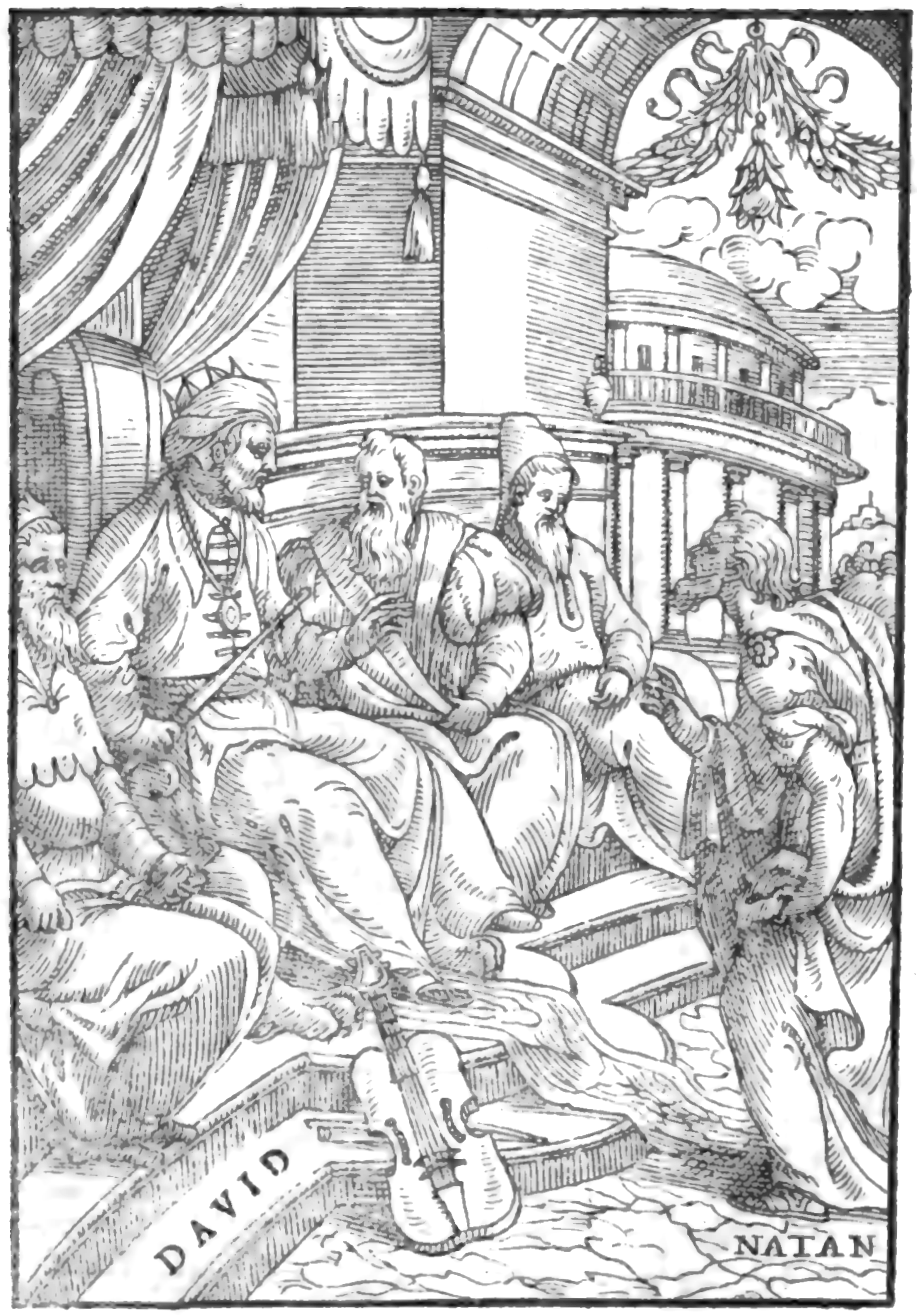
\includegraphics[width=4.5in]{Picture52.png}

\mainmatter

% \thispagestyle{empty}
% \mbox{}
% \newpage

%pp53
\newpage
\thispagestyle{empty}
\fancyhead[CO,CE]{}
\begin{center} \color{red} \hypertarget{DAVID} \LARGE
P \ S \ A \ L \ T \ E \ R \ I \ V \ M \ \ \ D \ A \ V \ I \ D
\end{center}
\vspace{-1.5em}
\bookmark[open,dest=DAVID]{PSALTERIVM DAVID}

\begin{center} \large
dispositum in Dies, \& Horas, ordine quo\\totum singulis Hebdomadis dicitur\\per totum annum.
\end{center}

\begin{center} \large \color{red} \bfseries \hypertarget{DOMINICA}
D \ O \ M \ I \ N \ I \ C \ A
\end{center}
\vspace{-1.5em}
\bookmark[rellevel=1,dest=DOMINICA]{DOMINICA}

\begin{center} \color{red} \hypertarget{DOMMATIN}
Ad matutinum.
\end{center}
\vspace{-1em}
\bookmark[rellevel=1,dest=DOMMATIN]{AD MATVTINVM}

\begin{multicols*}{2}
\lettrine[lines=2]{\bfseries \color{red} P}{}Ater noster, qui es in c\oe lis, sanctificetur %sanctifecet'
nomen tuum. Aduieniat regnum tuum. Fiat voluntas tua sicut in c\oe lo \& in terra. Panem nostrum quotidianum da nobis hodie. Et dimitte nobis debita nostra, sicut \& nos dimittimus debitoribus nostris. Et ne nos inducas in tentionem. Sed libera nos a malo. Amen.
\lettrine[lines=2]{\bfseries \color{red} A}{}Ve Maria gratia plena. Dominus tecum, Benedicta tu in mulieribus, \& benedictus fructus ventris tui Iesus. Sancta Maria mater Dei, Ora pro nobis peccatoribus. Amen.
\lettrine[lines=2]{\bfseries \color{red} C}{}Onfiteor Deo omnipotenti, beat\ae \ Mari\ae \ %beate Marie, hooked e
semper virgini, beato Michaeli archangelo, beato Ioanni Baptist\ae , %Baptiste
sanctis apostolis Petro \& Paulo, omnibus sanctis, \& \color{red} tibi pater, \color{black} quia peccaui nimis cogitatione, verbo \& opere. Mea culpa, Mea culpa, Mea maxima culpa. Ideo precor beatam Mariam semper virginem, beatum Michaelem archangelum, beatum Ioannem Baptistam, sanctos Apostolos Petrum \& Paulum, omnes sanctos, \& \color{red} te pater \color{black} orare pro me. \quad \color{red} Absolutio. \color{black}
% \vspace{-.25em}
\lettrine[lines=2]{\bfseries \color{red} M}{}Isereatur \color{red} tui \color{black} omnipotens Deus, \& dimissis peccatis \color{red} tuis, \color{black} perducat \color{red} te \color{black} ad vitam \ae ternam. \color{red} \Rbar . \color{black} Amen. \color{red} \Vbar . \color{black}
% \vspace{-.25em}
\lettrine[lines=2]{\bfseries \color{red} I}{}Ndulgentiam, absolutionem \& remissionem peccatorum nostrorum tribuat nobis omnipotens \& misericors dominus. \color{red} \Rbar . \color{black} Amen.
\vspace{-.25em}
%pp54
\lettrine[lines=2]{\bfseries \color{red} D}{}Omine labia mea aperies.
\newline \color{red} \Rbar . \color{black} Et os meum annuntiabit laudem tuam. \color{red} \Vbar . \color{black} Deus in adiutorium meum intende. \color{red} \Rbar . \color{black} Domine ad adiuuandum me festina. Gloria patri \& filio. Sicut erat. Haleluiah.
\newline
\color{red} Inuitatorium si ab vno, semel dicitur. Si a duobus replicatur. \color{black}
\vspace{-.25em}
\lettrine[lines=2]{\bfseries \color{red} V}{}Enite exultemus domino iubilemus Deo salutari nostro, pr\ae occupemus faciem eius in confessione \& in psalmis iubilemus ei.
\newline
\color{red} Q\color{black}uoniam Deus magnus dominus \& rex magnus super omnes %oes
Deos: quoniam non repellet dominus plebem suam, quia in manu eius sunt omnes fines terr\ae , \& altitudines montium ipse conspicit.
\newline
\color{red} Q\color{black}uoniam ipsius est mare, \& ipse fecit illud, \& aridam fundauerunt manus eius: venite adoremus, \& procidamus ante Deum ploremus coram domino, qui fecit nos: quia ipse est dominus deus noster, nos autem populus eius, et oues pascu\ae \ eius.
\newline
\color{red} H\color{black}odie si vocem eius audieritis nolite obdurare corda vestra, sicut in exacerbatione secundum diem tentationis in deserto: vbi tentauerunt me patres vestri: probauerunt \& viderunt opera mea.
\newline
\color{red} Q\color{black}uadraginta annis proximus fui generationi huic, \& dixi, semper hi errant corde, ipsi vero non cognouerunt vias meas, quibus iuraui in ira mea: si introibunt in requiem meam.
\newline
\color{red} G\color{black}loria patri \& filio. Sicut erat.
\vspace{-1em}
\begin{center} \color{red}
Repetitur inuitatorium.\\
Hymnus competens dicitur.\\
Quo finito Antiphona pronunciatur.\\
\hypertarget{ps1}{Psalmus primus.}
\end{center}
\vspace{-1em}
\yinipar{B}Eatus vir qui non abijt in consilio impiorum, \& in via peccatorum non stetit: \& in cathedra pestilenti\ae \ non sedit.
\newline \color{red} S\color{black}ed in lege Domini voluntas eius, \& in lege eius meditabitur die ac nocte.
\newline \color{red} E\color{black}t erit tanquam lignum quod plantatum est secus decursus aquarum: quod fructum suum dabit in tempore suo.
\newline \color{red} E\color{black}t folium eius non defluet: \& omnia qu\ae cunque %hooked e
faciet, prosperabuntur.
\newline \color{red} N\color{black}on sic impij, non sic: sed tanquam puluis, quem proijcit ventus a facie terr\ae .
\newline \color{red} I\color{black}deo non resurgent impij in iudicio: neque peccatores in concilio iustorum.
\newline \color{red} Q\color{black}uoniam nouit dominus viam iustorum: \& iter impiorum peribit.
%pp55
\color{red} \quad Deinde dicitur. \color{black}
\newline \color{red} G\color{black}loria patri, \& filio, \& spiritui sancto.
\newline \color{red} S\color{black}icut erat in principio, \& nunc, \& semper, \& in secula seculorum. Amen. %sic no hooked e
\newline
\color{red} Pr\ae dicto modo dicitur \color{black} Gloria patri. \color{red} \&c. in fine omnium Psalmorum, \& canticorum per totum annum, pr\ae terquam in triduo ante Pascha, \& in officio defunctorum, \& in cantico trium puerorum. \quad psalmus. \hypertarget{ps9}{9.} \color{black}
\fancyhead[C]{\color{red} Dominica}
\lettrine[lines=2]{\bfseries \color{red} C}{}Onfitebor tibi domine in toto corde meo: narrabo omnia mirabilia tua.
\newline \color{red} L\color{black}\ae tabor et exultabo in te, psallam nomini tuo altissime.
\newline \color{red} I\color{black}n conuertendo inimicum meum retrorsum, infirmabuntur, \& peribunt a facie tua.
\newline \color{red} Q\color{black}uoniam fecisti iudicium meum, \& causam meam: sedisti super thronum, qui iudicas iustitiam.
\newline \color{red} I\color{black}ncrepasti gentes, \& perijt impius: nomen eorum delesti in \ae ternum, \& in seculum seculi.
\newline \color{red} I\color{black}nimici defecerunt frame\ae \ in finem: \& ciuitates eorum destruxisti.
\newline \color{red} P\color{black}erijt memoria eorum cum sonitu, \& dominus in \ae ternum permanet.
\newline \color{red} P\color{black}arauit in iudicio thronum suum: \& ipse iudicabit orbem terr\ae \ in \ae quitate, iudicabit populos in iustitia.
\newline \color{red} E\color{black}t factus est dominus refugium pauperi: adiutor in opportunitatibus in tribulatione.
\newline \color{red} E\color{black}t sperent in te, qui nouerunt nomen tuum: quoniam non dereliquisti qu\ae rentes te domine.
\newline \color{red} P\color{black}sallite domino qui habitat in Sion: annuntiate inter gentes studia eius:
\newline \color{red} Q\color{black}uoniam requirens sanguinem eorum recordatus est: non est oblitus clamorem pauperum.
\newline \color{red} M\color{black}iserere mei domine: vide humilitatem meam de inimicis meis.
\newline \color{red} Q\color{black}ui exaltas me de portis mortis, vt annuntiem omnes laudationes tuas in portis fili\ae \ Sion.
\newline \color{red} E\color{black}xultabo in salutari tuo: infix\ae \ sunt gentes in interitu, quem fecerunt.
\newline \color{red} I\color{black}n laqueo isto, quem absconderunt, comprehensus est pes eorum.
\newline \color{red} C\color{black}ognoscetur dominus iudicia faciens: in operibus manuum suarum comprehensus est peccator, %comma?
\newline \color{red} C\color{black}onuertantur peccatores in infernum, omnes gentes qu\ae \ obliuiscuntur Deum.
\newline \color{red} Q\color{black}uoniam non in finem obliuio erit pauperis: patientia pauperum non peribit in finem.
\newline \color{red} E\color{black}xurge domine, non confortetur homo: iudicentur gentes in conspectu tuo.
%pp56
\newline \color{red} C\color{black}onstitue Domine legislatorem super eos: vt sciant gentes quoniam homines sunt.
\newline \color{red} V\color{black}t quid domine recessisti longe, despicis in opportunitatibus in tribulatione?
\newline \color{red} D\color{black}um superbit impius, incenditur pauper: comprehenduntur in consilijs quibus cogitant.
\newline \color{red} Q\color{black}uoniam laudatur peccator in desiderijs anim\ae \ su\ae , \& iniquus benedicitur.
\newline \color{red} E\color{black}xacerbauit dominum peccator, secundum multitudinem ir\ae \ su\ae \ non qu\ae ret.
\newline \color{red} N\color{black}on est deus in conspectu eius, inquinat\ae \ sunt vi\ae \ illius in omni tempore.
\newline \color{red} A\color{black}uferuntur iudicia tua a facie eius: omnium inimicorum suorum dominabitur.
\newline \color{red} D\color{black}ixit enim in corde suo. Non movebor a generatione in generationem sine malo.
\newline \color{red} C\color{black}uius maledictione os plenum est, \& amaritudine, \& dolo: sub lingua eius labor \& dolor.
\newline \color{red} S\color{black}edet in insidijs cum diuitibus, in occultis: vt interficiat innocentem.
\newline \color{red} O\color{black}culi eius in pauperem respiciunt: insidiatur in abscondito quasi leo in spelunca sua.
\newline \color{red} I\color{black}nsidiatur, vt rapiat pauperem, rapere pauperem dum attrahit eum.
\newline \color{red} I\color{black}n laqueo suo humiliabit eum, inclinabit se, \& cadet cum dominatus fuerit pauperum.
\newline \color{red} D\color{black}ixit enim in corde suo, oblitus est Deus, auertit faciem suam ne videat in finem.
\newline \color{red} E\color{black}xurge domine Deus, \& exaltetur manus tua: ne obliuiscaris pauperum.
\newline \color{red} P\color{black}ropter quid irritauit impius Deum? dixit enim in corde suo: Non requiret.
\newline \color{red} V\color{black}ides, quoniam tu laborem \& dolorem consideras: vt tradas eos in manus tuas.
\newline \color{red} T\color{black}ibi derelictus est pauper: orphano tu eris adiutor.
\newline \color{red} C\color{black}ontere brachium peccatoris \& maligni: qu\ae retur peccatum illius, \& non inuenietur.
\newline \color{red} D\color{black}ominus regnabit in \ae ternum, \& in seculum seculi: peribitis gentes de terra illius.
\newline \color{red} D\color{black}esiderium pauperum exaudiuit dominus: pr\ae parationem cordis eorum audiuit auris tua.
\newline \color{red} I\color{black}udicare pupillo \& humili: vt non apponat vltra magnificare se homo super terram. \quad \color{red} Psalmus \hypertarget{ps17}{17.} \color{black}
\vspace{-1em}
\lettrine[lines=2]{\bfseries \color{red} D}{}Iligam te domine fortitudo mea: dominus firmamentum meum, \& refugium meum, \& liberator meus.
\newline \color{red} D\color{black}eus meus adiutor meus: \& sperabo in eum.
%pp57
\fancyhead[C]{\color{red} Dominica ad matutinum}
\newline \color{red} P\color{black}rotector meus, \& cornu salutis me\ae , \& susceptor meus.
\newline \color{red} L\color{black}audans inuocabo dominum: \& ab inimicis meis saluus ero.
\newline \color{red} C\color{black}ircundederunt me dolores mortis: \& torrentes iniquitatis conturbauerunt me.
\newline \color{red} D\color{black}olores inferni circundederunt me: pr\ae occupauerunt me laquei mortis.
\newline \color{red} I\color{black}n tribulatione mea inuocaui dominum, \& ad Deum meum clamaui.
\newline \color{red} E\color{black}t exaudiuit de templo sancto suo vocem meam: \& clamor meus in conspectu eius introiuit in aures eius.
\newline \color{red} C\color{black}ommota est \& contremuit terra: fundamenta montium conturbata sunt, \& commota sunt, quoniam iratus est eis.
\newline \color{red} A\color{black}scendit fumus in ira eius: \& ignis a facie eius exarsit: carbones succensi sunt ab eo.
\newline \color{red} I\color{black}nclinauit c\oe los, \& descendit: \& caligo sub pedibus eius.
\newline \color{red} E\color{black}t ascendit super Cherubim \& volauit: volauit super pennas ventorum.
\newline \color{red} E\color{black}t posuit tenebras latibulum suum, in circuitu eius tabernaculum eius, tenebrosa aqua in nubibus aeris.
\newline \color{red} P\color{black}r\ae \ fulgore in conspectu eius nubes transierunt, grando, \& carbones ignis.
\newline \color{red} E\color{black}t intonuit de c\oe lo dominus, \& altissimus dedit vocem suam: grando \& carbones ignis.
\newline \color{red} E\color{black}t misit sagittas suas, \& dissipauit eos: fulgura multiplicauit, \& conturbauit eos.
\newline \color{red} E\color{black}t apparuerunt fontes aquarum, \& reuelata sunt fundamenta orbis terrarum.
\newline \color{red} A\color{black}b increpatione tua domine, ab inspiratione spiritus ir\ae \ tu\ae .
\newline \color{red} M\color{black}isit de summo, \& accepit me: \& assumpsit me de aquis multis.
\newline \color{red} E\color{black}ripuit me de inimicis meis fortissimis, \& ab his qui oderunt me: quoniam confortati sunt super me.
\newline \color{red} P\color{black}r\ae uenerunt me in die afflictionis me\ae : \& factus est dominus protector meus.
\newline \color{red} E\color{black}t eduxit me in latitudinem: saluum me fecit, quoniam voluit me.
\newline \color{red} E\color{black}t retribuet mihi dominus secundum iustitiam meam: \& secundum puritatem manuum mearum retribuet mihi.
\newline \color{red} Q\color{black}uia custodiui vias domini, nec impie gessi a Deo meo.
\newline \color{red} Q\color{black}uoniam omnia iudicia eius in conspectu meo: \& iustitias eius non repuli a me.
\newline \color{red} E\color{black}t ero immaculatus cum eo: \& obseruabo me ab iniquitate mea.
%pp58
\newline \color{red} E\color{black}t retribuet mihi dominus secundum iustitiam meam: \& secundum puritatem manuum mearum in conspectu oculorum eius.
\newline \color{red} C\color{black}um sancto sanctus eris: \& cum viro innocente innocens eris.
\newline \color{red} E\color{black}t cum electo electus eris: \& cum peruerso peruerteris.
\newline \color{red} Q\color{black}uoniam tu populum humilem saluum facies: \& oculos superborum humiliabis.
\newline \color{red} Q\color{black}uoniam tu illuminas lucernam meam domine: Deus meus, illumina tenebras meas.
\newline \color{red} Q\color{black}uoniam in te eripiar a tentatione: \& in Deo meo transgrediar murum.
\newline \color{red} D\color{black}eus meus impolluta via eius eloquia domini igne examinata: protector est omnium sperantium in se.
\newline \color{red} Q\color{black}uoniam quis deus pr\ae ter dominum? aut quis deus pr\ae ter Deum nostrum?
\newline \color{red} D\color{black}eus qui pr\ae cinxit me virtute: \& posuit immaculatam viam meam.
\newline \color{red} Q\color{black}ui perfecit pedes meos tanquam ceruorum: \& super excelsa statuens me.
\newline \color{red} Q\color{black}ui docet manus meas ad pr\ae lium: \& posuisti vt arcum \ae reum brachia mea.
\newline \color{red} E\color{black}t dedisti mihi protectionem salutis tu\ae : \& dextera tua suscepit me.
\newline \color{red} E\color{black}t disciplina tua correxit me in finem: \& disciplina tua ipsa me docebit.
\newline \color{red} D\color{black}ilatasti gressus meos subtus me: \& non sunt infirmata vestigia mea:
\newline \color{red} P\color{black}ersequar inimicos meos \& comprehendam illos: \& non conuertar donec deficiant.
\newline \color{red} C\color{black}onfringam illos, nec poterunt stare: cadent subtus pedes meos.
\newline \color{red} E\color{black}t pr\ae cinxisti me virtute ad bellum: \& supplantasti insurgentes in me subtus me.
\newline \color{red} E\color{black}t inimicos meos dedisti mihi dorsum: \& odientes me disperdidisti.
\newline \color{red} C\color{black}lamauerunt, nec erat qui saluos faceret ad dominum, nec exaudiuit eos.
\newline \color{red} E\color{black}t comminuam eos vt puluerem ante faciem venti: vt lutum platearum delebo eos.% eos/illos
\newline \color{red} E\color{black}ripies me de contradictionibus populi: constitues me in caput gentium.
\newline \color{red} P\color{black}opulus quem non cognoui seruiuit mihi: in auditu auris obediuit mihi.
\newline \color{red} F\color{black}ilij alieni mentiti sunt mihi, filij alieni inueterati sunt, \& claudicauerunt a semitis suis.
\newline \color{red} V\color{black}iuit dominus, \& benedictus Deus meus, \& exaltetur Deus salutis me\ae .
%pp59
\newline \color{red} D\color{black}eus qui das vindictas mihi, \& subdis populos sub me, liberator meus de inimicis meis iracundis.
\newline \color{red} E\color{black}t ab insurgentibus in me exaltabis me: a viro iniquo eripies me.
\newline \color{red} P\color{black}ropterea confitebor tibi in nationibus domine: \& nomini tuo psalmum dicam.
\newline \color{red} M\color{black}agnificans salutes regis eius, \& faciens misericordiam Christo suo Dauid. \& semini eius vsque in seculum.
\newline \textswab{C} \color{red} Sequens hym. dicitur %directis directus??? dr
finitis tribus lectionibus ad matu. per totum annum pr\ae terquam in aduentu, \& a dominica in septuagesima vsque ad Pascha, \& etiam tunc dicitur si agatur de aliquo sancto. \color{black}
\newline \textswab{C} \color{red} Canticum sanctorum Ambrosij \& Augustini. \hypertarget{tedeum}{Hymnus.} \color{black}
\vspace{-1em}
\lettrine[lines=2]{\bfseries \color{red} T}{}E Deum laudamus: te dominum confitemur.
\newline \color{red} T\color{black}e \ae ternum patrem, omnis terra veneratur.
\newline \color{red} T\color{black}ibi omnes angeli, tibi c\oe li, \& vniuers\ae \ potestates.
\newline \color{red} T\color{black}ibi Cherubim, \& Seraphim incessabili voce proclamant.
\newline \color{red} S\color{black}anctus, Sanctus, Sanctus, dominus deus sabaoth.
\newline \color{red} P\color{black}leni sunt c\oe li \& terra, maiestatis glori\ae \ tu\ae .
\newline \color{red} T\color{black}e gloriosus Apostolorum chorus.
\newline \color{red} T\color{black}e prophetarum laudabilis numerus.
\newline \color{red} T\color{black}e martyrum candidatus laudat exercitus.
\newline \color{red} T\color{black}e per orbem terrarum sancta confitetur ecclesia.
\newline \color{red} P\color{black}atrem immens\ae \ maiestatis.
\newline \color{red} V\color{black}enerandum tuum verum, \& vnicum filium.
\newline \color{red} S\color{black}anctum quoque paraclitum spiritum.
\newline \color{red} T\color{black}u rex glori\ae \ Christe.
\newline \color{red} T\color{black}u patris sempiternus es filius.
\newline \color{red} T\color{black}u ad liberandum suscepturus hominem, non horruisti virginis vterum.
\newline \color{red} T\color{black}u deuicto mortis aculeo, aperuisti credentibus regna c\oe lorum.
\newline \color{red} T\color{black}u ad dexteram Dei sedes in gloria patris.
\newline \color{red} I\color{black}udex crederis esse venturus.
\newline \color{red} T\color{black}e ergo qu\ae sumus famulis tuis subueni, quos pretioso sanguine redemisti.
\newline \color{red} \AE \color{black}terna fac cum sanctis tuis in gloria numerari.
\newline \color{red} S\color{black}aluum fac populum tuum domine, \& benedic h\ae reditati tu\ae .
\newline \color{red} E\color{black}t rege eos, \& extolle illos vsque in \ae ternum.
\newline \color{red} P\color{black}er singulos dies benedicimus te.
%pp60
\newline \color{red} E\color{black}t laudamus nomen tuum in seculum, \& in seculum seculi.
\newline \color{red} D\color{black}ignare domine die isto, sine peccato nos custodire.
\newline \color{red} M\color{black}iserere nostri domine, miserere nostri.
\newline \color{red} F\color{black}iat misericordia tua domine super nos, quemadmodum sperauimus in te.
\newline \color{red} I\color{black}n te domine speraui, non confundar in \ae ternum.
\vspace{-1em}
\begin{center} \color{red} \large \hypertarget{DOMLAUD}
AD LAVDES.
\end{center}
\fancyhead[C]{\color{red} Dominica ad laudes}
\bookmark[dest=DOMLAUD]{AD LAVDES}
\vspace{-1em}
\par \noindent Deus in adiuto. \color{red} Antiph. Psalmus \hypertarget{ps65}{65.} \color{black}
\yinipar{I}Vbilate Deo omnis terra, psalmum dicite nomini eius: date gloriam laudi eius.
\newline \color{red} D\color{black}icite Deo, Quam terribilia sunt opera tua domine? in multitudine virtutis tu\ae \ mentientur tibi inimici tui.
\newline \color{red} O\color{black}mnis terra adoret te, \& psallat tibi: psalmum dicat nomini tuo.
\newline \color{red} V\color{black}enite, \& videte opera Dei, terribilis in consilijs super filios hominum.%text:hominnm
\newline \color{red} Q\color{black}ui conuertit mare in aridam, in flumine pertransibunt pede: ibi l\ae tabimur in ipso.
\newline \color{red} Q\color{black}ui dominatur in virtute sua in \ae ternum, oculi eius super gentes respiciunt: qui exasperant, non exaltentur in semetipsis.
\newline \color{red} B\color{black}enedicite gentes Deum nostrum: \& auditam facite vocem laudis eius.
\newline \color{red} Q\color{black}ui posuit animam meam ad vitam: \& non dedit in commotionem pedes meos.
\newline \color{red} Q\color{black}uoniam probasti nos Deus: igne nos examinasti, sicut examinatur argentum.
\newline \color{red} I\color{black}nduxisti nos in laqueum, posuisti tribulationes in dorso nostro: imposuisti homines super capita nostra.
\newline \color{red} T\color{black}ransiuimus per ignem \& aquam: \& eduxisti nos in refrigerium.
\newline \color{red} I\color{black}ntroibo in domum tuam in holocaustis: reddam tibi vota mea, qu\ae \ distinxerunt labia mea.
\newline \color{red} E\color{black}t locutum est os meum in tribulatione mea.
\newline \color{red} H\color{black}olocausta medullata offeram tibi cum incenso arietum: offeram tibi boues cum hircis.
\newline \color{red} V\color{black}enite, audite: \& narrabo omnes qui timetis Deum, quanta fecit anim\ae \ me\ae .
\newline \color{red} A\color{black}d ipsum ore meo clamaui, \& exaltaui sub lingua mea.%text: snb
\newline \color{red} I\color{black}niquitatem si aspexi in corde meo: non exaudiet dominus.
\newline \color{red} P\color{black}ropterea exaudiuit Deus: \& attendit voci deprecationis me\ae .
\newline \color{red} B\color{black}enedictus Deus, qui non amouit orationem meam, \& misericordiam suam a me. \quad \color{red} Psalmus \hypertarget{ps95}{95.} \color{black}
%pp61
\vspace{-1em}
\lettrine[lines=2]{\bfseries \color{red} C}{}Antate domino canticum nouum: cantate domino omnis terra.
\newline \color{red} C\color{black}antate domino, \& benedicite nomini eius: annuntiate de die in diem salutare eius.
\newline \color{red} A\color{black}nnuntiate inter gentes gloriam eius: in omnibus populis mirabilia eius.
\newline \color{red} Q\color{black}uoniam magnus dominus, \& laudabilis nimis: terribilis est super omnes deos.
\newline \color{red} Q\color{black}uoniam omnes dij gentium d\ae monia: dominus autem c\oe los fecit.
\newline \color{red} C\color{black}onfessio, \& pulchritudo in conspectu eius: sanctimonia \& magnificentia in sanctificatione eius.
\newline \color{red} A\color{black}fferte domino patri\ae \ gentium, afferte domino gloriam \& honorem: afferte domino gloriam nomini eius.
\newline \color{red} T\color{black}ollite hostias, \& introite in atria eius: Adorate dominum in atrio sancto eius.
\newline \color{red} C\color{black}ommoueatur a facie eius vniuersa terra. Dicite in gentibus quia dominus regnauit.
\newline \color{red} E\color{black}tenim correxit orbem terr\ae \ qui non commouebitur: iudicabit populos in \ae quitate.
\newline \color{red} L\color{black}\ae tentur c\oe li, \& exultet terra, commoueatur mare, \& plenitudo eius: gaudebunt campi, \& omnia qu\ae \ in eis sunt.
\newline \color{red} T\color{black}unc exultabunt omnia ligna syluarum a facie domini: quia venit, quoniam venit iudicare terram.
\newline \color{red} I\color{black}udicabit orbem terr\ae \ in \ae quitate, \& populos in veritate sua.
\newline \color{red} \hypertarget{benedicite}{Canticum} trium puerorum. \color{black}
% \marginpar[]{Daniel.\\3.} 			implement???
\vspace{-1em}
\lettrine[lines=2]{\bfseries \color{red} B}{}Enedicite\rightmarginnote{Dan.\\3.} omnia opera domini domino: laudate, \& superexaltate eum in secula.
\newline \color{red} B\color{black}enedicite angeli domini domino, benedicite c\oe li domino.
\newline \color{red} B\color{black}enedicite aqu\ae \ omnes, qu\ae \ super c\oe los sunt domino: benedicite omnes virtutes domini domino.
\newline \color{red} B\color{black}enedicite sol, \& luna domino: benedicite stell\ae \ c\oe li domino.
\newline \color{red} B\color{black}enedicite imber, \& ros domino: benedicite omnes spiritus Dei domino.
\newline \color{red} B\color{black}enedicite ignis \& \ae stus domino: benedicite fruges \& \ae stus domino.
\newline \color{red} B\color{black}enedicite rores \& pruina domino: benedicite gelu \& frigus domino.
\newline \color{red} B\color{black}enedicite glacies, \& niues domino: benedicite noctes, \& dies domino.
\newline \color{red} B\color{black}enedicite lux, \& tenebr\ae \ domino: benedicite fulgura, \& nubes domino.
\newline \color{red} B\color{black}enedicat terra dominum: laudet, \& superexaltet eum in secula.
\newline \color{red} B\color{black}enedicite montes, \& colles domino: benedicite vniuersa germinantia in terra domino.
%pp62
\newline \color{red} B\color{black}enedicite fontes domino: benedicite maria, \& flumina domino.
\newline \color{red} B\color{black}enedicite cete, \& omnia qu\ae \ mouentur in aquis domino: benedicite omnes volucres c\oe li domino.
\newline \color{red} B\color{black}enedicite omnes besti\ae \ \& pecora domino: benedicite filij hominum domino.
\newline \color{red} B\color{black}enedicat Israel dominum: laudet, \& superexaltet eum in secula.
\newline \color{red} B\color{black}enedicite sacerdotes domini domino: benedicite serui domini domino.
\newline \color{red} B\color{black}enedicite spiritus, \& anim\ae \ iustorum domino: benedicite sancti \& humiles corde domino.
\newline \color{red} B\color{black}enedicite Anania, Azaria, Misael domino, laudate, \& superexaltate eum in secula.
\newline \color{red} B\color{black}enedicamus patrem, \& filium cum sancto spiritu: laudemus \& superexaltemus eum in secula.
\newline \color{red} B\color{black}enedictus es domine in firmamento c\oe li: \& laudabilis \& gloriosus, \& superexaltatus in secula. Amen.
\newline \textswab{C} \color{red} \hypertarget{Benedictus}{Canticum} Zachari\ae \ prophet\ae .\\Et dicitur quotidie ad laudes. \color{black}
\vspace{-1em}
\lettrine[lines=2]{\bfseries \color{red} B}{}Enedictus dominus deus Israel: quia visitauit, \& fecit redemptionem plebis su\ae .
\newline \color{red} E\color{black}t erexit cornu salutis nobis, in domo Dauid pueri sui.
\newline \color{red} S\color{black}icut locutus est per os sanctorum: qui a seculo sunt prophetarum eius.
\newline \color{red} S\color{black}alutem ex inimicis nostris, \& de manu omnium, qui oderunt nos.
\newline \color{red} A\color{black}d faciendam misericordiam cum patribus nostris: \& memorari testamenti sui sancti.
\newline \color{red} I\color{black}usiurandum, quod iurauit ad Abraham patrem nostrum, daturum se nobis.
\newline \color{red} V\color{black}t sine timore de manu inimicorum nostrorum liberati: seruiamus illi.
\newline \color{red} I\color{black}n sanctitate \& iustitia coram ipso, omnibus diebus nostris.
\newline \color{red} E\color{black}t tu puer, propheta altissimi vocaberis: pr\ae ibis enim ante faciem domini parare vias eius.
\newline \color{red} A\color{black}d dandam scientiam salutis plebi eius, in remissionem peccatorum eorum.
\newline \color{red} P\color{black}er viscera misericordi\ae \ Dei nostri, in quibus visitauit nos oriens ex alto.
\newline \color{red} I\color{black}lluminare his, qui in tenebris \& in vmbra mortis sedent, ad dirigendos pedes nostros in viam pacis. \quad \color{red} Antiphona \& Oratio \& \color{black} Sub tuum pr\ae sidium. \color{red} vt in. j. dominica aduentu. \color{black}
\vspace{-.5em}
\begin{center} \color{red} \large \hypertarget{DOMPRIME}
AD PRIMAM.
\end{center}
\fancyhead[C]{\color{red} Dominica ad primam}
\bookmark[dest=DOMPRIME]{AD PRIMAM}
\vspace{-.5em}
\par \noindent \color{red} P\color{black} ater noster. Aue maria. Deus in adiutorium meum. \color{red} \hypertarget{Iamlucis}{Hym.} \color{black}
\yinipar{I}Am lucis orto sydere: Deum precemur supplices: Vt in diurnis actibus: Nos seruet a nocentibus.
%pp63
\newline \color{red} L\color{black}inguam refrenans temperet, Ne litis horror insonet: Visum fouendo contegat, Ne vanitates hauriat.
\newline \color{red} S\color{black}int pura cordis intima, Absistat \& vecordia: Carnis terat superbiam Potus cibique parcitas.
\newline \color{red} V\color{black}t cum dies abscesserit, Noctemque sors reduxerit: Mundi per abstinentiam, Ipsi canamus gloriam.
\newline \color{red} D\color{black}eo patri sit gloria, Eiusque soli filio, cum spiritu paracleto, Et nunc \& in perpetuum. Amen.
\newline \color{red} Antiphona. \color{black} Vtinam. \color{red} Psalmus. \hypertarget{ps53}{53.} \color{black}
\vspace{-.25em}
\lettrine[lines=2]{\bfseries D}{}Eus in nomine tuo saluum me fac, \& in virtute tua iudica me.
\newline \color{red} D\color{black}eus exaudi orationem meam: auribus percipe verba oris mei.
\newline \color{red} Q\color{black}uoniam alieni insurrexerunt aduersum me, \& fortes qu\ae sierunt animam meam: \& non proposuerunt Deum ante conspectum suum.
\newline \color{red} E\color{black}cce enim deus adiuuat me: \& dominus susceptor est anim\ae \ me\ae .
\newline \color{red} A\color{black}uerte mala inimicis meis: \& in veritate tua disperde illos.
\newline \color{red} V\color{black}oluntarie sacrificabo tibi, \& confitebor nomini tuo domine quoniam bonum est.
\newline \color{red} Q\color{black}uoniam ex omni tribulatione eripuisti me: \& super inimicos meos despexit oculus meus. \quad \color{red} Psalmus. \hypertarget{ps118.1}{118.} \color{black}
\vspace{-.25em}
\lettrine[lines=2]{\bfseries \color{red} B}{}Eati immaculati in via, qui ambulant in lege domini.
\newline \color{red} B\color{black}eati qui scrutantur testimonia eius: in toto corde exquirunt eum.
\newline \color{red} N\color{black}on enim qui operantur iniquitatem, in viis eius ambulauerunt.
\newline \color{red} T\color{black}u mandasti mandata tua, custodiri nimis.
\newline \color{red} V\color{black}tinam dirigantur vi\ae \ me\ae , ad custodiendas iustificationes tuas.
\newline \color{red} T\color{black}unc non confundar: cum perspexero in omnibus mandatis tuis.
\newline \color{red} C\color{black}onfitebor tibi in directione cordis: in eo quod didici iudicia iustiti\ae \ tu\ae .
\newline \color{red} I\color{black}ustificationes tuas custodiam: non me derelinquas vsquequaque.
\newline \color{red} I\color{black}n quo corrigit adolescentior viam suam? in custodiendo sermones tuos.
\newline \color{red} I\color{black}n toto corde meo exquisiui te: ne repellas me a mandatis tuis.
\newline \color{red} I\color{black}n corde meo abscondi eloquia tua: vt non peccem tibi.
\newline \color{red} B\color{black}enedictus es domine: doce me iustificationes tuas.
\newline \color{red} I\color{black}n labijs meis pronuntiaui omnia iudicia oris tui.
\newline \color{red} I\color{black}n via testimoniorum tuorum delectatus sum, sicut in pmnibus diuitijs.
%pp64
\newline \color{red} I\color{black}n mandatis tuis exercebor: \& considerabo vias tuas.
\newline \color{red} I\color{black}n iustificationibus tuis meditabor: non obliuiscar sermones tuos. 
\newline \color{red} Ex psalmo. \hypertarget{ps118.2}{118.} \color{black}
\vspace{+.25em}
\lettrine[lines=2]{\bfseries \color{red} R}{}Etribue seruo tuo, viuifica me: \& custodiam sermones tuos.
\newline \color{red} R\color{black}euela oculos meos: \& considerabo mirabilia de lege tua.
\newline \color{red} I\color{black}ncola ego sum in terra: non abscondas a me mandata tua.
\newline \color{red} C\color{black}oncupiuit anima mea desiderare iustificationes tuas, in omni tempore.
\newline \color{red} I\color{black}ncrepasti superbos: maledicti, qui declinant a mandatis tuis.
\newline \color{red} A\color{black}ufer a me opprobrium \& contemptum: quia testimonia tua exquisiui.
\newline \color{red} E\color{black}tenim sederunt principes, \& aduersum me loquebantur: seruus autem tuus exercebatur in iustificationibus tuis.
\newline \color{red} N\color{black}am \& testimonia tua meditatio mea est: \& consilium meum iustificationes tu\ae .
\newline \color{red} A\color{black}dh\ae sit pauimento anima mea: viuifica me secundum verbum tuum.
\newline \color{red} V\color{black}ias meas enuntiaui, \& exaudisti me: doce me iustificationes tuas.
\newline \color{red} V\color{black}iam iustificationum tuarum instrue me: \& exercebor in mirabilibus tuis.
\newline \color{red} D\color{black}ormitauit anima mea pr\ae \ t\ae dio: confirma me in verbis tuis.
\newline \color{red} V\color{black}iam iniquitatis amoue a me: \& de lege tua miserere mei.
\newline \color{red} V\color{black}iam veritatis elegi: iudicia tua non sum oblitus.
\newline \color{red} A\color{black}dh\ae si testimonijs tuis domine: noli me confundere.
\newline \color{red} V\color{black}iam mandatorum tuorum cucurri, cum dilatasti cor meum.
\vspace{-.5em}
\begin{center} \color{red} \hypertarget{QUICVMQUE}
Symbolum Athanasij Episcopi.
\end{center}
\vspace{-.5em}
\lettrine[lines=2]{\bfseries \color{red} Q}{}Vicunque vult saluus esse: ante omnia opus est, vt teneat catholicam fidem.
\newline \color{red} Q\color{black}uam nisi quisque integram inuiolatanque seruauerit, absque dubio in \ae ternum peribit.
\newline \color{red} F\color{black}ides autem catholica h\ae c est: vt vnum Deum in Trinitate, \& Trinitatem in vnitate veneremur.
\newline \color{red} N\color{black}eque confundentes personas, neque substantiam separantes.
\newline \color{red} A\color{black}lia est enim persona Patris, alia filij, alia Spiritus sancti:
\newline \color{red} S\color{black}ed Patris, \& filij, \& Spiritus sancti vna est diuinitas, \ae qualis gloria, co\ae terna maiestas.
\newline \color{red} Q\color{black}ualis Pater, talis Filius, talis Spiritus sanctus.
\newline \color{red} I\color{black}ncreatus Pater, increatus Filius, increatus Spiritus sanctus.
\newline \color{red} I\color{black}mmensus Pater, immensus Filius, immensus Spiritus sanctus.
\newline \color{red} \AE \color{black}ternus Pater, \ae ternus Filius, \ae ternus Spiritus sanctus.
%pp65
\newline \color{red} E\color{black}t tamen non tres \ae terni: sed vnus \ae ternus.
\newline \color{red} S\color{black}icut non tres increati, nec tres immensi, sed vnus increatus, \& vnus immensus.
\newline \color{red} S\color{black}imiliter omnipotens Pater, omnipotens Filius, omnipotens Spiritus sanctus.
\newline \color{red} E\color{black}t tamen non tres omnipotentes: sed vnus omnipotens.
\newline \color{red} I\color{black}ta Deus Pater, Deus Filius, Deus Spiritus sanctus.
\newline \color{red} V\color{black}t tamen non tres dij, sed vnus est deus.
\newline \color{red} I\color{black}ta dominus Pater, dominus Filius, dominus Spiritus sanctus.
\newline \color{red} E\color{black}t tamen non tres domini: sed vnus est dominus.
\newline \color{red} Q\color{black}uia sicut singillatim vnamquamque personam, Deum, ac dominum confiteri Christiana veritate compellimur: ita tres Deos, aut dominos dicere, catholica religione prohibemur.%expand p
\newline \color{red} P\color{black}ater a nullo est factus, nec creatus, nec genitus.
\newline \color{red} F\color{black}ilius a Patre solo est, non factus, nec creatus, sed genitus.
\newline \color{red} S\color{black}piritus sanctus a Patre \& Filio: non factus, nec creatus, nec genitus, sed procedens.
\newline \color{red} V\color{black}nus ergo Pater, non tres patres, vnus filius, non tres filij: vnus Spiritus sanctus, non tres spiritus sancti.
\newline \color{red} E\color{black}t in hac Trinitate nihil prius aut posterius, nihil maius aut minus: sed tot\ae \ tres person\ae \ co\ae tern\ae \ sibi sunt \& co\ae quales.
\newline \color{red} I\color{black}ta vt per omnia, sicut iam supradictum est, \& vnitas in Trinitate, \& Trinitas in vnitate veneranda sit.
\newline \color{red} Q\color{black}ui vult ergo saluus esse, ita de Trinitate sentiat.
\newline \color{red} S\color{black}ed necessarium est ad \ae ternam salutem: vt incarnationem quoque domini nostri Iesu Christi fideliter credat.
\newline \color{red} E\color{black}st ergo fides recta, vt credamus \& confiteamur, quia dominus noster Iesus Christus Dei filius, Deus, \& homo est.
\newline \color{red} D\color{black}eus est ex substantia patris ante secula genitus: \& homo est ex substantia matris in seculo natus.
\newline \color{red} P\color{black}erfectus Deus, perfectus homo ex anima rationali, \& humana carne subsistens.
\newline \color{red} \AE \color{black}qualis Patri secundum diuinitatem: minor Patre secundum humanitatem.
\newline \color{red} Q\color{black}ui licet Deus sit, \& homo: non duo tamen, sed vnus est Christus.
\newline \color{red} V\color{black}nus autem non conuersione diuinitatis in carnem: sed assumptione humanitatis in Deum.
\newline \color{red} V\color{black}nus omnino non confusione substanti\ae , sed vnitate person\ae .
%pp66
\newline \color{red} N\color{black}am sicut anima rationalis \& caro vnus est homo: ita deus \& homo vnus est Christus.
\newline \color{red} Q\color{black}ui passus est pro salute nostra, descendit ad inferos: tertia die resurrexit a mortuis.
\newline \color{red} A\color{black}scendit ad c\oe los, sedet ad dexteram Dei patris omnipotentis: inde venturus est iudicare viuos, \& mortuos.
\newline \color{red} A\color{black}d cuius aduentum omnes homines resurgere habent cum corporibus suis: \& reddituri sunt de factis proprijs rationem.
\newline \color{red} E\color{black}t qui bona egerunt ibunt in vitam \ae ternam: qui vero mala, in ignem \ae ternum.
\newline \color{red} H\color{black}\ae c est fides catholica, quam nisi quisque fideliter, firmiterque crediderit, saluus esse non poterit.
\newline \color{red} G\color{black} loria patri. \color{red} S\color{black} icut erat. \color{red} Ant. \color{black} Vtinam dirigantur vi\ae \ me\ae , ad custodiendas iustificationes tuas. \color{red} \Vbar . \color{black} Domine exaudi orationem meam. \color{red} \Rbar . \color{black} Et clamor meus ad te veniat. \quad \color{red} O\color{black} remus.
% \vspace{-1em}
\lettrine[lines=2]{\bfseries \color{red} D}{}Omine deus omnipotens qui ad principium huius diei nos peruenire fecisti: tua nos hodie salua virtute: vt in hac die ad nullum declinemus peccatum: sed semper ad tuam iustitiam faciendam, nostra procedant eloquia, dirigantur cogitationes \& opera. Per dominum nostrum Iesum Christum filium tuum, qui tecum viuit et regnat in vnitate spiritus sancti deus: per omnia secula seculorum. \color{red} \Rbar . \color{black} Amen. Benedicamus domino. Fidelium.
\vspace{-1em}
\begin{center} \color{red}
Vide num de sancto sit facienda\\commemoratio.
\end{center}
\vspace{-1em}
\par \noindent \color{red} P\color{black}retiosa in conspectu domini. \color{red} \Rbar . \color{black} Mors sanctorum eius. \color{red} Oratio. \color{black}
% \vspace{-1em}
\lettrine[lines=2]{\bfseries \color{red} S}{}Ancta Maria \& omnes sancti intercedant pro nobis ad dominum: vt nos mereamur ab eo adiuuari \& saluari, qui viuit \& regnat in secula seculorum. \color{red} \Rbar . \color{black} Amen. \color{red} \Vbar . \color{black} Dies \& actus nostros in sua pace disponat dominus omnipotens. \color{red} \Rbar . \color{black} Amen.
\newline \textswab{C} \color{red} Pr\ae dictum symbolum dicitur ad primam dominicis diebus per totum annum, siue fiat officium de dominica, siue de aliquo festo aut octaua in ea incidenti. \color{black}
\vspace{-1em}
\begin{center} \large \hypertarget{DOMTERCE}
AD TERTIAM.
\end{center}
\fancyhead[C]{\color{red} Dominica ad tertiam}
\bookmark[dest=DOMTERCE]{AD TERTIAM}
\vspace{-1em}
\par \noindent \color{red} P\color{black} ater noster. Aue maria. Deus in adiutorium meum. \color{red} \hypertarget{Nuncsancte}{Hym.} \color{black}
\yinipar{N}Vnc sancte nobis spiritus Vnum patri cum filio, Dignare promptus ingeri, Nostro refusus pectori.
\newline \color{red} O\color{black}s, lingua, mens, sensus, vigor Confessionem personent Flammescat igne charitas Accendat ardor priximos.
%pp67
\newline \color{red} P\color{black}r\ae sta pater pijssime Patrique compar vnice Cum spiritu paraclito Regnans per omne seculum. Amen.
\newline \color{red} Antiphona. \color{black} Da mihi. \color{red} Psalmus. \hypertarget{ps118.3}{118.} \color{black}
\lettrine[lines=2]{\bfseries L}{}Egem pone mihi domine viam iustificationum tuarum: \& exquiram eam semper.
\newline \color{red} D\color{black}a mihi intellectum, \& scrutabor legem tuam: \& custodiam illam in toto corde meo.
\newline \color{red} S\color{black}educ me in semitam mandatorum tuorum: quia ipsam volui.
\newline \color{red} I\color{black}nclina cor meum in testimonia tua, \& non in auaritiam.
\newline \color{red} A\color{black}uerte oculos meos ne videant vanitatem: in via tua viuifica me.
\newline \color{red} S\color{black}tatue seruo tuo eloquium tuum, in timore tuo.
\newline \color{red} A\color{black}mputa opprobrium meum quod suspicatus sum: quia iudicia tua iucunda.
\newline \color{red} E\color{black}cce concupiui mandata tua: in \ae quitate tua viuifica me.
\newline \color{red} E\color{black}t veniat super me misericordia tua domine, salutare tuum secundum eloquium tuum.
\newline \color{red} E\color{black}t respondebo exprobrantibus mihi verbum, quia speraui in sermonibus tuis.
\newline \color{red} E\color{black}t ne auferas de ore meo verbum veritatis vsquequaque: quia in iudicijs tuis supersperaui.
\newline \color{red} E\color{black}t custodiam legem tuam semper: in seculum \& in seculum seculi.
\newline \color{red} E\color{black}t ambulabam in latitudine: quia mandata tua exquisiui.
\newline \color{red} E\color{black}t loquebar in testimonijs tuis in conspectu regum: \& non confundebar.
\newline \color{red} E\color{black}t meditabar in mandatis tuis: qu\ae \ dilexi.
\newline \color{red} E\color{black}t leuaui manus meas ad mandata tua, qu\ae \ dilexi: \& exercebar in iustificationibus tuis. \quad \color{red} Psalmus. \hypertarget{ps118.4}{118.} \color{black}
\vspace{-1em}
% \vspace{-1em}
\lettrine[lines=2]{\bfseries \color{red} M}{}Emor esto verbi tui seruo tuo, in quo mihi spem dedisti.
\newline \color{red} H\color{black}\ae c me consolata est in humilitate mea, quia eloquium tuum viuificauit me.
\newline \color{red} S\color{black}uperbi inique agebant vsquequaque: a lege autem tua non declinaui.
\newline \color{red} M\color{black}emor fui iudiciorum tuorum a seculo domine: \& consolatus sum.
\newline \color{red} D\color{black}efectio tenuit me pro peccatoribus derelinquentibus legem tuam.
\newline \color{red} C\color{black}antabiles mihi erant iustificationes tu\ae , in loco peregrinationis me\ae .
\newline \color{red} M\color{black}emor fui nocte nominis tui domine: \& custodiui legem tuam.
\newline \color{red} H\color{black}\ae c facta est mihi: quia iustificationes tuas exquisiui.
%pp68
\newline \color{red} P\color{black}ortio mea domine: dixi custodire legem tuam.
\newline \color{red} D\color{black}eprecatus sum faciem tuam in toto corde meo: miserere mei secundum eloquium tuum.
\newline \color{red} C\color{black}ogitaui vias meas: \& conuerti pedes meos in testimonia tua.
\newline \color{red} P\color{black}aratus sum \& non sum turbatus: vt custodiam mandata tua.
\newline \color{red} F\color{black}unes peccatorum circunplexi sunt me: \& legem tuam non sum oblitus.
\newline \color{red} M\color{black}edia nocte surgebam ad confitendum tibi: super iudicia iustificationis tu\ae .
\newline \color{red} P\color{black}articeps ego sum omnium timentium te: \& custodientium mandata tua.
\newline \color{red} M\color{black}isericordia tua domine plena est terra: iustificationes tuas doce me. \quad \color{red} Ex psalmo \hypertarget{ps118.5}{118.} \color{black}
\vspace{-1em}
\lettrine[lines=2]{\bfseries \color{red} B}{}Onitatem fecisti cum seruo tuo domine secundum verbum tuum.
\newline \color{red} B\color{black}onitatem, \& disciplinam, \& scientiam doce me: quia mandatis tuis credidi.
\newline \color{red} P\color{black}riusquam humiliarer ego deliqui: propterea eloquium tuum custodiui.
\newline \color{red} B\color{black}onus es tu: \& in bonitate tua doce me iustificationes tuas.
\newline \color{red} M\color{black}ultiplicata est super me iniquitas superborum: ego autem in toto corde meo scrutabor mandata tua.
\newline \color{red} C\color{black}oagulatum est sicut lac cor eorum: ego vero legem tuam meditatus sum.
\newline \color{red} B\color{black}onum mihi, quia humiliasti me: vt discam iustificationes tuas.
\newline \color{red} B\color{black}onum mihi lex oris tui super millia auri \& argenti.
\newline \color{red} M\color{black}anus tu\ae \ fecerunt me \& plasmauerunt me: da mihi intellectum vt discam mandata tua.
\newline \color{red} Q\color{black}ui timent te videbunt me, \& l\ae tabuntur: quia in verba tua supersperaui.
\newline \color{red} C\color{black}ognoui domine, quia \ae quitas iudicia tua: \& in veritate tua humiliasti me.
\newline \color{red} F\color{black}iat misericordia tua, vt consoletur me: secundum eloquium tuum seruo tuo.
\newline \color{red} V\color{black}eniant mihi miserationes tu\ae , \& viuam: quia lex tua meditatio mea est.
\newline \color{red} C\color{black}onfundantur superbi, quia iniuste iniquitatem fecerunt in me: ego autem exercebor in mandatis tuis.
\newline \color{red} C\color{black}onuertantur mihi timentes te: \& qui nouerunt testimonia tua.
\newline \color{red} F\color{black}iat cor meum immaculatum in iustificationibus tuis, vt non confundar. \color{red} Antiphona. \color{black} Da mihi intellectum, \& scrutabor legem tuam. \quad \color{red} Oratio. \color{black}
%pp69
\vspace{-1em}
\begin{center} \large \color{red} \hypertarget{DOMSEXT}
AD SEXTAM.
\end{center}
\bookmark[dest=DOMSEXT]{AD SEXTAM}
\vspace{-1em}
\par \noindent Pater noster. Aue maria. Deus in adiutorium meum. \color{red} \hypertarget{Rectorpo}{Hym.} \color{black}
\yinipar{R}Ector potens verax Deus, Qui temperas rerum vices: Splendore mane instruis, Et ignibus meridiem
\newline \color{red} E\color{black}xtingue flammas litium, Aufer calorem noxium, Confer salutem corporum, Veramque pacem cordium.
\newline \color{red} P\color{black}r\ae sta, Pater pijssime, Patrique compar vnice, cum spiritu paracleto, Regnans per omne seculum. Amen. 
\newline \color{red} Antiphona. \color{black} Tuus sum. \color{red} Psalmus. \hypertarget{ps118.6}{118.} \color{black}
\lettrine[lines=2]{\bfseries D}{}Efecit in salutare tuum anima mea: \& in verbum tuum supersperaui.\newline \color{red} D\color{black}efecerunt oculi mei in eloquium tuum: dicentes, quando consolaberis me?
\newline \color{red} Q\color{black}uia factus sum sicut vter in pruina: iustificationes tuas non sum oblitus.
\newline \color{red} Q\color{black}uot sunt dies serui tui, quando facies de persequentibus me iudicium?
\newline \color{red} N\color{black}arrauerunt mihi iniqui fabulationes: sed non vt lex tua.
\newline \color{red} O\color{black}mnia mandata tua veritas: inique persequuti sunt me, adiuua me.
\newline \color{red} P\color{black}aulominus consummauerunt me in terra: ego autem non dereliqui mandata tua.
\newline \color{red} S\color{black}ecundum misericordiam tuam viuifica me: \& custodiam testimonia oris tui.
\newline \color{red} I\color{black}n \ae ternum domine, verbum tuum permanet in c\oe lo.
\newline \color{red} I\color{black}n generationem \& generationem veritas tua: fundasti terram, \& permanet.
\newline \color{red} O\color{black}rdinatione tua perseuerat dies: quoniam omnia seruiunt tibi.
\newline \color{red} N\color{black}isi quod lex tua meditatio mea est: tunc forte perijssem in humilitate mea.
\newline \color{red} I\color{black}n \ae ternum non obliuiscar iustificationes tuas: quia in ipsis viuificasti me.
\newline \color{red} T\color{black}uus sum ego saluum me fac: quoniam iustificationes tuas exquisiui.
\newline \color{red} M\color{black}e expectauerunt peccatores vt perderent me: testimonia tua intellexi.
\newline \color{red} O\color{black}mnis consummationis vidi finem: latum mandatum tuum nimis. \quad \color{red} Psalmus. \hypertarget{ps118.7}{118.} \color{black}
\fancyhead[C]{\color{red} Dominica ad sextam}
\vspace{-.5em}
\lettrine[lines=2]{\bfseries \color{red} Q}{}Vomodo dilexi legem tuam domine? tota die meditatio mea est.
\newline \color{red} S\color{black}uper inimocos meos prudentem me fecisti mandato tuo: quia in \ae ternum mihi est.
\newline \color{red} S\color{black}uper omnes docentes me intellexi: quia testimonia tua meditatio mea est.
\newline \color{red} S\color{black}uper senes intellexi: quia mandata tua qu\ae siui.
%pp70
\newline \color{red} A\color{black}b omni via mala prohibui pedes meos: vt custodiam verba tua.
\newline \color{red} A\color{black}\ iudicijs tuis non declinaui: quia tu legem posuisti mihi.
\newline \color{red} Q\color{black}uam dulcia faucibus meis eloquia tua: super mel ori meo.
\newline \color{red} A\color{black}\ mandatis tuis intellexi: propterea odiui omnem viam iniquitatis.
\newline \color{red} L\color{black}ucerna pedibus meis verbum tuum: \& lumen semitis meis.
\newline \color{red} I\color{black}uraui \& statui: custodire iudicia iustiti\ae \ tu\ae .
\newline \color{red} H\color{black}umiliatus sum vsquequaque domine: viuifica me secundum verbum tuum.
\newline \color{red} V\color{black}oluntaria oris mei beneplacita fac domine: \& iudicia tua doce me.
\newline \color{red} A\color{black}nima mea in manibus meis semper: \& legem tuam non sum oblitus.
\newline \color{red} P\color{black}osuerunt peccatores laqueum mihi: \& de mandatis tuis non erraui.
\newline \color{red} H\color{black}\ae reditate acquisiui testimonia tua in \ae ternum: quia exultatio cordis mei sunt.
\newline \color{red} I\color{black}nclinaui cor meum, ad faciendas iustificationes tuas in \ae ternum: propter retributionem. \quad \color{red} Psalmus. \hypertarget{ps118.8}{118.} \color{black}
\vspace{-.5em}
\lettrine[lines=2]{\bfseries \color{red} I}{}Niquos odio habui, \& legem tuam dilexi.
\newline \color{red} A\color{black}diutor \& susceptor meus es tu: \& in verbum tuum supersperaui.
\newline \color{red} D\color{black}eclinate a me maligni: \& scrutabor mandata Dei mei.
\newline \color{red} S\color{black}uscipe me secundum eloquium  tuum, \& viuam: \& non confundas me ab expectatione mea.
\newline \color{red} A\color{black}diuua me \& saluus ero: \& meditabor in iustificationibus tuis semper.
\newline \color{red} S\color{black}preuisti omnes discedentes a iudicijs tuis: quia iniusta cogitatio eorum.
\newline \color{red} P\color{black}r\ae uaricantes reputaui omnes peccatores terr\ae : ideo dilexi testimonia tua.
\newline \color{red} C\color{black}onfige timore tuo carnes meas: a iudicijs enim tuis timui.
\newline \color{red} F\color{black}eci iudicium \& iustitiam: non tradas me calumniantibus me.
\newline \color{red} S\color{black}uscipe seruum tuum in bonum: non calumnientur me superbi.
\newline \color{red} O\color{black}culi mei defecerunt in salutare tuum: \& in eloquium iustiti\ae \ tu\ae .
\newline \color{red} F\color{black}ac cum seruo tuo secundum misericordiam tuam: \& iustificationes tuas doce me.
\newline \color{red} S\color{black}eruus tuus sum ego: da mihi intellectum, vt sciam testimonia tua.
\newline \color{red} T\color{black}empus faciendi domine: dissipauerunt legem tuam.
%pp71
\newline \color{red} I\color{black}deo dilexi mandata tua: super aurum \& topazion.
\newline \color{red} P\color{black}ropterea ad omnia mandata tua dirigebar: omnem viam iniquam odio habui. \quad \color{red} Antiphona. \color{black} Tuus sum ego, saluum me fac. \color{red} Oratio. \color{black}
\vspace{-1em}
\begin{center} \large \color{red} \hypertarget{DOMNONE}
AD NONAM.
\end{center}
\fancyhead[C]{\color{red} Dominica ad nonam}
\bookmark[dest=DOMNONE]{AD NONAM}
\vspace{-1em}
\par \noindent Pater noster. Aue maria. Deus in adiutorium meum. \color{red} \hypertarget{Rerumdeus}{Hym.} \color{black}
\yinipar{R}Erum deus tenax vigor, Immotus in te permanens, Lucis diurn\ae \ tempora, Successibus determinans.
\newline \color{red} L\color{black}argire clarum vespere, Quo vita nusquam decidat, Sed pr\ae mium mortis sacr\ae , Perennis instet gloria.
\newline \color{red} P\color{black}r\ae sta pater pijssime, Patrique compar vnice, Cum spiritu paracleto, Regnans per omne seculum. Amen.
\newline \color{red} Antiphona. \color{black} Declaratio. \color{red} Psalmus. \hypertarget{ps118.9}{118.} \color{black}
\vspace{-1.25em}
\lettrine[lines=2]{\bfseries M}{}Irabilia testimonia tua: ideo scrutata est ea anima mea.
\newline \color{red} D\color{black}eclaratio sermonum tuorum illuminat: \& intellectum dat paruulis.
\newline \color{red} O\color{black}s meum aperui \& attraxi spiritum: quia mandata tua desiderabam.
\newline \color{red} A\color{black}spice in me, \& miserere mei: secundum iudicium diligentium nomen tuum.
\newline \color{red} G\color{black}ressus meos dirige secundum eloquium tuum: \& non dominetur mei omnis iniustitia.
\newline \color{red} R\color{black}edime me a calumnijs hominum, vt custodiam mandata tua.
\newline \color{red} F\color{black}aciem tuam illumina super seruum tuum: \& doce me iustificationes tuas.
\newline \color{red} E\color{black}xitus aquarum deduxerunt oculi mei: quia non custodierunt legem tuam.
\newline \color{red} I\color{black}ustus es domine: \& rectum iudicium tuum.
\newline \color{red} M\color{black}andasti iustitiam testimonia tua: \& veritatem tuam nimis.
\newline \color{red} T\color{black}abescere me fecit zelus meus: quia obliti sunt verba tua inimici mei.
\newline \color{red} I\color{black}gnitum eloquium tuum vehementer: \& seruus tuus dilexit illud.
\newline \color{red} A\color{black}dolescentulus sum ego \& contemptus: iustificationes tuas non sum oblitus.
\newline \color{red} I\color{black}ustitia tua iustitia in \ae ternum: \& lex tua veritas.
\newline \color{red} T\color{black}ribulatio \& angustia inuenerunt me: mandata tua meditatio mea est.
\newline \color{red} \AE \color{black}quitas testimonia tua in \ae ternum: intellectum da mihi, \& viuam. \quad \color{red} Psalmus. \hypertarget{ps118.10}{118.} \color{black}
\vspace{-.5em}
\lettrine[lines=2]{\bfseries \color{red} C}{}Lamaui in toto corde meo exaudi me domine: iustificationes tuas requiram.
%pp72
\newline \color{red} C\color{black}lamaui ad te, saluum me fac: vt custodiam mandata tua.
\newline \color{red} P\color{black}r\ae ueni in maturitate, \& clamaui: quia in verba tua supersperaui.
\newline \color{red} P\color{black}r\ae uenerunt oculi mei ad te diluculo: vt meditarer eloquia tua.
\newline \color{red} V\color{black}ocem meam audi secundum misericordiam tuam domine: \& secundum iudicium tuum viuifica me.
\newline \color{red} A\color{black}ppropinquauerunt persequentes me iniquitati: a lege autem tua longe facti sunt.
\newline \color{red} P\color{black}rope es tu domine, \& omnes vi\ae \ tu\ae \ veritas.
\newline \color{red} I\color{black}nitio cognoui de testimonijs tuis: quia in \ae ternum fundasti ea.
\newline \color{red} V\color{black}ide humilitatem meam, \& eripe me: quia legem tuam non sum oblitus.
\newline \color{red} I\color{black}udica iudicium meum \& redime me: propter eloquium tuum viuifica me.
\newline \color{red} L\color{black}onge a peccatoribus salus: quia iustificationes tuas non exquisierunt.
\newline \color{red} M\color{black}isericordi\ae \ tu\ae \ mult\ae \ domine: secundum iudicium tuum viuifica me.
\newline \color{red} M\color{black}ulti qui persequuntur me, \& tribulant me, a testimonijs tuis non declinaui.
\newline \color{red} V\color{black}idi pr\ae uaricantes, \& tabescebam: quia eloquia tua non custodierunt.
\newline \color{red} V\color{black}ide quoniam mandata tua dilexi domine: in misericordia tua viuifica me.
\newline \color{red} P\color{black}rincipium verborum tuorum veritas: in \ae ternum omnia iudicia iustiti\ae \ tu\ae . \quad \color{red} Psalmus. \hypertarget{ps118.11}{118.} \color{black}
\vspace{-.5em}
\lettrine[lines=2]{\bfseries \color{red} P}{}Rincipes persequuti sunt me gratis: \& a verbis tuis formidauit cor meum.%variant spelling
\newline \color{red} L\color{black}\ae tabor ego super eloquia tua: sicut qui inuenit spolia multa.
\newline \color{red} I\color{black}niquitatem odio habui, \& abominatus sum: legem autem tuam dilexi.
\newline \color{red} S\color{black}epties in die laudem dixi tibi, super iudicia iustiti\ae \ tu\ae .
\newline \color{red} P\color{black}ax multa diligentibus legem tuam: \& non est illis scandalum.
\newline \color{red} E\color{black}xpectabam salutare tuum domine: \& mandata tua dilexi.
\newline \color{red} C\color{black}ustodiuit anima mea testimonia tua: \& dilexit ea vehementer.
\newline \color{red} S\color{black}eruaui mandata tua \& testimonia tua: quia omnes vi\ae \ me\ae \ in conspectu tuo.
\newline \color{red} A\color{black}ppropinquet deprecatio mea in conspectu tuo domine: iuxta eloquium tuum da mihi intellectum.
\newline \color{red} I\color{black}ntret postulatio mea in conspectu tuo, secundum eloquium tuum eripe me.
\newline \color{red} E\color{black}ructabunt labia mea hymnum, cum docueris me iustificationes tuas.
%pp73
\newline \color{red} P\color{black}ronuntiabit lingua mea eloquium tuum, quia omnia mandata tua \ae quitas.
\newline \color{red} F\color{black}iat manus tua, vt saluet me: quoniam mandata tua elegi.
\newline \color{red} C\color{black}oncupiui salutare tuum domine: \& lex tua meditatio mea est.
\newline \color{red} V\color{black}iuit anima mea \& laudabit te: \& iudicia tua adiuuabunt me.
\newline \color{red} E\color{black}rraui sicut ouis, qu\ae \ perijt: qu\ae re seruum tuum, quia mandata tua non sum oblitus.
\newline \color{red} Antiphona. \color{black} Declaratio sermonum tuorum illuminat. \color{red} Oratio. \color{black}
\vspace{-1em}
\begin{center} \large \color{red} \hypertarget{DOMVESPER}
AD VESPERAS.
\end{center}
\fancyhead[C]{\color{red} Dominica ad vesperas}
\bookmark[dest=DOMVESPER]{AD VESPERAS}
\vspace{-1em}
\par \noindent \color{red} P\color{black}ater noster. Aue maria. Deus in adiu. \color{red} Hym. antiphona. Psalmus. \hypertarget{ps109}{109.} \color{black}
\yinipar{D}Ixit dominus domino meo: sede a dextris meis.
\newline \color{red} D\color{black}onec ponam inimicos tuos: scabellum pedum tuorum.
\newline \color{red} V\color{black}irgam virtutis tu\ae \ emittet dominus ex Sion: dominare in medio inimicorum tuorum.
\newline \color{red} T\color{black}ecum principium in die virtutis tu\ae \ in splendoribus sanctorum: ex vtero ante luciferum genui te.
\newline \color{red} I\color{black}urauit dominus, \& non p\oe nitebit eum: tu es sacerdos in \ae ternum secundum ordinem Melchisedech.
\newline \color{red} D\color{black}ominus a dextris tuis: confregit in die ir\ae \ su\ae \ reges.
\newline \color{red} I\color{black}udicabit in nationibus, implebit ruinas: conquassabit capita in terra multorum.
\newline \color{red} D\color{black}e torrente in via bibet: propterea exaltabit caput. \quad \color{red} Psalmus. \hypertarget{ps110}{110.} \color{black}
\vspace{-.5em}
\lettrine[lines=2]{\bfseries \color{red} C}{}Onfitebor tibi domine in toto corde meo: in concilio iustorum, \& congregatione.%Vulgate: consilio
\newline \color{red} M\color{black}agna opera domini: exquisita in omnes voluntates eius.
\newline \color{red} C\color{black}onfessio \& magnificentia opus eius: et iustitia eius manet in seculum seculi.
\newline \color{red} M\color{black}emoriam fecit mirabilium suorum, misericors \& miserator dominus: escam dedit timentibus se.
\newline \color{red} M\color{black}emor erit in seculum testamenti sui: virtutem operum suorum annuntiabit populo suo:
\newline \color{red} V\color{black}t det illis h\ae reditatem gentium: opera manuum eius veritas, \& iudicium.
\newline \color{red} F\color{black}idelia omnia mandata eius: confirmata in seculum seculi: facta in veritate \& \ae quitate.
\newline \color{red} R\color{black}edemptionem misit populo suo: mandauit in \ae ternum testamentum suum.
\newline \color{red} S\color{black}anctum \& terribile nomen eius: initium sapienti\ae \ timor Domini.
\newline \color{red} I\color{black}ntellectus bonus omnibus facientibus eum: laudatio eius manet in seculum seculi. \quad \color{red} Psalmus. \hypertarget{ps113}{113.} \color{black}
\vspace{-.5em}
\lettrine[lines=2]{\bfseries \color{red} I}{}N exitu Israel de \ae gypto, domus Iacob de populo barbaro.
%pp74
\newline \color{red} F\color{black}acta est Iud\ae a sanctificatio eius: Israel potestas eius.
\newline \color{red} M\color{black}are vidit \& fugit: Iordanis conuersus est retrorsum.
\newline \color{red} M\color{black}ontes exultauerunt vt arietes: \& colles sicut agni ouium.
\newline \color{red} Q\color{black}uid est tibi mare quod fugisti? \& tu Iordanis quia conuersus es retrorsum?%q is quod
\newline \color{red} M\color{black}ontes exultastis sicut arietes: \& colles sicut agni ouium.
\newline \color{red} A\color{black}\ facie domini mota est terra, a facie Dei Iacob.
\newline \color{red} Q\color{black}ui conuertit petram in stagna aquarum: \& rupem in fontes aquarum.
\newline \color{red} N\color{black}on nobis domine, non nobis: sed nomini tuo da gloriam.
\newline \color{red} S\color{black}uper misericordia tua \& veritate tua: nequando dicant gentes, vbi est deus eorum?
\newline \color{red} D\color{black}eus autem noster in c\oe lo: omnia qu\ae cunque voluit fecit.
\newline \color{red} S\color{black}imulacra gentium argentum \& aurum: opera manuum hominum.
\newline \color{red} O\color{black}s habent \& non loquentur: oculos habent \& non videbunt.
\newline \color{red} A\color{black}ures habent, \& non audient: nares habent, \& non odorabunt.
\newline \color{red} M\color{black}anus habent \& non palpabunt, pedes habent \& non ambulabunt: non clamabunt in gutture suo.
\newline \color{red} S\color{black}imiles illis fiant qui faciunt ea: \& omnes qui confidunt in eis.
\newline \color{red} D\color{black}omus Israel sperauit in domino: adiutor eorum \& protector eorum est.
\newline \color{red} D\color{black}omus Aaron sperauit in domino: adiutor eorum \& protector eorum est.
\newline \color{red} Q\color{black}ui timent dominum sperauerunt in domino: adiutor eorum \& protector eorum est.
\newline \color{red} D\color{black}ominus memor fuit nostri: \& benedixit nobis:
\newline \color{red} B\color{black}enedixit domui Israel, benedixit domui Aaron.
\newline \color{red} B\color{black}enedixit omnibus qui timent dominum: pusillis cum maioribus.
\newline \color{red} A\color{black}diciat dominus super vos: super vos \& super filios vestros.
\newline \color{red} B\color{black}enedicti vos a domino: qui fecit c\oe lum, \& terram.
\newline \color{red} C\color{black}\oe lum c\oe li domino: terram autem dedit filijs hominum.
\newline \color{red} N\color{black}on mortui laudabunt te domine: neque omnes qui descendunt in infernum.
\newline \color{red} S\color{black}ed nos qui viuimus benedicimus domino: ex hoc nunc \& vsque in seculum.
\newline \color{red} \hypertarget{Magnificat}{Canticum} beat\ae \ virgi. Mari\ae \ \& dicitur quotidie ad vesper. \color{black}
% \vspace{-.5em}
\lettrine[lines=2]{\bfseries \color{red} M}{}Agnificat anima mea dominum.\leftmarginnote{\begin{flushright}Lu.\\1.\end{flushright}}
\newline \linebreak
\noindent \color{red} E\color{black}t exultauit spiritus meus in Deo salutari meo.
\newline \color{red} Q\color{black}uia respexit humilitatem ancill\ae \ su\ae : ecce enim ex hoc beatam me dicent omnes generationes.
%pp75
\newline \color{red} Q\color{black}uia fecit mihi magna qui potens est, \& sanctum nomen eius.
\newline \color{red} E\color{black}t misericordia eius a progenie in progenies: timentibus eum.
\newline \color{red} F\color{black}ecit potentiam in brachio suo: dispersit superbos mente cordis sui.
\newline \color{red} D\color{black}eposuit potentes de sede: \& exaltauit humiles.
\newline \color{red} E\color{black}surientes impleuit bonis: \& diuites dimisit inanes.
\newline \color{red} S\color{black}uscepit Israel puerum suum, recordatus misericordi\ae \ su\ae .
\newline \color{red} S\color{black}icut locutus est ad patres nostros, Abraham: \& semini eius in secula. 
\newline \color{red} Antiphona \& Oratio. \color{black} \& Sub tuum pr\ae si. \color{red} vt in. j. dominica adue. \color{black}
\vspace{-1em}
\begin{center} \large \color{red} \hypertarget{DOMCOMP}
AD COMPLETORIVM.
\end{center}
\fancyhead[C]{\color{red} Dominica ad completorium}
\bookmark[dest=DOMCOMP]{AD COMPLETORIVM}
\vspace{-1em}
\par \noindent \color{red} P\color{black}ater noster. Aue maria. Conuerte nos deus saluatoris noster. \color{red} \Rbar . \color{black} Et auerte iram tuam a nobis. \color{red} \Vbar . \color{black} Deus in adiutorium. \color{red} \hypertarget{Telucis}{Hym.} \color{black}
\yinipar{T}E lucis ante terminum, Rerum creator poscimus: Vt solita clementia, Sis pr\ae sul \& custodiam.
\newline \color{red} P\color{black}rocul recedant somnia, Et noctium phantasmata: Hostemque nostrum comprime, Ne polluantur corpora.
\newline \color{red} P\color{black}r\ae sta pater omnipotens, per Iesum Christum dominum: Qui tecum in perpetuum, Regnat cum sancto spiritu. Amen.
\newline \color{red} Antiphona. \color{black} Salua nos. \color{red} Psalmus. \hypertarget{ps4}{4.} \color{black}
% \vspace{-.25em}
\lettrine[lines=2]{\bfseries \color{red} C}{}Vm inuocarem exaudiuit me Deus iustiti\ae \ me\ae , in tribulatione dilatasti mihi.
\newline \color{red} M\color{black}iserere mei: \& exaudi orationem meam.
\newline \color{red} F\color{black}ilij hominum, vsquequo graui corde? vt quid diligitis vanitatem, \& qu\ae ritis mendacium?
\newline \color{red} S\color{black}citote quoniam mirificauit dominus sanctum suum: dominus exaudiet me, cum clamauero ad eum.
\newline \color{red} I\color{black}rascimini, \& nolite peccare: qu\ae \ dicitis in cordibus vestris, \& in cubilibus vestris compungimini.
\newline \color{red} S\color{black}acrificate sacrificium iustiti\ae , \& sperate in domino: multi dicunt: Quis ostendit nobis bona?
\newline \color{red} S\color{black}ignatum est super nos lumen vultus tui domine: dedisti l\ae titiam in corde meo.
\newline \color{red} A\color{black}\ fructu frumenti, vini, \& olei sui multiplicati sunt.
\newline \color{red} I\color{black}n pace in idipsum: dormiam \& requiescam.
\newline \color{red} Q\color{black}uoniam tu domine singulariter in spe, constituisti me. \quad \color{red} Psalmus. \hypertarget{ps30.1}{30.} \color{black}
% \vspace{-.5em}
\lettrine[lines=2]{\bfseries \color{red} I}{}N te domine speraui non confundar in \ae ternum: in iustitia tua libera me.
%pp76
\newline \color{red} I\color{black}nclina ad me aurem tuam: accelera vt eruas me.
\newline \color{red} E\color{black}sto mihi in Deum protectorem, \& in domum refugij: vt saluum me facias.
\newline \color{red} Q\color{black}uoniam fortitudo mea \& refugium meum es tu: \& propter nomen tuum deduces me \& enutries me.
\newline \color{red} E\color{black}duces me de laqueo hoc quem absconderunt mihi: quoniam tu es protector meus.
\newline \color{red} I\color{black}n manus tuas commendo spiritum meum: redemisti me domine deus veritatis. \quad \color{red} Psalmus. \hypertarget{ps90}{90.} \color{black}
% \vspace{-.5em}
\lettrine[lines=2]{\bfseries \color{red} Q}{}Vi habitat in adiutorio altissimi: in protectione Dei c\oe li commorabitur.
\newline \color{red} D\color{black}icet domino, susceptor meus es tu: \& refugium meum, deus meus sperabo in eum.
\newline \color{red} Q\color{black}uoniam ipse liberauit me de laqueo venantium: \& a verbo aspero.
\newline \color{red} S\color{black}capulis suis obumbrabit tibi: \& sub pennis eius sperabis.
\newline \color{red} S\color{black}cuto circundabit te veritas eius: non timebis a timore nocturno,
\newline \color{red} A\color{black}\ sagitta volante in die: a negotio perambulante in tenebris: ab incursu, \& d\ae monio meridiano.
\newline \color{red} C\color{black}adent a latere tuo mille, \& decem millia a dextris tuis: ad te autem non appropinquabit.
\newline \color{red} V\color{black}eruntamen oculis tuis considerabis: \& retributionem peccatorum videbis.
\newline \color{red} Q\color{black}uoniam tu es domine spes mea: altissimum posuisti refugium tuum.
\newline \color{red} N\color{black}on accedet ad te malum: \& flagellum non appropinquabit tabernaculo tuo.
\newline \color{red} Q\color{black}uoniam angelis suis mandauit de te: vt custodiant te in omnibus vijs tuis.
\newline \color{red} I\color{black}n manibus portabunt te: ne forte offendas ad lapidem pedem tuum.
\newline \color{red} S\color{black}uper aspidem \& basiliscum ambulabis: \& conculcabis leonem \& draconem.
\newline \color{red} Q\color{black}uoniam in me sperauit liberabo  eum: protegam eum, quoniam cognouit nomen meum.
\newline \color{red} C\color{black}lamabit ad me, \& ego exaudiam eum, cum ipso sum in tribulatione: eripiam eum \& glorificabo eum.
\newline \color{red} L\color{black}ongitudine dierum replebo eum \& ostendam illi salutare meum.
\newline \color{red} \hypertarget{Nunc}{Canticum} Simeonis prophet\ae \ \& dicit quotidie ad completorium. \color{black}
\vspace{-.5em}
\lettrine[lines=2]{\bfseries \color{red} N}{}Vnc dimittis seruum tuum domine: secundum verbum tuum in pace.
\newline \color{red} Q\color{black}uia viderunt oculi mei salutare tuum.
\newline \color{red} Q\color{black}uod parasti ante faciem omnium populorum.
%pp77
\newline \color{red} L\color{black}umen ad reuelationem gentium: \& gloriam plebis tu\ae \ Israel.
\newline \color{red} Antiphona. \color{black} Salua nos domine vigilantes, custodi nos dormientes, vt vigilemus cum Christo, \& requiescamus in pace. \color{red} \Vbar . \color{black} Domine exaudi. \color{red} \Rbar . \color{black} Et clamor. \color{red} O\color{black}remus.
% \vspace{-.5em}
\lettrine[lines=2]{\bfseries \color{red} V}{}Isita qu\ae sumus domine habitationem istam: \& omnes insidias inimici ab ea longe repelle: angeli tui sancti habitent in ea: qui nos in pace custodiant, \& benedictio tua sit super nos semper. Per dominum. \color{red} B\color{black}enedicamus do. \color{red} F\color{black}idelium anim\ae . \color{red} S\color{black}alue regina. \quad \color{red} Loco suo. \color{black}
\vspace{-1em}
\begin{center} \large \color{red} \hypertarget{MONMATIN}
FERIA SECVNDA.\\
\normalsize ad matutinum.
\end{center}
\fancyhead[C]{\color{red} Feria. ij. ad matutinum}
\bookmark[rellevel=-1,dest=MONMATIN]{FERIA SECVNDA}
\bookmark[rellevel=1,dest=MONMATIN]{AD MATVTINVM}
\vspace{-1em}
\par \noindent \color{red} P\color{black}ater noster. Aue ma. Confiteor. Misereator. Indulgen. Domine labia. Deus in adiuto. \color{red} Inuita. \color{black} Venite exul. \color{red} Inuita. Hymnus. Antiphona. \quad Psalmus. \hypertarget{ps30}{30.} \color{black}
% \vspace{-.5em}
\lettrine[lines=2]{\bfseries \color{red} I}{}N te domine speraui: non confundar in \ae ternum: in iustitia tua libera me.
\newline \color{red} I\color{black}nclina ad me aurem tuam accelera vt eruas me.
\newline \color{red} E\color{black}sto mihi in Deum protectorem, \& in domum refugij: vt saluum me facias.
\newline \color{red} Q\color{black}uoniam fortitudo mea, \& refugium meum es tu: \& propter nomen tuum deduces me, \& enutries me.
\newline \color{red} E\color{black}duces me de laqueo hoc, quem absconderunt mihi: quoniam tu es protector meus.
\newline \color{red} I\color{black}n manus tuas commendo spiritum meum: redemisti me domine deus veritatis.
\newline \color{red} O\color{black}disti obseruantes vanitates superuacue.
\newline \color{red} E\color{black}go autem in domino speraui: exultabo, \& l\ae tabor in misericordia tua.
\newline \color{red} Q\color{black}uoniam respexisti humilitatem meam, saluasti de necessitatibus animam meam.
\newline \color{red} N\color{black}ec conclusisti me in manibus inimici: statuisti in loco spatioso pedes meos.
\newline \color{red} M\color{black}iserere mei domine, quoniam tribulor: conturbatus est in ira oculus meus, anima mea, \& venter meus:
\newline \color{red} Q\color{black}uoniam defecit in dolore vita mea, \& anni mei in gemitibus.
\newline \color{red} I\color{black}nfirmata est in paupertate virtus mea, \& ossa mea conturbata sunt.
\newline \color{red} S\color{black}uper omnes inimicos meos factus sum opprobrium vicinis meis valde, \& timor notis meis.
%pp78
\newline \color{red} Q\color{black}ui videbant me foras fugerunt a me: obliuioni datus sum tanquam mortuus a corde.
\newline \color{red} F\color{black}actus sum tanquam vas perditum: quoniam audiui vituperationem multorum commorantium in circuitu.
\newline \color{red} I\color{black}n eo dum conuenirent simul aduersum me, accipere animam meam consiliati sunt.
\newline \color{red} E\color{black}go autem in te speraui domine. dixi, Deus meus es tu, in manibus tuis sortes me\ae .
\newline \color{red} E\color{black}ripe me de manu inimicorum meorum, \& a persequentibus me.
\newline \color{red} I\color{black}llustra faciem tuam super seruum tuum, saluum me fac in misericordia tua domine, non confundar, quoniam inuocaui te.
\newline \color{red} E\color{black}rubescant impij, \& deducantur in infernum: muta fiant labia dolosa.
\newline \color{red} Q\color{black}u\ae \ loquuntur aduersus iustum iniquitatem, in superbia \& in abusione.
\newline \color{red} Q\color{black}uam magna multitudo dulcedinis tu\ae \ domine, quam abscondisti timentibus te?
\newline \color{red} P\color{black}erfecisti eis qui sperant in te, in conspectu filiorum hominum.
\newline \color{red} A\color{black}bscondes eos in abscondito faciei tu\ae , a conturbatione hominum.
\newline \color{red} P\color{black}roteges eos in tabernaculo tuo, a contradictione linguarum.
\newline \color{red} B\color{black}enedictus dominus: quoniam mirificauit misericordiam suam mihi in ciuitate munita.
\newline \color{red} E\color{black}go autem dixi in excessu mentis me\ae , Proiectus sum a facie oculorum tuorum.
\newline \color{red} I\color{black}deo exaudisti vocem orationis me\ae , dum clamarem ad te.
\newline \color{red} D\color{black}iligite dominum omnes sancti eius, quoniam veritatem requiret dominus, \& retribuet abundanter facientibus superbiam.
\newline \color{red} V\color{black}iriliter agite, \& confortetur cor vestrum omnes, qui speratis in domino.
\newline \color{red} Psalmus. \hypertarget{ps34}{34.} \color{black}
\vspace{-.5em}
\lettrine[lines=2]{\bfseries \color{red} I}{}Vdica domine nocentes me: expugna impugnantes me.
\newline \color{red} A\color{black}pprehende arma \& scutum: \& exurge in adiutorium mihi.
\newline \color{red} E\color{black}ffunde frameam, \& conclude aduersus eos qui persequuntur me: dic anim\ae \ me\ae , Salus tua ego sum.
\newline \color{red} C\color{black}onfundantur, \& reuereantur qu\ae rentes animam meam.
\newline \color{red} A\color{black}uertantur retrorsum, \& confundantur cogitantes mihi mala.
\newline \color{red} F\color{black}iant tanquam puluis ante faciem venti, \& angelus domini coarctans eos.
\newline \color{red} F\color{black}iat via illorum tenebr\ae \ \& lubricum: \& angelus domini persequens eos.
\newline \color{red} Q\color{black}uoniam gratis absconderunt mihi interitum laquei sui: superuacue exprobrauerunt animam meam.
%pp79
\newline \color{red} V\color{black}eniat illi laqueus quem ignorat, \& captio quam abscondit apprehendat eum: \& in laqueum cadat in ipsum.
\newline \color{red} A\color{black}nima autem mea exultabit in domino: \& delectabitur super salutari suo.
\newline \color{red} O\color{black}mnia ossa mea dicent, domine, quis similis tibi?
\newline \color{red} E\color{black}ripiens inopem de manu fortiorum eius, egenum \& pauperem a diripientibus eum.
\newline \color{red} S\color{black}urgentes testes iniqui, qu\ae \ ignorabam, interrogabant me.
\newline \color{red} R\color{black}etribuebant mihi mala pro bonis, sterilitatem anim\ae \ me\ae .
\newline \color{red} E\color{black}go autem cum mihi molesti essent, induebar cilicio.
\newline \color{red} H\color{black}umiliabam in ieiunio animam meam: \& oratio mea in sinu meo conuertetur.
\newline \color{red} Q\color{black}uasi proximum, \& quasi fratrem nostrum, sic complacebam: quasi lugens, \& contristatus, sic humiliabar.
\newline \color{red} E\color{black}t aduersum me l\ae tati sunt \& conuenerunt: congregata sunt super me flagella, \& ignoraui.
\newline \color{red} D\color{black}issipati sunt, nec compuncti, tentauerunt me, subsannauerunt me subsannatione: frenduerunt super me dentibus suis.
\newline \color{red} D\color{black}omine quando respicies? restitue animam meam a malignitate eorum, a leonibus vnicam meam.
\newline \color{red} C\color{black}onfitebor tibi in ecclesia magna, in populo graui laudabo te.
\newline \color{red} N\color{black}on supergaudeant mihi qui aduersantur mihi inique, qui oderunt me gratis, \& annuunt oculis.
\newline \color{red} Q\color{black}uoniam mihi quidem pacifice loquebantur: \& in iracundia terr\ae \ loquentes, dolos cogitabant.
\newline \color{red} E\color{black}t dilatauerunt super me os suum, dixerunt, euge, euge, viderunt oculi nostri.
\newline \color{red} V\color{black}idisti, domine, ne sileas, domine ne discedas a me.
\newline \color{red} E\color{black}xurge, \& intende iudicio meo: Deus meus, \& dominus meus in causam meam.
\newline \color{red} I\color{black}udica me secundum iustitiam tuam domine deus meus: \& non supergaudeant mihi.
\newline \color{red} N\color{black}on dicant in cordibus suis, euge, euge, anim\ae \ nostr\ae : nec dicant, Deuorauimus eum.
\newline \color{red} E\color{black}rubescant, \& reuereantur simul qui gratulantur malis meis.
\newline \color{red} I\color{black}nduantur confusione \& reuerentia, qui magna loquuntur super me.
\newline \color{red} E\color{black}xultent, \& l\ae tentur qui volunt iustitiam meam: \& dicant semper, Magnificetur dominus, qui volunt pacem serui eius.
%pp80
\newline \color{red} E\color{black}t lingua mea meditabitur iustitiam tuam, tota die laudem tuam.
\newline \color{red} Psalmus. \hypertarget{ps104}{104.} \color{black}
\vspace{-.5em}
\lettrine[lines=2]{\bfseries \color{red} C}{}Onfitemini domino, \& inuocate nomen eius: annuntiate inter gentes opera eius.
\newline \color{red} C\color{black}antate ei, \& psallite ei: narrate omnia mirabilia eius.
\newline \color{red} L\color{black}audamini in nomine sancto eius: l\ae tetur cor qu\ae rentium dominum.
\newline \color{red} Q\color{black}u\ae rite dominum, \& confirmamini: qu\ae rite faciem eius semper.
\newline \color{red} M\color{black}ementote mirabilium eius qu\ae \ fecit: prodigia eius, \& iudicia oris eius.
\newline \color{red} S\color{black}emen Abraham, serui eius: filij Iacob electi eius.
\newline \color{red} I\color{black}pse dominus deus noster: in vniuersa terra iudicia eius.
\newline \color{red} M\color{black}emor fuit in seculum testamenti sui, verbi quod mandauit in mille generationes.
\newline \color{red} Q\color{black}uod disposuit ad Abraham: \& iuramenti sui ad Isaac.
\newline \color{red} E\color{black}t statuit illud Iacob in pr\ae ceptum: \& Israel in testamentum \ae ternum:
\newline \color{red} D\color{black}icens, Tibi dabo terram Chanaan, funiculum h\ae reditatis vestr\ae .
\newline \color{red} C\color{black}um essent numero breui, paucissimi, \& incol\ae \ eius:
\newline \color{red} E\color{black}t pertransierunt de gente in gentem: \& de regno ad populum alterum.
\newline \color{red} N\color{black}on reliquit hominem nocere eis, \& corripuit pro eis reges.
\newline \color{red} N\color{black}olite tangere christos meos, \& in prophetis meis nolite malignari.
\newline \color{red} E\color{black}t vocauit famem super terram: \& omne firmamentum panis contriuit.
\newline \color{red} M\color{black}isit ante eos virum: in seruum venumdatus est Ioseph.
\newline \color{red} H\color{black}umiliauerunt in compedibus pedes eius, ferrum pertransijt animam eius, donec veniret verbum eius.
\newline \color{red} E\color{black}loquium domini inflammauit eum: misit rex, \& soluit eum, princeps populorum: \& dimisit eum.
\newline \color{red} C\color{black}onstituit eum dominum domus su\ae , \& principem omnis possessionis su\ae :
\newline \color{red} V\color{black}t erudiret principes eius sicut semetipsum: \& senes eius prudentiam doceret.
\newline \color{red} E\color{black}t intrauit Israel in Aegyptum: \& Iacob accola fuit in terra Cham.
\newline \color{red} E\color{black}t auxit populum suum vehementer: \& firmauit eum super inimicos eius.
\newline \color{red} C\color{black}onuertit cor eorum vt odirent populum eius: \& dolum facerent in seruos eius.
\newline \color{red} M\color{black}isit Moysen seruum suum: Aaron quem elegit ipsum.
%pp81
\newline \color{red} P\color{black}osuit in eis verba signorum suorum: \& prodigiorum in terra Cham.
\newline \color{red} M\color{black}isit tenebras, \& obscurauit: \& non exacerbauit sermones suos.
\newline \color{red} C\color{black}onuertit aquas eorum in sanguinem: \& occidit pisces eorum.
\newline \color{red} E\color{black}didit terra eorum ranas, in penetralibus regum ipsorum.
\newline \color{red} D\color{black}ixit, \& venit cynomya, \& ciniphes in omnibus finibus eorum.
\newline \color{red} P\color{black}osuit pluuias eorum grandinem: ignem comburentem in terra ipsorum.
\newline \color{red} E\color{black}t percussit vineas eorum, \& ficulneas eorum: \& contriuit lignum finium eorum.
\newline \color{red} D\color{black}ixit, \& venit locusta, \& bruchus, cuius non erat numerus.
\newline \color{red} E\color{black}t comedit omne f\oe num in terra eorum: \& comedit omnem fructum terr\ae \ eorum.
\newline \color{red} E\color{black}t percussit omne primogenitum in terra eorum: primitias omnis laboris eorum.
\newline \color{red} E\color{black}t eduxit eos cum argento \& auro, \& non erat in tribubus eorum infirmus.
\newline \color{red} L\color{black}\ae tata est Aegyptus in profectione eorum: quia incubuit timor eorum super eos.
\newline \color{red} E\color{black}xpandit nubem in protectionem eorum: \& ignem vt luceret eis per noctem.
\newline \color{red} P\color{black}etierunt, \& venit coturnix: \& pane c\oe li saturauit eos.
\newline \color{red} D\color{black}irupit petram, \& fluxerunt aqu\ae : abierunt in sicco flumina.
\newline \color{red} Q\color{black}uoniam memor fuit verbi sancti sui, quod habuit ad Abraham puerum suum.
\newline \color{red} E\color{black}t eduxit populum suum in exultatione \& electos suos in l\ae titia.
\newline \color{red} E\color{black}t dedit illis regiones gentium: \& labores populorum possederunt.
\newline \color{red} V\color{black}t custodiant iustificationes eius: \& legem eius requirant. \quad \color{red} Antiphona. \color{black}
\vspace{-1em}
\begin{center} \large \color{red} \hypertarget{MONLAUD}
AD LAVDES.
\end{center}
\fancyhead[C]{\color{red} Feria. ij. ad laudes}
\bookmark[dest=MONLAUD]{AD LAVDES}
\vspace{-1em}
\par \noindent Deus in adiu. \color{red} Antiphona. Psalmus. \hypertarget{ps97}{97.} \color{black}
\vspace{-1.25em}
\yinipar{C}Antate domino canticum nouum: quia mirabilia fecit.
\newline \color{red} S\color{black}aluauit sibi dextera eius, \& brachium sanctum eius.
\newline \color{red} N\color{black}otum fecit dominus salutare suum in conspectu gentium reuelauit iustitiam suam.
\newline \color{red} R\color{black}ecordatus est misericordi\ae \ su\ae , \& veritatis su\ae \ domui Israel.
\newline \color{red} V\color{black}iderunt omnes termini terr\ae , salutare Dei nostri.
\newline \color{red} I\color{black}ubilate Deo omnis terra: cantate, \& exultate, \& psallite.
\newline \color{red} P\color{black}sallite domino in cithara, in cithara, \& voce psalmi, in tubis ductilibus, \& voce tub\ae \ corne\ae .
\newline \color{red} I\color{black}ubilate in conspectu regis domini: moueatur mare, \& plenitudo eius: orbis terrarum, \& qui habitant in eo.
%pp82
\newline \color{red} F\color{black}lumina plaudent manu, simul montes exultabunt a conspectu domini: quoniam venit iudicare terram.
\newline \color{red} I\color{black}udicabit orbem terrarum in iustitia: \& populos in \ae quitate. \quad \color{red} Psalmus. \hypertarget{ps103}{103.} \color{black}
\vspace{-.5em}
\lettrine[lines=2]{\bfseries \color{red} B}{}Enedic anima mea domino: Domine deus meus magnificatus es vehementer.
\newline \color{red} C\color{black}onfessionem \& decorem induisti: amictus lumine sicut vestimento.
\newline \color{red} E\color{black}xtendens c\oe lum sicut pellem: qui tegis aquis superiora eius.
\newline \color{red} Q\color{black}ui ponis nubem ascensum tuum: qui ambulas super pennas ventorum.
\newline \color{red} Q\color{black}ui facis angelos tuos spiritus, \& ministros tuos ignem vrentem.
\newline \color{red} Q\color{black}ui fundasti terram super stabilitatem suam: non inclinabitur in seculum seculi.
\newline \color{red} A\color{black}byssus sicut vestimentum amictus eius: super montes stabunt aqu\ae .
\newline \color{red} A\color{black}b increpatione tua fugient: a voce tonitrui tui formidabunt.
\newline \color{red} A\color{black}scendunt montes: \& descendunt campi in locum, quem fundasti eis.
\newline \color{red} T\color{black}erminum posuisti, quem non transgredientur: neque conuertentur operire terram.
\newline \color{red} Q\color{black}ui emittis fontes in conuallibus: inter medium montium pertransibunt aqu\ae .
\newline \color{red} P\color{black}otabunt omnes besti\ae \ agri, expectabunt onagri in siti sua.
\newline \color{red} S\color{black}uper ea volucres c\oe li habitabunt: de medio petrarum dabunt voces.
\newline \color{red} R\color{black}igans montes de superioribus suis: de fructu operum tuorum satiabitur terra.
\newline \color{red} P\color{black}roducens f\oe num iumentis: \& herbam seruituti hominum.
\newline \color{red} V\color{black}t educas panem de terra: \& vinum l\ae tificet cor hominis.
\newline \color{red} V\color{black}t exhilaret faciem in oleo: \& panis cor hominis confirmet.
\newline \color{red} S\color{black}aturabuntur ligna campi, \& cedri Libani, quas plantauit: illic passeres nidificabunt.
\newline \color{red} H\color{black}erodij domus dux est eorum montes excelsi ceruis: petra refugium herinacijs.
\newline \color{red} F\color{black}ecit Lunam in tempora: Sol cognouit occasum suum.
\newline \color{red} P\color{black}osuisti tenebras, \& facta est nox: in ipsa pertransibunt omnes besti\ae \ sylu\ae .
\newline \color{red} C\color{black}atuli leonum rugientes vt rapiant, \& qu\ae rant a Deo escam sibi.
\newline \color{red} O\color{black}rtus est Sol, \& congregati sunt: \& in cubilibus suis collocabuntur.
\newline \color{red} E\color{black}xibit homo ad opus suum: \& ad operationem suam vsque ad vesperum.
%pp83
\newline \color{red} Q\color{black}uam magnificata sunt opera tua domine: omnia in sapientia fecisti: impleta est terra possessione tua.
\newline \color{red} H\color{black}oc mare magnum, \& spatiosum manibus: illic reptilia: quorum non est numerus.
\newline \color{red} A\color{black}nimalia pusilla cum magnis, illic naues pertransibunt.
\newline \color{red} D\color{black}raco iste quem formasti ad illudendum ei: omnia a te expectant, vt des illis escam in tempore.
\newline \color{red} D\color{black}ante te illis, colligent: aperiente te manum tuam, omnia implebuntur bonitate.
\newline \color{red} A\color{black}uertente autem te faciem, turbabuntur: auferes spiritum eorum, \& deficient, \& in puluerem suum reuertentur.
\newline \color{red} E\color{black}mittes spiritum tuum, \& creabuntur: \& renouabis faciem terr\ae .
\newline \color{red} S\color{black}it gloria domini in seculum: l\ae tabitur dominus in operibus suis.
\newline \color{red} Q\color{black}ui respicit terram, \& facit eam tremere: qui tangit montes, \& fumigant.
\newline \color{red} C\color{black}antabo domino in vita mea: psallam Deo meo quamdiu sum.
\newline \color{red} I\color{black}ucundum sit ei eloquium meum: ego vero delectabor in domino.
\newline \color{red} D\color{black}eficiant peccatores a terra, \& iniqui, ita vt non sint: benedic, anima mea domino.
\vspace{-1em}
\begin{center} \color{red}
\hypertarget{Isaiah}{Canticum} Isai\ae \ prophet\ae .
\end{center}
\vspace{-1em}
\lettrine[lines=2]{\bfseries \color{red} C}{}Onfitebor tibi domine, quoniam iratus es mihi:\leftmarginnote{\begin{flushright}Isa.\\12.\end{flushright}} conuersus est furor tuus, \& consolatus es me.
\newline \color{red} E\color{black}cce deus saluator meus, fiducialiter agam, \& non timebo.
\newline \color{red} Q\color{black}uia fortitudo mea, \& laus mea dominus, \& factus est mihi in salutem.
\newline \color{red} H\color{black}aurietis aquas in gaudio de fontibus saluatoris, \& dicetis in illa die, Confitemini domino, \& inuocate nomen eius.%vulgate: die illa
\newline \color{red} N\color{black}otas facite in populis adinuentiones eius: mementote quoniam excelsum est nomen eius.
\newline \color{red} C\color{black}antate domino, quoniam magnifice fecit: annuntiate hoc in vniuersa terra.
\newline \color{red} E\color{black}xulta, \& lauda habitatio Sion: quia magnus in medio tui sanctus Israel.
\newline \color{red} Deinde canticum. \color{black} \hyperlink{Benedictus}{Benedictus. folio. 7.} \color{red} Antiphona Oratio. \& Commemoratio. \color{black}
\vspace{-1em}
\begin{center} \large \color{red} \hypertarget{MONPRIME}
AD PRIMAM.
\end{center}
\fancyhead[C]{\color{red} Feria. ij. ad primam}
\bookmark[dest=MONPRIME]{AD PRIMAM}
\vspace{-1em}
\par \noindent \color{red} P\color{black}ater noster. Aue maria. Deus in adiutorium. \hyperlink{Iamlucis}{Iam lucis orto. 7.} \color{red} Antiphona. \color{black} Vias tuas. \color{red} Psalmus. \hypertarget{ps22}{22.} \color{black}
% \vspace{-.5em}
\yinipar{D}Ominus regit me, \& nihil mihi deerit: in loco pascu\ae \ ibi me collocauit.
\newline \color{red} S\color{black}uper aquam refectionis educauit me: animam meam conuertit.
%pp84
\newline \color{red} D\color{black}eduxit me super semitas iustiti\ae , propter nomen suum.
\newline \color{red} N\color{black}am etsi ambulauero in medio vmbr\ae \ mortis, non timebo mala: quoniam tu mecum es.%sic
\newline \color{red} V\color{black}irga tua, \& baculus tuus: ipsa me consolata sunt.
\newline \color{red} P\color{black}arasti in conspectu meo mensam, aduersus eos qui tribulant me.
\newline \color{red} I\color{black}mpinguasti in oleo caput meum: \& calix meus inebrians quam pr\ae clarus est.
\newline \color{red} E\color{black}t misericordia tua subsequetur me, omnibus diebus vit\ae \ me\ae .
\newline \color{red} E\color{black}t vt inhabitem in domo domini, in longitudinem dierum. \quad \color{red} Psalmus. \hypertarget{ps23}{23.} \color{black}
\vspace{-.5em}
\lettrine[lines=2]{\bfseries \color{red} D}{}Omini est terra, \& plenitudo eius: orbis terrarum, \& vniuersi qui habitant in eo.
\newline \color{red} Q\color{black}uia ipse super maria fundauit eum: \& super flumina pr\ae parauit eum.
\newline \color{red} Q\color{black}uis ascendet in montem domini? aut quis stabit in loco sancto eius.
\newline \color{red} I\color{black}nnocens manibus, \& mundo corde, qui non accepit in vano animam suam, nec iurauit in dolo proximo suo %no space
\newline \color{red} H\color{black}ic accipiet benedictionem a domino, \& misericordiam a Deo salutari suo.
\newline \color{red} H\color{black}\ae c est generatio qu\ae rentium eum, qu\ae rentium faciem Dei Iacob.
\newline \color{red} A\color{black}ttollite portas principes vestras, \& eleuamini port\ae \ \ae ternales: \& introibit rex glori\ae .
\newline \color{red} Q\color{black}uis est iste rex glori\ae ? dominus fortis \& potens, dominus potens in pr\ae lio.
\newline \color{red} A\color{black}ttollite portas principes vestras, \& eleuamini port\ae \ \ae ternales: \& introibit rex glori\ae .
\newline \color{red} Q\color{black}uis est iste rex glori\ae ? dominus virtutum ipse est Rex glori\ae .
\newline \color{red} Psalmus. \hypertarget{ps24}{24.} \color{black}
\vspace{-.5em}
\lettrine[lines=2]{\bfseries \color{red} A}{}D te domine leuaui animam meam: Deus meus in te confido, non erubescam.
\newline \color{red} N\color{black}eque irrideant me inimici mei, etenim vniuersi qui sustinent te, non confundentur.
\newline \color{red} C\color{black}onfundantur omnes iniqua agentes superuacue.
\newline \color{red} V\color{black}ias tuas domine demonstra mihi, \& semitas tuas edoce me.
\newline \color{red} D\color{black}irige me in veritate tua, \& doce me: quia tu es Deus saluator meus, \& te sustinui tota die.
\newline \color{red} R\color{black}eminiscere miserationum tuarum domine, \& misericordiarum tuarum, qu\ae \ a seculo sunt.
\newline \color{red} D\color{black}elicta iuuentutis me\ae \ \& ignorantias meas ne memineris.
\newline \color{red} D\color{black}ecundum misericordiam tuam memento mei tu, propter bonitatem tuam domine.
\newline \color{red} D\color{black}ulcis, \& rectus dominus: propter hoc, legem dabit delinquentibus in via.
%pp85
\newline \color{red} D\color{black}iriget mansuetos in iudicio: docebit mites vias suas.
\newline \color{red} V\color{black}niuers\ae \ vi\ae \ domini, misericordia, \& veritas requirentibus testamentum eius, \& testimonia eius.
\newline \color{red} P\color{black}ropter nomen tuum domine propitiaberis peccato meo: multum est enim.
\newline \color{red} Q\color{black}uis est homo qui timet dominum? legem statuit ei in via quam elegit.
\newline \color{red} A\color{black}nima eius in bonis demorabitur: \& semen eius h\ae reditabit terram.
\newline \color{red} F\color{black}irmamentum est dominus timentibus eum: \& testamentum ipsius vt manifestetur illis.
\newline \color{red} O\color{black}culi mei semper ad dominum: quoniam ipse euellet de laqueo pedes meos.
\newline \color{red} R\color{black}espice in me, \& miserere mei: quia vnicus, \& pauper sum ego.
\newline \color{red} T\color{black}ribulationes cordis mei multiplicat\ae \ sunt: de necessitatibus meis erue me.
\newline \color{red} V\color{black}ide humilitatem meam, \& laborem meum: \& dimitte vniuersa delicta mea.
\newline \color{red} R\color{black}espice inimicos meos, quoniam multiplicati sunt, \& odio iniquo oderunt me.
\newline \color{red} C\color{black}ustodi animam meam, \& erue me: non erubescam, quoniam speraui in te%sic
\newline \color{red} I\color{black}nnocentes, \& recti adh\ae serunt mihi, quia sustinui te.
\newline \color{red} L\color{black}ibera deus, Israel ex omnibus tribulationibus suis. \quad \color{red} Antiphona. \color{black} Vias tuas domine demonstra mihi. \color{black}
\vspace{-1em}
\begin{center} \color{red}
Symbolum Apostolorum.
\end{center}
\vspace{-1em}
\lettrine[lines=2]{\bfseries \color{red} C}{}Redo in Deum, 
\color{red} P\color{black}atrem omnipotentem,
\color{red} C\color{black}reatorem c\oe li, \& terr\ae .
\color{red} E\color{black}t in Iesum Christum filium eius vnicum, dominum nostrum,
\color{red} Q\color{black}ui conceptus est de spiritu sancto.
\color{red} N\color{black}atus ex Maria virgine.
\color{red} P\color{black}assus sub pontio Pilato, crucifixus, mortuus, \& sepultus.
\color{red} D\color{black}escendit ad inferos.
\color{red} T\color{black}ertia die resurrexit a mortuis.
\color{red} A\color{black}scendit ad c\oe lum, sedet ad dexteram Dei patris omnipotentis.
\color{red} I\color{black}nde venturus est iudicare viuos \& mortuos.
\newline \color{red} C\color{black}redo in spiritum sanctum.
\newline \color{red} S\color{black}anctam Ecclesiam catholicam,
\newline \color{red} S\color{black}anctorum communionem,
\newline \color{red} R\color{black}emissionem peccatorum,
\newline \color{red} C\color{black}arnis resurrectionem,
\newline \color{red} V\color{black}itam \ae ternam. Amen.
\newline \textswab{C} \color{red} Pr\ae dictum symbolum dicitur semper ad Primam in omnibus diebus pr\ae terquam in Dominicis, ac in triduo ante Pascha. \color{black}
\newline \color{red} D\color{black} omine exaudi ora. \color{red} O\color{black} remus, \color{red} D\color{black} omine deus omnipotens. Benedicamus domi. Fidelium. Pretiosa. Sancta maria. Dies \& actus nostros in sua pace.
%pp86
\vspace{-1em}
\begin{center} \large \color{red} \hypertarget{MONTERCE}
AD TERTIAM.
\end{center}
\fancyhead[C]{\color{red} Feria. ij. ad tertiam}
\bookmark[dest=MONTERCE]{AD TERTIAM}
\vspace{-1em}
\par \noindent \color{red} P\color{black} ater noster. Aue maria. Deus in adiuto. \hyperlink{Nuncsancte}{Nunc sancte. 10.} \color{red} Antiphona. \color{black} Ab occultis. \color{red} Psalmus. \hypertarget{ps13}{13.} \color{black}
\yinipar{D}Ixit insipiens in corde suo: non est deus.
\newline \color{red} C\color{black}orrupti sunt, \& abominabiles facti sunt in studijs suis: non est qui faciat bonum, non est vsque ad vnum.
\newline \color{red} D\color{black}ominus de c\oe lo prospexit super filios hominum: vt videat si est intellegens aut requirens Deum.
\newline \color{red} O\color{black}mnes declinauerunt, simul inutiles facti sunt: non est qui faciat bonum, non est vsque ad vnum.
\newline \color{red} S\color{black}epulcrum patens est guttur eorum, linguis suis dolose agebant: venenum aspidum sub labijs eorum.
\newline \color{red} Q\color{black}uorum os maledictione \& amaritudine plenum est veloces pedes eorum ad effundendum sanguinem.
\newline \color{red} C\color{black}ontritio \& infelicitas in vijs eorum, \& viam pacis non cognouerunt: non est timor Dei ante oculos eorum.
\newline \color{red} N\color{black}onne cognoscent omnes qui operantur iniquitatem: qui deuorant plebem meam sicut escam panis?
\newline \color{red} D\color{black}ominum non inuocauerunt: illic trepidauerunt timore, vbi non erat timor.
\newline \color{red} Q\color{black}uoniam dominus in generatione iusta est, consilium inopis confudistis: quoniam dominus spes eius est.
\newline \color{red} Q\color{black}uis dabit ex Sion salutare Israël? cum auerterit dominus captiuitatem plebis su\ae , exultabit Iacob \& l\ae tabitur Israel. \quad \color{red} Psalmus. \hypertarget{ps18}{18.} \color{black}
\vspace{-.5em}
\lettrine[lines=2]{\bfseries \color{red} C}{}Oeli enarrant gloriam Dei, \& opera manuum eius annuntiat firmamentum.
\newline \color{red} D\color{black}ies diei eructat verbum: \& nox nocti indicat scientiam.
\newline \color{red} N\color{black}on sunt loquel\ae \ neque sermones, quorum non audiantur voces eorum.
\newline \color{red} I\color{black}n omnem terram exiuit sonus eorum, \& in fines orbis terr\ae \ verba eorum.
\newline \color{red} I\color{black}n sole posuit tabernaculum suum: \& ipse tanquam sponsus procedens de thalamo suo.
\newline \color{red} E\color{black}xultauit vt gigas ad currendam viam, a summo c\oe lo egressio eius.
\newline \color{red} E\color{black}t occursus eius vsque ad summum eius: nec est qui se abscondat a calore eius.
\newline \color{red} L\color{black}ex domini immaculata, conuertens animas: testimonium domini fidele, sapientiam pr\ae stans paruulis.
%pp87
\newline \color{red} I\color{black}ustiti\ae \ domini rect\ae , l\ae tificantes corda: pr\ae ceptum domini lucidum, illuminans oculos.
\newline \color{red} T\color{black}imor domini sanctus permanens in seculum seculi: iudicia domini vera, iustificata in semetipsa.
\newline \color{red} D\color{black}esiderabilia super aurum, \& lapidem pretiosum multum: \& dulciora super mel, \& fauum.
\newline \color{red} E\color{black}tenim seruus tuus custodit ea: in custodiendis illis retributio multa.
\newline \color{red} D\color{black}elicta quis intellegit? ab occultis meis munda me: \& ab alienis parce seruo tuo.
\newline \color{red} S\color{black}i mei non fuerint dominati, tunc immaculatus ero, \& emundabor a delicto maximo.
\newline \color{red} E\color{black}t erunt, vt complaceant eloquia oris mei, \& meditatio cordis mei in conspectu tuo semper.
\newline \color{red} D\color{black}omine adiutor meus, \& redemptor meus. \quad \color{red} Psalmus. \hypertarget{ps19}{19.} \color{black}
% \vspace{-1em}
\lettrine[lines=2]{\bfseries \color{red} E}{}Xaudiat te dominus in die tribulationis: protegat te nomen Dei Iacob.
\newline \color{red} M\color{black}ittat tibi auxilium de sancto: \& de Sion tueatur te.
\newline \color{red} M\color{black}emor sit omnis sacrificij tui: \& holocaustum tuum pingue fiat.
\newline \color{red} T\color{black}ribuat tibi secundum cor tuum, \& omne consilium tuum confirmet.
\newline \color{red} L\color{black}\ae tabimur in salutari tuo: \& in nomine Dei nostri magnificabimur.
\newline \color{red} I\color{black}mpleat dominus omnes petitiones tuas: nunc cognoui quoniam saluum fecit dominus Christum suum.
\newline \color{red} E\color{black}xaudiet illum de c\oe lo sancto suo: in potentatibus salus dexter\ae \ eius.
\newline \color{red} H\color{black}i in curribus, \& hi in equis: nos autem in nomine domini Dei nostri inuocabimus.
\newline \color{red} I\color{black}psi obligati sunt, \& ceciderunt: nos autem surreximus, \& erecti sumus.
\newline \color{red} D\color{black}omine saluum fac regem: \& exaudi nos in die, qua inuocauerimus te.
\newline \color{red} Antiphona. \color{black} Ab occultis meis munda me, \& ab alienis parce seruuo tuo. \quad \color{red} Oratio. \color{black}
\vspace{-1em}
\fancyhead[C]{\color{red} Feria. ij. ad sextam}
\begin{center} \large \color{red} \hypertarget{MONSEXT}
AD SEXTAM.
\end{center}
\bookmark[dest=MONSEXT]{AD SEXTAM}
\vspace{-1em}
\par \noindent \color{red} P\color{black} ater noster. Aue maria. Deus in adiutorium. \hyperlink{Rectorpo}{Rector potens. 12.}
\newline \color{red} Antiphona. \color{black} In Deo. \color{red} Psalmus. \hypertarget{ps38}{38.} \color{black}
\vspace{-1em}
\yinipar{D}Ixi, custodiam vias meas: vt non delinquam in lingua mea.
\newline \color{red} P\color{black}osui ori meo custodiam, cum consisteret peccator aduersum me.
\newline \color{red} O\color{black}bmutui, \& humiliatus sum, \& silui a bonis: \& dolor meus renouatus est.
\newline \color{red} C\color{black}oncaluit cor meum intra me, \& in meditatione mea exardescet ignis.
%pp88
\newline \color{red} L\color{black}oquutus sum in lingua mea: notum fac mihi domine finem meum.
\newline \color{red} E\color{black}t numerum dierum meorum quis est: vt sciam quid desit mihi?
\newline \color{red} E\color{black}cce, mensurabiles posuisti dies meos: \& substantia mea tanquam nihilum ante te.
\newline \color{red} V\color{black}eruntamen vniuersa vanitas, omnis homo viuens.
\newline \color{red} V\color{black}eruntamen in imagine pertransit homo: sed \& frustra conturbatur.
\newline \color{red} T\color{black}hesaurizat: \& ignorat cui congregabit ea.
\newline \color{red} E\color{black}t nunc, qu\ae \ est expectatio mea? nonne dominus, \& substantia mea apud te est?
\newline \color{red} A\color{black}b omnibus iniquitatibus meis erue me, opprobrium insipienti dedisti me.
\newline \color{red} O\color{black}bmutui, \& non aperui os meum, quoniam tu fecisti: amoue a me plagas tuas.
\newline \color{red} A\color{black}\ fortitudine manus tu\ae \ ego defeci in increpationibus: propter iniquitatem corripuisti hominem.
\newline \color{red} E\color{black}t tabescere fecisti sicut araneam animam eius: veruntamen vane conturbatur omnis homo.
\newline \color{red} E\color{black}xaudi orationem meam domine \& deprecationem meam, auribus percipe lachrymas meas.
\newline \color{red} N\color{black}e sileas quoniam aduena ego sum apud te, \& peregrinus, sicut omnes patres mei.
\newline \color{red} R\color{black}emitte mihi, vt refrigerer priusquam abeam, \& amplius non ero.
\newline \color{red} Psalmus. \hypertarget{ps61}{61.} \color{black}
\vspace{-.5em}
\lettrine[lines=2]{\bfseries \color{red} N}{}Onne deo subiecta erit anima mea? ab ipso enim salutare meum.
\newline \color{red} N\color{black}am \& ipse deus meus, \& salutaris meus: susceptor meus, non mouebor amplius.
\newline \color{red} Q\color{black}uousque irruitis in hominem? interficitis vniuersi vos: tanquam parieti inclinato, \& maceri\ae \ depuls\ae ?
\newline \color{red} V\color{black}eruntamen pretium meum cogitauerunt repellere, cucurri in siti: ore suo benedicebant, \& corde suo maledicebant.
\newline \color{red} V\color{black}eruntamen Deo subiecta esto anima mea: quoniam ab ipso patientia mea.
\newline \color{red} Q\color{black}uia ipse Deus meus, \& saluator meus: adiutor meus, non emigrabo.
\newline \color{red} I\color{black}n Deo salutare meum, \& gloria mea, Deus auxilij mei, \& spes mea in Deo est.
\newline \color{red} S\color{black}perate in eo omnis congregatio populi, effundite coram illo corda vestra: Deus adiutor noster in \ae ternum.
\newline \color{red} V\color{black}eruntamen vani filij hominum, mendaces filij hominum in stateris: vt decipiant ipsi de vanitate in idipsum.
%pp89
\newline \color{red} N\color{black}olite sperare in iniquitate, \& rapinas nolite concupiscere: diuiti\ae \ si affluant, nolite cor apponere.
\newline \color{red} S\color{black}emel locutus est deus, duo h\ae c audiui, quia potestas Dei est, \& tibi domine misericordia: quia tu reddes vnicuique iuxta opera sua. \quad \color{red} Psalmus. \hypertarget{ps114}{114.} \color{black}
\vspace{-.5em}
\lettrine[lines=2]{\bfseries \color{red} D}{}Ilexi, quoniam exaudiet dominus vocem orationis me\ae .
\newline \color{red} Q\color{black}uia inclinauit aurem suam mihi: \& in diebus meis inuocabo.
\newline \color{red} C\color{black}ircundederunt me dolores mortis: \& pericula inferni inuenerunt me.
\newline \color{red} T\color{black}ribulationem, \& dolorem inueni: \& nomen domini inuocaui.
\newline \color{red} O\color{black}\ domine, libera animam meam: misericors dominus, \& iustus: \& deus noster miseretur.
\newline \color{red} C\color{black}ustodiens paruulos dominus: humiliatus sum, \& liberauit me.
\newline \color{red} C\color{black}onuertere anima mea in requiem tuam: quia dominus benefecit tibi.
\newline \color{red} Q\color{black}uia eripuit animam meam de morte, oculos meos a lachrymis: pedes meos a lapsu.
\newline \color{red} P\color{black}lacebo domino in regione viuorum.
\newline \color{red} Antiphona. \color{black} In Deo salutare meum, \& gloria mea. \quad \color{red} Oratio. \color{black}
\vspace{-1em}
\begin{center} \large \color{red} \hypertarget{MONNONE}
AD NONAM.
\end{center}
\fancyhead[C]{\color{red} Feria. ij. ad nonam}
\bookmark[dest=MONNONE]{AD NONAM}
\vspace{-1em}
\par \noindent \color{red} P\color{black} ater noster. Aue maria. Deus in adiutorium. \hyperlink{Rerumdeus}{Rerum deus. 13.}
\newline \color{red} Antiphona. \color{black} Deus. \color{red} Psalmus. \hypertarget{ps79}{79.} \color{black}
% \vspace{-2em}
\yinipar{Q}Vi regis Israel intende: qui deducis velut ouem Ioseph.
\newline \color{red} Q\color{black}ui sedes super Cherubim, manifestare coram Ephraim, Beniamin, \& Manasse.
\newline \color{red} E\color{black}xcita potentiam tuam, \& veni, vt saluos facias nos.
\newline \color{red} D\color{black}eus, conuerte nos: \& ostende faciem tuam, \& salui erimus.
\newline \color{red} D\color{black}omine deus virtutum, quousque irasceris super orationem serui tui?
\newline \color{red} C\color{black}ibabis nos pane lachrymarum: \& potum dabis nobis in lachrymis in mensura.
\newline \color{red} P\color{black}osuisti nos in contradictionem vicinis nostris: \& inimici nostri subsannauerunt nos.
\newline \color{red} D\color{black}eus virtutum conuerte nos: \& ostende faciem tuam, \& salui erimus.
\newline \color{red} V\color{black}ineam de \AE gypto transtulisti: eiecisti gentes, \& plantasti eam.
\newline \color{red} D\color{black}ux itineris fuisti in conspectu eius: \& plantasti radices eius, \& impleuit terram.
\newline \color{red} O\color{black}peruit montes vmbra eius: \& arbusta eius cedros Dei.
%pp90
\newline \color{red} E\color{black}xtendit palmites suos vsque ad mare: \& vsque ad flumen propagines eius.
\newline \color{red} V\color{black}t quid destruxisti maceriam eius: \& vindemiant eam omnes, qui pr\ae tergrediuntur viam?
\newline \color{red} E\color{black}xterminauit eam aper de sylua: \& singularis ferus depastus est eam.
\newline \color{red} D\color{black}eus virtutum conuertere: respice de c\oe lo: \& vide, \& visita vineam istam.
\newline \color{red} E\color{black}t perfice eam, quam plantauit dextera tua: \& super filium hominis, quem confirmasti tibi.
\newline \color{red} I\color{black}ncensa igni, \& suffossa: ab increpatione vultus tui peribunt.
\newline \color{red} F\color{black}iat manus tua super virum dexter\ae \ tu\ae , \& super filium hominis, quem confirmasti tibi.
\newline \color{red} E\color{black}t non discedimus a te: viuificabis nos, \& nomen tuum inuocabimus.
\newline \color{red} D\color{black}omine deus virtutum conuerte nos: \& ostende faciem tuam, \& salui erimus. \quad \color{red} Psalmus. \hypertarget{ps98}{98.} \color{black}
\vspace{-.5em}
\lettrine[lines=2]{\bfseries \color{red} D}{}Ominus regnauit, irascantur populi: qui sedet super Cherubim, moueatur terra.
\newline \color{red} D\color{black}ominus in Sion magnus: \& excelsus super omnes populos.
\newline \color{red} C\color{black}onfiteantur nomini tuo magno, quoniam terribile, \& sanctum est: \& honor regis iudicium diligit.
\newline \color{red} T\color{black}u parasti directiones: iudicium, \& iustitiam in Iacob tu fecisti.
\newline \color{red} E\color{black}xaltate dominum Deum nostrum, \& adorate scabellum pedum eius, quoniam sanctum est.
\newline \color{red} M\color{black}oyses \& Aaron in sacerdotibus eius: \& Samuel inter eos, qui inuocant nomen eius.
\newline \color{red} I\color{black}nuocabant dominum, \& ipse exaudiebat eos: in columna nubis loquebatur ad eos.
\newline \color{red} C\color{black}ustodiebant testimonia eius, \& pr\ae ceptum quod dedit illis.
\newline \color{red} D\color{black}omine deus noster tu exaudiebas eos: Deus tu propitius fuisti eis, \& vlciscens in omnes adinuentiones eorum.
\newline \color{red} E\color{black}xaltate dominum Deum nostrum, \& adorate in monte sancto eius: quoniam sanctus dominus deus noster. \quad \color{red} Psalmus. \hypertarget{ps125}{125.} \color{black}
% \vspace{-.5em}
\lettrine[lines=2]{\bfseries \color{red} I}{}N conuertendo dominus captiuitatem Sion: facti sumus sicut consolati.
\newline \color{red} T\color{black}unc repletum est gaudio os nostrum, \& lingua nostra exultatione.
\newline \color{red} T\color{black}unc dicent inter gentes, Magnificauit dominus facere cum eis.
\newline \color{red} M\color{black}agnificauit dominus facere nobiscum: facti sumus l\ae tantes.
\newline \color{red} C\color{black}onuerte domine captiuitatem nostram, sicut torrens in Austro.
\newline \color{red} Q\color{black}ui seminant in lachrymis, in exultatione metent.
%pp91
\newline \color{red} E\color{black}untes ibant, \& flebant, mittentes semina sua.
\newline \color{red} V\color{black}enientes autem venient cum exultatione, portantes manipulos suos.
\newline \color{red} Antiphona. \color{black} Deus virtutem conuerte nos. \quad \color{red} Oratio. \color{black}
\vspace{-1em}
\begin{center} \large \color{red} \hypertarget{MONVESPER}
AD VESPERAS.
\end{center}
\fancyhead[C]{\color{red} Feria. ij. ad vesperas}
\bookmark[dest=MONVESPER]{AD VESPERAS}
\vspace{-1em}
\par \noindent \color{red} P\color{black} ater noster. Aue maria. Deus in adiuto. \color{red} Hymn. Antiphona. Psalmus. \hypertarget{ps76}{76.} \color{black}
\vspace{-1.25em}
\yinipar{V}Oce mea ad dominum clamaui: voce mea ad Deum, \& intendit mihi.
\newline \color{red} I\color{black}n die tribulationis me\ae \ Deum exquisiui, manibus meis nocte contra eum: \& non sum deceptus.
\newline \color{red} R\color{black}enuit consolari anima mea: memor fui Dei, \& delectatus sum, \& exercitatus sum: \& defecit spiritus meus.
\newline \color{red} A\color{black}nticipauerunt vigilias oculi mei: turbatus sum, \& non sum loquutus.
\newline \color{red} C\color{black}ogitaui dies antiquos: \& annos \ae ternos in mente habui.
\newline \color{red} E\color{black}t meditatus sum nocte cum corde meo: \& exercitabar, \& scopebam spiritum meum.
\newline \color{red} N\color{black}unquid in \ae ternum proiciet deus? aut non apponet vt complacitior sit adhuc?
\newline \color{red} A\color{black}ut in finem misericordiam suam abscindet, a generatione in generationem?
\newline \color{red} A\color{black}ut obliuiscetur misereri deus? aut continebit in ira sua misericordias suas?
\newline \color{red} E\color{black}t dixi, Nunc c\oe pi, h\ae c mutatio dexter\ae \ excelsi.
\newline \color{red} M\color{black}emor fui operum domini quia memor ero ab initio mirabilium tuorum.
\newline \color{red} E\color{black}t meditabor in omnibus operibus tuis: \& in adinuentionibus tuis exercebor.
\newline \color{red} D\color{black}eus, in sancto via tua: quis deus magnus sicut deus noster? tu es deus qui facis mirabilia.
\newline \color{red} N\color{black}otam fecisti in populis virtutem tuam: redemisti in brachio tuo populum tuum, filios Iacob \& Ioseph.
\newline \color{red} V\color{black}iderunt te aqu\ae , deus, viderunt te aqu\ae , \& timuerunt: \& turbat\ae \ sunt abyssi.
\newline \color{red} M\color{black}ultitudo sonitus aquarum: vocem dederunt nubes.
\newline \color{red} E\color{black}tenim sagitt\ae \ tu\ae \ transeunt: vox tonitrui tui in rota.
\newline \color{red} I\color{black}lluxerunt coruscationes tu\ae \ orbi terr\ae : commota est, \& contremuit terra.
\newline \color{red} I\color{black}n mari via tua, \& semit\ae \ tu\ae \ in aquis multis: \& vestigia tua non cognoscentur.
\newline \color{red} D\color{black}eduxisti sicut oues populum tuum, in manu Moysi \& Aaron. \color{red} Psalmus. \hypertarget{ps115}{115.} \color{black}
\vspace{-.5em}
%pp92
\lettrine[lines=2]{\bfseries \color{red} C}{}Redidi, propter quod loquutus sum: ego autem humiliatus sum nimis.
\newline \color{red} E\color{black}go dixi in excessu meo, omnis homo mendax.
\newline \color{red} Q\color{black}uid retribuam domino pro omnibus, qu\ae \ retribuit mihi?
\newline \color{red} C\color{black}alicem salutaris accipiam: \& nomen domini inuocabo.
\newline \color{red} V\color{black}ota mea domino reddam coram omni populo eius: pretiosa in conspectu domini mors sanctorum eius.
\newline \color{red} O\color{black}\ domine quia ego seruus tuus, ego seruus tuus, \& filius ancill\ae \ tu\ae .
\newline \color{red} D\color{black}irupisti vincula mea: tibi sacrificabo hostiam laudis: \& nomen domini inuocabo.
\newline \color{red} V\color{black}ota mea domino reddam in conspectu omnis populi eius: in atrijs domus domini: in medio tui Ierusalem.
\newline \color{red} Psalmus. \hypertarget{ps142}{142.} \color{black}
\vspace{-1em}
\lettrine[lines=2]{\bfseries \color{red} D}{}Omine exaudi orationem meam: auribus percipe obsecrationem meam in veritate tua, exaudi me in tua iustitia.
\newline \color{red} E\color{black}t non intres in iudicium cum seruo tuo: quia non iustificabitur in conspectu tuo omnis viuens.
\newline \color{red} Q\color{black}uia persequutus est inimicus animam meam: humiliauit in terra vitam meam.
\newline \color{red} C\color{black}ollocauit me in obscuris, sicut mortuos seculi, \& anxiatus est super me spiritus meus: in me turbatum est cor meum.
\newline \color{red} M\color{black}emor fui dierum antiquorum, meditatus sum in omnibus operibus tuis: \& in factis manuum tuarum meditabar.
\newline \color{red} E\color{black}xpandi manus meas ad te: anima mea sicut terra sine aqua tibi.
\newline \color{red} V\color{black}elociter exaudi me domine: defecit spiritus meus.
\newline \color{red} N\color{black}on auertas faciem tuam a me: \& similis ero descendentibus in lacum.
\newline \color{red} A\color{black}uditam fac mihi mane misericordiam tuam: quia in te speraui.
\newline \color{red} N\color{black}otam fac mihi viam, in qua ambulem: quia ad te leuaui animam meam.
\newline \color{red} E\color{black}ripe me de inimicis meis: domine, ad te confugi: doce me facere voluntatem tuam, quia deus meus es tu.
\newline \color{red} S\color{black}piritus tuus bonus deducet me in terram rectam: propter nomen tuum domine viuificabis me in \ae quitate tua.
\newline \color{red} E\color{black}duces de tribulatione animam meam: \& in misericordia tua disperdes omnes inimicos meos.%vulgate:no omnes
\newline \color{red} E\color{black}t perdes omnes qui tribulant animam meam: quoniam ego seruus tuus sum.
\newline \color{red} Deinde. \color{black} \hyperlink{Magnificat}{Magnificat. folio. 16.}
\newline \color{red} Antiphona. Oratio. \& Commemoratio. \color{black}
%pp93
\vspace{-2em}
\fancyhead[C]{\color{red} Feria. ij. ad completorium}
\begin{center} \large \color{red} \hypertarget{MONCOMP}
AD COMPLETORIVM.
\end{center}
\bookmark[dest=MONCOMP]{AD COMPLETORIVM}
\vspace{-1em}
\par \noindent \color{red} P\color{black} ater noster. Aue maria. Conuerte. Deus. \hyperlink{Telucis}{Te lucis.} Salua nos. \color{red} Psalmus. \hypertarget{ps7}{7.} \color{black}
\vspace{-1.25em}
\yinipar{D}Omine deus meus in te speraui: saluum me fac ex omnibus persequentibus me, \& libera me.
\newline \color{red} N\color{black}equando rapiat, vt leo animam meam, dum non est qui redimat, neque qui saluum faciat.
\newline \color{red} D\color{black}omine deus meus si feci istud, si est iniquitas in manibus meis.
\newline \color{red} S\color{black}i reddidi retribuentibus mihi mala, decidam merito ab inimicis meis inanis.
\newline \color{red} P\color{black}ersequatur inimicus animam meam, \& comprehendat, \& conculcet in terra vitam meam, \& gloriam meam in puluerem deducat.
\newline \color{red} E\color{black}xurge domine in ira tua: \& exaltare in finibus inimicorum meorum.
\newline \color{red} E\color{black}t exurge domine deus meus in pr\ae cepto quod mandasti: \& synagoga populorum circundabit te.
\newline \color{red} E\color{black}t propter hanc in altum regredere: dominus iudicat populos.
\newline \color{red} I\color{black}udica me domine secundum iustitiam meam, \& secundum innocentiam meam super me.
\newline \color{red} C\color{black}onsumetur nequitia peccatorum, \& diriges iustum, scrutans corda \& renes deus.
\newline \color{red} I\color{black}ustum adiutorium meum a domino, qui saluos facit rectos corde.
\newline \color{red} D\color{black}eus iudex iustus, fortis, \& patiens, nunquid irascitur per singulos dies?
\newline \color{red} N\color{black}isi conuersi fueritis, gladium suum vibrauit, arcum suum tetendit, \& parauit illum.
\newline \color{red} E\color{black}t in eo parauit vasa mortis: sagittas suas ardentibus effecit.
\newline \color{red} E\color{black}cce parturijt iniustitiam, concepit dolorem: \& peperit iniquitatem.
\newline \color{red} L\color{black}acum aperuit, \& effodit eum: \& incidit in foueam, quam fecit.
\newline \color{red} C\color{black}onuertetur dolor eius in caput eius: \& in verticem ipsius iniquitas eius descendet.
\newline \color{red} C\color{black}onfitebor domino secundum iustitiam eius: \& psallam nomini domini altissimi. \quad \color{red} Psalmus. \hypertarget{ps14}{14.} \color{black}
\vspace{-.5em}
\lettrine[lines=2]{\bfseries \color{red} D}{}Omine quis habitabit in tabernaculo tuo? aut quis requiescet in monte sancto tuo?
\newline \color{red} Q\color{black}ui ingreditur sine macula, \& operatur iustitiam.
\newline \color{red} Q\color{black}ui loquitur veritatem in corde suo, qui non egit dolum in lingua sua.
\newline \color{red} N\color{black}ec fecit proximo suo malum, \& opprobrium non accepit aduersus proximos suos.
\newline \color{red} A\color{black}d nihilum deductus est in conspectu eius malignus, timentes autem dominum glorificat.
\newline \color{red} Q\color{black}ui iurat proximo suo, \& non decipit, qui pecuniam suam non dedit ad vsuram, \& munera super innocentem non accepit.
%pp94
\newline \color{red} Q\color{black}ui facit h\ae c, non mouebitur in \ae ternum. \quad \color{red} Psalmus. \hypertarget{ps124}{124.} \color{black}
\vspace{-.5em}
\lettrine[lines=2]{\bfseries \color{red} Q}{}Vi confidunt in domino: sicut mons Sion, non commouebitur in \ae ternum, qui habitat in Ierusalem.
\newline \color{red} M\color{black}ontes in circuitu eius: \& dominus in circuitu populi sui, ex hoc nunc \& vsque in seculum.
\newline \color{red} Q\color{black}uia non relinquet dominus virgam peccatorum super sortem iustorum: vt non extendant iusti ad iniquitatem manus suas.
\newline \color{red} B\color{black}enefac domine bonis, \& rectis corde.
\newline \color{red} D\color{black}eclinantes autem in obligationes adducet dominus cum operantibus iniquitatem: pax super Israel.
\newline \color{red} Deinde. \color{black} \hyperlink{Nunc}{Nunc dimittis. fo. 17.} Salua nos. Domine exaudi Oremus Visita qu\ae sumus. domine. Benedica. Fidelium. Salue regina mater misericordi\ae \ vita dulce.
\vspace{-1em}
\begin{center} \large \color{red} \hypertarget{TUEMATIN}
FERIA TERTIA.\\
\normalsize Ad matutinum.
\end{center}
\fancyhead[C]{\color{red} Feria. iij. ad matutinum}
\bookmark[rellevel=-1,dest=TUEMATIN]{FERIA TERTIA}
\bookmark[rellevel=1,dest=TUEMATIN]{AD MATVTINVM}
\vspace{-1em}
\par \noindent \color{red} P\color{black}ater noster. Aue maria. Confiteor. Misereatur. Indulgen. Domine labia. Deus in adiutorium. \color{red} Inuita. \color{black} Venite exulte. \color{red} Inuita. Hym. Antiphona. \quad Psalmus. \hypertarget{ps36}{36.} \color{black}
% \vspace{-.5em}
\lettrine[lines=2]{\bfseries \color{red} N}{}Oli \ae mulari in malignantibus, neque zelaueris facientes iniquitatem.
\newline \color{red} Q\color{black}uoniam tanquam f\oe num velociter arescent, \& quemadmodum olera herbarum cito decident.
\newline \color{red} S\color{black}pera in domino, \& fac bonitatem, \& inhabita terram, \& pasceris in diuitijs eius.
\newline \color{red} D\color{black}electare in domino, \& dabit tibi petitiones cordis tui.
\newline \color{red} R\color{black}euela domino viam tuam, \& spera in eo: \& ipse faciet.
\newline \color{red} E\color{black}t educet quasi lumen iustitiam tuam: \& iudicium tuum tanquam meridiem: subditus esto domino, \& ora eum.
\newline \color{red} N\color{black}oli \ae mulari in eo, qui prosperatur in via sua, in homine faciente iniustitias.
\newline \color{red} D\color{black}esine ab ira, \& derelinque furorem: noli \ae mulari, vt maligneris.
\newline \color{red} Q\color{black}uoniam qui malignantur, exterminabuntur: sustinentes autem dominum ipsi h\ae reditabunt terram.
%pp95
\newline \color{red} E\color{black}t adhuc pusillum, \& non erit peccator: \& qu\ae res locum eius, \& non inuenies.
\newline \color{red} M\color{black}ansueti autem h\ae reditabunt terram, \& delectabuntur in multitudine pacis.
\newline \color{red} O\color{black}bseruabit peccator iustum: \& stridebit super eum dentibus suis.
\newline \color{red} D\color{black}ominus autem irridebit eum: quoniam prospicit, quod veniet dies eius.
\newline \color{red} G\color{black}ladium euaginauerunt peccatores, intenderunt arcum suum.
\newline \color{red} V\color{black}t decipiant pauperem \& inopem, vt trucident rectos corde.%vulgate: deiciant
\newline \color{red} G\color{black}ladius eorum intret in corda ipsorum: \& arcus eorum confringatur.
\newline \color{red} M\color{black}elius est modicum iusto, super diuitias peccatorum multas.
\newline \color{red} Q\color{black}uoniam brachia peccatorum conterentur: confirmat autem iustos dominus.
\newline \color{red} N\color{black}ouit dominus dies immaculatorum: \& h\ae reditas eorum in \ae ternum erit.
\newline \color{red} N\color{black}on confundentur in tempore malo, \& in diebus famis saturabuntur: quia peccatores peribunt.
\newline \color{red} I\color{black}nimici vero domini mox vt honorificati fuerint, \& exaltati: deficientes quemadmodum fumus deficient.
\newline \color{red} M\color{black}utuabitur peccator, \& non soluet: iustus autem miseretur, \& tribuet.
\newline \color{red} Q\color{black}uia benedicentes ei h\ae reditabunt terram: maledicentes autem ei disperibunt.
\newline \color{red} A\color{black}pud dominum gressus hominis dirigentur: \& viam eius volet.
\newline \color{red} C\color{black}um ceciderit, non collidetur: quia dominus supponit manum suam.
\newline \color{red} I\color{black}unior fui, etenim senui: \& non vidi iustum derelictum, nec semen eius qu\ae rens panem.
\newline \color{red} T\color{black}ota die miseretur, \& commodat: \& semen illius in benedictione erit.
\newline \color{red} D\color{black}eclina a malo, \& fac bonum: \& inhabita in seculum seculi.
\newline \color{red} Q\color{black}uia dominus amat iudicium: \& non derelinquet sanctos suos in \ae ternum conseruabuntur.
\newline \color{red} I\color{black}niusti punientur: \& semen impiorum peribit.
\newline \color{red} I\color{black}usti autem h\ae reditabunt terram: \& inhabitabunt in seculum seculi super eam.
\newline \color{red} O\color{black}s iusti meditabitur sapientiam: \& lingua eius loquetur iudicium.
\newline \color{red} L\color{black}ex Dei eius in corde ipsius: \& non supplantabuntur gressus eius.
\newline \color{red} C\color{black}onsiderat peccator iustum: \& qu\ae rit mortificare eum.
\newline \color{red} D\color{black}ominus autem non derelinquet eum in manibus eius: nec damnabit eum cum iudicabitur illi.
%pp96
\newline \color{red} E\color{black}xpecta dominum, \& custodi viam eius: \& exaltabit te, vt h\ae reditate capias terram: cum perierint peccatores, videbis.
\newline \color{red} V\color{black}idi impium superexaltatum, \& eleuatum, sicut cedros libani.
\newline \color{red} E\color{black}t transiui, \& ecce non erat: \& qu\ae siui eum, \& non est inuentus locus eius.
\newline \color{red} C\color{black}ustodi innocentiam, \& vide \ae quitatem quoniam sunt reliqui\ae \ homini pacifico.
\newline \color{red} I\color{black}niusti autem disperibunt: simul reliqui\ae \ impiorum peribunt.%vulgate: interibunt
\newline \color{red} S\color{black}alus autem iustorum a domino: \& protector eorum in tempore tribulationis.
\newline \color{red} E\color{black}t adiuuabit eos dominus, \& liberabit eos: \& eruet eos a peccatoribus, \& saluabit eos: quia sperauerunt in eo.
\newline \color{red} Psalmus. \hypertarget{ps43}{43.} \color{black}
\vspace{-1em}
\lettrine[lines=2]{\bfseries \color{red} D}{}Eus, auribus nostris audiuimus: patres nostri annuntiauerunt nobis.
\newline \color{red} O\color{black}pus, quod operatus es in diebus eorum, \& in diebus antiquis.
\newline \color{red} M\color{black}anus tua gentes disperdidit, \& plantasti eos, afflixisti populos, \& expulisti eos.
\newline \color{red} N\color{black}ec enim in gladio suo possederunt terram, \& brachium eorum non saluauit eos.
\newline \color{red} S\color{black}ed dextera tua, \& brachium tuum, \& illuminatio vultus tui: quoniam complacuisti in eis.
\newline \color{red} T\color{black}u es ipse rex meus \& deus meus: qui mandas salutes Iacob.
\newline \color{red} I\color{black}n te inimicos nostros ventilabimus cornu: \& in nomine tuo spernemus insurgentes in nobis.
\newline \color{red} N\color{black}on enim in arcu meo sperabo: \& gladius meus non saluabit me.
\newline \color{red} S\color{black}aluasti enim nos de affligentibus nos: \& odientes nos confudisti.
\newline \color{red} I\color{black}n Deo laudabimur tota die: \& in nomine tuo confitebimur in seculum.
\newline \color{red} N\color{black}unc autem repulisti, \& confudisti nos: \& non egredieris Deus in virtutibus nostris.
\newline \color{red} A\color{black}uertisti nos retrorsum post inimicos nostros: \& qui oderunt nos diripiebant sibi.
\newline \color{red} D\color{black}edisti nos tanquam oues escarum: \& in gentibus dispersisti nos.
\newline \color{red} V\color{black}endidisti populum tuum sine pretio: \& non fuit multitudo in commutationibus eorum.
\newline \color{red} P\color{black}osuisti nos opprobrium vicinis nostris, subsannationem \& derisum his, qui sunt in circuitu nostro.
\newline \color{red} P\color{black}osuisti nos in similitudinem gentibus: commotionem capitis in populis.
\newline \color{red} T\color{black}ota die verecundia mea contra me est, \& confusio faciei me\ae \ cooperuit me.
\newline \color{red} A\color{black}\ voce exprobrantis \& obloquentis, a facie inimici \& persequentis.
%pp97
\newline \color{red} H\color{black}\ae c omnia venerunt super nos, nec obliti sumus te: \& inique non egimus in testamento tuo.
\newline \color{red} E\color{black}t non recessit retro cor nostrum: \& declinasti semitas nostras a via tua.
\newline \color{red} Q\color{black}uoniam humiliasti nos in loco afflictionis: \& cooperuit nos vmbra mortis.
\newline \color{red} S\color{black}i obliti sumus nomen Dei nostri: \& si expandimus manus nostras ad Deum alienum.
\newline \color{red} N\color{black}onne deus requiret ista? ipse enim nouit abscondita cordis.
\newline \color{red} Q\color{black}uoniam propter te mortificamur tota die: \ae stimati sumus sicut oues occisionis.
\newline \color{red} E\color{black}xurge, quare obdormis domine? exurge, \& ne repellas in finem.
\newline \color{red} Q\color{black}uare faciem tuam auertis, obliuisceris inopi\ae \ nostr\ae , \& tribulationis nostr\ae ?
\newline \color{red} Q\color{black}uoniam humiliata est in puluere anima nostra: conglutinatus est in terra venter noster.
\newline \color{red} E\color{black}xurge domine adiuua nos: \& redime nos propter nomen tuum.
\newline \color{red} Psalmus. \hypertarget{ps108}{108.} \color{black}
\vspace{-1em}
\lettrine[lines=2]{\bfseries \color{red} D}{}Eus laudem meam ne tacueris: quia os peccatoris, \& os dolosi super me apertum est.
\newline \color{red} L\color{black}ocuti sunt aduersum me lingua dolosa, \& sermonibus odij circundederunt me, \& expugnauerunt me gratis.
\newline \color{red} P\color{black}ro eo vt me diligerent, detrahebant mihi: ego autem orabam.
\newline \color{red} E\color{black}t posuerunt aduersum me mala pro bonis: \& odium pro dilectione mea.
\newline \color{red} C\color{black}onstitue super eum peccatorem: \& diabolus stet a dextris eius.
\newline \color{red} C\color{black}um iudicatur, exeat condemnatus: \& oratio eius fiat in peccatum.
\newline \color{red} F\color{black}iant dies eius pauci: \& episcopatum eius accipiat alter.
\newline \color{red} F\color{black}iant filij eius orphani, \& vxor eius vidua.
\newline \color{red} N\color{black}utantes transferantur filij eius, \& mendicent: \& eiciantur de habitationibus suis.
\newline \color{red} S\color{black}crutetur f\oe nerator omnem substantiam eius: \& diripiant alieni labores eius.
\newline \color{red} N\color{black}on sit illi adiutor: nec sit qui misereatur pupillis eius.
\newline \color{red} F\color{black}iant nati eius in interitum: in generatione vna deleatur nomen eius.
\newline \color{red} I\color{black}n memoriam redeat iniquitas patrum eius in conspectu domini: \& peccatum matris eius non deleatur.
\newline \color{red} F\color{black}iant contra dominum semper, \& dispereat de terra memoria eorum: pro eo quod non est recordatus facere misericordiam.
\newline \color{red} E\color{black}t persequutus est hominem inopem, \& mendicum, \& compunctum corde mortificare.
%pp98
\newline \color{red} E\color{black}t dilexit maledictionem, \& veniet ei: \& noluit benedictionem, \& elongabitur ab eo.
\newline \color{red} E\color{black}t induit maledictionem sicut vestimentum, \& intrauit sicut aqua in interiora eius, \& sicut oleum in ossibus eius.
\newline \color{red} F\color{black}iat ei sicut vestimentum quo operitur: \& sicut zona, qua semper pr\ae cingitur.
\newline \color{red} H\color{black}oc opus eorum qui detrahunt mihi apud dominum: \& qui loquuntur mala aduersus animam meam.
\newline \color{red} E\color{black}t tu domine domine, fac mecum propter nomen tuum, quia suauis est misericordia tua.
\newline \color{red} L\color{black}ibera me, quia egenus \& pauper ego sum: \& cor meum conturbatum est intra me.
\newline \color{red} S\color{black}icut vmbra cum declinat, ablatus sum: \& excussus sum sicut locust\ae .
\newline \color{red} G\color{black}enua mea infirmata sunt a ieiunio: \& caro mea immutata est propter oleum.
\newline \color{red} E\color{black}t ego factus sum opprobrium illis: viderunt me, \& mouerunt capita sua.
\newline \color{red} A\color{black}diuua me domine deus meus: saluum me fac secundum misericordiam tuam.
\newline \color{red} E\color{black}t sciant, quia manus tua h\ae c: \& tu domine fecisti eam.
\newline \color{red} M\color{black}aledicent illi, \& tu benedices: qui insurgunt in me, confundantur: seruus autem tuus l\ae tabitur.
\newline \color{red} I\color{black}nduantur, qui detrahunt mihi pudore: \& operiantur sicut diploide confusione sua.
\newline \color{red} C\color{black}onfitebor domino nimis in ore meo: \& in medio multorum laudabo eum.
\newline \color{red} Q\color{black}uia astitit a dextris pauperis: vt saluam faceret a persequentibus animam meam. \quad \color{red} Antiphona. \color{black}
\vspace{-1em}
\begin{center} \large \color{red} \hypertarget{TUELAUD}
AD LAVDES.
\end{center}
\fancyhead[C]{\color{red} Feria. iij. ad laudes}
\bookmark[dest=TUELAUD]{AD LAVDES}
\vspace{-1em}
\par \noindent Deus in adiu. \color{red} Antiphona. Psalmus. \hypertarget{ps94}{94.} \color{black}
\vspace{-1.25em}
\yinipar{V}Enite, exultemus domino, iubilemus Deo salutari nostro.
\newline \color{red} P\color{black}r\ae occupemus faciem eius in confessione, \& in Psalmis iubilemus ei.
\newline \color{red} Q\color{black}uoniam deus magnus dominus, \& rex magnus super omnes Deos.
\newline \color{red} Q\color{black}uia in manu eius sunt fines terr\ae , \& altitudines montium ipsius sunt.%vulgate: omnes
\newline \color{red} Q\color{black}uoniam ipsius est mare, \& ipse fecit illud: \& siccam manus eius formauerunt.
\newline \color{red} V\color{black}enite, adoremus, \& procidamus, \& ploremus ante dominum qui fecit nos: quia ipse est dominus deus noster.
\newline \color{red} E\color{black}t nos populus pascu\ae \ eius \& oues manus eius.
%pp99
\newline \color{red} H\color{black}odie si vocem eius audieritis, nolite obdurare corda vestra.
\newline \color{red} S\color{black}icut in irritatione secundum diem tentationis in deserto.
\newline \color{red} V\color{black}bi tentauerunt me patres vestri: probauerunt, \& viderunt opera mea. %vulgate: me
\newline \color{red} Q\color{black}uadraginta annis offensus fui generationi illi: \& dixi, semper hi errant corde.
\newline \color{red} E\color{black}t isti non cognouerunt vias mea: vt iuraui in ira mea, Si introibunt in requiem meam.%vulgate: meas
\quad \color{red} Psalmus. \hypertarget{ps144}{144.}\color{black}
% \vspace{-.5em}
\lettrine[lines=2]{\bfseries \color{red} E}{}Xaltabo te deus meus rex: \& benedicam nomini tuo in seculum, \& in seculum seculi.
\newline \color{red} P\color{black}er singulos dies benedicam tibi: \& laudabo nomen tuum in seculum, \& in seculum seculi.
\newline \color{red} M\color{black}agnus dominus, \& laudabilis nimis: \& magnitudinis eius non est finis.
\newline \color{red} G\color{black}eneratio \& generatio laudabit opera tua: \& potentiam tuam pronuntiabunt.
\newline \color{red} M\color{black}agnificentiam glori\ae \ sanctitatis tu\ae \ loquentur: \& mirabilia tua narrabunt.
\newline \color{red} E\color{black}t virtutem terribilium tuorum dicent: \& magnitudinem tuam narrabunt.
\newline \color{red} M\color{black}emoriam abundanti\ae \ suauitatis tu\ae \ eructabunt: \& iustitia tua exultabunt.
\newline \color{red} M\color{black}iserator, \& misericors dominus: patiens, \& multum misericors.
\newline \color{red} S\color{black}uauis dominus vniuersis: \& miserationes eius super omnia opera eius.
\newline \color{red} C\color{black}onfiteantur tibi domine omnia opera tua: \& sancti tui benedicant tibi.
\newline \color{red} G\color{black}loriam regni tui dicent: \& potentiam tuam loquentur.
\newline \color{red} V\color{black}t notam faciant filijs hominum potentiam tuam: \& gloriam magnificenti\ae \ regni tui.
\newline \color{red} R\color{black}egnum tuum, regnum omnium seculorum: \& dominatio tua in omni generatione, \& generationem.
\newline \color{red} F\color{black}idelis dominus in omnibus verbis suis: \& sanctus in omnibus operibus suis.
\newline \color{red} A\color{black}lleuat dominus omnes, qui corruunt: \& erigit omnes elisos.
\newline \color{red} O\color{black}culi omnium in te sperant domine: \& tu das escam illorum in tempore opportuno.
\newline \color{red} A\color{black}peris tu manum tuam: \& imples omne animal benedictione.
\newline \color{red} I\color{black}ustus dominus in omnibus vijs suis: \& sanctus in omnibus operibus suis.
\newline \color{red} P\color{black}rope est dominus omnibus inuocantibus eum: omnibus inuocantibus eum in veritate.
\newline \color{red} V\color{black}oluntatem timentium se faciet, \& deprecationem eorum exaudiet: \& saluos faciet eos.
%pp100
\newline \color{red} C\color{black}ustodit dominus omnes diligentes se: \& omnes peccatores disperdet.
\newline \color{red} L\color{black}audationem domini loquetur os meum: \& benedicat omnis caro nomini sancto eius in seculum, \& in seculum seculi.
\vspace{-1em}
\begin{center} \color{red}
\hypertarget{Ezekiel}{Canticum} Ezechi\ae .
\end{center}
\vspace{-1em}
\lettrine[lines=2]{\bfseries \color{red} E}{}Go dixi,\leftmarginnote{\begin{flushright}Isa.\\38.\end{flushright}} In dimidio dierum meorum vadam ad portas inferi.
\newline \color{red} Q\color{black}u\ae siui residuum annorum meorum: Dixi, Non videbo dominum Deum in terra viuentium.
\newline \color{red} N\color{black}on aspiciam hominem vltra: \& habitatorem quietis.
\newline \color{red} G\color{black}eneratio mea ablata est: \& conuoluta est a me, quasi tabernaculum pastorum.
\newline \color{red} P\color{black}r\ae cisa est, velut a texente, vita mea: dum adhuc ordirer, succidit me: de mane vsque ad vesperam finies me.
\newline \color{red} S\color{black}perabam vsque ad mane, quasi leo sic contriuit omnia ossa mea.
\newline \color{red} D\color{black}e mane vsque ad vesperam finies me. Sicut pullus hirundinis sic clamabo, meditabor vt columba.
\newline \color{red} A\color{black}ttenuati sunt oculi mei, suspicientes in excelsum.
\newline \color{red} D\color{black}omine, vim patior, responde pro me. Quid dicam, aut quid respondebit mihi cum ipse fecerit?
\newline \color{red} R\color{black}ecogitabo tibi omnes annos meos, in amaritudine anim\ae \ me\ae .
\newline \color{red} D\color{black}omine, si sic viuitur, \& in talibus vita spiritus mei, corripies me, \& viuificabis me ecce, in pace amaritudo mea amarissima.
\newline \color{red} T\color{black}u autem eruisti animam meam vt non periret, proiecisti post tergum tuum omnia peccata mea.
\newline \color{red} Q\color{black}uia non infernus confitebitur tibi, neque mors laudabit te: non expectabunt qui descendunt in lacum veritatem tuam.
\newline \color{red} V\color{black}iuens viuens ipse confitebitur tibi, sicut \& ego hodie: pater filijs notam faciet veritatem tuam.
\newline \color{red} D\color{black}omine saluum me fac, \& psalmos nostros cantabimus cunctis diebus vit\ae \ nostr\ae \ in domo domini.
\newline \color{red} Deinde. \color{black} \hyperlink{Benedictus}{Benedictus. folio. 7.} \color{red} Antiphona. Oratio. \& Commemoratio. \color{black}
\vspace{-1em}
\begin{center} \large \color{red} \hypertarget{TUEPRIME}
AD PRIMAM.
\end{center}
\fancyhead[C]{\color{red} Feria. iij. ad primam}
\bookmark[dest=TUEPRIME]{AD PRIMAM}
\vspace{-1em}
\par \noindent \color{red} P\color{black}ater noster. Aue maria. Deus in adiutorium. \hyperlink{Iamlucis}{Iam lucis orto. 7.} \color{red} Antiphona. \color{black} Mane astabo. \color{red} Psalmus. \hypertarget{ps5}{5.} \color{black}
\vspace{-.5em}
\yinipar{V}Erba mea auribus percipe domine: intellege clamorem meum.
\newline \color{red} I\color{black}ntende voci orationis me\ae , Rex meus \& Deus meus.
\newline \color{red} Q\color{black}uoniam ad te orabo domine: mane exaudies vocem meam.
%pp101
\newline \color{red} M\color{black}ane astabo tibi, \& videbo: quoniam non deus volens iniquitatem tu es.
\newline \color{red} N\color{black}eque habitabit iuxta te malignus: neque permanebunt iniusti ante oculos tuos.
\newline \color{red} O\color{black}disti omnes, qui operantur iniquitatem: perdes omnes qui loquuntur mendacium.
\newline \color{red} V\color{black}irum sanguinum, \& dolosum abominabitur dominus.
\newline \color{red} E\color{black}go autem in multitudine misericordi\ae \ tu\ae .
\newline \color{red} I\color{black}ntroibo in domum tuam: adorabo ad templum sanctum tuum in timore tuo.
\newline \color{red} D\color{black}omine, deduc me in iustitia tua: propter inimicos meos dirige in conspectu tuo viam meam.
\newline \color{red} Q\color{black}uoniam non est in ore eorum veritas: cor eorum vanum est.
\newline \color{red} S\color{black}epulchrum patens est guttur eorum, linguis suis dolose agebant, iudica illos deus.
\newline \color{red} D\color{black}ecidant a cogitationibus suis, secundum multitudinem impietatum eorum expelle eos, quoniam irritauerunt te domine.
\newline \color{red} E\color{black}t l\ae tentur omnes, qui sperant in te: in \ae ternum exultabunt, \& habitabis in eis.
\newline \color{red} E\color{black}t gloriabuntur in te omnes, qui diligunt nomen tuum, quoniam tu benedices iusto.
\newline \color{red} D\color{black}omine, vt scuto bon\ae \ voluntatis tu\ae , coronasti nos. \quad \color{red} Psalmus. \hypertarget{ps16}{16.} \color{black}
\vspace{-.5em}
\lettrine[lines=2]{\bfseries \color{red} E}{}Xaudi domine iustitiam meam: intende deprecationem meam.
\newline \color{red} A\color{black}uribus percipe orationem meam, non in labijs dolosis.
\newline \color{red} D\color{black}e vultu tuo iudicium meum prodeat, oculi tui videant \ae quitatem.%vulgate: aequitates
\newline \color{red} P\color{black}robasti cor meum, \& visitasti nocte: igne me examinasti, \& non est inuenta in me iniquitas.
\newline \color{red} V\color{black}t non loquatur os meum opera hominum, propter verba labiorum tuorum ego custodiui vias duras.
\newline \color{red} P\color{black}erfice gressus meos in semitis tuis: vt non moueantur vestigia mea.
\newline \color{red} E\color{black}go clamaui, quoniam exaudisti me deus: inclina aurem tuam mihi, \& exaudi verba mea.
\newline \color{red} M\color{black}irifica misericordias tuas, qui saluos facis sperantes in te.
\newline \color{red} A\color{black}\ resistentibus dexter\ae \ tu\ae , custodi me vt pupillam oculi.
\newline \color{red} S\color{black}ub vmbra alarum tuarum protege me a facie impiorum qui me afflixerunt.
\newline \color{red} I\color{black}nimici mei animam meam circundederunt, adipem suum concluserunt: os eorum loquutum est superbiam.
\newline \color{red} P\color{black}roijcientes me, nunc circundederunt me: oculos suos statuerunt declinare in terram.
\newline \color{red} S\color{black}usceperunt me sicut leo paratus ad pr\ae dam, \& sicut catulus leonis habitans in abditis.
%pp102
\newline \color{red} E\color{black}xurge domine, pr\ae ueni eum, \& supplanta eum: eripe animam meam ab impio, frameam tuam ab inimicis manus tu\ae .
\newline \color{red} D\color{black}omine, a paucis de terra diuide eos in vita eorum: de absconditis tuis adimpletus est venter eorum.
\newline \color{red} S\color{black}aturati sunt filijs: \& dimiserunt reliquias suas paruulis suis.
\newline \color{red} E\color{black}go autem in iustitia apparebo conspectui tuo: satiabor cum apparuerit gloria tua. \quad \color{red} Psalmus. \hypertarget{ps25}{25.} \color{black}
\vspace{-.5em}
\lettrine[lines=2]{\bfseries \color{red} I}{}Vdica me domine, quoniam ego in innocentia mea ingressus sum: \& in domino sperans non infirmabor.
\newline \color{red} P\color{black}roba me domine, \& tenta me: vre renes meos, \& cor meum.
\newline \color{red} Q\color{black}uoniam misericordia tua ante oculos meos est: \& complacui in veritate tua.
\newline \color{red} N\color{black}on sedi cum concilio vanitatis, \& cum iniqua gerentibus non introibo.
\newline \color{red} O\color{black}diui ecclesiam malignantium, \& cum impijs non sedebo.
\newline \color{red} L\color{black}auabo inter innocentes manus meas: \& circundabo altare tuum domine.
\newline \color{red} V\color{black}t audiam vocem laudis tu\ae , \& enarrem vniuersa mirabilia tua.%vulgate:no tu\ae
\newline \color{red} D\color{black}omine dilexi decorem domus tu\ae , \& locum habitationis glori\ae \ tu\ae .
\newline \color{red} N\color{black}e perdas cum impijs Deus animam meam, \& cum viris sanguinum vitam meam.
\newline \color{red} I\color{black}n quorum manibus iniquitates sunt: dextera eorum repleta est muneribus.
\newline \color{red} E\color{black}go autem in innocentia mea ingressus sum: redime me, \& miserere mei.
\newline \color{red} P\color{black}es meus stetit in directo: in ecclesijs benedicam te domine.
\newline \color{red} Antiphona. \color{black} Mane astbo tibi, \& videbo, quoniam non Deus volens iniquitatem tu es. \color{red} Deinde. \color{black} Credo in Deum. \&c. Domine exau. Oremus. Domine deus omnipotens. Benedica. Fidelium. Pretiosa. Sancta maria. Dies \& actus.
\vspace{-1em}
\begin{center} \large \color{red} \hypertarget{TUETERCE}
AD TERTIAM.
\end{center}
\fancyhead[C]{\color{red} Feria. iij. ad tertiam}
\bookmark[dest=TUETERCE]{AD TERTIAM}
\vspace{-1em}
\par \noindent \color{red} P\color{black}ater noster. Aue maria. Deus in adiutorium. \hyperlink{Nuncsancte}{Nunc sancte. 10.} \color{red} Antiphona. \color{black} Cantabimus. \color{red} Psalmus. \hypertarget{ps20}{20.} \color{black}
% \vspace{-.5em}
\yinipar{D}Omine in virtute tua l\ae tabitur rex: \& super salutare tuum exultabit vehementer.
\newline \color{red} D\color{black}esiderium cordis eius tribuisti ei: \& voluntate labiorum eius non fraudasti eum.
\newline \color{red} Q\color{black}uoniam pr\ae venisti eum in benedictionibus dulcedinis: posuisti in capite eius coronam de lapide pretioso.
%pp103
\newline \color{red} V\color{black}itam petijt a te: \& tribuisti ei longitudinem dierum in seculum, \& in seculum seculi.
\newline \color{red} M\color{black}agna est gloria eius in salutari tuo: gloriam, \& magnum decorem impones super eum.
\newline \color{red} Q\color{black}uoniam dabis eum in benedictionem in seculum seculi: l\ae tificabis eum in gaudio cum vultu tuo.
\newline \color{red} Q\color{black}uoniam rex sperat in domino: \& in misericordia altissimi non commouebitur.
\newline \color{red} I\color{black}nueniatur manus tua omnibus inimicis tuis: dextera tua inueniat omnes qui te oderunt.
\newline \color{red} P\color{black}ones eos vt clibanum ignis in tempore vultus tui: dominus in ira sua conturbabit eos, \& deuorabit eos ignis.
\newline \color{red} F\color{black}ructum eorum de terra perdes: \& semen eorum a filijs hominum.
\newline \color{red} Q\color{black}uoniam declinauerunt in te mala: cogitauerunt consilia qu\ae \ non potuerunt stabilire.
\newline \color{red} Q\color{black}uoniam pones eos dorsum: in reliquijs tuis pr\ae parabis vultum eorum.
\newline \color{red} E\color{black}xaltare domine in virtute tua, cantabimus, \& psallemus virtutes tuas.
\newline \color{red} Psalmus \hypertarget{ps28}{28.} \color{black}
\vspace{-1em}
\lettrine[lines=2]{\bfseries \color{red} A}{}Fferte domino filij Dei: afferte domino filios arietum.
\newline \color{red} A\color{black}fferte domino gloriam \& honorem, afferte domino gloriam nomini eius: adorate dominum in atrio sancto eius.
\newline \color{red} V\color{black}ox domini super aquas, Deus maiestatis intonuit: dominus super aquas multas.
\newline \color{red} V\color{black}ox domini in virtute: vox domini in magnificentia.
\newline \color{red} V\color{black}ox domini confringentis cedros: \& confringet dominus cedros libani.
\newline \color{red} E\color{black}t comminuet eas, tanquam vitulum libani: \& dilectus quemadmodum filius vnicornium.
\newline \color{red} V\color{black}ox domini intercidentis flammam ignis: vox domini concutientis desertum: \& commouebit dominus desertum cades.
\newline \color{red} V\color{black}ox domini pr\ae parantis ceruos, \& reuelabit condensa: \& in templo eius omnes dicent gloriam.
\newline \color{red} D\color{black}ominus diluuium inhabitare facit: \& sedebit dominus rex in \ae ternum.
\newline \color{red} D\color{black}ominus virtutem populo suo dabit: dominus benedicet populo suo in pace.
\newline \color{red} Psalmus. \hypertarget{ps31}{31.} \color{black}
\vspace{-1em}
\lettrine[lines=2]{\bfseries \color{red} B}{}Eati, quorum remiss\ae \ sunt iniquitates, \& quorum tecta sunt peccata.
\newline \color{red} B\color{black}eatus vir, cui non imputauit dominus peccatum, nec est in spiritu eius dolus.
\newline \color{red} Q\color{black}uoniam tacui inueterauerunt ossa mea: dum clamarem tota die.
%pp104
\newline \color{red} Q\color{black}uoniam die ac nocte grauata est super me manus tua: conuersus sum in \ae rumna mea, dum configitur spina.
\newline \color{red} D\color{black}elictum meum cognitum tibi feci: \& iniustitiam meam non abscondi.
\newline \color{red} D\color{black}ixi, confitebor aduersum me iniustitiam meam domino: \& tu remisisti impietatem peccati mei.
\newline \color{red} P\color{black}ro hac orabit ad te omnis sanctus, in tempore opportuno.
\newline \color{red} V\color{black}erumtamen in diluuio aquarum multarum, ad eum non approximabunt.
\newline \color{red} T\color{black}u es refugium meum a tribulatione, qu\ae \ circundedit me: exultatio mea: erue me a circundantibus me.
\newline \color{red} I\color{black}ntellectum tibi dabo, \& instruam te in via hac qua gradieris: firmabo super te oculos meos.
\newline \color{red} N\color{black}olite fieri, sicut equus, \& mulus: quibus non est intellectus.
\newline \color{red} I\color{black}n chamo \& fr\ae no maxillas eorum constringe: qui non approximant ad te.
\newline \color{red} M\color{black}ulta flagella peccatoris: sperantem autem in domino misericordia circundabit.
\newline \color{red} L\color{black}\ae tamini in domino, \& exultate iusti: \& gloriamini omnes recti corde.
\newline \color{red} Antipho. \color{black} Cantabimus, \& psalemus virtutes tuas. \color{red} Oratio. \color{black}
\vspace{-1em}
\begin{center} \large \color{red} \hypertarget{TUESEXT}
AD SEXTAM.
\end{center}
\fancyhead[C]{\color{red} Feria. iij. ad sextam}
\bookmark[dest=TUESEXT]{AD SEXTAM}
\vspace{-1em}
\par \noindent \color{red} P\color{black}ater noster. Aue maria. Deus in adiutorium. \hyperlink{Rectorpo}{Rector potens. 12.} \color{red} Antiphona. \color{black} Sit nomen. \color{red} Psalmus. \hypertarget{ps52}{52.} \color{black}
% \vspace{-.5em}
\yinipar{D}Ixit insipiens in corde suo, non est Deus.
\newline \color{red} C\color{black}orrupti sunt, \& abominabiles facti sunt in iniquitatibus: non est qui faciat bonum.
\newline \color{red} D\color{black}eus de c\oe lo prospexit super filios hominum: vt videat si est intellegens, aut requirens Deum.
\newline \color{red} O\color{black}mnes declinauerunt, simul inutiles facti sunt: non est qui faciat bonum, non est vsque ad vnum.
\newline \color{red} N\color{black}onne scient omnes qui operantur iniquitatem, qui deuorant plebem meam vt cibum panis?
\newline \color{red} D\color{black}eum non inuocauerunt: illic trepidauerunt timore, vbi non erat timor.
\newline \color{red} Q\color{black}uoniam Deus dissipauit ossa eorum qui hominibus placent: confusi sunt, quoniam deus spreuit eos.
\newline \color{red} Q\color{black}uis dabit ex Sion salutare Israel? cum conuerterit deus captiuitatem plebis su\ae , exultabit Iacob, \& l\ae tabitur Israel. \quad \color{red} Psalmus. \hypertarget{ps71}{71.} \color{black} 
% \vspace{-.5em}
\lettrine[lines=2]{\bfseries \color{red} D}{}Eus iudicium tuum Regi da: \& iustitiam tuam filio regis.
\newline \color{red} I\color{black}udicare populum tuum in iustitia, \& pauperes tuos in iudicio.
%pp105
\newline \color{red} S\color{black}uscipiant montes pacem populo, \& colles iustitiam.
\newline \color{red} I\color{black}udicabit pauperes populi, \& saluos faciet filios pauperum: \& humiliabit calumniatorem.
\newline \color{red} E\color{black}t permanebit cum Sole, \& ante Lunam, in generatione \& generationem.
\newline \color{red} D\color{black}escendet sicut pluuia in vellus: \& sicut stillicidia stillantia super terram.
\newline \color{red} O\color{black}rietur in diebus eius iustitia, \& abundantia pacis: donec auferatur Luna.
\newline \color{red} E\color{black}t dominabitur a mari vsque ad mare: \& a flumine vsque ad terminos orbis terrarum.
\newline \color{red} C\color{black}oram illo procident \AE thiopes: \& inimici eius terram lingent.
\newline \color{red} R\color{black}eges Tharsis, \& insul\ae \ munera offerent, Reges Arabum \& Saba dona adducent.
\newline \color{red} E\color{black}t adorabunt eum omnes reges terr\ae , omnes gentes seruient ei.
\newline \color{red} Q\color{black}uia liberabit pauperem a potente, \& pauperem cui non erat adiutor.
\newline \color{red} P\color{black}arcet pauperi \& inopi: \& animas pauperum saluas faciet.
\newline \color{red} E\color{black}x vsuris \& iniquitate redimet animas eorum, \& honorabile nomen eorum coram illo.
\newline \color{red} E\color{black}t viuet, \& dabitur ei de auro Arabi\ae , \& adorabunt de ipso semper: tota die benedicent ei.
\newline \color{red} E\color{black}t erit firmamentum in terra in summis montium, superextolletur super libanum fructus:eius \& florebunt de ciuitate, sicut f\oe num terr\ae .
\newline \color{red} S\color{black}it nomen eius benedictum in secula: ante Solem permanet nomen eius.
\newline \color{red} E\color{black}t benedicentur in ipso omnes tribus terr\ae : omnes gentes magnificabunt eum.
\newline \color{red} B\color{black}enedictus dominus deus Israel, qui facit mirabilia solus.
\newline \color{red} E\color{black}t benedictum nomen maiestatis eius in \ae ternum: \& replebitur maiestate eius omnis terra, fiat, fiat.
\newline \color{red} Psalmus. \hypertarget{ps120}{120.} \color{black}
\vspace{-1em}
\lettrine[lines=2]{\bfseries \color{red} L}{}Euaui oculos meos in montes: vnde veniet auxilium mihi.
\newline \color{red} A\color{black}uxilium meum a domino, qui fecit c\oe lum, \& terram.
\newline \color{red} N\color{black}on det in commotionem pedem tuum: neque dormitet, qui custodit te.
\newline \color{red} E\color{black}cce, non dormitabit, neque dormiet, qui custodit Israel.
\newline \color{red} D\color{black}ominus custodit te, dominus protectio tua: super manum dexteram tuam.%colon?
\newline \color{red} P\color{black}er diem Sol non vret te: neque Luna per noctem.
\newline \color{red} D\color{black}ominus custodit te ab omni malo: custodiat animam tuam dominus.
%pp106
\newline \color{red} D\color{black}ominus custodiat introitum tuum, \& exitum tuum: ex hoc nunc, \& vsque in seculum. \quad \color{red} Antiphona. \color{black} Sit nomen domini benedictum in secula. \quad \color{red} Oratio. \color{black}
\vspace{-2em}
\begin{center} \large \color{red} \hypertarget{TUENONE}
AD NONAM.
\end{center}
\fancyhead[C]{\color{red} Feria. iij. ad nonam}
\bookmark[dest=TUENONE]{AD NONAM}
\vspace{-1em}
\par \noindent \color{red} P\color{black}ater noster. Aue maria. Deus in adiutorium. \hyperlink{Rerumdeus}{Rerum deus tenax. 13.} \color{red} Antiphona. \color{black} Sit splendor. \color{red} Psalmus. \hypertarget{ps89}{89.} \color{black}
\vspace{-1.25em}
\yinipar{D}Omine, refugium factus es nobis: a generatione in generationem.
\newline \color{red} P\color{black}riusquam montes fierent, aut formaretur terra, \& orbis: a seculo, \& vsque in seculum tu es Deus.
\newline \color{red} N\color{black}e auertas hominem in humilitatem: \& dixisti, conuertimini filij hominum.
\newline \color{red} Q\color{black}uoniam mille anni ante oculos tuos, tanquam dies hesterna qu\ae \ pr\ae terijt.
\newline \color{red} E\color{black}t custodia in nocte: qu\ae \ pro nihilo habentur, eorum anni erunt.
\newline \color{red} M\color{black}ane sicut herba transeat, mane floreat, \& transeat: vespere decidat, induret, \& arescat.
\newline \color{red} Q\color{black}uia defecimus in ira tua: \& in furore tuo turbati sumus.
\newline \color{red} P\color{black}osuisti iniquitates nostras in conspectu tuo: seculum nostrum in illuminatione vultus tui
\newline \color{red} Q\color{black}uoniam omnes dies nostri defecerunt: \& in ira tua defecimus.
\newline \color{red} A\color{black}nni nostri, sicut aranea meditabuntur: dies annorum nostrorum in ipsis septuaginta anni.
\newline \color{red} S\color{black}i autem in potentatibus, octoginta anni: \& amplius eorum, labor \& dolor.
\newline \color{red} Q\color{black}uoniam superuenit mansuetudo: \& corripiemur.
\newline \color{red} Q\color{black}uis nouit potestatem ir\ae \ tu\ae : \& pr\ae \ timore tuo iram tuam dinumerare?
\newline \color{red} D\color{black}exteram tuam sic notam fac: \& eruditos corde in sapientia.
\newline \color{red} C\color{black}onuertere domine, vsquequo: \& deprecabilis esto super seruos tuos.
\newline \color{red} R\color{black}epleti sumus mane misericordia tua: \& exultauimus, \& delectati sumus omnibus diebus nostris.
\newline \color{red} L\color{black}\ae tati sumus pro diebus quibus nos humiliasti: annis quibus vidimus mala.
\newline \color{red} R\color{black}espice in seruos tuos: \& in opera tua: \& dirige filios eorum.
\newline \color{red} E\color{black}t sit splendor domini Dei nostri super nos, \& opera manuum nostrarum dirige super nos: \& opus manuum nostrarum dirige. \quad \color{red} Psalmus. \hypertarget{ps96}{96.} \color{black}
\vspace{-1em}
\lettrine[lines=2]{\bfseries \color{red} D}{}Ominus regnauit, exultet terra: l\ae tentur insul\ae \ mult\ae .
\newline \color{red} N\color{black}ubes, \& caligo in circuitu eius: iustitia, \& iudicium correctio sedis eius.
%pp107
\newline \color{red} I\color{black}gnis ante ipsum pr\ae cedet: \& inflammabit in circuitu inimicos eius.
\newline \color{red} A\color{black}lluxerunt fulgura eius orbi terr\ae : vidit, \& commota est terra.%vulgate: Illuxerunt
\newline \color{red} M\color{black}ontes, sicut cera, fluxerunt a facie domini: a facie domini omnis terra.
\newline \color{red} A\color{black}nnuntiauerunt c\oe li iustitiam eius: \& viderunt omnes populi gloriam eius.
\newline \color{red} C\color{black}onfundantur omnes, qui adorant sculptilia: \& qui gloriantur in simulachris suis.
\newline \color{red} A\color{black}dorate eum omnes angeli eius: audiuit, \& l\ae tata est Sion.
\newline \color{red} E\color{black}t exultauerunt fili\ae \ Iud\ae , propter iudicia tua domine.
\newline \color{red} Q\color{black}uoniam tu dominus altissimus super omnem terram, nimis exaltatus es super omnes Deos.
\newline \color{red} Q\color{black}ui diligitis dominum, odite malum: custodit dominus animas sanctorum suorum, de manu peccatoris liberabit eos.
\newline \color{red} L\color{black}ux orta est iusto: \& rectis corde l\ae titia.
\newline \color{red} L\color{black}\ae tamini iusti in domino: \& confitemini memori\ae \ sanctificationis eius.
\newline \color{red} Psalmus. \hypertarget{ps126}{126.} \color{black}%typo: 127
% \vspace{-1em}
\lettrine[lines=2]{\bfseries \color{red} N}{}Isi dominus \ae dificauerit domum: in vanum laborauerunt, qui \ae dificant eam.
\newline \color{red} N\color{black}isi dominus custodierit ciuitatem: frustra vigilat qui custodit eam.
\newline \color{red} V\color{black}anum est vobis ante lucem surgere: surgite postquam sederitis, qui manducatis panem doloris.
\newline \color{red} C\color{black}um dederit dilectis suis somnum: ecce h\ae reditas domini, filij, merces fructus ventris.
\newline \color{red} S\color{black}icut sagitt\ae \ in manu potentis: ita filij excussorum.
\newline \color{red} B\color{black}eatus vir, qui impleuit desiderium suum ex ipsis: non confundetur, cum loquetur inimicis suis in porta.
\newline \color{red} Antiphona. \color{black} Sit splendor domini Dei nostri super nos. \color{red} Oratio. \color{black}
\vspace{-1em}
\begin{center} \large \color{red} \hypertarget{TUEVESPER}
AD VESPERAS.
\end{center}
\fancyhead[C]{\color{red} Feria. iij. ad vesperas}
\bookmark[dest=TUEVESPER]{AD VESPERAS}
\vspace{-1em}
\par \noindent \color{red} P\color{black}ater noster. Aue maria. Deus in adiu. \color{red} Hym. Antiphona. Psalmus. \hypertarget{ps33}{33.} \color{black}
% \vspace{-.5em}
\yinipar{B}Enedicam dominum in omni tempore: semper laus eius in ore meo.
\newline \color{red} I\color{black}n domino laudabitur anima mea: audiant mansueti, \& l\ae tentur.
\newline \color{red} M\color{black}agnificate dominum mecum, \& exaltemus nomen eius in idipsum.
\newline \color{red} E\color{black}xquisiui dominum, \& exaudiuit me: \& ex omnibus tribulationibus meis eripuit me.
\newline \color{red} A\color{black}ccedite ad eum, \& illuminamini: \& facies vestr\ae \ non confundentur.
\newline \color{red} I\color{black}ste pauper clamauit: \& dominus exaudiuit eum: \& de omnibus tribulationibus eius saluauit eum.
%pp108
\newline \color{red} I\color{black}mmittet angelus domini in circuitu timentium eum: \& eripiet eos.
\newline \color{red} G\color{black}ustate, \& videte, quoniam suauis est dominus: beatus vir, qui sperat in eo.
\newline \color{red} T\color{black}imete dominum omnes sancti eius: quoniam non est inopia timentibus eum.
\newline \color{red} D\color{black}iuites eguerunt, \& esurierunt: inquirentes autem dominum, non minuentur omni bono.
\newline \color{red} V\color{black}enite filij, audite me, timorem domini docebo vos.
\newline \color{red} Q\color{black}uis est homo qui vult vitam, diligit dies videre bonos?
\newline \color{red} P\color{black}rohibe linguam tuam a malo, \& labia tua ne loquantur dolum.
\newline \color{red} D\color{black}iuerte a malo, \& fac bonum: inquire pacem, \& persequere eam.
\newline \color{red} O\color{black}culi domini super iustos: \& aures eius in preces eorum.
\newline \color{red} V\color{black}ultus autem domini super facientes mala: vt perdat de terra memoriam eorum.
\newline \color{red} C\color{black}lamauerunt iusti, \& dominus exaudiuit eos: \& ex omnibus tribulationibus eorum liberauit eos.
\newline \color{red} I\color{black}uxta est dominus ijs, qui tribulato sunt corde: \& humiles spiritu saluabit.
\newline \color{red} M\color{black}ult\ae \ tribulationes iustorum: \& de omnibus his liberabit eos dominus.
\newline \color{red} C\color{black}ustodit dominus omnia ossa eorum: vnum ex his non conteretur.
\newline \color{red} M\color{black}ors peccatorum pessima: \& qui oderunt iustum, delinquent.
\newline \color{red} R\color{black}edimet dominus animas seruorum suorum: \& non delinquent omnes qui sperant in eo. \quad \color{red} Psalmus. \hypertarget{ps40}{40.} \color{black}
\vspace{-1em}
\lettrine[lines=2]{\bfseries \color{red} B}{}Eatus vir, qui intellegit super egenum, \& pauperem: in die mala liberabit eum dominus.%vulgate:no vir
\newline \color{red} D\color{black}ominus conseruet eum, \& viuificet eum, \& beatum faciat eum in terra: \& non tradat eum in animam inimicorum eius.
\newline \color{red} D\color{black}ominus opem ferat illi super lectum doloris eius: vniuersum stratum eius, versasti in infirmitate eius.
\newline \color{red} E\color{black}go dixi, domine miserere mei: sana animam meam, quia peccaui tibi.
\newline \color{red} I\color{black}nimici mei dixerunt mala mihi, Quando morietur, \& peribit nomen eius?
\newline \color{red} E\color{black}t si ingrediebatur, vt videret, vana loquebatur cor eius: congregauit iniquitatem sibi.
\newline \color{red} E\color{black}grediebatur foras: \& loquebatur in idipsum.
\newline \color{red} A\color{black}duersum me susurrabant omnes inimici mei: aduersum me cogitabant mala mihi.
\newline \color{red} V\color{black}erbum iniquum constituerunt aduersum me, Nunquid qui dormit, non adijciet, vt resurgat?
\newline \color{red} E\color{black}t enim homo pacis me\ae \ in quo speraui, qui edebat panes meos: magnificauit super me supplantationem.%vulgate: etenim
%pp109
\newline \color{red} T\color{black}u autem domine miserere mei, \& resuscita me: \& retribuam eis.
\newline \color{red} I\color{black}n hoc cognoui, quoniam voluisti me, quoniam non gaudebit inimicus meus super me.
\newline \color{red} M\color{black}e autem propter innocentiam suscepisti: \& confirmasti me in conspectu tuo in \ae ternum.
\newline \color{red} B\color{black}enedictus dominus deus Israel a seculo, \& vsque in seculum: fiat, fiat.
\newline \color{red} Psalmus. \hypertarget{ps112}{112.} \color{black}
\vspace{-1em}
\lettrine[lines=2]{\bfseries \color{red} L}{}Audate pueri dominum: laudate nomen domini.
\newline \color{red} S\color{black}it nomen domini benedictum, ex hoc, nunc, \& vsque in seculum.
\newline \color{red} A\color{black}\ solis ortu vsque ad occasum, laudabile nomen domini.
\newline \color{red} E\color{black}xcelsus super omnes gentes dominus: \& super c\oe los gloria eius.
\newline \color{red} Q\color{black}uis sicut dominus deus noster qui in altis habitat: \& humilia respicit in c\oe lo, \& in terra?
\newline \color{red} S\color{black}uscitans a terra inopem, \& de stercore erigens pauperem.
\newline \color{red} V\color{black}t collocet eum cum principibus, cum principibus populi sui.
\newline \color{red} Q\color{black}ui habitare facit sterilem in domo, matrem filiorum l\ae tantem.
\newline \color{red} Deinde canticum. \color{black} \hyperlink{Magnificat}{Magnificat. folio. 16.} \color{red} Antiphona. Oratio. \& Commemoratio. \color{black}
\vspace{-1em}
\begin{center} \large \color{red} \hypertarget{TUECOMP}
AD COMPLETORIVM.
\end{center}
\fancyhead[C]{\color{red} Feria. iij. ad completorium}
\bookmark[dest=TUECOMP]{AD COMPLETORIVM}
\vspace{-1em}
\par \noindent \color{red} P\color{black} ater noster. Aue maria. Conuerte nos. Deus in adiu. \hyperlink{Telucis}{Te lucis ante. 16.} \color{red} Antiphona. \color{black} Salua nos. \color{red} Psalmus. \hypertarget{ps10}{10.} \color{black}
% \vspace{-2em}
\yinipar{I}N domino confido: quomodo dicitis anim\ae \ me\ae ,
\newline \color{red} T\color{black}ransmigra in montem sicut passer?
\newline \color{red} Q\color{black}uoniam ecce peccatores intenderunt arcum: parauerunt sagittas suas in pharetra, vt sagittent in obscuro rectos corde.
\newline \color{red} Q\color{black}uoniam, qu\ae \ perfecisti, destruxerunt: iustus autem quid fecit?
\newline \color{red} D\color{black}ominus in templo sancto suo: Dominus in c\oe lo sedes eius.
\newline \color{red} O\color{black}culi eius in pauperem respiciunt: palpebr\ae \ eius interrogant filios hominum.
\newline \color{red} D\color{black}ominus interrogat iustum \& impium: qui autem diligit iniquitatem, odit animam suam.
\newline \color{red} P\color{black}luet super peccatores laqueos: ignis, \& sulphur, \& spiritus procellarum, pars calicis eorum.
\newline \color{red} Q\color{black}uoniam iustus dominus, \& iustitias dilexit: \ae quitatem vidit vultus eius.
\newline \color{red} Psalmus. \hypertarget{ps15}{15.} \color{black}
% \vspace{-1em}
\lettrine[lines=2]{\bfseries \color{red} C}{}Onserua me domine, quoniam speraui in te: dixi domino, Deus meus es tu, quoniam bonorum meorum non eges.
\newline \color{red} S\color{black}anctis, qui sunt in terra eius, mirificauit omnes voluntates meas in eis.
%pp110
\newline \color{red} M\color{black}ultiplicat\ae \ sunt infirmitates eorum: postea accelerauerunt.
\newline \color{red} N\color{black}on congregabo conuenticula eorum de sanguinibus: nec memor ero nominum eorum per labia mea.
\newline \color{red} D\color{black}ominus, pars h\ae reditatis me\ae , \& calicis mei, tu es qui restitues h\ae reditatem meam mihi.
\newline \color{red} F\color{black}unes ceciderunt mihi in pr\ae claris: etenim h\ae reditas mea pr\ae clara est mihi.
\newline \color{red} B\color{black}enedicam dominum, qui tribuit mihi intellectum, insuper \& vsque ad noctem increpuerunt me renes mei.
\newline \color{red} P\color{black}rouidebam dominum in conspectu meo semper: quoniam a dextris est mihi, ne commouear.
\newline \color{red} P\color{black}ropter hoc l\ae tatum est cor meum, \& exultauit lingua mea: insuper \& caro mea requiescet in spe.
\newline \color{red} Q\color{black}uoniam non derelinques animam meam in inferno: nec dabis sanctum tuum videre corruptionem.
\newline \color{red} N\color{black}otas mihi fecisti vias vit\ae : adimplebis me l\ae titia cum vultu tuo: delectationes in dextera tua vsque in finem.
\newline \color{red} Psalmus. \hypertarget{ps29}{29.} \color{black}
\vspace{-1em}
\lettrine[lines=2]{\bfseries \color{red} E}{}Xaltabo te domine, quoniam suscepisti me: nec delectasti inimicos meos super me.
\newline \color{red} D\color{black}omine Deus meus clamaui ad te: \& sanasti me.
\newline \color{red} D\color{black}omine eduxisti ab inferno animam meam: saluasti me a descendentibus in lacum.
\newline \color{red} P\color{black}sallite domino sancti eius, \& confitemini memori\ae \ sanctitatis eius.
\newline \color{red} Q\color{black}uoniam ira in indignatione eius: \& vita in voluntate eius.
\newline \color{red} A\color{black}d vesperum demorabitur fletus: \& ad matutinum l\ae titia.
\newline \color{red} E\color{black}go autem dixi in abundantia mea, Non mouebor in \ae ternum.
\newline \color{red} D\color{black}omine in voluntate tua pr\ae stitisti decori meo virtutem.
\newline \color{red} A\color{black}uertisti faciem tuam a me, \& factus sum conturbatus.
\newline \color{red} A\color{black}d te domine clamabo, \& ad Deum meum deprecabor.
\newline \color{red} Q\color{black}u\ae \ vtilitas in sanguine meo, dum descendo in corruptionem?
\newline \color{red} N\color{black}unquid confitebitur tibi puluis, aut annuntiabit veritatem tuam?
\newline \color{red} A\color{black}udiuit dominus, \& misertus est mei: dominus factus est adiutor meus.
\newline \color{red} C\color{black}onuertisti planctum meum in gaudium mihi: conscidisti saccum meum, \& circundedisti me l\ae titia.
\newline \color{red} V\color{black}t cantet tibi gloria mea, \& non compungar: domine Deus meus, in \ae ternum confitebor tibi. \color{red} Deinde. \color{black} \hyperlink{Nunc}{Nunc dimittis. fo. 17.} Salua nos. Domine exaudi. Oremus Visita qu\ae sumus. domine. Benedica. Fidelium.
%pp111
\vspace{-1em}
\begin{center} \large \color{red} \hypertarget{WEDMATIN}
FERIA QVARTA.\\
\normalsize Ad matutinum.
\end{center}
\fancyhead[C]{\color{red} Feria. iiij. ad matutinum}
\bookmark[rellevel=-1,dest=WEDMATIN]{FERIA QVARTA}
\bookmark[rellevel=1,dest=WEDMATIN]{AD MATVTINVM}
\vspace{-1em}
\par \noindent \color{red} P\color{black}ater noster. Aue maria. Confiteor. Misereatur. Indulgen. Domine labia. Deus in adiu. \color{red} Inuita. \color{black} Venite. \color{red} Inuit. Hym. Antiphona. \quad Psalmus. \hypertarget{ps48}{48.} \color{black}
% \vspace{-.5em}
\lettrine[lines=2]{\bfseries \color{red} A}{}Vdite h\ae c omnes gentes: auribus percipite omnes, qui habitatis orbem.
\newline \color{red} Q\color{black}uique terrigen\ae , \& filij hominum: simul in vnum diues \& pauper.
\newline \color{red} O\color{black}s meum loquetur sapientiam: \& meditatio cordis mei prudentiam.
\newline \color{red} I\color{black}nclinabo in parabolam aurem meam, aperiam in psalterio propositionem meam.
\newline \color{red} C\color{black}ur timebo in die mala? iniquitas calcanei mei circundabit me:
\newline \color{red} Q\color{black}ui confidunt in virtute sua: \& in multitudine diuitiarum suarum gloriantur.
\newline \color{red} F\color{black}rater non redimit, redimet homo? non dabit Deo placationem suam.
\newline \color{red} E\color{black}t pretium redemptionis anim\ae \ su\ae : \& laborabit in \ae ternum: \& viuet adhuc in finem.
\newline \color{red} N\color{black}on videbit interitum, cum viderit sapientes morientes: simul insipiens, \& stultus peribunt.
\newline \color{red} E\color{black}t relinquent alienis diuitias suas: \& sepulchra eorum domus illorum in \ae ternum.
\newline \color{red} T\color{black}abernacula eorum in progenie \& progenie, vocauerunt nomina sua in terris suis.
\newline \color{red} E\color{black}t homo, cum in honore esset, non intellexit: comparatus est iumentis insipientibus: \& similis factus est illis.
\newline \color{red} H\color{black}\ae c via illorum scandalum ipsis: \& postea in ore suo complacebunt.
\newline \color{red} S\color{black}icut oues in inferno positi sunt: mors depascet eos.
\newline \color{red} E\color{black}t dominabuntur eorum iusti in matutino: \& auxilium eorum veterascet in inferno a gloria eorum.
\newline \color{red} V\color{black}erumtamen deus redimet animam meam de manu inferi, cum acceperit me.
\newline \color{red} N\color{black}e timueris, cum diues factus fuerit homo: \& cum multiplicata fuerit gloria domus eius.
\newline \color{red} Q\color{black}uoniam cum interierit, non sumet omnia: neque descendet cum eo gloria eius.
\newline \color{red} Q\color{black}uia anima eius in vita ipsius benedicetur: confitebitur tibi, cum benefeceris ei.
%pp112
\newline \color{red} I\color{black}ntroibit vsque in progenies patrum suorum: \& vsque in \ae ternum non videbit lumen.
\newline \color{red} H\color{black}omo, cum in honore esset, non intellexit: comparatus est iumentis insipientibus, \& similis factus est illis.
\newline \color{red} Psalmus. \hypertarget{ps58}{58.} \color{black}
\vspace{-1em}
\lettrine[lines=2]{\bfseries \color{red} E}{}Ripe me de inimicis meis Deus meus: \& ab insurgentibus in me libera me.
\newline \color{red} E\color{black}ripe me de operantibus iniquitatem: \& de viris sanguinum salua me.
\newline \color{red} Q\color{black}uia ecce ceperunt animam meam, irruerunt in me fortes.
\newline \color{red} N\color{black}eque iniquitas mea, neque peccatum meum domine, sine iniquitate cucurri, \& direxi.
\newline \color{red} E\color{black}xurge in occursum meum, \& vide, \& tu domine Deus virtutum Deus Israel,
\newline \color{red} I\color{black}ntende ad visitandas omnes gentes, non miserearis omnibus, qui operantur iniquitatem.
\newline \color{red} C\color{black}onuertentur ad vesperam, \& famem patientur, vt canes, \& circuibunt ciuitatem.
\newline \color{red} E\color{black}cce, loquentur in ore suo, \& gladius in labijs eorum: quoniam quis audiuit?
\newline \color{red} E\color{black}t tu domine deridebis eos: \& ad nihilum deduces omnes gentes.%added et
\newline \color{red} F\color{black}ortitudinem meam ad te custodiam, quia deus susceptor meus es: Deus meus, misericordia eius pr\ae veniet me.
\newline \color{red} D\color{black}eus ostendet mihi super inimicos meos, ne occidas eos: nequando obliuiscantur populi mei.
\newline \color{red} D\color{black}isperge illos in virtute tua: \& depone eos protector meus domine.
\newline \color{red} D\color{black}elictum oris eorum, sermonem labiorum ipsorum, \& comprehendantur in superbia sua.
\newline \color{red} E\color{black}t de execratione, \& mendacio annuntiabuntur in consummatione, in ira consummationis, \& non erunt.
\newline \color{red} E\color{black}t scient, quia deus dominabitur Iacob, \& finium terr\ae .
\newline \color{red} C\color{black}onuertentur ad vesperam, \& famem patientur, vt canes: \& circuibunt ciuitatem.
\newline \color{red} I\color{black}psi dispergentur ad manducandum: si vero non fuerint saturati, murmurabunt.%vulgate: et
\newline \color{red} E\color{black}go autem cantabo fortitudinem tuam: \& exultabo mane misericordiam tuam.
\newline \color{red} Q\color{black}uia factus es susceptor meus, \& refugium meum in die tribulationis me\ae .
\newline \color{red} A\color{black}diutor meus tibi psallam, quia deus susceptor meus es: Deus meus misericordia mea. \quad \color{red} Psalmus. \hypertarget{ps77}{77.} \color{black}
\vspace{-.5em}
\lettrine[lines=2]{\bfseries \color{red} A}{}Ttendite popule meus legem meam: inclinate aurem vestram in verba oris mei.
%pp113
\newline \color{red} A\color{black}periam in parabolis os meum: loquar propositiones ab initio.
\newline \color{red} Q\color{black}uanta audiuimus, \& cognouimus ea: \& patres nostri narrauerunt nobis?
\newline \color{red} N\color{black}on sunt occultata a filijs eorum, in generatione altera.
\newline \color{red} N\color{black}arrantes laudes domini, \& virtutes eius, \& mirabilia eius, qu\ae \ fecit.
\newline \color{red} E\color{black}t suscitauit testimonium in Iacob: \& legem posuit in Israel.
\newline \color{red} Q\color{black}uanta mandauit patribus nostris nota facere ea filijs suis: vt cognoscat generatio altera?
\newline \color{red} F\color{black}ilij qui nascentur, \& exurgent \& narrabunt filijs suis.
\newline \color{red} V\color{black}t ponant in Deo spem suam, \& non obliuiscantur operum Dei, \& mandata eius exquirant.
\newline \color{red} N\color{black}e fiant sicut patres eorum, generatio praua \& exasperans.
\newline \color{red} G\color{black}eneratio qu\ae \ non direxit cor suum, \& non est creditus cum Deo spiritus eius.
\newline \color{red} F\color{black}ilij Ephrem intendentes \& mittentes arcum: conuersi sunt in die belli.
\newline \color{red} N\color{black}on custodierunt testamentum Dei: \& in lege eius noluerunt ambulare.
\newline \color{red} E\color{black}t obliti sunt benefactorum eius: \& mirabilium eius, qu\ae \ ostendit eis.
\newline \color{red} C\color{black}oram patribus eorum fecit mirabilia in terra \AE gypti: in campo Taneos.
\newline \color{red} I\color{black}nterrupit mare, \& perduxit eos: \& statuit aquas quasi in vtre.
\newline \color{red} E\color{black}t deduxit eos in nube diei: \& tota nocte in illuminatione ignis.
\newline \color{red} I\color{black}nterrupit petram in eremo, \& adaquauit eos velut in abysso multa.
\newline \color{red} E\color{black}t eduxit aquam de petra, \& deduxit tanquam flumina aquas.
\newline \color{red} E\color{black}t apposuerunt adhuc peccare ei in iram: excitauerunt excelsum in inaquoso.
\newline \color{red} E\color{black}t tentauerunt Deum in cordibus suis, vt peterent escas animabus suis.
\newline \color{red} E\color{black}t male locuti sunt de Deo: dixerunt, nunquid poterit Deus parare mensam in deserto?
\newline \color{red} Q\color{black}uoniam percussit petram, \& fluxerunt aqu\ae : \& torrentes inundauerunt.
\newline \color{red} N\color{black}unquid \& panem poterit dare, aut parare mensam populo suo?
\newline \color{red} I\color{black}deo audiuit dominus, \& distulit: \& ignis accensus est in Iacob, \& ira ascendit in Israel.
\newline \color{red} Q\color{black}uia non crediderunt in Deo: nec sperauerunt in salutari eius.
\newline \color{red} E\color{black}t mandauit nubibus desuper, \& ianuas c\oe li aperuit.
\newline \color{red} E\color{black}t pluit illis manna ad manducandum: \& panem c\oe li dedit eis.
%pp114
\newline \color{red} P\color{black}anem Angelorum manducauit homo: cibaria misit eis in abundantia.
\newline \color{red} T\color{black}ranstulit Austrum de c\oe lo: \& induxit in virtute sua Africum.
\newline \color{red} E\color{black}t pluit super eos, sicut puluerem, carnes: \& sicut arenam maris, volatilia pennata.
\newline \color{red} E\color{black}t ceciderunt in medio castrorum eorum, circa tabernacula eorum.
\newline \color{red} E\color{black}t manducauerunt, \& saturati sunt nimis, \& desiderium eorum attulit eis, non sunt fraudati a desiderio suo.
\newline \color{red} A\color{black}dhuc esc\ae \ eorum erant in ore ipsorum: \& ira Dei ascendit super eos.
\newline \color{red} E\color{black}t occidit pingues eorum, \& electos Israel impediuit.
\newline \color{red} I\color{black}n omnibus his peccauerunt adhuc: \& non crediderunt in mirabilibus eius.
\newline \color{red} E\color{black}t defecerunt in vanitate dies eorum: \& anni eorum cum festinatione.
\newline \color{red} C\color{black}um occideret eos, qu\ae rebant eum: \& reuertebantur, \& diluculo veniebant ad eum.
\newline \color{red} E\color{black}t rememorati sunt, quia deus adiutor est eorum, \& Deus excelsus redemptor eorum est.
\newline \color{red} E\color{black}t dilexerunt eum in ore suo, \& lingua sua mentiti sunt ei.
\newline \color{red} C\color{black}or autem eorum non erat rectum cum eo: nec fideles habiti sunt in testamento eius.
\newline \color{red} I\color{black}pse autem est misericors, \& propitius fiet peccatis eorum: \& non disperdet eos.
\newline \color{red} E\color{black}t abundauit, vt auerteret iram suam: \& non accendit omnem iram suam.
\newline \color{red} E\color{black}t recordatus est, quia caro sunt: spiritus vadens, \& non rediens.
\newline \color{red} Q\color{black}uoties exacerbauerunt eum in deserto: in iram concitauerunt eum in inaquoso?
\newline \color{red} E\color{black}t conuersi sunt, \& tentauerunt Deum: \& sanctum Israel exacerbauerunt.
\newline \color{red} N\color{black}on sunt recordati manus eius, die, qua redemit eos de manu tribulantis.
\newline \color{red} S\color{black}icut posuit in \AE gypto signa sua, \& prodigia sua in campo Taneos.
\newline \color{red} E\color{black}t conuertit in sanguinem flumina eorum \& imbres eorum, ne biberent.
\newline \color{red} M\color{black}isit in eos cynomyam, \& comedit eos, \& ranam, \& disperdidit eos.
\newline \color{red} E\color{black}t dedit \ae rugini fructus eorum: \& labores eorum locust\ae .
\newline \color{red} E\color{black}t occidit in grandine vineas eorum: \& moros eorum in pruina.
\newline \color{red} E\color{black}t tradidit grandini iumenta eorum: \& possessionem eorum igni.
\newline \color{red} M\color{black}isit in eos iram indignationis su\ae : indignationem, \& iram \& tribulationem: immissiones per angelos malos.
%pp115
\newline \color{red} V\color{black}iam fecit semit\ae \ ir\ae \ su\ae , non pepercit a morte animabus eorum: \& iumenta eorum in morte conclusit.
\newline \color{red} E\color{black}t percussit omne primogenitum in terra \AE gypti: primitias omnis laboris eorum in tabernaculis Cham.
\newline \color{red} E\color{black}t abstulit, sicut oues populum sum, \& perduxit eos tanquam gregem in deserto.%vulgate: suum
\newline \color{red} E\color{black}t deduxit eos in spe, \& non timuerunt, \& inimicos eorum operuit mare.
\newline \color{red} E\color{black}t induxit eos in montem sanctificationis su\ae : montem, quem acquisiuit dextera eius.
\newline \color{red} E\color{black}t eiecit a facie eorum gentes: \& sorte diuisit eis terram in funiculo distributionis.
\newline \color{red} E\color{black}t habitare fecit in tabernaculis eorum tribus Israel.
\newline \color{red} E\color{black}t tentauerunt, \& exacerbauerunt Deum excelsum: \& testimonia eius non custodierunt.
\newline \color{red} E\color{black}t auerterunt se, \& non seruauerunt pactum: quemadmodum patres eorum conuersi sunt in arcum prauum.
\newline \color{red} I\color{black}n iram concitauerunt eum in collibus suis, \& in sculptilibus suis ad \ae mulationem eum prouocauerunt.
\newline \color{red} A\color{black}udiuit deus, \& spreuit: \& ad nihilum redegit valde Israel.
\newline \color{red} E\color{black}t repulit tabernaculum Silo, tabernaculum suum, vbi habitauit in hominibus.
\newline \color{red} E\color{black}t tradidit in captiuitatem virtutem eorum: \& pulchritudinem eorum in manus inimici.
\newline \color{red} E\color{black}t conclusit in gladio populum suum, \& h\ae reditatem suam spreuit.
\newline \color{red} I\color{black}uuenes eorum comedit ignis: \& virgines eorum non sunt lamentat\ae .
\newline \color{red} S\color{black}acerdotes eorum in gladio ceciderunt: \& vidu\ae \ eorum non plorabantur.
\newline \color{red} E\color{black}t excitatus est tanquam dormiens dominus: tanquam potens crapulatus a vino.
\newline \color{red} E\color{black}t percussit inimicos suos in posteriora: opprobrium sempiternum dedit illis.
\newline \color{red} E\color{black}t repulit tabernaculum Ioseph: \& tribum Ephraim non elegit.
\newline \color{red} S\color{black}ed elegit tribum Iuda, montem Sion, quem dilexit.
\newline \color{red} E\color{black}t \ae dificauit, sicut vnicornium, sanctificium suum in terra: quam fundauit in secula.
\newline \color{red} E\color{black}t elegit Dauid seruum suum, \& sustulit eum de gregibus ouium, de post f\oe tantes accepit eum.
\newline \color{red} P\color{black}ascere Iacob seruum suum, \& Israel h\ae reditatem suam.
%pp116
\newline \color{red} E\color{black}t pauit eos in innocentia cordis sui: \& in intellectibus manuum suarum deduxit eos. \quad \color{red} Antiphona. \color{black}
\vspace{-1em}
\begin{center} \color{red} \large \hypertarget{WEDLAUD}
AD LAVDES.
\end{center}
\fancyhead[C]{\color{red} Feria. iiij. ad laudes}
\bookmark[dest=WEDLAUD]{AD LAVDES}
\vspace{-1em}
\par \noindent Deus in adiu. \color{red} Antiphona. Psalmus \hypertarget{ps80}{80.} \color{black}
\vspace{-1.25em}
\yinipar{E}Xultate Deo adiutori nostro: iubilate Deo Iacob.
\newline \color{red} S\color{black}umite psalmum, \& date tympanum: psalterium iucundum cum cithara.
\newline \color{red} B\color{black}uccinate in neomenia tuba, in insigni die solennitatis vestr\ae .
\newline \color{red} Q\color{black}uia pr\ae ceptum in Israel est, \& iudicium Deo Iacob.
\newline \color{red} T\color{black}estimonium in Ioseph posuit illud, cum exiret de terra
\newline \color{red} \AE\color{black}gypti: linguam, quam non nouerat, audiuit.
\newline \color{red} D\color{black}iuertit ab oneribus dorsum eius: manus eius in cophino seruierunt.
\newline \color{red} I\color{black}n tribulatione inuocasti me, \& liberaui te, exaudiui te in abscondito tempestatis: probaui te apud aquam contradictionis.
\newline \color{red} A\color{black}udi populus meus, \& contestabor te: Israel, si audieris me, non erit in te deus recens, neque adorabis Deum alienum.
\newline \color{red} E\color{black}go enim sum dominus deus tuus, qui eduxi te de terra \AE gypti: dilata os tuum, \& implebo illud.
\newline \color{red} E\color{black}t non audiuit populus meus vocem meam: \& Israel non intendit mihi.
\newline \color{red} E\color{black}t dimisi eos secundum desideria cordis eorum, ibunt in adinuentionibus suis.
\newline \color{red} S\color{black}i populus meus audisset me: Israel si in vijs meis ambulasset.
\newline \color{red} P\color{black}ro nihilo forsitan inimicos eorum humiliassem: \& super tribulantes eos misissem manum meam.
\newline \color{red} I\color{black}nimici domini mentiti sunt ei: \& erit tempus eorum in secula.
\newline \color{red} E\color{black}t cibauit eos ex adipe frumenti: \& de petra, melle saturauit eos.
\newline \color{red} Psalmus. \hypertarget{ps134}{134.} \color{black}
\vspace{-.5em}
\lettrine[lines=2]{\bfseries \color{red} L}{}Audate nomen domini, laudate serui dominum.
\newline \color{red} Q\color{black}ui statis in domo domini, in atrijs domus Dei nostri.
\newline \color{red} L\color{black}audate dominum, quia bonus dominus: psallite nomini eius, quoniam suaue.
\newline \color{red} Q\color{black}uoniam Iacob elegit sibi dominus, Israel in possessionem sibi.
\newline \color{red} Q\color{black}uia ego cognoui, quod magnus est dominus: \& deus noster pr\ae \ omnibus dijs.
\newline \color{red} O\color{black}mnia, qu\ae cunque voluit dominus, fecit in c\oe lo, \& in terra: in mari, \& in omnibus abyssis.
\newline \color{red} E\color{black}ducens nubes ab extremo terr\ae , fulgura in pluuiam fecit.
\newline \color{red} Q\color{black}ui producit ventos de thesauris suis: qui percussit primogenita \AE gypti ab homine vsque ad pecus.
%pp117
\newline \color{red} E\color{black}t misit signa, \& prodigia in medio tui \AE gypte: in Pharaonem, \& in omnes seruos eius.
\newline \color{red} Q\color{black}ui percussit gentes multas, \& occidit reges fortes.
\newline \color{red} S\color{black}eon regem Amorrh\ae orum, \& Og regem Basan, \& omnia regna Chanaan.
\newline \color{red} E\color{black}t dedit terram eorum h\ae reditatem, h\ae reditatem Israel populo suo.
\newline \color{red} D\color{black}omine, nomen tuum in \ae ternum: Domine, memoriale tuum in generationem, \& generationem.
\newline \color{red} Q\color{black}uia iudicabit dominus populum suum: \& in seruis suis deprecabitur.
\newline \color{red} S\color{black}imulachra gentium argentum \& aurum, opera manuum hominum.
\newline \color{red} O\color{black}s habent, \& non loquentur: oculos habent, \& non videbunt.
\newline \color{red} A\color{black}ures habent, \& non audient: neque enim est spiritus in ore ipsorum.
\newline \color{red} S\color{black}imiles illis fiant, qui faciunt ea: \& omnes qui confidunt in eis.
\newline \color{red} D\color{black}omus Israel benedicite domino: domus Aaron benedicite domino.
\newline \color{red} D\color{black}omus leui benedicite domino: qui timetis dominum, benedicite domino.
\newline \color{red} B\color{black}enedictus dominus ex Sion, qui habitat in Ierusalem.
\vspace{-1em}
\begin{center} \color{red}
\hypertarget{Anna}{Canticum} Ann\ae .
\end{center}
\vspace{-1em}
\lettrine[lines=2]{\bfseries \color{red} E}{}Xultauit\rightmarginnote{j. reg.\\2.} cor meum in domino: \& exaltatum est cornu meum in domino.%vulgate:Deo meo
\newline \color{red} D\color{black}ilatatum est os meum super inimicos meos: quia l\ae tata sum in salutari tuo.
\newline \color{red} N\color{black}on est sanctus, vt est dominus: neque enim est alius extra te: \& non est fortis, sicut deus noster.
\newline \color{red} N\color{black}olite multiplicare loqui sublimia, gloriantes.
\newline \color{red} R\color{black}ecedant vetera de ore vestro, quia deus scientiarum dominus est: \& ipsi pr\ae parantur cogitationes.
\newline \color{red} A\color{black}rcus fortium superatus est: \& infirmi accincti sunt robore.
\newline \color{red} R\color{black}epleti prius, pro panibus se locauerunt: \& famelici saturati sunt.
\newline \color{red} D\color{black}onec sterilis peperit plurimos: \& qu\ae \ multos habebat filios, infirmata est.
\newline \color{red} D\color{black}ominus mortificat, \& viuificat: deducit ad inferos, \& reducit.
\newline \color{red} D\color{black}ominus pauperem facit, \& ditat: humiliat, \& subleuat.
\newline \color{red} S\color{black}uscitat de puluere egenum: \& de stercore eleuat pauperem.
\newline \color{red} V\color{black}t sedeat cum principibus, \& solium glori\ae \ teneat.
\newline \color{red} D\color{black}omini enim sunt cardines terr\ae , \& posuit super eos orbem.
\newline \color{red} P\color{black}edes sanctorum suorum seruabit, \& impij in tenebris conticescent: quia non in fortitudine sua roborabitur vir.
%pp118
\newline \color{red} D\color{black}ominum formidabunt aduersarij eius: \& super ipsos in c\oe lis tonabit.
\newline \color{red} D\color{black}ominus iudicabit fines terr\ae , \& dabit imperium regi suo, \& sublimabit cornu Christi sui.
\newline \color{red} Deinde canticum. \color{black} \hyperlink{Benedictus}{Benedictus. folio. 7.} \color{red} Antiphona. Oratio. \& Commemoratio. \color{black}
\vspace{-2em}
\begin{center} \large \color{red} \hypertarget{WEDPRIME}
AD PRIMAM.
\end{center}
\fancyhead[C]{\color{red} Feria. iiij. ad primam}
\bookmark[dest=WEDPRIME]{AD PRIMAM}
\vspace{-1em}
\par \noindent \color{red} P\color{black}ater noster. Aue maria. Deus in adiutorium. \hyperlink{Iamlucis}{Iam lucis orto. 7.} \color{red} Antiphona. \color{black} Deus. \color{red} Psalmus. \hypertarget{ps6}{6.} \color{black}
% \vspace{-.5em}
\yinipar{D}Omine, ne in furore tuo arguas me, neque in ira tua corripias me.
\newline \color{red} M\color{black}iserere mei domine, quoniam infirmus sum: sana me domine, quoniam conturbata sunt ossa mea.
\newline \color{red} E\color{black}t anima mea turbata est valde: sed tu domine vsquequo?
\newline \color{red} C\color{black}onuertere domine, \& eripe animam meam: saluum me fac propter misericordiam tuam.
\newline \color{red} Q\color{black}uoniam non est in morte qui memor sit tui: in inferno autem quis confitebitur tibi?
\newline \color{red} L\color{black}aboraui in gemitu meo, lauabo per singulas noctes lectum meum, lachrymis meis stratum meum rigabo.
\newline \color{red} T\color{black}urbatus est a furore oculus meus: inueteraui inter omnes inimicos meos.
\newline \color{red} D\color{black}iscedite a me omnes, qui operamini iniquitatem: quoniam exaudiuit dominus vocem fletus mei.
\newline \color{red} E\color{black}xaudiuit dominus deprecationem meam: dominus orationem meam suscepit.
\newline \color{red} E\color{black}rubescant, \& conturbentur vehementer omnes inimici mei, conuertantur, \& erubescant valde velociter.
\newline \color{red} Psalmus. \hypertarget{ps117}{117.} \color{black}
% \vspace{-.5em}
\lettrine[lines=2]{\bfseries \color{red} C}{}Onfitemini domino quoniam bonus, quoniam in seculum misericordia eius.
\newline \color{red} D\color{black}icat nunc Israel quoniam bonus: quoniam in seculum misericordia eius.
\newline \color{red} D\color{black}icat nunc domus Aaron: quoniam in seculum misericordia eius.
\newline \color{red} D\color{black}icant nunc, qui timent dominum: quoniam in seculum misericordia eius.
\newline \color{red} D\color{black}e tribulatione inuocaui: dominum: \& exaudiuit me in latitudine dominus.
\newline \color{red} D\color{black}ominus mihi adiutor: non timebo, quid faciat mihi homo.
\newline \color{red} D\color{black}ominus mihi adiutor: \& ego despiciam inimicos meos.
\newline \color{red} B\color{black}onum est confidere in domino: quam confidere in homine.
\newline \color{red} B\color{black}onum est sperare in domino: quam sperare in principibus.
\newline \color{red} O\color{black}mnes gentes circuierunt me: \& in nomine domini, quia vltus sum in eos.
%pp119
\newline \color{red} C\color{black}ircundantes circundederunt me: \& in nomine domini, quia vltus sum in eos.
\newline \color{red} C\color{black}ircundederunt me sicut apes, \& exarserunt sicut ignis in spinis: \& in nomine domini, quia vltus sum in eos.
\newline \color{red} I\color{black}mpulsus euersus sum, vt caderem: \& dominus suscepit me.
\newline \color{red} F\color{black}ortitudo mea, \& laus mea dominus: \& factus est mihi in salutem.
\newline \color{red} V\color{black}ox exultationis, \& salutis in tabernaculis iustorum.
\newline \color{red} D\color{black}extera domini fecit virtutem, dextera domini exaltauit me: dextera domini fecit virtutem.
\newline \color{red} N\color{black}on moriar, sed viuam: \& narrabo opera domini.
\newline \color{red} C\color{black}astigans castigauit me dominus: \& morti non tradidit me.
\newline \color{red} A\color{black}perite mihi portas iustiti\ae , ingressus in eas confitebor domino: h\ae c porta domini, iusti intrabunt in eam.
\newline \color{red} C\color{black}onfitebor tibi, quoniam exaudisti me: \& factus es mihi in salutem.
\newline \color{red} L\color{black}apidem, quem reprobauerunt \ae dificantes, hic factus est in caput anguli.
\newline \color{red} A\color{black}\ domino factum est istud: \& est mirabile in oculis nostris.
\newline \color{red} H\color{black}\ae c est dies, quam fecit dominus: exultemus, \& l\ae temur in ea.
\newline \color{red} O\color{black}\ domine saluum me fac, o domine, bene prosperare: benedictus qui venit in nomine domini.
\newline \color{red} B\color{black}enediximus vobis de domo domini: Deus dominus, \& illuxit nobis.
\newline \color{red} C\color{black}onstituite diem solemnem in condensis: vsque ad cornu altaris.
\newline \color{red} D\color{black}eus meus es tu, \& confitebor tibi: Deus meus es tu, \& exaltabo te.
\newline \color{red} C\color{black}onfitebor tibi, quoniam exaudisti me \& factus es mihi in salutem.
\newline \color{red} C\color{black}onfitemini domino quoniam bonus: quoniam in seculum misericordia eius.
\newline \color{red} Psalmus. \hypertarget{ps130}{130.} \color{black}
% \vspace{-.5em}
\lettrine[lines=2]{\bfseries \color{red} D}{}Omine non est exaltatum cor meum: neque elati sunt oculi mei.
\newline \color{red} N\color{black}eque ambulaui in magnis: neque in mirabilibus super me.
\newline \color{red} S\color{black}i non humiliter sentiebam, sed exaltaui animam meam:
\newline \color{red} S\color{black}icut ablactatus est super matre sua, ita retributio in anima mea.
\newline \color{red} S\color{black}peret Israel in domino, ex hoc nunc, \& vsque in seculum.
\newline \color{red} Antipho. \color{black} Deus dominus, \& illuxit nobis. \color{red} Deinde Symbolum. \color{black} Credo in vnum Deum. \&c. Domine exau. Oremus. Domine deus omnipotens. Benedicamus. Fidelium. Pretiosa. Sancta ma. Dies \& actus.
%pp120
\vspace{-1em}
\begin{center} \large \color{red} \hypertarget{WEDTERCE}
AD TERTIAM.
\end{center}
\fancyhead[C]{\color{red} Feria. iiij. ad tertiam}
\bookmark[dest=WEDTERCE]{AD TERTIAM}
\vspace{-1em}
\par \noindent \color{red} P\color{black}ater noster. Aue maria. Deus in adiuto. \hyperlink{Nuncsancte}{Nunc sancte nobis. 10.} \color{red} Antiphona. \color{black} Emitte. \color{red} Psalmus. \hypertarget{ps42}{42.} \color{black}
% \vspace{-.5em}
\yinipar{I}Vdica me deus, \& discerne causam meam de gente non sancta: ab homine iniquo, \& doloso erue me.
\newline \color{red} Q\color{black}uia tu es deus fortitudo mea: quare me repulisti? \& quare tristis incedo, dum affligit me inimicus?
\newline \color{red} E\color{black}mitte lucem tuam, \& veritatem tuam: ipsa me deduxerunt, \& adduxerunt in montem sanctum tuum, \& in tabernacula tua.
\newline \color{red} E\color{black}t introibo ad altare Dei: ad Deum, qui l\ae tificat iuuentutem meam.
\newline \color{red} C\color{black}onfitebor tibi in cithara deus deus meus: quare tristis es anima mea? \& quare conturbas me?
\newline \color{red} S\color{black}pera in Deo, quoniam adhuc confitebor illi: salutare vultus mei, \& deus meus.\quad \color{red} Psalmus. \hypertarget{ps44}{44.} \color{black}
\vspace{-1em}
\lettrine[lines=2]{\bfseries \color{red} E}{}Ructauit cor meum verbum bonum: dico ego opera mea regi.
\newline \color{red} L\color{black}ingua mea calamus scrib\ae \ velociter scribentis.
\newline \color{red} S\color{black}peciosus forma pr\ae \ filijs hominum, diffusa est gratia in labijs tuis: propterea benedixit te deus in \ae ternum.
\newline \color{red} A\color{black}ccingere gladio tuo super femur tuum, potentissime.
\newline \color{red} S\color{black}pecie tua, \& pulchritudine tua, intende prospere, procede, \& regna.
\newline \color{red} P\color{black}ropter veritatem, \& mansuetudinem, \& iustitiam: \& deducet te mirabiliter dextera tua.
\newline \color{red} S\color{black}agitt\ae \ tu\ae \ acut\ae \ (populi sub te cadent) in corda inimicorum regis.
\newline \color{red} S\color{black}edes tua deus in seculum seculi: virga directionis, virga regni tui.
\newline \color{red} D\color{black}ilexisti iustitiam, \& odisti iniquitatem: propterea vnxit te deus deus tuus oleo l\ae titi\ae , pr\ae \ consortibus tuis.
\newline \color{red} M\color{black}yrrha, \& gutta, \& casia a vestimentis tuis a domibus eburneis, ex quibus delectauerunt te fili\ae \ regum in honore tuo.
\newline \color{red} A\color{black}stitit regina a dextris tuis in vestitu deaurato, circundata varietate.
\newline \color{red} A\color{black}udi filia, \& vide, \& inclina aurem tuam: \& obliuiscere populum tuum, \& domum patris tui.
\newline \color{red} E\color{black}t concupiscet rex decorem tuum: quoniam ipse est dominus deus tuus, \& adorabunt eum.
\newline \color{red} E\color{black}t fili\ae \ Tyri, in muneribus: vultum tuum deprecabuntur omnes diuites plebis.
%pp121
\newline \color{red} O\color{black}mnis gloria eius fili\ae \ regis ab intus, in fimbrijs aureis, circumamicta varietatibus.
\newline \color{red} A\color{black}dducentur regi virgines post eam: proxim\ae \ eius afferentur tibi.
\newline \color{red} A\color{black}fferentur in l\ae titia, \& exultatione: adducentur in templum regis.
\newline \color{red} P\color{black}ro patribus tuis nati sunt tibi filij: constitues eos principes super omnem terram.
\newline \color{red} M\color{black}emores erunt nominis tui in omni generatione, \& generationem.
\newline \color{red} P\color{black}ropterea populi confitebuntur tibi in \ae ternum, \& in seculum seculi.
\newline \color{red} Psalmus. \hypertarget{ps59}{59.} \color{black}
\vspace{-.5em}
\lettrine[lines=2]{\bfseries \color{red} D}{}Eus repulisti nos, \& destruxisti nos: iratus es: \& misertus es nobis.
\newline \color{red} C\color{black}ommouisti terram, \& conturbasti eam: sana contritiones eius, quia commota est.
\newline \color{red} O\color{black}stendisti populo tuo dura: potasti nos vino compunctionis.
\newline \color{red} D\color{black}edisti metuentibus te significationem: vt fugiant a facie arcus.
\newline \color{red} V\color{black}t liberentur dilecti tui: saluum fac dextera tua, \& exaudi me.
\newline \color{red} D\color{black}eus loquutus est in sancto suo, l\ae tabor, \& partibor Sichimam, \& conuallem tabernaculorum metibor.
\newline \color{red} M\color{black}eus est Galaad, \& meus est Manasses: \& Ephraim fortitudo capitis mei.
\newline \color{red} I\color{black}uda Rex meus: Moab olla spei me\ae .
\newline \color{red} I\color{black}n Idum\ae am extendam calceamentum meum: mihi alienigen\ae \ subditi sunt.
\newline \color{red} Q\color{black}uis deducet me in ciuitatem munitam? quis deducet me vsque in Idum\ae am?
\newline \color{red} N\color{black}onne tu Deus qui repulisti nos: \& non egredieris Deus in virtutibus nostris?
\newline \color{red} D\color{black}a nobis auxilium de tribulatione: quia vana salus hominis.
\newline \color{red} I\color{black}n Deo faciemus virtutem: \& ipse ad nihilum deducet tribulantes nos.
\newline \color{red} Antiphona. \color{black} Emitte lucem tuam, \& veritatem tuam. \color{red} Oratio. \color{black}
\vspace{-1em}
\begin{center} \large \color{red} \hypertarget{WEDSEXT}
AD SEXTAM.
\end{center}
\fancyhead[C]{\color{red} Feria. iiij. ad sextam}
\bookmark[dest=WEDSEXT]{AD SEXTAM}
\vspace{-1em}
\par \noindent \color{red} P\color{black}ater noster. Aue maria. Deus in adiutorium. \hyperlink{Rectorpo}{Rector potens. 12.} \color{red} Antiphona. \color{black} Spera. \color{red} Psalmus. \hypertarget{ps41}{41.} \color{black}
% \vspace{-.5em}
\yinipar{Q}Vemadmodum desiderat ceruus ad fontes aquarum: ita desiderat anima mea ad te deus.
\newline \color{red} S\color{black}itiuit anima mea ad Deum fortem viuum, quando veniam, \& apparebo ante faciem Dei?
\newline \color{red} F\color{black}uerunt mihi lachrym\ae \ me\ae \ panes die ac nocte: dum dicitur mihi quotidie, vbi est deus tuus?
\newline \color{red} H\color{black}\ae c recordatus sum, \& effudi in me animam meam: quoniam transibo in locum tabernaculi admirabilis vsque ad domum Dei.
%pp122
\newline \color{red} I\color{black}n voce exultationis, \& confessionis, sonus epulantis.
\newline \color{red} Q\color{black}uare tristis es anima mea? \& quare conturbas me?
\newline \color{red} S\color{black}pera in Deo, quoniam adhuc confitebor illi, salutare vultus mei, \& deus meus.
\newline \color{red} A\color{black}d meipsum anima mea conturbata est: propterea memor ero tui de terra Iordanis, \& Hermonij a monte modico.%vulgate: Hermonijm
\newline \color{red} A\color{black}byssus abyssum inuocat, in voce cataractarum tuarum.
\newline \color{red} O\color{black}mnia excelsa tua, \& fluctus tui super me transierunt.
\newline \color{red} I\color{black}n die mandauit dominus misericordiam suam, \& nocte canticum eius.
\newline \color{red} A\color{black}pud me, oratio deo vit\ae \ me\ae : dicam Deo, susceptor meus es.
\newline \color{red} Q\color{black}uare oblitus es mei? \& quare contristatus incedo, dum affligit me inimicus?
\newline \color{red} D\color{black}um confringuntur ossa mea: exprobrauerunt mihi, qui tribulant me inimici mei.
\newline \color{red} D\color{black}um dicunt mihi per singulos dies, Vbi est deus tuus? quare tristis es anima mea? \& quare conturbas me?
\newline \color{red} S\color{black}pera in Deo, quoniam adhuc confitebor illi, salutare vultus mei, \& deus meus. \quad \color{red} Psalmus. \hypertarget{ps64}{64.} \color{black}
\vspace{-1em}
\lettrine[lines=2]{\bfseries \color{red} T}{}E decet hymnus deus in Sion: \& tibi reddetur votum in Ierusalem.
\newline \color{red} E\color{black}xaudi orationem meam: ad te omnis caro veniet.
\newline \color{red} V\color{black}erba iniquorum pr\ae valuerunt super nos, \& impietatibus nostris tu propitiaberis.
\newline \color{red} B\color{black}eatus, quem elegisti, \& assumpsisti: inhabitabit in atrijs tuis.
\newline \color{red} R\color{black}eplebimur in bonis domus tu\ae : sanctum est templum tuum, mirabile in \ae quitate.
\newline \color{red} E\color{black}xaudi nos deus salutaris noster: spes omnium finium terr\ae , \& in mari longe.
\newline \color{red} P\color{black}reparans montes in virtute tua, accinctus potentia: qui conturbas profundum maris, sonum fluctuum eius.
\newline \color{red} T\color{black}urbabuntur gentes, \& timebunt qui habitant terminos, a signis tuis: exitus matutini, \& vespere delectabis.
\newline \color{red} V\color{black}isitasti terram, \& inebriasti eam: multiplicasti locupletare eam.
\newline \color{red} F\color{black}lumen Dei repletum est aquis, parasti cibum illorum: quoniam ita est pr\ae paratio eius.
\newline \color{red} R\color{black}iuos eius inebrians, multiplica genimina eius: in stillicidijs eius, l\ae tabitur germinans.%vulgate: inebria
\newline \color{red} B\color{black}enedices coron\ae \ anni benignitatis tu\ae : \& campi tui replebuntur vbertate.
%pp123
\newline \color{red} P\color{black}inguescent speciosa deserti: \& exultatione colles accingentur.
\newline \color{red} I\color{black}nduti sunt arietes ouium, \& valles abundabunt frumento: clamabunt, etenim hymnum dicent. \color{red} Psalmus. \hypertarget{ps121}{121.} \color{black}
\vspace{-1.25em}
\lettrine[lines=2]{\bfseries \color{red} L}{}\AE tatus sum in his qu\ae \ dicta sunt mihi, in domum domini ibimus.
\newline \color{red} S\color{black}tantes erant pedes nostri, in atrijs tuis Ierusalem.
\newline \color{red} I\color{black}erusalem qu\ae \ \ae dificatur vt ciuitas: cuius participatio eius in idipsum.
\newline \color{red} I\color{black}lluc enim ascenderunt tribus, tribus domini: testimonium Israel, ad confitendum nomini domini.
\newline \color{red} Q\color{black}uia illic sederunt sedes in iudicio: sedes super domum Dauid.
\newline \color{red} R\color{black}ogate, qu\ae \ ad pacem sunt Ierusalem: \& abundantia diligentibus te.
\newline \color{red} F\color{black}iat pax in virtute tua: \& abundantia in turribus tuis.
\newline \color{red} P\color{black}ropter fratres meos, \& proximos meos, loquebar pacem de te:
\newline \color{red} P\color{black}ropter domum domini Dei nostri, qu\ae siui bona tibi.
\newline \color{red} Antiphona. \color{black} Spera in Deo quoniam adhuc confitebor illi. \quad \color{red} Oratio. \color{black}
\vspace{-1em}
\begin{center} \large \color{red} \hypertarget{WEDNONE}
AD NONAM.
\end{center}
\fancyhead[C]{\color{red} Feria. iiij. ad nonam}
\bookmark[dest=WEDNONE]{AD NONAM}
\vspace{-1em}
\par \noindent \color{red} P\color{black}ater noster. Aue maria. Deus in adiutorium. \hyperlink{Rerumdeus}{Rerum deus. 13.} \color{red} Antiphona. \color{black} Gloriosa. \color{red} Psalmus. \hypertarget{ps81}{81.} \color{black}
% \vspace{-.5em}
\yinipar{D}Eus stetit in synagoga deorum: in medio autem Deos diiudicat.
\newline \color{red} V\color{black}squequo iudicatis iniquitatem: \& facies peccatorum sumitis?
\newline \color{red} I\color{black}udicate egeno, \& pupillo: humilem, \& pauperem iustificate.
\newline \color{red} E\color{black}ripite pauperem, \& egenum de manu peccatoris liberate.
\newline \color{red} N\color{black}escierunt, neque intellexerunt, in tenebris ambulant: mouebuntur omnia fundamenta terr\ae .
\newline \color{red} E\color{black}go dixi, Dij estis, \& filij excelsi omnes.
\newline \color{red} V\color{black}os autem sicut homines moriemini: \& sicut vnus de principibus cadetis.
\newline \color{red} S\color{black}urge Deus, iudica terram: quoniam tu h\ae reditabis in omnibus gentibus.
\newline \color{red} Psalmus. \hypertarget{ps86}{86.} \color{black}
\vspace{-.25em}
\lettrine[lines=2]{\bfseries \color{red} F}{}Vndamenta eius in montibus sanctis: diligit dominus portas Sion, super omnia tabernacula Iacob.
\newline \color{red} G\color{black}loriosa dicta sunt de te, ciuitas Dei.
\newline \color{red} M\color{black}emor ero Raab, \& Babylonis scientium me.%vulgate: Rahab
\newline \color{red} E\color{black}cce alienigen\ae , \& Tyrus, \& populus \AE thiopum: hi fuerunt illic.
\newline \color{red} N\color{black}unquid Sion dicet, Homo, \& homo natus est in ea: \& ipse fundauit eam altissimus?
%pp124
\newline \color{red} D\color{black}ominus narrabit in scripturis populorum, \& principum horum, qui fuerunt in ea.
\newline \color{red} S\color{black}icut l\ae tantium omnium, habitatio est in te. \quad \color{red} Psalmus. \hypertarget{ps93}{93.} \color{black}
\vspace{-.25em}
\lettrine[lines=2]{\bfseries \color{red} D}{}Eus vltionum dominus: Deus vltionum libere egit.
\newline \color{red} E\color{black}xaltare, qui iudicas terram: redde retributionem superbis.
\newline \color{red} V\color{black}squequo peccatores domine, vsquequo peccatores gloriabuntur?
\newline \color{red} E\color{black}ffabuntur, \& loquentur iniquitatem: loquentur omnes qui operantur iniustitiam?
\newline \color{red} P\color{black}opulum tuum domine humiliauerunt: \& h\ae reditatem tuam vexauerunt.
\newline \color{red} V\color{black}iduam \& aduenam interfecerunt: \& pupillos occiderunt.
\newline \color{red} E\color{black}t dixerunt, Non videbit dominus: nec intelleget deus Iacob.
\newline \color{red} I\color{black}ntellegite insipientes in populo: \& stulti aliquando sapite.
\newline \color{red} Q\color{black}ui plantauit aurem, non audiet, aut qui finxit oculum, non considerat?
\newline \color{red} Q\color{black}ui corripit gentes, non arguet: qui docet hominem scientiam?
\newline \color{red} D\color{black}ominus scit cogitationes hominum, quoniam van\ae \ sunt.
\newline \color{red} B\color{black}eatus homo, quem tu erudieris domine, \& de lege tua docueris eum.
\newline \color{red} V\color{black}t mitiges ei a diebus malis: donec fodiatur peccatori fouea.
\newline \color{red} Q\color{black}uia non repellet dominus plebem suam, \& h\ae reditatem suam non derelinquet.
\newline \color{red} Q\color{black}uoadusque iustitia conuertatur in iudicium: \& qui iuxta illam? omnes qui recto sunt corde?
\newline \color{red} Q\color{black}uis consurget mihi aduersus malignantes? aut quis stabit mecum aduersus operantes iniquitatem?
\newline \color{red} N\color{black}isi quia dominus adiuuit me: paulo minus habitasset in inferno anima mea.
\newline \color{red} S\color{black}i dicebam, Motus est pes meus: misericordia tua domine adiuuabat me.
\newline \color{red} S\color{black}ecundum multitudinem dolorum meorum in corde meo, consolationes tu\ae \ l\ae tificauerunt animam meam.
\newline \color{red} N\color{black}unquid adh\ae ret tibi sedes iniquitatis: qui fingis laborem in pr\ae cepto?
\newline \color{red} C\color{black}aptabunt in animam iusti: \& sanguinem innocentem condemnabunt.
\newline \color{red} E\color{black}t factus est mihi dominus in refugium: \& deus meus in adiutorium spei me\ae .
\newline \color{red} E\color{black}t reddet illis iniquitatem ipsorum, \& in malitia eorum disperdet eos: disperdet illos dominus deus noster.
\newline \color{red} Antiphona. \color{black} Gloriosa dicta sunt de te ciuitas Dei. \quad \color{red} Oratio. \color{black}
%pp125
\vspace{-1em}
\begin{center} \large \color{red} \hypertarget{WEDVESPER}
AD VESPERAS.
\end{center}
\fancyhead[C]{\color{red} Feria. iiij. ad vesperas}
\bookmark[dest=WEDVESPER]{AD VESPERAS}
\vspace{-1em}
\par \noindent \color{red} P\color{black}ater noster. Aue maria. Deus in adiu. \color{red} Hym. Antiphona. Psalmus. \hypertarget{ps32}{32.} \color{black}
% \vspace{-.5em}
\yinipar{E}Xultate iusti in domino: rectos decet collaudatio.
\newline \color{red} C\color{black}onfitemini domino in cithara: in psalterio decem chordarum psallite illi.
\newline \color{red} C\color{black}antate ei canticum nouum: bene psallite ei in vociferatione.
\newline \color{red} Q\color{black}uia rectum est verbum domini, \& omnia opera eius in fide.
\newline \color{red} D\color{black}iligit misericordiam, \& iudicium: misericordia domini plena est terra.
\newline \color{red} V\color{black}erbo domini c\oe li firmati sunt: \& spiritu oris eius omnis virtus eorum.
\newline \color{red} C\color{black}ongregans, sicut in vtre, aquas maris: ponens in thesauris abyssos.
\newline \color{red} T\color{black}imeat dominum omnis terra: ab eo autem commoueantur omnes inhabitantes orbem.
\newline \color{red} Q\color{black}uoniam ipse dixit, \& facta sunt: ipse mandauit, \& creata sunt.
\newline \color{red} D\color{black}ominus dissipat consilia gentium: reprobat autem cogitationes populorum, \& reprobat consilia principum.
\newline \color{red} C\color{black}onsilium autem domini in \ae ternum manet: cogitationes cordis eius in generatione, \& generationem.
\newline \color{red} B\color{black}eata gens, cuius est dominus Deus eius: populus, quem elegit in h\ae reditatem sibi.
\newline \color{red} D\color{black}e c\oe lo respexit dominus: vidit omnes filios hominum.
\newline \color{red} D\color{black}e pr\ae parato habitaculo suo respexit super omnes: qui habitant terram.
\newline \color{red} Q\color{black}ui finxit sigillatim corda eorum: qui intellegit omnia opera eorum.
\newline \color{red} N\color{black}on saluatur rex per multam virtutem: \& gigas non saluabitur in multitudine virtutis su\ae .
\newline \color{red} F\color{black}allax equus ad salutem: in abundantia autem virtutis su\ae \ non saluabitur.
\newline \color{red} E\color{black}cce oculi domini super metuentes eum, \& in eis qui sperant super misericordia eius.
\newline \color{red} V\color{black}t eruat a morte animas eorum, \& alat eos in fame.
\newline \color{red} A\color{black}nima nostra sustinet dominum: quoniam adiutor, \& protector noster est.
\newline \color{red} Q\color{black}uia in eo l\ae tabitur cor nostrum: \& in nomine sancto eius sperauimus.
\newline \color{red} F\color{black}iat misericordia tua domine super nos, quemadmodum sperauimus in te.
\newline \color{red} Psalmus. \hypertarget{ps83}{83.} \color{black}
\vspace{-.5em}
\lettrine[lines=2]{\bfseries \color{red} Q}{}Vam dilecta tabernacula tua domine virtutum: concupiscit \& deficit anima mea in atria domini.
%pp126
\newline \color{red} C\color{black}or meum, \& caro mea exultauerunt in Deum viuum.
\newline \color{red} E\color{black}tenim passer inuenit sibi domum: \& turtur nidum vbi reponat pullos suos.%vulgate:sibi, ponat
\newline \color{red} A\color{black}ltaria tua domine virtutum: Rex meus, \& Deus meus.
\newline \color{red} B\color{black}eati, qui habitant in domo tua domine: in secula seculorum laudabunt te.
\newline \color{red} B\color{black}eatus vir, cuius est auxilium abs te: ascensiones in corde suo disposuit, in valle lachrymarum, in loco, quem posuit.
\newline \color{red} E\color{black}tenim benedictionem dabit legislator, ibunt de virtute in virtutem: videbitur Deus deorum in Sion.
\newline \color{red} D\color{black}omine deus virtutum, exaudi orationem meam: auribus percipe Deus Iacob.
\newline \color{red} P\color{black}rotector noster aspice deus, \& respice in faciem Christi tui:
\newline \color{red} Q\color{black}uia melior est dies vna in atrijs tuis, super millia.
\newline \color{red} E\color{black}legi abiectus esse in domo Dei mei: magis quam habitare in tabernaculis peccatorum.
\newline \color{red} Q\color{black}uia misericordiam, \& veritatem diligit deus: gratiam, \& gloriam dabit dominus.
\newline \color{red} N\color{black}on priuabit bonis eos, qui ambulant in innocentia: domine virtutum, beatus homo, qui sperat in te.
\newline \color{red} Psalmus. \hypertarget{ps111}{111.} \color{black}
\vspace{-.5em}
\lettrine[lines=2]{\bfseries \color{red} B}{}Eatus vir qui timet dominum: in mandatis eius volet nimis.
\newline \color{red} P\color{black}otens in terra erit semen eius: generatio rectorum benedicetur.
\newline \color{red} G\color{black}loria, \& diuiti\ae \ in domo eius: \& iustitia eius manet in seculum seculi.
\newline \color{red} E\color{black}xortum est in tenebris lumen rectis: misericors \& miserator \& iustus.
\newline \color{red} I\color{black}ucundus homo qui miseretur \& commodat, disponet sermones suos in iudicio, quia in \ae ternum non commouebitur.
\newline \color{red} I\color{black}n memoria \ae terna erit iustus: ab auditione mala non timebit.
\newline \color{red} P\color{black}aratum cor eius sperare in domino confirmatum est cor eius: non commouebitur donec despiciat inimicos suos.
\newline \color{red} D\color{black}ispersit, dedit pauperibus, iustitia eius manet in seculum seculi: cornu eius exaltabitur in gloria.
\newline \color{red} P\color{black}eccator videbit \& irascetur dentibus suis fremet \& tabescet: desiderium peccatorum peribit. \quad \color{red} Deinde canticum. \color{black} \hyperlink{Magnificat}{Magnificat anima. folio. 16.} \color{red} Antiphona. Oratio. Commemoratio. \color{black}
%pp127
\vspace{-1em}
\begin{center} \large \color{red} \hypertarget{WEDCOMP}
AD COMPLETORIVM.
\end{center}
\fancyhead[C]{\color{red} Feria. iiij. ad completorium}
\bookmark[dest=WEDCOMP]{AD COMPLETORIVM}
\vspace{-1em}
\par \noindent \color{red} P\color{black} ater noster. Aue maria. Conuerte nos. Deus in adiuto. \hyperlink{Telucis}{Te lucis. 16.} Salua nos. \color{red} Psalmus. \hypertarget{ps39}{39.} \color{black}
% \vspace{-2em}
\yinipar{E}Xpectans expectaui dominum, \& intendit mihi.
\newline \color{red} E\color{black}t exaudiuit preces meas, \& eduxit me de lacu miseri\ae , \& de luto f\ae cis.
\newline \color{red} E\color{black}t statuit super petram pedes meos, \& direxit gressus meos.
\newline \color{red} E\color{black}t immisit in os meum canticum nouum, carmen Deo nostro.
\newline \color{red} V\color{black}idebunt multi, \& timebunt: \& sperabunt in domino.
\newline \color{red} B\color{black}eatus vir, cuius est nomen domini spes eius: \& non respexit in vanitates, \& insanias falsas.
\newline \color{red} M\color{black}ulta fecisti tu domine deus meus mirabilia tua: \& cogitationibus tuis non est, qui similis sit tibi.
\newline \color{red} A\color{black}nnuntiaui, \& locutus sum: multiplicati sunt super numerum.
\newline \color{red} S\color{black}acrificium, \& oblationem noluisti: aures autem perfecisti mihi.
\newline \color{red} H\color{black}olocaustum \& pro peccato non postulasti: tunc dixi, Ecce venio.
\newline \color{red} I\color{black}n capite libri scriptum est de me, vt facerem voluntatem tuam: Deus meus volui, \& legem tuam in medio cordis mei.
\newline \color{red} A\color{black}nnuntiaui iustitiam tuam in ecclesia magna: ecce labia mea non prohibebo, Domine tu scisti.
\newline \color{red} I\color{black}ustitiam tuam non abscondi in corde meo, veritatem tuam, \& salutare tuum dixi.
\newline \color{red} N\color{black}on abscondi misericordiam tuam, \& veritatem tuam a concilio multo.
\newline \color{red} T\color{black}u autem domine ne longe facias miserationes tuas a me: misericordia tua, \& veritas tua semper susceperunt me.
\newline \color{red} Q\color{black}uoniam circundederunt me mala, quorum non est numerus: comprehenderunt me iniquitates me\ae : \& non potui vt viderem.
\newline \color{red} M\color{black}ultiplicat\ae \ sunt super capillos capitis mei: \& cor meum dereliquit me.
\newline \color{red} C\color{black}omplaceat tibi domine vt eruas me: domine ad adiuuandum me respice.
\newline \color{red} C\color{black}onfundantur, \& reuereantur simul, qui qu\ae runt animam meam, vt auferant eam.
\newline \color{red} C\color{black}onuertantur retrorsum, \& reuereantur, qui volunt mihi mala.
\newline \color{red} F\color{black}erant confestim confusionem suam, qui dicunt mihi, Euge, Euge.
\newline \color{red} E\color{black}xultent, \& l\ae tentur super te omnes qu\ae rentes te: \& dicant semper, Magnificetur dominus, qui diligunt salutare tuum.
\newline \color{red} E\color{black}go autem mendicus sum, \& pauper: dominus sollicitus est mei.
%pp128
\newline \color{red} A\color{black}diutor meus, \& protector meus tu es: Deus meus ne tardaueris.
\newline \color{red} Psalmus. \hypertarget{ps119}{119.} \color{black}
\vspace{-.5em}
\lettrine[lines=2]{\bfseries \color{red} A}{}D dominum, cum tribularer, clamaui: \& exaudiuit me.
\newline \color{red} D\color{black}omine libera animam meam a labijs iniquis, \& a lingua dolosa.
\newline \color{red} Q\color{black}uid detur tibi, aut quid apponatur tibi ad linguam dolosam?
\newline \color{red} S\color{black}agitt\ae \ potentis acut\ae : cum carbonibus desolatorijs.
\newline \color{red} H\color{black}ei mihi, quia incolatus meus prolongatus est, habitaui cum habitantibus Cedar: multum incola fuit anima mea.%vulgate: Heu
\newline \color{red} C\color{black}um his qui oderunt pacem, eram pacificus: cum loquebar illis, impugnabant me gratis. \quad \color{red} Psalmus. \hypertarget{ps133}{133.} \color{black}
% \vspace{-.5em}
\lettrine[lines=2]{\bfseries \color{red} E}{}Cce nunc benedicite dominum, omnes serui domini.
\newline \color{red} Q\color{black}ui statis in domo domini, in atrijs domus Dei nostri.
\newline \color{red} I\color{black}n noctibus extollite manus vestras in sancta: \& benedicite dominum.
\newline \color{red} B\color{black}enedicat te dominus ex Sion, qui fecit c\oe lum, \& terram.
\newline \color{red} Deinde. \color{black} \hyperlink{Nunc}{Nunc dimittis fo 17.} Salua nos. Domine exau. Oremus Visita qu\ae sumus domi. Benedica. Fidelium. Salue regina.
\vspace{-1em}
\begin{center} \large \color{red} \hypertarget{THVMATIN}
FERIA QVINTA.\\
\normalsize Ad matutinum.
\end{center}
\fancyhead[C]{\color{red} Feria. v. ad matutinum}
\bookmark[rellevel=-1,dest=THVMATIN]{FERIA QVINTA}
\bookmark[rellevel=1,dest=THVMATIN]{AD MATVTINVM}
\vspace{-1em}
\par \noindent \color{red} P\color{black}ater noster. Aue maria. Confiteor. Misereatur. Indulg. Domine labia mea. Deus in adiu. \color{red} Inuit. \color{black} Venite. \color{red} Inuit. Hym. Antiphona. \quad Psalmus. \hypertarget{ps67}{67.} \color{black}
% \vspace{-.5em}
\lettrine[lines=2]{\bfseries \color{red} E}{}Xurgat deus, \& dissipentur inimici eius: \& fugiant, qui oderunt eum, a facie eius.
\newline \color{red} S\color{black}icut deficit fumus, deficiant: sicut fluit cera a facie ignis, sic pereant peccatores a facie Dei.
\newline \color{red} E\color{black}t iusti epulentur, \& exultent in conspectu Dei: \& delectentur in l\ae titia.
\newline \color{red} C\color{black}antate Deo, psalmum dicite nomini eius: iter facite ei, qui ascendit super occasum: dominus nomen illi.
\newline \color{red} E\color{black}xultate in conspectu eius, turbabuntur a facie eius, patris orphanorum, \& iudicis viduarum.
\newline \color{red} D\color{black}eus in loco sancto suo: Deus qui inhabitare facit vnius moris in domo.
\newline \color{red} Q\color{black}ui educit vinctos in fortitudine, similiter eos qui exasperant, qui habitant in sepulchris.
\newline \color{red} D\color{black}eus cum egredereris in conspectu populi tui, cum pertransires in deserto.
%pp129
\newline \color{red} T\color{black}erra mota est: etenim c\oe li distillauerunt a facie Dei Sinai, a facie Dei Israel.
\newline \color{red} P\color{black}luuiam voluntariam segregabis deus h\ae reditati tu\ae : \& infirmata est, tu vero perfecisti eam.
\newline \color{red} A\color{black}nimalia tua habitabunt in ea: parasti in dulcedine tua pauperi deus.
\newline \color{red} D\color{black}ominus dabit verbum euangelizantibus virtute multa.
\newline \color{red} R\color{black}ex virtutum dilecti dilecti: \& speciei domus diuidere spolia.
\newline \color{red} S\color{black}i dormiatis inter medios cleros, penn\ae \ columb\ae \ deargentat\ae , \& posteriora dorsi eius in pallore auri.
\newline \color{red} D\color{black}um discernit c\oe lestis reges super eam, niue dealbabuntur in Selmon: mons Dei, mons pinguis.
\newline \color{red} M\color{black}ons coagulatus, mons pinguis: vt quid suspicamini montes coagulatos?
\newline \color{red} M\color{black}ons in quo beneplacitum est Deo habitare in eo: etenim dominus habitabit in finem.
\newline \color{red} C\color{black}urrus Dei decem millibus multiplex, millia l\ae tantium: dominus in eis in Sinai in sancto.%vulgate: Sina
\newline \color{red} A\color{black}scendisti in altum, cepisti captiuitatem: accepisti dona in hominibus.
\newline \color{red} E\color{black}tenim non credentes inhabitare dominum Deum.
\newline \color{red} B\color{black}enedictus dominus die quotidie: prosperum iter faciet nobis deus salutarium nostrorum.
\newline \color{red} D\color{black}eus noster, Deus saluos faciendi: \& domini domini exitus mortis.
\newline \color{red} V\color{black}erumtamen deus confringet capita inimicorum suorum: verticem capilli perambulantium in delictis suis.
\newline \color{red} D\color{black}ixit dominus, Ex Basan conuertam, conuertam in profundum maris.
\newline \color{red} V\color{black}t intingatur pes tuus in sanguine: lingua canum tuorum ex inimicis, ab ipso.
\newline \color{red} V\color{black}iderunt ingressus tuos deus, ingressus Dei mei, regis mei, qui est in sancto.
\newline \color{red} P\color{black}r\ae venerunt principes coniuncti psallentibus, in medio iuuencularum tympanistriarum.
\newline \color{red} I\color{black}n ecclesijs benedicite Deo, domino de fontibus Israel.
\newline \color{red} I\color{black}bi Beniamin adolescentulus in mentis excessu.
\newline \color{red} P\color{black}rincipes Iuda, duces eorum: principes Zabulon, principes Nephtali.
\newline \color{red} M\color{black}anda deus, virtuti tu\ae : confirma hoc deus, quod operatus es in nobis.
\newline \color{red} A\color{black}\ templo tuo in Ierusalem tibi offerent reges munera.
\newline \color{red} I\color{black}ncrepa feras arundinis, congregatio taurorum in vaccis populorum: vt excludant eos qui probati sunt argento.
%pp130
\newline \color{red} D\color{black}issipa gentes, qu\ae \ bella volunt, venient legati ex \AE gypto: \AE thiopia pr\ae veniet manus eius Deo.
\newline \color{red} R\color{black}egna terr\ae \ cantate Deo: psallite domino.
\newline \color{red} P\color{black}sallite Deo, qui ascendit super c\oe lum c\oe li, ad orientem.
\newline \color{red} E\color{black}cce, dabit voci su\ae \ vocem virtutis: date gloriam Deo, super Israel: magnificentia eius, \& virtus eius in nubibus.
\newline \color{red} M\color{black}irabilis deus in sanctis suis, Deus Israel ipse dabit virtutem, \& fortitudinem plebi su\ae : benedictus deus.
\newline \color{red} Psalmus. \hypertarget{ps72}{72.} \color{black}%typo in text: 7
\vspace{-.5em}
\lettrine[lines=2]{\bfseries \color{red} Q}{}Vam bonus Israel deus, his, qui recto sunt corde?
\newline \color{red} M\color{black}ei autem pene moti sunt pedes: pene effusi sunt gressus mei.
\newline \color{red} Q\color{black}uia zelaui super iniquos, pacem peccatorum videns.
\newline \color{red} Q\color{black}uia non est respectus morti eorum: \& firmamentum in plaga eorum.
\newline \color{red} I\color{black}n labore hominum non sunt: \& cum hominibus non flagellabuntur.
\newline \color{red} I\color{black}deo tenuit eos superbia: operti sunt iniquitate \& impietate sua.
\newline \color{red} P\color{black}rodijt, quasi ex adipe, iniquitas eorum: transierunt in affectum cordis.
\newline \color{red} C\color{black}ogitauerunt, \& loquuti sunt nequitiam: iniquitatem in excelso loquuti sunt.
\newline \color{red} P\color{black}osuerunt in c\oe lum os suum: \& lingua eorum transiuit in terra.
\newline \color{red} I\color{black}deo conuertetur populus meus hic: \& dies pleni inuenientur in eis.
\newline \color{red} E\color{black}t dixerunt, Quomodo scit deus, \& si est scientia in excelso?
\newline \color{red} E\color{black}cce ipsi peccatores, \& abundantes in seculo, obtinuerunt diuitias.
\newline \color{red} E\color{black}t dixi, Ergo sine causa iustificaui cor meum: \& laui inter innocentes manus meas.
\newline \color{red} E\color{black}t fui flagellatus tota die, \& castigatio mea in matutinis.
\newline \color{red} S\color{black}i dicebam, Narrabo sic: ecce nationem filiorum tuorum reprobaui.
\newline \color{red} E\color{black}xistimabam: vt cognoscerem hoc labor est ante me.
\newline \color{red} D\color{black}onec intrem in sanctuarium Dei \& intellegam in nouissimis eorum.
\newline \color{red} V\color{black}eruntamen propter dolos posuisti eis: deiecisti eos dum alleuarentur.
\newline \color{red} Q\color{black}uomodo facti sunt in desolationem, subito defecerunt: perierunt propter iniquitatem suam.
\newline \color{red} V\color{black}elut somnium surgentium domine, in ciuitate tua imaginem ipsorum ad nihilum rediges.
\newline \color{red} Q\color{black}uia inflammatum est cor meum \& renes mei commutati sunt: \& ego ad nihilum redactus sum, \& nesciui.
\newline \color{red} V\color{black}t iumentum factus sum apud te: \& ego semper tecum.
%pp131
\newline \color{red} T\color{black}enuisti manum dexteram meam: \& in voluntate tua deduxisti me: \& cum gloria suscepisti me.
\newline \color{red} Q\color{black}uid enim mihi est in c\oe lo? \& a te quid volui super terram?
\newline \color{red} D\color{black}efecit caro mea, \& cor meum: Deus cordis mei, \& pars mea deus in \ae ternum.
\newline \color{red} Q\color{black}uia ecce, qui elongant se a te, peribunt: perdidisti omnes, qui fornicantur abs te.
\newline \color{red} M\color{black}ihi autem adh\ae rere Deo bonum est: ponere in domino Deo spem meam.
\newline \color{red} V\color{black}t annuntiem omnes pr\ae dicationes tuas in portis fili\ae \ Sion. \color{red} Psalmus. \hypertarget{ps88}{88.} \color{black}
\vspace{-1em}
\lettrine[lines=2]{\bfseries \color{red} M}{}Isericordias domini in \ae ternum cantabo.
\newline \color{red} I\color{black}n generationem, \& generationem, annuntiabo veritatem tuam in ore meo.
\newline \color{red} Q\color{black}uoniam dixisti, In \ae ternum misericordia \ae dificabitur in c\oe lis pr\ae parabitur veritas tua in eis.
\newline \color{red} D\color{black}isposui testamentum electis meis, iuraui Dauid seruo meo, vsque in \ae ternum pr\ae parabo semen tuum.
\newline \color{red} E\color{black}t \ae dificabo in generationem, \& generationem sedem tuam.
\newline \color{red} C\color{black}onfitebuntur c\oe li mirabilia tua domine: etenim veritatem tuam in ecclesia sanctorum.
\newline \color{red} Q\color{black}uoniam quis in nubibus \ae quabitur domino? similis erit Deo in filijs Dei?
\newline \color{red} D\color{black}eus, qui glorificatur in consilio sanctorum: magnus, \& terribilis super omnes qui in circuitu eius sunt.
\newline \color{red} D\color{black}omine deus virtutum, quis similis tibi? potens es domine, \& veritas tua in circuitu tuo.
\newline \color{red} T\color{black}u dominaris potestati maris: motum autem fluctuum eius tu mitigas.
\newline \color{red} T\color{black}u humiliasti, sicut vulneratum, superbum: in brachio virtutis tu\ae \ dispersisti inimicos tuos.
\newline \color{red} T\color{black}ui sunt c\oe li, \& tua est terra, orbem terr\ae \ \& plenitudinem eius tu fundasti: Aquilonem, \& mare tu creasti.
\newline \color{red} T\color{black}habor, \& Hermon in nomine tuo exultabunt: tuum brachium cum potentia.
\newline \color{red} F\color{black}irmetur manus tua, \& exaltetur dextera tua: iustitia, \& iudicium pr\ae paratio sedis tu\ae .
\newline \color{red} M\color{black}isericordia, \& veritas pr\ae cedent faciem tuam: beatus populus, qui scit iubilationem.
\newline \color{red} D\color{black}omine, in lumine vultus tui ambulabunt, \& in nomine tuo exultabunt tota die, \& in iustitia tua exaltabuntur.
\newline \color{red} Q\color{black}uoniam gloria virtutis eorum tu es, \& in beneplacito tuo exaltabitur cornu nostrum.
%pp132
\newline \color{red} Q\color{black}uia domini est assumptio nostra, \& sancti Israel regis nostri.
\newline \color{red} T\color{black}unc loquutus es in visione sanctis tuis, \& dixisti, Posui adiutorium in potente: \& exaltaui electum de plebe mea.
\newline \color{red} I\color{black}nueni Dauid seruum meum: oleo sancto meo vnxi eum.
\newline \color{red} M\color{black}anus enim mea auxiliabitur ei: \& brachium meum confortabit eum.
\newline \color{red} N\color{black}ihil proficiet inimicus in eo: \& filius iniquitatis non apponet nocere ei.
\newline \color{red} E\color{black}t concidam a facie ipsius inimicos eius: \& odientes eum in fugam conuertam.
\newline \color{red} E\color{black}t veritas mea, \& misericordia mea cum ipso: \& in nomine meo exaltabitur cornu eius.
\newline \color{red} E\color{black}t ponam in mari manum eius: \& in fluminibus dexteram eius.
\newline \color{red} I\color{black}pse inuocabit me, Pater meus es tu: Deus meus, \& susceptor salutis me\ae .
\newline \color{red} E\color{black}t ego primogenitum ponam illum: excelsum pr\ae \ regibus terr\ae .
\newline \color{red} I\color{black}n \ae ternum seruabo illi misericordiam meam: \& testamentum meum fidele ipsi.
\newline \color{red} E\color{black}t ponam in seculum seculi semen eius: \& thronum eius sicut dies c\oe li.
\newline \color{red} S\color{black}i autem dereliquerint filij eius legem meam: \& in iudicijs meis non ambulauerint.
\newline \color{red} S\color{black}i iustitias meas profanauerint: \& mandata mea non custodierint.
\newline \color{red} V\color{black}isitabo in virga iniquitates eorum, \& in verberibus peccata eorum.
\newline \color{red} M\color{black}isericordiam autem meam non dispergam ab eo, neque nocebo in veritate mea.
\newline \color{red} N\color{black}eque prophanabo testamentum meum, \& qu\ae \ procedunt de labijs meis, non faciam irrita.
\newline \color{red} S\color{black}emel iuraui in sancto meo, si Dauid mentiar: semen eius in \ae ternum manebit.
\newline \color{red} E\color{black}t thronus eius sicut Sol in conspectu meo, \& sicut Luna perfecta in \ae ternum: \& testis in c\oe lo fidelis.
\newline \color{red} T\color{black}u vero repulisti, \& despexisti: distulisti Christum tuum.
\newline \color{red} E\color{black}uertisti testamentum serui tui: prophanasti in terra sanctuarium eius.
\newline \color{red} D\color{black}estruxisti omnes s\ae pes eius: posuisti firmamentum eius formidinem.
\newline \color{red} D\color{black}iripuerunt eum omnes transeuntes viam: factus est opprobrium vicinis suis.
\newline \color{red} E\color{black}xaltasti dexteram deprimentium eum: l\ae tificasti omnes inimicos eius.
\newline \color{red} A\color{black}uertisti adiutorium gladij eius: \& non es auxiliatus ei in bello.
%pp133
\newline \color{red} D\color{black}estruxisti eum ab emundatione: \& sedem eius in terram collisisti.
\newline \color{red} M\color{black}inorasti dies temporis eius: perfudisti eum confusione.
\newline \color{red} V\color{black}squequo domine auertis in finem: exardescet, sicut ignis, ira tua?
\newline \color{red} M\color{black}emorare, qu\ae \ mea substantia: nunquid enim vane constituisti omnes filios hominum?
\newline \color{red} Q\color{black}uis est homo, qui viuet, \& non videbit mortem: eruet animam suam de manu inferi?
\newline \color{red} V\color{black}bi sunt misericordi\ae \ tu\ae \ antiqu\ae \ domine: sicut iurasti Dauid in veritate tua?
\newline \color{red} M\color{black}emor esto domine opprobrij seruorum tuorum, quod continui in sinu meo multarum gentium.
\newline \color{red} Q\color{black}uod exprobrauerunt inimici tui domine, quod exprobrauerunt commutationem Christi tui.
\newline \color{red} B\color{black}enedictus dominus in \ae ternum: fiat, fiat.%missing antiphona?
\vspace{-1em}
\begin{center} \color{red} \large \hypertarget{THULAUD}
AD LAVDES.
\end{center}
\fancyhead[C]{\color{red} Feria. v. ad laudes}
\bookmark[dest=THULAUD]{AD LAVDES}
\vspace{-1em}
\par \noindent Deus in adiu. \color{red} Antiphona. Psalmus. \hypertarget{ps99}{99.} \color{black}
\vspace{-1.25em}
\yinipar{I}Vbilate Deo omnis terra: seruite domino in l\ae titia.
\newline \color{red} I\color{black}ntroite in conspectu eius in exultatione.
\newline \color{red} S\color{black}citote quoniam dominus ipse est deus: ipse fecit nos, \& non ipsi nos.
\newline \color{red} P\color{black}opulus eius, \& oues pascu\ae \ eius: introite portas eius in confessione: atria eius in hymnis confitemini illi.
\newline \color{red} L\color{black}audate nomen eius, quoniam suauis est dominus, in \ae ternum misericordia eius, \& vsque in generationem, \& generationem veritas eius. \color{red} Psalmus. \hypertarget{ps102}{102.} \color{black}
\vspace{-1em}
\lettrine[lines=2]{\bfseries \color{red} B}{}Enedic anima mea domino, \& omnia, qu\ae \ intra me sunt, nomini sancto eius.
\newline \color{red} B\color{black}enedic anima mea domino: \& noli obliuisci omnes retributiones eius.
\newline \color{red} Q\color{black}ui propitiatur omnibus iniquitatibus tuis: qui sanat omnes infirmitates tuas.
\newline \color{red} Q\color{black}ui redimit de interitu vitam tuam: qui coronat te in misericordia \& miserationibus.
\newline \color{red} Q\color{black}ui replet in bonis desiderium tuum: renouabitur, vt aquil\ae , iuuentus tua.
\newline \color{red} F\color{black}aciens misericordias dominus: \& iudicium omnibus iniuriam patientibus.
\newline \color{red} N\color{black}otas fecit vias suas Moysi: filijs Israel voluntates suas.
\newline \color{red} M\color{black}iserator, \& misericors dominus: longanimis, \& multum misericors.
\newline \color{red} N\color{black}on in perpetuum irascetur: neque in \ae ternum comminabitur.
\newline \color{red} N\color{black}on secundum peccata nostra fecit nobis: neque secundum iniquitates nostras retribuit nobis.
%pp134
\newline \color{red} Q\color{black}uoniam secundum altitudinem c\oe li a terra, corroborauit misericordiam suam super timentes se.
\newline \color{red} Q\color{black}uantum distat ortus ab occidente: longe fecit a nobis iniquitates nostras.
\newline \color{red} Q\color{black}uomodo miseretur pater filiorum, misertus est dominus timentibus se: quoniam ipse cognouit figmentum nostrum.
\newline \color{red} R\color{black}ecordatus est quoniam puluis sumus, homo sicut f\oe num: dies eius, tanquam flos agri, sic efflorebit.
\newline \color{red} Q\color{black}uoniam spiritus pertransibit in illo, \& non subsistet: \& non cognoscet amplius locum suum.
\newline \color{red} M\color{black}isericordia autem domini ab \ae terno, \& vsque in \ae ternum super timentes eum.
\newline \color{red} E\color{black}t iustitia illius in filios filiorum: his, qui seruant testamentum eius.
\newline \color{red} E\color{black}t memores sunt mandatorum ipsius, ad faciendum ea.
\newline \color{red} D\color{black}ominus in c\oe lo parauit sedem suam: \& regnum ipsius omnibus dominabitur.
\newline \color{red} B\color{black}enedicite domino omnes angeli eius: potentes virtute, facientes verbum illius, ad audiendam vocem sermonum eius.
\newline \color{red} B\color{black}enedicite domino omnes virtutes eius: ministri eius, qui facitis voluntatem eius.
\newline \color{red} B\color{black}enedicite domino omnia opera eius: in omni loco dominationis eius: benedic anima mea domino.
\vspace{-1em}
\begin{center} \color{red}
\hypertarget{Exodus}{Canticum} Moysi.
\end{center}
\vspace{-1em}
\lettrine[lines=2]{\bfseries \color{red} C}{}Antemus domino: gloriose enim magnificatus est, equum \& ascensorem deiecit in mare.
\newline \color{red} F\color{black}ortitudo mea, \& laus mea dominus: \& factus est mihi in salutem.
\newline \color{red} I\color{black}ste deus meus, \& glorificabo eum: Deus patris mei, \& exaltabo eum.
\newline \color{red} D\color{black}ominus quasi vir pugnator, omnipotens nomen eius, currus Pharaonis, \& exercitum eius proiecit in mare.
\newline \color{red} E\color{black}lecti principes eius submersi sunt in mari rubro: Abyssi operuerunt eos, descenderunt in profundum, quasi lapis.
\newline \color{red} D\color{black}extera tua domine magnificata est in fortitudine: dextera tua domine percussit inimicum.
\newline \color{red} E\color{black}t in multitudine glori\ae \ tu\ae \ deposuisti aduersarios tuos.
\newline \color{red} M\color{black}isisti iram tuam, qu\ae \ deuorauit eos sicut stipulam. Et in spiritu furoris tui congregat\ae \ sunt aqu\ae .
\newline \color{red} S\color{black}tetit vnda fluens, congregat\ae \ sunt abyssi in medio mari.
%pp135
\newline \color{red} D\color{black}ixit inimicus, Persequar, \& comprehendam, diuidam spolia, implebitur anima mea.
\newline \color{red} E\color{black}uaginabo gladium meum, interficiet eos manus mea.
\newline \color{red} F\color{black}lauit spiritus tuus, \& operuit eos mare: submersi sunt quasi plumbum in aquis vehementibus.
\newline \color{red} Q\color{black}uis similis tui in fortibus domine? quis similis tui? magnificus in sanctitate, terribilis atque laudabilis, \& faciens mirabilia?
\newline \color{red} E\color{black}xtendisti manum tuam, \& deuorauit eos terra.
\newline \color{red} D\color{black}ux fuisti in misericordia tua populo, quem redemisti:
\newline \color{red} E\color{black}t portasti eum in fortitudine tua: ad habitaculum sanctum tuum.
\newline \color{red} A\color{black}scenderunt populi, \& irati sunt: dolores obtinuerunt habitatores Philisthiim.
\newline \color{red} T\color{black}unc conturbati sunt principes Edom: robustos Moab obtinuit tremor: obriguerunt omnes habitatores Chanaam.
\newline \color{red} I\color{black}rruat super eos formido, \& pauor in magnitudine brachij tui.
\newline \color{red} F\color{black}iant immobiles, quasi lapis: donec pertranseat populus tuus domine, donec pertranseat populus tuus iste, quem possedisti.
\newline \color{red} I\color{black}ntroduces eos, \& plantabis in monte h\ae reditatis tu\ae , firmissimo habitaculo tuo quod operatus es domine.
\newline \color{red} S\color{black}anctuarium tuum domine, quod firmauerunt manus tu\ae .
\newline \color{red} D\color{black}ominus regnabit in \ae ternum \& vltra.
\newline \color{red} I\color{black}ngressus est enim eques Pharao cum curribus, \& equitibus eius in mare: \& reduxit super eos dominus aquas maris.
\newline \color{red} F\color{black}ilij autem Israel ambulauerunt per siccum in medio eius.
\newline \color{red} Deinde canticum. \color{black} \hyperlink{Benedictus}{Benedictus. fol. 7.} \color{red} Antiphona. Oratio Commemoratio. \color{black}
\vspace{-1em}
\begin{center} \large \color{red} \hypertarget{THUPRIME}
AD PRIMAM.
\end{center}
\fancyhead[C]{\color{red} Feria. v. ad primam}
\bookmark[dest=THUPRIME]{AD PRIMAM}
\vspace{-1em}
\par \noindent \color{red} P\color{black}ater noster. Aue maria. Deus in adiutorium. \hyperlink{Iamlucis}{Iam lucis. 7.} \color{red} Antiphona. \color{black} Dominus. \color{red} Psalmus. \hypertarget{ps8}{8.} \color{black}
% \vspace{-.5em}
\yinipar{D}Omine dominus noster, quam admirabile est nomen tuum in vniuersa terra?
\newline \color{red} Q\color{black}uoniam eleuata est magnificentia tua, super c\oe los.
\newline \color{red} E\color{black}x ore infantium \& lactentium perfecisti laudem propter inimicos tuos: vt destruas inimicum, \& vltorem.
\newline \color{red} Q\color{black}uoniam videbo c\oe los tuos, opera digitorum tuorum: Lunam, \& Stellas, qu\ae \ tu fundasti.
\newline \color{red} Q\color{black}uid est homo, quod memor es eius? aut filius hominis, quoniam visitas eum?
%pp136
\newline \color{red} M\color{black}inuisti eum paulo minus ab angelis: gloria, \& honore coronasti eum, \& constituisti eum super opera manuum tuarum.
\newline \color{red} O\color{black}mnia subiecisti sub pedibus eius: oues \& boues vniuersas: insuper \& pecora campi.
\newline \color{red} V\color{black}olucres c\oe li, \& pisces maris: qui perambulant semitas maris.
\newline \color{red} D\color{black}omine dominus noster, quam admirabile est nomen tuum in vniuersa terra? \quad \color{red} Psalmus. \hypertarget{ps26}{26.} \color{black}
\vspace{-1em}
\lettrine[lines=2]{\bfseries \color{red} D}{}Ominus illuminatio mea, \& salus mea: quem timebo?
\newline \color{red} D\color{black}ominus protector vit\ae \ me\ae : a quo trepidabo?
\newline \color{red} D\color{black}um appropiant super me nocentes, vt edant carnes meas.
\newline \color{red} Q\color{black}ui tribulant me inimici mei, ipsi infirmati sunt, \& ceciderunt.
\newline \color{red} S\color{black}i consistant aduersum me castra: non timebit cor meum.
\newline \color{red} S\color{black}i exurgat aduersum me pr\ae lium: in hoc ego sperabo.
\newline \color{red} V\color{black}nam petij a domino, hanc requiram: vt inhabitem in domo domini omnibus diebus vit\ae \ me\ae .
\newline \color{red} V\color{black}t videam voluptatem domini, \& visitem templum eius.
\newline \color{red} Q\color{black}uoniam abscondit me in tabernaculo suo: in die malorum protexit me in abscondito tabernaculi sui.
\newline \color{red} I\color{black}n petra exaltauit me: \& nunc exaltauit caput meum super inimicos meos.
\newline \color{red} C\color{black}ircuiui, \& immolaui in tabernaculo eius hostiam vociferationis: cantabo, \& psalmum dicam domino.
\newline \color{red} E\color{black}xaudi domine vocem meam, qua clamaui ad te: miserere mei, \& exaudi me.
\newline \color{red} T\color{black}ibi dixit cor meum, exquisiuit te facies mea: faciem tuam domine requiram.
\newline \color{red} N\color{black}e auertas faciem tuam a me: ne declines in ira a seruo tuo.
\newline \color{red} A\color{black}diutor meus esto: ne derelinquas me, neque despicias me, Deus salutaris meus.
\newline \color{red} Q\color{black}uoniam pater meus, \& mater mea dereliquerunt me: dominus autem assumpsit me.
\newline \color{red} L\color{black}egem pone mihi domine in via tua: \& dirige me in semita recta propter inimicos meos.%vulgate: semitam rectam
\newline \color{red} N\color{black}e tradideris me in animas tribulantium me: quoniam insurrexerunt in me testes iniqui, \& mentita est iniquitas sibi.
\newline \color{red} C\color{black}redo videre bona domini, in terra viuentium.
\newline \color{red} E\color{black}xpecta dominum, viriliter age, \& confortetur cor tuum, \& sustine dominum. \quad \color{red} Psalmus. \hypertarget{ps27}{27.} \color{black}
\vspace{-1em}
\lettrine[lines=2]{\bfseries \color{red} A}{}D te domine clamabo, Deus meus ne sileas a me: nequando taceas a me, \& assimilabor descendentibus in lacum.
%pp137
\newline \color{red} E\color{black}xaudi domine vocem deprecationis me\ae \ dum oro ad te: dum extollo manus meas ad templum sanctum tuum.
\newline \color{red} N\color{black}e simul trahas me cum peccatoribus: \& cum operantibus iniquitatem ne perdas me.
\newline \color{red} Q\color{black}ui loquuntur pacem cum proximo suo, mala autem in cordibus eorum.
\newline \color{red} D\color{black}a illis secundum opera eorum, \& secundum nequitiam adinuentionum ipsorum.
\newline \color{red} S\color{black}ecundum opera manuum eorum tribue illis: redde retributionem eorum ipsis.
\newline \color{red} Q\color{black}uoniam non intellexerunt opera domini, \& in opera manuum eius: destrues illos, \& non \ae dificabis eos.
\newline \color{red} B\color{black}enedictus dominus, quoniam exaudiuit vocem deprecationis me\ae .
\newline \color{red} D\color{black}ominus adiutor meus, \& protector meus: in ipso sperauit cor meum, \& adiutus sum.
\newline \color{red} E\color{black}t refloruit caro mea: \& ex voluntate mea confitebor ei.
\newline \color{red} D\color{black}ominus fortitudo plebis su\ae : \& protector saluationum Christi sui est.
\newline \color{red} S\color{black}aluum fac populum tuum domine: \& benedic h\ae reditati tu\ae : \& rege eos, \& extolle illos vsque in \ae ternum.
\newline \color{red} Antiphona. \color{black} Dominus illuminatio mea, \& salus mea. \color{red} Deinde Symbolum. \color{black} Credo. \&c. Domine exau. Oremus. Domine deus omnipotens. Benedicamus. Fidelium. Pretiosa. Sancta ma. Dies \& actus.
\vspace{-1em}
\begin{center} \large \color{red} \hypertarget{THUTERCE}
AD TERTIAM.
\end{center}
\fancyhead[C]{\color{red} Feria. v. ad tertiam}
\bookmark[dest=THUTERCE]{AD TERTIAM}
\vspace{-1em}
\par \noindent \color{red} P\color{black}ater noster. Aue maria. Deus in adiuto. \hyperlink{Nuncsancte}{Nunc sancte nobis. 10.} \color{red} Antiphona. \color{black} Confitebor. \color{red} Psalmus. \hypertarget{ps91}{91.} \color{black}
% \vspace{-.5em}
\yinipar{B}Onum est confiteri domino: \& psallere nomini tuo altissime.
\newline \color{red} A\color{black}d annuntiandum mane misericordiam tuam, \& veritatem tuam per noctem.
\newline \color{red} I\color{black}n decachordo psalterio cum cantico, in cithara.
\newline \color{red} Q\color{black}uia delectasti me domine in factura tua: \& in operibus manuum tuarum exultabo.
\newline \color{red} Q\color{black}uam magnificata sunt opera tua domine? nimis profund\ae \ fact\ae \ sunt cogitationes tu\ae .
\newline \color{red} V\color{black}ir insipiens non cognoscet: \& stultus non intelleget h\ae c.
\newline \color{red} C\color{black}um exorti fuerint peccatores sicut f\oe num: \& apparuerint omnes qui operantur iniquitatem.
\newline \color{red} V\color{black}t intereant in seculum seculi: (tu autem altissimus in \ae ternum domine.)
\newline \color{red} Q\color{black}uoniam ecce inimici tui domine, quoniam ecce inimici tui peribunt: \& dispergentur omnes, qui operantur iniquitatem.
%pp138
\newline \color{red} E\color{black}t exaltabitur sicut vnicornis, cornu meum: \& senectus mea in misericordia vberi.
\newline \color{red} E\color{black}t despexit oculus meus inimicos meos: \& in insurgentibus in me malignantibus, audiet auris mea.
\newline \color{red} I\color{black}ustus vt palma florebit: sicut cedrus libani multiplicabitur.
\newline \color{red} P\color{black}lantati in domo domini, in atrijs domus Dei nostri florebunt.
\newline \color{red} A\color{black}dhuc multiplicabuntur in senecta vberi, \& bene patientes erunt: vt annuntient.
\newline \color{red} Q\color{black}uoniam rectus dominus deus noster: \& non est iniquitas in eo. \color{red} Psalmus. \hypertarget{ps92}{92.} \color{black}
\vspace{-1.25em}
\lettrine[lines=2]{\bfseries \color{red} D}{}Ominus regnauit, decorem indutus est: indutus est dominus fortitudinem, \& pr\ae cinxit se.
\newline \color{red} E\color{black}tenim firmauit orbem terr\ae : qui non commouebitur.
\newline \color{red} P\color{black}arata sedes tua Deus ex tunc: a seculo tu es.%vulgate: added Deus
\newline \color{red} E\color{black}leuauerunt flumina domine: eleuauerunt flumina vocem suam.
\newline \color{red} E\color{black}leuauerunt flumina fluctus suos, a vocibus aquarum multarum.
\newline \color{red} M\color{black}irabiles elationes maris: mirabilis in altis dominus.
\newline \color{red} T\color{black}estimonia tua credibilia facta sunt nimis: domum tuam decet sanctitudo domine in longitudinem dierum.
\newline \color{red} Psalmus. \hypertarget{ps107}{107.} \color{black}
\vspace{-.25em}
\lettrine[lines=2]{\bfseries \color{red} P}{}Aratum cor meum Deus, paratum cor meum: cantabo, \& psallam in gloria mea.
\newline \color{red} E\color{black}xurge gloria mea, exurge psalterium, \& cithara: exurgam diluculo.
\newline \color{red} C\color{black}onfitebor tibi in populis domine, \& psallam tibi in nationibus.
\newline \color{red} Q\color{black}uia magna est super c\oe los misericordia tua: \& vsque ad nubes veritas tua.
\newline \color{red} E\color{black}xaltare super c\oe los Deus, \& super omnem terram gloria tua: vt liberentur dilecti tui.
\newline \color{red} S\color{black}aluum fac dextera tua, \& exaudi me: Deus loquutus est in sancto suo.
\newline \color{red} E\color{black}xultabo, \& diuidam Sichimam: \& conuallem tabernaculorum dimetiar.
\newline \color{red} M\color{black}eus est Galaad, \& meus est Manasses: \& Ephraim susceptio capitis mei.
\newline \color{red} I\color{black}uda Rex meus: Moab lebes spei me\ae .
\newline \color{red} I\color{black}n Idumeam extendam calceamentum meum: mihi alienigen\ae \ amici facti sunt.
\newline \color{red} Q\color{black}uis deducet me in ciuitatem munitam? quis deducet me vsque in Idum\ae am?
\newline \color{red} N\color{black}onne tu Deus, qui repulisti nos? \& non exibis deus in virtutibus nostris.
%pp139
\newline \color{red} D\color{black}a nobis auxilium de tribulatione: quia vana salus hominis.
\newline \color{red} I\color{black}n Deo faciemus virtutem: \& ipse ad nihilum deducet inimicos nostros.
\newline \color{red} Antiphona. \color{black} Confitebor tibi in populis domine. \color{red} Oratio. \color{black}
\vspace{-1em}
\begin{center} \large \color{red} \hypertarget{THUSEXT}
AD SEXTAM.
\end{center}
\fancyhead[C]{\color{red} Feria. v. ad sextam}
\bookmark[dest=THUSEXT]{AD SEXTAM}
\vspace{-1em}
\par \noindent \color{red} P\color{black}ater noster. Aue maria. Deus in adiutorium. \hyperlink{Rectorpo}{Rector potens. 12.} \color{red} Antipho. \color{black} Immola. \color{red} Psalmus. \hypertarget{ps49}{49.} \color{black}
% \vspace{-.5em}
\yinipar{D}Eus deorum dominus loquutus est: \& vocauit terram.
\newline \color{red} A\color{black}\ solis ortu vsque ad occasum: ex Sion species decoris eius.
\newline \color{red} D\color{black}eus manifeste veniet: Deus noster, \& non silebit.
\newline \color{red} I\color{black}gnis in conspectu eius exardescet: \& in circuitu eius tempestas valida.
\newline \color{red} A\color{black}duocabit c\oe lum desursum: \& terram discernere populum suum.
\newline \color{red} C\color{black}ongregate illi sanctos eius: qui ordinant testamentum eius super sacrificia.
\newline \color{red} E\color{black}t annuntiabunt c\oe li iustitiam eius: quoniam deus iudex est.
\newline \color{red} A\color{black}udi populus meus, \& loquar: Israel, \& testificabor tibi: Deus deus tuus ego sum.
\newline \color{red} N\color{black}on in sacrificijs tuis arguam te: holocausta autem tua in conspectu meo sunt semper.
\newline \color{red} N\color{black}on accipiam de domo tua vitulos: neque de gregibus tuis hircos.
\newline \color{red} Q\color{black}uoniam me\ae \ sunt omnes fer\ae \ syluarum: iumenta in montibus, \& boues.
\newline \color{red} C\color{black}ognoui omnia volatilia c\oe li: \& pulchritudo agri mecum est.
\newline \color{red} S\color{black}i esuriero, non dicam tibi: meus est enim orbis terr\ae , \& plenitudo eius.
\newline \color{red} N\color{black}unquid manducabo carnes taurorum? aut sanguinem hircorum potabo?
\newline \color{red} I\color{black}mmola Deo sacrificium laudis: \& redde altissimo vota tua.
\newline \color{red} E\color{black}t inuoca me in die tribulationis: eruam te, \& honorificabis me.
\newline \color{red} P\color{black}eccatori autem dixit Deus, quare tu enarras iustitias meas, \& assumis testamentum meum per os tuum?
\newline \color{red} T\color{black}u vero odisti disciplinam: \& proiecisti sermones meos retrorsum.
\newline \color{red} S\color{black}i videbas furem, currebas cum eo: \& cum adulteris portionem tuam ponebas.
\newline \color{red} O\color{black}s tuum abundauit malitia: \& lingua tua concinnabat dolos.
\newline \color{red} S\color{black}edens aduersus fratrem tuum loquebaris, \& aduersus filium matris tu\ae \ ponebas scandalum, h\ae c fecisti, \& tacui.
%pp140
\newline \color{red} E\color{black}xistimasti inique quod ero tui similis: arguam te, \& statuam contra faciem tuam.
\newline \color{red} I\color{black}ntellegite h\ae c qui obliuiscimini Deum: nequando rapiat, \& non sit qui eripiat.
\newline \color{red} S\color{black}acrificium laudis honorificabit me: \& illic iter, quo ostendam illi salutare Dei.
\newline \color{red} Psalmus. \hypertarget{ps74}{74.} \color{black}
\vspace{-.5em}
\lettrine[lines=2]{\bfseries \color{red} C}{}Onfitebimur tibi Deus, confitebimur, \& inuocabimus nomen tuum.
\newline \color{red} N\color{black}arrabimus mirabilia tua: cum accepero tempus, ego iustitias iudicabo.
\newline \color{red} L\color{black}iquefacta est terra, \& omnes qui habitant in ea: ego confirmaui columnas eius.
\newline \color{red} D\color{black}ixi iniquis, Nolite inique agere: \& delinquentibus, Nolite exaltare cornu.
\newline \color{red} N\color{black}olite extollere in altum cornu vestrum: nolite loqui aduersus Deum iniquitatem.
\newline \color{red} Q\color{black}uia neque ab oriente, neque ab occidente, neque a desertis montibus: quoniam deus Iudex est.
\newline \color{red} H\color{black}unc humiliat, \& hunc exaltat: quia calix in manu domini vini meri plenus misto.
\newline \color{red} E\color{black}t inclinauit ex hoc in hoc: veruntamen f\ae x eius non est exinanita: bibent omnes peccatores terr\ae .
\newline \color{red} E\color{black}go autem annuntiabo in seculum: cantabo Deo Iacob.
\newline \color{red} E\color{black}t omnia cornua peccatorum confringam, \& exaltabuntur cornua iusti.
\newline \color{red} Psalmus. \hypertarget{ps122}{122.} \color{black}
% \vspace{-.5em}
\lettrine[lines=2]{\bfseries \color{red} A}{}D te leuaui oculos meos, qui habitas in c\oe lis.
\newline \color{red} E\color{black}cce sicut oculi seruorum in manibus dominorum suorum.
\newline \color{red} S\color{black}icut oculi ancill\ae \ in manibus domin\ae \ su\ae : ita oculi nostri ad dominum Deum nostrum, donec misereatur nostri.
\newline \color{red} M\color{black}iserere nostri domine, miserere nostri: quia multum repleti sumus despectione.
\newline \color{red} Q\color{black}uia multum repleta est anima nostra: opprobrium abundantibus, \& despectio superbis. \quad \color{red} Antiphona. \color{black} Immola Deo sacrificium laudis, \& redde altissimo vota tua. \quad \color{red} Oratio. \color{black}
\vspace{-1em}
\begin{center} \large \color{red} \hypertarget{THUNONE}
AD NONAM.
\end{center}
\fancyhead[C]{\color{red} Feria. v. ad nonam}
\bookmark[dest=THUNONE]{AD NONAM}
\vspace{-1em}
\par \noindent \color{red} P\color{black}ater noster. Aue maria. Deus in adiuto. \hyperlink{Rerumdeus}{Rerum deus tenax. 13.} \color{red} Antipho. \color{black} Apud te. \color{red} Psalmus. \hypertarget{ps35}{35.} \color{black}
% \vspace{-.5em}
\yinipar{D}Ixit iniustus, vt delinquat in semetipso, non est timor Dei ante oculos eius.
\newline \color{red} Q\color{black}uoniam dolose egit in conspectu eius: vt inueniatur iniquitas eius ad odium.
\newline \color{red} V\color{black}erba oris eius iniquitas, \& dolus: noluit intellegere, vt bene ageret.
%pp141
\newline \color{red} I\color{black}niquitatem meditatus est in cubili suo: astitit omni vi\ae \ non bon\ae , malitiam autem non odiuit.
\newline \color{red} D\color{black}omine, in c\oe lo misericordia tua: \& veritas tua vsque ad nubes.
\newline \color{red} I\color{black}ustitia tua, sicut montes Dei, iudicia tua abyssus multa.
\newline \color{red} H\color{black}omines, \& iumenta saluabis domine: quemadmodum multiplicasti misericordiam tuam Deus.
\newline \color{red} F\color{black}ilij autem hominum, in tegmine alarum tuarum sperabunt.
\newline \color{red} I\color{black}nebriabuntur ab vbertate domus tu\ae : \& torrente voluptatis tu\ae \ potabis eos.
\newline \color{red} Q\color{black}uoniam apud te est fons vit\ae : \& in lumine tuo videbimus lumen.
\newline \color{red} P\color{black}r\ae tende misericordiam tuam scientibus te, \& iustitiam tuam his, qui recto sunt corde.
\newline \color{red} N\color{black}on veniat mihi pes superbi\ae : \& manus peccatoris non moueat me.
\newline \color{red} I\color{black}bi ceciderunt qui operantur iniquitatem: expulsi sunt, nec potuerunt stare. \quad \color{red} Psalmus. \hypertarget{ps82}{82.} \color{black}
\vspace{-1em}
\lettrine[lines=2]{\bfseries \color{red} D}{}Eus quis similis erit tibi? ne taceas, neque compescaris Deus.
\newline \color{red} Q\color{black}uoniam ecce inimici tui sonuerunt: \& qui oderunt te, extulerunt caput.
\newline \color{red} S\color{black}uper populum tuum malignauerunt consilium: \& cogitauerunt aduersus sanctos tuos.
\newline \color{red} D\color{black}ixerunt, Venite, \& disperdamus eos de gente: \& non memoretur nomen Israel vltra.
\newline \color{red} Q\color{black}uoniam cogitauerunt vnanimiter, simul aduersum te testamentum disposuerunt tabernacula Idum\ae orum, \& Ismahelit\ae .
\newline \color{red} M\color{black}oab, \& Agareni, Gebal, \& Ammon, \& Amalec: alienigen\ae \ cum habitantibus Tyrum.
\newline \color{red} E\color{black}tenim Assur venit cum illis: facti sunt in adiutorium filijs Lot.
\newline \color{red} F\color{black}ac illis sicut Madian \& Sisar\ae : sicut Iabin in torrente Cisson.
\newline \color{red} D\color{black}isperierunt in Endor: facti sunt vt stercus terr\ae .
\newline \color{red} P\color{black}one principes eorum sicut Oreb, \& Zeb, \& Zebee, \& Salmana.
\newline \color{red} O\color{black}mnes principes eorum qui dixerunt, h\ae reditate possideamus sanctuarium Dei.
\newline \color{red} D\color{black}eus meus pone illos vt rotam, \& sicut stipulam ante faciem venti.
\newline \color{red} S\color{black}icut ignis, qui comburit syluam: \& sicut flamma comburens montes.
\newline \color{red} I\color{black}ta persequeris illos in tempestate tua: \& in ira tua turbabis eos.
\newline \color{red} I\color{black}mple facies eorum ignominia: \& qu\ae rent nomen tuum domine.
%pp142
\newline \color{red} E\color{black}rubescant, \& conturbentur in seculum seculi: \& confundantur, \& pereant.
\newline \color{red} E\color{black}t cognoscant quia nomen tibi dominus, tu solus altissimus in omni terra.
\newline \color{red} Psalmus. \hypertarget{ps100}{100.} \color{black}
% \vspace{-.5em}
\lettrine[lines=2]{\bfseries \color{red} M}{}Isericordiam, \& iudicium cantabo tibi domine.
\newline \color{red} P\color{black}sallam, \& intellegam in via immaculata: quando venies ad me?
\newline \color{red} P\color{black}erambulabam in innocentia cordis mei, in medio domus me\ae .
\newline \color{red} N\color{black}on proponebam ante oculos meos rem iniustam: facientes pr\ae varicationes odiui.
\newline \color{red} N\color{black}on adh\ae sit mihi cor prauum: declinantem a me malignum non cognoscebam.
\newline \color{red} D\color{black}etrahentem secreto proximo suo: hunc persequebar.
\newline \color{red} S\color{black}uperbo oculo, \& insatiabili corde: cum hoc non edebam.
\newline \color{red} O\color{black}culi mei ad fideles terr\ae , vt sedeant mecum: ambulans in via immaculata, hic mihi ministrabat.
\newline \color{red} N\color{black}on habitabit in medio domus me\ae , qui facit superbiam: qui loquitur iniqua, non direxit in conspectu oculorum meorum.
\newline \color{red} I\color{black}n matutino interficiebam omnes peccatores terr\ae : vt disperderem de ciuitate domini omnes operantes iniquitatem.
\newline \color{red} Antiphona. \color{black} Apud te est fons vit\ae , \& in lumine tuo videbimus lumen.
%!!!!!!!!!!!!!!!!!!!!!!!!!!!!!!!!!!!!!!!!!!!!!!!!!!!!!!!!!!!!!!!!!!!!!!!!!!!!!!!!!!!!!!!!!!!!!!!!!!!!!!!!!!!!!!!!!!!!!!!!!!!!!!!!!!!can remove newline
\newline \color{red} Oratio. \color{black}
\vspace{-1em}
\begin{center} \large \color{red} \hypertarget{THUVESPER}
AD VESPERAS.
\end{center}
\fancyhead[C]{\color{red} Feria. v. ad vesperas}
\bookmark[dest=THUVESPER]{AD VESPERAS}
\vspace{-1em}
\par \noindent \color{red} P\color{black}ater noster. Aue maria. Deus in adiuto. \color{red} Hym. Antiphona. Psalmus. \hypertarget{ps131}{131.} \color{black}
\vspace{-2em}
\yinipar{M}Emento domine Dauid, \& omnis mansuetudinis eius.
\newline \color{red} S\color{black}icut iurauit domino, votum vouit Deo Iacob.
\newline \color{red} S\color{black}i introiero in tabernaculum domus me\ae , si ascendero in lectum strati mei.
\newline \color{red} S\color{black}i dedero somnum oculis meis, \& palpebris meis dormitationem.
\newline \color{red} E\color{black}t requiem temporibus meis: donec inueniam locum domino, tabernaculum Deo Iacob.
\newline \color{red} E\color{black}cce, audiuimus eam in Ephratha: inuenimus eam in campis sylu\ae .
\newline \color{red} I\color{black}ntroibimus in tabernaculum eius: adorabimus in loco, vbi steterunt pedes eius.
\newline \color{red} S\color{black}urge domine in requiem tuam: tu, \& arca sanctificationis tu\ae .
\newline \color{red} S\color{black}acerdotes tui induantur iustitia: \& sancti tui exultent.
\newline \color{red} P\color{black}ropter Dauid seruum tuum, non auertas faciem Christi tui.
\newline \color{red} I\color{black}urauit dominus Dauid veritatem, \& non frustrabitur eum.
\newline \color{red} D\color{black}e fructu ventris tui ponam super sedem tuam.
%pp143
\newline \color{red} S\color{black}i custodierint filij tui testamentum meum: \& testimonia mea h\ae c, qu\ae \ docebo eos.
\newline \color{red} E\color{black}t filij eorum vsque in seculum sedebunt super sedem tuam.
\newline \color{red} Q\color{black}uoniam elegit dominus Sion: elegit eam in habitationem sibi.
\newline \color{red} H\color{black}\ae c requies mea in seculum seculi: hic habitabo, quoniam elegi eam.
\newline \color{red} V\color{black}iduam eius benedicens benedicam: pauperes eius saturabo panibus.
\newline \color{red} S\color{black}acerdotes eius induam salutari: \& sancti eius exultatione exultabunt.
\newline \color{red} I\color{black}lluc producam cornu Dauid, paraui lucernam Christo meo.
\newline \color{red} I\color{black}nimicos eius induam confusione: super ipsum autem efflorebit sanctificatio mea. \quad \color{red} Psalmus. \hypertarget{ps136}{136.} \color{black}
% \vspace{-.5em}
\lettrine[lines=2]{\bfseries \color{red} S}{}Vper flumina Babylonis illic sedimus, \& fleuimus, cum recordaremur Sion.
\newline \color{red} I\color{black}n salicibus in medio eius: suspendimus organa nostra.
\newline \color{red} Q\color{black}uia illic interrogauerunt nos, qui captiuos duxerunt nos, verba cantionum.
\newline \color{red} E\color{black}t qui abduxerunt nos, Hymnum cantate nobis de canticis Sion.
\newline \color{red} Q\color{black}uomodo cantabimus canticum domini, in terra aliena?
\newline \color{red} S\color{black}i oblitus fuero tui Ierusalem, obliuioni detur dextera mea.
\newline \color{red} A\color{black}dh\ae reat lingua mea faucibus meis, si non meminero tui.
\newline \color{red} S\color{black}i non proposuero Ierusalem in principio l\ae titi\ae \ me\ae .
\newline \color{red} M\color{black}emor esto domine filiorum Edom in die Ierusalem.
\newline \color{red} Q\color{black}ui dicunt, Exinanite, exinanite vsque ad fundamentum in ea.
\newline \color{red} F\color{black}ilia Babylonis misera: beatus, qui retribuet tibi retributionem tuam, quam retribuisti nobis.
\newline \color{red} B\color{black}eatus, qui tenebit, \& allidet paruulos tuos ad petram. \quad \color{red} Psalmus. \hypertarget{ps145}{145.} \color{black}
\vspace{-.25em}
\lettrine[lines=2]{\bfseries \color{red} L}{}Auda anima mea dominum, laudabo dominum in vita mea: psallam Deo meo, quandiu fuero.
\newline \color{red} N\color{black}olite confidere in principibus: in filijs hominum, in quibus non est salus.
\newline \color{red} E\color{black}xibit spiritus eius, \& reuertetur in terram suam: in illa die peribunt omnes cogitationes eorum.
\newline \color{red} B\color{black}eatus cuius Deus Iacob adiutor eius, spes eius in domino Deo ipsius: qui fecit c\oe lum, \& terram, mare, \& omnia, qu\ae \ in eis sunt.
\newline \color{red} Q\color{black}ui custodit veritatem in seculum, facit iudicium iniuriam patientibus: dat escam esurientibus.
\newline \color{red} D\color{black}ominus soluit compeditos: dominus illuminat c\ae cos.
\newline \color{red} D\color{black}ominus erigit elisos: dominus diligit iustos.
%pp144
\newline \color{red} D\color{black}ominus custodit aduenas, pupillum \& viduam suscipiet: \& vias peccatorum disperdet.
\newline \color{red} R\color{black}egnabit dominus in secula Deus tuus Sion, in generationem, \& generationem.
\newline \color{red} Deinde. \color{black} \hyperlink{Magnificat}{Magnificat. folio. 16.} \color{red} Antiphona. Oratio. Commemoratio. \color{black}
\vspace{-1em}
\begin{center} \large \color{red} \hypertarget{THUCOMP}
AD COMPLETORIVM.
\end{center}
\fancyhead[C]{\color{red} Feria. v. ad completorium}
\bookmark[dest=THUCOMP]{AD COMPLETORIVM}
\vspace{-1em}
\par \noindent \color{red} P\color{black} ater noster. Aue maria. Conuerte nos. Deus in adiu. \hyperlink{Telucis}{Te lucis ante. 16.} Salua nos. \color{red} Psalmus. \hypertarget{ps45}{45.} \color{black}
% \vspace{-2em}
\yinipar{D}Eus noster refugium, \& virtus, adiutor in tribulationibus, qu\ae \ inuenerunt nos nimis.
\newline \color{red} P\color{black}ropterea non timebimus dum turbabitur terra, \& transferentur montes in cor maris.
\newline \color{red} S\color{black}onuerunt, \& turbat\ae \ sunt aqu\ae \ eorum: conturbati sunt montes in fortitudine eius.
\newline \color{red} F\color{black}luminis impetus l\ae tificat ciuitatem Dei: sanctificauit tabernaculum suum altissimus.
\newline \color{red} D\color{black}eus in medio eius non commouebitur: adiuuabit eam Deus mane diluculo.
\newline \color{red} C\color{black}onturbat\ae \ sunt gentes, \& inclinata sunt regna: dedit vocem suam, mota est terra.
\newline \color{red} D\color{black}ominus virtutum nobiscum: susceptor noster Deus Iacob.
\newline \color{red} V\color{black}enite, \& videte opera domini, qu\ae \ posuit prodigia super terram: auferens bella vsque ad finem terr\ae .
\newline \color{red} A\color{black}rcum conteret, \& confringet arma: \& scuta comburet igni.
\newline \color{red} V\color{black}acate, \& videte, quoniam ego sum Deus, exaltabor in gentibus, \& exaltabor in terra.
\newline \color{red} D\color{black}ominus virtutum nobiscum: susceptor noster Deus Iacob. \quad \color{red} Psalmus. \hypertarget{ps46}{46.} \color{black}
\vspace{-1.5em}
\lettrine[lines=2]{\bfseries \color{red} O}{}Mnes gentes plaudite manibus: iubilate Deo in voce exultationis.
\newline \color{red} Q\color{black}uoniam dominus excelsus, terribilis, Rex magnus super omnem terram.
\newline \color{red} S\color{black}ubiecit populos nobis: \& gentes sub pedibus nostris.
\newline \color{red} E\color{black}legit nobis h\ae reditatem suam: speciem Iacob, quam dilexit.
\newline \color{red} A\color{black}scendit deus in iubilo: \& dominus in voce tub\ae .
\newline \color{red} P\color{black}sallite Deo nostro, psallite: psallite Regi nostro, psallite.
\newline \color{red} Q\color{black}uoniam Rex omnis terr\ae \ Deus: psallite sapienter.
\newline \color{red} R\color{black}egnabit deus super gentes: Deus sedet super sedem sanctam suam.
\newline \color{red} P\color{black}rincipes populorum congregati sunt cum Deo Abraham: quoniam Dij fortes terr\ae \ vehementer eleuati sunt.
\newline \color{red} Psalmus. \hypertarget{ps47}{47.} \color{black}
\vspace{-1em}
\lettrine[lines=2]{\bfseries \color{red} M}{}Agnus dominus, \& laudabilis nimis in ciuitate Dei nostri, in monte sancto eius.
%pp145
\newline \color{red} F\color{black}undatur exultatione vniuers\ae \ terr\ae \ mons Sion: latera Aquilonis, ciuitas Regis magni.
\newline \color{red} D\color{black}eus in domibus eius cognoscetur, cum suscipiet eam.
\newline \color{red} Q\color{black}uoniam ecce reges terr\ae \ congregati sunt: conuenerunt in vnum.
\newline \color{red} I\color{black}psi videntes, sic admirati sunt, conturbati sunt, commoti sunt: tremor apprehendit eos.
\newline \color{red} I\color{black}bi dolores vt parturientis: in spiritu vehementi conteres naues Tharsis.
\newline \color{red} S\color{black}icut audiuimus sic vidimus in ciuitate domini virtutum, in ciuitate Dei nostri: Deus fundauit eam in \ae ternum.
\newline \color{red} S\color{black}uscepimus Deus misericordiam tuam, in medio templi tui.
\newline \color{red} S\color{black}ecundum nomen tuum Deus, sic \& laus tua in fines terr\ae : iustitia plena est dextera tua.
\newline \color{red} L\color{black}\ae tetur mons Sion, \& exultent fili\ae \ Iud\ae : propter iudicia tua domine.
\newline \color{red} C\color{black}ircundate Sion, \& complectimini eam: narrate in turribus eius.
\newline \color{red} P\color{black}onite corda vestra in virtute eius: \& distribuite domos eius, vt enarretis in progenie altera.
\newline \color{red} Q\color{black}uoniam hic est Deus, Deus noster in \ae ternum \& in seculum seculi: ipse reget nos in secula.
\newline \color{red} Deinde canticum. \color{black} \hyperlink{Nunc}{Nunc dimittis fo. 17.} Salua nos. Domine exau. Oremus. Visita qu\ae sumus. Benedicamus. Fidelium. Salue re.
\vspace{-1em}
\begin{center} \large \color{red} \hypertarget{FRIMATIN}
FERIA SEXTA.\\
\normalsize Ad matutinum.
\end{center}
\fancyhead[C]{\color{red} Feria. vj. ad matutinum}
\bookmark[rellevel=-1,dest=FRIMATIN]{FERIA SEXTA}
\bookmark[rellevel=1,dest=FRIMATIN]{AD MATVTINVM}
\vspace{-1em}
\par \noindent \color{red} P\color{black}ater noster. Aue maria. Confiteor. Misereatur Indulgen. Domine labia. Deus in adiutorium. \color{red} Inuita. \color{black} Venite exulte. \color{red} Inuita. Hymnus Antipho. Psalmus. \hypertarget{ps21}{21.} \color{black}
% \vspace{-.5em}
\lettrine[lines=2]{\bfseries \color{red} D}{}Eus deus meus respice in me: quare me dereliquisti? longe a salute mea verba delictorum meorum.
\newline \color{red} D\color{black}eus meus clamabo per diem, \& non exaudies: \& nocte, \& non ad insipientiam mihi.
\newline \color{red} T\color{black}u autem in sancto habitas, laus Israel.
\newline \color{red} I\color{black}n te sperauerunt patres nostri: sperauerunt, \& liberasti eos.
\newline \color{red} A\color{black}d te clamauerunt, \& salui facti sunt: in te sperauerunt, \& non sunt confusi.
\newline \color{red} E\color{black}go autem sum vermis, \& non homo: opprobrium hominum, \& abiectio plebis.
%pp146
\newline \color{red} O\color{black}mnes videntes me, deriserunt me: loquuti sunt labijs, \& mouerunt caput.
\newline \color{red} S\color{black}perauit in domino, eripiat eum: saluum faciat eum, quoniam vult eum.
\newline \color{red} Q\color{black}uoniam tu es qui extraxisti me de ventre: spes mea ab vberibus matris me\ae , in te proiectus sum ex vtero.
\newline \color{red} D\color{black}e ventre matris me\ae \ Deus meus es tu: ne discesseris a me.
\newline \color{red} Q\color{black}uoniam tribulatio proxima est, quoniam non est, qui adiuuet.
\newline \color{red} C\color{black}ircundederunt me vituli multi: tauri pingues obsederunt me.
\newline \color{red} A\color{black}peruerunt super me os suum: sicut leo rapiens, \& rugiens.
\newline \color{red} S\color{black}icut aqua effusus sum: \& dispersa sunt omnia ossa mea.
\newline \color{red} F\color{black}actum est cor meum, taaquam cera liquescens, in medio ventris mei.
\newline \color{red} A\color{black}ruit, tanquam testa, virtus mea, \& lingua mea adh\ae sit faucibus meis: \& in puluerem mortis deduxisti me.
\newline \color{red} Q\color{black}uoniam circundederunt me: canes multi: concilium malignantium obsedit me.
\newline \color{red} F\color{black}oderunt manus meas, \& pedes meos, dinumerauerunt omnia ossa mea.
\newline \color{red} I\color{black}psi vero considerauerunt, \& inspexerunt me: diuiserunt sibi vestimenta mea, \& super vestem meam miserunt sortem.
\newline \color{red} T\color{black}u autem domine ne elongaueris auxilium tuum a me: ad defensionem meam conspice.
\newline \color{red} E\color{black}rue a framea Deus animam meam: \& de manu canis vnicam meam.
\newline \color{red} S\color{black}alua me ex ore leonis: \& a cornibus vnicornium humilitatem meam.
\newline \color{red} N\color{black}arrabo nomen tuum fratribus meis: in medio ecclesi\ae \ laudabo te.
\newline \color{red} Q\color{black}ui timetis dominum, laudate eum: vniuersum semen Iacob glorificate eum.
\newline \color{red} T\color{black}imeat eum omne semen Israel: quoniam non spreuit, neque despexit deprecationem pauperis.
\newline \color{red} N\color{black}ec auertit faciem suam a me: \& cum clamarem ad eum, exaudiuit me.
\newline \color{red} A\color{black}pud te laus mea in ecclesia magna: vota mea reddam in conspectu timentium eum.
\newline \color{red} E\color{black}dent pauperes, \& saturabuntur: \& laudabunt dominum, qui requirunt eum: viuent corda eorum in seculum seculi.
\newline \color{red} R\color{black}eminiscentur, \& conuertentur ad dominum vniuersi fines terr\ae .
\newline \color{red} E\color{black}t adorabunt in conspectu eius vniuers\ae \ famili\ae \ gentium.
\newline \color{red} Q\color{black}uoniam domini est regnum: \& ipse dominabitur gentium.
%pp147
\newline \color{red} M\color{black}anducauerunt, \& adorauerunt omnes pingues terr\ae : in conspectu eius cadent omnes, qui descendunt in terram.
\newline \color{red} E\color{black}t anima mea illi viuet: \& semen meum seruiet ipsi.
\newline \color{red} A\color{black}nnuntiabitur domino generatio ventura: \& annuntiabunt c\oe li iustitiam eius populo, qui nascetur, quem fecit dominus. \quad \color{red} Psalmus. \hypertarget{ps68}{68.} \color{black}
\vspace{-1em}
\lettrine[lines=2]{\bfseries \color{red} S}{}Aluum me fac Deus, quoniam intrauerunt aqu\ae \ vsque ad animam meam.
\newline \color{red} I\color{black}nfixus sum in limo profundi: \& non est substantia.
\newline \color{red} V\color{black}eni in altitudinem maris: \& tempestas demersit me.
\newline \color{red} L\color{black}aboraui clamans, rauc\ae \ fact\ae \ sunt fauces me\ae : defecerunt oculi mei, dum spero in Deum meum.
\newline \color{red} M\color{black}ultiplicati sunt super capillos capitis mei, qui oderunt me gratis.
\newline \color{red} C\color{black}onfortati sunt qui persequuti sunt me inimici mei iniuste: qu\ae \ non rapui, tunc exoluebam.
\newline \color{red} D\color{black}eus tu scis insipientiam meam: \& delicta mea a te non sunt abscondita.
\newline \color{red} N\color{black}on erubescant in me qui expectant te domine: domine virtutum.
\newline \color{red} N\color{black}on confundantur super me, qui qu\ae runt te, Deus Israel.
\newline \color{red} Q\color{black}uoniam propter te sustinui opprobrium: operuit confusio faciem meam.
\newline \color{red} E\color{black}xtraneus factus sum fratribus meis, \& peregrinus filijs matris me\ae .
\newline \color{red} Q\color{black}uoniam zelus domus tu\ae \ comedit me: \& opprobria exprobrantium tibi ceciderunt super me.
\newline \color{red} E\color{black}t operui in ieiunio animam meam: \& factum est in opprobrium mihi.
\newline \color{red} E\color{black}t posui vestimentum meum cilicium: \& factus sum illis in parabolam.
\newline \color{red} A\color{black}duersum me loquebantur qui sedebant in porta: \& in me psallebant qui bibebant vinum.
\newline \color{red} E\color{black}go vero orationem meam ad te domine: tempus beneplaciti Deus.
\newline \color{red} I\color{black}n multitudine misericordi\ae \ tu\ae \ exaudi me: in veritate salutis tu\ae .
\newline \color{red} E\color{black}ripe me de luto, vt non infigar: libera me ab his qui oderunt me, \& de profundis aquarum.
\newline \color{red} N\color{black}on me demergat tempestas aqu\ae , neque absorbeat me profundum: neque vrgeat super me puteus os suum.
\newline \color{red} E\color{black}xaudi me domine, quoniam benigna est misericordia tua: secundum multitudinem miserationum tuarum respice in me.
\newline \color{red} E\color{black}t ne auertas faciem tuam a puero tuo: quoniam tribulor, velociter exaudi me.
%pp148
\newline \color{red} I\color{black}ntende anim\ae \ me\ae , \& libera eam: propter inimicos meos eripe me.
\newline \color{red} T\color{black}u scis improperium meum, \& confusionem meam, \& reuerentiam meam.
\newline \color{red} I\color{black}n conspectu tuo sunt omnes qui tribulant me, improperium expectauit cor meum \& miseriam.
\newline \color{red} E\color{black}t sustinui qui simul contristaretur, \& non fuit: \& qui consolaretur, \& non inueni.
\newline \color{red} E\color{black}t dederunt in escam meam fel: \& in siti mea potauerunt me aceto
\newline \color{red} F\color{black}iat mensa eorum coram ipsis in laqueum, \& in retributiones, \& in scandalum.
\newline \color{red} O\color{black}bscurentur oculi eorum ne videant: \& dorsum eorum semper incurua.
\newline \color{red} E\color{black}ffunde super eos iram tuam: \& furor ir\ae \ tu\ae \ comprehendat eos.
\newline \color{red} F\color{black}iat habitatio eorum deserta: \& in tabernaculis eorum non sit, qui inhabitet.
\newline \color{red} Q\color{black}uoniam, quem tu percussisti, persequuti sunt: \& super dolorem vulnerum meorum addiderunt.
\newline \color{red} A\color{black}ppone iniquitatem super iniquitatem eorum: \& non intrent in iustitiam tuam.
\newline \color{red} D\color{black}eleantur de libro viuentium: \& cum iustis non scribantur.
\newline \color{red} E\color{black}go sum pauper \& dolens: salus tua Deus suscepit me.
\newline \color{red} L\color{black}audabo nomen Dei cum cantico: \& magnificabo eum in laude.
\newline \color{red} E\color{black}t placebit Deo super vitulum nouellum: cornua producentem, \& vngulas.
\newline \color{red} V\color{black}ideant pauperes, \& l\ae tentur: qu\ae rite Deum, \& viuet anima vestra.
\newline \color{red} Q\color{black}uoniam exaudiuit pauperes dominus: \& vinctos suos non despexit.
\newline \color{red} L\color{black}audent illum c\oe li \& terra, mare, \& omnia reptilia in eis.
\newline \color{red} Q\color{black}uoniam Deus saluam faciet Sion: \& \ae dificabuntur ciuitates Iud\ae .
\newline \color{red} E\color{black}t inhabitabunt ibi, \& h\ae reditate acquirent eam.
\newline \color{red} E\color{black}t semen seruorum eius possidebit eam, \& qui diligunt nomen eius habitabunt in ea. \quad \color{red} Psalmus. \hypertarget{ps70}{70.} \color{black}
\vspace{-1em}
\lettrine[lines=2]{\bfseries \color{red} I}{}N te domine speraui, non confundar in \ae ternum: in iustitia tua libera me \& eripe me.
\newline \color{red} I\color{black}nclina ad me aurem tuam, \& salua me.
\newline \color{red} E\color{black}sto mihi in Deum protectorem \& in locum munitum, vt saluum me facias.
\newline \color{red} Q\color{black}uoniam firmamentum meum \& refugium meum es tu.
\newline \color{red} D\color{black}eus meus eripe me de manu peccatoris, \& de manu contra legem agentis, \& iniqui.
\newline \color{red} Q\color{black}uoniam tu es patientia mea domine: domine spes mea a iuuentute mea.
%pp149
\newline \color{red} I\color{black}n te confirmatus sum ex vtero: de ventre matris me\ae \ tu es protector meus.
\newline \color{red} I\color{black}n te cantatio mea semper: tanquam prodigium factus sum multis, \& tu adiutor fortis.
\newline \color{red} R\color{black}epleatur os meum laude: vt cantem gloriam tuam, tota die magnitudinem tuam.
\newline \color{red} N\color{black}e proicias me in tempore senectutis: cum defecerit virtus mea, ne derelinquas me.
\newline \color{red} Q\color{black}uia dixerunt inimici mei mihi: \& qui custodiebant animam meam, consilium fecerunt in vnum.
\newline \color{red} D\color{black}icentes, Deus dereliquit eum: persequimini, \& comprehendite eum: quia non est qui eripiat.
\newline \color{red} D\color{black}eus ne elongeris a me: Deus meus in auxilium meum respice.
\newline \color{red} C\color{black}onfundantur \& deficiant detrahentes anim\ae \ me\ae : operiantur confusione, \& pudore, qui qu\ae runt mala mihi.
\newline \color{red} E\color{black}go autem semper sperabo: \& adijciam super omnem laudem tuam.
\newline \color{red} O\color{black}s meum annuntiabit iustitiam tuam: tota die salutare tuum.
\newline \color{red} Q\color{black}uoniam non cognoui litteraturam, introibo in potentias domini: domine memorabor iustiti\ae \ tu\ae \ solius.
\newline \color{red} D\color{black}eus, docuisti me a iuuentute mea: \& vsque nunc pronuntiabo mirabilia tua.
\newline \color{red} E\color{black}t vsque in senectam \& senium: Deus ne derelinquas me.
\newline \color{red} D\color{black}onec annuntiem brachium tuum generationi omni, qu\ae \ ventura est.
\newline \color{red} P\color{black}otentiam tuam, \& iustitiam tuam Deus vsque in altissima qu\ae \ fecisti, magnalia: Deus quis similis tibi?
\newline \color{red} Q\color{black}uantas ostendisti mihi tribulationes multas \& malas: \& conuersus viuificasti me: \& de abyssis terr\ae \ iterum reduxisti me?
\newline \color{red} M\color{black}ultiplicasti magnificentiam tuam: \& conuersus consolatus es me.
\newline \color{red} N\color{black}am \& ego confitebor tibi in vasis psalmi veritatem tuam Deus: psallam tibi in cithara sanctus Israel.
\newline \color{red} E\color{black}xultabunt labia mea cum cantauero tibi: \& anima mea, quam redemisti.
\newline \color{red} S\color{black}ed \& lingua mea tota die meditabitur iustitiam tuam, cum confusi, \& reueriti fuerint, qui qu\ae runt mala mihi. \color{red} Ant. \color{black}
\vspace{-1em}
\begin{center} \color{red} \large \hypertarget{FRILAUD}
AD LAVDES.
\end{center}
\fancyhead[C]{\color{red} Feria. vj. ad laudes}
\bookmark[dest=FRILAUD]{AD LAVDES}
\vspace{-1em}
\par \noindent Deus in adiuto. \color{red} Ant. Psalmus. \hypertarget{ps148}{148.} \color{black}
\yinipar{L}Audate dominum de c\oe lis: laudate eum in excelsis.
\newline \color{red} L\color{black}audate eum omnes angeli eius: laudate eum omnes virtutes eius.
%pp150
\newline \color{red} L\color{black}audate eum Sol, \& Luna: laudate eum omnes stell\ae \ \& lumen.
\newline \color{red} L\color{black}audate eum c\oe li c\oe lorum: \& aqu\ae , qu\ae \ super c\oe los sunt, laudent nomen domini.%vulgate: aqu\ae omnes
\newline \color{red} Q\color{black}uia ipse dixit, \& facta sunt: ipse mandauit, \& creata sunt.
\newline \color{red} S\color{black}tatuit ea in \ae ternum, \& in seculum seculi: pr\ae ceptum posuit, \& non pr\ae teribit.
\newline \color{red} L\color{black}audate dominum de terra: dracones, \& omnes abyssi.
\newline \color{red} I\color{black}gnis, grando, nix, glacies, spiritus procellarum: qu\ae \ faciunt verbum eius.
\newline \color{red} M\color{black}ontes \& omnes colles: ligna fructifera, \& omnes cedri.
\newline \color{red} B\color{black}esti\ae , \& vniuersa pecora, serpentes, \& volucres pennat\ae .
\newline \color{red} R\color{black}eges terr\ae , \& omnes populi, principes, \& omnes iudices terr\ae .
\newline \color{red} I\color{black}uuenes, \& virgines, senes cum iunioribus laudent nomen domini: quia exaltatum est nomen eius solius.
\newline \color{red} C\color{black}onfessio eius super c\oe lum \& terram: \& exaltauit cornu populi sui.
\newline \color{red} H\color{black}ymnus omnibus sanctis eius: filijs Israel populo appropinquanti sibi.
\newline \color{red} Psalmus. \hypertarget{ps149}{149.} \color{black}
% \vspace{-.5em}
\lettrine[lines=2]{\bfseries \color{red} C}{}Antate domino canticum nouum: laus eius in ecclesia sanctorum.
\newline \color{red} L\color{black}\ae tetur Israel in eo qui fecit eum: \& fili\ae \ Sion exultent in rege suo. %vulgate: filij
\newline \color{red} L\color{black}audent nomen eius in choro: in tympano \& psalterio psallant ei.
\newline \color{red} Q\color{black}uia beneplacitum est domino in populo suo, \& exaltabit mansuetos in salutem.
\newline \color{red} E\color{black}xultabunt sancti in gloria: l\ae tabuntur in cubilibus suis.
\newline \color{red} E\color{black}xaltationes Dei in gutture eorum, \& gladij ancipites in manibus eorum.
\newline \color{red} A\color{black}d faciendam vindictam in nationibus, increpationes in populis.
\newline \color{red} A\color{black}d alligandos reges eorum in compedibus, \& nobiles eorum in manicis ferreis.
\newline \color{red} V\color{black}t faciant in eis iudicium conscriptum: gloria h\ae c est omnibus sanctis eius.
\vspace{-1em}
\begin{center} \color{red}
\hypertarget{Habakkuk}{Canticum} Habacuc.
\end{center}
\vspace{-1em}
\lettrine[lines=2]{\bfseries \color{red} D}{}Omine\rightmarginnote{Haba.\\3.} audiui auditionem tuam, \& timui.
\newline \color{red} D\color{black}omine opus tuum in medio annorum, viuifica illud.
\newline \color{red} I\color{black}n medio annorum notum facies: cum iratus fueris, misericordi\ae \ recordaberis.
\newline \color{red} D\color{black}eus ab Austro veniet, \& sanctus de monte Pharan.
\newline \color{red} O\color{black}peruit c\oe los gloria eius: \& laudis eius plena est terra.
\newline \color{red} S\color{black}plendor eius vt lux erit, cornua in manibus eius.
%pp151
\newline \color{red} I\color{black}bi abscondita est fortitudo eius: ante faciem eius ibit mors.
\newline \color{red} E\color{black}t egredietur diabolus ante pedes eius. Stetit, \& mensus est terram.
\newline \color{red} A\color{black}spexit, \& dissoluit gentes, \& contriti sunt montes seculi.
\newline \color{red} I\color{black}ncuruati sunt colles mundi, ab itineribus \ae ternitatis eius.
\newline \color{red} P\color{black}ro iniquitate vidi tentoria \AE thiopi\ae , turbabuntur pelles terr\ae \ Madian.
\newline \color{red} N\color{black}unquid in fluminibus iratus es domine? aut in fluminibus furor tuus? vel in mari indignatio tua?
\newline \color{red} Q\color{black}ui ascendes super equos tuos: \& quadrig\ae \ tu\ae \ saluatio?
\newline \color{red} S\color{black}uscitans suscitabis arcum tuum: iuramenta tribubus, qu\ae \ loquutus es.
\newline \color{red} F\color{black}luuios scindes terr\ae . Viderunt te, \& doluerunt montes, gurges aquarum transijt.
\newline \color{red} D\color{black}edit abyssus vocem suam, altitudo manus suas leuauit.
\newline \color{red} S\color{black}ol, \& Luna steterunt in habitaculo suo, in luce sagittarum tuarum ibunt, in splendore fulgurantis hast\ae \ tu\ae .
\newline \color{red} I\color{black}n fremitu conculcabis terram: \& in furore obstupefacies gentes.
\newline \color{red} E\color{black}gressus es in salutem populi tui, in salutem cum Christo tuo.
\newline \color{red} P\color{black}ercussisti caput de domo impij: denudasti fundamentum eius vsque ad collum.
\newline \color{red} M\color{black}aledixisti sceptris eius, capiti bellatorum eius, venientibus vt turbo ad dispergendum me.
\newline \color{red} E\color{black}xultatio eorum, sicut eius qui deuorat pauperem in abscondito.
\newline \color{red} V\color{black}iam fecisti in mari equis tuis, in luto aquarum multarum.
\newline \color{red} A\color{black}udiui, \& conturbatus est venter meus, a voce contremuerunt labia mea.
\newline \color{red} I\color{black}ngrediatur putredo in ossibus meis, \& subter me scateat.
\newline \color{red} V\color{black}t requiescam in die tribulationis, vt ascendam ad populum accinctum nostrum.
\newline \color{red} F\color{black}icus enim non florebit, \& non erit germen in vineis.
\newline \color{red} M\color{black}entietur opus oliu\ae : \& arua non afferent cibum.
\newline \color{red} A\color{black}bscindetur de ouili pecus: \& non erit armentum in pr\ae sepibus.
\newline \color{red} E\color{black}go autem in domino gaudebo, \& exultabo in Deo Iesu meo.
\newline \color{red} D\color{black}eus dominus fortitudo mea, \& ponet pedes meos quasi ceruorum.
\newline \color{red} E\color{black}t super excelsa mea deducet me victor, in psalmis canentem.
\newline \color{red} Deinde canticum. \color{black} \hyperlink{Benedictus}{Benedictus. fol. 7.} \color{red} Antiphona. Oratio. Commemoratio. \color{black}
%pp152
\vspace{-1em}
\begin{center} \large \color{red} \hypertarget{FRIPRIME}
AD PRIMAM.
\end{center}
\fancyhead[C]{\color{red} Feria. vj. ad primam}
\bookmark[dest=FRIPRIME]{AD PRIMAM}
\vspace{-1em}
\par \noindent \color{red} P\color{black}ater noster. Aue maria. Deus in adiutorium. \hyperlink{Iamlucis}{Iam lucis orto. 7.} \color{red} Antiphona. \color{black} Cor mundum. \color{red} Psalmus. \hypertarget{ps2}{2.} \color{black}
% \vspace{-.5em}
\yinipar{Q}Vare fremuerunt gentes: \& populi meditati sunt inania?
\newline \color{red} A\color{black}stiterunt reges terr\ae , \& principes conuenerunt in vnum aduersus dominum, \& aduersus Christum eius.
\newline \color{red} D\color{black}irumpamus vincula eorum, \& proijciamus a nobis iugum ipsorum.
\newline \color{red} Q\color{black}ui habitat in c\oe lis, irridebit eos: \& dominus subsannabit eos.
\newline \color{red} T\color{black}unc loquetur ad eos in ira sua, \& in furore suo conturbabit eos.
\newline \color{red} E\color{black}go autem constitutus sum Rex ab eo super Sion montem sanctum eius, pr\ae dicans pr\ae ceptum eius.
\newline \color{red} D\color{black}ominus dixit ad me, Filius meus es tu, ego hodie genui te.
\newline \color{red} P\color{black}ostula a me, \& dabo tibi gentes h\ae reditatem tuam, \& possessionem tuam terminos terr\ae .
\newline \color{red} R\color{black}eges eos in virga ferrea, \& tanquam vas figuli confringes eos.
\newline \color{red} E\color{black}t nunc reges intellegite: erudimini, qui iudicatis terram.
\newline \color{red} S\color{black}eruite domino in timore, \& exultate ei cum tremore.
\newline \color{red} A\color{black}pprehendite disciplinam, nequando irascatur dominus: \& pereatis de via iusta.
\newline \color{red} C\color{black}um exarserit in breui ira eius: beati omnes, qui confidunt in eo.
\newline \color{red} Psalmus. \hypertarget{ps11}{11.} \color{black}
\vspace{-.25em}
\lettrine[lines=2]{\bfseries \color{red} S}{}Aluum me fac domine, quoniam defecit sanctus: quoniam diminut\ae \ sunt veritates a filijs hominum.
\newline \color{red} V\color{black}ana loquuti sunt vnusquisque ad proximum suum: labia dolosa, in corde \& corde loquuti sunt.
\newline \color{red} D\color{black}isperdat dominus vniuersa labia dolosa, \& linguam magniloquam.
\newline \color{red} Q\color{black}ui dixerunt, linguam nostram magnificabimus: labia nostra a nobis sunt: quis noster dominus est?
\newline \color{red} P\color{black}ropter miseriam inopum, \& gemitum pauperum, nunc exurgam, dicit dominus.
\newline \color{red} P\color{black}onam in salutari: fiducialiter agam in eo.
\newline \color{red} E\color{black}loquia domini, eloquia casta: argentum igne examinatum, probatum terr\ae , purgatum septuplum.
\newline \color{red} T\color{black}u domine seruabis nos: \& custodies nos a generatione hac in \ae ternum.
\newline \color{red} I\color{black}n circuitu impij ambulant: secundum altitudinem tuam, multiplicasti filios hominum. \quad \color{red} Psalmus. \hypertarget{ps50}{50.} \color{black}
\vspace{-.5em}
\lettrine[lines=2]{\bfseries \color{red} M}{}Iserere mei Deus, secundum magnam misericordiam tuam.
\newline \color{red} E\color{black}t secundum multitudinem miserationum tuarum: dele iniquitatem meam.
%pp153
\newline \color{red} A\color{black}mplius laua me ab iniquitate mea: \& a peccato meo munda me.
\newline \color{red} Q\color{black}uoniam iniquitatem meam ego cognosco: \& peccatum meum contra me est semper.
\newline \color{red} T\color{black}ibi soli peccaui, \& malum coram te feci: vt iustificeris in sermonibus tuis, \& vincas, cum iudicaris.
\newline \color{red} E\color{black}cce enim in iniquitatibus conceptus sum: \& in peccatis concepit me mater mea.
\newline \color{red} E\color{black}cce enim veritatem dilexisti: incerta, \& occulta sapienti\ae \ tu\ae \ manifestasti mihi.
\newline \color{red} A\color{black}sperges me hyssopo, \& mundabor, lauabis me: \& super niuem dealbabor.
\newline \color{red} A\color{black}uditui meo dabis gaudium, \& l\ae titiam: \& exultabunt ossa humiliata.
\newline \color{red} A\color{black}uerte faciem tuam a peccatis meis: \& omnes iniquitates meas dele.
\newline \color{red} C\color{black}or mundum crea in me Deus: \& spiritum rectum innoua in visceribus meis.
\newline \color{red} N\color{black}e proijcias me a facie tua: \& spiritum sanctum tuum ne auferas a me.
\newline \color{red} R\color{black}edde mihi l\ae titiam salutaris tui: \& spiritu principali confirma me.
\newline \color{red} D\color{black}ocebo iniquos vias tuas: \& impij ad te conuertentur.
\newline \color{red} L\color{black}ibera me de sanguinibus Deus, Deus salutis me\ae : \& exultabit lingua mea iustitiam tuam.
\newline \color{red} D\color{black}omine, labia mea aperies, \& os meum annuntiabit laudem tuam.
\newline \color{red} Q\color{black}uoniam, si voluisses sacrificium dedissem vtique: holocaustis non delectaberis.
\newline \color{red} S\color{black}acrificium Deo, spiritus contribulatus, cor contritum, \& humiliatum Deus non despicies.
\newline \color{red} B\color{black}enigne fac domine in bona voluntate tua Sion: vt \ae dificentur muri Ierusalem.
\newline \color{red} T\color{black}unc acceptabis sacrificium iustiti\ae \ oblationes, \& holocausta: tunc imponent super altare tuum vitulos.
\newline \color{red} Antiphona. \color{black} Cor mundum crea in me Deus. \color{red} Deinde. \color{black} Credo. Domine exau. Oremus. Domine deus omnipotens. Benedicamus. Fidelium. Pretiosa. Sancta ma. Dies \& actus.
\vspace{-1em}
\begin{center} \large \color{red} \hypertarget{FRITERCE}
AD TERTIAM.
\end{center}
\fancyhead[C]{\color{red} Feria. vj. ad tertiam}
\bookmark[dest=FRITERCE]{AD TERTIAM}
\vspace{-1em}
\par \noindent \color{red} P\color{black}ater noster. Aue maria. Deus in adiuto. \hyperlink{Nuncsancte}{Nunc sancte nobis. 10.} \color{red} Antiphona. \color{black} Ne derelinquas. \color{red} Psalmus. \hypertarget{ps3}{3.} \color{black}
\vspace{-1.25em}
\yinipar{D}Omine, quid multiplicati sunt, qui tribulant me? multi insurgunt aduersum me.
\newline \color{red} M\color{black}ulti dicunt anim\ae \ me\ae , Non est salus ipsi in Deo eius.
\newline \color{red} T\color{black}u autem domine susceptor meus es, gloria mea, \& exaltans caput meum.
%pp154
\newline \color{red} V\color{black}oce mea ad dominum clamaui: \& exaudiuit me de monte sancto suo.
\newline \color{red} E\color{black}go dormiui, \& soporatus sum: \& exurrexi, quia dominus suscepit me.
\newline \color{red} N\color{black}on timebo millia populi circundantis me: exurge domine: saluum me fac Deus meus.
\newline \color{red} Q\color{black}uoniam tu percussisti omnes aduersantes mihi sine causa: dentes peccatorum contriuisti.
\newline \color{red} D\color{black}omini est salus: \& super populum tuum benedictio tua. \quad \color{red} Psalmus. \hypertarget{ps37}{37.} \color{black}
\vspace{-.5em}
\lettrine[lines=2]{\bfseries \color{red} D}{}Omine, ne in furore tuo arguas me: neque in ira tua corripias me.
\newline \color{red} Q\color{black}uoniam sagitt\ae \ tu\ae \ infix\ae \ sunt mihi: \& confirmasti super me manum tuam.
\newline \color{red} N\color{black}on est sanitas in carne mea a facie ir\ae \ tu\ae : non est pax ossibus meis a facie peccatorum meorum.
\newline \color{red} Q\color{black}uoniam iniquitates me\ae \ supergress\ae \ sunt caput meum: \& sicut onus graue, grauat\ae \ sunt super me.
\newline \color{red} P\color{black}utruerunt, \& corrupt\ae \ sunt cicatrices me\ae , a facie insipienti\ae \ me\ae .
\newline \color{red} M\color{black}iser factus sum, \& curuatus sum vsque in finem: tota die contristatus ingrediebar.
\newline \color{red} Q\color{black}uoniam lumbi mei impleti sunt illusionibus: \& non est sanitas in carne mea.
\newline \color{red} A\color{black}fflictus sum, \& humiliatus sum nimis: rugiebam a gemitu cordis mei.
\newline \color{red} D\color{black}omine ante te omne desiderium meum: \& gemitus meus a te non est absconditus.
\newline \color{red} C\color{black}or meum conturbatum est, dereliquit me virtus mea: \& lumen oculorum meorum, \& ipsum non est mecum.
\newline \color{red} A\color{black}mici mei, \& proximi mei, aduersum me appropinquauerunt, \& steterunt.
\newline \color{red} E\color{black}t qui iuxta me erant, de longe steterunt: \& vim faciebant, qui qu\ae rebant animam meam.
\newline \color{red} E\color{black}t qui inquirebant mala mihi: loquuti sunt vanitates, \& dolos tota die meditabantur.
\newline \color{red} E\color{black}go autem tanquam surdus non audiebam: \& sicut mutus non aperiens os suum.
\newline \color{red} E\color{black}t factus sum sicut homo non audiens, \& non habens in ore suo redargutiones.
\newline \color{red} Q\color{black}uoniam in te domine speraui, tu exaudies me domine Deus meus.
\newline \color{red} Q\color{black}uia dixi, Nequando supergaudeant mihi inimici mei: \& dum commouentur pedes mei, super me magna loquuti sunt.
\newline \color{red} Q\color{black}uoniam ego in flagella paratus sum: \& dolor meus in conspectu meo semper.
%pp155
\newline \color{red} Q\color{black}uoniam iniquitatem meam annuntiabo: \& cogitabo pro peccato meo.
\newline \color{red} I\color{black}nimici autem mei viuunt, \& confirmati sunt super me: \& multiplicati sunt, qui oderunt me inique.
\newline \color{red} Q\color{black}ui retribuunt mala pro bonis, detrahebant mihi, quoniam sequebar bonitatem.
\newline \color{red} N\color{black}e derelinquas me domine Deus meus: ne discesseris a me.
\newline \color{red} I\color{black}ntende in adiutorium meum, domine Deus salutis me\ae . \quad \color{red} Psalmus. \hypertarget{ps55}{55.} \color{black}
\vspace{-.5em}
\lettrine[lines=2]{\bfseries \color{red} M}{}Iserere mei Deus, quoniam conculcauit me homo, tota die impugnans tribulauit me.
\newline \color{red} C\color{black}onculcauerunt me inimici mei tota die: quoniam multi bellantes aduersum me.
\newline \color{red} A\color{black}b altitudine diei timebo: ego vero in te sperabo.
\newline \color{red} I\color{black}n Deo laudabo sermones meos, in Deo speraui: non timebo, quid faciat mihi caro.
\newline \color{red} T\color{black}ota die verba mea execrabantur: aduersum me omnes cogitationes eorum in malum.
\newline \color{red} I\color{black}nhabitabunt, \& abscondent: ipsi calcaneum meum obseruabunt.
\newline \color{red} S\color{black}icut sustinuerunt animam meam, pro nihilo saluos facies illos: in ira populos confringes.
\newline \color{red} D\color{black}eus vitam meam annuntiaui tibi: posuisti lachrymas meas in conspectu tuo.
\newline \color{red} S\color{black}icut \& in promissione tua: tunc conuertentur inimici mei retrorsum.
\newline \color{red} I\color{black}n quacunque die inuocauero te: ecce cognoui, quoniam Deus meus es.
\newline \color{red} I\color{black}n Deo laudabo verbum, in domino laudabo sermonem: in Deo speraui, non timebo quid faciat mihi homo.
\newline \color{red} I\color{black}n me sunt Deus vota tua, qu\ae \ reddam laudationes tibi.
\newline \color{red} Q\color{black}uoniam eripuisti animam meam de morte, \& pedes meos de lapsu: vt placeam coram Deo in lumine viuentium. \color{red} An. \color{black} Ne derelinquas me domine Deus meus. \color{red} Oratio. \color{black}
\vspace{-1em}
\begin{center} \large \color{red} \hypertarget{FRISEXT}
AD SEXTAM.
\end{center}
\fancyhead[C]{\color{red} Feria. vj. ad sextam}
\bookmark[dest=FRISEXT]{AD SEXTAM}
\vspace{-1em}
\par \noindent \color{red} P\color{black}ater noster. Aue maria. Deus in adiutorium. \hyperlink{Rectorpo}{Rector potens. 12.} \color{red} Antiphona. \color{black} Clamabo. \color{red} Psalmus. \hypertarget{ps56}{56.} \color{black}
% \vspace{-.5em}
\yinipar{M}Iserere mei Deus, miserere mei: quoniam in te confidit anima mea.
\newline \color{red} E\color{black}t in vmbra alarum tuarum sperabo: donec transeat iniquitas.
\newline \color{red} C\color{black}lamabo ad Deum altissimum: Deum qui benefecit mihi.
\newline \color{red} M\color{black}isit de c\oe lo, \& liberauit me: dedit in opprobrium conculcantes me.
%pp156
\newline \color{red} M\color{black}isit Deus misericordiam suam, \& veritatem suam, \& eripuit animam meam de medio catulorum leonum: dormiui conturbatus.
\newline \color{red} F\color{black}ilij hominum, dentes eorum arma \& sagitt\ae : \& lingua eorum gladius acutus.
\newline \color{red} E\color{black}xaltare super c\oe los Deus: \& super omnem terram gloria tua. %vulgate: in not super
\newline \color{red} L\color{black}aqueum parauerunt pedibus meis: \& incuruauerunt animam meam.
\newline \color{red} F\color{black}oderunt ante faciem meam foueam: \& inciderunt in eam.
\newline \color{red} P\color{black}aratum cor meum Deus, paratum cor meum: cantabo, \& psalmum dicam.
\newline \color{red} E\color{black}xurge gloria mea, exurge psalterium, \& cithara: exurgam diluculo.
\newline \color{red} C\color{black}onfitebor tibi in populis domine: \& psalmum dicam tibi in gentibus.
\newline \color{red} Q\color{black}uoniam magnificata est vsque ad c\oe los misericordia tua, \& vsque ad nubes veritas tua.
\newline \color{red} E\color{black}xaltare super c\oe los Deus: \& super omnem terram gloria tua. \color{red} Psalmus. \hypertarget{ps63}{63.} \color{black}
\vspace{-1.5em}
\lettrine[lines=2]{\bfseries \color{red} E}{}Xaudi Deus orationem meam, cum deprecor: a timore inimici eripe animam meam.
\newline \color{red} P\color{black}rotexisti me a conuentu malignantium: a multitudine operantium iniquitatem.
\newline \color{red} Q\color{black}uia exacuerunt vt gladium linguas suas, intenderunt arcum, rem amaram, vt sagittent in occultis immaculatum.
\newline \color{red} S\color{black}ubito sagittabunt eum, \& non timebunt: firmauerunt sibi sermonem nequam.
\newline \color{red} N\color{black}arrauerunt, vt absconderent laqueos: dixerunt, Quis videbit eos?
\newline \color{red} S\color{black}crutati sunt iniquitates: defecerunt scrutantes scrutinio.
\newline \color{red} A\color{black}ccedet homo ad cor altum \& exaltabitur Deus.
\newline \color{red} S\color{black}agitt\ae \ paruulorum fact\ae \ sunt plag\ae \ eorum: \& infirmat\ae \ sunt contra eos lingu\ae \ eorum.
\newline \color{red} C\color{black}onturbati sunt omnes, qui videbant eos: \& timuit omnis homo.
\newline \color{red} E\color{black}t annuntiauerunt opera Dei, \& facta eius intellexerunt.
\newline \color{red} L\color{black}\ae tabitur iustus in domino, \& sperabit in eo: \& laudabuntur omnes recti corde. \quad \color{red} Psalmus. \hypertarget{ps139}{139.} \color{black}
% \vspace{-1em}
\lettrine[lines=2]{\bfseries \color{red} E}{}Ripe me domine ab homine malo, a viro iniquo eripe me.
\newline \color{red} Q\color{black}ui cogitauerunt iniquitates in corde: tota die constituebant pr\ae lia.
\newline \color{red} A\color{black}cuerunt linguas suas sicut serpentes: venenum aspidum sub labijs eorum.%vulgate: serpentis
\newline \color{red} C\color{black}ustodi me domine de manu peccatoris: \& ab hominibus iniquis eripe me.
%pp157
\newline \color{red} Q\color{black}ui cogitauerunt supplantare gressus meos: absconderunt superbi laqueum mihi.
\newline \color{red} E\color{black}t funes extenderunt in laqueum: iuxta iter scandalum posuerunt mihi.
\newline \color{red} D\color{black}ixi domino, Deus meus es tu: exaudi domine vocem deprecationis me\ae .
\newline \color{red} D\color{black}omine Deus virtus salutis me\ae : obumbrasti super caput meum in die belli.%vulgate: domine
\newline \color{red} N\color{black}e tradas me domine a desiderio meo peccatori: cogitauerunt contra me: ne derelinquas me, ne forte exaltentur.
\newline \color{red} C\color{black}aput circuitus eorum: labor labiorum ipsorum operiet eos.
\newline \color{red} C\color{black}adent super eos carbones: in ignem deijcies eos, in miserijs non subsistent.
\newline \color{red} V\color{black}ir linguosus non dirigetur in terra: virum iniustum mala capient in interitu.
\newline \color{red} C\color{black}ognoui quia faciet dominus iudicium inopis: \& vindictam pauperum.
\newline \color{red} V\color{black}erumtamen iusti confitebuntur nomini tuo: \& habitabunt recti cum vultu tuo. \color{red} An. \color{black} Clamabo ad Deum altissimum. \quad \color{red} Oratio. \color{black}
\vspace{-1em}
\begin{center} \large \color{red} \hypertarget{FRINONE}
AD NONAM.
\end{center}
\fancyhead[C]{\color{red} Feria. vj. ad nonam}
\bookmark[dest=FRINONE]{AD NONAM}
\vspace{-1em}
\par \noindent \color{red} P\color{black}ater noster. Aue maria. Deus in adiut. \hyperlink{Rerumdeus}{Rerum deus tenax. 13.} \color{red} Antiphona. \color{black} Rex noster. \color{red} Psalmus. \hypertarget{ps60}{60.} \color{black}
% \vspace{-.5em}
\yinipar{E}Xaudi Deus deprecationem meam: intende orationi me\ae .
\newline \color{red} A\color{black}\ finibus terr\ae \ ad te clamaui, dum anxiaretur cor meum in petra exaltasti me.
\newline \color{red} D\color{black}eduxisti me, quia factus es spes mea: turris fortitudinis a facie inimici.
\newline \color{red} I\color{black}nhabitabo in tabernaculo tuo in secula: protegar in velamento alarum tuarum.
\newline \color{red} Q\color{black}uoniam tu Deus meus exaudisti orationem meam: dedisti h\ae reditatem timentibus nomen tuum.
\newline \color{red} D\color{black}ies super dies regis adijcies: annos eius vsque in diem generationis, \& generationis.
\newline \color{red} P\color{black}ermanet in \ae ternum in conspectu Dei: misericordiam, \& veritatem eius quis requiret?
\newline \color{red} S\color{black}ic psalmum dicam nomini tuo in seculum seculi: vt reddam vota mea de die in diem. \quad \color{red} Psalmus. \hypertarget{ps69}{69.} \color{black}
\vspace{-.5em}
\lettrine[lines=2]{\bfseries \color{red} D}{}Eus in adiutorium meum intende: domine ad adiuuandum me festina.
\newline \color{red} C\color{black}onfundantur, \& reuereantur, qui qu\ae runt animam meam.
\newline \color{red} A\color{black}uertantur retrorsum \& erubescant, qui volunt mihi mala.
\newline \color{red} A\color{black}uertantur statim erubescentes: qui dicunt mihi, Euge, euge.
\newline \color{red} E\color{black}xultent, \& l\ae tentur in te omnes, qui qu\ae runt te: \& dicant semper, Magnificetur dominus, qui diligunt salutare tuum.
%pp158
\newline \color{red} E\color{black}go vero egenus, \& pauper sum: Deus adiuua me.
\newline \color{red} A\color{black}diutor meus, \& liberator meus es tu: domine ne moreris. \quad \color{red} Psalmus. \hypertarget{ps73}{73.} \color{black}
\vspace{-.5em}
\lettrine[lines=2]{\bfseries \color{red} V}{}T quid Deus repulisti in finem: iratus est furor tuus super oues pascu\ae \ tu\ae ?
\newline \color{red} M\color{black}emor esto congregationis tu\ae , quam possedisti ab initio.
\newline \color{red} R\color{black}edemisti virgam h\ae reditatis tu\ae : mons Sion in quo habitasti in eo.
\newline \color{red} L\color{black}eua manus tuas in superbias eorum in finem: quanta malignatus est inimicus in sancto?
\newline \color{red} E\color{black}t gloriati sunt, qui oderunt te, in medio solennitatis tu\ae .
\newline \color{red} P\color{black}osuerunt signa sua, signa: \& non cognouerunt sicut in exitu super summum.
\newline \color{red} Q\color{black}uasi in sylua lignorum securibus exciderunt ianuas eius in idipsum: in securi, \& ascia deiecerunt eam.
\newline \color{red} I\color{black}ncenderunt igni sanctuarium tuum in terra: polluerunt tabernaculum nominis tui.
\newline \color{red} D\color{black}ixerunt in corde suo cognatio eorum simul, Quiescere faciamus omnes dies festos Dei a terra.
\newline \color{red} S\color{black}igna nostra non vidimus, iam non est propheta: \& nos non cognoscet amplius.
\newline \color{red} V\color{black}squequo Deus improperabit inimicus: irritat aduersarius nomen tuum in finem?
\newline \color{red} V\color{black}t quid auertis manum tuam, \& dexteram tuam de medio sinu tuo in finem?
\newline \color{red} D\color{black}eus autem Rex noster ante secula, operatus est salutem in medio terr\ae .
\newline \color{red} T\color{black}u confirmasti in virtute tua mare: contribulasti capita draconum in aquis.
\newline \color{red} T\color{black}u confregisti capita draconis, dedisti eum escam populis \AE thiopum.
\newline \color{red} T\color{black}u dirupisti fontes, \& torrentes: tu siccasti fluuios Ethan.
\newline \color{red} T\color{black}uus est dies, \& tua est nox: tu fabricatus es auroram, \& solem.
\newline \color{red} T\color{black}u fecisti omnes terminos terr\ae : \ae statem \& ver tu plasmasti ea.
\newline \color{red} M\color{black}emor esto huius, inimicus improperauit domino: \& populus insipiens incitauit nomen tuum.
\newline \color{red} N\color{black}e tradas bestijs animas confitentium tibi: \& animas pauperum tuorum ne obliuiscaris in finem.%vulgate: confitentes
\newline \color{red} R\color{black}espice in testamentum tuum quia repleti sunt, qui obscurati sunt terr\ae \ domibus iniquitatum.
\newline \color{red} N\color{black}e auertatur humilis factus confusus: pauper \& inops laudabunt nomen tuum.
%pp159
\newline \color{red} E\color{black}xurge Deus, iudica causam tuam: memor esto improperiorum tuorum, eorum, qu\ae \ ab insipiente sunt tota die.
\newline \color{red} N\color{black}e obliuiscaris voces inimicorum tuorum: superbia eorum, qui te oderunt, ascendit semper. \color{red} An. \color{black} Rex noster ante secula, operatus est salutem in medio terr\ae . \color{red} Oratio. \color{black}
\vspace{-1em}
\begin{center} \large \color{red} \hypertarget{FRIVESPER}
AD VESPERAS.
\end{center}
\fancyhead[C]{\color{red} Feria. vj. ad vesperas}
\bookmark[dest=FRIVESPER]{AD VESPERAS}
\vspace{-1em}
\par \noindent \color{red} P\color{black}ater noster. Aue maria. Deus in adiu. \color{red} Hym. Antiphona. Psalmus. \hypertarget{ps137}{137.} \color{black}
% \vspace{-.5em}
\yinipar{C}Onfitebor tibi domine in toto corde meo: quoniam audisti verba oris mei.
\newline \color{red} I\color{black}n conspectu angelorum psallam tibi: adorabo ad templum sanctum tuum, \& confitebor nomini tuo.
\newline \color{red} S\color{black}uper misericordia tua, \& veritate tua: quoniam magnificasti super omne nomen sanctum tuum.
\newline \color{red} I\color{black}n quacunque die inuocauero te, exaudi me: multiplicabis in anima mea virtutem.
\newline \color{red} C\color{black}onfiteantur tibi domine omnes reges terr\ae : quia audierunt omnia verba oris tui.
\newline \color{red} E\color{black}t cantent in vijs domini: quoniam magna est gloria domini.
\newline \color{red} Q\color{black}uoniam excelsus dominus, \& humilia respicit, \& alta a longe cognoscit.
\newline \color{red} S\color{black}i ambulauero in medio tribulationis, viuificabis me: \& super iram inimicorum meorum extendisti manum tuam, \& saluum me fecit dextera tua.
\newline \color{red} D\color{black}ominus retribuet pro me: domine misericordia tua in seculum: opera manuum tuarum ne despicias.
\newline \color{red} Psalmus. \hypertarget{ps138}{138.} \color{black}
% \vspace{-.5em}
\lettrine[lines=2]{\bfseries \color{red} D}{}Omine probasti me, \& cognouisti me: tu cognouisti sessionem meam \& resurrectionem meam.
\newline \color{red} I\color{black}ntellexisti cogitationes meas de longe: semitam meam, \& funiculum meum inuestigasti.
\newline \color{red} E\color{black}t omnes vias meas pr\ae uidisti: quia non est sermo in lingua mea.
\newline \color{red} E\color{black}cce domine, tu cognouisti omnia, nouissima \& antiqua: tu formasti me, \& posuisti super me manum tuam.
\newline \color{red} M\color{black}irabilis facta est scientia tua ex me: confortata est, \& non potero ad eam.
\newline \color{red} Q\color{black}uo ibo a spiritu tuo? \& quo a facie tua fugiam?
\newline \color{red} S\color{black}i ascendero in c\oe lum, tu illic es: si descendero in infernum, ades.
\newline \color{red} S\color{black}i sumpsero pennas meas diluculo, \& habitauero in extremis maris.
\newline \color{red} E\color{black}tenim illuc manus tua deducet me, \& tenebit me dextera tua.
%pp160
\newline \color{red} E\color{black}t dixi, Forsitan tenebr\ae \ conculcabunt me: \& nox illuminatio mea in delitijs meis.%vulgate: delicijs
\newline \color{red} Q\color{black}uia tenebr\ae \ non obscurabuntur a te, \& nox sicut dies illuminabitur: sicut tenebr\ae \ eius, ita \& lumen eius.
\newline \color{red} Q\color{black}uia tu possedisti renes meos: suscepisti me de vtero matris me\ae .
\newline \color{red} C\color{black}onfitebor tibi quia terribiliter magnificatus es: mirabilia opera tua, \& anima mea cognoscet nimis.%vulgate: cognoscit
\newline \color{red} N\color{black}on est occultatum os meum a te, quod fecisti in occulto: \& substantia mea in inferioribus terr\ae .
\newline \color{red} I\color{black}mperfectum meum viderunt oculi tui, \& in libro tuo omnes scribentur: dies formabuntur, \& nemo in eis.
\newline \color{red} M\color{black}ihi autem nimis honorificati sunt amici tui Deus: nimis confortatus est principatus eorum.
\newline \color{red} D\color{black}inumerabo eos, \& super arenam multiplicabuntur: exurrexi, \& adhuc sum tecum.
\newline \color{red} S\color{black}i occideris Deus peccatores: viri sanguinum declinate a me.
\newline \color{red} Q\color{black}uia dicitis in cogitatione: accipient in vanitate ciuitates suas.%vulgate: tuas
\newline \color{red} N\color{black}onne, qui oderunt te domine, oderam: \& super inimicos tuos tabescebam?
\newline \color{red} P\color{black}erfecto odio oderam illos: \& inimici facti sunt mihi.
\newline \color{red} P\color{black}roba me Deus, \& scito cor meum: interroga me, \& cognosce semitas meas.
\newline \color{red} E\color{black}t vide, si via iniquitatis in me est: \& deduc me in via \ae terna. \color{red} Psalmus. \hypertarget{ps141}{141.} \color{black}
\vspace{-1.25em}
\lettrine[lines=2]{\bfseries \color{red} V}{}Oce mea ad dominum clamaui: voce mea ad dominum deprecatus sum.
\newline \color{red} E\color{black}ffundo in conspectu eius orationem meam: \& tribulationem meam ante ipsum pronuntio.
\newline \color{red} I\color{black}n deficiendo ex me spiritum meum, \& tu cognouisti semitas meas.
\newline \color{red} I\color{black}n via hac, qua ambulabam, absconderunt laqueum mihi.
\newline \color{red} C\color{black}onsiderabam ad dexteram, \& videbam: \& non erat qui cognosceret me.
\newline \color{red} P\color{black}erijt fuga a me: \& non est qui requirat animam meam.
\newline \color{red} C\color{black}lamaui ad te domine, dixi, Tu es spes mea, portio mea in terra viuentium.
\newline \color{red} I\color{black}ntende ad deprecationem meam: quia humiliatus sum nimis.
\newline \color{red} L\color{black}ibera me a persequentibus me: quia confortati sunt super me.
\newline \color{red} E\color{black}duc de custodia animam meam, ad confitendum nomini tuo: me expectant iusti, donec retribuas mihi.
\newline \color{red} Deinde. \color{black} \hyperlink{Magnificat}{Magnificat. fo. 16.}%sic, no Ant, etc
\vspace{-1em}
%pp161
\begin{center} \large \color{red} \hypertarget{FRICOMP}
AD COMPLETORIVM.
\end{center}
\fancyhead[C]{\color{red} Feria. vj. ad completorium}
\bookmark[dest=FRICOMP]{AD COMPLETORIVM}
\vspace{-1em}
\par \noindent \color{red} P\color{black} ater noster. Aue maria. Conuerte. Deus in adiu. \hyperlink{Telucis}{Te lucis. 16.} \color{red} Antiphona. \color{black} Salua nos. \color{red} Psalmus. \hypertarget{ps12}{12.} \color{black}
% \vspace{-2em}
\yinipar{V}Squequo domine obliuisceris me in finem? vsquequo auertis faciem tuam a me?
\newline \color{red} Q\color{black}uandiu ponam consilia in anima mea: dolorem in corde meo per diem?
\newline \color{red} V\color{black}squequo exaltabitur inimicus meus super me? respice, \& exaudi me domine Deus meus.
\newline \color{red} I\color{black}llumina oculos meos, ne vnquam obdormiam in morte: nequando dicat inimicus meus, Pr\ae ualui aduersus eum.
\newline \color{red} Q\color{black}ui tribulant me, exultabunt si motus fuero: ego autem in misericordia tua speraui.
\newline \color{red} E\color{black}xultabit cor meum in salutari tuo: cantabo domino, qui bona tribuit mihi: \& psallam nomini domini altissimi.
\newline \color{red} Psalmus. \hypertarget{ps85}{85.} \color{black}
\vspace{-.5em}
\lettrine[lines=2]{\bfseries \color{red} I}{}Nclina domine aurem tuam, \& exaudi me: quoniam inops, \& pauper sum ego.
\newline \color{red} C\color{black}ustodi animam meam, quoniam sanctus sum: saluum fac seruum tuum Deus meus sperantem in te.
\newline \color{red} M\color{black}iserere mei domine, quoniam ad te clamaui tota die: l\ae tifica animam serui tui, quoniam ad te domine animam meam leuaui.
\newline \color{red} Q\color{black}uoniam tu domine suauis, \& mitis, \& mult\ae \ misericordi\ae \ omnibus inuocantibus te.
\newline \color{red} A\color{black}uribus percipe domine orationem meam: \& intende voci deprecationis me\ae .
\newline \color{red} I\color{black}n die tribulationis me\ae \ clamaui ad te: quia exaudisti me.
\newline \color{red} N\color{black}on est similis tui in dijs domine, \& non est secundum opera tua.
\newline \color{red} O\color{black}mnes gentes, quascunque fecisti, venient, \& adorabunt coram te domine: \& glorificabunt nomen tuum.
\newline \color{red} Q\color{black}uoniam magnus es tu, \& faciens mirabilia: tu es Deus solus.
\newline \color{red} D\color{black}educ me domine in via tua, \& ingrediar in veritate tua: l\ae tetur cor meum, vt timeat nomen tuum.
\newline \color{red} C\color{black}onfitebor tibi domine Deus meus in toto corde meo, \& glorificabo nomen tuum in \ae ternum.
\newline \color{red} Q\color{black}uia misericordia tua magna est super me: \& eruisti animam meam ex inferno inferiori.
\newline \color{red} D\color{black}eus, iniqui insurrexerunt super me: \& synagoga potentium qu\ae sierunt animam meam: \& non proposuerunt te in conspectu suo.
\newline \color{red} E\color{black}t tu domine Deus miserator, \& misericors, patiens, \& mult\ae \ misericordi\ae , \& verax.
%pp162
\newline \color{red} R\color{black}espice in me, \& miserere mei, da imperium tuum puero tuo: \& saluum fac filium ancill\ae \ tu\ae .
\newline \color{red} F\color{black}ac mecum signum in bonum, vt videant, qui oderunt me, \& confundantur: quoniam tu domine adiuuisti me, \& consolatus es me. \quad \color{red} Psalmus. \hypertarget{ps140}{140.} \color{black}
\vspace{-.5em}
\lettrine[lines=2]{\bfseries \color{red} D}{}Omine, clamaui ad te, exaudi me: intende voci me\ae , cum clamauero ad te.
\newline \color{red} D\color{black}irigatur oratio mea, sicut incensum, in conspectu tuo: eleuatio manuum mearum sacrificium vespertinum.
\newline \color{red} P\color{black}one domine custodiam ori meo: \& ostium circunstanti\ae \ labijs meis.
\newline \color{red} N\color{black}on declines cor meum in verba maliti\ae , ad excusandas excusationes in peccatis.
\newline \color{red} C\color{black}um hominibus operantibus iniquitatem: \& non communicabo cum electis eorum.
\newline \color{red} C\color{black}orripiet me iustus in misericordia, \& increpabit me: oleum autem peccatoris non impinguet caput meum.
\newline \color{red} Q\color{black}uoniam adhuc, \& oratio mea in beneplacitis eorum: absorpti sunt iuncti petr\ae \ iudices eorum.
\newline \color{red} A\color{black}udient verba mea, quoniam potuerunt: sicut crassitudo terr\ae \ erupta est super terram.
\newline \color{red} D\color{black}issipata sunt ossa nostra secus infernum: quia ad te domine, domine oculi mei, in te speraui non auferas animam meam.
\newline \color{red} C\color{black}ustodi me a laqueo, quem statuerunt mihi: \& a scandalis operantium iniquitatem.
\newline \color{red} C\color{black}adent in retiaculo eius peccatores: singulariter sum ego, donec transeam.
\newline \color{red} Deinde. \color{black} \hyperlink{Nunc}{Nunc dimit. fo. 17.} Salua nos. Domine exau. Oremus. Visita qu\ae sumus domine. Benedica. Fidelium. Salue regi.
\vspace{-1em}
\begin{center} \large \color{red} \hypertarget{SATMATIN}
S A B B A T O.\\
\normalsize Ad matutinum.
\end{center}
\fancyhead[C]{\color{red} Sabbato ad matutinum}
\bookmark[rellevel=-1,dest=SATMATIN]{SABBATO}
\bookmark[rellevel=1,dest=SATMATIN]{AD MATVTINVM}
\vspace{-1em}
\par \noindent \color{red} P\color{black}ater noster. Aue maria. Confiteor. Misereatur. Indulgen. Domine labia. Deus in adiutorium. \color{red} Inuitat. \color{black} Venite exul. \color{red} Inuitato. Hymnus. Antiphona. Psalmus. \hypertarget{ps54}{54.} \color{black}%Typo: Missing first Inuit
% \vspace{-.5em}
\lettrine[lines=2]{\bfseries \color{red} E}{}Xaudi deus orationem meam \& ne despexeris deprecationem meam: intende mihi, \& exaudi me.
\newline \color{red} C\color{black}ontristatus sum in exercitatione mea, \& conturbatus sum a voce inimici, \& a tribulatione peccatoris.
\newline \color{red} Q\color{black}uoniam declinauerunt in me iniquitates: \& in ira molesti erant mihi.
%pp163
\newline \color{red} C\color{black}or meum conturbatum est in me: \& formido mortis cecidit super me.
\newline \color{red} T\color{black}imor, \& tremor venerunt super me: \& contexerunt me tenebr\ae .
\newline \color{red} E\color{black}t dixi, Quis dabit mihi pennas sicut columb\ae : \& volabo \& requiescam?
\newline \color{red} E\color{black}cce elongaui fugiens: \& mansi in solitudine.
\newline \color{red} E\color{black}xpectabam eum, qui saluum me fecit a pusillanimitate spiritus, \& tempestate.
\newline \color{red} P\color{black}r\ae cipita domine, diuide linguas eorum: quoniam vidi iniquitatem, \& contradictionem in ciuitate.
\newline \color{red} D\color{black}ie, ac nocte circundabit eam super muros eius: iniquitas \& labor in medio eius, \& iniustitia.
\newline \color{red} E\color{black}t non defecit de plateis eius vsura, \& dolus.
\newline \color{red} Q\color{black}uoniam si inimicus meus maledixisset mihi: sustinuissem vtique.
\newline \color{red} E\color{black}t si is, qui oderat me, super me magna loquutus fuisset, abscondissem me forsitan ab eo.
\newline \color{red} T\color{black}u vero homo vnanimis, dux meus, \& notus meus.
\newline \color{red} Q\color{black}ui simul mecum dulces capiebas cibos: in domo Dei ambulauimus cum consensu.
\newline \color{red} V\color{black}eniat mors super illos: \& descendant in infernum viuentes.
\newline \color{red} Q\color{black}uoniam nequiti\ae \ in habitaculis eorum, in medio eorum.
\newline \color{red} E\color{black}go autem ad Deum clamaui: \& dominus saluabit me.
\newline \color{red} V\color{black}espere, \& mane, \& meridie narrabo, \& annuntiabo, \& exaudiet vocem meam.
\newline \color{red} R\color{black}edimet in pace animam meam ab his, qui appropinquant mihi: quoniam inter multos erant mecum.
\newline \color{red} E\color{black}xaudiet Deus, \& humiliabit illos, qui est ante secula.
\newline \color{red} N\color{black}on enim est illis commutatio, \& non timuerunt Deum: extendit manum suam in retribuendo.
\newline \color{red} C\color{black}ontaminauerunt testamentum eius, diuisi sunt ab ira vultus eius: \& appropinquauit cor illius.
\newline \color{red} M\color{black}olliti sunt sermones eius super oleum: \& ipsi sunt iacula.
\newline \color{red} I\color{black}acta super dominum curam tuam, \& ipse te enutriet: non dabit in \ae ternum fluctuationem iusto.
\newline \color{red} T\color{black}u vero Deus deduces eos in puteum interitus.
\newline \color{red} V\color{black}iri sanguinum, \& dolosi non dimidiabunt dies suos: ego autem sperabo in te domine. \quad \color{red} Psalmus. \hypertarget{ps105}{105.} \color{black}
\vspace{-.5em}
\lettrine[lines=2]{\bfseries \color{red} C}{}Onfitemini domino, quoniam bonus: quoniam in seculum misericordia eius.
\newline \color{red} Q\color{black}uis loquetur potentias domini: auditas faciet omnes laudes eius?
\newline \color{red} B\color{black}eati qui custodiunt iudicium, \& faciunt iustitiam in omni tempore.
%pp164
\newline \color{red} M\color{black}emento nostri domine in beneplacito populi tui: visita nos in salutari tuo.
\newline \color{red} A\color{black}d videndum in bonitate electorum tuorum, ad l\ae tandum in l\ae titia gentis tu\ae , vt lauderis cum h\ae reditate tua.
\newline \color{red} P\color{black}eccauimus cum patribus nostris: iniuste egimus, iniquitatem fecimus.
\newline \color{red} P\color{black}atres nostri in \AE gypto non intellexerunt mirabilia tua: non fuerunt memores multitudinis misericordi\ae \ tu\ae .
\newline \color{red} E\color{black}t irritauerunt ascendentes in mare, mare rubrum.
\newline \color{red} E\color{black}t saluauit eos propter nomen suum: vt notam faceret potentiam suam.
\newline \color{red} E\color{black}t increpuit mare rubrum, \& exiccatum est, \& deduxit eos in abyssis sicut in deserto.
\newline \color{red} E\color{black}t saluauit eos de manu odientium: \& redemit eos de manu inimici.
\newline \color{red} E\color{black}t operuit aqua tribulantes eos: vnus ex eis non remansit.
\newline \color{red} E\color{black}t crediderunt verbis eius: \& laudauerunt laudem eius.
\newline \color{red} C\color{black}ito fecerunt, obliti sunt operum eius: \& non sustinuerunt consilium eius.
\newline \color{red} E\color{black}t concupierunt concupiscentiam in deserto: \& tentauerunt Deum in inaquoso.
\newline \color{red} E\color{black}t dedit eis petitionem ipsorum: \& misit saturitatem in animas eorum.
\newline \color{red} E\color{black}t irritauerunt Moysen in castris: Aaron sanctum domini.
\newline \color{red} A\color{black}perta est terra, \& deglutiuit Dathan: \& operuit super congregationem Abiron.
\newline \color{red} E\color{black}t exarsit ignis in synagoga eorum: flamma combussit peccatores.
\newline \color{red} E\color{black}t fecerunt vitulum in Horeb: \& adorauerunt sculptile.
\newline \color{red} E\color{black}t mutauerunt gloriam suam in similitudinem vituli comedentis f\oe num.
\newline \color{red} O\color{black}bliti sunt Deum, qui saluauit eos, qui fecit magnalia in \AE gypto, mirabilia in terra Cham terribilia in mari rubro.
\newline \color{red} E\color{black}t dixit, vt disperderet eos: si non Moyses electus eius stetisset in confractione in conspectu eius.
\newline \color{red} V\color{black}t auerteret iram eius ne disperderet eos, \& pro nihilo habuerunt terram desiderabilem.
\newline \color{red} N\color{black}on crediderunt verbo eius, \& murmurauerunt in tabernaculis suis: non exaudierunt vocem domini:
\newline \color{red} E\color{black}t eleuauit manum suam super eos: vt prosterneret eos in deserto.
\newline \color{red} E\color{black}t vt deijceret semen eorum in nationibus, \& dispergeret eos in regionibus.
\newline \color{red} E\color{black}t initiati sunt Beelphegor, \& comederunt sacrificia mortuorum.
%pp165
\newline \color{red} E\color{black}t irritauerunt eum in adinuentionibus suis: \& multiplicata est in eis ruina.
\newline \color{red} E\color{black}t stetit Phinees, \& placauit: \& cessauit quassatio.
\newline \color{red} E\color{black}t reputatum est ei in iustitiam in generationem \& generationem, vsque in sempiternum.
\newline \color{red} E\color{black}t irritauerunt eum ad aquas contradictionis, \& vexatus est.
\newline \color{red} M\color{black}oyses propter eos, quia exacerbauerunt spiritum eius.
\newline \color{red} E\color{black}t distinxit in labijs suis, non disperdiderunt gentes, quas dixit dominus illis.
\newline \color{red} E\color{black}t commisti sunt inter gentes, \& didicerunt opera eorum, \& seruierunt sculptilibus eorum: \& factum est illis in scandalum.
\newline \color{red} E\color{black}t immolauerunt filios suos, \& filias suas d\ae monijs.
\newline \color{red} E\color{black}t effuderunt sanguinem innocentem, sanguinem filiorum suorum, \& filiarum suarum: quas sacrificauerunt sculptilibus Chanaan.
\newline \color{red} E\color{black}t infecta est terra in sanguinibus, \& contaminata est in operibus eorum: \& fornicati sunt in adinuentionibus suis.
\newline \color{red} E\color{black}t iratus est furore dominus in populum suum: \& abominatus est h\ae reditatem suam.
\newline \color{red} E\color{black}t tradidit eos in manus gentium, \& dominati sunt eorum qui oderunt eos.
\newline \color{red} E\color{black}t tribulauerunt eos inimici eorum, \& humiliati sunt sub manibus eorum: s\ae pe liberauit eos.
\newline \color{red} I\color{black}psi autem exacerbauerunt eum in consilio suo: \& humiliati sunt in iniquitatibus suis.
\newline \color{red} E\color{black}t vidit cum tribularentur: \& audiuit orationem eorum.
\newline \color{red} E\color{black}t memor fuit testamenti sui: \& p\oe nituit eum secundum multitudinem misericordi\ae \ su\ae .
\newline \color{red} E\color{black}t dedit eos in misericordias, in conspectu omnium qui c\oe perant eos.
\newline \color{red} S\color{black}aluos nos fac domine Deus noster: \& congrega nos de nationibus.
\newline \color{red} V\color{black}t confiteamur nomini sancto tuo: \& gloriemur in laude tua.
\newline \color{red} B\color{black}enedictus dominus deus Israel a seculo, \& vsque in seculum: \& dicet omnis populus, fiat, fiat.
\newline \color{red} Psalmus. \hypertarget{ps106}{106.} \color{black}
\vspace{-.5em}
\lettrine[lines=2]{\bfseries \color{red} C}{}Onfitemini domino, quoniam bonus: quoniam in seculum misericordia eius.
\newline \color{red} D\color{black}icant, qui redempti sunt a domino, quos redemit de manu inimici: \& de regionibus congregauit eos.
\newline \color{red} A\color{black}\ solis ortu, \& occasu, ab Aquilone \& mari.
\newline \color{red} E\color{black}rrauerunt in solitudine in inaquoso: viam ciuitatis habitaculi non inuenerunt.
\newline \color{red} E\color{black}surientes, \& sitientes: anima eorum in ipsis defecit.
%pp166
\newline \color{red} E\color{black}t clamauerunt ad dominum cum tribularentur: \& de necessitatibus eorum eripuit eos.
\newline \color{red} E\color{black}t deduxit eos in viam rectam: vt irent in ciuitatem habitationis.
\newline \color{red} C\color{black}onfiteantur domino misericordi\ae \ eius: \& mirabilia eius filijs hominum.
\newline \color{red} Q\color{black}uia satiauit animam inanem: \& animam esurientem satiauit bonis.
\newline \color{red} S\color{black}edentes in tenebris, \& vmbra mortis: vinctos in mendicitate, \& ferro.
\newline \color{red} Q\color{black}uia exacerbauerunt eloquia Dei: \& consilium altissimi irritauerunt.
\newline \color{red} E\color{black}t humiliatum est in laboribus cor eorum: infirmati sunt, nec fuit, qui adiuuaret.
\newline \color{red} E\color{black}t clamauerunt ad dominum, cum tribularentur: \& de necessitatibus eorum liberauit eos.
\newline \color{red} E\color{black}t eduxit eos de tenebris, \& vmbra mortis: \& vincula eorum disrupit.
\newline \color{red} C\color{black}onfiteantur domino misericordi\ae \ eius: \& mirabilia eius filijs hominum.
\newline \color{red} Q\color{black}uia contriuit portas \ae reas, \& vectes ferreos confregit.
\newline \color{red} S\color{black}uscepit eos de via iniquitatis eorum: propter iniustitias enim suas humiliati sunt.
\newline \color{red} O\color{black}mnem escam abominata est anima eorum: \& appropinquauerunt vsque ad portas mortis.
\newline \color{red} E\color{black}t clamauerunt ad dominum cum tribularentur: \& de necessitatibus eorum liberauit eos.
\newline \color{red} M\color{black}isit verbum suum, \& sanauit eos: \& eripuit eos de interitionibus eorum.
\newline \color{red} C\color{black}onfiteantur domino misericordi\ae \ eius: \& mirabilia eius filijs hominum.
\newline \color{red} E\color{black}t sacrificent sacrificium laudis: \& annuntient opera eius in exultatione.
\newline \color{red} Q\color{black}ui descendunt mare in nauibus, facientes operationem in aquis multis.
\newline \color{red} I\color{black}psi viderunt opera domini, \& mirabilia eius in profundo
\newline \color{red} D\color{black}ixit, \& stetit spiritus procell\ae : \& exaltati sunt fluctus eius.
\newline \color{red} A\color{black}scendunt vsque ad c\oe los, \& descendunt vsque ad abyssos: anima eorum in malis tabescebat.
\newline \color{red} T\color{black}urbati sunt, \& moti sunt sicut ebrius: \& omnis sapientia eorum deuorata est.
\newline \color{red} E\color{black}t clamauerunt ad dominum cum tribularentur: \& de necessitatibus eorum eduxit eos.
\newline \color{red} E\color{black}t statuit procellam eius in auram: \& siluerunt fluctus eius.
\newline \color{red} E\color{black}t l\ae tati sunt, quia siluerunt: \& deduxit eos in portum voluntatis eorum.
\newline \color{red} C\color{black}onfiteantur domino misericordi\ae \ eius: \& mirabilia eius filijs hominum.
%pp167
\newline \color{red} E\color{black}t exaltent eum in ecclesia plebis: \& in cathedra seniorum laudent eum.
\newline \color{red} P\color{black}osuit flumina in desertum: \& exitus aquarum in sitim.
\newline \color{red} T\color{black}erram fructiferam in salsuginem, a malitia inhabitantium in ea.
\newline \color{red} P\color{black}osuit desertum in stagna aquarum: \& terram sine aqua in exitus aquarum.
\newline \color{red} E\color{black}t collocauit illic esurientes: \& constituerunt ciuitatem habitationis.
\newline \color{red} E\color{black}t seminauerunt agros, \& plantauerunt vineas: \& fecerunt fructum natiuitatis.
\newline \color{red} E\color{black}t benedixit eis, \& multiplicati sunt nimis: \& iumenta eorum non minorauit.
\newline \color{red} E\color{black}t pauci facti sunt, \& vexati sunt a tribulatione malorum \& dolore.
\newline \color{red} E\color{black}ffusa est contentio super principes: \& errare fecit eos in inuio, \& non in via.%vulgate: contemptio
\newline \color{red} E\color{black}t adiuuit pauperem de inopia: \& posuit, sicut oues, familias.
\newline \color{red} V\color{black}idebunt recti, \& l\ae tabuntur: \& omnis iniquitas oppilabit os suum.
\newline \color{red} Q\color{black}uis sapiens, \& custodiet h\ae c: \& intelleget misericordias domini?%missing antiphona
\vspace{-1em}
\begin{center} \color{red} \large \hypertarget{SATLAUD}
AD LAVDES.
\end{center}
\fancyhead[C]{\color{red} Sabbato ad laudes}
\bookmark[dest=SATLAUD]{AD LAVDES}
\vspace{-1em}
\par \noindent Deus in adiu. \color{red} An. Psalmus. \hypertarget{ps116}{116.} \color{black}
\yinipar{L}Audate dominum omnes gentes: laudate eum omnes populi:
\newline \color{red} Q\color{black}uoniam confirmata est super nos misericordia eius: \& veritas domini manet in \ae ternum.
\newline \color{red} Psalmus. \hypertarget{ps150}{150.} \color{black}
% \vspace{-.5em}
\lettrine[lines=2]{\bfseries \color{red} L}{}Audate dominum in sanctis eius: laudate eum in firmamento virtutis eius.
\newline \color{red} L\color{black}audate eum in virtutibus eius: laudate eum secundum multitudinem magnitudinis eius.
\newline \color{red} L\color{black}audate eum in sono tub\ae : laudate eum in psalterio, \& cithara.
\newline \color{red} L\color{black}audate eum in tympano, \& choro: laudate eum in chordis, \& organo.
\newline \color{red} L\color{black}audate eum in cymbalis benesonantibus, laudate eum in cymbalis iubilationis: omnis spiritus laudet dominum.
\vspace{-2.25em}
\begin{center} \color{red}
\hypertarget{Auditecoeli}{Canticum} Moysi.
\end{center}
\vspace{-1em}
\lettrine[lines=2]{\bfseries \color{red} A}{}Vdite c\oe li qu\ae \ loquor: audiat terra verba oris mei.
\newline \color{red} C\color{black}oncrescat vt pluuia doctrina mea: fluat vt ros eloquium meum.
\newline \color{red} Q\color{black}uasi imber super herbam, \& quasi still\ae \ super gramina, quia nomen domini inuocabo.
\newline \color{red} D\color{black}ate magnificentiam Deo nostro. Dei perfecta sunt opera: \& omnes vi\ae \ eius iudicia.
%pp168
\newline \color{red} D\color{black}eus fidelis, \& absque vlla iniquitate, iustus \& rectus: Peccauerunt ei, \& non filij eius, in sordibus.
\newline \color{red} G\color{black}eneratio praua, atque peruersa: H\ae ccine reddis domino popule stulte, \& insipiens?
\newline \color{red} N\color{black}unquid non ipse est pater tuus, qui possedit te, \& fecit, \& creauit te?
\newline \color{red} M\color{black}emento dierum antiquorum, cogita generationes singulas.
\newline \color{red} I\color{black}nterroga patrem tuum, \& annuntiabit tibi: maiores tuos, \& dicent tibi.
\newline \color{red} Q\color{black}uando diuidebat altissimus gentes: quando separabat filios Adam.
\newline \color{red} C\color{black}onstituit terminos populorum iuxta numerum filiorum Israel.
\newline \color{red} P\color{black}ars autem domini, populus eius: Iacob funiculus h\ae reditatis eius.
\newline \color{red} I\color{black}nuenit eum in terra deserta, in loco horroris, \& vast\ae \ solitudinis.
\newline \color{red} C\color{black}ircunduxit eum, \& docuit: \& custodiuit quasi pupillam oculi sui.
\newline \color{red} S\color{black}icut aquila prouocans ad volandum pullos suos, \& super eos volitans.
\newline \color{red} E\color{black}xpandit alas suas: \& assumpsit eum, atque portauit in humeris suis.
\newline \color{red} D\color{black}ominus solus dux eius fuit: \& non erat cum eo Deus alienus.
\newline \color{red} C\color{black}onstituit eum super excelsam terram: vt comederet fructus agrorum.
\newline \color{red} V\color{black}t sugeret mel de petra, oleumque de saxo durissimo.
\newline \color{red} B\color{black}utyrum de armento, \& lac de ouibus cum adipe agnorum, \& arietum filiorum Basan.
\newline \color{red} E\color{black}t hircos cum medulla tritici, \& sanguinem vu\ae \ biberet meracissimum.
\newline \color{red} I\color{black}ncrassatus est dilectus, \& recalcitrauit, incrassatus, impinguatus, dilatatus.
\newline \color{red} D\color{black}ereliquit Deum factorem suum, \& recessit a Deo salutari suo.
\newline \color{red} P\color{black}rouocauerunt eum in dijs alienis: \& in abominationibus ad iracundiam concitauerunt.
\newline \color{red} I\color{black}mmolauerunt d\ae monijs, \& non Deo: dijs quos ignorabant.
\newline \color{red} N\color{black}oui, recentesque venerunt, quos non coluerunt patres eorum.
\newline \color{red} D\color{black}eum, qui te genuit, dereliquisti: \& oblitus es domini creatoris tui.
\newline \color{red} V\color{black}idit dominus, \& ad iracundiam concitatus est: quia prouocauerunt eum filij sui, \& fili\ae .
\newline \color{red} E\color{black}t ait, abscondam faciem meam ab eis, \& considerabo nouissima eorum.
\newline \color{red} G\color{black}eneratio enim peruersa est, \& infideles filij.
\newline \color{red} I\color{black}psi me prouocauerunt in eo, qui non erat Deus, \& irritauerunt in vanitatibus suis.
%pp169
\newline \color{red} E\color{black}t ego prouocabo eos in eo, qui non est populus, \& in gente stulta irritabo illos.
\newline \color{red} I\color{black}gnis succensus est in furore meo, \& ardebit vsque ad inferni nouissima.
\newline \color{red} D\color{black}euorabitque terram cum germine suo, \& montium fundamenta comburet.
\newline \color{red} C\color{black}ongregabo super eos mala: \& sagittas meas complebo in eis.
\newline \color{red} C\color{black}onsumentur fame, \& deuorabunt eos aues morsu amarissimo.
\newline \color{red} D\color{black}entes bestiarum immittam in eos, cum furore trahentium super terram, atque serpentium.
\newline \color{red} F\color{black}oris vastabit eos gladius, \& intus pauor, iuuenem simul ac virginem, lactantem cum homine sene.
\newline \color{red} E\color{black}t dixi, vbinam sunt? cessare faciam ex hominibus memoriam eorum.%vulgate: no Et
\newline \color{red} S\color{black}ed propter iram inimicorum distuli: ne forte superbirent hostes eorum.
\newline \color{red} E\color{black}t dicerent, manus nostra excelsa, \& non dominus, fecit h\ae c omnia.
\newline \color{red} G\color{black}ens absque consilio est, \& sine prudentia: vtinam saperent, \& intellegerent, ac nouissima prouiderent.
\newline \color{red} Q\color{black}uomodo persequatur vnus mille, \& duo fugent decem millia?
\newline \color{red} N\color{black}onne ideo, quia Deus suus vendidit eos, \& dominus conclusit illos?
\newline \color{red} N\color{black}on enim est Deus noster vt dij eorum: \& inimici nostri sunt iudices.
\newline \color{red} D\color{black}e vinea Sodomorum, vinea eorum, \& de suburbanis Gomorrh\ae .
\newline \color{red} V\color{black}ua eorum vua fellis, \& botri amarissimus.%vulgate: amarissimi
\newline \color{red} F\color{black}el draconum vinum eorum, \& venenum aspidum insanabile.
\newline \color{red} N\color{black}onne h\ae c condita sunt apud me: \& signata in thesauris meis?
\newline \color{red} M\color{black}ea est vltio, \& ego retribuam in tempore, vt labatur pes eorum.
\newline \color{red} I\color{black}uxta est dies perditionis: \& adesse festinant tempora.
\newline \color{red} I\color{black}udicabit dominus populum suum: \& in seruis suis miserebitur.
\newline \color{red} V\color{black}idebit, quod infirmata sit manus, \& clausi quoque defecerunt, residuique consumpti sunt.
\newline \color{red} E\color{black}t dicet, Vbi sunt dij eorum, in quibus habebant fiduciam?
\newline \color{red} D\color{black}e quorum victimis comedebant adipes, \& bibebant vinum libaminum.
\newline \color{red} S\color{black}urgant, \& opitulentur vobis: \& in necessitate vos protegant.
\newline \color{red} V\color{black}idete quod ego sim solus: \& non sit alius Deus pr\ae ter me.
\newline \color{red} E\color{black}go occidam, \& ego viuere faciam: percutiam, \& ego sanabo: \& non est, qui de manu mea possit eruere.
\newline \color{red} L\color{black}euabo ad c\oe lum manum meam \& dicam, Viuo ego in \ae ternum.
%pp170
\newline \color{red} S\color{black}i acuero vt fulgur gladium meum: \& arripuerit iudicium manus mea.
\newline \color{red} R\color{black}eddam vltionem hostibus meis: \& his, qui oderunt me, retribuam.
\newline \color{red} I\color{black}nebriabo sagittas meas sanguine: \& gladius meus deuorabit carnes.
\newline \color{red} D\color{black}e cruore occisorum: \& de captiuitate nudati inimicorum capitis.
\newline \color{red} L\color{black}audate gentes populum eius: quia sanguinem seruorum suorum vlciscetur.
\newline \color{red} E\color{black}t vindictam retribuet in hostes eorum, \& propitius erit terr\ae \ populi sui.
\newline \color{red} Deinde. \color{black} \hyperlink{Benedictus}{Benedictus. fo. 7.} \color{red} Antiphona. Oratio. Commemoratio. \color{black}
\vspace{-1em}
\begin{center} \large \color{red} \hypertarget{SATPRIME}
AD PRIMAM.
\end{center}
\fancyhead[C]{\color{red} Sabbato ad primam}
\bookmark[dest=SATPRIME]{AD PRIMAM}
\vspace{-1em}
\par \noindent \color{red} P\color{black}ater noster. Aue maria. Deus in adiutorium. \hyperlink{Iamlucis}{Iam lucis orto 7.} \color{red} Antiphona. \color{black} Deus. \color{red} Psalmus. \hypertarget{ps62}{62.} \color{black}
% \vspace{-.5em}
\yinipar{D}Eus, Deus meus, ad te de luce vigilo.
\newline \color{red} S\color{black}itiuit in te anima mea, quam multipliciter tibi caro mea
\newline \color{red} I\color{black}n terra deserta, \& inuia, \& inaquosa, sic in sancto apparui tibi: vt viderem virtutem tuam, \& gloriam tuam.
\newline \color{red} Q\color{black}uoniam melior est misericordia tua super vitas: labia mea laudabunt te.
\newline \color{red} S\color{black}ic benedicam te in vita mea: \& in nomine tuo leuabo manus meas.
\newline \color{red} S\color{black}icut adipe, \& pinguedine repleatur anima mea: \& labijs exultationis laudabit os meum.
\newline \color{red} S\color{black}i memor fui tui super stratum meum, in matutinis meditabor in te, quia fuisti adiutor meus.
\newline \color{red} E\color{black}t in velamento alarum tuarum exultabo: adh\ae sit anima mea post te: me suscepit dextera tua.
\newline \color{red} I\color{black}psi vero in vanum qu\ae sierunt animam meam: introibunt in inferiora terr\ae , tradentur in manus gladij, partes vulpium erunt.
\newline \color{red} R\color{black}ex vero l\ae tabitur in Deo, laudabuntur omnes, qui iurant in eo: quia obstructum est os loquentium iniqua.
\newline \color{red} Psalmus. \hypertarget{ps66}{66.} \color{black}
\vspace{-.25em}
\lettrine[lines=2]{\bfseries \color{red} D}{}Eus misereatur nostri, \& benedicat nobis: illuminet vultum suum super nos, \& misereatur nostri.
\newline \color{red} V\color{black}t cognoscamus in terra viam tuam: in omnibus gentibus salutare tuum.
\newline \color{red} C\color{black}onfiteantur tibi populi Deus: confiteantur tibi populi omnes.
\newline \color{red} L\color{black}\ae tentur, \& exultent gentes: quoniam iudicas populos in \ae quitate, \& gentes in terra dirigis.
\newline \color{red} C\color{black}onfiteantur tibi populi Deus, confiteantur tibi populi omnes: terra dedit fructum suum.
%pp171
\newline \color{red} B\color{black}enedicat nos Deus, Deus noster, benedicat nos Deus: \& metuant eum omnes fines terr\ae . \quad \color{red} Psalmus. \hypertarget{ps135}{135.} \color{black}
\vspace{-.25em}
\lettrine[lines=2]{\bfseries \color{red} C}{}Onfitemini domino, quoniam bonus: quoniam in \ae ternum misericordia eius.
\newline \color{red} C\color{black}onfitemini Deo Deorum: quoniam in \ae ternum misericordia eius.
\newline \color{red} C\color{black}onfitemini domino dominorum: quoniam in \ae ternum misericordia eius.
\newline \color{red} Q\color{black}ui facit mirabilia magna solus: quoniam in \ae ternum misericordia eius.
\newline \color{red} Q\color{black}ui fecit c\oe los in intellectu: quoniam in \ae ternum misericordia eius.
\newline \color{red} Q\color{black}ui firmauit terram super aquas: quoniam in \ae ternum misericordia eius.
\newline \color{red} Q\color{black}ui fecit luminaria magna: quoniam in \ae ternum misericordia eius.
\newline \color{red} S\color{black}olem in potestatem diei: quoniam in \ae ternum misericordia eius.
\newline \color{red} L\color{black}unam, \& stellas in potestatem noctis: quoniam in \ae ternum misericordia eius.
\newline \color{red} Q\color{black}ui percussit \AE gyptum cum primogenitis eorum: quoniam in \ae ternum misericordia eius.
\newline \color{red} Q\color{black}ui eduxit Israel de medio eorum: quoniam in \ae ternum misericordia eius.
\newline \color{red} I\color{black}n manu potenti, \& brachio excelso: quoniam in \ae ternum misericordia eius.
\newline \color{red} Q\color{black}ui diuisit mare rubrum in diuisiones: quoniam in \ae ternum misericordia eius.
\newline \color{red} E\color{black}t eduxit Israel per medium eius: quoniam in \ae ternum misericordia eius.
\newline \color{red} E\color{black}t excussit Pharaonem, \& virtutem eius in mari rubro: quoniam in \ae ternum misericordia eius.
\newline \color{red} Q\color{black}ui traduxit populum suum per desertum: quoniam in \ae ternum misericordia eius.
\newline \color{red} Q\color{black}ui percussit reges magnos: quoniam in \ae ternum misericordia eius.
\newline \color{red} E\color{black}t occidit reges fortes: quoniam in \ae ternum misericordia eius.
\newline \color{red} S\color{black}eon regem Amorrh\ae orum: quoniam in \ae ternum misericordia eius.
\newline \color{red} E\color{black}t Og regem Basan: quoniam in \ae ternum misericordia eius.
\newline \color{red} E\color{black}t dedit terram eorum h\ae reditatem: quoniam in \ae ternum misericordia eius.
\newline \color{red} H\color{black}\ae reditatem Israel seruo suo: quoniam in \ae ternum misericordia eius.
\newline \color{red} Q\color{black}uia in humilitate nostra memor fuit nostri: quoniam in \ae ternum misericordia eius.
\newline \color{red} E\color{black}t redemit nos ab inimicis nostris: quoniam in \ae ternum misericordia eius.
%pp172
\newline \color{red} Q\color{black}ui dat escam omni carni: quoniam in \ae ternum misericordia eius.
\newline \color{red} C\color{black}onfitemini Deo c\oe li: quoniam in \ae ternum misericordia eius.
\newline \color{red} C\color{black}onfitemini domino dominorum: quoniam in \ae ternum misericordia eius.
\newline \color{red} Antiphona. \color{black} Deus deus meus, ad te de luce vigilo. \color{red} Deinde Symbolum \color{black} Credo. Domine exau. Oremus. Domine deus omnipotens. Benedica. Fidelium. Pretiosa. Sancta ma. Dies \& actus.
\vspace{-.75em}
\begin{center} \large \color{red} \hypertarget{SATTERCE}
AD TERTIAM.
\end{center}
\fancyhead[C]{\color{red} Sabbato ad tertiam}
\bookmark[dest=SATTERCE]{AD TERTIAM}
\vspace{-.75em}
\par \noindent \color{red} P\color{black}ater noster. Aue maria. Deus in adiuto. \hyperlink{Nuncsancte}{Nunc sancte no. 10.} \color{red} Antiphona. \color{black} Inclina. \color{red} Psalmus. \hypertarget{ps51}{51.} \color{black}
% \vspace{-.5em}
\yinipar{Q}Vid gloriaris in malitia, qui potens es in iniquitate?
\newline \color{red} T\color{black}ota die iniustitiam cogitauit lingua tua: sicut nouacula acuta fecisti dolum.
\newline \color{red} D\color{black}ilexisti malitiam super benignitatem: iniquitatem magis, quam loqui \ae quitatem.
\newline \color{red} D\color{black}ilexisti omnia verba pr\ae cipitationis lingua dolosa.
\newline \color{red} P\color{black}ropterea Deus destruet te in finem: euellet te, \& emigrabit te de tabernaculo tuo, \& radicem tuam de terra viuentium.
\newline \color{red} V\color{black}idebunt iusti, \& timebunt, \& super eum ridebunt: \& dicent: Ecce homo, qui non posuit Deum adiutorem suum.
\newline \color{red} S\color{black}ed sperauit in multitudine diuitiarum suarum: \& pr\ae valuit in vanitate sua.
\newline \color{red} E\color{black}go autem sicut oliua fructifera in domo Dei: speraui in misericordia Dei in \ae ternum, \& in seculum seculi.
\newline \color{red} C\color{black}onfitebor tibi in seculum, quia fecisti, \& expectabo nomen tuum, quoniam bonum est in conspectu sanctorum tuorum. \quad \color{red} Psalmus. \hypertarget{ps57}{57.} \color{black}
% \vspace{-.25em}
\lettrine[lines=2]{\bfseries \color{red} S}{}I vere vtique iustitiam loquimini: recta iudicate filij hominum.
\newline \color{red} E\color{black}tenim in corde iniquitates operamini in terra: iniustitias manus vestr\ae \ concinnant.
\newline \color{red} A\color{black}lienati sunt peccatores a vulua, errauerunt ab vtero, loquuti sunt falsa.
\newline \color{red} F\color{black}uror illis secundum similitudinem serpentis: sicut aspidis surd\ae , \& obturantis aures suas.
\newline \color{red} Q\color{black}u\ae \ non exaudiet vocem incantantium: \& venefici incantantis sapienter.
\newline \color{red} D\color{black}eus conteret dentes eorum in ore ipsorum: molas leonum confringet dominus.
\newline \color{red} A\color{black}d nihilum deuenient tanquam aqua decurrens: intendit arcum suum, donec infirmentur.
\newline \color{red} S\color{black}icut cera, qu\ae \ fluit, auferentur: supercecidit ignis, \& non viderunt solem.
%pp173
\newline \color{red} P\color{black}riusquam intellegerent spin\ae \ vestr\ae \ rhamnum: sicut viuentes, sic in ira absorbet eos.
\newline \color{red} L\color{black}\ae tabitur iustus, cum viderit vindictam: manus suas lauabit in sanguine peccatoris.
\newline \color{red} E\color{black}t dicet homo, Si vtique est fructus iusto? vtique est Deus iudicans eos in terra. \quad \color{red} Psalmus. \hypertarget{ps87}{87.} \color{black}
\vspace{-.25em}
\lettrine[lines=2]{\bfseries \color{red} D}{}Omine Deus salutis me\ae , in die clamaui, \& nocte coram te.
\newline \color{red} I\color{black}ntret in conspectu tuo oratio mea: inclina aurem tuam ad precem meam:
\newline \color{red} Q\color{black}uia repleta est malis anima mea: \& vita mea inferno appropinquauit.
\newline \color{red} \AE\color{black}stimatus sum cum descendentibus in lacum: factus sum sicut homo sine adiutorio, inter mortuos liber.
\newline \color{red} S\color{black}icut vulnerati dormientes in sepulchris, quorum non es memor amplius: \& ipsi de manu tua repulsi sunt.
\newline \color{red} P\color{black}osuerunt me in lacu inferiori: in tenebrosis, \& in vmbra mortis.
\newline \color{red} S\color{black}uper me confirmatus est furor tuus: \& omnes fluctus tuos induxisti super me.
\newline \color{red} L\color{black}onge fecisti notos meos a me: posuerunt me abominationem sibi.
\newline \color{red} T\color{black}raditus sum, \& non egrediebar: oculi mei languerunt pr\ae \ inopia.
\newline \color{red} C\color{black}lamaui ad te domine tota die: expandi ad te manus meas.
\newline \color{red} N\color{black}unquid mortuis facies mirabilia: aut medici suscitabunt, \& confitebuntur tibi?
\newline \color{red} N\color{black}unquid narrabit aliquis in sepulchro misericordiam tuam: \& veritatem tuam in perditione?
\newline \color{red} N\color{black}unquid cognoscentur in tenebris mirabilia tua: \& iustitia tua in terra obliuionis?
\newline \color{red} E\color{black}t ego ad te domine clamaui: \& mane oratio mea pr\ae veniet te.
\newline \color{red} V\color{black}t quid domine repellis orationem meam, auertis faciem tuam a me?
\newline \color{red} P\color{black}auper sum ego, \& in laboribus a iuuentute mea: exaltatus autem humiliatus sum, \& conturbatus.
\newline \color{red} I\color{black}n me transierunt ir\ae \ tu\ae : \& terrores tui conturbauerunt me.
\newline \color{red} C\color{black}ircundederunt me, sicut aqua: tota die circundederunt me simul.
\newline \color{red} E\color{black}longasti a me amicum, \& proximum: \& notos meos a miseria. \color{red} Antipho. \color{black} Inclina aurem tuam ad precem meam. \quad \color{red} Oratio. \color{black}
\vspace{-1em}
\begin{center} \large \color{red} \hypertarget{SATSEXT}
AD SEXTAM.
\end{center}
\fancyhead[C]{\color{red} Sabbato ad sextam}
\bookmark[dest=SATSEXT]{AD SEXTAM}
\vspace{-1em}
\par \noindent \color{red} P\color{black}ater noster. Aue maria. Deus in adiutorium. \hyperlink{Rectorpo}{Rector po. 12.} \color{red} Antipho. \color{black} Adiuua. \color{red} Psalmus. \hypertarget{ps75}{75.} \color{black}
%pp174
% \vspace{-.5em}
\yinipar{N}Otus in Iud\ae a Deus: in Israel magnum nomen eius.
\newline \color{red} E\color{black}t factus est in pace locus eius: \& habitatio eius in Sion.
\newline \color{red} I\color{black}bi confregit potentias, arcum, scutum, gladium, \& bellum.%vulgate: arcuum
\newline \color{red} I\color{black}lluminans tu mirabiliter a montibus \ae ternis: turbati sunt omnes insipientes corde.
\newline \color{red} D\color{black}ormierunt somnum suum: \& nihil inuenerunt omnes viri diuitiarum in manibus suis.
\newline \color{red} A\color{black}b increpatione tua Deus Iacob dormitauerunt, qui ascenderunt equos.
\newline \color{red} T\color{black}u terribilis es, \& quis resistet tibi? ex tunc ira tua.
\newline \color{red} D\color{black}e c\oe lo auditum fecisti iudicium: terra tremuit, \& quieuit.
\newline \color{red} C\color{black}um exurgeret in iudicium Deus: vt saluos faceret omnes mansuetos terr\ae .
\newline \color{red} Q\color{black}uoniam cogitatio hominis confitebitur tibi: \& reliqui\ae \ cogitationis diem festum agent tibi.
\newline \color{red} V\color{black}ouete, \& reddite domino Deo vestro: omnes, qui in circuitu eius affertis munera.
\newline \color{red} T\color{black}erribili \& ei, qui aufert spiritum principum, terribili apud reges terr\ae .
\newline \color{red} Psalmus. \hypertarget{ps78}{78.} \color{black}
\vspace{-.25em}
\lettrine[lines=2]{\bfseries \color{red} D}{}Eus, venerunt gentes in h\ae reditatem tuam, polluerunt templum sanctum tuum, posuerunt Ierusalem in pomorum custodiam.
\newline \color{red} P\color{black}osuerunt morticina seruorum tuorum escas volatilibus c\oe li: carnes sanctorum tuorum bestijs terr\ae .
\newline \color{red} E\color{black}ffuderunt sanguinem eorum tanquam aquam in circuitu Ierusalem: \& non erat qui sepeliret.
\newline \color{red} F\color{black}acti sumus opprobrium vicinis nostris: subsannatio, \& illusio his, qui in circuitu nostro sunt.
\newline \color{red} V\color{black}squequo domine irasceris in finem, accendetur velut ignis zelus tuus?
\newline \color{red} E\color{black}ffunde iram tuam in gentes, qu\ae \ te non nouerunt: \& in regna, qu\ae \ nomen tuum non inuocauerunt.
\newline \color{red} Q\color{black}uia comederunt Iacob: \& locum eius desolauerunt.
\newline \color{red} N\color{black}e memineris iniquitatum nostrarum antiquarum, cito anticipent nos misericordi\ae \ tu\ae : quia pauperes facti sumus nimis.
\newline \color{red} A\color{black}diuua nos Deus salutaris noster: \& propter gloriam nominis tui domine libera nos, \& propitius esto peccatis nostris propter nomen tuum.
\newline \color{red} N\color{black}e forte dicant in gentibus, Vbi est Deus eorum? \& innotescat in nationibus coram oculis nostris.
\newline \color{red} V\color{black}ltio sanguinis seruorum tuorum, qui effusus est introeat in conspectu tuo gemitus compeditorum.
%pp175
\newline \color{red} S\color{black}ecundum magnitudinem brachij tui posside filios mortificatorum.
\newline \color{red} E\color{black}t redde vicinis nostris septuplum in sinu eorum: improperium ipsorum, quod exprobrauerunt tibi domine.
\newline \color{red} N\color{black}os autem populus tuus, \& oues pascu\ae \ tu\ae \ confitebimur tibi in seculum.
\newline \color{red} I\color{black}n generationem, \& generationem annuntiabimus laudem tuam.
\newline \color{red} Psalmus. \hypertarget{ps123}{123.} \color{black}
% \vspace{-.25em}
\lettrine[lines=2]{\bfseries \color{red} N}{}Isi quia dominus erat in nobis, dicat nunc Israel, nisi quia dominus erat in nobis.
\newline \color{red} C\color{black}um exurgerent homines in nos: forte viuos deglutissent nos.
\newline \color{red} C\color{black}um irasceretur furor eorum in nos, forsitan aqua absorbuisset nos.
\newline \color{red} T\color{black}orrentem pertransiuit anima nostra: forsitan pertransisset anima nostra aquam intolerabilem.
\newline \color{red} B\color{black}enedictus dominus, qui non dedit nos in captionem dentibus eorum.
\newline \color{red} A\color{black}nima nostra sicut passer erepta est de laqueo venantium.
\newline \color{red} L\color{black}aqueus contritus est, \& nos liberati sumus.
\newline \color{red} A\color{black}diutorium nostrum in nomine domini, qui fecit c\oe lum, \& terram.
\newline \color{red} An. \color{black} Adiuuva nos Deus salutaris noster. \color{red} Oratio. \color{black}
\vspace{-1em}
\begin{center} \large \color{red} \hypertarget{SATNONE}
AD NONAM.
\end{center}
\fancyhead[C]{\color{red} Sabbato ad nonam}
\bookmark[dest=SATNONE]{AD NONAM}
\vspace{-1em}
\par \noindent \color{red} P\color{black}ater noster. Aue maria. Deus in adiut. \hyperlink{Rerumdeus}{Rerum Deus tenax. 13.} \color{red} Ant. \color{black} Non auertas. \color{red} Psalmus. \hypertarget{ps101}{101.} \color{black}
\vspace{-1.25em}
\yinipar{D}Omine exaudi orationem meam: \& clamor meus ad te veniat.
\newline \color{red} N\color{black}on auertas faciem tuam a me: in quacunque die tribulor, inclina ad me aurem tuam.
\newline \color{red} I\color{black}n quacunque die inuocauero te: velociter exaudi me.
\newline \color{red} Q\color{black}uia defecerunt, sicut fumus dies mei: \& ossa mea, sicut cremium, aruerunt.
\newline \color{red} P\color{black}ercussus sum, vt f\oe num, \& aruit cor meum: quia oblitus sum comedere panem meum.
\newline \color{red} A\color{black}\ voce gemitus mei, adh\ae sit os meum carni me\ae .
\newline \color{red} S\color{black}imilis factus sum pellicano solitudinis: factus sum sicut nycticorax in domicilio.
\newline \color{red} V\color{black}igilaui, \& factus sum sicut passer solitarius in tecto.
\newline \color{red} T\color{black}ota die exprobrabant mihi inimici mei, \& qui laudabant me, aduersum me iurabant.
\newline \color{red} Q\color{black}uia cinerem tanquam panem manducabam, \& pocolum meum cum fletu miscebam.%vulgate: potum
\newline \color{red} A\color{black}\ facie ir\ae \ \& indignationis tu\ae : quia eleuans allisisti me.
\newline \color{red} D\color{black}ies mei sicut vmbra declinauerunt: \& ego sicut f\oe num arui.
%pp176
\newline \color{red} T\color{black}u autem domine in \ae ternum permanes: \& memoriale tuum in generationem, \& generationem.
\newline \color{red} T\color{black}u exurgens misereberis, Sion: quia tempus miserendi eius, quia venit tempus.
\newline \color{red} Q\color{black}uoniam placuerunt seruis tuis lapides eius: \& terr\ae \ eius miserebuntur.
\newline \color{red} E\color{black}t timebunt gentes nomen tuum domine, \& omnes reges terr\ae \ gloriam tuam.
\newline \color{red} Q\color{black}uia \ae dificauit dominus Sion, \& videbitur in gloria sua.
\newline \color{red} R\color{black}espexit in orationem humilium, \& non spreuit precem eorum.
\newline \color{red} S\color{black}cribantur h\ae c in generatione altera: \& populus qui creabitur, laudabit dominum.
\newline \color{red} Q\color{black}uia prospexit de excelso sancto suo, dominus de c\oe lo in terram aspexit.
\newline \color{red} V\color{black}t audiret gemitus compeditorum, vt solueret filios interemptorum.
\newline \color{red} V\color{black}t annuntient in Sion nomen domini, \& laudem eius in Ierusalem.
\newline \color{red} I\color{black}n conueniendo populos in vnum, \& reges, vt seruiant domino.
\newline \color{red} R\color{black}espondit ei in via virtutis su\ae , Paucitatem dierum meorum nuntia mihi.
\newline \color{red} N\color{black}e reuoces me in dimidio dierum meorum: in generationem, \& generationem anni tui.
\newline \color{red} I\color{black}nitio tu domine terram fundasti: \& opera manuum tuarum sunt c\oe li.
\newline \color{red} I\color{black}psi peribunt, tu autem permanes: \& omnes, sicut vestimentum, veterascent.
\newline \color{red} E\color{black}t sicut opertorium mutabis eos, \& mutabuntur: tu autem idem ipse es, \& anni tui non deficient.
\newline \color{red} F\color{black}ilij seruorum tuorum habitabunt: \& semen eorum in seculum dirigetur.
\vspace{+.5em}
\newline \color{red} Psalmus. \hypertarget{ps127}{127.} \color{black}
\vspace{-.25em}
\lettrine[lines=2]{\bfseries \color{red} B}{}Eati omnes, qui timent dominum, qui ambulant in vijs eius.
\newline \color{red} L\color{black}abores manuum tuarum quia manducabis: beatus es, \& bene tibi erit.
\newline \color{red} V\color{black}xor tua, sicut vitis abundans, in lateribus domus tu\ae .
\newline \color{red} F\color{black}ilij tui, sicut nouell\ae \ oliuarum, in circuitu mens\ae \ tu\ae .
\newline \color{red} E\color{black}cce sic benedicetur homo, qui timet dominum.
\newline \color{red} B\color{black}enedicat tibi dominus ex Sion: \& videas bona Ierusalem omnibus diebus vit\ae \ tu\ae .
\newline \color{red} E\color{black}t videas filios filiorum tuorum: pacem super Israel. \quad \color{red} Psalmus. \hypertarget{ps132}{132.} \color{black}
% \vspace{-.25em}
\lettrine[lines=2]{\bfseries \color{red} E}{}Cce quam bonum, \& quam iucundum habitare fratres in vnum.
\newline \color{red} S\color{black}icut vnguentum in capite, quod descendit in barbam, barbam Aaron.
\newline \color{red} Q\color{black}uod descendit in oram vestimenti eius: sicut ros Hermon, qui descendit in montem Sion.
\newline \color{red} Q\color{black}uoniam illic mandauit dominus benedictionem, \& vitam vsque in seculum.
%pp177
\newline \color{red} Antiphona. \color{black} Non auertas faciem tuam a me in quacunque die tribulor. \color{red} Oratio. \color{black}
\vspace{-1em}
\begin{center} \large \color{red} \hypertarget{SATVESPER}
AD VESPERAS.
\end{center}
\fancyhead[C]{\color{red} Sabbato ad vesperas}
\bookmark[dest=SATVESPER]{AD VESPERAS}
\vspace{-1em}
\par \noindent \color{red} P\color{black}ater noster. Aue maria. Deus in adiu. \color{red} Hym. Antiphona. Psalmus. \hypertarget{ps143}{143.} \color{black}
% \vspace{-.5em}
\yinipar{B}Enedictus dominus Deus meus, qui docet manus meas ad pr\ae lium, \& digitos meos ad bellum.
\newline \color{red} M\color{black}isericordia mea, \& refugium meum: susceptor meus, \& liberator meus.
\newline \color{red} P\color{black}rotector meus, \& in ipso speraui: qui subdit populum meum sub me.
\newline \color{red} D\color{black}omine, quid est homo quia innotuisti ei: aut filius hominis, quia reputas eum?
\newline \color{red} H\color{black}omo vanitati similis factus est: dies eius, sicut vmbra, pr\ae tereunt.
\newline \color{red} D\color{black}omine, inclina c\oe los tuos, \& descende: tange montes, \& fumigabunt.
\newline \color{red} F\color{black}ulgura coruscationem, \& dissipabis eos, emitte sagittas tuas, \& conturbabis eos.
\newline \color{red} E\color{black}mitte manum tuam de alto, eripe me, \& libera me de aquis multis, de manu filiorum alienorum.
\newline \color{red} Q\color{black}uorum os loquutum est vanitatem: \& dextera eorum dextera iniquitatis.
\newline \color{red} D\color{black}eus canticum nouum cantabo tibi: in psalterio decachordo psallam tibi.
\newline \color{red} Q\color{black}ui das salutem regibus: qui redemisti Dauid seruum tuum de gladio maligno, eripe me.
\newline \color{red} E\color{black}t erue me de manu filiorum alienorum, quorum os loquutum est vanitatem: \& dextera eorum dextera iniquitatis.
\newline \color{red} Q\color{black}uorum filij, sicut nouell\ae \ plantationes in iuuentute sua.
\newline \color{red} F\color{black}ili\ae \ eorum composit\ae : circumornat\ae , vt similitudo templi.
\newline \color{red} P\color{black}romptuaria eorum plena: eructantia ex hoc in illud.
\newline \color{red} O\color{black}ues eorum f\oe tos\ae , abundantes in egressibus suis, boues eorum crass\ae .
\newline \color{red} N\color{black}on est ruina maceri\ae , neque transitus: neque clamor in plateis eorum.
\newline \color{red} B\color{black}eatum dixerunt populum, cui h\ae c sunt: beatus populus, cuius dominus Deus eius. \quad \color{red} Psalmus. \hypertarget{ps146}{146.} \color{black}
\vspace{-.25em}
\lettrine[lines=2]{\bfseries \color{red} L}{}Audate dominum, quoniam bonus est Psalmus: Deo nostro sit iucunda, decoraque laudatio.
\newline \color{red} \AE\color{black}dificans Ierusalem dominus: dispersiones Israelis congregabit.
\newline \color{red} Q\color{black}ui sanat contritos corde: \& alligat contritiones eorum.
\newline \color{red} Q\color{black}ui numerat multitudinem stellarum: \& omnibus eis nomina vocat.
%pp178
\newline \color{red} M\color{black}agnus dominus noster, \& magna virtus eius: \& sapienti\ae \ eius non est numerus.
\newline \color{red} S\color{black}uscipiens mansuetos dominus: humilians autem peccatores vsque ad terram.
\newline \color{red} P\color{black}r\ae cinite domino in confessione: psallite Deo nostro in cithara.
\newline \color{red} Q\color{black}ui operit c\oe lum nubibus: \& parat terr\ae \ pluuiam.
\newline \color{red} Q\color{black}ui producit in montibus f\oe num, \& herbam seruituti hominum.
\newline \color{red} Q\color{black}ui dat iumentis escam ipsorum: \& pullis coruorum inuocantibus eum.
\newline \color{red} N\color{black}on in fortitudine equi voluntatem habebit: nec in tibijs viri beneplacitum erit ei.
\newline \color{red} B\color{black}eneplacitum est domino super timentes eum, \& in eis, qui sperant super misericordia eius. \quad \color{red} Psalmus. \hypertarget{ps147}{147.} \color{black}
\vspace{-.25em}
\lettrine[lines=2]{\bfseries \color{red} L}{}Auda Ierusalem dominum: lauda Deum tuum Sion.
\newline \color{red} Q\color{black}uoniam confortauit seras portarum tuarum: benedixit filijs tuis in te.
\newline \color{red} Q\color{black}ui posuit fines tuos pacem: \& adipe frumenti satiat te.
\newline \color{red} Q\color{black}ui emittit eloquium suum terr\ae , velociter currit sermo eius.
\newline \color{red} Q\color{black}ui dat niuem, sicut lanam: nebulam sicut cinerem spargit.
\newline \color{red} M\color{black}ittit crystallum suam, sicut buccellas, ante faciem frigoris eius quis sustinebit?
\newline \color{red} E\color{black}mittet verbum suum, \& liquefaciet ea: flabit spiritus eius, \& fluent aqu\ae .
\newline \color{red} Q\color{black}ui annuntiat verbum suum Iacob: iustitias, \& iudicia sua Israel.
\newline \color{red} N\color{black}on fecit taliter omni nationi: \& iudicia sua non manifestauit eis.
\newline \color{red} Deinde canticum. \color{black} \hyperlink{Magnificat}{Magnificat. fol. 16.} \color{red} Antiphona. Oratio. \color{black}
\vspace{-1em}
\begin{center} \large \color{red} \hypertarget{SATCOMP}
AD COMPLETORIVM.
\end{center}
\fancyhead[C]{\color{red} Sabbato ad completorium}
\bookmark[dest=SATCOMP]{AD COMPLETORIVM}
\vspace{-1em}
\par \noindent \color{red} P\color{black} ater noster. Aue maria. Conuerte nos deus. Deus in adiu. \hyperlink{Telucis}{Te lucis ante 16.} Salua nos. \color{red} Psalmus. \hypertarget{ps84}{84.} \color{black}
% \vspace{-.5em}
\yinipar{B}Enedixisti domine terram tuam: auertisti captiuitatem Iacob.
\newline \color{red} R\color{black}emisisti iniquitatem plebis tu\ae : operuisti omnia peccata eorum.
\newline \color{red} M\color{black}itigasti omnem iram tuam: auertisti ab ira indignationis tu\ae .
\newline \color{red} C\color{black}onuerte nos Deus salutaris noster: \& auerte iram tuam a nobis.
\newline \color{red} N\color{black}unquid in \ae ternum irasceris nobis? aut extendes iram tuam a generatione in generationem?
\newline \color{red} D\color{black}eus tu conuersus viuificabis nos: \& plebs tua l\ae tabitur in te.
\newline \color{red} O\color{black}stende nobis domine misericordiam tuam: \& salutare tuum da nobis.
\newline \color{red} A\color{black}udiam, quid loquatur in me dominus Deus: quoniam loquetur pacem in plebem suam.
%pp179
\newline \color{red} E\color{black}t super sanctos suos, \& in eos, qui conuertuntur ad cor.
\newline \color{red} V\color{black}eruntamen prope timentes eum salutare ipsius: vt inhabitet gloria in terra nostra.
\newline \color{red} M\color{black}isericordia, \& veritas obuiauerunt sibi: iustitia, \& pax osculat\ae \ sunt.
\newline \color{red} V\color{black}eritas de terra orta est: \& iustitia de c\oe lo prospexit.
\newline \color{red} E\color{black}tenim dominus dabit benignitatem: \& terra nostra dabit fructum suum.
\newline \color{red} I\color{black}ustitia ante eum ambulabit: \& ponet in via gressus suos. \quad \color{red} Psalmus. \hypertarget{ps128}{128.} \color{black}
\vspace{-.25em}
\lettrine[lines=2]{\bfseries \color{red} S}{}\AE pe expugnauerunt me a iuuentute mea, dicat nunc Israel.
\newline \color{red} S\color{black}\ae pe expugnauerunt me a iuuentute mea, etenim non potuerunt mihi.
\newline \color{red} S\color{black}upra dorsum meum fabricauerunt peccatores: prolongauerunt iniquitatem suam.
\newline \color{red} D\color{black}ominus iustus concidit ceruices peccatorum: confundantur, \& conuertantur retrorsum omnes qui oderunt Sion.
\newline \color{red} F\color{black}iant sicut f\oe num tectorum: quod priusquam euellatur, exaruit.
\newline \color{red} D\color{black}e quo non impleuit manum suam qui metit: \& sinum suum, qui manipulos colligit.
\newline \color{red} E\color{black}t non dixerunt qui pr\ae teribant, Benedictio domini super vos, benediximus vobis in nomine domini. \color{red} Psalmus. \hypertarget{ps129}{129.} \color{black}
\vspace{-1.5em}
\lettrine[lines=2]{\bfseries \color{red} D}{}E profundis clamaui ad te domine: domine exaudi vocem meam.
\newline \color{red} F\color{black}iant aures tu\ae \ intendentes, in vocem deprecationis me\ae .
\newline \color{red} S\color{black}i iniquitates obseruaueris domine: domine quis sustinebit?
\newline \color{red} Q\color{black}uia apud te propitiatio est: \& propter legem tuam sustinui te domine.
\newline \color{red} S\color{black}ustinuit anima mea in verbo eius: sperauit anima mea in domino.
\newline \color{red} A\color{black}\ custodia matutina vsque ad noctem, speret Israel in domino.
\newline \color{red} Q\color{black}uia apud dominum misericordia, \& copiosa apud eum redemptio.
\newline \color{red} E\color{black}t ipse redimet Israel, ex omnibus iniquitatibus eius.
\newline \color{red} Deinde canticum. \color{black} \hyperlink{Nunc}{Nunc dimittis. fo. 17.} Salua nos. Domine exau. Oremus. Visita qu\ae sumus. Benedica. Fidelium. Salue regi.
\begin{center} \color{red}
Finis Psalterij.
\end{center}
\end{multicols*}

\newpage
\thispagestyle{empty}
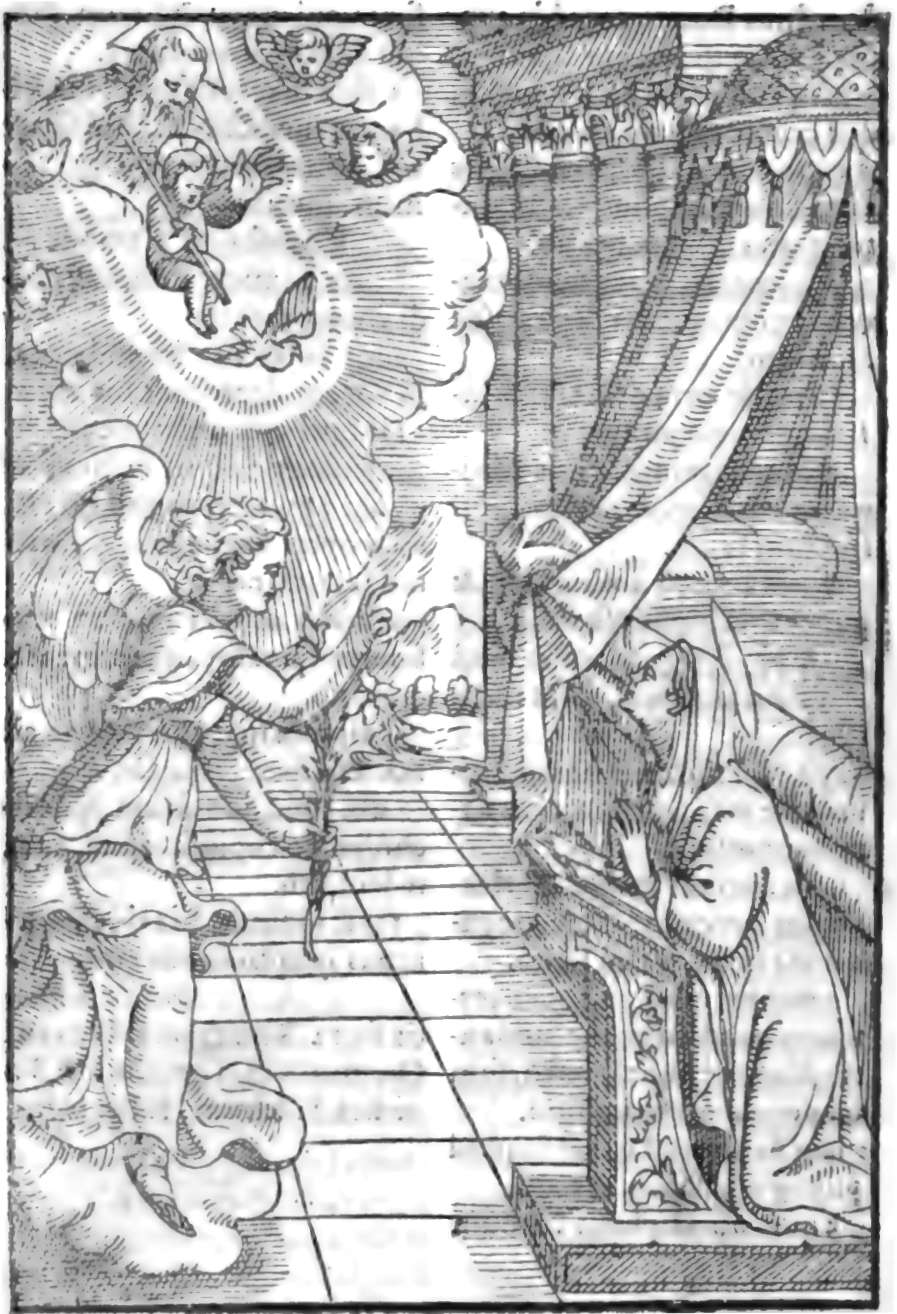
\includegraphics[width=4.5in]{Picture180.jpg}


%pp181
\newpage
\begin{center} \LARGE \color{red} \hypertarget{PROPERIVM}
A \ D \ V \ E \ N \ T \ V \ S \ \ \ D \ O \ M \ I \ N \ I
\end{center}
\vspace{-1.5em}
\bookmark[startatroot,dest=PROPERIVM]{PROPERIVM DE TEMPORE}

\begin{center} \large
semper incipit in Dominica proxima vltim\ae \ diei\\Nouembris ante, vel post: aut, in ipsa die vltima,\\si fuerit Dominica, \& festum duplex in\\ea, vel in sequentibus Dominicis\\Aduentus incidens transferendum\\est in diem sequentem,\\vt supra in regulis\\generalibus.
\end{center}

\begin{center} \Large \color{red} \hypertarget{DOM-PRIMA-ADV}
DOMINICA PRIMA ADVENTVS
\end{center}
\vspace{-1em}
\bookmark[rellevel=1,dest=DOM-PRIMA-ADV]{DOMINICA PRIMA ADVENTVS}

\begin{center} \color{red} \hypertarget{DOM-PRIMA-ADV-MAT}
A D \ \ M A T V T I N V M.
\end{center}
\vspace{-.5em}
\bookmark[rellevel=1,dest=DOM-PRIMA-ADV-MAT]{AD HOR\AE}
\bookmark[rellevel=1,dest=DOM-PRIMA-ADV-MAT]{AD MATVTINVM}

\begin{multicols}{2}
\yinipar{P}Ater noster, qui es in c\oe lis, sanctificetur nomen tuum.
\color{red} A\color{black}duieniat regnum tuum.
\color{red} F\color{black}iat voluntas tua sicut in c\oe lo \& in terra.
\color{red} P\color{black}anem nostrum quotidianum da nobis hodie.
\color{red} E\color{black}t dimitte nobis debita nostra, sicut \& nos dimittimus debitoribus nostris.
\color{red} E\color{black}t ne nos inducas in tentionem.
\color{red} S\color{black}ed libera nos a malo. Amen.
\lettrine[lines=2]{\bfseries \color{red} A}{}Ve Maria gratia plena. Dominus tecum, benedicta tu in mulieribus, \& benedictus fructus ventris tui Iesus.
\color{red} S\color{black}ancta Maria mater Dei Ora pro nobis peccatoribus. Amen.
\newline \color{red} Notandum, quod \color{black} Pater noster. \color{red} \& \color{black} Aue maria. \color{red} non tantum in Matutino, sed etiam in singulis alijs horis dicuntur semper in principio per totum annum. \color{black}
\vspace{-2em}
\begin{center} \color{red}
Confessio.
\end{center}
\vspace{-1em}
\lettrine[lines=2]{\bfseries \color{red} C}{}Onfiteor Deo omnipotenti, beat\ae \ Mari\ae \ semper virgini, beato Michaeli archangelo, beato Ioanni Baptist\ae , sanctis apostolis Petro \& Paulo, omnibus sanctis, \& \color{red} tibi pater, \color{black} quia peccaui nimis cogitatione, verbo, \& opere. Mea culpa, mea culpa, mea maxima culpa. Ideo precor beatam Mariam semper virginem, beatum Michaelem
%pp182
archangelum, beatum Ioannem Baptistam, sanctos Apostolos Petrum \& Paulum, omnes sanctos, \& \color{red} te pater \color{black} orare pro me. dominum nostrum. \quad \color{red} Absolutio. \color{black}
% \vspace{-.25em}
\lettrine[lines=2]{\bfseries \color{red} M}{}Isereatur \color{red} tui \color{black} omnipotens Deus, \& dimissis peccatis tuis perducat te ad vitam \ae ternam. \color{red} \Rbar . \color{black} Amen. \color{red} \Vbar . \color{black}
% \vspace{-.25em}
\lettrine[lines=2]{\bfseries \color{red} I}{}Ndulgentiam, absolutionem, \& remissionem peccatorum nostrorum tribuat nobis omnipotens, \& misericors dominus. \color{red} \Rbar . \color{black} Amen.
% \vspace{-.25em}
\newline \textswab{C} \color{red} Notandum quod confessio cum absolutione dicitur ad matutinum tantum singulis diebus totius anni pr\ae terquam in triduo ante Pascha, pr\ae dicto vel alio modo pro cuiusque deuotione.
Est autem aduertendum, quod si ab vno solo dicatur officium, omittitur \color{black} tibi pater \color{red} \& \color{black} te pater. \color{red} \& in absolutione loco \color{black} tui \color{red} \& \color{black} tuis \color{red} dicitur \color{black} nostris: \color{red} \& \color{black} nostri, \color{red} Si vero dicatur officium a duobus, aut pluribus, iteranda %iterandam???
est inuicem confessio, vt fit in Missa. \color{black}
\newline \textswab{C} \color{red} Deinde finita confessione dicitur Versus. \color{black}
\lettrine[lines=2]{\bfseries \color{red} D}{}Omine labia mea aperies. \color{red} \Rbar . \color{black} Et os meum annuntiabit laudem tuam.
\color{red} \& hoc dicens interim munit se signo crucis, \& similiter in alijs horis cum dicit \color{black} Deus in adiutorium. \color{red} \&c. \& \color{black} Conuerte nos. \color{red} \&c. \color{black}
\newline \textswab{C} \color{red} Deinde dicitur \Vbar . \color{black} Deus in adiutorium meum intende. \color{red} \Rbar . \color{black} Domine ad adiuuandum me festina. Gloria patri. Sicut erat. Haleluiah. \color{red} \& sic dicitur \color{black} Haleluiah. \color{red} ad omnes horas per totum annum, pr\ae terquam a dominica in septuagesima vsque ad Pascha, loco cuius illo tempore vsque ad feriam quintam in c\oe na domini dicitur \color{black} Laus tibi domine, Rex \ae tern\ae \ glori\ae . \color{red} Consequenter dicitur inuita. tempori vel festo conueniens. Inuita. \color{black} Domine pr\ae stolamur aduentum tuum, vt cito venias, \& dissoluas iugum captiuitatis nostr\ae .
\newline \textswab{C} \color{red} Hoc inuitatorium dicitur vsque ad vigiliam Natiuitatis exclusiue tam in dominicis, quam in ferijs, nisi agatur de aliquo sancto.\color{black}
\newline \textswab{C} \color{red} Notandum autem quod si officium dicatur ab vno solo, inuitatorium dicitur semel tantum ante psalmum. \color{black} Venite exultemus. \color{red} \& non repetitur vsque in finem eiusdem psalmi. Si vero officium dicatur a duobus, aut pluribus, inuita. dicitur ab vno, \& repetitur statim ab alio, vel alijs simul ante pr\ae dictum psalmum: 
in fine autem psalmi omnes simul dicunt inuitatorium semel tantum. Psalmus. \color{black}
\vspace{-.25em}
\lettrine[lines=2]{\bfseries \color{red} V}{}Enite exultemus domino, iubilemus Deo salutari nostro, pr\ae occupemus faciem eius in confessione \& in psalmis iubilemus ei.
%pp183
\newline \color{red} Q\color{black}uoniam Deus magnus dominus, \& rex magnus super omnes Deos: quoniam non repellet dominus plebem suam, quia in manu eius sunt omnes fines terr\ae , \& altitudines montium ipse conspicit.
\newline \color{red} Q\color{black}uoniam ipsius est mare, \& ipse fecit illud, \& aridam fundauerunt manus eius: venite adoremus, \& procidamus ante Deum, ploremus coram domino, qui fecit nos: quia ipse est dominus Deus noster, nos autem populus eius, et oues pascu\ae \ eius.
\newline \color{red} H\color{black}odie si vocem eius audieritis, nolite obdurare corda vestra, sicut in exacerbatione secundum diem tentationis in deserto: vbi tentauerunt me patres vestri: probauerunt, \& viderunt opera mea.
\newline \color{red} Q\color{black}uadraginta annis proximus fui generationi huic, \& dixi: semper hi errant corde, ipsi vero non cognouerunt vias meas, quibus iuraui in ira mea: si introibunt in requiem meam.
\newline \color{red} G\color{black}loria patri. \color{red} S\color{black}icut erat. \&c.
\newline \textswab{C} \color{red} Deinde repetitur inuitato. \color{black} Domine pr\ae stolamur. \color{red} \&c. \color{black}
\newline \color{red} Pr\ae dictus psalmus modo pr\ae dicto dicitur per totum annum cum Inuitatorio tempori, vel festo accommodato, pr\ae terquam in triduo ante Pascha. Deinde dicitur Hymnus tempori, seu festo conueniens. Hymnus. \color{black}
\vspace{-.25em}
\fancyhead[C]{\color{red} Dominica prima aduentus}
\lettrine[lines=2]{\bfseries \color{red} V}{}Ox clara ecce intonat, Obscura qu\ae que increpat: pellantur eminus somnia: Ab \ae there Christus promicat.
\newline \color{red} M\color{black}ens iam resurgat torpida, Qu\ae \ sorde extat saucia: Sydus refulget iam nouum, Vt tollat omne noxium.
\newline \color{red} E\color{black}\ sursum agnus mittitur, Laxare gratis debitum: Omnes pro indulgentia, vocem demus cum lachrymis.
\newline \color{red} S\color{black}ecundo vt cum fulserit Mundumque horror cinxerit, Non pro reatu puniat, Sed pius nos tunc protegat.
\newline \color{red} L\color{black}aus, honor, virtus, gloria Deo patri, \& filio, Sancto simul paracleto, In seculorum secula. Amen.
\newline \textswab{C} \color{red} Pr\ae dictis hymnus dicitur ad matutinum vsque ad vigiliam Natiuitatis inclusiue tam in Dominicis quam in Ferijs, nisi agatur de sancto.
Post hymnum incipitur antiphona tempori, vel festo accommodata, \& si fuerit festum duplex, dicitur integra antiphona \color{black} Veniet ecce rex. \color{red}
Deinde dicuntur tres psalmi, vt sunt distributi in Psalterio, quibus finitis semper dicitur antiphona integra, siue fit de festo, siue de dominica vel Feria. Antiphona. \color{black}
%pp184
Veniet ecce Rex excelsus cum potestate magna ad saluandas gentes. Haleluiah.
\color{red} H\ae c antiphona dicitur ad matuti vsque ad dominicam tertiam aduentus exclusiue, quando fit officium de dominica vel de feriam. %fer
Finita antiphona dicitur. \color{black} Pater noster, \&c. Et ne nos. Sed libera. \color{black}
\color{red} Deinde dicuntur tres lectiones, \& cuilibet earum pr\ae mittitur \Vbar . \color{black} Iube domine benedicere.
\color{red} Et ad primam, qu\ae \ semper est veteris testamenti, semper etiam dicitur benedictio. \color{black} Deus pater omnipotens sit nobis propitius, \& clemens. \color{red} \Rbar . \color{black} Amen.
\newline \color{red} Prophetia Isai\ae . \hfill Lectio prima. \color{black}
\vspace{-1em}
\yinipar{V}Isio\leftmarginnote{\begin{flushright}ca. 1.\end{flushright}} Isai\ae \ filij Amos, quam vidit super Iudam \& Ierusalem in diebus Ozi\ae , Ioatham, Achaz, \& Ezechi\ae \ regum Iuda. 
Audite c\oe li, \& auribus percipe terra, quoniam dominus loquutus est, Filios enutriui, \& exaltaui: ipsi autem spreuerunt me.
Cognouit bos possessorem suum, \& asinus pr\ae sepe domini sui: Israel autem me non cognouit, \& populus meus non intellexit.
V\ae \ genti peccatrici, populo graui iniquitate, semini nequam, filijs sceleratis.
Dereliquerunt dominum, blasphemauerunt sanctum Israel, abalienati sunt retrorsum. 
Super quo percutiam vos vltra, addentes pr\ae varicationem?
Omne caput languidum, \& omne cor m\oe rens.
A planta pedis vsque ad verticem non est in eo sanitas.
Vulnus, \& liuor, \& plaga tumens: non est circunligata, nec curata medicamine, neque fota oleo.
Terra vestra deserta: ciuitates vestr\ae \ succens\ae \ igni: Regionem vestram coram vobis alieni deuorant: \& desolabitur, sicut in vastitate hostili. 
Et derelinquetur filia Sion vt vmbraculum in vinea, \& sicut tugurium in cucumerario, \& sicut ciuitas qu\ae \ vastatur.
Nisi Dominus exercituum reliquisset nobis semen, quasi Sodoma fuissemus, \& quasi Gomorrha similes essemus.
Audite verbum domini principes Sodomorum, percipite auribus legem Dei nostri populus Gomorrh\ae , Quo mihi multitudinem victimarum vestrarum, dicit dominus?
Plenus sum: holocausta arietum: \& adipem pinguium: \& sanguinem vitulorum, \& agnorum, \& hircorum nolui.
Cum veniretis ante conspectum meum, quis qu\ae siuit h\ae c de manibus vestris: vt ambularetis in atrijs meis?
Ne offeratis vltra sacrificium frustra.
Incensum abominatio est mihi.
Neomeniam, \& sabbatum, \& festiuitates alias, non feram: iniqui sunt c\oe tus vestri.
%pp185
Calendas vestras, \& solennitates vestras odiuit anima mea: facta sunt mihi molesta: laboraui sustinens.
Et cum extenderitis manus vestras, auertam oculos meos a vobis: \& cum multiplicaueritis orationem, non exaudiam.
Manus vestr\ae \ sanguine plen\ae \ sunt.%vulgate: missing enim
\newline Tu autem domine miserere nostri. \color{red} \Rbar . \color{black} Deo gratias.
\color{red} Et sic terminantur omnes lectiones per totum annum, pr\ae terquam in triduo ante Pascha. Ad secundam lectionem versus. \color{black} Iube domine benedicere. \color{red} Benedictio. \color{black} Vnigenitus Dei filius, nos benedicere, \& adiuuvare dignetur. \color{red} \Rbar . \color{black} Amen.
\newline \color{red} Et h\ae c similiter benedictio dicitur per totum annum ad secundam lectionem, quem est semper noui testamenti. Sanctum Iesu Christi euangelium secundum Lucam. Lectio. ij. \color{black}
\vspace{-2em}
\lettrine[lines=2]{\bfseries \color{red} Q}{}Voniam quidem multi conati sunt ordinare narrationem, qu\ae \ in nobis complet\ae \ sunt rerum, sicut tradiderunt nobis qui ab initio ipsi viderunt, \& ministri fuerunt sermonis: visum est \& mihi assequuto omnia, a principio diligenter ex ordine tibi scribere, optime Theophile, vt cognoscas eorum verborum, de quibus eruditus es, veritatem. \textdagger \ 
Fuit\leftmarginnote{\begin{flushright}ca. 1.\\A\end{flushright}} in diebus Herodis regis Iud\ae \ae , sacerdos quidam nomine Zacharias, de vice Abia: \& vxor illius de filiabus Aaron, \& nomen eius Elisabeth.
Erant autem iusti ambo ante Deum, incedentes in omnibus mandatis \& iustificationibus domini sine querela, \& non erat illis filius: eo quod esset Elisabeth sterilis, \& ambo processissent in diebus suis.
Factum est autem, cum sacerdotio fungeretur in ordine vicis su\ae \ ante Deum, secundum consuetudinem sacerdotij, sorte exijt vt incensum poneret ingressus in templum domini: \& omnis multitudo populi erat orans foris hora incensi.
Apparuit autem illi angelus domini, stans a dextris altaris incensi.
Et Zacharias turbatus est, videns: \& timor irruit super eum.
Ait autem ad illum angelus, Ne timeas Zacharia, quoniam exaudita est deprecatio tua: \& vxor tua Elisabeth pariet tibi filium, \& vocabis nomen eius Ioannem: \& erit gaudium tibi \& exultatio: \& multi in natiuitate eius gaudebunt.
Erit enim magnus coram domino: \& vinum \& siceram non bibet: \& spiritu sancto replebitur adhuc ex vtero matris su\ae :
%pp186
\& multos filiorum Israel conuertet ad dominum Deum ipsorum: \& ipse pr\ae cedet ante illum in spiritu, \& virtute Eli\ae : vt conuertat corda patrum in filios, \& incredulos ad prudentiam iustorum, parare domino plebem perfectam.]
Et\rightmarginnote{B} dixit Zacharias ad angelum: Vnde hoc sciam? ego enim sum senex: \& vxor mea processit in diebus suis.
Et respondens angelus, dixit ei: Ego sum Gabriel, qui asto ante Deum: \& missus sum loqui ad te, \& h\ae c tibi euangelizare.
Et ecce, eris tacens, \& non poteris loqui vsque in diem quo h\ae c fiant: pro eo quod non credidisti verbis meis, qu\ae \ implebuntur in tempore suo.
Et erat plebs expectans Zachariam: \& mirabantur, quod tardaret ipse in templo.
Egressus autem non poterat loqui ad illos: \& cognouerunt, quod visionem vidisset in templo.
Et ipse erat innuens illis: \& permansit mutus.
Et factum est vt impleti sunt dies officij eius, abijt in domum suam.
Post hos autem dies concepit Elisabeth vxor eius: \& occultabat se mensibus quinque, dicens: Quia sic fecit mihi dominus in diebus quibus respexit auferre opprobrium meum inter homines.
\newline Tu autem domine, \color{red} \&c. vt supra. \color{black}
\newline \textswab{C} \color{red} Ad tertiam lectionem \Vbar . \color{black} Iube domine benedicere. \color{red} \&c. Benedictio. \color{black} Spiritus sancti gratia illuminet sensus, \& corda nostra. \color{red} \Rbar . \color{black} Amen.
\newline \color{red} Secundum Lucam. \hfill Lectio iij.\color{black}
\vspace{-1em}
\lettrine[lines=2]{\bfseries \color{red} I}{}N\rightmarginnote{Lu.\\21.} illo tempore, Dixit Iesus discipulis suis, Erunt signa in Sole, \& Luna, \& Stellis, \& in terris pressura gentium. \color{red} Et reliqua. \color{black}
\newline \color{red} Homilia sancti Gregorij Pap\ae . \color{black}
\newline \color{red} L\color{black}ectioni sancti euangelij, quam modo vestra fraternitas audiuit, paulo superius dominus pr\ae misit, dicens:
Exurget gens contra gentem, \& regnum aduersus regnum: \& terr\ae motus magni erunt per loca, \& pestilenti\ae , \& fames. 
Et quibusdam interpositis, hoc quod modo audistis, adiunxit: Erunt signa in Sole, \& Luna, \& Stellis, \& in terris pressura gentium, pr\ae \ confusione sonitus maris \& fluctuum.
Ex quibus profecto omnibus alia iam facta cernimus: alia e proximo ventura formidamus.
Nam gentem contra gentem exurgere, earumque pressuram terris insistere, plus iam in nostris tribulationibus cernimus, quam in codicibus legimus.
Quod terr\ae motus vrbes innumeras subruat, ex alijs mundi partibus scitis quam frequenter audiuimus.
Pestilentiam sine cessatione patimur.
%pp187
Signa vero in Sole \& Luna, \& Stellis adhuc aperte minime vidimus.
Sed quia \& h\ae c non longe sint, ex ipsa iam aeris immutatione colligimus.
Quanuis priusquam Italia gentili gladio ferienda traderetur, igneas in c\oe lo acies vidimus, ipsum qui postea effusus est humani generis sanguinem coruscantes.
Confusio autem maris \& fluctuum necdum noua exorta est.
Sed cum multa iam pr\ae nuntiata completa sint: dubium non est, quod sequantur etiam pauca qu\ae \ restant.
Quia sequentium rerum certitudo, est pr\ae teritarum exhibitio.
H\ae c nos fratres charissimi idcirco dicimus, vt ad cautel\ae \ studium vestr\ae \ mentes euigilent, ne securitate torpeant, ne ignorantia languescant: sed semper eas \& timor solicitet, \& in bono opere solicitudo confirmet.
Pensantes hoc quod redemptotis nostri voce subiungitur, Arescentibus hominibus pr\ae \ timore, \& expectatione qu\ae \ superuenient vniuerso orbi.
Nam virtutes c\oe lorum commouebuntur.
Tu autem, \&c.
\newline \textswab{C} \color{red} Notandum, quod quandocunque agitur officium de dominica, seu de feria, aut de aliquo festo Domini siue eius octaua. \color{black}
\newline \textswab{C} \color{red} Item in festis inuentionis, \& exaltationis Crucis, \& in dedicationibus Basilicarum ad tertiam lectionem dicenda est Benedictio, \color{black} Spiritus sancti gratia. \color{red} \&c. vt supra. Quando vero agitur officium de aliquo sanctorum, aut sanctis aut eorum octauis dicitur benedictio, \color{black} Cuius, \color{red} vel \color{black} quorum, \color{red} vel \color{black} quarum festum colimus, ipse, \color{red} vel \color{black} ipsi, \color{red} vel \color{black} ipsa, \color{red} vel \color{black} ips\ae \ intercedat, \color{red} vel \color{black} intercedant pro nobis ad dominum. \color{red} \Rbar . \color{black} Amen.
\newline \textswab{C} \color{red} Si autem tertia lectio fuerit de beata virgine, tam in sabbatis, quam in eius festiuitatibus, \& octa. dicenda est benedictio. \color{black} Per virginem matrem concedat nobis dominus salutem, \& pacem. \color{red} \Rbar . \color{black} Amen.
\newline \textswab{C} \color{red} Sciendum insuper quod quandocunque fit officium de dominica per totum annum, aut de aliquo ex festis domini, mobilibus, seu eorum octauis. \color{black}
%pp188
\newline \textswab{C} \color{red} Item quandocunque agitur officium de feria in aduentu, \& in Quadragesima semper in pr\ae dictis diebus tertiam lectio inuenietur assignata in hoc dominicali statim post secundam lectionem. Quando vero fit officium de aliquo festo aut octaua, ex contentis in Calendario, tertia lectio, si fuerit propria inuenietur in ea parte Breuiarij, qu\ae \ continet historias sanctorum. Et si non fuerit assignata propia, dicetur de communi. \color{black}
\newline \textswab{C} \color{red} Item quando aigitur officium de feria extra Aduentum, \& Quadragesimam tertia lectio dicetur ex Epistolis, vt assignata fuerit in Calendario. Similiter in Sabbatis, in quibus agitur officium de beata virgine, tertia lectio inuenietur in officio eidem assignato pro Sabbatis in fine Breuiarij. Quando autem debeat fieri officium de dominica, seu de feria, aut de festo supra in regulis generalibus poteris videre. Finitis tribus lectionibus in aduentu, \& a dominica in septuagesima vsque ad feriam quintam in c\oe na domini quando fit officium de dominica vel de feriam dicitur psalmus. \color{black} Miserere. fo. \hyperlink{ps50}{70.} \color{red} Quando autem fit de aliquo festo in pr\ae dictis temporibus, \& in toto reliquo anni tempore, siue fiat officium de dominica, siue de feria, siue de aliquo festo aut oct. semper dicitur. \color{black} Te Deum laudamus, \&c. fo. \hyperlink{tedeum}{5.} \color{red} Pr\ae terquam in triduo ante Pascha. \hypertarget{DOM-PRIMA-ADV-LAVD}{Ad laud.} \Vbar . \color{black}
\bookmark[dest=DOM-PRIMA-ADV-LAVD]{AD LAVDES}
\vspace{-.5em}
\lettrine[lines=2]{\bfseries D}{}Eus in adiutorium meum intende. \color{red} \Rbar . \color{black} Domine ad adiuuandum me festina. \color{red} G\color{black}loria patri, \& filio \& spiritui sancto. Sicut erat in principio. Haleluiah.
\newline \color{red} Et non dicitur hym. quia laudes non hora diuersa, sed pars matutini reputantur. Post \color{black} Haleluiah. \color{red} statim dicitur antiphona tempori vel festo accommodata. Antiphona. \color{black} Emitte agnum. \color{red} deinde dicuntur tres psalmi, vt in Psalterio, quibus adiungitur quotidie canticum \color{black} \hyperlink{Benedictus}{Benedictus} \color{red} quo finito dicitur integra antiphona. \color{black} Emitte agnum domine dominatorem terr\ae , de petra deserti ad montem fili\ae \ Sion. \color{red} H\ae c antiphona dicitur ad laudes vsque ad dominicam tertiam aduentus quando fit officium de dominica vel de feriam. Deinde \Vbar . \color{black} Domine exaudi orationem meam. \color{red} \Rbar . \color{black} Et clamor meus ad te veniat. \color{red} Deinde. \color{black} Oremus. \color{red} Oratio. \color{black}
\vspace{-.5em}
\lettrine[lines=2]{\bfseries \color{red} E}{}Xcita qu\ae sumus domine potentiam tuam: \& veni, vt ab imminentibus peccatorum nostrorum periculis: te mereamur protegente eripi, te liberante saluari: qui viuis, \& regnas cum Deo patre in vnitate spiritus sancti Deus, per omnia secula seculorum. \color{red} \Rbar . \color{black} Amen.
\newline \color{red} H\ae c oratio dicitur per totam hanc hebdomadam quando fit de feria. Et semper quando aigitur officium de feria, cui non est assignata propria oratio, dicitur oratio dominic\ae \ pr\ae cedentis. Notandum, quod finita oratione diei fiunt commemorationes sequentes de beata virgine, \& omnibus sanctis modo infrascripto. In aduentu antiphona. \color{black} Spiritus sanctus in te descendet Maria, ne timeas, habebis in vtero filium Dei, 
%pp189
Haleluiah. \color{red} \Vbar . \color{black} Ora pro nobis sancta Dei genetrix. \color{red} \Rbar . \color{black} Vt digni efficiamur promissionibus Christi. \color{red} O\color{black}remus. \color{red} Oratio. \color{black}
\vspace{-.5em}
\lettrine[lines=2]{\bfseries \color{red} D}{}Eus, qui de beat\ae \ Mari\ae \ virginis vtero verbum tuum angelo nuntiante carnem suscipere voluisti, pr\ae sta supplicibus tuis, vt qui vere eam Dei genitricem credimus, eius apud te intercessionibus adiuuemur, per eundem Christum dominum nostrum. \color{red} \Rbar . \color{black} Amen.
\newline \color{red} Deinde pro sanctis antiphona. \color{black} Ecce dominus veniet, \& omnes sancti eius cum eo: \& erit in die illa lux magna, Haleluiah. \color{red} \Vbar . \color{black} Ecce apparebit dominus super nubem candidam. \color{red} Et cum eo sanctorum millia. \color{black} Oremus. \color{red} Oratio. \color{black}
\vspace{-.5em}
\lettrine[lines=2]{\bfseries \color{red} C}{}Onscientias nostras qu\ae sumus domine visitando purifica, vt veniens Iesus Christus filius tuus dominus noster cum omnibus sanctis, paratam sibi in nobis inueniat mansionem, qui tecum viuit, \& in vnitate spiritus sancti Deus, per omnia secula seculorum. \color{red} \Rbar . \color{black} Amen.
\newline \color{red} Deinde dicitur \Vbar . \color{black} Benedicamus domino. \color{red} \Rbar. \color{black} Deo gratias. \color{red} \Vbar . \color{black} Fidelium anim\ae \ per misericordiam Dei requiescant in pace. \color{red} \Rbar . \color{black} Amen.
\newline \color{red} Et est aduertendum quod omnes hor\ae \ finiuntur per \color{black} Benedicamus, \&c. Haleluiah, \color{red} \&c. Per totum annum pr\ae terquam in triduo ante Pascha. Post aduentum reliquo anni tempore fiunt commemorationes modo infrascripto. Antiphona. \color{black}
Sub tuum pr\ae sidium confugimus sancta Dei genitrix: nostras de precationes ne despicias in necessitatibus: sed a periculis cunctis libera nos semper virgo gloriosa, \& benedicta. \color{red} \Vbar . \color{black} Ora pro nobis sancta Dei genitrix. \color{red} \Rbar . \color{black} Vt digni efficiamur promissionibus Christi. \color{red} O\color{black}remus.
\newline \color{red} Oratio. \color{black}
\vspace{-.25em}
\lettrine[lines=2]{\bfseries C}{}Oncede nos famulos tuos, qu\ae sumus domine Deus, perpetua mentis \& corporis sanitate gaudere, \& gloriosa beat\ae \ Mari\ae \ semper virginis intercessione, a pr\ae senti liberari tristitia, \& \ae terna perfrui l\ae titia. Per Christum dominum nostrum. \color{red} \Rbar . \color{black} Amen.
\newline \color{red} De apostolis, \& omnibus sanctis antiphona. \color{black} Sancti Dei omnes intercedere dignemini pro nostra, omniumque salute. \color{red} \Vbar . \color{black} L\ae tamini in domino, \& exultate iusti. \color{red} \Rbar . \color{black} Et gloriamini omnes recti corde. \color{red} O\color{black}remus. \color{red} Oratio. \color{black}
\vspace{-.25em}
\lettrine[lines=2]{\bfseries \color{red} E}{}Xaudi nos Deus salutaris noster: \& apostolorum tuorum Petri, \& Pauli, \& aliorum apostolorum nos tuere perfidijs, %pfidijs
quorum dona sti fideles esse doctrinis. \color{red} Oratio. \color{black}
\vspace{-.25em}
\lettrine[lines=2]{\bfseries \color{red} O}{}Mnes sancti tui, qu\ae sumus domine, nos vbique adiuuent, vt dum eorum merita
%pp190
recolimus, patrocinia sentiamus: \& pacem tuam nostris concede temporibus: \& ab ecclesiam tua cunctam repelle nequitiam: iter, actus, \& voluntates nostras, \& omnium famulorum tuorum in salutis tu\ae \ prosperitate dispone: benefactoribus nostris sempiterna bona retribue: \& omnibus fidelibus defunctis requiem \ae ternam concede. Per dominum.
\newline \textswab{C} \color{red} Pr\ae dict\ae \ commemorationes pr\ae dicto modo dicuntur semper in laudibus \& vesperis post orationem diei, pr\ae terquam in festis duplicibus, \& quandocunque fit officium aut commemo. de aliqua octaua, \& in triduo ante Pascha. Est autem aduertendum, quod in sabbatis in quibus fit officium de beata virgine omittitur eius commemoratio, \& fit tantum de sanctis. Aduertendum pr\ae terea quod quando in aliqua dominica fit officium de aliquo festo duplici, vel de aliqua octaua, post orationem diei dicenda est etiam oratio illius Dominic\ae \ pro eius commemoratione in laudibus , \& vesperis. Deinde dicitur \color{black} Benedicamus. \color{red} \& \color{black} Fidelium. \color{red} vt supra. Ad \hypertarget{DOM-PRIMA-ADV-PRIM}{primam.} \color{black}
\bookmark[dest=DOM-PRIMA-ADV-PRIM]{AD PRIMAM}
Pater noster. Aue maria. \color{red} \Vbar . \color{black} Deus in adiutorium. \color{red} Hymnus. \color{black}
\vspace{-.25em}
\lettrine[lines=2]{\bfseries \color{red} I}{}Am lucis orto sydere:\\Deum precemur supplices,\\Vt in diurnis actibus:\\Nos seruet a nocentibus.
\newline \color{red} L\color{black}inguam refrenans temperet,\\Ne litis horror insonet:\\Visum fouendo contegat,\\Ne vanitates hauriat.
\newline \color{red} S\color{black}int pura cordis intima,\\Absistat \& vecordia:\\Carnis terat superbiam,\\Potus cibique parcitas.
\newline \color{red} V\color{black}t cum dies abscesserit,\\Noctemque sors reduxerit:\\Mundi per abstinentiam,\\Ipsi canamus gloriam.
\newline \color{red} D\color{black}eo patri sit gloria,\\Eiusque soli filio,\\Cum spiritu paracleto,\\Et nunc, \& in perpetuum. Amen.
\newline \textswab{C} \color{red} Deinde dicuntur %dnr
antiphona \& Psalmi, vt in Psalterio cum symbolo Athanasij in Dominicis diebus, in alijs autem cum symbolo apostolorum. Deinde. \color{black} Domine exaudi orationem meam. \color{red} \Rbar . \color{black} Et clamor meus ad te veniat. \color{red} O\color{black}remus. \color{red} Oratio. \color{black}
\vspace{-.25em}
\lettrine[lines=2]{\bfseries \color{red} D}{}Omine Deus omnipotens, qui ad principium huius diei nos peruenire fecisti, tua nos hodie salua virtute: vt in hac die ad nullum declinemus peccatum: sed semper ad tuam iustitiam faciendam nostra procedant eloquia, dirigantur cogitationes, \& opera. Per dominum. Benedic. \color{red} \&c. \color{black} Fidelium. \color{red} vt supra.
%pp191
Et sic finita Prima dicitur \Vbar . \color{black} Pretiosa in conspectu domini. \color{red} \Rbar . \color{black} Mors sanctorum eius. \color{red} Oratio. \color{black}
\vspace{-1.25em}
\lettrine[lines=2]{\bfseries \color{red} S}{}Ancta Maria \& omnes sancti intercedant pro nobis ad dominum, vt nos mereamur ab eo adiuuari, \& saluari, qui viuit, \& regnat in secula seculorum. \color{red} \Rbar . \color{black} Amen. \color{red} \Vbar . \color{black} Dies \& actus nostros in sua pace disponat dominus omnipotens. \color{red} \Rbar . \color{black} Amen.
\color{red} Et hoc modo dicitur \color{black} Pretiosa. \color{red} Per totum annum pr\ae terquam in triduo ante Pascha. \color{black}
\newline \textswab{C} \color{red} Aduertendum tamen quod si in aliquo sabbato, aut dominica, aut infra octauas Resurrectionis, Ascensionis, Pentecostes \& corporis Christi, vel in Ferijs Quadragesim\ae , excepto triduo ante Pascha inciderit aliquod festum simplex, finita Prima, antequam dicatur \color{black} Pretiosa. \color{red} Pro commemoratione illius festi simplicis dicitur \Vbar . \color{black} Ora pro nobis sancte. \color{red} N. vel \color{black} Orate pro nobis sancti. \color{red} N. \& N. \Rbar . \color{black} Vt digni efficiamur promissionibus Christi. \color{red} O\color{black}remus. \color{red} Et dicitur oratio propria si eam habuerit: alioquin de communi, qua finita dicitur \color{black} Pretiosa. \color{red} \&c. vt sup. \color{black}
\newline \textswab{C} \color{red} Ad \hypertarget{DOM-PRIMA-ADV-TER}{tertiam.} \color{black}
\bookmark[dest=DOM-PRIMA-ADV-TER]{AD TERTIAM}
\vspace{-.25em}
\lettrine[lines=2]{\bfseries \color{red} N}{}Vnc sancte nobis, spiritus.\\Vnum patri cum filio,\\Dignare promptus ingeri,\\Nostro refusus pectori.
\newline \color{red} O\color{black}s, lingua, mens, sensus, vigor,\\Confessionem personent:\\Flammescat igne charitas,\\Accendat ardor priximos.
\newline \color{red} P\color{black}r\ae sta pater pijssime,\\Patrique compar vnice,\\Cum spiritu paraclito,\\Regnans per omne seculum. Amen.
\newline \textswab{C} \color{red} Deinde antiphona, \& psalmi vt in Psalterio, quibus finitis dicitur \Vbar . \color{black} Domine exaudi orationem meam. \color{red} \Rbar . \color{black} Et clamor meus ad te veniat. \color{red} O\color{black}remus. \color{red} Oratio. \color{black} Excita qu\ae sumus. \color{red} vt supra. \color{black}
\newline \textswab{C} \color{red} Ad laudes. Notandum quod ad tertiam, sextam, \& nonam semper dicitur oratio, qu\ae \ dicta duerit ad laudes. Deinde. \color{black} Benedicamus. \color{red} \&c. \color{black} Fidelium. \color{red} \&c. \color{black}
\newline \textswab{C} \color{red} Ad \hypertarget{DOM-PRIMA-ADV-SEX}{sextam.} \color{black}
\bookmark[dest=DOM-PRIMA-ADV-SEX]{AD SEXTAM}
Pater noster. Aue maria. \color{red} \Vbar . \color{black} Deus in adiutorium meum intende. \quad \color{red} Hymnus. \color{black}
\vspace{-.25em}
\lettrine[lines=2]{\bfseries \color{red} R}{}Ector potens, verax Deus,\\Qui temperas rerum vices:\\Splendore mane instruis,\\Et ignibus meridiem
\newline \color{red} E\color{black}xtingue flammas litium,\\Aufer calorem noxium,\\Confer salutem corporum,\\Veramque pacem cordium.
\newline \color{red} P\color{black}r\ae sta pater pijssime. \&c.
\newline \textswab{C} \color{red} Deinde antiphona, \& in psalmi vt in Psalterio, \&c. vt sup. Ad tertiam.
%pp192
\newline \textswab{C} \color{red} Ad \hypertarget{DOM-PRIMA-ADV-NON}{nonam.} \color{black}
\bookmark[dest=DOM-PRIMA-ADV-NON]{AD NONAM}
Pater noster. Aue maria. \color{red} \Vbar . \color{black} Deus in adiutorium meum intende. \&c. \quad \color{red} Hymnus. \color{black}
\vspace{-.25em}
\lettrine[lines=2]{\bfseries \color{red} R}{}Erum Deus tenax vigor,\\Immotus in te permanens.\\Lucis diurn\ae \ tempora:\\Successibus determinans.
\newline \color{red} L\color{black}argire clarum vespere,\\Quo vita nusquam decidat:\\Sed pr\ae mium mortis sacr\ae ,\\Perennis instet gloria.
\newline \color{red} P\color{black}r\ae sta pater pijssime, \&c.
\newline \color{red} Deinde antiphona \& psalmi vt in Psalterio, \&c. vt in supra ad tertiam. \color{black}
\newline \textswab{C} \color{red} Ad \hypertarget{DOM-PRIMA-ADV-VES}{vesperas.} \color{black}
\bookmark[dest=DOM-PRIMA-ADV-VES]{AD VESPERAS}
Pater noster. Aue maria. \color{red} \Vbar . \color{black} Deus in adiuto. \&c. \color{black}
\newline \textswab{C} \color{red} Deinde dicitur hym. tempori, vel festo conueniens. Hym. \color{black}
\vspace{-.25em}
\lettrine[lines=2]{\bfseries \color{red} C}{}Onditor alme syderum,\\ \AE terna lux credentium,\\Christe redemptor omnium:\\Exaudi preces supplicum.
\newline \color{red} Q\color{black}ui condolens interitu,\\Mortis perire seculum,\\Saluasti mundum languidum,\\Donans reis remedium.
\newline \color{red} V\color{black}ergente mundi vespere,\\Vti sponsus de thalamo,\\Egressus honestissima,\\Virginis matris clausula.
\newline \color{red} C\color{black}uius forti potenti\ae ,\\Genu curuantur omnia:\\C\oe lestia, terrestria,\\Nutu fatentur subdita.
\newline \color{red} T\color{black}e deprecamur agie,\\Venture iudex seculi:\\Conserua nos in tempore:\\Hostis a telo perfidi.
\newline \color{red} L\color{black}aus, honor, virtus, gloria\\Deo patri, \& filio,\\Sancto simul paracleto:\\In seculorum secula. Amen.
\newline \textswab{C} \color{red} Pr\ae dictus hymnus dicitur ad vesperas vsque ad vigiliam Natiuitatis Domini exclusiue quando non agitur de sancto. \color{black}
\newline \textswab{C} \color{red} Post hymnum dicitur antiphona tempori, vel festo accommodata, qu\ae \ in festis duplicibus ad matuti. laudes, \& vesperas dicenda est in principio integra, in alijs autem diebus incipienda tantum antiphona. \color{black} Rorate c\oe li desuper. \&c. \color{red} Deinde dicuntur tres psalmi vt in psalterio, quibus adiungitur quotidie Canticum. \color{black} \hyperlink{Magnificat}{Magnificat anima mea dominum.} \color{red} quo finito semper antiphona dicitur integra antiphona. \color{black} Rorate c\oe li desuper, \& nubes pluant iustum, aperiatur terra, \& germinet saluatorem.
\newline \textswab{C} \color{red} H\ae c antiphona dicenda est ad ves. vsque ad dominicam tertiam aduentus exclusiue, quando fit officium de dominica, vel de feria. Deinde \Vbar . \color{black} Domine exaudi orationem meam. \&c. \color{red} cum oratione \& commemorationibus, vt supra ad laudes. \color{black}
\newline \color{red} Notandum quod in vesperis semper dicitur oratio qu\ae \ dicta fuerit
%pp193
ad laudes, nisi vesper\ae \ dicend\ae \ sint de aliquo festo duplici sequentis diei: tunc enim hymnus, antiphona, \& oratio dicend\ae \ sunt de ipso festo sequenti. \color{black}
\newline \textswab{C} \color{red} Ad \hypertarget{DOM-PRIMA-ADV-COM}{completorium.} \color{black}
\bookmark[dest=DOM-PRIMA-ADV-COM]{AD COMPLETORIVM}
Pater noster. Aue maria gra. \quad \color{red} Versus. \color{black}
\vspace{-.25em}
\lettrine[lines=2]{\bfseries C}{}Onuerte nos Deus salutaris noster. \color{red} \Rbar . \color{black} Et auerte iram tuam a nobis. \color{red} \Vbar . \color{black} Deus in adiutorium. \color{red} \&c. Hymnus. \color{black}
\vspace{-.25em}
\lettrine[lines=2]{\bfseries \color{red} T}{}E lucis ante terminum\\Rerum creator poscimus:\\Vt solita clementia,\\Sis pr\ae sul ad custodiam.
\newline \color{red} P\color{black}rocul recedant somnia.\\Et noctium phantasmata:\\Hostemque nostrum comprime,\\Ne polluantur corpora.
\newline \color{red} P\color{black}r\ae sta pater omnipotens,\\Per Iesum Christum dominum, Qui tecum in perpetuum Regnat cum sancto spiritu. Amen.
\newline \textswab{C} \color{red} Post hymnum incipitur antiphona. \color{black} Salua nos. \color{red} Deinde dicuntur tres psalmi, vt in Psalterio, quibus quotidie adiungitur canticum. \color{black} \hyperlink{Nunc}{Nunc dimittis seruum tuum do. 17.} \color{red} quo finito dicitur integra antiphona. \color{black} Salua nos domine vigilantes, custodi nos dormientes, vt vigilemus cum Christo, \& requiescamus in pace.
\newline \textswab{C} \color{red} H\ae c antiphona dicitur per totum annum ad completorium, pr\ae terquam in triduo ante Pascha. Deinde dicitur \Vbar . \color{black} Domine exaudi orationem meam. \color{red} \Rbar . \color{black} Et clamor meus ad te veniat. \color{red} O\color{black}remus. \color{red} Oratio. \color{black}
\vspace{-.25em}
\lettrine[lines=2]{\bfseries \color{red} V}{}Isita qu\ae sumus domine habitationem istam: \& omnes insidias inimici ab ea longe repelle: Angeli tui sancti habitent in ea, qui nos in pace custodiant: \& benedictio tua sit super nos semper. Per dominum nostrum. \color{red} \Vbar . \color{black} Benedicamus domino. \color{red} \Rbar . \color{black} Deo gratias. \color{red} \Vbar . \color{black} Fidelium anim\ae \ per misericordiam Dei requiescant in pace. \color{red} \Rbar . \color{black} Amen. 
\newline \color{red} Et sic finito completorio dicitur. \color{black}
\vspace{-.25em}
\lettrine[lines=2]{\bfseries \color{red} S}{}Alue regina misericordi\ae : vita, dulcedo, \& spes nostra salue. Ad te clamamus exules filij Eu\ae : ad te suspiramus gementes, \&  flentes in hac lachrymarum valle. Eia ergo aduocata nostra, illos tuos misericordes oculos ad nos conuerte. Et Iesum benedictum fructum ventris tui nobis post hoc exilium ostende. O clemens, o pia, o dulcis virgo Maria. \color{red} \Vbar . \color{black} Ora pro nobis sancta Dei genitrix. \color{red} \Rbar . \color{black} Vt digni efficiamur promissionibus Christi. \color{red} O\color{black}remus.
\newline \color{red} Oratio. \color{black}
\vspace{-.25em}
\lettrine[lines=2]{\bfseries \color{red} O}{}Mnipotens sempiterne Deus, qui glorios\ae \ virginis Mari\ae \ corpus \& animam, vt dignum filij tui habitaculum effici mereretur, spiritu sancto
%pp194
cooperante pr\ae parasti: da vt cuius commemoratione l\ae tamur, eius pia intercessione ab instantibus malis, \& a morte perpetua liberemur. Per eundem Christum dominum nostrum. \color{red} \Rbar . \color{black} Amen. \Vbar . %sic
Diuinum auxilium maneat semper nobiscum. \color{red} \Rbar . \color{black} Amen.
\newline \textswab{C} \color{red} Pr\ae dicto modo dicitur \color{black} Salue regina. \color{red} \&c. cum oratione \color{black} Omnipotens sempiterne. \&c. \color{red} in fine completorij per totum annum, pr\ae terquam a Dominica resurrectionis vsque ad Ascensionem: quo tempore earum loco dicuntur infrascripta. \color{black}
\vspace{-.25em}
\lettrine[lines=2]{\bfseries \color{red} R}{}Egina c\oe li l\ae tare Haleluiah. Quia quem meruisti portare haleluiah, Resurrexit sicut dixit haleluiah. Ora pro nobis Deum haleluiah. Oremus. \color{red} O\color{black}ratio.
\vspace{-.25em}
\lettrine[lines=2]{\bfseries \color{red} G}{}Ratiam tuam qu\ae sumus domine mentibus nostris infunde: vt qui angelo nuntiante Christi filij tui incarnationem cognouimus, per passionem eius \& crucem, ad resurrectionis gloriam perducamur. Per eundem Christum dominum nostrum. \color{red} \Rbar . \color{black} Amen. \color{red} \Vbar . \color{black} Diuinum auxilium maneat. \&c.
\newline \textswab{C} \color{red} Sciendum quod hymni supra assignati ad primam, tertiam, sextam, nonam \& completorium, necnon orationes. \color{black} Domine Deus omnipotens. \color{red} Ad primam, \& \color{black} Visita qu\ae sumus. \color{red} Ad completorium. nunquam mutantur in toto anno pr\ae terquam in triduo ante Pascha. \color{black}
\newline \textswab{C} \color{red} Notandum quod per totum annum, pr\ae terquam in triduo ante Pascha tam in Dominicis quam in Ferijs, \& festis diebus semper hor\ae \ dicuntur ordine in hac prima dominica aduentus explicato. Exempli gratia, vt ad matutinum infrascripta dicantur per ordinem. \color{black} Pater noster. Aue maria. Confiteor. \color{red} cum absolutione \color{black} Domine labia. Deus in adiutorium. Haleluiah. \color{red} vel \color{black} Laus tibi domine. \color{red} Inuita. cum psalmo. \color{black} Venite exultemus. \color{red} rursus inuita. hym. antiphona tres psalmi, rursus antiphona integra. \color{black} Pater noster. \color{red} Tres lectiones cum suis benedictionibus, \& \color{black} Tu autem. \hyperlink{tedeum}{Te Deum laudamus.} \color{red} vel \color{black} \hyperlink{ps50}{Misere mei Deus.} \color{red} Deinde statim ad laudes. \color{black} Deus in adiu. \color{red} Antiphona. Tres psalmi cum cantico. \color{black} \hyperlink{Benedictus}{Benedictus.} \color{red} Rursus antiphona integra. \color{black} Domine exaudi orationem. \color{red} Oratio cum commemorationibus de beata virgine \&c. nisi sint omittend\ae , vt supra. \color{black} Benedicamus. Fidelium. \&c. \color{red} Item ad primam, tertiam, sextam, nonam, \& vesperas. \color{black} Pater noster. Aue maria. Deus in adiutorium. \&c. \color{red} seruato ordine in eisdem horis contento. \color{black}
%pp195
\newline \textswab{C} \color{red} Item ad completorium. \color{black} Pater noster. Aue maria. Conuerte nos. Deus in adiutorium. \color{red} \&c. vt in eadem hora continetur. \color{black}
\newline \color{red} \hypertarget{MON-PRIMA-ADV}{Feria secunda,} ex Isaia. \hfill Lectio. j. \color{black}
\bookmark[rellevel=-1,dest=MON-PRIMA-ADV]{FERIA SECVNDA}
\vspace{-1em}
\yinipar{L}\textdagger Auamini,\leftmarginnote{\begin{flushright}ca. 1.\\E\end{flushright}} mundi estote, auferte malum cogitationum vestrarum ab oculis meis.
Quiescite agere peruerse: discite benefacere: qu\ae rite iudicium, subuenite oppresso, iudicate pupillo, defendite viduam.
Et venite, \& arguite me, dicit dominus.
Si fuerint peccata vestra vt coccinum: quasi nix, dealbabuntur, \& si fuerint rubra sicut vermiculus, velut lana, alba erunt.
Si volueritis, \& audieritis me, bona terr\ae \ comeditis.]
Quod\leftmarginnote{\begin{flushright}F\end{flushright}} si nolueritis, \& me ad iracundiam prouocaueritis, gladius deuorabit vos, quia os domini loquutum est.
Quomodo facta est meretrix ciuitas fidelis, plena iudicij?
Iustitia habitauit in ea, nunc autem homicid\ae .
Argentum tuum versum est in scoriam: vinum tuum mistum est aqua.
Principes tui infideles, socij furum.
Omnes diligunt munera, sequuntur retributiones.
Pupillo non iudicant: \& causa vidu\ae \ non ingreditur ad illos.
Propter hoc ait dominus Deus exercituum fortis Israel, Heu consolabor super hostibus meis, \& vindicabor de inimicis meis: \& conuertam manum meam ad te, \& excoquam ad puram scoriam tuam, \& auferam omne stannum tuum, \& restituam iudices tuos vt fuerunt prius, \& consiliarios tuos sicut antiquitus.
Post h\ae c vocaberis ciuitas iusti, vrbs fidelis.
Sion in iudicio redimetur, \& reducent eam in iustita.
Et conteret scelestos, \& peccatores simul, \& qui dereliquerunt dominum, consumentur.
Confundentur enim ab idolis, quibus sacrificauerunt: \& erubescetis super hortis, quos elegeratis, cum fueritis velut quercus defluentibus folijs, \& velut hortus absque aqua.
Et erit fortitudo vestra vt fauilla stupp\ae , \& opus vestrum quasi scintilla: \& succendetur vtrumque simul, \& non erit qui extinguat.
% !!!!!!!!!!!!!!!!!!!!!!!!!!!!!!!!!!!!!!!!!!!!!!!!!!!!!!!!!!!!!!!!!!!!!!!!!!!!!!!!!!!!!!!!!!!!!!!!!!!!!!!!!!!!!!!!!!!!!!!!!!!!
% \newline
\fancyhead[C]{\color{red} Feria. ij. Dominic\ae . j. aduentus}
\color{red} Secundum Lucam. Lectio. ij.\color{black}
\vspace{-.25em}
\lettrine[lines=2]{\bfseries \color{red} I}{}N\rightmarginnote{ca. 1.\\C} mense autem sexto \textdagger \ missus est Angelus Gabriel a Deo in ciuitatem Galil\ae \ae \ cui nomen Nazareth, ad virginem desponsatam viro, cui nomen erat Ioseph, de domo Dauid: \& nomen virginis Maria.
Et ingressus angelus ad eam, dixit: Aue, gratia plena, dominus tecum, benedicta tu in mulieribus.
Qu\ae \ cum audisset, 
%pp196
turbata est in sermone eius, \& cogitabat qualis esset ista salutatio.
Et ait angelus ei: Ne timeas Maria, inuenisti enim gratiam apud Deum: ecce concipies in vtero, \& paries filium: \& vocabis nomen eius Iesum.
Hic erit magnus, \& filius altissimi vocabitur: \& dabit illi dominus Deus sedem Dauid patris eius: \& regnabit in domo Iacob, in \ae ternum, \& regni eius non erit finis.
Dixit autem Maria ad angelum: Quomodo fiet istud, quoniam virum non cognosco?
Et respondens angelus, dixit ei, Spiritus sanctus superueniet in te, \& virtus altissimi obumbrabit tibi.
Ideoque \& quod nascetur ex te sanctum, vocabitur filius Dei.
Et ecce Elisabeth cognata tua, \& ipsa concepit filium in senectute sua: \& hic mensis, sextus est illi, qu\ae \ vocatur sterilis: quia non erit impossibile apud Deum omne verbum.
Dixit autem Maria: Ecce ancilla domini, fiat mihi secundum verbum tuum.]
Et\leftmarginnote{\begin{flushright}D\end{flushright}} discessit ab illa angelus. \textdagger \ 
Exurgens autem Maria in diebus illis, abijt in montana cum festinatione in ciuitatem Iuda: \& intrauit in domum Zachari\ae , \& salutauit Elisabeth.
Et factum est, vt audiuit salutationem Mari\ae \ Elisabeth, exultauit infans in vtero eius: \& repleta est spiritu sancto Elisabeth: \& exclamauit voce magna, \& dixit, Benedicta tu inter mulieres, \& benedictus fructus ventris tui.
Et vnde hoc mihi, vt veniat mater domini mei ad me?
Ecce enim vt facta est vox salutationis tu\ae \ in auribus meis, exultauit in gaudio infans in vtero meo: \& beata, qu\ae \ credidisti: quoniam perficientur ea qu\ae \ dicta sunt tibi a domino.
Et ait Maria, Magnificat anima mea dominum.
Et exultauit spiritus meus in Deo salutari meo.]
Quia\leftmarginnote{\begin{flushright}E\end{flushright}} respexit humilitatem ancill\ae \ su\ae : ecce enim ex hoc beatam me dicent omnes generationes.
Quia fecit mihi magna qui potens est: \& sanctum nomen eius.
Et misericordia eius a progenie in progenies, timentibus eum.
Fecit potentiam in brachio suo: dispersit superbos mente cordis sui.
Deposuit potentes de sede, \& exaltauit humiles.
Esurientes impleuit bonis: \& diuites dimisit inanes.
Suscepit Israel puerum suum, memoratus misericordi\ae \ su\ae .
Sicut loquutus est ad patres nostros, Abraham \& semini eius in secula.
Mansit autem Maria cum illa quasi mensibus tribus: \& reuersa est in domum suam.
%pp197
\newline \textswab{C} \color{red} Sequens tertia lectio dicenda est in omnibus secundis ferijs aduentus quando nullum occurrit festum, excipitur vigilia Natiuitatis, si inciderit in feria secunda. \color{black}
\newline \color{red} Sermo sancti August. episc. Lectio. iij. \color{black}
%Ex Maximus Taurinensis, wikisource
\vspace{-1.5em}
\lettrine[lines=2]{\bfseries \color{red} S}{}Anctam \& desiderabilem, gloriosam, ac singularem solennitatem, hoc est natiuitatem domini saluatoris, fratres dilectissimi, deuotione fidelissima suscepturi, totis viribus nos debemus cum ipsius adiutorio pr\ae parare, \& omnes latebras anim\ae \ nostr\ae \ diligenter aspicere, ne forte sit in nobis aliquod peccatum absconditum, quod \& concientiam nostram confundat, ac mordeat, \& oculos diuin\ae \ maiestatis offendat.
Nam licet Christus dominus noster post passionem suam resurrexerit, \& in c\oe lum ascenderit, considerat tamen, vt credimus, \& diligenter attendit, qualiter se vnusquisque seruorum eius sine auaritia, sine ira, sine superbia atque luxuria ad celebrandam eius natiuitatem studeat pr\ae parare atque componere, \& secundum quod vnumquemque ornatum bonis moribus viderit ita illi gratiam su\ae \ misericordi\ae \ dispensabit.
Si enim viderit charitatis luce vestitum, iustiti\ae \ vel misericordi\ae \ margaritis ornatum, castum, humilem, misericordem, benignum \& sobrium, si talem agnouerit, corpus \& sanguinem suum ei non ad iudicium, sed ad remedium per sacerdotum suorum ministerium, dispensabit.
Si vero aliquem viderit adulterum, ebriosum, cupidum \& superbum, timeo ne hoc illi dicatur, quod in euangelio dominus ipse dixit, Amice, quomodo huc intrasti non habens vestem nuptialem?
Et, quod dominus auertat, fiat illud quod sequitur, Ligate illi manus \& pedes, \& proijcite in tenebras exteriores, vbi est fletus \& stridor dentium.
Ecce qualem sententiam in die iudicij excipiet, qui sine remedio p\oe nitenti\ae \ ad festiuitatem domini vitiorum sordibus inquinatus accesserit.
In natali enim domini, fratres dilectissimi, quasi in nuptijs spiritualibus spons\ae \ su\ae \ ecclesi\ae \ Christus adiunctus est.
Tunc veritas de terra orta est, tunc iustitia de c\oe lo prospexit, tunc processit sponsus de thalamo suo, hoc est, verbum Dei de vtero virginali.
Processit enim cum sponsa sua ecclesia, id est, humanam carnem suscepit.
Ad istas ergo tam sanctas nuptias inuitati, \& ad conuiuium Patris \& Filij \& Spiritus sancti intraturi, videte qualibus indumentis debeamus ornari.
%pp198
Et ideo mundemus quantum possumus cum Dei adiutorio corda simul \& corpora nostra: vt c\oe lestis ille inuitator nihil in nobis sordidum, nihil f\oe dum, nihil obsc\oe num, nihil oculis suis deprehendat indignum.
\newline \textswab{C} \color{red} \hypertarget{TUE-PRIMA-ADV}{Feria tertia,} ex Isaia. \hfill Lectio. j. \color{black}
\bookmark[dest=TUE-PRIMA-ADV]{FERIA TERTIA}
\vspace{-.5em}
\yinipar{V}Erbum\leftmarginnote{\begin{flushright}c.2.a\end{flushright}} quod vidit Isaias filius Amos super Iudam \& Ierusalem. \textdagger \ 
Et erit in nouissimis diebus pr\ae paratus mons domus domini in vertice montium, \& eleuabitur super colles.
Et fluent ad eum omnes gentes: \& ibunt populi multi, \& dicent: Venite, \& ascendamus ad montem domini, \& ad domum Dei Iacob, \& docebit nos vias suas, \& ambulabimus in semitis eius: quia de Sion exibit lex, \& verbum domini de Ierusalem.
Et iudicabit gentes, \& arguet populos multos. Et conflabunt gladios suos in vomeres, \& lanceas suas in falces.
Non leuabit gens contra gentem gladium, nec exercebuntur vltra ad pr\ae lium.
Domus Iacob venite, \& ambulemus in lumine domini.]
Proiecisti\leftmarginnote{\begin{flushright}B\end{flushright}} enim populum tuum domum Iacob: quia repleti sunt vt olim, \& augeres habuerunt vt Philisthiim, \& pueris alienis adh\ae serunt.
Et repleta est terra argento \& auro: \& non est finis thesaurorum eius. Et repleta est terra eius equis \& innumerabiles quadrig\ae \ eius. Et repleta est terra eius idolis.
Opus manuum suarum adorauerunt, quod fecerunt digiti eorum. Et incuruauit se homo, \& humiliatus est vir.
Ne ergo dimittas eis.
Ingredere in petram, \& abscondere in fossa humo a facie timoris domini, \& a gloria maiestatis eius.
Oculi sublimes hominis humiliati sunt, \& incuruabitur altitudo virorum: exaltabitur autem dominus solus in die illa.
\fancyhead[C]{\color{red} Feria. iij. Dominic\ae . j. aduentus}
% \newline
\color{red} Secundum Lucam. \hfill Lectio. ij.\color{black}
\vspace{-.25em}
%!!!!!!!!!!!!!!!!!!!!!!!!!!!!!!!!!!!!!!!!!!!!!!!!!!!!!!!!!!!!!!!!!!!!!!!!!!!!!!!!!!!!!!!!!!!!!!!!!!!!!!!!!!!!!!!!!!!!!!!!!!!! 
\lettrine[lines=2]{\bfseries \color{red} E}{}\textdagger Lisabeth\rightmarginnote{c.1.f} autem impletum est tempus pariendi: \& peperit filium.
Et audierunt vicini \& cognati eius quia magnificauit dominus misericordiam suam cum illa, \& congratulabantur ei.
Et factum est: in die octauo venerunt circuncidere puerum, \& vocabant eum nomine patris sui, Zachariam.
Et respondens mater eius dixit, Nequaquam, sed vocabitur Ioannes.
Et dixerunt ad illam, quia nemo est in cognatione tua qui vocetur hoc nomine.
Innuebant autem patri eius quem vellet vocari eum.
%pp199
Et postulans pugillarem, scripsit, dicens, Ioannes est nomen eius. Et mirati sunt vniuersi.
Apertum est autem illico os eius, \& lingua eius, \& loquebatur benedicens Deum.
Et factus est timor super omnes vicinos eorum: \& super omnia montana Iud\ae \ae \ diuulgabantur omnia verba h\ae c: \& posuerunt omnes qui audierant, in corde suo dicentes, Quis putas puer iste erit? Etenim manus domini erat cum illo.
Et Zacharias pater eius repletus est Spiritu sancto: \& prophetauit, dicens.
Benedictus dominus Deus Israel: quia visitauit \& fecit redemptionem plebis su\ae .]
Et erexit cornu salutis nobis in domo Dauid pueri sui, sicut loquutus est per os sanctorum, qui a seculo sunt prophetarum eius, Salutem ex inimicis nostris, \& de manu omnium qui oderunt nos, Ad faciendam misericordiam cum patribus nostris, \& memorari testamenti sui sancti.
Iusiurandum quod iurauit ad Abraham patrem nostrum, daturum se nobis.
Vt sine timore, de manu inimicorum nostrorum liberati, seruiamus illi, In sanctitate \& iustitia coram ipso omnibus diebus nostris.
Et tu puer, propheta altissimi vocaberis: pr\ae ibis enim ante faciem domini parare vias eius, Ad dandam scientiam salutis plebi eius, in remissionem peccatorum eorum/
Per viscera misericordi\ae \ Dei nostri, in quibus visitauit nos oriens ex alto.
Illuminare his, qui in tenebris, \& in vmbra mortis sedent, ad dirigendos pedes nostros in viam pacis.
Puer autem crescebat, \& confortabatur spiritu, \& erat in desertis vsque in diem ostensionis su\ae \ ad Israel.
\newline \textswab{C} \color{red} Sequens tertia lectio dicenda est in omnibus tertijs Ferijs aduentus, in quibus nullum occurrerit festum: excipitur vigilia Natiuitatis, in inciderit in feria tertia. \color{black}
\newline \color{red} Ex sermone sancti Aug. episc. L. iij. \color{black}
\vspace{-.25em}
\lettrine[lines=2]{\bfseries \color{red} A}{}Vdite fratres, audite non meum, sed domini commune pr\ae ceptum.
Sic enim ait in Euangelio, cum facis prandium aut c\oe nam, noli inuitare diuites qui te iterum inuitent, \& fiat tibi retributio, sed voca pauperes \& claudos, \& beatus eris, quia non habent vnde retribuant tibi, retribuetur autem tibi in retributione iustorum.
Sed dicit aliquis, Ergo amicos aut parentes non debeo ad conuiuium reuocare?
Rogandi sunt \& parentes \& vicini, sed rarius rogandi sunt.
%pp200
Et non minus sumptuosa \& delitiosa, sed tam parca, \& sobria vel honesta illis debent conuiuia pr\ae parari, vt remaneat vnde possint pauperes refici, vnde possit aliquid indigentibus erogari: vt cum dies iudicij venerit, non cum impijs, qui nunc pauperes despiciunt, audiamus, Discedite a me maledicti, in ignem \ae ternum: sed cum iustis \& misericordibus audire mereamur, Venite benedicti patris mei, percipite regnum: quia esuriui, \& dedistis mihi manducare: sitiui, \& dedistis mihi bibere, simul etiam nobis illa vox desiderabilis dirigatur, Euge serue bone \& fidelis, quia super pauca fuisti fidelis, supra multa te constituam, intra in gaudium domini tui.
Sed vt h\ae c, qu\ae \ suggessimus, sensibus vestr\ae \ charitatis tenacius inh\ae reant, breuiter qu\ae \ dicta sunt iteramus.
Hoc enim admonuimus fratres, vt quia natalis domini imminet, tanquam ad nuptiale \& c\oe leste conuiuium ab omni luxuria alieni, \& bonis operibus adornati, nos per Christi adiutorium pr\ae paremus, eleemosynas pauperibus erogemus, iracundiam vel odium velut venenum, de cordibus nostris respuamus.
Castitatem fideliter conseruate, ad conuiuia vestra frequentius pauperes reuocate, ad vigilias maturius surgite, in ecclesia stantes, aut orate, aut psallite, verba otiosa aut scurrilia, nec ipsi proferte, \& eos qui proferre voluerint castigate.
Pacem cum omnibus custodite, \& quos discordes agnoscetis, ad concordiam reuocate.
H\ae c si fideliter Christo adiuuante volueritis implere, \& in hoc seculo ad altare dominicum cum secura conscientia poteritis accedere, \& in futuro ad \ae ternam beatitudinem feliciter peruenire, pr\ae stante domino nostro Iesu Christo, qui viuit \& regnat in secula seculorum. Amen.
\newline \textswab{C} \color{red} \hypertarget{WED-PRIMA-ADV}{Feria quarta} ex Isaia. \hfill Lectio. j. \color{black}
\bookmark[dest=WED-PRIMA-ADV]{FERIA QVARTA}
\vspace{-.5em}
\yinipar{I}N\leftmarginnote{\begin{flushright}ca. 4.\end{flushright}} die illa erit germen domini in magnificentia, \& gloria, \& fructus terr\ae \ sublimis, \& exultatio his qui saluati fuerint de Israel.
Et erit: omnis qui relictus fuerit in Sion, \& residuus in Ierusalem, sanctus vocabitur, omnis qui scriptus est in vita in Ierusalem, si abluerit dominus sordes filiarum Sion, \& sanguinem Ierusalem lauerit de medio eius in spiritu iudicij \& spiritu ardoris.
%pp201
Et creabit dominus super omnem locum montis Sion, \& vbi inuocatus est, nubem per diem, \& fumum \& splendorem ignis flammantis in nocte.
Super omnem enim gloriam protectio, \& tabernaculum erit in vmbraculum diei ab \ae stu, \& in securitatem \& absconsionem a turbine \& a pluuia.
\newline \indent Cantabo\leftmarginnote{\begin{flushright}ca. 5.\end{flushright}} dilecto meo canticum patruelis mei vine\ae \ su\ae : Vinea facta est dilecto meo in cornu filio olei.
Et sepiuit eam, \& lapides elegit ex ea, \& plantauit vineam electam: \& \ae dificauit turrim in medio eius, \& torcular extruxit in ea. Et expectauit vt faceret vuas, \& fecit labruscas.
Nunc ergo habitatores Ierusalem, \& viri Iuda, iudicate inter me \& vineam meam.
Quid est quod debui vltra facere vine\ae \ me\ae , \& non feci ei? an quod expectaui vt faceret vuas, \& fecit labruscas?
Et nunc ostendam vobis quid ego faciam vine\ae \ me\ae .
Auferam sepem eius, \& erit in direptionem: diruam maceriam eius, \& erit in conculcationem.
Et ponam eam desertam: non putabitur, \& non fodietur: \& ascendent super eam vepres \& spin\ae : \& nubibus mandabo ne pluant super eam imbrem.
Vinea enim domini exercituum, domus Israel est: \& vir Iuda, germen eius delectabile.
\newline \color{red} Secundum Lucam. \hfill Lectio. ij.\color{black}
\vspace{-.25em}
\lettrine[lines=2]{\bfseries \color{red} F}{}Actum\rightmarginnote{c.2.a} est autem: in diebus illis \textdagger \ exijt edictum a C\ae sare Augusto, vt describeretur vniuersus orbis.
H\ae c descriptio prima, facta est a pr\ae side Syri\ae \ Cirino: Et ibant omnes vt profiterentur, singuli in suam ciuitatem.
Ascendit autem \& Ioseph a Galil\ae a de ciuitate Nazareth, in Iud\ae am, in ciuitatem Dauid, qu\ae \ vocatur Bethlehem: eo quod esset de domo \& familia Dauid, vt profiteretur cum Maria desponsata sibi vxore, pr\ae gnante.
Factum est autem cum essent ibi, impleti sunt dies vt pareret.
Et peperit filium suum primogenitum, \& pannis eum inuoluit, \& reclinauit eum in pr\ae sepio: quia non erat eis locus in diuersorio. Et pastores erant in regione eadem vigilantes, \& custodientes vigilias noctis super gregem suum.
Et ecce, Angelus domini stetit iuxta illos, \& claritas Dei circunfulsit illos, \& timuerunt timore magno.
Et dixit illis angelus, Nolite timere: ecce enim euangelizo vobis gaudium magnum, quod erit omni populo: quia natus est vobis hodie saluator, qui est Christus dominus, in ciuitate Dauid.
Et hoc vobis signum, Inuenietis infantem pannis inuolutum, \& positum in pr\ae sepio.
%pp202
Et subito facta est cum angelo multitudo militi\ae \ c\oe lestis, laudantium Deum \& dicentium, Gloria in altissimis Deo: \& in terra, pax hominibus bon\ae \ voluntatis.]
Et factum est, vt discesserunt ab eis angeli in c\oe lum, \textdagger \ pastores\rightmarginnote{B} loquebantur ad inuicem, Transeamus vsque Bethlehem, \& videamus hoc verbum, quod factum est, quod fecit dominus, \& ostendit nobis.
Et venerunt festinantes: \& inuenerunt Mariam \& Ioseph, \& infantem positum in pr\ae sepio.
Videntes autem cognouerunt de verbo quod dictum erat illis de puero hoc.
Et omnes qui audierunt, mirati sunt, \& de his qu\ae \ dicta erant a pastoribus ad ipsos.
Maria autem conseruabat omnia verba h\ae c, conferens in corde suo.
Et reuersi sunt pastores, glorificantes \& laudantes Deum in omnibus qu\ae \ audierant \& viderant: sicut dictum est ad illos.]
\newline \textswab{C} \color{red} Sequens tertia lectio dicenda est in omnibus quartis ferijs aduentus, quando non occurrit festum: excipitur vigilia Natiuitatis, si inciderit in feria quarta. \color{black}
\fancyhead[C]{\color{red} Feria. iiij. Dominic\ae . j. aduentus}
\newline \color{red} Sermone sancti Aug. episc. Lectio. iij. \color{black}
\vspace{-1.5em}
\lettrine[lines=2]{\bfseries \color{red} A}{}Ppropinquante iam sacratissima solennitate, qua Saluator noster inter homines nasci misericorditer voluit, fratres charissimi, attentius considerate, qualiter oporteat nos in aduentu tant\ae \ potenti\ae \ pr\ae parari, vt regem \& dominum nostrum l\ae ti atque gaudentes cum gloria \& laudibus mereamur suscipere, \& in conspectu eius inter c\oe tus felices sanctorum gratulando exultare magis quam ab eo propter f\oe ditatem nostram repulsi inter peccatores \ae ternam confusionem mereri.
Et ideo rogo \& moneo, vt quantum possumus cum Dei adiutorio laboremus, vt in illo die cum syncera \& pura conscientia, \& mundo corde, \& casto corpore ad altare domini possimus accedere, \& corpus \& sanguinem eius non ad iudicium, sed ad remedium anim\ae \ nostr\ae \ mereamur accipere.
In Christi enim corpore vita nostra consistit, sicut ipse dixit: Nisi manducaueritis carnem filij hominis, \& biberitis eius sanguinem, non habebitis vitam in vobis.
Mutet ergo vitam, qui vult accipere vitam.
Nam si non mutet vitam, ad iudicium accipiet vitam, \& magis ex ipsa corrumpitur, quam sanetur: magis occiditur, quam viuificetur.
Sic enim dixit apostolus: Qui manducat corpus domini, \& bibit sanguinem eius indigne, iudicium sibi manducat \& bibit.
%pp203
Et licet nos omni tempore bonis operibus ornatos ac splendidos esse conueniat, pr\ae cipue tamen in die natalis domini, sicut in euangelio ipse dixit, lucere debent hominibus opera vestra.
Considerate, qu\ae so fratres, quando aliquis homo potens aut nobilis natalem aut suum aut filij sui celebrare desiderat, quanto studio ante plures dies quicquid in domo sua sordium invenerit, ordinat emundari, quicquid ineptum \& incongruum proijci, quicquid vtile \& necessarium pr\ae cipit exhiberi.
Domus etiam si obscura fuerit, dealbatur, pauimenta scopis mundantur, \& diuersis respersa floribus adornantur.
Quicquid etiam ad l\ae titiam anim\ae \& corporis delitias pertinet, omni sollicitudine prouidetur.
Vt quid ista, fratres charissimi, nisi vt dies natalitius cum gaudio celebretur hominis morituri?
Si ergo tanta pr\ae paras in natalitio tuo aut filij tui, quanta \& qualia pr\ae parare debes suscepturus natalem domini tui?
Si talia pr\ae paras morituro, qualia pr\ae parare debes \ae terno?
Quicquid ergo non vis inuenire in domo tua, quantum potes labora vt non inueniat Deus in anima tua.
\newline \textswab{C} \color{red} \hypertarget{THU-PRIMA-ADV}{Feria quinta,} ex Isaia. \hfill Lectio. j. \color{black}
\fancyhead[C]{\color{red} Feria. v. Dominic\ae . j. aduentus}
\bookmark[dest=THU-PRIMA-ADV]{FERIA QVINTA}
\vspace{-.5em}
\yinipar{E}T\rightmarginnote{ca. 7.} factum est in diebus Achaz filij Ioatham, filij Ozi\ae , regis Iuda, ascendit Rasin rex Syri\ae , \& Phacee filius Romeli\ae \ rex Israel, in Ierusalem: ad pr\ae liandum contra eam: \& non potuerunt debellare eam.
Et nuntiauerunt domui Dauid, dicentes: Requieuit Syria super Ephraim, \& commotum est cor eius, \& cor populi eius: sicut mouentur ligna syluarum a facie venti.
Et dixit dominus ad Isaiam: Egredere in occursum Achaz, tu, \& qui derelictus est, Iasub filius tuus, ad extremum aqu\ae \ ductus piscin\ae \ superioris in via agri fullonis, \& dices ad eum, Vide vt sileas: noli timere, \& cor tuum ne formidet a duabus caudis titionum fumigantium istorum in ira furoris Rasin regis Syri\ae , \& filij Romeli\ae : eo quod consilium inierit contra te Syria in malum Ephraim, \& filius Romeli\ae , dicentes: Ascendamus ad Iudam, \& suscitemus eum, \& auellamus eum ad nos, \& ponamus regem in medio eius filium Tabeel.
H\ae c dicit dominus Deus: Non stabit, \& non erit istud:
%pp204
Sed caput Syri\ae \ Damascus, \& caput Damasci Rasin.
Et adhuc sexaginta \& quinque anni, \& desinet Ephraim esse populus, \& caput Ephraim Samaria, \& caput Samari\ae \ fili Romeli\ae .
Si non credideritis, non permanebitis. \textdagger \ 
Et\leftmarginnote{\begin{flushright}B\end{flushright}} adiecit dominus loqui ad Achaz, dicens: Pete tibi signum a domino Deo tuo in profundum inferni, siue in excelsum supra. Et dixit Achaz, Non petam, \& non tentabo dominum.
Et dixit: Audite ergo domus Dauid: Nunquid parum vobis est molestos esse hominibus, quia molesti estis \& Deo meo?
Propter hoc dabit dominus ipse vobis signum, Ecce virgo concipiet \& pariet filium, \& vocabitur nomen eius Emmanuel.
Butyrum \& mel comedet, vt sciat reprobare malum, \& eligere bonum.]
\newline \color{red} Secundum Lucam. \hfill Lectio. ij. \color{black}
\vspace{-.5em}
\lettrine[lines=2]{\bfseries \color{red} E}{}\textdagger T\leftmarginnote{\begin{flushright}c.2.c\end{flushright}} postquam consummati sunt dies octo vt circuncideretur puer: vocatum est nomen eius Iesus, quod vocatum est ab Angelo priusquam in vtero conciperetur.]\ \textdagger \ 
Et\leftmarginnote{\begin{flushright}D\end{flushright}} postquam impleti sunt dies purgationis eius secundum legem Moysi, tulerunt illum in Ierusalem, vt sisterent eum domino, sicut scriptum est in lege domini: Quia omne masculinum adaperiens vuluam sanctum domino vocabitur, \& vt darent hostiam, secundum quod dictum est in lege domini, par turturum, aut duos pullos columbarum.
Et ecce: homo erat in Ierusalem, cui nomen Simeon, \& homo iste iustus \& timoratus, expectans consolationem Israel: \& spiritus sanctus erat in eo.
Et responsum acceperat a Spiritu sancto, non visurum se mortem, nisi prius videret Christum domini. Et venit in spiritu in templum.
Et cum inducerent puerum Iesum parentes eius, vt facerent secundum consuetudinem legis pro eo: \& ipse accepit eum in vlnas suas, \& benedixit Deum, \& dixit, Nunc dimittis seruum tuum domine, secundum verbum tuum in pace: Quia viderunt oculi mei salutare tuum, Quod parasti ante faciem omnium populorum.
Lumen ad reuelationem gentium, \& gloriam plebis tu\ae \ Israel.]\textdagger \ 
Et\rightmarginnote{E} erat pater eius \& mater eius mirantes super ijs qu\ae \ dicebantur de illo.
Et benedixit illis Simeon: \& dixit ad Mariam matrem eius: Ecce, positus est hic in ruinam, \& in resurrectionem multorum in Israel, \& in signum cui contradicetur.
Et tuam ipsius animam pertransibit gladius: vt reuelentur ex multis cordibus cogitationes.
%pp205
\newline \textswab{C} \color{red} Sequens tertia lectio dicenda est in omnibus quintis Ferijs aduentus, quando non occurrit festum: excipitur vigilia Natiuitatis, si inciderit in Feria quinta. \color{black}
\newline \color{red} Ex sermone sancti Aug. episc. L. iij. \color{black}
\vspace{-.25em}
\lettrine[lines=2]{\bfseries \color{red} C}{}Erte si te Rex terrenus aut quicunque paterfamilias ad suum natalitium inuitaret, qualibus vestimentis studeres ornatus incedere? quam nouis vel nitidis, quam splendidis, quorum nec vetustas, nec vilitas, nec aliqua f\oe ditas oculos inuitantis offenderet?
Tali ergo studio inquantum pr\ae vales (Christo auxiliante) contende, vt diuersis virtutum ornamentis anima tua composita, simplicitatis gemmis \& sobrietatis floribus adornata, ad solennitatem regis \ae terni, id est, ad natalem domini saluatoris cum secura conscientia procedat, castitate nitida, charitate splendida, eleemosynis candida.
Christus enim dominus si te ita compositum natalitium suum celebrare cognouerit, ipse per se venire, \& animam tuam non solum visitare, sed etiam requiescere, \& in perpetuum in illa dignabitur habitare, sicut scriptum est, Et inhabitabo in illis, \& inambulabo.
Et iterum, Ecce sto ad ostium, \& pulso: siquis surrexerit \& aperuerit mihi, intrabo ad illum, \& c\oe nabo cum illo, \& ille mecum.
Quam felix est illa anima qu\ae \ vitam suam ita Deo auxiliante studuerit gubernare, vt Christum hospitem \& habitatorem mereatur excipere, sicut econtrario, quam infelix est illa conscientia, toto lachrymarum fonte lugenda, qu\ae \ se ita malis operibus cruentauit, vt in ea Christus non requiescere, sed diabolus incipiat dominari?
Talis enim anima, si medicamentum p\oe nitenti\ae \ non cito subuenerit: a luce relinquitur, a tenebris occupatur, vacuatur dulcedine, impletur amaritudine, a morte inuaditur, a vita repudiatur.
Non tamen de domini pietate diffidat qui talis est, nec mortifera desperatione frangatur, sed magis ad p\oe nitentiam cito fugiat, \& dum adhuc noua sunt \& calent peccatorum suorum vulnera, sic sibi adhibeat medicamenta salubria, quia medicus noster omnipotens est, \& sic consueuit plagas nostras curare, vt nec cicatricum vestigium post ipsius medicamina remaneant.
Ideo etiam ab omni inquinamento ante eius natalem multis diebus abstinere debetis.
\newline Quotiescunque autem natalem domini, aut reliquas solennitates
%pp206
celebrare disponitis, ebrietatem ante omnia fugite, iracundi\ae \ quasi besti\ae \ crudelissim\ae \ repugnate, odium velut venenum mortiferum de corde vestro repellite, \& tanta sit in vobis charitas, qu\ae \ non solum vsque ad amicos, sed etiam vsque ad ipsos perueniat inimicos, vt secure possitis dicere in oratione dominica: dimitte nobis debita nostra: sicut \& nos dimittimus debitoribus nostris.
\newline \textswab{C} \color{red} \hypertarget{FRI-PRIMA-ADV}{Feria sexta,} ex Isaia. \hfill Lectio. j. \color{black}
\bookmark[dest=FRI-PRIMA-ADV]{FERIA SEXTA}
\vspace{-.5em}
\yinipar{E}T \textdagger \ egredietur\rightmarginnote{c. 11.\\a} virga de radice Iesse, \& flos de radice eius ascendet.
Et requiescet super eum spiritus domini, spiritus sapienti\ae \ \& intellectus, spiritus consilij \& fortitudinis, spiritus scienti\ae \ \& pietatis. Et replebit eum spiritus timoris domini.
Non secundum visionem oculorum iudicabit, neque secundum auditum aurium arguet, sed iudicabit in iustitia pauperes, \& arguet in \ae quitate pro mansuetis terr\ae .
Et percutiet terram virga oris sui, \& spiritu labiorum suorum interficiet impium. Et erit iustitia cingulum lumborum eius, \& fides cinctorium renum eius.]
Habitabit\rightmarginnote{B} lupus cum agno: \& pardus cum h\oe do accubabit: vitulus, \& leo, \& ouis simul morabuntur, \& puer paruulus minabit eos.
Vitulus, \& vrsus pascentur, simul requiescent catuli eorum, \& leo quasi bos comedet paleas.
Et delectabitur infans ab vbere super foramine aspidis: \& in cauernam reguli, qui ablactatus fuerit, manum suam mittet.
Non nocebunt, \& non occident in vniuerso monte sancto meo, quia repleta est terra scientia domini, sicut aqua maris operientes.
In die illa radix Iesse, qui stat in signum populorum ipsum gentes deprecabuntur, \& erit sepulchrum eius gloriosum.
\fancyhead[C]{\color{red} Feria. vj. Dominic\ae . j. aduentus}
\newline \color{red} Secundum Lucam. \hfill Lectio. ij. \color{black}
\vspace{-.25em}
\lettrine[lines=2]{\bfseries \color{red} E}{}T \textdagger \ erat\leftmarginnote{\begin{flushright}c.2.f\end{flushright}} Anna prophetissa, filia Phanuel, de tribu Aser: h\ae c processerat in diebus multis, \& vixerat cum viro suo annis septem a virginitate sua.
Et h\ae c vidua vsque ad annos octogintaquatuor: qu\ae \ non discedebat de templo, ieiunijs \& obsecrationibus seruiens nocte ac die.
Et hac ipsa hora superueniens, confitebatur domino: \& loquebatur de illo omnibus qui expectabant redemptionem Israel.
Et vt perfecerunt omnia secundum legem domini, reuersi sunt in Galil\ae am, in ciuitatem suam Nazareth.
Puer autem crescebat, \& confortabatur: plenus sapientia, \& gratia Dei erat in illo.]
%pp207
Et\leftmarginnote{\begin{flushright}G\end{flushright}} ibant parentes eius per omnes annos in Ierusalem, in die solenni pasch\ae . \textdagger \ 
Et cum factus esset annorum duodecim, ascendentibus illis Ierosolymam secundum consuetudinem diei festi, consummatisque diebus cum redirent, remansit puer Iesus in Ierusalem, \& non cognouerunt parentes eius.
Existimantes autem illum esse in comitatu, venerunt iter diei, \& requirebant eum inter cognatos \& notos.
Et non inuenientes, regressi sunt in Ierusalem, requirentes eum. Et factum est: post triduum inuenerunt illum in templo, sedentem in medio doctorum, audientem illos, \& interrogantem eos.
Stupebant autem omnes qui eum audiebant, super prudentia \& responsis eius.
Et videntes admirati sunt. Et dixit mater eius ad illum, Fili, quid fecisti nobis sic?
Ecce pater tuus \& ego dolentes qu\ae rebamus te.
Et ait ad illos, Quid est quod me qu\ae rebatis? nesciebatis quia in his qu\ae \ patris mei sunt, oportet me esse?
Et ipsi non intellexerunt verbum quod loquutus est ad eos. Et descendit cum eis, \& venit Nazareth: \& erat subditus illis.
Et mater eius conseruabat omnia verba h\ae c in corde suo. Et Iesus proficiebat sapientia \& \ae tate, \& gratia, apud Deum \& homines.]
\newline \textswab{C} \color{red} Sequens tertia lectio dicenda est in omnibus sextis ferijs aduentus, quando non occurrerit festum: excipitur vigilia Natiuitatis, si inciderit in feria sexta. \color{black}
\newline \color{red} Sermone sancti Ambrosij episc. L. iij. \color{black}
\vspace{-.25em}
\lettrine[lines=2]{\bfseries \color{red} S}{}Atis abundeque dixisse me credo superiori tractatu, quem admodum compti vel nitidi natalem domini suscipere debeamus, \& superuenientem festiuitatem eius ab omni ambitione retinere.
Retinere (inquam) vt si dies natalis eius transeat: apud nos tamen sanctificationis eius beatitudo permaneat.
H\ae c enim gratia natalis est domini saluatoris, vt in futurum ad pr\ae destinatos transeat: \& in pr\ae teritum maneat ad deuotos.
Oportet ergo nos esse sanctitate puros, mundos pudicitia, nitidos honestate: vt quo diem festum aduenire propinquius cernimus, accuratius incedamus.
Si enim muliercul\ae \ solent aliquas ferias susceptur\ae , maculas vestium suarum aqua diluere: cur non magis nos excepturi natalem domini, maculas animarum nostrarum fletibus abluamus?
Et ill\ae \ quidem si adeo infect\ae \ res cellul\ae \ sordibus extiterint, quod maculas sola aqua non purgat:
%pp208=pp194
%pp209=pp195
%pp210=pp196
%pp211=pp197
%pp212=pp198
%pp213=pp199
%pp214=pp200
%pp215=pp201
%pp216=pp202
%pp217=pp203
%pp218=pp204
%pp219=pp205
%pp220=pp206
%pp221=pp207
%pp222
addunt mollitiem olei: saponis etiam acrimoniam.
Nos quoque si tam graue peccatum fuerit vt minime solis fletibus abluatur, addamus misericordi\ae \ oleum acrimoniamque ieiunij.
Nullum enim tam graue delictum est, quod non purgetur abstinentia, eleemosynis extinguatur.
Ait enim sanctus propheta, Sicut aqua extinguit ignem, ita eleemosyna extinguit peccatum.
Magna ergo est eleemosyna, qu\ae \ ardentium criminum globos beneuolenti\ae \ su\ae \ fonte refrigerat, \& quodam irriguo largitatis obruit incendia delictorum: vt quamuis offensus Deus, quamuis criminibus prouocatus, cogatur liberare eleemosynis, quem disposuerat punire peccatis: cogitur enim a nobis quodammodo dum compellitur pro actibus nostris mutare sententiam, \& in vno eodemque homine, nunc patris pietate blandiri, Pater enim nobis Deus est, cum bene agimus: iudex noster est, cum peccamus.
\newline \textswab{C} \color{red} \hypertarget{SAT-PRIMA-ADV}{Sabbato,} ex Isaia. \hfill Lectio. j. \color{black}
\bookmark[dest=SAT-PRIMA-ADV]{SABBATO}
\vspace{-.5em}
\yinipar{S}Acerdos\leftmarginnote{\begin{flushright}c. 28.\end{flushright}} \& propheta nescierunt pr\ae \ ebrietate, absorpti sunt a vino, errauerunt in ebrietate, nescierunt videntem, ignorauerunt iudicium.
Omnes enim mens\ae \ replet\ae \ sunt vomitu sordiumque, ita vt non esset vltra locus.
Quem docebit scientiam? \& quem intelligere faciet auditum?
Ablactatos a lacte, auulsos ab vberibus: quia Manda remanda, manda remanda, expecta reexpecta: expecta reexpecta, modicum ibi, modicum ibi.
In loquela enim labij: \& lingua altera loquetur ad populum istum: cui dixit, H\ae c est requies mea, reficite lassum, \& hoc est meum refrigerium: \& noluerunt audire, \& erit eis verbum domini, Manda remanda, manda remanda, expecta reexpecta, expecta reexpecta, modicum ibi: modicum ibi, vt vadant, \& cadant retrorsum, \& conterantur, \& illaqueentur, \& capiantur.
Propter hoc audite verbum domini viri illusores, qui dominamini super populum meum qui est in Ierusalem.
Dixistis enim, percussimus f\oe dus cum morte, \& cum inferno fecimus pactum.
Flagellum inundans cum transierit, non veniet super nos: quia posuimus mendacium spem nostram, \& mendacio protecti sumus.
Idcirco h\ae c dicit dominus Deus. Ecce ego mittam in fundamentis Sion lapidem,
%pp223
lapidem probatum, angularem, pretiosum, in fundamento fundatum.
Qui crediderit, non festinet. Et ponam in pondere iudicium, \& iustitiam in mensura. Et subuertet grando spem mendacij, \& protectionem aqu\ae \ inundabunt.
Et delebitur f\oe dus vestrum cum morte: \& pactum vestrum cum inferno non stabit.
%!!!!!!!!!!!!!!!!!!!!!!!!!!!!!!!!!!!!!!!!!!!!!!!!!!!!!!!!!!!!!!!!!!!!!!!!!!!!!!!!!!!!!!!!!!!!!!!!!!!!!!!!!!!!!!!!!!!!!!!!!!! 
% \newline
\fancyhead[C]{\color{red} Sabbato Dominic\ae . j. aduentus}
\color{red} Secundum Lucam. Lectio. ij. \color{black}
\vspace{-.25em}
\lettrine[lines=2]{\bfseries \color{red} A}{}\textdagger Nno\rightmarginnote{c.3.a} autem quintodecimo imperij Tyberij C\ae saris procurante Pontio Pilato Iud\ae am, tetrarcha autem Galil\ae \ae \ Herode, Philippo autem fratre eius tetrarcha Itur\ae \ae \ \& Traconitidis regionis, \& Lysania Abilin\ae \ tetrarcha, sub principibus sacerdotum Anna \& Chaipha, factum est verbum domini super Ioannem Zachari\ae \ filium, in deserto.
Et venit in omnem regionem Iordanis, pr\ae dicans baptismum p\oe nitenti\ae \ in remissionem peccatorum, sicut scriptum est in libro sermonum Isai\ae \ prophet\ae , Vox clamantis in deserto, Parate viam domini, rectas facite semitas eius.
Omnis vallis implebitur: \& omnis mons \& collis humiliabitur, \& erunt praua in directa, \& aspera in vias planas, \& videbit omnis caro salutare Dei.]
Dicebat\rightmarginnote{B} ergo ad turbas, qu\ae \ exibant vt baptizarentur ab ipso, Genimina viperarum, quis ostendit vobis fugere a ventura ira?
Facite ergo fructus dignos p\oe nitenti\ae , \& ne c\oe peritis dicere, Patrem habemus Abraham.
Dico enim vobis, quia potens est Deus de lapidibus istis suscitare filios Abrah\ae .
Iam enim securis ad radicem arboris posita est.
Omnis ergo arbor non faciens fructum bonum, excidetur, \& in ignem mittetur.
Et interrogabant eum turb\ae , dicentes, Quid ergo faciemus?
Respondens autem dicebat illis. Qui habet duas tunicas, det non habenti, \& qui habet escas similiter faciat.
Venerunt autem \& publicani vt baptizarentur: \& dixerunt ad illum. Magister, quid faciemus? At ille dixit ad eos. Nihil amplius quam quod constitutum est vobis, faciatis.
Interrogabant autem eum \& milites, dicentes, Quid faciemus \& nos? Et ait illis, Neminem concutiatis, neque calumniam faciatis: \& contenti estote stipendijs vestris.
Existimante autem populo, \& cogitantibus omnibus in cordibus suis de Ioanne, ne forte ipse esset Christus: respondit Ioannes dicens omnibus, Ego quidem aqua baptizo vos: veniet autem fortior me,
%pp224
cuius non sum dignus soluere corrigiam calceamentorum eius. ipse vos baptizabit in spiritu sancto \& igni: cuius ventilabrum in manu eius, \& purgabit aream suam, \& congregabit triticum in horreum suum, paleas autem comburet igni inextinguibili.
Multa quidem \& alia exhortans euangelizabat populo.
Herodes autem tetrarcha cum corriperetur ab illo de Herodiade vxore fratris sui, \& de omnibus malis qu\ae \ fecit Herodes: adiecit \& hoc super omnia, \& inclusit Ioannem in carcerem.
\newline \textswab{C} \color{red} \hypertarget{SUN-SECUNDA-ADV}{Dominica. ij. aduen.} ex Isaia. \hfill L. j. \color{black}
\bookmark[rellevel=-1,dest=SUN-SECUNDA-ADV]{DOMINICA II ADVENTVS}
\vspace{-2.25em}
\yinipar{L}\textdagger \ \AE tabitur\leftmarginnote{\begin{flushright}c. 35.\\a\end{flushright}} deserta, \& inuia, \& exultabit solitudo, \& florebit quasi lilium.
Germinans germinabit, \& exultabit l\ae tabunda, \& laudans.
Gloria Libani data, est ei, decor Carmeli \& Saron, Ipsi videbunt gloriam domini, \& decorem Dei nostri.
Confortate manus dissolutas, \& genua debilia roborate.
Dicite pusillanimis, Confortamini, \& nolite timere, ecce Deus vester vltionem adducet retributionis: Deus ipse veniet, \& saluabit vos.
Tunc aperientur oculi c\ae corum, \& aures surdorum patebunt
Tunc saliet sicut ceruus claudus, \& aperta erit lingua mutorum: quia sciss\ae \ sunt in deserto aqu\ae : \& torrentes in solitudine, \& qu\ae \ erat arida in stagnum, \& sitiens in fontes aquarum.]
In\rightmarginnote{B} cubilibus in quibus prius dracones habitabant, orietur viror calami, \& iunci: \& erit ibi semita \& via: \& via sancta vocabitur: non transibit per eam pollutus, \& h\ae c erit vobis directa via, ita vt stulti non errent per eam.
Non erit ibi leo, \& mala bestia non ascendet per eam, nec inuenietur ibi.
Et ambulabunt qui liberati fuerint, \& redempti a domino, conuertentur \& venient in Sion cum laude: \& l\ae titia sempiterna super caput eorum: gaudium \& l\ae titiam obtinebunt, \& fugiet dolor \& gemitus.
\fancyhead[C]{\color{red} Dominica. ij. aduentus}
\newline \color{red} Secundum Lucam. \hfill Lectio. ij. \color{black}
\vspace{-.25em}
\lettrine[lines=2]{\bfseries \color{red} F}{}Actum\rightmarginnote{ca. 3.} est autem cum baptizaretur omnis populus, \& Iesu baptizato \& orante apertum est c\oe lum: \& descendit spiritus sanctus corporali specie sicut columba in ipsum: \& vox de c\oe lo facta est.
Tu es filius meus dilectus: in te complacui mihi.
Et ipse Iesus erat incipiens quasi annorum triginta: vt putabatur filius Ioseph, qui fuit Heli, qui fuit Matthat, qui fuit Leui, qui fuit Melchi,
%pp225
qui fuit Ianne, qui fuit Ioseph, qui fuit Matthathi\ae , qui fuit Amos, qui fuit Naum, qui fuit Hesli, qui fuit Nagge, qui fuit Mahath, qui fuit Matthathi\ae , qui fuit Semei, qui fuit Iosech, qui fuit Iuda, qui fuit Ioanna, qui fuit Rhesia, qui fuit Zorobabel, qui fuit Salathiel, qui fuit Neri, qui fuit Melchi, qui fuit Addi, qui fuit Cosam, qui fuit Elmadan, qui fuit Her, qui fuit Ieso, qui fuit Eliezer, qui fuit Ioram, qui fuit Mattha, qui fuit Leui, qui fuit Simeon, qui fuit Iuda, qui fuit Ioseph, qui fuit Iona, qui fuit Eliachim, qui fuit Melea, qui fuit Menam, qui fuit Matthatha, qui fuit Nathan, qui fuit Dauid, qui fuit Iesse, qui fuit Obed, qui fuit Booz, qui fuit Salmon, qui fuit Naasson, qui fuit Aminadab, qui fuit Aram, qui fuit Hesron, qui fuit Phares, qui fuit Iud\ae , qui fuit Iacob, qui fuit Isaac, qui fuit Abraham, qui fuit Thare, qui fuit Nachor, qui fuit Sarug, qui fuit Ragau, qui fuit Phaleg, qui fuit Heber, qui fuit Sale, qui fuit Cainam, qui fuit Arphaxad, qui fuit Sem, qui fuit N\oe , qui fuit Lamech, qui fuit Metusala, qui fuit Enoch, qui fuit Iared, qui fuit Malaleel, qui fuit Cainam, qui fuit Enos, qui fuit Seth, qui fuit Adam, qui fuit Dei.
\newline \color{red} Secundum Matth\ae um. \hfill Lectio. iij. \color{black}
\vspace{-.25em}
\lettrine[lines=2]{\bfseries \color{red} I}{}N\leftmarginnote{\begin{flushright}c. 11.\end{flushright}} illo tempore: cum audisset Ioannes in vinculis opera Christi, mittens duos de discipulis suis, ait illi. Tu es qui venturus es, an alium expectamus?
\newline \color{red} Et reliqua. Homilia sancti Grego pap\ae. \color{black}
%Catena Aurea
\vspace{-1.25em}
\newline \color{red} Q\color{black}u\ae rendum nobis est fratres %typo
charissimi: Ioannes propheta \& plusquam propheta, qui venientem ad Iordanis baptisma dominum ostendit, dicens.
Ecce agnus Dei, ecce qui tollit peccata mundi: qui \& humilitatem suam \& diuinitatis eius potentiam considerans, dicit, Qui de terra est, de terra loquitur: qui autem do c\oe lo venit, super omnes est, Cur in carcere positus mittens discipulos requirit: tu es qui venturus es, an alium expectamus? tanquam si ignoret, quem ostenderat, \& an ipse sit nesciat: quem ipse esse prophetando, baptizando, ostendendo clamauerat.
Sed h\ae c citius qu\ae stio soluitur, si gest\ae \ rei tempus \& ordo pensatur.
Ad Iordanis enim fluenta positus, quia ipse redemptor mundi esset: asseruit.
Missus vero in carcerem vtrum alium expectent, an ipse veniat, requirit.
%pp226
Non quia ipsum esse mundi redemptorem dubitet: sed qu\ae rit vt sciat si is qui per se in mundum venerat, per se etiam ad inferni claustra descendat.
Quem enim pr\ae currens mundo nuntiauerat, hunc moriendo, \& ad inferos descendendo pr\ae currebat.
Ait ergo, Tu es qui venturus es, an alium expectamus?
Ac si aperte dicat, Sicut pro hominibus nasci dignatus es, an etiam pro hominibus mori digneris infinua, vt qui natiuitatis tu\ae \ pr\ae cursor extiti, mortis etiam pr\ae cursor fiam, \& venturum inferno te nuntiem, quem iam venisse mundo nuntiaui.
Vnde \& inquisitus dominus: enumerastis potenti\ae \ su\ae \ miraculis, de mortis su\ae \ protinus humilitate respondit, dicens: C\ae ci vident, claudi ambulant, leprosi mundantur, surdi audiunt, mortui resurgunt, pauperes euangelizantur.
Et beatus est qui non fuerit scandalizaritus in me.
Visis tot signis tantisque virtutibus non scandalizari quisque potuit, sed admirari.
Sed infidelium mens graue in illo scandalum pertulit, cum eum morientem post tot miracula vidit.
Vnde \& Paulus dicit, Nos autem pr\ae dicamus Christum crucifixum: Iud\ae is quidem scandalum, gentibus autem stultitiam.
Stulti quippe hominibus visum est vt pro hominibus athor vit\ae \ moreretur: \& inde contra eum homo scandalum sumpsit, vnde ei amplius debitor fieri debuit. \quad \color{red} Oratio. \color{black}
\vspace{-.25em}
\lettrine[lines=2]{\bfseries \color{red} E}{}Xcita domine corda nostra ad pr\ae parandas vnigeniti tui vias: vt per eius aduentum purificatis tibi mentibus seruire mereamur: qui tecum viuit, \& regnat in vnitate Spiritus sancti Deus, per omnia secula seculorum.
\newline \textswab{C} \color{red} \hypertarget{MON-SECUNDA-ADV}{Feria secunda} ex Isaia. \hfill Lectio. j. \color{black}
\bookmark[rellevel=1,dest=MON-SECUNDA-ADV]{FERIA SECVNDA}
\vspace{-.25em}
\yinipar{C}Onsolamini,\leftmarginnote{\begin{flushright}c. 40.\end{flushright}} consolamini popule meus, dicit Deus vester.
Loquimini ad cor Ierusalem, \& aduocate eam: quoniam completa est malitia eius, dimissa est iniquitas illius.
Suscepit de manu domini duplicia pro omnibus peccatis suis.
Vox clamantis in deserto, Parate viam domini, rectas facite in solitudine semitas Dei nostri.
Omnis vallis exaltabitur, \& omnis mons \& collis humiliabitur, \& erunt praua in directa, \& aspera in vias planas.
Et reuelabitur gloria domini, \& videbit omnis caro pariter quod os domini loquutum est.
Vox dicentis, Clama. Et dixi, Quid clamabo?
%pp227
Omnis caro f\oe num, \& omnis gloria eius quasi flos agri.
Exiccatum est f\oe num, \& cecidit flos, quia spiritus domini sufflauit in eo.
Vere f\oe num est populus. Exiccatum est f\oe num, \& cecidit flos: verbum autem domini Dei nostri manet in \ae ternum. \textdagger \ 
Super\leftmarginnote{\begin{flushright}B\end{flushright}} montem excelsum ascende tu qui euangelizas Sion, exalta in fortitudine vocem tuam qui euangelizas Ierusalem, exalta, noli timere.
Dic ciuitatibus Iud\ae , Ecce Deus vester, ecce dominus Deus in fortitudine veniet, \& brachium eius dominabitur.
Ecce merces eius cum eo, \& opus illius coram illo.
Sicut pastor gregem suum pascet: in brachio suo congregabit agnos, \& in sinu suo leuabit,] f\oe tas\leftmarginnote{\begin{flushright}C\end{flushright}} ipse portabit.
Quis mensus est pugillo aquas, \& c\oe los palmo ponderauit?
Quis appendit tribus digitis molem terr\ae , \& liberauit in pondere montes, \& colles in statera?
Quis adiuuit spiritum domini? aut quis consiliarius eius fuit, \& ostendit illi?
Cum quo inijt consilium, \& instruxit eum, \& docuit eum semitam iustiti\ae , \& erudiuit eum scientiam, et viam prudenti\ae \ ostendit illi?
\fancyhead[C]{\color{red} Feria. ij. Dominic\ae . ij. aduentus}
\newline \color{red} Secundum Lucam. \hfill Lectio. ij. \color{black}
\vspace{-.25em}
\lettrine[lines=2]{\bfseries \color{red} I}{}Esus\rightmarginnote{ca. 4.} autem plenus Spiritu sancto, regressus est a Iordane: \& agebatur in spiritu in deserto diebus quadraginta, \& tentabatur a diabolo.
Et nihil manducauit in diebus illis: \& consummatis illis esurijt.
Dixit autem illi diabolus, Si filius Dei es, dic lapidi huic vt panis fiat.
Et respondit ad illum Iesus, Scriptum est, Quia non in pane solo viuit homo, sed in omni verbo Dei.
Et duxit illum diabolus in montem excelsum, \& ostendit illi omnia regna orbis terr\ae \ in momento temporis: \& ait illi, Tibi dabo potestatem hanc vniuersam, \& gloriam illorum: quia mihi tradita sunt, \& cui volo do illa.
Tu ergo procidens si adoraueris coram me, erunt tua omnia.
Et respondens Iesus, dixit illi, Scriptum est, dominum Deum tuum adorabis: \& illi soli seruies.
Et duxit illum in Ierusalem, \& statuit eum super pinnam templi: \& dixit illi, Si filius Dei es, mitte te hinc deorsum.
Scriptum est enim quod angelis suis mandauit de te, vt conseruent te: \& quia in manibus tollent te, ne forte offendas ad lapidem pedem tuum.
Et respondens Iesus, ait illi, Dictum est, Non tentabis dominum Deum tuum.
Et consummata omni tentatione, Diabolus recessit ab illo vsque ad tempus.
%pp228
\newline \indent Et regressus est Iesus in virtute spiritus in Galil\ae am: \& fama exijt per vniuersam regionem de illo.
Et ipse docebat in synagogis eorum: \& magnificabatur ab omnibus.
Et venit Nazareth vbi erat nutritus: \& intrauit secundum consuetudinem suam die sabbati in synagogam, \& surrexit legere.
Et traditus est illi liber Isai\ae \ prophet\ae . Et vt reuoluit librum, inuenit locum vbi scriptum erat, Spiritus domini super me, propter quod vnxit me, euangelizare pauperibus misit me, sanare contritos corde, pr\ae dicare captiuis remissionem, \& c\ae cis visum, dimittere confractos in remissionem, pr\ae dicare annum domini acceptum, \& diem retributionis.
Et cum plicuisset librum reddidit ministro, \& sedit. Et omnium in synagoga oculi erant intendentes in eum.
C\oe pit autem dicere ad illos, Quia hodie impleta est h\ae c scriptura in auribus vestris.
Et omnes testimonium illi dabant: \& mirabantur in verbis grati\ae , qu\ae \ procedebant de ore ipsius, \& dicebant, Nonne hic est filius Ioseph?
Et ait illis, Vtique dicetis mihi hanc similitudinem, Medice, cura teipsum.
\textdagger \ Quanta\leftmarginnote{\begin{flushright}B\end{flushright}} audiuimus facta in Capharnaum, fac \& hic in patria tua.
\newline \color{red} Tertia lectio quando agitur de fer. \color{black} Sanctam \& desiderabi. \color{red} vt su. \color{black} \hyperlink{page.102}{f. 102.}
\newline \textswab{C} \color{red} \hypertarget{TUE-SECUNDA-ADV}{Feria tertia} ex Isaia. \hfill Lectio. j. \color{black}
\bookmark[dest=TUE-SECUNDA-ADV]{FERIA TERTIA}
\vspace{-.25em}
\yinipar{E}Cce\leftmarginnote{\begin{flushright}c. 42.\end{flushright}} seruus meus, suscipiam eum: electus meus, complacuit sibi in illo anima mea.
Dedi spiritum meum super eum, iudicium gentibus proferet.
Non clamabit, neque accipiet personam, nec audietur vox eius foris.
Calamum quassatum non conteret, \& lignum fumigans non extinguet: in veritate educet iudicium.
Non erit tristis, neque turbulentus donec ponat in terra iudicium: \& legem eius insul\ae \ expectabunt.
H\ae c, dicit dominus Deus creans c\oe los, \& extendens eos: firmans terram, \& qu\ae \ germinant ex ea: dans flatum populo, qui est super eam, \& spiritum calcantibus eam.
Ego dominus vocaui te in iustitia, \& apprehendi manum tuam, \& seruaui te.
Et dedi te in f\oe dus populi, in lucem gentium: vt aperires oculos c\ae corum, \& educeres de conclusione vinctum, de domo carceris sedentes in tenebris.
Ego dominus, hoc est nomen meum. Gloriam meam alteri non dabo, \& laudem meam sculptilibus.
Qu\ae \ prima fuerunt, ecce
%pp229
venerunt, noua quoque ego annuntio: antequam oriantur, audita vobis faciam.
Cantate domino canticum nouum, laus eius ab extremis terr\ae , qui descenditis in mare, \& plenitudo eius, insul\ae , \& habitatores earum.
L\ae tetur desertum, \& ciuitates eius in domibus habitabit Cedar.
Laudate habitatores petr\ae : de vertice montium clamabunt.
Ponent domino gloriam, \& laudem eius in insulis nuntiabunt.
Dominus sicut fortis egredietur, sicut vir pr\ae liator suscitabit zelum.
Vociferabitur, \& clamabit: super inimicos suos confortabitur.
Tacui, semper silui: patiens fui, sicut parturiens loquar: dissipabo, \& absorbebo simul: desertos faciam montes, \& colles, \& omne gramen eorum exiccabo: \& ponam flumina in insulas, \& stagna arefaciam.
Et educam c\ae cos in viam quam nesciunt: \& in semitis quas ignorauerunt, ambulare eos faciam.
Ponam tenebras coram eis in lucem, \& praua, in recta.
\fancyhead[C]{\color{red} Feria. iij. Dominic\ae . ij. aduentus}
\newline \color{red} Secundum Lucam. \hfill Lectio. ij. \color{black}
\vspace{-.25em}
\lettrine[lines=2]{\bfseries \color{red} A}{}It\rightmarginnote{c.4.c} autem, Amen dico vobis, quia nemo propheta acceptus est in patria sua.
In veritate dico vobis mult\ae \ vidu\ae \ erant in diebus Eli\ae \ in Israel quando clausum est c\oe lum annis tribus \& mensibus sex, cum facta esset fames magna in omni terra: \& ad nullam illarum missus est Elias, nisi in Sarepta Sidonis ad mulierem viduam.
Et multi leprosi erant in Israel sub Eliseo propheta: \& nemo eorum mundatus est nisi Naaman Sirus. Et repleti sunt omnes in synagoga, ira, h\ae c audientes.
Et surrexerunt, \& eiecerunt illum extra ciuitatem, \& duxerunt illum vsque ad supercilium montis, super quem ciuitas illorum erat \ae dificata, vt pr\ae cipitarent eum.
Ipse autem transiens per medium illorum ibat.]
Et\leftmarginnote{\begin{flushright}D\end{flushright}} descendit in Capharnaum ciuitatem Galil\ae \ae : ibique docebat illos sabbatis.
Et stupebant in doctrina eius: quia in potestate erat sermo ipsius.
Et in synagoga erat homo habens d\ae monium immundum: \& exclamauit voce magna, dicens: Sine, quid nobis \& tibi Iesu Nazarene? venisti perdere nos? Scio te quis sis sanctus Dei.
Et increpauit illum Iesus, dicens: Obmutesce \& exi ab eo. Et cum proiecisset illum d\ae monium in medium, exijt ab illo, nihilque illum nocuit.
Et factus est pauor in omnibus, \& colloquebantur
%pp230
adinuicem, dicentes, Quod est hoc verbum, quia in potestate \& virtute imperat immundis spiritibus, \& exeunt?
Et diuulgabatur fama de illo in omnem locum regionis. \textdagger \ 
Surgens\leftmarginnote{\begin{flushright}E\end{flushright}} autem Iesus de synagoga, introiuit in domum Simonis.
Socrus autem Simonis tenebatur magnis febribus: \& rogauerunt illum pro ea.
Et stans super illam imperauit febri: \& dimisit illam. Et continuo surgens ministrabat illis.
Cum autem sol occidisset, omnes qui habebant infirmos varijs languoribus, ducebant illos ad eum.
At ille singulis manus imponens, curabat eos.
Exibant autem d\ae monia a multis clamantia \& dicentia, Quia tu es Filius Dei, \& increpans non sinebat ea loqui, quia sciebant ipsum esse Christum. 
Facta autem die egressus ibat in desertum locum: \& turb\ae \ requirebant eum, \& venerunt vsque ad ipsum: \& detinebant illum ne discederet ab eis.
Quibus ille ait, Quia \& alijs ciuitatibus oportet me euangelizare regnum Dei, quia ideo missus sum.
Et erat pr\ae dicans in synagogis Galil\ae \ae .
\newline \color{red} Tertia lectio quando agitur de feria. \color{black} Audite fratres. \&c. \color{red} vt supra. \color{black} \hyperlink{page.104}{fo. 104.}
\newline \textswab{C} \color{red} \hypertarget{WED-SECUNDA-ADV}{Feria. iiij.} ex Isaia. \hfill Lectio. j. \color{black}
\bookmark[dest=WED-SECUNDA-ADV]{FERIA QVARTA}
\vspace{-.25em}
\yinipar{V}Ere\rightmarginnote{c. 45.} tu es Deus absconditus: Deus Israel saluator: Confusi sunt, \& erubuerunt omnes: simul abierunt in confusionem fabricatores errorum: Israel saluatus est in domino salute \ae terna.
Non confundemini, \& non erubescetis vsque in seculum seculi: quia h\ae c dicit dominus creans c\oe los, ipse Deus formans terram, \& faciens eam, ipse plastes eius.
Non in vanum creauit eam: vt habitetur formauit eam.
Ego dominus, \& non est alius. Non in abscondito locutus sum, in loco terr\ae \ tenebroso.
Non dixi semini Iacob, Frustra qu\ae rite me.
Ego dominus loquens iustitiam, annuntians recta.
Congregamini, \& venite, \& accedite simul qui saluati estis ex gentibus.
Nescierunt qui leuant lignum sculptur\ae \ su\ae , \& rogant Deum non saluantem.
Annuntiate \& venite, \& consiliamini simul.
Quis auditum fecit hoc ab initio, ex tunc pr\ae dixit illud?
Nunquid non ego dominus, \& non est vltra Deus absque me?
Deus iustus \& saluans non est pr\ae ter me.
Conuertimini ad me, \& salui eritis omnes fines terr\ae : quia ego Deus: \& non est alius.
%pp231
In memetipso iuraui, Egredietur de ore meo iustiti\ae \ verbum, \& non reuertetur: quia mihi curuabitur omne genu: \& iurabit omnis lingua.
Ergo in domino dicet, me\ae \ sunt iustiti\ae \ \& imperium.
Ad eum venient \& confundentur omnes qui repugnant ei.
In domino iustificabitur \& laudabitur omne semen Israel.
% !!!!!!!!!!!!!!!!!!!!!!!!!!!!!!!!!!!!!!!!!!!!!!!!!!!!!!!!!!!!!!!!!!!!!!!!!!!!!!!!!!!!!!!!!!!!!!!!!!!!!!!!!!!!!!!!!!!!!!!!
\fancyhead[C]{\color{red} Feria. iiij. Dominic\ae . ij. aduentus}
\newline \color{red} Secundum Lucam. \hfill Lectio. ij. \color{black}
\vspace{-.25em}
\lettrine[lines=2]{\bfseries \color{red} F}{}Actum\leftmarginnote{\begin{flushright}c.5.a\end{flushright}} est autem \textdagger \ cum turb\ae \ irruerunt in eum vt audirent verbum Dei, \& ipse stabat secus stagnum Genesareth.
Et vidit duas naues stantes secus stagnum: piscatores autem descenderant, \& lauabant retia.
Ascendens autem in vnam nauim, qu\ae \ erat Simonis, rogauit eum a terra reducere pusillum. Et sedens docebat de nauicula turbas.
Vt cessauit autem loqui, dixit ad Simonem, Duc in altum, \& laxate retia vestra in capturam.
Et respondens Simon, dixit illi, Pr\ae ceptor, per totam noctem laborantes nihil cepimus: in verbo autem tuo laxabo rete.
Et cum hoc fecissent concluserunt piscium multitudinem copiosam: rumpebatur autem rete eorum.
Et annuerunt socijs qui erant in alia naui, vt venirent \& adiuuarent eos.
Et venerunt, \& impleuerunt ambas nauiculas: ita vt pene mergerentur.
Quod cum vidisset Simon Petrus, procidit ad genua Iesu, dicens, Exi a me domine. quia homo peccator sum.
Stupor enim circundederat eum \& omnes qui cum illo erant, in captura piscium, quam ceperant.
Similiter autem Iacobum \& Ioannem filios Zebed\ae i, qui erunt socij Simonis.
Et ait ad Simonem Iesus, Noli timere: ex hoc iam homines eris capiens.
Et subductis ad terram nauibus, relictis omnibus sequuti sunt eum.]
Et\leftmarginnote{\begin{flushright}B\end{flushright}} factum est, cum esset in vna ciuitatum: \& ecce vir plenus lepra, \& videns Iesum, \& procidens in faciem suam, rogauit eum, dicens, Domine, si vis potes me mundare.
Et extendens manum, tetigit eum: dicens, volo.
Mundare. Et confestim lepra discessit ab illo, \& ipse pr\ae cepit illi vt nemini diceret: sed vade, ostende te sacerdoti: \& offer pro emundatione tua sicut pr\ae cepit Moyses in testimonium illis.
Perambulabat autem magis sermo de illo: \& conueniebant turb\ae \ mult\ae \ vt audirent, \& curarentur ab infirmitatibus suis.
Ipse autem secedebat in desertum, \& orabat.
\newline \color{red} Tertia lectio quando fit officium de feria. \color{black} Appropinquante. \&c. \color{red} vt supra. \color{black} \hyperlink{page.106}{fo. 106.}
%pp232
\newline \textswab{C} \color{red} \hypertarget{THU-SECUNDA-ADV}{Feria quinta} ex Isaia. \hfill Lectio. j. \color{black}
\bookmark[dest=THU-SECUNDA-ADV]{FERIA QVINTA}
\vspace{-.25em}
\yinipar{A}\textdagger Vdite\rightmarginnote{c. 49.\\a} insul\ae , \& attendite populi de longe, dominus ab vtero vocauit me, de ventre matris me\ae \ recordatus est nominis mei.
Et posuit os meum quasi gladium acutum: in vmbra manus su\ae \ protexit me, \& posuit me sicut sagittam electam.
In pharetra sua abscondit me, \& dixit mihi, Seruus meus es tu Israel, quia in te glorificabor.
Et ego dixi: In vacuum laboraui, sine causa, \& vane fortitudinem meam consumpsi.
Ergo iudicium meum cum domino, \& opus meum cum Deo meo.
Et nunc h\ae c dicit dominus, formans me ex vtero seruum sibi, vt reducam Iacob ad eum, \& Israel non congregabitur: \& glorificatus sum in oculis domini, \& Deus meus factus est fortitudo mea
Et dixit: Parum est vt sis mihi seruus ad suscitandas tribus Iacob, \& f\oe ces Israel conuertendas.
Dedi te in lucem gentium, vt sis salus mea vsque ad extremum terr\ae .
H\ae c dicit dominus redemptor Israel, sanctus eius, ad contemptibilem animam, ad abominatam gentem, ad seruum dominorum. 
Reges videbunt, \& consurgent principes, \& adorabunt propter dominum, quia fidelis est, \& sanctum Israel qui elegit te.]
H\ae c\leftmarginnote{\begin{flushright}B\end{flushright}} dicit dominus: In tempore placito exaudiui te, \& in die salutis auxiliatus sum tui.
Et seruaui te, \& dedi te in f\oe dus populi, vt suscitares terram, \& possideres h\ae reditates dissipatas, vt diceres his qui vincti sunt, Exite: \& his qui in tenebris, Reuelamini.
Super vias pascentur, \& in omnibus planis pascua eorum.
Non esurient, neque sitient, \& non percutiet eos \ae stus \& sol: quia miserator eorum reget eos, \& ad fontes aquarum potabit eos.
Et ponam omnes montes meos in viam, \& semit\ae \ me\ae \ exaltabuntur.
Ecce, isti de longe venient, \& ecce illi ab aquilone \& mari, \& isti de terra australi.
Laudate c\oe li, \& exulta terra: iubilate montes laudem: quia consolatus est dominus populum suum, \& pauperum suorum miserebitur.
\fancyhead[C]{\color{red} Feria. v. Dominic\ae . ij. aduentus}
\newline \color{red} Secundum Lucam. \hfill Lectio. ij. \color{black}
\vspace{-.25em}
\lettrine[lines=2]{\bfseries \color{red} E}{}T \textdagger \ factum\leftmarginnote{\begin{flushright}c.5.c\end{flushright}} est in vna dierum, \& ipse sedebat docens.
Et erant Pharis\ae i sedentes \& legis doctores qui venerant ex omni castello Galil\ae \ae \ \& Iud\ae \ae \ \& Ierusalem: \& virtus domini erat ad sanandum eos.
Et ecce viri portantes in lecto hominem qui
%pp233
erat paralyticus, \& qu\ae rebant eum inferre, \& ponere ante eum.
Et non inuenientes qua parte illum inferrent pr\ae \ turba, ascenderunt supra tectum, \& per tegulas submiserunt eum cum lecto in medium ante Iesum.
Quorum fidem vt vidit, dixit: Homo, remittuntur tibi peccata tua.
Et c\oe perunt cogitare Scrib\ae \ \& Pharis\ae i, dicentes: Quis est hic qui loquitur blasphemias? quis potest dimittere peccata, nisi solus Deus?
Vt cognouit autem Iesus cogitationes eorum, respondens dixit ad illos? Quid cogitatis in cordibus vestris?
Quid est facilius, dicere, dimittuntur tibi peccata: an dicere, surge \& ambula?
Vt autem sciatis, quia filius hominis habet potestatem in terra dimittendi peccata (ait paralytico) tibi dico, surge, tolle lectum tuum, \& vade in domum tuam.
Et confestim consurgens coram illis, tulit lectum in quo iacebat, \& abijt in domum suam magnificans Deum.
Et stupor apprehendit omnes, \& magnificabant Deum.
Et repleti sunt timore, dicentes: quia vidimus mirabilia hodie.]
Et\rightmarginnote{D} post h\ae c exijt, \& vidit publicanum nomine Leui, sedentem ad telonium, \& ait illi: Sequere me. Et relictis omnibus, surgens secutus est eum: \& fecit ei conuiuium magnum Leui in domo sua, \& erat turba multa Publicanorum \& aliorum qui cum illis erant discumbentes.
Et murmurabant Pharis\ae i \& Scrib\ae \ eorum, dicentes ad discipulos eius: Quare cum publicanis \& peccatoribus manducatis \& bibitis?
Et respondens Iesus, dixit ad illos: Non egent qui sani sunt, medico: sed qui male habent.
Non veni vocare iustos, sed peccatores ad p\oe nitentiam.
\newline \color{red} Tertia lectio quando fit de fer. \color{black} Certe si te rex. \color{red} \&c. vt supra. \color{black} \hyperlink{page.107}{fo. 107.}
\newline \textswab{C} \color{red} \hypertarget{FRI-SECUNDA-ADV}{Feria sexta} ex Isaia. \hfill Lectio. j. \color{black}
\bookmark[dest=FRI-SECUNDA-ADV]{FERIA SEXTA}
\vspace{-.25em}
\yinipar{A}Vdite me\rightmarginnote{c. 51.} qui sequimini quod iustum est, \& qu\ae ritis dominum: attendite ad petram vnde excisi estis, \& ad cauernam laci de qua pr\ae cisi estis.
Attendite ad Abraham patrem vestrum, \& ad Saram qu\ae \ peperit vos: quia vnum vocaui eum, \& benedixi ei, \& multiplicaui eum.
Consolabitur ergo dominus Sion, \& consolabitur omnes ruinas eius: \& ponet desertum eius quasi delitias, \& solitudinem eius quasi hortum domini.
Gaudium \& l\ae titia inuenietur in ea: gratiarum actio, \& vox laudis.
%pp234
Attendite ad me popule meus, \& tribus mea me audite: quia lex a me exiet: \& iudicium meum in lucem populorum requiescet.
Prope est iustus meus, egressus est saluator meus, \& brachia mea populos iudicabunt.
Me insul\ae \ expectabunt, \& brachium meum sustinebunt.
Leuate in c\oe lum oculos vestros, \& videte sub terra deorsum: quia c\oe li sicut fumus liquescent, \& terra sicut vestimentum atteretur, \& habitatores eius sicut h\ae c interibunt.
Salus autem mea in sempiternum erit, \& iustitia mea non deficiet.
Audite me qui scitis iustum, populus meus lex mea in corde eorum.
Nolite timere opprobrium hominum, \& blasphemias eorum ne metuatis.
Sicut enim vestimentum, sic comedet eos vermis: \& sicut lanam, sic deuorabit eos tinea.
Salus autem mea in sempiternum erit, \& iustitia mea in generationes generationum.
Consurge, consurge, induere fortitudinem brachium domini: consurge sicut in diebus antiquis, in generationibus seculorum.
Nunquid non tu percussisti superbum, vulnerasti draconem?
Nunquid non tu siccasti mare aquam abyssi vehementis: qui posuisti profundum maris viam, vt transirent liberati?
Et nunc qui redempti sunt a domino, reuertentur, \& venient in Sion laudantes, \& l\ae titia sempiterna super capita eorum: gaudium \& l\ae titiam tenebunt, fugiet dolor \& gemitus.
\fancyhead[C]{\color{red} Feria. vj. Dominic\ae . ij. aduentus}
\newline \color{red} Secundum Lucam. \hfill Lectio. ij. \color{black}
\vspace{-.25em}
\lettrine[lines=2]{\bfseries \color{red} A}{}T illi\leftmarginnote{\begin{flushright}ca. 5.\end{flushright}} dixerunt ad eum Quare discipuli Ioannis ieiunant frequenter, \& obsecrationes faciunt, similiter \& Pharis\ae orum: tui autem edunt \& bibunt?
Quibus ipse ait: Nunquid potestis filios sponsi, dum cum illis est sponsus, facere ieiunare?
Venient autem dies, cum ablatus fuerit ab illis sponsus, tunc ieiunabunt in illis diebus.
Dicebat autem \& similitudinem ad illos: Quia nemo commissuram a nouo vestimento immittit in vestimentum vetus: alioquin \& nouum rumpit, \& veteri non conuenit commissura a nouo Et nemo mittit vinum nouum in vtres veteres: alioquin rumpet vinum nouum vtres, \& vinum effundetur. \& vtres peribunt: sed vinum nouum in vtres nouos mittendum est: \& vtraque conseruantur: Et nemo bibens vetus, statim vult nouum: dixit enim, Vetus melius est.\rightmarginnote{ca. 6.}
Factum est autem in sabbato secundo primo, cum transiret per sata, vellebant
%pp235
discipuli eius spicas, \& manducabant confricantes manibus, Quidam autem Pharis\ae orum dicebant illis: Quid facitis, quod non licet in sabbatis? Et respondens Iesus, ad eos dixit: Non hoc legistis quod fecit Dauid, cum esurisset ipse \& qui cum illo erant: quomodo intrauit in domum Dei, \& panes propositionis sumpsit, \& manducauit, \& dedit his qui cum ipso erant, quos non licet manducare nisi tantum sacerdotibus?
Et dicebat illis: Quia dominus est filius hominis, etiam sabbati.
Factum est autem \& in alio sabbato, vt intraret in synagogam, \& doceret: Et erat ibi homo: \& manus eius dextera erat arida.
Obseruabant autem Scrib\ae \ \& Pharis\ae i si in sabbato curaret: vt inuenirent vnde accusarent eum.
Ipse vero sciebat cogitationes eorum: \& ait homini qui habebat manum aridam, Surge, \& sta in medium.
Et surgens stetit. Ait autem ad illos Iesus: Interrogo vos, si licet sabbatis benefacere an male? animam saluam facere, an perdere?
Et circunspectis omnibus, dixit homini, extende manum tuam.
Et extendit: \& restituta est manus eius.
Ipsi autem repleti sunt insipientia: \& colloquebantur ad inuicem quidnam facerent Iesu.
\newline \color{red} Tertia lectio quando fit de fer. \color{black} Satis abundeque. \color{red} \&c. vt supra. \color{black} \hyperlink{page.109}{fo. 109.}
\newline \textswab{C} \color{red} \hypertarget{SAT-SECUNDA-ADV}{Sabbato} ex Isaia. \hfill Lectio. j. \color{black}
\bookmark[dest=SAT-SECUNDA-ADV]{SABBATO}
\vspace{-.25em}
\yinipar{C}Onsurge,\leftmarginnote{\begin{flushright}c. 52.\end{flushright}} consurge, induere fortitudini tua Sion: induere vestimentis glori\ae \ tu\ae \ Ierusalem ciuitas sancti, quia non adijciet vltra vt pertranseat per te incircuncisus \& immandus.
Excutere de puluere, consurge, sede Ierusalem: Solue vincula colli tui captiua filia Sion, quia h\ae c dicit dominus: Gratis venundati estis \& sine argento redimemini.
Quia h\ae c dicit dominus Deus: In \AE gyptum descendit populus meus in principio, vt colonus esset ibi: \& Assur absque vlla causa calumniatus est eum.
Et nunc quid mihi est hic, dicit dominus? quoniam ablatus est populus meus gratis.
Dominatores eius inique agunt, dicit dominus: \& iugiter tota die nomen meum blasphematur.
Propter hoc sciet populus meus nomen meum in die illa: quia ego ipse qui loquebar, ecce adsum.
Quam pulchri super montes pedes annuntiantis, \& pr\ae dicantis pacem, annuntiantis bonum, pr\ae dicantis salutem, dicentis Sion: Regnabit Deus tuus.
Vox speculatorum tuorum leuauerunt
%pp236
vocem, simul laudabunt: quia oculo ad oculum videbunt, cum conuerterit dominus Sion.
Gaudete \& laudate simul deserta Ierusalem: quia consolatus est dominus populum suum, redemit Ierusalem.
Parauit dominus brachium: sanctum suum in oculis omnium gentium: \& videbunt omnes fines terr\ae \ salutare Dei nostri.
Recedite, recedite, exite inde, pollutum nolite tangere.
Exite de medio eius, mundamini qui fertis vasa domini.
Quoniam non in tumultu exibitis, nec in fuga properabitis.
Pr\ae cedet enim vos dominus, \& congregabit vos Deus Israel.
Ecce intelliget seruus meus, exaltabitur, \& eleuabitur, \& sublimis erit valde.
Sicut obstupuerunt super te multi: sic inglorius erit inter viros aspectus eius, \& forma eius inter filios hominum.
Iste asperget gentes multas, super ipsum continebunt reges os suum: quia quibus non est narratum de eo, viderunt: \& qui non audierunt, contemplati sunt.
\fancyhead[C]{\color{red} Sabbato Dominic\ae . ij. aduentus}
\newline \color{red} Secundum Lucam. \hfill Lectio. ij. \color{black}
\vspace{-.25em}
\lettrine[lines=2]{\bfseries \color{red} F}{}Actum\rightmarginnote{ca. 6.} est autem: in illis diebus exijt in montem orare, \& erat pernoctans in oratione Dei.
Et cum dies factus esset, vocauit discipulos suos: \& elegit duodecim ex ipsis, quos \& apostolos nominauit: Simonem, quem cognominauit Petrum, \& Andream fratrem eius, Iacobum \& Ioannem, Philippum \& Bartholom\ae um, Matth\ae um \& Thomam, Iacobum Alph\ae i, \& Simonem qui vocatur Zelotes, \& Iudam Iacobi, \& Iudam Iscariotem, qui fuit proditor.
Et descendens, cum illis, stetit in loco campestri, \& turba discipulorum eius \& multitudo copiosa plebis ab omni Iud\ae a \& Ierusalem, \& maritima \& Tyri \& Sidonis, qui venerant vt audirent eum, \& sanarentur a languoribus suis.
Et qui vexabantur a spiritibus immundis, curabantur. Et omnis turba qu\ae rebat eum tangere quia virtus de illo exibat, \& sanabat omnes.
Et ipse eleuatis oculis in discipulos suos, dicebat, Beati pauperes: quia vestrum est regnum Dei.
Beati qui nunc esuritis: quia saturabimini.
Beati qui nunc fletis: quia ridebitis.
Beati eritis cum vos oderint homines, \& cum separauerint vos, \& exprobrauerint, \& eicerint nomen vestrum tanquam malum propter filium hominis.
Gaudete in illa die \& exultate: ecce enim merces vestra multa est in c\oe lo. secundum h\ae c enim faciebant prophetis patres eorum.
Veruntamen v\ae \ vobis diuitibus,
%pp237
qui habetis consolationem vestram.
V\ae \ vobis qui saturati estis, quia esurietis.
V\ae \ vobis qui ridetis nunc, quia lugebitis \& flebitis.
V\ae \ cum benedixerint vobis omnes homines: secundum h\ae c enim faciebant pseudoprophetis patres eorum.
Sed vobis dico qui auditis, Diligite inimicos vestros: benefacite his qui vos oderunt Benedicite maledicentibus vobis, \& orate pro calumniantibus vos.
Et qui te percutit in maxillam pr\ae be illi \& alteram.
Et ab eo qui aufert tibi vestimentum, etiam tunicam noli prohibere Omni autem petenti te, tribue: \& qui aufert qu\ae \ tua sunt, ne repetas.
Et prout vultis vt faciant vobis homines, \& vos facite illis similiter.
\newline \textswab{C} \color{red} \hypertarget{SUN-TERTIA-ADV}{Dominica. iij. aduen.} ad matu. an. \color{black} O oriens splendor lucis \ae tern\ae , \& sol iustiti\ae , veni, \& illumina sedentes in tenebris, \& vmbra mortis.
\newline \color{red} H\ae c antiphona dicitur ad matu. vsque ad vigiliam natiuitatis exclusiue quando fit officium de dominica, vel de feria. \color{black}
\bookmark[rellevel=-1,dest=SUN-TERTIA-ADV]{DOMINICA III ADVENTVS}
\newline \textswab{C} \color{red} Ex Isaia. \hfill Lectio prima. \color{black}
\vspace{-1.25em}
\yinipar{H}\AE c\leftmarginnote{\begin{flushright}c. 56.\end{flushright}} dicit dominus, Custodite iudicium, \& facite iustitiam: quia iuxta est salus mea vt veniat, \& iustitia mea vt reueletur.
Beatus vir qui facit hoc, \& filius hominis qui apprehendet istud.
Custodiens sabbatum ne polluat illud, custodiens manus suas ne faciat omne malum.
Et non dicat filius aduen\ae \ qui adh\ae ret domino dicens, Separatione diuidet me dominus a populo suo.
Et non dicat eunuchus, Ecce ego lignum aridum, Quia h\ae c dicit dominus eunuchis.
Qui custodierint sabbata mea \& elegerint qu\ae \ ego volui, \& tenuerint f\oe dus meum, dabo eis in domo mea, \& in muris meis locum, \& nomen melius a filijs \& filiabus: nomen sempiternum dabo eis, quod non peribit.
Et filios aduen\ae \ qui adh\ae rent domino vt colant eum, \& diligant nomen eius, vt sint ei in seruos: omnem custodientem sabbatum ne polluat illud, \& tenentem f\oe dus meum: Adducam eos in montem sanctum meum, \& l\ae tificabo eos in domo orationis me\ae .
Holocausta eorum \& victim\ae \ eorum placebunt mihi super altari meo: quia domus mea, domus orationis vocabitur cunctis populis.
Ait dominus Deus qui congregat dispersos Israel, Adhuc congregabo ad eum congregatos eius.
Omnes besti\ae \ agri venite ad deuorandum, vniuers\ae \ besti\ae \ saltus.
%pp238
Speculatores eius c\ae ci omnes, nescierunt vniuersi, canes muti non valentes latrare, videntes vana, dormientes \& amantes somnia.
Et canes imprudentissimi nescierunt saturitatem: ipsi pastores ignorauerunt intelligentiam, omnes in viam suam declinauerunt, vnusquisque ad auaritiam suam, a summo vsque ad nouissimum.
Venite, sumamus vinum, \& impleamur ebrietate: \& erit sicut hodie, sic \& cras, \& multo amplius.
\fancyhead[C]{\color{red} Dominica. iij. aduentus}
\newline \color{red} Secundum Lucam. \hfill Lectio. ij. \color{black}
\vspace{-.25em}
\lettrine[lines=2]{\bfseries \color{red} E}{}T\rightmarginnote{ca. 6.} si diligitis eos qui vos diligunt: qu\ae \ vobis est gratia? nam \& peccatores, diligentes se, diligunt.
Et si benefeceritis his qui vobis benefaciunt: qu\ae \ vobis est gratia? siquidem \& peccatores hoc faciunt.
Et si mutuum dederitis his a quibus speratis recipere: qu\ae \ gratia est vobis? nam \& peccatores peccatoribus f\oe nerantur: vt recipiant \ae qualia.
Veruntamen diligite inimicos vestros: benefacite \& mutuum date, nihil inde sperantes, \& erit merces vestra multa, \& eritis filij Altissimi, quia ipse benignus est super ingratos \& malos.
\textdagger \ Estote\leftmarginnote{\begin{flushright}D\end{flushright}} ergo misericordes, sicut \& pater vester misericors est.
Nolite iudicare, \& non iudicabimini, nolite condemnare, \& non condemnabimini. Dimitte, \& dimittemini.
Date, \& dabitur vobis. Mensuram bonam \& confertam \& coagitatam \& superfluentem dabunt in sinum vestrum.
Eadem quippe mensura qua mensi fueritis, remetietur vobis.
Dicebat autem illis \& similitudinem. Nunquid potest c\ae cus c\ae cum ducere? nonne ambo in foueam cadunt?
Non est discipulus super magistrum, perfectus autem omnis erit, si sit sicut magister eius.
Quid autem vides festucam in oculo fratris tui, trabem autem qu\ae \ in oculo tuo est, non consideras?
Aut quomodo potes dicere fratri tuo, Frater, sine eijciam festucam de oculo tuo: ipse in oculo tuo trabem non videns?
Hypocrita: eijce primum trabem de oculo tuo: \& tunc perspicies vt educas festucam de oculo fratris tui.]
Non\leftmarginnote{\begin{flushright}E\end{flushright}} est enim arbor bona qu\ae \ facit fructus malos: neque arbor mala, faciens fructum bonum.
Vnaqu\ae que enim arbor de fructu suo cognoscitur.
Neque enim de spinis colligunt ficus: neque de rubo vindemiant vuam.
Bonus homo de bono thesauro cordis sui profert bonum: \& malus homo de malo thesauro profert malum.
Ex abundantia enim cordis os loquitur.
Quid autem vocatis me: 
%pp239
domine domine: \& non facitis qu\ae \ dico?
Omnis qui venit ad me: \& audit sermones meos, \& facit eos: ostendam vobis cui similis sit: similis est homini \ae dificanti domum, qui fodit in altum, \& posuit fundamentum super petram, inundatione autem facta, illisum est flumen domui illi: \& non potuit eam mouere, fundata enim erat super petram.
Qui autem audit \& non facit, similis est homini \ae dificanti domum suam super terram sine fundamento: in quam illisus est fluuius: \& continuo cecidit: \& facta est ruina domus illius magna.
\newline \color{red} Secundum Ioannem. \hfill Lectio. iij. \color{black}
\vspace{-.25em}
\lettrine[lines=2]{\bfseries \color{red} I}{}N\rightmarginnote{ca. 1.} illo tempore miserunt Iud\ae i ab Ierosolymis sacerdotes, \& levitas ad Ioannem, vt interrogarent eum, Tu quis es?
% !!!!!!!!!!!!!!!!!!!!!!!!!!!!!!!!!!!!!!!!!!!!!!!!!!!!!!!!!!!!!!!!!!!!!!!!!!!!!!!!!!!!!!!!!!!!!!!!!!!!!!!!!!!!!!!!!!!!!!!!!!
\newline \color{red} Et rel. Homilia sancti Grego pap\ae . \color{black}
\newline \color{red} E\color{black}x huius nobis lectionis verbis, fratres charissimi, Ioannis humilitas commendatur.
Qui cum tant\ae \ virtutis esset vt Christus credi potuisset: elegit solide subsistere in se, ne humana opinione raperetur inaniter super se.
Nam confessus est, \& non negauit: confessus est: quia non sum ego Christus: sed quia dixit, non sum: negauit plane quod non erat: sed non negauit quod erat, vt veritatem loquens eius membrum fieret, cuius sibi nomen fallaciter non vsurparet.
Cum ergo non vult appetere nomen Christi, factus est membrum Christi.
Quia dum infirmitatem suam studuit humiliter agnoscere: illius celsitudinem meruit veraciter obtinere. Sed cum ex lectione alia redemptoris nostri sententia ad mentem reducitur: ex huius nobis lectionis verbis qu\ae stio valde implexa generatur.
Alio quippe in loco inquisitus a discipulis dominus, de Eli\ae \ aduentu respondit, Elias iam venit, \& non cognouerunt eum: sed fecerunt in eo quodcunque voluerunt.
Et si vultis scire, Ioannes ipse est Elias.
Requisitus autem Ioannes dicit: non sum Elias.
Quid est hoc fratres charissimi: quia quod veritas affirmat, hoc propheta veritatis negat?
Valde nanque inter se diuersa sunt, ipse est: \& non sum.
Quomodo ergo propheta veritatis est, si eiusdem veritatis sermonibus concors non est?
Sed si subtiliter veritas ipsa requiratur, hoc quod inter se contrarium sonuit, quomodo contrarium non sit inuenitur.
Ad Zachariam nanque de Ioannis promissione angelus dixit, Ipse pr\ae ibit ante illum, in spiritu \& virtute Eli\ae .
Qui idcirco venturus in spiritu \& virtute Eli\ae \ dicitur, quia sicut
%pp240
Elias secundum domini aduentum pr\ae ueniet, ita Ioannes pr\ae uenit primum.
Sicut ille pr\ae cursor venturus est iudicis, ita iste pr\ae cursor factus est redemptoris.
Ioannes igitur in spiritu Elias erat: in persona Elias non erat: Quod ergo dominus fatetur de spiritu, hoc Ioannes denegat de persona.
Quia \& iustum sic erat vt discipulis dominus spiritualem de Ioanne sententiam diceret \& Ioannes idem turbis carnalibus non de suo spiritu, sed de corpore responderet.
Contrarium ergo videtur esse veritati quod Ioannes sonuit: sed tamen a veritatis tramite non recessit.
\newline \color{red} H\ae c antiphona dicenda est ad laudes vsque ad vigiliam natiui. exclusiue quando non agitur de sancto Oro. \color{black}
\vspace{-.25em}
\lettrine[lines=2]{\bfseries \color{red} A}{}Vrem tuam, qu\ae sumus domine, precibus nostris accommoda: \& mentis nostr\ae \ tenebras gratia tu\ae \ visitationis illustra. Qui viuis. \&c. \color{red} Ad vesperas an. \color{black} O Emmanuel rex, \& legifer noster, expectatio gentium, \& saluator earum, veni ad saluandum nos, domine Deus noster.
\newline \color{red} H\ae c antiphona dicitur ad vesperas vsque ad vigiliam natiuitatis quando non fit de sancto. \color{black}
\newline \textswab{C} \color{red} \hypertarget{MON-TERTIA-ADV}{Feria secunda,} ex Isaia. \hfill Lectio. j. \color{black}
\bookmark[rellevel=1,dest=MON-TERTIA-ADV]{FERIA SECVNDA}
\vspace{-.25em}
\yinipar{C}\textdagger Lama,\rightmarginnote{c. 58.\\a} ne cesses, quasi tuba exalta vocem tuam, \& annuntia populo meo scelera eorum, \& domui Iacob peccata eorum.
Me etenim de die in diem qu\ae runt, \& scire vias meas volunt: quasi gens qu\ae \ iustitiam fecerit, \& iudicium Dei sui non dereliquerit.
Rogant me iudicia iustiti\ae , appropinquare Deo volunt.
Quare ieiunauimus, \& non aspexisti? humiliauimus animas nostras, \& nescisti?
Ecce, in die ieiunij vestri inuenitur voluntas vestra, \& omnes debitores vestros repetitis.
Ecce, ad lites, \& ad contentiones ieiunatis, \& percutitis pugno impie.
Nolite ieiunare sicut vsque ad hanc diem, vt audiatur in excelso clamor vester.
Nunquid tale est ieiunium quod elegi, per diem affligere hominem animam suam? nunquid contorquere quasi circulum caput suum, \& saccum \& cinerem sternere? nunquid istud vocabis ieiunium, \& diem acceptabilem domino?
Nonne hoc est magis ieiunium quod elegi? dissolue
%pp241
colligationes impietatis, solue fasciculos deprimentes, dimitte eos, qui confracti sunt, liberos, \& omne onus dirumpe.
Frange esurienti panem tuum, \& egenos vagosque induc in domum tuam.
Cum videris nudum, operi eum, \& carnem tuam ne despexeris.
Tunc erumpet quasi mane lumen tuum, \& sanitas tua citius orietur, \& anteibit faciem tuam iustitia tua, \& gloria domini colliget te.
Tunc inuocabis, \& dominus exaudiet te clamabis, \& dicet, Ecce adsum.]
Si\rightmarginnote{B} abstuleris de medio tui catenam, \& desieris extendere digitum, \& loqui quod non prodest, cum effuderis esurienti animam tuam, \& animam afflictam repleueris: orietur in tenebris lux tua, \& tenebr\ae \ tu\ae \ erunt sicut meridies.
Et requiem tibi dabit dominus semper: \& implebit splendoribus animam tuam, \& ossa tua liberabit.
\fancyhead[C]{\color{red} Feria. ij. Dominic\ae . iij. aduentus}
\newline \color{red} Secundum Lucam. \hfill Lectio. ij. \color{black}
\vspace{-.25em}
\lettrine[lines=2]{\bfseries \color{red} C}{}Vm\leftmarginnote{\begin{flushright}ca. 7.\end{flushright}} autem implesset omnia verba sua in aures plebis, intrauit Capharnaum.
Centurionis autem cuiusdam seruus male habens, erat moriturus, qui illi erat pretiosus.
Et cum audisset de Iesu, misit ad eum seniores Iud\ae orum, rogans eum vt veniret, \& saluaret seruum eius.
At illi cum venissent ad Iesum, rogabant eum solicite, dicentes ei, Quia dignus est vt hoc illi pr\ae stes, diligit enim gentem nostram: \& synagogam ipse \ae dificauit nobis.
Iesus autem ibat cum illis.
Et cum iam non longe esset a domo, misit ad eum Centurio amicos, dicens, domine, noli vexari.
Non enim sum dignus vt sub tectum meum intres, propter quod \& meipsum non sum dignum arbitratus vt venirem ad te: sed dic verbo, \& sanabitur puer meus. nam \& ego homo sum sub potestate constitutus, habens sub me milites: \& dico huic, vade, \& vadit: \& alio, veni, \& venit: \& seruo meo, fac hoc, \& facit.
Quo audito, Iesus miratus est: \& conuersus, sequentibus se turbis dixit, Amen dico vobis, nec in Israel tantam fidem inueni.
Et reuersi qui missi fuerant, domum, inuenerunt seruum qui languerat, sanum.
Et factum est: deinceps \textdagger \ ibat\leftmarginnote{\begin{flushright}B\end{flushright}} Iesus in ciuitatem qu\ae \ vocatur Naim: \& ibant cum eo discipuli eius, \& turba copiosa.
Cum autem appropinquaret port\ae \ ciuitatis, ecce defunctus efferebatur filius vnicus matris su\ae : \& h\ae c vidua erat: \& turba ciuitatis multa cum illa.
Quam cum vidisset dominus, misericordia motus super eam,
%pp242
dixit illi: Noli flere.
Et accessit, \& tetigit loculum. Hi autem qui portabant steterunt. Et ait, Adolescens, tibi dico, surge. Et resedit qui erat mortuus, \& c\oe pit loqui. Et dedit illum matri su\ae .
Accepit autem omnes timor, \& magnificabant Deum, dicentes, Quia propheta magnus surrexit in nobis: \& quia Deus visitauit plebem suam.]
\newline \color{red} Tertia lectio quando fit de fer. \color{black} Sanctam, \& desiderabi. \color{red} vt su. \color{black} \hyperlink{page.102}{f. 102.}
\newline \textswab{C} \color{red} \hypertarget{TUE-TERTIA-ADV}{Feria tertia,} ex Isaia. \hfill Lectio. j. \color{black}
\bookmark[dest=TUE-TERTIA-ADV]{FERIA TERTIA}
\vspace{-.25em}
\yinipar{S}Piritus\rightmarginnote{c. 61.} domini super me, eo quod vnxerit dominus me: ad annuntiandum mansuetis misit me, vt mederer contritis corde, \& pr\ae dicarem captiuis indulgentiam, \& clausis apertionem: vt pr\ae dicarem annum placabilem domino, \& diem vltionis Deo nostro: vt consolarer omnes lugentes: vt ponerem lugentibus Sion, \& darem eis coronam pro cinere, oleum gaudij pro luctu, pallium laudis pro spiritu m\oe roris.
Et vocabuntur in ea fortes iustiti\ae \ plantatio domini ad glorificandum.
Et \ae dificabunt deserta a seculo: \& ruinas antiquas erigent, \& instaurabunt ciuitates desertas, dissipatas in generationem \& generationem.
Et stabunt alieni, \& pascent pecora vestra: \& filij peregrinorum, agricol\ae \ \& vinitores vestri erunt.
Vos autem sacerdotes domini vocabimini: Ministri Dei nostri, dicetur vobis fortitudinem gentium comedetis, \& in gloria earum superbietis.
Pro confusione vestra duplici \& rubore laudabunt patrem eorum: propter hoc in terra sua duplicia possidebunt, l\ae titia sempiterna erit eis: quia ego dominus diligens iudicium, odio habens rapinam in holocaustum.
Et dabo opus eorum in veritate: \& f\oe dus perpetuum feriam eis.
Et scient in gentibus semen eorum, \& germen eorum in medio populorum.
Omnes qui viderint eos, cognoscent illos, quia isti sunt semen cui benedixit dominus.
Gaudens gaudebo in domino, \& exultabit anima mea in Deo meo.
Quia induit me vestimentis salutis: \& indumento iustiti\ae \ circundedit me, quasi sponsum decoratum corona \& quasi sponsam ornatam monilibus suis.
Sicut enim terra profert germen suum, \& sicut hortus semen suum germinat: sic dominus Deus germinabit iustitiam, \& laudem coram vniuersis gentibus.
\fancyhead[C]{\color{red} Feria. iij. Dominic\ae . iij. aduentus}
\newline \color{red} Secundum Lucam. \hfill Lectio. ij. \color{black}
\vspace{-.25em}
\lettrine[lines=2]{\bfseries \color{red} E}{}T\leftmarginnote{\begin{flushright}ca. 7.\end{flushright}} exijt hic sermo in vniuersam Iud\ae am de eo, \& 
%pp243
in omnem circa regionem.
Et nuntiauerunt Ioanni discipuli eius de omnibus his.
Et conuocauit duos de discipulis suis Ioannes, \& misit ad Iesum, dicens, Tu es qui venturus es: an alium expectamus?
Cum autem venissent ad eum viri, dixerunt, Ioannes Baptista misit nos ad te, dicens, Tu es qui venturus es: an alium expectamus?
In ipsa autem hora multos curauit a languoribus \& plagis, \& spiritibus malis: \& c\ae cis multis donauit visum.
Et respondens dixit illis, Euntes renuntiate Ioanni qu\ae \ audistis \& vidistis Quia c\ae ci vident, claudi ambulant, leprosi mundantur, surdi audiunt, mortui resurgunt, pauperes euangelizantur: \& beatus est quicunque non fuerit scandalizatus in me.
Et cum discessissent nuntij Ioannis, c\oe pit de Ioanne dicere ad turbas, Quid existis in desertum videre? arundinem vento agitatam?
Sed quid existis videre? hominem mollibus vestimentis indutum?
Ecce qui in veste pretiosa sunt \& delicijs, in domibus regum sunt. Sed quid existis videre? prophetam?
Vtique dico vobis \& plusquam prophetam.
Hic est de quo scriptum est, Ecce mitto angelum meum ante faciem tuam, qui pr\ae parabit viam tuam ante te.
Dico enim vobis, maior inter natos mulierum propheta Ioanne Baptista nemo est.
Qui autem minor est in regno Dei, maior est illo.
Et omnis populus audiens, \& publicani, iustificauerunt Deum, baptizati baptismo Ioannis.
Pharis\ae i autem \& legisperiti, consilium Dei spreuerunt in semetipsos non baptizati ab eo.
Ait autem dominus, Cui ergo similes dicam homines generationis huius, \& cui similes sunt?
Similes sunt pueris sedentibus in foro, \& loquentibus adinuicem, \& dicentibus, Cantauimus vobis tibijs, \& non saltastis: lamentauimus, \& non plorastis.
Venit autem Ioannes Baptista neque manducans panem, neque bibens vinum: \& dicitis, D\ae monium habet.
Venit filius hominis manducans \& bibens: \& dicitis, Ecce homo deuorator, \& bibens vinum, amicus publicanorum, \& peccatorum.
Et iustificata est sapientia ab omnibus filijs suis.
\newline \color{red} Tertia lectio quando agitur de feria. \color{black} Audite fratres cha. \&c. \color{red} vt supra in feria tertia. \hyperlink{page.104}{fol. 104.} \color{black}
\newline \textswab{C} \color{red} \hypertarget{WED-TERTIA-ADV}{Feria quarta,} ex Isaia. \hfill Lectio. j. \color{black}
\bookmark[dest=WED-TERTIA-ADV]{FERIA QVARTA}
\vspace{-.25em}
\yinipar{P}Ropter\rightmarginnote{c. 62.} Sion non tacebo \& propter Ierusalem non quiescam, donec egrediatur vt splendor
%pp244
iustus eius, \& saluator eius vt lampas accendatur.
Et videbunt gentes iustum tuum, \& cuncti reges inclytum tuum: \& vocabitur tibi nomen nouum, quod os domini nominabit.
Et eris corona glori\ae \ in manu domini, \& diadema regni in manu Dei tui.
Non vocaberis vltra derelicta: \& terra tua non vocabitur amplius Desolata: sed vocaberis voluntas mea in ea, \& terra tua inhabitata: quia complacuit domino in te: \& terra tua inhabitabitur: Habitabit enim iuuenis cum virgine, \& habitabunt in te filij tui.
Et gaudebit sponsus super sponsam, \& gaudebit super te Deus tuus.
Super muros tuos Ierusalem constitui custodes: tota die \& tota nocte perpetuo non tacebunt.
Qui reminiscimini domini, ne taceatis, \& ne detis silentium ei, donec stabiliat, \& donec ponat Ierusalem laudem in terra.
Iurauit dominus in dextera sua, \& in brachio fortitudinis su\ae , Si dedero triticum tuum vltra cibum inimicis tuis: \& si biberint filij alieni vinum tuum in quo laborasti.
Quia qui congregabunt illud, comedent, \& laudabunt dominum: \& qui comportant illud, bibent in atrijs sanctis meis.
Transite, transite per portas, pr\ae parate viam populo, planum facite iter: \& eligite lapides, \& eleuate signum ad populos.
Ecce dominus auditum fecit in extremis terr\ae , dicite fili\ae \ Sion, Ecce saluator tuus venit, ecce merces eius cum eo, \& opus eius coram illo.
Et vocabunt eos populus sanctus, redempti a domino: Tu autem vocaberis, Qu\ae sita ciuitas, \& non derelicta.
\fancyhead[C]{\color{red} Feria. iiij. Dominic\ae . iij. aduentus}
\newline \color{red} Secundum Lucam. \hfill Lectio. ij. \color{black}
\vspace{-.25em}
\lettrine[lines=2]{\bfseries \color{red} R}{}\textdagger Ogabat\leftmarginnote{\begin{flushright}c.7.f\end{flushright}} autem illum quidam de Pharis\ae is vt manducaret cum illo.
Et ingressus domum Pharis\ae i, discubuit. Et ecce mulier qu\ae \ erat in ciuitate peccatrix, vt cognouit quod Iesus accubuit in domo Pharis\ae i, attulit alabastrum vnguenti: \& stans retro secus pedes eius, lachrymis c\oe pit rigare pedes eius, \& capillis capitis sui tergebat, \& obsculabatur pedes eius, \& vnguento vngebat.
Videns autem Pharis\ae us, qui vocauerat eum, ait intra se, dicens, Hic si esset propheta, sciret vtique qu\ae \ \& qualis est mulier qu\ae \ tangit eum, quia peccatrix est.
Et respondens Iesus, dixit ad illum, Simon, habeo tibi aliquid dicere. At ille ait, Magister, dic.
Duo debitores erant cuidam f\oe neratori: vnus debebat denarios quingentos, \& 
%pp245
alius quinquaginta.
Non habentibus illis vnde redderent, donauit vtrisque.
Quis ergo eum plus diligit? Et respondens Simon dixit, Exitimo quia is cui plus donauit. At ille dixit ei: Recte iudicasti.
Et conuersus ad mulierem, dixit Simoni, Vides hanc mulierem?
Intraui in domum tuam, aquam pedibus meis non dedisti: h\ae c autem lachrymis rigauit pedes meos, \& capillis suis tersit.
Osculum mihi non dedisti: h\ae c autem ex quo intrauit, non cessauit osculari pedes meos.
Oleo caput meum non vnxisti: h\ae c autem vnguento vnxit pedes meos.
Propter quod dico tibi, Remittuntur ei peccata multa, quoniam dilexit multum. Cui autem minus dimittitur, minus diligit.
Dixit autem ad illam, Remittuntur tibi peccata.
Et c\oe perunt qui simul accumbebant, dicere intra se, quis est hic qui etiam peccata dimittit?
Dixit autem ad mulierem, Fides tua te saluam fecit: vade in pace.]
\newline \color{red} Tertia lectio quando fit de feria. \color{black} Appropinquante. \color{red} vt sup. \color{black} \hyperlink{page.106}{fol. 106.}
\newline \textswab{C} \color{red} \hypertarget{THU-TERTIA-ADV}{Feria quinta,} ex Isaia. \hfill Lectio. j. \color{black}
\bookmark[dest=THU-TERTIA-ADV]{FERIA QVINTA}
\vspace{-.25em}
\lettrine[lines=2]{\bfseries V}{}Tinam\rightmarginnote{c. 64.} dirumperes c\oe los, \& descenderes: a facie tua montes defluerent, sicut exustio ignis tabescerent, aqu\ae \ arderent igni: vt notum fieret nomen tuum inimicis tuis: a facie tua gentes turbarentur.
Cum feceris mirabilia, non sustinebimus. Descendisti \& a facie tua montes defluxerunt.
A seculo non audierunt, neque auribus perceperunt, oculus non vidit, Deus absque te, qu\ae \ pr\ae parasti expectantibus te.
Occurristi l\ae tanti, \& facienti iustitiam: in vijs tuis recordabuntur tui.
Ecce, tu iratus es, \& peccauimus: in ipsis fuimus semper, \& saluabimur.
Et facti sumus vt immundi omnes nos, \& quasi pannus menstruat\ae \ vniuers\ae \ iustiti\ae \ nostr\ae .
Et cecidimus quasi folium vniuersi, \& iniquitates nostr\ae \ quasi ventus abstulerunt nos.
Non est qui inuocet nomen tuum: qui consurgat, \& teneat te.
Abscondisti faciem tuam a nobis, \& illusisti nos in manu iniquitatis nostr\ae .
Et nunc domine, pater noster es tu, nos vero lutum: \& fictor noster tu, \& opera manuum tuarum omnes nos. 
Ne irascaris domine satis, \& ne vltra memineris iniquitatis: ecce, respice, populus tuus omnes nos.
Ciuitas sancti tui facta est deserta. Sion deserta facta est, Ierusalem desolata est.
Domus sanctificationis nostr\ae , \& glori\ae \ nostr\ae , vbi laudauerunt te patres nostri, facta
%pp246
est in exustionem ignis, \& omnia desiderabilia nostra versa sunt in ruinas.
Nunquid super his continebis te Domine, tacebis \& affliges nos vehementer?
\fancyhead[C]{\color{red} Feria. v. Dominic\ae . iij. aduentus}
\newline \color{red} Secundum Lucam. \hfill Lectio. ij. \color{black}
\vspace{-.25em}
\lettrine[lines=2]{\bfseries \color{red} E}{}T\leftmarginnote{\begin{flushright}ca. 8.\end{flushright}} factum est deinceps, \& ipse iter faciebat per ciuitates \& castella pr\ae dicans, \& euangelizans regnum Dei: \& duodecim cum illo, \& mulieres aliqu\ae \ qu\ae \ erant curat\ae \ a spiritibus malignis, \& infirmatibus, Maria qu\ae \ vocatur Magdalene, de qua septem d\ae monia exierant, \& Ioanna vxor Chus\ae \ procuratoris Herodis, \& Susanna, \& ali\ae \ mult\ae \ qu\ae \ ministrabant ei de facultatibus suis. \textdagger \ 
Cum\leftmarginnote{\begin{flushright}B\end{flushright}} autem turba plurima conuenirent, \& de ciuitatibus properarent ad eum, dixit per similitudinem, Exijt qui seminat seminare semen suum: \& dum seminat, aliud cecidit secus viam, \& conculcatum est, \& volucres c\oe li comederunt illud.
Et aliud cecidit supra petram: \& natum aruit, quia non habebat humorem.
Et aliud cecidit inter spinas: \& simul exort\ae \ spin\ae \ suffocauerunt illud.
Et aliud cecidit in terram bonam: \& ortum, fecit fructum centuplum.
H\ae c dicens clamabat. Qui habet aures audiendi, audiat.
Interrogabant autem eum discipuli eius qu\ae \ esset h\ae c parabola.
Quibus ipse dixit. Vobis datum est nosse mysterium regni Dei, ceteris autem in parabolis, vt videntes non videant, \& audientes non intelligant.
Est autem h\ae c parabola, Semen, est verbum Dei.
Qui autem secus viam: hi sunt qui audiunt, deinde venit Diabolus, \& tollit verbum de corde eorum, ne credentes salui fiant.
Nam qui supra petram: hi sunt, qui cum audierint, cum gaudio suscipiunt verbum: \& hi radices non habent: qui ad tempus credunt, \& in tempore tentationis recedunt.
Quod autem in spinas cecidit: hi sunt qui audierunt, \& a sollicitudinibus \& diuitijs, \& voluptatibus vit\ae \ euntes suffocantur, \& non referunt fructum.
Quod autem in bonam terram: hi sunt qui in corde bono \& optimo audientes verbum retinent, \& fructum afferunt in patientia.]
Nemo\rightmarginnote{C} autem lucernam accendens, operit eam vase, aut subtus lectum ponit: sed supra candelabrum ponit, vt intrantes videant lumen.
Non est enim occultum, quod non manifestetur: nec absconditum, quod non cognoscatur, \& in palam veniat.
Videte ergo quid audiatis. Qui enim
%pp247
habet, dabitur illi, \& quicunque non habet, etiam quod putat se habere auferetur ab illo.
Venerunt autem ad illum mater \& fratres eius: \& non poterant audire eum pr\ae \ turba.
Et nuntiatum est illi, Mater tua, \& fratres tui stant foris, volentes te videre.
Qui respondens dixit ad eos, Mater mea, \& fratres mei hi sunt, qui verbum Dei audiunt \& faciunt.
\newline \color{red} Tertia lectio quando agitur de fer. \color{black} Certe si te rex. \color{red} vt supra. \color{black} \hyperlink{page.107}{fol. 107.}
\newline \textswab{C} \color{red} \hypertarget{FRI-TERTIA-ADV}{Feria sexta} ex Ieremia. \hfill Lectio. j. \color{black}
\bookmark[dest=FRI-TERTIA-ADV]{FERIA SEXTA}
\vspace{-.25em}
\yinipar{V}\AE \ pastoribus,\leftmarginnote{\begin{flushright}c. 23.\end{flushright}} qui disperdunt, \& dilacerant gregem pascu\ae \ me\ae \ dicit dominus.
Ideo h\ae c dicit dominus Deus Israel ad pastores qui pascunt populum meum, Vos dispersistis gregem meum, \& eiecistis eos, \& non visitastis eos: ecce ego visitabo super vos malitiam studiorum vestrorum, ait dominus.
Et ego congregabo reliquias gregis mei de omnibus terris, ad quas eiecero eos illuc: \& conuertam eos ad rura sua, \& crescent, \& multiplicabuntur.
Et suscitabo super eos pastores, \& pascent eos: \& non formidabunt vltra, \& non pauebunt: \& nullus qu\ae retur ex numero, dicit dominus.
Ecce dies veniunt, dicit dominus, \& suscitabo Dauid germen iustum, \& regnabit rex, \& sapiens erit: \& faciet iudicium \& iustitiam in terra.
In diebus illis saluabitur Iuda, \& Israel habitabit confidenter: \& hoc est nomen quod vocabunt eum, dominus iustus noster.
Propter hoc ecce dies veniunt, dicit dominus: \& non dicent vltra, Viuit dominus qui eduxit filios Israel de terra \AE gypti: sed, Viuit dominus qui eduxit \& adduxit semen domus Israel de terra aquilonis, \& de cunctis terris, ad quas eieceram eos illuc: \& habitabunt in terra sua.
\fancyhead[C]{\color{red} Feria. vj. Dominic\ae . iij. aduentus}
\newline \color{red} Secundum Lucam. \hfill Lectio. ij. \color{black}
\vspace{-.25em}
\lettrine[lines=2]{\bfseries \color{red} F}{}Actum\leftmarginnote{\begin{flushright}ca. 8.\end{flushright}} est autem in vna dierum, \& ipse ascendit in nauiculam, \& discipuli eius: \& ait ad illos, Transfretemus transtagnum.
Et ascenderunt. Et nauigantibus illis, obdormiuit: \& descendit procella venti in stagnum, \& complebantur, \& periclitabantur.
Accedentes autem, suscitauerunt eum, dicentes Pr\ae ceptor, perimus.
At ille surgens increpauit ventum \& tempestatem aqu\ae : \& cessauit, \& facta est tranquillitas.
Dixit autem illis, Vbi est fides vestra? Qui timentes mirati sunt, adinuicem dicentes, Quis putas hic est? quia \& ventis \& mari imperat, \& obediunt ei?
%pp248
Et nauigauerunt ad regionem Gerasenorum, qu\ae \ est contra Galil\ae am.
Et cum egressus esset ad terram, occurrit illi vir quidam qui habebat d\ae monium iam temporibus multis, \& vestimento non induebatur, neque in domo manebat, sed in monumentis.
Is vt vidit Iesum, procidit ante illum: \& exclamans voce magna, dixit, Quid mihi \& tibi est Iesu fili Dei altissimi? obsecro te ne me torqueas.
Pr\ae cipiebat enim spiritui immundo vt exiret ab homine.
Multis enim temporibus arripiebat illum, \& vinciebatur catenis, \& compedibus custoditus: \& ruptis vinculis agebatur a d\ae monio in deserto.
Interrogauit autem illum Iesus, dicens, Quod tibi nomen est? At ille dixit, Legio: quia intrauerant d\ae monia multa in eum.
Et rogaverunt illum ne imperaret illis, vt in abyssum irent.
Erat autem ibi grex porcorum multorum pascentium in monte: \& rogabant eum vt permitteret eis in illos ingredi.
Et permisit illis. Exierunt ergo d\ae monia ab homine, \& intrauerunt in porcos: \& impetu abijt grex per pr\ae ceps in stagnum, \& suffocatus est.
Quod vt viderunt factum qui pascebant, fugerunt: \& nuntiauerunt in ciuitatem \& in villas.
Exierunt autem videre quod factum est: \& venerunt ad Iesum: \& inuenerunt hominem sedentem, a quo d\ae monia exierant, vestitum, ac sana mente, ad pedes eius, \& timuerunt.
Nuntiauerunt autem illis, \& qui viderant, quomodo sanus factus fuisset a legione.
Et rogauerunt illum omnis multitudo regionis Gerasenorum, vt discederet ab ipsis: quia magno timore tenebantur.
Ipse autem ascendens nauim, reuersus est.
Et rogabat illum vir a quo d\ae monia exierant, vt cum eo esset.
Dimisit autem eum Iesus, dicens: Redi in domum tuam, \& narra quanta tibi fecit Deus.
Et abijt per vniuersam ciuitatem, pr\ae dicans quanta illi fecisset Iesus.
\newline \color{red} Tertia lectio quando agitur fer. \color{black} Satis abundeque. \&c. \color{red} vt sup. \color{black} \hyperlink{page.109}{fo. 109.}
\newline \color{red} Notandum, quod in ferijs hebdomad\ae \ sequentis, quo ad tertiam lectioenm seruandus est idem ordo, qui seruatus est in pr\ae cedentibus ferijs, donec vigilia Natiui. occurrat. \color{black}
\newline \textswab{C} \color{red} \hypertarget{SAT-TERTIA-ADV}{Sabbato,} ex Ezechiele. \hfill Lectio. j. \color{black}
\bookmark[dest=SAT-TERTIA-ADV]{SABBATO}
\vspace{-.25em}
\lettrine[lines=2]{\bfseries E}{}T\leftmarginnote{\begin{flushright}c. 34.\\a\end{flushright}} factum est verbum domini ad me, dicens: Fili hominis propheta de pastoribus Israel: propheta, \& dices pastoribus: H\ae c dicit dominus Deus, V\ae \ pastoribus
%pp249
Israel, qui pascebant semetipsos, nonne greges a pastoribus pascuntur?
Lac comedebatis, \& lanis operiebamini: \& quod crassum erat, occidebatis, gregem autem meum non pascebatis.
Quod infirmum fuit, non consolidastis, \& quod \ae grotum, non sanastis, quod confractum est non alligastis, \& quod abactum est non reduxistis, \& quod perierat non qu\ae sistis: sed cum austeritate imperabatis eis, \& cum potentia.
Et dispers\ae \ sunt oues me\ae , eo quod non esset pastor: \& fact\ae \ sunt in deuorationem omnium bestiarum agri, \& dispers\ae \ sunt.
Errauerunt greges mei in cunctis montibus, \& in vniuerso colle excelso: \& super omnem faciem terr\ae \ dispersi sunt greges mei, \& non erat qui requireret, non erat inquam qui requireret.
Propterea pastores audite verbum domini, Viuo ego, dicit dominus Deus, quia pro eo quod facti sunt greges mei in rapinam, \& oues me\ae \ in deuorationem omnium bestiarum agri, eo quod non esset pastor (neque enim qu\ae sierunt pastores mei gregem meum: sed pascebant pastores semetipsos, \& greges meos non pascebant) propterea pastores audite verbum domini: H\ae c dicit dominus Deus: Ecce ego ipse super pastores requiram gregem meum de manu eorum, \& cessare faciam eos faciam vt vltra non pascant gregem, nec pascant amplius pastores semetipsos: \& liberabo gregem meum de ore eorum, \& non erit vltra eis in escam. \textdagger \ \rightmarginnote{B}
Quia h\ae c dicit dominus Deus: Ecce ego ipse requiram oues meas, \& visitabo eas.
Sicut visitat pastor gregem suum in die quando fuerit in medio ouium suarum dissipatarum: sic visitabo oues meas: \& liberabo eas de omnibus locis in quibus dispers\ae \ fuerant in die nubis, \& caliginis.
Et educam eas de populis, \& congregabo eas de terris, \& inducam eas in terram suam: \& pascam eas in montibus Israel, in riuis, \& in cunctis sedibus terr\ae .
In pascuis vberrimis pascam eas, \& in montibus excelsis Israel erunt pascua earum: ibi requiescent in herbis virentibus, \& in pascuis pinguibus pascentur super montes Israel.
Ego pascam oues meas: \& ego eas accubare faciam, dicit dominus Deus.
Quod perierat, requiram: \& quod abactum erat, reducam: \& quod confractum fuerat, alligabo: \& quod infirmum fuerat, consolidabo: \& quod pingue, \& forte, custodiam, \& pascam illas in iudicio.]
%pp250
% !!!!!!!!!!!!!!!!!!!!!!!!!!!!!!!!!!!!!!!!!!!!!!!!!!!!!!!!!!!!!!!!!!!!!!!!!!!!!!!!!!!!!!!!!!!!!!!!!!!!!!!!!!!!!!!!!!!!!!!!!!!
\fancyhead[C]{\color{red} Sabbato Dominic\ae . iij. aduentus}
\newline \color{red} Secundum Lucam. \hfill Lectio. ij. \color{black}
\vspace{-.25em}
\lettrine[lines=2]{\bfseries \color{red} F}{}Actum\leftmarginnote{\begin{flushright}ca. 8.\end{flushright}} est autem: cum redijsset Iesus, excepit illum turba.
Erunt autem omnes expectantes eum.
Et ecce venit vir cui nomen Iairus, \& ipse princeps synagog\ae \ erat: \& cecidit ad pedes Iesu, rogans eum vt intraret in domum eius, quia vnica filia erat ei fere annorum duodecim, \& h\ae c moriebatur.
Et contigit dum iret, a turba comprimebatur. Et mulier qu\ae dam erat in fluxu sanguinis ab annis duodecim, qu\ae \ in medicos erogauerat omnem substantiam suam, nec ab vllo potuit curari: accessit retro, \& tetigit fimbriam vestimenti eius: \& confestim stetit fluxus sanguinis eius.
Et ait Iesus: Quis est qui me tetigit? Negantibus autem omnibus, dicit Petrus, \& qui cum illo erant. Pr\ae ceptor, turb\ae \ te comprimunt \& affligunt: \& dicis, Quis me tetigit?
Et dicit Iesus: Tetigit me aliquis, nam \& ego noui virtutem de me exijsse.
Videns autem mulier, quia non latuit, tremens venit, \& procidit ante pedes eius: \& ob quam causam tetigerit eum, indicauit coram omni populo, \& quemadmodum confestim sanata sit.
At ipse dixit ei: Filia, fides tua saluam te fecit. Vade in pace.
Adhuc illo loquente, venit quidam ad principem synagog\ae , dicens ei: Quia mortua est filia tua, noli vexare illum.
Iesus autem audito hoc verbo, respondit patri puell\ae , Noli timere: crede tantum, \& salua erit.
Et cum venisset domum, non permisit intrare secum quenquam, nisi Petrum: \& Iacobum, \& Ioannem, \& patrem \& matrem puell\ae .
Flebant autem omnes, \& plangebant illam. At ille dixit, Nolite flere: non est mortua puella, sed dormit.
Et deridebant eum, scientes quod mortua esset.
Ipse autem tenens manum eius clamauit, dicens: Puella surge.
Et reuersus est spiritus eius, \& surrexit continuo. Et iussit illi dari manducare.
Et stupuerunt parentes eius: quibus pr\ae cepit ne alicui dicerent, quod factum erat.
\newline \textswab{C} \color{red} \hypertarget{SUN-QVARTA-ADV}{Dominica quarta aduentus,} ex Ezechiele. \hfill Lectio prima. \color{black}
\bookmark[rellevel=-1,dest=SUN-QVARTA-ADV]{DOMINICA IIII ADVENTVS}
\vspace{-1.25em}
\yinipar{V}Os\rightmarginnote{c. 34.} autem greges mei, H\ae c dicit dominus Deus: Ecce ego iudico inter pecus \& pecus arietum \& hircorum.
Nonne satis vobis erat pascua bona depasci? insuper \& reliquias pascuarum vestrarum conculcastis pedibus vestris: \& cum purissimam
%pp251
aquam biberetis, reliquam pedibus vestris turbabatis.
Et oues me\ae \ his qu\ae \ conculcata pedibus vestris fuerant, pascebantur: \& qu\ae \ pedes vestri turbauerant, h\ae c bibebant.
Propterea h\ae c dicit dominus Deus ad vos: Ecce, ego ipse iudico inter pecus pingue \& macilentum.
Pro eo quod lateribus, \& humeris impingebatis, \& cornibus vestris ventilabatis omnia infirma pecora, donec dispergerentur foras: saluabo gregem meum, \& non erit vltra in rapinam, \& iudicabo inter pecus \& pecus.
Et suscitabo super ea pastorem vnum, qui pascat ea, seruum meum Dauid: ipse pascet ea, \& ipse erit eis in pastorem.
Ego autem dominus ero eis in Deum: \& seruus meus Dauid princeps in medio eorum: ego dominus loquutus sum.
Et faciam cum eis pactum pacis, \& cessare faciam bestias pessimas de terra: \& qui habitant in deserto, securi dormient in saltibus.
Et ponam eos in circumitu collis mei benedictionem: \& deducam imbrem in tempore suo: pluui\ae \ benedictionis erunt.
Et dabit lignum agri fructum suum, \& terra dabit germen suum, \& erunt in terra sua absque timore, \& scient, quia ego dominus, cum contriuero catenas iugi eorum, \& eruero eos de manu imperantium sibi.
Et non erunt vltra in rapinam in gentibus, neque besti\ae \ terr\ae \ deuorabunt eos: sed habitabunt confidenter absque vllo terrore.
Et suscitabo eis germen nominatum: \& non erunt vltra imminuti fame in terra, neque portabunt amplius opprobrium gentium: Et scient, quia ego dominus Deus eorum cum eis, \& ipsi populus meus domus Israel, ait dominus Deus.
Vos autem greges mei, greges pascu\ae \ me\ae \ homines estis: \& ego dominus Deus vester, dicit dominus Deus.
\fancyhead[C]{\color{red} Dominica. iiij. aduentus}
\newline \color{red} Secundum Lucam. \hfill Lectio. ij. \color{black}
\vspace{-.25em}
\lettrine[lines=2]{\bfseries \color{red} C}{}\textdagger Onuocatis\leftmarginnote{\begin{flushright}c.9.a\end{flushright}} autem Iesus duodecim Apostolis, dedit illis virtutem \& potestatem super omnia d\ae monia, \& vt languores curarent.
Et misit illos pr\ae dicare regnum Dei, \& sanare infirmos.
Et ait ad illos: Nihil tuleritis in via, neque virgam, neque peram, neque panem, neque pecuniam, neque duas tunicas habeatis. 
Et in quamcunque domum intraueritis, ibi manete, \& inde ne exeatis.
Et quicunque non receperint vos, exeuntes de ciuitate illa, etiam puluerem pedum vestrorum excutite in testimonium supra illos.
Egressi autem circumibant per castella euangelizantes,
%pp252
\& curantes vbique.]\leftmarginnote{\begin{flushright}B\end{flushright}}
\newline \indent Audiuit autem Herodes tetrarcha omnia qu\ae \ fiebant ab eo: \& h\ae sitabat, eo quod diceretur a quibusdam: Quia Ioannes surrexit a mortuis: a quibusdam vero, Quia Elias apparuit, ab alijs autem, Quia propheta vnus de antiquis surrexit.
Et ait Herodes, Ioannem ego decollaui: quis est autem iste de quo ego talia audio? Et qu\ae rebat videre eum. Et reuersi apostoli, narrauerunt illi qu\ae cunque fecerunt: \& assumptis illis secessit seorsum in locum desertum, qui est Bethsaid\ae .
Quod cum cognouissent turb\ae , secut\ae \ sunt illum: \& excepit eos, \& loquebatur illis de regno Dei, \& eos qui cura indigebant, sanabat.
Dies autem c\oe perat declinare. Et accedentes duodecim, dixerunt illi: Dimitte turbas, vt euntes in castella villasque qu\ae \ circa sunt, diuertant, \& inueniant escas: quia hic in loco deserto sumus.
Ait autem ad illos, Vos date illis manducare. At illi dixerunt: Non sunt nobis plusquam quinque panes, \& duo pisces: nisi forte nos eamus, \& emamus in omnem hanc turbam escas.
Erant autem fere viri quinque millia. Ait autem ad discipulos suos: Facite illos discumbere per conuiuia quinquagenos.
Et ita fecerunt. Et discubuerunt omnes.
Acceptis autem quinque panibus, \& duobus piscibus, suspexit in c\oe lum, \& benedixit illis: \& fregit, \& distribuit discipulis suis, vt ponerent ante turbas.
Et manducauerunt omnes: \& saturati sunt. Et sublatum est quod superfuit illis: fragmentorum cophini duodecim.
\newline \color{red} Secundum Lucam. Lectio. iij. \color{black}
\vspace{-.25em}
\lettrine[lines=2]{\bfseries \color{red} A}{}Nno\rightmarginnote{ca. 3.} quintodecimo imperij Tiberij C\ae saris procurante Pontio Pilato Iud\ae am.
% \newline
\color{red} Et reliqua.
\newline Homilia sancti Grego. pap\ae . \color{black}
%!!!!!!!!!!!!!!!!!!!!!!!!!!!!!!!!!!!!!!!!!!!!!!!!!!!!!!!!!!!!!!!!!!!!!!!!!!!!!!!!!!!!!!!!!!!!!!!!!!!!!!!!!!!!!!!!!!!!!!!!!! 
\newline \color{red} O\color{black}mnis vallis implebitur, \& omnis mons \& collis humiliabitur. Quid hoc loco vallium nomine, nisi humiles?
Quid montium \& collium, nisi superbi homines designantur?
In aduentu igitur redemptoris nostri valles implet\ae sunt: montes vero, \& colles humiliati sunt: quia iuxta vocem eiusdem: omnis qui se exaltat humiliabitur: \& qui se humiliat exaltabitur.
Vallis etenim impleta crescit: mons autem \& collis humiliatus decrescit.
Quia nimirum in fide mediatoris Dei \& hominum hominis Christi Iesu, \& gentilitas plenitudinem grati\ae \ accepit, \& Iud\ae a per errorem perfidi\ae \ hoc vnde tumebat perdidit.
%pp253
Omnis ergo vallis implebitur: quia corda humilium sanct\ae \ doctrin\ae \ eloquium virtutum gratia replebuntur: iuxta hoc quod scriptum est.
Qui emittit fontes in conuallibus. Et vnde rursum dicitur. Et conualles abundabunt frumento, A montibus nanque aqua dilabitur: quia superbas mentes veritatis doctrina deserit: sed fontes in conuallibus surgunt: quia mentes humilium verbum pr\ae dicatoris audiunt \& accipiunt.
Iam videmus, iam conualles frumento abundare conspicimus: quia illorum ora pabulo veritatis impleta sunt: quia mites ac simplices huic mundo despicabiles esse videbantur.
Ipsum quoque Ioannem Baptistam, quia mira sanctitate pr\ae ditum populus viderat, illum hunc esse singulariter celsum ac solidum montem credebat, de quo scriptum est, In nouissimis dierum erit mons pr\ae paratus domus domini in vertice montium. \color{red} Oro. \color{black}
\vspace{-1.25em}
\lettrine[lines=2]{\bfseries \color{red} E}{}xcita domine potentiam tuam, \& veni, \& magna nobis virtute succurre: vt per auxilium grati\ae \ tu\ae , quod nostra peccata pr\ae pediunt, indulgentia tu\ae \ propitiationis acceleret: Qui vi. \&c.
\newline \textswab{C} \color{red} \hypertarget{MON-QVARTA-ADV}{Feria. ij.} ex Michea. \hfill Lectio. j. \color{black}
\bookmark[rellevel=1,dest=MON-QVARTA-ADV]{FERIA SECVNDA}
\vspace{-.25em}
\lettrine[lines=2]{\bfseries E}{}T\leftmarginnote{\begin{flushright}ca. 4.\end{flushright}} erit in nouissimo dierum mons domus domini pr\ae paratus in vertice montium, \& sublimis super colles: \& fluent ad eum populi.
Et properabunt gentes mult\ae , \& dicent, Venite, ascendamus ad montem domini, \& ad domum Dei Iacob: \& docebit nos de vijs suis: \& ibimus in semitis eius: quia de Sion egredietur lex, \& verbum domini de Ierusalem.
Et iudicabit inter populos multos, \& corripiet gentes fortes vsque in longinquum: \& concident gladios suos in vomeres, \& hastas suas in ligones: non sumet gens aduersus gentem gladium, \& non discent vltra belligerare.
Et sedebit vir subtus vineam suam, \& subtus ficum suam, \& non erit qui deterreat: quia os domini exercituum loquutum est.
Quia omnes populi ambulabunt vnusquisque in nomine Dei sui: nos autem ambulabimus in nomine domini Dei nostri in \ae ternum \& vltra: In die illa dicit dominus, congregabo claudicantem: \& eam quam eieceram colligam, \& quam afflixeram, consolabor.
Et ponam claudicantem in reliquias: \& eam qu\ae \ laborauerat, in gentem robustam: \& regnabit dominus super eos in monte Sion, ex hoc nunc \& vsque in \ae ternum.
Et tu turris gregis nebulosa filia Sion vsque ad te veniet: \& veniet potestas
%pp254
prima regnum fili\ae \ Ierusalem.
Nunc quare m\oe rore contraheris? Nunquid rex non est tibi, aut consiliarius tuus perijt: quia comprehendit te dolor sicut parturientem?
Dole, \& satage filia Sion quasi parturiens: quia nunc egredieris de ciuitate, \& habitabis in regione, \& venies vsque ad Babylonem, ibi liberaberis: ibi redimet te dominus de manu inimicorum tuorum.
Et nunc congregat\ae \ sunt super te gentes mult\ae , qu\ae \ dicunt: Lapidetur, \& aspiciat in Sion oculus noster.
Ipsi autem non cognouerunt cogitationes domini, \& non intellexerunt consilium eius: quia congregauit eos quasi f\oe num are\ae .
Surge, \& tritura filia Sion: quia cornu tuum ponam ferreum, \& vngulas tuas ponam \ae reas, \& comminues populos multos, \& interficies domino rapinas eorum, \& fortitudinem eorum domino vniuers\ae \ terr\ae .
\newline \indent Nunc\leftmarginnote{\begin{flushright}ca. 5.\end{flushright}} vastaberis filia latronis: obsidionem posuerunt super nos, in virga percutient maxillam iudicis Israel.
Et tu Bethlehem Ephrata, paruulus es in millibus Iuda: ex te mihi egredietur qui sit dominator in Israel: \& egressus eius ab initio a diebus \ae ternitatis.
\fancyhead[C]{\color{red} Feria. ij. Dominic\ae . iiij. aduentus}
\newline \color{red} Secundum Lucam. \hfill Lectio. ij. \color{black}
\vspace{-.25em}
\lettrine[lines=2]{\bfseries \color{red} E}{}T\leftmarginnote{\begin{flushright}ca. 9.\end{flushright}} factum est: cum solus esset orans, erant cum illo \& discipuli: \& interrogauit illos, dicens: Quem me dicunt esse turb\ae ?
At illi responderunt \& dixerunt.
Ioannem Baptistam, alij autem Eliam, alij vero vnus propheta de prioribus surrexit.
Dixit autem illis, Vos autem quem me esse dicitis? Respondens Simon Petrus, dixit, Christum Dei.
At ille increpans illos, pr\ae cepit ne cui dicerent hoc, dicens: Quia oportet filium hominis multa pati, \& reprobari a senioribus, \& principibus sacerdotum \& scribis, \& occidi, \& tertia die resurgere.
Dicebat autem ad omnes, Siquis vult post me venire, abneget semetipsum, \& tollat crucem suam quotidie, \& sequatur me.
Qui enim voluerit animam suam saluam facere, perdet illam. nam qui perdiderit animam suam propter me: saluam faciet illam, quid enim proficit homo, si lucretur vniuersum mundum, seipsum autem perdat, \& detrimentum sui faciat?
Nam qui me erubuerit, \& meos sermones, hunc filius hominis erubescet, cum venerit in maiestate sua, \& patris, \& sanctorum angelorum.
Dico autem vobis vere, sunt aliqui hic stantes, qui non gustabunt mortem, donec videant regnum Dei.
Factum est autem, post h\ae c verba
%pp255
fere dies octo, \& assumpsit Petrum \& Iacobum, \& Ioannem, \& ascendit in montem vt oraret.
Et facta est, dum oraret, species vultus eius, altera: \& vestitus eius, albus \& refulgens. Et ecce, duo viri loquebantur cum illo. erant autem Moyses \& Elias visi in maiestate: \& dicebant excessum eius, quem completurus erat in Ierusalem.
Petrus vero, \& qui cum illo erant grauati erant somno.
Et euigilantes, viderunt maiestatem eius, \& duos viros qui stabant cum illo.
Et factum est: cum discederent ab illo, ait Petrus ad Iesum, Pr\ae ceptor, bonum est nos hic esse: \& faciamus tria tabernacula, vnum tibi, \& vnum Moysi \& vnum Eli\ae , nesciens quid diceret.
H\ae c autem illo loquente, facta est nubes, \& obumbrauit eos: \& timuerunt intrantibus illis in nubem.
Et vox facta est de nube, dicens: Hic est filius meus dilectus: ipsum audite.
Et dum fieret vox, inuentus est Iesus solus. Et ipsi tacuerunt, \& nemini dixerunt in illis diebus quicquam ex his qu\ae \ viderant.
\newline \textswab{C} \color{red} \hypertarget{TUE-QVARTA-ADV}{Fer. iij.} ex Sophonia. \hfill Lectio. j. \color{black}
\bookmark[dest=TUE-QVARTA-ADV]{FERIA TERTIA}
\vspace{-.25em}
\lettrine[lines=2]{\bfseries I}{}N\rightmarginnote{ca. 3.} die illa non confunderis super cunctis adinuentionibus tuis, quibus pr\ae uaricata es in me: quia tunc auferam de medio tui magniloquos superbi\ae \ tu\ae : \& non adijcies exaltari amplius in monte sancto meo.
Et derelinquam in medio tui populum pauperem \& egenum: \& sperabunt in nomine domini.
Reliqui\ae \ Israel non facient iniquitatem, nec loquentur mendacium, \& non inuenietur in ore eorum lingua dolosa: quoniam ipsi pascentur \& accubabunt, \& non erit qui exterreat.
Lauda filia Sion, iubila Israel: l\ae tare, \& exulta in omni corde filia Ierusalem.
Abstulit dominus iudicium tuum, auertit inimicos tuos: rex Israel dominus in medio tui, non timebis malum vltra.
In die illa dicetur Ierusalem, Noli timere: Sion, non dissoluantur manus tu\ae .
Dominus Deus tuus in medio tui fortis: ipse saluabit: gaudebit super te in l\ae titia, silebit in dilectione tua, \& exultabit super te in laude.
Nugas qui a lege recesserant, congregabo, quia ex te erant: vt non vltra habeas super eis opprobrium.
Ecce, ego interficiam omnes qui afflixerunt te in tempore illo: \& saluabo claudicantem, \& eam, qu\ae \ eiecta fuerat, congregabo: \& ponam eos in laudem, \& in nomen, in omni terra confusionis eorum.
In tempore illo,
%pp256
quo adducam vos, \& in tempore, quo congregabo vos: dabo enim vos in nomen, \& in laudem omnibus populis terr\ae , cum conuertero captiuitatem vestram coram oculis vestris, dicit dominus.
\fancyhead[C]{\color{red} Feria. iij. Dominic\ae . iiij. aduentus}
\newline \color{red} Secundum Lucam. \hfill Lectio. ij. \color{black}
\vspace{-.25em}
\lettrine[lines=2]{\bfseries \color{red} F}{}Actum\leftmarginnote{\begin{flushright}ca. 9.\end{flushright}} est autem in sequenti die, descendentibus illis de monte, occurrit illis turba multa.
Et ecce vir de turba exclamauit, dicens: Magister, obsecro te respice in filium meum, quia vnicus est mihi: \& ecce spiritus apprehendit eum, \& subito clamat, \& elidit \& dissipat eum cum spuma, \& vix discedit dilanians eum, \& rogaui discipulos tuos vt eijcerent illud: \& non potuerunt.
Respondens autem Iesus, dixit, O generatio infidelis, \& peruersa, vsquequo ero apud vos, \& patiar vos?
Adduc huc filium tuum. Et cum accederet, elisit illum d\ae monium, \& dissipauit.
Et increpauit Iesus spiritum immundum, \& sanauit puerum: \& reddidit illum patri eius.
Stupebant autem omnes in magnitudine Dei: omnibusque mirantibus in omnibus qu\ae \ faciebat, dixit ad discipulos suos, Ponite vos in cordibus vestris sermones istos.
Filius enim hominis futurum est vt tradatur in manus hominum.
At illi ignorabant verbum istud, \& erat velatum ante eos vt non sentirent illud: \& timebant eum interrogare de hoc verbo.
Intrauit autem cogitatio in eos quis eorum maior esset.
At Iesus videns cogitationes cordis illorum, apprehendit puerum, \& statuit illum secus se, \& ait illis.
Quicunque susceperit puerum istum in nomine meo, me recipit, \& quicunque me receperit, recipit eum qui me misit.
Nam qui minor est inter vos omnes, hic maior est.
Respondens autem Ioannes, dixit, Pr\ae ceptor, vidimus quendam in nomine tuo eijcientem d\ae monia, \& prohibuimus eum, quia non sequitur nobiscum.
Et ait ad illum Iesus. Nolite prohibere: qui enim non est aduersum vos, pro vobis est.
Factum est autem, dum complerentur dies assumptionis eius: \& ipse faciem suam firmauit vt iret in Ierusalem.
Et misit nuntios ante conspectum suum: \& euntes intrauerunt in ciuitatem Samaritanorum vt parerent illi.
Et non receperunt eum: quia facies eius erat euntis in Ierusalem.
Cum vidissent autem discipuli eius, Iacobus, \& Ioannes, dixerunt, Domine, vis dicimus vt ignis descendat de c\oe lo, \& consumat illos?
Et conuersus increpauit
%pp257
illos, dicens: Nescitis cuius spiritus estis: Filius hominis non venit animas perdere, sed saluare.
Et abierunt in aliud castellum.
\newline \textswab{C} \color{red} \hypertarget{WED-QVARTA-ADV}{Feria. iiij.} ex Agg\ae o. \hfill Lectio. j. \color{black}
\bookmark[dest=WED-QVARTA-ADV]{FERIA QVARTA}
\vspace{-.25em}
\lettrine[lines=2]{\bfseries I}{}N\rightmarginnote{ca. 2.} die vigesima \& quarta mensis, in sexto mense in anno secundo Darij regis, in septimo mense, vigesima \& prima mensis: factum est verbum domini in manu Agg\ae i prophet\ae , dicens.
Loquere ad Zorobabel filium Salathiel ducem Iuda, \& ad Iesum filium Iosedec sacerdotem magnum, \& ad reliquos populi, dicens: Quis in vobis est derelictus: qui vidit domum istam in gloria sua prima? \& quid vos videtis hanc nunc: nunquid non ita est, quasi non sit in oculis vestris?
Et nunc confortare Zorobabel dicit dominus: \& confortare Iesu fili Iosedec sacerdos magne, \& confortare, omnis populus terr\ae , dicit dominus exercituum: \& facite (quoniam ego vobiscum sum, dicit dominus exercituum) verbum quod pepigi vobiscum cum egrederemini de terra \AE gypti: \& spiritus meus erit in medio vestrum: nolite timere.
Quia h\ae c dicit dominus exercituum: Adhuc vnum modicum est, \& ego commouebo c\oe lum, \& terram, \& mare, \& aridam.
Et mouebo omnes gentes, \& veniet desideratus cunctis gentibus: \& implebo domum istam gloria, dicit dominus exercituum.
Meum est argentum, \& meum est aurum: dicit dominus exercituum. Magna erit gloria domus istius nouissim\ae \ plus quam prim\ae . Et in loco isto dabo pacem: dicit dominus exercituum.
\fancyhead[C]{\color{red} Feria. iiij. Dominic\ae . iiij. aduentus}
\newline \color{red} Secundum Lucam. \hfill Lectio. ij. \color{black}
\vspace{-.25em}
\lettrine[lines=2]{\bfseries \color{red} F}{}Actum\leftmarginnote{\begin{flushright}ca 9.\end{flushright}} est autem: ambulantibus illis in via, dixit quidam ad illum, Sequar te quocunque ieris.
Dixit illi Iesus, Vulpes foueas habent, \& volucres c\oe li nidos: filius autem hominis non habet vbi caput reclinet.
Ait autem ad alterum. Sequere me. Ille autem dixit, Domine, permitte mihi primum ire \& sepelire patrem meum.
Dixitque ei Iesus, Sine vt mortui sepeliant mortuos suos: tu autem vade, \& annuntia regnum Dei.
Et ait alter, Sequar te domine: sed permitte mihi primum renuntiare his qui domi sunt.
Ait ad illum Iesus, Nemo mittens manum suam ad aratrum, \& respiciens retro, aptus est regno Dei.
Post\leftmarginnote{\begin{flushright}c.10.a\end{flushright}} h\ae c autem \textdagger \ designauit dominus \& alios septuagintaduos: \& misit illos binos ante faciem suam in omnem ciuitatem, \& locum quo erat ipse venturus.
Et dicebat illis, Messis quidem multa: operarij
%pp258
autem pauci.
Rogate ergo dominum messis, vt mittat operarios in messem suam.
Ite: ecce ego mitto vos sicut agnos inter lupos. Nolite portare sacculum, neque peram, neque calceamenta, \& neminem per viam salutaueritis.
In quamcunque domum intraueritis, primum dicite, Pax huic domui, \& si ibi fuerit filius pacis, requiescet super illum pax vestra: sin autem, ad vos reuertetur.
In eadem autem domo manete edentes \& bibentes qu\ae \ apud illos sunt dignus est enim operarius mercede sua.
Nolite transire de domo in domum Et in quamcunque ciuitatem intraueritis, \& susceperint vos, manducate qu\ae \ apponuntur vobis: \& curate infirmos qui in illa sunt, \& dicite illis, Appropinquauit in vos regnum Dei.
In quamcunque autem ciuitatem intraueritis, \& non susceperint vos, exeuntes in plateas eius, dicite, Etiam puluerem qui adh\ae sit nobis de ciuitate vestra, extergimus in vos. tamen hoc scitote, quia appropinquauit regnum Dei.]
Dico\rightmarginnote{B} vobis, quia Sodomis in die illa remissius erit, quam illi ciuitati.
V\ae \ tibi Chorozaim, v\ae \ tibi Bethsaida: quia si in Tyro, \& Sidone fact\ae \ fuissent virtutes qu\ae \ fact\ae \ sunt in vobis, olim in cilicio \& cinere sedentes p\oe niterent.
Veruntamen Tyro, \& Sidoni remissius erit in iudicio, quam vobis. Et tu Capharnaum vsque ad c\oe lum exaltata, vsque ad infernum demergeris.
Qui vos audit, me audit: \& qui vos spernit, me spernit. Qui autem me spernit, spernit eum qui misit me.
\newline \textswab{C} \color{red} \hypertarget{THU-QVARTA-ADV}{Feria. v.} ex Zacharia. \hfill Lectio. j. \color{black}%typo: feria iiij.
\bookmark[dest=THU-QVARTA-ADV]{FERIA QVINTA}
\vspace{-.25em}
\lettrine[lines=2]{\bfseries E}{}T\rightmarginnote{ca. 2.} leuaui oculos meos, \& vidi: \& ecce vir, \& in manu eius funiculus mensorum.
Et dixi, Quo tu vadis? Et dixit ad me, Vt metiar Ierusalem, \& videam quanta sit latitudo eius, \& quanta longitudo eius.
Et ecce angelus qui loquebatur in me, egrediebatur, \& angelus alius egrediebatur in occursum eius.
Et dixit ad eum, Curre, loquere ad puerum istum, dicens: Absque muro habitabitur Ierusalem pr\ae \ multitudine hominum \& iumentorum in medio eius Et ego ero ei, ait dominus, murus ignis in circuitu \& in gloria ero in medio eius.
O, o, fugite de terra aquilonis, dicit dominus: quoniam in quatuor ventos c\oe li dispersi vos, dicit dominus.
O Sion fuge, qu\ae \ habitas apud filium Babylonis, quia h\ae c dicit dominus exercituum, Post gloriam misit me ad gentes
%pp259
qu\ae \ spoliauerunt vos: qui enim tetigerit vos, tangit pupillam oculi eius: quia ecce ego leuo manum meam super eos, \& erunt pr\ae d\ae \ his qui seruiebant sibi: \& cognoscetis quia dominus exercituum misit me.
Lauda \& l\ae tare filia Sion: quia ecce ego venio, \& habitabo in medio tui, ait dominus.
Et applicabuntur gentes mult\ae \ ad dominum in die illa, \& erunt mihi in populum, \& habitabo in medio tui: \& scies quia dominus exercituum misit me ad te.
Et possidebit dominus Iudam partem suam in terra sanctificata: \& eliget adhuc Ierusalem.
Sileat omnis caro a facie domini: quia consurrexit de habitaculo sancto suo.
\fancyhead[C]{\color{red} Feria. v. Dominic\ae . iiij. aduentus}
\newline \color{red} Secundum\leftmarginnote{\begin{flushright}c. 10.\\c\end{flushright}} Lucam. \hfill Lectio. ij. \color{black}
\vspace{-.25em}
\lettrine[lines=2]{\bfseries \color{red} R}{}Euersi sunt autem septuaginta duo cum gaudio, dicentes, Domine, etiam d\ae monia subijciuntur nobis in nomine tuo.
Et ait illis, Videbam satanam sicut fulgor de c\oe lo cadentem.
Ecce dedi vobis potestatem calcandi supra serpentes, \& scorpiones, \& super omnem virtutem inimici: \& nihil vobis nocebit.
Veruntamen in hoc nolite gaudere quia spiritus vobis subijciuntur: gaudete autem quod nomina vestra scripta sunt in c\oe lis.
In ipsa hora exultauit spiritu sancto, \& dixit, Confiteor tibi pater domine c\oe li \& terr\ae , quod abscondisti h\ae c a sapientibus \& prudentibus, \& reuelasti ea paruulis. Etiam pater, quoniam sic placuit ante te.
Omnia mihi tradita sunt a patre meo. Et nemo scit quis sit filius, nisi pater, \& quis sit pater, nisi filius, \& cui voluerit filius reuelare.
Et conuersus ad discipulos suos, dixit, \textdagger \ Beati\rightmarginnote{D} oculi qui vident qu\ae \ vos videtis.
Dico enim vobis quod multi prophet\ae , \& reges voluerunt videre qu\ae \ vos videtis, \& non viderunt: \& audire qu\ae \ auditis, \& non audierunt.
Et ecce quidam legisperitus surrexit, tentans illum, \& dicens: Magister, quid faciendo vitam \ae ternam possidebo?
At ille dixit ad eum, In lege quid scriptum est? quomodo legis?
Ille respondens, dixit, Diliges dominum Deum tuum ex toto corde tuo, \& ex tota anima tua, \& ex omnibus virtutibus tuis, \& ex omni mente tua: \& proximum tuum sicut teipsum. dixitque illi, Recte respondisti: hoc fac, \& viues.
Ille autem volens iustificare seipsum, dixit ad Iesum, Et quis est meus proximus?
Suscipiens autem Iesus, dixit, Homo quidam descendebat ab Ierusalem in Iericho, \& incidit in latrones, qui
%pp260
etiam despoliauerunt eum: \& plagis impositis abierunt semiuiuo relicto.
Accidit autem vt Sacerdos quidam descenderet eadem via, \& viso illo pr\ae teriuit: Similiter \& Leuita, cum esset secus locum, \& videret eum, pertransijt.
Samaritanus autem quidam iter faciens, venit secus eum: \& videns eum, misericordia motus est.
Et appropians, alligauit vulnera eius, infundens oleum \& vinum: \& imponens illum in iumentum suum, duxit in stabulum, \& curam eius egit.
Et altera die protulit duos denarios: \& dedit stabulario, \& ait, Curam illius habe: \& quodcunque supererogaueris, ego cum rediero reddam tibi.
Quis horum trium videtur tibi proximus fuisse illi, qui incidit in latrones?
At ille dixit, Qui fecit misericordiam in illum. Et ait illi Iesus, Vade, \& tu fac similiter.]
\newline \textswab{C} \color{red} \hypertarget{FRI-QVARTA-ADV}{Feria. vj.} ex Malachia. \hfill Lectio. j. \color{black}%typo: feria iiij.
\bookmark[dest=FRI-QVARTA-ADV]{FERIA SEXTA}
\vspace{-.25em}
\lettrine[lines=2]{\bfseries E}{}\textdagger Cce\leftmarginnote{\begin{flushright}c.3.a\end{flushright}} ego mittam angelum meum, \& pr\ae parabit viam ante faciem meam.
Et statim veniet ad templum suum dominator, quem vos qu\ae ritis, \& angelus testamenti, quem vos vultis: Ecce venit, dicit dominus exercituum, \& quis poterit cogitare diem aduentus eius?
Et quis stabit ad videndum eum? Ipse enim quasi ignis conflans, \& quasi herba fullonum: \& sedebit conflans \& emundans argentum, \& purgabit filios Leui, \& colabit eos quasi aurum, \& quasi argentum, \& erunt domino offerentes sacrificia in iustitia.
Et placebit domino sacrificium Iuda, \& Ierusalem, sicut dies seculi, \& sicut anni antiqui.]
Et accedam ad vos in iudicio, \& ero testis velox maleficis \& adulteris, \& periuris, \& qui calumniantur mercedem mercenarij, \& humiliant viduas \& pupillos, \& opprimunt peregrinum, nec timuerunt me, dicit dominus exercituum.
Ego enim dominus \& non mutor, \& vos filij Iacob non estis consumpti.
A diebus enim patrum vestrorum recessistis a legitimis meis, \& non custodistis. Reuertimini ad me \& reuertar ad vos, dicit dominus exercituum.
Et dixistis, In quo reuertemur? Si affliget homo Deum, quia vos configitis me? Et dixistis, In quo configimus te? In decimis, \& in primitijs.
Et in penuria vos maledicti estis, \& me vos configitis gens tota.
Inferte omnem decimam in horreum meum: \& sit cibus in domo mea, \& probate me super hoc, dicit dominus.
% !!!!!!!!!!!!!!!!!!!!!!!!!!!!!!!!!!!!!!!!!!!!!!!!!!!!!!!!!!!!!!!!!!!!!!!!!!!!!!!!!!!!!!!!!!!!!!!!!!!!!!!!!!!!!!!!!!!!!!!!!!
\fancyhead[C]{\color{red} Feria. vj. Dominic\ae . iiij. aduentus}
\newline \color{red} Secundum Lucam. \hfill Lectio. ij. \color{black}
\vspace{-.25em}
\lettrine[lines=2]{\bfseries \color{red} F}{}Actum\rightmarginnote{c. 10.\\e} est autem dum irent, \& ipse \textdagger \ intrauit in quoddam
%pp261
castellum: \& mulier qu\ae dam Martha nomine excepit illum in domum suam, \& huic erat soror nomine Maria, qu\ae \ etiam sedens secus pedes domini, audiebat verbum illius.
Martha autem satagebat circa frequens ministerium, qu\ae \ stetit, \& ait, Domine, non est tibi cur\ae \ quod soror mea reliquit me solam ministrare? dic ergo illi vt me adiuuet.
Et respondens dixit illi dominus, Martha, Martha, sollicita es, \& turbaris erga plurima.
Porro, vnum est necessarium. Maria optimam partem elegit: qu\ae \ non auferetur ab ea.]
\newline \indent Et\rightmarginnote{c. 11.\\a} factum est: cum esset in quodam loco orans, vt cessauit, dixit vnus ex discipulis eius ad eum, Domine, doce nos orare, sicut docuit Ioannes discipulos suos.
Et ait illis, Cum oratis, dicite, Pater, sanctificetur nomen tuum, Adueniat regnum tuum. Fiat voluntas tua.
Panem nostrum quotidianum da nobis hodie. Et dimitte nobis peccata nostra, siquidem \& nos dimittimus omni debenti nobis.
Et ne nos inducas in tentationem.
Et ait ad illos, \textdagger \ Quis\rightmarginnote{B} vestrum habebit amicum, \& ibit ad illum media nocte, \& dicet illi, Amice, commoda mihi tres panes, quoniam amicus meus venit de via ad me, \& non habeo quod ponam ante illum: Et ille deintus respondens dicat, Noli mihi molestus esse: iam ostium clausum est, \& pueri mei mecum sunt in cubili: non possum surgere \& dare tibi.
Et si ille perseuerauerit pulsans: dico vobis, etsi non dabit illi surgens eo quod amicus eius sit, propter improbitatem tamen eius surget, \& dabit illi quotquot habet necessarios.
Et ego dico vobis, Petite, \& dabitur vobis: qu\ae rite, \& inuenietis: pulsate \& aperietur vobis. Omnis enim qui petit, accipit: \& qui qu\ae rit, inuenit, \& pulsanti aperietur.
Quis autem ex vobis patrem petit panem, nunquid lapidem dabit illi?
Aut piscem? nunquid pro pisce serpentem dabit illi? Aut si petierit ouum: nunquid porriget illi scorpionem?
Si ergo vos cum sitis mali, nostis bona data dare filijs vestris: quanto magis pater vester c\oe lestis dabit spiritum bonum petentibus se?]
\newline \textswab{C} \color{red} \hypertarget{SAT-QVARTA-ADV}{Sabbato,} ex Baruch. \hfill Lectio. j. \color{black}%typo: feria iiij.
\bookmark[dest=SAT-QVARTA-ADV]{SABBATO}
\vspace{-.25em}
\lettrine[lines=2]{\bfseries O}{}Israel, quam\leftmarginnote{\begin{flushright}ca. 3.\end{flushright}} magna est domus Dei, \& ingens locus possessionis eius?
Magnus est, \& non habet finem: excelsus \& immensus.
Ibi fuerunt gigantes nominati, illi qui ab initio fuerunt, statura magna, scientes bellum.
Non hos elegit dominus, neque viam disciplin\ae \ dedit illis:
%pp262
propterea perierunt.
Et quoniam non habuerunt sapientiam, interierunt propter suam insipientiam.
Quis ascendit in c\oe lum, \& accepit eam, \& deduxit eam de nubibus? Quis transfretauit mare: \& inuenit illam, \& attulit illam super aurum electum?
Non est qui possit scire vias eius, neque qui exquirat semitas eius: sed qui scit vniuersa, nouit eam, \& adinuenit eam prudentia sua: qui pr\ae parauit terram in \ae terno tempore, \& repleuit eam bipedibus, \& quadrupedibus, qui emittit lumen, \& vadit: \& vocauit illud, \& obedit illi in tremore.
Stell\ae \ autem dederunt lumen in custodijs suis, \& l\ae tat\ae \ sunt: vocat\ae \ sunt, \& dixerunt, Adsumus.
Et luxerunt ei cum iucunditate, qui fecit illas.
Hic est Deus noster, \& non \ae stimabitur alius aduersus eum.
Hic adinuenit omnem viam disciplin\ae , \& tradidit illam Iacob puero suo, \& Israel dilecto suo.
Post h\ae c in terris visus est, \& cum hominibus conuersatus est.
\fancyhead[C]{\color{red} Sabbato}
\newline \color{red} Secundum Lucam. \hfill Lectio. ij. \color{black}
\vspace{-1.25em}
\lettrine[lines=2]{\bfseries \color{red} E}{}\textdagger T\rightmarginnote{c. 11.\\c} erat eijciens d\ae monium: \& illud erat mutum.
Et cum eiecisset d\ae monium, loquutus est mutus: \& admirat\ae \ sunt turb\ae .
Quidam autem ex eis dixerunt, In Beelzebub principe d\ae moniorum, eijcit d\ae monia.
Et alij tentantes: signum de c\oe lo qu\ae rebant ab eo.
Ipse autem vt vidit cogitationes eorum, dixit eis, Omne regnum in se diuisum, desolabitur: \& domus supra domum cadet.
Si autem \& satanas in seipsum diuisus est, quomodo stabit regnum eius, quia dicitis in Beelzebub me eijcere d\ae monia?
Si autem ego in Beelzebub eijcio d\ae monia: filij vestri in quo eijciunt? Ideo ipsi, iudices vestri erunt.
Porro si in digito Dei eijcio d\ae monia, profecto peruenit in vos regnum Dei.
Cum fortis armatus custodit atrium suum, in pace sunt ea qu\ae \ possidet.
Si autem fortior illo superueniens vicerit eum, vniuersa arma eius auferet in quibus confidebat, \& spolia eius distribuet.
Qui non est mecum, contra me est: \& qui non colligit mecum, dispergit Cum immundus spiritus exierit de homine, perambulat per loca inaquosa: qu\ae rens requiem.
Et non inueniens, dicit, Reuertar in domum meam vnde exiui. Et cum venerit, inuenit eam scopis mundatam.
Tunc vadit, \& assumit septem alios spiritus secum nequiores se: \& ingressi habitant ibi.
Et fiunt nouissima hominis illius peiora\rightmarginnote{D} prioribus. \textdagger \ 
%pp263
Factum est autem, cum h\ae c diceret, extollens vocem qu\ae dam mulier de turba dixit illi, Beatus venter qui te portauit, \& vbera qu\ae \ suxisti.
At ille dixit, Quinimmo, beati qui audiunt verbum Dei, \& custodiunt illud.]
Turbis\leftmarginnote{\begin{flushright}E\end{flushright}} autem concurrentibus c\oe pit dicere, Generatio h\ae c, generatione quam est: signum qu\ae rit, \& signum non dabitur ei, nisi signum Ion\ae \ prophet\ae .
Nam sicut fuit Ionas signum Niniuitis: ita erit \& filius hominis generationi isti.
Regina austri surget in iudicio cum viris generationis huius, \& condemnabit illos: quia venit a finibus terr\ae \ audire sapientiam Salomonis, \& ecce plusquam Salomon hic.
Viri Niniuit\ae \ surgent in iudicio cum generatione hac, \& condemnabunt illam: quia p\oe nitentiam egerunt in pr\ae dicationem Ion\ae . Et ecce plus quam Ionas hic.
\newline \textswab{C} \color{red} \hypertarget{SUN-PRIMA-POST-ADV}{Dominica prima post aduentum.}\color{black}
\bookmark[rellevel=-1,dest=SUN-PRIMA-POST-ADV]{DOMINICA I POST ADVENTVM}
\newline \color{red} Notandum, quod in hac dominica semper fit officium de festo in ea incidenti: siue sit duplex, siue simp. \& si nullum incidit festum, agitur de oct. natiui. \color{black}
\newline \textswab{C} \color{red} Liber Prouerbiorum. \hfill Lectio. j. \color{black}
\vspace{-1.25em}
\yinipar{P}Arabol\ae \ Salomonis\leftmarginnote{\begin{flushright}ca 1.\end{flushright}} filij Dauid Regis Israel: ad sciendam sapientiam \& disciplinam, ad intelligenda verba prudenti\ae , \& suscipiendam erudtionem doctrin\ae , iustitiam, \& iudicium, \& \ae quitatem, vt detur paruulis astutia, adolescenti scientia \& intellectus.
Audiens sapiens, sapientior erit: \& intelligens, gubernacula possidebit.
Animaduertet parabolam \& interpretationem, verba sapientum, \& enigmata eorum. Timor domini, principium sapienti\ae . Sapientiam atque doctrinam stulti despiciunt.
Audi fili mi disciplinam patris tui, \& ne dimittas legem matris tu\ae , vt addatur gratia capiti tuo, \& torques collo tuo.
Fili mi, si te lactauerint peccatores, ne acquiescas.
Si dixerint. Veni nobiscum, insidiemur sanguini, abscondamus tendiculas contra insontem frustra, deglutiamus eum sicut infernus viuentem, \& integrum quasi descendentem in lacum.
Omnem pretiosam substantiam reperiemus, implebimus domos nostras spolijs.
Sortem mitte nobiscum, marsupium vnum sit omnium nostrum. Fili mi ne ambules cum eis: prohibe pedem tuum a semitis eorum.
Pedes enim illorum ad malum currunt, \& festinant vt effundant sanguinem.
Frustra autem iacitur rete ante oculos pennatorum.
Ipsi quoque contra sanguinem suum insidiantur,
%pp264
\& moliuntur fraudes contra animas suas: Sic semit\ae \ omnis auari, animas possidentium rapiunt.
\fancyhead[C]{\color{red} Dominica. j. post aduentum}
\newline \color{red} Secundum Lucam. \hfill Lectio. ij. \color{black}
\vspace{-1.25em}
\lettrine[lines=2]{\bfseries \color{red} N}{}Emo\rightmarginnote{c. 11.} lucernam accendit, \& in abscondito ponit, neque sub modio: sed supra candelabrum, vt qui ingrediuntur, lumen videant.
Lucerna corporis tui, est oculus tuus. Si oculus tuus fuerit simplex, totum corpus tuum lucidum erit: si autem nequam fuerit, etiam corpus tuum tenebrosum erit. Vide ergo ne lumen quod in te est, tenebr\ae \ sint.
Si ergo corpus tuum totum lucidum fuerit, non habens aliquam partem tenebrarum: erit lucidum totum, \& sicut lucerna fulgoris illuminabit te.
Et cum loqueretur, rogauit illum quidam Pharis\ae us vt pranderet apud se: Iesus autem ingressus recubuit.
Pharis\ae us autem c\oe pit intra se reputans dicere, quare non baptizatus esset ante prandium.
Et ait dominus ad illum, Nunc vos Pharis\ae i quod deforis est calicis \& catini mundatis: quod autem intus est vestrum, plenum est rapina \& iniquitate.
Stulti, nonne qui fecit quod deforis est, etiam id quod deintus est, fecit? Veruntamen quod superest, date eleemosynam: \& ecce omnia munda sunt vobis.
Sed v\ae \ vobis Pharis\ae is, quia decimatis mentam \& rutam \& omne olus: \& pr\ae teritis iudicium \& charitatem Dei: h\ae c autem oportuit facere, \& illa non omittere.
V\ae \ vobis Pharis\ae is quia diligitis primas cathedras in synagogis, \& salutationes in foro.
V\ae \ vobis quia estis vt monumenta qu\ae \ non parent, \& homines ambulantes supra, nesciunt.
Respondens autem quidam ex legisperitis, ait illi, Magister, h\ae c dicens etiam contumeliam nobis facis.
At ille ait, Et vobis legisperitis v\ae : quia oneratis homines oneribus qu\ae \ portare non possunt, \& ipsi vno digito vestro non tangitis sarcinas.
V\ae \ vobis qui \ae dificatis monumenta prophetarum: patres autem vestri occiderunt illos: profecto testificamini quod consentitis operibus patrum vestrorum: quoniam ipsi quidem eos occiderunt, vos autem \ae dificatis eorum sepulchra.
Propterea \& sapientia Dei dixit: Mittam ad illos Prophetas \& Apostolos, \& ex illis occident \& persequentur: vt inquiratur sanguis omnium Prophetarum, qui effusus est a constitutione mundi a generatione ista, a sanguine Abel, vsque ad sanguinem Zachari\ae , qui perijt inter altare \& \ae dem.
Ita dico vobis, requiretur
%pp265
ab hac generatione.
V\ae \ vobis legisperitis qui tulistis clauem scienti\ae : ipsi non introistis, \& eos qui introibant prohibuistis.
Cum autem h\ae c ad illos diceret, c\oe perunt Pharis\ae i, \& legisperiti grauiter insistere, \& os eius opprimere de multis, insidiantes ei, \& qu\ae rentes aliquid capere ex ore eius, vt accusarent eum.
\newline \textswab{C} \color{red} Tertia lectio \& oratio huius Dominic\ae \ dicuntur in trigesimo die Decemb. quo die fit officium de octa. Natiui. vt ibi videbis. Et ideo quando celebratur aliquod festum in hac dominica, nulla fieri debet commemo. de ea in laud. \& vesper. \color{black}
\newline \textswab{C} \color{red} \hypertarget{MON-PRIMA-POST-ADV}{Feria secunda,} ex Prouerbijs Salomonis. \qquad Lectio prima. \color{black}
\bookmark[rellevel=1,dest=MON-PRIMA-POST-ADV]{FERIA SECVNDA}
\vspace{-.75em}
\lettrine[lines=2]{\bfseries S}{}Apientia\rightmarginnote{ca. 1.} foris pr\ae dicat, in plateis dat vocem suam: in capite turbarum clamitat, in foribus portarum vrbis profert verba sua, dicens: Vsquequo paruuli diligitis infantiam, \& stulti ea qu\ae \ sibi sunt noxia cupiunt, \& imprudentes odibunt scientiam?
Conuertimini ad correptionem meam: en proferam vobis spiritum meum: \& ostendam vobis verba mea.
Quia vocaui \& renuistis: extendi manum meam, \& non fuit qui aspiceret.
Despexistis omne consilium meum, \& increpationes meas neglexistis.
Ego quoque in interitu vestro ridebo, \& subsannabo, cum vobis id quod timebatis aduenerit.
Cum irruerit repentina calamitas, \& interitus quasi tempestas ingruerit: quando venerit super vos tribulatio \& angustia: tunc inuocabunt me, \& non exaudiam: mane consurgent, \& non inuenient me: eo quod exosam habuerint disciplinam, \& timorem domini non susceperint, nec acquieuerint consilio meo, \& detraxerint vniuers\ae \ correptioni me\ae .
Comedent igitur fructus vi\ae \ su\ae , suisque consilijs saturabuntur.
Auersio paruulorum interficiet eos, \& prosperitas stultorum perdet illos.
Qui autem me audierit absque terrore requiescet, \& abundantia perfruetur, timore malorum sublato.
\fancyhead[C]{\color{red} Feria. ij. Dominic\ae . j. post aduentum}
\newline \color{red} Secundum Lucam. \hfill Lectio. ij. \color{black}
\vspace{-.75em}
\lettrine[lines=2]{\bfseries \color{red} M}{}Vltis\rightmarginnote{c. 12.} autem turbis concurrentibus, ita vt seinuicem conculcarent, c\oe pit dicere ad discipulos suos. \textdagger \ Attendite\rightmarginnote{A} a fermento Pharis\ae orum, quod est hypocrisis.
Nihil enim opertum est, quod non reueletur, neque absconditum, quod non sciatur.
Quoniam qu\ae \ in tenebris dixistis, in lumine dicentur: \& quod in aurem loquuti estis in cubiculis, pr\ae dicabitur in tectis.
%pp266
Dico autem vobis amicis meis. Ne terreamini ab his qui occidunt corpus: \& post h\ae c non habent amplius quid faciant.
Ostendam autem vobis quem timeatis. Timete eum qui postquam occiderit, habet potestatem mittere in gehennam. Ita dico vobis, hunc timete.
Nonne quinque passeres v\ae neunt dipondio: \& vnus ex illis non est in obliuione coram Deo?
Sed \& capilli capitis vestri omnes numerati sunt. Nolite ergo timere: multis passeribus pluris estis.
Dico autem vobis, omnis quicunque confessus fuerit me coram hominibus, \& filius hominis confitebitur illum coram angelis Dei: qui autem negauerit me coram hominibus, negabitur coram angelis\leftmarginnote{\begin{flushright}B\end{flushright}} Dei.]
Et omnis qui dicit verbum in filium hominis, remittetur illi: ei autem qui in spiritum sanctum blasphemauerit, non remittetur.
Cum autem inducent vos in synagogas, \& ad magistratus \& potestates, nolite soliciti esse qualiter aut quid respondeatis, aut quid dicatis: Spiritus enim sanctus docebit vos in ipsa hora, quid oporteat vos dicere.
Ait autem ei quidam de turba: Magister, dic fratri meo vt diuidat mecum h\ae reditatem.
At ille dixit illi: Homo, quis me constituit iudicem aut diuisorem super vos?
Dixitque ad illos. Videte \& cauete ab omni auaritia: quia non in abundantia cuiusquam vita eius est ex his qu\ae \ possidet.
Dixit autem similitudinem ad illos, dicens: Hominis cuiusdam diuitis vberes fructus ager attulit: \& cogitabat intra se dicens: Quid faciam? quia non habeo quo congregam fructus meos?
Et dixit: Hoc faciam, Destruam horrea mea, \& maiora faciam: \& illuc congregabo omnia qu\ae \ nata sunt mihi, \& bona mea, \& dicam anim\ae \ me\ae : Anima, habes multa bona posita in annos plurimos: requiesce, comede, bibe, epulare.
Dixit autem illi Deus: Stulte, hac nocte animam tuam repetunt a te: qu\ae \ autem parasti, cuius erunt?
Sic est qui sibi thesaurizat, \& non est in Deum diues.
\newline \textswab{C} \color{red} \hypertarget{TUE-PRIMA-POST-ADV}{Feria. iij} ex Proue. Salo. \hfill Lectio j. \color{black}
\bookmark[dest=TUE-PRIMA-POST-ADV]{FERIA TERTIA}
\vspace{-1.25em}
\lettrine[lines=2]{\bfseries F}{}Ili\rightmarginnote{ca. 2.} mi, si susceperis sermones meos: \& mandata mea absconderis penes te, vt audiat sapientiam auris tua: inclina cor tuum ad cognoscendam prudentiam.
Si enim sapientiam inuocaueris, \& inclinaueris cor tuum prudenti\ae , si qu\ae sieris eam quasi pecuniam, \& sicut thesauros effoderis illam, tunc intelliges timorem
%pp267
domini, \& scientiam Dei inuenies: quia dominus dat sapientiam: \& ex ore eius prudentia \& scientia.
Custodiet rectorum salutem, \& proteget gradientes simpliciter, seruans semitas iustiti\ae , \& vias sanctorum custodiens.
Tunc intelliges iustitiam \& iudicium, \& \ae quitatem, \& omnem semitam bonam.
Si intrauerit sapientia cor tuum, \& scientia anim\ae \ tu\ae \ placuerit: consilium custodiet te, \& prudentia seruabit te, vt eruaris a via mala, \& ab homine qui peruersa loquitur.
Qui relinquunt iter rectum, \& ambulant per vias tenebrosas: qui l\ae tantur cum malefecerint, \& exultant in rebus pessimis: quorum vi\ae \ peruers\ae \ sunt, \& infames gressus eorum.
Vt eruaris a muliere aliena, \& ab extranea qu\ae \ mollit sermones suos, \& relinquit ducem pubertatis su\ae , \& pacti Dei sui oblita est: (inclinata est enim ad mortem domus eius, \& ad inferos semit\ae \ ipsius: omnes qui ingrediuntur ad eam, non reuertentur, nec apprehendent semitas vit\ae .)
Vt ambules in via bona, \& cales iustorum custodias Qui enim recti sunt, habitabunt in terra, \& simplices permanebunt in ea.
Impij vero de terra perdentur, \& qui inique agunt, auferentur ex ea.
\fancyhead[C]{\color{red} Feria. iij. Dominic\ae . j. post aduentum}
\newline \color{red} Secundum Lucam. \hfill Lectio. ij. \color{black}
\vspace{-.25em}
\lettrine[lines=2]{\bfseries \color{red} D}{}Ixitque\leftmarginnote{\begin{flushright}c. 12.\end{flushright}} ad discipulos suos: Ideo dico vobis, nolite soliciti esse anim\ae \ vestr\ae \ quid manducetis: neque corpori quid induamini.
Anima plus est quam esca: \& corpus plus quam vestimentum.
Considerate coruos, quia non seminant neque metunt, quibus non est cellarium neque horreum, \& Deus pascit illos.
Quanto magis vos pluris estis illis? Quis autem vestrum cogitando potest adijcere ad staturam suam cubitum vnum?
Si ergo neque quod minimum est potestis: quid de c\ae teris soliciti estis?
Considerate lilia quomodo crescunt: non laborant neque nent. Dico autem vobis, neque Salomon in omni gloria sua vestiebatur sicut vnum ex istis.
Si autem f\oe num quod hodie est in agro, \& cras in clibanum mittitur, Deus sic vestit: quanto magis vos, pusill\ae \ fidei?
Et vos nolite qu\ae rere quid manducetis, aut quid bibatis: \& nolite in sublime tolli, h\ae c enim omnia gentes mundi qu\ae runt.
Pater autem vester scit, quoniam his indigetis: veruntamen qu\ae rite primum regnum Dei, \& iustitiam eius: \& h\ae c omnia adijcientur vobis.
Nolite timere pusillus grex, quia complacuit patri
%pp268
vestro dare vobis regnum.
Vendite qu\ae \ possidetis, \& date eleemosynam. Facite vobis sacculos qui non veterascunt, thesaurum non deficientem in c\oe lis: quo fur non appropriat, neque tinea corrumpit.
Vbi enim thesaurus vester est, ibi \& cor vestrum erit. Sint lumbi vestri pr\ae cincti, \& lucern\ae \ ardentes in manibus vestris, \& vos, similes hominibus expectantibus dominum suum quando reuertatur a nuptijs: vt cum venerit, \& pulsauerit, confestim aperiant ei.
Beati serui illi, quos cum venerit dominus, inuenerit vigilantes. Amen dico vobis, quod pr\ae cinget se: \& faciet illos discumbere, \& transiens ministrabit illis.
Et si venerit in secunda vigilia, \& si in tertia vigilia venerit, \& ita inuenerit: beati sunt serui illi.
Hoc autem scitote, quoniam si sciret paterfamilias qua hora fur veniret: vigilaret vtique, \& non sineret perfodi domum suam.
Et vos estote parati: quia qua hora non putatis, filius hominis veniet.
\newline \textswab{C} \color{red} \hypertarget{WED-PRIMA-POST-ADV}{Feria quarta,} ex Prouerbijs Salomonis. \qquad Lectio prima. \color{black}
\bookmark[dest=WED-PRIMA-POST-ADV]{FERIA QVARTA}
\vspace{-1.25em}
\lettrine[lines=2]{\bfseries F}{}Ili\rightmarginnote{ca. 3.} mi, ne obliuiscaris legis me\ae \ \& pr\ae cepta mea cor tuum custodiat.
Longitudinem enim dierum, \& annos vit\ae , \& pacem apponent tibi.
Misericordia \& veritas te non deserant, circunda eas gutturi tuo, \& describe in tabulis cordis tui: \& inuenies gratiam \& disciplinam bonam coram Deo \& hominibus.
Habe fiduciam in domino ex toto corde tuo, \& ne innitaris prudenti\ae \ tu\ae .
In omnibus vijs tuis cogita illum, \& ipse diriget gressus tuos.
Ne sis sapiens apud temetipsum. Time dominum, \& recede a malo: sanitas quippe erit vmbilico tuo, \& irrigatio ossium tuorum.
Honora dominum de tua substantia, \& de primitijs omnium frugum tuarum da pauperibus. \& implebuntur horrea tua saturitate, \& vino torcularia tua redundabunt.
Disciplinam domini, fili mi, ne abijcias, nec deficias cum ab eo corriperis: quem enim diligit dominus, corripit: \& quasi pater in filio complacet sibi. \textdagger \ 
Beatus\leftmarginnote{\begin{flushright}B\end{flushright}} homo, qui inuenit sapientiam, \& qui affluit prudentia: melior est acquisitio eius negotiatione argenti, \& auro primo fructus eius.
Pretiosior est cunctis opibus: \& omnia qu\ae \ desiderantur, huic non valent comparari.
longitudo dierum in dextera eius, \& in sinistra illius diuiti\ae \ \& gloria.
vi\ae \ eius vi\ae \ pulchr\ae , \& omnes
%pp269
semit\ae \ illius pacific\ae , lignum vit\ae \ est his qui apprehenderint eam: \& qui tenuerit eam beatus.
Dominus sapientia fundauit terram, stabiliuit c\oe los prudentia.
Sapientia illius eruperunt abyssi, \& nubes rore concrescunt.]
% !!!!!!!!!!!!!!!!!!!!!!!!!!!!!!!!!!!!!!!!!!!!!!!!!!!!!!!!!!!!!!!!!!!!!!!!!!!!!!!!!!!!!!!!!!!!!!!!!!!!!!!!!!!!!!!!!!!!!!!!
\fancyhead[C]{\color{red} Feria. iiij. Dominic\ae . j. post aduentum}
\newline \color{red} Secundum Lucam. \hfill Lectio. ij. \color{black}
\vspace{-.25em}
\lettrine[lines=2]{\bfseries \color{red} A}{}It\leftmarginnote{\begin{flushright}c. 12.\end{flushright}} autem ei Petrus, Domine, ad nos dicis hanc parabolam, an \& ad omnes?
Dixit autem dominus, Quis putas est fidelis dispensator \& prudens, quem constituit dominus supra familiam suam, vt det illis in tempore, tritici mensuram?
Beatus ille seruus, quem cum venerit dominus, inuenerit ita facientem, vere dico vobis quoniam supra omnia qu\ae \ possidet, constituet illum.
Quod si dixerit seruus ille in corde suo, Moram facit dominus meus venire: \& c\oe perit percutere seruos \& ancillas, \& edere \& bibere \& inebriari, veniet dominus serui illius in die qua non sperat, \& hora qua nescit, \& diuidet eum, partemque eius cum infidelibus ponet.
Ille autem seruus qui cognouit voluntatem domini sui, \& non se pr\ae parauit, \& non fecit secundum voluntatem eius: vapulabit multis, qui autem non cognouit, \& fecit digna plagis: vapulabit paucis.
Omni autem cui multum datum est, multum qu\ae retur ab eo: \& cui commendauerunt multum, plus petent ab eo.
Ignem veni mittere in terram: \& quid volo nisi vt accendatur?
Baptismo autem habeo baptizari: \& quomodo coarctor, vsque dum perficiatur?
Putatis quia pacem veni dare in terram? Non, dico vobis: sed separationem: erunt enim ex hoc, quinque in domo vna diuisi, tres in duos, \& duo in tres: diuidentur pater in filium, \& filius in patrem suum, mater in filiam, \& filia in matrem, socrus in nurum suam, \& nurus in socrum suam.
Dicebat autem \& ad turbas, Cum videritis nubem orientem ab occasu, statim dicitis, Nimbus venit: \& ita fit, \& cum austrum flantem: dicitis, Quia \ae stus erit: \& fit.
Hypocrit\ae , faciem c\oe li \& terr\ae \ nostis probare: hoc autem tempus quomodo non probatis?
Quid autem \& a vobisipsis non iudicatis quod iustum est?
Cum autem vadis cum aduersario tuo ad principem, in via da operam liberari ab illo: ne forte trahat te ad iudicem, \& iudex tradat te exactori, \& exactor mittat te in carcerem.
Dico tibi, non exies inde, donec etiam nouissimum minutum reddas.
%pp270
\newline \textswab{C} \color{red} \hypertarget{THU-PRIMA-POST-ADV}{Feria quinta,} ex Prouerbijs Salomonis. \quad Lectio prima. \color{black}
\bookmark[dest=THU-PRIMA-POST-ADV]{FERIA QVINTA}
\vspace{-1.25em}
\lettrine[lines=2]{\bfseries F}{}Ili\rightmarginnote{ca. 3.} mi, ne effluant h\ae c ab oculis tuis.
Custodi legem atque consilium, \& erit vita anim\ae \ tu\ae , \& gratia faucibus tuis.
tunc ambulabis fiducialiter in via tua, \& pes tuus non impinget: si dormieris, non timebis: quiesces, \& suauis erit somnus tuus.
Ne paueas repentino terrore, \& irruentes tibi ruinas impiorum.
Dominus enim erit in latere tuo, \& custodiet pedem tuum ne capiaris.
Noli prohibere benefacere eum qui potest. si vales, \& ipse benefac.
Ne dicas amico tuo: Vade, \& reuertere, cras dabo tibi, cum statim possis dare.
Ne moliaris amico tuo malum, cum ille in te habeat fiduciam.
Ne contendas aduersus hominem frustra, cum ipse tibi nihil mali fecerit.
Ne \ae muleris hominem iniustum, nec imiteris vias eius: quia abominatio domini est omnis illusor, \& cum simplicibus sermocinatio eius.
Egestas a domino in domo impij, habitacula autem iustorum benedicentur.
Ipse deludet illusores, \& mansuetis dabit gratiam. Gloriam sapientes possidebunt: stultorum exaltatio, ignominia.
Audite\leftmarginnote{\begin{flushright}ca. 4.\end{flushright}} filij disciplinam patris, \& attendite, vt sciatis prudentiam.
Donum bonum tribuam vobis. legem meam ne derelinquatis. nam \& ego filius fui patris mei, tenellus, \& vnigenitus coram matre mea: \& docebat me, atque dicebat, Suscipiat verba mea cor tuum, custodi pr\ae cepta mea, \& viues.
Posside sapientiam, posside prudentiam. Ne obliuiscaris: neque declines a verbis oris mei.
Ne dimittas eam: \& custodiet te: dilige eam, \& conseruabit te.
\fancyhead[C]{\color{red} Feria. v. Dominic\ae . j. post aduentum}
\newline \color{red} Secundum Lucam. \hfill Lectio. ij. \color{black}
\vspace{-1.25em}
\lettrine[lines=2]{\bfseries \color{red} A}{}Derant\leftmarginnote{\begin{flushright}c. 13.\end{flushright}} autem quidam ipso in tempore nuntiantes illi de Galil\ae is, quorum sanguinem Pilatus miscuit cum sacrificijs eorum.
Et respondens dixit illis, Putatis quod hi Galil\ae i pr\ae \ omnibus Galil\ae is peccatores fuerint, quia talia passi sunt?
Non, dico vobis: sed nisi p\oe nitentiam habueritis, omnes similiter peribitis.
Sicut illi decem \& octo supra quos cecidit turris in Siloe, \& occidit eos: putatis quia \& ipsi debitores fuerint pr\ae ter omnes homines habitantes in Ierusalem?
Non dico vobis: sed si p\oe nitentiam non habueritis, omnes similiter peribitis.
Dicebat autem \& hanc similitudinem. \textdagger \ 
Arborem\leftmarginnote{\begin{flushright}B\end{flushright}} fici habebat quidam plantatam in vinea sua: \& venit qu\ae rens fructum in illa, \& non inuenit.
Dixit autem
%pp271
ad cultorem vine\ae , Ecce anni tres sunt ex quo venio qu\ae rens fructum in ficulnea hac: \& non inuenio.
Succide ergo illam: vt quid etiam terram occupat?
At ille respondens dicit illi. Domine, dimitte illam \& hoc anno, vsque dum fodiam circa illam, \& mittam stercora, \& siquidem fecerit fructum: sin autem, in futurum succides eam.
\newline \indent Erat autem docens in synagoga eorum sabbatis.
Et ecce mulier qu\ae \ habebat spiritum infirmitatis annis decem \& octo: \& erat inclinata, nec omnino poterat sursum respicere, quam cum videret Iesus, vocauit eam ad se, \& ait illi, Mulier, dimissa es ab infirmitate tua.
Et imposuit illi manus, \& confestim erecta est, \& glorificabat Deum.
Respondens autem archi synagogus, indignans quia sabbato curasset Iesus, dicebat turb\ae , Sex dies sunt in quibus oportet operari. in his ergo venite \& curamini: \& non in die sabbati.
Respondens autem ad illum dominus, dixit, Hypocrit\ae , vnusquisque vestrum sabbato non soluit bouem suum aut asinum a pr\ae sepio, \& ducit adaquare?
hanc autem filiam Abrah\ae \ quam alligauit satanas ecce decem \& octo annis, non oportuit solui a vinculo isto die sabbati?
Et cum h\ae c diceret, erubescant omnes aduersarij eius: \& omnis populus gaudebat in vniuersis qu\ae \ glorios\ae \ fiebant ab eo.]
\newline \textswab{C} \color{red} \hypertarget{FRI-PRIMA-POST-ADV}{Feria. vj.} ex prouer. Salo. \hfill Lectio. j. \color{black}
\bookmark[dest=FRI-PRIMA-POST-ADV]{FERIA SEXTA}
\vspace{-2.25em}
\lettrine[lines=2]{\bfseries P}{}Rincipium\rightmarginnote{ca. 4.} sapienti\ae , posside sapientiam, \& in omni possessione tua acquire prudentiam.
arripe illam, \& exaltabit te: glorificaberis ab ea, cum eam fueris amplexatus dabit capiti tuo augmenta gratiarum, \& corona inclyta proteget te.
Audi fili mi, \& suscipe verba mea, vt multiplicentur tibi anni vit\ae . viam sapienti\ae \ monstraui tibi, \& duxi te per semitas \ae quitatis: quas cum ingressus fueris, non arctabuntur gressus tui, \& currens non habebis offendiculum.
Tene disciplinam, ne dimittas eam: custodi illam, quia ipsa est vita tua.
Ne delecteris in semitis impiorum, nec tibi placeat malorum via. Fuge ab ea, nec transeas per illam, declina \& desere eam.
non enim dormiunt, nisi malefecerint: \& rapitur somnus ab eis, nisi supplantauerint. comedunt panem impietatis, \& vinum iniquitatis bibunt.
Iustorum autem semita, quasi lux splendens procedit \& crescit vsque ad perfectam diem.
Via impiorum tenebrosa: nesciunt vbi corruant.
Fili mi,
%pp272
ausculta sermones meos, \& ad eloquia mea inclina aurem tuam, ne recedant ab oculis tuis: custodi ea in medio cordis tui, vita enim sunt inuenientibus ea, \& vniuers\ae \ carni sanitas.
Omni custodia serua cor tuum: quia ex ipso vita procedit. Remoue a te os prauum, \& detrahentia labia sint procul a te.
Oculi tui recta videant, \& palpebr\ae \ tu\ae \ pr\ae cedant gressus tuos.
Dirige semitam pedibus tuis: \& omnes vi\ae \ tu\ae \ stabilientur.
Ne declines ad dexteram, neque ad sinistram. Auerte pedem tuum a malo: vias enim qu\ae \ a dextris sunt, nouit dominus: peruers\ae \ vero sunt, qu\ae \ a sinistris sunt: ipse autem rectos faciet cursus tuos, itinera autem tua in pace producet.
\fancyhead[C]{\color{red} Feria. vj. Dominic\ae . j. post aduentum}
\newline \color{red} Secundum Lucam. \hfill Lectio. ij. \color{black}
\vspace{-.25em}
\lettrine[lines=2]{\bfseries \color{red} D}{}Icebat\leftmarginnote{\begin{flushright}c. 13.\end{flushright}} ergo, Cui simile est regnum Dei: \& cui simile \ae stimabo illud?
Simile est grano sinapis, quod acceptum homo misit in hortum suum, \& creuit: \& factum est in arborem magnam, \& volucres c\oe li requieuerunt in ramis eius.
Et iterum dixit, Cui simile \ae stimabo regnum Dei?
Simile est fermento quod acceptum mulier abscondit in farin\ae \ sata tria donec fermentaretur totum.
Et ibat per ciuitates \& castella docens, \& iter faciens in Ierusalem.
Ait autem illi quidam: Domine, si pauci sunt qui saluantur?
Ipse autem dixit ad illos. Contendite intrare per angustam portam: quia multi, dico vobis, qu\ae rent intrare, \& non poterunt.
Cum autem intrauerit paterfamilias \& clauserit ostium, \& incipietis foris stare, \& pulsare ostium, dicentes, Domine aperi nobis, \& respondens dicet vobis, Nescio vos vnde sitis: tunc incipietis dicere, Manducauimus coram te \& bibimus, \& in plateis nostris docuisti.
Et dicet vobis. Nescio vos vnde sitis, discedite a me omnes operarij iniquitatis.
Ibi erit fletus \& stridor dentium: cum videritis Abraham \& Isaac \& Iacob, \& omnes prophetas in regno Dei, vos autem expelli foras.
Et venient ab oriente: \& occidente \& aquilone \& austro: \& accumbent in regno Dei.
Et ecce, sunt nouissimi, qui erunt primi: \& sunt primi, qui erunt nouissimi.
In ipsa die accesserunt quidam Pharis\ae orum, dicentes illi, Exi \& vade hinc: quia Herodes vult te occidere.
Et ait illis, Ite, \& dicite vulpi illi: Ecce eijcio d\ae monia, \& sanitates perficio hodie \& cras, \& tertia die consumor.
Veruntamen oportet me hodie \& cras
%pp273
\& sequenti die ambulare: quia non capit prophetam perire extra Ierusalem.
Ierusalem Ierusalem qu\ae \ occidis prophetas, \& lapidas eos qui mittuntur ad te, quoties volui congregare filios tuos quemadmodum auis nidum suum sub pennis, \& noluisti?
ecce, relinquetur vobis domus vestra deserta. Dico autem vobis, quia non videbitis me donec veniat cum dicetis, Benedictus qui venit in nomine domini.
\newline \textswab{C} \color{red} \hypertarget{SAT-PRIMA-POST-ADV}{Sabbato,} ex Proue. Salo. \hfill Lectio. j. \color{black}
\bookmark[dest=SAT-PRIMA-POST-ADV]{SABBATO}
\vspace{-2.25em}
\lettrine[lines=2]{\bfseries F}{}Ili\leftmarginnote{\begin{flushright}ca. 5.\end{flushright}} mi, attende ad sapientiam meam: \& prudenti\ae \ me\ae \ inclina aurem tuam: vt custodias cogitationes, \& disciplinam labia tua conseruent.
Ne intenderis fallaci\ae \ mulieris. fauus enim distillans labia meretricis, \& nitidius oleo guttur eius.
Nouissima autem illius amara quasi absynthium: \& lingua eius acuta quasi gladius biceps.
Pedes eius descendunt in mortem, \& ad inferos gressus illius penetrant.
Per semitam vit\ae \ non ambulant, vagi sunt gressus eius \& inuestigabiles.
Nunc ergo fili mi audi me, \& ne recedas a verbis oris mei.
Longe fac ab ea viam tuam, \& ne appropinques foribus domus eius.
Ne des alienis honorem tuum, \& annos tuos crudeli: ne forte impleantur extranei viribus tuis, \& labores tui sint in domo aliena, \& gemas in nouissimis, quando consumpseris carnes tuas \& corpus tuum, \& dicas.
Cur detestatus sum disciplinam, \& increpationibus non acquieuit cor meum, nec audiui vocem docentium me, \& magistris non inclinaui aurem meam?
Pene fui in omni malo, in medio ecclesi\ae \ \& synagog\ae . Bibe aquam de cisterna tua: \& fluenta putei tui.
Deriuentur fontes tui foras, \& in plateis aquas tuas diuide. Habeto eas solus, nec sint alieni participes tui.
Sit vena tua benedicta, \& l\ae tare cum muliere adolescenti\ae \ tu\ae : cerua charissima, \& gratissimus hinnulus, vbera eius inebrient te in omni tempore, \& in amore eius delectare iugiter.
Quare seduceris fili mi ab aliena, \& foueris in sinu alterius?
Respicit dominus vias hominis, \& omnes gressus eius considerat.
Iniquitates su\ae \ capiunt impium, \& funibus peccatorum suorum constringitur.
Ipse morietur: quia non habuit disciplinam, \& in multitudine stultiti\ae \ su\ae \ decipietur.
\fancyhead[C]{\color{red} Sabbato Dominic\ae . j. post aduentum}
\newline \color{red} Secundum Lucam. \hfill Lectio. ij. \color{black}
\vspace{-.25em}
\lettrine[lines=2]{\bfseries \color{red} E}{}T\rightmarginnote{c. 14.\\a} factum est: cum introisset Iesus in domum cuiusdam principis Pharis\ae orum sabbato manducare panem: \& ipsi
%pp274
obseruabant eum.
Et ecce homo quidam hydropicus erat ante illum. Et respondens Iesus, dixit ad legisperitos \& Pharis\ae os, dicens, Si licet sabbato curare?
At illi tacuerunt. Ipse vero apprehensum sanauit eum: ac dimisit.
Et respondens ad illos dixit, Cuius vestrum asinus aut bos in puteum cadet: \& non continuo extrahet illum die sabbati? \& non poterant ad h\ae c respondere illi.
Dicebat autem \& ad inuitatos parabolam, intendens quomodo primos accubitus eligerent, dicens ad illos.
Cum inuitatus fueris ad nuptias, non discumbas in primo loco, ne forte honoratior te sit inuitatus ab illo: \& veniens is, qui te \& illum vocauit, dicat tibi, Da huic locum: \& tunc incipias cum rubore nouissimum locum tenere, sed cum vocatus fueris, vade, \& recumbe in nouissimo loco: vt cum venerit qui te inuitauit: dicat tibi, Amice, ascende superius.
Tunc erit tibi gloria coram simul discumbentibus, quia omnis qui se exaltat, humiliabitur: \& qui se humiliat, exaltabitur.]
Dicebat\rightmarginnote{B} autem \& ei qui se inuitauerat, Cum facis prandium aut c\oe nam, noli vocare amicos tuos, neque fratres tuos, neque cognatos, neque vicinos diuites: ne forte te \& ipsi reinuitent, \& fiat tibi retributio: sed cum facis conuiuium, voca pauperes, debiles, claudos, \& c\ae cos: \& beatus eris, quia non habent retribuere tibi: retribuetur enim tibi in resurrectione iustorum.
H\ae c cum audisset quidam de simul discumbentibus, dixit illi, Beatus qui manducabit panem in regno Dei.
At ipse dixit ei. \textdagger \ 
Homo\leftmarginnote{\begin{flushright}C\end{flushright}} quidam fecit c\oe nam magnam, \& vocauit multos.
Et misit seruum suum hora c\oe n\ae \ dicere inuitatis vt venirent: quia iam parata sunt omnia. Et c\oe perunt simul omnes excusare.
Primus dixit ei, Villam emi: \& necesse habeo exire \& videre illam: rogo te, habe me excusatum Et alter dixit, Iuga boum emi quinque: \& eo probare illa, rogo te, habe me excusatum.
Et alius dixit, Vxorem duxi, \& ideo non possum venire. Et reuersus seruus nuntiauit h\ae c domino suo.
Tunc iratus paterfamilias, dixit seruo suo, Exi cito in plateas \& vicos ciuitatis: \& pauperes ac debiles \& c\ae cos \& claudos introduc huc.
Et ait seruus, Domine, factum est vt imperasti: \& adhuc locus est. Et ait dominus seruo, Exi in vias \& sepes: \& compelle intrare, vt impleatur domus mea.
%pp275
Dico autem vobis quod nemo virorum illorum qui vocati sunt, gustabit c\oe nam meam.]
\newline \textswab{C} \color{red} \hypertarget{SUN-SECVNDA-POST-ADV}{Dominica secunda post aduentum.}\color{black}
\bookmark[rellevel=-1,dest=SUN-SECVNDA-POST-ADV]{DOMINICA II POST ADVENTVM}
\newline \color{red} Notandum quod in h\ae c dominica si inciderit ante Epiphaniam, autem in ipso die epiphani\ae , non debet fieri officium nec commemo. de ea sed de octaua: nec habet aliud pr\ae ter primam \& secundam lectionem. \color{black}
\newline \color{red} Ex prouerbijs Salomonis. \hfill Lectio. j. \color{black}
\vspace{-1.25em}
\lettrine[lines=2]{\bfseries F}{}Ili\leftmarginnote{\begin{flushright}ca. 6.\end{flushright}} mi, si spoponderis pro amico tuo, defixisti apud extraneum manum tuam, illaqueatus es verbis oris tui, \& captus proprijs sermonibus.
Fac ergo quod dico fili mi, \& temetipsum libera, quia incidisti in manum proximi tui.
Discurre, festina, suscita amicum tuum: ne dederis somnum oculis tuis, nec dormitent palpebr\ae \ tu\ae .
Eruere quasi damula de manu, \& quasi auis de manu aucupis.
Vade ad formicam o piger, \& considera vias eius, \& disce sapientiam: qu\ae \ cum non habeat ducem, nec pr\ae ceptorem, nec principem, parat in \ae state cibum sibi, \& congregat in messe quod comedat.
Vsquequo piger dormies? quando consurges e somno tuo?
Paululum dormies, paululum dormitabis, paululum conseres manus vt dormias: \& veniet tibi quasi viator egestas, \& pauperies quasi vir armatus.
Si vero impiger fueris, veniet vt fons messis tua, \& egestas longe fugiet a te.
Homo apostata vir inutilis, graditur ore peruerso, annuit oculis, terit pede, digito loquitur, prauo corde machinatur malum, \& omni tempore iurgia seminat. huic extemplo veniet perditio sua, \& subito conteretur, nec habebit vltra medicinam.
Sex sunt qu\ae \ odit dominus, \& septimum detestatur anima eius: oculos sublimes, linguam mendacem, manus effundentes innoxium sanguinem, cor machinans cogitationes pessimas, pedes veloces ad currendum in malum, proferentem mendacia, testem fallacem, \& eum qui seminat inter fratres discordias.
\fancyhead[C]{\color{red} Dominica. ij. post aduentum}
\newline \color{red} Secundum Lucam. \hfill Lectio. ij. \color{black}
\vspace{-.25em}
\lettrine[lines=2]{\bfseries \color{red} I}{}Bant\rightmarginnote{c. 14.} autem turb\ae \ mult\ae \ cum eo: \& conuersus dixit ad illos, Si quis venit ad me, \& non odit patrem suum \& matrem, \& vxorem, \& filios, \& fratres, \& sorores, adhuc autem \& animam suam, non potest meus esse discipulus.
Et qui non baiulat crucem suam \& venit post me, non potest meus esse discipulus.
Quis enim ex vobis volens turrim \ae dificare, non prius sedens computat sumptus qui
%pp276
necessarij sunt, si habeat ad perficiendum: ne posteaquam posuerit fundamentum, \& non potuerit perficere, omnes qui vident, incipiant illudere ei, dicentes, Quia hic homo c\oe pit \ae dificare, \& non potuit consummare?
Aut quis rex iturus committere bellum aduersus alium regem, non sedens prius cogitat si possit cum decem millibus occurrere ei qui cum viginti millibus venit ad se? alioquin adhuc illo longe agente, legationem mittens rogat ea qu\ae \ pacis sunt.
Sic ergo omnis ex vobis qui non renuntiat omnibus qu\ae \ possidet, non potest meus esse discipulus.
Bonum est sal. Si autem sal euanuerit, in quo condietur?
Neque in terram, neque in sterquilinium vtile est, sed foras mittetur. Qui habet aures audiendi, audiat. \textdagger \ 
Erant\leftmarginnote{\begin{flushright}c. 15.\\a\end{flushright}} autem appropinquantes ei publicani \& peccatores, vt audirent illum.
Et murmurabant Pharis\ae i \& Scrib\ae \ dicentes, Quia hic peccatores recipit, \& manducat cum illis.
Et ait ad illos parabolam istam, dicens, Quis ex vobis homo qui habet centum oues, \& si perdiderit vnam ex illis, nonne dimittit nonaginta nouem in deserto, \& vadit ad illam qu\ae \ perierat, donec inueniat eam?
Et cum inuenerit eam, imponit in humeros suos gaudens: \& veniens domum conuocat amicos \& vicinos, dicens illis.
Congratulamini mihi, quia inueni ouem meam qu\ae \ perierat.
Dico vobis quod ita gaudium erit in c\oe lo super vno peccatore p\oe nitentiam agente, quam super nonaginta nouem iustis qui non indigent p\oe nitentia.
Aut qu\ae \ mulier habens drachmas decem: si perdiderit drachmam vnam, nonne accendit lucernam \& euerrit domum, \& qu\ae rit diligenter, donec inueniat eam?
Et cum inuenerit, conuocat amicas, \& vicinas, dicens, Congratulamini mihi, quia inueni drachmam quam perdideram.
Ita dico vobis, gaudium erit coram angelis Dei super vno peccatore p\oe nitentiam agente.]
\newline \textswab{C} \color{red} Si h\ae c dominica inciderit infra octauam epiph. tertia lectio erit. \color{black} \hyperlink{page.155}{Cum factus esset Iesus. \&c.} \color{red} Oro. \color{black} \hyperlink{page.155}{Vota qu\ae sumus.} \color{red} quas inuenies in proxima sequenti dominica. \color{black}
\newline \textswab{C} \color{red} \hypertarget{MON-SECVNDA-POST-ADV}{Feria secunda,} ex Prouerbijs Salomonis. \quad Lectio prima. \color{black}
\bookmark[rellevel=1,dest=MON-SECVNDA-POST-ADV]{FERIA SECVNDA}
\vspace{-.5em}
\lettrine[lines=2]{\bfseries C}{}Onserua\rightmarginnote{ca. 6.} fili mi pr\ae cepta patris tui, \& ne dimittas legem matris tu\ae .
Liga ea in corde tuo iugiter, \& circunda gutturi tuo. Cum ambulaueris, gradiantur tecum: cum dormieris, custodiant te, \& euigilans
%pp277
loquere cum eis. quia mandatum lucerna est, \& lex lux, \& via vit\ae \ increpatio disciplin\ae , vt custodiant te a muliere mala, \& a blanda lingua extrane\ae .
Non concupiscat pulchritudinem eius cor tuum, nec capiaris nutibus illius. pretium enim scorti vix est vnius panis: mulier autem viri pretiosam animam capit.
Nunquid potest homo abscondere ignem in sinu suo, vt vestimenta illius non ardeant?
aut ambulare super prunas, \& non comburentur plant\ae \ eius? sic qui ingreditur ad mulierem proximi sui, non erit mundus, cum tetigerit eam.
Non grandis est culpa, cum quis furatus fuerit: furatur enim vt esurientem impleat animam: deprehensus quoque reddet septuplum, \& omnem substantiam domus su\ae \ tradet, \& liberabit se: Qui autem adulter est, propter cordis inopiam perdet animam suam: turpitudinem \& ignominiam congregat sibi, \& opprobrium illius non delebitur. quia zelus \& furor viri non parcet in die vindict\ae , nec acquiescet cuiusquam precibus, nec suscipiet pro redemptione dona plurima.
\fancyhead[C]{\color{red} Feria. ij. Dominic\ae . ij. post aduentum}
\newline \color{red} Secundum Lucam. \hfill Lectio. ij. \color{black}
\vspace{-.5em}
% \newline
\lettrine[lines=2]{\bfseries \color{red} A}{}It\rightmarginnote{c. 15.\\c} autem, \textdagger \ Homo quidam habuit duos filios: \& dixit adolescentior ex illis patri, Pater, da mihi portionem substanti\ae \ qu\ae \ me contingit.
Et diuisit illis substantiam. Et non post multos dies congregatis omnibus adolescentior filius peregre profectus est in regionem longinquam: \& ibi dissipauit substantiam suam viuendo luxuriose.
Et postquam omnia consummasset, facta est fames valida in regione illa, \& ipse c\oe pit egere.
Et abijt, \& adh\ae sit vni ciuium regionis illius. Et misit illum in villam suam vt pasceret porcos.
Et cupiebat implere ventrem suum de siliquis quas porci manducabant: \& nemo illi dabat.
In se autem reuersus, dixit, Quanti mercenarij in domo patris mei abundant panibus: ego autem hic fame pereo?
Surgam, \& ibo ad patrem meum, \& dicam ei: Pater, peccaui in c\oe lum \& coram te: iam non sum dignus vocari filius tuus: fac me sicut vnum de mercenarijs tuis.
Et surgens venit ad patrem suum, Cum autem adhuc longe esset, vidit illum pater ipsius, \& misericordia motus est, \& accurrens cecidit super collum eius \& osculatus est eum.
Dixitque ei filius: Pater, peccaui in c\oe lum, \& coram te, iam non sum dignus vocari filius tuus.
Dixit autem pater ad seruos suos: Cito proferte stolam
%pp278
primam, \& induite illum, \& date annulum in manum eius, \& calceamenta in pedes eius: \& adducite vitulum saginatum, \& occidite, \& manducemus \& epulemur: quia hic filius meus mortuus erat, \& reuixit: perierat, \& inuentus est.
Et c\oe perunt epulari. Erat autem filius eius senior in agro: \& cum veniret, \& appropinquaret domui, audiuit symphoniam \& chorum: \& vocauit vnum de seruis, \& interrogauit quid h\ae c essent.
Isque dixit illi, Frater tuus venit, \& occidit pater tuus vitulum saginatum, quia saluum illum recepit.
Indignatus est autem: \& nolebat introire. Pater ergo illius egressus c\oe pit rogare illum.
At ille respondens, dixit patri suo, Ecce tot annis seruio tibi, \& nunquam mandatum tuum pr\ae teriui, \& nunquam dedisti mihi h\oe dum vt cum amicis meis epularer: sed postquam filius tuus hic qui deuorauit substantiam suam cum meretricibus, venit, occidisti illi vitulum saginatum.
At ipse dixit illi, Fili, tu semper mecum es, \& omnia mea tua sunt: epulari autem \& gaudere oportebat, quia frater tuus hic, mortuus erat \& reuixit, perierat \& inuentus est.]
\newline \textswab{C} \color{red} \hypertarget{TUE-SECVNDA-POST-ADV}{Feria tertia,} ex Prouerbijs Salomonis. \hfill Lectio prima. \color{black}
\bookmark[dest=TUE-SECVNDA-POST-ADV]{FERIA TERTIA}
\vspace{-.25em}
\lettrine[lines=2]{\bfseries F}{}Ili\rightmarginnote{ca. 7.} mi, custodi sermones meos, \& pr\ae cepta mea reconde tibi.
Fili, honora Dominum, \& valebis: pr\ae ter eum vero ne timueris alienum. %new verse not in vulgata
Serua mandata mea, \& viues: \& legem meam quasi pupillam oculi tui: liga eam in digitis tuis, scribe illam in tabulis cordis tui.
Dic sapienti\ae , Soror mea es: \& prudentiam voca amicam tuam, vt custodiant te a muliere extranea, \& ab aliena qu\ae \ verba sua dulcis facit.
De fenestra enim domus me\ae \ per cancellos prospexi, \& video paruulos. Considero vecordem iuuenem, qui transit per plateas iuxta angulum, \& prope viam domus illius graditur in obscuro, aduesperascente die, in noctis tenebris, \& caligine: \& ecce occurrit illi mulier ornatu meretricio, pr\ae parata ad decipiendas animas, garrula, \& vaga, quietis impatiens, nec valens in domo consistere pedibus suis, nunc foris, nunc in plateis, nunc iuxta angulos insidians.
Apprehensumque deosculatur iuuenem, \& procaci vultu blanditur, dicens, Victimas pro salute deuoui, hodie reddidi vota mea, idcirco egressa sum in occursum
%pp279
tuum, desiderans te videre, \& reperi.
Intexui funibus lectulum meum, straui tapetibus pietis ex \AE gypto, aspersi cubile meum myrrha \& aloe, \& cinnamomo.
Veni, inebriemur vberibus, \& fruamur cupitis amplexibus, donec illucescat dies. non est enim vir in domo sua, abijt via longissima, sacculum pecuni\ae \ secum tulit, in die plen\ae \ Lun\ae \ reuersurus est in domum suam.
Irretiuit eum multis sermonibus, \& blanditijs labiorum protraxit illum.
Statim eam sequitur quasi bos ductus ad victimam, \& quasi agnus lasciuiens, \& ignorans quod ad vincula stultus trahatur, donec transfigat sagitta iecur eius: velut si auis festinet ad laqueum, \& nescit quod de periculo anim\ae \ illius agitur.
Nunc ergo fili mi, audi me: \& attende verbis oris mei. Ne abstrahatur in vijs illius mens tua, neque decipiaris semitis eius. multos enim vulneratos deiecit, \& fortissimi quique interfecti sunt ab ea.
Vi\ae \ inferi domus eius, penetrantes interiora mortis.
% !!!!!!!!!!!!!!!!!!!!!!!!!!!!!!!!!!!!!!!!!!!!!!!!!!!!!!!!!!!!!!!!!!!!!!!!!!!!!!!!!!!!!!!!!!!!!!!!!!!!!!!!!!!!!!!!!!!!!!!!
\fancyhead[C]{\color{red} Feria. iij. Dominic\ae . ij. post aduentum}
\newline \color{red} Secundum Lucam. \hfill Lectio. ij. \color{black}
\vspace{-.25em}
\lettrine[lines=2]{\bfseries \color{red} D}{}Icebat\leftmarginnote{\begin{flushright}c. 16.\\a\end{flushright}} autem \& ad discipulos suos. \textdagger \ 
Homo quidam erat diues, qui habebat villicum: \& hic diffamatus est apud illum, quasi dissipasset bona ipsius.
Et vocauit illum, \& ait illi, Quid hoc audio de te? redde rationem villicationis tu\ae : iam enim non poteris villicare.
Ait autem villicus intra se, Quid faciam? quia dominus meus aufert a me villicationem? fodere non valeo, mendicare erubesco.
Scio quid faciam, vt cum amotus fuero a villicatione, recipiant me in domos suas.
Conuocatis itaque singulis debitoribus domini sui, dicebat primo, Quantum debes domino, meo?
At ille dixit, Centum cados olei. Dixitque illi: Accipe cautionem tuam: \& sede, cito scribe quinquaginta.
Deinde alij dixit, Tu vero quantum debes? Qui ait, Centum coros tritici.
Ait illi, Accipe litteras tuas, \& scribe octoginta. Et laudauit dominus villicum iniquitatis, quia prudenter fecisset: quia filij huius seculi, prudentiores filijs lucis in generatione sua sunt.
Et ego vobis dico, facite vobis amicos de mammona iniquitatis: vt cum defeceritis recipiant vos in \ae terna tabernacula.]
Qui\rightmarginnote{B} fidelis est in minimo, \& in maiori fidelis est: \& qui in modico iniquus est, \& in maiori iniquus est.
Si ergo in iniquo mammona fideles non fuistis: quod verum est, quis credet vobis? Et si in alieno fideles
%pp280
non fuistis: quod vestrum est quis dabit vobis? Nemo seruus potest duobus dominis seruire: aut enim vnum odiet, \& alterum diliget: aut vni adh\ae rebit, \& alterum contemnet. non potestis Deo seruire \& mammon\ae .
\newline \textswab{C} \color{red} \hypertarget{WED-SECVNDA-POST-ADV}{Feria quarta,} ex Prouerbijs Salomonis. \qquad Lectio prima. \color{black}
\bookmark[dest=WED-SECVNDA-POST-ADV]{FERIA QVARTA}
\vspace{-1.25em}
\lettrine[lines=2]{\bfseries N}{}Vnquid\rightmarginnote{ca. 8.} non sapientia clamitat, \& prudentia dat vocem suam?
In summis excelsisque verticibus supra viam, in medijs semitis stans, iuxta portas ciuitatis in ipsis foribus loquitur, dicens, O viri, ad vos clamito, \& vox mea ad filios hominum.
Intelligite paruuli astutiam: \& insipientes animaduertite.
Audite, quoniam de rebus magnis locutura sum: \& aperientur labia mea, vt recta pr\ae dicent.
Veritatem meditabitur guttur meum, \& labia mea detestabuntur impium.
Iusti sunt omnes sermones mei, non est in eis prauum quid, neque peruersum. Recti sunt intelligentibus, \& \ae qui inuenientibus scientiam.
Accipite disciplinam meam, \& non pecuniam: doctrinam magis, quam aurum eligite.
Melior est enim sapientia cunctis pretiosissimis: \& omne desiderabile, ei non potest comparari.
Ego sapientia habito in consilio, \& eruditis intersum cogitationibus.
Timor domini odit malum: arrogantiam, \& superbiam, \& viam prauam, \& os bilingue detestor.
Meum est consilium \& \ae quitas, mea est prudentia, mea est fortitudo.
Per me reges regnant, \& legum conditores iusta decernunt. Per me principes imperant, \& potentes decernunt iustitiam.
\fancyhead[C]{\color{red} Feria. iiij. Dominic\ae . ij. post aduentum}
\newline \color{red} Secundum Lucam. \hfill Lectio. ij. \color{black}
\vspace{-.25em}
\lettrine[lines=2]{\bfseries \color{red} A}{}Vdiebant\leftmarginnote{\begin{flushright}c. 16.\end{flushright}} autem omnia h\ae c Pharis\ae i qui erant auari: \& deridebant illum.
Et ait illis: Vos estis qui iustificatis vos coram hominibus: Deus autem nouit corda vestra. quia quod hominibus altum est, abominatio est apud Deum.
Lex \& prophet\ae , vsque ad Ioannem, ex eo regnum Dei euangelizatur, \& omnis in illud vim facit.
Facilius est autem c\oe lum \& terram pr\ae terire, quam de lege vnum apicem cadere.
Omnis qui dimittit vxorem suam, \& alteram ducit, m\oe chatur: \& qui dimissam a viro ducit, m\oe chatur. \textdagger \ 
Homo\leftmarginnote{\begin{flushright}C\end{flushright}} quidam erat diues, qui induebatur purpura \& bysso: \& epulabatur quotidie splendide.
Et erat quidam mendicus nomine Lazarus, qui iacebat ad ianuam eius, vlceribus plenus: cupiens saturari de micis qu\ae \ cadebant de mensa
%pp281
diuitis, \& nemo illi dabat: sed \& canes veniebant, \& lingebant vlcera eius.
Factum est autem vt moreretur mendicus, \& portaretur ab angelis in sinum Abrah\ae .
Mortuus est autem \& diues: \& sepultus est in inferno. Eleuans autem oculos suos cum esset in tormentis, vidit Abraham a longe, \& Lazarum in sinu eius: \& ipse clamans dixit: Pater Abraham miserere mei, \& mitte Lazarum vt intingat extremum digiti sui in aquam, vt refrigeret linguam meam, quia crucior in hac flamma.
Et dixit illi Abraham: Fili, recordare quia recepisti bona in vita tua, \& Lazarus similiter mala: nunc autem hic consolatur, tu vero cruciaris: \& in his omnibus, inter nos \& vos chaos magnum firmatum est, vt hi qui volunt hinc transire ad vos, non possint, neque inde huc transmeare.
Et ait: Rogo ergo te pater, vt mittas eum in domum patris mei.
Habeo enim quinque fratres, vt testetur illis, ne \& ipsi veniant in hunc locum tormentorum. Et ait illi Abraham: Habent Moysen \& prophetas: audiant illos.
Et ille dixit: Non, pater Abraham: sed si quis ex mortuis ierit ad eos, p\oe nitentiam agent.
Ait autem illi, Si Moysen \& prophetas non audiunt: neque si quis ex mortuis resurrexerit, credent.]
\newline \textswab{C} \color{red} \hypertarget{THU-SECVNDA-POST-ADV}{Feria quinta,} ex Prouerbijs Salomonis. \qquad Lectio prima. \color{black}
\bookmark[dest=THU-SECVNDA-POST-ADV]{FERIA QVINTA}
\vspace{-1.25em}
\lettrine[lines=2]{\bfseries E}{}Go\rightmarginnote{ca. 8.} diligentes me diligo: \& qui mane vigilant ad me, inuenient me.
Mecum sunt diuiti\ae \ \& gloria: opes supern\ae \ \& iustitia. Melior est enim fructus meus auro, \& lapide pretioso, \& genimina me argento electo.
In vijs iustiti\ae \ ambulo, in medio semitarum iudicij, vt ditem diligentes me, \& thesauros eorum repleam. \textdagger \ 
Dominus\rightmarginnote{B} possedit me in initio viarum suarum, antequam quicquam faceret a principio.
Ab \ae terno ordinata sum, \& ex antiquis antequam terra fieret. Nondum erant abyssi, \& ego iam concepta eram: necdum fontes aquarum eruperant.
Necdum montes graui mole constiterant: ante colles ego parturiebar, adhuc terram non fecerat, \& flumina, \& cardines orbis terr\ae .
Quando\rightmarginnote{B} pr\ae parabat c\oe los, aderam: quando certa lege \& gyro vallabat abyssos: quando \ae thera firmabat sursum, \& librabat fontes aquarum: quando circundabat mari terminum suum, \& legem ponebat aquis, ne transirent fines suos: quando appendebat fundamenta terr\ae , cum eo eram
%pp282
cuncta componens: \& delectabar per singulos dies, ludens coram eo omni tempore: ludens in orbe terrarum: \& deliti\ae \ me\ae , esse cum filijs hominum.
Nunc ergo filij audite me. Beati qui custodiunt vias meas. Audite disciplinam, \& estote sapientes, \& nolite abijcere eam.
Beatus homo qui audit me, qui vigilat ad fores meas quotidie, \& obseruat ad postes ostij mei.
Qui me inuenerit, inueniet vitam, \& hauriet salutem a domino:] qui\leftmarginnote{\begin{flushright}C\end{flushright}} autem in me peccauerit, l\ae det animam suam.
Omnes qui me oderunt, diligunt mortem.
\fancyhead[C]{\color{red} Feria. v. Dominic\ae . ij. post aduentum}
\newline \color{red} Secundum Lucam. \hfill Lectio. ij. \color{black}
\vspace{-.25em}
\lettrine[lines=2]{\bfseries \color{red} E}{}T\leftmarginnote{\begin{flushright}c. 17.\end{flushright}} ait ad discipulos suos, Impossibile est vt non veniant scandala: V\ae \ autem illi per quem veniunt.
vtilius est illi, si lapis molaris imponatur circa collum eius, \& proijciatur in mare, quam vt scandalizet vnum de pusillis istis.
Attendite vobis. Si peccauerit in te frater tuus, increpa illum: \& si p\oe nitentiam egerit, dimitte illi, \& si septies in die peccauerit in te, \& septies in die conuersus fuerit ad te dicens: P\oe nitet me: dimitte illi. Et dixerunt apostoli domino, Adauge nobis fidem.
Dixit autem dominus: Si habueritis fidem sicut granum sinapis, dicetis huic arbori moro: Eradicare \& transplantare in mare: \& obediet vobis.
Quis autem vestrum habens seruum arantem, aut pascentem boues, qui regresso de agro dicat illi: Statim transi, recumbe: \& non dicit, Para quod c\oe nem, \& pr\ae cinge te, \& ministra mihi donec manducem \& bibam, \& post h\ae c tu manducabis \& bibes?
Nunquid gratiam habet seruo illi, quia fecit qu\ae \ ei imperauerat?
Non puto. Sic \& vos cum feceritis omnia qu\ae \ pr\ae cepta sunt vobis, dicite: Serui inutiles sumus: quod debuimus facere, fecimus. \textdagger \ 
Et\rightmarginnote{B} factum est: dum iret in Ierusalem, transibat per mediam Samariam, \& Galil\ae am.
Et cum ingrederetur quoddam castellum, occurrerunt ei decem viri leprosi, qui steterunt a longe: \& leuauerunt vocem: dicentes: Iesu pr\ae ceptor miserere nostri.
Quos vt vidit, dixit: Ite ostendite vos sacerdotibus. Et factum est, dum irent: mundati sunt. Vnus autem ex illis vt vidit, quia mundatus est: regressus est cum magna voce magnificans Deum: \& cecidit in faciem ante pedes eius, gratias agens ei, \& hic erat Samaritanus.
Respondens autem Iesus, dixit: Nonne decem
%pp283
mundati sunt, \& nouem vbi sunt?
Non est inuentus qui rediret, \& daret gloriam Deo, nisi hic alienigena. Et ait illi: Surge, vade: quia fides tua te saluum fecit.]
\newline \textswab{C} \color{red} \hypertarget{FRI-SECVNDA-POST-ADV}{Feria sexta,} ex Prouerbijs Salomonis. \hfill Lectio prima. \color{black}
\bookmark[dest=FRI-SECVNDA-POST-ADV]{FERIA SEXTA}
\vspace{-1.25em}
\lettrine[lines=2]{\bfseries S}{}Apientia\rightmarginnote{ca. 9.} \ae dificauit sibi domum, excidit columnas septem.
Immolauit victimas suas, miscuit vinum, \& proposuit mensam suam. Misit ancillas suas, vt vocarent ad arcem, \& ad m\oe nia ciuitatis.
Si quis est paruulus, veniat ad me. Et insipientibus locuta est, Venite, comedite panem meum, \& bibite vinum quod miscui vobis.
Relinquite infantiam, \& viuite, \& ambulate per vias prudenti\ae . Qui erudit derisorem, ipse iniuriam sibi facit: \& qui arguit impium, sibi maculam generat: Noli arguere derisorem, ne oderit te. Argue sapientem, \& diliget te.
Da sapienti occasionem, \& addetur ei sapientia. Doce iustum, \& festinabit accipere. Principium sapienti\ae , timor domini: \& scientia sanctorum, prudentia.
Per me enim multiplicabuntur dies tui, \& addentur tibi anni vit\ae . Si sapiens fueris, tibimetipsi eris: si autem illusor, solus portabis malum.
Mulier stulta \& clamosa, plenaque illecebris, \& nihil omnino sciens, sedit in foribus domus su\ae \ super sellam in excelso vrbis loco, vt vocaret transeuntes per viam, \& pergentes in itinere suo.
Qui est paruulus, declinet ad me. Et vecordi locuta est: aqu\ae \ furtiu\ae \ dulciores sunt, \& panis absconditus suauior.
Et ignorauit, quod ibi sint gigantes, \& in profundis inferni conuiu\ae \ eius.
Qui enim applicatur illi, descendet ad inferos: nam qui abscesserit ab ea, saluabitur.%Verse not in vulgate
\fancyhead[C]{\color{red} Feria. vj. Dominic\ae . ij. post aduentum}
\newline \color{red} Secundum Lucam. \hfill Lectio. ij. \color{black}
\vspace{-.25em}
\lettrine[lines=2]{\bfseries \color{red} I}{}Nterrogatus\leftmarginnote{\begin{flushright}c. 17.\end{flushright}} autem a Pharis\ae is quando veniet regnum Dei: respondens eis dixit, Non veniet regnum Dei cum obseruatione, neque dicent: Ecce hic aut ecce illic: Ecce enim regnum Dei intra vos est.
Et ait ad discipulos suos. Venient dies quando desideretis videre vnum diem filij hominis, \& non videbitis. Et dicent vobis: Ecce hic \& ecce illic.
Nolite ire, neque sectemini, nam sicut fulgur coruscans de sub c\oe lo, in ea qu\ae \ sub c\oe lo sunt, fulget: ita erit filius hominis in die sua.
Primum autem oportet illum multa pati, \& reprobari a generatione hac.
Et sicut factum est in diebus N\oe : ita erit \& in diebus filij hominis. Edebant,
%pp284
\& bibebant, vxores ducebant \& dabantur ad nuptias vsque in diem qua intrauit N\oe \ in arcam: \& venit diluuium, \& perdidit omnes.
Similiter sicut factum est in diebus Loth, edebant \& bibebant, emebant \& vendebant, plantabant \& \ae dificabant: qua die autem exijt Loth a Sodomis, pluit ignem \& sulphur de c\oe lo, \& omnes perdidit.
Secundum h\ae c erit qua die filius hominis reuelabitur.
In illa hora qui fuerit in tecto, \& vasa eius in domo, ne descendat tollere illa: \& qui in agro, similiter non redeat retro.
Memores estote vxoris Loth: Quicunque qu\ae sierit animam suam saluam facere, perdet illam, \& quicunque perdiderit illam, viuificabit eam.
Dico vobis, in illa nocte erunt duo in lecto vno: vnus assumetur, \& alter relinquetur. du\ae \ erunt molentes in vnum: vna assumetur, \& altera relinquetur. Duo in agro: vnus assumetur, \& alter relinquetur.
Respondentes dicunt illi: Vbi Domine? Qui dixit illis, Vbicunque fuerit corpus, illuc congregabuntur \& aquil\ae .
\newline \textswab{C} \color{red} \hypertarget{SAT-SECVNDA-POST-ADV}{Sabbato} Ecclesiastes. \hfill Lectio. j. \color{black}
\bookmark[dest=SAT-SECVNDA-POST-ADV]{SABBATO}
\vspace{-1.25em}
\lettrine[lines=2]{\bfseries V}{}Erba Ecclesiast\ae \ filij Dauid regis Ierusalem. Vanitas vanitatum, dixit Ecclesiastes: vanitas vanitatum, \& omnia vanitas.
Quid habet amplius homo de vniuerso labore suo, quo laborat sub sole? Generatio pr\ae terit. \& generatio aduenit: terra autem in \ae ternum stat.
Oritur sol, \& occidit, \& ad locum suum reuertitur, ibique renascens gyrat per meridiem, \& flectitur ad aquilonem, lustrans vniuersa, in circuitu pergit spiritus, \& in circulos suos reuertitur.
Omnia flumina intrant in mare \& mare non redundat: ad locum vnde exeunt flumina, reuertuntur: vt iterum fluant.
Cunct\ae \ res difficiles: non potest eas homo explicare sermone. Non saturatur oculus visu, nec auris auditu impletur.
Quid est quod fuit? ipsum quod futurum est. Quid est quod factum est? ipsum quod faciendum est. Nihil sub Sole nouum, nec valet quisquam dicere: Ecce, hoc recens est: iam enim pr\ae cessit in seculis, qu\ae \ fuerunt ante nos.
Non est priorum memoria: sed nec eorum quidem qu\ae \ postea futura sunt, erit recordatio apud eos qui futuri sunt in nouissimo.
Ego Ecclesiastes fui rex Israel in Ierusalem, \& proposui in animo meo qu\ae rere, \& inuestigare sapienter de omnibus qu\ae \ fiunt sub sole.
Hanc occupationem pessimam dedit Deus filijs hominum: vt
%pp285
occuparentur in ea.
Vidi cuncta qu\ae \ fiunt sub sole: \& ecce vniuersa vanitas: \& afflictio spiritus. Peruersi difficile corriguntur: \& stultorum infinitus est numerus.
\fancyhead[C]{\color{red} Sabbato Dominic\ae . ij. post aduentum}
\newline \color{red} Secundum Lucam. \hfill Lectio. ij. \color{black}
\vspace{-.25em}
\lettrine[lines=2]{\bfseries \color{red} D}{}Icebat\leftmarginnote{\begin{flushright}c. 18.\end{flushright}} autem \& parabolam ad illos, quoniam oportet semper orare, \& non deficere, dicens: Iudex quidam erat in quadam ciuitate, qui Deum non timebat, \& hominem non reuerebatur.
Vidua autem qu\ae dam erat in ciuitate illa: \& veniebat ad eum, dicens: Vindica me de aduersario meo.
Et nolebat per multum tempus. Post h\ae c autem dixit intra se. Etsi Deum non timeo, nec hominem reuereor: tamen quia molesta est mihi h\ae c vidua, vindicabo illam, ne in nouissimo veniens sugillet me.
Ait autem dominus: Audite quid Iudex iniquitatis dicit. Deus autem non faciet vindictam electorum suorum clamantium ad se die ac nocte: \& patientiam habebit in illis?
Dico vobis, quia cito faciet vindictam illorum. Veruntamen filius hominis veniens, putas inueniet fidem in terra? \textdagger \ 
Dixit\leftmarginnote{\begin{flushright}B\end{flushright}} autem \& ad quosdam qui in se confidebant tanquam iusti, \& aspernabantur c\ae teros, parabolam istam, dicens, Duo homines ascendebant in templum vt orarent, vnus Pharis\ae us \& alter publicanus.
Pharis\ae us, stans, h\ae c apud se orabat, Deus, gratias ago tibi quia non sum sicut c\ae teri hominum, raptores, iniusti, adulteri, velut etiam hic publicanus, ieiuno bis in sabbato: decimas do omnium qu\ae \ possideo.
Et publicanus a longe stans, nolebat nec oculos ad c\oe lum leuare: sed percutiebat pectus suum, dicens, Deus propitius esto mihi peccatori.
Dico vobis, descendit hic iustificatus in domum suam ab illo: quia omnis qui se exaltat, humiliabitur: \& qui se\rightmarginnote{C} humiliat, exaltabitur.]
Afferebant autem ad illum \& infantes, vt eos tangeret. Quod cum viderent discipuli, increpabant illos.
Iesus autem conuocans illos, dixit, Sinite pueros venire ad me: \& nolite vetare eos: talium est enim regnum Dei.
Amen dico vobis, quicunque non acceperit regnum Dei sicut puer, non intrabit in illud.
\newline \textswab{C} \color{red} \hypertarget{SUN-TERTIA-POST-ADV}{Dominica tertia} post Aduentum. \color{black}
\bookmark[rellevel=-1,dest=SUN-TERTIA-POST-ADV]{DOMINICA III POST ADVENTVM}
\newline \color{red} Liber sapienti\ae . \hfill Lectio prima. \color{black}
\vspace{-1.25em}
\lettrine[lines=2]{\bfseries D}{}Iligite\rightmarginnote{ca. 1.} iustitiam, qui iudicatis terram.
Sentite de domino in bonitate, \& in simplicitate cordis qu\ae rite illum: quoniam inuenitur ab his qui non tentant illum: apparet autem eis qui fidem habent
%pp286
in illum: Peruers\ae \ enim cogitationes separant a Deo: probata autem virtus corripit insipientes, quoniam in maleuolam animam non introibit sapientia, nec habitabit in corpore subdito peccatis.
Spiritus enim sanctus disciplin\ae \ effugiet fictum, \& auferet se a cogitationibus qu\ae \ sunt sine intellectu, \& corripietur a superueniente iniquitate.
Benignus est enim spiritus sapienti\ae , \& non liberabit maledicum a labijs suis: quoniam renum illius testis est Deus, \& cordis illius scrutator est verus, \& lingu\ae \ eius auditor.
Quoniam spiritus domini repleuit orbem terrarum: \& hoc quod continet omnia, scientiam habet vocis.
Propter hoc qui loquitur iniqua, non potest latere, nec pr\ae teriet illum corripiens iudicium.
In cogitationibus enim impij interrogatio erit: sermonum autem illius auditio ad Deum veniet, ad correptionem iniquitatum illius.
Quoniam auris zeli audit omnia: \& tumultus murmurationum non abscondetur.
Custodite ergo vos a murmuratione, qu\ae \ nihil prodest, \& a detractione parcite lingu\ae , quoniam sermo obscurus in vacuum non ibit: os autem quod mentitur, occidit animam.
Nolite zelare mortem in errore vit\ae \ vestr\ae , neque acquiratis perditionem in operibus manuum vestrarum.
Quoniam Deus mortem non fecit, nec l\ae tatur in perditione viuorum. Creauit enim, vt essent, omnia, \& sanabiles fecit nationes orbis terrarum: \& non est in illis medicamentum exterminij, nec inferorum regnum in terra.
Iustitia enim perpetua est, \& immortalis: iniustitia autem, mortis est acquisitio: impij autem manibus \& verbis accersierunt illam: \& \ae stimantes illam amicam, defluxerunt, \& sponsiones posuerunt ad illam quoniam digni sunt, qui sunt ex parte illius.
\fancyhead[C]{\color{red} Dominica. iij. post aduentum}
\newline \color{red} Secundum Lucam. \hfill Lectio. ij. \color{black}
\vspace{-.25em}
\lettrine[lines=2]{\bfseries \color{red} E}{}T\leftmarginnote{\begin{flushright}c. 18.\\D\end{flushright}} interrogauit eum quidam Princeps, dicens, Magister bone, quid faciens vitam \ae ternam possidebo?
Dixit autem ei Iesus, Quid me dicis bonum? nemo bonus nisi solus Deus. Mandata nosti? Non occides, Non m\oe chaberis, Non furtum facies, Non falsum testimonium dices, Honora patrem tuum, \& matrem.
Qui ait. H\ae c omnia custodiui a iuuentute mea. Quo audito Iesus ait ei, Adhuc vnum tibi deest: omnia qu\ae cunque habes vende, \& da pauperibus, \&
%pp287
habebis thesaurum in c\oe lo: \& veni, sequere me.
His ille auditis contristatus est: quia diues erat valde. Videns autem Iesus, illum tristem factum, dixit: Quam difficile qui pecunias habent, in regnum Dei intrabunt.
Facilius est enim, camelum per foramen acus transire, quam diuitem intrare in regnum Dei.
Et dixerunt qui audiebant, Et quis potest saluus fieri? Ait illis, Qu\ae \ impossibilia sunt apud homines, possibilia sunt apud Deum.
Ait autem Petrus, Ecce, nos dimisimus omnia, \& secuti sumus te. Qui dixit eis, Amen dico vobis, nemo est qui reliquit domum, aut parentes, aut fratres, aut vxorem, aut filios propter regnum Dei, qui non recipiat multo plura in hoc tempore, \& in seculo venturo vitam \ae ternam. \textdagger \
Assumpsit\rightmarginnote{E} autem Iesus duodecim, \& ait illis, Ecce ascendimus Ierosolymam, \& consummabuntur omnia qu\ae \ scripta sunt per prophetas de filio hominis, tradetur enim gentibus, \& illudetur, \& flagellabitur, \& conspuetur: \& postquam flagellauerint occident eum, \& tertia die resurget.
Et ipsi nihil horum intellexerunt, \& erat verbum istud absconditum ab eis, \& non intelligebant qu\ae \ dicebantur.
Factum est autem, cum appropinquaret Iericho, c\ae cus quidam sedebat secus viam, mendicans.
Et cum audiret turbam pr\ae tereuntem, interrogabat quid hoc esset. Dixerunt autem ei, quod Iesus Nazarenus transiret.
Et clamauit, dicens: Iesu fili Dauid, miserere mei. Et qui pr\ae ibant, increpabant eum, vt taceret. Ipse vero multo magis clamabat, Fili Dauid, miserere mei.
Stans autem Iesus, iussit illum adduci ad se. Et cum appropinquasset, interrogauit illum, dicens, Quid tibi vis faciam?
At ille dixit, Domine, vt videam. Et Iesus dixit illi, Respice: fides tua te saluum fecit. Et confestim vidit, \& sequebatur illum magnificans Deum. Et omnis plebs vt vidit, dedit laudem Deo.]
\newline \textswab{C} \color{red} Aduertendum est, quod in anno in quo epiphania Domini inciderit in die sabbati: h\ae c dominica erit secunda post epiphaniam, \& hunc (vt Breuiarium concordet cum Missali) tertia lectio erit. \color{black} \hyperlink{page.164}{In illo tempore Nupti\ae \ fact\ae \ sunt.} \color{red} \&c. Oratio. \color{black} \hyperlink{page.165}{Omnipotens.} \color{red} \&c. quas inuenies in dominica prima Vagantium. In alijs autem annis semper h\ae c Dominica erit infra octauam Epiphani\ae , \& sic tertia lectio, \& oratio erunt infrascript\ae . \color{black}
%pp288
\newline \color{red} Secundum Lucam. \hfill Lectio. iij. \color{black}
\vspace{-.25em}
\lettrine[lines=2]{\bfseries \color{red} C}{}Vm\leftmarginnote{\begin{flushright}ca. 2.\end{flushright}} factus esset  Iesus annorum duodecim, ascendentibus illis Ierosolymam secundum consuetudinem diei festi.
\newline \color{red} Et reliqua. Homilia Origenis. \color{black}
%Perseus.org
\newline \color{red} P\color{black}uer Iesus crescebat, \& confortabatur, \& replebatur sapientia. Hoc hominum natura non recipit, vt ante duodecim annos sapientia compleatur.
Aliud est enim potestate habere sapienti\ae : aliud sapientia esse completum. Non ambigamus ergo, diuinum aliquid in Iesu carne apparuisse: \& non solum super hominem: sed super omnem quoque rationabilem creaturam crescebat.
Humiliauerat enim se formam serui accipens: \& eadem virtute, qua se humiliauerat, crescebat.
Apparuerat infirmus, quia infirmum corpus assumpserat: \& ob id iterumque confortabatur.
Et euacuauerat se filius Dei: \& propterea rursum complebatur sapientia: \& gratia Dei erat super eum: non quando venit ad adolescentiam: non quando manifeste docebat, sed adhuc cum esset paruulus, habebat gratiam Dei.
Et quomodo omnia in illo mirabilia fuerunt: ita in pueritia mirabilis fuit vt Dei sapientia compleretur.
Ibant itaque parentes eius iuxta consuetudinem in Ierusalem, ad solennem diem Pasch\ae . Et cum factus esset Iesus annorum duodecim.
Diligenter obserua. Priusquam duodecim esset annorum, sapientia Dei, \& c\ae tera qu\ae \ scripta sunt de eo, complebantur.
Cum ergo (vt diximus) duodecim esset annorum, \& iuxta morem dies solennitatis expleti essent: \& reuerterentur parentes cum infantulo Iesu: remansit puer in Ierusalem, \& nesciebant parentes eius. \color{red} Oratio. \color{black}
\vspace{-.25em}
\lettrine[lines=2]{\bfseries \color{red} V}{}Ota qu\ae sumus domine supplicantis populi c\oe lesti pietate prosequere: vt \& qu\ae \ agenda sunt, videant, \& ad implenda qu\ae \ viderint conualescant. Per dominum nostrum.
\newline \textswab{C} \color{red} \hypertarget{MON-TERTIA-POST-ADV}{Feria secunda,} ex libro sapienti\ae . Lectio prima. Hic omittitur cap. ij. quia maior pars eius ponitur in dominica de Passione. \color{black}
\bookmark[rellevel=1,dest=MON-TERTIA-POST-ADV]{FERIA SECVNDA}
\vspace{-.25em}
\lettrine[lines=2]{\bfseries I}{}\textdagger Vstorum\rightmarginnote{ca. 3.\\a} anim\ae \ in manu Dei sunt, \& non tangent illos tormentum mortis.
Visi sunt oculis insipientium mori, \& \ae stimata est afflictio exitus illorum. Et ab itinere iusto abierunt in exterminium, \& quod a nobis est iter exterminij: illi autem sunt in pace.%differs from vulgate
Et si coram hominibus tormenta passi sunt, spes illorum immortalitate plena est. Et in paucis vexati, in multis bene disponentur:
%pp289
quoniam Deus tentauit eos, \& inuenit illos dignos se.
Tanquam aurum in fornace probauit illos, \& quasi holocausti hostiam accepit illos, \& in tempore erit respectus illorum.
Fulgebunt iusti, \& tanquam scintill\ae \ in arundineto discurrent. Iudicabunt nationes \& dominabuntur populis: \& regnabit dominus illorum in perpetuum.]
Qui\rightmarginnote{B} confidunt in illo: intelligent veritatem, \& fideles in dilectione acquiescent illi, quoniam donum \& pax est electis eius.
Impij autem secundum qu\ae \ cogitauerunt correptionem habebunt: qui neglexerunt iustum, \& a domino recesserunt.
Sapientiam enim \& disciplinam qui abijcit, infelix est, \& vacua est spes illorum, \& labores sine fructu, \& inutilia opera eorum.
Mulieres eorum insensat\ae \ sunt \& nequissimi filij eorum. Maledicta creatura eorum: quoniam felix est sterilis, \& in coinquinata, qu\ae \ nesciuit torum in delicto habebit fructum in respectione animarum sanctarum, \& spado qui non operatus est per manus suas iniquitatem, nec cogitauit aduersus Deum nequissima: dabitur enim illi fidei donum electum, \& sors in templo Dei acceptissima.
Bonorum enim laborum gloriosus est fructus, \& qu\ae \ non concidat radix sapienti\ae .
Filij autem adulterorum in inconsummatione erunt, \& ab iniquo thoro semen exterminabitur.
Et si quidem long\ae \ vit\ae \ erunt, in nihilum computabuntur, \& sine honore erit nouissima senectus illorum.
Et si celerius defuncti fuerint, non habebunt spem, nec in die agnitionis allocutionem. Nationis enim iniqu\ae \ dir\ae \ sunt consummationes.
\fancyhead[C]{\color{red} Feria. ij. Dominic\ae . iij. post aduentum}
\newline \color{red} Secundum Lucam. \hfill Lectio. ij. \color{black}
\vspace{-.25em}
\lettrine[lines=2]{\bfseries \color{red} E}{}\textdagger T\leftmarginnote{\begin{flushright}c. 19.\\a\end{flushright}} ingressus, perambulabat Iericho.
Et ecce vir nomine Zach\ae us: \& hic princeps erat publicanorum, \& ipse diues: \& qu\ae rebat videre Iesum quis esset: \& non poterat pr\ae \ turba, quia statura pusillus erat.
Et pr\ae currens ascendit in arborem sycomorum vt videret eum: quia inde erat transiturus. Et cum venisset ad locum, suspiciens Iesus vidit illum, \& dixit ad eum, Zach\ae e, festinans descende: quia hodie in domo tua oportet me manere.
Et festinans descendit: \& excepit illum gaudens. Et cum viderent omnes murmurabant, dicentes quod ad hominem peccatorem diuertisset.
Stans autem Zach\ae us, dixit ad Dominum. Ecce dimidium bonorum meorum domine do pauperibus: \& si quid aliquem defraudaui, reddo quadruplum.
Ait
%pp290
Iesus ad eum, Quia hodie salus domui huic facta est: eo quod \& ipse filius sit Abrah\ae . Venit enim filius hominis qu\ae rere \& saluum facere quod perierat.]
H\ae c\rightmarginnote{B} illis audientibus adijciens, dixit parabolam, eo quod esset prope Ierusalem, \& quia existimarent quod confestim regnum Dei manifestaretur.
Dixit ergo, Homo quidam nobilis abijt in regionem longinquam accipere sibi regnum, \& reuerti.
Vocatis autem decem seruis suis, dedit eis decem mnas, \& ait ad illos, Negotiamini dum venio. Ciues autem eius oderant eum: \& miserunt legationem post illum, dicentes, Nolumus hunc regnare super nos.
Et factum est vt rediret accepto regno: \& iussit vocari seruos, quibus dedit pecuniam, vt sciret quantum quisque negotiatus esset.
Venit autem primus, dicens: Domine, mna tua decem mnas acquisiuit. Et ait illi, Euge bone serue, quia in modico fuisti fidelis, eris potestatem habens super decem ciuitates: Et alter venit, dicens, domine, mna tua fecit quinque mnas.
Et huic ait, Et tu esto super quinque ciuitates. Et alter venit, dicens, domine, ecce mna tua, quam habui repositam in sudario, timui enim te, quia homo austerus es: tollis quod non posuisti, \& metis quod non seminasti.
Dicit ei, De ore tuo te iudico serue nequam: sciebas quod ego homo austerus sum: tollens quod non posui, \& metens quod non seminaui, \& quare non dedisti pecuniam meam ad mensam, \& ego veniens cum vsuris vtique exegissem illam?
Et astantibus dixit. Auferte ab illo mnam, \& date illi qui decem mnas habet. Et dixerunt ei, Domine habet decem mnas.
Dico autem vobis quia omni habenti dabitur, \& abundabit: ab eo autem qui non habet, \& quod habet, auferetur ab eo.
Veruntamen inimicos meos illos, qui noluerunt me regnare super se, adducite huc: \& interficite ante me.
\newline \textswab{C} \color{red} \hypertarget{TUE-TERTIA-POST-ADV}{Fer. iij.} ex libro sapienti\ae . Lectio. j. \color{black}
\bookmark[dest=TUE-TERTIA-POST-ADV]{FERIA TERTIA}
\vspace{-2.25em}
\lettrine[lines=2]{\bfseries O}{}Quam\leftmarginnote{\begin{flushright}ca. 4.\end{flushright}} pulchra est casta generatio cum claritate: immortalis est enim memoria illius: quoniam \& apud Deum nota est, \& apud homines.
Cum pr\ae sens est, imitantur illam: \& desiderant eam cum se eduxerit, \& in perpetuum coronata triumphat, incoinquinatorum certaminum pr\ae mium vincens.
Multigena autem impiorum multitudo non erit vtilis, \& adulterin\ae \ plantationes non dabunt radices altas, nec stabile firmamentum collocabunt.
Et si in ramis in tempore
%pp291
germinauerint, infirmiter posita, a vento commouebuntur, \& a nimietate ventorum eradicabuntur.
Confringentur enim rami inconsummati, \& fructus illorum inutiles, \& acerbi ad manducandum, \& ad nihilum apti.
Ex iniquis enim omnes filij qui nascuntur, testes sunt nequiti\ae \ aduersus parentes in interrogatione sua. \textdagger \ 
Iustus\leftmarginnote{\begin{flushright}C\end{flushright}} autem si morte pr\ae occupatus fuerit, in refrigerio erit.
Senectus enim venerabilis est, non diuturna, neque annorum numero computata: cani autem sunt sensus hominis: \& \ae tas senectutis, vita immaculata.
Placens Deo factus est dilectus, \& viuens inter peccatores translatus est.
raptus est, ne malitia mutaret intellectum eius, aut ne fictio deciperet animam illius. Fascinatio enim nugacitatis obscurat bona: \& inconstantia concupiscenti\ae \ transuertit sensum sine malitia.
Consummatus in breui expleuit tempora multa. Placita enim erat Deo anima illius: propter hoc properauit educere illum de medio iniquitatum.
populi autem videntes, \& non intelligentes, nec ponentes in pr\ae cordijs talia, quoniam gratia Dei, \& misericordia est in sanctos eius, \& respectus in electos illius.]
Condemnat\rightmarginnote{D} autem iustus mortuus viuos impios, \& iuuentus celerius consummata longam vitam iniusti.
Videbunt enim finem sapientis, \& non intelligent quid cogitauerit de illo Deus, \& quare minuerit illum dominus.
Videbunt enim, \& contemnent eum. Illos autem dominus irridebit, \& erunt post h\ae c decidentes sine honore \& in contumelia inter mortuos in perpetuum: quoniam disrumpet illos inflatos sine voce, \& commouebit illos a fundamentis, \& vsque ad supremum desolabuntur: \& erunt gementes, \& memoria illorum periet
Venient in cogitatione peccatorum suorum timidi, \& traducent illos ex aduerso iniquitates ipsorum.
\fancyhead[C]{\color{red} Feria. iij. Dominic\ae . iij. post aduentum}
\newline \color{red} Secundum Lucam. \hfill Lectio. ij. \color{black}
\vspace{-.25em}
\lettrine[lines=2]{\bfseries \color{red} E}{}T\rightmarginnote{c. 19.} his dictis pr\ae cedebat ascendens Ierosolymam.
Et factum est: cum appropinquasset ad Bethphage: \& Bethaniam, ad montem qui vocatur Oliueti, misit duos discipulos suos, dicens, Ite in castellum quod contra vos est: in quod introeuntes inuenietis pullum asin\ae \ alligatum, cui nemo vnquam hominum sedit: soluite illum, \& adducite.
Et siquis vos interrogauerit. Quare soluitis? sic dicetis ei, Quia dominus operam eius desiderat.
%pp292
Abierunt autem qui missi erant: \& inuenerunt sicut dixit illis, stantem pullum. Soluentibus autem illis pullum, dixerunt domini eius ad illos, Quid soluitis pullum?
At illi dixerunt, Quia dominus eum necessarium habet. Et duxerunt illum ad Iesum. Et iacentes vestimenta sua supra pullum, imposuerunt Iesum.
Eunte autem illo substernebant vestimenta sua in via. Et cum appropinquaret iam ad descensum montis. Oliueti: c\oe perunt omnes turb\ae \ descendentium gaudentes laudare Deum voce magna super omnibus quas viderant virtutibus, dicentes: Benedictus qui venit Rex in nomine domini, pax in c\oe lo, \& gloria in excelsis.
Et quidam Pharis\ae orum de turbis dixerunt ad illum, Magister, increpa discipulos tuos. Quibus ipse ait, Dico vobis, quia si hi tacuerint, lapides clamabunt. \textdagger \ 
Et\leftmarginnote{\begin{flushright}C\end{flushright}} vt appropinquauit, videns ciuitatem, fleuit super illam, dicens, Quia si cognouisses, \& tu, \& quidem in hac die tua, qu\ae \ ad pacem tibi, nunc autem abscondita sunt ab oculis tuis.
Quia venient dies in te: \& circundabunt te inimici tui vallo, \& circundabunt te, \& coangustabunt te vndique, \& ad terram prosternent te, \& filios tuos qui in te sunt, \& non relinquent in te lapidem super lapidem: eo quod non cognoueris tempus visitationis tu\ae .
Et ingressus in templum c\oe pit eijcere vendentes \& ementes, dicens illis, scriptum est, Quia domus mea, domus orationis est: Vos autem fecistis illam speluncam latronum.
Et erat docens quotidie in templo.] Principes\leftmarginnote{\begin{flushright}D\end{flushright}} autem sacerdotum, \& scrib\ae \ \& princeps plebis qu\ae rebant illum perdere: \& non inueniebant quid facerent illi. Omnis enim populus suspensus erat, audiens illum.
\newline \textswab{C} \color{red} \hypertarget{WED-TERTIA-POST-ADV}{Feria. iiij.} ex lib. sapienti\ae . L. j. \color{black}
\bookmark[dest=WED-TERTIA-POST-ADV]{FERIA QVARTA}
\vspace{-.25em}
\lettrine[lines=2]{\bfseries T}{}\textdagger Vnc\leftmarginnote{\begin{flushright}c.5.a\end{flushright}} stabunt iusti in magna constantia aduersus eos qui se angustiauerunt \& qui abstulerunt labores eorum. %typo: c. 9
Videntes turbabuntur timore horribili, \& mirabuntur in subitatione insperat\ae \ salutis, dicentes intra se, p\oe nitentiam agentes, \& pr\ae \ angustia spiritus gementes, Hi sunt quos habuimus aliquando in derisum, \& in similitudinem improperij.
Nos insensati vitam illorum \ae stimabamus insaniam, \& finem illorum sine honore: ecce quomodo computati sunt inter filios Dei, \& inter sanctos sors
%pp293
illorum est.]
Ergo\rightmarginnote{B} errauimus a via veritatis, \& iustiti\ae \ lumen non luxit nobis, \& sol intelligenti\ae \ non est ortus nobis.
Lassati sumus in via iniquitatis, \& perditionis, \& ambulauimus vias difficiles: viam autem domini ignorauimus.
Quid nobis profuit superbia? aut diuitiarum iactantia quid contulit nobis?
Transierunt omnia illa tanquam vmbra, \& tanquam nuntius percurrens, \& tanquam nauis qu\ae \ pertransit fluctuantem aquam: cuius, cum pr\ae terierit, non est vestigium inuenire neque semitam carin\ae \ illius in fluctibus, aut tanquam auis qu\ae \ transuolat in aere, cuius nullum inuenitur argumentum itineris illius, sed tantum sonitus alarum verberans leuem ventum, \& scindens per vim itineris aerem commotis alis transuolauit, \& post hoc nullum signum inuenitur itineris illius, aut tanquam sagitta emissa in locum destinatum: diuisus aer continuo in se reclusus est, vt ignoretur transitus illius: sic \& nos nati continuo desiuimus esse, \& virtutis quidem nullum signum valuimus ostendere, in malignitate autem nostra consumpti sumus.
Talia dixerunt in inferno hi qui peccauerunt: quoniam spes impij tanquam lanugo est, qu\ae \ a vento tollitur, \& tanquam spuma gracilis, qu\ae \ a procella dispergitur: \& tanquam fumus qui a vento diffusus est: \& tanquam memoria hospitis vnius diei pr\ae tereuntis.
\fancyhead[C]{\color{red} Feria. iiij. Dominic\ae . iij. post aduentum}
\newline \color{red} Secundum Lucam. \hfill Lectio. ij. \color{black}
\vspace{-.25em}
\lettrine[lines=2]{\bfseries \color{red} E}{}T\leftmarginnote{\begin{flushright}c. 20.\end{flushright}} factum est: in vna dierum docente illo populum in templo \& euangelizante, conuenerunt principes sacerdotum \& scrib\ae \ cum senioribus, \& aiunt dicentes ad illum.
Dic nobis, in qua potestate h\ae c facis? aut quis est qui dedit tibi hanc potestatem?
Respondens autem Iesus, dixit ad illos, Interrogabo vos \& ego vnum verbum. Respondete mihi, Baptismus Ioannis de c\oe lo erat, an ex hominibus?
At illi cogitabant intra se, dicentes, Quia si dixerimus, De c\oe lo, dicet, Quare ergo non credidistis illi?
Si autem dixerimus, ex hominibus: plebs vniuersa lapidabit nos: certi sunt enim Ioannem prophetam esse. Et responderunt se nescire vnde esset.
Et Iesus ait illis, neque ego dico vobis in qua potestate h\ae c facio. C\oe pit autem dicere ad plebem. parabolam hanc, Homo quidam plantauit vineam, \& locauit eam colonis: \& ipse peregre fuit multis temporibus, Et in tempore
%pp294
misit ad cultores, seruum, vt de fructu vine\ae \ darent illi. Qui c\ae sum dimiserunt eum inanem.
Et addidit alterum seruum mittere.
\newline \indent Illi autem hunc quoque c\ae dentes \& afficientes contumelia, dimiserunt inanem. Et addidit tertium mittere, qui \& illum vulnerantes eiecerunt.
Dixit autem dominus vine\ae , Quid faciam? mittam filium meum dilectum: forsitan cum hunc viderint, verebuntur.
Quem cum vidissent coloni, cogitauerunt intra se, dicentes, Hic est h\ae res, occidamus illum, vt nostra fiat h\ae reditas.
Et eiectum illum extra vineam occiderunt. Quid ergo faciet illis dominus vine\ae ?
Veniet, \& perdet colonos istos, \& dabit vineam alijs. Quo audito, dixerunt illi, Absit. Ille autem aspiciens eos, ait, Quid est ergo hoc quod scriptum est, Lapidem quem reprobauerunt \ae dificantes, hic factus est in caput anguli?
Omnis qui ceciderit super illum lapidem, conquassabitur: super quem autem ceciderit, comminuet illum.
Et qu\ae rebant principes sacerdotum \& scrib\ae \ mittere in illum manus illa hora, \& timuerunt populum: cognouerunt enim quod ad ipsos dixerit similitudinem hanc.
Et obseruantes miserunt insidiatores qui se iustos simularent: vt caparent eum in sermone, vt traderent illum principatui \& potestati pr\ae sidis.
Et interrogauerunt eum, dicentes, Magister, scimus quia recte dicis \& doces, \& non accipis personam, sed viam Dei in veritate doces, licet nobis tributum dare C\ae sari, an non?
Considerans autem dolum illorum, dixit ad eos, Quid me tentatis? ostendite mihi denarium. Cuius habet imaginem \& inscriptionem? Respondentes dixerunt ei, C\ae saris.
Et ait illis, Reddite ergo qu\ae \ sunt C\ae saris, C\ae sari: \& qu\ae \ sunt Dei: Deo.
Et non potuerunt verbum eius reprehendere coram plebe: \& mirati in responso eius, tacuerunt.
\newline \textswab{C} \color{red} \hypertarget{THU-TERTIA-POST-ADV}{Feria. v.} ex lib. sapienti\ae . L. j. \color{black}
\bookmark[dest=THU-TERTIA-POST-ADV]{FERIA QVINTA}
\vspace{-1.25em}
\lettrine[lines=2]{\bfseries I}{}Vsti\rightmarginnote{ca. 5.} autem in perpetuum viuent, \& apud dominum est merces eorum, \& cogitatio illorum apud altissimum.
Ideo accipient regnum decoris \& diadema speciei de manu domini: quoniam dextera sua teget eos, \& brachio sancto suo defendet illos.
Accipiet armaturam zelus illius, \& armabit creaturam ad vltionem inimicorum. Induet pro thorace iustitiam, \& accipiet pro galea iudicium certum, sumet scutum inexpugnabile, \ae quitatem: acuet autem diram iram in lanceam, \& pugnabit
%pp295
cum illo orbis terrarum contra insensatos.
Ibunt directe emissiones fulgurum, \& tanquam a bene curuato arcu nubium exterminabuntur, \& ad certum locum insilient.
Et a petrosa ira plen\ae \ mittentur grandines, excandescet in illos aqua maris, \& flumina concurrent duriter.
Contra illos stabit spiritus virtutis, \& tanquam turbo venti diuidet illos: \& ad eremum perducet omnem terram iniquitas illorum, \& malignitas euertet sedes potentium.
\newline \indent Melior\leftmarginnote{\begin{flushright}ca. 6.\end{flushright}} est sapientia quam vires, \& vir prudens, quam fortis.
Audite ergo reges, \& intelligite, discite iudices finium terr\ae . Pr\ae bete aures, vos qui continetis multitudines, \& placetis vobis in turbis nationum: quoniam data est a domino potestas vobis, \& virtus ab altissimo, qui interrogabit opera vestra, \& cogitationes scrutabitur: quoniam cum essetis ministri regni illius, non recte iudicastis, nec custodistis legem iustiti\ae , neque secundum voluntatem Dei ambulastis.
Horrende \& cito apparebit vobis: quoniam iudicium durissimum his qui pr\ae sunt, fiet. Exiguo enim conceditur misericordia: potentes autem potenter tormenta patientur.
Non enim subtrahet personam cuiusquam Deus, qui est omnium dominator, nec verebitur magnitudinem cuiusquam, quoniam pusillum \& magnum ipse fecit, \& \ae qualiter cura est illi de omnibus.
Fortioribus autem fortior instat cruciatio.
\fancyhead[C]{\color{red} Feria. v. Dominic\ae . iij. post aduentum}
\newline \color{red} Secundum Lucam. \hfill Lectio. ij. \color{black}
\vspace{-.25em}
\lettrine[lines=2]{\bfseries \color{red} A}{}Ccesserunt\leftmarginnote{\begin{flushright}c. 20.\end{flushright}} autem quidam Sadduc\ae orum qui negant esse resurrectionem, \& interrogauerunt eum, dicentes, Magister, Moyses scripsit nobis: Si frater alicuius mortuus fuerit habens vxorem, \& hic sine liberis fuerit, vt accipiat eam frater eius vxorem, \& suscitet semen fratri suo. septem ergo fratres erant: \& primus accepit vxorem, \& mortuus est sine filijs: Et sequens accepit illam: \& ipse mortuus est sine filio.
Et tertius accepit illam. Similiter \& omnes septem: \& non reliquerunt semen, \& mortui sunt. Nouissime omnium, mortua est \& mulier.
In resurrectione ergo, cuius eorum erit vxor? siquidem septem habuerunt eam vxorem. Et ait illis Iesus. Filij huius seculi nubunt, \& traduntur ad nuptias: illi vero qui digni habebuntur seculo illo \& resurrectione ex mortuis, neque nubent, neque ducent vxores, neque vltra mori potuerunt: \ae quales enim angelis sunt: \& filij
%pp296
sunt Dei, cum sint filij resurrectionis.
Quia vero resurgant mortui, \& Moyses ostendit secus rubum, sicut dicit, dominum Deum Abraham, \& Deum Isaac, \& Deum Iacob.
Deus autem non est mortuorum sed viuorum. omnes enim viuunt ei. Respondentes autem quidam scribarum, dixerunt ei, Magister, bene dixisti. Et amplius non audebant eum quicquam interrogare.
Dixit autem ad illos, Quomodo dicunt Christum, filium esse Dauid: \& ipse Dauid dicit in libro Psalmorum, dixit dominus domino meo, sede a dextris meis, Donec ponam inimicos tuos, scabellum pedum tuorum?
Dauid ergo dominum illum vocat: \& quomodo filius eius est? Audiente autem omni populo dixit discipulis suis, Attendite a Scribis qui volunt ambulare in stolis, \& amant salutationes in foro, \& primas cathedras in synagogis, \& primos discubitus in conuiuijs, qui deuorant domos viduarum: simulantes longam orationem.
Hi accipient damnationem, maiorem.
\newline \textswab{C} \color{red} \hypertarget{FRI-TERTIA-POST-ADV}{Fer. vj.} ex lib. sapienti\ae . Lectio. j. \color{black}
\bookmark[dest=FRI-TERTIA-POST-ADV]{FERIA SEXTA}
\vspace{-2.25em}
\lettrine[lines=2]{\bfseries A}{}D\leftmarginnote{\begin{flushright}ca. 6.\end{flushright}} vos ergo, reges, sunt hi sermones mei, vt discatis sapientiam, \& non excidatis.
Qui enim custodierint iustitiam, iuste iudicabitur: \& qui didicerint iusta, inuenient quid respondeant. Concupiscite ergo sermones meos, diligite illos, \& habebitis disciplinam.
Clara est, \& qu\ae \ nunquam marcescit sapientia: \& facile videtur ab his qui diligunt eam, \& inuenitur ab his qui qu\ae runt illam.
Pr\ae occupat qui se concupiscunt, vt illis se prior ostendat. Qui de luce vigilauerit ad illam non laborabit: assidentem enim illam foribus suis inueniet.
Cogitare ergo de illa, sensus est consummatus: \& qui vigilauerit propter illam, cito securus erit. Quoniam dignos se, ipsa circumit qu\ae rens, \& in vijs ostendit se hilariter, \& in omni prouidentia occurrit illis.
Initium enim illius verissima est disciplin\ae \ concupiscentia. Cura ergo disciplin\ae , dilectio est: \& dilectio, custodia legum illius est: custoditio autem legum, consummatio incorruptionis est: incorruptio autem, facit esse proximum Deo.
Concupiscentia itaque sapienti\ae \ deducit ad regnum perpetuum. Si ergo delectamini sedibus, \& sceptris, o Reges populi, diligite sapientiam: vt in perpetuum regnetis. diligite lumen sapienti\ae \ omnes qui pr\ae estis
%pp297
populis.
Quid est autem sapientia, \& quemadmodum facta sit, referam: \& non abscondam a vobis sacramenta Dei, sed ab initio natiuitatis inuestigabo, \& ponam in lucem scientiam illius \& non pr\ae teribo veritatem, neque quidem cum inuidia tabescente iter habebo: quoniam talis homo non erit particeps sapienti\ae .
Multitudo autem sapientium, sanitas est orbis terrarum: \& rex sapiens, populi stabilimentum est. Ergo accipite disciplinam per sermones meos, \& proderit vobis.
\fancyhead[C]{\color{red} Feria. vj. Dominic\ae . iij. post aduentum}
\newline \color{red} Secundum Lucam. \hfill Lectio. ij. \color{black}
\vspace{-.25em}
\lettrine[lines=2]{\bfseries \color{red} R}{}Espiciens\rightmarginnote{c. 21.} autem, vidit eos qui mittebant munera sua in gazophylacium diuites.
Vidit autem \& quandam viduam pauperculam mittentem \ae ra minuta duo. Et dixit, Vere dico vobis, quia vidua h\ae c pauper, plus quam omnes misit. nam omnes hi, ex abundanti sibi miserunt in munera Dei: h\ae c autem ex eo quod deest illi, omnem victum suum quem habuit misit.
Et quibusdam dicentibus de templo quod bonis lapidibus \& donis ornatum esset, dixit:, H\ae c qu\ae \ videtis, venient dies in quibus non relinquetur lapis super lapidem, qui non destruatur.
Interrogauerunt autem illum, dicentes, Pr\ae ceptor, quando h\ae c erunt: \& quod signum cum fieri incipient?
Qui dixit, Videte ne seducamini. multi enim venient in nomine meo dicentes, quia ego sum: \& tempus appropinquauit, nolite ergo ire post eos.
Cum autem audieritis pr\ae lia \& seditiones, nolite terreri: oportet primum h\ae c fieri, sed nondum statim finis.
Tunc dicebat illis, Surget gens contra gentem, \& regnum aduersus, regnum, \& terr\ae motus magni erunt per loca, \& pestilenti\ae \ \& fames, terroresque, \& signa de c\oe lo magna erunt: Sed ante h\ae c omnia, inijcient vobis manus suas: \& persequentur tradentes in synagogas \& custodias, trahentes ad reges \& pr\ae sides propter nomen meum continget autem vobis in testimonium.
Ponite ergo in cordibus vestris non pr\ae meditari quemadmodum respondeatis: ego enim dabo vobis os \& sapientiam: cui non poterunt contradicere, \& resistere omnes aduersarij vestri.
Trademini autem a parentibus \& fratribus \& cognatis \& amicis: \& morte afficient ex vobis, \& eritis odio omnibus propter nomen meum: \& capillus de capite vestro non peribit.
In patientia vestra, possidebitis animas vestras.
%pp298
\newline \textswab{C} \color{red} \hypertarget{SAT-TERTIA-POST-ADV}{Sabbato,} ex lib. sapienti\ae . L. j. \color{black}
\bookmark[dest=SAT-TERTIA-POST-ADV]{SABBATO}
\vspace{-1.25em}
\lettrine[lines=2]{\bfseries S}{}Vm\leftmarginnote{\begin{flushright}ca. 7.\end{flushright}} quidem \& ego mortalis homo, similis omnibus, \& ex genere terreno illius qui prior factus est, \& in ventre matris figuratus sum caro, decem mensium tempore coagulatus sum in sanguine, ex semine hominis \& delectamento somni conueniente.
Et ego natus accepi communem \ae rem, \& in similiter factam decidi terram, \& primam vocem similem omnibus emisi plorans: in inuolumentis nutritus sum, \& curis magnis.
Nemo enim ex regibus aliud habuit natiuitatis initium.
Vnus ergo introitus est omnibus ad vitam, \& similis exitus. Propter hoc optaui, \& datus est mihi sensus: \& inuocaui, \& venit in me spiritus sapienti\ae , \& pr\ae posui illam regnis \& sedibus, \& diuitias nihil esse duxi in comparatione illius.
Nec comparaui illi lapidem pretiosum: quoniam omne aurum in comparatione illius arena est exigua, \& tanquam lutum \ae stimabitur argentum in conspectu illius: super salutem, \& speciem dilexi illam, \& proposui pro luce habere illam, quoniam inextinguibile est lumen illius.
Venerunt autem mihi omnia bona pariter cum illa, \& innumerabilis honestas per manus illius, \& l\ae tatus sum in omnibus: quoniam antecedebat me ista sapientia, \& ignorabam quoniam bonorum omnium mater est.
Quam sine fictione didici, \& sine inuidia communico, \& honestatem illius non abscondo.
Infinitus enim thesaurus est hominibus: quo qui vsi sunt, participes facti sunt amiciti\ae \ Dei, propter disciplin\ae \ dona commendati.
\fancyhead[C]{\color{red} Sabbato}
\newline \color{red} Secundum Lucam. \hfill Lectio. ij. \color{black}
\vspace{-.25em}
\lettrine[lines=2]{\bfseries \color{red} C}{}Vm\rightmarginnote{c. 21.} autem videbitis circundari ab exercitu Ierusalem: tunc scitote quia appropinquauit desolatio eius: tunc qui in Iud\ae a sunt fugiant ad montes: \& qui in medio eius, discedant: \& qui in regionibus, non intrent in eam: quia dies vltionis hi sunt: vt impleantur omnia qu\ae \ scripta sunt.
V\ae \ autem pr\ae gnantibus \& nutrientibus in illis diebus. Erit enim pressura magna super terram: \& ira populo huic.
Et cadent in ore gladij: \& captiui ducentur in omnes gentes: \& Ierusalem calcabitur a gentibus: donec impleantur tempora nationum. \textdagger \ 
Et\rightmarginnote{E} erunt signa in Sole \& Luna \& stellis, \& in terris pressura gentium pr\ae \ confusione sonitus maris \& fluctuum, arescentibus hominibus pr\ae \ timore \& expectatione qu\ae \ superuenient
%pp299
vniuerso orbi. nam virtutes c\oe lorum mouebuntur: \& tunc videbunt filium hominis venientem in nube cum potestate magna \& maiestate.
His autem fieri incipientibus, suspicite \& leuate capita vestra: quoniam appropinquat redemptio vestra.
Et\rightmarginnote{F} dixit illis similitudinem: Videte ficulneam \& omnes arbores: cum producunt iam ex se fructum, scitis quoniam prope est \ae stas.
Ita \& vos cum videritis h\ae c fieri, scitote quoniam prope est regnum Dei. Amen dico vobis, quia non pr\ae teribit generatio h\ae c, donec omnia fiant.
C\oe lum \& terra transibunt: verba autem mea non\rightmarginnote{G} transibunt.]
Attendite autem vobis ne forte grauentur corda vestra in crapula \& ebrietate \& curis huius vit\ae : \& superueniat in vos repentina dies illa, tanquam laqueus enim superueniet in omnes qui sedent super faciem omnis terr\ae .
Vigilate itaque, omni tempore orantes, vt digni habeamini fugere ista omnia qu\ae \ futura sunt, \& stare ante filium hominis.
Erat autem diebus docens in templo: noctibus vero exiens, morabatur in monte, qui vocatur Oliueti. Et omnis populus mane ibat ad eum in templo audire eum.
\newline \textswab{C} \color{red} Notandum, quod si Dominica statim sequens non fuerit Septuagesima, legendum est per ordinem de infrascriptis Vagantibus, quousque Septuagesima occurrat, qua occurrente cessabunt tunc, qu\ae \ superfuerint Vagantes, \& dicentur post Pentecostem ordine ibi assignato. \color{black}
\newline \textswab{C} \color{red} \hypertarget{SUN-PRIMA-VAGAN}{Dominica prima} Vagantium Ecclesiasticus, \quad Lectio prima. \color{black}
\bookmark[rellevel=-1,dest=SUN-PRIMA-VAGAN]{DOMINICA PRIMA VAGANTIVM}
\vspace{-1.25em}
\yinipar{O}Mnis\leftmarginnote{\begin{flushright}ca. 1.\end{flushright}} sapientia a domino Deo est, \& cum illo fuit semper, \& est ante \ae uum.
Arenam maris, \& pluui\ae \ guttas, \& dies seculi quis dinumerauit? Altitudinem c\oe li \& latitudinem terr\ae , \& profundum abyssi, quis dimensus est?
Sapientiam Dei pr\ae cedentem omnia, quis inuestigauit? Prior omnium creata est sapientia, \& intellectus prudenti\ae \ ab \ae uo. Fons sapienti\ae \ verbum Dei in excelsis, \& ingressus illius mandata \ae terna.
Radix sapienti\ae , cui reuelata est, \& astutias illius quis agnouit? Disciplina sapienti\ae \ cui reuelata est, \& manifestata? \& multiplicationem ingressus illius quis intellexit?
Vnus est altissimus creator omnium, omnipotens \& rex potens, \& metuendus nimis, sedens super
%pp300
thronum illius \& dominans Deus.
Ipse creauit illam in spiritu sancto, \& vidit, \& dinumerauit, \& mensus est. Et effudit illam super omnia opera sua, \& super omnem carnem secundum datum suum, \& pr\ae buit illam diligentibus se.
Timor domini gloria, \& gloriatio, \& l\ae titia, \& corona exultationis. Timor domini delectabit cor, \& dabit l\ae titiam, \& gaudium \& longitudinem dierum.
Timenti dominum bene erit in extremis, \& in die defunctionis su\ae \ benedicetur. Dilectio Dei, honorabilis sapientia. Quibus autem apparuerit in visu, diligunt eam in visione, \& in agnitione magnalium suorum.
Initium sapienti\ae , timor domini, \& cum fidelibus in vulua concreatus est, \& cum electis f\oe minis graditur: \& cum iustis \& fidelibus agnoscitur.
Timor domini, scienti\ae \ religiositas. Religiositas custodiet, \& iustificabit cor, iucunditatem atque gaudium dabit.
\fancyhead[C]{\color{red} Dominica. j. Vagantium}
\newline \color{red} Epistola Pauli ad Galatas \quad L. ij. \color{black}
\vspace{-.25em}
\lettrine[lines=2]{\bfseries \color{red} P}{}Aulus\rightmarginnote{ca. 1.} Apostolus non ab hominibus, neque per hominem, sed per Iesum Christum, \& Deum patrem qui suscitauit eum a mortuis, \& qui mecum sunt omnes fratres, ecclesijs Galati\ae , gratia vobis \& pax a Deo patre nostro \& domino Iesu Christo, qui dedit semetipsum pro peccatis nostris, vt eriperet nos de pr\ae senti seculo nequam secundum voluntatem Dei \& patris nostri, cui est gloria in secula seculorum. Amen.
Miror quod sic tam cito transferimini ab eo qui vos vocauit in gratiam Christi, in aliud euangelium, quod non est aliud, nisi sunt aliqui qui vos conturbant \& volunt conuertere euangelium Christi.
Sed licet nos, aut angelus de c\oe lo euangelizet vobis pr\ae terquam quod euangelizauimus vobis, anathema sit. Sicut pr\ae diximus \& nunc iterum dico: Siquis vobis euangelizauerit pr\ae ter id quod accepistis, anathema sit.
Modo enim hominibus suadeo, an Deo? an qu\ae ro hominibus placere? Si adhuc hominibus placerem, Christi seruus\rightmarginnote{B} non essem. \textdagger \ 
Notum enim vobis facio fratres euangelium quod euangelizatum est a me, quia non est secundum hominem: neque enim ego ab homine accepi illud, neque didici: sed per reuelationem Iesu Christi.
Audistis enim conuersationem meam aliquando in Iudaismo, quoniam supra modum persequebar ecclesiam Dei, \& expugnabam illam, \& proficiebam in Iudaismo supra multos co\ae taneos
%pp301
meos in genere meo, abundantius \ae mulator existens paternarum mearum traditionum.
Cum autem placuit ei qui me segregauit ex vtero matris me\ae , \& vocauit per gratiam suam, vt reuelaret filium suum in me, vt euangelizarem illum in gentibus: continuo non acquieui carni \& sanguini.
Neque veni Ierosolymam ad antecessores meos apostolos: sed abij in Arabiam, \& iterum reuersus sum Damascum. Deinde post annos tres veni Ierosolymam videre Petrum: \& mansi apud eum diebus quindecim. Alium autem apostolorum vidi neminem, nisi Iacobum fratrem domini.
Qu\ae \ autem scribo vobis: ecce coram Deo, quia non mentior.]
Deinde\leftmarginnote{\begin{flushright}C\end{flushright}} veni in partes Syri\ae \ \& Cilici\ae .
Eram autem ignotus facie ecclesijs Iud\ae \ae , qu\ae \ erant in Christo. Tantum autem auditum habebant: Quoniam qui persequebatur nos aliquando, nunc euangelizat fidem, quam aliquando expugnabat: \& in me clarificabant Deum.
\newline \textswab{C} \color{red} Notandum, quod h\ae c Dominica quando interponitur post Pentecosten, pr\ae ter primam \& secundum lectionem nihil aliud habet, quia c\ae tera dicenda sunt de festo duplici, seu octaua tunc occurrenti. \color{black}
\newline \textswab{C} \color{red} Quando vero fit officium de hac Dominica ante Septuagesimam, tunc aduertendum est, quod in anno in quo Epiphania Domini venerit in die Sabbati, dicenda est hic tertia lectio. \color{black} \hyperlink{page.172}{In illo tempore, cum descendisset Iesus.} \color{red} \& oratio. \color{black} Omnipotens. \&c. \color{red} quas inuenies in Dominica secunda Vagantium. In alijs autem annis semper in hac dominica dicend\ae \ sunt tertia lectio \& oratio infrascript\ae . \color{black}
\newline \color{red} Secundum Ioannem. \hfill Lectio. iij. \color{black}
\vspace{-.25em}
\lettrine[lines=2]{\bfseries \color{red} I}{}N\rightmarginnote{ca. 2.} illo tempore Nupti\ae \ fact\ae \ sunt in Cana Galil\ae \ae , \& erat mater Iesu ibi.
Vocatus est autem Iesus \& discipuli eius ad nuptias: \& deficiente vino dicit mater eius ad eum: vinum non habent.
\color{red} Et reliqua. Homilia sancti Augusti. episcopi.\color{black}
\newline \color{red} A\color{black}dsit dominus Deus noster: vt donet nobis reddere quod promisimus.
Hesterno enim die, si meminit sanctitas vestra, cum temporis excluderemur angustia, ne sermonem inchoatum impleremus, in hodiernum distulimus: vt ea qu\ae \ in hoc facto euangelic\ae \ lectionis mystice in sacramentis posita essent, ipso adiuuante aperirentur.
Non itaque opus est iam orari diutius in commendando miraculo Dei. Ipse est enim Deus, qui per vniuersam creaturam quotidiana miracula facit: qu\ae \ hominibus non facilitate, sed assiduitate viluerunt.
%pp302
Rara autem qu\ae \ facta sunt ab eodem domino, id est a verbo propter nos incarnato, maiorem stuporem hominibus attulere.
Non quia maiora erant quam sunt ea qu\ae \ quotidie in creatura facit: sed quia ista, qu\ae \ quotidie fiunt, tanquam naturali cursu peraguntur.
Illa vero efficaciam potenti\ae \ tanquam pr\ae sentis exhibuisse videntur oculis hominum.
Diximus, sicut meministis: resurrexit vnus mortuus: obstupuerunt omnes: cum quotidie nasci, qui non erant, nemo miretur.
Sic aquam in vinum uersam quis non miretur? cum hoc annis omnibus, Deus in vitibus faciat? Sed quia omnia qu\ae \ fecit dominus Iesus, non solum valent ad excitanda corda nostra miraculis, sed etiam ad \ae dificandam doctrinam fidei: scrutari nos oportet quid sibi velint illa omnia, id est, quid significent.
Horum enim omnium significationes, sicut recordamini, in diem hodiernum distulimus Quod autem dominus inuitatus venit ad nuptias: etiam excepta mystica significatione confirmare voluit quod ipse fecit.
Futuri enim erant de quibus dixit Apostolus, prohibentes nubere, \& dicentes quod malum essent nupti\ae , \& quod diabolus eas fecisset: cum idem Dominus in euangelio interrogatus, vtrum liceat homini dimittere vxorem suam ex qualibet causa, responderit, non licere, excepta causa fornicationis.
In qua responsione, si meministis, hoc ait, Quod Deus coniunxit, homo non separet. \color{red} Oratio. \color{black}
\vspace{-.25em}
\lettrine[lines=2]{\bfseries \color{red} O}{}Mnipotens sempiterne Deus, qui c\oe lestia simul \& terrena moderatis, supplicationes populi tui clementer exaudi, \& pacem tuam nostris concede temporibus. Per.
\newline \textswab{C} \color{red} \hypertarget{MON-PRIMA-VAGAN}{Fer. ij.} ex Ecclesiastico. Lectio. j. \color{black}
\bookmark[rellevel=1,dest=MON-PRIMA-VAGAN]{FERIA SECVNDA}
\vspace{-.25em}
\lettrine[lines=2]{\bfseries T}{}Imenti\leftmarginnote{\begin{flushright}ca. 1.\end{flushright}} Deum bene erit, \& in diebus consummationis illius benedicetur.
Plenitudo sapienti\ae \ est, timere Deum, \& plenitudo a fructibus illius.
Omnem domum illius implebit a generationibus, \& receptacula, a thesauris illius. Corona sapienti\ae , timor domini, replens pacem, \& salutis fructum: \& vidit, \& dinumerauit eam. vtraque autem sunt dona Dei.
Scientiam, \& intellectum prudenti\ae , sapientia compartietur: \& gloriam tenentium se exaltat. Radix sapienti\ae \ est, timere dominum: \& rami illius long\ae ui.
In thesauris sapienti\ae \ intellectus, \& scienti\ae \ religiositas: execratio autem peccatoribus sapientia.
Timor domini expellit
%pp303
peccatum, nam qui sine timore est, non poterit iustificari, iracundia enim animositatis illius, subuersio illius est.
Vsque in tempus sustinebit patiens, \& postea redditio iucunditatis. Bonus sensus vsque in tempus abscondet verba illius, \& labia multorum enarrabunt sensum illius.
In thesauris sapienti\ae \ significatio disciplin\ae : execratio autem peccatori, cultura Dei.
Fili, concupiscens sapientiam, conserua iustitiam, \& Deus pr\ae bebit illam tibi. Sapientia enim \& disciplina timor domini: \& quod beneplacitum est illi, fides \& mansuetudo, \& adimplebit thesauros illius.
Contumax non sis, \& incredibilis timori Dei: \& ne accesseris ad illum duplici corde. Ne fueris hypocrita in conspectu hominum, \& non scandalizeris in labijs tuis.
Attende in illis, ne forte cadas, \& adducas anim\ae \ tu\ae \ inhonorationem: \& reuelet Deus absconsa tua, \& in medio synagog\ae \ elidat te: quoniam accessisti maligne ad dominum, \& cor tuum plenum est dolo \& fallacia.
\fancyhead[C]{\color{red} Feria. ij. Dominic\ae . j. Vagantium}
\newline \color{red} Ex epistola ad Galatas \hfill Lectio. ij. \color{black}
\vspace{-.25em}
\lettrine[lines=2]{\bfseries \color{red} D}{}Einde\rightmarginnote{ca. 2.} post annos quatuordecim, iterum ascendi Ierosolymam cum Barnaba, assumpto \& Tito.
Ascendi autem secundum reuelationem: \& contuli cum illis euangelium quod pr\ae dico in gentibus: seorsum autem ijs qui videbantur aliquid esse: ne forte in vanum currerem aut cucurrissem.
Sed neque Titus qui mecum erat, cum esset gentilis, compulsus est circuncidi: sed propter subintroductos falsos fratres qui subintroierunt explorare libertatem nostram quam habemus in Christo Iesu, vt nos in seruitutem redigerent.
Quibus neque ad horam cessimus subiectioni: vt veritas euangelij permaneat apud vos.
Ab ijs autem qui videbantur esse aliquid (quales aliquando fuerint, nihil mea interest, Deus personam hominis non accipit.)
Mihi enim qui videbantur esse aliquid nihil contulerunt. Sed contra, cum vidissent quod creditum est mihi euangelium pr\ae putij, sicut \& Petro circuncisionis (qui enim operatus est Petro in apostolatum circuncisionis, operatus est \& mihi inter gentes) \& cum cognouissent gratiam qu\ae \ data est mihi, Iacobus \& Cephas, \& Ioannes, qui videbantur column\ae \ esse, dextras dederunt mihi \& Barnab\ae \ societatis: vt nos in gentes, ipsi autem in Circuncisionem: tantum vt pauperum memores
%pp304
essemus, quod etiam sollicitus fui hoc ipsum facere.
Cum autem venisset Cephas Antiochiam: in faciem ei restiti, quia reprehensibilis erat. Prius enim quam venirent quidam a Iacobo, cum gentibus edebat.
Cum autem venissent subtrahebat, \& segregabat se, timens eos qui ex circuncisione erant. Et simulationi eius consenserunt ceteri Iud\ae i, ita vt \& Barnabas duceretur ab eis in illam simulationem.
Sed cum vidissem quod non recte ambularent ad veritatem Euangelij, dixi Ceph\ae \ coram omnibus, Si tu, cum Iud\ae us sis, Gentiliter viuis, \& non Iudaice: quomodo gentes cogis iudaizare?
\newline \textswab{C} \color{red} \hypertarget{TUE-PRIMA-VAGAN}{Feria. iij.} ex Ecclesias. Lectio. j. \color{black}
\bookmark[dest=TUE-PRIMA-VAGAN]{FERIA TERTIA}
\vspace{-.25em}
\lettrine[lines=2]{\bfseries F}{}Ili,\leftmarginnote{\begin{flushright}ca. 2.\end{flushright}} accedens ad seruitutem Dei, sta in iustitia, \& in timore, \& pr\ae para animam tuam ad tentationem.
Deprime cor tuum, \& sustine: \& inclina aurem tuam, \& suscipe verba intellectus, \& ne festines in tempore obductionis.
Sustine sustentationes Dei: coniungere Deo, \& sustine, vt crescat in nouissimo vita tua. Omne quod tibi applicitum fuerit, accipe: \& in dolore sustine, \& in humilitate tua patientiam habe: quoniam in igne probatur aurum \& argentum, homines vero receptibiles in camino humiliationis.
Crede Deo, \& recuperabit te: \& dirige viam tuam, \& spera in illum. Serua timorem illius, \& in illo veterasce.
Metuentes dominum sustinete misericordiam eius: \& non deflectatis ab illo, ne cadatis. Qui timetis dominum, credite illi: \& non euacuabitur merces vestra.
Qui timetis dominum, sperate in illum: \& in oblectationem veniet vobis misericordia. Qui timetis dominum, diligite illum, \& illuminabuntur corda vestra.
Respicite filij nationes hominum: \& scitote quia nullus sperauit in domino, \& confusus est. Quis enim permansit in mandatis eius, \& derelictus est? aut quis inuocauit eum, \& despexit illum?
Quoniam pius \& misericors est Deus, \& remittet in die tribulationis peccata: \& protector est omnibus exquirentibus se in veritate.
\fancyhead[C]{\color{red} Feria. iij. Dominic\ae . j. Vagantium}
\newline \color{red} Ex epistola ad Galatas \hfill Lectio. ij. \color{black}
\vspace{-.25em}
\lettrine[lines=2]{\bfseries \color{red} N}{}Os\rightmarginnote{ca. 2.} natura Iud\ae i: \& non ex gentibus peccatores.
Scientes autem quod non iustificatur homo ex operibus legis, nisi per fidem Iesu Christi: \& nos in Christo Iesu credidimus, vt iustificemur ex fide Christi, \& non ex operibus legis.
Propter quod ex operibus legis non
%pp305
iustificabitur omnis caro.
Quod si qu\ae rentes iustificari in Christo, inuenti sumus \& ipsi peccatores: nunquid Christus peccati minister est? Absit.
Si enim qu\ae \ destruxi, iterum h\ae c \ae difico: pr\ae uaricatorem me constituo. Ego enim per legem legi mortuus sum, vt Deo viuam. Christo confixus sum cruci.
Viuo autem, iam non ego, viuit vero in me Christus. Quod autem nunc viuo in carne: in fide viuo filij Dei, qui dilexit me, \& tradidit semetipsum pro me.
Non abijcio gratiam Dei. Si enim per legem iustitia, ergo gratis Christus mortuus est
O\leftmarginnote{\begin{flushright}ca. 3.\end{flushright}} insensati Galat\ae , quis vos fascinauit non obedire veritati, ante quorum oculos Iesus Christus proscriptus est, in vobis crucifixus?
Hoc solum a vobis volo discere, Ex operibus legis spiritum accepistis, an ex auditu fidei? Sic stulti estis, vt cum spiritu c\oe peritis nunc carne consummamini?
Tanta passi estis sine causa? si tamen sine causa Qui ergo tribuit vobis spiritum, \& operatur virtutes in vobis: ex operibus legis, an ex auditu fidei?
Sicut scriptum est, Abraham credidit Deo, \& reputatum est illi ad iustitiam. Cognoscite ergo quia qui ex fide sunt, ij sunt filij Abrah\ae .
Prouidens autem scriptura quia ex fide iustificat gentes Deus: pr\ae nuntiauit Abrah\ae , Quia benedicentur in te omnes gentes.
Igitur qui ex fide sunt, benedicentur cum fideli Abraham. Quicunque enim ex operibus legis sunt, sub maledicto sunt.
Scriptum est enim, Maledictus omnis qui non permanserit in omnibus qu\ae \ scripta sunt in libro legis, vt faciat ea.
Quod autem in lege nemo iustificatur apud Deum, manifestum est: quia iustus ex fide viuit. Lex autem non est ex fide: sed, qui fecerit ea homo, viuet in illis.
Christus nos redemit de maledicto legis, factus pro nobis maledictum (quia scriptum est, Maledictus omnis, qui pendet in ligno) vt in gentibus benedictio Abrah\ae \ fieret in Christo Iesu: vt pollicitationem spiritus accipiamus per fidem.
\newline \textswab{C} \color{red} \hypertarget{WED-PRIMA-VAGAN}{Fer. iiij.} ex Ecclesiastico. L. j. \color{black}
\bookmark[dest=WED-PRIMA-VAGAN]{FERIA QVARTA}
\vspace{-.25em}
\lettrine[lines=2]{\bfseries V}{}\AE \ duplici\leftmarginnote{\begin{flushright}ca. 2.\end{flushright}} corde, \& labijs scelestis, \& manibus malefacientibus, \& peccatori terram ingredienti duabus vijs. V\ae \ dissolutis corde, qui non credunt Deo, \& ideo non protegentur ab eo.
V\ae \ his qui perdiderunt sustinentiam, \& qui dereliquerunt vias rectas, \& diuerterunt in vias
%pp306
prauas. Et quid facietis, cum inspicere c\oe perit dominus?
Qui timent dominum, non erunt incredibiles verbo illius: \& qui diligunt illum conseruabunt viam illius. Qui timent dominum, inquirent qu\ae \ beneplacita sunt ei, \& qui diligunt eum, replebuntur lege ipsius.
Qui timent dominum pr\ae parabunt corda sua, \& in conspectu illius sanctificabunt animas suas.
Qui timent dominum, custodiunt mandata illius, \& patientiam habebunt vsque ad inspectionem illius, dicentes, Si p\oe nitentiam non egerimus: incidemus in manus domini, \& non in manus hominum.
Secundum enim magnitudinem ipsius, sic \& misericordia illius cum ipso est.
Filij\rightmarginnote{ca. 3.} sapienti\ae , ecclesia iustorum: \& natio illorum, obedientia \& dilectio.
Iudicium patris audite filij, \& sic facite vt salui sitis. Deus enim honorauit patrem in filijs: \& iudicium matris exquirens, firmauit in filios.
\fancyhead[C]{\color{red} Feria. iiij. Dominic\ae . j. Vagantium}
\newline \color{red} Ex epistola ad Galatas. \hfill Lectio. ij. \color{black}
\vspace{-.25em}
\lettrine[lines=2]{\bfseries \color{red} F}{}Rates\rightmarginnote{ca. 3.} (secundum hominem dico) tamen hominis confirmatum testamentum nemo spernit, aut superordinat. \textdagger \ 
Abrah\ae \ \rightmarginnote{B}dict\ae \ sunt promissiones, \& semini eius. Non dicit, Et seminibus, quasi in multis: sed quasi in vno, Et semini tuo, qui est Christus.
Hoc autem dico, testamentum confirmatum a Deo, qu\ae \ post quadringentos \& triginta annos facta est lex, non irritum facit ad euacuandam promissionem.
Nam si ex lege h\ae reditas, iam non ex promissione. Abrah\ae \ autem per repromissionem donauit Deus. Quid igitur lex? Propter transgressiones posita est, donec veniret semen cui promiserat: ordinata per angelos in manu mediatoris.
Mediator autem vnius non est: Deus autem vnus est.
Lex ergo aduersus promissa Dei? Absit. Si enim data esset lex qu\ae \ posset viuificare: vere ex lege esset iustitia.
Sed conclusit scriptura omnia sub peccato: vt promissio ex fide Iesu Christi daretur credentibus.]
Prius\leftmarginnote{\begin{flushright}C\end{flushright}} autem quam veniret fides: sub lege custodiebamur conclusi in eam fidem qu\ae \ reuelanda erat.
Itaque lex, p\ae dagogus noster fuit in Christo: vt ex fide iustificemur. At vbi venit fides: iam non sumus sub p\ae dagogo.
Omnes enim filij Dei estis per fidem, qu\ae \ est in Christo Iesu. Quicunque enim in Christo baptizati estis, Christum induistis.
Non est Iud\ae us,
%pp307
neque Gr\ae cus, non est seruus, neque liber, non est masculus, neque f\oe mina.
Omnes enim vos vnum estis in Christo Iesu. Si autem vos Christi: ergo semen Abrah\ae \ estis, secundum promissionem h\ae redes.
Dico autem, \textdagger \ quanto\leftmarginnote{\begin{flushright}c.4.a\end{flushright}} tempore h\ae res paruulus est, nihil differt a seruo, cum sit dominus omnium: sed sub tutoribus, \& actoribus est vsque ad pr\ae finitum tempus a patre: ita \& nos, cum essemus paruuli, sub elementis mundi huius eramus seruientes.
At vbi venit plenitudo temporis, misit deus filium suum factum ex muliere, factum sub lege: vt eos qui sub lege erant redimeret, vt adoptionem filiorum reciperemus, Quoniam autem estis filij Dei: misit Deus spiritum filij sui in corda vestra, clamantem, abba pater.
Itaque iam non est seruus: sed filius Quod si filius: \& h\ae res per Deum.]
\newline \textswab{C} \color{red} \hypertarget{THU-PRIMA-VAGAN}{Feria. v.} ex Ecclesiast. Lectio. j. \color{black}
\bookmark[dest=THU-PRIMA-VAGAN]{FERIA QVINTA}
\vspace{-.25em}
\lettrine[lines=2]{\bfseries Q}{}Vi\leftmarginnote{\begin{flushright}ca. 3.\end{flushright}} diligit Deum, exorabit pro peccatis \& continebit se ab illis, \& in oratione dierum exaudietur: \& sicut qui thesaurizat, ita \& qui honorificat matrem suam.
Qui honorat patrem suum, iucundabitur in filijs, \& in die orationis su\ae \ exaudietur. Qui honorat patrem suum, vita viuet longiore: \& qui obedit patri refrigerabit matrem.
Qui timet dominum, honorat parentes, \& quasi dominis seruiet his qui se genuerunt. In opere \& sermone \& omni patientia honora patrem tuum, vt superueniat tibi benedictio a Deo, \& benedictio illius in nouissimo maneat.
Benedictio patris firmat domos filiorum: maledictio autem matris eradicat fundamenta. Ne glorieris in contumelia patris tui: non enim est tibi gloria, sed confusio, gloria enim hominis ex honore patris sui, \& dedecus filij pater sine honore.
Fili, suscipe senectam patris tui, \& non contristes eum in vita illius: \& si defecerit sensu, veniam da, \& ne spernas eum in virtute tua. Eleemosyna enim patris non erit in obliuione.
Nam pro peccato matris restituetur tibi bonum, \& in iustitia \ae dificabitur tibi, \& in die tribulationis commemorabitur tui, \& sicut in sereno glacies, soluentur peccata tua.
Quam mal\ae \ fam\ae \ est qui derelinquit patrem: \& est maledictus a Deo, qui exasperat matrem.
\fancyhead[C]{\color{red} Feria. v. Dominic\ae . j. Vagantium}
\newline \color{red} Ex epistola ad Galatas. \hfill Lectio. ij. \color{black}
\vspace{-.25em}
\lettrine[lines=2]{\bfseries S}{}Ed\rightmarginnote{ca. 4.} tunc quidem ignorantes Deum, ijs qui natura non sunt dij, seruiebatis. Nunc autem cum
%pp308
cognoueritis Deum, immo cogniti sitis a Deo, quomodo conuertimini iterum ad infirma \& egena elementa, quibus denuo seruire vultis? Dies obseruatis, \& menses, \& tempora, \& annos.
Timeo vobis, ne sine causa laborauerim in vobis. Estote sicut ego, quia \& ego sicut vos, fratres obsecro vos.
Nihil me l\ae sistis. Scitis autem quod per infirmitatem carnis euangelizaui vobis iampridem, \& tentationem vestram in carne mea non spreuistis neque respuistis, sed sicut angelum Dei accepistis me, sicut Christum Iesum.
Vbi est ergo beatitudo vestra? Testimonium enim perhibeo vobis, quia si fieri posset, oculos vestros eruissetis, \& dedissetis mihi.
Ergo inimicus vobis factus sum verum dicens vobis? \AE mulantur vos non bene: sed excludere vos volunt, vt illos \ae mulemini.
Bonum autem \ae mulamini in bono semper: \& non tantum cum pr\ae sens sum apud vos Filioli mei, quos iterum parturio, donec formetur Christus in vobis. Vellem autem esse apud vos modo, \& mutare vocem meam: quoniam confundor in vobis.
Dicite mihi qui sub lege vultis esse, legem non legistis? \textdagger \ 
Scriptum\leftmarginnote{\begin{flushright}C\end{flushright}} est enim, Quoniam Abraham duos filios habuit: vnum de ancilla, \& vnum de libera.
Sed qui de ancilla, secundum carnem natus est, qui autem de libera, per repromissionem: qu\ae \ sunt per allegoriam dicta: H\ae c enim sunt duo testamenta Vnum quidem in monte Sina, in seruitutem generans: qu\ae \ est Agar (Sina enim, mons est in Arabia, qui coniunctus est ei, qu\ae \ nunc est Ierusalem) \& seruit cum filijs suis
Illa autem qu\ae \ sursum est Ierusalem, libera est: qu\ae \ est mater nostra. Scriptum est enim, L\ae tare sterilis, qu\ae \ non paris: erumpe \& clama, qu\ae \ non parturis: quia multi filij desert\ae , magis quam eius, qu\ae \ habet virum.
Nos autem fratres secundum Isaac promissionis filij sumus, Sed quemadmodum tunc is qui secundum carnem natus fuerat, persequebatur eum qui secundum spiritum: ita \& nunc.
Sed quid dicit scriptura? Eijce ancillam, \& filium eius: non enim h\ae res erit filius ancill\ae \ cum filio liber\ae .
Itaque fratres, non sumus ancill\ae \ filij, sed liber\ae : qua libertate Christus nos liberauit.]
\newline \textswab{C} \color{red} \hypertarget{FRI-PRIMA-VAGAN}{Feria. vj} ex Ecclesiast Lectio. j. \color{black}
\bookmark[dest=FRI-PRIMA-VAGAN]{FERIA SEXTA}
\vspace{-.25em}
\lettrine[lines=2]{\bfseries F}{}Ili, in\rightmarginnote{ca. 3.} mansuetudine opera tua perfice, \& super hominum gloriam diligeris.
Quanto magnus es, humilia te in
%pp309
omnibus, \& coram Deo inuenies gratiam: quoniam magna potentia Dei solius, \& ab humilibus honoratur.
Altiora te ne qu\ae sieris, \& fortiora te ne scrutatus fueris: sed qu\ae \ pr\ae cepit tibi Deus, illa cogita semper: \& in pluribus operibus eius ne fueris curiosus: non est enim tibi necessarium, ea qu\ae \ abscondita sunt, videre oculis tuis.
In superuacuis rebus noli scrutari multipliciter, \& in pluribus operibus eius non eris curiosus. Plurima enim super sensum hominum ostensa sunt tibi.
Multos enim supplantauit suspicio illorum, \& in vanitate detinuit sensus illorum. Cor durum habebit male in nouissimo: \& qui amat periculum, in illo peribit.
Cor ingrediens duas vias, non habebit successus, \& prauum cor in illis scandalizabitur. Cor nequam grauabitur in doloribus, \& peccator adijciet ad peccandum.
Synagog\ae \ superborum non erit sanitas: frutex enim peccati eradicabitur in illis: \& non intelligetur.
Cor sapientis intelligetur in sapientia, \& auris bona audiet cum omni concupiscentia sapientiam.
Sapiens cor, \& intelligibile, abstinebit se a peccatis, \& in operibus iustiti\ae \ successus habebit.
Ignem ardentem extinguit aqua, \& eleemosyna resistit peccatis: \& Deus prospector est eius, qui reddit gratiam. Meminit in posterum, \& in tempore casus sui inueniet firmamentum.
\fancyhead[C]{\color{red} Feria. vj. Dominic\ae . j. Vagantium}
\newline \textswab{C} \color{red} Ex epistola Pauli ad Galatas. \hfill L. ij. \color{black}
\vspace{-.25em}
\newline \lettrine[lines=2]{\bfseries \color{red} S}{}Tate, \& nolite\leftmarginnote{\begin{flushright}ca. 5.\end{flushright}} iterum iugo seruitutis contineri.
Ecce ego Paulus dico vobis, quoniam si circuncidamini, Christus vobis nihil proderit.
Testificor autem rursus omni homini circuncidenti se, quoniam debitor est vniuers\ae \ legis faciend\ae .
Euacuati estis a Christo, qui in lege iustificamini: a gratia excidistis. Nos enim spiritu ex fide spem iustiti\ae \ expectamus.
Nam in Christo Iesu, neque circuncisio aliquid valet neque pr\ae putium: sed fides qu\ae \ per charitatem operatur.
Currebatis bene: quis vos impediuit veritati non obedire? Nemini consenseritis, Persuasio h\ae c non est ex eo qui vocat vos.
Modicum fermentum totam massam corrumpit. Ego confido in vobis in domino: quod nihil aliud sapietis. Qui autem conturbat vos, portabit iudicium, quicunque est ille.
Ego autem fratres, si circuncisionem adhuc pr\ae dico, quid adhuc persecutionem patior? Ergo euacuatum est scandalum crucis.
Vtinam \& abscindantur, qui vos
%pp310
conturbant.
Vos enim in libertatem vocati estis fratres: tantum ne libertatem in occasionem detis carnis, sed per charitatem spiritus seruite inuicem.
Omnis enim lex in vno sermone impletur, Diliges proximum tuum sicut teipsum. Quod si inuicem mordetis \& comeditis, videte ne ab inuicem consummamini.
Dico autem in Christo: \textdagger \ 
spiritu\leftmarginnote{\begin{flushright}B\end{flushright}} ambulate, \& desideria carnis non perficietis.
Caro enim concupiscit aduersus spiritum: spiritus autem aduersus carnem: h\ae c enim sibi inuicem aduersantur: vt non qu\ae cunque vultis, illa faciatis.
Quod si spiritu ducimini: non estis sub lege. Manifesta sunt autem opera carnis, qu\ae \ sunt, fornicatio, immunditia, impudicitia, luxuria, idolorum seruitus, veneficia, inimiciti\ae , contentiones, \ae mulationes, ir\ae , rix\ae , dissensiones, sect\ae , inuidi\ae , homicidia, ebrietates, comessationes, \& his similia, qu\ae \ pr\ae dico vobis sicut pr\ae dixi, quoniam qui talia agunt, regnum Dei non consequentur.
Fructus autem spiritus est: Charitas, gaudium, pax, patientia, longanimitas, bonitas, benignitas, mansuetudo, fides, modestia, continentia, castitas.
Aduersus huiusmodi non est lex. Qui autem sunt Christi, carnem suam crucifixerunt cum vitijs \& concupiscentijs.] \textdagger \ 
Si\rightmarginnote{C} spiritu viuimus, spiritu \& ambulemus, Non efficiamur inanis glori\ae \ cupidi, inuicem prouocantes, inuicem inuidentes.
\newline \textswab{C} \color{red} \hypertarget{SAT-PRIMA-VAGAN}{Sabbato,} ex Ecclesiasti. L. j. \color{black}
\bookmark[dest=SAT-PRIMA-VAGAN]{SABBATO}
\vspace{-.25em}
\lettrine[lines=2]{\bfseries F}{}Ili, eleemosynam\rightmarginnote{ca. 4.} pauperis ne defraudes, \& oculos tuos ne transuertas a paupere.
Animam esurientem ne despexeris, \& non exasperes pauperem in inopia sua. Cor inopis ne afflixeris, \& non protrahas datum angustianti.
Rogationem contribulati ne abijcias: \& non auertas faciem tuam ab egeno. Ab inope ne auertas oculos tuos propter iram, \& non relinquas qu\ae rentibus tibi retro maledicere.
Maledicentis enim tibi in amaritudine anim\ae \ exaudietur deprecatio illius: exaudiet autem eum, qui fecit illum.
Congregationi pauperum affabilem te facito, \& presbytero humilia animam tuam, \& magnato humilia caput tuum.
Declina pauperi sine tristitia aurem tuam: \& redde debitum tuum, \& responde illi pacifice in mansuetudine.
Libera eum qui iniuriam patitur, de manu superbi: \& non acide feras in anima tua. In iudicando esto pupillis misericors vt pater, \& pro viro
%pp311
matri illorum: \& eris tu velut filius altissimi obediens, \& miserebitur tui magis quam mater.
\fancyhead[C]{\color{red} Sabbato}
\newline \textswab{C} \color{red} Ex epistola Pauli ad Galatas. \hfill L. ij. \color{black}
\vspace{-.25em}
\lettrine[lines=2]{\bfseries \color{red} F}{}Rates, \& si\leftmarginnote{\begin{flushright}c.6.d\end{flushright}} pr\ae occupatus fuerit homo in aliquo delicto: vos qui spirituales estis, huiusmodi instruite in spiritu lenitatis, considerans teipsum, ne \& tu tenteris.
Alter alterius onera portate: \& sic adimplebitis legem Christi. Nam si quis existimat se aliquid esse cum nihil sit: ipse se seducit.
Opus autem suum probet vnusquisque, \& sic in semetipso tantum gloriam habebit, \& non in altero. Vnusquisque enim onus suum portabit.
Communicet autem is qui catechizatur verbo, ei qui se catechizat in omnibus bonis. Nolite errare: Deus non irridetur.
Qu\ae \ enim seminauerit homo, h\ae c \& metet. Quoniam qui seminat in carne sua: de carne \& metet corruptionem: qui autem seminat in spiritu, de spiritu metet vitam \ae ternam.
Bonum autem facientes, non deficiamus. tempore enim suo metemus non deficientes. Ergo dum tempus habemus, operemur bonum ad omnes, maxime autem ad domesticos fidei.]
Videte\leftmarginnote{\begin{flushright}E\end{flushright}} qualibus litteris scripsi vobis mea manu.
\newline Quicunque enim volunt placere in carne: hi cogunt vos circuncidi, tantum vt crucis Christi persecutionem non patiantur.
Neque enim qui circunciduntur, legem custodiunt, sed volunt vos circuncidi: vt in carne vestra glorientur. \textdagger \ 
Mihi\leftmarginnote{\begin{flushright}A\end{flushright}} autem absit gloriari, nisi in cruce domini nostri Iesu Christi: per quem mihi mundus crucifixus est, \& ego mundo.
In Christo enim Iesu, neque circuncisio aliquid valet, neque pr\ae putium: sed noua creatura.
Et quicunque hanc regulam sequuti fuerint, pax super illos, \& misericordia, \& super Israel Dei.
De c\ae tero nemo mihi molestus sit. Ego enim stigmata domini Iesu, in corpore meo porto. Gratia domini nostri Iesu Christi, cum spiritu vestro, fratres. Amen.]
\newline \textswab{C} \color{red} \hypertarget{SUN-SECVNDA-VAGAN}{Dominica} secunda Vagantium ex Ecclesiastico. \quad Lectio. j. \color{black}
\bookmark[rellevel=-1,dest=SUN-SECVNDA-VAGAN]{DOMINICA II VAGANTIVM}
\vspace{-.25em}
\lettrine[lines=2]{\bfseries S}{}Apientia\rightmarginnote{ca. 4.} filijs suis vitam inspirat, \& suscipit inquirentes se, \& pr\ae ibit in via iustiti\ae , \& qui illam diligit, diligit vitam: \& qui vigilauerint ad illam, complectentur placorem eius.
Qui tenuerint illam, vitam h\ae reditabunt: \& quo introibit, benedicet Deus. Qui seruiunt ei, obsequentes erunt sancto: \& eos qui diligunt illam. diligit Deus.
%pp312
Qui audit illam, iudicabit gentes \& qui intuetur illam, permanebit confidens. Si crediderit ei, h\ae reditabit illam, \& erunt in confirmatione creatur\ae \ illorum: quoniam in tentatione ambulat cum eo, \& in primis eligit eum, Timorem \& metum \& probationem inducet super illum, \& cruciabit illum in tribulatione doctrin\ae \ su\ae , donec tentet eum in cogitationibus suis, \& credat anim\ae \ illius.
Et firmabit illum, \& iter adducet directum ad illum, \& l\ae tificabit illum, \& denudabit absconsa sua illi, \& thesaurizabit super illum scientiam, \& intellectum iustiti\ae .
Si autem oberrauerit, derelinquet eum, \& tradet eum in manus inimici sui.
\fancyhead[C]{\color{red} Dominica. ij. Vagantium}
\newline \textswab{C} \color{red} Epistola Pauli ad Eph. \hfill Lectio. ij. \color{black}
\vspace{-.25em}
\lettrine[lines=2]{\bfseries \color{red} P}{}Aulus\rightmarginnote{ca. 1.} Apostolus Iesu Christi per voluntatem Dei: omnibus sanctis qui sunt Ephesi: \& fidelibus in Christo Iesu, gratia vobis, \& pax a Deo patre nostro, \& domino Iesu Christo. \textdagger \ 
Benedictus\rightmarginnote{A} Deus \& pater domini nostri Iesu Christi, qui benedixit nos in omni benedictione spirituali in c\oe lestibus in Christo, sicut elegit nos in ipso ante mundi constitutionem, vt essemus sancti \& immaculati in conspectu eius in charitate: qui pr\ae destinauit nos in adoptionem filiorum per Iesum Christum in ipsum: secundum propositum voluntatis su\ae , in laudem glori\ae \ grati\ae \ su\ae , in qua gratificauit nos in dilecto filio suo: in quo habemus redemptionem per sanguinem eius: remissionem peccatorum secundum diuitias grati\ae \ eius, qu\ae \ superabundauit in nobis]
in\leftmarginnote{\begin{flushright}B\end{flushright}} omni sapientia \& prudentia, vt notum faceret nobis sacramentum voluntatis su\ae , secundum beneplacitum eius, quod proposuit in eo, in dispensatione plenitudinis temporum instaurare omnia in Christo, qu\ae \ in c\oe lis, \& qu\ae \ in terra sunt in ipso.
In quo etiam \& nos sorte vocati sumus: pr\ae destinati secundum propositum eius, qui operatur omnia secundum consilium voluntatis su\ae , vt simus in laudem glori\ae \ eius nos, qui ante sperauimus in Christo, in quo \& vos, cum audissetis verbum veritatis, euangelium salutis vestr\ae : in quo \& credentes signati estis spiritu promissionis sancto, qui est pignus h\ae reditatis nostr\ae \ in redemptionem acquisitionis in laudem glori\ae \ ipsius.
Propterea \& ego audiens fidem vestram qu\ae \ est in Christo Iesu, \& dilectionem in omnes sanctos: non cesso
%pp313
gratias agens pro vobis, memoriam vestri faciens in orationibus meis, vt Deus (domini nostri Iesu Christi pater) glori\ae , det vobis spiritum sapienti\ae \ \& reuelationis, \& agnitionem eius, illuminatos oculos cordis vestri, vt sciatis qu\ae \ sit spes vocationis eius, \& qu\ae \ diuiti\ae \ glori\ae \ h\ae reditatis eius in sanctis, \& qu\ae \ sit superueniens magnitudo virtutis eius in nos qui credimus secundum operationem potenti\ae \ virtutis eius, quam operatus est in Christo, suscitans illum a mortuis, \& constituens ad dexteram suam in c\oe lestibus, supra omnem principatum \& potestatem, \& virtutem, \& dominationem, \& omne nomen quod nominatur, non solum in hoc seculo, sed etiam in futuro.
Et omnia subiecit sub pedibus eius: \& ipsum dedit caput supra omnem ecclesiam, qu\ae \ est corpus ipsius, \& plenitudo eius qui omnia in omnibus adimpletur.
\newline \textswab{C} \color{red} Si h\ae c Dominica interponitur post Pentecosten pr\ae ter primam \& secundam lectionem nihil vltra hic qu\ae ras, quia c\ae tera dicenda sunt de festo duplici, seu de oct. tunc occurrenti. Si vero celebratur ante Septuagesimam, tunc aduertendum quod in anno in quo Epipha. domini venerit in die sabbati, dicenda est hic tertia lect. \color{black} \hyperlink{page.181}{In illo tempore, ascendente Iesu.} \color{red} \& oratio. \color{black} Deus qui nos in tantis. \color{red} quas inuenies in dominica tertia Vagantium. In alijs autem annis dicend\ae \ sunt hic tertia lectio \& oratio infrascript\ae . \color{black}
\newline \color{red} Secundum Matth\ae um. \hfill Lectio. iij. \color{black}
\vspace{-.25em}
\lettrine[lines=2]{\bfseries \color{red} I}{}N\rightmarginnote{ca. 8.} illo tempore, cum descendisset Iesus de monte, sequut\ae \ sunt eum turb\ae \ mult\ae . Et ecce leprosus veniens adorabat eum.
\newline \color{red} Et reliqua. Homilia Origenis.\color{black}
\newline \color{red} D\color{black}ocente in monte domino, discipuli erant cum ipso, sicut alacres, sicut domestici, sicut proximi, sicut amici vel fratres: quibus datum erat c\oe lestis doctrin\ae \ noscere secreta: per quam salutis scientiam etiam brutorum corda saluarent: c\ae corumque oculis, per mundan\ae \ delectationis tenebras caligantibus, lucem patefacerent veritatis.
Vnde \& dominus ad eos: Vos (inquit) estis sal terr\ae : vos descendente eo de monte turb\ae \ sequut\ae \ sunt eum.
In montem scilicet ascendere nequaquam poterant, vt pigri populi, vt negligentes, vt imperfecti: quia quos delictorum sarcina deprimit, ad mysteriorum sublimia nisi abiecto onere scandere minime valent.
Idcirco \& filij Israel primitus in montem ascendere non valuerunt,
%pp314
ad obuiandum Deo produre non potuerunt propter suam irreligiositatem, \& impietatem: quia \AE gyptiaca grauati conuersatione pr\ae pediebantur: sed solus Moyses ascendit, \& pauci seniorum Israel cum eo.
Denique veluti tunc cum domino discipuli solli in montem ascenderunt: \& tardiores deorsum steterunt.
Sic \& modo vigilantes \& alacres \& fideles anim\ae \ Deum timentes, dominum diligentes, regna c\oe lestia desiderantes, dominum semper sequentes, post dominum in illum montem c\oe lestem ascendunt, audientes apostolum dicentem: Qu\ae \ sursum sunt qu\ae rite, vbi Christus est, in dextera Dei sedens: qu\ae \ sursum sunt sapite: non qu\ae \ super terram. \color{red} Oratio. \color{black}
\vspace{-1.25em}
\lettrine[lines=2]{\bfseries \color{red} O}{}Mnipotens sempiterne Deus infirmitatem nostram propitius respice: atque ad protegendum nos dexteram tu\ae \ maiestatis extende. Per.
\newline \textswab{C} \color{red} \hypertarget{MON-SECVNDA-VAGAN}{Feria. ij.} ex Ecclesiast. Lectio. j. \color{black}
\bookmark[rellevel=1,dest=MON-SECVNDA-VAGAN]{FERIA SECVNDA}
\vspace{-.25em}
\lettrine[lines=2]{\bfseries F}{}Ili, conserua\leftmarginnote{\begin{flushright}ca. 4.\end{flushright}} tempus, \& deuita a malo.
Pro anima tua ne confundaris dicere verum: est enim confusio adducens peccatum: \& est confusio adducens gloriam \& gratiam.
Ne accipias faciem aduersus faciem tuam, nec aduersus animam tuam mendacium. Ne reuerearis proximum tuum in casu suo: nec retineas verbum in tempore salutis.
Non abscondas sapientiam tuam in decore suo. In lingua enim sapientia dignoscitur: \& sensus, \& scientia, \& doctrina in verbo sensati, \& firmamentum in operibus iustiti\ae .
Non contradicas verbo veritatis vllo modo, \& de mendacio ineruditionis tu\ae \ confundere.
Non confundaris confiteri peccata tua, \& ne subijcias te omni homini pro peccato, Noli resistere contra faciem potentis, nec coneris contra ictum fluuij.
Pro iustitia agonizare pro anima tua, \& vsque ad mortem certa pro iustitia: \& Deus expugnabit pro te inimicos tuos.
Noli citatus esse in lingua tua: \& inutilis, \& remissus in operibus tuis. Noli esse sicut leo in domo tua, euertens domesticos tuos, \& opprimens subiectos tibi.
Non sit porrecta manus tua ad accipiendum, \& ad dandum collecta.
\fancyhead[C]{\color{red} Feria. ij. Dominic\ae . ij. Vagantium}
\newline \textswab{C} \color{red} Ex epistola Pauli ad Eph. \hfill Lectio. ij. \color{black}
\vspace{-2.25em}
\lettrine[lines=2]{\bfseries \color{red} E}{}T\rightmarginnote{ca. 2.} vos cum essetis mortui delictis \& peccatis vestris, in quibus aliquando ambulastis secundum seculum mundi huius, secundum principem potestatis aeris huius spiritus qui nunc operatur in filios diffidenti\ae , in quibus \& nos omnes aliquando
%pp315
conuersati sumus, in desiderijs carnis nostr\ae , facientes voluntatem carnis \& cogitationum, \& eramus natura filij ir\ae \ sicut \& c\ae teri.
Deus autem qui diues est in misericordia: propter nimiam charitatem suam qua dilexit nos, \& cum essemus mortui peccatis, conuiuificauit nos in christo, cuius gratia estis saluati, \& conresuscitauit \& consedere fecit in c\oe lestibus in Christo Iesu, vt ostenderet in seculis superuenientibus abundantes diuitias grati\ae \ su\ae \ in bonitate super nos in Christo Iesu.
Gratia enim estis saluati per fidem: \& hoc non ex vobis, Dei enim donum est: non ex operibus, vt ne quis glorietur.
Ipsius enim sumus factura: creati in Christo Iesu in operibus bonis, qu\ae \ pr\ae parauit Deus, vt in illis ambulemus.
Propter quod memores estote, quod aliquando vos eratis gentes in carne, qui dicebamini pr\ae putium ab ea qu\ae \ dicitur circuncisio in carne manu facta: quod eratis illo in tempore sine Christo alienati a conuersatione Israel, \& hospites testamentorum, promissionis spem non habentes: \& sine Deo in hoc mundo.
Nunc autem in Christo Iesu vos qui aliquando eratis longe, facti estis prope in sanguine Christi. Ipse enim est pax nostra, qui fecit vtraque vnum, \& medium parietem maceri\ae \ soluens inimicitias in carne sua: legem mandatorum decretis, euacuans: vt duos condat in semetipso in vnum nouum hominem, faciens pacem, vt reconciliet ambos in vno corpore, Deo per crucem, interficiens inimicitias in semetipso.
Et veniens euangelizauit pacem vobis qui longe fuistis: \& pacem ijs qui prope: quoniam per ipsum habemus accessum ambo in vno spiritu ad patrem. Ergo \textdagger \ 
iam\leftmarginnote{\begin{flushright}D\end{flushright}} non estis hospites \& aduen\ae : sed estis ciues sanctorum \& domestici Dei: super\ae dificati super fundamentum apostolorum \& prophetarum, ipso summo angulari lapide Iesu Christo: in quo omnis \ae dificatio constructa, crescit in templum sanctum in domino, in quo \& vos co\ae dificamini in habitaculum Dei in spiritu sancto.
\newline \textswab{C} \color{red} \hypertarget{TUE-SECVNDA-VAGAN}{Feria. iij.} ex Ecclesias. Lectio. j. \color{black}
\bookmark[dest=TUE-SECVNDA-VAGAN]{FERIA TERTIA}
\vspace{-.25em}
\lettrine[lines=2]{\bfseries N}{}Oli\leftmarginnote{\begin{flushright}ca. 5.\end{flushright}} attendere ad possessiones iniquas, \& ne dixeris: Est mihi sufficiens vita: nihil enim proderit in tempore vindict\ae \ \& obductionis.
Ne sequaris in fortitudine tua concupiscentiam cordis tui: \& ne dixeris, Quomodo potui? aut quis me
%pp316
subijciet propter facta mea?
Deus enim vindicans vindicabit. Ne dixeris: Peccaui, \& quid mihi accidit triste? Altissimus enim est patiens redditor.
De propitiatio peccato noli esse sine metu, neque adijcias peccatum super peccatum.
Et ne dicas: Miseratio domini magna est, multitudinis peccatorum meorum miserebitur. Misericordia enim, \& ira ab illo cito proximant, \& in peccatores respicit ira illius.
Non tardes conuerti ad dominum, \& ne differas de die in diem: subito enim veniet ira illius, \& in tempore vindict\ae \ disperdet te.
Noli anxius esse in diuitijs iniustis: non enim proderunt tibi in die obductionis \& vindict\ae .
Non ventiles te in omnem ventum, \& non eas in omnem viam. Sic enim omnis peccator probatur in duplici lingua. Esto firmus in via domini, \& in veritate sensus tui \& scientia, \& prosequatur te verbum pacis \& iustiti\ae .
Esto mansuetus ad audiendum verbum Dei, vt intelligas: \& cum sapientia profer responsum verum. Si est tibi intellectus, responde proximo, sin autem, sit manus tua super os tuum, ne capiaris in verbo indisciplinato, \& confundaris.
Honor, \& gloria in sermone sensati, lingua vero imprudentis subuersio est ipsius.
Non appelleris susurro in vita tua, \& lingua tua ne capiaris \& confundaris. Super furem enim est confusio, \& p\oe nitentia, \& denotatio pessima super bilinguem: susurratori autem odium, \& inimicitia \& contumelia.
Iustifica pusillum \& magnum similiter.
\fancyhead[C]{\color{red} Feria. iij. Dominic\ae . ij. Vagantium}
\newline \textswab{C} \color{red} Ex epistola Pauli ad Eph. \hfill Lectio. ij. \color{black}
\vspace{-2.25em}
\lettrine[lines=2]{\bfseries \color{red} H}{}Vius\rightmarginnote{ca. 3.} rei gratia ego Paulus vinctus Christi Iesu, pro vobis gentibus: si tamen audistis dispensationem grati\ae \ Dei, qu\ae \ data est mihi in vobis: quoniam secundum reuelationem notum mihi factum est sacramentum, sicut supra scripsi in breui: prout potestis legentes intelligere prudentiam meam in mysterio Christi: quod alijs generationibus non est agnitum filijs hominum, sicuti nunc reuelatum est sanctis apostolis eius, \& prophetis in spiritu, gentes esse coh\ae redes, \& concorporales, \& conparticipes promissionis eius in Christo Iesu per euangelium, cuius factus sum ego minister secundum donum grati\ae \ Dei, qu\ae \ data est mihi secundum operationem virtutis eius.
Mihi enim omnium sanctorum minimo data est gratia h\ae c: In gentibus euangelizare
%pp317
inuestigabiles diuitias Christi, \& illuminare omnes, qu\ae \ sit dispensatio sacramenti absconditi a seculis in Deo, qui omnia creauit: vt innotescat principatibus \& potestatibus in c\oe lestibus per ecclesiam, multiformis sapientia Dei, secundum pr\ae finitionem seculorum, quam fecit in Christo Iesu domino nostro: in quo habemus fiduciam, \& accessum in confidentia, per fidem eius.
Propter quod \textdagger \ 
peto,\leftmarginnote{\begin{flushright}B\end{flushright}} ne deficiatis in tribulationibus meis pro vobis: qu\ae \ est gloria vestra.
Huius rei gratia flecto genua mea ad patrem domini nostri Iesu Christi, ex quo omnis paternitas in c\oe lis \& in terra nominatur, vt det vobis secundum diuitias glori\ae \ su\ae , virtute corroborari per spiritum eius in interiori hominem: Christum habitare per fidem in cordibus vestris, in charitate radicati \& fundati, vt possitis comprehendere cum omnibus sanctis, qu\ae \ sit latitudo, \& longitudo, \& sublimitas, \& profundum, scire etiam supereminentem scienti\ae \ charitatem Christi, vt impleamini in omnem plenitudinem Dei.
Ei autem qui potens est omnia facere superabundanter quam petimus, aut intelligimus, secundum virtutem qu\ae \ operatur in nobis: ipsi gloria in ecclesia, \& in Christo Iesu in omnes generationes seculi seculorum. Amen.]
\newline \textswab{C} \color{red} \hypertarget{WED-SECVNDA-VAGAN}{Feria. iiij.} ex Ecclesiasti. Lectio. j. \color{black}
\bookmark[dest=WED-SECVNDA-VAGAN]{FERIA QVARTA}
\vspace{-2.25em}
\lettrine[lines=2]{\bfseries N}{}Oli\leftmarginnote{\begin{flushright}ca. 6.\end{flushright}} fieri pro amico inimicus proximo, improperium enim \& contumeliam malus h\ae reditabit, \& omnis peccator inuidus \& bilinguis.
Non te extollas in cogitatione anim\ae \ tu\ae \ velut taurus: ne forte elidatur virtus tua per stultitiam, \& folia tua comedat, \& fructus tuos perdat, \& relinquaris velut lignum aridum in eremo, Anima enim nequam disperdet qui se habet, \& in gaudium inimicis dat illum, \& deducet in sortem impiorum.
Verbum dulce multiplicat amicos \& mitigat inimicos: \& lingua gratiosa in bono homine abundat.
Multi pacifici sint tibi, \& consiliarius sit tibi vnus de mille. Si possides amicum, in tentatione posside eum, \& ne facile credas ei teipsum.
Est enim amicus secundum tempus suum, \& non permanebit in die tribulationis. Et est amicus qui conuertitur ad inimicitiam, \& est amicus qui odium \& rixam \& conuicia denudabit. Est autem amicus socius mens\ae , \& non permanebit in die necessitatis.
%pp318
Amicus si permanserit fixus, erit tibi quasi co\ae qualis, \& in domesticis tuis fiducialiter aget, si humiliauerit se contra te, \& a facie tua absconderit se, vnanimem habebis amicitiam bonam.
Ab inimicis tuis separare, \& ab amicis tuis attende. Amicus fidelis, protectio fortis: qui autem inuenit illum, inuenit thesaurum.
Amico fideli nulla est comparatio, \& non est digna ponderatio auri \& argenti contra bonitatem fidei illius.
Amicus fidelis medicamentum vit\ae , \& immortalitatis: \& qui metuunt dominum, inuenient illum. Qui timet Deum, \ae que habebit amicitiam bonam: quoniam secundum illum erit amicus illius.
\fancyhead[C]{\color{red} Feria. iiij. Dominic\ae . ij. Vagantium}
\newline \textswab{C} \color{red} Ex epistola Pauli ad Eph. \hfill Lectio. ij. \color{black}
\vspace{-2.25em}
\lettrine[lines=2]{\bfseries \color{red} O}{}\textdagger Bsecro\rightmarginnote{c.4.a} itaque vos ego vinctus in domino, vt digne ambuletis vocatione qua vocati estis, cum omni humilitate \& mansuetudine, cum patientia, supportantes inuicem in charitate, solliciti seruare vnitatem spiritus, in vinculo pacis.
Vnum corpus, \& vnus spiritus, sicut vocati estis in vna spe vocationis vestr\ae . Vnus dominus, vna fides, vnum baptisma.
Vnus Deus, \& pater omnium, qui est super omnes, \& per omnia, \& in omnibus\leftmarginnote{\begin{flushright}B\end{flushright}} nobis.]
Vnicuique autem nostrum data est gratia secundum mensuram donationis Christi. Propter quod dicit, Ascendens in altum, captiuam duxit captiuitatem: dedit dona hominibus.
Quod autem ascendit: quid est, nisi quia \& descendit primum in inferiores partes terr\ae ? Qui descendit ipse est, \& qui ascendit super omnes c\oe los, vt impleret omnia.
Et ipse dedit quosdam quidem apostolos, quosdam autem prophetas, alios vero euangelistas, alios autem pastores \& doctores, ad consummationem sanctorum, in opus ministerij, in \ae dificationem corporis Christi: donec occurramus omnes in vnitatem fidei \& agnitionis filij Dei, in virum perfectum, in mensuram \ae tatis plenitudinis\leftmarginnote{\begin{flushright}C\end{flushright}} Christi:] vt iam non simus paruuli, fluctuantes, \& circunferamur omni vento doctrin\ae \ in nequitia hominum, in astutia ad circunuentionem erroris: veritatem autem facientes in charitate, crescamus in illo per omnia, qui est caput, Christus: ex quo totum corpus compactum \& connexum per omnem iuncturam subministrationis, secundum operationem in mensuram vniuscuiusque membri, augmentum corporis facit, in \ae dificationem sui in charitate.
Hoc igitur dico \&
%pp319
testificor in domino: vt iam non ambuletis sicut \& gentes ambulant in vanitate sensus sui, tenebris obscuratum habentes intellectum, alienati a via Dei per ignorantiam qu\ae \ est in illis propter c\ae citatem cordis ipsorum, qui desperantes, semetipsos tradiderunt impudiciti\ae , in operationem immunditi\ae , omnis, in auaritiam.
Vos autem non ita didicistis Christum: si tamen illum audistis, \& in ipso edocti estis, sicut est veritas in Iesu, deponere vos secundum pristinam conuersationem veterem hominem, qui corrumpitur secundum desideria erroris.
\newline \textswab{C} \color{red} \hypertarget{THU-SECVNDA-VAGAN}{Feria. v.} ex Ecclesiastico. Lectio. j. \color{black}
\bookmark[dest=THU-SECVNDA-VAGAN]{FERIA QVINTA}
\vspace{-2.25em}
\lettrine[lines=2]{\bfseries F}{}Ili,\rightmarginnote{ca. 6.} a iuuentute tua excipe doctrinam, \& vsque ad canos inuenies sapientiam Quasi is, qui arat, \& seminat, accede ad eam, \& sustine bonos fructus illius, in opere enim ipsius exiguum laborabis, \& cito edes de generationibus illius.
Quam aspera est nimium sapientia indoctis hominibus. \& non permanebit in illa excors. Quasi lapidis virtus probatio erit in illis, \& non demorabuntur proijcere illam.
Sapientia doctrin\ae \ secundum nomen est eius: \& non est multis manifestata, quibus autem cognita est, permanet vsque ad conspectum Dei.
Audi fili, \& accipe consilium intellectus, \& ne abijcias consilium meum: Inijce pedem tuum in compedes illius, \& in torques illius collum tuum, subijce humerum tuum, \& porta illam, \& ne acedieris vinculis eius.
In omni animo tuo accede ad illam: \& in omni virtute tua conserua vias eius. Inuestiga illam, \& manifestabitur tibi, \& continens factus ne derelinquas eam: in nouissimis enim inuenies requiem in ea, \& conuertetur tibi in oblectationem.
Et erunt tibi compedes eius in protectionem fortitudinis, \& bases virtutis, \& torques illius in stolam glori\ae : decor enim vit\ae \ est in illa, \& vincula illius alligatura salutaris.
Stola glori\ae \ indues eam, \& coronam gratulationis superpones tibi. Fili, si attenderis mihi, disces: \& si accomodaueris animum tuum, sapiens eris, Si inclinaueris aurem tuam, excipies doctrinam. \& si dilexeris audire, sapiens eris.
In multitudine presbyterorum prudentium sta, \& sapienti\ae \ illorum ex corde coniungere, vt omnem narrationem Dei possis audire, \& prouerbia laudis non effugiant a te.
Et si videris sensatum, euigila ad eum, \& gradus ostiorum illius exterat pes
%pp320
tuus. Cogitatum tuum habe in pr\ae ceptis Dei, \& in mandatis illius maxime assiduus esto: \& ipse dabit tibi cor, \& concupiscentia sapienti\ae \ dabitur tibi.
\fancyhead[C]{\color{red} Feria. v. Dominic\ae . ij. Vagantium}
\newline \textswab{C} \color{red} Ex epistola Pauli ad Eph. \hfill Lectio. ij. \color{black}
\vspace{-2.25em}
\lettrine[lines=2]{\bfseries \color{red} R}{}\textdagger Enouamini\leftmarginnote{\begin{flushright}c.4.d\end{flushright}} autem spiritu mentis vestr\ae : \& induite nouum hominem qui secundum Deum creatus est in iustitia, \& sanctitate veritatis.
Propter quod deponentes mendacium, loquimini veritatem vnusquisque cum proximo suo: quoniam sumus inuicem membra Irascimini, \& nolite peccare.
Sol non occidat super iracundiam vestram. Nolite locum dare diabolo. Qui furabatur iam non furetur: magis autem laboret, operando manibus suis quod bonum est, vt habeat vnde tribuat necessitatem\leftmarginnote{\begin{flushright}E\end{flushright}} patienti.]
Omnis sermo malus ex ore vestro non procedat: sed si quis bonus ad \ae dificationem fidei, vt det gratiam audientibus.
Et nolite constristare spiritum sanctum Dei: in quo signati estis in diem redemptionis.
Omnis amaritudo, \& ira, \& indignatio, \& clamor, \& plasphemia tollatur a vobis cum omni malitia. Estote autem inuicem benigni, misericordes, donantes inuicem, sicut \& Deus in Christo donauit vobis.
\newline \textdagger \ Estote\leftmarginnote{\begin{flushright}c.5.a\end{flushright}} ergo imitatores Dei sicut filij charissimi, \& ambulate in dilectione, sicut \& Christus dilexit nos, \& tradidit semetipsum pro nobis oblationem \& hostiam Deo in odorem suauitatis.
Fornicatio autem \& omnis immunditia, aut auaritia, nec nominetur in vobis, sicut decet sanctos, aut turpitudo, aut stultiloquium, aut scurrilitas, qu\ae \ ad rem non pertinet, sed magis gratiarum actio.
Hoc enim scitote intelligentes quod omnis fornicator, aut immundus, aut auarus (quod est idolorum seruitus) non habet h\ae reditatem in regno Christi \& Dei.
Nemo vos seducat inanibus verbis. propter h\ae c enim venit ira Dei in filios diffidenti\ae . Nolite ergo effici participes eorum.
Eratis enim aliquando tenebr\ae . nunc autem lux in domino. Vt filij lucis ambulate. (Fructus enim lucis, est in omni bonitate, \& iustitia, \& veritate\rightmarginnote{B})] probantes quod sit beneplacitum Deo: \& nolite communicare operibus infructuosis tenebrarum, magis autem redarguite.
Qu\ae \ enim in occulto fiunt ab ipsis turpe est \& dicere. Omnia autem qu\ae \ arguuntur, a lumine manifestantur: omne enim quod manifestatur lumen est.
Propter quod dicit, Surge
%pp321
qui dormis, \& exurge a mortuis: \& illuminabit te Christus.
\newline \textswab{C} \color{red} \hypertarget{FRI-SECVNDA-VAGAN}{Fer. vj.} ex Ecclesiastico. Lectio j. \color{black}
\bookmark[dest=FRI-SECVNDA-VAGAN]{FERIA SEXTA}
\vspace{-1.25em}
\lettrine[lines=2]{\bfseries N}{}Oli\rightmarginnote{ca. 7.} facere mala, \& non te apprehendent. Discede ab iniquo, \& deficient mala abs te.
Fili, non semines mala in sulcis iniustiti\ae , \& non metes ea in septuplum. Noli qu\ae rere ab homine ducatum, neque a rege cathedram honoris.
Non te iustifices ante Deum, quoniam agnitor cordis ipse est: \& penes regem noli velle videri sapiens.
Noli qu\ae rere fieri iudex, nisi valeas virtute irrumpere iniquitates: ne forte extimescas faciem potentis, \& ponas scandalum in agilitate tua.
Non pecces in multitudinem ciuitatis, nec te immittas in populum, neque alliges duplicia peccata: nec enim in vno eris immunis.
Noli esse pusillanimis in animo tuo. Exorare, \& facere eleemosynam ne despicias.
Ne dicas, in multitudine munerum meorum respiciet Deus, \& offerente me Deo altissimo, munera mea suscipiet.
Non irrideas hominem in amaritudine anim\ae : est enim qui humiliat \& exaltat, circunspector Deus.
Noli amare mendacium aduersus fratrem tuum: neque in amicum similiter facias. Noli velle mentiri omne mendacium: assiduitas enim illius non est bona.
Noli verbosus esse in multitudine presbyterorum, \& non iteres verbum in oratione tua.
Non oderis laboriosa opera \& rusticationem creatam ab altissimo. Non te reputes in multitudine indisciplinatorum. Memento ir\ae , quoniam non tardabit.
\fancyhead[C]{\color{red} Feria. vj. Dominic\ae . ij. Vagantium}
\newline \textswab{C} \color{red} Ex epistola Pauli ad Ephe. \hfill L. ij. \color{black}
\vspace{-1.25em}
\lettrine[lines=2]{\bfseries \color{red} V}{}\textdagger Idete\leftmarginnote{\begin{flushright}c.5.c\end{flushright}} itaque fratres quomodo caute ambuletis, non quasi insipientes, sed vt sapientes, redimentes tempus, quoniam dies mali sunt.
Propterea nolite fieri imprudentes: sed intelligentes qu\ae \ sit voluntas Dei. Et nolite inebriari vino in quo est luxuria, sed implemini spiritu sancto, loquentes vobismetipsis in psalmis, hymnis, \& canticis spiritualibus, cantantes \& psallentes in cordibus vestris: Domino, gratias agentes semper pro omnibus, in nomine domini nostri Iesu Christi Deo \& patri.
Subiecti inuicem, in timore\leftmarginnote{\begin{flushright}D\end{flushright}} Christi.] Mulieres viris suis subdit\ae \ sint, sicut domino: quoniam vir, caput est mulieris: sicut Christus caput est ecclesi\ae : ipse, saluator corporis eius.
Sed sicut ecclesia subiecta est Christo, ita \& mulieres viris suis in omnibus.
%pp322
Viri diligite vxores vestras, sicut \& Christus dilexit ecclesiam, \& seipsum tradidit pro ea: vt illam sanctificaret, mundans lauacro aqu\ae \ in verbo vit\ae , vt exhiberet ipse sibi gloriosam ecclesiam non habentem maculam, aut rugam, aut aliquid huiusmodi, sed vt sit sancta \& immaculata.
Ita \& viri debent diligere vxores suas vt corpora sua. Qui suam vxorem diligit, seipsum diligit. Nemo enim vnquam carnem suam odio habuit: sed nutrit \& fouet eam, sicut \& Christus ecclesiam: quia membra sumus corporis eius: de carne eius \& de ossibus eius: propter hoc relinquet homo patrem \& matrem suam: \& adh\ae rebit vxori su\ae : \& erunt duo in carne vna.
Sacramentum hoc magnum est. ego autem dico in Christo, \& in ecclesia. Veruntamen \& vos singuli vnusquisque vxorem suam sicut seipsum diligat: vxor autem timeat virum suum.
\newline \textswab{C} \color{red} \hypertarget{SAT-SECVNDA-VAGAN}{Sabbato,} ex Ecclesiasti. Lectio j. \color{black}
\bookmark[dest=SAT-SECVNDA-VAGAN]{SABBATO}
\vspace{-1.25em}
\lettrine[lines=2]{\bfseries H}{}Vmilia\rightmarginnote{ca. 7.} valde spiritum tuum: quoniam vindicta carnis impij, ignis \& vermis.
Noli pr\ae uaricari in amicum pecuniam differentem, neque fratrem charissimum in auro spreueris.
Noli discedere a muliere sensata \& bona, quam sortitus es in timore domini: gratia enim verecundi\ae \ illius super aurum.
Non l\ae das seruum in veritate operantem, neque mercenarium dantem animam suam. Seruus sensatus sit tibi dilectus quasi anima tua: non defraudes illum libertate, neque inopem derelinquas illum.
Pecora tibi sunt, attende illis: \& si sunt vtilia, perseuerent apud te. Filij tibi sunt, erudi illos, \& curua illos a pueritia illorum.
Fili\ae \ tibi sunt, serua corpus illarum: \& non ostendas hilarem faciem tuam ad illas. Trade filiam, \& grande opus feceris, \& homini sensato da illam.
Mulier si est tibi secundum animam tuam, non proijcias illam: \& odibili non credas te in toto corde tuo. Honora patrem tuum, \& gemitus matris tu\ae \ ne obliuiscaris.
Memento quoniam nisi per illos natus non fuisses: \& retribue illis, quomodo \& illi tibi.
In tota anima tua time dominum, \& sacerdotes illius sanctifica. In omni virtute tua dilige eum qui te fecit: \& ministros eius ne derelinquas.
Honora Deum ex tota anima tua, \& honorifica sacerdotes, \& propurga te cum brachijs. Da illis partem, sicut mandatum est tibi primitiarum \& purgationis: \&
%pp323
de negligentia tua purga te cum paucis.
Datum brachiorum tuorum \& sacrificium sanctificationis offeres domino, \& initia sanctorum: \& pauperi porrige manum tuam, vt perficiatur propitiatio, \& benedictio tua.
Gratia dati in conspectu omnis viuentis, \& mortuo non prohibeas gratiam. Non desis plorantibus in consolatione, \& cum lugentibus ambula.
Non te pigeat visitare infirmum. ex his enim in dilectione firmaberis. In omnibus operibus tuis memorare nouissima tua, \& in \ae ternum non peccabis.
\fancyhead[C]{\color{red} Sabbato}
\newline \textswab{C} \color{red} Ex epistola Pauli ad Ephe. \hfill L. ij. \color{black}
\vspace{-1.25em}
\lettrine[lines=2]{\bfseries \color{red} F}{}Ilij,\leftmarginnote{\begin{flushright}ca. 6.\end{flushright}} obedite parentibus vestris in domino: hoc enim iustum est.
Honora patrem tuum \& matrem tuam: quod est mandatum primum in promissione, vt bene sit tibi, \& sis long\ae uus super terram.
Et vos patres nolite ad iracundiam prouocare filios vestros: sed educate illos in disciplina \& correptione domini. Serui, obedite dominis carnalibus, cum timore \& tremore, in simplicitate cordis vestri, sicut Christo: non ad oculum seruientes, quasi hominibus placentes, sed vt serui Christi, facientes voluntatem Dei, ex animo, cum bona voluntate seruientes, sicut domino \& non hominibus, scientes quoniam vnusquisque quodcunque fecerit bonum, hoc recipiet a domino, siue seruus, siue liber.
Et vos domini, eadem facite illis, remittentes minas, scientes quod \& illorum \& vester dominus, est in c\oe lis: \& personarum acceptio non est apud eum.
De c\ae tero fratres, \textdagger \ 
confortamini\rightmarginnote{B} in domino, \& in potentia virtutis eius.
Induite vos armaturam Dei: vt possitis stare aduersus insidias diaboli, quoniam non est nobis colluctatio aduersus carnem \& sanguinem: sed aduersus principes \& potestates, aduersus mundi rectores tenebrarum harum, contra spiritualia nequiti\ae \ in c\oe lestibus.
Propterea accipite armaturam Dei: vt possitis resistere in die malo, \& in omnibus perfecti stare. State ergo succincti lumbos vestros in veritate, \& induti loricam iustiti\ae , \& calceati pedes in pr\ae paratione euangelij pacis: in omnibus sumentes scutum fidei, in quo possitis omnia tela nequissimi ignea extinguere, \& galeam salutis assumite: \& gladium spiritus, quod est verbum Dei]
Per\rightmarginnote{C} omnem orationem \& obsecrationem orantes omni tempore in spiritu: \& in ipso vigilantes in omni
%pp324
instantia, \& obsecratione pro omnibus sanctis: \& pro me, vt detur mihi sermo in apertione oris mei cum fiducia, notum facere mysterium euangelij, pro quo legatione fungor in catena, ita vt in ipso audeam, prout oportet me loqui.
Vt autem \& vos sciatis qu\ae \ circa me sunt, quid agam: omnia vobis nota faciet Tychicus, charissimus frater \& fidelis minister in domino: quem misi ad vos in hoc ipsum, vt cognoscatis qu\ae \ circa nos sunt, \& consoletur corda vestra.
Pax fratribus \& charitas cum fide a Deo patre nostro, \& domino Iesu Christo. Gratia cum omnibus qui diligunt dominum nostrum Iesum Christum in incorruptione. Amen
\newline \textswab{C} \color{red} \hypertarget{SUN-TERTIA-VAGAN}{Dominica} tertia Vagantium. ex Ecclesiastico. \quad Lectio prima. \color{black}
\bookmark[rellevel=-1,dest=SUN-TERTIA-VAGAN]{DOMINICA III VAGANTIVM}
\vspace{-.25em}
\yinipar{N}On\leftmarginnote{\begin{flushright}ca. 8.\end{flushright}} litiges cum homine potente, ne forte incidas in manus illius.
Non contendas cum viro locuplete, ne forte contra te constituat litem tibi. Multos enim perdidit aurum, \& argentum, \& vsque ad cor regum extendit, \& conuertit.
Non litiges cum homine linguato, \& non strues in ignem illius ligna. Non communices homini indocto, ne male de progenie tua loquatur.
Ne despicias hominem auertentem se a peccato, neque improperes ei. Memento quoniam omnes in correptione sumus. Ne spernas hominem in sua senectute: etenim ex nobis senescunt.
Noli de mortuo inimico tuo gaudere: sciens quoniam omnes morimur, \& in gaudium volumus venire. Ne despicias narrationem presbyterorum sapientium, \& in prouerbijs eorum conuersare.
Ab ipsis enim disces sapientiam, \& doctrinam intellectus, \& seruire magnatis sine qu\ae rela.
Non te pr\ae tereat narratio seniorum: ipsi enim didicerunt a patribus suis: quoniam ab ipsis disces intellectum, \& in tempore necessitatis dare responsum.
Non incendas carbones peccatorum arguens eos, \& ne incendaris flamma ignis peccatorum illorum. Ne contra faciem stes contumeliosi, ne sedeat quasi insidiator ori tuo.
Noli f\oe nerari homini fortiori te: quod si f\oe neraueris, quasi perditum habe.
Non spondeas super virtutem tuam: quod si spoponderis, quasi restituens cogita. Non iudices contra iudicem, quoniam secundum quod iustum est, iudicat.
Cum audace non eas in via, ne forte grauet mala sua in te: ipse enim secundum
%pp325
voluntatem suam vadit, \& simul cum stultitia illius peribis.
\newline \textswab{C} \color{red} Ex epistola Pauli ad Thessalonicenses prima. \quad Lectio ij. \color{black}
\vspace{-1.25em}
\lettrine[lines=2]{\bfseries \color{red} P}{}Aulus,\rightmarginnote{ca. 1.} \& Siluanus, \& Timotheus ecclesi\ae \ Thessalonicensium in Deo patre nostro \& domino Iesu Christo gratia vobis, \& pax.
Gratias agimus Deo semper pro omnibus vobis: memoriam vestri facientes in orationibus nostris sine intermissione, memores operis fidei vestr\ae \ \& laboris, \& charitatis, \& sustinenti\ae \ spei domini nostri Iesu Christi, ante Deum \& patrem nostrum.
\fancyhead[C]{\color{red} Dominica. iij. Vagantium}
Scientes fratres dilecti, a Deo electionem vestram, quia euangelium nostrum non fuit ad vos in sermone tantum, sed \& in virtute, \& spiritu sancto, \& in plenitudine multa, sicut scitis quales fuerimus in vobis propter vos.
Et vos imitatores nostri facti estis, \& domini excipientes verbum in tribulatione multa cum gaudio spiritus sancti: ita vt facti sitis forma omnibus credentibus in Macedonia: \& in Achaia.
A vobis enim diffamatus est sermo domini, non solum in Macedonia, \& in Achaia, sed \& in omni loco fides vestra qu\ae \ est ad Deum, profecta est, ita vt non sit nobis necesse quicquam loqui.
Ipsi enim de vobis annuntiant: qualem introitum habuerimus ad vos: \& quomodo conuersi estis ad Deum a simulacris seruire Deo viuo \& vero, \& expectare filium eius de c\oe lis (quem suscitauit ex mortuis) Iesum, qui eripuit nos ab ira ventura.
\newline \indent Nam\rightmarginnote{ca. 2.} \& ipsi scitis fratres introitum nostrum ad vos, quia non inanis fuit: sed ante passi multa \& contumelijs affecti (sicut scitis) in Philippis, fiduciam habuimus in Deo nostro loqui ad vos euangelium Dei in multa sollicitudine.
Exhortatio enim nostra non de errore, neque de immunditia, neque in dolo: sed sicut probati sumus a Deo vt crederetur nobis euangelium, ita loquimur: non quasi hominibus placentes, sed Deo qui probat corda nostra.
Neque enim aliquando fuimus in sermone adulationis, sicut scitis: neque in occasione auariti\ae , Deus testis est: nec qu\ae rentes ab hominibus gloriam, neque a vobis, neque ab alijs, cum possemus vobis oneri esse vt Christi apostoli: sed facti sumus paruuli in medio vestrum, tanquam si nutrix foueat filios suos: ita desiderantes vos cupide, volebamus tradere vobis non solum euangelium Dei, sed etiam animas nostras: quoniam charissimi nobis facti estis.
Memores enim estis, fratres, laboris
%pp326
nostri \& fatigationis, nocte \& die operantes, ne quem vestrum grauaremus, pr\ae dicauimus in vobis euangelium Dei.
Vos testes estis \& Deus, quam sancte \& iuste \& sine qu\ae rela vobis, qui credidistis, affuimus: sicut scitis qualiter vnunquenque vestrum (sicut pater filios suos) deprecantes vos \& consolantes, testificati sumus, vt ambularetis digne Deo, qui vocauit vos in suum regnum \& gloriam.
\newline \textswab{C} \color{red} Si h\ae c Dominica interponitur post Pentecosten, pr\ae ter primam \& secundam lectionem nihil vltra hic qu\ae ras, quia c\ae tera dicenda sunt de festo duplici aut octaua tunc occurrenti. \color{black}
\newline \textswab{C} \color{red} Si vero celebrabitur ante Septuagesimam, tunc aduertendum quod in anno in quo Epiphania domini venerit in die Sabbati dicenda est hic tertia lectio. \color{black} \hyperlink{page.190}{In illo tempore, dixit Iesus discipulis suis.} \color{red} \& oratio. \color{black} Familiam tuam. \color{red} quas inuenies in Dominica quarta Vagantium, In alijs autem annis dicend\ae \ sunt hic tertia lectio \& oratio infrascript\ae . \color{black}
\newline \color{red} Secundum Matth\ae um. \hfill Lectio. iij. \color{black}
\vspace{-.25em}
\lettrine[lines=2]{\bfseries \color{red} I}{}N\rightmarginnote{ca. 8.} illo tempore, ascendente Iesu in nauiculam, sequuti sunt eum discipuli eius. \& ecce motus magnus factus est in mari, ita vt nauicula operiretur fluctibus.
\color{red} Et reliqua. Homilia Origenis.\color{black}
%Ven. Bede
\vspace{-.25em}
\lettrine[lines=2]{\bfseries \color{red} I}{}Ngrediente domino in nauiculam sequuti sunt eum discipuli eius. Non imbecilles, sed firmi \& stabiles in fide: mansueti \& pij spernentes mundum: non duplici corde, sed simplici.
Hi ergo sequuti sunt eum non tantum gressus eius sequentes: sed magis sanctitatem eius comitantes, \& iustitiam eius sectantes.
Et ecce tempestas magna facta est in mari ita vt nauicula operiretur fluctibus. Cum enim multa magna \& miranda ostendisset in terra, transit ad mare: vt \& ibidem adhuc excellentiora operademonstraret: quatenus terr\ae \ marisque dominum se esse cunctis ostenderet.
Ingressus ergo nauiculam fecit turbari mare, commouit ventos, concitauit fluctus. Cur hoc? ideo vt discipulos mitteret in timorem, \& suum auxilium postularent: suamque potentiam rogantibus manifestaret.
Ipsa tempestas non ex se oborta est: sed potestati paruit imperantis, eius qui educit ventos de thesauris suis: qui terminum mari arenam constituit.
Dixit enim ei, Vsque huc venies, \& non vltra gradieris: sed in temetipso confringentur fluctus
%pp327
tui. Huius ergo iussione \& pr\ae cepto orta est tempestas in mari: propter occasiones superius memoratas facta est tempestas magna \& non pusilla: vt magnum opus \& non pusillum ostenderet.
Quantoque fluctus nauicul\ae \ irruebant: tanto magis timor discipulos conturbabat: vt plus magis desiderarent ad liberandum se mirabilia saluatoris.
Dominus vero dormiebat. O res mirabilis \& stupenda. Is qui nunquam obdormit, dormit. Is qui nunquam dormit neque dormitat, ipse dormire dicitur.
Dormiebat quidem corpore, sed vigilabat diuinitate. Dormiebat quidem corpore: sed diuino nutu turbabat mare. Erigebatque fluctus, \& apostolos conturbabat suam ostensurus potentiam. \color{red} Oratio.\color{black}
\vspace{-.25em}
\lettrine[lines=2]{\bfseries \color{red} D}{}Eus, qui nos in tantis periculis constitutos pro humana scis fragilitate non posse sustinere: da nobis salutem mentis, \& corporis: vt ea qu\ae \ pro peccatis nostris patimur, te adiuuante vincamus. Per domi.
\newline \textswab{C} \color{red} \hypertarget{MON-TERTIA-VAGAN}{Feria. ij.} ex Ecclesiastico. \quad L. j. \color{black}
\bookmark[rellevel=1,dest=MON-TERTIA-VAGAN]{FERIA SECVNDA}
\vspace{-.25em}
\lettrine[lines=2]{\bfseries \color{red} C}{}Vm\leftmarginnote{\begin{flushright}ca. 8.\end{flushright}} iracundo non facias rixam, \& cum audace non eas in desertum: quoniam quasi nihil est ante illum sanguis: \& vbi non est adiutorium, elidet te.
Cum fatuis consilium non habeas, non enim poterunt diligere, nisi qu\ae \ eis placent.
Coram extraneo non facies consilium: nescis enim quid pariet. Non omni homini cor tuum manifestes, ne forte inferat tibi gratiam falsam, \& conuicietur.
\newline \indent Non\leftmarginnote{\begin{flushright}ca. 9.\end{flushright}} zeles mulierem sinus tui, ne ostendat super te malitiam doctrin\ae \ nequam.
Non des mulieri potestatem anim\ae \ tu\ae , ne ingrediatur in virtute tua, \& confundaris. Ne respicias mulierem multiuolam: ne forte incidas in laqueos illius.
Cum saltatrice ne assiduus sis: nec audias illam, ne forte pereas in efficacia illius. Virginem ne conspicias, ne forte scandalizeris in decore illius.
Ne des fornicarijs animam tuam in vllo, ne perdas te, \& h\ae reditatem tuam. Noli circunspicere in vicis ciuitatis, nec oberraueris in plateis illius.
Auerte faciem tuam a muliere compta, \& ne circunspicias speciem alienam. Propter speciem mulieris multi perierunt: \& ex hoc concupiscenti\ae \ quasi ignis exardescit.
Omnis mulier qu\ae \ est fornicaria, quasi stercus in via conculcabitur.
Speciem mulieris alien\ae \ multi admirati, reprobi facti sunt. colloquium enim illius quasi ignis
%pp328
exardescit. Cum aliena muliere non sedeas omnino, nec accumbas cum ea super cubitum: \& non alterceris cum illa in vino, ne forte declinet cor tuum in illam, \& sanguine tuo labaris in perditionem.
\fancyhead[C]{\color{red} Feria. ij. Dominic\ae . iij. Vagantium}
\newline \textswab{C} \color{red} Ex epistola prima ad Thessalonicenses. \quad Lectio secunda. \color{black}
\vspace{-.25em}
\lettrine[lines=2]{\bfseries \color{red} I}{}Deo\rightmarginnote{ca. 2.} \& nos gratias agimus Deo sine intermissione: quoniam cum accepissetis a nobis verbum auditus Dei, accepistis illud non vt verbum hominum, sed (sicut est vere) verbum Dei qui operatur in vobis qui credidistis. vos enim imitatores facti estis fratres, ecclesiarum Dei, qu\ae \ sunt in Iud\ae a, in Christo Iesu: quia eadem passi estis, \& vos a contribulibus vestris, sicut \& ipsi a Iud\ae is. qui \& dominum occiderunt Iesum, \& prophetas, \& nos persequuti sunt \& Deo non placent, \& omnibus hominibus aduersantur.
prohibentes nos gentibus loqui, vt salui fiant: vt impleant peccata sua semper. peruenit enim ira Dei super illos vsque in finem.
Nos autem, fratres, desolati a vobis ad tempus hor\ae , aspectu, non corde abundantius festinauimus faciem vestram videre cum multo desiderio, quoniam voluimus venire ad vos, ego quidem Paulus, \& semel \& iterum: sed impediuit nos satanas.
Qu\ae \ est enim nostra spes, aut gaudium, aut corona glori\ae ? Nonne vos ante dominum nostrum Iesum Christum estis in aduentu eius? vos enim estis gloria nostra \& gaudium.
Propter\rightmarginnote{ca. 3.} quod non sustinentes amplius, placuit nobis remanere Athenis, solis, \& misimus Timotheum fratrem nostrum \& ministrum Dei in euangelio Christi, ad confirmandos vos \& exhortandos pro fide vestra vt nemo moueatur in tribulationibus istis. ipsi enim scitis quod in hoc positi sumus.
Nam \& cum apud vos essemus, pr\ae dicabamus vobis passuros nos tribulationes, sicut \& factum est, \& scitis.
Propterea \& ego amplius non sustinens, nisi ad cognoscendam fidem vestram: ne forte tentauerit vos is qui tentat, \& inanis fiat labor noster.
Nunc autem veniente Timotheo ad nos a vobis, \& annuntiante nobis fidem \& charitatem vestram, \& quia memoriam nostri habetis bonam semper, desiderantes nos videre, sicut \& nos quoque vos: ideo consolati sumus, fratres, in vobis in omni necessitate \& tribulatione nostra, per fidem vestram, quoniam nunc viuimus: si vos statis in domino.
Quam enim
%pp329
gratiarum actionem possumus Deo retribuere pro vobis, in omni gaudio quo gaudemus propter vos ante Deum nostrum, nocte ac die abundantius orantes, vt videamus faciem vestram \& compleamus ea qu\ae \ desunt fidei vestr\ae ?
Ipse autem Deus \& pater noster \& dominus noster Iesus Christus dirigat viam nostram ad vos. Vos autem dominus multiplicet, \& abundare faciat charitatem vestram in inuicem \& in omnes: quemadmodum \& nos in vobis ad confirmanda corda vestra sine qu\ae rela, in sanctitate ante Deum \& patrem nostrum, in aduentu domini nostri Iesu Christi cum omnibus sanctis eius. Amen.
\newline \textswab{C} \color{red} \hypertarget{TUE-TERTIA-VAGAN}{Feria. iij.} ex Ecclesiastico. \quad L. j. \color{black}
\bookmark[dest=TUE-TERTIA-VAGAN]{FERIA TERTIA}
\vspace{-.75em}
\lettrine[lines=2]{\bfseries N}{}E\leftmarginnote{\begin{flushright}ca. 9.\end{flushright}} derelinquas amicum antiquum: nouus enim non erit similis illi.
Vinum nouum, amicus nouus: veterascet, \& cum suauitate bibes illud.
Non zeles gloriam, \& opes peccatoris: non enim scis qu\ae \ futura sit illius subuersio. Non placeat tibi iniuria iniustorum, sciens quoniam vsque ad inferos non placebit impius.
Longe abesto ab homine potestatem habente occidendi: \& non suspicaberis timorem mortis: \& si accesseris ad illum, noli aliquid committere, ne forte auferat vitam tuam.
Communionem mortis scito: quoniam in medio laqueorum ingredieris, \& super dolentium arma ambulabis.
Secundum virtutem tuam caue te a proximo tuo, \& cum sapientibus \& prudentibus tracta. Viri iusti sint tibi conuiu\ae , \& in timore Dei sit tibi gloriatio, \& in sensu sit tibi cogitatus Dei, \& omnis enarratio tua in pr\ae ceptis altissimi.
In manu artificum opera laudabuntur, \& princeps populi in sapientia sermonis sui, in sensu vero seniorum verbum.
Terribilis est in ciuitate sua homo linguosus, \& temerarius in verbo suo odibilis erit.
\fancyhead[C]{\color{red} Feria. iij. Dominic\ae . iij. Vagantium}
\newline \textswab{C} \color{red} Ex epistola prima ad Thessalonicenses. \quad Lectio secunda. \color{black}
\vspace{-.5em}
\lettrine[lines=2]{\bfseries \color{red} D}{}E\rightmarginnote{c.4.a} c\ae tero ergo fratres \textdagger \ 
rogamus vos \& obsecramus in domino Iesu: vt quemadmodum accepistis a nobis, quomodo oporteat vos ambulare \& placere Deo, sic \& ambuletis, vt abundetis magis.
Scitis enim qu\ae \ pr\ae cepta dederim vobis per dominum Iesum. H\ae c est enim voluntas Dei, sanctificatio vestra: vt abstineatis vos a fornicatione, vt sciat vnusquisque vestrum vas suum possidere in sanctificatione, \& honore: non in passione desiderij, sicut \& gentes qu\ae \ ignorant Deum, \& ne quis
%pp330
supergrediatur, neque circunueniat in negotio fratrem suum: quoniam vindex est dominus de his omnibus sicut pr\ae diximus vobis, \& testificati sumus: Non enim vocauit nos Deus in immunditiam: sed in sanctificationem.]
Itaque\rightmarginnote{B} qui h\ae c spernit, non hominem spernit sed Deum, qui etiam dedit spiritum suum sanctum in nobis.
De charitate autem fraternitatis, non necesse habemus scribere vobis, ipsi enim vos a Deo didicistis, vt diligatis inuicem.
Etenim illud facitis in omnes fratres in vniuersa Macedonia. Rogamus autem vos, fratres, vt abundetis magis: \& operam detis vt quieti sitis, \& vt vestrum negocium agatis, \& operemini manibus vestris, sicut pr\ae cepimus vobis: \& vt honeste ambuletis ad eos qui foris sunt: \& nullius aliquid desideretis. \textdagger \ 
Nolumus\leftmarginnote{\begin{flushright}C\end{flushright}} autem vos ignorare fratres de dormientibus: vt non contristemini sicut \& c\ae teri qui spem non habent.
Si enim credimus quod Iesus mortuus est \& resurrexit: ita \& Deus eos qui dormierunt per Iesum, adducet cum eo. Hoc enim vobis dicimus in verbo domini, quia nos qui viuimus, qui residui sumus, in aduentum domini, non pr\ae ueniemus eos qui dormierunt.
Quoniam ipse dominus in iussu \& in voce archangeli \& in tuba Dei descendet de c\oe lo: \& mortui qui in Christo sunt, resurgent primi.
Deinde nos qui viuimus, qui relinquimur, simul rapiemur cum illis in nubibus obuiam domino in aera: \& sic semper cum domino erimus. Itaque consolamini inuicem in verbis istis.]
\newline \textswab{C} \color{red} \hypertarget{WED-TERTIA-VAGAN}{Feria. iiij.} ex Ecclesiasti. \quad L. j. \color{black}
\bookmark[dest=WED-TERTIA-VAGAN]{FERIA QVARTA}
\vspace{-1.25em}
\lettrine[lines=2]{\bfseries I}{}Vdex\leftmarginnote{\begin{flushright}c. 10.\end{flushright}} sapiens iudicabit populum suum, \& principatus sensati stabilis erit.
Secundum iudicem populi, sic \& ministri eius: \& qualis rector est ciuitatis, tales \& inhabitantes in ea. Rex insipiens perdet populum suum, \& ciuitates inhabitabuntur per sensum potentium.
In manu Dei potestas terr\ae : \& execrabilis omnis iniquitas gentium, \& vtilem rectorem suscitabit in tempus super illam.
In manu Dei potestas hominis, \& super faciem scrib\ae \ imponet honorem suum.
Omnis iniuri\ae \ proximi ne memineris, \& nihil agas in operibus iniuri\ae . Odibilis coram Deo est, \& hominibus superbia: \& execrabilis omnis iniquitas gentium.
Regnum a gente in gentem transfertur propter iniustitias, \& iniurias, \& contumelias, \& diuersos dolos. Auaro autem nihil
%pp331
est scelestius.
Quid superbit terra \& cinis? Nihil est iniquius, quam amare pecuniam, hic enim \& animam suam venalem habet: quoniam in vita sua proiecit intima sua.
Omnis potentatus, breuis vita. Languor prolixior grauat medicum. Breuem languorem pr\ae cidit medicus: sic \& rex hodie est, \& cras morietur.
Cum enim morietur homo, h\ae reditabit serpentes, \& bestias, \& vermes. Initium superbi\ae \ hominis, apostatare a Deo: quoniam ab eo qui fecit illum, recessit cor eius: quoniam initium omnis peccati est superbia: qui tenuerit illam, adimplebitur maledictis, \& subuertet eum in finem.
Propterea exhonorauit dominus conuentus malorum, \& destruxit eos vsque in finem.
\fancyhead[C]{\color{red} Feria. iiij. Dominic\ae . iij. Vagantium}
\newline \textswab{C} \color{red} Ex epistola prima ad Thessalonicenses. \quad Lectio secunda. \color{black}
\vspace{-.25em}
\lettrine[lines=2]{\bfseries \color{red} D}{}E\rightmarginnote{ca. 5.} temporibus autem \& momentis fratres, non indigetis vt scribamus vobis.
Ipsi enim diligenter scitis quia dies domini, sicut fur in nocte, ita veniet, cum enim dixerint, pax \& securitas: tunc repentinus eis superueniet interitus, sicut dolor in vtero habentis, \& non effugient.
Vos autem fratres non estis in tenebris: vt vos dies illa tanquam fur comprehendat, omnes enim vos, filij lucis estis, \& filij diei, non sumus noctis neque tenebrarum.
Igitur non dormiamus sicut \& c\ae teri: sed vigilemus \& sobrij simus. Qui enim dormiunt, nocte dormiunt: \& qui ebrij sunt, nocte ebrij sunt.
Nos autem qui diei sumus, sobrij simus, induti loricam fidei \& charitatis, \& galeam spem salutis, quoniam non posuit nos Deus in iram, sed in acquisitionem salutis per dominum nostrum Iesum Christum, qui mortuus est pro nobis: vt siue vigilemus, siue dormiamus, simul cum illo viuamus.
Propter quod consolamini inuicem: \& \ae dificate alterutrum: sicut \& facitis. Rogamus autem vos fratres, vt noueritis eos qui laborant inter vos, \& pr\ae sunt vobis in domino, \& monent vos: vt habeatis illos abundantius in charitate propter opus illorum, pacem habete cum eis. \textdagger \ 
Rogamus\leftmarginnote{\begin{flushright}B\end{flushright}} autem vos fratres, corripite inquietos, consolamini pusillanimes, suscipite infirmos, patientes estote ad omnes.
Videte ne quis malum pro malo alicui reddat: sed semper, quod bonum est sectamini in inuicem, \& in omnes.
Semper gaudete. Sine intermissione orate. In omnibus gratias agite. h\ae c est enim voluntas Dei in Christo
%pp332
Iesu in omnibus vobis.
Spiritum nolite extinguere. Prophetias nolite spernere. Omnia autem probate: quod bonum est tenete. Ab omni specie mala abstinete vos.
Ipse autem Deus pacis sanctificet vos per omnia: vt integer spiritus vester \& anima \& corpus sine qu\ae rela, in aduentu domini nostri Iesu Christi seruetur.]
Fidelis\leftmarginnote{\begin{flushright}C\end{flushright}} est qui vocauit vos: qui etiam faciet. Fratres, orate pro nobis.
Salutate fratres omnes in osculo sancto. Adiuro vos per dominum, vt legatur epistola h\ae c omnibus sanctis fratribus.
Gratia domini nostri Iesu Christi vobiscum. Amen.
\newline \textswab{C} \color{red} \hypertarget{THU-TERTIA-VAGAN}{Feria. v.} ex Ecclesiastico. \quad L. j. \color{black}
\bookmark[dest=THU-TERTIA-VAGAN]{FERIA QVINTA}
\vspace{-1.25em}
\lettrine[lines=2]{\bfseries S}{}Edes\leftmarginnote{\begin{flushright}c. 10.\end{flushright}} ducum superborum destruxit Deus, \& sedere fecit mites pro eis.
Radices gentium superbarum arefecit Deus, \& plantauit humiles ex ipsis gentibus. Terras gentium euertit dominus, \& perdidit eas vsque ad fundamentum. Arefecit ex ipsis \& disperdidit eos, \& cessare fecit memoriam eorum a terra.
Memoria superborum perdidit Deus, \& reliquit memoriam humilium sensu. Non est creata hominibus superbia: neque iracundia nationi mulierum.
Semen hominum honorabitur hoc, quod timet Deum: semen autem hoc exhonorabitur, quod pr\ae terit mandata domini. In medio fratrum rector illorum in honore: \& qui timent dominum, erunt in oculis illius.
Gloria diuitum, honoratorum, \& pauperum, timor Dei est, non despicere hominem iustum pauperem, \& noli magnificare virum peccatorem diuitem.
Magnus est iudex, \& potens est in honore: \& non est maior illo qui timet Deum. Seruo sensato liberi seruient: \& vir prudens \& disciplinatus non murmurabit correptus, \& inscius non honorabitur.
Noli extollere te in faciendo opere tuo, \& noli cunctari in tempore angusti\ae . Melior est qui operatur, \& abundat in omnibus, quam qui gloriatur, \& eget pane.
Fili mi, in mansuetudine serua animam tuam, \& da illi honorem secundum meritum suum. Peccantem in animam suam quis iustificabit? \& quis honorificabit exhonorantem animam suam?
Pauper gloriatur per disciplinam \& timorem suum: \& est homo qui honorificatur propter substantiam suam. Qui autem gloriatur in paupertate, quanto magis in substantia? Et qui gloriatur in substantia, paupertatem vereatur.
%pp333
\fancyhead[C]{\color{red} Feria. v. Dominic\ae . iij. Vagantium}
\newline \textswab{C} \color{red} Epistola Pauli ad Thessalonicenses secunda. \quad Lectio secunda. \color{black}
\vspace{-.25em}
\lettrine[lines=2]{\bfseries \color{red} P}{}Aulus\leftmarginnote{\begin{flushright}ca. 1.\end{flushright}} \& Siluanus \& Timotheus, ecclesi\ae \ Thessalonicensium in Deo patre nostro \& domino Iesu Christo, gratia vobis \& pax a Deo patre nostro, \& domino Iesu Christo.
\newline \indent Gratias agere debemus semper Deo pro vobis fratres, ita vt dignum est: quoniam supercrescit fides vestra, \& abundat charitas vniuscuiusque vestrum in inuicem: ita vt \& nosipsi in vobis gloriemur in ecclesijs Dei, pro patientia vestra, \& fide, \& in omnibus persecutionibus vestris \& tribulationibus, quas sustinetis in exemplum iusti iudicij Dei, vt digni habeamini in regno Dei, pro quo \& patimini, si tamen iustum est apud Deum retribuere tribulationem ijs qui vos tribulant: \& vobis qui tribulamini, requiem nobiscum in reuelatione domini Iesu de c\oe lo cum angelis virtutis eius in flamma ignis, dantis vindictam ijs qui non nouerunt Deum, \& qui non obediunt Euangelio domini nostri Iesu Christi: qui p\oe nas dabunt in interitu \ae ternas a facie domini, \& a gloria virtutis eius: cum venerit glorificari in sanctis suis, \& admirabilis fieri in omnibus qui crediderunt, quia creditum est testimonium nostrum super vos in die illo, in quo etiam oramus semper pro vobis, vt dignetur vos vocatione sua Deus noster, \& impleat omnem voluntatem bonitatis su\ae , \& opus fidei in virtute, vt clarificetur nomen domini nostri Iesu Christi in vobis, \& vos in illo secundum gratiam Dei nostri, \& domini Iesu Christi.
\newline \textswab{C} \color{red} \hypertarget{FRI-TERTIA-VAGAN}{Fer vj.} ex Ecclesiastico. \quad L j. \color{black}
\bookmark[dest=FRI-TERTIA-VAGAN]{FERIA SEXTA}
\vspace{-1.25em}
% \newline
\lettrine[lines=2]{\bfseries S}{}Apientia\leftmarginnote{\begin{flushright}c 11.\end{flushright}} humiliati exaltabit caput illius, \& in medio magnatorum consedere illum faciet.
Non laudes virum in specie sua: neque spernas hominem in visu suo. breuis in volatilibus est apis, \& initium dulcoris habet fructus illius.
In vestitu ne glorieris vnquam, nec in die honoris tui extollaris: quoniam mirabilia opera altissimi solius, \& gloriosa, \& absconsa, \& inuisa opera illius. Multi tyranni sederunt in throno, \& insuspicabilis portauit diadema.
Multi potentes oppressi sunt valide, \& gloriosi traditi sunt in manus alterorum. Prius quam interroges, ne vituperes quenquam: \& cum interrogaueris, corripe iuste.
Prius quam audias ne respondeas verbum, \& in medio sermonum ne
%pp334
adijcias loqui. De ea re, qu\ae \ te non molestat, ne certes: \& in iudicio peccantium ne consistas.
Fili, ne in multis sint actus tui: \& si diues fueris, non eris immunis a delicto. Si enim secutus fueris, non apprehendes: \& non effugies, si pr\ae cucurreris.
Est homo laborans, \& festinans, \& dolens impius, \& tanto magis non abundabit. Est homo marcidus egens recuperatione, plus deficiens virtute, \& abundans paupertate, \& oculus Dei respexit illum in bono, \& erexit eum ab humilitate ipsius, \& exaltauit caput: \& mirati sunt in illo multi, \& honorauerunt Deum.
Bona \& mala, vita \& mors, paupertas \& honestas, a Deo sunt. Sapientia \& disciplina, \& scientia legis apud Deum. Dilectio, \& vi\ae \ bonorum apud ipsum.
Error \& tenebr\ae \ peccatoribus concreata sunt: qui autem exultant in malis, consenescunt in malo.
\fancyhead[C]{\color{red} Feria. vj. Dominic\ae . iij. Vagantium}
\newline \textswab{C} \color{red} Ex epistola secunda ad Thessalonicenses. \quad Lectio secunda. \color{black}
\vspace{-.25em}
% \newline
\lettrine[lines=2]{\bfseries \color{red} R}{}\textdagger Ogamus\rightmarginnote{c.2.a} autem vos fratres, per aduentum domini nostri Iesu Christi, \& nostr\ae \ congregationis in ipsum: vt non cito moueamini a vestro sensu, neque terreamini, neque per spiritum, neque per sermonem, neque per epistolam tanquam per nos missam, quasi instet dies domini.
Ne quis vos seducat vllo modo: quoniam nisi venerit discessio primum, \& reuelatus fuerit homo peccati, filius perditionis, qui aduersatur \& extollitur supra omne quod dicitur Deus, aut quod colitur, ita vt in templo Dei sedeat: ostendens se tanquam sit Deus.
Num retinetis quod cum adhuc essem apud vos, h\ae c dicebam vobis? Et nunc quid detineat scitis: vt reueletur in suo tempore.
Nam mysterium iam operatur iniquitatis: tantum vt qui tenet nunc teneat: donec de medio fiat.
Et tunc reuelabitur ille iniquus: quem dominus Iesus interficiet spiritu oris sui: \& destruet illustratione aduentus sui eum,] cuius\leftmarginnote{\begin{flushright}B\end{flushright}} est aduentus secundum operationem satan\ae , in omni virtute \& signis, \& prodigijs mendacibus, \& in omni seductione iniquitatis ijs qui pereunt, eo quod charitatem veritatis non receperunt, vt salui fierent.
Ideo mittet illis Deus operationem erroris, vt credant mendacio: vt iudicentur omnes qui non crediderunt veritati, sed consenserunt iniquitati.
Nos autem debemus gratias agere Deo semper pro vobis, fratres dilecti a Deo,
%pp335
quod elegerit nos Deus primitias, in salutem, in sanctificatione spiritus, \& in fide veritatis. Ad quod \& vocauit vos per Euangelium nostrum, in acquisitionem glori\ae \ domini nostri Iesu Christi.
Itaque fratres state: \& tenete traditiones quas didicistis, siue per sermonem, siue per epistolam nostram.
Ipse autem dominus noster Iesus Christus, \& Deus \& pater noster qui dilexit nos, \& dedit consolationem \ae ternam, \& spem bonam in gratia, exhortetur corda vestra, \& confirmet in omni opere \& sermone bono.
\newline \textswab{C} \color{red} \hypertarget{SAT-TERTIA-VAGAN}{Sabbato,} ex Ecclesiasti. \quad L j. \color{black}
\bookmark[dest=SAT-TERTIA-VAGAN]{SABBATO}
% \vspace{-1.25em}
\lettrine[lines=2]{\bfseries D}{}Atio\rightmarginnote{c. 11.} Dei permanet iustis, \& profectus illius successus habebit in \ae ternum.
Est qui locupletatur parce agendo, \& h\ae c est pars mercedis illius in eo quod dicit, Inueni requiem mihi, \& nunc manducabo de bonis meis solus: \& nescit quod tempus pr\ae tereat illum, \& mors appropinquet, \& relinquat omnia alijs, \& morietur.
Sta in testamento tuo, \& in illo colloquere, \& in opere mandatorum tuorum veterasce. Ne manseris in operibus peccatorum.
Confide autem in Deo: \& mane in loco tuo. Facile est enim in oculis Dei subito honestare pauperem. Benedictio Dei in mercedem iusti festinat, \& in honore veloci processus illius fructificat.
Ne dicas, Quid est mihi opus: \& qu\ae \ erunt mihi ex hoc bona? Ne dicas, Sufficiens mihi sum: \& quid ex hoc pessimabor?
In die bonorum ne immemor sis malorum: \& in die malorum ne immemor sis bonorum: quoniam facile est coram Deo in die obitus retribuere vnicuique secundum vias suas.
Malitia hor\ae \ obliuionem facit luxuri\ae \ magn\ae . \& in fine hominis denudatio operum illius. Ante mortem ne laudes hominem quenquam: quoniam in filijs suis agnoscitur vir.
Non omnem hominem inducas in domum tuam, mult\ae \ enim sunt insidi\ae \ dolosi. Sicut enim eructant pr\ae cordia f\oe tentium, \& sicut perdix inducitur in caueam, \& vt caprea in laqueum, sic \& cor superborum, \& sicut prospector videns casum proximi sui.
Bona enim in mala conuertens insidiatur: \& in electis imponet maculam. A scintilla vna augetur ignis, \& ab vno doloso augetur sanguis: homo vero peccator sanguini insidiatur.
Attende tibi a pestifero. fabricat enim mala: ne forte inducat super te subsannationem in perpetuum. Admitte ad te alienigenam,
%pp336
\& subuertet te in turbine, \& abalienabit te a tuis proprijs.
\fancyhead[C]{\color{red} Sabbato}
\newline \textswab{C} \color{red} Ex epistola secunda ad Thessalonicenses. \quad Lectio secunda. \color{black}
\vspace{-1.25em}
\lettrine[lines=2]{\bfseries \color{red} D}{}E\leftmarginnote{\begin{flushright}ca. 3.\end{flushright}} c\ae tero fratres, orate pro nobis, vt sermo Dei currat, \& clarificetur, sicut \& apud vos: \& vt liberemur ab importunis \& malis hominibus. non enim omnium est fides: Fidelis autem dominus est, qui confirmabit vos \& custodiet a malo.
Confidimus autem de vobis in domino, quod qu\ae cunque pr\ae cepimus, \& facitis \& facietis. Dominus autem dirigat corda vestra in charitate Dei \& patientia Christi.
Denuntiamus autem vobis fratres in nomine domini nostri Iesu Christi, vt subtrahatis vos ab omni fratre ambulante inordinate, \& non secundum traditionem quam acceperunt a nobis.
Ipsi enim scitis quemadmodum oporteat imitari nos, quoniam non inquieti fuimus inter vos, neque gratis panem manducauimus ab aliquo, sed in labore \& in fatigatione nocte \& die operantes, ne quem vestrum grauaremus.
Non quasi non habuerimus potestatem, sed vt nosmetipsos formam daremus vobis ad imitandum nos. Nam \& cum essemus apud vos, hoc denuntiabamus vobis. Quoniam si quis non vult operari, nec manducet.
Audiuimus enim inter vos quosdam ambulantes inquiete, nihil operantes, sed curiose agentes. Iis autem, qui eiusmodi sunt, denuntiemus \& obsecramus in domino Iesu Christo, vt cum silentio operantes, suum panem manducent.
Vos autem fratres, nolite deficere benefacientes. Quod si quis non obedit verbo nostro per epistolam, hunc notate, \& ne commisceamini cum illo, vt confundatur: \& nolite quasi inimicum existimare, sed corripite vt fratrem.
Ipse autem Deus pacis det vobis pacem sempiternam in omni loco. Dominus sit cum omnibus vobis. Salutatio, mea manu Pauli: quod est signum in omni epistola, ita scribo: Gratia domini nostri Iesu Christi cum omnibus vobis. Amen.
\newline \textswab{C} \color{red} \hypertarget{SUN-QVARTA-VAGAN}{Dominica} quarta Vagantium. ex Ecclesiastico. \quad Lectio prima. \color{black}
\bookmark[rellevel=-1,dest=SUN-QVARTA-VAGAN]{DOMINICA IIII VAGANTIVM}
\vspace{-1.25em}
\lettrine[lines=2]{\bfseries S}{}I\rightmarginnote{c. 12.} benefeceris, scito cui feceris, \& erit gratia in bonis tuis multa.
Benefac iusto, \& inuenies retributionem magnam: \& si non ab ipso, certe a domino. Non est enim ei bene qui assiduus est in malis, \& eleemosynas non danti: quoniam \& altissimus odio habet peccatores: \& misertus est p\oe nitentibus.
Da misericordi,
%pp337
\& ne suscipias peccatorem: \& impijs, \& peccatoribus redde vindictam, custodiens eos in diem vindict\ae . Da bono, \& non receperis peccatorem.
Benefac humili, \& non dederis impio. Prohibe panes illi dari, ne in ipsis potentior te sit. Nam duplicia mala inuenies in omnibus bonis, qu\ae cunque feceris illi: quoniam \& altissimus odio habet peccatores, \& impijs reddet vindictam.
Non agnoscetur in bonis amicus, \& non abscondetur in malis inimicus. In bonis viri inimici illius: in tristitia, \& in malitia illius, amicus agnitus est.
Non credas inimico tuo in \ae ternum. Sicut enim \ae ramentum \ae ruginat nequitia illius.
Et si humiliatus vadat curuus, adijce animum tuum, \& custodi te ab illo. Non statuas illum penes te, nec sedeat ad dexteram tuam, ne forte conuersus in loco tuo: ne forte conuersus in locum tuum inquirat cathedram tuam, \& in nouissimo cognoscas verba mea, \& in sermonibus meis stimuleris.
Quis miserebitur incantatori, a serpente percusso, \& omnibus qui appropiant bestijs? Sic \& qui comitatur cum viro iniquo, \& obuolutus est in peccatis eius.
Vna hora tecum permanebit: si autem declinaueris, non supportabit. In labijs suis indulcat inimicus, \& in corde suo insidiatur, vt subuertat te in foueam.
In oculis suis lachrymatur inimicus, \& si inuenerit tempus, non satiabitur sanguine: \& si incurrerint tibi mala, inuenies eum illic priorem \& quasi adiuuans suffodiet plantas tuas.
Caput suum mouebit, \& plaudet manu: \& multa susurrans commutabit vultum suum.
\fancyhead[C]{\color{red} Dominica. iiij. Vagantium}
\newline \textswab{C} \color{red} Epistola Pauli ad Timotheum prima. \quad Lectio secunda. \color{black}
\vspace{-1.25em}
\lettrine[lines=2]{\bfseries \color{red} P}{}Aulus\leftmarginnote{\begin{flushright}ca 1.\end{flushright}} Apostolus, Iesu Christi secundum imperium Dei saluatoris nostri, \& Christi Iesu spei nostr\ae : Timotheo dilecto filio in fide, gratia \& misericordia \& pax a Deo patre Christo Iesu domino nostro.
Sicut rogaui te vt remaneres Ephesi cum irem in Macedoniam, vt denuntiares quibusdam ne aliter docerent, neque intenderent fabulis \& genealogijs interminatis, qu\ae \ qu\ae stiones pr\ae stant magis quam \ae dificationem Dei, qu\ae \ est in fide.
Finis autem pr\ae cepti, est charitas de corde puro \& conscientia bona \& fide non ficta.
A quibus quidam aberrantes, conuersi sunt in vaniloquium, volentes esse legis doctores, non intelligentes neque qu\ae \ loquuntur, neque de quibus affirmant.
%pp338
Scimus autem quia bona est lex, si quis ex legitime vtatur: sciens hoc, quia lex iusto non est posita, sed iniustis \& non subditis, impijs \& peccatoribus, sceleratis \& contaminatis, patricidis \& matricidis, homicidis, fornicarijs, masculorum concubitoribus, plagiarijs, mendacibus, \& periuris, \& si quid aliud san\ae \ doctrin\ae \ aduersatur, qu\ae \ est secundum euangelium glori\ae \ beati Dei, quod creditum est mihi.
Gratias ago ei qui me confortauit Christo Iesu domino nostro, quia fidelem me existimauit, ponens in ministerio, qui prius blasphemus fui \& persecutor, \& contumeliosus: sed misericordiam Dei consecutus sum, quia ignorans feci in incredulitate.
Superabundauit autem gratia domini nostri cum fide \& dilectione, qu\ae \ est in Christo Iesu. Fidelis sermo \& omni acceptione dignus: quod Christus Iesus venit in hunc mundum peccatores saluos facere, quorum ego primus sum.
Sed ideo misericordiam consecutus sum: vt in me primo ostenderet Christus Iesus omnem patientiam, ad informationem eorum qui credituri sunt illi, in vitam \ae ternam.
Regi autem seculorum immortali, inuisibili, soli Deo honor \& gloria in secula seculorum, Amen. Hoc pr\ae ceptum commendo tibi fili Timothee, secundum pr\ae cedentes in te prophetias, vt milites in illis bonam militiam, habens fidem \& bonam conscientiam, quam quidam repellentes, circa fidem naufragauerunt, ex quibus est Hymen\ae us \& Alexander: quos tradidi satan\ae , vt discant non blasphemare.
\newline \textswab{C} \color{red} Si h\ae c Dominica interponitur post Pentecosten, pr\ae ter primam \& secundam lectionem, nihil vltra hic qu\ae ras, quia c\ae tera dicenda sunt de festo dup. aut octa. tunc occurrenti. \color{black}
\newline \textswab{C} \color{red} Si autem celebratur ante Septuagesimam, tertia lectio, \* oratio erunt infrascript\ae , siue dict\ae \ sint in dominica pr\ae cedenti, siue non. Et si post hanc dominica poneretur etiam alia ante Septuagesimam, vt postea dicetur, repetend\ae \ sunt in ea h\ae c eadem tertia lectio, \& oratio. \color{black}
\newline \color{red} Secundum Matth\ae um. \hfill Lectio. iij. \color{black}
\vspace{-.25em}
\lettrine[lines=2]{\bfseries \color{red} I}{}N\leftmarginnote{\begin{flushright}c. 13.\end{flushright}} illo tempore, dixit Iesus discipulis suis parabolam hanc, Simile est regnum c\oe lorum homini, qui seminauit bonum semen in agro suo.
\color{red} Et reliqua. Homilia sancti Augustini episc.\color{black}
\newline \color{red} C\color{black}um negligenter agerent propositi Ecclesi\ae , \& dormitionem mortis acciperent Apostoli, venit diabolus, \& superseminauit eos quos malos filios dominus
%pp339
interpretatur.
Sed recte qu\ae ritur, vtrum h\ae retici sint, an male viuentes catholici? Possunt enim dici filij mali etiam h\ae retici, qui ex eodem euangelij semine \& Christi nomine procreati, prauis opinionibus ad falsa dogmata conuertuntur.
Sed quod dicit eos in medio tritici seminatos: quasi videntur illi significari qui vnius communionis sunt. Veruntamen quia dominus agrum non ecclesiam, sed hunc mundum interpretatur, intelliguntur h\ae retici, quia non societate vnius ecclesi\ae \ vel vnius fidei, sed societate solius nominis Christiani, in hoc mundo permiscentur bonis: vt illi qui in eadem fide mali sunt, palea potius quam zizania reputentur: quia palea etiam fundamentum ipsum habet cum frumento, radicenque communem.
In illa plane sagena, qua concluduntur boni \& mali pisces, non absurde mali catholici intelliguntur. Aliud est enim mare quod significat magis istum mundum: aliud sagena, qu\ae \ vnius fidei vel vnius ecclesi\ae \ communionem videtur ostendere.
Inter h\ae reticos \& malos catholicos hoc interest: quod h\ae retici falsa credunt: illi autem vera credentes non viuunt ita vt credunt.
Solet autem qu\ae ri etiam, schismatici quid ab h\ae reticis distent: \& hoc inueni, quod schismaticos fides diuersa non faciat, sed communionis disrupta societas.
\newline Sed vtrum inter zizania numerandi sint, dubitari potest. \color{red} Oratio. \color{black}
\vspace{-.25em}
\lettrine[lines=2]{\bfseries \color{red} F}{}Amiliam tuam qu\ae sumus domine continua pietate custodi, vt qu\ae \ in sola spe grati\ae \ c\oe lestis innititur, tua semper protectione muniatur. Per domi.
\newline \textswab{C} \color{red} \hypertarget{MON-QVARTA-VAGAN}{Feria. ij.} ex Ecclesiastico. \quad L. j. \color{black}
\bookmark[rellevel=1,dest=MON-QVARTA-VAGAN]{FERIA SECVNDA}
\vspace{-.25em}
\lettrine[lines=2]{\bfseries Q}{}Vi\rightmarginnote{c. 13.} tetigerit picem, inquinabitur ab ea: \& qui communicauerit superbo, induet superbiam.
Pondus super se tollet, qui honestiori se communicat Et ditiori te ne socius fueris. Quid communicabit cacabus ad ollam?
Quando enim se colliserint, confringetur. Diues iniuste egit, \& fremet: pauper autem l\ae sus tacebit. Si largitus fueris, assumet te: \& si non habueris, derelinquet te.
Si habes, conuiuet tecum, \& euacuabit te: \& ipse non dolebit super te. Si necessarius illi fueris, supplantabit te: \& subridens spem dabit, narrans tibi bona, \& dicet: Quid opus est tibi? \& confundet te in cibis tuis: donec te exinaniat bis, \& ter: \& in nouissimo deridebit te.
Postea videns derelinquet te: \& caput
%pp340
suum mouebit ad te. Humiliare Deo: \& expecta manus eius. Attende, ne seductus in stultitia humilieris.
Noli esse humilis in sapientia tua: ne humiliatus in stultitiam seducaris. Aduocatus a potentiore discede: ex hoc enim magis te aduocabit.
Ne improbus sis, ne impingaris: \& ne longe sis ab eo, ne eas in obliuionem. Ne retineas ex \ae quo loqui cum illo: nec credas multis verbis illius.
Ex multa enim loquela tentabit te, \& subridens interrogabit te de absconditis tuis. Immitis animus illius conseruabit verba tua: \& non parcet de malitia, \& de vinculis.
Caue tibi, \& attende diligenter auditui tuo, quoniam cum subuersione tua ambulas. Audiens vero illa, quasi in somnis vide: \& vigilabis.
\fancyhead[C]{\color{red} Feria. ij. Dominic\ae . iiij. Vagantium}
\newline \textswab{C} \color{red} Ex epistola prima ad Timotheum. \quad Lectio secunda. \color{black}
\vspace{-.25em}
\lettrine[lines=2]{\bfseries \color{red} O}{}Bsecro\leftmarginnote{\begin{flushright}ca. 2.\end{flushright}} igitur primum omnium fieri obsecrationes, orationes, postulationes, gratiarum actiones pro omnibus hominibus, pro regibus, \& omnibus, qui in sublimitate constituti sunt: vt quietam \& tranquillam vitam agamus in omni pietate \& castitate, hoc enim bonum est \& acceptum coram saluatore nostro Deo, qui omnes homines vult saluos fieri, \& ad agnitionem veritatis venire.
Vnus enim Deus, vnus \& mediator Dei \& hominum, homo Christus Iesus: qui dedit redemptionem semetipsum pro omnibus, cuius testimonium temporibus suis confirmatum est: in quo positus sum ego pr\ae dicator \& apostolus (veritatem dico, non mentior) doctor gentium in fide \& veritate.
Volo ergo viros orare in omni loco: leuantes puras manus, sine ira \& disceptatione. Similiter \& mulieres in habitu ornato: cum verecundia \& sobrietate ornantes se, non in tortis crinibus, aut auro, aut margaritis, vel veste pretiosa, sed quod decet mulieres promittentes pietatem per opera bona.
Mulier in silentio discat, cum omni subiectione. Docere autem mulieri non permitto, neque dominari in virum: sed esse in silentio.
Adam enim primus formatus est, deinde Eua, \& Adam non est seductus: mulier autem seducta in pr\ae uaricatione fuit.
Saluabitur autem per filiorum generationem: si permanserit in fide \& dilectione \& sanctificatione cum sobrietate.
\newline \textswab{C} \color{red} \hypertarget{TUE-QVARTA-VAGAN}{Fer. iij.} ex Ecclesiastico. \quad L. j. \color{black}
\bookmark[dest=TUE-QVARTA-VAGAN]{FERIA TERTIA}
\vspace{-.25em}
\lettrine[lines=2]{\bfseries O}{}Mni\leftmarginnote{\begin{flushright}c. 13.\end{flushright}} vita tua dilige Deum \& inuoca illum in salute
%pp341
tua. Omne animal diligit simile sibi: sic \& omnis homo proximum sibi. Omnis caro ad similem sibi coniungetur, \& omnis homo simili sui sociabitur.
Si communicabit lupus agno aliquando: sic peccator iusto. Qu\ae \ communicatio sancto homini ad canem? aut qu\ae \ pars bona diuiti ad pauperem?
Venatio leonis onager in eremo: sic \& pascua diuitum, sunt pauperes. Et sicut abominatio est superbo humilitas: sic \& execratio diuitis pauper.
Diues commotus confirmatur ab amicis suis: humilis autem cum ceciderit, expelletur \& a notis.
Diuiti decepto multi recuperatores, locutus est superbia, \& iustificauerunt illum. humilis deceptus est, insuper \& arguitur: locutus est sensate, \& non est datus ei locus.
Diues locutus est, \& omnes tacuerunt, \& verbum illius vsque ad nubes perducent, pauper locutus est, \& dicunt, Quis est hic? Et si offenderit, subuertent illum.
Bona est substantia: cui non est peccatum in conscientia, \& nequissima paupertas in ore impij.
Cor hominis immutat faciem illius, siue in bona, siue in mala. Vestigium cordis boni, \& faciem bonam difficile inuenies, \& cum labore.
\fancyhead[C]{\color{red} Feria. iij. Dominic\ae . iiij. Vagantium}
\newline \textswab{C} \color{red} Ex epistola prima ad Tim. \quad L. ij. \color{black}
\vspace{-.25em}
\lettrine[lines=2]{\bfseries \color{red} F}{}Idelis\rightmarginnote{ca. 3.} sermo, Si quis episcopatum desiderat, bonum opus desiderat. oportet enim episcopum irreprehensibilem esse, vnius vxoris virum, sobrium, prudentem, ornatum, pudicum, hospitalem, doctorem, non vinolentum, non percussorem: sed modestum, non litigiosum, non cupidum, sed su\ae \ domui bene pr\ae positum, filios habentem subditos cum omni castitate.
Si quis autem domui su\ae \ pr\ae esse nescit: quomodo ecclesi\ae \ Dei diligentiam habebit?
Non neophytum: ne in superbiam elatus in iudicium incidat diaboli. Oportet autem illum \& testimonium habere bonum ab ijs qui foris sunt: vt non in opprobrium incidat \& in laqueum diaboli.
Diaconos similiter pudicos, non bilingues, non multo vino deditos, non turpe lucrum sectantes: habentes mysterium fidei in conscientia pura. Et hi autem probentur primum: \& sic ministrent, nullum crimen habentes.
Mulieres similiter pudicas, non detrahentes, sobrias, fideles in omnibus. Diacones sint vnius vxoris viri: qui filijs suis bene pr\ae sint, \& suis domibus.
Qui enim bene ministrauerint: gradum bonum sibi acquirent, \& multam
%pp342
fiduciam in fide qu\ae \ est in Christo Iesu. H\ae c tibi scribo fili Timothee, sperans me ad te venire cito. si autem tardauero: vt scias quomodo oporteat te in domo Dei conuersari, qu\ae \ est Ecclesia Dei viui, columna \& firmamentum veritatis.
Et manifeste magnum est pietatis sacramentum, quod manifestatum est in carne, iustificatum est in spiritu, apparuit angelis, pr\ae dicatum est gentibus, creditum est in mundo, assumptum est in gloria.
\newline \textswab{C} \color{red} \hypertarget{WED-QVARTA-VAGAN}{Feria  iiij.} ex Ecclesiasti. \quad L. j. \color{black}
\bookmark[dest=WED-QVARTA-VAGAN]{FERIA QVARTA}
\vspace{-.25em}
\lettrine[lines=2]{\bfseries B}{}Eatus\leftmarginnote{\begin{flushright}c. 14.\end{flushright}} vir qui non est lapsus verbo ex ore suo \& non est stimulatus in tristitia delicti.
Felix qui non habuit animi sui tristitiam, \& non excidit a spe sua. Viro cupido \& tenaci, sine ratione est substantia, \& homini liuido ad quid aurum?
Qui aceruat ex animo suo iniuste, alijs congregat, \& in bonis illius alius luxuriabitur. Qui sibi nequam est, cui alij bonus erit? \& non iucundabitur in bonis suis.
Qui sibi inuidet, nihil est illo nequius: \& h\ae c redditio est maliti\ae \ illius: \& si bene fecerit, ignoranter, \& non volens facit, \& in nouissimo manifestat malitiam suam.
Nequam est oculus liuidi, \& auertens faciem suam, \& despiciens animam suam. Insatiabilis oculus cupidi in parte iniquitatis: non satiabitur, donec consumat arefaciens animam suam.
Oculus malus ad mala, \& non satiabitur pane indigens, \& in tristitia erit super mensam suam.
Fili, si habes, benefac tecum, \& Deo dignas oblationes offer. Memor esto quoniam mors non tardat, \& testamentum inferorum, quia demonstratum est tibi.
Testamentum enim huius mundi morte morietur. Ante mortem benefac amico tuo, \& secundum vires tuas exporrigens, da pauperi.
Non defrauderis a die bono, \& particula bon\ae \ diei non te pr\ae tereat. Nonne alijs relinques dolores, \& labores tuos?
In diuisione sortis da, \& accipe, \& iustifica animam tuam. Ante obitum tuum operare iustitiam, quoniam non est apud inferos inuenire cibum.
Omnis caro sicut f\oe num veterascet, \& sicut folium fructificans in arbore viridi. Alia generantur, \& alia deijciuntur: sic generatio carnis \& sanguinis, alia finitur, \& alia nascitur.
Omne opus corruptibile in fine deficiet: \& qui illud operatur ibit cum illo.
Et omne opus electum iustificabitur: \& qui operatur illud, honorabitur in illo.
%pp343
\fancyhead[C]{\color{red} Feria. iiij. Dominic\ae . iiij. Vagantium}
\newline \textswab{C} \color{red} Ex epistola prima ad Timotheum. \quad Lectio secunda. \color{black}
\vspace{-1.25em}
\lettrine[lines=2]{\bfseries \color{red} S}{}Piritus\rightmarginnote{ca. 4.} autem manifeste dicit, quia in nouissimis temporibus discedent quidam a fide, attendentes spiritibus erroris \& doctrinis d\ae moniorum, in hypochrisi loquentium mendacium, \& cauteriatam habentium suam conscientiam, prohibentium nubere, abstinere a cibis quod Deus creauit ad percipiendum cum gratiarum actione fidelibus, \& ijs qui cognouerunt veritatem.
Quod omnis creatura Dei bona est, \& nihil reijciendum quod cum gratiarum actione percipitur. sanctificatur enim per verbum Dei \& orationem.
H\ae c proponens fratribus, bonus eris minister Christi Iesu, enutritus verbis fidei \& bon\ae \ doctrin\ae \ quam assecutus es.
Ineptas autem \& aniles fabulas deuita: exerce autem teipsum ad pietatem. Nam corporalis exercitatio, ad modicum vtilis est, pietas autem ad omnia vtilis est, promissionem habens vit\ae \ qu\ae \ nunc est, \& futur\ae .
Fidelis sermo \& omni acceptione dignus. In hoc enim laboramus \& maledicimur, quia speramus in Deum viuum qui est saluator omnium hominum, maxime fidelium.
Pr\ae cipe h\ae c \& doce. Nemo adolescentiam tuam contemnat: sed exemplum esto fidelium in verbo, in conuersatione, in charitate, in fide, in castitate.
Dum venio, attende lectioni, exhortationi, doctrin\ae . Noli negligere gratiam qu\ae \ in te est: qu\ae \ data est tibi per prophetiam, cum impositione manuum presbyteri.
H\ae c meditare, in his esto: vt profectus tuus manifestus sit omnibus.
Attende enim tibi \& doctrin\ae , insta in illis. Hoc enim faciens, \& teipsum saluum facies, \& eos qui te audiunt.
\newline \textswab{C} \color{red} \hypertarget{THU-QVARTA-VAGAN}{Feria. v.} ex Ecclesiast. \quad Lectio. j. \color{black}
\bookmark[dest=THU-QVARTA-VAGAN]{FERIA QVINTA}
\vspace{-2.25em}
\lettrine[lines=2]{\bfseries B}{}Eatus\leftmarginnote{\begin{flushright}c. 14.\end{flushright}} vir, qui in sapientia morabitur: \& qui in iustitia sua meditabitur, \& in sensu suo cogitabit circunspectionem Dei.
Qui excogitat vias illius in corde suo, \& in absconditis suis intelligens, vadens post illam quasi inuestigator, \& in vijs illius consistens: qui respicit per fenestras illius, \& in ianuis illius audiens: qui requiescit iuxta domum illius, \& in parietibus illius figens palum.
Statuet casulam suam ad manus illius, \& requiescent in casula illius bona per \ae uum: statuet filios suos sub tegmine illius, \& sub ramis eius morabitur: protegetur sub tegmine illius a feruore, \& in
%pp344
gloria eius requiescet. \textdagger \ 
Qui\rightmarginnote{c. 15.\\a} timet Deum, faciet bona, \& qui continens est iustiti\ae , apprehendet illam, \& obuiabit illi quasi mater honorificata, \& quasi mulier a virginitate suscipiet illum.
Cibabit illum pane vit\ae , \& intellectus, \& aqua sapienti\ae \ salutaris potabit illum, \& firmabitur in illo, \& non flectetur: \& continebit illum \& non confundetur: \& exaltabit illum apud proximos suos, \& in medio ecclesi\ae \ aperiet os eius, \& adimplebit illum spiritu sapienti\ae \ \& intellectus, \& stola glori\ae \ vestiet illum.
Iucunditatem \& exultationem thesaurizabit super illum, \& nomine \ae terno h\ae reditabit illum.]
Homines\rightmarginnote{B} stulti non apprehendent illam, \& homines sensati obuiabunt illi: homines stulti non videbunt eam, longe enim abest a superbia \& dolo: viri mendaces non erunt illius memores, \& viri veraces inuenientur in illa, \& successum habebunt vsque ad inspectionem Dei.
\fancyhead[C]{\color{red} Feria. v. Dominic\ae . iiij. Vagantium}
\newline \textswab{C} \color{red} Ex epistola prima ad Timotheum. \quad Lectio secunda. \color{black}
\vspace{-1.25em}
\lettrine[lines=2]{\bfseries \color{red} S}{}Eniorem\rightmarginnote{ca. 5.} ne increpaueris: sed obsecra vt patrem. iuuenes: vt fratres. anus, vt matres. iuuenculas, vt sorores in omni castitate. 
Viduas honora, qu\ae \ vere vidu\ae \ sunt. Si qua autem vidua filios, aut nepotes habet: discat primum domum suam regere, \& mutuam vicem reddere parentibus. hoc enim acceptum est coram Deo.
Qu\ae \ autem vere vidua est \& desolata: speret in Deum, \& instet obsecrationibus \& orationibus nocte \& die.
Nam qu\ae \ in delicijs est, viuens mortua est. Et hoc pr\ae cipe: vt irreprehensibiles sint. Si quis autem suorum \& maxime domesticorum curam non habet: fidem negauit, \& est infideli deterior.
Vidua diligatur non minus sexaginta annorum, qu\ae \ fuerit vnius viri vxor, in operibus bonis testimonium habens: si filios educauit, si hospitio recepit, si sanctorum pedes lauit, si tribulationem patientibus subministrauit, si omne opus bonum subsecuta est.
Adolescentiores autem viduas deuita. Cum enim luxuriat\ae \ fuerint, in Christo nubere volunt: habentes damnationem, quia primam fidem irritam fecerunt: simul autem \& otios\ae \ discunt circumire domos: non solum otios\ae , sed \& verbos\ae , \& curios\ae , loquentes qu\ae \ non oportet.
Volo ergo iuniores nubere, filios procreare, matres familias esse: nullam occasionem dare aduersario maledicti gratia. Iam enim qu\ae dam
%pp345
conuers\ae \ sunt retro post satanam.
Si quis fidelis habet viduas, subministret illis, vt non grauetur ecclesia: vt ijs qu\ae \ vere vidu\ae \ sunt sufficiat.
Qui bene pr\ae sunt presbyteri, duplici honore digni habeantur: maxime qui laborant in verbo \& doctrina. Dicit enim scriptura: Non alligabis os boui trituranti: \& Dignus est operarius mercede sua.
Aduersus presbyterum accusationem noli recipere: nisi sub duobus, aut tribus testibus. Peccantes coram omnibus argue: vt \& c\ae teri timorem habeant.
Testor coram Deo, \& Christo Iesu \& electis angelis, vt h\ae c custodias sine pr\ae iudicio, nihil faciens in alteram partem declinando.
Manus cito nemini imposueris, neque communicaueris peccatis alienis. Teipsum castum custodi. Noli adhuc aquam bibere: sed modico vino vtere propter stomachum tuum, \& frequentes tuas infirmitates.
Quorundam hominum peccata manifesta sunt, pr\ae cedentia ad iudicium: quosdam autem \& subsequuntur. Similiter \& facta bona, manifesta sunt: \& qu\ae \ aliter se habent, abscondi non possunt.
\newline \textswab{C} \color{red} \hypertarget{FRI-QVARTA-VAGAN}{Feria. vj.} ex Ecclesiast. \quad Lectio. j. \color{black}
\bookmark[dest=FRI-QVARTA-VAGAN]{FERIA SEXTA}
\vspace{-1.75em}
\lettrine[lines=2]{\bfseries N}{}On\rightmarginnote{c. 15.} est speciosa laus in ore peccatoris: quoniam a Deo profecta est sapientia. sapienti\ae \ enim Dei astabit laus, \& in ore fideli abundabit, \& dominator dabit eam illi.
Non dixeris, Per Deum abest. qu\ae \ enim odit, ne feceris. Non dicas: Ille me implanauit: non enim necessarij sunt ei homines impij.
Omne execramentum erroris odit dominus, \& non erit amabile timentibus eum. Deus ab initio constituit hominem, \& reliquit illum in manu consilij sui.
Adiecit mandata, \& pr\ae cepta sua, si volueris mandata seruare, conseruabunt te, \& in perpetuum fidem placitam seruare.
Apposuit tibi aquam \& ignem: ad quod volueris, porrige manum tuam. Ante hominem vita \& mors, bonum \& malum: quod placuerit ei dabitur illi: quoniam multa sapientia Dei, \& fortis in potentia, videns omnes sine intermissione.
Oculi domini ad timentes eum, \& ipse agnoscit omnem operam hominis.
Nemini mandauit impie agere, \& nemini dedit spatium peccandi: non enim concupiscit multitudinem filiorum infidelium \& inutilium.
Ne\rightmarginnote{c. 16.} iucunderis in filijs impijs, si multiplicentur: nec oblecteris super ipsos, si non est timor Dei in illis.
Non credas vit\ae \ illorum, \& ne respexeris in labores eorum.
%pp346
Melior est enim vnus timens Deum, quam mille filij impij. Et vtilius est mori sine filijs, quam relinquere filios impios.
Ab vno sensato inhabitabitur patria, \& a tribus impijs deseretur. Multa talia vidit oculis meus, \& fortiora his audiuit auris mea.
\fancyhead[C]{\color{red} Feria. vj. Dominic\ae . iiij. Vagantium}
\newline \textswab{C} \color{red} Ex epistola prima ad Tim \quad L. ij. \color{black}
% \vspace{-1.25em}
\lettrine[lines=2]{\bfseries \color{red} Q}{}Vicunque\leftmarginnote{\begin{flushright}ca. 6.\end{flushright}} sunt sub iugo serui, dominos suos omni honore dignos arbitrentur: ne nomen domini \& doctrina blasphemetur.
Qui autem fideles habent dominos, non contemnant quia fratres sunt, sed magis seruiant quia fideles sunt, \& dilecti, qui beneficij participes sunt.
H\ae c doce: \& exhortare. Si quis aliter docet, \& non acquiescit sanis sermonibus domini nostri Iesu Christi, \& ei qu\ae \ secundum pietatem est, doctrin\ae : superbus est, nihil sciens, sed languens circa qu\ae stiones, \& pugnas verborum, ex quibus oriuntur inuidi\ae , contentiones, blasphemi\ae , suspiciones mal\ae , conflictationes hominum mente corruptorum, \& qui veritate priuati sunt, existimantium qu\ae stum esse pietatem.
Est autem qu\ae stus magnus, pietas cum sufficientia. Nihil enim intulimus in hunc mundum, haud dubium quia nec auferre quid possumus.
Habentes autem alimenta \& quibus tegamur, his contenti simus. Nam qui volunt diuites fieri, incidunt in tentationem \& in laqueum diaboli \& desideria multa inutilia, \& nociua, qu\ae \ mergunt homines in interitum \& perditionem Radix enim omnium malorum est cupiditas: quam quidam appetentes errauerunt a fide, \& inseruerunt se doloribus multis.
Tu autem o homo Dei h\ae c fuge: sectare vero iustitiam, pietatem, fidem, charitatem, patientiam, mansuetudinem.
Certa bonum certamen fidei: apprehende vitam \ae ternam, in qua vocatus es, \& confessus bonam confessionem coram multis testibus.
Pr\ae cipio tibi coram Deo qui viuificat omnia, \& Christo Iesu, qui testimonium reddidit sub Pontio Pilato bonam confessionem: vt serues mandatum, sine macula, irreprehensibile vsque in aduentum domini nostri Iesu Christi, quem suis temporibus ostendet beatus \& solus potens, rex regum, \& dominus dominantium, qui solus habet immortalitatem, \& lucem inhabitat inaccessibilem, quem nullus hominum vidit, sed nec videre potest, cui honor \& imperium sempiternum. Amen.
Diuitibus huius seculi
%pp347
pr\ae cipe non sublime sapere, neque sperare in incerto diuitiarum, sed in Deo viuo (qui pr\ae stat nobis omnia abunde ad fruendum) bene agere, diuites fieri in bonis operibus, facile tribuere, communicare, thesaurizare sibi fundamentum bonum in futurum, vt apprehendant veram vitam.
O Timothee, depositum custodi, deuitans prophanas vocum nouitates, \& oppositiones falsi nominis scienti\ae , quam quidam promittentes, circa fidem exciderunt. Gratia tecum. Amen.
\newline \textswab{C} \color{red} \hypertarget{SAT-QVARTA-VAGAN}{Sabbato,} ex Ecclesiasti. \quad L. j. \color{black}
\bookmark[dest=SAT-QVARTA-VAGAN]{SABBATO}
\vspace{-1.25em}
\lettrine[lines=2]{\bfseries I}{}N\rightmarginnote{c. 16.} synagoga peccantium exardebit ignis, \& in gente incredibili exardescet ira.
Non exorauerunt pro peccatis suis antiqui gigantes, qui destructi sunt confidentes su\ae \ virtuti: \& non pepercit peregrinationi illorum, \& execratus est eos pr\ae \ superbia verbi illorum. Non misertus est illis gentem totam perdens, \& extollentem se in peccatis suis.
Et sicut sexcenta millia peditum qui congregati sunt in duritia cordis sui: \& si vnus fuisset ceruicatus, mirum si fuisset immunis, misericordia enim \& ira est cum illo.
Potens ex oratio, \& effundens iram secundum misericordiam suam: sic \& correptio illius, hominem secundum opera sua iudicat.
Non effugiet in rapina peccator, \& non retardabit sufferentia misericordiam facientis. Omnis misericordia faciet locum vnicuique secundum meritum operum suorum, \& secundum intellectum peregrinationis ipsius.
Non dicas, A Deo abscondar: \& ex summo quis mei memorabitur in populo magno non agnoscar: qu\ae \ est enim anima mea in tam immensa creatura?
Ecce, c\oe lum, \& c\oe li c\oe lorum, abyssus \& vniuersa terra: \& qu\ae \ in eis sunt, in conspectu illius commouebuntur, montes simul \& colles, \& fundamenta terr\ae : cum conspexerit illa Deus, tremore concutientur.
Et in omnibus his insensatum est cor: \& omne cor intelligitur ab illo: \& vias illius quis intelligit, \& procellam quam nec oculus videbit hominis?
Nam plurima illius opera sunt in absconsis, sed opera iustiti\ae \ eius quis enuntiabit? aut quis sustinebit?
\fancyhead[C]{\color{red} Sabbato}
\newline \textswab{C} \color{red} Ex epistola Pauli ad Philemonem vnica. \quad Lectio. secunda. \color{black}
\vspace{-1.25em}
\lettrine[lines=2]{\bfseries \color{red} P}{}Aulus\leftmarginnote{\begin{flushright}ca. 1.\end{flushright}} vinctus Christi Iesu \& Timotheus frater, Philemoni dilecto \& adiutori nostro, \& Appi\ae \ sorori charissim\ae , \& Archippo commilitoni nostro, \& ecclesi\ae \ qu\ae \ in domo
%pp348
tua est, gratia vobis \& pax a Deo patre nostro, \& domino Iesu Christo.
Gratias ago Deo meo, semper memoriam tui faciens in orationibus meis, audiens charitatem tuam \& fidem quam habes in domino Iesu, \& in omnes sanctos: vt communicatio fidei tu\ae \ euidens fiat in agnitione omnis operis boni in vobis in Christo Iesu.
Gaudium enim magnum habui \& consolationem in charitate tua, quod viscera sanctorum requieuerunt per te frater.
Propter quod multam fiduciam habens in Christo Iesu imperandi tibi, quod ad rem pertinet: propter charitatem magis obsecro, quum sis talis vt Paulus senex, nunc autem \& vinctus Iesu Christi.
Obsecro te pro meo filio quem genui in vinculis Onesimo: qui tibi aliquando inutilis fuit, nunc autem \& mihi \& tibi vtilis, quem remisi tibi.
Tu autem illum, id est, mea viscera suscipe: quem ego volueram mecum detinere, vt pro te mihi ministraret in vinculis euangelij: sine consilio autem tuo nihil volui facere: vt ne velut ex necessitate bonum esset, sed voluntarium.
Forsitan enim ideo discessit ad horam a te, vt \ae ternum illum reciperes iam non vt seruum, sed pro seruo charissimum fratrem, maxime mihi, quanto autem magis tibi \& in carne \& in domino?
Si ergo habes me socium: suscipe illum sicut me. Si autem aliquid nocuit tibi aut debet: hoc mihi imputa. Ego Paulus scripsi mea manu.
Ego reddam: vt non dicam tibi quod \& teipsum mihi debes. Ita frater ego te fruar in domino, refice viscera mea in Christo.
Confidens in obedientia tua scripsi tibi, sciens quoniam \& super id quod dico facies.
Simul \& para mihi hospitium: nam spero per orationes vestras donari me vobis. Salutat te Epaphras concaptiuus meus in Christo Iesu, Marcus, Aristarchus, Demas, \& Lucas adiutores mei.
Gratia domini nostri Iesu Christi cum spiritu vestro. Amen.
\newline \textswab{C} \color{red} Sciendum, quod si finitis quatuor hebdomadis Vagantium adhuc superesset vna ante Septuagesimam (vt euenit anno. 1546. alias autem rarissime hoc eueniet) tunc legenda est dominica vigesima quarta post Pentecosten, qu\ae \ est quinta Vagantium ex qua tunc tum sumend\ae \ sunt prima, \& secunda lectiones: nam tertia lectio \& oratio repetend\ae \ sunt ill\ae \ qu\ae \ posit\ae \ sunt in dominica quarta Vagantium. \color{black}
\newline \textswab{C} \color{red} \hypertarget{SUN-SEPTVAGE}{Dominica} in Septuagesima. \color{black}
\bookmark[rellevel=-1,dest=SUN-SEPTVAGE]{DOMINICA IN SEPTVAGESIMA}
\newline \color{red} Notandum, quod si aliquod
%pp349
festum duplex inciderit in hac dominica, \& in c\ae teris dominicis vsque ad Pascha, transferendum est, vt supra in regulis generalibus. \color{black}
\newline \textswab{C} \color{red} Notandum pr\ae terea quod ab hac dominica inclusiue vsque ad Pascha non dicitur. \color{black} Haleluiah. \color{red} sed loco eius vsque ad feriam quintam in c\oe na domini dicitur. \color{black} Laus tibi domine rex \ae tern\ae \ glori\ae . \color{red} Ad matutinum inuitato \color{black} Pr\ae occupemus facium domini, \& in psalmis iubilemus ei. \color{red} Hym. \color{black}
\vspace{-.25em}
\lettrine[lines=2]{\bfseries \color{red} P}{}Rimo dierum omnium,
\newline Quo mundus extat conditus:
\newline Vel quo resurgens conditor,
\newline Nos morte victa liberat.
\newline \color{red} P\color{black}ulsis procul torporibus,
\newline Surgamus omnes ocyus:
\newline Et nocte qu\ae ramus pium,
\newline Sicut prophetam nouimus
\newline \color{red} N\color{black}ostras preces vt audiat,
\newline Suamque dextram porrigat:
\newline Et expiatos sordibus,
\newline Reddat polorum sedibus.
\newline \color{red} P\color{black}r\ae sta pater pijssime, Patrique compar vnice: Cum spiritu paracleto, Regnans per omne seculum. Amen. \color{red} Antiphona. \color{black} Inuocabo nomen tuum domine, ne auertas faciem tuam a clamore meo.
\newline \textswab{C} \color{red} Liber Genesis. \quad Lectio prima. \color{black}
\vspace{-.25em}
\lettrine[lines=2]{\bfseries I}{}\textdagger N\leftmarginnote{\begin{flushright}c.1.a\end{flushright}} principio creauit, Deus c\oe lum \& terram.
Terra autem erat inanis \& vacua, \& tenebr\ae \ erant super faciem abyssi: \& spiritus Dei ferebatur super aquas.
Dixitque Deus, Fiat lux. Et facta est lux. Et vidit Deus lucem quod esset bona: \& diuisit lucem a tenebris, appellauitque lucem diem, \& tenebras noctem, factumque est vespere \& mane dies vnus.
Dixit quoque Deus, Fiat firmamentum in medio aquarum: \& diuidat aquas ab aquis. Et fecit Deus firmamentum, diuisitque aquas qu\ae \ erant sub firmamento, ab his qu\ae \ erant super firmamentum.
Et factum est ita. Vocauitque Deus firmamentum, c\oe lum: \& factum est vespere \& mane, dies secundus. Dixit vero Deus, Congregentur aqu\ae \ qu\ae \ sub c\oe lo sunt, in locum vnum: \& appareat arida.
Et factum est ita. Et vocauit Deus aridam, terram: congregationesque aquarum appellauit maria. Et vidit Deus, quod esset bonum, \& ait: Germinet terra herbam virentem \& facientem semen, \& lignum pomiferum faciens fructum iuxta genus suum, cuius semen in semetipso sit super terram.
Et factum est ita. Et protulit terra herbam virentem, \& facientem semen iuxta genus suum, lignumque faciens fructum. \& habens vnumquodque sementem secundum speciem suam.
%pp350
Et vidit Deus, quod esset bonum. Et factum est vespere \& mane dies tertius. Dixit autem Deus, Fiant luminaria in firmamento c\oe li, \& diuidant diem ac noctem: \& sint in signa \& tempora, \& dies \& annos: vt luceant in firmamento c\oe li, \& illuminent terram. Et factum est ita.
Fecitque Deus duo luminaria, magna, luminare maius vt pr\ae esset diei: \& luminare minus, vt pr\ae esset nocti, \& stellas: \& posuit eas Deus in firmamento c\oe li, vt lucerent super terram, \& pr\ae essent diei ac nocti, \& diuiderent lucem ac tenebras. Et vidit Deus quod esset bonum. Et factum est vespere \& mane dies quartus.
\fancyhead[C]{\color{red} Dominica in Septuagesima}
\newline \textswab{C} \color{red} Sanctum Iesu Christi euangelium secundum Ioannem. \quad Lectio. ij. \color{black}
\vspace{-1.25em}
\lettrine[lines=2]{\bfseries \color{red} I}{}\textdagger N\rightmarginnote{c.1.a} principio erat verbum, \& verbum erat apud Deum, \& Deus erat verbum.
Hoc erat in principio apud Deum. Omnia per ipsum facta sunt: \& sine ipso factum est nihil, quod factum est. In ipso vita erat, \& vita erat lux hominum: \& lux in tenebris lucet, \& tenebr\ae \ eam non comprehenderunt.
Fuit homo missus a Deo, cui nomen erat Ioannes. Hic venit in testimonium vt testimonium perhiberet de lumine, vt omnes crederent per illum.
Non erat ille lux: sed vt testimonium perhiberet de lumine. Erat lux vera, qu\ae \ illuminat omnem hominem venientem in hunc mundum. In mundo erat, \& mundus per ipsum factus est: \& mundus eum non cognouit.
In propria venit: \& sui eum non receperunt. Quotquot autem receperunt eum, dedit eis potestatem filios Dei fieri, his qui credunt in nomine eius: qui non ex sanguinibus, neque ex voluntate carnis, neque ex voluntate viri, sed ex Deo nati sunt.
Et verbum caro factum est: \& habitauit in nobis. (Et vidimus gloriam eius, gloriam quasi vnigeniti a patre) plenum grati\ae \ \& veritatis.]
Ioannes\leftmarginnote{\begin{flushright}B\end{flushright}} testimonium perhibet de ipso \& clamat, dicens: Hic erat quem dixi. Qui post me venturus est, ante me factus est: quia prior me erat.
Et de plenitudine eius nos omnes accepimus, \& gratiam pro gratia: quia lex per Moysen data est, gratia \& veritas per Iesum Christum facta est. Deum nemo vidit vmquam: vnigenitus filius, qui est in sinu patris, ipse enarrauit.
\newline \color{red} Secundum Matth\ae um. \hfill Lectio. iij. \color{black}
\vspace{-.25em}
\lettrine[lines=2]{\bfseries \color{red} I}{}N\leftmarginnote{\begin{flushright}c. 20.\end{flushright}} illo tempore, dixit Iesus discipulis suis parabolam hanc, Simile est regnum c\oe lorum
%pp351
homini patrifamilias, qui exijt primo mane conducere operarios in vineam suam.
\color{red} Et reliqua.
\newline Homilia sancti Gregorij pap\ae .\color{black}
\newline \color{red} R\color{black}egnum c\oe lorum patrifamilias simile dicitur: qui ad excolendam vineam suam operarios conduxit.
Quis vero patrisfamilias similitudinem rectius tenet, quam conditor noster? qui regit quos condidit: \& electos suos sic in hoc mundo possidet, quasi subiectos dominus in domo.
Qui habet vineam, vniuersam scilicet ecclesiam: qu\ae \ ab Abel iusto vsque ad vltimum electum, qui in fine mundi venturus est: quot sanctos protulit, quasi tot palmites misit.
Hic itaque paterfamilias ad excolendam vineam suam mane hora tertia, sexta, nona, \& vndecima, operarios conducit: quia a mundi huius initio vsque in finem, ad erudiendam plebem fidelium, pr\ae dicatores congregare non destitit.
Mane etenim mundi fuit ab Adam vsque ad N\oe . hora vero tertia a N\oe \ vsque ad Abraham. Sexta quoque ab Abraham vsque ad Moysen.
Nona autem a Moyse vsque ad aduentum domini. Vndecima vero ab aduentu domini vsque ad finem mundi. In qua pr\ae dicatores sancti apostoli missi sunt, qui mercedem plenam, \& tarde venientes acceperunt.
Ad erudiendam ergo dominus plebem suam quasi ad excolendam vineam suam nullo tempore destitit operarios mittere: quia \& prius per patres, \& postmodum per legis doctores \& prophetas: ad extremum vero per apostolos dum plebis su\ae \ mores excoluit, quasi per operarios in vine\ae \ cultura magnopere laborauit.
Quamuis in quolibet modulo vel mensura quisquis cum fide recta bon\ae \ actionis extitit: huius vine\ae \ operarius fuit.
Operator ergo mane hora tertia, sexta, \& nona antiquus ille \& Hebraicus populus designatur: qui in electis suis ab ipso mundi exordio dum recta fide studuit Deum colere, quasi non destitit in vine\ae \ cultura laborare. \hyperlink{ps50}{Miserere. 70.}
\newline \textswab{C} \color{red} Notandum, quod ab hac dominica inclusiue vsque ad feriam quintam in c\oe na domini quando fit officium de dominica vel feria non dicitur. \color{black} Te Deum. \color{red} post tertiam lectionem, sec loco eius dicitur psalmus. \color{black} \hyperlink{ps50}{Miserere. fo. 70.}
\newline \textswab{C} \color{red} Ad laudes antipho. \color{black} Per singulos dies bendicam tibi, \& laudabo nomen tuum. \color{red} Oratio. \color{black}
\vspace{-.25em}
\lettrine[lines=2]{\bfseries \color{red} P}{}Reces populi tui, qu\ae sumus domine, clemnter exaudi: vt
%pp352
qui iuste pro peccatis nostris affligimur, pro tui nominis gloria misericorditer liberemur. Per do.
\newline \textswab{C} \color{red} Ad Vesperas. \quad Hymnus. \color{black}
\vspace{-.25em}
\lettrine[lines=2]{\bfseries \color{red} L}{}Vcis creator optime,
\newline Lucem dierum proferens,
\newline Primordijs lucis nou\ae ,
\newline Mundi parans originem.
\newline \color{red} Q\color{black}ui mane, iunctum vesperi,
\newline Diem vocari pr\ae cipis,
\newline Tetrum chaos illabitur,
\newline Audi preces cum fletibus.
\newline \color{red} N\color{black}e mens grauata crimine,
\newline Vit\ae \ sit exul munere,
\newline Dum nil perenne cogitat,
\newline Seseque culpis illigat.
\newline \color{red} C\color{black}\oe lorum pulset intimum,
\newline Vitale tollat pr\ae mium,
\newline Vitemus omne noxium,
\newline Purgemus omne pessimum.
\newline \color{red} P\color{black}r\ae sta pater pijssime. \&c. \color{red} An. \color{black} In tribulatione mea inuocaui dominum, \& ad Deum meum clamaui.
\newline \textswab{C} \color{red} Notandum quod inuita. Hymni, \& antiphon\ae \ huius dominic\ae \ dicuntur vsque ad feriam quartam Cinerum exclusiue, quando fit officium de dominica vel de feria. \color{black}
\newline \textswab{C} \color{red} \hypertarget{MON-SEPTVAGE}{Feria. ij.} ex Genesi. \quad Lectio. j. \color{black}
\bookmark[rellevel=1,dest=MON-SEPTVAGE]{FERIA SECVNDA}
\vspace{-.25em}
\lettrine[lines=2]{\bfseries D}{}Ixit\leftmarginnote{\begin{flushright}c.1.b\end{flushright}} etiam Deus, Producant aqu\ae \ reptile anim\ae \ viuentis, \& volatile super terram sub firmamento c\oe li.
Creauitque Deus cete grandia, \& omnem animam viuentem atque motabilem, quam produxerant aqu\ae \ in species suas, \& omne volatile secundum genus suum.
Et vidit Deus quod esset bonum, benedixitque eis, dicens: Crescite \& multiplicamini, \& replete aquas maris, auesque multiplicentur super terram.
Et factum est vespere \& mane dies quintus. Dixit quoque Deus. Producat terra animam viuentem in genere suo, iumenta \& reptilia \& bestias terr\ae \ secundum species suas.
Factumque est ita. Et fecit Deus bestias terr\ae \ iuxta species suas, \& iumenta \& omne reptile terr\ae \ in genere suo.
Et vidit Deus quod esset bonum, \& ait, Faciamus hominem ad imaginem \& similitudinem nostram, \& pr\ae sit piscibus maris, \& volatilibus c\oe li, \& bestijs, vniuers\ae que terr\ae , omnique reptili quod mouetur in terra.
Et creauit Deus hominem ad imaginem suam, ad imaginem Dei creauit illum, masculum \& f\oe minam creauit eos.
Benedixitque illis Deus, \& ait, Crescite, \& multiplicamini, \& replete terram, \& subijcite eam, \& dominamini piscibus maris, \& volatilibus c\oe li, \& vniuersis animantibus qu\ae \ mouentur super terram.
Dixitque Deus, Ecce dedi vobis omnem herbam afferentem semen super terram, \& vniuersa ligna
%pp353
qu\ae \ habent in semetipsis sementem generis sui, vt sint vobis in escam, \& cunctis animantibus terr\ae , omnique volucri c\oe li, \& vniuersis qu\ae \ mouentur in terra, \& in quibus est anima viuens, vt habeant ad vescendum. Et factum est ita.
Viditque Deus cuncta qu\ae \ fecerat: \& erant valde bona. Et factum est vespere \& mane dies sextus.
\fancyhead[C]{\color{red} Feria. ij. Dominic\ae \ in septuagesima}
\newline \textswab{C} \color{red} Secundum Ioannem. \quad Lectio. ij. \color{black}
\vspace{-.25em}
\lettrine[lines=2]{\bfseries \color{red} E}{}T\rightmarginnote{c.1.c} hoc est testimonium Ioannis, quando \textdagger \ 
miserunt Iud\ae i ab Ierosolymis sacerdotes \& Leuitas ad eum, vt interrogarent eum, Tu quis es? Et confessus est, \& non negauit. Et confessus est, Quia non sum ego Christus.
Et interrogauerunt eum? Quid ergo? Elias es tu? Et dixit, non sum. Propheta es tu? Et respondit, Non. Dixerunt ergo ei, Quis es, vt responsum demus his qui miserunt nos? quid dicis de teipso?
Ait, Ego vox clamantis in deserto, dirigite viam domini sicut dixit Isaias propheta. Et qui missi fuerant, erant ex Pharis\ae is. Et interrogauerunt eum, \& dixerunt ei. Quid ergo baptizas, si tu non es Christus, neque Elias, neque Propheta?
Respondit eis Ioannes, dicens: Ego baptizo in aqua, medius autem vestrum stetit quem vos nescitis. Ipse est qui post me venturus est, qui ante me factus est: cuius ego non sum dignus vt soluam eius corrigiam calceamenti.
H\ae c in Bethania facta sunt trans Iordanem, vbi erat Ioannes baptizans.]
\newline \indent Altera\leftmarginnote{\begin{flushright}D\end{flushright}} die \textdagger \ vidit Ioannes Iesum venientem ad se, \& ait, Ecce agnus Dei, ecce qui tollit peccatum mundi. Hic est, de quo dixi, Post me venit vir qui ante me factus est, quia prior me erat, \& ego nesciebam eum: sed vt manifestetur in Isr\ae l: propterea veni ego in aqua baptizans.
Et testimonium perhibuit Ioannes, dicens, Quia vidi spiritum descendentem quasi columbam de c\oe lo, \& mansit super eum.
Et ego nesciebam eum: sed qui misit me baptizare in aqua, ille mihi dixit, Super quem videris spiritum descendentem \& manentem super eum, hic est qui baptizat in spiritu sancto. Et ego vidi: \& testimonium perhibui quia hic, est filius Dei.]
\newline \textswab{C} \color{red} \hypertarget{TUE-SEPTVAGE}{Feria. iij.} ex Genesi. \quad Lectio. j. \color{black}
\bookmark[dest=TUE-SEPTVAGE]{FERIA TERTIA}
\vspace{-.25em}
\lettrine[lines=2]{\bfseries I}{}Gitur\leftmarginnote{\begin{flushright}c.2.a\end{flushright}} perfecti sunt c\oe li \& terra, \& omnis ornatus eorum.
Compleuitque Deus die septimo opus suum quod fecerat: \& requieuit die septimo ab vniuerso opere quod patrarat.]
Et\rightmarginnote{B} benedixit diei septimo, \& sanctificauit
%pp354
illum: quia in ipso cessauerat ab omni opere suo, quod creauit Deus vt faceret Ist\ae \ sunt generationes c\oe li \& terr\ae , quando creata sunt, in die quo fecit dominus Deus c\oe lum \& terram, \& omne virgultum agri antequam orietur in terra, omnemque herbam regionis priusquam germinaret, non enim pluerat dominus Deus super terram, \& homo non erat qui operaretur terram: sed fons ascendebat e terra, irrigans vniuersam superficiem terr\ae .
Formauit igitur dominus Deus hominem de limo terr\ae , \& inspirauit in faciem eius spiraculum vit\ae , \& factus est homo in animam viuentem.
Plantauerat autem dominus Deus paradisum voluptatis a principio: in quo posuit hominem quem formauerat, produxitque dominus Deus de humo omne lignum pulchrum visu, \& ad vescendum suaue, lignum etiam vit\ae \ in medio paradisi, lignumque scienti\ae \ boni \& mali. Et fluuius egrediebatur de loco voluptatis ad irrigandum paradisum, qui inde diuiditur in quatuor capita.
nomen vni Phison: ipse est qui circuit omnem terram Euilath, vbi nascitur aurum, \& aurum terr\ae \ illius optimum est, ibique inuenitur bdellium: \& lapis onychinus.
Et nomen fluuij secundi, Gehon: ipse est qui circumit omnem terram Aethiopi\ae . Nomen vero fluminis tertij, Tigris: ipse vadit contra Assirios. Fluuius autem quartus, ipse est Euphrates.
\fancyhead[C]{\color{red} Feria. iij. Dominic\ae \ in septuagesima}
\newline \textswab{C} \color{red} Secundum Ioannem. \quad Lectio. ij. \color{black}
\vspace{-.25em}
\lettrine[lines=2]{\bfseries \color{red} A}{}\textdagger Ltera\rightmarginnote{c.1.c} die iterum stabat Ioannes, \& ex discipulis eius duo.
Et respiciens Iesum ambulantem, dicit, Ecce agnus Dei. Et audierunt eum duo discipuli loquentem, \& sequuti sunt Iesum.
Conuersus autem Iesus, \& videns eos sequentes se, dicit eis. Quid qu\ae ritis? Qui dixerunt ei, Rabbi (quod dicitur interpretatum, magister) vbi habitas?
Dicit eis, Venite, \& videte. Venerunt, \& viderunt vbi maneret: \& apud eum manserunt die illa: hora autem erat quasi decima. Erat autem Andreas frater Simonis Petri vnus ex duobus qui audierant a Ioanne, \& sequuti fuerant eum.
Inuenit hic primum fratrem suum Simonem, \& dicit ei, Inuenimus Messiam, quod est interpretatum Christus.
Et adduxit eum ad Iesum. Intuitus autem eum Iesus, dixit tu es Simon filius Iona: tu vocaberis Cephas, quod interpretatur Petrus.
In crastinam voluit exire in Galil\ae am: \& inuenit Philippum.
%pp355
Et dicit ei Iesus, Sequere me. Erat autem Philippus a Bethsaida, ciuitate Andre\ae \ \& Petri. Inuenit Philippus Nathanael, \& dicit ei, Quem scripsit Moyses in lege, \& prophet\ae : inuenimus Iesum filium Ioseph a Nazareth.
Et dixit ei Nathanael, A Nazareth potest aliquid boni esse. Dicit ei Philippus, veni \& vide. Vidit Iesus Nathanael venientem ad se: \& dicit de eo. Ecce vere Israelita in quo dolus non est.
Dicit ei Nathanael, Vnde me nosti? Respondit Iesus, \& dixit ei, Priusquam te Philippus vocaret, cum esses sub ficu vidi te.
Respondit ei Nathanael, \& ait, Rabbi, tu es filius Dei, tu es rex Israel. Respondit Iesus, \& dixit ei, Quia dixi tibi, Vidi te sub ficu, credis: maius his videbis.
Et dixit ei, Amen amen dico vobis, videbitis c\oe lum apertum, \& angelos Dei ascendentes \& descendentes supra filium hominis.]
\newline \textswab{C} \color{red} \hypertarget{WED-SEPTVAGE}{Fer. iiij.} ex Genesi. \quad Lectio. j. \color{black}
\bookmark[dest=WED-SEPTVAGE]{FERIA QVARTA}
\vspace{-.25em}
\lettrine[lines=2]{\bfseries T}{}Vlit\leftmarginnote{\begin{flushright}ca. 2.\end{flushright}} ergo dominus Deus hominem, \& posuit eum in paradisum voluptatis, vt operaretur \& custodiret illum: pr\ae cepitque ei, dicens: Ex omni ligno paradisi comede: de ligno autem scienti\ae \ boni \& mali ne comedas.
In quocunque enim die comederis ex eo, morte morieris. Dixit quoque dominus Deus, Non est bonum esse hominem solum, faciamus ei adiutorium simile sibi.
Formatis igitur dominus Deus de humo cunctis animantibus terr\ae , \& vniuersis volatilibus c\oe li, adduxit ea ad Adam, vt videret quid vocaret ea. Omne enim quod vocauit Adam anim\ae \ viuentis, ipsum est nomen eius.
Appellauitque Adam nominibus suis cuncta animantia, \& vniuersa volatilia c\oe li, \& omnes bestias terr\ae : Ad\ae \ vero non inueniebatur adiutor similis eius.
Immisit ergo dominus Deus soporem in Adam: Cunque obdormisset: tulit vnam de costis eius, \& repleuit carnem pro ea.
Et \ae dificauit dominus Deus costam, quam tulerat de Adam, in mulierem: \& adduxit eam ad Adam.
Dixitque Adam, Hoc nunc os ex ossibus meis, \& caro de carne mea: h\ae c vocabitur Virago, quoniam de viro sumpta est.
Quam ob rem relinquet homo patrem suum \& matrem, \& adh\ae rebit vxori su\ae : \& erunt duo in carne vna. Erat autem vterque nudus, Adam scilicet \& vxor eius: \& non erubescebant.
\fancyhead[C]{\color{red} Feria. iiij. Dominic\ae \ in septuagesima}
\newline \textswab{C} \color{red} Secundum Ioannem. \quad Lectio. ij. \color{black}
\vspace{-.25em}
\lettrine[lines=2]{\bfseries \color{red} E}{}T\rightmarginnote{c.2.a} die tertia \textdagger \ nupti\ae \ fact\ae \ sunt in Cana Galil\ae \ae : \&
%pp356
erat mater Iesu ibi. Vocatus est autem \& Iesus, \& discipuli eius ad nuptias. Et deficiente vino dicit mater Iesu ad eum, Vinum non habent.
Et dicit ei Iesus, Quid mihi \& tibi est mulier? nondum venit hora mea. Dicit mater eius ministris, Quodcunque dixerit vobis, facite.
Erant autem ibi lapide\ae \ hydri\ae \ sex posit\ae \ secundum purificationem Iud\ae orum, capientes singul\ae \ metretas binas vel ternas.
Dixit eis Iesus, Implete hydrias aqua. Et impleuerunt eas vsque ad summum. Et dicit eis Iesus, Haurite nunc, \& ferte Architriclinio. Et tulerunt.
Vt autem gustauit Architriclinius aquam vinum factam, \& non sciebat vnde esset, ministri autem sciebant qui hauserant aquam: vocat sponsum Architriclinus, \& dicit ei, Omnis homo primum, bonum vinum ponit: \& cum inebriati fuerint, tunc id quod deterius est. Tu autem seruasti bonum vinum vsque adhuc.
Hoc fecit initium signorum Iesus in Cana Galil\ae \ae : \& manifestauit gloriam suam, \& crediderunt in eum discipuli eius.]
Post\leftmarginnote{\begin{flushright}B\end{flushright}} h\ae c descendit Capharnaum ipse \& mater eius, \& fratres eius, \& discipuli eius: \& ibi manserunt non multis diebus, \textdagger \ 
Et\leftmarginnote{\begin{flushright}C\end{flushright}} prope erat Pascha Iud\ae orum, \& ascendit Iesus Ierosolymam: \& inuenit in templo vendentes oues \& boues \& columbas, \& numularios sedentes. \& cum fecisset quasi flagellum de funiculis, omnes eiecit de templo, oues quoque \& boues, \& numulariorum effudit \ae s, \& mensas subuertit.
Et his qui columbas vendebant, dixit, Auferte ista hinc: \& nolite facere domum patris mei domum negociationis.
Recordati sunt vero discipuli eius, quia scriptum est, zelus domus tu\ae \ comedit me. Responderunt ergo Iud\ae i, \& dixerunt ei, Quod signum ostendis nobis quia h\ae c facis?
Respondit Iesus, \& dixit eis, Soluite templum hoc, \& in tribus diebus excitabo illud. Dixerunt ergo Iud\ae i. Quadraginta \& sex annis \ae dificatum est templum hoc, \& tu in tribus diebus excitabis illud?
Ille autem dicebat de templo corporis sui. Cum ergo resurrexisset a mortuis, recordati sunt discipuli eius quia hoc dicebat, \& crediderunt scriptur\ae , \& sermoni quem dixit Iesus.
Cum autem esset Ierosolymis in pascha in die festo, multi crediderunt in nomine eius, videntes signa eius qu\ae \ faciebat.
Ipse autem Iesus non credebat semetipsum eis: eo quod ipse nosset omnes: \& quia opus
%pp357
ei non erat vt quis testimonium perhiberet de homine. Ipse enim sciebat quid esset in homine.]
\newline \textswab{C} \color{red} \hypertarget{THU-SEPTVAGE}{Feria. v.} ex Genesi. \quad Lectio. j. \color{black}
\bookmark[dest=THU-SEPTVAGE]{FERIA QVINTA}
\vspace{-.25em}
\lettrine[lines=2]{\bfseries S}{}Ed\rightmarginnote{ca. 3.} \& serpens erat callidior cunctis animantibus terr\ae , qu\ae \ fecerat dominus Deus.
Qui dixit ad mulierem, Cur pr\ae cepit vobis Deus vt non comederetis de omni ligno Paradisi? Cui respondit mulier, De fructu lignorum qu\ae \ sunt in paradiso, vescimur: de fructu vero ligni quod est in medio paradisi, pr\ae cepit nobis Deus ne comederemus, \& ne tangeremus illud, ne forte moriamur.
Dixit autem serpens ad mulierem: Nequaquam morte moriemini: scit enim Deus quod in quocunque die comederitis ex eo, aperientur oculi vestri: \& eritis sicut dij scientes bonum \& malum.
Vidit igitur mulier quod bonum esset lignum ad vescendum, \& pulchrum oculis, aspectuque delectabile: \& tulit de fructu illius, \& comedit: deditque viro suo, qui comedit.
Et aperti sunt oculi amborum: cunque cognouissent se esse nudos, consuerunt folia ficus, \& fecerunt sibi perizomata.
Et cum audissent vocem domini Dei deambulantis in paradiso ad auram post meridiem abscondit se Adam \& vxor eius a facie domini Dei in medio ligni paradisi.
Vocauitque dominus Deus Adam, \& dixit ei: Vbi es? Qui ait. Vocem tuam audiui in paradiso: \& timui, eo quod nudus essem, \& abscondi me.
Cui dixit dominus, Quis enim indicauit tibi quod nudus esses, nisi quod ex ligno de quo pr\ae ceperam tibi ne comederes, comedisti?
Dixitque Adam, Mulier quam dedisti mihi sociam, dedit mihi de ligno, \& comedi. Et dixit dominus Deus ad mulierem. Quare hoc fecisti? Qu\ae \ respondit, Serpens decepit me, \& comedi.
\fancyhead[C]{\color{red} Feria. v. Dominic\ae \ in septuagesima}
\newline \textswab{C} \color{red} Secundum Ioannem. \quad Lectio. ij. \color{black}
\vspace{-.25em}
\lettrine[lines=2]{\bfseries \color{red} E}{}Rat\leftmarginnote{\begin{flushright}c.3.a\end{flushright}} autem homo ex Pharis\ae is, Nicodemus nomine, princeps Iud\ae orum.
Hic venit ad Iesum nocte, \& dixit ei, Rabbi, scimus quia a Deo venisti magister: nemo enim potest h\ae c signa facere qu\ae \ tu facis, nisi fuerit Deus cum eo.
Respondit Iesus, \& dixit ei, Amen amen dico tibi, nisi quis renatus fuerit denuo, non potest videre regnum Dei. Dicit ad eum Nicodemus, Quomodo potest homo nasci cum sit senex? nunquid potest in ventrem matris su\ae \ iterato introire \& renasci?
Respondit Iesus, Amen amen dico tibi, nisi quis renatus fuerit ex aqua \&
%pp358
spiritu sancto, non potest introire in regnum Dei.
Quod natum est ex carne, caro est: \& quod natum est ex spiritu, spiritus est. Non mireris quia dixi tibi, Oportet vos nasci denuo.
Spiritus vbi vult spirat: \& vocem eius audis, sed nescis vnde veniat, aut quo vadat: sic est omnis qui natus est ex spiritu.
Respondit Nicodemus, \& dixit ei, Quomodo possunt h\ae c fieri? Respondit Iesus, \& dixit ei, Tu es magister in Israel, \& h\ae c ignoras?
Amen amen dico tibi, quia quod scimus loquimur, \& quod vidimus testamur, \& testimonium nostrum non accipitis.
Si terrena dixi vobis, \& non creditis: quomodo si dixero vobis c\oe lestia, credetis? Et nemo ascendit in c\oe lum nisi qui descendit de c\oe lo, filius hominis qui est in c\oe lo.
Et sicut Moyses exaltauit serpentem in deserto: ita exaltari oportet filium hominis: vt omnis qui credit in ipso non pereat, sed habeat vitam \ae ternam.] \textdagger \ 
Sic\rightmarginnote{B} enim Deus dilexit mundum, vt filium suum vnigenitum daret: vt omnis qui credit in eum, non pereat, sed habeat vitam \ae ternam.
Non enim misit Deus filium suum in mundum vt iudicet mundum, sed vt saluetur mundus per ipsum. Qui credit in eum, non iudicatur: qui autem non credit, iam iudicatus est: quia non credidit in nomine vnigeniti filij Dei.
Hoc est autem iudicium, quia lux venit in mundum, \& dilexerunt homines magis tenebras quam lucem: erant enim eorum mala opera.
Omnis enim qui male agit, odit lucem: \& non venit ad lucem, vt non arguantur opera eius: qui autem facit veritatem, venit ad lucem: vt manifestentur opera eius, quia in Deo sunt facta.]
\newline \textswab{C} \color{red} \hypertarget{FRI-SEPTVAGE}{Feria sexta} ex Genesi. \quad Lectio. j. \color{black}
\bookmark[dest=FRI-SEPTVAGE]{FERIA SEXTA}
\vspace{-.25em}
\lettrine[lines=2]{\bfseries E}{}T\rightmarginnote{ca. 4.} ait dominus Deus ad serpentem, Quia fecisti hoc, maledictus es inter omnia animantia \& bestias terr\ae : super pectus tuum gradieris, \& terram comedes cunctis diebus vit\ae \ tu\ae .
Inimicitias ponam inter te, \& mulierem, \& semen tuum \& semen illius: ipsa conteret caput tuum, \& tu insidiaberis calcaneo eius.
Mulieri quoque dixit, Multiplicabo \ae rumnas tuas, \& conceptus tuos: in dolore paries filios, \& sub viri potestate eris, \& ipse dominabitur tui.
Ad\ae \ vero dixit, Quia audisti vocem vxoris tu\ae , \& comedisti de ligno, ex quo pr\ae ceperam tibi ne comederes, maledicta terra in opere tuo: in laboribus comedes ex ea cunctis
%pp359
diebus vit\ae \ tu\ae , spinas \& tribulos germinabit tibi, \& comedes herbam terr\ae .
In sudore vultus tui vesceris pane tuo, donec reuertaris in terram, de qua sumptus es: quia puluis es, \& in puluerem reuerteris. Et vocauit Adam nomen vxoris su\ae , Eua: eo quod mater esset cunctorum viuentium.
Fecit quoque dominus Deus Ad\ae \ \& vxori eius tunicas pelliceas, \& induit eos. Et ait, Ecce, Adam quasi vnus ex nobis factus est, sciens bonum \& malum, nunc ergo ne forte mittat manum suam, \& sumat etiam de ligno vit\ae \ \& comedat, vt viuat in \ae ternum.
Et emisit eum dominus Deus de paradiso voluptatis vt operaretur terram, de qua sumptus est. Eiecitque Adam: \& collocauit ante paradisum voluptatis Cherubin, \& flammeum gladium atque versatilem ad custodiendam viam ligni vit\ae .
\fancyhead[C]{\color{red} Feria. vj. Dominic\ae \ in septuagesima}
\newline \textswab{C} \color{red} Secundum Ioannem. \quad Lectio. ij. \color{black}
\vspace{-.25em}
\lettrine[lines=2]{\bfseries \color{red} P}{}Ost\leftmarginnote{\begin{flushright}ca. 3.\end{flushright}} h\ae c venit Iesus \& discipuli eius in Iud\ae am terram: \& illic morabatur cum eis \& baptizabat.
Erat autem \& Ioannes baptizans in \AE non iuxta Salin: quia aqu\ae \ mult\ae \ erant illic, \& veniebant \& baptizabantur.
Nondum enim missus fuerat Ioannes in carcerem. Facta est autem qu\ae stio ex discipulis Ioannis cum Iud\ae is de purificatione.
Et venerunt ad Ioannem, \& dixerunt ei, Rabbi, qui erat tecum trans Iordanem, cui tu testimonium perhibuisti, ecce hic baptizat, \& omnes veniunt ad eum.
Respondit Ioannes, \& dixit: Non potest homo accipere quicquam, nisi fuerit ei datum de c\oe lo. Ipsi vos mihi testimonium perhibetis quod dixerim, Non sum ego Christus: sed quia missus sum ante illum.
Qui habet sponsam, sponsus est: amicus autem sponsi qui stat \& audit eum, gaudio gaudet propter vocem sponsi. Hoc ergo gaudium meum impletum est. Illum oportet crescere: me autem minui.
Qui desursum venit, super omnes est. Qui est de terra, de terra est, \& de terra loquitur: qui de c\oe lo venit, super omnes est.
Et quod vidit \& audiuit, hoc testatur: \& testimonium eius nemo accipit. Qui autem accepit eius testimonium, signauit, quia Deus verax est.
Quem enim misit Deus, verba Dei loquitur, non enim ad mensuram dat Deus spiritum. Pater diligit filium: \& omnia dedit in manu eius.
Qui credit in filium, habet vitam \ae ternam: qui autem incredulus est filio, non videbit vitam,
%pp360
sed ira Dei manet super eum.
\newline \indent Vt\rightmarginnote{ca. 4.} ergo cognouit Iesus quia audierunt Pharis\ae i quod Iesus plures discipulos facit, \& baptizat quam Ioannes (quanquam Iesus non baptizaret, sed discipuli eius) reliquit Iud\ae am, \& abijt iterum in Galil\ae am, oportebat autem eum transire per Samariam.
\newline \textswab{C} \color{red} \hypertarget{SAT-SEPTVAGE}{Sabbato,} ex Genesi. \quad Lectio. j. \color{black}
\bookmark[dest=SAT-SEPTVAGE]{SABBATO}
\vspace{-.25em}
\lettrine[lines=2]{\bfseries A}{}Dam\rightmarginnote{ca. 4.} vero cognouit vxorem suam Euam, qu\ae \ concepit \& peperit Cain, dicens. Possedi hominem per Deum.
Rursumque peperit fratrem eius Abel. Fuit autem Abel pastor ouium, \& Cain agricola. Factum est autem post multos dies vt offerret Cain de fructibus terr\ae \ munera domino.
Abel quoque obtulit de primogenitis gregis sui, \& de adipibus eorum: \& respexit dominus ad Abel, \& ad munera eius. Ad Cain autem, \& ad munera illius non respexit: Iratusque est Cain vehementer, \& concidit vultus eius.
Dixitque dominus ad eum, Quare iratus es? \& cur concidit facies tua? Nonne si bene egeris, recipies? si autem male, statim in foribus peccatum aderit? sed sub te erit appetitus eius, \& tu dominaberis illius.
Dixitque Cain ad Abel fratrem suum: Egrediamur foras. Cunque essent in agro, consurrexit Cain aduersus fratrem suum Abel, \& interfecit eum.
Et ait dominus ad Cain: Vbi est Abel frater tuus? Qui respondit, Nescio: Nunquid custos fratris mei sum ego? Dixitque ad eum, Quid fecisti? vox sanguinis fratris tui clamat ad me de terra.
Nunc igitur maledictus eris super terram: qu\ae \ aperuit os suum, \& suscepit sanguinem fratris tui de manu tua.
Cum operatus fueris eam non dabit tibi fructus suos: vagus \& profugus eris super terram. Dixitque Cain ad dominum, Maior est iniquitas mea, quam vt veniam merear.
Ecce eijcis me hodie a facie terr\ae \ \& a facie tua abscondar, \& ero vagus \& profugus in terra: Omnis igitur qui inuenerit me, occidet me.
Dixitque ei dominus, Nequaquam ita fiet: sed omnis qui occiderit Cain, septuplum punietur. Posuitque dominus in Cain signum, vt non interficeret eum omnis qui inuenisset eum.
\fancyhead[C]{\color{red} Sabbato}
\newline \textswab{C} \color{red} Secundum Ioannem. \quad Lectio. ij. \color{black}
\vspace{-.25em}
\lettrine[lines=2]{\bfseries \color{red} V}{}\textdagger Enit\leftmarginnote{\begin{flushright}c.4.b\end{flushright}} ergo in ciuitatem Samari\ae \ qu\ae \ dicitur Sichar: iuxta pr\ae dium quod dedit Iacob Ioseph filio suo.
Erat autem ibi fons Iacob. Iesus autem fatigatus ex itinere, sedebat sic supra fontem. Hora autem erat quasi sexta.
Venit autem mulier de
%pp361
Samaria haurire aquam. Dicit ei Iesus, Da mihi bibere. Discipuli enim eius abierant in ciuitatem vt cibos emerent.
Dicit ergo ei mulier illa Samaritana. Quomodo tu Iud\ae us quum sis bibere a me poscis, qu\ae \ sum mulier Samaritana? Non enim coutuntur Iud\ae i Samaritanis.
Respondit Iesus, \& dixit ei, Si scires donum Dei, \& quis est qui dicit tibi, Da mihi bibere, tu forsitan petisses ab eo, \& dedisset tibi aquam viuam Dicit ei mulier, Domine, neque in quo haurias habes, \& puteus altus est: vnde ergo habes aquam viuam?
Nunquid tu maior es patre nostro Iacob, qui dedit nobis puteum, \& ipse ex eo bibit, \& filij eius, \& pecora eius?
Respondit Iesus, \& dixit ei, Omnis qui bibit ex aqua hac, sitiet iterum: qui autem biberit ex aqua, quam ego dabo ei, non sitiet in \ae ternum, sed aqua quam ego dabo ei, fiet in eo fons aqu\ae \ salientis in vitam \ae ternam.
Dicit ad eum mulier, Domine, da mihi hanc aquam: vt non sitiam, neque veniam huc haurire, Dicit ei Iesus, Vade, voca virum tuum, \& veni huc.
Respondit mulier, \& dixit. Non habeo virum. Dicit ei Iesus, bene dixisti, Quia non habeo virum. Quinque enim viros habuisti: \& nunc quem habes, non est tuus vir. hoc vere dixisti.
Dicit ei mulier, Domine, video quia propheta es tu. Patres nostri in monte hoc adorauerunt: \& vos dicitis quia Ierosolymis est locus vbi adorare oportet.
Dicit ei Iesus, Mulier, crede mihi, quia venit hora quando neque in monte hoc, neque in Ierosolymis adorabitis patrem.
Vos adoratis quod nescitis: nos adoramus quod scimus: quia salus ex Iud\ae is est. Sed venit hora \& nunc est, quando veri adoratores adorabunt patrem in spiritu \& veritate, nam \& Pater tales qu\ae rit, qui adorent eum.
Spiritus est Deus: \& eos qui adorant eum, in spiritu \& veritate oportet adorare. Dicit ei mulier, Scio quia Messias venit, qui dicitur Christus: cum ergo venerit, ille annuntiabit nobis omnia.
Dicit ei Iesus, Ego sum qui loquor tecum. Et continuo venerunt discipuli eius: \& mirabantur quia cum muliere loquebatur: nemo tamen dixit, Quid qu\ae ris, aut quid loqueris cum ea?
Reliquit ergo hydriam suam mulier, \& abijt in ciuitatem, \& dixit illis hominibus, Venite, \& videte hominem qui dixit mihi omnia qu\ae cunque feci, nunquid ipse est Christus? Exierunt ergo de ciuitate, \& veniebant ad eum.
%pp362
\newline \textswab{C} \color{red} \hypertarget{SUN-SEXAGE}{Dominica in Sexagesima,} ex Genesi. \quad Lectio prima. \color{black}
\bookmark[rellevel=-1,dest=SUN-SEXAGE]{DOMINICA IN SEXAGESIMA}
\vspace{-.25em}
\yinipar{E}Gressusque\leftmarginnote{\begin{flushright}ca. 4.\end{flushright}} Cain a facie domini habitauit profugus in terra ad orientalem plagam Eden.
Cognouit autem Cain vxorem suam, qu\ae \ concepit, \& peperit Enoch: \& \ae dificauit ciuitatem, vocauitque nomen eius, ex nomine filij sui, Enoch.
Porro Enoch genuit Irad, \& Irad genuit Mauiael, \& Mauiael genuit Mathusael, \& Mathusael genuit Lamech: qui accepit duas vxores, nomen vni Ada, \& nomen alteri Sella. Genuitque Ada Iabel, qui fuit pater habitantium in tentorijs atque pastorum: \& nomen fratris eius Iubal, ipse fuit pater canentium cithara \& organo.
Sella quoque genuit Tubal Cain, qui fuit malleator \& faber in cuncta opera \ae ris \& ferri. Soror vero Tubal Cain, Noema.
Dixitque Lamech vxoribus suis Ad\ae \ \& Sell\ae , audite vocem meam vxores Lamech, auscultate sermonem meum: quoniam occidi virum in vulnus meum, \& adolescentulum in liuorem meum, septuplum vltio dabitur de Cain: de Lamech vero septuagies septies.
Cognouit quoque adhuc Adam vxorem suam: \& peperit filium, vocauitque nomen eius Seth, dicens, Posuit mihi Deus semen aliud pro Abel, quem occidit Cain.
Sed \& Seth natus est filius, quem vocauit Enos, iste c\oe pit inuocare nomen domini.
\fancyhead[C]{\color{red} Dominica in sexagesima}
\newline \textswab{C} \color{red} Secundum Ioannem. \quad Lectio. ij. \color{black}
\vspace{-.25em}
\lettrine[lines=2]{\bfseries \color{red} I}{}Nterea\leftmarginnote{\begin{flushright}c.4.c\end{flushright}} rogabant eum discipuli, dicentes, Rabbi, manduca. Ille autem dicit eis, Ego cibum habeo manducare quem vos nescitis.
Dicebant ergo discipuli ad inuicem, Nunquid aliquis attulit ei manducare? Dixit eis Iesus, Meus cibus est, vt faciam voluntatem eius qui misit me: vt perficiam opus eius.
Nonne vos dicitis quod adhuc quatuor menses sunt, \& messis venit? Ecce dico vobis, leuate oculos vestros: \& videte regiones quia alb\ae \ sunt iam ad messem.
Et qui metit, mercedem accipit, \& congregat fructum in vitam \ae ternam: vt \& qui seminat simul gaudeat \& qui metit.
In hoc enim est verbum verum: quia alius est qui seminat, \& alius est qui metit. Ego misi vos metere quod vos non laborastis, alij laborauerunt: \& vos in labores eorum introistis.
Ex ciuitate autem illa multi crediderunt in eum Samaritanorum, propter verbum mulieris testimonium perhibentis, Quia dixit
%pp363
mihi omnia qu\ae cunque feci.
Cum venissent ergo ad illum Samaritani, rogauerunt eum vt ibi maneret. Et mansit ibi duos dies.
Et multo plures crediderunt propter sermonem eius. Et mulieri dicebant, Quia iam non propter tuam loquelam credimus: ipsi enim audiuimus, \& scimus quia hic est vere saluator mundi.]
Post\rightmarginnote{D} duos autem dies exijt inde, \& abijt in Galil\ae am. Ipse enim Iesus testimonium perhibuit quia propheta in sua patria honorem non habet.
Cum ergo venisset in Galil\ae am, exceperunt eum Galil\ae i, cum omnia vidissent qu\ae \ fecerat Ierosolymis in die festo: \& ipsi enim venerant ad diem festum.
Venit ergo iterum in Cana Galil\ae \ae , vbi fecit aquam vinum. \textdagger \ 
Et\rightmarginnote{E} erat quidam regulus, cuius filius infirmabatur Capharnaum. Hic cum audisset quia Iesus adueniret a Iud\ae a in Galil\ae am, abijt ad eum: \& rogabat eum vt descenderet \& sanaret filium eius: incipiebat enim mori.
Dixit ergo Iesus ad eum, Nisi signa \& prodigia videritis, non creditis. Dicit ad eum regulus, Domine, descende priusquam moriatur filius meus. Dicit ei Iesus, Vade, filius tuus viuit. Credidit homo sermoni quem dixit ei Iesus, \& ibat.
Iam autem eo descendente, serui occurrerunt ei: \& nuntiauerunt dicentes, quia filius eius viueret. Interrogabat ergo horam ab eis in qua melius habuerit. Et dixerunt ei, Quia heri hora septima reliquit eum febris.
Cognouit ergo pater quia illa hora erat in qua dixit ei Iesus, Filius tuus viuit. Et credidit ipse \& domus eius tota.]
Hoc\leftmarginnote{\begin{flushright}F\end{flushright}} iterum secundum signum fecit Iesus, cum venisset a Iud\ae a in Galil\ae am.
\newline \color{red} Secundum Lucam. \hfill Lectio. iij. \color{black}
\vspace{-.25em}
\lettrine[lines=2]{\bfseries \color{red} I}{}N\leftmarginnote{\begin{flushright}ca. 8.\end{flushright}} illo tempore, dixit, Iesus turbis similitudinem hanc, Exijt qui seminat, seminare semen suum.
\newline \color{red} Et reliqua. Hom. sancti Grego. pap\ae .\color{black}
\newline \color{red} L\color{black}ectio sancti Euangelij, quam modo fratres charissimi audistis, expositione non indiget, sed admonitione.
Quam enim per semetipsum veritas exposuit, hanc discutere humana fragilitas non pr\ae sumit. Sed est quod sollicite in hac ipsa expositione dominica pensare debemus.
Quia si nos vobis, semen verbum, agrum mundum, volucres d\ae monia, spinas diuitias significare diceremus, ad credendum nobis mens forsitan vestra dubitaret.
Vnde \& idem dominus per semetipsum dignatus est exponere quod dicebat, vt sciatis rerum significationes
%pp364
qu\ae rere in his etiam qu\ae \ per semetipsum noluit explanare. Exponendo ergo quod dixit, figurate se loqui innotuit. quatenus certos vos redderet: cum vobis nostra fragilitas verborum illius figuras aperiret.
Quis enim mihi vnquam crederet, si spinas diuitias interpretari voluissem: maxime quum ill\ae \ pungant, ist\ae \ delectent?
Et tamen spin\ae \ sunt: quia cogitationum suarum punctione mentes lacerant: \& cum vsque ad peccatum pertrahunt, quasi inflicto vulnere cruentant.
Quas bene hoc in loco alio (euangelista attestante) nequaquam dominus diuitias, sed fallaces diuitias appellat. \hyperlink{ps50}{{\color{red} M}iserere. 70.} \color{red} Oratio. \color{black}
\vspace{-.25em}
\lettrine[lines=2]{\bfseries \color{red} D}{}Eus, qui conspicis, quia ex nulla nostra actione confidimus: concede propitius, vt contra aduersa omnia, doctoris gentium protectione muniamur. Per do.
\newline \textswab{C} \color{red} \hypertarget{MON-SEXAGE}{Feria. ij.} ex Genesi. \quad Lectio. j. \color{black}
\bookmark[rellevel=1,dest=MON-SEXAGE]{FERIA SECVNDA}
\vspace{-.25em}
\lettrine[lines=2]{\bfseries H}{}Ic\rightmarginnote{ca. 5.} est liber generationis Adam: in die qua creauit Deus hominem, ad similitudinem Dei fecit illum.
Masculum \& f\oe minam creauit eos: \& benedixit illis, \& vocauit nomen eorum Adam in die quo creati sunt. Vixit autem Adam centum triginta annis: \& genuit filium ad similitudinem \& imaginem suam, vocauitque nomen eius Seth.
Et facti sunt dies Adam postquam genuit Seth, octingenti anni: genuitque filios \& filias. Et factum est omne tempus quod vixit Adam, anni nongenti triginta, \& mortuus est.
Vixit quoque Seth centum quinque annis \& genuit Enos. Vixitque Seth, postquam genuit Enos, octingentis septem annis, genuitque filios \& filias.
Et facti sunt omnes dies Seth nongentorum duodecim annorum, \& mortuus est. Vixit vero Enos nonaginta annis, \& genuit Cainan. Post cuius ortum vixit octingentis quindecim annis, \& genuit filios \& filias.
Factique sunt omnes dies Enos nongenti quinque anni, \& mortuus est. Vixit quoque Cainan septuaginta annis, \& genuit Malaleel.
Et vixit Cainan, postquam genuit Malaleel, octingentis quadraginta annis, genuitque filios \& filias. Et facti sunt omnes dies Cainan nongenti decem anni, \& mortuus est. Vixit autem Malaleel sexagintaquinque annis \& genuit Iared.
Et vixit Malaleel postquam genuit Iared, octingentis triginta annis, \& genuit filios \& filias. Et facti sunt omnes dies Malaleel octingenti nonagintaquinque anni, \& mortuus est.
%pp365
\fancyhead[C]{\color{red} Feria. ij. Dominic\ae \ in sexagesima}
\newline \textswab{C} \color{red} Secundum Ioannem. \quad Lectio. ij. \color{black}
\vspace{-.25em}
\lettrine[lines=2]{\bfseries \color{red} P}{}\textdagger Ost\leftmarginnote{\begin{flushright}c.5.a\end{flushright}} h\ae c erat dies festus Iud\ae orum: \& ascendit Iesus Ierosolymam.
Est autem Ierosolymis Probatica piscina, qu\ae \ cognominatur Hebraice Bethsaida, quinque porticus habens. In his iacebat multitudo magna languentium, c\ae corum, claudorum, aridorum, expectantium aqu\ae \ motum.
Angelus autem domini descendebat secundum tempus in piscinam. \& mouebatur aqua. Et qui prior descendisset in piscinam post motionem aqu\ae , sanus fiebat a quacunque detinebatur infirmitate. Erat autem quidam homo ibi triginta \& octo annos habens in infirmitate sua.
Hunc autem cum vidisset Iesus iacentem, \& cognouisset quia iam multum tempus haberet, dicit ei, Vis sanus fieri?
Respondit ei languidus, Domine, hominem non habeo, vt cum turbata fuerit aqua mittat me in piscinam: dum venio enim ego, alius ante me descendit.
Dicit ei Iesus, Surge, tolle grabatum tuum \& ambula. Et statim sanus factus est homo ille: \& sustulit grabatum suum, \& ambulabat. Erat autem sabbatum in die illo. Dicebant ergo Iud\ae i, illi qui sanatus fuerat, sabbatum est, non licet tibi tollere grabatum tuum.
Respondit eis, Qui me sanum fecit, ille mihi dixit, Tolle grabatum tuum, \& ambula. Interrogauerunt ergo eum, Quis est ille homo, qui dixit tibi, Tolle grabatum tuum, \& ambula?
Is autem qui sanus fuerat effectus, nesciebat quis esset. Iesus enim declinauit a turba constituta in loco. Postea inuenit eum Iesus in templo, \& dixit illi: Ecce sanus factus es: iam noli peccare, ne deterius tibi aliquid contingat. Abijt ille homo: \& nuntiauit Iud\ae is, quia Iesus esset qui fecit eum sanum.]
Propterea\rightmarginnote{B} persequebantur Iud\ae i Iesum, quia h\ae c faciebat in sabbato. Iesus autem respondit eis: Pater meus vsque modo operatur, \& ego operor.
Propterea ergo magis qu\ae rebant eum Iud\ae i interficere: quia non solum soluebat sabbatum, sed \& patrem suum dicebat Deum, \ae qualem se faciens Deo.
Respondit itaque Iesus, \& dixit eis: Amen amen dico vobis, non potest filius a se facere quicquam, nisi quod viderit patrem facientem: qu\ae cunque enim ille facit, h\ae c \& filius similiter facit. Pater enim diligit filium, \& omnia demonstrat ei qu\ae \ ipse facit, \& maiora his demonstrabit ei opera, vt vos miremini.
Sicut enim pater
%pp366
suscitat mortuos \& viuificat: sic \& filius quos vult, viuificat. Neque enim pater iudicat quenquam: sed omne iudicium dedit filio, vt omnes honorificent filium, sicut honorificant patrem, qui non honorificat filium, non honorificat patrem qui misit illum.
Amen amen dico vobis, quia qui verbum meum audit, \& credit ei qui misit me, habet vitam \ae ternam, \& in iudicium non venit: sed transiet a morte in vitam.
\newline \textswab{C} \color{red} \hypertarget{TUE-SEXAGE}{Feria. iij.} ex Genesi. \quad Lectio. j. \color{black}
\bookmark[dest=TUE-SEXAGE]{FERIA TERTIA}
\vspace{-.25em}
\lettrine[lines=2]{\bfseries V}{}Ixitque\rightmarginnote{ca. 5.} Iared centum sexaginta duobus annis, \& genuit Enoch, \& vixit Iared postquam genuit Enoch octingentis annis \& genuit filios \& filias. Et facti sunt omnes dies Iared nongenti sexaginta duo anni, \& mortuus est.
Porro Enoch vixit sexagintaquinque annis, \& genuit Mathusalam. Et ambulauit Enoch cum Deo: \& vixit Enoch postquam genuit Mathusalam, trecentis annis, \& genuit filios \& filias.
Et facti sunt omnes dies Enoch trecenti sexagintaquinque anni, ambulauitque cum Deo, \& non apparuit: quia tulit eum Deus.
Vixit quoque Mathusala centum octogintaseptem annis, \& genuit Lamech.
Et vixit Mathusala postquam genuit Lamech, septingentis octogintaduobus annis, \& genuit filios \& filias. Et facti sunt omnes dies Mathusala nongenti sexagintanouem anni, \& mortuus est.
Vixit autem Lamech centum octoginta duobus annis, \& genuit filium: vocauitque nomen eius Noe, dicens: Iste consolabitur nos ab operibus \& laboribus manuum nostrarum in terra cui maledixit dominus.
Vixitque Lamech postquam genuit Noe, quingentis nonagintaquinque annis, \& genuit filios \& filias.
Et facti sunt omnes dies Lamech, septingenti septuaginta septem anni, \& mortuus est. \textdagger \ 
Noe\leftmarginnote{\begin{flushright}C\end{flushright}} vero cum quingentorum esset annorum, genuit Sem, Cham \& Iapheth.
\fancyhead[C]{\color{red} Feria. iij. Dominic\ae \ in sexagesima}
\newline \textswab{C} \color{red} Secundum Ioannem. \quad Lectio. ij. \color{black}
\vspace{-.5em}
\lettrine[lines=2]{\bfseries \color{red} A}{}\textdagger Men\leftmarginnote{\begin{flushright}c.5.d\end{flushright}} amen dico vobis, quia venit hora \& nunc est, quando mortui audient vocem filij Dei, \& qui audierint, viuent.
Sicut enim pater habet vitam in semetipso: sic dedit \& filio habere vitam in semetipso, \& potestatem dedit ei iudicium facere, quia filius hominis est.
Nolite mirari hoc: quia venit hora in qua omnes qui in monumentis sunt, audient vocem filij Dei, \& procedent qui bona fecerunt, in resurrectionem vit\ae :
%pp367
qui vero mala egerunt, in resurrectionem iudicij.] Non\leftmarginnote{\begin{flushright}E\end{flushright}} possum ego a meipso facere quicquam. Sicut audio, iudico: \& iudicium meum. iustum est, quia non qu\ae ro voluntatem meam, sed voluntatem eius qui misit me.
Si ego testimonium perhibeo de meipso, testimonium meum non est verum. Alius est qui testimonium perhibet de me: \& scio quia verum est testimonium eius quod perhibet de me.
Vos misistis ad Ioannem: \& testimonium perhibuit veritati. Ego autem non ab homine testimonium accipio: sed h\ae c dico, vt vos salui sitis. Ille erat lucerna ardens \& lucens. Vos autem voluistis ad horam exultare in luce eius.
Ego autem habeo testimonium maius Ioannis. Opera enim qu\ae \ dedit mihi pater vt perficiam ea: ipsa opera, qu\ae \ ego facio, testimonium perhibent de me, quia pater misit me: \& qui misit me pater, ipse testimonium perhibuit de me: neque vocem eius vnquam audistis, neque speciem eius vidistis, \& verbum eius non habetis in vobis manens: quia quem misit ille, huic vos non creditis.
Scrutamini scripturas: quia vos putatis in ipsis vitam \ae ternam habere. Et ill\ae \ sunt, qu\ae \ testimonium perhibent de me: \& non vultis venire ad me vt vitam habeatis.
Claritatem ab hominibus non accipio. Sed cognoui vos, quia dilectionem Dei non habetis in vobis. Ego veni in nomine patris mei, \& non accepitis me. si alius venerit in nomine suo, illum accipietis.
Quomodo vos potestis credere, qui gloriam ab inuicem accipitis: \& gloriam qu\ae \ a solo Deo est, non qu\ae ritis?
Nolite putare, quia ego accusaturus sim vos apud patrem, est qui accusat vos, Moyses, in quo vos speratis.
Si enim crederetis Moysi, crederetis forsitan \& mihi: de me enim ille scripsit. Si autem illius litteris non creditis: quomodo verbis meis credetis?
\newline \textswab{C} \color{red} \hypertarget{WED-SEXAGE}{Feria. iiij.} ex Genesi. \quad Lectio. j. \color{black}
\bookmark[dest=WED-SEXAGE]{FERIA QVARTA}
\vspace{-.25em}
\lettrine[lines=2]{\bfseries C}{}Vmque\leftmarginnote{\begin{flushright}c.6.a\end{flushright}} c\oe pissent homines multiplicari super terram, \& filias procreassent, videntes filii Dei filias hominum quod essent pulchr\ae , acceperunt sibi vxores ex omnibus quas elegerant.
\newline Dixitque dominus, Non permanebit spiritus meus in homine in \ae ternum, quia caro est: eruntque dies illius centum viginti annorum.
Gigantes autem erant super terram in diebus illis: postquam enim ingressi sunt filij Dei ad filias hominum, ill\ae que genuerunt, isti sunt potentes a seculo viri famosi. Videns
%pp368
autem Deus quod multa malitia hominum esset in terra, \& cuncta cogitatio cordis intenta esset ad malum omni tempore, p\oe nituit eum quod hominum fecisset in terra: Et pr\ae cauens in futurum, \& tactus dolore cordis intrinsecus.
Delebo, inquit, hominem quem creaui a facie terr\ae , ab homine vsque ad animantia, a reptili vsque ad volucres c\oe li, p\oe nitet enim me fecisse eos.
Noe vero inuenit gratiam coram Deo. H\ae \ sunt generationes Noe: Noe vir iustus atque perfectus fuit in generationibus suis, cum Deo ambulauit. Et genuit tres filios, Sem, Cham \& Iapheth.
Corrupta est autem terra coram Deo, \& repleta est iniquitate.]
\newline \textswab{C} \color{red} Secundum Ioannem. \quad Lectio. ij. \color{black}
\vspace{-.25em}
\lettrine[lines=2]{\bfseries \color{red} P}{}\textdagger Ost\leftmarginnote{\begin{flushright}c.6.a\end{flushright}} h\ae c abijt Iesus trans mare Galile\ae , quod est Tyberiadis: \& sequebatur eum multitudo magna, quia videbant signa qu\ae \ faciebat super his qui infirmabantur.
Subijt ergo in montem Iesus: \& ibi sedebat cum discipulis suis. Erat autem proximum Pascha, dies festus Iud\ae orum.
Cum subleuasset ergo oculos Iesus, \& vidisset quia multitudo maxima venit ad eum, dixit ad Philippum, Vnde ememus panes vt manducent hi?
Hoc autem dicebat tentans eum, ipse enim sciebat quid esset facturus. Respondit ei Philippus: Ducentorum denariorum panes non sufficiunt eis, vt vnusquisque modicum quid accipiat.
Dicit ei vnus ex discipulis eius, Andreas frater Simonis Petri, Est puer vnus hic, qui habet quinque panes ordeaceos \& duos pisces: sed h\ae c quid sunt inter tantos?
Dicit ergo Iesus, Facite homines discumbere. Erat autem f\oe num multum in loco. Discumberunt ergo viri, numero quasi quinque millia.
\fancyhead[C]{\color{red} Feria. iiij. Dominic\ae \ in sexagesima}
Accepit ergo Iesus panes: \& cum gratias egisset, distribuit discumbentibus: similiter \& ex piscibus quantum volebant.
Vt autem impleti sunt, dixit discipulis suis. Colligite qu\ae \ superauerunt fragmenta, ne pereant. Collegerunt ergo, \& impleuerunt duodecim cophinos fragmentorum ex quinque panibus ordeaceis qu\ae \ superfuerunt his qui manducauerant.
Illi ergo homines cum vidissent quod Iesus fecerat signum, dicebant, Quia hic est vere propheta, qui venturus est in mundum:]
Iesus\rightmarginnote{B} ergo cum cognouisset quia venturi essent vt raperent eum \& facerent eum regem, fugit iterum in montem ipse solus.
Vt autem sero factum est, descenderunt discipuli eius ad mare. Et cum
%pp369
ascendissent nauim venerunt trans mare in Capharnaum: \& tenebr\ae \ iam fact\ae \ erant, \& non venerat ad eos Iesus.
Mare autem, vento magno flante, exurgebat. Cum remigassent ergo quasi stadia vigintiquinque aut triginta, vident Iesum ambulantem supra mare, \& proximum naui fieri, \& timuerunt. Ille autem dicit eis, Ego sum, nolite timere.
Voluerunt ergo accipere eum in nauim: \& statim nauis fuit ad terram in quam ibant. Altera die, turba, qu\ae \ stabat trans mare, vidit quia nauicula alia non erat ibi, nisi vna, \& quia non introisset cum discipulis suis Iesus in nauim, sed soli discipuli eius abijssent, ali\ae \ vero superuenerunt naues a Tiberiade iuxta locum vbi manducauerunt panem gratias agentes Deo.
\newline \textswab{C} \color{red} \hypertarget{THU-SEXAGE}{Feria. v.} ex Genesi. \quad Lectio. j. \color{black}
\bookmark[dest=THU-SEXAGE]{FERIA QVINTA}
\vspace{-.25em}
\lettrine[lines=2]{\bfseries C}{}Vmque\leftmarginnote{\begin{flushright}c.6.b\end{flushright}} vidisset Deus terram esse corruptam (omnisquippe caro corruperat viam suam super terram) dixit ad Noe, Finis vniuers\ae \ carnis venit coram me: repleta est terra iniquitate a facie eorum, \& ego disperdam eos cum terra.
Fac tibi arcam de lignis l\ae uigatis: mansiunculas in arca facies, \& bitumine linies intrinsecus \& extrinsecus.
Et sic facies eam, Trecentorum cubitorum erit longitudo arc\ae , quinquaginta cubitorum latitudo, \& triginta cubitorum altitudo illius.
Fenestram in arca facies, \& in cubito consummabis summitatem eius: ostium autem arc\ae \ pones ex latere deorsum, c\oe nacula \& tristega facies in ea.
Ecce ego adducam aquas diluuij super terram, vt interficiam omnem carnem in qua spiritus vit\ae \ est subter c\oe lum, \& vniuersa qu\ae \ in terra sunt, consumentur.
Ponamque f\oe dus meum tecum: \& ingredieris arcam tu \& filij tui, vxor tua, \& vxores filiorum tuorum tecum. Et ex cunctis animantibus vniuers\ae \ carnis bina induces in arcam, vt viuant tecum, masculini sexus \& f\oe minini.
De volucribus iuxta genus suum, \& de iumentis in genere suo, \& ex omni reptili terr\ae \ secundum genus suum: bina de omnibus ingredientur tecum, vt possint viuere.
Tolles igitur tecum ex omnibus escis qu\ae \ mandi possunt, \& comportabis apud te: \& erunt tam tibi, quam illis in cibum. Fecit igitur Noe omnia qu\ae \ pr\ae ceperat illi Deus.
\newline \textswab{C} \color{red} Secundum Ioannem. \quad Lectio. ij. \color{black}
\vspace{-.25em}
\lettrine[lines=2]{\bfseries \color{red} C}{}Vm\rightmarginnote{ca. 6.} ergo vidisset turba, quia Iesus non esset ibi, neque discipuli eius, ascenderunt
%pp370
in nauiculas, \& venerunt Capharnaum qu\ae rentes Iesum. Et cum inuenissent eum trans mare, dixerunt ei, Rabbi quando huc venisti?
\fancyhead[C]{\color{red} Feria. v. Dominic\ae \ in sexagesima}
Respondit eis Iesus, \& dixit, Amen amen dico vobis, qu\ae ritis me, non quia vidistis signa. sed quia manducastis ex panibus, \& saturati estis.
\newline Operamini non cibum qui perit, sed qui permanet in vitam \ae ternam, quem filius hominis dabit vobis hunc enim pater signauit Deus.
Dixerunt ergo ad eum, Quid faciemus vt operemur opera Dei? Respondit Iesus, \& dixit eis, Hoc est opus Dei, vt credatis in eum quem misit ille. Dixerunt ergo ei, Quod ergo tu facis signum, vt videamus \& credamus tibi? quid operaris?
Patres nostri manducauerunt manna in deserto, sicut scriptum est, panem de c\oe lo dedit eis manducare. Dixit ergo eis Iesus Amen amen dico vobis, non Moyses dedit vobis panem de c\oe lo, sed pater meus dat vobis panem de c\oe lo verum.
Panis enim verus est qui de c\oe lo descendit, \& dat vitam mundo. Dixerunt ergo ad eum, Domine, semper da nobis panem hunc.
Dixit autem eis Iesus, Ego sum panis vit\ae : qui venit ad me, non esuriet: \& qui credit in me, non sitiet in \ae ternum.
Sed dixi vobis, quia \& vidistis me, \& non creditis. \textdagger \ 
Omne\rightmarginnote{D} quod dat mihi pater, ad me veniet: \& eum qui venit ad me, non eijciam foras, quia descendi de c\oe lo, non vt faciam voluntatem meam: sed voluntatem eius qui misit me.
H\ae c est enim voluntas eius qui misit me, patris: vt omne quod dedit mihi non perdam ex eo, sed resuscitem illud in nouissimo die.
H\ae c est autem voluntas patris mei qui misit me: vt omnis qui videt filium, \& credit in eum, habeat vitam \ae ternam, \& ego resuscitabo eum in nouissimo die.]
Murmurabant\leftmarginnote{\begin{flushright}E\end{flushright}} ergo Iud\ae i de illo, quia dixisset, Ego sum panis viuus qui de c\oe lo descendi: \& dicebant, Nonne hic est filius Ioseph, cuius nos nouimus patrem \& matrem?
Quomodo ergo dicit hic, Quia de c\oe lo descendi? Respondit ergo Iesus, \& dixit eis, Nolite murmurare in inuicem: \textdagger \ 
nemo\leftmarginnote{\begin{flushright}F\end{flushright}} potest venire ad me, nisi pater qui misit me traxerit eum, \& ego resuscitabo eum in nouissimo die.
Est scriptum in prophetis. Et erunt omnes docibiles Dei. Omnis qui audiuit a patre \& didicit, venit ad me.
Non quia patrem vidit quisquam, nisi is qui est a Deo, hic vidit patrem.
%pp371
\newline \textswab{C} \color{red} \hypertarget{FRI-SEXAGE}{Feria sexta} ex Genesi. \quad Lectio. j. \color{black}
\bookmark[dest=FRI-SEXAGE]{FERIA SEXTA}
\vspace{-.25em}
\lettrine[lines=2]{\bfseries D}{}Ixitque\leftmarginnote{\begin{flushright}c.7.a\end{flushright}} dominus ad eum, Ingredere tu \& omnis domus tua in arcam: te enim vidi iustum coram me in generatione hac.
Ex omnibus animantibus mundis tolle septena \& septena, masculum \& f\oe minam: de animantibus vero immundis duo \& duo, masculum \& f\oe minam.
Sed \& de volatilibus c\oe li septena \& septena, masculum \& f\oe minam: vt saluetur semen super faciem vniuers\ae \ terr\ae .
Adhuc enim \& post dies septem ego pluam super terram quadraginta diebus \& quadraginta noctibus: \& delebo omnem substantiam quam feci, de superficie terr\ae . Fecit ergo Noe omnia qu\ae \ mandauerat ei dominus.
Eratque sexcentorum annorum quando diluuij aqu\ae \ inundauerunt super terram. Et ingressus est Noe, \& filij eius, vxor eius \& vxores filiorum eius cum eo in arcam, propter aquas diluuij.
De animantibus quoque mundis \& immundis, \& de volucribus, \& ex omni quod mouetur super terram, duo \& duo ingressa sunt ad Noe in arcam, masculus \& f\oe mina, sicut pr\ae ceperat Deus Noe. 
Cumque transissent septem dies, aqu\ae \ diluuij inundauerunt super terram.
Anno sexcentesimo vit\ae \ Noe, mense secundo, septimodecimo die mensis, rupti sunt omnes fontes abyssi magn\ae , \& cataract\ae \ c\oe li apert\ae \ sunt: \& facta est pluuia super terram quadraginta diebus \& quadraginta noctibus.
\newline \textswab{C} \color{red} Secundum Ioannem. \quad Lectio. ij. \color{black}
\vspace{-.25em}
\lettrine[lines=2]{\bfseries \color{red} A}{}Men\rightmarginnote{c.6.g} amen dico vobis, qui credit in me, habet vitam \ae ternam.
\fancyhead[C]{\color{red} Feria. vj. Dominic\ae \ in sexagesima}
Ego sum panis vit\ae . Patres vestri manducauerunt manna in deserto, \& mortui sunt. Hic est panis de c\oe lo descendens: vt si quis ex ipso manducauerit, non moriatur.
Ego sum panis viuus, qui de c\oe lo descendi. Si quis manducauerit ex hoc pane, viuet in \ae ternum: \& panis quem ego dabo, caro mea est pro mundi vita.]
Litigabant\rightmarginnote{H} ergo Iud\ae i adinuicem dicentes, Quomodo potest hic nobis carnem suam dare ad manducandum?
Dixit ergo eis Iesus, Amen amen dico vobis, nisi manducaueritis carnem filij hominis, \& biberitis eius sanguinem, non habebitis vitam in vobis.
Qui manducat meam carnem \& bibit meum sanguinem, habet vitam \ae ternam, \& ego resuscitabo eum in nouissimo die \textdagger \ 
Caro enim mea, vere est cibus: \& sanguis meus, vere est potus: qui manducat meam
%pp372
carnem, \& bibit meum sanguinem, in me manet, \& ego in illo. Sicut misit me viuens pater, \& ego viuo propter patrem: \& qui manducat me, \& ipse viuet propter me.
Hic est panis, qui de c\oe lo descendit. Non sicut manducauerunt patres vestri manna, \& mortui sunt. Qui manducat hunc panem, viuet in \ae ternum.]
H\ae c\leftmarginnote{\begin{flushright}K\end{flushright}} dixit in synagoga docens in Capharnaum.
Multi ergo audientes ex discipulis eius, dixerunt, Durus est hic sermo, \& quis potest eum audire? Sciens autem Iesus apud semetipsum quia murmurarent de hoc discipuli eius, dixit eis, Hoc vos scandalizat?
Si ergo videritis filium hominis ascendentem vbi erat prius? Spiritus est qui viuificat: caro non prodest quicquam: verba qu\ae \ ego loquutus sum vobis, spiritus \& vita sunt.
Sed sunt quidam ex vobis qui non credunt. Sciebat enim ab initio Iesus qui essent non credentes, \& quis traditurus esset eum.
Et dicebat, Propterea dixi vobis, quia nemo potest venire ad me, nisi fuerit ei datum a patre meo. Ex hoc multi discipulorum eius abierunt retro: \& iam non cum illo ambulabant.
Dixit ergo Iesus ad duodecim, Nunquid \& vos vultis abire? Respondit ergo ei Simon Petrus, Domine, ad quem ibimus? verba vit\ae \ \ae tern\ae \ habes, \& nos credidimus \& cognouimus quia tu es Christus filius Dei.
Respondit eis Iesus, Nonne ego vos duodecim elegi: \& ex vobis vnus diabolus est? Dicebat autem Iudam Simonis Iscariotem: hic enim erat traditurus eum, cum esset vnus ex duodecim.
\newline \textswab{C} \color{red} \hypertarget{SAT-SEXAGE}{Sabbato,} ex Genesi. \quad Lectio. j. \color{black}
\bookmark[dest=SAT-SEXAGE]{SABBATO}
\vspace{-.25em}
\lettrine[lines=2]{\bfseries I}{}N\leftmarginnote{\begin{flushright}c.7.b\end{flushright}} articulo diei illius ingressus est Noe \& Sem, \& Cham, \& Iapheth filij eius: vxor illius, \& tres vxores filiorum eius cum eis in arcam: ipsi \& omne animal secundum genus suum, vniuersaque iumenta in genere suo, \& omne quod mouetur super terram in genere suo, cunctumque volatile secundum genus suum, vniuers\ae \ aues, omnesque volucres ingress\ae \ sunt ad Noe in arcam, bina \& bina ex omni carne in qua erat spiritus vit\ae .
Et qu\ae \ ingressa sunt, masculus \& f\oe mina ex omni carne introierunt, sicut pr\ae ceperat ei Deus: \& inclusit eum dominus de foris.
Factumque est diluuium quadraginta diebus super terram: \& multiplicat\ae \ sunt aqu\ae , \& eleuauerunt arcam in sublime a terra.
Vehementer enim inundauerunt, \& omnia repleuerunt in superficie terr\ae :
%pp373
porro arca ferebatur super aquas. Et aqu\ae \ pr\ae ualuerunt nimis super terram: opertique sunt omnes montes excelsi sub vniuerso c\oe lo. Quindecim cubitis altior fuit aqua super montes quos operuerat Consumptaque est omnis caro qu\ae \ mouebatur super terram, volucrum, animantium, bestiarum, omniumque reptilium qu\ae \ reptant super terram.
Vniuersi homines \& cuncta in quibus spiraculum vit\ae \ est in terra mortua sunt. Et deleuit omnem substantiam qu\ae \ erat super terram, ab homine vsque ad pecus, tam reptile, quam volucres c\oe li, \& deleta sunt de terra: remansit autem solus Noe \& qui cum eo erant, in arca. Obtinueruntque aqu\ae \ terram centum quinquaginta diebus.
\fancyhead[C]{\color{red} Sabbato}
\newline \textswab{C} \color{red} Secundum Ioannem. \quad Lectio. ij. \color{black}
\vspace{-.25em}
\lettrine[lines=2]{\bfseries \color{red} P}{}Ost\rightmarginnote{c.7.a} h\ae c autem \textdagger \ 
ambulabat Iesus in Galil\ae am: non enim volebat in Iud\ae a ambulare: quia qu\ae rebant eum Iud\ae i interficere.
Erat autem in proximo dies festus Iud\ae orum, Scenopegia. Dixerunt autem ad eum fratres eius, Transi hinc, \& vade in Iud\ae am, vt \& discipuli tui videant opera tua qu\ae \ facis.
Nemo quippe in occulto quid facit: \& qu\ae rit ipse in palam esse: si h\ae c facis, manifesta teipsum mundo. Neque enim fratres eius credebant in eum.
Dicit ergo eis Iesus, Tempus meum nondum aduenit: tempus autem vestrum semper est paratum. Non potest mundus odisse vos, me autem odit: quia ego testimonium perhibeo de illo, quod opera eius mala sunt.
Vos ascendite ad diem festum hunc. ego enim non ascendam ad diem festum istum: quia meum tempus nondum impletum est. H\ae c cum dixisset, ipse mansit in Galil\ae a. Vt autem ascenderunt fratres eius, tunc \& ipse ascendit ad diem festum non manifeste, sed quasi in occulto.
Iud\ae i ergo qu\ae rebant eum in die festo, \& dicebant, Vbi est ille? Et murmur multum erat in turba de eo. Quidam enim dicebant, Quia bonus est.
Alij autem dicebant, Non, sed seducit turbas. Nemo tamen palam loquebatur de illo, propter metum Iud\ae orum.] \textdagger \ 
Iam\leftmarginnote{\begin{flushright}B\end{flushright}} autem die festo mediante, ascendit Iesus in templum, \& docebat.
Et mirabantur Iud\ae i, dicentes, Quomodo hic litteras scit, quum non didicerit?
Respondit eis Iesus, \& dixit, Mea doctrina, non est mea, sed eius qui misit me. Si quis voluerit voluntatem eius facere: cognoscet de doctrina, vtrum ex Deo sit,
%pp374
an ego a meipso loquar.
Qui a semetipso loquitur, gloriam propriam qu\ae rit, qui autem qu\ae rit gloriam eius qui misit eum, hic verax est: \& iniustitia in illo non est.
Nonne Moyses dedit vobis legem: \& nemo ex vobis facit legem? Quid me qu\ae ritis interficere? Respondit turba, \& dixit.
D\ae monium habes: quis te qu\ae rit interficere?
Respondit Iesus, \& dixit eis, Vnum opus feci: \& omnes miramini. Propterea Moyses dedit vobis circuncisionem: non quia ex Moyse est, sed ex patribus, \& in Sabbato circunciditis hominem.
Si circuncisionem accipit homo in Sabbato vt non soluatur lex Moysi: mihi indignamini quia totum hominem sanum feci in Sabbato? Nolite iudicare secundum faciem: sed iustum iudicium iudicate.
\newline \textswab{C} \color{red} \hypertarget{SUN-QVINQVAGE}{Dominica in Quinquagesima} ex Genesi. \qquad Lectio prima. \color{black}
\bookmark[rellevel=-1,dest=SUN-QVINQVAGE]{DOMINICA IN QVINQVAGESIMA}
\vspace{-.25em}
\yinipar{R}Ecordatus\rightmarginnote{c.8.a} autem Deus Noe cunctorumque animantium \& omnium iumentorum qu\ae \ erant cum eo in arca, adduxit spiritum super terram, \& imminut\ae \ sunt aqu\ae .
Et clausi sunt fontes abyssi, \& cataract\ae \ c\oe li: \& prohibit\ae \ sunt pluui\ae \ de c\oe lo. Reuers\ae que sunt aqu\ae \ de terra euntes \& redeuntes: \& c\oe perunt minui post centum quinquaginta dies.
Requieuitque arca mense septimo, vigesimoseptimo die mensis super montes Armeni\ae . At vero aqu\ae \ ibant \& decrescebant vsque ad decimum mensem, Decimo enim mense, primo die mensis apparuerunt cacumina montium.
Cumque transissent quadraginta dies, aperiens Noe fenestram arc\ae \ quam fecerat, dimisit coruum: qui egrediebatur, \& non reuertebatur, donec siccarentur aqu\ae \ super terram.
Emisit quoque columbam post eum, vt videret si iam cessassent aqu\ae \ super faciem terr\ae . Qu\ae \ cum non inuenisset vbi requiesceret pes eius, reuersa est ad eum in arcam: aqu\ae \ enim erant super vniuersam terram: extenditque manum suam, \& apprehensam intulit in arcam. Expectatis autem vltra septem diebus alijs, rursum dimisit columbam ex arca.
At illa venit ad eum ad vesperam, portans ramum oliu\ae \ virentibus folijs in ore suo Intellexit ergo Noe quod cessassent aqu\ae \ super terram.
Expectauitque nihilominus septem alios dies: \& emisit columbam, qu\ae \ non est reuersa vltra ad eum.
\fancyhead[C]{\color{red} Dominica in quinquagesima}
%pp375
\newline \textswab{C} \color{red} Secundum Ioannem. \quad Lectio. ij. \color{black}
\vspace{-.25em}
\lettrine[lines=2]{\bfseries \color{red} D}{}Icebant\rightmarginnote{c.7.c} ergo quidam ex Ierosolymis. Nonne hic est quem qu\ae runt interficere?
Ecce palam loquitur, \& nihil ei dicunt. Nunquid vere cognouerunt principes quia hic est Christus? Sed hunc scimus vnde sit.
Christus autem cum venerit, nemo scit vnde sit. Clamabat ergo Iesus in templo docens, \& dicens, Et me scitis, \& vnde sim scitis: \& a meipso non veni, sed est verus qui misit me, quem vos nescitis.
Ego scio eum: \& si dixero quia nescio eum, ero similis vobis mendax, sed scio eum: quia ab ipso sum, \& ipse me misit.
Qu\ae rebant ergo eum apprehendere: \& nemo misit in illum manus quia nondum venerat hora eius.
De turba autem multi crediderunt in eum.]
\& dicebant,\leftmarginnote{\begin{flushright}D\end{flushright}} Christus, cum venerit, nunquid plura signa faciet quam qu\ae \ hic facit?
Audierunt Pharis\ae i turbam murmurantem de illo, h\ae c: \& \textdagger \ 
miserunt\leftmarginnote{\begin{flushright}E\end{flushright}} principes \& Pharis\ae i ministros vt apprehenderent Iesum.
Dixit ergo eis Iesus, Adhuc modicum tempus vobiscum sum: \& vado ad eum qui me misit. Qu\ae retis me, \& non inuenietis: \& vbi ego sum, vos non potestis venire.
Dixerunt ergo Iud\ae i ad semetipsos, Quo hic iturus est, quia non inueniemus eum? nunquid in dispertionem gentium iturus est, \& docturus gentes?
Quis est hic sermo quem dixit, Qu\ae retis me, \& non inuenietis: \& vbi sum ego, vos non potestis venire? In nouissimo autem die magno festiuitatis stabat Iesus: \& clamabat, dicens, Si quis sitit, veniat ad me, \& bibat.
Qui credit in me, sicut dicit scriptura, flumina de ventre eius fluent aqu\ae \ viu\ae . Hoc autem dixit de spiritu quem accepturi erant credentes in eum,]
nondum\leftmarginnote{\begin{flushright}F\end{flushright}} enim erat spiritus datus: quia Iesus nondum erat glorificatus. Ex illa ergo turba cum audissent hos sermones eius, dicebant. Hic est vere propheta.
Alij dicebant, Hic est Christus. Quidam autem dicebant, Nunquid a Galil\ae a venit Christus? Nonne scriptura dicit, quia ex semine Dauid, \& de Bethlehem castello vbi erat Dauid, venit Christus?
Dissensio itaque facta est in turba propter eum. Quidam autem ex ipsis volebant apprehendere eum: sed nemo misit super eum manus.
\newline \color{red} Secundum Lucam. \hfill Lectio. iij. \color{black}
\vspace{-.25em}
\lettrine[lines=2]{\bfseries \color{red} I}{}N\rightmarginnote{c. 18.} illo tempore, assumpsit Iesus duodecim discipulos suos secreto, \& ait illis, Ecce ascendimus
%pp376
Ierosolymam, \& consummabuntur omnia, qu\ae \ scripta sunt per prophetas de filio hominis. \color{red} Et reliqua. \color{black}
\newline \color{red} Hom. sancti Grego. pap\ae . \color{black}
\newline \color{red} R\color{black}edemptor noster pr\ae uidens ex passione sua discipulorum animos perturbandos: eis longe ante eiusdem passionis p\oe nam, \& resurrectionis su\ae \ gloriam pr\ae dicit, vt dum eum morientem (sicut pr\ae dictum est) cernerent, etiam resurrecturum non dubitarent.
Sed quia carnales adhuc discipuli nullo modo valebant capere verba mysterij: venitur ad miraculum Ante eorum oculos c\ae cus lumen recipit, vt qui c\oe lestis mysterij verba non caperent: eos ad fidem c\oe lestia facta solidarent.
Sed miracula domini \& saluatoris nostri sic accipienda sunt, fratres mei, vt \& in veritate credantur facta, \& tamen per significationem nobis aliquid innuant.
Opera quippe eius \& per potentiam aliud ostendunt, \& per mysterium aliud loquuntur. Ecce enim quis iuxta historiam c\ae cus iste fuerit ignoramus: sed tamen per mysterium quid significet nouimus.
C\ae cus quippe est genus humanum, quod in parente primo a paradisi gaudijs ex pulsum claritatem supern\ae \ lucis ignorans. damnationis su\ae \ tenebras patitur.
Sed tamen per redemptoris sui pr\ae sentiam illuminatur, vt \ae tern\ae \ lucis gaudia iam per desiderium videat, atque in via vit\ae \ boni operis gressus ponat.
Notandum vero est, quod cum Iesus Hiericho appropinquare dicitur, c\ae cus illuminatur. Hiericho quippe interpretatur luna.
Luna autem in sacro eloquio pro defectu carnis ponitur: quia dum menstruis momentis decrescit, defectum nostr\ae \ mortalitatis designat. \hyperlink{ps50}{{\color{red} M}iserere. 70.} \color{red} Oratio. \color{black}
\vspace{-.25em}
\lettrine[lines=2]{\bfseries \color{red} P}{}Reces nostras, qu\ae sumus domine, clementer exaudi, atque a peccatorum vinculis absolutos ab omni nos aduersitate custodi. Per dominum.
\newline \textswab{C} \color{red} \hypertarget{MON-QVINQVAGE}{Feria. ij.} ex Genesi. \quad Lectio. j. \color{black}
\bookmark[rellevel=1,dest=MON-QVINQVAGE]{FERIA SECVNDA}
\vspace{-.25em}
\lettrine[lines=2]{\bfseries I}{}Gitur\leftmarginnote{\begin{flushright}c.8.b\end{flushright}} sexcentesimo primo anno vit\ae \ Noe, primo mense, prima die mensis imminut\ae \ sunt aqu\ae \ super terram: \& aperiens Noe tectum arc\ae \ aspexit, viditque quod exiccata esset superficies terr\ae .
Mense secundo septimo \& vigesimo die mensis arefacta est terra. Loquutus est autem Deus ad Noe, dicens, Egredere de arca tu \& vxor tua, filij tui, \& vxores filiorum tuorum tecum.
Cuncta animantia qu\ae \ sunt apud te, ex omni carne
%pp377
tam in volatilibus quam in bestijs \& vniuersis reptilibus qu\ae \ reptant super terram, educ tecum, \& ingredimini super terram, crescite \& multiplicamini super eam.
Egressus est ergo Noe, \& filij eius, vxor illius, \& vxores filiorum eius cum eo. \leftmarginnote{\begin{flushright}ca. 4.\end{flushright}}%seems to a typo; doesnt belong
Sed \& omnia animantia, iumenta \& reptilia qu\ae \ reptant super terram secundum genus suum, egressa sunt de arca.
\AE dificauit autem Noe altare domino: \& tollens de cunctis pecoribus \& volucribus mundis, obtulit holocausta super altare.
Odoratusque est dominus odorem suauitatis,] \& ait\leftmarginnote{\begin{flushright}C\end{flushright}} ad eum, Nequaquam vltra maledicam terr\ae \ propter homines.
Sensus enim \& cogitatio humani cordis in malum prona sunt ab adolescentia sua: non igitur vltra percutiam omnem animam viuentem sicut feci.
Cunctis diebus terr\ae , sementis \& messis, frigus \& \ae stus, \ae stas \& hyems, nox \& dies non requiescent.
\fancyhead[C]{\color{red} Feria. ij. Dominic\ae \ in quinquagesima}
\newline \textswab{C} \color{red} Secundum Ioannem. \quad Lectio. ij. \color{black}
\vspace{-.25em}
\lettrine[lines=2]{\bfseries \color{red} V}{}Enerunt\rightmarginnote{ca. 7.} ergo ministri ad pontifices \& Pharis\ae os. Et dixerunt eis illi, Quare non adduxistis illum?
Responderunt ministri. Nunquam sic loquutus est homo, sicut hic homo. Responderunt ergo eis Pharis\ae i, Nunquid \& vos seducti estis? nunquid ex principibus aliquis credidit in eum, aut ex Pharis\ae is?
Sed turba h\ae c qu\ae \ non nouit legem, maledicti sunt. Dixit Nicodemus ad eos, ille qui venit ad eum nocte, qui vnus erat ex ipsis, Nunquid lex nostra iudicat hominem, nisi prius audierit ab ipso, \& cognouerit quid faciat?
Responderunt, \& dixerunt ei, Nunquid \& tu Galil\ae us es? Scrutare scripturas, \& vide quia a Galil\ae a propheta non surgit. Et reuersi sunt vnusquisque in domum suam. \textdagger \ 
Iesus\rightmarginnote{c.8.a} autem perrexit in montem Oliueti: \& diluculo iterum venit in templum, \& omnis populus venit ad eum, \& sedens docebat eos.
Adducunt autem Scrib\ae \ \& Pharis\ae i mulierem in adulterio deprehensam: \& statuerunt eam in medio, \& dicunt ei, Magister, h\ae c mulier modo deprehensa est in adulterio. In lege autem Moyses mandauit nobis huiusmodi lapidare. Tu ergo quid dicis?
Hoc autem dicebant tentantes eum: vt possent accusare eum. Iesus autem inclinans se deorsum digito scribebat in terra.
Cum ergo perseuerarent interrogantes eum: erexit se, \& dixit eis, Qui sine peccato est vestrum, primus in illam lapidem mittat.
Et iterum se inclinans scribebat in terra.
%pp378
Audientes autem h\ae c, vnus post vnum exibant, incipientes a senioribus: \& remansit solus Iesus, \& mulier in medio stans. Erigens autem se Iesus, dixit ei, Mulier, vbi sunt qui te accusabant? nemo te condemnauit?
Qu\ae \ dixit, Nemo domine. Dixit autem Iesus, Nec ego te condemnabo. Vade, \& iam amplius noli peccare.
\newline \textswab{C} \color{red} \hypertarget{TUE-QVINQVAGE}{Feria. iij.} ex Genesi. \quad Lectio. j. \color{black}
\bookmark[dest=TUE-QVINQVAGE]{FERIA TERTIA}
\vspace{-.25em}
\lettrine[lines=2]{\bfseries B}{}Enedixitque\leftmarginnote{\begin{flushright}ca. 9.\end{flushright}} Deus Noe, \& filijs eius, \& dixit ad eos, Crescite \& multiplicamini, \& replete terram.
Et terror vester ac tremor sit super cuncta animalia terr\ae , \& super omnes volucres c\oe li, cum vniuersis, qu\ae \ mouentur super terram: omnes pisces maris manui vestr\ae \ traditi sunt.
Et omne quod mouetur \& viuit, erit vobis in cibum: quasi olera virentia tradidi vobis omnia: excepto quod carnem cum sanguine non comedetis.
Sanguinem enim animarum vestrarum requiram de manu cunctarum bestiarum: \& de manu hominis, de manu viri \& fratris eius requiram animam hominis.
Quicunque effuderit humanum sanguinem, fundetur sanguis illius: ad imaginem quippe Dei factus est homo. Vos autem crescite \& multiplicamini, \& ingredimini super terram, \& implete eam.
H\ae c quoque dixit Deus ad Noe, \& ad filios eius cum eo, Ecce, ego statuam pactum meum vobiscum, \& cum semine vestro post vos, \& ad omnem animam viuentem qu\ae \ est vobiscum, tam in volucribus, quam in iumentis \& pecudibus terr\ae , cunctisque, qu\ae \ egressa sunt de arca, \& vniuersis bestijs terr\ae .
Statuam pactum meum vobiscum: \& nequaquam vltra interficietur omnis caro aquis diluuij, neque erit deinceps diluuium dissipans terram.
\fancyhead[C]{\color{red} Feria. iij. Dominic\ae \ in quinquagesima}
\newline \textswab{C} \color{red} Secundum Ioannem. \quad Lectio. ij. \color{black}
\vspace{-.25em}
\lettrine[lines=2]{\bfseries \color{red} I}{}Terum\rightmarginnote{c.8.b} ergo loquutus est eis Iesus, dicens, \textdagger \
Ego sum lux mundi: qui sequitur me, non ambulat in tenebris, sed habebit lumen vit\ae . Dixerunt ergo ei Pharis\ae i, Tu de teipso testimonium perhibes: testimonium tuum non est verum.
Respondit Iesus, \& dixit eis, Et si ego testimonium perhibeo de meipso, verum est testimonium meum: quia scio vnde veni: \& quo vado: vos autem nescitis vnde venio, aut quo vado.
Vos secundum carnem iudicatis: ego non iudico quenquam, \& si iudico ego, iudicium meum verum est, quia solus non sum, sed ego \& qui misit me, pater.
Et in lege vestra scriptum est, Quia duorum hominum
%pp379
testimonium verum est. Ego sum qui testimonium perhibeo de meipso: \& testimonium perhibet de me qui misit me, pater.
Dicebant ergo ei, Vbi est pater tuus? Respondit Iesus, Neque me scitis, neque patrem meum: si me sciretis: forsitan \& patrem meum sciretis.
H\ae c verba loquutus est Iesus in gazophylatio, docens in templo: \& nemo apprehendit eum, quia necdum venerat hora eius.]
Dixit\rightmarginnote{C} ergo iterum eis Iesus, \textdagger \ Ego vado: \& qu\ae retis me, \& in peccato vestro moriemini.
Quo ego vado, vos non potestis venire. Dicebant ergo Iud\ae i. Nunquid interficiet semetipsum, quia dicit, Quo ego vado, vos non potestis venire?
Et dicebat eis, Vos de deorsum estis, ego de supernis sum. Vos de mundo hoc estis: ego non sum de hoc mundo. Dixi ergo vobis, quia moriemini in peccatis vestris.
Si enim non credideritis quia ego sum, moriemini in peccato vestro. Dicebant ergo ei, Tu quis es? Dixit eis Iesus, Principium qui \& loquor vobis.
Multa habeo de vobis loqui \& iudicare: sed qui me misit, verax est: \& ego qu\ae \ audiui ab eo, h\ae c loquor in mundo.
Et non cognouerunt quia patrem eius dicebat Deum. Dixit ergo eis Iesus, Cum exaltaueritis filium hominis, tunc cognoscetis quia ego sum, \& a meipso facio nihil, sed sicut docuit me pater, h\ae c loquor, \& qui me misit, mecum est: \& non reliquit me solum, quia ego qu\ae \ placita sunt ei, facio semper.] H\ae c\leftmarginnote{\begin{flushright}D\end{flushright}} illo loquente, multi crediderunt in eum.
\vspace{-1em}
\begin{center} \color{red}
\hypertarget{WED-CINERVM}{Feria quarta Cinerum.}
\bookmark[dest=WED-CINERVM]{FERIA QVARTA CINERVM}
\end{center}
\vspace{-1em}
\par\noindent \textswab{C} \color{red} Si in hac feria inciderit festum duplex, transferendum est in sequentem diem, vt supra dictum fuit: si autem inciderit in alijs ferijs vsque ad triduum ante Pascha, officium fiet de festo duplici, \& pro commemoratione Feri\ae \ dicenda est eius Oratio in Laudibus, \& Vesperis post Orationem festi duplicis: \& similiter fiet quando in aliqua Feria celebrabitur festum aliquod duplex translatum ex hac Feria quarta Cinerum, aut ex Dominicis Quadragesim\ae .
\newline Notandum pr\ae terea quod nullum festum simplex celebrandum est per totam Quadragesimam, sed si aliquod occurrerit, fiet officium de feria, \& pro commemoratione illius festi simplicis in fine Prim\ae \ antequam dicatur. \color{black} Pretiosa, \color{red} dicitur eius Oratio propria si habuerit, alioquin de communi, quemadmodum dictum fuit in dominica prima Aduentus. Aduertendum
%pp380
insuper quod in Sabbatis Quadragesim\ae \ non debet fieri officium de beata Virgine, sed solum debet fieri commemoratio solita post Orationem Feri\ae \ in Laudibus \& Vesperis, vt in alijs diebus. \color{black}
\vspace{-1.25em}
\newline \textswab{C} \color{red} Item omittend\ae \ sunt terti\ae \ lectiones occurrentes in Calendario ex epistolis Pauli per totam Quadragesimam, in qua cuilibet Feri\ae \ assignata est propria terta lectio. Et supra dicta ordinata sunt iuxta decreta conciliorum antiquorum, de quibus in pr\ae fatione. Ad matuti. inuitato. \color{black} Hodie si vocem domini audieritis, nolite obdurare corda vestra. \color{red} Hym. \color{black}
\vspace{-.25em}
\lettrine[lines=2]{\bfseries \color{red} E}{}X more docti mystico,
\newline Seruemus hoc ieiunium,
\newline Deno dierum circulo:
\newline Ducto quater notissimo.
\newline {\color{red} L}ex \& prophet\ae \ primitus,
\newline Hoc pr\ae tulerunt, postmodum,
\newline Christus sacrauit omnium:
\newline Rex atque factor temporum.
\newline {\color{red} V}tamur ergo parcius,
\newline Verbis, cibis, \& potibus,
\newline Somno, iocis, \& arctius:
\newline Perstemus in custodia.
\newline {\color{red} D}icamus omnes cernui,
\newline Clamemus atque singuli,
\newline Ploremus ante iudicem:
\newline Flectamus iram vindicem.
\newline {\color{red} N}ostris malis offendimus,
\newline Tuam eus, clementiam,
\newline Effunde nobis desuper:
\newline Remissor indulgentiam.
\newline {\color{red} P}r\ae sta beata Trinitas,
\newline Concede simplex vnitas,
\newline Vt fructuosa sint tuis:
\newline Ieiuniorum munera. Amen. \color{red} An. \color{black} Conuertimini ad me in toto corde vestro in ieiunio, \& fletu, \& planctu.
\newline \color{red} Ex Ioel. \quad Lectio. j. \color{black}
\fancyhead[C]{\color{red} Feria quarta Cinerum}
\vspace{-.25em}
\lettrine[lines=2]{\bfseries N}{}Vnc\rightmarginnote{c.3.c} ergo, dicit dominus, \textdagger \ conuertimini ad me in toto corde vestro in ieiunio, \& in fletu, \& in planctu.
Et scindite corda vestra, \& non vestimenta vestra, \& conuertimini ad dominum Deum vestrum: quia benignus \& misericors est, patiens \& mult\ae \ misericordi\ae , \& pr\ae stabilis super malitia.
Quis scit, si conuertatur, \& ignoscat, \& relinquat post se benedictionem, sacrificium \& libamen domino Deo vestro?
Canite tuba in Sion, sanctificate ieiunium, vocate c\oe tum, congregate populum, sanctificate ecclesiam, coadunate senes, congregate paruulos, \& sugentes vbera: egrediatur sponsus de cubili suo, \& sponsa de thalamo suo.
Inter vestibulum, \& altare plorabunt sacerdotes ministri domini: \& dicent: Parce domine, parce populo tuo: \& ne des d\ae reditatem %sic
tuam in opprobrium,] vt\leftmarginnote{\begin{flushright}D\end{flushright}} dominentur eis nationes. quare
%pp381
dicunt in populis, Vbi est Deus eorum? zelatus est dominus terram suam, \& pepercit populo suo.
Et respondit dominus, \& dixit populo suo, Ecce ego mittam vobis frumentum, \& vinum, \& oleum, \& replebimini eo: \& non dabo vos vltra opprobrium in gentibus.
Et eum qui ab aquilone est, procul faciam a vobis: \& expellam eum in terram inuiam \& desertam, faciem eius contra mare orientale, \& extremum eius ad mare nouissimum, \& ascendet f\oe tor eius, \& ascendet putredo eius, quia superbe egit.
\newline \textswab{C} \color{red} Secundum Ioannem. \quad Lectio. ij. \color{black}
\vspace{-.25em}
\lettrine[lines=2]{\bfseries \color{red} D}{}Icebant\leftmarginnote{\begin{flushright}ca. 8.\end{flushright}} ergo Iesus ad eos, qui crediderunt ei, Iud\ae os, Si vos manseritis in sermone meo, vere discipuli mei eritis: \& cognoscetis veritatem, \& veritas liberabit vos.
Responderunt ei: Semen Abrah\ae \ sumus, \& nemini seruiuimus vnquam: quomodo tu dicis, Liberi eritis? Respondit eis Iesus, Amen amen dico vobis, quia omnis qui facit peccatum, seruus est peccati, seruus autem non manet in domo in \ae ternum.
Filius manet in \ae ternum: si vero vos filius liberauerit, vere liberi eritis, Scio quia filij Abrah\ae \ estis: sed qu\ae ritis me interficere, quia sermo meus non capit in vobis.
Ego quod vidi apud patrem, loquor: \& vos qu\ae \ vidistis apud patrem vestrum, facitis. Responderunt, \& dixerunt ei: Pater noster, Abraham est.
Dicit eis Iesus: Si filij Abrah\ae \ estis: opera Abrah\ae \ facite. Nunc autem qu\ae ritis me interficere hominem, qui veritatem vobis loquutus sum, quam audiui a Deo. hoc Abraham non fecit.
Vos facitis opera patris vestri. Dixerunt itaque ei, Nos ex fornicatione non sumus nati, vnum patrem habemus Deum.
Dixit ergo eis Iesus, Si Deus pater vester esset, diligeretis vtique \& me. Ego enim ex Deo processi, \& veni, neque enim a meipso veni: sed ille me misit.
Quare loquelam meam non cognoscitis? Quia non potestis audire sermonem meum. Vos ex patre diabolo estis: \& desideria patris vestri vultis facere.
Ille homicida erat ab initio: \& in veritate non stetit: quia non est veritas in eo: cum loquitur mendacium, ex proprijs loquitur, quia mendax est \& pater eius. Ego autem si veritatem dico, non creditis mihi.
Quis \textdagger \ ex vobis arguet me de peccato? Si veritatem dico, quare non creditis mihi? Qui ex Deo est, verba Dei audit.
%pp382
Propterea vos non auditis, quia ex Deo non estis. Responderunt ergo Iud\ae i, \& dixerunt ei, Nonne bene dicimus nos, quia Samaritanus es tu, \& d\ae monium habes?
Respondit Iesus, Ego d\ae monium non habeo: sed honorifico patrem meum, \& vos inhonorastis me. Ego autem non qu\ae ro gloriam meam: est qui qu\ae rat \& iudicet.
\newline \color{red} Secundum Matth\ae um. \hfill Lectio. iij. \color{black}
\vspace{-.25em}
\lettrine[lines=2]{\bfseries \color{red} I}{}N\rightmarginnote{ca. 6.} illo tempore: Dixit Iesus discipulis suis, Cum ieiunatis: nolite fieri sicut hypocrit\ae \ tristes.
\newline Et reliqua. \color{red} Hom. sancti Augusti episc. \color{black}
\vspace{-1.25em}
\newline \color{red} C\color{black}um ieiunatis (inquit) nolite fieri sicut hypocrit\ae \ tristes Exterminant enim facies suas, vt appareant hominibus ieiunantes.
Amen dico vobis, receperunt mercedem suam. Vos autem ieiunantes, vngite capita vestra, \& facies vestras lauate, ne videamini hominibus ieiunantes: sed patri vestro qui est in abscondito: \& pater vester qui est in abscondito reddet vobis.
Manifestum est his pr\ae ceptis, omnem nostram intentionem in interiora debere gaudia dirigi: ne foris qu\ae rentes mercedem, huic seculo conformemur, \& amittamus promissionem tanto solidioris atque firmioris, quanto interioris beatitudinis, qua nos elegit Deus conformes fieri imaginis filij sui: in hoc autem capitulo maxime animaduertendum est, non in solo rerum corporearum nitore atque pompa, sed etiam in ipsis sordibus luctuosis esse posse iactantiam: \& eo periculosiorem, quo sub nomine seruitutis Dei decipit.
Qui ergo immoderato cultu corporis atque vestitu, vel c\ae terarum rerum nitore fulget, facile conuincitur rebus ipsis pomparum seculi esse sectator: \& nequaquam fallit dolosa imagine sanctitatis.
Qui autem in professione Christianitatis inusitato squallore ac sordibus intentos in se hominum oculos facit, cum id voluntate faciat, non necessitate patiatur, ex c\ae teris eius operibus potest conuinci, vtrum hoc contemptu superflui cultus, aut ambitione aliqua faciat: quia nobis sub ouina pelle cauendos lupos dominus pr\ae cepit.
Sed ex fructibus (inquit) eorum cognoscetis eos. \hyperlink{ps50}{{\color{red} M}iserere. 70.} \color{red} Ad laudes an. \color{black} Ecce nunc tempus acceptabile, ecce nunc dies salutis: commendemus nosmetipsos in multa patientia. \color{red} Oratio. \color{black}
\vspace{-.25em}
\lettrine[lines=2]{\bfseries \color{red} P}{}R\ae sta domine fidelibus tuis, vt ieiuniorum\leftmarginnote{\begin{flushright}ca. 3.\end{flushright}} veneranda solennia, \& congrua pietate suscipiant, \& secura deuotione percurrant. Per dominum.%no idea why margin note
%pp383
\newline \textswab{C} \color{red} Notandum, quod in hac feria quarta Cinerum pr\ae ter officium diei dicuntur septem Psalmi p\oe nitentiales cum Litanijs, \& Orationibus, vt in fine Breuiarij. \color{black}
\newline \textswab{C} \color{red} Item notandum, quod in omnibus sextis Ferijs Quadragesim\ae \ excepta sexta Feria hebdomad\ae \ sanct\ae \ dicuntur simili modo septem Psalmi, vel Matutinum cum Laudibus pro Defunctis, vt suis locis annotatur. \color{black}
\newline \textswab{C} \color{red} Aduertendum autem, quod si in aliqua ex pr\ae dictis sextis Ferijs celebrabitur festum duplex, non dicuntur septem Psalmi, nec officium Defunctorum. \color{black}
\newline \textswab{C} \color{red} Ad Vesperas. \quad Hymnus. \color{black}
\vspace{-.5em}
\lettrine[lines=2]{\bfseries \color{red} A}{}Vdi benigne conditor, Nostras preces cum fletibus: In hoc sacro ieiunio, Fusas quadragenario.
\newline {\color{red} S}crutator alme cordium, Infirma tu scis virium: Ad te reuersis exhibe, Remissionis gratiam.
\newline {\color{red} M}ultum quidem peccauimus,
\newline Sed parce confitentibus:
\newline Ad laudem tui nominis,
\newline Confer medelam languidis.
\newline {\color{red} S}ic corpus extra conteri,
\newline Dona per abstinentiam:
\newline Ieiunet vt mens sobria,
\newline A labe prorsus criminum.
\newline {\color{red} P}r\ae sta, beata Trinitas. \color{red} Antiphona. \color{black} Derelinquat impius viam suam, \& vir iniquus cogitationes suas, \& reuertatur ad dominum: \& miserebitur eius.
\newline \textswab{C} \color{red} Notandum, quod Inuitatorium, hymni, \& Antiphon\ae \ huius quart\ae \ Feri\ae \ Cinerum dicuntur vsque ad dominicam de Passione exclusiue in omnibus diebus, nisi celebretur aliquod festum duplex. \color{black}
\newline \textswab{C} \color{red} \hypertarget{THU-CINERVM}{Feria quinta} post diem Cinerum, ex Genesi. \quad Lectio prima. \color{black}
\bookmark[dest=THU-CINERVM]{FERIA QVINTA POST CINERVM}
% \vspace{-.25em}
\newline
\lettrine[lines=2]{\bfseries D}{}Ixitque\leftmarginnote{\begin{flushright}ca. 9.\end{flushright}} Deus, Hoc est signum f\oe deris, quod do inter me \& vos, \& ad omnem animam viuentem qu\ae \ est vobiscum in generationes sempiternas: arcum meum ponam in nubibus, \& erit signum f\oe deris inter me \& inter terram.
Cumque obduxero nubibus c\oe lum, apparebit arcus meus in nubibus: \& recordabor f\oe deris mei vobiscum, \& cum omni anima viuente qu\ae \ carnem vegetat: \& non erunt vltra aqu\ae \ diluuij ad delendum vniuersam carnem.
Eritque arcus in nubibus, \& videbo illum, \& recordabor f\oe deris sempiterni, quod pactum est inter Deum, \& omnem animam viuentem vniuers\ae \ carnis, qu\ae \ est super terram.
Dixitque Deus ad Noe, Hoc est signum f\oe deris quod constitui inter me \& omnem carnem super terram. Erant ergo filij Noe, qui egressi sunt de
%pp384
Arca, Sem Cham, \& Iapheth: porro Cham ipse est pater Chanaan.
Tres isti, filij sunt Noe: \& ab his disseminatum est omne genus hominum super vniuersam terram. C\oe pitque Noe, vir agricola exercere terram, \& plantauit vineam Bibensque vinum inebriatus est, \& nudatus in tabernaculo suo.
Quod cum vidisset Cham, pater Chanaan, verenda scilicet patris sui esse nudata, nuntiauit duobus fratribus suis foras.
At vero Sem, \& Iapheth, pallium imposuerunt humeris suis, \& incedentes retrorsum, operuerunt verenda patris sui: faciesque eorum auers\ae \ erant, \& patris virilia non viderunt.
Euigilans autem Noe ex vino, cum didicisset qu\ae \ fecerat ei filius suus minor, ait: Maledictus Chanaan, seruus seruorum erit fratribus suis.
Dixitque, Benedictus dominus Deus Sem, sit Chanaan seruus eius. Dilatet Deus Iapheth, \& habitet in tabernaculis Sem, sitque Chanaan seruus eius.
Vixit autem Noe, post diluuium trecentis quinquaginta annis: \& impleti sunt omnes dies eius nongentorum quinquaginta annorum: \& mortuus est.
\fancyhead[C]{\color{red} Feria quinta Cinerum}
\newline \color{red} Secundum Ioannem. \hfill Lectio. ij. \color{black}
\vspace{-.25em}
\lettrine[lines=2]{\bfseries \color{red} A}{}Men\rightmarginnote{c.8.g} amen dico vobis: siquis sermonem meum seruauerit, mortem non videbit in \ae ternum.
Dixerunt ergo Iud\ae i: Nunc cognouimus, quia d\ae monium habes. Abraham mortuus est, \& prophet\ae : \& tu dicis, Si quis sermonem meum seruauerit, non gustabit mortem in \ae ternum.
Nunquid tu maior es patre nostro Abraham, qui mortuus est, \& prophet\ae \ mortui sunt? Quem teipsum facis? Respondit Iesus, Si ego glorifico meipsum, gloria mea nihil est: est pater meus, qui glorificat me, quem vos dicitis: Quia Deus noster est, \& non cognouistis eum, ego autem noui eum.
Et si dixero, quia non scio eum: ero similis vobis, mendax. Sed scio eum, \& sermonem eius seruo.
Abraham pater vester exultauit vt videret diem meum: vidit, \& gauisus est. Dixerunt ergo Iud\ae i ad eum: Quinquaginta annos nondum habes, \& Abraham vidisti?
Dixit eis Iesus, Amen amen dico vobis, antequam Abraham fieret, ego sum. Tulerunt ergo lapides vt iacerent in eum. Iesus autem abscondit se, \& exiuit de templo.] \textdagger \ 
Et\rightmarginnote{c.9.a} pr\ae teriens Iesus, vidit hominem c\ae cum a natiuitate: \& interrogauerunt eum discipuli eius, Rabbi, quis peccauit, hic, aut parentes eius, vt c\ae cus
%pp385
nasceretur? Respondit Iesus, Neque hic peccauit, neque parentes eius: sed vt manifestentur opera Dei in illo. Me oportet operari opera eius qui misit me, donec dies est, venit nox, quando nemo potest operari: quandiu sum in mundo, lux sum mundi.
Hoc cum dixisset, expuit in terram, \& fecit lutum ex sputo, \& liniuit lutum super oculos eius, \& dixit ei: Vade, laua in natatoria Siloe, quod interpretatur missus.
Abijt ergo \& lauit: \& venit videns. Itaque vicini, \& qui viderant eum prius, quia mendicus erat, dicebant, Nonne hic est qui sedebat \& mendicabat?
Alij dicebant, Quia hic est. Alij autem, Nequaquam, sed similis est ei. Ille vero dicebat, Quia ego sum. Dicebant ergo ei, Quomodo aperti sunt tibi oculi?
Respondit, Ille homo qui dicitur Iesus, lutum fecit, \& vnxit oculos meos, \& dixit mihi, Vade ad natatoria Siloe: \& laua.
Et abij, \& laui, \& video. Et dixerunt ei, Vbi est ille? Ait, Nescio. Adducunt ad Pharis\ae os eum, qui c\ae cus fuerat.
Erat autem Sabbatum, quando lutum fecit Iesus, \& aperuit oculos eius. Iterum ergo interrogabant eum Pharis\ae i quomodo vidisset. Ille autem dixit eis, Lutum mihi posuit super oculos, \& laui, \& video.
Dicebant ergo ex Pharis\ae is quidam, Non est hic homo a Deo, qui Sabbatum non custodit. Alij autem dicebant, Quomodo potest homo peccator h\ae c signa facere? Et schisma erat inter eos.
\newline \color{red} Secundum Matth\ae um. \hfill Lectio. iij. \color{black}
\vspace{-.25em}
\lettrine[lines=2]{\bfseries \color{red} I}{}N\leftmarginnote{\begin{flushright}ca. 8.\end{flushright}} illo tempore, Cum intrasset Iesus Capharnaum accessit ad eum Centurio eogans eum \& dicens: Domine, puer meus iacet paralyticus in domo, \& male torquetur. Et ait illi Iesus, Ego veniam, \& curabo eum.
\newline \color{red} Et reliqua. Hom. sancti Augu. episc. \color{black}
\vspace{-.25em}
\newline \color{red} V\color{black}ideamus vtrum de seruo Centurionis sibi Matth\ae us Lucasque consentiant. Matth\ae us enim dicit: Accessit ad eum Centurio rogans eum, \& dicens: Puer meus iacet in domo paralyticus.
Cui videtur repugnare quod Lucas ait, Et cum audisset de Iesu, misit ad eum seniores Iud\ae orum: rogans eum vt descenderet, \& sanuaret seruum eius.
At illi cum venissent ad Iesum, rogabant eum solicite dicentes ei, quia dignus est vt hoc ei pr\ae stes: diligit enim gentem nostram: \& synagogam ipse \ae dificauit nobis. Iesus autem ibat cum illis.
\fancyhead[C]{\color{red} Feria. v. post Cinerum}
%pp386
Et cum iam non longe esset a domo, misit ad eum Centurio amicos dicens: Domine, noli vexari. Non enim sum dignus, vt intres sub tectum meum: propter quod \& meipsum non sum dignum arbitratus vt venirem ad te: sed dic verbo, \& sanabitur puer meus.
Si enim hoc ita gestum est, quomodo erit verum quod Matth\ae us narrat: Accessit ad eum quidam Centurio: cum ipse non accesserit, sed amicos miserit?
Nisi diligenter aduertentes, intellegamus Matth\ae um non omnino deseruisse vsitatum modum loquendi. Non enim solum dicere solemus accessisse aliquem, etiam antequam perueniat illuc quo dicitur accessisse.
Vnde etiam dicimus, parum accessit vel multum accessit eo, quo appetit peruenire. Verumetiam ipsa peruentionem cuius adipiscendi causa acceditur, dicimus plerumque factam: \& si eum ad quem peruenit non videat ille qui peruenit: cum per amicum peruenit ad aliquem, cuius ei fauor est necessarius. \hyperlink{ps50}{{\color{red} M}iserere. 70.} \color{red} Oratio. \color{black}
\vspace{-.25em}
\lettrine[lines=2]{\bfseries \color{red} D}{}Eus qui culpa offenderis, p\oe nitentia placaris: preces populi tui supplicantis propitius respice: \& flagella tu\ae \ iracundi\ae , qu\ae \ pro peccatis nostris meremur, auerte. Per do.
\newline \textswab{C} \color{red} \hypertarget{FRI-CINERVM}{Feria sexta} post diem Cinerum ex Genesi. \quad Lectio prima. \color{black}
\bookmark[dest=FRI-CINERVM]{FERIA SEXTA POST CINERVM}
\vspace{-.25em}
\lettrine[lines=2]{\bfseries H}{}\AE \ sunt\rightmarginnote{c. 10.} generationes filiorum Noe, Sem, Cham \& Iapheth: natique sunt eis filij post diluuium.
Filij Iapheth: Gomer, \& Magog, \& Madai, \& Iauan, \& Thubal, \& Mosoch, \& Thiras. Porro filij Gomer, Ascenez, \& Riphath, \& Thogorma.
Filij autem Iauan: Elisa, \& Tharsis, Cethim, \& Dodanim. Ab his diuis\ae \ sunt insul\ae \ gentium in regionibus suis, vnusquisque secundum linguam suam \& familias in nationibus suis.
Filij autem Cham, Chus, \& Masraim, \& Phut, \& Chanaan. Filij autem Chus: Saba, \& Euila, \& Satatha, \& Regma, \& Sabathaca.
Filij Regma: Saba, \& Dadan. Porro Chus genuit Nemrod: ipse c\oe pit esse potens in terra, \& erat robustus venator coram domino. ab hoc exiuit prouerbium, Quasi Nemrod robustus venator coram domino. Fuit autem principium regni eius Babylon, \& Arach, \& Achad, \& Chalanne, in terra Sennaar.
De terra illa egressus est Assur, \& aedificauit Niniuen, \& plateas ciuitatis, \& Chale. Resen quoque inter Niniuen, \& Chale: h\ae c est ciuitas magna.
At vero
%pp387
Mesraim genuit Ludim, \& Ananim, \& Laabim, \& Nephtuim, \& Phethrusim, \& Chasluim: de quibus egressi sunt Philisthijm, \& Caphtorim.
\newline \color{red} Secundum Ioannem. \hfill Lectio. ij. \color{black}
\vspace{-.25em}
\lettrine[lines=2]{\bfseries \color{red} D}{}Icunt\leftmarginnote{\begin{flushright}c.9.b\end{flushright}} ergo c\ae co iterum, Tu quid dicis de illo qui aperuit oculos tuos?
Ille autem dixit: Quia propheta est. Non crediderunt ergo Iud\ae i de illo quia c\ae cus fuisset \& vidisset: donec vocauerunt parentes eius qui viderat, \& interrogauerunt eos dicentes, Hic est filius vester, quem vos dicitis quia c\ae cus natus est?
Quomodo ergo nunc videt? Responderunt eis parentes eius, \& dixerunt, Scimus quia hic est filius noster, \& quia c\ae cus natus est: quomodo autem nunc videat nescimus, aut quis eius aperuit oculos, nos nescimus. ipsum interrogate: \ae tatem habet: ipse de se loquatur.
H\ae c dixerunt parentes eius, quoniam timebant Iud\ae os: iam enim conspirauerunt Iud\ae i: vt si quis eum confiteretur esse Christum, extra synagogam fieret.
Propterea parentes eius dixerunt, Quia \ae tatem habet, ipsum interrogate. Vocauerunt ergo rursum hominem qui fuerat c\ae cus, \& dixerunt ei, Da gloriam Deo. nos scimus quia hic homo, peccator est.
Dixit ergo eis ille, si peccator est, nescio. vnum scio, quia c\ae cus cum essem, modo video.
\fancyhead[C]{\color{red} Feria. vj. post Cinerum}
Dixerunt ergo illi, Quid fecit tibi? quomodo aperuit tibi oculos? Respondit eis, Dixi vobis iam, \& audistis: quod iterum vultis audire? nunquid \& vos vultis discipuli eius fieri?
Maledixerunt ergo ei, \& dixerunt, Tu discipulus illius sis: nos autem Moysi discipuli sumus. Nos scimus quia Moysi loquutus est Deus, hunc autem nescimus vnde sit.
Respondit ille homo, \& dixit eis, In hoc enim mirabile est, quia vos nescitis vnde sit, \& aperuit meos oculos.
Scimus autem quia peccatores Deus non audit: sed si quis Dei cultor est, \& voluntatem eius facit, hunc exaudit.
A seculo non est auditum quia quis aperuit oculos c\ae ci nati. Nisi esset hic a Deo, non poterat facere quicquam.
Responderunt, \& dixerunt ei, In peccatis natus es totus: \& tu doces nos? Et eiecerunt eum foras. Audiuit Iesus, quia eiecerunt eum foras: \& cum inuenisset, eum, dixit ei, Tu credis in filium Dei?
Respondit ille, \& dixit, Quis est domine, vt credam in eum? Et dixit ei Iesus, Et vidisti eum: \& qui loquitur tecum,
%pp388
ipse est. At ille ait, Credo, domine. Et procidens adorauit eum.]
Et\rightmarginnote{C} dixit ei Iesus, In iudicium ego in hunc mundum veni: vt qui non vident videant, \& qui vident c\ae ci fiant.
Et audierunt quidam ex Pharis\ae is, qui cum ipso erant, \& dixerunt ei, Nunquid \& nos c\ae ci sumus?
Dixit eis Iesus, Si c\ae ci essetis, non haberetis peccatum. nunc vero dicitis, Quia videmus. Peccatum ergo vestrum manet.
\newline \color{red} Secundum Matth\ae um. \hfill Lectio. iij. \color{black}
\vspace{-.25em}
\lettrine[lines=2]{\bfseries \color{red} I}{}N\leftmarginnote{\begin{flushright}ca. 5.\end{flushright}} illo tempore, Dixit Iesus discipulis suis, Audistis quia dictum est antiquis: diliges proximum tuum: \& odio habebis inimicum tuum.
\newline \color{red} Et reliqua. Hom. Origenis. \color{black}
% \vspace{-.25em}
\newline \color{red} S\color{black}icut illa alia pr\ae cepta data eis fuerant in lege: sic \& hoc. Sicut enim ad dimittendas vxores iussum fuerat vt eas non interficerent: sic \& ad odiendum inimicum mandatum fuit: vt \& amicum non odissent.
Concessa sunt autem ista populo illi veteri adhuc rudi \& infirmo: quanquam inimicus qui odio habendus dicitur iuxta subtiliorem intellectum diabolus possit intelligi.
Ceterum in euangelio quod lege veteri longe excellentius \& perfectius est: quid magister perfectionis dicat, audiamus.
Ait enim discipulis suis, dilige inimicos vestros: benedicite maledicentibus vobis: \& benedicite his qui oderunt vos: \& orate pro persequentibus vos.
Secundum legem, diliges proximum tuum, \& odies inimicum tuum. Et secundum euangelium, inimicum \& proximum diliges.
Diligite inimicos vestros. Imperfectionem legis euangelium adimpleuit. Infirmitatem eorum qui sub circuncisione erant, hi qui sub gratia fuerunt, confirmauerunt: quibus velut firmissimis \& perfectis viris dominus hoc mandabat, dicens: Diligite inimicos vestros vos mansueti: vos mites: vos benigni: vos immaculati: vos imitatores mei.
Vos me sequentes, vos diligite inimicos vestros, siue paganos idolorum cultores, siue h\ae reticos infideles. Isti enim sunt inimici vestri: isti sunt veritatis aduersarij. \hyperlink{ps50}{{\color{red} M}iserere. 70.} \color{red} Oratio. \color{black}
\vspace{-.25em}
\lettrine[lines=2]{\bfseries \color{red} I}{}Nchoata ieiunia qu\ae sumus domine benigno fauore prosequere: vt obseruantiam, quam corporaliter exhibemus, mentibus etiam synceris exercere valeamus. Per do.
\newline \textswab{C} \color{red} Aduertendum, quod in hac sexta feria dicitur matuti. cum suis laudibus \& vesper. pro defunctis. \color{black}
\newline \textswab{C} \color{red} \hypertarget{SAT-CINERVM}{Sabbato} post diem Cinerum, ex Genesi. \quad Lectio prima. \color{black}
\bookmark[dest=SAT-CINERVM]{SABBATO POST CINERVM}
\vspace{-.25em}
\lettrine[lines=2]{\bfseries C}{}Hanaan\rightmarginnote{c. 10.} autem genuit Sidonem primogenitum
%pp389
suum, Heth\ae um \& Iebus\ae um, \& Amorrh\ae um, Gerges\ae um, \& Heu\ae um, \& Arac\ae um, Sin\ae um, \& Aradium, Samar\ae um, \& Hamath\ae um: \& per hos disseminati sunt populi Chanan\ae orum.
Factique sunt termini Chanaan, venientibus a Sidone Geraram, vsque Gazam, donec ingrediaris Sodomam, \& Gomorrham, \& Adamam, \& Seboim, vsque Lasa. Hi filij Cham in cognationibus \& linguis \& generationibus, terrisque \& gentibus suis.
De Sem, quoque nati sunt, patre omnium filiorum Heber, fratre Iapheth maiore. Filij Sem, \AE lam, \& Assur, \& Arphaxad, \& Lud, \& Aram.
Filij Aram: Hus, \& Hul, \& Gether, \& Mes. At vero Arphaxad genuit Sale, de quo ortus est Heber. Natique sunt Heber filij duo: nomen vni Phaleg, eo quod in diebus eius diuisa sit terra: \& nomen fratris eius, Iectan.
Qui Iectan genuit Elmodad, \& Saleph, \& Asarmoth, Iare, \& Adoran, \& Vzal, \& Decla, \& Hebal, \& Abimael Saba, \& Ophir, \& Euila, \& Iobab. omnes isti, filij Iectan. Et facta est habitatio eorum de Messa pergentibus vsque Sephat montem orientalem.
Isti filij Sem, secundum cognationes \& linguas, \& regiones in gentibus suis. H\ae \ famili\ae \ filiorum Noe iuxta populos \& nationes suas. Ab his diuis\ae \ sunt gentes in terra post diluuium.
\fancyhead[C]{\color{red} Sabbato}
\newline \color{red} Secundum Ioannem. \hfill Lectio. ij. \color{black}
\vspace{-.25em}
\lettrine[lines=2]{\bfseries \color{red} A}{}\textdagger Men\leftmarginnote{\begin{flushright}c. 10.\\a\end{flushright}} amen dico vobis, qui non intrat per ostium in ouile ouium, sed ascendit aliunde: ille fur est \& latro.%typo: larro
Qui autem intrat per ostium: pastor est ouium. Huic ostiarius aperit: \& oues vocem eius audiunt: \& proprias ouas vocat nominatim, \& educit eas.
Et cum proprias oues emiserit: ante eas vadit: \& oues illum sequuntur, quia sciunt vocem eius. Alienum autem non sequuntur, sed fugiunt ab eo: quia non nouerunt vocem alienorum.
Hoc prouerbium dixit eis Iesus. Illi autem non cognouerunt quid loqueretur eis. Dixit ergo eis iterum Iesus. Amen amen dico vobis, quia ego sum ostium ouium.
Omnes quotquot ante me venerunt, fures sunt \& latrones: sed non audierunt eos oues. Ego sum ostium. Per me si quis introierit, saluabitur: \& ingredietur, \& egredietur, \& pascua inueniet.
Fur non venit, nisi vt furetur \& mactet, \& perdat. Ego veni vt vitam habeant, \& abundantius
%pp390
habeant.] \textdagger \ 
Ego\leftmarginnote{\begin{flushright}B\end{flushright}} sum pastor bonus. Bonus pastor animam suam dat pro ouibus suis, mercenarius autem \& qui non est pastor, cuius non sunt oues propri\ae , videt lupum venientem, \& dimittit oues \& fugit: \& lupus rapit, \& dispergit oues: mercenarius autem fugit, quia mercenarius est, \& non pertinet ad eum de ouibus.
Ego sum pastor bonus: \& cognosco meas, \& cognoscunt me me\ae . Sicut nouit me pater, \& ego agnosco patrem, \& animam meam pono pro ouibus meis.
Et alias oues habeo qu\ae \ non sunt ex hoc ouili: \& illas oportet me adducere, \& vocem meam audient: \& fiet vnum ouile \& vnus pastor.] Propterea\rightmarginnote{C} me diligit pater: quia ego pono animam meam, vt iterum sumam eam.
Nemo tollit eam a me: sed ego pono eam a me ipso. Potestatem habeo ponendi eam: \& potestatem habeo iterum sumendi eam. Hoc mandatum accepi a patre meo.
Dissensio iterum facta est inter Iud\ae os propter sermones hos. Dicebant autem multi ex ipsis, D\ae monium habet \& insanit: quid eum auditis?
Alij dicebant, H\ae c verba non sunt d\ae monium habentis, nunquid d\ae monium potest c\ae corum oculos aperire?
\newline \color{red} Secundum Marcum. \hfill Lectio. iij. \color{black}
\vspace{-.25em}
\lettrine[lines=2]{\bfseries \color{red} I}{}N\rightmarginnote{ca. 6.} illo tempore: Cum sero esset factum, erat nauis in medio mari: \& ipse solus in terra.
\newline \color{red} Et reliqua. Hom. Bed\ae \ presbyteri. \color{black}
\newline \color{red} E\color{black}t cum dimisisset eos, abijt in montem solus orare. Non omnis qui orat, ascendit in montem.
Est enim oratio qu\ae \ peccatum facit. Sed bene orat qui Deum orando qu\ae rit hic a terrenis ad superiora progrediens verticem cur\ae \ sublimioris ascendit.
Qui vero de diuitijs, aut de honore seculi, aut certe de inimici morte solicitus obsecrat, ipse in infimis iacens, viles ad Deum preces mittit.
Orat autem dominus, non vt pro se obsecret, sed vt pro me impetret. Nam \& si omnia posuerit pater in potestate filij: filius tamen vt formam hominis impleret, obsecrandum patrem putat esse pro nobis, quia noster aduocatus est.
Aduocatum (inquit) habemus apud patrem dominum Iesum Christum. Si aduocatus est, debet pro nostris interuenire peccatis.
Non ergo quasi infirmus: sed quasi pius obsecrat. Vis scire quod omnia qu\ae \ velit, possit? \& aduocatus \& iudex est.
Et cum sero esset factum, erat nauis
%pp391
in medio mari, \& ipse solus in terra videns eos laborantes in remigando: erat enim ventus contrarius eis. Labor discipulorum in remigando, \& contrarius eis ventus, labores sanct\ae \ ecclesi\ae \ varios designant: qu\ae \ inter vndas seculi aduersantis \& immundorum flatus spirituum ad quietem patri\ae \ c\oe lestis, quasi ad fidam litoris stationem peruenire conatur. \hyperlink{ps50}{{\color{red} M}iserere. 70.} \color{red} Oratio. \color{black}
\vspace{-1.25em}
\lettrine[lines=2]{\bfseries \color{red} A}{}Desto domine supplicationibus nostris: \& concede, vt hoc solenne ieiunium quod animabus corporibusque curandis salubriter institutum est, deuoto seruitio celebremus. Per do.
\newline \textswab{C} \color{red} Ab hoc Sabbato inclusiue vsque ad Pascha Vesper\ae \ dicuntur ante c\oe nam meridianam in omnibus diebus etiam festiuis, exceptis dominicis, in quibus dicuntur, hora consueta. \color{black}
\newline \textswab{C} \color{red} \hypertarget{SUN-PRIMA-QVADRAGE}{Dominica prima} Quadragesim\ae , ex Genesi. \quad Lectio. j. \color{black}
\bookmark[rellevel=-1,dest=SUN-PRIMA-QVADRAGE]{DOMINICA PRIMA QVADRAGESIM\AE}
\vspace{-.25em}
\yinipar{E}Rat\leftmarginnote{\begin{flushright}c. 11.\end{flushright}} autem terra labij vnius, \& sermonum eorundem.
Cumque proficiscerentur de oriente, inuenerunt campum in terra Sennaar, \& habitauerunt in eo. Dixitque alter ad proximum suum, Venite faciamus lateres, \& coquamus eos igni.
Habueruntque lateres pro saxis, \& bitumen pro c\oe mento: \& dixerunt, Venite, faciamus nobis ciuitatem \& turrim, cuius culmen pertingat ad c\oe lum, \& celebremus nomen nostrum antequam diuidamur in vniuersas terras.
Descendit autem dominus, vt videret ciuitatem \& turrim, quam \ae dificabant filij Adam, \& dixit. Ecce, vnus est populus: \& vnum labium omnibus: c\oe peruntque hoc facere, nec desistent a cogitationibus suis, donec eas opere compleant.
Venite igitur, descendamus \& confundamus ibi linguam eorum: vt non audiat vnusquisque vocem proximi sui. Atque ita diuisit eos dominus ex illo loco in vniuersas terras, \& cessauerunt \ae dificare ciuitatem.
Et idcirco vocatum est nomen eius Babel, quia ibi confusum est labium vniuers\ae \ terr\ae : \& inde dispersit eos dominus super faciem cunctarum regionum.
H\ae \ sunt generationes Sem. Sem erat centum annorum quando genuit Arphaxad, biennio post diluuium.
Vixitque Sem postquam genuit Arphaxad, quingentis annis: \& genuit filios \& filias. Porro Arphaxad vixit triginta quinque annis, \& genuit Sale.
Vixitque Arphaxad postquam genuit Sale, trecentis tribus annis: \& genuit
%pp392
filios \& filias. Sale quoque vixit triginta annis \& genuit. Heber. Vixitque Sale postquam genuit Heber, quadringentis tribus annis, \& genuit filios \& filias.
\fancyhead[C]{\color{red} Dominica prima quadragesim\ae}
\newline \color{red} Secundum Ioannem. \hfill Lectio. ij. \color{black}
\vspace{-.25em}
\lettrine[lines=2]{\bfseries \color{red} F}{}\textdagger Acta\rightmarginnote{c. 10.\\d} sunt autem encenia in Ierosolymis: \& hyems erat.
Et ambulabat Iesus in templo, in porticu Salomonis. Circundederunt ergo eum Iud\ae i, \& dicebant ei, Quousque animam nostram tollis? si tu es Christus, dic nobis palam?
Respondit eis Iesus: Loquor vobis: \& non creditis. Opera qu\ae \ ego facio in nomine patris mei: h\ae c testimonium perhibent de me: sed vos non creditis, quia non estis ex ouibus meis.
Oues me\ae \ vocem meam audiunt: \& ego cognosco eas, \& sequuntur me: \& ego vitam \ae ternam do eis: \& non peribunt in \ae ternum, \& non rapiet eas quisquam de manu mea.
Pater meus qui dedit mihi, maior omnibus est: \& nemo potest rapere de manu patris mei. Ego \& pater vnum sumus.
Sustulerunt ergo lapides Iud\ae i, vt lapidarent eum. Respondit eis Iesus, Multa bona opera ostendi vobis ex patre meo, propter quod eorum opus me lapidatis?
Responderunt ei Iud\ae i. De bono opere non lapidamus te, sed de blasphemia: \& quia tu homo cum sis, facis teipsum Deum, Respondit eis Iesus, Nonne scriptum est in lege vestra, Ego dixi, dij estis?
Si illos dixit Deos, ad quos sermo Dei factus est, \& non potest solui scriptura, quem pater sanctificauit \& misit in mundum, vos dicitis, Quia blasphemas: quia dixi, filius Dei sum?
Si non facio opera patris mei, nolite credere mihi. Si autem facio: \& si mihi non vultis credere, operibus credite, vt cognoscatis \& credatis quia pater in me est, \& ego in patre.]
Qu\ae rebant\leftmarginnote{\begin{flushright}E\end{flushright}} ergo eum apprehendere: \& exiuit de manibus eorum. Et abijt iterum trans Iordanem in eum locum vbi erat Ioannes baptizans primum: \& mansit illic, \& multi venerunt ad eum, \& dicebant, Quia Ioannes quidem signum fecit nullum: Omnia autem qu\ae cunque dixit Ioannes de hoc, vera erant. Et multi crediderunt in eum.
\newline \color{red} Secundum Matth\ae um. \hfill Lectio. iij. \color{black}
\vspace{-.25em}
\lettrine[lines=2]{\bfseries \color{red} I}{}N\leftmarginnote{\begin{flushright}ca. 4.\end{flushright}} illo tempore: Ductus est Iesus in desertum a spiritu vt tentaretur a diabolo, Et cum ieiunasset quadraginta diebus \& quadraginta noctibus, postea esurijt.
\newline \color{red} Et reliqua. Hom. sancti Grego. pap\ae . \color{black}
\vspace{-1.25em}
\newline \color{red} D\color{black}ubitari a qubusdam %typo
solet, a quo spiritu sit Iesus ductus in
%pp393
desertum: propter hoc quod subditur. Assumpsit eum diabolus in sanctam ciuitatem, \& rursum, Assumpsit eum in montem excelsum valde.
Sed vere \& absque vlla qu\ae stione conuenienter accipitur, vt a sancto spiritu in desertum ductus credatur: vt illuc eum suus spiritus duceret, vbi hunc ad tentandum spiritus malignus inueniret.
Sed ecce, cum dicitur Deus homo vel in excelsum montem, vel in sanctam ciuitatem assumptus a diabolo, mens refugit, human\ae \ hoc audire aures expauescunt.
Sed tamen non esse incredibilia ista cognoscimus, si in illo \& alia facta pensemus. Certe iniquorum omnium diabolus caput est: \& huius capitis membra sunt omnes iniqui.
An non diaboli membrum Pilatus fuit? An non diaboli membra Iud\ae i persequentes, \& milites crucifigentes fuerunt? Quid ergo mirum, si se ab illo permisit in montem duci, \& tentari, qui se pertulit etiam a membris illius crucifigi?
Non est ergo indignum redemptori nostro, quod tentari voluit qui venerat occidi. Iustum quippe erat, vt sic tentationes nostras suis tentationibus vinceret, sicut mortem nostram venerat sua morte superare. \hyperlink{ps50}{{\color{red} M}iserere. 70.} \color{red} Oratio. \color{black}
\vspace{-.25em}
\lettrine[lines=2]{\bfseries \color{red} D}{}Eus, qui ecclesiam tuam annua quadragesimali obseruatione purificas: pr\ae sta famili\ae \ tu\ae , vt quod a te obtinere abstinendo nititur, hoc bonis operibus exequatur. Per do.
\newline \textswab{C} \color{red} \hypertarget{MON-PRIMA-QVADRAGE}{Feria. ij.} ex Genesi. \quad Lectio. j. \color{black}
\bookmark[rellevel=1,dest=MON-PRIMA-QVADRAGE]{FERIA SECVNDA}
\vspace{-.25em}
\lettrine[lines=2]{\bfseries V}{}Ixit\rightmarginnote{c. 11.} autem Heber triginta quatuor annis, \& genuit Phaleg. Et vixit Heber postquam genuit Phaleg, quadringentis triginta annis: \& genuit filios \& filias.
Vixit quoque Phaleg triginta annis, \& genuit Reu. Vixitque Phaleg postquam genuit Reu, ducentis nouem annis, \& genuit filios \& filias. Vixit autem Reu triginta duobus annis, \& genuit Sarug.
Vixit quoque Reu postquam genuit Sarug, ducentis septem annis: \& genuit filios \& filias. Vixit vero Sarug triginta annis, \& genuit Nachor.
Vixitque Sarug postquam genuit Nachor, ducentis annis: \& genuit filios \& filias. Vixit autem Nachor vigintinouem annis, \& genuit Thare. Vixitque Nachor postquam genuit Thare, centum decem \& nouem annis, \& genuit filios \& filias.
Vixitque Thare septuaginta annis, \& genuit Abram \& Nachor \& Aran. H\ae \ sunt autem
%pp394
generationes Thare, Thare genuit Abram, Nachor, \& Aran. Porro Aran genuit Lot. Mortuusque est Aran ante Thare patrem suum, in terra natiuitatis su\ae \ in Vr Chald\ae orum.
Duxerunt autem Abram \& Nachor vxores: nomen vxoris Abram Sarai: \& nomen vxoris Nachor, Melcha filia Aran patris Melch\ae \ \& patris Iesch\ae . Erat autem Sarai sterilis, nec habebat liberos.
Tulit itaque Thare Abram filium suum, \& Lot filium Aran filium filij sui, \& Sarai nurum suam, vxorem Abram filij sui, \& eduxit eos de Vr Chald\ae orum, vt irent in terram Chanaan: veneruntque vsque Haran, \& habitauerunt ibi. Et facti sunt dies Thare ducentorum quinque annorum, \& mortuus est in Haran.
\fancyhead[C]{\color{red} Feria. ij. Dominic\ae . j. quadragesim\ae}
\newline \color{red} Secundum Ioannem. \hfill Lectio. ij. \color{black}
\vspace{-.25em}
\lettrine[lines=2]{\bfseries \color{red} E}{}\textdagger Rat\leftmarginnote{\begin{flushright}ca. 11.\end{flushright}} autem quidam languens Lazarus a Bethania, de castello Mari\ae \ \& Marth\ae \ sororum eius.
Maria autem erat qu\ae \ vnxit dominum vnguento, \& extersit pedes eius capillis suis: cuius frater Lazarus infirmabatur.
Miserunt ergo sorores eius ad eum, dicentes, Domine, ecce quem amas, infirmatur. Audiens autem Iesus, dixit eis, Infirmitas h\ae c non est ad mortem, sed pro gloria Dei, vt glorificetur filius Dei per eam. Diligebat autem Iesus Martham, \& sororem eius Mariam, \& Lazarum.
Vt ergo audiuit quia infirmabatur, tunc quidem mansit in eodem loco duobus diebus. Deinde post h\ae c dicit discipulis suis, Eamus in Iud\ae am iterum: Dicunt ei discipuli. Rabbi, nunc qu\ae rebant te Iud\ae i lapidare: \& iterum vadis illuc?
Respondit Iesus, Nonne duodecim sunt hor\ae \ diei? Si quis ambulauerit in die, non offendit: quia lucem huius mundi videt, si autem ambulauerit in nocte offendit: quia lux non est in eo.
H\ae c ait, \& post h\ae c dicit eis, Lazarus amicus noster dormit: sed vado, vt a somno excitem eum. Dixerunt ergo discipuli eius, Domine, si dormit, saluus erit.
Dixerat autem Iesus de morte eius: Illi autem putauerunt quia de dormitione somni diceret. Tunc ergo Iesus dixit eis manifeste, Lazarus mortuus est: \& gaudeo propter vos, vt credatis, quoniam non eram ibi: sed eamus ad eum.
Dixit ergo Thomas, qui dicitur Didymus, ad condiscipulos, Eamus \& nos, vt moriamur cum eo. Venit itaque Iesus: \& inuenit eum quatuor dies iam in monumento habentem.
Erat autem Bethania iuxta Ierosolymam quasi stadijs quindecim.
%pp395
Multi autem ex Iud\ae is venerant ad Martham \& Mariam, vt consolarentur eas de fratre suo.
\newline \color{red} Secundum Matth\ae um. \hfill Lectio. iij. \color{black}
\vspace{-.25em}
\lettrine[lines=2]{\bfseries \color{red} I}{}N\rightmarginnote{c. 25.} illo tempore: Dixit Iesus discipulis suis, Cum venerit filius hominis in maiestate sua, \& omnes angeli eius cum eo: tunc sedebit super sedem maiestatis su\ae : \& congregabuntur ante eum omnes gentes. \color{red} Et reliqua.
\newline Homilia. sancti Augustini episc. \color{black}
\vspace{-.25em}
\newline \color{red} C\color{black}um autem venerit filius hominis in maiestate sua, \& omnes angeli eius cum eo: tunc sedebit in sede maiestatis su\ae , \& congregabuntur ante eum omnes gentes: \& separabit eos ab inuicem, sicut pastor segregat oues ab h\ae dis: \& statuet oues quidem a dextris, h\oe dos autem a sinistris.
Tunc dicet eis qui a dextris eius erunt, Venite benedicti patris mei, percipite regnum quod vobis paratum est ab origine mundi.
Vbi lumen indeficiens: vbi gaudium sempiternum: vbi vita perennis \& immortalis: \& l\ae itia sempiterna cum angelis \& apostolis.
Vbi lux lucis, \& fons luminis. Vbi ciuitas sanctorum Ierusalem c\oe lestis. Vbi conuentus martyrum \& patriarcharum cum Abraham, Isaac \& Iacob, \& sanctorum omnium.
Vbi dolor nullus, nec tristitia post gaudium. Vbi nox effugiet, \& senectus non apparebit. Vbi charitas inexplebilis. Vbi pax indiuidua. Vbi assistunt angeli \& vniers\ae \ potestates.
Vbi manna, id est, cibus c\oe lestis, \& vita angelica. Et vt infinita in breui comprehendam, vbi omnis dolor \& omne malum non videbitur. \& omne bonum non deesse vnquam poterit.
Tunc iusti ad h\ae c respondebunt dicentes, domine cur tantam \& talem nobis gloriam pr\ae parasti? Tunc \& ipse eis, respondebit, Pro misericordia vestra \& fide.
Pro hilaritate \& patientia. Pro longanimitate \& mansuetudine. Pro veritate \& iustitia. Pro continentia \& humilitate. Pro hospitalitate \& affabilitate. Pro gaudio ad peregrinos \& ignotos. Pro iustitia \& sanctitate. Pro trstitia vestra in malo proximi.
Pro l\ae titia vestra in bonis eius. Pro gaudio vestro in his qui nec sermonem ociosum de ore suo proferunt. Pro timore Dei in his qui nec transgrediuntur pactum, iota vnum aut vnum apicem de lege domini. Pro eo quod non accepistis munera super innocentem, nec mendacium pro veritate. \hyperlink{ps50}{{\color{red} M}iserere. 70.} \color{red} Oratio. \color{black}
\vspace{-.25em}
\lettrine[lines=2]{\bfseries \color{red} C}{}Onuerte nos Deus salutaris noster: \& vt nobis
%pp396
ieiunium quadragesimale proficiat, mentes nostras c\oe lestibus instrue disciplinis. Per domi.
%!!!!!!!!!!!!!!!!!!!!!!!!!!!!!!!!!!!!!!!!!!!!!!!!!!!!!!!!!!!!!!!!!!!!!!!!!!!!!!!!!!!!!!!!!!!!!!!!!!!!!!!!!!!!!!!!!!!!!!! Can remove line by do.
\newline \textswab{C} \color{red} \hypertarget{TUE-PRIMA-QVADRAGE}{Feria. iij.} ex Genesi. \quad Lectio. j. \color{black}
\bookmark[dest=TUE-PRIMA-QVADRAGE]{FERIA TERTIA}
\vspace{-.25em}
\lettrine[lines=2]{\bfseries D}{}Ixit\rightmarginnote{c. 12.} autem dominus ad Abram, Egredere de terra tua, \& de cognatione tua, \& de domo patris tui, \& veni in terram quam monstrauero tibi.
Faciamque te in gentem magnam, \& benedicam tibi, \& magnificabo nomen tuum, erisque benedictus. Benedicam benedicentibus tibi, \& maledicam maledicentibus tibi, atque in te benedicentur vniuers\ae \ cognationes terr\ae .
Egressus est itaque Abram sicut pr\ae ceperat ei dominus, \& iuit cum eo Lot. Septuagintaquinque annorum erat Abram cum egrederetur de Haran.
Tulitque Sarai vxorem suam \& Lot filium fratris sui, vniuersamque substantiam quam possederant, \& animas quas fecerant in Haran: \& egressi sunt vt irent in terram Chanaan.
Cunque venissent in eam, pertransiuit Abram terram vsque ad locum Sichem, vsque ad conuallem illustrem. Chanan\ae us autem tunc erat in terra.
Apparuitque dominus Abram, \& dixit ei, Semini tuo dabo terram hanc. Qui \ae dificauit ibi altare domino, qui apparuerat ei.
Et inde transgrediens ad montem qui erat contra orientem Bethel, tetendit ibi tabernaculum suum, ab occidente habens Bethel, \& ab oriente Hai: \ae dificauit quoque ibi altare domino, \& inuocauit nomen eius.
Perrexitque Abram vadens \& vltra progrediens ad meridiem.
\fancyhead[C]{\color{red} Feria. iij. Dominic\ae . j. quadragesim\ae}
\newline \color{red} Secundum Ioannem. \hfill Lectio. ij. \color{black}
\vspace{-.25em}
\lettrine[lines=2]{\bfseries \color{red} M}{}Artha\rightmarginnote{c. 11.} ergo vt audiuit quia Iesus venit, occurrit illi. Maria autem domi sedebat. \textdagger \ 
Dixit\rightmarginnote{B} ergo Martha ad Iesum, Domine, si fuisses hic, frater meus non fuisset mortuus: sed \& nunc scio, quia qu\ae cunque poposceris a Deo, dabit tibi Deus.
Dixit illi Iesus, Resurget frater tuus. Dicit ei Martha: Scio quia resurget in resurrectione in nouissimo die. Dixit ei Iesus, Ego sum resurrectio \& vita: qui credit in me, etiam si mortuus fuerit, viuet. \& omnis qui viuit \& credit in me, non morietur in \ae ternum.
Credis hoc? Ait illi, Vtique domine: ego credidi quia tu es Christus filius Dei viui, qui in hunc mundum venisti.]
Et\leftmarginnote{\begin{flushright}C\end{flushright}} cum h\ae c dixisset, abijt, \& vocauit Mariam sororem suam silentio: dicens: Magister adest, \& vocat te.
Illa vt audiuit, surgit cito, \& venit ad eum: nondum enim venerat Iesus in castellum: sed erat adhuc in illo loco vbi occurrerat
%pp397
ei Martha. Iud\ae i ergo qui erant cum ea in domo, \& consolabantur eam, cum vidissent Mariam quia cito surrexit \& exijt, secuti sunt eam, dicentes, Quia vadit ad monumentum vt ploret ibi.
Maria ergo cum venisset vbi erat Iesus, videns eum, cecidit ad pedes eius, \& dicit ei, Domine, si fuisses hic, non esset mortuus frater meus.
Iesus ergo vt vidit eam plorantem, \& Iud\ae os qui venerant cum ea plorantes, infremuit spiritu, \& turbauit seipsum, \& dixit, Vbi posuistis eum? Dicunt ei, domine, veni \& vide. Et lachrymatus est Iesus.
Dixerunt ergo Iud\ae i, Ecce quomodo amabat eum. Quidam autem ex ipsis dixerunt, Non poterat hic qui aperuit oculos c\ae ci nati, facere vt hic non moreretur?
Iesus ergo rursum fremens in semetipso venit ad monumentum: erat autem spelunca, \& lapis superpositus erat ei. Ait Iesus, Tollite lapidem. Dicit ei Martha, soror eius qui mortuus fuerat, Domine, iam f\oe tet, quatriduanus est enim.
Dicit ei Iesus, Nonne dixi tibi, quoniam si credideris, videbis gloriam Dei?
\newline \color{red} Secundum Matth\ae um. \hfill Lectio. iij. \color{black}
\vspace{-.25em}
\lettrine[lines=2]{\bfseries \color{red} I}{}N\leftmarginnote{\begin{flushright}c. 21.\end{flushright}} illo tempore: Cum intrasset Iesus Ierosolymam: commota est vniuersa ciuitas dicens? Quis est hic?
\newline \color{red} Et rel. Hom. sancti Augusti. episc. \color{black}
%Bede
\newline \color{red} E\color{black}t venit Ierosolymam: \& cum introisset templum, c\oe pit eijcere vendentes \& ementes de templo: \& mensas numulariorum, \& cathedras vendentium columbas euertit.
Quod maledicendo ficum infructuosam per figuram fecit dominus: hoc idem mox aperte ostendit, eijciendo improbos de templo.
Neque enim aliquid peccauerat arbor, qu\ae \ esuriente domino poma non habuit, quorum necdum tempus aduenerat.
Sed peccauere sacerdotes, qui in domo domini secularia negocia gerebant, \& fructum pietatis quem debuerant, quemque in eis dominus esuriebat, ferre recusabant.
Arefecit dominus arborem maledictam, vt homines hoc videntes siue audientes, multo magis intelligerent se diuino condemnandos esse iudicio, si absque operum fructu de plausu tantum sibi religiosi sermonis, velut de sonitu \& blandimento viridantium gloriarentur foliorum.
Verum quia non intellexerunt: consequenter in ipsos districtionem emerit\ae \ vltionis exercuit. Eiecitque commercia rerum humanarum de templo illo: quo diuina res tantum agi, hostias \& oblationes Deo offerri, verbum Dei legi,
%pp398
audiri \& decantari pr\ae ceptum erat. Et quidem credendum est, quod ea tantum vendi \& emi repererat in templo, qu\ae \ ad ministerium templi eiusdem necessaria erant: iuxta hoc quod alias factum legi mus cum idem templum ingrediens inuenit in eo ementes \& vendentes oues \& boues \& columbas.
Qu\ae \ nimirum omnia non nisi vt offerrentur in domo domini vendebantur: \& eos qui de longe venerant ab indigenis comparare credendum est. \hyperlink{ps50}{{\color{red} M}iserere. 70.} \color{red} Oratio. \color{black}
\vspace{-.25em}
\lettrine[lines=2]{\bfseries \color{red} R}{}Espice domine familiam tuam, \& pr\ae sta, vt apud te mens nostra tuo desiderio refulgeat, qu\ae \ se carnis maceratione castigat. Per dominum.
\newline \textswab{C} \color{red} \hypertarget{WED-PRIMA-QVADRAGE}{Feria. iiij.} ex Genesi. \quad Lectio. j. \color{black}
\bookmark[dest=WED-PRIMA-QVADRAGE]{FERIA QVARTA}
\vspace{-.25em}
\lettrine[lines=2]{\bfseries F}{}Acta\leftmarginnote{\begin{flushright}c. 12.\end{flushright}} est autem fames in terra: descenditque Abram in \AE gyptum, vt peregrinaretur ibi: pr\ae ualuerat enim fames in terra.
Cunque prope esset vt ingrederetur \AE gyptum, dixit Sarai vxori su\ae , Noui quod pulchra sis mulier: \& quod cum viderint te \AE gyptij, dicturi sunt, vxor illius est, \& interficient me, \& te reseruabunt.
Dic ergo, obsecro te, quod soror mea sis, vt bene sit mihi propter te: \& viuat anima mea ob gratiam tui. Cum itaque ingressus esset Abram \AE gyptum, viderunt \AE gyptij mulierem quod esset pulchra nimis.
Et nuntiauerunt principes Pharaoni, \& laudauerunt eam apud illum: \& sublata est mulier in domum Pharaonis.
Abram vero bene vsi sunt propter illam. Fueruntque ei oues \& boues \& asini \& serui, \& famul\ae , \& asin\ae \ \& cameli.
Flagellauit autem dominus Pharaonem plagis maximis, \& domum eius propter Sarai vxorem Abram. Vocauitque Pharao Abram, \& dixit ei: Quidnam est hoc, quod fecisti mihi? Quare non indicasti mihi, quod vxor tua esset?
Quam ob causam dixisti esse sororem tuam, vt tollerem eam mihi in vxorem? nunc igitur, ecce coniux tua, accipe eam, \& vade. Pr\ae cepitque Pharao super Abram viris: \& deduxerunt eum \& vxorem illius, \& omnia qu\ae \ habebat.
\fancyhead[C]{\color{red} Feria. iiij. Dominic\ae . j. quadragesim\ae}
\newline \color{red} Secundum Ioannem. \hfill Lectio. ij. \color{black}
\vspace{-.25em}
\lettrine[lines=2]{\bfseries \color{red} T}{}Vlerunt\leftmarginnote{\begin{flushright}c. 11.\\d\end{flushright}} ergo lapidem. Iesus autem eleuatis sursum oculis dixit, Pater, gratias ago tibi quoniam audisti me. ego autem sciebam quia semper me audis. sed propter populum qui circunstat, dixi: vt credant quia tu me misisti.
H\ae c cum dixisset, voce magna clamauit, Lazare, veni foras. Et statim prodijt qui fuerat mortuus, ligatus manus \& pedes
%pp399
institis, \& facies illius sudario erat ligata. Dixit eis Iesus, Soluite eum, \& sinite abire. Multi ergo ex Iud\ae is, qui venerant ad Mariam, \& Martham, \& viderant qu\ae \ fecit Iesus: crediderunt in eum.]
Quidam\rightmarginnote{E} autem ex ipsis abierunt ad Pharis\ae os, \& dixerunt eis qu\ae \ fecit Iesus. \textdagger \ 
Collegerunt ergo pontifices \& Pharis\ae i concilium, \& dicebant, Quid faciemus? quia hic homo multa signa facit? Si dimittimus eum sic, omnes credent in eum: \& venient Romani, \& tollent nostrum locum \& gentem.
Vnus autem ex ipsis. Caiphas nomine cum esset pontifex anni illius, dixit eis, Vos nescitis quicquam nec cogitatis: quia expedit vobis vt vnus moriatur homo pro populo, \& non tota gens pereat.
Hoc autem a semetipso non dixit: sed cum esset pontifex anni illius, prophetauit quod Iesus moriturus erat pro gente: \& non tantum pro gente, sed vt filios Dei qui erant dispersi, congregaret in vnum.
Ab illo ergo die, cogitauerunt vt interficerent eum.
\newline \indent Iesus ergo iam non in palam ambulabat apud Iud\ae os, sed abijt in regionem iuxta desertum in ciuitatem qu\ae \ dicitur Ephrem, \& ibi morabatur cum discipulis suis.]
Proximum\rightmarginnote{F} autem erat Pascha Iud\ae orum: \& ascenderunt multi Ierosolymam de regione ante Pascha, vt sanctificarent seipsos.
Qu\ae rebant ergo Iesum: \& colloquebantur adinuicem, in templo stantes. Quid putatis quia non venit ad diem festum istum?
Dederant autem pontifices \& Pharis\ae i mandatum, vt si quis cognouerit vbi sit, indicet, vt apprehendant eum.
\newline \color{red} Secundum Matth\ae um. \hfill Lectio. iij. \color{black}
\vspace{-.25em}
\lettrine[lines=2]{\bfseries \color{red} I}{}N\leftmarginnote{\begin{flushright}c. 12.\end{flushright}} illo tempore: Accesserunt ad Iesum Scrib\ae \ \& Pharis\ae i  dicentes, Magister, volumus a te signum videre.
\newline \color{red} Et reliqua. Homilia sancti Augustini. episc. \color{black}
\newline \color{red} E\color{black}a qu\ae \ de sancto euangelio recitata sunt fratres mei, si omnia pertractare cupimus, vix tempus sufficit singulis, quanto magis ergo non sufficit omnibus?
Ionam prophetam, qui deiectus in mare belu\ae \ marin\ae \ vtero exceptus est, \& die tertia viuus euomitur, figuram gessisse Saluatoris, qui passus est, \& die tertia resurrexit, ipse saluator ostendit.
Accusatus est populus Iud\ae orum in comparatione Niniuitarum, quoniam Niniuit\ae \ ad quos redarguendos missus est Ionas propheta, agendo p\oe nitentiam iram Dei placauerunt, \& misericordiam meruerunt.
Ecce (inquit)
%pp400
plusquam Ionas hic: volens intellegi seipsum, dominus Iesus. Audierunt illi seruum, \& vias suas correxerunt: audierunt isti dominum, \& contempserunt, \& insuper occiderunt.
Regina austri exurget (inquit) in iudicio cum generatione hac, \& condemnabit eam. Venit enim a finibus terr\ae \ audire sapientiam Salomonis: \& ecce plusquam Salomon hic.
Non fuit magnum Christo plus esse quam Ionas, plus esse quam Salomon: ille enim dominus, illi serui erant. Sed tamen quales sunt qui pr\ae sentem dominum contempserunt, quando alienigen\ae \ seruos eius audierunt? \hyperlink{ps50}{{\color{red} M}iserere. 70.} \color{red} Oratio. \color{black}
\vspace{-.25em}
\lettrine[lines=2]{\bfseries \color{red} P}{}Reces nostras qu\ae sumus domine clementer exaudi: \& contra cuncta nobis aduersantia dexteram tu\ae \ maiestatis extende. Per dominum.
\newline \textswab{C} \color{red} \hypertarget{THU-PRIMA-QVADRAGE}{Feria. v.} ex Genesi. \quad Lectio. j. \color{black}
\bookmark[dest=THU-PRIMA-QVADRAGE]{FERIA QVINTA}
% \vspace{-.25em}
\newline
\lettrine[lines=2]{\bfseries A}{}Scendit\rightmarginnote{c. 13.} ergo Abram de \AE gypto, ipse \& vxor eius, \& omnia qu\ae \ habebat, \& Lot cum eo, ad australem plagam.
Erat autem diues valde Abram in possessione auri \& argenti. Reuersusque est per iter quo venerat, a meridie in Bethel, vsque ad locum vbi prius fixerat tabernaculum inter Bethel \& Hai, in loco altaris, quod fecerat prius, \& inuocauit ibi nomen domini. Sed \& Lot qui erat cum Abram, fuerunt greges ouium \& armenta \& tabernacula.
Nec poterat eos capere terra, vt habitarent simul: erat quippe substantia eorum multa, \& nequibant habitare communiter.
Vnde \& facta est rixa inter pastores gregum Abram \& Lot. Eo autem tempore Chanan\ae us, \& Pherez\ae us habitabant in terra illa.
Dixit ergo Abram ad Lot: Ne qu\ae so, sit iurgium inter me \& te, \& inter pastores meos \& pastores tuos: fratres enim sumus.
Ecce vniuersa terra coram te est, recede a me, obsecro. Si ad sinistram ieris, ego dexteram tenebo: si tu dexteram elegeris, ego ad sinistram pergam.
Eleuatis itaque Lot oculis, vidit omnem circa regionem Iordanis, qu\ae \ vniuersa irrigabatur antequam subuerteret dominus Sodomam \& Gomorrham, sicut paradisus domini \& sicut \AE gyptus venientibus in Segor.
Elegitque sibi Loth regionem circa Iordanem, \& recessit ab oriente: diuisique sunt alterutrum a fratre suo. Abram habitauit in terra Chanaan: Lot vero moratus est in oppidis qu\ae \ erant circa Iordanem, \& habitauit in Sodomis.
Homines autem Sodomit\ae \ pessimi erant, \& peccatores
%pp401
coram domino nimis. Dixitque dominus ad Abram postquam diuisus est ab eo Lot, Leua oculos tuos, \& vide a loco in quo nunc es, ad aquilonem \& meridiem, ad orientem \& occidentem. Omnem terram quam conspicis, tibi dabo, \& semini tuo vsque in sempiternum.
Faciamque semen tuum sicut puluerem terr\ae : si quis potest hominum numerare puluerem terr\ae , semen quoque tuum numerare poterit.
Surge ergo, \& perambula terram in longitudine \& latitudine sua: quia tibi daturus sum eam. Mouens igitur Abram tabernaculum suum, venit, \& habitauit iuxta conuallem Mambre, qu\ae \ est in Hebron: \ae dificauitque ibi altare domino.
\fancyhead[C]{\color{red} Feria. v. Dominic\ae . j. quadragesim\ae}
\newline \color{red} Secundum Ioannem. \hfill Lectio. ij. \color{black}
\vspace{-.25em}
\lettrine[lines=2]{\bfseries \color{red} I}{}\textdagger Esus\leftmarginnote{\begin{flushright}c. 12.\\a\end{flushright}} ergo, ante sex dies pasch\ae \ venit Bethaniam, vbi Lazarus fuerat mortuus, quem suscitauit Iesus.
Fecerunt autem ei c\oe nam ibi: \& Martha ministrabat: Lazarus vero vnus erat ex discumbentibus cum eo. Maria ergo accepit libram vnguenti nardi pistici pretiosi, \& vnxit pedes Iesu, \& extersit pedes eius capillis suis: \& domus impleta est ex odore vnguenti.
Dixit ergo vnus ex discipulis eius, Iudas Iscariotes, qui erat eum traditurus. Quare hoc vnguentum non venijt trecentis denarijs, \& datum est egenis?
Dixit autem hoc, non quia de egenis pertinebat ad eum: sed quia fur erat, \& loculos habens ea qu\ae \ mittebantur portabat.
Dixit ergo Iesus, Sine illam, vt in diem sepultur\ae \ me\ae \ seruet illud: pauperes enim semper habebitis vobiscum: me autem non semper habebitis.
Cognouit ergo turba multa ex Iud\ae is quia illic est: \& venerunt non propter Iesum tantum, sed vt Lazarum viderent quem suscitauit a mortuis.]
Cogitauerunt\leftmarginnote{\begin{flushright}B\end{flushright}} autem principes sacerdotum vt \& Lazarum interficerent: quia multi propter illum abibant ex Iud\ae is, \& credebant in Iesum.
In crastinum autem turba multa qu\ae \ venerat ad diem festum, cum audissent, quia venit Iesus Ierosolymam: acceperunt ramos palmarum, \& processerunt obuiam ei: \& clamabant.
Hosanna, benedictus qui venit in nomine domini, rex Israel. Et inuenit Iesus asellum: \& sedit super eum, sicut scriptum est, Noli timere filia Sion: ecce rex tuus venit sedens super pullum asin\ae .
H\ae c non cognouerunt discipuli eius primum: sed quando glorificatus est Iesus: tunc recordati sunt quia h\ae c erant scripta de eo, \&
%pp402
h\ae c fecerunt ei. Testimonium ergo perhibebat turba qu\ae \ erat cum eo, quando Lazarum vocauit de monumento, \& suscitauit eum a mortuis.
Propterea \& obuiam venit ei turba: quia audierunt fecisse hoc signum. Pharis\ae i ergo dixerunt ad semetipsos. Videtis quia nihil proficimus? Ecce, mundus totus post eum abijt.
\newline \color{red} Secundum Matth\ae um. \hfill Lectio. iij. \color{black}
\vspace{-.25em}
\lettrine[lines=2]{\bfseries \color{red} I}{}N\rightmarginnote{c. 15.} illo tempore: Egressus Iesus, secessit in partes Tyri \& Sidonis.
\newline \color{red} Et reliqua. Homilia Origenis. \color{black}
\newline \color{red} F\color{black}ratres, dicet aliquis ex vobis, feci peccata multa \& magna. Et quis ex nobis est qui non peccet? Tu dicis, Erraui super omnes homines, sufficit tibi in sacrificio ista confessio.
Dic tu prior iniquitates tuas, vt iustificeris: \& cognosce teipsum quoniam peccator es: habeas tristitiam cum conuerteris: esto m\oe stus \& noli desperare: sed lachrymas compunctus effunde.
Nunquid aliud fuit in meretrice, quam lachrymarum effusio? Et ex hac profusione inuenit pr\ae sidium: \& accepta fiducia accessit ad fontem misericordi\ae \ dominum Iesum. Sed veniamus ad causam.
Quid ergo est o euangelista? Et inde transiens dominus venit in partes Tyri \& Sidonis: \& ecce mulier Chanan\ae a. Mira res o Euangelista. Ecce mulier caput peccati, arma diaboli, expulsio paradisi, delicti mater, corruptio legis antiqu\ae .
Et ecce mulier veniebat ad dominum Iesum. Mulier alienigena de gentibus nouella plantatio. Mirum negocium. Iud\ae i fugiunt, Chanan\ae a sequitur: domestici derelinquunt, alienigena adh\ae ret: iungere ac proximare cupit.
Ecce mulier de finibus illis egressa clamabat dicens, Miserere mei domine fili Dauid. Mulier h\ae c euangelista efficitur Probauit enim diuini consilij sacramentum, quando \& diuinam virtutem obsecrat, \& carnis naturam confitetur dicens, Miserere mei domine fili Dauid. \hyperlink{ps50}{{\color{red} M}iserere. 70.} \color{red} Oratio. \color{black}
\vspace{-.25em}
\lettrine[lines=2]{\bfseries \color{red} D}{}Euotionem populi tui qu\ae sumus domine benignus intende, vt qui per abstinentiam macerantur in corpore, per fructum boni operis reficiantur in mente. Per d.
\newline \textswab{C} \color{red} \hypertarget{FRI-PRIMA-QVADRAGE}{Feria sexta} ex Genesi. \quad Lectio. j. \color{black}
\bookmark[dest=FRI-PRIMA-QVADRAGE]{FERIA SEXTA}
\vspace{-.25em}
\lettrine[lines=2]{\bfseries F}{}Actum\leftmarginnote{\begin{flushright}c. 14.\end{flushright}} est autem in illo tempore, vt Amraphel rex Sennaar, \& Arioch rex Ponti, \& Chodorlaomor rex \AE lamitarum, \& Thadal rex gentium inirent bellum contra Bara regem Sodomorum, \& contra Bersa regem Gomorrh\ae , \& contra Senaab regem
%pp403
Adam\ae , \& contra Semeber regem Seboim, contraque regem Bal\ae , ipsa est Segor.
Omnes hi conuenerunt in vallem Syluestrem, qu\ae \ nunc est mare salis. Duodecim enim annis seruierunt Chodorlahomor, \& tertiodecimo anno recesserunt ab eo.
Igitur quartodecimo anno venit Chodorlahomor, \& reges qui erant cum eo: percusseruntque Raphaim in Astaroth, Carnaim, \& Zuzim cum eis, \& Emim in Saue Cariathaim, \& Chorr\ae os in montibus Seir, vsque ad campestria Pharan, qu\ae \ est in solitudine.
Reuersique sunt, \& venerunt ad fontem Misphat, ipsa est Cades: \& percusserunt omnem regionem Amalecitarum, \& Amorrh\ae orum: qui habitabat in Asasonthama.
Et egressi sunt rex Sodomorum, \& rex Gomorrh\ae , rexque Adam\ae , \& rex Seboim, necnon \& rex Bal\ae , qu\ae \ est Segor: \& duxerunt aciem contra eos in valle Syluestri, scilicet aduersus Chodorlahomor regem \AE lamitarum, \& Thadal regem gentium, \& Amraphel regem Sennaar, \& Arioch regem Ponti: quatuor reges aduersus quinque.
Vallis autem Syluestris habebat puteos multos bituminis. Itaque rex Sodomorum, \& Gomorrh\ae \ terga verterunt, cecideruntque ibi: \& qui remanserant, fugerunt ad montem.
Tulerunt autem omnem substantiam Sodomorum \& Gomorrh\ae orum, \& vniuersa qu\ae \ ad cibum pertinent, \& abierunt: necnon \& Lot, \& substantiam eius, filium fratris Abram, qui habitabat in Sodomis.
\fancyhead[C]{\color{red} Feria. vj. Dominic\ae . j. quadragesim\ae}
\newline \color{red} Secundum Ioannem. \hfill Lectio. ij. \color{black}
\vspace{-.25em}
\lettrine[lines=2]{\bfseries \color{red} E}{}Rant\rightmarginnote{c. 12.\\c} autem quidam Gentiles ex his qui ascenderant vt adorarent in die festo. Hi ergo accesserunt ad Philippum, qui erat a Bethsaida Galil\ae \ae : \& rogabant eum dicentes. Domine, volumus Iesum videre, venit Philippus, \& dixit Andre\ae , Andreas rursum \& Philippus dixerunt Iesu.
Iesus autem respondit eis, dicens. Venit hora, vt clarificetur filius hominis. Amen amen dico vobis \textdagger \ 
nisi\rightmarginnote{D} granum frumenti cadens in terram, mortuum fuerit, ipsum solum manet, si autem mortuum fuerit, multum fructum affert.
Qui amat animam suam, perdet eam: \& qui odit animam suam in hoc mundo, in vitam \ae ternam custodit eam.
Si quis mihi ministrat, me sequatur: \& vbi sum ego, illic \& minister meus erit. Si quis mihi ministrauerit, honorificabit eum pater meus.]
Nunc\leftmarginnote{\begin{flushright}E\end{flushright}} anima mea
%pp404
turbata est. Et quid dicam? Pater, saluifica me ex hac hora. Sed propterea veni in horam hanc. Pater clarifica nomen tuum.
Venit ergo vox de c\oe lo dicens, Et clarificaui, \& iterum clarificabo. Turba ergo qu\ae \ stabat \& audierat, dicebat tonitruum esse factum.
Alij autem dicebant, Angelus ei loquutus est. Respondit Iesus, \& dixit, Non propter me h\ae c vox venit, sed propter vos.]
Nunc\leftmarginnote{\begin{flushright}F\end{flushright}} iudicium est mundi: nunc princeps huius mundi eijcietur foras. Et ego si exaltatus fuero a terra, omnia traham ad meipsum. hoc autem dicebat, significans qua morte esset moriturus.
Respondit ei turba, Nos audiuimus ex lege quia Christus manet in \ae ternum: \& quomodo tu dicis, Oportet exaltari filium hominis? \& quis est iste filius hominis?
Dixit ergo eis Iesus, Adhuc modicum lumen in vobis est. Ambulate dum lucem habetis, vt non vos tenebr\ae \ comprehendant, qui ambulant in tenebris, nescit quo vadat. Dum lucem habetis, credite in lucem, vt filij lucis sitis.
\newline \color{red} Secundum Ioannem. \hfill Lectio. iij. \color{black}
\vspace{-.25em}
\lettrine[lines=2]{\bfseries \color{red} I}{}N\leftmarginnote{\begin{flushright}ca. 5.\end{flushright}} illo tempore: Erat die festus Iud\ae orum: \& ascendit Iesus Ierosolymam. \color{red} Et reliqua.
\newline Homilia sancti Augustini episc. \color{black}
\newline \color{red} M\color{black}irum non esse debet a Deo factum miraculum: mirum enim esset si homo fecisset. Magis gaudere quam mirari debemus, quia dominus noster \& saluator Iesus Christus homo factus est, quam quod diuina miracula inter homines Deus fecit.
Plus est enim ad salutem nostram quod factus est propter homines, quam quod fecit Deus inter homines. Et plus est quod vitia sanauit animarum nostrarum, quam quod sanauit languores corporum moriturorum.
Sed quia ipsa anima non eum nouerat a quo sananda erat: \& oculos habens in carne vnde facta corporalia videret, nondum habebat sanos in corde, vnde Deum latentem cognosceret: fecit quod videri poterat, vt sanaret vnde videri non poterat.
Ingressus est locum vbi iacebat multitudo magna languentium, c\ae corum, claudorum, \& aridorum. Et cum esset medicus \& animarum \& corporum, \& venisset saluare omnes animas crediturorum, de illis languentibus vnum elegit quem sanaret: vt vnitatem significaret.
Si mediocri corde \& quasi humano captu \& ingenio consideremus facientem, \& quod ad potestatem pertinet, non
%pp405
magnum aliquid perfecit: \& quod ad benignitatem parum fecit. Tot iacebant, \& vnus curatus est: cum posset vno verbo omnes erigere. \hyperlink{ps50}{{\color{red} M}iserere. 70.} \color{red} Oratio. \color{black}
\vspace{-.25em}
\lettrine[lines=2]{\bfseries \color{red} E}{}Sto domine propitius plebi tu\ae : \& quam tibi facis esse deuotam, benigno refoue miseratus auxilio. Per domi.
\newline \color{red} Hodie dicuntur septem psalmi. \color{black}
\newline \textswab{C} \color{red} \hypertarget{SAT-PRIMA-QVADRAGE}{Sabbato,} ex Genesi. \quad Lectio. j. \color{black}
\bookmark[dest=SAT-PRIMA-QVADRAGE]{SABBATO}
\vspace{-.25em}
\lettrine[lines=2]{\bfseries E}{}T\rightmarginnote{c. 14.} ecce vnus qui euaserat, nuntiauit Abram Hebr\ae o, qui habitabat in conualle Mambre Amorrh\ae i, fratris Eschol, \& fratris Aner: hi enim pepigerant f\oe dus cum Abram.
Quod cum audisset Abram, captum videlicet Lot fratrem suum, numerauit expeditos vernaculos suos trecentos decem \& octo: \& persequutus est eos vsque Dan. Et diuisis socijs, irruit super eos nocte: percussitque eos, \& persequutus est vsque Hoba, qu\ae \ est ad l\ae uam Damasci.
Reduxitque omnem substantiam \& Lot fratrem suum cum substantia illius, mulieres quoque, \& populum. Egressus est autem rex Sodomorum in occursum eius postquam reuersus est a c\ae de Chodorlahomor, \& regum qui cum eo erant in valle Saue, qu\ae \ est vallis regis.
At vero Melchisedech rex Salem, proferens panem \& vinum (erat enim sacerdos Dei altissimi) benedixit ei, \& ait, Benedictus Abram Deo excelso, qui creauit c\oe lum \& terram: \& benedictus Deus excelsus, quo protegente hostes in manibus tuis sunt. Et dedit ei decimas ex omnibus.
Dixit autem rex Sodomorum ad Abram: Da mihi animas, c\ae tera tolle tibi. Qui respondit ei, Leuo manum meam ad dominum Deum excelsum possessorem c\oe li \& terr\ae , quod a filo subtegminis vsque ad corrigiam calig\ae , non accipiam ex omnibus qu\ae \ tua sunt: ne dicas, Ego ditaui Abram exceptis his qu\ae \ comederunt iuuenes, \& partibus virorum qui venerunt mecum, Aner, Eschol, \& Mambre: isti accipient partes suas.
\fancyhead[C]{\color{red} Sabbato}
\newline \color{red} Secundum Ioannem. \hfill Lectio. ij. \color{black}
\vspace{-.25em}
\lettrine[lines=2]{\bfseries \color{red} H}{}\AE c\leftmarginnote{\begin{flushright}c. 12.\\g\end{flushright}} loquutus est Iesus: \& abijt, \& abscondit se ab eis.]
Cum autem tanta signa fecisset coram eis, non credebant in eum: vt sermo Isai\ae \ impleretur quem dixit, Domine, quis credidit auditui nostro? \& brachium domini cui reuelatum est?
Propterea non poterant credere, quia iterum dixit Isaias, Exc\ae cauit oculos eorum, \& indurauit cor eorum, vt non videant oculis, \& non intelligant corde, \& conuertantur,
%pp406
\& sanem eos. H\ae c dixit Isaias, quando vidit gloriam eius, \& loquutus est de eo, Veruntamen, \& ex principibus multi crediderunt in eum: sed propter Pharis\ae os non confitebantur: vt e synagoga non eijcerentur, dilexerunt enim gloriam hominum magis quam gloriam Dei. Iesus autem clamauit, \& dixit, Qui credit in me, non credit in me, sed in eum qui misit me. Et qui videt me, videt eum qui misit me.
Ego lux in mundum veni: vt omnis qui credit in me, in tenebris non maneat. Et si quis audierit verba mea, \& non custodierit, ego non iudico eum. non enim veni vt iudicem mundum, sed vt saluificem mundum.
Qui spernit me, \& non accipit verba mea: habet qui iudicet eum. Sermo quem loquutus sum, ille iudicabit eum in nouissimo die. Quia ego ex meipso non sum loquutus: sed qui misit me pater ipse mihi mandatum dedit quid dicam \& quid loquar.
Et scio quia mandatum eius vita \ae terna est. Qu\ae \ ergo ego loquor sicut dixit mihi pater, sic loquor.
\newline \color{red} Secundum Matth\ae um. \hfill Lectio. iij. \color{black}
\vspace{-.25em}
\lettrine[lines=2]{\bfseries \color{red} I}{}N\rightmarginnote{c. 17.} illo tempore: Assumpsit Iesus Petrum \& Iacobum \& Ioannem fratres eius, \& duxit illos in montem excelsum seorsum, \& transfiguratus est ante eos.
\newline \color{red} Et rel. Hom. sancti Leonis pap\ae . \color{black}
\newline \color{red} E\color{black}uangelica lectio, dilectissimi, qu\ae \ per aures corporis interiorem mentium nostrarum pulsauit auditum, ad magni sacramenti nos intelligentiam vocat.
Quam inspirante gratia Dei facilius assequemur, se considerationem nostram ad ea qu\ae \ paulo superius sunt narrata, referamus: Saluator enim humani generis Deus Christus, condens eam fidem qu\ae \ impios ad iustitiam, \& mortuos reuocat ad vitam, ad hoc discipulos suos doctrin\ae \ monitis, \& operum miraculis imbuebat: vt idem \& vnigenitus Dei, \& filius hominis crederetur.
Nam vnum horum sine alio non proderat ad salutem: \& \ae qualis erat periculi: Dominum nostrum Iesum Christum, aut Deum tantummodo sine homine, aut sine Deo solum hominem credidisse: cum vtrunque esset pariter confitendum Quia sicut Deo vera humanitas ita homini inerat vera diuinitas: ad confirmandam ergo huius fidei salubritatem, interrogauerat discipulos suos dominus inter diuersas aliorum opiniones, quid ipso de eo crederent, quidve sentirent. Vbi
%pp407
apostolus Petrus per reulationem summi patris, corporea superans \& humana transcendens, vidit oculis mentis filium Dei viui: \& confessus est gloriam deitatis: quia non ad solam respexit substantiam carnis \& sanguinis.
Tantumque in hac fidei sublimitate complacuit vt beatitudinis felicitate dotatus, sacram inuiolabilis petr\ae \ acciperet firmitatem, supra quam fundata ecclesia portis inferni \& mortis legibus pr\ae ualeret.
Nec in soluendis, aut ligandis quorum cunque causis, aliud ratum esset in c\oe lo, quam quod Petri sedisset arbitrio. \hyperlink{ps50}{{\color{red} M}iserere. 70.} \color{red} Oratio. \color{black}
\vspace{-.25em}
\lettrine[lines=2]{\bfseries \color{red} P}{}Opulum tuum qu\ae sumus domine propitius respice: atque ab eo flagella tu\ae \ iracundi\ae \ clementer auerte. Per do.
\newline \textswab{C} \color{red} \hypertarget{SUN-SECVNDA-QVADRAGE}{Dominica secunda} Quadragesim\ae , ex Genesi. \quad Lectio. j. \color{black}
\bookmark[rellevel=-1,dest=SUN-SECVNDA-QVADRAGE]{DOMINICA II QVADRAGESIM\AE}
\yinipar{H}Is\leftmarginnote{\begin{flushright}c. 15.\end{flushright}} itaque transactis factus est sermo domini ad Abram per visionem dicens, Noli timere Abram, Ego protector tuus sum, \& merces tua magna nimis.
Dixitque Abram, Domine Deus quid dabis mihi? ego vadam absque liberis: \& filius procuratoris domus me\ae , iste Damascus Eliezer.
Addiditque Abram. Mihi autem non dedisti semen: \& ecce vernaculus meus, h\ae res meus erit. Statimque sermo domini factus est ad eum, dicens, Non erit hic h\ae res tuus: sed qui egredietur de vtero tuo, ipsum habebis h\ae redem Eduxitque eum foras, \& ait illi, Suscipe c\oe lum, \& numera stellas, si potes: \& dixit ei, Sic erit semen tuum.
Credidit Abram Deo, \& reputatum est illi ad iustitiam. Dixitque ad eum. Ego dominus qui eduxi te de Vr Chald\ae orum, vt darem tibi terram istam, \& possideres eam: At ille ait, Domine Deus, vnde scire possum quod possessurus sim eam?
Et respondens dominus, sume, inquit, mihi vaccam trienem, \& capram trimam, \& arietem annorum trium, turturem quoque \& columbam.
Qui tollens vniuersa h\ae c, diuisit ea per medium, \& vtrasque partes contra se altrinsecus posuit: aues autem non diuisit.
Descenderuntque volucres super cadauera, \& abigebat eas Abram. Cumque sol occumberet, sopor irruit super Abram, \& horror magnus \& tenebrosus inuasit eum.
Dictumque est ad eum, Scito pr\ae noscens, quod peregrinum futurum sit semen tuum in terra non sua: \& subijcient eos seruituti, \& affligent quadringentis annis.
Veruntamen gentem cui seruituri sunt, ego
%pp408
iudicabo: \& post h\ae c egredientur cum magna substantia. Tu autem ibis ad patres tuos in pace, sepultus in senectute bona.
Generatione autem quarta reuertentur huc: necdum enim complet\ae \ sunt iniquitates Amorrh\ae orum vsque ad pr\ae sens tempus.
Cum ergo occubuisset sol, facta est caligo tenebrosa, \& apparuit clibanus fumans, \& lampas ignis transiens inter diuisiones illas.
In illo die pepigit dominus f\oe dus cum Abram, dicens, Semini tuo dabo terram hanc a fluuio \AE gypti vsque ad fluuium magnum Euphratem, Cin\ae os, \& Genez\ae os, Cedmon\ae os \& Heth\ae os, \& Pherez\ae os, Raphaim quoque, \& Amorrh\ae os, \& Chanan\ae os, \& Gerges\ae os, \& Iebus\ae os.
\fancyhead[C]{\color{red} Dominica. ij. quadragesim\ae}
\newline \color{red} Secundum Ioannem. \hfill Lectio. ij. \color{black}
\vspace{-.25em}
\lettrine[lines=2]{\bfseries \color{red} A}{}\textdagger Nte\leftmarginnote{\begin{flushright}c. 13.\\a\end{flushright}} diem festum Pasch\ae \ sciens Iesus, quia venit hora eius, vt transeat ex hoc mundo ad patrem: cum dilexisset suos qui erant in mundo, in finem dilexit eos.
Et c\oe na facta, cum diabolus iam misisset in cor vt traderet eum Iudas Simonis Iscariotis, sciens quia omnia dedit ei pater in manus, \& quia a Deo exiuit, \& ad Deum vadit, surgit a c\oe na, \& ponit vestimenta sua, \& cum accepisset linteum, pr\ae cinxit se.
Deinde misit aquam in peluim, \& c\oe pit lauare pedes discipulorum, \& extergere linteo quo erat pr\ae cinctus.
Venit ergo ad Simonem Petrum. Et dicit ei Petrus, Domine, tu mihi lauas pedes? Respondit Iesus, \& dixit ei, Quod ego facio, tu nescis modo, scies autem postea Dicit ei Petrus, Non lauabis mihi pedes in \ae ternum. Respondit ei Iesus, Si non lauero te, non habebis partem mecum.
Dicit ei Simon Petrus, Domine, non tantum pedes meos, sed \& manus \& caput. Dicit ei Iesus, Qui lotus est, non indiget nisi vt pedes lauet, sed est mundus totus. Et vos mundi estis, sed non omnes.
Sciebat enim quisnam esset qui traderet eum, propterea dixit, Non estis mundi omnes. Postquam ergo lauit pedes eorum, accepit vestimenta sua: \& cum recubuisset iterum, dixit eis, Scitis quid fecerim vobis?
Vos vocatis me magister \& domine: \& bene dicitis: sum etenim. Si ergo ego laui pedes vestros dominus \& magister: \& vos debetis alter alterius lauare pedes.
Exemplum enim dedi vobis, vt quemadmodum ego feci vobis, ita \& vos faciatis. \textdagger \ 
Amen\leftmarginnote{\begin{flushright}B\end{flushright}} amen dico vobis, non est seruus maior domino suo, neque
%pp409
Apostolus maior eo qui misit illum. Si h\ae c scitis, beati eritis, si feceritis ea. Non de omnibus vobis dico: ego scio quos elegerim.
Sed vt adimpleatur scriptura, Qui manducat mecum panem, leuabit contra me calcaneum suum. Amodo dico vobis, priusquam fiat: vt cum factum fuerit, credatis quia ego sum.
Amen amen dico vobis, qui accipit si quem misero, me accipit: qui autem me accipit, accipit eum, qui me misit.
\newline \color{red} Secundum Matth\ae um. \hfill Lectio. iij. \color{black}
\vspace{-.25em}
\lettrine[lines=2]{\bfseries \color{red} I}{}N\rightmarginnote{c. 17.} illo tempore: Assumpsit Iesus Petrum, \& Iacobum, \& Ioannem fratres eius: \& duxit illos in montem excelsum seorsum: \& transfiguratus est ante eos.
\newline \color{red} Et rel. Hom. sancti Ambrosij episc. \color{black}
\newline \color{red} D\color{black}ico autem vobis: vere sunt aliqui hic stantes qui non gustabunt mortem donec videant regnum Dei.
Semper dominus sicut ad pr\ae mia erigit futura virtutum, atque vtilem secularium rerum docet esse contemptum: ita etiam infirmitatem mentis human\ae \ pr\ae sentium remuneratione sustentat.
Arduum quippe est crucem tollere, \& animam periculis ac morti corpus offerre: negare quod sis cum velis esse quod non sis Raroque quamuis excelsa virtus, futuris commutat pr\ae sentia.
Difficile quippe videtur hominibus, vt spem periculis emant: damnoque pr\ae sentium futur\ae \ locum mercentur \ae tatis.
Ergo bonus \& moralis magister, ne quis desperatione frangatur aut t\ae dio: quoniam vit\ae \ dulcis illecebra, constantem quoque mulcet affectum, continuos viuendi successus fidelibus pollicetur Frigent enim solatia sub metu mortis: magnusque amor vit\ae \ pr\ae sentis, integr\ae \ blanditias spei, cum appetit\ae \ salutis terrore compensat.
Non habes igitur quod qu\ae ras, non habes quod excuses.
Arbiter omnium dedit \& virtutum pr\ae mium, \& infirmitatis remedium: vt pr\ae sentibus sustineatur infirmitas: virtus, futuris.
Si fortis es, contemne mortem, si imbecillis es, fuge. Sed nemo potest fugere mortem nisi vitam sequatur. Vita tua Christus est: ipse est vita qu\ae \ mori nescit. \hyperlink{ps50}{{\color{red} M}iserere. 70.} \color{red} Oratio. \color{black}
\vspace{-.25em}
\lettrine[lines=2]{\bfseries \color{red} D}{}Eus, qui conspicis omni nos virtute destitui, interius exteriusque custodi: vt ab omnibus aduersitatibus muniamur in corpore, \& a prauis cogitationibus mundemur in mente. Per do.
\newline \textswab{C} \color{red} \hypertarget{MON-SECVNDA-QVADRAGE}{Feria. ij.} ex Genesi. \quad Lectio. j. \color{black}
\bookmark[rellevel=1,dest=MON-SECVNDA-QVADRAGE]{FERIA SECVNDA}
\vspace{-.25em}
\lettrine[lines=2]{\bfseries I}{}Gitur\leftmarginnote{\begin{flushright}c. 16.\end{flushright}} Sarai vxor Abram non genuerat sibi liberos: sed habens ancillam \AE gyptiam
%pp410
nomine Agar, dixit marito suo, Ecce, conclusit me dominus, ne parerem: ingredere ad ancillam meam, si forte saltem ex illa suscipiam filios.
Cumque ille acquiesceret deprecanti, tulit Agar \AE gyptiam ancillam suam post annos decem quam habitare c\oe perant in terra Chanaan: \& dedit eam viro suo vxorem. Qui ingressus est ad eam. At illa concepisse se videns, despexit dominam suam.
Dixitque Sarai ad Abram, Inique agis contra me: ego dedi ancillam meam in sinum tuum, qu\ae \ videns quod conceperit, despectui me habet, iudicet dominus inter me \& te.
Cui respondens Abram, Ecce ait, ancilla tua in manu tua est, vtere ea vt libet. Affligente igitur eam Sarai, fugam inijt.
Cumque inuenisset eam angelus domini iuxta fontem aqu\ae \ in solitudine qu\ae \ est in via Sur in deserto, dixit ad illam, Agar ancilla Sarai vnde venis? \& quo vadis?
Qu\ae \ respondit. A facie Sarai domin\ae \ me\ae \ ego fugio. Dixitque ei angelus domini, Reuertere ad dominam tuam, \& humiliare sub manu illius. Et rursum, Multiplicans, inquit, multiplicabo semen tuum, \& non numerabitur pr\ae \ multitudine.
Ac deinceps, Ecce, ait, concepisti, \& paries filium: vocabisque nomen eius Ismahel, eo quod audierit dominus afflictionem tuam. Hic erit ferus homo: manus eius contra omnes: \& manus omnium contra eum: \& e regione vniuersorum fratrum suorum figet tabernacula.
Vocauit autem Agar nomen domini qui loquebatur ad eam. Tu Deus qui vidisti me. Dixit enim, Profecto hic vidi posteriora videntis me. Propterea appellauit puteum illum, Puteum viuentis \& videntis me: Ipse est inter Cades \& Barad. Peperitque Agar Abr\ae \ filium, qui vocauit nomen eius Ismahel.
Octoginta \& sex annorum erat Abram quando peperit ei Agar Ismahelem.
\fancyhead[C]{\color{red} Feria. ij. Dominic\ae . ij. quadragesim\ae}
\newline \color{red} Secundum Ioannem. \hfill Lectio. ij. \color{black}
\vspace{-.25em}
\lettrine[lines=2]{\bfseries \color{red} C}{}Vm\rightmarginnote{c. 13.} h\ae c dixisset Iesus, turbatus est spiritu, \& protestatus est, \& dixit, Amen amen dico vobis, quia vnus ex vobis tradet me.
Aspiciebant ergo ad inuicem discipuli, h\ae sitantes de quo diceret. Erat ergo recumbens vnus ex discipulis eius in sinu Iesu, quem diligebat Iesus. Innuit ergo huic Simon Petrus, \& dixit ei, Quis est de quo dicit? Itaque cum recubuisset ille supra pectus Iesu, dixit ei, Domine, quis est?
Respondit Iesus, Ille est, cui ego intinctum panem
%pp411
porrexero. Et cum intinxisset panem, dedit Iud\ae \ Simonis Iscariot\ae . Et post buccellam, introiuit in eum Satanas.
Et dicit ei Iesus, Quod facis fac citius. Hoc autem nemo sciuit discumbentium, ad quid dixerit ei. Quidam enim putabant, quia loculos habebat Iudas, quod dixisset ei Iesus, Eme ea qu\ae \ opus sunt nobis ad diem festum: aut egenis, vt aliquid daret.
Cum ergo accepisset ille buccellam, exiuit continuo. Erat autem nox Cum ergo exisset, dixit Iesus. Nunc clarificatus est filius hominis: \& Deus clarificatus est in eo.
Si Deus clarificatus es in eo, \& Deus clarificabit eum in semetipso: \& continuo clarificabit eum. Filioli, adhuc modicum vobiscum sum: Qu\ae retis me: \& sicut dixi Iud\ae is, Quo ego vado, vos non potestis venire: \& vobis dico modo.
Mandatum nouum do vobis, vt diligatis inuicem: sicut dilexi vos, vt \& vos diligatis inuicem. In hoc cognoscent omnes quia discipuli mei estis, si dilectionem habueritis ad inuicem.
Dixit ei Simon Petrus. Domine, quo vadis? Respondit Iesus, Quo ego vado, non potes me modo sequi, sequeris autem postea.
Dicit ei Petrus, Quare non possum te sequi modo? animam meam pro te ponam. Respondit ei Iesus, Animam tuam pro me pones? Amen amen dico tibi, non cantabit Gallus donec ter me neges.
Non\leftmarginnote{\begin{flushright}c. 14.\\a\end{flushright}} turbetur cor vestrum. Creditis in Deum, \& in me credite.
In domo patris mei mansiones mult\ae \ sunt.
Si quo minus, dixissem vobis: Quia vado parare vobis locum. Et si abiero \& pr\ae parauero vobis locum: iterum venio \& accipiam vos ad meipsum, vt vbi sum ego, \& vos sitis.
Et quo ego vado scitis, \& viam scitis. Dicit ei Thomas, Domine, nescimus quo vadis, \& quomodo possumus viam scire?
Dicit ei Iesus, Ego sum via, \& veritas, \& vita. Nemo venit ad patrem nisi per me. Si cognouissetis me, \& patrem meum vtique cognouissetis: \& amodo cognoscetis eum, \& vidistis eum.
\newline \color{red} Secundum Ioannem. \hfill Lectio. iij. \color{black}%typo: lectio ij.
\vspace{-.25em}
\lettrine[lines=2]{\bfseries \color{red} I}{}N\leftmarginnote{\begin{flushright}ca. 8.\end{flushright}} illo tempore: Dixit Iesus turbis Iud\ae orum. Ego vado, \& qu\ae retis me: \& in peccato vestro moriemini.
\newline \color{red} Et reliqua. Homilia. sancti Augustini episc. \color{black}
\newline \color{red} L\color{black}ocutus est dominus Iud\ae is dicens, Ego vado, \& qu\ae retis me: non desiderio, sed odio. Nam illum posteaquam abscessit ab oculis
%pp412
hominum inquisiere, \& qui oderant, \& qui amabant, illi persequendo, illi habere cupiendo.
In psalmis ait ipse dominus per Prophetam, Perijt fuga a me: \& non est qui requirat animam meam. Et alio loco in Psalmo, Confundantur \& reuereantur requirentes animam meam. Culpauit qui non requirerent, damnauit qui requirerent.
Malum est enim non qu\ae rere animam Christi: sed quomodo eam qu\ae sierunt discipuli. Et malum est qu\ae rere animam Christi: sed quomodo eam qu\ae sierunt Iud\ae i Illi enim vt haberent: isti vt perderent.
Denique istis qui se qu\ae rebant more malo, corde peruerso, quid sequitur adiunxit, Qu\ae retis me \& ne putetis quia bene me qu\ae retis, in peccato vestro moriemini.
Hoc est Christum male qu\ae rere, in peccato suo mori. Hoc est illum odisse, per quem solum posset saluus esse. Cum enim homines, quorum spes in Deo est, non debeant mala reddere, pro malis, reddebant isti mala pro bonis.
Pr\ae nuntiauit ergo illis Deus, dixitque sententiam pr\ae scius, quod in peccato suo morerentur. Deinde adiungit. Quo ego vado, vos non potestis venire. \hyperlink{ps50}{{\color{red} M}iserere. 70.} \color{red} Oratio. \color{black}
\vspace{-.25em}
\lettrine[lines=2]{\bfseries \color{red} P}{}R\ae sta qu\ae sumus omnipotens Deus: vt familia tua qu\ae \ se affligendo carnem ab alimentis abstinet, sectando iustitiam a culpa ieiunet. Per do.
\newline \textswab{C} \color{red} \hypertarget{TUE-SECVNDA-QVADRAGE}{Feria. iij.} ex Genesi. \quad Lectio. j. \color{black}
\bookmark[dest=TUE-SECVNDA-QVADRAGE]{FERIA TERTIA}
\vspace{-.25em}
\lettrine[lines=2]{\bfseries P}{}Ostquam\rightmarginnote{c. 17.} vero nonaginta \& nouem annorum esse c\oe perat, apparuit ei dominus: dixitque ad eum, Ego Deus omnipotens: ambula coram me, \& esto perfectus.
Ponamque f\oe dus meum inter me \& te, \& multiplicabo te vehementer nimis. Cecidit Abram pronus in faciem. Dixitque ei Deus, Ego sum, \& ponam pactum meum tecum, erisque pater multarum gentium.
Nec vltra vocabitur nomen tuum Abram: sed appellaberis Abraham: quia patrem multarum gentium constitui te.
Faciamque te crescere vehementissime, \& ponam te in gentibus, regesque ex te egredientur: \& statuam pactum meum inter me \& te, \& inter semen tuum post te in generationibus suis f\oe dere sempiterno: vt sim Deus tuus \& seminis tui post te.
Daboque tibi \& semini tuo terram peregrinationis tu\ae , omnem terram Chanaan in possessionem \ae ternam, eroque Deus eorum. Dixit iterum Deus ad Abraham, Et tu ergo custodies pactum meum, \&
%pp413
semen tuum post te in generationibus suis. Hoc est pactum meum quod obseruabitis inter me \& vos, \& semen tuum post te.
Circuncidetur ex vobis omne masculinum: \& circuncidetis carnem pr\ae putij vestri, vt sit in signum f\oe deris inter me \& vos.
Infans octo dierum circuncidetur in vobis: omne masculinum in generationibus vestris: tam vernaculus quam emptitius circuncidetur, \& quicunque non fuerit de stirpe vestra: eritque pactum meum in carne vestra in f\oe dus \ae ternum.
Masculus cuius pr\ae putij caro circuncisa non fuerit, delebitur anima illa de populo suo: quia pactum meum irritum fecit.
\fancyhead[C]{\color{red} Feria. iij. Dominic\ae . ij. quadragesim\ae}
\newline \color{red} Secundum Ioannem. \hfill Lectio. ij. \color{black}
\vspace{-2.25em}
\newline \lettrine[lines=2]{\bfseries \color{red} D}{}Ixit\leftmarginnote{\begin{flushright}c. 14.\\b\end{flushright}} ei Philippus, Domine, ostende nobis patrem, \& sufficit nobis.
Dicit ei Iesus, Tanto tempore vobiscum sum, \& non cognouistis me? Philippe, qui videt me, videt \& patrem. Quomodo tu dicis, ostende nobis patrem? Non credis quia ego in patre, \& pater in me est? Verba qu\ae \ ego loquor vobis, a meipso non loquor. pater autem in me manens ipse fecit opera.
Non creditis quia ego in patre, \& pater in me est? Alioquin, propter opera ipsa credite. Amen amen dico vobis, qui credit in me, opera qu\ae \ ego facio \& ipse faciet, \& maiora horum faciet, quia ego ad patrem vado.
Et quodcunque petieritis patrem in nomine meo, hoc faciam:] vt glorificetur pater in filio. Si quid me petieritis in nomine meo, hoc faciam. \textdagger \ 
Si\rightmarginnote{C} diligitis me, mandata mea seruate
Et ego rogabo patrem, \& alium paracletum dabit vobis, vt maneat vobiscum in \ae ternum, spiritum veritatis, quem mundus non potest accipere, quia non videt eum, nec scit eum. vos autem cognoscetis eum: quia apud vos manebit, \& in vobis erit.
Non relinquam vos orphanos, veniam ad vos. Adhuc modicum, \& mundus me iam non videt. Vos autem videtis me: quia ego viuo, \& vos viuetis. In illo die vos cognoscetis quia ego sum in patre meo, \& vos in me, \& ego in vobis.
Qui habet mandata mea \& seruat ea: ille est qui diligit me, qui autem diligit me, diligetur a patre meo: \& ego diligam eum, \& manifestabo ei meipsum.]
Dicit\rightmarginnote{D} ei Iudas, non ille Iscariotes, Domine, quid factum est, quia manifestaturus es nobis tepisum, \& non mundo? Respondit Iesus, \& dixit ei, \textdagger \ 
Si\rightmarginnote{E} quis diligit me,
%pp414
sermonem meum seruabit, \& pater meus diliget eum, \& ad eum veniemus, \& mansionem apud eum faciemus, qui non diligit me: sermones meos non seruat.
Et sermonem quem audistis, non est meus: sed eius, qui misit me patris. H\ae c loquutus sum vobis, apud vos manens.
Paracletus autem spiritus sanctus quem mittet pater in nomine meo, ille vos docebit omnia, \& suggeret vobis omnia qu\ae cunque dixero vobis.
Pacem relinquo vobis, pacem meam do vobis, non quomodo mundus dat ego do vobis. Non turbetur cor vestrum, neque formidet.
Audistis quia ego dixi vobis, Vado \& venio ad vos.
Si diligeretis me, gauderetis vtique quia vado ad patrem: quia pater maior me est. Et nunc dixi vobis priusquam fiat: vt cum factum fuerit, credatis. Iam non multa loquar vobiscum: venit enim princeps mundi huius, \& in me non habet quicquam.
Sed vt cognoscat mundus, quia diligo patrem: \& sicut mandatum dedit mihi pater, sic facio.] Surgite,\leftmarginnote{\begin{flushright}F\end{flushright}} eamus hinc.
\newline \color{red} Secundum Matth\ae um. \hfill Lectio. iij. \color{black}
\vspace{-.25em}
\lettrine[lines=2]{\bfseries \color{red} I}{}N\leftmarginnote{\begin{flushright}c 23.\end{flushright}} illo tempore: Locutus est Iesus ad turbas, \& ad discipulos suos dicens, Super cathedram Moysi sederunt Scrib\ae \ \& Pharis\ae i.
\newline \color{red} Et rel Hom. sancti Hiero presby. \color{black}
\newline \color{red} Q\color{black}uid mansuetius? quid benignius domino? Tentatur a Pharis\ae is, confringuntur insidi\ae \ eorum: \& secundum Psalmistam: Sagitt\ae \ paruulorum fact\ae \ sunt plag\ae \ eorum: \& nihilominus propter sacerdotij \& nominis dignitatem hortatur populos, vt subijciantur eis: non opera, sed doctrinam considerantes.
Quod autem ait: Super cathedram Moysi sederunt Scrib\ae \ \& Pharis\ae i: Per cathedram, doctrinam legis ostendit. Ergo \& illud quod dicitur in Psalmo, In cathedra pestilenti\ae \ non sedit: \& cathedras vendentium columbas euertit: etiam per cathedram doctrinam debemus accipere.
Alligant autem onera grauia \& importabilia, \& imponunt in humeros hominum: digito autem suo nolunt ea mouere. Hoc generaliter aduersus omnes magistros dictum est, qui grauia iubent, \& minora non faciunt.
Notandum autem quod \& humeri \& digiti \& onera \& vincula quibus alligantur onera, spiritualiter intelligenda sunt.
Omnia vero sua opera faciunt, vt videantur ab hominibus. Quicunque igitur ita facit quodlibet, vt videatur ab hominibus, Scriba est \& Pharis\ae us. \hyperlink{ps50}{{\color{red} M}iserere. 70.} \color{red} Oratio. \color{black}
%pp415
\vspace{-.25em}
\lettrine[lines=2]{\bfseries \color{red} P}{}Ropitiare domine supplicationibus nostris, \& animarum nostrarum medere languoribus: vt remissione percepta, in tua semper benedictione l\ae temur. Per do.
\newline \textswab{C} \color{red} \hypertarget{WED-SECVNDA-QVADRAGE}{Feria. iiij.} ex Genesi. \quad Lectio. j. \color{black}
\bookmark[dest=WED-SECVNDA-QVADRAGE]{FERIA QVARTA}
\vspace{-.25em}
\lettrine[lines=2]{\bfseries D}{}Ixit\rightmarginnote{c. 17.} quoque Deus ad Abraham, Sarai vxorem tuam non vocabis Sarai, sed Saram.
Et benedicam ei, \& ex illa dabo tibi filium, cui benedicturus sum, eritque in nationes: \& reges populorum orientur ex eo.
Cecidit Abraham in faciem suam \& risit, in corde suo, dicens: Putasne centenario nascetur filius? \& Sara nonagenaria pariet? Dixitque ad Deum, Vtinam Ismahel viuat coram te.
Et ait Deus ad Abraham, Sara vxor tua pariet tibi filium, vocabisque nomen eius Isaac, \& constituam pactum meum illi in f\oe dus sempiternum, \& semini eius post eum, Super Ismahel quoque exaudiui te.
Ecce benedicam ei, \& augebo \& multiplicabo eum valde: duodecim Duces generabit: \& faciam illum in gentem magnam.
Pactum vero meum statuam ad Isaac, quem pariet tibi Sara tempore isto in anno altero. Cumque finitus esset sermo loquentis cum eo, ascendit Deus ab Abraham.
Tulit autem Abraham Ismahel filium suum, \& omnes vernaculos domus su\ae , vniuersosque quos emerat, cunctos mares ex omnibus viris domus su\ae : \& circuncidit carnem pr\ae putij eorum statim in ipsa die, sicut pr\ae ceperat ei Deus.
Abraham nonaginta \& nouem erat annorum, quando circuncidit carnem pr\ae putij sui. Et Ismahel filius eius tredecim annos impleuerat a tempore circuncisionis su\ae .
Eadem die circuncisus est Abraham \& Ismahel filius eius. Et omnes viri domus illius, tam vernaculi quam emptitij, \& alienigen\ae \ pariter circuncisi sunt.
% !!!!!!!!!!!!!!!!!!!!!!!!!!!!!!!!!!!!!!!!!!!!!!!!!!!!!!!!!!!!!!!!!!!!!!!!!!!!!!!!!!!!!!!!!!!!!!!!!!!!!!!!!!!!!!!!!!!!!!!!
\fancyhead[C]{\color{red} Feria. iiij. Dominic\ae . ij. quadragesim\ae}
\newline \color{red} Secundum Ioannem. \hfill Lectio. ij. \color{black}
\vspace{-2.25em}
\newline \lettrine[lines=2]{\bfseries \color{red} E}{}\textdagger Go\leftmarginnote{\begin{flushright}c. 15.\\a\end{flushright}} sum vitis vera: \& pater meus agricola est Omnem palmitem in me non ferentem fructum tollet eum: \& omnem qui fert fructum, purgabit eum, vt fructum plus afferat.
Iam vos mundi estis propter sermonem quem locutus sum vobis. Manete in me, \& ego in vobis. Sicut palmes non potest ferre fructum a semetipso, nisi manserit in vite: sic nec vos nisi in me manseritis.
Ego sum vitis: vos palmites: qui manet in me, \& ego in eo: hic fert fructum multum, quia sine me nihil potestis facere.
Si quis in me non manserit, mittetur foras sicut palmes, \& arescet, \& colligent eum \& in ignem mittent,
%pp416
\& ardet. Si manseritis in me, \& verba mea in vobis manserint, quodcunque volueritis petetis, \& fiet vobis]
In\leftmarginnote{\begin{flushright}B\end{flushright}} hoc clarificatus est pater meus, vt fructum plurimum afferatis, \& efficiamini mei discipuli.
Sicut dilexit me pater \& ego dilexi vos. Manete in dilectione mea. Si pr\ae cepta mea seruaueritis, manebitis in dilectione mea: sicut \& ego patris mei pr\ae cepta seruaui, \& maneo in eius dilectione.
H\ae c locutus sum vobis: vt gaudium meum in vobis sit, \& gaudium vestrum impleatur. Hoc est pr\ae ceptum meum vt diligatis inuicem, sicut dilexi vos.
Maiorem hac dilectionem nemo habet, vt animam suam ponat qui pro amicis suis Vos amici mei estis, si feceritis qu\ae \ ego pr\ae cipio vobis.
Iam non dicam vos seruos: quia seruus nescit quid faciat dominus eius. Vos autem dixi amicos: quia omnia qu\ae cunque audiui a patre meo, nota feci vobis.
Non vos me elegistis, sed ego elegi vos: \& posui vos vt eatis \& fructum afferatis, \& fructus vester maneat, vt quodcunque petieritis patrem in nomine meo, det vobis.
\newline \color{red} Secundum Matth\ae um. \hfill Lectio. iij. \color{black}
\vspace{-.25em}
\lettrine[lines=2]{\bfseries \color{red} I}{}N\rightmarginnote{c. 20.} illo tempore: Ascendens Iesus Ierosolymam, assumpsit duodecim discipulos suos secreto, \& ait illis: Ecce ascendimus Ierosolymam: \& filius hominis tradetur principibus sacerdotum \& scribis: \& condemnabunt eum morte.
\newline \color{red} Et rel. Hom. sancti Ambrosij episc. \color{black}
\newline \color{red} C\color{black}onsiderandum est, qu\ae \ mater filiorum Zebed\ae i, cum filijs \& pro filijs petat.
Mater est vtique cui pro filiorum honore sollicite immoderatior quidem, sed tamen ignoscenda mensura votorum est. Atque mater \ae tate long\ae ua, studio religiosa, solatio destituta qu\ae \ tunc temporis, quando vel iuuanda, vel alenda foret valid\ae \ prolis auxilio, abesse sibi liberos patiebatur, \& voluptati su\ae \ mercedem sequentium Christum pr\ae tulerat filiorum. Qui prima voce vocati a domino (vt legimus) relictis retibus \& patre sequuti sunt eum.
H\ae c igitur studio matern\ae \ sedulitatis indulgentior, obsecrabat saluatorem dicens. Dic vt sedeant hi duo filij mei, vnus ad dexteram tuam, \& alius ad sinistram in regno tuo.
Et si error, pietatis tamen error est. Nesciunt enim materna viscera patientiam. Et si voti auara, tamen venerabilis cupiditas: qu\ae \ non pecuni\ae \ est auida, sed grati\ae . Nec inuerecunda petitio: qu\ae \ 
%pp417
non sibi, sed liberis consulebat. Matrem considerate: matrem cogitate.
Sed nihil mirum si vilis vobis videtur circa filios affectus parentum, qui etiam omnipotentis patris vilem putatis esse circa vnigenitum filium charitatem.
Dominus c\oe li atque terrarum verecundabatur, vt secundum assumptionem carnis \& virtutes anim\ae \ loquar, verecundabatur inquam, \& (vt ipsius verbo vtar) confundebatur matri pro filijs postulanti etiam su\ae \ sedis consortium denegare. \hyperlink{ps50}{{\color{red} M}iserere. 70.} \color{red} Oratio. \color{black}
\vspace{-1.25em}
\lettrine[lines=2]{\bfseries \color{red} P}{}Opulum tuum qu\ae sumus domine propitius respice: \& quod ab escis carnalibus pr\ae cipis abstinere, a noxijs quoque vitijs cessare concede. Per do.
\newline \textswab{C} \color{red} \hypertarget{THU-SECVNDA-QVADRAGE}{Feria. v.} ex Genesi. \quad Lectio. j. \color{black}
\bookmark[dest=THU-SECVNDA-QVADRAGE]{FERIA QVINTA}
\vspace{-.25em}
\lettrine[lines=2]{\bfseries A}{}Pparuit\leftmarginnote{\begin{flushright}c. 18.\end{flushright}} autem ei dominus in conualle Mambr\ae \ sedenti in ostio tabernaculi sui in ipso feruore diei.
Cumque eleuasset oculos, apparuerunt ei tres viri stantes prope eum: quos cum vidisset, cucurrit in occursum eorum de ostio tabernaculi sui, \& adorauit in terram.
Et dixit, Domine: Si inueni gratiam in oculis tuis, ne transeas seruum tuum: sed afferam pauxillum aqu\ae : \& lauentur pedes vestri, \& requiescite sub arbore.
Ponamque buccellam panis: \& confortetur cor vestrum, postea transibitis: idcirco enim declinastis ad seruum vestrum. Qui dixerunt: Fac vt locutus es.
Festinauit Abraham in tabernaculum ad Saram, dixitque ei: Accelera, tria sata simil\ae \ commisce, \& fac subcinericios panes.
Ipse vero ad armentum cucurrit, \& tulit inde vitulum tenerrimum \& optimum: deditque puero, qui festinauit \& coxit illum.
Tulit quoque butyrum, \& lac, \& vitulum quem coxerat, \& posuit coram eis: ipse vero stabat iuxta eos sub arbore.
Cumque comedissent, dixerunt ad eum: Vbi est Sara vxor tua? Ille respondit, Ecce in tabernaculo est. Cui dixit: Reuertens veniam ad te tempore isto vita comite, \& habebit filium Sara vxor tua. Quo audito, Sara risit post ostium tabernaculi.
Erant autem ambo senes prouect\ae que \ae tatis, \& desierant Sar\ae \ fieri muliebria. Qu\ae \ risit occulte, dicens: Postquam consenui \& dominus meus vetulus est, voluptati operam dabo?
Dixit autem dominus ad Abraham, Quare risit Sara, dicens: Num vere paritura sum anus? Nunquid Deo quicquam est difficile?
Iuxta condictum reuertar ad te hoc eodem tempore vita comite, \&
%pp418
habebit Sara filium. Negauit Sara, dicens: Non risi, timore perterrita. Dominus autem Non est, inquit, ita: sed risisti.
\fancyhead[C]{\color{red} Feria. v. Dominic\ae . ij. quadragesim\ae}
\newline \color{red} Secundum Ioannem. \hfill Lectio. ij. \color{black}
\vspace{-2.25em}
\newline \lettrine[lines=2]{\bfseries \color{red} H}{}\textdagger \AE c\rightmarginnote{c 15.} mando vobis, vt diligatis inuicem. Si mundus vos odit: scitote quia me priorem vobis odio habuit.
Si de mundo fuissetis, mundus quod suum erat, diligeret. Quia vero de mundo non estis, sed ego elegi vos de mundo: propterea odit vos mundus. Mementote sermonis mei, quem ego dixi vobis: non est seruus maior domino suo. Si me persecuti sunt: \& vos persequentur, si sermonem meum seruauerunt: \& vestrum seruabunt.
Sed h\ae c omnia facient vobis propter nomen meum: quia nesciunt eum qui misit me. Si non venissem \& locutus fuissem eis: peccatum non haberent. nunc autem excusationem non habent de peccato suo.
Qui me odit, \& patrem meum odit. Si opera non fecissem in eis qu\ae \ nemo alius fecit: peccatum non haberent. nunc autem \& viderunt, \& oderunt \& me \& patrem meum. Sed vt adimpleatur sermo qui in lege eorum scriptus est: Quia odio habuerunt me gratis.] \textdagger \ 
Cum\rightmarginnote{D} autem venerit paracletus (quem ego mittam vobis a patre) spiritus veritatis qui a patre procedit: ille testimonium perhibebit de me: \& vos testimonium perhibebitis quia ab initio mecum estis.
\newline \indent H\ae c\leftmarginnote{\begin{flushright}c. 16.\\a\end{flushright}} locutus sum vobis, vt non scandalizemini. Absque synagogis facient vos. sed venit hora, vt omnis qui interficit vos, arbitretur obsequium se pr\ae stare Deo. \& h\ae c facient vobis: quia non nouerunt patrem neque me.
Sed h\ae c locutus sum vobis, vt cum venerit hora, eorum reminiscamini, quia ego dixi vobis.] H\ae c autem vobis ab initio non dixi: quia vobiscum eram.
Et nunc \textdagger \ vado\leftmarginnote{\begin{flushright}B\end{flushright}} ad eum qui misit me: \& nemo ex vobis interrogat me, Quo vadis?
Sed quia h\ae c locutus sum vobis, tristitia impleuit cor vestrum. Sed ego veritatem dico vobis, expedit vobis vt ego vadam. si enim non abiero, paracletus non veniet ad vos: si autem abiero, mittam eum ad vos.
Et cum venerit, ille arguet mundum de peccato, \& de iustitia, \& de iudicio. De peccato quidem: quia non crediderunt in me: de iustitia vero, quia ad patrem vado, \& iam non videbitis me. de iudicio autem: quia princeps huius mundi iam iudicatus est.
%pp419
\newline \color{red} Secundum Lucam. \hfill Lectio. iij. \color{black}
\vspace{-.25em}
\lettrine[lines=2]{\bfseries \color{red} I}{}N\leftmarginnote{\begin{flushright}c. 16.\end{flushright}} illo tempore: Dixit Iesus discipulis suis: Homo quidam erat diues, \& induebatur purpura \& bysso, \& epulabatur quotidie splendide. \color{red} Et reliqua.
\newline Homilia sancti Gregorij pap\ae . \color{black}
\newline \color{red} I\color{black}n verbis sacri eloquij, fratres charissimi, prius seruanda est veritas histori\ae , \& postmodum requirenda spiritualis intelligentia allegori\ae .
Tunc nanque allegori\ae \ fructus suauiter carpitur, cum prius per historiam veritatis radice solidatur. Sed quia nonnunquam allegoria fidem \ae dificat, \& historia moralitatem: nos qui authore Deo iam fidelibus loquimur, non abs re credimus, si ipsum loquendi ordinem postponamus.
Quatenus qui fidem iam firmam tenetis: prius de allegoria aliquid breuiter audire debeatis, \& quod vobis de moralitate histori\ae \ valde est necessarium, hoc in expositionis nostr\ae \ ordine seruetur extremum, quia ea plerunque melius solent recoli, qu\ae \ postmodum contingit audire.
Sensus ergo allegoricos sub breuitate transcurrimus: vt ad moralitatis latitudinem citius venire valeamus. Homo quidam erat diues, \& induebatur purpura \& bysso: \& epulabatur quotidie splendide.
Quem fratres charissimi, quem diues iste qui induebatur purpura \& bysso, \& epulabatur quotidie splendide, nisi Iudaicum populum significat? qui cultum vit\ae \ exterius habuit: quia accept\ae \ legis delicijs, ad nitorem vsus est glori\ae , non ad vtilitatem.
Quem vero Lazarus vlceribus plenus, nisi gentilem populum figuraliter exprimit? qui dum conuersus ad Deum peccata sua confiteri non erubuit, huic vulnus in cute fuit?
In cutis quippe vlcere virus a visceribus trahitur, \& foras erumpit. Quid ergo est peccatorum confessio nisi qu\ae dam vlcerum ruptio? quia peccati virus salubriter aperitur in confessione, quod pestifere latebat in mente. \hyperlink{ps50}{{\color{red} M}iserere. 70.} \color{red} Oratio. \color{black}
\vspace{-.25em}
\lettrine[lines=2]{\bfseries \color{red} P}{}R\ae sta nobis qu\ae sumus domine auxilium grati\ae \ tu\ae : vt ieiunijs \& orationibus conuenienter intenti, liberemur ab hostibus mentis \& corporis. Per do.
\newline \textswab{C} \color{red} \hypertarget{FRI-SECVNDA-QVADRAGE}{Feria. vj.} ex Genesi. \quad Lectio. j. \color{black}
\bookmark[dest=FRI-SECVNDA-QVADRAGE]{FERIA SEXTA}
\vspace{-.25em}
\lettrine[lines=2]{\bfseries C}{}Vm\rightmarginnote{c. 18.} ergo surrexissent inde, viri direxerunt oculos contra Sodomam: \& Abraham simul gradiebatur deducens eos.
Dixitque dominus, Num celare potero Abraham qu\ae \ gesturus sum: cum futurus sit in gentem
%pp420
magnam ac robustissimam, \& benedicend\ae \ sint in illo omnes nationes terr\ae ? Scio enim quod pr\ae cepturus sit filijs suis, \& domui su\ae \ post se, vt custodiant viam domini, \& faciant iudicium \& iustitiam: vt adducat dominus propter Abraham omnia qu\ae \ locutus est ad eum.
Dixit itaque dominus: Clamor Sodomorum, \& Gomorrh\ae orum multiplicatus est: \& peccatum eorum aggrauatum est nimis: descendam, \& videbo vtrum clamorem qui venit ad me, opere compleuerint: an non est ita, vt sciam.
Conuerteruntque se inde, \& abierunt Sodomam: Abraham vero adhuc stabat coram domino. Et appropinquans ait, Nunquid perdes iustum cum impio? Si fuerint quinquaginta iusti in ciuitate, peribunt simul?
Et non parces loco illi propter quinquaginta iustos, si fuerint in ea? Absit a te, vt rem hanc facias, \& occidas iustum cum impio, fiatque iustus sicut impius. non est hoc tuum, qui iudicas omnem terram: nequaquam facies iudicium hoc.
Dixitque dominus ad eum, Si inuenero Sodomis quinquaginta iustos in medio ciuitatis, dimittam omni loco propter eos.
Respondensque Abraham ait, Quia semel c\oe pi, loquar ad dominum meum, cum sim puluis \& cinis. Quid si minus quinquaginta iustis quinque fuerint? delebis propter quadragintaquinque, vniuersam vrbem?
Et ait, Non delebo, si inuenero ibi quadragintaquinque. Rursumque locutus est ad eum, Sin autem quadraginta ibi inuenti fuerint, quid facies?
Ait, Non percutiam propter quadraginta. Ne qu\ae so, inquit, indigneris domine, si loquar. Quid si ibi inuenti fuerint triginta? Respondit, Non faciam, si inuenero ibi triginta.
Quia semel, ait, c\oe pi loquar ad dominum meum. Quid si ibi inuenti fuerint viginti? Ait, Non interficiam propter viginti.
Obsecro, inquit, ne irascaris domine, si loquar adhuc semel. Quid si inuenti fuerint ibi decem? Et dixit, Non delebo propter decem. Abijtque dominus, postquam cessauit loqui ad Abraham: \& ille reuersus est in locum suum.
\fancyhead[C]{\color{red} Feria. vj. Dominic\ae . ij. quadragesim\ae}
\newline \color{red} Secundum Ioannem. \hfill Lectio. ij. \color{black}
\vspace{-2.25em}
\newline \lettrine[lines=2]{\bfseries \color{red} A}{}Dhuc\rightmarginnote{c. 16.\\c} multa habeo vobis dicere: sed non potestis portare modo.
Cum autem venerit ille spiritus veritatis, docebit vos omnem veritatem, non enim loquetur a semetipso: sed qu\ae cunque audiet loquetur, \& qu\ae \ ventura sunt: annuntiabit vobis.
Ille me clarificabit: quia de meo
%pp421
accipiet, \& annuntiabit vobis. Omnia qu\ae cunque habet pater, mea sunt. Propterea dixi, quia de meo accipiet, \& annuntiabit vobis.] \textdagger \ 
Modicum,\rightmarginnote{D} \& iam non videbitis me: \& iterum modicum, \& videbitis me: quia vado ad patrem. Dixerunt ergo ex discipulis eius ad inuicem, Quid est hoc quod dicit nobis. Modicum, \& non videbitis me, \& iterum modicum, \& videbitis me, quia vado ad patrem?
Dicebant ergo, Quid est hoc quod dicit, Modicum? nescimus quid loquitur. Cognouit autem Iesus quia volebant eum interrogare: \& dixit eis, De hoc qu\ae ritis inter vos quia dixi, Modicum, \& non videbitis me: \& iterum modicum, \& videbitis me.
Amen amen dico vobis, quia plorabitis \& flebitis vos, mundus autem gaudebit: vos autem contristabimini, sed tristitia vestra vertetur in gaudium.
Mulier cum parit, tristitiam habet, quia venit hora eius. cum autem pepererit puerum, iam non meminit pr\ae ssur\ae , propter gaudium, quia natus est homo in mundum.
Et vos igitur, nunc quidem tristitiam habetis: iterum autem videbo vos, \& gaudebit cor vestrum: \& gaudium vestrum nemo tollet a vobis.]
Et\leftmarginnote{\begin{flushright}E\end{flushright}} in illo die, me non rogabitis quicquam. \textdagger \ Amen amen dico vobis, si quid petieritis patrem in nomine meo, dabit vobis.
Vsque modo non petijstis quicquam in nomine meo. Petite, \& accipietis: vt gaudium vestrum sit plenum. H\ae c in prouerbijs locutus sum vobis.
Venit hora cum iam non in prouerbijs loquar vobis, sed palam de patre annuntiabo vobis: in illo die in nomine meo petetis: \& non dico vobis: quia ego rogabo patrem de vobis: ipse enim pater amat vos quia vos me amastis, \& credidistis quia a Deo exiui, Exiui a patre, \& veni in mundum: iterum relinquo mundum, \& vado ad patrem.
Dicunt ei discipuli eius, Ecce nunc palam loqueris, \& prouerbium nullum dicis: nunc scimus quia scis omnia, \& non opus est tibi, vt quis te interroget. in hoc credimus quod a Deo existi.]
Respondit\leftmarginnote{\begin{flushright}F\end{flushright}} eis Iesus, Modo creditis? Ecce venit hora, \& iam venit, vt dispergamini vnusquisque in propria, \& me solum relinquatis: \& tamen non sum solus: quia pater mecum est.
H\ae c locutus sum vobis, vt in me pacem habeatis. In mundo pressuram habebitis: sed confidite, ego vici mundum.
%pp422
\newline \color{red} Secundum Matth\ae um. \hfill Lectio. iij. \color{black}
\vspace{-.25em}
\lettrine[lines=2]{\bfseries \color{red} I}{}N\leftmarginnote{\begin{flushright}c. 21.\end{flushright}} illo tempore: Dixit Iesus discipulis suis \& turbis Iud\ae orum parabolam hanc, Homo erat paterfamilias, qui plantauit vineam, \& sepe circundedit eam.
% !!!!!!!!!!!!!!!!!!!!!!!!!!!!!!!!!!!!!!!!!!!!!!!!!!!!!!!!!!!!!!!!!!!!!!!!!!!!!!!!!!!!!!!!!!!!!!!!!!!!!!!!!!!!!!!!!!!!!!!!
\newline \color{red} Et rel. Hom. sancti Ambrosij episc. \color{black}
\newline \color{red} P\color{black}lerique varias significationes de vine\ae \ appellatione deriuant. Sed euidenter Isaias, vineam domini Sabaoth domum Israel esse commemorat.
Hanc vineam quis alius nisi Deus condidit? Hic est ergo, qui locauit eam: \& peregre profectus est. Non quia ex loco ad locum profectus est Dominus, qui vbique semper pr\ae sens est: sed quia pr\ae sentior est diligentibus, negligentibus abest.
Multis autem temporibus abfuit, ne pr\ae propera videretur exactio. Nam quo indulgentior liberalitas, eo inexcusabilior peruicacia.
Vnde bene secundum Matth\ae um habes, quia \& sepe circundedit eam: hoc est diuin\ae \ custodi\ae \ munitione vallauit: ne facile pateret incursibus bestiarum.
Et fodit in ea torcular. Quomodo intelligimus quid sit torcular, nisi quia forte psalmi de torcularibus inscribuntur: eo quod in his mysteria dominic\ae \ passionis modo musti sancto feruente spiritu prophetarum ardentius ferbuerunt?
Denique ebrij putabantur, quibus spiritus sanctus inundabat. Ergo \& hic fodit torcular, in quo vu\ae \ rationalis fructus interior spirituali infusione deflueret.
\AE dificauit turrim, verticem scilicet legit attollens: atque ita hanc vineam munitam, instructam, ornatam, locauit Iud\ae is.
Et tempore fructuum seruulos suos misit. Bene tempus fructuum posuit, non prouentuum. Nullus enim fructus extitit Iud\ae orum, nullus vine\ae \ huius prouentus. \hyperlink{ps50}{{\color{red} M}iserere. 70.} \color{red} Oratio. \color{black}
\vspace{-.25em}
\lettrine[lines=2]{\bfseries \color{red} D}{}A qu\ae sumus omnipotens Deus: vt sacro nos purificante ieiunio, synceris mentibus ad sancta ventura facias peruenire. Per.
\newline \color{red} Hodie dicitur matu. defunctorum. \color{black}
\newline \textswab{C} \color{red} \hypertarget{SAT-SECVNDA-QVADRAGE}{Sabbato,} ex Genesi. \quad Lectio. j. \color{black}
\bookmark[dest=SAT-SECVNDA-QVADRAGE]{SABBATO}
\vspace{-.25em}
\lettrine[lines=2]{\bfseries V}{}Eneruntque\rightmarginnote{c. 19.} duo angeli Sodomam vespere, sedente Lot in foribus ciuitatis.
Qui cum vidisset eos, surrexit, \& iuit obuiam eis, adorauitque pronus in terram, \& dixit, Obsecro domini mei, declinate in domum pueri vestri, \& manete ibi: lauate pedes vestros, \& mane proficiscemini in viam vestram.
Qui dixerunt, Minime, sed in platea manebimus. Compulit illos oppido vt diuerterent ad eum: ingressisque domum illius, fecit conuiuium, \&
%pp423
coxit azyma, \& comederunt.
Prius autem quam irent cubitum, viri ciuitatis vallauerunt domum illius, a puero vsque ad senem, omnis populus simul.
Vocaueruntque Lot, \& dixerunt ei, Vbi sunt viri, qui introierunt ad te nocte? educ illos huc, vt cognoscamus eos.
Egressus ad eos Lot, post tergum occludens ostium, ait, Nolite qu\ae so fratres mei, nolite malum hoc facere. Habeo duas filias, qu\ae \ nondum cognouerunt virum, educam eas ad vos, \& abutimini eis sicut vobis placuerit, dummodo viris istis nihil mali faciatis, quia ingressi sunt sub vmbra culminis mei.
At illi dixerunt, Recede illuc. Et rursus, ingressus es, inquiunt, vt aduena, nunquid vt iudices? te ergo ipsum magis quam hos affligemus.
Vimque faciebant Lot vehementissime: iamque prope erat, vt effringerent fores. Et ecce miserunt manum viri, \& introduxerunt ad se Lot, clauseruntque ostium: \& eos, qui foris erant, percusserunt c\ae citate a minimo vsque ad maximum, ita vt ostium inuenire non possent.
Dixerunt autem ad Lot, Habes hic quempiam tuorum generum, aut filios aut filias? omnes qui tui sunt educ de vrbe hac: delebimus enim locum istum, eo quod increuerit clamor eorum coram domino, qui misit nos vt perdamus illos.
\fancyhead[C]{\color{red} Sabbato}
\newline \color{red} Secundum Ioannem. \hfill Lectio. ij. \color{black}
\vspace{-2.25em}
\newline \lettrine[lines=2]{\bfseries \color{red} H}{}\AE c\leftmarginnote{\begin{flushright}c. 17.\end{flushright}} locutus est Iesus \& \textdagger \ subleuatis oculis in c\oe lum, dixit, Pater, venit hora, clarifica filium tuum, vt filius tuus clarificet te, sicut dedisti ei potestatem omnis carnis, vt omne quod dedisti ei, det eis vitam \ae ternam.
H\ae c est autem vita \ae terna, vt cognoscant te, solum Deum verum, \& quem misisti Iesum Christum. Ego te clarificaui super terram: opus consummaui, quod dedisti mihi vt faciam. \& nunc clarifica me tu pater apud temetipsum, claritate quam habui prius quam mundus fieret, apud te.
Manifestaui nomen tuum hominibus quos dedisti mihi de mundo. tui erant: \& mihi eos dedisti, \& sermonem tuum seruauerunt.
Nunc cognouerunt quia omnia qu\ae \ dedisti mihi, abs te sunt: quia verba qu\ae \ dedisti mihi, dedi eis: \& ipsi acceperunt, \& cognouerunt vere, quia a te exiui, \& crediderunt quia tu me misisti.
Ego pro eis rogo. Non pro mundo rogo, sed pro his, quos dedisti mihi, quia tui sunt. Et mea omnia, tua sunt: \& tua, mea sunt, \& clarificatus sum in
%pp424
eis. Etiam non sum in mundo: \& hi in mundo sunt, \& ego ad te venio:]
Pater\rightmarginnote{B} sancte, serua eos in nomine tuo quos dedisti mihi: vt sint vnum sicut \& nos. Cum essem cum eis ego seruabam eos in nomine tuo.
Quos dedisti mihi, ego custodiui: \& nemo ex eis perijt, nisi filius perditionis: vt scriptura impleatur. Nunc autem ad te venio: \& h\ae c loquor in mundo: vt habeant gaudium meum impletum in semetipsis.
Ego dedi eis sermonem tuum: \& mundus eos odio habuit quia non sunt de mundo, sicut \& ego non sum de mundo. Non rogo vt tollas eos de mundo, sed vt serues eos a malo.
De mundo non sunt: sicut \& ego non sum de mundo. Sanctifica eos in veritate. Sermo tuus, veritas est. Sicut tu me misisti in mundum, ita \& ego misi eos in mundum. 
Et pro eis ego sanctifico meipsum: vt sint \& ipsi sanctificati in veritate. Non pro eis autem rogo tantum, sed \& pro eis qui credituri sunt per verbum eorum in me: vt omnes vnum sint, sicut tu pater in me, \& ego in te, vt \& ipsi in nobis vnum sint: vt credat mundus quia tu me misisti.
Et ego claritatem quam tu dedisti mihi, dedi eis vt sint vnum, sicut \& nos vnum sumus. Ego in eis, \& tu in me: vt sint consummati in vnum, \& cognoscat mundus quia tu me misisti, \& dilexisti eos sicut \& me dilexisti.
Pater, quos dedisti mihi, volo vt vbi sum ego, \& illi sint mecum: vt videant claritatem meam quam dedisti mihi, quia dilexisti me ante constitutionem mundi. Pater iuste, mundus te non cognouit. ego autem te cognoui: \& hi cognouerunt, quia tu me misisti.
Et notum feci eis nomen tuum, \& notum faciam: vt dilectio qua dilexisti me, in ipsis sit, \& ego in ipsis.
\newline \color{red} Secundum Lucam. \hfill Lectio. iij. \color{black}
\vspace{-.25em}
\lettrine[lines=2]{\bfseries \color{red} I}{}N\leftmarginnote{\begin{flushright}c. 15.\end{flushright}} illo tempore, Dixit Iesus discipulis suis parabolam hanc, Homo quidam habuit duos filios, \& dixit adolescentior ex illis patri: Pater, da mihi portionem substanti\ae \ qu\ae \ me contingit.
\newline \color{red} Et rel. Hom. sancti Ambrosij episc. \color{black}
\newline \color{red} V\color{black}ides quod diuinum patrimonium petentibus datur: Nec putes culpam patris, quod adolescentiori dedit.
Nulla Dei regno infirma \ae tas, nec fides grauatur annis. Ipse certe se iudicauit idoneum qui poposcit: atque vtinam non recessisset a patre, impedimentum nescisset \ae tatis Sed posteaquam peregre profectus est, dissipauit substantiam suam viuendo luxuriose. Merito ergo prodegit
%pp425
patrimonium \& recessit ab ecclesia. Posteaquam domum (inquit) patriamque derelinquens, peregre profectus est in regionem longinquam.
Quid est longinquius ire quam a se recedere? nec regionibus, sed moribus separari, studijs discretum esse, non terris: \& quasi interfuso luxuri\ae \ secularis \ae stu diuortia habere sanctorum?
Etenim qui se a Christo separat, exul est patri\ae , ciuis est mundi. Sed nos non sumus aduen\ae \ atque peregrini: sed sumus ciues sanctorum \& domestici Dei.
Qui enim eramus longe, facti sumus prope in sanguine Christi. Non inuideamus de longinqua regione redeuntibus: quia \& nos fuimus in regione longinqua, sicut Isaias docet.
Sic enim habet, Qui sedebant in regione vmbr\ae \ mortis, lux orta est eis \hyperlink{ps50}{{\color{red} M}iserere. 70.} \color{red} Oratio. \color{black}
\vspace{-.25em}
\lettrine[lines=2]{\bfseries \color{red} D}{}A qu\ae sumus domine nostris effectum ieiunijs salutarem, vt castigatio carnis assumpta ad nostrarum vegetationem transeat animarum. Per domi.
\newline \textswab{C} \color{red} \hypertarget{SUN-TERTIA-QVADRAGE}{Dominica tertia} Quadragesim\ae , ex Genesi. \quad Lectio. j. \color{black}
\bookmark[rellevel=-1,dest=SUN-TERTIA-QVADRAGE]{DOMINICA III QVADRAGESIM\AE}
\vspace{-.25em}
\yinipar{E}Gressus\rightmarginnote{c. 19.} itaque Lot, loquutus est ad generos suos qui accepturi erant filias eius, \& dixit, Surgite, \& egredimini de loco isto, quia delebit dominus ciuitatem hanc.
Et visus est eis quasi ludens loqui. Cumque esset mane: cogebant eum angeli dicentes, Surge, tolle vxorem tuam \& duas filias quas habes: ne \& tu pariter pereas in scelere ciuitatis.
Dissimulante illo, apprehenderunt manum eius, \& manum vxoris, ac duarum filiarum eius, eo quod parceret dominus illi: eduxeruntque eum, \& posuerunt extra ciuitatem.
Ibique loquuti sunt ad eum, dicentes, Salua animam tuam: noli respicere post tergum: nec stes in omni circa regionem, sed in monte saluum te fac, ne \& tu simul pereas.
Dixitque Lot ad eos. Qu\ae so domine mi, quia inuenit seruus tuus gratiam coram te, \& magnificasti misericordiam tuam quam fecisti mecum vt saluares animam meam, nec possum in monte saluari ne forte apprehendat me malum \& moriar.
Est ciuitas hic iuxta, ad quam possum fugere, parua, \& saluabor in ea: nunquid non modica est, \& viuet anima mea?
Dixitque ad eum, Ecce etiam in hoc suscepi preces tuas, vt non subuertam vrbem pro qua loquutus es. Festina, \& saluare ibi: quia non potero facere quicquam, donec ingrediaris illuc.
Idcirco vocatum est nomen vrbis illius,
%pp426
Segor, Sol egressus est super terram, \& Lot ingressus est Segor. Igitur dominus pluit super Sodomam \& Gomorrham sulphur, \& ignem a domino de c\oe lo, \& subuertit ciuitates has, \& omnem circa regionem, vniuersos habitatores vrbium, \& cuncta terr\ae \ virentia.
Respiciensque vxor eius post se, versa est in statuam salis.
\fancyhead[C]{\color{red} Dominica. iij. quadragesim\ae}
\newline \textswab{C} \color{red} Epistola beati Ioannis apostoli prima. \hfill Lectio. ij. \color{black}
\vspace{-2.25em}
\newline \lettrine[lines=2]{\bfseries \color{red} Q}{}Vod\leftmarginnote{\begin{flushright}ca. 1.\end{flushright}} fuit ab initio, quod audiuimus, quod vidimus oculis nostris, quod perspeximus, \& manus nostr\ae \ contrectauerunt de verbo vit\ae , \& vita manifestata est: \& vidimus, \& testamur, \& annuntiamus vobis vitam \ae ternam qu\ae \ erat apud patrem, \& apparuit nobis.
Quod vidimus \& audiuimus, annuntiamus vobis, vt \& vos societatem habeatis nobiscum, \& societas nostra sit cum patre \& cum filio eius Iesu Christo. \& h\ae c scribimus vobis, vt gaudeatis, \& gaudium vestrum sit plenum. Et h\ae c est annuntiatio quam audiuimus ab eo, \& annuntiamus vobis, Quoniam Deus lux est: \& tenebr\ae \ in eo non sunt vll\ae .
Si dixerimus quoniam societatem habemus cum eo, \& in tenebris ambulamus, mentimur, \& veritatem non facimus. Si autem in luce ambulamus, sicut \& ipse est in luce: societatem habemus ad inuicem, \& sanguis Iesu Christi filij eius emundat nos ab omni peccato.
Si dixerimus quoniam peccatum non habemus: ipsi nos seducimus, \& veritas in nobis non est. Si confiteamur peccata nostra: fidelis est \& iustus, vt remittat nobis peccata nostra, \& emundet nos ab omni iniquitate. Si dixerimus quoniam non peccauimus, mendacem facimus eum, \& verbum eius no est in nobis.
\newline \color{red} Secundum Lucam. \hfill Lectio. iij. \color{black}
\vspace{-.25em}
\lettrine[lines=2]{\bfseries \color{red} I}{}N\rightmarginnote{c. 11.} illo tempore: Erat Iesus eijciens d\ae monium, \& illud erat mutum.
\newline \color{red} Et rel. Hom. sancti Hiero. presby. \color{black}
\newline \color{red} T\color{black}unc oblatus est Iesu d\ae moniacus, existens c\ae cus \& mutus: \& curauit eum ita vt loqueretur \& videret.
Tria signa simul in vno homine perpetrata sunt: c\ae cus videt, mutus loquitur, possessus a d\ae mone liberatur.
Quod tunc carnaliter, factum est: sic quotidie impletur spiritualiter in conuersione credentium: vt expulso d\ae mone primum fidei lumen aspiciant: deinde in laudes Dei tacentia prius ora laxentur.
Iesus autem sciens cogitationes eorum dixit eis, Omne regnum diuisum se
%pp427
desolabitur. Turb\ae \ stupebant, \& confitebantur eum (quia tanta signa faciebat) filium Dauid. Pharis\ae i vero opera Dei, principi d\ae moniorum deputabant.
Quibus dominus non ad dicta, sed ad cogitata respondet: vt vel sic compellerentur credere potenti\ae \ eius qui cordis videbat occulta.
Si satanas satanam eijcit, aduersus se diuisus est. Quomodo ergo stabit regnum eius? Non potest ciuitas \& regnum contra se diuisum stare.
Sed quomodo concordia paru\ae \ res crescunt: sic discordia maxim\ae \ collabuntur. Si ergo satanas pugnat contra se, \& demon inimicus est d\ae moni: debet iam mundi venire consummatio: nec haberent in eo locum aduersari\ae \ potestates: quarum inter se bellum, pax hominum est.
Si autem putatis, o Scrib\ae \ \& Pharis\ae i, quia recessio d\ae monis obedientia sit in principem suum vt homines ignorantes fraudulenta simulatione deludat: quid potestis dicere de corporum sanitatibus, quas dominus perpetrauit?
Aliud est si membrorum quoque debilitates, \& spiritualium virtutum insignia d\ae monibus assignetis. \hyperlink{ps50}{{\color{red} M}iserere. 70.} \color{red} Oratio. \color{black}
\vspace{-.25em}
\lettrine[lines=2]{\bfseries \color{red} Q}{}V\ae sumus omnipotens Deus vota humilium respice: atque ad defensionem nostram dexteram tu\ae \ maiestatis extende. Per dominum no.
\newline \textswab{C} \color{red} \hypertarget{MON-TERTIA-QVADRAGE}{Feria. ij.} ex Genesi. \quad Lectio. j. \color{black}
\bookmark[rellevel=1,dest=MON-TERTIA-QVADRAGE]{FERIA SECVNDA}
\vspace{-.25em}
\lettrine[lines=2]{\bfseries A}{}Abraham\leftmarginnote{\begin{flushright}c. 19.\end{flushright}} autem consurgens mane vbi steterat prius cum domino, intuitus est Sodomam \& Gomorrham, \& vniuersam terram regionis illius: viditque ascendentem fauillam de terra quasi fornacis fumum.
Cum enim subuerteret Deus ciuitates regionis illius: recordatus est Abrah\ae : \& liberauit Lot de subuersione vrbium, in quibus habitauerat.
Ascenditque Lot de Segor, \& mansit in monte: du\ae \ quoque fili\ae \ eius cum eo. (timuerat enim manere in Segor) \& mansit in spelunca ipse, \& du\ae \ fili\ae \ eius cum eo.
Dixitque maior ad minorem, Pater noster senex est, \& nullus virorum remansit in terra qui possit ingredi ad nos iuxta morem vniuers\ae \ terr\ae .
Veni, inebriemus eum vino, dormiamusque cum eo: vt seruare possimus ex patre nostro semen. Dederunt itaque patri suo bibere vinum nocte illa.
Et ingressa est maior, dormiuitque cum patre: at ille non sensit, nec quando accubuit filia, nec quando surrexit. Altera quoque die dixit maior ad minorem, Ecce dormiui heri cum patre meo, demus ei bibere vinum
%pp428
etiam hac nocte, \& dormies cum eo, vt saluemus semen de patre nostro. Dederunt \& illa nocte patri suo bibere vinum, ingressaque minor filia dormiuit cum eo: \& nec tunc quidem sensit quando concubuerit, vel quando illa surrexerit.
Conceperunt ergo du\ae \ fili\ae \ Lot de patre suo. Peperitque maior filium, \& vocauit nomen eius Moab, ipse est pater Moabitarum vsque in pr\ae sentem diem.
Minor quoque peperit filium, \& vocauit nomen eius Ammon, id est filius populi mei: ipse est pater Ammonitarum vsque hodie.
\fancyhead[C]{\color{red} Feria. ij. Dominic\ae \ iij. quadragesim\ae}
\newline \textswab{C} \color{red} Ex epistola prima Ioannis. \hfill L ij. \color{black}
\vspace{-2.25em}
\newline \lettrine[lines=2]{\bfseries \color{red} F}{}Ilioli\rightmarginnote{ca. 2.} mei h\ae c scribo vobis, vt non peccetis.
Sed \& si quis peccauerit, aduocatum habemus apud patrem Iesum Christum iustum: \& ipse est propitiatio pro peccatis nostris: non pro nostris autem tantum, sed etiam pro totius mundi.
Et in hoc scimus quoniam cognouimus eum, si mandata eius obseruemus. Qui dicit se nosse Deum, \& mandata eius non custodit: mendax est, \& in eo veritas non est.
Qui autem seruat verbum eius, vere in hoc charitas Dei perfecta est. in hoc scimus quoniam in ipso sumus.
Qui dicit se in ipso manere: debet sicut ille ambulauit \& ipse ambulare. Charissimi, non mandatum nouum scribo vobis, sed mandatum vetus quod habuistis ab initio.
Mandatum vetus, est verbum quod audistis. Iterum mandatum nouum scribo vobis, quod verum est \& in ipso, \& in vobis, quia tenebr\ae \ transierunt, \& verum lumen iam lucet.
Qui dicit se in luce esse, \& fratrem suum odit, in tenebris est vsque adhuc. Qui diligit fratrem suum, in lumine manet, \& scandalum in eo non est Qui autem odit fratrem suum, in tenebris est, \& in tenebris ambulat, \& nescit quo eat, quia tenebr\ae \ obc\ae cauerunt oculos eius.
Scribo vobis filioli quoniam remittuntur vobis peccata vestra propter nomen eius. Scribo vobis patres quoniam cognouistis eum, qui ab initio est.
Scribo vobis adolescentes quoniam vicistis malignum. Scribo vobis infantes, quoniam cognouistis patrem. Scripsi vobis patres, quoniam cognouistis eum qui est ab initio.
Scripsi vobis iuuenes, quoniam fortes estis, \& verbum Dei manet in vobis, \& vicistis malignum. Nolite diligere mundum, neque ea qu\ae \ in mundo sunt.
Si quis diligit mundum, non est charitas patris in eo, quoniam omne quod est in mundo, concupiscentia carnis est, \& concupiscentia
%pp429
oculorum, \& superbia vit\ae \ qu\ae \ non est ex patre, sed ex mundo est. Et mundus transit, \& concupiscentia eius. qui autem facit voluntatem Dei, manet in \ae ternum.
\newline \textswab{C} \color{red} Sermo sancti Aug. episc. \hfill Lectio. iij. \color{black}
\vspace{-2.25em}
\newline \lettrine[lines=2]{\bfseries \color{red} D}{}Ominus Deus noster nolens aliquem nostrum perire, extollens ecclesiam suam velut agrum suum, qu\ae rens fructum de arboribus suis, antequam tempus securis adueniat, cui necesse erit infructuosas arbores amputare, non cessat nos admonere: vt dum tempus est nobis cum Dei adiutorio, dum in nostra potestate consistit, bona opera faciamus.
Cum enim transierit tempus bene operandi, non restat nisi recipiendi. Nemo tibi dicturus est post resurrectionem mortuorum in regno c\oe lorum, Frange esurienti panem tuum, \& egenos vagosque induc in domum tuam: quia non inuenies esurientem neque egentem.
Nemo dicturus est, Vesti nudum: vbi omnium tunica immortalis erit. Nemo dicturus est, Suscipe peregrinos: vbi omnes in patria sua viuent.
Nam modo sumus inde peregrini. Nemo enim dicet, Visita \ae grum: vbi est sempiterna sanitas. Nemo dicet, Sepeli mortuum: vbi mors morietur.
Ista omnia pietatis officia in vita \ae terna necessaria non erunt, vbi sola pax erit \& l\ae titia sempiterna. \hyperlink{ps50}{{\color{red} M}iserere. 70.} \color{red} Oratio. \color{black}
\vspace{-.25em}
\lettrine[lines=2]{\bfseries \color{red} C}{}Ordibus nostris qu\ae sumus domine gratiam tuam benignus infunde: vt sicut ab escis corporalibus abstinemus, ita sensus quoque nostros a noxijs retrahamus excessibus. Per do.
\newline \textswab{C} \color{red} \hypertarget{TUE-TERTIA-QVADRAGE}{Feria. iij.} ex Genesi. \quad Lectio. j. \color{black}
\bookmark[dest=TUE-TERTIA-QVADRAGE]{FERIA TERTIA}
\vspace{-.25em}
\lettrine[lines=2]{\bfseries P}{}Rofectus\rightmarginnote{c 20} inde Abraham in terram australem, habitauit inter Cades \& Sur: \& peregrinatus est in Geraris.
Dixitque de Sara vxore sua, Soror mea est. Misit ergo Abimelech, rex Gerar\ae , \& tulit eam. Venit autem Deus ad Abimelech per somnium nocte, \& ait illi, En morieris propter mulierem quam tulisti: habet enim virum.
Abimelech vero non tetigerat eam: \& ait, Domine num gentem ignorantem \& iustam interficies? Nonne ipse dixit mihi, Soror mea est? \& ipsa ait, Frater meus est? in simplictate cordis mei \& munditia manuum mearum feci hoc.
Dixitque ad eum Deus, Et ego scio quod simplici corde feceris: \& ideo custodiui te, ne peccares in me, \& non dimisi vt tangeres eam, Nunc ergo redde viro suo vxorem, quia propheta est: \& orabit pro te, \& viues. si autem
%pp430
nolueris reddere, scito quod morte morieris tu \& omnia qu\ae \ tua sunt. Statimque de nocte consurgens Abimelech: vocauit omnes seruos suos: \& loquutus est vniuersa verba h\ae c in auribus eorum, timueruntque omnes viri valde.
Vocauit autem Abimelech etiam Abraham, \& dixit ei, Quid fecisti nobis? quid peccauimus in te, quia induxisti super me \& super regnum meum peccatum grande? qu\ae \ non debuisti facere, fecisti nobis, Rursumque expostulans ait, Quid vidisti, vt hoc faceres?
Respondit Abraham, Cogitaui mecum, dicens, forsitan non est timor Dei in loco isto, \& interficient me propter vxorem meam: alias autem \& vere soror mea est, filia patris mei, non filia matris me\ae , \& duxi eam in vxorem.
Postquam autem eduxit me Deus de domo patris mei, dixi ad eam, Hanc misericordiam facies mecum. In omni loco ad quem ingrediemur dices quod frater tuus sim.
\fancyhead[C]{\color{red} Feria. iij. Dominic\ae . iij. quadragesim\ae}
\newline \textswab{C} \color{red} Ex epistola prima Ioannis. \hfill L. ij. \color{black}
\vspace{-2.25em}
\newline \lettrine[lines=2]{\bfseries \color{red} F}{}Ilioli,\leftmarginnote{\begin{flushright}ca. 2.\end{flushright}} nouissima hora est \& sicut audistis quia antichristus venit, \& nunc antichristi multi facti sunt, vnde scimus quia nouissima hora est.
Ex nobis prodierunt: sed non erant ex nobis. Nam si fuissent ex nobis: permansissent vtique nobiscum, sed vt manifesti sint quoniam non sunt omnes ex nobis. Sed vos vnctionem habetis a sancto, \& nostis omnia.
Non scripsi vobis quasi ignorantibus veritatem, sed quasi scientibus eam: \& quoniam omne mendacium ex veritate non est.
Quis est mendax, nisi is qui negat quoniam Iesus est Christus? Hic est antichristus, qui negat patrem \& filium. Omnis qui negat filium, nec patrem habet, qui confitetur filium: \& patrem habet.
Vos quod audistis ab initio, in vobis permaneat: quia si in vobis permanserit: quod audistis ab initio, \& vos in filio \& patre manebitis. Et h\ae c est repromissio, quam ipse pollicitus est nobis, vitam \ae ternam.
H\ae c scripsi vobis de his qui seducunt vos. Et vos vnctionem quam accepistis ab eo maneat in vobis. Et non necesse habetis vt aliquis doceat vos: sed sicut vnctio eius docet vos de omnibus: \& verum est, \& non est mendacium.
Et sicut docuit vos, manete in eo. Et nunc filioli manete in eo: vt cum apparuerit, habeamus fiduciam \& non confundamur ab eo in aduentu eius: Si scitis quoniam iustus est, scitote quoniam \& omnis qui facit iustitiam, ex ipso natus est.
%pp431
\newline \color{red} Secundum Matth\ae um. \hfill Lectio. iij. \color{black}
\vspace{-.25em}
\lettrine[lines=2]{\bfseries \color{red} I}{}N\rightmarginnote{c. 18.} illo tempore: Respiciens Iesus in discipulos suos, dixit Simoni Petro, Si peccauerit in te frater tuus, valde \& corripe eum inter te \& ipsum solum.
\newline \color{red} Et rel. Hom. sancti Augusti. episc. \color{black}
\newline \color{red} Q\color{black}uare illum corripis? Quia doles quod peccauerit in te? Absit: si amore tui id facis, nihil facis: si amore illius facis: optime facis.
Denique in ipsis verbis attende cuius amore id facere debeatis, vtrum tui, an illius. Si te audierit (inquit) lucratus eris fratrem tuum. Ergo propter illum fac vt lucreris illum.
Si faciendo, lucraris: nisi fecisses, perierat. Quid est ergo quod plerique homines ista peccata contemnunt \& dicunt: Quid magnum feci? In hominem peccaui. Noli contemnere, quod in hominem peccasti.
Vis nosse, quia in hominem peccando perijsti? Si te ille in quem peccasti corripuerit inter te \& ipsum solum, \& audieris illum: lucratus est te.
Quid est, lucratus est te: nisi quia perieras, si non lucraretur te? Nam si non perieras, quomodo te lucratus est? Nemo ergo contemnat, quando peccat in fratrem.
Ait enim in quodam loco apostolus: Sic autem peccantes in fratres, \& percutientes conscientiam eorum infirmam, in Christum peccatis: ideo quia membra Christi omnes facti sumus. Quomodo non peccas in Christum, qui peccas in membrum Christi?
Nemo ergo dicat, quia non peccaui in Deum: sed peccaui in fratrem. In hominem peccaui, leue peccatum est, vel nullum peccatum est. \hyperlink{ps50}{{\color{red} M}iserere. 70.} \color{red} Oratio. \color{black}
\vspace{-.25em}
\lettrine[lines=2]{\bfseries \color{red} E}{}Xaudi nos omnipotens, \& misericors Deus: \& continenti\ae \ salutaris propitius nobis dona concede. Per domi.
\newline \textswab{C} \color{red} \hypertarget{WED-TERTIA-QVADRAGE}{Feria. iiij.} ex Genesi. \quad Lectio. j. \color{black}
\bookmark[dest=WED-TERTIA-QVADRAGE]{FERIA QVARTA}
\vspace{-.25em}
\lettrine[lines=2]{\bfseries T}{}Vlit\leftmarginnote{\begin{flushright}c 20.\end{flushright}} igitur Abimelech oues \& boues \& seruos \& ancillas, \& dedit Abraham, reddiditque illi Saram vxorem suam, \& ait, Terra coram vobis est, vbicunque tibi placuerit, habita.
Sar\ae \ autem dixit, Ecce mille argenteos dedi fratri tuo, hoc erit tibi in velamen oculorum ad omnes qui tecum sunt: \& quocunque perrexeris, memento te deprehensam.
Orante autem Abraham, sanauit Deus Abimelech \& vxorem, ancillasque eius: \& pepererunt: concluserat enim Deus omnem vuluam domus Abimelech propter Saram vxorem Abrah\ae .
\newline \indent Visitauit\leftmarginnote{\begin{flushright}c. 21.\end{flushright}} autem dominus Saram sicut promiserat: \& impleuit
%pp432
qu\ae \ loquutus est: Concepitque, \& peperit filium in senectute sua, tempore quo pr\ae dixerat ei Deus. Vocauitque Abraham nomen filij sui, quem genuit ei Sara, Isaac: \& circuncidit eum octauo die, sicut pr\ae ceperat ei Deus, cum centum esset annorum: hac quippe \ae tate patris natus est Isaac Dixitque Sara, Risum fecit mihi Deus: quicunque audierit, corridebit mihi.
Rursumque ait, Quis auditurus crederet Abraham quod Sara lactaret filium quem peperit ei iam seni? Creuit igitur puer, \& ablactatus est: fecitque Abraham grande conuiuium in die ablactationis eius.
\fancyhead[C]{\color{red} Feria. iiij. Dominic\ae . iij. quadragesim\ae}
\newline \textswab{C} \color{red} Ex epistola prima Ioannis. \hfill L. ij. \color{black}
\vspace{-1.75em}
\lettrine[lines=2]{\bfseries \color{red} V}{}Idete\rightmarginnote{ca. 3.} qualem charitatem dedit nobis pater, vt filij Dei nominemur \& simus.
Propter hoc, mundus non nouit nos: quia non nouit eum. Charissimi, nunc filij Dei sumus: \& nondum apparuit quid erimus.
Scimus quoniam cum apparuerit, similes ei erimus: quoniam videbimus eum sicuti est. Et omnis qui habet hanc spem in eo: sanctificat se, sicut \& ille sanctus est.
Omnis qui facit peccatum, \& iniquitatem facit: \& peccatum est iniquitas. Et scitis quia ille apparuit vt peccata nostra tolleret: \& peccatum in eo non est.
Omnis qui in eo manet, non peccat: \& omnis qui peccat, non vidit eum, nec cognouit eum. Filioli, nemo vos seducat. Qui facit iustitiam, iustus est, sicut \& ille iustus est Qui facit peccatum, ex diabolo est: quoniam ab initio diabolus peccat.
In hoc apparuit filius Dei, vt dissoluat opera diaboli. Omnis qui natus est ex Deo, peccatum non facit: quoniam semen ipsius in eo manet, \& non potest peccare, quoniam ex Deo natus est.
In hoc manifesti sunt filij Dei, \& filij diaboli. Omnis qui non est iustus, non est ex Deo, \& qui non diligit fratrem suum: quoniam h\ae c est annuntiatio, quam audistis ab initio, vt diligatis alterutrum.
Non sicut Cain qui ex maligno erat, \& occidit fratrem suum. Et propter quid occidit eum: Quoniam opera eius maligna erant: fratris autem eius, iusta. \textdagger \ 
Nolite\rightmarginnote{B} mirari fratres, si odit vos mundus. Nos scimus, quoniam translati sumus de morte ad vitam, quoniam diligimus fratres. Qui non diligit, manet in morte. omnis qui odit fratrem suum homicida est. Et scitis quoniam omnis homicida non habet vitam \ae ternam in se manentem.
In hoc cognouimus charitatem Dei: quoniam ille animam suam pro nobis
%pp433
posuit: \& nos debemus pro fratribus animas ponere. Qui habuerit substantiam huius mundi, \& viderit fratrem suum necessitatem habere, \& clauserit viscera sua ab eo: quomodo charitas Dei manet in eo?
Filioli mei, non diligamus verbo: neque lingua, sed opere \& veritate:]
in\leftmarginnote{\begin{flushright}C\end{flushright}} hoc cognoscimus, quod ex veritate sumus: \& in conspectu eius suadebimus corda nostra. Quoniam si reprehenderit nos cor nostrum: maior est Deus corde nostro, \& nouit omnia.
Charissimi, si cor nostrum non reprehenderit nos: fiduciam habemus ad Deum: \& quicquid petierimus, accipiemus ab eo: quoniam mandata eius custodimus, \& ea qu\ae \ sunt placita coram eo, facimus.
Et hoc est mandatum eius, vt credamus in nomine filij eius Iesu Christi: \& diligamus alterutrum, sicut dedit mandatum nobis. Et qui seruat mandata eius: in illo manet, \& ipse in eo, \& in hoc scimus quoniam manet in nobis, de spiritu quem dedit nobis.
\newline \color{red} Secundum Matth\ae um. \hfill Lectio. iij. \color{black}
\vspace{-.25em}
\lettrine[lines=2]{\bfseries \color{red} I}{}N\leftmarginnote{\begin{flushright}c. 15.\end{flushright}} illo tempore: Accesserunt ad Iesum ab Ierosolymis Scrib\ae \ \& Pharis\ae i dicentes: quare discipuli tui transgrediuntur traditiones seniorum?
\newline \color{red} Et rel. Homilia sancti Hiero. presby. \color{black}
\newline \color{red} M\color{black}ira Pharis\ae orum, Scribarumque stultitia: Dei filium arguunt, quare discipuli eius hominum traditiones \& pr\ae cepta non seruent: Non enim lauant manus suas cum panem manducant.
Manus, id est, opera non corporis sed anim\ae \ lauand\ae \ sunt: vt fiat in illis verbum Dei.
Ipse autem respondens ait illis: Quare \& vos transgredimini mandatum Dei propter traditionem vestram? Falsam calumniam vera responsione confutat. Cum (inquit) vos propter traditiones hominum pr\ae cepta Dei negligatis: quare discipulos meos arguendos creditis, quod seniorum iussa paruipendant, vt Dei scita custodiant?
Nam Deus dixit: Honora patrem \& matrem tuam: \& qui maledixerit patri vel matri, morte moriatur. Vos autem dicitis: Quicunque dixerit patri aut matri, munus quodcunque est ex me, tibi proderit: \& non honorificabit patrem suum aut matrem.
Honor in scripturis non tantum in salutationibus \& officijs deferendis, quantum in eleemosynis, ac munerum oblatione sentitur.
Honora (inquit Apostolus) viduas qu\ae \ vere vidu\ae \ sunt. Hic honor donum intelligitur. Et in alio loco:
%pp434
Presbyteri duplici honore honorandi sunt: maxime qui laborant in verbo \& doctrina Dei. Et per hoc mandatum iubemur vt boui trituranti os non claudamus: \& dignus sit operarius mercede sua. \hyperlink{ps50}{{\color{red} M}iserere. 70.} \color{red} Oratio. \color{black}
\vspace{-.25em}
\lettrine[lines=2]{\bfseries \color{red} P}{}R\ae sta nobis qu\ae sumus domine, vt salutaribus ieiunijs eruditi, a noxijs quoque vitijs abstinentes, propitiationem tuam facilius impetremus. Per domi.
\newline \textswab{C} \color{red} \hypertarget{THU-TERTIA-QVADRAGE}{Feria. v.} ex Genesi. \quad Lectio. j. \color{black}
\bookmark[dest=THU-TERTIA-QVADRAGE]{FERIA QVINTA}
\vspace{-.25em}
\lettrine[lines=2]{\bfseries C}{}Vmque\rightmarginnote{c. 21.} vidisset Sara filium Agar Aegypti\ae \ ludentem cum Isaac, dixit ad Abraham: Eijce ancillam hanc, \& filium eius: non enim erit h\ae res filius ancill\ae \ cum filio meo Isaac.
Dure accepit hoc Abraham pro filio suo. Cui dixit Deus: Non tibi videatur asperum super puero \& super ancilla tua: omnia qu\ae \ dixerit tibi Sara, audi vocem eius: quia in Isaac vocabitur tibi semen.
Sed \& filium ancill\ae \ faciam in gentem magnam, quia semen tuum est. Surrexit itaque Abraham mane \& tollens panem, \& vtrem aqu\ae , imposuit scapul\ae \ eius, tradiditque puerum \& dimisit eam. Qu\ae \ cum abijsset, errabat in solitudine Bersabe\ae . Cumque consumpta esset aqua in vtre, abiecit puerum subter vnam arborem qu\ae \ ibi erant.
Et abijt, seditque e regione procul quantum potest arcus iacere. Dixit enim: Non videbo morientem puerum, \& sedens contra, leuauit vocem suam, \& fleuit: exaudiuit autem Deus vocem pueri: vocauitque angelus domini Agar de c\oe lo, dicens: Quid agis Agar? noli timere: exaudiuit enim Deus vocem pueri de loco in quo est.
Surge tolle puerum, \& tene manum illius: quia in gentem magnam faciam eum. Aperuitque oculos eius Deus: qu\ae \ videns puteum aqu\ae , abijt, \& impleuit vtrem, deditque puero bibere. Et fuit cum eo: qui creuit, \& moratus est in solitudine, factusque est iuuenis sagittarius.
Habitauitque in deserto Pharan, \& accepit illi mater sua vxorem de terra \AE gypti.
\fancyhead[C]{\color{red} Feria. v. Dominic\ae . iij. quadragesim\ae}
\newline \textswab{C} \color{red} Ex epistola prima Ioan. \hfill Lectio. ij. \color{black}
\vspace{-2.25em}
\newline \lettrine[lines=2]{\bfseries \color{red} C}{}Harissimi,\leftmarginnote{\begin{flushright}ca. 4.\end{flushright}} nolite omni spiritui credere, sed probate spiritus si ex Deo sint: quoniam multi pseudoprophet\ae \ exierunt in mundum.
In hoc cognoscitur spiritus Dei. Omnis spiritus qui confitetur Iesum Christum in carnem venisse, ex Deo est: \& omnis spiritus qui soluit Iesum, ex Deo non est, \& hic est antichristus, de quo audistis quoniam venit, \& nunc iam in mundo est.
%pp435
Vos ex Deo estis filioli, \& vicistis eos, quoniam maior est qui in vobis est, quam qui in mundo. Ipsi de mundo sunt: ideo de mundo loquuntur, \& mundus eos audit.
Nos ex Deo sumus. Qui nouit Deum, audit nos. qui non est ex Deo, non audit nos. In hoc cognoscimus spiritum veritatis \& spiritum erroris.
Charissimi, diligamus nos inuicem: quia charitas ex Deo est. Et omnis qui diligit, ex Deo natus est, \& cognoscit Deum.
Qui non diligit, non nouit Deum: quoniam \textdagger \ Deus\rightmarginnote{B} charitas est. In hoc apparuit charitas Dei in nobis: quoniam filium suum vnigenitum misit Deus in mundum, vt viuamus per eum. In hoc est charitas: non quasi nos dilexerimus Deum, sed quoniam ipse prior dilexit nos. \& misit filium suum propitiationem pro peccatis nostris.
Charissimi, si sic Deus dilexit nos: \& nos debemus alterutrum diligere. Deum nemo vidit vnquam. Si diligamus inuicem: Deus in nobis manet, \& charitas eius in nobis perfecta est.
In hoc cognoscimus quod in eo manemus, \& ipse in nobis: quoniam de spiritu suo dedit nobis. Et nos vidimus \& testificamur, quoniam pater misit filium suum saluatorem mundi. Quisquis confessus fuerit quoniam Iesus est filius Dei, Deus in eo manet, \& ipse in Deo.
Et nos cognouimus, \& credidimus charitati, quam habet Deus in nobis. Deus charitas est, \& qui manet in charitate, in Deo manet, \& Deus in eo.
In hoc perfecta est charitas Dei nobiscum, vt fiduciam habeamus in die iudicij: quia sicut ille est, \& nos sumus in hoc mundo. Timor non est in charitate: sed perfecta charitas foras mittit timorem, quoniam timor p\oe nam habet. qui autem timet: non est perfectus in charitate.
Nos ergo diligamus Deum: quoniam Deus prior dilexit nos. Si quis dixerit, Quoniam diligo Deum: \& fratrem suum oderit, mendax est. Qui enim non diligit fratrem suum, quem videt: Deum, quem non videt, quomodo potest diligere?
Et hoc mandatum habemus a Deo: vt qui diligit Deum, diligat \& fratrem suum.]
\newline \color{red} Secundum Lucam. \hfill Lectio. iij. \color{black}
\vspace{-.25em}
\lettrine[lines=2]{\bfseries \color{red} I}{}N\leftmarginnote{\begin{flushright}ca. 4.\end{flushright}} illo tempore: Surgens Iesus de synagoga intrauit in domum Simonis. Socrus autem Simonis tenebatur magnis febribus.
\newline \color{red} Et rel. Hom. sancti Ambrosij episc. \color{black}
\newline \color{red} V\color{black}ide clementiam domini saluatoris: nec indignatione commotus, nec scelere offensus, nec iniuria violatus, Iud\ae am deseruit. Quinetiam
%pp436
immemor iniuri\ae , memor clementi\ae , nunc docendo, nunc liberando, nunc sanando, plebis corda demulcet. Et bene sanctus Lucas virum ab spiritu nequiti\ae \ liberatum ante pr\ae misit, \& substituit f\oe min\ae \ sanitatem.
Vtrunque enim sexum dominus curaturus aduenerat. Et primo sanari debuit, qui prior creatus est. Nec pr\ae termitti illa debuit, qu\ae \ mobilitate magis animi, quam prauitate peccauerat.
Sabbato dominic\ae \ medicin\ae \ opera c\oe pta significant, vt inde creatura noua c\oe perit, vbi vetus creatura ante desierat. Nec sub lege esse Dei filium: sed supra legem in ipso principio designaret: nec solui legem, sed impleri.
Neque enim per legem sed verbo factus est mundus: sicut legimus, Verbo domini c\oe li firmati sunt. Non soluitur ergo lex, sed impletur, vt fiat renouatio hominis iam labentis.
Vnde \& apostolus ait, Expoliantes vos veterem hominem, induite nouum, qui secundum Christum creatus est Et bene Sabbato c\oe pit: vt ipse se ostenderet curatorem, qui opera operibus intexeret, \& prosequeretur opus quod ipse iam c\oe perat: vt si faber domum renouare disponat, non a fundamentis, sed a culminibus incipit soluere vetustatem. \hyperlink{ps50}{{\color{red} M}iserere. 70.} \color{red} Oratio. \color{black}
\vspace{-.25em}
\lettrine[lines=2]{\bfseries \color{red} S}{}Vbiectum tibi populum qu\ae sumus domine propitiatio c\oe lestis amplificet, \& tuis semper faciat seruire mandatis. Per do.
\newline \textswab{C} \color{red} \hypertarget{FRI-TERTIA-QVADRAGE}{Feria. vj.} ex Genesi. \quad Lectio. j. \color{black}
\bookmark[dest=FRI-TERTIA-QVADRAGE]{FERIA SEXTA}
\vspace{-.25em}
\lettrine[lines=2]{\bfseries E}{}Odem\rightmarginnote{ca. 21} tempore dixit Abimelech, \& Phicol princeps exercitus eius ad Abraham, Deus tecum est in vniuersis qu\ae \ agis.
Iura ergo per Deum, ne noceas mihi \& posteris meis, stirpique me\ae : sed iuxta misericordiam quam feci tibi, facies mihi, \& terr\ae , in qua versatus es aduena?
Dixitque Abraham, ego iurabo. Et increpauit Abimelech propter puteum aqu\ae , quem vi abstulerunt serui eius. Responditque Abimelech, Nesciui quis fecerit hanc rem: sed \& tu non indicasti mihi, \& ego non audiui pr\ae ter hodie.
Tulit itaque Abraham oues \& boues \& dedit Abimelech: percusseruntque ambo f\oe dus. Et statuit Abraham septem agnas gregis seorsum.
Cui dixit Abimelech, Quid sibi volunt septem agn\ae \ ist\ae , quas stare fecisti seorsum? At ille, Septem, inquit, agnas accipies de manu mea: vt sint mihi in testimonium, quoniam ego fodi puteum istum. Idcirco
%pp437
vocatus est locus ille Bersabe\ae : quia ibi vterque iurauit. Et inierunt f\oe dus pro puteo iuramenti. Surrexit autem Abimelech, \& Phicol princeps exercitus eius, reuersique sunt in terram Pal\ae stinorum. Abraham vero plantauit nemus in Bersabe\ae , \& inuocauit ibi nomen domini Dei \ae terni. Et fuit colonus terr\ae \ Pal\ae stinorum diebus multis.
\fancyhead[C]{\color{red} Feria. vj. Dominic\ae . iij. quadragesim\ae}
\newline \textswab{C} \color{red} Ex epistola prima Ioannis. Lectio. ij. \color{black}
\vspace{-2.75em}
\newline \lettrine[lines=2]{\bfseries \color{red} O}{}Mnis qui credit quoniam Iesus est Christus, ex Deo natus est. Et omnis qui diligit eum qui genuit: diligit \& eum qui natus est ex eo.
In hoc cognoscimus, quoniam diligimus natos Dei: cum Deum diligamus, \& mandata eius faciamus. H\ae c est enim charitas Dei, vt mandata eius custodiamus: \& mandata eius grauia non sunt.
Quoniam \textdagger \ omne quod natum est ex Deo, vincit mundum, \& h\ae c est victoria qu\ae \ vincit mundum, fides nostra. Quis est qui vincit mundum, nisi qui credit quoniam Iesus est filius Dei? hic est qui venit per aquam \& sanguinem Iesus Christus: non in aqua solum: sed in aqua \& sanguine.
Et spiritus est qui testificatur quoniam Christus est veritas. Quoniam tres sunt qui testimonium dant in c\oe lo: pater, verbum, \& spiritus sanctus: \& hi tres, vnum sunt.
Et tres sunt qui testimonium dant in terra: spiritus, aqua, \& sanguis: \& hi tres, vnum sunt. Si testimonium hominum accipimus: testimonium Dei maius est: Quoniam hoc est testimonium Dei quod maius est: quoniam testificatus est de filio suo.
Qui credit in filium Dei: habet testimonium Dei in se.] Qui non credit filio, mendacem facit eum: quia non credit in testimonium, quod testificatus est Deus de filio suo.
Et hoc est testimonium, Quoniam vitam \ae ternam dedit nobis Deus. \& h\ae c vita, in filio eius est. Qui habet filium Dei, habet vitam: qui non habet filium Dei: vitam non habet.
H\ae c scribo vobis: vt sciatis quoniam vitam habetis \ae ternam, qui creditis in nomine filij Dei. Et h\ae c est fiducia quam habemus ad Deum, Quia quodcunque petierimus secundum voluntatem eius, audit nos.
Et scimus quia audit nos quicquid petierimus: scimus, quod habemus petitiones quas postulauimus ab eo.
Qui scit fratrem suum peccare peccatum non ad mortem, petat, \& dabitur ei vita peccanti non ad mortem.
%pp438
Est peccatum ad mortem: non pro illo dico vt roget quis. Omnis iniquitas, peccatum est: \& est peccatum ad mortem.
Scimus quia omnis qui natus est ex Deo, non peccat: sed generatio Dei conseruat eum, \& malignus non tangit eum.
Scimus quoniam ex Deo sumus: \& mundus totus in maligno positus est. Et scimus quoniam filius Dei venit: \& dedit nobis sensum: vt cognoscamus verum Deum, \& simus in vero filio eius. Hic est verus Deus, \& vita \ae terna.
Filioli, custodite vos a simulachris. Amen.
\newline \color{red} Secundum Ioannem. \hfill Lectio. iij. \color{black}
\vspace{-.25em}
\lettrine[lines=2]{\bfseries \color{red} I}{}N\rightmarginnote{ca. 4.} illo tempore: Venit Iesus in ciuitatem Samari\ae \ qu\ae \ dicitur Sychar, iuxta pr\ae dium, quod dedit Iacob Ioseph filio suo.
\newline \color{red} Et rel. Hom. sancti Augusti. episc. \color{black}
\newline \color{red} E\color{black}rat autem ibi fons Iacob: puteus erat, sed omnis puteus fons: non omnis fons puteus.
Vbi enim de terra aqua manat, \& vsui pr\ae betur haurientibus, fons dicitur. Sed si in promptu \& superficie sit, fons tantum dicitur. Si autem in alto \& profundo sit, ita puteus vocatur, vt fontis nomen non amittat.
Iesus autem fatigatus ex itinere, sedebat sic super fontem. Hora erat quasi sexta. Iam incipiunt mysteria. Non enim frustra fatigatur Iesus. Non enim frustra fatigatur virtus Dei. Non enim frustra fatigatur, per quem fatigati recreantur.
Non enim frustra fatigatur, quo deserente fatigamur, quo pr\ae sente firmamur. Fatigatur tamen Iesus, \& fatigatur ab itinere, \& sedet, \& iuxta puteum sedet, \& hora sexta fatigatus sedet.
Omnia ista innuunt aliquid, indicare volunt aliquid. Intentos nos faciunt: vt pulsemus, hortantur. Ipse ergo nobis aperiat \& vobis, qui dignatus est ita hortari, vt diceret, Pulsate \& aperietur vobis: tibi fatigatus est ab itinere Iesus.
Inuenimus Virtutem Iesu, \& inuenimus infirmitatem Iesu: fortem, \& infirmum.
Fortem, quia in principio erat verbum, \& verbum erat apud Deum, \& Deus erat verbum: hoc erat in principio apud Deum. Vis videre quam iste fortis sit? Omnia per ipsum facta sunt, \& sine ipso factum est nihil, \& sine labore facta sunt omnia. \hyperlink{ps50}{{\color{red} M}iserere. 70.} \color{red} Oratio. \color{black}
\vspace{-.25em}
\lettrine[lines=2]{\bfseries \color{red} I}{}Eiunia nostra qu\ae sumus domine benigno fauore prosequere: vt sicut ab alimentis abstinemus in corpore: ita a vitijs ieiunemus in mente. Per.
%pp439
\newline \color{red} Hodie dicuntur septem psalmi. \color{black}
\newline \textswab{C} \color{red} \hypertarget{SAT-TERTIA-QVADRAGE}{Sabbato.} ex Genesi. \quad Lectio. j. \color{black}
\bookmark[dest=SAT-TERTIA-QVADRAGE]{SABBATO}
\vspace{-.25em}
\lettrine[lines=2]{\bfseries Q}{}V\ae \ postquam\leftmarginnote{\begin{flushright}c. 22.\end{flushright}} gesta sunt, tentauit Deus Abraham, \& dixit ad eum, Abraham, Abraham. At ille respondit, adsum.
Ait illi, Tolle filium tuum vnigenitum quem diligis Isaac, \& vade in terram visionis: atque ibi offeres eum in holocaustum super vnum montium quem monstrauero tibi.
Igitur Abraham de nocte consurgens strauit asinum suum: ducens secum duos iuuenes, \& Isaac filium suum. Cumque concidisset ligna in holocaustum, abijt ad locum quem pr\ae ceperat ei Deus.
Die autem tertio, eleuatis oculis, vidit locum procul, dixitque ad pueros suos. Expectate hic cum asino, ego autem \& puer illuc vsque properantes, postquam adorauerimus, reuertemur ad vos.
Tulit quoque ligna holocausti, \& imposuit super Isaac filium suum: ipse vero portabat in manibus ignem \& gladium. Cumque duo pergerent simul, dixit Isaac patri suo, Pater mi.
At ille respondit. Quid vis fili? Ecce inquit, ignis \& ligna, vbi est victima holocausti? Dixit autem Abraham, Deus prouidebit sibi victimam holocausti, fili mi.
Pergebant ergo pariter, \& venerunt ad locum quem ostenderat ei Deus, in quo \ae dificauit altare, \& desuper ligna composuit, cumque alligasset Isaac filium suum, posuit eum in altari super struem lignorum.
Extenditque manum, \& arripuit gladium, vt immolaret filium suum.
Ecce angelus domini de c\oe lo clamauit, dicens: Abraham Abraham. Qui respondit, Adsum. Dixitque ei, Non extendas manum tuam super puerum, neque facias illi quicquam: nunc cognoui quod timeas Deum, \& non pepercisti vnigenito filio tuo propter me.
Leuauit Abraham oculos suos, viditque post tergum arietem inter vepres, h\ae rentem cornibus, quem assumens, obtulit holocaustum pro filio. Appellauitque nomen loci illius, Dominus videt. Vnde vsque hodie dicitur, In monte dominus videbit.
\fancyhead[C]{\color{red} Sabbato}
\newline \color{red} Epistola beati Ioannis apostoli secunda. \quad Lectio secunda. \color{black}
\vspace{-2.25em}
\newline \lettrine[lines=2]{\bfseries \color{red} S}{}Enior,\rightmarginnote{ca. 1.} Elect\ae \ domin\ae \ \& natis eius, quos ego diligo in veritate, \& non ego solus, sed \& omnes qui cognouerunt veritatem, propter veritatem qu\ae \ permanet in vobis, \& vobiscum erit in \ae ternum.
Sit vobiscum gratia, misericordia, pax a Deo patre, \& a Christo Iesu filio patris in veritate, \& charitate. Gauisus sum
%pp440
valde quod inueni de filijs tuis ambulantes in veritate, sicut mandatum accepimus a patre. Et nunc rogo te domina, non tanquam mandatum nouum scribens tibi, sed quod habuimus ab initio, vt diligamus alterutrum.
Et h\ae c est charitas, vt ambulemus secundum mandata eius. Hoc est enim mandatum, vt quemadmodum audistis ab initio, in eo ambuletis: quoniam multi seductores exierunt in mundum, qui non confitentur Iesum Christum venisse in carnem. hic est seductor \& antichristus.
Videte vosmetipsos, ne perdatis qu\ae \ operati estis: sed vt mercedem plenam accipiatis. Omnis qui recedit, \& non permanet in doctrina Christi, Deum non habet.
Qui permanet in doctrina: hic patrem \& filium habet. Si quis venit ad vos, \& hanc doctrinam non affert: nolite recipere eum in domum, nec Aue ei dixeritis.
Qui enim dicit illi Aue: communicat operibus eius malignis. Ecce, pr\ae dixi vobis, vt in die domini non confundamini.
Plura habens vobis scribere, nolui, per chartam \& atramentum: spero enim me futurum apud vos, \& os ad os loqui: vt gaudium vestrum plenum sit. Salutant te filij sororis tu\ae \ Elect\ae .
\newline \color{red} Secundum Ioannem. \hfill Lectio. iij. \color{black}
\vspace{-.25em}
\lettrine[lines=2]{\bfseries \color{red} I}{}N\leftmarginnote{\begin{flushright}ca. 8.\end{flushright}} illo tempore: Perrexit Iesus in montem Oliueti: \& diluculo iterum venit in templum.
\newline Et rel. Hom. sancti Augusti. episc. \color{black}%typo: supposed to be red
\newline In montem autem Oliueti, in montem fructuosum, in montem vnguenti, in montem chrismatis. Vbi enim decebat docere Christum, nisi in monte Oliueti?
Christi enim nomen dictum est a chrismate. Chrisma autem Gr\ae ce, Latine vnctio nominatur, Ideo autem nos vnxit, quia luctatores contra diabolum fecit.
Et diluculo iterum venit in templum, \& omnis populus venit ad eum. Et sedens docebat eos, \& non tenebatur: quia nondum pati dignabatur.
Nunc iam attendite, vbi ab inimicis tentata sit domini mansuetudo. Adducunt autem illi Scrib\ae \ \& Pharis\ae i mulierem in adulterio deprehensam, \& statuerunt eam in medium, \& dixerunt ei, Magister, h\ae c mulier modo deprehensa est in adulterio.
In lege autem Moyses mandauit nobis huiusmodi lapidare. Tu ergo quid dicis? Hoc autem dicebant tentantes eum vt possent accusare eum. Vnde accusare? Nunquid ipsum in aliquo facinore deprehenderant?
Aut illa mulier ad eum aliquo modo pertinuisse
%pp441
dicebatur? Quid est ergo tentantes eum, vt possent accusare eum? Intelligimus, fratres, admirabilem mansuetudinem in Christo fuisse. Animaduertebant eum nimium esse mitem, nimium esse mansuetum. \hyperlink{ps50}{{\color{red} M}iserere. 70.} \color{red} Oratio. \color{black}
\vspace{-.25em}
\lettrine[lines=2]{\bfseries \color{red} P}{}R\ae sta qu\ae sumus omnipotens Deus, vt qui se affligendo carnem ab alimentis abstinent, sectando iustitiam a culpa ieiunent. Per dominum.
\newline \textswab{C} \color{red} \hypertarget{SUN-QVARTA-QVADRAGE}{Dominica quarta} Quadragesim\ae , ex Genesi. \quad Lectio. j. \color{black}
\bookmark[rellevel=-1,dest=SUN-QVARTA-QVADRAGE]{DOMINICA IIII QVADRAGESIM\AE}
\vspace{-.25em}
\yinipar{V}Ocauit autem angelus domini Abraham secundo de c\oe lo, dicens: Per memetipsum iuraui (dicit dominus) quia fecisti hanc rem, \& non pepercisti filio tuo vnigenito, propter me, benedicam tibi, \& multiplicabo semen tuum sicut stellas c\oe li, \& velut arenam qu\ae \ est in litore maris: Possidebit semen tuum portas inimicorum suorum, \& benedicentur in semine tuo omnes gentes terr\ae , quia obedisti voci me\ae .
Reuersus est Abraham ad pueros suos, abieruntque Bersabe\ae \ simul: \& habitauit ibi. His ita gestis, nuntiatum est Abrah\ae \ quod Melcha quoque genuisset filios Nachor fratri suo, Hus primogenitum, \& Buz fratrem eius, \& Camuel patrem Syrorum, \& Cased, \& Azau, Pheldas quoque \& Iedlaph ac Bathuel, de quo nata est Rebecca. octo istos genuit Melcha, Nachor fratri Abrah\ae \ Concubina vero illius nomine Roma, peperit Tabee, \& Gaham, \& Thas \& Maacha.
Vixit autem Sara centum vigintiseptem annis. Et mortua est in ciuitate Arbee, qu\ae \ est Hebron, in terra Chanaan, venitque Abraham vt plangeret \& fleret eam.
Cumque surrexisset Abraham ab officio funeris, locutus est ad filios Heth, dicens: aduena sum \& peregrinus apud vos, date mihi ius sepulchri vobiscum vt sepeliam mortuum meum.
Responderunt filij Heth, dicentes, Audi nos domine, princeps Dei es apud nos: in electis sepulchris nostris sepeli mortuum tuum, nullusque te prohibere poterit quin in monumento eius sepelias mortuum tuum.
\fancyhead[C]{\color{red} Dominica. iiij. quadragesim\ae}
\newline \color{red} Epistola beati Ioannis Apostoli tertia. \quad Lectio secunda. \color{black}
\vspace{-2.25em}
\newline \lettrine[lines=2]{\bfseries \color{red} S}{}Enior, Caio charissimo, quem ego diligo in veritate. Charissime, de omnibus orationem facio prospere te ingredi \& valere, sicut prospere agit anima tua.
Gauisus sum valde venientibus fratribus, \& testimonium
%pp442
perhibentibus veritati tu\ae , sicut tu in veritate ambulas. Maiorem horum non habeo gratiam, quam vt audiam filios meos in veritate ambulare.
Charissime, fideliter facis quicquid operaris in fratres: \& hoc in peregrinos, qui testimonium reddiderunt charitati tu\ae \ in conspectu ecclesi\ae : quos, bene facies, deducens digne Deo.
Pro nomine enim eius profecti sunt, nihil accipientes a gentibus. Nos ergo debemus suscipere huiusmodi: vt cooperatores simus veritatis.
Scripsissem forsitan ecclesi\ae : sed is qui amat primatum genere in eis, Diotrephes, non recipit nos. Propter hoc si venero, commonebo eius opera qu\ae \ facit: verbis malignis garriens in nos: \& quasi non ei ista sufficiant: neque ipse suscipit fratres, \& eos qui suscipiunt, prohibet, \& de ecclesia eijcit.
Charissime, noli imitari malum, sed quod bonum est. Qui bene facit: ex Deo est: qui male facit, non vidit Deum. Demetrio testimonium redditur ab omnibus, \& ab ipsa veritate.
Sed \& nos testimonium perhibemus, \& nosti quoniam testimonium nostrum verum est. Multa habui tibi scribere: sed nolui per atramentum \& calamum scribere tibi.
Spero autem protinus te videre: \& os ad os loquemur. Pax tibi. Salutant te amici. Saluta amicos nominatim.
\newline \color{red} Secundum Ioannem. \hfill Lectio. iij. \color{black}
\vspace{-.25em}
\lettrine[lines=2]{\bfseries \color{red} I}{}N\rightmarginnote{ca. 6.} illo tempore: Abijt Iesus trans mare Galil\ae \ae , quod est Tyberiadis, \& sequebatur eum multitudo magna: quia videbant signa qu\ae \ faciebat super his qui infirmabantur.
\newline \color{red} Et rel. Hom. sancti Augusti. episc. \color{black}
\newline \color{red} M\color{black}iracula qu\ae \ fecit dominus noster Iesus Christus, sunt quidem diuina opera, \& ad intelligendum Deum de visibilibus admonent humanam mentem. quia enim ille non est talis substantia, qu\ae \ videri oculis possit, \& miracula eius quibus totum mundum regit, vniuersamque creaturam administrat, assiduitate viluerunt ita vt pene nemo dignetur attendere opera Dei mira \& stupenda in quolibet seminis grano.
Secundum ipsam suam misericordiam seruauit sibi qu\ae dam, qu\ae \ faceret opportuno tempore pr\ae ter vsitatum cursum ordinemque natur\ae , vt non maiora sed insolita videndo stuperent, quibus quotidiana viluerant.
Maius enim miraculum est gubernatio totius mundi, quam saturatio quinque millium hominum de quinque panibus.
%pp443
Et tamen hoc nemo miratur. Illud mirantur homines, non quia maius est, sed quia rarum est. Quis enim \& nunc pascit vniuersum mundum: nisi ille qui de paucis granis segetes creat?
Fecit ergo quomodo Deus. Vnde enim multiplicat de paucis granis segetes: inde in manibus suis multiplicauit quinque panes.
Potestas enim erat in manibus Christi: panes autem illi quinque quasi semina erant: non quidem terr\ae \ mandata, sed ab eo qui terram fecit, multiplicata. \hyperlink{ps50}{{\color{red} M}iserere. 70.} \color{red} Oratio. \color{black}
\vspace{-.25em}
\lettrine[lines=2]{\bfseries \color{red} C}{}Oncede qu\ae sumus omnipotens Deus, vt qui ex merito nostr\ae \ actionis affligimur, tu\ae \ grati\ae \ consolatione respiremus. Per dominum no.
\newline \textswab{C} \color{red} \hypertarget{MON-QVARTA-QVADRAGE}{Feria. ij.} ex Genesi. \quad Lectio. j. \color{black}
\bookmark[rellevel=1,dest=MON-QVARTA-QVADRAGE]{FERIA SECVNDA}
\vspace{-.25em}
\lettrine[lines=2]{\bfseries S}{}Vrrexit\leftmarginnote{\begin{flushright}c. 23.\end{flushright}} Abraham \& adorauit populum terr\ae , filios videlicet Heth, dixitque ad eos.
Si placet anim\ae \ vestr\ae \ vt sepeliam mortuum meum, audite me \& intercedite pro me apud Ephron filium Seor, vt det mihi speluncam duplicem, quam habet in extrema parte agri sui, pecunia digna tradat eam mihi coram vobis in possessionem sepulchri.
Habitabat autem Ephron in medio filiorum Heth: responditque Ephron Heth\ae us ad Abraham cunctis audientibus qui ingrediebantur portam ciuitatis illius, dicens:
Nequaquam ita fiet domine mi, sed tu magis ausculta quod loquor, agrum trado tibi, \& speluncam qu\ae \ in eo est, pr\ae sentibus filijs populi mei, sepeli mortuum tuum.
Adorauit Abraham coram domino \& populo terr\ae . Et locutus est ad Ephron circunstante plebe eius, Qu\ae so vt audias me, dabo pecuniam pro agro, suscipe eam, \& sic sepeliam mortuum meum in eo.
Responditque Ephron, Domine mi, audi me. Terra quam postulas quadringentos siclos argenti valet: istud est pretium inter me \& te: sed quantum est hoc? sepeli mortuum tuum.
Quod cum audisset Abraham, appendit pecuniam quam Ephron postulauerat, audientibus filijs Heth, quadringentos siclos argenti probat\ae \ monet\ae \ public\ae .
Confirmatusque est ager quondam Ephronis in quo erat spelunca duplex respiciens Mambre: tam ipse quam spelunca, \& omnes arbores eius in cunctis terminis eius per circumitum Abrah\ae \ in possessionem videntibus filijs Heth, \& cunctis qui intrabant portam ciuitatis illius.
Atque ita sepeliuit Abraham Saram vxorem suam in
%pp444
spelunca agri duplici, qu\ae \ respiciebat Mambre: h\ae c est Hebron in terra Chanaan. Et confirmatus est ager \& antrum quod erat in eo Abrah\ae \ in possessionem monumenti a filijs Heth.
\fancyhead[C]{\color{red} Feria. ij. Dominic\ae . iiij. quadragesim\ae}
\newline \color{red} Epist catholica Iacobi apostoli. \hfill L. ij. \color{black}
\vspace{-2.25em}
\newline \lettrine[lines=2]{\bfseries \color{red} I}{}Acobus\rightmarginnote{ca. 2.} Dei \& domini nostri Iesu Christi seruus, duodecim tribubus, qu\ae \ sunt in dispersione, salutem.
Omne gaudium existimate fratres mei cum in tentationes varias incideritis: scientes quod probatio fidei vestr\ae , patientiam operatur.
Patientia autem opus perfectum habet: vt sitis perfecti \& integri, in nullo deficientes. Si quis autem vestrum indiget sapientia, postulet a Deo, qui dat omnibus affluenter, \& non improperat: \& dabitur ei.
Postulet autem in fide, nihil h\ae sitans. qui enim h\ae sitat, similis est fluctui maris, qui a vento mouetur \& circunfertur: non ergo existimet homo ille quod accipiat aliquid a domino.
Vir duplex animo, inconstans est in omnibus vijs suis. Glorietur autem frater humilis, in exaltatione sua: diues autem, in humilitate sua: quoniam sicut flos f\oe ni transibit.
Exortus est enim sol cum ardore, \& arefecit f\oe num, \& flos eius decidit, \& decor vultus eius deperijt: ita \& diues in itineribus suis marcescet.
Beatus vir qui suffert tentationem: quoniam cum probatus fuerit, accipiet coronam vit\ae , quam repromisit Deus diligentibus se. Nemo cum tentatur, dicat quoniam a Deo tentatur.
Deus enim intentator malorum est, ipse autem neminem tentat. Vnusquisque vero tentatur, a concupiscentia sua abstractus \& illectus. Deinde concupiscentia. cum conceperit, parit peccatum. peccatum vero cum consummatum fuerit, generat mortem.
Nolite itaque errare fratres mei dilectissimi: \textdagger \ Omne datum optimum, \& omne donum perfectum, desursum est, descendens a patre luminum, apud quem non est transmutatio, nec vicissitudinis obumbratio.
Voluntarie enim genuit nos verbo veritatis, vt simus initium aliquod creatur\ae \ eius. Scitis fratres mei dilectissimi.
Sit autem omnis homo velox ad audiendum: tardus autem ad loquendum: \& tardus ad iram. Ira enim viri, iustitiam Dei non operatur.
Propter quod abijcientes omnem immunditiam \& abundantiam maliti\ae , in mansuetudine suscipite insitum verbum, quod potest saluare animas vestras.]
%pp445
\newline \color{red} Secundum Ioannem. \hfill Lectio. iij. \color{black}
\vspace{-.25em}
\lettrine[lines=2]{\bfseries \color{red} I}{}N\leftmarginnote{\begin{flushright}ca. 2.\end{flushright}} illo tempore: Prope erat Pascha Iud\ae orum: \& ascendit Iesus Ierosolymam. Et inuenit in templo vendentes oues \& boues \& columbas.
\newline \color{red} Et reliqua. Homilia sancti Augustini episc. \color{black}
\newline \color{red} Q\color{black}uid audiuimus fratres? Ecce templum illud figura adhuc erat: \& eiecit inde dominus omnes qui sua qu\ae rebant: qui ad nundinas venerant.
Et qu\ae \ illi vendebant? Illa qu\ae \ opus habebant homines in sacrificijs illius temporis. Nouit enim charitas vestra quod sacrificia illi populo pro eius carnalitate \& corde adhuc lapideo talia data sunt, quibus teneretur ne in idola deflueret: \& immolabant ibi sacrificia, boues \& oues, \& columbas. Nostis, quia legistis.
Non ergo magnum peccatum, si hoc vendebantur in templo quod emebatur vt offerretur in templo: \& tamen eiecit illos inde.
Quid si ibi ebriosos inueniret, quid faceret Dominus, si vendentes ea qu\ae \ licita sunt, \& contra iustitiam non sunt, eiecit?
Qu\ae \ cum honeste emuntur, non illicite venduntur. Expulit tamen, \& non est passus domum orationis fieri domum negociationis.
Si negociationis domus non debet fieri domus Dei: potationis debet fieri? Nos autem quando eis ista dicimus, strident dentibus suis aduersum nos. Et consolatur nos psalmus quem audistis, Striderunt super me dentibus suis. \hyperlink{ps50}{{\color{red} M}iserere. 70.} \color{red} Oratio. \color{black}
\vspace{-.25em}
\lettrine[lines=2]{\bfseries \color{red} P}{}R\ae sta qu\ae sumus omnipotens Deus, vt obseruationes sacras annua deuotione recolentes, \& corpore tibi placeamus \& mente. Per domi.
\newline \textswab{C} \color{red} \hypertarget{TUE-QVARTA-QVADRAGE}{Feria. iij.} ex Genesi. \quad Lectio. j. \color{black}
\bookmark[dest=TUE-QVARTA-QVADRAGE]{FERIA TERTIA}
\vspace{-.25em}
\lettrine[lines=2]{\bfseries E}{}Rat\rightmarginnote{c. 24.} autem Abraham senex dierumque multorum: \& dominus in cunctis benedixerat ei.
Dixitque ad seruum seniorem domus su\ae , qui pr\ae erat omnibus qu\ae \ habebat, Pone manum tuam subter femur meum: vt adiurem te per dominum Deum c\oe li, \& terr\ae , vt non accipias vxorem filio meo de filiabus Chanan\ae orum, inter quos habito: sed ad terram \& cognationem meam proficiscaris, \& inde accipias vxorem, filio meo Isaac, Respondit seruus, Si noluerit mulier venire mecum in terram hanc, nunquid reducere debeo filium tuum, ad locum de quo tu egressus es?
Dixitque Abraham, Caue ne quando reducas filium meum illuc. Dominus Deus c\oe li \& terr\ae , qui tulit me de domo patris mei, \& de terra natiuitatis me\ae , qui locutus est mihi, \& iurauit
%pp446
mihi, dicens: Semini tuo dabo terram hanc, ipse mittet angelum suum coram te, \& accipies inde vxorem filio meo: sin autem mulier noluerit sequi te, non teneberis iuramento: filium meum tantum ne reducas illuc.
Posuit ergo seruus manum sub femore Abraham domini sui, \& iurauit illi super sermone hoc. Tulitque decem camelos de grege domini sui, \& abijt, ex omnibus bonis eius portans secum, profectusque perrexit in Mesopotamiam ad vrbem Nachor.
Cumque camelos fecisset accumbere extra oppidum iuxta puteum aqu\ae \ vespere, eo tempore quo solent mulieres egredi ad hauriendam aquam, dixit, domine Deus domini mei Abraham occurre obsecro mihi hodie, \& fac misericordiam cum domino meo Abraham: ecce ego sto prope fontem aqu\ae , \& fili\ae \ habitatorum huius ciuitatis egredientur ad hauriendam aquam.
Igitur puella, cui ego dixero, Inclina hydriam tuam vt bibam: \& illa responderit, Bibe, quin \& camelis tuis dabo potum: ipsa est quam pr\ae parasti seruo tuo Isaac, \& per hoc intelligam quod feceris misericordiam cum domino meo.
\fancyhead[C]{\color{red} Feria. iij. Dominic\ae . iiij. quadragesim\ae}
\newline \color{red} Epist catholica Iacobi apostoli. \hfill L. ij. \color{black}
\vspace{-2.25em}
\newline \lettrine[lines=2]{\bfseries \color{red} E}{}\textdagger Stote\leftmarginnote{\begin{flushright}c.1.c\end{flushright}} autem factores verbi, \& non auditores tantum, fallentes vosmetipsos.
Quia si quis auditor est verbi, \& non factor: hic comparabitur viro consideranti vultum natiuitatis su\ae \ in speculo: considerauit enim se, \& abijt, \& statim oblitus est qualis fuerit.
Qui autem perspexerit in legem perfectam libertatis, \& permanserit in ea, non auditor obliuiosus factus, sed factor operis: hic beatus in facto suo erit.
Si quis autem putat se religiosum esse, non refrenans linguam suam, sed seducens cor suum: huius vana est religio. Religio munda \& immaculata apud Deum \& patrem, h\ae c est, Visitare pupillos \& viduas in tribulatione eorum: \& immaculatum se custodire ab hoc seculo.]
\newline \indent Fratres\leftmarginnote{\begin{flushright}c.2.a\end{flushright}} mei, nolite in personarum acceptione habere fidem domini nostri Iesu Christi glori\ae .
Etenim si introierit in conuentum vestrum vir aureum annulum habens, in veste candida, introierit autem \& pauper in sordido habitu, \& intendatis in eum qui indutus est veste pr\ae clara, \& dixeritis ei, Tu sede hic bene: pauperi autem dicatis: Tu sta illic, aut sede sub scabello pedum meorum: nonne iudicatis apud vosmetipsos, \& facti estis iudices cogitationum iniquarum? Audite fratres
%pp447
mei dilectissimi. Nonne Deus elegit pauperes in hoc mundo diuites in fide, \& h\ae redes regni quod repromisit Deus diligentibus se?
Vos autem exhonorastis pauperem. Nonne diuites per potentiam opprimunt vos: \& ipsi trahunt vos ad iudicia? Nonne ipsi blasphemant bonum nomen quod inuocatum est super vos?
Si tamen legem perficitis regalem secundum scripturas, Diliges proximum tuum sicut teipsum, bene facitis. si autem personas accipitis, peccatum operamini, redarguti a lege quasi transgressores.
\newline \color{red} Secundum Ioannem. \hfill Lectio. iij. \color{black}
\vspace{-.25em}
\lettrine[lines=2]{\bfseries \color{red} I}{}N\rightmarginnote{ca. 7.} illo tempore: Iam die festo mediante ascendit Iesus in templum, \& docebat, \& admirabantur Iud\ae i.
\newline \color{red} Et reliqua. Homilia sancti Augustini episc. \color{black}
\newline \color{red} I\color{black}lle qui latebat, docebat: \& palam loquebatur, \& non tenebatur. Illud enim vt lateret erat causa exempli: hoc potestatis.
Sed cum doceret mirabantur Iud\ae i Omnes quidem quantum arbitror mirabantur: sed non omnes conuertebantur. Et vnde admiratio? Quia multi nouerant vbi natus: quemadmodum fuerit educatus: nunquam eum viderant discentem literas.
Audiebant autem eum de lege disputantem, legis testimonia proferentem: qu\ae \ nemo poterat proferre, nisi legisset: nemo legere, nisi literas didicisset. Et ideo mirabantur.
Eorum autem admiratio, magistra facta est insinuand\ae \ altius veritatis occasio. Ex eorum quippe admiratione \& verbis, dixit dominus aliquid profundum, \& diligentius inspici \& discuti dignum.
Propter quod intentam facio charitatem vestram non solum ad audiendum pro vobis: sed etiam ad orandum pro nobis.
Quid ergo dominus respodit eis admirantibus: quomodo sciret literas quas non didicerat?%sic
Mea doctrina (inquit) non est mea: sed eius qui misit me. H\ae c est enim profunditas prima. Videtur enim paucis verbis quasi contraria locutus. Non enim ait, ista doctrina non est mea. Sed, mea doctrina non est mea.
Si non tua, quomodo tua? si autem tua, quomodo non tua? Tu enim dicis vtrunque: \& mea doctrina, \& non mea. Nam si dixisset, ista doctrina non est mea, nulla esset qu\ae stio. \hyperlink{ps50}{{\color{red} M}iserere. 70.} \color{red} Oratio. \color{black}
\vspace{-.25em}
\lettrine[lines=2]{\bfseries \color{red} S}{}Acr\ae \ nobis qu\ae sumus domine obseruationis ieiunia. \& pi\ae \ conuersationis augmentum, \& tu\ae \ propitiationis continuum pr\ae stent auxilium. Per domi.
%pp448
\newline \textswab{C} \color{red} \hypertarget{WED-QVARTA-QVADRAGE}{Feria. iiij.} ex Genesi. \quad Lectio. j. \color{black}
\bookmark[dest=WED-QVARTA-QVADRAGE]{FERIA QVARTA}
\vspace{-.25em}
\lettrine[lines=2]{\bfseries N}{}Ecdum\leftmarginnote{\begin{flushright}c. 24.\end{flushright}} intra se verba compleuerat, \& ecce Rebecca egrediebatur filia Bathuel filij Melch\ae \ vxoris Nachor fratris Abraham, habens hydriam in scapula sua, puella decora nimis, virgoque pulcherrima, \& incognita viro: descenderat autem ad fontem, \& impleuerat hydriam, ac reuertebatur.
Occurritque ei seruus, \& ait: Pauxillum aqu\ae \ mihi ad sorbendum pr\ae be de hydria tua. Qu\ae \ respondit, Bibe domine mi, Celeriterque deposuit hydriam super vlnam suam, \& dedit ei potum.
Cumque ille bibisset, adiecit. Quin \& camelis tuis hauriam aquam, donec cuncti bibant. Effundensque hydriam in canalibus, recurrit ad puteum vt hauriret aquam: \& haustam omnibus camelis dedit.
Ille autem contemplabatur eam tacitus, scire volens vtrum prosperum iter suum fecisset dominus, an non. Postquam autem biberunt cameli, protulit vir inaures aureas, appendentes siclos duos: \& armillias totidem pondo siclorum decem.
Dixitque ad eam: Cuius es filia? indica mihi, est in domo patris tui locus ad manendum? Qu\ae \ respondit: Filia sum Bathuelis filij Melch\ae , quem peperit ipsi Nachor \& addidit dicens, Palearum quoque \& f\oe ni plurimum est apud nos, \& locus spatiosus ad manendum.
Inclinauit se homo, \& adorauit dominum, dicens: Benedictus dominus Deus domini mei Abraham, qui non abstulit misericordiam \& veritatem suam a domino meo, \& recto itinere me perduxit in domum fratris Domini mei.
Cucurrit itaque puella, \& nuntiauit in domo matris su\ae \ omnia qu\ae \ audierat. Habebat autem Rebecca fratrem nomine Laban: qui festinus egressus est ad hominem foras vbi erat fons.
Cumque vidisset inaures \& armillas in manibus sororis su\ae , \& audisset cuncta verba referentis. H\ae c locutus est mihi homo: venit ad virum qui stabat iuxta camelos \& prope fontem aqu\ae , dixitque ad eum: ingredere benedicte domini, cur foris stas? pr\ae paraui domum \& locum camelis tuis.
Et introduxit eum in hospitium: ac destrauit camelos, deditque paleas \& f\oe num, \& aquam ad lauandos pedes camelorum, \& virorum, qui venerant cum eo.
Et appositus est in conspectu eius panis. Qui ait: Non comedam, donec loquar sermones meos. Respondit ei, Loquere.
%pp449
\fancyhead[C]{\color{red} Feria. iiij. Dominic\ae . iiij. quadragesim\ae}
\newline \color{red} Ex epistola Iacobi. \quad Lectio. ij. \color{black}
\vspace{-2.25em}
\newline \lettrine[lines=2]{\bfseries \color{red} Q}{}Vicunque\leftmarginnote{\begin{flushright}ca. 2.\end{flushright}} autem totam legem seruauerit, offendat autem in vno: factus est omnium reus.
Qui enim dixit, Non m\oe chaberis: dixit \& Non occides. Quod si non m\oe chaberis, occides autem, factus es transgressor legis. Sic loquimini, \& sic facite sicut per legem libertatis incipientes iudicari.
Iudicium enim sine misericordia illi, qui non facit misericordiam. Superexaltat autem misericordia iudicium. Quid proderit, fratres mei, si fidem quis dicat se habere: opera autem non habeat?
Nunquid poterit fides saluare eum? Si autem frater aut soror nudi sint, \& indigeant victu quotidiano, dicat autem aliquis ex vobis, illis: Ite in pace, calefacimini \& saturamini: non dederitis autem eis qu\ae \ necessaria sunt corpori, quid proderit?
Sic \& fides, si non habeat opera, mortua est in semetipsa. Sed dicet quis: Tu fidem habes, \& ego opera habeo: ostende mihi fidem tuam sine operibus: \& ego ostendam tibi ex operibus fidem meam.
Tu credis quod vnus est Deus. Bene facis: \& d\ae mones credunt \& contremiscunt. Vis autem scire o homo inanis, quoniam fides sine operibus mortua est?
Abraham pater noster, nonne ex operibus iustificatus est, offerens Isaac filium suum super altare? Vides quoniam fides cooperabatur operibus illius: \& ex operibus fides consummata est?
Et suppleta est scriptura dicens, Credidit Abraham Deo, \& reputatum est illi ad iustitiam, \& amicus Dei appellatus est.
Videtis quoniam ex operibus iustificatur homo: \& non ex fide tantum? Similiter \& Raab meretrix, nonne ex operibus iustificata est, suscipiens nuntios, \& alia via eijciens?
Sicut enim corpus sine spiritu mortuum est: ita \& fides sine operibus mortua est.
\newline \color{red} Secundum Ioannem. \hfill Lectio. iij. \color{black}
\vspace{-.25em}
\lettrine[lines=2]{\bfseries \color{red} I}{}N\rightmarginnote{ca. 9} illo tempore: Pr\ae teriens Iesus vidit hominem c\ae cum a natiuitate.
\newline \color{red} Et rel. Hom sancti Augusti. episc. \color{black}
\newline \color{red} E\color{black}xiens Iesus vidit hominem c\ae cum: non vtcunque c\ae cum, sed a natiuitate. (Et interrogauerunt eum discipuli eius, Rabbi?)
Scitis quia Rabbi magister est. Magistrum appellabant, quia discere desiderabant. Qu\ae stionem quippe domino proposuerunt tanquam magistro (Quis peccauit: hic, aut parentes eius, vt c\ae cus nasceretur? Respondit Iesus, Neque hic peccauit, neque parentes eius)
Quid est hoc, quod dixit? Si nullus homo sine peccato,
%pp450
nunquid parentes huius c\ae ci sine peccato erant? Nunquid ipse vel sine originali peccato natus erat, vel viuendo nihil addiderat? An quia oculos clausos habebat, concupiscenti\ae \ minime vigilabant? Quanta mala c\ae ci committunt?
A quo enim malo abstinet mens mala: etiam oculis clausis? Non poterat videre, sed nouerat cogitare: \& forte concupiscere aliquid, quod c\ae cus non posset implere.
Sed in corde iudicari a nullo potest, nisi a cordis perscrutatore. Si ergo \& parentes eius habuerunt peccatum, \& iste habuit peccatum: quare dominus dixit, neque hic peccauit, neque parentes eius: nisi ad rem de qua interrogatus est, vt c\ae cus nasceretur? Habebant enim parentes eius peccatum: sed non ipso peccato factum est vt c\ae cus nasceretur. \hyperlink{ps50}{{\color{red} M}iserere. 70.} \color{red} Oratio. \color{black}
\vspace{-.25em}
\lettrine[lines=2]{\bfseries \color{red} D}{}Eus qui \& iustis pr\ae mia meritorum, \& peccatoribus per ieiunium veniam pr\ae bes: miserere supplicibus tuis, vt reatus nostri confessio indulgentiam percipere valeat delictorum? Per do.
\newline \textswab{C} \color{red} \hypertarget{THU-QVARTA-QVADRAGE}{Feria. v.} ex Genesi. \quad Lectio. j. \color{black}
\bookmark[dest=THU-QVARTA-QVADRAGE]{FERIA QVINTA}
\vspace{-.25em}
\lettrine[lines=2]{\bfseries A}{}T\leftmarginnote{\begin{flushright}c. 24.\end{flushright}} ille, Seruus, inquit, Abraham sum. Et dominus benedixit domino meo valde, magnificatusque est: \& dedit ei oues \& boues, argentum \& aurum: seruos \& ancillas, camelos \& asinos.
Et peperit Sara vxor domini mei filium domino meo in senectute sua, deditque illi omnia qu\ae \ habuerat. Et adiurauit me dominus meus, dicens: Non accipies vxorem filio meo de filiabus Chanan\ae orum, in quorum terra habito: sed ad domum patris mei perges, \& de cognatione mea accipies vxorem filio meo.
Ego vero respondi domino meo, Quid si noluerit venire mecum mulier? Dominus, ait, in cuius conspectu ambulo, mittet angelum suum tecum, \& diriget viam tuam: accipiesque vxorem filio meo de cognatione mea, \& de domo patris mei.
Innocens eris a maledictione mea, cum veneris ad proximos meos, \& non dederint tibi. Veni ergo hodie ad fontem aqu\ae , \& dixi, Domine Deus domini mei Abraham, si direxisti viam meam in qua nunc ambulo, ecce sto iuxta fontem aqu\ae , \& virgo qu\ae \ egredietur ad hauriendam aquam, audierit a me: Da mihi pauxillum aqu\ae \ ad bibendum ex hydria tua: \& dixerit mihi, Et tu bibe, \& camelis tuis hauriam: ipsa est mulier quam pr\ae parauit dominus filio domini mei.
Dumque h\ae c tacitus mecum voluerem, apparuit
%pp451
Rebecca veniens cum hydria quam portabat in scapula: descenditque ad fontem, \& hausit aquam. Et aio ad eam, Da mihi paululum bibere.
Qu\ae \ festinans deposuit hydriam de humero, \& dixit mihi: Et tu bibe, \& camelis tuis tribuam potum, Bibi, \& adaquaui camelos. Interrogauique eam, \& dixi: Cuius es filia?
Qu\ae \ respondit, Filia Bathuelis sum filij Nachor, quem peperit ei Melcha. Suspendi itaque inaures ad ornandam faciem eius, \& armillas posui in manibus eius, pronusque adoraui dominum, benedicens Domino Deo domini mei Abraham, qui perduxit me recto itinere, vt sumerem filiam fratris Domini mei filio eius.
Quam ob rem si facitis misericordiam, \& veritatem cum Domino meo: indicate mihi, sin autem aliud placet, \& hoc dicite mihi, vt vadam ad dexteram, siue ad sinistram.
\fancyhead[C]{\color{red} Feria. v. Dominic\ae . iiij. quadragesim\ae}
\newline \color{red} Ex epistola Iacobi. \quad Lectio. ij. \color{black}
\vspace{-2.25em}
\newline \lettrine[lines=2]{\bfseries \color{red} N}{}Olite\rightmarginnote{ca. 3.} plures magistri fieri fratres mei, scientes quoniam maius iudicium sumitis In multis enim offendimus omnes.
Si quis in verbo non offendit: hic perfectus est vir, potens etiam fr\ae no circunducere totum corpus. Si autem equis fr\ae na in ora mittimus ad consentiendum nobis, omne corpus illorum circunferimus.
Et ecce naues cum magn\ae \ sint, \& a ventis validis minentur, circunferuntur a modico gubernaculo vbi impetus dirigentis voluerit. Ita \& lingua modicum quidem membrum est, \& magna exaltat. ecce quantus ignis quam magnam syluam incendit.
Et lingua, ignis est, vniuersitas iniquitatis. Lingua constituitur in membris nostris, qu\ae \ maculat totum corpus, \& inflammat rotam natiuitatis nostr\ae \ inflammata a gehenna.
Omnis enim natura bestiarum \& volucrum \& serpentium \& c\ae terorum domantur, \& domita sunt a natura humana: linguam autem nullus hominum domare potest, inquietum malum, plena veneno mortifero.
In ipsa benedicimus deum \& patrem: \& in ipsa maledicimus homines, qui ad imaginem \& similitudinem Dei facti sunt. Ex ipso ore procedit benedictio \& maledictio. Non oportet, fratres mei, h\ae c ita fieri.
Nunquid fons de eodem foramine emanat dulcem, \& amaram aquam? Nunquid potest fratres mei, ficus vuas facere: aut vitis, ficus? Sic neque salsa dulcem potest facere aquam. Quis sapiens \& disciplinatus inter vos?
Ostendat ex bona conuersatione operationem suam in mansuetudine
%pp452
sapienti\ae . Quod si zelum amarum habetis, \& contentiones sint in cordibus vestris, nolite gloriari \& mendaces esse aduersus veritatem: non est enim ista sapientia desursum descendens a patre luminum, sed terrena, animalis, diabolica.
Vbi enim zelus \& contentio, ibi inconstantia, \& omne opus prauum. Qu\ae \ autem desursum est sapientia, primum quidem pudica est: deinde pacifica, modesta, suadibilis, bonus consentiens, plena misericordia \& fructibus bonis, iudicans sine simulatione. Fructus autem iustiti\ae , in pace seminatur facientibus pacem.
\newline \color{red} Secundum Lucam. \hfill Lectio iij. \color{black}
\vspace{-.25em}
\lettrine[lines=2]{\bfseries \color{red} I}{}N\leftmarginnote{\begin{flushright}ca. 7.\end{flushright}} illo tempore: Ibat Iesus in ciuitatem qu\ae \ vocatur Naim, \& ibant cum eo discipuli eius, \& turba copiosa.
\newline \color{red} Et reliqua. Homilia sancti Ambrosij episc. \color{black}
\newline \color{red} H\color{black}ic locus ad vtranque redundat gratiam, vt cito flecti diuinam misericordiam matris vidu\ae \ lamentatione credamus: eius pr\ae cipue qu\ae \ vnici filij vel labore vel morte frangatur.
Cui tamen vidu\ae \ grauitatis meritum exequiarum turba conciliet. Et hanc viduam populorum turba septam, plus videri esse quam f\oe minam, qu\ae \ resurrectionem vnici adolescentis filij sui lachrymis meruerat impetrare, eo quod sancta ecclesia populum iuniorem a pompa funeris atque a supremi sepulchri suarum reuocet ad vitam contemplatione lachrymarum: Qu\ae \ flere prohibetur eum cui resurrectio debeatur.
Qui quidem mortuus in loculo materialibus quatuor ad sepulchrum ferebatur elementis: sed spem resurgendi habebat: quia ferebatur in ligno.
Quod etsi nobis ante non proderat: tamen posteaquam Iesus id tetigit, proficere c\oe pit ad vitam: vt esset indicio salutem populo per crucis patibulum refundendam.
Audito igitur Dei verbo steterunt acerbi illius funeris portitores: qui corpus humanum letali fluxu natur\ae \ materialis vrgebant. Quid enim aliud, nisi quasi in quodam feretro, hoc est supremi funeris instrumento, iacemus exanimes: cum vel ignis modic\ae \ cupiditatis ex\ae stuat, vel frigidus humor exudat, vel pigra quadam corporis habitudine vigor hebetatur animorum, vel concreta noster spiritus labe pur\ae \ lucis vacuus alit mentem? Hi sunt nostri funeris portitores. \hyperlink{ps50}{{\color{red} M}iserere. 70.} \color{red} Oratio. \color{black}
\vspace{-.25em}
\lettrine[lines=2]{\bfseries \color{red} P}{}R\ae sta qu\ae sumus omnipotens Deus, vt quos ieiunia
%pp453
votiua castigant: ipsa quoque deuotio sancta l\ae tificet, vt terrenis affectibus mitigatis, facilius c\oe lestia capiamus. Per do.
\newline \textswab{C} \color{red} \hypertarget{FRI-QVARTA-QVADRAGE}{Feria. vj.} ex Genesi. \quad Lectio. j. \color{black}
\bookmark[dest=FRI-QVARTA-QVADRAGE]{FERIA SEXTA}
\vspace{-.25em}
\lettrine[lines=2]{\bfseries R}{}Esponderuntque\rightmarginnote{c. 24.} Laban \& Bathuel, A domino egressus est sermo: non possumus extra placitum eius quicquam aliud loqui tecum.
En Rebecca coram te est, tolle eam, \& proficiscere, \& sit vxor filij domini tui, sicut loquutus est dominus. Quod cum audisset puer Abraham, procidens adorauit in terram dominum.
Prolatisque vasis argenteis, \& aureis, ac vestibus, dedit ea Rebecc\ae \ pro munere: fratribus quoque eius, \& matri dona obtulit.
Initoque conuiuio vescentes pariter \& bibentes manserunt ibi. Surgens autem mane, loquutus est puer: Dimitte me, vt vadam ad dominum meum. Responderuntque fratres eius \& mater. Maneat puella saltem decem dies apud nos, \& postea proficiscetur.
Nolite, ait, me retinere, quia dominus direxit viam meam: dimittite me vt pergam ad dominum meum. Et dixerunt, Vocemus puellam, \& qu\ae ramus ipsius voluntatem.
Cumque vocata venisset, sciscitati sunt: Vis ire cum homine isto? Qu\ae \ ait, Vadam. Dimiserunt ergo eam, \& nutricem illius, seruumque Abraham, \& comites eius: imprecantes prospera sorori su\ae , atque dicentes, Soror nostra es, crescas in mille millia: \& possideat semen tuum portas inimicorum suorum.
Igitur Rebecca, \& puell\ae \ illius ascensis camelis sequut\ae \ sunt virum: qui festinus reuertebatur ad dominum suum.
Eo autem tempore deambulabat Isaac per viam qu\ae \ ducit ad puteum, cuius nomen est Viuentis \& Videntis: habitabat enim in terra australi.
Et egressus fuerat ad meditandum in agro inclinata iam die: cumque eleuasset oculos, vidit camelos venientes procul.
Rebecca quoque conspecto Isaac, descendit de camelo, \& ait ad puerum. Quis est ille homo qui venit per agrum in occursum nobis? Dixitque ei, Ipse est dominus meus. At illa tollens cito pallium suum, operuit se.
Seruus autem cuncta qu\ae \ gesserat, narrauit domino suo Isaac. Qui introduxit eam in tabernaculum Sar\ae \ matris su\ae , \& accepit eam vxorem: \& intantum dilexit eam, vt dolorem qui ex morte matris eius acciderat, temperaret.
% !!!!!!!!!!!!!!!!!!!!!!!!!!!!!!!!!!!!!!!!!!!!!!!!!!!!!!!!!!!!!!!!!!!!!!!!!!!!!!!!!!!!!!!!!!!!!!!!!!!!!!!!!!!!!!!!!!!!!!!!
\fancyhead[C]{\color{red} Feria. vj. Dominic\ae . iiij. quadragesim\ae}
\newline \color{red} Ex epistola Iacobi. \quad Lectio ij. \color{black}
\vspace{-2.25em}
\newline \lettrine[lines=2]{\bfseries \color{red} V}{}Nde\leftmarginnote{\begin{flushright}ca. 4.\end{flushright}} bella \& lites in vobis? Nonne ex
%pp454
concupiscentijs vestris qu\ae \ militant in membris vestris? Concupiscitis: \& non habetis. occiditis \& zelatis: \& non potestis adipisci. litigatis \& belligeratis: \& non habetis, propterea quod non postulatis, Petitis \& non accipitis, eo quod male petatis vt in concupiscentijs vestris insumatis: Adulteri, nescitis quod amicitia huius mundi, inimica est Dei?
Quicunque ergo voluerit amicus esse seculi huius, inimicus Dei constituitur. An putatis quod inaniter scriptura dicat, Ad inuidiam concupiscit spiritus qui habitat in vobis?
Maiorem autem dat gratiam. Propter quod dicit, Deus superbis resistit: humilibus autem dat gratiam. Subditi ergo estote Deo, resistite autem diabolo: \& fugiet a vobis.
Appropinquate Deo, \& appropinquabit vobis. Emundate manus, peccatores: \& purificate corda, duplices animo. Miseri estote, \& lugete, \& plorate, risus vester in luctum conuertatur, \& gaudium in m\oe rorem. Humiliamini in conspectu Domini, \& exaltabit vos.
Nolite detrahere alterutrum, fratres mei. Qui detrahit fratri, aut qui iudicat fratrem suum: detrahit legi \& iudicat legem. Si autem iudicas legem: non es factor legis, sed iudex.
Vnus est enim legislator \& iudex qui potest perdere \& liberare. Tu autem quis es qui iudicas proximum tuum? Ecce nunc qui dicitis.
Hodie aut crastino ibimus in illam ciuitatem, \& faciemus ibi quidem annum \& mercabimur, \& lucrum faciemus (qui ignoratis quid erit in crastino. Qu\ae \ est enim vita vestra? Vapor est, ad modicum parens, \& deinceps, exterminabitur) pro eo vt dicatis. Si Dominus voluerit \& Si vixerimus, faciemus hoc aut illud.
Nunc autem exultatis in superbijs vestris. Omnis exultatio talis, maligna est. Scienti igitur bonum facere, \& non facienti: peccatum est illi.
\newline \color{red} Secundum Ioannem. \hfill Lectio. iij. \color{black}
\vspace{-.25em}
\lettrine[lines=2]{\bfseries \color{red} I}{}N\leftmarginnote{\begin{flushright}c. 11.\end{flushright}} illo tempore. Erat quidam languens Lazarus in Bethania de castello Mari\ae \ \& Marth\ae \ sororum eius.
\newline \color{red} Et reliqua. Homilia sancti Augustini episc. \color{black}
\newline \color{red} I\color{black}n superiori lectione meministis, quod Dominus exijt de manibus eorum, qui lapidare eum voluerant: \& discessit trans Iordanem, vbi Iohannes baptizabat.
Ibi domino constituto infirmabatur in Bethania Lazarus, quod castellum erat proximum Ierosolymis.
Maria autem erat qu\ae \ vnxit dominum vnguento, \& extersit pedes eius
%pp455
capillis suis, cuius frater Lazarus infirmabatur. Miserunt ergo sorores eius ad eum dicentes, Domine, ecce, quem amas infirmatur. Iam intelligimus quo miserunt, vbi erat Dominus, quoniam absens erat.
Trans Iordanem scilicet miserunt ad dominum, nuntiantes quod \ae grotaret frater earum: vt dignaretur venire, \& eum ab \ae gritudine liberare: ille distulit sanare, vt posset resuscitare.
Quid ergo renuntiauerunt sorores eius? Domine, ecce, quem amas infirmatur. Non dixerunt, veni. Amanti enim tantummodo nuntiandum fuit. Non aus\ae \ sunt dicere. Veni, \& sana. Non aus\ae \ sunt dicere, Ibi iube, \& hic fiet.
Cur enim non \& ist\ae \ sicut fides illius centurionis inde laudatur? Ait enim, Non sum dignus, vt intres sub tectum meum, sed tantum dic verbo \& sanabitur puer meus. nihil horum ist\ae , sed tantummodo, Domine, ecce, quem amas infirmatur.
Sufficit vt noueris. non enim amas, \& deseris. Sed dicet aliquis, Quomodo per Lazarum peccator significabatur, \& a domino sic amabatur? Audiat eum dicentem, Non veni vocare iustos, sed peccatores. \hyperlink{ps50}{{\color{red} M}iserere. 70.} \color{red} Oratio. \color{black}
\vspace{-.25em}
\lettrine[lines=2]{\bfseries \color{red} D}{}Eus, qui ineffabilibus mundum renouas sacramentis: pr\ae sta qu\ae sumus, vt ecclesia tua \& \ae ternis proficiat institutis, \& temporalibus non destituatur auxilijs: Per dominum nostrum Iesum Christum filium.
\newline \color{red} Hodie dicitur matu. pro defunctis. \color{black}%dr
\newline \textswab{C} \color{red} \hypertarget{SAT-QVARTA-QVADRAGE}{Sabbato,} ex Genesi. \quad Lectio. j. \color{black}
\bookmark[dest=SAT-QVARTA-QVADRAGE]{SABBATO}
\vspace{-.25em}
\lettrine[lines=2]{\bfseries A}{}Braham\rightmarginnote{c. 25.} vero aliam duxit vxorem nomine Ceturam, qu\ae \ peperit ei Zamran, \& Iescan, \& Madan, \& Madian, \& Iosboc, \& Sue.
Iescan quoque genuit Saba, \& Dada. filij Dadam fuerunt Assurim, \& Latusim, \& Laomin: at vero ex Madian ortus est Epha, \& Epher, \& Enoch, \& Abida, \& Eldaa. omnes hi, filij Cetur\ae .
Deditque Abraham cuncta qu\ae \ possederat Isaac: filijs autem concubinarum largitus est munera, \& separauit eos ab Isaac filio suo dum adhuc ipse viueret: ad plagam orientalem. Fuerunt autem, dies vit\ae \ Abrah\ae \ centum septuaginta quinque anni.
Et deficiens mortuus est in senectute bona prouect\ae que \ae tatis, \& plenus dierum, congregatusque est ad populum suum.
Et sepelierunt eum Isaac, \& Ismael filij sui in spelunca duplici, qu\ae \ sita est in agro Ephron, filij Seor Heth\ae i, e regione Mambre, quam
%pp456
emerat a filijs Heth. ibi sepultus est ipse, \& Sara vxor eius.
Et post obitum illius benedixit Deus Isaac filio eius, qui habitabat iuxta puteum nomine Viuentis \& Videntis. H\ae \ sunt generationes Ismahel filij Abrah\ae , quem peperit ei Agar \AE gyptia, famula Sar\ae : \& h\ae c nomina filiorum eius in vocabulis, \& generationibus suis.
Primogenitus Ismahelis Nabaioth, deinde Cedar, \& Adbeel, \& Mabsam. Masma quoque, \& Duma, \& Massa, Hadad, \& Thema, \& Ietur, \& Naphis, \& Cedma. isti sunt filij Ismahelis: \& h\ae c nomina per castella \& oppida eorum, duodecim principes tribuum suarum.
Et facti sunt anni vit\ae \ Ismahelis centum triginta septem, deficiensque mortuus est, \& appositus ad populum suum.
Habitauit autem ab Euila vsque Sur, qu\ae \ respicit \AE gyptum introeuntibus Assyrios. Coram cunctis fratribus suis obijt.
\fancyhead[C]{\color{red} Sabbato}
\newline \color{red} Ex epistola Iacobi. \quad Lectio. ij. \color{black}
\vspace{-2.25em}
\newline \lettrine[lines=2]{\bfseries \color{red} A}{}Gite\leftmarginnote{\begin{flushright}ca. 5.\end{flushright}} nunc diuites, plorate, vlulantes in miserijs vestris qu\ae \ aduenient vobis.
Diuiti\ae \ vestr\ae \ putrefact\ae \ sunt: \& vestimenta vestra a tineis comesta sunt Aurum \& argentum vestrum \ae ruginauit: \& \ae rugo eorum in testimonium vobis erit, \& manducabit carnes vestras sicut ignis. Thesaurizastis vobis iram in nouissimis diebus.
Ecce merces operariorum qui messuerunt regiones vestras, qu\ae \ fraudata est a vobis, clamat: \& clamor eorum, in aures domini Sabaoth introiuit. Epulati estis super terram, \& in luxurijs enutristis corda vestra in die occisionis.
Addixistis \& occidistis iustum: \& non resistit vobis. Patientes igitur estote fratres, vsque ad aduentum domini. Ecce, agricola expectat pretiosum fructum terr\ae : patienter ferens donec accipiat temporaneum \& serotinum.
Patientes igitur estote \& vos, \& confirmate corda vestra: quoniam aduentus domini appropinquauit. Nolite ingemiscere fratres in alterutrum: vt non iudicemini.
Ecce, iudex ante ianuam assistit. Exemplum accipite fratres exitus mali laboris \& patienti\ae \ prophetas, qui loquuti sunt in nomine domini.
Ecce, beatificamus eos qui sustinuerunt. Sufferentiam Iob audistis, \& finem domini vidistis, quod misericors dominus est \& miserator. Ante omnia autem fratres mei, nolite iurare, neque per c\oe lum, neque per terram, neque aliud
%pp457
quodcunque iuramentum. Sit autem sermo vester, est est, non non: vt non sub iudicio decidatis.
Tristatur autem aliquis vestrum? oret \ae quo animo \& psallat. infirmatur quis in vobis? inducat presbyteros ecclesi\ae , \& orent super eum, vngentes eum oleo in nomine domini. \& oratio fidei saluabit infirmum, \& alleuiabit eum dominus: \& si in peccatis sit, remittentur ei. \textdagger \ 
Confitemini\rightmarginnote{B} ergo alterutrum peccata vestra: \& orate pro inuicem vt saluemini. multum enim valet deprecatio iusti assidua.
Elias, homo erat similis nobis passibilis: \& oratione orauit vt non pluret super terram, \& non pluit annos tres \& menses sex.
Et rursum orauit: \& c\oe lum dedit pluuiam, \& terra dedit fructum suum. Fratres mei, Siquis ex vobis errauerit a veritate, \& conuerterit quis eum: scire debet quoniam qui conuerti fecerit peccatorem ab errore vi\ae \ su\ae , saluabit animam eius a morte, \& operiet multitudinem peccatorum.]
\newline \color{red} Secundum Ioannem. \hfill Lectio. iij. \color{black}
\vspace{-.25em}
\lettrine[lines=2]{\bfseries \color{red} I}{}N\rightmarginnote{ca. 8.} illo tempore, Dicebat Iesus turbis Iud\ae orum. Ego sum lux mundi. Qui sequitur me, non ambulat in tenebris: sed habebit lumen vit\ae .
\newline \color{red} Et reliqua. Homilia sancti Augustini episc. \color{black}
\newline \color{red} Q\color{black}uod nunc ait dominus, Ego sum lux mundi: clarum puto esse eis qui habent oculos, vnde huius lucis participes fiant.
Qui autem non habent oculos nisi in sola carne, mirantur quod dictum est a domino Iesu Christo, Ego sum lux mundi. Et forte non desit qui dicat apud semetipsum, Nunquid forte dominus Christus est sol iste qui ortu \& occasu peragit diem?
Non enim defuerunt h\ae retici qui ista senserunt. Manich\ae i solem istum oculis, carnis visibilem expositum \& publicum, non tantum hominibus, sed etiam pecoribus ad videndum Christum dominum esse putauerunt. Sed catholic\ae \ ecclesi\ae \ recta fides improbat tale commentum, \& diabolicam doctrinam esse cognoscit credendo.
Non solum autem cognoscit credendo: sed in quibus potest conuincit etiam disputando. Improbemus itaque huiusmodi errorem, quem sancta ab initio anathematizauit ecclesia Non arbitremur dominum Iesum hunc esse solem, quem videmus oriri ab oriente, occidere in occidente: cuius cursui nox succedit, cuius radij nube obumbrantur, qui certa de loco in locum motione transmigrat.
%pp458
Non est hic dominus Iesus Christus. Non est Christus sol factus: sed per quem sol factus est: omnia per ipsum facta sunt, \& sine ipso factum est nihil. Est ergo lux, qu\ae \ fecit hanc lucem. \hyperlink{ps50}{{\color{red} M}iserere. 70.} \color{red} Oratio. \color{black}
\vspace{-.25em}
\lettrine[lines=2]{\bfseries \color{red} F}{}Iat Domin\ae \ qu\ae sumus per gratiam tuam fructuosus nostr\ae \ deuotionis affectus: quia tunc nobis proderunt suscepta ieiunia, si tu\ae \ sint placita pietati: Per dominum nostrum Iesum.
\newline \color{red} \hypertarget{SUN-PASSIONI-QVADRAGE}{Dominica de passione} ad Matut. invita \color{black} Christum Dei filium, qui sua nos Passione redemit, Venite adoremus. \color{red} Hoc inuitatorium cum hymnis. \color{black} Pange ling. \color{red} ad Matutinum, \& \color{black} Vexila regis. \color{red} ad Vesperas dicuntur vsque ad Feriam quintam in c\oe na Domini exclusiue: nisi agendum sit de aliquo festo duplci. Hymnus. \color{black}
\bookmark[rellevel=-1,dest=SUN-PASSIONI-QVADRAGE]{DOMINICA DE PASSIONE}
\lettrine[lines=2]{\bfseries \color{red} P}{}Ange lingua gloriosi Pr\ae lium certaminis: Et super crucis tropheum, Dic triumphum nobilem, Qualiter redemptor orbis Immolatus vicerit.
\newline \color{red} D\color{black}e parentis protoplasti Fraude facta condolens: Quando pomi noxialis Morte morsu corruit, Ipse lignum tunc notauit, Damna ligni vt solueret.
\newline \color{red} H\color{black}oc opus nostr\ae \ salutis Ordo depoposcerat, Multiformis proditoris Ars vt artem falleret: Et medelam ferret inde Hostis vnde l\ae serat.
\newline \color{red} Q\color{black}uando venit ergo sacri Plenitudo temporis, Missus est ab arce patris Natus orbis conditor: Atque ventre virginali Caro factus prodijt.
\newline \color{red} V\color{black}agit infans inter arcta Conditus pr\ae sepia: Membra pannis inuoluta Virgo mater alligat. Et manus pedesque crura Stricta cingit fascia.
\newline \color{red} G\color{black}loria \& honor Deo vsquequo altissimo, Vna patri filioque Inclyto paracleto, Cui laus est \& potestas Per immensa secula. Amen. \color{red} Antiphona. \color{black} Popule meus, quid feci tibi, aut quid molestus fui, responde mihi?
\newline \color{red} Notandum. quod omnes antiphon\ae \ vsque ad Pascha dicuntur integr\ae \ in principio \& in fine, ad Matutinum, Laudes, \& Vesperas. Hic interrumpitur liber Genesis vsque ad Feriam secundam Pasche. \color{black}
\newline \indent \color{red} Ex libro Sapienti\ae . \quad Lectio. j. \color{black}
\fancyhead[C]{\color{red} Dominica de Passione.}
\vspace{-.25em}
\yinipar{D}Ixerunt\rightmarginnote{Ex\\ca. 2.} impij apud se non recte cogitantes, Circumueniamus iustum, quoniam inutilis est nobis, \& contrarius est operibus nostris, \& improperat nobis peccata legis. \& diffamat in nos peccata disciplin\ae \ nostr\ae .
%pp459
Promittit se scientiam Dei habere, \& filium dei se nominat. Factus est nobis in traductionem cogitationum nostrarum.
Grauis est nobis etiam ad videndum, quoniam dissimilis est alijs vita illius, \& immutat\ae \ sunt vi\ae \ eius.
Tanquam nugaces \ae stimati sumus ab illo, \& abstinet se a vijs nostris tanquam ab immunditijs, \& pr\ae fert nouissima iustorum, \& gloriatur patrem se habere Deum.
Videamus ergo si sermones illius veri sint, \& tentemus qu\ae \ ventura sunt illi, \& sciemus qu\ae \ erunt nouissima illius: Si enim est verus filius dei, suscipiet illum, \& liberabit illum de manu contrariorum.
Contumelia, \& tormento interrogemus eum, vt sciamus reuerentiam eius, \& probemus patientiam illius. Morte turpissima condemnemus eum: erit enim ei respectus ex sermonibus illius.
H\ae c cogitauerunt, \& errauerunt: exc\ae cauit enim illos malitia eorum.
\newline \color{red} Secundum Matth\ae um. \quad Lectio. ij. \color{black}%typo: Lectio iij.
\vspace{-2.25em}
\newline \lettrine[lines=2]{\bfseries \color{red} E}{}T\leftmarginnote{\begin{flushright}c. 26.\end{flushright}} factum est cum consummasset Iesus sermones hos omnes, dixit discipulis suis, \textdagger \ Scitis\leftmarginnote{\begin{flushright}A\end{flushright}} quia post biduum pascha fiet, \& filius hominis tradetur vt crucifigatur.
Tunc congregati sunt principes sacerdotum \& seniores populi in atrium principis sacerdotum, qui dicebatur Caiphas, \& consilium fecerunt vt Iesum dolo tenerent, \& occiderent. Dicebant autem, Non in die festo, ne forte tumultus fieret in populo.
Cum autem Iesus esset in Bethania in domo Simonis Leprosi, accessit ad eum Mulier habens alabastrum vnguenti pretiosi, \& effudit super caput ipsius recumbentis.
Videntes autem discipuli eius indignati sunt dicentes, Vt quid perditio h\ae c? potuit enim istud venundari multo, \& dari pauperibus. Sciens autem Iesus, ait illis, Quid molesti estis huic mulieri? opus enim bonum operata est in me: nam semper pauperes habetis vobiscum: me autem non semper habebitis.
Mittens enim h\ae c vnguentum hoc in corpus meum, ad sepeliendum me, fecit. Amen dico vobis, vbicunque pr\ae dicatum fuerit hoc euangelium in toto mundo, dicetur, \& quod h\ae c fecit in memoriam eius.
\newline \indent Tunc abijt vnus de duodecim, qui dicitur Iudas Iscariotes, ad principes sacerdotum, \& ait illis, Quid vultis mihi dare, \& ego vobis eum tradam? At illi constituerunt ei triginta
%pp460
argenteos.
Et exinde qu\ae rebat opportunitatem vt eum traderet. Prima autem die azymorum accesserunt discipuli ad Iesum, dicentes, Vbi vis paremus tibi comedere Pascha? At Iesus dixit, Ite in ciuitatem ad quendam, \& dicite ei, Magister dicit: Tempus meum prope est, apud te facio Pascha cum discipulis meis.
Et fecerunt discipuli sicut constituit illis Iesus, \& parauerunt Pascha. Vespere autem facto, discumbebat cum duodecim discipulis suis.
Et edentibus illis, dixit, Amen dico vobis quia vnus vestrum me traditurus est. Et contristati valde c\oe perunt singuli dicere, Nunquid ego sum domine?
At ipse respondens, ait, Qui intingit mecum manum in paropside, hic me tradet. Filius quidem hominis vadit, sicut scriptum est de illo: v\ae \ autem homini illi per quem filius hominis tradetur. bonum erat ei: si natus non fuisset homo ille.
Respondens autem Iudas qui tradidit eum, dixit, Nunquid ego sum Rabbi? Ait illi, Tu dixisti.
C\oe nantibus autem eis, accepit Iesus panem, \& benedixit, ac fregit, deditque discipulis suis, \& ait, Accipite \& comedite: hoc est corpus meum.
Et accipiens calicem, gratias egit, \& dedit illis, dicens: Bibite: ex hoc omnes. Hic est enim sanguis meus noui testamenti, qui pro multis effundetur in remissionem peccatorum.
Dico autem vobis, non bibam amodo de hoc genimine vitis vsque in diem illum cum illud bibam vobiscum nouum in regno patris mei. Et hymno dicto: exierunt in montem Oliueti.
Tunc dicit illis Iesus. Omnes vos scandalum patiemini in me, in ista nocte, Scriptum est enim, Percutiam pastorem, \& dispergentur oues gregis.
Postquam autem resurrexero, pr\ae cedam vos in Galil\ae am. Respondens autem Petrus, ait illi, Et si omnes scandalizati fuerint in te, ego nunquam scandalizabor. Ait illi Iesus, Amen dico tibi: quia in hac nocte antequam gallus cantet, ter me negabis. Ait illi Petrus, Etiam si oportuerit me mori tecum, non te negabo, Similiter \& omnes discipuli dixerunt.
\newline \color{red} Secundum Ioannem. \hfill Lectio. iij. \color{black}
\vspace{-.25em}
\lettrine[lines=2]{\bfseries \color{red} I}{}N\leftmarginnote{\begin{flushright}ca. 8.\end{flushright}} illo tempore: Dicebat Iesus turbis Iud\ae orum \& principibus sacerdotum. Quis ex vobis arguet me de peccato?
\newline \color{red} Et rel. Homilia sancti Gregorij pap\ae . \color{black}
\newline \color{red} P\color{black}ensate fratres charissimi mansuetudinem Dei: relaxare peccata venerat, \& dicebat, Quis
%pp461
ex vobis arguet me de peccato? Non dedignatur ex ratione ostendere se peccatorem non esse, qui ex virtute diuinitatis poterat peccatores iustificare.
Sed terribile est valde quod subditur, Qui ex Deo est, verba Dei audit, propterea vos non auditis, quia ex Deo non estis.
Si enim ipse verba Dei audit, qui ex Deo est: \& audire verba eius non potest quisquis ex illo non est, interroget se vnusquisque si verba Dei in aure cordis percipit: \& intelliget vnde sit.
C\oe lestem patriam desiderare veritas iubet, carnis desideria conteri, a mundi gloria declinare, aliena non appetere, propria largiri. Penset ergo vnusquisque vestrum apud se, si h\ae c vox Dei in cordis eius aure conualuit, \& quia iam ex Deo sit agnoscit.
Nam sunt nonnulli qui pr\ae cepta Dei nec aure cordis percipere dignantur. Et sunt nonnulli, qui h\ae c quidem cordis aure percipiunt, sed nullo ea mentis desiderio complectuntur.
Et sunt nonnulli, qui libenter verba Dei suscipiunt, ita etiam vt in fletibus compungantur, sed post lachrymarum tempus ad iniquitatem redeunt.
Hi profecto verba Dei non audiunt, qui ea exercere opere contemnunt. Vitam ergo vestram, fratres charissimi, ante mentis oculos reuocate: \& alta consideratione pertimescite hoc quod ex ore veritatis sonat, Propterea vos non auditis: quia ex Deo non estis. \hyperlink{ps50}{{\color{red} M}iserere. 70.} \color{red} Oratio. \color{black}
\vspace{-.25em}
\lettrine[lines=2]{\bfseries \color{red} Q}{}V\ae sumus omnipotens, Deus familiam tuam propitius respice: vt te largiente regatur in corpore, \& te seruante custodiatur in mente. Per. \color{red} Ad vesper. hym. \color{black}
\lettrine[lines=2]{\bfseries \color{red} V}{}Exilla regis prodeunt
\newline Fulget crucis mysterium
\newline Quo carne carnis conditor
\newline Suspensus est patibulo,
\newline \color{red} Q\color{black}uo vulneratus insuper,
\newline Mucrone diro lance\ae :
\newline Vt nos lauaret crimine,
\newline Manauit vnda sanguine.
\newline \color{red} I\color{black}mpleta sunt qu\ae \ concinit,
\newline Dauid fidelis carmine:
\newline Dicens in nationibus,
\newline Regnauit a ligno Deus.
\newline \color{red} A\color{black}rbor decora, \& fulgida,
\newline Ornata regis purpura:
\newline Electa digno stipite,
\newline Tam sancta membra tangere,
\newline \color{red} B\color{black}eata cuius brachijs,
\newline Secli pependit pretium:
\newline Statera facta corporis,
\newline Pr\ae damque tulit tartari.
%pp462
\newline \color{red} O\color{black}\ crux aue spes vnica,
\newline Hoc passionis tempore:
\newline Auge pijs iustitiam,
\newline Reisque dona veniam.
\newline \color{red} T\color{black}e summa Deus trinitas,
\newline Collaudat omnis spiritus:
\newline Quos per crucis mysterium.
\newline Saluas, rege per secula. Amen. \color{red} Antiphona. \color{black} Multiplicati sunt super capillos capitis mei, qui oderunt me gratis. \color{red} Notandum quod antiphon\ae \ huius diei dicuntur vsque ad dominicam Palmarum nisi festum duplex occurrat. \hypertarget{MON-PASSIONI-QVADRAGE}{Feria. ij.} ex Daniele. \quad Lec. j. \color{black}
\bookmark[rellevel=1,dest=MON-PASSIONI-QVADRAGE]{FERIA SECVNDA}
\vspace{-.25em}
\lettrine[lines=2]{\bfseries N}{}Vnc\leftmarginnote{\begin{flushright}Ex\\ca. 9.\end{flushright}} ergo exaudi Deus noster orationem serui tui. \& preces eius: \& ostende faciem tuam super sanctuarium tuum quod desertum est, propter temetipsum.
Inclina deus meus aurem tuam \& audi: aperi oculos tuos, \& vide desolationem nostram, \& ciuitatem super quam inuocatum est nomen tuum. neque enim in iustificationibus nostris prosternimus preces ante faciem tuam, sed in miserationibus tuis multis Exaudi Domine, placare Domine: attende \& fac, ne moreris propter temetipsum deus meus: quia nomen tuum inuocatum est super ciuitatem, \& super populum tuum.
Cumque adhuc loquerer, \& orarem, \& confiterer peccata mea \& peccata populi mei Isr\ae l: vt prosternerem preces meas in conspectu Dei mei pro monte sancto Dei mei, adhuc me loquente in oratione mea, ecce vir Gabriel quem videram in visione a principio, cito volans tetigit me in tempore sacrificij vespertini.
Et docuit me, \& locutus est mihi, dixitque, Daniel, nunc egressus sum vt docerem te, \& intelligeres. Ab exordio precum tuarum egressus est sermo: ego autem veni vt indicarem tibi, quia vir desideriorum es tu: ergo animaduerte sermonem: \& intellige visionem, Septuaginta hebdomades abbreuiat\ae \ sunt super populum tuum \& super vrbem sanctam tuam, vt consummetur pr\ae uaricatio \& finem accipiat peccatum, \& deleatur iniquitas, \& adducatur iustitia sempiterna, \& impleatur visio \& prophetia: \& vngatur sanctus sanctorum.
Scito ergo \& animaduerte: ab exitu sermonis vt iterum \ae dificetur Ierusalem, vsque ad Christum ducem? hebdomades septem, \& hebdomades sexaginta du\ae \ erunt: \& rursum \ae dificabitur platea, \& muri in angustia temporum.
Et post hebdomades sexagintaduas occidetur Christus, \& non erit eius populus, qui eum negaturus est.
%pp463
Et ciuitatem \& sanctuarium dissipabit populus cum duce venturo: \& finis eius vastitas, \& post finem belli statuta desolatio. Confirmabit autem pactum multis hebdomada vna \& in dimidio hebdomadis deficiet hostia \& sacrificium: \& erit in templo abominatio desolationis, \& vsque ad consummationem \& finem perseuerabit desolatio.
\fancyhead[C]{\color{red} Feria. ij. Dominic\ae \ de passione.}
\newline \color{red} Secundum Matth\ae um. \quad Lectio. ij. \color{black}
\vspace{-2.25em}
\newline \lettrine[lines=2]{\bfseries \color{red} T}{}Vnc\rightmarginnote{c. 26.} venit Iesus cum illis in villam, qu\ae \ dicitur Gethsemani: \& dixit discipulis suis, Sedete hic, donec vadam illuc \& orem.
Et assumpto Petro \& duobus filijs Zebed\ae i, c\oe pit contristari \& m\oe stus esse. Tunc ait illis, Tristis est anima mea vsque ad mortem: sustinete hic \& vigilate mecum.
Et progressus pusillum, procidit in faciem suam orans \& dicens: Pater mi, si possibile est, transeat a me calix iste, veruntamen non sicut ego volo, sed sicut tu Et venit ad discipulos suos, \& inuenit eos dormientes: \& dixit Petro, Sic non potuistis vna hora vigilare mecum?
Vigilate \& orate, vt non intretis in tentationem. spiritus quidem promptus est, caro autem infirma. Iterum secundo abijt, \& orauit dicens: Pater mi, si non potest hic calix transire nisi bibam illum: fiat voluntas tua.
Et venit iterum, \& inuenit eos dormientes, erant enim oculi eorum grauati. Et relictis illis, iterum abijt: \& orauit tertio, eundem sermonem dicens.
Tunc venit ad discipulos, \& dixit illis, Dormite iam, \& requiescite, ecce appropinquauit hora, \& filius hominis tradetur in manus peccatorum. Surgite, eamus: ecce appropinquauit, qui me tradet.
\newline \indent Adhuc eo loquente, ecce Iudas vnus de duodecim venit, \& cum eo turba multa cum gladijs \& fustibus, missi a principibus sacerdotum \& senioribus populi.
Qui autem tradidit eum, dedit illis signum, dicens: Quemcunque osculatus fuero, ipse est: tenete eum. Et confestim accedens ad Iesum, dixit, Aue rabbi. Et osculatus est eum.
Dixitque illi Iesus, Amice, ad quid venisti? Tunc accesserunt \& manus iniecerunt in Iesum \& tenuerunt eum.
Et ecce vnus ex his, qui erant cum Iesu, extendens manum, exemit gladium suum: \& percutiens seruum principis sacerdotum, amputauit auriculam eius.
Tunc ait illi Iesus, Conuerte gladium tuum in locum suum: omnes enim qui acceperint
%pp464
gladium, gladio peribunt. An putas quia non possum rogare patrem meum: \& exhibebit mihi modo plusquam duodecim legiones angelorum? Quomodo ergo implebuntur scriptur\ae ? quia sic oportet fieri?
In illa hora dixit Iesus turbis, Tanquam ad latronem existis cum gladijs \& fustibus comprehendere me: quotidie apud vos sedebam docens in templo: \& non me tenuistis.
Hoc autem totum factum est, vt adimplerentur scriptur\ae \ prophetarum. Tunc discipuli omnes, relicto eo fugerunt.
\newline \color{red} Secundum Ioannem. \hfill Lectio. iij. \color{black}
\vspace{-.25em}
\lettrine[lines=2]{\bfseries \color{red} I}{}N\leftmarginnote{\begin{flushright}ca. 7.\end{flushright}} illo tempore: Miserunt principes \& Pharis\ae i ministros vt apprehenderent Iesum.
\newline \color{red} Et rel. Hom. sancti Augusti. episc. \color{black}
\newline \color{red} Q\color{black}uomodo apprehenderent adhuc nolentem? Quia ergo non poterant apprehendere nolentem, missi sunt vt audirent docentem.
Quid docentem? Dixit ergo Iesus, Adhuc modicum tempus vobiscum sum. Quod modo vultis facere, facturi estis, sed non modo: quia modo nolo. Quare adhuc modo nolo? Quia adhuc modicum tempus vobiscum sum: \& nunc vado ad eum, qui me misit. Implere debeo dispensationem meam, \& sic peruenire ad passionem meam.
Qu\ae retis me, \& non inuenietis: \& vbi ego sum, vos non potestis venire. Hic iam resurrectionem suam pr\ae dixit.
Noluerunt enim eum agnoscere pr\ae sentem, \& postea qu\ae sierunt eum cum viderunt in eum multitudinem iam credentem.
Magna enim signa facta sunt: etiam cum dominus resurrexit, \& ascendit in c\oe lum. Tunc per discipulos facta sunt magna: sed ille per illos, qui \& per ipsum.
Ille illis quippe dixerat, Sine me nihil potestis facere. Quando claudus ille qui sedebat ad portam ad vocem Petri surrexit, \& in suis pedibus ambulauit, vt homines mirarentur: sic eos allocutus est Petrus, Quia non in sua potestate ista fecit: sed in virtute illius quem ipsi occiderunt: multi compuncti dixerunt, Quid faciemus? Viderunt enim se ingenti crimine impietatis astrictos: quia illum occiderunt quem venerari \& adorare debuerunt: \& hoc putabant esse inexpiabile. \hyperlink{ps50}{{\color{red} M}iserere. 70.} \color{red} Oratio. \color{black}
\vspace{-.25em}
\lettrine[lines=2]{\bfseries \color{red} S}{}Anctifica qu\ae sumus domine nostra ieiunia: \& cunctarum nobis indulgentiam propitius largire culparum. Per do.
\newline \textswab{C} \color{red} \hypertarget{TUE-PASSIONI-QVADRAGE}{Feria tertia} ex Isaia. \quad Lectio. j. \color{black}
\bookmark[dest=TUE-PASSIONI-QVADRAGE]{FERIA TERTIA}
% \vspace{-.5em}
\newline
\lettrine[lines=2]{\bfseries D}{}Omine,\leftmarginnote{\begin{flushright}c. 25.\end{flushright}} Deus meus es tu, exaltabo te, \& confitebor
%pp465
nomini tuo: quoniam fecisti mirabilia, cogitationes antiquas fideles, amen. Quia posuisti ciuitatem in tumulum, vrbem fortem in ruinam, domum alienorum: vt non sit ciuitas, \& in sempiternum non \ae dificetur.
Super hoc laudabit te populus fortis: ciuitas gentium robustarum timebit te. Quia factus es fortitudo pauperi, fortitudo egeno in tribulatione sua, spes a turbine, vmbraculum ab \ae stu.
Spiritus enim robustorum quasi turbo impellens parietem. Sicut \ae stus in siti, tumultum alienorum humiliabis: \& quasi calore sub nube torrente propaginem fortium marcescere facies.
Et faciet dominus exercituum omnibus populis in monte hoc, conuiuium pinguium, conuiuium vindemi\ae , pinguium medullatorum, vindemi\ae \ def\ae cat\ae .
Et pr\ae cipitabit in monte isto faciem vinculi colligati super omnes populos, \& telam quam orditus est super omnes nationes. Pr\ae cipitabit mortem in sempiternum: \& auferet dominus Deus lachrymam ab omni facie, \& opprobrium populi sui auferet de vniuersa terra, quia dominus locutus est.
Et dicet in die illa: Ecce Deus noster iste, expectauimus eum, \& saluabit nos: iste dominus, sustinuimus eum, exultabimus, \& l\ae tabimur in salutari eius: quia requiescet manus domini in monte isto.
\fancyhead[C]{\color{red} Feria. iij. Dominic\ae \ de passione.}
\newline \color{red} Secundum Matth\ae um. \quad Lectio. ij. \color{black}
\vspace{-2em}
\newline \lettrine[lines=2]{\bfseries \color{red} A}{}T\leftmarginnote{\begin{flushright}c. 26.\\c\end{flushright}} illi tenentes Iesum duxerunt ad Caipham principem Sacerdotum, vbi Scrib\ae \ \& seniores conuenerant.
Petrus autem sequebatur eum a longe, vsque in atrium principis sacerdotum. Et ingressus intro, sedebat cum ministris: vt videret finem.
Principes autem sacerdotum \& omne concilium qu\ae rebant falsum testimonium contra Iesum, vt eum morti traderent: \& non inuenerunt: cum multi falsi testes accessissent.
Nouissime autem venerunt duo falsi testes, \& dixerunt: Hic dixit, Possum destruere templum Dei, \& post triduum re\ae dificare illud.
Et surgens princeps sacerdotum, ait illi. Nihil respondes ad ea qu\ae \ isti aduersum te testificantur? Iesus autem tacebat.
Et princeps sacerdotum ait illi: Adiuro te per Deum viuum, vt dicas nobis si tu es Christus filius Dei. Dicit illi Iesus, Tu dixisti.
Veruntamen dico vobis, amodo videbitis filium hominis sedentem a dextris virtutis Dei, \& venientem in nubibus c\oe li.
Tunc princeps sacerdotum scidit vestimenta sua, dicens: Blasphemauit, quid adhuc egemus testibus? ecce
%pp466
nunc audistis blasphemiam, quid vobis videtur?
At illi respondentes dixerunt: Reus est mortis Tunc expuerunt in faciem eius, \& colaphis eum ceciderunt: Alij autem palmas in faciem eius dederunt, dicentes: Prophetiza nobis Christe, quis est qui te percussit?
Petrus vero sedebat foris in atrio, \& accessit ad eum vna ancilla, dicens, Et tu cum Iesu Galil\ae o eras? At ille negauit coram omnibus, dicens: Nescio quid dicis.
Exeunte autem illo ianuam, vidit eum alia ancilla: \& ait his qui erant ibi: Et hic erat cum Iesu Nazareno. Et iterum negauit cum iuramento: Quia non noui hominem.
Et post pusillum accesserunt qui stabant: \& dixerunt Petro: Vere \& tu ex illis es: nam, \& loquela tua manifestum te facit. Tunc c\oe pit detestari \& iurare, quia non nouisset hominem. Et continuo gallus cantauit, Et recordatus est Petrus verbi Iesu qui dixerat, Priusquam gallus cantet, ter me negabis. Et egressus foras, fleuit amare.
Mane\leftmarginnote{\begin{flushright}c. 27.\end{flushright}} autem facto consilium inierunt omnes principes sacerdotum \& seniores populi aduersus Iesum vt eum morti traderent. %typo: c. 26.
Et vinctum adduxerunt eum: \& tradiderunt Pontio Pilato pr\ae sidi. Tunc videns Iudas qui eum tradidit, quod damnatus esset: p\oe nitentia ductus, retulit triginta argenteos principibus sacerdotum \& senioribus, dicens, Peccaui, tradens sanguinem iustum: At illi dixerunt: Quid ad nos? tu videris.
Et proiectis argenteis in templo, recessit: \& abiens, laqueo se suspendit.
Principes autem sacerdotum acceptis argenteis, dixerunt. Non licet eos mittere in corbonam, quia pretium sanguinis est.
Consilio autem inito: emerunt ex illis agrum figuli in sepulturam peregrinorum. Propter hoc vocatus est ager ille, Haceldama, hoc est ager sanguinis, vsque in hodiernum diem.
Tunc impletum est quod dictum est per Ieremiam prophetam dicentem, Et acceperunt triginta argenteos pretium appretiati, quem appretiauerunt a filijs Isr\ae l \& dederunt eos in agrum figuli sicut constituit mihi dominus.
% !!!!!!!!!!!!!!!!!!!!!!!!!!!!!!!!!!!!!!!!!!!!!!!!!!!!!!!!!!!!!!!!!!!!!!!!!!!!!!!!!!!!!!!!!!!!!!!!!!!!!!!!!!!!!!!!!!!!!!
\newline \color{red} Secundum Ioannem. \hfill Lectio. iij. \color{black}
\vspace{-.25em}
\lettrine[lines=2]{\bfseries \color{red} I}{}N\leftmarginnote{\begin{flushright}ca. 7.\end{flushright}} illo tempore, Ambulabat Iesus in Galil\ae am: non enim volebat in Iud\ae am ambulare: quia qu\ae rebant eum Iud\ae i interficere. \color{red} Et reliqua.
\newline Homilia sancti Augusti. episc. \color{black}
\newline \color{red} D\color{black}ominus noster Iesus Christus
%pp467
Deus \& homo: Deus cum patre semper: homo nobiscum ex tempore.
Non enim qu\ae reret quod fecerat, nisi ipse quod fecerat fieri voluisset. Verum hoc mementote: \& dimittere, sic esse Christum hominem factum, vt non destiterit Deus esse.
Manens deus accepit hominem, qui fecit hominem. Quando ergo latuit vt homo, non potentiam perdidisse putandus est: sed exemplum infirmitati pr\ae buisse. Ille enim quando voluit detentus est: quando voluit occisus est.
Sed quoniam futura erant membra eius, id est fideles eius, qui non haberent illam potestatem quam habebat \& ipse dominus noster, quod latebat, quod se tanquam ne occideretur occultabat: hoc indicabat factura esse membra sua, in quibus vtique membris suis ipse erat. Non enim Christus in capite, \& non in corpore: sed Christus totus in capite \& in corpore.
Quod ergo membra eius, hoc ipse: quod autem ipse, non continuo membra eius. Nam si ipse non essent membra eius, non diceret Saulo, quid me persequeris? Non enim Saulus ipsum, sed membra eius, id est fideles eius in terra persequebatur.
Noluit tamen dicere sanctos meos, seruos meos, postremo honorabilius fratres meos, sed me, hoc est membra mea, quibus ego sum caput. \hyperlink{ps50}{{\color{red} M}iserere. 70.} \color{red} Oratio. \color{black}
\vspace{-.25em}
\lettrine[lines=2]{\bfseries \color{red} N}{}Ostra tibi domine qu\ae sumus sint accepta ieiunia: qu\ae \ nos expiando gratia tua dignos efficiant, \& ad remedia perducant, \ae terna. Per dominum nostrum.
\newline \textswab{C} \color{red} \hypertarget{WED-PASSIONI-QVADRAGE}{Feria. iiij.} ex Isaia. \quad Lectio. j. \color{black}
\bookmark[dest=WED-PASSIONI-QVADRAGE]{FERIA QVARTA}
\vspace{-.5em}
\lettrine[lines=2]{\bfseries I}{}Vstus\rightmarginnote{c. 57.} perit, \& non est qui recogitet in corde suo, \& viri misericordi\ae \ colliguntur, quia non est qui intelligat: a facie enim maliti\ae \ collectus est iustus: Veniat pax, requiescat incubili suo qui ambulauit in directione sua.
Vos autem accedite huc filij auguratricis, semen adulteri, \& fornicari\ae . Super quem lusistis? super quem dilatastis os, \& eiecistis linguam? nunquid non vos filij scelesti semen mendax? qui consolamini in dijs subter omne lignum frondosum, immolantes paruulos in torrentibus subter eminentes petras?
In partibus torrentis pars tua, h\ae c est sors tua, \& ipsis effudisti libamen, obtulisti sacrificium, nunquid super his non indignabor? Super montem excelsum \& sublimem posuisti cubile tuum, \& illuc ascendisti, vt immolares hostias.
Et post
%pp468
ostium, \& retro postem posuisti memoriale tuum: quia iuxta me discooperuisti, \& suscepisti adulterum: dilatasti cubile tuum, \& pepigisti cum eis f\oe dus. Dilexisti stratum eorum manu aperta.
Et ornasti te regio vnguento, \& multiplicasti pigmenta tua. Misisti legatos tuos procul, \& humiliata es vsque ad inferos.
In multitudine vi\ae \ tu\ae \ laborasti: non dixisti, Quiescam. Vitam manus tu\ae \ inuenisti, propterea non rogasti.
Pro quo solicita timuisti, quia mentita es, \& mei non es recordata, neque cogitasti in corde tuo, quia ego tacens, \& quasi non videns, \& mei oblita es.
Ego annuntiabo iustitiam tuam: \& opera tua non proderunt tibi. Cum clamaueris, liberent te congregati tui, \& omnes eos auferet ventus, tollet aura. Qui autem fiduciam habet mei, h\ae reditabit terram, \& possidebit montem sanctum meum.
\fancyhead[C]{\color{red} Feria. iiij. Dominic\ae \ de passione.}
\newline \color{red} Secundum Matth\ae um. \quad Lectio. ij. \color{black}
\vspace{-2em}
\newline \lettrine[lines=2]{\bfseries \color{red} I}{}Esus\leftmarginnote{\begin{flushright}c. 27.\\b\end{flushright}} autem stetit ante pr\ae sidem: \& interrogauit eum pr\ae ses, dicens, Tu es rex Iud\ae orum? Dicit illi Iesus, Tu dicis.
Et cum accusaretur a principibus sacerdotum \& senioribus, nihil respondit. Tunc dixit illi Pilatus, Non audis quanta aduersum te dicunt testimonia? Et non respondit ei ad vllum verbum. ita vt miraretur pr\ae ses vehementer.
Per diem autem solennem consueuerat pr\ae ses populo dimittere vnum vinctum, quem voluissent: habebat autem tunc vinctum insignem, qui dicebatur Barabbas.
Congregatis ergo illis, dixit Pilatus, Quem vultis dimittam vobis: Barabbam, an Iesum, qui dicitur Christus? Sciebat enim quod per inuidiam tradidissent eum. Sedente autem illo pro tribunali, misit ad eum vxor eius, dicens, Nihil tibi \& iusto illi. multa enim passa sum hodie per visum propter eum.
Principes autem sacerdotum \& seniores, persuaserunt populo, vt peterent, Barabbam, Iesum vero perderent.
Respondens autem pr\ae ses, ait illis, Quem vultis vobis de duobus dimitti? At illi dixerunt, Barabbam. Dixit illis Pilatus, Quid igitur faciam de Iesu, qui dicitur Christus? Dicunt omnes, Crucifigatur.
Ait illis pr\ae ses, Quid enim mali fecit? At illi magis clamabant, dicentes, Crucifigatur. Videns autem Pilatus quia nihil proficeret, sed magis
%pp469
tumultus fieret: accepta aqua, lauit manus coram populo dicens, Innocens ego sum a sanguine iusti huius: vos videritis.
Et respondens vniuersus populus, dixit, Sanguis eius super nos, \& super filios nostros.
Tunc dimisit illis Barabbam: Iesum autem flagellatum tradidit eis, vt crucifigeretur. Tunc milites pr\ae sidis suscipientes Iesum in pr\ae torio, congregauerunt ad eum vniuersam cohortem, \& exeuntes eum, chlamydem coccineam circundederunt ei: \& plectentes coronam de spinis, posuerunt super caput eius, \& arundinem in dextera eius. Et genuflexo ante eum, illudebant ei, dicentes, Aue rex Iud\ae orum. Et expuentes in eum, acceperunt arundinem, \& percutiebant caput eius.
Et postquam illuserunt ei, exuerunt eum chlamydem: \& induerunt eum vestimentis eius, \& duxerunt eum vt crucifigerent.
Exeuntes autem, inuenerunt hominem Cyren\ae um, nomine Simonem, hunc angariauerunt vt tolleret crucem eius. Et venerunt in locum qui dicitur Golgotha, quod est, Caluari\ae \ locus. Et dederunt ei vinum bibere cum felle mixtum.
Et cum gustasset, noluit bibere.
\newline \color{red} Secundum Ioannem. \hfill Lectio. iij. \color{black}
\vspace{-.25em}
\lettrine[lines=2]{\bfseries \color{red} I}{}N\leftmarginnote{\begin{flushright}c. 10.\end{flushright}} illo tempore: Facta sunt enc\ae nia in Ierosolymis, \& hyems erat. Et ambulabat Iesus in templo in porticu Salomonis.
\newline \color{red} Et rel. Hom. sancti Augusti episc. \color{black}
\newline \color{red} E\color{black}nc\ae nia festiuitas erat dedicationis templi. Gr\ae ce enim c\ae non, dicitur nouum Latine.
Quandocunque nouum nouum aliquid fuerit dedicatum, enc\ae nia vocatur. Iam \& vsus habet hoc verbum, Si quis noua tunica induatur, enc\ae niare dicitur. Illum ergo diem quo templum dedicatum est, Iud\ae i solenniter celebrabant.
Ipse dies festus agebatur, cum ea qu\ae \ lecta sunt locutus est dominus.
Hyems erat, \& ambulabat Iesus in templo in porticu Salomonis. Circundederunt ergo eum Iud\ae i, \& dicebant ei, Quousque animam nostram tollis? Si tu es Christus, dic nobis palam. Non veritatem desiderabant: sed calumniam pr\ae parabant.
Hyems erat, \& ideo frigidi erant. Ad illum enim diuinum ignem accedere pigri erant. Sed accedere est credere. Qui credit, accedit, qui negat, recedit. Non mouetur anima pedibus, sed affectibus.
Frigidi erant non diligendo charitate,
%pp470
\& ardebant nocendi cupiditate. Longe aberant, \& ibi erant. Non accedebant credendo, \& premebant persequendo.
Qu\ae rebant audire a domino, Ego sum Christus Et fortasse de Christo secundum hominem sapiebant.
Pr\ae dicauerunt prophet\ae \ Christum: sed diuinitatem Christi \& in prophetis, \& in ipso Christi euangelio nec h\ae retici intelligunt. Quanto minus Iud\ae i, quandiu velamen est super cor eorum? \hyperlink{ps50}{{\color{red} M}iserere. 70.} \color{red} Oratio. \color{black}
\vspace{-.25em}
\lettrine[lines=2]{\bfseries \color{red} S}{}Anctificato hoc ieiunio deus tuorum corda fidelium miserator illustra: \& quibus deuotionis pr\ae stas affectum, pr\ae be supplicantibus pium benignus auditum. Per dominum.
\newline \textswab{C} \color{red} \hypertarget{THU-PASSIONI-QVADRAGE}{Feria. v.} ex Ose\ae . \hfill Lectio. j. \color{black}
\bookmark[dest=THU-PASSIONI-QVADRAGE]{FERIA QVINTA}
\vspace{-.25em}
\lettrine[lines=2]{\bfseries I}{}\textdagger N\rightmarginnote{c.6.a} tribulatione sua mane consurgent ad me. Venite \& reuertamur ad Dominum: quia ipse c\oe pit, \& sanabit nos: percutiet, \& curabit nos.
Viuificabit nos post duos dies: in die tertia suscitabit nos, \& viuemus in conspectu eius. Sciemus sequemurque, vt cognoscamus dominum: quasi diluculum pr\ae paratus est egressus eius, \& veniet quasi imber nobis temporaneus \& serotinus terr\ae .
Quid faciam tibi Ephraim? quid faciam tibi Iuda? misericordia vestra quasi nubes matutina, \& quasi ros mane pertransiens.
Propter hoc dolaui in prophetis, occidi eos in verbis oris mei: \& iudicia tua quasi lux egredientur.
Quia misericordiam volui, \& non sacrificium: \& scientiam Dei plus quam holocausta.]
Ipsi\rightmarginnote{B} autem sicut Adam transgressi sunt pactum, ibi pr\ae uaricati sunt in me. Galaad ciuitas operantium idolum, supplantata sanguine.
Et quasi fauces virorum latronum, particeps sacerdotum in via interficientium pergentes de Sichem: quia scelus operati sunt. In domo Israel vidi horrendum: ibi fornicationes Ephraim, contaminatus est Israel.
Sed \& Iuda pone messem tibi, cum conuertero captiuitatem populi mei.
\fancyhead[C]{\color{red} Feria. v. Dominic\ae \ de passione.}
\newline \color{red} Secundum Matth\ae um. \quad Lectio. ij. \color{black}
\vspace{-1.25em}
\newline \lettrine[lines=2]{\bfseries \color{red} P}{}Ostquam\rightmarginnote{c. 27.\\c} autem crucifixerunt eum, diuiserunt vestimenta eius sortem mittentes: vt impleretur quod dictum est per prophetam dicentem, Diuiserunt sibi vestimenta mea: \& super vestem meam miserunt sortem.
Et sedentes seruabant eum. Et imposuerunt super caput eius causam ipsius scriptam, Hic est Iesus rex Iud\ae orum. Tunc crucifixi sunt cum eo duo latrones: vnus a dextris, \& vnus a sinistris. Pr\ae tereuntes
%pp471
autem blasphemabant eum: mouentes capita sua, \& dicentes, Vah qui destruis templum Dei, \& in triduo illud re\ae dificas: salua temetipsum: si filius Dei es, descende de cruce.
Similiter \& principes sacerdotum illudentes cum scribis \& senioribus, dicebant, Alios saluos fecit: seipsum non potest saluum facere. si rex Israel est, descendat nunc de cruce, \& credemus ei.
Confidit in Deo: liberet nunc eum si vult: dixit enim, Quia filius Dei sum. Idipsum autem \& latrones, qui crucifixi erant cum eo, improperabant ei. A sexta autem hora, tenebr\ae \ fact\ae \ sunt super vniuersam terram vsque ad horam nonam.
Et circa horam nonam clamauit Iesus voce magna, dicens: Eli, Eli, lamma sabacthani? hoc est, Deus meus, Deus meus, vt quid dereliquisti me?
Quidam autem illic stantes \& audientes, dicebant, Eliam vocat iste. Et continuo currens vnus ex eis: acceptam spongiam impleuit aceto: \& imposuit arundini, \& dabat ei bibere.
C\ae teri vero dicebant, Sine, videamus an veniat Elias liberans eum. Iesus autem iterum clamans voce magna emisit spiritum.
Et ecce, velum templi scissum est in duas partes, a summo vsque deorsum, \& terra mota est, \& petr\ae \ sciss\ae \ sunt, \& monumenta aperta sunt: \& multa corpora sanctorum qui dormierant, surrexerunt.
Et exeuntes de monumentis post resurrectionem eius, venerunt in sanctam ciuitatem: \& apparuerunt multis. Centurio autem, \& qui cum eo erant custodientes Iesum, viso terr\ae motu \& his qu\ae \ fiebant, timuerunt valde, dicentes, Vere filius Dei erat iste.
Erant autem ibi mulieres mult\ae \ a longe, qu\ae \ secut\ae \ erant Iesum a Galil\ae a, ministrantes ei: inter quas erat Maria Magdalene, \& Maria Iacobi \& Ioseph mater, \& mater filiorum Zebed\ae i.
Cum autem sero factum esset, venit quidam homo diues ab Arimath\ae a, nomine Ioseph, qui \& ipse discipulus erat Iesu: hic accessit ad Pilatum, \& petijt corpus Iesu, Tunc Pilatus iussit reddi corpus.
Et accepto corpore Ioseph, inuoluit illud in syndone munda: \& posuit illud in monumento suo nouo quod exciderat in petra. Et aduoluit saxum magnum ad ostium monumenti, \& abijt.
Erant autem ibi Maria Magdalene, \& altera Maria, sedentes contra sepulchrum. Altera autem die, qu\ae \ est post parasceuen,
%pp472
conuenerunt principes sacerdotum \& Pharis\ae i ad Pilatum, dicentes: Domine recordati sumus quia seductor ille dixit adhuc viuens, Post tres dies resurgam. Iube ergo custodiri sepulchrum vsque in diem tertium: ne forte veniant discipuli eius, \& furentur eum, \& dicant plebi, Surrexit a mortuis. \& erit nouissimus error peior priore.
Ait illis Pilatus, Habetis custodiam: ite, custodite sicut scitis.
Illi autem abeuntes, munierunt sepulchrum: signantes lapidem cum custodibus.]
\newline \color{red} Secundum Lucam. \hfill Lectio. iij. \color{black}
\vspace{-.25em}
\lettrine[lines=2]{\bfseries \color{red} I}{}N\rightmarginnote{ca. 7.} illo tempore, rogabat Iesum quidam Pharis\ae us vt manducaret cum illo. \color{red} Et rel.
\newline Homilia sancti Gregorij pap\ae . \color{black}
\newline \color{red} C\color{black}ogitanti mihi de Mari\ae \ p\oe nitentia, flere magis libet quam aliquid dicere. Cuius enim vel saxeum pectus ill\ae \ huius peccatricis lachrym\ae \ ad exemplum p\oe nitendi non emolliunt?
Considerauit nanque quid fecit, \& noluit moderari quid faceret. Super conuiuantes ingressa est: non iussa venit: inter epulas lachrymas obtulit.
Discite quo dolore ardet, qu\ae \ flere etiam inter epulas non erubescit Hanc vero quam Lucas peccatricem mulierem, Ioannes Mariam nominat, illam esse Mariam credimus, de qua Marcus septem d\ae monia eiecta fuisse testatur: \& quid per septem d\ae mones, nisi vniuersa vitia designantur?
Quia enim septem diebus omne tempus comprehenditur, recte septenario numero vniuersitas figuratur. Septem ergo d\ae monia Maria habuit, qu\ae \ vniuersis vitijs plena fuit.
Sed ecce, quia turpitudinis su\ae \ maculas aspexit, lauanda ad fontem misericordi\ae \ cucurrit: conuiuantes non erubuit.
Nam quia semetipsam grauiter erubescebat intus, nihil esse credidit quod verecundaretur foris. Quid igitur miramur fratres?
Mariam venientem, an dominum suscipientem? Suscipientem dicam, an trahentem? Sed melius dicam trahentem \& suscipientem.
Quia nimirum ipse eam per misericordiam traxit intus, qui per mansuetudinem suscepit foris. \hyperlink{ps50}{{\color{red} M}iserere. 70.} \color{red} Oratio. \color{black}
\vspace{-.25em}
\lettrine[lines=2]{\bfseries \color{red} P}{}R\ae sta qu\ae sumus omnipotens Deus: vt dignitas conditionis human\ae \ per immoderantiam sauciata, mediciualis parsimoni\ae \ studio reformetur. Per do.
\newline \textswab{C} \color{red} \hypertarget{FRI-PASSIONI-QVADRAGE}{Feria. vj.} ex Ieremia. \hfill Lectio. j. \color{black}
\bookmark[dest=FRI-PASSIONI-QVADRAGE]{FERIA SEXTA}
\vspace{-.25em}
\lettrine[lines=2]{\bfseries E}{}T\leftmarginnote{\begin{flushright}c. 11.\end{flushright}} dixit dominus ad me, Inuenta est coniuratio in viris Iuda, \& in habitatoribus Ierusalem. Reuersi sunt ad iniquitates
%pp473
patrum suorum priores, qui noluerunt audire verba mea. Et hi ergo abierunt post Deos alienos, vt seruirent eis: irritum fecerunt domus Israel \& domus Iuda pactum meum, quod pepigi cum patribus eorum.
Quam ob rem h\ae c dicit dominus, Ecce ego inducam super eos mala, de quibus exire non poterunt: \& clamabunt ad me: \& non exaudiam eos. \& ibunt ciuitates Iuda, \& habitatores Ierusalem, \& clamabunt ad Deos quibus libant, \& non saluabunt eos in tempore afflictionis eorum.
Secundum numerum enim ciuitatum tuarum erant dij tui Iuda: \& secundum numerum viarum Ierusalem posuisti aras confusionis ad libandum Baalim.
Tu ergo noli orare pro populo hoc, \& ne assumas pro eis laudem, \& orationem: quia non exaudiam in tempore clamoris eorum ad me in tempore afflictionis eorum.
Quid est quod dilectus meus in domo mea fecit scelera multa? Nunquid carnes sanct\ae \ auferent a te malitias tuas, in quibus gloriata es?
Oliuam vberem, pulchram, fructiferam, speciosam vocauit dominus nomen tuum. Ad vocem loquel\ae , grandis exarsit ignis in ea, \& combusta sunt fruteta eius.
Et dominus exercituum qui plantauit te, locutus est super te malum: pro malis domus Israel, \& domus Iuda, qu\ae \ fecerunt sibi ad irritandum me, libantes Baalim. \textdagger \ 
Tu\rightmarginnote{D} autem domine demonstrasti mihi \& cognoui: tunc ostendisti mihi studia eorum. Et ego quasi agnus mansuetus, qui portatur ad victimam: \& non cognoui, quia cogitauerunt super me consilia, dicentes, mittamus lignum in panem eius, \& eradamus eum de terra viuentium, \& nomen eius non memoretur amplius. Tu autem domine Sabaoth, qui iudicas iuste, \& probas renes \& corda, videam vltionem tuam ex eis: tibi enim reuelaui causam meam.
% !!!!!!!!!!!!!!!!!!!!!!!!!!!!!!!!!!!!!!!!!!!!!!!!!!!!!!!!!!!!!!!!!!!!!!!!!!!!!!!!!!!!!!!!!!!!!!!!!!!!!!!!!!!!!!!!!!!!!!!!!!!!!!!!!!!!!!!!
\fancyhead[C]{\color{red} Feria. vj. Dominic\ae \ de passione}
\newline \color{red} Secundum Marcum. \quad Lectio. ij. \color{black}
\vspace{-2.25em}
\newline \lettrine[lines=2]{\bfseries \color{red} E}{}Rat\leftmarginnote{\begin{flushright}c. 14.\\a\end{flushright}} autem Pascha \& azyma post bibuum: \& qu\ae rebant summi sacerdotes \& scrib\ae \ quomodo eum dolo tenerent \& occiderent.
Dicebant autem, Non in die festo: ne forte tumultus fieret in populo. Et cum esset Bethani\ae \ in domo Simonis Leprosi, \& recumberet, venit mulier habens alabastrum vnguenti nardi pistici pretiosi: \& fracto alabastro, effudit super caput, eius.
Erant autem quidam indigne ferentes intra semetipsos, \& dicentes, Vt quid perditio ista
%pp474
vnguenti facta est? Poterat enim vnguentum istud venundari plus quam trecentis denarijs, \& dari pauperibus. Et fremebant in eam.
Iesus autem dixit, Sinite eam: quid illi molesti estis? bonum opus operata est in me. Semper enim pauperes habetis vobiscum, \& cum volueritis potestis illis benefacere: me autem non semper habetis.
Quod habuit, h\ae c fecit: pr\ae uenit vngere corpus meum in sepulturam. Amen dico vobis, vbicunque pr\ae dicatum fuerit euangelium istud in vniuerso mundo, \& quod fecit h\ae c narrabitur in memoriam eius.
Et Iudas Iscariotes vnus de duodecim abijt ad summos sacerdotes, vt proderet eum illis.
Qui audientes gauisi sunt: \& promiserunt ei pecuniam se daturos. Et qu\ae rebat quomodo illum opportune traderet. Et primo die azymorum quando Pascha immolabant, dicunt ei discipuli. Quo vis eamus, \& paremus tibi, vt manduces Pascha?
Et mittit duos ex discipulis suis: \& dicit eis, Ite in ciuitatem: \& occurret vobis homo lag\oe nam aqu\ae \ baiulans, sequimini eum: \& quocunque introierit, dicite domino domus, quia magister dicit, Vbi est refectio mea, vbi Pascha cum discipulis meis manducem? Et ipse vobis demonstrabit c\oe naculum grande stratum: \& illic parate nobis.
Et abierunt discipuli eius, \& venerunt in ciuitatem: \& inuenerunt sicut dixerat illis, \& parauerunt Pascha. Vespere autem facto, venit cum duodecim.
Et discumbentibus eis \& manducantibus, ait Iesus, Amen dico vobis, quia vnus ex vobis tradet me qui manducat mecum.
At illi c\oe perunt contristari, \& dicere ei singulatim, Nunquid ego? Qui ait illis, Vnus ex duodecim, qui intingit mecum manum in catino. \& filius quidem hominis vadit: sicut scriptum est de eo: v\ae \ autem homini illi per quem filius hominis tradetur. bonum erat ei, si non esset natus homo ille.
Et manducantibus illis, accepit Iesus panem: \& benedicens fregit, \& dedit eis, \& ait illis, Sumite, hoc est corpus meum.
Et accepto calice, gratias agens dedit eis, \& biberunt ex illo omnes.
Et ait illis, Hic est sanguis meus noui testamenti, qui pro multis effundetur. Amen dico vobis, quia iam non bibam de genimine vitis, vsque in diem illum, cum illud bibam nouum in regno Dei.
Et hymno dicto, exierunt in montem oliuarum. Et ait eis Iesus,
%pp475
Omnes scandalizabimini in me in nocte ista: quia scriptum est, Percutiam pastorem: \& dispergentur oues. Sed postquam resurrexero, pr\ae cedam vos in Galil\ae am.
Petrus autem ait illi, Et si omnes scandalizati fuerint: sed non ego. Et ait illi Iesus, Amen dico tibi, quia tu hodie in nocte hac priusquam gallus vocem bis dederit, ter me es negaturus.
At ille amplius loquebatur, Et si oportuerit me simul commori tibi, non te negabo. Similiter autem \& omnes dicebant.
\newline \color{red} Secundum Ioannem. \hfill Lectio. iij. \color{black}
\vspace{-.25em}
\lettrine[lines=2]{\bfseries \color{red} I}{}N\leftmarginnote{\begin{flushright}c. 11.\end{flushright}} illo tempore: Collegerunt pontifices \& Pharis\ae i concilium aduersus Iesum, \& dicebant, Quid facimus? quia hic homo multa signa facit? \color{red} Et rel.
\newline Homilia sancti Augustini episc. \color{black}
\newline \color{red} P\color{black}ontifices \& Pharis\ae i sibi consulebant: nec tamen dicebant, credamus. Plus enim perfidi homines cogitabant quomodo nocerent, vt perderent: quam quomodo sibi consulerent ne perirent.
Et tamen timebant, \& quasi consulebant. Dicebant enim, Quid facimus? quia hic homo multa signa facit. Si dimittimus eum sic: omnes credent in eum, \& venient Romani, \& tollent locum nostrum \& gentem.
Temporalia quidem perdere timuerunt, \& vitam \ae ternam non cogitauerunt, ac sic vtrunque amiserunt. Nam \& Romani post domini passionem \& glorificationem, tulerunt eis locum \& gentem expugnando \& transferendo.
Et illud eos sequitur quod alibi dictum est, Filij autem regni ibunt in tenebras exteriores. Hoc autem timuerunt: ne si omnes in Christum crederent, nemo remaneret qui aduersus Romanos ciuitatem Dei templumque defenderet: quoniam contra ipsum templum, \& contra suas paternas leges, doctrinam Christi esse sentiebant.
Vnus autem ex ipsis Caiphas nomine, cum esset pontifex anni illius, dixit illis, Vos nescitis quicquam nec cogitatis: quia expedit vobis vt vnus moriatur homo pro populo, \& non tota gens pereat. Hoc autem a seipso non dixit.
Sed cum esset pontifex anni illius, prophetauit. Hic docemur etiam homines malos propheti\ae \ spiritu futura pr\ae dicere.
Quod tamen euangelista diuino tribuit sacramento: quia pontifex fuit, id est, summus Sacerdos. \hyperlink{ps50}{{\color{red} M}iserere. 70.} \color{red} Oratio. \color{black}
\vspace{-.25em}
\lettrine[lines=2]{\bfseries \color{red} C}{}Ordibus nostris qu\ae sumus domine, gratium tuam benignus infunde: vt peccata nostra castigatione voluntaria cohibentes temporaliter potius
%pp476
maceremur, quam supplicijs deputemur \ae ternis. Per domi.
\newline \color{red} Hodie dicuntur septem psalmi. \color{black}
\newline \textswab{C} \color{red} \hypertarget{SAT-PASSIONI-QVADRAGE}{Sabbato,} ex Zacharia. \hfill L. j. \color{black}
\bookmark[dest=SAT-PASSIONI-QVADRAGE]{SABBATO}
% \vspace{-.25em}
\lettrine[lines=2]{\bfseries E}{}Xulta\rightmarginnote{Ex\\ca. 9.} satis filia Sion, iubila filia Ierusalem: ecce rex tuus veniet tibi iustus \& saluator: ipse pauper, \& ascendens super asinam, \& super pullum filium asin\ae .
Et disperdam quadrigam ex Ephraim, \& equum de Ierusalem, \& dissipabitur arcus belli: \& loquetur pacem gentibus, \& potestas eius a mari vsque ad mare, \& a fluminibus vsque ad fines terr\ae .
Tu quoque in sanguine testamenti tui emisisti vinctos tuos de lacu, in quo non est aqua. Conuertimini ad munitionem vincti spei: hodie quoque annuntians duplicia reddam tibi.
Quoniam extendi mihi Iudam, quasi arcum, impleui Ephraim: \& suscitabo filios tuos Sion super filios tuos Gr\ae cia, \& ponam te quasi gladium fortium. Et dominus Deus super eos videbitur, \& exibit vt fulgur iaculum eius, \& dominus deus in tuba canet, \& vadet in turbine austri.
Dominus exercituum proteget eos: deuorabunt, \& subijcient lapidibus fund\ae : \& bibentes inebriabuntur quasi a vino, \& replebuntur vt phial\ae , \& quasi cornua altaris.
Et saluabit eos dominus Deus eorum in die illa, vt gregem populi sui: quia lapides sancti eleuabuntur super terram eius.
Quid enim bonum eius est, \& quid pulchrum eius, nisi frumentum electorum: \& vinum germinans virgines?
\fancyhead[C]{\color{red} Sabbato}
\newline \color{red} Secundum Marcum. \quad Lectio. ij. \color{black}
\vspace{-1.25em}
\lettrine[lines=2]{\bfseries \color{red} E}{}T\leftmarginnote{\begin{flushright}c. 14.\\b\end{flushright}} veniunt in pr\ae dium cui nomen Gethsemani. Et ait discipulis suis, Sedete hic donec orem.
Et assumit Petrum \& Iacobum, \& Ioannem secum: \& c\oe pit pauere \& t\ae dere. Et ait illis, Tristis est anima mea vsque ad mortem, sustinete hic, \& vigilate.
Et cum processisset paululum, procidit super terram: \& orabat vt si fieri posset transiret ab eo hora, \& dixit, Abba pater, omnia tibi possibilia sunt: transfer calicem hunc a me, sed non quod ego volo, sed quod tu.
Et venit, \& inuenit eos dormientes. Et ait Petro, Simon, dormis? non potuisti vna hora vigilare? Vigilate, \& orate vt non intretis in tentationem: Spiritus quidem promptus est: caro vero, infirma.
Et iterum abiens orauit, eundem sermonem, dicens. Et reuersus denuo inuenit eos dormientes (erant enim oculi eorum grauati) \& ignorabant quid responderent ei.
Et venit tertio, \& ait illis, Dormite iam, \&
%pp477
requiescite. Sufficit, venit hora: ecce filius hominis tradetur in manus peccatorum Surgite eamus: ecce qui me tradet prope est.
Et adhuc eo loquente, venit Iudas Iscariotes vnus de duodecim. \& cum eo turba multa cum gladijs \& lignis, a summis sacerdotibus \& Scribis \& senioribus.
Dederat autem traditor eius signum eis, dicens: Quemcunque osculatus fuero: ipse est, tenete eum, \& ducite caute. Et cum venisset, statim accedens ad eum, ait, Rabbi, \& osculatus est eum.
At illi manus iniecerunt in Iesum: \& tenuerunt eum. Vnus autem quidam de circunstantibus, educens gladium percussit seruum summi sacerdotis \& amputauit illi auriculam.
Et respondens Iesus, ait illis, Tanquam ad latronem existis cum gladijs \& lignis comprehendere me? quotidie eram apud vos in templo docens, \& non me tenuistis. Sed vt impleantur scriptur\ae . Tunc discipuli eius relinquentes eum: omnes fugerunt.
Adolescens autem quidam sequebatur eum amictus syndone super nudo: \& tenuerunt eum. At ille reiecta syndone, nudus profugit ab eis. Et adduxerunt Iesum ad summum sacerdotem, \& conuenerunt omnes sacerdotes \& Scrib\ae \ \& seniores.
Petrus autem a longe sequutus est eum vsque intro in atrium summi sacerdotis: \& sedebat cum ministris ad ignem, \& calefaciebat se.
Summi vero sacerdotes \& omne concilium qu\ae rebant aduersus Iesum testimonium, vt eum morti traderent: nec inueniebant.
Multi autem testimonium falsum dicebant aduersus eum: \& conuenientia testimonia non erant. Et quidam surgentes falsum testimonium ferebant aduersus eum dicentes, Quoniam nos audiuimus eum dicentem, Ego dissoluam templum hoc manufactum: \& post triduum aliud non manufactum \ae dificabo. Et non erat conueniens testimonium illorum.
Et exurgens summus sacerdos in medium, interrogauit Iesum, dicens, Non respondes quicquam ad ea qu\ae \ tibi obijciuntur ab his? Ille autem tacebat \& nihil respondit. Rursum summus sacerdos interrogabat eum, \& dixit ei, Tu es Christus filius Dei benedicti?
Iesus autem dixit illi, Ego sum: \& videbitis filium hominis sedentem a dextris virtutis Dei, \& venientem cum nubibus c\oe li. Summus autem sacerdos scindens vestimenta sua, ait, Quid adhuc desideramus testes? Audistis blasphemiam,
%pp478
quid vobis videtur? Qui omnes condemnauerunt eum esse reum mortis. Et c\oe perunt quidam conspuere eum, \& velare faciem eius, \& colaphis eum c\ae dere, \& dicere ei Prophetiza. \& ministri alapis eum c\ae debant.
\newline \color{red} Secundum Ioannem. \hfill Lectio. iij. \color{black}
\vspace{-.25em}
\lettrine[lines=2]{\bfseries \color{red} I}{}N\leftmarginnote{\begin{flushright}ca. 8.\end{flushright}} illo tempore: Dicebat Iesus ad eos qui crediderunt ei, Iud\ae os. Si vos manseritis in sermone meo, vere discipuli mei eritis.%typo: ca. 1.
\newline \color{red} Et rel. Hom. sancti Augusti. episc. \color{black}
\newline \color{red} C\color{black}um rex iustiti\ae \ sederit in throno, sicut scriptura loquitur, quis gloriabitur castum se habere cor? Aut quis gloriabitur mundum se esse a peccato?
Multum nos terruit, o fratres mei, dicendo, Seruus non manet in domo in \ae ternum Adiungit autem \& dicit, Filius manet in \ae ternum. Ergo solus in domo sua erit Christus? Nullus ne ei populus coh\ae rebit? Cui erit caput si non erit corpus?
An forte totum hoc filius caput \& corpus? Non enim sine causa terruit \& spem dedit. Terruit ne peccatum amaremus. Spem dedit, ne de peccati solutione diffideremus. Omnis (inquit) qui facit peccatum, seruus est peccati, Seruus autem non manet in domo in \ae ternum. Qu\ae \ ergo nobis spes est, qui non sumus sine peccato? Audi spem tuam.
Filius manet in domo in \ae ternum. Si ergo filius vos liberauerit, tunc vere liberi eritis. H\ae c spes nostra fratres est, vt a libero liberemur. Et liberando nos seruos facit. Serui enim eramus cupiditatis: liberati serui efficimur charitatis.
Hoc \& Apostolus dicit. Vos autem fratres in libertatem vocati estis: tantum ne libertatem in occasionem carnis detis: sed per charitatem seruite inuicem. Non ergo dicat Christianus, liber sum, in libertatem vocatus sum: seruus eram: sed ipsa redemptione liber effectus sum: faciam quod volo. \hyperlink{ps50}{{\color{red} M}iserere. 70.} \color{red} Oratio. \color{black}
% \vspace{-.25em}
\newline \lettrine[lines=2]{\bfseries \color{red} P}{}Roficiat qu\ae sumus domine plebs tibi dicata pi\ae \ deuotionis affectu: vt sacris actionibus erudita, quanto maiestati tu\ae \ fit gratior, tanto donis potioribus augeatur. Per domi.
\newline \color{red} \hypertarget{SUN-PALMA-QVADRAGE}{Dominica palmarum.} Ad matu. an. \color{black} Confortati sunt, qui persequuti sunt me inimici mei iniuste, qu\ae \ non rapui tunc exoluebam.
\bookmark[rellevel=-1,dest=SUN-PALMA-QVADRAGE]{DOMINICA PALMARVM}
\newline \color{red} Ex Isaia. \hfill Lectio prima. \color{black}
\vspace{-.25em}
\lettrine[lines=2]{\bfseries H}{}\AE c\rightmarginnote{c. 50.\\a} dicit dominus, Quis est hic liber repudij matris vestr\ae , quo dimisi eam? Aut quis est creditor meus, cui vendidi vos? Ecce in iniquitatibus
%pp479
vestris venditi estis, \& in sceleribus vestris dimisi matrem vestram: quia veni, \& non erat vir: vocaui, \& non erat qui audiret. Nunquid abbreuiata \& paruula facta est manus mea, vt non possim redimere? aut non est in me virtus ad liberandum?
Ecce, in increpatione mea desertum faciam mare, ponam flumina in siccum: computrescent pisces sine aqua, \& morientur in siti. Induam c\oe los tenebris, \& saccum ponam operimentum eorum.
Dominus dedit mihi linguam eruditam, vt sciam sustentare eum qui: lapsus est, verbo. Erigit mane: mane erigit mihi aurem: vt audiam quasi magistrum. \textdagger \ 
Dominus\rightmarginnote{B} Deus aperuit mihi aurem, ego autem non contradico, retrorsum non abij.
Corpus meum dedi percutientibus, \& genas meas vellentibus. Faciem meam non auerti ab increpantibus, \& conspuentibus.
Dominus Deus auxiliator meus, ideo non sum confusus: ideo posui faciem meam vt petram durissimam, \& scio quoniam non confundar. Iuxta est qui iustificat me, quis contradicet mihi? stemus simul: quis est aduersarius meus? accedat ad me.
Ecce dominus Deus, auxiliator meus: quis est qui condemnet me? Ecce omnes quasi vestimentum conterentur, tinea comedet eos.
Quis ex vobis timens dominum, audiens vocem serui sui? quis ambulauit in tenebris, \& non est lumen ei? speret in nomine domini, \& innitatur super Deum suum.]
Ecce\leftmarginnote{\begin{flushright}C\end{flushright}} vos omnes accendentes ignem accincti flammis: ambulate in lumine ignis vestri, \& in flammis quas succendistis. de manu mea factum est hoc vobis, in doloribus dormietis.
\fancyhead[C]{\color{red} Dominica palmarum}
\newline \color{red} Secundum Marcum. \quad Lectio. ij. \color{black}
\vspace{-2.25em}
\newline \lettrine[lines=2]{\bfseries \color{red} E}{}T\leftmarginnote{\begin{flushright}c. 14.\\c\end{flushright}} cum esset Petrus in atrio deorsum, venit vna ex ancillis summi sacerdotis, \& cum vidisset Petrum calefacientem se aspiciens illum, ait, Et tu cum Iesu Nazareno eras? At ille negauit, dicens, Neque scio, neque noui quid dicas.
Et exijt foras ante atrium: \& gallus cantauit. Rursus autem cum vidisset illum ancilla c\oe pit dicere circunstantibus, Quia hic ex illis est.
At ille iterum negauit. Et post pusillum rursus qui astabant dicebant Petro, Vere ex illis es: nam \& Galil\ae us es.
Ille autem c\oe pit anathematizare \& iurare, Quia nescio hominem istum quem dicitis. Et statim gallus iterum cantauit. Et recordatus est Petrus verbi quod dixerat ei Iesus, Priusquam gallus cantet bis, ter me negabis.
%pp480
Et c\oe pit flere.
Et\leftmarginnote{\begin{flushright}c. 15.\\a\end{flushright}} confestim mane consilium facientes summi sacerdotes cum senioribus, \& scribis, \& vniuerso concilio, vincientes Iesum, duxerunt, \& tradiderunt Pilato.
Et interrogauit eum Pilatus, Tu es rex Iud\ae orum? At ille respondens, ait illi, Tu dicis. Et accusabant eum summi sacerdotes in multis: Pilatus autem rursum interrogauit eum, dicens: Non respondes quicquam? vides in quantis te accusant.
Iesus autem amplius nihil respondit: ita vt miraretur Pilatus.
Per diem autem festum solebat dimittere illis vnum ex vinctis quemcunque petijssent. Erat autem qui dicebatur Barabbas, qui cum seditiosis erat vinctus, qui in seditione fecerat homicidium.
Et cum ascendisset turba, c\oe pit rogare, sicut semper faciebat illis. Pilatus autem respondit eis, \& dixit, Vultis dimittam vobis regem Iud\ae orum? Sciebat enim quod per inuidiam tradidissent eum summi sacerdotes.
Pontifices autem concitauerunt turbam, vt magis Barabbam dimitteret eis. Pilatus autem iterum respondens, ait illis, Quid ergo vultis faciam regi Iud\ae orum? At illi iterum clamauerunt, Crucifige eum.
Pilatus vero dicebat illis, Quid enim mali fecit? At illi magis clamabant, Crucifige eum. Pilatus autem volens populo satisfacere, dimisit illis Barabbam, \& tradidit Iesum flagellis c\ae sum vt crucifigeretur.
Milites autem duxerunt eum in atrium pr\ae torij, \& conuocant totam cohortem: \& induunt eum purpura, \& imponunt ei plectentes spineam coronam. Et c\oe perunt salutare eum, Aue rex Iud\ae orum.
Et percutiebant caput eius arundine: \& conspuebant eum, \& ponentes genua, adorabant eum. Et postquam illuserunt ei, exuerunt illum purpura, \& induerunt eum vestimentis suis: \& educunt illum vt crucifigerent eum.
Et angariauerunt pr\ae tereuntem quempiam Simonem Cyren\ae um venientem de villa, patrem Alexandri \& Rufi: vt tolleret crucem eius. Et perducunt illum in Golgotha locum: quod est interpretatum Caluari\ae \ locus. Et dabant ei bibere myrrhatum vinum: \& non accepit.
\newline \color{red} Secundum Matth\ae um. \hfill Lectio. iij. \color{black}
\vspace{-.25em}
\lettrine[lines=2]{\bfseries \color{red} I}{}N\rightmarginnote{c. 21.} illo tempore, cum approprinquasset Iesus Ierosolymis, \& venisset Bethphage ad montem Oliueti, tunc misit duos ex discipulis suis dicens eis, Ite in castellum quod contra vos est.
%pp481
\newline \color{red} Et rel. Hom. sancti Ambrosij episc. \color{black}
\vspace{-.25em}
\lettrine[lines=2]{\bfseries \color{red} P}{}Vlchre autem relictis Iud\ae is habitaturus in affectibus gentium, templum dominus ascendit. Hoc enim templum est verum, in quo non in litera, sed in spiritu dominus adoratur. Hoc Dei templum est, quod fidei series, non lapidum structura fundauit. Deseruntur ergo qui adorant: eliguntur qui amaturi erant.
Et ideo ad montem venit Oliueti, vt nouellas oliuas in sublimi virtutum plantaret: quarum mater est illa qu\ae \ sursum est Ierusalem: in hoc monte est ille c\oe lestis agricola: vt plantati omnes in domo domini possint in veritate dicere, Ego sicut oliua fructificaui in domo domini. Et fortasse ipse mons est Christus.
Quis enim alius tales fructus ferret oliuarum non curuescentium vbertate baccarum: sed spiritus plenitudine gentium f\oe cundarum? Ipse est per quem ascendimus, \& ad quem ascendimus: ipse est ianua: ipse est via: qu\ae \ aperitur \& qui aperit: qui pulsatur ab ingredientibus, \& ab egredientibus adoratur.
Ergo in castello erat, \& ligatus erat pullus cum asina, non poterat solui nisi iussu domini. Soluit eum manus apostolica: talis actus, talis vita, talis gratia. Esto talis vt possis ligatos soluere.
Nunc consideremus qui fuerunt illi qui errore detecto de paradiso eiecti in castello sunt religati. Et videbimus quemadmodum quos mors expulerat, vita reuocauerit. Et ideo secundum Matth\ae um \& asinam \& pullum legimus: vt quia in duobus hominibus vterque fuerat sexus expulsus, duobus animalibus vterque reuocetur. \hyperlink{ps50}{{\color{red} M}iserere. 70.} \color{red} Ad laudes. antiphona. \color{black} Pueri Hebr\ae orum tollentes ramos oliuarum obuiauerunt domino clamantes, \& dicentes, Hosanna in excelsis. \color{red} Oratio. \color{black}
\vspace{-.25em}
\lettrine[lines=2]{\bfseries \color{red} O}{}Mnipotens sempiterne Deus, qui humano generi ad imitandum humilitatis exemplum saluatorem nostrum carnem sumere, \& crucem subire fecisti: concede propitius, vt \& patienti\ae \ ipsius habere documenta, \& resurrectionis consortia mereamur. Per eun. \color{red} Ad vesperas antiphona. \color{black} Erue a framea Deus animam meam, \& de manu canis vnicam meam.
\newline \textswab{C} \color{red} \hypertarget{MON-PALMA-QVADRAGE}{Feria. ij.} ad matutinum an. \color{black} Extraneus factus sum fratribus meis, \& peregrinus filijs matris me\ae .
\newline \color{red} Ex Zacharia. \hfill Lectio. j. \color{black}
\bookmark[rellevel=1,dest=MON-PALMA-QVADRAGE]{FERIA SECVNDA}
\vspace{-.25em}
\lettrine[lines=2]{\bfseries A}{}Peri\rightmarginnote{c. 11.} libane portas tuas, \& comedet ignis cedros tuas, vlula abies, quia cecidit
%pp482=pp468
%pp483=pp469
%pp484=pp470
%pp485=pp471
%pp486=pp472
%pp487=pp473
%pp488=pp474
%pp489=pp475
%pp490=pp476
%pp491=pp477
%pp492=pp478
%pp493=pp479
%pp494=pp480
%pp495=pp481
%pp496
cedrus, quoniam magnifici vastati sunt: vlulate quercus Basan, quoniam succisus est saltus munitus. Vox vlulatus pastorum, quia vastata est magnificentia eorum: vox rugitus leonum, quoniam vastata est superbia Iordanis.
H\ae c dicit dominus Deus meus, Pasce pecora occisionis, qu\ae \ qui possederant, occidebant, \& non dolebant: \& vendebant ea, dicentes, Benedictus dominus, diuites facti sumus: \& pastores eorum non parcebant eis.
Et ego non parcam vltra super habitantes terram, dicit dominus: ecce ego tradam homines, vnunquemque in manu proximi sui, \& in manu regis sui, concident terram, \& non eruam de manu eorum.
Et pascam pecus occisionis propter hoc o pauperes gregis: \& assumpsi mihi duas virgas, vnam vocaui Decorem, \& alteram vocaui Funiculum: \& paui gregem.
Et succidi tres pastores in mense vno, \& contracta est anima mea in eis: siquidem \& anima eorum variauit in me. Et dixi, Non pascam vos: quod moritur moriatur: \& quod succiditur, succidatur: \& reliqui deuorent Vnusquisque carnem proximi sui.
Et tuli virgam meam, qu\ae \ vocabatur Decus, \& abscidi eam: vt irritum facerem f\oe dus meum quod percussi cum omnibus populis.
Et in irritum deductum est in die illa: \& cognouerunt sic pauperes gregis qui custodiunt mihi, quia verbum domini est.
Et dixi ad eos, Si bonum est in oculis vestris, afferte mercedem meam: \& si non, quiescite.
Et appenderunt mercedem meam triginta argenteos. Et dixit Dominus ad me, Proijce illud ad statuarium decorum pretium quo appretiatus sum ab eis. Et tuli triginta argenteos, \& proieci illos in domum domini, ad statuarium.
\fancyhead[C]{\color{red} Feria. ij. Hebdomad\ae \ sanct\ae }
\newline \color{red} Secundum Marcum. \quad Lectio. ij. \color{black}
\vspace{-2.25em}
\newline \lettrine[lines=2]{\bfseries \color{red} E}{}T\leftmarginnote{\begin{flushright}c. 15.\\b\end{flushright}} crucifigentes eum diuiserunt vestimenta eius, mittentes sortem super eis quis quid tolleret.
Erat autem hora tertia: \& crucifixerunt eum.
Et erat titulus caus\ae \ eius inscriptus, Rex Iud\ae orum. Et cum eo crucifigunt duos latrones: vnum a dextris, \& alium a sinistris eius.
Et impleta est scriptura qu\ae \ dicit, Et cum iniquis reputatus est, Et pr\ae tereuntes blasphemabant eum, mouentes capita sua, \& dicentes, Vah qui destruis templum Dei, \& in tribus diebus re\ae dificas: saluum fac temetipsum descendens de cruce.
Similiter \& summi Sacerdotes illudentes,
%pp497
ad alterutrum cum Scribis dicebant, Alios saluos fecit, seipsum non potest saluum facere. Christus rex Israel descendat nunc de cruce, vt videamus \& credamus. Et qui cum eo crucifixi erant, conuitiabantur ei.
Et facta hora sexta, tenebr\ae \ fact\ae \ sunt per totam terram, vsque in horam nonam. Et hora nona exclamauit Iesus voce magna, dicens, Eloi, Eloi, lamma sabacthani? quod est interpretatum, Deus meus, Deus meus, vt quid dereliquisti me?
Et quidam de circunstantibus audientes dicebant. Ecce, Eliam vocat.
Currens autem vnus, \& implens spongiam aceto, circumponensque calamo, potum dabat ei, dicens, Sinite: videamus si veniat Elias ad deponendum eum. Iesus autem emissa voce magna expirauit. Et velum templi scissum est in duo, a summo vsque deorsum.
Videns autem Centurio qui ex aduerso stabat, quia sic clamans expirasset, ait, Vere hic homo, filius Dei erat.
Erant autem \& mulieres de longe aspicientes: inter quas erat Maria Magdalene, \& Maria Iacobi Minoris \& Ioseph mater, \& Salome, \& cum esset in galil\ae a sequebantur eum, \& ministrabant ei, \& ali\ae \ mult\ae \ qu\ae \ simul cum eo ascenderant Ierosolymam.
Et cum iam sero esset factum (quia erat parasceue quod est ante Sabbatum) venit Ioseph ab Arimat\ae a nobilis decurio, qui \& ipse erat expectans regnum Dei. Et audacter introiuit ad Pilatum, \& petijt corpus Iesu.
Pilatus autem mirabatur si iam obijsset. Et accersito Centurione, interrogauit eum si iam mortuus esset. Et cum cognouisset a Centurione: donauit corpus Ioseph.
Ioseph autem mercatus sindonem, \& deponens eum inuoluit syndone, \& posuit eum in monumento quod erat excisum de petra, \& aduoluit lapidem ad ostium monumenti.] Maria\rightmarginnote{C} autem Magdalene, \& Maria Ioseph aspiciebant vbi poneretur.
\newline \color{red} Secundum Ioannem. \hfill Lectio. iij. \color{black}
\vspace{-.25em}
\lettrine[lines=2]{\bfseries \color{red} I}{}N\rightmarginnote{c. 12.} ilo tempore, Ante sex dies Pasch\ae \ venit Iesus Bethaniam, vbi fuerat Lazarus mortuus, quem suscitatuit Iesus. \color{red} Et rel.
\newline Homilia sancti Augustini episc. \color{black}
\vspace{-.25em}
\newline \color{red} N\color{black}e putarent homines phantasma esse factum, quia mortuus resurrexit, Lazarus vnus erat ex recumbentibus. Videbat, loquebatur, epulabatur, veritas ostendebatur, infidelitas Iud\ae orum confundebatur.
Discumbebat ergo dominus cum Lazaro \&
%pp498
c\ae teris: ministrabat Martha vna ex sororibus Lazari.
Maria altera soror Lazari accepit libram vnguenti nardi pistici pretiosi: \& vnxit pedes Iesu: \& extersit capillis suis pedes eius: \& domus impleta est ex odore vnguenti. Factum audiuimus: requiramus mysterium.
Qu\ae cunque anima fidelis vis esse cum Maria, vnge pedes domini pretioso vnguento. Vnguentum illud iustitia fuit: ideo libra fuit. Erat autem vnguentum nardi pistici pretiosi.
Quod ait pistici, locum aliquem credere debemus, vnde hoc erat vnguentum pretiosum. Nec tamen hoc vacat, \& sacramento optime consonat. Pistis Gr\ae ce, Latine, dicitur fides. Qu\ae rebas operari iustitiam, iustus autem ex fide viuit.
Vnge pedes Iesu bene viuendo: dominica sectare vestigia. Capillis terge: si habes superflua, da pauperibus, \& domini pedes tersisti. Capilli enim superflua corporis videntur esse. Habes quod agas de superfluis tuis: tibi superflua sunt: sed domini pedibus necessaria sunt. \hyperlink{ps50}{{\color{red} M}iserere. 70.} \color{red} Ad laudes an. \color{black} Salua me ex ore leonis, \& a cornibus vnicornium humilitatem meam. \color{red} Oratio. \color{black}
\vspace{-.25em}
\lettrine[lines=2]{\bfseries \color{red} D}{}A qu\ae sumus omnipotens Deus: vt qui in tot aduersis ex nostra infirmitate deficimus, intercedente vnigeniti filij tui passione respiremus. Per eun.
\newline \color{red} Ad vesp. an. \color{black} Aperuerunt super meos suum, sicut leo rapiens, \& rugiens.
\newline \textswab{C} \color{red} \hypertarget{TUE-PALMA-QVADRAGE}{Feria. iij.} ad matu. an. \color{black} Foderunt manus meas, \& pedes meos, dinumerauerunt omnia ossa mea.
\newline \color{red} Ex Zacharia. \hfill Lectio prima. \color{black}
\bookmark[dest=TUE-PALMA-QVADRAGE]{FERIA TERTIA}
\vspace{-.25em}
\lettrine[lines=2]{\bfseries I}{}N\rightmarginnote{c. 13.} die illa, erit fons patens domui Dauid \& habitantibus Ierusalem: in ablutionem peccatoris \& menstruat\ae .
Et erit in die illa, dicit dominus exercituum. Disperdam nomina idolorum de terra, \& non memorabuntur vltra: \& pseudoprophetas, \& spiritum immundum auferam de terra.
Et erit: cum prophetauerit quispiam vltra, dicent ei pater eius \& mater eius qui genuerunt eum, Non viues, quia mendacium loquutus es in nomine domini: \& configent eum pater eius \& mater eius genitores eius cum prophetauerit.
Et erit: in die illa confundentur prophet\ae \ vnusquisque ex visione sua cum prophetauerint, nec operientur pallio saccino, vt mentiantur: sed dicet, Non sum propheta, homo agricola ego sum: quoniam Adam exemplum meum ab adolescentia mea.
Et dicetur ei, Quid sunt plag\ae \ ist\ae \ in medio manuum
%pp499
tuarum? Et dicet, His plagatus sum in domo eorum qui diligebant me. Framea suscitare super pastorem meum, \& super virum coh\ae rentem mihi, dicit dominus exercituum: percute pastorem, \& dispergentur oues: \& conuertam manum meam ad paruulos.
Et erunt in omni terra, dicit dominus: partes du\ae \ in ea dispergentur \& deficient: \& tertia pars relinquetur in ea.
Et ducam tertiam partem per ignem: \& vram eos sicut vritur argentum, \& probabo eos, sicut probatur aurum. Ipse vocabit nomen meum, \& ego exaudiam eum. Dicam, Populus meus es, \& ipse dicet, Dominus Deus meus.
\fancyhead[C]{\color{red} Feria. iij. Hebdomad\ae \ sanct\ae }
% \vspace{+1em}
\newline \color{red} Secundum Lucam. \quad Lectio. ij. \color{black}
\vspace{-1.75em}
\newline \lettrine[lines=2]{\bfseries \color{red} A}{}\textdagger Ppropinquat\rightmarginnote{c. 22.\\a} autem dies festus azymorum, qui dicitur Pascha: \& qu\ae rebant principes sacerdotum \& scrib\ae \ quomodo eum interficerent: timebant vero plebem.
Intrauit autem satanas in Iudam qui cognominabatur Iscariotes, vnum de duodecim: \& abijt, \& loquutus est cum principibus sacerdotum \& magistratibus, quemadmodum illum traderet eis. Et gauisi sunt: \& pacti sunt pecuniam illi dare.
Et spopondit. Et qu\ae rebat opportunitatem, vt traderet illum sine turbis. Venit autem dies azymorum, in qua necesse erat occidi Pascha. Et misit Petrum \& Ioannem, dicens: Euntes parate nobis Pascha, vt manducemus.
At illi dixerunt, Vbi vis paremus? Et dixit ad eos, Ecce intr\oe untibus vobis in ciuitatem occurret vobis homo amphoram aqu\ae \ portans: sequimini eum in domum in quam intrat, \& dicetis patrifamilias domus, Dicit tibi magister, Vbi est diuersorium, vbi Pascha cum discipulis meis manducem?
Et ipse ostendet vobis c\oe naculum magnum stratum: \& ibi parate. Euntes autem inuenerunt sicut dixit illis: \& parauerunt Pascha. Et cum facta esset hora, discubuit, \& duodecim apostoli cum eo, \& ait illis. Desiderio desideraui hoc Pascha manducare vobiscum antequam patiar.
Dico enim vobis quia ex hoc non manducabo illud, donec impleatur in regno Dei. Et accepto calice gratias egit, \& dixit, Accipite \& diuidite inter vos. Dico enim vobis quod non bibam de generatione vitis, donec regnum Dei veniat.
Et accepto pane gratias egit, \& fregit: \& dedit eis, dicens, Hoc est corpus meum, quod pro vobis datur. hoc facite in meam commemorationem. Similiter \& calicem postquam c\oe nauit, dicens,
%pp500
Hic est calix nouum testamentum in sanguine meo, qui pro vobis fundetur.
Veruntamen ecce manus tradentis me, mecum est in mensa. Et quidem filius hominis secundum quod definitum est, vadit: veruntamen v\ae \ homini illi, per quem tradetur.
Et ipsi c\oe perunt qu\ae rere inter se quis esset ex eis, qui hoc facturus esset. Facta est autem \& contentio inter eos, quis eorum videretur esse maior. Dixit autem eis, Reges gentium dominantur eorum: \& qui potestatem habent super eos, benefici vocantur.
Vos autem non sic: sed qui maior est in vobis, fiat sicut iunior: \& qui pr\ae cessor est, sicut ministrator. Nam quis maior est: qui recumbit, an qui ministrat? nonne qui recumbit?
Ego autem in medio vestrum sum, sicut qui ministrat. vos autem estis qui permansistis mecum in tentationibus meis. Et ego dispono vobis sicut disposuit mihi pater meus, regnum: vt edatis \& bibatis super mensam meam in regno meo, \& sedeatis super thronos iudicantes duodecim tribus Israel.
Ait autem dominus Simoni, Simon: ecce satanas expetiuit vos vt cribraret sicut triticum, ego autem rogaui pro te, vt non deficiat fides tua: \& tu aliquando conuersus, confirma fratres tuos.
Qui dixit ei, domine, tecum paratus sum, \& in carcerem \& in mortem ire. Et ille dixit, Dico tibi Petre, non cantabit hodie Gallus, donec ter abneges nosse me.
Et dixit eis, Quando misi vos sine sacculo \& pera \& calceamentis: nunquid aliquid defuit vobis?
At illi dixerunt, Nihil. Dixit ergo eis, Sed nunc qui habet sacculum, tollat similiter \& peram: \& qui non habet, vendat tunicam suam: \& emat gladium.
Dico enim vobis, quoniam adhuc hoc quod scriptum est oportet impleri in me, Et cum iniquis deputatus est. Etenim ea qu\ae \ sunt de me, finem habent. At illi dixerunt, Domine, ecce duo gladij hic.
At ille dixit eis, Satis est. Et egressus ibat secundum consuetudinem in monte Oliuarum. Sequuti sunt autem illum \& discipuli. Et cum peruenisset ad locum, dixit illis, Orate ne intretis in tentationem.
Et ipse auulsus est ab eis quantum iactus est lapidis: \& positis genibus orabat dicens: Pater, si vis, transfer calicem istum a me. Veruntamen non mea voluntas, sed tua fiat. Apparuit autem illi angelus
%pp501
de c\oe lo confortans eum. Et factus in agonia, prolixius orabat. Et factus est sudor eius, sicut gutt\ae \ sanguinis decurrentis in terram. Et cum surrexisset ab oratione, \& venisset ad discipulos suos, inuenit eos dormientes pr\ae \ tristitia.
Et ait illis, Quid dormitis? surgite, orate ne intretis in tentationem.
\newline \color{red} Sermo sancti August. episc. Lectio. iij. \color{black}
\vspace{-2.25em}
\lettrine[lines=2]{\bfseries \color{red} D}{}E domino \& saluatore nostro, fratres dilectissimi, ante multa tempora prophetatum est, Ascendet sicut virgultum, \& sicut radix in terra sitienti.
Quare vt radix? Ideo quia non est species illi, neque honor. passus est, humiliatus est, consumptus est, non habebat speciem: homo apparebat, cum esset Deus.
Sed quomodo radix non est pulchra, sed intus habet vim pulchritudinis su\ae ? Attendite fratres mei: videte misericordiam Dei: attendens arborem pulchram, am\oe nam, folijs virentem, fructibus opulentam, laudas: delectat aliquid de fructu eius carpere: sub vmbra eius sedere: \& requiescere ab \ae stu. Laudas totam illam pulchritudinem.
Si radix ostendatur tibi: nulla pulchritudo in ea est. Noli contemnere quod abiectum est: inde processit quod miraris: vt radix in terra sitienti. Attendite modo claritatem arboris: creuit ecclesia, crediderunt gentes, victi sunt terr\ae \ principes sub nomine Christi, vt essent victores in orbe terrarum. Positum est collum sub iugo Christi.
Persequebantur ante Christianos propter idola: persequuntur idola propter Christum. Omnes confugiunt ad auxilium ecclesi\ae \ in omni pressura, in omni tribulatione sua. Creuit illud granum sinapis: factum est maius super omnia olera. \hyperlink{ps50}{{\color{red} M}iserere. 70.} \color{red} Ad laudes antiphona. \color{black} Insurrexerunt in me testes iniqui, \& mentita est iniquitas sibi. \color{red} Oratio. \color{black}
\vspace{-.25em}
\lettrine[lines=2]{\bfseries \color{red} O}{}Mnipotens sempiterne Deus, da nobis ita dominic\ae \ passionis sacramenta peragere, vt indulgentiam percipere mereamur. Per eundem.
\newline \color{red} Ad vesperas an. \color{black} Captabunt in animam iusti: \& sanguinem innocentem condemnabunt.
\newline \textswab{C} \color{red} \hypertarget{WED-PALMA-QVADRAGE}{Feria. iiij.} ad matutinum antiphona. \color{black} Proprio filio suo non pepercit Deus: sed pro nobis omnibus tradidit illum.
\newline \color{red} Ex Isaia. \quad Lectio. j. \color{black}
\bookmark[dest=WED-PALMA-QVADRAGE]{FERIA QVARTA}
\vspace{-.25em}
\lettrine[lines=2]{\bfseries Q}{}\textdagger Vis\rightmarginnote{c. 53.\\a} credidit auditui nostro? \& brachium domini cui reuelatum est? Et ascendet sicut virgultum coram eo, \& sicut radix de terra sitienti.
%pp502
Non est species ei, neque decor: Et vidimus eum, \& non erat aspectus, \& desiderauimus eum despectum, \& nouissimum virorum, virum dolorum \& scientem infirmitatem, \& quasi absconditus vultus eius \& despectus, vnde nec reputauimus eum.
Vere languores nostros ipse tulit, \& dolores nostros ipse portauit. Et nos reputauimus eum quasi leprosum, \& percussum a Deo \& humiliatum.
Ipse autem vulneratus est propter iniquitates nostras, attritus est propter scelera nostra. Disciplina pacis nostr\ae \ super eum, \& liuore eius sanati sumus.
Omnes nos quasi oues errauimus, vnusquisque in viam suam declinauit: \& posuit dominus in eo iniquitatem omnium nostrum.
Oblatus est quia ipse voluit, \& non aperuit os suum. Sicut ouis ad occisionem ducetur, \& quasi agnus coram tondente se obmutescet, \& non aperiet os suum.
De angustia \& de iudicio sublatus est: generationem eius quis enarrabit? quia abscissus est de terra viuentium: propter scelus populi mei percussi eum.
Et dabit impios pro sepultura, \& diuitem pro morte sua: eo quod iniquitatem non fecerit, neque dolus fuerit in ore eius: \& dominus voluit conterere eum in infirmitate.
Si posuerit pro peccato animam suam, videbit semen long\ae uum, \& voluntas domini in manu eius dirigetur.
Pro eo quod laborauit anima eius, videbit \& saturabitur. In scientia sua iustificabit ipse iustus seruus meus multos, \& iniquitates eorum ipse portabit.
Ideo dispertiam ei plurimos, \& fortium diuidet spolia, pro eo quod tradidit in mortem animam suam, \& cum sceleratis reputatus est: \& ipse peccata multorum tulit, \& pro transgressoribus rogauit.]
\fancyhead[C]{\color{red} Feria. iiij. Hebdomad\ae \ sanct\ae }
\newline \color{red} Secundum Lucam. \quad Lectio. ij. \color{black}
\vspace{-2.25em}
\newline \lettrine[lines=2]{\bfseries \color{red} A}{}Dhuc\leftmarginnote{\begin{flushright}c. 22.\\b\end{flushright}} eo loquente, ecce turba: \& qui vocabatur Iudas vnus de duodecim, antecedebat eos, \& appropinquauit Iesu, vt oscularetur eum.
Iesus autem dixit illi. Iuda, osculo filium hominis tradis? Videntes autem hi qui circa ipsum erant quod futurum erat, dixerunt ei, Domine, si percutimus in gladio? Et percussit vnus ex illis seruum principis sacerdotum: \& amputauit auriculam eius dexteram.
Respondens autem Iesus, ait, Sinite vsque huc. Et cum tetigisset auriculam eius, sanauit eum. Dixit autem Iesus ad eos qui venerant ad se, principes sacerdotum \& magistratus templi \& seniores, Quasi ad latronem existis cum gladijs, \& fustibus?
%pp503
Cum quotidie vobiscum fuerim in templo, \& non extendistis manus in me, sed h\ae c est hora vestra, \& potestas tenebrarum.
Comprehendentes autem eum, duxerunt ad domum principis sacerdotum. Petrus vero sequebatur eum a longe. Accenso autem igne in medio atrij, \& circunsedentibus illis, erat Petrus in medio eorum.
Quem cum vidisset ancilla qu\ae dam sedentem ad lumen, \& eum fuisset intuita, dixit, Et hic cum illo erat. At ille negauit eum, dicens: Mulier, non noui illum. Et post pusillum alius videns eum, dixit, Et tu de illis es.
Petrus vero ait, O homo, non sum. Et interuallo facto, quasi hor\ae \ vnius, alius quidam affirmabat, dicens: Vere \& hic cum illo erat, nam \& Galil\ae us est. Et ait Petrus, Homo, nescio quid dicis. Et continuo adhuc illo loquente cantauit gallus.
Et conuersus dominus, respexit Petrum. Et recordatus est Petrus verbi domini sicut dixerat, Quia priusquam gallus cantet, ter me negabis. Et egressus foras Petrus, fleuit amare.
Et viri qui tenebant Iesum illudebant ei c\ae dentes. Et velauerunt eum, \& percutiebant faciem eius, \& interrogabant eum, dicentesm Prophetiza, quis est qui te percussit? Et alia multa blasphemantes dicebant in eum.
Et vt factus est dies, conuenerunt seniores plebis \& principes sacerdotum \& scrib\ae , \& duxerunt illum in concilium suum, dicentes, Si tu es Christus, dic nobis.
Et ait illis, Si vobis dixero, non credetis mihi: si autem \& interrogauero, non respondebitis mihi, neque dimittetis.
Ex hoc autem erit filius hominis sedens a dextris virtutis Dei. Dixerunt autem omnes, Tu ergo es filius Dei? Qui ait, Vos dicitis: quia ego sum.
At illi dixerunt, Quid adhuc desideramus testimonium? ipsi enim audiuimus de ore eius.
\newline \indent Et\leftmarginnote{\begin{flushright}c.23.\\a\end{flushright}} surgens omnis multitudo eorum, duxerunt illum ad Pilatum.
C\oe perunt autem illum accusare, dicentes, Hunc inuenimus subuertentem gentem nostram, \& prohibentem tributa dare C\ae sari, \& dicentem se Christum regem esse.
Pilatus autem interrogauit eum dicens, Tu es rex Iud\ae orum? At ille respondens ait, Tu dicis. Ait autem Pilatus ad principes sacerdotum \& turbas, Nihil inuenio caus\ae \ in hoc homine. At illi inualescebant dicentes, Commouit populum docens per vniuersam Iud\ae am, incipiens a Galil\ae a vsque huc.
Pilatus autem audiens Galil\ae am, interrogauit si homo Galil\ae us esset. Et vt cognouit
%pp504
quod de Herodis potestate esset, remisit eum ad Herodem, qui \& ipse Ierosolymis erat illis diebus. Herodes autem viso Iesu gauisus est valde: erat enim cupiens ex multo tempore videre eum, eo quod audiret multa de eo: \& sperabat signum aliquod videre ab eo fieri. Interrogabat autem eum multis sermonibus. At ipse nihil illi respondebat.
Stabant autem principes sacerdotum \& scrib\ae \ constanter accusantes eum: Spreuit autem illum Herodes cum exercitu suo: \& illusit indutum veste alba, \& remisit ad Pilatum. Et facti sunt amici Pilatus \& Herodes in ipsa die, nam antea inimici erant adinuicem.
\newline \color{red} Sermo sancti Ambro. episc. Lectio. iij. \color{black}
\vspace{-2.25em}
\lettrine[lines=2]{\bfseries \color{red} L}{}Egimus quia Christus peccata nostra portat: \& pro nobis dolet. Doles ergo domine non tua, sed nostra vulnera: non tuam mortem, sed nostram infirmitatem: \& nos existimauimus te esse in doloribus, cum tu non pro te, sed pro nobis doleres. Infirmatus enim es: sed propter peccata nostra.
Non quia tibi illa infirmitas erat ex patre assumpta, sed pro nobis suscepta: quia nihil proderat vt eruditio pacis nostr\ae \ esset in te: nisi liuore tuo vulnera nostra sanares.
Sed quid mirum, si pro omnibus doluit, qui pro vno fleuit? Quid mirum, si moriturus pro omnibus t\ae deat, qui Lazarum resuscitaturus illachrymat?
Sed \& ibi pi\ae \ sororis lachrymis commouetur: quia mentem humanam tangebant: \& hic alto appetitur affectu: vt quia in carne sua peccata nostra perimebat, mortem quoque anim\ae \ nostr\ae , su\ae \ anim\ae \ m\oe ror aboleret.
Et fortasse ideo tristis est: quia post Ad\ae \ lapsum tali transitu nobis erat de hoc seculo recedendum vt mori esset necesse. Deus enim mortem non fecit, nec l\ae tatur in perditione viuorum: \& ideo fastidit quod ipse non fecit.
Denique ait, Transfer a me calicem istum: quasi homo mortem recusans, quasi Deus sententiam suam reseruans. Oportet enim nos mori seculo, vt resurgamus Deo. \hyperlink{ps50}{{\color{red} M}iserere. 70.} \color{red} Ad laudes an. \color{black} Omnes videntes me, deriserunt me: loquuti sunt labijs, \& mouerunt caput. \color{red} Oratio. \color{black}
\vspace{-.25em}
\lettrine[lines=2]{\bfseries \color{red} P}{}R\ae sta qu\ae sumus omnipotens Deus: vt qui nostris excessibus incessanter affligimur, per vnigeniti filij tui passioniem liberemur. Qui tecum vi.
\newline \color{red} Ad vesperas an. \color{black} Sperauit in domino, eripiat eum: saluum faciat eum, quoniam vult eum.
%pp505
\newline \textswab{C} \color{red} Notandum quod si in aliquo ex his tribus diebus sequentibus inciderit aliquod festum simplex, non debet fieri officium, nec commemoratio de eo: si autem fuerit duplex, transferendum est post octa. Pasch\ae . \color{black}
\newline \textswab{C} \color{red} \hypertarget{THU-PALMA-QVADRAGE}{Feria. v. in c\oe na domini.} Notandum quod hodie \color{black} Pater noster. \color{red} \& \color{black} Aue Maria. \color{red} dicuntur in principio omnium horarum sicut antea, sed omnibus alijs pr\ae termissis, absolute incipitur matuti. ab antipho. infrascripta antiphona. \color{black} Zelus domus tu\ae \ comedit me, \& opprobria exprobrantium tibi ceciderunt super me. \color{red} Deinde dicuntur, psalmi, \& terminantur absolute sine \color{black} Gloria patri. \color{red} \& sic terminantur etiam in omnibus alijs horis. Post psalmos repetitur antiphona \& statim dicitur \color{black} Pater noster. \&c. \color{red} Deinde dicuntur tres sequentes lectiones sine benedictionibus, \& sine \color{black} Tu autem.
\newline \color{red} Lamentatio Ieremi\ae \ prophet\ae . \quad Lectio prima. \quad Aleph. \color{black}
\bookmark[rellevel=-1,dest=THU-PALMA-QVADRAGE]{FERIA QVINTA IN C\OE NA DOMINI}
\vspace{-.25em}
\lettrine[lines=2]{\bfseries Q}{}Vomodo sedet sola ciuitas plena populo? facta est quasi vidua domina gentium. Princeps prouinciarum facta est sub tributo.
\newline \color{red} Beth. \color{black} Plorans plorauit in nocte: \& lachrym\ae \ eius in maxillis eius: non est qui consoletur eam ex omnibus charis eius: omnes amici eius spreuerunt eam, \& facti sunt ei inimici.
\newline \color{red} Gimel. \color{black} Migrauit Iudas propter afflictionem, \& multitudinem seruitutis: habitauit inter gentes, nec inuenit requiem: omnes persecutores eius apprehenderunt eam inter angustias.
\newline \color{red} Daleth. \color{black} Vi\ae \ Sion lugent, eo quod non sint qui veniant ad solennitatem: omnes port\ae \ eius destruct\ae , sacerdotes eius gementes: virgines eius squallid\ae , \& ipsa oppressa amaritudine.
\newline \color{red} He. \color{black} Facti sunt hostes eius in capite, inimici eius locupletati sunt: quia dominus locutus est super eam propter multitudinem iniquitatum eius: paruuli eius ducti sunt in captiuitatem, ante faciem tribulantis.
\newline \color{red} Vau. \color{black} Et egressus est a filia Sion omnis decor eius. Facti sunt principes eius velut arietes non inuenientes pascua: \& abierunt absque fortitudine ante faciem subsequentis.
\newline \color{red} Zain. \color{black} Recordata est Ierusalem dierum afflictionis su\ae , \& pr\ae uaricationis: omnium desiderabilium suorum, qu\ae \ habuerat a diebus antiquis, cum caderet populus eius in manu hostili, \& non esset auxiliator: Viderunt eam hostes, \& deriserunt Sabbata eius.
\newline \color{red} Heth. \color{black} Peccatum peccauit Ierusalem,
%pp506
propterea instabilis facta est: omnes qui glorificabant eam, spreuerunt illam, quia viderunt ignominiam eius: ipsa autem gemens, conuersa est retrorsum.
\newline \color{red} Teth. \color{black} Sordes eius in pedibus eius: nec recordata est finis sui: deposita est vehementer, non habens consolatorem. Vide domine afflictionem meam, quoniam erectus est inimicus.%typo: Heth again
\newline \color{red} Iod. \color{black} Manum suam misit hostis ad omnia desiderabilia eius: quia vidit gentes ingressas sanctuarium suum, de quibus pr\ae ceperas ne intrarent in ecclesiam tuam.
\newline \color{red} Caph. \color{black} Omnis populus eius gemens, \& qu\ae rens panem: dederunt pretiosa qu\ae que pro cibo, ad refocillandam animam. Vide Domine \& considera, quoniam facta sum vilis.
\newline \color{red} Lamed. \color{black} O vos omnes qui transitis per viam, attendite, \& videte si est dolor sicut dolor meus: quoniam vindemiauit me, vt locutus est dominus in die ir\ae \ furoris sui. Ierusalem, Ierusalem, conuertere ad dominum Deum tuum.
\fancyhead[C]{\color{red} Feria. v. in c\oe na domini}
\newline \color{red} Secundum Lucam. \quad Lectio. ij. \color{black}
\vspace{-2.25em}
\newline \lettrine[lines=2]{\bfseries \color{red} P}{}Ilatus\rightmarginnote{c. 23.\\b} autem conuocatis, principibus sacerdotum \& magistratibus \& plebe, dixit ad illos, Obtulistis mihi hunc hominem, quasi auertentem populum: \& ecce, ego coram vobis interrogans, nullam causam inuenio in homine isto, ex his in quibus eum accusatis.
Sed neque Herodes. nam remisi vos ad illum, \& ecce, nihil dignum morte actum est ei.
Emendatum ergo illum dimittam. Necesse autem habebat dimittere eis per diem festum, vnum. Exclamauit autem simul vniuersa turba, dicens: Tolle hunc, \& dimitte nobis Barabbam: qui erat propter seditionem quandam factam in ciuitate \& homicidium, missus in carcerem. Iterum autem Pilatus loquutus est ad eos, volens dimittere Iesum.
At illi succlamabant dicentes, Crucifige, crucifige eum. Ille autem tertio dixit ad illos, Quid enim mali fecit iste?
Nullam causam mortis inuenio in eo. Corripiam ergo illum, \& dimittam. At illi instabant vocibus magnis postulantes vt crucifigeretur: \& inualescebant voces eorum. Et Pilatus adiudicauit fieri petitionem eorum. 
Dimisit autem illis eum qui propter homicidium \& seditionem missus fuerat in carcerem, quem petebant. Iesum vero tradidit voluntati eorum.
Et cum ducerent eum, apprehenderunt Simonem quendam Cyrenensem venientem de villa: \& imposuerunt
%pp507
illi crucem portare post Iesum. Sequebatur autem illum multa turba populi \& mulierum: qu\ae \ plangebant \& lamentabantur eum.
Conuersus autem ad illas Iesus dixit, Fili\ae \ Ierusalem, nolite flere super me: sed super vos ipsas flete, \& super filios vestros. quoniam ecce venient dies in quibus dicent, Beat\ae \ steriles, \& ventres qui non genuerunt, \& vbera qu\ae \ non lactauerunt. Tunc incipient dicere montibus, Cadite super nos: \& collibus, Operite nos.
Quia si in viridi ligno h\ae c faciunt: in arido quid fiet? Ducebantur autem \& alij duo nequam cum eo, vt interficerentur.
Et postquam venerunt in locum qui vocatur Caluari\ae , ibi crucifixerunt eum: \& latrones vnum a dextris, \& alterum a sinistris. Iesus autem dicebat, Pater, dimitte illis: non enim sciunt quid faciunt: Diuidentes vero vestimenta eius, miserunt sortes.
Et stabat populus expectans, \& deridebant eum principes cum eis dicentes, Alios saluos fecit, se saluum faciat, si hic est Christus Dei electus.
Illudebant autem ei \& milites accedentes, \& acetum offerentes ei, \& dicentes, Si tu es rex Iud\ae orum, saluum te fac.
Erat autem \& superscriptio scripta super eum literis Gr\ae cis \& Latinis, \& Hebraicis, Hic est rex Iud\ae orum.
Vnus autem de his qui pendebant latronibus, blasphemabat eum, dicens, Si tu es Christus, saluum fac temetipsum \& nos.
Respondens autem alter, increpabat eum, dicens. Neque tu times Deum, quod in eadem damnatione es?
Et nos quidem iuste: nam digna factis recipimus: hic vero nihil mali gessit. Et dicebat ad Iesum, Domine memento mei cum veneris in regnum tuum. Et dixit illi Iesus, Amen dico tibi, Hodie mecum eris in paradiso.
Erat autem fere hora sexta: \& tenebr\ae \ fact\ae \ sunt in vniuersam terram vsque ad horam nonam. Et obscuratus est sol: \& velum templi scissum est medium.
Et clamans voce magna Iesus, ait, Pater, in manus tuas commendo spiritum meum. Et h\ae c dicens: expirauit. Videns autem Centurio quod factum fuerat, glorificauit Deum, dicens, Vere, hic homo iustus erat.
Et omnis turba eorum qui simul aderant ad spectaculum istud \& videbant qu\ae \ fiebant, percutientes pectora sua reuertebantur.
Stabant autem omnes noti eius a longe: \& mulieres qu\ae \ secut\ae \ eum erant a Galil\ae a, h\ae c videntes. Et ecce, vir nomine Ioseph qui erat decurio.
%pp508
vir bonus \& Iustus hic non consenserat consilio \& actibus eorum, ab Arimath\ae a ciuitate Iud\ae \ae , qui expectabat \& ipse regnum Dei.
Hic accessit ad Pilatum, \& petijt corpus Iesu, \& depositum inuoluit syndone, \& posuit illud in monumento exciso, in quo nondum quisquam positus fuerat.]
Et\leftmarginnote{\begin{flushright}C\end{flushright}} dies erat parasceues, \& sabbatum illucescebat. Subsecut\ae \ autem mulieres qu\ae \ cum eo venerant de Galil\ae a, viderunt monumentum, \& quemadmodum positum erat corpus eius.
Et reuertentes parauerunt aromata \& vnguenta: \& Sabbato quidem siluerunt secundum mandatum.
\newline \color{red} Ex epistola prima Pauli ad Corinthios. \quad Lectio tertia. \color{black}
\vspace{-1.25em}
\lettrine[lines=2]{\bfseries \color{red} C}{}Onuenientibus\leftmarginnote{\begin{flushright}Ex\\c. 11.\end{flushright}} vobis in vnum iam non est dominicam c\oe nam manducare.
Vnusquisque enim suam c\oe nam pr\ae sumit ad manducandum. Et alius quidem esurit: alius autem ebrius est. Nunquid domos non habetis ad manducandum \& bibendum?
Aut ecclesiam Dei contemnitis: \& confunditis eos qui non habent? Quid dicam vobis? Laudo vos? in hoc non laudo. Ego enim accepi a domino quod \& tradidi vobis: quoniam dominus Iesus in qua nocte tradebatur, accepit panem \& gratias agens fregit \& dixit, Accipite, \& manducate: hoc est corpus meum, quod pro vobis tradetur: hoc facite in meam commemorationem.
Similiter \& calicem postquam c\oe nauit dicens. Hic calix nouum testamentum est in meo sanguine. Hoc facite quotiescunque bibetis, in meam commemorationem.
Quotiescunque enim manducabitis panem hunc, \& calicem bibetis, mortem domini annuntiabitis, donec veniat. Itaque quicunque manducauerit panem, \& biberit calicem domini indigne, reus erit corporis \& sanguinis domini.
Probet autem seipsum homo, \& sic de pane illo edat, \& de calice bibat. Qui enim manducat \& bibit indigne: iudicium sibi manducat, \& bibit, non diiudicans corpus domini: Ideo inter vos multi infirmi \& imbecilles, \& dormiunt multi.
Quod si nosmetipsos diiudicaremus: non vtique iudicaremur. Dum iudicamur autem, a domino corripimur, vt non cum hoc mundo damnemur.
\newline \color{red} Finitis lectionibus non dicitur \color{black} Te Deum \color{red} nec \color{black} Miserere, \color{red} sed statim ad laudes dicitur an. \color{black} Traditor autem dedit eis signum dicens, Quem obsculatus fuero, ipse est: tenete eum. \color{red} Deinde dicuntur psalmi cum cantico. \color{black} Benedictus.
%pp509
\color{red} quo finito repetitur antiph. \& statim dicitur \Vbar . \color{black} Christus factus est pro nobis obediens vsque ad mortem, mortem autem crucis. \color{red} \Rbar . \color{black} Propter quod \& Deus exaltauit illum, \& dedit illi nomen quod est super omne nomen. \color{red} Deinde flexis genibus dicitur \color{black} Pater noster. \&c. \color{red} \& psalmos. \color{black} Miserere. \&c. folio. \hyperlink{page.65}{65.} \color{red} quo finito immediate sine. \color{black} Oremus. \color{red} dicitur oratio. \color{black}
\vspace{-.25em}
\lettrine[lines=2]{\bfseries \color{red} R}{}Espice qu\ae sumus domine super hanc familiam tuam, pro qua dominus noster Iesus Christus non dubitauit manibus tradi nocentium, \& crucis subire tormentum: \color{red} Deinde dicitur sub silentio \color{black} Qui tecum viuit. \&c. \color{red} Et non dicitur \color{black} Benedicamus. \color{red} nec \color{black} Fidelium. \color{red} Pr\ae dicto modo dicitur \Vbar . \color{black} Christus factus. \&c. \color{red} vsque ad finem orationis. \color{black} Respice. \color{red} in omnibus horis vsque ad vesperas sabba. sancti exclusiue. Ad primam, tertiam, sextam \& nonam, c\ae teris omnibus omissis absolute dicuntur psalmi, quibus finitis in qualibet dictarum horarum dicitur statim \Vbar . \color{black} Christus factus. \&c. \color{red} vt supra. Ad vesperas absolute dicitur an. \color{black} C\oe nantibus illis accepit Iesus panem, benedixit, ac fregit, deditque discipulis suis. \color{red} Deinde dicuntur psalmi cum canti. \color{black} \hyperlink{Magnificat}{Magnificat.} \color{red} quo finito repetitur an. \& statim dicitur. \color{black} Christus factus. \&c. \color{red} vt supra. Ad completo. absolute dicuntur psalmi cum cantico. \color{black} Nunc dimittis. \color{red} quo finito statim dicitur \color{black} Christus factus. \&c. \color{red} vt supra. Notandum quod sicut in hac feria. v. ita etiam dicendum est officium in duobus diebus sequentibus, mutando antiphonas \& lectiones, vt in eis videbis. \color{black}
\newline \textswab{C} \color{red} \hypertarget{FRI-PALMA-QVADRAGE}{Feria sexta in Parasceue} ad matutinum an. \color{black} Astiterunt reges terr\ae , \& principes conuenerunt in vnum aduersus dominum \& aduersus Christum eius.
\newline \color{red} Ex lamentatione Ieremi\ae \ prophet\ae . \quad Lectio prima. \quad Nun. \color{black}
\bookmark[dest=FRI-PALMA-QVADRAGE]{FERIA SEXTA IN PARASCEVE}
\vspace{-.25em}
\lettrine[lines=2]{\bfseries S}{}Crutemur\leftmarginnote{\begin{flushright}ca 3.\end{flushright}} vias nostras, \& qu\ae ramus, \& reuertamur ad dominum.
\newline \color{red} Nun. \color{black} Leuemus corda nostra, cum manibus ad dominum in c\oe lo.
\newline \color{red} Nun. \color{black} Nos inique egimus, \& ad iracundiam prouocauimus: idcirco tu inexorabilis es.
\newline \color{red} Samech. \color{black} Operuisti in furore, \& percussisti nos: occidisti, nec pepercisti.
\newline \color{red} Samech. \color{black} Opposuisti nubem tibi, ne transeat oratio.
\newline \color{red} Samech. \color{black} Eradicationem \& abiectionem posuisti me in medio populorum.
\newline \color{red} Phe. \color{black} Aperuerunt super nos os suum omnes inimici nostri.
\newline \color{red} Phe. \color{black} Formido \& laqueus facta
%pp510
est nobis vaticinatio \& contritio.
\newline \color{red} Phe. \color{black} Diuisiones aquarum deduxit oculus meus in contritione fili\ae \ populi mei.
\newline \color{red} Ain. \color{black} Oculus meus afflictus est nec tacui, eo quod non esset requies.
\newline \color{red} Ain. \color{black} Donec respiceret \& videret dominus de c\oe lis.
\newline \color{red} Ain. \color{black} Oculus meus depr\ae datus est animam meam in cunctis filiabus vrbis me\ae .
\newline \color{red} Sade. \color{black} Venatione c\oe perunt me quasi auem inimici mei gratis.
\newline \color{red} Sade. \color{black} Lapsa est in lacum vita mea, \& posuerunt lapidem super me.
\newline \color{red} Sade. \color{black} Inundauerunt aqu\ae \ super caput meum: dixi, Perij.
\newline \color{red} Coph. \color{black} Inuocaui nomen tuum domine de lacis nouissimis.
\newline \color{red} Coph. \color{black} Vocem meam audisti: ne auertas aurem tuam a singultu meo \& clamoribus.
\newline \color{red} Coph. \color{black} Appropinquasti in die quando inuocaui te: dixisti, Ne timeas.
\newline \color{red} Res. \color{black} Iudicasti domine causam anim\ae \ me\ae , redemptor vite \ me\ae .
\newline \color{red} Res. \color{black} Vidisti domine iniquitatem illorum aduersum me: iudica iudicium meum.
\newline \color{red} Res. \color{black} Vidisti omnem furorem, vniuersas cogitationes eorum aduersum me.
\newline \color{red} Sin. \color{black} Audisti opprobrium eorum domine, omnes cogitationes eorum aduersum me.
\newline \color{red} Sin. \color{black} Labia insurgentium mihi, \& meditationes eorum aduersum me tota die.
\newline \color{red} Sin. \color{black} Sessionem eorum, \& resurrectionem eorum vide: ego sum psalmus eorum.
\newline \color{red} Tau. \color{black} Reddes eis vicem domine, iuxta opera manuum suarum.
\newline \color{red} Tau. \color{black} Dabis eis scutum cordis laborem tuum.
\newline \color{red} Tau. \color{black} Persequeris eos in furore tuo, \& conteres eos sub c\oe lis domine.
Ierusalem Ierusalem conuertere ad dominum Deum tuum.
\fancyhead[C]{\color{red} Feria. vj. in parasceue}
\newline \color{red} Secundum Ioannem. \quad Lectio. ij. \color{black}
\vspace{-2.25em}
\newline \lettrine[lines=2]{\bfseries \color{red} H}{}\AE c\leftmarginnote{\begin{flushright}c. 18.\\a\end{flushright}} cum dixisset Iesus, egressus est cum discipulis suis trans torrentem Cedron, vbi erat hortus, in quem introiuit ipse \& discipuli eius.
Sciebat autem \& Iudas, qui tradebat eum, locum: quia frequenter Iesus conuenerat illuc cum discipulis suis. Iudas ergo cum accepisset cohortem, \& a pontificibus \& Pharis\ae is ministros, venit illuc cum laternis, \& facibus \& armis.
Iesus itaque sciens omnia qu\ae \ ventura erant super se, processit \& dixit eis, Quem qu\ae ritis? Responderunt ei, Iesum Nazarenum. Dixit eis Iesus, Ego sum. Stabat autem \& Iudas, qui tradebat eum, cum ipsis.
Vt ergo dixit eis, Ego sum:
%pp511
abierunt retrorsum, \& ceciderunt in terram. Iterum ergo interrogauit eos, Quem qu\ae ritis? Illi autem dixerunt, Iesum Nazarenum. Respondit Iesus, Dixi vobis quia ego sum, si ergo me qu\ae ritis, sinite hos abire.
Vt impleretur sermo quem dixit, Quia quos dedisti mihi non perdidi ex eis quenquam. Simon ergo Petrus habens gladium, eduxit eum: \& percussit pontificis seruum, \& abscidit auriculam eius dexteram. Erat autem nomen seruo, Malchus.
Dixit ergo Iesus Petro, Mitte gladium tuum in vaginam. Calicem quem dedit mihi pater, non vis vt bibam illum? Cohors autem \& tribunus \& ministri Iud\ae orum comprehenderunt Iesum, \& ligauerunt eum: \& adduxerunt eum ad Annam primum. Erat enim socer Caiph\ae , qui erat pontifex anni illius.
Erat autem Caiphas qui consilium dederat Iud\ae is, Quia expedit vnum hominem mori pro populo. Sequebatur autem Iesum Simon Petrus, \& alius discipulus. Discipulus autem ille erat notus pontifici, \& introiuit cum Iesu in atrium pontificis.
Petrus autem stabat ad ostium foris. Exiuit ergo discipulus alius, qui erat notus pontifici, \& dixit ostiari\ae : \& introduxit Petrum. Dixit ergo Petro ancilla ostiaria. Nunquid \& tu ex discipulis es hominis istius? Dicit ille Non sum.
Stabant autem serui \& ministri ad prunas, quia frigus erat, \& calefaciebant se. Erat autem cum eis \& Petrus stans, \& calefaciens se. Pontifex ergo interrogauit Iesum de discipulis suis \& de doctrina eius. Respondit ei Iesus, Ego palam locutus sum mundo, ego semper docui in synagoga \& in templo quo omnes Iud\ae i conueniunt: \& in occulto locutus sum nihil.
Quid me interrogas? Interroga eos qui audierunt quid locutus sum ipsis: ecce hi sciunt qu\ae \ dixerim ego. H\ae c autem cum dixisset, vnus assistens ministrorum dedit alapam Iesu, dicens: Sic respondes pontifici? Respondit ei Iesus, Si male locutus sum, testimonium perhibe de malo: si autem bene, quid me c\ae dis?
Et misit eum Annas ligatum ad Caipham pontificem. Erat autem Simon Petrus stans \& calefaciens se. Dixerunt ergo ei.
Nunquid \& tu ex discipulis eius es? Negauit ille, \& dixit: Non sum.
Dicit ei vnus ex seruis pontificis, cognatus eius cuius abscidit Petrus auriculam, Nonne ego te vidi in horto
%ppp512
cum illo? Iterum ergo negauit Petrus: \& statim gallus cantauit. Adducunt ergo Iesum a Caipha in pr\ae torium. Erat autem mane: \& ipsi non introierunt in pr\ae torium, vt non contaminarentur, sed vt manducarent Pascha.
Exiuit ergo Pilatus ad eos foras, \& dixit, Quam accusationem affertis aduersus hominem hunc? Responderunt \& dixerunt ei, Si non esset hic malefactor, non tibi tradidissemus eum.
Dixit ergo eis Pilatus, Accipite eum vos, \& secundum legem vestram iudicate eum. Dixerunt ergo ei Iud\ae i, Nobis non licet interficere quenquam. Vt sermo Iesu impleretur quem dixit, significans qua morte esset moriturus.
Introiuit ergo iterum in pr\ae torium Pilatus: \& vocauit Iesum, \& dixit ei, Tu es rex Iud\ae orum? Respondit Iesus. A temetipso hoc dicis, an alij tibi dixerunt de me? Respondit Pilatus, Nunquid ego Iud\ae us sum? Gens tua \& pontifices, tradiderunt te mihi. Quid fecisti?
Respondit Iesus, Regnum meum non est de hoc mundo: si ex hoc mundo esset regnum meum, ministri mei vtique decertarent vt non traderer Iud\ae is, nunc autem regnum meum non est hinc.
Dixit itaque ei Pilatus, Ergo rex es tu? Respondit Iesus, Tu dicis: quia rex sum ego. Ego in hoc natus sum, \& ad hoc veni in mundum: vt testimonium perhibeam veritati: omnis qui est ex veritate, audit vocem meam.
Dixit ei Pilatus, Quid est veritas? Et cum hoc dixisset, iterum exiuit ad Iud\ae os, \& dicit eis, Ego nullam inuenio in eo causam. Est autem consuetudo vobis, vt vnum dimittam vobis in Pascha: vultis ergo dimittam vobis regem Iud\ae orum?
Clamauerunt rursum omnes dicentes, Non hunc, sed Barabbam. Erat autem Barabbas latro.
% !!!!!!!!!!!!!!!!!!!!!!!!!!!!!!!!!!!!!!!!!!!!!!!!!!!!!!!!!!!!!!!!!!!!!!!!!!!!!!!!!!!!!!!!!!!!!!!!!!!!!!!!!!!!!!!!!!!!!!!!
\newline \color{red} Ex tractatu sancti Augustini super psalmos. \quad Lectio tertia. \color{black}
\vspace{-1.25em}
\lettrine[lines=2]{\bfseries \color{red} P}{}Rotexisti me Deus a conuentu malignantium: a multitudine operantium iniquitatem: Iam ipsum caput nostrum intueamur: Multi martyres talia passi sunt: sed nihil sic elucet quomodo caput martyrum. Ibi melius intuemur quod illi experti sunt: protectus est a multitudine malignantium protegente se Deo.
Protagente carnem suam ipso filio \& homine quem gerebat: quia filius hominis est, \& filius Dei est. Filius Dei propter formam Dei: \& filius hominis propter formam serui,
%pp513
habens potestatem ponere animam suam \& recipere eam. Quid ei potuerunt facere inimici? occiderunt corpus: animam autem non occiderunt. Intendite: parum ergo erat dominum hortari martyres verbo, nisi firmaret exemplo.
Nostis qui conuentus erat malignantium Iud\ae orum, \& qu\ae \ multitudo operantium iniquitatem. Quam iniquitatem? Quia voluerunt occidere dominum Iesum Christum.
Tanta opera bona, inquit, ostendi vobis, propter quod horum opus vultis me occidere? Pertulit omnes infirmos eorum: curauit omnes languidos eorum: pr\ae dicauit regnum c\oe lorum: non tacuit vitia eorum, vt ipsa potius eis displicerent: non medicus a quo sanabantur.
His omnibus curationibus eius ingrati, tanquam multa febri phrenetici, insanientes in medicum, qui venerat curare eos, excogitauerunt consilium perdendi eum, tanquam ibi volentes probare vtrum vere homo sit qui mori possit: an aliquid super homines sit, \& mori se non permittat. Verbum ipsorum agnoscamus in sapientia Salomonis. Morte turpissima, inquiunt, condemnemus eum. Erit enim respectus in sermonibus ipsius. Si enim vere filius Dei est, liberet eum.
\newline \color{red} Ad laudes an. \color{black} Diuiserunt sibi vestimenta mea, \& super vestem meam miserunt sortem. \color{red} Ad vesperas dicitur antiphona. \color{black} Dederunt in escam meam fel, \& in siti mea potauerunt me aceto.
\newline \textswab{C} \color{red} \hypertarget{SAT-PALMA-QVADRAGE}{Sabbato.} Ad matutinum an. \color{black} Posuerunt me in lacu inferiori, in tenebrosis, in vmbra mortis.
\bookmark[dest=SAT-PALMA-QVADRAGE]{SABBATO SANCTO}
\vspace{-1em}
\begin{center} \color{red}
Ex lamentatione Ieremi\ae .\\
Lectio prima. \quad Ain.\\
\end{center}
\vspace{-1em}
% \vspace{-.25em}
\lettrine[lines=2]{\bfseries C}{}Vm\leftmarginnote{\begin{flushright}ca. 4.\end{flushright}} adhuc subsisteremus, defecerunt oculi nostri ad auxilium nostrum vanum, cum respiceremus attenti ad gentem qu\ae \ saluare nos non poterat.
\newline \color{red} Sade. \color{black} Lubricauerunt vestigia nostra in itinere platearum nostrarum: appropinquauit finis noster, completi sunt dies nostri, quia venit finis noster.
\newline \color{red} Coph. \color{black} Velociores fuerunt persecutores nostri aquilis c\oe li: super montes persecuti sunt nos, in deserto insidiati sunt nobis.
\newline \color{red} Res. \color{black} Spiritus oris nostri Christus dominus, captus est in peccatis nostris: cui diximus, in vmbra tua viuemus in gentibus.
\newline \color{red} Sin. \color{black} Gaude \& l\ae tare filia Edon qu\ae \ habitas in terra Hus: ad te quoque perueniet calix, inebriaberis, atque nudaberis.
\newline \color{red} Thau. \color{black} Completa est iniquitas tua filia Sion, non addet vltra
%pp514
vt transmigret te: visitauit iniquitatem tuam filia Edom: discooperuit peccata tua.
\newline \indent Recordare\leftmarginnote{\begin{flushright}Oro.\\Iere-\\mi\ae \\ca. 5.\end{flushright}} domine quid acciderit nobis: intuere \& respice opprobrium nostrum: H\ae reditas nostra versa est ad alienos: domus nostr\ae \ ad extraneos. Pupilli facti sumus absque patre: matres nostr\ae \ quasi vidu\ae .
Aquam nostram pecunia bibimus: ligna nostra pretio comparauimus. Ceruicibus nostris minabamur, lassis non dabatur requies.
\AE gypto dedimus manum, \& Assyrijs: vt saturaremur pane. Patres nostri peccauerunt, \& non sunt: \& nos iniquitates eorum portauimus. Serui dominati sunt nostri: non fuit qui redimeret de manu eorum. In animabus nostris afferebamus panem nobis, a facie gladij in deserto. Pellis nostra, quasi clibanus exusta est a facie tempestatum famis.
Ierusalem Ierusalem, conuertere ad dominum Deum tuum.
\fancyhead[C]{\color{red} Sabbato sancto}
\newline \color{red} Secundum Ioannem. \quad Lectio. ij. \color{black}
\vspace{-2.25em}
\newline \lettrine[lines=2]{\bfseries \color{red} T}{}Vnc\rightmarginnote{c. 19.} ergo apprehendit Pilatus Iesum, \& flagellauit. Et milites plectentes coronam de spinis, imposuerunt capiti eius: \& veste purpurea circundederunt eum.
Et veniebant ad eum, \& dicebant: Aue rex Iud\ae orum. \& dabant ei alapas. Exiuit iterum Pilatus, \& dixit eis: Ecce adduco vobis eum foras, vt cognoscatis quia in eo nullam inuenio causam. Exiuit ergo Iesus foras portans coronam spineam, \& purpureum vestimentum. Et dixit eis: Ecce homo.
Cum ergo vidissent eum pontifices \& ministri, clamabant dicentes: Crucifige, crucifige eum. Dicit eis Pilatus, Accipite eum vos, \& crucifigite. Ego enim non inuenio in eo causam.
Responderunt ei Iud\ae i: Nos legem habemus: \& secundum legem debet mori, quia filium Dei se fecit. Cum ergo audisset Pilatus hunc sermonem, magis timuit.
Et ingressus est pr\ae torium iterum, \& dicit ad Iesum: Vnde es tu? Iesus autem responsum non dedit ei. Dicit ergo ei Pilatus, Mihi non loqueris? Nescis quia potestatem habeo crucifigere te, \& potestatem habeo dimittere te?
Respondit Iesus, Non haberes potestatem aduersum me vllam, nisi tibi datum esset desuper. Propterea qui me tradidit tibi, maius peccatum habet. Et exinde qu\ae rebat Pilatus dimittere eum.
Iud\ae i autem clamabant, dicentes: Si hunc dimittis, non es amicus C\ae saris. Omnis enim qui se regem facit,
%pp515
contradicit C\ae sari. Pilatus autem cum audisset hos sermones, adduxit foras Iesum, \& sedit pro tribunali, in loco qui dicitur Lithostrotos, Hebraice autem Gabatha.
Erat autem parasceue Pasch\ae \ hora quasi sexta: \& dicit Iud\ae is, Ecce rex vester. Illi autem clamabant, Tolle, tolle, crucifige eum. Dicit eis Pilatus, Regem vestrum crucifigam? Responderunt pontifices, Non habemus regem, nisi C\ae sarem.
Tunc ergo tradidit eis illum, vt crucifigeretur. Susceperunt autem Iesum, \& eduxerunt eum. Et baiulans sibi crucem, exiuit in eum, qui dicitur Caluari\ae , locum, Hebraice autem Golgotha: vbi crucifixerunt eum, \& cum eo alios duos hinc \& hinc, medium autem Iesum.
Scripsit autem \& titulum Pilatus, \& posuit super crucem. Erat autem scriptum: Iesus Nazarenus rex Iud\ae orum. Hunc ergo titulum multi Iud\ae orum legerunt: quia prope ciuitatem erat locus vbi crucifixus est Iesus. Et erat scriptum Hebraice, Gr\ae ce, \& Latine.
Dicebant ergo Pilato pontifices Iud\ae orum: Noli scribere, Rex Iud\ae orum: sed quia ipse dixit, Rex sum Iud\ae orum.
Respondit Pilatus, Quod scripsi, scripsi.
Milites ergo cum crucifixissent eum, acceperunt vestimenta eius (\& fecerunt quatuor partes: vnicuique militi partem) \& tunicam. Erat autem tunica inconsutilis, desuper contexta per totum.
Dixerunt ergo adinuicem, Non scindamus eam, sed sortiamur de illa cuius sit. vt scriptura impleretur, dicens, Partiti sunt vestimenta mea sibi, \& in vestem meam miserunt sortem. Et milites quidem h\ae c fecerunt. Stabant autem iuxta crucem Iesu mater eius, \& soror matris eius, Maria Cleoph\ae , \& Maria Magdalene.
Cum vidisset ergo Iesus matrem \& discipulum stantem quem diligebat, dicit matri su\ae , Mulier, ecce filius tuus.
Deinde dicit discipulo, Ecce mater tua. Et ex illa hora accepit eam discipulus in suam. Postea sciens Iesus quia omnia iam consummata sunt, vt consummaretur scriptura, dixit, Sitio.
Vas autem erat positum aceto plenum. Illi autem spongiam plenam aceto, hyssopo circumponentes, obtulerunt ori eius.
Cum ergo accepisset Iesus acetum, dixit, Consummatum est. Et inclinato capite tradidit spiritum.
\newline \indent Iud\ae i\rightmarginnote{B} ergo (quoniam parasceue erat) vt non remanerent in cruce corpora Sabbato (erat enim magnus dies ille Sabbati)
%pp516
rogauerunt Pilatum, vt frangerentur eorum crura \& tollerentur. Venerunt ergo milites: \& primi quidem fregerunt crura, \& alterius qui crucifixus est cum eo.
Ad Iesum autem cum venissent, vt viderunt eum iam mortuum, non fregerunt eius crura: sed vnus militum lancea latus eius aperuit, \& continuo exiuit sanguis \& aqua. Et qui vidit, testimonium perhibuit: \& verum est testimonium eius. Et ille scit quia vera dicit: vt \& vos credatis.
Facta sunt enim h\ae c, vt scriptura impleretur, Os non comminuetis ex eo. Et iterum alia scriptura dicit, Videbunt in quem transfixerunt.
Post h\ae c autem rogauit Pilatum Ioseph ab Arimath\ae a (eo quod esset discipulus Iesu, occultus autem propter metum Iud\ae orum) vt tolleret corpus Iesu. Et permisit Pilatus. Venit ergo, \& tulit corpus Iesu.
Venit autem \& Nicodemus, qui venerat ad Iesum nocte primum, ferens mixturam myrrh\ae \ \& aloes, quasi libras centum.
Acceperunt autem corpus Iesu, \& ligauerunt illud linteis cum aromatibus, sicut mos est Iud\ae is sepelire.
Erat autem in loco vbi crucifixus est, hortus: \& in horto monumentum nouum, in quo nondum quisquam positus fuerat.
Ibi ergo propter parasceuen Iud\ae orum, quia iuxta erat monumentum, posuerunt Iesum.
\newline \color{red} Ex tractatu sancti Augusti. episc. super psalmos. \quad Lectio tertia. \color{black}
\vspace{-1.25em}
\lettrine[lines=2]{\bfseries \color{red} A}{}Ccedet homo ad cor altum: \& exaltabitur Deus. Illi dixerunt: Quis nos videbit? Defecerunt scrutantes scrutinio consilia mala.
Accessit homo ad ipsa consilia: passus est se teneri homo. Non enim teneretur, nisi homo: aut videretur, nisi homo: aut c\ae deretur, nisi homo: aut crucifigeretur \& moreretur, nisi homo.
Accessit ergo homo ad omnes illas passiones, qu\ae \ in illo nihil valerent, nisi esset homo. Sed si ille non esset homo, non liberaretur homo.
Accessit homo ad cor altum, id est cor secretum, obijciens aspectibus humanis hominem, seruans intus Deum, celans formam Dei, in qua \ae qualis est patri: \& offerens formam serui, qua minor est patre.
Ipse enim dixit vtrunque: sed aliud ex forma Dei, aliud ex forma serui. Dixit ex forma Dei: Ego \& pater vnum sumus. Dixit ex forma serui, Quoniam pater maior me est. Vnde ex forma Dei? ego \& pater vnum sumus.
Quia cum in forma Dei esset, non rapinam
%pp517
arbitratus est esse se \ae qualem Deo. Vnde ex forma serui? quoniam pater maior me est: quia semetipsum exinaniuit, formam serui accipiens. Accessit ergo ad cor altum, \& exaltatus est Deus. Occiditur homo, \& exaltatur Deus.
Quod enim occisus est, ex infirmitate humana fuit. Quod resurrexit \& ascendit, ex potestate diuina. Accedet homo ad cor altum, cor secretum, cor absconditum: non ostendens quid nosset, non ostendens quid esset.
\newline \color{red} Ad laud. an. \color{black} O mors, ero mors tua, morsus tuus ero inferne. \color{red} Ad vesperas absolute dicitur an. \color{black} Haleluiah, haleluiah, haleluiah. Vespere autem sabbati, qu\ae \ lucescit in prima sabbati, venit Maria Magdalene, \& altera Maria videre sepulchrum, Haleluiah. \color{red} Deinde psalmi vt in psalterio, \& in fine cuiuslibet dicitur. \color{black} Gloria patri. \color{red} more solito, quibus finitis cum cantico. \color{black} \hyperlink{Magnificat}{Magnificat.} \color{red} repetitur antiphona. Deinde dicitur \Vbar . \color{black} Domine exaudi ora. \&c. \color{red} Oratio. \color{black}
\vspace{-.25em}
\lettrine[lines=2]{\bfseries \color{red} S}{}Piritum nobis domine tu\ae \ charitatis infunde: vt quos sacramentis Paschalibus satiasti, tua facias pietate concordes. Per. in vnitate eiusdem. \color{red} \Vbar . \color{black} Benedicamus domino Haleluiah, haleluiah. \color{red} \Rbar . \color{black} Deo gratias Haleluiah, haleluiah. Fidelium anim\ae . \&c. \color{red} Pr\ae dicto modo dicitur. \color{black} Benedicamus. \color{red} cum duplici \color{black} Haleluiah. \color{red} in fine omnium horarum per totam hebdomadam sequentem. Ad complet. \Vbar . \color{black} Conuerte nos. \&c. Deus in adiutorium. \&c. Haleluiah. \color{red} \& c\ae te. omnia, vt sup. an. septuagesimam. Et in fine antiphon\ae : \color{black} Salua nos. \color{red} additur \color{black} Haleluiah, \color{red} vsque ad ascensionem. \color{black}
\newline \textswab{C} \color{red} \hypertarget{SUN-OCTAVA-PASCHAE}{Dominica resurrectionis} duplex maius. Si hodie inciderit aliquod festum simplex, omittitur omnino: si autem venerit infra octauam, fiet commemora. de eo finita prima ante \Vbar . \color{black} Pretiosa \color{red} vt supra dictum fuit. Si vero fuerit festum duplex, transferendum est post octauam Pasch\ae . Ad matut. inuita. \color{black} Surrexit dominus vere, Haleluiah. \quad \color{red} Hymnus. \color{black}
\bookmark[dest=SUN-OCTAVA-PASCHAE]{DOMINICA RESVRRECTIONIS}
\vspace{-.25em}
\lettrine[lines=2]{\bfseries \color{red} A}{}Vrora lucis rutilat,
\newline C\oe lum laudibus intonat,
\newline Mundus exultans iubilat,
\newline Gemens infernus vlulat.
\newline \color{red} C\color{black}um rex ille fortissimus,
\newline Mortis confractis viribus:
%pp518
\newline Pede conculcans tartara,
\newline Soluit a p\oe na miseros.
\newline \color{red} I\color{black}lle qui clausus lapide,
\newline Custoditur sub milite:
\newline Triumphans pompa nobili,
\newline Victor surgit de funere.
\newline \color{red} S\color{black}olutis iam gemitibus, Et inferni doloribis: Qui surrexit dominus, Resplendens clamat angelus.
\newline \color{red} G\color{black}loria tibi domine,
\newline Qui surrexisti a mortuis:
\newline Cum patre, \& sancto spiritu,
\newline In sempiterna secula. Amen.
\newline \textswab{C} \color{red} Notandum, quod in fine omnium hymnorum tam festiuorum quam ferialium in omnibus horis vsque ad Ascensionem dicitur. \color{black} Gloria tibi domine, qui surrexisti a mor. \&c. \color{red} An. \color{black} Ego dormiui, \& somnum c\oe pi, \& exurrexi, quoniam dominus suscepit me, Haleluiah haleluiah.
\fancyhead[C]{\color{red} Dominica Resurrectionis}
\newline \textswab{C} \color{red} Ex Iona propheta. \hfill Lectio. j. \color{black}
\vspace{-.25em}
\lettrine[lines=2]{\bfseries E}{}T\leftmarginnote{\begin{flushright}ca. 2.\end{flushright}} pr\ae parauit dominus piscem grandem, vt deglutiret Ionam: \& erat Ionas in ventre piscis tribus diebus \& tribus noctibus.
Et orauit Ionas ad dominum Deum suum de vtero piscis. Et dixit, Clamaui de tribulatione mea ad dominum, \& exaudiuit me: de ventre inferi clamaui, \& exaudisti vocem meam.
Et proiecisti me in profundum in corde maris, \& flumen circundedit me: omnes gurgites tui, \& fluctus tui super me transierunt. Et ego dixi, Abiectus sum a conspectu oculorum tuorum: veruntamen rursus videbo templum sanctum tuum.
Circundederunt me aqu\ae \ vsque ad animam, abyssus vallauit me, pelagus operuit caput meum. Ad extrema montium descendi, terr\ae \ vectes concluserunt me in \ae ternum: \& subleuabis de corruptione vitam meam: domine Deus meus.
Cum angustiaretur in me anima mea, domini recordatus sum: vt veniat ad te oratio mea ad templum sanctum tuum. Qui custodiunt vanitates frustra, misericordiam suam derelinquent. Ego autem in voce laudis immolabo tibi: qu\ae cunque voui reddam pro salute domino.
Et dixit dominus pisci: \& euomuit Ionam in aridam.
\newline \color{red} Secundum Matth\ae um. \quad Lectio. ij. \color{black}
\vspace{-2.25em}
\newline \lettrine[lines=2]{\bfseries \color{red} V}{}\textdagger Espere\rightmarginnote{c. 28.\\a} autem sabbati qu\ae \ lucescit in prima sabbati, venit Maria Magdalene, \& altera Maria videre sepulchrum.
Et ecce terr\ae motus factus est magnus. Angelus enim domini descendit de c\oe lo: \& accedens, reuoluit lapidem, \& sedebat super eum. Erat autem aspectus eius sicut fulgur: \& vestimentum eius sicut nix.
Pr\ae \ timore autem eius, exterriti sunt custodes, \& facti sunt
%pp519
velut mortui. Respondens autem angelus, dixit mulieribus, Nolite timere vos. Scio enim quod Iesum, qui crucifixus est, qu\ae ritis: non est hic: surrexit enim, sicut dixit, Venite \& videte locum, vbi positus erat dominus.
Et cito euntes, dicite discipulis eius quia surrexit: \& ecce pr\ae cedit vos in Galil\ae am. ibi eum videbitis, ecce pr\ae dixi vobis.] 
Et\rightmarginnote{B} exierunt cito de monumento cum timore \& gaudio magno, currentes nuntiare discipulis eius. Et ecce Iesus occurrit illis, dicens: Auete. Ill\ae \ autem accesserunt, \& tenuerunt pedes eius, \& adorauerunt eum.
Tunc ait illis Iesus, Nolite timere: ite, nuntiate fratribus meis, vt eant in Galil\ae am, ibi me videbunt.
Qu\ae \ cum abijssent, ecce quidam de custodibus venerunt in ciuitatem, \& nuntiauerunt principibus sacerdotum omnia qu\ae \ facta fuerant. Et congregati cum senioribus, consilio accepto, pecuniam copiosam dederunt militibus, dicentes, dicite, Quia discipuli eius nocte venerunt, \& furati sunt eum, nobis dormientibus.
Et si hoc auditum fuerit a pr\ae side, nos suadebimus ei, \& securos vos faciemus. At illi accepta pecunia fecerunt sicut erant edocti. Et diuulgatum est verbum istud apud Iud\ae os, vsque in hodiernum diem. \textdagger \ 
Vndecim\leftmarginnote{\begin{flushright}C\end{flushright}} autem discipuli abierunt in Galil\ae am in montem vbi consituerat illis Iesus. Et videntes eum adorauerunt, quidam autem dubitauerunt.
Et accedens Iesus loquutus est eis, dicens: Data est mihi omnis potestas in c\oe lo \& in terra. euntes ergo docete omnes gentes, baptizantes eos in nomine patris, \& filij, \& spiritus sancti, docentes eos seruare omnia qu\ae cunque mandaui vobis, \& ecce ego vobiscum sum omnibus diebus, vsque ad consummationem seculi.]
\newline \color{red} Secundum Marcum. \hfill Lectio. iij. \color{black}
\vspace{-2.25em}
\newline \lettrine[lines=2]{\bfseries \color{red} I}{}N\leftmarginnote{\begin{flushright}c. 16.\end{flushright}} illo tempore, Maria Magdalene \& Maria Iacobi \& Salome abeuntes emerunt aromata, vt venientes vngerent Iesum. \color{red} Et rel.
\newline Homilia sancti Grego. pap\ae . \color{black}
\newline \color{red} M\color{black}ultis vobis lectionibus fratres charissimi, per dictatum loqui consueui: sed quia lacessente stomacho ea qu\ae \ dictaueram, legere ipse non possum: quosdam vestrum minus libenter audientes intueor.
Vnde nunc a memetipso exigere contra morem volo: vt inter sacra missarum solennia lectionem sancti euangelij non dictando, sed colloquendo edisseram, sicque excipiatur vt loquimur. Quia collocutionis vox
%pp520
corda torpentia plusquam lectionis sermo excitat, \& quasi quadam manu solicitudinis vt euigilent, pulsat. Et quidem ad hoc opus me sufficere posse non video: sed tamen vires quas imperitia denegat, charitas ministrat.
Scio nanque qui dixit, Aperi os tuum, \& adimplebo illud. Bonum ergo opus nobis in voluntate sit: nam ex diuino adiutorio erit in perfectione. Dat loquendi ausum etiam resurrectionis dominic\ae \ tanta solennitas.
Quia \& indignum valde est, vt eo die laudes debitas taceat lingua carnis: quo videlicet die caro resurrexit authoris.
Audistis fratres charissimi, quod sanct\ae \ mulieres qu\ae \ dominum fuerant sequut\ae , cum aromatibus ad monumentum venerunt, \& ei quem viuentem dilexerant, etiam mortuo studio humanitatis obsequuntur.
Sed res gesta aliquid in sancta ecclesia significat gerendum. Sic quippe necesse est, vt audiamus qu\ae \ facta sunt: quatenus cogitemus etiam qu\ae \ nobis sunt ex eorum imitatione facienda.
Et nos ergo in eum qui est mortuus credentes, si odore virtutum referti cum opinione bonorum operum dominum qu\ae rimus: ad monumentum profecto illius cum aromatibus venimus. \color{red} Post tertiam lectionem dicitur \color{black} \hyperlink{tedeum}{Te Deum.} \color{red} semper vsque ad aduentum. Ad laudes an. \color{black} Haleluiah, exurrexi, \& adhuc tecum sum, haleluiah. \color{red} Deinde dicuntur psalmi, \& repetitur antiphona more solito, \& post an. dicitur. \color{black} H\ae c est dies quam fecit dominus: exultemus, \& l\ae temur in eis, Haleluiah. \color{red} \& sic fieri debet in omnibus horis per totam octauam \Vbar . \color{black} Domine exaudi. \&c. \color{red} Oratio. \color{black}
\vspace{-.25em}
\lettrine[lines=2]{\bfseries \color{red} D}{}Eus, qui hodierna die per vnigenitum tuum \ae ternitatis nobis aditum deuicta morte reserasti: vota nostra qu\ae \ pr\ae ueniendo aspiras, etiam adiuuando prosequere. Per. \color{red} Ad primam, tertiam, sextam, \& nonam, antiphona. \color{black} Haleluiah, haleluiah, haleluiah. \color{red} Ad vesper. hym. \color{black}
\vspace{-.25em}
\lettrine[lines=2]{\bfseries \color{red} A}{}D c\oe nam agni prouidi:
\newline Et stolis albis candidi,
\newline Post transitum maris rubri,
\newline Christo canamus principi.
\newline \color{red} C\color{black}uius corpus sanctissimum,
\newline In ara crucis torridum:
\newline Cruore eius roseo,
\newline Gustando, viuimus Deo.
\newline \color{red} P\color{black}rotecti Pasch\ae \ vespere,
\newline A deuastante angelo:
\newline Erepti de durissimo,
\newline Pharaonis imperio.
\newline \color{red} I\color{black}am Pascha nostrum Christum est,
\newline Qui immolatus agnus est:
\newline Synceritatis azyma,
%pp521
\newline Caro eius oblata est.
\newline \color{red} O\color{black}\ vere digna hostia,
\newline per quam fracta sunt tartara:
\newline Redempta plebs captiuata,
\newline Redit ad vit\ae \ pr\ae mia.
\newline \color{red} C\color{black}onsurgit Christus tumulo,
\newline Victor redit de barathro:
\newline Tyrannum tradens vinculo,
\newline Et reserans paradisum.
\newline \color{red} G\color{black}loria tibi domine, Qui sur. \&c.
\newline \color{red} Antiphona. \color{black} Halleluiah: gauisi sunt discipuli viso Domino, Halleluia.
\newline \textswab{C} \color{red} Notandum, quod inuitatorium hymni, \& antiph. huius diei dicuntur per totam octauam, \& deinde vsque ad Ascensionem quando fit officium de dominica, vel de feria. \color{black}
\newline \color{red} Item notandum quod in antiphonis de communi %coi
sanctorum, \& in antiph. completorij adiungitur \color{black} Haleluiah. \color{red} in fine vsque ad Ascensionem, \& in pr\ae dicto tempore omittuntur antiphon\ae \ assignat\ae \ in Psalterio ad primam, tertiam, sextam, \& nonam. \color{black}
\newline \textswab{C} \color{red} \hypertarget{MON-OCTAVA-PASCHAE}{Feria. ij.} de octaua, duplex.
\newline Ex Genesi. \hfill Lectio prima. \color{black}
\bookmark[rellevel=1,dest=MON-OCTAVA-PASCHAE]{FERIA SECVNDA}
\vspace{-.25em}
\lettrine[lines=2]{\bfseries \color{red} H}{}\AE \ quoque sunt generationes Isaac filij Abraham, Abraham genuit Isaac: qui cum quadraginta esset annorum, duxit vxorem Rebeccam filiam Bathuelis Syri de Mesopotamia, sororem Laban.
Deprecatusque est Isaac dominum pro vxore sua, eo quod esset sterilis qui exaudiuit eum, \& dedit conceptum Rebecc\ae .
Sed collidebantur in vtero eius paruuli: qu\ae \ ait, Si sic mihi futurum erat, quid necesse fuit concipere? Perrexitque Rebecca vt consuleret Dominum.
Qui respondens, ait, Du\ae \ gentes sunt in vtero tuo, \& duo populi ex ventre tuo diuidentur, populusque populum superabit, \& maior seruiet minori. Iam tempus pariendi aduenerat, \& ecce gemini in vtero eius reperti sunt.
Qui primus egressus est, rufus erat, \& totus in morem pellis hispidus: vocatumque est nomen eius Esau. protinus alter egrediens, plantam fratris tenebat manu: \& idcirco appellauit eum Iacob.
Sexagenarius erat Isaac quando nati sunt ei paruuli. Quibus adultis, factus est Esau vir gnarus venandi, \& homo agricola: Iacob autem vir simplex habitabat in tabernaculis.
Isaac amabat Esau, eo quod de venationibus illius vesceretur: \& Rebecca diligebat Iacob. Coxit autem Iacob pulmentum, ad quem cum venisset Esau de agro lassus, ait, Da mihi de coctione hac rufa, quia oppido lassus sum. Quam ob causam vocatum est nomen eius Edon.
Cui dixit Iacob, Vende mihi primogenita tua. Ille
%pp522
respondit, En morior, quid mihi proderunt primogenita? Ait Iacob, Iura ergo mihi. Iurauit ei Esau, \& vendidit primogenita.
Et sic accepto pane \& lentis edulio comedit, \& bibit, \& abijt, paruipendens quod primogenita vendidisset.
\fancyhead[C]{\color{red} Feria. ij. Pasch\ae }
\newline \color{red} Secundum Marcum. \hfill Lectio. ij. \color{black}
\vspace{-2.25em}
\newline \lettrine[lines=2]{\bfseries \color{red} E}{}T\rightmarginnote{c. 16.\\a} cum transisset sabbatum. \textdagger \ 
Maria Magdalene \& Maria Iacobi \& Salome emerunt aromata, vt venientes vngerent Iesum. Et valde mane vna sabbatorum, veniunt ad monumentum, orto iam sole. Et dicebant adinuicem, Quis reuoluet nobis lapidem ab ostio monumenti?
Et respicientes: viderunt reuolutum lapidem. Erat quippe magnus valde. Et introeuntes in monumentum, viderunt iuuenem sedentem in dextris, coopertum stola candida, \& obstupuerunt.
Qui dixit illis, Nolite expauescere. Iesum qu\ae ritis Nazarenum crucifixum: surrexit, non est hic: ecce locus vbi posuerunt eum.
Sed ite, dicite discipulis eius \& Petro, quod pr\ae cedit vos in Galil\ae am: ibi eum videbitis, sicut dixit vobis]
At\leftmarginnote{\begin{flushright}B\end{flushright}} ill\ae \ exeuntes, fugerunt de monumento. inuaserat enim eas tremor \& pauor: \& nemini quicquam dixerunt: timebant enim.
Surgens autem Iesus mane prima sabbati, apparuit primo Mari\ae \ Magdalen\ae , de qua eiecerat septem d\ae monia. Illa vadens, nuntiauit his qui cum eo fuerant, lugentibus \& flentibus.
Et illi audientes quia viueret \& visus esset ab ea, non crediderunt. Post h\ae c autem duobus ex his ambulantibus ostensus est in alia effigie, euntibus in villam: \& illi euntes nuntiauerunt c\ae teris: nec illis crediderunt.
Nouissime autem \textdagger \ recumbentibus\leftmarginnote{\begin{flushright}C\end{flushright}} illis vndecim apparuit: \& exprobrauit incredulitatem eorum, \& duritiam cordis: quia his, qui viderant eum resurrexisse, non crediderunt, \& dixit eis, Euntes in mundum vniuersum, pr\ae dicate euangelium omni creatur\ae .
Qui crediderit \& baptizatus fuerit, saluus erit: qui vero non crediderit, condemnabitur. Signa autem eos qui crediderint, h\ae c sequentur. In nomine meo d\ae monia eijcient. Linguis loquentur nouis. Serpentes tollent. Et si mortiferum quid biberint, non eis nocebit. Super \ae gros manus imponent, \& bene habebunt.
Et dominus quidem Iesus postquam loquutus est eis, assumptus est in c\oe lum, \& sedet a dextris Dei. Illi autem
%pp523
profecti, pr\ae dicauerunt vbique domino cooperante, \& sermonem confirmante sequentibus signis.
\newline \color{red} Secundum Lucam. \hfill Lectio. iij. \color{black}
\vspace{-1.75em}
\newline \lettrine[lines=2]{\bfseries \color{red} I}{}N\rightmarginnote{c. 24.} illo tempore: Duo ex discipulis Iesu ibant ipsa die in castellum, quod erat in spatio stadiorum sexaginta ab Ierusalem, nomine Emaus. \color{red} Et rel.
\newline Homilia sancti Gregorij pap\ae . \color{black}
\newline \color{red} I\color{black}n quotidiana nobis solennitate laborantibus pauca loquenda sunt: \& fortasse h\ae c vtilius proderunt: quia s\ae pe \& alimenta qu\ae \ minus sufficiunt, auidius sumuntur.
Lectionis ergo euangelic\ae \ summatim sensum statui non per singula verba discutere, ne dilectionem vestram valeat sermo prolixior expositionis onerare.
Ecce, audistis, fratres charissimi, quia duobus discipulis ambulantibus in via, non quidem credentibus, sed tamen de se loquentibus dominus apparuit: sed eis speciem quam recte cognoscerent non ostendit. Hoc ergo egit foris dominus in oculis corporis, quod apud ipsos agebatur intus in oculis cordis. Ipsi nanque apud semetipsos intus \& amabant \& dubitabant.
Eis autem dominus foris \& pr\ae sens aderat, \& quis esset non ostendebat. De se ergo loquentibus pr\ae sentiam exhibuit: sed de se dubitantibus cognitionis su\ae \ speciem occultauit. Verba quidem contulit, duritiam intellectus increpauit.
Scriptur\ae \ sacr\ae \ mysteria, qu\ae \ de ipso erant, aperuit: \& tamen quia adhuc in eorum cordibus peregrinus erat a fide, ire se longius finxit. Fingere nanque, componere dicimus. Vnde \& compositores luti, figulos vocamus. \hyperlink{tedeum}{{\color{red} T}e Deum.} \quad \color{red} Oratio. \color{black}
\vspace{-.25em}
\lettrine[lines=2]{\bfseries \color{red} D}{}Eus qui solennitate paschali mundo remedia contulisti, populum tuum qu\ae sumus domine c\oe lesti dono prosequere: vt \& perfectam libertatem consequi mereatur, \& ad vitam proficiat sempiternam. Per.
\newline \textswab{C} \color{red} \hypertarget{TUE-OCTAVA-PASCHAE}{Feria. iij.} de octaua duplex ma. ex Genesi. \quad Lectio prima. \color{black}
\bookmark[dest=TUE-OCTAVA-PASCHAE]{FERIA TERTIA}
\vspace{-.25em}
\lettrine[lines=2]{\bfseries O}{}Rta\leftmarginnote{\begin{flushright}c. 26.\end{flushright}} autem fame super terram post eam sterilitatem qu\ae \ acciderat in diebus Abraham, abijt Isaac ad Abimelech regem Pal\ae stinorum in Gerara.
Apparuitque ei dominus, \& ait, Ne descendas in \AE gyptum, sed quiesce in terra quam dixero tibi. Et peregrinare in ea, eroque tecum, \& benedicam tibi: tibi enim \& semini tuo dabo vniuersas regiones has, complens iuramentum quod spopondi Abraham patri tuo. Et multiplicabo semen tuum sicut
%pp524
stellas c\oe li, daboque posteris tuis vniuersas regiones has: \& benedicentur in semine tuo omnes gentes terr\ae , eo quod obedierit Abraham voci me\ae , \& custodierit pr\ae cepta, \& mandata mea, \& ceremonias meas legesque seruauerit.
Mansit itaque Isaac in Geraris. Qui cum interrogaretur a viris loci illius super vxore sua, respondit, soror mea est. timuerat enim confiteri quod sibi esset sociata coniugio: reputans ne forte interficerent eum propter illius pulchritudinem.
Cumque pertransissent dies plurimi, \& ibidem moraretur, prospiciens Abimelech rex Pal\ae stinorum per fenestram, vidit eum iocantem cum Rebecca vxore sua. Et accersio eo ait, Perspicuum est, quod vxor tua sit: cur mentitus es eam sororem tuam esse? Respondit, Timui ne morerer propter eam.
Dixitque Abimelech, Quare imposuisti nobis? potuit coire quispiam de populo cum vxore tua, \& induxeras super nos grande peccatum. Pr\ae cepitque omni populo, dicens: Qui tetigerit hominis huius vxorem, morte morietur.
\fancyhead[C]{\color{red} Feria. iij. Pasch\ae }
\newline \color{red} Secundum Lucam. \hfill Lectio. ij. \color{black}
\vspace{-2.25em}
\newline \lettrine[lines=2]{\bfseries \color{red} V}{}Na\rightmarginnote{c. 24.\\a} autem sabbati valde diluculo venerunt ad monumentum, portantes qu\ae \ parauerant aromata, \& inuenerunt lapidem reuolutum a monumento, Et ingress\ae , non inuenerunt corpus domini Iesu. \& factum est: dum mente consternat\ae \ essent de isto, ecce duo viri steterunt secus illas in veste fulgenti Cum timerent autem, \& declinarent vultum in terram, dixerunt ad illas: Quid qu\ae ritis viuentem cum mortuis?
non est hic, sed surrexit, recordamini qualiter loquutus est vobis, cum adhuc in Galil\ae a esset dicens: Quia oportet filium hominis tradi in manus hominum peccatorum, \& crucifigi, \& die tertia resurgere.
Et recordat\ae \ sunt verborum eius. Et regress\ae \ a monumento, nuntiauerunt h\ae c omnia illis vndecim, \& c\ae teris omnibus: Erat autem Maria Magdalene, \& Ioanna, \& Maria Iacobi, \& c\ae ter\ae \ qu\ae \ cum eis erant, qu\ae \ dicebant ad apostolos h\ae c.
Et visa sunt ante illos sicut deliramentum verba ista, \& non crediderunt illis. Petrus autem surgens cucurrit ad monumentum: \& procumbens vidit linteamina sola posita, \& abijt secum mirans quod factum fuerat. Et ecce \textdagger \ 
duo\rightmarginnote{B} ex illis ibant ipsa die in castellum quod erat in spatio stadiorum sexaginta ab Ierusalem nomine Emaus: \& ipsi loquebantur
%pp525
adinuicem de his omnibus qu\ae \ acciderant. Et factum est: dum fabularentur, \& secum qu\ae rerent, \& ipse Iesus appropinquans, ibat cum illis.
oculi autem illorum tenebantur, ne eum agnoscerent. Et ait ad illos, Qui sunt hi sermones quos confertis adinuicem, ambulantes, \& estis tristes?
Et respondens vnus cui nomen Cleophas, dixit ei, Tu solus peregrinus es in Ierusalem, \& non cognouisti qu\ae \ facta sunt in illa, his diebus? Quibus ille dixit Qu\ae ? Et dixerunt, De Iesu Nazareno, qui fuit vir propheta, potens in opere \& sermone coram Deo \& omni populo.
Et quomodo eum tradiderunt summi sacerdotes, \& principes nostri in damnationem mortis: \& crucifixerunt eum, nos autem sperabamus quia ipse esset redempturus Isr\ae l: \& nunc super h\ae c omnia, tertia dies est hodie quod h\ae c facta sunt.
Sed \& mulieres qu\ae dam ex nostris, terruerunt nos, qu\ae \ ante lucem fuerunt ad monumentum, \& non inuento corpore eius venerunt dicentes se etiam visionem angelorum vidisse, qui dicunt eum viuere: Et abierunt quidam ex nostris ad monumentum: \& ita inuenerunt sicut mulieres dixerunt, ipsum vero non inuenerunt.
Et ipse dixit ad eos, O stulti \& tardi corde ad credendum in omnibus qu\ae \ loquuti sunt prophet\ae : nonne h\ae c oportuit pati Christum, \& ita intrare in gloriam suam?
\newline \color{red} Sermo sancti Aug. episc. \hfill Lectio. iij. \color{black}
\vspace{-2.25em}
\newline \lettrine[lines=2]{\bfseries \color{red} P}{}Ascha Christi, fratres charissimi, regnum est c\oe lorum, salus mundi, occasus inferi, gloria supernorum, vita credentium, \& resurrectio mortuorum, testimonium miserationis diuin\ae , pretium redemptionis human\ae , contritio mortis abolit\ae .
Qu\ae \ festiuitas Dei sacra mysteria \& incognita sacramenta virtutem dominic\ae \ resurrectionis per angelos indicat, per populos manifestat.
H\ae c ergo est dies, dilectissimi, quam fecit dominus, vt audistis, excelsior cunctis, dulcior vniuersis: in qua dominus resurrexit, in qua nouam sibi plebem, vt ipsi videtis, generationis spiritu conquisiuit, in quo singulorum mentes gaudio, \& exultatione perfudit.
Sic ergo dies resurrectionis Christi defunctis vita peccatoribus venia, sanctis est gloria. Siquidem operatione virtutum eleuat de imis, suscitat de terrenis, collocat in excelsis: confirmat iustos, firmat dubios, damnat incredulos.
Ad hoc enim Dominus resurrexit, vt imaginem futur\ae \ resurrectionis
%pp526
ostenderet. Et ideo hodie vitale lauachrum resurgens Dei populus ad instar resurrectionis ecclesiam nostram splendore niueo illuminat.
Gratias Deo nostro agere debemus, quod dum sancti Pasch\ae \ solennitatem colimus, futur\ae \ resurrectionis speciem iam videmus. Resurrecturum est enim genus humanum in seculi consummatione post mortem: nunc resurgit in baptismo. \hyperlink{tedeum}{{\color{red} T}e Deum.} \color{red} Oratio. \color{black}
\vspace{-1.75em}
\lettrine[lines=2]{\bfseries \color{red} D}{}Eus qui ecclesiam tuam nouo semper f\oe tu multiplicas: concede famulis tuis, vt sacramentum viuendo teneant, quod fide perceperunt. Per do.
\newline \textswab{C} \color{red} \hypertarget{WED-OCTAVA-PASCHAE}{Feria. iiij.} de oct. ex Genesi. \quad L. j. \color{black}
\bookmark[dest=WED-OCTAVA-PASCHAE]{FERIA QVARTA}
\vspace{-1.75em}
\lettrine[lines=2]{\bfseries S}{}Euit\rightmarginnote{c. 26.} autem Isaac in terra illa, \& inuenit in ipso anno centuplum: benedixitque ei dominus. Et locupletatus est homo, \& ibat proficiens atque succrescens: donec magnus vehementer effectus est, habuitque possessiones ouium \& armentorum, \& famili\ae \ plurimum.
Ob hoc inuidentes ei Pal\ae stini, omnes puteos, quos foderant serui patris illius Abraham, illo tempore obstruxerunt, implentes humo: in tantum vt ipse Abimelech diceret ad Isaac Recede a nobis, quoniam potentior nobis factus es valde.
Et ille discedens, vt veniret ad torrentem Gerar\ae , habitaretque ibi: rursum fodit alios puteos, quos foderant serui patris sui Abraham, \& quos illo mortuo olim obstruxerant Philisthijm: appellauitque eos eisdem nominibus quibus ante pater vocauerat.
Foderuntque in torrente, \& repererunt aquam viuam. Sed \& ibi iurgium fuit pastorum Gerar\ae \ aduersus pastores Isaac dicentium, Nostra est aqua. quam obrem nomen putei ex eo quod acciderat, vocauit Calumniam.
Foderunt autem \& alium: \& pro illo quoque rixati sunt, appellauitque eum Inimicitias. Profectus inde fodit alium puteum, pro quo non contenderunt: itaque vocauit nomen eius, Latitudo, dicens, nunc dilatauit nos dominus, \& fecit crescere super terram.
\fancyhead[C]{\color{red} Feria. iiij. Pasch\ae }
\newline \color{red} Secundum Lucam. \hfill Lectio. ij. \color{black}
\vspace{-2.25em}
\newline \lettrine[lines=2]{\bfseries \color{red} E}{}T\leftmarginnote{\begin{flushright}c. 24.\\c\end{flushright}} incipiens a Moyse, \& omnibus prophetis, interpretabatur illis in omnibus scripturis qu\ae \ de ipso erant.
Et appropinquauerunt castello quo ibant, \& ipse finxit se longius ire. Et coegerunt illum, dicentes, Mane nobiscum, quoniam aduesperascit, \& inclinata est iam dies. Et intrauit cum illis. Et factum est, dum recumberet cum eis, accepit
%pp527
panem, \& benedixit ac fregit, \& porrigebat illis.
Et aperti sunt oculi eorum, \& cognouerunt eum: \& ipse euanuit ex oculis eorum. Et dixerunt adinuicem, Nonne cor nostrum ardens erat in nobis, dum loqueretur in via, \& aperiret nobis scripturas?
Et surgentes eadem hora regressi sunt in Ierusalem: \& inuenerunt congregatos vndecim, \& eos qui cum illis erant dicentes, Quod surrexit dominus vere, \& apparuit Simoni. Et ipsi narrabant qu\ae \ gesta erant in via: \& quomodo cognouerunt eum in fractione panis.]
Dum\leftmarginnote{\begin{flushright}D\end{flushright}} autem h\ae c loquuntur, \textdagger \ stetit Iesus in medio eorum, \& dicit, eis, Pax vobis: ego sum, nolite timere. Conturbati vero \& conterriti existimabant se spiritum videre.
Et dixit eis, Quid turbati estis, \& cogitationes ascendunt in corda vestra? Videte manus meas \& pedes, quia ego ipse sum: palpate \& videte: quia spiritus carnem \& ossa non habet, sicut me videtis habere. Et cum hoc dixisset, ostendit eis manus \& pedes.
Adhuc autem illis non credentibus \& mirantibus, pr\ae \ gaudio dixit, Habetis hic aliquid quod manducetur? At illi obtulerunt ei partem piscis assi, \& fauum mellis. Et cum manducasset coram eis, sumens reliquias dedit eis.
Et dixit ad eos, H\ae c sunt verba qu\ae \ loquutus sum ad vos cum adhuc essem vobiscum, quoniam necesse est impleri omnia qu\ae \ scripta sunt in lege Moysi \& prophetis \& psalmis de me.
Tunc aperuit illis sensum, vt intelligerent scripturas, \& dixit eis: Quoniam sic scriptum est, \& sic oportebat Christum pati \& resurgere a mortuis tertia die: \& pr\ae dicari in nomine eius p\oe nitentiam \& remissionem peccatorum in omnes gentes,]
incipientibus\rightmarginnote{E} ab Ierosolyma. Vos autem testes estis horum. Et ego mitto promissum patris mei in vos.
Vos autem sedete in ciuitate, quoadusque induamini virtute ex alto. Eduxit autem eos foras in Bethaniam: \& eleuatis manibus suis benedixit eis.
Et factum est, dum benediceret illis, recessit ab eis, \& ferebatur in c\oe lum. Et ipsi adorantes regressi sunt in Ierusalem cum gaudio magno: \& erant semper in templo laudantes \& benedicentes Deum. Amen.
\newline \color{red} Secundum Ioannem. \hfill Lectio iij. \color{black}
\vspace{-2.25em}
\newline \lettrine[lines=2]{\bfseries \color{red} I}{}N\rightmarginnote{c. 21.} illo tempore, Manifestauit se iterum Iesus discipulis suis ad mare Tyberiadis: manifestauit autem sic. Erant simul
%pp528
Simon Petrus \& Thomas, qui dicitur Didymus. \color{red} Et reliqua.
\newline Homilia sancti Gregorij pap\ae .
\newline \color{red} L\color{black}ectio sancti euangelij qu\ae \ modo in vestris, auribus lecta est, fratres charissimi, qu\ae stione animum pulsat: sed pulsatione sua vim discretionis indicat.
Qu\ae ri etenim potest, cur Petrus qui piscator ante conuersionem fuit, post conuersionem ad piscationem rediit? Et cum veritas dicat: nemo mittens manum suam ad aratrum, \& aspiciens retro, aptus est regno Dei: cur repetiit quod reliquit?
Sed si virtus discretionis inspicitur, citius videtur: quia nimirum negotium quod ante conuersionem sine peccato extitit, hoc etiam post conuersionem repetere culpa non fuit. Nam piscatorem Petrum, Matth\ae um vero telonearium scimus.
Et post conuersionem suam ad piscationem Petrus rediit: Matth\ae us vero ad telonij negotium non resedit. Quia aliud est victum per piscationem qu\ae rere: aliud telonij lucris pecunias augere. Sunt enim pleraque negotia qu\ae \ sine peccatis exhiberi aut vix, aut nullatenus possunt.
Qu\ae \ ergo ad peccatum implicant, ad h\ae c necesse est, vt post conuersionem animus non recurrat.
Qu\ae ri etiam potest, cur discipulis in mari laborantibus post resurrectionem suam Dominus in littore stetit, qui ante resurrectionem suam coram discipulis suis in fluctibus maris ambulauit?
Cuius rei ratio festine cognoscitur, si ipsa qu\ae \ tunc inerat causa pensetur. Quid enim mare nisi pr\ae sens seculum designat: quod se causarum tumultibus \& vndis vit\ae \ corruptibilis illidit? \hyperlink{tedeum}{{\color{red} T}e Deum.} \quad \color{red} Oratio. \color{black}
\vspace{-.25em}
\lettrine[lines=2]{\bfseries \color{red} D}{}Eus qui nos resurrectionis dominic\ae \ annua solennitate l\ae tificas: concede propitius, vt per temporalia festa qu\ae \ agimus: peruenire ad gaudia \ae terna mereamur: Per.
\newline \textswab{C} \color{red} \hypertarget{THU-OCTAVA-PASCHAE}{Feria. v.} de octa. ex Gen. \quad L. j. \color{black}
\bookmark[dest=THU-OCTAVA-PASCHAE]{FERIA QVINTA}
\vspace{-.5em}
\lettrine[lines=2]{\bfseries A}{}Scendit\leftmarginnote{\begin{flushright}c. 26.\end{flushright}} autem Isaac ex illo loco in Bersabe\ae , vbi apparuit ei Dominus in ipsa nocte dicens: Ego sum Deus Abraham patris tui, noli timere, quia ego tecum sum, \& benedicam tibi, \& multiplicabo semen tuum propter seruum meum Abraham.
Itaque \ae dificauit ibi altare, \& inuocato nomine domini extendit tabernaculum, pr\ae cepitque seruis suis vt foderunt puteum. Ad quem locum
%pp529
cum venissent de Geraris Abimelech, \& Ochozath amicus illius, \& Phicol dux militum, loquutus est eis Isaac, Quid venistis ad me hominem quem odistis, \& expulistis a vobis?
Qui responderunt, Vidimus tecum esse dominum, \& idcirco nos diximus, Sit iuramentum inter nos, \& ineamus f\oe dus: vt non facias nobis quicquam mali sicut, \& nos nihil tuorum attigimus, nec fecimus quod te l\ae deret, sed cum pace dimisimus auctum benedictione domini.
Fecit ergo eis conuiuium: \& post cibum \& potum surgentes mane, iurauerunt sibi mutuo: dimisitque eos Isaac pacifice in locum suum. Ecce autem venerunt in ipso die serui Isaac annuntiantes ei de puteo quem foderant atque dicentes, Inuenimus aquam: Vnde appellauit eum Abundantiam: \& nomen vrbi impositum est Bersabe\ae , vsque in pr\ae sentem diem.
Esau vero quadragenarius duxit vxores, Iudith filiam Beeri Heth\ae i, \& Basemath filiam Elon eiusdem loci: qu\ae \ amb\ae \ offenderant animum Isaac \& Rebecc\ae .
\fancyhead[C]{\color{red} Feria. v. Pasch\ae }
\newline \color{red} Secundum Ioannem. \hfill Lectio. ij. \color{black}
\vspace{-1.5em}
\newline \lettrine[lines=2]{\bfseries \color{red} V}{}\textdagger Na\rightmarginnote{c. 20.\\a} autem sabbati Maria Magdalene venit mane cum adhuc tenebr\ae \ essent, ad monumentum, \& vidit lapidem sublatum a monumento.
Cucurrit ergo \& venit ad Simonem Petrum, \& ad alium discipulum quem amabat Iesus: \& dicit illis, Tulerunt Dominum de monumento, \& nescimus vbi posuerunt eum.
Exiit ergo Petrus \& ille alius discipulus, \& venerunt ad monumentum. Currebant autem duo simul: \& ille alius discipulus pr\ae cucurrit citius Petro, \& venit primus ad monumentum. Et cum se inclinasset, vidit posita linteamina: non tamen introiuit.
Venit ergo Simon Petrus sequens eum, \& introiuit in monumentum, \& vidit linteamina posita, \& sudarium quod fuerat super caput eius, non cum linteaminibus positum, sed separatim inuolutum in vnum locum. Tunc ergo introiuit \& ille discipulus qui venerat primus ad monumentum \& vidit: \& credidit, nondum enim sciebant scripturam, quia oportebat eum a mortuis resurgere. Abierunt ergo iterum discipuli ad semetipsos. \textdagger \ 
Maria\leftmarginnote{\begin{flushright}B\end{flushright}} autem stabat ad monumentum foris plorans. Dum ergo fleret, inclinauit se, \& prospexit in monumentum: \& vidit duos angelos in albis sedentes, vnum ad caput, \& vnum ad pedes, vbi positum fuerat corpus Iesu: Dicunt ei illi, Mulier, quid ploras? Dicit eis, Quia
%pp530
tulerunt dominum meum, \& nescio vbi posuerunt eum. H\ae c cum dixisset, conuersa est retrorsum, \& vidit Iesum stantem: \& non sciebat quia Iesus est.
Dicit ei Iesus, Mulier, quid ploras? %typo: phoras
Quem qu\ae ris? Illa existimans quia hortulanus esset, dicit ei, Domine, si tu sustulisti eum, dicito mihi vbi posuisti eum, \& ego eum tollam.
Dicit ei Iesus, Maria. Conuersa illa dicit ei, Rabboni, quod dicitur Magister. Dicit ei Iesus. Noli me tangere: nondum enim ascendi ad patrem meum. Vade autem ad fratres meos, \& dic eis, Ascendo ad patrem meum \& patrem vestrum, Deum meum \& Deum vestrum. Venit Maria Magdalene annuntians discipulis, Quia vidi dominum, \& h\ae c dixit mihi.
% !!!!!!!!!!!!!!!!!!!!!!!!!!!!!!!!!!!!!!!!!!!!!!!!!!!!!!!!!!!!!!!!!!!!!!!!!!!!!!!!!!!!!!!!!!!!!!!!!!!!!!!!!!!!!!!!!!!!!!!!
\newline \color{red} Secundum Ioannem. \hfill Lectio. iij. \color{black}
\vspace{-1.25em}
\newline \lettrine[lines=2]{\bfseries I}{}N\rightmarginnote{c. 20.} illo tempore: Maria stabat ad monumentum foris plorans. \color{red} Et rel.
\newline Homilia sancti Grego. pap\ae .
\newline \color{red} M\color{black}aria Magdalene, qu\ae \ fuerat in ciuitate peccatrix, amando veritatem lauit lachrymis maculas criminis: \& vox veritatis impletur, qua dicitur, Dimissa sunt ei peccata multa, quoniam dilexit multum.
Qu\ae \ enim frigida prius peccando remanserat, postmodum amando fortiter ardebat.
Nam postquam venit ad monumentum, ibique corpus dominicum non inuenit, sublatum credidit, atque discipulis nuntiauit. Qui venientes viderunt, atque ita esse, vt mulier dixerat, crediderunt. Et de eis protinus scriptum est.
Abierunt ergo discipuli ad semetipsos. Ac deinde subiungitur, Maria stabat ad monumentum foris plorans. Qua in re pensandum est huius mulieris mentem, quanta vis amoris accenderat, qu\ae \ a monumento domini, etiam discipulis recedentibus, non recedebat.
Exquirebat quem non inueniebat. Flebat inquirendo, \& amoris sui igne succensa, eius quem ablatum credidit, ardebat desiderio. Vnde contigit, vt tunc eum sola videret, qu\ae \ remansit vt qu\ae reret. Quia nimirum virtus boni operis perseuerantia est: \& voce veritatis dicitur, Qui autem perseuerauerit vsque in finem, hic saluus erit. \hyperlink{tedeum}{{\color{red} T}e Deum.} \quad \color{red} Oratio. \color{black}
\vspace{-.25em}
\lettrine[lines=2]{\bfseries \color{red} D}{}Eus qui diuersitatem gentium in confessione tui nominis adunasti: da, vt renatis fonte baptismatis vna sit fides mentium, \& pietas actionem. Per.
\newline \textswab{C} \color{red} \hypertarget{FRI-OCTAVA-PASCHAE}{Feria. vj.} de oct. ex Gen. \quad L. j. \color{black}
\bookmark[dest=FRI-OCTAVA-PASCHAE]{FERIA SEXTA}
\vspace{-.25em}
\lettrine[lines=2]{\bfseries S}{}Enuit\rightmarginnote{c. 27.} autem Isaac, \& caligauerunt oculi eius, \& videre
%pp531
non poterat: vocauitque Esau filium suum maiorem, \& dixit ei, Fili mi? Qui respondit, Adsum. Cui pater, Vides, inquit, quod senuerim, \& ignorem diem mortis me\ae .
Sume arma tua, pharetram \& arcum, \& egredere foras. Cumque venatu aliquid apprehenderis, fac mihi inde pulmentum, sicut velle me nosti, \& affer vt comedam: \& benedicat tibi anima mea antequam moriar.
Quod cum audisset Rebecca, \& ille abijsset in agrum vt iussionem patris impleret, dixit filio suo Iacob: Audiui patrem tuum loquentem cum Esau fratre tuo, \& dicentem ei, Affer mihi de venatione tua, \& fac cibos vt comedam, \& benedicam tibi coram domino ante quam moriar.
Nunc ergo fili mi acquiesce consilijs meis: \& pergens ad gregem affer mihi duos h\oe dos optimos, vt faciam ex eis escas patri tuo, quibus libenter vescitur, quas cum intuleris \& comederit, benedicat tibi priusquam moriatur.
Cui ille respondit, Nosti quod Esau frater meus homo pilosus sit, \& ego lenis? Si attrectauerit me pater meus, \& senserit, timeo ne putet me sibi voluisse illudere, \& inducat super me maledictionem pro benedictione.
Ad quem mater, In me sit, ait, ista maledictio, fili mi: tantum audi vocem meam, \& pergens affer qu\ae \ dixi.
% !!!!!!!!!!!!!!!!!!!!!!!!!!!!!!!!!!!!!!!!!!!!!!!!!!!!!!!!!!!!!!!!!!!!!!!!!!!!!!!!!!!!!!!!!!!!!!!!!!!!!!!!!!!!!!!!!!!!!!!!
\fancyhead[C]{\color{red} Feria. vj. Pasch\ae }
\newline \color{red} Secundum Ioannem. \hfill Lectio. ij. \color{black}
\vspace{-1.5em}
\newline \lettrine[lines=2]{\bfseries \color{red} C}{}\textdagger Vm\leftmarginnote{\begin{flushright}c. 20.\\c\end{flushright}} ergo sero esset die illo vna sabbatorum, \& fores essent claus\ae , vbi erant discipuli congregati propter metum Iud\ae orum: venit Iesus, \& stetit in medio, \& dicit eis, Pax vobis.
Et cum h\ae c dixisset, ostendit eis manus \& latus. Gauisi sunt ergo discipuli viso domino.
Dixit ergo eis iterum, Pax vobis: sicut misit me pater, \& ego mitto vos. H\ae c cum dixisset, insufflauit, \& dicit eis, Accipite spiritum sanctum: quorum remiseritis peccata, remittuntur eis: \& quorum retinueritis, retenta sunt.] \textdagger \ 
Thomas\rightmarginnote{D} autem vnus ex duodecim qui dicitur Didymus, non erat cum eis quando venit Iesus. Dixerunt ergo ei alij discipuli, Vidimus dominum.
Ille autem dixit eis: Nisi videro in manibus eius fixuram clauorum, \& mittam digitum meum in locum clauorum, \& mittam manum meam in latus eius, non credam.
Et post dies octo, iterum erant discipuli
%pp532
eius intus: \& Thomas cum eis. Venit Iesus ianuis clausis, \& stetit in medio, \& dixit eis, Pax vobis. Deinde dicit Thom\ae , Infer digitum tuum huc, \& vide manus meas, \& affer manum tuam, \& mitte in latus meum: \& noli esse incredulus, sed fidelis.
Respondit Thomas, \& dixit ei, Dominus meus, \& Deus meus. Dicit ei Iesus, Quia vidisti me Thoma, credidisti: beati qui non viderunt, \& crediderunt.]
Multa\rightmarginnote{E} quidem \& alia signa fecit Iesus in conspectu discipulorum suorum, qu\ae \ non sunt scripta in libro hoc.
H\ae c autem scripta sunt, vt credatis quia Iesus est Christus filius Dei: \& vt credentes vitam habeatis in nomine eius.]
\newline \color{red} Sermo sancti Ambro. episc. \hfill L. iij. \color{black}
\vspace{-2.25em}
% source: https://books.google.com/books?id=hullAAAAcAAJ
\newline \lettrine[lines=2]{\bfseries A}{}Vdistis fratres charissimi, quod sanct\ae \ mulieres, qu\ae \ cum aromatibus ad monumentum venerunt angelos viderunt: \& Maria Magdalene qu\ae \ arctius Iesum diligebat, Apostolis ad domum, de qua cucurrerant, reuertentibus, quia erga sepulchrum perseuerauit, Deum prima omnium cognouit.
Nos per hoc monemur, vt cum aromatibus, id est cum odore bonorum operum, \& pleni virtutibus Deum qu\ae ramus. Sunt qui videntur Deum qu\ae rere, sed otiosi sunt, \& a virtutibus alieni: ideo illum videre non merentur.
Quid qu\ae rebant ill\ae \ sanct\ae \ mulieres in monumento, nisi corpus domini Iesu? Et vos quid qu\ae ritis in ecclesia, nisi Iesum, id est Saluatorem?
Sed si cupitis illum inuenire: orto sole venite: id est, non sint in cordibus vestris tenebr\ae \ vitiorum. Carnalia vero de sideria, \& opera mala tenebr\ae \ sunt.
In quorum cordibus tales tenebr\ae \ sunt, non vident lucem, \& non intelligunt Christum, quia Christus lux est. Repellite a vobis, fratres, tenebras, id est, omnes delectationes, \& omnia opera mala, \& curate habere aromata, hoc est orationem mundam, dicentes cum psalmista, Dirigatur oratio mea sicut incensum in conspectu tuo.
Ecce Maria perseuerando ad monumentum quem qu\ae rebat inuenit, quia qui perseuerauerit vsque sin finem, %typo: sinem
saluus erit. \hyperlink{tedeum}{{\color{red} T}e Deum.} \quad \color{red} Oratio. \color{black}
\vspace{-.25em}
\lettrine[lines=2]{\bfseries \color{red} O}{}Mnipotens sempiterne Deus, qui paschale sacramentum in reconciliationis human\ae \ f\oe dere contulisti: da mentibus nostris, vt quod professione celebramus, imitemur effectu. Per dominum nostrum.
\newline \textswab{C} \color{red} \hypertarget{SAT-OCTAVA-PASCHAE}{Sabbato} de oct ex Gen. \quad L. j. \color{black}
\bookmark[dest=SAT-OCTAVA-PASCHAE]{SABBATO IN ALBIS}
\vspace{-.25em}
\lettrine[lines=2]{\bfseries A}{}Bijt,\leftmarginnote{\begin{flushright}c. 27.\\b\end{flushright}} \& attulit, deditque matri. Parauit illa cibos sicut
%pp533
velle nouerat patrem illius. Et vestibus Esau valde bonis, quas apud se habebat domi, induit eum: pelliculasque h\oe dorum circundedit manibus, \& colli nuda protexit. Deditque pulmentum, \& panes, quos coxerat, tradidit.
Quibus illatis dixit, Pater mi? At ille respondit: Audio, quis es tu fili mi? Dixitque Iacob. Ego sum primogenitus tuus Esau: feci sicut pr\ae cepisti mihi: surge, sede, \& comede de venatione mea, vt benedicat mihi anima tua.
Rursumque Isaac ad filium suum, Quomodo, inquit, tam cito inuenire potuisti fili mi? Qui respondit, Voluntas Dei fuit, vt cito occurreret mihi, quod volebam.
Dixitque Isaac, Accede huc vt tangam te fili mi, \& probem vtrum tu sis filius meus Esau, an non: Accessit ille ad patrem: \& palpato eo, dixit Isaac, Vox quidem, vox Iacob est, sed manus, manus Esau sunt. Et non cognouit eum, quia pilos\ae \ manus similitudinem maioris expresserant.
Benedicens ergo illi, ait, Tu es filius meus Esau? Respondit, Ego sum, At ille, affer mihi, inquit, cibos de venatione tua, fili mi, vt benedicat tibi anima mea.
Quos cum oblatos comedisset, obtulit ei etiam vinum, quo hausto, dixit ad eum, Accede ad me, \& da mihi osculum fili mi.
Accessit, \& osculatus est eum. Statimque vt sensit vestimentorum illius fragrantiam, benedicens illi ait, Ecce odor filij mei sicut odor agri pleni, cui benedixit dominus.
Det tibi Deus de rore c\oe li, \& de pinguedine terr\ae \ abundantiam frumenti \& vini. Et seruiant tibi populi, \& adorent te tribus: esto dominus fratrum tuorum, \& incuruentur ante te filij matris tu\ae , qui maledixerit tibi, sit ille maledictus: \& qui benedixerit tibi, benedictionibus repleatur.
\fancyhead[C]{\color{red} Sabbato in albis}
\newline \color{red} Secundum Ioannem. \hfill Lectio. ij. \color{black}
\vspace{-1.5em}
\newline \lettrine[lines=2]{\bfseries \color{red} P}{}\textdagger Ostea\rightmarginnote{c. 21.\\a} manifestauit se iterum Iesus ad mare Tyberiadis. Manifestauit autem sic. Erant simul Simon Petrus \& Thomas, qui dicitur Didymus, \& Nathanael, qui erat a Cana Galile\ae , \& filij Zebed\ae i, \& alij ex discipulis eius duo.
Dicit eis Simon Petrus, Vado piscari. Dicunt ei, Venimus \& nos tecum. Et exierunt \& ascenderunt in nauim: \& illa nocte nihil prendiderunt. Mane autem facto, stetit Iesus in litore, non tamen cognouerunt discipuli quia Iesus est. Dicit ergo eis Iesus: Pueri, nunquid pulmentarium habetis? Responderunt ei, Non.
%pp534
Dixit eis, Mittite in dexteram nauigij rete: \& inuenietis. Miserunt ergo: \& iam non valebant illud trahere pr\ae \ multitudine piscium. Dicit ergo discipulus ille quem diligebat Iesus, Petro, dominus est.
Simon Petrus cum audisset, quia dominus est: tunica succinxit se (erat enim nudus) \& misit se in mare. Alij autem discipuli nauigio venerunt (non enim longe erant a terra, sed quasi cubitis ducentis) trahentes rete piscium.
Vt ergo descenderunt in terram, viderunt prunas positas, \& piscem superpositum, \& panem. Dicit eis Iesus, Afferte de piscibus, quos prendidistis nunc.
Ascendit Simon Petrus, \& traxit rete in terram, plenum magnis piscibus, centumquinquagintatribus. Et cum tot essent, non est scissum rete. Dicit eis Iesus, Venite, prandete. Et nemo audebat discumbentium interrogare eum, Tu quis es? scientes quia dominus est. \& venit Iesus \& accipit panem, \& dabat eis, \& piscem similiter.
Hoc iam tertio manifestatus est Iesus discipulis suis cum surrexisset a mortuis.] Cum ergo prandissent, \textdagger \ 
dicit\leftmarginnote{\begin{flushright}B\end{flushright}} Simoni Petro Iesus, Simon Ioannis, diligis me plus his? Dicit ei, Etiam domine, tu scis quia amo te. Dicit ei, Pasce agnos meos.
Dixit ei iterum, Simon Ioannis diligis me? Ait illi, Etiam domine: tu scis quia amo te. Dicit ei, Pasce agnos meos.
Dicit ei tertio, Simon Ioannis, amas me? Contristatus est Petrus quia dixit ei tertio, Amas me: \& dixit ei, domine, tu omnia nosti: tu scis quia amo te. Dixit ei, Pasce oues meas. Amen amen dico tibi, cum esses iunior cingebas te, \& ambulabas vbi volebas: cum autem senueris, extendes manus tuas, \& alius te cinget, \& ducet quo tu non vis.
Hoc autem dixit, significans qua morte clarificaturus esset Deum.]
Et\rightmarginnote{C} cum hoc dixisset, dicit ei, \textdagger \ Sequere me. Conuersus Petrus vidit illum discipulum quem diligebat Iesus, sequentem, qui \& recubuit in c\oe na super pectus eius, \& dixit, Domine, quis est qui tradet te?
Hunc ergo cum vidisset Petrus, dixit Iesu, Domine hic autem quid? Dixit ei Iesus, Sic eum volo manere donec veniam, quid ad te? tu me sequere. Exiuit ergo sermo iste inter fratres quia discipulus ille non moritur.
Et non dixit ei Iesus, Non moritur: sed, si eum volo manere donec veniam, quid ad te? Hic est discipulus ille qui testimonium perhibet de his, \& scripsit
%pp535
h\ae c: \& scimus quia verum est testimonium eius.] Sunt\rightmarginnote{D} autem \& alia multa qu\ae \ fecit Iesus, qu\ae \ si scribantur per singula, nec ipsum arbitror mundum capere posse eos qui scribendi sunt libros.
\newline \color{red} Secundum Ioannem. \hfill Lectio. iij. \color{black}
\vspace{-2.25em}
\newline \lettrine[lines=2]{\bfseries \color{red} I}{}N\rightmarginnote{c. 20.} illo tempore: Vna sabbati, Maria Magdalene venit mane, cum adhuc tenebr\ae \ essent, ad monumentum. \color{red} Et
\newline reliqua. Homilia sancti Gregorij pap\ae .
\newline \color{red} F\color{black}ractus longa molestia stomachus, diu me charitati vestr\ae \ de lectionis euangelic\ae \ loqui expositione prohibuit. Vox nanque ipsa a clamoris virtute succumbit: \& quia a multis audiri non valeo, loqui (fateor) inter multos erubesco.
Sed hanc in me verecundiam \& ipse reprehendo. Quid enim? Nunquid si multis prodesse nequeo, nec paucis curabo? Et si ex messe portare manipulos multos non possum, nunquid nam debeo ad aream vacuus redire?
Quamuis enim quantos debeo ferre non valeo: certe vel paucos, certe vel duos, certe vel vnum feram. Habet nanque ipsa infirmitatis intentio mercedis su\ae \ certitudinem: quia supernus arbiter noster, \& si pondus considerat in retributione, tamen vires pensat in pondere.
Lectio sancti Euangelij, quam modo, fratres, audistis, valde in superficie historica est aperta: sed eius nobis sunt mysteria sub breuitate requirenda.
Maria Magdalene, cum adhuc tenebr\ae \ essent, venit ad monumentum. Iuxta historiam notatur hora: iuxta intellectum vero mysticum requirentis signatur intelligentia.
Maria etenim authorem omnium, quem carne viderat mortuum qu\ae rebat in monumento: \& quia hunc minime inuenit, furatum credidit. Adhuc ergo erant tenebr\ae , cum venit ad monumentum. Cucurrit ergo citius. Discipulis nuntiauit.
Sed illi pr\ae \ c\ae teris cucurrerunt, qui pr\ae \ c\ae teris amauerunt: videlicet Petrus, \& Ioannes. \hyperlink{tedeum}{{\color{red} T}e Deum.} \quad \color{red} Oratio. \color{black}
\vspace{-.25em}
\lettrine[lines=2]{\bfseries \color{red} C}{}Oncede qu\ae sumus omnipotens Deus: vt qui festa Paschalia venerando egimus, per h\ae c contingere ad gaudia \ae terna mereamur. Per.
\newline \textswab{C} \color{red} \hypertarget{SUN-PRIMA-PASCHAE}{Dominica in albis} octa. Pasch\ae , duplex minus. \quad Ex Gen. \quad Lectio. j. \color{black}
\bookmark[rellevel=-1,dest=SUN-PRIMA-PASCHAE]{DOMINICA IN ALBIS}
\vspace{-1.5em}
\yinipar{V}Ix\leftmarginnote{\begin{flushright}c. 27.\\c\end{flushright}} Isaac sermonem impleuerat: \& egresso Iacob foras, venit Esau, coctosque de venatione cibos intulit patri, dicens: Surge pater mi, \& comede de venatione filij tui: vt benedicat mihi anima tua. Dixitque illi
%pp536
Isaac, Quis es tu? Qui respondit, Ego sum filius tuus primogenitus Esau. Expauit Isaac stupore vehementi: \& vltra quam credi potest admirans, ait, Quis igitur ille est qui dudum captam venationem attulit mihi, \& comedi ex omnibus priusquam tu venires? benedixique ei, \& erit benedictus. Auditis Esau sermonibus patris, irrugijt clamore magno: \& consternatus ait, Benedic etiam \& mihi, pater mi. Qui ait, Venit germanus tuus fraudulenter, \& accepit benedictionem tuam.
At ille subiunxit, Iuste vocatum est nomen eius Iacob: supplantauit enim me iam altera vice. Primogenita mea ante tulit, \& nunc secundo surripuit benedictionem meam. Rursumque ad patrem, Nunquid non reseruasti, ait, \& mihi benedictionem?
Respondit Isaac, Dominum tuum illum constitui, \& omnes fratres eius seruituti illius subiugaui: frumento \& vino stabiliui eum: \& tibi post h\ae c fili mi vltra quid faciam?
Cui Esau, Num vnam, inquit, tantum benedictionem habes pater? mihi quoque obsecro, vt benedicas. Cunque eiulatu magno fleret, motus Isaac dixit ad eum, In pinguedine terr\ae , \& in rore c\oe li, desuper erit benedictio tua.]
Viues\rightmarginnote{D} in gladio. \& fratri tuo seruies: tempusque veniet cum excutias \& soluas iugum eius de ceruicibus tuis.
\fancyhead[C]{\color{red} Dominica. j. post Pascha}
\newline \color{red} Epistola Pauli apostoli ad Romanos. \hfill Lectio secunda. \color{black}
\vspace{-1.5em}
\newline \lettrine[lines=2]{\bfseries \color{red} P}{}\textdagger Aulus\rightmarginnote{c.1.a} seruus Iesu Christi, vocatus apostolus, segregatus in euangelium Dei (quod ante promiserat per prophetas suos in scripturis sanctis) de filio suo, qui factus est ei ex semine Dauid secundum carnem, qui pr\ae destinatus est filius Dei in virtute, secundum spiritum sanctificationis: ex resurrectione mortuorum Iesu Christi domini nostri, per quem accepimus gratiam \& apostolatum ad obediendum fidei in omnibus gentibus pro nomine eius, in quibus estis \& vos vocati Iesu Christi:]
omnibus\rightmarginnote{B} qui sunt Rom\ae \ dilectis Dei, vocatis sanctis, gratia vobis \& pax a Deo patre \& domino nostro Iesu Christo. Primum quidem gratias ago Deo meo per Iesum Christum, pro omnibus vobis, quia fides vestra annuntiatur in vniuerso mundo.
Testis enim mihi est Deus, cui seruio in spiritu meo, in euangelio filij eius, quod sine intermissione memoriam vestri facio semper in orationibus meis, obsecrans, si quo modo tandem aliquando prosperum iter habeam in
%pp537
voluntate Dei, veniendi ad vos.
Desidero enim videre vos, vt aliquid impertiar vobis grati\ae \ spiritualis, ad confirmandos vos: id est, simul consolari in vobis, per eam qu\ae \ inuicem est, fidem vestram atque meam.
Nolo autem vos ignorare, fratres, quia s\ae pe proposui venire ad vos, \& prohibitus sum vsque adhuc, vt aliquem fructum habeam in vobis, sicut \& in c\ae teris gentibus. Gr\ae cis ac Barbaris, sapientibus \& insipientibus debitor sum: ita quod in me promptum est, \& vobis qui Rom\ae \ estis, euangelizare.
Non enim erubesco euangelium. Virtus enim Dei est, in salutem omni credenti, Iud\ae o primum \& Gr\ae co. Iustitia enim Dei in eo reuelatur ex fide in fidem: sicut scriptum est, Iustus autem ex fide viuit. Reuelatur enim ira Dei de c\oe lo, super omnem impietatem \& iniustitiam hominum eorum qui veritatem Dei in iniustitia detinent: quia quod notum est Dei manifestum est in illis. Deus enim illis manifestauit.
Inuisibilia enim ipsius, a creatura mundi, per ea qu\ae \ facta sunt, intellecta conspiciuntur, sempiterna quoque eius virtus \& diuinitas, ita vt sint inexcusabiles.
Quia cum cognouissent Deum, non sicut Deum glorificauerunt, aut gratias egerunt, sed euanuerunt in cogitationibus suis, \& obscuratum est insipiens cor eorum. dicentes enim se esse sapientes, stulti facti sunt.
Et mutauerunt gloriam incorruptibilis Dei, in similitudinem imaginis corruptibilis hominis, \& volucrum, \& quadrupedum, \& serpentium. Propter quod tradidit illos Deus in desideria cordis eorum in immunditiam: vt contumelijs afficiant corpora sua in semetipsis, qui commutauerunt veritatem Dei in mendacium: \& coluerunt \& seruierunt creatur\ae \ potius quam creatori, qui est benedictus in secula. Amen.
\newline \color{red} Secundum Ioannem. \hfill Lectio. iij. \color{black}
\vspace{-2.25em}
\newline \lettrine[lines=2]{\bfseries \color{red} I}{}N\rightmarginnote{c. 20.} illo tempore: Cum esset sero die illo vna sabbatorum: \& fores essent claus\ae \ vbi erant discipuli congregati propter metum Iud\ae orum, venit Iesus: \& stetit in medio: \& dixit eis, Pax vobis.
\newline \color{red} Et rel. Hom. sancti Grego. pap\ae .
\newline \color{red} P\color{black}rima lectionis huius euangelic\ae \ qu\ae stio animum pulsat: quomodo post resurrectionem corpus dominicum verum fuit, quod clausis ianuis ad discipulos ingredi potuit?
Sed sciendum nobis est, quod diuina operatio si ratione comprehenditur, non est admirabilis: nec fides habet meritum, cui humana ratio pr\ae bet
%pp538
experimentum. Sed h\ae c ipsa redemptoris nostri opera, qu\ae \ ex semetipso comprehendi nequaquam possunt, ex alia eius operatione pensanda sunt: vt rebus mirabilibus fidem pr\ae beant facta mirabiliora.
Illud enim corpus domini intrauit ad discipulos ianuis clausis, quod videlicet ad humanos oculos per natiuitatem suam clauso exijt vtero Virginis. Quid ergo mirum si clausis ianuis post resurrectionem suam in \ae ternum iam victurus intrauit: qui moriturus veniens non aperto vtero virginis exijt?
Sed quia ad illud corpus quod videri poterat, fides intuentium dubitabat: ostendit eis protinus manus \& latus. Palpandam carnem pr\ae buit, quam clausis ianuis introduxit. Qua in re duo mira \& iuxta humanam rationem sibi valde contraria ostendit: dum post resurrectionem suam \& corpus suum incorruptibile, \& tamen palpabile demonstrauit.
Nam \& corrumpi necesse est quod palpatur, \& palpari non potest quod non corrumpitur. Sed miro modo atque in\ae stimabili redemptor noster, \& incorruptibile post resurrectionem, \& palpabile corpus exhibuit, vt monstrando incorruptibile, inuitaret ad pr\ae mium: \& pr\ae bendo palpabile, firmares ad fidem. \hyperlink{tedeum}{{\color{red} T}e Deum.} \quad \color{red} Oratio. \color{black}
\vspace{-.25em}
\lettrine[lines=2]{\bfseries \color{red} P}{}R\ae sta qu\ae sumus omnipotens Deus: vt qui Paschalia festa peregimus, h\ae c, te largiente, moribus, \& vita teneamus. Per do.
\newline \textswab{C} \color{red} \hypertarget{MON-PRIMA-PASCHAE}{Feria. ij.} ex Genesi. \quad Lectio. j. \color{black}
\bookmark[rellevel=1,dest=MON-PRIMA-PASCHAE]{FERIA SECVNDA}
\vspace{-.25em}
\lettrine[lines=2]{\bfseries O}{}Derat\leftmarginnote{\begin{flushright}c. 27.\end{flushright}} ergo semper Esau Iacob pro benedictione qua benedixerat ei pater: dixitque in corde suo, Venient dies luctus patris mei, \& occidam Iacob fratrem meum.
Nuntiata sunt h\ae c Rebecc\ae , qu\ae \ mittens, \& vocans Iacob filium suum: dixit ad eum, Ecce Esau frater tuus minatur vt occidat te. Nunc ergo fili mi, audi vocem meam, \& consurgens fuge ad Laban fratrem meum in Haran: habitabisque cum eo dies paucos, donec requiescat furor fratris tui, \& cesset indignatio eius, obliuiscaturque eorum, qu\ae \ fecisti in eum: postea mittam, \& adducam te inde huc. cur vtroque orbabor filio in vno die?
Dixitque Rebecca ad Isaac, T\ae det me vit\ae \ me\ae \ propter filias Heth: si acceperit Iacob vxorem de stirpe huius terr\ae , nolo viuere.
Vocauit\leftmarginnote{\begin{flushright}c. 28.\end{flushright}} itaque Isaac Iacob, \& benedixit eum, pr\ae cepitque ei, dicens: Noli accipere coniugem de genere Chanaan: sed vade \&
%pp539
proficiscere in Mesopotamiam Syri\ae , ad domum Bathuel patrem matris tu\ae \ \& accipe tibi inde vxorem de filiabus Laban auunculi tui. Deus autem omnipotens benedicat tibi, \& crescere te faciat atque multiplicet: vt sis in turbas populorum.
Et det tibi benedictiones Abrah\ae , \& semini tuo post te: vt possideas terram peregrinationis tu\ae , quam pollicitus est auo tuo. Cumque dimisisset eum Isaac, profectus venit in Mesopotamiam Syri\ae \ ad Laban filium Bathuel Syri\ae , fratrem Rebecc\ae \ matris su\ae .
\fancyhead[C]{\color{red} Feria. ij. Dominic\ae . j. post pascha}
\newline \color{red} Ex epistola Pauli ad Roman. \hfill L. ij. \color{black}
\vspace{-1.5em}
\newline \lettrine[lines=2]{\bfseries \color{red} P}{}Ropterea\rightmarginnote{ca. 1.} tradidit illos Deus in passiones ignomini\ae . Nam f\oe min\ae \ eorum immutauerunt naturalem vsum, in eum vsum qui est contra naturam.
Similiter autem \& masculi, relicto naturali vsu f\oe min\ae , exarserunt in desiderijs suis in inuicem, masculi in masculos turpitudinem operantes, \& mercedem (quam oportuit) erroris sui in semetipsis recipientes.
Et sicut non probauerunt Deum habere in notitia: tradidit illos Deus in reprobum sensum, vt faciant ea qu\ae \ non conueniunt, repletos omni iniquitate, malitia, fornicatione, auaritia, nequitia, plenos inuidia, homicidio, contentione, dolo, malignitate, susurrones, detractores, Deo odibiles, contumeliosos, superbos, elatos, inuentores malorum, parentibus non obedientes. insipientes, incompositos, sine affectione, absque f\oe dere, sine misericordia.
Qui cum iustitiam Dei cognouissent, non intellexerunt quoniam qui talia agunt, digni sunt morte: \& non solum qui ea faciunt, sed etiam qui consentiunt facientibus.
\newline \indent Propter\rightmarginnote{ca. 2.} quod inexcusabilis es, o homo omnis, qui iudicas. In quo enim iudicas alterum, teipsum condemnas: eadem enim agis, qu\ae \ iudicas.
Scimus enim quoniam iudicium Dei est secundum veritatem in eos qui talia agunt. Existimas autem hoc o homo, qui iudicas eos, qui talia agunt, \& facis ea, quia tu effugies iudicium Dei?
An diuitias bonitatis eius \& patienti\ae , \& longanimitatis contemnis? ignorans quoniam benignitas Dei ad p\oe nitentiam te adducit? Secundum autem duritiam tuam \& imp\oe nitens cor, thesaurizas tibi iram in die ir\ae , \& reuelationis iusti iudicij Dei, qui reddet vnicuique secundum opera eius: ijs quidem qui secundum patientiam boni operis, gloriam \& honorem \&
%pp540
incorruptionem qu\ae runt, vitam \ae ternam: ijs autem qui sunt ex contentione, \& qui non acquiescunt veritati, credunt autem iniquitati: ira \& indignatio.
Tribulatio \& angustia in omnem animam hominis operantis malum, Iud\ae i primum \& Gr\ae ci: gloria autem \& honor \& pax, omni operanti bonum, Iud\ae o primum \& Gr\ae co: non enim est acceptio personarum apud Deum.
Quicunque enim sine lege peccauerunt, sine lege \& peribunt, \& quicunque in lege peccauerunt: per legem iudicabuntur.
Non enim auditores legis iusti sunt apud Deum: sed factores legis iustificabuntur.
\newline \textswab{C} \color{red} \hypertarget{TUE-PRIMA-PASCHAE}{Feria. iij.} ex Genesi. \quad Lectio. j. \color{black}
\bookmark[dest=TUE-PRIMA-PASCHAE]{FERIA TERTIA}
\vspace{-.25em}
\lettrine[lines=2]{\bfseries V}{}Idens\leftmarginnote{\begin{flushright}c. 28.\end{flushright}} autem Esau quod benedixisset pater suus Iacob, \& misisset eum in Mesopotamiam Syri\ae , vt inde vxorem duceret: \& quod post benedictionem pr\ae cepisset ei, dicens: Non accipies vxorem de filiabus Chanaan: quodque obediens Iacob parentibus suis isset in Syriam: probans quoque quod non libenter aspiceret filias Chanaan pater suus, iuit ad Ismahelem, \& duxit vxorem absque ijs quas prius habebat, Maheleth filiam Ismahel filij Abraham, sororem Nabaioth. Igitur egressus Iacob de Bersabe\ae , pergebat Haran.
Cunque venisset ad quendam locum, \& vellet in eo requiescere post solis occubitum, tulit, de lapidibus, qui iacebant, \& supponens capiti suo, dormiuit in eodem loco. Viditque in somnis scalam stantem super terram, \& cacumen illius tangens c\oe lum: angelos quoque Dei ascendentes \& descendentes per eam: \& dominum innixum scal\ae \ dicentem sibi, Ego sum dominus Deus Abraham patris tui, \& Deus Isaac. Terram in qua dormis, tibi dabo \& semini tuo.
Eritque semen tuum quasi puluis terr\ae : dilataberis ad orientem \& occidentem, \& septentrionem, \& meridiem: \& benedicentur in te \& in semine tuo cunct\ae \ tribus terr\ae .
Et ero custos tuus quocunque perrexeris, \& reducam te in terram hanc: nec dimittam nisi compleuero vniuersa qu\ae \ dixi.
Cumque euigilasset Iacob de somno, ait, Vere dominus est in loco isto, \& ego nesciebam. Pauensque, quam terribilis est, inquit, locus iste: non est hic aliud nisi domus Dei, \& porta c\oe li.
Surgens ergo Iacob mane, tulit lapidem, quem supposuerat capiti suo, \& erexit in titulum: fundens oleum desuper.
Appellauitque nomen vrbis, Bethel, qu\ae \ prius Luza vocabatur. Vouit etiam votum, dicens: Si fuerit
%pp541
Deus mecum, \& custodierit me in via per quam ego ambulo, \& dederit mihi panem ad vescendum, \& vestimentum ad induendum, reuersusque fuero prospere ad domum patris mei: erit mihi dominus in Deum, \& lapis iste quem erexi in titulum, vocabitur domus Dei: cunctorumque, qu\ae \ dederis mihi, decimas offeram tibi.
\fancyhead[C]{\color{red} Feria. iij. Dominic\ae . j. post pascha}
\newline \color{red} Ex epistola Pauli ad Roman. \hfill L. ij. \color{black}
\vspace{-1.5em}
\newline \lettrine[lines=2]{\bfseries \color{red} C}{}Vm\rightmarginnote{ca. 2.} enim gentes qu\ae \ legem non habent, naturaliter ea qu\ae \ legis sunt faciunt: eiusmodi legem non habentes ipsi sibi sunt lex: qui ostendunt opus legis scriptum in cordibus suis, testimonium reddente illis conscientia ipsorum, \& inter se inuicem cogitationibus accusantibus, aut etiam defendentibus, in die cum iudicabit Deus occulta hominum secundum Euangelium meum per Iesum Christum.
Si autem tu Iud\ae us cognominaris, \& requiescis in lege, \& gloriaris in Deo, \& nosti voluntatem eius, \& probas vtiliora instructus per legem, confidis teipsum esse ducem c\ae corum, lumen eorum, qui in tenebris sunt, eruditorem insipientium, magistrum infantium, habentem formam scienti\ae \ \& veritatis in lege.
Qui ergo alium doces, teipsum non doces? qui pr\ae dicas non furandum, furaris? qui dicis non m\oe chandum, m\oe charis? qui abominaris idola, sacrilegium facis? qui in lege gloriaris per pr\ae uaricationem legis Deum inhonoras?
Nomen enim Dei per vos blasphematur inter gentes, sicut scriptum est. Circuncisio quidem prodest, si legem obserues: si autem pr\ae uaricator legis sis, circuncisio tua pr\ae putium facta est.
Si igitur pr\ae putium iustitias legis custodiat: nonne pr\ae putium illius incircuncisionem reputabitur? \& iudicabit quod ex natura est pr\ae putium, legem consummans, te, qui per literam \& circuncisionem pr\ae uaricator legis es?
Non enim qui in manifesto est, Iud\ae us est: neque qu\ae \ in manifesto in carne, est circuncisio: sed qui in abscondito, Iud\ae us est, \& circuncisio cordis in spiritu, non litera: cuius laus non ex hominibus, sed ex Deo est.
Quid\leftmarginnote{\begin{flushright}ca. 3.\end{flushright}} ergo amplius Iud\ae o est? aut qu\ae \ vtilitas circumcisionis? Multum per omnem modum. Primum quidem, quia credita sunt illis eloquia Dei.
Quid enim, si quidam illorum non crediderunt? Nunquid incredulitas illorum fidem Dei euacuauit? Absit. Est autem Deus verax: omnis autem homo mendax, sicut scriptum est, vt iustificeris in
%pp542
sermonibus tuis \& vincas cum iudicaris. Si autem iniquitas nostra iustitiam Dei commendat, quid dicemus? Nunquid iniquus est Deus, qui infert iram? secundum hominem dico. Absit. Alioquin quomodo iudicabit Deus hunc mundum?
Si enim veritas Dei in meo mendacio abundauit in gloriam ipsius: quid adhuc \& ego tanquam peccator iudicor, \& non (sicut blasphemamur: \& sicut aiunt quidam nos dicere) faciamus mala, vt veniant bona? quorum damnatio iusta est.
\newline \textswab{C} \color{red} \hypertarget{WED-PRIMA-PASCHAE}{Feria. iiij.} ex Genesi. \quad Lectio. j. \color{black}
\bookmark[dest=WED-PRIMA-PASCHAE]{FERIA QVARTA}
\vspace{-.25em}
\lettrine[lines=2]{\bfseries P}{}Rofectus\rightmarginnote{c. 29.} ergo Iacob venit in terram orientalem. Et vidit puteum in agro, tres quoque greges ouium accubantes iuxta eum: nam ex illo adaquabantur pecora, \& os eius grandi lapide claudebatur, morisque erat vt cunctis ouibus congregatis deuoluerent lapidem, \& refectis gregibus rursum super os putei ponerent.
Dixitque ad pastores, Fratres, vnde estis? Qui responderunt, De Haran. Quos interrogans, Nunquid (ait) nostis Laban filium Nachor? Dixerunt, Nouimus.
Sanus ne est inquit? Valet, inquiunt: \& ecce Rachel filia eius venit cum grege suo. Dixitque Iacob, Adhuc multum diei superest, nec est tempus vt reducantur ad caulas greges: date ante potum ouibus, \& sic eas ad pastum reducite.
Qui responderunt, Non possumus, donec omnia pecora congregentur, \& amoueamus lapidem de ore putei, vt adaquemus greges.
Adhuc loquebantur, \& ecce Rachel veniebat cum ouibus patris sui: nam gregem ipsa pascebat. Quam cum vidisset Iacob, \& sciret consobrinam suam, ouesque Laban auunculi sui: amouit lapidem quo puteus claudebatur.
Et adaquato grege, osculatus est eam: \& eleuata voce fleuit. Et indicauit ei quod frater esset patris sui, \& filius Rebecc\ae . at illa festinans nuntiauit patri suo. Qui cum audisset venisse Iacob filium sororis su\ae , cucurrit obuiam ei: complexusque eum, \& in oscula ruens, duxit in domum suam. Auditis autem causis itineris, respondit, Os meum es, \& caro mea.
\fancyhead[C]{\color{red} Feria. iiij. Dominic\ae . j. post pascha}
\newline \color{red} Ex epistola Pauli ad Roman. \hfill L. ij. \color{black}
\vspace{-1.5em}
\newline \lettrine[lines=2]{\bfseries \color{red} Q}{}Vid\leftmarginnote{\begin{flushright}ca. 3.\end{flushright}} ergo? pr\ae cellimus eos? Nequaquam.
Causati enim sumus Iud\ae os \& Gr\ae cos, omnes sub peccato esse: sicut scriptum est. Quia non est iustus quisquam, non est intelligens: non est requirens Deum.
Omnes declinauerunt, simul inutiles facti sunt:
%pp543
non est qui faciat bonum, non est vsque ad vnum. Sepulchrum patens est guttur eorum, linguis suis dolose agebant: Venenum aspidum sub labijs eorum. Quorum os maledictione \& amaritudine plenum est: Veloces pedes eorum ad effundendum sanguinem.
Contritio \& infelicitas in vijs eorum, \& viam pacis non cognouerunt: non est timor Dei ante oculos eorum. Scimus autem quoniam qu\ae cunque lex loquitur, ijs qui in lege sunt, loquitur: vt omne os obstruatur, \& subditus fiat omnis mundus Deo: quia ex operibus legis non iustificabitur omnis caro coram illo. Per legem enim, cognitio peccati.
Nunc autem sine lege iustitia Dei manifestata est: testificata a lege \& prophetis. Iustitia autem Dei, per fidem Iesu Christi in omnes \& super omnes qui credunt in eum. non enim est distinctio.
Omnes enim peccauerunt: \& egent gloria Deim, iustificati gratis per gratiam ipsius, per redemptionem qu\ae \ est in Christo Iesu, quem proposuit Deus propitiationem per fidem in sanguine ipsius, ad ostensionem iustiti\ae \ su\ae , propter remissionem pr\ae cedentium delictorum, in sustentatione Dei, ad ostensionem iustiti\ae \ eius in hoc tempore: vt sit ipse iustus, \& iustificans eum qui est ex fide Iesu Christi.
Vbi est ergo gloriatio tua? Exclusa est. Per quam legem? Factorum? Non: sed per legem fidei. Arbitramur enim iustificari hominem per fidem sine operibus legis. An Iud\ae orum Deus tantum? Nonne \& gentium? Imo \& gentium: quoniam quidem vnus est Deus, qui iustificat circuncisionem ex fide: \& pr\ae putium per fidem.
Legem ergo destruimus per fidem? Absit: sed legem statuimus.
\newline \textswab{C} \color{red} \hypertarget{THU-PRIMA-PASCHAE}{Feria. v.} ex Genesi. \quad Lectio. j. \color{black}
\bookmark[dest=THU-PRIMA-PASCHAE]{FERIA QVINTA}
\vspace{-.25em}
\lettrine[lines=2]{\bfseries E}{}T\rightmarginnote{c. 29.} postquam impleti sunt dies mensis vnius, dixit ei, Num quia frater meus es, gratis seruies mihi? dic quid mercedis accipias.
Habebat vero duas filias, nomen maioris Lia: minor vero appellabatur Rachel. Sed Lia, lippis erat oculis, Rachel decora facie, \& venusto aspectu. Quam diligens Iacob, ait, Seruiam tibi pro Rachel filia tua minore, septem annis.
Respondit Laban, Melius est vt tibi eam dem, quam alteri viro: mane apud me. Seruiuit ergo Iacob pro Rachel septem annis: \& videbantur illi pauci dies pr\ae \ amoris magnitudine.
Dixitque ad Laban, Da mihi vxorem meam:
%pp544
quia iam tempus impletum est, vt ingrediar ad illam. Qui vocatis multis amicorum turbis ad conuiuium, fecit nuptias.
Et vespere Liam filiam suam introduxit ad eum, dans ancillam fili\ae , Zelpham nomine. Ad quam cum ex more, Iacob fuisset ingressus, facto mane vidit Liam: \& dixit ad socerum suum, Quid est quod facere voluisti? nonne pro Rachel seruiui tibi? quare imposuisti mihi?
Respondit Laban, Non est in loco nostro consuetudinis, vt minores ante tradamus ad nuptias. Imple hebdomadam dierum huius copul\ae : \& hanc quoque dabo tibi pro opere quo seruiturus es mihi septem annis alijs.
Acquieuit placito: \& hebdomada transacta, Rachel duxit vxorem: cui pater seruam Balam tradiderat. Tandemque potitus optatis nuptijs, amorem sequentis priori pr\ae tulit, seruiens apud eum septem annis alijs.
% !!!!!!!!!!!!!!!!!!!!!!!!!!!!!!!!!!!!!!!!!!!!!!!!!!!!!!!!!!!!!!!!!!!!!!!!!!!!!!!!!!!!!!!!!!!!!!!!!!!!!!!!!!!!!!!!!!!!!!!!
\fancyhead[C]{\color{red} Feria. v. Dominic\ae . j. post pascha}
\newline \color{red} Ex epistola Pauli ad Roman. \hfill L. ij. \color{black}
\vspace{-1.5em}
\newline \lettrine[lines=2]{\bfseries \color{red} Q}{}Vid\leftmarginnote{\begin{flushright}ca. 4.\end{flushright}} ergo dicemus inuenisse Abraham patrem nostrum secundum carnem? Si enim Abraham ex operibus iustificatus, est habet gloriam, sed non apud Deum. Quid enim dicit scriptura? Credidit Abraham Deo: \& reputatam est illi ad iustitiam.
Ei autem qui operatur, merces non imputatur secundum gratiam, sed secundum debitum. Ei vero qui non operatur, credenti autem in eum qui iustificat impium: reputatur fides eius ad iustitiam secundum propositum grati\ae \ Dei, sicut \& Dauid dicit beatitudinem hominis, cui Deus accepto fert iustitiam sine operibus, Beati, quorum remiss\ae \ sunt iniquitates, \& quorum tecta sunt peccata. Beatus vir, cui non imputauit dominus peccatum.
Beatitudo ergo h\ae c, in circuncisione tantum manet, an etiam in pr\ae putio? Dicimus enim quia reputata est Abrah\ae \ fides ad iustitiam: Quomodo ergo reputata est? in circuncisione, an in pr\ae putio? Non in circuncisione, sed in pr\ae putio.
Et signum accepit circuncisionis, signaculum iustiti\ae \ fidei qu\ae \ est in pr\ae putio: vt sit pater omnium credentium per pr\ae putium, vt reputetur \& illis ad iustitiam: \& sit pater circuncisionis, non ijs tantum qui sunt ex circuncisione, sed \& his qui sectantur vestigia fidei qu\ae \ est in pr\ae putio patris nostri Abrah\ae .
Non enim per legem, promissio Abrah\ae \ aut semini eius vt h\ae res esset mundi: sed per iustitiam fidei. Si enim qui ex
%pp545
lege, h\ae redes sunt: exinanita est fides, abolita est promissio. Lex enim iram operatur. Vbi enim non est lex: nec pr\ae uaricatio.
Ideo ex fide: vt secundum gratiam firma sit promissio omni semini, non ei qui ex lege est solum, sed \& ei qui ex fide est Abrah\ae \ qui pater est omnium nostrum, sicut scriptum est, Quia patrem multarum gentium posui te ante Deum, cui credidisti, qui viuificat mortuos: \& vocat ea qu\ae \ non sunt, tanquam ea qu\ae \ sunt: qui contra spem in spem credidit: vt fieret pater multarum gentium secundum quod dictum est ei, Sic erit semen tuum sicut stell\ae \ c\oe li \& arena maris.
Et non infirmatus est fide: nec considerauit corpus suum emortuum, cum iam fere centum esset annorum, \& emortuam vuluam Sar\ae . In repromissione etiam Dei non h\ae sitauit diffidentia: sed confortatus est fide, dans gloriam Deo: plenissime sciens quia qu\ae cunque promisit Deus potens est \& facere. Ideo \& reputatum est illi ad iustitiam.
Non est autem scriptum tantum propter ipsum, Quia reputatum est illi ad iustitiam: sed \& propter nos, quibus reputabitur credentibus in eum, qui suscitauit Iesum Christum dominum nostrum a mortuis, qui traditus est propter delicta nostra, \& resurrexit propter iustificationem nostram.
\newline \textswab{C} \color{red} \hypertarget{FRI-PRIMA-PASCHAE}{Feria. vj.} ex Genesi. \quad Lectio. j. \color{black}
\bookmark[dest=FRI-PRIMA-PASCHAE]{FERIA SEXTA}
\vspace{-.25em}
\lettrine[lines=2]{\bfseries V}{}Idens\rightmarginnote{c. 29.} autem dominus quod despiceret Liam, aperuit vuluam eius, sorore sterili permanente. Qu\ae \ conceptum genuit filium, vocauitque nomen eius Ruben, dicens: Vidit dominus humilitatem meam, nunc amabit me vir meus.
Rursumque concepit \& peperit filium, \& ait, Quoniam audiuit me dominus haberi contemptui, dedit etiam istum mihi, vocauitque nomen eius Simeon. Concepitque tertio, \& genuit alium filium: dixitque, Nunc quoque copulabitur mihi maritus meus, eo quod pepererim ei tres filios. \& idcirco appellauit nomen eius Leui.
Quarto concepit, \& peperit filium, \& ait, Modo confitebor domino, \& ob hoc vocauit eum Iudam: cessauitque parere.
Cernens\leftmarginnote{\begin{flushright}c. 30.\end{flushright}} autem Rachel quod inf\oe cunda esset, inuidit sorori su\ae , \& ait marito suo, Da mihi liberos, alioquin moriar.
Cui iratus respondit Iacob, Num pro Deo ego sum, qui priuauit te fructu ventris tui? At illa, Habeo, inquit, famulam Balam: ingredere ad illam, vt pariat super genua mea, \&
%pp546
habeam ex illa filios. Deditque illi Balam in coniugium: qu\ae \ ingresso ad se viro, concepit, \& peperit filium.
Dixitque Rachel, Iudicauit mihi dominus, \& exaudiuit vocem meam, dans mihi filium, \& appellauit idcirco nomen eius Dan.
Rursumque Bala concipiens, peperit alterum, pro quo ait Rachel, Comparauit me dominus cum sorore mea, \& inualui: vocauitque eum Nephthalim. Sentiens Lia quod parere desijsset, Zelpham ancillam suam marito tradidit.
Qua post conceptum edente filium, dixit. Feliciter: \& idcirco vocauit nomen eius Gad. Peperit quoque Zelpha alterum.
Dixitque Lia, Hoc pro beatitudine mea: beatam quippe me dicent mulieres, propterea appellauit eum Aser.
% !!!!!!!!!!!!!!!!!!!!!!!!!!!!!!!!!!!!!!!!!!!!!!!!!!!!!!!!!!!!!!!!!!!!!!!!!!!!!!!!!!!!!!!!!!!!!!!!!!!!!!!!!!!!!!!!!!!!!!!!
\fancyhead[C]{\color{red} Feria. vj. Dominic\ae . j. post pascha}
\newline \color{red} Ex epistola Pauli ad Roman. \hfill L. ij. \color{black}
\vspace{-.5em}
\newline \lettrine[lines=2]{\bfseries \color{red} I}{}\textdagger Vstificati\rightmarginnote{c.5.a} ergo ex fide, pacem habeamus ad Deum per dominum nostrum Iesum Christum: per quem \& habemus accessum per fidem in gratiam istam, in qua stamus \& gloriamur, in spe glori\ae \ filiorum Dei.
Non solum autem, sed \& gloriamur in tribulationibus, scientes, quod tribulatio patientiam operatur, patientia autem probationem, probatio vero spem: spes autem non confundit: quia charitas Dei diffusa est in cordibus nostris per spiritum sanctum qui datus est nobis.]
Vt\rightmarginnote{B} quid enim Christus, cum adhuc infirmi essemus, secundum tempus, pro impijs mortuus est? Vix enim pro iusto quis moritur, nam pro bono forsitan quis audeat mori.
Commendat autem charitatem suam Deus in nobis: quoniam cum adhuc peccatores essemus, secundum tempus Christus pro nobis mortuus est. Multo igitur magis, nunc iustificati in sanguine ipsius, salui erimus ab ira per ipsum.
Si enim cum inimici essemus, reconciliati sumus Deo per mortem filij eius: multo magis reconciliati, salui erimus in vita ipsius.
Non solum autem, sed \& gloriamur in Deo per dominum nostrum Iesum Christum, per quem nunc reconciliationem accepimus.
Propterea, sicut per vnum hominem peccatum in hunc mundum intrauit, \& per peccatum mors: \& ita in omnes homines mors pertransijt, in quo omnes peccauerunt. Vsque ad legem enim, peccatum erat in mundo: peccatum autem non imputabatur, cum lex non esset.
Sed regnauit mors ab Adam, vsque ad Moysen, etiam in eos qui non peccauerunt in similitudinem pr\ae uaricationis
%pp547
Ad\ae , qui est forma futuri. Sed non sicut delictum, ita \& donum. Si enim vnius delicto, multi mortui sunt: multo magis gratia Dei \& donum, in gratia vnius hominis Iesu Christi in plures abundauit.
Et non sicut per vnum peccatum, ita \& donum: nam iudicium quidem ex vno, in condemnationem: gratia autem ex multis delictis, in iustificationem. Si enim vnius delicto, mors regnauit per vnum: multo magis abundantiam grati\ae \ \& donationis \& iustiti\ae \ accipientes, in vita regnabunt per vnum Iesum Christum.
Igitur sicut per vnius delictum, in omnes homines in condemnationem: sic \& per vnius iustitiam, in omnes homines in iustificationem vit\ae . Sicut enim per inobedientiam vnius hominis, peccatores constituti sunt multi: ita \& per vnius obeditionem, iusti constituentur multi. Lex autem subintrauit, vt abundaret delictum.
Vbi autem abundauit delictum, superabundauit \& gratia, vt sicut regnauit peccatum in mortem: ita \& gratia regnet per iustitiam in vitam \ae ternam per Iesum Christum dominum nostrum.
\newline \textswab{C} \color{red} \hypertarget{SAT-PRIMA-PASCHAE}{Sabbato} ex Genesi. \quad Lectio. j. \color{black}
\bookmark[dest=SAT-PRIMA-PASCHAE]{SABBATO}
\vspace{-.25em}
\lettrine[lines=2]{\bfseries E}{}Gressus\leftmarginnote{\begin{flushright}c. 30.\end{flushright}} autem Ruben tempore messis tritice\ae \ in agrum, repperit mandragoras: quas matri Li\ae \ detulit.
Dixitque Rachel: Da mihi partem de mandragoris filij tui. Illa respondit, Parumne tibi videtur quod pr\ae ripueris maritum mihi, nisi etiam mandragoras filij mei tuleris? Ait Rachel, Dormiat tecum hac nocte pro mandragoris filij tui.
Redeuntique ad vesperam Iacob de agro egressa est in occursum eius Lia, \& ait: Ad me, inquit, intrabis: quia mercede conduxi te pro mandragoris filij mei, dormiuitque cum ea, nocte illa.
Et exaudiuit Deus preces eius: concepitque \& peperit filium quintum, \& ait: Dedit Deus mercedem mihi, quia dedi ancillam meam viro meo, appellauitque nomen eius Issachar. Rursum Lia concipiens peperit sextum filium, \& ait: Dotauit me Deus dote bona: etiam hac vice mecum erit maritus meus, eo quod genuerim ei sex filios, \& idcirco appellauit nomen eius Zabulon.
Post quem peperit filiam nomine Dinam. Recordatus quoque dominus Rachelis, exaudiuit eam, \& aperuit vuluam eius. Qu\ae \ concepit, \& peperit filium, dicens: Abstulit Deus opprobrium meum. Et vocauit nomen eius Ioseph, dicens: addat mihi dominus filium alterum.
%pp548
Nato autem Ioseph, dixit Iacob socero suo, Dimitte me vt reuertar in patriam meam, \& ad terram meam.
Da mihi vxores, \& liberos meos, pro quibus seruiui tibi, vt abeam: tu vero nosti seruitutem, qua seruiui tibi. Ait illi Laban: Inueniam gratiam in conspectu tuo: experimento didici, quia benedixerit mihi Deus propter te: constitue mercedem tuam, quam dem tibi.
At ille respondit: Tu nosti quomodo seruierim tibi, \& quanta in manibus meis fuerit possessio tua. Modicum habuisti antequam venirem ad te, \& nunc diues effectus es: benedixitque tibi Deus ad introitum meum: iustum est igitur vt aliquando prouideam etiam domui me\ae .
\fancyhead[C]{\color{red} Sabbato}
\newline \color{red} Ex epistola Pauli ad Roman. \hfill L. ij. \color{black}
\vspace{-1.5em}
\newline \lettrine[lines=2]{\bfseries \color{red} Q}{}Vid\rightmarginnote{ca. 6.} ergo dicemus? Manebimus in peccato vt gratia abundet? Absit. Qui enim mortui sumus peccato, quomodo adhuc viuemus in illo? An ignoratis fratres, quia \textdagger \ 
quicunque\rightmarginnote{A} baptizati sumus in Christo Iesu, in morte ipsius baptizati sumus? Consepulti enim sumus cum illo per baptismum in mortem: vt quomodo Christus surrexit a mortuis per gloriam patris, ita \& nos in nouitate vit\ae \ ambulemus. Si enim complantati facti sumus similitudini mortis eius: simul \& resurrectionis erimus.
Hoc scientes, quia vetus homo noster simul crucifixus est, vt destruatur corpus peccati, \& vltra non seruiamus peccato.
Qui enim mortuus est: iustificatus est a peccato. Si autem mortui sumus cum Christo: credimus quia simul etiam viuemus cum Christo, scientes quod Christus resurgens ex mortuis iam non moritur, mors illi vltra non dominabitur.
Quod enim mortuus est peccato, mortuus est semel: quod autem viuit, viuit Deo.
Ita \& vos existimate, vos mortuos quidem esse peccato: viuentes autem Deo in Christo Iesu.] 
Non\leftmarginnote{\begin{flushright}B\end{flushright}} ergo regnet peccatum in vestro mortali corpore, vt obediatis concupiscentijs eius. Sed neque exhibeatis membra vestra, arma iniquitatis peccato: sed exhibete vos Deo, tanquam ex mortuis viuentes: \& membra vestra, arma iustiti\ae \ Deo.
Peccatum enim vobis non dominabitur, non enim sub lege estis, sed sub gratia. Quid ergo? Peccabimus, quoniam non sumus sub lege, sed sub gratia? Absit.
An nescitis quoniam cui exhibetis vos seruos ad obediendum:
%pp549
serui estis eius cui obeditis, siue peccati ad mortem, siue obeditionis ad iustitiam? Gratias autem Deo, quod fuistis serui peccati: obedistis autem ex corde in eam formam doctrin\ae \ in quam traditi estis.
Liberati autem a peccato, serui facti estis iustiti\ae . \textdagger \ 
Humanum\leftmarginnote{\begin{flushright}C\end{flushright}} dico propter infirmitatem carnis vestr\ae : sicut enim exhibuistis membra vestra seruire immunditi\ae \ \& iniquitati, ad iniquitatem: ita nunc exhibete membra vestra seruire iustiti\ae , in santificationem. Cum enim serui essetis peccati, liberi fuistis iustiti\ae .
Quem ergo fructum habuistis tunc in illis, in quibus nunc erubescitis? Nam finis illorum, mors est. Nunc vero liberati a peccato, serui autem facti Deo, habetis fructum vestrum in santificationem, finem vero vitam \ae ternam.
Stipendia enim peccati, mors: gratia autem Dei, vita \ae terna in Christo Iesu domino nostro.]
\newline \textswab{C} \color{red} \hypertarget{SUN-SECVNDA-PASCHAE}{Dominica secunda} post Pascha, ex Genesi. \quad Lectio prima. \color{black}
\bookmark[rellevel=-1,dest=SUN-SECVNDA-PASCHAE]{DOMINICA II POST PASCHA}
\vspace{-.5em}
\yinipar{D}Ixitque\rightmarginnote{c. 30.} Laban, Quid tibi dabo? At ille ait, Nihil volo: sed si feceris quod postulo, iterum pascam, \& custodiam pecora tua. Gyra omnes greges tuos, \& separa cunctas oues varias, \& sparso vellere, \& quodcunque furuum \& maculosum, variumque fuerit, tam in ouibus quam in capris, erit merces mea.
Respondebitque mihi cras iustitia mea, quando placiti tempus aduenerit coram te: \& omnia qu\ae \ non fuerint varia, \& maculosa, \& fulua, tam in ouibus quam in capris, furti me argues. Dixitque Laban, Gratum habeo quod petis.
Et separauit in die illa capras, \& oues, \& hircos \& arietes varios atque maculosos: cunctum autem gregem vnicolorem, id est albi aut nigri velleris, tradidit in manu filiorum suorum.
Et posuit spatium itineris trium dierum inter se \& generum, qui pascebat reliquos greges eius. Tollens ergo Iacob virgas populeas virides, \& amigdalinas, ex platanis ex parte decorticauit eas: detractisque corticibus in his qu\ae \ spoliata fuerant, candor apparuit: illa vero qu\ae \ integra fuerant viridia permanserunt: atque in hunc modum color effectus est varius.
Posuitque eas in canalibus, vbi effundebatur aqua: vt cum venissent greges ad bibendum, ante oculos haberent virgas, \& in aspectu earum conciperent. Factumque est vt in ipso
%pp550
calore coitus oues intuerentur virgas, \& parerent maculosa, \& varia, \& diuerso colore respersa. Diuisitque gregem Iacob, \& posuit virgas in canalibus ante oculos arietum: Erant autem alba \& nigra qu\ae que Laban: c\ae tera vero Iacob, separatis inter se gregibus.
Igitur quando primo tempore ascendebantur oues ponebat Iacob virgas in canalibus aquarum ante oculos arietum \& ouium: vt in earum contemplatione conciperent. Quando vero serotina admissura erat, \& conceptus extremus, non ponebat eas.
Factaque sunt ea qu\ae \ erant serotina, Laban: \& qu\ae \ primi temporis, Iacob. Ditatusque est homo vltra modum, \& habuit greges multos, ancillas \& seruos, camelos \& asinos.
% !!!!!!!!!!!!!!!!!!!!!!!!!!!!!!!!!!!!!!!!!!!!!!!!!!!!!!!!!!!!!!!!!!!!!!!!!!!!!!!!!!!!!!!!!!!!!!!!!!!!!!!!!!!!!!!!!!!!!!!!
\fancyhead[C]{\color{red} Dominica. ij. post pascha}
\newline \color{red} Ex epistola Pauli ad Roman. \hfill L. ij. \color{black}
\vspace{-1.5em}
\newline \lettrine[lines=2]{\bfseries \color{red} A}{}N\leftmarginnote{\begin{flushright}ca. 7.\end{flushright}} ignoratis, fratres, (scientibus enim legem loquor) quia lex in homine dominatur quanto tempore viuit?
Nam qu\ae \ sub viro est mulier: viuente viro alligata est legi. Si autem mortuus fuerit vir eius, soluta est a lege viri.
Igitur viuente viro vocabitur adultera si fuerit cum alio viro. Si autem mortuus fuerit vir eius, liberata est a lege viri: vt non sit adultera si fuerit cum alio viro. Itaque fratres mei, \& vos mortificati estis legi, per corpus Christi: vt sitis alterius qui ex mortuis resurrexit, vt fructificetis Deo.
Cum enim essemus in carne, passiones peccatorum qu\ae \ per legem erant, operabantur in membris nostris, vt fructificarent morti: nunc autem soluti sumus a lege mortis in qua detinebamur: ita vt seruiamus in nouitate spiritus, \& non in vetustate liter\ae . Quid ergo dicemus? Lex peccatum est? Absit.
Sed peccatum non cognoui, nisi per legem, nam concupiscentiam nesciebam, nisi lex diceret: Non concupisces. Occasione autem accepta, peccatum per mandatum operatum est in me omnem concupiscentiam. Sine lege enim peccatum mortuum erat.
Ego autem viuebam sine lege aliquando Sed cum venisset mandatum: peccatum reuixit. Ego autem mortuus sum: \& inuentum est mihi mandatum, quod erat ad vitam, hoc esse ad mortem.
Nam peccatum, occasione accepta per mandatum, seduxit me: \& per illud occidit. Itaque lex quidem sancta, \& mandatum sanctum \& iustum, \& bonum. Quod ergo bonum est, mihi factum est mors? Absit. Sed peccatum vt appareat peccatum, per bonum operatum est mihi mortem: vt fiat supra
%pp551
modum peccans peccatum per mandatum. Scimus enim quia lex spiritualis est: ego autem carnalis sum, venundatus sub peccato.
\newline \color{red} Secundum Ioannem. \hfill Lectio. iij. \color{black}
\vspace{-2.25em}
\newline \lettrine[lines=2]{\bfseries \color{red} I}{}N\rightmarginnote{c. 10.} illo tempore: Dixit Iesus Pharis\ae is: Ego sum pastor bonus. Bonus pastor animam suam ponit pro ouibus suis. \color{red} Et reliqua.
\newline Homilia sancti Grego. pap\ae .
\newline \color{red} A\color{black}udistis fratres charissimi ex lectione euangelica eruditionem vestram: audistis \& periculum nostrum. Ecce enim, is qui non ex accidenti dono, sed essentialiter bonus est, dicit: Ego sum pastor bonus: atque eiusdem bonitatis formam, quam nos imitemur, adiunxit dicens, Bonus pastor animam suam ponit pro ouibus suis.
Fecit quod monuit, ostendit quod iussit. Bonus pastor pro ouibus suis animam suam posuit: vt in sacramento nostro corpus suum \& sanguinem verteret, \& oues quas redemerat, carnis su\ae \ alimento satiaret.
Ostensa nobis est igitur de contemptu mortis via quam sequamur: apposita est forma cui imprimamur. Primum nobis est exteriora nostra misericorditer ouibus eius impendere. Postremum vero, si necesse est, etiam vitam nostram pro eisdem ouibus ministrare. A primo autem hoc minimo, peruenitur ad postremum maius.
Sed cum incomparabiliter longe sit anima melior, qua viuimus. terrena substantia quam exterius possidemus: qui non dat pro ouibus substantiam suam, quando pro eis daturus est animam suam?
Et sunt nonnulli, qui dum plus terrenam substantiam quam oues diligunt, meritum pastoris perdunt. De quibus protinus subditur, Mercenarius autem, \& qui non est pastor, cuius non sunt oues propri\ae , videt lupum venientem, \& dimittit oues, \& fugit.
Non pastor sed mercenarius vocatur, qui non pro amore intimo oues dominicas, sed ad temporales mercedes pascit. \hyperlink{tedeum}{{\color{red} T}e Deum.} \quad \color{red} Oratio. \color{black}
\vspace{-.25em}
\lettrine[lines=2]{\bfseries \color{red} D}{}Eus, qui in filij tui humilitate iacentem mundum erexisti, fidelibus tuis perpetuam concede l\ae titiam: vt quos perpetu\ae \ mortis eripuisti casibus, gaudijs facias sempiternis perfrui: Per eundem dominum no.
\newline \textswab{C} \color{red} \hypertarget{MON-SECVNDA-PASCHAE}{Feria. ij.} ex Genesi. \quad Lectio. j. \color{black}
\bookmark[rellevel=1,dest=MON-SECVNDA-PASCHAE]{FERIA SECVNDA}
\vspace{-.25em}
\lettrine[lines=2]{\bfseries P}{}Ostquam\leftmarginnote{\begin{flushright}c. 31.\end{flushright}} autem audiuit verba filiorum Laban dicentium, Tulit Iacob omnia qu\ae \ fuerunt patris nostri: \& de illius facultate ditatus, factus est inclytus: animaduertit quoque faciem Laban quod non esset erga
%pp552
se sicut heri \& nudiustertius, maxime dicente sibi domino, Reuertere in terram patrum tuorum, \& ad generationem tuam, eroque tecum: misit Iacob, \& vocauit Rachel \& Liam in agrum, vbi pascebat greges, dixitque eis.
Video faciem patris vestri, quod non sit erga me sicut heri \& nudiustertius: Deus autem patris mei fuit mecum.
Et ipse nostis quod totis viribus meis seruierim patri vestro. Sed \& pater vester circunuenit me, \& mutauit mercedem meam decem vicibus: \& tamen non dimisit eum Deus vt noceret mihi.
Si quando dixit, Vari\ae \ erunt mercedes tu\ae : pariebant omnes oues varios f\oe tus: quando vero econtrario ait, Alba qu\ae que accipies pro mercede: omnes greges alba pepererunt. Tulitque Deus substantiam patris vestri, \& dedit mihi.
Postquam enim conceptus ouium tempus aduenerat, leuaui oculos meos, \& vidi in somnis ascendentes mares super f\oe minas, varios \& maculosos, \& diuersorum colorum.
Dixitque angelus Dei ad me in somnis, Iacob? Et ego respondi, Adsum. Qui ait, Leua oculos tuos, \& vide vniuersos masculos ascendentes super f\oe minas, varios, maculosos, atque respersos. Vidi enim omnia qu\ae \ fecit tibi Laban.
Ego sum Deus Bethel, vbi vnxisti lapidem, \& votum vouisti mihi. Nunc ergo surge, \& egredere de terra hac, reuertens in terram natiuitatis tu\ae .
Responderuntque Rachel, \& Lia, nunquid habemus residui quicquam in facultatibus, \& h\ae reditate domus patris nostri?
Nonne quasi alienas reputauit nos, \& vendidit, comeditque pretium nostrum?
Sed Deus tulit opes patris nostri, \& eas tradidit nobis, ac filijs nostris: vnde omnia qu\ae \ pr\ae cepit tibi Deus, fac.
\fancyhead[C]{\color{red} Feria. ij. Dominic\ae . ij. post pascha}
\newline \color{red} Ex epistola Pauli ad Roman. \hfill L. ij. \color{black}
\vspace{-1.5em}
\newline \lettrine[lines=2]{\bfseries \color{red} Q}{}Vod\rightmarginnote{ca. 7.} enim operor, non intelligo. Non enim quod volo bonum, hoc ago: sed quod odi malum, illud facio.
Si autem quod nolo, illud facio, consentio legi quoniam bona est. Nunc autem iam non ego operor illud, sed quod habitat in me peccatum. Scio enim quia non habitat in me, hoc est, in carne mea, bonum.
Nam velle adiacet mihi: perficere autem bonum non inuenio. Non enim quod volo bonum, hoc facio: sed quod nolo malum, hoc ago. Si autem quod nolo, illud facio: iam non ego operor illud, sed quod habitat
%pp553
in me peccatum. Inuenio igitur legem, volenti mihi facere bonum, quoniam mihi malum adiacet. Condelector enim legi Dei secundum interiorem hominem: video autem aliam legem in membris meis repugnantem legi mentis me\ae , \& captiuantem me in lege peccati qu\ae \ est in membris meis. Infelix ego homo, quis me liberabit de corpore mortis huius?
Gratia Dei per Iesum Christum dominum nostrum. Igitur ego ipse mente seruio legi Dei: carne autem, legi peccati.
\newline \indent Nihil\leftmarginnote{\begin{flushright}ca. 8.\end{flushright}} ergo nunc damnationis est ijs qui sunt in Christo Iesu: qui non secundum carnem ambulant.
Lex enim spiritus vit\ae \ in Christo Iesu, liberauit me a lege peccati \& mortis. Nam quod impossibile erat legi, in quo infirmabatur per carnem, Deus filium suum mittens in similitudinem carnis peccati, \& de peccato damnauit peccatum in carne, vt iustificatio legis impleretur in nobis, qui non secundum carnem ambulamus, sed secundum spiritum. Qui enim secundum carnem sunt, qu\ae \ carnis sunt, sapiunt. qui vero secundum spiritum sunt: qu\ae \ sunt spiritus, sentiunt.
Nam prudentia carnis, mors est: prudentia autem spiritus, vita \& pax, quoniam sapientia carnis, inimica est Deo: legi enim Dei non est subiecta, nec enim potest. Qui autem in carne sunt, Deo placere non possunt.
Vos autem in carne non estis, sed in spiritu: si tamen spiritus Dei habitat in vobis. Si quis autem spiritum Christi non habet: hic non est eius. Si autem Christus in vobis est: corpus quidem mortuum est propter peccatum: spiritus vero viuit propter iustificationem.
Quod si spiritus eius qui suscitauit Iesum a mortuis: habitat in vobis: qui suscitauit Iesum Christum a mortuis, viuificabit \& mortalia corpora vestra, propter inhabitantem spiritum eius in vobis.
\newline \textswab{C} \color{red} \hypertarget{TUE-SECVNDA-PASCHAE}{Feria. iij.} ex Genesi. \quad Lectio. j. \color{black}
\bookmark[dest=TUE-SECVNDA-PASCHAE]{FERIA TERTIA}
\vspace{-.25em}
\lettrine[lines=2]{\bfseries S}{}Vrrexit\rightmarginnote{c. 31.} itaque Iacob: \& impositis liberis, ac coniugibus suis super camelos, abijt: Tulitque omnem substantiam suam, \& greges, \& quicquid in Mesopotamia acquisierat, pergens ad Isaac patrem suum in terram Chanaan.
Eo tempore ierat Laban ad tondendas oues, \& Rachel furata est idola patris sui. Noluitque Iacob confiteri socero suo quod fugeret.
Cumque abiisset tam ipse quam omnia qu\ae \ iuris sui erant: \& amne transmisso pergeret contra montem Galaad: nuntiatum est
%pp554
Laban die tertio quod fugeret Iacob. Qui assumptis fratribus suis, persequutus est eum diebus septem, \& comprehendit eum in monte Galaad. Viditque in somnis dicentem sibi dominum, Caue ne quicquam aspere loquaris contra Iacob.
Iamque Iacob extenderat in monte tabernaculum: cumque ille consequutus fuisset eum cum fratribus suis, in eodem monte Galaad fixit tentorium Et dixit ad Iacob, Quare ita egisti, vt clam me abigeres filias meas quasi captiuas gladio?
Cur ignorante me fugere voluisti, nec indicare mihi: vt prosequerer te cum gaudio, \& canticis, \& tympanis, \& citharis?
Non es passus vt oscularer filios meos, \& filias, stulte operatus es. Et nunc quidem valet manus mea reddere tibi malum: sed Deus patris vestri heri dixit mihi, Caue ne loquaris contra Iacob quicquam durius.
Esto, ad tuos ire cupiebas, \& desyderio erat tibi domus patris tui: cur furatus es Deos meos?
Respondit Iacob, Quod inscio te profectus sum, timui ne violenter auferres filias tuas. Quod autem furti me arguis: apud quemcunque inueneris Deos tuos, necetur coram fratribus nostris: scrutare, quicquid tuorum apud me inueneris, aufer.
H\ae c dicens: ignorabat quod Rachel furata esset idola.
\fancyhead[C]{\color{red} Feria. iij. Dominic\ae . ij. post pascha}
\newline \color{red} Ex epistola Pauli ad Ro. \hfill L. ij. \color{black}
\vspace{-1.5em}
\newline \lettrine[lines=2]{\bfseries \color{red} E}{}Rgo\leftmarginnote{\begin{flushright}c.8.b\end{flushright}} fratres, \textdagger \ debitores sumus: non carni, vt secundum carnem viuamus. Si enim secundum carnem vixeritis, moriemini: si autem spiritu facta carnis mortificaueritis, viuetis.
Quicunque enim spiritu Dei aguntur, ij sunt filij Dei. Non enim accepistis spiritum seruitutis iterum in timore: sed accepistis spiritum adoptionis filiorum, in quo clamamus Abba, pater.
Ipse enim spiritus testimonium reddit spiritui nostro quod sumus filij Dei. Si autem filij, \& h\ae redes: h\ae redes quidem Dei, coh\ae redes autem Christi:]
si\leftmarginnote{\begin{flushright}C\end{flushright}} tamen compatimur, vt conglorificemur. \textdagger \ Existimo enim quod non sunt condign\ae \ passiones huius temporis, ad futuram gloriam qu\ae \ reuelabitur in nobis.
Nam expectatio creatur\ae , reuelationem filiorum Dei expectat. Vanitati enim creatura subiecta est, non volens, sed propter eum qui subiecit eam in spe: quia \& ipsa creatura liberabitur a seruitute corruptionis, in libertatem glori\ae \ filiorum Dei. Scimus enim quod omnis creatura ingemiscit, \& parturit vsque adhuc.
Non solum autem illa, sed \& nos ipsi
%pp555
primitias spiritus habentes, \& ipsi intra nos gemimus adoptionem filiorum Dei, expectantes redemptionem corporis nostri.]
Spe\leftmarginnote{\begin{flushright}D\end{flushright}} enim salui facti sumus. Spes autem qu\ae \ videtur, non est spes, nam quod videt quis, quid sperat?
Si autem quod non videmus, speramus: per patientiam expectamus.
Similiter autem \& spiritus adiuuat infirmitatem nostram: nam quid oremus sicut oportet, nescimus: sed ipse spiritus postulat pro nobis gemitibus inenarrabilibus.
Qui autem scrutatur corda, scit quid desyderet spiritus: quia secundum Deum postulat pro sanctis.
\newline \textswab{C} \color{red} \hypertarget{WED-SECVNDA-PASCHAE}{Feria. iiij.} ex Genesi. \quad Lect j. \color{black}
\bookmark[dest=WED-SECVNDA-PASCHAE]{FERIA QVARTA}
\vspace{-.25em}
\lettrine[lines=2]{\bfseries I}{}Ngressus\rightmarginnote{c. 31.} itaque Laban tabernaculum Iacob, \& Li\ae , \& vtriusque famul\ae , non inuenit: Cumque intrasset tentorium Rachelis, illa festinans abscondit idola subter stramenta cameli, \& sedit desuper: scrutantique omne tentorium, \& nihil inuenienti, ait, Ne irascatur dominus meus, quod coram te assurgere nequeo: quia iuxta consuetudinem f\oe minarum nunc accidit mihi, sic delusa solicitudo qu\ae rentis est.
Timensque Iacob, cum iurgio ait, Quam ob culpam meam, \& ob quod peccatum meum sic exarsisti post me, \& scrutatus es omnem supellectilem meam? Quid inuenisti de cuncta substantia domus tu\ae ? pone hic coram fratribus meis, \& fratribus tuis, \& iudicent inter me \& te.
Idcirco viginti annis fui tecum, oues tu\ae \ \& capr\ae \ steriles non fuerunt: arietes gregis tui non comedi: nec captum a bestia ostendi tibi, ego damnum omne reddebam: quicquid furto perierat, a me exigebas: die noctuque \ae stu vrgebar, \& gelu: fugiebatque somnus ab oculis meis.
Sic per viginti annos in domo tua seruiui tibi quatuordecim pro filiabus, \& sex pro gregibus tuis, immutasti quoque mercedem meam decem vicibus.
Nisi Deus patris mei Abraham \& timor Isaac affuisset mihi, forsitan modo nudum me demisisses: afflictionem meam, \& laborem manuum mearum respexit Deus, \& arguit te heri.
Respondit ei Laban, Fili\ae ist\ae , fili\ae \ me\ae : \& filij isti filij mei. Sed \& greges tui, \& omnia qu\ae \ cernis, mea sunt: quid possum facere filijs \& nepotibus meis? Veni ergo, \& ineamus f\oe dus: vt sit testimonium inter me \& te.
% !!!!!!!!!!!!!!!!!!!!!!!!!!!!!!!!!!!!!!!!!!!!!!!!!!!!!!!!!!!!!!!!!!!!!!!!!!!!!!!!!!!!!!!!!!!!!!!!!!!!!!!!!!!!!!!!!!!!!!!!
\fancyhead[C]{\color{red} Feria. iiij. Dominic\ae . ij. post pascha}
\newline \color{red} Ex epistola Pauli ad Roman. \hfill L. ij. \color{black}
\vspace{-1.5em}
\newline \lettrine[lines=2]{\bfseries \color{red} S}{}Cimus\leftmarginnote{\begin{flushright}ca. 8.\end{flushright}} autem quoniam diligentibus Deum omnia cooperantur in bonum, ijs qui secundum propositum vocati sunt
%pp556
sancti. Nam quos pr\ae sciuit: \& pr\ae destinauit conformes fieri imaginis filij sui, vt sit ipse primogenitus in multis fratribus. Quos autem pr\ae destinauit, hos \& vocauit: \& quos vocauit, hos \& iustificauit: quos autem iustificauit, illos \& glorificauit.
Quid ergo dicemus ad h\ae c? Si Deus pro nobis: quis contra nos? Qui etiam proprio filio suo non pepercit, sed pro nobis omnibus tradidit illum: quomodo non etiam cum illo omnia nobis donauit?
Quis accusabit aduersus electos Dei? Deus qui iustificat: quis est qui condemnet? Christus Iesus qui mortuus est, imo qui \& resurrexit, qui est ad dexteram Dei, qui etiam interpellat pro nobis.
Quis ergo nos separabit a charitate Christi? Tribulatio? an angustia? an fames? an nuditas? an periculum? an persecutio? an gladius? sicut scriptum est, Quia propter te mortificamur tota die: \ae stimati sumus sicut oues occisionis.
Sed in his omnibus superamus propter eum qui dilexit nos. Certus sum enim, quia neque mors, neque vita, neque angeli, neque principatus, neque virtutes, neque instantia, neque futura, neque fortitudo, neque altitudo, neque profundum, neque creatura alia poterit nos separare a Caritate Dei, qu\ae \ est in Christo Iesu domino nostro.
\newline \indent Veritatem\rightmarginnote{ca. 9.} dico, in Christo Iesu non mentior, testimonium mihi perhibente conscientia mea in spiritu sancto, quoniam tristitia mihi magna est, \& continuus dolor cordi meo.
Optabam enim ego ipse anathema esse a Christo pro fratribus meis, qui sunt cognati mei secundum carnem qui sunt Israelit\ae , quorum adoptio est filiorum, \& gloria, \& testamentum, \& legislatio, \& obsequium, \& promissa, quorum patres, ex quibus est Christus secundum carnem, qui est super omnia Deus benedictus in secula. Amen.
\newline \textswab{C} \color{red} \hypertarget{THU-SECVNDA-PASCHAE}{Feria. v.} ex Genesi. \quad Lectio. j. \color{black}
\bookmark[dest=THU-SECVNDA-PASCHAE]{FERIA QVINTA}
\vspace{-.25em}
\lettrine[lines=2]{\bfseries T}{}Vlit\rightmarginnote{c. 31.} itaque Iacob lapidem \& erexit illum in titulum. Dixitque fratribus suis, Afferte lapides. Qui congregantes fecerunt tumulum, comederuntque super eum: Quem vocauit Laban Tumulum testis: \& Iacob, Aceruum testimonij, vterque iuxta proprietatem lingu\ae \ su\ae .
Dixitque Laban, Tumulus iste erit testis inter me, \& te hodie: \& idcirco appellatum est nomen eius Galaad, id est tumulus testis. Intueatur \& iudicet dominus inter nos quando recesserimus a nobis, si afflixeris
%pp557
filias meas, \& si introduxeris alias vxores super eas: nullus sermonis nostri testis est absque Deo, qui pr\ae sens respicit.
Dixitque rursus ad Iacob, En tumulus hic, \& lapis quem erexi inter me \& te, testis erit. Tumulus inquam iste \& lapis sint in testimonium: si aut ego transiero illum pergens ad te: aut tu pr\ae terieris, malum mihi cogitans.
Deus Abraham \& Deus Nachor iudicet inter nos, Deus patris eorum Iurauit ergo Iacob per timorem patris sui Isaac: immolatisque victimis in monte, vocauit fratres suos, vt ederent panem. Qui cum comedissent, manserunt ibi. Laban vero de nocte consurgens, osculatus est filios \& filias suas: \& benedixit illis, reuersusque est in locum suum.
\fancyhead[C]{\color{red} Feria. v. Dominic\ae . ij. post pascha}
\newline \color{red} Ex epistola Pauli ad Roman. \hfill L. ij. \color{black}
\vspace{-1.5em}
\newline \lettrine[lines=2]{\bfseries \color{red} N}{}On\leftmarginnote{\begin{flushright}ca. 9.\end{flushright}} autem quod exciderit verbum Dei. Non enim omnes qui ex Israel sunt, ij sunt Israelit\ae : neque qui semen sunt Abrah\ae , omnes filij: sed in Isaac vocabitur tibi semen: id est, non qui filij carnis, hi filij Dei: sed qui filij sunt promissionis, \ae stimantur in semine.
Promissionis enim verbum hoc est, Secundum hoc tempus veniam: \& erit Sar\ae \ filius. Non solum autem illa: sed \& Rebecca ex vno concubitu habens, Isaac patris nostri.
Cum enim nondum nati fuissent, aut aliquid boni egissent aut mali, vt secundum electionem propositum Dei maneret: non ex operibus, sed ex vocante dictum est ei, Quia maior seruiet minori, sicut scriptum est, Iacob dilexi, Esau autem odio habui.
Quid ergo dicemus? Nunquid iniquitas apud Deum? Absit. Moysi enim dicit, Miserebor cuius misereor, \& misericordiam pr\ae stabo cuius miserebor.
Igitur non volentis, neque currentis, sed miserentis est Dei. Dicit enim scriptura Pharaoni, Quia in hoc ipsum excitaui te, vt ostendam in te virtutem meam: \& vt annuntietur nomen meum in vniuersa terra.
Ergo, cuius vult miseretur: \& quem vult indurat. Dicis itaque mihi, Quid adhuc queritur? voluntati enim eius quis resistit? O homo, tu quis es qui respondeas Deo? Nunquid dicit figmentum ei qui se finxit, Quid me fecisti sic?
An non habet potestatem figulus luti ex eadem massa facere aliud quidem vas in honorem, aliud vero in contumeliam?
Quod si Deus volens ostendere iram, \& notum facere potentiam suam sustinuit in multa patientia, vasa ir\ae \ 
%pp558
apta in interitum, vt ostenderet diuitias glori\ae \ su\ae \ in vasa misericordi\ae \ qu\ae \ pr\ae parauit in gloriam, Quos \& vocauit, nos: non solum ex Iud\ae is, sed etiam ex gentibus, sicut in Osee dicit, Vocabo non plebem meam, plebem meam: \& non dilectam, dilectam: \& non misericordiam consecutam, misericordiam consecutam Et erit, in loco vbi dictum est eis, Non plebs mea vos: ibi vocabuntur filij Dei viui.
Isaias autem clamat pro Israel, Si fuerit numerus filiorum Israel tanquam arena maris, reliqui\ae \ salu\ae \ fient.
Verbum autem consummans, \& abbreuians in \ae quitate: quia verbum breuiatum faciet dominus super terram. Et sicut pr\ae dixit Isaias, nisi dominus Sabaoth reliquisset nobis semen: sicut Sodoma facti essemus, \& sicut Gomorrha similes fuissemus. Quid ergo dicemus?
Quod gentes qu\ae \ non sectabantur iustitiam, apprehenderunt iustitiam, iustitiam autem qu\ae \ ex fide est: Israel vero sectando legem iustiti\ae , in legem iustiti\ae , non peruenit.
Quare? Quia non ex fide, sed quasi ex operibus: offenderunt enim in lapidem offensionis, sicut scriptum est, Ecce pono in Sion lapidem offensionis, \& petram scandali, \& omnis qui credit in eum, non confundetur.
\newline \textswab{C} \color{red} \hypertarget{FRI-SECVNDA-PASCHAE}{Feria. vj.} ex Genesi. \quad Lectio. j. \color{black}
\bookmark[dest=FRI-SECVNDA-PASCHAE]{FERIA SEXTA}
\vspace{-.25em}
\lettrine[lines=2]{\bfseries I}{}Acob\rightmarginnote{c. 32.} autem abijt in itinere, quo c\oe perat: fueruntque ei obuiam angeli Dei. Quos cum vidisset, ait, Castra Dei sunt h\ae c, \& appellauit nomen loci illius Mahanin, id est, castra.
Misit autem \& nuntios ante se ad Esau fratrem suum in terram Seir regionis Edom: pr\ae cepitque eis, dicens: Sic loquimini domino meo Esau: H\ae c dicit frater tuus Iacob, Apud Laban peregrinatus sum, \& fui vsque in pr\ae sentem diem.
Habeo boues, \& asinos, \& oues, \& seruos, \& ancillas: mittoque nunc legationem ad dominum meum, vt inueniam gratiam in conspectu tuo.
Reuersique sunt nuntij ad Iacob, dicentes, Venimus ad Esau fratrem tuum, \& ecce properat in occursum tibi cum quadringentis viris. Timuit Iacob valde: \& perterritus diuisit populum qui secum erat, greges quoque \& oues, \& boues, \& camelos in duas turmas: dicens: Si venerit Esau ad vnam turmam, \& percusserit eam, alia turma qu\ae \ reliqua est, saluabitur, Dixitque Iacob Deus patris mei Abraham, \& deus patris mei Isaac: Domine qui dixisti mihi, Reuertere in terram tuam \& in locum natiuitatis tu\ae , \&
%pp559
benefaciam tibi: minor sum cunctis miserationibus tuis, \& veritate tua quam expleuisti seruo tuo: in baculo meo transiui Iordanem istum: \& nunc cum duabus turmis regredior.
Erue me de manu fratris mei Esau, quia valde eum timeo: ne forte veniens percutiat matrem cum filijs. Tu locutus es quod benefaceres mihi, \& dilatares semen meum sicut arenam maris, qu\ae \ pr\ae \ multitudine numerari non potest: Cumque dormisset ibi nocte illa, separauit de his qu\ae \ habebat, munera Esau fratri suo capras ducentas, hircos viginti, oues ducentas, arietes viginti, camelos f\oe tas cum pullis suis triginta, vaccas quadraginta, \& tauros viginti, asinas viginti, pullos earum decem.
\fancyhead[C]{\color{red} Feria. vj. Dominic\ae . ij. post pascha}
\newline \color{red} Ex epistola Pauli ad Roman. \hfill L. ij. \color{black}
\vspace{-1.5em}
\newline \lettrine[lines=2]{\bfseries \color{red} F}{}Ratres,\leftmarginnote{\begin{flushright}c. 10.\end{flushright}} voluntas quidem cordis mei \& obsecratio ad Deum, fit pro illis in salutem. Testimonium enim perhibeo illis quod \ae mulationem dei habent, sed non secundum scientiam.
Ignorantes enim iustitiam dei, \& suam qu\ae rentes statuere, iustiti\ae \ dei non sunt subiecti. Finis enim legis, Christus: ad iustitiam omni credenti. Moyses enim scripsit, quoniam iustitiam, qu\ae \ ex lege est, qui fecerit homo viuet in ea.
Qu\ae \ autem ex fide est iustitia, sic dicit, Ne dixeris in corde tuo, Quis ascendet in c\oe lum? id, est Christum deducere. Aut quis descendet in abyssum? hoc, est Christum a mortuis reuocare.
Sed quid dicit scriptura? prope est verbum in ore tuo, \& in corde tuo: hoc est verbum fidei quod pr\ae dicamus. Quia si confitearis in ore tuo Dominum Iesum, \& in corde tuo credideris quod Deus illum suscitauit a mortuis: saluus eris. \textdagger \ corde\rightmarginnote{B} enim creditur ad iustitiam: ore autem confessio fit ad salutem.
Dicit enim scriptura, Omnis qui credit in illum, non confundetur. Non enim est distinctio Iud\ae i \& Gr\ae ci: nam idem dominus omnium, diues in omnes qui inuocant illum. Omnis enim quicunque inuocauerit nomen domini, saluus erit.
Quomodo ergo inuocabunt eum in quem non crediderunt? Aut quomodo credent ei, quem non audierunt? Quomodo autem audient sine pr\ae dicante? Quomodo vero pr\ae dicabunt, nisi mittantur? sicut scriptum est, Quam speciosi pedes euangelizantium pacem, euangelizantium bona.
Sed non omnes obediunt euangelio. Isaias enim dicit, Domine, quis credidit auditui nostro? Ergo fides, ex
%pp560
auditu: auditus autem per verbum Christi. Sed dico, Nunquid non audierunt? Et quidem, in omnem terram exiuit sonus eorum: \& in fines orbis terr\ae \ verba eorum.]
Sed\rightmarginnote{C} dico, Nunquid Israel non cognouit? Primus Moyses dicit, Ego ad \ae mulationem vos adducam in non gentem: in gentem insipientem, in iram vos mittam. Isaias autem audet \& dicit, Inuentus sum a non qu\ae rentibus me: palam apparui ijs qui me non interrogabant.
Ad Israel autem dicit, Tota die expandi manus meas ad populum non credentem \& contradicentem.
\newline \textswab{C} \color{red} \hypertarget{SAT-SECVNDA-PASCHAE}{Sabbato} ex Genesi. \quad Lectio. j. \color{black}
\bookmark[dest=SAT-SECVNDA-PASCHAE]{SABBATO}
\vspace{-.25em}
\lettrine[lines=2]{\bfseries E}{}T\leftmarginnote{\begin{flushright}c. 32.\end{flushright}} misit per manus seruorum suorum singulos seorsum greges, dixitque pueris suis, Antecedite me, \& sit spatium inter gregem \& gregem.
Et pr\ae cepit priori, dicens: Si obuium habueris fratrem meum Esau, \& interrogauerit te, Cuius es? aut, Quo vadis? aut, Cuius sunt ista qu\ae \ sequeris? respondebis, Serui tui Iacob, munera misit domino suo Esau: ipse quoque post nos venit.
Similiter dedit mandata secundo \& tertio, ac cunctis qui sequebantur greges, dicens: Iisdem verbis loquimini ad Esau cum inueneritis eum, \& addetis, ipse quoque seruus tuus Iacob iter nostrum insequitur: dixit enim, Placabo illum muneribus qu\ae \ pr\ae cedunt, \& postea videbo illum, forsitan propitiabitur mihi.
Pr\ae cesserunt itaque munera ante eum, ipse vero mansit nocte illa in castris. Cumque mane surrexisset, tulit duas vxores suas, \& totidem famulas cum vndecim filijs, \& transiuit vadum Iaboch.
Traductisque omnibus qu\ae \ ad se pertinebant, mansit solus: \& ecce vir luctabatur cum eo vsque mane. Qui cum videret quod eum superare non posset, tetigit neruum femoris eius, \& statim emarcuit.
Dixitque ad eum, Dimitte me, iam enim ascendit aurora, Respondit, Non dimittam te nisi benedixeris mihi. Ait ergo, Quod nomen est tibi? Respondit, Iacob. At ille, Nequaquam, inquit, Iacob appellabitur nomen tuum, sed Israel: quoniam si contra Deum fortis fuisti, quanto magis contra homines pr\ae ualebis?
interrogauit eum Iacob, Dic mihi quo appellaris nomine? Respondit: Cur qu\ae ris nomen meum quod est mirabile? Et benedixit ei in eodem loco. Vocauitque Iacob nomen loci illius Phanuel, dicens, Vidi Deum facie ad faciem, \& salua facta est anima
%pp561
mea. Ortusque est ei statim sol postquam transgressus est Phanuel: ipse vero claudicabat pede. Quam ob causam non comedunt neruum filij Israel, qui emarcuit in femore Iacob, vsque in pr\ae sentem diem: eo quod tetigerit neruum femoris eius, \& obstupuerit.
\fancyhead[C]{\color{red} Sabbato}
\newline \color{red} Ex epistola Pauli ad Roman \hfill L. ij. \color{black}
\vspace{-1.5em}
\newline \lettrine[lines=2]{\bfseries \color{red} D}{}Ico\rightmarginnote{c. 11.} ergo, Nunquid Deus repulit populum suum? Absit. Nam \& ego Israelita sum, ex semine Abraham de tribu Beniamin. Non repulit Deus plebem suam quam pr\ae sciuit.
An nescitis in Elia quid dicit scriptura: quemadmodum interpellat Deum aduersum Israel? Domine, prophetas tuos occiderunt, \& altaria tua suffoderunt: \& ego relictus sum solus, \& qu\ae runt animam meam.
Sed quid dicit illi diuinum responsum? Reliqui mihi septem millia virorum, qui non curuauerunt genua ante Baal. Sic ergo \& in hoc tempore, reliqui\ae \ secundum electionem grati\ae \ fact\ae \ sunt.
Si autem gratia: iam non ex operibus: Alioquin gratia iam non est gratia. Quid ergo? Quod qu\ae rebat Israel, hoc non est consecutus: electio autem consecuta est, c\ae teri vero exc\ae cati sunt sicut scriptum est, Dedit illis Deus spiritum compunctionis: oculos, vt non videant: \& aures, vt non audiant vsque in hodiernum diem.
Et Dauid dicit, Fiat mensa eorum coram ipsis in laqueum, \& in captionem, \& in scandalum, \& in retributionem illis. Obscurentur oculi eorum ne videant: \& dorsum eorum semper incurua.
Dico ergo: Nunquid sic offenderunt vt caderent? Absit. Sed illorum delicto, salus est gentibus: vt illos \ae mulentur.
Quod si delictum illorum diuiti\ae \ sunt mundi, \& diminutio eorum diuiti\ae \ gentium: quanto magis plenitudo eorum?
Vobis enim dico gentibus, Quandiu quidem ego sum gentium apostolus, ministerium meum honorificabo, si quo modo ad \ae mulandum prouocem carnem meam, \& saluos faciam aliquos ex illis. Si enim amissio eorum, reconciliatio est mundi: qu\ae \ assumptio, nisi vita ex mortuis?
Quod si delibatio sancta est: \& massa, \& si radix sancta: \& rami. Quod si aliqui ex ramis fracti sunt, tu autem cum oleaster esses, insertus es in illis, \& socius radicis \& pinguedinis oliu\ae \ factus es, noli gloriari aduersus ramos. Quod si gloriaris: non tu radicem portas, sed radix te.
%pp562
\newline \textswab{C} \color{red} \hypertarget{SUN-TERTIA-PASCHAE}{Dominica tertia} post Pascha, ex Genesi. \quad Lectio prima. \color{black}
\bookmark[rellevel=-1,dest=SUN-TERTIA-PASCHAE]{DOMINICA III POST PASCHA}
\vspace{-.5em}
\yinipar{E}Leuans\leftmarginnote{\begin{flushright}c. 33.\end{flushright}} autem Iacob oculos suos, vidit venientem Esau, \& cum eo quadringentos viros, diuisitque filios Li\ae \ \& Rachel, ambarumque famularum: \& posuit vtranque ancillam \& liberos earum in principio: Liam vero, \& filios eiusin secundo loco: Rachel autem, \& Ioseph nouissimos.
Et ipse progrediens adorauit pronus in terram septies, donec appropinquaret frater eius. Currens itaque Esau obuiam fratri suo, amplexatus est eum: stringensque collum eius, \& osculans fleuit. Leuatisque oculis vidit mulieres \& paruulos earum, \& ait, Quid sibi volunt isti? \& si ad te pertinent? Respondit, Paruuli sunt quos donauit mihi Deus seruo tuo.
Et appropinquantes ancill\ae , \& filij earum incuruati sunt. Accessit quoque Lia cum pueris suis: \& cum similiter adorassent, extremi Ioseph, \& Rachel adorauerunt.
Dixitque Esau. Qu\ae nam sunt ist\ae \ turm\ae \ quas obuiam habui? Respondit, Vt inuenirem gratiam coram domino meo.
At ille ait: Habeo plurima, frater mi, sint tua tibi. Dixit Iacob, Noli ita obsecro: sed si inueni gratiam in oculis tuis, accipe munusculum de manibus meis: sic enim vidi faciem tuam, quasi viderim vultum Dei: esto mihi propitius, \& suscipe benedictionem quam attuli tibi, \& quam donauit mihi Deus, tribuens omnia.
Vix fratre compellente suscipiens ait, gradiamur simul, eroque socius itineris tui. Dixitque Iacob, Nosti domine mi quod paruulos habeam teneros, \& oues, \& boues f\oe tas mecum: quas si plus in ambulando fecero laborare, morientur vna die cuncti greges.
Pr\ae cedat dominus meus ante seruum suum: \& ego sequar paulatim vestigia eius, sicut videro paruulos meos posse, donec veniam ad dominum meum in Seir. Respondit Esau, Oro te, vt de populo qui mecum est, saltem socij remaneant vi\ae \ tu\ae . Non est, inquit, necesse: hoc vno tantum indigeo, vt inueniam gratiam in conspectu tuo, domine mi.
\fancyhead[C]{\color{red} Dominica. iij. post pascha}
\newline \color{red} Ex epistola Pauli ad Roman. \hfill L. ij. \color{black}
\vspace{-1.5em}
\newline \lettrine[lines=2]{\bfseries \color{red} D}{}Icis\rightmarginnote{c. 11.} ergo, Fracti sunt rami, vt ego inserar. Bene: propter incredulitatem fracti sunt: tu autem fide stas: noli altum sapere, sed time.
Si enim Deus naturalibus ramis non pepercit: ne forte nec tibi parcat.
%pp563
Vide ergo bonitatem \& seueritatem Dei: in eos quidem qui ceciderunt, seueritatem: in te autem bonitatem Dei, si permanseris in bonitate, alioquin \& tu excideris. Sed \& illi, si non permanserint in incredulitate, inserentur, potens est enim Deus iterum inserere illos.
Nam si \& tu ex naturali excisus es oleastro, \& contra naturam insertus es in bonam oliuam: quanto magis ij qui secundum naturam, inserentur su\ae \ oliu\ae ? Nolo enim vos ignorare fratres mysterium hoc, vt non sitis vobisipsis sapientes: quia c\ae citas ex parte contigit in Israel, donec plenitudo gentium intraret: \& sic omnis Israel saluus fieret: sicut scriptum est, Veniet ex Sion, qui eripiat \& auertat impietatem a Iacob.
Et hoc illis a me testamentum: cum abstulero peccata eorum. Secundum euangelium quidem, inimici propter vos: secundum electionem autem, charissimi propter patres. Sine p\oe nitentia enim sunt dona \& vocatio Dei.
Sicut enim aliquando \& vos non credidistis Deo, nunc autem misericordiam consecuti estis propter incredulitatem illorum, ita \& isti nunc non crediderunt in vestram misericordiam, vt \& ipsi misericordiam consequantur. Conclusit enim Deus omnia in incredulitate: vt omnium misereatur. \textdagger \ 
O\leftmarginnote{\begin{flushright}C\end{flushright}} altitudo diuitiarum sapienti\ae \ \& scienti\ae \ Dei: quam incomprehensibilia sunt iudicia eius, \& inuestigabiles vi\ae \ eius. Quis enim cognouit sensum domini? Aut quis consiliarius eius fuit? Aut quis prior dedit illi, \& retribuetur ei?
Quoniam ex ipso, \& per ipsum, \& in ipso sunt omnia: ipsi gloria in secula seculorum. Amen.
\newline \color{red} Secundum Ioannem. \hfill Lectio. iij. \color{black}
\vspace{-2.25em}
\newline \lettrine[lines=2]{\bfseries \color{red} I}{}N\leftmarginnote{\begin{flushright}c. 16.\end{flushright}} illo tempore: Dixit Iesus discipulis suis, Modicum \& iam non videbitis me: \& iterum modicum \& videbitis me, quia vado ad patrem. \color{red} Et rel.
\newline Homilia sancti Augustini episc.
\newline \color{red} H\color{black}\ae c domini verba, vbi ait, Modicum \& iam non videbitis me: \& iterum modicum \& videbitis me, quia vado ad patrem: ita obscura erant discipulis antequam id quod dixit esset impletum, vt qu\ae rentes inter se quid esset quod diceret, omnino se nescire faterentur.
Sequitur enim euangelium, Dixerunt ergo ex discipulis eius ad inuicem, Quid est hoc quod dicit nobis, Modicum \& non videbitis me: \& iterum modicum \& videbitis me, quia vado ad patrem? Dicebant ergo, Quid est hoc
%pp564
quod dicit nobis, modicum? Nescimus quid loquitur. Hoc enim est quod eos mouebat, quia dixit, modicum \& non videbitis me: \& iterum modicum \& videbitis me.
Nam in pr\ae cedentibus, quia non dixerat, modicum: sed dixerat, ad patrem vado, \& iam non videbitis me: tanquam aperte illis visus est loqui: nec inter se de hoc aliquid qu\ae sierunt.
Nunc ergo quod illis tunc obscurum fuit, \& mox manifestatum est: iam nobis vtique manifestum est. Post paululum enim passus est, \& non viderunt eum. Rursus post paululum resurrexit, \& viderunt eum.
Illud autem quod ait, Et iam non videbitis me: quia isto verbo, id est, iam, hoc intelligi voluit, quod eum vlterius non viderent. ibi exposuimus quomodo accipiendum sit: vbi dixit, De iustitia arguet mundum spiritus sanctus: quia ad patrem vado, \& iam non videbitis me: quia scilicet mortalem Christum vlterius non viderunt. \hyperlink{tedeum}{{\color{red} T}e deum.} \quad \color{red} Oratio. \color{black}
\vspace{-.25em}
\lettrine[lines=2]{\bfseries \color{red} D}{}Eus, qui errantibus vt in viam possint redire iustiti\ae , veritatis tu\ae \ lumen ostendis: da cunctis qui Christiana professione censentur, \& illa respuere qu\ae \ huic inimica sunt nomini, \& ea qu\ae \ sunt apta sectari: Per do.
\newline \textswab{C} \color{red} \hypertarget{MON-TERTIA-PASCHAE}{Feria. ij.} ex Genesi. \quad Lectio. j. \color{black}
\bookmark[rellevel=1,dest=MON-TERTIA-PASCHAE]{FERIA SECVNDA}
\vspace{-.25em}
\lettrine[lines=2]{\bfseries R}{}Euersus\rightmarginnote{c. 33.} est itaque illo die Esau itinere quo venerat in Seir. Et Iacob venit in Sochot: vbi \ae dificata domo \& fixis tentorijs, appellauit nomen loci illius Socoth, id est tabernacula.
Transiuitque in Salem vrbem Sichimorum, qu\ae \ est in terra Chanaan, postquam reuersus est de Mesopotamia Syri\ae : \& habitauit iuxta oppidum. Emitque partem agri in qua fixerat tabernacula, a filijs Hemor patris Sichem centum agnis. Et erecto ibi altari, inuocauit super illud fortissimum Deum Israel
Egressa\leftmarginnote{\begin{flushright}c. 34.\end{flushright}} est autem Dina filia Li\ae , vt videret mulieres regionis illius. Quam cum vidisset Sichem filius Hemor Heu\ae i, princeps terr\ae \ illius, adamauit eam: \& rapuit, \& dormiuit cum illa, vi opprimens virginem. Et conglutinata est anima eius cum ea, tristemque deliniuit blanditijs.
Et pergens ad Hemor patrem suum, Accipe, inquit, mihi puellam hanc coniugem. Quod cum audisset Iacob absentibus filijs, \& in pastu pecorum occupatis, siluit donec redirent.
Egresso autem Hemor patre Sichem vt loqueretur ad Iacob, ecce filij eius veniebant de agro, auditoque quod acciderat,
%pp565
irati sunt valde, eo quod f\oe dam rem operatus esset in Israel, \& violata filia Iacob, rem illicitam perpetrasset.
Locutus est itaque Hemor ad eos, Sichem filij mei, adh\ae sit anima fili\ae \ vestr\ae : date eam illi vxorem Et iungamus vicissim connubia: filias vestras tradite nobis, \& filias nostras accipite. Et habitate nobiscum: terra in potestate vestra est, exercete, negotiamini, \& possidete eam.
\fancyhead[C]{\color{red} Feria. ij. Dominic\ae . iij. post pascha}
\newline \color{red} Ex epistola Pauli ad Roman. \hfill L. ij. \color{black}
\vspace{-1.5em}
\newline \lettrine[lines=2]{\bfseries \color{red} O}{}Bsecro\leftmarginnote{\begin{flushright}c. 12.\end{flushright}} itaque vos fratres, per misericordiam Dei, vt exhibeatis corpora vestra hostiam viuentem, sanctam, Deo placentem, rationabile obsequium vestrum. Et nolite conformari huic seculo, sed reformamini in nouitate sensus vestri, vt probetis qu\ae \ sit voluntas Dei bona, \& beneplacens, \& perfecta.
Dico enim per gratiam qu\ae \ data est mihi, omnibus qui sunt inter vos, Non plus sapere quam oportet sapere, sed sapere ad sobrietatem, \& vnicuique sicut Deus diuisit mensuram fidei. Sicut enim in vno corpore, multa membra habemus, omnia autem membra non eundem actum habent: ita multi vnum corpus sumus in Christo, singuli autem alter alterius membra: \textdagger \ 
habentes\rightmarginnote{B} donationes, secundum gratiam qu\ae \ data est nobis, differentes, siue prophetiam secundum rationem fidei, siue ministerium in ministrando, siue qui docet in doctrina, qui exhortatur in exhortando, qui tribuit in simplicitate, qui pr\ae est in solicitudine, qui miseretur in hilaritate. %typo: C
Dilectio sine simulatione: odientes malum, adh\ae rentes bono: charitatem fraternitatis inuicem diligentes honore inuicem pr\ae uenientes, solicitudine non pigri, spiritu feruentes, domino seruientes, spe gaudentes, in tribulatione patientes, orationi instantes, necessitatibus sanctorum communicantes: hospitalitatem sectantes. Benedicite persequentibus vos.
Benedicite, \& nolite maledicere. Gaudere cum gaudentibus, flere cum flentibus. Idipsum inuicem sentientes. Non alta sapientes, sed humilibus consentientes.]
Nolite\rightmarginnote{C} esse prudentes apud vosmetipsos. Nulli malum pro malo reddentes. Prouidentes bona, non tantum coram Deo, sed etiam coram omnibus hominibus. Si fieri potest, quod in vobis est, cum omnibus hominibus pacem habentes.
Non vosmetipsos defendentes, charissimi, sed date locum ir\ae : scriptum est
%pp566
enim, Mihi vindictam: \& ego retribuam, dicit dominus. Sed si esurierit inimicus tuus, ciba illum: si sitit, potum da illi. hoc enim faciens, carbones ignis congeres super caput eius.
Noli vinci a malo: sed vince in bono malum.]
\newline \textswab{C} \color{red} \hypertarget{TUE-TERTIA-PASCHAE}{Feria. iij.} ex Genesi. \quad Lectio j. \color{black}
\bookmark[dest=TUE-TERTIA-PASCHAE]{FERIA TERTIA}
\vspace{-.25em}
\lettrine[lines=2]{\bfseries S}{}Ed\leftmarginnote{\begin{flushright}c. 34.\end{flushright}} \& Sichem ad patrem, \& ad fratres eius ait: Inueniam gratiam coram vobis: \& qu\ae cunque statueritis dabo, augete dotem, \& munera postulate, \& libenter tribuam quod petieritis: tantum date mihi puellam hanc vxorem.
Responderunt filij Iacob Sichem \& patri eius in dolo, s\ae uientes ob stuprum sororis: Non possumus facere quod petitis, nec dare sororem nostram homini incircunciso: quod illicitum \& nefarium est apud nos.
Sed in hoc valebimus f\oe derari, si volueritis esse similes nostri, \& circuncidatur in vobis omnis masculini sexus. Tunc dabimus \& accipiemus mutuo filias vestras ac nostras: \& habitabimus vobiscum, erimusque vnus populus.
Si autem circuncidi nolueritis, tollemus filiam nostram, \& recedemus. Placuit oblatio eorum Hemor, \& Sichem filio eius.
Nec distulit adolescens, quin statim quod petebatur expleret: amabat enim puellam valde, \& ipse erat inclytus in omni domo patris sui. Ingressique portam vrbis, locuti sunt ad populum, Viri isti pacifici sunt, \& volunt habitare nobiscum: negotientur in terra, \& exerceant eam: qu\ae \ spatiosa \& lata cultoribus indiget: filias eorum accipiemus vxores, \& nostras illis dabimus.
Vnum est, quo differtur tantum bonum. Si circuncidamus masculos nostros, ritum gentis imitantes, \& substantia eorum, \& pecora, \& cuncta qu\ae \ possident, nostra erunt: tantum in hoc acquiescamus, \& habitantes simul, vnum efficiamus populum. Assensique sunt omnes, circuncisis cunctis maribus.
\fancyhead[C]{\color{red} Feria. iij. Dominic\ae . iij. post pascha}
\newline \color{red} Ex epistola Pauli ad Roman \hfill L. ij. \color{black}
\vspace{-.25em}
\lettrine[lines=2]{\bfseries \color{red} O}{}Mnis\rightmarginnote{c. 13.} anima potestatibus sublimioribus subdita sit, non est enim potestas nisi a Deo, qu\ae \ autem sunt, a Deo ordinata sunt.
Itaque qui resistit potestati, Dei ordinationi resistit. Qui autem resistunt: ipsi sibi damnationem acquirunt. nam principes non sunt timori boni operis, sed mali.
Vis autem non timere potestatem? Bonum fac: \& habebis laudem ex illa. Dei enim minister est tibi in bonum. Si autem malum feceris: time. non enim sine causa gladium portat. Dei enim
%pp567
minister est: vindex in iram, ei qui malum agit. Ideo necessitate subditi estote: non solum propter iram, sed etiam propter conscientiam.
Ideo enim \& tributa pr\ae statis, ministri enim Dei sunt: in hoc ipsum seruientes. Reddite ergo omnibus debita: cui tribulatum, tributum: cui vectigal, vectigal: cui timorem, timorem: cui honorem, honorem. \textdagger \ 
Nemini quicquam debeatis, nisi vt inuicem diligatis, qui enim diligit proximum, legem impleuit. Nam, Non adultaberis, Non occides, Non furaberis: Non falsum testimonium dices, Non concupisces, \& si quod est aliud mandatum: in hoc verbo instauratur, Diliges proximum tuum sicut teipsum. Dilectio proximi, malum non operatur. Plenitudo ergo legis est dilectio.]
Et\rightmarginnote{C} hoc \textdagger \ scientes tempus, quia hora est iam nos de somno surgere. Nunc enim propior est nostra salus, quam cum credidimus. Nox pr\ae cessit, dies autem appropinquauit. Abijciamus ergo opera tenebrarum, \& induamur arma lucis. Sicut in die, honeste ambulemus, non in comessationibus \& ebrietatibus, non in cubilibus \& impudicitijs, non in contentione \& \ae mulatione: sed induamini dominum Iesum\rightmarginnote{D} Christum,] \& carnis curam ne feceritis in desiderijs.
\newline \textswab{C} \color{red} \hypertarget{WED-TERTIA-PASCHAE}{Feria. iiij.} ex Genesi. \quad Lectio. j. \color{black}
\bookmark[dest=WED-TERTIA-PASCHAE]{FERIA QVARTA}
\vspace{-.25em}
\lettrine[lines=2]{\bfseries E}{}T\leftmarginnote{\begin{flushright}c. 34.\end{flushright}} ecce, die tertio quando grauissimus vulnerum dolor est, arreptis duo filij Iacob, Simeon \& Leui fratres Din\ae , gladijs, ingressi sunt vrbem confidenter: interfectisque omnibus masculis, Hemor \& Sichem pariter necauerunt, tollentes Dinam de domo Sichem sororem suam. Quibus egressis irruerunt super occisos c\ae teri filij Iacob: \& depopulati sunt vrbem in vltionem stupri.
Oues eorum, \& armenta, \& asinos, cunctaque vastantes qu\ae \ in domibus \& in agris erant: paruulos quoque eorum, \& vxores duxerunt captiuas. Quibus perpetratis audacter, Iacob dixit ad Simeon \& Leui, Turbastis me, \& odiosum fecistis me Chanan\ae is, \& Pherez\ae is habitatoribus terr\ae \ huius: nos pauci sumus: illi congregati percutient me, \& delebor ego \& domus mea.
Responderunt. Nunquid vt scorto abuti debuere sorore nostra?
Interea locutus est Deus ad Iacob, Surge \& ascende in Bethel, \& habita ibi, facque altare Deo qui apparuit tibi, quando fugiebas Esau fratrem tuum. Iacob vero conuocata
%pp568
omni domo sua, ait: Abijcite deos alienos, qui in medio vestri sunt, \& mundamini, ac mutate vestimenta vestra. Surgite, \& ascendamus in Bethel, vt faciamus ibi altare Deo, qui exaudiuit me in die tribulationis me\ae , \& socius fuit itineris mei. Dederunt ergo ei omnes Deos alienos quos habebant, \& inaures qu\ae \ erant in auribus eorum: at ille infodit eas subter Terebinthum, qu\ae \ est post vrbem Sichem.
Cumque profecti essent, terror Dei inuasit omnes per circuitum ciuitates: \& non sunt ausi persequi recedentes.
\newline \color{red} Ex epistola Pauli ad Roman. \hfill L. ij. \color{black}
\vspace{-.25em}
\lettrine[lines=2]{\bfseries \color{red} I}{}Nfirmum\rightmarginnote{c. 14.} autem in fide assumite: non in disceptationibus cogitationum. Alius enim credit se manducare omnia: qui autem infirmus est, olus manducet.
Is qui manducat, non manducantem non spernat: \& qui non manducat, manducantem non iudicet. Deus enim illum assumpsit.
Tu quis es, qui iudicas alienum seruum? Domino suo stat, aut cadit, stabit autem: potens est enim Deus statuere illum.
Nam alius iudicat diem inter diem: alius autem iudicat omnem diem. Vnusquisque in suo sensu abundet.
\fancyhead[C]{\color{red} Feria. iiij. Dominic\ae . iij. post pascha}
Qui sapit diem: domino sapit. Et qui manducat: domino manducat, gratias enim agit Deo. Et qui non manducat domino, non manducat, \& gratias agit Deo. Nemo enim nostrum sibi viuit: \& nemo sibi moritur.
Siue enim viuimus, domino viuimus: siue morimur, domino morimur. Siue ergo viuimus, siue morimur, domini sumus. In hoc enim Christus mortuus est, \& resurrexit: vt \& viuorum \& mortuorum dominetur.
Tu autem quid iudicas fratrem tuum? aut tu, quare spernis fratrem tuum? Omnes enim stabimus ante tribunal Christi: scriptum est enim Viuo ergo dicit dominus, quoniam mihi flectetur omne genu: \& omnis lingua confitebitur Deo.
Itaque vnusquisque nostrum pro se rationem reddet Deo. Non ergo amplius inuicem iudicemus: sed hoc iudicate magis, ne ponatis offendiculum fratri vel scandalum. Scio \& confido in domino Iesu, quia nihil commune per ipsum: nisi ei qui existimat quid commune esse, illi commune est. Si enim propter cibum frater tuus contristatur: iam non secundum charitatem ambulas. Noli cibo tuo illum perdere pro quo Christus mortuus est.
Non ergo blasphemetur bonum nostrum. Non est enim regnum Dei esca \& potus: sed iustitia, \& pax, \&
%pp569
gaudium in spiritu sancto: qui enim in hoc seruit Christo, placet Deo: \& probatus est hominibus.
\newline \textswab{C} \color{red} \hypertarget{THU-TERTIA-PASCHAE}{Feria. v.} ex Genesi. \quad Lectio. j. \color{black}
\bookmark[dest=THU-TERTIA-PASCHAE]{FERIA QVINTA}
\vspace{-.25em}
\lettrine[lines=2]{\bfseries V}{}Enit\leftmarginnote{\begin{flushright}c. 35.\end{flushright}} igitur Iacob Luzam, qu\ae \ est in terra Chanaan, cognomento Bethel: ipse \& omnis populus cum eo. %typo: 35, not 55.
Aedificauitque ibi altare, \& appellauit nomen loci illius domus Dei: ibi enim apparuit ei Deus cum fugeret fratrem suum.
Eodem tempore mortua est Delbora nutrix Rebecc\ae , \& sepulta est ad radides Bethel subter quercum: vocatumque est nomen illius Quercus fletus. Apparuit autem iterum Deus Iacob, postquam reuersus est de Mespotamia Syri\ae , benedixitque ei, dicens: Non vocaberis vltra Iacob, sed Israel erit nomen tuum.
Et appellauit eum Israel, dixitque ei, Ego Deus omnipotens, Cresce \& multiplicare: gentes, \& populi nationum ex te erunt: reges de lumbis tuis egredientur. Terramque quam dedi Abraham \& Isaac, dabo tibi \& semini tuo post te. Et recessit ab eo: ille vero erexit titulum lapideum in loco quo locutus fuerat ei Deus: libans super eum libamina, \& effundens oleum: vocansque nomen loci illius Bethel.
Egressus autem inde venit verno tempore ad terram qu\ae \ ducit Ephratam: in qua cum parturiret Rachel, ob difficultatem partus periclitari c\oe pit. Dixitque ei obstetrix Noli timere, quia \& hunc habebis filium, Egrediente autem anima pr\ae \ dolore, \& imminente iam morte, vocauit nomen filij sui Benoni, id est, filius doloris mei: pater vero appellauit eum Beniamin, id est, filius dextr\ae .
\fancyhead[C]{\color{red} Feria. v. Dominic\ae . iij. post pascha}
\newline \color{red} Ex epistola Pauli ad Ro. \hfill L. ij. \color{black}
\vspace{-.25em}
\lettrine[lines=2]{\bfseries \color{red} I}{}Taque\rightmarginnote{c. 14.} qu\ae \ pacis sunt sectemur: \& qu\ae \ \ae dificationis sunt, inuicem custodiamus Noli propter escam destruere opus Dei. Omnia quidem sunt munda: sed malum est homini qui per offendiculum manducat.
Bonum est non manducare carnem \& non bibere vinum, neque in quo frater tuus offenditur, aut scandalizatur, aut infirmatur.
Tu fidem habes penes temetipsum: habe coram Deo. Beatus qui non iudicat semetipsum in eo quod probat. Qui autem discernit, si manducauerit, damnatus est: quia non ex fide. Omne autem quod non est ex fide, peccatum est.
\newline \indent Debemus\rightmarginnote{c. 15.} autem nos firmiores imbecillitates infirmorum sustinere, \& non nobis placere. Vnusquisque vestrum proximo suo placeat in bonum, ad
%pp570
\ae dificationem. Etenim Christus non sibi placuit: sed sicut scriptum est, Improperia improperantium tibi, ceciderunt super me. \textdagger \ 
Qu\ae cunque\rightmarginnote{B} enim scripta sunt, ad nostram doctrinam scripta sunt: vt per patientiam \& consolationem scripturarum, spem habeamus. Deus autem patienti\ae \ \& solatij, det vobis idipsum sapere in alterutrum secundum Iesum Christum: vt vnanimes, vno ore honorificetis Deum \& patrem domini nostri Iesu Christi.
Propter quod suscipite inuicem: sicut \& Christus suscepit vos in honorem Dei. Dico enim Christum Iesum, ministrum fuisse circuncisionis propter veritatem Dei, ad confirmandas promissiones patrum.
Gentes autem super misericordia, honorare Deum, sicut scriptum est, Propterea confitebor tibi in gentibus domine, \& nomini tuo cantabo. Et iterum dicit, L\ae tamini gentes cum plebe eius.
Et iterum, Laudate omnes gentes dominum, \& magnificate eum omnes populi. Et rursus Isaias ait, Et erit radix Iesse, \& qui exurget regere gentes, in eo gentes sperabunt. Deus autem spei, repleat vos omni gaudio \& pace in credendo: vt abundetis in spe, \& virtute spiritus sancti.]
\newline \textswab{C} \color{red} \hypertarget{FRI-TERTIA-PASCHAE}{Feria. vj.} ex Genesi. \quad Lectio. j. \color{black}
\bookmark[dest=FRI-TERTIA-PASCHAE]{FERIA SEXTA}
\vspace{-.25em}
\lettrine[lines=2]{\bfseries M}{}Ortua\leftmarginnote{\begin{flushright}c. 35.\end{flushright}} est ergo Rachel, \& sepulta est in via qu\ae \ ducit Ephratham, h\ae c est Bethlehem. Erexitque Iacob titulum super sepulchrum eius: hic est titulus monumenti Rachel, vsque in pr\ae sentem diem.
Egressus inde fixit tabernaculum trans turrem gregis. Cumque habitaret in illa regione, abijt Ruben, \& dormiuit cum Bala concubina patris sui: quod illum minime latuit. Erant autem filij Iacob duodecim.
Filij Li\ae : primogenitus Ruben, \& Simeon, \& Leui, \& Iudas, \& Issachar, \& Zabulon. Filij Rachel, Ioseph, \& Beniamin.
Filij Bal\ae \ ancill\ae \ Rachelis: Dan, \& Nephthalim. Filij Zelph\ae \ ancill\ae \ Li\ae : Gad \& Aser.
Hi sunt filij Iacob qui nati sunt ei in Mesopotamia Syri\ae . Venit etiam ad Isaac patrem suum in Mambre ciuitatem Arbee, h\ae c est Hebron: in qua peregrinatus est Abraham \& Isaac.
Et completi sunt dies Isaac centum octoginta annorum. Consumptusque \ae tate mortuus est: \& appositus est populo suo senex \& plenus dierum: \& sepelierunt eum Esau \& Iacob filij sui.
%pp571
% !!!!!!!!!!!!!!!!!!!!!!!!!!!!!!!!!!!!!!!!!!!!!!!!!!!!!!!!!!!!!!!!!!!!!!!!!!!!!!!!!!!!!!!!!!!!!!!!!!!!!!!!!!!!!!!!!!!!!
\fancyhead[C]{\color{red} Feria. vj. Dominic\ae . iij. post pascha}
\newline \color{red} Ex epistola Pauli ad Roman. \hfill L. ij. \color{black}
\vspace{-.25em}
\lettrine[lines=2]{\bfseries \color{red} C}{}Ertus\leftmarginnote{\begin{flushright}c. 15.\end{flushright}} sum autem fratres mei, \& ego ipse de vobis, quoniam \& ipsi pleni estis dilectione, repleti omni scientia, ita vt possitis alterutrum monere.
Audacius autem scripsi vobis fratres ex parte, tanquam in memoriam vos reducens: propter gratiam, qu\ae \ data est mihi a Deo, vt sim minister Christi Iesu in gentibus, sanctificans euangelium Dei: vt fiat oblatio gentium accepta \& sanctificata in spiritu sancto. Habeo igitur gloriam in Christo Iesu ad Deum.
Non enim audeo aliquid loqui eorum qu\ae \ per me non effecit Christus in obedientiam gentium, verbo \& factis, in virtute signorum \& prodigiorum, in virtute spiritus sancti: ita vt ab Ierusalem per circuitum vsque ad Illyricum repleuerim Euangelium Christi.
Sic autem pr\ae dicaui Euangelium hoc, non vbi nominatus est Christus, ne super alienum fundamentum \ae dificarem: sed sicut scriptum est, Quibus non est annuntiatum de eo, videbunt: \& qui non audierunt de eo, intelligent.
Propter quod \& impediebar plurimum venire ad vos: \& prohibitus sum vsque adhuc. Nunc vero vlterius locum non habens in his regionibus, cupiditatem autem habens veniendi ad vos ex multis iam pr\ae cedentibus annis cum in Hispaniam proficisci c\oe pero, spero quod pr\ae teriens videam vos \& a vobis deducar illuc, si vobis primum ex parte fruitus fuero. Nunc igitur proficiscor in Ierusalem ministrare sanctis.
Probauerunt enim Macedonia \& Achaia collationem aliquam facere in pauperes sanctos qui sunt in Ierusalem. Placuit enim eis: \& debitores sunt eorum. Nam si spiritualium eorum participes facti sunt Gentiles, debent \& in carnalibus ministrare illis. Hoc igitur cum consummauero, \& assignauero eis fructum hunc: per vos proficiscar in Hispaniam.
Scio autem quoniam veniens ad vos, in abundantia benedictionis Euangelij Christi veniam. Obsecro ergo vos fratres per dominum nostrum Iesum Christum, \& per charitatem sancti spiritus vt adiuuetis me in orationibus pro me ad Deum, vt liberer ab infidelibus qui sunt in Iud\ae a: \& obsequij mei oblatio accepta fiat in Ierusalem sanctis, vt veniam ad vos in gaudio per voluntatem Dei, vt refrigerer vobiscum. Deus autem pacis sit cum omnibus vobis. Amen.
%pp572
\newline \textswab{C} \color{red} \hypertarget{SAT-TERTIA-PASCHAE}{Sabbato} ex Genesi. \quad Lectio. j. \color{black}
\bookmark[dest=SAT-TERTIA-PASCHAE]{SABBATO}
\vspace{-.25em}
\lettrine[lines=2]{\bfseries H}{}\AE \ sunt\leftmarginnote{\begin{flushright}c. 36.\end{flushright}} autem generationes Esau, ipse est Edon. Esau accepit vxores de filiabus Chanaan: Ada filiam Elon Heth\ae i, \& Oolibama filiam An\ae \ filij Sebeon Heu\ae i. Basemath quoque filiam Ismahel sororem Nabaioth.
Peperit autem Ada, Eliphaz: Basemath genuit Rahuel Oolibama genuit Iehus \& Ihelom \& Core, hi filij Esau qui nati sunt ei in terra Chanaan.
Tulit autem Esau vxores suas \& filios \& filias, \& omnem animam domus su\ae , \& substantiam, \& pecora, \& cuncta qu\ae \ habere poterat in terra Chanaan: \& abijt in alteram regionem, recessitque a fratre suo Iacob.
Diuites enim erant valde, \& simul habitare non poterant: nec sustinebat eos terra peregrinationis eorum pr\ae \ multitudine gregum. Habitauitque Esau in monte Seir, ipse est Edon.
H\ae \ autem sunt generationes Esau patris Edon in monte Seir, \& h\ae c nomina filiorum eius: Eliphaz filius Ada vxoris Esau: Rahuel quoque filius Basemath vxoris eius.
Fueruntque Eliphaz filij: Theman, Omar, Sepho, \& Gatham, \& Cenez. Erat autem Thamna, concubina Eliphaz filij Esau: qu\ae \ peperit ei Amalec. hi sunt filij Ada vxoris Esau.
Filij autem Rahuel: Nahath \& Zara, Samma \& Meza. hi filij Basemath vxoris Esau. Isti quoque erant filij Oolibama fili\ae \ An\ae \ fili\ae \ Sebeon vxoris Esau, quos genuit ei Iehus \& Ihelom \& Core.
\fancyhead[C]{\color{red} Sabbato}
\newline \color{red} Ex epistola Pauli ad Roman. \hfill L. ij. \color{black}
\vspace{-.25em}
\lettrine[lines=2]{\bfseries \color{red} C}{}Ommendo\rightmarginnote{c. 16.} autem vobis Ph\oe bem sororem nostram, qu\ae \ est in ministerio ecclesi\ae , qu\ae \ est in Cenchreis: vt eam suscipiatis in domino digne sanctis: \& assistatis ei in quocunque negotio vestri indiguerit.
Etenim ipsa quoque astitit multis, \& mihi ipsi Salutate Priscam \& Aquilam adiutores meos in Christo Iesu (qui pro anima mea suas ceruices supposuerunt: quibus non solus ego gratias ago, sed \& cunct\ae \ ecclesi\ae \ gentium) \& domesticam ecclesiam eorum. Salutate Epenetum dilectum mihi: qui est primitiuus Achai\ae \ in Christo Iesu.
Salutate Mariam, qu\ae \ multum laborauit in nobis. Salutate Andronicum \& Iuniam cognatos \& concaptiuos meos: qui sunt nobiles in apostolis, qui \& ante me fuerunt in Christo. Salutate Ampliatum dilectissimum mihi in domino. Salutate Vrbanum adiutorem nostrum in
%pp573
Christo Iesu, \& Stachyn dilectum meum. Salutate\rightmarginnote{C} Apellem probum in Christo.
Salutate eos qui sunt ex Aristoboli domo. Salutate Herodionem cognatum meum. Salutate eos qui sunt ex Narcisci domo, qui sunt in domino. Salutate Triph\ae nam \& Tryphosam: qu\ae \ laborant in domino. Salutate Persidem charissimam, qu\ae \ multum laborauit in domino. Salutate Rufum electum in domino, \& matrem eius \& meam.
Salutate Asyncritum, Phlegontem, Hermam, Patrobam, Hermam, \& qui cum eis sunt, fratres. Salutate Philologum \& Iuliam, Nereum, \& sororem eius \& Olimpiadem: \& omnes qui cum eis sunt, sanctos.
Salutate inuicem in osculo sancto. Salutant vos omnes ecclesi\ae \ Christi. Rogo autem vos fratres, vt obseruetis eos qui dissensiones \& offendicula pr\ae ter doctrinam quam vos didicistis, faciunt: \& declinate ab illis.
Huiusmodi enim Christo domino nostro non seruiunt, sed suo ventri: \& per dulces sermones, \& benedictiones, seducunt corda innocentium. Vestra enim obedientia, in omni loco diuulgata est. Gaudeo igitur in vobis.
Sed volo vos sapientes esse in bono: \& simplices in malo. Deus autem pacis conterat Satanam sub pedibus vestris velociter. Gratia domini nostri Iesu Christi vobiscum.
Salutat vos Timotheus adiutor meus: \& Lucius, \& Iason, \& Sosipater cognati mei. Saluto vos ego Tertius qui scripsi epistolam in domino. Salutat vos Caius hospes meus \& vniuersa ecclesia.
Salutat vos Erastus arcarius ciuitatis, \& Quartus frater. Gratia domini nostri Iesu Christi cum omnibus vobis. Amen.
Ei autem qui potens est vos confirmare iuxta euangelium meum \& pr\ae dicationem Iesu Christi, secundum reuelationem mysterij, temporibus \ae ternis taciti (quod nunc patefactum est per scripturas prophetarum secundum pr\ae ceptum \ae terni Dei ad obeditionem fidei) in cunctis gentibus cogniti, soli sapienti Deo per Iesum Christum, cui honor \& gloria in secula seculorum. Amen.
\newline \textswab{C} \color{red} \hypertarget{SUN-QVARTA-PASCHAE}{Dominica quarta} post Pascha, ex Genesi. \quad Lectio prima. \color{black}
\bookmark[rellevel=-1,dest=SUN-QVARTA-PASCHAE]{DOMINICA IIII POST PASCHA}
\vspace{-.5em}
\yinipar{H}I\leftmarginnote{\begin{flushright}c. 36.\end{flushright}} duces filiorum Esau, Filij Eliphas primogeniti Esau: dux Themam, dux Omar, dux Sephua, dux Genez, dux Core, dux Gatham, dux Amalec. Hi filij Eliphaz
%pp574
in terra Edom, \& hi filij Ad\ae . Hi quoque filij Rahuel filij Esau: dux Nahath, dux Zara, dux Samma, dux Meza. Hi autem duces Rahuel in terra Edom: isti filij Basemath vxoris Esau. Hi autem filij Oolibama vxoris Esau: dux Iehus, dux Ihelom, dux Core. Hi duces ex Oolibama filia An\ae \ vxoris Esau. Isti sunt filij Esau, \& hi duces eorum. ipse est Edom.
Isti sunt filij Seir Horrh\ae i, habitatores terr\ae : Lotan, \& Sobal, \& Sebeon, \& Ana, \& Dison, \& Eser, \& Disan. Hi duces Horrh\ae i. filij Seir in terra Edom. Facti sunt autem filij Lotan: Hori \& Heman. erat autem soror Lotan, Thamna.
Et isti filij Sobal, Aluan, \& Manahath, \& Ebal, \& Sepho, \& Onam. Et hi filij Sebeon. Aia \& Ana. Iste est Ana qui inuenit aquas calidas in solitudine, cum pasceret asinos Sebeon patris sui. Habuitque filium Dison, \& filiam Oolibama.
Et isti filij Disan: Hamdam, \& Eseban, \& Iethran, \& Charan. Hi quoque filij Eser: Balaan, \& Zauan, \& Acan. Habuit autem filios Disan: Hus, \& Aran. Hi duces Horrh\ae orum: dux Lotan, dux Sobal, dux Sebeon, dux Ana, dux Dison, dux Eser, dux Disan. isti duces Horrh\ae orum, qui imperauerunt in terra Seir.
\fancyhead[C]{\color{red} Dominica. iiij. post pascha}
\newline \color{red} Ex epistola prima Pauli ad Corinthios. \quad Lectio secunda. \color{black}
\vspace{-.25em}
\lettrine[lines=2]{\bfseries \color{red} P}{}Aulus\rightmarginnote{ca. 1.} vocatus apostolus Iesu Christi, per voluntatem Dei, \& Sosthenes frater: ecclesi\ae \ Dei, qu\ae \ est Corinthi, sanctificatis in Christo Iesu, vocatis sanctis, cum omnibus, qui inuocant nomen domini nostri Iesu Christi in omni loco ipsorum \& nostro, gratia vobis, \& pax a Deo patre nostro \& domino Iesu Christo. \textdagger \ 
Gratias\rightmarginnote{A} ago Deo meo semper pro vobis, in gratia Dei, qu\ae \ data est vobis in Christo Iesu, quod in omnibus diuites facti estis in illo, in omni verbo \& in omni scientia, sicut testimonium Christi confirmatum est in vobis: ita vt nihil vobis desit in vlla gratia, expectantibus reuelationem domini nostri Iesu Christi, qui \& confirmabit vos vsque in finem sine crimine, in die aduentus domini nostri Iesu Christi.]
Fidelis\leftmarginnote{\begin{flushright}B\end{flushright}} Deus, per quem vocati estis in societatem filij eius Iesu Christi domini nostri. Obsecro autem vos fratres, per nomen domini nostri Iesu Christi, vt idipsum dicatis omnes, \& non sint in vobis schismata: sitis autem perfecti in eodem sensu, \& in eadem sententia. Significatum est enim
%pp575
mihi de vobis fratres mei, ab ijs qui sunt Chloes, quia contentiones sunt inter vos. Hoc autem dico, quod vnusquisque vestrum dicit, Ego quidem sum Pauli: ego autem Apollo, ego vero Ceph\ae : ego autem Christi. Diuisus est Christus? Nunquid Paulus crucifixus est pro vobis? aut in nomine Pauli baptizati estis? Gratias ago Deo meo, quod neminem vestrum baptizaui, nisi Crispum \& Caium: ne quis dicat quod in nomine meo baptizati estis.
Baptizaui autem \& Stephan\ae \ domum. C\ae terum, nescio si quem alium baptizauerim. Non enim misit me Christus baptizare, sed euangelizare: non in sapientia verbi, vt non euacuetur crux Christi.
Verbum enim crucis, pereuntibus quidem stultitia est. Iis autem qui salui fiunt, id est, nobis, Dei virtus est.
Scriptum est enim. Perdam sapientiam sapientium: \& prudentiam prudentium reprobabo. Vbi sapiens? vbi Scriba? vbi inquisitor huius seculi? Nonne stultam fecit Deus sapientiam huius mundi?
Nam quia in Dei sapientia non cognouit mundus per sapientiam Deum: placuit Deo per stultitiam pr\ae dicationis, saluos facere credentes. Quoniam \& Iud\ae i signa petunt, \& Gr\ae ci sapientiam qu\ae runt: nos autem pr\ae dicamus Christum crucifixum, Iud\ae is quidem scandalum, Gentibus autem stultitiam, ipsis autem vocatis Iud\ae is atque Gr\ae cis, Christum Dei virtutem \& Dei sapientia. quia quod stultum est Dei, sapientius est hominibus: \& quod infirmum est Dei, fortius est hominibus.
\newline \color{red} Secundum Ioannem. \hfill Lectio. iij. \color{black}
\vspace{-2.25em}
\newline \lettrine[lines=2]{\bfseries \color{red} I}{}N\rightmarginnote{c. 16.} illo tempore: Dixit Iesus discipulis suis, Vado ad eum qui misit me: \& nemo ex vobis interrogat me, quo vadis? \color{red} Et rel.
\newline Homilia sancti Augusti. episc.
\newline \color{red} C\color{black}um dominus Iesus pr\ae dixisset discipulis suis persecutiones, quas passuri erant post eius abscessum, subiunxit, atque ait, H\ae c autem vobis ab initio non dixi, quia vobiscum eram: nunc autem vado ad eum qui misit me. Vnde primum videndum est vtrum eis futuras non pr\ae dixerit antea passiones.
Sed alij tres Euangelist\ae \ satis eum pr\ae dixisse ista demonstrant, antequam ventum esset ad c\oe nam. Qua peracta secundum Ioannem ista loquutus est, vbi ait, H\ae c autem vobis ab initio non dixi: quia vobiscum eram.
An forte hinc ista soluitur qu\ae stio: quia \& illi eum narrant passioni proximum fuisse cum h\ae c diceret? Non ergo ab initio
%pp576
quando cum illis erat: quia iam discessurus: iamque ad patrem perrecturus h\ae c dicit. Et ideo etiam secundum alios Euangelistas verum est quod hic dictum est. H\ae c autem vobis ab initio non dixi.
Sed quid agimus de fide Euangelij secundum Matth\ae um: qui h\ae c eis a Domino non solum cum iam esset Pascha cum discipulis c\oe naturus imminente passione, verumetiam ab initio denuntiata esse commemorat: vbi primum nominatim duodecim apostoli exprimuntur, \& ad opera diuina mittuntur: Quid sibi ergo vult quod hic ait? H\ae c autem vobis ab initio non dixi, quia vobiscum eram: nisi ea qu\ae \ Iesus hic dicit de Spiritu sancto, quod sit venturus ad eos: \& testimonium perhibiturus, quando mala illa passuri sunt: hoc etiam ab initio eis non dixit: quia cum eis erat.
Consolator ergo ille vel aduocatus (vtrunque enim interpretatur quod est Gr\ae ce paracletus) Christo abscedente fuerat necessarius. Et ideo de illo non dixerat in initio quando cum illis erat: quia eius pr\ae sentia consolabantur. \hyperlink{tedeum}{{\color{red} T}e deum.} \quad \color{red} Oratio. \color{black}
\vspace{-.25em}
\lettrine[lines=2]{\bfseries \color{red} D}{}Eus, qui fidelium mentes vnius efficis voluntatis: da populis tuis id amare quid pr\ae cipis, id desyderare, quod promittis: vt inter mundanas varietates, ibi nostra fixa sint corda, vbi vera sunt gaudia. Per do.
\newline \textswab{C} \color{red} \hypertarget{MON-QVARTA-PASCHAE}{Feria. ij.} ex Genesi. \quad Lectio. j. \color{black}
\bookmark[rellevel=1,dest=MON-QVARTA-PASCHAE]{FERIA SECVNDA}
\vspace{-.25em}
\lettrine[lines=2]{\bfseries R}{}Eges\leftmarginnote{\begin{flushright}c. 6.\end{flushright}} autem qui regnauerunt in terra Edom antequam haberent regem filij Israel, fuerunt hi: Bela filius Beor, nomenque vrbis eius Denaba.
Mortuus est autem Bela, \& regnauit pro eo Iobab filius Zar\ae \ de Bosra. Cumque mortuus esset Iobab, regnauit pro eo Husan de terra Themanorum.
Hoc quoque mortuo, regnauit pro eo Adad filius Badad, qui percussit Madian in regione Moab: \& nomen vrbis eius Auih.
Cumque mortuus esset Adad, regnauit pro eo Semla de Masreca. Hoc quoque mortuo, regnauit pro eo Saul de fluuio Rohoboth.
Cumque \& hic obijsset. successit in regnum Balanam filius Achobor. Isto quoque mortuo, regnauit pro eo Adar, nomenque vrbis eius Phau: \& appellabatur vxor eius Meetabel, filia Matred fili\ae \ Mezaab.
H\ae c ergo nomina ducum Esau in cognationibus \& locis \& vocabulis suis: dux Thamna, dux Alua, dux Ietheth, dux Oolibama, dux Ela, dux
%pp577
Phinon, dux Genez, dux Theman, dux Mabsar, dux Magdiel, dux Hiram: hi duces Edom habitantes in terra imperij sui, ipse est Esau pater Idum\ae orum. Habitauit autem Iacob in terra Chanaan, in qua pater suus peregrinatus est. Et h\ae \ sunt generationes eius.
\fancyhead[C]{\color{red} Feria. ij. Dominic\ae . iiij. post pascha}
\newline \color{red} Ex epistola prima Pauli ad Corinthios. \quad Lectio secunda. \color{black}
\vspace{-.25em}
\lettrine[lines=2]{\bfseries \color{red} V}{}Idete\rightmarginnote{ca. 1.} enim vocationem vestram, fratres, quia non multi sapientes secundum carnem, non multi potentes, non multi nobiles: sed qu\ae \ stulta sunt mundi elegit Deus, vt confundat sapientes: \& infirma mundi elegit Deus, vt confundat fortia: \& ignobilia mundi \& contemptibilia elegit Deus, \& ea qu\ae \ non sunt, vt ea qu\ae \ sunt destrueret: vt non glorietur omnis caro in conspectu eius.
Ex ipso autem vos estis in Christo Iesu, qui factus est nobis sapientia a Deo \& iustitia \& sanctificatio \& redemptio: vt (quemadmodum scriptum est) Qui gloriatur, in domino glorietur.
\newline \indent Et\rightmarginnote{ca. 2.} ego cum venissem ad vos fratres, veni non in sublimitate sermonis aut sapienti\ae \ annuntians vobis testimonium Christi.
Non enim iudicaui me scire aliquid inter vos, nisi Iesum Christum, \& hunc crucifixum. Et ego in infirmitate, \& timore \& tremore multo fui apud vos: \& sermo meus \& pr\ae dicatio mea non in persuasibilibus human\ae \ sapienti\ae \ verbis, sed in ostensione spiritus \& virtutis: vt fides vestra non sit in sapientia hominum, sed in virtute Dei.
Sapientiam autem loquimur inter perfectos. sapientiam vero, non huius seculi, neque principum huius seculi, qui destruuntur: sed loquimur Dei sapientiam in mysterio, qu\ae \ abscondita est, quam pr\ae destinauit Deus ante secula in gloriam nostram, quam nemo principum huius seculi cognouit. si enim cognouissent, nunquam dominum glori\ae \ crucifixissent.
Sed, sicut scriptum est, Quod oculus non vidit, nec auris audiuit, nec in cor hominis ascenderunt, qu\ae \ pr\ae parauit Deus ijs qui diligunt illum: nobis autem reuelauit Deus per spiritum suum. Spiritus enim omnia scrutatur: etiam profunda Dei.
Quis enim hominum scit qu\ae \ sunt hominis, nisi spiritus hominis, qui in ipso est? Ita \& qu\ae \ Dei sunt nemo cognouit nisi spiritus Dei. Nos autem non spiritum huius mundi accepimus, sed spiritum qui ex Deo est: vt sciamus qu\ae \ a Deo donata sunt nobis: qu\ae \ \&
%pp578
loquimur non in doctis human\ae \ sapienti\ae \ verbis: sed in doctrina spiritus, spiritualibus spiritualia comparantes.
Animalis autem homo non percipit ea qu\ae \ sunt spiritus Dei. stultitia enim est illi, \& non potest intelligere quia spiritualiter examinatur. Spiritualis autem iudicat omnia, \& ipse a nemine iudicatur.
Sicut scriptus est, Quis enim cognouit sensum domini? aut quis instruxit eum? Nos autem sensum Christi habemus.
\newline \textswab{C} \color{red} \hypertarget{TUE-QVARTA-PASCHAE}{Feria. iij.} ex Genesi. \quad Lectio j. \color{black}
\bookmark[dest=TUE-QVARTA-PASCHAE]{FERIA TERTIA}
\vspace{-.25em}
\lettrine[lines=2]{\bfseries I}{}Oseph\leftmarginnote{\begin{flushright}c. 37.\\a\end{flushright}} cum sexdecim esset annorum, pascebat gregem cum fratribus suis adhuc puer: \& erat cum filijs Bal\ae , \& Zelph\ae \ vxorum patris sui: accusauitque fratres suos apud patrem crimine pessimo.
Israel autem diligebat Ioseph super omnes filios, eo quod in senectute genuisset eum: fecitque ei tunicam polymitam.
Videntes autem fratres eius quod a patre plus cunctis filijs amaretur, oderant eum, nec poterant ei quicquam pacifice loqui. Accidit quoque vt visum somnium referret fratribus suis, qu\ae \ causa maioris odij seminarium fuit. \textdagger \ 
Dixitque\leftmarginnote{\begin{flushright}B\end{flushright}} Ioseph fratribus suis, Audite somnium meum quod vidi. Putabam nos ligare manipulos in agro: \& quasi consurgere manipulum meum, \& stare, vestrosque manipulos circunstantes adorare manipulum meum.
Responderunt fratres eius. Nunquid rex noster eris? aut subiiciemur ditioni tu\ae ? H\ae c ergo causa somniorum atque sermonum. inuidi\ae \ \& odij fomitem ministrauit.
Aliud quoque vidit somnium, quod narrans fratribus, ait, Vidi per somnium quasi solem, \& lunam, \& stellas vndecim adorare me. Quod cum patri suo, \& fratribus retulisset, increpauit eum pater suus, \& dixit, Quid sibi vult hoc somnium quod vidisti? num ego, \& mater tua, \& fratres tui adorabimus te super terram?
Inuidebant ei igitur fratres sui: pater vero rem tacitus considerabat.
\fancyhead[C]{\color{red} Feria. iij. Dominic\ae . iiij. post pascha}
\newline \color{red} Ex epistola prima Pauli ad Corinthios. \quad Lectio secunda. \color{black}
\vspace{-.25em}
\lettrine[lines=2]{\bfseries \color{red} E}{}T\rightmarginnote{ca. 3.} ego, fratres, non potui vobis loqui quasi spiritualibus, sed quasi carnalibus, tanquam paruulis in Christo.
Lac vobis potum dedi, non escam: nondum enim poteratis, sed nec nunc quidem potestis, adhuc enim carnales estis. Cum enim sit inter vos zelus \& contentio, nonne carnales estis, \& secundum hominem ambulatis? Cum enim quis dicat, Ego quidem sum
%pp579
Pauli, alius autem, Ego Apollo: nonne homines estis? Quid igitur est Apollo? quid vero Paulus? ministri eius cui credidistis, vt vnicuique sicut dominus dedit.
Ego plantaui, Apollo rigauit: sed Deus incrementum dedit. Itaque neque qui plantat est aliquid, neque qui rigat: sed qui incrementum, dat, Deus. Qui autem plantat, \& qui rigat, vnum sunt. Vnusquisque autem propriam mercedem accipiet, secundum suum laborem. Dei enim sumus adiutores: Dei agricultura estis, Dei \ae dificatio estis.
Secundum gratiam Dei qu\ae \ data est mihi, vt sapiens architectus fundamentum posui: alius autem super\ae dificat. Vnusquisque autem videat quomodo super\ae dificet.
Fundamentum enim aliud nemo potest ponere, pr\ae ter id quod positum est: quod est Christus Iesus. Si quis autem super\ae dificat super fundamentum hoc, aurum, argentum, lapides pretiosos, ligna, f\oe num, stipulam, vniuscuiusque opus manifestum erit. Dies enim domini declarabit, quia in igne reuelabitur: \& vniuscuiusque opus quale sit, ignis probabit.
Si cuius opus manserit quod super\ae dificauit: mercedem accipiet. Si cuius opus arserit, detrimentum patietur: ipse autem saluus erit, sic tamen quasi per ignem.
Nescitis quia templum Dei estis, \& spiritus Dei habitat in vobis? Si quis autem templum Dei violauerit: disperdet illum Deus. Templum enim Dei sanctum est: quod estis vos. Nemo se seducat.
Siquis videtur inter vos sapiens esse in hoc seculo: stultus fiat, vt sit sapiens. Sapientia enim huius mundi, stultitia est apud Deum. Scriptum est enim, comprehendam sapientes in astutia eorum. Et iterum. dominus nouit cogitationes sapientium quoniam van\ae \ sunt.
Nemo itaque glorietur in hominibus. Omnia enim vestra sunt: siue Paulus, siue Apollo, siue Cephas, siue mundus, siue vita, siue mors, siue pr\ae sentia, siue futura: omnia enim vestra sunt: vos autem Christi, Christus autem Dei.
\newline \textswab{C} \color{red} \hypertarget{WED-QVARTA-PASCHAE}{Feria. iiij.} ex Genesi. \quad Lectio. j. \color{black}
\bookmark[dest=WED-QVARTA-PASCHAE]{FERIA QVARTA}
\vspace{-.25em}
\lettrine[lines=2]{\bfseries C}{}Vmque\leftmarginnote{\begin{flushright}c. 37.\\c\end{flushright}} fratres illius in pascendis gregibus patris morarentur in Sichem, dixit ad eum Israel, Fratres tui pascunt oues in Sichimis: veni, mittam te ad eos. Quo respondente, Pr\ae sto sum: ait, Vade, \& vide si cuncta prospera sint erga fratres tuos, \& pecora: \& renuntia mihi quid agatur.
Missus de valle Hebron, venit in Sichem: inuenitque eum vir errantem in agro, \& interrogauit quid qu\ae reret.
At ille respondit,
%pp580
Fratres meos qu\ae ro: indica mihi vbi pascant greges. Dixitque ei vir, Recesserunt de loco isto: audiui autem eos dicentes, Eamus in Dothain. Perrexit itaque Ioseph post fratres suos, \& inuenit eos in Dothain.
Qui cum vidissent eum procul, antequam accederet ad eos, cogitauerunt illum occidere. Et mutuo loquebantur. Ecce somniator venit, venite, occidamus eum, \& mittamus in cisternam veterem: dicemusque, Fera pessima deuorauit eum: \& tunc apparebit quid illi prosint somnia sua.
Audiens autem hoc Ruben, nitebatur liberare eum de manibus eorum, \& dicebat, Non interficiamus animam eius, nec effundamus sanguinem: sed proiicite eum in cisternam hanc, qu\ae \ est in solitudine, manusque vestras seruate innoxias.
Hoc autem dicebat, volens eripere eum de manibus eorum, \& reddere patri suo.] Confestim\rightmarginnote{D} igitur vt peruenit ad fratres suos, nudauerunt eum tunica talari, \& polymita, miseruntque eum in cisternam veterem, qu\ae \ non habebat aquam.
\fancyhead[C]{\color{red} Feria. iiij. Dominic\ae . iiij. post pascha}
\newline \color{red} Ex epistola prima Pauli ad Corinthios. \quad Lectio secunda. \color{black}
\vspace{-.25em}
\lettrine[lines=2]{\bfseries \color{red} S}{}\textdagger Ic\rightmarginnote{c.4.a} nos \ae stimet homo, vt ministros Christi, \& dispensatores mysteriorum Dei. Hic iam qu\ae ritur inter dispensatores vt fidelis quis inueniatur.
Mihi autem pro minimo est vt a vobis iudicer, aut ab humano die: sed neque meipsum iudico. Nihil enim mihi conscius sum: sed non in hoc iustificatus sum. Qui autem iudicat me, dominus est.
Itaque nolite ante tempus iudicare: quoadusque veniat dominus, qui \& illuminabit abscondita tenebrarum: \& manifestabit consilia cordium: \& tunc laus erit vnicuique a Deo.]
H\ae c\leftmarginnote{\begin{flushright}B\end{flushright}} autem fratres, transfiguraui in me, \& Apollo, propter vos: vt in nobis discatis, ne supra quam scriptum est, vnus aduersus alterum infletur pro alio.
Quis enim te discernit? Quid autem habes, quod non accepisti? Si autem accepisti, quid gloriaris quasi non acceperis?
Iam saturati estis, iam diuites facti estis: sine nobis regnatis: \& vtinam regnetis, vt \& nos vobiscum regnemus. Puto enim quod Deus nos apostolos nouissimos ostendit, tanquam morti destinatos: quia \textdagger \ 
spectaculum\leftmarginnote{\begin{flushright}C\end{flushright}} facti sumus mundo, \& angelis, \& hominibus. Nos stulti propter Christum: vos autem prudentes in Christo. nos infirmi: vos autem fortes: vos nobiles: nos autem ignobiles.
Vsque in hanc horam \& esurimus
%pp581
\& sitimus \& nudi sumus, \& colaphis c\ae dimur, \& instabiles sumus, \& laboramus operantes manibus nostris, maledicimur: \& benedicimus: persecutionem patimur: \& sustinemus. blasphemamur: \& obsecramus, tanquam purgamenta huius mundi facti sumus, omnium peripsema vsque adhuc. Non vt confundam vos, h\ae c scribo, sed vt filios meos charissimos moneo.]
Nam\leftmarginnote{\begin{flushright}D\end{flushright}} si decem milia p\ae dagogorum habeatis in Christo: sed non multos patres. Nam in Christo Iesu per Euangelium ego vos genui.
\newline \textswab{C} \color{red} \hypertarget{THU-QVARTA-PASCHAE}{Feria. v.} ex Genesi. \quad Lectio. j. \color{black}
\bookmark[dest=THU-QVARTA-PASCHAE]{FERIA QVINTA}
\vspace{-.25em}
\lettrine[lines=2]{\bfseries E}{}T\leftmarginnote{\begin{flushright}c. 37.\end{flushright}} sedentes vt comederent panem viderunt Ismahelitas viatores venire de Galaad, \& camelos eorum portantes aromata, \& resinam \& stacten in \AE gyptum.
Dixit ergo Iudas fratribus suis, Quid nobis prodest, si occiderimus fratrem nostrum, \& celauerimus sanguinem ipsius?
Melius est vt vendatur Ismahelitis, \& manus nostr\ae \ non polluantur: frater enim, \& caro nostra est. Acquieuerunt fratres sermonibus illius.
Et pr\ae tereuntibus Madianitis negotiatoribus: extrahentes eum de cisterna, vendiderunt eum Ismahelitis viginti argenteis: qui duxerunt eum in \AE gyptum. Reuersusque Ruben ad cisternam, non inuenit puerum: \& scissis vestibus pergens ad fratres suos, ait: Puer non comparet, \& ego quo ibo?
Tulerunt autem tunicam eius, \& in sanguinem h\oe di quem occiderant, tinxerunt: mittentes qui ferrent ad patrem, \& dicerent, Hanc inuenimus: vide vtrum tunica filij tui sit, an non.
Quam cum agnouisset pater, ait: Tunica filij mei est, fera pessima comedit eum, bestia deuorauit Ioseph. Scissisque vestibus, indutus est cilicio, lugens filium suum multo tempore.
Congregatis autem cunctis liberis eius vt lenirent dolorem patris, noluit consolationem accipere, sed ait: Descendam ad filium meum, lugens in infernum. Et illo perseuerante in fletu, Madianit\ae \ vendiderunt Ioseph in \AE gypto Phutiphari Eunucho Pharaonis magistro militum.
\fancyhead[C]{\color{red} Feria. v. Dominic\ae . iiij. post pascha}
\newline \color{red} Ex epistola prima Pauli ad Corinthios. \quad Lectio secunda. \color{black}
\vspace{-.25em}
\lettrine[lines=2]{\bfseries \color{red} R}{}Ogo\rightmarginnote{ca. 4.} ergo vos, imitatores mei estote, sicut \& ego Christi. Ideo misi ad vos Timotheum, qui est filius meus charissimus \& fidelis in domino: qui vos commonefaciet vias meas, qu\ae \ sunt in Christo Iesu, sicut vbique in omni ecclesia doceo.
%pp582
Tanquam non venturus sim ad vos, sic inflati sunt quidam. Veniam autem ad vos cito, si dominus voluerit: \& cognoscam non sermonem eorum qui inflati sunt, sed virtutem. Non enim in sermone est regnum Dei, sed in virtute.
Quid vultis? In virga veniam ad vos: an in charitate, \& spiritu mansuetudinis?
\newline \indent Omnino\leftmarginnote{\begin{flushright}ca. 5.\end{flushright}} auditur inter vos fornicatio: \& talis fornicatio, qualis nec inter gentes, ita vt vxorem patris sui aliquis habeat.
Et vos inflati estis: \& non magis luctum habuistis, vt tollatur de medio vestrum qui hoc opus fecit? Ego quidem absens corpore: pr\ae sens autem spiritu, iam iudicaui vt pr\ae sens eum, qui sic operatus est, in nomine domini nostri Iesu Christi, congregatis vobis \& meo spiritu, cum virtute domini nostri Iesu tradere huiusmodi hominem Satan\ae \ in interitum carnis, vt spiritus saluus sit in die domini nostri Iesu Christi.
Non est bona gloriatio vestra Nescitis, quia modicum fermentum, totam massam corrumpit? \textdagger \ 
Expurgate\leftmarginnote{\begin{flushright}B\end{flushright}} vetus fermentum, vt sitis noua conspersio, sicut estis azymi.
Etenim Pascha nostrum immolatus est Christus. Itaque epulemur: non in fermento veteri, neque in fermento maliti\ae , \& nequiti\ae , sed in azymis synceritatis \& veritatis.] 
Scripsi\leftmarginnote{\begin{flushright}C\end{flushright}} in epistola, Ne commisceamini fornicarijs, non vtique fornicarijs huius mundi, aut auaris, aut rapacibus, aut idolis seruientibus alioquin debueratis de hoc mundo exisse.
Nunc autem scripsi vobis, non commisceri, si is qui frater nominatur inter vos, est fornicator, aut auarus, aut idolis seruiens, aut maledicus, aut ebriosus, aut rapax: cum eiusmodi nec cibum sumere.
Quid enim mihi de ijs qui foris sunt iudicare? Nonne de ijs qui intus sunt vos iudicatis? nam eos, qui foris sunt, Deus iudicabit. Auferte malum ex vobisipsis.
\newline \textswab{C} \color{red} \hypertarget{FRI-QVARTA-PASCHAE}{Feria. vj.} ex Genesi. \quad Lectio. j. \color{black}
\bookmark[dest=FRI-QVARTA-PASCHAE]{FERIA SEXTA}
\vspace{-.25em}
\lettrine[lines=2]{\bfseries E}{}Odem\rightmarginnote{c. 38.} tempore descendens Iudas a fratribus suis diuertit ad virum Odollamitem, nomine Hiram. Viditque ibi filiam hominis Chanan\ae i, vocabulo Sua: \& accepta vxore, ingressus est ad eam.
Qu\ae \ concepit, \& peperit filium, \& vocauit nomen eius Her. Rursumque concepto f\oe tu, natum filium vocauit Onam. Tertium quoque peperit: quem appellauit Sela, quo nato, parere vltra cessauit.
Dedit autem Iudas vxorem primogenito suo Her, nomine Thamar. Fuit quoque
%pp583
Her primogenitus Iud\ae \ nequam in conspectu domini: \& ab eo occisus est. Dixit ergo Iudas ad Onan filium suum, Ingredere vxorem fratris tui, \& sociare illi: vt suscites semen fratri tuo.
Ille sciens non sibi nasci filios, introiens ad vxorem fratris sui, semen fundebat in terram: ne liberi fratris nomine nascerentur. Et idcirco percussit eum dominus, quod rem detestabilem faceret.
Quam ob rem dixit Iudas Thamar nurui su\ae , Esto vidua in domo patris tui, donec crescat Sela filius meus: Timebat enim ne \& ipse moreretur, sicut fratres eius. Qu\ae \ abijt, \& habitauit in domo patris sui.
Euolutis autem multis diebus mortua est filia Sua, vxor Iud\ae , qui post luctum consolatione suscepta, ascendebat ad tonsores ouium suarum, ipse \& Hiras opilio gregis Odollamites in Thamnas.
\fancyhead[C]{\color{red} Feria. vj. Dominic\ae . iiij. post pascha}
\newline \color{red} Ex epistola prima Pauli ad Corinthios. \quad Lectio secunda. \color{black}
\vspace{-.25em}
\lettrine[lines=2]{\bfseries \color{red} A}{}Vdet\rightmarginnote{ca. 6.} aliquis vestrum habens negocium aduersus alterum, iudicari apud iniquos, \& non apud sanctos? An nescitis, quoniam sancti de hoc mundo iudicabunt?
Et si in vobis iudicabitur mundus: indigni estis qui de minimis iudicetis? Nescitis quoniam angelos iudicabimus? quanto magis secularia? Secularia igitur iudicia si habueritis: contemptibiles qui sunt in ecclesia, illos constituite ad iudicandum. Ad verecundiam vestram dico. Sic non est inter vos sapiens quisquam, qui possit iudicare inter fratrem suum?
Sed frater cum fratre iudicio contendit: \& hoc apud infideles? Iam quidem omnino delictum est in vobis, quod iudicia habetis inter vos. Quare non magis iniuriam accipitis? quare non magis fraudem patimini?
Sed vos iniuriam facitis \& fraudatis: \& hoc fratribus? An nescitis quia iniqui regnum Dei non possidebunt? Nolite errare.
Neque fornicarij, neque idolis seruientes, neque adulteri, neque molles, neque masculorum concubitores, neque fures, neque auari, neque ebriosi, neque maledici, neque rapaces regnum Dei possidebunt.
Et h\ae c quidam fuistis: sed abluti estis, sed sanctificati estis, sed iustificati estis in nomine domini nostri Iesu Christi, \& in spiritu Dei nostri. Omnia mihi licent: sed non omnia expediunt.
Omnia mihi licent: sed ego sub nullius redigar potestate. Esca ventri, \& venter escis: Deus autem \& hunc \& has destruet, corpus
%pp584
autem non fornicationi, sed domino: \& dominus corpori. Deus vero \& dominum suscitauit: \& nos suscitabit per virtutem suam. Nescitis quoniam corpora vestra, membra sunt Christi? Tollens ergo membra Christi, faciam membra meretricis? Absit.
An nescitis, quoniam qui adh\ae ret meretrici, vnum corpus efficitur? Erunt enim (inquit) duo in carne vna. Qui autem adh\ae ret domino: vnus spiritus est. Fugite fornicationem.
Omne enim peccatum quodcunque fecerit homo, extra corpus est: qui autem fornicatur, in corpus suum peccat. An nescitis, quoniam membra vestra templum sunt spiritus sancti, qui in vobis est, quem habetis a Deo, \& non estis vestri? Empti enim estis pretio magno. Glorificate \& portate Deum in corpore vestro.
\newline \textswab{C} \color{red} \hypertarget{SAT-QVARTA-PASCHAE}{Sabbato} ex Genesi. \quad Lectio. j. \color{black}
\bookmark[dest=SAT-QVARTA-PASCHAE]{SABBATO}
\vspace{-.25em}
\lettrine[lines=2]{\bfseries N}{}Vntiatumque\rightmarginnote{c. 38.} est Thamar, quod socer illius ascenderet in Thamnas ad tondendas oues.
Qu\ae \ depositis viduitatis vestibus, assumpsit theristrum: \& mutato habitu sedit in biuio itineris, quod ducit Thamnam: eo quod creuisset Sela, \& non eum accepisset maritum. Quam cum vidisset Iudas, suspicatus est esse meretricem: operuerat enim vultum suum, ne agnosceretur.
Ingrediensque ad eam ait: Dimitte me, vt c\oe am tecum, nesciebat enim quod nurus sua esset. Qua respondente, Quid dabis mihi vt fruaris concubitu meo? dixit, Mittam tibi h\oe dum de gregibus.
Rursumque illa dicente: Patiar quod vis, si dederis mihi arrhabonem: donec mittas quod polliceris: ait Iudas, Quid vis tibi pro arrhabone dari? Respondit, Annulum tuum, \& armillam, \& baculum quem manu tenes.
Ad vnum igitur coitum mulier concepit, \& surgens abiit: depositoque habitu quem sumpserat, induta est viduitatis vestibus.
Misit autem Iudas h\oe dum per pastorem suum Odollamitem, vt reciperet pignus quod dederat mulieri: qui cum non inuenisset eam, interrogauit homines loci illius, Vbi est mulier, qu\ae \ sedebat in biuio?
Respondentibus cunctis, Non fuit in loco ista meretrix: reuersus est ad Iudam, \& dixit ei, Non inueni eam: sed \& homines loci illius dixerunt mihi nunquam sedisse ibi scortum. Ait Iudas: Habeat sibi, certe mendacij arguere nos non poterit: ego misi h\oe dum quem promiseram, \& tu non inuenisti eam.
%pp585
\fancyhead[C]{\color{red} Sabbato}
\newline \color{red} Ex epistola prima Pauli ad Corinthios. \quad Lectio secunda. \color{black}
\vspace{-.25em}
\lettrine[lines=2]{\bfseries \color{red} D}{}E\leftmarginnote{\begin{flushright}ca. 7.\end{flushright}} quibus autem scripsistis mihi: Bonum est homini mulierem non tangere.
Propter fornicationem autem, vnusquisque suam vxorem habeat, \& vnaqu\ae que suum virum habeat. Vxori vir debitum reddat: similiter autem \& vxor viro. Mulier sui corporis potestatem non habet: sed vir.
Similiter autem \& vir sui corporis potestatem non habet: sed mulier. Nolite fraudare inuicem: nisi forte ex consensu ad tempus, vt vacetis orationi: \& iterum reuertimini in idipsum, ne tentet vos satanas propter incontinentiam vestram.
Hoc autem dico secundum indulgentiam, non secundum imperium. Volo autem omnes vos esse sicut meipsum: sed vnusquisque proprium donum habet ex Deo: alius quidem sic, alius vero sic.
Dico autem non nuptis \& viduis: bonum est illis, si sic permanserint sicut \& ego. Quod si non se continent: nubant: melius est enim nubere, quam vri. Iis autem qui matrimonio iuncti sunt, pr\ae cipio, non ego, sed dominus, vxorem a viro non discedere: quod si discesserit, manere innuptam, aut viro suo reconciliari. Et vir vxorem non dimittat.
Nam c\ae teris ego dico, non dominus, Si quis frater vxorem habet infidelem: \& h\ae c consentit habitare cum illo: non dimittat illam. Et si qua mulier habet virum infidelem, \& hic consentit habitare cum illa: non dimittat virum, sanctificatus est enim vir infidelis per mulierem fidelem: \& sanctificata est mulier infidelis per virum fidelem, alioquin filij vestri immundi essent: nunc autem sancti sunt.
Quod si infidelis discedit, discedat, non enim seruituti subiectus est frater aut soror in huiusmodi: in pace autem vocauit nos Deus.
Vnde enim scis mulier, si virum saluum facies? aut vnde scis vir, si mulierem saluam facies? nisi vnicuique sicut diuisit dominus, vnumquenque sicut vocauit Deus, ita ambulet, \& sicut in omnibus ecclesijs doceo.
Circuncisus aliquis vocatus est? non adducat pr\ae putium. In pr\ae putio aliquis vocatus est? non circuncidatur. Circuncisio nihil est, \& pr\ae putium nihil est: sed obseruatio mandatorum Dei. Vnusquisque in qua vocatione vocatus est, in ea permaneat.
Seruus vocatus es? non sit tibi cur\ae , sed \& si potes fieri liber: magis vtere. Qui enim in domino vocatus est seruus: libertus est domini. Similiter qui liber
%pp586
vocatus est: seruus est Christi. Pretio empti estis: nolite fieri serui hominum. Vnusquisque in quo vocatus est, fratres, in hoc maneat apud Deum.
\newline \textswab{C} \color{red} \hypertarget{SUN-QVINTA-PASCHAE}{Dominica quinta} post Pascha, ex Genesi. \quad Lectio prima. \color{black}
\bookmark[rellevel=-1,dest=SUN-QVINTA-PASCHAE]{DOMINICA V POST PASCHA}
\vspace{-.5em}
\yinipar{E}Cce\rightmarginnote{c 38.} autem post tres menses nuntiauerunt Iud\ae , dicentes: Fornicata est Thamar nurus tua, \& videtur vterus illius intumescere. Dixitque Iudas, Producite eam, vt comburatur.
Qu\ae \ cum duceretur ad p\oe nam, misit ad socerum suum dicens: De viro cuius h\ae c sunt, concepi: cognosce cuius sit anulus, \& armilla, \& baculus.
Qui agnitis muneribus, ait, iustior me est: quia non tradidi eam Sela filio meo. Attamen vltra non cognouit eam. Instante autem partu, apparuerunt gemini in vtero: atque in ipsa effusione infantium, vnus protulit manum, in qua obstetrix ligauit coccinum, dicens: Iste egredietur prior.
Illo vero retrahente manum, egressus est alter: dixitque mulier, Quare diuisa est propter te maceria? \& ob hanc causam vocauit nomen eius Phares. Postea egressus est frater eius, in cuius manu erat coccinum: quem appellauit Zaram.
\newline \indent Igitur\leftmarginnote{\begin{flushright}c. 39.\end{flushright}} Ioseph ductus est in \AE gyptum, emitque eum Phutiphar Eunuchus Pharaonis princeps exercitus sui, vir \ae gyptius, de manu Ismahelitarum, a quibus perductus erat.
Fuitque dominus cum eo, \& erat vir in cunctis prospere agens: habitauitque in domo domini sui, qui optime nouerat dominum esse cum eo, \& omnia qu\ae \ gereret, ab eo dirigi in manu illius.
Inuenitque Ioseph gratiam coram domino suo, \& ministrabat ei: a quo pr\ae positus omnibus gubernabat creditam sibi domum, \& vniuersa qu\ae \ ei tradita fuerant: benedixitque dominus domui Aegyptij propter Ioseph, \& multiplicauit tam in \ae dibus quam in agris cunctam eius substantiam. Nec quicquam aliud nouerat, nisi panem quo vescebatur.
\fancyhead[C]{\color{red} Dominica. v. post pascha}
\newline \color{red} Ex epistola prima Pauli ad Corinthios. \quad Lectio secunda. \color{black}
\vspace{-.25em}
\lettrine[lines=2]{\bfseries \color{red} D}{}\textdagger E\leftmarginnote{\begin{flushright}c.7.b\end{flushright}} virginibus autem pr\ae ceptum domini non habeo: consilium autem do, tanquam misericordiam consecutus a domino, vt sim fidelis.
Existimo enim hoc bonum esse propter instantem necessitatem, quoniam bonum est homini sic esse. Alligatus es vxori? noli qu\ae rere solutionem. Solutus es ab vxore? noli qu\ae rere vxorem. Si autem
%pp587
acceperis vxorem, non peccasti. Et si nupserit virgo: non peccauit. tribulationem tamen carnis habebunt huiusmodi. Ego autem vobis parco. Hoc itaque dico fratres, tempus breue est: reliquum est, vt \& qui habent vxores, tanquam non habentes sint, \& qui flent: tanquam non flentes, \& qui gaudent: tanquam non gaudentes, \& qui emunt: tanquam non possidentes, \& qui vtuntur hoc mundo: tanquam non vtantur, pr\ae terit enim figura huius mundi. Volo autem vos sine solicitudine esse.
Qui sine vxore est: solicitus est qu\ae \ domini sunt, quomodo placeat Deo. Qui autem cum vxore est, solicitus est qu\ae \ sunt mundi, quomodo placeat vxori: \& diuisus est. Et mulier innupta \& virgo, cogitat qu\ae \ domini sunt, vt sit sancta corpore\rightmarginnote{C} \& spiritu.]
Qu\ae \ autem nupta est, cogitat qu\ae \ sunt mundi: quomodo placeat viro. Porro hoc ad vtilitatem vestram dico: non vt laqueum vobis iniiciam, sed ad id quod honestum est, \& quod facultatem pr\ae beat sine impedimento dominum obsecrandi.
Si quis autem turpem se videri existimat super virgine sua, quod sit superadulta, \& ita oportet fieri: quod vult faciat, non peccat, si nubat.
Nam qui statuit in corde suo firmus, non habens necessitatem, potestatem autem habens su\ae \ voluntatis. Et hoc iudicauit in corde suo, seruare virginem suam, bene facit. Igitur \& qui matrimonio iungit virginem suam bene facit: \& qui non iungit, melius facit.
Mulier alligata est legi quanto tempore vir eius viuit: quod si dormierit vir eius: liberata est, cui autem vult nubat: tantum in domino. Beatior autem erit, si sic permanserit secundum meum consilium. Puto autem quod \& ego spiritum Dei habeam.
\newline \color{red} Secundum Ioannem. \hfill Lectio. iij. \color{black}
\vspace{-1.25em}
\newline \lettrine[lines=2]{\bfseries \color{red} I}{}N\rightmarginnote{c. 16.} illo tempore: Dixit Iesus discipulis suis, Amen amen dico vobis, si quid petieritis patrem in nomine meo: dabit vobis.
\newline \color{red} Et rel. Hom. sancti Augusti. episc. \color{black}
\vspace{-.25em}
\lettrine[lines=2]{\bfseries \color{red} D}{}Omini verba nunc ista tractanda sunt, Amen amen dico vobis, si quid petieritis patrem in nomine meo, dabit vobis. Iam dictum est in superioribus huius dominici sermonis partibus propter eos, qui nonnulla petunt a patre in Christi nomine nec accipiunt.
Non petitur in nomine saluatoris, quicquid petitur contra rationem salutis. Non enim sonum literarum ac syllabarum, sed quod sonus ipse
%pp588
significat, \& quod eo sono recte \& veraciter intelligitur: hoc accipiendum est dicere, cum dicit, in nomine meo. Vnde qui hoc sentit de Christo, quod non est de vnico Dei filio sentiendum, non petit in eius nomine, etiam si non taceat literis ac syllabis Christum: quomodo in nomine eius petit, quem cogitat cum petit?
Qui vero quod est de illo sentiendum sentit, ipse in eius nomine petit, \& accipit quod petit, si non contra salutem suam sempiternam petit. Accipit autem quando debet accipere, qu\ae dam autem non negantur: sed vt congruo dentur tempore, differuntur. Ita sane intelligendum est quod ait, Dabit vobis: vt ea beneficia significata sciantur his verbis, qu\ae \ ad eos qui petunt proprie pertinent. \hyperlink{tedeum}{{\color{red} T}e deum.} \quad \color{red} Oratio. \color{black}
\vspace{-.25em}
\lettrine[lines=2]{\bfseries \color{red} D}{}Eus, a quo cuncta bona procedunt, largire supplicibus tuis, vt cogitemus te inspirante, qu\ae \ recta sunt, \& te gubernante eadem faciamus. Per do.
\newline \textswab{C} \color{red} \hypertarget{MON-QVINTA-PASCHAE}{Feria. ij.} ex Genesi. \quad Lectio. j. \color{black}
\bookmark[rellevel=1,dest=MON-QVINTA-PASCHAE]{FERIA SECVNDA}
\vspace{-.25em}
\lettrine[lines=2]{\bfseries E}{}Rat\leftmarginnote{\begin{flushright}c. 39.\end{flushright}} autem Ioseph pulchra facie, \& decorus aspectu. Post multos itaque dies iniecit domina sua oculos suos in Ioseph, \& ait, Dormi mecum.
Qui nequaquam acquiescens operi nefario, dixit ad eam, Ecce dominus meus omnibus mihi traditis ignorat quid habet in domo sua: nec quicquam est quod non in mea sit potestate, vel non tradiderit mihi, pr\ae ter te, qu\ae \ vxor eius es: quomodo ergo possum hoc malum facere, \& peccare in Deum? Huiuscemodi verbis per singulos dies loquebatur: \& mulier molesta erat adolescenti, \& ille recusabat stuprum.
Accidit autem quadam die, vt intraret Ioseph domum, \& operis quippiam absque arbitris faceret: \& illa, apprehensa lacinia vestimenti eius diceret, Dormi mecum. Qui relicto in manu eius pallio, fugit, \& egressus est foras.
Cumque vidisset mulier vestem in manibus suis, \& se esse contemptam, vocauit ad se homines domus su\ae , \& ait ad eos: En introduxit virum Hebr\ae um, vt illuderet nobis: ingressus est ad me, vt coiret mecum: cumque ego succlamassem, \& audisset vocem meam, reliquit pallium quod tenebat, \& fugit foras.
In argumentum ergo fidei, retentum pallium ostendit marito reuertenti domum suam, \& ait, Ingressus est ad me seruus Hebr\ae us, quem adduxisti, vt illuderet mihi: cumque audisset me clamare, reliquit pallium quod
%pp589
tenebat, \& fugit foras. His auditis dominus \& nimium credulus verbis coniugis, iratus est valde, tradiditque Ioseph in carcerem, vbi vincti regis custodiebantur: \& erat ibi clausus.
Fuit autem dominus cum Ioseph, \& misertus est illius: \& dedit ei gratiam in conspectu principis carceris. Qui tradidit in manu illius vniuersos vinctos qui in custodia tenebantur: \& quicquid fiebat, sub ipso erat. Nec nouerat aliquid, cunctis ei creditis: dominus enim erat cum illo, \& omnia opera eius dirigebat.
\fancyhead[C]{\color{red} Feria. ij. Dominic\ae . v. post pascha}
\newline \color{red} Ex epistola prima Pauli ad Corinthios. \quad Lectio secunda. \color{black}
\vspace{-.25em}
\lettrine[lines=2]{\bfseries \color{red} D}{}E\rightmarginnote{ca. 8.} ijs autem qu\ae \ idolis immolantur, scimus quod omnes scientiam habemus. Scientia inflat: charitas vero \ae dificat.
Si quis autem se existimat scire aliquid, nondum cognouit, quemadmodum oporteat eum scire. Si quis autem diligit Deum: hic cognitus est ab eo. De escis autem qu\ae \ idolis immolantur, scimus quia nihil est idolum in mundo, \& quod nullus est Deus nisi vnus.
Nam \& si sunt qui dicantur dij, siue in c\oe lo, siue in terra (siquidem sunt dij multi, \& domini multi) nobis tamen vnus Deus pater, ex quo omnia, \& nos in illum, \& vnus dominus Iesus Christus, per quem omnia, \& nos per ipsum: sed non in omnibus est scientia.
Quidam autem cum conscientia vsque nunc idoli quasi idolothytum manducant, \& conscientia ipsorum cum sit infirma, polluitur. Esca autem nos non commendat Deo. Neque enim si manducauerimus, abundabimus: neque si non manducauerimus, deficiemus. Videte autem, ne forte h\ae c licentia vestra, offendiculum fiat infirmis.
Si enim quis viderit eum qui habet scientiam, in idolio recumbentem: nonne conscientia eius, cum sit infirma, \ae dificabitur ad manducandum idolothyta?
Et peribit infirmus in tua scientia frater, propter quem Christus mortuus est? Sic autem peccantes in fratres, \& percutientes conscientiam eorum infirmam: in Christum peccatis. Quapropter si esca scandalizat fratrem meum non manducabo carnem in \ae ternum, ne fratrem meum scandalizem.
\newline \textswab{C} \color{red} \hypertarget{TUE-QVINTA-PASCHAE}{Feria. iij.} ex Genesi. \quad Lectio. j. \color{black}
\bookmark[dest=TUE-QVINTA-PASCHAE]{FERIA TERTIA}
\vspace{-.25em}
\lettrine[lines=2]{\bfseries H}{}Is\leftmarginnote{\begin{flushright}ca. 9.\end{flushright}} itaque gestis accidit vt peccarent duo eunuchi, pincerna regis \AE gypti, \& pistor, domino suo. Iratusque contra eos Pharao (nam alter pincernis pr\ae erat, alter pistoribus) misit
%pp590
eos in carcerem principis militum, in quo erat vinctus \& Ioseph. At custos carceris tradidit eos Ioseph, qui \& ministrabat eis. Aliquantulum temporis fluxerat, \& illi in custodia tenebantur.
Videruntque ambo somnium nocte vna, iuxta interpretationem congruam sibi. Ad quos cum introisset Ioseph mane, \& vidisset eos tristes, sciscitatus est eos, dicens: Cur tristior est hodie solito facies vestra? Qui responderunt, Somnium vidimus, \& non est qui interpretetur nobis.
Dixitque ad eos Ioseph: Nunquid non Dei est interpretatio? referte mihi quid videritis. Narrauit prior pr\ae positus pincernarum somnium suum, Videbam coram me vitem, in qua erant tres propagines, crescere paulatim in gemmas, \& post flores vuas maturescere: calicemque Pharaonis in manu mea, tuli ergo vuas, \& expressi in calicem quem tenebam, \& tradidi poculum Pharaoni.
Respondit Ioseph, H\ae c est interpretatio somnij, Tres propagines, tres adhuc dies sunt, post quos recordabitur Pharao ministerij tui, \& restituet te in gradum pristinum: dabisque ei calicem iuxta officium tuum, sicut ante facere consueueras. Tantum memento mei, cum tibi bene fuerit: \& facias mecum misericordiam: vt suggeras Pharaoni, vt educat me de isto carcere: quia furtim sublatus sum de terra Hebr\ae orum, \& hic innocens in lacum missus sum.
\fancyhead[C]{\color{red} Feria. iij. Dominic\ae . v. post pascha}
\newline \color{red} Ex epistola prima Pauli ad Corinthios. \quad Lectio secunda. \color{black}
\vspace{-.25em}
\lettrine[lines=2]{\bfseries \color{red} N}{}On\rightmarginnote{ca. 9.} sum liber? non sum Apostolus? nonne Christum Iesum dominum nostrum vidi? Nonne opus meum vos estis in domino?
Et si alijs non sum apostolus: sed tamen vobis sum, nam signaculum apostolatus mei vos estis in domino. Mea defensio apud eos qui me interrogant h\ae c est, Nunquid non habemus potestatem manducandi \& bibendi? Nunquid non habemus potestatem mulierem sororem circunducendi, sicut \& c\ae teri apostoli, \& fratres domini, \& Cephas?
Aut ego solus \& Barnabas, non habemus potestatem hoc operandi? Quis militat suis stipendijs vnquam? Quis plantat vineam, \& de fructu eius non edit? Quis pascit gregem: \& de lacte gregis non manducat? Nunquid secundum hominem h\ae c dico?
An \& lex h\ae c non dicit? Scriptum est enim in lege Moysi, Non alligabis os boui
%pp591
trituranti. Nunquid de bobus cura est Deo? An propter nos vtique hoc dicit? Nam propter nos scripta sunt: quoniam debet in spe qui arat, arare: \& qui triturat, in spe fructus percipiendi.
Si nos vobis spiritualia seminauimus: magnum est si nos carnalia vestra metamus? Si alij potestatis vestr\ae \ participes sunt: quare non potius nos? Sed non vsi sumus hac potestate: sed omnia sustinemus, ne quod offendiculum demus euangelio Christi.
Nescitis quoniam qui in sacrario operantur, qu\ae \ de sacrario sunt edunt? \& qui altario deseruiunt: cum altario participant? Ita \& dominus ordinauit ijs qui euangelium annuntiant, de euangelio viuere. Ego autem nullo horum vsus sum.
Non autem scripsi h\ae c, vt ita fiant in me. Bonum est enim mihi magis mori, quam vt gloriam meam quis euacuet.
Nam \& si euangelizauero, non est mihi gloria: necessitas enim mihi incumbit. v\ae \ enim mihi est si non euangelizauero.
Si enim volens hoc ago, mercedem habeo. Si autem inuitus: dispensatio mihi credita est. Qu\ae \ est ergo merces mea? Vt euangelium pr\ae dicans, sine sumptu ponam euangelium, vt non abutar potestate mea in euangelio. Nam cum liber essem ex omnibus, omnium me seruum feci: vt plures lucrifacerem.
\newline \textswab{C} \color{red} \hypertarget{WED-QVINTA-PASCHAE}{Feria. iiij.} ex Genesi. \quad Lectio. j. \color{black}
\bookmark[dest=WED-QVINTA-PASCHAE]{FERIA QVARTA}
\vspace{-.25em}
\lettrine[lines=2]{\bfseries V}{}Idens\rightmarginnote{c. 40.} pistorum magister quod prudenter somnium dissoluisset, ait, Et ego vidi somnium, Quod tria canistra farin\ae \ haberem super caput meum: \& in vno canistro quod erat excelsius, portare me putabam omnes cibos qui fiunt arte pistoria, auesque comedere ex eo.
Respondit Ioseph, H\ae c est interpretatio somnij, Tria canistra, tres adhuc dies sunt: post quos auferet Pharao caput tuum, ac suspendet te in cruce, \& lacerabunt volucres carnes tuas. Exinde dies tertius natalitius Pharaonis erat: qui faciens grande conuiuium pueris suis, recordatus est inter epulas magistri pincernarum \& pistorum principis, restituitque alterum in locum suum, vt porrigeret ei poculum: alterum suspendit in patibulo, vt coniectoris veritas probaretur.
Et tamen succedentibus prosperis, pr\ae positus pincernarum oblitus est interpretis sui.
\fancyhead[C]{\color{red} Feria. iiij. Dominic\ae . v. post pascha}
\newline \color{red} Ex epistola prima Pauli ad Corinthios. \quad Lectio secunda. \color{black}
\vspace{-.25em}
\lettrine[lines=2]{\bfseries \color{red} E}{}T\rightmarginnote{ca. 9.} factus sum Iud\ae is tanquam Iud\ae us: vt Iud\ae os lucrarer,
%pp592
ijs qui sub lege sunt, quasi sub lege essem (cum ipse non essem sub lege) vt eos qui sub lege erant, lucrifacerem, ijs qui sine lege erant, tanquam sine lege essem (cum sine lege Dei non essem: sed in lege essem Christi) vt lucrifacerem eos qui sine lege erant. Factus sum infirmis infirmus: vt infirmos lucrifacerem. Omnibus omnia factus sum: vt omnes facerem saluos.
Omnia autem facio propter euangelium: vt particeps eius efficiar. \textdagger \ 
Nescitis\rightmarginnote{B} quod ij, qui in stadio currunt, omnes quidem currunt: sed vnus accipit brauium? Sic currite vt comprehendatis. Omnis autem qui in agone contendit, ab omnibus se abstinet, \& illi quidem vt corruptibilem coronam accipiant: nos autem incorruptam.
Ego igitur sic curro: non quasi in incertum: sic pugno, non quasi \ae rem verberans: sed castigo corpus meum \& in seruitutem redigo, ne cum alijs pr\ae dicauerim, ipse reprobus efficiar.
\newline \indent Nolo\leftmarginnote{\begin{flushright}c. 10.\\a\end{flushright}} enim vos ignorare fratres, quoniam patres nostri omnes sub nube fuerunt: \& omnes mare transierunt, \& omnes in Moyse baptizati sunt in nube, \& in mari, \& omnes eandem escam spiritualem manducauerunt, \& omnes eundem potum spiritualem biberunt, bibebant autem de spirituali, consequente eos petra: petra autem erat Christus.]
Sed\leftmarginnote{\begin{flushright}B\end{flushright}} non in pluribus eorum beneplacitum est Deo, nam prostrati sunt in deserto H\ae c autem in figura facta sunt nostri, vt \textdagger \ 
non\leftmarginnote{\begin{flushright}C\end{flushright}} simus concupiscentes malorum, sicut \& illi concupierunt. neque idololatr\ae \ efficiamini, sicut quidam ex ipsis: quemadmodum scriptum est, Sedit populus manducare \& bibere, \& surrexerunt ludere: neque fornicemur: sicut quidam ex ipsis fornicati sunt, \& ceciderunt vna die viginti tria milia. neque tentemus Christum: sicut quidam eorum tentauerunt, \& a serpentibus perierunt, neque murmuraueritis: sicut quidam eorum murmurauerunt, \& perierunt ab exterminatore.
H\ae c autem omnia, in figura contingebant illis: scripta sunt autem ad correptionem nostram, in quos fines seculorum deuenerunt. Itaque qui se existimat stare, videat ne cadat. Tentatio vos non apprehendat, nisi humana: fidelis autem Deus est, qui non patietur vos tentari supra id, quod potestis: sed faciet etiam cum tentatione prouentum, vt possitis sustinere.]
%pp593
\newline \textswab{C} \color{red} Si in die Ascensionis domini inciderit festum simplex, omittitur omnino: si autem inciderit in alijs diebus vsque ad Pentecosten, fit commemoratio de eo in fine Prim\ae \ antequam dicatur \color{black} Pretiosa. \color{red} Si vero festum duplex inciderit indie Ascensio transfertur in sequentem diem. si autem in alijs, celebrabitur in die qua inciderit. \color{black}
\newline \textswab{C} \color{red} \hypertarget{THU-QVINTA-PASCHAE}{Festum Ascensionis} domini duplex maius. \quad Ad Vesperas Hymnus. \color{black}
\bookmark[rellevel=-1,dest=THU-QVINTA-PASCHAE]{ASCENSIONIS DOMINI}
\vspace{-.25em}
\lettrine[lines=2]{\bfseries \color{red} I}{}Esu nostra redemptio,
\newline Amor \& desiderium:
\newline Deus creator omnium,
\newline Homo in fine temporum.
\newline \color{red} Q\color{black}u\ae \ te vicit clementia,
\newline Vt ferres nostra crimina:
\newline Crudelem mortem patiens,
\newline Vt nos a morte tolleres?
\newline \color{red} I\color{black}nferni claustra penetrans,
\newline Tuos captiuos redimens:
\newline Victor triumpho nobili,
\newline Ad dextram patris residens.
\newline \color{red} I\color{black}psa te cogat pietas,
\newline Vt mala nostra superes,
\newline Parcendo, \& voti compotes,
\newline Nos tuo vultu saties.
\newline \color{red} G\color{black}loria tibi domine,
\newline Qui scandis super sydera:
\newline Cum patre, \& sancto spiritu,
\newline In sempiterna secula. Amen. \color{red} \& sic terminant hymni omnibus horis vsque ad Penteco. exclusiue an. \color{black} Ascendens Christus in altum, captiuam duxit captiuitatem: dedit dona hominibus, Haleluiah. \color{red} Oratio. \color{black}
\vspace{-.25em}
\lettrine[lines=2]{\bfseries \color{red} C}{}Oncede qu\ae sumus omnipotens Deus, vt qui hodierna die vnigenitum tuum redemptorem nostrum ad c\oe los ascendisse credimus, ipsi quoque mente in celestibus habitemus: Per eun. \color{red} Ad matutinum, inuitatorium. \color{black}
% \vspace{-.25em}
\newline \lettrine[lines=2]{\bfseries \color{red} H}{}Aleluiah, Christum dominum ascendentem in c\oe lum, veni te adoremus, Haleluiah. \quad \color{red} Hymnus. \color{black}
\fancyhead[C]{\color{red} In festo Ascensionis Domini}
\vspace{-.25em}
\lettrine[lines=2]{\bfseries \color{red} A}{}Eterne rex altissime,
\newline Redemptor \& fidelium:
\newline Quo mors soluta deperit,
\newline Datur triumphus grati\ae .
\newline \color{red} S\color{black}candens tribunal dexter\ae ,
\newline Patris potestas omnium:
\newline Collata Iesu c\oe litus,
\newline Qu\ae \ non erat humanitus.
\newline \color{red} V\color{black}t trina rerum machina,
\newline C\oe lestium, terrestium:
\newline Et infernorum condita,
\newline Flectat genu iam subdita.
\newline \color{red} H\color{black}inc te precantes qu\ae sumus,
\newline Ignosce culpis omnibus:
%pp594
\newline Et corda sursum subleua,
\newline Ad te superna gratia,
\newline \color{red} V\color{black}t cum repente c\oe peris,
\newline Clarere nube iudicis:
\newline P\oe nas repellas debitas,
\newline Reddas coronas perditas.
\newline \color{red} G\color{black}loria tibi domine,
\newline Qui scandis super sydera. \&c. \color{red} An. \color{black} Ascendit Deus in iubilo: \& dominus in voce tub\ae , Haleluiah.
\newline \color{red} Ex Isaia. \quad Lectio prima.\color{black}
\vspace{-.25em}
\lettrine[lines=2]{\bfseries Q}{}Vis\leftmarginnote{\begin{flushright}c. 63.\end{flushright}} est iste qui venit de Edom tinctis vestibus de Bosra? iste formosus in stola sua, gradiens in multitudine fortitudinis su\ae ?
Ego qui loquor iustitiam, \& propugnator sum ad saluandum. Quare ergo rubrum est indumentum tuum, \& vestimenta tua sicut calcantium in torculari? Torcular calcaui solus, \& de gentibus non est vir mecum: calcaui eos in furore meo, \& conculcaui eos in ira mea: \& aspersus est sanguis eorum super vestimenta mea, \& omnia indumenta mea inquinaui.
Dies enim vltionis in corde meo: annus redemptionis me\ae \ venit. Circunspexi, \& non erat auxiliator: qu\ae siui, \& non fuit qui adiuuaret, \& saluauit mihi brachium meum, \& indignatio mea ipsa auxiliata est mihi.
Et conculcaui populos in furore meo, \& inebriaui eos in indignatione mea, \& detraxi in terram virtutem eorum.
Miserationum domini recordabor, laudem domini super omnibus qu\ae \ reddidit nobis dominus, \& super multitudinem bonorum domui Israel, qu\ae \ largitus est eis secundum indulgentiam suam, \& secundum multitudinem misericordiarum suarum.
Et dixit, Veruntamen populus meus est, filij non negantes: \& factus est eis saluator. In omni tribulatione eorum non est tribulatus, \& angelus faciei eius saluauit eos: in dilectione sua, \& indulgentia sua ipse redemit eos, \& portauit eos, \& eleuauit eos cunctis diebus seculi.
% !!!!!!!!!!!!!!!!!!!!!!!!!!!!!!!!!!!!!!!!!!!!!!!!!!!!!!!!!!!!!!!!!!!!!!!!!!!!!!!!!!!!!!!!!!!!!!!!!!!!!!!!!!!!!!!!!!!!!!!!
\newline \color{red} Ex epistola prima Pauli ad Corinthios. \quad Lectio secunda. \color{black}
\vspace{-.25em}
\lettrine[lines=2]{\bfseries \color{red} P}{}Ropter\rightmarginnote{ca. 9.} quod charissimi mihi, fugite ab idolorum cultura. Vt prudentibus loquor: vos ipsi iudicate quod dico.
Calix benedictionis cui benedicimus, nonne communicatio sanguinis Christi est? \& panis quem frangimus, nonne participatio corporis domini est? Quoniam vnus panis, \& vnum corpus multi sumus: omnes qui de vno pane \& de vno calice participamus.
Videte Israel secundum carnem. Nonne qui edunt hostias, participes sunt altaris? quid ergo? dico quod idolis
%pp595
immolatum, sit aliquid? aut quod idolum sit aliquid? Sed quod qu\ae \ immolant gentes, d\ae monijs immolant, \& non Deo: Nolo autem vos socios fieri d\ae moniorum.
Non potestis calicem domini bibere, \& calicem d\ae moniorum: non potestis mens\ae \ domini participes esse, \& mens\ae \ d\ae moniorum. An \ae mulamur dominum? Nunquid fortiores illo sumus? Omnia mihi licent, sed non omnia expediunt.
Omnia mihi licent, sed non omnia \ae dificant. Nemo quod suum est qu\ae rat sed quod alterius. Omne quod in macello venit, manducate: nihil interrogantes propter conscientiam.
Domini enim est terra, \& plenitudo eius. Si quis vocat vos infidelium ad c\oe na, \& vultis ire: omne quod vobis apponitur manducate: nihil interrogantes propter conscientiam.
Si quis autem dixerit, Hoc immolatum est idolis: nolite manducare propter illum qui indicauit, \& propter conscientiam: conscientiam autem dico non tuam, sed alterius. Vt quid enim libertas mea iudicatur ab aliena conscientia? Si ego cum gratia participo: quid blasphemor pro eo quod gratias ago?
Siue ergo manducatis, siue bibitis, vel aliud quid facitis, omnia in gloriam Dei facite. Sine offensione estote Iud\ae is \& gentibus, \& ecclesi\ae \ Dei: sicut \& ego per omnia omnibus placeo, non qu\ae rens quod mihi vtile est, sed quod multis, vt salui fiant.
\newline \color{red} Secundum Marcum. \quad Lectio. iij. \color{black}
\vspace{-.25em}
\lettrine[lines=2]{\bfseries \color{red} I}{}N\leftmarginnote{\begin{flushright}c. 16.\end{flushright}} illo tempore: Recumbentibus vndecim discipulis apparuit illis Iesus: \& exprobrauit incredulitatem illorum \& duritiam cordis, quia his qui viderant eum resurrexisse a mortuis non crediderunt.
\newline \color{red} Et rel. Hom. sancti Grego. pap\ae . \color{black}
\newline \color{red} Q\color{black}uod resurrectionem dominicam discipuli tarde crediderunt, non tam illorum infirmitas quam nostra (vt ita dicam) futura firmitas fuit. Ipsa nanque resurrectio illis dubitantibus per multa argumenta monstrata est: qu\ae \ dum nos legentes agnoscimus, quid aliud quam de illorum dubitatione solidamur?
Minus enim mihi Maria Magdalene pr\ae stitit, qu\ae \ citius credidit, quam Thomas, qui diu dubitauit: Ille etenim dubitando vulnerum cicatrices tetigit, \& de nostro pectore dubietatis vulnus amputauit.
Ad insinuandam quoque veritatem dominic\ae \ resurrectionis, notandum nobis est quod Lucas refert dicens: Conuescens pr\ae cepit eis ab Ierosolymis ne discederent. \& post pauca,
%pp596
Videntibus illis eleuatus est: \& nubes suscepit eum ab oculis eorum. Notate verba, signate mysteria. Conuescens eleuatus est. Comedit \& ascendit: vt videlicet per effectum comestionis, veritas patesceret carnis.
Marcus vero prius quam c\oe los dominus ascenderet, eum de cordis atque infidelitatis duritia increpasse discipulos memorat. Qua in re, quid considerandum est, nisi quod idcirco dominus tunc discipulos increpauit, cum corporaliter reliquit: vt verba qu\ae \ recedens diceret, in corde audientium arctius impressa remanerent.
Increpata igitur eorum duritia, quid admonendo dicat, audiamus. Euntes in mundum vniuersum pr\ae dicate euangelium omni creatur\ae .
Nunquid fratres mei sanctum euangelium vel insensatis rebus, vel brutis animalibus fuerat pr\ae dicandum: vt de eo discipulis dicatur, pr\ae dicate euangelium omni creatur\ae ? Sed omnis creatur\ae \ nomine signatur homo.
\newline \color{red} Ad laud. an. \color{black} Viri Galil\ae i quid aspicitis in c\oe lum? hic Iesus qui assumptus est a vobis in c\oe lum, sic veniet, Haleluiah. \color{red} Oratio. \color{black} Concede qu\ae sumus. \&c. \color{red} Ad ves. hym. \color{black} Iesu nostra redemptio. \&c. \color{red} Antiphona. \color{black} O rex glori\ae \ domine virtutum: qui triumphator hodie super omnes c\oe los ascendisti, ne derelinquas nos orphanos: sed mitte promissum patris in nos spiritum veritatis, Haleluiah.
\newline \textswab{C} \color{red} Notandum quod inuitatorium, hymni, antiphon\ae , \& oratio huius diei dicuntur in omnibus diebus vsque ad Pentecosten, quando non occurrit festum duplex. \color{black}
\newline \textswab{C} \color{red} \hypertarget{FRI-QVINTA-PASCHAE}{Feria. vj.} ex Genesi. \quad Lectio. j. \color{black}
\bookmark[rellevel=1,dest=FRI-QVINTA-PASCHAE]{FERIA SEXTA}
\vspace{-.25em}
\lettrine[lines=2]{\bfseries P}{}Ost\leftmarginnote{\begin{flushright}c. 41.\end{flushright}} duos annos vidit Pharao somnium, Putabat se stare super fluuium, de quo ascendebant septem boues pulchr\ae \ \& crass\ae \ nimis, \& pascebantur in locis palustribus.
Ali\ae \ quoque septem emergebant de flumine, f\oe d\ae , confect\ae que macie, \& pascebantur in ipsa amnis ripa in locis virentibus: deuoraueruntque eas quarum mira species \& habitudo corporum erat.
Expergefactus Pharao, rursum dormiuit, \& vidit alterum somnium, Septem spic\ae \ pullulabant in culmo vno plen\ae \ atque formos\ae : ali\ae \ quoque totidem spic\ae \ tenues, \& percuss\ae \ vredine oriebantur, deuorantes omnium priorum pulchritudinem.
Euigilans Pharao post quietem, \& facto mane, pauore perterritus, misit ad omnes coniectores \AE gypti, cunctosque sapientes: \& accersitis narrauit somnium, nec erat qui interpretaretur. Tunc
%pp597
demum reminiscens pincernarum magister, ait, Confiteor peccatum meum. Iratus rex seruis suis, me \& magistrum pistorum retrudi iussit in carcerem principis militum: vbi vna nocte vterque vidimus somnium, pr\ae sagium futurorum.
Erat ibi puer Hebr\ae us, eiusdem ducis militum famulus: cui narrantes somnia, audiuimus quicquid postea rei probauit euentus. Ego enim redditus sum officio meo: \& ille suspensus est in cruce.
Protinus ad regis imperium eductum de carcere Ioseph totonderunt: ac veste mutata obtulerunt ei. Cui ille ait, Vidi somnia, nec est qui edisserat: qu\ae \ audiui te sapientissime conijcere.
Respondit Ioseph, Absque me Deus respondebit prospera Pharaoni.
\fancyhead[C]{\color{red} Feria. vj. Dominic\ae . v. post pascha}
\newline \color{red} Ex epistola prima Pauli ad Corinthios. \quad Lectio secunda. \color{black}
\vspace{-.25em}
\lettrine[lines=2]{\bfseries \color{red} I}{}Mitatores\rightmarginnote{c. 11.} mei estote, sicut \& ego Christi. Laudo autem vos fratres, quod per omnia mei memores estis: \& sicut tradidi vobis, pr\ae cepta mea tenetis.
Volo autem vos scire quod omnis viri caput, Christus est: caput autem mulieris, vir: caput vero Christi, Deus. Omnis vir orans, aut prophetans velato capite, deturpat caput suum. Omnis autem mulier orans aut prophetans non velato capite, deturpat caput suum, vnum enim est, ac si decaluetur.
Nam \& si non velatur mulier, tondeatur. Si vero turpe est mulieri, tonderi aut decaluari, velet caput suum. Vir quidem non debet velare caput suum: quoniam imago \& gloria Dei est, mulier autem gloria viri est.
Non enim vir ex muliere est: sed mulier ex viro. Etenim non est creatus vir propter mulierem: sed mulier propter virum.
Ideo debet mulier potestatem habere supra caput suum, \& propter angelos.
Veruntamen neque vir sine muliere: neque mulier sine viro in domino. Nam sicut mulier de viro, ita \& vir per mulierem.
Omnia autem ex Deo. Vosipsi iudicate: decet mulierem non velatam orare Deum? Nec ipsa natura docet vos, quod vir quidem si comam nutriat, ignominia est illi: mulier vero si comam nutriat, gloria est illi? quoniam capilli pro velamine ei dati sunt.
Si quis autem videtur contentiosus esse: nos talem consuetudinem non habemus, neque ecclesia Dei. Hoc autem pr\ae cipio: non laudans, quod non in melius, sed in deterius conuenitis. Primum quidem conuenientibus vobis in ecclesiam, audio scissuras esse
%pp598 halfway!
inter vos, \& ex parte credo. Nam oportet \& h\ae reses esse: vt \& qui probati sunt: manifesti fiant in vobis. \textdagger \ Conuenientibus\leftmarginnote{\begin{flushright}B\end{flushright}} ergo vobis in vnum, iam non est dominicam c\oe nam manducare.
Vnusquisque enim suam c\oe nam pr\ae sumit ad manducandum. Et alius quidem esurit: alius autem ebrius est. Nunquid domos non habetis ad manducandum \& bibendum? aut ecclesiam Dei contemnitis: \& confunditis eos qui non habent? Quid dicam vobis? Laudo vos? In hoc non laudo.
\newline \color{red} Sermo sancti Leonis pap\ae . \quad L. iij. \color{black}
%www.ldysinger.com/@texts/0450_leo-1/03_serm72-res_ascen.htm and DO.com
\vspace{-.25em}
\lettrine[lines=2]{\bfseries \color{red} P}{}Ost beatam \& gloriosam domini nostri Iesu Christi resurrectionem, qua verum Dei templum Iudaica impietate resolutum, diuina se in triduo potentia suscitauit, quadragenarius hodie (dilectissimi) sanctorum dierum expletus est numerus, sacratissima ordinatione dispositus, \& ad vtilitatem nostr\ae \ eruditionis impensus.
Vt dum a domino in hoc spatio mora pr\ae senti\ae \ corporalis extenditur, fides resurrectionis documentis necessarijs muniretur. Mors enim Christi multorum discipulorum corda turbauerat: \& de supplicio Crucis, \& de emissione spiritus, de exanimati corporis sepultura, grauatis m\oe stitudine mentibus, quidam diffidenti\ae \ torpor obrepserat.
Nam cum sanct\ae \ mulieres (sicut euangelica nobis patefecit historia) reuolutum a monumento lapidem sepulcrumque corpore vacuum, \& viuentis domini testes angelos nuntiarent, verba earum apostolis alijsque discipulis, deliramentis similia videbantur.
\newline \textswab{C} \color{red} \hypertarget{SAT-QVINTA-PASCHAE}{Sabbato} ex Genesi. \quad Lectio. j. \color{black}
\bookmark[dest=SAT-QVINTA-PASCHAE]{SABBATO}
\vspace{-.25em}
\lettrine[lines=2]{\bfseries N}{}Arrauit\leftmarginnote{\begin{flushright}c. 41.\end{flushright}} ergo Pharao quod viderat: Putabam me stare super ripam fluminis: \& septem boues de amne conscendere, pulchras nimis, \& obesis carnibus: qu\ae \ in pastu paludis vireta carpebant, \& ecce, has sequebantur ali\ae \ septem boues, intantum deformes \& macilent\ae , vt nunquam tales in terra \AE gypti viderim: qu\ae \ deuoratis \& consumptis prioribus, nullum saturitatis dedere vestigium, sed simili macie \& squalore torpebant.
Euigilans, rursus sopore depressus, vidi somnium, Septem spic\ae \ pullulabant in culmo vno plen\ae \ atque pulcherrim\ae , ali\ae \ quoque septem tenues \& percuss\ae \ vredine, oriebantur e stipula: qu\ae \ priorem pulchritudinem deuorauerunt.
Narraui coniectoribus somnium, \& nemo est qui edisserat. Respondit Ioseph, Somnium regis
%pp599
vnum est: qu\ae \ facturus est Deus, ostendit Pharaoni.
Septem boues pulchr\ae , \& septem spic\ae \ plen\ae : septem vbertatis anni sunt, eandemque vim somnij comprehendunt, septem quoque boues tenues atque macilent\ae , qu\ae \ ascenderunt post eas, \& septem spic\ae \ tenues, \& vento vrente percuss\ae : septem anni ventur\ae \ sunt famis.
Qui hoc ordine complebuntur. Ecce, septem anni venient fertilitatis magn\ae \ in vniuersa terra Aegypti: quos sequentur septem anni alij tant\ae \ sterilitatis, vt obliuioni tradatur cuncta retro abundantia: consumptura est enim fames omnem terram, \& vbertatis magnitudinem perditura est inopi\ae \ magnitudo. Quod autem vidisti secundo ad eandem rem pertinens somnium: firmitatis indicium est, eo quod fiat sermo Dei, \& velocius impletur.
\fancyhead[C]{\color{red} Sabbato}
\newline \color{red} Ex epistola prima Pauli ad Corinthios. \quad Lectio secunda. \color{black}
\vspace{-.25em}
\lettrine[lines=2]{\bfseries \color{red} E}{}Go\rightmarginnote{c. 11.\\c} enim accepi a domino quod \& tradidi vobis, quoniam dominus Iesus in qua nocte tradebatur, accepit panem: \& gratias agens fregit, \& dixit: accipite, \& manducate, hoc est corpus meum, quod pro vobis tradetur. Hoc facite in meam commemorationem.
Similiter \& calicem, postquam c\oe nauit, dicens: Hic calix, nouum testamentum est in meo sanguine. hoc facite, quotiescunque biberitis, in meam commemorationem.
Quotiescunque enim manducabitis panem hunc, \& calicem bibetis, mortem domini annuntiabitis, donec veniat. Itaque quicunque manducauerit panem hunc, \& biberit calicem domini indigne: reus erit corporis \& sanguinis domini.
Probet autem seipsum homo: \& sic de pane illo edat \& de calice bibat. Qui enim manducat \& bibit indigne, iudicium sibi manducat, \& bibit, non diiudicans corpus domini.]
Ideo\leftmarginnote{\begin{flushright}D\end{flushright}} inter vos multi infirmi \& imbecilles, \& dormiunt multi.
Quod si nosmetipsos diiudicaremus, non vtique iudicaremur. Dum iudicamur autem, a domino corripimur, vt non cum hoc mundo damnemur.]
Itaque\leftmarginnote{\begin{flushright}E\end{flushright}} fratres mei, cum conuenitis ad manducandum, inuicem expectate.
Si quis esurit, domi manducet: vt non in iudicium conueniatis. C\ae tera autem cum venero, disponam.
De\leftmarginnote{\begin{flushright}c. 12.\\a\end{flushright}} spiritualibus autem nolo vos ignorare fratres. \textdagger \ Scitis autem quoniam cum gentes essetis, ad simulachra muta prout ducebamini euntes.
Ideo notum vobis facio, quod nemo in spiritu Dei loquens, dicit anathema Iesu. Et nemo potest dicere dominus Iesus: nisi in spiritu sancto.
%pp600
Diuisiones vero gratiarum sunt: idem autem spiritus. Et diuisiones ministrationum sunt: idem autem dominus. Et diuisiones operationum sunt: idem vero Deus qui operatur omnia in omnibus. Vnicuique autem datur manifestatio spiritus, ad vtilitatem, Alij quidem per spiritum datur sermo sapienti\ae , alij autem sermo scienti\ae \ secundum eundem spiritum, alteri fides in eodem spiritu, alij gratia sanitatum in vno spiritu, alij operatio virtutum, alij prophetia, alij discretio spirituum, alij genera linguarum, alij interpretatio sermonum.
H\ae c autem omnia operantur vnus atque idem spiritus, diuidens singulis prout vult.
\newline \color{red} Ex serm. sancti Leonis pap\ae . \quad L. iij. \color{black}
% https://frcoulter.com/leo/latin/tractatus73.html
\vspace{-2.25em}
\lettrine[lines=2]{\bfseries \color{red} Q}{}Vam vtique h\ae sitationem humana infirmitate nutantem nequaquam permisisset spiritus veritatis pr\ae dicatorum suorum inesse pectoribus: nisi illa trepida solicitudo \& curiosa cunctatio, nostr\ae \ fidei fundamenta iecisset. Nostris igitur perturbationibus, nostris periculis in Apostolis consulebatur.
Nos in illis viris contra calumnias impiorum, \& contra terren\ae \ argumenta sapienti\ae \ docebamur. Nos illorum instruxit aspectus, nos erudiuit auditus, nos confirmauit attactus. Gratias igitur agamus diuin\ae \ dispensationi, \& sanctorum patrum necessari\ae \ tarditati. Dubitatum est ab illis: ne dubitaretur a nobis.
Non ergo hi dies, dilectissimi, qui inter resurrectionem domini ascensionemque fluxerunt, otioso transiere decursu, sed magna in eis confirmata sacramenta, magna sunt reuelata mysteria.
In his metus dir\ae \ mortis aufertur: \& non solum anim\ae , sed etiam carnis immortalitas declaratur. In his per insufflationem domini infunditur apostolis omnibus spiritus sanctus, \& beato apostolo Petro supra c\ae teros post regni claues, ouilis dominici cura mandatur.
In his diebus duobus discipulis tertius in via dominus iungitur comes: \& ad omnem nostr\ae \ ambiguitatis caliginem detergendam, pauentium ac trepidantium tarditas increpatur.
\newline \textswab{C} \color{red} \hypertarget{SUN-SEXTA-PASCHAE}{Dominica} infra octauam Ascensionis, ex Genesi. \quad Lectio. j. \color{black}
\bookmark[dest=SUN-SEXTA-PASCHAE]{DOMINICA INFRA OCTAVAM ASCENSIONIS}
\vspace{-1.25em}
\yinipar{N}Vnc\leftmarginnote{\begin{flushright}c. 41.\end{flushright}} ergo prouideat rex virum sapientem \& industrium, \& pr\ae ficiat eum terr\ae \ \AE gypti. Qui constituat pr\ae positos per cunctas regiones: \& quintam partem fructuum per septem annos fertilitatis, qui iam nunc futuri
%pp601
sunt, congreget in horrea: \& omne frumentum sub Pharaonis potestate condatur, serueturque in vrbibus.
Et pr\ae paretur futur\ae \ septem annorum fami, qu\ae \ oppressura est \AE gyptum: \& non consumetur terra inopia.
Placuit Pharaoni consilium \& cunctis ministris eius: locutusque est ad eos, Num inuenire poterimus talem virum, qui spiritu Dei plenus sit?
Dixit ergo ad Ioseph: Quia ostendit tibi Deus omnia qu\ae \ locutus es, nunquid sapientiorem \& similem tui inuenire potero? Tu eris super domum meam, \& ad tui oris imperium cunctus populus obediet: vno tantum regni solio te pr\ae cedam.
Dixitque rursum Pharao ad Ioseph, Ecce constitui te super vniuersam terram \AE gypti. Tulitque anulum de manu sua, \& dedit eum in manu eius: vestiuitque eum stola byssina, \& collo torquem auream circunposuit.
Fecitque eum ascendere super currum suum secundum, clamante pr\ae cone, vt omnes coram eo genu flecterent, \& pr\ae positum esse scirent vniuers\ae \ terr\ae \ Aegypti. Dixit quoque Rex Aegypti ad Ioseph, Ego sum Pharao: absque tuo imperio non mouebit quisquam manum aut pedem in omni terra Aegypti.
Vertitque nomen eius, \& vocauit eum lingua Aegyptiaca, Saluatorem mundi. Deditque illi vxorem Aseneth filiam Putipharis sacerdotis Heliopoleos.
\fancyhead[C]{\color{red} Dominica. vj. post pascha}
\newline \color{red} Ex epistola prima Pauli ad Corinthios. \quad Lectio secunda. \color{black}
\vspace{-.25em}
\lettrine[lines=2]{\bfseries \color{red} S}{}Icut\rightmarginnote{c. 12.\\b} enim corpus vnum est, \& membra habet multa: omnia autem membra corporis cum sint multa, vnum tamen corpus sunt: ita \& Christus.
Etenim in vno spiritu omnes nos in vnum corpus baptizati sumus, siue Iud\ae i, siue Gentiles, siue serui, siue liberi: \& omnes in vno spiritu potati sumus. Nam \& corpus non est vnum membrum, sed multa. Si dixerit pes, Quoniam non sum manus, non sum de corpore: num ideo non est de corpore?
Et si dixerit auris, Quoniam non sum oculus, non sum de corpore: num ideo est de corpore? Si totum corpus oculus: vbi auditus? Si totum auditus: vbi odoratus? Nunc autem posuit Deus membra, vnumquodque eorum in corpore sicut voluit.
Quod si essent omnia vnum membrum, vbi corpus? Nunc autem multa quidem membra: vnum autem corpus.
Non potest autem oculus dicere manui, Opera tua non indigeo: aut iterum caput pedibus,
%pp602
Non estis mihi necessarij, sed multo magis qu\ae \ videntur membra corporis infirmiora esse, necessariora sunt: \& qu\ae \ putamus ignobiliora membra esse corporis, his honorem abundantiorem circundamus, \& qu\ae \ inhonesta sunt nostra, abundantiorem honestatem habent.
Honesta autem nostra, nullius egent: sed Deus temperauit corpus, ei cui deerat abundationem tribuendo honorem: vt non sit schisma in corpore, sed in idipsum pro inuicem solicita sint membra Et si quid patitur vnum membrum, compatiuntur omnia membra: siue gloriatur vnum membrum, congaudent omnia membra.
Vos autem estis corpus Christi, \& membra de membro, Et quosdam quidem posuit Deus in ecclesia, primo Apostolos, secundo Prophetas, tertio Doctores, deinde virtutes, exinde gratias curationum, opitulationes, gubernationes, genera linguarum, interpretationes sermonum. Nunquid omnes Apostoli? nunquid omnes Prophet\ae ? nunquid omnes Doctores? nunquid omnes virtutes? nunquid omnes gratiam habent curationum? nunquid omnes linguis loquuntur? nunquid omnes interpretantur?
Aemulamini autem charismata meliora. Et adhuc excellentiorem viam vobis demonstro.
\newline \color{red} Secundum Ioannem. \quad Lectio. iij. \color{black}
\vspace{-.25em}
\lettrine[lines=2]{\bfseries \color{red} I}{}N\leftmarginnote{\begin{flushright}c. 15.\end{flushright}} illo tempore: Dixit Iesus discipulis suis, Cum venerit paracletus quem ego mittam vobis a patre spiritum veritatis qui a patre procedit: ille testimonium perhibebit de me: \& vos testimonium perhibebitis: quia ab initio mecum estis.
\newline \color{red} Et rel. Hom. sancti Augusti. episc. \color{black}
\newline \color{red} D\color{black}ominus Iesus in sermone quem loquutus est discipulis suis post c\oe nam proximus passioni: tanquam iturus \& relicturus eos pr\ae sentia corporali, cum omnibus autem suis vsque in consummationem seculi, futurus pr\ae sentia spirituali, exhortatus est eos ad perferendas persecutiones impiorum, quos mundi nomine nuncupauit: ex quo tamen mundo etiam ipsos discipulos elegisse se dixerat: vt scirent se gratia Dei esse quod sunt, suis autem vitijs fuisse quod fuerant.
Deinde persecutores \& suos, \& ipsorum, Iud\ae os euidenter expressit: vt omnino appareret etiam ipsos mundi damnabilis appellatione conclusos, qui persequuntur sanctos. Cumque de illis diceret, quod ignorarent eum a quo missus est: \& tamen odissent \& filium \& patrem:
%pp603
hoc est eum qui missus est, \& a quo missus est. De quibus omnibus in alijs sermonibus iam disseruimus: ad hoc peruenit, vbi ait, Vt impleatur sermo qui in lege eorum scriptus est: quia odio habuerunt me gratis.
\newline \textswab{C} \color{red} \hypertarget{MON-SEXTA-PASCHAE}{Feria. ij.} ex Genesi. \quad Lectio. j. \color{black}
\bookmark[dest=MON-SEXTA-PASCHAE]{FERIA SECVNDA}
\vspace{-.25em}
\lettrine[lines=2]{\bfseries E}{}Gressus\rightmarginnote{c. 41.} est itaque Ioseph ad terram Aegypti (triginta autem annorum erat quando stetit in conspectu regis Pharaonis) circumiuit omnes regiones Aegypti.
Venitque fertilitas septem annorum: \& in manipulos redact\ae \ segetes congregat\ae \ sunt in horrea Aegypti. Omnis etiam frugum abundantia in singulis vrbibus condita est.
Tantaque fuit abundantia tritici, vt aren\ae \ maris co\ae quaretur, \& copia mensuram excederet. Nati sunt autem Ioseph filij duo antequam veniret fames: quos peperit ei Aseneth filia Phutiphare sacerdotis Heliopoleos.
Vocauitque nomen primogeniti, Manasses, dicens: Obliuisci me fecit Deus omnium laborum meorum, \& domus patris mei. Nomen quoque secundi appellauit Ephraim, dicens: Crescere me fecit Deus in terra paupertatis me\ae .
Igitur transactis septem vbertatis annis, qui fuerant in Aegypto, c\oe perunt venire septem anni inopi\ae , quos pr\ae dixerat Ioseph: \& in vniuerso orbe fames pr\ae ualuit, in cuncta autem terra Aegypti erat panis. Qua esuriente clamauit populus ad Pharaonem alimenta petens. Quibus ille respondit, Ite ad Ioseph: \& quicquid ipse vobis dixerit, facite.
Crescebat autem quotidie fames in omni terra: aperuitque Ioseph vniuersa horrea, \& vendebat Aegyptijs: nam \& illos oppresserat fames. Omnesque prouinci\ae \ veniebant in Aegyptum, vt emerent escas: \& malum inopi\ae \ temperarent.
\fancyhead[C]{\color{red} Feria. ij. Dominic\ae . vj. post pascha}
\newline \color{red} Ex epistola prima Pauli ad Corinthios. \quad Lectio secunda. \color{black}
\vspace{-.25em}
\lettrine[lines=2]{\bfseries \color{red} S}{}\textdagger I\leftmarginnote{\begin{flushright}c. 13.\\c\end{flushright}} linguis hominum loquar \& angelorum, charitatem autem non habeam: factus sum velut \ae s sonans, aut cymbalum tinniens.
Et si habuero prophetiam, \& nouerim mysteria omnia, \& omnem scientiam: \& si habuero omnem fidem ita vt montes transferam, charitatem autem non habuero, nihil sum.
Et si distribuero in cibos pauperum omnes facultates meas, \& si tradidero corpus meum ita vt ardeam, charitatem autem non habuero: nihil mihi prodest. Charitas patiens est, benigna est. Charitas non \ae mulatur, non
%pp604
agit perperam, non inflatur, non est ambitiosa, non qu\ae rit qu\ae \ sua sunt, non irritatur, non cogitat malum: non gaudet super iniquitate, congaudet autem veritati: omnia suffert, omnia credit, omnia sperat, omnia sustinet.
Charitas nunquam excidit: siue propheti\ae \ euacuabuntur, siue lingu\ae \ cessabunt, siue scientia destruetur. Ex parte enim cognoscimus, \& ex parte prophetamus. Cum autem venerit quod perfectum est, euacuabitur quod ex parte est.
Cum essem paruulus, loquebar vt paruulus, cogitabam vt paruulus. Quando autem factus sum vir, euacuaui qu\ae \ erant paruuli. Videmus nunc per speculum in \ae nigmate: tunc autem facie ad faciem. Nunc cognosco ex parte: tunc autem cognoscam sicut \& cognitus sum. Nunc autem manent, fides, spes, charitas, tria h\ae c: maior autem horum est charitas.]
Sectamini\leftmarginnote{\begin{flushright}c. 14.\\d\end{flushright}} charitatem, \ae mulamini spiritualia: magis autem vt prophetetis. Qui enim loquitur lingua, non hominibus loquitur, sed Deo: nemo enim audit: spiritu autem loquitur mysteria, nam qui prophetat, hominibus loquitur ad \ae dificationem, \& exhortationem, \& consolationem.
Qui loquitur lingua, semetipsum \ae dificat: qui autem prophetat, ecclesiam Dei, \ae dificat. Volo autem omnes vos loqui linguis, magis autem prophetare. Nam maior est qui prophetat, quam qui loquitur linguis, nisi interpretetur vt ecclesia \ae dificationem accipiat.
\newline \color{red} Ex serm. sancti Leonis pap\ae . \quad L. iij. \color{black}
\vspace{-2.25em}
\lettrine[lines=2]{\bfseries \color{red} P}{}Er omne ergo hoc tempus, dilectissimi, quod inter resurrectionem \& ascensionem domini exactum est, hoc prouidentia Dei curauit, hoc docuit, hoc suorum \& oculis insinuauit, \& cordibus, vt dominus Iesus vere agnosceretur resuscitatus, qui vere erat natus, \& passus, \& mortuus.
Vnde beatissimi apostoli, omnesque discipuli, qui \& de exitu crucis fuerant trepidi, \& de fide resurrectionis ambigui, ita sunt in veritate perspicua roborati, vt domino in c\oe lorum eunte sublimia, non solum nulla afficerentur tristitia, sed etiam magno gaudio replerentur.
Et reuera magna erat, \& ineffabilis causa gaudendi cum in conspectu sanct\ae \ multitudinis super omnium creaturarum c\oe lestium dignitatem humani generis naturam conscenderet supergressura angelicos ordines, \& vltra archangelorum altitudines eleuanda, nec vllis
%pp605
sublimitatibus modum su\ae \ prouectionis habitura: nisi \ae terni patris recepta consensu illius glori\ae \ sociaretur in throno, cuius natur\ae \ copulabatur in filio. Quia igitur Christi ascensio nostra est prouectio, \& quo processit gloria capitis, eo spes vocatur \& corporis, dignis, dilectissimi, exultemus gaudijs, \& pia gratiarum actione l\ae temur.
Hodie enim non solum paradisi possessores firmati sumus, sed etiam c\oe lorum in Christo superna penetrauimus, ampliora adepti per ineffabilem Christi gratiam, quam per diaboli amiseramus inuidiam.
\newline \textswab{C} \color{red} \hypertarget{TUE-SEXTA-PASCHAE}{Feria. iij.} ex Genesi. \quad Lectio. j. \color{black}
\bookmark[dest=TUE-SEXTA-PASCHAE]{FERIA TERTIA}
\vspace{-.25em}
\lettrine[lines=2]{\bfseries A}{}Vdiens\leftmarginnote{\begin{flushright}c. 42.\end{flushright}} autem Iacob quod alimenta venderentur in Aegypto, dixit filijs suis, Quare negligitis? audiui quod triticum venundetur in Aegypto: descendite, \& emite nobis necessaria, vt possimus viuere, \& non consumamur inopia.
Descendentes igitur fratres Ioseph decem, vt emerent frumenta in Aegypto, Beniamin domi retento a Iacob, qui dixerat fratribus eius, Ne forte in itinere quicquam patiatur mali: ingressi sunt terram Aegypti cum alijs qui pergebant ad emendum, erat autem fames in terra Chanaan.
Et Ioseph erat princeps in terra Aegypti, atque ad eius nutum frumenta populis vendebantur. Cumque adorassent eum fratres sui, \& agnouisset eos, quasi ad alienos durius loquebatur, interrogans eos, Vnde venistis? Qui responderunt, De terra Chanaan: vt emamus victui necessaria. Et tamen fratres ipse cognoscens, non est agnitus ab eis.
Recordatusque somniorum qu\ae \ aliquando viderat, ait ad eos, Exploratores estis: vt videatis infirmiora terr\ae \ venistis. Qui dixerunt, Non est ita domine, sed serui tui venerunt vt emerent cibos.
Omnes filij vnius viri sumus: pacifici venimus, nec quicquam famuli tui machinantur mali. Quibus ille respondit, aliter est: immunita terr\ae \ huius considerare venistis.
\fancyhead[C]{\color{red} Feria. iij. Dominic\ae . vj. post pascha}
\newline \color{red} Ex epistola prima Pauli ad Corinthios. \quad Lectio secunda. \color{black}
\vspace{-.25em}
\lettrine[lines=2]{\bfseries \color{red} N}{}Vnc\leftmarginnote{\begin{flushright}c. 14.\end{flushright}} autem fratres, si venero ad vos linguis loquens, quid vobis prodero, nisi vobis loquar aut in reuelatione, aut in scientia, aut in prophetia, aut in doctrina?
Tamen qu\ae \ sine anima sunt vocem dantia, siue tibia, siue cithara: nisi distinctionem sonituum dederint, quomodo scietur id quod canitur, aut quod citharizatur?
%pp606
Etenim si incertam vocem det tuba: quis parabit se ad bellum? Ita \& vos per linguam nisi manifestum sermonem dederitis: quomodo scietur id quod dicitur? Eritis enim in aera loquentes. Tam multa vt puta genera linguarum sunt in hoc mundo: \& nihil sine voce est.
Si ergo nesciero virtutem vocis, ero ei cui loquor barbarus: \& qui loquitur, mihi barbarus. Sic \& vos quoniam \ae mulatores estis spirituum: ad \ae dificationem ecclesi\ae \ qu\ae rite vt abundetis.
Et ideo qui loquitur lingua, oret vt interpretetur. Nam si orem lingua, spiritus meus orat: mens autem mea sine fructu est. Quid ergo est? Orabo spiritu, orabo \& mente: psallam spiritu, psallam \& mente.
C\ae terum si benedixeris spiritu: qui supplet locum idiot\ae , quomodo dicet, Amen, super tuam benedictionem? quoniam quid dicas, nescit, Nam tu quidem bene gratias agis: sed alter non \ae dificatur.
Gratias ago Deo meo, quod omnium vestrum lingua loquor. Sed in ecclesia volo quinque verba sensu meo loqui, vt \& alios instruam: quam decem millia verborum in lingua. Fratres, nolite pueri effici sensibus, sed malitia paruuli estote, sensibus autem perfecti estote.
In lege scriptum est, Quoniam in alijs linguis \& labijs alijs loquar populo huic: \& nec sic exaudient me, dicit dominus.
Itaque lingu\ae \ in signum sunt non fidelibus, sed infidelibus: propheti\ae \ autem non infidelibus, sed fidelibus. Si ergo conueniat vniuersa ecclesia in vnum, \& omnes linguis loquantur, intrent autem idiot\ae \ aut infideles: nonne dicent quod insanitis?
Si autem omnes prophetent, intret autem quis infidelis vel idiota: conuincitur ab omnibus, diiudicatur ab omnibus, occulta enim cordis eius manifesta fiunt: \& ita cadens in faciem adorabit Deum, pronuntians quod vere Deus in vobis sit.
\newline \color{red} Sermo sancti August. episc. Lectio. iij. \color{black}
\vspace{-2.25em}
\lettrine[lines=2]{\bfseries \color{red} S}{}Aluator noster, dilectissimi fratres, ascendit in c\oe lum: non ergo turbemur in terra. Ibi sit mens, \& hic erit requies. Ascendamus cum Christo interim corde, vt cum dies promissus aduenerit, sequamur \& corpore.
Scire tamen debemus fratres, quia cum Christo non ascendit superbia, non auaritia, non luxuria, nullum vitium nostrum ascendit cum medico nostro. Et ideo si post medicum desideramus ascendere, debemus vitia \& peccata deponere,
%pp607
Omnia enim quasi quibusdam compedibus nos premunt: \& peccatorum nos retibus ligare contendunt. Et ideo cum Dei adiutorio, secundum quod ait psalmista, dirumpamus vincula eorum: vt securi possimus dicere domino, Dirupisti vincula mea: tibi sacrificabo hostiam laudis. Resurrectio domini spes nostra est. Ascensio domini glorificatio nostra est.
Ascensionis hodie solennia celebramus. Si ergo recte, si fideliter, si sancte, si pie ascensionem domini celebramus, ascendamus cum illo, \& sursum corda habeamus.
Ascendentes autem non extollamur: nec de nostris quasi de proprijs meritis pr\ae sumamus. Sursum enim corda habeamus, sed ad dominum. Sursum enim cor non ad dominum superbia vocatur. Sursum autem cor ad dominum, refugium vocatur.
Videte fratres magnum miraculum. Altus est Deus. Erigis te, \& fugit a te. Quare hoc? Quia excelsus est, \& humilia respicit: \& alta a longe cognoscit.
\newline \textswab{C} \color{red} \hypertarget{WED-SEXTA-PASCHAE}{Feria. iiij.} ex Genesi. \quad Lectio. j. \color{black}
\bookmark[dest=WED-SEXTA-PASCHAE]{FERIA QVARTA}
\vspace{-.25em}
\lettrine[lines=2]{\bfseries A}{}T\rightmarginnote{c. 42.} illi dixerunt, duodecim, inquiunt, serui tui fratres sumus, filij viri vnius in terra Chanaan: minimus cum patre nostro est, alius non est super.
Hoc est, ait, quod loquutus sum, exploratores estis iam nunc experimentum vestri capiam. per salutem Pharaonis non egrediemini hinc, donec veniat frater vester minimus.
Mittite ex vobis vnum, \& adducat eum: vos autem eritis in vinculis, donec probentur, qu\ae \ dixistis vtrum vera an falsa sint: alioquin, per salutem Pharaonis exploratores estis. Tradidit ergo illos custodi\ae \ tribus diebus.
Die autem tertio eductis de carcere, ait, Facite qu\ae \ dixi, \& viuetis: Deum enim timeo. Si pacifici estis, frater vester vnus ligetur in carcere: vos autem abite, \& ferte frumenta qu\ae \ emistis, in domos vestras, \& fratrem vestrum minimum ad me adducite, vt possim vestros probare sermones, \& non moriamini.
Fecerunt vt dixerat, \& loquuti sunt ad inuicem, Merito h\ae c patimur, quia peccauimus in fratrem nostrum, videntes angustias anim\ae \ illius dum deprecaretur nos, \& non audiuimus: idcirco venit super nos ista tribulatio. E quibus vnus Ruben, ait, Nunquid non dixi vobis, Nolite peccare in puerum: \& non audistis me? en sanguis eius exquiritur. Nesciebant autem quod intelligeret Ioseph: eo quod per
%pp608
interpretem loqueretur ad eos. Auertitque se parumper, \& fleuit: \& reuersus loquutus est ad eos. Tollensque Simeon, \& ligans, illis pr\ae sentibus, iussit ministris vt implerent eorum saccos tritico, \& reponerent pecunias singulorum in sacculis suis, datis supra cibarijs in via: qui fecerunt ita.
\fancyhead[C]{\color{red} Feria. iiij. Dominic\ae . vj. post pascha}
\newline \color{red} Ex epistola prima Pauli ad Corinthios. \quad Lectio secunda. \color{black}
\vspace{-.25em}
\lettrine[lines=2]{\bfseries \color{red} Q}{}Vid\leftmarginnote{\begin{flushright}c. 14.\end{flushright}} ergo est fratres? cum conuenitis, vnusquisque vestrum psalmum habet, doctrinam habet, Apocalypsim habet, linguam habet, interpretationem habet: omnia ad \ae dificationem fiant.
Siue lingua quis loquitur: secundum duos, aut vt multum tres, \& per partes, \& vnus interpretatur. Si autem non fuerit interpres taceat in ecclesia, sibi autem loquatur \& Deo.
Prophet\ae \ autem duo aut tres dicant, \& c\ae teri diiudicent. Quod si alij reuelatum fuerit sedenti: prior taceat.
Potestis enim omnes per singulos prophetare: vt omnes discant, \& omnes exhortentur: \& spiritus prophetarum, prophetis subiecti sunt. Non enim est dissensionis Deus, sed pacis: sicut \& in omnibus ecclesijs sanctorum doceo.
Mulieres in ecclesijs taceant: non enim permittitur eis loqui, sed subditas esse: sicut \& lex dicit. Si quid autem volunt discere, domi viros suos interrogent. Turpe est enim mulieri, loqui in ecclesia.
An a vobis verbum Dei processit? aut in vos solos peruenit? Si quis videtur propheta esse, aut spiritualis, cognoscat qu\ae \ scribo vobis, quod domini sunt mandata. Si quis autem ignorat, ignorabitur. Itaque fratres \ae mulamini prophetare: \& loqui linguis nolite prohibere. Omnia autem honeste \& secundum ordinem fiant in vobis. \textdagger \ 
Notum\leftmarginnote{\begin{flushright}c. 15.\\a\end{flushright}} autem vobis facio fratres euangelium, quod pr\ae dicaui vobis, quod \& accepistis, in quo \& statis, per quod \& saluamini. qua ratione pr\ae dicauerim vobis si tenetis, nisi frustra credidistis.
Tradidi enim vobis in primis quod \& accepi, quod Christus mortuus est pro peccatis nostris secundum scripturas, \& quia sepultus est, \& quia resurrexit tertia die, secundum scripturas: \& quia visus est Ceph\ae \ \& post hoc vndecim.
Deinde visus est plus quam quingentis fratribus simul: ex quibus multi manent vsque adhuc, quidam autem dormierunt. Deinde visus est Iacobo, deinde apostolis omnibus. Nouissime autem omnium tanquam abortiuo
%pp609
visus est \& mihi. Ego enim sum minimus apostolorum: qui non sum dignus vocari apostolus, quoniam persequutus sum ecclesiam Dei. Gratia autem Dei sum id quod sum: \& gratia eius in me vacua non fuit,] sed\rightmarginnote{B} abundantius illis omnibus laboraui, non ego autem, sed gratia Dei mecum. Siue enim ego, siue illi, sic pr\ae dicamus, \& sic credidistis.
\newline \color{red} Sermo sancti Augustini episc. \quad L. iij. \color{black}
\vspace{-2.25em}
\lettrine[lines=2]{\bfseries \color{red} A}{}Scensionis domini nostri Iesu Christi sanctus dies \& solennis hodie illuxit: exultemus \& l\ae temur in ea. Christus descendit, inferna patuerunt: Christus ascendit, superna claruerunt: Christus in ligno pependit, insultent furentes. Christus in sepulchro, mentiantur custodes. Christus in inferno, visitentur quiescentes. Christus in c\oe lo, credant omnes gentes.
Ipse ergo debet esse author nostri sermonis, qui est largitor nostr\ae \ salutis. Non de alio aliquo loquamur vobis, nisi de illo qui modo ex Euangelio loquebatur omnibus nobis. Et ascensurus ad patrem, dicebat discipulis suis, H\ae c loquutus sum vobis, cum adhuc essem vobiscum.
Paracletus autem spiritus veritatis, quem mittet pater in nomine meo, ille vos docebit omnia \& commonebit vos omnia qu\ae \ dixi. Non turbetur cor vestrum neque formidet. Audistis quia ego dixi vobis, vado ad patrem meum, quia, pater maior me est.
\newline \textswab{C} \color{red} \hypertarget{THU-SEXTA-PASCHAE}{Feria. v.} ex Genesi. \quad Lectio. j. \color{black}
\bookmark[dest=THU-SEXTA-PASCHAE]{FERIA QVINTA}
\vspace{-.25em}
\lettrine[lines=2]{\bfseries A}{}T\leftmarginnote{\begin{flushright}c. 42.\end{flushright}} illi portantes frumenta in asinis suis, profecti sunt. Apertoque vnus sacco vt daret iumento pabulum in diuersorio, contemplatus pecuniam in ore sacculi, dixit fratribus suis, Reddita est mihi pecunia mea, en habetur in sacco.
Et obstupefacti, turbatique mutuo, dixerunt, Quidnam est hoc, quod fecit nobis Deus? Veneruntque ad Iacob patrem suum in terra Chanaan, \& narrauerunt ei omnia qu\ae \ accidissent sibi, dicentes, Loquutus est nobis dominus terr\ae \ dure, \& putauit nos exploratores esse prouinci\ae .
Cui respondimus, Pacifici sumus, nec vllas molimur insidias. Duodecim fratres vno patre geniti sumus: vnus non est super, minimus cum patre nostro est in terra Chanaan. Qui ait nobis, Sic probabo quod pacifici sitis, Fratrem vestrum vnum dimittite apud me, \& cibaria domibus vestris necessaria sumite, \& abite, fratremque vestrum
%pp610
minimum adducite ad me, vt sciam quod non sitis exploratores, vt istum qui tenetur in vinculis, recipere possitis, ac deinceps qu\ae \ vultis, emendi habeatis licentiam.
His dictis cum frumenta effunderent, singuli repererunt in ore saccorum ligatas pecunias: exterritisque simul omnibus, dixit pater Iacob, Absque liberis me esse fecistis. Ioseph non est super, Simeon tenetur in vinculis, \& Beniamin auferetis: in me h\ae c omnia mala reciderunt.
Cui respondit Ruben, Duos filios meos interfice, si non reduxero illum tibi: trade illum in manu mea, \& ego eum tibi restituam. At ille, Non descendet, inquit, filius meus vobiscum: frater eius mortuus est, \& ipse solus remansit: si quid ei aduersi acciderit in terra ad quam pergitis, deducetis canos meos cum dolore ad inferos.
\newline \color{red} Ex epistola prima Pauli ad Corinthios. \quad Lectio secunda. \color{black}
\vspace{-.25em}
\lettrine[lines=2]{\bfseries \color{red} S}{}I\rightmarginnote{c. 15.} autem Christus pr\ae dicatur quod resurrexit a mortuis: quomodo quidam dicunt in vobis, quoniam resurrectio mortuorum non est?
Si autem resurrectio mortuorum non est: neque Christus resurrexit. Si autem Christus non resurrexit, inanis est pr\ae dicatio nostra, inanis est \& fides vestra, inuenimur autem \& falsi testes Dei: quoniam testimonium diximus aduersus Deum, quod suscitauerit Christum, quem non suscitauit, si mortui non resurgunt.
\fancyhead[C]{\color{red} Feria. v. Dominic\ae . vj. post pascha}
Nam si mortui non resurgunt: neque Christus resurrexit. Quod si Christus non resurrexit, vana est fides vestra: adhuc enim estis in peccatis vestris. Ergo \& qui dormierunt in Christo, perierunt.
Si in hac vita tantum in Christo sperantes sumus, miserabiliores sumus omnibus hominibus. Nunc autem Christus resurrexit a mortuis primiti\ae \ dormientium. quoniam quidem per hominem mors: \& per hominem resurrectio mortuorum.
Et sicut in Adam omnes moriuntur, ita \& in Christo omnes viuificabuntur, vnusquisque autem in suo ordine. Primiti\ae , Christus: deinde ij qui sunt Christi, qui in aduentu eius crediderunt.
Deinde finis: cum tradiderit regnum Deo \& patri, cum euacuauerit omnem principatum \& potestatem \& virtutem, Oportet autem illum regnare, donec ponat omnes inimicos sub pedibus eius.
Nouissime autem inimica destruetur mors. Omnia enim subiecit pedibus eius. Cum autem dicat, omnia subiecta sunt ei: sine dubio, pr\ae ter eum qui subiecit ei
%pp611
omnia. Cum autem subiecta fuerint illi omnia: tunc \& ipse filius subiectus erit ei, qui subiecit sibi omnia, vt sit Deus omnia in omnibus. Alioquin quid facient qui baptizantur pro mortuis, si omnino mortui non resurgunt? Vt quid \& baptizantur pro illis? Vt quid \& nos periclitamur omni hora?
Quotidie morior, propter vestram gloriam fratres, quam habeo in Christo Iesu domino nostro. Si (secundum hominem) ad bestias pugnaui Ephesi: quid mihi prodest, si mortui non resurgunt? manducemus \& bibamus, cras enim moriemur. Nolite seduci. Corrumpunt mores bonos colloquia mala.
\newline \color{red} Sermo sancti Augustini episc. \quad L. iij. \color{black}
\vspace{-2.25em}
\lettrine[lines=2]{\bfseries \color{red} O}{}Mnia, charissimi, qu\ae \ dominus Iesus Christus in hoc mundo sub fragilitate nostra miracula edidit, nobis proficiunt. Qui dum humanam conditionem syderibus importauit, c\oe lum credentibus patere posse monstrauit. Et dum victorem mortis in c\oe lestia eleuauit, victorem eiusdem mortis quo sequamur ostendit.
Ascensio ergo domini catholic\ae \ fidei confirmatio fuit: vt securi in posterum crederemus miraculi illius donum, cuius iam in pr\ae senti percepissemus effectum. Et fidelis quisque cum iam tanta perceperit. per ea qu\ae \ agnoscit pr\ae stita, discat sperare promissa: ac Dei sui pr\ae teritam pr\ae sentemque bonitatem, quasi futurorum teneat cautionem.
Super excelsa ergo c\oe li terrenum corpus imponitur: ossa intra sepulchri angustias paulo ante conclusa, angelorum c\oe tibus inferuntur. In gremio immortalitatis mortalis natura transfunditur. Et ideo sacra apostolic\ae \ lectionis testatur historia, Cum h\ae c dixisset (inquit) videntibus illis eleuatus est.
Cum audis eleuatum, agnosce militi\ae \ c\oe lestis obsequium vnde hodierna festiuitas hominis nobis \& Dei sacramenta manifestat, sub vna eademque persona. In eo qui eleuat diuinam potentiam: in eo autem qui eleuatur, humanam agnosce substantiam.
\newline \textswab{C} \color{red} \hypertarget{FRI-SEXTA-PASCHAE}{Feria. vj.} ex Genesi. \quad Lectio. j. \color{black}
\bookmark[dest=FRI-SEXTA-PASCHAE]{FERIA SEXTA}
\vspace{-.25em}
\lettrine[lines=2]{\bfseries I}{}Nterim\rightmarginnote{c. 43.} fames omnem terram vehementer premebat. Consumptisque cibis, quos ex Aegypto detulerant, dixit Iacob ad filios suos, Reuertimini, \& emite nobis pauxillum escarum. %typo: c. 34.
Respondit Iudas, Denuntiauit nobis vir ille sub attestatione iurisiurandi, dicens, Non videbitis faciem meam, nisi fratrem vestrum minimum adduxeritis vobiscum.
%pp612
Si ergo vis eum mittere nobiscum, pergemus pariter, \& ememus tibi necessaria. Si autem non vis, non ibimus, vir enim, vt s\ae pe diximus, denuntiauit nobis, dicens. Non videbitis faciem meam absque fratre vestro minimo.
Dixit eis Israel, In meam hoc fecistis miseriam, vt indicaretis ei \& alium habere vos fratrem. At illi responderunt, Interrogauit nos homo per ordinem, nostram progeniem: si pater viueret, si haberemus fratrem: \& nos respondimus ei consequenter iuxta id quod fuerat sciscitatus: nunquid scire poteramus quod dicturus esset?
Adducite fratrem vestrum vobiscum. Iudas quoque dixit patri suo, Mitte puerum mecum, vt proficiscamur, \& possimus viuere: ne moriamur nos \& paruuli nostri. Ego suscipio puerum: de manu mea require illum: nisi reduxero \& reddidero eum tibi, ero peccati reus in te omni tempore. Si non intercessisset dilatio, iam vice alter venissemus.
Igitur Israel pater eorum dixit ad eos, Si sic necesse est, facite quod vultis: sumite de optimis terr\ae \ fructibus in vasis vestris, \& deferte viro munera: modicum resin\ae \ \& mellis \& storacis, stactis, \& terebinthi, \& amygdalarum.
Pecuniam quoque duplicem ferte vobiscum, \& illam quam inuenistis in sacculis, reportate, ne forte errore factum sit. Sed \& fratrem vestrum tollite, \& ite ad virum. Deus autem meus omnipotens faciat vobis eum placabilem: \& remittat vobiscum fratrem vestrum, quem tenet in vinculis, \& hunc Beniamin: Ego autem quasi orbatus absque liberis ero.
\fancyhead[C]{\color{red} Feria. vj. Dominic\ae . vj. post pascha}
\newline \color{red} Ex epistola prima Pauli ad Corinthios. \quad Lectio secunda. \color{black}
\vspace{-.25em}
\lettrine[lines=2]{\bfseries \color{red} E}{}Vigilate\leftmarginnote{\begin{flushright}c. 15.\end{flushright}} iuste: \& nolite peccare: ignorantiam enim Dei quidam habent. Ad reuerentiam vobis loquor. Sed dicit aliquis, Quomodo resurgunt mortui? quali autem corpore venient?
Insipiens tu, quod seminas non viuificatur, nisi prius moriatur. Et quod seminas, non corpus quod futurum est seminas, sed nudum granum: vt puta tritici aut alicuius c\ae terorum.
Deus autem dat illi corpus sicut vult: \& vnicuique seminum proprium corpus. Non omnis caro eadem caro, sed alia hominum, alia pecorum, alia autem volucrum, alia piscium. Et corpora c\oe lestia, \& corpora terrestria, sed alia quidem c\oe lestium gloria, alia autem terrestrium.
Alia claritas solis, alia claritas lun\ae , \& alia claritas stellarum.
%pp613
Stella enim a stella differt in claritate: sic \& resurrectio mortuorum. Seminatur in corruptione: surget in incorruptione.
Seminatur in ignobilitate: surget in gloria. Seminatur in infirmitate: surget in virtute. Seminatur corpus animale, surget corpus spirituale. Si est corpus animale, est \& corpus spirituale, sicut scriptum est, Factus est primus homo Adam in animam viuentem: nouissimus Adam in spiritum viuificantem.
Sed non prius quod spirituale est, sed quod animale: deinde quod spirituale. Primus homo de terra, terrenus: secundus homo de c\oe lo, c\oe lestis. Qualis terrenus, tales \& terreni: \& qualis c\oe lestis, tales \& c\oe lestes.
Igitur sicut portauimus imaginem terreni, portemus \& imaginem c\oe lestis. Hoc autem dico fratres: quia caro \& sanguis regnum Dei possidere non possunt: neque corruptio incorruptelam possidebit. \textdagger \ 
Ecce\rightmarginnote{E} mysterium vobis dico. Omnes quidem resurgemus, sed non omnes immutabimur. In momento, in ictu oculi, in nouissima tuba (canet enim tuba) \& mortui resurgent incorrupti: \& nos immutabimur.
Oportet enim corruptibile hoc, induere incorruptionem: \& mortale hoc, induere immortalitatem. Cum autem mortale hoc induerit immortalitatem, tunc fiet sermo qui scriptus est. Absorpta est mors in victoria. Vbi est mors victoria tua? Vbi est mors stimulus tuus?
Stimulus autem mortis, peccatum est: virtus vero peccati, lex. Deo autem gratias qui dedit nobis victoriam per dominum nostrum Iesum Christum.] Itaque\rightmarginnote{F} fratres mei dilecti, stabiles estote \& immobiles, abundantes in opere domini semper: scientes quod labor vester non est inanis in domino.
\newline \color{red} Ex sermone sancti Aug episc. \quad L. iij. \color{black}
\vspace{-1.25em}
\lettrine[lines=2]{\bfseries \color{red} I}{}Deoque omnibus modis detestanda sunt venena orientalis erroris: qui impia nouitate pr\ae sumit asserere filium Dei ac filium hominis vnius esse natur\ae .
In alterutra enim parte vel qui solum hominem fuisse dixerit negabit conditoris gloriam: vel qui solum Deum, negabit misericordiam redemptoris. Quo genere, non facile Arrianus euangelicam poterit habere veritatem, vbi filium Dei nunc \ae qualem legimus, nunc minorem.
Qui enim vnius natur\ae \ saluatorem nostrum mortifera persuasione crediderit, solum hominem, aut solum Deum cogetur dicere crucifixum.
%pp614
Sed non ita est, Mortem enim nec solus Deus sentire, nec solus homo superare potuisset. Nos ergo nouerimus in Christo duplicem geminamque substantiam. De patre c\oe lestem, de matre terrenam. Quam vtranque in vno eodemque redemptore suis promptum est testimonijs explicare.
Quasi homo dicebat, Quia pater maior me est: sed idem quasi Deus pronuntiabat, Ego \& pater vnum sumus. Quasi homo dicebat, Tristis est anima mea vsque ad mortem: sed quasi Deus fiducialiter loquebatur, Potestatem habeo ponendi animam meam, \& potestatem habeo iterum sumendi eam. Quasi homo in cruce pendebat sed quasi Deus regnum c\oe leste donabat.
\newline \textswab{C} \color{red} \hypertarget{SAT-SEXTA-PASCHAE}{Sabbato} ex Genesi. \quad Lectio. j. \color{black}
\bookmark[dest=SAT-SEXTA-PASCHAE]{SABBATO}
\vspace{-.25em}
\lettrine[lines=2]{\bfseries T}{}Vlerunt\leftmarginnote{\begin{flushright}c. 43.\end{flushright}} ergo viri munera, \& pecuniam duplicem, \& Beniamin, descenderuntque in Aegyptum, \& steterunt coram Ioseph.
Quos cum ille vidisset, \& Beniamin simul, pr\ae cepit dispensatori domus su\ae , dicens, Introduc viros domum, \& occide victimas, \& instrue conuiuium: quoniam hodie mecum sunt comesturi meridie. Fecit ille quod sibi fuerat imperatum, \& introduxit viros domum. Ibique exterriti, dixerunt mutuo.
Propter pecuniam quam retulimus prius in saccis nostris, introducti sumus: vt deuoluat in nos calumniam, \& violenter subiiciat seruituti \& nos, \& asinos nostros. Quamobrem in ipsis foribus accedentes ad dispensatorem locuti sunt, Oramus domine, vt audias nos.
Iam ante descendimus vt emeremus escas. Quibus emptis, cum venissemus ad diuersorium, aperuimus saccos nostros, \& inuenimus pecuniam in ore saccorum, quam nunc eodem pondere reportauimus. Sed \& aliud attulimus argentum, vt emamus qu\ae \ nobis necessaria sunt: non est in nostra conscientia quis posuerit eam in marsupijs nostris.
At ille respondit, Pax vobiscum, nolite timere. Deus vester, \& Deus patris vestri dedit vobis thesauros in saccis vestris: nam pecuniam quam dedistis mihi probatam ego habeo. Eduxitque ad eos Simeon. Et introductis domum, attulit aquam, \& lauerunt pedes suos, deditque pabulum asinis eorum. Illi vero parabant munera, donec ingrederetur Ioseph meridie. Audierant enim quod ibi comesturi essent panem.
Igitur ingressus est Ioseph domum suam, obtuleruntque ei munera, tenentes in manibus suis: \& adorauerunt proni in terram. At ille
%pp615
clementer resalutatis eis, interrogauit eos dicens: Sanusne est pater vester senex, de quo dixeratis mihi? Adhuc viuit? Qui responderunt, Sospes est seruus tuus pater noster, adhuc viuit. Et incuruati, adorauerunt eum.
\fancyhead[C]{\color{red} Sabbato}
\newline \color{red} Ex epistola prima Pauli ad Corinthios. \quad Lectio secunda. \color{black}
\vspace{-.25em}
\lettrine[lines=2]{\bfseries \color{red} D}{}E\rightmarginnote{c. 16.} collectis autem qu\ae \ fiunt in sanctos sicut ordinaui ecclesijs Galati\ae , ita \& vos facite. Per vnam sabbati vnusquisque vestrum apud se reponat, recondens quod ei beneplacuerit: vt non cum venero, tunc collect\ae \ fiant.
Cum autem pr\ae sens fuero, quos probaueritis per epistolas, hos mittam perferre gratiam vestram in Ierusalem. Quod si dignum fuerit vt ego eam, mecum ibunt. Veniam autem ad vos, cum Macedoniam pertransiero. Nam Macedoniam pertransibo.
Apud vos autem forsitan manebo vel etiam hyemabo: vt vos me deducatis quocunque iero. Nolo enim vos modo in transitu videre, spero enim me aliquantulum temporis manere apud vos: si dominus permiserit.
Permanebo autem Ephesi vsque ad Pentecosten. Ostium enim mihi apertum est magnum \& euidens: \& aduersarij multi. Si autem venerit Timotheus, videte vt sine timore sit apud vos: opus enim domini operatur, sicut \& ego.
Ne quis ergo illum spernat, deducite autem illum in pace: vt veniat ad me. Expecto enim illum cum fratribus. De Apollo autem fratre, vobis notum facio, quoniam multum rogaui eum, vt veniret ad vos cum fratribus: \& vtique non fuit voluntas eius vt nunc veniret, veniet autem cum ei vacuum fuerit.
Vigilate, state in fide, viriliter agite, \& confortamini: omnia vestra in charitate fiant. Obsecro autem vos fratres, nostis domum Stephan\ae , \& Fortunati, \& Achaici quoniam sunt primiti\ae \ Achai\ae , \& in ministerium sanctorum ordinauerunt seipsos: vt \& vos subditi sitis eiusmodi, \& omni cooperanti \& laboranti.
Gaudeo autem in pr\ae sentia Stephan\ae \ \& Fortunati \& Achaici, quoniam id quod vobis deerat, ipsi suppleuerunt, refecerunt enim \& meum spiritum \& vestrum. Cognoscite ergo qui eiusmodi sunt.
Salutant vos omnes ecclesi\ae \ Asi\ae . Salutant vos in domino multum Aquila, \& Priscilla cum domestica sua ecclesia, apud quos \& hospitor. Salutant vos omnes fratres. Salutate inuicem in oculo sancto.
Salutatio, mea manu Pauli.
%pp616
Si quis non amat dominum nostrum Iesum Christum, sit anathema: maranatha. Gratia domini nostri Iesu Christi vobiscum. Charitas mea cum omnibus vobis in Christo Iesu. Amen.
\newline \color{red} Secundum Ioannem. Lectio iij. \color{black}
\vspace{-.25em}
\lettrine[lines=2]{\bfseries \color{red} I}{}N\rightmarginnote{c. 14.} illo tempore: Dixit Iesus discipulis suis, Si diligitis me, mandata mea seruate: \& ego rogabo patrem, \& alium paracletum dabit vobis. \color{red} Et reliqua.
\newline Homilia sancti Augustini episc. \color{black}
\newline \color{red} A\color{black}udiuimus fratres cum euangelium legeretur, dominum dicentem, Si diligitis me, mandata mea seruate: \& ego rogabo patrem, \& alium paracletum dabit vobis, vt maneat vobiscum in \ae ternum, spiritum veritatis, quem mundus non potest accipere: quia non videt eum, nec scit eum.
Vos autem cognoscetis eum: quia apud vos manebit, \& in vobis erit. Multa sunt qu\ae \ in istis paucis verbis domini requirantur. Sed multum est ad vos, vel omnia qu\ae \ hic qu\ae renda sunt qu\ae rere, vel omnia qu\ae \ hic qu\ae rimus inuenire.
Veruntamen quantum nobis dominus donare dignatur, pro nostra \& vestra capacitate, quid dicere debeamus, \& quid discere \& audire debeatis attendite: per nos, charissimi, quod possumus sumite: \& ab illo quod non possumus, poscite.
Spiritum paracletum Christus promisit apostolis. Quomodo autem promiserit, aduertamus. Si diligitis me (inquit) mandata mea seruate: \& ego rogabo patrem, \& alium paracletum dabit vobis, vt maneat vobiscum in \ae ternum, spiritum veritatis. Hic est vtique in trinitate spiritus sanctus, quem patri \& filio consubstantialem \& co\ae ternum \& co\ae qualem fides catholica confitetur.
\newline \textswab{C} \color{red} Si in die Pentecostes inciderit festum simplex, omittitur omnino, si autem inciderit infra octauam, fit commemoratio de eo in fine Prim\ae , vt dictum fuit in dominica prima aduentus. Si vero fuerit duplex, transferendum est post octa. \color{black}
\newline \textswab{C} \color{red} \hypertarget{SUN-PENTECOSTE}{Festum Pentecostes,} duplex maius. Ad vesperas Hymnus. \color{black}
\bookmark[rellevel=-1,dest=SUN-PENTECOSTE]{FESTVM PENTECOSTES}
\vspace{-.25em}
\lettrine[lines=2]{\bfseries \color{red} V}{}Eni creator spiritus,
\newline Mentes tuorum visita:
\newline Imple superna gratia,
\newline Qu\ae \ tu creasti pectora.
\newline \color{red} Q\color{black}ui paracletus diceris,
%pp617
\newline Donum Dei altissimi:
\newline Fons viuus, ignis, charitas,
\newline Et spiritalis vnctio.
\newline \color{red} T\color{black}u septiformis muere,
\newline Dextr\ae \ Dei tu digitus:
\newline Tu rite promisso patris,
\newline Sermone ditans guttura.
\newline \color{red} A\color{black}ccende lumen sensibus,
\newline Infunde amorem cordibus:
\newline Infirma nostra corporis,
\newline Virtute firmans perpeti.
\newline \color{red} H\color{black}ostem replaas longius,
\newline Pacemque dones protinus:
\newline Ductore sic te pr\ae uio,
\newline Vitemus omne noxium.
\newline \color{red} P\color{black}er te sciamus da patrem,
\newline Noscamus atque filium:
\newline Te vtriusque spiritum,
\newline Credamus omni tempore.
\newline \color{red} G\color{black}loria patri domino,
\newline Natoque qui a mortuis
\newline Surrexit, ac paracleto,
\newline In seculorum secula. Amen. \color{red} An. \color{black} Non vos relinquam orphanos, Haleluiah, vado \& venio ad vos, Haleluiah: \& gaudebit cor vestrum: Haleluiah. \color{red} Oratio. \color{black}
\vspace{-.25em}
\lettrine[lines=2]{\bfseries \color{red} D}{}Eus, qui hodierna die fidelium corda sancti spiritus illustratione docuisti: da nobis in eodem spiritu recta sapere, \& de eius semper consolatione gaudere: Per. in vnita. \color{red} Ad matu. inui. \color{black}
\vspace{-.25em}
\lettrine[lines=2]{\bfseries \color{red} H}{}Aleluiah, Spiritus domini repleuit orbem terrarum. Venite adoremus. Haleluiah. \color{red} Hym. \color{black}
\fancyhead[C]{\color{red} In festo Pentecostes}
\vspace{-.25em}
\newline \lettrine[lines=2]{\bfseries \color{red} I}{}Am Christus astra ascenderat,
\newline Reuersus vnde venerat:
\newline Promissum patris munere,
\newline Sanctum daturus spiritum.
\newline \color{red} S\color{black}olennis vrgebat dies,
\newline Quo mystico septemplici:
\newline Orbis volutus septies,
\newline Signat beata tempora.
\newline \color{red} D\color{black}um hora cunctis tertia,
\newline Repente mundus intonat:
\newline Orantibus Apostolis,
\newline Deum venisse nuntiat.
\newline \color{red} D\color{black}e patris ergo lumine,
\newline Decorus ignis almus est:
\newline Qui fida Christi pectora,
\newline Calore verbi compleat.
\newline \color{red} I\color{black}mpleta gaudent vescera,
\newline Afflata sancto spiritu:
\newline Voces diersas intonant,
\newline Fantur Dei magnalia.
\newline \color{red} E\color{black}x omni gente Cogniti,
\newline Gr\ae cis, Latinis, Barbaris:
\newline Cunctisque admirantibus,
\newline Linguis loquuntur omnium,
\newline \color{red} I\color{black}ud\ae a tunc incredula,
\newline Vesana toruo spiritu:
\newline Ructare musti crapulam,
\newline Alumnos Christi concrepat.
\newline \color{red} S\color{black}ed signis, \& virtutibus,
\newline Occurrit, \& docet Petrus:
\newline Falsa profari perfidos,
\newline Iohele teste comprobant.
\newline \color{red} G\color{black}loria patri domino. \&c. \color{red} vt supra, \& sic terminantur omnes hymni
%pp618
in omnibus horis vsque ad Dominicam Trinitatis exclusiue. Antiphona. \color{black} Factus est repente de c\oe lo sonus aduenientis spiritus vehementis, Haleluiah, haleluiah.
\newline \color{red} Ex Iohel propheta. \quad Lectio. j. \color{black}
\vspace{-.25em}
\lettrine[lines=2]{\bfseries N}{}Oli\rightmarginnote{ca.\\2.} timere terra: exulta \& l\ae tare, quoniam magnificauit dominus vt faceret. Nolite timere animalia regionis: quia germinauerunt speciosa deserti, quia lignum attulit fructum suum: ficus \& vinea dederunt virtutem suam. \textdagger \
Et\leftmarginnote{\begin{flushright}A\end{flushright}} filij Sion exultate, \& l\ae tamini in domino Deo vestro: quia dedit vobis doctorem iustiti\ae , \& descendere faciet ad vos imbrem matutinum \& serotinum sicut in principio.
Et implebuntur are\ae \ frumento, \& redundabunt torcularia vino \& oleo. Et reddam vobis annos quos comedit locusta, bruchus, \& rubigo, \& eruca, fortitudo mea magna, quam misi in vos.
Et comedetis vescentes, \& saturabimini: \& laudabitis nomen domini Dei vestri, qui fecit mirabilia vobiscum, \& non confundetur populus meus in sempiternum.]
Et\leftmarginnote{\begin{flushright}B\end{flushright}} scietis quia in medio Israel ego sum: \& ego dominus Deus vester, \& non est amplius: \& non confundetur populus meus in \ae ternum. Et erit post h\ae c \textdagger \ 
effundam\leftmarginnote{\begin{flushright}C\end{flushright}} spiritum meum super omnem carnem: \& prophetabunt filij vestri \& fili\ae \ vestr\ae : senes vestri somnia somniabunt, \& iuuenes vestri visiones videbunt.
Sed \& super seruos meos \& ancillas in diebus illis effundam spiritum meum. Et dabo prodigia in c\oe lo, \& in terra, sanguinem, \& ignem, \& vaporem fumi.
Sol conuertetur in tenebras, \& luna in sanguinem: antequam veniat dies domini magnus \& horribilis. Et erit: omnis qui inuocauerit nomen domini, saluus erit:] quia\leftmarginnote{\begin{flushright}D\end{flushright}} in monte Sion, \& in Ierusalem erit saluatio, sicut dixit dominus, \& in residuis quos dominus vocauerit.
\newline \color{red} Acta Apostolorum. \quad Lectio. ij. \color{black}
\vspace{-.25em}
\lettrine[lines=2]{\bfseries \color{red} P}{}\textdagger Rimum\leftmarginnote{\begin{flushright}c.1.a\end{flushright}} quidem sermonem feci de omnibus, o Theophile, qu\ae \ c\oe pit Iesus facere, \& docere, vsque in diem qua pr\ae cipiens Apostolis per Spiritum sanctum, quos elegit, assumptus est: quibus \& pr\ae buit seipsum viuum post passionem suam in multis argumentis, per dies quadraginta apparens eis, \& loquens de regno Dei.
Et conuescens, pr\ae cepit eis, ab Ierosolymis ne discederent, sed expectarent promissionem patris, quam audistis (inquit) per os meum: quia Ioannes
%pp619
quidem baptizauit aqua, vos autem baptizabimini spiritu sancto non post multos hos dies.
Igitur qui conuenerant, interrogabant eum, dicentes. Domine, si in tempore hoc restitues regnum Israel? Dixit autem eis, Non est vestrum nosse tempora vel momenta, qu\ae \ pater posuit in sua potestate: sed accipietis virtutem superuenientis spiritus sancti in vos, \& eritis mihi testes in Ierusalem, \& in omni Iud\ae a, \& Samaria, \& vsque ad vltimum terr\ae .
Et cum h\ae c dixisset, videntibus illis, eleuatus est, \& nubes suscepit eum ab oculis eorum. Cumque intuerentur in c\oe lum euntem illum: ecce duo viri astiterunt iuxta illos in vestibus albis, qui \& dixerunt, Viri Galil\ae i, Quid hic statis aspicientes in c\oe lum? hic Iesus qui assumptus est a vobis in c\oe lum, sic veniet, quemadmodum vidistis eum euntem in c\oe lum.]
\rightmarginnote{B}Tunc reuersi sunt Ierosolymam a monte qui vocatur Oliueti, qui est iuxta Ierusalem, sabbati habens iter.
Et cum introissent in c\oe naculum, ascenderunt vbi manebant Petrus \& Ioannes, Iacobus, \& Andreas, Philippus, \& Thomas, Bartholom\ae us, \& Matth\ae us, Iacobus Alph\ae i, \& Simon Zelotes, \& Iudas Iacobi. Hi omnes erant perseuerantes vnanimiter in oratione \& obsecratione cum mulieribus, \& Maria matre Iesu, \& fratribus eius.
\newline \color{red} Secundum Ioannem. Lectio iij. \color{black}
\vspace{-.25em}
\lettrine[lines=2]{\bfseries \color{red} I}{}N\rightmarginnote{c. 14.} illo tempore: Dixit Iesus discipulis suis, Si quis  diligit me, sermonem meum seruabit. Et pater meus diliget eum: \& ad eum veniemus, \& mansionem apud eum faciemus.
\newline \color{red} Et rel. Hom. sancti Grego. pap\ae . \color{black}
\newline \color{red} L\color{black}ibet, fratres mei charissimi, euangelic\ae \ verba lectionis sub breuitate transcurrere: vt post diutius liceat in contemplatione tant\ae \ solennitatis immorari.
Hodie nanque spiritus sanctus repentino sonitu super discipulos venit, mentesque carnalium in sui amorem permutauit: \& foris apparentibus linguis igneis, intus facta sunt corda flammantia. Quia dum Deum in ignis visione suscipiunt, per amorem suauiter arserunt. Ipse nanque spiritus sanctus, amor est. Vnde \& Ioannes dicit, Deus charitas est.
Qui ergo mente integra Deum desiderat, profecto iam habet quem amat. Neque enim quisquam posset Deum diligere, si eum, quem diligit, non haberet. Sed ecce, si vnusquisque vestrum
%pp620
requiritur, an diligat Deum: tota fiducia \& secura mente respondet, Diligo. In ipso autem lectionis exordio audistis, quid Veritas dixit, Si quis diligit me, sermonem meum seruabit. Probatio ergo dilectionis exhibitio est operis.
Hinc in epistola sua idem Ioannes dicit, Qui dicit, quia diligo Deum, \& mandata eius non custodit, mendax est. Vere etenim Deum diligimus, si mandata eius custodimus: si nos a nostris voluptatibus coarctamus. Nam qui adhuc per illicita desideria defluit, profecto Deum non amat: quia ei in sua voluntate contradicit.
\newline \color{red} Ad laudes an. \color{black} Accipite spiritum sanctum, quorum remiseritis peccata remittuntus eis, Haleluiah. \color{red} Oratio. \color{black} \hyperlink{SUN-PENTECOSTE}{Deus qui hodierna. \&c.} \color{red} vt supra. Ad vesperas hymnus. \color{black} \hyperlink{SUN-PENTECOSTE}{Veni creator. \&c.} \color{red} vt supra antiphona. \color{black} Hodie completi sunt dies Pentecostes, Haleluiah: hodie spiritus sanctus in igne discipulis apparuit, \& tribuit eis charismatum dona: misit eos in vniuersum mundum pr\ae dicare, \& testificati. Qui crediderit \& baptizatus fuerit, saluus erit, Haleluiah.
\newline \textswab{C} \color{red} Notandum, quod inuita, hymni, \& antiphon\ae \ huius diei dicuntur vsque ad dominicam Trinitatis exclusiue. \color{black}
\newline \textswab{C} \color{red} \hypertarget{MON-PENTECOSTE}{Feria secunda} de octaua, duplex maius, ex Genesi. \quad Lectio. j. \color{black}
\bookmark[rellevel=1,dest=MON-PENTECOSTE]{FERIA SECVNDA}
\vspace{-.25em}
\lettrine[lines=2]{\bfseries A}{}Ttollens\rightmarginnote{c. 43.} autem Ioseph oculos, vidit Beniamin fratrem suum vterinum, \& ait, Iste est frater vester paruulus, de quo dixeratis mihi?
Et rursum, Deus, inquit, misereatur tui, fili mi. Festinauitque, quia commota fuerant viscera eius super fratre suo, \& erumpebant lachrym\ae : \& introiens cubiculum fleuit.
Rursumque lota facie egressus, continuit se, \& ait, Ponite panes. Quibus appositis, seorsum Ioseph, \& seorsum fratribus.
\AE gyptij quoque qui vescebantur simul, seorsum (illicitum est enim \AE gyptijs comedere cum Hebr\ae is, \& prophanum putant huiuscemodi conuiuium) sederunt coram eo primogenitus iuxta primogenita sua, \& minimus iuxta \ae tatem suam.
Et mirabantur nimis sumptis partibus quas ab eo acceperant: maiorque pars venit Beniamin, ita vt quinque partibus excederet. Biberuntque \& inebriati sunt cum eo.
Pr\ae cepit\rightmarginnote{c. 44.} autem Ioseph dispensatori domus su\ae , dicens, Imple saccos eorum frumento, quantum possunt capere: \& pone pecuniam singulorum in summitate sacci. Scyphum autem meum argenteum, \& pretium quod
%pp621
dedit tritici, pone in ore sacci iunioris, factumque est ita. Et orto mane, dimissi sunt cum asinis suis.
\fancyhead[C]{\color{red} Feria. ij. Dominic\ae \ Pentecostes}
\newline \color{red} Ex actis Apostolorum. \quad Lectio. ij. \color{black}
\vspace{-.25em}
\lettrine[lines=2]{\bfseries \color{red} I}{}N\rightmarginnote{c.1.c} diebus his \textdagger \ exurgens Petrus in medio fratrum dixit. (Erat autem turba hominum simul, fere centum viginti) Viri fratres, oportet impleri scripturam quam pr\ae dixit spiritus sanctus per os Dauid de Iuda, qui fuit dux eorum qui comprehenderunt Iesum: qui connumeratus erat in nobis, \& sortitus erat sortem ministerij huius.
Et hic quidem possedit agrum de mercede iniquitatis, \& suspensus crepuit medius: \& diffusa sunt omnia viscera eius. Et notum factum est omnibus habitantibus Ierusalem: ita vt appellaretur ager ille, lingua eorum, Haceldama, hoc est, ager sanguinis: Scriptum est enim in libro Psalmorum. Fiat commoratio eorum deserta: \& non sit qui inhabitet in ea. Et episcopatum eius accipiat alter.
Oportet ergo ex his viris qui nobiscum sunt congregati in omni tempore, quo intrauit \& exiuit inter nos dominus Iesus, incipiens a baptismate Ioannis vsque in diem qua assumptus est a nobis, testem resurrectionis eius nobiscum fieri vnum ex istis. Et statuerunt duos, Ioseph, qui vocabatur Barsabas, qui cognominatus est Iustus: \& Mathiam.
Et orantes, dixerunt, Tu domine, qui corda nosti omnium, ostende quem elegeris ex his duobus vnum, accipere locum ministerij huius \& apostolatus, de quo pr\ae uaricatus est Iudas, vt abiret in locum suum.
Et dederunt sortes eis, \& cecidit sors super Mathiam, \& annumeratus est cum vndecim Apostolis.] \textdagger \ 
Et\leftmarginnote{\begin{flushright}c.2.a\end{flushright}} cum complerentur dies Pentecostes, erant omnes pariter in eodem loco: \& factus est repente de c\oe lo sonus, tanquam aduenientis spiritus vehementis, \& repleuit totam domum vbi erant sedentes Et apparuerunt illis dispertit\ae \ lingu\ae \ tanquam ignis, seditque supra singulos eorum, \& repleti sunt omnes Spiritu sancto, \& c\oe perunt loqui varijs linguis prout Spiritus sanctus dabat eloqui illis.
Erant autem in Ierusalem habitantes Iud\ae i, viri religiosi ex omni natione qu\ae \ sub c\oe lo est.
Facta autem hac voce, conuenit multitudo, \& mente confusa est, quoniam audiebat vnusquisque lingua sua illos loquentes.
Stupebant autem omnes \& mirabantur, adinuicem dicentes, Nonne ecce omnes isti qui loquuntur, Galil\ae i
%pp622
sunt? \& quomodo nos audiuimus vnusquisque linguam nostram, in qua nati sumus? Parthi, \& Medi, \& \AE lamit\ae , \& qui habitant Mespotamiam, Iud\ae am, \& Cappadociam, Pontum, \& Asiam, Phrygiam, \& Pamphyliam, Aegyptum, \& partes Liby\ae \ qu\ae \ est circa Cyrenen, \& aduen\ae \ Romani, Iud\ae i quoque \& Proselyti, Cretes, \& Arabes, audiuimus eos loquentes nostris linguis magnalia Dei.
\newline \color{red} Secundum Ioannem. Lectio iij. \color{black}
\vspace{-.25em}
\lettrine[lines=2]{\bfseries \color{red} I}{}N\rightmarginnote{c. 14.} illo tempore: Dixit Iesus discipulis suis, Sic Deus dilexit mundum, vt filium suum vnigenitum daret: vt omnes qui credit in illum, non pereat, sed habeat vitam \ae ternam. \color{red} Et rel.
\newline Homilia sancti Augustini episc. \color{black}
\vspace{-.25em}
\lettrine[lines=2]{\bfseries \color{red} S}{}Icut Moyses exaltauit serpentem in deserto, sic exaltari oportet filium hominis: vt omnis qui credit in eum, non pereat, sed habeat vitam \ae ternam. Quomodo qui intuebantur illum serpentem, non peribant morsibus sepentum, sic qui intuentur fide mortem Christi, sanantur a morsibus peccatorum.
Sed illi sanabantur a morte ad vitam temporalem: hi autem vt habeant vitam \ae ternam. Hoc enim interest inter figuratam imaginem \& rem ipsam. Figura pr\ae stabat vitam temporalem: res ipsa, cuius figura illa erat, pr\ae stat vitam \ae ternam.
Non enim misit Deus filium suum in mundum vt iudicet mundum: sed vt saluetur mundus per ipsum. Ergo quantum in medico est sanare venit \ae grotum. Sed ipse se interimit, qui pr\ae cepta medici obseruare non vult.
Venit saluator dictus est mundi, nisi vt saluet mundum, non vt iudicet mundum? Saluari non vis ab ipso? ex teipso iudicaberis. Et quid dicam, iudicaberis? Vide quid ait, Qui credit in eum, non iudicatur. Qui autem non credit: quid dicturum speras aut quid dicturus erat, nisi iudicatur? Iam (inquit) iudicatus est. \hyperlink{tedeum}{{\color{red} T}e deum.} \quad \color{red} Oratio. \color{black}
\vspace{-.25em}
\lettrine[lines=2]{\bfseries \color{red} D}{}Eus, qui Apostolis tuis sanctum dedisti spiritum, concede plebi tu\ae \ pi\ae \ petitionis effectum: vt quibus dedisti fidem, largiaris \& pacem. Per. in vnitate eiusdem.
\newline \textswab{C} \color{red} \hypertarget{TUE-PENTECOSTE}{Feria. iij.} de oct. du. ex Ge. \quad L. j. \color{black}
\bookmark[dest=TUE-PENTECOSTE]{FERIA TERTIA}
\vspace{-1.25em}
\lettrine[lines=2]{\bfseries I}{}Amque\leftmarginnote{\begin{flushright}c. 44.\end{flushright}} vrbem exierant, \& processerant paululum: tunc Ioseph accersito dispensatore domus: ait, Surge, inquit, \& persequere viros, \& apprehensis dicito, Quare reddidistis malum pro bono? Scyphus quem furati estis, ipse est in quo bibit dominus meus,
%pp623
\& in quo augurari solet: pessimam rem fecistis.
Fecit ille vt iusserat. Et apprehensis per ordinem, locutus est. Qui responderunt, Quare sic loquitur dominus noster, vt serui tui tantum flagitij commiserint? Pecuniam quam inuenimus in summitate saccorum, reportauimus ad te de terra Chanaan: \& quomodo consequens est, vt furati simus de domo domini tui aurum vel argentum?
Apud quemcunque fuerit inuentum seruorum tuorum, quod qu\ae ris, moriatur, \& nos erimus serui domini nostri. Qui dixit eis, Fiat iuxta vestram sententiam: apud quemcunque fuerit inuentus, ipse sit seruus meus, vos autem eritis innoxij.
Itaque festinato deponentes in terram saccos, aperuerunt singuli. Quos scrutatus, incipiens a maiore vsque ad minimum, inuenit scyphum in sacco Beniamin. At illi scissis vestibus, oneratisque rursum asinis, reuersi sunt in oppidum.
Primusque Iudas cum fratribus ingressus est ad Ioseph (necdum enim de loco abierat) omnesque ante eum pariter in terram corruerunt. Quibus ille ait, Cur sic agere voluistis? an ignoratis quod non sit similis mei in augurandi scientia?
Cui Iudas, Quid respondebimus, inquit, domino meo? vel quid loquemur, aut iuste poterimus obtendere? Deus inuenit iniquitatem seruorum tuorum: en omnes serui sumus domini mei, \& nos \& apud quem inuentus est scyphus. Respondit Ioseph, Absit a me vt sic agam: qui furatus est scyphum, ipse sit seruus meus, vos autem abite liberi ad patrem vestrum.
\fancyhead[C]{\color{red} Feria. iij. Dominic\ae \ Pentecostes}
\newline \color{red} Ex actis Apostolorum. \quad Lectio. ij. \color{black}
\vspace{-.25em}
\lettrine[lines=2]{\bfseries \color{red} S}{}Tupebant\rightmarginnote{ca.\\2.} autem omnes \& mirabantur, adinuicem dicentes, Quidnam vult hoc esse? Alij autem irridentes, dicebant, Musto pleni sunt isti. \textdagger \
Stans\rightmarginnote{B} autem Petrus cum vndecim leuauit vocem suam, \& locutus est eis, Viri Iud\ae i, \& qui habitatis Ierusalem vniuersi, hoc vobis notum sit, \& auribus percipite verba mea.
Non enim, sicut vos \ae stimatis, hi ebrij sunt, cum sit hora diei tertia: sed hoc est quod dictum est per prophetam Iohel, Et erit in nouissimis diebus, dicit dominus: effundam de spiritu meo super omnem carnem: \& prophetabunt filij vestri \& fili\ae \ vestr\ae , \& iuuenes vestri visiones videbunt, \& seniores vestri somnia somniabunt.
Et quidem super seruos meos, \& super ancillas meas in diebus illis effundam de spiritu
%pp624
meo, \& prophetabunt: \& dabo prodigia in c\oe lo sursum, \& signa in terra deorsum, sanguinem \& ignem, \& vaporem fumi.
Sol conuertetur in tenebras, \& Luna in sanguinem, antequam veniat dies domini magnus \& manifestus.
Et erit: omnis quicunque inuocauerit nomen domini, saluus erit.]
Viri\leftmarginnote{\begin{flushright}C\end{flushright}} Israelit\ae , audite verba h\ae c, Iesum Nazarenum, virum approbatum a Deo in vobis virtutibus \& prodigijs \& signis qu\ae \ fecit Deus per illum in medio vestri, sicut vos scitis: hunc definito consilio \& pr\ae scientia Dei traditum, per manus iniquorum affligentes, interemistis: quem Deus suscitauit solutis doloribus inferni, iuxta quod impossibile erat teneri illum ab eo.
Dauid enim dicit in eum, Prouidebam dominum in conspectu meo semper: quoniam a dextris est mihi, ne commouear propter hoc l\ae tatum est cor meum, \& exultauit lingua mea: insuper \& caro mea requiescet in spe. Quoniam non derelinques animam meam in inferno, nec dabis sanctum tuum videre corruptionem. Notas mihi fecisti vias vit\ae : \& replebis me iucunditate cum facie tua.
Viri fratres liceat audenter dicere ad vos de patriarcha Dauid, quoniam \& defunctus est, \& sepultus est, \& sepulchrum eius est apud nos, vsque in hodiernum diem. Propheta igitur cum esset, \& sciret quia iureiurando iurasset illi Deus, de fructu lumbi eius sedere super sedem eius: prouidens loquutus est de resurrectione Christi, quia neque derelictus est in inferno, neque caro eius vidit corruptionem. Hunc Iesum resuscitauit Deus, cuius nos omnes testes sumus.
Dextera igitur Dei exaltatus, \& promissione spiritus sancti accepta a patre effudit hoc donum, quod vos videtis, \& auditis. Non enim Dauid ascendit in c\oe lum: dicit autem ipse, Dixit dominus domino meo, sede a dextris meis, Donec ponam inimicos tuos, scabellum pedum tuorum.
Certissime sciat ergo omnis domus Israel, quia \& dominum eum, \& Christum fecit Deus, hunc Iesum, quem vos crucifixistis.
\newline \color{red} Secundum Ioannem. Lectio iij. \color{black}
\vspace{-.25em}
\lettrine[lines=2]{\bfseries \color{red} I}{}N\rightmarginnote{c. 10.} illo tempore: Dixit Iesus Pharis\ae is, Amen amen dico vobis: qui non intrat per ostium in ouile ouium, sed ascendit aliunde, ille fur est, \& latro. \color{red} Et rel.
\newline Homilia sancti Augustini episc. \color{black}
\newline \color{red} D\color{black}ominus Iesus similitudinem proposuit in hodierna lectione de grege suo, de ostio quo intratur
%pp625
ad ouile. Dicant ergo pagani, vel Iud\ae i, vel h\ae retici, Bene viuimus. Si per ostium non intrant: quid eis prodest? vnde gloriantur? Ad hoc enim debet vnicuique prodesse bene viuere, vt detur ei semper viuere.
Nam cui non datur semper viuere: quid prodest bene viuere? Quia nec bene viuere dicendi sunt, qui finem bene viuendi, vel c\ae citate nesciunt, vel per inflatione contemnunt. Non est autem cuiquam spes vera \& certa semper viuendi, nisi agnoscat vitam qu\ae \ est Christus, \& per ianuam intret in ouile.
Qu\ae runt ergo plerunque tales homines etiam persuadere hominibus, vt bene viuant, \& Christiani non sint. Per aliam partem volunt ascendere, rapere, \& occidere: non vt pastor conseruare atque saluare.
Fuerunt ergo quidam philosophi de virtutibus, \& vitijs subtilia multa tractantes, diuidentes, deffinientes, ratiocinationes, acutissimos syllogismos concludentes, libros implentes, suam sapientiam buccis crepantibus ventilantes: qui etiam dicere auderent hominibus, Nos sequimini, sectam nostram tenete, si vultis beate viuere: sed non intrarant per ostium: perdere volebant, mactare \& occidere. \hyperlink{tedeum}{{\color{red} T}e deum.} \quad \color{red} Oratio. \color{black}
\vspace{-.25em}
\lettrine[lines=2]{\bfseries \color{red} A}{}Dsit nobis domine qu\ae sumus virtus spiritus sancti, qu\ae \ \& corda nostra clementer expurget, \& ab omnibus tueatur aduersis. Per. in vnita.
\newline \textswab{C} \color{red} \hypertarget{WED-PENTECOSTE}{Feria. iiii.} de octa. ex Gen. \quad L. j. \color{black}
\bookmark[dest=WED-PENTECOSTE]{FERIA QVARTA}
\vspace{-.25em}
\lettrine[lines=2]{\bfseries A}{}Ccedens\leftmarginnote{\begin{flushright}c. 44.\end{flushright}} autem propius Iudas, confidenter ait, Oro domini mi, loquatur seruus tuus verbum in auribus tuis, \& ne irascaris famulo tuo. tu es enim post Pharaonem dominus meus. Interrogasti prius seruos tuos, Habetis patrem, aut fratrem? \& nos respondimus tibi domino meo, Est nobis pater senex, \& puer paruulus, qui in senectute illius natus est, cuius vterinus frater mortuus est: \& ipsum solum habet mater sua, pater vero tenere diligit eum.
Dixistique seruis tuis, Adducite eum ad me, \& ponam oculos meos super illum. Suggessimus domino meo, Non potest puer relinquere patrem suum: si enim illum dimiserit, morietur.
Et dixisti seruis tuis, Nisi venerit frater vester minimus vobiscum, non videbitis amplius faciem meam. Cum ergo ascendissemus ad famulum tuum patrem nostrum, narrauimus ei omnia qu\ae \ loquutus est dominus meus. Et dixit pater noster,
%pp626
Reuertimini, \& emite nobis parum tritici.
Cui diximus, Ire non possumus: si frater noster minimus descenderit nobiscum, proficiscemur simul: alioquin illo absente, non audemus videre faciem viri. Ad ille respondit, Vos scitis quod duos genuerit mihi vxor mea.
Egressus est vnus, \& dixistis, Bestia deuorauit eum \& hucusque non comparet. Si tuleritis \& istum, \& aliquid ei in via contigerit, deducetis canos meos cum m\oe rore ad inferos. Igitur si intrauero ad seruum tuum patrem nostrum, \& puer defuerit, cum anima illius ex huius anima dependeat, videritque eum non esse nobiscum, morietur, \& deducent famuli tui canos eius cum dolore ad inferos.
Ego proprie seruus tuus sim, qui in meam hunc recepi fidem, \& spopondi dicens, Nisi reduxero eum: peccati reus ero in patrem meum omni tempore. Manebo itaque seruus tuus pro puero in ministerio domini mei, \& puer ascendat cum fratribus suis. Non enim possum redire ad patrem absente puero: ne calamitatis qu\ae \ oppressura est patrem meum, testis assistam.
\fancyhead[C]{\color{red} Feria. iiij. Dominic\ae \ Pentecostes}
\newline \color{red} Ex actis Apostolorum. \quad Lectio. ij. \color{black}
\vspace{-.25em}
\lettrine[lines=2]{\bfseries \color{red} H}{}Is\rightmarginnote{ca. 2.} autem auditis compuncti sunt corde, \& dixerunt ad Petrum, \& ad reliquos apostolos, Quid faciemus viri fratres? Petrus autem ad illos, P\oe nitentiam (inquit) agite, \& baptizetur vnusquisque vestrum in nomine Iesu Christi in remissionem peccatorum vestrorum: \& accipietis donum spiritus sancti.
Vobis enim est repromissio, \& filijs vestris, \& omnibus qui longe sunt, quoscunque aduocauerit dominus Deus noster. Alijs etiam verbis plurimis testificatus est, \& exhortabatur eos, dicens, Saluamini a generatione ista praua.
Qui ergo receperunt sermonem eius, baptizati sunt: \& apposit\ae \ sunt in die illa, anim\ae \ circiter tria millia. Erant autem perseuerantes in doctrina apostolorum, \& communicatione, fractionis panis, \& orationibus.
Fiebat autem omni anim\ae \ timor: multa quoque prodigia \& signa per apostolos fiebant in Ierusalem, \& metus erat magnus in vniuersis. Omnes etiam qui credebant erant pariter, \& habebant omnia communia. Possessiones \& substantias vendebant, \& diuidebant illa omnibus, prout cuique opus erat.
Quotidie quoque perdurantes vnanimiter in templo, \& frangentes circa domos panem, sumebant cibum cum exultatione \& simplicitate cordis,
%pp627
collaudantes Deum, \& habentes gratiam ad omnem plebem. Dominus autem augebat qui salui fierent quotidie in idipsum. \textdagger \ 
Petrus\leftmarginnote{\begin{flushright}c.3.a\end{flushright}} autem \& Ioannes ascendebant in templum, ad horam orationis nonam. Et quidam vir qui erat claudus ex vtero matris su\ae , baiulabatur: quem ponebant quotidie ad portam templi, qu\ae \ dicitur Speciosa, vt peteret eleemosynam ab introeuntibus in templum.
Is cum vidisset Petrum \& Ioannem incipientes introire in templum, rogabat vt eleemosynam acciperet. Intuens autem in eum Petrus cum Ioanne, dixit, Respice in nos. At ille intendebat in eos, sperans se aliquid accepturum ab eis.
Petrus autem dixit, Argentum \& aurum non est mihi: quod autem habeo, hoc tibi do: in nomine Iesu Christi Nazareni surge, \& ambula. Et apprehensa manu eius dextera, alleuauit eum, \& protinus consolidat\ae \ sunt bases eius \& plant\ae .
Et exiliens, stetit, \& ambulabat: \& intrauit cum illis in templum ambulans, \& exiliens, \& laudans Deum. Et vidit omnis populus eum ambulantem, \& laudantem Deum. Cognoscebant autem illum, quod ipse erat qui ad eleemosynam sedebat ad Speciosam portam templi: \& impleti sunt stupore \& extasi in eo quod contingerat illi.]
\newline \color{red} Secundum Ioannem. Lectio iij. \color{black}
\vspace{-.25em}
\lettrine[lines=2]{\bfseries \color{red} I}{}N\leftmarginnote{\begin{flushright}ca. 6.\end{flushright}} illo tempore: Dixit Iesus turbis Iud\ae orum, Nemo potest venire ad me, nisi pater, qui misit me, traxerit eum.
\newline \color{red} Et rel. Hom. sancti Augusti. episc. \color{black}
\newline \color{red} Q\color{black}uid est, nemo potest venire ad me, nisi qui misit me pater traxerit eum? Ille venit quem gratia Dei pr\ae uenit: qui cum propheta dicit, misericordia eius pr\ae ueniet me.
Pr\ae ueniet velle: subsequetur perficere. Trahit pater ad filium eos qui propterea credunt in filium, quia eum cogitant patrem habere Deum. Deus enim pater \ae qualem sibi genuit filium. Et qui cogitat aut in fide sua sentit \& ruminat \ae qualem esse patri eum, in quem credit, ipsum trahit pater ad filium: Arrius credidit creaturam: non eum traxit pater: quia non considerat patrem qui filium non credit \ae qualem.
Quid dicis, o Arri? Quid h\ae retice loqueris? Quid est Christus? Non (inquit) Deus verus, sed quem fecit Deus verus. Non te traxit pater. Non enim intellexisti patrem, cuius filium negas. Aliud cogitas, non est ipse filius, nec a patre
%pp628
traheris: nec ad filium traheris. Aliud est enim filius: aliud quod tu dicis. Fotinus dicit, Homo solus Christus est, non est Deus. Qui sic credit, non pater eum traxit. Quem pater traxit? tu es Christus filius Dei viui.
Non sicut propheta, non sicut Ioannes, non sicut aliquis magnus iustus: sed sicut vnicus, sicut \ae qualis, tu es Christus filius Dei viui. Vide quia tractus est, \& a patre tractus est. Beatus es Simon Bar iona, quia tibi non reuelauit caro \& sanguis, sed pater meus qui in c\oe lis est: Ista reuelatio, ipsa est attractio. \hyperlink{tedeum}{{\color{red} T}e deum.} \quad \color{red} Oratio. \color{black}
\vspace{-.25em}
\lettrine[lines=2]{\bfseries \color{red} M}{}Entes nostras qu\ae sumus domine paracletus qui a te procedit illuminet, \& inducat in omnem, sicut tuus promisit filius, veritatem. Qui tecum. in vni.
\newline \textswab{C} \color{red} \hypertarget{THU-PENTECOSTE}{Feria. v.} de octa. ex Gen. \quad L. j. \color{black}
\bookmark[dest=THU-PENTECOSTE]{FERIA QVINTA}
\vspace{-.25em}
\lettrine[lines=2]{\bfseries N}{}On\rightmarginnote{c. 45.} se poterat vltra cohibere Ioseph, multis coram astantibus: vnde pr\ae cepit vt egrederentur cuncti foras, \& nullus interesset alienus agnitioni mutu\ae .
Eleuauitque vocem cum fletu quam audierunt \AE gyptij, omnisque domus Pharaonis, \& dixit fratribus suis, Ego sum Ioseph: adhuc pater meus viuit? Non poterant respondere fratres nimio terrore perterriti. Ad quos ille clementer.
Accedite, inquit, ad me. Et cum accessissent prope, Ego sum, ait, Ioseph frater vester, quem vendidistis in \AE gyptum.
Nolite pauere, neque vobis durum esse videatur quod vendidistis me in his regionibus: pro salute enim vestra misit me Deus ante vos.
Biennium est enim quod c\oe pit fames in terra esse, \& adhuc quinque anni restant, quibus nec arari poterit, nec meti.
Pr\ae misitque me Deus, vt reseruemini super terram, \& escas ad viuendum habere possitis. Non vestro consilio, sed Dei voluntate huc missum sum: qui fecit me quasi patrem Pharaonis, \& dominum vniuers\ae \ domus eius, ac principem in omni terra \AE gypti. Festinate, \& ascendite ad patrem meum, \& dicetis ei.
H\ae c mandat filius tuus Ioseph, Deus fecit me dominum vniuers\ae \ terr\ae \ \AE gypti: descende ad me, ne moreris, \& habitabis in terra Gessem: erisque iuxta me tu, \& filij tui, \& filij filiorum tuorum, oues tu\ae , \& armenta tua, \& vniuersa qu\ae \ possides.
Ibique te pascam (adhuc enim quinque anni residui sunt famis) ne \& tu pereas, \& omnis domus tua: \& omnia qu\ae \ possides. En oculi vestri, \& oculi fratris mei Beniamin vident quod os meum
%pp629
loquatur ad vos. Nuntiate patri meo vniuersam gloriam meam, \& cuncta qu\ae \ vidistis in Aegypto: festinate, \& adducite eum ad me.
\fancyhead[C]{\color{red} Feria. v. Dominic\ae \ Pentecostes}
\newline \color{red} Ex actis apostolorum. \quad Lectio. ij. \color{black}
\vspace{-.25em}
\lettrine[lines=2]{\bfseries \color{red} C}{}Vm\leftmarginnote{\begin{flushright}ca. 3.\end{flushright}} teneret autem Petrum \& Ioannem: cucurrit omnis populus ad eos ad porticum qu\ae \ appellatur Salomonis: stupentes. Videns autem Petrus, respondit ad populum. \textdagger \ 
Viri\rightmarginnote{B} Israelit\ae , quid miramini in hoc, aut nos quid intuemini, quasi nostra virtute aut potestate fecerimus hunc ambulare? Deus Abraham, \& Deus Isaac, \& Deus Iacob, Deus patrum nostrorum glorificauit filium suum Iesum, quem vos quidem tradidistis \& negastis ante faciem Pilati, iudicante illo dimitti.
Vos autem sanctum \& iustum negastis, \& petiistis virum homicidam donari vobis: authorem vero vit\ae \ interfecistis, quem Deus suscitauit a mortuis, cuius nos testes sumus.
Et in fide nominis eius, hunc quem vos videtis \& nostis confirmauit nomen eius, \& fides qu\ae \ per eum est, dedit illi integram sanitatem istam in conspectu omnium vestrum.
Et nunc fratres scio, quia per ignorantiam fecistis, sicut \& principes vestri. Deus autem qu\ae \ pr\ae nunciauit per os omnium prophetarum, pati Christum suum, impleuit sic. P\oe nitemini igitur, \& conuertimini, vt deleantur peccata vestra:]
vt\rightmarginnote{C} cum venerint tempora refrigerij a conspectu domini, \& miserit eum qui pr\ae dicatus est vobis Iesum Christum, quem oportet quidem c\oe lum suscipere vsque in tempora restitutionis omnium qu\ae \ loquutus est Deus per os sanctorum suorum a seculo prophetarum.
Moyses quidem dixit, Quoniam prophetam suscitabit vobis dominus Deus vester de fratribus vestris tanquam me: ipsum audietis iuxta omnia qu\ae cunque loquutus fuerit vobis.
Erit autem: omnis anima qu\ae \ non audierit prophetam illum, exterminabitur de plebe. Et omnes prophet\ae \ a Samuel, \& deinceps qui loquuti sunt, etiam annuntiauerunt dies istos. Vos estis filij prophetarum \& testamenti, quod disposuit Deus ad patres nostros, dicens ad Abraham, Et in semine tuo benedicentur omnes famili\ae \ terr\ae .
Vobis primum Deus suscitans filium suum, misit eum benedicentem vobis: vt conuertat se vnusquisque a nequitia sua.
\newline \color{red} Secundum Lucam. \quad Lectio iij. \color{black}
\vspace{-.25em}
\lettrine[lines=2]{\bfseries \color{red} I}{}N\leftmarginnote{\begin{flushright}ca. 9.\end{flushright}} illo tempore: Conuocatis Iesus duodecim discipulis suis, dedit illis virtutem \& potestatem
%pp630
super omnia d\ae monia, \& vt languores curarent. \color{red} Et reliqua.
\newline Homilia sancti Ambrosij episc. \color{black}
\newline \color{red} Q\color{black}ualis debet esse, qui euangelizat regnum Dei, pr\ae ceptis euangelicis designatur. Vt sine virga, sine pera, sine calceamento, sine pane, sine pecunia, hoc est subsidij secularis adminicula non requirens.
fideque tutus putet sibi quo minus ea requirat magis posse suppetere: qu\ae \ possunt qui volunt ad eum deriuare tractatum: vt spiritualem tantummodo locus iste videatur formare affectum. Qui velut indumentum quoddam videatur corporis exuisse, non solum potestate reiecta, contemptisque diuitijs, sed etiam carnis ipsius illecebris abdicatis.
Quibus primo omnium datur pacis atque constanti\ae \ generale mandatum: vt pacem ferant, constantiam seruent: hospitalis necessitudinis iura custodiant, alienum a pr\ae dicatore regni c\oe lestis asserens cursitare per domos \& inuiolabilis hospitij iura mutare.
Sed vt hospitij gratia deserenda censetur, ita etiam si non recipiantur, excutiendum puluerem: \& egrediendum de ciuitate mandatur. Quo non mediocris boni remuneratio docetur hospitij: vt non solum pacem tribuamus hospitibus: verum etiam si qua eos terren\ae \ obumbrant delicta leuitatis, receptis apostolic\ae \ pr\ae dicationis vestigijs auferantur.
Nec otiose secundum Matth\ae um domus quam ingrediantur Apostoli eligenda decernitur: vt mutandi hospitij necessitudinisque violand\ae \ causa non suppetat. Non tamen eadem cautio receptori mandatur hospitij: ne dum hospes eligitur, hospitalitas ipsa minuatur. \hyperlink{tedeum}{{\color{red} T}e deum.} \quad \color{red} Oratio. \color{black}
\vspace{-.25em}
\lettrine[lines=2]{\bfseries \color{red} D}{}Eus qui hodierna die. \&c. \color{red} vt supra in die Pentecostes. \color{black}
\newline \textswab{C} \color{red} \hypertarget{FRI-PENTECOSTE}{Feria. vj.} de oct. ex Gen. \quad L. j. \color{black}
\bookmark[dest=FRI-PENTECOSTE]{FERIA SEXTA}
\vspace{-.25em}
\lettrine[lines=2]{\bfseries C}{}Vmque\rightmarginnote{c. 45.} amplexatus recidisset in collum Beniamin fratris sui: fleuit, illo quoque similiter flente super collum eius. Osculatusque est Ioseph omnes fratres suos, \& plorauit super singulos: post qu\ae \ ausi sunt loqui ad eum.
Auditumque est \& celebri sermone vulgatum in aula regis, Venerunt fratres Ioseph, \& gauisus est Pharao, atque omnis familia eius. Dixitque ad Ioseph, vt imperaret fratribus suis, dicens, Onerantes iumenta, ite in terram Chanaan. Et tollite inde patrem vestrum \& cognationem, \& venite ad me: \& ego dabo vobis omnia bona Aegypti, vt comedatis medullam terr\ae .
%pp631
Pr\ae cipe etiam vt tollant plaustra de terra Aegypti, ad subuectionem paruulorum suorum ac coniugum: \& dicito, Tollite patrem vestrum, \& properate quantocyus venientes. Nec dimittatis quicquam de supellectili vestra: quia omnes opes Aegypti, vestr\ae \ erunt.
Feceruntque filij Israel vt eis mandatum fuerat. Quibus dedit Ioseph plaustra, secundum Pharaonis imperium: \& cibaria in itinere. Singulis quoque proferri iussit binas stolas: Beniamin vero dedit trecentos argenteos cum quinque stolis optimis: tantundem pecuni\ae \ \& vestium mittens patri suo, addens ei asinos decem, qui subueherent ex omnibus diuitijs Aegypti, \& totidem asinas triticum in itinere, panesque portantes.
\fancyhead[C]{\color{red} Feria. vj. Dominic\ae \ Pentecostes}
\newline \color{red} Ex actis Apostolorum. \quad Lectio. ij. \color{black}
\vspace{-.25em}
\lettrine[lines=2]{\bfseries \color{red} L}{}Oquentibus\leftmarginnote{\begin{flushright}ca 4.\end{flushright}} autem illis ad populum, superuenerunt sacerdotes \& magistratus templi \& Sadduc\ae i dolentes quod docerent populum, \& annuntiarent in Iesu resurrectionem ex mortuis: \& iniecerunt in eos manus, \& posuerunt eos in custodiam in crastinum, erat autem iam vespera.
Multi autem eorum qui audierant verbum, crediderunt: \& factus est numerus virorum quasi quinque millia. Factum est autem in crastinum, vt congregarentur principes eorum, \& seniores, \& Scrib\ae \ in Ierusalem, \& Annas princeps sacerdotum, \& Caiphas, \& Ioannes, \& Alexander, \& quotquot erant de genere sacerdotali.
Et statuentes eos in medio, interrogabant, In qua virtute aut in quo nomine fecistis hoc vos? Tunc Petrus repletus Spiritu sancto, dixit ad eos. Principes populi \& seniores Israel, si nos hodie diiudicamur in benefacto hominis infirmi, in quo iste saluus factus est, notum sit omnibus vobis \& omni plebi Israel, quod in nomine domini nostri Iesu Christi Nazareni quem vos crucifixistis, quem Deus suscitauit a mortuis, in hoc iste adstat coram vobis sanus.
Hic est lapis qui reprobatus est a vobis \ae dificantibus, qui factus est in caput anguli: \& non est in alio aliquo salus.
Nec enim aliud nomen est sub c\oe lo datum hominibus, in quo oporteat nos saluos fieri. Videntes autem Petri constantiam \& Ioannis, comperto quod homines essent sine literis, \& idiot\ae , admirabantur, \& cognoscebant eos quoniam cum Iesu fuerant: hominem quoque videntes stantem cum eis qui curatus fuerat, nihil poterant
%pp632
contradicere. Iusserunt autem eos foras extra concilium secedere: \& conferebant adinuicem dicentes, Quid faciemus hominibus istis? quoniam quidem notum signum factum est per eos, omnibus habitantibus Ierusalem manifestum est: \& non possumus negare. Sed ne amplius diuulgetur in populum, comminemur eis, ne vltra loquantur in nomine hoc vlli hominum.
Et vocantes eos, denuntiauerunt ne omnino loquerentur neque docerent in nomine Iesu. Petrus vero \& Ioannes respondentes, dixerunt ad eos: Si iustum est in conspectu Dei, vos potius audire quam Deum, iudicate. Non enim possumus qu\ae \ vidimus \& audiuimus non loqui.
At illi comminantes, dimiserunt eos: non inuenientes quomodo punirent eos, propter populum: quia omnes clarificabant Deum in eo quod acciderat. Annorum enim erat amplius quadraginta homo in quo factum fuerat signum istud sanitatis.
\newline \color{red} Secundum Lucam. \quad Lectio iij. \color{black}
\vspace{-.25em}
\lettrine[lines=2]{\bfseries \color{red} I}{}N\rightmarginnote{ca. 5.} illo tempore: Factum est in vna dierum: \& ipse Iesus sedebat docens: \& erat Pharis\ae i sedentes, \& legis doctores, qui venerant ex omni castello Galil\ae \ae \ \& Iud\ae \ae , \& Ierusalem: \& virtus domini erat ad sanandum eos.
\newline \color{red} Et rel. Hom. sancti Ambrosij episc. \color{black}
\newline \color{red} N\color{black}on otiosa huius paralytici, nec angusta medicina est: quando dominus \& orasse pr\ae mittitur, non vtique propter suffragium, sed propter exemplum. Imitandi enim speciem dedit, non impetrandi ambitum requisiuit.
Et conuenientibus ex omni Galil\ae a \& Iud\ae a \& Ierusalem legis doctoribus, inter c\ae terorum remedia debilium, paralytici quoque medicina describitur. Primum omnium quod ante diximus vnusquisque \ae ger petend\ae \ salutis precatores debet adhibere: per quos vit\ae \ nostr\ae \ compago resoluta, actuumque nostrorum clauda vestigia verbi c\oe lestis remedio reformentur.
Sint igitur aliqui monitores mentis, qui animum hominis, quamuis exterioris corporis debilitate torpentem, ad superiora erigant. Quorum rursus adminiculis \& attollere \& humiliare se possit: vt facilius ante Iesum locetur dominico videri dignus aspectu. Humilitatem enim respicit dominus: quia respexit humilitatem ancill\ae \ su\ae .
Quorum fidem (inquit] vt vidit, dixit: Homo, remittuntur tibi peccata tua. Magnus dominus qui aliorum merito ignoscit alijs: \& dum alios probat, alijs
%pp633
relaxat errata. Cur apud te, o homo, collega non valeat, cum apud Deum seruus \& interueniendi meritum \& ius habeat impetrandi? Disce, qui iudicas ignoscere: disce, qui \ae ger es, impetrare. \hyperlink{tedeum}{{\color{red} T}e deum.} \quad \color{red} Oratio. \color{black}
\vspace{-.25em}
\lettrine[lines=2]{\bfseries \color{red} D}{}A qu\ae sumus ecclesi\ae \ tu\ae \ misericors Deus, vt sancto spiritu congregata, hostili nullatenus incursione turbetur. Per. in vnitate eiusdem.
\newline \textswab{C} \color{red} \hypertarget{SAT-PENTECOSTE}{Sabbato,} de oct. ex Gen. \quad L. j. \color{black}
\bookmark[dest=SAT-PENTECOSTE]{SABBATO}
\vspace{-.25em}
\lettrine[lines=2]{\bfseries D}{}Imisit\leftmarginnote{\begin{flushright}c. 45.\end{flushright}} ergo fratres suos \& proficiscentibus ait: Ne irascamini in via. Qui ascendentes ex Aegypto, venerunt in terram Chanaan ad patrem suum Iacob.
Et nuntiauerunt ei, dicentes, Ioseph filius tuus viuit: \& ipse dominatur in omni terra Aegypti. Quo audito Iacob, quasi de graui somno euigilans, tamen non credebat eis. Illi econtra referebant omnem ordinem rei.
Cumque vidisset plaustra \& vniuersa qu\ae \ miserat, reuixit spiritus eius, \& ait: Sufficit mihi si adhuc Ioseph filius meus viuit: vadam, \& videbo illum antequam moriar.
\newline \indent Profectusque\leftmarginnote{\begin{flushright}c. 46.\end{flushright}} Israel cum omnibus qu\ae \ habebat, venit ad puteum iuramenti: \& mactatis ibi victimis Deo patris sui Isaac, audiuit eum per visionem nocte vocantem se, \& dicentem sibi: Iacob, Iacob? Cui respondit, Ecce adsum. Ait illi Deus: Ego sum fortissimus Deus patris tui: noli timere, sed descende in Aegyptum, quia in gentem magnam faciam te ibi.
Ego descendam tecum illuc, \& ego inde adducam te reuertentem. Ioseph quoque ponet manus suas super oculos tuos. Surrexit autem Iacob a puteo iuramenti: tuleruntque eum filij cum paruulis, \& vxoribus suis in plaustris, qu\ae \ miserat Pharao ad portandum senem, \& omnia qu\ae \ possederat in terra Chanaan: venitque in Aegyptum cum omni semine suo, filij eius, \& nepotes, fili\ae , \& cuncta simul progenies.
\fancyhead[C]{\color{red} Sabbato}
\newline \color{red} Ex actis Apostolorum. \quad Lectio. ij. \color{black}
\vspace{-.25em}
\lettrine[lines=2]{\bfseries \color{red} D}{}Imissi\rightmarginnote{ca. 4.} autem venerunt ad suos: \& annuntiauerunt eis quanta ad eos principes sacerdotum \& seniores dixissent. Qui cum audissent, vnanimiter leuauerunt vocem ad Deum, \& dixerunt: domine, tu es qui fecisti c\oe lum \& terram, mare, \& omnia qu\ae \ in eis sunt, qui spiritu sancto per os patris nostri Dauid pueri tui dixisti: Quare fremuerunt gentes: \& populi meditati sunt inania?
Astiterunt reges terr\ae , \& principes conuenerunt in vnum aduersus dominum, \& aduersus
%pp634
Christum eius. Conuenerunt enim vere in ciuitate ista aduersus sanctum puerum tuum Iesum, quem vnxisti, Herodes \& Pontius Pilatus, cum gentibus \& populis Israel, facere qu\ae \ manus tua \& consilium tuum decreuerunt fieri.
Et nunc domine respice in minas eorum, \& da seruis tuis cum omni fiducia loqui verbum tuum, in eo quod manum tuam extendas ad sanitates \& signa \& prodigia fieri per nomen sancti filij tui Iesu.
Et cum orassent, motus est locus in quo erant congregati: \& repleti sunt omnes Spiritu sancto, \& loquebantur verbum Dei cum fiducia. Multitudinis autem credentium erat cor vnum, \& anima vna: nec quisquam eorum qu\ae \ possidebat, aliquid suum esse dicebat, sed erant illis omnia communia.
Et virtute magna reddebant Apostoli testimonium resurrectionis Iesu Christi domini nostri: \& gratia magna erat in omnibus illis. Neque enim quisquam egens erat inter illos. Quotquot enim possessores agrorum aut domorum erant, vendentes afferebant pretia eorum qu\ae \ vendebant, \& ponebant ante pedes Apostolorum. Diuidebatur autem singulis prout cuique opus erat.
Ioseph autem qui cognominatus est Barnabas ab Apostolis (quod est interpretatum, filius consolationis) Leuites, Cyprius genere, cum haberet agrum, vendidit eum, \& attulit pretium, \& posuit ante pedes Apostolorum.
\newline \color{red} Secundum Lucam. \quad Lectio iij. \color{black}
\vspace{-.25em}
\lettrine[lines=2]{\bfseries \color{red} I}{}N\leftmarginnote{\begin{flushright}c. 14.\end{flushright}} illo tempore: Surgens Iesus de synagoga intrauit in domum Simonis. Socrus autem Simonis tenebatur magnis febribus.
\newline \color{red} Et rel. Hom. sancti Ambrosij episc. \color{black}
\newline \color{red} V\color{black}ide clementiam domini Saluatoris: nec indignatione commotus, nec scelere offensus: nec iniuria violatus Iud\ae am deseruit.
Quinetiam immemor iniuri\ae , memor clementi\ae , nunc docendo, nunc liberando, nunc sanando plebis corda demulcet. Et bene sanctus Lucas virum a spiritu nequiti\ae \ liberatum ante pr\ae misit, \& substituit f\oe min\ae \ sanitatem.
Vtrunque enim sexum dominus curaturus aduenerat: \& prior sanari debuit, qui prior creatus est. Nec pr\ae termitti illa debuit, qu\ae \ mobilitate magis animi, quam prauitate peccauerat.
Sabbato, dominic\ae \ medicin\ae \ opera c\oe pta significat, vt inde creatura noua c\oe perit, vbi vetus creatura ante desierat. Nec sub lege esse Dei filium, sed supra legem in ipso principio designaret, nec
%pp635
soluere legem, sed adimplere. Neque enim per legem, sed verbo factus est mundus: sicut legimus: Verbo domini c\oe li firmati sunt. Non soluitur ergo lex, sed impletur: vt fiat renouatio hominis iam labentis.
Vnde \& Apostolus ait: Expoliantes vos veterem hominem induite nouum, qui secundum Christum creatus est. Et bene sabbato c\oe pit: vt ipse ostenderet se creatorem, qui opera operibus intexeret, \& prosequeretur opus quod c\oe perat. \hyperlink{tedeum}{{\color{red} T}e deum.} \quad \color{red} Oratio. \color{black}
\vspace{-.25em}
\lettrine[lines=2]{\bfseries \color{red} M}{}Entibus nostris qu\ae sumus domine Spiritum sanctum benignus infunde: cuius \& sapientia conditi sumus, \& prouidentia gubernamur. Per dominum. in vnitate eiusdem.
\newline \textswab{C} \color{red} Si in festo Trinitatis inciderit fest. dup. alicuius sancti, transferendum est in sequentem diem: si autem fuerit simplex, omittitur. \color{black}
\newline \textswab{C} \color{red} \hypertarget{SUN-TRINITATIS}{Festum sanct\ae \ Trinitatis} dup. maius. Ad vesperas. Hymnus. \color{black}
\bookmark[rellevel=-1,dest=SUN-TRINITATIS]{FESTVM SANCT\AE \ TRINITATIS}
\vspace{-.25em}
\lettrine[lines=2]{\bfseries \color{red} A}{}Desto sancta Trinitas,
\newline Par splendor, vna deitas,
\newline Qu\ae \ extas rerum omnium,
\newline Sine fine principium.
\newline \color{red} T\color{black}e c\oe lorum militia,
\newline Laudat, adorat, pr\ae dicat:
\newline Triplexque mundi machina,
\newline Benedicit per secula.
\newline \color{red} A\color{black}dsumus \& nos cernui,
\newline Te adorantes famuli:
\newline Vota, precesque supllicum,
\newline Hymnis iunge c\oe lestium.
\newline \color{red} G\color{black}loria patri domino,
\newline Gloria vnigenito:
\newline Vna cum sancto spiritu,
\newline In sempiterna secula. Amen. \color{red} Antiphona. \color{black} O adoranda Trinitas, o veneranda vnitas, o perfecta deitas, tibi laus, tibi gloria, tibi gratiarum actio in sempiterna secula. \quad \color{red} Oratio. \color{black}
\fancyhead[C]{\color{red} Dominica Trinitatis. j. post Pentecosten}
\vspace{-.25em}
\lettrine[lines=2]{\bfseries \color{red} O}{}Mnipotens sempiterne Deus, qui dedisti famulis tuis in confessione ver\ae \ fidei \ae tern\ae \ trinitatis gloriam agnoscere, \& in potentia maiestatis adorare vnitatem: qu\ae sumus, vt eiusdem fidei firmitate, ab omnibus semper muniamur aduersis. Per.
\newline \textswab{C} \color{red} Dominica Trinitatis prima post Pentecosten. Ad matuti. inuit. \color{black}
\vspace{-.25em}
\lettrine[lines=2]{\bfseries \color{red} S}{}Anctam Trinitatem in vnum Deum, venite adoremus. Hymnus. Adesto sanctam trinitas \&c. vt sup. \color{red} An. \color{black} Te inuocamus, te laudamus, te adoramus o beata Trinitas.
\newline \textswab{C} \color{red} Ex Isaia. \quad Lectio prima. \color{black}
\vspace{-.25em}
\lettrine[lines=2]{\bfseries I}{}N\leftmarginnote{\begin{flushright}ca. 6.\end{flushright}} anno quo mortuus est rex Ozias, vidi dominum sedentem super solium excelsum \& eleuatum, \& ea qu\ae \ sub ipso erant replebant templum.
Seraphin stabant super illud: sex al\ae \ vni, \& sex al\ae \ alteri. Duabus velabant faciem
%pp636
eius, \& duabus velabant pedes eius, \& duabus volabant. Et clamabant alter ad alterum, \& dicebant: Sanctus, Sanctus, Sanctus dominus Deus exercituum, plena est omnis terra gloria eius. Et commota sunt superliminaria cardinum a voce clamantis, \& domus repleta est fumo.
Et dixi: V\ae \ mihi, quia tacui, quia vir pollutus labijs ego sum, \& in medio populi polluta labia habentis ego habito, \& regem dominum exercituum vidi oculis meis.
Et volauit ad me vnus de Seraphin, \& in manu eius calculus, quem forcipe tulerat de altari. Et tetigit os meum, \& dixit: Ecce, tetigit hoc labia tua, \& auferetur iniquitas tua, \& peccatum tuum mundabitur. Et audiui vocem domini dicentis, Quem mittam? \& quis ibit nobis? Et dixi, Ecce ego, mitte me.
Et dicit, Vade, \& dices populo huic, Audite audientes, \& nolite intelligere: \& videte visionem, \& nolite cognoscere. Exc\ae ca cor populi huius, \& aures eius aggraua, \& oculos eius claude: ne forte videat oculis suis, \& auribus suis audiat, \& corde suo intelligat, \& conuertatur, \& sanem eum.
\newline \color{red} Ex actis Apostolorum. \quad Lectio. ij. \color{black}
\vspace{-.25em}
\lettrine[lines=2]{\bfseries \color{red} V}{}Ir\rightmarginnote{ca. 5.} autem quidam nomine Ananias cum Saphira vxore sua vendidit agrum, \& fraudauit de pretio agri, conscia vxore sua: \& afferens partem quandam, ad pedes apostolorum posuit.
Dixit autem Petrus ad Ananiam, Anania, cur tentauit satanas cor tuum mentiri te Spiritui sancto, \& fraudare de pretio agri?
Nonne manens tibi manebat, \& venundatum in tua erat potestate? Quare posuisti in corde tuo hanc rem? Non es mentitus hominibus, sed Deo. Audiens autem Ananias h\ae c verba, cecidit, \& expirauit. Et factus est timor magnus super omnes qui audierunt.
Surgentes autem iuuenes amouerunt eum, \& efferentes sepelierunt. Factum est autem quasi horarum trium spatium, \& vxor ipsius, nesciens quod factum fuerat, introiuit. Dixit autem ei Petrus, Dic mihi, si tanti agrum vendidistis?
At illa dixit, Etiam, tanti. Petrus autem ait ad eam, Quid vtique conuenit vobis tentare spiritum domini? Ecce pedes eorum qui sepelierunt virum tuum, ad ostium: \& efferent te. Confestim cecidit ante pedes eius, \& expirauit. Intrantes autem iuuenes, inuenerunt illam mortuam: \& extulerunt, \& sepelierunt ad virum suum.
Et factus est timor magnus in vniuersa ecclesia, \& in omnes
%pp637
qui audierunt. \textdagger \ Per\leftmarginnote{\begin{flushright}B\end{flushright}} manus autem apostolorum fiebant signa \& prodigia multa in plebe. Et erant vnanimiter omnes in porticu Salomonis.
C\ae terorum autem nemo audebat se coniungere illis: sed magnificabat eos populus. Magis autem augebatur credentium in domino, multitudo virorum ac mulierum: ita vt in plateas eiicerent infirmos \& ponerent in lectulis \& grabatis, vt veniente Petro saltem vmbra illius obumbraret quenquam illorum: \& liberarentur ab infirmitatibus suis.
Concurrebat autem \& multitudo vicinarum ciuitatum, Ierusalem, afferentes \ae gros \& vexatos a spiritibus immundis: qui curabantur omnes.] Exurgens autem princeps sacerdotum \& omnes qui cum illo erant, qu\ae \ est h\ae resis Sadduc\ae orum, repleti sunt zelo: \& iniecerunt manus in apostolos, \& posuerunt eos in custodia publica.
Angelus autem domini per noctem aperiens ianuas carceris, \& educens eos, dixit, Ite: \& stantes loquimini in templo plebi omnia verba vit\ae \ huius.
Qui cum audissent, intrauerunt diluculo in templum, \& docebant.
\newline \color{red} Secundum Ioannem. Lectio iij. \color{black}
\vspace{-.25em}
\lettrine[lines=2]{\bfseries \color{red} I}{}N\leftmarginnote{\begin{flushright}c. 15.\end{flushright}} illo tempore: Dixit Iesus discipulis suis, Cum venerit paracletus quem ego mittam vobis a patre, spiritum veritatis qui a patre procedit: ille testimonium, perhibebit de me.
\newline \color{red} Et rel. Hom. sancti Leonis pap\ae . \color{black}
\newline \color{red} C\color{black}um ad intelligendum dignitatem sancti spiritus aciem mentis intendimus, nihil diuersum ab excellentia patris \& filij cogitemus, quia in nullo ab vnitate sua diuinitatis essentia discrepat.
Sempiternum est enim patri filij sui esse genitorum. Sempiternum est filio intemporaliter a patre esse progenitum. Sempiternum est quoque spiritui sancto spiritum esse patre \& filij: vt nunquam pater sine filio, nunquam pater \& filius sine spiritu sancto fuerint.
Et omnibus exclusis existenti\ae \ gradibus, vt nulla ibi persona sit anterior, nulla posterior. Huius enim beat\ae \ trinitatis \& incommutabilis diuinitatis vna est substantia indiuisa in opere, concors in voluntate, par in omnipotentia, \ae qualis in gloria. De qua cum sancta scriptura sic loquitur, vt aut in factis, aut in verbis aliquid assignet, quod singulis non videatur conuenire personis, non perturbatur fides catholica. Sed docetur vt per proprietatem aut vocis aut operis insinuetur nobis veritas
%pp638
trinitatis: \& non diuidat intellectus, quod distinguit auditus.
\newline \color{red} Ad laudes antiphona \color{black} Tres sunt qui testimonium dant in c\oe lo, pater, verbum, \& Spiritus sanctus, \& hi tres vnum sunt. \color{red} Oratio. \color{black} Omnipotens sempiterne Deus. \&c. \color{red} vt supra. Ad vesperas. Hymnus \& Oratio vt in primis vesperis an. \color{black} Te Deum patrem ingenitum, te filium vnigenitum, te spiritum paracletum, sanctam \& indiuiduam Trinitatem toto corde, \& ore confitemur, laudamus atque benedicimus, tibi gloria in secula.
\newline \textswab{C} \color{red} \hypertarget{MON-TRINITATIS}{Feria secunda,} post Dominicam Trinitatis. Si hodie nullum inciderit festum, fiat officium de feria modo infrascripto.
\newline Ad Matutinum Inuitatorium. \color{black}
\bookmark[rellevel=1,dest=MON-TRINITATIS]{FERIA SECVNDA}
\vspace{-.25em}
\lettrine[lines=2]{\bfseries \color{red} D}{}Ominum qui fecit nos venite adoremus. \color{red} Hymnus. \color{black}
\vspace{-.25em}
\lettrine[lines=2]{\bfseries \color{red} N}{}Octe surgentes vigilemus omnes, Semper in psalmis meditemur, atque Viribus totis domino canamus Dulciter hymnnos.
\newline \color{red} V\color{black}t pio regi pariter canentes, Cum suis sanctis mereamur aulam Ingredi c\oe li: simul \& beatam Ducere vitam.
\newline \color{red} P\color{black}r\ae stet hoc nobis deitas beata Patris, ac nati, pariterque sancti Spiritus, cuius reboat in omni Gloria mundo. Amen. \color{red} Antiphona. \color{black} Seruite Domine in timore, \& exultate ei cum tremore.
\fancyhead[C]{\color{red} Feria. ij. Dominic\ae . j. post Pentecosten}
\newline \color{red} Ex Genesi. \quad Lectio prima. \color{black}
\vspace{-.25em}
\lettrine[lines=2]{\bfseries \color{red} H}{}Aec\leftmarginnote{\begin{flushright}c. 46.\end{flushright}} sunt autem nomina filiorum Israel, qui ingressi sunt in Aegyptum, ipse, cum liberis suis. Primogenitus Ruben Filij Ruben: Enoch \& Phallu \& Hesron \& Charmi. Filij Simeon: Iamel \& Iamin \& Ahod \& Iachin \& Saher, \& Saul filius Chananitidis.
Filij Leui: Gerson \& Cahath \& Merari. Filij Iuda: Her \& Onan \& Sela \& Phares \& Zara mortui sunt autem Her, \& Onan in terra Chanaan. Natique sunt filij Phares: Hesron \& Hamul. Filij Isachar: Thola \& Phua \& Iob \& Simeron.
Filij Zabulon: Sared \& Elon \& Iahelel. hi filij Li\ae , quos genuit in Mesopotamia Syri\ae \ cum Dina filia sua, omnes anim\ae \ filiorum eius \& filiarum, trigintatres.
Filij Gad: Sephon \& Aggi \& Suni \& Esebon \& \& Suni, \& Heri \& Arodi \& Areli. Filij Aser: Iemna \& Iesua \& Iesui \& Beria, Sara quoque soror eorum. Filij Beria: Heber \& Melchiel. hi filij Zelphe, quam dedit Laban Li\ae \ fili\ae \ su\ae , \& hos genuit Iacob, sedecim animas. Filij Rachel vxoris Iacob: Ioseph \& Beniamin. Natique sunt Ioseph
%pp639
filij in terra Aegypti, quos genuit ei Aseneth filia Phutipharis sacerdotis Heliopoleos: Manasses, \& Ephraim.
Filij Beniamin, Bela \& Bechor \& Asbel \& Gera \& Naaman \& Echi, \& Ros, \& Mophim, \& Ophim, \& Ared. hi filij Rachel quos genuit Iacob, omnes anim\ae \ quatuordecim. Filij Dan, Vsim. Filij Nephthali, Iasiel \& Guni \& Ieser \& Sallem.
Hi filij Bal\ae , quam dedit Laban Racheli fili\ae \ su\ae : \& hos genuit Iacob. omnes anim\ae , septem.
Cunct\ae que anim\ae \ qu\ae \ ingress\ae \ sunt cum Iacob in Aegyptum, \& egress\ae \ sunt de f\oe more illius, absque vxoribus filiorum eius, sexaginta sex. Filij autem Ioseph qui nati sunt ei in terra Aegypti, anim\ae \ du\ae . Omnes anim\ae \ domus Iacob qu\ae \ ingress\ae \ sunt in Aegyptum, fuere septuaginta.
\newline \color{red} Ex actis Apostolorum. \quad Lectio. ij. \color{black}
\vspace{-.25em}
\lettrine[lines=2]{\bfseries \color{red} A}{}Dueniens\rightmarginnote{ca. 5.} autem princeps sacerdotum \& qui cum eo erant, conuocauerunt consilium, \& omnes seniores filiorum Israel: \& miserunt ad carcerem vt adducerentur.
Cum autem venissent ministri, \& aperto carcere non inuenissent illos: reuersi nuntiauerunt dicentes, Carcerem quidem inuenimus clausum cum omni diligentia, \& custodes stantes ante ianuas: aperientes autem, neminem intus inuenimus.
Vt autem audierunt hos sermones magistratus templi, \& principes sacerdotum, ambigebant de illis quidnam fieret. Adueniens autem quidam nuntiauit eis, Quia ecce viri quos posuistis in carcerem, sunt in templo stantes, \& docentes populum.
Tunc abijt magistratus cum ministris, \& adduxit illos sine vi: timebant enim populum, ne lapidarentur. Et cum adduxissent illos, statuerunt in concilio. Et interrogauit eos princeps sacerdotum, dicens, Pr\ae cipiendo pr\ae cepimus vobis ne doceretis in nomine isto: \& ecce replestis Ierusalem doctrina vestra, \& vultis inducere super nos sanguinem hominis istius? Respondens autem Petrus \& Apostoli, dixerunt, Obedire oportet Deo magis, quam hominibus. Deus patrum nostrorum suscitauit Iesum, quem vos interemistis, suspendentes in ligno.
Hunc principem \& saluatorem Deus exaltauit dextera sua, ad dandam p\oe nitentiam Israeli, \& remissionem peccatorum: \& nos sumus testes horum verborum, \& Spiritus sanctus quem dedit Deus omnibus obedientibus sibi. H\ae c
%pp640
cum audissent, dissecabantur: \& cogitabant interficere illos. Surgens autem quidam in concilio Pharis\ae us, nomine Gamaliel, legis doctor, honorabilis vniuers\ae \ plebi iussit foras modicum Apostolos secedere: dixitque ad illos, Viri Israelit\ae , attendite vobis super hominibus istis quid acturi sitis.
Ante hos enim dies extitit Theudas, dicens se esse aliquem, cui consensit numerus virorum circiter quadringentorum, qui occisus est: \& omnes qui credebant ei, dissipati sunt, \& redacti ad nihilum. Post hunc extitit Iudas Galil\ae us in diebus professionis, \& auertit populum post se, \& ipse perijt: \& omnes quotquot consenserunt ei, dispersi sunt.
Et nunc dico vobis, discedite ab hominibus istis \& sinite illos, quoniam si est ex hominibus consilium hoc, aut opus, dissoluetur: si vero ex Deo est, non poteritis dissoluere, ne forte \& Deo repugnare videamini. Consenserunt autem illi, Et conuocantes apostolos, c\ae sis denuntiauerunt ne omnino loquerentur in nomine Iesu, \& dimiserunt eos.
Et illi quidem ibant gaudentes a conspectu concilij quia digni habiti sunt pro nomine Iesu contumeliam pati. Omni autem die non cessabant in templo \& circa domos docentes, \& euangelizantes Christum Iesum.
\newline \textswab{C} \color{red} Si hodie non fit officium de aliquo sancto, omittenda est tertia lectio occurrens in Calendario ex epistolis, \& loco eius dicenda est sequens, qu\ae \ est de dominica pr\ae cedenti, \& non potuit ibi poni propter officium Trinitatis. \color{black}
\newline \color{red} Secundum Lucam. Lectio iij. \color{black}
\vspace{-.25em}
\lettrine[lines=2]{\bfseries \color{red} I}{}N\rightmarginnote{ca. 6.} illo tempore: Dixit Iesus discipulis suis, Estote misericordes sicut \& pater vester misericors est.
\newline \color{red} Et rel. Hom. sancti Augusti. episc. \color{black}
\newline \color{red} I\color{black}ntendite fratres ipsam misericordiam \& iudicium. Misericordi\ae \ tempus modo est: iudicij tempus post erit. Vnde est nunc misericordi\ae \ tempus? Vocat modo auersos: donat peccata conuersis: patiens est super peccatores, donec conuertantur. Quandocunque conuersi fuerint, pr\ae terita obliuiscitur: futura promittit.
Hortatur pigros, consolatur afflictos: docet studiosos: adiuuat dimicantes: neminem deserit laborantem \& clamantem ad se. Donat vnde sibi sacrificetur: ipse tribuit vnde placetur. \hyperlink{tedeum}{{\color{red} T}e deum.} \color{red} Ad lau. an. \color{black} Iubilate Deo omnis terra, cantate, \& exultate, \& psallite. \quad \color{red} Oratio. \color{black}
\vspace{-.25em}
\lettrine[lines=2]{\bfseries \color{red} D}{}Eus in te sperantium fortitudo, adesto propitius
%pp641
inuocationibus nostris. \& quia sine te nihil potest mortalis infirmitas, pr\ae sta auxilium grati\ae \ tu\ae , vt in exequendis mandatis tuis, \& voluntate tibi. \& actione placeamus. Per domi.
\newline \textswab{C} \color{red} H\ae c oratio qu\ae \ est de dominica pr\ae cedenti, dicitur hodie \& duobus sequentibus diebus si fiat officium de feria. \quad Ad vesper. hym. \color{black}
\vspace{-.25em}
\lettrine[lines=2]{\bfseries \color{red} O}{}Lux beata Trinitas,
\newline Et principalis vnitas,
\newline Iam sol recedit igneus,
\newline Infunde lumen cordibus.
\newline \color{red} T\color{black}e mane laudum carmine,
\newline Te deprecemur vespere:
\newline Te nostra supplex gloria,
\newline Per cuncta laudet secula.
\newline \color{red} D\color{black}eo patri sit gloria, Eiusque soli filio: Cum spiritu paracleto, Et nunc \& in perpetuum. Amen. \color{red} Antiphona. \color{black} Vespertina oratio ascendat ad te domine, \& descendat super nos misericordia tua.
\newline \textswab{C} \color{red} Notandum, quod inuit. hymni, \& antiphon\ae \ huius feri\ae \ dicuntur ab hac die vsque ad Aduentum, \& ab octa. Epiphani\ae \ vsque ad Dominicam septuagesim\ae , quandocunque fit officium de Dominica vel de feria. \color{black}
\newline \textswab{C} \color{red} \hypertarget{TUE-TRINITATIS}{Feria. iij.} ex Genesi. \quad Lectio. j. \color{black}
\bookmark[dest=TUE-TRINITATIS]{FERIA TERTIA}
\vspace{-.25em}
\lettrine[lines=2]{\bfseries M}{}Isit\leftmarginnote{\begin{flushright}c. 46.\end{flushright}} autem Iacob Iudam ante se ad Ioseph in \AE gyptum vt nuntiaret ei, \& ille occurreret in Gessen. Quo cum peruenisset, iuncto Ioseph curru suo, ascendit obuiam patri suo ad eundem locum: vidensque eum, irruit super collum eius, \& inter amplexus fleuit. Dixitque pater ad Ioseph, Iam l\ae tus moriar, quia vidi faciem tuam, \& superstitem te relinquo.
At ille locutus est ad fratres suos, \& ad omnem domum patris sui, Ascendam, \& nuntiabo Pharaoni: dicamque ei, Fratres mei \& domus patris mei, qui erant in terra Chanaan, venerunt ad me: \& sunt viri pastores ouium, curamque habent alendorum gregum: pecora sua, \& armenta, \& omnia qu\ae \ habere potuerunt, adduxerunt secum.
Cumque vocauerit vos, \& dixerit, Quod est opus vestrum? respondebitis, Viri pastores sumus serui tui, ab infantia nostra vsque in pr\ae sens, \& nos \& patres nostri. H\ae c autem dicetis vt habitare possitis in terra Gessen: quia detestantur \AE gyptij omnes pastores ouium.
Ingressus\leftmarginnote{\begin{flushright}c. 47.\end{flushright}} ergo Ioseph nuntiauit Pharaoni dicens, Pater meus \& fratres, oues eorum \& armenta \& cuncta qu\ae \ possident, venerunt de terra Chanaan: \& ecce consistunt in terra Gessen.
Extremos quoque fratrum suorum quinque viros statuit coram Rege: quos ille interrogauit,
%pp642
Quid habetis operis? Responderunt, Pastores ouium sumus serui tui, \& nos \& patres nostri. Ad peregrinandum in terram tuam venimus: quoniam non est herba gregibus seruorum tuorum, ingrauescente fame in terra Chanaan: petimusque vt esse nos iubeas seruos tuos in terra Gessen. Dixit itaque Rex ad Ioseph, Pater tuus \& fratres tui venerunt ad te.
Terra Aegypti in conspectu tuo est: in optimo loco fac habitare eos, \& trade eis terram Gessen. Quod si nosti in eis esse viros industrios, constitue illos magistros pecorum meorum.
\fancyhead[C]{\color{red} Feria. iij. Dominic\ae . j. post Pentecosten}
\newline \color{red} Ex actis Apostolorum. \quad Lectio. ij. \color{black}
\vspace{-.25em}
\lettrine[lines=2]{\bfseries \color{red} I}{}N\rightmarginnote{ca. 6.} diebus autem illis crescente numero discipulorum, factum est murmur Gr\ae corum aduersus Hebr\ae os, eo quod despicerentur in ministerio quotidiano vidu\ae \ eorum.
Conuocantes autem duodecim multitudinem discipulorum dixerunt, Non est \ae quum, nos derelinquere verbum Dei, \& ministrare mensis. Considerate ergo fratres, viros ex vobis boni testimonij septem, plenos Spiritu sancto \& sapientia, quos constituamus super hoc opus. Nos vero, orationi \& ministerio verbi instantes erimus.
Et placuit sermo coram omni multitudine. Et elegerunt Stephanum virum plenum fide \& Spiritu sancto, \& Philippum, \& Prochorum, \& Nicanorem, \& Timonem, \& Parmenam, \& Nicolaum aduenam Antiochenum.
Hos statuerunt ante conspectum apostolorum, \& orantes imposuerunt eis manus. Et verbum Dei crescebat, \& multiplicabatur numerus discipulorum in Ierusalem valde: multa etiam turba sacerdotum obediebat fidei. \textdagger \ 
Stephanus\rightmarginnote{B} autem plenus gratia \& fortitudine faciebat prodigia \& signa magna in populo. Surrexerunt autem quidam de synagoga, qu\ae \ appellatur Libertinorum, \& Cirenensium, \& Alexandrinorum, \& eorum qui erant a Cilicia \& Asia, disputantes cum Stephano: \& non poterant resistere sapienti\ae \ \& spiritui qui loquebatur.]
Tunc\leftmarginnote{\begin{flushright}C\end{flushright}} submiserunt viros, qui dicerent se audiuisse eum dicentem verba blasphemi\ae \ in Moysen \& Deum. Commouerunt itaque plebem, \& seniores \& Scribas, \& concurrentes rapuerunt eum, \& adduxerunt in concilium: \& statuerunt falsos testes qui dicerent, Homo iste non cessat loqui verba aduersus locum sanctum \& legem. Audiuimus enim eum dicentem quoniam Iesus Nazarenus hic, destruet
%pp643
locum istum, \& mutabit traditiones quas tradidit nobis Moyses. Et intuentes eum omnes qui sedebant in concilio, viderunt faciem eius tanquam faciem angeli.
\newline \textswab{C} \color{red} \hypertarget{WED-TRINITATIS}{Feria. iiij.} ex Genesi. \quad Lectio. j. \color{black}
\bookmark[dest=WED-TRINITATIS]{FERIA QVARTA}
\vspace{-.25em}
\lettrine[lines=2]{\bfseries P}{}Ost\leftmarginnote{\begin{flushright}c. 47\end{flushright}} h\ae c introduxit Ioseph patrem suum ad regem, \& statuit eum coram eo: qui benedicens illi, \& interrogatus ab eo, Quot sunt dies annorum vit\ae \ tu\ae ? respondit, Dies peregrinationis me\ae \ centum triginta annorum sunt, parui \& mali: \& non peruenerunt vsque ad dies patrum meorum quibus peregrinati sunt. Et benedicto rege egressus est foras.
Ioseph vero patri \& fratribus suis dedit possessionem in \AE gypto in optimo terr\ae \ loco Ramesses, vt pr\ae ceperat Pharao. Et alebat eos, omnemque domum patris sui, pr\ae bens cibaria singulis. In toto enim orbe panis deerat, \& oppresserat fames terram, maxime \AE gypti \& Chanaan.
E quibus omnem pecuniam congregauit pro venditione frumenti, \& intulit eam in \ae rarium regis. Cumque defecisset emptoribus precium, venit cuncta \AE gyptus ad Ioseph, dicens, Da nobis panes: quare morimur coram te, deficiente pecunia?
Quibus ille respondit, Adducite pecora vestra, \& dabo vobis pro eis cibos, si pretium non habetis. Qu\ae \ cum adduxissent, dedit eis alimenta pro equis \& ouibus, \& bobus \& asinis: substentauitque eos illo anno pro commutatione pecorum.
Venerunt quoque anno secundo, \& dixerunt ei, Non celamus domino nostro, quod deficiente pecunia, pecora simul defecerunt: nec clam te est, quod absque corporibus \& terra nihil habeamus. Cur ergo moriemur te vidente? \& nos, \& terra nostra tui erimus: eme nos in seruitutem regiam, \& pr\ae be semina, ne pereunte cultore redigatur terra in solitudinem.
\fancyhead[C]{\color{red} Feria. iiij. Dominic\ae . j. post Pentecosten}
\newline \color{red} Ex actis Apostolorum. \quad Lectio. ij. \color{black}
\vspace{-.25em}
\lettrine[lines=2]{\bfseries \color{red} D}{}Ixit\rightmarginnote{c.7.a} autem princeps sacerdotum, Si h\ae c ita se habent? Qui ait, Viri fratres \& patres audite. Deus glori\ae \ apparuit patri nostro Abrah\ae \ cum esset in Mesopotamia, priusquam moraretur in Caran, \& dixit ad illum, Exi de terra tua, \& de cognatione tua, \& veni in terram quam monstrauero tibi. Tunc exijt de terra Cald\ae orum, \& habitauit in Charan.
Et inde, postquam mortuus est pater eius, transtulit illum in terram istam, in qua nunc vos habitatis. Et non dedit illi h\ae reditatem in
%pp644
ea nec passum pedis: sed repromisit dare illi eam in possessionem, \& semini eius post ipsum, cum non haberet filium.
Locutus est autem ei Deus, Quia erit semen eius accola in terra aliena, \& seruituti eos subiicient, \& male tractabunt eos annis quadringentis: \& gentem cui seruierint, iudicabo ego, dicit dominus. \& post h\ae c exibunt: \& seruient mihi in loco isto.
Et dedit illi testamentum circuncisionis, \& sic genuit Isaac, \& circuncidit eum die octauo: \& Isaac, Iacob, \& Iacob duodecim patriarchas. Et patriarch\ae \ \ae mulantes, Ioseph vendiderunt in \AE gyptum, \& erat Deus cum eo, \& eripuit eum ex omnibus tribulationibus eius, \& dedit ei gratiam \& sapientiam in conspectu Pharaonis regis \AE gyptiorum, \& constituit eum pr\ae positum super Aegyptum \& super omnem domum suam.
Venit autem fames in vniuersam Aegyptum \& Chanaan, \& tribulatio magna: \& non inueniebant cibos patres nostri. Cum audisset autem Iacob esse frumentum in Aegypto, misit patres nostros primum: \& in secundo cognitus est Ioseph a fratribus suis, \& manifestatum est Pharaoni genus eius. Mittens autem Ioseph. accersiuit Iacob patrem suum, \& omnem cognationem suam in animabus septuagintaquinque. Et descendit Iacob in Aegyptum: \& defunctus est ipse \& patres nostri.
Et translati sunt in Sichem: \& positi sunt in sepulchro quod emit Abraham pretio argenti a filijs Hemor filij Sichem. Cum autem appropinquaret tempus promissionis: quam confessus erat Deus Abrah\ae , creuit populus \& multiplicatus est in Aegypto, quoadusque surrexit alius rex in Aegypto, qui non sciebat Ioseph. Hic circunueniens genus nostrum, afflixit patres nostros: vt exponerent infantes suos, ne viuificarentur.
\newline \textswab{C} \color{red} Notandum: quod si aliquod festum duplex inciderit in die Eucharisti\ae , transferendum est in sequentem diem, vt in regulis generalibus: \& eodem modo fiet quando festum duplex inciderit in die octau\ae : excipitur festum sancti Ioannis Baptist\ae \ quod si in die octau\ae \ inciderit celebrabitur eadem die, cum commem. Eucharisti\ae \ per Orationem tantum in vtrisque vesperis \& in laudibus. \color{black}
\newline \textswab{C} \color{red} Infra octauam ver Corporis Christi quodcunque festum duplex incidet, celebrabitur eadem die cum commemoratione Eucharisti\ae . si autem festum simplex inciderit in die Eucharisti\ae \ omittitur omnino:
%pp645
\& si inciderit infra octauam, fit commemoratio de eo in fine Prim\ae \ antequam dicatur \color{black} Pretiosa.
\newline \textswab{C} \color{red} \hypertarget{THU-CORPORIS}{Festum Corporis Christi} duplex maius. \quad Ad vesper. Hym. \color{black}
\bookmark[rellevel=-1,dest=THU-CORPORIS]{FESTVM CORPORIS CHRISTI}
\vspace{-.25em}
\lettrine[lines=2]{\bfseries \color{red} P}{}Ange lingua gloriosi
\newline Corporis mysterium:
\newline Sanguinisque pretiosi,
\newline Quem in mundi pretium,
\newline Fructus ventris generosi,
\newline Rex effudit gentium.
\newline \color{red} N\color{black}obis datus, nobis natus,
\newline Ex intacta virgine:
\newline Et in mundo conuersatus
\newline Sparso verbi semine:
\newline Sui moras incolatus
\newline Miro clausit ordine.
\newline \color{red} I\color{black}n superem\ae \ nocte c\oe n\ae \ 
\newline Recumbens cum fratribus,
\newline Obseruata lege plene
\newline Cibis in legatibus,
\newline Cibum turb\ae \ duoden\ae \ 
\newline Se dat suis manibus.
\newline \color{red} V\color{black}erbum caro panem verum,
\newline Verbo carnem efficit,
\newline Fitque sanguis Christi merum:
\newline Et si sensus deficit,
\newline Ad firmandum cor syncerum
\newline Sola fides sufficit.
\newline \color{red} T\color{black}antum ergo sacramentum
\newline Veneremur cernui,
\newline Et antiquum documentum
\newline Nouo cedat ritui:
\newline Pr\ae stet fides supplementum
\newline Sensuum defectui.
\newline \color{red} G\color{black}enitori, genitoque
\newline Laus, \& iubilatio,
\newline Salus, honor, virtus quoque,
\newline Sit, \& benedictio:
\newline Procedenti ab vtroque
\newline Compar sit laudatio. Amen. \color{red} An. \color{black} Sacerdos in \ae ternum Christus dominus secundum ordinem Melchisedech panem \& vinum obtulit. \color{red} Oratio. \color{black}
\fancyhead[C]{\color{red} In festo Corporis Christi}
\vspace{-.25em}
\lettrine[lines=2]{\bfseries \color{red} D}{}Eus, qui nobis sub sacramento mirabili passionis tu\ae \ memoriam reliquisti: tribue qu\ae sumus, ita nos corporis, \& sanguinis tui sacra mysteria venerari, vt redemptionis tu\ae \ fructum in nobis iugiter sentiamus. Qui vi. \color{red} Ad matuti. inuit. \color{black} Sanctissimum Christi Corpus venite adoremus. \quad \color{red} Hymnus. \color{black}
\vspace{-.25em}
\lettrine[lines=2]{\bfseries \color{red} S}{}Acris solennijs iuncta sint gaudia,
\newline Et ex pr\ae cordijs sonent pr\ae conia:
\newline Recedant vetera, noua sint omnia
\newline Corda, voces, \& opera.
\newline {\color{red} N}octis recolitur c\oe na nouissima,
\newline Qua Christus creditur agnum \& azyma,
%pp646
\newline Dedisse fratribus iuxta legitima: priscis indulta patribus,
\newline {\color{red} P}ost agnum typicum expletis epulis,
\newline Corpus dominicum datum discipulis,
\newline Sic totum omnibus, quid totum singulis,
\newline Eius fatemur manibus.
\newline {\color{red} D}edit fragilibus corporis ferculum:
\newline Dedit \& tristibus sanguinis poculum,
\newline Dicens, Accipite, quod trado, vasculum.
\newline Omnes ex eo bibite.
\newline {\color{red} S}ic sacrificium istud instituit,
\newline Cuius officium committi voluit,
\newline Solis presbyteris: quibus sic congruit,
\newline Vt sumant, \& dent c\ae teris.
\newline {\color{red} P}anis angelicus, fit panis hominum,
\newline Dat panis c\oe licus figuris terminum,
\newline O res mirabilis: manducat dominum
\newline Pauper, seruus, \& humilis.
\newline {\color{red} T}e trina deitas, vnaque poscimus,
\newline Sic nos tu visita, sicut te colimus,
\newline Per tuas semitas duc nos quo tendimus.
\newline Ad lucem, quam inhabitas. Amen. \color{red} An. \color{black} Calicem salutaris accipiam, \& sacrificabo hostiam laudis.
\newline \color{red} Ex libro Sapienti\ae . \quad Lectio. j. \color{black}
\vspace{-.25em}
\lettrine[lines=2]{\bfseries A}{}Ngelorum\rightmarginnote{c. 16.} esca nutriuisti populum tuum, \& paratum panem de c\oe lo pr\ae stitisti illis sine labore omne delectamentum in se habentem, \& omnis saporis suauitatem.
Substantia enim tua dulcedinem tuam quam in filios habes ostendebat: \& deseruiens vniuscuiusque voluntati, ad quod quisque volebat conuertebatur. Nix autem, \& glacies sustinebant vim ignis: \& non tabescebant: vt scirent, quoniam fructus inimicorum exterminabat ignis ardens in grandine \& pluuia coruscans.
Hoc autem iterum, vt nutrirentur iusti, ignis etiam su\ae \ virtutis oblitus est. Creatura enim tibi factori deseruiens, exardescit in tormentum aduersus iniustos: \& lenior fit ad benefaciendum pro his qui in te confidunt.
Propter hoc \& tunc omnia transfigurata omnium nutrici grati\ae \ tu\ae \ deseruiebat ad voluntatem eorum qui a te desiderati sunt: vt scirent filij tui, quos dilexisti domine, quoniam non natiuitatis fructus pascunt homines: sed sermo tuus hos qui in te crediderint conseruat.
\newline \color{red} Ex actis Apostolorum. \quad Lectio. ij. \color{black}
\vspace{-.25em}
\lettrine[lines=2]{\bfseries \color{red} E}{}Odem\rightmarginnote{c.7.c} tempore natus est Moyses, \& fuit gratus Deo, qui nutritus est tribus mensibus in domo patris sui.
Exposito autem illo, sustulit eum filia Pharaonis, \& nutriuit eum sibi in filium. Et eruditus est Moyses omni sapientia Aegyptiorum: \&
%pp647
erat potens in turbis, \& in operibus suis. Cum autem impleretur ei quadraginta annorum tempus, ascendit in cor eius vt visitaret fratres suos filios Israel.
Et cum vidisset quendam iniuriam patientem, vindicauit illum: \& fecit vltionem ei qui iniuriam sustinebat, percusso Aegyptio. Existimabat autem intelligere fratres, quoniam Deus per manum ipsius daret salutem illis. At illi non intellexerunt.
Sequenti vero die apparuit illis litigantibus: \& reconciliabat eos in pace, dicens, Viri fratres estis: vt quid nocetis alterutrum? Qui autem iniuriam faciebat proximo, repulit eum, dicens, Quis te constituit principem \& iudicem super nos? nunquid interficere me tu vis, quemadmodum interfecisti heri Aegyptium?
Fugit autem Moyses in verbo isto: \& factus est aduena in terra Madian, vbi generauit filios duos. Et expletis annis quadraginta, apparuit illi in deserto montis Sina angelus in igne flamm\ae \ rubi.
Moyses autem videns, admiratus est visum. Et accedente illo vt consideraret, facta est ad eum vox domini, dicens, Ego sum Deus patrum tuorum, Deus Abraham, Deus Isaac, \& Deus Iacob. Tremefactus autem Moyses, non audebat considerare.
Dixit autem illi dominus, Solue calceamentum pedum tuorum: Locus enim in quo stas, terra sancta est. Videns vidi afflictionem populi mei qui est in Aegypto, \& gemitum eorum audiui, \& descendi liberare eos.
Et nunc veni, \& mittam te in Aegyptum. Hunc Moysen quem negauerunt, dicentes, Quis te constituit principem \& iudicem? hunc Deus principem \& redemptorem misit, cum manu angeli qui apparuit illi in rubo.
Hic eduxit illos faciens prodigia \& signa in terra Aegypti, \& in rubro mari, \& in deserto annis quadraginta. Hic est Moyses qui dixit filijs Israel, Prophetam suscitabit vobis Deus de fratribus vestris tanquam me: ipsum audietis. Hic est qui fuit in ecclesia in solitudine cum angelo qui loquebatur ei in monte Sina: \& cum patribus nostris, qui accepit verba vit\ae \ dare nobis.
Cui noluerunt obedire patres nostri: sed repulerunt \& auersi sunt cordibus suis in Aegyptum dicentes ad Aaron, Fac nobis Deos qui pr\ae cedant nos. Moyses enim huic: qui eduxit nos de terra Aegypti, nescimus quid factum sit.
Et vitulum fecerunt
%pp648
in diebus illis, \& obtulerunt hostiam simulachro, \& l\ae tabantur in operibus manuum suarum.]
\newline \color{red} Secundum Ioannem. \quad Lectio. iij. \color{black}
\vspace{-.25em}
\lettrine[lines=2]{\bfseries \color{red} I}{}N\rightmarginnote{ca. 6.} illo tempore: Dixit Iesus discipulis suis, \& turbis Iud\ae orum, Caro mea vere est cibus, \& sanguis meus vere est potus.
\newline \color{red} Et rel. Hom. sancti Augusti. episc. \color{black}
\newline \color{red} C\color{black}um enim cibo \& potu id appetant homines vt non esuriant neque sitiant: hoc vere non pr\ae stat nisi iste cibus \& potus, qui eos a quibus sumitur immortales \& incorruptibiles facit, id est societas ipsa sanctorum, vbi pax erit, \& vnitas plena atque perfecta.
Propterea quippe sicut etiam ante nos hoc intellexerunt homines Dei, Dominus noster Iesus Christus corpus \& sanguinem suum in eis rebus commendauit, qu\ae \ ad vnum aliquid rediguntur. Ex multis nanque granis vnus panis efficitur: \& ex multis racemis vinum confluit.
Denique iam exponit quomodo id fiat quod loquitur: \& quid sit manducare corpus eius, \& sanguinem bibere. Et qui manducat meam carnem, \& bibit meum sanguinem, in me manet \& ego in eo. Hoc est enim manducare illam escam, \& illum bibere potum, in Christo manere, \& illum manentem in se habere.
Ac per hoc qui non manet in Christo, \& in quo non manet Christus, procul dubio non manducat spiritualiter eius carnem: licet carnaliter \& visibiliter premat dentibus sacramenta corporis \& sanguinis Christi. Sed magis tant\ae \ rei sacramentum ad iudicium sibi manducat \& bibit, quia immundus pr\ae sumit ad Christi sacramenta accedere, qu\ae \ alius non digne sumit nisi qui mundus est: de quibus dicitur, Beati mundo corde: quoniam ipsi Deum videbunt.
\newline \color{red} Ad laudes antiphona. \color{black} Ego sum panis viuus, qui de c\oe lo descendi: si quis manducauerit ex hoc pane, viuet in \ae ternum, haleluiah. \color{red} Oratio. \color{black} Deus qui. \color{red} vt sup. Ad ves. Hym. \color{black} Pange lingua. \color{red} vt supra. Antiphona. \color{black} O sacrum conuiuium in quo Christus sumitur: recolitur memoria passionis eius: mens impletur gratia, \& futur\ae \ glori\ae \ nobis pignus datur. haleluiah.
\newline \textswab{C} \color{red} Notandum, quod Inuitatorium, hymni, antiphon\ae \ \& Oratio huius diei dicuntur per totam octauam, nisi occurrat aliquod festum duplex, vt supra dictum fuit. \color{black}
\newline \textswab{C} \color{red} \hypertarget{FRI-CORPORIS}{Feria. vj.} ex Genesi. \quad Lectio. j. \color{black}
\bookmark[rellevel=1,dest=FRI-CORPORIS]{FERIA SEXTA}
\vspace{-.25em}
\lettrine[lines=2]{\bfseries E}{}Mit\leftmarginnote{\begin{flushright}c. 47.\end{flushright}} igitur Ioseph omnem terram Aegypti vendentibus singulis possessiones suas pr\ae \ 
%pp649
magnitudine famis. Subiecitque eam Pharaoni, \& cunctos populos eius a nouissimis terminis Aegypti vsque ad extremos fines eius: pr\ae ter terram sacerdotum qu\ae \ a rege tradita fuerat eis: quibus \& statuta cibaria ex horreis publicis pr\ae bebantur, \& idcirco non sunt compulsi vendere possessiones suas.
Dixit ergo Ioseph ad populos: En, vt cernitis, \& vos \& terram vestram Pharao possidet: accipite semina, \& serite agros, vt fruges habere possitis. Quintam partem Regi dabitis: quatuor reliquas permitto vobis in sementem, \& in cibum familijs \& liberis vestris. Qui responderunt, Salus nostra in manu tua est: respiciat nos tantum dominus noster, \& l\ae ti seruiemus Regi.
Ex eo tempore vsque in pr\ae sentem diem in vniuersa terra Aegypti, regibus quinta pars soluitur, \& factum est quasi in legem: absque terra sacerdotali, qu\ae \ libera ab hac conditione fuit. Habitauit ergo Israel in Aegypto, id est in terra Gessen, \& possedit eam: auctusque est \& multiplicatus nimis.
Et vixit in ea decem \& septem annis: factique sunt omnes dies vit\ae \ illius, centum quadraginta septem annorum. Cumque appropinquare cerneret diem mortis su\ae , vocauit filium suum Ioseph, \& dixit ad eum: Si inueni gratiam in conspectu tuo, pone manum tuam sub femore meo: \& facies mihi misericordiam \& veritatem, vt non sepelias me in Aegypto, sed dormiam cum patribus meis, \& auferas me de terra hac: condasque in sepulchro maiorum meorum. Cui respondit Ioseph, Ego faciam quod iussisti.
Et ille, Iura ergo, inquit, mihi. Quo iurante, adorauit Israel dominum, conuersus ad lectuli caput.
\fancyhead[C]{\color{red} Feria. vj. Dominic\ae . j. post Pentecosten}
\newline \color{red} Ex actis Apostolorum. \quad Lectio. ij. \color{black}
\vspace{-.25em}
\lettrine[lines=2]{\bfseries \color{red} C}{}Onuertit\rightmarginnote{c.7.d} se autem Deus, \& tradidit eos seruire militi\ae \ c\oe li, sicut scriptum est in libro prophetarum: Nunquid victimas \& hostias obtulistis mihi annis quadraginta in deserto, domus Israel?
Et suscepistis tabernaculum Moloch, \& sydus Dei vestri Rempham, figuras quas fecistis, adorare eas. Et transferam vos trans Babylonem. Tabernaculum testimonij fuit patribus nostris in deserto, sicut disposuit illis Deus, loquens ad Moysen vt faceret illud secundum formam quam viderat.
Quod \& induxerunt, suscipientes patres nostri cum Iesu in possessionem gentium quas expulit Deus
%pp650
a facie patrum nostrorum vsque in diebus Dauid, qui inuenit gratiam ante Deum, \& petijt vt inueniret tabernaculum Deo Iacob. Salomon autem \ae dificauit illi domum. Sed excelsus, non in manufactis habitat, sicut per Prophetam dicit: C\oe lum mihi sedes est: terra autem, scabellum pedum meorum. Quam domum \ae dificabitis mihi, dicit dominus? aut quis locus requietionis me\ae \ est? Nonne manus mea fecit h\ae c omnia?
Dura ceruice, \& incircuncisi cordibus \& auribus, vos semper Spiritui sancto resistitis: sicut patres vestri, \& vos. Quem Prophetarum non sunt persequuti patres vestri? Et occiderunt eos qui pr\ae nuntiabant de aduentu iusti, cuius vos nunc proditores \& homicid\ae \ fuistis: qui accepistis legem in dispositione angelorum, \& non custodistis. \textdagger \ 
Audientes\leftmarginnote{\begin{flushright}E\end{flushright}} autem h\ae c dissecabantur cordibus suis, \& stridebant dentibus in eum. Cum autem esset plenus Spiritu sancto. intendens in c\oe lum, vidit gloriam Dei, \& Iesum stantem a dextris virtutis Dei. Et ait, Ecce video c\oe los apertos, \& filium hominis stantem a dextris virtutis Dei.
Exclamantes autem voce magna, continuerunt aures suas: \& impetum fecerunt vnanimiter in eum. Et eiicientes eum extra ciuitatem, lapidabant: \& testes deposuerunt vestimenta sua secus pedes adolescentis, qui vocabatur Saulus.
Et lapidabant Stephanum inuocantem, \& dicentem, Domine Iesu, suscipe spiritum meum. Positis autem genibus, clamauit voce magna, Domine, ne statuas illis hoc peccatum. Et cum hoc dixisset, obdormiuit.]
Saulus\leftmarginnote{\begin{flushright}F\end{flushright}} autem erat consentiens neci eius. \quad \color{red} Lectio. iij.\color{black}
\vspace{-.25em}
\lettrine[lines=2]{\bfseries \color{red} I}{}Mmensa diuin\ae \ largitatis beneficia exhibita populo christiano in\ae stimabilem ei conferunt dignitatem. Neque enim est aut fuit aliquando tam grandis natio qu\ae \ habeat Deos appropinquantes sibi: sicut adest nobis Deus noster.
Vnigenitus siquidem Dei filius su\ae \ diuinitatis volens nos esse participes, nostram naturam assumpsit, vt homines Deos faceret, factus est homo. Et hoc insuper quod de nostro assumpsit, totum nobis contulit ad salutem.
Corpus nanque suum pro nostra reconciliatione in ara Crucis hostiam obtulit Deo patri: sanguinem suum fudit in pretium simul \& lauacrum, vt redempti a miserabili seruitute, a peccatis omnibus mundaremur.
Et vt tanti beneficij iugis in nobis
%pp651
maneret memoria, corpus suum in cibum \& sanguinem suum in potum sub specie panis \& vini sumendum fidelibus dereliquit. O pretiosum, \& admirandum conuiuium salutiferum, \& omni suauitate repletum.
Quid enim hoc conuiuio pretiosius esse potest? in quo non carnes vitulorum \& hircorum, vt olim in lege, sed nobis Christus sumendus proponitur verus Deus. Quid hoc sacramento mirabilius? In ipso nanque panis \& vinum in corpus \& sanguinem Christi substantialiter conuertuntur. Ideoque Christus Deus \& homo perfectus, sub modici panis specie continetur.
\newline \textswab{C} \color{red} \hypertarget{SAT-CORPORIS}{Sabbato,} ex Genesi. \quad Lectio. j. \color{black}
\bookmark[dest=SAT-CORPORIS]{SABBATO}
\vspace{-.25em}
\lettrine[lines=2]{\bfseries H}{}Is\rightmarginnote{c. 42.} ita transactis, nuntiatum est Ioseph, quod \ae grotaret pater suus: qui assumptis duobus filijs, Manasse \& Ephraim, ire perrexit. Dictumque est seni: Ecce filius tuus Ioseph venit ad te. Qui confortatus sedit in lectulo.
Et ingresso ad se Ioseph, ait: Deus omnipotens apparuit mihi in Luza, qu\ae \ est in terra Chanaan: benedixitque mihi, \& ait: Ego te augebo \& multiplicabo, \& faciam te in turbas populorum: daboque tibi terram hanc, \& semini tuo post te in possessionem sempiternam. Duo ergo filij tui qui nati sunt tibi in terra Aegypti antequam huc venirem ad te, mei erunt. Ephraim \& Manasses sicut Ruben \& Simeon reputabuntur mihi.
Reliquos autem quos genueris post eos, tui erunt, \& nomine fratrum suorum vocabuntur in possessionibus suis. Mihi enim quando veniebam de Mesopotamia, mortua est Rachel in terra Chanaan in ipso itinere, eratque vernum tempus: \& ingrediebar Ephratam, \& sepeliui eam iuxta viam Ephrath\ae , qu\ae \ alio nomine appellatur Bethlehem.
Videns autem filios eius dixit ad eum: qui sunt isti? Respondit. Filij mei sunt quos donauit mihi Deus in hoc loco. Adduc, inquit, eos ad me, vt benedicam illis. Oculi enim Israel caligabant pr\ae \ nimia senectute, \& clare videre non poterat.
Applicitosque ad se, deosculatus \& circumplexus eos, dixit ad Ioseph filium suum, Non sum fraudatus aspectu tuo: insuper ostendit mihi Deus semen tuum.
\fancyhead[C]{\color{red} Sabbato}
\newline \color{red} Ex actis Apostolorum. \quad Lectio. ij. \color{black}
\vspace{-.25em}
\lettrine[lines=2]{\bfseries \color{red} F}{}Acta\leftmarginnote{\begin{flushright}ca. 8.\end{flushright}} est autem in illa die persecutio magna in ecclesia, qu\ae \ erat Ierosolymis, \& omnes dispersi sunt per regiones Iud\ae \ae , \& Samari\ae , pr\ae ter apostolos. Curauerunt autem Stephanum
%pp652
viri timorati, \& fecerunt planctum magnum super eum. Saulus autem deuastabat ecclesiam, per domos intrans: \& trahens viros ac mulieres, tradebat in custodiam Igitur qui dispersi erant, pertransibant, euangelizantes verbum Dei. \textdagger \ 
Philippus\leftmarginnote{\begin{flushright}B\end{flushright}} autem descendens in ciuitatem Samari\ae , pr\ae dicabant illis Christum.
Intendebant autem turb\ae \ his qu\ae \ a Philippo dicebantur, vnanimiter audientes, \& videntes signa qu\ae \ faciebat.
Multi enim eorum, qui habebant spiritus immundos clamantes voce magna, exibant. Multi autem paralytici, \& claudi, curati sunt. Factum est ergo gaudium magnum in illa ciuitate.] Vir\rightmarginnote{C} autem quidam, nomine Simon, qui ante fuerat in ciuitate magnus, seducens gentem Samari\ae , dicens se esse aliquem magnum: cui auscultabant omnes a minimo vsque ad maximum dicentes: Hic est virtus Dei, qu\ae \ vocatur magna.
Attendebant autem eum, propterea quod multo tempore magijs suis dementasset eos. Cum vero credidissent Philippo euangelizanti de regno Dei: in nomine Iesu Christi baptizabantur viri ac mulieres. Tunc Simon \& ipse credidit: \& cum baptizatus esset, adh\ae rebat Philippo.
Videns etiam signa \& virtutes maximas fieri stupens admirabatur. \textdagger \ Cum\rightmarginnote{D} autem audissent apostoli qui erant Ierosolymis, quod recepisset Samaria verbum Dei: miserunt ad eos Petrum \& Ioannem. Qui cum venissent, orauerunt pro ipsis, vt acciperent Spiritum sanctum.
Nondum enim in quenquam illorum venerat, sed baptizati tantum erant in nomine domini Iesu. Tunc imponebant manus super illos, \& accipiebant Spiritum sanctum.] Cum\rightmarginnote{E} vidisset autem Simon, quia per impositionem manus apostolorum daretur Spiritus sanctus, obtulit eis pecuniam, dicens. Date \& mihi hanc potestatem, vt cuicunque imposuero manus, accipiat Spiritum sanctum.
Petrus autem dixit ad eum. Pecunia tua tecum sit in perditionem: quoniam donum Dei existimasti pecunia possideri.
Non est tibi pars, neque sors in sermone isto: cor enim tuum non est rectum coram Deo. P\oe nitentiam itaque age ab hac nequitia tua, \& roga Deum: si forte remittatur tibi h\ae c cogitatio cordis tui. In felle enim amaritudinis, \& obligatione iniquitatis video te esse. Respondens autem Simon, dixit: Precamini vos pro me ad dominum, vt nihil veniat super me
%pp653
horum qu\ae \ dixistis. \quad \color{red} Lectio. iii. \color{black}
\vspace{-.25em}
\lettrine[lines=2]{\bfseries \color{red} M}{}Anducatur itaque a fidelibus: sed minime laceratur. Quinimmo diuiso sacramento, sub qualibet diuisionis particula integer perseuerat. Accidentia etiam sine subiecto in eodem existunt: vt fides locum habeat, dum inuisibile visibiliter sumitur, aliena specie occultatum: \& sensus a deceptione immunes reddantur, qui de accidentibus iudicant sibi notis.
Nullum etiam sacramentum est isto salubrius, quo purgantur peccata, virtutes augentur, \& mens omnium spiritualium charismatum abundantia inpinguatur. Offertur in ecclesia pro viuis \& mortuis: vt omnibus prosit, quod est pro salute omnium institutum.
Suauitatem denique huius sacramenti nullus digne exprimere sufficit: per quod spiritualis dulcedo in suo fonte gustatur, \& recolitur memoria illius, quam in sua passione Christus monstrauit excellentissim\ae \ charitatis.
Vnde vt huiusmodi arctius charitatis immensitas cordibus infigeretur fidelium, in vltima c\oe na quando Pascha cum discipulis celebrato, transiturus erat de hoc mundo ad patrem. hoc sacramentum instituit tanquam passionis su\ae \ memoriale perenne, figurarum veterum impletiuum, miraculorum ab ipso factorum maximum, \& de sua contristatis absentia solatium singulare.
\newline \textswab{C} \color{red} \hypertarget{SUN-CORPORIS}{Dominica infra octauam Corporis Christi} secunda post Pentecosten, ex Genesi. \quad Lectio. j. \color{black}
\bookmark[dest=SUN-CORPORIS]{DOMINICA INFRA OCTAVAM CORPORIS CHRISTI}
% \yinipar{C} doesnt fit
\vspace{-.25em}
\lettrine[lines=2]{\bfseries C}{}Vmque\leftmarginnote{\begin{flushright}c 48.\end{flushright}} tulisset eos Ioseph de gremio patris, adorauit pronus in terram. Et posuit Ephraim ad dexteram suam, id est ad sinistram Israel: Manassen vero in sinistra sua, ad dexteram scilicet patris, applicuitque ambos ad eum.
Qui extendens manum dexteram, posuit super caput Ephraim iunioris fratris: sinistram autem super caput Manasse, qui maior natu erat, commutans manus.
Benedixitque Iacob filijs Ioseph, \& ait, Deus in cuius conspectu ambulauerunt patres mei Abraham \& Isaac, Deus qui pascit me ab adolescentia mea vsque in pr\ae sentem diem, angelus qui eruit me de cunctis malis benedicat pueris istis, \& inuocetur super eos nomen meum, nomina quoque patrum meorum Abraham \& Isaac, \& crescant in multitudinem super terram.
Videns autem Ioseph, quod posuisset pater suus dexteram
%pp654
manum super caput Ephraim, grauiter accepit: \& apprehensam manum patris leuare conatus est de capite Ephraim, \& transferre super caput Manasse. Dixitque ad patrem, Non ita conuenit pater: quia hic est primogenitus, pone dexteram tuam super caput eius.
Qui renuens ait, Scio fili mi, scio: \& iste quidem erit in populos, \& multiplicabitur: sed frater eius iunior, maior erit illo: \& semen illius crescet in gentes. Benedixitque eis in tempore illo, dicens, In te benedicetur Israel, atque dicetur, Faciat tibi Deus sicut Ephraim, \& sicut Manasse.
Constituitque Ephraim ante Manassen: \& ait ad Ioseph filium suum, En ego morior, \& erit Deus vobiscum, reducetque vos ad terram patrum vestrorum. Do tibi partem vnam extra fratres tuos, quam tuli de manu Amorrh\ae i in gladio, \& arcu meo.
\fancyhead[C]{\color{red} Dominica. ij. post Pentecosten}
\newline \color{red} Ex actis apostolorum. \quad Lectio. ij. \color{black}
\vspace{-.25em}
\lettrine[lines=2]{\bfseries \color{red} E}{}T\leftmarginnote{\begin{flushright}ca. 8.\end{flushright}} illi quidem testificati \& loquuti verbum domini, redibant Ierosolymam, \& multis regionibus Samaritanorum euangelizabant. \textdagger \ 
Angelus\leftmarginnote{\begin{flushright}F\end{flushright}} autem domini loquutus est ad Philippum, dicens, Surge, \& vade contra meridiem, ad viam qu\ae \ descendit ab Ierusalem in Gazam: h\ae c est deserta. Et surgens abijt.
Et ecce, vir Aethiops, eunuchus, potens Candaces regin\ae \ Aethiopum, qui erat super omnes gazas eius, venerat adorare in Ierusalem: \& reuertebatur sedens super currum suum, legensque Isaiam prophetam.
Dixit autem spiritus Philippo, Accede, \& adiunge te ad currum istum. Accurrens autem Philippus, audiuit eum legentem Isaiam prophetam, \& dixit, Putasne, intelligis qu\ae \ legis?
Qui ait, Et quomodo possum, si non aliquis ostenderit mihi? Rogauitque Philippum vt ascenderet, \& sederet secum. Locus autem scriptur\ae \ quem legebat, erat hic, Tanquam ouis ad occisionem ductus est: \& sicus agnus coram tondente se sine voce, sic non aperuit os suum. In humilitate iudicium eius sublatum est.
Generationem eius quis enarrabit? quoniam tolletur de terra vita eius. Respondens autem Eunuchus Philippo, dixit. Obsecro te, de quo propheta dicit hoc? de se, an de alio aliquo? Aperiens autem Philippus os suum, \& incipiens a scriptura ista, euangelizauit illi Iesum.
Et dum irent per viam, venerunt ad quandam aquam: \& ait Eunuchus. Ecce aqua, quis prohibet me baptizari? Dixit autem Philippus, Si credis ex toto corde,
%pp655
licet. Et respondens ait, Credo filium Dei esse Iesum Christum. Et iussit stare currum: \& descenderunt vterque in aquam, Philippus, \& Eunuchus, \& baptizauit eum. Cum autem ascendissent de aqua, spiritus domini rapuit Philippum, \& amplius, non vidit eum Eunuchus. Ibat autem per viam suam gaudens.
Philippus autem inuentus est in Azoto: \& pertransiens euangelizabat ciuitatibus cunctis, donec veniret C\ae saream.]
\newline \color{red} Secundum Lucam. \quad Lectio. iij. \color{black}
\vspace{-.25em}
\lettrine[lines=2]{\bfseries \color{red} I}{}N\rightmarginnote{c. 14.} illo tempore: dixit Iesus discipulis suis parabolam hanc, Homo quidam fecit c\oe nam magnam, \& vocauit multos.
% !!!!!!!!!!!!!!!!!!!!!!!!!!!!!!!!!!!!!!!!!!!!!!!!!!!!!!!!!!!!!!!!!!!!!!!!!!!!!!!!!!!!!!!!!!!!!!!!!!!!!!!!!!!!!!!!!!!!!!
\newline \color{red} Et rel. Hom. sancti Grego. pap\ae . \color{black}
\newline \color{red} H\color{black}oc distare fratres charissimi inter delicias corporis \& cordis solet, quod corporales deliti\ae \ cum non habentur, graue desiderium in se accendunt: cum vero habit\ae \ eduntur, comedentem protinus in fastidium per satietatem vertunt.
At contra spirituales deliti\ae \ cum non habentur, in fastidio sunt: cum vero habentur, in desiderio: tantoque a comedente amplius esuriuntur, quanto \& ab esuriente amplius comeduntur. In illis appetitus placet, experientia displicet. In istis appetitus placet, \& experientia magis placet.
\newline \textswab{C} \color{red} \hypertarget{MON-CORPORIS}{Feria. ij.} ex Genesi. \quad Lectio. j. \color{black}
\bookmark[dest=MON-CORPORIS]{FERIA SECVNDA}
\vspace{-.25em}
\lettrine[lines=2]{\bfseries V}{}Ocauit\rightmarginnote{c. 49.} autem Iacob filios suos, \& ait eis, Congregamini, vt annuntiem qu\ae \ ventura sunt vobis in diebus nouissimis. Congregamini \& audite filij Iacob, audite Israel patrem vestrum, Ruben primogenitus meus, tu fortitudo mea \& principium doloris mei: prior in donis, maior in imperio.
Effusus es sicut aqua, non crescas: quia ascendisti cubile patris tui \& maculasti stratum eius. Simeon \& Leui fratres: vasa iniquitatis bellantia.
In consilium eorum non veniat anima mea, \& in c\oe tu illorum non sit gloria mea: quia in furore suo occiderunt virum, \& in voluntate sua suffoderunt murum. Maledictus furor eorum, quia pertinax: \& indignatio eorum, quia dura: diuidam eos in Iacob, \& dispergam eos in Israel.
Iuda, te laudabunt fratres tui, manus tua in ceruicibus inimicorum tuorum, adorabunt te filij patris tui. Catulus leonis Iuda: ad pr\ae dam fili mi ascendisti, requiescens accubuisti vt leo, \& quasi le\ae na, quis suscitabit eum? Non auferetur sceptrum de Iuda, \& dux de femore eius: donec veniat qui mittendus est, \& ipse erit expectatio
%pp656
gentium. Ligans ad vineam pullum suum, \& ad vitem, o fili mi, asinam suam. Lauabit in vino stolam suam, \& in sanguine vu\ae \ pallium suum. Pulchriores sunt oculi eius vino, \& dentes eius lacte candidiores.
Zabulon in litore maris habitabit, \& in statione nauium pertingens vsque ad Sidonem. Isachar asinus fortis accubans inter terminos. Vidit requiem quod esset bona, \& terram quod optima: \& supposuit humerum suum ad portandum, factusque est tributis seruiens.
\fancyhead[C]{\color{red} Feria. ij. Dominic\ae . ij. post Pentecosten}
\newline \color{red} Ex actis apostolorum. \quad Lectio. ij. \color{black}
\vspace{-.25em}
\lettrine[lines=2]{\bfseries \color{red} S}{}\textdagger Aulus\leftmarginnote{\begin{flushright}c.9.a\end{flushright}} autem adhuc spirans minarum \& c\ae dis in discipulos domini, accessit ad principem sacerdotum, \& petijt ab eo epistolas in Damascum ad synagogas: vt si quos inuenisset huius vi\ae \ viros ac mulieres, vinctos perduceret in Ierusalem.
Et cum iter faceret: contigit vt appropinquaret Damasco: \& subito circunfulsit eum lux de c\oe lo. Et cadens in terram, audiuit vocem dicentem sibi, Saule Saule, quid me persequeris? Qui dixit, Quis es Domine? Et ille, Ego sum Iesus, quem tu persequeris. durum est tibi contra stimulum calcitrare.
Et tremens ac stupens dixit, Domine, quid me vis facere? Et dominus ad eum, Surge, \& ingredere ciuitatem, \& dicetur tibi quid te oporteat facere. Viri autem illi qui comitabantur cum illo, stabant stupefacti, audientes quidem vocem, neminem autem videntes. Surrexit autem Saulus de terra, apertisque oculis nihil videbat.
Ad manus autem illum trahentes, introduxerunt Damascum. Et erat ibi tribus diebus non videns, \& non manducauit neque bibit. Erat autem quidam discipulus Damasci, nomine Ananias: \& dixit ad illum in visu dominus, Anania. At ille ait, Ecce ego domine.
Et dominus ad eum, Surge, \& vade in vicum qui vocatur Rectus: \& qu\ae re in domo Iud\ae \ Saulum nomine, Tharsensem. Ecce enim orat. Et vidit virum Ananiam nomine, intr\oe untem \& imponentem sibi manus vt visum recipiat. Respondit autem Ananias, Domine, audiui a multis de viro hoc, quanta mala fecerit sanctis tuis in Ierusalem: \& hic habet potestatem a principibus sacerdotum alligandi omnes qui inuocant nomen tuum. Dixit autem ad eum dominus, Vade, quoniam vas electionis est mihi iste, vt portet nomen meum coram gentibus \& regibus, \& filijs Israel.
Ego enim ostendam illi quanta oporteat eum pro nomine meo
%pp657
pati. Et abijt Ananias, \& introiuit in domum: \& imponens ei manus, dixit, Saule frater, Dominus misit me Iesus, qui apparuit tibi in via qua veniebas, vt videas, \& implearis Spiritu sancto.
Et confestim ceciderunt ab oculis eius tanquam squam\ae , \& visum recepit: \& surgens baptizatus est. Et cum accepisset cibum, confortatus est. Fuit autem cum discipulis, qui erant Damasci, per dies aliquot. Et continuo in synagogas pr\ae dicabat Iesum quoniam hic est filius Dei.
Stupebant autem omnes qui audiebant, \& dicebant, Nonne hic est qui expugnabant in Ierusalem eos, qui inuocabant nomen istud: \& huc ad hoc venit, vt vinctos illos duceret ad principes sacerdotum? Saulus autem multo magis conualescebat, \& confundebat Iud\ae os qui habitabant Damasci, affirmans quoniam hic est Christus. \quad \color{red} Lectio. iij. \color{black}
\vspace{-.25em}
\lettrine[lines=2]{\bfseries \color{red} C}{}Onuenit itaque deuotioni fidelium solenniter recolere institutionem tam salutiferi tanque mirabilis sacramenti, vt ineffabilem modum diuin\ae \ pr\ae senti\ae \ in sacramento visibili veneremur, \& laudetur Dei potentia, qu\ae \ in sacramento eodem tot mirabilia operatur.
Necnon \& de salubri tanque suaui beneficio exoluantur Deo debit\ae \ gratiarum actiones. Verum \& si in die c\oe n\ae \ quando sacramentum pr\ae dictum noscitur institutum, inter missarum solennia de institutione ipsius specialis mentio habeatur: totum tamen residuum eiusdem diei officium ad Christi passionem pertinet, circa cuius venerationem ecclesia illo tempore occupatur.
Vnde vt integro celebritatis officio institutionem tanti sacramenti solenniter recoleret plebs fidelis, Romanus pontifex Vrbanus quartus huius sacramenti deuotione affectus, pie statuit pr\ae fat\ae \ institutionis memoriam prima quinta Feria post octauam Pentecostes a cunctis fidelibus celebrari: vt qui per totum anni circulum hoc sacramento vtimur ad salutem, eius institutionem illo tempore specialiter recolamus, quo spiritus sanctus corda discipulorum edocuit ad plene cognoscenda huius mysteria sacramenti. Nam \& in eodem tempore c\oe pit hoc sacramentum a fidelibus frequentari.
\newline \textswab{C} \color{red} \hypertarget{TUE-CORPORIS}{Feria. iij.} ex Genesi. \quad Lectio. j. \color{black}
\bookmark[dest=TUE-CORPORIS]{FERIA TERTIA}
\vspace{-.25em}
\lettrine[lines=2]{\bfseries D}{}An\rightmarginnote{c. 49.} iudicabit populum suum sicut \& alia tribus in Israel. Fiat Dan coluber in via, cerastes in semita, mordens vngulas equi, vt cadat ascensor eius retro.
%pp658
Salutare tuum expectabo domine. Gad accinctus pr\ae liabatur ante eum, \& ipse accingetur retrorsum. Aser pinguis panis eius: \& pr\ae bebit delicias regibus.
Nephtali ceruus emissus, \& dans eloquia pulchritudinis. Filius accrescens Ioseph, filius accrescens, \& decorus aspectu: fili\ae \ discurrerunt super murum. Sed exasperauerunt eum, \& iurgati sunt, inuideruntque illi habentes iacula.
Sedit in forti arcus eius, \& dissoluta sunt vincula brachiorum \& manuum illius per manus potentis Iacob: inde pastor egressus est lapis Israel. Deus patris tui erit adiutor tuus, \& omnipotens benedicet tibi benedictionibus c\oe li desuper, benedictionibus abyssi iacentis deorsum, benedictionibus vberum \& vulu\ae .
Benedictiones patris tui confortat\ae \ sunt benedictionibus patrum eius: donec veniret desiderium collium \ae ternorum. fiant in capite Ioseph, \& in vertice Nazar\ae i inter fratres suos. Beniamin lupus rapax, mane comedat pr\ae dam, \& vespere diuidet spolia.
Omnes hi in tribubus Israel duodecim: h\ae c loquutus est eis pater suus, benedixitque singulis benedictionibus proprijs.
Et pr\ae cepit eis, dicens, Ego congregor ad populum meum: sepelite me cum patribus meis, in spelunca duplici qu\ae \ est in agro Ephron Heth\ae i, contra Mambre in terra Chanaan, quam emit Abraham cum agro ab Ephron Heth\ae o, in possessionem sepulchri.
Ibi sepelierunt eum, \& Saram vxorem eius: ibi sepultus est Isaac cum Rebecca coniuge sua: ibi \& Lia condita iacet. Finitisque mandatis quibus filios instruebat, collegit pedes suos super lectulum, \& obijt: appositusque est ad populum suum.
\fancyhead[C]{\color{red} Feria. iij. Dominic\ae . ij. post Pentecosten}
\newline \color{red} Ex actis Apostolorum. \quad Lectio. ij. \color{black}
\vspace{-.25em}
\lettrine[lines=2]{\bfseries \color{red} C}{}Vm\leftmarginnote{\begin{flushright}ca. 9.\end{flushright}} autem implerentur dies multi, consilium fecerunt in vnum Iud\ae i, vt eum interficerent. Not\ae \ autem fact\ae \ sunt Saulo insidi\ae \ eorum. Custodiebant autem \& portas die ac nocte, vt eum interficerent. Accipientes autem eum discipuli nocte, per murum dimiserunt eum, submittentes in sporta.
Cum autem venisset in Ierusalem, tentabat se iungere discipulis: \& omnes timebant eum, non credentes quod esset discipulus. Barnabas autem apprehensum illum, duxit ad Apostolos: \& narrauit illis quomodo in via vidisset dominum, \& quia loquutus est ei, \& quomodo in Damasco fiducialiter egerit in nomine Iesu. Et erat cum illis intrans \& exiens in
%pp659
Ierusalem, fiducialiter agens in nomine domini. Loquebatur quoque gentibus: \& disputabat cum Gr\ae cis: illi autem qu\ae rebant occidere eum. Quod cum cognouissent fratres, deduxerunt eum C\ae saream, \& dimiserunt Tharsum.
Ecclesia quidem per totam Iud\ae am, \& Galil\ae am, \& Samariam habebat pacem \& \ae dificabatur ambulans in timore domini: \& consolatione sancti spiritus replebatur.
Factum est autem, vt Petrus dum pertransiret vniuersos, deueniret ad sanctos qui habitabant Lydd\ae . Inuenit autem ibi hominem quendam, nomine \AE neam, ab annis octo iacentem in grabato, qui erat paralyticus. Et ait illi Petrus, Aenea, sanet te dominus Iesus Christus: surge, \& sterne tibi. Et continuo surrexit. Et viderunt eum omnes qui habitabant Lydd\ae , \& Saron\ae : qui conuersi sunt ad dominum.
In Ioppe autem fuit qu\ae dam discipula nomine Tabitha, qu\ae \ interpretata dicitur Dorcas. H\ae c erat plena operibus bonis, \& eleemosynis quas faciebat. Factum est autem in diebus illis, vt infirmata moreretur, quam cum lauissent, posuerunt eam in c\oe naculo.
Cum autem prope esset Lydda ad Ioppe, discipuli audientes quod Petrus esset in ea, miserunt duos viros ad eum, rogantes, Ne pigriteris venire vsque ad nos, Exurgens autem Petrus, venit cum illis. Et cum aduenisset, duxerunt illum in c\oe naculum: \& circunsteterunt illum omnes vidu\ae \ flentes, \& ostendentes ei tunicas \& vestes, quas faciebat illis Dorcas.
Eiectis autem omnibus foras, Petrus ponens genua orauit: \& conuersus ad corpus, dixit, Tabitha, surge. At illa aperuit oculos: \& viso Petro resedit.
Dans autem illi manum, erexit eam. Et cum vocasset sanctos \& viduas, assignauit eam viuam. Notum autem factum est per vniuersam Ioppen, \& crediderunt multi in dominum. Factum est autem vt dies multos moraretur in Ioppe, apud Simonem quendam coriarium. \quad \color{red} Lectio. iij. \color{black}
\vspace{-.25em}
\lettrine[lines=2]{\bfseries \color{red} L}{}Egitur enim in actibus Apostolorum quod erant perseuerantes in doctrina Apostolorum, \& communicatione fractionis panis, \& orationibus, statim post sancti spiritus missionem.
Vt autem pr\ae dicta quinta Feria, \& per octauas sequentes, eiusdem salutaris institutionis honorificentius agatur memoria, \& solennitas de hoc celebrior habeatur. loco distributionum materialium qu\ae \ in ecclesijs cathedralibus largiuntur,
%pp660
existentibus canonicis horis nocturnis pariterque diurnis pr\ae fatus Romanus pontifex eis qui huiusmodi horis in hac solennitate personaliter in ecclesijs interessent, stipendia spiritualia apostolica largitione concessit: quatenus per h\ae c fideles ad tanti festi celebritatem auidius \& copiosius conuenirent.
Vnde omnibus vere p\oe nitentibus \& confessis, qui Matutinali officio huius festi pr\ae sentialiter in ecclesia vbi celebraretur adessent, centum dies. Qui vero Miss\ae \ totidem.
Illis autem qui interessent in primis Vesperis ipsius festi, similiter centum. Qui vero in secundis Vesperis, totidem. Eis quoque qui Prim\ae , Terti\ae , Sext\ae , Non\ae , ac Completorij adessent officijs, pro qualibet horarum quadraginta.
Illis autem qui per ipsius festi octauas in Matutinalibus, Vespertinis, Miss\ae \ ac pr\ae dictarum horarum officijs pr\ae sentes existerent, singulis diebus octauarum ipsarum centum dierum indulgentiam misericorditer tribuit misericorditer perpetuis temporibus duraturam.
\newline \textswab{C} \color{red} \hypertarget{WED-CORPORIS}{Feria. iiij.} ex Genesi. \quad Lectio. j. \color{black}
\bookmark[dest=WED-CORPORIS]{FERIA QVARTA}
\vspace{-.25em}
\lettrine[lines=2]{\bfseries Q}{}Vod\leftmarginnote{\begin{flushright}c. 50.\end{flushright}} cernens Ioseph, ruit super faciem patris flens \& deosculans eum, Pr\ae cepitque, seruis suis medicis, vt aromatibus condirent patrem. Quibus iussa explentibus, transierunt quadraginta dies. iste quippe mos erat cadauerum conditorum: fleuitque eum Aegyptus septuaginta diebus.
Et expleto planctus tempore, loquutus est Ioseph ad familiam Pharaonis. Si inueni gratiam in conspectu vestro, loquimini in auribus Pharaonis: eo quod pater meus adiurauerit me dicens, En morior, in sepulchro meo quod fodi mihi in terra Chanaan, sepelies me, Ascendam igitur, \& sepeliam patrem meum, ac reuertar.
Dixitque ei Pharao, Ascende, \& sepeli patrem tuum sicut adiuratus es. Quo ascendente, ierunt cum eo omnes senes domus Pharaonis, cunctique maiores natu terr\ae \ Aegypti: domus Ioseph cum fratribus suis, absque paruulis \& gregibus, absque armentis, qu\ae \ dereliquerunt in terra Gessen.
Habuit quoque in comitatu currus \& equites: \& facta est turba non modica. Veneruntque ad aream Arad, qu\ae \ sita est trans Iordanem: vbi celebrantes exequias planctu magno atque vehementi impleuerunt septem dies.
Quod cum vidissent habitatores terr\ae \ Chanaan, dixerunt, Planctus magnus est iste Aegyptijs. Et idcirco
%pp661
vocatum est nomen loci illius, Planctus Aegypti. Fecerunt ergo filij Iacob sicut pr\ae ceperat eis: \& portantes eum in terram Chanaan, sepelierunt eum in spelunca duplici, quam emerat Abraham, cum agro in possessionem sepulchri ab Ephron Heth\ae o, contra faciem Mambre.
\fancyhead[C]{\color{red} Feria. iiij. Dominic\ae . ij. post Pentecosten}
\newline \color{red} Ex actis Apostolorum. \quad Lectio. ij. \color{black}
\vspace{-.25em}
\lettrine[lines=2]{\bfseries \color{red} V}{}Ir\rightmarginnote{c. 10.} autem quidam erat in C\ae sarea, nomine Cornleius, centurio cohortis qu\ae \ dicitur Italica, religiosus \& timens Deum cum omni domo sua, faciens eleemosynas multas plebi, \& deprecans Deum semper.
Is vidit in visu manifeste, quasi hora diei nona, angelum Dei intr\oe untem ad se, \& dicentem sibi, Corneli. At ille intuens eum timore correptus dixit, Quis es domine? Dixit autem illi, Orationes tu\ae \ \& eleemosyn\ae \ tu\ae \ ascenderunt in memoriam in conspectu Dei: Et nunc mitte viros in Ioppem, \& accerse Simonem quendam qui cognominatur Petrus: hic hospitatur apud Simonem quendam coriarium, cuius est domus iuxta mare. hic dicet tibi quid te oporteat facere.
Et cum discessisset Angelus qui loquebatur illi, vocauit duos domesticos suos, \& militem timentem dominum, ex his qui illi parebant. Quibus cum narrasset omnia, misit illos in Ioppem. Postera autem die iter illis facientibus, \& appropinquantibus ciuitati, ascendit Petrus in superiora, vt oraret, circa horam sextam. Et cum esuriret, voluit gustare.
Parantibus autem illis, cecidit super eum mentis excessus: \& vidit c\oe lum apertum, \& descendens vas quoddam velut linteum magnum, quatuor initijs submitti de c\oe lo in terram, in quo erant omnia quadrupedia, \& serpentia terr\ae , \& volatilia c\oe li. Et facta est vox ad eum, Surge Petre: occide \& manduca. Ait autem Petrus, Absit domine: quia nunquam manducaui omne commune \& immundum, Et vox iterum secundo ad eum, Quod Deus purificauit, tu commune ne dixeris.
Hoc autem factum est per ter. Et statim receptum est vas in c\oe lum. Et dum intra se h\ae sitaret Petrus quidnam esset visio quam vidisset, ecce, viri qui missi erant a Cornelio, inquirentes domum Simonis, astiterunt ad ianuam.
Et cum vocassent, interrogabant si Simon qui cognominatur Petrus, illic haberet hospitium. Petro autem cogitante de visione, dixit spiritus ei, Ecce viri tres qu\ae runt te. Surge itaque \&
%pp662
descende, \& vade cum eis, nihil dubitans: quia ego misi illos.
Descendens autem Petrus ad viros, dixit, Ecce, ego sum quem qu\ae ritis, qu\ae \ causa est propter quam venistis? Qui dixerunt, Cornelius centurio, vir iustus \& timens Deum, \& testimonium habens ab vniuersa gente Iud\ae orum, responsum accepit ab angelo sancto accersire te in domum suam, \& audire verba abs te. Introducens ergo eos, recepit hospitio.
Sequenti autem die surgens, profectus est cum illis, \& quidam ex fratribus ab Ioppe comitati sunt eum. Altera autem die introiuit C\ae saream. Cornelius vero expectabat illos, conuocatis cognatis suis, \& necessarijs amicis. \quad \color{red} Lectio. iij. \color{black}
\vspace{-.25em}
\lettrine[lines=2]{\bfseries \color{red} H}{}Vius sacramenti figura pr\ae cessit quando manna Deus pluit patribus in deserto: qui quotidiano c\oe li pascebantur alimento. Vnde dictum est, Panem angelorum manducauit homo.
Sed tamen illum panem qui manducauerunt, omnes in deserto mortui sunt, Ista autem esca. quam accipitis, iste panis viuus, qui de c\oe lo descendit, vit\ae \ \ae tern\ae \ substantiam ministrat.
Et quicunque hunc panem manducauerit, non morietur in \ae ternum, quia corpus Christi est. Considera nunc vtrum panis  angelorum pr\ae stantior sit, an caro Christi: qui vtique est corpus vit\ae . Manna illud de c\oe lo, hoc super c\oe lum Illud c\oe li, hoc domini c\oe lorum.
Illud corruptioni obnoxium, si in diem alterum seruaretur, hoc alienum ab omni corruptione. Quicunque religiose gustauerit, corruptionem sentire non poterit. Illis aqua de petra fluxit: tibi sanguis e Christo. %e or ex?
Illos ad horam satiauit aqua: te sanguis Christi diluit in \ae ternum. Iud\ae us bibit, \& sitit: tu cum biberis, sitire non poteris. Et illud in vmbra: hoc in veritate. Si illud quod miraris vmbra est: quantum istud est cuius vmbram miraris?
Audi quia vmbra est qu\ae \ apud patres facta est Bibebant (inquit) de spirituali consequente eos petra: petra autem erat Christus. Sed non in pluribus eorum complacitum est Deo: nam prostrati sunt in deserto: h\ae c autem facta sunt in figura nostri. Cognouisti potiora. Potior est enim lux quam vmbra, veritas quam figura, corpus authoris quam manna de c\oe lo.
Forte dicis, Aliud video, quomodo tu mihi asseris, quod corpus Christi accipiam? Et hoc nobis superest vt probemus.
%pp663
\newline \textswab{C} \color{red} \hypertarget{OCT-CORPORIS}{Feria. v.} de octaua Corporis Christi dup. mi. ex Genesi. \quad L. j. \color{black}
\bookmark[dest=OCT-CORPORIS]{FERIA QVINTA DE OCTAVA CORPORIS CHRISTI}
\vspace{-.25em}
\lettrine[lines=2]{\bfseries R}{}Euersusque\leftmarginnote{\begin{flushright}c. 50.\end{flushright}} est Ioseph in Aegyptum cum fratribus suis, \& omni comitatu, sepulto patre. Quo mortuo, timentes fratres eius, \& mutuo colloquentes.
Ne forte memor sit iniuri\ae \ quam passus est, \& reddat nobis omne malum quod fecimus ei: mandauerunt ei dicentes, Pater tuus pr\ae cepit nobis antequam moreretur, vt h\ae c tibi verbis illius diceremus: Obsecro vt obliuiscaris sceleris fratrum tuorum, \& peccati atque maliti\ae \ quam exercuerunt in te: nos quoque oramus, vt seruus Dei patris tui dimittas iniquitatem hanc.
Quibus auditis fleuit Ioseph, veneruntque ad eum fratres sui: \& proni adorantes in terram, dixerunt, Serui tui sumus. Quibus ille respondit. Nolite timere: num Dei possumus resistere voluntati? Vos cogitastis de me malum, sed Deus vertit illud in bonum: vt exaltaret me sicut impr\ae sentiarum cernitis, \& saluos faceret multos populos.
Nolite timere: ego pascam vos, \& paruulos vestros. consolatusque est eos, \& blande ac leniter est locutus. Et habitauit in Aegypto cum omni domo patris sui: vixitque centum decem annis. Et vidit Ephraim filios vsque ad tertiam generationem.
Filij quoque Machir filij Manasse nati sunt in genibus Ioseph. Quibus transactis locutus est fratribus suis, Post mortem meam Deus visitabit vos, \& ascendere vos faciet de terra ista ad terram quam iurauit Abraham, Isaac \& Iacob.
Cumque adiurasset eos, atque dixisset, Deus visitabit vos, asportate ossa mea vobiscum de loco isto: mortuus est expletis centum decem vit\ae \ su\ae \ annis. Et conditus aromatibus, repositus est in loculo in Aegypto.
\fancyhead[C]{\color{red} Feria. v. Dominic\ae . ij. post Pentecosten}
\newline \color{red} Ex actis Apostolorum. \quad Lectio. ij. \color{black}
\vspace{-.25em}
\lettrine[lines=2]{\bfseries \color{red} E}{}T\rightmarginnote{c. 10.} factum est, cum introisset Petrus, obuius venit ei Cornelius: \& procidens ad pedes eius adorauit eum. %typo: c. 10, not 40
Petrus vero eleuauit eum dicens, Surge, \& ego ipse homo sum Et loquens cum illo, intrauit, \& inuenit multos qui conuenerant, dixitque ad illos, Vos scitis quomodo abominatum sit viro Iud\ae o coniungi, aut accedere ad alienigenam, sed mihi ostendit Deus, neminem communem aut immundum dicere hominem: propter quod sine dubitatione veni accersitus.
Interrogo ergo, quam ob causam accersistis me? Et Cornelius ait, Die abhinc quarto, vsque ad hanc
%pp664
horam, orans eram hora nona in domo mea, \& ecce vir stetit ante me in veste candida, \& ait, Corneli, exaudita est oratio tua, \& eleemosyn\ae \ tu\ae \ commemorat\ae \ sunt in conspectu Dei. Mitte ergo in Ioppen, \& accerse Simonem qui cognominatur Petrus: hic hospitatur in domo Simonis coriarij iuxta mare.
Confestim ergo misi ad te, \& tu benefecisti veniendo. Nunc ergo omnes nos in conspectu tuo adsumus, audire omnia qu\ae cunque tibi pr\ae cepta sunt a domino. Aperiens autem Petrus os suum, dixit, In veritate comperio quia non est personarum acceptor Deus: sed in omni gente, qui timet eum \& operatur iustitiam, acceptus est illi.
Verbum misit Deus filijs Israel, annuntians pacem per Iesum Christum: hic est omnium dominus. \textdagger \ vos\rightmarginnote{C} scitis quod factum est verbum per vniuersam Iud\ae am, incipiens enim a Galil\ae a post baptismum quod pr\ae dicauit Ioannes: Iesum a Nazareth quomodo vnxit eum Deus Spiritu sancto \& virtute: qui pertransijt benefaciendo \& sanando omnes oppressos a diabolo, quoniam Deus erat cum illo.
Et nos testes sumus omnium qu\ae \ fecit in regione Iud\ae orum, \& Ierusalem, quem occiderunt suspendentes in ligno. Hunc Deus suscitauit tertia die, \& dedit eum manifestum fieri non omni populo, sed testibus pr\ae ordinatis a Deo, nobis qui manducauimus \& bibimus cum illo postquam resurrexit a mortuis.]
Et\leftmarginnote{\begin{flushright}D\end{flushright}} pr\ae cepit nobis pr\ae dicare populo \& testificari, quia ipse est qui constitutus est a Deo iudex viuorum \& mortuorum. Huic omnes prophet\ae \ testimonium perhibent, remissionem peccatorum accipere per nomen eius, omnes qui credunt in eum. \textdagger \ 
Adhuc\leftmarginnote{\begin{flushright}E\end{flushright}} loquente Petro verba h\ae c, cecidit Spiritus sanctus super omnes qui audiebant verbum. Et obstupuerunt ex circuncisione fideles, qui venerant cum Petro, quia \& in nationes gratia Spiritus sancti effusa est.
Audiebant enim illos loquentes linguis, \& magnificantes Deum. Tunc respondit Petrus. Nunquid aquam quis prohibere potest, vt non baptizentur hi qui spiritum sanctum acceperunt sicut \& nos? Et iussit eos baptizari in nomine domini Iesu Christi.]
{\color{red} T}unc\leftmarginnote{\begin{flushright}F\end{flushright}} rogauerunt eum, vt maneret apud eos aliquot diebus. \quad \color{red} Lectio. iij. \color{black}
\vspace{-.25em}
\lettrine[lines=2]{\bfseries \color{red} Q}{}Vantis igitur vtimur exemplis, vt probemus, hoc non esse quod natura formauit, sed quod benedictio
%pp665
consecrauit: maioremque vim esse benedictionis quam natur\ae : qua etiam benedictione ipsa natura mutatur. Vnde virgam tenebat Moyses, proiecit eam, \& facta est serpens. Rursus apprehendit caudam serpentis: \& in virg\ae \ naturam reuertitur.
Vide igitur prophetica gratia bis mutatam esse naturam serpentis \& virg\ae ? currebant Aegypti flumina puro meatu aquarum: subito de fontium venis sanguis c\oe pit erumpere: nec erat potus in fluuijs. rursus ad prophet\ae \ preces cruor fluminum cessauit, \& aquarum natura remeauit.
Circunclusus vndique erat populus Hebr\ae orum: hinc Aegyptijs vallatus, inde mari conclusus. Virgam leuauit Moyses, separauit se aqua, \& in muri speciem se congelauit, atque inter vndas via pedestris apparuit.
Iordanis conuersus retrorsum contra naturam in sui fontis reuertitur exordium. Nonne claret naturam vel maritimorum fluctuum, vel cursus fluuialis aqu\ae \ esse mutatam? Sitiebat populus patrum, tetigit Moyses petram: \& aqua de petra fluxit. Nunquid non pr\ae ter naturam operata est gratia, vt aquam euomeret petra, quam non habebat natura?
Marath fluuius amarissimus erat, vt sitiens populus bibere non posset: Moyses misit lignum in aquam: \& amaritudinem suam aquarum natura deposuit: quam infusa subito gratia temperauit.
Sub Helis\ae o propheta vni ex filijs prophetarum excussum est ferrum de securi, \& statim immersum est in aquam: rogauit Helis\ae um qui amiserat ferrum: misit Helis\ae us lignum in aquam, \& natauit ferrum. Vtique etiam hoc pr\ae ter naturam factum cognouimus. Grauior enim est ferri species, quam aquarum liquor.
Animaduertimus igitur maiorem esse gratiam, quam naturam. Et adhuc tamen prophetic\ae \ benedictionis miramur gratiam. Quod si tantum valuit humana benedictio, vt naturam conuerteret: quid dicemus de ipsa consecratione diuina, vbi ipsa verba domini saluatoris operantur? Nam sacramentum istud quod accipis, Christi sermone conficitur.
\newline \textswab{C} \color{red} \hypertarget{FRI-POST-CORPORIS}{Feria. vj.} de octaua Corporis Christi Liber Exodus. \quad Lectio. j. \color{black}
\bookmark[dest=FRI-POST-CORPORIS]{FERIA SEXTA DE OCTAVA CORPORIS CHRISTI}
\vspace{-.25em}
\lettrine[lines=2]{\bfseries H}{}Aec\leftmarginnote{\begin{flushright}ca. 1.\end{flushright}} sunt nomina filiorum Israel, qui ingressi sunt in Aegyptum cum Iacob: singuli cum domibus suis introierunt, Ruben, Simeon, Leui, Iudas, Issachar, Zabulon, \& Beniamin, Dan \& Nephthali, Gad, \&
%pp666
Aser. Erant igitur omnes anim\ae \ eorum qui egressi sunt, de femore Iacob, septuaginta: Ioseph autem in Aegypto erat.
Quo mortuo, \& vniuersis fratribus eius, omnique cognatione sua, filij Israel creuerunt, \& quasi germinantes multiplicati sunt: ac roborati nimis, impleuerunt terram.
Surrexit interea rex nouus super Aegyptum, qui ignorabat Ioseph, \& ait ad populum suum, Ecce, populus filiorum Israel multus: \& fortior nobis est, Venite, sapienter opprimamus eum, ne forte multiplicetur: \& si ingruerit contra nos bellum, addatur inimicis nostris, expugnatisque nobis egrediatur de terra.
Pr\ae posuit itaque eis magistros operum, vt affligerent eos oneribus: \ae dificaueruntque vrbes tabernaculorum Pharaoni, Phithon, \& Ramesses. Quantoque plus opprimebant eos, tanto magis multiplicabantur, \& crescebant, oderantque filios Israel Aegyptij, \& affligebant illudentes eis \& inuidentes.
Atque ad amaritudinem perducebant vitam eorum operibus duris luti \& lateris, omnique famulatu, quo in terr\ae \ operibus premebantur. Dixit autem rex Aegypti obstetricibus Hebr\ae orum: quarum vna vocabatur Sephora, altera Phua, pr\ae cipiens eis, Quando obstetricabitis Hebr\ae as, \& partus tempus aduenerit: si masculus fuerit, interficite illum: si f\oe mina, reseruate. Timuerunt autem obstetrices Deum, \& non fecerunt iuxta pr\ae ceptum regis \AE egypti: sed conseruabant mares.
Quibus accersitis ad se rex, ait, Quidnam est hoc quod facere voluistis, vt pueros seruaretis? Qu\ae \ responderunt. Non sunt Hebr\ae \ae , sicut Aegypti\ae \ mulieres: ips\ae \ enim obstetricandi habent scientiam, \& priusquam veniamus ad eas, pariunt. Bene ergo fecit Deus obstetricibus. \& creuit populus, confortatusque est nimis.
Et quia timuerunt obstetrices Deum, \ae dificauit illis domos. Pr\ae cepit ergo Pharao omni populo suo, dicens, Quicquid masculini sexus natum fuerit, in flumen proiicite: quicquid f\oe minini, reseruate.
\newline \color{red} Ex actis Apostolorum. \quad Lectio. ij. \color{black}
\vspace{-.25em}
\lettrine[lines=2]{\bfseries \color{red} A}{}Vdierunt\rightmarginnote{c. 11.} autem Apostoli, \& fratres qui erant in Iud\ae a, quoniam \& gentes receperunt verbum Dei. Cum autem ascendisset Petrus Ierosolymam, disceptabant aduersus illum qui erant ex circuncisione, dicentes, Quare introisti ad viros pr\ae putium habentes,
%pp667
\fancyhead[C]{\color{red} Feria. vj. Dominic\ae . ij. post Pentecosten}
\& manducasti cum illis? Incipiens autem Petrus exponebat illis ordinem, dicens, Ego eram in ciuitate Ioppe orans, \& vidi in excessu mentis me\ae \ visionem, descendens vas quoddam velut linteum magnum, quatuor initijs summitti de c\oe lo, \& venit vsque ad me.
In quod intuens, considerabam, \& vidi quadrupedia terr\ae , \& bestias \& reptilia \& volatilia c\oe li. Audiui autem \& vocem dicentem mihi, Surge Petre, occide \& manduca. Dixi autem, Nequaquam domine: quia commune aut immundum nunquam introiuit in os meum. Respondit autem vox secundo, de c\oe lo, Qu\ae \ Deus mundauit, tu ne commune dixeris. Hoc autem factum est per ter: \& recepta sunt omnia rursum in c\oe lum.
Et ecce, viri tres confestim astiterunt in domo in qua eram, missi a C\ae sarea ad me. Dixit autem spiritus mihi, vt irem cum illis, nihil h\ae sitans, Venerunt autem mecum \& sex fratres isti: \& ingressi sumus in domum viri.
Narrauit autem nobis quomodo vidisset angelum in domo sua, stantem \& dicentem sibi, Mitte in Ioppen, \& accerse Simonem qui cognominatur Petrus, qui loquetur tibi verba in quibus saluus eris tu, \& vniuersa domus tua. Cum autem c\oe pissem loqui, cecidit spiritus sanctus super eos, sicut \& in nos initio.
Recordatus sum autem verbi domini sicut dicebat, Ioannes quidem baptizauit aqua, vos autem baptizabimini Spiritu sancto.
Si ergo eandem gratiam dedit illis Deus, sicut \& nobis qui credidimus in dominum Iesum Christum: ego quis eram, qui possem prohibere Deum? His auditis tacuerunt: \& glorificauerunt Deum, dicentes, Ergo \& gentibus p\oe nitentiam dedit Deus ad vitam. Et illi quidem qui dispersi fuerant a tribulatione qu\ae \ facta fuerat sub Stephano, perambulauerunt vsque Ph\oe nicem, \& Cyprum, \& Antiochiam, nemini loquentes verbum nisi solis Iud\ae is. Erant autem quidam ex eis viri Cyprij, \& Cyren\ae i, qui cum introissent Antiochiam, loquebantur \& ad Gr\ae cos, annuntiantes dominum Iesum.
Et erat manus domini cum eis: multusque numerus credentium conuersus est ad dominum.
\newline \color{red} Si in hac feria nullum occurrat festum, dicitur oratio sequens. \color{black}
\vspace{-.25em}
\lettrine[lines=2]{\bfseries \color{red} S}{}Ancti nomini tui domine, timorem pariter \& amorem fac nos habere perpetuum: quia nunquam tua gubernatione destituis, quos in soliditate tu\ae \ dilectionis insitituis. Per domi.
%pp668
\newline \textswab{C} \color{red} \hypertarget{SAT-POST-CORPORIS}{Sabbato,} ex Exodo. \quad Lectio. j. \color{black}
\bookmark[dest=SAT-POST-CORPORIS]{SABBATO}
\vspace{-.25em}
\lettrine[lines=2]{\bfseries E}{}Gressus\leftmarginnote{\begin{flushright}ca. 2.\end{flushright}} est post h\ae c vir de domo Leui, \& accepit vxorem stirpis su\ae , qu\ae \ concepit, \& peperit filium, \& videns eum elegantem abscondit tribus mensibus. Cumque iam celare non posset, sumpsit fiscellam scirpeam, \& liniuit eam bitumine ac pice: posuitque intus infantulum, \& exposuit eum in carecto rip\ae \ fluminis stante procul sorore eius, \& considerante euentum rei.
Ecce autem descendebat filia Pharaonis, vt lauaretur in flumine: \& puell\ae \ eius gradiebantur per crepidinem aluei. Qu\ae \ cum vidisset fiscellam in Papyrione, misit vnam e famulabus suis: \& allatam aperiens, cernensque in ea paruulum vagientem miserta eius, ait, De infantibus Hebr\ae orum est hic.
Cui soror pueri, Vis, inquit, vt vadam, \& vocem tibi mulierem Hebr\ae am, qu\ae \ nutrire possit infantulum? Respondit, Vade. Perrexit puella, \& vocauit matrem suam. Ad quam locuta filia Pharaonis, Accipe, ait, puerum istum, \& nutri mihi: ego dabo tibi mercedem tuam. Suscepit mulier, \& nutriuit puerum, adultumque tradidit fili\ae \ Pharaonis. Quem illa adoptauit in locum filij, vocauitque nomen eius Moyses: dicens, Quia de aqua tuli eum.
% !!!!!!!!!!!!!!!!!!!!!!!!!!!!!!!!!!!!!!!!!!!!!!!!!!!!!!!!!!!!!!!!!!!!!!!!!!!!!!!!!!!!!!!!!!!!!!!!!!!!!!!!!!!!!!!!!!!!!!!!
\fancyhead[C]{\color{red} Sabbato}
\newline \color{red} Ex actis Apostolorum. \quad Lectio. ij. \color{black}
\vspace{-.25em}
\lettrine[lines=2]{\bfseries \color{red} P}{}Eruenit\rightmarginnote{c. 11.} autem sermo ad aures ecclesi\ae , qu\ae \ erat Ierosolymis, super istis: \& miserunt Barnabam vsque ad Antiochiam. Qui cum peruenisset, \& vidisset gratiam Dei, gauisus est: \& hortabatur omnes, in proposito cordis permanere in domino, quia erat vir bonus, \& plenus Spiritu sancto \& fide.
Et apposita est multa turba domino. Profectus est autem Tarsum vt qu\ae reret Saulum: quem cum inuenisset, perduxit Antiochiam.
Et annum totum conuersati sunt ibi in ecclesia: \& docuerunt turbam multam, ita vt cognominarentur primum Antiochi\ae \ discipuli, Christiani. In his autem diebus superuenerunt ab Ierosolymis prophet\ae \ Antiochiam: \& surgens vnus ex eis nomine Agabus, significabat per Spiritum famem magnam futuram in vniuerso orbe terrarum, qu\ae \ facta est sub Claudio.
Discipuli autem prout quisque habebat, proposuerunt in ministerium mittere habitantibus in Iud\ae a fratribus: quod \& fecerunt mittentes ad seniores per manus Barnab\ae \ \& Sauli.
Eodem\leftmarginnote{\begin{flushright}c. 12.\\a\end{flushright}} autem tempore \textdagger \ misit Herodes rex manus,
%pp669
vt affligeret quosdam de ecclesia. Occidit autem Iacobum fratrem Ioannis gladio. Videns autem quia placeret Iud\ae is, apposuit vt apprehendere \& Petrum. Erant autem dies Azymorum. Quem cum apprehendisset, misit in carcerem, tradensque quatuor quaternionibus militum custodiendum, volens post Pascha producere eum populo. Et Petrus quidem seruabatur in carcere. Oratio autem fiebant sine intermissione ab ecclesia ad Deum pro eo.
Cum autem producturus eum esset Herodes, in ipsa nocte erat Petrus dormiens inter duos milites, vinctus catenis duabus: \& custodes ante ostium custodiebant carcerem. Et ecce angelus domini astitit, \& lumen refulsit in habitaculo: percussoque latere Petri, excitauit eum, dicens: Surge velociter. Et ceciderunt caten\ae \ de manibus eius.
Dixit autem Angelus ad eum, Pr\ae cingere, \& calcea te caligas tuas. Et fecit sic. Et dicit illi: Circunda tibi vestimentum tuum, \& sequere me. Et exiens sequebatur eum, \& nesciebat, quia verum est quod fiebat per angelum: existimabat autem se visum videre. Transeuntes autem primam \& secundam custodiam, venerunt ad portam. Ferream qu\ae \ ducit ad ciuitatem, qu\ae \ vltro aperta est eis. Et exeuntes processerunt vicum vnum: \& continuo discessit angelus ab eo.
Et Petrus ad se reuersus, dixit, Nunc scio vere quia misit dominus angelum suum, \& eripuit me de manu Herodis, \& de omni expectatione plebis Iud\ae orum.]
\newline \textswab{C} \color{red} Notandum, quod inter Pentecosten \& aduentum nec possunt esse plures quam. xxviij. dominic\ae , nec pauciores quam. xxiij. \color{black} Quia tamen fere semper accidit vt legantur saltem. xxiiij. post Pente. ideo. xxiij qu\ae \ (vt dictum est) necessario incidunt in pr\ae dicto tempore, adiungitur quinta Vagant. \& appellatur. xxiiij post Pente. nam fere semper legitur inter. xxiij. post Pentec. \& primam aduentus. Quando ergo fuerint tamen. %? tm
xxiij. dominic\ae , quod tmen rarissime eueniet: tunc. xxiiij legenda est ante septuagesimam, vt suis locis videbis. Quando autem inciderint. xxiiij. dominic\ae ,omnes legend\ae \ sunt per ordinem sine vlla intermissione vsque ad aduentum.
Quando vero fuerint. xxv. tunc in dominica incidenti in die sancti Ioannis Baptist\ae , aut infra eius octa interpone dominicam quartam Vagant. \& consequenter suam hebdomadam, qua finita reuertere
%pp670
ad eam dominicam post Pent. in qua desieris. Et eodem modo quando fuerint. xxvj. dominic\ae , tunc in dominica incidenti in die sancti Ioan. aut infra eius octa. interponenda est tertia vagan. \& in dominica incidenti in die sancti Laurentij, aut infra eius octa. interpone quartam vagant.
Similiter quando fuerint xxvij. tunc in dominicis pr\ae dictis sancti Ioan. \& sancti Laurentij interponend\ae \ sunt secunda \& tertia vagan. \& in dominica incidenti in die Assumpt. virginis, aut infra eius oct. interponitur quarta vagantium. Item quando fuerint. xxviij. tunc in pr\ae dictis tribus dominicis interponuntur prima, secunda, \& tertia vagan. in dominica autem incidenti in die Natiuitatis virg. aut infra eius octa. interponenda est quarta vagan.
Quando vero festum omnium sanctorum inciderit in domoinica, tunc aduertendum quod quarta vagan. interponenda est in dicto festo omnium sanctorum, \& non in alio ex pr\ae dictis.
Et supradicta ordinanatur hoc modo, vt quo ad Euangelium terti\ae \ lectionis \& Orationem in omnibus dominis concordet Breuiarium cum Missali In proximis tamen triginta septem annis vt libereris solicitudine inquirendi, qu\ae \ superius dicta sunt, non erit tibi opus inspicere hanc regulam, sed in sequenti indice videbis, quid singulis annis facere debeas, qui etiam index quando tibi sit inspiciendus in pr\ae dictis festis admoneberis.
\vspace{-.25em}
\par \noindent \color{red} \textswab{C} \color{black} \hypertarget{INDEXVAGANTIUM}{Index dominicarum Vagantium} qu\ae \ interponend\ae \ sunt post Pent.
\bookmark[rellevel=-1,dest=INDEXVAGANTIUM]{INDEX DOMINICARVM VAGANTIVM}
\newline \color{red} 1563. \color{black} Hoc anno die. xxvij. Iunij interpone dominicam quartam vagant. \hyperlink{SUN-QVARTA-VAGAN}{188.} \& finita eius hebdomada reuertere ad dominicam quartam post Penteco.
\newline \color{red} 1564. \color{black} Hoc anno die. xxv. Iunij interpone dominicam secundam vagant. \hyperlink{SUN-SECVNDA-VAGAN}{171.} \& finita eius hebdo. reuertere ad dominicam quintam post Pente. Item die. xiij. Augusti interpone tertiam vagan. \hyperlink{SUN-TERTIA-VAGAN}{180.} \& finita eius hebdo. prosequere statim die. xx. eiusdem mensis quartam vagant. \hyperlink{SUN-QVARTA-VAGAN}{188} \& consequenter suam hebdo. deinde reuertere ad dominicam vndecimam post Pente.
\newline \color{red} 1565. \color{black} Hoc anno omnes vigintiquatuor dominic\ae \ post Penteco. leguntur per ordinem sine vlla interpositione vsque ad Aduentum.
\newline \color{red} 1566. \color{black} Hoc anno die. xxx. Iunij interpone dominicam. iiij. vag. \hyperlink{SUN-QVARTA-VAGAN}{188.} \& finita eius hebdo reuertere ad dominicam quartam post Pente.
\newline \color{red} 1567. \color{black} Hoc anno in die apostolorum Petri \& Pauli, interpone
%pp671
dominicam secundam vagant. \hyperlink{SUN-SECVNDA-VAGAN}{171.} cum sua hebdomada. qua finita reuertere ad dominicam sextam post Pente. Item. x. Augusti interpone quartam dominicam vagant. \hyperlink{SUN-QVARTA-VAGAN}{188.} cum sua hebdoma. qua finita, reuertere ad dominicam. xij. post Penteco.
\newline \color{red} 1568. \color{black} Hoc anno omnes. xxiiij. dominic\ae \ legend\ae \ sunt per ordinem sine vlla interpositione vsq ad Aduentum.
\newline \color{red} 1569. \color{black} Hoc anno. xxvj. Iunij interpone quartam dominicam vagan. \hyperlink{SUN-QVARTA-VAGAN}{188.} cum sua hebdom. qua finita, reuertere ad dominicam quartam post Penteco.
\newline \color{red} 1570. \color{black} Hoc anno die. xxv. Iunij interpone secundam dominicam vagan. \hyperlink{SUN-SECVNDA-VAGAN}{171.} cum sua hebdom. qua finita, reuertere ad dominicam sextam post Pentecosten. Item. xiij. Augusti interpone dominicam tertiam vagan. \hyperlink{SUN-TERTIA-VAGAN}{180.} cum sua hebdomada, qua finita consequenter vigesima Augusti interpone quartam dominicam vagantium cum sua hebdomada: qua finita, reuertere ad dominicam xiiij. post Penteco.
\newline \color{red} 1571. \color{black} Hoc anno in die sancti Ioannis Baptist\ae \ interpone quartam dominicam vagan. \hyperlink{SUN-QVARTA-VAGAN}{188.} cum sua hebdo. qua finita, reuertere ad dominicam tertiam post Penteco.
\newline \color{red} 1572. \color{black} Hoc anno in die sanctorum apostolorum Petri \& Pauli interpone tertiam dominicam vag. \hyperlink{SUN-TERTIA-VAGAN}{180.} cum sua hebdoma qua finita, reuertere ad dominicam quintam post Pentecosten Item in die sancti Laurentij interpone dominicam quartam vag. \hyperlink{SUN-QVARTA-VAGAN}{188.} cum sua hebdomada: qua finita reuertere ad dominicam xj. post Penteco.
\fancyhead[C]{\color{red} Index dominicarum Vagantium}
\newline \color{red} 1573. \color{black} Hoc anno. xxviij. Iunij interpone primam dominicam vag. \hyperlink{SUN-PRIMA-VAGAN}{163.} cum sua hebdo. qua finita, reuertere ad dominicam septimam post Pentec. Item. xvj. Augusti interpone secundam dominicam vagan. \hyperlink{SUN-SECVNDA-VAGAN}{171.} cum sua hebdomada: qua finita reuertere ad dominicam. xiiij post Pentecost. Item. xiij. Septembris interpone tertiam dominicam vagant. \hyperlink{SUN-TERTIA-VAGAN}{180.} cum sua hebdo. qua finita, reuertere ad. xviij. dominicam post Pente. Item prima di Nouembris (puta in festo omnium sanctorum) interpone dominicam quartam vag. \hyperlink{SUN-QVARTA-VAGAN}{188.} cum sua hebdomada: qua finita reuertere ad dominicam. xxiiij. post Penteco. qu\ae \ est quinta vagantium.
\newline \color{red} 1574. \color{black} Hoc anno die. xxvij. Iunij interpone dominicam quartam vagan. \hyperlink{SUN-QVARTA-VAGAN}{188.} \& consequenter suam hebdoma. qua finita reuertere ad dominicam quartam post Pente.
\newline \color{red} 1575. \color{black} Hoc anno die. xxvj. Iunij interpone dominicam. iij. \hyperlink{SUN-TERTIA-VAGAN}{180.}
%pp672
vagantium \& finita eius hebdoma. reuertere ad dominicam quintam post Pentec. Item. xiiij. Augusti interpone quartam vagan. \& consequenter suam hebdom. qua finita reuertere ad dominicam. xj. post Pentecosten.
\newline \color{red} 1576. \color{black} Hoc anno omnes. xxiiij. Dominic\ae \ post Penteco. legend\ae \ sunt per ordinem vsq ad Aduentum sine intermissione.
\newline \color{red} 1577. \color{black} Hoc anno die vultima Iunij interpone dominicam tertiam vagant. \& post eius hebdom. reuertere ad dominicam quintam post Penteco. Item. xj. Augusti interpone dominicam quartam vagan. \& finita eius hebdom. redibis ad dominicam decimam post Pentecosten.
\newline \color{red} 1578. \color{black} Hoc anno vicesimanona Iunij interpone dominicam secundam vagant. \& finita eius hebdom. reuertere ad dominicam. sextam post Pentecosten. Item in die sancti Laurentij interpone dominicam tertiam vagan. Et consequenter die octa qu\ae \ erit decimaseptima Augusti, adiunge dominicam quartam vagantium \& finita eius hebdomada reuertere ad dominicam vndecimam post Pentecosten.
\newline \color{red} 1579. \color{black} Hoc anno omnes. xxiiij. dominic\ae \ leguntur post Pent. sine intermissione vsque ad Aduent.
\newline \color{red} 1580. \color{black} Hoc anno die. xxvj. Iunij interponenda est tertia vagan. qua finita reuertendum erit ad dominicam quintam post Pentec. Item die xiiij. Augusti interpone quartam vagantium \& post eius hebdomadam redibis ad dominicam vndecimam post Pentecosten.
\newline \color{red} 1581. \color{black} Hoc anno. xxv. Iunij interpone dominicam primam vagan. \& post eius hebdom. reuertere ad dominicam sextam post Penteco. Item die. xiij. Augusti interpone secundam vagan Item consequenter. xx. Augusti adde dominicam tertiam vagan. \& finita eius hebdoma. reuertere ad dominicam xij. post Penteco. Item decima die Septembris interpone dominicam quartam vagant. \& finita eius hebdo. reuertere ad dominicam decimamtertiam post Pentecosten.
\newline \color{red} 1582. \color{black} Hoc anno in die sancti Ioannis Baptist\ae \ interponenda est quarta vagant \& consequenter eius hebdomada, qua finita reuertendum erit ad dominicam tertiam post Pentecosten.
\newline \color{red} 1583. \color{black} Hoc anno die xxx. Iunij interpone secundam vagant. cum sua hebdomada, qua finita reuertere ad dominicam sextam post Pente. Item die. xj. Augusti interpone tertiam vagan. cum sua hebdomada, qua finita prosequere
%pp673
statim die. xviij. Augusti quartam vagan. cum sua hebdomada, qua finita reuertere ad dominicam vndecimam post Pente.
\newline \color{red} 1584. \color{black} Hoc anno omnes. xxiiij. dominic\ae \ post Penteco. leguntur per ordinem sine vlla interpositione vsque ad Aduentum.
\newline \color{red} 1585. \color{black} Hoc anno die. xxvij. Iunij interpone quartam vagant. cum sua hebdomada, qua finita reuertere ad dominicam. iiij. post Pente.
\newline \color{red} 1586. \color{black} Hoc anno die. xxvj. Iunij interpone tertiam vagant. cum sua hebdomada, qua reuertere ad dominicam. v. post Penteco. Item die. xiiij. Augusti interpone quartam vagan. cum sua hebdoma. qua finita reuertere ad dominicam vndecimam poste Pente.
\newline \color{red} 1587. \color{black} Hoc anno die. xxv. Iunij interpone quartam vagant. cum sua hebdomada, quia repetitur quamuis sit lecta ante septuagesimam, qua finita reuertere ad dominicam tertiam post Pente.
\newline \color{red} 1588. \color{black} Hoc anno die. xxx. Iunij interpone tertiam vagan. cum sua hebdomada, qua finita reuertere ad dominicam. v. post Pente. Item die. xj. Augusti interpone quartam vagan. cum sua hebdomada, qua finita reuertere ad dominicam decimam post Pente.
\newline \color{red} 1589. \color{black} Hoc anno in die Apostolorum Petri \& Pauli interpone secundam vagan. cum sua hebdomada, qua finita reuertere ad dominicam sextam post Pente. Item in die sancti Laurentij interpone tertiam vagan. cum sua hebdomada, qua finita prosequere statim die. xvij. Augusti dominicam quartam vagan. cum sua hebdomada, qua finita reuertere ad dominicam vndecimam post Pente.
\newline \color{red} 1590. \color{black} Hoc anno omnes. xxiiij. dominic\ae \ post Pente. leguntur per ordinem sine vlla interpositione vsque ad Aduentum.
\newline \color{red} 1591. \color{black} Hoc anno die. xxvij. Iunij interpone tertiam vagan. cum sua hebdomada, qua finita reuertere ad dominicam. v. post Pentec. Item in die Assumptionis beat\ae \ virginis interpone quartam vagan. cum sua hebdoma. qua finita reuertere ad dominicam vndecimam post Penteco.
\newline \color{red} 1592. \color{black} Hoc anno die. xxv. Iunij interpone primam vagant. cum sua hebdomada, quia repetitur quamuis sit lecta ante septuagesimam, qua finita reuertere ad dominicam sextam post Penteco. Item die. xiij. Augusti interpone secundam vagan. cum sua hebdomada, qua finita prosequere statim die. xx. Augusti tertiam vagant. cum sua hebdo. qua finita
%pp674
reuertere ad dominicam duodecimam post Pente. Item die. x. Septembris interpone quartam vagant. cum sua hebdoma. qua finita reuertere ad dominicam. xiiij. post Pent.
\newline \color{red} 1593. \color{black} Hoc anno in die sancti Ioannis Baptist\ae \ interpone quartam vagant. cum sua hebdomada, qua finita reuertere ad dominicam tertiam post Penteco.
\newline \color{red} 1594. \color{black} Hoc anno die. xxx. Iunij interpone secundam vagant. cum sua hebdom. qua finita reuertere ad dominicam. vj. post Penteco. Item die. xj. Augusti interpone tertiam vag. cum sua hebdo. qua finita prosequere statim die. xviij. Augusti quartam vagant. cum sua hebdo. qua finita reuertere ad dominicam vndecimam post Pente.
\newline \color{red} 1595. \color{black} Hoc anno omnes. xxiiij. dominic\ae \ post Pente. leguntur per ordinem sine vlla interpositione vsque ad Aduentum.
\newline \color{red} 1596. \color{black} Hoc anno die. xxvij. Iunij interpone quartam vagant. cum sua hebdo. qua finita reuertere ad dominicam quartam post Penteco.
\newline \color{red} 1597. \color{black} Hoc anno die. xxvj. Iunij interpone secundam vag. cum sua hebdoma. qua finita reuertere ad dominicam sextam post Penteco. Item die. xiiij. Augusti interpone tertiam vagant. cum sua hebdom. qua finita prosequere statim die. xxj. Augusti quartam vagan. cum sua hebdo. qua finita reuertere ad dominicam. xiij. post Pente.
\newline \color{red} 1598. \color{black} Hoc anno die. xxv. Iunij interpone quartam vag. cum sua hebdom. quia repetitur quamuis sit lecta ante septuagesimam, qua finita reuertere ad dominicam tertiam post Pentecost.
\newline \color{red} 1599. \color{black} Hoc anno in die sancti Ioannis Baptist\ae \ interpone tertiam vagant. cum sua hebdomada, qua finita reuertere ad dominicam quartam post Pentec. Item die. xij. Augusti interpone quartam vagan. cum sua hebdomada, qua finita reuertere ad dominicam decimam post Pente.
\newline \color{red} 1600. \color{black} Hoc anno die apostolorum Petri \& Pauli interpone primam vagant. cum sua hebdomada, qua finita reuertere ad dominicam septimam post Pentec. Item die sancti Laurentij interpone secundam vagan. cum sua hebdomada, qua finita prosequere statim die. xvij. Augusti tertiam vagan. cum sua hebdomada, qua finita reuertere ad dominicam duodecimam post Pent. Item die. xiiij. Septembris interpone quartam vagan. cum sua hebdomada, qua finita reuertere ad dominicam decimamquintam post Pentecosten.
%pp675
\newline \textswab{C} \color{red} \hypertarget{SUN-TERTIA-POST-PENTECOSTEN}{Dominica tertia post Pentecosten,} ex Exodo. \quad Lectio. j. \color{black}
\bookmark[dest=SUN-TERTIA-POST-PENTECOSTEN]{DOMINICA TERTIA POST PENTECOSTEN}
\vspace{-.25em}
\yinipar{I}N\rightmarginnote{ca. 2.} diebus illis postquam creuerat Moyses, egressus est ad fratres suos: viditque afflictionem eorum, \& virum \AE gyptium percutientem quendam de Hebr\ae is fratribus suis.
Cumque circunspexisset huc atque illuc, \& nullum adesse vidisset, percussum \AE gyptium abscondit sabulo. Et egressus die altero conspexit duos Hebr\ae os rixantes: dixitque ei qui faciebat iniuriam, Quare percutis proximum tuum?
Qui respondit, Quis te constituit principem, \& iudicem super nos? num occidere me tu vis, sicut heri occidisti \AE gyptium? Timuit Moyses, \& ait, Quomodo palam factum est verbum istud? Audiuitque Pharao sermonem hunc, \& qu\ae rebat occidere Moysen: qui fugiens de conspectu eius, moratus est in terra Madian, \& sedit iuxta puteum.
Erant autem sacerdoti Madian septem fili\ae , qu\ae \ venerunt ad hauriendam aquam: \& impletis canalibus adaquare cupiebant greges patris sui. Superuenere pastores, \& eiecerunt eas: surrexitque Moyses, \& defensis puellis, adaquauit oues earum. Qu\ae \ cum reuertissent ad Raguel patrem suum, dixit ad eas, Cur velocius venistis solito?
Responderunt, vir \AE gyptius liberauit nos de manu pastorum: insuper \& hausit aquam nobiscum, potumque dedit ouibus. At ille, Vbi est, inquit? quare dimisistis hominem? vocate eum vt comedat panem.
Iurauit ergo Moyses quod habitaret cum eo. Accepitque Sephoram filiam eius vxorem: qu\ae \ peperit ei filium, quem vocauit Gersan, dicens, Aduena fui in terra aliena. Alterum vero peperit: quem vocauit Eliezer, dicens, Deus enim patris mei adiutor meus, \& eripuit me de manu Pharaonis.
Post multum vero temporis mortuus est rex \AE gypti, \& ingemiscentes filij Israel propter opera vociferati sunt: ascenditque clamor eorum ad Deum ab operibus. Et audiuit gemitum eorum, ac recordatus est f\oe deris quod pepigit cum Abraham, Isaac \& Iacob. Et respexit dominus filios Israel, \& cognouit eos.
% !!!!!!!!!!!!!!!!!!!!!!!!!!!!!!!!!!!!!!!!!!!!!!!!!!!!!!!!!!!!!!!!!!!!!!!!!!!!!!!!!!!!!!!!!!!!!!!!!!!!!!!!!!!!!!!!!!!!!!!!!
\fancyhead[C]{\color{red} Dominica. iij. post Pentecosten}
\newline \color{red} Ex actis Apostolorum. \quad Lectio. ij. \color{black}
\vspace{-.25em}
\lettrine[lines=2]{\bfseries \color{red} C}{}Onsideransque,\leftmarginnote{\begin{flushright}c. 12.\end{flushright}} venit ad domum Mari\ae \ matris Ioannis, qui cognominatus est Marcus, vbi erant multi congregati \& orantes: pulsante autem eo ad
%pp676
ostium ianu\ae , processit puella ad uidendum, nomine Rhode. Et vt cognouit vocem Petri, pr\ae \ gaudio non aperuit ianuam, sed intro currens nuntiauit stare Petrum ante ianuam.
At illi dixerunt ad eam, Insanis. Illa autem affirmabat sic se habere. Illi autem dicebant. Angelus eius est.
Petrus autem perseuerabat pulsans. Cum autem aperuissent ostium, viderunt eum: \& obstupuerunt. Annuens autem eis manu vt tacerent, narrauit quomodo dominus eduxisset eum de carcere: dixitque, Nuntiate Iacob \& fratribus h\ae c.
Et egressus, abijt in alium locum. Facta autem die, erat non parua turbatio inter milites quidnam factum esset de Petro.
Herodes autem cum requisisset eum, \& non inuenisset, inquisitione facta de custodibus, iussit eos duci: descendensque a Iud\ae a in C\ae saream, ibi commoratus est. Erat autem iratus Tyrijs \& Sidonis. At illi vnanimes venerunt ad eum, \& persuaso Blasto, qui erat super cubiculum regis, postulabant pacem, eo quod alerentur regiones eorum ab illo.
Statuto autem die Herodes vestitus veste regia, sedit pro tribunali, \& concionabatur ad eos. Populus autem acclamabat, Dei voces, \& non hominis. Confestim autem percussit eum angelus domini, eo quod non dedisset honorem Deo, \& consumptus a vermibus, expirauit. Verbum autem domini crescebat \& multiplicabatur. Barnabas autem \& Saulus reuersi sunt ab Ierosolymis expleto ministerio, assumpto Ioanne, qui cognominatus est Marcus.
Erant\rightmarginnote{c. 13.} autem in ecclesia, qu\ae \ erat Antiochi\ae , prophet\ae \ \& doctores, in quibus Barnabas, \& Simon qui vocabatur Niger: \& Lucius Cyrenensis, \& Manahen qui erat Herodis tetrarch\ae \ collactaneus, \& Saulus.
Ministrantibus autem illis domino, \& ieiunantibus, dixit illis Spiritus sanctus.
Segregate mihi Saulum \& Barnabam in opus ad quod assumpsi eos. Tunc ieiunantes \& orantes, imponentesque eis manus, dimiserunt illos. Et ipsi quidem missi a Spiritu sancto, abierunt Seleuciam, \& inde nauigauerunt Cyprum. Et cum venissent Salaminam, pr\ae dicabant verbum Dei in synagogis Iud\ae orum. Habebant autem \& Ioannem in ministerio.
\newline \color{red} Secundum Lucam. \quad Lectio. iij. \color{black}
\vspace{-.25em}
\lettrine[lines=2]{\bfseries \color{red} I}{}N\rightmarginnote{c. 15.} illo tempore: Erant appropinquantes ad Iesum publicani \& peccatores: vt audirent illum.
%pp677
\newline \color{red} Et rel. Hom. sancti Leonis pap\ae . \color{black}%actually Grego
\newline \color{red} \AE\color{black}stiuum tempus, quod corpori meo valde contrarium est, loqui me de expositione sancti Euangelij, longa mora interueniente prohibuit. Sed num, quia lingua tacuit, ardere charitas cessauit?
Hoc etenim dico, quod apud se vnusquisque vestrum cognoscit. Plerunque enim charitas quibusdam occupationibus pr\ae pedita \& integra flagrat in corde, \& tamen non monstratur in opere.
Quia \& sol cum nube tegitur, non videtur in terra, \& tamen ardet in c\oe lo. Sic occupata esse charitas solet: \& intus vi sui ardoris exurit, \& foris flammas operis non ostendit. Sed quia nunc ad loquendum tempus redijt, vestra me studia accendunt: vt mihi tanto amplius loqui libeat, quanto hoc vestr\ae \ mentes desiderabilius expectant.
Audistis in lectione euangelica fratres mei, quia peccatores \& publicani accesserunt ad redemptorem nostrum: \& non solum ad colloquendum, sed etiam ad conuescendum recepti sunt. Quod videntes Pharis\ae i dedignati sunt.
Ex qua re colligitur, quia vera iustitia compassionem habet, falsa vero dedignationem: quamuis \& iusti soleant recte peccatoribus dedignari. Sed aliud est quod agitur typo superbi\ae : aliud quod zelo disciplin\ae .
Dedignantur etenim, sed non dedignantes desperant: non desperantes persequutionem commouent, sed amantes. \quad \color{red} Oratio. \color{black}
\vspace{-.25em}
\lettrine[lines=2]{\bfseries \color{red} P}{}Rotector in te sperantium Deus, sine quo nihil est validum nihil sanctum, multiplica super nos misericordiam tuam: vt te rectore, te duce sic transeamus per bona temporalia, vt non amittamus \ae terna. Per do.
\newline \textswab{C} \color{red} \hypertarget{MON-TERTIA-POST-PENTECOSTEN}{Feria. ij.} ex Exodo. \quad Lectio. j. \color{black}
\bookmark[rellevel=1,dest=MON-TERTIA-POST-PENTECOSTEN]{FERIA SECVNDA}
\vspace{-.25em}
\lettrine[lines=2]{\bfseries M}{}Oyses\leftmarginnote{\begin{flushright}ca 3.\end{flushright}} autem pascebat oues Iethro soceri sui sacerdotis Madian: cumque minasset gregem ad interiora deserti, venit ad montem Dei Horeb.
Apparuitque ei dominus in flamma ignis de medio rubi: \& videbat quod rubus arderet, \& non combureretur. Dixit ergo Moyses, Vadam, \& videbo visionem hanc magnam, quare non comburatur rubus.
Cernens autem dominus quod pergeret ad videndum, vocauit eum de medio rubi, \& ait, Moyses Moyses? Qui respondit. Adsum. At ille, Ne appropies, inquit, huc: solue calceamentum de pedibus tuis. locus enim in quo stas, terra sancta est.
Et ait, Ego sum Deus patris tui, Deus Abraham,
%pp678
\& Deus Isaac, \& Deus Iacob. Abscondit Moyses faciem suam: non enim audebat aspicere contra Deum. Cui ait dominus, Vidi afflictionem populi mei in \AE gypto, \& clamorem eius audiui propter duritiam eorum qui pr\ae sunt operibus: \& sciens dolorem eius, descendi vt liberem eum de manibus Aegyptiorum, \& educam de terra illa in terram bonam, \& spatiosam, in terram qu\ae \ fluit lacte \& melle, ad loca Chanan\ae i \& Heth\ae i, \& Amorrh\ae i, \& Pherez\ae i, \& Heu\ae i, \& Iebus\ae i. Clamor ergo filiorum Israel venit ad me, vidique afflictionem eorum, qua ab Aegyptijs opprimuntur.
Sed veni, \& mittam te ad Pharaonem, vt educas populum meum filios Israel de \AE gypto.
Dixitque Moyses ad Deum, Quis sum ego, vt vadam ad Pharaonem, \& educam filios Israel de Aegypto? Qui dixit ei, Ego ero tecum: \& hoc habebis signum quod miserim te. Cum eduxeris populum meum de Aegypto, immolabis Deo super montem istum.
Ait Moyses ad Deum, Ecce ego vadam ad filios Israel, \& dicam eis, Deus patrum vestrorum misit me ad vos. Si dixerint mihi, Quod est nomen eius? quid dicam eis? Dixit dominus ad Moysen, Ego sum qui sum. Ait, Sic dices filijs Israel. Qui est, misit me ad vos.
\fancyhead[C]{\color{red} Feria. ij. Dominic\ae . iij. post Pentecosten}
\newline \color{red} Ex actis Apostolorum. \quad Lectio. ij. \color{black}
\vspace{-.25em}
\lettrine[lines=2]{\bfseries \color{red} E}{}T\rightmarginnote{c. 13.} cum perambulassent vniuersam insulam vsque Paphum, inuenerunt quendam virum magnum pseudo prophetam, Iud\ae um, cui nomen erat Barieu, qui erat cum proconsule Sergio Paulo viro prudente. Hic accersitis Barnaba \& Saulo desiderabat audire verbum Dei.
Resistebat autem illis Elymas magus (si enim interpretatur nomen eius) qu\ae rens auertere proconsulem a fide. Saulus autem qui \& Paulus, repletus Spiritu sancto, intuens in eum, dixit, O plene omni dolo \& omni fallacia fili diaboli, inimice omnis iustiti\ae , non desinis subuertere vias domini rectas.
Et nunc ecce manus domini super te, \& eris c\ae cus, non videns solem vsque ad tempus. Et confestim cecidit in eum caligo \& tenebr\ae , \& circumiens qu\ae rebat qui ei manum daret. Tunc proconsul cum vidisset factum, credidit, admirans super doctrina domini. Et cum a Papho nauigassent Paulus \& qui cum eo erant, venerunt Pergen Pamphyli\ae .
Ioannes autem discedens ab eis, reuersus est Ierosolymam. Illi vero pertranseuntes Pergen,
%pp679
venerunt Antiochiam Pisidi\ae : \& ingressi synagogam die sabbatorum, sederunt. Post lectionem autem legis \& prophetarum, miserunt principes synagog\ae \ ad eos, dicentes. Viri fratres si quis est in vobis sermo exhortationis ad plebem, dicite.
Surgens autem Paulus, \& manu silentium indicens, ait, Viri Israelit\ae , \& qui timetis Deum, audite, Deus plebis Israel elegit patres nostros, \& plebem exaltauit cum essent incol\ae \ in terra Aegypti, \& in brachio excelso eduxit eos ex ea, \& per quadraginta annorum tempus mores eorum sustinuit in deserto.
Et destruens gentes septem in terra Chanaan, sorte distribuit eis terram eorum, quasi post quadringentos \& quinquaginta annos: \& post h\ae c dedit iudices, vsque ad Samuel prophetam.
Et exinde postulauerunt regem: \& dedit illis Deus Saul filium Cis, virum de tribu Beniamin annis quadraginta. Et amoto illo, suscitauit illis Dauid regem, cui testimonium perhibens, dixit, Inueni Dauid filium Iesse, virum secundum cor meum, qui faciet omnes voluntates meas.
Huius ex semine Deus secundum promissionem, eduxit Israel saluatorem Iesum, pr\ae dicante Ioanne ante faciem aduentus eius, baptismum p\oe nitenti\ae \ omni populo Israel. Cum impleret autem Ioannes cursum suum, dicebat, Quem me arbitramini esse, non sum ego: sed ecce, venit post me, cuius non sum dignus calceamenta pedum soluere.
\newline \textswab{C} \color{red} \hypertarget{TUE-TERTIA-POST-PENTECOSTEN}{Feria. iij.} ex Exodo. \quad Lectio. j. \color{black}
\bookmark[dest=TUE-TERTIA-POST-PENTECOSTEN]{FERIA TERTIA}
\vspace{-.25em}
\lettrine[lines=2]{\bfseries D}{}Ixitque\rightmarginnote{ca. 3.} iterum Deus ad Moysen, H\ae c dices filijs Israel, Dominus Deus patrum vestrorum, Deus Abraham, \& Deus Isaac, \& Deus Iacob misit me ad vos: hoc nomen mihi est in \ae ternum, \& hoc memoriale meum in generatione \& generationem: vade, \& congrega seniores Israel, \& dices ad eos, Dominus Deus patrum vestrorum apparuit mihi, Deus Abraham, \& Deus Isaac, \& Deus Iacob, dicens, Visitans visitaui vos \& vidi omnia qu\ae \ acciderunt vobis in Aegypto: \& dixi vt educam vos de afflictione Aegypti in terram Chanan\ae i \& Heth\ae i \& Amorrh\ae i, \& Pherez\ae i \& Heu\ae i \& Iebus\ae i, ad terram fluentem lacte \& melle.
Et audient vocem tuam: ingredierisque tu \& seniores Israel ad regem Aegypti \& dices ad eum, Dominus Deus Hebr\ae orum vocauit nos: ibimus viam trium dierum in solitudinem, vt immolemus domino Deo nostro.
%pp680
Sed ego scio quod non dimittet vos rex Aegypti vt eatis, nisi per manum validam. Extendamque manum meam, \& percutiam Aegyptum in cunctis mirabilibus meis qu\ae \ facturus sum in medio eorum: post hoc dimittet vos, daboque gratiam populo huic coram Aegyptijs, \& cum egrediemini, non exibitis vacui, sed postulabit mulier a vicina sua, \& ab hospita sua vasa argentea \& aurea ac vestes, ponetisque eas super filios \& filias vestras \& spoliabitis Aegyptum.
\fancyhead[C]{\color{red} Feria. iij. Dominic\ae . iij. post Pentecosten}
\newline \color{red} Ex actis Apostolorum. \quad Lectio. ij. \color{black}
\vspace{-.25em}
\lettrine[lines=2]{\bfseries \color{red} V}{}\textdagger Iri\leftmarginnote{\begin{flushright}c. 13.\end{flushright}} fratres, filij generis Abraham, \& qui in vobis timent Deum, vobis verbum salutis huius missum est.
Qui enim habitabant Ierusalem, \& principes eius hunc ignorantes, \& voces prophetarum, qu\ae \ per omne sabbatum leguntur, iudicantes impleuerunt: \& nullam causam mortis inuenientes in eo, petierunt a Pilato vt interficerent eum.
Cumque consummassent omnia qu\ae \ de eo scripta erant, deponentes eum de ligno posuerunt eum in monumento. Deus autem suscitauit eum a mortuis tertia die: qui visus est per dies multos his qui simul ascenderant cum eo de Galil\ae a in Ierusalem, qui vsque nunc sunt testes eius ad plebem.
Et nos vobis annuntiamus eam, qu\ae \ ad patres nostros repromissio facta est: quoniam hanc Deus adimpleuit filijs vestris resuscitans Iesum,]
sicut\leftmarginnote{\begin{flushright}D\end{flushright}} \& in psalmo secundo scriptum est, Filius meus es tu, ego hodie genui te. Quod autem suscitauit eum a mortuis, amplius iam non reuersurum in corruptionem, ita dixit, Quia dabo vobis sancta Dauid fidelia. Ideoque \& alias dicit, Non dabis sanctum tuum videre corruptionem.
Dauid enim in sua generatione cum administrasset voluntati Dei dormiuit, \& appositus est ad patres suos, \& vidit corruptionem. Quem vero Deus suscitauit a mortuis, non vidit corruptionem.
Notum igitur sit vobis, viri fratres, quod per hunc vobis remissio peccatorum annuntiatur, ab omnibus quibus non potuistis in lege Moysi iustificari. In hoc omnis qui credit iustificatur.
Videte ergo ne superueniat vobis quod dictum est in prophetis, Videte contemptores, \& admiramini \& disperdimini: quia opus operor ego in diebus vestris, opus quod non credetis si quis enarrauerit vobis.
Exeuntibus autem illis, rogabant vt sequenti sabbato loquerentur sibi verba h\ae c. Cumque dimissa
%pp681
esset synagoga, sequuti sunt multi Iud\ae orum, \& colentium aduenarum, Paulum \& Barnabam: qui loquentes suadebant eis vt permanerent in gratia Dei. Sequenti vero sabbato pene vniuersa ciuitas conuenit audire verbum Dei. Videntes autem turbas Iud\ae i, repleti sunt zelo \& contradicebant his qu\ae \ a Paulo dicebantur, blasphemantes.
Tunc constanter Paulus \& Barnabas dixerunt, Vobis oportebat primum loqui verbum Dei: sed quoniam repellitis illud, \& indignos vos iudicatis \ae tern\ae \ vit\ae : ecce conuertimur ad gentes. sic enim pr\ae cepit nobis dominus, Posui te in lucem gentium, vt sis in salutem vsque ad extremum terr\ae . audientes autem gentes, gauis\ae \ sunt, \& glorificabant verbum domini: \& crediderunt quotquot erant pr\ae ordinati ad vitam \ae ternam.
Disseminabatur autem verbum domini per vniuersam regionem. Iud\ae i autem concitauerunt mulieres religiosas \& honestas, \& primos ciuitatis, \& excitauerunt persecutionem in Paulum \& Barnabam: \& eiecerunt eos de finibus suis.
At illi excusso puluere pedum in eos, venerunt Iconium. Discipuli quoque replebantur gaudio \& Spiritu sancto.
\newline \textswab{C} \color{red} \hypertarget{WED-TERTIA-POST-PENTECOSTEN}{Feria. iiij.} ex Exodo. \quad Lectio. j. \color{black}
\bookmark[dest=WED-TERTIA-POST-PENTECOSTEN]{FERIA QVARTA}
\vspace{-.25em}
\lettrine[lines=2]{\bfseries R}{}Espondens\leftmarginnote{\begin{flushright}ca. 4.\end{flushright}} Moyses ait, Non credent mihi, neque audient vocem meam: sed dicent, Non apparuit tibi dominus. Dixit ergo ad eum, Quid est quod tenes in manu tua?
Respondit, Virga. Dixitque dominus, Proijce eam in terram. Proiecit, \& versa est in colubrum, ita vt fugeret Moyses.
Dixitque dominus, Extende manum tuam, \& apprehende caudam eius. Extendit, \& tenuit, versaque est in virgam. Vt credant, inquit, quod apparuerit tibi dominus Deus patrum tuorum, Deus Abraham \& Deus Isaac \& Deus Iacob.
Dixitque dominus rursum, Mitte manum tuam in sinum tuum. Quam cum misisset in sinum, protulit leprosam instar niuis.
Retrahe, ait, manum tuam in sinum tuum. Retraxit \& protulit iterum, \& erat similis carni reliqu\ae . Si non crediderint, inquit, tibi, neque audierint sermonem signi prioris, credent verbo signi sequentis.
Quod si nec duobus quidem his signis crediderint, neque audierint vocem tuam, sume aquam fluminis, \& effunde eam super aridam, \& quicquid hauseris de fluuio, vertetur in sanguinem. Ait Moyses, Obsecro domine, non sum eloquens ab heri \& nudiustertius: \& ex
%pp682
quo loquutus es ad seruum tuum, impeditioris \& tardioris lingu\ae \ sum.
Dixit dominus ad eum, Quis fecit os hominis? aut quis fabricatus est mutum \& surdum, videntem \& c\ae cum? nonne ego?
Perge igitur, \& ego ero in ore tuo: doceboque te quid loquaris. At ille, Obsecro domine, inquit, mitte quem missurus es.
Iratus dominus in Moysen, ait, Aaron frater tuus Leuites, scio quod eloquens sit: ecce ipse egreditur in occursum tuum, vidensque te l\ae tabitur corde. Loquere ad eum, \& pone verba mea in ore eius: \& ego ero in ore tuo, \& in ore illius, \& ostendam vobis quid agere debeatis.
Et ipse loquetur pro te ad populum, \& erit os tuum: tu autem eris ei in his qu\ae \ ad Deum pertinent. Virgam quoque hanc sume in manu tua, in qua facturus es signa.
\newline \color{red} Ex actis Apostolorum. \quad Lectio. ij. \color{black}
\vspace{-.25em}
\lettrine[lines=2]{\bfseries \color{red} F}{}Actum\rightmarginnote{c. 14.} est autem in Iconio, vt simul introirent in synagogam Iud\ae orum, \& loquerentur, \& vt crederet Iud\ae orum \& Gr\ae corum copiosa multitudo.
Qui vero increduli fuerunt Iud\ae i, suscitauerunt \& ad iracundiam concitauerunt animos gentium aduersus fratres. Multo igitur tempore demorati sunt fiducialiter agentes in domino, testimonium perhibente verbo grati\ae \ su\ae , dante signa \& prodigia fieri per manus eorum. Diuisa est autem multitudo ciuitatis: \& quidam quidem erant cum Iud\ae is, quidam vero cum apostolis.
\fancyhead[C]{\color{red} Feria. iiij. Dominic\ae . iij. post Pentecosten}
Cum autem factus esset impetus Gentilium \& Iud\ae orum cum principibus suis, vt contumelijs afficerent \& lapidarent eos, intelligentes confugerunt ad ciuitates Lycaoni\ae \ Lystram, \& Derben, \& vniuersam in circuitu regionem, \& ibi euangelizantes erant.
Et quidam vir Lystris infirmus pedibus sedebat, claudus ex vtero matris su\ae : qui nunquam ambulauerat. Hic audiuit Paulum loquentem. Qui intuitus eum, \& videns quia fidem haberet vt saluus fieret, dixit magna voce, Surge super pedes tuos rectus. Et exilijt: \& ambulabat. Turb\ae \ autem cum vidissent quod fecerat Paulus, leuauerunt vocem suam, Lycaonice dicentes, Dij similes facti hominibus, descenderunt ad nos.
Et vocabant Barnabam, Iouem: Paulum vero, Mercurium, quoniam ipse erat dux verbi. Sacerdos quoque Iouis, qui erat ante
%pp683
ciuitatem, tauros \& coronas ante ianuas afferens, cum populis, volebat sacrificare. Quod vbi audierunt apostoli Barnabas \& Paulus conscissis tunicis suis, exilierunt in turbas, clamantes \& dicentes, Viri, quid h\ae c facitis?
Et nos mortales sumus, similes vobis homines annuntiantes vobis ab his vanis conuerti ad Deum viuum qui fecit c\oe lum \& terram \& mare, \& omnia qu\ae \ in eis sunt: qui in pr\ae teritis generationibus dimisit omnes gentes ingredi vias suas.
Et quidem non sine testimonio semetipsum reliquit, benefaciens de c\oe lo, dans pluuias, \& tempora fructifera, implens cibo \& l\ae titia corda eorum. Et h\ae c dicentes, vix sedauerunt turbas ne sibi immolarent.
\newline \textswab{C} \color{red} \hypertarget{THU-TERTIA-POST-PENTECOSTEN}{Feria. v.} ex Exodo. \quad Lectio. j. \color{black}
\bookmark[dest=THU-TERTIA-POST-PENTECOSTEN]{FERIA QVINTA}
\vspace{-.25em}
\lettrine[lines=2]{\bfseries A}{}Bijt\leftmarginnote{\begin{flushright}ca. 4.\end{flushright}} Moyses, \& reuersus est ad Iethro socerum suum, dixitque ei, Vadam \& reuertar ad fratres meos in Aegyptum, vt videam si adhuc viuant.
Cui ait Iethro, Vade in pace. Dixit ergo dominus ad Moysen in Madian, Vade, \& reuertere in Aegyptum: mortui sunt enim omnes qui qu\ae rebant animam tuam. Tulit ergo Moyses vxorem suam, \& filios suos, \& imposuit eos super asinum: reuersusque est in Aegyptum, portans virgam Dei in manu sua.
Dixitque ei dominus reuertenti in Aegyptum, Vide, vt omnia ostenta, qu\ae \ posui in manu tua, facias coram Pharaone, ego indurabo cor eius, \& non dimittet populum. Dicesque ad eum. H\ae c dicit dominus, Filius meus primogenitus, Israel.
Dixi tibi, Dimitte filium meum vt seruiat mihi: \& noluisti dimittere eum, ecce ego interficiam filium tuum primogenitum.
Cumque esset in itinere, in diuersorio occurrit ei dominus, \& volebat occidere eum. tulit idcirco Sephora acutissimam petram, \& circuncidit pr\ae putium filij sui tetigitque pedes eius, \& ait. Sponsus sanguinum tu mihi es.
Et dimisit eum postquam dixerat, Sponsus sanguinum tu mihi es, ob circuncisionem. Dixitque autem dominus ad Aaron, Vade in occursum Moysi in desertum. Qui perrexit obuiam ei in montem Dei, \& osculatus est eum.
Narrauitque Moyses Aaron omnia verba domini, pro quibus miserat eum, \& signa qu\ae \ mandauerat. Veneruntque simul, \& congregauerunt cunctos seniores filiorum Israel. Loquutusque est Aaron omnia verba qu\ae \ dixerat dominus ad Moysen: \& fecit signa coram populo, \&
%pp684
credidit populus. Audieruntque quod visitasset dominus filios Israel, \& quod respexisset afflictionem illorum: \& proni adorauerunt.
\fancyhead[C]{\color{red} Feria. v. Dominic\ae . iij. post Pentecosten}
\newline \color{red} Ex actis Apostolorum. \quad Lectio. ij. \color{black}
\vspace{-.25em}
\lettrine[lines=2]{\bfseries \color{red} S}{}Vperuenerunt\rightmarginnote{c. 14.} autem quidam ab Antiochia \& Iconio Iud\ae i: \& persuasis turbis lapidantes Paulum, traxerunt extra ciuitatem, existimantes eum mortuum esse.
Circundantibus autem eum discipulis, surgens intrauit ciuitatem: \& postera die profectus est cum Barnaba in Derben. Cumque euangelizassent ciuitati illi, \& docuissent multos, reuersi sunt Lystram \& Iconium, \& Antiochiam, confirmantes animas discipulorum, exhortantesque vt permanerent in fide: \& quoniam per multas tribulationes oportet nos intrare in regnum Dei.
Et cum constituissent illis per singulas ecclesias presbyteros, \& orassent cum ieiunijs, commendauerunt eos domino: in quem crediderunt. Transeuntesque Pisidiam, venerunt in Pamphyliam, \& loquentes verbum domini in Perge, descenderunt in Attaliam: \& inde nauigauerunt Antiochiam, vnde erant traditi grati\ae \ Dei in opus quod compleuerunt.
Cum autem venissent \& congregassent ecclesiam, retulerunt quanta fecisset Deus cum illis, \& quia aperuisset gentibus ostium fidei. Morati sunt autem tempus non modicum cum discipulis.
Et\leftmarginnote{\begin{flushright}c. 15.\end{flushright}} quidam descendens de Iud\ae a, docebant fratres, Quia nisi circuncidamini secundum morem Moysi, non potestis saluari. Facta ergo seditione non minima Paulo \& Barnab\ae \ aduersus illos, statuerunt vt ascenderent Paulus \& Barnabas, \& quidam alij ex alijs ad Apostolos \& presbyteros in Ierusalem, super hac qu\ae stione.
Illi ergo deducti ab ecclesia, pertransibant Ph\oe nicem \& Samariam, narrantes conuersionem gentium: \& faciebant gaudium magnum omnibus fratribus. Cum autem venissent Ierosolymam, suscepti sunt ab ecclesia \& ab Apostolis, \& senioribus, annuntiantes quanta Deus fecisset cum illis. Surrexerunt autem quidam de h\ae resi Pharis\ae orum, qui crediderunt dicentes, Quia oportet circuncidi eos, pr\ae cipere quoque seruare legem Moysi.
Conueneruntque apostoli \& seniores videre de verbo hoc. Cum autem magna conquisitio fieret, surgens Petrus dixit ad eos, Viri fratres, vos scitis quoniam ab antiquis diebus Deus in nobis elegit per
%pp685
os meum audire gentes verbum euangelij \& credere. Et qui nouit corda Deus, testimonium perhibuit, dans illis Spiritum sanctum sicut \& nobis, \& nihil discreuit inter nos \& illos, fide purificans corda eorum. Nunc ergo quid tentatis Deum, imponere iugum super ceruices discipulorum: quod neque no, neque patres nostri portare potuimus?
Sed per gratiam domini Iesu Christi credimus saluari, quemadmodum \& illi.
\newline \textswab{C} \color{red} \hypertarget{FRI-TERTIA-POST-PENTECOSTEN}{Feria. vj.} ex Exodo. \quad Lectio. j. \color{black}
\bookmark[dest=FRI-TERTIA-POST-PENTECOSTEN]{FERIA SEXTA}
\vspace{-.25em}
\lettrine[lines=2]{\bfseries P}{}Ost\rightmarginnote{ca. 5.} h\ae c ingressi sunt Moyses \& Aaron, \& dixerunt Pharaoni, H\ae c dicit dominus Deus Israel, Dimitte populum meum vt sacrificet mihi in deserto. At ille respondit, Quis est dominus, vt audiam vocem eius, \& dimittam Israel? nescio dominum, \& Israel non dimittam.
Dixerunt, Deus Hebr\ae orum vocauit nos, vt eamus viam trium dierum in solitudinem, \& sacrificemus domino Deo nostro: ne forte accidat nobis pestis aut gladius. Ait ad eos rex Aegypti, Quare Moyses \& Aaron solicitatis populum ab operibus suis? ite ad onera vestra. Dixitque Pharao, Multus est populus terr\ae : videtis quod turba succreuerit, quanto magis si dederitis eis requiem ab operibus?
Pr\ae cepit ergo in die illo pr\ae fectis operum \& exactoribus populi, dicens, Nequaquam vltra dabitis paleas populo ad conficiendos lateres, sicut prius: sed ipsi vadant, \& colligant stipulas.
Et mensuram laterum, quam prius faciebant, imponetis super eos, nec minuetis quicquam: vacant enim, \& idcirco vociferantur, dicentes, Eamus \& sacrificemus Deo nostro Opprimantur operibus, \& expleant ea: vt non acquiescant verbis mendacibus. Igitur egressi pr\ae fecti operum \& exactores, ad populum dixerunt, Sic dicit Pharao, Non do vobis paleas.
Ite, \& colligite sicubi inuenire poteritis: nec minuetur quicquam de opere vestro.
\fancyhead[C]{\color{red} Feria. vj. Dominic\ae . iij. post Pentecosten}
\newline \color{red} Ex actis Apostolorum. \quad Lectio. ij. \color{black}
\vspace{-.25em}
\lettrine[lines=2]{\bfseries \color{red} T}{}Acuit\rightmarginnote{c. 15.} autem omnis multitudo, \& Audiebant Barnabam \& Paulum narrantes quanta Deus fecisset signa \& prodigia in gentibus per eos.
Et postquam tacuerunt, respondit Iacobus, dicens, Viri fratres, audite me, Simon narrauit quemadmodum primum Deus visitauit sumere ex gentibus populum nomini suo. Et huic concordant verba prophetarum, sicut scriptum est, Post h\ae c reuertar,
%pp686
\& re\ae dificabo tabernaculum Dauid, quod decidit, \& diruta eius re\ae dificabo, \& erigam illud: vt requirant c\ae teri hominum dominum, \& omnes gentes super quas inuocatum est nomen meum, dicit dominus faciens h\ae c.
Notum a seculo est domino opus suum. Propter quod ego iudico, non inquietari eos qui ex gentibus conuertuntur ad Deum, sed scribere ad eos, vt abstineant se a contaminationibus simulachrorum, \& fornicatione, \& suffocatis, \& sanguine.
Moyses enim a temporibus antiquis habet in singulis ciuitatibus qui eum pr\ae dicet in synagogis, vbi per omne sabbatum legitur. Tunc placuit apostolis \& senioribus cum omni ecclesia, eligere viros ex eis, \& mittere Antiochiam cum Paulo, \& Barnaba, Iudam qui cognominabatur Barsabas, \& Silam, viros primos in fratribus scribentes per manus eorum, Apostoli \& seniores fratres, his qui sunt Antiochi\ae , \& Syri\ae , \& Cilici\ae \ fratribus ex gentibus, salutem.
Quoniam audiuimus quod quidam ex nobis exeuntes, turbauerunt vos verbis, euertentes animas vestras, quibus non mandauimus: placuit nobis collectis in vnum, eligere viros, \& mittere ad vos, cum charissimis nostris Barnaba \& Paulo, hominibus qui tradiderunt animas suas pro nomine domini nostri Iesu Christi.
Misimus ergo Iudam \& Silam qui \& ipsi vobis verbis referent eadem. Visum est enim Spiritui sancto \& nobis, nihil vltra imponere vobis oneris quam h\ae c necessaria: vt abstineatis vos ab immolatis simulachrorum, \& sanguine, \& suffocato, \& fornicatione, a quibus custodientes vos bene agetis. Valete. Illi ergo dimissi descendeunt Antiochiam: \& congregata multitudine tradiderunt epistolam.
Quam cum legissent, gauisi sunt super consolatione. Iudas autem \& Silas, \& ipsi cum essent prophet\ae \ verbo plurimo consolati sunt fratres, \& confirmauerunt. Facto autem ibi aliquanto tempore, dimissi sunt cum pace a fratribus ad eos qui miserant illos. Visum est autem Sil\ae \ ibi remanere: Iudas autem solus abijt Ierusalem: Paulus autem \& Barnabas demorabantur Antiochi\ae , docentes, \& euangelizantes cum alijs pluribus, verbum domini.
\newline \textswab{C} \color{red} \hypertarget{SAT-TERTIA-POST-PENTECOSTEN}{Sabbato} ex Exodo. \quad Lectio. j. \color{black}
\bookmark[dest=SAT-TERTIA-POST-PENTECOSTEN]{SABBATO}
\vspace{-.25em}
\lettrine[lines=2]{\bfseries D}Ispersusque\rightmarginnote{ca. 5.} est populus per omnem terram Aegypti ad colligendas paleas. Pr\ae fecti quoque operum instabant, dicentes,
%pp687
Complete opus vestrum quotidie, vt prius facere solebatis, quando dabantur vobis pale\ae . Flagellatique sunt qui pr\ae erant operibus filiorum Israel, ab exactoribus Pharaonis, dicentibus, Quare non impletis mensuram laterum sicut prius, nec heri, nec hodie? Veneruntque pr\ae positi filiorum Israel, \& vociferati sunt ad Pharaonem, dicentes, Cur ita agis contra seruos tuos?
Pale\ae \ non dantur nobis, \& lateres similiter imperantur: en famuli tui flagellis c\ae dimur, \& iniuste agitur contra populum tuum. Qui ait, Vacatis otio, \& idcirco dicitis: Eamus \& sacrificemus domino.
Ite ergo \& operamini: Pale\ae \ non dabuntur vobis, \& reddetis consuetum numerum laterum. videbantque se pr\ae positi filiorum Israel in malo, eo quod diceretur eis, Non minuetur quicquam de lateribus per singulos dies.
Occurreruntque Moysi, \& Aaron, qui stabant ex aduerso, egredientes a Pharaone: \& dixerunt ad eos, Videat dominus: \& iudicet, quoniam f\oe tere fecistis odorem nostrum coram Pharaone \& seruis eius, \& pr\ae buistis ei gladium, vt occideret nos. Reuersusque Moyses ad dominum, ait, domine, cur afflixisti populum istum? quare misisti me? Ex eo enim quo ingressus sum ad Pharaonem, vt loquerer ex nomine tuo, afflixit populum tuum: \& non liberasti eos.
\fancyhead[C]{\color{red} Sabbato}
\newline \color{red} Ex actis Apostolorum. \quad Lectio. ij. \color{black}
\vspace{-.25em}
\lettrine[lines=2]{\bfseries \color{red} P}{}Ost\leftmarginnote{\begin{flushright}c. 15.\end{flushright}} aliquot autem dies dixit ad Barnabam Paulus, Reuertentes visitemus fratres, per vniuersas ciuitates in quibus pr\ae dicauimus verbum domini, quomodo se habeant. Barnabas autem volebat secum assumere \& Ioannem, qui cognominabatur Marcus.
Paulus autem rogabat eum (vt qui discessisset ab eis de Pamphylia, \& non esset cum eis in opus) non debere recipi. Facta est autem dissensio, ita vt discederent ab inuicem, \& Barnabas quidem assumpto Marco nauigaret Cyprum: Paulus vero electo Sila profectus est, traditus grati\ae \ Dei a fratribus.
Perambulabat autem Syriam \& Ciliciam, confirmans ecclesias: pr\ae cipiens custodire pr\ae cepta Apostolorum \& Seniorum.
Peruenit\leftmarginnote{\begin{flushright}c. 16.\end{flushright}} autem Derben, \& Lystram. Et ecce, discipulus quidam erat ibi nomine Timotheus, filius mulieris Iud\ae \ae \ fidelis, patre Gentili.
Huic testimonium bonum reddebant qui in Lystris erant \& Iconio fratres. Hunc voluit Paulus secum proficisci, \& assumens circuncidit eum propter
%pp688
Iud\ae os qui erant in illis locis. Sciebant enim omnes quod pater eius erat Gentilis. Cum autem pertransirent ciuitates, tradebant eis custodire dogmata qu\ae \ erant decreta ab Apostolis \& senioribus qui erant Ierosolymis. Et ecclesi\ae \ quidem confirmabantur fide, \& abundabunt numero quotidie.
Transeuntes autem Phrygiam \& Galati\ae \ regionem, vetiti sunt a Spiritu sancto loqui verbum Dei in Asia. Cum venissent autem in Mysiam, tentabant ire in Bithyniam: \& non permisit eos spiritus Iesu. Cum autem pertransissent Mysiam, descendeunt Troadem: \& visio per noctem Paulo ostensa est.
Vir Macedo quidam erat stans, \& deprecans eum, \& dicens, Transiens in Macedoniam adiuua nos. Vt autem visum vidit, statim qu\ae siuimus proficisci in Macedoniam, certi facti quod vocasset nos Deus euangelizare eis.
Nauigantes autem a Troade, recto cursu venimus Samothracem, \& sequenti die Neapolim: \& inde Philippos, qu\ae \ est prima partis Macedoni\ae \ ciuitas, colonia. Eramus autem in hac vrbe diebus aliquot conferentes.
Die autem sabbatorum egressi sumus foras portam iuxta flumen, vbi videbatur oratio esse: \& sedentes loquebamur mulieribus qu\ae \ conuenerant. Et qu\ae dam mulier nomine Lydia purpuraria ciuitatis Thyatirorum, colens Deum, audiuit: cuius dominus aperuit cor, intendere his qu\ae \ dicebantur a Paulo. Cum autem baptizata esset, \& domus eius, deprecata est, dicens, Si iudicastis me fidelem domino esse, introite in domum meam, \& manete: Et coegit nos.
\newline \textswab{C} \color{red} \hypertarget{SUN-QVARTA-POST-PENTECOSTEN}{Dominica} quarta post Pentecosten, ex Exodo. \quad Lectio. j. \color{black}
\bookmark[rellevel=-1,dest=SUN-QVARTA-POST-PENTECOSTEN]{DOMINICA QVARTA POST PENTECOSTEN}
\vspace{-.25em}
\yinipar{D}Ixit\rightmarginnote{ca. 6.} dominus ad Moysen. Nunc videbis qu\ae \ facturus sum Pharaoni: per manum enim fortem dimittet eos, \& in manu robusta eijciet illos de terra sua. Loquutusque est dominus ad Moysen, dicens. Ego dominus qui apparuit Abraham, Isaac \& Iacob in Deo omnipotente: \& nomen meum Adonai non indicaui eis.
Pepigique f\oe dus cum eis, vt darem eis terram Chanaan, terram peregrinationis eorum, in qua fuerunt aduen\ae . Ego audiui gemitum filiorum Israel quo Aegyptij oppresserunt eos: \& recordatus sum pacti mei.
Ideo dic filijs Israel, Ego dominus qui educam vos de ergastulo \AE gyptiorum, \&
%pp689
eruam de seruitute eorum, ac redimam in brachio excelso \& iudicijs magnis. Et assumam vos mihi in populum, \& ero vester Deus: \& scietis quod ego sum dominus Deus vester, qui eduxerim vos de ergastulo Aegyptiorum: \& induxerim in terram, super quam leuaui manum meam, vt darem eam Abraham, Isaac \& Iacob: daboque illam possidendam vobis, ego dominus.
Narrauit ergo Moyses omnia filijs Israel: qui non acquieuerunt ei propter angustiam spiritus, \& opus durissimum.
Loquutusque est dominus ad Moysen, dicens, Ingredere, \& loquere ad Pharaonem regem Aegypti, vt dimittat filios Israel, de terra sua. Respondit Moyses coram domino, Ecce filij Israel non audiunt me: \& quomodo audiet Pharao, pr\ae sertim cum incircuncisus sim labijs? Loquutusque est dominus ad Moysen, \& Aaron: \& dedit mandatum ad filios Israel \& ad Pharaonem regem Aegypti, vt educerent filios Israel de terra Aegypti. Isti sunt principes domorum per familias suas.
Filij Ruben primogeniti Israelis: Henoch \& Phallu. Hesron \& Charmi, h\ae \ cognationes Ruben. Filij Simeon: Iamuel, \& Iamin, \& Ahod, \& Iachin, \& Saher, \& Saul filius Chananitidis. h\ae \ progenies Simeon.
Et h\ae c nomina filiorum Leui, per cognationes suas: Gerson, \& Caath, \& Merari. Anni autem vit\ae \ Leui fuerunt, centum trigintaseptem. Filij Gerson: Lobni, \& Semei, per cognationes suas. Filij Caath: Amram, \& Isaar, \& Hebron, \& Oziel, anni quoque vit\ae \ Caath, centum trigintatres. Filij Merari Moholi, \& Musi. h\ae \ cognationes Leui per familias suas.
\fancyhead[C]{\color{red} Dominica. iiij. post Pentecosten}%typo: iij
\newline \color{red} Ex actis Apostolorum. \quad Lectio. ij. \color{black}
\vspace{-.25em}
\lettrine[lines=2]{\bfseries \color{red} F}{}Actum\rightmarginnote{c. 16.} est autem euntibus nobis ad orationem, puellam quandam habentem spiritum pythonem obuiare nobis: qu\ae \ qu\ae stum magnum pr\ae stabat dominis suis diuinando.
H\ae c subsequuta Paulum \& nos, clamabat, dicens, Isti homines serui Dei excelsi sunt, qui annuntiant vobis viam salutis.
Hoc autem faciebat multis diebus, Dolens autem Paulus \& conuersus spiritui dixit, Pr\ae cipio tibi in nomine Iesu Christi exire ab ea. Et exijt eadem hora. Videntes autem domini eius, quia exiuit spes qu\ae stus eorum, apprehendentes Paulum, \& Silam perduxerunt in forum ad principes, \& offerentes eos magistratibus, dixerunt, Hi homines
%pp690
conturbant ciuitatem nostram, cum sint Iud\ae i: \& annuntiant morem quem non licet nobis suscipere neque facere, cum simus Romani. Et cucurrit plebs aduersus eos: \& magistratus scissis tunicis suis, iusserunt eos virgis c\ae di.
Et cum multas plagas eis imposuissent, miserunt eos in carcerem, pr\ae cipientes custodi vt diligenter custodiret eos. Qui cum tale pr\ae ceptum accepisset, misit eos in interiorem carcerem, \& pedes eorum strinxit ligno. Media autem nocte Paulus \& Silas adorantes laudabant Deum. Et audiebant eos qui in custodia erant.
Subito vero terr\ae \ motus factus est magnus, ita vt mouerentur fundamenta carceris. Et statim aperta sunt omnia ostia: \& vniuersorum vincula soluta sunt. Expergefactus autem custos carceris, \& videns ianuas apertas carceris euaginato gladio volebat se interficere, existimans fugisse vinctos.
Clamauit autem Paulus voce magna, dicens, Nihil tibi mali feceris: vniuersi enim hic sumus. Petitoque lumine introgressus est: \& tremefactus procidit Paulo \& Sil\ae \ ad pedes: \& producens eos foras, ait, Domini, quid me oportet facere, vt saluus fiam?
At illi dixerunt, Crede in dominum Iesum: \& saluus eris tu, \& domus tua. Et locuti sunt ei verbum domini cum omnibus qui erant in domo eius. Et tollens eos in illa hora noctis, lauit plagas eorum: \& baptizatus est ipse, \& omnis domus eius continuo. Cumque perduxisset eos in domum suam, apposuit eis mensam, \& l\ae tatus est cum omni domo sua credens Deo. Et cum dies factus esset, miserunt magistratus lictores, dicentes, dimitte homines illos.
Nuntiauit autem custos carceris verba h\ae c Paulo, Quia miserunt magistratus, vt dimittamini. nunc igitur exeuntes, ite in pace. Paulus autem dixit eis, C\ae sos nos publice, indemnatos homines Romanos miserunt in carcerem, \& nunc occulte nos eiiciunt? Non ita: sed veniant ipsi, \& nos eiiciant. Nuntiauerunt autem magistratibus lictores verba h\ae c.
Timueruntque audito quod Romani essent: \& venientes deprecati sunt eos, \& educentes rogabant vt egrederentur de vrbe.
Exeuntes autem de carcere, introierunt ad Lydiam: \& visis fratribus, consolati sunt eos, \& profecti sunt.
\newline \color{red} Secundum Lucam. \quad Lectio. iij. \color{black}
\vspace{-.25em}
\lettrine[lines=2]{\bfseries \color{red} I}{}N\leftmarginnote{\begin{flushright}ca. 5.\end{flushright}} illo tempore: Cum turb\ae \ irruerunt in Iesum, vt audirent
%pp691
verbum Dei: \& ipse stabat secus stagnum Genesareth.
\newline \color{red} Et rel. Hom. sancti Ambrosij episc. \color{black}
\newline \color{red} A\color{black}scendens autem in vnam nauim qu\ae \ erat Simonis, rogauit vt abducerent a terra aliquantulum. Vbi dominus multis impertiuit varia genera sanitatum: nec tempore, nec loco c\oe pit ab studio sanandi turba cohiberi.
Vesper incubuit: populi sequebantur: Stagnum occurrit: turb\ae \ vrgebant: \& ideo ascendit in Petri nauim: h\ae c est illa nauis, qu\ae \ secundum Matth\ae um adhuc fluctuat, secundum Lucam repletur piscibus: \& vt principia ecclesi\ae \ fluctuantis, \& posteriora exuberantis agnoscas. Pisces enim sunt qui hanc enauigant vitam.
Ibi adhuc discipulis Christus dormit: hic pr\ae cipit. Dormit enim trepidis, vigilat perfectis. Sed quemadmodum dormiat Christus audisti dicentem in propheta: Ego dormio, \& cor meum vigilat.
Et sanctus Matth\ae us recte non pr\ae termittendum putauit \ae tern\ae \ indicium potestatis, vbi imperauit ventis. Non est enim humana doctrina sicut audistis Iud\ae os dicere: verbo imperat spiritibus: sed c\oe lestis maiestatis insigne, quod turbatum sedatur mare, \& diuin\ae \ vocis imperio obsequuntur elementa, atque insensibilia sensum accipiunt obsequendi.
Diuin\ae \ mysterium grati\ae \ reuelatur, quo fluctus mitescunt seculi: verbo immundus spiritus conquiescit Non altero alterum reflectitur, sed vtrunque celebratur. Habes miraculum in elementis: habes documentum in mysterijs. \hyperlink{tedeum}{{\color{red} T}e deum.} \quad \color{red} Oratio. \color{black}
\vspace{-.25em}
\lettrine[lines=2]{\bfseries \color{red} D}{}A nobis qu\ae sumus domine vt \& mundi cursus pacifice nobis tuo ordine dirigatur: \& ecclesia tua tranquilla deuotione l\ae tetur. per.
\newline \textswab{C} \color{red} \hypertarget{MON-QVARTA-POST-PENTECOSTEN}{Feria. ij.} ex Exodo. \quad Lectio. j. \color{black}
\bookmark[rellevel=1,dest=MON-QVARTA-POST-PENTECOSTEN]{FERIA SECVNDA}
\vspace{-.25em}
\lettrine[lines=2]{\bfseries A}{}Ccepit\rightmarginnote{ca. 6.} autem Amram vxorem Iochabed patruelem suam: qu\ae \ peperit ei Aaron, \& Moysen, \& Mariam. Fueruntque anni vit\ae \ Amram, centum triginta septem.
Filij quoque Isaar: Core, \& Nepheg, \& Zechri. Filij quoque Oziel: Misael, \& Elisaphan, \& Sethri. Accepit autem Aaron vxorem Elisabeth filiam Aminadab, sororem Nahason, qu\ae \ peperit ei Nadab, \& Abiu, \& Eleazar, \& Ithamar.
Filij quoque Core: Aser, \& Elcana, \& Abiasaph, h\ae \ sunt cognationes Coritarum. At vero Eleazar filius Aaron, accepit vxorem de filiabus Phutiel: qu\ae \ peperit ei Phines. hi sunt principes familiarum Leuiticarum per cognationes suas.
%pp692
Iste est Aaron \& Moyses, quibus pr\ae cepit dominus vt educerent filios Israel de terra Aegypti, per turmas suas, Hi sunt qui loquuntur ad Pharaonem regem Aegypti, vt educant filios Israel de Aegypto: iste est Moyses \& Aaron in die, qua locutus est dominus ad Moysen in terra Aegypti.
Et locutus est dominus ad Moysen, dicens, Ego dominus: loquere ad Pharaonem regem Aegypti, omnia qu\ae \ ego loquor tibi.
Et ait Moyses coram domino, En incircuncisus labijs sum, quomodo audiet me Pharao?
Dixitque\leftmarginnote{\begin{flushright}ca. 7.\end{flushright}} dominus ad Moysen, Ecce constitui te Deum Pharaonis: \& Aaron frater tuus erit propheta tuus. Tu loqueris ei omnia qu\ae \ mando tibi: \& ille loquetur ad Pharaonem, vt dimittat filios Israel de terra sua.
Sed ego indurabo cor eius, \& multiplicabo signa, \& ostenta mea in terra Aegypti, \& non audiet vos: immittamque manum meam super Aegyptum, \& educam exercitum \& populum meum filios Israel, de terra Aegypti, per iudicia maxima.
Et scient Aegyptij, quia ego sum dominus, qui extenderim manum meam super Aegyptum \& eduxerim filios Israel de medio eorum.
Fecit itaque Moyses \& Aaron sicut pr\ae ceperat dominus ita egerunt.
\fancyhead[C]{\color{red} Feria. ij. Dominic\ae . iiij. post Pentecosten}
\newline \color{red} Ex actis Apostolorum. \quad Lectio. ij. \color{black}
\vspace{-.25em}
\lettrine[lines=2]{\bfseries \color{red} C}{}Vm\rightmarginnote{c. 17.} autem perambulassent Amphipolim, \& Apolloniam, venerunt Thessalonicam, vbi erat synagoga Iud\ae orum. Secundum consuetudinem autem Paulus introiuit ad eos: \& per sabbata tria disserebat eis de scripturis, adaperiens, \& insinuans quia Christum oportuit pati, \& resurgere a mortuis: \& quia hic, est Iesus Christus, quem ego annuntio vobis.
Et quidam ex eis crediderunt, \& adiuncti sunt Paulo \& Sil\ae , \& de colentibus gentilibusque multitudo magna, \& mulieres nobiles non pauc\ae . Zelantes autem Iud\ae i, assumentesque de vulgo viros quosdam malos, \& turba facta, concitauerunt ciuitatem: \& assistentes domui Iasonis, qu\ae rebant eos producere in populum.
Et cum non inuenissent eos, trahebant Iasonem, \& quosdam fratres ad principes ciuitatis clamantes, Quoniam hi qui orbem concitant, \& huc venerunt, quos suscepit Iason: \& hi omnes contra decreta C\ae saris faciunt, regem alium dicentes esse, Iesum. Concitauerunt autem plebem: \& principes ciuitatis, audientes h\ae c. Et accepta satisfactione a Iasone, \& a
%pp693
c\ae teris, dimiserunt eos. Fratres vero confestim per noctem dimiserunt Paulum \& Silam in Beroem. Qui cum venissent, in synagogam Iud\ae orum introierunt.
Hi autem erant nobiliores eorum qui sunt Thessalonic\ae , qui susceperunt verbum cum omni auiditate, quotidie scrutantes scripturas, si h\ae c ita se haberent. Et multi quidem crediderunt ex eis, \& mulierum gentilium honestarum, \& viri non pauci. Cum autem cognouissent in Thessalonica Iud\ae i, quia \& Bero\ae \ pr\ae dicatum est a Paulo verbum Dei, venerunt \& illuc, commouentes \& turbantes multitudinem.
Statimque tunc Paulum dimiserunt fratres, vt iret vsque ad mare. Silas autem \& Timotheus remanserunt ibi. Qui autem deducebant Paulum, perduxerunt eum vsque Athenas: \& accepto mandato ab eo ad Silam \& Timotheum vt quam celeriter venirent ad se, profecti sunt.
Paulus autem cum Athenis eos expectaret, incitabatur spiritus eius in ipso, videns idololatri\ae \ deditam ciuitatem.
Disputabat igitur in synagoga cum Iud\ae is \& colentibus, \& in foro per omnes dies ad eos qui audierant. Quidam autem Epicurei, \& Stoici philosophi disserebant cum eo: \& quidam dicebant, Quid vult seminiuerbius hic dicere? Alij vero, nouorum d\ae moniorum videtur annuntiator esse: quia Iesum \& resurrectionem annuntiabat eis.
Et apprehensum eum, ad Areopagum duxerunt, dicentes, Possumus scire qu\ae \ est h\ae c noua, qu\ae \ a te dicitur, doctrina? noua enim qu\ae dam infers auribus nostris. Volumus ergo scire quidnam velint h\ae c esse.
% !!!!!!!!!!!!!!!!!!!!!!!!!!!!!!!!!!!!!!!!!!!!!!!!!!!!!!!!!!!!!!!!!!!!!!!!!!!!!!!!!!!!!!!!!!!!!!!!!!!!!!!!!!!!!!!!!!!!!!
\newline \textswab{C} \color{red} \hypertarget{TUE-QVARTA-POST-PENTECOSTEN}{Feria. iij.} ex Exodo. \quad Lectio. j. \color{black}
\bookmark[dest=TUE-QVARTA-POST-PENTECOSTEN]{FERIA TERTIA}
\vspace{-.25em}
\lettrine[lines=2]{\bfseries E}{}Rat\leftmarginnote{\begin{flushright}ca. 7.\end{flushright}} autem Moyses octoginta annorum, \& Aaron, octogintatrium, quando locuti sunt ad Pharaonem. Dixitque dominus ad Moysen \& Aaron. Cum dixerit vobis Pharao, Ostendite signa: dices ad Aaron, Tolle virgam tuam, \& proiice eam coram Pharaone, ac vertetur in colubrum.
Ingressi itaque Moyses \& Aaron ad Pharaonem, fecerunt sicut pr\ae ceperat dominus. Tulitque Aaron, virgam coram Pharaone \& seruis eius, qu\ae \ versa est in colubrum.
Vocauit autem Pharao sapientes \& maleficos: \& fecerunt etiam ipsi per incantationes Aegyptiacas \& arcana qu\ae dam similiter. Proieceruntque singuli virgas suas, qu\ae \ vers\ae \ sunt in dracones: sed deuorauit virga Aaron virgas eorum.
Induratumque est
%pp694
cor Pharaonis, \& non audiuit eos, sicut pr\ae ceperat dominus. Dixit autem dominus ad Moysen, Ingrauatum est cor Pharaonis, \& non vult dimittere populum.
Vade ad eum mane: ecce, egredietur ad aquas: \& stabis in occursum eius super ripam fluminis, \& virgam qu\ae \ conuersa est in draconem, tolles in manu tua, dicesque ad eum, dominus Deus Hebr\ae orum misit me ad te, dicens. Dimitte populum meum, vt sacrificet mihi in deserto: \& vsque ad pr\ae sens audire noluisti.
H\ae c igitur dicit dominus, In hoc scies quod sim dominus: ecce percutiam virga, qu\ae \ in manu mea est, aquam fluminis, \& vertetur in sanguinem. Pisces quoque qui sunt in fluuio, morientur, \& computrescent aqu\ae , \& affligentur Aegyptij bibentes aquam fluminis.
Dixit quoque dominus ad Moysen, Dic ad Aaron, Tolle virgam tuam: \& extende manum tuam super aquas Aegypti, \& super fluuios eorum, \& riuos ac paludes, \& omnes lacus aquarum, vt vertantur in sanguinem: \& sit cruor in omni terra Aegypti, tam in ligneis vasis quam in saxeis. Feceruntque Moyses \& Aaron sicut pr\ae ceperat dominus: \& eleuans virgam percussit aquam fluminis coram Pharaone, \& seruis eius, qu\ae \ versa est in sanguinem.
Et pisces qui erant in flumine, mortui sunt, computruitque fluuius: \& non poterant Aegyptij bibere aquam fluminis, \& fuit sanguis in tota terra Aegypti. Feceruntque similiter malefici Aegyptiorum incantationibus suis, \& induratum est cor Pharaonis, nec audiuit eos, sicut pr\ae ceperat dominus.
Auertitque se \& ingressus est domum suam, nec apposuit cor etiam hac vice. Foderunt autem omnes Aegyptij per circumitum fluminis aquam vt biberent: non enim poterant bibere de aqua fluminis: Impletique sunt septem dies, postquam percussit dominus fluuium.
\fancyhead[C]{\color{red} Feria. iij. Dominic\ae . iiij. post Pentecosten}
\newline \color{red} Ex actis Apostolorum. \quad Lectio. ij. \color{black}
\vspace{-.25em}
\lettrine[lines=2]{\bfseries \color{red} A}{}Thenienses\leftmarginnote{\begin{flushright}c. 17.\end{flushright}} autem omnes \& aduen\ae \ hospites, ad nihil aliud vacabant, nisi aut dicere, aut audire aliquid noui.
Stans autem Paulus in medio Areopagi, ait, Viri Athenienses, per omnia quasi superstitiosiores vos video. Pr\ae teriens enim \& videns simulachra vestra, inueni \& aram in qua scriptum erat, Ignoto Deo.
Quod ergo ignorantes colitis, hoc ego annuntio vobis. Deus qui fecit mundum, \& omnia qu\ae \ in eo sunt, hic c\oe li \& terr\ae \ cum sit dominus, non in manufactis templis habitat,
%pp695
nec manibus humanis colitur indigens aliquo, cum ipse det omnibus vitam, \& inspirationem, \& omnia: fecitque ex vno omne genus hominum inhabitare super vniuersam faciem terr\ae , definiens statuta tempora, \& terminos habitationis eorum, qu\ae rere Deum si forte attrectent eum, aut inueniant, quamuis non longe sit ab vnoquoque nostrum.
In ipso enim viuimus \& mouemur, \& sumus, sicut \& quidam vestrorum poetarum dixerunt, Ipsius enim \& genus sumus. Genus ergo cum simus Dei, non debemus existimare auro aut argento, aut lapidi, sculptur\ae \ artis \& cogitationis hominis, diuinum esse simile.
Et tempora quidem huius ignoranti\ae \ despiciens Deus, nunc annuntiat hominibus, vt omnes vbique p\oe nitentiam agant, eo quod statuit diem in quo iudicaturus est orbem in \ae quitate in viro in quo statuit, fidem pr\ae bens omnibus, suscitans eum a mortuis.
Cum audissent autem resurrectionem mortuorum, quidam quidem irridebant, quidam vero dixerunt, Audiemus te de hoc iterum.
Sic Paulus exiuit de medio eorum. Quidam vero viri adh\ae rentes ei, crediderunt: in quibus \& Dionysius Areopagita: \& mulier nomine Damaris, \& alii cum eis.
Post\rightmarginnote{c. 18.} h\ae c egressus ab Athenis venit Corinthum, \& inueniens quendam Iud\ae um nomine Aquilam Ponticum genere, qui nuper venerat ab Italia, \& Priscillam vxorem eius, eo quod pr\ae cepisset Claudius discedere omnes Iud\ae os a Roma: accessit ad eos.
Et quia eiusdem erat artis, manebat apud eos, \& operabatur: erant autem scenofactori\ae \ artis. Et disputabat in synagoga per omne sabbatum, interponens nomen domini Iesu: suadebatque Iud\ae is \& Gr\ae cis. Cum venissent autem de Macedonia Sillas, \& Timotheus, instabat verbo Paulus, testificans Iud\ae is esse Christum Iesum.
Contradicentibus autem eis \& blasphemantibus, excutiens vestimenta sua, dixit ad eos, Sanguis vester super caput vestrum.
Mundus ego: ex hoc ad gentes vadam. Et migrans inde, intrauit in domum cuiusdam, nomine Titi Iusti, colentis Deum, cuius domus erat coniuncta synagog\ae . Crispus autem archisynagogus credidit domino, cum omni domo sua: \& multi Corinthiorum audientes credebant, \& baptizabantur.
\newline \textswab{C} \color{red} \hypertarget{WED-QVARTA-POST-PENTECOSTEN}{Feria. iiij.} ex Exodo. \quad Lectio. j. \color{black}
\bookmark[dest=WED-QVARTA-POST-PENTECOSTEN]{FERIA QVARTA}
\vspace{-.25em}
\lettrine[lines=2]{\bfseries D}{}Ixit\rightmarginnote{ca. 8.} quoque dominus ad Moysen, Ingredere ad Pharaonem, \& dices ad eum, H\ae c dicit
%pp696
dominus, Dimitte populum meum, vt sacrificet mihi. Si autem nolueris dimittere, ecce ego percutiam omnes terminos tuos ranis. Et ebulliet fluuius ranis: qu\ae \ ascendent, \& ingredientur domum tuam \& cubiculum lectuli tui, \& super stratum tuum, \& in domos seruorum tuorum, \& in populum tuum, \& in furnos tuos, \& in reliquias ciborum tuorum: \& ad te, \& ad populum tuum, \& ad omnes seruos tuos intrabunt ran\ae . Dixitque dominus ad Moysen. Dic ad Aaron, Extende manum tuam super fluuios ac super riuos \& paludes, \& educ ranas super terram Aegypti.
Extendit Aaron manum super aquas Aegypti, \& ascenderunt ran\ae , operueruntque terram Aegypti. Fecerunt autem \& malefici per incantationes suas similiter: eduxeruntque ranas super terram Aegypti.
Vocauit autem Pharao Moysen \& Aaron \& dixit eis, Orate dominum vt auferat ranas a me \& a populo meo: \& dimittam populum vt sacrificet domino. Dixitque Moyses ad Pharaonem, Constitue mihi quando deprecer pro te \& pro seruis tuis, \& pro populo tuo, vt abigantur ran\ae \ a te: \& a domo tua, \& a seruis tuis, \& a populo tuo: \& tantum in flumine remaneant.
Qui respondit, Cras. At ille, Iuxta, inquit verbum tuum faciam: vt scias quoniam non est sicut dominus Deus noster.
Et recedent ran\ae \ a te, \& a domo tua, \& a seruis tuis, \& a populo tuo, \& tantum in flumine remanebunt. Egressique sunt Moyses, \& Aaron, a Pharaone, \& clamauit Moyses ad dominum pro sponsione ranarum quam condixerat Pharaoni.
Fecitque dominus iuxta verbum Moysi, \& mortu\ae \ sunt ran\ae \ de domibus, \& de villis, \& de agris. Congregaueruntque eas in immensos aggeres, \& computruit terra. Videns autem Pharao quod data esset requies, ingrauauit cor suum, \& non audiuit eos, sicut pr\ae ceperat dominus.
\fancyhead[C]{\color{red} Feria. iiij. Dominic\ae . iiij. post Pentecosten}
\newline \color{red} Ex actis Apostolorum. \quad Lectio. ij. \color{black}
\vspace{-.25em}
\lettrine[lines=2]{\bfseries \color{red} D}{}Ixit\rightmarginnote{c. 18.} autem dominus nocte per visionem Paulo, Noli timere: sed loquere, \& ne taceas, propterea quod ego sum tecum, \& nemo apponetur tibi, vt noceat te, quoniam populus est mihi multus in hac ciuitate.
Sedit autem ibi annum, \& sex menses, docens apud eos verbum Dei. Gallione autem proconsule Achai\ae , insurrexerunt vno animo Iud\ae i in Paulum, \& adduxerunt eum ad tribunal, dicentes, Contra legem hic persuadet hominibus colere Deum.
Incipiente autem
%pp697
Paulo aperire os, dixit Gallio ad Iud\ae os: Si quidem esset iniquum aliquid, aut facinus pessimum, o viri Iud\ae i, recte vos sustinerem. si vero qu\ae stiones sunt de verbo \& nominibus legis vestr\ae , vosipsi videritis, iudex ego horum nolo esse.
Et minauit eos a tribunali. Apprehendentes autem omnes Sosthenem principem synagog\ae , percutiebant eum ante tribunal: \& nihil eorum Gallioni cur\ae \ erat. Paulus vero cum adhuc sustinuisset dies multos fratribus vale faciens, nauigauit in Syriam, \& cum eo Priscilla. \& Aquila, qui sibi totonderat in Cenchris caput, habebat enim votum.
Deuenitque Ephesum, \& illos ibi reliquit. Ipse vero ingressus synagogam, disputabat cum Iud\ae is. Rogantibus autem eis, vt ampliori tempore maneret, non consensit, sed vale faciens, \& dicens, Iterum reuertar ad vos, Deo volente: profectus est ab Epheso. Et descendens C\ae saream, ascendit, \& salutauit ecclesiam, \& descendit Antiochiam.
Et facto ibi aliquanto tempore profectus est, perambulans ex ordine Galatiam regionem \& Phrygiam, confirmans omnes discipulos. Iud\ae us autem quidam, Apollo nomine, Alexandrinus genere, vir eloquens, deuenit Ephesum, potens in scripturis. Hic erat edoctus viam domini: \& feruens spiritu loquebatur, \& docebat diligenter ea qu\ae \ sunt Iesu, sciens tantum baptisma Ioannis.
Hic ergo c\oe pit fiducialiter agere in synagoga. Quem cum audissent Priscilla \& Aquila, assumpserunt eum, \& diligentius exposuerunt ei viam domini. Cum autem vellet ire Achaiam, exhortati fratres, scripserunt discipulis, vt susciperent eum.
Qui cum venisset, contulit multum his qui crediderant. Vehementer enim Iud\ae os reuincebat publice, ostendens per scripturas, esse Christum, Iesum.
\newline \textswab{C} \color{red} \hypertarget{THU-QVARTA-POST-PENTECOSTEN}{Feria. v.} ex Exodo. \quad Lectio. j. \color{black}
\bookmark[dest=THU-QVARTA-POST-PENTECOSTEN]{FERIA QVINTA}
\vspace{-.25em}
\lettrine[lines=2]{\bfseries D}{}Ixitque\leftmarginnote{\begin{flushright}ca. 8.\end{flushright}} dominus ad Moysen, Loquere ad Aaron, Extende virgam tuam, \& percute puluerem terr\ae : \& sint ciniphes in vniuersa terra Aegypti.
Feceruntque ita. Et extendit Aaron manum, virgam tenens, percussitque puluerem terr\ae , \& facti sunt ciniphes in hominibus \& in iumentis: omnis puluis terr\ae \ versus est in ciniphes per totam terram Aegypti.
Feceruntque similiter malefici incantationibus suis, vt educerent ciniphes, \& non potuerunt: erantque ciniphes tam in
%pp698
hominibus, quam in iumentis. Et dixerunt malefici ad Pharaonem, Digitus Dei est hoc. induratumque est cor Pharaonis, \& non audiuit eos sicut pr\ae ceperat dominus.
Dixit quoque dominus ad Moysen, Consurge diluculo, \& sta coram Pharaone egredietur enim ad aquas: \& dices ad eum, H\ae c dicit, dominus, Dimitte populum meum vt sacrificet mihi quod si non dimiseris eum: ecce ego mittam in te, \& in seruos tuos, \& in populum tuum, \& in domos tuas omne genus muscarum: \& implebuntur domus Aegyptiorum muscis diuersi generis, \& vniuersa terra in qua fuerint.
Faciamque mirabilem in die illa terram Gessen, in qua populus meus est, vt non sint ibi musc\ae : \& scias quoniam ego dominus in medio terr\ae . Ponamque diuisionem inter populum meum, \& populum tuum: cras erit signum istud.
Fecitque dominus ita. Et venit musca grauissima in domos Pharaonis \& seruorum eius, \& in omnem terram Aegypti: corruptaque est terra ab huiuscemodi muscis. Vocauitque Pharao Moysen \& Aaron, \& ait, Ite \& sacrificate Deo vestro in terra hac.
Et ait Moyses, Non potest ita fieri: abominationes enim Aegyptiorum immolabimus domino Deo nostro? quod si mactauerimus ea, qu\ae \ colunt Aegyptij, coram eis, lapidibus nos obruent, Viam trium dierum pergemus in solitudinem, \& sacrificabimus domino Deo nostro, sicut pr\ae cepit nobis.
Dixitque Pharao, Ego dimittam vos, vt sacrificetis domino Deo vestro in deserto: veruntamen longius ne abeatis, rogate pro me. Et ait Moyses, egressus a te, orabo dominum: \& recedet musca a Pharaone, \& a seruis suis, \& a populo eius cras: veruntamen noli vltra fallere, vt non dimittas populum sacrificare domino. Egressusque Moyses a Pharaone, orauit dominum.
Qui fecit iuxta verbum illius: \& abstulit muscas a Pharaone, \& a seruis suis, \& a populo eius: non superfuit ne vna quidem. Et ingrauatum est cor Pharaonis, ita vt nec hac quidem vice dimitteret populum.
\fancyhead[C]{\color{red} Feria. v. Dominic\ae . iiij. post Pentecosten}
\newline \color{red} Ex actis Apostolorum. \quad Lectio. ij. \color{black}
\vspace{-.25em}
\lettrine[lines=2]{\bfseries \color{red} F}{}\textdagger Actum\rightmarginnote{c. 19.\\a} est autem cum Apollo esset Corinthi, vt Paulus peragratis superioribus partibus, veniret Ephesum, \& inueniret quosdam discipulos: dixitque ad eos, Si Spiritum sanctum accepistis credentes? At illi dixerunt ad eum: Sed neque si Spiritus sanctus est, audiuimus.
Ille vero ait, in quo ergo baptizati
%pp699
estis? Qui dixerunt, In Ioannis baptismate. Dixit autem Paulus, Ioannes baptizauit baptismo p\oe nitenti\ae \ populum dicens, in eum qui venturus esset post ipsum, vt crederent, hoc est in Iesum. His auditis baptizati sunt in nomine domini Iesu.
Et cum imposuisset illis manus Paulus, venit Spiritus sanctus super eos, \& loquebantur linguis, \& prophetabant. Erant autem omnes viri fere duodecim. Introgressus autem synagogam, cum fiducia loquebatur per tres menses, disputans, \& suadens de regno Dei.]
Cum\leftmarginnote{\begin{flushright}B\end{flushright}} autem quidam indurarentur \& non crederent, maledicentes viam domini coram multitudine, discedens ab eis, segregauit discipulos, quotidie disputans in schola Tyranni cuiusdam.
Hoc autem factum est per biennium, ita vt omnes qui habitabant in Asia, audirent verbum domini, Iud\ae i, atque Gentiles.
Virtutesque non quaslibet faciebat Deus per manum Pauli: ita vt etiam super languidos deferrentur a corpore eius sudaria \& semicinctia, \& recedebant ab eis languores, \& spiritus nequam egrediebantur.
Tentauerunt autem quidam \& de circuneuntibus Iud\ae is exorcistis inuocare super eos qui habebant spiritus malos, nomen domini Iesu, dicentes, Adiuro vos per Iesum quem Paulus pr\ae dicat.
Erant autem cuiusdam Iud\ae i, nomine Sc\ae u\ae , principis sacerdotum septem filij, qui hoc faciebant, Respondens autem spiritus nequam, dixit eis, Iesum noui, \& Paulum scio: vos autem qui estis?
Et insiliens in eos homo in quo erat d\ae monium pessimum, \& dominatus amborum, inualuit contra eos, ita vt nudi \& vulnerati effugerent de domo illa. Hoc autem notum factum est omnibus Iud\ae is atque Gentilibus qui habitabant Ephesi: \& cecidit timor super omnes illos, \& magnificabatur nomen domini Iesu.
Multique credentium veniebant confitentes \& annuntiantes actus suos. Multi autem ex eis qui fuerant curiosa sectati, contulerunt libros, \& combusserunt eos coram omnibus, \& computatis pretijs illorum, inuenerunt pecuniam denariorum quinquaginta millium. Ita fortiter crescebat verbum Dei, \& confirmabatur.
His autem expletis proposuit Paulus in spiritu, transita Macedonia, \& Achaia, ire Ierosolymam, dicens, postquam fuero ibi, oportet me \& Romam videre. Mittens autem in Macedoniam duos ex ministrantibus sibi,
%pp700
Timotheum \& Erastum, ipse remansit ad tempus in Asia.
\newline \textswab{C} \color{red} \hypertarget{FRI-QVARTA-POST-PENTECOSTEN}{Feria. vj.} ex Exodo. \quad Lectio. j. \color{black}
\bookmark[dest=FRI-QVARTA-POST-PENTECOSTEN]{FERIA SEXTA}
\vspace{-.25em}
\lettrine[lines=2]{\bfseries D}{}Ixit\rightmarginnote{ca. 9.} autem dominus ad Moysen, Ingredere ad Pharaonem, \& loquere ad eum, H\ae c dicit dominus Deus Hebr\ae orum, Dimitte populum meum, vt sacrificet mihi.
Quod si adhuc renuis, \& retines eos: ecce manus mea erit super agros tuos, \& super equos, \& asinos, \& camelos, \& oues, \& boues pestis valde grauis. Et faciet dominus mirabile inter possessiones Israel, \& possessiones Aegyptiorum, vt nihil omnino pereat ex eis qu\ae \ pertinent ad filios Israel. Constituitque dominus tempus, dicens, Cras faciet dominus verbum istud in terra.
Fecit ergo dominus verbum hoc altera die: mortuaque sunt omnia animantia Aegyptiorum: de animalibus vero filiorum Israel nihil omnino perijt, Et misit Pharao ad videndum: nec erat quicquam mortuum de his qu\ae \ possidebat Israel.
Ingrauatumque est cor Pharaonis, \& non dimisit populum. Et dixit dominus ad Moysen, \& Aaron. Tollite plenas manus cineris de camino, \& spargat illum Moyses in c\oe lum coram Pharaone.
Sitque puluis super omnem terram Aegypti: erunt enim in hominibus, \& iumentis vlcera: \& vesic\ae \ turgentes in vniuersa terra Aegypti. Tuleruntque cinerem de camino, \& steterunt coram Pharaone, \& sparsit illum Moyses in c\oe lum: factaque sunt vlcera vesicarum turgentium in hominibus, \& iumentis: nec poterant malefici stare coram Moyse, propter vlcera qu\ae \ in illis erant, \& in omni terra Aegypti. Indurauitque dominus cor Pharaonis, \& non audiuit eos, sicut locutus est dominus ad Moysen.
\fancyhead[C]{\color{red} Feria. vj. Dominic\ae . iiij. post Pentecosten}
\newline \color{red} Ex actis Apostolorum. \quad Lectio. ij. \color{black}
\vspace{-.25em}
\lettrine[lines=2]{\bfseries \color{red} F}{}Acta\leftmarginnote{\begin{flushright}c. 19.\end{flushright}} est autem illo tempore turbatio non minima de via domini. Demetrius enim quidam nomine, argentarius, faciens \ae des argenteas Dian\ae \ pr\ae stabat artificibus non modicum qu\ae stum: quos conuocans \& eos qui huiusmodi erant opifices, dixit. Viri: scitis quia de hoc artificio est nobis acquisitio: \& videtis, \& auditis, quia non solum Ephesi, sed pene totius Asi\ae \ Paulus hic suadens auertit multam turbam, dicens: Quoniam non sunt dij qui manibus fiunt.
Non solum autem h\ae c periclitabitur nobis pars in redargutionem venire, sed \& magn\ae \ Dian\ae \ templum in nihilum reputabitur, \& destrui incipiet maiestas
%pp701
eius, quam tota Asia \& orbis colit. His auditis, repleti sunt ira, \& exclamauerunt dicentes, Magna Diana Ephesiorum. Et impleta est ciuitas confusione, \& impetum fecerunt vno animo in theatrum, rapto Caio \& Aristarcho Macedonibus comitibus Pauli. Paulo autem volente intrare in populum, non permiserunt discipuli.
Quidam autem \& de Asi\ae \ principibus, qui erant amici eius, miserunt ad eum, rogantes ne se daret in theatrum, Alij autem aliud clamabant. Erat enim ecclesia confusa, \& plures nesciebant, qua ex causa conuenissent.
De turba autem detraxerunt Alexandrum, propellentibus eum Iud\ae is. Alexander autem manu silentio postulato, volebat reddere rationem populo. Quem vt cognouerunt Iud\ae um esse, vox facta vna est omnium quasi per horas duas clamantium, Magna Diana Ephesiorum. Et cum sedasset Scriba turbas, dixit: Viri Ephesij, quis enim est hominum, qui nesciat Ephesiorum ciuitatem cultricem esse magn\ae \ Dian\ae \ Iouisque prolis?
Cum ergo his contradici non possit, oportet vos sedatos esse, \& nihil temere agere. Adduxistis enim homines istos, neque sacrilegos, neque blasphemantes Deam vestram. Quod si Demetrius, \& qui cum eo sunt artifices, habent aduersus aliquem causam, conuentus forenses aguntur, \& proconsules sunt, accusent inuicem.
Si quid autem alterius rei qu\ae ritis, in legitima ecclesia poterit absolui. Nam \& periclitamur argui seditionis hodiern\ae : cum nullus obnoxius sit: de quo possimus reddere rationem concursus istius. Et cum h\ae c dixisset, dimisit ecclesiam.
\newline \textswab{C} \color{red} \hypertarget{SAT-QVARTA-POST-PENTECOSTEN}{Feria. vj.} ex Exodo. \quad Lectio. j. \color{black}
\bookmark[dest=SAT-QVARTA-POST-PENTECOSTEN]{SABBATO}
\vspace{-.25em}
\lettrine[lines=2]{\bfseries D}{}Ixitque\rightmarginnote{ca. 9.} dominus ad Moysen, Mane consurge, \& sta coram Pharaone, \& dices ad eum, H\ae c dixit dominus Deus Hebr\ae orum, Dimitte populum meum, vt sacrificet mihi. Quia in hac vice mittam omnes plagas meas super cor tuum, \& super seruos tuos, \& super populum tuum: vt scias quod non sit similis mei in omni terra. Nunc enim extendens manum percutiam te, \& populum tuum peste: peribisque de terra.
Idcirco autem posui te, vt ostendam in te fortitudinem meam, \& narretur nomen meum in omni terra. Adhuc retines populum meum, \& non vis dimittere eum? En pluam cras hac
%pp702
ipsa hora grandinem multam nimis: qualis non fuit in Aegypto a die qua fundata est, vsque in pr\ae sens tempus. Mitte ergo iam nunc, \& congrega iumenta tua, \& omnia qu\ae \ habes in agro: homines enim \& iumenta, \& vniuersa qu\ae \ inuenta fuerint foris, nec congregata de agris, cecideritque super ea grando, morientur.
Qui timuit verbum domini de seruis Pharaonis, fecit confugere seruos suos, \& iumenta in domos: qui autem neglexit sermonem domini, dimisit seruos suos, \& iumenta in agris. Et dixit dominus ad Moysen. Extende manum tuam in c\oe lum, vt fiat grando in vniuersa terra Aegypti super homines, \& super iumenta, \& super omnem herbam agri in terra Aegypti.
Extenditque Moyses virgam in c\oe lum, \& dominus dedit tonitrua, \& grandinem ac discurrentia fulgura super terram: pluitque dominus grandinem super terram Aegypti. Et grando \& ignis mista pariter ferebantur: tant\ae que fuit magnitudinis, quanta ante nunquam apparuit in vniuersa terra Aegypti ex quo gens illa condita est.
Et percussit grando in omni terra Aegypti cuncta qu\ae \ fuerunt in agris, ab homine vsque ad iumentum: cunctamque herbam agri percussit grando, \& omne lignum regionis confregit.
Tantum in terra Gessen, vbi erant filij Israel, grando non cecidit. Misitque Pharao, \& vocauit Moysen \& Aaron, dicens ad eos, Peccaui etiam nunc, dominus iustus, ego \& populus meus, impij. Orate dominum, vt desinant tonitrua Dei, \& grando: vt dimittam vos, \& nequaquam hic vltra maneatis.
\fancyhead[C]{\color{red} Sabbato}
\newline \color{red} Ex actis Apostolorum. \quad Lectio. ij. \color{black}
\vspace{-.25em}
\lettrine[lines=2]{\bfseries \color{red} P}{}Ostquam\rightmarginnote{c. 20.} autem cessauit tumultus, vocatis Paulus discipulis, \& exhortatus eos, vale dixit, \& profectus est vt iret in Macedoniam.
Cum autem perambulasset partes illas, \& exhortatus eos fuisset multo sermone, venit ad Gr\ae ciam, vbi cum fecisset menses tres, fact\ae \ sunt illi insidi\ae \ a Iud\ae is nauigaturo in Syriam: habuitque consilium vt reuerteretur per Macedoniam.
Comitatus est autem eum Sosipater Pyrrhi Beroensis: Thessalonicensium vero Aristarchus, \& Secundus, \& Caius Derbeus, \& Timotheus, Asiani vero Tychicus \& Trophimus. Hi cum pr\ae cessissent, sustinuerunt nos Troade: nos vero nauigauimus post dies azymorum a Philippis, \& venimus ad eos Troadem in
%pp703
diebus quinque, vbi demorati sumus diebus septem. Vna autem sabbati cum conuenissemus ad frangendum panem, Paulus disputabat cum eis profecturus in crastinum, protraxitque sermonem vsque in mediam noctem.
Erant autem lampades copios\ae \ in c\oe naculo vbi eramus congregati. Sedens autem quidam adolescens, nomine Eutychus super fenestram, cum mergeretur somno graui, disputante diu Paulo, ductus somno cecidit de tertio c\oe naculo deorsum, \& sublatus est mortuus. Ad quem cum descendisset Paulus incubuit super eum: \& complexus dixit, Nolite turbari: anima enim ipsius in ipso est.
Ascendens autem frangensque panem \& gustans, satisque allocutus vsque in lucem, sic profectus est. Adduxerunt autem puerum viuentem, \& consolati sunt non minime. Nos autem ascendentes nauem, nauigauimus in Asson, inde suscepturi Paulum: sic enim disposuerat, ipse per terram iter facturus. Cum autem conuenissemus in Asson, assumpto eo venimus Mitylenen. Et inde nauigantes, sequenti die venimus contra Chium, \& alia de applicuimus Samum: \& sequenti die venimus Miletum.
proposuerat enim Paulus transnauigare Ephesum, ne qua mora illi fieret in Asia. Festinabat enim, si possibile sibi esset, vt diem Pentecostes faceret Ierosolymis.
\newline \textswab{C} \color{red} \hypertarget{SUN-QVINTA-POST-PENTECOSTEN}{Dominica quinta} post Pentecosten, ex Exodo. \quad Lectio. j. \color{black}
\bookmark[rellevel=-1,dest=SUN-QVINTA-POST-PENTECOSTEN]{DOMINICA QVINTA POST PENTECOSTEN}
\vspace{-.25em}
\yinipar{A}It\leftmarginnote{\begin{flushright}ca. 9.\end{flushright}} Moyses, Cum egressus fuero de vrbe, extendam palmas meas ad dominum, \& cessabunt tonitrua, \& grando non erit: vt scias quia domini est terra: noui autem quod \& tu, \& serui tui necdum timeatis dominum Deum.
Linum ergo, \& hordeum l\ae sum est, eo quod hordeum esset virens, \& linum iam folliculos germinaret. Triticum autem, \& far non sunt l\ae sa, quia serotina erant. Egressusque Moyses a Pharaone ex vrbe, tetendit manus ad dominum: \& cessauerunt tonitrua \& grando, nec vltra stillauit pluuia super terram.
Videns autem Pharao quod cessasset pluuia, \& grando \& tonitrua, auxit peccatum: \& ingrauatum est cor eius, \& seruorum illius. Et induratum nimis, nec dimisit filios Israel, sicut pr\ae ceperat dominus per manum Moysi.
Et\leftmarginnote{\begin{flushright}c. 10.\end{flushright}} dixit dominus ad Moysen, ingredere ad Pharaonem: ego enim induraui cor eius, \& seruorum illius, vt faciam signa mea h\ae c in eo, \&
%pp704
narres in auribus filij tui, \& nepotum tuorum, quoties contriuerim Aegyptios, \& signa mea fecerim in eis: \& scitis quia ego dominus Deus. Introierunt ergo Moyses \& Aaron ad Pharaonem, \& dixerunt ei, H\ae c dicit dominus Deus Hebr\ae orum: Vsquequo non vis subiici mihi? dimitte populum meum, vt sacrificet mihi.
Sin autem resistis, \& non vis dimittere eum: ecce ego inducam cras locustam in fines tuos: qu\ae \ operiat superficiem terr\ae , ne quicquam eius appareat, sed comedatur quod residuum fuerit grandini: corrodent enim omnia ligna, qu\ae \ germinant in agris.
Et implebunt domos tuas, \& seruorum tuorum \& omnium Aegyptiorum, quantam non viderunt patres tui, \& aui, ex quo orti sunt super terram, vsque in pr\ae sentem diem. Auertitque se, \& egressus est a Pharaone.
Dixerunt autem serui Pharaonis ad eum, Vsquequo patiemur hoc scandalum? dimitte homines, vt sacrificent domino Deo suo. nonne vides quod perierit Aegyptus? Reuocaueruntque Moysen \& Aaron ad Pharaonem: qui dixit eis, Ite sacrificate domino Deo vestro, quinam sunt, qui ituri sunt?
Ait Moyses: Cum paruulis nostris, \& senioribus pergemus, cum filijs \& filiabus, cum ouibus \& armentis: est enim solennitas domini Dei nosti. Et respondit Pharao, Sic dominus sit vobiscum, quomodo ego dimittam vos, \& paruulos vestros: cui dubium est quod pessime cogitetis?
Non fiet ita, sed ite tantum viri, \& sacrificate domino: hoc enim \& ipsi petistis. Statimque eiecti sunt de conspectu Pharaonis.
\fancyhead[C]{\color{red} Dominica. v. post Pentecosten}
\newline \color{red} Ex actis Apostolorum. \quad Lectio. ij. \color{black}
\vspace{-.25em}
\lettrine[lines=2]{\bfseries \color{red} A}{}\ Mileto\rightmarginnote{c. 20.} autem mittens Ephesum: vocauit maiores natu Ecclesi\ae . Qui cum venissent ad eum, \& simul essent dixit eis, Vos scitis a prima die qua ingressus sum in Asiam, qualiter vobiscum per omne tempus fuerim, seruiens domino cum omni humilitate \& lachrymis, \& tentationibus qu\ae \ mihi acciderunt ex insidijs Iud\ae orum: \& quomodo nihil subtraxerim vtilium quominus annuntiarem vobis, \& docerem vos publice \& per domos testificans Iud\ae is atque Gentilibus in Deum p\oe nitentiam, \& fidem in dominum nostrum Iesum Christum.
Et nunc ecce ego alligatus spiritu, vado in Ierusalem: qu\ae \ in ea ventura sint mihi, ignorans, nisi quod spiritus sanctus per omnes ciuitates mihi protestatur, dicens quoniam vincula \& tribulationes Ierosolymis me
%pp705
manent. Sed nihil horum vereor, nec facio animam meam pretiosiorem quam me, dummodo consumem cursum meum \& ministerium verbi quod accepi a domino Iesu, testificari euangelium grati\ae \ Dei. Et nunc ecce ego scio quia amplius non videbitis faciem meam vos omnes per quos transiui pr\ae dicans regnum Dei.
Quapropter contestor vos hodierna die, quod mundus sum a sanguine omnium. Non enim subterfugi, quo minus annuntiarem omne consilium Dei vobis. Attendite vobis \& vniuerso gregi, in quo vos spiritus sanctus posuit episcopos regere ecclesiam Dei, quam acquisiuit sanguine suo. Ego scio quoniam introibunt post discessionem meam lupi rapaces in vos, non parcentes gregi.
Et ex vobisipsis exurgent viri loquentes peruersa, vt abducant discipulos post se.
Propter quod vigilate, memoria retinentes: quoniam per triennium nocte \& die non cessaui cum lachrymis monens vnumquenque vestrum. Et nunc commendo vos Deo \& verbo grati\ae \ ipsius, qui potens est \ae dificare, \& dare h\ae reditatem in sanctificatis omnibus. Argentum, \& aurum, aut vestem nullius concupiui, sicut ipsi scitis, quoniam ad ea qu\ae \ mihi opus erant, \& his qui mecum sunt ministrauerunt manus ist\ae .
Omnia ostendi vobis, quoniam sic laborantes oportet suscipere infirmos, ac meminisse verbi domini Iesu, quoniam ipse dixit, Beatius est magis dare, quam accipere.
Et cum h\ae c dixisset, positis genibus suis orauit cum omnibus illis. Magnus autem fletus factus est omnium: \& procumbentes super collum Pauli osculabantur eum, dolentes maxime in verbo quod dixerat, quoniam amplius faciem eius non essent visuri. Et deducebant eum ad nauem.
\newline \color{red} Secundum Matth\ae um. \quad Lectio. iij. \color{black}
\vspace{-.25em}
\lettrine[lines=2]{\bfseries \color{red} I}{}N\rightmarginnote{ca. 5.} illo tempore: Dixit Iesus discipulis suis, Amen dico vobis, nisi abundauerit iustitia vestra plusquam Scribarum \& Pharis\ae orum, non intrabitis in regnum c\oe lorum. \color{red} Et reliqua.
\newline Homilia sancti Augustini episc. \color{black}
\newline \color{red} N\color{black}isi non solum illa minima legis impleueritis pr\ae cepta, qu\ae \ inchoant homines, sed etiam ista qu\ae \ a a me adduntur, qui non veni legem soluere sed adimplere: non intrabitis in regnum c\oe lorum.
Sed dicis mihi, Si de illis mandatis minimis cum superius loqueretur, dixit minimum vocari in regno c\oe lorum, quisquis
%pp706
vnum eorum soluerit. \& secundum suam solutionem docuerit, magnum autem vocari quisquis ea fecerit, \& sic docuerit \& ex eo iam in regno c\oe lorum futurm esse, quia magnus est: quid opus est addi legis pr\ae ceptis minimis sua?
In regno c\oe lorum potest esse: quia magnus est quisquis ea fecerit, \& sic docuerit. Quapropter sic est accipienda illa sententia, Qui autem fecerit \& docuerit sic, magnus vocabitur in regno c\oe lorum: id est non secundum illa minima, sed secundum ea qu\ae \ ego dicturus sum.
Qu\ae \ sunt autem ista? Vt abundet, inquit, iustitia vestra super Scribarum \& Pharis\ae orum: quia nisi abundauerit, non intrabitis in regnum c\oe lorum. ergo qui soluerit illa minima, \& sic docuerit: minimus voacbitur.
Qui autem fecerit illa minima, \& sic douerit, non magnus habendus est, \& idoneus regno c\oe lorum: sed tamen non tam minimus quam ille qui soluerit. \hyperlink{tedeum}{{\color{red} T}e deum.} \quad \color{red} Oratio. \color{black}
\vspace{-.25em}
\lettrine[lines=2]{\bfseries \color{red} D}{}Eus, qui diligentibus te bona inuisibilia pr\ae parasti, infunde cordibus nostris tui amoris affectum: vt te in omnibus, \& super omnia diligentes promissiones tuas, qu\ae \ omne desiderium superant, consequamur. Per do.
\newline \textswab{C} \color{red} \hypertarget{MON-QVINTA-POST-PENTECOSTEN}{Feria. ij.} ex Exodo. \quad Lectio. j. \color{black}
\bookmark[rellevel=1,dest=MON-QVINTA-POST-PENTECOSTEN]{FERIA SECVNDA}
\vspace{-.25em}
\lettrine[lines=2]{\bfseries D}{}Ixit\leftmarginnote{\begin{flushright}c. 10.\end{flushright}} autem dominus ad Moysen, Extende manum tuam super terram Aegypti ad locustam, vt ascendat super eam \& deuoret omnem herbam qu\ae \ residua fuerit grandini. Et extendit Moyses virgam super terram Aegypti: \& dominus induxit ventum vrentem tota die illa \& nocte: \& mane facto, ventus vrens leuauit locustas. Qu\ae \ ascenderunt super vniuersam terram Aegypti: \& sederunt in cunctis finibus Aegyptiorum innumerabiles, quales ante illud tempus non fuerunt: nec postea futur\ae \ sunt.
Operueruntque vniuersam superficiem terr\ae , vastantes omnia. Deuorata est igitur herba terr\ae \ \& quicquid pomorum in arboribus fuit: qu\ae \ grando dimiserat: nihil quoque omnino virens relictum est in lignis, \& in herbis terr\ae \ in cuncta Aegypto.
Quamobrem festinus Pharao vocauit Moysen \& Aaron, \& dixit eis, Peccaui in dominum Deum vestrum, \& in vos: sed nunc dimittite peccatum mihi etiam hac vice, \& rogate dominum Deum vestrum, vt auferat a me mortem istam.
Egressusque est Moyses de conspectu Pharaonis, orauit dominum. Qui flare fecit ventum ab occidente
%pp707
vehementissimum, \& ereptam locustam proiecit in mare rubrum: non remansit ne vna quidem in cunctis finibus Aegypti. Et indurauit dominus cor Pharaonis, nec dimisit filios Israel.
Dixit autem dominus ad Moysen, Extende manum tuam in c\oe lum: \& sint tenebr\ae \ super terram Aegypti tam dens\ae , vt palpari queant. Extenditque Moyses manum in c\oe lum: \& fact\ae \ sunt tenebr\ae \ horribiles in vniuersa terra Aegypti tribus diebus. Nemo vidit fratrem suum, nec mouit se de loco in quo erat: vbicunque autem habitabant filij Israel, lux erat.
Vocauitque Pharao Moysen \& Aaron, \& dixit eis, Ite, sacrificate domino: oues tantum vestr\ae , \& armenta remaneant, paruuli vestri eant vobiscum, Ait Moyses, Hostias quoque \& holocausta dabis nobis, qu\ae \ offeramus domino deo nostro.
%typo: cant for eant
Cuncti greges pergent nobiscum: non remanebit ex eis vngula, qu\ae \ necessaria sunt in cultum domini Dei nostri: pr\ae sertim cum ignoremus quid debeat immolari, donec ad ipsum locum perueniamus.
Indurauit autem Dominus cor Pharaonis, \& noluit dimittere eos. Dixitque Pharao ad Moysen. Recede a me, \& caue ne vltra videas faciem meam: quocunque die apparueris mihi, morieris. Respondit Moyses, Ita fiet vt loquutus es, non videbo vltra faciem tuam.%typo: Ira for Ita
\fancyhead[C]{\color{red} Feria. ij. Dominic\ae . v. post Pentecosten}
\newline \color{red} Ex actis Apostolorum. \quad Lectio. ij. \color{black}
\vspace{-.25em}
\lettrine[lines=2]{\bfseries \color{red} C}{}Vm\rightmarginnote{c. 21.} autem factum esset, vt nauigaremus abstracti ab eis, recto cursu venimus Coum, \& sequenti die Rhodum, \& inde Pataram. Et cum inuenissemus nauem transfretantem in Ph\oe nicen: ascendentes nauigauimus. Cum apparuissemus autem Cypro relinquentes eam ad sinistram nauigauimus in Syriam, \& venimus Tyrum: ibi enim nauis expositura erat onus. Inuentis autem discipulis, mansimus ibi diebus septem qui Paulo dicebant per spiritum, ne ascenderet Ierosolymam. Et expletis diebus profecti ibamus, deducentibus nos omnibus cum vxoribus \& filijs vsque foras ciuitatem: \& positis genibus in littore, orauimus.
Et cum valefecissemus inuicem, ascendimus nauem, illi autem redierunt in sua. Nos vero nauigatione expleta, a Tyro descendimus Ptolemaidam \& salutatis fratribus, mansimus die vna apud illos. Alia autem die profecti venimus C\ae saream.
Et intrantes domum Philippi euangelist\ae , qui erat vnus de septem, mansimus apud eum. Huic autem erant quatuor fili\ae \ virgines,
%pp708
prophetantes. Et cum moraremur per dies aliquot, superuenit quidam a Iud\ae a propheta, nomine Agabus.
Is cum venisset ad nos, tulit zonam Pauli: \& alligans sibi pedes \& manus, dixit, H\ae c dicit spiritus sanctus: virum cuius est zona h\ae c, sic alligabunt in Ierusalem Iud\ae i \& tradent in manus gentium.
Quod cum audissemus, rogabamus nos, \& qui loci illius erant, ne ascenderet Ierosolymam. Tunc respondit Paulus, \& dixit, Quid facitis flentes \& affligentes cor meum? Ego autem non solum alligari, sed \& mori in Ierusalem paratus sum propter nomen domini Iesu. Et cum ei suadere non possemus, quieuimus, dicentes, Domini voluntas fiat. Post dies autem istos pr\ae parati ascendebamus in Ierusalem.
Venerunt autem quidam ex discipulis a C\ae sarea nobiscum, adducentes secum (apud quem hospitaremur) Iasonem quendam Cyprium, antiquum discipulum. Et cum venissemus Ierosolymam, libenter exceperunt nos fratres. Sequenti autem die introibat Paulus nobiscum ad Iacobum, omnesque collecti sunt seniores. Quos cum salutasset, narrabat per singula qu\ae \ Deus fecisset in gentibus, per ministerium ipsius.
\newline \textswab{C} \color{red} \hypertarget{TUE-QVINTA-POST-PENTECOSTEN}{Feria. iij.} ex Exodo. \quad Lectio. j. \color{black}
\bookmark[dest=TUE-QVINTA-POST-PENTECOSTEN]{FERIA TERTIA}
\vspace{-.25em}
\lettrine[lines=2]{\bfseries E}{}T\rightmarginnote{c. 11.} dixit dominus ad Moysen, Adhuc vna plaga tangam Pharaonem \& \AE gyptum, \& post h\ae c dimittet vos, \& exire compellet. Dices ergo omni plebi vt postulet vir ab amico suo, \& mulier a vicina sua vasa argentea \& aurea. Dabit autem dominus gratiam populo suo coram \AE gyptijs.
Fuitque Moyses vir magnus valde in terra \AE gypti coram seruis Pharaonis, \& omni populo. Et ait, H\ae c dicit dominus, Media nocte egrediar in Aegyptum: \& morietur omne primogenitum in terra Aegyptiorum, a primogenito Pharaonis, qui sedet in solio eius, vsque ad primogenitum ancill\ae \ qu\ae \ est ad molam \& omnia primogenita iumentorum.
Eritque clamor magnus in vniuersa terra Aegypti, qualis nec ante fuit, nec postea futurus est. Apud omnes autem filios Israel non mutiet canis ab homine vsque ad pecus: vt sciatis quanto miraculo diuidat dominus Aegyptios \& Israel.
Descendentque omnes serui tui isti ad me, \& adorabunt me, dicentes, Egredere tu \& omnis populus qui subiectus est tibi: post h\ae c egrediemur. Et exiuit a Pharaone iratus nimis. Dixit autem dominus ad Moysen,
%pp709
Non audiet vos Pharao vt multa signa fiant in terra \AE gypti. Moyses autem \& Aaron fecerunt omnia signa \& ostenta qu\ae \ scripta sunt, coram Pharaone \& indurauit dominus cor Pharaonis, nec dimisit filios Israel de terra sua.
\fancyhead[C]{\color{red} Feria. iij. Dominic\ae . v. post Pentecosten}
\newline \color{red} Ex actis Apostolorum. \quad Lectio. ij. \color{black}
\vspace{-.25em}
\lettrine[lines=2]{\bfseries \color{red} A}{}T\leftmarginnote{\begin{flushright}c. 21.\end{flushright}} illi cum audissent, magnificabant Deum, dixeruntque ei, Vides frater quot millia sunt in Iud\ae is qui crediderunt: \& omnes \ae mulatores sunt legis.
Audierunt autem de te, quia discessionem doceas a Moyse, eorum qui per gentes sunt Iud\ae orum, dicens non debere eos circuncidere filios suos, neque secundum consuetudinem ingredi. Quid ergo est? Vtique oportet conuenire multitudinem: audient enim te superuenisse. Hoc ergo fac quod tibi dicimus. Sunt nobis viri quatuor, votum habentes super se.
His assumptis sanctifica te cum illis: \& impende in illis, vt radant capita: \& scient omnes quia qu\ae \ de te audierunt, falsa sunt, sed ambulas \& ipse custodiens legem. De his autem qui crediderunt ex gentibus nos scripsimus, iudicantes vt abstineant se ab idolis immolato, \& sanguine, \& suffocato, \& fornicatione.
Tunc Paulus assumptis viris postera die purificatus cum illis intrauit in templum, annuntians expletionem dierum purificationis, donec offerretur pro vnoquoque eorum oblatio.
Dum autem septem dies consummarentur, hi qui de Asia erant Iud\ae i, cum vidissent eum in templo, concitauerunt omnem populum, \& iniecerunt ei manus, clamantes, Viri Israelit\ae , adiuuate: hic est homo qui aduersus populum \& legem \& locum hunc, omnes vbique docens insuper \& Gentiles induxit in templum, \& violauit sanctum locum istum.
Viderant enim Trophimum Ephesium, in ciuitate cum ipso, quem existimauerunt quoniam in templum introduxisset Paulus.
Commotaque est ciuitas tota: \& facta est concursio populi. Et apprehendentes Paulum, trahebant eum extra templum: \& statim claus\ae \ sunt ianu\ae .
Qu\ae rentibus autem eum occidere, nuntiatum est tribuno cohortis, Quia tota confunditur Ierusalem. Qui statim assumptis militibus \& centurionibus, decurrit ad illos. Qui cum vidissent tribunum \& milites, cessauerunt percutere Paulum. Tunc accedens tribunus apprehendit eum, \& iussit eum alligari catenis duabus: \& interrogabat
%pp710
quis esset, \& quid fecisset. Alij autem aliud clamabant in turba. Et cum non posset certum cognoscere pr\ae \ tumultu, iussit duci eum in castra. Et cum venisset ad gradus, contigit vt portaretur a militibus propter vim populi.
Sequebatur enim multitudo populi clamans, Tolle eum. Et cum c\oe pisset induci in castra Paulus, dicit tribuno, Si licet mihi loqui aliquid ad te? Qui dixit ei, Gr\ae ce nosti? Nonne tu es Aegyptius qui ante hos dies tumultum concitasti, \& eduxisti in desertum quatuor millia virorum sicariorum? Et dixit ad eum Paulus, Ego homo sum quidem Iud\ae us a Tarso Cilici\ae , non ignot\ae \ ciuitatis municeps. Rogo autem te, permitte mihi loqui ad populum.
Et cum ille permisisset, Paulus stans in gradibus, annuit manu ad plebe, \& magno silentio facto, alloquutus est lingua Hebr\ae a, dicens.
\newline \textswab{C} \color{red} \hypertarget{WED-QVINTA-POST-PENTECOSTEN}{Feria. iiij.} ex Exodo. \quad Lectio. j. \color{black}
\bookmark[dest=WED-QVINTA-POST-PENTECOSTEN]{FERIA QVARTA}
\vspace{-.25em}
\lettrine[lines=2]{\bfseries D}{}Ixit\rightmarginnote{c. 12.} quoque dominus ad Moysen \& Aaron in terra Aegypti, Mensis iste, vobis principium mensium primus erit in mensibus anni. Loquimini ad vniuersum c\oe tum filiorum Israel, \& dicite eis, Decima die mensis huius tollat vnusquisque agnum per familias \& domos suas.
Sin autem minor est numerus vt sufficere possit ad vescendum agnum: assumet vicinum suum qui coniunctus est domui su\ae \ iuxta numerum animarum qu\ae \ sufficere possunt ad esum agni. Erit autem agnus absque macula, masculus anniculus: iuxta quem ritum tolletis \& h\oe dum, \& seruabitis eum vsque ad quartamdecimam diem mensis huius: immolabitque eum vniuersa multitudo filiorum Israel ad vesperam.
Et sument de sanguine eius, ac ponent super vtrunque postem, \& in superliminaribus domorum in quibus comedent illum. Et edent carnes nocte illa assas igni, \& azymos panes cum lactucis agrestibus. Non comedetis ex eo crudum quid, nec coctum aqua, sed tantum assum igni. Caput cum pedibus eius \& intestinis vorabitis. Nec remanebit quicquam ex eo vsque mane: siquid residuum fuerit, igne comburetis.
Sic autem comedetis illum, Renes vestros accingetis, \& calceamenta vestra habebitis in pedibus, tenentes baculos in manibus, \& comedetis festinantes, est enim phase, id est transitus domini.
Et transibo per terram Aegypti nocte illa, percutiamque omne primogenitum
%pp711
in terra Aegypti, ab homine vsque ad pecus: \& in cunctis dijs Aegypti faciam iudicia, ego dominus. Erit autem sanguis vobis in signum in \ae dibus in quibus eritis: \& videbo sanguinem, \& transibo vos: nec erit in vobis plaga disperdens quando percussero terram Aegypti. habebitis autem hunc diem in monimentum: \& celebrabitis eam solennem domino in generationibus vestris cultu sempiterno. Septem diebus azyma comedetis: in die primo non erit fermentum in domibus vestris: quicunque comederit fermentatum, peribit anima illa de Israel, a primo die vsque ad diem septimum.
Dies prima erit sancta, atque solennis, \& dies septima eadem festiuitate venerabilis: nihil operis facietis in eis, exceptis his qu\ae \ ad vescendum pertinent. Et obseruabitis azyma: in eadem enim ipsa die educam exercitum vestrum de terra Aegypti, \& custodietis diem istum in generationes vestras ritu perpetuo.
Primo mense, quartadecima die mensis ad vesperam comedetis azyma vsque ad diem vicesimam primam eiusdem mensis ad vesperam.
Septem diebus fermentum non inuenietur in domibus vestris qui comederit fermentatum, peribit anima eius de c\oe tu Israel, tam de aduenis quam de indigenis terr\ae . Omne fermentatum non comedetis: in cunctis habitaculis vestris edetis azyma.
\fancyhead[C]{\color{red} Feria. iiij. Dominic\ae . v. post Pentecosten}
\newline \color{red} Ex actis Apostolorum. \quad Lectio. ij. \color{black}
\vspace{-.25em}
\lettrine[lines=2]{\bfseries \color{red} V}{}Iri\rightmarginnote{c. 22.} fratres \& patres, audite quam ad vos nunc reddo rationem. Cum audissent autem quia Hebr\ae a lingua loqueretur ad illos, magis pr\ae stiterunt silentium.
Et dicit. Ego sum vir Iud\ae us, natus in Tarso Cilici\ae , nutritus autem in ista ciuitate secus pedes Gamalielis, eruditus iuxta veritatem patern\ae \ legis, \ae mulator legis, sicut \& vos omnes estis hodie: qui hanc viam persequutus sum vsque ad mortem, alligans \& tradens in custodias viros ac mulieres, sicut princeps sacerdotum mihi testimonium reddit, \& omnes maiores natu, a quibus \& epistolas accipiens ad fratres, Damascum pergebam vt adducerem inde vinctos in Ierusalem, vt punirentur.
Factum est autem eunte me \& appropinquante Damasco media die, subito de c\oe lo circunfulsit me lux copiosa, \& decidens in terram audiui vocem dicentem mihi, Saule Saule, quid me persequeris? Ego autem respondi, Quis es domine? Dixitque ad me, Ego sum Iesus Nazarenus quem tu persequeris.
%pp712
Et qui mecum erant, lumen quidem viderunt, vocem autem non audierunt eius qui loquebatur mecum. Et dixi, Quid faciam domine? Dominus autem dixit ad me, Surgens vade Damascum, \& ibi tibi dicetur de omnibus qu\ae \ te oporteat facere.
Et cum non viderem pr\ae \ claritate luminis illius, ad manum deductus a comitibus veni Damascum. Ananias autem quidam, vir pius secundum legem testimonium habens ab omnibus cohabitantibus Iud\ae is, veniens ad me \& stans, dixit mihi, Saule frater, respice. Et ego eadem hora respexi in eum. At ille dixit, Deus patrum nostrorum pr\ae ordinauit te, vt cognosceres voluntatem eius, \& videres iustum, \& audires vocem ex ore eius: quia eris testis illius ad omnes homines, eorum qu\ae \ vidisti \& audisti.
Et nunc quid moraris? Exurge \& baptizare \& ablue peccata tua inuocato nomine ipsius. Factum est autem reuertenti mihi in Ierusalem, \& oranti in templo, fieri me in stupore mentis, \& videre illum dicentem mihi, Festina, \& exi velociter ex Ierusalem, quoniam non recipient testimonium tuum de me. Et ego dixi, Domine, ipsi sciunt quia ego eram concludens in carcerem, \& c\ae dens per synagogas eos qui credebant in te: \& cum funderetur sanguis Stephani testis tui, ego astabam \& consentiebam, \& custodiebam vestimenta interficientium illum.
Et dixit ad me, Vade, quoniam ego in nationes longe mittam te. Audiebant autem eum vsque ad hoc verbum, \& leuauerunt vocem suam, dicentes, Tolle de terra huiusmodi: non enim fas est eum viuere.
\newline \textswab{C} \color{red} \hypertarget{THU-QVINTA-POST-PENTECOSTEN}{Feria. v.} ex Exodo. \quad Lectio. j. \color{black}
\bookmark[dest=THU-QVINTA-POST-PENTECOSTEN]{FERIA QVINTA}
\vspace{-.25em}
\lettrine[lines=2]{\bfseries V}{}Ocauit\rightmarginnote{c. 12.} autem Moyses omnes seniores filiorum Israel, \& dixit ad eos, Ite tollentes animal per familias vestras, \& immolate phase. Fasciculunque hyssopi tingite in sanguine qui est in limine, \& aspergite ex eo superliminare. \& vtrunque postem: nullus vestrum egrediatur ostium domus su\ae \ vsque mane.
Transibit enim dominus percutiens \AE gyptios: cumque viderit sanguinem in superliminari \& in vtroque poste, transcendet ostium domus, \& non sinet percussorem ingredi domos vestras \& l\ae dere.
Custodi verbum istud legitimum tibi \& filijs tuis vsque in \ae ternum, Cumque introieritis terram quam dominus Deus daturus est vobis vt pollicitus est, obseruabitis ceremonias istas.
Et cum dixerint vobis filij vestri, Qu\ae \ est ista religio? dicetis eis,
%pp713
victima transitus domini est, quando transiuit super domos filiorum Israel in Aegypto percutiens Aegyptios, \& domos nostras liberans. Incuruatusque populus adorauit. Et egressi filij Israel fecerunt sicut pr\ae ceperat dominus Moysi \& Aaron. Factum est autem in noctis medio: percussit dominus omne primogenitum in terra \AE gypti, a primogenito Pharaonis qui in solio eius sedebat, vsque ad primogenitum captiu\ae \ qu\ae \ erat in carcere, \& omne primogenitum iumentorum.
Surrexitque Pharao nocte \& omnes serui eius, cunctaque Aegyptus: \& ortus est clamor magnus in Aegypto: neque enim erat domus in qua non iaceret mortuus.
Vocatisque Pharao Moyse \& Aaron nocte, ait, Surgite, \& egredimini a populo meo, vos \& filij Israel: ite \& immolate domino sicut dixitis. Oues vestras \& armenta assumite, vt petieratis \& abeuntes benedicite mihi.
Vrgebantque Aegyptij populum de terra exire velociter, dicentes, Omnes moriemur. Tulit igitur populus conspersam farinam antequam fermentaretur: \& ligans in pallijs posuit super humeros suos. Feceruntque filij Israel sicut pr\ae ceperat dominus Moyses: \& petierunt ab Aegyptijs vasa argentea \& aurea, vestemque plurimam.
Dominus autem dedit gratiam populo coram Aegyptijs vt commodarent eis: \& spoliauerunt Aegyptios.
\fancyhead[C]{\color{red} Feria. v. Dominic\ae . v. post Pentecosten}
\newline \color{red} Ex actis Apostolorum. \quad Lectio. ij. \color{black}
\vspace{-.25em}
\lettrine[lines=2]{\bfseries \color{red} V}{}Ociferantibus\leftmarginnote{\begin{flushright}c. 22.\end{flushright}} autem eis, \& proiicientibus vestimenta sua, \& puluerem iactantibus in aerem, iussit tribunus induci eum in castra, \& flagellis c\ae di, \& torqueri eum: vt sciret propter quam causam sic acclamarent ei. Et cum astrinxissent eum loris, astanti sibi centurioni Paulus dixit, Si hominem Romanum \& indemnatum licet vobis flagellare?
Quo audito, centurio accessit ad tribunum, \& nuntiauit ei, dicens, Quid acturus es? Hic enim homo, ciuis Romanus est.
Accedens autem tribunus, dixit illi, Dic mihi si tu Romanus es? At ille dixit, Etiam. Et respondit tribunus, Ego multa summa, ciuilitatem hanc consequutus sum. Et Paulus ait, Ego autem \& natus sum. Protinus ergo discesserunt ab illo, qui eum torturi erant. Tribunus quoque timuit postquam resciuit quia Romanus esset, \& quia alligasset eum.
Postera autem die volens scire diligentius, qua ex causa accusaretur a Iud\ae is, soluit eum, \& iussit sacerdotes
%pp714
conuenire, \& omne concilium, \& producens Paulum, statuit inter illos.
Intendens\leftmarginnote{\begin{flushright}c. 23.\end{flushright}} autem in concilium Paulus, ait, Viri fratres, ego omni conscientia bona conuersatus sum ante Deum vsque in hodiernum diem. Princeps autem sacerdotum Ananias, pr\ae cepit astantibus sibi, percutere os eius. Tunc Paulus dixit ad eum, Percutiet te Deus, paries dealbate.
Et tu sedens iudicas me secundum legem, \& contra legem iubes me percuti? Et qui astabant, dixerunt, Summum sacerdotem Dei maledicis? Dixit autem Paulus, Nesciebam fratres quia princeps est sacerdotum. Scriptum est enim. Principem \rightmarginnote{Exo.\\22.d} populi tui non maledices
Sciens autem Paulus quia vna pars esset Sadduc\ae orum, \& altera Pharis\ae orum, exclamauit in concilio, Viri fratres, ego Pharis\ae us sum filius Pharis\ae i: de spe \& resurrectione mortuorum ego iudicor. Et cum h\ae c dixisset, facta est dissensio inter Pharis\ae os \& Sadduc\ae os, \& soluta est multitudo.
Sadduc\ae i autem dicunt non esse resurrectionem mortuorum, neque angelum, neque spiritum. Pharis\ae i autem vtraque confitentur. Factus est autem clamor magnus. Et exurgentes quidam Pharis\ae orum, pugnabant dicentes, Nihil mali inuenimus in homine isto. Quid si spiritus loquutus est ei, aut angelus? Et cum magna dissensio facta esset, timens tribunus ne discerperetur Paulus ab ipsis, iussit milities descendere, \& rapere eum de medio eorum, ac deducere eum in castra.
Sequenti autem nocte assistens ei dominus ait, Constans esto. sicut enim testificatus es de me in Ierusalem, sic te oportet \& Rom\ae \ testificari.
\newline \textswab{C} \color{red} \hypertarget{FRI-QVINTA-POST-PENTECOSTEN}{Feria. vj.} ex Exodo. \quad Lectio. j. \color{black}
\bookmark[dest=FRI-QVINTA-POST-PENTECOSTEN]{FERIA SEXTA}
\vspace{-.25em}
\lettrine[lines=2]{\bfseries P}{}Rofectique\rightmarginnote{c. 12.} sunt filij Israel de Ramesse in Sochot sexcenta fere millia peditum virorum absque paruulis \& mulieribus. Sed \& vulgus promiscuum innumerabile ascendit cum eis, oues \& armenta \& animantia diuersi generis multa nimis.
Coxeruntque farinam quam dudum de Aegypto conspersam tulerant, \& fecerunt subcinericios panes azymos: neque enim poterant fermentari cogentibus exire Aegyptijs, \& nullam facere sinentibus moram: nec pulmenti quicquam occurrerat pr\ae parare.
Habitatio autem filiorum Israel qua manserunt in Aegypto fuit quadringentorum triginta annorum.
Quibus expletis, eadem die egressus est omnis exercitus domini de terra Aegypti. Nox ista est obseruabilis
%pp715
domino, quando eduxit eos de terra Aegypti: hanc obseruare debent omnes filij Israel in generationibus suis. Dixitque dominus ad Moysen \& Aaron, H\ae c est religio phase, Omnis alienigena non comedet ex eo. Omnis autem seruus emptitius circuncidetur, \& sic comedet. Aduena \& mercenarius non edent ex eo
In vna domo comedetur, nec efferetis de carnibus eius foras, nec os illius confringetis. Omnis c\oe tus filiorum Israel faciet illud. Quod si quis peregrinorum in vestram voluerit transire coloniam, \& facere phase domini, circuncidetur prius omne masculinum eius, \& tunc rite celebrabit: eritque sicut indigena terr\ae . si quis auem circuncisus non fuerit, non vescetur ex eo Eadem lex erit indigen\ae \ \& colono qui peregrinatur apud vos. Feceruntque omnes filij Israel sicut pr\ae ceperat dominus Moysi \& Aaron.
Et eadem die eduxit dominus filios Israel de terra Aegypti per turmas suas.
\fancyhead[C]{\color{red} Feria. vj. Dominic\ae . v. post Pentecosten}
\newline \color{red} Ex actis Apostolorum. \quad Lectio. ij. \color{black}
\vspace{-.25em}
\lettrine[lines=2]{\bfseries \color{red} F}{}Acta\leftmarginnote{\begin{flushright}c. 23.\end{flushright}} autem die, collegerunt se quidam ex Iud\ae is \& deuouerunt se dicentes, neque manducaturos, neque bibaturos, donec occiderent Paulum.
Erant autem plus quam quadraginta viri, qui hanc coniurationem fecerant: qui accesserunt ad principem sacerdotum \& seniores, \& dixerunt, Deuotione deuouimus nos nihil gustaturos, donec occidamus Paulum.
Nunc ergo vos notum facite tribuno cum concilio, vt producat illum ad vos, tanquam aliquid certius cognituri de eo. Nos vero prius quam appropinquet, parati sumus interficere illum.
Quod cum audisset filius sororis Pauli insidias, venit \& intrauit in castra, nuntiauitque Paulo. Vocans autem Paulus ad se vnum ex centurionibus, ait, Adolescentem hunc adduc ad tribunum: habet enim aliquid indicare illi.
Et ille quidem assumens eum, duxit ad tribunum, \& ait, Vinctus Paulus rogauit me, hunc adolescentem perducere ad te, habentem aliquid loqui tibi. Apprehendens autem tribunus manum illius, secessit cum eo seorsum, \& interrogauit illum, Quid est quod habes indicare mihi? Ille autem dixit, Iud\ae i conspirarunt rogare te, vt crastina die producas Paulum in concilium, quasi aliquid certius inquisituri sint de illo. tu vero ne credideris illis, insidiantur enim ei ex eis viri amplius quam quadraginta:
%pp716=pp702
%pp717=pp703
%pp718=pp704
%pp719=pp705
%pp720=pp706
%pp721=pp707
%pp722=pp708
%pp723=pp709
%pp724=pp710
%pp725=pp711
%pp726=pp712
%pp727=pp713
%pp728=pp714
%pp729=pp715
%pp730
qui se deuouerunt non manducare neque bibere, donec interficiant eum: \& nunc parati sunt expectantes promissum tuum.
Tribunus igitur dimisit adolescentem, pr\ae cipiens ei ne cui loqueretur, quoniam h\ae c nota sibi fecisset. Et vocatis duobus centurionibus, dixit illis, Parate milites ducentos, vt eant vsque C\ae saream, \& equites septuaginta, \& lancearios ducentos, a tertia hora noctis: \& iumenta pr\ae parate vt imponentes Paulum, saluum perducerent ad Felicem pr\ae sidem. (Timuit enim ne forte raperent eum Iud\ae i \& occiderent, \& ipse postea calumniam sustineret, tanquam accepturus pecuniam) scribens ei epistolam continentem h\ae c, Claudius Lysias optimo pr\ae sidi Felici salutem.
Virum hunc comprehensum a Iud\ae is, \& incipientem interfici ab eis, superueniens cum exercitu, eripui, cognito quod Romanus est, volensque scire causam quam obiiciebant illi, deduxi eum in concilium eorum. Quem inueni accusari de qu\ae stionibus legis ipsorum: nihil vero dignum morte aut vinculis habentem crimen. Et cum mihi perlatum esset de insidijs quas parauerant illi, misi eum ad te, denuntians \& accusatoribus vt dicant apud te. Vale.
Milites vero, secundum pr\ae ceptum sibi, assumentes Paulum, duxerunt per noctem in Antipatridem. Et postera die dimissis equitibus vt cum eo irent, reuersi sunt ad castra. Qui cum venissent C\ae saream, \& tradidissent epistolam pr\ae sidi, statuerunt ante illum \& Paulum. Cum legisset autem, \& interrogasset de qua prouincia esset: \& cognoscens quia de Cilicia, Audiam te, inquit, cum accusatores tui venerint. Iussitque in pr\ae torio Herodis custodiri eum.
\newline \textswab{C} \color{red} \hypertarget{SAT-QVINTA-POST-PENTECOSTEN}{Sabbato,} ex Exodo. \quad Lectio. j. \color{black}
\bookmark[dest=SAT-QVINTA-POST-PENTECOSTEN]{SABBATO}
\vspace{-.25em}
\lettrine[lines=2]{\bfseries L}{}Ocutusque\leftmarginnote{\begin{flushright}c. 13.\end{flushright}} est dominus ad Moysen, dicens Sanctifica mihi omne primogenitum quod aperit vuluam in filijs Israel, tam de hominibus quam de iumentis: mea sunt enim omnia. Et ait Moyses ad populum, Mementote diei huius, in qua egressi estis de Aegypto, \& de domo seruitutis, quoniam in manu forti eduxit vos dominus de loco isto, vt non comedatis fermentatum panem. Hodie egredimini mense nouarum frugum.
Cumque introduxerit te dominus in terram Chanan\ae i \& Heth\ae i \& Amorrh\ae i \& Heu\ae i \& Iebus\ae i, quam iurauit patribus tuis vt daret tibi terram fluentem lacte \& melle, celebrabis
%pp731
hunc morem sacrorum mense isto. Septem diebus vesceris azymis: \& in die septimo erit solennitas domini. Azyma comedetis septem diebus: non apparebit apud te aliquid fermentatum, nec in cunctis finibus tuis.
Narrabisque filio tuo in die illo, dicens, Hoc est quod fecit mihi dominus quando egressus sum de Aegypto. Et erit quasi signum in manu tua, \& quasi monimentum ante oculos tuos, \& vt lex domini semper sit in ore tuo: in manu enim forti eduxit te dominus de Aegypto. Custodies huiuscemodi cultum statuto tempore a diebus in dies.
Cumque introduxerit te dominus in terram Chanan\ae i, sicut iurauit tibi \& patribus tuis, \& dederit tibi eam: separabis omne quod aperit vuluam, domino, \& quod primitiuum est in pecoribus tuis: quicquid habueris masculini sexus, consecrabis domino. Primogenitum asini mutabis oue, quod si non redemeris, interficies. Omne autem primogenitum hominis de filijs tuis, pretio redimes.
\fancyhead[C]{\color{red} Sabbato}
\newline \color{red} Ex actis Apostolorum. \quad Lectio. ij. \color{black}
\vspace{-.25em}
\lettrine[lines=2]{\bfseries \color{red} P}{}Ost\rightmarginnote{c. 14.} quinque autem dies descendit princeps sacerdotum Ananias, cum senioribus quibusdam \& Tertullo quodam oratore, qui adierunt pr\ae sidem aduersus Paulum.
Et citato Paulo, c\oe pit accusare Tertullus dicens: Cum in multa pace agamus per te, \& multa corrigantur per tuam prouidentiam, semper \& vbique suscipimus, optime Felix, cum omni gratiarum actione. Ne diutius autem te protraham, oro, breuiter audias nos pro tua clementia. Inuenimus hunc hominem pestiferum \& concitantem seditionen omnibus Iud\ae is in vniuerso orbe, \& authorem seditionis sect\ae \ Nazarenorum, qui etiam templum violare conatus est, quem \& apprehensum voluimus secundum legem nostram iudicare. Superueniens autem Tribunus Lysias. cum vi magna eripuit eum de manibus nostris, iubens accusatores eius ad te venire, a quo poteris ipse iudicans de omnibus istis cognoscere, de quibus nos accusamus eum.
Adiecerunt autem \& Iud\ae i, dicentes h\ae c ita se habere. Respondit autem Paulus, annuente sibi pr\ae side dicere, Ex multis annis te esse iudicem genti huic sciens, bono animo pro me satisfaciam.
Potes enim cognoscere, quia non plus sunt mihi dies quam duodecim, ex quo ascendi adorare in Ierusalem, \& neque in templo inuenerunt me cum aliquo disputantem, aut
%pp732
concursum facientem turb\ae , neque in synagogis, neque in ciuitate, neque probare possunt tibi de quibus nunc me accusant.
Confiteor autem hoc tibi, quod secundum sectam, quam dicunt h\ae resin, sic deseruio patri \& Deo meo, credens omnibus qu\ae \ in lege \& prophetis scripta sunt, spem habens in Deum, quam \& hi ipsi expectant, resurrectionem futuram iustorum \& iniquorum.
In hoc \& ipse studeo sine offendiculo conscientiam habere ad Deum \& ad homines semper. Post annos autem plures, eleemosynas facturus in gentem meam veni, \& oblationes, \& vota in quibus inuenerunt me purificatum in templo, non cum turba neque cum tumultu. Quidam autem ex Asia Iud\ae i, quos oportebat apud te pr\ae sto esse \& occusare, si quid haberent aduersum me: aut hi ipsi dicant siquid inuenerunt in me iniquitatis, cum stem in concilio, nisi de vna hac solummodo voce, qua clamaui inter eos stans, Quoniam de resurrectione mortuorum ego iudicor hodie a vobis.
Distulit autem illos Felix, certissime sciens de via hac, dicens: Cum tribunus Lysias descenderit, audiam vos. Iussitque Centurioni custodire eum, \& habere requiem, nec quenquam de suis prohibere ministrare ei. Post aliquot autem dies veniens Felix cum Drusilla vxore sua, qu\ae \ erat Iud\ae a, vocauit Paulum, \& audiuit ab eo fidem, qu\ae \ est in Christum Iesum.
Disputante autem illo de iustitia \& castitate, \& de iudicio futuro tremefactus Felix respondit, Quod nunc attinet, vade: tempore autem opportuno accersam te, simul \& sperans quod pecunia ei daretur a Paulo, propter quod \& frequenter accersens eum, loquebatur cum eo. Biennio autem expleto, accepit successorem Felix, Portium Festum. Volens autem gratiam pr\ae stare Iud\ae is Felix reliquit Paulum vinctum.
\newline \textswab{C} \color{red} \hypertarget{SUN-SEXTA-POST-PENTECOSTEN}{Dominica sexta} post Pentecosten, ex Exodo. \quad Lectio. j. \color{black}
\bookmark[rellevel=-1,dest=SUN-SEXTA-POST-PENTECOSTEN]{DOMINICA SEXTA POST PENTECOSTEN}
\vspace{-.25em}
\yinipar{C}Vmque interrogauerit te filius tuus cras dicens: Quid est hoc? respondebis ei: In manu forti eduxit nos dominus de terra Aegypti, de domo seruitutis. Nam cum induratus esset Pharao \& nollet nos dimittere, occidit dominus omne primogenitum in terra Aegypti a primogenito hominis, vsque ad primogenitum
%pp733
iumentorum: idcirco immolo domino omne quod aperit vuluam masculini sexus, \& omnia primogenita filiorum meorum redimo.
Erit igitur quasi signum in manu tua: \& quasi appensum quid, ob recordationem, ante oculos tuos: eo quod in manu forti eduxit nos dominus de Aegypto. Igitur cum emisisset Pharao populum, non eos duxit Deus per viam terr\ae \ Philisthiim, qu\ae \ vicina est: reputans ne forte p\oe niteret eum, si vidisset aduersum se bella consurgere, \& reuerteretur in Aegyptum.
Sed circunduxit per viam deserti, qu\ae \ est iuxta mare rubrum: \& armati ascenderunt filij Israel de terra Aegypti. Tulit quoque Moyses ossa Ioseph secum: eo quod adiurasset filios Israel, dicens: Visitabit vos Deus, efferte ossa mea hinc vobiscum. Profectique de Sochot castrametati sunt in Etham, in extremis finibus solitudinis.
Dominus autem pr\ae cedebat eos ad ostendendam viam per diem in columna nubis, \& per noctem in columna ignis: vt dux esset itineris vtroque tempore. Nunquam defuit columna nubis per diem, neque columna ignis per noctem, coram populo.
% !!!!!!!!!!!!!!!!!!!!!!!!!!!!!!!!!!!!!!!!!!!!!!!!!!!!!!!!!!!!!!!!!!!!!!!!!!!!!!!!!!!!!!!!!!!!!!!!!!!!!!!!!!!!!!!!!!!!
\fancyhead[C]{\color{red} Dominica. vj. post Pentecosten}
\newline \color{red} Ex actis Apostolorum. \quad Lectio. ij. \color{black}
\vspace{-.25em}
\lettrine[lines=2]{\bfseries \color{red} F}{}Estus\leftmarginnote{\begin{flushright}c. 25.\end{flushright}} ergo cum venisset in prouinciam, post triduum ascendit Ierosolymam a C\ae sarea: Adieruntque eum principes sacerdotum, \& primi Iud\ae orum aduersus Paulum: \& rogabant eum, postulantes gratiam aduersus eum, vt iuberet perduci eum in Ierusalem, insidias tendentes vt interficerent eum in via. Festus autem respondit, seruari quidem Paulum in C\ae sarea: se autem maturius profecturum. Qui ergo in vobis (ait) potentes sunt descendentes simul, si quod est in viro crimen, accusent eum.
Demoratus autem inter eos dies non amplius quam octo aut decem, descendit C\ae saream, \& altera die sedit pro tribunali: \& iussit Paulum adduci. Qui cum perductus esset, circunsteterunt eum qui ab Ierosolyma descenderant Iud\ae i, multas \& graues causas obiicientes, quas non poterant probare, Paulo rationem reddente: Quoniam neque in legem Iud\ae orum, neque in templum, neque in C\ae sarem quicquam peccaui. Festus autem volens gratiam pr\ae stare Iud\ae is, respondens Paulo, dixit: Vis Ierosolymam ascendere, \& ibi de his iudicari apud me? Dixit autem Paulus, Ad tribunal
%pp734
C\ae saris sto, ibi me oportet iudicari: Iud\ae is non nocui, sicut tu melius nosti.
Si enim nocui, aut dignum morte aliquid feci, non recuso mori. Si vero nihil est eorum qu\ae \ hi accusant me: nemo potest me illis donare. C\ae sarem appello. Tunc festus cum concilio locutus, respondit: C\ae sarem appellasti? ad C\ae sarem ibis. Et cum dies aliquot transacti essent: Agrippa rex, \& Bernice descenderunt C\ae saream ad salutandum Festum.
Et cum dies plures ibi demorarentur: Festus regi indicauit de Paulo, dicens: Vir quidam est derelictus a Felice vinctus, de quo cum essem Ierosolymis, adierunt me principes sacerdotum, \& seniores Iud\ae orum, postulantes aduersus illum damnationem.
Ad quos respondi, Quia non est Romanis consuetudo damnare aliquem hominem prius quam is qui accusatur, pr\ae sentes habeat accusatores, locumque defendendi accipiat ad abluenda crimina qu\ae \ ei obiiciuntur. Cum ergo huc conuenissent, sine vlla dilatione in sequenti die sedens pro tribunali iussi adduci virum. De quo cum stetissent accusatores, nullam causam deferebant de quibus ego suspicabar malum: qu\ae stiones vero quasdam de sua superstitione habebant aduersus eum, \& de quodam Iesu defuncto, quem affirmabat Paulus viuere. H\ae sitans autem ego de huiusmodi qu\ae stione dicebam, si vellet ire Ierosolymam, \& ibi iudicari de istis: Paulo autem appellante, vt seruaretur ad Augusti cognitionem, iussi seruari eum, donec mittam eum ad C\ae sarem. Agrippa autem dixit ad Festum, volebam \& ipse hominem audire. Cras (inquit) audies eum.
\newline \color{red} Secundum Marcum. \quad Lectio. iij. \color{black}
\vspace{-.25em}
\lettrine[lines=2]{\bfseries \color{red} I}{}N\leftmarginnote{\begin{flushright}ca. 8.\end{flushright}} illo tempore: Cum turba multa esset cum Iesu, nec haberent quod manducarent, conuocatis discipulis ait illis, Misereor super turbam: quia ecce iam triduo sustinent me, nec habent quod manducent. \color{red} Et rel.
\newline Homila sancti Ambrosij episc. \color{black}
\newline \color{red} P\color{black}ostea quam illa qu\ae \ ecclesi\ae \ typum accepit a fluxu curata est sanguinis. Posteaquam apostoli ad euangelizandum regnum Dei sunt destinati: grati\ae \ c\oe lestis impertitur alimentum.
Sed quibus impertiatur, aduerte. Non otiosis, non in ciuitate quasi in synagoga, vel seculi dignitate residentibus: sed inter deserta qu\ae rentibus Christum. Qui enim non fastidiunt, ipsi recipiuntur a Christo: \& cum eis loquitur Dei verbum,
%pp735
non de secularibus, sed de Dei regno. Et si qui corporalis gerunt vulnera passionis: his medicinam suam libenter indulget.
Consequens igitur erat, vt quos a vulnerum dolore sanauerat, eos alimonijs spiritalibus a ieiunio liberaret. Itaque nemo cibum accipit Christi, nisi fuerit ante sanatus. Et illi qui vocantur ad c\oe nam, prius vocando sanantur.
Si claudus fuerit: gradiendi facultatem, vt veniret, accepit. Si lumine erat priuatus oculorum: domum vtique domini nisi refusa luce intrare non potuit
Vbique ergo mysterij ordo seruatur: vt prius per remissionem peccatorum vulneribus medicina tribuatur, postea alimonia mens\ae \ c\oe lestis exuberet. \hyperlink{tedeum}{{\color{red} T}e deum.} \quad \color{red} Oratio. \color{black}
\vspace{-.25em}
\lettrine[lines=2]{\bfseries \color{red} D}{}Eus virtutum, cuius est totum quod est optimum, insere pectoribus nostris amorem tui nominis, \& pr\ae sta in nobis religionis augmentum: vt qu\ae \ sunt bona nutrias, ac pietatis studio, qu\ae \ sunt nutrita, custodias. per.
% !!!!!!!!!!!!!!!!!!!!!!!!!!!!!!!!!!!!!!!!!!!!!!!!!!!!!!!!!!!!!!!!!!!!!!!!!!!!!!!!!!!!!!!!!!!!!!!!!!!!!!!!!!!!!!!!!!!!!!
\newline \textswab{C} \color{red} \hypertarget{MON-SEXTA-POST-PENTECOSTEN}{Feria. ij.} ex Exodo. \quad Lectio. j. \color{black}
\bookmark[rellevel=1,dest=MON-SEXTA-POST-PENTECOSTEN]{FERIA SECVNDA}
\vspace{-.25em}
\lettrine[lines=2]{\bfseries L}{}Oquutusque\rightmarginnote{c. 14.} est autem dominus ad Moysen, dicens: Loquere filijs Israel, Reuersi castrametentur e regione Phihahiroth, qu\ae \ est inter Magdalum, \& mare contra Beelsephon: in conspectu eius castra ponetis super mare. Dicturusque est Pharao super filijs Israel: Coarctati sunt in terra, conclusit eos desertum. Et indurabo cor eius, ac persequetur vos: \& glorificabor in Pharaone, \& in omni exercitu eius: scientque Aegyptij quia ego sum dominus. Feceruntque ita. Et nuntiatum est regi Aegyptiorum quod fugisset populus: immutatumque est cor Pharaonis \& seruorum eius super populum, \& dixerunt. Quid voluimus facere, vt dimitteremus Israel, ne seruiret nobis?
Iunxit ergo currum, \& omnem populum suum assumpsit secum. Tulitque sexcentos currus electos, \& quicquid in Aegypto curruum fuit, \& duces totius exercitus. Indurauitque dominus cor Pharaonis regis Aegypti, \& persequutus est filios Israel At illi egressi sunt in manu excelsa. Cumque persequerentur Aegyptij vestigia pr\ae cedentium, repererunt eos in castris super mare: omnis equitatus \& currus Pharaonis, \& vniuersus exercitus erant in Phihairoth contra Beelsephon.
Cumque appropinquasset Pharao, leuantes filij Israel oculos viderunt \AE gyptios post se: \& timuerunt valde, clamaueruntque ad dominum, \& dixerunt ad Moysen, Forsitan non erant
%pp736
sepulchra in Aegypto, ideo tulisti nos vt moreremur in solitudine: quid hoc facere voluisti, vt educeres nos ex Aegypto?
Nonne iste est sermo quem loquebamur ad te in \AE gypto, dicentes: Recede a nobis vt seruiamus Aegyptijs? multo enim melius erat seruire eis, quam mori in solitudine. Et ait Moyses ad populum, Nolite timere: state, \& videte magnalia domini, qu\ae \ facturus est hodie. Aegyptios enim quos nunc videtis, nequaquam vltra videbitis, vsque in sempiternum. Dominus pugnabit pro vobis, \& vos tacebitis.
\fancyhead[C]{\color{red} Feria. ij. Dominic\ae . vj. post Pentecosten}
\newline \color{red} Ex actis Apostolorum. \quad Lectio. ij. \color{black}
\vspace{-.25em}
\lettrine[lines=2]{\bfseries \color{red} A}{}Ltera\leftmarginnote{\begin{flushright}c. 25.\end{flushright}} autem die cum venisset Agrippa \& Bernice, cum multa ambitione, \& introissent in auditorium cum tribunis \& viris principalibus ciuitatis, iubente Festo adductus est Paulus. Et dicit Festus: Agrippa rex, \& omnes qui simul adestis nobiscum viri, videtis hunc hominem, de quo omnis multitudo Iud\ae orum interpellauit me Ierosolymis petentes \& acclamantes, non oportere eum viuere amplius. Ego vero comperi nihil dignum morte eum admisisse. Ipso autem, hoc appellante ad Augustum, iudicaui mittere.
De quo quid certum scribam domino, non habeo, propter quod produxi eum ad vos, \& maxime ad te rex Agrippa, vt interrogatione facta, habeam quod scribam. Sine ratione enim mihi videtur, mittere vinctum, \& causas eius non significare.
\par Agrippa\leftmarginnote{\begin{flushright}c. 26.\end{flushright}} vero ad Paulum ait, Permittitur tibi loqui pro temetipso. Tunc Paulus extenta manu c\oe pit rationem reddere: De omnibus quibus accusor a Iud\ae is, rex Agrippa, existimo me beatum, apud te cum sim defensurus me hodie, maxime te sciente omnia qu\ae \ apud Iud\ae os sunt, consuetudines \& qu\ae stiones, propter quod obsecro, patienter me audias. Et quidem vitam meam a iuuentute, qu\ae \ ab initio fuit in gente mea in Ierosolymis, nouerunt omnes Iud\ae i: pr\ae scientes me ab initio (si velint testimonium perhibere) quoniam secundum certissimam sectam nostr\ae \ religionis, vixi Pharis\ae us.
Et nunc in spe qu\ae \ ad patres nostros repromissionis facta est, a Deo, sto iudicio subiectus, in quam duodecim tribus nostr\ae \ nocte \& die deseruientes, sperant deuenire. De qua spe accusor a Iud\ae is, rex. quid incredibile iudicatur apud vos, si Deus mortuos suscitat? Et ego quidem
%pp737
\ae stimaueram me aduersus nomen Iesu Nazareni debere multa contraria agere: quod \& feci Ierosolymis, \& multos sanctorum ego in carceribus inclusi, a principibus sacerdotum potestate accepta: \& cum occiderentur, detuli sententiam.
Et per omnes synagogas frequenter puniens eos compellebam blasphemare: \& amplius insaniens in eos persequebar vsque in exteras ciuitates.
\newline \textswab{C} \color{red} \hypertarget{TUE-SEXTA-POST-PENTECOSTEN}{Feria. iij.} ex Exodo. \quad Lectio. j. \color{black}
\bookmark[dest=TUE-SEXTA-POST-PENTECOSTEN]{FERIA TERTIA}
\vspace{-.25em}
\lettrine[lines=2]{\bfseries D}{}Ixitque\rightmarginnote{c. 14.} dominus ad Moysen, Quid clamas ad me? loquere filijs Israel, vt proficiscantur.
Tu autem eleua virgam tuam, \& extende manum tuam super mare, \& diuide illud: vt gradiantur filij Israel in medio maris per siccum. Ego autem indurabo cor Aegyptiorum, vt persequantur vos: \& glorificabor in Pharaone, \& in omni exercitu eius, \& in curribus, \& in equitibus illius. Et scient Aegyptij, quia ego sum dominus: cum glorificatus fuero in Pharaone, \& in curribus, atque in equitibus eius. Tollensque se angelus domini, qui pr\ae cedebat castra Israel, abijt post eos: \& cum eo pariter columna nubis, priora dimittens post tergum, stetit inter castra Aegyptiorum, \& castra Israel: \& erat nubes tenebrosa: \& illuminans noctem, ita vt ad se inuicem toto noctis tempore accedere non valerent.
Cumque extendisset Moyses manum super mare, abstulit illud dominus flante vento vehementi \& vrente tota nocte, \& vertit in siccum: diuisaque est aqua. Et ingressi sunt filij Israel per medium sicci maris: erat enim aqua quasi murus a dextra eorum \& l\ae ua. Persequentesque Aegyptij ingressi sunt post eos, \& omnis equitatus Pharaonis, currus eius \& equites per medium maris. Iamque aduenerat \textdagger \ 
vigilia\leftmarginnote{\begin{flushright}D\end{flushright}} matutina, \& ecce respiciens dominus super castra Aegyptiorum per columnam ignis \& nubis, interfecit exercitum eorum, \& subuertit rotas curruum, ferebanturque in profundum. Dixerunt ergo Aegyptij, Fugiamus Israelem: dominus enim pugnat pro eis contra nos.
Et ait dominus ad Moysen, Extende manum tuam super mare, vt reuertantur aqu\ae \ ad Aegyptios super currus, \& equites eorum. Cumque extendisset Moyses manum contra mare, reuersum est primo diluculo ad priorem locum: fugientibusque Aegyptijs occurrerunt aqu\ae , \& inuoluit eos dominus in medijs fluctibus. Reuers\ae que sunt aqu\ae , \&
%pp738
operuerunt currus, \& equites cuncti exercitus Pharaonis, qui sequentes ingressi fuerant mare: nec vnus quidem superfuit ex eis. Filij autem Israel perrexerunt per medium sicci maris, \& aqu\ae \ eis erant quasi pro muro a dextris, \& a sinistris: liberauitque dominus in die illa Israel de manu Aegyptiorum.
Et viderunt Aegyptios mortuos super litus maris, \& manum magnam quam exercuerat dominus contra eos, timuitque populus dominum, \& crediderunt domino, \& Moysi seruo eius.
\fancyhead[C]{\color{red} Feria. iij. Dominic\ae . vj. post Pentecosten}
\newline \color{red} Ex actis Apostolorum. \quad Lectio. ij. \color{black}
\vspace{-.25em}
\lettrine[lines=2]{\bfseries \color{red} I}{}N\leftmarginnote{\begin{flushright}c. 26.\end{flushright}} quibus dum irem Damascum cum potestate \& permissu principum sacerdotum, die media, in via vidi, rex, de c\oe lo supra splendorem solis circunfulxisse me lumen, \& eos qui mecum simul erant. Omnesque nos cum decidissemus in terram, audiui vocem loquentem mihi Hebraica lingua, Saule, Saule, quid me persequeris? Durum est tibi contra stimulum calcitrare. Ego autem dixi, Quis es domine? Dominus autem dixit, Ego sum Iesus quem tu persequeris.
Sed exurge, \& sta super pedes tuos. Ad hoc enim apparui tibi, vt constituam te ministrum \& testem eorum qu\ae \ vidisti, \& eorum quibus apparebo tibi, eripiens te de populis \& gentibus, in quas nunc ego mitto te aperire oculos eorum: vt conuertantur a tenebris ad lucem, \& de potestate satan\ae \ ad Deum, vt accipiant remissionem peccatorum, \& sortem inter sanctos per fidem, qu\ae \ est in me.
Vnde rex Agrippa, non fui incredulus c\oe lesti visioni: sed his qui sunt Damasci primum, \& Ierosolymis, \& in omnem regionem Iud\ae \ae , \& gentibus annuntiabam, vt p\oe nitentiam agerent, \& conuerterentur ad Deum, digna p\oe nitenti\ae \ opera facientes.
Hac ex causa me Iud\ae i, cum essem in templo, comprehensum tentabant interficere. Auxilio autem adiutus Dei, vsque in hodiernum diem sto, testificans minori atque maiori, nihil extra dicens quam ea qu\ae \ prophet\ae \ loquuti sunt futura esse, \& Moyses, si passibilis Christus, si primus ex resurrectione mortuorum, lumen annuntiaturus est populo \& gentibus.
H\ae c loquente eo \& rationem reddente, Festus magna voce dixit: Insanis Paule: mult\ae \ te liter\ae \ ad insaniam conuertunt. Et Paulus: Non insanio (inquit) optime Feste: sed veritatis, \& sobrietatis verba loquor.
Scit enim de his rex, ad quem \& constanter loquor: latere
%pp739
enim eum nihil horum arbitror. Neque enim in angulo quicquam horum gestum est. Credis rex Agrippa prophetis? scio quia credis. Agrippa autem ad Paulum, In modico suades me christianum fieri, Et Paulus, Opto apud Deum \& in modico, \& in magno, non tantum te, sed etiam omnes qui audiunt, hodie fieri tales, qualis \& ego sum, exceptis vinculis his.
Et exurrexit rex, \& pr\ae ses, \& Bernice, \& qui assidebant eis: Et cum secessissent, loquebantur adinuicem dicentes. Quia nihil morte, aut vinculis dignum quid fecit homo iste. Agrippa autem Festo dixit, Dimitti poterat homo hic, si non appellasset C\ae sarem.
\newline \textswab{C} \color{red} \hypertarget{WED-SEXTA-POST-PENTECOSTEN}{Feria. iiij.} ex Exodo. \quad Lectio. j. \color{black}
\bookmark[dest=WED-SEXTA-POST-PENTECOSTEN]{FERIA QVARTA}
\vspace{-.25em}
\lettrine[lines=2]{\bfseries T}{}Vnc\leftmarginnote{\begin{flushright}c. 15.\\a\end{flushright}} cecinit Moyses \& filij Israel carmen hoc domino, \& dixerunt.] Cantemus domino: gloriose enim magnificatus est: equum \& ascensorem deiecit in mare. Fortitudo mea, \& laus mea dominus, \& factus est mihi in salutem.
Iste Deus meus, \& glorificabo eum: Deus patris mei, \& exaltabo eum. dominus quasi vir pugnator, omnipotens nomen eius.
Currus Pharaonis, \& exercitum eius proiecit in mare: electi principes eius submersi sunt in mari rubro. Abyssi operuerunt eos, descenderunt in profundum quasi lapis.
Dextera tua domine magnificata est in fortitudine: dextera tua domine percussit inimicum. Et in multitudine glori\ae \ tu\ae \ deposuisti aduersarios tuos: misisti iram tuam, qu\ae \ deuorauit eos sicut stipulam. Et in spiritu furoris tui congregat\ae \ sunt aqu\ae : stetit vnda fluens, congregata sunt abyssi in medio mari.
Dixit inimicus, Persequar \& comprehendam, diuidam spolia, implebitur anima mea: euaginabo gladium meum, interficiet eos manus mea. Flauit spiritus tuus \& operuit eos mare: submersi sunt quasi plumbum in aquis vehementibus.
Quis similis tui in fortibus domine? quis similis tui? magnificus in sanctitate, terribilis atque laudabilis, \& faciens mirabilia? Extendisti manum tuam, \& deuorauit eos terra. Dux fuisti in misericordia tua populo quem redemisti: \& portasti eum in fortitudine tua, ad habitaculum sanctum tuum. Ascenderunt populi, \& irati sunt, dolores obtinuerunt habitatores Philisthiim. Tunc conturbati sunt principes Edom, robustos Moab obtinuit tremor: obriguerunt omnes habitatores Chanaan:
%pp740
Irruat super eos formido \& pauor: in magnitudine brachij tui. Fiant immobiles quasi lapis donec pertranseat populus tuus domine, donec pertranseat populus tuus iste quem possedisti. Introduces eos, \& plantabis in monte h\ae reditatis tu\ae , firmissimo habitaculo tuo quod operatus es domine: sanctuarium tuum domine, quod firmauerunt manus tu\ae .
Dominus regnabit in \ae ternum \& vltra. Ingressus est enim eques Pharao, cum curribus \& equitibus eius in mare: \& reduxit super eos dominus aquas maris. Filij autem Israel ambulauerunt per siccum in medio eius.
\fancyhead[C]{\color{red} Feria. iiij. Dominic\ae . vj. post Pentecosten}
\newline \color{red} Ex actis Apostolorum. \quad Lectio. ij. \color{black}
\vspace{-.25em}
\lettrine[lines=2]{\bfseries \color{red} V}{}T\rightmarginnote{c. 27.} autem iudicatum est nauigare eum in Italiam \& tradi Paulum cum reliquis custodijs centurioni nomine Iulio, cohortis August\ae \ ascendentes nauem Adrumetinam incipientem nauigare circa Asi\ae \ loca, sustulimus, perseuerante nobiscum Aristarcho Macedone Thessalonicensi.
Sequenti autem die uenimus Sidonem. Humane autem tractans Iulius Paulum, permisit ad amicos ire, \& curam sui agere. Et inde cum sustulissemus, subnauigauimus Cyprum, propterea quod essent venti contrarij.
Et pelagus Cilici\ae \ \& Pamphili\ae \ nauigantes, venimus Lystram, qu\ae \ est Lyci\ae : \& ibi inueniens centurio nauem Alexandrinam nauigantem in Italiam, transposuit nos in eam. Et cum multis diebus tarde nauigaremus, \& vix deuenissemus contra Cnydum, prohibente nos vento, adnauigauimus Cret\ae \ iuxta Salmonem: \& vix iuxta nauigantes, venimus in locum quendam qui vocatur Boniportus, cui iuxta erat ciuitas Thalassa. Multo autem tempore peracto, \& cum iam non esset tuta nauigatio, eo quod ieiunium iam pr\ae teriisset, consolabatur eos Paulus, dicens eis: Viri, video quoniam cum iniuria \& multo damno non solum oneris, \& nauis, sed etiam animarum nostrarum incipit esse nauigatio.
Centurio autem gubernatori \& nauclero magis credebat, quam his qu\ae \ a Paulo dicebantur. Et cum aptus portus non esset ad hyemandum, plurimi statuerunt consilium nauigare inde, si quomodo possent deuenientes Ph\oe nicen hyemare ad portum Cret\ae , respicientem ad Africum, \& ad Chorum. Aspirante autem Austro \ae stimantes propositum se tenere, cum sustulissent de Asson legebant Cretam. Non post multum autem misit se contra ipsam ventus Typhonicus, qui vocatur
%pp741
Euroaquilo. Cumque arrepta esset nauis, \& non posset conari in ventum, data naue flatibus ferebamur.
In insulam autem quandam decurrentes, qu\ae \ vocatur Clauda, potuimus vix obtinere scapham, qua sublata adiutorijs vtebantur, accingentes nauem timentes ne in Syrtim inciderent, summisso vase, sic ferebantur. Valida autem nobis tempestate iactatis, sequenti die iactum fecerunt: \& tertia die suis manibus armamenta nauis proiecerunt. neque autem sole neque syderibus apparentibus per plures dies, \& tempestate non exigua imminente, iam ablata erat spes omnis salutis nostr\ae .
\newline \textswab{C} \color{red} \hypertarget{THU-SEXTA-POST-PENTECOSTEN}{Feria. v.} ex Exodo. \quad Lectio. j. \color{black}
\bookmark[dest=THU-SEXTA-POST-PENTECOSTEN]{FERIA QVINTA}
\vspace{-.25em}
\lettrine[lines=2]{\bfseries S}{}Vmpsit\rightmarginnote{c. 15.} ergo Maria prophetissa soror Aaron, tympanum in manu sua: egress\ae que sunt omnes mulieres post eam cum tympanis \& choris quibus pr\ae cinebat dicens, Cantemus domino: gloriose enim magnificatus est, equum \& ascensorem eius deiecit in mare.
Tulit autem Moyses Israel de mari rubro, \& egressi sunt in desertum Sur, ambulaueruntque tribus diebus per solitudinem, \& non inueniebant aquam. Et venerunt in Mara, nec poterant bibere aquas de Mara, eo quod essent amar\ae : vnde \& congruum loco nomen imposuit, vocans illum Mara, id est amaritudinem.
Et murmurauit populus contra Moysen, dicens, Quid bibemus? At ille clamauit ad dominum, qui ostendit ei lignum: quod cum misisset in aquas, in dulcedinem vers\ae \ sunt, ibi constituit ei pr\ae cepta, atque iudicia, \& ibi tentauit eum, dicens: Si audieris vocem domini Dei tui, \& quod rectum est coram eo feceris, \& obedieris mandatis eius custodierisque omnia pr\ae cepta illius: cunctum languorem quem posui in Aegypto, non inducam super te. Ego enim dominus sanator tuus. \textdagger \ 
Venerunt\rightmarginnote{D} autem in Elim filij Israel, vbi erant duodecim fontes aquarum, \& septuaginta palm\ae , \& castrametati sunt iuxta aquas.
\fancyhead[C]{\color{red} Feria. v. Dominic\ae . vj. post Pentecosten}
\newline \color{red} Ex actis Apostolorum. \quad Lectio. ij. \color{black}
\vspace{-.25em}
\lettrine[lines=2]{\bfseries \color{red} E}{}T\rightmarginnote{c. 27.} cum multa ieiunatio fuisset, tunc stans Paulus in medio eorum dixit, Oportebat quidem o viri audito me non tollere a Creta, lucrique facere iniuriam hanc, \& iacturam.
Et nunc suadeo vobis bono animo esse, amissio enim nullius anim\ae \ erit ex nobis, pr\ae terquam nauis. Astitit enim mihi hac nocte angelus Dei, cuius sum ego, \& cui deseruio, dicens, ne timeas Paule, C\ae sari te oportet assistere, \&
%pp742
ecce donauit tibi Deus omnes qui nauigant tecum. Propter quod bono animo estote viri: credo enim Deo quia sic erit quemadmodum dictum est mihi.
In insulam autem quandam oportet nos deuenire. Sed postea quam quartadecima nox superuenit, nauigantibus nobis in Adria circa mediam noctem, suspicabantur naut\ae \ apparere sibi aliquam regionem. Qui \& submittentes bolidem, inuenerunt passus viginti: \& pusillum inde separati, inuenerunt passus quindecim. Timentes autem ne in aspera loca incideremus, de puppi mittentes anchoras quatuor, optabant diem fieri. Nautis vero qu\ae rentibus fugere de naui, cum misissent scapham in mare, sub obtentu quasi inciperent a prora anchoras extendere, dixit Paulus centurioni \& militibus, Nisi hi in naui manserint, vos salui fieri non potestis. Tunc absciderunt milites funes scaph\ae : \& passi sunt eam excidere.
Et cum lux inciperet fieri, rogabat Paulus omnes sumere cibum, dicens, Quartadecima die hodie expectantes ieiuni permanetis, nihil accipientes. Propter quod rogo vos accipere cibum: pro salute vestra: quia nullius vestrum capillus de capite peribit. Et cum h\ae c dixisset, sumens panem, gratias egit Deo in conspectu omnium, \& cum fregisset, c\oe pit manducare.
Anim\ae quiores autem facti omnes, \& ipsi sumpserunt cibum. Eramus vero vniuers\ae \ anim\ae \ in naui ducent\ae \ septuaginta sex. Et satiati cibo alleuiabant nauem, iactantes triticum in mare. Cum autem dies factus esset, terram non agnoscebant: sinum vero quendam considerabant habentem litus, in quem cogitabant, si possent eiicere nauem.
Et cum anchoras sustulissent, committebant se mari, simul laxantes iuncturas gubernaculorum: \& leuato artemone secundum aur\ae \ flatum, tendebant ad litus.
Et cum incidissemus in locum dithalassum, impegerunt nauem, \& prora quidem fixa, manebat immobilis: puppis vero soluebatur a vi maris. Militum autem consilium fuit, vt custodias occiderent: ne quis cum enatasset, effugeret. Centurio autem volens seruare Paulum, prohibuit fieri: iussitque eos qui possent natare, emittere se primos, \& euadere, \& ad terram exire: \& c\ae teros, alios in tabulis ferebant, quosdam super ea qu\ae \ de naui erant. Et sic factum est vt omnes anim\ae \ euaderent ad terram.
%pp743
\newline \textswab{C} \color{red} \hypertarget{FRI-SEXTA-POST-PENTECOSTEN}{Feria. vj.} ex Exodo. \quad Lectio. j. \color{black}
\bookmark[dest=FRI-SEXTA-POST-PENTECOSTEN]{FERIA SEXTA}
\vspace{-.25em}
\lettrine[lines=2]{\bfseries P}{}Rofectique\rightmarginnote{c. 16.\\a} sunt de Elim, \& venit omnis multitudo filiorum Israel in desertum Sin, quod est inter Elim, \& Sinai: quintodecimo die mensis secundi, postquam egressi sunt de terra Aegypti. Et murmurauit omnis congregatio filiorum Israel contra Moysen, \& Aaron, in solitudine.
Dixeruntque filij Israel ad eos, Vtinam mortui essemus per manum domini in terra Aegypti quando sedebamus super ollas carnium, \& comedebamus panem in saturitate: cur eduxistis nos in desertum istud, vt occideretis omnem multitudinem fame?
Dixit autem dominus ad Moysen, Ecce ego pluam vobis panes de c\oe lo: egrediatur populus, \& colligat qu\ae \ sufficiunt per singulos dies: vt tentem eum vtrum ambulet in lege mea, an non. Die autem sexto parent quod inferant: \& sit duplum quam colligere solebant per singulos dies.
Dixeruntque Moyses \& Aaron ad omnes filios Israel, Vespere scietis quod dominus eduxerit vos de terra Aegypti, \& mane videbitis gloriam domini,]
audiuit\leftmarginnote{\begin{flushright}D\end{flushright}} enim murmur vestrum contra dominum: nos vero quid sumus, quia mussitastis contra nos? Et ait Moyses, Dabit vobis dominus vespere carnes edere, \& mane panes in saturitate: eo quod audierit murmurationes vestras quibus murmurati estis contra eum. Nos enim quid sumus? nec contra nos est murmur vestrum, sed contra dominum. Dixit quoque Moyses ad Aaron. Dic vniuers\ae \ congregationi filiorum Israel, Accedite coram domino audiuit enim murmur vestrum. Cumque loqueretur Aaron ad omnem c\oe tum filiorum Israel, respexerunt ad solitudinem: \& ecce gloria domini apparuit in nube.
\fancyhead[C]{\color{red} Feria. vj. Dominic\ae . vj. post Pentecosten}
\newline \color{red} Ex actis Apostolorum. \quad Lectio. ij. \color{black}
\vspace{-.25em}
\lettrine[lines=2]{\bfseries \color{red} E}{}T\leftmarginnote{\begin{flushright}c. 28.\end{flushright}} cum euasissemus, tunc cognouimus quia Melite insula vocabatur. Barbari vero pr\ae stabant non modicam humanitatem nobis.
Accensa enim pyra, reficiebant nos omnes, propter imbrem qui imminebat, \& frigus. Cum congregasset autem Paulus sermentorum aliquantam multitudinem, \& imposuisset super ignem, vipera a calore cum processisset, inuasit manum eius.
Vt vero viderunt Barbari pendentem bestiam de manu eius, adinuicem dicebant, Vtique homicida est homo hic, qui cum euaserit de mari, vltio non sinit eum viuere. Et ille quidem excutiens bestiam in ignem, nihil mali
%pp744
passus est.
At illi existimabant eum in tumorem conuertendum, \& subito casurum \& mori. Diu autem illis expectantibus \& videntibus nihil mali in eo fieri, conuertentes se, dicebant eum esse Deum. In locis autem illis erant pr\ae dia principis insul\ae , nomine Publij, qui nos suscipiens, triduo benigne exhibuit. Contigit autem patrem Publij febribus \& dysenteria vexatum iacere. Ad quem Paulus intrauit, \& cum orasset \& imposuisset ei manus, saluauit eum, Quo facto, omnes qui in insula habebant infirmitates, accedebant, \& curabantur: qui etiam multis honoribus nos honorauerunt, \& nauigantibus imposuerunt qu\ae \ necessaria erant.
Post menses autem tres, nauigauimus in naui Alexandrina, qu\ae \ in insula hyemauerat, cui erat insigne Castorum. Et cum venissemus Syracusas, mansimus ibi triduo. Inde circumlegentes deuenimus Rhegium: \& post vnum diem flante Austro, secunda die venimus Puteolos, vbi inuentis fratribus rogati sumus manere apud eos dies septem: \& sic venimus Romam. Et inde cum audissent fratres, occurrerunt nobis vsque ad Appij forum, ac tres Tabernas. Quos cum vidisset Paulus, gratias agens Deo, accepit fiduciam.
\newline \textswab{C} \color{red} \hypertarget{SAT-SEXTA-POST-PENTECOSTEN}{Sabbato,} ex Exodo. \quad Lectio. j. \color{black}
\bookmark[dest=SAT-SEXTA-POST-PENTECOSTEN]{SABBATO}
\vspace{-.25em}
\lettrine[lines=2]{\bfseries L}{}Oquutus\rightmarginnote{c. 16.} est autem dominus ad Moysen, dicens, Audiui murmurationes filiorum Israel: loquere ad eos. Vespere comedetis carnes, \& mane saturabimini panibus: scietisque quod ego sum dominus Deus vester. Factum est ergo vespere, \& ascendens coturnix, cooperuit castra: mane quoque ros iacuit per circumitum castrorum. Cumque operuisset superficiem terr\ae , apparuit in solitudine minutum, \& quasi pilo tusum in similitudinem pruin\ae \ super terram. Quod cum vidissent filij Israel, dixerunt ad inuicem: Manhu? quod significat, Quid est hoc? ignorabant enim quid esset. Quibus ait Moyses, Iste est panis quem dominus dedit vobis ad vescendum.
Hic est sermo quem pr\ae cepit dominus. Colligat vnusquisque ex eo quantum sufficit ad vescendum: gomor per singula capita, iuxta numerum animarum vestrarum, qu\ae \ habitant in tabernaculo sic tolletis. Feceruntque ita filij Israel, \& collegerunt, alius plus, alius minus. Et mensi sunt ad mensuram gomor: nec qui plus collegerat, habuit amplius: nec qui minus parauerat, reperit minus: sed singuli iuxta id quod edere poterant,
%pp745
congregauerunt. Dixitque Moyses ad eos, Nullus relinquat ex eo in mane. Qui non audierunt eum, sed dimiserunt quidam ex eis vsque mane, \& scatere c\oe pit vermibus, atque computruit. Et iratus est contra eos Moyses.
Colligebant autem mane singuli, quantum sufficere poterat ad vescendum: cunque incaluisset sol, liquefiebat. In die autem sexta collegerunt cibos duplices, id est duo gomor per singulos homines: venerunt autem omnes principes multitudinis, \& narrauerunt Moysi. Qui ait eis, Hoc est quod loquutus est dominus: requies sabbati sanctificata est domino cras, quodcunque operandum est, facite: \& qu\ae \ coquenda sunt coquite: quicquid autem reliquum fuerit, reponite vsque in mane.
Feceruntque ita vt pr\ae ceperat Moyses: \& non computruit, neque vermis inuentus est in eo. Dixitque Moyses Comedite illud hodie, quia sabbatum est domino: non inuenietur hodie in agro.
Sex diebus colligite: in die autem septimo sabbatum est: idcirco non inuenietur. Venitque septima dies: \& egressi de populo vt colligerent, non inuenerunt.
\fancyhead[C]{\color{red} Sabbato}
\newline \color{red} Ex actis Apostolorum. \quad Lectio. ij. \color{black}
\vspace{-.25em}
\lettrine[lines=2]{\bfseries \color{red} C}{}Vm\rightmarginnote{c. 28.} autem venissemus Romam, permissum est Paulo permanere sibimet cum custodiente se milite. Post tertium autem diem conuocauit primos Iud\ae orum. Cumque uenissent, dicebat eis, Ego viri fratres, nihil aduersus plebem faciens, aut morem paternum, vinctus ab Ierosolymis traditus sum in manus Romanorum: qui cum interrogationem de me habuissent, voluerunt me dimittere, eo quod nulla esset causa mortis in me.
Contradicentibus autem Iud\ae is, coactus sum appellare C\ae sarem: non quasi gentem meam habens aliquid accusare.
Propter hanc igitur causam rogaui vos videre \& alloqui, propter spem enim Israel, catena hac circundatus sum.
At illi dixerunt ad eum, Nos neque literas accepimus de te a Iud\ae a, neque adueniens aliquis fratrum nuntiauit, aut loquutus est quid de te malum. Rogamus autem a te audire qu\ae \ sentis nam de secta hac notum est nobis, quia vbique ei contradicitur. Cum constituissent autem illi diem, venerunt ad eum in hospitium plurimi: quibus exponebat testificans regnum Dei, suadensque eis de Iesu ex lege Moysi \& prophetis, a mane vsque ad vesperam.
Et quidam credebant his qu\ae \ dicebantur: quidam vero non credebant. Cumque
%pp746
inuicem non essent consentientes, discedebant, dicente Paulo vnum verbum, Quia bene spiritus sanctus loquutus est per Isaiam prophetam ad patres nostros, dicens, Vade ad populum istum, \& dic, Aure audiens \& non intelligetis, \& videntes videbitis, \& non perspicietis. Incrassatum est enim cor populi huius, \& auribus grauiter audierunt, \& oculos suos compresserunt: ne forte videant oculis, \& auribus audiant, \& corde intelligant, \& conuertantur, \& sanem eos.
Notum ergo sit vobis, quoniam gentibus missum est hoc salutare Dei, \& ipsi audient. Et cum h\ae c dixisset, exierunt ab eo Iud\ae i, multam habentes inter se qu\ae stionem. Mansit autem biennio toto in suo conducto, \& suscipiebat omnes qui ingrediebantur ad eum pr\ae dicans regnum Dei, \& docens qu\ae \ sunt de domino Iesu Christo, cum omni fiducia, sine prohibitione.
\newline \textswab{C} \color{red} \hypertarget{SUN-SEPTIMA-POST-PENTECOSTEN}{Dominica septima} post Pentecosten, ex Exodo. \quad Lectio. j. \color{black}
\bookmark[rellevel=-1,dest=SUN-SEPTIMA-POST-PENTECOSTEN]{DOMINICA SEPTIMA POST PENTECOSTEN}
\vspace{-.25em}
\yinipar{D}Ixit\leftmarginnote{\begin{flushright}c. 16\end{flushright}} autem dominus ad Moysen, Vsquequo non vultis custodire mandata mea, \& legem meam? 29 videte quod dominus dederit vobis sabbatum, \& propter hoc die sexta tribuit vobis cibos duplices: maneat vnusquisque apud semetipsum, nullus egrediatur de loco suo die septimo. Et sabbatizauit populus die septimo.
Appellauitque domus Israel nomen eius Man: quod erat quasi semen coriandri album, gustusque eius quasi simil\ae \ cum melle. Dixit autem Moyses, Iste est sermo quem pr\ae cepit dominus, Imple Gomor ex eo, \& custodiatur in futuras retro generationes: vt nouerit panem quo alui vos in solitudine, quando educti estis de terra Aegypti. Dixitque Moyses ad Aaron, Sume vas vnum, \& mitte ibi Man, quantum potest capere Gomor: \& repone coram domino ad seruandum in generationes vestras, sicut pr\ae cepit dominus Moysi. Posuitque illud Aaron in tabernaculo reseruandum. Filij autem Israel comederunt Man quadraginta annis: donec venirent in terram habitabilem. Hoc cibo aliti sunt, vsquequo tangerent fines terr\ae \ Chanaan.
Gomor autem decima pars est ephi.
\par Igitur\rightmarginnote{c. 17.} profecta omnis multitudo filiorum Israel de deserto Sin, per mansiones suas iuxta sermonem domini, castrametati sunt in Raphidim, vbi non erat aqua ad bibendum populo.
%pp747
Qui iurgatus contra Moysen ait, Da nobis aquam, vt bibamus. Quibus respondit Moyses, Quid iurgamini contra me, cur tentatis dominum? Sitiuit ergo ibi populus pr\ae \ aqu\ae \ penuria: \& murmurauit contra Moysen, dicens, Cur fecisti nos exire de Aegypto, vt occideres nos, \& liberos nostros ac iumenta siti?
\fancyhead[C]{\color{red} Dominica. vij. post Pentecosten}
\newline \color{red} Ex epistola secunda Pauli ad Corinthios. \quad Lectio secunda. \color{black}
\vspace{-.25em}
\lettrine[lines=2]{\bfseries \color{red} P}{}Aulus\rightmarginnote{ca. 1.} apostolus Iesu Christi per voluntatem Dei, \& Timotheus frater, ecclesi\ae \ Dei qu\ae \ est Corinthi, cum omnibus sanctis qui sunt in vniuersa Achaia, gratia vobis \& pax a Deo patre nostro, \& domino Iesu Christo. \textdagger \
Benedictus\rightmarginnote{A} Deus, \& pater domini nostri Iesu Christi, pater misericordiarum \& Deus totius consolationis, qui consolatur nos in omni tribulatione nostra: vt possimus \& ipsi consolari eos qui in omni pressura sunt, per exhortationem, qua exhortamur \& ipsi a Deo, quoniam sicut abundant passiones Christi in nobis: ita \& per Christum abundat consolatio nostra.
Siue autem tribulamur pro vestra exhortatione \& salute, siue consolamur pro vestra consolatione \& salute, qu\ae \ operatur tolerantiam earundem passionum quas \& nos patimur: vt spes nostra firma est pro vobis: scientes quod sicut socij passionum estis, sic eritis \& consolationis.]
Non\rightmarginnote{B} enim volumus vos ignorare fratres, de tribulatione nostra qu\ae \ facta est in Asia, quoniam supra modum grauati sumus supra virtutem, ita vt t\ae deret nos etiam viuere. Sed ipsi in nobisipsis responsum mortis habuimus, vt non simus fidentes in nobis, sed in Deo qui suscitat mortuos, qui de tantis periculis nos eripuit \& eruit: in quem speramus: quoniam \& adhuc eripiet, adiuuantibus \& vobis in oratione pro nobis: vt ex multorum personis facierum, eius qu\ae \ in nobis est donationis, per multos grati\ae \ agantur pro nobis. Nam gloria nostra h\ae c est, testimonium conscienti\ae \ nostr\ae , quod in simplicitate cordis \& synceritate Dei, \& non in sapientia carnali, sed in gratia Dei conuersati sumus in hoc mundo abundantius autem ad vos. Non enim alia scribimus vobis, quam qu\ae \ legistis \& cognouistis.
Spero autem quod vsque in finem cognoscetis: sicut \& cognouistis nos ex parte, quod gloria vestra sumus, sicut \& vos nostra in die domini nostri Iesu Christi.
%pp478
Et hac confidentia volui prius venire ad vos, vt secundum gratiam haberetis: \& per vos transire in Macedoniam, \& iterum a Macedonia venire ad vos, \& a vobis deduci in Iud\ae am. Cum ergo hoc voluissem, nunquid leuitate vsus sum? Aut qu\ae \ cogito, secundum carnem cogito, vt sit apud me Est \& Non? Fidelis autem Deus, quia sermo noster qui fuit apud vos, non est in illo Est \& Non, sed est in illo Est. Dei enim filius Iesus Christus, qui in vobis per nos pr\ae dicatus est per me, \& Syluanum \& Timotheum, non fuit in illo Est \& Non, sed Est in illo fuit. Quotquot enim promissiones Dei sunt in illo Est.
Ideo \& per ipsum, amen Deo ad gloriam nostram.
Qui autem confirmat nos vobiscum in Christo, \& qui vnxit nos, Deus: qui \& signauit nos, \& dedit pignus spiritus in cordibus nostris. Ego autem testem Deum inuoco in animam meam, quod parcens vobis, non veni vltra Corinthum, non quia dominamur fidei vestr\ae : sed adiutores sumus gaudij vestri. Nam fide statis.
\newline \color{red} Secundum Matth\ae um. \quad Lectio. iij. \color{black}
\vspace{-.25em}
\lettrine[lines=2]{\bfseries \color{red} I}{}N\rightmarginnote{ca. 7.} illo tempore: Dixit Iesus discipulis suis, Attendite a falsis prophetis, qui veniunt ad vos in vestimentis ouium: intrinsecus autem sunt lupi rapaces.
% !!!!!!!!!!!!!!!!!!!!!!!!!!!!!!!!!!!!!!!!!!!!!!!!!!!!!!!!!!!!!!!!!!!!!!!!!!!!!!!!!!!!!!!!!!!!!!!!!!!!!!!!!!!
\newline \color{red} Et reliqua. Homilia Origenis. \color{black}
\newline \color{red} Q\color{black}uod paulo superius spatiosam \& latam viam nominauit, hic nunc apertius falsos prophetas ostendit: per quos multi in perditionem abominabilem abierunt. Qui primo in Iud\ae a multi apparuerunt: \& modo perfidia totum impleuere mundum. Sed illi prius falsi prophet\ae \ fuerunt, verissimosque domini prophetas vsque ad mortem persequuti sunt, sicut Ieremiam, \& Mich\ae am aliosque multos. Isti autem nunc falsi prophet\ae , \& falsi christiani, qui sunt, veraces Christianos sine misericordia persequuntur \& opprimunt aliquando (si detur copia) etiam gladijs: sine intermissione autem suis pruis moribus \& exemplis. Idcirco omnes pr\ae ueniens dominus adhortatus est dicens, Attendite a falsis prophetis. Attendite diligentius, obseruate cautius, vt non seducamini, vt non circunueniamini, vt non fallamini.
Attendite ergo: hoc est considerate, quia non sunt oues, sed lupi in vestimento ouium: quia non sunt religiosi, sed irreligiosi in figura religiositatis: quia non sunt Christiani, sed veritate vacui, Christianorum persequutores.
%pp749
Attendite a falsis prophetis, qui veniunt ad vos in vestimentis ouium, intrinsecus autem sunt lupi rapaces. \hyperlink{tedeum}{{\color{red} T}e deum.} \quad \color{red} Oratio. \color{black}
\vspace{-1.25em}
\lettrine[lines=2]{\bfseries \color{red} D}{}Eus, cuius prouidentia in sui dispositione non fallitur, te supplices exoramus: vt noxia cuncta submoueas, \& omnia nobis profutura concedas. Per.
\newline \textswab{C} \color{red} \hypertarget{MON-SEPTIMA-POST-PENTECOSTEN}{Feria. ij.} ex Exodo. \quad Lectio. j. \color{black}
\bookmark[rellevel=1,dest=MON-SEPTIMA-POST-PENTECOSTEN]{FERIA SECVNDA}
\vspace{-.25em}
\lettrine[lines=2]{\bfseries C}{}Lamauit\leftmarginnote{\begin{flushright}c. 17.\end{flushright}} autem Moyses ad dominum, dicens: Quid faciam populo huic? Adhuc paululum, \& lapidabit me. Et ait dominus ad Moysen, antecede populum: \& sume tecum de senioribus Israel: \& virgam qua percussisti fluuium, tolle in manu tua, \& vade.
En ego stabo coram te ibi super petram Horeb: percutiesque petram, \& exibit ex ea aqua, vt bibat populus. Fecit Moyses ita coram senioribus Israel. Et vocauit nomen loci illius Tentatio, propter iurgium filiorum Israel: \& quia tentauerunt dominum, dicentes, Est ne dominus in nobis, an non? Venit autem Amalec, \& pugnabat contra Israel in Raphidim.
Dixitque Moyses ad Iosue, Elige viros \& egressus pugna contra Amalec: cras ego stabo in vertice collis, habens virgam Dei in manu mea. Fecit Iosue vt loquutus erat Moyses, \& pugnauit contra Amalec. Moyses autem, \& Aaron, \& Hur ascenderunt super verticem collis.
Cumque leuaret Moyses manus, vincebat Israel: sin autem paululum remisisset, superabat Amalec. Manus autem Moysi erant graues. Sumentes igitur lapidem, posuerunt subter eum, in quo sedit. Aaron autem, \& Hur sustentabant manus eius ex vtraque parte. Et factum est vt manus ipsius non lassarentur, vsque ad occasum solis. Fugauitque Iosue Amalec, \& populum eius in ore gladij. Dixit autem dominus ad Moysen, Scribe hoc ob monimentum in libro, \& trade auribus Iosue: delebo enim memoriam Amalec sub c\oe lo. Aedificauitque Moyses altare, \& vocauit nomen eius, Dominus exaltatio mea, dicens: Quia manus filij domini, \& bellum domini erit contra Amalec, a generatione in generationem.
\fancyhead[C]{\color{red} Feria. ij. Dominic\ae . vij. post Pentecosten}
\newline \color{red} Ex epist. ij. Pauli ad Corin. \quad L. ij. \color{black}
\vspace{-.25em}
\lettrine[lines=2]{\bfseries \color{red} S}{}Tatui\rightmarginnote{ca. 2.} autem hoc ipsum apud me, ne iterum in tristitia venirem ad vos. Si enim ego contristo vos: \& quis est qui me l\ae tificet, nisi qui contristatur ex me?
Et hoc ipsum scripsi vobis: vt non cum venero, tristitiam super tristitiam habeam de quibus oportuerat
%pp750
me gaudere: confidens in omnibus vobis, quia meum gaudium omnium vestrum est. Nam ex multa tribulatione \& angustia cordis scripsi vobis per multas lachrymas: non vt contristemini, sed vt sciatis quam charitatem habeam abundantius in vobis.
Si quis autem contristauit me: non me contristauit, sed ex parte, vt non onerem omnes vos, sufficit illi qui eiusmodi est, obiurgatio h\ae c qu\ae \ fit a pluribus ita vt econuerso magis donetis \& consolemini, ne forte abundantiori tristitia absorbeatur, qui eiusmodi est. Propter quod obsecro vos vt confirmetis in illum ccaritatem.
Ideo enim \& scripsi vobis, vt cognoscam experimentum vestrum an in omnibus obedientes sitis. Cui autem aliquid donastis: \& ego. Nam \& ego quod donaui, siquid donaui, propter vos in persona Christi, vt non circunueniamur a Satana.
Non enim ignoramus cogitationes eius. Cum venissem autem Troadem propter euangelium Christi, \& ostium mihi apertum esset in domino: non habui requiem spiritui meo, eo quod non inuenerim Titum fratrem meum, sed valefaciens eis profectus sum in Macedonia. Deo autem gratias qui semper triumphat nos in Christo Iesu, \& odorem notiti\ae \ su\ae \ manifestat per nos in omni loco, quia Christi bonus odor sumus Deo, in ijs qui salui fiunt, \& in ijs qui pereunt, alijs quidem odor mortis in mortem: alijs autem odor vit\ae \ in vitam. Et ad h\ae c quis tam idoneus? Non enim sumus (sicut plurimi) adulterantes verbum Dei, sed ex synceritate, sicut ex Deo coram Deo in Christo loquimur.
\newline \textswab{C} \color{red} \hypertarget{TUE-SEPTIMA-POST-PENTECOSTEN}{Feria. iij.} ex Exodo. \quad Lectio. j. \color{black}
\bookmark[dest=TUE-SEPTIMA-POST-PENTECOSTEN]{FERIA TERTIA}
\vspace{-.25em}
\lettrine[lines=2]{\bfseries C}{}Vmque\leftmarginnote{\begin{flushright}c. 18.\end{flushright}} audisset Iethro sacerdos Madian, cognatus Moysi, omnia qu\ae \ fecerat Deus Moysi, \& Israeli populo suo, quod eduxisset dominus Israel de \AE gypto: tulit Sephoram vxorem Moysi quam remiserat, \& duos filios eius, quorum vnus vocabatur Gersam, dicente patre, Aduena fui in terra aliena. Alter vero Eliezer. Deus enim, ait, patris mei adiutor meus: \& eruit me de gladio Pharaonis. Venit ergo Iethro cognatus Moysi, \& filij eius, \& vxor eius ad Moysen in desertum, vbi erat castrametatus iuxta montem Dei.
Et mandauit Moysi, dicens: Ego Iethro cognatus tuus venio ad te, \& vxor tua, \& duo filij cum ea. Qui egressus in occursum cognati sui, adorauit, \& osculatus est
%pp751
eum: salutaueruntque se mutuo verbis pacificis. Cumque intrasset tabernaculum, narrauit Moyses cognato suo cuncta, qu\ae \ fecerat dominus Pharaoni \& Aegyptijs propter Israel: vniuersumque laborem qui accidisset eis in itinere, \& quod liberauerat eos dominus. L\ae tatusque est Iethro super omnibus bonis qu\ae \ fecerat dominus Israel, eo quod eruisset eum de manu \AE gyptiorum, \& ait: Benedictus dominus qui liberauit vos de manu Aegyptiorum, \& de manu Pharaonis, qui eruit populum suum de manu Aegypti.
Nunc cognoui, quia magnus dominus super omnes Deos, eo quod superbe egerint contra illos. Obtulit ergo Iethro cognatus Moysi holocausta \& hostias Deo: veneruntque Aaron \& omnes seniores Israel, vt comederent panem cum eo coram Deo.
\fancyhead[C]{\color{red} Feria. iij. Dominic\ae . vij. post Pentecosten}
\newline \color{red} Ex epist. ij. Pauli ad Corin. \quad L. ij. \color{black}
\vspace{-.25em}
\lettrine[lines=2]{\bfseries \color{red} I}{}Ncipimus\rightmarginnote{ca. 3.} iterum nosmetipsos commendare? Aut nunquid egemus (sicut quidam) commendatijs epistolis ad vos, aut ex vobis? Epistola nostra vos estis, scripta in cordibus nostris, qu\ae \ scitur \& legitur ab omnibus hominibus: manifestati quod epistola estis Christi, ministrata a nobis, \& scripta non atramento, sed spiritu Dei viui: non in tabulis lapideis, sed in tabulis cordis carnalibus. \textdagger \ 
Fiduciam\rightmarginnote{A} autem talem habemus per Christum ad Deum: non quod sufficientes simus cogitare aliquid a nobis quasi ex nobis, sed sufficientia nostra ex Deo est: qui \& idoneos nos fecit ministros noui testamenti: non liter\ae , sed spiritu: litera enim occidit: spiritus autem viuificat. Quod si ministratio mortis literis deformata in lapidibus, fuit in gloria, ita vt non possent intendere filij Israel in faciem Moysi, propter gloriam vultus eius qu\ae \ euacuatur: quomodo non magis ministratio spiritus erit in gloria? Nam si ministratio damnationis, in gloria est: multo magis abundat ministerium iustiti\ae \ in gloria.]
Nam\rightmarginnote{B} nec glorificatum est, quod claruit in hac parte, propter excellentem gloriam.
Si enim quod euacuatur, per gloriam est: multo magis quod manet, in gloria est. Habentes igitur talem spem, multa fiducia vtimur: \& non sicut Moyses ponebat velamen super faciem suam, vt non intenderent filij Israel in faciem eius, quod euacuatur, sed obtusi sunt sensus eorum. Vsque in hodiernum enim diem, idipsum velamen in lectione veteris
%pp752
testamenti manet non reuelatum, quoniam in Christo euacuatur: sed vsque in hodiernum diem, cum legitur Moyses, velamen positum est super cor eorum.
Cum autem conuersus fuerit ad dominum, auferetur velamen. Dominus autem, spiritus est. Vbi autem spiritus domini, ibi libertas. Nos vero omnes, reuelata facie gloriam domini speculantes: in eandem imaginem transformamur a claritate in claritatem, tanquam a domini spiritu.
\newline \textswab{C} \color{red} \hypertarget{WED-SEPTIMA-POST-PENTECOSTEN}{Feria. iiij.} ex Exodo. \quad Lectio. j. \color{black}
\bookmark[dest=WED-SEPTIMA-POST-PENTECOSTEN]{FERIA QVARTA}
\vspace{-.25em}
\lettrine[lines=2]{\bfseries A}{}Ltera\leftmarginnote{\begin{flushright}c. 18.\end{flushright}} autem die sedit Moyses, vt iudicaret populum, qui assistebat Moysi a mane vsque ad vesperam. Quod cum vidisset cognatus eius, omnia scilicet qu\ae \ agebat in populo, ait, Quid est hoc quod facis in plebe? cur solus sedes, \& omnis populus pr\ae stolatur de mane vsque ad vesperam? Cui respondit Moyses, Venit ad me populus qu\ae rens sententiam Dei. Cumque acciderit eis aliqua disceptatio, veniunt ad me vt iudicem inter eos, \& ostendam pr\ae cepta Dei, \& leges eius.
At ille, Non bonam, inquit, rem facis: stulto labore consumeris \& tu, \& populus iste qui tecum est: vltra vires tuas est negocium, solus illud non poteris sustinere. Sed audi verba mea atque consilia, \& erit dominus tecum. Esto tu populo in his qu\ae \ ad Deum pertinent, vt referas qu\ae \ dicuntur, ad eum: ostendasque populo c\ae remonias \& ritum colendi, viamque per quam ingredi debeant, \& opus quod facere debeant.
Prouide autem de omni plebe viros potentes \& timentes Deum: in quibus sit veritas, \& qui oderint auaritiam, \& constitue ex eis tribunos \& centuriones, \& quinquagenarios, \& decanos, qui iudicent populum omni tempore: quicquid autem maius fuerit, referant ad te, \& ipsi minora tantummodo iudicent: leuiusque sit tibi, partito in alios onere.
Si hoc feceris, implebis imperium Dei, \& pr\ae cepta eius poteris sustentare: \& omnis hic populus reuertetur ad loca sua cum pace. Quibus auditis, Moyses fecit omnia qu\ae \ ille suggesserat. Et electis viris strenuis de cuncto Israel, constituit eos principes populi, tribunos \& centuriones, \& quinquagenarios \& decanos.
Qui iudicabant plebem domini omni tempore: quicquid autem grauius erat, referebant ad eum. faciliora tantummodo iudicantes.
Dimisitque cognatum suum: qui reuersus abijt in terram suam.
%pp753
\fancyhead[C]{\color{red} Feria. iiij. Dominic\ae . vij. post Pentecosten}
\newline \color{red} Ex epist. ij. Pauli ad Corin. \quad L. ij. \color{black}
\vspace{-.25em}
\lettrine[lines=2]{\bfseries \color{red} I}{}Deo\rightmarginnote{ca. 4.} habentes hanc ministrationem, iuxta quod misericordiam consequuti sumus non deficimus, sed abdicamus occulta dedecoris, non ambulantes in astutia, neque adulterantes verbum Dei, sed in manifestatione veritatis commendantes nosmetipsos ad omnem conscientiam hominum coram Deo.
Quod si etiam opertum est euangelium nostrum: in ijs qui pereunt est opertum: in quibus Deus huius seculi exc\ae cauit mentes infidelium, vt non fulgeat illis illuminatio euangelij glori\ae \ Christi, qui est imago Dei.
Non enim nosmetipsos pr\ae dicamus, sed Iesum Christum dominum nostrum: nos autem seruos vestros per Iesum: quoniam Deus qui dixit de tenebris lucem splendescere, ipse illuxit in cordibus nostris ad illuminationem scienti\ae \ claritatis Dei: in facie Christi Iesu. Habemus autem thesaurum istum in vasis fictilibus: vt sublimitas sit virtutis Dei, \& non ex nobis.
In omnibus tribulationem patimur: sed non angustiamur: aporiamur: sed non destituimur: persequutionem patimur: sed non derelinquimur: humiliamur, sed non confundamur: deiicimur, sed non perimus: semper mortificationem Iesu Christi in corpore nostro circunferentes, vt \& vita Iesu manifestetur in corporibus nostris.
Semper enim nos qui viuimus, in mortem tradimur propter Iesum: vt \& vita Iesu manifestetur in carne nostra mortali. Ergo mors in nobis operatur, vita autem in vobis. Habentes autem eundem spiritum fidei, sicut scriptum est, Credidi propter quod loquutus sum: \& nos credimus, propter quod \& loquimur. scientes quoniam qui suscitauit Iesum, \& nos cum Iesu suscitabit \& constituet vobiscum. Omnia enim propter vos: vt gratia abundans, per multos in gratiarum actione abundet in gloriam Dei.
Propter quod non deficimus: sed licet is qui foris est noster homo corrumpatur, tamen is qui intus est renouatur de die in diem. Id enim quod in pr\ae senti est momentaneum \& leue tribulationis nostr\ae , supra modum in sublimitate \ae ternum glori\ae \ pondus operatur in nobis, non contemplantibus nobis qu\ae \ videntur, sed qu\ae \ non videntur. Qu\ae \ enim videntur, temporalia sunt: qu\ae \ autem non videntur, \ae terna sunt.
\newline \textswab{C} \color{red} \hypertarget{THU-SEPTIMA-POST-PENTECOSTEN}{Feria. v.} ex Exodo. \quad Lectio. j. \color{black}
\bookmark[dest=THU-SEPTIMA-POST-PENTECOSTEN]{FERIA QVINTA}
\vspace{-.25em}
\lettrine[lines=2]{\bfseries M}{}Ense\leftmarginnote{\begin{flushright}c. 19.\end{flushright}} tertio egressionis filiorum Israel de terra Aegypti: in die hac venerunt in
%pp754
solitudinem Sinai. Nam profecti de Raphidim, \& peruenientes vsque in desertum Sinai, castrametati sunt in eodem loco, ibique Israel fixit tentoria e regione montis. Moyses autem ascendit ad Deum: vocauitque eum dominus de monte, \& ait, H\ae c dices domui Iacob, \& annuntiabis filijs Israel, Vosipsi vidistis qu\ae \ fecerim \AE gyptijs, quomodo portauerim vos super alas aquilarum, \& assumpserim mihi. Si ergo audieritis vocem meam: \& custodieritis pactum meum, eritis mihi in peculium de cunctis populis: mea est enim omnis terra. Et vos eritis mihi in regnum sacerdotale, \& gens sancta.
H\ae c sunt verba qu\ae \ loqueris ad filios Israel. Venit Moyses, \& conuocatis maioribus natu populi, exposuit omnes sermones quos mandauerat dominus. Responditque omnis populus simul, Cuncta qu\ae \ loquutus est dominus, faciemus.
Cumque retulisset Moyses verba populi ad dominum, ait ei dominus, Iam nunc veniam ad te in caligine nubis, vt audiat me populus loquentem ad te, \& credat tibi in perpetuum. Nuntiauit ergo Moyses verba populi ad dominum. Qui dixit ei, Vade ad populum, \& sanctifica illos hodie \& cras, lauentque vestimenta sua, \& sint parati in diem tertium: in die enim tertia descendet dominus coram omni plebe super montem Sinai. Constituesque terminos populo per circuitum, \& dices ad eos, Cauete ne ascendatis in montem, nec tangatis fines illius: omnis qui tetigerit montem morte morietur.
Manus non tanget eum, sed lapidibus opprimetur, aut confodietur iaculis: siue iumentum fuerit siue homo, non viuet: cum c\oe perit clangere buccina, tunc ascendant in montem.
\fancyhead[C]{\color{red} Feria. v. Dominic\ae . vij. post Pentecosten}
\newline \color{red} Ex epist. ij. Pauli ad Corin. \quad L. ij. \color{black}
\vspace{-.25em}
\lettrine[lines=2]{\bfseries \color{red} S}{}Cimus\rightmarginnote{ca. 5.} enim quoniam si terrestris domus nostra huius habitationis dissoluatur, quod \ae dificationem ex Deo habemus, domum non manufactam \ae ternam in c\oe lis.
Nam \& in hoc ingemiscimus, habitationem nostram, qu\ae \ de c\oe lo est, superindui cupientes: si tamen vestiti, \& non nudi inueniamur. Nam \& qui sumus in hoc tabernaculo, ingemiscimus grauati eo quod nolumus expoliari, sed superuestiri, vt absorbeatur quod mortale est, a vita. Qui autem efficit nos in hoc ipsum, Deus qui dedit nobis pignus spiritus.
Audientes igitur semper, scientes quoniam dum sumus in corpore, peregrinamur a domino (Per fidem enim
%pp755
ambulamus, \& non per speciem) audemus autem \& bonam voluntatem habemus magis peregrinari a corpore, \& pr\ae sentes esse ad dominum. Et ideo contendimus, siue absentes, siue pr\ae sentes placere illi. Omnes enim nos manifestari oportet ante tribunal Christi: vt referat vnusquisque propria corporis prout gessit, siue bonum, siue malum.
Scientes ergo timorem domini, hominibus suademus: Deo autem manifesti sumus. Spero autem \& in conscientijs vestris manifestos nos esse. Non iterum commendamus nos vobis: sed occasionem damus vobis gloriandi pro nobis: vt habeatis ad eos qui in facie gloriantur, \& non in corde. Siue enim mente excedimus, Deo: siue sobrij sumus, vobis.
Charitas enim Christi vrget nos: \ae stimantes hoc, quoniam si vnus pro omnibus mortuus est, ergo omnes mortui sunt, \& pro omnibus mortuus est Christus: vt \& qui viuunt, iam non sibi viuant, sed ei qui pro ipsis mortuus est, \& resurrexit.
Itaque nos ex hoc neminem nouimus secundum carnem. Et si cognouimus secundum carnem Christum, sed nunc iam non nouimus. Si qua ergo in Christo noua creatura: vetera transierunt, ecce facta sunt omnia noua. Omnia autem ex Deo, qui nos reconciliauit sibi per Christum: \& dedit nobis ministerium reconciliationis. Quoniam quidem Deus erat in Christo mundum reconcilians sibi: non reputans illis delicta ipsorum, \& posuit in nobis verbum reconciliationis. Pro Christo ergo legatione fungimur, tanquam Deo exhortante per nos. Obsecramus pro Christo, reconciliamini Deo.
Eum qui non nouerat peccatum, pro nobis peccatum fecit: vt nos efficeremur iustitia Dei in ipso.
\newline \textswab{C} \color{red} \hypertarget{FRI-SEPTIMA-POST-PENTECOSTEN}{Feria. vj.} ex Exodo. \quad Lectio. j. \color{black}
\bookmark[dest=FRI-SEPTIMA-POST-PENTECOSTEN]{FERIA SEXTA}
\vspace{-.25em}
\lettrine[lines=2]{\bfseries D}{}Escenditque\rightmarginnote{c. 19.} Moyses de monte ad populum, \& sanctificauit eum. Cunque lauissent vestimenta sua, ait ad eos, Estote parati in diem tertium, \& ne appropinquetis vxoribus vestris.
Iamque aduenerat tertius dies, \& mane inclaruerat: \& ecce c\oe perunt audiri tonitrus, ac micare fulgura, \& nubes densissima operire montem, clangorque buccin\ae \ vehementius perstrepebat: \& timuit omnis populus qui erat in castris.
Cumque eduxisset eos Moyses in occursum Dei de loco castrorum, steterunt ad radices montis. Totus autem mons Sinai fumabat: eo quod descendisset dominus
%pp756
Deus super eum in igne, \& ascenderet fumus ex eo quasi de fornace: eratque omnis mons terribilis. Et sonitus buccin\ae \ paulatim crescebat in maius, \& prolixius tendebatur: Moyses loquebatur, \& Deus respondebat ei. Descenditque dominus super montem Sinai in ipso montis vertice, \& vocauit Moysen in cacumen eius. Quo cum ascendisset, dixit ad eum, Descende, \& contestare populum: ne forte velit transcendere terminos ad videndum dominum, \& pereat ex eis plurima multitudo.
Sacerdotes quoque qui accedunt ad dominum, sanctificentur, ne percutiat eos. Dixitque Moyses ad dominum, Non poterit vulgus ascendere in montem Sinai: tu enim testificatus es \& iussisti, dicens, Pone terminos circa montem, \& sanctifica illum Cui ait dominus, Vade, descende: ascendesque tu, \& Aaron tecum: sacerdotes autem \& populus non transeant terminos, nec ascendant ad dominum, ne forte interficiat illos. Descenditque Moyses ad populum: \& omnia narrauit eis.
\fancyhead[C]{\color{red} Feria. vj. Dominic\ae . vij. post Pentecosten}
\newline \color{red} Ex epist. ij. Pauli ad Corin. \quad L. ij. \color{black}
\vspace{-.25em}
\lettrine[lines=2]{\bfseries \color{red} A}{}Diuuantes\leftmarginnote{\begin{flushright}c.6.a\end{flushright}} autem \textdagger \ exhortamur, ne in vacuum gratiam Dei recipiatis. Ait enim, Tempore accepto exaudiui te: \& in die salutis adiuui te. Ecce nunc tempus acceptabile: ecce nunc dies salutis.
Nemini dantes vllam offensionem, vt non vituperetur ministerium nostrum: sed in omnibus exhibeamus nosmetipsos sicut Dei ministros, in multa patientia, in tribulationibus, in necessitatibus, in angustijs, in plagis, in carceribus, in seditionibus, in laboribus, in vigilijs, in ieiunijs, in castitate, in scientia, in longanimitate, in suauitate, in Spiritu sancto, in charitate non ficta, in verbo veritatis, in virtute Dei, per arma iustiti\ae \ a dextris \& a sinistris, per gloriam \& ignobilitatem, per infamiam \& bonam famam: vt seductores, \& veraces: sicut qui ignoti, \& cogniti: quasi morientes, \& ecce viuimus: vt castigati, \& non mortificati: quasi tristes, semper autem gaudentes: sicut egentes, multos autem locupletantes: tanquam nihil habentes, \& omnia possidentes.]
Os\leftmarginnote{\begin{flushright}B\end{flushright}} nostrum patet ad vos o Corinthij, cor nostrum dilatatum est. Non angustiamini in nobis: angustiamini autem in visceribus vestris. Eandem autem habentes remunerationem (tanquam filijs dico) dilatamini \& vos, nolite iugum ducere cum infidelibus. Qu\ae \ enim participatio iustiti\ae \ cum iniquitate?
%pp757
Aut qu\ae \ societas luci ad tenebras? Qu\ae \ autem conuentio Christi ad Belial? Aut qu\ae \ pars fideli cum infideli? quis autem, consensus templo Dei cum idolis? Vos enim estis templum Dei viui: sicut dicit Deus, Quoniam inhabitabo in illis: \& inambulabo inter eos, \& ero illorum Deus: \& ipsi erunt mihi populus. Propter quod exite de medio eorum: \& separamini, dicit dominus, \& immundum ne tetigeritis: \& ego recipiam vos: \& ero vobis in patrem: \& vos eritis mihi in filios \& filias, dicit dominus omnipotens.
\newline \textswab{C} \color{red} \hypertarget{SAT-SEPTIMA-POST-PENTECOSTEN}{Sabbato,} ex Exodo. \quad Lectio. j. \color{black}
\bookmark[dest=SAT-SEPTIMA-POST-PENTECOSTEN]{SABBATO}
\vspace{-.25em}
\lettrine[lines=2]{\bfseries L}{}Ocutusque\rightmarginnote{c. 20.} est Deus cunctos sermones hos, Ego sum dominus Deus tuus, qui eduxi te de terra Aegypti de domo seruitutis. Non habebis Deos alienos coram me, Non facies tibi sculptile, neque omnem similitudinem qu\ae \ est in c\oe lo desuper, \& qu\ae \ in terra deorsum, nec eorum qu\ae \ sunt in aquis sub terra, non adorabis ea, neque coles, ego sum dominus Deus tuus fortis zelotes, visitans iniquitatem patrum in filios in tertiam \& quartam generationem eorum qui oderunt me, \& faciens misericordiam in millia his qui diligunt me, \& custodiunt pr\ae cepta mea. Non assumes nomen domini Dei tui in vanum, nec enim habebit insontem dominus eum, qui assumpserit nomen domini Dei sui frustra. Memento vt diem sabbati sanctifices. Sex diebus operaberis, \& facies omnia opera tua.
Septimo autem die Sabbatum domini Dei tui est: non facies omne opus in eo, tu \& filius tuus \& filia tua, seruus tuus \& ancilla tua, iumentum tuum, \& aduena qui est intra portas tuas.
Sex enim diebus fecit dominus c\oe lum \& terram, \& mare, \& omnia qu\ae \ in eis sunt \& requieuit in die septimo: idcirco benedixit dominus diei sabbati, \& sanctificauit eum. \textdagger \ 
Honora\leftmarginnote{\begin{flushright}B\end{flushright}} patrem tuum \& matrem tuam, vt sis long\ae uus super terram, quam dominus Deus tuus dabit tibi. Non occides. Non m\oe chaberis. Non furtum facies.
Non loqueris contra proximum tuum falsum testimonium. Non concupisces domum proximi tui. Nec desiderabis vxorem eius, non seruum, non ancillam, non bouem, non asinum, nec omnia qu\ae \ illius sunt.
\fancyhead[C]{\color{red} Sabbato}
\newline \color{red} Ex epist. ij. Pauli ad Corin. \quad L. ij. \color{black}
\vspace{-.25em}
\lettrine[lines=2]{\bfseries \color{red} H}{}As\leftmarginnote{\begin{flushright}ca. 7.\end{flushright}} ergo habentes promissiones charissimi, mundemus nos ab omni inquinamento carnis \& spiritus, perficientes sanctificationem in timore Dei. Capite nos. Neminem l\ae simus, neminem corrupimus, neminem
%pp758
circunuenimus. Non ad condemnationem vestram dico. Pr\ae diximus enim quod in cordibus nostris estis ad commoriendum \& ad conuiuendum. Multa mihi fiducia est apud vos, multa mihi gloriatio pro vobis: repletus sum consolatione, superabundo gaudio in omni tribulatione nostra. Nam \& cum venissemus in Macedoniam, nullam requiem habuit caro nostra, sed omnem tribulationem passi sumus: foris, pugn\ae : intus, timores.
Sed qui consolatur humiles, consolatus est nos, Deus, in aduentu Titi. Non solum autem in aduentu eius, sed etiam in consolatione, qua consolatus est in vobis referens nobis vestrum desiderium, vestrum fletum, vestram \ae mulationem pro me, ita vt magis gauderem. Quoniam \& si contristaui vos in epistola, non me p\oe nitet: \& si p\oe niteret, videns quod epistola illa (etsi ad horam) vos contristauit. Nunc gaudeo: non quia contristati estis, sed quia contristati estis ad p\oe nitentiam. Contristati enim estis secundum Deum: vt in nullo detrimentum patiamini ex nobis. Qu\ae \ enim secundum Deum tristitia est, p\oe nitentiam in salutem stabilem operatur: seculi autem tristitia, mortem operatur.
Ecce enim hoc ipsum, secundum Deum contristari vos: quantam in vobis operatur solicitudinem, sed defensionem, sed indignationem, sed timorem, sed desiderium, sed \ae mulationem, sed vindictam.
In omnibus exhibuistis vos, incontaminatos esse negotio. Igitur etsi scripsi vobis, non propter eum qui fecit iniuriam, nec propter eum qui passus est: sed ad manifestandam solicitudinem nostram quam habemus pro vobis coram Deo, ideo consolati sumus. In consolatione autem nostra, abundantius magis gauisi sumus super gaudio Titi, quia refectus est spiritus eius ab omnibus vobis. Et si quid apud illum de vobis gloriatus sum, non sum confusus: sed sicut omnia vobis in veritate locuti sumus, ita \& gloriatio nostra qu\ae \ fuit ad Titum, veritas facta est: \& viscera eius abundantius in vobis sunt, reminiscentis omnium vestrum obedientiam, quomodo cum timore \& tremore excepistis illum.
Gaudeo quod in omnibus confido in vobis.
\newline \textswab{C} \color{red} \hypertarget{SUN-OCTAVA-POST-PENTECOSTEN}{Dominica octaua} post Pentecosten, ex Exodo. \quad Lectio. j. \color{black}
\bookmark[rellevel=-1,dest=SUN-OCTAVA-POST-PENTECOSTEN]{DOMINICA OCTAVA POST PENTECOSTEN}
\vspace{-.25em}
\yinipar{C}Vnctus\rightmarginnote{c. 20.\\c} autem populus videbat voces \& lampades, \& sonitum buccin\ae , montemque fumantem: \& perterriti ac pauore
%pp759
concussi, steterunt procul, dicentes Moysi, Loquere tu nobis, \& audiemus: non loquatur nobis dominus, ne forte moriamur.
Et ait Moyses ad populum, Nolite timere: vt enim probaret vos venit Deus, \& vt terror illius esset in vobis, \& non peccaretis, Stetitque populus de longe: Moyses autem accessit ad caliginem in qua erat Deus.
Dixit pr\ae terea dominus ad Moysen, H\ae c dices filijs Israel, Vos vidistis quod de c\oe lo locutus sim vobis. Non facietis mecum Deos argenteos, nec Deos aureos facietis vobis. Altare de terra facietis mihi, \& offeretis super eo holocausta \& pacifica vestra, oues vestras \& boues in omni loco in quo memoria fuerit nominis mei:]
veniam\leftmarginnote{\begin{flushright}D\end{flushright}} ad te, \& benedicam tibi. Quod si altare lapideum feceris mihi, non \ae dificabis illud de sectis lapidibus: si enim leuaueris cultrum tuum super eum, polluetur.
Non ascendes per gradus ad altare meum, ne reueletur turpitudo tua.
H\ae c\leftmarginnote{\begin{flushright}c. 21.\end{flushright}} sunt iudicia qu\ae \ propones eis, Si emeris seruum Hebr\ae um, sex annis seruiet tibi: in septimo egredietur liber gratis. Cum quali veste intrauerit, cum tali exeat, si habens vxorem: \& vxor egredietur simul. Sin autem dominus dederit illi vxorem, \& pepererit filios \& filias: mulier \& liberi eius erunt domini sui, ipse vero exibit cum vestitu suo. Quod si dixerit seruus, Diligo dominum meum \& vxorem ac liberos, non egrediar liber: offeret eum dominus dijs, \& applicabitur ad ostium \& postes, perforabitque aurem eius subula, \& erit ei seruus in seculum. Si quis vendiderit filiam suam in famulam, non egredietur sicut ancill\ae \ exire consueuerunt.
Si displicuerit oculis domini sui, cui tradita fuerat, dimittet eam: populo autem alieno vendendi non habebit potestatem, si spreuerit eam. Sin autem filio suo desponderit eam, iuxta morem filiarum faciet illi. Quod si alteram ei acceperit, prouidebit puell\ae \ nuptias, \& vestimenta, \& pretium pudiciti\ae \ non negabit.
Si tria ista non fecerit, egredietur gratis absque pecunia.
\fancyhead[C]{\color{red} Dominica. viij. post Pentecosten}
\newline \color{red} Ex epist. ij. Pauli ad Corin. \quad L. ij. \color{black}
\vspace{-.25em}
\lettrine[lines=2]{\bfseries \color{red} N}{}Otam\leftmarginnote{\begin{flushright}ca. 8.\end{flushright}} autem facimus vobis fratres gratiam Dei, qu\ae \ data est in ecclesijs Macedoni\ae : quod in multo experimento tribulationis abundantia gaudij ipsorum fuit, \& altissima paupertas eorum abundauit in diuitias simplicitatis eorum, quia secundum virtutem (testimonium illis reddo)
%pp760
\& supra virtutem voluntarij fuerunt, cum multa exhortatione obsecrantes nos gratiam \& communicationem ministerij quod fit in sanctos. Et non sicut sperauimus, sed semetipsos dederunt primum domino, deinde nobis per voluntatem Dei: ita vt rogaremus Titum, vt quemadmodum c\oe pit, ita \& perficiat in vobis etiam gratiam istam. Sed sicut in omnibus abundatis fide, \& sermone, \& scientia, \& omni solicitudine, insuper \& charitate vestra in nos, vt \& in hac gratia abundetis.
Non quasi imperans dico: sed per aliorum solicitudinem, etiam vestr\ae \ charitatis ingenium bonum comprobans. Scitis enim gratiam domini nostri Iesu Christi, quoniam propter vos egenus factus est: cum esset diues, vt illius inopia, vos diuites essetis. Et consilium in hoc do. Hoc enim vobis vtile est: qui non solum facere, sed \& velle c\oe pistis ab anno priore: nunc vero \& facto perficite: vt quemadmodum promptus est animus voluntatis, ita sit \& perficiendi ex eo quod habetis.
Si enim voluntas prompta est: secundum id quod habet, accepta est, non secundum id quod non habet. Non enim vt alijs sit remissio, vobis autem tribulatio: sed ex \ae qualitate. In pr\ae senti tempore, vestra abundantia, illorum inopiam suppleat: vt \& illorum abundantia, vestr\ae \ inopi\ae \ sit supplementum, vt fiat \ae qualitas, sicut scriptum est, Qui multum, non abundauit: \& qui modicum, non minorauit.
Gratias autem ago Deo, qui dedit eandem solicitudinem pro vobis in corde Titi: quoniam exhortationem quidem suscepit: sed cum solicitior esset, sua voluntate profectus est ad vos. Misimus etiam cum illo fratrem nostrum, cuius laus est in Euangelio per omnes ecclesias: non solum autem, sed \& ordinatus est ab ecclesijs comes peregrinationis nostr\ae , in hanc gratiam qu\ae \ ministratur a nobis ad domini gloriam \& destinatam voluntatem nostram: deuitantes hoc, ne quis nos vituperet in hac plenitudine, qu\ae \ ministratur a nobis in domini gloriam.
Prouidemus enim bona non solum coram Deo, sed etiam coram hominibus. Misimus autem cum illis \& fratrem nostrum, quem probauimus in multis s\ae pe solicitum esse: nunc autem multo solicitiorem, confidentia multa in vos, siue pro Tito qui est socius meus \& in vos adiutor, siue fratres nostri, Apostoli ecclesiarum, gloria Christi. Ostensionem ergo qu\ae \ est charitatis vestr\ae \ \& nostr\ae \ 
%761
glori\ae \ pro vobis, in illos ostendite in faciem ecclesiarum.
\newline \color{red} Secundum Lucam. \quad Lectio. iij. \color{black}
\vspace{-.25em}
\lettrine[lines=2]{\bfseries \color{red} I}{}N\leftmarginnote{\begin{flushright}c. 16.\end{flushright}} illo tempore: Dixit Iesus discipulis suis parabolam hanc, Homo quidam erat diues qui habebat villicum, \& hic diffamatus est apud illum, quasi dissipasset bona ipsius. \color{red} Et reliqua.
\newline Homilia sancti Hiero. presby. \color{black}
\newline \color{red} Q\color{black}u\ae stiunculam proposuisti quid sit villicus iniquitatis, qui voce domini laudatur.
Cuius cum vellem scire rationem, \& de quo fonte processerat: reuolui volumen euangelicum: \& inter c\ae tera reperi quod appropinquantibus saluatori publicanis \& peccatoribus vt audirent eum, murmurabant Pharis\ae i \& Scrib\ae \ dicentes, Quare iste peccatores suscipit, \& comedit cum eis? Qui locutus est eis parabolam centum ouium \& vnius perdit\ae , qu\ae \ inuenta pastoris humeris reportata est. Et cum esset posita, statim intulit, Dico vobis quod ita gaudium in c\oe lo super vno peccatore p\oe nitentiam agente, magis quam super nonagintanouem iustis qui non habent opus p\oe nitentia.
Aliam quoque parabolam decem drachmarum, vnius quoque perdit\ae \ atque repert\ae , cum proposuisset, simili eam fine compleuit: sic dico vobis, gaudium erit angelis Dei super vno peccatore p\oe nitentiam agente.
Tertiam quoque parabolam proposuit hominis habentis duos filios, \& diuidentis inter eos substantiam. Cumque minor facultatibus perditis egere c\oe pisset, \& comedere siliquas porcorum cibum: reuersus ad patrem, susceptus est ab eo.
Frater quoque senior inuidens patris voce corripitur, quod l\ae tari debuerit \& gaudere, quia frater eius mortuus erat \& reuixit, perierat \& inuentus est. \hyperlink{tedeum}{{\color{red} T}e deum.} \quad \color{red} Oratio. \color{black}
\vspace{-.25em}
\lettrine[lines=2]{\bfseries \color{red} L}{}Argire nobis qu\ae sumus domine semper spiritum cogitandi qu\ae \ recta sunt, propitius \& agendi: vt, qui sine te esse non possumus, secundum te viuere valeamus. Per domi.
\newline \textswab{C} \color{red} \hypertarget{MON-OCTAVA-POST-PENTECOSTEN}{Feria. ij.} ex Exodo. \quad Lectio. j. \color{black}
\bookmark[rellevel=1,dest=MON-OCTAVA-POST-PENTECOSTEN]{FERIA SECVNDA}
\vspace{-.25em}
\lettrine[lines=2]{\bfseries Q}{}Vi\rightmarginnote{c. 21.} percusserit hominem volens occidere, morte moriatur. Qui autem non est insidiatus, sed Deus illum tradidit in manus eius: constituam tibi locum in quem fugere debeat. Si quis per industriam occiderit proximum suum: \& per insidias, ab altari meo auelles eum vt moriatur. Qui percusserit patrem suum aut matrem, morte moriatur.
Qui furatus fuerit hominem, \& vendiderit eum,
%pp762
conuictus nox\ae \ morte moriatur. Qui maledixerit patri suo vel matri, morte moriatur. Si rixati fuerint viri, \& percusserit alter proximum suum lapide vel pugno, \& ille mortuus non fuerit, sed iacuerit in lectulo, si surrexerit, \& ambulauerit foris super baculum suum, innocens erit qui percusserit: ita tamen vt operas eius, \& impensas in medicos, restituat. Qui percusserit seruum suum vel ancillam virga, \& mortui fuerint in manibus eius, criminis reus erit.
Sin autem vno die vel duobus superuixerit, non subiacebit p\oe n\ae , quia pecunia illius est. Si rixati fuerint viri, \& percusserit quis mulierem pr\ae gnantem, \& abortiuum quidem fecerit, sed ipsa vixerit: subiacebit damno quantum maritus mulieris expetierit, \& arbitri iudicauerint. Sin autem mors eius fuerit subsecuta, reddet animam pro anima, oculum pro oculo, dentem pro dente, manum pro manu, pedem pro pede, adustionem pro adustione, vulnus pro vulnere, liuorem pro liuore.
Si percusserit quispiam oculum serui sui aut ancill\ae . \& luscos eos fecerit, dimittet eos liberos pro oculo quem eruit.
Dentem quoque si excusserit seruo vel ancill\ae \ su\ae , similiter dimittet eos liberos. Si bos cornu percusserit virum aut mulierem, \& mortui fuerint, lapidibus obruetur, \& non comedentur carnes eius, dominus quoque bouis innocens erit.
Quod si bos cornupeta fuerit ab heri \& nudiustertius, \& contestati sunt dominum eius, nec recluserit eum, occideritque virum aut mulierem: bos lapidibus obruetur, \& dominum eius occident. Quod si pretium fuerit ei impositum, dabit pro anima sua quicquid fuerit postulatus.
Filium quoque \& filiam si cornu percusserit, simili sententi\ae \ subiacebit. Si seruum ancillamque inuaserit, triginta siclos argenti domino dabit, bos vero lapidibus opprimetur.
\fancyhead[C]{\color{red} Feria. ij. Dominic\ae . viij. post Pentecosten}
\newline \color{red} Ex epist. ij. Pauli ad Corin. \quad L. ij. \color{black}
\vspace{-.25em}
\lettrine[lines=2]{\bfseries \color{red} N}{}Am\rightmarginnote{ca. 9.} de ministerio quod fit in sanctos: ex abundanti est mihi scribere vobis. Scio enim promptum animum vestrum: pro quo de vobis glorior apud Macedones. Quoniam \& Achaia parata est ab anno preterito: \& vestra \ae mulatio prouocauit plurimos. Misimus autem fratres: vt ne quod gloriamur de vobis, euacuetur in hac parte, vt (quemadmodum dixi) parati sitis: ne cum venerint Macedones mecum, \& inuenerint vos imparatos,
%pp763
erubescamus nos, vt non dicamus vos in hac substantia. Necessarium ergo existimaui rogare fratres, vt pr\ae ueniant ad vos, \& pr\ae parent repromissam benedictionem hanc, paratam esse sic, quasi benedictionem, non tanquam auaritiam.
Hoc autem dico, \textdagger \ Qui\rightmarginnote{B} parce seminat, parce \& metet: \& qui seminat in benedictionibus, de benedictionibus \& metet. Vnusquisque prout destinauit in corde suo: non ex tristitia aut ex necessitate. Hilarem enim datorem diligit Deus. Potens est autem Deus omnem gratiam abundare facere in vobis: vt in omnibus semper omnem sufficientiam habentes, abundetis in omne opus bonum, sicut scriptum est, Dispersit, dedit pauperibus: iustitia eius manet in seculum seculi. Qui autem administrat semen seminanti: \& panem ad manducandum pr\ae stabit, \& multiplicabit semen vestrum, \& augebit incrementa frugum iustiti\ae \ vestr\ae .]
Vt in omnibus locupletati abundetis in omnem simplicitatem, qu\ae \ operatur per nos gratiarum actionem Deo. Quoniam ministerium huius officij non solum supplet ea qu\ae \ desunt sanctis, sed etiam abundat per multas gratiarum actiones in domino, per probationem ministerij huius, glorificantes Deum in obedientia confessionis vestr\ae \ in euangelio Christi, \& simplicitate communicationis vestr\ae \ in illos, \& in omnes, \& in ipsorum obsecratione pro vobis, desiderantium vos propter eminentem gratiam Dei in vobis. Gratias ago Deo super inenarrabili dono eius.
\newline \textswab{C} \color{red} \hypertarget{TUE-OCTAVA-POST-PENTECOSTEN}{Feria. iij.} ex Exodo. \quad Lectio. j. \color{black}
\bookmark[dest=TUE-OCTAVA-POST-PENTECOSTEN]{FERIA TERTIA}
\vspace{-.25em}
\lettrine[lines=2]{\bfseries S}{}I\leftmarginnote{\begin{flushright}c. 21.\end{flushright}} quis aperuerit cisternam, \& foderit, \& non operuerit eam, cecideritque bos aut asinus in eam, reddet dominus cistern\ae \ pretium iumentorum: quod autem mortuum est, ipsius erit. Si bos alienus bouem alterius vulnerauerit, \& ille mortuus fuerit: vendent bouem viuum, \& diuident pretium, cadauer autem mortui inter se dispertient, Si autem sciebat quod bos cornupeta esset ab heri \& nudiustertius \& non custodiuit eum dominus suus: reddet bouem pro boue, \& cadauer integrum accipiet.
Si\leftmarginnote{\begin{flushright}c. 22.\end{flushright}} quis furatus fuerit bouem aut ouem, \& occiderit vel vendiderit: quinque boues pro vno boue restituet, \& quatuor oues pro vna oue. Si effringens fur domum siue suffodiens fuerit inuentus, \& accepto vulnere mortuus fuerit: percussor non erit reus sanguinis. Quod si orto sole hoc
%pp764
fecerit: homicidium perpetrauit, \& ipse morietur. Si non habuerit quod pro furto reddat, ipse venundabitur. Si inuentum fuerit apud eum quod furatus est, viuens, siue bos, siue asinus, siue ouis, duplum restituet. Si l\ae serit quispiam agrum vel vineam, \& dimiserit iumentum suum vt depascatur aliena: quicquid optimum habuerit in agro suo vel in vinea, pro damni \ae stimatione restituet.
Si egressus ignis inuenerit spinas, \& comprehenderit aceruos frugum, siue stantes segetes in agris: reddet damnum qui ignem succenderit. Si quis commendauerit amico pecuniam aut vas in custodiam, \& ab eo qui susceperat, furto ablata fuerint: si inuenitur fur, duplum reddet: si latet fur, dominus domus applicabitur ad Deos, \& iurabit, quod non extenderit manum in rem proximi sui, ad perpetrandam fraudem, tam in boue quam in asino, \& oue ac vestimento, \& quicquid damni inferre potest, ad Deos vtriusque causa perueniet: \& si illi iudicauerit, duplum restituet proximo suo.
\fancyhead[C]{\color{red} Feria. iij. Dominic\ae . viij. post Pentecosten}
\newline \color{red} Ex epist. ij. Pauli ad Corin. \quad L. ij. \color{black}
\vspace{-.25em}
\lettrine[lines=2]{\bfseries \color{red} I}{}Pse\rightmarginnote{c. 10.} autem ego Paulus obsecro vos per mansuetudinem \& modestiam Christi qui in facie quidem humilis sum inter vos, absens autem confido in vobis. Rogo autem vos, ne pr\ae sens audeam per eam confidentiam qua existimor audere in quosdam: qui arbitrantur nos tanquam secundum carnem ambulemus.
In carne enim ambulantes, non secundum carnem militamus. Nam arma militi\ae \ nostr\ae \ non carnalia sunt, sed potentia Deo ad destructionem munitionum, consilia destruentes, \& omnem altitudinem extollentem se aduersus scientiam Dei, \& in captiuitatem redigentes omnem intellectum in obsequium Christi, \& in promptu habentes vlcisci omnem inobedientiam, cum impleta fuerit vestra obedientia. Qu\ae \ secundum faciem sunt, videte. Si quis confidit sibi, Christi se esse: hoc cogitet iterum apud se, quod sicut ipse Christi est, ita \& nos. Nam \& si amplius aliquid gloriatus fuero de potestate nostra, quam dedit nobis dominus in \ae dificationem, \& non in destructionem vestram non erubescam. Vt autem non existimer tanquam terrere vos per epistolas. (Quoniam quidem epistol\ae \ inquiunt, graues sunt \& fortes, pr\ae sentia autem corporis infirma, \& sermo contemptibilis) hoc cogitet qui eiusmodi est, quia quales sumus verbo per epistolas absentes, tales
%pp765
\& pr\ae sentes in facto. Non enim audemus inserere aut comparare nos quibusdam, qui seipsos commendant: sed ipsi in nobis nosmetipsos metientes, \& comparantes nosmetipsos nobis. Nos autem non in immensum gloriabimur: sed secundum mensuram regul\ae \ qua mensus est nobis Deus mensuram pertingendi vsque ad vos. Non enim quasi non pertingentes ad vos, superextendimus nos. Vsque ad vos enim peruenimus in Euangelio Christi, non in immensum gloriantes in alienis laboribus: spem autem habentes crescentis fidei vestr\ae , in vobis magnificari secundum regulam nostram in abundantiam, etiam in illa qu\ae \ vltra vos sunt euangelizare, non in aliena regula, in ijs qu\ae \ pr\ae parata sunt gloriari. \textdagger \ 
Qui\leftmarginnote{\begin{flushright}D\end{flushright}} autem gloriatur in domino glorietur. Non enim qui seipsum commendat, ille probatus est: sed quem Deus commendat.
\newline \textswab{C} \color{red} \hypertarget{WED-OCTAVA-POST-PENTECOSTEN}{Feria. iiij.} ex Exodo. \quad Lectio. j. \color{black}
\bookmark[dest=WED-OCTAVA-POST-PENTECOSTEN]{FERIA QVARTA}
\vspace{-.25em}
\lettrine[lines=2]{\bfseries S}{}I\leftmarginnote{\begin{flushright}c. 22.\end{flushright}} quis commendauerit proximo suo asinum, bouem, ouem, \& omne iumentum ad custodiam, \& mortuum fuerit, aut debilitatum, vel captum ab hostibus, nullusque hoc viderit: iusiurandum erit in medio, quod non extenderit manum ad rem proximi sui: suscipietque dominus iuramentum, \& ille reddere non cogetur. Quod si furto ablatum fuerit, restituet damnum domino. Si comestum a bestia, deferat ad eum quod occisum est, \& non restituet. Qui a proximo suo quicquid horum mutuo postulauerit, \& debilitatum aut mortuum fuerit, domino non pr\ae sente, reddere compelletur. Quod si impr\ae sentiarum dominus fuerit, non restituet, maxime si conductum venerat pro mercede operis sui.
Si seduxerit quis virginem necdum desponsatam, dormieritque cum ea: dotabit eam \& habebit eam vxorem. Si pater virginis dare noluerit, reddet pecuniam iuxta modum dotis, quam virgines accipere consueuerunt. Maleficos non patieris viuere. Qui coierit cum iumento, morte moriatur. Qui immolat dijs, occidetur, pr\ae terquam domino soli.
Aduenam non contristabis, neque affliges eum: aduen\ae \ enim \& ipsi fuistis in terra \AE gypti, vidu\ae \ \& pupillo non nocebitis. Si l\ae seritis eos, vociferabuntur ad me, \& ego audiam clamorem eorum: \& indignabitur furor meus, percutiamque vos gladio, \& erunt vxores vestr\ae \ vidu\ae , \& filij vestri pupilli. Si pecuniam mutuam dederis populo meo pauperi qui habitat tecum, non
%pp766
vrgebis eum quasi exactor, nec vsuris opprimes.
Si pignus a proximo tuo acceperis vestimentum, ante Solis occasum reddes ei: Ipsum enim est solum quo operitur, indumentum carnis eius, nec habet aliud in quo dormiat: si clamauerit ad me, exaudiam eum, quia misericors sum. Dijs non detrahes, \& principi populi tui non maledices. Decimas tuas \& primitias tuas non tardabis reddere: primogenitum filiorum tuorum dabis mihi. De bobus quoque, \& ouibus similiter facies: septem diebus sit cum matre sua, die octaua reddes illum mihi.
Viri sancti eritis mihi, carnem qu\ae \ a bestijs fuerit pr\ae gustata, non comedetis, sed proiicietis canibus.
\fancyhead[C]{\color{red} Feria. iiij. Dominic\ae . viij. post Pentecosten}
\newline \color{red} Ex epist. ij. Pauli ad Corin. \quad L. ij. \color{black}
\vspace{-.25em}
\lettrine[lines=2]{\bfseries \color{red} V}{}Tinam\rightmarginnote{c. 11.\\a} sustineretis modicum quid insipienti\ae \ me\ae : sed \& supportare me: \ae mulor enim vos Dei \ae mulatione. Despondi enim vos vni viro virginem castam exhibere Christo.] Timeo\rightmarginnote{B} autem ne sicut serpens Euam seduxit astutia sua: ita corrumpantur sensus vestri, \& excidant a simplicitate, qu\ae \ est in Christo. Nam si is qui venit, alium Christum pr\ae dicat, quem non pr\ae dicauimus, aut alium spiritum accipitis, quem non accepistis, aut aliud euangelium quod non recepistis: recte pateremini. Existimo enim nihil me minus fecisse magnis Apostolis.
Nam etsi imperitus sermone, sed non scientia, in omnibus autem manifestus sumus vobis.At nunquid peccatum feci, meipsum humilians, vt vos exaltemini: quoniam gratis Euangelium Dei euangelizaui vobis? alias ecclesias expoliaui, accipiens stipendia ad ministerium vestrum. Et cum essem apud vos, \& egerem: nulli onerosus fui: nam quod mihi deerat suppleuerunt fratres qui venerunt a Macedonia: \& in omnibus sine onere me vobis seruaui, \& seruabo. Est veritas Christi in me, quoniam h\ae c gloriatio non infringetur in me in regionibus Achai\ae .
Quare? quia non diligo vos? Deus scit. Quod autem facio: \& faciam, vt amputem occasionem eorum qui volunt occasionem: vt in quo gloriantur, inueniantur sicut \& nos. Nam eiusmodi pseudo apostoli sunt operarij subdoli, transfigurantes se in Apostolos Christi. Et non mirum, ipse enim satanas transfigurat se in angelum lucis, non est ergo magnum si ministri eius transfigurentur velut ministri
%pp767
iustiti\ae : quorum finis erit secundum opera ipsorum. Iterum dico, ne quis me putet insipientem esse, alioquin velut insipientem accipite me: vt \& ego modicum quid glorier. Quod loquor, non loquor secundum Deum, sed quasi in insipientia, in hac substantia glori\ae . Quoniam multi gloriantur secundum carnem: \& ego gloriabor.
\newline \textswab{C} \color{red} \hypertarget{THU-OCTAVA-POST-PENTECOSTEN}{Feria. v.} ex Exodo. \quad Lectio. j. \color{black}
\bookmark[dest=THU-OCTAVA-POST-PENTECOSTEN]{FERIA QVINTA}
\vspace{-.25em}
\lettrine[lines=2]{\bfseries N}{}On\rightmarginnote{c. 23.} suscipies vocem mendacij: nec iunges manum tuam vt pro impio dicas falsum testimonium. Non sequeris turbam ad faciendum malum: nec in iudicio plurimorum acquiesces sententi\ae , vt a vero deuies. Pauperis quoque non misereberis in iudicio. Si occurreris boui inimici tui, aut asino erranti, reduc ad eum.
Si videris asinum odientis te, iacere sub onere, non pertransibis, sed subleuabis cum eo.
Non declinabis in iudicium pauperis. Mendacium fugies. Insontem \& iustum non occides, quia auersor impium. Nec accipies munera, qu\ae \ etiam exc\ae cant prudentes, \& subuertunt verba iustorum. Peregrino molestus non eris, scitis enim aduenarum animas: quia \& ipsi peregrini fuistis in terra \AE gypti. Sex annis seminabis terram tuam, \& congregabis fruges eius. Anno autem septimo dimittes eam, \& requiescere facies, vt comedant pauperes populi tui: \& quicquid reliquum fuerit: edant besti\ae \ agri, ita facies in vinea, \& in oliueto tuo. Sex diebus operaberis: septimo die cessabis, vt requiescat bos \& asinus tuus, \& refrigeretur filius ancill\ae \ tu\ae , \& aduena. Omnia qu\ae \ dixi vobis, custodite.
Et per nomen externorum Deorum non iurabitis, neque audietur ex ore vestro. Tribus vicibus per singulos annos mihi festa celebrabitis. Solennitatem azymorum custodies. Septem diebus comedes azyma, sicut pr\ae cepi tibi tempore mensis nouorum, quando egressus es de \AE gypto: non apparebis in conspectu meo vacuus.
Et solennitatem messis primitiuorum operis tui, qu\ae cunque seminaueris in agro, solennitatem quoque in exitu anni, quando congregaueris omnes fruges tuas de agro. Ter in anno apparebit omne masculinum tuum coram domino Deo tuo. Non immolabis super fermento sanguinem victim\ae \ me\ae , nec remanebit adeps solennitatis me\ae \ vsque mane. Primitias frugum terr\ae \ tu\ae \ deferes in domum domini Dei tui: non coques h\oe dum in lacte matris su\ae .
%pp768
\fancyhead[C]{\color{red} Feria. v. Dominic\ae . viij. post Pentecosten}
\newline \color{red} Ex epist. ij. Pauli ad Corin. \quad L. ij. \color{black}
\vspace{-.25em}
\lettrine[lines=2]{\bfseries \color{red} L}{}\textdagger Ibenter\leftmarginnote{\begin{flushright}c. 11.\\c\end{flushright}} enim suffertis insipientes: cum sitis ipsi sapientes. Sustinetis enim si quis vos in seruitutem redigit, si quis deuorat, si quis accipit, si quis extollitur, si quis in faciem vos c\ae dit.
Secundum ignobilitatem dico, quasi nos infirmi fuerimus in hac parte. In quo quis audet (in insipientia dico) audeo \& ego.
Hebr\ae i sunt: \& ego. Israelit\ae \ sunt: \& ego. Semen Abrah\ae \ sunt: \& ego. Ministri Christi sunt (vt minus sapiens dico) plus ego: in laboribus plurimis: in carceribus abundantius, in plagis supra modum, in mortibus frequenter.
A Iud\ae is quinquies quadragenas, vna minus, accepi. Ter virgis c\ae sus sum, semel lapidatus sum, ter naufragium feci, nocte \& die in profundo maris fui, in itineribus s\ae pe, periculis fluminum, periculis latronum, periculis ex genere, periculis ex gentibus: periculis in ciuitate, periculis in solitudine, periculis in mari, periculis in falsis fratribus, in labore \& \ae rumna, in vigilijs multis, in fame \& siti, in ieiunijs multis, in frigore \& nuditate: pr\ae ter illa qu\ae \ extrinsecus sunt: instantia mea quotidiana: solicitudo omnium ecclesiarum. Quis infirmatur \& ego non infirmor? Quis scandalizatur: \& ego non vror? Si gloriari oportet: qu\ae \ infirmitatis me\ae \ sunt, gloriabor.
Deus \& pater domini nostri Iesu Christi, qui est benedictus in secula, scit quod non mentior. Damasci pr\ae positus gentis Aret\ae \ Regis, custodiebat ciuitatem Damascenorum, vt me comprehenderet: \& per fenestram in sporta dimissus sum per murum, \& sic effugi manus eius.
\newline \textswab{C} \color{red} \hypertarget{FRI-OCTAVA-POST-PENTECOSTEN}{Feria. vj.} ex Exodo. \quad Lectio. j. \color{black}
\bookmark[dest=FRI-OCTAVA-POST-PENTECOSTEN]{FERIA SEXTA}
\vspace{-.25em}
\lettrine[lines=2]{\bfseries E}{}Cce\rightmarginnote{c. 23.} ego mittam angelum meum, qui pr\ae cedat te, \& custodiat in via, \& introducat in locum quem paraui.
Obserua eum, \& audi vocem eius, nec contemnendum putes: quia non dimittet cum peccaueris, \& est nomen meum in illo. Quod si audieris vocem eius, \& feceris omnia qu\ae \ loquor, inimicus ero inimicis tuis, \& affligam affligentes te.
Pr\ae cedetque te angelus meus, \& introducet te ad Amorrh\ae um, \& Heth\ae um, \& Pherez\ae um, Chanan\ae umque, \& Heu\ae um, \& Iebus\ae um, quos ego conteram. Non adorabis Deos eorum, nec coles eos, non facies opera eorum, sed destrues eos: \& confringes statuas eorum. Seruietisque domino Deo vestro, vt
%pp769
benedicam panibus tuis, \& aquis, \& auferam infirmitatem de medio tui.
Non erit inf\oe cunda, nec sterilis in terra tua, numerum dierum tuorum implebo. Terrorem meum mittam in pr\ae cursum tuum, \& occidam omnem populum, ad quem ingredieris: cunctorumque inimicorum tuorum coram te terga vertam, emittens crabrones prius, qui fugabunt Heu\ae um, \& Chanan\ae um, \& Heth\ae um, antequam introeas.
Non eijciam eos a facie tua anno vno: ne terra in solitudinem redigatur, \& crescant contra te besti\ae . Paulatim expellam eos de conspectu tuo, donec augearis, \& possideas terram.
Ponam autem terminos tuos a mari rubro vsque ad mare Pal\ae stinorum, \& a deserto vsque ad fluuium: tradam in manibus vestris habitatores terr\ae , \& eiiciam eos de conspectu vestro. Non inibis cum eis f\oe dus, nec cum dijs eorum. Non habitent in terra tua, ne forte peccare te faciant in me, si seruieris dijs eorum: quod tibi certe erit in scandalum.
\fancyhead[C]{\color{red} Feria. vj. Dominic\ae . viij. post Pentecosten}
\newline \color{red} Ex epist. ij. Pauli ad Corin. \quad L. ij. \color{black}
\vspace{-.25em}
\lettrine[lines=2]{\bfseries \color{red} S}{}I\leftmarginnote{\begin{flushright}c. 12.\\a\end{flushright}} gloriari oportet, non expedit quidem? veniam autem ad visiones, \& reuelationes domini. Scio hominem in Christo ante annos quatuordecim (siue in corpore, siue extra corpus, nescio, Deus scit) raptum huiusmodi vsque ad tertium c\oe lum. Et scio huiusmodi hominem (siue in corpore, siue extra corpus, nescio, Deus scit) quoniam raptus est in paradisum: \& audiuit arcana verba, qu\ae \ non licet homini loqui. Pro huiusmodi gloriabor, pro me autem nihil, nisi in infirmitatibus meis.
Nam \& si voluero gloriari, non ero insipiens: veritatem enim dicam. Parco autem, ne quis me existimet supra id quod videt in me, aut aliquid audit ex me. Et ne magnitudo reuelationum extollat me, datus est mihi stimulus carnis me\ae \ angelus satan\ae , qui me colaphizet. Propter quod ter dominum rogaui, vt discederet a me \& dixit mihi, Sufficit tibi gratia mea, nam virtus in infirmitate perficitur. Libenter igitur gloriabor in infirmitatibus meis: vt inhabitet in me virtus Christi.]
Propter\leftmarginnote{\begin{flushright}B\end{flushright}} quod placeo mihi in infirmitatibus meis, in contumelijs, in necessitatibus, in persecutionibus, in angustijs pro Christo. Cum enim infirmor: tunc potens sum.
Factus sum insipiens: vos me coegistis. Ego enim a vobis debui commendari: nihil enim
%pp770
minus fui ab ijs qui sunt supra modum apostoli: tametsi nihil sum. Signa tamen apostoli facta sunt super vos in omni patientia, in signis \& prodigijs, \& virtutibus. Quid est enim quod minus habuistis pr\ae \ c\ae teris ecclesijs: nisi quod ego ipse non grauaui vos? Donate mihi hanc iniuriam. Ecce tertio hoc paratus sum venire ad vos: \& non ero grauis vobis. Non enim qu\ae ro qu\ae \ vestra sunt, sed vos. Nec enim debent filij parentibus thesaurizare: sed parentes filijs.
Ego autem libentissime impendam \& super impendar ipse pro animabus vestris: licet plus vos diligens minus diligar, sed esto, ego vos non grauaui: sed cum essem astutus, dolo vos cepi. Nunquid per aliquem eorum quod misi ad vos, circunueni vos? Rogaui Titum, \& misi cum illo fratrem. Nunquid Titus vos circunuenit? nonne eodem spiritu ambulauimus? nonne ijsdem vestigijs? Olim putatis quod excusemus nos apud vos? Coram Deo, in Christo loquimur: omnia enim charissimi propter \ae dificationem vestram. Timeo enim ne forte cum venero, non quales volo, inueniam vos: \& ego inueniar a vobis qualem non vultis, ne forte contentiones, \ae mulationes, animositates, dissensiones, detractiones, susurrationes, inflationes, seditiones sint inter vos: ne iterum cum venero, humiliet me Deus apud vos: \& lugeam multos ex ijs qui ante peccauerunt \& non egerunt p\oe nitentiam super immunditia \& fornicatione, \& impudicitia quam gesserunt.
\newline \textswab{C} \color{red} \hypertarget{SAT-OCTAVA-POST-PENTECOSTEN}{Sabbato,} ex Exodo. \quad Lectio. j. \color{black}
\bookmark[dest=SAT-OCTAVA-POST-PENTECOSTEN]{SABBATO}
\vspace{-.25em}
\lettrine[lines=2]{\bfseries M}{}Oysi\rightmarginnote{c. 24.\\a} quoque dixit, \textdagger \ Ascende ad dominum tu \& Aaron, Nadab, \& Abiu, \& septuaginta senes ex Israel, \& adorabitis procul. Solusque Moyses ascendet ad dominum \& illi non appropinquabunt: nec populus ascendet cum eo. Venit ergo Moyses, \& narrauit plebi omnia verba domini atque iudicia: responditque cunctus populus vna voce. Omnia verba domini, qu\ae \ loquutus est faciemus. Scripsit autem Moyses vniuersos sermones domini: \& mane consurgens \ae dificauit altare ad radices montis, \& duodecim titulos per duodecim tribus Israel.
Misitque iuuenes de filijs Israel, \& obtulerunt holocausta, immolaueruntque victimas pacificas domino, vitulos.
Tulit itaque Moyses dimidiam partem sanguinis, \& misit in crateras: partem autem residuam fudit super altare.
%pp771
Assumensque volumen f\oe deris, legit audiente populo, qui dixerunt: Omnia qu\ae \ loquutus est dominus faciemus, \& erimus obedientes. Ille vero sumptum sanguinem respersit in populum, \& ait, Hic est sanguis f\oe deris, quod pepigit dominus vobiscum super cunctis sermonibus his. Ascenderuntque Moyses \& Aaron, Nadab, \& Abiu, \& septuaginta de senioribus Israel: \& viderunt Deum Israel: \& sub pedibus eius quasi opus lapidis sapphirini, \& quasi c\oe lum cum serenum est.
Nec super eos qui procul recesserant de filijs Israel, misit manum suam. Videruntque Deum, \& comederunt, ac biberunt.
Dixit autem dominus ad Moysen, Ascende ad me in montem, \& esto ibi: daboque tibi tabulas lapideas, \& legem, ac mandata qu\ae \ scripsi, vt doceas eos. Surrexerunt Moyses \& Iosue minister eius: ascendensque Moyses in montem Dei, senioribus ait, Expectate hic, donec reuertamur ad vos, habetis Aaron, \& Hur vobiscum: si quid natum fuerit qu\ae stionis, referetis ad eos. Cumque ascendisset Moyses, operuit nubes montem, \& habitauit gloria domini super Sinai, tegens illum nube sex diebus: septimo autem die vocauit eum de medio caliginis. Erat autem species glori\ae \ domini, quasi ignis ardens super verticem montis in conspectu filiorum Israel. Ingressusque Moyses medium nebul\ae , ascendit in montem: \& fuit ibi quadraginta diebus \& quadraginta noctibus.]
\fancyhead[C]{\color{red} Sabbato}
\newline \color{red} Ex epist. ij. Pauli ad Corin. \quad L. ij. \color{black}
\vspace{-.25em}
\lettrine[lines=2]{\bfseries \color{red} E}{}Cce\rightmarginnote{c. 13.} tertio hoc venio ad vos. In ore duorum vel trium testium stabit omne verbum. Pr\ae dixi enim \& pr\ae dico, vt pr\ae sens vobis, \& nunc absens ijs qui ante peccauerunt, \& c\ae teris omnibus, quoniam si venero iterum, non parcam. An experimentum qu\ae ritis eius qui in me loquitur Christus: qui in vobis non infirmatur, sed potens est in vobis? Nam etsi crucifixus est ex infirmitate: sed viuit ex virtute Dei.
Nam \& nos infirmi sumus in illo: sed viuemus cum eo ex virtute Dei in vobis. Vosmetipsos tentate si estis in fide: ipsi vos probate. An non cognoscitis vosmetipsos quia Christus Iesus in vobis est? nisi forte reprobi estis.
Spero autem quod cognoscetis quia nos non sumus reprobi. Oramus autem Deum, vt nihil mali faciatis: non vt nos probati appareamus, sed vt vos quod bonum est faciatis: nos autem vt reprobi simus. Non enim possumus aliquid aduersus
%pp772
veritatem: sed pro veritate. Gaudemus enim quoniam nos infirmi sumus: vos autem potentes estis. Hoc \& oramus, vestram consummationem. Ideo h\ae c absens scribo: vt non pr\ae sens durius agam secundum potestatem, quam dominus dedit mihi in \ae dificationem, \& non in destructionem.
De c\ae tero fratres gaudete, perfecti estote, exhortamini, idipsum sapite, pacem habete, \& Deus pacis \& dilectionis erit vobiscum. Salutate inuicem in osculo sancto. Salutant vos omnes sancti. Gratia domini nostri Iesu Christi, \& charitas Dei, \& communicatio sancti Spiritus sit cum omnibus vobis. Amen.
\newline \textswab{C} \color{red} \hypertarget{SUN-NONA-POST-PENTECOSTEN}{Dominica. ix.} post Pentecosten. Liber primus Samuelis, Quem nos primum Regum dicimus. \quad Lectio. j. \color{black}
\bookmark[rellevel=-1,dest=SUN-NONA-POST-PENTECOSTEN]{DOMINICA NONA POST PENTECOSTEN}
\vspace{-1.5em}
\yinipar{F}Vit\leftmarginnote{\begin{flushright}ca. 1.\end{flushright}} vir vnus de Ramathaim Sophim, de monte Ephraim, \& nomen eius Elcana, filius Ieroham, filij Eliu: filij Thou, filij Suph, Ephrath\ae us: \& habuit duas vxores, nomen vni Anna, \& nomen secund\ae \ Phenenna. Fueruntque Phenenn\ae \ filij: Ann\ae \ autem non erant liberi.
Et ascendebat vir ille de ciuitate sua statutis diebus, vt adoraret, \& sacrificaret domino exercituum in Silo. Erant autem ibi duo filij Heli. Ophni \& Phinees, sacerdotes domini. Venit ergo dies, \& immolauit Elcana, deditque Phenenn\ae \ vxori su\ae , \& cunctis filijs eius, \& filiabus partes: Ann\ae \ autem dedit partem vnam tristis, quia Annam diligebat. Dominus autem concluserat vuluam eius.
Affligebat quoque eam \ae mula eius, \& vehementer angebat, in tantum vt exprobraret quod dominus conclusisset vuluam eius: sicque faciebat per singulos annos, cum redeunte tempore ascenderent ad templum domini: \& sic prouocabat eam.
Porro illa flebat, \& non capiebat cibum. Dixit ergo ei Elcana vir suus, Anna cur fles? \& quare non comedis? \& quam ob rem affligitur cor tuum? nunquid non ego melior tibi sum, quam decem filij? Surrexit autem Anna postquam comederat, \& biberat in Silo. Et Heli sacerdote sedente super sellam ante postes templi domini, cum esset Anna amaro animo orauit ad dominum flens largiter, \& votum vouit dicens, Domine exercituum, si respiciens videris, afflictionem famul\ae \ tu\ae , \& recordatus mei fueris, nec oblitus ancill\ae \ tu\ae , dederisque seru\ae \ tu\ae \ sexum virilem: dabo eum domino omnibus
%p773
diebus vit\ae \ eius, \& nouacula non ascendet super caput eius.
\fancyhead[C]{\color{red} Dominica. ix. post Pentecosten}
\newline \color{red} Sanctum Iesu Christi euangelium secundum Matth\ae um. \quad Lectio. ij. \color{black}
\vspace{-.25em}
\lettrine[lines=2]{\bfseries \color{red} L}{}Iber\rightmarginnote{c.1.a} \textdagger \ generationis Iesu Christi filij Dauid filij Abraham. Abraham genuit Isaac. Isaac autem genuit Iacob. Iacob autem genuit Iudam, \& fratres eius.
Iudas autem genuit Phares \& Zaram de Thamar. Phares autem genuit Esron. Esron autem genuit Aram. Aram autem genuit Aminadab. Aminadab autem genuit Naasson. Naasson autem genuit Salmon. Salmon autem genuit Booz de Raab. Booz autem genuit Obed ex Ruth. Obed autem genuit Iesse. Iesse autem genuit Dauid regem.
Dauid autem rex genuit Salomonem ex ea qu\ae \ fuit Vri\ae . Salomon autem genuit Roboam. Roboam autem genuit Abiam. Abia autem genuit Asa. Asa autem genuit Iosophat. Iosophat autem genuit Ioram. Ioram autem genuit Oziam. Ozias autem genuit Ioathan. Ioathan autem genuit Achaz. Achaz autem genuit Ezechiam. Ezechias autem genuit Manassem. Manasses autem genuit Amon. Amon autem genuit Iosiam.
Iosias autem genuit Iechoniam \& fratres eius in transmigratione Babylonis. Et post transmigrationem Babylonis, Iechonias genuit Salathiel. Salathiel autem genuit Zorobabel. Zorobabel autem genuit Abiud. Abiud autem genuit Eliacim. Eliacim autem genuit Azor. Azor autem genuit Sadoc. Sadoc autem genuit Achim. Achim autem genuit Eliud. Eliud autem genuit Eleazar. Eleazar autem genuit Mathan. Mathan autem genuit Iacob.
Iacob autem genuit Ioseph virum Mari\ae , de qua natus est Iesus, qui vocatur Christus.] 
Omnes\leftmarginnote{\begin{flushright}B\end{flushright}} itaque generationes ab Abraham vsque ad Dauid, generationes quatuordecim, \& a Dauid vsque ad transmigrationem Babylonis, generationes quatuordecim, \& a transmigratione Babylonis, vsque ad Christum, generationes quatuordecim. Christi autem generatio sic erat. \textdagger \ 
Cum\leftmarginnote{\begin{flushright}C\end{flushright}} esset desponsata mater eius Maria Ioseph antequam conuenirent, inuenta est in vtero habens de Spiritu sancto. Ioseph autem vir eius cum esset iustus \& nollet eam traducere: voluit occulte dimittere eam. H\ae c autem eo cogitante, ecce Angelus domini apparuit in somnis ei, dicens, Ioseph, fili Dauid, noli timere accipere
%pp774
Mariam coniugem tuam: quod enim in ea natum est, de Spiritu sancto est: pariet autem filium, \& vocabis nomen eius, Iesum, ipse enim saluum faciet populum suum a peccatis eorum,]
(Hoc\leftmarginnote{\begin{flushright}D\end{flushright}} autem totum factum est, vt adimpleretur quod dictum est a domino per prophetam dicentem, Ecce virgo in vtero habebit, \& pariet filium: \& vocabunt nomen eius Emmanuel, quod est interpretatum nobiscum Deus) Exurgens autem Ioseph a somno, fecit sicut pr\ae cepit ei angelus domini: \& accepit coniugem suam. Et non cognoscebat eam donec peperit filium suum primogenitum: \& vocauit nomen eius Iesum.
\newline \color{red} Secundum Lucam. \quad Lectio. iij. \color{black}
\vspace{-.25em}
\lettrine[lines=2]{\bfseries \color{red} I}{}N\leftmarginnote{\begin{flushright}c. 19.\end{flushright}} illo tempore: Cum appropinquaret Iesus Ierusalem, videns ciuitatem, fleuit super illam dicens, Quia si cognouisses \& tu, \& quidem in hac die tua, qu\ae \ ad pacem tibi: nunc autem abscondita sunt ab oculis tuis.
\newline \color{red} Et reliqua. Hom. sancti Grego. pap\ae . \color{black}
\vspace{-1.25em}
\newline \color{red} L\color{black}ectionem sancti euangelij fratres charissimi breui (si possum) volo sermone percurrere: vt illis in ea prolixior detur intentio, qui sciunt ex paucis multa cogitare. Quod flente domino illa Ierosolymorum subuersio describatur, qu\ae \ a Vespasiano \& Tito Romanis principibus facta est, nullus qui historiam euersionis eiusdem legit, ignorat. Romani etenim principes denuntiantur, cum dicitur, Quia venient dies in te, \& circundabunt te inimici tui vallo: \& circundabunt te, \& coangustabunt te vndique, \& ad terram prosternent te, \& filios tuos qui in te sunt.
Hoc quoque quod additur. Non relinquent in te lapidem super lapidem: etiam ipsa eiusdem ciuitatis transmigratio testatur.
Quia dum nunc in eo loco constructa est, vbi extra portam dominus fuerat crucifixus, prior illa Ierusalem (vt dicitur) funditus est euersa: cui etiam ex qua culpa euersionis su\ae \ p\oe na fuerit illata subiungitur: eo quod non cognoueris tempus visitationis tu\ae . Creator quippe omnium per incarnationis su\ae \ mysterium hanc visitare dignatus est, sed ipsa timoris \& amoris illius recordata non est. Vnde etiam per prophetiam in increpatione cordis humani aues c\oe li ad testimonium deducuntur, dum dicitur, Miluus in c\oe lo cognouit tempus suum: turtur \& hirundo \& ciconia custodierunt tempus aduentus sui: populus autem meus non cognouit
%pp775
iudicium domini. \hyperlink{tedeum}{{\color{red} T}e deum.} \quad \color{red} Oratio. \color{black}
\vspace{-.25em}
\lettrine[lines=2]{\bfseries \color{red} P}{}Ateant aures misericordi\ae \ tu\ae \ domine precibus supplicantium: \& vt petentibus desiderata concedas, fac eos, qu\ae \ tibi sunt placita, postulare. Per do.
\newline \textswab{C} \color{red} \hypertarget{MON-NONA-POST-PENTECOSTEN}{Feria. ij.} ex. j. lib. Reg. Lectio. j. \color{black}
\bookmark[rellevel=1,dest=MON-NONA-POST-PENTECOSTEN]{FERIA SECVNDA}
\vspace{-.25em}
\lettrine[lines=2]{\bfseries F}{}Actum\rightmarginnote{ca. 1.} est autem, cum illa multiplicaret preces coram domino, vt Heli obseruaret os eius. Porro Anna loquebatur in corde suo, tantumque labia illius mouebantur, \& vox penitus non audiebatur. \AE stimauit ergo eam Heli temulentam, dixitque ei, Vsquequo ebria eris? Digere paulisper vinum quo mades.
Respondens Anna, Nequaquam inquit, domine mi: nam mulier infelix nimis ego sum, vinum \& omne quod inebriare potest, non bibi, sed effudi animam meam in conspectu domini.
Ne reputes ancillam tuam quasi vnam de filiabus Belial: quia ex multitudine doloris, \& m\oe roris mei locuta sum vsque in pr\ae sens. Tunc Heli ait ei. Vade in pace: \& Deus Israel det tibi petitionem tuam, quam rogasti eum.
At illa dixit, Vtinam inueniat ancilla tua gratiam in oculis tuis. Et abijt mulier in viam suam, \& comedit, vultusque illius non sunt amplius in diuersa mutati. Et surrexerunt mane, \& adorauerunt coram domino, reuersique sunt, \& venerunt in domum suam Ramatha.
\fancyhead[C]{\color{red} Feria. ij. Dominic\ae . ix. post Pentecosten}
\newline \color{red} Secundum Matth\ae um. \quad Lectio. ij. \color{black}
\vspace{-.25em}
\lettrine[lines=2]{\bfseries \color{red} C}{}Vm\leftmarginnote{\begin{flushright}c.2.a\end{flushright}} \textdagger \ ergo natus esset Iesus in Bethlehem Iud\ae \ in diebus Herodis regis, ecce Magi ab oriente venerunt Ierosolymam dicentes, Vbi est qui natus est rex Iud\ae orum? vidimus enim stellam eius in oriente, \& venimus adorare eum.
Audiens autem Herodes rex turbatus est, \& omnis Ierosolyma cum illo. Et congregans omnes principes sacerdotum \& scribas populi, sciscitabatur ab eis vbi Christus nasceretur. At illi dixerunt ei, In Bethlehem Iud\ae : sic enim scriptum est per prophetam, Et tu Bethlehem terra Iuda nequaquam minima es in principibus Iuda, ex te enim exiet dux qui regat populum meum Israel. Tunc Herodes clam vocatis Magis, diligenter didicit ab eis tempus stell\ae \ qu\ae \ apparuit eis, \& mittens illos in Bethlehem dixit, Ite, \& interrogate diligenter de puero: \& cum inueneritis renuntiate mihi: vt \& ego veniens adorem eum. Qui cum audissent regem abierunt: \& ecce stella quam viderant in oriente, antecedebat eos, vsque dum veniens staret supra vbi erat puer.
%pp776
Videntes autem stellam, gauisi sunt gaudio magno valde.
Et intrantes domum inuenerunt puerum cum Maria matre eius. Et procidentes adorauerunt eum: \& apertis thesauris suis obtulerunt ei munera, aurum, thus, \& myrrham. Et responso accepto in somnis ne redirent ad Herodem, per aliam viam reuersi sunt in regionem suam.]
Qui\rightmarginnote{B} cum recessissent, ecce angelus domini apparuit in somnis Ioseph, dicens. Surge, \& accipe puerum \& matrem eius, \& fuge in \AE gyptum: \& esto ibi vsque dum dicam tibi. Futurum est enim vt Herodes qu\ae rat puerum ad perdendum eum. Qui consurgens accepit puerum \& matrem eius nocte: \& secessit in \AE gyptum. Et erat ibi vsque ad obitum Herodis: vt adimpleretur quod dictum est a domino per prophetam dicentem, Ex \AE gypto vocaui filium meum: Tunc Herodes videns quoniam illusus esset a Magis, iratus est valde: \& mittens occidit omnes pueros qui erant in Bethlehem \& in omnibus finibus eius, a bimatu \& infra, secundum tempus quod exquisierat a Magis. Tunc adimpletum est quod dictum est per Ieremiam prophetam dicentem, Vox in Rama audita est, ploratus \& vlulatus multus, Rachel plorans filios suos, \& noluit consolari, quia non sunt.]
Defuncto\rightmarginnote{C} autem Herode, ecce angelus domini apparuit in somnis Ioseph in Aegypto, dicens, Surge, \& accipe puerum \& matrem eius, \& vade in terram Israel: defuncti sunt enim qui qu\ae rebant animam pueri.
Qui consurgens, accepit puerum \& matrem eius, \& venit in terram Israel. Audiens autem quod Archelaus regnaret in Iud\ae a pro Herode patre suo, timuit illo ire: \& admonitus in somnis, secessit in partes Galil\ae \ae . Et veniens habitauit in ciuitate qu\ae \ vocatur Nazareth, vt adimpleretur quod dictum est per prophetas, Quoniam Nazar\ae us vocabitur.]
\newline \textswab{C} \color{red} \hypertarget{TUE-NONA-POST-PENTECOSTEN}{Feria. iij.} ex. j. lib. Reg. Lectio. j. \color{black}
\bookmark[dest=TUE-NONA-POST-PENTECOSTEN]{FERIA TERTIA}
\vspace{-1.75em}
\lettrine[lines=2]{\bfseries C}{}Ognouit\leftmarginnote{\begin{flushright}ca. 1.\end{flushright}} autem Elcana Annam vxorem suam: \& recordatus est eius dominus. Et factum est post circulum dierum, concepit Anna, \& peperit filium vocauitque nomen eius Samuel: eo quod a domino postulasset eum.
Ascendit autem vir eius Elcana, \& omnis domus eius, vt immolaret domino hostiam solennem \& votum suum: \& Anna non ascendit: dixit enim viro suo, Non vadam donec ablactetur infans: \& ducam eum, vt appareat ante conspectum
%pp777
domini, \& maneat ibi iugiter. Et ait ei Elcana vir suus, Fac quod bonum tibi videtur, \& mane donec ablactes eum, precorque vt impleat dominus verbum suum. Mansit ergo mulier, \& lactauit filium suum, donec amoueret eum a lacte.
Et adduxit eum secum, postquam ablactauerat in vitulis tribus, \& vno modio farin\ae , \& amphora vini, \& adduxit eum ad domum domini in Silo. Puer autem erat adhuc infantulus: \& immolauerunt vitulum, \& obtulerunt puerum Heli. %vulgata: tribus modij
Et ait, Obsecro mi domine, viuit anima tua domine: ego sum illa mulier, qu\ae \ steti coram te hic orans dominum. Pro puero isto oraui, \& dedit mihi dominus petitionem meam, quam postulaui eum. Idcirco \& ego commodaui eum domino cunctis diebus, quibus fuerit accommodatus domino. Et adorauerunt ibi dominum. Et orauit Anna, \& ait.
\fancyhead[C]{\color{red} Feria. iij. Dominic\ae . ix. post Pentecosten}
\newline \color{red} Secundum Matth\ae um. \quad Lectio. ij. \color{black}
\vspace{-.25em}
\lettrine[lines=2]{\bfseries \color{red} I}{}N\rightmarginnote{ca. 3.} diebus autem illis venit Ioannes Baptista pr\ae dicans in deserto Iud\ae \ae ,  \& dicens, P\oe nitentiam agite: appropinquauit enim regnum c\oe lorum. Hic est enim de quo dictum est per Isaiam prophetam dicentem, Vox clamantis in deserto, Parate viam domini, rectas facite semitas eius.
Ipse autem Ioannes habebat vestimentum de pilis camelorum, \& zonam pelliceam circa lumbos suos: esca autem eius erat locust\ae \ \& mel syluestre. Tunc exibat ad eum Ierosolyma, \& omnis Iud\ae a, \& omnis regio circa Iordanem: \& baptizabantur ab eo in Iordane confitentes peccata sua. Videns autem multos Pharis\ae orum \& Saduc\ae orum venientes ad baptismum suum, dixit eis, Progenies viperarum, quis demonstrauit vobis fugere a ventura ira? Facite ergo fructum dignum p\oe nitenti\ae .
Et ne velitis dicere intra vos, Patrem habemus Abraham. dico enim vobis quoniam potens est Deus de lapidibus istis suscitare filios Abrah\ae . Iam enim securis ad radicem arborum posita est. Omnis ergo arbor, qu\ae \ non facit fructum bonum, excidetur, \& in ignem mittetur.
Ego quidem baptizo vos in aqua in p\oe nitentiam: qui autem post me venturus est, fortior me est, cuius non sum dignus calceamenta portare, ipse vos baptizabit in Spiritu sancto \& igni. Cuius ventilabrum in manu sua, \& permundabit aream suam: \& congregabit triticum in horreum suum, paleas autem comburet igni inextinguibili. Tunc venit Iesus a Galil\ae a in Iordanem ad Ioannem: vt
%pp778
baptizaretur ab eo. Ioannes autem prohibebat eum dicens, Ego a te debeo baptizari, \& tu venis ad me? Respondens autem Iesus, dixit ei, Sine modo. sic enim decet nos implere omnem iustitiam. Tunc dimisit eum.
Baptizatus autem Iesus, confestim ascendit de aqua, \& ecce aperti sunt ei c\oe li: \& vidit spiritum Dei descendentem sicut columbam, \& venientem super ipsum. Et ecce vox de c\oe lis dicens, Hic est filius meus dilectus, in quo mihi complacui.
\newline \textswab{C} \color{red} \hypertarget{WED-NONA-POST-PENTECOSTEN}{Feria. iij.} ex. j. lib. Reg. Lectio. j. \color{black}
\bookmark[dest=WED-NONA-POST-PENTECOSTEN]{FERIA QVARTA}
\vspace{-1.75em}
\lettrine[lines=2]{\bfseries E}{}Xultauit\leftmarginnote{\begin{flushright}ca. 2.\end{flushright}} cor meum in domino, \& exaltatum est cornu meum in domino. Dilatatum est os meum super inimicos meos: quia l\ae tata sum in salutari tuo.
Non est sanctus vt est dominus: neque enim est alius extra te, \& non est fortis sicut Deus noster. Nolite multiplicare loqui sublimia, gloriantes: recedant vetera de ore vestro: quia Deus scientiarum dominus est, \& ipsi pr\ae parantur cogitationes. Arcus fortium superatus est, \& infirmi accincti sunt robore. Saturati prius, pro panibus se locauerunt: \& famelici saturati sunt: donec sterilis peperit plurimos, \& qu\ae \ multos habebat filios, infirmata est.
Dominus mortificat, \& viuificat, deducit ad inferos, \& reducit. Dominus pauperem facit \& ditat, humiliat \& subleuat.
Suscitat de puluere egenum, \& de stercore eleuat pauperem: vt sedeat cum principibus \& solium glori\ae \ teneat. Domini enim sunt cardines terr\ae , \& posuit super eos orbem. Pedes sanctorum suorum seruabit, \& impij in tenebris conticescent: quia non in fortitudine roborabitur vir. Dominum formidabunt aduersarij eius, \& super ipsos in c\oe lis tonabit: dominus iudicabit fines terr\ae , \& dabit imperium regi suo, \& sublimabit cornu Christi sui.
Et abijt Elcana in Ramatha, in domum suam: puer autem erat minister in conspectu domini ante faciem Heli sacerdotis.
\fancyhead[C]{\color{red} Feria. iiij. Dominic\ae . ix. post Pentecosten}
\newline \color{red} Secundum Matth\ae um. \quad Lectio. ij. \color{black}
\vspace{-.25em}
\lettrine[lines=2]{\bfseries \color{red} T}{}Vnc\rightmarginnote{c.4.a} Iesus \textdagger \ ductus est in desertum a spiritu, vt tentaretur a diabolo. Et cum ieiunasset quadraginta diebus \& quadraginta noctibus, postea esurijt. Et accedens tentator, dixit ei, Si filius Dei es, dic vt lapides isti panes fiant. Qui respondens dixit, Scriptum est, Non in solo pane viuit homo, sed in omni verbo quod procedit de ore Dei. Tunc assumpsit eum diabolus in sanctam ciuitatem, \& statuit eum super pinnaculum
%pp779
templi, \& dixit ei, Si filius Dei es, mitte te deorsum. Scriptum est enim, Quia angelis suis mandauit de te, \& in manibus tollent te, ne forte offendas ad lapidem pedem tuum. Ait illi Iesus rursum, Scriptum est, Non tentabis dominum Deum tuum.
Iterum assumpsit eum diabolus in montem excelsum valde, \& ostendit ei omnia regna mundi, \& gloriam eorum, \& dicit ei, H\ae c omnia tibi dabo si cadens adoraueris me. Tunc dicit ei Iesus, Vade satana: scriptum est enim, dominum Deum tuum adorabis: \& illi soli seruies.
Tunc reliquit eum diabolus: \& ecce angeli accesserunt, \& ministrabant ei.]
Cum\rightmarginnote{B} autem audisset Iesus quod Ioannes traditus esset, secessit in Galil\ae am: \& relicta ciuitate Nazareth, venit \& habitauit in ciuitate Capharnaum maritima, in finibus Zabulon, \& Nephtalim, vt adimpleretur quod dictum est per Isaiam prophetam, Terra Zabulon, \& terra Nephthalim, via maris trans Iordanem Galil\ae \ae \ gentium: populus qui ambulabat in tenebris, vidit lucem magnam: \& sedentibus in regione vmbr\ae \ mortis, lux orta est eis.
Exinde c\oe pit Iesus pr\ae dicare, \& dicere, P\oe nitentiam agite: appropinquauit enim regnum c\oe lorum.]
Ambulans\leftmarginnote{\begin{flushright}C\end{flushright}} autem Iesus iuxta mare Galil\ae \ae , vidit duos fratres, Simonem qui vocatur Petrus, \& Andream fratrem eius, mittentes rete in mare (erant enim piscatores) \& ait illis, Venite post me: \& faciam vos fieri piscatores hominum. At illi continuo relictis retibus secuti sunt eum.
Et procedens inde, vidit alios duos fratres, Iacobum Zebed\ae i \& Ioannem fratrem eius in naui cum Zebed\ae o patre eorum reficientes retia sua: \& vocauit eos. Illi autem statim relictis retibus \& patre, sequuti sunt eum.]
Et\leftmarginnote{\begin{flushright}D\end{flushright}} circumibat Iesus totam Galil\ae am, docens in synagogis eorum, \& pr\ae dicans euangelium regni, \& sanans omnem languorem \& omnem infirmitatem in populo. Et abijt opinio eius in totam Syriam, \& obtulerunt ei omnes male habentes: varijs languoribus \& tormentis comprehensos \& qui d\ae monia habebant, \& lunaticos, \& paralyticos, \& curauit eos: \& sequut\ae \ sunt eum turb\ae \ mult\ae \ de Galil\ae a, \& Decapoli, \& Ierosolymis, \& de Iud\ae a, \& de trans Iordanem.
\newline \textswab{C} \color{red} \hypertarget{THU-NONA-POST-PENTECOSTEN}{Feria. v.} ex. j. lib. Reg. Lectio. j. \color{black}
\bookmark[dest=THU-NONA-POST-PENTECOSTEN]{FERIA QVINTA}
\vspace{-.25em}
\lettrine[lines=2]{\bfseries P}{}Orro\leftmarginnote{\begin{flushright}ca. 2.\end{flushright}} filij Heli, filij Belial, nescientes dominum, neque officium sacerdotum ad populum: sed
%pp780
quicunque immolasset victimam, veniebat puer sacerdotis dum coquerentur carnes, \& habebat fuscinulam tridentem in manu sua, \& mittebat eam in lebetem, vel in caldariam, aut in ollam, siue in cacabum: \& omne quod leuabat fuscinula, tollebat sacerdos sibi, sic faciebant vniuerso Israeli venientium in Silo. Etiam antequam adolerent adipem, veniebat puer sacerdotis, \& dicebat immolanti, Da mihi carnem: vt coquam sacerdoti: non enim accipiam a te carnem coctam, sed crudam.
Dicebatque illi immolans, Incendatur primum iuxta morem hodie adeps, \& tolle tibi quantuncunque desiderat anima tua. Qui respondens aiebat ei, Nequaquam: nunc enim dabis, alioquin tollam vi. Erat ergo peccatum puerorum grande nimis coram domino: quia detrahebant homines a sacrificio domini. Samuel autem ministrabat ante faciem domini, puer accinctus Ephod lineo, \& tunicam paruam faciebat ei mater sua, quam afferebat statutis diebus, ascendens cum viro suo, vt immolaret hostiam solennem. Et benedixit Heli Elcan\ae , \& vxori eius, dixitque ei, Reddat tibi dominus semen de muliere hac, pro f\oe nore quod commodasti domino. Et abierunt in locum suum.
Visitauit ergo dominus Annam, \& concepit, \& peperit tres filios, \& duas filias: \& magnificatus est puer Samuel apud dominum. Heli autem erat senex valde, \& audiuit omnia qu\ae \ faciebant filij sui vniuerso Israeli: \& quomodo dormiebant cum mulieribus qu\ae \ obseruabant ad ostium tabernaculi, \& dixit eis, Quare facitis res huiuscemodi, quas ego audio, res pessimas, ab omni populo? Nolite filij mei: non enim est bona fama, quam ego audio, vt transgredi faciatis populum domini.
Si peccauerit vir in virum, placari ei potest Deus: si autem in dominum peccauerit vir, quis orabit pro eo? Et non audierunt vocem patris sui: quia voluit dominus occidere eos.
Puer autem Samuel proficiebat, atque crescebat, \& placebat tam Deo quam hominibus.
\fancyhead[C]{\color{red} Feria. v. Dominic\ae . ix. post Pentecosten}
\newline \color{red} Secundum Matth\ae um. \quad Lectio. ij. \color{black}
\vspace{-.25em}
\lettrine[lines=2]{\bfseries \color{red} V}{}Idens\rightmarginnote{c.5.a} \textdagger \ autem Iesus turbas, ascendit in montem: \& cum sedisset, accesserunt ad eum discipuli eius, \& aperiens os suum docebat eos, dicens, Beati pauperes spiritu, quoniam ipsorum est regnum c\oe lorum. Beati mites: quoniam ipsi possidebunt terram. Beati qui lugent, quoniam ipsi consolabuntur. Beati qui esuriunt, \&
%pp781
sitiunt iustitiam, quoniam ipsi saturabuntur. Beati misericordes: quoniam ipsi misericordiam consequentur. Beati mundo corde, quoniam ipsi Deum videbunt. Beati pacifici: quoniam filij Dei vocabuntur. Beati qui persecutionem patiuntur propter iustitiam: quoniam ipsorum est regnum c\oe lorum.
Beati estis cum maledixerint vobis homines, \& persecuti vos fuerint, \& dixerint omne malum aduersum vos mentientes, propter me: gaudete \& exultate, quoniam merces vestra copiosa est in c\oe lis:] sic enim persecuti sunt prophetas, qui fuerunt ante vos. \textdagger \ 
Vos\leftmarginnote{\begin{flushright}B\end{flushright}} estis sal terr\ae . Quod si sal euanuerit, in quo salietur? ad nihilum valet vltra, nisi vt mittatur foras, \& conculcetur ab hominibus. Vos estis lux mundi. Non potest ciuitas abscondi supra montem posita, neque accedunt lucernam, \& ponunt eam sub modio, sed super candelabrum, vt luceat omnibus qui in domo sunt.
Sic luceat lux vestra coram hominibus: vt videant opera vestra bona, \& glorificent patrem vestrum, qui in c\oe lis est.
Nolite putare quoniam veni soluere legem, aut prophetas, non veni soluere, sed adimplere. Amen quippe dico vobis, donec transeat c\oe lum \& terra, iota vnum aut vnus apex non pr\ae teribit a lege, donec omnia fiant.
Qui ergo soluerit vnum de mandatis istis minimis, \& docuerit sic homines: minimus vocabitur in regno c\oe lorum: qui autem fecerit \& docuerit: hic magnus vocabitur in regno c\oe lorum.] Dico autem vobis, quia \textdagger \ 
nisi\leftmarginnote{\begin{flushright}C\end{flushright}} abundauerit iustitia vestra plus quam Scribarum \& Pharis\ae orum, non intrabitis in regnum c\oe lorum.
Audistis quia dictum est antiquis, Non occides, qui autem occiderit, reus erit iudicio. Ego autem dico vobis, quia omnis qui irascitur fratri suo, reus erit iudicio, qui autem dixerit fratri suo, racha: reus erit concilio.
Qui autem dixerit fatue: reus erit gehenn\ae \ ignis. Si ergo offers munus tuum ad altare, \& ibi recordatus fueris quia frater tuus habet aliquid aduersum te: relinque ibi munus tuum ante altare, \& vade, prius reconciliari fratri tuo: \& tunc veniens offer munus tuum.]
\newline \textswab{C} \color{red} \hypertarget{FRI-NONA-POST-PENTECOSTEN}{Feria. vj.} ex. j. lib. Reg. Lectio. j. \color{black}
\bookmark[dest=FRI-NONA-POST-PENTECOSTEN]{FERIA SEXTA}
\vspace{-1.75em}
\lettrine[lines=2]{\bfseries V}{}Enit\rightmarginnote{ca. 2.} autem vir Dei ad Heli, \& ait ad eum, H\ae c dicit dominus, Nunquid non aperte reuelatus sum domui patris tui, cum essent in Aegypto, in domo
%pp782
Pharaonis? \& elegi eum ex omnibus tribubus Israel mihi in sacerdotem, vt ascenderet ad altare meum, \& adoleret mihi incensum, \& portaret Ephod coram me: \& dedi domui patris tui omnia de sacrificijs filiorum Israel?
Quare calce abiecistis victimam meam, \& munera mea qu\ae \ pr\ae cepi vt offerentur in templo: \& magis honorasti filios tuos, quam me, vt comederetis primitias omnis sacrificij Israel populi mei? Propterea ait dominus Deus Israel, Loquens loquutus sum, vt domus tua \& domus patris tui ministraret in conspectu meo, vsque in sempiternum. Nunc autem dicit dominus, Absit hoc a me: sed quicunque honorificauerit me, glorificabo eum, qui autem contemnunt me, erunt ignobiles.
Ecce dies veniunt, \& pr\ae cidam brachium tuum, \& brachium domus patris tui, vt non sit senex in domo tua. Et videbis \ae mulum tuum in templo, in vniuersis prophetis Israel: \& non erit senex in domo tua omnibus diebus.
Veruntamen non auferam penitus virum ex te ab altari meo: sed vt deficiant oculi tui, \& tabescat anima tua, \& pars magna domus tu\ae \ morietur cum ad virilem \ae tatem venerit. Hoc autem erit tibi signum, quod venturum est duobus filijs tuis Ophni \& Phinees: In die vno morientur ambo. Et suscitabo mihi sacerdotem fidelem, qui iuxta cor meum, \& animam meam faciet: \& \ae dificabo ei domum fidelem, \& ambulabit coram Christo meo cunctis diebus.
Futurum est autem, vt quicunque remanserit in domo tua, veniat vt oretur pro eo, \& offerat numum argenteum, \& tortam panis, dicatque, Dimitte me obsecro ad vnam partem sacerdotalem, vt comedam buccellam panis.
\fancyhead[C]{\color{red} Feria. vj. Dominic\ae . ix. post Pentecosten}
\newline \color{red} Secundum Matth\ae um. \quad Lectio. ij. \color{black}
\vspace{-.25em}
\lettrine[lines=2]{\bfseries \color{red} E}{}Sto\leftmarginnote{\begin{flushright}ca. 5.\end{flushright}} consentiens aduersario tuo cito dum es in via cum eo: ne forte tradat te aduersarius iudici, \& iudex tradat te ministro, \& in carcerem mittaris.
Amen dico tibi, non exies inde, donec reddas nouissimum quadrantem. Audistis quia dictum est antiquis, Non m\oe chaberis.
Ego autem dico vobis, quia omnis qui viderit mulierem ad concupiscendum eam, iam m\oe chatus est eam in corde suo. Quod si oculus tuus dexter scandalizat te, erue eum, \& proiice abs te, expedit enim tibi vt pereat vnum membrorum tuorum, quam totum corpus tuum mittatur in gehennam ignis. Et si dextera manus tua
%pp783
scandalizat te, abscinde eam, \& proiice abs te: expedit enim tibi vt pereat vnum membrorum tuorum, quam totum corpus tuum eat in gehennam.
Dictum est autem, Quicunque dimiserit vxorem suam, det ei libellum repudij. Ego autem dico vobis, quia omnis qui dimiserit vxorem suam, excepta fornicationis causa, facit eam m\oe chari: \& qui dimissam duxerit, adulterat.
Iterum audistis quia dictum est antiquis, Non periurabis: reddes autem domino iuramenta tua. Ego autem dico vobis, non iurare omnino, neque per c\oe lum: quia thronus Dei est: neque per terram: quia scabellum est pedum eius: neque per Ierosolymam: quia ciuitas est magni Regis, neque per caput tuum iuraueris: quia non potes vnum capillum album facere aut nigrum. Sit autem sermo vester, est, est, non non, quod autem his abundantius est, a malo est.
Audistis quia dictum est, Oculum pro oculo, \& dentem pro dente. Ego autem dico vobis non resistere malo: sed si quis te percusserit in dexteram maxillam tuam, pr\ae be illi \& alteram, \& ei qui vult tecum iudicio contendere, \& tunicam tuam tollere: dimitte ei \& pallium, \& quicunque te angariauerit mille passus, vade cum illo \& alia duo. Qui autem petit a te, da ei: \& volenti mutuare a te, ne auertaris. \textdagger \ 
Audistis\rightmarginnote{E} quia dictum est, diliges proximum tuum, \& odio habebis inimicum tuum. Ego autem dico vobis, diligite inimicos vestros, benefacite his, qui oderunt vos, \& orate pro persequentibus \& calumniantibus vos: vt sitis filij patris vestri, qui in c\oe lis est, qui solem suum oriri facit super bonos \& malos, \& pluit super iustos \& iniustos.
Si enim diligitis eos qui vos diligunt, quam mercedem habebitis? nonne \& publicani hoc faciunt? Et si salutaueritis fratres vestros tantum, quid amplius facitis? nonne \& Ethnici hoc faciunt? Estote ergo \& vos perfecti, sicut \& pater vester c\oe lestis perfectus est.]
\newline \textswab{C} \color{red} \hypertarget{SAT-NONA-POST-PENTECOSTEN}{Sabbato,} ex. j. lib. Reg. Lectio. j. \color{black}
\bookmark[dest=SAT-NONA-POST-PENTECOSTEN]{SABBATO}
% \vspace{-1.75em}
\lettrine[lines=2]{\bfseries P}{}Ver\leftmarginnote{\begin{flushright}ca. 3.\end{flushright}} autem Samuel ministrabat domino coram Heli: \& sermo domini erat pretiosus in diebus illis, nec erat visio manifesta. Factum est ergo in die quadam, Heli iacebat in loco suo, \& oculi eius caligauerant, nec poterat videre lucerna Dei antequam extingueretur.
Samuel autem dormiebat in templo domini vbi erat arca Dei. Et vocauit dominus Samuelem. Qui respondens ait,
%pp784
Ecce ego. Et cucurrit ad Heli, \& dixit, Ecce ego: vocasti enim me. Qui dixit.] Non vocaui: reuertere: \& dormi. Et abijt, \& dormiuit.
Et adiecit dominus rursum vocare Samuelem. Consurgensque Samuel abijt ad Heli, \& dixit, Ecce ego: quia vocasti me. Qui respondit, Non vocaui te fili mi: reuertere \& dormi. Porro Samuel necdum sciebat dominum, nec reuelatus fuerat ei sermo domini. Et adiecit dominus, \& vocauit adhuc Samuelem tertio. Qui consurgens abijt ad Heli, \& ait, Ecce ego, quia vocasti me. Intellexit ergo Heli, quia dominus vocaret puerum: \& ait ad Samuelem, Vade, \& dormi: \& si deinceps vocauerit te, dices: Loquere domine, quia audit seruus tuus. Abijt ergo Samuel, \& dormiuit in loco suo. Et venit dominus, \& stetit: \& vocauit sicut vocauerat secundo, Samuel, Samuel. Et ait Samuel, Loquere, quia audit seruus tuus.
Et dixit dominus ad Samuelem: Ecce ego facio verbum in Israel, quod quicunque audierit, tinnient amb\ae \ aures eius. In die illa suscitabo aduersum Heli, omnia qu\ae \ locutus sum super domum eius: incipiam \& complebo. Pr\ae dixi enim ei quod iudicaturus essem domum eius in \ae ternum, propter iniquitatem eius, eo quod nouerat indigne agere filios suos, \& non corripuerit eos. Idcirco iuraui domui Heli, quod non expietur iniquitas domus eius victimis, \& muneribus vsque in \ae ternum.
\fancyhead[C]{\color{red} Sabbato}
\newline \color{red} Secundum Matth\ae um. \quad Lectio. ij. \color{black}
\vspace{-.25em}
\lettrine[lines=2]{\bfseries \color{red} A}{}\textdagger Ttendite\rightmarginnote{c.6.a} ne iustitiam vestram faciatis coram hominibus vt videamini ab eis: alioquin mercedem non habebitis apud patrem vestrum qui in c\oe lis est.
Cum ergo facis eleemosynam, noli tuba canere ante te, sicut hypocrit\ae \ faciunt in synagogis \& in vicis, vt honorificentur ab hominibus, amen dico vobis, receperunt mercedem suam. Te autem faciente eleemosynam, nesciat sinistra tua quid faciat dextera tua: vt sit eleemosyna tua in abscondito, \& pater tuus qui videt in abscondito, reddet tibi.
Et cum oratis, non eritis sicut hypocrit\ae \ qui amant in synagogis \& in angulis platearum stantes orare, vt videantur ab hominibus. Amen dico vobis, receperunt mercedem suam.
Tu autem cum oraueris, intra in cubiculum tuum, \& clauso ostio ora patrem tuum in abscondito: \& pater tuus qui videt in abscondito, reddet tibi.] Orantes\rightmarginnote{B} autem nolite multum loqui, sicut
%pp785
Ethnici faciunt: putant enim quod in multiloquio suo exaudiantur. Nolite ergo assimilari eis, scit enim pater vester quid opus sit vobis, antequam petatis eum. Sic ergo vos orabitis, Pater noster qui es in c\oe lis, Sanctificetur nomen tuum. Adueniat regnum tuum. Fiat voluntas tua, sicut in c\oe lo \& in terra.
Panem nostrum supersubstantialem da nobis hodie. Et dimitte nobis debita nostra, sicut \& nos dimittimus debitoribus nostris. Et ne nos inducas in tentationem. Sed libera nos a malo. Amen. Si enim dimiseritis hominibus peccata eorum: dimittet \& vobis pater vester c\oe lestis delicta vestra. Si autem non dimiseritis hominibus nec pater vester dimittet vobis peccata vestra. \textdagger \ 
Cum\leftmarginnote{\begin{flushright}C\end{flushright}} autem ieiunatis, nolite fieri sicut hypocrit\ae \ tristes, exterminant enim facies suas, vt appareant hominibus ieiunantes. Amen dico vobis, quia receperunt mercedem suam.
Tu autem cum ieiunas, vnge caput tuum, \& faciem tuam laua: ne videaris hominibus ieiunans, sed patri tuo qui est in absconso: \& pater tuus qui videt in absconso, reddet tibi. Nolite thesaurizare vobis thesauros in terra: vbi \ae rugo \& tinea demolitur, \& vbi fures effodiunt \& furantur. Thesaurizate autem vobis thesauros in c\oe lo: vbi neque \ae rugo, neque tinea demolitur: \& vbi fures non effodiunt, nec furantur.
Vbi enim est thesaurus tuus, ibi est \& cor tuum.] Lucerna\leftmarginnote{\begin{flushright}D\end{flushright}} corporis tui, est oculus tuus. Si oculus tuus fuerit simplex: totum corpus tuum lucidum erit: Si autem oculus tuus fuerit nequam: totum corpus tuum tenebrosum erit. Si ergo lumen quod in te est, tenebr\ae \ sunt: ipse tenebr\ae \ quant\ae \ erunt?
\newline \textswab{C} \color{red} \hypertarget{SUN-DECIMA-POST-PENTECOSTEN}{Dominica. x.} post Pentecosten, ex primo Regum. \quad Lectio prima. \color{black}
\bookmark[rellevel=-1,dest=SUN-DECIMA-POST-PENTECOSTEN]{DOMINICA DECIMA POST PENTECOSTEN}
\vspace{-.25em}
\yinipar{D}Ormiuit\leftmarginnote{\begin{flushright}ca. 3.\end{flushright}} autem Samuel vsque mane, aperuitque ostia domus domini. Et Samuel timebat indicare visionem Heli.
Vocauit ergo Heli Samuelem, \& dixit: Samuel fili mi? Qui respondens, ait: Pr\ae sto sum. Et interrogauit eum, Quis est sermo qui dictus est ad te? oro te ne celaueris me. H\ae c faciat tibi Deus, \& h\ae c addat, si absconderis a me sermonem ex omnibus verbis qu\ae \ dicta sunt tibi. Indicauit itaque ei Samuel vniuersos sermones, \& non abscondit ab eo.
Et ille respondit, Dominus est, quod bonum est
%pp786
in oculis suis, faciat. Creuit autem Samuel, \& dominus erat cum eo, \& non cecidit ex omnibus verbis eius in terram. Et cognouit vniuersus Israel a Dan, vsque Bersabee, quod fidelis Samuel propheta esset domini.
Et addidit dominus vt appareret in Silo: quoniam reuelatus fuerat dominus Samuel in Silo, iuxta verbum domini. Et euenit sermo Samuelis vniuerso Israeli.
\par Et\rightmarginnote{ca. 4.} factum est in diebus illis conuenerunt Philisthiim in pugnam. Egressus est nanque Israel obuiam Philisthiim in pr\ae lium, \& castrametatus est iuxta lapidem adiutorij. Porro Philisthiim venerunt in Aphec, \& instruxerunt aciem contra Israel. Inito autem certamine, terga vertit Israel Philisth\ae is: \& c\ae sa sunt in illo certamine passim per agros, quam si quatuor millia virorum. Et reuersus est populus ad castra: dixeruntque maiores natu de Israel, Quare percussit nos dominus hodie coram Philisthiim? Afferamus ad nos de Silo arcam f\oe deris domini, \& veniat in medium nostri, vt saluet nos de manu inimicorum nostrorum. Misit ergo populus in Silo, \& tulerunt inde arcam f\oe deris domini exercituum sedentis super Cherubin: erantque duo filij Heli cum arca f\oe deris domini, Ophni \& Phinees.
\fancyhead[C]{\color{red} Dominica. x. post Pentecosten}
\newline \color{red} Secundum Matth\ae um. \quad Lectio. ij. \color{black}
\vspace{-.25em}
\lettrine[lines=2]{\bfseries \color{red} N}{}\textdagger Emo\rightmarginnote{c.6.c} potest duobus dominis seruire: aut enim vnum odio habebit, \& alterum diliget: aut vnum sustinebit, \& alterum contemnet. Non potestis Deo seruire, \& mammon\ae .
Ideo dico vobis, ne soliciti sitis anim\ae \ vestr\ae , quid manducetis, neque corpori vestro quid induamini. Nonne anima plus est quam esca: \& corpus plusquam vestimentum?
Respicite volatilia c\oe li: quoniam non serunt neque metunt, neque congregant in horrea: \& pater vester c\oe lestis pascit illa. Nonne vos magis pluris estis illis? Quis autem vestrum cogitans, potest adiicere ad staturam suam cubitum vnum? Et de vestimento quid soliciti estis? Considerate lilia agri quomodo crescunt: non laborant neque nent.
Dico autem vobis, quoniam nec Salomon in omni gloria sua coopertus est sicut vnum ex istis. Si autem f\oe num agri quod hodie est, \& cras in clibanum mittitur, Deus sic vestit: quanto magis vos modic\ae \ fidei?
Nolite ergo soliciti esse, dicentes, Quid manducabimus, aut quid bibemus, aut quo operiemur? h\ae c enim omnia gentes inquirunt. Scit enim pater vester quia his omnibus indigetis: qu\ae rite
%pp787
ergo primum regnum Dei, \& iustitiam eius, \& h\ae c omnia adiicientur vobis.]
Nolite\leftmarginnote{\begin{flushright}F\end{flushright}} ergo soliciti esse in crastinum: crastinus enim dies solicitus erit sibiipsi: sufficit diei malitia sua.
\par Nolite\leftmarginnote{\begin{flushright}ca. 7.\end{flushright}} iudicare, \& non iudicabimini. In quo enim iudicio iudicaueritis, iudicabimini \& in qua mensura mensi fueritis remetietur vobis. Quid autem vides festucam in oculo fratris tui: \& trabem in oculo tuo non vides? Aut quomodo dicis fratri tuo, Frater, sine eiiciam festucam de oculo tuo: \& ecce trabs est in oculo tuo? Hipocrita eiice primum trabem de oculo tuo, \& tunc videbis eiicere festucam de oculo fratris tui.
Nolite dare sanctum canibus: neque mittatis margaritas vestras ante porcos, ne forte conculcent eas pedibus suis, \& conuersi dirumpant vos.
\newline \color{red} Secundum Lucam. \quad Lectio. iij. \color{black}
\vspace{-.25em}
\lettrine[lines=2]{\bfseries \color{red} I}{}N\leftmarginnote{\begin{flushright}c. 18.\end{flushright}} illo tempore: Dixit Iesus ad quosdam qui in se confidebant tanquam iusti, \& aspernabantur c\ae teros, parabolam istam, Duo homines ascenderunt in templum vt orarent: vnus Pharis\ae us, \& alter Publicanus.
\newline \color{red} Et rel. Hom. sancti Augusti. episc. \color{black}
\vspace{-.25em}
\newline \color{red} D\color{black}iceret saltem Pharis\ae us non sum sicut c\ae teri homines. Quid est, c\ae teri homines, nisi omnes pr\ae ter ipsum? Ego, inquit, iustus sum c\ae teri peccatores. Non sum sicut c\ae teri homines, iniusti, auari, raptores, adulteri. Et ecce tibi ex vicino publicano maior est tumoris occasio. Sicut, inquit, Publicanus iste.
Ego, inquit, solus sum. Iste de c\ae teris est. Non sum, inquit, talis qualis iste per iustitias meas quibus iniquus non sum. Ieiuno bis in sabbato: decimas do omnium qu\ae \ possideo. Quid rogauerit Deum, qu\ae re in verbis eius: \& nihil inuenies. Ascendit orare: noluit rogare Deum: sed se laudare. Parum est non Deum rogare, sed se laudare: insuper \& roganti insultare. Publicanus autem de longinquo stabat: \& tamen Deo ipse propinquabat, cordis eum conscientia remouebat: pietas applicabat. Publicanus autem de longinquo stabat: sed dominus eum de propinquo attendebat.
Excelsus enim dominus, \& humilia respicit: excelsos autem, qualis erat ille Pharis\ae us, a longe cognoscit. Excelsa quidem Deus a longe cognoscit: sed non ignoscit. Adhuc autem audi humilitatem Publicani. Parum est quia de longinquo stabat, nec suos oculos ad c\oe lum leuabat, vt aspiceretur non
%pp788
aspiciebat. \hyperlink{tedeum}{{\color{red} T}e deum.} \quad \color{red} Oratio. \color{black}
\vspace{-.25em}
\lettrine[lines=2]{\bfseries \color{red} D}{}Eus, qui omnipotentiam tuam parcendo maxime, \& miserando manifestas: multiplica super nos misercordiam tuam: vt ad tua promissa currentes, c\oe lestium bonorum facias esse consortes. Per domi.
\newline \textswab{C} \color{red} \hypertarget{MON-DECIMA-POST-PENTECOSTEN}{Feria. ij.} ex. j. lib. Reg. Lectio. j. \color{black}
\bookmark[rellevel=1,dest=MON-DECIMA-POST-PENTECOSTEN]{FERIA SECVNDA}
\vspace{-.25em}
\lettrine[lines=2]{\bfseries C}{}Vnque\rightmarginnote{ca. 4.} venisset arca f\oe deris domini in castra, vociferatus est omnis Israel clamore grandi \& personuit terra.
Et audierunt Philisthiim vocem clamoris, dixeruntque, Qu\ae nam est h\ae c vox clamoris magni in castris Hebr\ae orum? Et cognouerunt quod arca domini venisset in castra. Timueruntque Philisthiim, dicentes, Venit Deus in castra. Et ingemuerunt dicentes, V\ae \ nobis: non enim fuit tanta exultatio heri \& nudiustertius: v\ae \ nobis. Quis nos saluabit de manu Deorum sublimium istorum? hi sunt dij qui percusserunt \AE gyptum omni plaga in deserto. Confortamini, \& estote viri Philisthiim: ne seruiatis Hebr\ae is, sicut \& illi seruierunt nobis: confortamini, \& bellate, pugnauerunt ergo Philisthiim \& c\ae sus est Israel, \& fugit vnusquisque in tabernaculum suum: \& facta est plaga magna nimis: \& ceciderunt de Israel triginta millia peditum.
Et arca Dei capta est: duo quoque filij Heli mortui sunt, Ophni \& Phinees. Currens autem vir de Beniamin ex acie venit in Silo in die illa, scissa veste, \& conspersus puluere caput. Cunque ille venisset, Heli sedebat super sellam contra viam spectans. Erat enim cor eius pauens pro arca Dei. Vir autem ille postquam ingressus est, nuntiauit vrbi: \& vlulauit omnis ciuitas. Et audiuit Heli sonitum clamoris, dixitque, Quis est hic sonitus tumultus huius? At ille festinauit: \& venit, \& nuntiauit Heli. Heli autem erat nonaginta \& octo annorum, \& oculi eius caligauerant, \& videre non poterat.
Et dixit ad Heli, Ego sum qui veni de pr\ae lio, \& ego qui de acie fugi hodie. Cui ille ait. Quid actum est fili mi?
Respondens autem ille qui nuntiabat, Fugit, inquit, Israel coram Philisthiim, \& ruina magna facta est in populo: insuper, \& duo filij tui mortui sunt, Ophni \& Phinees, \& arca Dei capta est.
Cunque ille nominasset arcam Dei, cecidit de sella retrorsum iuxta ostium, \& fractis ceruicibus mortuus est. Senex enim erat vir, \& grand\ae uus, \& ipse iudicauit Israel quadraginta
%pp789
annis. Nurus autem eius vxor Phinees, pr\ae gnans erat, vicinaque partui: \& audito nuntio quod capta esset arca Dei, \& mortuus esset socer suus, \& vir suus, incuruauit se \& peperit: irruerant enim in eam dolores subiti. In ipso autem momento mortis eius, dixerunt ei qu\ae \ stabant circa eam, Ne timeas, quia filium peperisti. Qu\ae \ non respondit eis, neque animaduertit.
Et vocabit puerum Ichabod dicens, Translata est gloria de Israel, quia capta est arca Dei. Et pro socero suo, \& pro viro suo, \& ait, Translata est gloria ab Israel eo quod capta esset arca Dei.
\fancyhead[C]{\color{red} Feria. ij. Dominic\ae . x. post Pentecosten}
\newline \color{red} Secundum Matth\ae um. \quad Lectio. ij. \color{black}
\vspace{-.25em}
\lettrine[lines=2]{\bfseries \color{red} P}{}Etite,\rightmarginnote{ca. 7.} \& dabitur vobis: qu\ae rite, \& inuenietis: pulsate, \& aperietur, vobis. Omnis enim qui petit, accipit: \& qui qu\ae rit, inuenit: \& pulsanti aperietur. Aut quis est ex vobis homo, quem si petierit filius suus panem, nunquid lapidem porriget ei? Aut si piscem petierit: nunquid serpentem porriget ei?
Si ergo vos cum sitis mali, nostis, bona data dare filijs vestris, quanto magis pater vester qui in c\oe lis est dabit bona petentibus se? Omnia ergo qu\ae cunque vultis vt faciant vobis homines: ita \& vos facite illis. H\ae c est enim lex \& prophet\ae . Intrate per angustam portam: quia lata porta, \& spatiosa via est qu\ae \ ducit ad perditionem: \& multi sunt qui intrant per eam. Quam angusta porta \& arcta via est qu\ae \ ducit ad vitam: \& pauci sunt qui inueniunt eam. \textdagger \
Attendite\leftmarginnote{\begin{flushright}C\end{flushright}} a falsis prophetis, qui veniunt ad vos in vestimentis ouium, intrinsecus autem sunt lupi rapaces, a fructibus eorum cognoscetis eos. Nunquid colligunt de spinis vuas, aut de tribulis ficus? Sic omnis arbor bona fructus bonos facit: mala autem arbor, malos fructus facit. Non potest arbor bona, malos fructus facere: neque arbor mala, bonos fructus facere. Omnis arbor qu\ae \ non facit fructum bonum, excidetur, \& in ignem mittetur. Igitur ex fructibus eorum cognoscetis eos.
Non omnis qui dicit mihi, domine domine, intrabit in regnum c\oe lorum: sed qui facit voluntatem patris mei qui in c\oe lis est, ipse intrabit in regnum c\oe lorum.]
Multi\leftmarginnote{\begin{flushright}D\end{flushright}} dicent mihi in illa die, domine domine, nonne in nomine tuo prophetauimus, \& in nomine tuo d\ae monia eiecimus, \& in nomine tuo virtutes multas fecimus? Et tunc confitebor illis, Quia nunquam noui vos: discedite
%pp790
a me omnes qui operamini iniquitatem: Omnis ergo qui audit verba mea h\ae c, \& facit ea: assimilabitur viro sapienti, qui \ae dificauit domum suam supra petram, \& descendit pluuia, \& venerunt flumina, \& flauerunt venti, \& irruerunt in domum illam, \& non cecidit: fundata enim erat super petram.
Et omnis qui audit verba mea h\ae c, \& non facit ea: similis erit viro stulto qui \ae dificauit domum suam super arenam, \& descendit pluuia, \& venerunt flumina, \& flauerunt venti, \& irruerunt in domum illam, \& cecidit, \& fuit ruina illius magna: Et factum est: cum consummasset Iesus verba h\ae c, admirabantur turb\ae \ super doctrina eius. Erat enim docens eos sicut potestatem habens, \& non sicut Scrib\ae \ eorum \& Pharis\ae i.
\newline \textswab{C} \color{red} \hypertarget{TUE-DECIMA-POST-PENTECOSTEN}{Feria. iij.} ex. j. lib. Reg. Lectio. j. \color{black}
\bookmark[dest=TUE-DECIMA-POST-PENTECOSTEN]{FERIA TERTIA}
\vspace{-1.75em}
\lettrine[lines=2]{\bfseries P}{}Hilisthiim\rightmarginnote{ca. 5.} autem tulerunt arcam Dei, \& asportauerunt eam a lapide adiutorij in Azoton, tuleruntque Philisthiim arcam Dei, \& intulerunt eam in templum Dagon, \& statuerunt eam iuxta Dagon.
Cunque surrexissent diluculo Azotij altera die, ecce Dagon iacebat pronus in terra ante arcam domini: \& tulerunt Dagon, \& restituerunt eum in locum suum. Rursumque mane die altera consurgentes inuenerunt Dagon iacentem super faciem suam in terra coram arca domini: caput autem Dagon, \& du\ae \ palm\ae \ manuum eius absciss\ae \ erant super limen: porro Dagon solus truncus remanserat in loco suo propter hanc causam non calcant sacerdotes Dagon, \& omnes qui ingrediuntur templum eius super limen Dagon in Azoto, vsque in hodiernum diem.
Aggrauata est autem manus domini super Azotios, \& demolitus est eos: \& percussit in secretiori parte natium Azotum, \& fines eius. Et ebullierunt vill\ae \ \& agri in medio regionis illius, \& nati sunt mures, \& facta est confusio mortis magn\ae \ in ciuitate. Videntes autem viri Azotij huiuscemodi plagam, dixerunt, Non maneat arca Dei Israel apud nos: quoniam dura est manus eius super nos, \& super Dagon Deum nostrum. Et mittentes congregauerunt omnes satrapas Philisthinorum ad se, \& dixerunt, Quid faciemus de arca Dei Israel? Responderuntque Geth\ae i, Circunducatur arca Dei Israel.
Et circunduxerunt arcam Dei Israel, illis autem circunducentibus eam, fiebat manus domini per singulas ciuitates interfectionis
%pp791
magn\ae \ nimis: \& percutiebat viros vniuscuiusque vrbis, a paruo vsque ad maiorem, \& computrescebant prominentes extales eorum. Inieruntque Geth\ae i consilium, \& fecerunt sibi sedes pelliceas. Miserunt ergo arcam Dei in Accaron. Cunque venisset arca Dei in Accaron, exclamauerunt Accaronit\ae \ dicentes: Adduxerunt ad nos arcam Dei Israel, vt interficiat nos \& populum nostrum.
Miserunt itaque \& congregauerunt omnes satrapas Philisthinorum: qui dixerunt, Dimittite arcam Dei Israel, \& reuertatur in locum suum: \& non interficiat nos cum populo nostro. Fiebat enim pauor mortis in singulis vrbibus, \& grauissima valde manus Dei. Viri quoque qui mortui non fuerant, percutiebantur in secretiori parte natium: \& ascendebat vlulatus vniuscuiusque ciuitatis in c\oe lum.
\fancyhead[C]{\color{red} Feria. iij. Dominic\ae . x. post Pentecosten}
\newline \color{red} Secundum Matth\ae um. \quad Lectio. ij. \color{black}
\vspace{-.25em}
\lettrine[lines=2]{\bfseries \color{red} C}{}Vm\leftmarginnote{\begin{flushright}c.8.a\end{flushright}} autem \textdagger \ descendisset de monte, secut\ae \ sunt eum turb\ae \ mult\ae : \& ecce leprosus veniens adorabat eum, dicens, domine, si vis, potes me mundare. Et extendens Iesus manum, tetigit eum, dicens, Volo, mundare. Et confestim mundata est lepra eius.
Et ait illi Iesus, Vide, nemini dixeris: sed vade, ostende te sacerdoti \& offer munus tuum quod pr\ae cepit Moyses in testimonium illis.] \textdagger \ 
Cum\leftmarginnote{\begin{flushright}B\end{flushright}} autem introisset Capharnaum, accessit ad eum centurio, rogans eum, \& dicens, domine puer meus iacet in domo paralyticus, \& male torquetur. Et ait illi Iesus, Ego veniam, \& curabo eum.
Et respondens centurio, ait, Domine, non sum dignus vt intres sub tectum meum: sed tantum dic verbo, \& sanabitur puer meus. Nam \& ego homo sum sub potestate constitutus. habens sub me milites: \& dico huic, vade, \& vadit: \& alij, veni, \& venit: \& seruo meo, fac hoc, \& facit. Audiens autem Iesus, miratus est: \& sequentibus se dixit, Amen dico vobis, non inueni tantam fidem in Israel.
Dico autem vobis quod multi ab oriente \& occidente venient, \& recumbent cum Abraham \& Isaac\& Iacob in regno c\oe lorum: filij autem regni eiicientur in tenebras exteriores, ibi erit fletus \& stridor dentium. Et dixit Iesus centurioni, Vade, \& sicut credidisti fiat tibi. Et sanatus est puer ex illa hora.] Et\rightmarginnote{C} cum venisset Iesus in domum Petri, vidit socrum eius iacentem \& febricitantem: \& tetigit manum eius, \& dimisit eam
%pp792
febris: \& surrexit \& ministrabat eis.
Vespere autem facto, obtulerunt ei multos d\ae monia habentes: \& eiiciebat spiritus verbo \& omnes male habentes curauit: vt adimpleretur quod dictum est per Isaiam prophetam, dicentem, Ipse infirmitates nostras accepit, \& \ae grotationes nostras portauit. Videns autem Iesus turbas multas circum se, iussit discipulos ire trans fretum.
Et accedens vnus scriba, ait illi, Magister, sequar te quocunque ieris. Et dicit ei Iesus, Vulpes foueas habent, \& volucres c\oe li nidos: filius autem hominis non habet vbi caput suum reclinet.
Alius autem de discipulis eius ait illi: domine, permitte me primum ire, \& sepelire patream meum. Iesus autem ait illi, Sequere me, \& dimitte mortuos sepelire mortuos suos.
\newline \textswab{C} \color{red} \hypertarget{WED-DECIMA-POST-PENTECOSTEN}{Feria. iiij.} ex. j. lib. Reg. Lectio. j. \color{black}%typo: iij.
\bookmark[dest=WED-DECIMA-POST-PENTECOSTEN]{FERIA QVARTA}
\vspace{-1.75em}
\lettrine[lines=2]{\bfseries F}{}Vit\rightmarginnote{ca. 6.} ergo arca domini in regione Philisthinorum septem mensibus. Et vocauerunt Philisthiim sacerdotes \& diuinos, dicentes: Quid faciemus de arca domini? indicate nobis quomodo remittamus eam in locum suum. Qui dixerunt, Si remittitis arcam Dei Israel, nolite dimittere eam vacuam, sed quod debetis reddite ei pro peccato, \& tunc curabimini: \& scietis quare non recedat manus eius a vobis.
Qui dixerunt, Quid est quod pro delicto reddere debeamus ei? Responderuntque illi, Iuxta numerum prouinciarum Philisthinorum quinque anos aureos facietis, \& quinque mures aureos: quia plaga vna fuit omnibus vobis, \& satrapis vestris. Facietisque similitudines anorum vestrorum, \& similitudines murium qui demoliti sunt terram, \& dabitis Deo Israel gloriam: si forte releuet manum suam a vobis, \& a dijs vestris. \& a terra vestra.
Quare aggrauatis corda vestra sicut aggrauauit \AE gyptus, \& Pharao cor suum? nonne postquam percussus est, tunc dimisit eos, \& abierunt? Nunc ergo arripite, \& facite plaustrum nouum vnum: \& duas vaccas f\oe tas, quibus non est impositum iugum, iungite in plaustro, \& recludite vitulos earum domi. Tolletisque arcam domini, \& ponetis in plaustro, \& vasa aurea qu\ae \ exoluistis ei pro delicto, ponetis in capsellam ad latus eius, \& dimittite eam vt vadant.
Et aspicietis: \& si quidem per viam finium suorum ascenderit contra Bethsames: ipse fecit nobis hoc malum grande, sin autem minime: sciemus quia nequaquam manus eius tetigit
%pp793
nos: sed casu accidit. Fecerunt ergo: illi hoc modo: \& tollentes duas vaccas qu\ae \ lactabant vitulos, iunxerunt ad plaustrum, vitulosque earum concluserunt domi.
Et posuerunt arcam Dei super plaustrum, \& capsellam qu\ae \ habebat mures aureos, \& similitudines anorum. Ibant autem in directum vacc\ae \ per viam qu\ae \ ducit Bethsames: \& itinere vno gradiebantur, pergentes \& mugientes: \& non declinabant neque ad dextram neque ad sinistram, sed \& satrap\ae \ Philisthiim sequebantur, vsque ad terminos Bethsames.
\fancyhead[C]{\color{red} Feria. iiij. Dominic\ae . x. post Pentecosten}
\newline \color{red} Secundum Matth\ae um. \quad Lectio. ij. \color{black}
\vspace{-.25em}
\lettrine[lines=2]{\bfseries \color{red} E}{}T\rightmarginnote{c.8.d} \textdagger \ ascendente eo in nauiculam secuti sunt eum discipuli eius: \& ecce motus magnus factus est in mari, ita vt nauicula operiretur fluctibus, ipse vero dormiebat. Et accesserunt ad eum discipuli eius, \& suscitauerunt eum dicentes, Domine, salua nos perimus. %typo: c.8.a
Et dicit eis Iesus, Quid timidi estis modic\ae \ fidei? Tunc surgens imperauit ventis \& mari, \& facta est tranquillitas magna. Porro homines mirati sunt dicentes, Qualis est hic, quia venti \& mare obediunt ei?]
Et\rightmarginnote{E} cum venisset Iesus trans fretum in regionem Gerasenorum, occurrerunt ei duo habentes. d\ae monia, de monumentis exeuntes, s\ae ui nimis, ita vt nemo posset transire per viam illam. Et ecce clamauerunt dicentes, Quid nobis \& tibi Iesu fili Dei? Venisti huc ante tempus torquere nos? Erat autem non longe ab illis grex multorum porcorum pascens.
D\ae mones autem rogabant eum dicentes, Si eiicis nos hinc, mitte nos in gregem porcorum. Et ait illis, Ite. At illi exeuntes abierunt in porcos. Et ecce magno impetu abijt totus grex per pr\ae ceps in mare: \& mortui sunt in aquis.
Pastores autem fugerunt: \& venientes in ciuitatem, nuntiauerunt h\ae c omnia, \& de ijs qui d\ae monia habuerant. Et ecce tota ciuitas exijt obuiam Iesu. Et viso eo, rogabant eum vt transiret a finibus eorum. \textdagger \ 
Et\rightmarginnote{c.3.a} ascendens in nauiculam transfretauit: \& venit in ciuitatem suam. Et ecce, offerebant ei paralyticum iacentem in lecto. Et videns Iesus fidem illorum dixit paralytico, Confide fili, remittuntur tibi peccata tua.
Et ecce quidam de Scribis dixerunt intra se, Hic blasphemat. Et cum vidisset Iesus cogitationes eorum, dixit, Vt quid cogitatis mala in cordibus vestris? Quid est facilius, dicere, Dimittuntur tibi peccata tua, an dicere, Surge \& ambula?
%pp794
Vt autem sciatis quia filius hominis habet potestatem in terra dimittendi peccata (tunc ait paralytico) Surge, tolle lectum tuum, \& vade in domum tuam. Et surrexit: \& abijt in domum suam. Videntes autem turb\ae \ timuerunt, \& glorificauerunt Deum qui dedit potestatem talem hominibus.]
Et\leftmarginnote{\begin{flushright}B\end{flushright}} cum transiret inde Iesus, \textdagger \ vidit hominem sedentem in teloneo, Matth\ae um nomine. Et ait illi, Sequere me. Et surgens, secutus est eum. Et factum est: discumbente eo in domo, ecce multi publicani \& peccatores venientes, discumbebant cum Iesu, \& discipulis eius.
Et videntes Pharis\ae i, dicebant discipulis eius, Quare cum publicanis \& peccatoribus manducat magister vester? At Iesus audiens ait, Non est opus valentibus, medico, sed male habentibus. Euntes autem, discite quid est, Misericordiam volo, \& non sacrificium. Non enim veni vocare iustos sed peccatores.]
\newline \textswab{C} \color{red} \hypertarget{THU-DECIMA-POST-PENTECOSTEN}{Feria. v.} ex. j. lib. Reg. Lectio. j. \color{black}%typo: iij.
\bookmark[dest=THU-DECIMA-POST-PENTECOSTEN]{FERIA QVINTA}
\vspace{-.75em}
\lettrine[lines=2]{\bfseries P}{}Orro\leftmarginnote{\begin{flushright}ca. 6.\end{flushright}} Bethsamit\ae \ metebant triticum in valle: \& eleuantes oculos suos, viderunt arcam, \& gauisi sunt cum vidissent. Et plaustrum venit in agrum Iosue Bethsamit\ae , \& stetit ibi. Erat autem ibi lapis magnus, \& conciderunt ligna plaustri, vaccasque imposuerunt super ea holocaustum domino. Leuit\ae \ autem deposuerunt arcam Dei, \& capsellam qu\ae \ erat iuxta eam, in qua erant vasa aurea, \& posuerunt super lapidem grandem. Viri autem Bethsamit\ae \ obtulerunt holocausta, \& immolauerunt victimas in die illa domino.
Et quinque satrap\ae \ Philisthinorum viderunt, \& reuersi sunt in Accaron in die illa. Hi sunt autem ani aurei, quos reddiderunt Philisthiim pro delicto domino: Azotus vnum, Gaza vnum, Ascalon vnum, Geth vnum, Accaron vnum: \& mures aureos secundum numerum vrbium Philisthiim quinque prouinciarum, ab vrbe murata, vsque ad villam qu\ae \ erat absque muro, \& vsque ad Abel magnum super quem posuerunt arcam domini qu\ae \ erat vsque in die illa in agro Iosue Bethsamitis.
Percussit autem dominus de viris Bethsamitibus, eo quod vidissent arcam domini: \& percussit de populo septuaginta viros, \& quinquaginta millia plebis. Luxitque populus, eo quod dominus percussisset plebem plaga magna. Et dixerunt viri Bethsamit\ae , Quis poterit stare in conspectu domini Dei sancti huius? \& ad quem ascendet a nobis?
%pp795
Miseruntque nuntios ad habitatores Cariathiarim, dicentes, Reduxerunt Philisthiim arcam domini, descendite, \& reducite eam ad vos.
\fancyhead[C]{\color{red} Feria. v. Dominic\ae . x. post Pentecosten}
\newline \color{red} Secundum Matth\ae um. \quad Lectio. ij. \color{black}
\vspace{-.25em}
\lettrine[lines=2]{\bfseries \color{red} T}{}Vnc\rightmarginnote{ca. 9.} accesserunt ad eum discipuli Ioannis dicentes, Quare nos \& Pharis\ae i ieiunamus frequenter: discipuli autem tui non ieiunant? Et ait illis Iesus, Nunquid possunt filij sponsi lugere, quandiu cum illis est sponsus? Venient autem dies, cum auferetur ab eis sponsus, \& tunc ieiunabunt.
Nemo autem immittit commissuram panni rudis in vestimentum vetus: tollit enim plenitudinem eius a vestimento: \& peior scissura fit. Neque mittunt vinum nouum in vtres veteres: alioquin rumpuntur vtres, \& vinum effunditur, \& vtres pereunt.
Sed vinum nouum in vtres nouos mittunt: \& ambo conseruantur. H\ae c illo loquente ad eos, \textdagger \ 
ecce\rightmarginnote{C} princeps vnus accessit, \& adorabat eum, dicens, Domine, filia mea modo defuncta est: sed veni, impone manum tuam super eam, \& viuet. Et surgens Iesus: sequebatur eum, \& discipuli eius. Et ecce, mulier qu\ae \ sanguinis fluxum patiebatur duodecim annis, accessit retro, \& tetigit fimbriam vestimenti eius.
Dicebat enim intra se, Si tetigero tantum vestimentum eius salua ero. At Iesus conuersus \& videns eam, dixit, Confide filia: fides tua te saluam fecit. Et salua facta est mulier ex illa hora. Et cum venisset Iesus in domum principis, \& vidisset tibicines \& turbam tumultuantem, dicit illis, Recedite, non est enim mortua puella, sed dormit. Et deridebant eum. Et cum eiecta esset turba, intrauit: \& tenuit manum eius, \& dixit: Puella, surge. Et surrexit puella.
Et exijt fama h\ae c in vniuersam terram.] Et\leftmarginnote{\begin{flushright}D\end{flushright}} transeunte inde Iesu, secuti sunt eum duo c\ae ci clamantes \& dicentes, Miserere nostri fili Dauid. Cum autem venisset domum, accesserunt ad eum c\ae ci. Et dicit eis Iesus, Creditis quia hoc possum facere vobis? Dicunt ei, Vtique domine.
Tunc tetigit oculos eorum, dicens, Secundum fidem vestram fiat vobis. Et aperti sunt oculi eorum, \& comminatus est illis Iesus, dicens, Videte ne quis sciat.
Illi autem exeuntes diffamauerunt eum in tota terra illa. Egressis autem illis, ecce obtulerunt ei hominem mutum, d\ae monium habentem. Et eiecto d\ae monio, loquutus est mutus, \& mirat\ae \ sunt turb\ae \ dicentes, Nunquam apparuit sic in Israel.
%pp796
Pharis\ae i autem dicebant, In principe d\ae moniorum eiicit d\ae mones. Et circumibat Iesus omnes ciuitates, \& castella docens in synagogis eorum, \& pr\ae dicans euangelium regni, \& curans omnem languorem \& omnem infirmitatem.
Videns autem turbas, misertus est eis: quia erant vexati \& iacentes sicut oues non habentes pastorem. Tunc dicit discipulis suis, Messis quidem multa, operarij autem pauci, Rogate ergo dominum messis, vt mittat operarios in messem suam.
\newline \textswab{C} \color{red} \hypertarget{FRI-DECIMA-POST-PENTECOSTEN}{Feria. vj.} ex. j. lib. Reg. Lectio. j. \color{black}
\bookmark[dest=FRI-DECIMA-POST-PENTECOSTEN]{FERIA SEXTA}
\vspace{-1.75em}
\lettrine[lines=2]{\bfseries V}{}Enerunt\rightmarginnote{ca. 7.} ergo viri Cariathiarim, \& reduxerunt arcam domini \& intulerunt eam in domum Abinadab in Gabaa, Eleazarum autem filium eius sanctificauerunt, vt custodiret arcam domini: Et factum est, ex qua die mansit arca domini in Cariathiarim, multiplicati sunt dies, erat quippe iam annus vicesimus: \& requieuit omnis domus Israel post dominum. Ait autem Samuel ad vniuersam domum Israel, dicens, Si in toto corde vestro reuertimini ad dominum, auferte deos alienos de medio vestri, Baalim \& Astaroth: \& pr\ae parate corda vestra domino, \& seruite ei soli, \& eruet vos de manu Philisthiim, Abstulerunt ergo filij Israel Baalim \& Astaroth, \& seruierunt domino soli. Dixit autem Samuel, Congregate vniuersum Israel in Masphat, vt orem pro vobis dominum.
Et conuenerunt in Masphat: hauseruntque aquam, \& effuderunt in conspectu domini, \& ieiunauerunt in die illa, atque dixerunt ibi, Peccauimus domino. Iudicauitque Samuel filios Israel in Masphat. Et audierunt Philisthiim quod congregati essent filij Israel in Masphat, \& ascenderunt satrap\ae \ Philisthinorum ad Israel, Quod cum audissent filij Israel, timuerunt a facie Philisthinorum. Dixeruntque ad Samuelem, Ne cesses pro nobis clamare ad dominum Deum nostrum, vt saluet nos de manu Philisthinorum. Tulit autem Samuel agnum lactentem vnum, \& obtulit illum holocaustum integrum domino: \& clamauit Samuel ad dominum pro Israel, \& exaudiuit eum dominus. Factum est autem, cum Samuel offerret holocaustum, Philisthiim, iniere pr\ae lium contra Israel: intonuit autem dominus fragore magno in die illa super Philisthiim, \& exterruit eos, \& c\ae si sunt a filijs Israel.
Egressique filij Israel de Masphat persequuti sunt Philisth\ae os, \& percusserunt eos vsque ad locum
%pp797
qui erat subter Bethchar. Tulit autem Samuel lapidem vnum, \& posuit eum inter Masphat \& inter Sem: \& vocauit nomen loci illius, Lapis adiutorij, dixitque, Hucusque auxiliatus est nobis dominus. Et humiliati sunt Philisthiim, nec apposuerunt vltra vt venirent in terminos Israel.
\fancyhead[C]{\color{red} Feria. vj. Dominic\ae . x. post Pentecosten}
\newline \color{red} Secundum Matth\ae um. \quad Lectio. ij. \color{black}
\vspace{-.25em}
\lettrine[lines=2]{\bfseries \color{red} E}{}T\leftmarginnote{\begin{flushright}c. 10.\end{flushright}} conuocatis duodecim discipulis suis dedit illis potestatem spirituum immundorum vt eiicerent eos, \& curarent omnem languorem, \& omnem infirmitatem. Duodecim autem apostolorum nomina, sunt h\ae c, primus, Simon qui dicitur Petrus, \& Andreas frater eius, Philippus \& Bartholom\ae us, Iacobus Zebed\ae i, \& Ioannes frater eius, Thomas \& Matth\ae us publicanus, \& Iacobus Alph\ae i \& Thadd\ae us, Simon Chanan\ae us, \& Iudas Iscariotes, qui \& tradidit eum. Hos duodecim misit Iesus: pr\ae cipiens eis, dicens, In viam gentium ne abieritis, \& in ciuitates Samaritanorum non intraueritis: sed potius ite ad oues qu\ae \ perierunt domus Israel. Euntes autem pr\ae dicate dicentes, Quia appropinquauit regnum c\oe lorum.
Infirmos curate, mortuos suscitate, leprosos mundate, d\ae mones eiicite. Gratis accepistis, gratis date. Nolite possidere aurum, neque argentum, neque pecuniam in zonis vestris: non peram in via, neque duas tunicas, neque calceamenta, neque virgam, dignus enim est operarius cibo suo.
In quancunque autem ciuitatem aut castellum intraueritis, interrogate quis in ea dignus sit: \& ibi manete donec exeatis.
Intrantes autem in domum salutate eam, dicentes, Pax huic domui. Et si quidem fuerit domus digna, veniet pax vestra super eam. Si autem non fuerit digna, pax vestra reuertetur ad vos. Et quicunque non receperit vos, neque audierit sermones vestros: exeunte foras de domo vel ciuitate, excutite puluerem de pedibus vestris. Amen dico vobis, tolerabilius erit terr\ae \ Sodomorum, \& Gomorrh\ae orum, in die iudicij, quam illi ciuitati. \textdagger \ 
Ecce\rightmarginnote{B} ego mitto vos sicut oues in medio luporum. Estote ergo prudentes sicut serpentes, \& simplices sicut columb\ae . Cauete autem ab hominibus. Tradent enim vos in concilijs, \& in synagogis suis flagellabunt vos: \& ad pr\ae sides \& reges ducemini propter me, in testimonium illis \& gentibus. Cum autem tradent
%pp798
vos, nolite cogitare, quomodo aut quid loquamini: dabitur enim vobis in illa hora quid loquamini: non enim vos estis qui loquimini, sed spiritus patris vestri qui loquitur in vobis.
Tradet autem frater fratrem in mortem, \& pater filium, \& insurgent filij in parentes, \& morte eos afficient: \& eritis odio omnibus hominibus propter nomen meum. Qui autem perseuerauerit vsque in finem hic saluus erit.]
\newline \textswab{C} \color{red} \hypertarget{SAT-DECIMA-POST-PENTECOSTEN}{Sabbato.} ex. i. lib. Reg. Lectio. j. \color{black}
\bookmark[dest=SAT-DECIMA-POST-PENTECOSTEN]{SABBATO}
\vspace{-1.25em}
\lettrine[lines=2]{\bfseries F}{}Acta\rightmarginnote{ca. 7.} est itaque manus domini super Philisth\ae os, cunctis diebus Samuelis: \& reddit\ae \ sunt vrbes quas tulerant Philisthiim ab Israel, Israeli, ab Accaron vsque Geth, \& terminos suos, liberauitque Israel de manu Philisthinorum, eratque pax inter Israel \& Amorrh\ae um.
Iudicabat quoque Samuel Israelem cunctis diebus vit\ae \ su\ae , \& ibat per singulos annos circuiens Bethel \& Galgala, \& Masphath, \& iudicabat Israelem in supradictis locis. Reuertebaturque in Ramatha, ibi enim erat domus eius, \& ibi iudicabat Israelem. \AE dificauit etiam ibi altare domino.
\par Factum\leftmarginnote{\begin{flushright}ca. 8.\end{flushright}} est autem cum senuisset Samuel, posuit filios suos iudices Israel. Fuitque nomen filij eius primogeniti Ioel: \& nomen secundi Abia, iudicum in Bersabee, \& non ambulauerunt filij illius in vijs eius: sed declinauerunt post auaritiam, acceperuntque munera, \& peruerterunt iudicium.
Congregati ergo vniuersi maiores natu Israel, venerunt ad Samuelem in Ramatha. Dixeruntque ei, Ecce tu senuisti, \& filij tui non ambulant in vijs tuis. Constitue nobis regem, vt iudicet nos, sicut \& vniuers\ae \ habent nationes.
Displicuitque sermo in oculis Samuelis, eo quod dixissent, Da nobis regem, vt iudicet nos. Et orauit Samuel ad dominum.
Dixit autem dominus ad Samuelem, Audi vocem populi in omnibus qu\ae \ loquuntur tibi: non enim te abiecerunt, sed me, ne regnem super eos. Iuxta omnia opera sua qu\ae \ fecerunt a die qua eduxi eos de \AE gypto vsque ad diem hanc: sicut dereliquerunt me, \& seruierunt dijs alienis, sic faciunt etiam tibi. Nunc ergo vocem eorum audi: veruntamen contestare eos, \& pr\ae dic eis ius regis qui regnaturus est super eos.
\fancyhead[C]{\color{red} Sabbato}
\newline \color{red} Secundum Matth\ae um. \quad Lectio. ij. \color{black}
\vspace{-.25em}
\lettrine[lines=2]{\bfseries \color{red} C}{}Vm\leftmarginnote{\begin{flushright}c. 10.\end{flushright}} autem persequentur vos in ciuitate ista, fugite in aliam, amen dico vobis, non consummabitis ciuitates Israel,
%pp799
donec veniat filius hominis. Non est discipulus super magistrum, nec seruus super dominum suum, sufficit discipulo vt sit sicut magister eius: \& seruo sicut dominus eius. Si patremfamilias Beelzebub vocauerunt, quanto magis domesticos eius?
Ne ergo timueritis eos: nihil enim est opertum, quod non reuelabitur, \& occultum, quod non sciatur. Quod dico vobis in tenebris, dicite in lumine: \& quod in aure auditis, pr\ae dicate super tecta. Et nolite timere eos qui occidunt corpus, animam autem non possunt occidere: sed potius timete eum qui potest \& animam \& corpus perdere in gehennam.
Nonne duo passeres asse veneunt: \& vnus ex illis non cadet super terram sine patre vestro? Vestri autem \& capilli capitis omnes numerati sunt.
Nolite ergo timere, multis passeribus meliores estis vos. Omnis ergo qui confitebitur me coram hominibus, confitebor \& ego eum coram patre meo, qui in c\oe lis est, qui autem negauerit me coram hominibus: negabo \& ego eum coram patre meo, qui in c\oe lis est. \textdagger \ 
Nolite\rightmarginnote{D} arbitrari, quia pacem venerim mittere in terram, non veni pacem mittere, sed gladium, veni enim separare hominem aduersus patrem suum, \& filiam aduersus matrem suam, \& nurum aduersus socrum suam: \& inimici hominis, domestici eius. Qui amat patrem, aut matrem plus quam me, non est me dignus: \& qui amat filium, aut filiam super me, non est me dignus. Et qui non accipit crucem suam, \& sequitur me, non est me dignus. Qui inuenit animam suam, perdet illam, \& qui perdiderit animan suam propter me, inueniet eam. Qui recipit vos, me recipit: \& qui me recipit, recipit eum qui me misit.
Qui recipit prophetam in nomine prophet\ae : mercedem prophet\ae \ accipiet, \& qui recipit iustum in nomine iusti: mercedem iusti accipiet. Et quicunque potum dederit vni ex minimis istis calicem aqu\ae \ frigid\ae , tantum in nomine discipuli: amen dico vobis, non perdet mercedem suam.]
\newline \textswab{C} \color{red} \hypertarget{SUN-VNDECIMA-POST-PENTECOSTEN}{Dominica. xj.} post Pentecosten, ex primo Regum. \quad Lectio prima. \color{black}
\bookmark[rellevel=-1,dest=SUN-VNDECIMA-POST-PENTECOSTEN]{DOMINICA XI POST PENTECOSTEN}
\vspace{-.5em}
\yinipar{D}Ixit\leftmarginnote{\begin{flushright}ca. 8.\end{flushright}} itaque Samuel omnia verba domini ad populum, qui petierat a se regem, \& ait: Hoc erit ius regis qui imperaturus est vobis, Filios vestros tollet, \& ponet in curribus suis, facietque sibi equites \& pr\ae cursores
%pp800
quadrigarum suarum, \& constituet sibi tribunos \& centuriones, \& aratores agrorum suorum, \& messores segetum, \& fabros armorum \& curruum suorum. Filias quoque vestras faciet sibi vnguentarias \& focarias \& panificas.
Agros quoque vestros, \& vineas \& oliueta optima tollet, \& dabit seruis suis. Sed \& segetes vestras, \& vinearum redditus addecimabit, vt det eunuchis \& famulis suis.
Seruos etiam vestros \& ancillas, \& iuuenes optimos, \& asinos auferet, \& ponet in opere suo. Greges quoque vestros addecimabit, vosque eritis ei serui. Et clamabitis in die illa a facie regis vestri quem elegistis vobis: \& non exaudiet vos dominus in die illa. Noluit autem populus audire vocem Samuelis, sed dixerunt, Nequaquam. Rex enim erit super nos, \& erimus nos quoque sicut omnes gentes: \& iudicabit nos rex noster: \& egredietur ante nos \& pugnabit bella nostra pro nobis.
Et audiuit Samuel omnia verba populi, \& loquutus est ea in auribus domini. Dixit autem dominus ad Samuelem, Audi vocem eorum, \& constitue super eos regem. Et ait Samuel ad viros Israel: Vadat vnusquisque in ciuitatem suam.
\fancyhead[C]{\color{red} Dominica. xj. post Pentecosten}
\newline \color{red} Secundum Matth\ae um. \quad Lectio. ij. \color{black}
\vspace{-.25em}
\lettrine[lines=2]{\bfseries \color{red} E}{}T\rightmarginnote{c. 11.} factum est cum consummasset Iesus pr\ae cipiens duodecim discipulis suis, transijt inde, vt doceret \& pr\ae dicaret in ciuitatibus eorum. \textdagger \ 
Ioannes\rightmarginnote{A} autem cum audisset in vinculis opera Christi: mittens duos de discipulis suis, ait illi: Tu es qui venturus es, an alium expectamus? Et respondens Iesus, ait illis, Euntes renuntiate Ioanni qu\ae \ audistis \& vidistis: c\ae ci vident, claudi ambulant, leprosi mundantur, surdi audiunt, mortui resurgunt, pauperes euangelizantur: \& beatus est qui non fuerit scandalizatus in me. Illis autem abeuntibus, c\oe pit Iesus dicere ad turbas de Ioanne, quid existis in desertum videre? arundinem vento agitatem? Sed quid existis videre? hominem mollibus vestitum? Ecce qui mollibus vestiuntur, in domibus regum sunt. Sed quid existis videre? Prophetam? Etiam dico vobis, \& plus quam prophetam, hic est enim de quo scriptum est, Ecce ego mitto angelum meum ante faciem tuam, qui pr\ae parabit viam tuam ante te.]
Amen\rightmarginnote{B} dico vobis, non surrexit inter natos mulierum maior Ioanne Baptista, qui autem minor est in regno c\oe lorum maior est illo. A diebus autem
%pp801
Ioannis Baptist\ae \ vsque nunc, regnum c\oe lorum vim patitur, \& violenti rapiunt illud. Omnes enim prophet\ae \ \& lex vsque ad Ioannem prophetauerunt: \& si vultis recipere, ipse est Elias qui venturus est. Qui habet aures audiendi, audiat.
Cui autem similem \ae stimabo generationem istam? Similis est pueris sedentibus in foro, qui clamantes co\ae qualibus suis dicunt, Cecinimus vobis, \& non saltastis: lamentauimus, \& non planxistis. Venit enim Ioannes neque manducans, neque bibens: \& dicunt, D\ae monium habet. Venit filius hominis manducans \& bibens: \& dicunt, Ecce homo vorax \& potator vini, publicanorum \& peccatorum amicus. Et iustificata est sapientia a filijs suis.
Tunc c\oe pit exprobrare ciuitatibus, in quibus fact\ae \ sunt plurim\ae \ virtutes eius, quia non egissent p\oe nitentiam, v\ae \ tibi Corozaim, v\ae \ tibi Bethsaida: quia si in Tyro, \& Sidone fact\ae \ essent virtutes qu\ae \ fact\ae \ sunt in vobis: olim in cilicio \& cinere p\oe nitentiam egissent. Veruntamen dico vobis: Tyro \& Sidoni remissius erit in die iudicij, quam vobis, \& tu Capharnaum nunquid vsque in c\oe lum exaltaberis? vsque in infernum descendes, quia si in Sodomis fact\ae \ fuissent virtutes qu\ae \ fact\ae \ sunt in te, forte mansissent vsque in hanc diem. Veruntamen dico vobis, quia terr\ae \ Sodomorum remissius erit in die iudicij, quam tibi.
\newline \color{red} Secundum Marcum. \quad Lectio. iij. \color{black}
\vspace{-1.25em}
\lettrine[lines=2]{\bfseries \color{red} I}{}N\leftmarginnote{\begin{flushright}ca. 7.\end{flushright}} illo tempore: Exiens Iesus de finibus Tyri venit per Sidonem ad mare Galil\ae \ae \ inter medios fines Decapoleos.
\newline \color{red} Et rel. Homilia sancti Grego. pap\ae . \color{black}
% \vspace{-.25em}
\newline \color{red} V\color{black}igilanter intuendum est, quod voce domini ad prophetam dicitur, vt prius eius sermones audiat, \& postmodum loquatur. Audimus enim verba Dei, si facimus: \& tunc ea proximis recte loquimur, cum prius ipsi fecerimus. Quod bene Marcus euangelista confirmat, cum factum domini miraculum narrat dicens: Adducunt ci surdum \& mutum: \& deprecabantur eum vt imponeret illi manum. Cuius ordinem curationis insinuat, subdens: Misit digitos suos in auriculas, expuensque tetigit linguam eius, \& suspiciens in c\oe lum ingemuit, \& ait illi, Ephethah: quod est adaperire.
Et statim apert\ae \ sunt aures eius: \& solutum est vinculum lingu\ae \ eius: \& loquebatur recte. Quid est enim quod creator omnium Deus, cum surdum \& mutum
%pp802
sanare voluisset, in aures illius suos digitos misit, \& expuens linguam eius tetigit. Quid per digitos redemptoris, nisi dona sancti spiritus designantur? Vnde cum in loco alio eiecisset d\ae monium dixit, Si in digito Dei eiicio d\ae monia: profecto peruenit in vos regnum Dei. Qua de re per euangelistam alium dixisse describitur, Si ego in spiritu Dei eiicio d\ae monia, igitur peruenit in vos regnum Dei. \hyperlink{tedeum}{{\color{red} T}e deum.} \quad \color{red} Oratio. \color{black}
\vspace{-.25em}
\lettrine[lines=2]{\bfseries \color{red} O}{}Mnipotens sempiterne Deus, qui abundantia pietatis tu\ae \ \& merita supplicum excedis \& vota, effunde super nos misercordiam tuam, vt dimittas qu\ae \ conscientia meruit, \& adiicias quod oratio non pr\ae sumit. Per do.
\newline \textswab{C} \color{red} \hypertarget{MON-VNDECIMA-POST-PENTECOSTEN}{Feria. ij.} ex. j. lib. Reg. Lectio. j. \color{black}
\bookmark[rellevel=1,dest=MON-VNDECIMA-POST-PENTECOSTEN]{FERIA SECVNDA}
\vspace{-.25em}
\lettrine[lines=2]{\bfseries E}{}T\rightmarginnote{ca. 9.} erat vir de Beniamin, nomine Cis, filius Abiel, filij Seror, filij Bechorath, filij Aphia, filij viri Iemini, fortis robore. Et erat ei filius vocabulo Saul, electus \& bonus, \& non erat vir de filijs Israel melior illo: ab humero \& sursum eminebat super omnem populum.
Perierant autem asin\ae \ Cis patris Saul: \& dixit Cis ad Saul filium suum, Tolle tecum vnum de pueris, \& consurgens vade, \& qu\ae re asinas. Qui cum transissent per montem Ephraim, \& per terram Salisa, \& non inuenissent, transierunt etiam per terram Salim, \& non erant: sed \& per terram Iemini, \& minime repererunt. Cum autem venissent in terram Suph, dixit Saul ad puerum qui erat cum eo, Veni, \& reuertamur, ne forte dimiserit pater meus asinas, \& solicitus sit pro nobis.
Qui ait ei, Ecce vir Dei est in ciuitate hac, vir nobilis, omne quod loquitur, sine ambiguitate venit. Nunc ergo eamus illuc, si forte indicet nobis de via nostra, propter quam venimus. Dixitque Saul ad puerum suum: Ecce ibimus, quid feremus ad virum Dei? panis defecit in sitarchijs nostris: \& sportulam non habemus, vt demus homini Dei, nec quicquam aliud.
Rursum puer respondit Sauli, \& ait: Ecce inuenta est in manu mea quarta pars stateris argenti, demus homini Dei, vt indicet nobis viam nostram. Olim in Israel sic loquebatur vnusquisque, vadens consulere Deum: venite, \& eamus ad videntem.
Qui enim propheta dicitur hodie, vocabatur olim videns. Et dixit Saul ad puerum suum, Optimus sermo tuus: veni, eamus. Et ierunt in ciuitatem in qua erat vir Dei. Cunque ascenderent cliuum ciuitatis,
%pp803
inuenerunt puellas egredientes ad hauriendam aquam, \& dixerunt eis, Num hic est videns? Qu\ae \ respondentes, dixerunt illis, Hic est: ecce ante te, festina nunc: hodie enim venit in ciuitatem quia sacrificium est hodie populi in excelso.
Ingredientes vrbem statim inuenietis eum antequam ascendat excelsum ad vescendum, neque enim comesturus est populus donec ille veniat: quia ipse benedicet hosti\ae , \& deinceps comedunt qui vocati sunt. Nunc ergo ascendite, quia hodie reperietis eum.
\fancyhead[C]{\color{red} Feria. ij. Dominic\ae . xj. post Pentecosten}
\newline \color{red} Secundum Matth\ae um. \quad Lectio. ij. \color{black}
\vspace{-.25em}
\lettrine[lines=2]{\bfseries \color{red} I}{}N\leftmarginnote{\begin{flushright}c. 11.\\c\end{flushright}} illo tempore, Respondens Iesus dixit: Confiteor tibi pater domine c\oe li \& terr\ae , quia abscondisti h\ae c a sapientibus, \& prudentibus, \& reuelasti ea paruulis.
Ita pater: quoniam sic fuit placitum ante te. Omnia mihi tradita sunt a patre meo. Et nemo nouit filium, nisi pater: neque patrem quis nouit, nisi filius, \& cui voluerit filius reuelare. Venite ad me omnes qui laboratis, \& onerati estis: \& ego reficiam vos. Tollite iugum meum super vos, \& discite a me, quia mitis sum \& humilis corde: \& inuenietis requiem animabus vestris. Iugum enim meum suaue est, \& onus meum, leue.]
In\rightmarginnote{c. 12.\\a} illo tempore abijt Iesus per sata sabbato: discipuli autem eius esurientes c\oe perunt vellere spicas, \& manducare. Pharis\ae i autem videntes, dixerunt ei, Ecce, discipuli tui faciunt quod non licet eis facere sabbatis. At ille dixit eis. Non legistis quid fecerit Dauid quando esurijt ipse, \& qui cum eo erant: quomodo intrauit in domum Dei, \& panes propositionis comedit, quos non licebat ei edere, neque his qui cum eo erant, nisi solis sacerdotibus? Aut non legistis in lege quia sabbatis sacerdotes in templo sabbatum violant, \& sine crimine sunt?
Dico autem vobis, quia templo maior est hic. Si autem sciretis quid est, Misericordiam volo, \& non sacrificium: nunquam condemnassetis innocentes. Dominus enim est filius hominis, etiam sabbati. Et cum inde transisset, venit in synagogam eorum. Et ecce homo manum habens aridam, \& interrogabant eum dicentes, Si licet sabbatis curare: vt accusarent eum.
Ipse autem dixit illis, Quis erit ex vobis homo, qui habeat ouem vnam: \& si ceciderit h\ae c sabbatis in foueam, nonne tenebit, \& leuabit eam? Quanto magis melior est homo oue? Itaque licet sabbatis
%pp804
benefacere. Tunc ait homini, Extende manum tuam. Et extendit, \& restituta est sanitati, sicut altera. Exeuntes autem Pharis\ae i, consilium faciebant aduersus eum quomodo perderent eum.
\newline \textswab{C} \color{red} \hypertarget{TUE-VNDECIMA-POST-PENTECOSTEN}{Feria. iij.} ex. j. lib. Reg. Lectio. j. \color{black}
\bookmark[dest=TUE-VNDECIMA-POST-PENTECOSTEN]{FERIA TERTIA}
\vspace{-1.75em}
\lettrine[lines=2]{\bfseries E}{}T\rightmarginnote{ca. 9.} ascenderunt in ciuitatem. Cunque illi ambularent in medio vrbis, apparuit Samuel egrediens obuiam eis, vt ascenderet in excelsum. Dominus autem reuelauerat auriculam Samuelis ante vnam diem quam veniret Saul, dicens, Hac ipsa hora, qu\ae \ nunc est, cras mittam virum ad te de terra Beniamin, \& vnges eum ducem super populum meum Israel: \& saluabit populum meum de manu Philisthinorum: quia respexi populum meum: venit enim clamor eorum ad me. Cunque aspexisset Samuel Saulem, dominus dixit ei, Ecce vir quem dixeram tibi, iste dominabitur populo meo. Accessit autem Saul ad Samuelem in medio port\ae , \& ait, Indica, oro, mihi, vbi est domus videntis? Et respondit Samuel Sauli, dicens, Ego sum videns: ascende ante me in excelsum, vt comedatis mecum hodie, \& dimittam te mane: \& omnia qu\ae \ sunt in corde tuo, indicabo tibi. Et de asinis quas nudiustertius perdidisti, ne solicitus sis, quia inuent\ae \ sunt. Et cuius erunt optima qu\ae que Israel? nonne tibi, \& omni domui patris tui?
Respondens autem Saul ait, Nunquid non filius Iemini ego sum de minima tribu Israel, \& cognatio mea nouissima inter omnes familias de tribu Beniamin? quare ergo loquutus est mihi sermonem istum? Assumens itaque Samuel Saulem, \& puerum eius, introduxit eos in triclinium, \& dedit eis locum in capite eorum qui fuerant inuitati, erant enim quasi triginta viri, dixitque Samuel coco, Da partem quam dedi tibi, \& pr\ae cepi vt reponeres seorsum apud te. Leuauit autem cocus armum, \& posuit ante Saul. Dixitque Samuel, Ecce quod remansit pone ante te, \& comede: quia de industria seruatum est tibi, quando populum vocaui. Et comedit Saul cum Samuele in die illa. Et descenderunt de excelso in oppidum, \& loquutus est cum Saule in solario.
Cunque mane surrexissent, \& iam dies elucesceret, vocauit Samuel Saulem in solario, dicens, Surge, \& dimittam te. Et surrexit Saul: egressique sunt ambo, ipse videlicet \& Samuel. Cunque descenderent in extrema parte ciuitatis, Samuel dixit ad
%pp805
Saul, Dic puero vt antecedat nos, \& transeat: tu autem subsiste paulisper, vt indicem tibi verbum Dei.
\fancyhead[C]{\color{red} Feria. iij. Dominic\ae . xj. post Pentecosten}
\newline \color{red} Secundum Matth\ae um. \quad Lectio. ij. \color{black}
\vspace{-.25em}
\lettrine[lines=2]{\bfseries \color{red} I}{}Esus\rightmarginnote{c. 12.} autem sciens, secessit inde \& sequuti sunt eum multi, \& curauit eos omnes: \& pr\ae cepit eis ne manifestum eum facerent. Vt adimpleretur quod dictum est per Isaiam prophetam, dicentem. Ecce puer meus quem elegi, dilectus meus in quo bene complacuit anim\ae \ me\ae . Ponam spiritum meum super eum, \& iudicium gentibus nuntiabit. Non contendet neque clamabit: neque audiet aliquis in plateis vocem eius, arundinem quassatam non confringet, \& linum fumigans non extinguet, donec eiiciat ad victoriam iudicium: \& in nomine eius gentes sperabunt. Tunc oblatus est ei d\ae monium habens, c\ae cus \& mutus: \& curauit eum, ita vt loqueretur \& videret.
Et stupebant omnes turb\ae , \& dicebant, Nunquid hic est filius Dauid? Pharis\ae i autem audientes dixerunt, Hic non eiicit d\ae mones nisi in Beelzebub principe d\ae moniorum. Iesus autem sciens cogitationes eorum: dixit eis: Omne regnum diuisum contra se desolabitur: \& omnis ciuitas vel domus diuisa contra se non stabit.
Et si satanas satanam eiicit, aduersus se diuisus est. Quomodo ergo stabit regnum eius? Et si ego in Beelzebub eiicio d\ae mones: filij vestri in quo eiiciunt? Ideo ipsi iudices vestri erunt. Si autem ego in spiritu Dei eiicio d\ae mones: igitur peruenit in vos regnum Dei: aut quomodo potest quisquam intrare in domum fortis, \& vasa eius diripere: nisi prius alligauerit fortem, \& tunc domum illius diripiet? Qui non est mecum contra me est: \& qui non congregat mecum spargit.
Ideo dico vobis: omne peccatum \& blasphemia remittitur hominibus, spiritus autem blasphemia non remittetur. Et quicunque dixerit verbum contra filium hominis, remittetur ei: qui autem dixerit contra Spiritum sanctum, non remittetur ei neque in hoc seculo, neque in futuro. Aut facite arborem bonam, \& fructum eius bonum, aut facite arborem malam, \& fructum eius malum, siquidem ex fructu arbor agnoscitur. Progenies viperarum, quomodo potestis bona loqui cum sitis mali? Ex abundantia enim cordis os loquitur. Bonus homo, de bono thesauro profert bona: \& malus homo de malo thesauro profert mala.
%pp806
Dico autem vobis, quoniam omne verbum otiosum, quod loquuti fuerint homines, reddent rationem de eo in die iudicij. Ex verbis enim tuis iustificaberis, \& ex verbis tuis condemnaberis.
\newline \textswab{C} \color{red} \hypertarget{WED-VNDECIMA-POST-PENTECOSTEN}{Feria. iiij.} ex. j. lib. Reg. Lectio. j. \color{black}
\bookmark[dest=WED-VNDECIMA-POST-PENTECOSTEN]{FERIA QVARTA}
\vspace{-1.75em}
\lettrine[lines=2]{\bfseries T}{}Vlit\leftmarginnote{\begin{flushright}c. 10.\end{flushright}} autem Samuel lenticulam olei, \& effudit super caput eius, \& deosculatus est eum, \& ait, Ecce vnxit te dominus super h\ae reditatem suam in principem, \& liberabis populum suum de manibus inimicorum eius, qui in circumitu eius sunt.
Et hoc tibi signum, quia vnxit te dominus in principem. Cum abieris hodie a me, inuenies duos viros iuxta sepulchrum Rachel in finibus Beniamin in meridie, dicentque tibi: Inuent\ae \ sunt asin\ae \ ad quas ieras perquirendas: \& intermissis pater tuus asinis solicitus est pro vobis, \& dicit, Quid faciam de filio meo? Cunque abieris inde, \& vltra transieris, \& veneris ad quercum Thabor, inuenient te ibi tres viri ascendentes ad Deum in Bethel, vnus portans tres h\oe dos, \& alius tres tortas panis, \& alius portans lagenam vini. Cunque te salutauerint, dabunt tibi duos panes, \& accipies de manu eorum.
Post h\ae c venies in collem Dei, vbi est statio Philisthinorum: \& cum ingressus fueris ibi vrbem, obuium habebis gregem prophetarum descendentium de excelso, \& ante eos psalterium \& tympanum, \& tibiam, \& citharam, ipsosque prophetantes.
Et insiliet in te spiritus domini, \& prophetabis cum eis, \& mutaberis in virum alium. Quando ergo euenerint signa h\ae c omnia tibi, fac qu\ae cunque inuenerit manus tua, quia dominus tecum est. Et descendes ante me in Galgala: (ego quippe descendam ad te) vt offeras oblationem, \& immoles victimas pacificas. Septem diebus expectabis, donec veniam ad te: \& ostendam tibi quid facias. Itaque cum auertisset humerum suum vt abiret a Samuele, immutauit ei Deus cor aliud, \& venerunt omnia signa h\ae c in die illa. Veneruntque ad pr\ae dictum collem, \& ecce cuneus prophetarum obuius ei: \& insiluit super eum spiritus domini, \& prophetauit in medio eorum.
Videntes autem omnes qui nouerant eum heri \& nudiustertius, quod esset cum prophetis, \& prophetaret, dixerunt adinuicem, Qu\ae nam res accidit filio Cis? Num \& Saul inter prophetas? Respondit alius ad alterum, dicens, Et quis pater eorum?
%pp807
Propterea versum est in prouerbium Num \& Saul inter prophetas?
\fancyhead[C]{\color{red} Feria. iiij. Dominic\ae . xj. post Pentecosten}
\newline \color{red} Secundum Matth\ae um. \quad Lectio. ij. \color{black}
\vspace{-.25em}
\lettrine[lines=2]{\bfseries \color{red} T}{}Vnc\leftmarginnote{\begin{flushright}c. 12.\\c\end{flushright}} \textdagger \ responderunt ei quidam de Scribis, \& Pharis\ae is dicentes, Magister volumus a te signum videre. Qui respondens ait illis, Generatio mala \& adultera signum qu\ae rit, \& signum non dabitur ei, nisi signum Ion\ae \ prophet\ae .
Sicut enim fuit Ionas in ventre ceti tribus diebus \& tribus noctibus: sic erit filius hominis in corde terr\ae \ tribus diebus, \& tribus noctibus.
Viri Niniuit\ae \ surgent in iudicio cum generatione ista, \& condemnabunt eam: quia p\oe nitentiam egerunt in pr\ae dicatione Ion\ae , \& ecce plus quam Ionas hic. Regina austri surget in iudicio cum generatione ista, \& condemnabit eam: quia venit a finibus terr\ae \ audire sapientiam Salomonis: \& ecce plus quam Salomon hic.
Cum autem immundus spiritus exierit ab homine, ambulat per loca arida qu\ae rens requiem, \& non inuenit. Tunc dicit, Reuertar in domum meam vnde exiui. Et veniens, inuenit eam vacantem, scopis mundatam \& ornatam. Tunc vadit \& assumit septem alios spiritus secum nequiores se, \& intrantes habitant ibi: \& fiunt nouissima hominis illius peiora prioribus. Sic erit \& generationi huic pessim\ae .
Adhuc eo loquente ad turbas, ecce mater eius \& fratres stabant foras, qu\ae rentes loqui ei. Dixit autem ei quidam, Ecce mater tua \& fratres tui foris stant, qu\ae rentes te alloqui. At ille respondens dicenti sibi, ait, Qu\ae \ est mater mea, \& qui sunt fratres mei? Et extendens manum in discipulos suos, dixit, Ecce mater mea \& fratres mei. Quicunque enim fecerit voluntatem patris mei qui in c\oe lis est, ipse meus frater, \& soror, \& mater est.]
\newline
\newline \textswab{C} \color{red} \hypertarget{THU-VNDECIMA-POST-PENTECOSTEN}{Feria. v.} ex. j. lib. Reg. Lectio. j. \color{black}
\bookmark[dest=THU-VNDECIMA-POST-PENTECOSTEN]{FERIA QVINTA}
\vspace{-.25em}
\lettrine[lines=2]{\bfseries C}{}Essauit\rightmarginnote{c. 10.} autem prophetare, \& venit ad excelsum. Dixitque patruus Saul ad eum, \& ad puerum eiusm Quo abiistis? Qui responderunt, Qu\ae rere asinas, quas cum non reperissemus, venimus ad Samuelem. Et dixit ei patruus suus, Indica mihi quid dixerit tibi Samuel.
Et ait Saul ad patruum suum, Indicauit nobis quia inuent\ae \ essent asin\ae . De sermone autem regni non indicauit ei, quem loquutus fuerat ei Samuel. Et conuocauit Samuel populum ad dominum in Masphath, \& ait ad filios Israel, H\ae c dicit dominus Deus Israel, Ego eduxi Israel de \AE gypto, \& erui vos de manu
%pp808
\AE gyptiorum, \& de manu omnium regum qui affligebant vos. Vos autem hodie proiecistis Deum vestrum, qui solus saluauit vos de vniuersis malis, \& tribulationibus vestris: \& dixistis, Nequaquam, sed regem constitue super nos. Nunc ergo state coram domino per tribus vestras, \& per familias. Et applicuit Samuel omnes tribus Israel, \& cecidit sors tribum Beniamin.
Et applicuit tribum Beniamin, \& cognationes eius, \& cecidit cognatio Metri, \& peruenit vsque ad Saul, filium Cis. Qu\ae sierunt ergo eum, \& non est inuentus. Et consuluerunt post h\ae c dominum vtrumnam venturus esset illuc. Responditque dominus, Ecce absconditus est domi. Cucurrerunt itaque, \& tulerunt eum inde: stetitque in medio populi, \& altior fuit vniuerso populo ab humero \& sursum. Et ait Samuel ad omnem populum, Certe videtis quem elegit dominus quoniam non sit similis illi in omni populo. Et clamauit omnis populus, \& ait, Viuat rex. Loquutus est autem Samuel ad populum legem regni, \& scripsit in libro, \& reposuit coram domino: \& dimisit Samuel omnem populum singulos in domum suam.
Sed \& Saul abijt in domum suam in Gabaa: \& abijt cum eo pars exercitus, quorum tetigerat Deus corda. Filij vero Belial dixerunt, Num saluare nos poterit iste? Et despexerunt eum, \& non attulerunt ei munera: ille vero dissimulabat se audire.
\fancyhead[C]{\color{red} Feria. v. Dominic\ae . xj. post Pentecosten}
\newline \color{red} Secundum Matth\ae um. \quad Lectio. ij. \color{black}
\vspace{-.25em}
\lettrine[lines=2]{\bfseries \color{red} I}{}N\leftmarginnote{\begin{flushright}c. 13.\end{flushright}} illo die exiens Iesus de domo, sedebat secus mare. Et congregat\ae \ sunt ad eum turb\ae \ mult\ae , ita vt nauiculam ascendens sederet: \& omnis turba stabat in litore, \& lqucutus est eis multa in parabolis, dicens, Ecce exijt qui seminat, seminare.
Et dum seminat, qu\ae dam ceciderunt secus viam, \& venerunt volucres c\oe li, \& comederunt ea. Alia autem ceciderunt in petrosa, vbi non habebant terram multam, \& continuo exorta sunt, quia non habebant altitudinem terr\ae . Sole autem orto \ae stuauerunt: \& quia non habebant radicem, aruerunt. Alia autem ceciderunt in spinas: \& creuerunt spin\ae , \& suffocauerunt ea. Alia autem ceciderunt in terram bonam: \& dabant fructum, aliud centesimum, aliud sexagesimum, aliud tricesimum. Qui habet aures audiendi, audiat. Et accedentes discipuli dixerunt ei, Quare in parabolis loqueris eis?
Qui respondens ait
%pp809
illis, Quia vobis datum est nosse mysteria regni c\oe lorum: illis autem non est datum. Qui enim habet, dabitur ei \& abundabit: qui autem non habet, \& quod habet auferetur ab eo. Ideo in parabolis loquor eis: quia videntes non vident, \& audientes non audiunt, neque intelligunt: vt adimpletur in eis prophetia Isai\ae \ dicentis, Auditu audietis, \& non intelligetis: \& videntes videbitis, \& non videbitis. Incrassatum est enim cor populi huius: \& auribus grauiter audierunt, \& oculos suos clauserunt, nequando videant oculis \& auribus audiant, \& corde intelligant, \& conuertantur, \& sanem eos.
Vestri autem beati oculi quia vident, \& aures vestr\ae \ quia audiunt. Amen quippe dico vobis quia multi prophet\ae \ \& iusti cupierunt videre qu\ae \ videtis, \& non viderunt, \& audire qu\ae \ auditis, \& non audierunt.
Vos ergo audite parabolam seminantis. Omnis qui audit verbum regni, \& non intelligit, venit malus, \& rapit quod seminatum est in corde eius: hic est qui secus viam seminatus est. Qui autem super petrosa seminatus est, hic est qui verbum audit, \& continuo cum gaudio accipit illud, non habet autem in se radicem, sed est temporalis. Facta autem tribulatione \& persecutione propter verbum, continuo scandalizatur. Qui autem seminatus est in spinis, hic est qui verbum Dei audit, \& solicitudo seculi istius \& fallacia diuitiarum suffocat verbum, \& sine fructu efficitur. Qui vero in terram bonam seminatus est: hic est qui audit verbum, \& intelligit, \& fructum affert, \& facit aliud quidem centesimum, aliud autem sexagesimum, aliud vero tricesimum.
\newline \textswab{C} \color{red} \hypertarget{FRI-VNDECIMA-POST-PENTECOSTEN}{Feria. vj.} ex. j. lib. Reg. Lectio. j. \color{black}
\bookmark[dest=FRI-VNDECIMA-POST-PENTECOSTEN]{FERIA SEXTA}
\vspace{-1.75em}
\lettrine[lines=2]{\bfseries E}{}T\rightmarginnote{c. 11.} factum est quasi post mensem, ascendit Naas Ammonites, \& pugnare c\oe pit aduersum Iabes Galaad. Dixeruntque omnes viri Iabes ad Naas, Habeto nos f\oe deratos, \& seruiemus tibi.
Et respondit ad eos Naas Ammonites, In hoc feriam vobiscum f\oe dus, vt eruam omnium vestrum oculos dextros, ponamque vos opprobrium in vniuerso Israel. Et dixerunt ad eum seniores Iabes, Concede nobis septem dies, vt mittamus nuntios ad vniuersos terminos Israel: \& si non fuerit qui defendat nos, egrediemur ad te. Venerunt ergo nuntij in Gabaa Saulis: \& locuti sunt verba h\ae c audiente populo: \& leuauit omnis populus vocem suam, \& fleuit.
%pp810
Et ecce Saul veniebat, sequens boues de agro, \& ait, Quid habet populus quod plorat? Et narrauerunt ei verba virorum Iabes.
Et insiliuit spiritus domini in Saul, cum audisset verba h\ae c, \& iratus est furor eius nimis. Et assumens vtrunque bouem, concidit in frusta, misitque in omnes terminos Israel per manum nuntiorum, dicens, Quicunque non exierit, \& sequutus fuerit Saul \& Samuel, sic fiet bobus eius. Inuasit ergo timor domini populum, \& egressi sunt quasi vir vnus.
Et recensuit eos in Bezec: fueruntque filiorum Israel trecenta millia, virorum autem Iuda triginta millia. Et dixerunt nuntijs qui venerant, Sic dicetis viris, qui sunt in Iabes Galaad, Cras erit vobis salus cum incaluerit sol.
Venerunt ergo nuntij, \& annuntiauerunt viris Iabes, qui l\ae tati sunt. Et dixerunt, Mane exibimus ad vos, \& facietis nobis omne quod placuerit vobis.
Et factum est, cum dies crastinus venisset, constituit Saul populum in tres partes: \& ingressus est media castra in vigilia matutina, \& percussit Ammon vsque dum incalesceret dies, reliqui autem dispersi sunt, ita vt non relinquerentur in eis duo pariter. Et ait populus ad Samuelem, Quis est iste qui dixit, Saul num regnabit super nos? Date viros, \& interficiemus eos. Et ait Saul, Non occidetur quisquam in die hac: quia hodie fecit dominus salutem in Israel.
Dixit autem Samuel ad populum. Venite, \& eamus in Galgala, \& innouemus ibi regnum. Et perrexit omnis populus in Galgala, \& fecerunt ibi regem Saul coram domino in Galgala, \& immolauerunt ibi victimas pacificas coram domino. Et l\ae tatus est ibi Saul: \& cuncti viri Israel nimis.
\fancyhead[C]{\color{red} Feria. vj. Dominic\ae . xj. post Pentecosten}
\newline \color{red} Secundum Matth\ae um. \quad Lectio. ij. \color{black}
\vspace{-.25em}
\lettrine[lines=2]{\bfseries \color{red} A}{}Liam\rightmarginnote{c. 18.\\d} parabolam proposuit illis, dicens: \textdagger \ Simile factum est regnum c\oe lorum homini qui seminauit bonum semen in agro suo. cum autem dormirent homines, venit inimicus eius, \& superseminauit zizania in medio tritici, \& abijt.
Cum autem creuisset herba, \& fructum fecisset, tunc apparuerunt \& zizania. Accedentes autem serui patrisfamilias, dixerunt ei, domine nonne bonum semen seminasti in agro tuo? Vnde ergo habet zizania? Et ait illis, Inimicus homo hoc fecit. Serui autem dixerunt ei, Vis igitur imus, \& colligimus ea? Et ait, Non: ne forte colligentes zizania, eradicetis simul cum eis \& triticum: Sinite
%pp811
vtraque crescere vsque ad messem, \& in tempore messis dicam messoribus, Colligite primum zizania, \& alligate ea in fasciculos ad comburendum, triticum autem congregate in horreum meum.]
Aliam\rightmarginnote{E} parabolam proposuit eis, dicens, Similis est regnum c\oe lorum grano sinapis, quod accipiens homo seminauit in agro suo, quod minimum quidem est omnibus seminibus: cum autem creuerit, maius est omnibus oleribus, \& fit arbor, ita vt volucres c\oe li veniant, \& habitent in ramis eius. Aliam parabolam locutus est eis, Similis est regnum c\oe lorum frumento, quod acceptum mulier abscondit in farin\ae \ satis tribus, donec fermentatum est totum.
H\ae c omnia locutus est Iesus in parabolis ad turbas: \& sine parabolis non loquebatur eis, vt impleretur quod dictum erat per prophetam dicentem, Aperiam in parabolis os meum, eructabo abscondita a constitutione mundi.
Tunc dimissis turbis venit in domum: \& accesserunt ad eum discipuli eius, dicentes, Edissere nobis parabolam zizaniorum agri. Qui respondens ait illis, Qui seminat bonum semen, est filius hominis. Ager autem, est mundus. Bonum vero semen: hi sunt filij regni. Zizania autem, filij sunt nequam. Inimicus autem, qui seminauit ea: est diabolus. Messis vero, consummatio seculi est. Messores autem, angeli sunt. Sicut ergo colliguntur zizania, \& igni comburuntur, sic erit in consummatione seculi, mittet filius hominis angelos suos, \& colligent de regno eius omnia scandala, \& eos, qui faciunt iniquitatem, \& mittent eos in caminum ignis, ibi erit fletus, \& stridor dentium. Tunc iusti fulgebunt sicut sol in regno patris eorum. Qui habet aures audiendi audiat.
\newline \textswab{C} \color{red} \hypertarget{SAT-VNDECIMA-POST-PENTECOSTEN}{Sabbato,} ex. j. lib. Reg. Lectio. j. \color{black}
\bookmark[dest=SAT-VNDECIMA-POST-PENTECOSTEN]{SABBATO}
\vspace{-.75em}
\lettrine[lines=2]{\bfseries D}{}Ixit\leftmarginnote{\begin{flushright}c. 12.\end{flushright}} autem Samuel ad vniuersum Israel, Ecce audiui vocem vestram iuxta omnia qu\ae \ loquuti estis ad me, \& constitui super vos regem. Et nunc rex graditur ante vos: ego autem senui, \& incanui: porro filij mei vobiscum sunt. itaque conuersatus coram vobis ab adolescentia mea vsque ad hanc diem, ecce pr\ae sto sum. Loquimini de me coram domino, \& coram Christo eius, vtrum bouem cuiusquam tulerim, aut asinum, si quempiam calumniatus sum, si oppressi aliquem, si de manu cuiusquam munus accepi: \& contemnam illud hodie, restituamque vobis. Et dixerunt,
%pp812
Non es calumniatus nos, neque oppressisti, neque tulisti de manu alicuius quippiam. Dixitque ad eos, Testis est dominus aduersum vos, \& testis Christus eius in die hac, quia non inueneritis in manu mea quippiam. Et dixerunt, Testis.
Et ait Samuel ad populum, Dominus qui fecit Moysen \& Aaron, \& eduxit patres nostros de terra \AE gypti, adest. Nunc ergo state, vt iudicio contendam aduersum vos coram domino de omnibus misericordijs domini, quas fecit vobiscum, \& cum patribus vestris: quomodo Iacob ingressus est \AE gyptum, \& clamauerunt patres vestri ad dominum, \& misit dominus Moysen \& Aaron, \& eduxit patres vestros de \AE gypto: \& collocauit eos in loco hoc.
Qui obliti sunt domini Dei sui, \& tradidit eos in manus Sisar\ae \ magistri militi\ae \ Hasor, \& in manu Philisthinorum, \& in manu regis Moab, \& pugnauerunt aduersum eos. Postea autem clamauerunt ad dominum, \& dixerunt, Peccauimus, quia dereliquimus dominum, \& seruiuimus Baalim, \& Astaroth: nunc ergo erue nos de manu inimicorum nostrorum, \& seruiemus tibi.
Et misit dominus Ierobaal, \& Badam \& Iephte, \& Samuel, \& eruit vos de manu inimicorum vestrorum per circumitum, \& habitastis confidenter. Videntes autem quod Naas, rex filiorum Ammon venisset aduersum vos, dixistis mihi, Nequaquam, sed rex imperabit nobis: cum dominus Deus vester regnaret in vobis. Nunc ergo pr\ae sto est rex vester, quem elegistis \& petistis: ecce dedit vobis dominus regem.
\fancyhead[C]{\color{red} Sabbato}
\newline \color{red} Secundum Matth\ae um. \quad Lectio. ij. \color{black}
\vspace{-.25em}
\lettrine[lines=2]{\bfseries \color{red} S}{}\textdagger Imile\rightmarginnote{c. 13.\\f} est regnum c\oe lorum thesauro abscondito in agro: quem qui inuenit homo, abscondit, \& pr\ae \ gaudio illius vadit, \& vendit vniuersa qu\ae \ habet, \& emit agrum illum. Iterum simile est regnum c\oe lorum homini negotiatori, qu\ae renti bonas margaritas.
Inuenta autem vna pretiosa margarita, abijt, \& vendidit omnia qu\ae \ habuit, \& emit eam. Iterum simile est regnum c\oe lorum sagen\ae \ miss\ae \ in mare, \& ex omni genere piscium congreganti. quam, cum impleta esset, educentes, \& secus litus sedentes, elegerunt bonos in vasa, malos autem foras miserunt. Sic erit in consummatione seculi. Exibunt angeli, \& separabunt malos de medio iustorum, \& mittent eos in caminum ignis. ibi erit fletus \& stridor dentium.
Intellexistis h\ae c omnia?
%pp813
Dicunt ei, Etiam domine. Ait illis, Ideo omnis Scriba doctus in regno c\oe lorum, similis est homini patrifamilias, qui profert de thesauro suo noua \& vetera.]
Et\leftmarginnote{\begin{flushright}G\end{flushright}} factum est: cum consummasset Iesus parabolas istas, transijt inde.
Et veniens in patriam suam, docebat eos in synagogis eorum, ita vt mirarentur, \& dicerent, Vnde huic sapientia h\ae c \& virtutes? Nonne hic est fabri filius? Nonne mater eius dicitur Maria, \& fratres eius, Iacobus, \& Ioseph, \& Simon, \& Iudas? \& sorores eius nonne omnes apud nos sunt? Vnde ergo huic omnia ista? Et scandalizabantur in eo. Iesus autem dixit eis, Non est propheta sine honore, nisi in patria sua, \& in domo sua. Et non fecit ibi virtutes multas, propter incredulitatem illorum.
In\leftmarginnote{\begin{flushright}c. 14.\end{flushright}} illo tempore audiuit. Herodes tetrarcha famam Iesu: \& ait pueris suis, Hic est Ioannes Baptista: ipse surrexit a mortuis, \& ideo virtutes operantur in eo. Herodes enim tenuit Ioannem, \& alligauit eum: \& posuit in carcerem propter Herodiadem vxorem fratris sui. Dicebat enim illi Ioannes, Non licet tibi habere eam. Et volens illum occidere, timuit populum: quia sicut prophetam eum habebant.
Die autem natalis Herodis saltauit filia Herodiadis in medio: \& placuit Herodi. Vnde cum iuramento pollicitus est ei dare quodcunque postulasset ab eo. At illa pr\ae monita a matre sua, Da mihi, inquit, hic in disco caput Ioannis Baptist\ae .
Et contristatus est rex: propter iuramentum autem \& eos qui pariter recumbebant, iussit dari. Misitque, \& decollauit Ioannem in carcere.
Et allatum est caput eius in disco, \& datum est puell\ae , \& illa attulit matri su\ae . Et accedentes discipuli eius, tulerunt corpus eius, \& sepelierunt illud: \& venientes nuntiauerunt Iesu.
\newline \textswab{C} \color{red} \hypertarget{SUN-XII-POST-PENTECOSTEN}{Dominica. xij.} post Pentecosten, ex primo Regum. \quad Lectio prima. \color{black}
\bookmark[rellevel=-1,dest=SUN-XII-POST-PENTECOSTEN]{DOMINICA XII POST PENTECOSTEN}
\vspace{-.5em}
\yinipar{S}I\rightmarginnote{c. 12.} timueritis dominum, \& seruieritis ei, \& audieritis vocem eius, \& non exasperaueritis os domini: eritis \& vos \& rex qui imperat vobis sequentes dominum Deum vestrum: si autem non audieritis vocem domini, sed exasperaueritis sermones eius: erit manus domini super vos, \& super patres vestros.
Sed \& nunc state, \& videte rem istam grandem, quam facturus est dominus in conspectu vestro. Nunquid non messis tritici est hodie? inuocabo dominum, \& dabit
%pp814
voces, \& pluuias: \& scietis \& videbitis quia grande malum feceritis vobis in conspectu domini, petentes super vos regem.
Et clamauit Samuel ad dominum, \& dedit dominus voces, \& pluuias in illa die. Et timuit omnis populus nimis dominum, \& Samuelem. Et dixit vniuersus populus ad Samuelem, Ora pro seruis tuis ad dominum Deum tuum, vt non moriamur: addidimus enim vniuersis peccatis nostris malum, vt peteremus nobis Regem. Dixit autem Samuel ad populum: Nolite timere, vos fecistis vniuersum malum hoc: veruntamen nolite recedere a tergo domini, sed seruite domino in omni corde vestro.
Et nolite declinare post vana, qu\ae \ non proderunt vobis, neque eruent vos, quia vana sunt. Et non derelinquet dominus populum suum, propter nomen suum magnum, quia iurauit dominus facere vos sibi populum. Absit autem a me hoc peccatum in domino, vt cessem orare pro vobis, \& docebo vos viam bonam \& rectam. Igitur timete dominum, \& seruite ei in veritate ex toto corde vestro, vidistis enim magnifica, qu\ae \ in vobis gesserit. Quod si perseueraueritis in malitia: \& vos \& rex vester pariter peribitis.
\fancyhead[C]{\color{red} Dominica. xij. post Pentecosten}
\newline \color{red} Secundum Matth\ae um. \quad Lectio. ij. \color{black}
\vspace{-.25em}
\lettrine[lines=2]{\bfseries \color{red} Q}{}Vod\leftmarginnote{\begin{flushright}c. 14.\end{flushright}} cum audisset Iesus, secessit inde in nauicula, in locum desertum seorsum, \& cum audissent turb\ae , secut\ae \ sunt eum pedestres de ciuitatibus. Et exiens vidit turbam multam: \& misertus est eis, \& curauit languidos eorum. Vespere autem facto accesserunt ad eum discipuli eius dicentes, Desertus est locus, \& hora iam pr\ae terijt: dimitte turbas, vt euntes in castella, emant sibi escas.
Iesus autem dixit eis, Non habent necesse ire: date illis vos manducare. Responderunt ei, Non habemus hic nisi quinque panes \& duos pisces. Qui ait eis, Afferte mihi illos huc. Et cum iussisset turbam discumbere super f\oe num, acceptis quinque panibus, \& duobus piscibus, aspiciens in c\oe lum benedixit \& fregit, \& dedit discipulis panes, discipuli autem turbis. Et manducauerunt omnes, \& saturati sunt. Et tulerunt reliquias duodecim cophinos fragmentorum plenos.
Manducantium autem fuit numerus quinque millia virorum, exceptis mulieribus \& paruulis. Et statim compulit Iesus discipulos ascendere in nauiculam, \& pr\ae cedere eum trans fretum, donec dimitteret turbas.
%pp815
Et dimissa turba, ascendit in montem solus orare. Vespere autem facto solus erat ibi: nauicula autem in medio mari iactabatur fluctibus: erat enim contrarius ventus. Quarta autem vigilia noctis, venit ad eos ambulans super mare.
Et videntes eum super mare ambulantem, turbati sunt, dicentes, Quia phantasma est. Et pr\ae \ timore clamauerunt. Statimque Iesus locutus est eis dicens, Habete fiduciam: ego sum, nolite timere. Respondens autem Petrus dixit, Domine, si tu es, iube me ad te venire super aquas. At ipse ait, Veni. Et descendens Petrus de nauicula, ambulabat super aquam vt veniret ad Iesum. Videns vero ventum validum, timuit: \& cum c\oe pisset mergi, clamauit dicens, domine, saluum me fac.
Et continuo Iesus extendens manum, apprehendit eum: \& ait illi, Modic\ae \ fidei quare dubitasti? Et cum ascendissent in nauiculam, cessauit ventus. Qui autem in nauicula erant, venerunt \& adorauerunt eum dicentes. Vere filius Dei es.
Et cum transfretassent, venerunt in terram Genesaret. Et cum cognouissent eum viri loci illius, miserunt in vniuersam regionem illam, \& obtulerunt ei omnes male habentes: \& rogabant eum vt vel fimbriam vestimenti eius tangerent. Et quicunque tetigerunt, salui facti sunt.
\newline \color{red} Secundum Lucam. \quad Lectio. iij. \color{black}
\vspace{-.25em}
\lettrine[lines=2]{\bfseries \color{red} I}{}N\rightmarginnote{c. 10.} illo tempore: Dixit Iesus discipulis uis, Beati oculi qui vident qu\ae \ vos videtis. \color{red} Et rel.
\newline Homilia sancti Ambrosij episc. \color{black}
\newline \color{red} I\color{black}n lectione hac exponuntur hi qui sibi legisperiti esse videntur, qui verba legis tenent \& vim legis ignorant. Et ex ipso primo legis capitulo docet etiam legis ignaros, probans quod in principio statim lex \& patrem \& filium pr\ae dicauerit, \& incarnationis dominic\ae \ annuntiauerit sacramentum, dicens, Diliges dominum Deum tuum: \& diliges proximum tuum sicut teipsum.
Vnde dominus ait ad legisperitum, Hoc fac \& viues. At ille sicut qui nesciret proximum suum, quia in Christum non credebat, respondit, Quis est meus proximus? Itaque qui Christum nescit, nescit \& legem. Quomodo enim potest scire legem, cum veritatem ignoret, cum lex annuntiet veritatem? Homo quidam ex Ierusalem descendebat in Iericho.
Vt enim locum qui propositus est nobis, planius possimus absoluere, veterem ciuitatis Iericho repetamus historiam.
Meminimus itaque quod Iericho
%pp816
(sicut legimus in libro, qui inscribitur Iesu naue) magna ciuitas fuerit muralibus septa parietibus, qu\ae \ non ferro peruia, non arieti possit esse penetrabilis. In ea Raab habitasse meretricem, qu\ae \ exploratores, quos direxit Iesus, hospitio suscepit, consilio instruxit, postulantibus ciuibus abiisse respondit, abscondit in tecto, \& vt se suosque vrbis excidio posset eripere, coccum in fenestra ligauit. Vrbis autem ipsius inexpugnabiles muros septem tubarum sacerdotalium sono \& populi vlulantis, vlulatu consono corruisse. \hyperlink{tedeum}{{\color{red} T}e deum.} \quad \color{red} Oratio. \color{black}
\vspace{-.25em}
\lettrine[lines=2]{\bfseries \color{red} O}{}Mnipotens \& misericors Deus, de cuius munere venit, vt tibi a fidelibus tuis digne \& laudabiliter seruiatur: tribue qu\ae sumus nobis, vt ad promissiones tuas sine offensione curramus. Per dominum.
\newline \textswab{C} \color{red} \hypertarget{MON-XII-POST-PENTECOSTEN}{Feria. ij.} ex. j. Regum. Lectio. j. \color{black}
\bookmark[rellevel=1,dest=MON-XII-POST-PENTECOSTEN]{FERIA SECVNDA}
\vspace{-.25em}
\lettrine[lines=2]{\bfseries F}{}Ilius\leftmarginnote{\begin{flushright}c. 13.\end{flushright}} vnius anni erat Saul cum regnare c\oe pisset: duobus autem annis regnauit super Israel. Et elegit sibi Saul tria millia de Israel: \& erant cum Saul duo millia in Machmas, \& in monte Bethel: mille autem cum Ionatha in Gabaa Beniamin. Porro c\ae terum populum remisit vnunquenque in tabernacula sua. Et percussit Ionathas stationem Philisthinorum, qu\ae \ erat in Gabaa.
Quod cum audissent Philisthiim, Saul cecinit buccina in omni terra, dicens: Audiant Hebr\ae i. Et vniuersus Israel audiuit huiuscemodi famam: Percussit Saul stationem Philisthinorum: \& erexit se Israel aduersus Philisthiim. Clamauit ergo populus post Saul in Galgala. Et Philisthiim congregati sunt ad pr\ae liandum contra Israel, triginta millia curruum, \& sex millia equitum, \& reliquum vulgus, sicut arena qu\ae \ est in litore maris plurima. Et ascendentes castrametati sunt in Machmas ad orientem Bethauem.
Quod cum vidissent viri Israel se in arcto positos (afflictus enim erat populus) absconderunt se in speluncis, \& in abditis, in petris quoque, \& in antris, \& in cisternis. Hebr\ae i autem transierunt Iordanem in terram Gad \& Galaad.
\fancyhead[C]{\color{red} Feria. ij. Dominic\ae . xij. post Pentecosten}
\newline \color{red} Secundum Matth\ae um. \quad Lectio. ij. \color{black}
\vspace{-.25em}
\lettrine[lines=2]{\bfseries \color{red} T}{}Vnc\rightmarginnote{c. 15.\\a} \textdagger \ accesserunt ad eum ab Ierosolymis Scrib\ae \ \& Pharis\ae i, dicentes, Quare discipuli tui transgrediuntur traditionem seniorum? non enim lauant manus suas cum panem manducant. Ipse autem respondens ait illis: Quare \& vos transgredimini
%pp817
mandatum Dei propter traditionem vestram? Nam Deus dixit, Honora patrem, \& matrem, \& qui maledixerit patri vel matri, morte moriatur. Vos autem dicitis, Quicunque dixerit patri vel matri, Munus quodcunque est ex me, tibi proderit. Et non honorificabit patrem suum aut matrem suam, \& irritum fecistis mandatum Dei propter traditionem vestram. Hypocrit\ae , bene prophetauit de vobis Isaias dicens: Populus hic labijs me honorat: cor autem eorum longe est a me. Sine causa autem colunt me, docentes doctrinas \& mandata hominum. Et conuocatis ad se turbis, dixit eis: Audite \& intelligite.
Non quod intrat in os, coinquinat hominem: sed quod procedit ex ore, hoc coinquinat hominem. Tunc accedentes discipuli eius dixerunt ei, Scis quia Pharis\ae i, audito verbo hoc, scandalizati sunt? At ille respondens, ait: Omnis plantatio, quam non plantauit pater meus c\oe lestis eradicabitur. Sinite illos: c\ae ci sunt, \& duces c\ae corum, c\ae cus autem si c\ae co ducatum pr\ae stet, ambo in foueam cadent. Respondens autem Petrus dixit ei, Edissere nobis parabolam istam.
At ille dixit, Adhuc \& vos sine intellectu estis? Non intelligitis, quia omne quod in os intrat, in ventrem vadit, \& in secessum emittitur? Qu\ae \ autem procedunt de ore, de corde exeunt, \& ea coinquinant hominem, De corde enim exeunt cogitationes mal\ae , homicidia, adulteria, fornicationes, furta, falsa testimonia, blasphemi\ae . H\ae c sunt, qu\ae \ coinquinant hominem. Non lotis autem manibus manducare, non coinquinat hominem.]
Et\leftmarginnote{\begin{flushright}B\end{flushright}} egressus inde Iesus secessit in partes Tyri \& Sidonis. Et ecce mulier Chanan\ae a a finibus illis egressa, clamauit dicens ei, Miserere mei domine fili Dauid: filia mea male a d\ae monio vexatur. Qui non respondit ei verbum. Et accedentes discipuli eius, rogabant eum, dicentes, Dimitte eam: quia clamat post nos. Ipse autem respondens, ait, Non sum missus nisi ad oues qu\ae \ perierunt domus Israel. At illa venit, \& adorauit eum, dicens, domine adiuua me.
Qui respondens, ait, Non est bonum sumere panem filiorum, \& mittere canibus. At illa dixit, Etiam domine: nam \& catelli edunt de micis qu\ae \ cadunt de mensa dominorum suorum. Tunc respondens Iesus, ait illi: O mulier, magna est fides tua: fiat tibi sicut vis. Et sanata est filia eius ex illa hora.]
%pp818
\newline \textswab{C} \color{red} \hypertarget{TUE-XII-POST-PENTECOSTEN}{Feria. iij.} ex. j. Regum. Lectio. j. \color{black}
\bookmark[dest=TUE-XII-POST-PENTECOSTEN]{FERIA TERTIA}
\vspace{-.25em}
\lettrine[lines=2]{\bfseries C}{}Vnque\rightmarginnote{c. 13.} adhuc esset Saul in Galgala, vniuersus populus perterritus est qui sequebatur eum. Et expectauit septem diebus iuxta placitum Samuelis, \& non venit Samuel in Galgala: dilapsusque est populus ab eo. Ait ergo Saul. Afferte mihi holocaustum, \& pacifica. Et obtulit holocaustum. Cunque complesset offerens holocaustum, ecce Samuel veniebat \& egressus est Saul obuiam ei, vt salutaret eum.
Locutusque est ad eum Samuel, Quid fecisti? Respondit Saul, Quia vidi quod populus dilaberetur a me, \& tu non veneras iuxta placitos dies: porro Philisthiim congregati fuerant in Machmas: dixi, Nunc descendent Philisthiim ad me in Galgala, \& faciem domini non placaui. Necessitate compulsus, obtuli holocaustum domino. Dixitque Samuel ad Saul, Stulte egisti, nec custodisti mandata domini Dei tui, qu\ae \ pr\ae cepit tibi. Quod si non fecisses, iam nunc pr\ae parasset dominus regnum tuum super Israel in sempiternum: sed nequaquam regnum tuum vltra consurget. Qu\ae siuit dominus sibi virum iuxta cor suum: \& pr\ae cepit ei dominus vt esset dux super populum suum, eo quod non seruaueris qu\ae \ pr\ae cepit dominus.
Surrexit autem Samuel, \& ascendit de Galgalis in Gabaa Beniamin, \& reliqui populi ascenderunt post Saul obuiam populo qui expugnabant eos venientes de Galgala in Gabaa in colle Beniamin. Et recensuit Saul populum, qui inuenti fuerant cum eo, quasi sexcentos viros: \& Saul \& Ionathas filius eius, populusque qui inuentus fuerat cum eis, erat in Gabaa Beniamin: porro Philisthiim consederant in Machmas.
\fancyhead[C]{\color{red} Feria. iij. Dominic\ae . xij. post Pentecosten}
\newline \color{red} Secundum Matth\ae um. \quad Lectio. ij. \color{black}
\vspace{-.25em}
\lettrine[lines=2]{\bfseries \color{red} E}{}T\leftmarginnote{\begin{flushright}c. 15.\end{flushright}} cum transisset inde Iesus, venit secus mare Galil\ae \ae : \& ascendens in montem sedebat ibi. Et accesserunt ad eum turb\ae \ mult\ae , habentes secum mutos, c\ae cos, claudos, debiles, \& alios multos: \& proiecerunt eos ad pedes eius, \& curauit eos, ita vt turb\ae \ mirarentur videntes mutos loquentes, claudos ambulantes, c\ae cos videntes, \& magnificabant Deum Israel.
Iesus autem conuocatis discipulis suis, dixit, Misereor turb\ae : quia triduo iam perseuerant mecum, \& non habent quod manducent: \& dimittere eos ieiunos nolo, ne deficiant in via. Et dicunt ei discipuli, Vnde ergo nobis in deserto panes tantos, vt saturemus turbam tantam?
%pp819
Et ait illis Iesus, Quot panes habetis? At illi dixerunt, Septem, \& paucos pisciculos. Et pr\ae cepit turb\ae \ vt discumberent super terram.
Et accipiens septem panes, \& pisces, \& gratias agens fregit, \& dedit discipulis suis, \& discipuli dederunt populo. Et comederunt omnes, \& saturati sunt. Et quod superfuit de fragmentis tulerunt septem sportas plenas. Erant autem qui manducauerunt quatuor millia hominum, extra paruulos \& mulieres. Et dimissa turba, ascendit in nauiculam: \& venit in fines Magedan.
Et\leftmarginnote{\begin{flushright}c. 16.\end{flushright}} accesserunt ad eum Pharis\ae i \& Sadduc\ae i tentantes: \& rogauerunt eum vt signum de c\oe lo ostenderet eis. At ille respondens, ait illis, Facto vespere dicitis, Serenum erit, rubicundum est enim c\oe lum. Et mane, Hodie tempestas, rutilat enim triste c\oe lum. Faciem ergo c\oe li diiudicare nostis: signa autem temporum non potestis? Generatio mala \& adultera signum qu\ae rit: \& signum non dabitur ei, nisi signum Ion\ae \ prophet\ae . Et relictis illis, abijt. Et cum venissent discipuli eius trans fretum, obliti sunt panes accipere.
Qui dixit illis, Intuemini \& cauete a fermento Pharis\ae orum \& Sadduc\ae orum. At illi cogitabant intra se, dicentes, Quia panes non accepimus. Sciens autem Iesus, dixit illis, Quid cogitatis intra vos modic\ae \ fidei, quia panes non habetis? Nondum intelligitis, neque recordamini quinque panum \& quinque millium hominum, \& quot cophinos sumpsistis? neque septem panum, in quatuor millium hominum, \& quot sportas sumpsistis?
Quare non intelligitis quia non de pane dixi vobis? Cauete a fermento Pharis\ae orum \& Sadduc\ae orum? Tunc intellexerunt quia non dixit cauendum a fermento panum, sed a doctrina Pharis\ae orum \& Sadduc\ae orum.
\newline \textswab{C} \color{red} \hypertarget{WED-XII-POST-PENTECOSTEN}{Feria. iiij.} ex. j. Regum. Lectio. j. \color{black}
\bookmark[dest=WED-XII-POST-PENTECOSTEN]{FERIA QVARTA}
\vspace{-.25em}
\lettrine[lines=2]{\bfseries E}{}T\rightmarginnote{c. 13.} egressi sunt ad pr\ae liandum de castris Philisthinorum tres cunei: vnus cuneus pergebat contra viam Ephraim ad terram Saul, porro alius ingrediebatur per viam Bethoron, tertius autem verterat se ad iter termini in terra Sabaa, imminentis valli Seboim contra desertum. Porro faber ferrarius non inueniebatur in omni terra Israel, cauerant enim Philisthiim, ne forte facerent Hebr\ae i gladium aut lanceam. Descendebat ergo omnis Israel ad Philisthiim, vt exacueret vnusquisque
%pp820
vomerem suum, \& ligonem, \& securim, \& sarculum.
Retus\ae \ itaque erant acies vomerum, \& ligonum, \& tridentum, \& securium, vsque ad stimulum corrigendum. Cunque venisset dies pr\ae lij, non est inuentus ensis \& lancea in manu totius populi qui erat cum Saule \& Ionatha, excepto Saul \& Ionatha filio eius.
Egressa\leftmarginnote{\begin{flushright}c. 14.\end{flushright}} est autem statio Philisthiim vt transcenderet in Machmas.
Et accidit in quadam die vt diceret Ionathas filius Saul ad adolescentem armigerum suum, Veni, \& transeamus ad stationem Philisthinorum, qu\ae \ est trans locum illum. Patri autem suo hoc ipsum non indicauit. Porro Saul morabatur in extrema parte Gabaa sub malo granato: qu\ae \ erat in agro Gabaa: \& erat populus cum eo quasi sexcentorum virorum. Et Achias filius Achitob fratris Ichabod filij Phinees, qui ortus fuerat ex Heli sacerdote domini in Silo, portabat Ephod. Sed \& populus ignorabat, quo isset Ionathas. Erant autem inter ascensus, per quos nitebatur Ionathas transire ad stationem Philisthinorum, eminentes petr\ae \ ex vtraque parte, \& quasi in modum dentium scopuli hinc inde pr\ae rupti, nomen vni Boses, \& nomen alteri Sene: vnus scopulus prominens ad Aquilonem ex aduerso Machmas, \& alter ad meridiem contra Gabaa.
\fancyhead[C]{\color{red} Feria. iiij. Dominic\ae . xij. post Pentecosten}
\newline \color{red} Secundum Matth\ae um. \quad Lectio. ij. \color{black}
\vspace{-.25em}
\lettrine[lines=2]{\bfseries \color{red} V}{}\textdagger Enit\leftmarginnote{\begin{flushright}c. 16.\\b\end{flushright}} autem Iesus in partes C\ae sare\ae \ Philippi: \& interrogabat discipulos suos, dicens: Quem dicunt homines esse filium hominis? At illi dixerunt, Alij Ioannem Baptistam, alij autem Eliam, alij vero Ieremiam, aut vnum ex prophetis. Dicit illis Iesus, Vos autem quem me esse dicitis? respondens Simon Petrus dixit: Tu es Christus filius Dei viui. Respondens autem Iesus dixit ei: Beatus es Simon Bar iona: quia caro \& sanguis non reuelauit tibi, sed pater meus qui in c\oe lis est.
Et ego dico tibi quia tu es Petrus, \& super hanc petram \ae dificabo ecclesiam meam, \& port\ae \ inferi non pr\ae ualebunt aduersus eam. Et tibi dabo claues regni c\oe lorum. Et quodcunque ligaueris super terram, erit ligatum \& in c\oe lis: \& quodcunque solueris super terram, erit solutum \& in c\oe lis.]
Tunc\rightmarginnote{C} pr\ae cepit discipulis suis vt nemini dicerent quia ipse esset Iesus Christus.
Exinde c\oe pit Iesus ostendere discipulis suis quia oporteret eum ire Ierosolymam, \& multa pati a senioribus \& Scribis \& principibus sacerdotum,
%pp821
\& occidi, \& tertia die resurgere. Et assumens eum Petrus c\oe pit increpare illum, dicens, Absit a te domine: non erit tibi hoc, Qui conuersus, dixit Petro, Vade post me satana: scandalum es mihi: quia non sapis ea qu\ae \ Dei sunt, sed ea qu\ae \ hominum. Tunc Iesus dixit discipulis suis, Si quis vult post me venire, abneget semetipsum, \& tollat crucem suam, \& sequatur me. Qui enim voluerit animam suam saluam facere, perdet eam. Qui autem perdiderit animam suam propter me, inueniet eam.
Quid enim prodest homini, si vniuersum mundum lucretur, anim\ae \ vero su\ae \ detrimentum patiatur? Aut quam dabit homo commutationem pro anima sua? Filius enim hominis venturus est in gloria patris sui cum angelis suis: \& tunc reddet vnicuique secundum opera eius. Amen dico vobis, sunt quidam de hic stantibus qui non gustabunt mortem, donec videant filium hominis venientem in regno suo.
\newline \textswab{C} \color{red} \hypertarget{THU-XII-POST-PENTECOSTEN}{Feria. v.} ex. j. Regum. Lectio. j. \color{black}
\bookmark[dest=THU-XII-POST-PENTECOSTEN]{FERIA QVINTA}
\vspace{-.25em}
\lettrine[lines=2]{\bfseries D}{}Ixit\rightmarginnote{c. 14.} autem Ionathas ad adolescentem armigerum suum, Veni, transeamus ad stationem incircuncisorum horum: si forte faciat dominus pro nobis: quia non est domino difficile saluare vel in multis, vel in paucis. Dixitque ei armiger suus, Fac omnia qu\ae \ placent animo tuo, perge quo cupis, \& ero tecum vbicunque volueris. Et ait Ionathas, Ecce nos transimus ad viros istos. Cunque apparuerimus eis, si taliter locuti fuerint ad nos, Manete, donec veniamus ad vos: stemus in loco nostro, nec ascendamus ad eos. Si autem dixerint, Ascendite ad nos: ascendamus, quia tradidit eos dominus in manibus nostris, hoc erit nobis signum.
Apparuit igitur vterque stationi Philisthinorum, dixeruntque Philisthiim. En Hebr\ae i egrediuntur de cauernis, in quibus absconditi fuerant. Et locuti sunt viri de statione ad Ionatham, \& ad armigerum suum, dixeruntque, Ascendite ad nos, \& ostendemus vobis rem. Et ait Ionathas ad armigerum suum, Ascendamus, sequere me: tradidit enim dominus eos in manus Israel.
Ascendit autem Ionathas manibus \& pedibus reptans, \& armiger eius post eum. Itaque cum vidissent faciem Ionath\ae , alij cadebant ante Ionatham, alios armiger eius interficiebat sequens eum. Et facta est plaga prima, qua percussit Ionathas \& armiger
%pp822
eius, quasi viginti virorum in media parte iugeris, quam par boum in die arare consueuit. Et factum est miraculum in castris per agros: sed \& omnis populus stationis eorum, qui ierant ad pr\ae dandum, obstupuit, \& conturbata est terra, \& accidit quasi miraculum a Deo.
\fancyhead[C]{\color{red} Feria. v. Dominic\ae . xij. post Pentecosten}
\newline \color{red} Secundum Matth\ae um. \quad Lectio. ij. \color{black}
\vspace{-.25em}
\lettrine[lines=2]{\bfseries \color{red} E}{}T\leftmarginnote{\begin{flushright}c. 17.\\a\end{flushright}} post dies sex, \textdagger \ Assumit Iesus Petrum \& Iacobum \& Ioannem fratrem eius, \& duxit illos in montem excelsum seorsum: \& transfiguratus est ante eos. Et resplenduit facies eius sicut sol, vestimenta autem eius facta sunt alba sicut nix.
Et ecce apparuerunt illis Moyses \& Elias cum eo loquentes. Respondens autem Petrus, dixit ad Iesum, Domine bonum est nos hic esse: si vis faciamus tria tabernacula, tibi vnum, \& Moysi vnum \& Eli\ae \ vnum. Adhuc eo loquente, ecce nubes lucida obumbrauit eos. Et ecce vox de nube, dicens: Hic est filius meus dilectus in quo mihi bene complacui: ipsum audite.
Et audientes discipuli, ceciderunt in faciem suam, \& timuerunt valde. Et accessit Iesus, \& tetigit eos: dixitque eis, Surgite, \& nolite timere. Leuantes autem oculos suos, neminem viderunt, nisi solum Iesum. Et descendentibus illis de monte pr\ae cepit illis Iesus dicens: Nemini dixeritis visionem, donec filius hominis a mortuis resurgat.]
Et\rightmarginnote{B} interrogauerunt eum discipuli eius dicentes, Quid ergo Scrib\ae \ dicunt quod Eliam oporteat primum venire?
At ille respondens, ait eis, Elias quidem venturus est, \& restituet omnia. dico autem vobis quia Elias iam venit, \& non cognouerunt eum, sed fecerunt in eo qu\ae cunque voluerunt. Sic \& filius hominis passurus est ab eis. Tunc intellexerunt discipuli quia de Ioanne Baptista dixisset eis. Et cum venisset ad turbam, accessit ad eum homo genibus prouolutus ante eum: dicens: domine miserere filio meo, quia lunaticus est, \& male patitur: nam s\ae pe cadit in ignem, \& crebro in aquam: \& obtuli eum discipulis tuis, \& non potuerunt curare eum.
Respondens autem Iesus, ait, O generatio incredula \& peruersa, quousque ero vobiscum? Vsquequo patiar vos? Afferte huc illum ad me. Et increpauit illum Iesus: \& exijt ab eo d\ae monium, \& curatus est puer ex illa hora. Tunc accesserunt discipuli ad Iesum secreto \& dixerunt, Quare nos non potuimus eiicere
%pp823
illum? Dixit illis Iesus, Propter incredulitatem vestram. Amen quippe dico vobis, si habueritis fidem sicut granum sinapis, dicetis monti huic, transi hinc illuc, \& transibit, \& nihil impossibile erit vobis. Hoc autem genus non eiicitur nisi per orationem \& ieiunium.
Conuersantibus autem eis in Galil\ae a, dixit illis Iesus, Filius hominis tradendus est in manus hominum: \& occident eum, \& tertia die resurget. Et contristati sunt vehementer.
\newline \textswab{C} \color{red} \hypertarget{FRI-XII-POST-PENTECOSTEN}{Feria. vj.} ex. j. Regum. Lectio. j. \color{black}
\bookmark[dest=FRI-XII-POST-PENTECOSTEN]{FERIA SEXTA}
\vspace{-.25em}
\lettrine[lines=2]{\bfseries E}{}T\leftmarginnote{\begin{flushright}c. 14.\end{flushright}} respexerunt speculatores Saul, qui erant in Gabaa Beniamin, \& ecce multitudo prostrata, \& huc illucque diffugiens. Et ait Saul populo qui erat cum eo, Requirite, \& videte quis abierit ex nobis. Cunque requisissent, repertum est non adesse Ionathan, \& armigerum eius.
Et ait Saul ad Achiam, Applica arcam Dei. Erat enim ibi arca Dei in die illa cum filijs Israel. Cunque loqueretur Saul ad sacerdotem, tumultus magnus exortus est in castris Philisthinorum, crescebatque paulatim, \& clarius resonabat. Et ait Saul ad sacerdotem, Contrahe manum tuam, Conclamauit ergo Saul, \& omnis populus qui erat cum eo, \& venerunt vsque ad locum certaminis: \& ecce versus fuerat gladius vniuscuiusque ad proximum suum, \& c\ae des magna nimis.
Sed \& Hebr\ae i qui fuerant cum Philisthiim heri \& nudiustertius, ascenderantque cum eis in castris, reuersi sunt vt essent cum Israel qui erant cum Saul \& Ionatha. Omnes quoque Israelit\ae , qui se absconderant in monte Ephraim, audientes quod fugissent Philisth\ae i, sociauerunt se cum suis in pr\ae lio. Et erant cum Saul quasi decem millia virorum. Et saluauit dominus Deus Israel in die illa: pugna autem peruenit vsque ad Bethauen. Et viri Israel sociati sunt sibi in die illa.
\fancyhead[C]{\color{red} Feria. vj. Dominic\ae . xij. post Pentecosten}
\newline \color{red} Secundum Matth\ae um. \quad Lectio. ij. \color{black}
\vspace{-.25em}
\lettrine[lines=2]{\bfseries \color{red} E}{}T\rightmarginnote{c. 17.} cum venissent Capharnaum: accesserunt qui didrachma accipiebant, ad Petrum, \& dixerunt ei, Magister vester non soluit didrachma? Ait, Etiam. Et cum intrasset in domum, pr\ae uenit eum Iesus, dicens: Quid tibi videtur Simon? reges terr\ae \ a quibus accipiunt tributum vel censum? a filijs suis, an ab alienis? Et ille dixit, Ab alienis. Dixit illi Iesus, Ergo liberi sunt filij.
Vt autem non scandalizemus eos, vade ad mare, \& mitte hamum: \& eum piscem qui primus
%pp824
ascenderit, tolle. \& aperto ore eius, inuenies staterem, illum sumens, da eis pro me \& te.
In\rightmarginnote{c. 18.\\a} illa hora accesserunt discipuli ad Iesum, dicentes. Quisputas maior est in regno c\oe lorum?%typo c. 1.
Et aduocans Iesus paruulum, statuit eum in medio eorum, \& dixit, Amen dico vobis, nisi conuersi fueritis, \& efficiamini sicut paruuli, non intrabitis in regnum c\oe lorum. Quicunque ergo humiliauerit se sicut paruulus iste: hic est maior in regno c\oe lorum. Et qui susceperit vnum paruulum talem in nomine meo, me suscipit, qui autem scandalizauerit vnum de pusillis istis qui in me credunt, expedit ei vt suspendatur mola asinaria in collo eius, \& demergatur in profundum maris.
V\ae \ mundo a scandalis. Necesse est enim vt veniant scandala: veruntamen v\ae \ homini illi per quem scandalum venit. Si autem manus tua, vel pes tuus scandalizat te, abscinde eum, \& proiice abs te: bonum tibi est ad vitam ingredi debilem vel claudum, quam duas manus, vel duos pedes habentem mitti in ignem \ae ternum. Et si oculus tuus scandalizat te, erue eum, \& proiice abs te: bonum tibi est vnum oculum habentem in vitam intrare, quam duos oculos habentem mitti in gehennam ignis.
Videte ne contemnatis vnum ex his pusillis: dico enim vobis, quia angeli eorum in c\oe lis semper vident faciem patris mei qui in c\oe lis est.]
Venit\leftmarginnote{\begin{flushright}B\end{flushright}} enim filius hominis saluare quod perierat. Quid vobis videtur? si fuerint alicui centum oues, \& errauit vna ex eis: nonne relinquit nonaginta nouem in montibus, \& vadit qu\ae rere eam qu\ae \ errauit? \& si contigerit vt inueniat eam, amen dico vobis quia gaudet super eam magis quam super nonagintanouem qu\ae \ non errauerunt. Sic non est voluntas ante patrem vestrum qui in c\oe lis est vt pereat vnus de pusillis istis. \textdagger \ 
Si\leftmarginnote{\begin{flushright}C\end{flushright}} autem peccauerit in te frater tuus, vade, \& corripe eum inter te \& ipsum solum. Si te audierit, lucratus eris fratrem tuum.
si autem te non audierit: adhibe tecum adhuc vnum vel duos: vt in ore duorum vel trium testium stet omne verbum. Quod si non audierit eos: dic ecclesi\ae , si autem ecclesiam non audierit: sit tibi sicut ethnicus \& publicanus. Amen dico vobis, qu\ae cunque alligaueritis super terram, erunt ligata \& in c\oe lo: \& qu\ae cunque solueritis super terram, erunt soluta \& in c\oe lo.
%pp825
Iterum dico vobis, quia si duo ex vobis consenserint super terram, de omni re quancunque petierint, fiet illis a patre meo qui in c\oe lis est. Vbi enim sunt duo vel tres congregati in nomine meo: ibi sum in medio eorum.
\newline \textswab{C} \color{red} \hypertarget{SAT-XII-POST-PENTECOSTEN}{Sabbato,} ex. j. Regum. Lectio. j. \color{black}
\bookmark[dest=SAT-XII-POST-PENTECOSTEN]{SABBATO}
\vspace{-.25em}
\lettrine[lines=2]{\bfseries A}{}Diurauit\leftmarginnote{\begin{flushright}c. 14.\end{flushright}} autem Saul populum, dicens, Maledictus vir qui comederit panem vsque ad vesperam, donec vlciscar de inimicis meis. Et non manducauit vniuersus populus panem: omneque terr\ae \ vulgus venit in saltum, in quo erat mel super faciem agri.
Ingressus est itaque populus saltum, \& apparuit fluens mel, nullusque applicuit manum ad os suum: timebat enim populus iuramentum. Porro Ionathas non audierat cum adiuraret pater eius populum: extenditque summitatem virg\ae , quam habebat in manu, \& intinxit in fauum mellis: \& conuertit manum suam ad os suum, \& illuminati sunt oculi eius. Respondensque vnus de populo, ait, Iureiurando constrinxit pater tuus populum, dicens: Maledictus vir qui comederit panem hodie: defecerat autem populus. Dixitque Ionathas, Turbauit pater meus terram: vidistis ipsi quia illuminati sunt oculi mei, eo quod gustauerim paululum de melle isto: quanto magis si comedisset populus de pr\ae da inimicorum suorum, quam reperit? Nonne maior plaga facta fuisset in Philisthiim?
Percusserunt ergo in die illa Philisth\ae os a Machmis vsque in Aialon. Defatigatus est autem populus nimis, \& versus ad pr\ae dam tulit oues, \& boues, \& vitulos, \& mactauerunt in terra: comeditque populus cum sanguine. Nuntiauerunt autem Sauli dicentes, quod populus peccasset domino, comedens cum sanguine. Qui ait, Pr\ae uaricati estis: voluite ad me iam nunc saxum grande. Et dixit Saul, Dispergimini in vulgus, \& dicite eis vt adducat ad me vnusquisque bouem suum \& arietem, \& occidite super istud, \& vescimini, \& non peccabitis domino comedentes cum sanguine. Adduxit itaque omnis populus vnusquisque bouem in manu sua vsque ad noctem, \& occiderunt ibi.
\fancyhead[C]{\color{red} Sabbato}
\newline \color{red} Secundum Matth\ae um. \quad Lectio. ij. \color{black}
\vspace{-.25em}
\lettrine[lines=2]{\bfseries \color{red} T}{}Vnc\leftmarginnote{\begin{flushright}c. 18.\\d\end{flushright}} accedens Petrus ad eum, dixit, domine quoties peccabit in me frater meus, \& dimittam ei, vsque septies? Dixit illi Iesus, Non dico tibi vsque septies: sed vsque septuagies septies.]
%pp826
Ideo\leftmarginnote{\begin{flushright}E\end{flushright}} \textdagger \ assimilatum est regnum c\oe lorum homini regi, qui voluit rationem ponere cum seruis suis. Et cum c\oe pisset rationem ponere, oblatus est ei vnus qui debebat ei decem millia talenta. Cum autem non haberet vnde redderet, iussit eum dominus eius venundari \& vxorem eius \& filios, \& omnia qu\ae \ habebat, \& reddi.
Procidens autem seruus ille, orabat eum, dicens, Patientiam habe in me, \& omnia reddam tibi. Misertus autem dominus serui illius, dimisit eum, \& debitum dimisit ei. Egressus autem seruus ille, inuenit vnum de conseruis suis, qui debebat ei centum denarios: \& tenens suffocauit eum, dicens, Redde quod debes. Et procidens conseruus eius, rogabat eum, dicens: Patientiam habe in me, \& omnia reddam tibi. Ille autem noluit: sed abijt, \& misit eum in carcerem donec redderet debitum.
Videntes autem conserui eius qu\ae \ fiebant, contristati sunt valde, \& venerunt, \& narrauerunt domino suo omnia qu\ae \ facta fuerant. Tunc vocauit illum dominus suus, \& ait illi, Serue nequam, omne debitum dimisi tibi, quoniam rogasti me, nonne ergo oportuit \& te misereri conserui tui, sicut \& ego tui misertus sum? Et iratus dominus eius, tradidit eum tortoribus, quoadusque redderet vniuersum debitum. Sic \& Pater meus c\oe lestis faciet vobis, si non remiseritis vnusquisque fratri suo de cordibus vestris.]
\newline \indent Et\leftmarginnote{\begin{flushright}c. 19.\end{flushright}} factum est cum consumasset Iesus sermones istos, migrauit a Galil\ae a, \& venit in fines Iud\ae \ae \ trans Iordanem, \& sequut\ae \ sunt eum turb\ae \ mult\ae , \& curauit eos ibi. Et accesserunt ad eum Pharis\ae i tentantes eum, \& dicentes, Si licet homini dimittere vxorem suam quacunque ex causa? Qui respondens, ait eis, Non legistis quia qui fecit hominem ab initio, masculum \& f\oe minam fecit eos?
Et dixit, propter hoc, dimittet homo patrem \& matrem, \& adh\ae rebit vxori su\ae : \& erunt duo in carne vna, itaque iam non sunt duo, sed vna caro. Quod ergo Deus coniunxit, homo non separet. Dicunt illi, Quid ergo Moyses mandauit dare libellum repudij, \& dimittere? Ait illis, Quoniam, Moyses ad duritiam cordis vestri permisit vobis dimittere vxores vestras: ab initio autem non fuit sic. Dico autem vobis, quia quicunque dimiserit vxorem suam, nisi ob fornicationem, \& aliam duxerit, m\oe chatur: \& qui dimissam duxerit: m\oe chatur. Dicunt ei discipuli
%pp827
eius: Si ita est causa hominis cum vxore, non expedit nubere.
Qui dixit illis: Non omnes capiunt verbum istud, sed quibus datum est. Sunt enim eunuchi, qui de matris vtero sic nati sunt: \& sunt eunuchi qui facti sunt ab hominibus: \& sunt eunuchi qui seipsos castrauerunt propter regnum c\oe lorum. Qui potest capere capiat.
\newline \textswab{C} \color{red} \hypertarget{SUN-XIII-POST-PENTECOSTEN}{Dominica. xiij.} post Pentecosten, ex primo Regum. \quad Lectio prima. \color{black}
\bookmark[rellevel=-1,dest=SUN-XIII-POST-PENTECOSTEN]{DOMINICA XIII POST PENTECOSTEN}
\vspace{-.5em}
\yinipar{A}Edificauit\rightmarginnote{c. 14.} autem Saul altare domino: tuncque primum c\oe pit \ae dificare altare domino.
Et dixit Saul, Irruamus super Philisth\ae os nocte, \& vastemus eos vsque dum illucescat mane, nec relinquamus ex eis virum. Dixitque populus, Omne quod bonum videtur in oculis tuis, fac. Et ait sacerdos, Accedamus huc ad Deum.
Et consuluit Saul dominum, Num persequar Philisthiim? si trades eos in manus Israel? Et non respondit ei in die illa.
Dixitque Saul, Applicate huc vniuersos angulos populi: \& scitote, \& videte per quem acciderit peccatum hoc hodie. Viuit dominus saluator, Israel quia si per Ionatham filium meum factum est, absque retractione morietur.
Ad quod nullus contradixit ei de omni populo. Et ait ad vniuersum Israel, separamini vos in partem vnam, \& ego cum Ionatha filio meo ero in parte altera. Responditque populus ad Saul, Quod bonum tibi videtur in oculis tuis fac.
Et dixit Saul ad dominum Deum Israel, domine Deus Israel da indicium, quid est quod non responderis seruo tuo hodie? Si in me aut in Ionatha filio meo est iniquitas h\ae c, da ostensionem, aut si h\ae c iniquitas est in populo tuo, da sanctitatem. Et deprehensus est Ionathas \& Saul: populus autem exiuit. Et ait Saul, mittite sortem inter me, \& inter Ionatham filium meum. Et captus est Ionathas. Dixit autem Saul ad Ionathan, Indica mihi quid feceris, Et indicauit ei Ionathas \& ait, Gustans gustaui in summitate virg\ae , qu\ae \ erat in manu mea paululum mellis, \& ecce ego morior?
Et ait Saul, H\ae c faciat mihi Deus, \& h\ae c addat, quia morte morieris Ionatha. Dixitque populus ad Saul, Ergone Ionathas morietur qui fecit salutem hanc magnam in Israel? hoc nefas est: viuit dominus, si ceciderit capillus de capite eius in terram: quia cum Deo operatus est hodie. Liberauit ergo populus Ionathan vt non moreretur.
%pp828
Recessitque Saul, nec persequutus est Philisthiim: porro Philisthiim abierunt in loca sua.
\fancyhead[C]{\color{red} Dominica. xiij. post Pentecosten}
\newline \color{red} Secundum Matth\ae um. \quad Lectio. ij. \color{black}
\vspace{-.25em}
\lettrine[lines=2]{\bfseries \color{red} T}{}Vnc\rightmarginnote{ca. 19.} oblati sunt ei paruuli, vt manus eis imponeret, \& oraret. Discipuli autem increpabant eos. Iesus vero ait eis, Sinite paruulos, \& nolite eos prohibere ad me venire: talium est enim regnum c\oe lorum: \& cum imposuisset eis manus abijt inde. %typo: ca 9
Et ecce vnus accedens ait illi, Magister bone, quid boni faciam vt habeam vitam \ae ternam? Qui dixit ei, Quid me interrogas de bono? Vnus est bonus, Deus. Si autem vis ad vitam ingredi, serua mandata. Dicit illi, Qu\ae ? Iesus autem dixit, Non homicidium facies, Non adulterabis, Non facies furtum, Non falsum testimonium dices, Honora patrem tuum \& matrem, Diliges proximum tuum sicut teipsum. Dixit illi adolescens, Omnia h\ae c custodiui a iuuentute mea, quid adhuc mihi deest?
Ait illi Iesus, Si vis perfectus esse, vade, vende omnia qu\ae \ habes, \& da pauperibus, \& habebis thesaurum in c\oe lo, \& veni, sequere me. Cum audisset autem adolescens verbum, abijt tristis: erat enim habens multas possessiones. Iesus autem dixit discipulis suis, Amen dico vobis, quia diues difficile intrabit in regnum c\oe lorum. Et iterum dico vobis: facilius est camelum per foramen acus transire, quam diuitem intrare in regnum c\oe lorum. Auditis autem his discipuli mirabantur valde, dicentes, Quis ergo poterit saluus esse?
Aspiciens autem Iesus, dixit illis, Apud homines hoc impossibile est: apud Deum autem omnia possibilia sunt. Tunc respondens Petrus, dixit ei, \textdagger \ 
Ecce,\rightmarginnote{B} nos reliquimus omnia, \& sequuti sumus te: quid ergo erit nobis? Iesus autem dixit illis, Amen dico vobis, quod vos qui sequuti estis me: in regeneratione, cum sederit filius hominis in sede maiestatis su\ae , sedebitis \& vos super sedes duodecim, iudicantes duodecim tribus Israel. Et omnis qui reliquerit domum, vel fratres, aut sorores, aut patrem, aut matrem, aut vxorem, aut filios, aut agros propter nomen meum, centuplum accipiet, \& vitam \ae ternam possidebit.]
Multi\leftmarginnote{\begin{flushright}C\end{flushright}} autem erunt primi, nouissimi: \& nouissimi, primi.
\newline \color{red} Secundum Lucam. \quad Lectio. iij. \color{black}
\vspace{-.25em}
\lettrine[lines=2]{\bfseries \color{red} I}{}N\leftmarginnote{\begin{flushright}c. 17.\end{flushright}} illo tempore, Cum iret Iesus in Ierusalem, transibat per mediam Samariam, \& Galil\ae am. Et cum ingrederetur quoddam castellum, occurrerunt ei decem viri leprosi.
%pp829
\newline \color{red} Et rel. Hom. sancti Augusti. episc. \color{black}
\newline \color{red} D\color{black}e decem leprosis quod dominus ita mundauit, cum ait, Ite ostendite vos sacerdotibus, qu\ae ri potest cur ad sacerdotes eos miserit, vt cum irent mundarentur. Nullum enim eorum quibus corporalia h\ae c beneficia pr\ae stitit, inuenitur misisse ad sacerdotes nisi leprosos. Nam \& illum a lepra mundauerat cui dixit, Vade, ostende te sacerdoti, \& offer pro te sacrificium, quod pr\ae cepit Moyses in testimonium illis. Qu\ae rendum est igitur, quid ipsa lepra significet. Non enim sanati, sed mundati dicuntur, qui ea caruerunt. Coloris quippe vitium est non valetudinis, aut integritatis sensuum, atque membrorum. Leprosi ergo non absurde intelliguntur, qui scientiam ver\ae \ fidei non habentes, varias doctrinas profitentur erroris. Nulla porro falsa doctrina est, qu\ae \ non aliqua vera intermisceat.
Vera ergo falsis inordinate permista, in vna disputatione vel narratione hominis tanquam in vnius corporis colore apparentia significant lepram tanquam veris falsisque colorum locis humana corpora variantem atque maculantem. Sacerdotum vero Iud\ae orum nemo fere fidelium dubitat figuram fuisse futuri sacerdotij regalis quod est in ecclesia, quo consecrantur omnes pertinentes ad corpus Christi, summi \& veri principis sacerdotum. \hyperlink{tedeum}{{\color{red} T}e deum.} \quad \color{red} Oratio. \color{black}
\vspace{-.25em}
\lettrine[lines=2]{\bfseries \color{red} O}{}Mnipotens sempiterne Deus, da nobis fidei, spei, \& charitatis augmentum, \& vt mereamur assequi quod promittis, fac nos amare quod pr\ae cipis. Per dominum nostrm.
\newline \textswab{C} \color{red} \hypertarget{MON-XIII-POST-PENTECOSTEN}{Feria. ij.} ex. j. Regum. Lectio. j. \color{black}
\bookmark[rellevel=1,dest=MON-XIII-POST-PENTECOSTEN]{FERIA SECVNDA}
\vspace{-.25em}
\lettrine[lines=2]{\bfseries E}{}T\rightmarginnote{c. 14.} Saul confirmato regno super Israel, pugnabat per circumitum aduersum omnes inimicos eius, contra Moab \& filios Ammon, \& Edon, \& reges Soba, \& Philisth\ae os: \& quocunque se verterat, superabat. Congregatoque exercitu percussit Amalec, \& eruit Israel de manu vastatorum eius. Fuerunt autem filij Saul, Ionathas, \& Iessui, \& Melchisua: \& nomina duarum filiarum eius nomen primogenit\ae \ Merob, \& nomen minoris Michol. Et nomen vxoris Saul, Achinoen filia Achimaas: \& nomen principis militi\ae \ eius Abner, filius Ner, patruelis Saul.
Porro Cis fuit pater Saul, \& Ner pater Abner, filius Abiel. Erat autem bellum potens aduersum Philisth\ae os omnibus diebus Saul. Nam quemcunque viderat Saul virum fortem, \& aptum ad pr\ae lium,
%pp830
sociabat eum sibi.
Et\rightmarginnote{c. 15.} dixit Samuel ad Saul, Me misit dominus, vt vngerem te in regem super populum eius Israel: nunc ergo audi vocem domini. H\ae c dicit dominus exercituum, Recensui qu\ae cunque fecit Amalec Israeli, quomodo restitit ei in via cum ascenderet de \AE gypto. Nunc ergo vade, \& percute Amalec, \& demolire vniuersa eius: non parcas ei, \& non concupiscas ex rebus ipsius aliquid: sed interfice a viro vsque ad mulierem, \& paruulum atque lactentem, bouem \& ouem, camelum \& asinum. Pr\ae cepit itaque Saul populo, \& recensuit eos quasi agnos ducenta millia peditum, \& decem millia virorum Iuda.
\fancyhead[C]{\color{red} Feria. ij. Dominic\ae . xiij. post Pentecosten}
\newline \color{red} Secundum Matth\ae um. \quad Lectio. ij. \color{black}
\vspace{-.25em}
\lettrine[lines=2]{\bfseries \color{red} S}{}\textdagger Imile\leftmarginnote{\begin{flushright}c. 20.\end{flushright}} est regnum c\oe lorum homini patrifamilias qui exijt primo mane conducere operarios in vineam suam. Conuentione autem facta cum operarijs ex denario diurno misit eos in vineam suam Et egressus circa horam tertiam, vidit alios stantes in foro otiosos, \& dixit illis, Ite \& vos in vineam meam: \& quod iustum fuerit, dabo vobis. Illi autem abierunt. Iterum autem exijt circa sextam \& nonam horam: \& fecit similiter.
Circa vndecimam vero exijt, \& inuenit alios stantes, \& dicit illis, quid hic statis tota die otiosi? Dicunt ei, Quia nemo nos conduxit. Dicit illis, Ite \& vos in vineam meam. Cum sero autem factum esset, dicit dominus vine\ae \ procuratori suo, Voca operarios, \& redde illis mercedem, incipiens a nouissimis vsque ad primos. Cum venissent ergo qui circa vndecimam horam venerant, acceperunt singulos denarios. Venientes autem \& primi arbitrati sunt quod plus essent accepturi: acceperunt autem \& ipsi singulos denarios.
Et accipientes murmurabant aduersus patrem familias, dicentes, Hi nouissimi vna hora fecerunt: \& pares illos nobis fecisti, qui portauimus pondus diei \& \ae stus? At ille respondens, vni eorum dixit, Amice, non facio tibi iniuriam: nonne ex denario conuenisti mecum? Tolle quod tuum est, \& vade: volo autem \& huic, nouissimo dare sicut \& tibi. Aut non licet mihi quod volo, facere? an oculus tuus nequam est, quia ego bonus sum?
Sic erunt nouissimi, primi: \& primi nouissimi, multi enim sunt vocati: pauci vero electi.] Et \textdagger \ 
ascendens\rightmarginnote{B} Iesus Ierosolymam, assumpsit duodecim discipulos secreto,
%pp831
\& ait illis: Ecce ascendimus Ierosolymam, \& filius hominis tradetur principibus sacerdotum, \& Scribis, \& condemnabunt eum morte, \& tradent eum gentibus ad illudendum, \& flagellandum, \& crucifigendum, \& tertia die resurget.] Tunc \textdagger \ 
accessit\rightmarginnote{C} ad eum mater filiorum Zebed\ae i cum filijs suis, adorans \& petens aliquid ab eo.
Qui dixit ei. Quid vis? Ait illi, Dic vt sedeant hi duo filij mei, vnus ad dexteram tuam, \& vnus ad sinistram in regno tuo. Respondens autem Iesus, dixit: Nescitis quid petatis. Potestis bibere calicem quem ego bibiturus sum? Dicunt ei, Possumus. Ait illis, Calicem quidem meum bibetis: sedere autem ad dexteram meam \& sinistram, non est meum dare vobis: sed quibus paratum est a patre meo.]
Et\rightmarginnote{D} audientes decem, indignati sunt de duobus fratribus. Iesus autem vocauit eos ad se: \& ait, Scitis quia principes gentium dominantur eorum: \& qui maiores sunt, potestatem exercent in eos.
Non ita erit inter vos: sed quicunque voluerit inter vos maior fieri, sit vester minister, \& qui voluerit inter vos primus esse, erit vester seruus: sicut filius hominis non venit ministrari, sed ministrare, \& dare animam suam in redemptionem pro multis.
\newline \textswab{C} \color{red} \hypertarget{TUE-XIII-POST-PENTECOSTEN}{Feria. iij.} ex. j. lib. Reg. Lectio. j. \color{black}
\bookmark[dest=TUE-XIII-POST-PENTECOSTEN]{FERIA TERTIA}
\vspace{-1.75em}
\lettrine[lines=2]{\bfseries C}{}Vnque\rightmarginnote{c. 15.} venisset Saul vsque ad ciuitatem Amalec, tetendit insidias in torrente.
Dixitque Saul Cin\ae o, Abite, recedite, atque descendite ab Amalec: ne forte inuoluam te cum eo. Tu enim fecisti misericordiam cum omnibus filijs Israel, cum ascenderent de \AE gypto. Et recessit Cin\ae us de medio Amalec.
Percussitque Saul Amalec ab Euila, donec venias ad Sur, qu\ae \ est e regione \AE gypti: \& apprehendit Agag regem Amalec viuum: omne autem vulgus interfecit in ore gladij. Et pepercit Saul \& populus, Agag, \& optimis gregibus ouium \& armentorum, \& vestibus \& arietibus, \& vniuersis qu\ae \ pulchra erant, nec voluerunt disperdere ea. Quicquid vero vile fuit \& reprobum, hoc demoliti sunt. Factum est autem verbum domini ad Samuel, dicens, P\oe nitet me quod constituerim Saul regem: quia dereliquit me, \& verba mea opere non impleuit. Contristatusque est Samuel, \& clamauit ad dominum tota nocte.
Cunque de nocte surrexisset Samuel: vt iret ad Saul mane, nuntiatum est Samueli, eo quod venisset Saul in
%pp832
Carmelum, \& erexisset sibi fornicem triumphalem, \& reuersus transisset, descendissetque in Galgala. Venit ergo Samuel ad Saul, \& Saul offerebat holocaustum domino de initijs pr\ae darum qu\ae \ attulerat ex Amalec. Et cum venisset Samuel ad Saul, dixit ei Saul, Benedictus tu domino, impleui verbum domini. Dixitque Samuel, Et qu\ae \ est h\ae c vox gregum qu\ae \ resonat in auribus meis, \& armentorum, quam ego audio? Et ait Saul, De Amalec adduxerunt ea: pepercit enim populus melioribus ouibus, \& armentis vt immolarentur domino Deo tuo, reliqua vero occidimus.
\fancyhead[C]{\color{red} Feria. iij. Dominic\ae . xiij. post Pentecosten}
\newline \color{red} Secundum Matth\ae um. \quad Lectio. ij. \color{black}
\vspace{-.25em}
\lettrine[lines=2]{\bfseries \color{red} E}{}T\leftmarginnote{\begin{flushright}c. 20.\end{flushright}} egredientibus illis ab Iericho, sequuta est eum turba multa: \& ecce duo c\ae ci sedentes secus viam, audierunt quia Iesus transiret: \& clamauerunt, dicentes, Domine miserere nostri, fili Dauid.
Turba autem increpabat eos vt tacerent. At illi magis clamabant, dicentes, Domine, miserere nostri, fili Dauid. Et stetit Iesus, \& vocauit eos, \& ait, Quid vultis vt faciam vobis? Dicunt illi, Domine, vt aperiantur oculi nostri. Misertus autem eorum Iesus, tetigit oculos eorum. Et confestim viderunt: \& sequuti sunt eum. \textdagger \ 
Et\rightmarginnote{c. 21.\\a} cum appropinquassent Ierosolymis, \& venissent Bethphage ad montem Oliueti, tunc Iesus misit duos discipulos, dicens eis, Ite in castellum quod contra vos est, \& statim inuenietis asinam alligatam, \& pullum cum ea: soluite, \& adducite mihi, \& si quis vobis aliquid dixerit: dicite quia dominus his opus habet: \& confestim dimittet eos.
Hoc autem totum factum est, vt adimpleretur quod dictum est per prophetam dicentem, Dicite fili\ae \ Sion, Ecce rex tuus venit tibi mansuetus, sedens super asinam \& pullum filium subiugalis.
Euntes autem discipuli fecerunt sicut pr\ae cepit illis Iesus. Et adduxerunt asinam \& pullum: \& imposuerunt super eos vestimenta sua, \& eum desuper sedere fecerunt. Plurima autem turba strauerunt vestimenta sua in via: alij autem c\ae debant ramos de arboribus, \& sternebant in via. Turb\ae \ autem qu\ae \ pr\ae cedebant \& qu\ae \ sequebantur, clamabant, dicentes, Hosanna filio Dauid: Benedictus qui venit in nomine domini:] Hosanna in Altissimis. \textdagger \ Et cum intrasset Ierosolymam, commota est vniuersa ciuitas, dicens: Quis est hic?
Populi autem dicebant, Hic est Iesus propheta a Nazareth Galil\ae \ae . Et intrauit
%pp833
Iesus in templum Dei: \& eiiciebat omnes vendentes \& ementes in templo, \& mensas numulariorum \& cathedras vendentium columbas euertit, \& dicit eis, Scriptum est, Domus mea, Domus orationis vocabitur: vos autem fecistis illam speluncam latronum. Et accesserunt ad eum c\ae ci, \& claudi in templo: \& sanauit eos.
\newline \textswab{C} \color{red} \hypertarget{WED-XIII-POST-PENTECOSTEN}{Feria. iiij.} ex. j. Regum. Lectio. j. \color{black}
\bookmark[dest=WED-XIII-POST-PENTECOSTEN]{FERIA QVARTA}
\vspace{-.25em}
\lettrine[lines=2]{\bfseries A}{}It\leftmarginnote{\begin{flushright}c. 15.\end{flushright}} autem Samuel ad Saul, Sine me, \& indicabo tibi qu\ae \ loquutus sit dominus ad me nocte. Dixitque ei, Loquere. Et ait Samuel, Nonne cum paruulus esses in oculis tuis, caput in tribubus Israel factus es? vnxitque te dominus in regem super Israel, \& misit te dominus in viam, \& ait, Vade, \& interfice peccatores Amalec, \& pugnabis contra eos, vsque ad internecionem eorum. Quare ergo non audisti vocem domini: sed versus ad pr\ae dam es, \& fecisti malum in oculis domini? Et ait Saul ad Samuelem, Imo audiui vocem domini, \& ambulaui in via per quam misit me dominus, \& adduxi Agag regem Amalec, \& Amalec interfeci.
Tulit autem de pr\ae da populus oues \& boues primitias eorum qu\ae \ c\ae sa sunt, vt immolet domino Deo tuo in Galgalis.
Et ait Samuel, Nunquid vult dominus holocausta \& victimas, \& non potius vt obediatur voci domini? Melior est enim obedientia quam victim\ae : \& auscultare, magis quam offerre adipem arietum: quoniam quasi peccatum ariolandi est, repugnare: \& quasi scelus idololatri\ae , nolle acquiescere. Pro eo ergo quod abiecisti sermonem domini, abiecit te ne sis rex. Dixitque Saul ad Samuelem, Peccaui quia pr\ae uaricatus sum sermonem domini, \& verba tua, timens populum, \& obediens voci eorum. Sed nunc porta qu\ae so peccatum meum, \& reuertere mecum, vt adorem dominum.
Et ait Samuel ad Saul, Non reuertar tecum, quia proiecisti sermonem domini, \& proiecit te dominus ne sis rex super Israel.
Et conuersus est Samuel vt abiret: ille autem apprehendit summitatem pallij eius, qu\ae \ \& scissa est. Et ait ad eum Samuel, Scidit dominus regnum Israel a te hodie, \& tradidit illud proximo tuo meliori te. Porro triumphator in Israel non parcet, \& p\oe nitudine non flectetur: neque enim homo est vt agat p\oe nitentiam. At ille ait, Peccaui: sed nunc honora me coram senioribus populi mei, \&
%pp834
coram Israel, \& reuertere mecum, vt adorem dominum Deum tuum.
\fancyhead[C]{\color{red} Feria. iiij. Dominic\ae . xiij. post Pentecosten}
\newline \color{red} Secundum Matth\ae um. \quad Lectio. ij. \color{black}
\vspace{-.25em}
\lettrine[lines=2]{\bfseries \color{red} V}{}Identes\rightmarginnote{c. 21.\\c} autem principes sacerdotum \& scrib\ae \ mirabilia qu\ae \ fecit, \& pueros clamantes in templo \& dicentes, Hosanna filio Dauid: indignati sunt, \& dixerunt ei, Audis quid isti dicunt? Iesus autem dixit eis: Vtique, nunquam legistis: Quia ex ore infantium \& lactentium perfecisti laudem? Et relictis illis, abijt foras extra ciuitatem in Bethaniam: ibique mansit.]
Mane\rightmarginnote{D} autem reuertens in ciuitatem esurijt. Et videns fici arborem vnam secus viam, venit ad eam, \& nihil inuenit in ea nisi folia tantum, \& ait illi, Nunquam ex te fructus nascatur in sempiternum. Et arefacta est continuo ficulnea. Et videntes discipuli, mirati sunt dicentes, Quomodo continuo aruit?
Respondens autem Iesus, ait eis, Amen dico vobis, si habueritis fidem, \& non h\ae sitaueritis, non solum de ficulnea facietis, sed \& si monti huic dixeritis, tolle \& iacta te in mare, fiet. Et omnia qu\ae cunque petieritis in oratione credentes, accipietis Et cum venisset in templum, accesserunt ad eum docentem, principes sacerdotum \& seniores populi, dicentes: In qua potestate h\ae c facis: \& quis tibi dedit hanc potestatem? Respondens autem Iesus, dixit eis: Interrogabo vos \& ego vnum sermonem: quem si dixeritis mihi, \& ego vobis dicam in qua potestate h\ae c facio.
Baptismus Ioannis vnde erat, e c\oe lo, an ex hominibus? At illi cogitabant inter se, dicentes: Si dixerimus e c\oe lo: dicet nobis, Quare ergo non credidistis illi? Si autem dixerimus, ex hominibus: timemus turbam, omnes enim habebant Ioannem sicut prophetam. Et respondentes Iesu dixerunt: Nescimus. Ait illis \& ipse: Nec ego dico vobis in qua potestate h\ae c facio. Quid autem vobis videtur? Homo quidam habebat duos filios: \& accedens ad primum dixit: Fili, vade hodie operare in vinea mea. Ille autem respondens, ait, Nolo. Postea autem p\oe nitentia motus, abijt. Accedens autem ad alterum dixit similiter. At ille respondens, ait: Eo domine. Et non iuit. Quis ex duobus fecit voluntatem patris? Dicunt ei, Primus.
Dixit illis Iesus, Amen dico vobis, quia publicani \& meretrices pr\ae cedent vos in regno Dei. Venit enim ad vos Ioannes in via iustiti\ae : \& non credidistis ei: publicani autem, \& meretrices
%pp835
crediderunt ei: vos autem videntes nec p\oe nitentiam habuistis postea, vt crederetis ei.
\newline \textswab{C} \color{red} \hypertarget{THU-XIII-POST-PENTECOSTEN}{Feria. v.} ex. j. Regum. Lectio. j. \color{black}
\bookmark[dest=THU-XIII-POST-PENTECOSTEN]{FERIA QVINTA}
\vspace{-.25em}
\lettrine[lines=2]{\bfseries R}{}Euersus\leftmarginnote{\begin{flushright}c. 15.\end{flushright}} ergo Samuel sequutus est Saulem: \& adorauit Saul dominum. Dixitque Samuel, Adducite ad me Agag regem Amalec, \& oblatus est ei Agag pinguissimus.
Et dixit Agag: Siccine separat amara mors? Et ait Samuel, Sicut fecit absque liberis mulieres gladius tuus, sic absque liberis erit inter mulieres mater tua. Et in frusta concidit eum Samuel coram domino in Galgalis.
Abijt autem Samuel in Ramatha, Saul vero ascendit in domum suam in Gabaa. Et non vidit Samuel vltra Saul vsque ad diem mortis su\ae : veruntamen lugebat Samuel Saulem, quoniam dominum p\oe nitebat quod constituisset eum regem super Israel.
\par Dixitque\rightmarginnote{c. 16.} dominus ad Samuelem, Vsquequo tu luges Saul, cum ego proiecerim eum ne regnet super Israel? Imple cornu tuum oleo, \& veni, vt mittam te ad Isai Bethlehemitem: prouidi enim in filijs eius mihi regem.
Et ait Samuel, Quomodo vadam? audiet enim Saul, \& interficiet me. Et ait dominus, Vitulum de armento tolles in manu tua, \& dices: Ad immolandum domino veni. Et vocabis Isai ad victimam, \& ego ostendam tibi quid facias: \& vnges quencunque monstrauero tibi. Fecit ergo Samuel sicut locutus est ei dominus. Venitque in Bethlehem, \& admirati sunt seniores ciuitatis, occurrentes ei, dixeruntque, Pacificusne est ingressus tuus? Et ait, Pacificus: ad immolandum domino veni.
Sanctificamini, \& venite mecum vt immolem. Sanctificauit ergo Isai \& filios eius, \& vocauit eos ad sacrificium.
Cunque ingressi essent: vidit Eliab, \& ait, Num coram domino est Christus eius? Et dixit dominus ad Samuelem: Ne respicias vultum eius, neque altitudinem statur\ae \ eius: quoniam abieci eum, nec iuxta intuitum hominis ego iudico, homo enim videt ea, qu\ae \ parent: dominus autem intuetur cor. Et vocauit Isai Abinadab, \& adduxit eum coram Samuele. Qui dixit, Nec hunc elegit dominus. Adduxit autem Isai Samma, de quo ait, Etiam hunc non elegit dominus.
\fancyhead[C]{\color{red} Feria. v. Dominic\ae . xiij. post Pentecosten}
\newline \color{red} Secundum Matth\ae um. \quad Lectio. ij. \color{black}
\vspace{-.25em}
\lettrine[lines=2]{\bfseries \color{red} A}{}Liam\rightmarginnote{c. 21.\\d} parabolam audite. \textdagger \ Homo erat paterfamilias qui plantauit vineam, \& sepem circundedit ei, \& fodit in ea torcular, \& \ae dificauit turrim, \& locauit eam agricolis: \& peregre
%pp836
profectus est. Cum autem tempus fructuum appropinquasset, misit seruos suos ad agricolas, vt acciperent fructus eius. Et agricol\ae \ apprehensis seruis eius, alium c\ae ciderunt, alium occiderunt, alium vero lapidauerunt.
Iterum misit alios seruos plures prioribus: \& fecerunt illis similiter. Nouissime autem misit ad eos filium suum, dicens: Verebuntur filium meum. Agricol\ae \ autem videntes filium, dixerunt intra se, Hic est h\ae res: venite, occidamus eum, \& habebimus h\ae reditatem eius. Et apprehensum eum eiecerunt extra vineam: \& occiderunt. Cum ergo venerit dominus vine\ae , quid faciet agricolis illis?
Aiunt illi, Malos male perdet: \& vineam suam locabit alijs agricolis, qui reddant ei fructum temporibus suis. Dicit illis Iesus, Nunquam legistis in scripturis, Lapidem quem reprobauerunt \ae dificantes, hic factus est in caput anguli?
A domino factum est istud: \& est mirabile in oculis nostris? Ideo dico vobis quia auferetur a vobis regnum Dei, \& dabitur genti facienti fructus eius. Et qui ceciderit super lapidem istum, confringetur: super quem vero ceciderit, conteret eum. Et cum audissent principes sacerdotum, \& Pharis\ae i parabolas eius: cognouerunt quod de ipsis diceret.
Et qu\ae rentes eum tenere, timuerunt turbas: quoniam sicut prophetam eum habebant.]
Et\leftmarginnote{\begin{flushright}c. 22.\\a\end{flushright}} respondens Iesus dixit iterum in parabolis eis, dicens: \textdagger \ Simile factum est regnum c\oe lorum homini regi, qui fecit nuptias filio suo. Et misit seruos suos vocare inuitatos ad nuptias: \& nolebant venire. Iterum misit alios seruos, dicens: Dicite inuitatis, Ecce prandium meum paraui, tauri mei \& altilia occisa sunt, \& omnia parata: venite ad nuptias. Illi autem neglexerunt: \& abierunt, alius in villam suam, alius vero ad negotiationem suam: reliqui vero tenuerunt seruos eius, \& contumelijs affectos occiderunt.
Rex autem cum audisset, iratus est: \& missis exercitibus suis perdidit homicidas illos, \& ciuitatem illorum succendit.
Tunc ait seruis suis: Nupti\ae \ quidem parat\ae \ sunt, sed qui inuitati erant, non fuerunt digni. Ite ergo ad exitus viarum: \& quoscunque inueneritis, vocate ad nuptias. Et egressi serui eius in vias, congregauerunt omnes quos inuenerunt, malos \& bonos: \& implet\ae \ sunt nupti\ae \ discumbentium.
Intrauit autem rex vt viderent discumbentes: \& vidit ibi hominem non vestitum veste nuptiali. Et ait illi,
%pp837
Amice, quomodo huc intrasti non habens vestem nuptialem? At ille obmutuit. Tunc dicit rex ministris, Ligatis manibus \& pedibus eius mittite eum in tenebras exteriores: ibi erit fletus, \& stridor dentium. Multi enim sunt vocati: pauci vero electi.]
\newline \textswab{C} \color{red} \hypertarget{FRI-XIII-POST-PENTECOSTEN}{Feria. vj.} ex. j. lib. Reg. Lectio. j. \color{black}
\bookmark[dest=FRI-XIII-POST-PENTECOSTEN]{FERIA SEXTA}
\vspace{-1.75em}
\lettrine[lines=2]{\bfseries A}{}Dduxit\rightmarginnote{c. 16.} itaque Isai septem filios suos coram Samuele: \& ait Samuel ad Isai, Non elegit dominus ex istis.
Dixitque Samuel ad Isai, Nunquid iam completi sunt filij? Qui respondit, Adhuc reliquus est paruulus, \& pascit oues. Et ait Samuel ad Isai: Mitte, \& adduc eum: nec enim discumbemus prius, quam huc ille veniat. Misit ergo, \& adduxit eum.
Erat autem rufus, \& pulcher aspectu, decoraque facie. Et ait dominus: Surge, \& vnge eum: ipse est enim. Tulit ergo Samuel cornu olei, \& vnxit eum in medio fratrum eius: \& directus est spiritus domini a die illa in Dauid: \& deinceps: surgensque Samuel abijt in Ramatha. Spiritus autem domini recessit a Saul, \& exagitabat eum spiritus nequam a domino.
Dixeruntque serui Saul ad eum: Ecce spiritus domini malus exagitat te.
Iubeat dominus noster, \& serui tui, qui coram te sunt, qu\ae rent hominem scientem psallere cithara: vt quando arripuerit te spiritus domini malus, psallat manu sua, \& leuius feras. Et ait Saul ad seruos suos: Prouidete ergo mihi aliquem bene psallentem, \& adducite eum ad me. Et respondens vnus de pueris, ait: Ecce, vidi filium Isai Bethlehemitem scientem psallere, \& fortissimum robore, \& virum bellicosum, \& prudentem in verbis, \& virum pulchrum: \& dominus est cum eo.
Misit ergo Saul nuntios ad Isai, dicens: Mitte ad me Dauid filium tuum, qui est in pascuis. Tulit ergo Isai asinum plenum panibus, \& lagenam vini, \& h\oe dum de capris vnum, \& misit per manum Dauid filij sui Sauli.
Et venit Dauid ad Saul, \& stetit coram eo: at ille dilexit eum nimis, \& factus est eius armiger. Misitque Saul ad Isai, dicens, Stet Dauid in conspectu meo: inuenit enim gratiam in oculis meis. Igitur quandocunque spiritus domini arripiebat Saul, Dauid tollebat citharam, \& percutiebat manu sua, \& refocillabatur Saul, \& leuius habebat, recedebat enim ab eo spiritus malus.
\fancyhead[C]{\color{red} Feria. vj. Dominic\ae . xiij. post Pentecosten}
\newline \color{red} Secundum Matth\ae um. \quad Lectio. ij. \color{black}
\vspace{-.25em}
\lettrine[lines=2]{\bfseries \color{red} T}{}Vnc\leftmarginnote{\begin{flushright}c. 22.\\b\end{flushright}} \textdagger \ abeuntes Pharis\ae i consilium inierunt, vt caperent eum in sermone. Et mittunt
%pp838
ei discipulos suos cum Herodianis, dicentes, Magister scimus quia verax es, \& viam Dei in veritate doces, \& non est tibi cura de aliquo: non enim respicis personam hominum: dic ergo nobis quid tibi videtur, licet censum dare C\ae sari, an non?
Cognita autem Iesus nequitia eorum, ait, Quid me tentatis hypocrit\ae ? ostendite mihi numisma census. At illi obtulerunt ei denarium. Et ait illis Iesus, Cuius est imago h\ae c, \& superscriptio?
Dicunt ei, C\ae saris, Tunc ait illis, Reddite ergo qu\ae \ sunt C\ae saris C\ae sari, \& qu\ae \ sunt Dei, Deo.]
Et\rightmarginnote{C} audientes mirati sunt: \& relicto eo abierunt. In illo die accesserunt ad eum Sadduc\ae i, qui dicunt non esse resurrectionem: \& interrogauerunt eum, dicentes, Magister, Moyses dixit, siquis mortuus fuerit non habens filium, vt ducat frater eius vxorem illius, \& suscitet semen fratri suo. Erant autem apud nos septem fratres: \& primus vxore ducta defunctus est, \& non habens semen, reliquit vxorem suam fratri suo.
Similiter secundus \& tertius vsque ad septimum. Nouissime autem omnium \& mulier defuncta est. In resurrectione ergo, cuius erit de septem vxor? omnes enim habuerunt eam. Respondens autem Iesus, ait illis, Erratis nescientes scripturas, neque virtutem Dei. In resurrectione enim neque nubent, neque nubentur, sed erunt sicut angeli Dei in c\oe lo.
De resurrectione autem mortuorum non legistis quod dictum est a Deo dicente vobis, Ego sum Deus Abraham, \& Deus Isaac, \& Deus Iacob? Non est Deus mortuorum, sed viuentium. Et audientes turb\ae \ mirabantur in doctrina eius. Pharis\ae i autem audientes quod silentium imposuisset Sadduc\ae is, \textdagger \ 
conuenerunt\rightmarginnote{D} in vnum: \& interrogauit eum vnus ex eis legis doctor tentans eum, Magister, quod est mandatum magnum in lege? Ait illi Iesus, Diliges dominum Deum tuum ex toto corde tuo, \& in tota anima tua, \& in tota mente tua. Hoc est maximum \& primum mandatum. Secundum autem simile est huic. Diliges proximum tuum sicut teipsum. In his duobus mandatis vniuersa lex pendet \& prophet\ae .
Congregatis autem Pharis\ae is, interrogauit eos Iesus, dicens: Quid vobis videtur de Christo? Cuius filius est? Dicunt ei, Dauid. Ait illis, Quomodo ergo Dauid in spiritu vocat eum dominum? dicens: Dixit dominus domino meo, sede a dextris meis, Donec ponam inimicos
%pp839
tuos, scabellum pedum tuorum. Si ergo Dauid vocat eum dominum: quomodo filius eius est?
Et nemo poterat ei respondere verbum: neque ausus fuit quisquam ex illa die eum amplius interrogare.]
\newline \textswab{C} \color{red} \hypertarget{SAT-XIII-POST-PENTECOSTEN}{Sabbato,} ex. j. Regum. Lectio. j. \color{black}
\bookmark[dest=SAT-XIII-POST-PENTECOSTEN]{SABBATO}
\vspace{-.25em}
\lettrine[lines=2]{\bfseries C}{}Ongregantes\leftmarginnote{\begin{flushright}c. 17.\end{flushright}} autem Philisthiim agmina sua in pr\ae lium, conuenerunt in Socho Iud\ae : \& castrametati sunt inter Socho \& Azeca in finibus Dommim.
Porro Saul \& filij Israel congregati venerunt in vallem Terebinthi, \& direxerunt aciem ad pugnandum contra Philisthiim.
Et Philisthiim stabant super montem ex parte hac, \& Israel stabat supra montem ex altera parte: vallisque erat inter eos, \& egressus est vir spurius de castris Philisthinorum nomine Goliath, de Geth, altitudinis sex cubitorum \& palmi: \& cassis \ae rea super caput eius: \& lorica squamata induebatur: porro pondus loric\ae \ eius, quinque millia siclorum \ae ris erat: \& ocreas \ae reas habebat in cruribus, \& clypeus \ae reus tegebat humeros eius: hastile autem hast\ae \ eius erat quasi liciatorium texentium, ipsum autem ferrum hast\ae \ eius sexcentos siclos habebat ferri: \& armiger eius antecedebat eum, Stansque clamabat aduersum phalangas Israel, \& dicebat eis, Quare venistis parati ad pr\ae lium?
nunquid ego non sum Philisth\ae us, \& vos serui Saul? Eligite ex vobis virum, \& descendat ad singulare certamen: si quiuerit pugnare mecum, \& percusserit me, erimus vobis serui: si autem ego pr\ae ualuero, \& percussero eum, vos serui eritis, \& seruietis nobis. Et aiebat Philisth\ae us. Ego exprobraui agminibus Israel hodie. Date mihi virum, \& ineat mecum singulare certamen.
Audiens autem Saul, \& omnes Israelit\ae \ sermones Philisth\ae i huiuscemodi, stupebant \& metuebant nimis. Dauid autem erat filius viri Ephrath\ae i, de quo supra dictum est, de Bethlehem Iuda, cui nomen erat Isai, qui habebat octo filios, \& erat vir in diebus Saul senex, \& grand\ae uus inter viros. Abierunt autem tres filij eius maiores post Saul in pr\ae lium: \& nomina trium filiorum eius qui perrexerunt ad bellum, Eliab primogenitus, \& secundus Abinadab, tertius quoque Samma, Dauid autem erat minimus. Tribus ergo maioribus secutis Saulem, abijt Dauid, \& reuersus est a Saul, vt pasceret gregem patris sui in Bethlehem.
Procedebat vero Philisth\ae us mane \& vespere, \& stabat quadraginta diebus.
%pp840
\fancyhead[C]{\color{red} Sabbato}
\newline \color{red} Secundum Matth\ae um. \quad Lectio. ij. \color{black}
\vspace{-.25em}
\lettrine[lines=2]{\bfseries \color{red} T}{}Vnc Iesus locutus est ad turbas, \& ad discipulos suos, dicens, \textdagger \
Super\rightmarginnote{A} cathedram Moysi sederunt Scrib\ae \ \& Pharis\ae i. Omnia ergo qu\ae cunque dixerint vobis, seruate \& facite: secundum vero opera eorum nolite facere, dicunt enim \& non faciunt. Alligant enim onera grauia \& importabilia, \& imponunt in humeros hominum: digito autem suo nolunt ea mouere. Omnia vero opera sua faciunt, vt videantur ab hominibus, Dilatant enim phylacteria sua, \& magnificant fimbrias.
Amant autem primos recubitus in c\oe nis, \& primas cathedras in synagogis, \& salutationes in foro, \& vocari ab hominibus Rabbi. Vos autem nolite vocari Rabbi, vnus est enim magister vester: omnes autem vos fratres estis. Et patrem nolite vocare vobis super terram: vnus est enim pater vester, qui in c\oe lis est. Nec vocemini magistri: quia magister vester vnus est, Christus.
Qui maior est vestrum, erit minister vester. Qui autem se exaltauerit, humiliabitur: \& qui se humiliauerit, exaltabitur.]
V\ae \ autem vobis Scrib\ae \ \& Pharis\ae i hypocrit\ae : quia clauditis regnum c\oe lorum ante homines. vos enim non intratis: nec introeuntes sinitis intrare. V\ae \ vobis Scrib\ae \ \& Pharis\ae i hypocrit\ae : quia comeditis domos viduarum: orationes longas orantes, propter hoc amplius accipietis iudicium. V\ae \ vobis Scrib\ae \ \& Pharis\ae i hypocrit\ae : quia circumitis mare \& aridam, vt faciatis vnum proselytum, \& cum fuerit factus, facitis eum filium gehenn\ae \ duplo quam vos.
V\ae \ vobis duces c\ae ci, qui dicitis, Quicunque iurauerit per templum, nihil est: qui autem iurauerit in auro templo, debitor est. Stulti \& c\ae ci, quod enim maius est, aurum, an templum quod sanctificat aurum? Et quicunque iurauerit in altari, nihil est: quicunque autem iurauerit in dono quod est super illud, debet.
C\ae ci quod enim maius est, donum, an altare quod sanctificat donum? Qui ergo iurat in altari: iurat in eo \& in omnibus qu\ae \ super illud sunt, \& quicunque iurauerit in templo: iurat in illo, \& in eo qui habitat in ipso: \& qui iurat in c\oe lo, iurat in throno Dei, \& in eo qui sedet super eum. V\ae \ vobis Scrib\ae \ \& Pharis\ae i hypocrit\ae : qui decimatis mentam \& anethum, \& cyminum, \& reliquistis qu\ae \ grauiora sunt legis, iudicium, \& misericordiam, \& fidem. H\ae c
%pp841
oportuit facere, \& illa non omittere. Duces c\ae ci, excolantes culicem, camelum autem glutientes.
\newline \textswab{C} \color{red} \hypertarget{SUN-XIIII-POST-PENTECOSTEN}{Dominica. xiiij.} post Pentecosten, ex primo Regum. \quad Lectio prima. \color{black}
\bookmark[rellevel=-1,dest=SUN-XIIII-POST-PENTECOSTEN]{DOMINICA XIIII POST PENTECOSTEN}
\vspace{-.5em}
\yinipar{D}Ixit\rightmarginnote{c. 17.} autem Isai ad Dauid filium suum, Accipe fratribus tuis Ephi polent\ae , \& decem panes istos, \& curre in castra ad fratres tuos, \& decem formellas casei has deferes ad tribunum: \& fratres tuos visitabis, si recte agant, \& cum quibus ordinati sunt, disce. Saul autem \& illi, \& omnes filij Israel, in valle Terebinthi pugnabant aduersum Philisthiim. Surrexit itaque Dauid mane, \& commendauit gregem custodi: \& onustus abijt, sicut pr\ae ceperat ei Isai. Et venit ad locum Magala, \& ad exercitum qui egressus ad pugnam vociferatus erat in certamine.
Direxerat enim aciem Israel, sed \& Philisthiim ex aduerso fuerant pr\ae parati. Derelinquens ergo Dauid vasa, qu\ae \ attulerat, sub manu custodis ad sarcinas, cucurrit ad locum certaminis, \& interrogabat si omnia recte agerentur erga fratres suos. Cunque adhuc ille loqueretur eis, apparuit vir ille spurius ascendens Goliath nomine Philisth\ae us de Geth, de castris Philisthinorum: \& loquente eo h\ae c eadem verba, audiuit Dauid. Omnes autem Israelit\ae , cum vidissent virum, fugerunt a facie eius, timentes eum valde. Et dixit vnus quispiam de Israel, Num vidistis virum hunc qui ascendit?
Ad exprobrandum enim Israel, ascendit. Virum ergo qui percusserit eum, ditabit rex diuitijs magnis, \& filiam suam dabit ei, \& domum patris eius faciet absque tributo in Israel.
\fancyhead[C]{\color{red} Dominica. xiiij. post Pentecosten}
\newline \color{red} Secundum Matth\ae um. \quad Lectio. ij. \color{black}
\vspace{-.25em}
\newline \lettrine[lines=2]{\bfseries \color{red} V}{}\AE \ vobis\leftmarginnote{\begin{flushright}c. 23.\end{flushright}} Scrib\ae \ \& Pharis\ae i hypocrit\ae : quia mundatis quod deforis est calicis \& paropsidis, intus autem pleni estis rapina \& immunditia.
Pharis\ae e c\ae ce, munda prius quod intus est calicis \& paropsidis, vt fiat id quod deforis est, mundum. V\ae \ vobis Scrib\ae \ \& Pharis\ae i hypocrit\ae : quia similes estis sepulchris dealbatis, qu\ae \ a foris parent hominibus speciosa, intus vero pleni sunt ossibus mortuorum, \& omni spurcitia. Sic \& vos a foris quidem paretis hominibus iusti: intus autem pleni estis hypocrisi, \& iniquitate. V\ae \ vobis Scrib\ae \ \& Pharis\ae i hypocrit\ae : qui \ae dificatis sepulchra prophetarum, \& 
%pp842
ornatis monumenta iustorum, \& dicitis, Si fuissemus in diebus patrum nostrorum, non essemus socij eorum in sanguine prophetarum: itaque testimonio estis vobismetipsis quia filij estis eorum qui prophetas occiderunt. Et vos implete mensuram patrum vestrorum. Serpentes, genimina viperarum: quomodo fugietis a iudicio gehenn\ae ? Ideo dico vobis, \textdagger \ 
Ecce\leftmarginnote{\begin{flushright}D\end{flushright}} ego mitto ad vos prophetas \& sapientes \& Scribas, \& ex illis occidetis \& crucifigetis, \& ex eis flagellabitis in synagogis vestris \& persequemini de ciuitate in ciuitatem: vt veniat super vos omnis sanguis iustus, qui effusus est super terram, a sanguine Abel iusti vsque ad sanguinem Zachari\ae \ filij Barachi\ae , quem occidistis inter templum \& altare.
Amen dico vobis: venient h\ae c omnia super generationem istam. Ierusalem, Ierusalem, qu\ae \ occidis prophetas, \& lapidas eos qui ad te missi sunt, quoties volui congregare filios tuos, quemadmodum gallina congregat pullos suos sub alas, \& noluisti? Ecce relinquetur vobis domus vestra deserta. Dico enim vobis, non me videbitis amodo donec dicatis, Benedictus qui venit in nomine domini.]
\newline \color{red} Secundum Lucam. \quad Lectio. iij. \color{black}%typo lectio ij
\vspace{-.25em}
\lettrine[lines=2]{\bfseries \color{red} I}{}N\rightmarginnote{ca. 6.} illo tempore: Dixit Iesus discipulis suis, Nemo potest duobus dominis seruire. \color{red} Et rel.
\newline Homilia sancti Ambrosij. episc. \color{black}
\newline \color{red} N\color{black}olite soliciti esse anim\ae \ vestr\ae \ quid manducetis: neque corpori vestro quid induamini.
Nonne anima plus est quam escam? \& corpus plusquam vestimentum? Nihil enim moralius ad faciendam fidem orbus credentibus a Deo posset conferri, quam quod \ae reus ille spiritus, vitale collegium, anim\ae \ corporisque contubernio f\oe deratum, sine nostro labore perpetui nec salutaris vsus deficit alimenti: nisi cum venerit suprema dies moriendi.
Cum igitur anima indumento corporis vestiatur, vt vigore anim\ae \ corpus animetur: absurdum est, vt victus nobis copiam defuturam putemus, qui viuendi iugem substantiam consequimur.
Considerate (inquit) volatilia c\oe li, magnum sane \& aptum quod fide sequamur exemplum. Nam si volatilibus c\oe li quibus nullum exercitium cultionis, nullus de messium f\oe cunditate prouentus est, indeficientem tamen prouidentia diuina largitur alimoniam: verum est causam inopi\ae \ nostr\ae \ auaritiam videri. Etenim illis
%pp843
idcirco sine labore pabuli vsus exuberat, quod fructus sibi communem ad escam datos speciali quodam nesciunt vendicare dominatu. Nos communia amisimus, dum propria vendicamus. \hyperlink{tedeum}{{\color{red} T}e deum.} \quad \color{red} Oratio. \color{black}
\vspace{-.25em}
\lettrine[lines=2]{\bfseries \color{red} C}{}Vstodi domine ecclesiam tuam propitatione perpetua: \& quia sine te labitur humana mortalitas, tuis semper auxilijs \& abstrahatur a noxijs \& ad salutaria dirigatur. Per do.
\newline \textswab{C} \color{red} \hypertarget{MON-XIIII-POST-PENTECOSTEN}{Feria. ij.} ex. j. Regum. Lectio. j. \color{black}
\bookmark[rellevel=1,dest=MON-XIIII-POST-PENTECOSTEN]{FERIA SECVNDA}
\vspace{-.25em}
\lettrine[lines=2]{\bfseries E}{}T\leftmarginnote{\begin{flushright}c. 17.\end{flushright}} ait Dauid ad viros qui stabant secum, dicens: Quid dabitur viro qui percusserit Philisth\ae um hunc, \& tulerit opprobrium de Israel? quis enim est hic Philisth\ae us incircuncisus qui exprobrauit aciem Dei viuentis? Referebat autem ei populus eundem sermonem, dicens, H\ae c dabuntur viro qui percusserit eum. Quod cum audisset Eliab frater eius maior, loquente eo cum alijs, iratus est contra Dauid, \& ait, Quare venisti, \& quare dereliquisti pauculas oues illas in deserto? ego noui superbiam tuam, \& nequitiam cordis tui: quia vt videres pr\ae lium descendisti. Et dixit Dauid, Quid feci? nunquid non verbum est? Et declinauit paululum ab eo ad alium: dixitque eundem sermonem. Et respondit ei populus verbum sicut prius.
Audita sunt autem verba qu\ae \ locutus est Dauid, \& annuntiata in conspectu Saul. Ad quem cum fuisset adductus, locutus est ei. Non concidat cor cuiusquam in eo: ego seruus tuus vadam, \& pugnabo aduersus Philisth\ae um. Et ait Saul ad Dauid, Non vales resistere Philisth\ae o isti, nec pugnare aduersus eum: quia puer es, hic autem vir bellator est ab adolescentia sua. Dixitque Dauid ad Saul, Pascebat seruus tuus patris sui gregem, \& veniebat leo vel vrsus, \& tollebat arietem de medio gregis: \& persequebar eos, \& percutiebam, eruebamque de ore eorum, \& illi consurgebant aduersum me, \& apprehendebam mentum eorum, \& suffocabam, interficiebamque eos.
Nam \& leonem \& vrsum interfeci ego seruus tuus: erit igitur \& Philisth\ae us hic incircuncisus, quasi vnus ex eis. Nunc vadam \& auferam opprobrium populi: quoniam quis est iste Philisth\ae us incircuncisus? quia ausus est maledicere exercitui Dei viuentis? Et ait Dauid, Dominus qui eripuit me de manu leonis, \& de manu vrsi, ipse me liberabit de manu Philisth\ae i huius. Dixit autem Saul ad Dauid, Vade, \& dominus tecum sit.
%pp844
\newline \color{red} Secundum Matth\ae um. \quad Lectio. ij. \color{black}
\vspace{-1.75em}
\newline \lettrine[lines=2]{\bfseries \color{red} E}{}T\rightmarginnote{c. 24.} egressus Iesus de templo, ibat. Et accesserunt discipuli eius vt ostenderent ei \ae dificationes templi. Ipse autem respondens, dixit illis, Videtis h\ae c omnia? Amen dico vobis, non relinquetur hic lapis super lapidem, qui non destruatur.
Sedente autem eo super montem Oliueti, accesserunt ad eum discipuli secreto, dicentes, Dic nobis, quando h\ae c erunt? \& quod signum aduentus tui, \& consummationis seculi? Respondens Iesus dixit eis, Videte nequis vos seducat: multi enim venient in nomine meo, dicentes, Ego sum Christus, \& multos seducent.
\fancyhead[C]{\color{red} Feria. ij. Dominic\ae . xiiij. post Pentecosten}
Audituri enim estis pr\ae lia \& opiniones pr\ae liorum, Videte ne turbemini: oportet enim h\ae c fieri sed nondum est finis. Consurget enim gens in gentem, \& regnum in regnum: \& erunt pestilenti\ae , \& fames, \& terr\ae motus per loca.
h\ae c autem omnia, initia sunt dolorum. Tunc tradent vos in tribulationem, \& occident vos: \& eritis odio omnibus gentibus propter nomen meum. Et tunc scandalizabuntur multi: \& inuicem tradent, \& odio habebunt inuicem.
Et multi pseudoprophet\ae \ surgent: \& seducent multos. Et quoniam abundauit iniquitas: refrigescet charitas multorum: qui autem perseuerauerit vsque in finem hic saluus erit. Et pr\ae dicabitur hoc euangelium regni in vniuerso orbe, in testimonium omnibus gentibus: \& tunc veniet consummatio. \textdagger \ 
Cum\rightmarginnote{B} ergo videritis abominationem desolationis, qu\ae \ dicta est a Daniele propheta, stantem in loco sancto (qui legit intelligat) tunc qui in Iud\ae a sunt, fugiant ad montes: \& qui in tecto, non descendat tollere aliquid de domo sua: \& qui in agro, non reuertatur tollere tunicam suam. V\ae \ autem pr\ae gnantibus \& nutrientibus in illis diebus. Orate autem vt non fiat fuga vestra in hyeme vel sabbato. erit enim tunc tribulatio magna, qualis non fuit ab initio mundi vsque modo, neque fiet. Et nisi breuiati fuissent dies illi, non fieret salua omnis caro: sed propter electos breuiabuntur dies illi. Tunc si quis vobis dixerit, Ecce hic est Christus, aut illic: nolite credere. surgent enim pseudochristi \& pseudo prophet\ae : \& dabunt signa magna \& prodigia, ita, vt in errorem inducantur (si fieri potest) etiam electi. Ecce pr\ae dixi vobis.
Si ergo dixerint vobis. Ecce in deserto est: nolite exire, ecce in penetralibus: nolite credere.
%pp845
Sicut enim fulgur exit ab oriente, \& paret vsque in occidentem: ita erit \& aduentus filij hominis. Vbicunque fuerit corpus, illic congregabuntur \& aquil\ae . Statim autem post tribulationem dierum illorum sol obscurabitur, \& luna non dabit lumen suum: \& stell\ae \ cadent de c\oe lo: \& virtutes c\oe lorum commouebuntur: \& tunc parebit signum filij hominis in c\oe lo, \& tunc plangent omnes tribus terr\ae : \& videbunt filium hominis venientem in nubibus c\oe li cum virtute multa \& maiestate.
Et mittet angelos suos cum tuba \& voce magna: \& congregabunt electos eius a quatuor ventis, a summis c\oe lorum vsque ad terminos eorum. Ab arbore autem fici discite parabolam. Cum iam ramus eius tener fuerit \& folia nata, scitis quia prope est \ae stas, ita \& vos, cum videritis h\ae c omnia, scitote quia prope est in ianuis. Amen dico vobis: quia non pr\ae teribit generatio h\ae c, donec h\ae c omnia fiant. C\oe lum \& terra transibunt, verba autem mea non pr\ae teribunt.]
\newline \textswab{C} \color{red} \hypertarget{TUE-XIIII-POST-PENTECOSTEN}{Feria. iij.} ex. j. Regum. Lectio. j. \color{black}
\bookmark[dest=TUE-XIIII-POST-PENTECOSTEN]{FERIA TERTIA}
\vspace{-.25em}
\lettrine[lines=2]{\bfseries E}{}T\rightmarginnote{c. 17.} induit Saul Dauid vestimentis suis, \& imposuit galeam \ae ream super caput eius, \& vestiuit eum lorica. Accinctus ergo Dauid gladio eius super vestem suam, c\oe pit tentare si armatus posset incedere: non enim habebat consuetudinem. Dixitque Dauid ad Saul, Non possum sic incedere, quia non vsum habeo.
Et deposuit ea, \& tulit baculum suum quem semper habebat in manibus: \& elegit sibi quinque limpidissimos lapides de torrente, \& misit eos in peram pastoralem quam habebat secum, \& fundam manu tulit: \& processit aduersum Philisth\ae um.
Ibat autem Philisth\ae us incedens, \& appropinquans aduersum Dauid, \& armiger eius ante eum. Cunque inspexisset Philisth\ae us, \& vidisset Dauid, despexit eum. Erat autem adolescens rufus, \& pulcher aspectu. Et dixit Philisth\ae us ad Dauid, Nunquid ego canis sum, quod tu venis ad me cum baculo? Et maledixit Philisth\ae us Dauid in diis suis: dixitque ad Dauid, Veni ad me, \& dabo carnes tuas volatilibus c\oe li, \& bestiis terr\ae . Dixit autem Dauid ad Philisth\ae um, Tu venis ad me cum gladio, \& hasta, \& clypeo, ego autem venio ad te in nomine domini exercituum, Dei agminum Israel, quibus exprobrasti hodie, \& dabit te dominus in manu mea, \& percutiam te, \& auferam caput tuum a te: \& dabo cadauera
%pp846
castrorum Philisthiim hodie volatilibus c\oe li, \& bestijs terr\ae : vt sciat omnis terra, quia est Deus in Israel. Et nouerit vniuersa ecclesia h\ae c, quia non in gladio nec in hasta saluat dominus: ipsius enim est bellum, \& tradet vos in manus nostras. Cum ergo surrexisset Philisth\ae us, \& veniret, \& appropinquaret contra Dauid, festinauit Dauid, \& cucurrit ad pugnam ex aduerso Philisth\ae i. Et misit manum suam in peram, tulitque vnum lapidem, \& funda iecit, \& percussit Philisth\ae um in fronte: \& infixus est lapis in fronte eius, \& cecidit in faciem suam super terram.
Pr\ae ualuitque Dauid aduersum Philisth\ae um in funda \& lapide, percussumque Philisth\ae um interfecit. Cunque gladium non haberet in manu Dauid, cucurrit, \& stetit super Philisth\ae um, \& tulit gladium eius, \& eduxit eum de vagina sua: \& interfecit eum, pr\ae ciditque caput eius.
\fancyhead[C]{\color{red} Feria. iij. Dominic\ae . xiiij. post Pentecosten}
\newline \color{red} Secundum Matth\ae um. \quad Lectio. ij. \color{black}
\vspace{-1.75em}
\newline \lettrine[lines=2]{\bfseries \color{red} D}{}E\leftmarginnote{\begin{flushright}c. 24.\end{flushright}} die autem illa \& hora nemo scit, neque angeli c\oe lorum, nisi solus pater. Sicut autem in diebus Noe: ita erit \& aduentus filij hominis. sicut enim erant in diebus ante diluuium comedentes \& bibentes, nubentes \& nuptui tradentes, vsque ad eum diem quo intrauit Noe in arcam \& non cognouerunt donec venit diluuium, \& tulit omnes: ita erit \& aduentus filij hominis.
Tunc duo erunt in agro: vnus assumetur, \& vnus relinquetur, du\ae \ molentes in mola: vna assumetur, \& vna relinquetur. duo in lecto: vnus assumetur, \& vnus relinquetur. \textdagger \ 
Vigilate\leftmarginnote{\begin{flushright}E\end{flushright}} ergo, quia nescitis qua hora dominus vester venturus sit.
Illud autem scitote: quoniam si sciret paterfamilias qua hora fur venturus esset, vigilaret vtique, \& non sineret perfodi domum suam. Ideo \& vos estote parati: quia nescitis qua hora filius hominis venturus est. Quis putas est fidelis seruus \& prudens, quem constituit dominus suus super familiam suam, vt det illis cibum in tempore?
Beatus ille seruus, quem, cum venerit dominus eius inuenerit sic facientem. Amen dico vobis, quoniam super omnia bona sua constituet eum.]
Si\rightmarginnote{F} autem dixerit malus seruus ille in corde suo, Moram fecit dominus meus venire, \& c\oe perit percutere conseruos suos, manducet autem \& bibat cum ebriosis: veniet dominus serui illius in die qua non sperat, \& hora quam ignorat, \& diuidet eum, partemque eius ponet cum hypocritis. illic erit fletus \& stridor dentium.
%pp847
\newline \indent Tunc\rightmarginnote{c. 25.\\a} \textdagger \ simile erit regnum c\oe lorum decem virginibus: qu\ae \ accipientes lampades suas exierunt obuiam sponso \& spons\ae . Quinque autem ex eis erant fatu\ae , \& quinque prudentes, sed quinque fatu\ae , acceptis lampadibus, non sumpserunt oleum secum: prudentes vero acceperunt oleum in vasis suis cum lampadibus.
Moram autem faciente sponso, dormitauerunt omnes ac dormierunt.
Media autem nocte clamor factus est: Ecce sponsus venit, exite obuiam ei. Tunc surrexerunt omnes virgines ill\ae : \& ornauerunt lampades suas. Fatu\ae \ autem sapientibus dixerunt, Date nobis de oleo vestro: quia lampades nostr\ae \ extinguntur. Responderunt prudentes, dicentes, Ne forte non sufficiat nobis \& vobis, ite potius ad vendentes, \& emite vobis. Dum autem irent emere, venit sponsus: \& qu\ae \ parat\ae \ erant, intrauerunt cum eo ad nuptias, \& clausa est ianua.
Nouissime vero veniunt \& reliqu\ae \ virgines, dicentes Domine, domine, aperi nobis. At ille respondens, ait, Amen dico vobis, nescio vos. Vigilate itaque quia nescitis diem neque horam.]
\newline \textswab{C} \color{red} \hypertarget{WED-XIIII-POST-PENTECOSTEN}{Feria. iiij.} ex. j. Regum. Lectio. j. \color{black}
\bookmark[dest=WED-XIIII-POST-PENTECOSTEN]{FERIA QVARTA}
\vspace{-.25em}
\lettrine[lines=2]{\bfseries V}{}Identes\leftmarginnote{\begin{flushright}c. 17.\end{flushright}} autem Philisthiim quod mortuus esset fortissimus eorum, fugerunt, Et consurgentes viri Israel \& Iuda vociferati sunt, \& persecuti sunt Philisth\ae os vsque dum venirent in vallem, \& vsque ad portas Accaron: cecideruntque vulnerati de Philisthiim in via Saraim, \& vsque ad Geth, \& vsque ad Accaron. Et reuertentes filij Israel postquam persecuti fuerant Philisth\ae os, inuaserunt castra eorum. Assumens autem Dauid caput Philisth\ae i, attulit illud in Ierusalem: arma vero eius posuit in tabernaculo suo. Eo autem tempore quo viderat Saul Dauid egredientem contra Philisth\ae um, ait ad Abner principem militi\ae , De qua stirpe descendit hic adolescens, Abner? Dixitque Abner, Viuit anima tua, rex, si noui.
Et ait rex, interroga tu cuius filius sit iste puer. Cunque regressus esset Dauid, percusso Philisth\ae o, tulit eum Abner, \& introduxit coram Saule, caput Philisth\ae i habentem in manu su\ae . Et ait ad eum Saul, De qua progenie es o adolescens? Dixitque Dauid, filius serui tui Isai Bethlehemit\ae \ ego sum.
Et\leftmarginnote{\begin{flushright}c. 18.\end{flushright}} factum est: cum complesset loqui ad Saul, anima Ionath\ae \ conglutinata est anim\ae \ Dauid, \& dilexit eum Ionathas quasi animam suam. Tulitque eum Saul in die illa, \& non concessit
%pp848
ei vt reuerteretur in domum patris sui. Inierunt autem Dauid \& Ionathas f\oe dus: diligebat enim eum quasi animam suam.
Nam expoliauit se Ionathas tunica qua erat indutus, \& dedit eam Dauid, \& reliqua vestimenta sua vsque ad gladium \& arcum suum: \& vsque ad balteum. Egrediebatur quoque Dauid ad omnia qu\ae cunque misisset eum Saul, \& prudenter se agebat posuitque eum Saul super viros belli, \& acceptus erat in oculis vniuersi populi, maximeque in conspectu famulorum Saul.
\newline \color{red} Secundum Matth\ae um. \quad Lectio. ij. \color{black}
\vspace{-1.75em}
\newline \lettrine[lines=2]{\bfseries \color{red} S}{}\textdagger Icut\rightmarginnote{c. 25.\\b} enim homo peregre proficiscens, vocauit seruos suos, \& tradidit illis bona sua. Et vni dedit quinque talenta, alij autem duo, alij vero vnum, vnicuique secundum propriam virtutem: \& profectus est statim.
\fancyhead[C]{\color{red} Feria. iiij. Dominic\ae . xiiij. post Pentecosten}
Abijt autem qui quinque talenta acceperat, \& operatus est in eis, \& lucratus est alia quinque. Similiter \& qui duo acceperat, lucratus est alia duo. Qui autem vnum acceperat, abiens fodit in terram, \& abscondit pecuniam domini sui.
Post multum vero temporis venit dominus seruorum illorum \& posuit rationem cum eis. Et accedens qui quinque talenta acceperat, obtulit alia quinque talenta, dicens: Domine, quinque talenta tradidisti mihi: ecce alia quinque superlucratus sum.
Ait illi dominus eius, Euge serue bone \& fidelis, quia super pauca fuisti fidelis, super multa te constituam: intra in gaudium domini tui. Accessit autem \& qui duo talenta acceperat, \& ait, Domine, duo talenta tradidisti mihi: ecce alia duo superlucratus sum. Ait illi dominus eius, Euge serue bone \& fidelis, quia super pauca fuisti fidelis, super multa te constituam, intra in gaudium domini tui.]
Accedens\rightmarginnote{C} autem \& qui vnum talentum acceperat, ait, Domine, scio quia homo durus es, metis vbi non seminasti, \& congregas vbi non sparsisti, \& timens abij, \& abscondi talentum tuum in terra: ecce habes quod tuum est.
Respondens autem dominus eius, dixit ei, Serue male \& piger, sciebas quia meto vbi non semino, \& congrego vbi non sparsi: oportuit ergo te committere pecuniam meam numularijs, \& veniens ego recepissem vtique quod meum est cum vsura.
Tollite itaque ab eo talentum, \& date ei qui habet decem talenta: omni enim habenti dabitur, \& abundabit: ei autem qui non habet, \& quod videtur habere, auferetur ab eo. Et inutilem seruum eiicite in tenebras exteriores, illic erit fletus \& stridor dentium.
%pp849
\newline \textswab{C} \color{red} \hypertarget{THU-XIIII-POST-PENTECOSTEN}{Feria. v.} ex. j. Regum. Lectio. j. \color{black}
\bookmark[dest=THU-XIIII-POST-PENTECOSTEN]{FERIA QVINTA}
\vspace{-.25em}
\lettrine[lines=2]{\bfseries P}{}Orro\leftmarginnote{\begin{flushright}c. 18.\end{flushright}} cum reuerteretur percusso Philisth\ae o Dauid, egress\ae \ sunt mulieres de vniuersis vrbibus Israel cantantes, chorosque ducentes in occursum Saul regis, in tympanis l\ae titi\ae , \& in sistris. Et pr\ae cinebant mulieres ludentes, atque dicentes, Percussit Saul mille, \& Dauid decem millia. Iratus est autem Saul nimis, \& displicuit in oculis eius sermo iste, Dixitque, Dederunt Dauid decem millia, \& mihi mille dederunt: quid ei superest, nisi solum regnum?
Non rectis ergo oculis Saul aspiciebat Dauid a die illa \& deinceps, Post diem autem alteram, inuasit spiritus Dei malus Saul, \& prophetabat in medio domus su\ae : Dauid autem psallebat manu sua, sicut per singulos dies. Tenebatque Saul lanceam, \& misit eam, putans quod configere posset Dauid cum pariete: \& declinauit Dauid a facie eius secundo.
Et timuit Saul Dauid: eo quod dominus esset cum eo, \& a se recessisset. Amouit ergo eum Saul a se, \& fecit eum Tribunum super mille viros: \& egrediebatur, \& ingrediebatur in conspectu populi. In omnibus quoque vijs suis Dauid prudenter agebat, \& dominus erat cum eo. Vidit itaque Saul quod prudens esset nimis, \& c\oe pit cauere eum.
Omnis autem Israel \& Iuda diligebat Dauid: ipse autem egrediebatur \& ingrediebatur ante eos. Dixitque Saul ad Dauid, Ecce filia mea maior Merob ipsam dabo tibi vxorem: tantummodo esto vir fortis, \& pr\ae liare bella domini.
Saul autem reputabat dicens, Non sit manus mea in eum, sed sit super eum manus Philisthinorum. Ait autem Dauid ad Saul, Quis ego sum, aut qu\ae \ est vita mea, aut cognatio patris mei in Israel vt fiam gener regis?
\fancyhead[C]{\color{red} Feria. v. Dominic\ae . xiiij. post Pentecosten}
\newline \color{red} Secundum Matth\ae um. \quad Lectio. ij. \color{black}
\vspace{-1.75em}
\newline \lettrine[lines=2]{\bfseries \color{red} C}{}Vm\rightmarginnote{c. 25.\\d} \textdagger \ autem venerit filius hominis in maiestate sua, \& omnes angeli cum eo, tunc sedebit super sedem maiestatis su\ae : \& congregabuntur ante eum omnes gentes, \& separabit eos abinuicem, sicut pastor segregat oues ab h\oe dis: \& statuet oues quidem a dextris suis, h\oe dos autem a sinistris. Tunc dicet rex his qui a dextris eius erunt, Venite benedicti patris mei, possidete paratum vobis regnum a constitutione mundi, Esuriui enim \& dedistis mihi manducare. Sitiui: \& dedistis mihi bibere, hospes eram: \& collegistis me, nudus, \& operuistis me, infirmus, \&
%pp850
visitastis me, in carcere eram: \& venistis ad me. Tunc respondebunt ei iusti, dicentes, Domine, quando te vidimus esurientem, \& pauimus te: sitientem, \& dedimus tibi potum? Quando autem te vidimus hospitem, \& collegimus te: aut nudum, \& cooperuimus te? aut quando te vidimus infirmum, aut in carcere, \& venimus ad te? Et respondens rex, dicet illis, Amen dico vobis, quandiu fecistis vni de his fratribus meis minimis, mihi fecistis.
Tunc dicet \& his qui a sinistris erunt, Discedite a me maledicti in ignem \ae ternum, qui paratus est diabolo \& angelis eius: Esuriui enim, \& non dedistis mihi manducare. Sitiui, \& non desistis mihi potum. hospes eram, \& non collegistis me. nudus, \& non operuistis me. infirmus, \& in carcere, \& non visitastis me. Tunc respondebunt ei \& ipsi, dicentes, Domine, quando te vidimus esurientem, aut sitientem, aut hospitem, aut nudum, aut infirmum, aut in carcere: \& non ministrauimus tibi? Tunc respondebit illis, dicens. Amen dico vobis, quandiu non fecistis vni de minoribus his, nec mihi fecistis.
Et ibunt hi in supplicium \ae ternum: iusti autem in vitam \ae ternam.]
\newline \textswab{C} \color{red} \hypertarget{FRI-XIIII-POST-PENTECOSTEN}{Feria. vj.} ex. j. Regum. Lectio. j. \color{black}
\bookmark[dest=FRI-XIIII-POST-PENTECOSTEN]{FERIA SEXTA}
\vspace{-.25em}
\lettrine[lines=2]{\bfseries F}{}Actum\leftmarginnote{\begin{flushright}c. 18.\end{flushright}} est autem tempus cum deberet dari Merob filia Saul Dauid, data est Hadrieli Molathit\ae \ vxor. Dilexit autem Michol filia Saul altera, Dauid.
Et nuntiatum est Saul, \& placuit ei.
Dixitque Saul, Dabo eam illi, vt fiat ei in scandalum, \& sit super eum manus Philisthinorum. Dixitque Saul ad Dauid, in duabus rebus gener meus eris hodie. Et mandauit Saul seruis suis, Loquimini ad Dauid clam me, dicentes, Ecce places regi, \& omnes serui eius diligunt te. Nunc ergo esto gener regis, \& loquuti sunt serui Saul in auribus Dauid omnia verba h\ae c: \& ait Dauid, Num parum videtur vobis generum esse regis? Ego autem sum vir pauper \& tenuis. Et renuntiauerunt serui Saul, dicentes: Huiuscemodi verba loquutus est Dauid. Dixit autem Saul, Sic loquimini ad Dauid: Non habet rex sponsalia necesse, nisi tantum centum pr\ae putia Philisthinorum, vt fiat vltio de inimicis regis. Porro Saul cogitabat tradere Dauid in manus Philisthinorum.
Cunque renuntiassent serui eius Dauid verba qu\ae \ dixerat Saul, placuit sermo in oculis Dauid, vt fieret gener regis. Et post
%pp851
paucos dies surgens Dauid, abijt cum viris qui sub eo erant. Et percussit ex Philisthiim ducentos viros: \& attulit eorum pr\ae putia, \& annumerauit ea regi vt esset gener eius. Dedit itaque Saul ei Michol filiam suam vxorem. Et vidit Saul, \& intellexit quod dominus esset cum Dauid: Michol autem filia Saul diligebat eum. Et Saul magis c\oe pit timere Dauid: factusque est Saul inimicus Dauid, cunctis diebus. Et egressi sunt principes Philisthinorum: a principio autem egressionis eorum, prudentius se gerebat Dauid, quam omnes serui Saul, \& celebre factum est nomen eius nimis.
\fancyhead[C]{\color{red} Feria. vj. Dominic\ae . xiiij. post Pentecosten}
\newline \color{red} Beati Iud\ae \ Apostoli epistola catholica. \quad Lectio secunda. \color{black}
\vspace{-1.75em}
\newline \lettrine[lines=2]{\bfseries \color{red} I}{}Vdas\rightmarginnote{ca. 1.} Iesu Christi seruus, frater autem Iacobi: his qui sunt in Deo patre dilectis \& Christo Iesu conseruatis, \& vocatis, Misericordia vobis, \& pax \& charitas adimpleatur. Charissimi, omnem solicitudinem faciens scribendi vobis de communi vestra salute, necesse habui scribere vobis, deprecans supercertari semel tradit\ae \ sanctis fidei. Subintroierunt enim quidam homines (qui olim pr\ae scripti sunt in hoc iudicium) impij, domini nostri gratiam transferentes in luxuriam \& solum dominatorem \& dominum nostrum Iesum Christum negantes. Commonere autem vos volo, scientes semel omnia, quod Iesus populum de terra Aegypti saluans, secundo eos qui non crediderunt, perdidit. Angelos vero qui non seruauerunt suum principatum, sed dereliquerunt suum domicilium, in iudicium magni diei, vinculis \ae ternis sub caligine reseruauit. Sicut Sodoma \& Gomorrha, \& finitim\ae \ ciuitates simili modo exfornicat\ae , \& abeuntes post carnem alteram, fact\ae \ sunt exemplum, ignis \ae terni p\oe nam sustinentes.
Similiter \& hi carnem quidem maculant, dominationem autem spernunt, maiestatem autem blasphemant. Cum Mich\ae l archangelus cum diabolo disputans altercaretur de Moysi corpore: non est ausus iudicium inferre blasphemi\ae , sed dixit: Imperet tibi Deus. Hi autem qu\ae cunque quidem ignorant, blasphemant: qu\ae cunque autem naturaliter, tanquam muta animalia, norunt, in his corrumpuntur.
\newline \textswab{C} \color{red} \hypertarget{SAT-XIIII-POST-PENTECOSTEN}{Sabbato,} ex. j. Regum. Lectio. j. \color{black}
\bookmark[dest=SAT-XIIII-POST-PENTECOSTEN]{SABBATO}
\vspace{-.25em}
\lettrine[lines=2]{\bfseries L}{}Oquutus\leftmarginnote{\begin{flushright}c. 19.\end{flushright}} est autem Saul ad Ionathan filium suum, \& ad omnes seruos suos, vt occiderent Dauid. Porro Ionathas filius Saul, diligebat Dauid valde. Et indicauit Ionathas Dauid dicens:
%pp852
Qu\ae rit Saul pater meus occidere te: quapropter obserua te qu\ae so mane, \& manebis clam, \& absconderis. Ego autem egrediens, stabo iuxta patrem meum in agro vbicunque fueris: \& ego loquar de te ad patrem meum, \& quodcunque videro, nuntiabo tibi. Loquutus est ergo Ionathas de Dauid bona, ad Saul patrem suum, dixitque ad eum, Ne pecces rex in seruum suum Dauid, quia non peccauit tibi, \& opera eius bona sunt tibi valde. Et posuit animam suam in manu sua: \& percussit Philisth\ae um, \& fecit dominus salutem magnam vniuerso Israeli: vidisti, \& l\ae tatus es. Quare ergo peccas in sanguine innoxio, interficiens Dauid, qui est absque culpa?
Quod cum audisset Saul, placatus voce Ionath\ae , iurauit: Viuit dominus, quia non occidetur. Vocauit itaque Ionathas Dauid, \& indicauit ei omnia verba h\ae c: \& introduxit Ionathas Dauid ad Saul, \& fuit ante eum, sicut erat heri \& nudiustertius. Motum est autem rursum bellum: \& egressus Dauid, pugnauit aduersum Philisthiim: percussitque eos plaga magna, \& fugerunt a facie eius. Et factus est spiritus domini malus in Saul: sedebat autem in domo sua, \& tenebat lanceam: porro Dauid psallebat manu sua. Nisusque est Saul configere Dauid lancea in pariete: \& declinauit Dauid a facie Saul lancea autem casso vulnere perlata est in parietem: \& Dauid fugit, \& saluatus est nocte illa.
\fancyhead[C]{\color{red} Sabbato}
\newline \color{red} Ex episto. Iud\ae \ Aposto. \quad Lectio. ij. \color{black}
\vspace{-1.75em}
\newline \lettrine[lines=2]{\bfseries \color{red} V}{}\AE \ illis,\rightmarginnote{ca. 1.} qui in via Cain abierunt: \& errore Balaam, mercede effusi sunt, \& in contradictione Core perierunt. Hi sunt in epulis suis, macul\ae , conuiuantes, sine timore, semetipsos pascentes, nubes sine aqua qu\ae \ a ventis circunferentur, arbores autumnales, infructuos\ae , bis mortu\ae , eradicat\ae , fluctus feri maris, despumantes suas confusiones, sydera errantia, quibus procella tenebrarum seruata est in \ae ternum. Prophetauit autem \& de his septimus ab Adam, Enoc, dicens: Ecce venit dominus in sanctis millibus suis, facere iudicium contra omnes, \& arguere omnes impios, de omnibus operibus impietatis eorum quibus impie egerunt, \& de omnibus duris qu\ae \ loquuti sunt contra eum peccatores impij.
Hi sunt murmuratores, querulosi, secundum desideria sua
%pp853
ambulantes, \& os eorum loquitur superbiam, mirantes personas qu\ae stus causa. Vos autem charissimi, memores estote verborum qu\ae \ pr\ae dicta sunt ab apostolis domini nostri Iesu Christi, qui dicebant vobis: Quoniam in nouissimis temporibus venient illusores, secundum desideria sua ambulantes in impietatibus. Hi sunt qui segregant semetipsos, animales, spiritum non habentes. Vos autem charissimi, super\ae dificantes vosmetipsos sanctissim\ae \ nostr\ae \ fidei, in Spiritu sancto orantes, vosmetipsos in dilectione Dei seruate, expectantes misericordiam domini nostri Iesu Christi in vitam \ae ternam. Et hos quidem arguite iudicatos: illos vero saluate, de igne rapientes. Alijs autem miseremini in timore: odientes \& eam qu\ae \ carnalis est, maculatam tunicam. Ei autem qui potens est vos conseruare sine peccato, \& constituere ante conspectum glori\ae \ su\ae \ immaculatos in exultatione in aduentu domini nostri Iesu Christi, soli Deo saluatori nostro per Iesum Christum dominum nostrum gloria \& magnificentia: imperium \& potestas ante omnia secula, \& nunc \& in omnia secula seculorum. Amen.
\newline \textswab{C} \color{red} \hypertarget{SUN-XV-POST-PENTECOSTEN}{Dominica. xv.} post Pentecosten, ex primo Regum. \quad Lectio prima. \color{black}
\bookmark[rellevel=-1,dest=SUN-XV-POST-PENTECOSTEN]{DOMINICA XV POST PENTECOSTEN}
\vspace{-.5em}
\yinipar{M}Isit\leftmarginnote{\begin{flushright}c. 19.\end{flushright}} ergo Saul satellites suos in domum Dauid, vt custodirent eum, \& interficeretur mane. Quod cum annuntiasset Dauid Michol vxor sua, dicens: Nisi saluaueris te nocte hac, cras morieris: deposuit eum per fenestram: porro ille abiijt \& aufugit, atque saluatus est. Tulit autem Michol statuam, \& posuit eam super lectum, \& pellem pilosam caprarum posuit ad caput eius, \& operuit eam vestimentis.
Misit autem Saul apparitores qui raperent Dauid: \& responsum est, quod \ae grotaret. Rursumque misit Saul nuntios vt viderent Dauid, dicens, afferte eum ad me in lecto, vt occidatur.
Cunque venissent nuntij, inuentum est simulachrum super lectum, \& pelles caprarum ad caput eius. Dixitque Saul ad Michol: Quare sic illusisti mihi, \& dimisisti inimicum meum, vt fugeret? Et respondit Michol ad Saul: Quia ipse loquutus est mihi, Dimitte me, alioquin interficiam te. Dauid autem fugiens, saluatus est, \& venit ad Samuel in Ramatha, \& nuntiauit ei omnia qu\ae \ fecerat sibi
%pp854
Saul: \& abierunt ipse \& Samuel, \& morati sunt in Naioth. Nuntiatum est autem Sauli a dicentibus, Ecce Dauid in Naioth in Ramatha. Misit ergo Saul lictores, vt raperent Dauid: qui cum vidissent cuneum prophetarum vaticinantium, \& Samuelem stantem super eos: factus est etiam spiritus domini in illis, \& prophetare c\oe perunt etiam ipsi.
Quod cum nuntiatum esset Sauli, misit \& alios nuntios: prophetauerunt autem \& illi. Et rursum misit Saul tertios nuntios: qui \& ipsi prophetauerunt. Abijt etiam ipse in Ramatha, \& venit vsque ad cisternam magnam qu\ae \ est in Socho, \& interrogauit, \& dixit. In quo loco sunt Samuel \& Dauid? Dictumque est ei, Ecce in Naioth sunt in Ramatha.
Et abijt in Naioth in Ramatha, \& factus est etiam super eum spiritus domini, \& ambulabat ingrediens, \& prophetabat vsque dum veniret in Naioth in Ramatha. Et expoliauit etiam ipse se vestimentis suis, \& prophetauit cum c\ae teris coram Samuele, \& cecidit nudus tota die illa \& nocte. Vnde \& exiuit prouerbium, Num \& Saul inter prophetas?
\fancyhead[C]{\color{red} Dominica. xv. post Pentecosten}
\newline \color{red} Epistola beati Pauli Apostoli ad Hebr\ae os. \quad Lectio secunda. \color{black}
\vspace{-1.75em}
\newline \lettrine[lines=2]{\bfseries \color{red} M}{}\textdagger Vltiphariam\rightmarginnote{c.1.a} multisque modis olim Deus loquens patribus in prophetis: nouissime diebus istis loquutus est nobis in filio, quem constituit h\ae redem vniuersorum, per quem fecit \& secula: qui cum sit splendor glori\ae \ \& figura substanti\ae \ eius, portansque omnia verbo virtutis su\ae , purgationem peccatorum faciens, sedet ad dexteram maiestatis in excelsis: tanto melior angelis effectus, quanto differentius pr\ae \ illis nomen h\ae reditauit. Cui enim dixit aliquando angelorum: Filius meus es tu, ego hodie genui te? Et rursum, Ego ero illi in patrem: \& ipse erit mihi in filium?
Et cum iterum introducit primogenitum in orbem terr\ae , dicit: Et adorent eum omnes angeli Dei. Et ad angelos quidem dicit: Qui facit angelos suos spiritus: \& ministros suos flammam ignis. Ad filium autem, Thronus tuus Deus in seculum seculi: virga \ae quitatis, virga regni tui. Dilexisti iustitiam, \& odisti iniquitatem: propterea vnxit te Deus, Deus tuus oleo exultationis pr\ae \ participibus tuis. Et, Tu in principio domine terram fundasti: \& opera manuum tuarum sunt c\oe li.
Ipsi peribunt, tu autem permanebis: \& omnes vt vestimentum veterascent. Et velut amictum mutabis eos \& mutabuntur: tu autem idem ipse es, \&
%pp855
anni tui non deficient.] Ad\leftmarginnote{\begin{flushright}B\end{flushright}} quem autem angelorum dixit aliquando, Sede a dextris meis, quoadusque ponam inimicos tuos scabellum pedum tuorum? Nonne omnes sunt administratorij spiritus, in ministerium missi propter eos qui h\ae reditatem capient salutis?
\newline \color{red} Secundum Lucam. \quad Lectio. iij. \color{black}
\vspace{-.25em}
\lettrine[lines=2]{\bfseries \color{red} I}{}N\leftmarginnote{\begin{flushright}ca. 7.\end{flushright}} illo tempore: Ibat Iesus in ciuitatem qu\ae \ vocatur Nain: \& ibant cum eo discipuli eius \& turba copiosa. \color{red} Et reliqua.
\newline Homilia sancti Augustini episc. \color{black}
\newline \color{red} D\color{black}e iuuene illo resuscitato, gauisa est mater vidua, De hominibus quotidie in spiritu suscitatis gaudet mater ecclesia. Ille quidem mortuus erat corpore: illi autem mente. Illius mors visibilis visibiliter plangebatur: illorum mors inuisibilis: alibi nec qu\ae rebatur, nec videbatur. Qu\ae siuit ille qui nouerat mortuos.
Ille solus nouerat mortuos, qui poterat facere viuos. Nisi enim ad mortuos suscitandos venisset, Apostolus non diceret, surge qui dormis \& exurge a mortuis: \& illuminabit te Christus. Dormientem audis cum dicit, Surge qui dormis.
Sed mortuum intellige cum audis, \& exurge a mortuis. Dicti sunt s\ae pe dormientes morientes visibiliter: \& plane omnes ei, qui potest excitare, dormiunt. Mortuus enim tibi mortuus est: qui quantumlibet expulses, quantumlibet lanies, quantumlibet vellices, non expergiscitur. Christo autem ille dormiebat, cui dictum est, Surge. \& continuo surrexit. Nemo tam facile excitat in lecto, quam facile Christus in sepulchro.
Tres enim mortuos inuenimus a domino resuscitatos visibiliter: millia inuisibiliter. \hyperlink{tedeum}{{\color{red} T}e deum.} \quad \color{red} Oratio. \color{black}
\vspace{-.25em}
% !!!!!!!!!!!!!!!!!!!!!!!!!!!!!!!!!!!!!!!!!!!!!!!!!!!!!!!!!!!!!!!!!!!!!!!!!!!!!!!!!!!!!!!!!!!!!!!!!!!!!!!!!!!!!!!!!!!!!!!!
\lettrine[lines=2]{\bfseries \color{red} E}{}Cclesiam tuam domine miseratio continuata mundet, \& muniat: \& quia sine te non potest salua consistere, tuo semper munere gubernetur. Per domi.
\newline \textswab{C} \color{red} \hypertarget{MON-XV-POST-PENTECOSTEN}{Feria. ij.} ex. j. Regum. Lectio. j. \color{black}
\bookmark[rellevel=1,dest=MON-XV-POST-PENTECOSTEN]{FERIA SECVNDA}
\vspace{-.25em}
\lettrine[lines=2]{\bfseries F}{}Vgit\rightmarginnote{c. 20.} autem Dauid de Naioth qu\ae \ est in Ramatha, veniensque locutus est coram Ionatha, Quid feci? qu\ae \ est iniquitas mea, \& quod peccatum meum in patrem tuum, quia qu\ae rit animam meam? Qui dixit ei, Absit non morieris: neque enim faciet pater meus quicquam grande vel paruum, nisi prius indicauerit mihi: hunc ergo celauit me pater meus sermonem tantummodo? Nequaquam erit istud. Et iurauit rursum Dauid: \& ille ait, Scit profecto pater tuus quia inueni gratiam in oculis tuis, \& dicet, Nesciat
%pp856
hoc Ionathas, ne forte tristetur, quinimmo viuit dominus \& viuit anima tua, quia vno tantum (vt ita dicam) gradu, ego morsque diuidimur. Et ait Ionathas ad Dauid, Quodcunque dixerit mihi anima tua, faciam tibi. Dixit autem Dauid ad Ionathan, Ecce calend\ae \ sunt crastino, \& ego ex more sedere soleo iuxta regem ad vescendum: dimitte ergo me vt abscondar in agro vsque ad vesperam diei terti\ae .
Si respiciens requisierit me pater tuus, respondebis ei, Rogauit me Dauid, vt iret celeriter in Bethlehem ciuitatem suam: quia victim\ae \ solennes ibi sunt vniuersis contribulibus suis. Si dixerit, Bene, pax erit seruo tuo. Si autem fuerit iratus, scito quia completa est malitia eius. Fac ergo misericordiam in seruum tuum, quia f\oe dus domini me famulum tuum tecum inire fecisti. Si autem est iniquitas aliqua in me, tu me interfice, \& ad patrem tuum ne introducas me.
Et ait Ionathas, absit hoc a te. neque enim fieri potest, vt si certe cognouero completam esse patris mei malitiam contra te, non annuntiem tibi.
\fancyhead[C]{\color{red} Feria. ij. Dominic\ae . xv. post Pentecosten}
\newline \color{red} Ex epistola Pauli ad Hebr. Lectio. ij. \color{black}
\vspace{-1.75em}
\newline \lettrine[lines=2]{\bfseries \color{red} P}{}Ropterea\leftmarginnote{\begin{flushright}ca. 2.\end{flushright}} abundantius oportet obseruare nos ea qu\ae \ audiuimus: ne forte pereffluamus. Si enim qui per angelos dictus est sermo, factus est firmus, \& omnis pr\ae uaricatio \& inobedientia accepit iustam mercedis retributionem, quomodo nos effugiemus, si tantam neglexerimus salutem? qu\ae \ cum initium accepisset enarrari per dominum ab eis qui audierunt, in nos confirmata est, contestante Deo signis \& portentis, \& variis virtutibus, \& Spiritus sancti distributionibus secundum suam voluntatem. Non enim angelis subiecit Deus orbem terr\ae \ futurum de quo loquimur.
Testatus est autem in quodam loco quis, dicens: Quid est homo quod memor es eius: aut filius hominis quoniam visitas eum?
Minuisti eum paulominus ab angelis: gloria \& honore coronasti eum, \& constituisti eum super opera manuum tuarum. Omnia subiecisti sub pedibus eius: In eo enim quod omnia ei subiecit, nihil dimisit non subiectum ei.
Nunc autem necdum videmus omnia subiecta ei. Eum autem qui modico quam angeli minoratus est, videmus Iesum propter passionem mortis gloria \& honore coronatum: vt gratia Dei, pro omnibus gustaret mortem. Decebat enim eum propter quem omnia, \& per quem omnia, qui multos
%pp857
filios in gloriam adduxerat: authorem salutis eorum, per passionem consummari.
Qui enim sanctificat, \& qui sanctificantur: ex vno omnes. Propter quam causam non confunditur fratres eos vocare, dicens: Nuntiabo nomen tuum fratribus meis: in medio ecclesi\ae \ laudabo te. Et iterum, ego ero fidens in eum. Et iterum, Ecce ego \& pueri mei, quos dedit mihi Deus. Quia ergo pueri communicauerunt carni \& sanguini: \& ipse similiter participauit eisdem, vt per mortem destrueret eum qui habebat mortis imperium: id est, diabolum: \& liberaret eos qui timore mortis per totam vitam obnoxij erant seruituti.
Nusquam enim angelos apprehendit: sed semen Abrah\ae \ apprehendit. Vnde debuit per omnia fratribus similari: vt misericors fieret \& fidelis pontifex ad Deum, vt repropitiaret delicta populi. In eo enim in quo passus est ipse \& tentatus: potens est \& eis qui tentantur auxiliari.
\newline \textswab{C} \color{red} \hypertarget{TUE-XV-POST-PENTECOSTEN}{Feria. iij.} ex. j. Regum. Lectio. j. \color{black}
\bookmark[dest=TUE-XV-POST-PENTECOSTEN]{FERIA TERTIA}
\vspace{-.25em}
\lettrine[lines=2]{\bfseries R}{}Esponditque\rightmarginnote{c. 20.} Dauid ad Ionatham, Quis renuntiabit mihi, si quid forte responderit tibi pater tuus dure?
Et ait Ionathas ad Dauid, Veni, \& egrediamur foras in agrum. Cunque exissent ambo in agrum, ait Ionathas ad Dauid: Domine Deus Israel, si inuestigauero sententiam patris mei crastino vel perendie: \& aliquid boni fuerit super Dauid, \& non statim misero ad te, \& notum tibi fecero, h\ae c faciat dominus Ionath\ae , \& h\ae c augeat. Si autem perseuerauerit patris mei malitia aduersum te, reuelabo aurem tuam, \& dimittam te, vt vadas in pace, \& sit dominus tecum, sicut fuit cum patre meo. Et si vixero, facies mihi misericordiam domini: si vero mortuus fuero, non auferes misericordiam tuam a domo mea vsque in sempiternum, quando eradicauerit dominus inimicos Dauid, vnunquenque de terra: Auferat Ionathan de domo sua, \& requirat dominus de manu inimicorum Dauid.
Pepigit ergo Ionathas f\oe dus cum domo Dauid \& requisiuit dominus de manu inimicorum Dauid. Et addidit Ionathas deierare Dauid, eo quod diligeret illum: sicut enim animam suam, ita diligebat eum. Dixitque ad eum Ionathas: Cras calend\ae \ sunt \& requireris, requiretur enim sessio tua vsque perendie. Descendes ergo festinus, \& venies in locum vbi celandus es in die quando operari licet, \& sedebis iuxta lapidem cui nomen est Ezel.
%pp858
Et ego tres sagittas mittam iuxta eum, \& iaciam quasi exercens me ad signum.
Mittam quoque \& puerum, dicens ei, Vade, \& affer mihi sagittas. Si dixero puero, Ecce sagitt\ae \ intra te sunt, tolle eas: tu veni ad me, quia pax tibi est, \& nihil mali, viuit dominus. Si autem sic loquutus fuero puero, Ecce sagitt\ae \ vltra te sunt: vade in pace, quia dimisit te dominus. De verbo autem quod loquuti sumus ego \& tu, sit dominus inter me \& te, vsque in sempiternum.
\fancyhead[C]{\color{red} Feria. iij. Dominic\ae . xv. post Pentecosten}
\newline \color{red} Ex epistola Pauli ad Hebr. Lectio. ij. \color{black}
\vspace{-1.75em}
\newline \lettrine[lines=2]{\bfseries \color{red} V}{}Nde\leftmarginnote{\begin{flushright}ca. 3.\end{flushright}} fratres sancti, vocationis c\oe lestis participes considerate Apostolum \& pontificem confessionis nostr\ae \ Iesum: qui fidelis est ei qui fecit illum, sicut \& Moyses in omni domo eius. Amplioris enim glori\ae \ iste pr\ae \ Moyse dignus est habitus: quanto ampliorem honorem habet domus qui fabricauit illam? Omnis nanque domus fabricatur ab aliquo: qui autem omnia creauit, Deus est. Et Moyses, quidem fidelis erat in tota domo eius tanquam famulus in testimonium eorum qu\ae \ dicenda erant: Christus vero tanquam filius in domo sua: qu\ae \ domus sumus nos, si fiduciam \& gloriam spei vsque ad finem firmam retineamus. Quapropter sicut dicit Spiritus sanctus, hodie si vocem eius audieritis: nolite obdurare corda vestra sicut in exacerbatione secundum diem tentationis in deserto, vbi tentauerunt me patres vestri, probauerunt, \& viderunt opera mea quadraginta annis, propter quod infensus fui generationi huic: \& dixi, Semper errant corde.
Ipsi autem non cognouerunt vias meas, quibus iuraui in ira mea, Si introibunt in requiem meam. Videte fratres, nequando sit in aliquo vestrum cor malum incredulitatis discedendi a Deo viuo: sed adhortamini vosmetipsos per singulos dies, donec Hodie cognominatur, vt non obduretur quis ex vobis fallacia peccati, participes enim Christi effecti sumus: si tamen initium substanti\ae \ eius vsque ad finem firmum retineamus, dum dicitur, Hodie si vocem eius audieritis: nolite obdurare corda vestra quemadmodum in illa exacerbatione.
Quidam enim audientes, exacerbauerunt: sed non vniuersi qui profecti sunt ab \AE gypto per Moysen. Quibus autem infensus est quadraginta annis? Nonne illis qui peccauerunt, quorum cadauera prostrata sunt in deserto? Quibus autem
%pp859
iurauit non introire in requiem ipsius: nisi illis qui increduli fuerunt? Et videmus, quia non potuerunt introire in requiem ipsius propter incredulitatem.
\newline \textswab{C} \color{red} \hypertarget{WED-XV-POST-PENTECOSTEN}{Feria. iiij.} ex. j. Regum. Lectio. j. \color{black}
\bookmark[dest=WED-XV-POST-PENTECOSTEN]{FERIA QVARTA}
\vspace{-.25em}
\lettrine[lines=2]{\bfseries A}{}Bsconditus\leftmarginnote{\begin{flushright}c. 20.\end{flushright}} est ergo Dauid in agro, \& venerunt calend\ae , \& sedit rex ad comedendum panem. Cunque sedisset rex super cathedram suam secundum consuetudinem, qu\ae \ erat iuxta parietem, surrexit Ionathas, \& sedit Abner ex latere Saul, vacuusque apparuit locus Dauid.
Et non est loquutus Saul quicquam in die illa: cogitabat enim quod forte euenisset ei vt non esset mundus, nec purificatus.
Cunque illuxisset dies secunda post calendas, rursus apparuit vacuus locus Dauid. Dixitque Saul ad Ionathan filium suum, cur non venit filius Isai, nec heri, nec hodie ad vescendum? Responditque Ionathas Sauli, Rogauit me obnixe, vt iret in Bethlehem, \& ait, Dimitte me, quoniam sacrificium solenne est in ciuitate, vnus de fratribus meis accersiuit me: nunc ergo si inueni gratiam in oculis tuis, vadam cito, \& videbo fratres meos: ob hanc causam non venit ad mensam regis.
Iratus autem Saul aduersum Ionathan, dixit ei, Fili mulieris virum vltro rapientis, nunquid ignoro quia diligis filium Isai in confusionem tuam, \& in confusionem ignominios\ae \ matris tu\ae ?
Omnibus enim diebus quibus filius Isai vixerit super terram, non stabilieris tu, neque regnum tuum. Itaque iam nunc mitte, \& adduc eum ad me: quia filius mortis est. Respondens autem Ionathas Sauli patri suo, ait, Quare morietur? Quid fecit? Et arripuit Saul lanceam, vt percuteret eum. Et intellexit Ionathas quod definitum esset a patre suo vt interficeret Dauid.
\fancyhead[C]{\color{red} Feria. iiij. Dominic\ae . xv. post Pentecosten}
\newline \color{red} Ex epistola Pauli ad Hebr. Lectio. ij. \color{black}
\vspace{-.25em}
\newline \lettrine[lines=2]{\bfseries \color{red} T}{}Imeamus\rightmarginnote{ca. 4.} ergo ne forte relicta pollicitatione introeundi in requiem eius, existimetur aliquis ex nobis deesse. Etenim \& nobis nuntiatum est, quemadmodum \& illis, sed non profuit illis sermo auditus non admistus fidei ex ijs qu\ae \ audierunt.
Ingrediemur enim in requiem qui credidimus: quemadmodum dixit, Sicut iuraui in ira mea, si introibunt in requiem meam: \& quidem operibus ab institutione mundi perfectis, dixit enim in quodam loco de die septima sic, Et requieuit Deus die septima ab omnibus operibus suis Et in isto rursum, Si introibunt in requiem meam. Quoniam ergo superest
%pp860
introire quosdam in illam, \& ij, quibus prioribus annuntiatum est, non introierunt propter incredulitatem: iterum terminat diem quemdam, Hodie, in Dauid dicendo, post tantum temporis, sicut supradictum est, Hodie si vocem eius audieritis: nolite obdurare corda vestra. Nam si eis Iesus requiem pr\ae stitisset: nunquam de alia loqueretur post hac die.
Itaque relinquitur sabbathismus populo Dei. Qui enim ingressus est in requiem eius, etiam ipse requieuit ab operibus suis, sicut \& a suis Deus.
Festinemus ergo ingredi in illam requiem: vt ne in idipsum quis incidat incredulitatis exemplum. Viuus est enim sermo Dei \& efficax, \& penetrabilior omni gladio ancipiti: \& pertingens vsque ad diuisionem anim\ae \ ac spiritus, compagum quoque ac medullarum, \& discretor cogitationum \& intentionum cordis. Et non est vlla creatura inuisibilis in conspectu eius, Omnia autem nuda \& aperta sunt oculis eius, ad quem nobis sermo. Habentes ego pontificem magnum qui penetrauit c\oe los Iesum filium Dei: teneamus spei nostr\ae \ confessionem. Non enim habemus pontificem qui non possit compati infirmitatibus nostris: tentatum autem per omnia pro similitudine absque peccato.
Adeamus ergo cum fiducia ad thronum grati\ae \ eius: vt misericordiam consequamur, \& gratiam inueniamus in auxilio opportuno.
\newline \textswab{C} \color{red} \hypertarget{THU-XV-POST-PENTECOSTEN}{Feria. v.} ex. j. Regum. Lectio. j. \color{black}
\bookmark[dest=THU-XV-POST-PENTECOSTEN]{FERIA QVINTA}
\vspace{-.25em}
\lettrine[lines=2]{\bfseries S}{}Vrrexit\leftmarginnote{\begin{flushright}c. 20.\end{flushright}} ergo Ionathas a mensa in ira furoris, \& non comedit in die calendarum secunda panem. Contristatus est enim super Dauid, eo quod confudisset eum pater suus. Cunque illuxisset mane, venit Ionathas in agrum iuxta placitum Dauid, \& puer paruulus cum eo. Et ait ad puerum suum, vade, \& affer mihi sagittas quas ego iacio. Cunque puer cucurrisset, iecit aliam sagittam trans puerum.
Venit itaque puer ad locum iaculi, quod miserat Ionathas, \& clamauit Ionathas post tergum pueri, \& ait, Ecce ibi est sagitta porro vltra te. Clamauitque iterum Ionathas post tergum pueri, dicens: Festina velociter, ne steteris. Collegit autem puer Ionath\ae \ sagittas, \& attulit ad dominum suum: \& quid ageretur, penitus ignorabar, tantummodo enim Ionathas \& Dauid rem nouerant. dedit ergo Ionathas arma sua puero, \& dixit ei, Vade, \& defer in ciuitatem.
Cunque abiisset puer, surrexit Dauid de
%pp861
loco qui vergebat ad austrum, \& cadens pronus in terram adorauit tertio: \& osculantes se alterutrum, fleuerunt pariter, Dauid autem amplius. Dixit ergo Ionathas ad Dauid, Vade in pace: qu\ae cunque iurauimus ambo in nomine domini, dicentes, dominus sit inter me \& te, \& inter semen tuum, \& semen meum vsque in sempiternum. Et surrexit Dauid \& abiit: sed \& Ionathas ingressus est ciuitatem.
Venit\rightmarginnote{c. 21.} autem Dauid in Nobe ad Achimelec sacerdotem: \& obstupuit Achimelec, eo quod venisset Dauid.
Et dixit ei, Quare tu solus, \& nullus est tecum? Et ait Dauid ad Achimelec sacerdotem, Rex pr\ae cepit mihi sermonem, \& dixit, Nemo sciat rem, propter quam missus es a me, \& cuiusmodi pr\ae cepta tibi dederim: nam \& pueris meis condixi in illum \& illum locum. Nunc ergo si quid habes ad manum vel quinque panes, da mihi, aut quicquid inueneris.
Et respondens sacerdos ad Dauid, ait, illi Non habeo laicos panes ad manum, sed tantum panem sanctum: si mundi sunt pueri, maxime a mulieribus? Et respondit Dauid sacerdoti, \& dixit ei, Equidem si de mulieribus agitur, continuimus nos ab heri \& nudiustertius, quando egrediebamur, \& fuerunt vasa puerorum sancta: porro via h\ae c polluta est, sed \& ipsa hodie sanctificabitur in vasis.
Dedit ergo ei sacerdos sanctificatum panem: neque enim erat ibi panis, nisi tantum panes propositionis, qui sublati fuerant a facie domini, vt ponerentur panes calidi.
\fancyhead[C]{\color{red} Feria. v. Dominic\ae . xv. post Pentecosten}
\newline \color{red} Ex epistola Pauli ad Hebr. Lectio. ij. \color{black}
\vspace{-.25em}
\lettrine[lines=2]{\bfseries \color{red} O}{}Mnis\rightmarginnote{c.4.a} nanque pontifex ex hominibus assumptus pro hominibus constituitur in iis qu\ae \ sunt ad Deum, vt offerat dona \& sacrificia pro peccatis. qui condolere possit iis qui ignorant \& errant: quoniam \& ipse circundatus est infirmitate, \& propterea debet quemadmodum pro populo, ita etiam \& pro semetipso offerre pro peccatis. Nec quisquam sumit sibi honorem: sed qui vocatur a Deo, quemadmodum \& Aaron. Sic \& Christus non semetipsum clarificauit vt pontifex fieret: sed qui locutus est ad eum, Filius meus es tu: ego hodie genui te.
Quemadmodum \& in alio loco dicit, Tu es sacerdos in \ae ternum secundum ordinem Melchisedech. Qui in diebus carnis su\ae , preces supplicationesque ad eum qui possit illum saluum facere a morte, cum clamore
%pp862
valido \& lachrymis offerens exauditus est pro sua reuerentia. Et quidem cum esset filius Dei, didicit ex ijs qu\ae \ passus est, obedientiam: \& consummatus, factus est omnibus obtemperantibus sibi causa salutis \ae tern\ae , appellatus a Deo pontifex iuxta ordinem Melchisedech.]
De\leftmarginnote{\begin{flushright}B\end{flushright}} quo nobis grandis sermo \& interpretabilis ad dicendum: quoniam imbecilles facti estis ad audiendum. Etenim cum deberetis magistri esse propter tempus: rursum indigetis vt vos doceamini qu\ae \ sint elementa exordij sermonum Dei: \& facti estis quibus lacte opus sit, non solido cibo.
Omnis enim qui lactis est particeps, expers est sermonis iustiti\ae . paruulus enim est. Perfestorum autem est solidus cibus: eorum qui pro ipsa consuetudine exercitatos habent sensus ad discretionem boni ac mali.
\newline \textswab{C} \color{red} \hypertarget{FRI-XV-POST-PENTECOSTEN}{Feria. vj.} ex. j. Regum. Lectio. j. \color{black}
\bookmark[dest=FRI-XV-POST-PENTECOSTEN]{FERIA SEXTA}
\vspace{-.25em}
\lettrine[lines=2]{\bfseries E}{}Rat\leftmarginnote{\begin{flushright}c. 12.\end{flushright}} autem ibi vir quidam de seruis Saul, in die illa intus in tabernaculo domini: \& nomen eius Doeg Idum\ae us, potentissimus pastorum Saul.
Dixit autem Dauid ad Achimelech: Si habes hic ad manum hastam, aut gladium? quia gladium meum \& arma mea non tuli mecum. sermo enim regis vrgebat. Et dixit sacerdos, Ecce hic gladius Goliath Philisth\ae i quem percussisti in valle Terebinthi, est inuolutus pallio post Ephod: si istum vis tollere, tolle: neque enim hic est alius absque eo.
Et ait Dauid: Non est huic alter similis: da mihi eum. Surrexit itaque Dauid, \& fugit in die illa a facie Saul, \& venit ad Achis regem Geth. Dixeruntque serui Achis ad eum, Nunquid non iste est Dauid rex terr\ae ? nonne huic cantabant per choros dicentes: Percussit Saul mille, \& Dauid decem millia? posuit autem Dauid sermones istos in corde suo \& extimuit valde a facie Achis regis Geth. Et immutauit os suum coram Achis, \& collabebatur inter manus eorum, \& impingebat in ostia port\ae , defluebantque saliu\ae \ eius in barbam. Et ait Achis ad seruos suos, Vidistis hominem insanum: quare adduxistis eum ad me? An desunt nobis furiosi, quod introduxistis istum, vt fureret me pr\ae sente? Hiccine ingredietur domum meam?
\fancyhead[C]{\color{red} Feria. vj. Dominic\ae . xv. post Pentecosten}
\newline \color{red} Ex epistola Pauli ad Hebr. Lectio. ij. \color{black}
\vspace{-.25em}
\lettrine[lines=2]{\bfseries \color{red} Q}{}Vapropter\rightmarginnote{ca. 6.} intermittentes inchoationis Christi sermonem, ad perfectionem feramur, non rursum iacientes
%pp863
fundamentum p\oe nitenti\ae \ ab operibus mortuis \& fidei ad Deum, baptismatum, doctrin\ae , impositionis quoque manuum, ac resurrectionis mortuorum, \& iudicij \ae terni. Et hoc faciemus, si quidem permiserit Deus. Impossibile enim est eos qui semel sunt illuminati, gustauerunt etiam donum c\oe leste, \& participes facti sunt Spiritus sancti, gustauerunt nihilominus bonum Dei verbum, virtutesque seculi venturi, \& prolapsi sunt, rursus renouari ad p\oe nitentiam, rursum crucifigentes sibimetipsis filium Dei, \& ostentui habentes. Terra enim s\ae pe venientem super se bibens imbrem, \& generans herbam opportunam illis a quibus colitur: accipit benedictionem a Deo: proferens autem spinas ac tribulos: reproba est, \& maledicto proxima, cuius consummatio in combustionem.
Confidimus autem de vobis, dilectissimi, meliora \& viciniora saluti: tametsi ita loquimur. Non enim iniustus Deus, vt obliuiscatur operis vestri \& dilectionis quam ostendistis in nomine ipsius, qui ministrastis sanctis, \& ministratis.
Cupimus autem vnumquenque vestrum eandem ostentare solicitudinem, ad expletionem spei vsque in finem, vt non segnes efficiamini, verum imitatores eorum qui fide \& patientia h\ae reditabunt promissiones. Abrah\ae \ nanque promittens Deus quoniam neminem habuit per quem iuraret maiorem, iurauit per semetipsum, dicens: Nisi benedicens benedicam te: \& multiplicans multiplicabo te. Et sic longanimiter ferens, adeptus est repromissionem.
Homines enim per maiorem sui iurant: \& omnis controuersi\ae \ eorum finis ad confirmationem, est iuramentum. In quo abundantius volens Deus ostendere pollicitationis h\ae redibus immobilitatem consilij sui, interposuit iusiurandum, vt per duas res immobiles quibus impossibile est mentiri Deum: fortissimum solatium habeamus qui confugimus ad tenendam propositam spem, quam sicut ancoram habemus anim\ae \ tutam ac firmam, \& incedentem vsque ad interiora velaminis, vbi pr\ae cursor pro nobis introiit Iesus, secundum ordinem Melchisedech pontifex factus in \ae ternum.
\newline \textswab{C} \color{red} \hypertarget{SAT-XV-POST-PENTECOSTEN}{Sabbato,} ex. j. Regum. Lectio. j. \color{black}
\bookmark[dest=SAT-XV-POST-PENTECOSTEN]{SABBATO}
\vspace{-.25em}
\lettrine[lines=2]{\bfseries A}{}Biit\leftmarginnote{\begin{flushright}c. 22.\end{flushright}} ergo Dauid inde, \& fugit in speluncam Odollam. Quod cum audissent fratres eius, \& omnis domus patris eius, descenderunt ad eum illuc. Et conuenerunt ad eum omnes qui erant
%pp864
in angustia constituti, \& oppressi \ae re alieno, \& amaro animo, \& factus est eorum princeps: fueruntque cum eo quasi quadringenti viri. Et profectus est Dauid inde in Maspha, qu\ae \ est Moab: \& dixit ad regem Moab, Maneat oro, pater meus \& mater mea vobiscum, donec sciam quid faciat mihi Deus. Et reliquit eos ante faciem regis Moab: manseruntque apud eum cunctis diebus quibus Dauid fuit in pr\ae sidio. Dixitque Gad propheta ad Dauid, Noli manere in pr\ae sidio, proficiscere, \& vade in terram Iuda. Et profectus est Dauid, \& venit in saltum Haret.
Et audiuit Saul quod apparuisset Dauid, \& viri qui erant cum eo. Saul autem cum maneret in Gabaa, \& esset in nemore quod est in Rama, hastam manu tenens cunctique serui eius circunstarent eum, ait ad seruos suos qui assistebant ei.
Audite me nunc filij Iemini: nunquid omnibus vobis dabit filius Isai agros, \& vineas, \& vniuersos vos faciet tribunos \& centuriones: quoniam coniurastis omnes aduersum me, \& non est qui mihi renuntiet, maxime cum \& filius meus f\oe dus inierit cum filio Isai? Non est qui vicem meam doleat ex vobis, nec qui annuntiet mihi, eo quod suscitauerit filius meus seruum meum aduersum me, insidiantem mihi vsque hodie. Respondens autem Doeg Idum\ae us qui assistebat, \& erat primus inter seruos Saul, Vidi, inquit, filium Isai in Nobe apud Achimelech filium Achitob Qui consuluit pro eo dominum \& cibaria dedit ei: sed \& gladium Goliath Philisth\ae i dedit illi.
\fancyhead[C]{\color{red} Sabbato}
\newline \color{red} Ex epistola Pauli ad Hebr. Lectio. ij. \color{black}
\vspace{-.25em}
\lettrine[lines=2]{\bfseries \color{red} H}{}Ic\rightmarginnote{ca. 7.} enim Melchisedec, rex Salem sacerdos Dei summi, qui obuiauit Abrah\ae \ regresso a c\ae de regum, \& benedixit ei, cui \& decimas omnium diuisit Abraham, primum quidem qui interpretatur rex iustiti\ae , deinde autem \& rex Salem, quod est rex pacis, sine patre, sine matre, sine genealogia, neque initium dierum, neque finem vit\ae \ habens, assimilatus autem filio Dei, manet sacerdos in perpetuum.
Intuemini autem quantus sit hic, cui \& decimas dedit de pr\ae cipuis Abraham patriarcha. Et quidem de filijs Leui sacerdotium accipientes, mandatum habent decimas sumere a populo secundum legem, id est, a fratribus suis: quanquam \& ipsi exierint de lumbis Abrah\ae .
Cuius autem generatio non annumeratur in eis, decimas sumpsit ab Abraham, \& hunc qui habebat
%pp865
repromissiones benedixit. Sine vlla autem contradictione, quod minus est, a meliore benedicitur. Et hic quidem decimas morientes homines accipiunt: ibi autem contestatur quia viuit. Et (vt ita dictum sit) per Abraham, \& Leui qui decimas accepit, decimatus est. Adhuc enim in lumbis patris erat, quando obuiauit ei Melchisedec: Si ergo consummatio per sacerdotium Leuiticum erat (populus enim sub ipso legem accepit) quid adhuc necessarium fuit secundum ordinem Melchisedec alium surgere sacerdotem, \& non secundum ordinem Aaron dici? Translato enim sacerdotio, necesse est vt \& legis translatio fiat. In quo enim h\ae c dicuntur: de alia tribu est, de qua nullus altario pr\ae sto fuit. Manifestum est enim quod ex Iuda ortus sit dominus noster: in qua tribu nihil de sacerdotibus Moyses loquutus est. Et amplius adhuc manifestum est: si secundum similitudinem Melchisedec exurgat alius sacerdos, qui non secundum legem mandati carnalis factus est, sed secundum virtutem vit\ae \ insolubilis. Contestatur enim, Quoniam tu es sacerdos in \ae ternum, secundum ordinem Melchisedec.
Reprobatio quidem fit pr\ae cedentis mandati: propter infirmitatem eius \& inutilitatem: nihil enim ad perfectum adduxit lex: introductio vero melioris spei, per quam proximamus ad Deum. Et quantum est non sine iureiurando (alij quidem sine iureiurando sacerdotes facti sunt, hic autem cum iureiurando per eum qui dixit ad illum. Iurauit dominus, \& non p\oe nitebit eum: tu es sacerdos in \ae ternum) in tantum melioris testamenti sponsor factus est Iesus.
\newline \textswab{C} \color{red} \hypertarget{SUN-XVI-POST-PENTECOSTEN}{Dominica. xvj.} post Pentecosten, ex primo Regum. \quad Lectio prima. \color{black}
\bookmark[rellevel=-1,dest=SUN-XVI-POST-PENTECOSTEN]{DOMINICA XVI POST PENTECOSTEN}
\vspace{-.5em}
\yinipar{M}Isit\rightmarginnote{c. 22.} ergo rex ad accersendum Achimelec sacerdotem filium Achitob, \& omnem domum patris eius sacerdotum, qui erant in Nobe: qui vniuersi venerunt ad regem. Et ait Saul, audi fili Achitob.
Qui respondit, Pr\ae sto sum domine. Dixitque ad eum Saul, Quare coniurastis aduersum me tu \& filius Isai, \& dedisti ei panes \& gladium, \& consuluisti pro eo dominum, vt consurgeret aduersum me insidiator vsque hodie permanens? Respondensque Achimelech regi, ait, Et quis in omnibus seruis tuis, sicut Dauid fidelis, \& gener regis, \& pergens ad
%pp866
imperium tuum, \& gloriosus in domo tua? Num hodie c\oe pi pro eo consulere dominum? Absit hoc a me: ne suspicetur Rex aduersus seruum suum rem huiuscemodi, in vniuersa domo patris mei: non enim sciuit seruus tuus quicquam super hoc negotio vel modicum vel grande.
Dixitque rex, Morte morieris Achimelec, tu, \& omnis domus patris tui. Et ait rex emissarijs, qui circunstabant eum.
Conuertimini, \& interficite sacerdotes domini: nam manus eorum cum Dauid est: scientes quod fugisset, \& non indicauerunt mihi. Noluerunt autem serui regis extendere manus suas in sacerdotes domini. Et ait rex ad Doeg, Conuertere tu, \& irrue in sacerdotes. Conuersusque Doeg Idum\ae us, irruit in sacerdotes, \& trucidauit in die illa octoginta quinque viros vestitos Ephod lineo. Nobe autem ciuitatem sacerdotum percussit in ore gladij, viros \& mulieres, \& paruulos, \& lactentes, bouemque, \& asinum, \& ouem in ore gladij. Euadens autem vnus filius Achimelech filij Achitob, cuius nomen erat Abiathar, fugit ad Dauid, \& annuntiauit ei quod occidisset Saul sacerdotes domini. Et ait Dauid ad Abiathar, Sciebam in die illa, quod cum ibi esset Doeg Idum\ae us, procul dubio annuntiaret Sauli: ego sum reus omnium animarum patris tui.
Mane mecum, ne timeas: si quis qu\ae sierit animam meam, qu\ae ret \& animam tuam, mecumque seruaberis.
\fancyhead[C]{\color{red} Dominica. xvj. post Pentecosten}
\newline \color{red} Ex epistola Pauli ad Hebr. Lectio. ij. \color{black}
\vspace{-.25em}
\lettrine[lines=2]{\bfseries \color{red} E}{}T\leftmarginnote{\begin{flushright}ca. 7.\end{flushright}} alij quidem plures facti sunt sacerdotes, idcirco quod morte prohiberentur permanere, hic autem eo quod maneat in \ae ternum, sempiternum habet sacerdotium. Vnde \& saluare in perpetuum potest accedentes per ipsum ad Deum: semper viuens ad interpellandum pro nobis.
Talis enim decebat vt nobis esset pontifex, sanctus, innocens, impollutus, segregatus a peccatoribus \& excelsior c\oe lis factus, qui non habeat necessitatem quotidie (quemadmodum sacerdotes) prius pro suis delictis hostias offerre, deinde pro populi, hoc enim fecit semel, se offerendo. Lex enim homines constituit sacerdotes infirmitatem habentes: sermo autem iurisiurandi qui post legem est, filium in \ae ternum perfectum.
Capitulum\leftmarginnote{\begin{flushright}ca. 8.\end{flushright}} autem super ea qu\ae \ dicuntur, hoc est. Talem habemus pontificem, qui consedit in dextera sedis magnitudinis in c\oe lis: sanctorum minister, \& tabernaculi veri, quod fixit Deus, \& non homo.
%pp867
Omnis enim pontifex, ad offerendum munera \& hostias constituitur. Vnde necesse est \& hunc habere aliquid quod offerat. Si ergo esset super terram nec esset sacerdos: cum essent qui offerent secundum legem munera, qui exemplari \& vmbr\ae \ deseruiunt c\oe lestium, sicut responsum est Moysi cum consummaret tabernaculum. Vide (inquit) omnia facito secundum exemplar, quod tibi ostensum est in monte.
Nunc autem melius sortitus est ministerium: quanto \& melioris testamenti mediator est, quod in melioribus repromissionibus sancitum est? Nam si illud prius culpa vacasset: non vtique secundi locus inquireretur. Vituperans enim eos dicit, Ecce dies venient, dicit dominus: \& consummabo super domum Israel \& super domum Iuda testamentum nouum, non secundum testamentum quod feci patribus eorum in die qua apprehendi manum eorum, vt educerem illos de terra \AE gypti: quoniam ipsi non permanserunt in testamento meo: \& ego neglexi eos, dixit dominus. Quia hoc est testamentum quod disponam domui Israel, post dies illos, dicit dominus: Dabo leges meas in mentem eorum, \& in corde eorum superscribam eas: \& ero eis in Deum, \& ipsi erunt mihi in populum, \& non docebit vnusquisque proximum suum, \& vnusquisque fratrem suum dicens: Cognosce dominum: quoniam omnes scient me a minore vsque ad maiorem eorum: quia propitius ero iniquitatibus eorum: \& peccatorum eorum iam non memorabor. Dicendo autem nouum, veterauit prius. Quod autem antiquatur \& senescit: prope interitum est.
\newline \color{red} Secundum Lucam. \quad Lectio. iij. \color{black}
\vspace{-.25em}
\lettrine[lines=2]{\bfseries \color{red} I}{}N\leftmarginnote{\begin{flushright}c. 14.\end{flushright}} illo tempore: Cum intraret Iesus in domum cuiusdam principis Pharis\ae orum sabbato manducare panem: \& ipsi obseruabant eum. Et ecce homo quidam hydropicus erat ante illum.
\newline \color{red} Et rel. Hom. sancti Ambrosij episc. \color{black}
\newline \color{red} C\color{black}uratur hydropicus, in quo fluxus carnis exuberans anim\ae \ grauabat officia, spiritus extinguebat ardorem: deinde docetur humilitas, dum in illo conuiuio nuptiali appetentia loci superioris arcetur. Clementer tamen, vt persuasionis humilitas: asperitatem coercitionis excluderet, ratio proficeret ad persuasionis effectum: \& correctio emundaret affectum. Huic quasi proximo limine humanitas copulatur. Qu\ae \ ita dominic\ae \ sententi\ae \ diffinitione distinguitur, si in pauperes
%pp868
\& debiles conferatur: Nam hospitalem esse remuneraturis, affectus auariti\ae \ est.
Postremo quasi emerit\ae \ militi\ae \ viro contemnendarum stipendium pr\ae scribitur facultatum: quod neque ille qui studijs intentus inferioribus, possessiones sibi terrenas coemit, regnum c\oe lorum possit adipisci: cum dominus dicat, Vende omnia tua, \& sequere me. Impio quippe sitire, est huius mundi bona concupiscere.
Vnde \& redemptor intra Pharis\ae i domum hydropicum curat: \& cum contra auaritiam disputaret scriptum est: Audiebant autem h\ae c omnia Pharis\ae i qui erant auari: \& deridebant illum. Quid ergo est quod intra Pharis\ae i domum hydropicus curatur, nisi quod per alterius \ae gritudinem corporis, in altero exprimitur \ae gritudo cordis? \hyperlink{tedeum}{{\color{red} T}e deum.} \quad \color{red} Oratio. \color{black}
\vspace{-.25em}
\lettrine[lines=2]{\bfseries \color{red} T}{}Va nos qu\ae sumus domine gratia semper \& pr\ae ueniat \& sequatur, ac bonis operibus iugiter pr\ae stet esse intentos. Per do.
\newline \textswab{C} \color{red} \hypertarget{MON-XVI-POST-PENTECOSTEN}{Feria. ij.} ex. j. Regum. Lectio. j. \color{black}
\bookmark[rellevel=1,dest=MON-XVI-POST-PENTECOSTEN]{FERIA SECVNDA}
\vspace{-.25em}
\lettrine[lines=2]{\bfseries E}{}T\rightmarginnote{c. 23.} annuntiauerunt Dauid, dicentes, Ecce Philisthiim oppugnant Ceilam \& diripiunt areas. Consuluit ergo Dauid dominum, dicens: Num vadam, \& percutiam Philisth\ae os istos? Et ait dominus ad Dauid, Vade, \& percuties Philisth\ae os, \& Ceilam saluabis. Et dixerunt viri qui erant cum Dauid, ad eum, Ecce nos hic in Iud\ae a consistentes timemus: quanto magis si ierimus in Ceilam aduersum agmina Philisthinorum?
Rursum ergo Dauid consuluit dominum. Qui respondens, ait ei: Surge, \& vade in Ceilam: ego enim tradam Philisth\ae os in manu tua. Abijt ergo Dauid, \& viri eius in Ceilam, \& pugnauit aduersum Philisth\ae os, \& abegit iumenta eorum, \& percussit eos plaga magna: \& saluauit Dauid habitatores Ceil\ae .
Porro eo tempore, quo fugiebat Abiathar filius Achimelec ad Dauid in Ceilam, Ephod secum habens descenderat. Nuntiatum est autem Sauli quod venisset Dauid in Ceilam: \& ait Saul, Tradidit eum dominus in manus meas, conclususque est introgressus vrbem in qua port\ae \ \& ser\ae \ sunt. Et pr\ae cepit Saul omni populo vt ad pugnam descenderet in Ceilam, \& obsideret Dauid, \& viros eius. Quod cum Dauid rescisset, quia pr\ae pararet ei Saul clam malum, dixit ad Abiathar sacerdotem: Applica Ephod. Et ait Dauid, domine Deus Israel audiuit famam seruus tuus, quod disponat Saul venire in Ceilam, vt euertat vrbem
%pp869
propter me. Si tradent me viri Ceil\ae \ in manus eius? Et si descendet Saul, sicut audiuit seruus tuus? Domine Deus Israel indica seruo tuo. Et ait dominus, descendet. Dixitque Dauid: Si tradent me viri Ceil\ae , \& viros qui sunt mecum in manus Saul? Et dixit dominus, Tradent. Surrexit ergo Dauid, \& viri eius quasi sexcenti, \& egressi de Ceila, huc atque illuc vagabantur incerti.
\fancyhead[C]{\color{red} Feria. ij. Dominic\ae . xvj. post Pentecosten}
\newline \color{red} Ex epistola Pauli ad Hebr. Lectio. ij. \color{black}
\vspace{-.25em}
\lettrine[lines=2]{\bfseries \color{red} H}{}Abuit\leftmarginnote{\begin{flushright}ca. 9.\end{flushright}} quidem \& prius, iustificationes cultur\ae , \& sanctum seculare. \textdagger \ 
Tabernaculum\leftmarginnote{\begin{flushright}A\end{flushright}} enim factum est primum, in quo erant candelabra, \& mensa, \& propositio panum, qu\ae \ dicitur sancta. Post velamentum autem secundum, tabernaculum, quod dicitur, sancta sanctorum, aureum habens thuribulum: \& arcam testamenti circuntectam ex omni parte auro: in qua vrna aurea habens manna, \& virga Aaron qu\ae \ fronduerat, \& tabul\ae \ testamenti, superque eam erant Cherubim glori\ae \ obumbrantia propitiatorium: de quibus non est modo dicendum per singula.
His vero ita compositis, in priori quidem tabernaculo semper introibant sacerdotes, sacrificiorum officia consummantes, in secundo autem, semel in anno solus pontifex: non sine sanguine quem offerret pro sua \& populi ignorantia: hoc significante Spiritu sancto, nondum propalatam esse sanctorum viam, adhuc priore tabernaculo habente statum, qu\ae \ parabola est temporis instantis: iuxta quam munera \& hosti\ae \ offeruntur, qu\ae \ non possunt iuxta conscientiam perfectum facere seruientem, solummodo in cibis, \& in potibus, \& variis baptismatibus, \& iustitiis carnis vsque ad tempus correctionis impositis.]
Christus\leftmarginnote{\begin{flushright}B\end{flushright}} autem assistens pontifex futurorum bonorum, per amplius \& perfectius tabernaculum non manufactum, id est, non huius creationis, neque per sanguinem hircorum aut vitulorum, sed per proprium sanguinem introiuit semel in sancta, \ae terna redemptione inuenta. \textdagger \ 
Si\rightmarginnote{C} enim sanguis hircorum \& taurorum, \& cinis vitul\ae \ aspersus, inquinatos sanctificat ad emundationem carnis: quanto magis sanguis Christi, qui per spiritum sanctum semetipsum obtulit immaculatum Deo, emundabit conscientiam nostram ab operibus mortuis ad seruiendum Deo viuenti? Et ideo noui testamenti mediator est: vt morte intercedente,
%pp870
in redemptionem earum pr\ae uaricationum, qu\ae \ erant sub priori testamento, repromissionem accipiant qui vocati sunt, \ae tern\ae \ h\ae reditatis.]
Vbi\rightmarginnote{D} enim testamentum est: mors necesse est intercedat testatoris. Testamentum enim in mortuis confirmatum est. Alioquin nondum valet, dum viuit qui testatus est. Vnde nec primum quidem sine sanguine dedicatum est.
Lecto enim omni mandato legis, a Moyse vniuerso populo: accipiens sanguinem vitulorum \& hircorum cum aqua \& lana coccinea \& hyssopo, ipsum quoque librum \& omnem populum aspersit dicens: Hic sanguis testamenti quod mandauit ad vos Deus.
Etiam tabernaculum \& omnia vasa ministerij, sanguine similiter aspersit. Et omnia pene in sanguine secundum legem mundantur: \& sine sanguinis effusione non fit remissio.
\newline \textswab{C} \color{red} \hypertarget{TUE-XVI-POST-PENTECOSTEN}{Feria. iij.} ex. j. Regum. Lectio. j. \color{black}
\bookmark[dest=TUE-XVI-POST-PENTECOSTEN]{FERIA TERTIA}
\vspace{-.25em}
\lettrine[lines=2]{\bfseries N}{}Vntiatunque\rightmarginnote{c. 23.} est Sauli quod fugisset Dauid de Ceila, \& saluatus esset: quamobrem dissimulauit exire. Morabatur autem Dauid in deserto in locis firmissimis, mansitque in monte solitudinis Ziph, in monte opaco: qu\ae rebat eum tamen Saul cunctis diebus: \& non tradidit eum dominus in manus eius.
Et vidit Dauid quod egressus esset Saul vt qu\ae reret animam eius. Porro Dauid erat in deserto Ziph in sylua.
Et surrexit Ionathas filius Saul, \& abiit ad Dauid in syluam, \& confortauit manus eius in Deo, dixitque ei, Ne timeas: neque enim inueniet te manus Saul patris mei: \& tu regnabis super Israel, \& ego ero tibi secundus: sed \& Saul pater meus scit hoc. Percussit ergo vterque f\oe dus coram domino: mansitque Dauid in sylua: Ionathas autem reuersus est in domum suam. Ascenderunt autem Ziph\ae i ad Saul in Gabaa, dicentes: Nonne Dauid latitat apud nos in locis tutissimis sylu\ae , in colle Hachile, qu\ae \ est ad dexteram deserti? Nunc ergo sicut desiderauit anima tua vt descenderes, descende: nostrum autem erit vt tradamus eum in manus regis.
Dixitque Saul, Benedicti vos a domino, quia doluistis vicem meam. Abite ergo oro, \& diligentius pr\ae parate, \& curiosius agite, \& considerate locum vbi sit pes eius, vel quis viderit eum ibi, recogitat enim de me, quod callide insidier ei.
Considerate, \& videte omnia latibula eius, in quibus absconditur: \& reuertimini ad me ad rem certam, vt vadam vobiscum, quod si etiam in terram
%pp871
se obstruxerit, perscrutabor eum in cunctis millibus Iuda.
\fancyhead[C]{\color{red} Feria. iij. Dominic\ae . xvj. post Pentecosten}
\newline \color{red} Ex epistola Pauli ad Hebr. Lectio. ij. \color{black}
\vspace{-.25em}
\lettrine[lines=2]{\bfseries \color{red} N}{}Ecesse\leftmarginnote{\begin{flushright}ca. 9.\end{flushright}} est ergo exemplaria quidem c\oe lestium, his mundari: ipsa autem c\oe lestia, melioribus hostiis quam istis.
Non enim in manufacta sancta Iesus introiuit, exemplaria verorum: sed in ipsum c\oe lum, vt appareat nunc vultui Dei pro nobis. Neque vt s\ae pe offerat semetipsum, quemadmodum pontifex intrat in sancta per singulos annos in sanguine alieno.
(Alioquin oportebat eum frequenter pati ab origine mundi.) Nunc autem semel in consummatione seculorum: ad destitutionem peccati, per hostiam suam apparuit. Et quemadmodum statutum est hominibus semel mori, post hoc autem iudicium: sic \& Christus semel oblatus est ad multorum exhaurienda peccata, secundo sine peccato apparebit expectantibus se, in salutem.
\newline \indent Vmbram\rightmarginnote{c. 10.} enim habens lex futurorum bonorum, non ipsam imaginem rerum: per singulos annos eisdem ipsis hostiis quas offerunt indesinenter, nunquam potest accedentes perfectos facere: alioquin cessassent offerri: ideo quod nullam haberent vltra conscientiam peccati, cultores semel mundati. Sed in ipsis commemoratio peccatorum per singulos annos fit. Impossibile enim est, sanguine taurorum \& hircorum auferri peccata. Ideo ingrediens mundum dicit: Hostiam \& oblationem noluisti: corpus autem aptasti mihi. Holocaustomata, pro peccato, non tibi placuerunt.
Tunc dixi, Ecce venio. In capite libri scriptum est de me: vt faciam Deus voluntatem tuam. Superius dicens: Quia hostias \& oblationes, \& Holocaustomata, pro peccato noluisti, nec placita sunt tibi, qu\ae \ secundum legem offeruntur, tunc dixi, Ecce venio, vt faciam Deus voluntatem tuam: aufert primum: vt sequens statuat. In qua voluntate sanctificati sumus per oblationem corporis Iesu Christi semel.
Et omnis quidem sacerdos pr\ae sto est quotidie ministrans, \& easdem s\ae pe offerens hostias qu\ae \ non possunt auferre peccata: hic autem vnam pro peccatis offerens hostiam, in sempiternum sedet in dextera Dei, de c\ae tero expectans, donec ponantur inimici eius scabellum pedum eius. Vna enim oblatione, consummauit in sempiternum sanctificatos.
\newline \textswab{C} \color{red} \hypertarget{WED-XVI-POST-PENTECOSTEN}{Feria. iiij.} ex. j. Regum. Lectio. j. \color{black}
\bookmark[dest=WED-XVI-POST-PENTECOSTEN]{FERIA QVARTA}
\vspace{-.25em}
\lettrine[lines=2]{\bfseries A}{}T\leftmarginnote{\begin{flushright}c. 23.\end{flushright}} illi surgentes abierunt in Ziph ante Saul: Dauid
%pp872
autem \& viri eius erant in deserto Maon, in campestribus ad dexteram Iesimon. Iuit ergo Saul \& socij eius ad qu\ae rendum eum: \& nuntiatum est Dauid, statimque descendit ad petram, \& versabatur in deserto Maon. Quod cum audisset Saul, persecutus est Dauid in deserto Maon.
Et ibat Saul ad latus montis ex parte vna, Dauid autem \& viri eius erant in latere montis ex parte altera, porro Dauid desperabat se posse euadere a facie Saul: itaque Saul \& viri eius in modum coron\ae \ cingebant Dauid, \& viros eius, vt caperent eos. Et nuntius venit ad Saul, dicens: Festina \& veni: quoniam infuderunt se Philisthiim super terram.
Reuersus est ergo Saul desistens persequi Dauid, \& perrexit in occursum Philisthinorum. Propter hoc vocauerunt locum illum Petram diuidentem.
Ascendit\leftmarginnote{\begin{flushright}c. 24.\end{flushright}} ergo Dauid inde, \& habitauit in locis tutissimis Engaddi. Cunque reuersus esset Saul, postquam persecutus est Philisth\ae os, nuntiauerunt ei, dicentes, Ecce, Dauid in deserto est Engaddi. Assumens ergo Saul tria millia electorum virorum ex omni Israel, perrexit ad vestigandum Dauid \& viros eius, etiam super abruptissimas petras, qu\ae \ solis ibicibus perui\ae \ sunt.
Et venit ad caulas ouium, qu\ae \ se offerebant vianti, eratque ibi spelunca, quam ingressus est Saul, vt purgaret ventrem: porro Dauid \& viri eius in interiore parte spelunc\ae \ latebant. Et dixerunt serui Dauid ad eum, Ecce dies de qua locutus est dominus ad te, Ego tradam tibi inimicum tuum, vt facias ei sicut placuerit in oculis tuis. Surrexit ergo Dauid, \& pr\ae cidit oram chlamydis Saul silenter.
Post h\ae c percussit cor suum Dauid, eo quod abscidisset oram chlamydis Saul. Dixitque ad viros suos: Propitius sit mihi dominus ne faciam hanc rem domino meo Christo domini, vt mittam manum meam in eum, quia Christus domini est.
Viuit dominus, quia nisi dominus percusserit eum, aut dies eius venerit vt moriatur, aut descendens in pr\ae lium perierit: propitius mihi sit dominus, vt non mittam manum meam in Christum domini. Et confregit Dauid viros suos sermonibus: \& non permisit eos vt consurgerent in Saul.
\fancyhead[C]{\color{red} Feria. iiij. Dominic\ae . xvj. post Pentecosten}
\newline \color{red} Ex epistola Pauli ad Hebr. Lectio. ij. \color{black}
\vspace{-.25em}
\lettrine[lines=2]{\bfseries \color{red} C}{}Ontestatur\rightmarginnote{c. 10.} autem nos \& Spiritus sanctus: postquam enim dixit, Hoc autem testamentum quod testabor ad illos post dies illos, dixit dominus. Dabo leges meas in cordibus eorum, \& in
%pp873
mentibus eorum inscribam eas: \& peccatorum, \& iniquitatum eorum iam non recordabor amplius. Vbi autem horum remissio: iam non est oblatio pro peccato. Habentes itaque fratres fiduciam in introitu sanctorum in sanguine Christi: quam initiauit nobis viam nouam \& viuentem per velamen, id est, carnem suam, \& sacerdotem magnum super domum Dei, accedamus cum vero corde in plenitudine fidei, aspersi corda a conscientia mala, \& abluti corpus aqua munda, teneamus spei nostr\ae \ confessionem indeclinabilem: fidelis enim est qui repromisit, \& consideremus inuicem in prouocationem charitatis \& bonorum operum: non deserentes collectionem nostram sicut consuetudinis est quibusdam, sed consolantes, \& tanto magis, quanto videritis appropinquantem diem.
Voluntarie enim peccantibus nobis post acceptam notitiam veritatis, iam non relinquitur pro peccatis hostia, terribilis autem qu\ae dam expectatio iudicij \& ignis \ae mulatio qu\ae \ consumptura est aduersarios. Irritam quis faciens legem Moysi, sine vlla miseratione, duobus vel tribus testibus moritur, quanto magis putatis deteriora mereri supplicia qui filium Dei conculcauerit, \& sanguinem Testamenti pollutum duxerit, in quo sanctificatus est, \& spiritui grati\ae \ contumeliam fecerit? Scimus enim qui dixit, Mihi vindictam: \& ego retribuam. Et iterum, Iudicabit dominus populum suum.
Horrendum est incidere in manus Dei viuentis. Rememoramini autem pristinos dies, in quibus illuminati, magnum certamen sustinuistis passionum, \& in altero quidem opprobrijs \& tribulationibus spectaculum facti: in altero autem socij taliter conuersantium effecti. Nam \& vinctis compassi estis: \& rapinam bonorum vestrorum cum gaudio suscepistis, cognoscentes vos habere meliorem \& manentem substantiam. Nolite itaque amittere confidentiam vestram: qu\ae \ magnam habet remunerationem.
Patientia enim vobis necessaria est: vt voluntatem Dei facientes, reportetis promissionem. Adhuc enim modicum aliquantulum: qui venturus est veniet, \& non tardabit. iustus autem meus ex fide viuit. Quod si subtraxerit se, non placebit anim\ae \ me\ae . Nos autem non sumus subtractionis filij in perditionem: sed fidei in acquisitionem anim\ae .
%pp874
\newline \textswab{C} \color{red} \hypertarget{THU-XVI-POST-PENTECOSTEN}{Feria. v.} ex. j. Regum. Lectio. j. \color{black}
\bookmark[dest=THU-XVI-POST-PENTECOSTEN]{FERIA QVINTA}
\vspace{-.25em}
\lettrine[lines=2]{\bfseries P}{}Orro\leftmarginnote{\begin{flushright}c. 24.\end{flushright}} Saul exurgens de spelunca, pergebat c\oe pto itinere. Surrexit autem Dauid post eum: \& egressus de spelunca clamauit post tergum Saul dicens: domine mi rex. Et respexit Saul post se: \& inclinans se Dauid pronus in terram, adorauit, dixitque ad Saul, Quare audis verba hominum loquentium, Dauid qu\ae rit malum aduersum te?
Ecce hodie viderunt oculi tui quod tradiderit te dominus in manu mea in spelunca: \& cogitaui vt occiderem te, sed pepercit tibi oculus meus: dixi enim, non extendam manum meam in dominum meum, quia Christus domini est. Quin potius pater mi, vide, \& cognosce oram chlamydis tu\ae \ in manu mea: quoniam cum pr\ae scinderem summitatem chlamydis tu\ae , nolui extendere manum meam in te. Animaduerte, \& vide quoniam non est in manu mea malum, neque iniquitas, neque peccaui in te: tu autem insidiaris anim\ae \ me\ae , vt auferas eam. Iudicet dominus inter me \& te, \& vlciscatur me dominus ex te: manus autem mea non sit in te. Sicut \& in prouerbio antiquo dicitur, Ab impiis egredietur impietas: manus ergo mea non sit in te. Quem persequeris rex Israel? quem persequeris? canem mortuum persequeris, \& pulicem vnum.
Sit dominus iudex: \& iudicet inter me \& te: \& videat, \& iudicet causam meam, \& eruat me de manu tua. Cum autem complesset Dauid loquens sermones huiuscemodi ad Saul, dixit Saul: Nunquid vox h\ae c tua est fili mi Dauid?
Et leuauit Saul vocem suam, \& fleuit, dixitque ad Dauid, Iustior tu es, quam ego: tu enim tribuisti mihi bona, ego autem reddidi tibi mala. Et tu indicasti hodie qu\ae \ feceris mihi bona: quomodo tradiderit me dominus in manum tuam, \& non occideris me. Quis enim cum inuenerit inimicum suum dimittet eum in via bona? Sed dominus reddat tibi vicissitudinem hanc pro eo quod hodie operatus es in me.
Et nunc quia scio quod certissime regnaturus sis, \& habiturus in manu tua regnum Israel: iura mihi in domino ne deleas semen meum post me, neque auferas nomen meum de domo patris mei. Et iurauit Dauid Sauli. Abiit ergo Saul in domum suam: \& Dauid, \& viri eius ascenderunt ad tutiora loca.
\fancyhead[C]{\color{red} Feria. v. Dominic\ae . xvj. post Pentecosten}
\newline \color{red} Ex epistola Pauli ad Hebr. Lectio. ij. \color{black}
\vspace{-.25em}
\lettrine[lines=2]{\bfseries \color{red} E}{}St\leftmarginnote{\begin{flushright}c. 11.\end{flushright}} autem fides, sperandarum substantia rerum, argumentum non apparentium. In hac enim testimonium consequuti
%pp875
sunt senes. Fide, intelligimus aptata esse secula verbo Dei: vt ex inuisibilibus visibilia fierent. Fide, plurimam hostiam Abel quam Cain, obtulit Deo: per quam testimonium consequutus est esse iustus, testimonium perhibente muneribus eius Deo, \& per illam defunctus adhuc loquitur. Fide, Enoch translatus est ne videret mortem: \& non inueniebatur: quia transtulit illum Deus, ante translationem enim testimonium habuit placuisse Deo.
Sine fide autem impossibile est placere Deo. Credere enim oportet accedentem ad Deum quia est, \& inquirentibus se remunerator sit. Fide, Noe responso accepto de iis qu\ae \ adhuc non videbantur, metuens, aptauit arcam in salutem domus su\ae , per quam damnauit mundum: \& iustiti\ae \ qu\ae \ per fidem est, h\ae res est institutus.
Fide, qui vocatur Abraham obediuit in locum exire quem accepturus erat in h\ae reditatem: \& exiit nesciens quo iret. Fide demoratus est in terra repromissionis tanquam in aliena in casulis habitando cum Isaac, \& Iacob coh\ae redibus repromissionis eiusdem. Expectabat enim fundamenta habentem ciuitatem: cuius artifex \& conditor, Deus.
Fide \& ipsa Sara sterilis virtutem in conceptionem seminis accepit, etiam pr\ae ter tempus \ae tatis: quoniam fidelem credidit esse eum qui repromiserat. Propter quod \& ab vno orti sunt (\& hoc emortuo) tanquam sydera c\oe li in multitudinem, \& sicut arena, qu\ae \ est ad oram maris innumerabilis. Iuxta fidem defuncti sunt omnes isti, non acceptis repromissionibus: sed a longe eas aspicientes, \& salutantes, \& confitentes, quia peregrini \& hospites sunt super terram.
Qui enim h\ae c dicunt, significant se patriam inquirere. Et siquidem ipsius meminissent, de qua exierant: habebant vtique tempus reuertendi, nunc autem meliorem appetunt, id est, c\oe lestem. Ideo non confunditur Deus vocari Deus eorum, parauit enim illis ciuitatem.
\newline \textswab{C} \color{red} \hypertarget{FRI-XVI-POST-PENTECOSTEN}{Feria. vj.} ex. j. Regum. Lectio. j. \color{black}
\bookmark[dest=FRI-XVI-POST-PENTECOSTEN]{FERIA SEXTA}
\vspace{-.25em}
\lettrine[lines=2]{\bfseries M}{}Ortuus\rightmarginnote{c. 25.} est autem Samuel, \& congregatus est vniuersus Israel: \& planxerunt eum \& sepelierunt eum in domo sua in Ramatha. Consurgensque Dauid descendit in desertum Pharan.
Erat autem vir quispiam in solitudine Maon, \& possessio eius in Carmelo, \& homo ille magnus nimis: erantque ei oues tria millia, \& mille capr\ae : \& accidit, vt tonderetur grex eius in Carmelo.
%pp876
Nomen autem viri illius erat Nabal: \& nomen vxoris eius Abigail. Eratque mulier illa prudentissima \& speciosa. Porro vir eius durus \& pessimus, \& malitiosus: erat autem de genere Caleb. Cum autem audisset Dauid in deserto, quod tonderet Nabal gregem suum, misit decem iuuenes, \& dixit eis, Ascendite in Carmelum, \& venietis ad Nabal, \& salutabitis eum ex nomine meo pacifice.
Et sic dicetis, Sit fratribus meis, \& tibi pax, \& domui tu\ae \ pax, \& omnibus qu\ae cunque habes, sit pax. Audiui quod tonderent pastores tui qui erant nobiscum in deserto: nunquam eis molesti fuimus, nec aliquando defuit quicquam eis de grege omni tempore quo fuerunt nobiscum in Carmelo, interroga pueros tuos \& indicabunt tibi. Nunc ergo inueniant pueri tui gratiam in oculis tuis: in die enim bona venimus: quodcunque inuenerit manus tua, da seruis tuis, \& filio tuo Dauid.
Cunque venissent pueri Dauid, loquuti sunt ad Nabal omnia verba h\ae c ex nomine Dauid: \& siluerunt. Respondens autem Nabal pueris Dauid, ait: Quis est Dauid? \& quis est filius Isai? hodie increuerunt serui qui fugiunt dominos suos.
Tollam ergo panes meos, \& aquas meas, \& carnes pecorum qu\ae \ occidi tonsoribus meis, \& dabo viris, quos nescio vnde sint?
\fancyhead[C]{\color{red} Feria. vj. Dominic\ae . xvj. post Pentecosten}
\newline \color{red} Ex epistola Pauli ad Hebr. Lectio. ij. \color{black}
\vspace{-.25em}
\lettrine[lines=2]{\bfseries \color{red} F}{}Ide\leftmarginnote{\begin{flushright}c. 11.\end{flushright}} obtulit Abraham Isaac cum tentaretur: \& vnigenitum offerebat, in quo susceperat repromissiones: ad quem dictum est, In Isaac vocabitur tibi semen. Arbitrans quia \& a mortuis suscitare potens est Deus. Vnde eum \& in parabolam accepit. Fide, \& de futuris benedixit Isaac Iacob, \& Esau.
Fide, Iacob moriens singulos filiorum Ioseph benedixit: \& adorauit fastigium virg\ae \ eius. Fide, Ioseph moriens de profectione filiorum Israel memoratus est: \& de ossibus suis mandauit. Fide, Moyses natus, occultatus est mensibus tribus a parentibus suis: eo quod vidissent elegantem infantem, \& non timuerunt regis edictum. Fide, Moyses grandis factus, negauit se esse filium fili\ae \ Pharaonis: magis eligens affligi cum populo Dei, quam temporalis peccati habere iucunditatem, maiores diuitias \ae stimans, thesauro \AE gyptiorum, improperium Christi: aspiciebat enim in remunerationem.
Fide, reliquit \AE gyptum: non veritus animositatem regis, inuisibilem
%pp877
enim tanquam videns sustinuit. Fide, celebrauit pascha \& sanguinis effusionem: ne qui vastabat primitiua, tangeret eos, Fide, transierunt mare rubrum tanquam per aridam terram: quod experti \AE gyptij, deuorati sunt. Fide, muri Iericho corruerunt, circumitu dierum septem.
Fide, Raab meretrix non perijt cum incredulis, excipiens exploratores cum pace. Et quid adhuc dicam? Deficiet enim me tempus enarrantem de Gedeon, Barac, Sanson, Iepte, Dauid, Samuel, \& prophetis. \textdagger \ 
Qui\rightmarginnote{B} per fidem vicerunt regna, operati sunt iustitiam, adepti sunt repromissiones, obturauerunt ora leonum, extinxerunt impetum ignis, effugerunt aciem gladij, conualuerunt de infirmitate, fortes facti sunt in bello, castra verterunt exterorum, acceperunt mulieres de resurrectione mortuos suos: alij autem distenti sunt non suscipientes redemptionem, vt meliorem inuenirent resurrectionem.
Alij vero ludibria \& verbera experti, insuper \& vincula \& carceres, lapidati sunt, secti sunt, tentati sunt, in occisione gladij mortui sunt, circumierunt in melotis, in pellibus caprinis, egentes, angustiati, afflicti, quibus dignus non erat mundus, in solitudinibus errantes, in montibus in speluncis, \& in cauernis terr\ae . Et hi omnes testimonio fidei probati,]
non\rightmarginnote{C} acceperunt repromissionem, Deo pro nobis melius aliquid prouidente, vt non sine nobis consummarentur.
\newline \textswab{C} \color{red} \hypertarget{SAT-XVI-POST-PENTECOSTEN}{Sabbato,} ex. j. Regum. Lectio. j. \color{black}
\bookmark[dest=SAT-XVI-POST-PENTECOSTEN]{SABBATO}
\vspace{-.25em}
\lettrine[lines=2]{\bfseries R}{}Egressi\rightmarginnote{c. 25.} sunt itaque pueri Dauid per viam suam: \& reuersi venerunt, \& annuntiauerunt ei omnia verba qu\ae \ dixerat Nabal. Tunc ait Dauid pueris suis, Accingatur vnusquisque gladio suo. Et accincti sunt singuli gladijs suis, accinctusque est Dauid ense suo: \& sequuti sunt Dauid quasi quadringenti viri: porro ducenti remanserunt ad sarcinas. Abigail autem vxori Nabal nuntiauit vnus de pueris suis, dicens: Ecce Dauid misit nuntios de deserto, vt benedicerent domino nostro, \& auersatus est eos: homines isti, boni satis fuerant nobis \& non molesti, nec quicquam aliquando periit omni tempore quo fuimus conuersati cum eis in deserto: pro muro erant nobis tam in nocte quam in die, omnibus diebus quibus pauimus apud eos greges. Quam ob rem considera, \& recogita quid facias: quoniam completa est
%pp878
malitia aduersum virum tuum, \& aduersum domum tuam, \& ipse est filius Belial, ita vt nemo possit ei loqui. Festinauit igitur Abigail, \& tulit ducentos panes, \& duos vtres vini, \& quinque arietes coctos, \& quinque sata polent\ae , \& centum ligaturas vu\ae \ pass\ae , \& ducentas massas carycarum, \& imposuit super asinos, dixitque pueris suis, Pr\ae cedite me, \& ecce, ego post tergum sequar vos, viro autem suo Nabal non indicauit. Cum ergo ascendisset asinum, \& descenderet ad radicem montis, Dauid \& viri eius descendebant in occursum eius: quibus \& illa occurrit.
Et ait Dauid, Vere frustra seruaui omnia, qu\ae \ huius erant in deserto, \& non perijt quicquam de cunctis qu\ae \ ad eum pertinebant: \& reddidit mihi malum pro bono. H\ae c faciat Deus inimicis Dauid, \& h\ae c addat, Si reliquero de omnibus qu\ae \ ad ipsum pertinent vsque mane mingentem ad parietem.
\fancyhead[C]{\color{red} Sabbato}
\newline \color{red} Ex epistola Pauli ad Hebr. Lectio. ij. \color{black}
\vspace{-.25em}
\lettrine[lines=2]{\bfseries \color{red} I}{}Deoque\rightmarginnote{c. 12.} \& nos tantam habentes impositam nubem testium: deponentes omne pondus \& circunstans nos peccatum, per patientiam curramus ad propositum nobis certamen, aspicientes in authorem fidei, \& consummatorem Iesum: qui proposito sibi gaudio sustinuit crucem, confusione contempta, atque in dextera sedis Dei sedet. Recogitate enim eum qui talem sustinuit a peccatoribus aduersum semetipsum contradictionem: vt ne fatigemini, animis vestris deficientes.
Nondum enim vsque ad sanguinem restitistis, aduersus peccatum repugnantes: \& obliti estis consolationis, qu\ae \ vobis tanquam filijs loquitur, dicens: Fili mi, noli negligere disciplinam domini, neque fatigeris dum ab eo argueris.
Quem enim diligit dominus, castigat: flagellat autem omnem filium quem recipit. In disciplina perseuerate. Tanquam filiis, vobis offert se Deus. quis enim filius quem non corripit pater? Quod si extra disciplinam estis, cuius participes facti sunt omnes: ergo adulteri \& non filij estis. Deinde patres quidem carnis nostr\ae , eruditores habuimus, \& reuerebamur eos. Num multo magis obtemperabimus patri spirituum, \& viuemus? Et illi quidem in tempore paucorum dierum, secundum voluntatem suam erudiebant nos, hic autem ad id quod vtile est in recipiendo sanctificationem eius.
Omnis autem disciplina in pr\ae senti quidem videtur non esse gaudii, sed m\oe roris: postea autem fructum
%pp879
pacatissimum exercitatis per eam, reddet iustiti\ae . Propter quod remissas manus, \& soluta genua erigite: \& gressus rectos facite pedibus vestris: vt non claudicans quis erret: magis autem sanetur.
Pacem sequimini cum omnibus, \& sanctimoniam: sine qua nemo videbit Deum: contemplantes nequis desit grati\ae \ Dei: ne qua radix amaritudinis sursum germinans impediat: \& per illam inquinentur multi.
Ne quis fornicator, aut prophanus vt Esau: qui propter vnam escam vendidit primitiua sua. scitote enim quoniam \& postea cupiens h\ae reditare benedictionem, reprobatus est, non enim inuenit p\oe nitenti\ae \ locum: quanquam cum lachrymis inquisisset eam.
\newline \textswab{C} \color{red} \hypertarget{SUN-XVII-POST-PENTECOSTEN}{Dominica. xvij.} post Pentecosten, ex primo Regum. \quad Lectio prima. \color{black}
\bookmark[rellevel=-1,dest=SUN-XVII-POST-PENTECOSTEN]{DOMINICA XVII POST PENTECOSTEN}
\vspace{-.5em}
\yinipar{C}Vm\leftmarginnote{\begin{flushright}c. 25.\end{flushright}} autem vidisset Abigail Dauid, festinauit, \& descendit de asino: \& procidit coram Dauid super faciem suam, \& adorauit super terram, \& cecidit ad pedes eius, \& dixit, In me sit domine mi h\ae c iniquitas, loquatur obsecro ancilla tua in auribus tuis, \& audi verba famul\ae \ tu\ae .
Ne ponat oro dominus meus rex cor suum super virum istum iniquum Nabal: quia secundum nomen suum stultus est: \& stultitia est cum eo: ego autem ancilla tua non vidi pueros tuos domine mi, quos misisti: nunc ergo domine mi viuit dominus, \& viuit anima tua, qui prohibuit te ne venires in sanguinem, \& saluauit manum tuam tibi: \& nunc fiant sicut Nabal inimici tui, \& qui qu\ae runt domino meo malum. Quapropter suscipe benedictionem hanc, quam attulit ancilla tua tibi domino meo: \& da pueris qui sequuntur te dominum meum. Aufer iniquitatem famul\ae \ tu\ae : faciens enim faciet dominus tibi domino meo domum fidelem, quia pr\ae lia domini domine mi tu pr\ae liaris. malitia ergo non inueniatur in te omnibus diebus vit\ae \ tu\ae . Si enim surrexerit aliquando homo persequens te, \& qu\ae rens animam tuam, erit anima domini mei custodita quasi in fasciculo viuentium apud dominum Deum tuum. Porro inimicorum tuorum anima rotabitur, quasi in impetu, \& circulo fund\ae .
Cum ergo fecerit dominus tibi domino meo omnia h\ae c qu\ae \ loquutus est bona de te, \& constituerit te ducem super Israel, non erit tibi hoc in singultum, \& in scrupulum cordis domino meo, quod effuderis sanguinem innoxium, aut ipse te vltus fueris: \& cum benefecerit dominus domino meo, recordaberis
%pp880
ancill\ae \ tu\ae . Et ait Dauid ad Abigail, Benedictus dominus Deus Israel, qui misit te hodie in occursum meum, \& benedictum eloquium tuum, \& benedicta tu, qu\ae \ prohibuisti me hodie ne irem ad sanguinem, \& vlciscerer me manu mea.
Alioquin viuit dominus Deus Israel qui prohibuit me ne malum facerem tibi: nisi cito venisses in occursum mihi, non remansisset Nabal vsque ad lucem matutinam mingens ad parietem. Suscepit ergo Dauid de manu eius omnia qu\ae \ attulerat ei, dixitque ei, Vade pacifice in domum tuam: ecce, audiui vocem tuam, \& honoraui faciem tuam.
\fancyhead[C]{\color{red} Dominica. xvij. post Pentecosten}
\newline \color{red} Ex epistola Pauli ad Hebr. Lectio. ij. \color{black}
\vspace{-.25em}
\lettrine[lines=2]{\bfseries \color{red} N}{}On\rightmarginnote{c. 12.} enim accessistis ad tractabilem montem \& accensibilem ignem, \& turbinem, \& caliginem, \& procellam, \& tub\ae \ sonum \& vocem verborum (quam qui audierunt, excusauerunt se, ne eis fieret verbum. Non enim portabant, quod dicebatur. Et si bestia tetigerit montem, lapidabitur.
Et ita terribile erat quod videbatur. Moyses dixit, Exterritus sum, \& tremebundus.) Sed accessistis ad Sion montem, \& ciuitatem Dei viuentis, Ierusalem c\oe lestem, \& multorum millium angelorum frequentiam, \& ecclesiam primitiuorum qui conscripti sunt in c\oe lis, \& iudicem omnium Deum, \& spiritus iustorum perfectorum, \& testamenti noui mediatorem Iesum, \& sanguinis aspersionem melius loquentem quam Abel. Videte ne recusetis loquentem.
Si enim illi non effugerunt, recusantes eum qui super terram loquebatur: multo magis nos qui de c\oe lis loquentem nobis auertimus, cuius vox mouit terram tunc: nunc autem repromittit dicens, Adhuc semel: \& ego mouebo non solum terram, sed \& c\oe lum. Quod autem adhuc semel dicit: declarat mobilium translationem tanquam factorum, vt maneant ea, qu\ae \ sunt immobilia. Itaque regnum immobile suscipientes, habemus gratiam: per quam seruiamus placentes Deo cum metu \& reuerentia. Et enim Deus noster ignis consumens est.
Charitas\leftmarginnote{\begin{flushright}c. 13.\end{flushright}} fraternitatis maneat in vobis. Et hospitalitatem nolite obliuisci: per hanc enim placuerunt quidam angelis hospitio receptis. Mementote vinctorum, tanquam simul vincti: \& laborantium, tanquam \& ipsi in corpore morantes. Honorabile connubium in omnibus, \& thorus immaculatus.
Fornicatores enim, \& adulteros iudicabit Deus. Sint mores sine auaritia: contenti
%pp881
pr\ae sentibus. ipse enim dixit, Non te deseram neque derelinquam, ita vt confidenter dicamus, Dominus mihi adiutor: non timebo quid faciat mihi homo. Mementote pr\ae positorum vestrorum, qui vobis loquuti sunt verbum Dei: quorum intuentes exitum conuersationis, imitamini fidem. Iesus Christus heri \& hodie: ipse \& in secula.
\newline \color{red} Secundum Matth\ae um. \quad Lectio. iij. \color{black}
\vspace{-.25em}
\lettrine[lines=2]{\bfseries \color{red} I}{}N\leftmarginnote{\begin{flushright}c. 22.\end{flushright}} illo tempore: Accesserunt ad Iesum Pharis\ae i: \& interrogauit eum vnus ex eis legis doctor tentans eum. Et reliqua.%sic
\newline \color{red} Hom. sancti Ioannis Chrisostomi. \color{black}
%mostly catena
\newline \color{red} C\color{black}onuenerunt vt multitudine vincerent quem ratione superare non poterant. A veritate nudos se professi sunt, qui multitudine se armauerunt. Dicebant enim apud se, Vnus loquatur pro omnibus: \& omnes loquamur per vnum, vt si quidem vicerit, omnes videamur vicisse. Si autem victus fuerit, vel solus videatur confusus.
O Pharis\ae i, qui omnia propter homines cogitatis \& facitis. Primum quidem venientes cum vno vincendi estis per vnum.
Tamen posito quia vno victo homine, non intelligunt vos omnes esse victos? nunquid conscienti\ae \ vestr\ae \ non sentiunt se esse confusas? Leuis est enim consolatio qui in se ipso confusus est quod ab alijs ignoratur.
Interrogauit Iesum vnus ex Pharis\ae is legis doctor tentans eum. Magister, quod est mandatum magnum in lege? Magistrum vocat, cuius non vult esse discipulus. Simplicissimus interrogator, \& malignissimus insidiator, de magno mandato interrogat, qui nec minimum obseruat. Ille enim debet interrogare de maiore iustitia, qui iam minorem compleuit. \hyperlink{tedeum}{{\color{red} T}e deum.} \color{red} Oratio. \color{black}%\quad
\vspace{-1.25em}
\lettrine[lines=2]{\bfseries \color{red} D}{}A qu\ae sumus domine populo tuo diabolica vitare contagia: \& te solum Deum pura mente sectari. Per domi.
\newline \textswab{C} \color{red} \hypertarget{MON-XVII-POST-PENTECOSTEN}{Feria. ij.} ex. j. Regum. Lectio. j. \color{black}
\bookmark[rellevel=1,dest=MON-XVII-POST-PENTECOSTEN]{FERIA SECVNDA}
\vspace{-.25em}
\lettrine[lines=2]{\bfseries V}{}Enit\rightmarginnote{c. 25.} autem Abigail ad Nabal: \& ecce erat ei conuiuium in domo eius quasi conuiuium Regis, \& cor Nabal iucundum: erat enim ebrius nimis: \& non indicauit ei verbum pusillum aut grande vsque mane. Diluculo autem cum digessisset vinum Nabal, indicauit ei vxor sua verba h\ae c: \& emortuum est cor eius intrinsecus, \& factus est quasi lapis. Cunque pertransissent decem dies, percussit dominus Nabal, \& mortuus est.
Quod cum audisset Dauid mortuum Nabal, ait, Benedictus dominus qui iudicauit causam opprobrij mei
%pp882
de manu Nabal, \& seruum suum custodiuit a malo, \& malitiam Nabal reddidit dominus in caput eius. Misit ergo Dauid, \& loquutus est ad Abigail, vt sumeret eam sibi in vxorem, \& venerunt pueri Dauid ad Abigail in Carmelum, \& loquuti sunt ad eam, dicentes, Dauid misit nos ad te, vt accipiat te sibi in vxorem.
Qu\ae \ consurgens adorauit prona in terram, \& ait. Ecce famula tua sit in ancillam, vt lauet pedes seruorum domini mei.
Et festinauit, \& surrexit Abigail, \& ascendit super asinum, \& quinque puell\ae \ ierunt cum ea, pedissequ\ae \ eius, \& sequuta est nuntios Dauid: \& facta est illi vxor. Sed \& Achinoan accepit Dauid de Iezrael: \& fuit vtraque vxor eius.
Saul autem dedit Michol filiam suam vxorem Dauid, Phalti filio Lais, qui erat de Gallim.
\fancyhead[C]{\color{red} Feria. ij. Dominic\ae . xvij. post Pentecosten}
\newline \color{red} Ex epistola Pauli ad Hebr. Lectio. ij. \color{black}
\vspace{-.25em}
\lettrine[lines=2]{\bfseries \color{red} D}{}Octrinis\leftmarginnote{\begin{flushright}c. 13.\end{flushright}} variis \& peregrinis nolite abduci. Optimum est enim gratia stabilire cor, non escis, qu\ae \ non profuerunt ambulantibus in eis.
Habemus altare: de quo edere non habent potestatem qui tabernaculo deseruiunt.
Quorum enim animalium infertur sanguis pro peccato in sancta per pontificem: horum corpora cremantur extra castra. Propter quod \& Iesus, vt sanctificaret per suum sanguinem populum, extra portam passus est. Exeamus igitur ad eum extra castra, improperium eius portantes. Non enim habemus hic manentem ciuitatem, sed futuram inquirimus. Per ipsum ergo offeramus hostiam laudis semper Deo, id est fructum labiorum confitentium nomini eius.
Beneficenti\ae \ autem \& communicationis nolite obliuisci. Talibus enim hostiis promeretur Deus. Obedite pr\ae positis vestris, \& subiacete eis: ipsi enim peruigilant quasi rationem pro animabus vestris reddituri: vt cum gaudio hoc faciant, \& non gementes, hoc enim non expedit vobis. Orate pro nobis, confidimus enim quod bonam conscientiam habemus: in omnibus bene volentes conuersari. Amplius autem deprecor vos hoc facere, quo celerius restituar vobis.
Deus autem pacis qui eduxit de mortuis pastorem magnum ouium in sanguine testamenti \ae terni dominum nostrum Iesum Christum, aptet vos in omni bono, vt faciatis eius voluntatem, faciens in vobis quod placeat coram se per Iesum Christum, cui est gloria in secula seculorum. Amen.
%pp883
Rogo autem vos fratres, vt sufferatis verbum solatij. Etenim perpaucis scripsi vobis. Cognoscite fratrem nostrum Timotheum dimissum: cum quo (si celerius venerit) videbo vos. Salutate omnes pr\ae positos vestros, \& omnes sanctos: salutant vos de Italia, fratres. Gratia cum omnibus vobis. Amen.
\newline \textswab{C} \color{red} \hypertarget{TUE-XVII-POST-PENTECOSTEN}{Feria. iij.} ex. j. Regum. Lectio. j. \color{black}
\bookmark[dest=TUE-XVII-POST-PENTECOSTEN]{FERIA TERTIA}
\vspace{-.25em}
\lettrine[lines=2]{\bfseries E}{}T\rightmarginnote{c. 26.} venerunt Ziph\ae i ad Saul in Gabaa dicentes, Ecce, Dauid absconditus est in colle Hachil\ae , qu\ae \ est ex aduerso solitudinis. Et surrexit Saul, \& descendit in desertum Ziph, \& cum eo tria millia virorum de electis Israel, vt qu\ae reret Dauid in deserto Ziph, \& castrametatus est Saul in Gabaa Hachil\ae , qu\ae \ erat ex aduerso solitudinis in via: Dauid autem habitabat in deserto. Videns autem quod venisset Saul post se in desertum, misit exploratores, \& didicit quod venisset certissime. Et surrexit Dauid, \& venit ad locum vbi erat Saul: Cunque vidisset locum in quo dormiebat Saul, \& Abner filius Ner princeps militi\ae \ eius, \& Saulem dormientem in tentorio, \& reliquum vulgus per circumitum eius, ait Dauid ad Achimelec Heth\ae um, \& Abisai filium Sarui\ae , fratrem Ioab, dicens: Quis descendet mecum ad Saul in castra? Dixitque Abisai, Ego descendam tecum.
Venerunt ergo Dauid \& Abisai ad populum nocte, \& inuenerunt Saul iacentem \& dormientem in tentorio \& hastam fixam in terra ad caput eius: Abner autem \& populum dormientes in circumitu eius. Dixitque Abisai ad Dauid, Conclusit Deus inimicum tuum hodie in manus tuas: nunc ergo perfodiam eum lancea in terra semel, \& secundo opus non erit. Et dixit Dauid ad Abisai, Ne interficias eum: quis enim extendet manum suam in Christum domini, \& innocens erit? Et dixit Dauid, Viuit dominus quia nisi dominus percusserit eum, aut dies eius venerit vt moriatur, aut in pr\ae lium descendens perierit: propitius sit mihi dominus ne extendam manum meam in Christum domini. Nunc igitur tolle hastam qu\ae \ est ad caput eius, \& scyphum aqu\ae , \& abeamus. Tulit igitur Dauid, hastam, \& scyphum aqu\ae , qui erat ad caput Saul, \& abierunt: \& non erat quisquam qui videret, \& intelligeret, \& euigilaret: sed omnes dormiebant, quia sopor domini irruerat super eos.
\fancyhead[C]{\color{red} Feria. iij. Dominic\ae . xvij. post Pentecosten}
\newline \color{red} Epistola Pauli ad Philip. \quad Lectio. ij. \color{black}
\vspace{-.25em}
\lettrine[lines=2]{\bfseries \color{red} P}{}Aulus\leftmarginnote{\begin{flushright}ca. 1.\end{flushright}} \& Timotheus serui Iesu Christi, Omnibus sanctis in Christo Iesu, qui sunt
%pp884
Philippis cum episcopis \& diaconibus, gratia vobis \& pax a Deo patre nostro, \& domino Iesu Christo. Gratias ago Deo meo in omni memoria vestri (semper in cunctis orationibus meis pro omnibus vobis: cum gaudio deprecationem faciens) super communicatione vestra in euangelio Christi a prima die vsque nunc: \textdagger \ 
confidens\rightmarginnote{B} hoc ipsum quia qui c\oe pit in vobis opus bonum, perficiet vsque in diem Christi Iesu: sicut est mihi iustum hoc sentire pro omnibus vobis: eo quod habeam vos in corde, \& in vinculis meis, \& in defensione \& confirmatione Euangelij, cum socij gaudij mei omnes vos sitis. Testis enim mihi est Deus, quomodo cupiam omnes vos in visceribus Iesu Christi. Et hoc oro, vt charitas vestra magis ac magis abundet in omni scientia \& in omni sensu, vt probetis potiora, vt sitis synceri \& sine offensa in diem Christi, repleti fructu iustiti\ae \ per Iesum Christum, in gloriam \& laudem Dei.]
Scire\rightmarginnote{C} autem vos volo fratres, quod qu\ae \ circa me sunt, magis ad profectum venerunt Euangelij: ita vt vincula mea manifesta fierent in Christo in omni pr\ae torio, \& in c\ae teris omnibus, vt plures e fratribus in domino confidentes in vinculis meis, abundantius auderent sine timore verbum Dei loqui. Quidam quidem \& propter inuidiam \& contentionem, quidam autem \& propter bonam voluntatem Christum pr\ae dicant. Quidam ex charitate, scientes quoniam in defensionem Euangelij positus sum. quidam autem ex contentione Christum annuntiant non syncere: existimantes pressuram se suscitare vinculis meis. Quid enim? Dum omni modo siue per occasionem, siue per veritatem Christus annuntietur: \& in hoc gaudeo, sed \& gaudebo. Scio enim, quia hoc mihi proueniet ad salutem per vestram orationem \& subministrationem Spiritus Iesu Christi, secundum expectationem \& spem meam, quod in nullo confundar, sed in omni fiducia sicut semper, \& nunc magnificabitur Christus in corpore meo, siue per vitam, siue per mortem.
\newline \textswab{C} \color{red} \hypertarget{WED-XVII-POST-PENTECOSTEN}{Feria. iiij.} ex. j. Regum. Lectio. j. \color{black}
\bookmark[dest=WED-XVII-POST-PENTECOSTEN]{FERIA QVARTA}
\vspace{-.25em}
\lettrine[lines=2]{\bfseries C}{}Vnque\leftmarginnote{\begin{flushright}c. 26.\end{flushright}} transisset Dauid ex aduerso, \& stetisset in vertice montis de longe, \& esset grande interuallum inter eos, clamauit Dauid ad populum, \& ad Abner filium Ner, dicens: Nonne respondebis Abner? Et respondens Abner ait, Quis es tu qui clamas, \& inquietas regem? Et ait Dauid ad Abner: Nunquid non
%p885
vir tu es? Et quis alius similis tui in Israel? quare ergo non custodisti dominum tuum regem? ingressus est enim vnus de turba, vt interficeret regem dominum tuum.
Non est bonum hoc quod fecisti: viuit dominus, quoniam filij mortis estis vos, qui non custodistis dominum vestrum Christum domini, nunc ergo vide vbi sit hasta regis, \& vbi sit scyphus aqu\ae , qui erat ad caput eius. Cognouit autem Saul vocem Dauid, \& dixit, Nunquid vox h\ae c tua fili mi Dauid? Et ait Dauid, Vox mea domine mi rex.
Et ait: Quam ob causam dominus meus persequitur seruum suum? Quid feci? aut quod est malum in manu mea? Nunc ergo audi oro domine mi rex verba serui tui: Si dominus incitat te aduersum me, odoretur sacrificium, si autem filij hominum: maledicti sunt in conspectu domini, quia eiecerunt me hodie, vt non habitem in h\ae reditate domini, dicentes, Vade, serui dijs alienis. Et nunc non effundatur sanguis meus in terram coram domino: quia egressus est rex Israel vt qu\ae rat pulicem vnum, sicut persequitur perdix in montibus.
Et ait Saul, Peccaui, reuertere fili mi Dauid: nequaquam enim vltra tibi malefaciam, eo quod pretiosa fuerit anima mea in oculis tuis hodie: apparet enim quod stulte egerim, \& ignorauerim multa nimis. Et respondens Dauid, ait, ecce hasta regis: transeat vnus de pueris regis, \& tollat eam. Dominus autem retribuet vnicuique secundum iustitiam suam \& fidem: tradidit enim te dominus hodie in manum meam, \& nolui extendere manum meam in Christum domini. Et sicut magnificata est anima tua hodie in oculis meis, sic magnificetur anima mea in oculis domini, \& liberet me de omni angustia.
Ait ergo Saul ad Dauid: Benedictus tu fili mi Dauid: equidem faciens facies, \& potens poteris. Abijt autem Dauid in viam suam, \& Saul reuersus est in locum suum.
\fancyhead[C]{\color{red} Feria. iiij. Dominic\ae . xvij. post Pentecosten}
\newline \color{red} Ex epistola Pauli ad Philip. Lectio. ij. \color{black}
\vspace{-1.75em}
\lettrine[lines=2]{\bfseries \color{red} M}{}Ihi\rightmarginnote{ca. 1.} enim viuere Christus est: \& mori lucrum. Quod si viuere in carne, hic mihi fructus operis est, \& quid eligam, ignoro. Coarctor autem e duobus: desiderium habens dissolui, \& esse cum Christo multo magis melius: permanere autem in carne, necessarium propter vos. Et hoc confidens, scio quia manebo \& permanebo omnibus vobis ad profectum vestrum \& gaudium fidei: vt gratulatio
%pp886
vestra abundet in Christo Iesu in me per meum aduentum iterum ad vos. Tantum digne Euangelio Christi conuersamini: vt siue cum venero \& videro vos, siue absens audiam de vobis quia statis in vno spiritu, vnanimes collaborantes fidei Euangelij.
Et in nullo terreamini ab aduersariis, qu\ae \ illis est causa perditionis: vobis autem salutis, \& hoc a Deo: quia vobis donatum est pro Christo, non solum vt in eum credatis, sed vt etiam pro illo patiamini, idem certamen habentes quale \& vidistis in me, \& nunc auditis de me.
Si\leftmarginnote{\begin{flushright}ca. 2.\end{flushright}} qua ergo consolatio in Christo, si quod solatium Charitatis, si qua societas spiritus, si qua viscera miserationis: implete gaudium meum, vt idem sapiatis, eandem charitatem habentes vnanimes, idipsum scientes, nihil per contentionem, neque per inanem gloriam: sed in humilitate, superiores sibi inuicem arbitrantes non qu\ae \ sua sunt singuli considerantes, sed ea qu\ae \ aliorum. \textdagger \ 
Hoc\leftmarginnote{\begin{flushright}B\end{flushright}} enim sentite in vobis quod \& in Christo Iesu, qui cum in forma Dei esset, non rapinam arbitratus est esse se \ae qualem Deo, sed semetipsum exinaniuit formam serui accipiens, in similitudinem hominum factus, \& habitu inuentus vt homo. humiliauit semetipsum \textdagger \ 
factus\leftmarginnote{\begin{flushright}C\end{flushright}} obediens vsque ad mortem: mortem autem Crucis. Propter quod \& Deus exaltauit illum: \& donauit illi nomen quod est super omne nomen: vt in nomine Iesu omne genu flectatur, c\oe lestium, terrestrium, \& infernorum: \& omnis lingua confiteatur, quia dominus Iesus Christus in gloria est Dei patris.]
\newline \textswab{C} \color{red} \hypertarget{THU-XVII-POST-PENTECOSTEN}{Feria. v.} ex. j. Regum. Lectio. j. \color{black}
\bookmark[dest=THU-XVII-POST-PENTECOSTEN]{FERIA QVINTA}
\vspace{-.25em}
\lettrine[lines=2]{\bfseries E}{}T\leftmarginnote{\begin{flushright}c. 27.\end{flushright}} ait Dauid in corde suo: Aliquando incidam vna die in manus Saul: nonne melius est vt fugiam, \& saluer in terra Philisthinorum, vt desperet Saul, cessentque me qu\ae rere in cunctis finibus Israel? fugiam ergo manus eius. Et surrexit Dauid, \& abijt ipse, \& sexcenti viri cum eo, ad Achis filium Maoch regem Geth. Et habitauit Dauid cum Achis in Geth ipse \& viri eius, vir \& dominus eius, Dauid \& du\ae \ vxores eius, Achinoan Iezrahelitis, \& Abigail vxor Nabal Carmeli. Et nuntiatum est Saul, quod fugisset Dauid in Geth, \& non addidit vltra qu\ae rere eum. Dixit autem Dauid ad Achis: Si inueni gratiam in oculis tuis, detur mihi locus in vna vrbium regionis huius, vt habitem ibi: cur enim manet seruus tuus in ciuitate
%pp887
regis tecum? dedit itaque ei Achis in die illa Siceleg: propter quam causam facta est Siceleg regum Iuda, vsque in diem hanc. Fuit autem numerus dierum quibus habitauit Dauid in regione Philisthinorum quatuor mensium. Et ascendit Dauid, \& viri eius, \& agebant pr\ae das de Gessuri, \& de Gerzi, \& de Amalecitis: hi enim pagi habitabantur in terra antiquitus, euntibus Sur vsque ad terram \AE gypti. Et percutiebat Dauid omnem terram, nec relinquebat viuentem virum \& mulierem: tollensque oues, \& boues, \& asinos, \& camelos, \& vestes, reuertebatur, \& veniebat ad Achis. Dicebat autem ei Achis, In quem irruisti hodie? Respondebat Dauid, Contra meridiem Iud\ae , \& contra meridiem Ierameel, \& contra meridiem Ceni.
Virum \& mulierem non viuificabat Dauid, nec adducebat in Geth, dicens: Ne forte loquantur aduersum nos. H\ae c fecit Dauid: \& hoc erat decretum illi omnibus diebus quibus habitauit in regione Philisthinorum. Credidit ergo Achis Dauid, dicens: Multa mala operatus est contra populum suum Israel: erit igitur mihi seruus sempiternus.
\fancyhead[C]{\color{red} Feria. v. Dominic\ae . xvij. post Pentecosten}
\newline \color{red} Ex epistola Pauli ad Philip. Lectio. ij. \color{black}
\vspace{-1.75em}
\lettrine[lines=2]{\bfseries \color{red} I}{}Taque\rightmarginnote{ca. 2.} charissimi mei, sicut semper obedistis: non vt in pr\ae sentia mea tantum, sed multo magis nunc in absentia mea, cum metu \& tremore vestram salutem operamini.
Deus est enim qui operatur in vobis, \& velle \& perficere, pro bona voluntate. Omnia autem facite sine murmurationibus \& h\ae sitationibus: vt sitis sine querela, \& simplices filij Dei, sine reprehensione in medio nationis prau\ae \ \& peruers\ae : inter quos lucetis sicut luminaria in mundo: verbum vit\ae \ continentes ad gloriam meam in diem Christi: quia non in vacuum cucurri, neque in vacuum laboraui. Sed \& si immolor supra sacrificium \& obsequium fidei vestr\ae \ gaudeo, \& congratulor omnibus vobis. Idipsum autem \& vos gaudete, \& congratulamini mihi.
Spero autem in domino Iesu, Timotheum me cito mittere ad vos, vt \& ego bono animo sim, cognitis qu\ae \ circa vos sunt. Neminem enim habeo tam vnanimem, qui syncera affectione pro vobis solicitus sit.
Omnes enim qu\ae \ sua sunt qu\ae runt: non qu\ae \ sunt Iesu Christi. Experimentum autem eius cognoscite, quia sicut patri filius, mecum seruiuit in euangelio. Hunc igitur spero me mittere ad vos, mox vt videro qu\ae \ circa me sunt. Confido autem
%pp888
in domino quoniam \& ipse veniam ad vos cito. Necessarium autem existimaui, Epaphroditum fratrem \& cooperatorem, \& commilitonem meum, vestrum autem Apostolum, \& ministrum necessitatis me\ae , mittere ad vos: quoniam quidem omnes vos desiderabat: \& m\oe stus erat, propterea quod audieratis illum infirmatum. Nam \& infirmatus est vsque ad mortem. sed Deus misertus est eius: non solum autem eius, verumetiam \& mei, ne tristitiam super tristitiam haberem.
Festinantius ergo misi illum: vt viso eo, iterum gaudeatis, \& ego sine tristitia sim. Excipite itaque illum cum omni gaudio in domino, \& eiusmodi cum honore habetote, quoniam propter opus Christi, vsque ad mortem accessit: tradens animam suam, vt impleret id quod ex vobis deerat erga meum obsequium.
\newline \textswab{C} \color{red} \hypertarget{FRI-XVII-POST-PENTECOSTEN}{Feria. vj.} ex. j. Regum. Lectio. j. \color{black}
\bookmark[dest=FRI-XVII-POST-PENTECOSTEN]{FERIA SEXTA}
\vspace{-.25em}
\lettrine[lines=2]{\bfseries F}{}Actum\rightmarginnote{c. 28.} est autem in diebus illis congregauerunt Philisthiim agmina sua, vt pr\ae pararentur ad bellum contra Israel: dixitque Achis ad Dauid, Sciens nunc scito quoniam mecum egredieris in castra, tu \& viri tui. Dixitque Dauid ad Achis, Nunc scies qu\ae \ facturus est seruus tuus.
Et ait Achis ad Dauid, Et ego custodem capitis mei ponam te cunctis diebus. Samuel autem mortuus est, planxitque eum omnis Israel, \& sepelierunt eum in Ramatha vrbe sua. Et Saul abstulit magos \& ariolos de terra. Congregatique sunt Philisthiim, \& venerunt, \& castrametati sunt in Sunam, congregauit autem \& Saul vniuersum Israel, \& venit in Gelb\oe . Et vidit Saul castra Philisthiim \& timuit, \& expauit cor eius nimis.
Consuluitque dominum, \& non respondit ei, neque per somnia, neque per sacerdotes, neque per prophetas. Dixitque Saul seruis suis, Qu\ae rite mihi mulierem habentem pythonem, \& vadam ad eam, \& sciscitabor per illam. Et dixerunt serui eius ad eum, Est mulier pythonem habens, in Endor. Mutauit ergo habitum suum, vestitusque est alijs vestimentis, \& abijt ipse, \& duo viri cum eo: veneruntque ad mulierem nocte, \& ait illi, Diuina mihi in pythone, \& suscita mihi quem dixero tibi.
Et ait mulier ad eum. Ecce tu nosti quanta fecerit Saul, \& quomodo eraserit magos, \& ariolos de terra. quare ergo insidiaris anim\ae \ me\ae \ vt occidar? Et iurauit ei Saul in domino, dicens: Viuit dominus, quia non eueniet tibi quicquam mali propter hanc rem.
Dixitque ei mulier, Quem suscitabo tibi? qui ait,
%pp889
Samuelem mihi suscita. Cum autem vidisset mulier Samuelem exclamauit voce magna: \& dixit ad Saul, Quare imposuisti mihi? tu es enim Saul. Dixitque ei rex, noli timere: quid vidisti? \& ait mulier ad Saul, deos vidi ascendentes de terra.
Dixitque ei. Qualis est forma eius? Qu\ae \ ait. Vir senex ascendit, \& ipse amictus est pallio. Et intellexit Saul quod Samuel esset, \& inclinauit se super faciem suam in terra, \& adorauit.
\fancyhead[C]{\color{red} Feria. vj. Dominic\ae . xvij. post Pentecosten}
\newline \color{red} Ex epistola Pauli ad Philip. Lectio. ij. \color{black}
\vspace{-1.75em}
\lettrine[lines=2]{\bfseries \color{red} D}{}E\leftmarginnote{\begin{flushright}ca. 3.\end{flushright}} c\ae tero fratres mei, gaudete in domino. Eadem vobis scribere, mihi quidem non pigrum: vobis autem necessarium. videte canes, videte malos operarios, videte concisionem. Nos enim sumus circuncisio, qui spiritu seruimus Deo: \& gloriamur in Christo Iesu \& non in carne fiduciam habentes, quanquam \& ego habeam confidentiam in carne. Si quis alius videtur confidere in carne: ego magis, circuncisus octauo die, ex genere Israel, de tribu Beniamin, Hebr\ae us ex Hebr\ae is, secundum legem Pharis\ae us, secundum \ae mulationem persequens ecclesiam Dei, secundum iustitiam qu\ae \ in lege est conuersatus sine querela.
Sed qu\ae \ mihi fuerunt lucra, h\ae c arbitratus sum propter Christum detrimenta. Veruntamen existimo omnia detrimentum esse propter eminentem scientiam Iesu Christi domini mei: propter quem omnia detrimentum feci, \& arbitror vt stercora: vt Christum lucrifaciam, vt \& inueniar in illo non habens meam iustitiam qu\ae \ ex lege est, sed illam qu\ae \ ex fide est Christi, qu\ae \ ex Deo est iustitia in fide: ad cognoscendum illum, \& virtutem resurrectionis eius, \& societatem passionum illius: configuratus morti eius, si quo modo occurram ad resurrectionem qu\ae \ est ex mortuis.
Non quod iam acceperim, aut iam perfectus sim: sequor autem si quomodo comprehendam in quo \& comprehensus sum a Christo Iesu. Fratres, ego me non arbitror comprehendisse. Vnum autem, qu\ae \ quidem retro sunt obliuiscens. ad ea vero qu\ae \ sunt priora extendens meipsum, ad destinatum persequor, ad brauium supern\ae \ vocationis Dei in Christo Iesu. Quicunque ergo perfecti sumus, hoc sentiamus: \& si quid aliter sapitis, \& hoc vobis Deus reuelabit.
Veruntamen ad quod peruenimus, vt idem sapiamus, in eadem permaneamus regula. \textdagger \ 
Imitatores\rightmarginnote{D} mei estote fratres: \& obseruate eos
%pp890
qui ita ambulant, sicut habetis formam nostram. Multi enim ambulant quos s\ae pe dicebam vobis (nunc autem \& flens dico) inimicos crucis Christi: quorum finis interitus: quorum Deus venter est: \& gloria in confusione ipsorum: qui terrena sapiunt. Nostra autem conuersatio in c\oe lis est, vnde etiam saluatorem expectamus dominum nostrum Iesum Christum, qui reformabit corpus humilitatis nostr\ae \ configuratum corpori claritatis su\ae , secundum operationem virtutis su\ae , qua etiam possit subiicere sibi omnia.
\newline \textswab{C} \color{red} \hypertarget{SAT-XVII-POST-PENTECOSTEN}{Sabbato,} ex. j. Regum. Lectio. j. \color{black}
\bookmark[dest=SAT-XVII-POST-PENTECOSTEN]{SABBATO}
\vspace{-.25em}
\lettrine[lines=2]{\bfseries D}{}Ixit\rightmarginnote{c. 28.} autem Samuel ad Saul, Quare inquietasti me, vt suscitarer? \& ait Saul, Coarctor nimis: si quidem Philisthiim pugnant aduersum me, \& Deus recessit a me, \& exaudire me noluit: neque in manu prophetarum, neque per somnia: vocaui ergo te, vt ostenderes mihi quid faciam.
Et ait Samuel. Quid interrogas me, cum dominus recesserit a te, \& transierit ad \ae mulum tuum? Faciet enim tibi dominus sicut locutus est in manu mea, \& scindet regnum tuum de manu tua, \& dabit illud proximo tuo Dauid, quia non obedisti voci domini, neque fecisti iram furoris eius in Amalec. idcirco quod pateris, fecit tibi dominus hodie.
Et dabit dominus etiam Israel tecum in manus Philisthiim: cras autem tu \& filij tui mecum eritis: sed \& castra Israel tradet dominus in manus Philisthiim. Statimque Saul cecidit porrectus in terram: extimuerat enim valde verba Samuelis, \& robur non erat in eo, quia non comederat panem tota die illa.
Ingressa est itaque mulier illa ad Saul, \& vidit (conturbatus enim erat valde) dixitque ad eum, Ecce obediuit ancilla tua voci tu\ae , \& posui animam meam in manu tua, \& audiui sermones tuos quos locutus es ad me. Nunc igitur audi \& tu vocem ancill\ae \ tu\ae , \& ponam coram te buccellam panis, vt comedens conualescas, \& possis iter agere.
Qui renuit, \& ait, Non comedam. Coegerunt autem eum serui sui \& mulier, \& tandem audita voce eorum surrexit de terra, \& sedit super lectum. Mulier autem illa habebat vitulum pascualem in domo, \& festinauit, \& occidit eum: tollensque farinam, miscuit eam \& coxit azyma, \& posuit ante Saul, \& ante seruos eius. Qui cum comedissent, surrexerunt: \& ambulauerunt per totam noctem illam.
\fancyhead[C]{\color{red} Sabbato}
\newline \color{red} Ex epistola Pauli ad Philip. Lectio. ij. \color{black}
\vspace{-1.75em}
\lettrine[lines=2]{\bfseries \color{red} I}{}Taque\leftmarginnote{\begin{flushright}c.4.a\end{flushright}} fratres mei charissimi \& desideratissimi, gaudium
%pp891
meum \& corona mea: sic state in domino charissimi. Euodiam rogo \& Syntychen deprecor, idipsum sapere in domino. Etiam rogo \& te germane compar: adiuua illas qu\ae \ mecum laborauerunt in euangelio cum Clemente, \& c\ae teris adiutoribus meis, quorum nomina sunt in libro vit\ae . \textdagger \ 
Gaudete\leftmarginnote{\begin{flushright}B\end{flushright}} in domino semper:] iterum dico gaudete. Modestia vestra nota sit omnibus hominibus. dominus prope est.
Nihil soliciti sitis: sed in omni oratione \& obsecratione cum gratiarum actione petitiones vestr\ae \ innotescant apud Deum. Et pax Dei qu\ae \ exuperat omnem sensum, custodiat corda vestra \& intelligentias vestras in Christo Iesu.]
De c\ae tero fratres qu\ae cunque sunt vera, qu\ae cunque pudica, qu\ae cunque iusta, qu\ae cunque sancta, qu\ae cunque amabilia, qu\ae cunque bon\ae \ fam\ae , si qua virtus, si qua laus disciplin\ae , h\ae c cogitate. Qu\ae \ \& didicistis, \& accepistis, \& audistis, \& vidistis in me: h\ae c agite, \& Deus pacis erit vobiscum. Gauisus sum autem in domino vehementer, quoniam tandem aliquando refloruistis, pro me sentire, sicut \& sentiebatis: occupati autem eratis.
Non quasi propter penuriam dico: ego enim didici, in quibus sum sufficiens esse. Scio \& humiliari, scio \& abundare, vbique \& in omnibus institutus sum: \& satiari, \& esurire, \& abundare, \& penuriam pati. Omnia possum in eo qui me confortat. Veruntamen bene fecistis communicantes tribulationi me\ae . Scitis autem \& vos Philippenses quod in principio euangelij, quando profectus sum a Macedonia, nulla mihi ecclesia communicauit in ratione dati \& accepti, nisi vos soli: quia \& Thessalonicam, semel \& bis in vsum mihi misistis. Non quod qu\ae ro datum: sed requiro fructum abundantem in rationem vestram. Habeo autem omnia, \& abundo: repletus sum acceptis ab Epaphrodito qu\ae \ misistis odorem suauitatis, hostiam acceptam placentem Deo. Deus autem meus impleat omne desiderium vestrum, secundum diuitias suas in gloria in Christo Iesu. Deo autem \& patri nostro gloria in secula seculorum. Amen.
Salutate omnem sanctum in Christo Iesu. Salutant vos qui mecum sunt, fratres. Salutant vos omnes sancti: maxime autem qui de C\ae saris domo sunt. Gratia domini nostri Iesu Christi cum spiritu vestro. Amen.
%pp892
\newline \textswab{C} \color{red} \hypertarget{SUN-XVIII-POST-PENTECOSTEN}{Dominica. xviij.} post Pentecosten, ex primo Regum. \quad Lectio prima. \color{black}
\bookmark[rellevel=-1,dest=SUN-XVIII-POST-PENTECOSTEN]{DOMINICA XVIII POST PENTECOSTEN}
\vspace{-.5em}
\yinipar{C}Ongregata\leftmarginnote{\begin{flushright}c. 29.\end{flushright}} sunt ergo Philisthiim vniuersa agmina in Aphec: sed \& Israel castrametatus est super fontem qui erat in Iezrahel. Et satrap\ae \ quidem Philisthiim incedebant in centuriis \& millibus: Dauid autem, \& viri eius erant in nouissimo agmine cum Achis, Dixeruntque principes Philisthiim, Quid sibi volunt Hebr\ae i isti? Et ait Achis ad principes Philisthiim, Nunquid ignoratis Dauid, qui fuit seruus Saul regis Israel, \& est apud me multis diebus vel annis? \& non inueni in eo quicquam, ex die qua transfugit ad me, vsque ad diem hanc? Irati sunt autem aduersus eum principes Philisthiim, \& dixerunt ei, Reuertatur vir, \& sedeat in loco suo, in quo constituisti eum: \& non descendat nobiscum in pr\ae lium, ne fiat nobis aduersarius, cum pr\ae liari c\oe perimus: quomodo enim aliter poterit placare dominum suum nisi in capitibus nostris? Nonne iste est Dauid cui cantabant in choris, dicentes, Percussit Saul in millibus suis, \& Dauid in decem millibus suis?
Vocauit ergo Achis Dauid, \& ait ei, Viuit dominus, quia rectus es tu, \& bonus in conspectu meo, \& exitus tuus, \& introitus tuus mecum est in castris: \& non inueni in te quicquam mali ex die qua venisti ad me, vsque in diem hanc: sed satrapis non places. Reuertere ergo, \& vade in pace \& non offendas oculos satraparum Philisthiim.
\fancyhead[C]{\color{red} Dominica. xviij. post Pentecosten}
\newline \color{red} Sanctum Iesu Christi euangelium secundum Marcum. \quad Lectio. ij. \color{black}
\vspace{-.75em}
\lettrine[lines=2]{\bfseries \color{red} I}{}Nitium\rightmarginnote{ca. 1.} Euangelij Iesu Christi filij Dei. Sicut scriptum est in Isaia propheta: Ecce ego mitto angelum meum ante faciem tuam, qui pr\ae parabit viam tuam ante te.
Vox clamantis in deserto, Parate viam domini, rectas facite semitas eius. Fuit Ioannes in deserto baptizans \& pr\ae dicans baptismum p\oe nitenti\ae \ in remissionem peccatorum. Et egrediebatur ad eum omnis Iud\ae \ae \ regio \& Ierosolymit\ae \ vniuersi, \& baptizabantur ab illo in Iordanis flumine, confitentes peccata sua.
Et erat Ioannes vestitus pilis cameli, \& zona pellicea circa lumbos eius: \& locustas \& mel syluestre edebat. Et pr\ae dicabat, dicens: venit fortior post me: cuius non sum dignus procumbens soluere corrigiam calceamentorum eius. Ego baptizaui vos aqua, ille vero baptizabit vos spiritu sancto.
%pp893
Et factum est: in diebus illis venit Iesus a Nazareth Galil\ae \ae , \& baptizatus est a Ioanne in Iordane. Et statim ascendens de aqua, vidit c\oe los apertos, \& spiritum sanctum tanquam columbam descendentem \& manentem in ipso.
Et vox facta est de c\oe lis, Tu es filius meus dilectus, in te complacui. Et statim spiritus expulit eum in desertum. Et erat in deserto quadraginta diebus, \& quadraginta noctibus: \& tentabatur a satana, eratque cum bestijs: \& angeli ministrabant illi. Postquam autem traditus est Ioannes, venit Iesus in Galil\ae am, pr\ae dicans Euangelium regni Dei, \& dicens, Quoniam impletum est tempus, \& appropinquauit regnum Dei: p\oe nitemini, \& credite Euangelio.
Et pr\ae teriens secus mare Galil\ae \ae , vidit Simonem \& Andream fratrem eius, mittentes retia in mare, (erant enim piscatores) \& dixit eis Iesus, Venite post me, \& faciam vos fieri piscatores hominum. Et protinus relictis retibus, secuti sunt eum. Et progressus inde pusillum, vidit Iacobum Zebed\ae i \& Ioannem fratrem eius: \& ipsos componentes retia in naui: \& statim vocauit illos. Et relicto patre suo Zebed\ae o in naui cum mercenarijs, secuti sunt eum.
\newline \color{red} Secundum Matth\ae um. \quad Lectio. iij. \color{black}
\vspace{-.25em}
\lettrine[lines=2]{\bfseries \color{red} I}{}N\leftmarginnote{\begin{flushright}ca. 9.\end{flushright}} illo tempore: Ascendens Iesus in nauiculam transfretauit, \& venit in ciuitatem suam.
\newline \color{red} Et rel. hom. b. Petri Chrisologi. \color{black}
%wikisource
\newline \color{red} C\color{black}hristum in humanis actibus diuina gessisse mysteria, \& in rebus visibilibus inuisibilia exercuisse negocia, lectio hodierna monstrauit: Ascendit, inquit, in nauiculam, \& transfretauit: \& venit in ciuitatem suam. Nonne ipse est qui fugatis fluctibus maris profunda nudauit: vt Israeliticus populus inter stupentes vndas sicco vestigio, velut montium concaua transiret? Nonne hic est qui Petri pedibus marinos vertices inclinauit, vt iter liquidum humanis gressibus solidum pr\ae beret obsequium? Et quid est quod ipse sibi sic maris denegat seruitutem, vt breuissimi laci transitum sub mercede nautica transfretaret? Ascendit, inquit, in nauiculam, \& transfretauit. Et quid mirum fratres?
Christus venit suscipere infirmitates nostras, \& sua nobis conferre remedia sanitatis: quia medicus qui non infert sanitatem, infirmitates curare nescit. Et qui non fuerit cum infirmo infirmatus, infirmo non potest conferre sanitatem. Christus ergo si in suis mansisset virtutibus, commune cum hominibus nihil haberet.
%pp894
Et si non implesset carnis ordinem, carnis in illo esset otiosa susceptio. \hyperlink{tedeum}{{\color{red} T}e deum.} \quad \color{red} Oratio. \color{black}
\vspace{-.25em}
\lettrine[lines=2]{\bfseries \color{red} D}{}Irigat corda nostra qu\ae sumus domine tu\ae \ miserationis operatio: quia tibi sine te placere non possumus. Per dominum nostrum Iesum Christum.
\newline \textswab{C} \color{red} \hypertarget{MON-XVIII-POST-PENTECOSTEN}{Feria. ij.} ex. j. Reg. lib. Lectio. j. \color{black}
\bookmark[rellevel=1,dest=MON-XVIII-POST-PENTECOSTEN]{FERIA SECVNDA}
\vspace{-.25em}
\lettrine[lines=2]{\bfseries D}{}Ixitque\rightmarginnote{c. 29.} Dauid ad Achis, Quid enim feci, \& quid inuenisti in me seruo tuo a die qua fui in conspectu tuo vsque in diem hanc, vt non veniam \& pugnem contra inimicos domini mei regis?
Respondens autem Achis, locutus est ad Dauid, Scio quia bonus es tu in oculis meis, sicut angelus Dei: sed principes Philisthinorum dixerunt, Non ascendet nobiscum in pr\ae lium. Igitur consurge mane, tu \& serui domini tui, qui venerunt tecum: \& cum de nocte surrexeritis, \& c\oe perit dilucescere, pergite.
Surrexit itaque de nocte Dauid ipse \& viri eius, vt proficiscerentur mane, \& reuerterentur ad terram Philisthiim. Philisthiim autem ascenderant in Iezrael.
Cunque\rightmarginnote{c. 30.} venissent Dauid \& viri eius in Siceleg die tertia, Amalecit\ae \ impetum fecerant ex parte Australi in Siceleg, \& percusserant Siceleg, \& succenderant eam igni. Et captiuas duxerant mulieres ex ea a minimo vsque ad magnum: \& non interfecerant quenquam, sed secum duxerant, \& pergebant itinere suo. Cum ergo venissent Dauid \& viri eius ad ciuitatem, \& inuenissent eam succensam igni, \& vxores suas, \& filios suos, \& filias ductas esse captiuas, leuauerunt Dauid \& populus qui erat cum eo, voces suas, \& planxerunt donec deficerent in eis lachrym\ae . Siquidem \& du\ae \ vxores Dauid captiu\ae \ duct\ae \ fuerant, Achinoan Iezraelitis, \& Abigail vxor Nabal Carmeli.
Et contristatus est Dauid valde: volebat enim eum populus lapidare, quia amara erat anima vniuscuiusque viri super filijs suis, \& filiabus.
% !!!!!!!!!!!!!!!!!!!!!!!!!!!!!!!!!!!!!!!!!!!!!!!!!!!!!!!!!!!!!!!!!!!!!!!!!!!!!!!!!!!!!!!!!!!!!!!!!!!!!!!!!!!!!!!!!!!!!!!!
\fancyhead[C]{\color{red} Feria. ij. Dominic\ae . xviij. post Pentecosten}
\newline \color{red} Secundum Marcum. \quad Lectio. ij. \color{black}
\vspace{-.75em}
\lettrine[lines=2]{\bfseries \color{red} E}{}T\leftmarginnote{\begin{flushright}ca. 1.\end{flushright}} ingrediuntur Capharnaum: \& statim sabbatis ingressus in synagogam, docebat eos. Et stupebant super doctrina eius: erat enim docens eos quasi potestatem habens, \& non sicut Scrib\ae . Et erat in synagoga eorum homo in spiritu immundo, \& exclamauit, dicens: Quid nobis \& tibi Iesu Nazarene? venisti perdere nos: scio quod sis sanctus Dei. Et comminatus est ei Iesus, dicens, Obmutesce, \& exi de homine. Et discerpens eum spiritus immundus,
%pp895
\& exclamans voce magna, exijt ab eo. Et mirati sunt omnes, ita vt conquirerent inter se, dicentes, Quid nam est hoc? qu\ae nam doctrina h\ae c noua: quia in potestate spiritibus immundis imperat, \& obediunt ei? Et processit rumor eius statim in omnem regionem Galil\ae \ae . Et protinus egredientes de synagogis, venerunt in domum Simonis \& Andre\ae \ cum Iacobo \& Ioanne. Decumbebat autem socrus Simonis febricitans \& statim dicunt ei de illa.
Et accedens eleuauit eam apprehensa manu eius: \& continuo dimisit eam febris, \& ministrabat eis. Vespere autem facto, cum occidisset sol, afferebant ad eum omnes male habentes, \& d\ae monia habentes: \& erat omnis ciuitas congregata ad ianuam.
Et curauit multos qui vexabantur varijs languoribus: \& d\ae monia multa eiiciebat, \& non sinebat ea loqui, quoniam sciebant eum. Et diluculo valde surgens, egressus abijt in desertum locum, ibique orabat.
Et prosecutus est eum Simon, \& qui cum illo erant. Et cum inuenissent eum, dixerunt ei, Quia omnes, qu\ae runt te. Et ait illis, Eamus in proximos vicos \& ciuitates, vt \& ibi pr\ae dicem, ad hoc enim veni. Et erat pr\ae dicans in synagogis eorum, in omni Galil\ae a: \& d\ae monia eiiciens. Et venit ad eum leprosus deprecans eum: \& genu flexo, dicit ei, Si vis, potes me mundare, Iesus autem misertus eius, extendit manum suam, \& tangens eum, ait illi, Volo, mundare.
Et cum dixisset, statim discessit ab eo lepra, \& mundatus est. Et comminatus est ei, statimque eiecit illum, \& dicit ei, Vide, nemini dixeris: sed vade, ostende te principi sacerdotum, \& offer pro emundatione tua qu\ae \ pr\ae cepit Moyses in testimonium illis. Et egressus c\oe pit pr\ae dicare \& diffamare sermonem: ita vt iam non posset manifeste introire in ciuitatem, sed foris in desertis locis esse, \& conueniebant ad eum vndique.
\newline \textswab{C} \color{red} \hypertarget{TUE-XVIII-POST-PENTECOSTEN}{Feria. iij.} ex. j. Reg. lib. Lectio. j. \color{black}
\bookmark[dest=TUE-XVIII-POST-PENTECOSTEN]{FERIA TERTIA}
\vspace{-1.75em}
\lettrine[lines=2]{\bfseries C}{}Onfortatus\rightmarginnote{c. 30.} est autem Dauid in domino Deo suo. Et ait ad Abiathar sacerdotem filium Achimelec. Applica ad me Ephod. Et applicauit Abiathar Ephod ad Dauid, \& consuluit Dauid dominum, dicens, Persequar latrunculos hos, \& comprehendam eos, an non? Dixitque ei dominus, Persequere: absque dubio enim comprehendes eos, \& excuties pr\ae dam. Abiit ergo Dauid ipse \& sexcenti viri qui erant cum eo, \& venerunt vsque ad torrentem Besor: \& lassi quidam substiterunt. Persecutus
%pp896
est autem Dauid ipse \& quadringenti viri: substiterant enim ducenti, qui lassi transire non poterant torrentem Besor.
Et inuenerunt virum \AE gyptium in agro, \& adduxerunt eum ad Dauid: dederuntque ei panem vt comederet, \& biberet aquam, sed \& fragmen mass\ae \ caricarum, \& duas ligaturas vu\ae \ pass\ae . Qu\ae \ cum comedisset, reuersus est spiritus eius, \& refocillatus est: non enim comederat panem, neque biberat aquam tribus diebus \& tribus noctibus.
Dixit itaque ei Dauid, Cuius es tu? vel vnde? \& quo pergis? Qui ait, Puer \AE gyptius ego sum, seruus viri Amalecit\ae : dereliquit autem me dominus meus quia \ae grotare c\oe pi nudiustertius. Si quidem nos erupimus ad australem plagam Cerethi, \& contra Iudam, \& ad meridiem. Caleb, \& Siceleg succendimur igni. Dixitque ei Dauid, Potes me ducere ad cuneum istum? Qui ait, Iura mihi per Deum, quod non occidas me, \& non tradas me in manus domini mei, \& ego ducam te ad cuneum istum.
Qui cum duxisset eum, ecce illi discumbebant super faciem vniuers\ae \ terr\ae \ comedentes \& bibentes, \& quasi festum celebrantes diem, pro cuncta pr\ae da, \& spolijs qu\ae \ ceperant de terra Philisthiim, \& de terra Iuda. Et percussit eos Dauid a vespere vsque ad vesperam an alterius diei, \& non euasit ex eis quisquam, nisi quadringenti viri adolescentes, qui ascenderant camelos, \& fugerant.
\fancyhead[C]{\color{red} Feria. iij. Dominic\ae . xviij. post Pentecosten}
\newline \color{red} Secundum Marcum. \quad Lectio. ij. \color{black}
\vspace{-.75em}
\lettrine[lines=2]{\bfseries \color{red} E}{}T\leftmarginnote{\begin{flushright}ca. 2.\end{flushright}} iterum intrauit Capharnaum post dies octo: \& auditum est quod in domo esset \& confestim conuenerunt multi, ita vt non caperet neque ad ianuam, \& loquebatur eis verbum. Et venerunt ad eum ferentes paralyticum, qui a quatuor portabatur.
Et cum non possent offerre eum illi pr\ae \ turba, nudauerunt tectum vbi erat: \& patefacientes submiserunt grabatum in quo paralyticus iacebat. Cum autem vidisset Iesus fidem illorum, ait paralytico, Fili, dimittuntur tibi peccata tua.
Erant autem illic quidam de Scribis sedentes, \& cogitantes in cordibus suis, Quid hic sic loquitur? blasphemat. Quis potest dimittere peccata, nisi solus Deus? Quo statim cognito Iesus spiritu suo quia sic cogitarent intra se, dixit illis, Quid ista cogitatis in cordibus vestris? Quid est facilius, dicere paralytico, Dimittuntur tibi peccata: an dicere, Surge, tolle grabatum tuum \& ambula? Vt autem sciatis quia filius
%pp897
hominis habet potestatem in terra dimittendi peccata (ait paralytico) tibi dico, surge, tolle grabatum tuum, \& vade in domum tuam. Et statim surrexit ille: \& sublato grabato abijt inde coram omnibus, ita vt mirarentur omnes, \& honorificarent Deum, dicentes. Quia nunquam sic vidimus. Et egressus est rursus ad mare, omnisque turba veniebat ad eum, \& docebat eos. Et cum pr\ae teriret, vidit Leui Alph\ae i sedentem ad telonium: \& ait illi, Sequere me.
Et surgens secutus est eum. Et factum est: cum accumberet in domo illius, multi publicani \& peccatores simul discumbebant cum Iesu \& discipulis eius, erant enim multi qui \& sequebantur eum.
Et Scrib\ae \ \& Pharis\ae i videntes quia manducaret cum publicanis \& peccatoribus, dixerunt discipulis eius, Quare cum publicanis \& peccatoribus manducat \& bibit magister vester? Hoc audito Iesus ait illis, Non necesse habent sani medico: sed qui male habent, non enim veni vocare iustos, sed peccatores. Et erant discipuli Ioannis \& Pharis\ae i ieiunantes, \& veniunt, \& dicunt illi, Quare discipuli Ioannis \& Pharis\ae orum ieiunant: tui autem discipuli non ieiunant? Et ait illis Iesus? Nunquid possunt filij nuptiarum quandiu sponsus cum illis est, ieiunare? Quanto tempore habent secum sponsum, non possunt ieiunare. Venient autem dies cum auferetur ab eis sponsus, \& tunc ieiunabunt in illis diebus.
Nemo assumentum panni rudis assuit vestimento veteri: alioquin aufert supplementum nouum a veteri, \& maior scissura fit.
Et nemo mittit vinum nouum in vtres veteres alioquin dirumpet vinum vtres, \& vinum effundetur, \& vtres peribunt, sed vinum nouum in vtres nouos mitti debet.
\newline \textswab{C} \color{red} \hypertarget{WED-XVIII-POST-PENTECOSTEN}{Feria. iiij.} ex. j. Regum. Lectio. j. \color{black}
\bookmark[dest=WED-XVIII-POST-PENTECOSTEN]{FERIA QVARTA}
\vspace{-.25em}
\lettrine[lines=2]{\bfseries E}{}Ruit\leftmarginnote{\begin{flushright}c. 30.\end{flushright}} ergo Dauid omnia qu\ae \ tulerant Amalecit\ae , \& duas vxores suas eruit, Nec defuit quicquam a paruo vsque ad magnum, tam de filijs quam de filiabus, \& de spolijs: \& qu\ae cunque rapuerant, omnia reduxit Dauid. Et tulit vniuersos greges, \& armenta, \& minauit ante faciem suam: dixeruntque, H\ae c est pr\ae da Dauid.
Venit autem Dauid ad ducentos viros, qui lassi substiterant, nec sequi potuerant Dauid, \& residere eos iusserat in torrente Besor: qui egressi sunt obuiam Dauid, \& populo qui erat cum eo. Accedens autem Dauid ad populum, salutauit eos pacifice.
%pp898
Respondensque omnis vir pessimus, \& iniquus de viris qui ierant cum Dauid, dixit, Quia non venerunt nobiscum, non dabimus eis quicquam de pr\ae da quam eruimus: sed sufficiat vnicuique vxor sua \& filij: quos cum acceperint, recedant.
Dixit autem Dauid, Non sic facietis fratres mei de his qu\ae \ tradidit nobis dominus, \& custodiuit nos, \& dedit latrunculos qui eruperant aduersum nos, in manus nostras, nec audiet vos quisquam super sermone hoc. \ae qua enim pars erit descendentis ad pr\ae lium, \& remanentis ad sarcinas \& similiter diuident: \& factum est hoc ex die illa, \& deinceps constitutum \& pr\ae finitum, \& quasi lex in Israel vsque in diem hanc.
Venit ergo Dauid in Siceleg, \& misit dona de pr\ae da senioribus Iuda proximis suis dicens: Accipite benedictionem de pr\ae da hostium domini: His qui erant in Bethel, \& qui in Ramoth ad meridiem, \& qui in Gether, \& qui in Aroer, \& qui in Sephamoth, \& qui in Esthamo, \& qui in Rachal, \& qui in vrbibus Ierameel, \& qui in vrbibus Ceni, \& qui in Harama, \& qui in lacu Asan, \& qui in Athach, \& qui in Hebron: \& reliquis qui erant in his locis in quibus commoratus fuerat Dauid ipse, \& viri eius.
\fancyhead[C]{\color{red} Feria. iiij. Dominic\ae . xviij. post Pentecosten}
\newline \color{red} Secundum Marcum. \quad Lectio. ij. \color{black}
\vspace{-.25em}
\lettrine[lines=2]{\bfseries \color{red} E}{}T\rightmarginnote{ca. 2.} factum est iterum cum sabbatis ambularet per sata, \& discipuli eius c\oe perunt progredi \& vellere spicas. Pharis\ae i autem dicebant ei, Ecce, quid faciunt discipuli tui sabbatis quod non licet? Et ait illis, Nunquam legistis quid fecerit Dauid, quando necessitatem habuit \& esuriit ipse, \& qui cum eo erant? quomodo introiuit in domum Dei sub Abiathar principe sacerdotum, \& panes propositionis manducauit, quos non licebat manducare nisi sacerdotibus, \& dedit eis qui cum eo erant? Et dicebat eis, Sabbatum propter hominem factum est: \& non homo propter sabbatum. Itaque dominus est filius hominis, etiam sabbati.
\par Et\rightmarginnote{ca. 3.} introiuit iterum in synagogam: \& erat ibi homo habens manum aridam. Et obseruabant eum si sabbatis curaret, vt accusarent illum. Et ait homini habenti manum aridam, Surge in medium. Et dicit eis, Licet sabbatis benefacere, an male? animam saluam facere, an perdere? At illi tacebant. Et circunspiciens eos cum ira, contristatus super c\ae citate cordis eorum dicit homini, Extende manum tuam. Et extendit: \& restituta est manus illi.
Exeuntes autem Pharis\ae i statim cum Herodianis
%pp899
consilium faciebant aduersus eum quomodo eum perderent. Iesus autem cum discipulis suis secessit ad mare: \& multa turba a Galil\ae a \& Iud\ae a secuta est eum, \& ab Ierosolymis \& ab Idum\ae a \& trans Iordanem: \& qui circa Tyrum \& Sidonem multitudo magna audientes qu\ae \ faciebat venerunt ad eum. Et dixit Iesus discipulis suis, vt nauicula sibi deseruirent propter turbam, ne comprimerent eum: multos enim sanabat, ita vt irruerent in eum, vt illum tangerent quotquot habebant plagas.
Et spiritus immundi cum illum videbant, procidebant ei: \& clamabant dicentes, Tu es filius Dei. Et vehementer comminabatur eis ne manifestarent illum. Et ascendens in montem, vocauit ad se quos voluit ipse: \& venerunt ad eum. Et fecit vt essent duodecim cum illo: \& vt mitteret eos pr\ae dicare. Et dedit illis potestatem curandi infirmitates, \& eiiciendi d\ae monia.
Et imposuit Simoni nomen Petrus, \& Iacobum Zebed\ae i \& Ioannem fratrem Iacobi, \& imposuit eis nomina Boanerges, quod est, filij tonitrui, \& Andr\ae am \& Philippum \& Bartholom\ae um, \& Matth\ae um, \& Thomam, \& Iacobum Alph\ae i, \& Thadd\ae um \& Simonem Canan\ae um, \& Iudas Iscariotem, qui \& tradidit illum.
\newline \textswab{C} \color{red} \hypertarget{THU-XVIII-POST-PENTECOSTEN}{Feria. v.} ex. j. Regum. Lectio. j. \color{black}
\bookmark[dest=THU-XVIII-POST-PENTECOSTEN]{FERIA QVINTA}
\vspace{-.25em}
\lettrine[lines=2]{\bfseries P}{}Hilisthiim\leftmarginnote{\begin{flushright}c. 31.\end{flushright}} autem pugnabant aduersum Israel: \& fugerunt viri Israel ante faciem Philisthiim, \& ceciderunt interfecti in monte Gelboe.
Irrueruntque Philisthiim in Saul, \& in filios eius, \& percusserunt Ionathan \& Abinadab \& Melchisua filios Saul, totumque pondus pr\ae lij versum est in Saul, \& consecuti sunt eum viri sagittarij, \& vulneratus est vehementer a sagittarijs. Dixitque Saul ad armigerum suum, Euagina gladium tuum, \& percute me, ne forte veniant incircuncisi isti \& interficiant me illudentes mihi. Et noluit armiger eius: fuerat enim nimio terrore perterritus. Arripuit itaque Saul gladium suum, \& irruit super eum. Quod cum vidisset armiger eius videlicet quod mortuus esset Saul. irruit etiam ipse super gladium suum \& mortuus est cum eo.
Mortuus est ergo Saul, \& tres filij eius, \& armiger illius, \& vniuersi viri eius in die illa pariter. Videntes autem viri Israel qui erant trans vallem \& trans Iordanem, quod fugissent viri Israelit\ae , \& quod mortuus esset Saul, \& filij eius, reliquerunt ciuitates suas \& fugerunt:
%pp900
veneruntque Philisthiim, \& habitauerunt ibi. facta autem die altera venerunt Philisthiim vt expoliarent interfectos, \& inuenerunt Saul \& tres filios eius iacentes in monte Gelboe. Et pr\ae ciderunt caput Saul, \& expoliauerunt eum armis: \& miserunt in terram Philisthinorum per circumitum. vt annuntiaretur in templo idolorum \& in populis. Et posuerunt arma eius in templo Astaroth, corpus vero eius suspenderunt in muro Bethsan.
Quod cum audissent habitatores Iabes Galaad, qu\ae cunque fecerant Philisthiim Saul, surrexerunt omnes viri fortissimi, \& ambulauerunt tota nocte, \& tulerunt cadauer Saul, \& cadauera filiorum eius de muro Bethsan: veneruntque Iabes Galaad, \& combusserunt ea igni: \& tulerunt ossa eorum: \& sepelierunt in nemore Iabes, \& ieiunauerunt septem diebus.
\fancyhead[C]{\color{red} Feria. v. Dominic\ae . xviij. post Pentecosten}
\newline \color{red} Secundum Marcum. \quad Lectio. ij. \color{black}
\vspace{-.25em}
\lettrine[lines=2]{\bfseries \color{red} E}{}T\rightmarginnote{ca. 3.} veniunt ad domum, \& conuenit iterum turba, ita vt non possent neque panem manducare.
Et cum audissent sui, exierunt tenere eum: dicebant enim, Quoniam in furorem versus est. Et Scrib\ae \ qui ab Ierosolymis descenderant, dicebant, Quoniam Beelzebub habet: \& quia in principe d\ae moniorum eiicit d\ae monia.
Et conuocatis eis, in parabolis dicebat illis, Quomodo potest satanas satanam eiicere? \& si regnum in se diuidatur: non potest regnum illud stare. \& si domus super semetipsam dispartiatur: non potest domus illa stare.
Et si satanas consurrexerit in semetipsum dispartitus est, \& non poterit stare, sed finem habet. Nemo potest vasa fortis ingressus in domum diripere, nisi prius fortem alliget, \& tunc domum eius diripiet. Amen dico vobis, quoniam omnia dimittentur filijs hominum peccata \& blasphemi\ae \ quibus blasphemauerint: qui autem blasphemauerit in spiritum sanctum, non habebit remissionem in \ae ternum, sed reus erit \ae terni delicti: quoniam dicebant Spiritum immundum habet.
Et veniunt mater eius \& fratres: \& foris stantes miserunt ad eum vocantes eum. Et sedebat circa eum turba: \& dicunt ei, Ecce mater tua \& fratres tui foris qu\ae runt te. Et respondens eis, ait, Qu\ae \ est mater mea, \& fratres mei?
Et circunspiciens eos qui in circuitu eius sedebant, ait, Ecce mater mea, \& fratres mei. Qui enim fecerit voluntatem Dei: hic frater meus \& soror mea \& mater est.
Et\leftmarginnote{\begin{flushright}ca. 4.\end{flushright}} iterum c\oe pit docere ad mare: \&
%pp901
congregata est ad eum turba multa, ita vt nauim ascendens sederet in mari, \& omnis turba circa mare super terram erat: \& docebat eos in parabolis multa, \& dicebat illis in doctrina sua: Audite. Ecce, exiit seminans ad seminandum.
Et dum seminat aliud cecidit circa viam, \& venerunt volucres c\oe li \& comederunt illud. Aliud vero cecidit super petrosa vbi non habuit terram multam: \& statim exortum est, quoniam non habebat altitudinem terr\ae , \& quando exortus est Sol, ex\ae stuauit, \& eo quod non habebat radicem, exaruit. Et aliud cecidit in spinas: \& ascenderunt spin\ae \ \& suffocauerunt illud, \& fructum non dedit. Et aliud cecidit in terram bonam: \& dabat fructum ascendentem \& crescentem, \& afferebat vnum trigesimum, \& vnum sexagesimum, \& vnum centesimum. Et dicebat: Qui habet aures audiendi audiat.
Et cum esset singularis, interrogauerunt eum hi qui cum eo erant duodecim, parabolam, \& dicebat eis: Vobis datum est nosse mysterium regni Dei, illis autem qui foris sunt, in parabolis omnia fiunt vt videntes videant, \& non videant, \& audientes audiant, \& non intelligant, nequando conuertantur, \& dimittantur eis peccata.
\newline \textswab{C} \color{red} \hypertarget{FRI-XVIII-POST-PENTECOSTEN}{Feria. vj.} Secundus lib. Samuelis. Quem nos. ij. Reg. dicimus. Lectio. j. \color{black}
\bookmark[dest=FRI-XVIII-POST-PENTECOSTEN]{FERIA SEXTA}
\vspace{-1.75em}
\lettrine[lines=2]{\bfseries F}{}Actum est autem postquam mortuus est Saul, vt Dauid reuerteretur a c\ae de Amalec, \& maneret in Siceleg duos dies. In die autem tertia apparuit homo veniens de castris Saul veste conscissa, \& puluere conspersus caput, \& vt venit ad Dauid, cecidit super faciem suam, \& adorauit. Dixitque ad eum Dauid, Vnde venis?
Qui ait ad eum, De castris Israel fugi. Et dixit ad eum Dauid, Quod est verbum, quod factum est? indica mihi. Qui ait, Fugit populus ex pr\ae lio, \& multi corruentes e populo mortui sunt: sed \& Saul \& Ionathas filius eius interierunt.
Dixitque Dauid ad adolescentem, qui nuntiabat ei: Vnde scis quia mortuus est Saul \& Ionathas filius eius?
Et ait adolescens qui nuntiabat ei, Casu veni in montem Gelboe, \& Saul incumbebat super hastam suam: porro currus \& equites appropinquabant ei, \& conuersus post tergum suum, vidensque me vocauit. Cui cum respondissem, Adsum: dixit mihi, Quisnam es tu? Et aio ad eum, Amalecites ego sum. Et loquutus est mihi, Sta super me, \& interfice me: quoniam tenent me angusti\ae , \& adhuc
%pp902
tota anima mea in me est. Stansque super eum, occidi illum: sciebam enim quod viuere non poterat post ruinam: \& tuli diadema quod erat in capite eius, \& armillam de brachio illius: \& attuli ad te dominum meum huc, Apprehendens autem Dauid vestimenta sua scidit, omnesque viri qui erant cum eo, \& planxerunt, \& fleuerunt, \& ieiunauerunt, vsque ad vesperam super Saul, \& super Ionathan filium eius, \& super populum domini, \& super domum Israel, eo quod corruissent gladio.
Dixitque Dauid ad iuuenem qui nuntiauerat ei: Vnde es tu? Qui respondit: Filius hominis aduen\ae \ Amalecit\ae \ ego sum.
Et ait ad eum Dauid: Quare non timuisti mittere manum tuam vt occideres Christum domini? vocansque Dauid vnum de pueris suis: ait: Accedens irrue in eum, qui percussit illum, \& mortuus est.
Et ait ad eum Dauid: Sanguis tuus super caput tuum: os enim tuum loquutum est aduersum te, dicens: Ego interfeci Christum domini.
% !!!!!!!!!!!!!!!!!!!!!!!!!!!!!!!!!!!!!!!!!!!!!!!!!!!!!!!!!!!!!!!!!!!!!!!!!!!!!!!!!!!!!!!!!!!!!!!!!!!!!!!!!!!!!!!!!!!!
\fancyhead[C]{\color{red} Feria. vj. Dominic\ae . xviij. post Pentecosten}
\newline \color{red} Secundum Marcum. \quad Lectio. ij. \color{black}
\vspace{-.25em}
\lettrine[lines=2]{\bfseries \color{red} E}{}T ait illis, Nescitis parabolam hanc? \& quomodo omnes parabolas cognoscetis?
Qui seminat, verbum seminat. Hi autem sunt, qui circa viam: vbi seminatur verbum, \& cum audierint confestim venit satanas, \& aufert verbum quod seminatum est in cordibus eorum.
Et hi sunt similiter qui super petrosa seminantur: qui cum audierint verbum, statim cum gaudio accipiunt illud: \& non habent radicem in se, sed temporales sunt: deinde orta tribulatione vel persequutione propter verbum, confestim scandalizantur. Et alij sunt qui in spinis seminantur: hi sunt qui verbum audiunt, \& erumn\ae \ seculi \& deceptio diuitiarum, \& circa reliqua concupiscenti\ae \ introeuntes suffocant verbum, \& sine fructu efficitur.
Et hi sunt qui super terram bonam seminati sunt: qui audiunt verbum \& suscipiunt, \& fructificant, vnum trigesimum, vnum sexagesimum, \& vnum centesimum.
Et dicebat illis: Nunquid venit lucerna vt sub modio ponatur, aut sub lecto? Nonne vt super candelabrum ponatur? Non est enim aliquid absconditum, quod non manifestetur: nec factum est occultum, quod non veniat in palam.
Si quis habet aures audiendi, audiat. Et dicebat illis Videte quid audiatis. In qua mensura mensi fueritis, remetietur vobis, \& adiicietur vobis. Qui enim habet, dabitur illi: \& qui non habet, etiam quod habet auferetur ab eo. Et dicebat:
%pp903
Sic est regnum Dei, quemadmodum si homo iaciat sementem in terram, \& dormiat, \& exurgat nocte \& die, \& semen germinet \& increscat dum nescit ille. Vltro enim terra fructificat, primum herbam, deinde spicam deinde plenum frumentum in spica.
Et cum ex se produxerit fructus: statim mittit falcem, quoniam adest messis. Et dicebat: Cui assimilabimus regnum Dei? aut cui parabol\ae \ comparabimus illud?
Sicut granum sinapis, quod cum seminatum fuerit in terra minus est omnibus seminibus qu\ae \ sunt in terra: \& cum seminatum fuerit, ascendit in arborem, \& fit maius omnibus oleribus, \& facit ramos magnos, ita vt possint sub vmbra eius aues c\oe li habitare. Et talibus multis parabolis loquebatur eis verbum, prout poterant audire: sine parabola autem non loquebatur eis, seorsum autem discipulis suis disserebat omnia. Et ait illis in illa die cum sero esset factum: Transeamus contra.
Et dimittentes turbam assumunt eum ita vt erat in naui: \& ali\ae \ naues erant cum illo. Et facta est procella magna venti, \& fluctus mittebat in nauim, ita vt impleretur nauis. Et erat ipse in puppi super ceruical dormiens: \& excitant eum, \& dicunt illi: Magister, non ad te pertinet quia perimus? Et exurgens comminatus est vento, \& dixit mari: Tace, obmutesce. Et cessauit ventus: \& facta est tranquillitas magna. Et ait illis: quid timidi estis? necdum habetis fidem? \& timuerunt timore magno: \& dicebant ad alterutrum: Quisputas est iste, quia \& ventus \& mare obediunt ei?
\newline \textswab{C} \color{red} \hypertarget{SAT-XVIII-POST-PENTECOSTEN}{Sabbato,} ex. ij. Regum. \quad Lectio. j. \color{black}
\bookmark[dest=SAT-XVIII-POST-PENTECOSTEN]{SABBATO}
\vspace{-1.75em}
\lettrine[lines=2]{\bfseries P}{}Lanxit\leftmarginnote{\begin{flushright}ca. 1.\end{flushright}} autem Dauid planctum huiuscemodi super Saul, \& super Ionathan filium eius: \& pr\ae cepit vt docerent filios Iuda arcum: sicut scriptum est in libro iustorum: Et ait, Considera Israel pro his qui mortui sunt super excelsa tua vulnerati. Inclyti Israel super montes tuos interfecti sunt. quomodo ceciderunt fortes? Nolite annuntiare in Geth, neque annuntietis in compitis Ascalonis: ne forte l\ae tentur fili\ae \ Philisthiim, ne exultent fili\ae \ incircuncisorum.
Montes Gelboe, nec ros, nec pluuia veniant super vos, neque sint agri primitiarum, quia ibi abiectus est clypeus fortium, clypeus Saul quasi non esset vnctus oleo. A sanguine interfectorum, ab adipe fortium, sagitta Ionath\ae \ nunquam rediit retrorsum: \& gladius Saul non est
%pp904
reuersus inanis. Saul \& Ionathas amabiles, \& decori in vita sua, in morte quoque non sunt diuisi: aquilis velociores, leonibus fortiores. Fili\ae \ Israel super Saul flete, qui vestiebat vos coccino in delitijs, qui pr\ae bebat ornamenta aurea cultui vestro. Quomodo ceciderunt fortes in pr\ae lio? Ionathas in excelsis tuis occisus est?
Doleo super te frater mi Ionatha decore nimis, \& amabilis super amorem mulierum. Sicut mater vnicum amat filium suum, ita ego te diligebam. Quomodo ceciderunt robusti, \& perierunt arma bellica?
\fancyhead[C]{\color{red} Sabbato}
\newline \color{red} Secundum Marcum. \quad Lectio. ij. \color{black}
\vspace{-.25em}
\lettrine[lines=2]{\bfseries \color{red} E}{}T\rightmarginnote{ca. 5.} venerunt trans fretum maris in regionem Gerasenorum.
Et exeunti ei de naui, statim occurrit de monumentis homo in spiritu immundo, qui domicilium habebat in monumentis: \& neque catenis iam quisquam poterat eum ligare: quoniam s\ae pe compedibus \& catenis vinctus, dirupisset catenas, \& compedes comminuisset: \& nemo poterat eum domare: \& semper die ac nocte in monumentis \& in montibus erat, clamans \& concidens se lapidibus.
Videns autem Iesum a longe, cucurrit \& adorauit eum: \& clamans voce magna dixit. Quid mihi \& tibi Iesu fili Dei altissimi? adiuro te per Deum ne me torqueas. Dicebat enim illi: Exi spiritus immunde ab homine isto.
Et interrogabat eum: Quod tibi nomen est? Et dixit ei, Legio mihi nomen est: quia multi sumus. Et deprecabatur eum multum, ne se expelleret extra regionem.
Erat autem ibi circa montem grex porcorum magnus, pascens in agris. Et deprecabantur eum spiritus, dicentes: Mitte nos in porcos, vt in eos introeamus. Et concessit eis statim Iesus. Et exeuntes spiritus immundi, introierunt in porcos: \& magno impetu grex pr\ae cipitatus est in mare, ad duo millia, \& suffocati sunt in mari.
Qui autem pascebant eos, fugerunt, \& nuntiauerunt in ciuitatem \& in agros. Et egressi sunt videre quid esset factum: \& venerunt ad Iesum, \& vident illum qui a d\ae monio vexabatur, sedentem, vestitum, \& san\ae \ mentis: \& timuerunt.
Et narrauerunt illis qui viderant, qualiter factum esset ei qui d\ae monium habuerat: \& de porcis. Et rogare c\oe perunt eum vt discederet de finibus eorum. Cunque ascenderet nauim, c\oe pit illum deprecari qui a d\ae monio vexatus fuerat, vt esset cum illo: \& non admisit eum, sed ait illi: Vade in domum tuam
%pp905
ad tuos, \& annuntia illis quanta tibi dominus fecerit, \& misertus sit tui. Et abiit, \& c\oe pit pr\ae dicare in Decapoli quanta sibi fecisset Iesus: \& omnes mirabantur.
Et cum transcendisset Iesus in naui rursum trans fretum, conuenit turba multa ad eum, \& erat circa mare. Et venit quidam de archisynagogis nomine Iairus: \& videns eum procidit ad pedes eius, \& deprecabatur eum multum, dicens: Quoniam filia mea in extremis est: Veni, impone manum super eam, vt salua sit \& viuat. Et abiit cum illo: \& sequebatur eum turba multa, \& comprimebant eum.
\newline \textswab{C} \color{red} \hypertarget{SUN-XIX-POST-PENTECOSTEN}{Dominica. xix.} post Pentecosten, ex tertio Regum. \quad Lectio prima. \color{black}
\bookmark[rellevel=-1,dest=SUN-XIX-POST-PENTECOSTEN]{DOMINICA XIX POST PENTECOSTEN}
\vspace{-.5em}
\yinipar{E}T\leftmarginnote{\begin{flushright}c. 17.\end{flushright}} dixit Elias thesbites de habitatoribus Galaad, ad Achab, Viuit dominus Deus Israel, in cuius conspectu sto, si erit annis his ros \& pluuia, nisi iuxta oris mea verba.
Et factum est verbum domini ad eum, dicens: Recede hinc, \& vade contra orientem, \& abscondere in torrente Carith, qui est contra Iordanem: \& ibi de torrente bibes: coruisque pr\ae cepi vt pascant te ibi. Abiit ergo, \& fecit iuxta verbum domini: Cunque abiisset, sedit in torrente Carith, qui est contra Iordanem.
Corui quoque deferebant ei panem \& carnes mane, similiter panem \& carnes vesperi, \& bibebat de torrente. Post dies autem aliquot siccatus est torrens, non enim pluerat super terram. \textdagger \ 
Factus\rightmarginnote{B} est ergo sermo domini ad eum, dicens, Surge, \& vade in Sareptha Sidoniorum, \& manebis ibi: pr\ae cepi enim ibi mulieri vidu\ae \ vt pascat te. Surrexit, \& abijt in Sareptha, Cunque venisset ad portam ciuitatis, apparuit ei mulier vidua colligens ligna, \& vocauit eam, dixitque ei: Da mihi paululum aqu\ae \ in vase, vt bibam.
Cunque illa pergeret, vt afferret, clamauit post tergum eius, dicens: Affer mihi obsecro \& buccellam panis in manu tua. Qu\ae \ respondit, Viuit dominus Deus tuus, quia non habeo panem, nisi quantum pugillus capere potest farin\ae \ in hydria, \& paululum olei in lecytho: en colligo duo ligna, vt ingrediar, \& faciam illum mihi \& filio meo, vt comedamus \& moriamur.]
\fancyhead[C]{\color{red} Dominica. xix. post Pentecosten}
\newline \color{red} Secundum Marcum. \quad Lectio. ij. \color{black}
\vspace{-.25em}
\lettrine[lines=2]{\bfseries \color{red} E}{}T\rightmarginnote{ca. 5.} mulier qu\ae \ erat in profluuio sanguinis annis duodecim, \& fuerat multa perpessa a compluribus medicis, \& erogauerat omnia sua, nec quicquam profecerat, sed magis deterius
%pp906=pp892
%pp907=pp893
%pp908=pp894
%pp909=pp895
%pp910=pp896
%pp911=pp897
%pp912=pp898
%pp913=pp899
%pp914=pp900
%pp915=pp901
%pp916=pp902
%pp917=pp903
%pp918=pp904
%pp919=pp905
%pp920
habebat, cunque audisset de Iesu, venit in turba retro, \& tetigit vestimentum eius, dicebat enim, Quia si vel vestimentum eius tetigero, salua ero. Et confestim siccatus est fons sanguinis eius: \& sensit corpore quia sanata esset a plaga.
Et statim Iesus in semetipso cognoscens virtutem qu\ae \ exierat de illo, conuersus ad turbam aiebat, Quis tetigit vestimenta mea?
Et dicebant ei discipuli sui, Vides turbam comprimentem te: \& dicis, Quis me tetigit? Et circunspiciebat videre eam qu\ae \ hoc fecerat. Mulier vero timens \& tremens, sciens quod factum esset in se: venit \& procidit ante eum, \& dixit ei omnem veritatem. Ille autem dixit ei, Filia fides tua te saluam fecit, vade in pace: \& esto sana a plaga tua. Adhuc eo loquente veniunt nuntij ab archisynagago dicentes, Quia filia tua mortua est: quid vltra vexas magistrum?
Iesus autem audito verbo quod dicebatur, ait archisynagogo, noli timere: tantummodo crede. Et non admisit quenquam se sequi, nisi Petrum \& Iacobum, \& Ioannem fratrem Iacobi. Et veniunt in domum archisynagogi, \& videt tumultum \& flentes \& eiulantes multum. Et ingressus ait illis, Quid turbamini \& ploratis? puella non est mortua, sed dormit.
Et irridebant eum. Ipse vero eiectis omnibus assumit patrem \& matrem puell\ae \ \& qui secum erant, \& ingrediuntur vbi puella erat iacens.
Et tenens manum puell\ae , ait illi, Talitha cumi, quod est interpretatum, Puella tibi dico, surge. Et confestim surrexit puella. \& ambulabat, erat autem annorum duodecim. Et obstupuerunt stupore magno. Et pr\ae cepit illis vehementer vt nemo id sciret, \& iussit dari illi manducare.
Et\leftmarginnote{\begin{flushright}ca. 6.\end{flushright}} egressus inde, abiit in patriam suam: \& sequebantur eum discipuli sui. Et facto sabbato c\oe pit in synagoga docere: \& multi audientes admirabantur in doctrina eius, dicentes, Vnde huic h\ae c omnia? \& qu\ae \ est sapientia qu\ae \ data est illi? \& virtutes tales qu\ae \ per manus eius efficiuntur? Nonne hic est faber filius Mari\ae \ frater Iacobi \& Ioseph, \& Iud\ae , \& Simonis? nonne \& sorores eius hic nobiscum sunt? Et scandalizabantur in illo. Et dicebat illis Iesus, Quia non est propheta sine honore, nisi in patria sua, \& in domo sua, \& in cognatione sua. Et non poterat ibi virtutem vllam facere, nisi paucos infirmos impositis manibus curauit:
%pp921
\& mirabatur propter incredulitatem eorum, \& circumibat castella in circuitu, docens.
\newline \color{red} Secundum Matth\ae um. \quad Lectio. iij. \color{black}%typo: ij
\vspace{-.25em}
\lettrine[lines=2]{\bfseries \color{red} I}{}N\rightmarginnote{c. 22.} illo tempore: Loquebatur Iesus principibus sacerdotum parabolam hanc, Simile factum est regnum c\oe lorum homini regi, qui fecit muptias filio suo.
% !!!!!!!!!!!!!!!!!!!!!!!!!!!!!!!!!!!!!!!!!!!!!!!!!!!!!!!!!!!!!!!!!!!!!!!!!!!!!!!!!!!!!!!!!!!!!!!!!!!!!!!!!!!!!!!!!!!!!!!
\newline \color{red} Et rel. Hom. sancti Grego. pap\ae . \color{black}
\newline \color{red} T\color{black}extum lectionis euangelic\ae , fratres charissimi, volo (si possum) sub breuitate transcurrere: vt in fine eius valeam ad loquendum largius vacare. Sed qu\ae rendum prius est, an h\ae c apud Matth\ae um ipsa sit lectio qu\ae \ apud Lucam sub appellatione c\oe n\ae \ describitur. Et quidem sunt nonnulla qu\ae \ sibi dissona esse videntur: quia hic prandium, illic c\oe na memoratur. Hic qui ad nuptias non dignis vestibus intrauit repulsus est: illic nullus intrasse dicitur qui repulsus esse perhibeatur. Qua ex re recte colligitur quod \& hic per nuptias pr\ae sens ecclesia, \& illic per c\oe nam \ae ternum \& vltimum conuiuium designatur: quia \& hanc nonnulli exituri intrant: \& ad illud quisquis semel intrauerit vlterius non exibit. Et si quis forte contendat hanc eandem esse lectionem: ego melius puto (salua fide) alieno intellectui cedere, quam contentionibus deseruire. Quoniam \& intelligi congrue forsitan potest: quia de proiecto eo qui cum nuptiali veste non venerat, quod Lucas tacuit, Matth\ae us dixit.
Quod vero per alium c\oe na, per hunc autem prandium dicitur: nequaquam vel hoc nostr\ae \ intelligenti\ae \ obsistit: quia cum ad horam nonam apud antiquos quotidie prandium fieret, ipsum quoque prandium c\oe na vocabatur. \hyperlink{tedeum}{{\color{red} T}e deum.} \quad \color{red} Oratio. \color{black}
\vspace{-.25em}
\lettrine[lines=2]{\bfseries \color{red} O}{}Mnipotens, \& misericors Deus vniuersa nobis aduersantia propitiatus exclude: vt mente \& corpore pariter expediti, qu\ae \ tua sunt liberis mentibus exequamur. Per dominum.
\newline \textswab{C} \color{red} \hypertarget{MON-XIX-POST-PENTECOSTEN}{Feria. ij.} ex. iij. Regum. Lectio. j. \color{black}
\bookmark[rellevel=1,dest=MON-XIX-POST-PENTECOSTEN]{FERIA SECVNDA}
\vspace{-.25em}
\lettrine[lines=2]{\bfseries A}{}D\leftmarginnote{\begin{flushright}c. 17.\\c\end{flushright}} quam Elias ait, Noli timere, sed vade, \& fac sicut dixisti: veruntamen mihi primum fac de ipsa farinula subcinericium panem paruulum, \& affer ad me: tibi autem, \& filio tuo facies postea. H\ae c autem dicit dominus Deus Israel, Hydria farin\ae \ non deficiet, nec lecythus olei minuetur vsque ad diem in qua dominus daturus est pluuiam super faciem terr\ae . qu\ae \ abiit \& fecit iuxta verbum Eli\ae : \& comedit ipse, \& illa, \& domus eius: \& ex illa die hydria farin\ae \ non defecit, \& lecythus
%pp922
olei non est imminutus, iuxta verbum domini quod loquutus fuerat in manu Eli\ae .]
Factum\leftmarginnote{\begin{flushright}D\end{flushright}} est autem post h\ae c, \textdagger \ \ae grotauit filius mulieris matrisfamilias, \& erat languor fortissimus, ita vt non remaneret in eo halitus. Dixit ergo ad Eliam, Quid mihi \& tibi vir Dei? ingressus es ad me, vt rememorarentur iniquitates me\ae , \& interficeres filium meum?
Et ait ad eam, Da mihi filium tuum. Tulitque eum de sinu eius, \& portauit in c\oe naculum vbi ipse manebat, \& posuit super lectulum suum, \& clamauit ad dominum, \& dixit, Domine Deus meus etiam ne viduam, apud quam ego vtcunque sustentor, afflixisti, vt interficeres filium eius?
Et expandit se, atque mensus est super puerum tribus vicibus, \& clamauit ad dominum, \& ait, Domine Deus meus reuertatur obsecro anima pueri huius in viscera eius. Et exaudiuit dominus vocem Eli\ae : \& reuersa est anima pueri intra eum, \& reuixit. Tulitque Elias puerum \& deposuit eum de c\oe naculo in inferiorem domum, \& tradidit matri su\ae \ \& ait illi, En viuit filius tuus. Dixitque mulier ad Eliam, Nunc in isto cognoui quoniam vir Dei es tu, \& verbum domini in ore tuo verum est.]
\fancyhead[C]{\color{red} Feria. ij. Dominic\ae . xix. post Pentecosten}
\newline \color{red} Secundum Marcum. \quad Lectio. ij. \color{black}
\vspace{-.25em}
\lettrine[lines=2]{\bfseries \color{red} E}{}T\rightmarginnote{ca. 6.} vocauit duodecim: \& c\oe pit eos mittere binos \& dabat illis potestatem spirituum immundorum. Et pr\ae cepit eis ne quid tollerent in via, nisi virgam tantum: non peram, non panem, neque in zona \ae s, sed calceatos sandalijs, \& ne induerentur duabus tunicis.
Et dicebat eis, Quocunque introieritis in domum, illic manete donec exeatis inde: \& quicunque non receperint vos, nec audierint exeuntes inde, excutite puluerem de pedibus vestris in testimonium illis. Et exeuntes pr\ae dicabant vt p\oe nitentiam agerent: \& d\ae monia multa eiiciebant, \& vngebant oleo multos \ae gros, \& sanabantur. Et audiuit rex Herodes (manifestum enim factum est nomen eius) \& dicebat. Quia Ioannes Baptista resurrexit a mortuis: \& propterea virtutes operantur in illo. Alij autem dicebant, Quia Elias est. Alij vero dicebant, Quia propheta est, aut quasi vnus ex prophetis.
Quo audito, Herodes ait, Quem ego decollaui Ioannem, hic a mortuis resurrexit. ipse enim \textdagger \ 
Herodes\rightmarginnote{C} misit ac tenuit Ioannem, \& vinxit eum in carcere propter Herodiadem vxorem Philippi fratris sui, quia duxerat eam. Dicebat enim Ioannes
%pp923
Herodi, Non licet tibi habere vxorem fratris tui. Herodias autem insidiabatur illi: \& volebat occidere eum, nec poterat.
Herodes autem metuebat Ioannem, sciens eum virum iustum \& sanctum: \& custodiebat eum, \& audito eo multa faciebat: \& libenter eum audiebat.
Et cum dies opportunus accidisset, Herodes natalis sui c\oe nam fecit principibus \& tribunis, \& primis Galil\ae \ae .
Cunque introisset filia ipsius Herodiadis, \& saltasset, \& placuisset Herodi, simulque recumbentibus. rex ait puell\ae , Pete a me quod vis: \& dabo tibi, \& iurauit illi, Quia quicquid petieris dabo tibi, licet dimidium regni mei.
Qu\ae \ cum exisset, dixit matri su\ae , Quid petam? At illa dixit, Caput Ioannis Baptist\ae . Cunque introisset statim cum festinatione ad regem, petiuit dicens: Volo vt protinus des mihi in disco caput Ioannis Baptist\ae .
Et contristatus est rex. Propter iusiurandum \& propter simul discumbentes noluit eam contristare: sed misso spiculatore pr\ae cepit afferri caput eius in disco: \& decollauit eum in carcere. Et attulit caput eius in disco: \& dedit illud puell\ae , \& puella dedit matri su\ae . Quo audito, discipuli eius venerunt \& tulerunt corpus eius: \& posuerunt illud in monumento.]
\newline \textswab{C} \color{red} \hypertarget{TUE-XIX-POST-PENTECOSTEN}{Feria. iij.} ex. li. iij. Reg. Lectio. j. \color{black}
\bookmark[dest=TUE-XIX-POST-PENTECOSTEN]{FERIA TERTIA}
\vspace{-1.75em}
\lettrine[lines=2]{\bfseries P}{}Ost\leftmarginnote{\begin{flushright}c. 18.\end{flushright}} dies multos factum est verbum domini ad Eliam in anno tertio, dicens: Vade, \& ostende te Achab, vt dem pluuiam super faciem terr\ae .
Iuit ergo Elias, vt ostenderet se Achab: erat autem fames vehemens in Samaria. vocauitque Achab Abdian dispensatorem domus su\ae : Abdias autem timebat dominum Deum valde. Nam cum interficeret Iezabel prophetas domini, tulit ille centum prophetas, \& abscondit eos quinquagenos \& quinquagenos in speluncis, \& pauit eos pane \& aqua.
Dixit ergo Achab ad Abdian, Vade in terram ad vniuersos fontes aquarum: \& in cunctas valles: si forte possimus inuenire herbam, \& saluare equos \& mulos, \& non penitus iumenta intereant.
Diuiseruntque sibi regiones, vt circumirent eas: Achab ibat per viam vnam, \& Abdias per viam alteram seorsum. Cunque esset Abdias in via, Elias occurrit ei: qui cum cognouisset eum, cecidit super faciem suam, \& ait. Num tu es, domine mi, Elias? cui ille respondit, Ego, vade, \& dic domino tuo, Adest Elias. Et ille, Quid peccaui, inquit, quoniam tradis me seruum tuum in manu Achab, vt interficiat me? Viuit dominus Deus tuus, quia
%pp924
non est gens aut regnum, quo non miserit dominus meus te requirens: \& respondentibus cunctis, Non est hic: adiurauit regna singula, \& gentes: eo quod minime reperireris.
Et nunc tu dicis mihi, Vade, \& dic domino tuo. Adest Elias. Cunque recessero a te, spiritus domini asportabit te in locum quem ego ignoro: \& ingressus nuntiabo Achab, \& non inueniens te, interficiet me: seruus autem tuus timet dominum ab infantia sua. Nunquid non indicatum est tibi domino meo quid fecerim cum interficeret Iezabel prophetas domini, quod absconderim de prophetis domini centum viros quinquagenos \& quinquagenos in speluncis, \& pauerim eos pane \& aqua?
Et nunc tu dicis, Vade, \& dic domino tuo, Adest Elias: vt interficiat me. Et dixit Elias, Viuit dominus exercituum, ante cuius vultum sto, quia hodie apparebo ei.
\fancyhead[C]{\color{red} Feria. iij. Dominic\ae . xix. post Pentecosten}
\newline \color{red} Secundum Marcum. \quad Lectio. ij. \color{black}
\vspace{-.25em}
\lettrine[lines=2]{\bfseries \color{red} E}{}T\rightmarginnote{ca. 6.} conuenientes apostoli ad Iesum renuntiauerunt ei omnia qu\ae \ egerant \& docuerant.
Et ait illis, Venite seorsum in desertum locum, \& requiescite pusillum. Erant enim qui veniebant \& redibant multi: \& nec spacium manducandi habebant. Et ascendentes in nauim, abierunt in desertum locum seorsum, \& viderunt eos abeuntes, \& cognouerunt multi \& pedestres de omnibus ciuitatibus concurrerunt illuc, \& pr\ae uenerunt eos. Et exiens vidit turbam multam Iesus: \& misertus est super eos, quia erant sicut oues non habentes pastorem, \& c\oe pit docere multa.
Et cum iam hora multa fieret, accesserunt discipuli eius, dicentes, Desertus est locus hic, \& iam hora pr\ae teriit: dimitte illos vt euntes in proximas villas \& vicos emant sibi cibos quos manducent. Et respondens ait illis, Date illis manducare. Et dixerunt ei, euntes emamus ducentis denarijs panes: \& dabimus illis manducare. Et dixit eis, Quot panes habetis? Ite \& videte. Et cum cognouissent, dicunt: Quinque \& duos pisces. Et pr\ae cepit illis vt accumbere facerent omnes secundum contubernia super viride f\oe num. Et discubuerunt in partes per centenos \& quinquagenos.
Et acceptis quinque panibus \& duobus pisces, intuens in c\oe lum, benedixit \& fregit panes \& dedit discipulis suis, vt ponerent ante eos: \& duos pisces diuisit omnibus. Et manducauerunt omnes, \& saturati sunt. Et sustulerunt reliquias fragmentorum duodecim cophinos
%pp925
plenos, \& de piscibus. erant autem qui manducauerunt quinque millia virorum. Et statim coegit discipulos suos ascendere nauim, vt pr\ae cederent eum trans fretum ad Bethsaidam: dum ipse dimitteret populum.
Et cum dimisisset eos, abiit in montem orare. \textdagger \ Et\leftmarginnote{\begin{flushright}E\end{flushright}} cum sero esset, erat nauis in medio mari, \& ipse solus in terra. Et videns eos laborantes in remigando (erat enim ventus contrarius eis) \& circa quartam vigiliam noctis venit ad eos ambulans supra mare: \& volebat pr\ae terire eos.
At illi vt viderunt eum ambulantem supra mare, putauerunt phantasma esse: \& exclamauerunt. Omnes enim viderunt eum, \& conturbati sunt. Et statim locutus est cum eis: \& dixit eis, Confidite, ego sum: nolite timere.
Et ascendit ad illos in nauim, \& cessauit ventus \& plus magis intra se stupebant: non enim intellexerunt de panibus, erat enim cor eorum obc\ae catum.
\newline \textswab{C} \color{red} \hypertarget{WED-XIX-POST-PENTECOSTEN}{Feria. iiij.} ex. iij. Regum. Lectio. j. \color{black}
\bookmark[dest=WED-XIX-POST-PENTECOSTEN]{FERIA QVARTA}
\vspace{-1.75em}
\lettrine[lines=2]{\bfseries A}{}Biit\rightmarginnote{c. 18.} ergo Abdias in occursum Achab: \& indicauit ei: venitque Achab in occursum Eli\ae . Et cum vidisset eum, ait, Tu ne es ille qui conturbas Israel? Et ille ait, Non ego turbaui Israel, sed tu \& domus patris tui, qui dereliquistis mandata domini, \& sequuti estis Baalim.
Veruntamen nunc mitte \& congrega ad me vniuersum Israel in monte carmeli, \& prophetas Baal, quadringentos quinquaginta, prophetasque lucorum quadringentos, qui comedunt de mensa Iezabel. Misit Achab ad omnes filios Israel \& congregauit prophetas in monte Carmeli.
Accedens autem Elias ad omnem populum Israel, ait, Vsquequo claudicatis in duas partes? si dominus est Deus sequimini eum, si autem Baal sequimini illum. Et non respondit ei populus verbum. Et ait rursus Elias ad populum, Ego remansi propheta domini solus: prophet\ae \ autem Baal, quadringenti \& quinquaginta viri sunt. Dentur nobis duo boues, \& illi eligant sibi bouem vnum, \& in frustra c\ae dentes ponant super ligna, ignem autem non supponant, \& ego faciam bouem alterum, \& imponam super ligna, ignem autem non supponam. Inuocate nomina deorum vestrorum, \& ego inuocabo nomen domini: \& Deus qui exaudierit per ignem, ipse sit Deus. Respondens omnis populus ait, Optima propositio.
\fancyhead[C]{\color{red} Feria. iiij. Dominic\ae . xix. post Pentecosten}
\newline \color{red} Secundum Marcum. \quad Lectio. ij. \color{black}
\vspace{-.25em}
\lettrine[lines=2]{\bfseries \color{red} E}{}T\leftmarginnote{\begin{flushright}c.6.f\end{flushright}} cum transfretassent, venerunt in terram Genesareth: \& applicuerunt. Cunque egressi
%pp926
essent de naui, continuo cognouerunt eum, \& percurrentes vniuersam regionem illam c\oe perunt in grabatis eos qui se male habebant circunferre vbi audiebant eum esse.
Et quocunque introibat, in vicos vel in villas aut ciuitates, in plateis ponebant infirmos: \& deprecabantur eum, vt vel fimbriam vestimenti eius tangerent: \& quotquot tangebant eum, salui fiebant.]
Et\leftmarginnote{\begin{flushright}c.7.a\end{flushright}} conueniunt ad eum Pharis\ae i, \& quidam de Scribis, venientes ab Ierosolymis. Et cum vidissent quosdam ex discipulis eius communibus manibus, id est, non lotis, manducare panes, vituperauerunt. Pharis\ae i enim \& omnes Iud\ae i, nisi crebro lauerint manus non manducant, tenentes traditionem seniorum, \& a foro, nisi baptizentur, non comedunt, \& alia multa sunt, qu\ae \ tradita sunt illis seruare, baptismata calicum, \& vrceorum, \& \ae ramentorum, \& lectorum. Et interrogabant eum Pharis\ae i \& Scrib\ae . %typo c.5.a
Quare discipuli tui non ambulant iuxta traditionem seniorum, sed communibus manibus manducant panem?
At ille respondens dixit eis, Bene prophetauit Isaias de vobis hypocritis, sicut scriptum est, Populus hic labijs me honorat, cor autem eorum longe est a me: in vanum autem me colunt, docentes doctrinas \& pr\ae cepta hominum.
Relinquentes enim mandatum Dei, tenetis traditionem hominum, baptismata vrceorum \& calicum: \& alia similia his facitis multa. Et dicebat illis, Bene irritum facitis pr\ae ceptum Dei: vt traditionem vestram seruetis. Moyses enim dixit, Honora patrem tuum, \& matrem tuam: \& Qui maledixerit patri vel matri, morte moriatur.
Vos autem dicitis, Si dixerit homo patri vel matri, Corbam, quod est donum, quodcunque ex me, tibi profuerit: \& vltra non dimittitis eum quicquam facere patri suo aut matri, rescindentes verbum Dei per traditionem vestram quam tradidistis: \& similia huiusmodi multa facitis.
\newline \textswab{C} \color{red} \hypertarget{THU-XIX-POST-PENTECOSTEN}{Feria. v.} ex. iij. Regum. Lectio. j. \color{black}
\bookmark[dest=THU-XIX-POST-PENTECOSTEN]{FERIA QVINTA}
\vspace{-.25em}
\lettrine[lines=2]{\bfseries D}{}Ixit\rightmarginnote{c. 18.} ergo Elias prophetis Baal, Eligite bouem vnum, \& facite primi, quia vos plures estis: \& inuocate nomina deorum vestrorum, ignemque non supponatis.
Qui cum tulissent bouem, quem dederat eis, fecerunt: \& inuocabant nomen Baal de mane vsque ad meridiem, dicentes, Baal exaudi nos. Et non erat vox, nec qui responderet: transiliebantque altare quod fecerant. Cunque esset iam meridies,
%pp927
illudebat illis Elias, dicens, Clamate voce maiore: Deus enim est, \& forsitan loquitur, aut in diuersorio est, aut in itinere, aut certe dormit, vt excitetur. Clamabant ergo voce magna: \& incidebant se iuxta ritum suum cultris, \& lanceolis, donec perfunderentur sanguine. Postquam autem transijt meridies, \& illis prophetantibus venerat tempus, quo sacrificium offerri solet, nec audiebatur vox, nec aliquis respondebat, nec attendebat orantes: dixit Elias omni populo, Venite ad me. Et accedente ad se populo, curauit altare domini, quod destructum fuerat.
Et tulit duodecim lapides iuxta numerum tribuum filiorum Iacob, ad quem factus est sermo domini, dicens, Israel erit nomen tuum. Et \ae dificauit de lapidibus altare in nomine domini: fecitque aqu\ae ductum, quasi per duas aratiunculas in circumitu altaris \& composuit ligna: diuisitque per membra bouem, \& posuit super ligna, \& ait, implete quatuor hydrias aqua, \& fundite super holocaustum, \& super ligna. Rursumque dixit, Etiam secundo hoc facite.
Qui cum fecissent secundo, ait, Etiam tertio idipsum facite. Feceruntque tertio, \& currebant aqu\ae \ circum altare, \& fossa aqu\ae ductus repleta est.
Cunque iam tempus esset vt offerretur holocaustum, accedens Elias propheta, ait, Domine Deus Abraham, \& Isaac, \& Israel, ostende hodie quia tu es Deus Israel, \& ego seruus tuus \& iuxta pr\ae ceptum tuum feci omnia verba h\ae c. Exaudi me domine, exaudi me, vt discat populus iste quia tu es dominus Deus, \& tu conuertisti cor eorum iterum.
Cecidit autem ignis domini, \& vorauit holocaustum, \& ligna, \& lapides, puluerem quoque \& aquam qu\ae \ erat in aqu\ae ductu lambens. Quod cum vidisset omnis populus cecidit in faciem suam, \& ait, dominus ipse est Deus, dominus ipse est Deus. Dixitque Elias ad eos, Apprehendite prophetas Baal \& ne vnus quidem effugiat ex eis. Quos cum apprehendissent, duxit eos Elias ad Torrentem Cison, \& interfecit eos ibi.
\fancyhead[C]{\color{red} Feria. v. Dominic\ae . xix. post Pentecosten}
\newline \color{red} Secundum Marcum. \quad Lectio. ij. \color{black}
\vspace{-.25em}
\lettrine[lines=2]{\bfseries \color{red} E}{}T\leftmarginnote{\begin{flushright}ca. 7.\end{flushright}} aduocans iterum turbam, dicebat illis, Audite me omnes, \& intelligite, Nihil est extra hominem introiens in eum, quod possit eum coinquinare, sed qu\ae \ de homine procedunt, illa sunt qu\ae \ coinquinant hominem.
Si quis habet aures audiendi, audiat. Et cum introisset in domum a turba, interrogabant eum discipuli eius parabolam. Et ait illis,
%pp928
Sic \& vos imprudentes estis? Non intelligitis quia omne extrinsecus introiens in hominem, non potest eum coinquinare, quia non intrat in cor eius, sed in ventrum vadit, \& in secessum exit, purgans omnes escas? Dicebat autem quoniam qu\ae \ de homine exeunt, illa coinquinant hominem.
Abintus enim de corde hominum mal\ae \ cogitationes procedunt, adulteria, fornicationes, homicidia, furta, auariti\ae , nequiti\ae , dolus, impudiciti\ae , oculus malus, blasphemia, superbia, stultitia. Omnia h\ae c mala abintus procedunt, \& coinquinant hominem. Et inde surgens abiit in fines Tyri \& Sidonis: \& ingressus domum, neminem voluit scire, \& non potuit latere: mulier enim statim vt audiuit de eo, cuius filia habebat spiritum immundum, intrauit, \& procidit ad pedes eius.
Erat enim mulier gentilis Syroph\oe nissa genere. Et rogabat eum vt d\ae monium eiiceret de filia eius. Qui dixit illi, Sine prius saturari filios: non est enim bonum sumere panem filiorum, \& mittere canibus. At illa respondit, \& dicit illi, Vtique domine: nam \& catelli comedunt sub mensa de micis puerorum. Et ait illi, propter hunc sermonem, vade: exiit d\ae monium a filia tua. Et cum abiisset domum, inuenit puellam iacentem supra lectum, \& d\ae monium exiisse. \textdagger \ 
Et\rightmarginnote{D} iterum exiens de finibus Tyri, venit per Sidonem ad mare Galil\ae \ae \ inter medios fines Decapoleos. Et adducunt ei surdum, \& mutum: \& deprecabantur eum vt imponat illi manum.
Et apprehendens eum de turba seorsum, misit digitos suos in auriculas eius: \& expuens, tetigit linguam eius, \& suscipiens in c\oe lum, ingemuit: \& ait illi, Hephetha, quod est, adaperire. Et statim apert\ae \ sunt aures eius: \& solutum est vinculum lingu\ae \ eius, \& loquebatur recte.
Et pr\ae cepit illis ne cui dicerent. Quanto autem eis pr\ae cipiebat, tanto magis plus pr\ae dicabant, \& eo amplius admirabantur, dicentes, Bene omnia fecit: \& surdos fecit audire, \& mutos loqui.]
\newline \textswab{C} \color{red} \hypertarget{FRI-XIX-POST-PENTECOSTEN}{Feria. vj.} ex. iij. Regum. Lectio. j. \color{black}
\bookmark[dest=FRI-XIX-POST-PENTECOSTEN]{FERIA SEXTA}
\vspace{-1.75em}
\lettrine[lines=2]{\bfseries E}{}T\leftmarginnote{\begin{flushright}c. 18.\end{flushright}} ait Elias ad Achab, Ascende, comede, \& bibe: quia sonus mult\ae \ pluui\ae \ est. Ascendit Achab, vt comederet \& biberet: Elias autem ascendit in verticem Carmeli, \& pronus in terram posuit faciem suam inter genua sua, \& dixit ad puerum suum, Ascende, \& prospice contra mare. Qui cum ascendisset, \& contemplatus esset ait, Non est quicquam. Et rursum
%pp929
ait illi, Reuertere septem vicibus. In septima autem vice ecce nubecula parua quasi vestigium hominis ascendebat de mari.
Qui ait, Ascende, \& dic Achab, Iunge currum, \& descende, ne occupet te pluuia. Cunque se verteret huc itaque illuc, ecce c\oe li contenebrati sunt, \& nubes, \& ventus, \& facta est pluuia grandis. Ascendens itaque Achab abiit in Iezrahel: \& manus domini facta est super Eliam, accinctusque lumbis currebat ante Achab, donec veniret in Iezrahel.
Nuntiauit\leftmarginnote{\begin{flushright}c. 19.\end{flushright}} autem Achab Iezabel omnia qu\ae \ fecerat Elias, \& quomodo occidisset vniuersos prophetas Baal gladio. Misitque Iezabel nuntium ad Eliam dicens: H\ae c mihi faciant dij, \& h\ae c addant, nisi hac hora cras posuero animam tuam sicut animam vnius ex illis. Timuit ergo Elias, \& surgens abiit quocunque eum ferebat voluntas \textdagger \ 
venitque\leftmarginnote{\begin{flushright}B\end{flushright}} in Bersab\ae e Iuda, \& dimisit ibi puerum suum, \& perrexit in desertum viam vnius diei. Cunque venisset, \& sederet subter vnam iuniperum, petiuit anim\ae \ su\ae , vt moreretur, \& ait, Sufficit mihi domine, tolle animam meam: neque enim melior sum quam patres mei. Proiecitque se, \& obdormiuit in vmbra iuniperi: \& ecce angelus domini tetigit eum, \& dixit illi, Surge, \& comede.
Et respexit, \& ecce ad caput suum subcinericius panis, \& vas aqu\ae : comedit ergo, \& bibit, \& rursum obdormiuit.
Reuersusque est angelus domini secundo, \& tetigit eum, dixitque illi, Surge, comede, grandis enim tibi restat via. Qui cum surrexisset, comedit \& bibit, \& ambulauit in fortitudine cibi illius, quadraginta diebus \& quadraginta noctibus vsque ad montem Dei Horeb.]
\fancyhead[C]{\color{red} Feria. vj. Dominic\ae . xix. post Pentecosten}
\newline \color{red} Secundum Marcum. \quad Lectio. ij. \color{black}
\vspace{-.25em}
\lettrine[lines=2]{\bfseries \color{red} I}{}N\rightmarginnote{c.8.a} diebus illis iterum \textdagger \ cum turba multa esset, nec haberent quod manducarent: conuocatis discipulis, ait illis, Misereor super turbam: quia ecce iam triduo sustinent me, nec habent quod manducent: \& si dimisero eos ieiunos in domum suam, deficient in via.
quidam enim ex eis de longe venerunt. Et responderunt ei discipuli sui, Vnde istos quis poterit saturare panibus in solitudine? Et interrogauit eos, Quot panes habetis? Qui dixerunt, Septem.
Et pr\ae cepit turb\ae \ discumbere super terram. Et accipiens septem panes, gratias agens fregit: \& dabat discipulis suis vt apponerent, \& apposuerunt turb\ae . Et habebant pisciculos paucos, \& ipsos benedixit, \& iussit
%pp930
apponi. Et manducauerunt \& saturati sunt: \& sustulerunt quod superauerat de fragmentis septem sportas. Erant autem qui manducauerunt, quasi quatuor millia \& dimisit eos.]
Et\rightmarginnote{B} statim ascendens nauim cum discipulis suis, venit in partes Dalmanutha.
Et exierunt Pharis\ae i: \& c\oe perunt conquirere cum eo qu\ae rentes ab illo signum de c\oe lo, tentantes eum. Et ingemiscens spiritu, ait, vt quid generatio ista signum qu\ae rit? Amen dico vobis, si dabitur generationi isti signum. \& dimittens eos, ascendit iterum nauim: \& abiit trans fretum. Et obliti sunt panes sumere: \& nisi vnum panem non habebant secum in naui. Et pr\ae cipiebat eis dicens: Videte \& cauete a fermento Pharis\ae orum, \& fermento Herodis.
Et cogitabant ad alterutrum dicentes, Quia panes non habemus. Quo cognito, ait illis Iesus, Quid cogitatis quia panes non habetis? nondum cognoscetis, nec intelligitis? adhuc c\ae catum habetis cor vestrum? oculos habentes non videtis? \& aures habentes non auditis? nec recordamini quando quinque panes fregi in quinque millia, quot cophinos fragmentorum plenos sustulistis? dicunt ei, duodecim. Quando \& septem panes in quatuor millia, quot sportas fragmentorum tulistis? Et dicunt ei, Septem.
Et dicebat eis, Quomodo nondum intelligitis? Et veniunt Bethsaidam: \& adducunt ei c\ae cum, \& rogabant eum vt illum tangeret. Et apprehensa manu c\ae ci, eduxit eum extra vicum: \& expuens in oculos eius impositis manibus suis, interrogauit eum si quid videret. Et aspiciens ait, Video homines velut arbores, ambulantes. Deinde iterum imposuit manus super oculos eius: \& c\oe pit videre, \& restitutus est, ita vt clare videret omnia.
Et misit illum in domum suam, dicens: Vade in domum tuam: \& si in vicum introieris, nemini dixeris.
\newline \textswab{C} \color{red} \hypertarget{SAT-XIX-POST-PENTECOSTEN}{Sabbato,} ex. iij. Regum. Lectio. j. \color{black}
\bookmark[dest=SAT-XIX-POST-PENTECOSTEN]{SABBATO}
\vspace{-.25em}
\lettrine[lines=2]{\bfseries C}{}Vnque\leftmarginnote{\begin{flushright}c. 19.\end{flushright}} venisset illuc, mansit in spelunca: \& ecce sermo domini ad eum, dixitque illi, Quid hic agis Elia? At ille respondit: zelo zelatus sum pro domino Deo exercituum, quia dereliquerunt pactum tuum filij Israel: altaria tua destruxerunt, \& prophetas tuos occiderunt gladio, \& derelictus sum ego solus, \& qu\ae runt animam meam vt auferant eam.
Et ait ei, Egredere, \& sta in monte coram domino: \& ecce dominus transit, \& spiritus grandis, \& fortis subuertens montes, \& conterens petras ante
%pp931
dominum: non in spiritu dominus, \& post spiritum commotio: non in commotione dominus. Et post commotionem ignis: non in igne dominus, \& post ignem sibilus aur\ae \ tenuis. quod cum audisset Elias, operuit vultum suum pallio, \& egressus stetit in ostio spelunc\ae , \& ecce vox ad eum dicens: Quid hic agis Elia? Et ille respondit: zelo zelatus sum pro domino Deo exercituum, quia dereliquerunt pactum tuum filij Israel: altaria tua destruxerunt, \& prophetas tuos occiderunt gladio, \& derelictus sum ego solus: \& qu\ae runt animam meam vt auferant eam. Et ait dominus ad eum. Vade, \& reuertere in viam tuam per desertum in Damascum: cunque perueneris illuc, vnges Hazael regem super Syriam: \& Iehu filium Namsi vnges regem super Israel: Eliseum autem filium Saphat, qui est de Abelmeula, vnges prophetam pro te.
Et erit, quicunque fugerit gladium Hazael, occidet eum Iehu: \& quicunque fugerit gladium Iehu, interficiet eum Eliseus. Et derelinquam mihi in Israel septem millia virorum, quorum genua non sunt incuruata ante Baal, \& omne os quod non adorauit eum osculans manus. Profectus ergo inde Elias, reperit Eliseum filium Saphat, arantem in duodecim iugis boum, \& ipse in duodecim iugis boum arantibus vnus erat: cunque venisset Elias ad eum, misit pallium suum super illum.
Qui statim relictis bobus cucurrit post Eliam, \& ait, Osculor, oro patrem meum, \& matrem meam, \& sic sequar te. Dixitque ei, Vade, \& reuertere: quod enim meum erat, feci tibi.
Reuersus autem ab eo, tulit par boum, \& mactauit illud, \& in aratro boum coxit carnes, \& dedit populo, \& comederunt: consurgensque abiit, \& secutus est Eliam, \& ministrabat ei.
\fancyhead[C]{\color{red} Sabbato}
\newline \color{red} Secundum Marcum. \quad Lectio. ij. \color{black}
\vspace{-.25em}
\lettrine[lines=2]{\bfseries \color{red} E}{}T\leftmarginnote{\begin{flushright}c. 18.\end{flushright}} egressus est Iesus \& discipuli eius in castella C\ae sar\ae \ae \ Philippi: \& in via interrogabat discipulos suos, dicens eis, Quem me dicunt esse homines? Qui responderunt illi, dicentes, Alij Ioannem Baptistam, alij Eliam, alij vero quasi vnum de prophetis. Tunc dicit illis, Vos vero quem me esse dicitis? Respondens Petrus ait ei, Tu es Christus. Et comminatus est eis, ne cui dicerent de illo.
Et c\oe pit docere eos quoniam oportet filium hominis pati multa \& reprobari a senioribus \& a summis sacerdotibus \& Scribis, \& occidi: \& post tres dies resurgere. Et palam verbum loquebatur.
%pp832
Et apprehendens eum Petrus, c\oe pit increpare eum. Qui conuersus \& videns discipulos suos, comminatus est Petro, dicens, Vade retro me satana, quoniam non sapis qu\ae \ Dei sunt, sed qu\ae \ sunt hominum. Et conuocata turba cum discipulis suis, dixit eis: Si quis vult me sequi, deneget semetipsum: \& tollat crucem suam, \& sequatur me. Qui enim voluerit animam suam saluam facere, perdet eam: qui autem perdiderit animam suam propter me \& euangelium, saluam faciet eam.
Quid enim proderit homini, si lucretur mundum totum: \& detrimentum anim\ae \ su\ae \ faciat? Aut quid dabit homo commutationis pro anima sua? Qui enim me confusus fuerit \& verba mea in generatione ista adultera \& peccatrice: \& filius hominis confundetur eum cum venerit in gloria patris sui cum angelis sanctis.
Et\rightmarginnote{ca. 8.} dicebat illis, Amen dico vobis, quia sunt quidam de hic stantibus qui non gustabunt mortem, donec videant regnum Dei veniens in virtute.
Et post dies sex assumpsit Iesus Petrum \& Iacobum \& Ioannem: \& duxit illos in montem excelsum seorsum solos, \& transfiguratus est coram ipsis. Et vestimenta eius facta sunt splendentia \& candida nimis velut nix, qualia fullo non potest super terram candida facere, \& apparuit illis Elias cum Moyse: \& erant loquentes cum Iesu.
Et respondens Petrus, ait Iesu, Rabbi: bonum est nos hic esse: \& faciamus tria tabernacula, tibi vnum, \& Moysi vnum, \& Eli\ae \ vnum. Non enim sciebat quid diceret, erant enim timore exterriti.
Et facta est nubes obumbrans eos: \& venit vox de nube, dicens: Hic est filius meus charissimus: audite illum. Et statim circunspicientes, neminem amplius viderunt, nisi Iesum tantum secum.
\newline \textswab{C} \color{red} \hypertarget{SUN-XX-POST-PENTECOSTEN}{Dominica. xx.} post Penteco. Quartus lib. Regum. \quad Lectio. j. \color{black}
\bookmark[rellevel=-1,dest=SUN-XX-POST-PENTECOSTEN]{DOMINICA XX POST PENTECOSTEN}
\vspace{-.5em}
\yinipar{P}R\ae uaricatus\rightmarginnote{ca. 1.} est autem Moab in Israel, postquam mortuus est Achab. Ceciditque Ochozias per cancellos c\oe naculi sui quod habebat in Samaria, \& \ae grotauit, misitque nuntios dicens ad eos, Ite, consulite Beelzebub Deum Accaron vtrum viuere queam de infirmitate mea hac. Angelus autem domini locutus est ad Eliam Thesbiten, dicens: Surge, \& ascende in occursum nuntiorum regis Samari\ae , \& dices ad eos, Nunquid non est Deus in Israel: vt eatis ad consulendum
%pp933
Beelzebub Deum Accaron? Quam ob rem h\ae c dicit dominus: De lectulo super quem ascendisti non descendes, sed morte morieris. Et abiit Elias. Reuersique sunt nuntij ad Ochoziam. Qui dixit eis, Quare reuersi estis?
At illi responderunt ei, Vir occurrit nobis, \& dixit ad nos, Ite, \& reuertimini ad regem, qui misit vos, \& dicetis ei: H\ae c dicit dominus, Nunquid quia non erat Deus in Israel mittis vt consulatur Beelzebub Deus Accaron?
Idcirco de lectulo super quem ascendisti non descendes, sed morte morieris. Qui dixit eis, Cuius figur\ae \ \& habitus est vir ille qui occurrit vobis, \& locutus est verba h\ae c? At illi dixerunt, Vir pilosus, \& zona pellicea accinctus renibus. Qui ait, Elias Thesbites est. Misitque ad eum quinquagenarium principem, \& quinquaginta qui erant sub eo.
Qui ascendit ad eum: sedentique in vertice montis, ait: Homo Dei, rex pr\ae cepit vt descendas. Respondensque Elias, dixit quinquagenario: Si homo Dei sum, descendat ignis de c\oe lo, \& deuoret te, \& quinquaginta tuos. Descendit itaque ignis de c\oe lo \& deuorauit eum \& quinquaginta qui erant cum eo.
\fancyhead[C]{\color{red} Dominica. xx. post Pentecosten}
\newline \color{red} Secundum Marcum. \quad Lectio. ij. \color{black}
\vspace{-.25em}
\lettrine[lines=2]{\bfseries \color{red} E}{}T\leftmarginnote{\begin{flushright}ca. 9.\end{flushright}} descendentibus illis de monte, pr\ae cepit illis ne cuiquam quod vidissent narrarent, nisi cum filius hominis a mortuis resurrexerit.
Et verbum continuerunt apud se: conquirentes quid esset: Cum a mortuis resurrexerit, Et interrogabant eum dicentes, Quid ergo dicunt Pharis\ae i \& Scrib\ae \ quia Eliam oporteat venire primum?
Qui respondens ait illis: Elias cum venerit primo, restituet omnia, \& quomodo scriptum est in filium hominis, vt multa patiatur \& contemnatur? Sed dico vobis quia \& Elias venit (\& fecerunt illi qu\ae cunque voluerunt) sicut scriptum est de eo. Et veniens ad discipulos suos, vidit turbam magnam circa eos, \& Scribas conquirentes cum illis.
Et confestim omnis populus videns Iesum, stupefactus est, \& expauerunt: \& accurrentes salutabant eum. Et interrogauit eos, Quid inter vos conquiritis? \textdagger \ 
Et\rightmarginnote{C} respondens vnus de turba, dixit: Magister, attuli filium meum ad te, habentem spiritum mutum: qui vbicunque eum apprehenderit, allidit illum: \& spumat, \& stridet dentibus suis, \& arescit. \& dixi discipulis tuis, vt eiicerent illum, \& non potuerunt. Qui respondens eis,
%pp934
dixit: O generatio incredula, quandiu apud vos ero? quandiu vos patiar? afferte illum ad me. Et attulerunt eum. Et cum vidisset eum, statim spiritus conturbauit illum: \& elisus in terram volutabatur spumans.
Et interrogauit patrem eius, Quantum temporis est, ex quo ei hoc accidit? At ille ait, Ab infantia: \& frequenter eum in ignem \& in aquas misit vt eum perderet. Sed si quid potes, adiuua nos: misertus nostri.
Iesus autem ait illi: Si potes credere, omnia possibilia sunt credenti. Et continuo exclamans pater pueri, cum lachrymis aiebat, Credo domine: adiuua incredulitatem meam. Et cum videret Iesus concurrentem turbam, comminatus est spiritui immundo, dicens illi, surde \& mute spiritus, ego pr\ae cipio tibi exi ab eo: \& amplius ne introeas in eum. Et exclamans \& multum discerpens eum, exiit ab eo: \& factus est sicut mortuus, ita vt multi dicerent: Quia mortuus est.
Iesus autem tenens manum eius, eleuauit eum: \& surrexit. Et cum introisset in domum, discipuli eius secreto interrogabant eum, Quare nos non potuimus eiicere eum? Et dixit illis, Hoc genus in nullo potest exire, nisi in oratione \& ieiunio.]
\newline \color{red} Secundum Ioannem. \quad Lectio. iii. \color{black}
\vspace{-.25em}
\lettrine[lines=2]{\bfseries \color{red} I}{}N\leftmarginnote{\begin{flushright}ca. 4.\end{flushright}} illo tempore: Erat quidam regulus cuius filius infirmabatur Capharnaum. \color{red} Et reliqua.
\newline Homilia sancti Grego. pap\ae . \color{black}
\newline \color{red} L\color{black}ectio sancti Euangelij, quam modo fratres audistis, expositione non indiget. Sed ne hanc taciti pr\ae teriisse videamur, exhortando potius quam exponendo in ea aliquid loquamur.
Hoc autem nobis solummodo de expositione video esse requirendum: cur is qui ad salutem petendam venerat, audiuit: Nisi signa \& prodigia videritis, non creditis. Qui enim salutem qu\ae rebat filio, proculdubio credebat.
Neque enim ab eo qu\ae reret salutem, quem non crederet saluatorem. Quare ergo ei dicitur: Nisi signa \& prodigia videritis, non creditis: qui ante credidit, quam signum videret? Sed mementote quid petiit: \& aperte cognoscetis, quia in fide dubitauit. Poposcit nanque vt descenderet, \& sanaret filium eius. Corporalem ergo pr\ae sentiam domini qu\ae rebat, qui per spiritum nusquam deerat. Minus itaque in illum credidit, quem non putauit salutem posse dare, nisi pr\ae sens esset \& corpore. Si enim perfecte credidisset: proculdubio sciret quia non esset locus vbi non esset Deus. Ex magna
%pp935
ergo parte diffisus est, qui virtutis honorem non dedit maiestati, sed pr\ae senti\ae \ corporali. Et salutem itaque filio petiit, \& tamen in fide dubitauit, quia eum ad quem venerat, \& potentem ad curandum credidit, \& tamen morienti filio esse absentem putauit. \hyperlink{tedeum}{{\color{red} T}e deum.} \quad \color{red} Oratio. \color{black}
\vspace{-1.75em}
\lettrine[lines=2]{\bfseries \color{red} L}{}Argire qu\ae sumus domine fidelibus tuis indulgentiam placatus, \& pacem: vt pariter ab omnibus mundentur offensis, \& secura tibi mente deseruiant. Per do.
\newline \textswab{C} \color{red} \hypertarget{MON-XX-POST-PENTECOSTEN}{Feria. ij.} ex. iiij. li. Reg. Lectio. j. \color{black}
\bookmark[rellevel=1,dest=MON-XX-POST-PENTECOSTEN]{FERIA SECVNDA}
\vspace{-1.75em}
\lettrine[lines=2]{\bfseries R}{}Vrsumque\rightmarginnote{ca. 1.} misit ad eum principem quinquagenarium alterum, \& quinquaginta cum eo. Qui locutus est illi, Homo Dei, h\ae c dicit rex: Festina, descende. Respondens Elias, ait: Si homo Dei ego sum, descendat ignis de c\oe lo, \& deuoret te, \& quinquaginta tuos. Descendit ergo ignis de c\oe lo, \& deuorauit illum, \& quinquaginta eius. Iterum misit principem quinquagenarium tertium, \& quinquaginta qui erant cum eo.
Qui cum venisset, curuauit genua contra Eliam, \& precatus est eum, \& ait: Homo Dei, noli despicere animam meam \& animas seruorum tuorum qui mecum sunt. Ecce descendit ignis de c\oe lo, \& deuorauit duos principes quinquagenarios primos, \& quinquagenos qui cum eis erant, sed nunc obsecro, vt miserearis anim\ae \ me\ae . Locutus est autem angelus domini ad Eliam, dicens: Descende cum eo, ne timeas. Surrexit igitur, \& descendit cum eo ad regem, \& locutus est ei, H\ae c dicit dominus, Quia misisti nuntios ad consulendum Beelzebub Deum Accaron, quasi non esset Deus in Israel, a quo posses interrogare sermonem, ideo de lectulo super quem ascendisti, non descendes, sed morte morieris.
Mortuus est autem iuxta sermonem domini quem locutus est Elias, \& regnauit Ioram frater eius pro eo, anno secundo Ioram filij Iosaphat regis Iud\ae : non enim habebat filium. Reliqua autem verborum Ochozi\ae , qu\ae \ operatus est, nonne h\ae c scripta sunt in libro sermonum dierum regum Israel?
\fancyhead[C]{\color{red} Feria. ij. Dominic\ae . xx. post Pentecosten}
\newline \color{red} Secundum Marcum. \quad Lectio. ij. \color{black}
\vspace{-.25em}
\lettrine[lines=2]{\bfseries \color{red} E}{}T\leftmarginnote{\begin{flushright}ca. 9.\end{flushright}} inde profecti pr\ae tergrediebantur Galil\ae am: nec volebat quenquam scire. Docebat autem discipulos suos: \& dicebat illis, Quoniam filius hominis tradetur in manus hominum, \& occident eum, \& occisus tertia die resurget.
At illi ignorabant verbum: \& timebant interrogare eum. Et venerunt Capharnaum.
%pp936
Qui cum domi esset, interrogabat eos. Quid in via tractabatis? At illi tacebant: si quidem in via inter se disputauerunt quis eorum maior esset. Et residens vocauit duodecim: \& ait illis, Si quis vult primus esse, erit omnium nouissimus, \& omnium minister. Et accipiens puerum, statuit eum in medio eorum: quem cum complexus esset, ait illis: Quisquis vnum ex huiusmodi pueris receperit in nomine meo: me recipit, \& quicunque me susceperit, non me suscipit, sed eum qui misit me.
Respondit illi Ioannes, dicens. Magister, vidimus quendam in nomine tuo eiicientem d\ae monia, qui non sequitur nos, \& prohibuimus eum. Iesus autem ait, Nolite prohibere eum. nemo est enim qui faciat virtutem in nomine meo, \& possit cito male loqui de me. qui enim non est aduersum vos, pro vobis est. Quisquis enim potum dederit vobis calicem aqu\ae \ in nomine meo quia Christi estis: amen dico vobis, non perdet mercedem suam.
Et quisquis scandalizauerit vnum ex his pusillis credentibus in me: bonum est ei magis si circundaretur mola asinaria collo eius, \& in mare mitteretur. Et si scandalizauerit te manus tua, abscide illam. bonum est tibi debilem introire in vitam, quam duas manus habentem ire in gehennam in ignem inextinguibilem, vbi vermis eorum non moritur, \& ignis non extinguitur.
Et si pes tuus te scandalizat, amputa illum. bonum est tibi claudum introire in vitam \ae ternam, quam duos pedes habentem mitti in gehennam ignis inextinguibilis, vbi vermis eorum non moritur \& ignis non extinguitur.
Quod si oculus tuus scandalizat te, eiice eum. Bonum est tibi luscum introire in regnum Dei, quam duos oculos habentem mitti in gehennam ignis, vbi vermis eorum non moritur, \& ignis non extinguitur.
Omnis enim igne salietur: \& omnis victima sale salietur. Bonum est sal: quod si sal insulsum fuerit: in quo illud condietis? Habete in vobis sal, \& pacem habete inter vos.
\newline \textswab{C} \color{red} \hypertarget{TUE-XX-POST-PENTECOSTEN}{Feria. iij.} ex. iiij. li. Reg. Lectio. j. \color{black}
\bookmark[dest=TUE-XX-POST-PENTECOSTEN]{FERIA TERTIA}
\vspace{-1.75em}
\lettrine[lines=2]{\bfseries F}{}Actum\rightmarginnote{ca. 2.} est autem, cum leuare vellet dominus Eliam per turbinem in c\oe lum, ibant Elias \& Eliseus de Galgalis. Dixitque Elias ad Eliseum, sede hic quia dominus misit me vsque in Bethel.
Cui ait Eliseus, Viuit dominus, \& viuit anima tua, quia non derelinquam te. Cunque descendissent Bethel, egressi sunt filij prophetarum, qui erant in Bethel, ad Eliseum \& dixerunt
%pp937
ei, Nunquid nosti quia hodie dominus tollet dominum tuum a te? Qui respondit, Et ego noui: silete. Dixit autem Elias ad Eliseum, Sede hic, quia dominus misit me in Iericho. Et ille ait, Viuit dominus, \& viuit anima tua: quia non derelinquam te. Cunque venissent Iericho, accesserunt filij prophetarum qui erant in Iericho, ad Eliseum, \& dixerunt ei, Nunquid nosti quia dominus hodie tollet dominum tuum a te? Et ait, Et ego noui: silete.
Dixit autem ei Elias, Sede hic, quia dominus misit me vsque ad Iordanem. Qui ait, Viuit dominus, \& viuit anima tua, quia non derelinquam te. Ierunt igitur ambo pariter, \& quinquaginta viri de filijs prophetarum secuti sunt eos, qui \& steterunt e contra longe: illi autem ambo stabant super Iordanem. Tulitque Elias pallium suum, \& inuoluit illud, \& percussit aquas: qu\ae \ diuis\ae \ sunt in vtranque partem, \& transierunt ambo per siccum.
Cunque transissent, Elias dixit ad Eliseum, Postula quod vis vt faciam tibi, antequam tollar a te. Dixitque Eliseus, Obsecro vt fiat in me duplex spiritus tuus. Qui respondit, Rem difficilem postulasti: attamen si videris me quando tollar a te, erit tibi quod petisti: si autem non videris, non erit.
\fancyhead[C]{\color{red} Feria. iij. Dominic\ae . xx. post Pentecosten}
\newline \color{red} Secundum Marcum. \quad Lectio. ij. \color{black}
\vspace{-.25em}
\lettrine[lines=2]{\bfseries \color{red} E}{}T\leftmarginnote{\begin{flushright}c. 10.\end{flushright}} inde exurgens, venit in fines Iud\ae \ae \ vltra Iordanem: \& conueniunt iterum turb\ae \ ad eum: \& sicut consueuerat, iterum docebat illos. Et accedentes Pharis\ae i, interrogabant eum. Si licet vero vxorem dimittere? tentantes eum.
At ille respondens, dixit eis, Quid vobis pr\ae cepit Moyses? Qui dixerunt, Moyses permisit libellum repudij scribere, \& dimittere: Quibus respondens Iesus, ait, Ad duritiam cordis vestri scripsit vobis pr\ae ceptum istud: ab initio autem creatur\ae \ masculum \& f\oe minam fecit eos Deus. Propter hoc, relinquet homo patrem suum \& matrem: \& adh\ae rebit ad vxorem suam, \& erunt duo in carne vna. Itaque iam non sunt duo, sed vna caro. Quod ergo Deus coniunxit, homo non separet. Et in domo iterum discipuli eius de eodem interrogauerunt eum.
Et ait illis, Quicunque dimiserit vxorem suam, \& aliam duxerit: adulterium committit super eam. Et si vxor dimiserit virum suum, \& alij nupserit, m\oe chatur. Et offerebant illi paruulos, vt tangeret illos. Discipuli autem comminabantur offerentibus. Quos cum videret Iesus, indigne tulit, \& ait illis, Sinite paruulos venire ad me: \& ne prohibueritis
%pp938
eos: talium enim est regnum Dei. Amen dico vobis: quisquis non receperit regnum Dei velut paruulus, non intrabit in illud.
Et complexans eos, \& imponens manus super illos, benedicebat eos. Et cum egressus esset in viam, procurrens quidam genu flexo ante eum, rogabat eum dicens, Magister bone, quid faciam vt vitam \ae ternam percipiam? Iesus autem dicit ei, Quid me dicis bonum? Nemo bonus, nisi vnus Deus. Pr\ae cepta nosti? Ne adulteres, Ne occidas, Ne fureris, Ne falsum testimonium dixeris, Ne fraudum feceris, Honora patrem tuum \& matrem. At ille respondens, ait illi, Magister, h\ae c omnia obseruaui a iuuentute mea.
Iesus autem intuitus eum, dilexit eum, \& dixit ei, Vnum tibi deest, vade, qu\ae cunque habes vende, \& da pauperibus, \& habebis thesaurum in c\oe lo: \& veni, sequere me. Qui contristatus in verbo, abiit m\oe rens: erat enim habens multas possessiones. Et circunspiciens Iesus, ait discipulis suis, Quam difficile qui pecunias habent, in regnum Dei introibunt.
Discipuli autem obstupescebant in verbis eius. At Iesus rursus respondens, ait illis, Filioli, quam difficile est confidentes in pecunijs, in regnum Dei introire. Facilius est camelum per foramen acus transire, quam diuitem intrare in regnum Dei.
Qui magis admirabantur, dicentes ad semetipsos, Et quis potest saluus fieri? Et intuens illos Iesus, ait, Apud homines impossibile est: sed non apud Deum. omnia enim possibilia sunt apud Deum. Et post h\ae c c\oe pit ei Petrus dicere, Ecce nos dimisimus omnia, \& secuti sumus te. Respondens Iesus ait, Amen dico vobis, nemo est qui reliquerit domum, aut fratres, aut sorores, aut patrem, aut matrem, aut filios, aut agros propter me, \& propter Euangelium: qui non accipiat centies tantum nunc in tempore hoc domos, \& fratres, \& sorores, \& matres, \& filios \& agros, cum persecutionibus, \& in seculo futuro vitam \ae ternam. multi autem primi erunt nouissimi: \& nouissimi primi.
\newline \textswab{C} \color{red} \hypertarget{WED-XX-POST-PENTECOSTEN}{Feria. iiij.} ex. iiij. Reg. Lectio. j. \color{black}
\bookmark[dest=WED-XX-POST-PENTECOSTEN]{FERIA QVARTA}
\vspace{-.25em}
\lettrine[lines=2]{\bfseries C}{}Vnque\leftmarginnote{\begin{flushright}ca. 2.\end{flushright}} pergerent, \& incedentes sermocinarentur, ecce currus igneus, \& equi ignei diuiserunt vtrunque: \& ascendit Elias per turbinem in c\oe lum, Eliseus autem videbat, \& clamabat, Pater mi, pater mi, currus Israel \& auriga eius. Et non vidit eum amplius: apprehenditque vestimenta sua, \& scidit illa in duas partes.
%pp939
Et leuauit pallium Eli\ae , quod ceciderat ei: reuersusque stetit super ripam Iordanis, \& pallio Eli\ae , quod ceciderat ei, percussit aquas, \& non sunt diuis\ae : \& dixit, Vbi est Deus Eli\ae \ etiam nunc? Percussitque aquas, \& diuis\ae \ sunt huc atque illuc: \& transijt Eliseus. Videntes autem filij prophetarum, qui erant in Iericho econtra, dixerunt, Requieuit spiritus Eli\ae \ super Eliseum. Et venientes in occursum eius, adorauerunt eum proni in terram, dixeruntque illi, Ecce, cum seruis tuis sunt quinquaginta viri fortes, qui possunt ire, \& qu\ae rere dominum tuum, ne forte tulerit eum spiritus domini, \& proiecerit eum in vnum montium, aut in vnam vallium. Qui ait, Nolite mittere.
Coegeruntque eum, donec acquiesceret \& diceret, Mittite. Et miserunt quinquaginta viros: qui cum qu\ae sissent tribus diebus, non inuenerunt. Et reuersi sunt ad eum: at ille habitabat in Iericho, \& dixit eis, Nunquid non dixi vobis, Nolite mittere? Dixerunt quoque viri ciuitatis ad Eliseum, Ecce habitatio ciuitatis huius optima est, sicut tu ipse domine perspicis: sed aqu\ae \ pessim\ae \ sunt, \& terra sterilis. At ille ait, Afferte vas nouum, \& mittite in illud sal.
Quod cum attulissent, egressus ad fontem aquarum, misit in illum sal, \& ait, H\ae c dicit dominus, Sanaui aquas has, \& non erit vltra in eis mors, neque sterilitas. Sanat\ae \ sunt ergo aqu\ae \ vsque in diem hanc iuxta verbum Elisei quod locutus est. Ascendit autem inde Eliseus in Bethel: cunque ascenderet per viam, pueri parui egressi sunt de ciuitate: \& illudebant ei, dicentes, Ascende calue, ascende calue. Qui cum respexisset, vidit eos, \& maledixit eis in nomine domini: egressique sunt duo vrsi de saltu, \& lacerauerunt ex eis quadraginta duos pueros. Abiit autem inde in montem Carmeli, \& inde reuersus est in Samariam.
\fancyhead[C]{\color{red} Feria. iiij. Dominic\ae . xx. post Pentecosten}
\newline \color{red} Secundum Marcum. \quad Lectio. ij. \color{black}
\vspace{-.25em}
\lettrine[lines=2]{\bfseries \color{red} E}{}Rant\rightmarginnote{c. 10.} autem in via ascendentes Ierosolymam: \& pr\ae cedebat illos Iesus, \& stupebant: \& sequentes timebant. Et assumens iterum duodecim c\oe pit illis dicere qu\ae \ essent ei ventura. Quia ecce ascendimus Ierosolymam, \& filius hominis tradetur principibus sacerdotum \& Scribis \& senioribus, \& damnabunt eum morte, \& tradent eum gentibus, \& illudent ei, \& conspuent eum, \& flagellabunt eum, \& interficient eum, \& tertia die resurget.
%pp940
Et accedunt ad eum Iacobus \& Ioannes filij Zebed\ae i, dicentes, Magister, volumus vt quodcunque petierimus, facias nobis.
At ille dixit eis, Quid vultis vt faciam vobis? Et dixerunt, Da nobis vt vnus ad dexteram tuam, \& alius ad sinistram tuam sedeamus in gloria tua. Iesus autem ait eis, Nescitis quid petatis. Potestis bibere calicem quem ego bibo, aut baptismo, quo ego baptizor, baptizari? At illi dixerunt ei, Possumus. Iesus autem ait eis, Calicem quidem quem ego bibo bibetis, \& baptismo quo ego baptizor, baptizabimini: sedere autem ad dexteram meam vel ad sinistram, non est meum dare vobis, sed quibus paratum est.
Et audientes decem, indignati sunt de Iacobo \& Ioanne. Iesus autem vocans eos, ait illis, Scitis quia hi qui videntur principari Gentibus, dominantur eis: \& principes eorum potestatem habent ipsorum. Non ita est autem in vobis: sed quicunque voluerit fieri maior, erit vester minister: \& quicunque voluerit in vobis primus esse, erit omnium seruus.
Nam \& filius hominis non venit vt ministraretur ei, sed vt ministraret, \& daret animam suam redemptionem pro multis.
Et veniunt Iericho: \& proficiscente eo de Iericho, \& discipulis eius \& plurima multitudine, filius Tim\ae i Bartim\ae us c\ae cus, sedebat iuxta viam mendicans. Qui cum audisset quia Iesus Nazarenus est: c\oe pit clamare \& dicere, Iesu fili Dauid miserere mei. Et comminabantur ei multi, vt taceret. At ille multo magis clamabat, Fili Dauid, miserere mei.
Et stans Iesus, pr\ae cepit illum vocari. Et vocant c\ae cum dicentes ei, Anim\ae quior esto, surge, vocat te. Qui proiecto vestimento suo exiliens, venit ad eum.
Et respondens Iesus, dixit illi, Quid tibi vis faciam? C\ae cus autem dixit ei, Rhabboni vt videam. Iesus autem ait illi, Vade, fides tua te saluum fecit. Et confestim vidit, \& sequebatur eum in via.
\newline \textswab{C} \color{red} \hypertarget{THU-XX-POST-PENTECOSTEN}{Feria. v.} ex. iiij. Reg. Lectio. j. \color{black}
\bookmark[dest=THU-XX-POST-PENTECOSTEN]{FERIA QVINTA}
\vspace{-.25em}
\lettrine[lines=2]{\bfseries I}{}Oram\leftmarginnote{\begin{flushright}ca. 3.\end{flushright}} vero filius Achab regnauit super Israel in Samaria anno decimo octauo Iosaphat regis Iud\ae . Regnauitque duodecim annis. Et fecit malum coram domino, sed non sicut pater suus, \& mater: tulit enim statuas Baal, quas fecerat pater eius.
Veruntamen in peccatis Ieroboam filij Nabat, qui peccare fecit Israel, adh\ae sit, nec recessit ab eis. Porro Mesa rex Moab nutriebat pecora multa, \& soluebat regi Israel centum millia agnorum, \&
%pp941
centum millia arietum cum velleribus suis. Cunque mortuus fuisset Achab, pr\ae uaricatus est f\oe dus, quod habebat cum rege Israel.
Egressus est igitur rex Ioram in die illa de Samaria, \& recensuit vniuersum Israel. Misitque ad Iosaphat regem Iuda, dicens: Rex Moab recessit a me, veni mecum contra eum ad pr\ae lium. Qui respondit, Ascendam: qui meus est, tuus est: populus meus, populus tuus: \& equi mei, equi tui. Dixitque, Per quam viam ascendemus?
At ille respondit, Per desertum Idum\ae \ae . Perrexerunt igitur rex Israel, \& rex Iuda, \& rex Edom, \& circumierunt per viam septem dierum, nec erat aqua exercitui \& iumentis qu\ae \ sequebantur eos. Dixitque rex Israel, heu heu heu, congregauit nos dominus tres reges, vt traderet in manu Moab.
Et ait Iosaphat, estne hic propheta domini, vt deprecemur dominum per eum? Et respondit vnus de seruis regis Israel. Est hic Eliseus filius Saphat, qui fundebat aquam super manus Eli\ae . Et ait Iosaphat, Est apud eum sermo domini. Descenditque ad eum rex Israel, \& Iosaphat rex Iuda \& rex Edom. Dixit autem Eliseus ad regem Israel, quid mihi \& tibi est?
vade ad prophetas patris tui, \& matris tu\ae . Et ait illi rex Israel, Quare congregauit dominus tres reges hos, vt traderet eos in manus Moab? Dixitque ad eum Eliseus, Viuit dominus exercituum in cuius conspectu sto, quod si non vultum Iosaphat regis Iud\ae \ erubescerem, non attendissem quidem te, nec respexissem. Nunc autem adducite mihi psaltem.
\fancyhead[C]{\color{red} Feria. v. Dominic\ae . xx. post Pentecosten}
\newline \color{red} Secundum Marcum. \quad Lectio. ij. \color{black}
\vspace{-.25em}
\lettrine[lines=2]{\bfseries \color{red} E}{}T\leftmarginnote{\begin{flushright}c. 11.\end{flushright}} cum appropinquarent Ierosolym\ae \ \& Bethani\ae \ ad montem Oliuarum, mittit duos ex discipulis suis, \& ait illis, Ite in castellum quod contra vos est, \& statim introeuntes illuc, inuenietis pullum ligatum, super quem nemo adhuc hominum sedit: soluite illum, \& adducite. Et si quis vobis dixerit, Quid facitis? dicite quia domino necessarius est: \& continuo illum dimittet huc.
Et abeuntes, inuenerunt pullum ligatum ante ianuam foris in biuio: \& soluunt eum. Et quidam de illic stantibus, dicebant illis, Quid facitis, soluentes pullum?
Qui dixerunt eis sicut pr\ae ceperat illis Iesus: \& dimiserunt eos. Et duxerunt pullum ad Iesum: \& imponunt illi vestimenta sua: \& sedit super eum. Multi autem vestimenta sua strauerunt in via. Alij autem frondes c\ae debant de arboribus, \& sternebant in via. Et qui pr\ae ibant,
%pp942
\& qui sequebantur clamabant dicentes, Hosanna, benedictus qui venit in nomine domini. Benedictum quod venit regnum patris nostri Dauid, Hosanna in excelsis.
Et introiuit Ierosolymam in templum: \& circunspectis omnibus cum iam vespera esset hora, exiit in Bethaniam cum duodecim.
Et alia die cum exirent a Bethania, esuriit. Cunque vidisset a longe ficum habentem folia, venit, si quid forte inueniret in ea. Et cum venisset ad eam, nihil inuenit pr\ae ter folia, non enim erat tempus ficorum. Et respondens, dixit ei, Iam non amplius in \ae ternum ex te fructum quisquam manducet. Et audiebant discipuli eius. Et veniunt in Ierosolymam.
Et cum introisset in templum, c\oe pit eiicere vendentes \& ementes in templo, \& mensas numulariorum \& cathedras vendentium columbas euertit: \& non sinebat vt quisquam transferret vas per templum, \& docebat, dicens eis, Nonne scriptum est, Quia domus mea, domus orationis vocabitur omnibus gentibus? vos autem fecistis eam speluncam latronum.
Quo audito, principes sacerdotum \& scrib\ae \ qu\ae rebant quomodo eum perderent: timebant enim eum, quoniam vniuersa turba admirabatur super doctrina eius. Et cum vespera facta esset, egrediebatur de ciuitate. Et cum mane transirent, viderunt ficum aridam factam a radicibus.
Et recordatus Petrus dixit ei, Rabbi, ecce ficus, cui maledixisti, aruit. Et respondens Iesus, ait illis, Habete fidem Dei.
Amen dico vobis quia quicunque dixerit huic monti, Tollere \& mittere in mare, \& non h\ae sitauerit in corde suo, sed crediderit quia quodcunque dixerit, fiat: fiet ei. Propterea dico vobis, omnia qu\ae cunque orantes petitis, credite quia accipietis, \& euenient vobis. Et cum stabitis ad orandum, dimittite si quis habetis aduersus aliquem: vt \& pater vester, qui in c\oe lis est, dimittat vobis peccata vestra.
Quod si vos non dimiseritis, nec pater vester qui in c\oe lis est dimittet vobis peccata vestra.
\newline \textswab{C} \color{red} \hypertarget{FRI-XX-POST-PENTECOSTEN}{Feria. vj.} ex. iiij. Regum. Lectio. j. \color{black}
\bookmark[dest=FRI-XX-POST-PENTECOSTEN]{FERIA SEXTA}
\vspace{-1.75em}
\lettrine[lines=2]{\bfseries C}{}Vnque\rightmarginnote{ca. 3.} caneret psaltes, facta est super eum manus domini, \& ait, H\ae c dicit dominus, Facite alueum torrentis huius fossas \& fossas. H\ae c enim dicit dominus, Non videbitis ventum, neque pluuiam: \& alueus iste replebitur aquis: \& bibetis vos, \& famili\ae \ vestr\ae , \& iumenta vestra. Parumque est hoc in conspectu domini? insuper tradet etiam Moab in manus
%pp943
vestras. Et percutietis omnem ciuitatem munitam, \& omnem vrbem electam, \& vniuersum lignum fructiferum succidetis, cunctosque fontes aquarum obturabitis, \& omnem agrum egregium operietis lapidibus. Factum est igitur mane, quando sacrificium offerri solet, \& ecce, aqu\ae \ veniebant per viam Edom: \& repleta est terra aquis, vniuersi autem Moabit\ae \ audientes quod ascendissent reges vt pugnarent aduersum eos, conuocauerunt omnes qui accincti erant baltheo desuper, \& steterunt in terminis. Primoque mane surgentes: \& orto iam sole ex aduerso aquarum, viderunt Moabit\ae \ econtra aquas rubras quasi sanguinem, dixeruntque, Sanguis gladij est: pugnauerunt reges contra se, \& c\ae si sunt mutuo: nunc perge ad pr\ae dam Moab. Perrexeruntque in castra Israel: porro consurgens Israel percussit Moab: at illi fugerunt coram eis.
Venerunt igitur qui vicerant, \& percusserunt Moab, \& ciuitates destruxerunt: \& omnem agrum optimum, mittentes singuli lapides, repleuerunt: \& vniuersos fontes aquarum obturauerunt: \& omnia ligna fructifera succiderunt, ita vt muri tantum fictiles remanerent \& circundata est ciuitas a fundibularijs, \& magna ex parte percussa.
Quod cum vidisset rex Moab, pr\ae ualuisse scilicet hostes, tulit secum septingentos viros educentes gladios vt irrumperent ad regem Edom: \& non potuerunt. Arripiensque filium suum, primogenitum, qui regnaturus erat pro eo, obtulit holocaustum super murum: \& facta est indignatio magna in Israel, statimque recesserunt ab eo, \& reuersi sunt in terram suam.
\fancyhead[C]{\color{red} Feria. vj. Dominic\ae . xx. post Pentecosten}
\newline \color{red} Secundum Marcum. \quad Lectio. ij. \color{black}
\vspace{-.25em}
\lettrine[lines=2]{\bfseries \color{red} E}{}T\rightmarginnote{c. 11.} veniunt rursus Ierosolymam. Et cum ambularet in templo, accedunt ad eum summi sacerdotes, \& Scrib\ae , \& seniores, \& dicunt ei, In qua potestate h\ae c facis? \& quis dedit tibi hanc potestatem vt ista facias? Iesus autem respondens, ait illis, Interrogabo vos \& ego vnum verbum, \& respondete mihi: \& dicam vobis in qua potestate h\ae c faciam. Baptismus Ioannis, de c\oe lo erat, an ex hominibus? Respondete mihi.
At illi cogitabant secum, dicentes, Si dixerimus de c\oe lo, dicet nobis, Quare ergo non credidistis ei? Si dixerimus ex hominibus, timemus populum. Omnes enim habebant Ioannem quia vere propheta esset. Et respondentes dicunt Iesu, Nescimus.
%pp944
Et respondens Iesus, ait illis, Neque ego dico vobis in qua potestate h\ae c faciam.
Et\rightmarginnote{c. 12.} c\oe pit illis in parabolis loqui, Vineam pastinauit homo, \& circundedit sepem, \& fodit lacum, \& \ae dificauit turrim, \& locauit eam agricolis, \& peregre profectus est. Et misit ad agricolas in tempore seruum, vt ab agricolis acciperet de fructu vine\ae . Qui apprehensum eum ceciderunt: \& dimiserunt vacuum.
Et iterum misit ad illos alium seruum: \& illum in capite vulnerauerunt, \& contumelijs affecerunt. Et rursum alium misit, \& illum occiderunt: \& plures alios, quosdam c\ae dentes: alios vero occidentes.
Adhuc ergo vnum habens filium charissimum: \& illum misit ad eos nouissimum, dicens. Quia reuerebuntur filium meum: Coloni autem dixerunt adinuicem, Hic est h\ae res: venite, occidamus eum: \& nostra erit h\ae reditas.
Et apprehendentes eum occiderunt: \& eiecerunt extra vineam. Quid ergo faciet dominus vine\ae ? Veniet, \& perdet colonos: \& dabit vineam alijs. Nec scripturam hanc legistis, Lapidem quem reprobauerunt \ae dificantes, hic factus est in caput anguli: A domino factum est istud, \& est mirabile in oculis nostris? Et qu\ae rebant eum tenere: \& timuerunt turbam: cognouerunt enim quoniam ad eos parabolam hanc dixerit. Et relicto eo, abierunt. Et mittunt ad eum quosdam ex Pharis\ae is \& Herodianis: vt eum caperent in verbo. Qui venientes, dicunt ei, Magister scimus quia verax es, \& non curas quenquam: nec enim vides in faciem hominum, sed in veritate viam Dei doces. Licet dari tributum C\ae sari: an non dabimus? Qui sciens versutiam illorum, ait illos, Quid me tentatis? afferte mihi denarium vt videam.
At illi attulerunt ei. Et ait illis, Cuius est imago h\ae c \& inscriptio? Dicunt ei, C\ae saris. Respondens autem Iesus, dixit illis, Reddite igitur qu\ae \ sunt C\ae saris, C\ae sari: \& qu\ae \ sunt Dei, Deo. Et mirabantur super eo.
\newline \textswab{C} \color{red} \hypertarget{SAT-XX-POST-PENTECOSTEN}{Sabbato,} ex. iiij. Regum. Lectio. j. \color{black}
\bookmark[dest=SAT-XX-POST-PENTECOSTEN]{SABBATO}
\vspace{-1.75em}
\lettrine[lines=2]{\bfseries M}{}\textdagger Vlier\leftmarginnote{\begin{flushright}c.4.a\end{flushright}} autem qu\ae dam de vxoribus prophetarum clamabat ad Eliseum, dicens. Seruus tuus vir meus mortuus est, \& tu nosti quia seruus tuus fuit, timens dominum: \& ecce creditor venit vt tollat duos filios meos ad seruiendum sibi.
Cui dixit Eliseus. Quid vis vt faciam tibi? Dic mihi, quid habes in domo tua? At illa respondit, Non habeo ancilla tua quicquam in domo mea, nisi parum olei quo vngar.
%pp945
Cui ait, Vade pete mutuo ab omnibus vicinis tuis vasa vacua non pauca. Et ingredere, \& claude ostium tuum, cum intrinsecus fueris tu \& filij tui, \& mitte inde in omnia vasa h\ae c: \& cum plena fuerint, tolles, Iuit itaque mulier, \& clausit ostium super se, \& super filios suos: illi offerebant vasa, \& illa infundebat.
Cunque plena fuissent vasa, dixit ad filium suum, Affer mihi adhuc vas. Et ille respondit. Non habeo. Stetitque oleum.
Venit autem illa, \& indicauit homini Dei. Et ille, Vade, inquit vende oleum, \& redde creditori tuo: tu autem, \& filij tui viuite de reliquo.]
Facta\rightmarginnote{B} est autem qu\ae dam dies, \& transibat Eliseus per Sunam: erat autem ibi mulier magna, qu\ae \ tenuit eum vt comederet panem: Cunque frequenter inde transiret, diuertebat ad eam vt comederet panem.
Qu\ae \ dixit ad virum suum, Animaduerto quod vir Dei sanctus est iste, qui transit per nos frequenter. Faciamus ergo ei c\oe naculum paruum. \& ponamus ei in eo lectulum, \& mensam, \& sellam, \& candelabrum, vt cum venerit ad nos, maneat ibi.
Facta est ergo dies qu\ae dam, \& veniens diuertit in c\oe naculum, \& requieuit ibi. Dixitque ad Giezi puerum suum, Voca Sunamitidem istam. Qui cum vocasset eam, \& illa stetisset coram eo, dixit ad puerum suum, Loquere ad eam. Ecce, sedule in omnibus ministrasti nobis, quidvis vt faciam tibi? nunquid habes negocium, \& vis vt loquar regi, siue principi militi\ae ?
Qu\ae \ respondit. In medio populi mei habito. Et ait, Quid ergo vult vt faciam ei? Dixitque Giezi, Ne qu\ae ras: filium enim non habet, \& vir eius senex est.
\fancyhead[C]{\color{red} Sabbato}
\newline \color{red} Secundum Marcum. \quad Lectio. ij. \color{black}
\vspace{-.25em}
\lettrine[lines=2]{\bfseries \color{red} E}{}T\rightmarginnote{c. 12.} venerunt ad eum Sadduc\ae i, qui dicunt resurrectionem non esse, \& interrogabant eum dicentes, Magister, Moyses nobis scripsit, vt si cuius frater mortuus fuerit, \& dimiserit vxorem, \& filios non reliquerit: accipiat frater eius vxorem ipsius, \& resuscitet semen fratri suo. Septem ergo fratres erant: \& primus accepit vxorem, \& mortuus est non relicto semine.
Et secundus accepit eam, \& mortuus est: \& nec iste reliquit semen. Et tertius similiter. Et acceperunt eam similiter septem: \& non reliquerunt semen. Nouissima omnium defuncta est \& mulier. In resurrectione ergo cum resurrexerint, cuius de his erit vxor? septem enim habuerunt eam vxorem. Et respondens Iesus ait illis, Nonne ideo erratis, non
%pp946
scientes scripturas neque virtutem Dei? Cum enim a mortuis resurrexerint, neque nubent, neque nubentur sed sunt sicut angeli Dei in c\oe lis.
De mortuis autem quod resurgant, non legistis in libro Moysi, super rubum quomodo dixerit illi Deus, inquiens, Ego sum Deus Abraham, \& Deus Isaac, \& Deus Iacob? Non est Deus mortuorum, sed viuorum. Vos ergo multum erratis.
Et accessit vnus de Scribis, qui audierat illos conquirentes: \& videns quoniam bene illis responderit, interrogauit eum quod esset primum omnium mandatum. Iesus autem respondit ei, quia primum omnium mandatum est, Audi Israel, dominus Deus tuus vnus est. Et, diliges dominum Deum tuum ex toto corde tuo, \& ex tota anima tua, \& ex tota mente tua, \& ex tota virtute tua. Hoc est primum mandatum.
Secundum autem simile est illi: Diliges proximum tuum tanquam teipsum. Maius horum aliud mandatum non est. Et ait illi Scriba, Bene magister, in veritate, dixisti, quia vnus est Deus, \& non est alius pr\ae ter eum.
Et vt diligatur ex toto corde, \& ex toto intellectu, \& ex tota anima, \& ex tota fortitudine, \& diligere proximum tanquam seipsum maius est omnibus holocaustomatibus, \& sacrificijs. Iesus autem videns quod sapienter respondisset, dixit illi, Non es longe a regno Dei. Et nemo iam audebat eum interrogare. Et respondens Iesus dicebat, docens in templo, Quomodo dicunt Scrib\ae \ Christum filium esse Dauid?
Ipse enim Dauid dicit in spiritu sancto, Dixit dominus domino meo, sede a dextris meis. Donec ponam inimicos tuos scabellum pedum tuorum. Ipse ergo Dauid dicit eum dominum: \& vnde est filius eius? Et multa turba eum libenter audiuit.
\newline \textswab{C} \color{red} \hypertarget{SUN-XXI-POST-PENTECOSTEN}{Dominica. xxj.} post Pentecosten, ex quarto Regum. \quad Lectio prima. \color{black}
\bookmark[rellevel=-1,dest=SUN-XXI-POST-PENTECOSTEN]{DOMINICA XXI POST PENTECOSTEN}
\vspace{-.5em}
\yinipar{P}R\ae cepit\rightmarginnote{ca. 4.} itaque vt vocaret eam: qu\ae \ cum vocata fuisset, \& stetisset ante ostium, dixit ad eam. In tempore isto, in hac eadem hora, si vita comes fuerit, habebis in vtero filium.
At illa respondit, Noli qu\ae so domine mi vir Dei, noli mentiri ancill\ae \ tu\ae . Et concepit mulier, \& peperit filium in tempore, \& in hora eadem qua dixerat Eliseus. Creuit autem puer. Et cum esset qu\ae dam dies, \& egressus isset ad patrem suum, ad messores, ait patri suo, Caput meum, caput meum. At ille dixit puero, Tolle, duc eum ad matrem
%pp947
suam. Qui cum tulisset, \& duxisset eum ad matrem suam, posuit eum illa super genua sua vsque ad meridiem, \& mortuus est.
Ascendit autem, \& collocauit eum super lectulum hominis Dei, \& clausit ostium, \& egressa vocauit virum suum, \& ait, Mitte mecum obsecro vnum de pueris, \& asinam, vt excurram vsque ad hominem Dei, \& reuertar. Qui ait illi, Quam ob causam vadis ad eum? hodie non sunt calend\ae , neque Sabbatum. Qu\ae \ respondit, Vadam, Strauitque asinam, \& pr\ae cepit puero.
Mina, \& propera, ne mihi moram facias in eundo: \& hoc age quod pr\ae cipio tibi. \textdagger \ 
Profecta\leftmarginnote{\begin{flushright}D\end{flushright}} est igitur, \& venit ad virum Dei in montem Carmeli: Cunque vidisset eam vir Dei econtra, ait ad Giezi puerum suum, Ecce Sunamitis illa.
Vade ergo in occursum eius, \& dic ei, Recte ne agitur circa te, \& circa virum tuum, \& circa filium tuum? Qu\ae \ respondit, Recte. Cunque venisset ad virum Dei in montem, apprehendit pedes eius, \& accessit Giezi vt amoueret eam.
Et ait homo Dei. Dimitte illam: anima enim eius in amaritudine est, \& dominus celauit a me, \& non indicauit mihi. Qu\ae \ dixit illi, Nunquid petiui filium a domino meo? nunquid non dixi tibi, Ne illudas me? Et ille ait ad Giezi, Accinge lumbos tuos, \& tolle baculum meum in manu tua, \& vade. Si occurrerit tibi homo, non salutes eum, \& si salutauerit te quispiam, non respondeas illi, \& pones baculum meum super faciem pueri. Porro mater pueri ait, Viuit dominus, \& viuit anima tua, non dimittam te. Surrexit ergo, \& sequutus est eam.
Giezi autem pr\ae cesserat ante eos, \& posuerat baculum super faciem pueri: \& non erat vox, neque sensus: reuersusque est in occursum eius, \& nuntiauit ei, dicens, Non surrexit puer.
\fancyhead[C]{\color{red} Dominica. xxj. post Pentecosten}
\newline \color{red} Secundum Marcum. \quad Lectio. ij. \color{black}
\vspace{-.25em}
\lettrine[lines=2]{\bfseries \color{red} E}{}T\leftmarginnote{\begin{flushright}c. 12.\end{flushright}} dicebat eis in doctrina sua, Cauete a scribis qui volunt in stolis ambulare \& salutari in foro, \& in primis cathedris sedere in synagogis, \& primos discubitus in c\oe nis, qui deuorant domos viduarum sub obtentu prolix\ae \ orationis, hi accipient prolixius iudicium.
Et sedens Iesus contra gazophylacium, aspiciebat quomodo turba iactaret \ae s in gazophylacium, \& multi diuites iactabant multa. Cum venisset autem vidua vna pauper, misit duo minuta, quod est quadrans. Et conuocans discipulos suos, ait illis, Amen dico vobis, quoniam vidua h\ae c pauper plus omnibus misit qui miserunt in
%pp948
gazophylacium. Omnes enim ex eo quod abundabat illis, miserunt: h\ae c vero de penuria sua omnia qu\ae \ habuit misit, totum victum suum.
Et\rightmarginnote{c. 13.} cum egrederetur de templo, ait illi vnus ex discipulis suis, Magister, aspice quales lapides \& quales structur\ae ? Et respondens Iesus, ait illi, Vides has omnes magnas \ae dificationes?
Non relinquetur lapis super lapidem qui non destruatur. Et cum sederet in monte oliuarum contra templum, interrogabant eum separatim Petrus \& Iacobus, \& Ioannes \& Andreas, Dic nobis, quando ista fient? \& quod signum erit quando h\ae c omnia incipient consummari? Et respondens Iesus, c\oe pit dicere illis, Videte ne quis vos seducat. multi enim venient in nomine meo dicentes, quia ego sum: \& multos seducent. Cum audieritis autem bella \& opiniones bellorum, ne timueritis: oportet enim h\ae c fieri: sed nondum finis. Exurget enim gens contra gentem, \& regnum super regnum: \& erunt terr\ae motus per loca \& fames. Initium dolorum, h\ae c: videte autem vosmetipsos. Tradent enim vos in consilijs, \& in synagogis vapulabitis, \& ante pr\ae sides \& reges stabitis propter me in testimonium illis. Et in omnes gentes primum oportet pr\ae dicari euangelium.
Et cum duxerint vos tradentes, nolite pr\ae cogitare quid loquamini: sed quod datum vobis fuerit in illa hora, id loquimini. non enim vos estis loquentes sed spiritus sanctus. Tradet autem frater fratrem in mortem, \& pater filium: \& consurgent filij in parentes, \& morte afficient eos. Et eritis odio omnibus, propter nomen meum. Qui autem sustinuerit in finem, hic saluus erit.
\newline \color{red} Secundum Matth\ae um. \quad Lectio. iij. \color{black}
\vspace{-.25em}
\lettrine[lines=2]{\bfseries \color{red} I}{}N\leftmarginnote{\begin{flushright}c. 18.\end{flushright}} illo tempore: Dixit Iesus discipulis suis parabolam hanc, Simile est regnum c\oe lorum homini regi qui voluit rationem ponere cum seruis suis. \color{red} Et rel.
\newline Homilia sancti Augustini episc. \color{black}
\newline \color{red} N\color{black}arrauit dominus similitudinem valde terribilem quia simile est regnum c\oe lorum homini patrifamilias, qui posuit rationem cum seruis suis, in quibus inuenit debitorem decem millium talentorum.
Et cum iussisset vt omnia qu\ae \ habebat \& omnis eius familia \& ipse venderetur, \& debitum solueretur, aduolutus genibus domini sui, rogabat eum dilationem, meruit remissionem. Misertus est enim dominus eius sicut audiuimus: \& omne debitum dimisit illi. At ille debito liber, sed iniquitatis seruus, postquam egressus est
%pp949
a facie domini sui inuenit etiam ipse debitorem suum, qui debebat non decem millia talentorum, quantum ipsius debitum fuit, sed centum denarios? c\oe pit suffocare eum, trahere, \& dicere, redde quod debes, At ille rogabat conseruum sicut ipse rogauerat dominum. Sed non talem ipse inuenit conseruum, qualem ille dominum.
Non solum remittere illi debitum noluit, sed nec dilationem dedit. Contortum rapiebat ad solutionem, iam debito dominico liber. Displicuit conseruis: \& renuntiauerunt domino suo quod actum esset. \hyperlink{tedeum}{{\color{red} T}e deum.} \quad \color{red} Oratio. \color{black}
\vspace{-.25em}
\lettrine[lines=2]{\bfseries \color{red} F}{}Amiliam tuam qu\ae sumus domine continua pietate custodi: vt a cunctis aduersitatibus te protegente, sit libera, \& in bonis actibus tuo nomini sit deuota. Per.
\newline \textswab{C} \color{red} \hypertarget{MON-XXI-POST-PENTECOSTEN}{Feria. ij.} ex. li. iiij. Reg. Lectio. j. \color{black}
\bookmark[rellevel=1,dest=MON-XXI-POST-PENTECOSTEN]{FERIA SECVNDA}
\vspace{-1.75em}
\lettrine[lines=2]{\bfseries I}{}Ngressus\rightmarginnote{c.4.e} est ergo Eliseus domum, \& ecce puer mortuus iacebat in lectulo eius: ingressusque clausit ostium super se, \& super puerum, \& orauit ad dominum.
Et ascendit, \& incubuit super puerum, posuitque os suum super os eius, \& oculos suos super oculos eius, \& manus suas super manus eius: \& incuruauit se super eum, \& calefacta est caro pueri. At ille reuersus, deambulauit in domo semel huc atque illuc: \& ascendit, \& incubuit super eum: \& oscitauit puer septies, aperuitque oculos.
Et ille vocauit Giezi, \& dixit ei: Voca Sunamitidem hanc. Qu\ae \ vocata, ingressa est ad eum. Qui ait, Tolle filium tuum.
Venit illa, \& corruit ad pedes eius, \& adorauit super terram: tulitque filium suum, \& egressa est, \& Eliseus reuersus est in Galgala.] Erat\rightmarginnote{F} autem fames in terra, \& filij prophetarum habitabant coram eo, dixitque vni de pueris: Pone ollam grandem, \& coque pulmentum filijs prophetarum. Et egressus est vnus in agrum vt colligeret herbas agrestes: inuenitque quasi vitem syluestrem, \& collegit ex ea colocynthidas agri, \& impleuit pallium suum, \& reuersus concidit in ollam pulmenti: nesciebat enim quid esset. Infuderunt ergo socijs, vt comederent: cunque gustassent de coctione, exclamauerunt dicentes: Mors in olla vir Dei. Et non potuerunt comedere, At ille, Afferte, inquit, farinam.
Cunque tulissent, misit in ollam, \& ait: Infunde turb\ae , vt comedant. Et non fuit amplius quicquam amaritudinis in olla.
Vir autem quidam venit de Baalsalisa deferens viro Dei panes primitiarum, viginti panes hordeaceos \& frumentum nouum in pera sua. At ille dixit: Da populo,
%pp950
vt comedat. Responditque ei minister eius: Quantum est hoc, vt apponam centum viris? rursum ille ait, Da populo, vt comedat: h\ae c enim dicit dominus: Comedent, \& supererit. Posuit itaque coram eis: qui comederunt, \& superfuit iuxta verbum domini.
\fancyhead[C]{\color{red} Feria. ij. Dominic\ae . xxj. post Pentecosten}
\newline \color{red} Secundum Marcum. \quad Lectio. ij. \color{black}
\vspace{-.25em}
\lettrine[lines=2]{\bfseries \color{red} C}{}Vm\leftmarginnote{\begin{flushright}c. 13.\end{flushright}} autem videritis abominationem desolationis, stantem vbi non debet (qui legit intelligat) tunc qui in Iud\ae a sunt, fugiant in montes, \& qui super tectum, ne descendat in domum, nec introeat vt tollat quid de domo sua, \& qui in agro erit, non reuertatur retro tollere vestimentum suum. V\ae \ autem pr\ae gnantibus, \& nutrientibus in illis diebus. Orate vero vt hyeme non fiant.
Erunt enim dies illi tribulationes tales, quales non fuerunt ab initio creatur\ae \ quam condidit Deus vsque nunc, neque fient. Et nisi breuiasset dominus dies, non fuisset salua omnis caro. Sed propter electos quos elegit, breuiauit dies.
Et tunc si quis vobis dixerit, Ecce hic est Christus, ecce illic: ne credideritis. Exurgent enim pseudochristi, \& pseudoprophet\ae : \& dabunt signa \& portenta ad seducendos, si fieri potest, etiam electos. Vos ergo videte, ecce pr\ae dixi vobis omnia. Sed in illis diebus post tribulationem illam Sol contenebrabitur: \& luna non dabit splendorem suum, \& stell\ae \ c\oe li erunt decidentes, \& virtutes qu\ae \ in c\oe lis sunt mouebuntur.
Et tunc videbunt filium hominis venientem in nubibus cum virtute multa \& gloria. Et tunc mittet angelos suos, \& congregabit electos suos a quatuor ventis, a summo terr\ae \ vsque ad summum c\oe li. A ficu autem discite parabolam.
Cum iam ramus eius tener fuerit, \& nata fuerint folia, cognoscitis quia in proximo sit \ae stas. Sic \& vos cum videritis h\ae c fieri, scitote quod in proximo sit in ostijs. Amen dico vobis, quoniam non transibit generatio h\ae c, donec omnia illa fiant.
C\oe lum \& terra transibunt, verba autem mea non transibunt. De die autem illo vel hora, nemo scit neque angeli in c\oe lo. neque filius, nisi pater. Videte, vigilate, \& orate, nescitis enim quando tempus sit. Sicut homo qui peregre profectus reliquit domum suam: \& dedit seruis suis potestatem cuiusque operis, \& ianitori pr\ae cepit vt vigilet.
Vigilate ergo (nescitis enim quando dominus domus veniat: sero, an media nocte, an gallicantu, an mane) ne cum venerit repente, inueniat vos
%pp951
dormientes. Quod autem vobis dico, omnibus dico, Vigilate.
\newline \textswab{C} \color{red} \hypertarget{TUE-XXI-POST-PENTECOSTEN}{Feria. iij.} ex. iiij. Regum. Lectio. j. \color{black}
\bookmark[dest=TUE-XXI-POST-PENTECOSTEN]{FERIA TERTIA}
\vspace{-1.75em}
\lettrine[lines=2]{\bfseries N}{}Aaman\rightmarginnote{c.5.a} autem princeps militi\ae \ regis Syri\ae , erat vir magnus apud dominum suum, \& honoratus: per illum enim dedit dominus salutem Syri\ae : erat autem vir fortis \& diues, sed leprosus. Porro de Syria egressi fuerant latrunculi, \& captiuam duxerant de terra Israel puellam paruulam, qu\ae \ erat in obsequio vxoris Naaman, qu\ae \ ait ad dominam suam, Vtinam fuisset dominus meus ad prophetam, qui est in Samaria: profecto curasset eum a lepra, quam habet. Ingressus est itaque Naaman ad dominum suum, \& nuntiauit ei, dicens: Sic \& sic loquuta est puella de terra Israel. Dixitque ei rex Syri\ae , vade, \& mittam literas ad regem Israel.
Qui cum profectus esset, \& tulisset secum decem talenta argenti, \& sex millia aureos, \& decem mutatoria vestimentorum: detulit literas ad regem Israel, in h\ae c verba: Cum acceperis epistolam hanc: scito quod miserim ad te Naaman seruum meum, vt cures eum a lepra sua. Cunque legisset rex Israel literas, scidit vestimenta sua, \& ait: Nunquid Deus ego sum, vt occidere possim, \& viuificare: quia iste misit ad me, vt curem hominem a lepra sua? animaduertite, \& videte quod occasiones qu\ae rat aduersum me. Quod cum audisset Eliseus vir Dei, scidisse videlicet regem Israel vestimenta sua, misit ad eum dicens: Quare scidisti vestimenta tua? veniat ad me, \& sciat esse prophetam in Israel.
\fancyhead[C]{\color{red} Feria. iij. Dominic\ae . xxj. post Pentecosten}
\newline \color{red} Epistola beati Pau. ad Col. Lectio. ij. \color{black}
\vspace{-1.75em}
\lettrine[lines=2]{\bfseries \color{red} P}{}Aulus\leftmarginnote{\begin{flushright}ca. 1.\end{flushright}} apostolus Iesu Christi per voluntatem Dei, \& Timotheus frater: iis qui sunt Colossis sanctis, \& fidelibus fratribus in Christo Iesu, gratia vobis, \& pax a Deo patre nostro: Gratias agimus Deo \& patri domini nostri Iesu Christi, semper pro vobis orantes, audientes fidem vestram in Christo Iesu, \& dilectionem quam habetis in sanctos omnes, propter spem qu\ae \ reposita est vobis in c\oe lis, quam audistis in verbo veritatis euangelij: quod peruenit ad vos, sicut \& in vniuerso mundo est, \& fructificat, \& crescit, sicut in vobis ex ea die qua audistis, \& cognouistis gratiam Dei in veritate, sicut didicistis ab Epaphra charissimo conseruo nostro, qui est fidelis pro vobis minister Christi Iesu, qui etiam manifestauit nobis dilectionem vestram in spiritu. Ideo \& nos ex qua die audiuimus,
%pp952
\textdagger \ non\leftmarginnote{\begin{flushright}B\end{flushright}} cessamus pro vobis orantes \& postulantes, vt impleamini agnitione voluntatis eius in omni sapientia, \& intellectu spirituali: vt ambuletis digne Deo, per omnia placentes, in omni opere bono fructificantes, \& crescentes in scientia Dei, in omni virtute confortati secundum potentiam claritatis eius, in omni patientia \& longanimitate: cum gaudio gratias agentes Deo patri, qui dignos nos fecit in partem sortis sanctorum in lumine, qui eripuit nos de potestate tenebrarum, \& transtulit in regnum filij dilectionis su\ae , in quo habemus redemptionem, \& remissionem peccatorum,]
qui\rightmarginnote{C} est imago Dei inuisibilis, primogenitus omnis creatur\ae , quoniam in ipso condita sunt vniuersa in c\oe lis \& in terra, visibilia \& inuisibilia, siue throni, siue dominationes, siue principatus, siue potestates, omnia per ipsum \& in ipso creata sunt, \& ipse est ante omnes, \& omnia in ipso constant: \& ipse est caput corporis ecclesi\ae , qui est principium, primogenitus ex mortuis: vt sit in omnibus ipse primatum tenens: quia in ipso complacuit omnem plenitudinem inhabitare: \& per eum reconciliare omnia in ipsum, pacificans per sanguinem Crucis eius siue qu\ae \ in terris, siue qu\ae \ in c\oe lis sunt.
\newline \textswab{C} \color{red} \hypertarget{WED-XXI-POST-PENTECOSTEN}{Feria. iiij.} ex. iiij. Regum. Lectio. j. \color{black}
\bookmark[dest=WED-XXI-POST-PENTECOSTEN]{FERIA QVARTA}
\vspace{-1.75em}
\lettrine[lines=2]{\bfseries V}{}Enit\rightmarginnote{c.5.b} ergo Naaman cum equis \& curribus, \& stetit ad ostium domus Elisei: misitque ad eum Eliseus nuntium, dicens: Vade \& lauare septies in Iordane: \& recipiet sanitatem caro tua atque mundaberis.
Iratus Naaman recedebat, dicens: Putabam quod egrederetur ad me, \& stans inuocaret nomen domini Dei sui, \& tangeret manu sua locum lepr\ae , \& curaret me. Nunquid non meliores sunt Abana \& Pharphar fluuij Damasci omnibus aquis Israel, vt lauer in eis, \& munder? Cum ergo vertisset se, \& abiret indignans, accesserunt ad eum serui sui \& locuti sunt ei: Pater, si rem grandem dixisset tibi propheta, certe facere debueras: quanto magis, quia nunc dixit tibi: Lauare, \& mundaberis?
Descendit, \& lauit in Iordane septies iuxta sermonem viri Dei: \& restituta est caro eius, sicut caro pueri paruuli, \& mundatus est. Reuersusque ad virum Dei cum vniuerso comitatu suo venit, \& stetit coram eo, \& ait, Vere scio quod non sit Deus in vniuersa terra, nisi tantum in Israel.] Obsecro itaque vt accipias benedictionem a seruo tuo.
At ille respondit, Viuit dominus ante quem sto, quia non accipiam.
%pp953
Cunque vim faceret, penitus, non acquieuit. Dixitque Naaman, Vt vis: sed obsecro concede mihi seruo tuo, vt tollam onus duorum burdonum de terra: non enim faciet vltra seruus tuus holocaustum aut victimam dijs alienis, nisi domino.
Hoc autem solum est de quo depreceris dominum pro seruo tuo, Quando ingredietur dominus meus templum Remmon, vt adoret, \& illo innitente super manum meam, si adorauero in templo Remmon, adorante eo in eodem loco, vt ignoscat mihi dominus seruo tuo pro hac re. Qui dixit ei, Vade in pace. Abiit ergo ab eo electo terr\ae \ tempore.
\fancyhead[C]{\color{red} Feria. iiij. Dominic\ae . xxj. post Pentecosten}
\newline \color{red} Ex epistola beati Pau. ad Col. \quad L. ij. \color{black}
\vspace{-1.75em}
\lettrine[lines=2]{\bfseries \color{red} E}{}T\leftmarginnote{\begin{flushright}ca. 1.\end{flushright}} vos cum essetis aliquando alienati \& inimici sensu, in operibus malis: nunc autem reconciliauit in corpore carnis su\ae \ per mortem, vt exhiberet vos sanctos \& immaculatos \& irreprehensibiles coram ipso: si tamen permanetis in fide fundati \& stabiles, \& immobiles a spe euangelij quod audistis, quod pr\ae dicatum est in vniuersa creatura, qu\ae \ sub c\oe lo est, cuius factus sum ego Paulus minister: qui nunc gaudeo in passionibus pro vobis, \& adimpleo ea qu\ae \ desunt passionem Christi, in carne mea pro corpore eius quod est ecclesia. Cuius factus sum ego minister secundum dispensationem Dei qu\ae \ data est mihi in vobis vt impleam verbum Dei, mysterium quod absconditum fuit a seculis \& generationibus, nunc autem manifestatum est sanctis eius, quibus voluit Deus notas facere diuitias glori\ae \ sacramenti huius in gentibus, quod est Christus, in vobis spes glori\ae , quem nos annuntiamus, corripientes omnem hominem, \& docentes omnem hominem in omni sapientia vt exhibeamus omnem hominem perfectum in Christo Iesu, in quo \& laboro, certando secundum operationem eius quam operatur in me in virtute.
Volo\rightmarginnote{ca. 2.} enim vos scire qualem solicitudinem habeam pro vobis \& pro iis qui sunt Laodici\ae , \& quicunque non viderunt faciem meam in carne: vt consolentur corda ipsorum, instructi in charitate, \& in omnes diuitias plenitudinis intellectus in agnitionem mysterij Dei, \& patris \& Christi Iesu, in quo sunt omnes thesauri sapienti\ae \ \& scienti\ae \ absconditi. Hoc autem dico, vt nemo vos decipiat in sublimitate sermonum. Nam etsi corpore absens sum: sed spiritu vobiscum sum, gaudens, \& videns ordinem vestrum, \& firmamentum eius
%pp954
qu\ae \ in Christo est, fidei vestr\ae .
Sicut ergo accepistis Iesum Christum dominum, in ipso ambulate, radicati \& super\ae dificati in ipso, \& confirmati fide sicut \& didicistis, abundantes in illo in gratiarum actione.
\newline \textswab{C} \color{red} \hypertarget{THU-XXI-POST-PENTECOSTEN}{Feria. v.} ex. iiij. Regum. Lectio. j. \color{black}
\bookmark[dest=THU-XXI-POST-PENTECOSTEN]{FERIA QVINTA}
\vspace{-1.75em}
\lettrine[lines=2]{\bfseries D}{}Ixitque\rightmarginnote{ca. 5.} Giezi puer viri Dei, Pepercit dominus meus Naaman Siro isti, vt non acciperet ab eo qu\ae \ attulit: viuit dominus, quia curram post eum, \& accipiam ab eo aliquid.
Et secutus est Giezi post tergum Naaman: quem cum vidisset ille currentem ad se, desiliit de curru in occursum eius, \& ait, Rectene sunt omnia? Et ille ait, Recte: dominus meus misit me ad te, dicens: Modo venerunt ad me duo adolescentes de monte Ephraim ex filijs prophetarum: da eis talentum argenti, \& vestes mutatorias duplices.
Dixitque Naaman, Melius est vt accipias duo talenta. Et coegit eum, ligauitque duo talenta argenti in duobus saccis, \& duplicia vestimenta, \& imposuit duobus pueris suis, qui \& portauerunt coram eo.
Cunque venisset iam vesperi, tulit de manu eorum, \& reposuit in domo, dimisitque viros, \& abierunt: Ipse autem ingressus, stetit coram domino suo. Et dixit Eliseus, Vnde venis Giezi? Qui respondit, Non iuit seruus tuus quoquam.
At ille ait, Nonne cor meum in pr\ae senti erat, quando reuersus est homo de curru suo in occursum tui? Nunc igitur accepisti argentum, \& accepisti vestes, vt emas oliueta, \& vineas, \& oues, \& boues, \& seruos, \& ancillas. Sed \& lepra Naaman adh\ae rebit tibi, \& semini tuo vsque in sempiternum. Et egressus est ab eo leprosus quasi nix.
\fancyhead[C]{\color{red} Feria. v. Dominic\ae . xxj. post Pentecosten}
\newline \color{red} Ex epistola beati Pau. ad Col. \quad L. ij. \color{black}
\vspace{-1.75em}
\lettrine[lines=2]{\bfseries \color{red} V}{}Idete\leftmarginnote{\begin{flushright}ca. 2.\end{flushright}} ne quis vos decipiat per philosophiam \& inanem fallaciam: secundum traditionem hominum, secundum elementa mundi, \& non secundum Christum, quia in ipso inhabitat omnis plenitudo diuinitatis corporaliter, \& estis in illo repleti, qui est caput omnis principatus \& potestatis: in quo \& circuncisi estis circuncisione non manufacta in expoliatione corporis carnis, sed in circuncisione Christi, consepulti ei in baptismo, in quo \& resurrexistis per fidem operationis Dei, qui suscitauit illum a mortuis. Et vos cum mortui essetis in delictis \& pr\ae putio carnis vestr\ae , conuiuificauit cum illo: donans vobis omnia delicta, delens quod aduersus nos erat, chirographum decreti: quod erat
%pp955
contrarium nobis: \& ipsum tulit de medio, affigens illud cruci: \& expolians principatus \& potestates traduxit confidenter palam, triumphans illos in semetipso.
Nemo ergo vos iudicet in cibo aut in potu, aut in parte diei festi, aut neomeni\ae , aut sabbatorum: qu\ae \ sunt vmbra futurorum, corpus autem Christi. Nemo vos seducat volens: in humilitate \& religione angelorum, qu\ae \ non vidit ambulans, frustra inflatus sensu carnis su\ae , \& non tenens caput ex quo totum corpus per nexus \& coniunctiones subministratum \& constructum crescit in augmentum Dei. Si ergo mortui estis cum Christo ab elementis huius mundi: quid adhuc tanquam viuentes in mundo decernitis?
Ne tetigeritis, neque gustaueritis, neque contrectaueritis? qu\ae \ sunt omnia in interitu ipso vsu, secundum pr\ae cepta \& doctrinas hominum, qu\ae \ sunt rationem quidem habentia sapienti\ae \ in superstitione \& humilitate, \& non ad parcendum corpori, non in honore aliquo ad saturitatem carnis.
\newline \textswab{C} \color{red} \hypertarget{FRI-XXI-POST-PENTECOSTEN}{Feria. vj.} ex. iiij. Regum. Lectio. j. \color{black}
\bookmark[dest=FRI-XXI-POST-PENTECOSTEN]{FERIA SEXTA}
\vspace{-1.75em}
\lettrine[lines=2]{\bfseries D}{}Ixerunt\rightmarginnote{ca. 6.} autem filij prophetarum ad Eliseum, Ecce, locus in quo habitamus coram te, angustus est nobis. Eamus vsque ad Iordanem, \& tollant singuli de sylua materias singulas, vt \ae dificemus nobis ibi locum ad habitandum. Qui dixit, Ite. Et ait vnus ex illis, Veni ergo \& tu cum seruis tuis.
Respondit, Ego veniam. Et abiit cum eis. Cunque venissent ad Iordanem, c\ae debant ligna. Accidit autem, vt cum vnus materiam succidisset, caderet ferrum securis in aquam: exclamauitque ille, \& ait, Heu heu heu domine mi, \& hoc ipsum mutuo acceperam.
Dixit autem homo Dei, Vbi cecidit? At ille monstrauit ei locum: pr\ae cidit ergo lignum, \& misit illuc: natauitque ferrum, \& ait, Tolle. Qui extendit manum, \& tulit illud. Rex autem Syri\ae \ pugnabat contra Israel, consiliumque iniit cum seruis suis, dicens: In loco illo \& illo ponamus insidias. Misit itaque vir Dei ad regem Israel, dicens: Caue ne transeas in locum illum: quia ibi Syri in insidiis sunt. Misit itaque rex Israel ad locum quem dixerat ei vir Dei, \& pr\ae occupauit eum, \& obseruauit se ibi non semel neque bis.
Conturbatumque est cor regis Syri\ae \ pro hac re, \& conuocatis seruis suis ait, Quare non indicatis mihi quis proditor mei sit apud regem Israel? Dixitque vnus seruorum eius,
%pp956
Nequaquam domine mi rex, sed Eliseus propheta qui est in Israel, indicat regi Israel omnia verba qu\ae cunque locutus fueris in conclaui tuo. Dixitque eis, Ite \& videte vbi sit, vt mittam \& capiam eum. Annuntiaueruntque ei dicentes, Ecce in Dothan. Misit ergo illuc equos \& currus, \& robur exercitus: qui cum venissent nocte, circundederunt ciuitatem.
\fancyhead[C]{\color{red} Feria. vj. Dominic\ae . xxj. post Pentecosten}
\newline \color{red} Ex epistola Pauli ad Coloss. Lectio. ij. \color{black}
\vspace{-1.75em}
\lettrine[lines=2]{\bfseries \color{red} I}{}Gitur\leftmarginnote{\begin{flushright}ca 3.\end{flushright}} si consurrexistis cum Christo, qu\ae \ sursum sunt qu\ae rite, vbi Christus est in dextera Dei sedens, qu\ae \ sursum sunt sapite: non qu\ae \ super terram. Mortui enim estis: \& vita vestra est abscondita cum Christo in Deo.
Cum Christus apparuerit, vita vestra: tunc \& vos apparebitis cum ipso in gloria. Mortificate ergo membra vestra qu\ae \ sunt super terram, fornicationem, immunditiam, libidinem, concupiscentiam malam, \& auaritiam, qu\ae \ est simulachrorum seruitus, propter qu\ae \ venit ira Dei super filios incredulitatis: in quibus ambulastis aliquando, cum viueritis in illis. Nunc autem deponite \& vos omnia: iram, indignationem, malitiam, blasphemiam, turpem sermonem de ore vestro.
Nolite mentiri inuicem, expoliantes vos veterem hominem cum actibus suis, \& induentes nouum eum qui renouatur in agnitionem, secundum imaginem eius qui creauit illum: vbi non est Gentilis \& Iud\ae us, circuncisio \& pr\ae putium, Barbarus \& Scytha, seruus \& liber: sed omnia \& in omnibus Christus. \textdagger \ 
Induite\rightmarginnote{B} vos ergo sicut electi Dei, sancti, \& dilecti viscera misericordi\ae , benignitatem humilitatem, modestiam, patientiam, supportantes inuicem, \& donantes vobismetipsis siquis aduersus aliquem habet querelam, sicut \& dominus donauit vobis, ita \& vos. Super omnia autem h\ae c, charitatem habete, quod est vinculum perfectionis: \& pax Christi exultet in cordibus vestris, in qua \& vocati estis in vno corpore: \& grati estote.
Verbum Christi habitet in vobis abundanter in omni sapientia docentes \& commonentes vosmetipsos, in psalmis, hymnis, \& canticis spiritualibus, in gratia cantantes in cordibus vestris Deo. Omne quodcunque facitis in verbo aut in opere: omnia in nomine domini Iesu Christi, gratias agentes Deo \& patri per ipsum.] Mulieres,\rightmarginnote{C} subdit\ae \ estote viris, sicut oportet, in domino. Viri, diligite vxores: \& nolite amari esse ad illas. Filij, obedite parentibus per omnia,
%pp957
hoc enim placitum est in domino.
Patres, nolite ad indignationem prouocare filios vestros: vt non pusillo animo fiant. Serui, obedite per omnia dominis carnalibus, non ad oculum seruientes quasi hominibus placentes, sed in simplicitate cordis timentes Deum.
Quodcunque facitis, ex animo operamini sicut domino \& non hominibus: scientes quod a domino accipietis retributionem h\ae reditatis. Domino Christo seruite. qui enim iniuriam facit, recipiet id quod inique gessit, \& non est personarum acceptio apud Deum.
\newline \textswab{C} \color{red} \hypertarget{SAT-XXI-POST-PENTECOSTEN}{Sabbato,} ex. iiij. Regum. Lectio. j. \color{black}
\bookmark[dest=SAT-XXI-POST-PENTECOSTEN]{SABBATO}
\vspace{-1.75em}
\lettrine[lines=2]{\bfseries C}{}Onsurgens\leftmarginnote{\begin{flushright}ca. 6.\end{flushright}} autem diluculo minister vir Dei, egressus est: vidit exercitum in circumitu ciuitatis, \& equos \& currus, nuntiauitque ei, dicens, Heu heu heu domine mi, quid faciemus?
At ille respondit, Noli timere: plures enim nobiscum sunt, quam cum illis. Cunque orasset Eliseus, ait, domine, aperi oculos huius, vt videat. Et aperuit dominus oculos pueri, \& vidit: \& ecce mons plenus equorum \& curruum igneorum in circumitu Elisei. Hostes vero descenderunt ad eum: porro Eliseus orauit ad dominum, dicens: Percute obsecro gentem hanc c\ae citate. Percussitque eos dominus, ne viderent, iuxta verbum Elisei.
Dixit autem ad eos Eliseus, Non est h\ae c via, neque ista est ciuitas: sequimini me, \& ostendam vobis virum quem qu\ae ritis. Duxit ergo eos in Samariam: cunque ingressi fuissent in Samariam, dixit Eliseus, domine aperi oculos istorum, vt videant. Aperuitque dominus oculos eorum, \& viderunt se esse in medio Samari\ae .
Dixitque rex Israel ad Eliseum cum vidisset eos, Nunquid percutiam eos pater mi? At ille ait, Non percuties: neque enim cepisti eos gladio, \& arcu tuo, vt percutias: sed pone panem \& aquam coram eis, vt comedant, \& bibant, \& vadant ad dominum suum. Appositaque est eis ciborum magna pr\ae paratio, \& comederunt, \& biberunt, \& dimisit eos, abieruntque ad dominum suum. Et vltra non venerunt latrones Syri\ae \ in terram Israel.
\fancyhead[C]{\color{red} Sabbato}
\newline \color{red} Ex epistola Pauli ad Colos. Lectio. ij. \color{black}
\vspace{-.25em}
\lettrine[lines=2]{\bfseries \color{red} D}{}Omini,\leftmarginnote{\begin{flushright}ca. 4.\end{flushright}} quod iustum est \& \ae quum, seruis pr\ae state: scientes quod \& vos dominum habetis in c\oe lo.
Orationi instate: vigilantes in ea in gratiarum actione. orantes simul \& pro nobis, vt Deus aperiat nobis ostium sermonis ad loquendum mysterium Christi (propter quod etiam vinctus sum) vt manifestem illud ita vt oportet me loqui. In sapientia
%pp958
ambulate ad eos qui foris sunt, tempus redimentes.
Sermo vester semper in gratia sale sit conditus, vt sciatis quomodo oporteat vos vnicuique respondere. Qu\ae \ circa me sunt, omnia vobis nota faciet Tychicus charissimus frater, \& fidelis minister, \& conseruus in domino: quem misi ad vos ad hoc ipsum vt cognoscat qu\ae \ circa vos sunt, \& consoletur corda vestra cum Onesimo, charissimo \& fideli fratre qui ex vobis est: qui omnia qu\ae \ hic aguntur, nota facient vobis. Salutat vos Aristarchus concaptiuus meus, \& Marcus consobrinus Barnab\ae \ (de quo accepistis mandata. Si venerit ad vos, suscipite illum) \& Iesus qui dicitur iustus: qui sunt ex circuncisione, hi soli sunt adiutores mei in regno Dei: qui mihi fuerunt solatio.
Salutat vos Epaphras, qui ex vobis est, seruus Christi Iesu, semper solicitus pro vobis in orationibus, vt stetis perfecti \& pleni in omni voluntate Dei. Testimonium enim illi perhibeo quod habet multum laborem pro vobis, \& pro ijs qui sunt Laodice\ae , \& qui Hieropoli. Salutat vos Lucas medicus charissimus, \& Demas. Salutate fratres qui sunt Laodice\ae , \& Nympham, \& qu\ae \ in domo eius est ecclesiam.
Et cum lecta fuerit apud vos epistola h\ae c, facite vt \& in Laodicensium ecclesia legatur: \& eam qu\ae \ Laodicensium est, vt vobis legatur. Et dicite Archippo, Vide ministerium quod accepisti in domino, vt illud impleas. Salutatio: mea manu Pauli. Memores estote vinculorum meorum. Gratia domini nostri Iesu Christi vobiscum, Amen.
\newline \textswab{C} \color{red} \hypertarget{SUN-XXII-POST-PENTECOSTEN}{Dominica. xxij.} post Pentecosten, ex quarto Regum. \quad Lectio prima. \color{black}
\bookmark[rellevel=-1,dest=SUN-XXII-POST-PENTECOSTEN]{DOMINICA XXII POST PENTECOSTEN}
\vspace{-.5em}
\yinipar{F}Actum\leftmarginnote{\begin{flushright}ca. 6.\end{flushright}} est autem post h\ae c congregauit Benadad rex Syri\ae \ vniuersum exercitum suum, \& ascendit, \& obsidebat Samariam. Factaque est fames magna in Samaria: \& tandiu obsessa est, donec venundaretur caput asini octoginta argenteis, \& quarta pars cabi stercoris columbarum, quinque argenteis.
Cunque rex Israel transiret per murum, mulier qu\ae dam exclamauit ad eum, dicens: Salua me domine mi rex. Qui ait, Non: te saluet dominus. vnde te possum saluare? de area, vel de torculari? Dixitque ad eam rex, Quid tibi vis?
Qu\ae \ respondit, Mulier ista dixit mihi, Da filium tuum, vt comedamus eum hodie, \& filium meum comedemus cras. Coximus ergo filium meum \& comedimus.
%pp959
Dixique ei die altera, Da filium tuum vt comedamus eum. Qu\ae \ abscondit filium suum. Quod cum audisset rex, scidit vestimenta sua, \& transibat per murum. Viditque omnis populus cilicium, quo vestitus erat rex ad carnem intrinsecus.
Et ait rex, H\ae c mihi faciat Deus, \& h\ae c addat, si steterit caput Elisei filij Saphat super ipsum hodie. Eliseus autem sedebat in domo sua, \& senes sedebant cum eo. Pr\ae misit itaque virum: \& antequam veniret nuntius ille, dixit ad senes. Nunquid scitis quod miserit filius homicid\ae \ huc, vt pr\ae cidatur caput meum? videte ergo cum venerit nuntius, claudite ostium, \& non sinatis eum introire: ecce enim sonitus pedum domini eius post eum est. Adhuc illo loquente eis, apparuit nuntius, qui veniebat ad eum, \& ait, Ecce tantum malum a domino est: quid amplius expectabo a domino?
\fancyhead[C]{\color{red} Dominica. xxij. post Pentecosten}
\newline \color{red} Epistola Pauli ad Timo. ij. Lectio. ij. \color{black}
\vspace{-.25em}
\lettrine[lines=2]{\bfseries \color{red} P}{}Aulus\rightmarginnote{ca. 1.} apostolus Iesu Christi per voluntatem Dei, secundum promissionem vit\ae \ qu\ae \ est in Christo Iesu: Timotheo charissimo filio, gratia \& misericordia, \& pax a Deo patre nostro, \& Christo Iesu domino nostro. Gratias ago Deo meo, cui seruio a progenitoribus meis in conscientia pura, quod sine intermissione habeam tui memoriam in orationibus meis, nocte ac die desiderans te videre, memor lachrymarum tuarum, vt gaudio implear, recordationem accipiens eius fidei qu\ae \ est in te non ficta, qu\ae \ \& habitauit primum in auia tua Loide, \& matre tua Eunice, certus sum autem quod \& in te.
Propter quam causam admoneo te, vt resuscites gratiam Dei, qu\ae \ est in te per impositionem manuum mearum. Non enim dedit nobis Deus spiritum timoris: sed virtutis, \& dilectionis, \& sobrietatis. Noli itaque erubescere testimonium domini nostri, neque me vinctum eius: sed collabora euangelio secundum virtutem Dei, qui nos liberauit \& vocauit vocatione sancta, non secundum opera nostra, sed secundum propositum suum \& gratiam qu\ae \ data est nobis in Christo Iesu ante tempora secularia. Manifestata est autem nunc per illuminationem Saluatoris nostri Iesu Christi, qui destruxit quidem mortem, illuminauit autem vitam \& incorruptionem per euangelium, in quo positus sum ego pr\ae dicator \& apostolus, \& magister gentium. Ob quam causam etiam h\ae c patior: sed non confundor. Scio enim cui credidi, \& certus sum quia potens est depositum
%pp960=pp946
%pp961=pp947
%pp962=pp948
%pp963=pp949
%pp964=pp950
%pp965=pp951
%pp966=pp952
%pp967=pp953
%pp968=pp954
%pp969=pp955
%pp970=pp956
%pp971=pp957
%pp972=pp958
%pp973=pp959
%pp974
meum seruare in illum diem. Formam habe sanorum verborum, qu\ae \ a me audisti in fide \& in dilectione in Christo Iesu.
Bonum depositum custodi per spiritum sanctum, qui habitat in nobis. Scis enim hoc, quod auersi sunt a me omnes qui in Asia sunt: ex quibus est Phygelus \& Hermogenes.
Det misericordiam dominus Onesiphori domui: quia s\ae pe me refrigerauit \& catenam meam non erubuit: sed cum Romam venisset, solicite me qu\ae siuit, \& inuenit. Det illi dominus inuenire misericordiam a Deo in illa die. Et quanta Ephesi ministrauit mihi, tu melius nosti.
\newline \color{red} Secundum Matth\ae um. \quad Lectio. iij. \color{black}%typo Lectio ij
\vspace{-.25em}
\lettrine[lines=2]{\bfseries \color{red} I}{}N\leftmarginnote{\begin{flushright}c. 22.\end{flushright}} illo tempore: Abeuntes Pharis\ae i consilium inierunt vt caperent Iesum in sermone.
\newline \color{red} Et rel. hom. sancti Ioannis episc. \color{black}
\newline \color{red} O\color{black}mnis malitia confunditur aliquoties ratione veritatis: corrigitur autem nunquam, maxime eorum qui proposito malo \& non ignorantia peccant. Ecce enim sacerdotes postquam terrere dominum non potuerunt dicentes: in qua potestate h\ae c facis: postquam parabolarum ratione constricti, suo iudicio ipsi se reos fecerunt dicentes, Malos male perdet: nemine contra eos dicente testimonium nisi conscientia sola. Nunquid non compunxit eos timor peccati? nunquid non compescuit eos vel libertatis consideratio? Sed quid? Abierunt, \& consilium acceperunt vt eum caperent in sermone.
Quemadmodum si aliquis claudere voluerit currentis aqu\ae \ meatum: si vna ex parte clausa fuerit aqu\ae \ violentia, aliunde sibi semitam rumpit. Sic \& eorum malignitas ex vna parte confusa alium sibi aditum adinuenit, Sicut enim non potest fieri, vt ligna mittendo extinguas ignem: sic fieri non potest, vt rationem reddendo places hominem malum.
Et sicut ignis quanto magis ligna susceperit, in maiorem flammam erigitur: sic animus malus, quanto magis veritatem audierit, tanto amplius in malitiam excitatur. Abierunt ergo \& consilium acceperunt. Quo abierunt? Ad Herodianos.
Nam ex eo quod non dicit consiliati sunt, sed consilium acceperunt: ex eo quod pariter cum Herodianis venerunt, apparet quod cum illis huiusmodi circunuentionis consilium tractauerunt. \hyperlink{tedeum}{{\color{red} T}e deum.} \quad \color{red} Oratio. \color{black}
\vspace{-.25em}
\lettrine[lines=2]{\bfseries \color{red} D}{}Eus refugium nostrum, \& virtus, adesto piis ecclesi\ae \ tu\ae \ precibus author ipse pietatis: \& pr\ae sta, vt quod fideliter petimus, efficaciter consequamur. Per dominum. no.
%pp975
\newline \textswab{C} \color{red} \hypertarget{MON-XXII-POST-PENTECOSTEN}{Feria. ij.} ex. iiij. Regum. Lectio. j. \color{black}
\bookmark[rellevel=1,dest=MON-XXII-POST-PENTECOSTEN]{FERIA SECVNDA}
\vspace{-1.75em}
\lettrine[lines=2]{\bfseries D}{}Ixit\rightmarginnote{ca. 7.} autem Eliseus, Audite verbum domini. H\ae c dicit dominus, In tempore hoc cras modius simil\ae \ vno statere erit, \& duo modij hordei statere vno in porta Samari\ae .
Respondens vnus de ducibus, super cuius manum rex incumbebat, homini Dei ait, Si dominus fecerit etiam cataractas in c\oe lo, nunquid poterit esse quod loqueris? Qui ait, Videbis oculis tuis, \& inde non comedes. Quatuor ergo viri erant leprosi iuxta introitum port\ae : qui dixerunt adinuicem, Quid hic esse volumus donec moriamur?
Siue ingredi voluerimus ciuitatem, fame moriemur: siue manserimus hic, moriendum nobis est: venite ergo, \& transfugiamus ad castra Syri\ae : si pepercerint nobis, viuemus: si autem occidere voluerint, nihilominus moriemur. Surrexerunt ergo vesperi vt venirent ad castra Syri\ae . Cunque venissent ad principium castrorum Syri\ae , nullum ibidem repererunt.
Siquidem dominus sonitum audiri fecerat in castris Syri\ae , curruum, \& equorum, \& exercitus plurimi: dixeruntque adinuicem, Ecce mercede conduxit aduersum nos rex Israel reges Heth\ae orum, \& \AE gyptiorum, \& venerunt super nos.
Surrexerunt ergo, \& fugerunt in tenebris, \& dereliquerunt tentoria sua, \& equos, \& asinos in castris, fugeruntque, animas tantum suas saluare cupientes. Igitur cum venissent leprosi illi ad principium castrorum ingressi sunt vnum tabernaculum, \& comederunt \& biberunt: tuleruntque inde argentum, \& aurum, \& vestes, \& abierunt, \& absconderunt, \& rursum reuersi sunt ad aliud tabernaculum, \& inde similiter auferentes absconderunt.
Dixeruntque adinuicem, Non recte facimus: h\ae c enim dies boni nuntij est. Si tacuerimus, \& noluerimus nuntiare vsque mane, sceleris arguemur: venite, eamus \& nuntiemus in aula regis.
\fancyhead[C]{\color{red} Feria. ij. Dominic\ae . xxij. post Pentecosten}
\newline \color{red} Ex epistola secunda ad Timo. \quad L. ij. \color{black}
\vspace{-.25em}
\lettrine[lines=2]{\bfseries \color{red} T}{}V\leftmarginnote{\begin{flushright}ca. 2.\end{flushright}} ergo fili mi, confortare in gratia, qu\ae \ est in Christo Iesu: \& qu\ae \ audisti a me per multos testes, h\ae c commenda fidelibus hominibus, qui idonei erunt \& alios docere. Labora sicut bonus miles Christi Iesu. Nemo militans Deo implicat se negocijs secularibus: vt ei placeat cui se probauit. Nam \& qui certat in agone: non coronabitur nisi legitime certauerit.
Laborantem agricolam oportet primum de fructibus percipere. Intellige qu\ae \ dico: dabit enim tibi dominus in omnibus intellectum. Memor esto
%pp976
dominum Iesum Christum resurrexisse a mortuis ex semine Dauid secundum euangelium meum, in quo laboro vsque ad vincula, quasi male operans: sed verbum Dei non est alligatum. Ideo omnia sustineo propter electos: vt \& ipsi salutem consequantur, qu\ae \ est in Christo Iesu, cum gloria c\oe lesti.
Fidelis sermo. Nam si commortui sumus: \& conuiuemus. si sustinebimus: \& conregnabimus. si negauerimus: \& ille negabit nos si non credimus: ille fidelis permanet, negare seipsum non potest. H\ae c commone: testificans coram domino.
Noli contendere verbis, ad nihil enim vtile est: nisi ad subuersionem audientium. Solicite autem cura teipsum probabilem exhibere Deo operarium inconfusibilem recte tractantem verbum veritatis.
Prophana autem \& vaniloquia deuita: multum enim proficiunt ad impietatem: \& sermo eorum vt cancer serpit: ex quibus est Hymen\ae us \& Philetus: qui a veritate exciderunt: dicentes resurrectionem esse iam factam, \& subuerterunt quorundam fidem. Sed firmum fundamentum Dei stat, habens signaculum hoc. Cognouit dominus qui sunt sui, \& discedat ab iniquitate omnis qui inuocat nomen domini. In magna autem domo, non solum sunt vasa aurea \& argentea, sed \& lignea \& fictilia: \& qu\ae dam quidem in honorem, qu\ae dam autem in contumeliam.
Si quis ergo emundauerit se ab istis, erit vas in honorem sanctificatum \& vtile domino, ad omne opus bonum paratum.
Iuuenilia autem desideria fuge. sectare vero iustitiam, fidem, spem, \& charitatem, \& pacem cum iis qui inuocant dominum de corde puro. Stultas autem \& sine disciplina qu\ae stiones deuita: sciens quia generant lites.
Seruum autem domini non oportet litigare: sed mansuetum esse ad omnes, docibilem, patientem, cum modestia corripientem eos qui resistunt veritati: nequando Deus det illis p\oe nitentiam ad cognoscendam veritatem, \& resipiscant a diaboli laqueis, a quo captiui tenentur ad ipsius voluntatem.
\newline \textswab{C} \color{red} \hypertarget{TUE-XXII-POST-PENTECOSTEN}{Feria. iij.} ex. iiij. Regum. Lectio. j. \color{black}
\bookmark[dest=TUE-XXII-POST-PENTECOSTEN]{FERIA TERTIA}
\vspace{-1.75em}
\lettrine[lines=2]{\bfseries C}{}Vnque\leftmarginnote{\begin{flushright}ca. 7.\end{flushright}} venissent ad portam ciuitatis, narrauerunt eis, dicentes, Iuimus ad castra Syri\ae , \& nullum ibidem reperimus hominem nisi equos, \& asinos alligatos, \& fixa tentoria.
Ierunt ergo portarij, \& nuntiauerunt in palatio regis intrinsecus. Qui surrexit nocte, \& ait ad seruos suos, Dico vobis quid fecerint nobis Syri, Sciunt quia fame laboramus, \& idcirco egressi sunt de castris, \& latitant in agris, dicentes Cum
%pp977
egressi fuerint de ciuitate, capiemus eos viuos, \& tunc ciuitatem ingredi poterimus. Respondit autem vnus seruorum eius, Tollamus quinque equos, qui remanserunt in vrbe (quia ipsi tantum sunt in vniuersa multitudine Israel, alij enim consumpti sunt) \& mittentes, explorare poterimus. Adduxerunt ergo duos equos: misitque rex in castra Syrorum, dicens, Ite, \& videte. Qui abierunt post eos vsque ad Iordanem: ecce autem omnis via plena erat vestibus, \& vasis, qu\ae \ proiecerant Syri cum turbarentur: reuersique nuntij indicauerunt regi.
Et egressus populus diripuit castra Syri\ae : factusque est modius simil\ae \ statere vno, \& duo modij hordei statere vno iuxta verbum domini. Porro rex ducem illum, in cuius manu incumbebat, constituit ad portam: quem conculcauit turba in introitu port\ae , \& mortuus est, iuxta quod locutus fuerat vir Dei, quando descenderat rex ad eum.
Factumque est secundum sermonem viri Dei, quem dixerat regi, quando ait, Duo modij hordei statere vno erunt: \& modius simil\ae \ statere vno, hoc eodem tempore cras in porta Samari\ae : quando responderat dux ille viro Dei, \& dixerat, Etiam si dominus fecerit cataractas in c\oe lo, nunquid poterit fieri quod loqueris? Et dixit ei, Videbis oculis tuis, \& inde non comedes. Euenit ergo ei sicut pr\ae dictum erat, \& conculcauit eum populus in porta, \& mortuus est.
\fancyhead[C]{\color{red} Feria. iij. Dominic\ae . xxij. post Pentecosten}
\newline \color{red} Ex epistola Pauli. ij. ad Timo. \quad L. ij. \color{black}
\vspace{-1.75em}
\lettrine[lines=2]{\bfseries \color{red} H}{}Oc\rightmarginnote{ca. 3.} autem scito, quia in nouissimis diebus instabunt tempora periculosa: \& erunt homines seipsos amantes, cupidi, elati, superbi, blasphemi, parentibus non obedientes, ingrati, scelesti, sine affectione, sine pace, criminatores, incontinentes, immites, sine benignitate, proditores, proterui, tumidi, \& voluptatum amatores magis quam Dei: habentes speciem quidem pietatis, virtutem autem eius abnegantes.
Et hos deuita, ex his enim sunt qui penetrant domos: \& captiuas ducunt mulierculas oneratas peccatis, qu\ae \ ducuntur variis desideriis: semper discentes, \& nunquam ad scientiam veritatis peruenientes. Quemadmodum autem Iannes \& Mambres restiterunt Moysi: ita \& hi resistunt veritati, homines corrupti mente, reprobi circa fidem: sed vltra non proficient, insipientia enim eorum manifesta erit omnibus, sicut \& illorum fuit. Tu autem assecutus es meam doctrinam,
%pp978
institutionem, propositum, fidem, longanimitatem, dilectionem, patientiam, persecutiones, passiones, qualia mihi facta sunt Antiochi\ae , Iconij, Lystris: quales persecutiones sustinui, \& ex omnibus eripuit me dominus. Et omnes qui pie volunt viuere in Christo Iesu, persecutionem patientur. Mali autem homines \& seductores proficient in peius: errantes, \& in errorem mittentes. Tu vero permane in ijs qu\ae \ didicisti, \& credita sunt tibi: sciens a quo didiceris, \& quod ab infantia sacras literas nosti, qu\ae \ te possunt instruere ad salutem, per fidem qu\ae \ est in Christo Iesu.
Omnis enim scriptura diuinitus inspirata, vtilis est ad docendum, ad arguendum, ad corripiendum, \& erudiendum in iustitia, vt perfectus sit homo Dei ad omne opus bonum instructus.
\newline \textswab{C} \color{red} \hypertarget{WED-XXII-POST-PENTECOSTEN}{Feria. iiij.} ex. Daniele. \quad Lectio. j. \color{black}
\bookmark[dest=WED-XXII-POST-PENTECOSTEN]{FERIA QVARTA}
\vspace{-1.75em}
\lettrine[lines=2]{\bfseries I}{}N\leftmarginnote{\begin{flushright}ca. 2.\end{flushright}} anno secundo regni Nabuchodonosor vidit Nabuchodonosor somnium: \& conterritus est spiritus eius, \& somnium eius fugit ab eo.
Pr\ae cepit autem rex vt conuocarentur arioli, \& magi, \& malefici, \& Chald\ae i: vt indicarent regi somnia sua. Qui cum venissent steterunt coram rege: \& dixit ad eos rex, Vidi somnium: \& mente confusus ignoro quid viderim.
Responderuntque Chald\ae i regi Syriace, rex in sempiternum viue: dic somnium seruis tuis, \& interpretationem eius indicabimus. Et respondens Rex ait Chald\ae is, Sermo recessit a me: nisi indicaueritis mihi somnium \& coniecturam eius, peribitis vos, \& domus vestr\ae \ publicabuntur.
Si autem somnium \& coniecturam eius narraueritis, pr\ae mia \& dona, \& honorem multum accipietis a me. Somnium igitur, \& interpretationem eius indicate mihi. Responderunt secundo atque dixerunt, Rex somnium dicat seruis suis, \& interpretationem illius indicabimus. Respondit rex, \& ait, Certe noui quod tempus redimitis, scientes quod recesserit a me sermo. Si ergo somnium non indicaueritis mihi, vna est de vobis sententia, quod interpretationem quoque fallacem \& deceptione plenam composueritis, vt loquamini mihi donec tempus pertranseat.
Somnium itaque dicite mihi, vt sciam quod interpretationem quoque eius veram loquamini. Respondentes ergo Chald\ae i coram rege, dixerunt, Non est homo super terram, qui sermonem tuum, rex, possit implere: sed neque regum quisquam magnus \& potens, verbum huiuscemodi sciscitatur ab omni ariolo, \& mago, \&
%pp979
Chald\ae o. Sermo enim quem tu qu\ae ris, rex, grauis est: nec reperietur quisquam qui indicet illum in conspectu regis, exceptis diis, quorum non est cum hominibus conuersatio. Quo audito, rex in furore \& in ira magna pr\ae cepit vt perirent omnes sapientes Babylonis.
\fancyhead[C]{\color{red} Feria. iiij. Dominic\ae . xxij. post Pentecosten}
\newline \color{red} Ex epistola Pauli. ij. ad Timo. \quad L. ij. \color{black}
\vspace{-1.75em}
\lettrine[lines=2]{\bfseries \color{red} T}{}\textdagger Estificor\rightmarginnote{c.4.a} coram Deo \& Iesu Christo qui iudicaturus est viuos \& mortuos per aduentum ipsius, \& regnum eius: pr\ae dica verbum, insta, opportune, importune: argue, obsecra, increpa in omni potientia \& doctrina. Erit enim tempus cum sanam doctrinam non sustinebunt: sed ad sua desideria coaceruabunt sibi magistros, prurientes auribus, \& a veritate quidem auditum auertent, ad fabulas autem conuertentur. Tu vero vigila, in omnibus labora, opus fac Euangelist\ae , ministerium tuum imple, sobrius esto.
Ego enim iam delibor: \& tempus resolutionis me\ae \ instat. Bonum certamen certaui, cursum consummaui, fidem seruaui. In reliquo, reposita est mihi corona iustiti\ae , quam reddet mihi dominus in illa die, iustus iudex: non solum autem mihi, sed \& iis qui diligunt aduentum eius.] Festina\rightmarginnote{B} ad me venire cito. Demas enim me reliquit, diligens hoc seculum, \& abiit Thessalonicam, Crescens in Galatiam, Titus in Dalmatiam.
Lucas est mecum solus. Marcum assume, \& adduc tecum: est enim mihi vtilis in ministerio. Tychicum autem misi Ephesum.
Penulam quam reliqui Troade apud Carpum, veniens affer tecum, \& libros, maxime autem membranas. Alexander \ae rarius multa mala mihi ostendit: reddet illi dominus secundum opera eius: quem \& tu deuita, valde enim restitit verbis nostris.
In prima mea defensione nemo mihi affuit, sed omnes me dereliquerunt: non illis imputetur. Dominus autem mihi astitit, \& confortauit me, vt per me pr\ae dicatio impleatur, \& audiant omnes gentes: \& liberatus sum de ore leonis. Liberauit me dominus ab omni opere malo: \& saluum faciet in regnum suum c\oe leste: cui gloria in secula seculorum. Amen. Saluta Priscillam \& Aquilam, \& Onesiphori domum. Erastus remansit Corinthi. Trophimum autem reliqui infirmum Mileti.
Festina ante hyemem venire. Salutant te Eubulus \& Pudens \& Linus \& Claudia, \& fratres omnes. Dominus Iesus Christus cum spiritu tuo. Gratia vobiscum. Amen.
\newline \textswab{C} \color{red} \hypertarget{THU-XXII-POST-PENTECOSTEN}{Feria. v.} ex. Daniele. \quad Lectio. j. \color{black}
\bookmark[dest=THU-XXII-POST-PENTECOSTEN]{FERIA QVINTA}
\vspace{-.25em}
\lettrine[lines=2]{\bfseries E}{}T\leftmarginnote{\begin{flushright}ca. 2.\end{flushright}} egressa sententia, sapientes interficiebantur: %typo ca. 1.
%pp980
qu\ae rebanturque Daniel \& socij eius, vt perirent. Tunc Daniel requisiuit de lege atque sententia ab Arioch principe militi\ae \ regis, qui egressus fuerat ad interficiendos sapientes Babylonis. Et interrogauit eum qui a rege potestatem acceperat, quam ob causam tam crudelis sententia a facie regis esset egressa. Cum ergo rem indicasset Arioch Danieli, Daniel ingressus rogauit regem vt tempus daret sibi ad solutionem indicandam regi.
Et ingressus est domum suam: Anani\ae que \& Misaeli, \& Azari\ae \ sociis suis indicauit negocium, vt qu\ae rerent misericordiam a facie Dei c\oe li super sacramento isto, \& non perirent Daniel \& socij eius, cum c\ae teris sapientibus Babylonis. Tunc Danieli mysterium per visionem nocte reuelatum est: \& benedixit Daniel Deum c\oe li, \& loquutus ait, Sit nomen domini benedictum a seculo \& vsque in seculum: quia sapientia \& fortitudo eius sunt.
Et ipse mutat tempora \& \ae tates: transfet regna atque constituit: dat sapientiam sapientibus, \& scientiam intelligentibus disciplinam. Ipse reuelat profunda \& abscondita: \& nouit in tenebris constituta: \& lux cum eo est.
Tibi Deus patrum meorum confiteor, teque laudo: qui sapientiam \& fortitudinem dedisti mihi: \& nunc ostendisti mihi qu\ae \ rogauimus te, quia sermonem regis aperuisti nobis. Post h\ae c Daniel ingressus ad Arioch quem constituerat rex vt perderet sapientes Babylonis, sic ei loquutus est: Sapientes Babylonis ne perdas: introduc me in conspectu regis, \& solutionem regi narrabo. Tunc Arioch festinus introduxit Danielem ad regem, \& dixit ei: Inueni hominem de filiis transmigrationis Iud\ae , qui solutionem regi annuntiet.
\fancyhead[C]{\color{red} Feria. v. Dominic\ae . xxij. post Pentecosten}
\newline \color{red} Epistola beati Pauli ad Titum. \quad L. ij. \color{black}
\vspace{-1.75em}
\lettrine[lines=2]{\bfseries \color{red} P}{}Aulus\rightmarginnote{ca. 1.} seruus Dei, Apostolus autem Iesu Christi secundum fidem electorum Dei \& agnitionem veritatis, qu\ae \ secundum pietatem est in spem vit\ae \ \ae tern\ae , quam promisit, qui non mentitur Deus ante tempora secularia: manifestauit autem temporibus suis verbum suum in pr\ae dicatione qu\ae \ credita est mihi secundum pr\ae ceptum Saluatoris nostri Dei: Tito dilecto filio secundum communem fidem, gratia \& pax a Deo patre \& Christo Iesu Saluatore nostro. Huius rei gratia reliqui te Cret\ae , vt ea qu\ae \ desunt corrigas, \& constituas per ciuitates presbyteros, sicut \& ego disposui tibi. Si quis sine crimine est, vnius
%pp981
vxoris vir, filios habens fideles, non in accusatione luxuri\ae , aut non subditos. Oportet enim episcopum sine crimine esse, sicut Dei dispensatorem: non superbum, non iracundum, non vinolentum, non percussorem, non turpis lucri cupidum: sed hospitalem, benignum, sobrium, iustum, sanctum, continentem: amplectentem eum qui secundum doctrinam est, fidelem sermonem, vt potens sit exhortari in doctrina sana, \& eos qui contradicunt arguere. Sunt enim multi etiam inobedientes, vaniloqui \& seductores, maxime qui de circuncisione sunt: quosoportet redargui: qui vniuersas domos subuertunt, docentes qu\ae \ non oportet, turpis lucri gratia. Dixit quidam ex illis proprius ipsorum propheta, Cretenses semper mendaces, mal\ae \ besti\ae , ventres pigri. Testimonium hoc verum est. Quam ob causam increpa illos dure, vt sani sint in fide, non intendentes Iudaicis fabulis, \& mandatis hominum auersantium se a veritate. Omnia munda mundis: coinquinatis autem \& infidelibus nihil est mundum, sed inquinat\ae \ sunt eorum \& mens \& conscientia.
Confitentur se nosse Deum: factis autem negant, cum sint abominati \& increduli, \& ad omne opus bonum reprobi.
\newline \textswab{C} \color{red} \hypertarget{FRI-XXII-POST-PENTECOSTEN}{Feria. vj.} ex. Daniele. \quad Lectio. j. \color{black}
\bookmark[dest=FRI-XXII-POST-PENTECOSTEN]{FERIA SEXTA}
\vspace{-.25em}
\lettrine[lines=2]{\bfseries R}{}Espondit\leftmarginnote{\begin{flushright}ca. 2.\end{flushright}} rex: \& dixit Danieli cuius nomen erat Baltassar, Putasne vere, potes mihi indicare somnium quod vidi, \& interpretationem eius?
Et respondens Daniel coram rege, ait, Mysterium quod rex interrogat sapientes, magi, \& arioli, \& aruspices nequeunt indicare regi: sed est Deus in c\oe lo reuelans mysteria, qui indicauit tibi rex Nabuchodonosor, qu\ae \ ventura sunt in nouissimis temporibus. Somnium tuum, \& visiones capitis tui in cubili tuo, huiuscemodi sunt: Tu rex cogitare c\oe pisti in strato tuo quid esset futurum post h\ae c: \& qui reuelat mysteria, ostendit tibi qu\ae \ ventura sunt.
Mihi quoque non in sapientia qu\ae \ est in me plus quam in cunctis viuentibus sacramentum hoc reuelatum est: sed vt interpretatio regi manifesta fieret, \& cogitationes mentis tu\ae \ scires.
Tu rex videbas, \& ecce quasi statua vna grandis: statua illa magna, \& statura sublimis stabat contra te, \& intuitus eius erat terribilis. Huius statu\ae \ caput ex auro optimo erat: pectus autem \& brachia, de argento: porro venter \& femora ex \ae re: tibi\ae \ autem, ferre\ae . Pedum qu\ae dam pars erat ferrea, qu\ae dam autem
%pp982
fictilis. Videbas ita, donec abscissus est lapis de monte sine manibus: \& percussit statuam in pedibus eius ferreis \& fictilibus, \& comminuit eos. Tunc contrita sunt pariter ferrum, testa, \ae s, argentum \& aurum, \& redacta quasi in fauillam \ae stiu\ae \ are\ae , qu\ae \ rapta sunt vento: nullusque locus inuentus est eis: lapis autem qui percusserat statuam, factus est mons magnus: \& impleuit vniuersam terram: hoc est somnium. Interpretationem quoque eius dicemus coram te, rex.
\fancyhead[C]{\color{red} Feria. vj. Dominic\ae . xxij. post Pentecosten}
\newline \color{red} Ex epistola ad Titum. \quad Lectio. ij. \color{black}
\vspace{-.25em}
\lettrine[lines=2]{\bfseries \color{red} T}{}V\rightmarginnote{ca. 2.} autem loquere qu\ae \ decent sanam doctrinam. Senes, vt sobrij sint, pudici, prudentes, sani in fide, in dilectione, in patientia. Anus similiter in habitu sancto, non criminatrices, non multo vino seruientes: bene docentes, vt prudentiam doceant adolescentulas, vt viros suos ament, filios suos diligant, prudentes, castas, sobrias, domus curam habentes, benignas, subditas viris suis, vt non blasphemetur verbum Dei.
Iuuenes similiter hortare vt sobrij sint. In omnibus teipsum pr\ae be exemplum bonorum operum, in doctrina, in integritate, in grauitate: verbum sanum, irreprehensibile, vt is qui ex aduerso est, vereatur, nihil habens malum dicere de nobis.
Seruos dominis suis subditos esse, in omnibus placentes, non contradicentes: non fraudantes, sed in omnibus fidem bonam ostendentes: doctrinam Saluatoris nostri Dei ornent in omnibus. \textdagger \ 
Apparuit\leftmarginnote{\begin{flushright}B\end{flushright}} enim gratia Dei Saluatoris nostri omnibus hominibus: erudiens nos, vt abnegantes impietatem \& secularia desideria, sobrie, \& iuste, \& pie viuamus in hoc seculo, expectantes beatam spem \& aduentum glori\ae \ magni Dei, \& Saluatoris nostri Iesu Christi, qui dedit semetipsum pro nobis, vt nos redimeret ab omni iniquitate, \& mundaret sibi populum acceptabilem, sectatorem bonorum operum. H\ae c loquere \& exhortare:]
\&\leftmarginnote{\begin{flushright}C\end{flushright}} argue cum omni imperio. Nemo te contemnat.
% !!!!!!!!!!!!!!!!!!!!!!!!!!!!!!!!!!!!!!!!!!!!!!!!!!!!!!!!!!!!!!!!!!!!!!!!!!!!!!!!!!!!!!!!!!!!!!!!!!!!!!!!!!!!!!!!!!!!!!
\newline \textswab{C} \color{red} \hypertarget{SAT-XXII-POST-PENTECOSTEN}{Sabbato,} ex. Daniele. \quad Lectio. j. \color{black}
\bookmark[dest=SAT-XXII-POST-PENTECOSTEN]{SABBATO}
\vspace{-.25em}
\lettrine[lines=2]{\bfseries T}{}V\leftmarginnote{\begin{flushright}ca. 2.\end{flushright}} rex regum es: \& Deus c\oe li: regnum \& fortitudinem \& imperium \& gloriam dedit tibi: \& omnia in quibus habitant filij hominum \& besti\ae \ agri.
volucres quoque c\oe li dedit in manu tua, \& sub ditione tua vniuersa constituit, tu es ergo caput aureum.
Et post te consurget regnum aliud minus te: \& regnum tertium aliud \ae reum, quod imperabit vniuers\ae \ terr\ae : \& regnum quartum erit velut ferreum. Quomodo ferrum
%pp983
comminuit \& domat omnia: sic comminuet \& conteret omnia h\ae c.
Porro quia vidisti pedum \& digitorum partem test\ae \ figuli, \& partem ferream: regnum diuisum erit, quod tamen de plantario ferri orietur, secundum quod vidisti ferrum mistum test\ae \ ex luto. Et digitos pedum ex parte ferreos, \& ex parte fictiles: ex parte regnum erit solidum, \& ex parte contritum. Quod autem vidisti ferrum mistum test\ae \ ex luto, commiscebuntur quidem humano semine, sed non adh\ae rebunt sibi, sicut ferrum misceri non potest test\ae .
In diebus autem regnorum illorum suscitabit Deus c\oe li regnum quod in \ae ternum non dissipabitur, \& regnum eius alteri populo non tradetur: comminuet autem \& consumet vniuersa regna h\ae c: \& ipsum stabit in \ae ternum. Secundum quod vidisti, quod de monte abscissus est lapis sine manibus, \& comminuit testam, \& ferrum, \& \ae s, \& argentum, \& aurum, Deus magnus ostendit regi, qu\ae \ ventura sunt postea: \& verum est somnium, \& fidelis interpretatio eius.
Tunc rex Nabuchodonosor cecidit in faciem suam, \& Danielem adorauit: \& hostias, \& incensum pr\ae cepit vt sacrificarent ei. Loquens ergo rex, ait Danieli: Vere Deus vester, Deus deorum est, \& dominus regum, \& reuelans mysteria: quoniam tu potuisti aperire hoc sacramentum.
\fancyhead[C]{\color{red} Sabbato}
\newline \color{red} Ex epistola beati Pauli ad Tit. \quad L. ij. \color{black}
\vspace{-1.75em}
\lettrine[lines=2]{\bfseries \color{red} A}{}Dmone\rightmarginnote{c.3.a} illos principibus \& potestatibus subditos esse, dicto obedire, ad omne opus bonum paratos esse, neminem blasphemare, non litigiosos esse, sed modestos: omnem ostendentes mansuetudinem ad omnes homines. Eramus enim aliquando \& nos insipientes, increduli, errantes, seruientes desideriis \& voluptatibus variis, in malitia \& inuidia agentes, odibiles, odientes inuicem. Cum autem \textdagger \ 
benignitas\rightmarginnote{B} \& humanitas apparuit Saluatoris nostri Dei: non ex operibus iustiti\ae \ qu\ae \ fecimus nos, sed secundum suam misericordiam saluos nos fecit, per lauacrum regenerationis \& renouationis Spiritus sancti, quem effudit in nos abunde per Iesum Christum Saluatorem nostrum: vt iustificati gratia ipsius, h\ae redes simus secundum spem vit\ae \ \ae tern\ae .]
Fidelis\leftmarginnote{\begin{flushright}C\end{flushright}} sermo est: \& de his volo te confirmare: vt curent bonis operibus pr\ae esse, qui credunt Deo. H\ae c sunt bona \& vtilia hominibus. Stultas autem qu\ae stiones, \& genealogias, \& contentiones, \& pugnas legis deuita. Sunt enim inutiles \& van\ae .
%pp984
H\ae reticum hominem post vnam \& secundam correptionem deuita: sciens quia subuersus est qui eiusmodi est, \& delinquit cum sit proprio iudicio condemnatus. Cum misero ad te Arteman, aut Tychicum, festina ad me venire Nicopolin: ibi enim statui hyemare. Zenam legisperitum \& Apollo solicite pr\ae mitte, vt nihil illis desit. Discant autem \& nostri bonis operibus pr\ae esse ad vsus necessarios: vt non sint infructuosi. Salutant te, qui mecum sunt omnes. Saluta eos qui nos amant in fide. Gratia Dei cum omnibus vobis. Amen.
\newline \textswab{C} \color{red} \hypertarget{SUN-XXIII-POST-PENTECOSTEN}{Dominica. xxiij.} post Pentecosten, Liber Tobi\ae . \quad Lectio prima. \color{black}
\bookmark[rellevel=-1,dest=SUN-XXIII-POST-PENTECOSTEN]{DOMINICA XXIII POST PENTECOSTEN}
\vspace{-.5em}
\yinipar{T}Obias\leftmarginnote{\begin{flushright}ca. 1.\end{flushright}} ex tribu \& ciuitate Nephthalim, qu\ae \ est in superioribus Galil\ae \ae \ supra Naasson, post viam qu\ae \ ducit ad occidentem in sinistro habens ciuitatem Sephet: cum captus esset in diebus Salmanasar regis Assyriorum, in captiuitate tamen positus, viam veritatis non deseruit, ita vt omnia qu\ae \ habere poterat, quotidie concaptiuis fratribus, qui erant ex eius genere, impartiret.
Cunque esset iunior omnibus ex tribu Nephthali, nihil tamen puerile gessit in opere. Denique cum irent omnes ad vitulos aureos, quos Ieroboam fecerat rex Israel, hic solus fugiebat consortia omnium: \& pergebat in Ierusalem ad templum domini, \& ibi adorabat dominum Deum Israel, omnia primitiua sua, \& decimas suas fideliter offerens, ita vt in tertio anno proselitis \& aduenis ministraret omnem decimationem. H\ae c \& his similia secundum legem Dei puerulus obseruabat.
Cum vero factus fuisset vir, accepit vxorem Annam de tribu sua, genuitque ex ea filium, nomen suum imponens ei, quem ab infantia timere Deum docuit, \& abstinere ab omni peccato.
Igitur dum per captiuitatem deuenisset cum vxore sua \& filio in ciuitatem Niniuem, cum omni tribu sua. Et cum omnes ederent ex cibis Gentilium, iste custodiuit animam suam, \& nunquam contaminatus est in escis eorum.
Et quoniam memor fuit domini in toto corde suo, dedit illi Deus gratiam in conspectu Salmanasar regis: \& dedit illi potestatem quocunque vellet ire, habens libertatem qu\ae cunque facere voluisset. Pergebat ergo per omnes qui erant in captiuitate, \& monita salutis dabat eis.
Cum autem venisset in Rages ciuitatem Medorum, \& ex his quibus honoratus fuerat a rege, habuisset decem talenta
%pp985
argenti, \& cum in multa turba generis sui Gabelum egentem videret, qui erat ex tribu eius sub chirographo dedit illi memoratum pondus argenti.
\fancyhead[C]{\color{red} Dominica. xxiij. post Pentecosten}
\newline \color{red} Epistola prima Petri apost. Lectio. ij. \color{black}
\vspace{-.25em}
\lettrine[lines=2]{\bfseries \color{red} P}{}Etrus\rightmarginnote{c.1.a} \textdagger \ apostolus Iesu Christi electis aduenis dispersionis Ponti, \& Galati\ae , Cappadoci\ae , Asi\ae , \& Bithyni\ae , secundum pr\ae scientiam Dei patris, in sanctificationem spiritus, in obedientiam \& aspersionem sanguinis Iesu Christi: gratia vobis, \& pax multiplicetur.
Benedictus Deus \& pater domini nostri Iesu Christi, qui secundum misericordiam suam magnam regenerauit nos in spem viuam, per resurrectionem Iesu Christi ex mortuis, in h\ae reditatem incorruptibilem, \& incontaminatam, \& immarcescibilem conseruatam in c\oe lis in vobis, qui in virtute Dei custodimini per fidem, in salutem paratam reuelari in tempore nouissimo.
In quo exultabis, modicum nunc si oportet contristari in varijs tentationibus: vt probatio vestr\ae \ fidei multo pretiosior sit auro (quod per ignem probatur) inueniatur in laudem \& gloriam \& honorem in reuelatione Iesu Christi.]
quem\leftmarginnote{\begin{flushright}B\end{flushright}} cum non videritis, diligitis, in quem nunc quoque non videntes creditis: credentes autem exultabitis l\ae titia inenarrabili \& glorificata, reportantes finem fidei vestr\ae \ salutem animarum vestrarum, de qua salute exquisierunt atque scrutati sunt prophet\ae , qui de futura in vobis gratia prophetauerunt, scrutantes in quod vel quale tempus significaret in eis spiritus Christi: pr\ae nuntians eas qu\ae \ in Christo sunt passiones, \& posteriores glorias: quibus reuelatum est, quod non sibimetipsis, nobis autem ministrabant ea qu\ae \ nunc nuntiata sunt vobis per eos qui euangelizauerunt vobis. Spiritu sancto misso de c\oe lo, in quem desiderant angeli prospicere.
\newline \color{red} Secundum Matth\ae um. \quad Lectio. iij. \color{black}
\vspace{-.25em}
\lettrine[lines=2]{\bfseries \color{red} I}{}N\leftmarginnote{\begin{flushright}ca. 9.\end{flushright}} illo tempore: Loquente Iesu ad turbas, ecce princeps vnus accessit \& adorauit eum dicens: domine filia mea modo defuncta est.
\newline \color{red} Et rel. Hom. sancti Hiero. presby. \color{black}
\newline \color{red} O\color{black}ctauum signum est, in quo princeps suscitari postulat filiam suam, nolens de mysterio ver\ae \ Resurrectionis excludi. Sed subintrauit mulier sanguine fluens, \& octauo sanatur loco: vt principis filia de hoc exclusa numero veniat ad nonum: iuxta illud quod in psalmo dicitur, \AE thiopia pr\ae veniet manus eius Deo. Et, Cum intrauerit plenitudo gentium, tunc omnis Israel saluus
%pp986
erit. Et ecce mulier, qu\ae \ sanguinis fluxum patiebatur duodecim annis accessit retro, \& tetigit fimbriam vestimenti eius. In euangelio secundum Lucam scribitur quod principis filia duodecim annos haberet \ae tatis. Nota ergo quod eo tempore h\ae c mulier, id est, gentium populus c\oe perit \ae grotare, quo genus Iud\ae orum crediderit.
Nisi enim ex comparatione virtutum, vitium non ostenditur. H\ae c autem mulier sanguine fluens, non in domo, non in vrbe accedit ad dominum: quia iuxta legem, vrbibus excludebatur: sed in itinere ambulante domino.
Vt dum pergit ad aliam: alia curaretur: vnde dicunt \& apostoli, Vobis quidem prius oportebat pr\ae dicari verbum Dei: sed quoniam vos iudicastis indignos salute, transgredimur ad gentes.
Dicebat enim intra se: Si tetigero tantum vestimentum eius, salua ero. \hyperlink{tedeum}{{\color{red} T}e deum.} \color{red} Oratio. \color{black}%\quad
\vspace{-1.75em}
\lettrine[lines=2]{\bfseries \color{red} A}{}Bsolue qu\ae sumus domine tuorum delicta populorum: \& a peccatorum nostrorum nexibus, qu\ae \ pro nostra fragilitate contraximus, tua benignitate liberemur. Per.
\newline \textswab{C} \color{red} \hypertarget{MON-XXIII-POST-PENTECOSTEN}{Feria. ij.} ex. Tobia. \quad Lectio. j. \color{black}
\bookmark[rellevel=1,dest=MON-XXIII-POST-PENTECOSTEN]{FERIA SECVNDA}
\vspace{-.25em}
\lettrine[lines=2]{\bfseries P}{}Ost\rightmarginnote{ca. 1.} multum vero temporis mortuo Salmanasar rege cum regnaret Sennacherib filius eius pro eo, \& filios Israel exosos haberet in conspectu suo, Tobias quotidie pergebat per omnem cognationem suam, \& consolabatur eos, diuidebatque vnicuique prout poterat de facultatibus suis. Esurientes alebat, nudisque vestimenta pr\ae bebat, \& mortuis atque occisis sepulturam solicitus exhibebat.
Denique cum reuersus esset rex Sennacherib fugiens a Iud\ae a plagam, quam circa eum fecerat Deus propter blasphemiam suam, \& iratus multos occideret ex filijs Israel, Tobias sepeliebat corpora eorum.
At vbi nuntiatum est regi, iussit eum occidi, \& tulit omnem substantiam eius. Tobias vero cum filio suo, \& cum vxore fugiens, nudus latuit, quia multi diligebant eum. Post dies vero quadragintaquinque occiderunt regem filij ipsius, \& reuersus est Tobias in domum suam, omnisque facultas eius restituta est ei.
Post\leftmarginnote{\begin{flushright}ca. 2.\end{flushright}} h\ae c vero cum esset dies festus domini, \& factum esset prandium bonum in domo Tobi\ae , dixit filio suo, Vade \& adduc aliquos de tribu nostra timentes Deum, vt epulentur nobiscum. Cunque abiisset, reuersus nuntiauit ei vnum ex filijs Israel iugulatum iacere in platea. Statimque exiliens de accubitu suo, relinquens prandium,
%pp987
ieiunus peruenit ad corpus: tollensque illud portauit ad domum suam occulte, vt dum sol occubuisset, caute sepeliret eum.
Cunque occultasset corpus, manducauit panem cum luctu \& tremore, memorans illum sermonem, quem dixit dominus per Amos prophetam, Dies festi vestri conuertentur in lamentationem, \& luctum. Cum vero sol occubuisset, abiit \& sepeliuit eum.
\fancyhead[C]{\color{red} Feria. ij. Dominic\ae . xxiij. post Pentecosten}
\newline \color{red} Ex epistola prima Petri apost. L. ij. \color{black}
\vspace{-.25em}
\lettrine[lines=2]{\bfseries \color{red} P}{}Ropter\leftmarginnote{\begin{flushright}ca. 1.\end{flushright}} quod, succincti lumbos mentis vestr\ae , sobrij, perfecte sperate in eam qu\ae \ offertur vobis gratiam in reuelatione Iesu Christi quasi filij obedienti\ae , non configurati prioribus ignoranti\ae \ vestr\ae \ desideriis: sed secundum eum qui vocauit vos, sanctum, vt \& ipsi in omni conuersatione sancti sitis: quoniam scriptum est, Sancti eritis, quoniam ego sanctus sum. Et si patrem inuocatis eum qui sine acceptione personarum iudicat secundum vniuscuiusque opus: in timore, incolatus vestri tempore conuersamini. Scientes quod non corruptibilibus auro vel argento redempti estis de vana vestra conuersatione patern\ae \ traditionis: sed pretioso sanguine quasi agni immaculati Christi \& incontaminati, pr\ae cogniti quidem ante mundi constitutionem, manifestati autem nouissimis temporibus propter vos qui per ipsum fideles estis in Deo qui suscitauit eum a mortuis, \& dedit ei gloriam: vt fides vestra \& spes esset in Deo. Animas vestras castificantes in obedientia charitatis, in fraternitatis amore, simplici ex corde inuicem diligite attentius: renati non ex semine corruptibili, sed incorruptibili per verbum Dei viui \& permanentis in \ae ternum: quia omnis caro vt f\oe num: \& omnis gloria eius tanquam flos f\oe ni: exaruit f\oe num: \& flos eius decidit. Verbum autem domini manet in \ae ternum: hoc est autem verbum quod euangelizatum est in vobis.
\newline \textswab{C} \color{red} \hypertarget{TUE-XXIII-POST-PENTECOSTEN}{Feria. iij.} ex. Tobia. \quad Lectio. j. \color{black}
\bookmark[dest=TUE-XXIII-POST-PENTECOSTEN]{FERIA TERTIA}
\vspace{-.25em}
\lettrine[lines=2]{\bfseries A}{}Rguebant\rightmarginnote{ca. 2.} autem eum omnes proximi eius, dicentes, Iam huius rei causa interfici iussus es, \& vix effugisti mortis imperium, \& iterum sepelis mortuos? Sed Tobias plus timens Deum quam regem rapiebat corpora occisorum, \& occultabat in domo sua, \& medijs noctibus sepeliebat ea.
Contigit autem, vt quadam die fatigatus a sepultura, veniens in domum suam, iactasset se iuxta parietem: \& obdormisset: \& ex nido hirundinum dormienti illi, calida stercora inciderent super
%pp988
oculos eius, fieretque c\ae cus. Hanc autem tentationem ideo permisit dominus euenire illi, vt posteris daretur exemplum patienti\ae \ eius, sicut \& sancti Iob. Nam cum ab infantia sua semper Deum timuerit, \& mandata eius custodierit, non est contristatus contra Deum, quod plaga c\ae citatis euenerit ei: sed immobilis in Dei timore permansit, agens gratias Deo omnibus diebus vit\ae \ su\ae . Nam sicut beato Iob insultabant reges: ita isti, parentes, \& cognati eius irridebant vitam eius, dicentes, vbi est spes tua pro qua eleemosynas \& sepulturas faciebas?
Tobias vero increpabat eos. dicens, Nolite ita loqui, quoniam filij sanctorum sumus, \& vitam illam expectamus, quam Deus daturus est his, qui fidem suam nunquam mutant ab eo. Anna vero vxor eius ibat ad opus textrinum quotidie: \& de labore manuum suarum victum, quem consequi potuisset deferebat. Vnde factum est, vt h\oe dum caprarum accipiens detulisset domum.
Cuius cum vocem balantis vir eius audisset, dixit, Videte ne forte furtiuus sit: reddite eum dominis suis, quia non licet nobis aut edere ex furto aliquid, aut contingere. Ad h\ae c vxor eius irata, respondit: Manifeste vana facta est spes tua, \& eleemosyn\ae \ tu\ae \ modo apparuerunt. Atque his \& aliis huiuscemodi verbis exprobrabat ei.
\fancyhead[C]{\color{red} Feria. iij. Dominic\ae . xxiij. post Pentecosten}
\newline \color{red} Ex epistola prima Petri apost. L. ij. \color{black}
\vspace{-.25em}
\lettrine[lines=2]{\bfseries \color{red} D}{}Eponentes\leftmarginnote{\begin{flushright}c.2.a\end{flushright}} \textdagger \ igitur omnem malitiam, \& omnem dolum, \& simulationes, \& inuidias, \& omnes detractiones, sicut modo geniti infantes, rationabiles \& sine dolo lac concupiscite: vt in eo crescatis in salutem. Si tamen gustastis quoniam dulcis est dominus.
Ad quem accedentes, lapidem viuum, ab hominibus quidem reprobatum, a Deo autem electum \& honorificatum: \& ipsi tanquam lapides viui super\ae dificamini domus spiritualis, sacerdotium sanctum, offerentes spirituales hostias, acceptabiles Deo per Iesum Christum.
Propter quod continet scriptura. Ecce pono in Sion lapidem summum angularem, probatum, electum, pretiosum: \& qui crediderit in eum, non confundetur. Vobis igitur honor credentibus: non credentibus autem, lapis quem reprobauerunt \ae dificantes, hic factus est in caput anguli: \& lapis offensionis \& petra scandali, his qui offendunt verbo, nec credunt in quo \& positi sunt. Vos autem genus electum, regale sacerdotium, gens sancta, populus acquisitionis:
%pp989
vt virtutes annuntietis eius qui de tenebris vos vocauit in admirabile lumen suum. Qui aliquando non populus Dei: nunc autem populus Dei, qui non consequuti misericordiam: nunc autem misericordiam consequuti.
\newline \textswab{C} \color{red} \hypertarget{WED-XXIII-POST-PENTECOSTEN}{Feria. iiij.} ex. Tobia. \quad Lectio. j. \color{black}
\bookmark[dest=WED-XXIII-POST-PENTECOSTEN]{FERIA QVARTA}
\vspace{-.25em}
\lettrine[lines=2]{\bfseries T}{}Vnc\rightmarginnote{ca. 3.} Tobias ingemuit \& c\oe pit orare cum lachrymis, dicens: Iustus es domine, \& omnia iudicia tua vera sunt: \& omnes vi\ae \ tu\ae \ misericordia, \& veritas, \& iudicium. Et nunc domine memor esto mei, \& ne vindictam sumas de peccatis meis, neque reminiscaris delicta mea, vel parentum meorum.
Quoniam non obediuimus pr\ae ceptis tuis, ideo traditi sumus in direptionem, \& captiuitatem, \& mortem, \& in fabulam, \& in improperium omnibus nationibus in quibus dispersisti nos. Et nunc domine magna iudicia tua, quia non egimus secundum pr\ae cepta tua: \& non ambulauimus synceriter coram te.
Et nunc domine secundum voluntatem tuam fac mecum, \& pr\ae cipe in pace recipi spiritum meum. Expedit enim mihi mori magis quam viuere. Eadem itaque die contigit, vt Sara filia Raguelis in Rages ciuitate Medorum, \& ipsa audiret improperium ab vna ex ancillis patris sui, quoniam tradita fuerat septem viris, \& d\ae monium nomine Asmod\ae us occiderat eos, mox vt ingressi fuissent ad eam. Ergo cum pro culpa sua increparet puellam, respondit ei, dicens, Amplius ex te non videamus filium, aut filiam super terram, interfectrix virorum tuorum. Nunquid \& occidere me vis, sicut iam occidisti septem viros?
Ad hanc vocem perrexit in superius cubiculum domus su\ae : \& tribus diebus, \& tribus noctibus non manducabit, neque bibit: sed in oratione persistens cum lachrymis deprecabatur Deum, vt ab isto improperio liberaret eum.
\fancyhead[C]{\color{red} Feria. iiij. Dominic\ae . xxiij. post Pentecosten}
\newline \color{red} Ex epistola prima Petri apost. L. ij. \color{black}
\vspace{-.25em}
\lettrine[lines=2]{\bfseries \color{red} C}{}Harissimi,\leftmarginnote{\begin{flushright}c.2.b\end{flushright}} \textdagger \ obsecro vos tanquam aduenas \& peregrinos abstinere vos a carnalibus desiderijs, qu\ae \ militant aduersus animam, conuersationem vestram inter gentes habentes bonam: vt in eo quod detrectant de vobis tanquam de malefactoribus, ex bonis operibus vos considerantes, glorificent Deum in die visitationis.
Subiecti igitur estote omni human\ae \ creatur\ae \ propter dominum: siue regi, quasi pr\ae cellenti, siue ducibus tanquam ab eo missis, ad vindictam malefactorum, laudem vero bonorum, quia sic est voluntas Dei, vt benefacientes obmutescere
%pp990
faciatis imprudentium hominum ignorantiam: quasi liberi, \& non quasi velamen habentes maliti\ae \ libertatem, sed sicut serui Dei. Omnes honorate. Fraternitatem diligite. Deum timete. Regem honorificate. Serui, subditi estote in omni timore dominis. non tantum bonis \& modestis: sed etiam dyscolis. H\ae c est enim gratia, si propter Dei conscientiam sustinet qui tristitias, patiens iniuste. Qu\ae \ enim est gloria, si peccantes, \& colaphizati suffertis? Sed si bene facientes patienter sustinetis: h\ae c est gratia apud Deum.]
In\leftmarginnote{\begin{flushright}C\end{flushright}} hoc enim vocati estis: quia \& \textdagger \ Christus passus est pro nobis, vobis relinquens exemplum, vt sequamini vestigia eius, qui peccatum non fecit, nec inuentus est dolus in ore eius: qui cum malediceretur, non maledicebat: cum pateretur, non comminabatur, tradebat autem iudicanti se iniuste, qui peccata nostra ipse pertulit in corpore suo super lignum: vt peccatis mortui, iustiti\ae \ viuamus, cuius liuore sanatis estis.
Eratis enim sicut oues errantes: sed conuersi estis nunc ad pastorem \& episcopum animarum vestrarum.]
\newline \textswab{C} \color{red} \hypertarget{THU-XXIII-POST-PENTECOSTEN}{Feria. v.} ex. Tobia. \quad Lectio. j. \color{black}
\bookmark[dest=THU-XXIII-POST-PENTECOSTEN]{FERIA QVINTA}
\vspace{-.25em}
\lettrine[lines=2]{\bfseries F}{}Actum\rightmarginnote{ca. 3.} est autem die tertia dum compleret orationem, benedicens dominum, dixit, Benedictum est nomen tuum Deus patrum nostrorum: qui cum iratus fueris misericordiam facies, \& in tempore tribulationis peccata dimittis his qui inuocant te. Ad te domine faciem meam conuerto, ad te oculos meos dirigo. Peto domine, vt de vinculo improperij huius absoluas me aut certe desuper terram eripias me.
Tu scis, Domine, quia nunquam concupiui virum, \& mundam seruaui animam meam ab omni concupiscentia. Nunquam cum ludentibus miscui me: neque cum his qui in leuitate ambulant, participem me pr\ae bui.
Virum autem cum timore tuo, non cum libidine mea consensi suscipere. Et, aut ego indigna fui illis, aut illi forsitan me non fuerunt digni: quia forsitan viro alij conseruasti me. Non est enim in hominis potestate consilium tuum.
Hoc autem pro certo habet omnis qui te colit, quod vita eius, si in probatione fuerit, coronabitur: si autem in tribulatione fuerit, liberabitur: \& si in correptione fuerit, ad misericordiam tuam venire licebit.
Non enim delectaris in perditionibus nostris: quia post tempestatem, tranquillum facis, \& post lachrymationem \& fletum, exultationem infundis. Sit nomen tuum Deus
%pp991
Israel benedictum in secula. In illo tempore exaudit\ae \ sunt preces amborum in conspectu glori\ae \ summi Dei: \& missus est angelus domini sanctus Raphael, vt curaret eos ambos, quorum vno tempore sunt orationes in conspectu domini recitat\ae .
\fancyhead[C]{\color{red} Feria. v. Dominic\ae . xxiij. post Pentecosten}
\newline \color{red} Ex epistola. j. beati Petri apost. L. ij. \color{black}
\vspace{-1.75em}
\lettrine[lines=2]{\bfseries \color{red} S}{}Imiliter\leftmarginnote{\begin{flushright}ca. 3.\end{flushright}} \& mulieres subdit\ae \ sint viris suis: vt \& si qui non credunt verbo, per mulierem conuersationem sine verbo lucrifiant, considerantes in timore castam conuersationem vestram. Quarum non sit extrinsecus capillatura, aut circundatio auri, aut indumenti vestimentorum cultus: sed qui absconditus est, cordis homo in incorruptibilitate, quieti \& modesti spiritus, qui est in conspectu Dei locuples. Sic enim aliquando \& sanct\ae \ mulieres sperantes in Deo ornabant se, subiect\ae \ proprijs viris, sicut Sara obediebat Abrah\ae , dominum eum vocans: cuius estis fili\ae , benefacientes, \& non pertimentes vllam perturbationem. Viri similiter, cohabitantes secundum scientiam, quasi infirmiori vasculo muliebri impartientes honorem, tanquam \& coh\ae redibus grati\ae \ vit\ae : vt non impediantur orationes vestr\ae .
In fine autem \textdagger omnes\leftmarginnote{\begin{flushright}B\end{flushright}} vnanimes compatientes, fraternitatis amatores, misericordes, modesti, humiles, non reddentes malum pro malo, nec maledictum pro maledicto: sed e contrario, benedicentes, quia in hoc vocati estis, vt benedictionem h\ae reditate possideatis. Qui enim vult vitam diligere, \& dies videre bonos, coerceat linguam suam a malo, \& labia eius ne loquantur dolum.
Declinet a malo, \& faciat bonum: inquirat pacem, \& sequatur eam: quia oculi domini super iustos, \& aures eius in preces eorum. Vultus autem domini super facientes mala. Et quis est, qui vobis noceat, si boni \ae mulatores fueritis?
Sed \& si quid patimini propter iustitiam, beati. Timorem autem eorum ne timueritis, \& non conturbemini: dominum autem Christum sanctificate in cordibus vestris,] parati\rightmarginnote{C} semper ad satisfactionem omni poscenti vos rationem de ea, qu\ae \ in vobis est, spe, sed cum modestia \& timore conscientiam habentes bonam: vt in eo quod detrahunt de vobis, confundantur qui calumniantur vestram bonam in Christo conuersationem. Melius est enim benefacientes (si voluntas Dei velit) pati, quam malefacientes. Quia \& \textdagger \ 
Christus\rightmarginnote{D} semel pro peccatis nostris mortuus est, iustus pro iniustis: vt nos offerret Deo,
%pp992
mortificatos quidem carne, viuificatos autem spiritu. In quo \& his qui in carcere erant spiritibus, veniens pr\ae dicauit: qui increduli fuerant aliquando, quando expectabant Dei patientiam in diebus Noe, cum fabricaretur arca, in qua pauci, id est, octo anim\ae \ salu\ae \ fact\ae \ sunt per aquam.
Quod \& vos nunc similis form\ae \ saluos fecit baptisma: non carnis depositio sordium, sed conscienti\ae \ bon\ae \ interrogatio in Deum per resurrectionem Iesu Christi, qui est in dextera Dei,] deglutiens\rightmarginnote{E} mortem, vt vit\ae \ \ae tern\ae \ h\ae redes efficeremur profectus in c\oe lum, subiectis sibi angelis \& potestatibus \& virtutibus.
\newline \textswab{C} \color{red} \hypertarget{FRI-XXIII-POST-PENTECOSTEN}{Feria. vj.} ex. Tobia. \quad Lectio. j. \color{black}
\bookmark[dest=FRI-XXIII-POST-PENTECOSTEN]{FERIA SEXTA}
\vspace{-.25em}
\lettrine[lines=2]{\bfseries I}{}Gitur\rightmarginnote{ca. 4.} cum Tobias putaret orationem suam exaudiri, vt mori potuisset, vocauit ad se Tobiam filium suum, dixitque ei, Audi fili mi verba oris mei, \& ea in corde tuo quasi fundamentum construe. Cum acceperit Deus animam meam, corpus meum sepeli: \& honorem habebis matri tu\ae , omnibus diebus vit\ae \ eius: memor enim esse debes, qu\ae \ \& quanta pericula passa sit propter te in vtero suo. Cum autem \& ipsa compleuerit tempus vit\ae \ su\ae , sepelias eam circa me.
Omnibus autem diebus vit\ae \ tu\ae \ in mente habeto Deum: \& caue ne aliquando peccato consentias, \& pr\ae termittas pr\ae cepta domini Dei nostri. Ex substantia tua fac eleemosynam, \& noli auertere faciem tuam ab vllo paupere: ita enim fiet, vt nec a te auertatur facies domini. Quomodo potueris, ita esto misericors.
Si multum tibi fuerit, abundanter tribue: si exiguum tibi fuerit, etiam exiguum libenter impertiri stude. Pr\ae mium enim bonum tibi thesaurizas in die necessitatis, quoniam eleemosyna ab omni peccato, \& a morte liberat, \& non patietur animam ire in tenebras. Fiducia magna erit coram summo Deo, eleemosyna omnibus facientibus eam.
Attende tibi fili mi ab omni fornicatione: \& pr\ae ter vxorem tuam nunquam patiaris crimen scire. Superbiam nunquam in tuo sensu, aut in tuo verbo dominari permittas: in ipsa enim initium sumpsit omnis perditio. Quicunque tibi aliquid operatus fuerit, statim ei mercedem restitue, \& merces mercenarij tui apud te omnino non remaneat.
Quod ab alio oderis fieri tibi, vide ne tu aliquando alteri facias. Panem tuum cum esurientibus, \& egenis comede: \& de vestimentis tuis nudos tege. Panem tuum, \& vinum tuum super sepulturam iusti constitue,
%pp993
\& noli ex eo manducare, \& bibere cum peccatoribus. Consilium semper a sapiente perquire. Omni tempore benedic Deum, \& pete ab eo vt vias tuas dirigat, \& omnia consilia tua in ipso permaneant.
\fancyhead[C]{\color{red} Feria. vj. Dominic\ae . xxiij. post Pentecosten}
\newline \color{red} Ex epistola. j. beati Petri apost. L. ij. \color{black}
\vspace{-1.75em}
\lettrine[lines=2]{\bfseries \color{red} C}{}Hristo\leftmarginnote{\begin{flushright}ca. 4.\end{flushright}} igitur passo in carne, \& vos eadem cogitatione armamini: quia qui passus est in carne, desiit a peccatis: vt iam non desideriis hominum, sed voluntate Dei quod reliquum est in carne viuat temporis. Sufficit enim pr\ae teritum tempus ad voluntatem gentium consummandam, his qui ambulauerunt in luxurijs, desideriis, vinolentiis, comessationibus, potationibus, ebrietatibus, \& illicitis idolorum cultibus. In quo admirantur non concurrentibus vobis in eandem luxuri\ae \ confusionem, blasphemantes, qui reddent rationem ei, qui paratus est iudicare viuos \& mortuos.
Propter hoc enim \& mortuis euangelizatum est: vt iudicentur quidem secundum homines in carne, viuant autem secundum Deum in spiritu. Omnium autem finis appropinquauit. \textdagger \ Estote\rightmarginnote{B} itaque prudentes, \& vigilate in orationibus. Ante omnia autem, mutuam in vobismetipsis charitatem continuam habentes: quia charitas operit multitudinem peccatorum. Hospitales inuicem, sine murmuratione. Vnusquisque sicut accepit gratiam, in alterutrum illam administrantes: sicut boni dispensatores multiformis grati\ae \ Dei.
Si quis loquitur: tanquam sermones Dei. Si quis ministrat: tanquam ex virtute, quam administrat Deus, vt in omnibus honorificetur Deus per Iesum Christum:] cui\rightmarginnote{C} est gloria \& imperium in secula seculorum, amen.
Charissimi, nolite peregrinari in feruore qui ad tentationem vobis fit, quasi noui aliquid vobis contingat: sed communicantes Christi passionibus, gaudete vt \& in reuelatione glori\ae \ eius gaudeatis exultantes.
Si exprobramini in nomine Christi, beati eritis. quoniam quod est honoris, glori\ae , \& virtutis Dei, \& qui est eius spiritus: super vos requiescet. Nemo autem vestrum patiatur, vt homicida, aut fur, aut maledicus, aut alienorum appetitor.
Si autem vt Christianus: non erubescat. Glorificet autem Deum in isto nomine: quoniam tempus est vt incipiat iudicium a domo Dei. Si autem primum a nobis: quis finis eorum qui non credunt Dei euangelio? Et si iustus quidem vix saluabitur: impius \& peccator vbi parebunt? Itaque \& hi qui patiuntur secundum voluntatem Dei: fideli creatori commendent animas suas in benefactis.
%pp994
\newline \textswab{C} \color{red} \hypertarget{SAT-XXIII-POST-PENTECOSTEN}{Sabbato,} ex. Tobia. \quad Lectio. j. \color{black}
\bookmark[dest=SAT-XXIII-POST-PENTECOSTEN]{SABBATO}
\vspace{-.25em}
\lettrine[lines=2]{\bfseries I}{}Ndico\leftmarginnote{\begin{flushright}ca. 4\end{flushright}} etiam tibi fili mi, dedisse me decem talenta argenti, dum adhuc infantulus esses, Gabelo, in Rages ciuitate Medorum, \& chirographum eius apud me habeo: \& ideo perquire quomodo ad eum peruenias, \& recipias ab eo supra memoratum pondus argenti, \& restituas ei chirographum suum. Noli timere fili mi, pauperem quidem vitam gerimus, sed multa bona habebimus si timuerimus Deum, \& recesserimus ab omni peccato, \& fecerimus bene.
Tunc\leftmarginnote{\begin{flushright}ca. 5\end{flushright}} respondit Tobias patri suo, \& dixit, Omnia qu\ae cunque pr\ae cepisti mihi, faciam pater. Quomodo autem pecuniam hanc requiram ignoro. Ille me nescit: \& ego eum ignoro: quod signum dabo ei? Sed neque viam, per quam pergatur illuc, aliquando cognoui. Tunc pater suus respondit illi, \& dixit, Chirographum quidem illius apud me habeo: quod dum illi ostenderis, statim restituet.
Sed perge nunc, \& inquire tibi aliquem fidelem virum, qui eat tecum salua mercede sua: dum adhuc viuo, recipias eam. Tunc egressus Tobias inuenit iuuenem splendidum, stantem, pr\ae cinctum. \& quasi paratum ad ambulandum.
Et ignorans quod angelus Dei esset, salutauit eum, \& dixit: Vnde te habemus bone iuuenis? At ille respondit, Ex filijs Israel. Et Tobias dixit ei, Nosti viam qu\ae \ ducit in regionem Medorum? Cui respondit, Noui, \& omnia itinera eius frequenter ambulaui, \& mansi apud Gabelum fratrem nostrum, qui moratur in Rages ciuitate Medorum, qu\ae \ posita est in monte Ecbatanis, cui Tobias ait, Sustine me obsecro, donec h\ae c ipsa nuntiem patri meo.
\fancyhead[C]{\color{red} Sabbato}
\newline \color{red} Ex epistola prima Petri apost. \quad L. ij. \color{black}
\vspace{-1.75em}
\lettrine[lines=2]{\bfseries \color{red} S}{}Eniores\rightmarginnote{ca. 5.} ergo, qui in vobis sunt, obsecro, consenior \& testis Christi passionum qui \& eius qu\ae \ in futuro reuelanda est, glori\ae \ communicator: Pascite, qui in vobis est, gregem Dei, prouidentes non coacte, sed spontanee secundum Deum: neque turpis lucri gratia, sed voluntarie, neque vt dominantes in cleris, sed forma facti gregis ex animo.
Et cum apparuerit princeps pastorum, percipietis immarcescibilem glori\ae \ coronam. Similiter adolescentes subditi estote senioribus. Omnes autem inuicem humilitatem insinuate. Quia Deus superbis resistit: humilibus autem dat gratiam. \textdagger \ 
Humiliamini\rightmarginnote{B} igitur sub potenti manu Dei, vt vos exaltet in tempore visitationis: omnem solicitudinem
%pp995
vestram proiicientes in eum: quoniam ipsi cura est de vobis. Sobrij estote, \& vigilate: quia aduersarius vester diabolus tanquam leo rugiens circuit, qu\ae rens quem deuoret. Cui resistite fortes in fide: scientes eandem passionem ei qu\ae \ in mundo est, vestr\ae \ fraternitati fieri. Deus autem omnis grati\ae , qui vocauit nos in \ae ternam suam gloriam in Christo Iesu, modicum passos: ipse perficiet, confirmabit solidabitque.
Ipsi gloria \& imperium in secula seculorum, Amen.] Per\leftmarginnote{\begin{flushright}C\end{flushright}} Syluanum fidelem fratrem vobis, vt arbitror, breuiter scripsi, obsecrans \& contestans hanc esse veram gratiam Dei in qua statis.
Salutat vos ecclesia, qu\ae \ est in Babylone, collecta, \& Marcus filius meus. Salutate inuicem in osculo sancto. Gratia vobis omnibus qui estis in Christo Iesu. Amen.
\newline \textswab{C} \color{red} \hypertarget{SUN-XXIIII-POST-PENTECOSTEN}{Dominica. xxiiij.} post Penteco.
\newline Notandum quod h\ae c dominica est quinta vag. tamen ideo ponitur hic \& non cum aliis vagantibus: quia fere semper legitur post Pentec. in hoc loco \& rarissime ante septuagesimam, vt supra dictum fuit.
\newline Liber Iudith. \qquad Lectio. j. \color{black}
\bookmark[rellevel=-1,dest=SUN-XXIIII-POST-PENTECOSTEN]{DOMINICA XXIIII POST PENTECOSTEN}
\vspace{-.5em}
\yinipar{A}Rphaxad\leftmarginnote{\begin{flushright}ca. 1.\end{flushright}} itaque rex Medorum subiugauerat multas gentes imperio suo, \& ipse \ae dificauit ciuitatem potentissimam, quam appellauit Ecbatanis. Ex lapidibus quadratis \& sectis fecit muros eius, in altitudinem cubitorum septuaginta, \& in latitudinem cubitorum triginta: turres vero eius posuit in altitudinem cubitorum centum. Per quadrum vero earum latus vtrunque vicenorum pedum spatio tendebatur: posuitque portas eius in altitudinem turrium. Et gloriabatur quasi potens in potentia exercitus sui \& in gloria quadrigarum suarum.
Anno igitur duodecimo regni sui, Nabuchodonosor rex Assyriorum, qui regnabat in Niniue ciuitate magna pugnauit contra Arphaxad: \& obtinuit eum in campo magno, qui appellatur Ragau, circa Euphraten, \& Tigrin, \& Iadason in campo Erioch regis Elicorum. Tunc exaltatum est regnum Nabuchodonosor, \& cor eius eleuatum est: \& misit ad omnes, qui habitabant in Cilicia, \& Damasco, \& Libano: \& ad gentes qu\ae \ sunt in Carmelo, \& Cedar, \& inhabitantes Galil\ae am in campo magno Esdrelon: \& ad omnes qui erant in Samaria, \& trans flumen Iordanem vsque ad Ierusalem, \& omnem terram Iesse, quousque perueniatur ad montes \AE thiopi\ae . Ad hos omnes misit nuntios Nabuchodonosor rex Assyriorum, qui omnes vno
%pp996
animo contradixerunt, \& remiserunt eos vacuos, \& sine honore abiecerunt. Tunc indignatus Nabuchodonosor rex ad omnem terram illam, iurauit per thronum \& regnum suum quod defenderet se de omnibus regionibus his.
\fancyhead[C]{\color{red} Dominica. xxiiij. post Pentecosten}
\newline \color{red} Epist. secunda Petri apost. Lectio. ij. \color{black}
\vspace{-1.75em}
\lettrine[lines=2]{\bfseries \color{red} S}{}Imon\rightmarginnote{ca. 1.} Petrus, seruus \& apostolus Iesu Christi, iis qui co\ae qualem nobiscum sortiti sunt fidem in iustitia Dei nostri \& saluatoris Iesu Christi, gratia vobis \& pax adimpleatur in cognitione Dei, \& Christi Iesu domini nostri: quomodo omnia nobis diuin\ae \ virtutis su\ae \ qu\ae \ ad vitam \& pietatem, donata sunt, per cognitionem eius qui vocauit nos propria gloria \& virtute, per quem maxima \& pretiosa nobis promissa donauit: vt per hoc efficiamini diuin\ae \ consortes natur\ae , fugientes eius qu\ae \ in mundo est, concupiscenti\ae \ corruptionem. Vos autem curam omnem subinferentes, ministrate in fide vestra virtutem, in virtute autem scientiam, in scientia autem abstinentiam, in abstinentia autem patientiam, in patientia autem pietatem, in pietate autem amorem fraternitatis, in amore autem fraternitatis charitatem. H\ae c enim si vobiscum adsint, \& superent: non vacuos, nec sine fructu vos constituent in domini nostri Iesu Christi cognitione. Cui enim non pr\ae sto sunt h\ae c: c\ae cus est, \& manu tentans, obliuionem accipiens purgationis veterum suorum delictorum. Quapropter fratres magis satagite, vt per bona opera certam vestram vocationem, \& electionem faciatis. h\ae c enim facientes, non peccabitis aliquando.
Sic enim abundanter ministrabitur vobis introitus in \ae ternum regnum domini \& saluatoris nostri Iesu Christi. Propter quod incipiam vos semper commonere de his: \& quidem scientes \& confirmatos vos in pr\ae senti veritate.
Iustum autem arbitror quandiu sum in hoc tabernaculo, suscitare vos in commonitione: certus quod velox est depositio tabernaculi mei, secundum quod \& dominus noster Iesus Christus significauit mihi.
\newline \color{red} Secundum Matth\ae um. \quad Lectio. iij. \color{black}
\vspace{-.25em}
\lettrine[lines=2]{\bfseries \color{red} I}{}N\leftmarginnote{\begin{flushright}c. 24.\end{flushright}} illo tempore: Dixit Iesus discipulis suis: Cum videritis abominationem desolationis, qu\ae \ dicta est a Daniele propheta stantem in loco sancto: qui legit intelligat.
\newline \color{red} Et rel. hom. sancti Hierony. presby. \color{black}
\newline \color{red} Q\color{black}uando ad intelligentiam prouocamur, mysticum monstratur esse quod dictum est. Legimus autem in Daniele hoc modo: Et in dimidio hebdomadis, auferetur sacrificium meum \& libamina:
%pp997
\& in templo abominatio desolationum erit vsque ad consummationem temporis: \& consummatio dabitur super solitudinem. De hoc \& Apostolus loquitur, quod homo iniquitatis \& aduersarius eleuandus sit contra omne quod dicitur Deus \& colitur: ita vt audeat stare in templo Dei, \& ostendere quod ipse sit Deus: cuius aduentus secundum operationem Satan\ae \ destruet eos \& ad solitudinem rediget qui se susceperint.
Potest autem simpliciter aut de antichristo accipi: aut de imagine C\ae saris, quam Pilatus posuit in templo: aut de Adriani equestri statua, qu\ae \ in ipso sancto sanctorum loco vsque in pr\ae sentem diem stetit. Abominatio quoque secundum veterem scripturam idolum nuncupatur. Et iccirco %sic
additur desolationis: quod in desolato templo atque destructo idolum positum sit. \hyperlink{tedeum}{{\color{red} T}e deum.} \color{red} \quad Oratio. \color{black}
\vspace{-.25em}
\lettrine[lines=2]{\bfseries \color{red} E}{}Xcita qu\ae sumus domine tuorum fidelium voluntates: vt diuini operis fructum propensius exequentes, pietatis tu\ae \ remedia maiora percipiant. Per.
\newline \textswab{C} \color{red} \hypertarget{MON-XXIIII-POST-PENTECOSTEN}{Feria. ij.} ex. Iudith. \quad Lectio. j. \color{black}
\bookmark[rellevel=1,dest=MON-XXIIII-POST-PENTECOSTEN]{FERIA SECVNDA}
\vspace{-.25em}
\lettrine[lines=2]{\bfseries A}{}Nno\rightmarginnote{ca. 2.} tertiodecimo Nabuchodonosor regis, vicesima \& secunda die mensis primi, factum est verbum in domo Nabuchodonosor regis Assyriorum, vt defenderet se.
Vocauitque omnes maiores natu, omnesque duces, \& bellatores suos, \& habuit cum eis mysterium consilij sui. Dixitque cogitationem suam in eo esse, vt omnem terram suo subiugaret imperio.
Quod dictum cum placuisset omnibus, vocauit Nabuchodonosor rex Holofernem principem militi\ae \ su\ae , \& dixit ei: Egredere aduersus omne regnum occidentis: \& contra eos pr\ae cipue qui contempserunt imperium meum.
Non parcet oculus tuus vlli regno, omnemque vrbem munitam subiugabis mihi. Tunc Holofernes vocauit duces, \& magistratus virtutis Assyriorum: \& dinumerauit viros in expeditione, sicut pr\ae cepit ei rex, centum viginti millia peditum pugnatorum, \& equitum sagittarios duodecim millia.
Omnemque expeditionem suam fecit pr\ae ire in multitudine innumerabilium camelorum, cum his qu\ae \ exercitibus sufficerent copiose: boum quoque armenta, gregesque ouium, quorum non erat numerus. Frumentum ex omni Syria in transitu suo parari constituit. Aurum vero \& argentum, de domo regis assumpsit multum nimis.
%pp998
\fancyhead[C]{\color{red} Feria. ij. Dominic\ae . xxiiij. post Pentecosten}
\newline \color{red} Ex epistola secunda Petri apost. L. ij. \color{black}%typo prima
\vspace{-.25em}
\lettrine[lines=2]{\bfseries \color{red} D}{}Abo\leftmarginnote{\begin{flushright}ca. 1.\end{flushright}} autem operam \& frequenter habere vos post obitum meum, vt horum memoriam faciatis. \textdagger \ 
Non\leftmarginnote{\begin{flushright}D\end{flushright}} enim doctas fabulas secuti, notam fecimus vobis domini nostri Iesu Christi virtutem \& pr\ae sentiam, sed speculatores facti illius magnitudinis. Accipiens enim a Deo patre honorem \& gloriam, voce delapsa ad eum huiuscemodi a magnifica gloria. Hic est filius meus dilectus in quo mihi complacui, ipsum audite. Et hanc vocem nos audiuimus de c\oe lo allatam, cum essemus cum ipso in monte sancto. Et habemus firmiorem propheticum sermonem, cui benefacitis attendentes quasi lucern\ae \ lucenti in loco caliginoso, donec dies illucescat, \& lucifer oriatur in cordibus vestris, hoc primum intelligentes, quod omnis prophetia scriptur\ae , propria interpretatione non fit.
Non enim voluntate humana allata est aliquando prophetia: sed spiritu sancto inspirati, locuti sunt sancti Dei homines.]
Fuerunt\leftmarginnote{\begin{flushright}c.2.a\end{flushright}} vero \& pseudoprophet\ae \ in populo, sicut \& in vobis erunt magistri mendaces, qui introducent sectas perditionis, \& eum qui emit eos Deum negant: superducentes sibi celerem perditionem. Et multi sequentur eorum luxurias. Per quos via veritatis blasphemabitur: \& in auaritia fictis verbis de vobis negociabuntur. Quibus iudicium iam olim non cessat: \& perditio eorum non dormitat.
Si enim Deus angelis peccantibus non pepercit, sed rudentibus inferni detractos in tartarum tradidit cruciandos in iudicium reseruari: \& originali mundo non pepercit, sed octauum Noe iustiti\ae \ pr\ae conem custodiuit diluuium mundo impiorum inducens, \& ciuitates Sodomorum \& Gomorrh\ae orum in cinerem redigens, euersione damnauit, exemplum eorum qui impie acturi sunt ponens: \& iustum Lot oppressum, a nefandorum iniuria ac luxuriosa conuersatione eripuit.
Aspectu enim \& auditu iustus erat: habitans apud eos qui de die in diem animam iustam iniquis operibus cruciabant.
\newline \textswab{C} \color{red} \hypertarget{TUE-XXIIII-POST-PENTECOSTEN}{Feria. iij.} Lib. Esther. \quad Lectio. j. \color{black}
\bookmark[dest=TUE-XXIIII-POST-PENTECOSTEN]{FERIA TERTIA}
\vspace{-.25em}
\lettrine[lines=2]{\bfseries I}{}N\rightmarginnote{ca. 1.} diebus Assueri qui regnauit ab India vsque \AE thiopiam super centum vigintiseptem prouincias: quando sedit in solio regni sui, Susan ciuitas regni eius exordium fuit.
Tertio igitur anno imperij sui fecit grande conuiuium cunctis principibus, \& pueris suis fortissimis Persarum, \& Medorum inclytis, \& pr\ae fectis prouinciarum
%pp999
coram se, vt ostenderet diuitias glori\ae \ regni sui, ac magnitudinem atque iactantiam potenti\ae \ su\ae \ multo tempore, centum videlicet \& octoginta diebus. Cunque implerentur dies conuiuij, inuitauit omnem populum qui inuentus est in Susan a maximo vsque ad minimum: \& iussit septem diebus conuiuium pr\ae parari in vestibulo horti, \& nemoris, quod regio cultu, \& manu consitum erat.
Et pendebant ex omni parte tentoria aerei coloris, \& charbasini, ac hyacinthini, sustentata funibus byssinis, atque purpureis, qui eburneis circulis inserti erant, \& columnis marmoreis fulciebantur. Lectuli quoque aurei \& argentei super pauimentum, smaragdino, \& pario stratum lapide dispositi erant: quod mira varietate pictura decorabat.
Bibebant autem qui inuitati erant, aureis poculis, \& aliis atque aliis vasis cibi inferebantur. Vinum, quoque, vt magnificentia regia dignum erat abundans, \& pr\ae cipuum ponebatur, nec erat qui nolentes cogeret ad bibendum: sed sicut rex statuerat, pr\ae ponens mensis singulos de principibus suis, vt sumeret vnusquisque quod vellet. Vasthi quoque regina fecit conuiuium f\oe minarum in palatio, vbi rex Assuerus manere consueuerat.
\fancyhead[C]{\color{red} Feria. iij. Dominic\ae . xxiiij. post Pentecosten}
\newline \color{red} Ex epistola secunda Petri apost. L. ij. \color{black}%typo prima
\vspace{-.25em}
\lettrine[lines=2]{\bfseries \color{red} N}{}Ouit\leftmarginnote{\begin{flushright}ca. 2.\end{flushright}} dominus pios de tentatione eripere, iniquos vero in diem iudicij reseruare cruciandos: magis autem eos qui post carnem in concupiscentia immunditi\ae \ ambulant, dominationemque contemnunt, audaces, sibi placentes: sectas non metuunt introducere, blasphemantes: vbi angeli fortitudine \& virtute cum sint maiores, non portant aduersum se execrabile iudicium.
Hi vero velut irrationabilia pecora, naturaliter in captionem, \& in perniciem in his qu\ae \ ignorant blasphemantes in corruptione sua peribunt, percipientes mercedem iniustiti\ae , voluptatem existimantes, diei delitias, coinquinationes \& macul\ae : delitiis affluentes, in conuiuiis suis luxuriantes vobiscum, oculos habentes plenos adulterij, \& incessabilis delicti, pellicientes animas instabiles, cor exercitatum auaritia habentes, maledictionis filij: derelinquentes rectam viam errauerunt, secuti viam Balaam ex Bosor, qui mercedem iniquitatis amauit, correptionem vero habuit su\ae \ vesani\ae , subiugale mutum animal, in hominis voce loquens, prohibuit prophet\ae \ insipientiam. Hi sunt fontes sine aqua, \& nebul\ae \ turbinibus exagitat\ae :
%pp1000
quibus caligo tenebrarum reseruatur. Superba enim vanitatis loquentes, pelliciunt in desideriis carnis luxuri\ae , eos qui paululum effugiunt, qui in errore conuersantur: libertatem illis promittentes, cum ipsi serui sint corruptionem. A quo enim quis superatus est, huius \& seruus est. Si enim refugientes coinquinationes mundi in cognitione domini nostri \& Saluatoris Iesu Christi, his rursus implicati superantur: facta sunt eis posteriora deteriora prioribus.
Melius enim erat illis non cognoscere viam iustiti\ae , quam post agnitionem retrorsum conuerti ab eo, quod illis traditum est sancto mandato. Contigit enim eis illud veri prouerbij, Canis reuersus ad suum vomitum, \&, Sus lota in volutabro luti.
\newline \textswab{C} \color{red} \hypertarget{WED-XXIIII-POST-PENTECOSTEN}{Feria. iiij.} ex Esther. \quad Lectio. j. \color{black}
\bookmark[dest=WED-XXIIII-POST-PENTECOSTEN]{FERIA QVARTA}
\vspace{-.25em}
\lettrine[lines=2]{\bfseries I}{}Taque\rightmarginnote{ca. 1.} die septimo, cum rex esset hilarior, \& post nimiam potationem, incaluisset mero, pr\ae cepit Maumam \& Bazatha, \& Harbona \& Bagatha \& Abgatha \& Zethar \& Carchas septem eunuchis, qui in conspectu eius ministrabant, vt introducerent reginam Vasthi coram rege, posito super caput eius diademate, vt ostenderet cunctis populis, \& principibus pulchritudinem illius: erat enim pulchra valde.
Qu\ae \ renuit, \& ad regis imperium: quod per eunuchos mandauerat, venire contempsit. Vnde iratus rex, \& nimio furore succensus, interrogauit sapientes: qui ex more regio semper ei aderant, \& illorum faciebat cuncta consilio, scientium leges, ac iura maiorum (erant autem primi, \& proximi, Charsena, \& Sethar, \& Admatha, \& Tharsis, \& Mares, \& Marsana, \& Mamuchan, septem duces Persarum atque Medorum, qui videbant faciem regis, \& primi post eum residere soliti erant) cui sententi\ae \ Vasthi regina subiaceret, qu\ae \ Assueri regis imperium, quod per eunuchos mandauerat, facere noluisset.
Responditque Mamuchan audiente rege, atque principibus, Non solum regem l\ae sit regina Vasthi, sed \& omnes populos, \& principes, qui sunt in cunctis prouinciis regis Assueri. Egredietur enim sermo regin\ae \ ad omnes mulieres, vt contemnant viros suos, \& dicant, Rex Assuerus iussit vt regina Vasthi intraret ad eum, \& illa noluit.
Atque hoc exemplo omnes principum coniuges Persarum atque Medorum paruipendent imperia maritorum, vnde regis iusta est indignatio. Si ergo tibi placet egrediatur edictum
%pp1001
a facie tua, \& scribatur iuxta legem Persarum atque Medorum, quam pr\ae teriri illicitum est, vt nequaquam vltra Vasthi ingrediatur ad regem, sed regnum illius, altera, qu\ae \ melior est illa, accipiat. Et hoc in omne (quod latissimum est) prouinciarum tuarum diuulgetur imperium, \& cunct\ae \ vxores tam maiorum quam minorum deferant maritis suis honorem.
\fancyhead[C]{\color{red} Feria. iiij. Dominic\ae . xxiiij. post Pentecosten}
\newline \color{red} Ex epistola secunda Petri apo. L. ij. \color{black}
\vspace{-.25em}
\lettrine[lines=2]{\bfseries \color{red} H}{}Anc\leftmarginnote{\begin{flushright}ca. 3.\end{flushright}} ecce vobis charissimi, secundam scribo epistolam, in quibus vestram excito in commonitione, synceram mentem: vt memores sitis eorum, qu\ae \ pr\ae dixi, verborum a sanctis prophetis, \& Apostolorum vestrorum pr\ae ceptorum domini \& saluatoris: hoc primum scientes, quod venient in nouissimis diebus in deceptione illusores, iuxta proprias concupiscentias ambulantes, dicentes, Vbi est promissio aut aduentus eius? ex quo enim patres dormierunt, omnia sic perseuerant ab initio creatur\ae .
Latet enim eos hoc volentes, quod c\oe li erant prius, \& terra, de aqua \& per aquam consistens Dei verbo: per qu\ae \ ille tunc mundus aqua inundatus periit. C\oe li autem qui nunc sunt, \& terra, eodem verbo repositi sunt, igni reseruati in diem iudicij perditionis impiorum hominum. Vnum vero hoc non lateat vos charissimi, quod vnus dies apud dominum sicut mille anni, \& mille anni sicut dies vnus. Non tardat dominus promissionem suam, sicut quidam existimant, sed patienter agit propter vos: nolens aliquos perire, sed omnes ad p\oe nitentiam reuerti. Adueniet autem dies domini vt fur: in quo c\oe li magno impetu transient, elementa vero calore soluentur: terra autem, \& qu\ae \ in ipsa sunt opera exurentur.
Cum igitur h\ae c omnia dissoluenda sint quales oportet vos esse in sanctis conuersationibus \& pietatibus, expectantes, \& properantes in aduentum diei domini, per quem c\oe li ardentes soluentur, \& elementa ignis ardore tabescent?
Nouos vero c\oe los \& nouam terram, \& promissa ipsius expectamus, in quibus iustitia habitat. Propter quod, charissimi, h\ae c expectantes satagite immaculati \& inuiolati ei inueniri in pace: \& domini nostri longanimitatem, salutem arbitramini, sicut \& charissimus frater noster Paulus secundum datam sibi sapientiam scripsit vobis: sicut \& in omnibus epistolis, loquens in eis de his, in quibus sunt qu\ae dam
%pp1002
difficilia intellectu, qu\ae \ indocti \& instabiles deprauant, sicut \& c\ae teras scripturas, ad suam ipsorum perditionem. Vos igitur fratres pr\ae scientes, custodite ne insipientium errore traducti excidatis a propria firmitate: crescite vero in gratia \& in cognitione domini nostri \& saluatoris Iesu Christi. Ipsi gloria \& nunc \& in diem \ae ternitatis. Amen.
\newline \textswab{C} \color{red} \hypertarget{THU-XXIIII-POST-PENTECOSTEN}{Feria. v.} ex lib. Iob. \quad Lectio. j. \color{black}
\bookmark[dest=THU-XXIIII-POST-PENTECOSTEN]{FERIA QVINTA}
\vspace{-.25em}
\lettrine[lines=2]{\bfseries V}{}Ir\rightmarginnote{ca. 1.} erat in terra Hus, nomine Iob: \& erat vir ille simplex \& rectus, ac timens Deum, \& recedens a malo. Natique sunt ei septem filij \& tres fili\ae . Et fuit possessio eius septem millia ouium, \& tria millia camelorum, quingenta quoque iuga boum, \& quingent\ae \ asin\ae , ac familia multa nimis: eratque vir ille magnus inter omnes orientales. Et ibant filij eius, \& faciebant conuiuium per domos, vnusquisque in die suo. Et mittentes vocabant tres sorores suas, vt comederent \& biberent cum eis. Cunque in orbem transissent dies conuiuij, mittebat ad eos Iob, \& sanctificabat illos: consurgensque diluculo offerebat holocausta per singulos. Dicebat enim: Ne forte peccauerint filij mei, \& benedixerint Deo in cordibus suis. Sic faciebat Iob cunctis diebus.
Quadam autem die, cum venissent filij Dei \& assisterent coram domino, affuit inter eos etiam Satan. Cui dixit dominus, Vnde venis? Qui respondens ait, Circumiui terram, \& perambulaui eam. Dixitque dominus ad eum, Nunquid considerasti seruum meum Iob, quod non sit ei similis in terra, homo simplex \& rectus, ac timens Deum, \& recedens a malo?
Cui respondens Satan, ait, Nunquid Iob frustra timet Deum? Nonne tu vallasti eum, ac domum eius, vniuersamque substantiam eius per circumitum? operibus manuum eius benedixisti, \& possessio eius creuit in terra?
Sed extende paululum manum tuam \& tange cuncta qu\ae \ possidet, nisi in faciem benedixerit tibi. Dixit ergo dominus ad Satan, Ecce vniuersa qu\ae \ habet in manu tua sunt, tantum in eum ne extendas manum tuam. Egressusque est Satan a facie domini.
\fancyhead[C]{\color{red} Feria. v. Dominic\ae . xxiiij. post Pentecosten}
\newline \color{red} Apoc. beati Ioan. apost. \quad Lectio. ij. \color{black}
\vspace{-.25em}
\lettrine[lines=2]{\bfseries \color{red} A}{}Pocalypsis\leftmarginnote{\begin{flushright}ca. 1.\end{flushright}} Iesu Christi, quam dedit illi Deus, palam facere seruis suis \textdagger \ qu\ae \
oportet\leftmarginnote{\begin{flushright}A\end{flushright}} fieri cito: \& significauit, mittens per angelum suum seruo suo Ioanni, qui testimonium perhibuit verbo Dei, \& testimonium Iesu Christi, qu\ae cunque vidit. Beatus qui legit \& audit verba propheti\ae \ huius: \& seruat ea qu\ae \ in ea
%pp1003
scripta sunt. Tempus enim prope est. Ioannes septem ecclesiis, qu\ae \ sunt in Asia. Gratia vobis, \& pax ab eo qui est, \& qui erat, \& qui venturus est, \& a septem spiritibus, qui in conspectu throni eius sunt, \& a Iesu Christo qui est testis fidelis, primogenitus mortuorum \& princeps regum terr\ae , qui dilexit nos, \& lauit nos a peccatis nostris in sanguine suo,] \&\rightmarginnote{B} fecit nos regnum \& sacerdotes Deo \& patri suo, ipsi gloria \& imperium in secula seculorum.
Amen. Ecce venit cum nubibus, \& videbit eum omnis oculus, \& qui eum pupugerunt. Et plangent se super eum omnes tribus terr\ae \ etiam. Amen. Ego sum $\alpha$ \& $\omega$, principium, \& finis, dicit dominus Deus, qui est, \& qui erat, \& qui venturus est omnipotens.
\newline \textswab{C} \color{red} \hypertarget{FRI-XXIIII-POST-PENTECOSTEN}{Feria sexta,} ex Iob. \quad Lectio. j. \color{black}
\bookmark[dest=FRI-XXIIII-POST-PENTECOSTEN]{FERIA SEXTA}
\vspace{-.25em}
\lettrine[lines=2]{\bfseries C}{}Vm\rightmarginnote{ca. 1.} autem quadam die filij \& fili\ae \ eius comederent, \& biberent vinum in domo fratris sui primogeniti, nuntius venit ad Iob, qui diceret, Boues arabant, \& asin\ae \ pascebantur iuxta eos, \& irruerunt Sab\ae i, tuleruntque omnia, \& pueros percusserunt gladio: \& euasi ego solus, vt nuntiarem tibi.
Cunque adhuc ille loqueretur, venit alter, \& dixit, Ignis Dei cecidit e c\oe lo, \& tactas oues puerosque consumpsit: \& effugi ego solus vt nuntiarem tibi. Sed \& illo adhuc loquente venit alius, \& dixit. Chald\ae i fecerunt tres turmas, \& inuaserunt camelos, \& tulerunt eos, necnon \& pueros percusserunt gladio, \& fugi ego solus, vt nuntiarem tibi.
Adhuc loquebatur ille: \& ecce alius intrauit, \& dixit, Filijs tuis \& filiabus vescentibus \& bibentibus vinum in domo fratris sui primogeniti, repente ventus vehemens irruit a regione deserti, \& concussit quatuor angulos domus, qu\ae \ corruens oppressit liberos tuos \& mortui sunt: \& effugi ego solus, vt nuntiarem tibi.
Tunc surrexit Iob, \& scidit vestimenta sua. \& tonso capite corruens in terram, adorauit, \& dixit, Nudus egressus sum de vtero matris me\ae , \& nudus reuertar illuc. dominus dedit, dominus abstulit: sicut domino placuit, ita factum est: sit nomen domini benedictum. In omnibus his non peccauit Iob, neque stultum quid contra Deum locutus est.
\fancyhead[C]{\color{red} Feria. vj. Dominic\ae . xxiiij. post Pentecosten}
\newline \color{red} Ex Apocalypsi. \quad Lectio secunda. \color{black}
\vspace{-.25em}
\lettrine[lines=2]{\bfseries \color{red} E}{}Go\leftmarginnote{\begin{flushright}ca. 1.\end{flushright}} Ioannes frater vester \& particeps in tribulatione, \& regno, \& patientia in Christo Iesu, fui in insula qu\ae \ appellatur Pathmos, propter verbum
%pp1004
Dei, \& testimonium Iesu. Fui in spiritu in dominica die, \& audiui post me vocem magnam tanquam tub\ae \ dicentis, Quod vides scribe in libro: \& mitte septem ecclesiis qu\ae \ sunt in Asia, Epheso, \& Smirn\ae , \& Pergamo, \& Thyatir\ae , \& Sardis, \& Philadelphi\ae , \& Laodice\ae . Et conuersus sum, vt viderem vocem qu\ae \ loquebatur mecum.
Et conuersus vidi septem candelabra aurea, \& in medio septem candelabrorum aureorum similem filio hominis vestitum podere, \& pr\ae cinctum ad mamillas zona aurea. Caput autem eius \& capilli erant candidi, tanquam lana alba, \& tanquam nix, \& oculi eius tanquam flamma ignis: \& pedes eius similes aurichalco velut in camino ardenti.
Et vox illius tanquam vox aquarum multarum: \& habebat in dextera sua stellas septem. Et de ore eius gladius vtraque parte acutus exibat, \& facies eius sicut sol lucet in virtute sua. Et cum vidissem eum, cecidi ad pedes eius tanquam mortuus.
Et posuit dexteram suam super me: dicens, Noli timere: Ego sum primus \& nouissimus, \& viuus, \& fui mortuus, \& ecce sum viuens in secula seculorum, \& habeo claues mortis \& inferni. Scribe ergo qu\ae \ vidisti, \& qu\ae \ sunt, \& qu\ae \ oportet fieri post h\ae c. Sacramentum septem stellarum, quas vidisti in dextera mea, \& septem candelabra aurea: septem stell\ae , angeli sunt septem ecclesiarum, \& candelabra septem, septem ecclesi\ae \ sunt.
\newline \textswab{C} \color{red} \hypertarget{SAT-XXIIII-POST-PENTECOSTEN}{Sabbato,} ex Iob. \quad Lectio. j. \color{black}
\bookmark[dest=SAT-XXIIII-POST-PENTECOSTEN]{SABBATO}
\vspace{-.25em}
\lettrine[lines=2]{\bfseries F}{}Actum\rightmarginnote{ca. 2.} est autem, cum quadam die venissent filij Dei, \& starent coram domino, venisset quoque Satan inter eos, \& staret in conspectu eius, vt diceret dominus ad Satan, Vnde venis?
Qui respondens ait, Circumiui terram, \& perambulaui eam. Et dixit dominus ad Satan, Nunquid considerasti seruum meum Iob, quod non sit ei similis in terra, vir simplex, \& rectus, ac timens Deum, \& recedens a malo, \& adhuc retinens innocentiam? Tu autem commouisti me aduersus eum, vt affligerem eum frustra.
Cui respondens Satan, ait, Pellem pro pelle, \& cuncta qu\ae \ habet homo dabit pro anima sua: alioquin mitte manum tuam, \& tange os eius \& carnem, \& tunc videbis quod in faciem benedicat tibi.
Dixit ergo dominus ad Satan, Ecce in manu tua est, veruntamen animam illius serua. Egressus igitur Satan a facie domini, percussit Iob vlcere pessimo, a planta pedis vsque ad verticem eius, qui testa saniem radebat, sedens in
%pp1005
sterquilinio. Dixit autem illi vxor sua, Adhuc tu permanes in simplicitate tua? Benedic Deo \& morere. Qui ait ad illam, Quasi vna de stultis locuta es. Si bona suscepimus de manu Dei, mala quare non sustineamus? In omnibus his non peccauit Iob labiis suis.
Igitur audientes tres amici Iob omne malum quod accidisset ei, venerunt singuli de loco suo. Eliphaz themanites, \& Baldad Suhites, \& Sophar Naamathites. Condixerant enim vt pariter venientes visitarent eum \& consolarentur.
Cunque eleuassent procul oculos suos, non cognouerunt eum: \& exclamantes plorauerunt, scissisque vestibus sparserunt puluerem super caput suum in c\oe lum. Et sederunt cum eo in terra septem diebus \& septem noctibus: \& nemo loquebatur ei verbum. Videbant enim dolorem esse vehementem.
\fancyhead[C]{\color{red} Sabbato}
\newline \color{red} Ex Apocalypsi. beati Ioannis Apostoli. \quad Lectio secunda. \color{black}
\vspace{-.25em}
\lettrine[lines=2]{\bfseries \color{red} E}{}T\leftmarginnote{\begin{flushright}ca. 2.\end{flushright}} angelo Ephesi ecclesi\ae \ scribe, H\ae c dicit qui tenet septem stellas in dextera sua, qui ambulat in medio septem candelabrorum aureorum. Scio opera tua, \& laborem, \& patientiam tuam: \& quod non potes sustinere malos, \& tentasti eos qui se dicunt apostolos esse, \& non sunt, \& inuenisti eos mendaces: \& patientiam habes, \& sustinuisti propter nomen meum, \& non defecisti. Sed habeo aduersum te pauca, quod charitatem tuam primam reliquisti. memor esto itaque vnde excideris: \& age p\oe nitentiam, \& prima opera fac. Sinautem venio tibi cito, \& mouebo candelabrum tuum de loco suo, nisi p\oe nitentiam egeris.
Sed hoc habes, quia odisti facta Nicolaitarum: qu\ae \ \& ego odi. Qui habet aurem audiat quid spiritus dicat ecclesiis.
Vincenti dabo edere de ligno vit\ae , quod est in paradiso Dei mei. Et angelo Smyrn\ae \ ecclesi\ae \ scribe, H\ae c dicit primus \& nouissimus, qui fuit mortuus \& viuit. Scio tribulationem tuam \& paupertatem tuam, sed diues es: \& blasphemaris ab his qui se dicunt Iud\ae os esse, \& non sunt, sed sunt synagoga satan\ae . Nihil horum timeas qu\ae \ passurus es.
Ecce missurus est diabolus aliquos ex vobis in carcerem vt tentemini: \& habebitis tribulationem diebus decem. Esto fidelis vsque ad mortem: \& dabo tibi coronam vit\ae .
\end{multicols}
\fancyhead[C]{\color{red} Sabbato}

\newpage
\thispagestyle{empty}
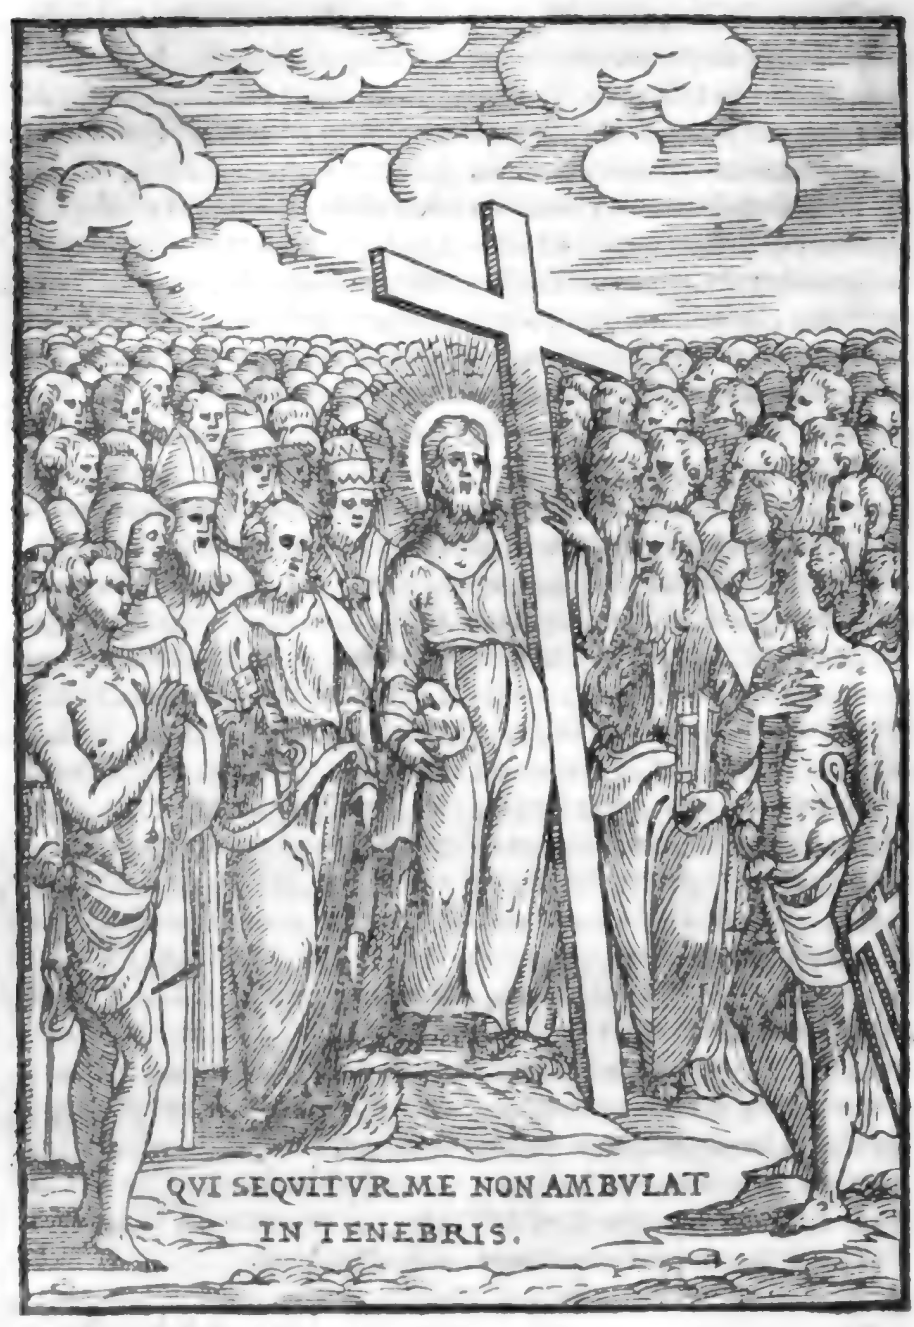
\includegraphics[width=4.5in]{Picture1006.png}


%pp1007
\newpage
\thispagestyle{empty}
\fancyhead[CO,CE]{}
\begin{center} \LARGE \hypertarget{SANCTORVM}
S \ A \ N \ C \ T \ O \ R \ V \ M\\
\Large H \ I \ S \ T \ O \ R \ I \ \AE ,
\end{center}
\vspace{-1.5em}
\bookmark[startatroot,dest=SANCTORVM]{SANCTORVM HISTORI\AE }

\begin{center} \large \color{red}
Ex probatis authoribus summatim decerpt\ae .
\end{center}
\vspace{-.5em}

\begin{center} \hypertarget{SANCTORVM-IANVARIVS}
IANVARIVS.
\end{center}
\vspace{-1em}
\bookmark[rellevel=1,dest=SANCTORVM-IANVARIVS]{IANVARIVS}

\begin{multicols*}{2}
\noindent \textswab{C} \color{red} Circuncisio Christi duplex maius ad vespera. Hymnus. \color{black} Christe redemptor. \&c. \color{red} vt in die natiuitatis. An. \color{black} Propter nimiam charitatem qua dilexit nos Deus, filium suum misit in similitudinem carnis peccati, Haleluiah, Haleluiah. \color{red} Oratio. \color{black} 
\vspace{-.25em}
\lettrine[lines=2]{\bfseries \color{red} D}{}Eus, qui salutis \ae tern\ae \ beat\ae \ Mari\ae \ virginitate f\oe cunda, humano generi pr\ae mia pr\ae stitisti, tribue qu\ae sumus: vt ipsam pro nobis intercedere sentiamus, per quam meruimus authorem vit\ae \ suscipere dominum nostrum Iesum Christum filium tuum. \&c.
\newline \color{red} Die. 1. \color{black} A \color{red} Et non fit commemoratio de alia octa. Ad matu. inui. \color{black} Christus natus est nobis, Venite adoremus. \color{red} Hymn. \color{black} A solis ortus cardine. \&c. \color{red} vt in die Natiuitatis. Antiphona. \color{black} O admirabile commercium, creator generis humani animarum corpus sumens, de virgine nasci dignatus est, \& procedens homo sine semine largitus est nobis suam deitatem.
\newline \color{red} Lectio tertia, ex cap. ij. Luc\ae . \color{black}
\vspace{-.25em}
\lettrine[lines=2]{\bfseries \color{red} E}{}T\leftmarginnote{\begin{flushright}ca. 2.\end{flushright}} postquam consummati sunt dies octo, vt circuncideretur puer: vocatum est nomen eius, Iesus: quod vocatum est ab angelo, prius quam in vtero conciperetur.
\newline \color{red} Ex sermone sancti Bernardi. \color{black}
\vspace{-.25em}
\lettrine[lines=2]{\bfseries \color{red} M}{}Agnum \& mirabile sacramentum. Circunciditur puer, \& vocatur Iesus. Quid sibi vult ista connexio? Circuncisio nempe magis saluandi, quam saluatoris esse videtur: \& saluatorem circuncidere decet, magis, quam circuncidi. Sed agnosce mediatorem Dei, \& hominum, qui ab ipso natiuitatis su\ae \ exordio diuinis
%pp1008
humana sociat, ima summis. Nascitur ex muliere: sed cui f\oe cunditatis fructus sic accedat, vt non decidat flos virginitatis. Pannis inuoluitur, sed panni ipsi angelicis laudibus honorantur. Absconditur in pr\ae sepio, sed proditur radiante stella de c\oe lo. Sic \& circuncisio veritatem suscept\ae \ probat humanitatis, \& nomen quod est super omne nomen gloriam indicat maiestatis. Circunciditur tanquam verus Abrah\ae \ filius, Iesus vocatur tanquam filius Dei.
\fancyhead[C]{\color{red} Ianuarius}
\newline \color{red} Ad laudes an. \color{black} Mirabile mysterium declaratur, hodie innouantur natur\ae , Deus homo factus est, id quod fuit permansit, \& quod non erat assumpsit, non commistionem passus nec diuisionem. \color{red} Oratio. \color{black} Deus qui salutis. \&c. \color{red} vt supra. Ad vesperas hymnus. \color{black} Christe redemptor. \color{red} vt sup. An. \color{black} Magnum h\ae reditatis mysterium, templum Dei factus est vterus nesciens virum, non est pollutus ex eo carnem assumens, omnes gentes venient dicentes. Gloria tibi domine. \color{red} Oratio. \color{black} Deus qui. \color{red} vt supra. Deinde pro commemoratio. octaua\ae \ sancti Stephani antiphona. \color{black} Stephanus autem plenus gratia \& fortitudine faciebat prodigia, \& signa magna in populo. \color{red} Oratio. \color{black} 
\vspace{-.25em}
\lettrine[lines=2]{\bfseries \color{red} O}{}Mnipotens sempiterne Deus, qui primitias martyrum in beati Leuit\ae \ Stephani sanguine dedicasti: tribue qu\ae sumus, vt pro nobis intercessor existat, qui pro suis etiam persecutoribus exorauit dominum nostrum Iesum Chri. \&c. \color{red} Et non fit comme. de aliis octauis. \color{black} 
\newline \color{red} Die. 2. \color{black} B \color{red} In octa. sancti Stephani dup. mi. Inuitato. hymni, an. \& tertia lectio dicuntur sicut in die sancti Stephani. Oratio. \color{black} Omnipotens. \color{red} vt sup. Et est notandum quod in laudibus post pr\ae dictam orationem dicuntur etiam orationes sancti Ioannis. \color{black} Ecclesiam tuam Deus. \color{red} \& Innocentium. \color{black} Deus cuius hodier.
\color{red} Vesper\ae \ dicuntur de sancto Stephano, \& post eius orationem pro comme. octau\ae \ sancti Ioannis dicitur an. \color{black} Iste est Ioannes qui supra pectus domini in c\oe na recubuit, beatus apostolus cui reuelata sunt secreta c\oe lestia. \color{red} Oratio. \color{black} Ecclesiam tuam. \color{red} vt supra in eius festo, \& non fit commemoratio de Innocentibus. \color{black}
\newline \color{red} Die. 3. \color{black} C \color{red} In octa. sancti Ioannis, du, mi. Inuit. Hymn. Antiphon\ae , terita lectio, \& oratio dicuntur sicut in eius festo, \& in laudibus post orationem sancti Ioannis dicitur etiam oratio Innocentium. \color{black} Deus cuius hodier. \color{red} Vesper\ae \ dicuntur de sancto Ioan. \& post eius orationem pro comme. octau\ae \ Innocentium dicitur an. \color{black}
%pp1009
Hi sunt qui cum mulieribus non sunt coinquinati, virgines enim sunt, \& sequuntur agnum quocunque ierit. \color{red} Oratio. \color{black} Deus cuius hodierna. \&c. \color{red} vt in eorum festo. \color{black}
\newline \color{red} Die. 4. \color{black} D \color{red} In octaua Innocentium duplex minus Inuitato. Hymni, Antiphon\ae , terita lectio, \& oratio dicuntur sicut in eorum festo. \color{black}
\newline \color{red} Die. 5. \color{black} E \color{red} In vigilia Epiphani\ae , Inuitatorium, Hymni, Antiphon\ae , \& Oratio, dicuntur sicut in die circuncisionis, siue incidat in dominica, siue, in alio quocunque die. \color{black}
\newline \color{red} Secundum Matth\ae um. \quad Lectio. iij. \color{black}
\vspace{-.25em}
\lettrine[lines=2]{\bfseries \color{red} I}{}N\rightmarginnote{ca. 2.} illo tempore, Defuncto Herode, ecce Angelus domini apparuit in somnis Ioseph in \AE gypto dicens: Surge, \& accipe puerum \& matrem eius, \& vade in terram Israel, defuncti sunt enim qui qu\ae rebant animam pueri.
\newline \color{red} Et rel. Hom. sancti Hiero. presby. \color{black}
\vspace{-.25em}
\lettrine[lines=2]{\bfseries \color{red} E}{}X hoc loco intelligimus non solum Herodem, sed \& sacerdotes \& Scribas eodem tempore necem domini fuisse meditatos.
Qui surgens accepit puerum, \& matrem eius. Non dixit, accepit filium suum \& vxorem suam: sed puerum \& matrem eius: quasi nutritius, non maritus.
Audiens autem quod Archelaus regnaret in Iud\ae a, pro Herode patre suo, timuit illo ire. Multi propter ignorantiam histori\ae \ labuntur errore, putantes eundem esse Herodem a quo in passione sua dominus irridetur, \& qui nunc mortuus esse refertur. Ergo Herodes ille qui cum Pilato postea amicitias fecit, huius Herodis filius est, frater Archelai. Quem \& ipsum Tyberius C\ae sar Lugdunum, qu\ae \ Galliarum est ciuitas, relegauit: fratremque eius Herodem successorem regni fecit.
Lege Iosephi historiam.
Et veniens habitauit in ciuitate qu\ae \ vocatur Nazareth: vt adimpleretur quod dictum est per prophetas, Quoniam Nazar\ae us vocabitur. Si fixum de scripturis posuisset exemplum, nunquam diceret quod dictum est per prophetas: sed simpliciter, quod dictum est per prophetam. Nunc autem, pluraliter prophetas vocans ostendit se non verba de scripturis sumpsisse, sed sensum. Nazar\ae us enim sanctus interpretatur. Sanctum autem dominum futurum omnis scriptura commemorat.
\newline \color{red} Epiphania domini, duplex maius. Ad vesperas. Hymnus. \color{black}
\yinipar{H}Ostis Herodes impie, Christum venire quid times?
\newline Non eripit mortalia,
\newline Qui regna dat c\oe lestia.
%pp1010
\newline {\color{red} I}bant Magi, quam viderant,
\newline Stellam sequentes pr\ae uiam:
\newline Lumen requirunt lumine,
\newline Deum fatentur munere.
\newline {\color{red} L}auacra puri gurgitis,
\newline C\oe lestis agnus attigit:
\newline Peccata, qu\ae \ non detulit,
\newline Nos abluendo sustulit.
\newline {\color{red} N}ouum genus potenti\ae ,
\newline Aqu\ae \ rubescunt hydri\ae :
\newline Vinumque iussa fundere,
\newline Mutauit vnda originem.
\newline {\color{red} G}loria tibi domine, Qui apparuisti hodie, Cum patre, \& sancto spiritu In sempiterna secula. Amen. \color{red} Et sic terminantur hymni in omnibus horis per totam octauam. An. \color{black} Magi videntes stellam dixerunt adinuicem, Hoc signum magni regis est, eamus, \& inquiramus eum, \& offeramus ei munera, aurum, thus, \& myrrham, Haleluiah, haleluiah. \color{red} Oratio. \color{black}
\vspace{-.25em}
\lettrine[lines=2]{\bfseries \color{red} D}{}Eus, qui hodierna die vnigenitum tuum gentibus stella duce reuelasti: concede propitius, vt qui iam te ex fide cognouimus, vsque ad contemplandam speciem tu\ae \ celsitudinis perducamur. Per eund. \&c.
\newline \color{red} Die 6. \color{black} F \color{red} Ad matu. inui. \color{black} Christus apparuit nobis, venite adoremus. \color{red} ps. \color{black} Venite. \color{red} \& \color{black} Gloria patri. \&c. \color{red} \hyperlink{page.1}{Fo. j. inui.} \color{black} Christus apparuit. \&c. \color{red} Hym. \color{black} Hostis hero. \color{red} vt sup. An. \color{black} Reges Tharsis, \& insul\ae \ munera offerent, reges Arabum, \& Saba dona adducent, haleluiah, haleluiah.
\newline \color{red} Notandum quod hodie omittuntur. j. \&. ij. lectio occurrentes in dominicali. \& loco earum leguntur infrascript\ae \ ex Isaia. \quad Lectio. j. \color{black} 
\vspace{-.25em}
\lettrine[lines=2]{\bfseries \color{red} O}{}Mnes\rightmarginnote{c. 55.} sitientes venite ad aquas: \& qui non habetis argentum, properate, emite, \& comedite. Venite, emite absque argento, \& absque vlla commutatione vinum \& lac.
Quare appenditis argentum non in panibus, \& laborem vestrum non in saturitate? Audite audientes me, \& comedite bonum, \& delectabitur in crassitudine anima vestra. Inclinate aurem vestram, \& venite ad me, audite, \& viuet anima vestra, \& feriam vobiscum pactum sempiternum, misericordias Dauid fideles.
Ecce testem populis dedi eum, ducem ac pr\ae ceptorem gentibus. Ecce, gentem quam nesciebas, vocabis: \& gentes qu\ae \ te non cognouerunt, ad te current propter dominum Deum tuum, \& sanctum Israel: quia glorificauit te.
Qu\ae rite dominum dum inueniri potest, inuocate eum dum prope est. Derelinquat impius viam suam, \& vir iniquus cogitationes suas, \& reuertatur ad dominum, \& miserebitur eius, \& ad Deum nostrum, quoniam multus
%pp1011
est ad ignoscendum. \textdagger \ 
Surge,\rightmarginnote{c. 60.\\a} illuminare Ierusalem: quia venit lumen tuum, \& gloria domini super te orta est. Quia ecce tenebr\ae \ operient terram, \& caligo populos: super te autem orietur dominus, \& gloria eius in te videbitur.
Et ambulabunt gentes in lumine tuo, \& reges in splendore ortus tui. Leua in circuitu oculos tuos, \& vide: omnes isti congregati sunt, venerunt tibi. Filij tui de longe venient, \& fili\ae \ tu\ae \ de latere surgent. Tunc videbis \& afflues: \& mirabitur \& dilatabitur cor tuum, quando conuersa fuerit ad te multitudo maris, fortitudo gentium venerit tibi.
Inundatio camelorum operiet te, dromedarij Madian, \& Epha, omnes de Saba venient, aurum, \& thus deferentes, \& laudem domino annuntiantes.]
\newline \color{red} Secundum Matth\ae um. \quad Lectio. ij. \color{black}
\vspace{-.25em}
\lettrine[lines=2]{\bfseries \color{red} C}{}Vm\leftmarginnote{\begin{flushright}ca. 2.\end{flushright}} \textdagger \ natus esset Iesus in Bethlehem Iud\ae \ in diebus Herodis regis, ecce Magi ab oriente venerunt Ierosolymam, dicentes, vbi est qui natus est rex Iud\ae orum? vidimus enim stellam eius in oriente, \& venimus adorare eum.
Audiens autem Herodes rex, turbatus est, \& omnis Ierosolyma cum illo. Et congregans omnes principes sacerdotum, \& Scribas populi, sciscitabatur ab eis vbi Christus nasceretur. At illi dixerunt ei, In Bethlehem Iud\ae . Sic enim scriptum est per prophetam, Et tu Bethlehem terra Iuda, nequaquam minima es in principibus Iuda: ex te enim exiet dux qui regat populum meum Israel. Tunc Herodes clam vocatis Magis, diligenter didicit ab eis tempus stell\ae \ qu\ae \ apparuit eis, \& mittens illos in Bethlehem, dixit, Ite, \& interrogate diligenter de puero: \& cum inueneritis, renuntiate mihi, vt \& ego veniens adorem eum. Qui cum audissent regem, abierunt. Et ecce stella quam viderant in oriente, antecedebat eos, vsque dum veniens staret supra vbi erat puer.
Videntes autem stellam, gauisi sunt gaudio magno valde.
Et intrantes domum, inuenerunt puerum cum Maria matre eius, \& procidentes adorauerunt eum: \& apertis thesauris suis, obtulerunt ei munera, aurum, thus, \& myrrham. Et responso accepto in somnis ne redirent ad Herodem, per aliam viam reuersi sunt in regionem suam.
\newline \color{red} Hom. sancti Grego. pap\ae . Lectio. iij. \color{black}
\vspace{-1.75em}
\lettrine[lines=2]{\bfseries \color{red} S}{}Icut ex lectione euangelica fratres audistis, c\oe li rege nato rex terr\ae \ turbatus est, quia nimirum terrena altitudo confunditur, cum celsitudo c\oe lestis
%pp1012
aperitur. Sed qu\ae rendum nobis est: quidnam sit quod redemptore nato pastoribus in Iud\ae a angelus apparuit: atque ad adorandum hunc ab oriente Magos non angelus, sed stella perduxit? Quia videlicet Iud\ae is tanquam ratione vtentibus rationale animal, id est, Angelus pr\ae dicare debuit. Gentiles vero quia vti ratione nesciebant, ad cognoscendum dominum, non per vocem, sed per signa perducuntur. Vnde \& per Paulum dicitur, Lingu\ae \ in signum sunt non fidelibus, sed infidelibus: propheti\ae \ autem non infidelibus, sed fidelibus. Quia \& illis prophet\ae \ tanquam fidelibus non infidelibus: \& istis signa tanquam infidelibus non fidelibus data sunt.
Et notandum quod redemptorem nostrum cum iam perfect\ae \ esset \ae tatis, eisdem gentibus apostoli pr\ae dicant: eumque paruulum, \& necdum per humani corporis officium loquentem, stella gentibus denuntiat: quia nimirum rationis ordo poscebat, vt loquentem dominum loquentes nobis pr\ae dicatores innotescerent, \& necdum loquentem elementa muta pr\ae dicarent.
Sed in omnibus signis qu\ae \ vel nascente domino vel moriente monstrata sunt, considerandum nobis est, quanta fuerit in quorundam Iud\ae orum corde duritia, qui hunc nec per propheti\ae \ donum, nec per miracula agnouerunt.
Omnia quippe elementa authorem suum venisse testata sunt. Vt enim de eis quodam vsu humano loquar, Deum hunc c\oe li esse cognouerunt quia protinus stellam miserunt. Mare cognouit, quia sub plantis eius se calcabile pr\ae buit. Terra cognouit, quia eo moriente contremuit. Sol cognouit quia lucis su\ae \ radios abscondit. Saxa \& parietes agnouerunt, quia tempore mortis su\ae \ scissa sunt. Infernus agnouit, quia hos, quos tenebat, mortuos reddidit, \& tamen hunc quem Deum omnia insensibilia elementa senserunt, adhuc infidelium Iud\ae orum corda Deum esse minime cognoscunt, \& duriora saxis scindi ad p\oe nitentiam nolunt: eumque confiteri abnegant, quem elementa (vt diximus) aut signis aut scissionibus Deum clamant.
% !!!!!!!!!!!!!!!!!!!!!!!!!!!!!!!!!!!!!!!!!!!!!!!!!!!!!!!!!!!!!!!!!!!!!!!!!!!!!!!!!!!!!!!!!!!!!!!!!!!!!!!!!!!!!!!!!!!!!!!!
\newline \color{red} Ad laudes an. \color{black} Ante luciferum genitus, \& ante secula dominus saluator noster hodie mundo apparuit, Haleluiah, haleluiah. \color{red} Ad vespe. hym. \color{black} Hostis Herodes. \color{red} vt supra. An. \color{black} Tribus miraculis ornatum diem sanctum colimus: Hodie stella Magos duxit ad pr\ae sepium: hodie vinum ex aqua factum est ad nuptias: hodie a Ioanne in Iordane Christus bapitzari voluit, vt saluaret nos, Haleluiah.
%pp1013
\color{red} H\ae c an. dicitur ad ves. infra oct. \color{black}
\newline \color{red} Notandum quod cuilibet dici per totam octa. assignatur propria tertia lectio: tamen cum inciderit dominica infra octa. Epiph. omittitur tertia lectio de octa. \& legitur de dominica infra oct. vt ibi inuenies. \color{black}
\newline \color{red} Die. 7. \color{black} G \color{red} De octa. Epiphani\ae . \color{black}
\newline \color{red} Ex Hom. sancti Greg. pap\ae , \quad L. iij. \color{black}
\vspace{-.25em}
\lettrine[lines=2]{\bfseries \color{red} Q}{}Vi etiam ad damnationis su\ae \ cumulum eum quem natum despiciunt, nasciturum longe ante pr\ae scierunt. Et non solum quia nasceretur nouerant, sed etiam vbi nasceretur. Nam ab Herode requisiti, locum natiuitatis eius exprimunt, quem scriptur\ae \ authoritate didicerunt. Et testimonium proferunt quod Bethlehem honorari natiuitate noui ducis ostenditur: vt ipsa eorum scientia \& illis fieret ad testimonium damnationis, \& nobis ad adiutorium credulitatis. Quos profecto bene Isaac cum Iacob filium suum benediceret designauit. Qui \& caligantibus oculis \& prophetans, in pr\ae senti filium non vidit, cui tamen multa in posterum pr\ae uidit. Quia nimirum Iudaicus populus propheti\ae \ spiritu plenus \& c\ae cus: eum, de quo multa in futuro pr\ae dixit, in pr\ae senti positum non agnouit.
Sed natiuitate regis nostri cognita, Herodes ad callida argumenta conuertitur, ne terreno regno priuaretur. Renuntiari sibi vbi puer inueniretur postulat: adorare se velle simulat: vt quasi hunc si inuenire possit extinguat.
Sed quanta est humana malitia contra consilium diuinitatis? Scriptum quippe est, Non est sapientia, non est prudentia, non est consilium contra dominum.
\newline \color{red} Die. 8. \color{black} A \color{red} De octa. Epiphani\ae . \color{black}
\newline \color{red} Sermo sancti August. episc. Lectio. iij. \color{black}
\vspace{-1.75em}
\lettrine[lines=2]{\bfseries \color{red} A}{}D partum virginis adorandum magi ab oriente venerunt. Hunc diem hodie celebramus: huic debitam solennitati sermonem persoluimus. Illis dies iste primus illuxit: anniuersaria nobis festiuitas redit. Illi erant primiti\ae \ gentium: nos populi gentium.
Nobis hoc lingua nuntiauit Apostolorum: stella illis tanquam lingua c\oe lorum. Et nobis ijdem Apostoli tanquam alij c\oe li enarrauerunt gloriam Dei. Cur enim non agnoscamus eos c\oe los, qui facti sunt sedes Dei? Sicut scriptum est. Anima iusti sedes est sapienti\ae . Per hos enim c\oe los, ille c\oe lorum fabricator \& habitator intonuit: quo tonitruo mundus tremuit, \& ecce iam credit. Magnum sacramentum. In pr\ae sepe tunc iacebat
%pp1014
\& magos ab oriente adducebat. Abscondebatur in stabulo, \& agnoscebatur in c\oe lo: vt agnitus in c\oe lo manifestaretur in stabulo. Et appellaretur Epiphania dies iste, quod Latine manifestatio dici potest, simul eius celsitudinem humilitatemque commendans: vt qui in aperto c\oe lo sydereis signis monstrabatur, in angusto diuersorio qu\ae situs inueniretur. Inualidusque in infantilibus membris, inuolutus in pannis, adoraretur a Magis, timeretur a malis.
\newline \color{red} Die. 9. \color{black} B \color{red} De octa. Epiphani\ae . \color{black}
\newline \color{red} Sermo sancti August. episc. Lectio. iij. \color{black}
\vspace{-1.75em}
\lettrine[lines=2]{\bfseries \color{red} N}{}Vper celebrauimus diem quo ex Iud\ae is dominus natus est: hodie celebramus quo a gentibus adoratus est. Quoniam salus ex Iud\ae is est. sed h\ae c salus vsque ad fines terr\ae .
Nam in illo die pastores adorauerunt: hodie magi. Illis angeli: istis autem stella nuntiauit. Vtrique de c\oe lo didicerunt, cum regem c\oe li in terra viderunt: vt esset gloria in excelsis Deo, \& in terra pax hominibus bon\ae \ voluntatis. Ipse est enim pax nostra, qui fecit vtraque vnum. Iam hic infans natus atque annuntiatus ostenditur lapis ille angularis. Iam in ipso primordio natiuitatis apparuit, duos ex diuerso parietes in se copulare iam c\oe pit: pastores a Iud\ae a, Magos ab oriente perducens, vt duos conderet in se in vnum nouum hominem, faciens pacem.
Pacem his qui longe, \& pacem his qui prope. Ideoque illi ipso die de proximo venientes, de longinquo isti hodie peruenientes, duos dies celebrandos posteris signauerunt: vnam tamen lucem mundi vtrique viderunt.
Sed hodie de istis loquendum est, quos de remotis terr\ae \ partibus fides duxit ad Christum.
\newline \color{red} Die. 10. \color{black} C \color{red} De octa. Epiphani\ae . \color{black}
\newline \color{red} Sermo sancti Leonis pap\ae . \quad L. iij. \color{black}
\vspace{-.25em}
\lettrine[lines=2]{\bfseries \color{red} C}{}Elebrato proximo die quo intemerata virginitas humani generis edidit saluatorem: Epiphani\ae \ nobis dilectissimi veneranda festiuitas dat perseuerantiam gaudiorum: vt inter cognatarum solennitatum vicina sacramenta, exultationis vigor, \& feruor fidei non tepescat. Ad omnium enim hominum spectat salutem, quod infantia Saluatoris, ac mediatoris Dei \& hominum iam vniuerso declarabatur mundo, cum adhuc exiguo detineretur oppidulo. Quamuis enim Israeliticam gentem \& ipsius gentis vnam familiam delegisset, de qua naturam humanitatis assumeret: noluit tamen intra matern\ae \ habitationis angustias ortus sui
%pp1015
latere primordia, sed mox ab omnibus voluit agnosci, qui dignatus est pro omnibus nasci. Tribus igitur Magis in regione orientis: stella nou\ae \ claritatis apparuit, qu\ae \ illustrior c\ae teris, pulchriorque syderibus, facile in se intuentium oculos animosque conuerteret: vt confestim aduerteretur non esse otiosum, quod tam insolitum videbatur.
\newline \color{red} Die. 11. \color{black} D \color{red} De octa. Epiphani\ae . \color{black}
\newline \color{red} Ex sermo. sancti Leonis pap\ae . \quad L. iij. \color{black}
\vspace{-1.75em}
\lettrine[lines=2]{\bfseries \color{red} D}{}Edit ergo aspicientibus intellectum, qui pr\ae stitit signum: \& quod fecit intelligi, fecit inquiri, \& se inueniendum obtulit requisitus. Sequuntur tres viri superni luminis ductum: \& pr\ae uij fulgoris indicium intenta contemplatione comitantes, ad agnitionem veritatis, grati\ae \ splendore ducuntur, qui humano sensu signatum sibi regis ortum \ae stimauerunt in ciuitate regia esse qu\ae rendum. Sed qui serui susceperat formam, \& non iudicare venerat, sed iudicari: Bethlehem pr\ae elegit natiuitati, Ierosolymam passioni.
Herodes vero audiens Iud\ae orum principem natum, successorem suspicatus expauit. Et molitus necem salutis authori, falsum spopondit obsequium. Quam felix foret, se Magorum imitaretur fidem: \& conuerteret ad religionem, quod disponebat ad fraudem? O c\ae ca stult\ae \ \ae mulationis impietas, qu\ae \ perturbandum putas diuinum tuo furore consilium? Dominus mundi temporale non qu\ae rit regnum, qui pr\ae stat \ae ternum. Quid incommutabilem dispositarum rerum ordinem vertere, \& alienum facinus pr\ae occupare conaris? mors Christi non est temporis tui. Ante condendum est Euangelium: ante pr\ae dicandem est Dei regnum: ante sanitates donand\ae : ante sunt facienda miracula.
\newline \color{red} Aduertendum quod quando Epipha. domini inciderit in dominica, tunc in sabbato sequenti omittenda est sequens tertia lectio, \& loco eius legendum Euangelium. \color{black} \hyperlink{page.155}{Cum factus esset Iesus.} \color{red} cum homilia vt inuenies in dominica tertia post Aduentum. \color{black}
\newline \color{red} Die. 12. \color{black} E \color{red} De octa. Epiphani\ae . \color{black}
\newline \color{red} Sermo sancti Leonis pap\ae . \quad L. iij. \color{black}
\vspace{-.25em}
\lettrine[lines=2]{\bfseries \color{red} I}{}Vstum \& rationabile, dilectissimi, \& ver\ae \ pietatis obsequium est in diebus, qui diuin\ae \ opera misericordi\ae \ protestantur, toto corde gaudere, \& honorifice ea qu\ae \ ad salutem nostram gesta sunt, celebrare. Vocante nos ad hanc deuotionem ipsa recurrentium temporum lege, qu\ae \ nobis post diem in quo co\ae ternus patri filius Dei natus ex virgine
%pp1016
est, breui interuallo Epiphani\ae \ intulit festum, ex apparitione domini consecratum. In quo magnum fidei nostr\ae \ pr\ae sidium prouidentia diuina consstituit: vt dum solenni veneratione recolitur, adorata in exordiis suis Saluatoris infantia, per ipsa originalia documenta probaretur, veri hominis in Christo orta natura. Hoc est enim quod iustificat impius: hoc est quod ex peccatoribus facit sanctos, si in vno eodemque domino Iesu Christo, \& vera deitas, \& vera credatur humanitas.
Deitas, qua ante omnia secula in forma Dei \ae qualis est patri: humanitas, qua in nouissimis diebus in forma serui vnitus est homini. Ad roborandam ergo hanc fidem, qua contra omnes pr\ae muniebamur errores, ex magno factum est diuin\ae \ pietatis consilio, vt gens in longinqua orientalis plag\ae \ regione consistens, qu\ae \ spectandorum syderum arte pollebat, signum nati pueri, qui super omnem Israel esset regnaturus, acciperet.
\newline \color{red} Hodie in ves. dicitur an. assignata ad primas vespe. \color{black} Magi videntes.
\newline \color{red} Die. 13. \color{black} F \color{red} Octa. Epipha. du. mi. \color{black}
\newline \color{red} Secundum Ioannem. \quad Lectio. iij. \color{black}
\vspace{-.25em}
\lettrine[lines=2]{\bfseries \color{red} I}{}N\rightmarginnote{ca. 1.} illo tempore: Vidit Ioannes Iesum venientem ad se, \& ait, Ecce agnus Dei, ecce qui tollit peccata mundi.
\newline \color{red} Et rel. Hom. sancti Augustini episc. \color{black} 
\vspace{-.25em}
\lettrine[lines=2]{\bfseries \color{red} N}{}Emo sibi arroget \& dicat quia ipse auferat peccata mundi. Iam intendite contra quos superbos intendebat Ioannes digitum. Nondum erant nati h\ae retici, \& demonstrabantur: iam intendebat contra illos. Contra illos clamabat tunc a fluuio, contra quos modo clamat ex Euangelio. Venit Iesus. Et quid dicit ille?
Ecce Agnus Dei. Si agnus, innocens, \& Ioannes agnus, an non \& ipse innocens? Sed quis innocens, aut quantum innocens? omnes ex illa radice veniunt, \& ex illa propagine, de qua cantat gemens Dauid, Ego in iniquitatibus conceptus sum: \& in peccatis mater mea in vtero me aluit. Solus ergo ille agnus qui non sic venit. Non enim in iniquitate conceptus est, qui non de mortalitate conceptus est, nec eum in peccatis mater eius in vtero aluit, quem virgo concepit, virgo peperit: quia fide concepit, fide suscepit. Ergo ecce agnus Dei: Non habet iste traducem de Adam. Carnem tantum assumpsit de Adam, peccatum non assumpsit. Qui non assumpsit de massa nostra peccatum, ipse est qui tollit peccatum
%pp1017
nostrum: ecce agnus Dei, ecce qui tollit peccata mundi.
Nostis quia quidam homines dicunt aliquando, Nos tollimus peccata hominibus quia sancti sumus. Si enim non fuerit sanctus qui baptizat: quomodo tollit peccatum alterius, cum sit ille homo plenus peccato? Contra istas disputationes verba nostra non dicamus: hunc legamus, Ecce agnus Dei: ecce qui tollit peccata mundi.
\newline \color{red} Die. 14. \color{black} G \color{red} Basilius epis. confes. L. iij. \color{black}
\vspace{-1.75em}
\lettrine[lines=2]{\bfseries \color{red} B}{}Asilius Cappadox genere, C\ae sare\ae \ primum in sua regione, deinde Athenis eruditus, in eam magnitudinem omnis generis doctrinarum euasit, cum egregia sanctitate: vt inde magni cognomen inuenerit.
Reuersus igitur in patriam cum magna omnium expectatione C\ae saream vocatur: vt morum, ac pietatis institutor, moderatorque esset: pr\ae sulisque Eusebij adiutor: cui morienti in episcopatu successit. In quo sic Valentis Imperatoris Arriani sibi infesti tractauit animum sanctitate, \& consequentibus signis, vt cum se vellet in exilium mittere, sententiam mutare coegerit: Sella enim qua gestandus erat Valens, subito confracta \& dissoluta est. Cunque de more exilij multam scripturus esset, perficere non valuit, calamo nihil atramenti reddente. Cunque secundus, \& tertius calamus hoc pertulisset, \& adhuc legem impiam firmare contenderet, commota est eius dextera, eamque subitus tremor inuasit.
Tunc eius animo terrore impleto, ambabus manibus chartam rupit. Et qu\ae \ nox data est Basilio ad deliberandum, eadem vxor imperatoris, velut tortoribus tradita, cruciatur. Filius vero, qui eis erat vnicus, extinctus: patern\ae \ impietatis creditur exoluisse supplicia. Erat autem Basilius in victum, \& cultu abstinentissimus: vna tantum tunica se amiciebat, humi cubitabat, totis s\ae pe noctibus vigilabat, omnis expers libidinis tota vita perseuerauit.
Primus omnium c\oe nobia excogitauit: \& ritum illum monachorum antiquum atque agrestem, ad formulam religioni propiorem reduxit. Scripsit multa sanctissime, \& eloquentissime: nemo enim sacra volumina (vt testatur Gregorius Nazianzenus, qui vitam eius conscripsit) nec eloquentius eo, nec verius, nec vberius enarrauit. Obiit autem corpore iam per abstinentiam consumpto: cum ossibus ac pelle tantum superstes esset Calend. Ianuarij.
%pp1018
\newline \color{red} Die. 15. \color{black} A \color{red} Martina vir. mart. L. iij. \color{black}
\vspace{-.25em}
\lettrine[lines=2]{\bfseries \color{red} M}{}Artina virgo Romana ex nobili \& patritia familia Christian\ae \ pietatis egregia cultrix, \& ab ineunte \ae tate sacris literis dedita, \& erudita, dum sequitur Euangelicam doctrinam, suarum facultatum magnam partrem pauperibus distribuit. Quam ob rem facta rea, quod relicto deorum cultu seruiret nou\ae \ religioni, ab Alexandro Imperatore, Apollini, sacrificare iubetur, nisi mallet supplicia mortemque subire.
Cum igitur in fide Christi perstaret, equuleo suspensa ferreis vngulis exaratur, \& sic cruciata in carcerem coniicitur, si forte sententiam mutaret. Sed postridie rursus diis immolare iussa, \& perinde contempto principis impio iussu, s\ae uissime torquetur, mamillis ferro laniatis, rursusque in carcerem retruditur. Paucis vero diebus interiectis, desperata mutatione sententi\ae , in publicis spectaculis obiecta est immanibus bestiis, quarum nulla virginem inuasit, aut quoquo modo l\ae sit. Tunc vero iussu Imperatoris extra vrbem educta, \& in Christiana confessione \& pietate constantissime perseuerans, capite plectitur Calendis Ianuarij. Cuius corpus sepultur\ae \ datum est a sancto Calisto papa.
\newline \color{red} Die. 16. \color{black} B \color{red} Marcellus pp mart. L. iij. \color{black}
\vspace{-.25em}
\lettrine[lines=2]{\bfseries \color{red} M}{}Arcellus patrea Romanus a Constantino \& Galerio vsque ad Maxentium gessit pontificatum. Huius hortatu Priscilla, \& Lucina matron\ae \ Roman\ae \ adduct\ae \ sunt: altera vt c\oe meterium suis sumptibus via Salaria construeret, altera vt ecclesiam Dei h\ae redem suorum nomorum institueret.
Titulos quinque \& viginti in vrbe Roma idem disposuit, quasi dioceses ad commoditatem baptismi, \& eorum qui ad fidem Christi ex gentibus quotidie veniebant, \& ad martyrum sepulturas. Quibus rebus iratus Maxentius, Lucina relegata, ipsum minis impellere conatur, vt se pontificatu abdicaret, atque nomen Christianum deponeret. In quo cum se ab eo negligi animaduerteret, ipsum in viuaria ad curam publicarum bestiarum damnauit. Ex quo loco nec orationes ille, nec ieiunia pr\ae termittens parochias etiam epistolis, quando aliter non licebat, multos annos gubernauit. Demum ex f\oe da illa, atque incommoda habitatione, p\ae dore \& situ confectus, obiit, eiusque sanctissimum corpus in c\oe meterio Priscill\ae \ in via Salaria sepelitur. xvij. Calen. Febr. Sedit autem
%pp1019
annos quinque, menses sex, dies vnum \& viginti. \hyperlink{tedeum}{{\color{red} T}e deum.} \color{red} \quad Oratio. \color{black}
\vspace{-.25em}
\lettrine[lines=2]{\bfseries \color{red} P}{}Reces populi tui qu\ae sumus domine clementer exaudi, vt beati Marcelli martyris tui, atque pontificis meritis adiuuemur, cuius passione l\ae tamur. Per do.
\newline \color{red} Die. 17. \color{black} C \color{red} Antonius abbas duplex minus. \quad Lectio tertia. \color{black}
\vspace{-.25em}
\lettrine[lines=2]{\bfseries \color{red} A}{}Ntonius in \AE gypto nobili genere natus, Constantini magni tempore cum intrans ecclesiam vt solebat audisset illud Euangelij, Si vis perfectus esse, vende omnia qu\ae \ habes, \& da pauperibus: velut ea sibi tunc peculiariter dicta interpretatur, omnibus suis possessionibus distractis, pretium distribuit pauperibus: ipseque in vastam \AE gypri solitudinem recessit. Vbi quamplurimos annos incredibili parsimonia \& sanctitate vitam gessit, vix humanam, s\ae pe a d\ae monibus ipsi sanctimoniam inuidentibus, variis imaginibus infestatus: quos ipse opere diuina fretus, tam constanter spernebat, vt conuitiis etiam \& maledictis persequeretur, exprobrans illis imbecillitatem in eos, quos diuina gratia non destituisset. Itaque tanto iam terrori d\ae monibus erat s\ae pe a se deuictis, vt multi per \AE gyptum ab illis agitati, nomine Antonijs super ipsos inuocato liberarentur. Huic Constantinus Imperator se, \& filios per literas commendauit, vt pro eis domino supplicaret. Ita miraculis clarus, annum agens vltra centesimum, a vita migrauit decimosexto Calendas Februa.
\newline \color{red} Die. 18. \color{black} D \color{red} Fit de Cathedra Romana. s. Pet. du. ma. Ad ves. hymnus. \color{black}
\yinipar{Q}Vodcunque vinclis super terram strinxerit, Erit in astris religatum fortiter. Et quod resoluit in terris arbitrio, erit solutum super c\oe li radium: in fine mundi iudex erit seculi.
\newline {\color{red} G}loria patri per immensa secula, Sit tibi nate decus, \& imperium, Honor, potestas, sanctoque spiritui, Sit trinitati salus indiuidua, Per infinita seculorum secula. Amen.
\newline \color{red} An. \color{black} Tu es pastor ouium, princeps apostolorum, tibi tradit\ae \ sunt claues regni c\oe lorum. \color{red} Oratio. \color{black}
\vspace{-.25em}
\lettrine[lines=2]{\bfseries \color{red} D}{}Eus, qui beato Petro Apostolo tuo collatis clauibus regni c\oe lestis animas ligandi, atque soluendi pontificium munus tradidisti: concede, vt intercessionis eius auxilio, a peccatorum nostrorum nexibus liberemur: Qui viuis.
\color{red} Ad matutinum inuitatorium. T\color{black} u es pastor ouium, princeps apostolorum, tibi tradidit Deus
%pp1020
claues regni c\oe lorum. \color{red} Hymn. \color{black}
\vspace{-.25em}
\lettrine[lines=2]{\bfseries \color{red} I}{}Am bone pastor Petre clemens accipe Vota precantum. \& peccati vincula Resolue tibi potestate tradita, Qua cunctis c\oe lum verbo claudis, aperis.
\newline {\color{red} S}it Trinitati sempiterna gloria, Honor, potestas, atque iubilatio, In vnitate cui manet imperium, Ex tunc \& modo per \ae terna secula. Amen.
\color{red} An. \color{black} Tu es Petrus, \& super hanc petram, \ae dificabo ecclesiam meam. \color{red} Lectio. iij. \color{black}
\vspace{-.25em}
\lettrine[lines=2]{\bfseries \color{red} C}{}Athedra summi pontificatus, cuius hodie festum celebramus, promissa est Petro, cum Christus ei dixit, vt habetur Matth\ae i sextodecimo capite: Ego dico tibi, quia tu es Petrus, \& super hanc petram \ae dificabo ecclesiam meam: \& port\ae \ inferi non pr\ae ualebunt aduersus eam. Et tibi dabo claues regni c\oe lorum. Et quodcunque ligaueris super terram, erit ligatum \& in c\oe lis, \& quodcunque solueris super terram, erit solutum \& in c\oe lis. His igitur verbis Christus cathedram summi sacerdotij Petro pollicitus antequam pateretur, eandem tradidit post resurrectionem: cum ter ipsi suum gregem pascendum commendaret.
De quo sic scripsit Ioannes, Dixit Simoni Petro Iesus, Simon Iona diligis me plus his? Dicit ei, Etiam domine, tu scis quia amo te. Dicit ei: Pasce agnos meos. Diciet ei iterum, Simon Iona diligis me? Ait illi, Etiam domine, tu scis quia amo te. Dicit ei, Pasce agnos meos. Dicit ei tertio, Simon Iona amas me? Contristatus est Petrus, quia dixit ei tertio amas me. Et dixit ei, Pasce oues meas. Petrus igitur post ascensionem Christi ad patrem, cum Pontum, Galatiam, Bithyniam, \& Cappadociam peragrasset fidem Christi pr\ae dicando, \& sermonem miraculis confirmando, Antiochiam reuersus est: ibique Cathedram, hoc est sedem apostolicam, fixit, tenuitque septem annos, donec iussu Dei (vt verbis vtar Marcelli pap\ae , \& martyris) eam transtulit Romam, immobilemque locauit: vt ad commoditatem Christianorum \& religionis augmentum sed etiam summi sacerdotij, \& ecclesi\ae \ caput esset, in ea potissimum vrbe, qu\ae \ principatum orbis obtinebat.
\newline \color{red} Ad laudes antiphona. \color{black} Quodcunque ligaueris super terram, erit ligatum \& in c\oe lis: \& quodcunque solueris super terram, erit solutum \& in c\oe lis, dicit dominus Simoni Petro. \color{red} Ad vespe. hym. \color{black} Quodcunque vinclis. \color{red} \&c. Antiphona. \color{black} Dum esset summus pontifex,
%pp1021
terrena non meruit, sed ad c\oe lestia regna gloriosus migrauit.
\newline \color{red} Die. 19. \color{black} E \color{red} Telesphor. pp mart. L. iij. \color{black}
\vspace{-.25em}
\lettrine[lines=2]{\bfseries \color{red} T}{}Elesphorus natione Gr\ae cus Antonino imperatore pontifex factus, constituit vt proxime ante Pascha ieiunium Quadragesim\ae \ obseruaretur: vtque in natali Christi tres miss\ae \ celebrarentur.
Prima media nocte, cum Christus est natus in Bethlehem. Secunda in aurora, quando a pastoribus est cognitus. Postremo circa eam horam qua redemptionis human\ae \ mysterium agebatur. Item, vt ante sacrificium caneretur, Gloria in excelsis Deo.
Ordinationibus quater mense Decembri habitis, presbyteros. xv. diaconos. xvij. episcopos. xiij. creauit. Cum autem sedisset annos vndecim, menses tres, dies. xxij. martyrio coronatus est, ac in Vaticano sepultus Nonis Ianuarij.
\newline \color{red} Die. 20. \color{black} F \color{red} Fabianus papa, \& Sebastianus marty. dup. mi. \quad Oratio. \color{black}
\yinipar{I}Nfirmitatem nostram respice omnipotens Deus, \& quia pondus propri\ae \ actionis grauat, beatorum martyrum tuorum Fabiani \& Sebastiani intercessio gloriosa nos protegat. Per dominum no. \quad \color{red} Lectio. iij. \color{black}
\vspace{-.25em}
\lettrine[lines=2]{\bfseries \color{red} F}{}Abianus patria Romanus a Gordiano \& Philippo ad Decium imperatorem pontifex ecclesi\ae \ pr\ae fuit. Hic septem diaconis regiones diuisit, qui a notariis res martyrum gestas scribentibus, colligerent. Statuitque, vt singulis annis in die c\oe n\ae \ domini chrisma renouaretur, ac vetus combureretur in ecclesia. Huius tempore orta est h\ae resis Nouatij Roman\ae \ ecclesi\ae \ presbyteri, negantis apostatas etiam p\oe nitentes ab ecclesia recipi debere. Sed congregato Rom\ae \ concilio sexaginta episcoporum totidemque presbyterorum cum diaconis compluribus, h\ae c h\ae resis Nouatiana damnata fuit, \& cum alijs error quoque Helchesatarum asserentium non esse criminosum in tormentis Christum vocetenus ab eo negari, qui corde ipsum confiteretur. Fabianus denique. xiij. Calend. Geb. martyrio coronatus in c\oe metrio Calisti via Appia sepelitur. cum sedisset annos. xiiij. menses. xj. dies. xj.
{\color{red} S}ebastianus ciuis Mediolanensis, sed Narbon\ae \ ortus, vel vt alij tradunt, oriundus, vir nobilis, \& imperatori Diocletiano charus, prim\ae que cohortis ductor, multos Christianorum in tormentis deficientes tam fortiter, \& sancte in fide confirmauit,
%pp1022
vt martyrium constanter subierint. Quorum fuere Marcus, \& Marcellianus fratres, qui Rom\ae \ in domo Nicostrati cincti asseruabantur, cuius Nicostrati vxor Zoe, exorante Deum Sebastiano, vocem ante sex annos per morbum amissam recepit. Quibus rebus cognitis Diocletianus Sebastianum ad se vocat, \& grauissime increpatum, omni ratione a fide conatur auertere.
Sed hoc frustra tentato, iubet eum stipite alligatum a sagittarius configi. Frequentibus igitur sagittis confixus, cum ab omnibus aut per necatus, aut protinus moriturus crederetur, tamen consequenti nocte, ab Hyrene sancta matrona sepeliendi gratia sublatus, viuus reperitur, \& ope diuina breui est in domo illius in pristinam valetudinem restitutus.
Itaque paulo post factus obuiam Diocletiano ad rei mirabulum attonito, libere c\oe pit impietatem, \& s\ae uitiam in Christianos improperare. Tunc vero iussu eiusdem imperatoris tandiu virgis c\ae sus est, donec animam exhalauit. Eius vero corpus in cloacam deiectum Lucin\ae \ opera, cui Sebastianus per somnium visus, \& vbi suum corpus esset, \& vbi condi velle, demonstrauit, ad Cathacumbas sepultum est: vbi templum extat eiusdem nomine dicatum. Passus est autem Rom\ae . xiij. Calend. Februarij.
\newline \color{red} Die. 21. \color{black} G \color{red} Agnes virgi. marty. duplex minus. \quad Oratio. \color{black}
\vspace{-.25em}
\lettrine[lines=2]{\bfseries O}{}Mipotens sempiterne Deus, qui infirma mundi eligis, vt fortis qu\ae que confundas: concede propitius, vt qui beat\ae \ Agnetis virginis \& martyris tu\ae \ solennia colimus, eius apud te patrocinia sentiamus. Per dominum nostrum. \quad \color{red} Lectio. iij. \color{black}
\vspace{-.25em}
\lettrine[lines=2]{\bfseries \color{red} A}{}Gnes virgo Romana claris parentibus orta, cum ab vrbis pr\ae fecti filio amore flagrante in coniugem magnis pollicitis, \& contentione peteretur, omnibus spretis, in ea responsione perstitit, se ab amatore Christo fuisse occupatam, ipsique soli se datam fidem pr\ae stare oportere.
Ita cum neque blanditiis, neque minis commoueretur a Symphronio pr\ae posito, nec iussa De\ae \ Vest\ae \ sacrificare paruisset, vestibus spoliata, pr\ae eunte pr\ae cone in lupanar ducta est, vbi c\oe leste lumen sic eam circunfulsit, vt a nemine videri posset. Cunque pr\ae fecti filius virgini insultaturus intrasset, confestim exanimis iacuit: qui mox oratione virginis suscitatus, egressusque in publicum clamare c\oe pit, Templa Deorum
%pp1023
esse d\ae monum domicilia, \& solum Christianorum verum esse Deum. Quo miraculo templorum pontificibus commotis, ac virginem magam esse clamitantibus. Symphronius licet iam Agnetem libentur absolueret, timens tamen pontificum calumniam, causam virginis cognoscendam Aspasio vicario commisit. Hic autem in conspectu omnium rogum accendit, \& in eum virginem protrudi iussit. Quo facto flammis diuisis ipsa in medio ill\ae sa permansit, \& ignis circunstantes exurebat, qui tamen ad orationem virginis statim extinctus est. Tunc Aspasius ira concitatus iussit eam decollari.
Et sic martyrio coronata ad sponsum Christum emigrauit duodecimo Calend. Februarij. Parentes autem eius corpus abstulerunt, \& via Numentana in pr\ae diolo suo non longe ab vrbe sepelierunt. Quibus in sepulchro cum fletu \& lamentatione assidentibus, frequenti virginum c\oe tu circunsepta, candida, \& refulgens, Agnes apparuit, hortataque est illos, vt pijs lachrymis finem imponerent, quandoquidem ipsa in c\oe lum sublata, vberrimum ferret sui martyrij pr\ae mium. Igitur fama sanctitatis eius vbique dispersa, quotquot credentes ad sepulchrum eius venisset, a quacunque infirmitate sanabantur.
\newline \color{red} Die. 22. \color{black} A \color{red} Vincentius, \& Anastasius martyres. \quad Lectio tertia. \color{black}
\vspace{-.25em}
\lettrine[lines=2]{\bfseries \color{red} V}{}Incentius Osch\ae \ natus quod oppidum est Hispani\ae \ citerioris, ab ineunte \ae tate studio literarum deditus, \& sacris literis eruditus, a Valerio C\ae saraugustano episcopo cui bl\ae sa lingua erat, munus iniunctum pr\ae dicandi Euangelium pro ipso sanctissime, \& constanter obibat.
Quo cognito Decianus prouinci\ae \ pr\ae ses, in persecutione Diocletiani, \& Maximiani capi eum iubet C\ae saraugust\ae \ cum Valeriano, \& vinctum ad se Valentiam deduci, vbi propter fidei constantiam verberibus primum vsque ad tortorum lassitudinem c\ae sus est: deinde in equuleo ferreis vnguibus exaratus, postremo in craticula prunis subiectis impositus, \& ferreis pectinibus alto impressis excarnificatus: qu\ae \ cum inuicto animo pertulisset, in carcerem retruditur, vbi paulo post spiritum ad martyrij coronam accipiendam emisit. xj. Calend Febru. Quo die martyrium quoque celebratur Anastasij natione Pers\ae \ qui Heraclio imperatore cum Ierosolymam, \& loca sancta visisset, extra castellum Bethsalem
%pp1024=pp1010
%pp1025=pp1011
%pp1026=pp1012
%pp1027=pp1013
%pp1028=pp1014
%pp1029=pp1015
%pp1030=pp1016
%pp1031=pp1017
%pp1032=pp1018
%pp1033=pp1019
%pp1034=pp1020
%pp1035=pp1021
%pp1036=pp1022
%pp1037=pp1023
%pp1038
cum sexaginta Christianis, qui a C\ae sarea Pal\ae sthin\ae \ ipsum fuerant secuti, iussu regis Cosdro\ae \ fuit strangulatus. \quad \color{red} Oratio. \color{black}
\vspace{-.25em}
\lettrine[lines=2]{\bfseries \color{red} A}{}Desto domine supplicationibus nostris, vt qui ex iniquitate nostra reos nos esse cognoscimus, beatorum martyrum tuorum Vincentij \& Anastasij intercessione liberemur. Per do.
\newline \color{red} Die. 23. \color{black} B \color{red} Alfonsus archiepiscopus confessor. \quad Lectio tertia. \color{black}
\vspace{-.25em}
\lettrine[lines=2]{\bfseries \color{red} A}{}Lfonsus, qui \& Illefonsus ab aliis dicitur, nobili genere Toleti natus, liberalium disciplinarum, sacrarumque literarum studio deditus, Eugenij Toletani, Isidorique Hispalensis pr\ae sulum, sanctorum doctissimorumque virorum monitis, atque pr\ae ceptis morum sanctitatem egregiam, \& singularem cum pietate doctrinam est adeptus. Itaque primum factus monachus in Agaliensi monasterio, breui, propter virtutum pr\ae stantiam abbas est a monachis delectus. Deinde mortuo Eugenio cleri populique Toletani magno consensu sufficitur in episcopatu, quod munus mira prudentia, \& sanctitate administrauit. H\ae reticos quosdam qui in Hispania h\ae resim Heluidianam tollentem perpetuam Mari\ae \ Dei genitricis virginitatem disseminabant, doctissime confutauit, ab Hispaniaque depulit.
Quam disputationem explicauit libro quem inscripsit de Mari\ae \ virginitate, rem miraculo confirmante. Cum enim Alfonsus ad preces matutinas in ecclesiam nocte descenderet, comites eius in ecclesi\ae \ limine fulgore quodam repentino deterriti, retrocesserunt. Ille vero intrepidus ad aram progressus, virginem ipsam vidit \& adorauit, ab eademque vestem, qua in sacrificiis vteretur, accepit. Obiit autem anno sui episcopatus sanctissime gesti circiter decimo, \& sepultus fuit in basilica Leocadi\ae .
\newline \color{red} Die. 24. \color{black} C \color{red} Timo. epis. mart. \quad L. iij. \color{black}
\vspace{-.25em}
\lettrine[lines=2]{\bfseries \color{red} T}{}Imotheus Lystris oppido Lycaoni\ae \ natus ex Iud\ae a matre, \& patre Gentili, Christian\ae \ relgionis cultor erat, cum Paulus in ea loca peruenit. Qui motus Timothei sanctitate, \& optima fama qua idem inter Christianos illius tractus celebrabatur, asciuit ipsum socium \& comitem su\ae \ peregrinationis.
Ac ne offenderentur qui ex Iudaismo conuersi fuerant ad Christum, Timotheumque nouerant filium patris esse Gentilis, ipsum circuncidit, quod licebat: adhuc nondum satis Euangelio promulgato. Cum autem peruenissent
%pp1039
Ephesum, ibidem Timoth\ae us a Paulo relictus est, vt ecclesiam doctrina, exemploque iuuaret. Ad hunc Paulus vt doctrina, qua pr\ae sentem instituerat, absentem quoque confirmaret, duas epistolas scripsit, alteram a Laodicea, alteram ab vrbe Roma. Postremo Timotheus cum in festo celeberrimo Dian\ae , populum ab impio sacrificio conaretur auertere, lapidibus obrutus est a furente populo, vnde pene mortuus sublatus a Christianis, \& ad montem vrbi vicinum eductus, spiritum emisit nono Calendas Februarij.
\newline \color{red} Conuersio Pauli duplex maius. Ad vesperas. \quad Hymnus. \color{black}
\yinipar{D}Octor egregie Paule mores instrue, Et mente polum nos transfere satage: Donec perfectum largiatur plenius, Euacuato quod ex parte gerimus.
\newline {\color{red} S}it trinitati sempiterna gloria, Honor, potestas, atque iubilatio: In vnitate, cui manet imperium, Ex tunc, \& modo, per \ae terna secula. Amen. \color{red} Antipho. \color{black} Vade Anania, \& qu\ae re Saulum, ecce orat: quia vas electionis est mihi, vt portet nomen meum coram gentibus \& regibus, \& filis Israel. \quad \color{red} Oratio. \color{black}
\vspace{-.25em}
\lettrine[lines=2]{\bfseries \color{red} D}{}Eus qui vniuersum mundum beati Pauli Apostoli pr\ae dicatione docuisti: da nobis qu\ae sumus, vt qui eius hodie conuersionem colimus, per eius ad te exempla gradiamur. Per do.
\newline \color{red} Die. 25. \color{black} D \color{red} Ad matutinum inuit. \color{black} Laudemus Deum nostrum in conersione doctoris gentium. \color{red} Hym. \color{black} Doctor egregie. \color{red} vt supra. Antiphona. \color{black} Mihi viuere Christus est, \& mori lucrum, gloriari me oportet in cruce domini nostri Iesu Christi. \quad \color{red} L. iij. \color{black}
\vspace{-.25em}
\lettrine[lines=2]{\bfseries \color{red} P}{}Aulus, qui antea Saulus, Giscalis oppido Iud\ae \ae \ ortus Beniamina tribu, patria a Romanis bello capta, cum parentibus Tarsum qu\ae \ Cilici\ae \ est, migrauit. Mox Ierosolymis operam dedit Gamalieli Mosaic\ae \ legis peritisissmo, Stephani martyrio interfuit, acceptisque a Iud\ae orum pontifice lliteris, vt eos velut impios insectaretur, qui Christum Nazarenum Dei filium assererent: quum Damascum pergeret, subita lux ob iter in speciem fulguris eum occupauit, ad terramque pauore deiectus, vocem audiuit velut increpantis, Saule, Saule, quid me persequeris? Ille torpore, \& metu pressus, Quis (inquit) es? Vbi vero Iesum esse Nazrenum audiuit, cuius ipse nomen
%pp1040
insectaretur, subita religione tactus venerabundus petiit, quid iuberet se facere. Pergeret porro ire responsum est: fore, vt quum Damascum, venisset, ibi audiret, quid facto opus esset. Stabant eius comites miraculo rei attoniti, c\ae terum Saulum se \ae gre attollentem per manus in vrbum deducunt. Fuit ille triduum Damasci nihil videns.
Occurrit illuc Ananias c\oe lesti oraculo iussus ad eum ire, (erat is vnus ex Christi discipulis) ad cuius accessum confestim lux Saulo restituta est. Doctusque ab illo, quod a Deo optimo maximo electus esset ad Christianum dogma propagandum, paucis diebus, quibus Damasci fuit cum discipulis humiliter versatus, Christumque Nazarenum Dei filium asserere exorsus, confestim in se omnium oculos vertit. Mirari subitam in homine mutationem Iud\ae i, mirari vim dicendi, extemporalemque facultatem, nec erat in synagoga, qui disputanti illi resisteret: acceperat enim spiritum sanctum. Mox Damasco profectus, Christi nomen longe lateque pr\ae dicatione propaguit.
% !!!!!!!!!!!!!!!!!!!!!!!!!!!!!!!!!!!!!!!!!!!!!!!!!!!!!!!!!!!!!!!!!!!!!!!!!!!!!!!!!!!!!!!!!!!!!!!!!!!!!!!!!!!!!!!!!!!
\newline \color{red} Ad laudes an. \color{black} Libenter gloriabor in infirmitatibus meis, vt inhabitet in me virtus Christi. \color{red} Ad vesp. hym. \color{black} Doctor egregie. \color{red} vt supra. An. \color{black} Sancte Paule apostole, pr\ae dicator veritatis, \& doctor gentium, intercede pro nobis ad Deum, qui te elegit.
\newline \color{red} Die. 26. \color{black} E \color{red} Polycarpus episcopatus martyr. \quad Lectio tertia. \color{black}
\vspace{-.25em}
\lettrine[lines=2]{\bfseries P}{}Olycarpus Ioannis apostoli discipulus, \& ab eo Smyrn\ae \ episcopus pr\ae fectus: probatissimis fuit moribus \& ingenti doctrina, cuius magistros habuerat nonnullos apostolorum. Hinc propter quasdam de die Pasch\ae \ contentiones, Romam venit tempore Anacleti pap\ae , vbi multos a Valentini \& Marcionis h\ae resi ad rectam fidem reuocauit, rebusque cum Anacleto compositis Smyrnam rediit, ibique per aliquot annos ecclesia sanctissime administrata, Marci Aurelij persecutione in Christianos per totam Asiam s\ae uiente, accusatus, \& comprehensus, cum ad tribunal Proconsulis se Christianum esse constanti animo profiteretur, nec posset minis deterreri, vniuersa multitudine Gentilium. \& Iud\ae orum id clamoribus efflagitante, a proconsule damnatur, vt viuus igne combureretur.
Sed in rogum, vinctus post tergum manibus iniectus, permanebat ill\ae sus. Flamma enim in modum camer\ae \ curuata, quasi velum nauis
%pp1041
vento sinuante corpus martyris tegebat, potius quam adureret. Quo animaduerso sceleris ministri, corpus, cui flamm\ae \ pepercerant: iubent gladio a carnifice transfodi. Quo facto beatissimi martyris spiritus vinculis corporis solutus ad Deum euolauit. Passus est autem annum agens. lxxxvj. septimo Calendas Februarij.
\newline \color{red} Die. 27. \color{black} F \color{red} Ioannes Chrysostomus episcopus confessor. \quad Lectio. iij. \color{black}
\vspace{-.25em}
\lettrine[lines=2]{\bfseries \color{red} I}{}Oannes Chrysostomus Antiochi\ae \ natus, cum esset liberalibus artibus eruditus, relictis forensibus, \& secularibus studijs, quibus ab ineunte \ae tate vacauerat, totum se sacrarum literarum studio tradidit. Ergo a Meletio Antiochi\ae \ episcopo lector \& diaconus, \& ab Euagrio illius successore sacerdos ordinatus, tum doctrin\ae , tum sanctitatis nomine omnium voce celebrabatur.
Qua fama motus Arcadius Imperator ipsum ex Antiochia accersiri iubet, vt Nectario Constantinopolitano episcopo mortuo succedat. Suscepto autem episcopatu, cum vitia clericorum partim exemplo, partim etiam verbis, \& legitimis p\oe nis insectaretur, magnam ipsorum in se inuidiam concitauit. Eudoxi\ae \ quoque August\ae \ ob Seuerianum Gabaliensem episcopum, a se tanquam h\ae reticum vrbe pulsum, magnum odium incurrit, erat enim Seuerianus Eudoxi\ae \ intimus \& familiaris, quam ob rem eadem contra Ioannem quorundam episcoporum concilium cogendum curauit, ad quod velut hostile cum Ioannes vocatus ire recusasset, damnatus est, \& in exilium missus: sed paulo post coorta in vrbe ob id magna seditione, ab exilio reuocatus est. Cui redeunti populus cum magna gratulatione frequentissimus occurrit.
Deinde cum in diu\ae \ Sophi\ae \ foro ante August\ae \ argenteam imaginem ludos agi vetuisset, rursus irata Eudoxia, quasi factum id fuisset in suam contumeliam, dat operam, vt Ioannies ab inimicis episcopis vrbe pellatur. Ad quod synodo coacta, hoc modo pr\ae tenta causa, quod post priorem depositionem sine concilij decreto in sede resedisset, damnatus iterum mittitur in exilium. Aquo dum iubente papa Innocentio ex concilij, quod Rom\ae \ coegerat, decreto reuerteretur, mortuus est multis calamitatibus, propter ecclesiam, \& morum corruptionem exhaustis: multisque libris mira doctrina, \& eloquentia sanctitateque conscriptis. Obiit autem. xviij. Calend. Octob.
%pp1042
Quo die vehemens grando Constantinopolis, suburbanis magnum detrimentum inuexit. Quod creditum est euenisse propter iniustam Ioannis damnationem. \& eam opinionem confirmauit mors August\ae \ post. xix. diem secuta. Itaque postea corpus eius Theodosius Archadij filius Constantinopolim transferendum, ac religiose sepeliendum curauit. vj. Calendas Februarij.
\newline \color{red} Die. 28. \color{black} G \color{red} Lucianus presb. m. L. iij. \color{black}
\vspace{-.25em}
\lettrine[lines=2]{\bfseries \color{red} M}{}Aximini imperatoris persecutione in Christianos per vniuersam propemodum Asiam, pr\ae sertim Antiochi\ae \ s\ae uiente, Lucianus presbyter Antiochensis continentia, \& eruditione singulari, vita \& studiis semper martyr comprehensus est. Cunque ad tribunal fuisset constitutus, increpatus a iudice, quod vir prudens sequeretur sectam, cuius non posset reddere rationem: data sibi facultate dicendi, tam eloquenter, sapienterque de fide disseruit, vt iam inciperet astantibus suam disciplinam persuadere.
Quo iudex animaduerso, iubet eum in carcerem retrudi, \& ibi absque populi tumultu necari. Sepultus est autem Helenopoli Bithyni\ae : quam vrbem, cum prius Drepana vocaretur, in honorem pr\ae fati martyris Constantinus Imperator instaurauit, \& ex nomine Helen\ae \ matris nuncupauit: Passus est autem septimo Idus Ianuarij.
\newline \color{red} Die. 29. \color{black} A \color{red} Paulus primus ere. L. iij. \color{black}
\vspace{-.25em}
\lettrine[lines=2]{\bfseries \color{red} P}{}Aulus, a quo primum eremus habitari c\oe pta est, ex Thebaide \AE gypti vrbe orrundus, literis Gr\ae cis, \& \AE gyptiis apprime eruditus, parentibus amissis cum esset annorum. xvj. Decio Imperatore in Christianos s\ae uiente, in solitudinem secessit. Vbi authore Hieronymo, qui vitam eius conscipsit, ad saxei montis radices, speluncam, quam vetus palma, \& fons limpidissimus exornabat, ad vitam peragendam elegit, palma eidem obsonium, \& indumentum tredecim annorum esset, a beato Antonio nonagenario in illa solitudine inuisitur. Quibus inter se iucundissime colloquentibus, coruus panem integrum ante ipsos de posuit.
Tunc Paulus, Sexaginta (inquit) anni sunt, quibus dimidiatum semper panem accipio, nunc ad aduentum tuum militibus suis Christus duplicauit annonam, Tunc ad marginem nitidissimi fontis considentes, facta oratione, pane \& aqua refectu, noctem peruigiles traduxerunt. Postridie
%pp1043
Antonius cum Pauli mortem iustare ipso pr\ae dicente cognouisset, lachrymans ad monasterium suum reuertitur, relaturus pallium, quod ipsi dederat Athanasius ad Pauli corpus inuoluendum, vt ab ipso fuerat rogatus. Rediens autem vidit inter angelorum cateruas eius animam niueo candore refulgentem in sublime conscendere, \& statim cum gemitu \& lachrymis exclamat, Cur me Paule deseris? cur insalutatus abis? \& accurrens in speluncam cadauer inuenit genibus complicatus, erecta ceruice, extensis in altum manibus oranti simile. Quod cum m\oe stissimus obuoluisset pallio, nec quo terram foderet haberet, ecce duo leones ex interiori parte solitudinis venientes, vnius hominis capacem locum effodere. Vbi humato corpore, ac tumulo composito, tunicam Pauli ex palmarum folijs contextam secum deferens, Antonius ad monasterium suum reuersus est.
\newline \color{red} Die. 30. \color{black} B \color{red} Iginius papa mart. L. iij. \color{black}
\vspace{-.25em}
\lettrine[lines=2]{\bfseries \color{red} I}{}Ginius papa natione Gr\ae cus, patria Atheniensis Antonino Pio imperatore pontifex factus, clericorum ordinem prudenter per gradus distribuit, instituitque, ne templa sine celebratione dedicarentur, neve augerentur numero, aut diminuerentur inconsulto metropolitano, vel episcopo. Item, ne tigna, reliquaque templorum materia in prophanos vsus conuerterentur. Pr\ae terea, vt vnus saltem patrimus, vnaque matrima infantibus adsint in baptismo. Postremo de ecclesia Dei optime mereitus: cum mense Decembri ordinationes ter habuisset, creassetque presbyteros. xv. diaconos. v. episcopos sex, martyrio coronatus in Vaticano monte sepelitur. iij. Idus Ianuarij, cum sedisset annos. iiij. menses tres dies. iiij.
\newline \color{red} Die. 31. \color{black} C \color{red} Hilarius episc. conf. L. iij. \color{black}
\vspace{-.25em}
\lettrine[lines=2]{\bfseries \color{red} H}{}Ilarius natione Gallus propter ingentem eius doctrin\ae \ ac sanctitatis opinionem magno totius populi consensu Pictauorum, in regione Aquitani\ae \ episcopus creatur, quo munere sanctissime fungens Arrianam h\ae resim tum temporis vigentem insectatus est. Factione Saturnini Arelatensis episcopi de synodo Biterensi in Phyrgiam relegatus, multos libros contra h\ae reticos confecit. Duodecim, aduersus Arrianos. Et item librum aduersus Valentem, \& Vrsatium, historiam Ariminensis, \& Seleuciensis synodi continentem, \& alium contra Dioscorum, pr\ae ter
%pp1044
alia multa opera. Qui diu vexatus h\ae reticorum persecutione cum apud Constantinopolim librum pro se Constantio Imperatori porrexisset, ipsius voluntate in Galliam rediit, qu\ae \ prouincia Hilario authore dolum Arrian\ae \ perfidi\ae \ damnauit. Claruit etiam multis miraculis: quorum illud in primis refertur, infantem sine baptismate mortuum vit\ae \ ac matri ab ipso fuisse restitutum. Post varia igitur certamina ob fidem suscepta, sanctitate ac doctrina clarus, Idibus Ianuarij migrauit ad dominum.
\vspace{-1em}
\begin{center} \hypertarget{SANCTORVM-FEBRVARIVS}
FEBRVARIVS.
\end{center}
\vspace{-1em}
\bookmark[dest=SANCTORVM-FEBRVARIVS]{FEBRVARIVS}
\par \noindent \color{red} Die. 1. \color{black} D \color{red} Ignatius episc. mart. L. iij. \color{black}
\vspace{-1.25em}
\fancyhead[C]{\color{red} Februarius}
\lettrine[lines=2]{\bfseries \color{red} I}{}Gnatius Antiochi\ae \ post Petrum tertius episcopatum sortitus Traiani tempore accusatus quod Christianus esset, ad bestias damnatur, Romam mittendus. Quo cum a Syria vinctus deportaretur, omnes Asi\ae \ ciuitates, ad quas appulisset, euangelicis cohortationibus edocebat: remotiores etiam epistolis erudiens. In quarum vna, quam Smyrn\ae , dum apud Polycarpum diuersaretur, ad Romanos scripsit: inter c\ae tera h\ae c de sua damnatione refert, O salutares bestias, qu\ae \ pr\ae parantur mihi.
Quando venient? quando emittentur? quando eis frui licebit carnibus meis? quas \& ego opto acriores parari, ne forte (vt in nonnullis fecerunt) timeant contingere corpus meum. Nunc incipio discipulus esse Christi. Ignes, cruces, besti\ae , discerptiones membrorum, ac totius corporis p\oe n\ae , \& omnia in me vnum supplicia diaboli arte qu\ae sita cumulentur, dummodo Iesum Christum merear adipisci. Romam igitur perductus, \& bestiis expositus, cum iam a leonibus discerperetur, ardore martyrij moriens, in h\ae c verba prorupit: Frumentum ego sum Dei. Bestiarum dentibus molor, \& fubigor, vt panis mundus efficiar Christo. Passus est autem Calend. Februarij. anno. xj. Traiani.
\newline \color{red} Purificatio Mari\ae \ virginis duplex maius. Ad vesperas hym. \color{black} Aue maris stella. \&c. \color{red} An. \color{black} Senex puerum postabat, puer autem senex regebat, quem virgo peperit, \& post partum virgo permansit, ipsum quem genuit adorauit. \color{red} Oratio. \color{black}
\yinipar{O}Mnipotens sempiterne Deus maiestatem tuam supplices exoramus: vt sicut vnigenitus tuus hodierna die cum nostr\ae \ carnis substantia in templo est pr\ae sentatus, ita nos facias purificatis tibi
%pp1045
mentibus pr\ae sentari. Per eun.
\par \noindent \color{red} Die. 2. \color{black} E \color{red} Ad matutinum inuita. \color{black} Ecce venit ad templum sanctum suum dominator dominus: gaude, \& l\ae tare Sion occurrens Deo tuo. \color{red} Hym. \color{black} O gloriosa domina. \color{red} An. \color{black} Benedicta tu in mulieribus, \& benedictus fructus ventris tui.
% !!!!!!!!!!!!!!!!!!!!!!!!!!!!!!!!!!!!!!!!!!!!!!!!!!!!!!!!!!!!!!!!!!!!!!!!!!!!!!!!!!!!!!!!!!!!!!!!!!!!!!!!!!!!!!!!!!!!!!!!!!!!!!!!!!!!!
\newline \color{red} Secundum Lucam. \quad Lectio. iij. \color{black}
\vspace{-.25em}
\lettrine[lines=2]{\bfseries \color{red} I}{}N\rightmarginnote{ca. 2.} illo tempore: Postquam impleti sunt dies purgationis Mari\ae \ secundum legem Moysi, tulerunt illum in Ierusalem vt sisteret eum domino, sicut sciptum est in lege domini.
\newline \color{red} Et rel. Hom. sancti Ambrosij episc. \color{black} 
\newline \color{red} E\color{black}t ecce homo erat in Ierusalem, cui nomen Simeon: \& homo iste iustus, \& timoratus, expectans redemptionem Israel. Non solum ab angelis \& prophetis, a pastoribus \& parentibus, sed etiam a senioribus \& iustis generatio domini accipit testimonium. Omnis \ae tas, \& vterque sexus, euentorumque miracula fidem astruunt. Virgo generat, sterilis parit, mutus loquitur, Elizabeth prophetat, Magus adorat, vtero clausus exultat, vidua confitetur, iustus expectat. Et bene iustus, qui non suam, sed populi gratiam requirebat: cupiens ipse corpore\ae \ vinculis fragilitatis absolui, sed expectans videre promissum, sciebat enim quia beati oculi qui eum viderent.
Vide iustum velut corpore\ae \ carcere molis inclusum velle dissolui, vt incipiat esse cum Christo, dissolui enim, \& cum Christo esse, multo melius. Sed qui vult dimitti, veniat in templum, veniat in Hierusalem, expectet Christum domini, accipiat in manibus Verbum Dei, complectatur quibusdam su\ae \ fidei brachiIs. Tunc dimittetur, vt non videat mortem, qui viderit vitam.
\color{red} Ad laudes ana. \color{black} Cum inducerent puerum Iesum parentes eius accepit eum Simeon in vlnas suas, \& benedixit Deum dicens, Nunc dimittis seruum tuum in pace. \color{red} Ad ves. hym. \color{black} Aue maris stella. \color{red} Ana. \color{black} Hodie beata virgo Maria puerum Iesum pr\ae sentauit in templo, \& Simeon repletus spiritu sancto accepit eum in vlnas suas, \& benedixit Deum in \ae ternum.
\newline \color{red} Die. 3. \color{black} F \color{red} Blasius epis. mar. L. iij. \color{black}
\vspace{-1.25em}
\lettrine[lines=2]{\bfseries \color{red} B}{}Lasius cum Sebast\ae , qu\ae \ ciuitas est Cappadoci\ae , sanctimonia polleret, electus est a Christianis eiusdem ciuitatis episcopus, Diocletiano imperatore. Sed persecutione in Christianos
%pp1046
inualescente, in speluncam Argei vicini montis confugit, ibique tandiu latuit, donec ab Agricolai pr\ae sidis militibus in eo monte venantibus est repertus. Cuius pr\ae sidis iussus captus \& in vincula coniectus est, atque inde multos \ae grotantes, qui ad ipsum afferebantur, sanauit. Et in his puerum iam conclamatum, spina strangulante, qu\ae \ transuersa in gutture ipsius inh\ae serat.
Productus autem Blasius ad pr\ae sidem semel \& iterum, cum diis sacrificare renuisset, primum virgis c\ae sus est, deinde ferreis pectinibus in eculeo laniatus, postremo capite plexus martyrio coronatus tertio nonas Februarij.
\newline \color{red} Die. 4. \color{black} G \color{red} Phileas episcopus, \& Philoromus martyres. \quad Lectio. iij. \color{black}
\vspace{-.25em}
\lettrine[lines=2]{\bfseries \color{red} P}{}Hileas nobili loco natus Thmuis vrbe \AE gypti egregie liberalibus disciplinis eruditus, \& magnus honoribus in republica Romana functus, cum se totum ad veram Christi philosophiam traduxisset, propter multa documenta, \& ingentem sanctitatis eius opinionem, magno suorum ciuium consensu episcopus efficitur. Quo munere per annos aliquot sanctissime functus, demem sub Diocletiano imperatore in vincula coniectus est: vbi gregium librum de laudibus martyrum conscripsit. Qui flentibus propinquis ac miserabiliter deprecantibus ne se liberosque suos, \& familiam perditum iret, nullos se propinquos habere respondit, nisi Apostolos \& martyres Dei.
Ita cum neque horum, neque pr\ae sidis monitis a pio instituto reuocari potuisset, capitali sententia damnatur cum Philoromo centurione. Qui conantibus \& iudice, \& propinquis a vera pietate Phileam summouere, exclamauerat, Quid frustra constantiam fortissimi viri tentatis? Cur eum cogitis negare Deum, vt hominibus obsequatur? Quomodo potest terrenis lachrymis flecti, cuius oculi c\oe lestem iam gloriam contuentur? Itaque a turba furente comprehensus, iussu pr\ae sidis martyrio, vna cum Philea coronatur, pridie Nonas Februarij.
\newline \color{red} Die. 5. \color{black} A \color{red} Agatha virg. mar. L. iij. \color{black}
\vspace{-.25em}
\lettrine[lines=2]{\bfseries \color{red} D}{}Ecio imperatore, Quintianus Silici\ae \ pr\ae ses captus amore nobilis atque egregia forma virginis Agath\ae \ in vrbe Catana cum ipsam Christianam esse, \& sanct\ae \ pudiciti\ae \ cognouisset, capi eam iubet pr\ae tenta superstitionis causa.
Ipsamque Aphrodisi\ae \ cuidam septem filiarum meretricum matri \& len\ae \ 
%pp1047
turpi consuetudine deprauandam tradit. Sed post diem trigesimum, cum Agatha meretriciam turpitudinem multo magis exosa sanctior ac in virtute constantior persistere nuntiaretur, produci eandem ad se Quintianus, optareque iubet, diisne sacrificare mallet, an supplicia ingentia subire?
Qu\ae \ cum nullis suppliciis a fide Christi se posse summoueri respondisset, alapis vehementer c\ae sa in carcerem truditur. Ac postridie cum eodem animo perseueraret, in eculeo cruciatur, torta primum, ac deinde abscissa mamilla. Quo patientissime tolerato, post diem quartum acutis testulis, \& substratis carbonibus imponitur, \& volutatur. Hoc dum fieret, magnus terr\ae motus vrbem concussit, quo paries corruens Siluinum \& Falconium pr\ae sidis domesticos oppressit. Itaque ciues timore perculsi magno clamore in Quintianum, damnata eius in virginem s\ae uitia, concitantur. Tunc vero Agatha in carcerem retrudi iubetur, quo cum esset semimortua reducta, Deum vt suam animam reciperet precata, ex hac vita migrauit Nonis Februarij. \color{red} Oratio. \color{black}
\vspace{-.25em}
\lettrine[lines=2]{\bfseries \color{red} D}{}Eus, qui inter c\ae tera potenti\ae \ tu\ae \ miracula etiam in sexu fragili victoriam martyrij contulisti: concede propitius: vt cuius natalitia colimus, per eius ad te exempla gradiamur. Per do.
\newline \color{red} Die. 6. \color{black} B \color{red} Dorothe\ae \ virg. \& mar. \color{black}
\newline \color{red} Die. 7. \color{black} C \color{red} Adauctus \& soc. mar. L. iij. \color{black}
\vspace{-1.25em}
\lettrine[lines=2]{\bfseries \color{red} T}{}Empore Diocletiani, \& Maximiani Imperatorum s\ae uiente in Christianos persequutione, ciuitas qu\ae dam Phrygi\ae , qu\ae \ publice \& magno ciuium omnium consensu Christi fidem profitebatur, cum nulla ratione adduci posset, vt Deos alienos adoraret, obesessa ab impiorum exercitu, vniuersa sine vllo sexus, aut \ae tatis discrimine incenditur, tanta impiorum crudelitate, vt nullus omnino ciuis huic vrbis calamitati superfuerit. Cuius beati numerosique martyrij simul ab vniuersa ciuitate suscepti, author \& dux extitit vir pietate, \& religione, magnitudineque animi clarus Adauctus Italus natione. Qui multis honoribus reipublic\ae \ functus, tum quoque publicum munus in illa vrbe administrabat. Huius enim in confessione Christi constantiam omnis populus sequutus est, eoque duce clarissimi martyrij palmam adeptus. vij. Idus Februa.
\newline \color{red} Die. 8. \color{black} D \color{red} Cointha vir. mar. L. iij. \color{black}
\vspace{-.25em}
\lettrine[lines=2]{\bfseries \color{red} A}{}Lexandri\ae \ Decio Imperatore tanta in Christianos persequutio exorta est, vt
%pp1048
nullum fidelibus iter nec die: nec nocte pateret. Nam quicunque a furente populo comprehensus esset, indicta causa vel pedibus trahebatur ad mortem, vel igni succendebatur. Cum igiru d\ae monum stimulis exagitatum vulgus nihil aliud, quam piorum sanguinem sitiret, Cointham virginem nobliem correptam, \& Deos adorare recusantem, imo potius execrantem, vinctis pedibus per omnes vrbis plateas trahunt, f\oe doque \& horrido supplicij genere discerpunt. vj. Idus Februarij.
\newline \color{red} Die. 9. \color{black} E \color{red} Apollo. virgo mar. L. iij. \color{black}
\vspace{-.25em}
\lettrine[lines=2]{\bfseries \color{red} A}{}Pollonia virgo in vrbe Alexandrina s\ae uiente in Christianos tempore Decij imperatoris persecutione, cum iam in senili \ae tate a furente populo correpta, \& ad idola perducta adorare recusasset, dentes ei primum effossi sunt omnes, deinde congestis lignis, incensoque rogo combusturos se minantur carnifices viuam, nisi Christum detestata, Deos alienos adoraret.
At illa in fide Christi constantissime perseuerans, crudelissimam mortem subire maluit, quam a vera pietate discedere. Itaque corpore s\ae uissimis flammis absumpto, inuictus spiritus in c\oe lum ad martyrij coronam euolauit. v. Idus Februa.
\newline \color{red} Die. 10. \color{black} F Scholastica virgo.
\newline \color{red} Die. 11. \color{black} G \color{red} Prisca virgo marty. qu\ae \ fuit. 18. die Ianua. \quad Lectio. iij. \color{black}
\vspace{-.25em}
\lettrine[lines=2]{\bfseries \color{red} P}{}Risca nobilis Romana decimotertio \ae tatis su\ae \ anno, quod Christian\ae \ fidei esset accusata, iussu Claudij imperatoris ad templum Apollinis ducitur, vt dijs immolaret: quod cum facere recusaret, alapis c\ae sa, in carcere truditur. Educta postridie cum in Christi confessione nihilominus persisteret, flagellis verberata, feruenti adipe toto corpore perungitur, ac rursus in carcerem retruditur. Die tertia in amphitheatrum perducta, exponitur immanissimo leoni, qui ad pedes eius mansuetus se proiecit.
Tunc in ergastulo virgo reclusa, triduo inedia maceratur. Deinde eculeo suspensa, \& vngulis ferreis exarata, in rogum mittitur: a quo tamen diuina ope incolumis euasit. Tandem extra vrbem educta capitis absciosione martyrio coronatur. Cuius corpus, a Christianis sublatum, via Ostiensi, miliario ab vrbe. x. sepelitur. xv. Calendas Februarij.
\newline \color{red} Die. 12. \color{black} A Eulalia virg. marty.
\newline \color{red} Die. 13. \color{black} B Propter quod. \hyperlink{page.600}{600.}
\newline \color{red} Die. 14. \color{black} C Valentinus marty.
\newline \color{red} Die. 15. \color{black} D Faustinus \& Iouita mar.
\newline \color{red} Die. 16. \color{black} E Iuliana virgo mart.
%pp1049
\newline \color{red} Die. 17. \color{black} F Deponentes. \hyperlink{page.601}{601.}
\newline \color{red} Die. 18. \color{black} G Charissimi obse. \hyperlink{page.602}{602.}
\newline \color{red} Die. 19. \color{black} A \color{red} Gabinus marty. \color{black}
\newline \color{red} Die. 20. \color{black} B Similiter \& mul. \hyperlink{page.603}{603.}
\newline \color{red} Die. 21. \color{black} C Christo igitur. \hyperlink{page.604}{604.}
\newline \color{red} Die. 22. \color{black} D \color{red} Fit de Cathedra Antiochena Petri apostoli, du. ma. vt supra in mense Ianua. fo. \color{black} \hyperlink{page.623}{623.}
\newline \color{red} Die. 23. \color{black} E Seniores ergo. \hyperlink{page.605}{605.}
\newline \color{red} Mathias apostolus dup. maius. Notandum quod in anno bissextili hoc festum celebratur die vicesima quinta Febr. vt sup. dictum est in regulis generalibus quod fit quarto quoque anno, \& fuit. 1564. Oratio. \color{black}
\yinipar{D}Eus, qui beatum Mathiam apostolorum tuorum collegio sociasti, tribue qu\ae sumus, vt eius interuentione tu\ae \ circa nos pietatis semper viscera sentiamus. Per. \quad \color{red} Lectio tertia. \color{black}
\vspace{-.25em}
\lettrine[lines=2]{\bfseries \color{red} M}{}Athias de numero septuaginta discipulorum ascitus est in Apostolatum in locum Iud\ae \ proditoris. Nam post Christi ad patrem ascensum Petrus apostolus in medio discipulorum Christi circiter. cxx. consistens, Oportet (inquit) viri fratres impleri scipturam, quam pr\ae dixit spiritus sanctus per os Dauid de Iuda, qui fuit dux eorum qui comprehenderunt Iesum: qui connumeratus erat in nobis, \& sortitus est sortem ministerij huius. Et hic quidem possedit agrum de mercede iniquitatis, \& suspensus crepuit medius: \& diffusa sunt omnia viscera eius. Et notum factum est omnibus habitantibus Ierusalem: ita vt appellaretur ager ille, lingua eorum Haceldema, hoc est ager sanguinis. Scriptum est enim in libro psalmorum, Fiat commoratio eorum deserta, \& non sit qui inhabitet in ea.
Et episcopatum eius accipiat alter. Oportet ergo ex his viris, qui nobiscum sunt congregati in omni tempore, quo intrauit \& exiuit inter nos dominus Iesus, incipiens a baptismate Ioannis vsque in diem, qua assumptus est a nobis, testem resurrectionis eius nobiscum fieri vnum ex istis. Et statuerunt duos, Ioseph qui vocabatur Barsabas, \& cognominatus est Iustus: \& Mathiam. Atque orantes dixerunt, Tu domine qui corda nosti omnium, ostende quem elegeris ex his duobus vnum, accipere locum ministerij huius, \& Apostolatus de quo pr\ae uaricatus est Iudas, vt abiret in locum suum. Et dederunt sortes eis: \& cecidit sors super Mathiam, \& annumeratus est cum vndecim apostolis. Mathias
%pp1050
igitur (vt quidam tradunt) cum in Macedonia primum, deinde in Iud\ae a verbum Dei latissime disseminasset, multosque pr\ae dicatione, \& consequentibus signis ad Christi fidem conuertisset, a Iud\ae is id \ae gre ferentibus, comprehensus, lapidibus pene obrutus est, ac postremo securi percussus sexto Calendas Martij.
\newline \color{red} Die. 25. \color{black} G Paulus \& Thim. \hyperlink{page.547}{547.}
\newline \color{red} Die. 26. \color{black} A Mihi enim. \hyperlink{page.548}{548.}
\newline \color{red} Die. 27. \color{black} B \color{red} Iulianus \& Eunus martyres. Lectio tertia. \color{black}
\vspace{-.25em}
\lettrine[lines=2]{\bfseries \color{red} I}{}Neunte principatum Decio Imperatore tam vehementer in Christianos s\ae uitum est, vt iuxta verbum domini scandalizarentur propemodum etiam iusti. Cum igitur Alexandri\ae \ suppliciorum immanitate quidam perterriti fidem negassent, plerique tamen spiritu domini confirmati, admiranda martyrij sui spectacula pr\ae buerunt.
In primisque Iulianus venerabilis senex podagra laborans, vt neque incedere posset, neque stare, qui cum duobus ministris Christianis, a quibus sella portabatur ad iudicem constitutus, nullis minis potuit nec ipse nec alter ministrorum Eunus nomine a vera pietate \& Christi confessione deterreri. Perseuerantes ergo, iubentur camelis impositi per totam vrbem circunduci, \& flagris hincinde populo spectante vsque ad mortem laniari. Et sic martyrio coronati sunt tertio calendas Martij.
\newline \color{red} Die. 28. \color{black} C Itaque charissi. \hyperlink{page.549}{549.}
\vspace{-1em}
\begin{center} \hypertarget{SANCTORVM-MARTIVS}
MARTIVS.
\end{center}
\vspace{-1em}
\bookmark[dest=SANCTORVM-MARTIVS]{MARTIVS}
\fancyhead[C]{\color{red} Martius}
\par \noindent \color{red} Die. 1. \color{black} D De c\ae tero fratres. \hyperlink{page.551}{551.}
\newline \color{red} Die. 2. \color{black} E Itaque fratres mei. \hyperlink{page.552}{552.}
\newline \color{red} Die. 3. \color{black} F \color{red} Emetherius, Celedonius \& Asterius marty. \quad Lectio. iij. \color{black}
\vspace{-.25em}
\lettrine[lines=2]{\bfseries \color{red} E}{}Metherius \& Celedonius apud regionem Hispani\ae \ ciuitatem exurgente persequutionis procella, ob Christi fidm plurimis tormentis afflicti, Calagurium inde perducti sunt, atque ibi capitis abscissione martyrij palmam sunt consecuti.
Asterius patria Romanus ordinis senatorij, illustris familia gloriaque rerum gestarum fuit: sed Christiana pietate \& magnis in virtute Christi miraculis editis clarior. Quorum illud in primis memoratur. Apud C\ae saream Philippi in radice montis Panij vbi oritur Iordanis fluuius veteri gentis illius instituto immolabatur solenni quodam die victima, qu\ae \ d\ae monis pr\ae stigiis repente sublata, in c\oe lum efferri credebatur. cui spectaculo cum forte Asterius interesset, \& omnes videret attonitos specie miraculi,
%pp1051
publicum errorem miseratus, Deum fusis lachrymis exorauit, vt pr\ae stigias diabolicas detegeret. Itaque protinus victima flumine deferri cunctis astantibus conspecta est, ac mentes ipsorum errore pernicioso liberat\ae . Hic cum in vrbe C\ae sarea Pal\ae stin\ae \ martyrio interfuisset beati militis Martini, corpusque illius humeris ad sepulturam efferret, abstractus ab infideli populo, in fide constans glorioso martyrio coronatur. v. Non. Martij, Valeriano \& Galieno imperatoribus.
\newline \color{red} Die. 4. \color{black} G \color{red} Lucius papa mar. \quad L. iij. \color{black}
\vspace{-.25em}
\lettrine[lines=2]{\bfseries \color{red} L}{}Vcius patria Romanus Gallo, Volusiano, Galieno, \& Valeriano Imperatoribus pontificatum gessit.
Quorum temporibus tanta in Christianos s\ae uitia exorta est, vt pauc\ae \ ipsorum domus, nedum ciuitates aut prouinci\ae \ fuerint eius calamitatis expertes. Hic igitur Romam mortuo Volusiano, a quo relegatus fuerat, reuersus, constituit vt bini presbyteri ac terni diaconi episcopum vbique comitarentur, testes videlicet eius vit\ae , actionumque futuri. Ordinationibus sacris ter mense Decembri habitis, presbyteros. iiij. diaconos. iiij. episcopos septem creauit. demum iubente Valeriano acerrimo Christiani nominis hoste, martyrium passus, in c\oe meterio Calisti sepultus est quarto Non. Martij, cum sedisset annos tres, menses tres. Qui Valerianus meritas su\ae \ impietatis p\oe nas mox dedit: nam paulo post Christianum nomen ab ipso vexari c\oe ptum, in bello Persico victus est, viuusque venit in hostium potestatem. Apud quo tam miserabiliter in turpissima seruitute vixit, vt quoties Pacorus Persarum rex equum ascenderet, velut scabello dorso eius vteretur.
\newline \color{red} Die. 5. \color{black} A Paulus apostolus. \hyperlink{page.585}{585.}
\newline \color{red} Die. 6. \color{black} B Et vos cum. \hyperlink{page.586}{586.}
\newline \color{red} Die. 7. \color{black} C \color{red} Thomas confes. \quad L. iij. \color{black}
\vspace{-.25em}
\lettrine[lines=2]{\bfseries \color{red} T}{}Homas vir doctrina \& sanctitate clarus, Aquini natus loco illustri ex comitum familia, patria vastata a Conrado imperatore, relictus est a profugis parentibus in c\oe nobio Casinensi monachis commendatus. Vbi aliquandiu literis studuit, ac religioni. Deinde monachus pr\ae dicatorum ordinis factus Alberto Magno pr\ae ceptori operam dedit in conuentu Coloniensi. Eoque processit eruditionis indefessa cura, \& ingenij magnitudine, vt facile principatum obtinuerit in Gymnasio Parisiensi, vbi philosophiam,
%pp1052
theologiam quam docuit cum maxima sua laude. tot libros de philosophia ac theologia doctissime conscripsit, vt lognum sit enumerare. Quorum summam theologicam quatuor libris, adhibita etiam quadam lima senex complexus est. Romam vero accersitus ab vrbano Papa spretis dignitatibus, qu\ae \ vltro ipsi a pontifice offerebantur, nulli rei pr\ae terquam lectioni, \& scriptioni vacabat. Qui etiam viuens miraculis claruit.
Sed iussus a pontifice Gregorio. x. Lugdunum ad concilium, quod ibi cogebatur, contendere, dum profectionem pararet febri correptus ad monasterium Fossam nouam appellatum, emigrauit ad dominum anno Christi nati M.cclxxiiij. Non. Martij, su\ae \ vero \ae tatis quinquagesimo. Quem postmodum Ioannes Papa vigesimussecundus sanctorum confessorum numero aggregauit.
\newline \color{red} Die. 8. \color{black} D Videte ne quis. \hyperlink{page.587}{587.}
\newline \color{red} Die. 9. \color{black} E \color{red} Quadraginta milites martyres. \quad Lectio tertia. \color{black}
\vspace{-.25em}
\lettrine[lines=2]{\bfseries \color{red} A}{}Pud Sebastem Armeni\ae \ minoris vrbem tempore Licinij Imperatoris pr\ae side Agricolao quadraginta milites christiani comprehensi post vincula \& cruciatus custodibus impositis, in stagnum missi sunt, instante bruma, vt aqua nocturno frigore concrescente, constricta ipsorum corpora dirumperentur, apposito tamen balneo, quo pateret effugium, si quis eorum a confessione Christi discessisset. Itaque vnus frigoris vehementiam non ferens, negato Christo ad balneum confugit.
Sed cum primum attigit calorem, expirauit. Quo perspecto, c\ae teri gratia Christi recreati, in Dei laudes eruperunt. Circa horam vero tertiam noctis resplenduit velut sol lumen super eos, \& glacies dissoluta est.Custodibus autem somno grauatis, solus custodi\ae \ pr\ae fectus vigilabat, qui audiens orantes, miratusque lucem, ac glaciem resolutam: vidit super eos coronas descendentes numero triginta nouem. Tunc vero miraculo commotus expergefactis sociis, proiecit vestimenta in facies eorum, \& exiliuit in stagnum, clamore se Christianum esse professus.
Cum autem illuxisset, \& extracti fere omnes essent exanimes, igne combusti sunt, ac cineres in fluuium proiecti, vt per omnem creaturam eorum transiret certamen, vt vere possint vocem illam vsurpare, Transiuimus per ignem \& aquam, \& eduxisti nos in refrigerium. Passi sunt autem
%pp1053
septimo Idus Martij. \color{red} Oratio. \color{black}
\vspace{-.25em}
\lettrine[lines=2]{\bfseries \color{red} P}{}R\ae sta qu\ae sumus omnipotens Deus, vt qui gloriosos martyres fortes in tua confessione cognouimus, pios apud te in nostra intercessione sentiamus. Per do.
\newline \color{red} Die. 10. \color{black} D \color{red} Die. 11. \color{black} G De feria.
\newline \color{red} Die. 12. \color{black} A \color{red} Gregorius papa confessor du. mi. an. \color{black} O doctor. \color{red} Oratio. \color{black}
\yinipar{D}Eus, qui anim\ae \ famuli tui Gregorij \ae tern\ae \ beatitudinis pr\ae mia contulisti: concede propitius, vt qui peccatorum nostrorum pondere premimur, eius apud te precibus subleuemur. Per. \color{red} Lectio tertia. \color{black}
\vspace{-.25em}
\lettrine[lines=2]{\bfseries \color{red} G}{}Regorius patria Romanus ex ordine senatorio, magno omnium consensu inuitus etiam cum monachus esset atque leuita, pontifex creatur anno Domini Dc. xix. Qui sic vixit, vt clarissimum exemplum reliquerit successoribus suis, vel morum sanctitatis, vel diligenti\ae \ in rebus agendis, vel doctrin\ae , quam variis sciptis ostendit, qu\ae \ multa \& pr\ae clara posteritati reliquit. Hic instituit vt Kyrie eleison nouies in ecclesia caneretur.
Item vt cantaretur Haleluiah, pr\ae terquam a Septuagesima vsque ad Pascha. Idem in canone redegit illud, Diesque nostros in tua pace disponas. Necnon supplicationes maiores, quas Gr\ae ci litanias vocant: \& Stationum magnam partem instituit. Ab hoc probis doctisque viris ad pr\ae dicandum euangelium missis, Angli fidem Christi integre publico consensu, acceperunt. Eiusdem potissimum opera Gotthi ad catholicam fidem ex Arriana secta rediere. Hic paternam domum in monasterium conuertit, vbi pauperes pereginos alebat. Obiit anno sui pontificatus. xiij. mense. vj. quarto Idus Martias, sepultusque est in basilica beati Petri.
\newline \color{red} Die. 13. 14. 15. 16. 17. 18. de feria. \color{black}
\newline \color{red} Die. 19. Ioseph confes. du. mi. oratio. \color{black}
\vspace{-1.25em}
\yinipar{C}Oncede qu\ae sumus omnipotens Deus, vt beati Ioseph vnigeniti filij tui matris sponsi intercessione, ab omnibus aduersitatibus liberemur. Per eun.
\newline \color{red} Ex homilia sancti Bernardi super \color{black} Missus est. \quad \color{red} Lectio tertia. \color{black}
\vspace{-.25em}
\lettrine[lines=2]{\bfseries \color{red} M}{}Issus est angelus Gabriel a Deo in ciuitatem Galile\ae \ cui nomen Nazareth, ad virginem desponsatam viro, cui nomen erat Ioseph: Virum nominat, non quia maritus, sed quia homo virtutis erat, vel potius
%pp1054
quia iuxta alium euangelistam non vir simpliciter, sed eius dictus est. Merito enim appellatur, quod necessario putatur. Debuit igitur vir eius appellari, quia necesse fuit \& putari, sicut \& pater saluatoris non quidem esse, sed dici meruit vt putaretur esse, dicente hoc ipso Euangelista. Et ipse Iesus erat incipiens quam si annorum triginta vt putabatur filius Ioseph. Nec vir ergo matris, nec filij pater extitit, quauis certa (vt dictum est) \& necessaria dispensatione vtrumque ad tempus \& appellatus sit \& putatus: coniice tamen ex hac appellatione, qua licet dispensatorie meruit honarari a Deo vt pater Dei \& dictus \& creditus fit.
Coniice \& ex proprio vocabulo, quod augmentum non dubitas interpretari, quis \& qualis fuerit homo iste Ioseph: simul \& memento magni illius quondam patriarch\ae \ venditi in \AE gypto, \& scito ipsius istem non solum vocabulum fuisse sortitum, sed \& castimoniam adeptem, innocentiam assecutum \& gratiam. Siquidem ille Ioseph fraterna ex inuidia venditus \& ductus in \AE gyptum, Christi venditionem pr\ae figurauit. Iste Ioseph Herodianam inuidiam fugiens, Christum in \AE gyptum portauit. Ille domino suo fidem seruans, domin\ae \ noluit commisceri. Iste dominam suam domini sui matrem virginem agnoscens, \& ipse continens fideliter custodiuit.
\newline \color{red} Die. 20. \color{black} B \color{red} De feria. \color{black}
\newline \color{red} Die. 21. \color{black} C \color{red} Benedicti abba. duplex minus. \quad Lectio tertia. \color{black}
\vspace{-.25em}
\lettrine[lines=2]{\bfseries B}{}Enedictus ex Nursia ciuitate claris parentibus ortus, \& Rom\ae \ liberalibus disciplinis eruditus, ab ipsa infantia Christum egregia pietate coluit, \& miraculis claruit. Quod vt faceret expeditius, in solitudinem \& specum quandam profundam, ad locum qui dicitur Sublacus, secessit. Vbi triennio latuit cunctis hominibus incognitus pr\ae ter Romanum monachum, qui ei necessaria subministrabat. In qua solitudine cum die quodam diabolica tentatione ardore libidinis vreretur, se in spinis \& vepribus nudum volutauit, donec cruentus \& laceratus tentationem superaret. Deinde vocatus a quibusdam monachis, vt ipsorum monasterio pr\ae esset, quidam ipsorum dissoluti cum paulo seuerius ab eo tractarentur, ipsum venanato vino necare constituerunt. Quod cum ei in poculo vitreo porrigerent, ille rem diuinitus agnoscens, solo signo crucis manufacto, vas intactum mirabiliter confregit.
%pp1055
Et dimisso monasterio ad solitudinem remeauit. Quo cum multi discipuli conuenissent, duodecim monasteria construxit, qu\ae \ optimis institutis, exemplo sanctitatis, multis etiam sequentibus signis \& miraculis fundauit, monachorumque regulam prudentissime ac luculenter scripsit. Obiit autem diem suum, quem multo antea pr\ae cognouit. 12. Calend. Aprilis.
\newline \color{red} Die. 22. 23. 24. De Feria. \color{black}
\newline \color{red} Die. 25. \color{black} G \color{red} Annuntiatio Mari\ae \ virginis dup. ma. Ad ves. hym. \color{black} Aue maris stella. \color{red} Antiphona. \color{black}
\vspace{-.25em}
\yinipar{M}Issus est Gabriel angelus ad Mariam virginem desponsatam Ioseph. \color{red} Oratio. \color{black} Deus qui de beat\ae \ Mari\ae \ virginis vtero. \color{red} vt in sabbatis aduentus. Ad matu. inui. \color{black} Aue maria gratia plena, Dominus tecum. \color{red} Hymnus. \color{black} Quem terra. \color{red} Antiphona. \color{black} Spiritus sanctus in te descendet Maria, \& virtus altissimi obumbrabit tibi. \color{red} Lectio. iij \color{black} Missus est Angelus Gabriel. \color{red} Ad laudes antiphona. \color{black} Ne timeas Maria, inuenisti enim gratiam apud dominum: ecce concipies, \& paries filium, Haleluiah. \color{red} Ad vespe. hym. \color{black} Aue maris stella. \color{red} Antiphona. \color{black} Ecce ancilla domini, fiat mihi secundum verbum tuum.
\newline \color{red} Supradicta inuenies in officio eiusdem virginis pro sabbatis Aduentus assignato. \color{black}
\newline \color{red} Die. 26. 27. 28. 29. de feria. \color{black}
\newline \color{red} Die. 30. \color{black} E Igitur si consur. \hyperlink{page.588}{588.}
\newline \color{red} Die. 31. \color{black} F Domini quod. \hyperlink{page.589}{589.}
\vspace{-1em}
\begin{center} \hypertarget{SANCTORVM-APRILIS}
APRILIS.
\end{center}
\vspace{-1em}
\bookmark[dest=SANCTORVM-APRILIS]{APRILIS}
\fancyhead[C]{\color{red} Aprilis}
\par \noindent \color{red} Die. 1. \color{black} G Paulus \& Silua. \hyperlink{page.180}{180.}
\newline \color{red} Die. 2. \color{black} A Ideo \& vos. \hyperlink{page.182}{182.}
\newline \color{red} Die. 3. \color{black} B \color{red} Pancratius martyr. \color{black}
\newline \color{red} Die. 4. \color{black} C \color{red} Isidorus episc. confes. L. iij. \color{black}
\vspace{-1.25em}
\lettrine[lines=2]{\bfseries \color{red} I}{}Sidorus natione Hispanus ex noua Carthagine, cui pater ipsius Seuerianus dominabatur, a sanctis viris Leandro archiepiscopo Hispalensi, \& Fulgentio episcopo Astigitano fratribus suis sancte \& liberaliter in studio literarum educatus est, \& ingentem doctrinam Latine, Gr\ae ce, atque Hebraice cum magna nominis claritate consequutus.
Hic adolescens adhuc h\ae resim Arrianam, qu\ae \ gentem Gotthorum Hispani\ae \ latissime dominantem penitus iampridem inuaserat, tam constanter palam arguebat, vt prope fuerit vt ab Arrianis necaretur. Sed cohibitus a Leandro hunc sibi successorem fore pr\ae sagiente, \& vt se commodiori tempori reseruaret admonitus, indignationem temperauit. Igitur Leandro vita functo, Isidorus magno regis \&
%pp1056
populi consensu in Hispalensi archiepiscopatu sufficitur. Quam electionem sanctus Gregorius Papa confirmauit, eique pallium misit in Hispaniam. Fuit autem Isidori tanta doctrin\ae \ ac sanctitatis opinio, vt coacto concilio generali, vltro fuerit a pontifice maximo vocatus, vbi mirum est, quantum ponderis \& authoritatis habuerit in singulis rebus Isidori sententia apud pontificem, \& omnes pr\ae latos.
Reuersus autem in Hispaniam, cum suam mortem \& Hispani\ae \ vastationem a Saracenis publice pr\ae dixisset, migrauit e vita pridie nonas Aprilis, anno Christi nato sexcentesimo vigesimosecundo, sepultusque fuit Hispali. Vnde postea translatus est in vrbem Legionem a Fernando rege Legionem % Legionen.
qui hoc ab Eneto Saraceno Hispali regnante magnis precibus \& pr\ae miis impertrauit. Cuius nomine templum \ae dificatum est Legione, vbi sepultus, miraculis clarus, colitur magna populi religione.
\newline \color{red} Die. 5. \color{black} D \color{red} Vincentius confes. \color{black}
\newline \color{red} Die. 6. \color{black} E \color{red} Xystus papa mart. L. iij. \color{black}
\vspace{-1.25em}
\lettrine[lines=2]{\bfseries \color{red} X}{}Ystus papa, qui patria Romanus fuit, ecclesi\ae \ pr\ae fuit ab Adriani Imperatoris tempore vsque ad Verum \& Anniculum consules. Qui curam pr\ae cipuam (vt par erat) rei diuin\ae \ gerens, constituit ne quis pr\ae ter ministros sacrorum, mysteria \& vasa sacra contingeret, pr\ae sertim f\oe mina. Item vetuit lege, Ne, quod sacerdotes corporale vocant, ex alio, quam ex lineo panno, eoque purissimo fieret. Huius fuit institutem, ne episcopus, qui ad sedem apostolicam fuisset ob aliquam causam, siue controuersiam vocatus, ad ecclesiam suam prius reuerteretur, quam literis apostolicis, vel formatis plene fuisset instructus, atque purgatus, vt postquam fuisset domi reuersus, cognoscerent vicini, quemadmodum Rom\ae \ ipsius, aliorumque causa discussa fuisset. Vtque in missa cantaretur, Sanctus, sanctus, sanctus dominus Deus sabaoth. Xystus denique vbi ordinationes ter mense Decembri habuisset, martyrio coronatus in Vaticano. viij. Idus Aprilis sepelitur, cum sedisset annos. x. menses tres, dies. xxj.
\newline \color{red} Die. 7. \color{black} F De c\ae tero ergo fr. \hyperlink{page.183}{183.}
\newline \color{red} Die. 8. \color{black} G De \color{red} Dionysius epis. confes. \color{black}
\newline \color{red} Die. 9. \color{black} A De temporibus. \hyperlink{page.184}{184.}
\newline \color{red} Die. 10. \color{black} B Paulus \& Silua. \hyperlink{page.186}{186.}
\newline \color{red} Die. 11. \color{black} C \color{red} Leo primus papa confessor. Lectio tertia. \color{black}
\vspace{-.25em}
\lettrine[lines=2]{\bfseries \color{red} L}{}Eo papa natione Thuscus patre Quintiano, eo tempore pontificatum gessit, quo
%pp1057
Attila rex Hunnorum flagellum Dei appellatus, Aquileiam primo in Itali\ae \ limite positam, post longam trennij obsessionem captam diripuit, atque incendit. Vnde Romam infestis signis progredienti, \& copias, qua Mincius Padum influit, traiicere paranti, Leo pontifex vir sanctissimus occurrit, \& ne vltra progrederetur ope diuina mirabiliter persuasit. Attila enim non tam Leonis oratione se ab instituto reuocatum esse incusantibus amicis testatus est, quam duorum virorum authoritate, qui loquente Leone, sibi visi essent, strictis gladiis necem, nisi paruisset, intentates. Hi autem Petrus \& Paulus apostoli fuisse crediti sunt: Ita factum est, vt Attila in Pannoniam exercitum reduceret, Leo Romam cum magno triumpho rediet. Vbi totus ad confirmandam, tuendamque catholicam fidem conuertitur: qu\ae \ tum potissimum a multis h\ae reticis impugnabatur, pr\ae cipue a Nestorianis, \& Eutychianis, qui in concilio Chalcedonensi tunc celebrato damnati sunt.
Vbi \& Manich\ae orum libri fuerunt incensi. Interim vero cum Vandali Romam diripuissent, ac templa spoliassent: vrbis ac templorum reparationi mirum in modum intentus, multis pr\ae clarissimissque rebus gestis moritur, \& in Petri Basilica: sepelitur. iij. Idus Aprilis, cum sedisset annos vnum \& viginti, mensem vnum, dies. xiij.
\color{red} Die. 12. \color{black} D Rogamus autem. \hyperlink{page.186}{186.}
\newline \color{red} Die. 13. \color{black} E \color{red} Iustinus Philosophus martyr. \quad Lectio tertia. \color{black}
\vspace{-.25em}
\lettrine[lines=2]{\bfseries \color{red} I}{}Vstinus Neapolitanus in Pal\ae sthina philosophus fuit Platonicus. Qui factus Christianus plurima studiorum suorum monumenta pro fide Christiana posteriati reliquit. Et in his apologeticum librum pro Christianis ad Antoninum Pium, \& alterum ad successorem huius Antoninum Verum. Item duos libros contra paganos. Hic cum in vrbe Roma frequenter pro fide Christi disputasset, \& Crescentem quendam Cynicum (moribus \& professione vere canem) multa in Christianos conuitia iactantem s\ae pe redarguisset, ab eodem accusatus, quod Christianus esset, capiteque samnatus martyrio coronatur. Quod ita futurum martyr ipse pr\ae dixerat in defensione secunda, quam pro Christianis ediderat. Passus est autem imperantibus Marco Aurelio Vero \& Antonino eius filio Idibus Aprilis.
%pp1058
\newline \color{red} Die. 14. \color{black} F \color{red} Valerianus, Tyburtius, \& c\ae teri marty. \quad Lectio. iij. \color{black}
\vspace{-.25em}
\lettrine[lines=2]{\bfseries \color{red} V}{}Alerianus genere Romanus, \& idem nobilissimus tempore Marci Aurelij Antonini imperatoris Ceciliam sibi \ae que nobilissimam accepit vxorem, cuius impulsu atque precibus (erat enim ab ineunte \ae tate fidem edocta) ad Christianam religionem reiectis idolis conuersus est, \& a sancto Vrbano Papa baptizatus. Quem Tyburtius eius germanus imitatus, ab eodem Pontifice baptizatur. Almachius igitur pr\ae fectus, \& Christianorum s\ae uissimus hostis, cum hos esse Christianos, \& patrimonium iam omne pauperibus erogasse cognuisset, eosdem ad se vocat \& acriter increpat. Et post longam de fide Christi, deque culut idolorum disputationem inter ipsos vltro citroque habitam, ad Iouis simulachrum eosdem deduci iubet aut sacrificaturos, aut aliquo mortis genere quam immanissime interituros. Illi vero in confessione Christi perstantes, \& paratam sibi \& fidelibus floriam pr\ae adicantes, mortem impietati pr\ae tulerunt.
Itaque extra vrbem educti ad quartum lapidem. xviij. Calend. Maij cum summa fidei constantia trucidantur. Quam demiratus Maximus vir nobilis, qui horum decollationi pr\ae fuit, cum nonnullis satellitum conuersus est, \& propter Christi confessionem omnes vsque ad necem plumbatis c\ae si, eoque supplicij genere martyrio coronati sunt, \& ad dominum inuictissimi commigrarunt. \color{red} Oratio. \color{black}
\vspace{-.25em}
\lettrine[lines=2]{\bfseries \color{red} P}{}R\ae sta qu\ae sumus omnipotens Deus, vt qui sanctorum martyrum tuorum Tyburtij, Valeriani \& Maximi solennia colimus, eorum etiam virtutes imitemur. Per do.
\newline \color{red} Die. 15. \color{black} G De c\ae tero. \hyperlink{page.188}{188.}
\newline \color{red} Die. 16. \color{black} A Paulus apostolus. \hyperlink{page.171}{171.}
\newline \color{red} Die. 17. \color{black} B \color{red} Anicetus papa mart. \color{black}
\newline \color{red} Die. 18. \color{black} C \color{red} Apollonius Senator martyr. \quad Lectio tertia. \color{black}
\vspace{-.25em}
\lettrine[lines=2]{\bfseries \color{red} A}{}Pollonius Roman\ae \ vrbis Senator non solum opibus, sed liberalibus etiam disciplinis, ac morum integritate clarus, ad Christum conuersus Lucio Aurelio Commodo Imperatore, Christian\ae \ pietatis egregius cultor fuit, cum iam persequutio sublata esse videretur, lege promulgata, Ne Christiani qu\ae rerentur ad pe\oe nam, sed oblati duntaxat punirentur, p\oe na etiam mortis delatoribus proposita. In ea igitur Christianorum tranquillitate, Apollonius a seruo proditus, \& apud Perennium iudicem accusatus, fidei su\ae \ rationem reddere iubetur, sumpta p\oe na legitima
%pp1059
de seruo delatore. Cum ergo in signe volumen in defensionem Christian\ae \ fidei a se compositum in senatu publice legisset, senatusconsulto damnatus est: \& pro Christi constanti confessione capite truncatus. xiiij. Calend. Maij. Lex enim erat, Ne Christiani facti rei absque Christiani facti rei absque Christi abnegatione dimitterentur.
% !!!!!!!!!!!!!!!!!!!!!!!!!!!!!!!!!!!!!!!!!!!!!!!!!!!!!!!!!!!!!!!!!!!!!!!!!!!!!!!!!!!!!!!!!!!!!!!!!!!!!!!!!!!!!!!!!!!!!!!!!!!!!!!!!!!!!!!!
\newline \color{red} Die. 19. \color{black} D Et vos cum esset. \hyperlink{page.173}{173.}
\newline \color{red} Die. 20. \color{black} E Huius rei gratia. \hyperlink{page.174}{174.}
\newline \color{red} Die. 21. \color{black} F Obsecro itaque. \hyperlink{page.175}{175.}
\newline \color{red} Die. 22. \color{black} G \color{red} Caius papa mar. L. iij. \color{black}
\vspace{-.25em}
\lettrine[lines=2]{\bfseries \color{red} C}{}Aius papa natione Dalmata ordines distinxit, quibus gradatm ad episcopatum ascenderetur. Quorum primum tenet Ostiarius, alterum Lector, tum Exorcista, sequitur Acolytus, Subdiaconus, Diaconus, presbyter, Episcopus. Idem constituit, ne cui prophano sacris initiatum, nec pagano vel h\ae retico liceret Christianum hominem in iudicium vocare.
Item vt nemo episcopum, aut clericum apud seculares iudices accusaret. Postremo orta in Christianos tempore Diocletiani persequutione maxima, cum in subterraneis locis diu vitans impiorum furorum latuisset, captus a persequutoribus vna cum Gabinio fratre, eiusque filia Susanna martyrio coronatur. x. Calend. Maij, \& in c\oe meterio Calisti via Appia sepelitur, cum sedisset annos. xj. menses. iiij. dies. xij.
\newline \color{red} Die. 23. \color{black} A \color{red} Georgius martyr. \color{black}
\newline \color{red} Die. 24. \color{black} B Renouamini. \hyperlink{page.177}{177.}
\newline \color{red} Die. 25. \color{black} C \color{red} Marcus euangelista dup. ma. Ad Vesperas \& Matu. Hymni, Antiphon\ae , \& Inuit. dicuntur de communi Apostolorum. Oro. \color{black}
\yinipar{D}Eus, qui beatum Marcum Euangelistam tuum euangelic\ae \ pr\ae dicationis gratia sublimasti, tribue qu\ae sumus, eius nos semper \& eruditione proficere, \& oratione defendi. Per. \color{red} Lectio. iij. \color{black}
\vspace{-.25em}
\lettrine[lines=2]{\bfseries \color{red} M}{}Arcus discipulus \& interpres Petri, quemadmodum Petrum referentem audierat, rogatus Rom\ae \ a fratribus breue scripsit euangelium. Quod cum Petrus audisset probauit: \& ecclesi\ae \ legendum suam authoritate tradidit, vt testatur Clemens presbyter ecclesi\ae \ Alexendrin\ae . Marcus igitur assumpto, quod scripserat, euangelio, perrexit in \AE gyptum, \& primus Alexandri\ae \ Christum annuntians, constituit ecclesiam tanta doctrina, \& vit\ae \ continentia, vt omnes sectatores Christi ad exmplum sui cogeret. Tandem cum ecclesiam a
%pp1060
se optime constitutam octo annos sanctissime rexisset, ibidem mortuus est, \& sepultus. vij. Calend. Maij, octauo Neronis anno. Corpus autem eius post aliquot \ae tates, Venetias translatum est.
\newline \color{red} Die. 26. \color{black} D \color{red} Cletus \& Marcellinus pap\ae \ martyres. Lectio. iij. \color{black}
\vspace{-.25em}
\lettrine[lines=2]{\bfseries \color{red} C}{}Letus patria Romanus tempore Vespasiani adhortante Clemente pontificatum suscepit inuitus. Qui cum nihil, quod ad ecclesiam Dei augendam pertinere arbitraretur pr\ae termisisset, creatis (vt pr\ae ceperat Petrus.) xxv. presbyteris ab ecclesia optime constituta, Domitiano Imperatore martyrio coronatur, \& in Vaticano sepelitur. vj. Calend. Maij. cum sedisset annos. xij. mensem. j. dies. xj. Marcellinus pontifex patria Romanus in persecutione Diocletiani \& Maximiani s\ae uissima, minis perterritus simulachra deorum adoruit. Sed non multo post magna p\oe nitentia ductus, Sinuessam (vbi concilium. clxxx. episcoporum coactum erat) squalidus \& cilcio indutus peruenit: seque ab eis petit pro inconstantia \& scelere commisso p\oe nis meritis puniri.
C\ae terum a nemine damnatus est, cunctis acclamantibus, eadem animi infirmitate Petrum deliquisse, qui veniam a Deo similibus lachrymis fuisset assecutus. Tunc Romam reuersus Diocletianum adit, \& quod se scelestissime ad tantum nefas impulisset increpat, eius damnans impietatem. Quibus ille iratus, iubet ipsum cum aliis Christi fidelibus abstrahi ad supplicium. vj. Calend. Maij. Quorum occisorum corpora. xxxvj. dies iussu eiusdem iacuerunt insepulta, donec Marcellus admonitus in somnis a beato Petro, eadem condidit in c\oe meterio Priscill\ae . Sedit autem Marcellinus annos nouem menses duos, dies sexdecim.
\newline \color{red} Die. 27. \color{black} E \color{red} Anastasius papa confes. \color{black}%yay!
\newline \color{red} Die. 28. \color{black} F \color{red} Vitalis martyr. \color{black}
\newline \color{red} Die. 29. \color{black} G \color{red} Petrus martyr ordinis Pr\ae dicatorum. \quad Lectio. iij. \color{black}
\vspace{-.25em}
\lettrine[lines=2]{\bfseries \color{red} P}{}Etrus martyr patria Veronensis ordinis Pr\ae dicatorum, doctor eximius \& catholic\ae \ fidei acerrimus defensor, tanquam rosa de spinis ortus est, parentibus h\ae reticis, h\ae reticorum mirabilis insectator. Itaque \& in adolescentia sua mundum, parentesque relinquens, ordinem pr\ae dicatorum ingressus est, in quo triginta annis laudabilem vitam perduxit. Cum igitur a Cumis profectus Mediolanum contenderet, missus a pontifice contra Manich\ae os
%pp1061
anno Christi M. cclij. tertio Calend. Maij ab h\ae reticis interceptus, \& occisus martyrij coronam adeptus est. Quo multa post mortem edente miracula plurimi h\ae reticorum ad gremium ecclesi\ae \ rediere. Quam ob rem ab Innocentio Papa quarto catalogo sanctorum martyrum consecuto anno adscriptus est.
\newline \color{red} Die. 30. \color{black} A Videte itaque. \hyperlink{page.178}{178.}
\vspace{-.5em}
\begin{center} \hypertarget{SANCTORVM-MAIVS}
MAIVS.
\end{center}
\vspace{-1em}
\bookmark[dest=SANCTORVM-MAIVS]{MAIVS}
\fancyhead[C]{\color{red} Maius}
\par \noindent \color{red} Festum sanctorum apostolorum Philippi \& Iacobi du. ma. Ad vesper. an. \color{black} Domine ostende nobis patrem: \& sufficit nobis, Haleluiah. \color{red} Oro. \color{black}
\yinipar{D}Eus, qui nos annua apostolorum tuorum Philippi \& Iacobi solennitate l\ae tificas, pr\ae sta qu\ae sumus, vt quorum gaudemus meritis, instruamur exemplis. Per dominum.
\newline \color{red} Die. 1. \color{black} B \color{red} Ad matutinum antiphona. \color{black} Tanto tempore vobiscum sum: \& non cognouistis me, Philippe, qui videt me: videt \& patrem meam, Haleluiah. \quad \color{red} Lectio. iij. \color{black}
\vspace{-.25em}
\lettrine[lines=2]{\bfseries \color{red} I}{}Acobus apostolus cognomento Iustus, frater domini voactus, Mari\ae \ Cleoph\ae \ filius, sanctus fuit ab ineunte \ae tate, victu \& cultu frugalissimus. Qui statim post Christi Ascensionem Ierosolymorum episcopus ab apostolis constitutus, eam ecclesiam annis triginta summa cum laude rexit. Rogatus autem a Iud\ae is vt in die Pasch\ae : quum plurima turba conuenire solebat, ex loco sublimi ad populum concionaretur, \& a cultu Iesu, quem per errorem multi sequerentur, oratione \& authoritate sua populares auerteret, pinnam templi conscendit. Vbi magna Iud\ae orum Gentiliumque astante multitudine, a Scribis \& Pharis\ae is quid ipsi de Christo videretur alta voce rogatus, respondit, Quid me interrogatis de filio hominis? Ecce ipse sedet in c\oe lo a dextris summ\ae \ virtutis.
Et ipse venturus est in nubibus c\oe li. Quo sermone audito, Scrib\ae \ \& Pharis\ae i conclamant, Proh, iustus etiam errauit. Ascenderuntque, \& pr\ae cipitauerunt eum, \& lapidibus obruere c\oe perunt. Ille vero conuersus, \& super genua procumbens, qu\ae \ illi ob assiduum orandi vsum in camelorum speciem occalluerant, pro ipsis orabat: donec vecte fullonis capite comminuto, spiritum emisit Calendis Maij. Quo in loco prope templum est sepultus. Philippus apostolus quum annos circiter viginti euangelium in Scythia pr\ae dicasset, omnemque,
%pp1062
fere gentem illam ad ver\ae\ pietatis cultum traduxisset, ab infidelibus tractus ad Martis statuam, vt sacrificaret: draco inde repente exijt, qui pontificis filum certo impetu adortus, letaliter percussit, \& mox duos tribunos, ac multi pr\ae terea ab eo afflati, confestim in pestiferum languorem inciderunt. Philippus autem perculsam multitudinem affatus, Si qu\ae \ vobis dixero (inquit) sedulo curabitis, polliceor futurum, male affecti ad pristinam valetudinem, \& qui mortui sunt diuina virtute ad vitam reuocentur: pestiferque serpens statim abigatur. Et rogantibus quid opus esset facto, Ite (inquit) \& d\ae monis huius, quem colitis simulachrum deiicite, locumque vnde illud demoliti fueritis, signo crucis insignite: idque in Christi Nazareni memoriam mecum supplices adorate. Facessunt Scyth\ae \ pium opus, quo rite procurato, \& qui defuncti fuerant reuixere, \& per niciosa pestis illa procul discussa est, neque vnquam postea visus draco. His Philippus, multisque aliis rebus diuinitus gestis, quum Hieropolim Phrygi\ae \ ciuitatem venisset, ab Hebionitis cruci affixus \& lapidibus obrutus est Calendis Maij.
\color{red} Ad laudes antiphona. \color{black} Ego sum via, veritas, \& vita: nemo venit ad patrem nisi per me, Haleluiah. \color{red} Ad vesper. an. \color{black} Si manseritis in me, \& verba mea in vobis manserint: quodcunque petierits, fiet vobis. Haleluiah, haleluiah, haleluiah.
\newline \color{red} Die. 2. \color{black} C \color{red} Athanasius epis. conf. L. iij. \color{black}
\vspace{-1.75em}
\lettrine[lines=2]{\bfseries \color{red} A}{}Thanasius episcopus vir omni virtutum genere \& doctrina clarissimus, ver\ae que religionis propugnator egregius, fuit natione \AE gyptius, Alexandri\ae \ ortus. Qui ab Alexandro episcopo Alexandrino presbyter factus, ipsum secutus est ad concilium Nicenum. Vbi cum Arrium vehementer repressisset, maximum in se odium Arrianorum concitauit. A quibus postquam eidem Alexandro in episcopatu successit, difficile dictu est, quot insidias, quotque incommoda passus fuerit. Quorum nonnulla recensebimus. Coacto apud Tyrum concilio episcoporum magna ex parte Arrianorum, muliercula qu\ae dam ab eis subornata est, qu\ae \ Athanasius accusaret, quod a se hospitio susceptus, illata vi, pudicitiam eius violasset. Introduci ad h\ae c iubetur Athanasius, cum quo ingressus est Timotheus presbyter suus. Cumque mulier ea qu\ae \ edocta fuerat perorasset.
%pp1063
Timotheus Athanasium se esse simulans: Egone (inquit) mulier apud te aliquando sum diuersatus, aut vim tibi, vt asseris, intuli? Tunc illa procaciter Timotheum obiurgans, Tu, inquit, mihi vim fecisti. Tu commaculasti castitatem meam, \& ad iudices conuersa qu\ae \ diceret vera esse iurare c\oe pit, ignorans videlicet, eum a quo vim se perpessam mentitura subiiciebatur. Et sic cum risu simul \& indignatione muliercula reiecta est a iudicibus, \& Athansius liberatus.
\newline \indent Aliud deinde intentatum est crimen. Arsenius Athanasij lector timens eiusdem Athanasij, quem offenderat, castigationem, apud Arianum quendam latitabat. Qua occasione vtentes aduersarij, humanum brachium loculo delatum ostentabant, quod ex Arsenij corpore ab Athanasio abscissum est in magic\ae \ artis vsum criminabantur. Arsenius autem dolis cognitis, siue eum humanitatis contemplatio, siue diuina perpulit prouidentia, clam per noctis silentia euandens, Tyrum ad Athanasium se contulit. Quo in concilium pr\ae ter spem omium producto, \& vtunque brachium ill\ae sum ostendente, inimicorum scelus perspicue detectum est.
At non propterea Arriani quieuere, sed multo maiore odio Athanasium prosequebantur, cuncta ab eo magicis artibus facta esse calumniantes. Itaque horum insidias fugiens, \& Constantij imperatoris, qui fauebat Arrianis, iram per tiemscens, magna parte orbis peragrata, sex continuos annos in sicca cisterna sine Solis aspectu latuit, amico ei quodam necessaria clam suppeditante. Postremo inde egressus, ad Constantis partes profugus accessit, quo adnitente sedem suam recepit. C\ae terum postea Constante mortuo, rursus in Galliam aufugiens exulauit apud Treuiros.
Vnde Alexandriam reuersus, cum postea imperatoris Iuliani apostat\ae \ iussu ad necem qu\ae reretur, per fluuium nauicula fugiens, ex industria in occursum se insequentium recurrit. A quibus interrogati qui cum eo erant, quid de Athansio accepissent? non longe ipsum euntem se vidisse responderunt. Atque ita illis in diuersum festinantibus Athanasius euasit. Qui non multo post Alexandriam rediens, alia suborta tempestate, quatuor mensibus in paterno sepulchro delituit. Tandem his permultique aliis periculis diuina ope liberatus,
%pp1064
Alexandri\ae \ mortuus est miraculis clarus, cum eam sedem sex \& quadraginta annos per varia certamina rexisset, multaque opera doctissime composuisset.
\newline \color{red} Die. 3. \color{black} D \color{red} Inuentio sanct\ae \ crucis, duplex ma. Ad vespe hym. \color{black}
\vspace{+1.75em}
\yinipar{L}Vstris sex, qui iam peractis, Tempus implens corporis: Se volente natus ad hoc passioni deditus, Agnus in cruce leuatur, Immolandus stipite.
\newline {\color{red} H}ic acetum, fel arundo, Sputa, claui, lancea: Mite corpus perforatur: Sanguis, vnda profluit. Terra, pontus, astra, mundus, Quo lauantur flumine.
\newline {\color{red} C}rux fidelis inter omnes Arbor vna nobilis: Nulla sylua tale profert Fronde, flore, germine: Dulce lignum, dulces clauos Dulce pondus sustinet.
\newline {\color{red} F}lecte ramos arbor alta, Tensa laxa viscera: Et rigor lentescat ille, Quem dedit natiuitas: Vt superni membra regis, Miti tendas stipite.
\newline {\color{red} S}ola digna tu fuisti, Ferre secli pretium: Atque portum pr\ae parare, Nauta mundo naufrago. Quem sacer cruor perunxit Fusus agni corpore.
\newline {\color{red} G}loria \& honor Deo, Vsque quo altissimo: Vna patri, Filioque, Inclyto paracleto: Cui laus est, \& potestas, Per immensa secula. Amen.
\color{red} An. \color{black} O crux splendidior cunctis astris, qu\ae \ sola fuisti digna portare talentum mundi, dulce lignum, dulces clauos, dulcia ferens pondera, salua pr\ae sentem cateruam, in tuis hodie laudibus congregatam, Haleluiah, haleluiah, haleluiah, haleluiah. \color{red} Oratio. \color{black}
\vspace{-.25em}
\lettrine[lines=2]{\bfseries \color{red} D}{}Eus, qui in pr\ae clara salutifer\ae \ crucis inuentione passionis tu\ae \ miracula suscitasti: concede, vt vitalis ligni pretio, \ae tern\ae \ vit\ae \ suffragia consequamur. Qui viuis \& regnas.
\newline \color{red} Die. 3. Ad matutinum inuita. \color{black} Christum regem crucifixum, venite adoremus. Haleluiah. \color{red} Hymnus. \color{black} Lustris sex. \color{red} vt sup. An. \color{black} Inuent\ae \ Crucis festa recolimus, cuius pr\ae conium per vniuersum orbem micanti lumine fulget, Haleluiah. \color{red} L. iij. \color{black}
\vspace{-.25em}
\lettrine[lines=2]{\bfseries \color{red} H}{}Elena Constantini mater mulier religione \& pietate insigni, diuinarum rerum studio, nocturnoque visu impulsa Ierosolymam petiit, vt Dominicam qu\ae reret crucem, vnde humana salue pependisset. Vbi autem h\ae c defossa erat, ibi ex industria fuerat Veneris simulchrum constitutum ab impiis fidei persecutoribus, vt omne dominic\ae \ passionis monumentum
%pp1065
aboleretur. Et si quis Christianus eo loco Christum adoraret, Venerem vidertur adorare. C\ae terum simulachro inde deiecto, locoque ruderibus purgato. Crux reperta est: \& cum ea du\ae \ ali\ae \ quibus affixi fuerant duo latrones. Sed obturbabat reperti muneris l\ae titiam vniuscuiusque crucis indiscreta proprietas. Aderat quidem \& titulus ille, qui Hebraice, Gr\ae ce \& latine a Pilato fuerat conscriptus, sed nec ipse satis euidenter dominici prodebat signa patibuli. Diuino autem miraculo mox consecuto, omnis prorsus ambiguitas sublata est.
Cum enim Macarius Ierosolymitanus episcopus fusis ad Deum precibus vt id reuelaret, frustra duas nobili cuidam f\oe min\ae \ longa \ae gritudine confect\ae \ \& iam prope defunct\ae \ admouisset: ad mota tertia, repente adapertis oculis mulier consurrexit, \& stabilitate virium recepta, alacrior multo, quam cum sana fuerat, tota domo discurrere, \& magnificare Dei potentiam c\oe pit. Helena igitur euidenti indicio voti compos facta, templum, vbi crucem repererat, magnifice construxit. Ibique partem Crucis reliquit thecis argenteis conclusam: partem filio detulit.
Cuius pars postea reposita fuit Rom\ae \ in \ae de sessoriana, qu\ae \ sanct\ae \ Crucis in Ierusalem nuncuoata est. Attulit etiam clauos tres, quibus Christi corpus fuerat affixum: Quorum vno Constantinus pro amuleto in cono gale\ae \ vsus est. Alterum deiecit in mare ad f\oe dam tempestatem compescendam. Reliquum inseruit bellatoris equi fr\ae no, veterem prophetiam adimplens, Olim enim sic Zacharias propheta clamauerat, Erit quod super fr\ae num equi est sanctum domino. Qui Constantinus legem tulit, ne quis deinceps supplicio Crucis afficeretur. Ita res qu\ae \ antea mortalibus probro fuerat, venerationi esse c\oe pit.
\newline \color{red} Ad laudes antiphona. \color{black} H\ae c est arbor dignissima, in qua salutis author propria morte mortem omnium superauit, Haleluiah.
\newline \color{red} Ad vesper. Hymni, Antiphon\ae , \& oratio vt supra in primis Vesperis. \color{black}
\newline Die. 4. E \color{red} Monica vidua. \color{black}
\newline Die. 5. F \color{red} Alexander pap\ae \ m. L. iij. \color{black}
\vspace{-.25em}
\lettrine[lines=2]{\bfseries \color{red} A}{}Lexander patria Romanus, qui Adriani imperatoris tempore pontificatum gessit, in memoriam passionis Christi in sacrificio addidit: Qui pridie quam pateretur, vsque ad illum locum: Hoc est corpus meum. Idem instituit, vt aqua benedicta
%pp1066
admisto sale in templis \& cubiculis ad fugandos d\ae mones retineretur, Vtque in consecratione sanguinis \& corporis Christi vnum aqua miscertur, ad significandam Christi \& ecclesi\ae \ coniunctionem. Panisque azymus non fermentatus consecraretur. Cum autem ordinationibus ter mense Decembri habitis, presbyteros. v. diaconos. iij. episcopos quinque per diuersa loca creasset, martyrio coronatus cum Euentio \& Theodoro diaconois via Nomentana vbi interfectus fuit. vij. ab vrbe milliario sepelitur. v. Nonis Maij. Sdit autem annos. x. menses. vij. dies duos.
\newline Die. 6. G \color{red} Ioannes ante portam Latinam dup. mi. Ad vesper. \& matuti. hym. antiphon\ae , \& inuita. de communi apostolorum. Oratio. \color{black}
\vspace{-.25em}
\lettrine[lines=2]{\bfseries D}{}Eus, qui conspicis, quia nos vndique mala nostra perturbant: pr\ae sta qu\ae sumus, vt beati Ioannis apostoli tui \& euangelist\ae \ intercessio gloriosa nos protegat. Per domi.
\newline \color{red} Lectio iij. \color{black}
\lettrine[lines=2]{\bfseries \color{red} I}{}Oannes apostolus dilectissimus Christo, post ipsius ascensionem maximo studio, magnisque miraculis Christianam pietatem propaguit. Huius enim \& Petri pr\ae dicatione post claudum sanatum ad portam templi speciosam appellatam, quinque millia hominum vno die conuersa sunt ad fidem. Iidemque duo post Stephani martyrium in Samariam, qu\ae \ Philippo pr\ae dicante baptismum acceperat, peruenerunt, eandemque in fide confirmarunt, \& per ipsorum manus impositionem Spiritus sanctus in baptizatorum corda descendit. In diuisione autem orbis terr\ae \ Ioanni obtigit Asia prouincia. Cuius ecclesias cum sapientissime a se fundatas sanctissime moderaretur, captus fuit in persecutione Domitiani in vrbe Epheso. Vnde Romam adductus, cum a Christi fide auerti non poseet, in eadem vrbe Roma (vt Tertullianus est author) in dolium feruentis olei demersus est. Sed cum incolumis inde euasisset, relegatus est in Patmum insulam, vbi Apocalypsim conscripsit. Post mortem vero Domitiani, cuius acta omnia fuerunt a senatu rescissa, Ephesum reuersus, Drusianam magn\ae \ in Christum pietatis f\oe minam paulo ante defunctam, spectante populo ad vitam diuina ope reuocauit. Quo miraculo multi sunt ad Christi fidem conuersi.
\newline Die. 7. A Filij obedite. \hyperlink{page.129}{129.}
\newline Die. 8. B \color{red} Apparitio sancti Michaelis duplex mi. In hoc festo
%pp1067
Hym. Antiphon\ae , Inuita. tertia lectio, \& oratio dicuntur sicut in alio festo eius in mense Septembri. \color{black}
\newline Die. 9. C \color{red} Gregorius Nazianzenus episcopus confessor. Lectio. iij. \color{black}
\vspace{-.25em}
\lettrine[lines=2]{\bfseries \color{red} G}{}Regorius qui ex singulari rerum diuinarum doctrina Theologi cognomen inuenit, natus est in Cappadocia, sed Athenis educatus, ac eruditus omni philosophia, vnde in patriam reuersus factus est episcopus primum Sasimorum: deinde Nazianzenus, vt regert Hieronymus, qui hoc pr\ae ceptore se profitetur sacras scripturas explanante didicisse. Tum Constantinopolim translatus, vbi populum erudiendo infectum h\ae reticorum veneno, tantum profecit, vt tunc primum sibi populares Christiani esse viderentur authore Gregorio, qui multo etiam magis exmplo quam sermone mores hominum instituebat. Sed cum c\oe ptum esset a nonnulli virtuti eius inuideri seditiose molientibus, vt eiecto Gregorio episcopus alter sufficeretur, ille re cognita, absit (inquit) vt sim ego causa seditionis: si propter me exorta est tempestas, tollite me, \& proiicite in mare, vt vos iactari desinatis.
Ruertitur igitur in Nazianzenam ecclesiam: quam eum diu sanctissime guberasset, iam affecta \ae tate, ipse sibi successorem elegit, \& se virtutum, diuinarumque rerum contemplationi, sacratumque literarum studio dedit. Quo in genere Gr\ae ce multa scitu dignissima partim carmine, partim prosa oratione sancte \& elegantissime conscripsit, ruri vitam monachi agens. In quibus studiis ab hac vita migrauit Theodosio imperatore.
\newline Die. 10. D \color{red} Gordia. \& Epim. mart. \color{black}
\newline Die. 11. E Iacobus Dei \&. \hyperlink{page.262}{262.}
\newline Die. 12. F \color{red} Nereus Arch. \& Panc. m. \color{black}
\newline Die. 13. G Estote autem fact. \hyperlink{page.264}{264.}
\newline Die. 14. A \color{red} Victor \& Corona martyres. Lectio tertia. \color{black}
\vspace{-.25em}
\lettrine[lines=2]{\bfseries \color{red} V}{}Ictor miles Antonino imperatore in Syria passus est. Productus enim ad tribunal iudicis Sebastiani, cum diis immolare contemneret, immaniter cruciatur. Nam primum digitis malleo confractis in fornacem ardentem missus est, nec tamen a flamma l\ae sus. Deinde veneno sumpto, nihilo magis ab eo l\ae ditur. Quo miraculo victus artifex, qui venenum porrexerat, relictis idolis ad Christum conuersus est. Tum Victor feruenti oleo perfunditur, atque oculis priuatur. Postremo capitis obtruncatione
%pp1068
martyrium consummauit. Cuius exemplo mota f\oe mina qu\ae dam Corona nomine, cum ingenti voce Christum conclamaret, \& se Christinam esse fateretur, ab eodem iudice comprehensa, duabus proximis palmis vi magna hincinde curuatis, manus \& pedes distringitur, laxatisque \& in diuersum reductis discerpitur: \& sic palmis dissecta, martyrij palmam est consecuta pridie Idus Maij.
\newline Die. 15. B Quicunque autem. \hyperlink{page.266}{266.}
\newline Die. 16. C Nolite plures. \hyperlink{page.267}{267.}
\newline Die. 17. D Vnde bella. \hyperlink{page.269}{269.}
\newline Die. 18. E Agite nunc. \hyperlink{page.271}{271.}
\newline Die. 19. F \color{red} Potentiana virg. L. iij. \color{black}
\vspace{-.25em}
\lettrine[lines=2]{\bfseries \color{red} P}{}Otentia virgo, Pudentis Romani ciuis filia, cum miro amore coleret Christianam religionem, orbata parentibus, cum sorore sua Praxede assidue ieiuniis, \& orationibus vacans, omne patrimonium sibi ex h\ae reditate relictum vendidit, \& pauperibus distribuit. Huius opera a Pio Romano pontifice tota ipsius familia ad Christum conuersa est: baptizatique sunt vtriusque sexus numero. xcvj. Et cum Antonoinus Pius imperator edicto publico sanxisset, vt Christiani priuatis sacrificiis contenti a publicis abstinerent: Pius pontifex vna cum Christianis in domo Potentian\ae \ sacra faciebat. Quos omnes virgo mira religione \& comitate recipiebat, \& necessaria eis subministrabat. His igitur virgo, ac talibus, virtutis, \& pietatis operibus diu functa, migrauit ad dominum, \& iuxta patrem suum sepulta est via salaria in c\oe meterio Priscill\ae . xiiij. Calendas Iunij.
\newline Die. 20. G \color{red} Bernardinus conf. L. iij. \color{black}
\vspace{-.25em}
\lettrine[lines=2]{\bfseries \color{red} B}{}Ernardinus natione Italus Senis in Hetruria nobilibus parentibus, \& diuitibus ortus, tam venerabilis erat, a puero innata quadam honestate \& vitiorum odio, vt adolescentibus eius \ae qualibus si forte in eos lasciuum aliquem sermonem conferentes incidisset, sola pr\ae sentia silentium imponeret, his verbis inter se commonentibus, Bernardinus adest. Tanta erat huius in pauperes Christi benignitas, vt s\ae pe illis prandium sibi paratum distribuerit. Cum autem magna peste, qu\ae \ totam Italiam inuasit, Senis vehementissime s\ae uiret, \& relicto xenodochio illo celebri a cunctis ministris, \ae grotantes miserabiliter conflictarentur, Bernardinus \ae grotorum curam in flore iuuentutis cum omnium admiratione simul \& miseratione propter ingens periculum, suscepit.
%pp1069
Deinde omni substantia pauperibus distributa, beati Francisci religionem suscepit, \& totam ferme Italiam pr\ae dicans Euangelium Christi lustrauit, multaque in nomine Iesu signa, \& miracula fecit. Tres episcopatus sibi oblatos recusauit. Tandem vita per omnem \ae tatem sactissime gesta, migrauit ad dominum in vrbe Aquila, vbi sepultus est honorifice. Postea vero a Nicolao quinto catalogo sanctorum ascriptus est. xiij. Calendas Iunij.
\newline Die. 21. A \color{red} Iuo confessor. \color{black}
\newline Die. 22. B Paulus \& Tim. \hyperlink{page.547}{547.}
\newline Die. 23. C Mihi enim. \hyperlink{page.548}{548.}
\newline Die. 24. D Itaque charissi. \hyperlink{page.549}{549.}
\newline Die. 25. E \color{red} Vrbanus papa m. L. iij. \color{black}
\vspace{-.25em}
\lettrine[lines=2]{\bfseries \color{red} V}{}Rbanus patria Romanus Aurelio Antonino imperatore pontificatum adeptus, multos sanctitatis exemplo, \& doctrina singulari ad fidem traduxit. Et in his Valerianum beat\ae \ Cecili\ae \ sponsum, \& Tyburtium eiusdem Valeriani fratrem, qui postea martyrium constanti animo pertulerunt. Hic probato consilio superioris temporis episcoporum, \& fidelium quibus commodius visum erat, vt possessiones attribuerentur ecclesiis, quam vt venderentur, quem admodum fiebat initio nascentis ecclesi\ae , sic scripsit: de bonis ipsis ecclesiasticis, quorum decet dispensatores esse episcopos, \& clericos. Non ergo debent, inquit, in aliis vsibus quam ecclesiasticis, \& pr\ae dictorum Christianorum fratrum, id est, clericorum, vel indigenitium conuerti, quia vota sunt fidelium, \& pretia peccatorum, ac patrimonia pauperum, atque ad pr\ae dictum opus explendum domino tradit\ae . Demum cum sedisset annos. iiij. menses. x. dies. xij. martyrio coronatus est, \& in c\oe meterio Pr\ae textati, via Tyburtina sepultus. xiij. Calend. Iunij. \color{red} Oratio. \color{black}
\vspace{-.25em}
\lettrine[lines=2]{\bfseries \color{red} D}{}A qu\ae sumus omnipotens Deus, vt qui beati Vrbani martyris tui atque pontificis solennia colimus, eius apud te intercessionibus adiuuemur. Per do.
\newline Die. 26. F \color{red} Eleuterius papa mart. \color{black}
\newline Die. 27. G \color{red} Ioannes papa mart. \color{black}
\newline Die. 28. A \color{red} Germani epis. confes. \color{black}
\newline Die. 29. B De c\ae tero fratres. \hyperlink{page.551}{551.}
\newline Die. 30. C \color{red} Felix papa mar. L. iij. \color{black}
\vspace{-.25em}
\lettrine[lines=2]{\bfseries \color{red} F}{}Elix patria Romanus Aureliano imperatore pontificatum adeptus est. Hic instituit vt martyrum memoria singulis annis sacrificiis celebraretur. Nec nisi in loco sacro Missa peragretur, pr\ae terquam cogente necessitate. Templumque iussit, si de consecratione ipsius dubitaretur, denuo consecrari. Neque enim
%pp1070
iteratum videri debere dictabat quod factum esse nesciretur. Postremo cum mense Decembri presbyteros nouem, diaconos. v. episcopos quinque creasset, martyrio coronatus via Aurelia sepelitur. iij. Calend. Iunij in basilica quam ipse condiderat, atque dicauerat. Sedit autem annos quatuor, menses tres, dies quindecim.
\newline Die. 31. D \color{red} Petronilla vir. mar. \color{black}
\vspace{-.5em}
\begin{center} \hypertarget{SANCTORVM-IVNIVS}
IVNIVS.
\end{center}
\vspace{-1em}
\bookmark[dest=SANCTORVM-IVNIVS]{IVNIVS}
\fancyhead[C]{\color{red} Iunius}
\par \noindent Die. 1. \color{red} Pamphilus presby. m. L. iij. \color{black}
\vspace{-.25em}
\lettrine[lines=2]{\bfseries \color{red} P}{}Amphilus presbyter C\ae sariensis tanto diuinorum voluminum amore flagrauit, vt celeberrimam bibliothecam vndique summo studio conquisitis libris C\ae sare\ae \ construxerit, magnamque partem Origenis operum sua manu descripserit. Qu\ae \ Hieronymus se vidisse, ac habuisse, ingentique cupidatate quasi thesaurum aliquem seruasse, testatur. Scripsit nonnulla, quibus insignem doctrinam \& magnam vit\ae \ sanctimoniam posteris manifestam, ac testatam reliquit. Demum post beata studia, \& multos pro ecclesia Dei, ac gloria nominis Christiani exhaustos labores, apud C\ae saream Pal\ae stin\ae \ pro fide Christi in persecutione Maximini Imperatoris Calendas Iunij martyrio coronatus est.
\par \noindent Die. 2. \color{red} Marcellinus \& Petrus martyres. Lectio tertia \color{black}
\vspace{-.25em}
\lettrine[lines=2]{\bfseries \color{red} T}{}Emporibus Diocletiani Imperatoris Rom\ae \ Petrus exorcista iussu Sereni iudicis pro Christi nomine in carcerem coniectus, Paulinam Artemij carceris custodis filiam ab immundo spiritu liberauit, ipsumque Artemium cum coniuge \& filia ac tota domo \& plerisque vicinis, qui ad miraculum conuenerant, ad Christum conuertit, \& hos omnes Marcellinus presbyter baptizauit.
Quo nuntiato Serenus Marcellinum \& Petrum ad se productos, multis minis ab inc\oe pto deterrere tentauit. Cui cum Marcellinus Christiana libertate ad omnia responderet: pugnis eum contusum separat a Petro, nudumque in carcerem testis vitreis perstratum trudi iubet sine cibo, \& sine lumine. Petrus itidem alio in loco arctissimis vinculis constringitur: Sed diu cruciati cum fortiores in dies, atque in Christi confessione constantiores inuenirentur, extra vrbem educti, quarto Nonam Iunij capite plexi martyrio coronantur. Lucilla vero matron Christiana ipsorum corpora vehiculo delata noctu in via Labicana tertio ab vrbe miliario sepeliuit.
%pp1071
\newline Die. 3. G Itaque fratres mei. \hyperlink{page.552}{552.}
\newline Die. 4. A Quod fuit ab ini. \hyperlink{page.250}{250.}
\newline Die. 5. B Filioli mei h\ae c. \hyperlink{page.251}{251.}
\newline Die. 6. C Filioli nouis. \hyperlink{page.253}{253.}
\newline Die. 7. D Videte qualem. \hyperlink{page.254}{254.}
\newline Die. 8. E Charissimi. \hyperlink{page.256}{256.}
\newline Die. 9. F \color{red} Primus \& Felicianus m. \color{black}
\newline Die. 10. G Omnis qui cre. \hyperlink{page.257}{257.}
\newline Die. 11. A \color{red} Barnabas apostolus duplex maius. \quad Oratio. \color{black}
\vspace{-.25em}
\lettrine[lines=2]{\bfseries D}{}Eus, qui nos beati Barnab\ae \ apostoli tui meritis \& intercessione l\ae tificas: concede propitius, vt qui eius beneficia poscimus, dono tu\ae \ grati\ae \ consequamur. per. \color{red} Lectio tertia. \color{black}
\vspace{-.25em}
\lettrine[lines=2]{\bfseries \color{red} I}{}Osephus, qui cognominatus est Barnabas, natione Cyprius ad Christianum dogma gentibus cum Paulo pr\ae dicandum in apostolatum extra duodecim assumptus est. Hic agrum quem habebat, vendidit, \& attulit pretium, \& posuit ante pedes Apostolorum: Qui cum missus a Ierosolymitana ecclesia euangelizandi gratia Antiochiam peruenisset, vbi Gr\ae corum aliquot crediderant, vidissetque gartiam Dei, gauisus est, \& hortabatur omnes in proposito cordis permanere in domino, quia erat vir bonus, \& Spiritu sancto ac fide plenus: \& apposita est multa turba in domino. Profectus inde Tarsum, vt qu\ae reret Saulum, perduxit ipsum Antiochiam, \& annum totum conuersati sunt ibi in ecclesia, \& docuerunt turbam multam, ita vt cognominarentur primum Antiochi\ae \ discipuli, Christiani.
Qui discipuli, prout quisque habebat, proposuerunt in ministerium mittere habitantibus in Iud\ae a fratribus: quod \& fecerunt, mittentes ad seniores per manus Barnab\ae \ \& Sauli. Qui expleto ministerio reuersi sunt a Ierosolymis assumpto Ioanne, qui cognominatus est Marcus.
Erant autem in ecclesia, qu\ae \ erat Antiochi\ae , prophet\ae \ \& doctores, in quibus Barnabas \& Saulus. Ministrantibus autem illis domino \& ieiunantibus dixit Spiritus sanctus, Segregate mihi Saulum \& Barnabam in opus ad quod assumpsi eos. Tunc ieiunantes, \& orantes, imponentesque eis manus, dimiserunt illos. Et ipse quidem missi a Spiritu sancto, abierunt Seleuciam, \& inde Cyprum: multasque pr\ae terea vrbes ac regiones cum magno pr\ae dicationis profectu peragrarunt. Postremo Barnabas a Paulo discedens, ad Cyprum nauigauit assumpto Marco, vbi circa septimum Neronis annum martyrij coronam est adeptus, tertio Idus Iunij.
%pp1072
\newline Die. 12. B \color{red} Basilides Ciri. \&c. m. \color{black}
\newline Die. 13. C \color{red} Antonius confes. L iij. \color{black}
\vspace{-.25em}
\lettrine[lines=2]{\bfseries \color{red} A}{}Ntonius natione Hispanus Vlyssipon\ae \ natus, cum adolescens adhuc esset, canonicus regularis, audito martyrio quorundam monachorum ex ordine sancti Francisci ad Marochium Mauritani\ae \ vrbem occisorum, eundem ordinem sancti Francisci professus, \& a pr\ae latis obtenta copia, martyrij cupidus, Saracenis pr\ae dicaturus nauim ascendit, sed Deo aliter ordinante, vt tempestatis prohibitus est. C\ae terrum vt consanguineorum \& amicorum impedimenta vitaret, in Italiam venit.
Qui cum aliquando iussu pontificis Rom\ae , peregrinis multarum nationum pr\ae dicaret, variis linguis locutus, \& ab omnibus intellectus esse traditur. Itaque sermonem ipsius domino signis confirmante, quasdam h\ae reses in Italia confutauit, factiones diremit, \& inimicos reconciliauit. Tandem plenus sanctitate \& miraculis clarus, Patauij moritur Idus Iunij: \& in ecclesia nomine ipsius fabricata, egregio tumulo sepultus est: \& a Gregorio nono statim in sanctorum confessorum consortium relatus.
Die. 14. D Senior electe. \hyperlink{page.259}{259.}
\newline Die. 15. E \color{red} Vitus Modestus Cres. m. \color{black}
\newline Die. 16. F Senior Caio. \hyperlink{page.261}{261.}
\newline Die. 17. G Paulus apostolus. \hyperlink{page.585}{585.}
\newline Die. 18. \color{red} Marcus \& Marcellianus martyres. \quad Lectio tertia. \color{black}
\vspace{-.25em}
\lettrine[lines=2]{\bfseries \color{red} M}{}Arcus \& Marcellianus fratres Rom\ae \ Diocletiano imperatore pro Christi fide in vincula coniecti sunt ab vrbis pr\ae fecto Chromantio, ad mortemque damnati, nisi ante diem trigesimum ad cultum deorum rediissent. Ad quos cum Tranquillinus pater, \& mater Martia, \& plerique cognatorem ventitarent, vt ipsos ab inc\oe pto seducerent, a beato Sebastiano confirmati in fide perstiterunt. Qui Sebastianus, non solum horum sanctorum parentes, sed Chromantium quoque ad Christi fidem conuertit. Quam ob rem Chromantius magistratu ab imperatore priuatus, in exilium missus est. Cui succedens Fabianus, Marcum \& Marcellianum deoum cultum aspernantes: post diutinam carceris afflictionem, ad stipitem alligari, pedesque clauis configi iussit. Sed hunc cruciatum cum die ac nocte magno animo Christum laudantes pertulissent, latera transfixi lanceis, martyrij palmam sunt adepti. Quorum corpora a Christianis ablata noctu, in via Ardeatina ad decimum quartum Calend. Iulij sepeliuntur. \color{red} Oratio. \color{black}
%pp1073
\vspace{-.25em}
\lettrine[lines=2]{\bfseries \color{red} P}{}R\ae sta qu\ae sumus omnipotens Deus: vt qui sanctorum martyrum tuorum Marci \& Marcelliani natalitia colimus, a cunctis malis imminentibus, eorum intercessionibus liberemur. Per do.
\newline Die. 18. B \color{red} Geruasius \& Protasius martyres. \quad Lectio tertia. \color{black}
\vspace{-.25em}
\lettrine[lines=2]{\bfseries \color{red} G}{}Eruasius \& Protasius fratres patrem habuerunt Vitalem, qui Rauenn\ae , \& matrem Valeriam qu\ae \ Mediolani pro Christi fide martyrium tulerunt. Parentum igitur pietatem \& fidem \ae mulantes, post ipsorum mortem, iuxta consilium euangelicum, omnes suas facultates pauperibus distribuerunt, \& seruos quos habebant liberate donarunt. Quibus rebus, \& singulari vit\ae \ sanctitate commoti, Gentilium sacerdotes Christian\ae \ religioni infesti, magnum in ipsos odium atque inuidiam conceperunt. Cum ergo per id tempus Astasius comes in bellum proficisceretur, hanc nefariam rationem pios fratres e medio tollendi sacerdotes inierunt, vt Astasio, velut diuinitus admoniti, persuaderent, negatam ipsi esse decreto deorum victoriam, nisi Geruasium \& Protasium a Christi fide desciscere, ipsisque diis sacrificare compelleret. Quod cum Astasius ab ipsis, nec precibus impetrare, nec minis extorquere potuisset, eodem iubente, Geruasius plumbatis tandiu c\ae sus est, donec spiritum emisit: Protasius vero fustibus primum s\ae uissime verberatus, postremo capite truncatus est.
Quorum corpora Philippus quidam vir religiosus ac pius clam sustulit, \& in sua domo sepeliuit. Vbi cum diu latuissent, ab Ambrosio episcopo Mediolanensi diuinitus admonito inuenta sunt, \& cum magna populi veneratione in honestissimo \& sacro loco reposita. Passi sunt autem Mediolani decimotertio Calend. Iunij.
\newline Die. 20. C \color{red} Siluerius papa mar. \color{black}
\newline Die. 21. D Et vos cum. \hyperlink{page.586}{586.}
\newline Die. 22. E \color{red} Paulimus epis. confes. \color{black}
\newline Die. 23. F Videte ne quis. \hyperlink{page.587}{587.}
\newline \color{red} Aduertendum est singulis annis in indice supraposito. fol. \hyperlink{page.408}{408.} an in die sancti Ioannis vel infra eius octauam interponenda sit aliqu ex dominicis vagantibus. Natiuitas Ioannis Baptist\ae \ duplex maius. Ad vesper. hym. \color{black}
\vspace{-.25em}
\yinipar{V}T queant laxis resonare fibris, Mira gestorum famuli tuorum, Solue polluti labij reatum, Sancte Ioannes.
%pp1074
\newline \color{red} N\color{black}untius celso veniens olympo, Te patri magnum fore nasciturum Nomen \& vit\ae \ seriem gerend\ae , Ordine promit.
\newline \color{red} I\color{black}lle promissi dubius superni, Perdidit prompt\ae \ modulos loquel\ae , Sed reformasti genitus perempt\ae , Organa vocis.
\newline \color{red} V\color{black}entris obstruso recubans cubili, Senseras regem thalamo manentem, Hinc parens nati meritis vterque, Abdita pandit.
\newline \color{red} G\color{black}loria patri, genit\ae que proli, Et tibi compar vtriusque semper, Spiritus alme Deus vnus omni, Tempore secli. Amen.
\color{red} Antiphona. \color{black} Ioannes est nomen eius, vinum \& siceram non bibet, \& multi in natiuitate eius gaudebunt. \color{red} Oratio. \color{black}
\vspace{-.25em}
\lettrine[lines=2]{\bfseries \color{red} D}{}Eus qui pr\ae sentem diem honorabilem nobis in beati Ioannis natiuitate fecisti, da populis tuis spiritualium gratiam gaudiorum: \& omnium fidelium mentes, dirige in viam salutis \ae tern\ae . Per dominum.
\newline Die. 24. G \color{red} Ad matutinum inuita. \color{black} Regem pr\ae cursoris dominum venite adoremus. \color{red} Hymnus. \color{black}
\vspace{-.25em}
\lettrine[lines=2]{\bfseries \color{red} A}{}Ntra deserti tenoris sub annis, Ciuium turmas fugiens petisti, Ne leui saltem maculare vitam, Famine posses.
\newline \color{red} P\color{black}r\ae buit hirtum tegimen camelus, Artubus sacris strophium bidentes, Cui latex haustum, sociata pastum, Mella locustis.
\newline \color{red} C\color{black}\ae teri tantum cecinere vatum, Corde pr\ae sago iubar affuturum Tu quidem mundi scelus auferentem, Indice prodis.
\newline \color{red} N\color{black}on fuit vasti spatium per orbis, Sanctior quisquam genitus Ioanne, Qui nefas secli meruit lauantem, Tingere lymphis.
\newline \color{red} G\color{black}loria. \color{red} An. \color{black} Priusquam te formarem in vtero noui te: \& antequam pr\ae grederetis, sanctificaui te. \color{red} Lectio. iij. \color{black}
\vspace{-.25em}
\lettrine[lines=2]{\bfseries \color{red} Z}{}Acharias sacerdos vir iustus, \& egregia in Deum pietate, vcorem habuit Elisabeth parem sibi, \& moribus, \& sanctitate, sterilem tamen. Itaque iam ambo senes in orbitate cum magno filiorum desiderio degebant. Sed cum Zacharias tempore Herodis Iud\ae \ae \ regis templum ingressus ad sacrificandum incensum apponeret, apparuit ei angelus ad dexteram altaris, turbatoque, \& timenti ait, Ne timeas Zacharia, quoniam exaudita est deprecatio tua: vxor tua Elisabeth pariet tibi filium: \& vocabis nomen eius Ioannem.
Nec solum vos, sed multi pr\ae terea ob ipsius ortum gaudebunt. Erit enim magnus coram domino, vinum \& siceram non bibet, \& Spiritu sancto replebitur in vtero ipso matris su\ae ,
%pp1075
\& multos filiorum Israel ad dominum conuertet. \& ipse pr\ae cedet illum. Respondit Zacharias, Vnde hoc sciam, qui senex sum, \& vxorem habeo senem? Et angelus, Ego (inquit) sum Gabriel, missus, vt h\ae c tibi nuntiarem: \& quia mihi non credidisti, mutus eris, donec qu\ae \ nuntiaui, fiant. Egressus igitur Zacharias ad plebem extra templum expectantem, \& moram eius admirantem, loqui non poterat: quo cognitum fuit ipsum visionem vidisse. Cum igitur peractis officij diebus in domum suam rediisset, concepit Elisabeth, quod sexto post mense idem angelus nuntiauit Mari\ae \ dicens, Ecce Elisabeth cognata tua concepit filium in senectute. Itaque Elisabeth videns Mariam salutandi se, visendique gratia domum ipsius ingressam, exclamauit, Benedictus fructus ventris tui. Et illud, Exultauit gaudio infans in vtero meo.
Cum autem peperisset, \& octauo die de nomine nati consultaretur: Zacharias interrogatus, cum loqui non posset, scripsit: Ioannes est nomen eius. Et post h\ae c vocem recepit, qua domino quotidie gratias agebat.
\newline \color{red} Ad laudes an. \color{black} Dominus ab vtero vocauit me, de ventre matris me\ae \ recordatus est nominis mei. \color{red} Ad vesperas hymnus. \color{black} Vt queant laxis. \color{red} Antiphona. \color{black} Puer natus est nobis plusquam propheta est. Hic est enim de quo saluator ait, Inter natos mulierum non surrexit maior Ioanne Baptista.
\newline Die. 25. A \color{red} De octa. s. Ioan. L. iij. \color{black}
\newline \color{red} Sermo sancti August. episcopi. \color{black}
\vspace{-.25em}
\lettrine[lines=2]{\bfseries \color{red} P}{}Ost illum sacrosanctum domini natalis diem nullius hominis natiuitatem legimus celebrari nisi solam beati Ioannis Baptist\ae . In aliis sanctis \& electis Dei nouimus illum diem coli: quo illos post consummationem laborum, \& deuictum triumphatumque mundum, in perpetuas \ae ternitates pr\ae sens h\ae c vita parturiit. In aliis consummata vltimi diei merita celebrantur: in hoc etiam prima die ipsa Ioannis initia consecrantur. Pro hac absque dubio causa, quia per hunc dominus aduentum suum ne subito insperatum homines non agnoscerent, voluit esse testatum. Ioannes autem figura fuit veteris testamenti, \& in se pr\ae tulit formam legis, \& ideo pr\ae nuntiauit saluatorem venturum: sicut lex gratiam pr\ae cucurrit. Quod autem nondum natus de secreto materni vteri prophetauit, \& expers lucis iam testis est veritatis: hoc est intelligendum
%pp1076
quod latens sub velamine liter\ae \& carne, \& redemptorem mundo spiritu pr\ae dicauit, \& nobis dominum Deum nostrum quasi de quodam legis vtero proclamauit. Ergo quia Iud\ae i errauerunt a ventre, id est, a lege qu\ae \ Christo grauida erat, errauerunt a ventre, loquuti sunt falsa, ideo hic venit in testimonium, vt testimonium perhiberet de lumine.
\newline Die. 26. B \color{red} Ioannes \& Paulus martyres duplex minus. \quad Oratio. \color{black}
\vspace{-.25em}
\lettrine[lines=2]{\bfseries \color{red} Q}{}V\ae sumus omnipotens Deus, vt nos geminata l\ae titia hodiern\ae \ festiuitatis excipiat, qu\ae \ de beatorum Ioannis \& Pauli glorificatione procedit, quos eadem fides, \& passio vere fecit esse germanos. Per. \color{red} Lectio. iij. \color{black}
\vspace{-.25em}
\lettrine[lines=2]{\bfseries \color{red} I}{}Oannes \& Paulus fratres Christian\ae \ religionis colentissimi, domestici fuerunt Constanti\ae \ fili\ae \ Constantini magni. Sed cum Iulianus apostata imperium excepisset, factus certior hos ex magnis facultatibus, quas illis Constantia reliquerat, pauperes alere, occasionem captabat eosdem spoliandi. Iubet igitur eos suis domesticis adscribi, non dubitans illos conditionem religionis gratia recusaturos. Negantibus igitur illis eius se fore domesticos, aut comites, qui a Christiana pietate defecisset, spatium decem dierum pr\ae scribit, quo vel imperata facerent, \& Ioui sacrificarent, vel se cert\ae \ morti pararent.
Ipsi vero accepta conditione, bonam partem suarum facultatum pauperibus pr\ae scripto tempore distribuerunt. Decima die, Terentianus pr\ae fectus pr\ae tori\ae \ cohortis missus, eos inuenit orantes, a quo quid statuissent rogati, cum se pro vera religione morti paratos esse respondissent: ille post tertiam noctis horam in domo ipsorum, ne fieret tumultus, capite truncauit, ac secreto sepeliuit, rumorque per vrbem ab interfectoribus sparsus increbuit, Ioannem \& Paulum in exilium fuisse missos: sed res enuntiata est a d\ae monibus, qui corpora quorundam obsidebant. A quibus d\ae monibus cum Terentiani filius vexaretur, ductus ad martyrum sepulchrum liberatus est: eoque miraculo, idem, \& pater ad fidem Christi conuersi sunt, \& res tota patefacta. Passi sunt autem Rom\ae \ sexto Calend. Iulij.
\newline Die. 27. C \color{red} De octa. sancti Ioannis Baptist\ae . \quad Lectio tertia. \color{black}
\newline \color{red} Ex sermone sancti August. episc. \color{black}
\vspace{-.25em}
\lettrine[lines=2]{\bfseries \color{red} Q}{}Vod autem Ioannes in carcere constitutus ad Christum discipulos suos destinauit: lex ad euangelia transmisit.
%pp1077
Qu\ae \ lex iuxta typum Ioannis quasi ignoranti\ae \ clauso carcere, in obscuro \& in occulto iacebat: Iudaic\ae \ c\ae citatis sensus intra literam tenebatur inclusus.
De hoc beatus euangelista proloquitur, ille erat lucerna ardens \& lucens, adeo quod spiritus sancti igne succensa, mundo ignoranti\ae \ nocte possesso, lumen salutis ostenderet: \& quasi inter densissimas delictorum tenebras, splendidissimum iustiti\ae \ solem lucis su\ae \ radio pr\ae monstraret, de seipso dicens, Ego vox clamantis in deserto. Videamus in quo deserto, id est, in gentium populo.
Vacua enim timore Dei pectora, \& spiritu sancto arentia, deserto squallentis eremi comparantur. Desertus enim hic mundus ab omni cultura fidei, \& timoris Dei, \& peccatorum spinis obsitus squalebat, tanquam ager incultus, \& penitus nullam bonorum operum f\oe cunditatem obtulerat, nullum imbrem grati\ae \ spiritualis exceperat.
\newline Die. 28. D \color{red} De octa. sancti Ioannis Baptist\ae . \quad Lectio tertia. \color{black}
\newline \color{red} Ex sermone sancti Augustini. \color{black}
\vspace{-.25em}
\lettrine[lines=2]{\bfseries \color{red} M}{}Ittitur beatus Ioannes qui cum prophetica atque apostolica pr\ae dicatione annuntiando p\oe nitentiam, quasi rudem campum proscinderet, f\oe cundaret, \& excoleret, diuinique verbi seminibus impleret, \& ad maturam frugem, id est, ad generationis gratiam pr\ae pararet.
Nam illud quant\ae \ glori\ae \ est, quod Zachari\ae \ sacerdoti seni, \& Elisabeth sterili a Gabriele, id est, ab Angelo illo pr\ae nuntiatur, a quo Mari\ae \ domini natiuitas nuntiatur, \& quasi ex aliquo similis domino pr\ae mittitur filius sterilis ante filium virginis, nescio quod maius miraculum ipsa nouitate declarans. Insperata prole sterilitas muneratur: quia nouo partu erat ditanda virginitas. Pr\ae mittitur ante Iesum Christum Ioannes quasi testamentum vetus ante nouum, vt dies diei eructet verbum, \& sacramentorum obscura profunditas, euidentioribus nou\ae \ doctrin\ae \ mysterijs reueletur.
\newline \color{red} Petrus \& Paulus apostolus duplex maius. Ad vesperas. Hym. \color{black}
\vspace{-.25em}
\yinipar{A}Vrea luce, \& decore roseo, Lex lucis omnes perfudisti seculum, Decorans c\oe los inclyto martyrio, Hac sacra die, qu\ae \ dat reis veniam.
\newline \color{red} I\color{black}anitor c\oe li doctor orbis pariter, Iudices secli, vera mundi lumina, Per crucem alter, alter ense
%pp1078
triumphans, Vit\ae \ senatum laureati possident.
\newline \color{red} S\color{black}it Trinitati sempiterna gloria, Honor, potestas, atque iubilatio, in vnitate cui manet imperium, Ex tunc \& modo per \ae terna secula. Amen.
\color{red} Antipho. \color{black} Tu es pastor ouium princeps apostolorum, tibi tradit\ae sunt claues regni c\oe lorum. \color{red} Oratio. \color{black}
\vspace{-.25em}
\lettrine[lines=2]{\bfseries \color{red} D}{}Eus qui hodiernam diem apostolorum tuorum Petri \& Pauli martyrio consecrasti: da ecclesi\ae \ tu\ae \ eorum in omnibus sequi pr\ae ceptum, per quos religionis sumpsit exordium. Per domi.
\newline \color{red} Et non fit commemoratio de sancto Ioanne vsque ad vesper. commemorationis sancti Pauli. \color{black}
\newline Die. 29. E \color{red} At matuti. inuita. \& hym. de communi apostolorum an. \color{black} Tu es Petrus, \& super hanc petram \ae dificabo ecclesiam meam, \& port\ae \ inferi non pr\ae ualebunt aduersus eam. \color{red} Lectio iij. \color{black}
\vspace{-.25em}
\lettrine[lines=2]{\bfseries \color{red} P}{}Etrus princeps apostolorum, cui Christus ascensurus ad patrem, suum gregem pascendum, id est, suam ecclesiam guberandam ter commendauit: cum multa post Christi ascensum cum apostolis confecisset, qu\ae \ ad constituendam \& propagandam fidem pertinerent, c\ae teris per orbem dispersis ad pr\ae dicandum, ipse sibi sedem Antiochiam elegit.
Sed post episcopatum Antiochensis ecclesi\ae \ \& pr\ae dicationem dispersionis eorum qui de circuncisione crediderant in Ponto, Galacia, Cappadocia, Asia, \& Bithynia secundo Claudij anno admonitus a Spiritu sancto Romam migrauit ad conuincendum Simonem magum, \& veram fidem enuntiandum, in eaque vrbe, qu\ae \ caput orbis erat, ecclesiam moderandum. Simonis ergo disiectis tenebris, fraudibusque conuictis a Petro, lumen verbi Dei Romam \& Italiam eodem authore multum illustrauerat, cum Paulus vinctus Romam deportaretur secundo Neronis anno, postquam euangelium cum in Syria, Asia, tum pr\ae cipue in Gr\ae cia \& finitimis regionibus vsque ad illyriam pr\ae dicasset.
Cuius aduentu, \& opera, magna ver\ae \ pietatis \& fidei accessio facta est in vrbe Roma, \& Italia, occiduisque regionibus. Sed vltimo Neronis anno s\ae uiente in Christianos persectione, Petrus \& Paulus capti, morti traduntur eodem die, id est, tertio Calend. Iulij. Petrus enim cruci affixus est capite ad terram verso: quod sic fieri impetrauit, asserens se indignum esse, qui eodem modo, quo
%pp1079
suus dominus, crucifigeretur: Paulus vero capite truncatus, cuius corpus in via Ostiensi sepultum est, Petri vero in Vaticano.
\newline \color{red} Ad laudes an. \color{black} Quodcunque ligaueris super terram, erit ligatum \& in c\oe lis: \& quodcunque solueris super terram, erit solutum \& in c\oe lis. \color{red} Ad vesperas hym. \color{black} Aurea luce. \color{red} vt sup. Antiphona. \color{black} Hodie Simon Petrus ascendit crucis patibulum: Haleluiah. Hodie clauicularius regni gaudens migrauit ad Christum. Hodie Paulus apostolus lumen orbis terr\ae , inclinato capite, pro Christi nomine, martyrio coronatus est.
\newline \color{red} Et non fit commemoratio de festo sequenti, quia vesper. hodiern\ae \ sunt communes vtrique apostolorum. \color{black}
\newline \color{red} Commemoratio Pauli dup. mi. \color{black}
\newline Die. 30. F \color{red} At matuti. inuita. \& Hym. de communi apostolorum. antiphona. \color{black} Qui operatus est Petro in apostolatu, operatus est \& mihi inter gentes: \& cognouerunt gratiam, qu\ae \ data est mihi a Christo domino. \color{red} Lectio. tertia. \color{black}
\vspace{-.25em}
\lettrine[lines=2]{\bfseries P}{}Aulus extra numerum duodecim, apostolus non ab hominibus nec per hominem, sed per Iesum Christum \& Deum patrem, quum esset in ecclesia Antiochi\ae , vbi aderant prophet\ae \ \& doctores, \& in his Barnabas \& Simon, qui vocabatur Niger, \& Lucius Cyrenensis \& Manahem, qui erat Herodis Tetrarch\ae \ collactaneus, ministrantibus illis domino, \& ieiunantibus dixit Spiritus sanctus, Segregate mihi Saulum \& Barnabam in opus, ad quod assumpsi eos. Tunc ieiunantes \& orantes, imponentesque eis manus, dimiserunt illos.
Et ipsi quidem missi a Spiritu sancto abierunt Seleuiciam, \& inde nauigauerunt Cyprum, \& quum venissent Salaminam, pr\ae dicabant verbum Dei in synagogis Iud\ae orum. Habebant autem \& Ioannem in ministerio. Et quum perambulassent vniuersam insulam vsque ad Paphum, inuenerunt quendam virum magum pseudo prophetam Iud\ae um, cui nomen erat Barieu, cum proconsule Sergio Paulo viro prudente.
Hic accersitis Barnaba \& Paulo desiderabat audire verbum Dei. Resistebat autem illis Elymas magus, qu\ae rens auertere proconsulem a fide. Saulus autem qui \& Paulus, repletus Spiritus sancto intuens in eum, dixit, O plene omni dolo \& omni fallacia, fili diaboli, inimice omnis iustiti\ae \ non desinis subuertere vias domini rectas? Et nunc ecce manus domini super te, \& eris c\ae cus,
%pp1080
non videns solem vsque ad tempus. Et confestim cecidit in eum caligo, \& tenebr\ae , \& circumiens qu\ae rebat qui sibi manum daret. Quo viso proconsul credidit, \& conuersus est. Profectus vero Paulus a Papho, iuncto sibi Barnaba, multisque vrbibus peragratis, cum Ierosolymam venisset, Petrus, Iacobusque, \& Ioannes, videntes gratiam Dei, qu\ae \ data erat ei, dexteras societatis dederunt ipsi \& Barnab\ae , vt hi gentibus, ipsi vero circuncisis pr\ae dicarent euangelium. Vnde digressus, postquam innumeros labores hausisset, multaque pericula euasisset, per varias mundi plagas Christianum dogma longe lateque propagando, anno a Christi passione. xxxvij. qui fuit imperij Neronis. xiiij. eodem die quo Petrus Rom\ae \ martyrio coronatus est: sepultusque in via Ostiensi, vbi postea fuit illi magnificum templum erectum.
Scripsit autem nouem ad septem ecclesias epistolas, pr\ae terea ad discipulos suos Timotheum, Titum, \& Philemonem iiij. ad Hebr\ae os vnam. omnes simul nermero. xiiij.
\newline \color{red} Ad laudes an. \color{black} Bonum certamen certaui, cursum consummaui, fidem seruaui: ideo reposita est mihi corona iustiti\ae . \color{red} Oratio. \color{black}
\vspace{-.25em}
\lettrine[lines=2]{\bfseries \color{red} D}{}Eus, qui multitudinem gentium beati Pauli apostoli pr\ae dicatione docuisti: da nobis qu\ae sumus, vt cuius natalitia colimus, eius apud te patrocinia sentiamus. Per.
\color{red} Ad vesper. hym. \color{black}
\vspace{-.25em}
\lettrine[lines=2]{\bfseries \color{red} D}{}Octor egregie Paule mores instrue: Et mente polum nos transferre satage: Donec perfectum largiatur plenius, Euacuato quod ex parte gerimus.
\newline \color{red} S\color{black}it trinitati sempiterna gloria, Honor potestas, atque iubilatio, In vnitate cui manet imperium, Ex tunc \& modo per \ae terna secula. Amen.
\newline \color{red} An. \color{black} Gloriosi principes terr\ae , quomodo in vita sua dilexerunt se, ita \& in morte non sunt separati. \color{red} Oratio. \color{black} Deus qui hodiernam diem. \color{red} \&c. vt sup. Deinde pro comme. octa. sancti Ioannis baptist\ae \ an. \color{black} Elisabeth Zachari\ae \ magnum virum genuit Ioannem Baptistam pr\ae cursorem domini. \color{red} Oratio. \color{black} Deus, qui pr\ae sentem diem. fo. \hyperlink{page.652}{652.} \color{red} vt sup. in eius festo. \color{black}
\vspace{-.5em}
\begin{center} \hypertarget{SANCTORVM-IVLIVS}
IVLIVS.
\end{center}
\vspace{-1em}
\bookmark[dest=SANCTORVM-IVLIVS]{IVLIVS}
\fancyhead[C]{\color{red} Iulius}
\par \noindent Die. 1. G \color{red} Oct. natui. s. Ioan. bap. dup. mi. Ad matu. inui. \& hym. vt in eius festo an. \color{black} Ipse pr\ae ibit ante illum in spiritu, \& virtute Eli\ae \ parare domino plebem perfectam.
\newline \color{red} Secundum Lucam. \quad Lectio. iij. \color{black}
\vspace{-.25em}
\lettrine[lines=2]{\bfseries \color{red} E}{}Lisabeth impletum est tempus pariendi: \& peperit filium.
%pp1081
Et audierunt vicini \& cognati eius, quia magnificauit dominus misericordiam suam cum illa: \& congratulabantur ei.
\newline \color{red} Et rel. Hom. sancti Ambrosij episc. \color{black}
\newline \color{red} P\color{black}eperit ergo filium Elisabeth, \& congratulabantur ei vicini. Habet sanctorum editio l\ae titiam plurimorum, quia commune est bonum. Iustitia enim communis est virtus. Et ideo in ortu iusti futur\ae \ vit\ae \ insigne pr\ae mittitur: \& gratia sequutur\ae \ virtutis exultatione vicinorum pr\ae figurate signatur. Pulchre autem tempus quo fuit in vtero propheta memoratur, ne Mari\ae \ pr\ae sentia taceatur. Sed tempus siletur infanti\ae , eo quod pr\ae sentia domini matris in vtero roboratur, qui infanti\ae \ impedimenta nesciuit.
Et ideo in euangelio nihil super eo legimus, nisi ortum eius \& oraculum, exultationem in vtero, \& vocem in deserto. Neque enim vllam infanti\ae \ sensit \ae tatem. qui supra naturam, supra \ae tatem, in vtero situs matris, a mensura perfect\ae \ c\oe pit \ae tatis plenitudinis Christi.
Et respondit mater eius, \& dixit: Non, sed vocabitur Ioannes. Et responderunt ad illam: Nemo est in cognatione tua, qui vocetur hoc nomine. Innuebant ergo patri eius quem vellet vocari eum, \& accepit pugillarem \& scripsit, dicens: Ioannes est nomen eius. Et mirati sunt omnes. Continuo autem soluta est lingua eius, \& apertum est os eius, \& loquebatur benedicens Deum.
Mire sanctus euangelista pr\ae mittendum putauit, quod plurimi infantem patris nomine Zachariam appellandum putauere, vt aduertas matri non nomen alicuius displicuisse degeneris: sed id sancto infusum spiritu, quod ab Angelo ante Zachari\ae \ fuerat pr\ae nuntiatum.
\newline \color{red} Ad laudes an. \color{black} Innuebant patris eius quem vellet vocari eum: \& scripsit dicens: Ioannes est nomen eius.
\newline \color{red} Notandum quod hodie in laudibus post oratione sancti Ioann. dicitur Oratio. \color{black} Deus qui hodiernum diem. \&c. \color{red} pro commemoratione apostolorum. \& similiter faciendum est infra octa. visitatio. virg. in laudibus \& vesperis vsque ad octa. ipsorum apostolorum, tamen hodie in vesperis \& die crastina per totum diem non fit comme. de apostolis. \color{black}
\newline \color{red} Visitatio Mari\ae \ virgi. ad Elisabeth dup. ma. Ad vesper. hym. \color{black} Aue maris stel. \&c. \color{red} An. \color{black} Hodie Ioannes spiritu sancto repletus dominum quem verbis laudare non potuit, corporis obsequio recognouit: beata Elisabeth, quam
%pp1082
mater domini visitauit, vt Ioannes in vtero suo spiritum sanctificationis accipiens, pr\ae cursoris officium inchoaret. \color{red} Oratio. \color{black}
\vspace{-.25em}
\yinipar{O}Mnipotens sempiterne Deus, qui ex abundatia charitatis beatam Mariam tuo filio f\oe cundatam ad salutationem Elisabeth inspirasti: pr\ae sta qu\ae sumus, vt per eius visitationem donios c\oe lestibus repleamur, \& ab omnibus aduersitatibus eruamur. Per eundem Christum.
\newline Die. 2. A \color{red} Ad matutinum inuita. \color{black} Visitationem virginis Mari\ae \ celebramus: Christum eius filium adoremus dominum. \color{red} Hymnus. \color{black} O gloriosa domina. \color{red} Antiphona. \color{black} Repletus Spiritu sancto Ioannes nondum seipsum sentiens, virginis matris pr\ae sensit aduentum.
\newline \color{red} Ex capi. j. Luc\ae . Lectio tertia. \color{black}
\vspace{-.25em}
\lettrine[lines=2]{\bfseries \color{red} E}{}Xurgens autem Maria in diebus illis, abiit in montana cum festinatione in ciuitatem Iuda: \& intrauit in domum Zachari\ae , \& salutauit Elisabeth. Et factum est vt audiuit salutationem Mari\ae \ Elisabeth, exultauit infans in vtero eius: \& repleta est Spiritu sancto Elisabeth: \& exclamauit voce magna, \& dixit: Benedicta tu inter mulieres, \& benedictus fructus ventris tui. Et vnde hoc mihi, vt veniat mater domini mei ad me? Ecce enim vt facta est vox salutationis tu\ae \ in auribus meis, exultauit in gaudio infans in vtero meo: \& beata qu\ae \ credidisti: quoniam perficientur ea, qu\ae \ dicta sunt tibi a domino.
\newline \color{red} Ad laudes antiphona. \color{black} Adueniente qu\ae \ Christum gestabat in vtero, Ioannes exiliens in occursum eius gestiuit erumpere. \color{red} Ad vesperas hymnus. \color{black} Aue maris stella. \color{red} An. \color{black} Beata sterilis qu\ae \ pr\ae cursorem domini senio ingrauescente concepit: beatior virgo, qu\ae \ Deum atque hominem genuit. vtraque miraculum sentit \& mysterium recognoscit. Sed Elisabeth suum vertit in pr\ae conia visitantis: Maria vtrunque refert in gloriam conditoris.
\newline Die. 3. B \color{red} De octa. Visitationis. \color{black}
\newline \color{red} Ex hom. sancti Ambro. episc. \quad L. iij. \color{black}
\vspace{-1.5em}
\lettrine[lines=2]{\bfseries \color{red} C}{}Ontuendum est enim quia superior venit ad inferiorem, vt inferior adiuuetur. Maria ad Elisabeth, Christus ad Ioannem. Denique etiam postea vt sanctificaret baptismum Ioannis: Dominus venit ad baptismum. Cito quoque aduentus Mari\ae , \& pr\ae sensenti\ae \ dominic\ae \ beneficia declarantur.
Simul autem vt audiuit salutationem Mari\ae \ Elisabeth, exultauit
%pp1083
infans in vtero eius: \& repleta est Spiritu sancto Elisabeth, \& exclamauit voce magna, \& dixit ad Mariam, Benedicta tu inter mulieres: \& benedictus fructus ventris tui.
Vide distinctionem, singulorumque verborum proprietates: vocem prior audiuit Elisabeth: sed Ioannes prior gratiam sensit. Illa Mari\ae , iste domini sensit aduentum: f\oe mina mulieris, \& pignus pignoris. Ist\ae \ gratiam loquuntur: illi intus operantur, pietatisque mysterium maternis adoriuntur profectibus: duplicique miraculo prophetant matres spiritu paruulorum. Exultauit infans in vtero: mater repleta est.
Non prius mater repleta quam filius, sed cum filius esset repletus Spiritu sancto, repleuit \& matrem. Exultauit Ioannes: exultauit \& Mari\ae \ spiritus: exultante Ioanne repletur Elisabeth. Mariam tamen non repleri spiritu, sed spiritum eius exultare cognouimus.
\newline Die. 4. C \color{red} De octa. Visitationis. \color{black}
\newline \color{red} Ex eadem homilia. \quad Lectio. iij. \color{black}
\vspace{-.25em}
\lettrine[lines=2]{\bfseries \color{red} I}{}Ncomprehensibilis enim incomprehensibiliter operabatur in matre: \& illa post conceptum repletur: ista ante conceptum.
Benedicta tu inter mulieres, \& benedictus fructus ventris tui: \& vnde hoc mihi, vt veniat mater domini mei ad me?
Nouit sermonem suum Spiritus sanctus, nec vnquam obliuiscitur: \& propheti\ae \ non solum rerum complentur miraculis, sed etiam proprietate verborum. Quis est iste fructus ventris, nisi ille de quo dictum est: Ecce h\ae reditas domini filij merces fructus ventris? H\ae c h\ae reditas domini filij sunt, qui merces sunt fructus illius, qui de Mari\ae \ ventre processit.
Ipse fructus ventris est flos radicis: de quo bene prophetauit Isaias dicens, Exiet virga de radice Iesse, \& flos de radice eius ascendet. Radix enim est familia Iud\ae orum: virga, Maria: flos Mari\ae \ Christus: qui veluti bon\ae \ arboris fructus, nostr\ae \ virtutis processu nunc floret, nunc fructificat in nobis, nunc rediuiua corporis resurrectione reparatur. Et vnde hoc mihi, vt veniat mater domini mei ad me?
Non quasi ignorans dicit. Scit enim esse Spiritus sancti gratiam \& operationem, vt mater prophet\ae , a matre domini, ad profectum sui pignoris salutetur, sed quasi hoc non humani meriti, sed diuin\ae \ gratie munus esse cognoscat.
%pp1084
\newline Die. 5. D \color{red} De octaua Visitatio. \color{black}
\newline \color{red} Ex eadem homilia. \quad Lectio. iij. \color{black}
\vspace{-.25em}
\lettrine[lines=2]{\bfseries \color{red} N}{}On vsitata h\ae c officia f\oe minarum sunt, vt veniat mater domini mei ad me. Miraculum sentio, cognosco mysterium: mater domini Verbo f\oe ta, Deo plena est.
Ecce enim vt facta est vox salutationis tu\ae \ in auribus meis, exultauit in gaudio infans in vtero meo: \& beata qu\ae \ credidisti.
Vides non dubitasse Mariam, sed credidisse: \& ideo fructum fidei consecutam. Beata (inquit) qu\ae \ credidisti. Sed \& vos beati qui audistis \& credidistis: qu\ae cunque enim crediderit anima, \& concipit, \& generat Dei verbum, \& opera eius agnoscit. Sit in singulis Mari\ae \ anima, vt magnificet dominum. Sit in singulis Mari\ae \ spiritus, vt exultet in domino. Si secundum carnem vna mater est Christi: secundum fidem tamen omnium fructus est Christus Iesus. Omnis enim anima accepit Dei verbum, si tamen immaculata \& immunis a vitiis, \& intemerato pudore eius castimoniam custodiuit.
\newline \color{red} Hodie ves. dicuntur de octa. apostolorum. Et non fit commemo. de Visitatio. in his vesperis, nec die crastina. Hym. \color{black} Exultet c\oe lum laudibus. \color{red} de communi apostolorum an. \color{black} Petrus apostolus, \& Paulus doctor gentium, ipsi nos docuerunt legem tuam domine. \color{red} Oratio. \color{black}
\vspace{-.25em}
\lettrine[lines=2]{\bfseries D}{}Eus cuius dextera beatum Petrum apostolum ambulantem in fluctibus ne mergeretur erexit, \& coapostolum eius Paulum tertio naufragantem de profundo pelagi liberauit: exaudi nos propitius \& concede, vt amborum meritis, \ae ternitatis gloriam consequamur. Qui viuis. \&c.
\newline Die. 6. E \color{red} Octaua apostolorum Petri, \& Pauli dup. Hodie omnia dicuntur de communi apostolorum pr\ae ter tertiam lectionem, \& orationem. \color{black}
\newline \color{red} Sermo sancti Leonis pap\ae . Lectio. iij. \color{black}
\vspace{-1.25em}
\lettrine[lines=2]{\bfseries \color{red} O}{}Mnium quidem sanctorum solennitatum, dilectissimi, totus mundus est particeps, \& vnius fidei pietas exigit: vt quicquid pro salute vniuersorum gestum recolitur, communibus vtique gaudiis celebretur. Veruntamen hodierna festiuitas pr\ae ter illam reuerentiam, quam toto terrarum orbe promeruit, speciali \& propria nostr\ae \ vrbis exultatione veneranda est: vt vbi pr\ae cipuorum apostolorum glorificatus est exitus, ibi in die martyrij eorum fit l\ae titi\ae \ principatus. Isti enim sunt viri, per quod tibi euangelium Christi, Roma, resplenduit: \& qu\ae \ eras magistra erroris, discipula facta es veritatis. Isti sunt
%pp1085
sancti patres tui verique pastores, qui te regnis c\oe lestibus inserendam, multo melius, multoque felicius condiderunt, quam illi quorum studio prima m\oe nium tuorum fundamenta locata sunt: e quibus is qui tibi nomen dedit, fraterna te c\ae de f\oe dauit. Isti sunt enim qui te in hanc gloriam prouexerunt, vt sis gens sancta, populus electus, ciuitas sacerdotalis \& regia: per sacram beati Petri sedem caput totius  orbis effecta, latius pr\ae sidens religione diuina, quam dominatione terrena. Quamuis enim multis aucta victoriis ius imperij tui terra marique distendatur, minus tamen est quod tibi bellicus labor subdidit, quam quod pax Christiana subiecit. \color{red} Oratio. \color{black} Deus cuius dexte. \color{red} \&c. vt supra. \color{black}
\newline Die. 7. F \color{red} De octa. Visitationis. \color{black}
\newline \color{red} Ex sermo. sancti Ambro. \quad Lectio. iij. \color{black}
\vspace{-1.5em}
\lettrine[lines=2]{\bfseries \color{red} B}{}Eatissima virgo Dei genitrix Maria a suis primordiis domino consecrata, propter beneficia eius inaudita, exhibita populo inuocanti, omnes in necessitate constituti ad eam confugiunt, tanquam ad singulare remedium, vbi humanum subsidium non sufficit requisitum. Disponit nanque omnia inferiora sua sapientia, prouidentia \& industria propulsata. Ipsa enim ex abundatia grati\ae \ sibi dat\ae \ est cura curarum, cum sit visitatrix, nutrix, genitrixque bonorum. gaudet autem Deus \& l\ae tatur per secula quando Regin\ae \ c\oe li cuncta debite sunt subiecta. Vbi enim est gubernatrix prouida c\oe lic\ae \ \& terren\ae \ potestatis? In Maria.
Vbi mater misericordi\ae , \& impetratrix veni\ae \ ? In Maria. Vbi mediatrix ad Deum pro crimine? In Maria. Vbi reparatrix sperand\ae \ grati\ae \ ? In Maria. Vbi mater militantis ecclesi\ae \ ? In Maria. Ipsa siquidem est aduocata mundi, patrona peculij, visitatio periculi, spes salutis populi Christiani. Ipsa miserorum miseratio, afflictorum relenatio, desolatorum consolatio, peccatorum visitatio, discordantium redintegratio cum triumpho.
\newline Die. 8. G \color{red} De octa. Visitationis. \color{black}
\newline \color{red} Sermo venera. Bed\ae \ presby. L. iij. \color{black}
\vspace{-.25em}
\lettrine[lines=2]{\bfseries \color{red} B}{}Eata Dei genitrix virgo semper Maria templum domini, sacrarium spiritus sancti: cum ab Angelo salutata fuisset, seque prole grauidam cognosceret, confestim in montana perrexit, portans a quo portabatur. Et aperte post visionem angeli, beata Dei genitrix in montana subiit: qu\ae \ gustata suauitate supernorum
%pp1086
ciuium, humilitatis se gressibus ad alta virtutum transtulit. Intrat ergo domum Zachari\ae , atque Elisabeth, quam seruam ac pr\ae cursorem domini parituram nouerat, salutat: non quasi dubia de oraculo quod acceperat: sed vt gratulatura de dono, quod conseruam accepisse didicerat. Non vt verbum angeli mulieris attestatione probaret, sed vt mulieri prouect\ae \ \ae tatis virgo iuuencula ministerium sedula impenderet.
Vt autem audiuit salutationem Mari\ae , Elisabeth, Exultauit infans in vtero eius: \& repleta est Spiritu sancto Elisabeth. Aperiente os suum ad salutandum beata Maria, repleta est mox Spiritu sancto Elisabeth. repletus est \& Ioannes, atque vno eodemque spiritu ambo edocti. Illa salutantem qu\ae \ esset agnouit: \& vt matrem domini sui debita cum benedictione venerata est. iste ipsum esse dominum, qui vtero virginis portaretur, intellexit.
\newline \color{red} Hodie in ves. dicitur an. assignata ad primas ves. \color{black} Hodie Ioannis.
\newline Die. 9. A \color{red} Oct. Visitatio. du. mi. \color{black}
\newline \color{red} Ex eodem sermone. \quad Lectio. iij. \color{black}
\vspace{-.25em}
\lettrine[lines=2]{\bfseries \color{red} R}{}Epleta est ergo Spiritu sancto Elisabeth, \& exclamauit voce magna. Recte voce magna exclamauit, quia magna Dei cognouit dona. Et recte voce magna, quia illum, quem vbique pr\ae sentem nouerat, etiam adesse sentiebat. Magna etenim voce, non tam clamosa, quam deuota intelligendum est. Neque enim modic\ae \ vocis deuotionis Deum laudare volebat, qu\ae \ Spiritu sancto plena flagrabat: qu\ae \ \& illum in vtero gestabat, quo in natis mulierum nemo maior est. Eum etenim aduenisse gaudebat, qui conceptus ex carne virginis filius altissimi vocaretur \& esset.
Exclamauit autem \& dixit, Benedicta tu inter mulieres, \& benedictus fructus ventris tui. Non solum benedicta inter mulieres: sed inter mulieres benedictas maiori benedictione specialiter insignis. Benedictus fructus ventris: tui. nec ipse generali more benedictus sanctorum: sed sicut apostolus ait, Quorum patres ex quibus Christus secundum carnem: qui est super omnia Deus benedictus in secula.
\newline Die. 10. B \color{red} Septem fratres mar. L. iij. \color{black}
% \vspace{+1.25em}
\lettrine[lines=2]{\bfseries \color{red} C}{}Rescente rabie persecutionis in Christianos, septem fratres Rom\ae \ sub Antonino Pio martyrio coronati sunt. Cum enim delatum fuisset ad C\ae sarem ab his deos blasphemari,
%pp1087
Christi fidem palam confitentibus, datum est negocium Publio pr\ae fecto, vt eorum causam iudicaret. Qui primo blandis verbis, deinde terroribus ac minis instat, vt abnegato Christo diis sacrificarent. Felicitas autem eorum mater constantia plusquam virili, si Christum, inquit, o iudex nosses, eiusque magnitudinem intelligeres, ac diuinitatem, desisteres haud dubie pios homines a religione ipsius oratione impia subducere. Qui enim Chistianis maledicit, Deo maledicit in cordibus eorum habitanti. Et ad filios conuersa, ipsos vt neque cruciatus perhorrescant, neque mortem propter fidem in Chistum recusent adhoratur. Igitur iratus iudex, ad filiosque conuersus cum videret eos in fide immobiles permanere, nec promissis, nec minis a sententia reuocari, in carcerem eos trudit, \& C\ae sari rei ordinem exponit.
Ille vero iubet omnes morti tradi. Primus igitur eorum Ianuarius plumbatis c\ae sus expirauit. Felix deinde, \& Philippus fustibus necantur. Siluanus pr\ae cipitio. Alexander cum alijs duobus capite truncatur. vj. Idus Iulij. Mater item quarto post mense gladio percussa martyrij palmam adepta est. Quam Gregorius octies martyrem appellat. Passa est enim septies in septem filijs, \& demum in corpore proprio.
\newline Die. 11. C \color{red} Pius papa confes. L. iij. \color{black}
\vspace{-.25em}
\lettrine[lines=2]{\bfseries \color{red} P}{}Ius natione Italus, patria Aquileiensis, Imperatore Marco Antonino Vero pontifex factus est. Hic p\oe nam statuit iis, qui negligenter Christi corpus aut sanguinem attrectarent: P\oe nitentiam (inquiens) agant. xl. diebus, quorum negligentia in terram aliquid deciderit, si super altare tribus diebus, si super linteum, quatuor, si in aliud linteum, nouem diebus. Vbicunque ceciderit, si recipi potest, lambatur: sin aliter, aut lauetur, aut radatur: lotum \& rasum aut comburatur, aut in sacrarium reponatur. Demum vbi ex ordinationibus quinque mense Decembri habitis, presbyteros. xix. diaconos. xxj. episcopos. x. creasset, moritur \& in Vaticano sepelitur. v. Idus Iulij, cum sedisset annos. xj. menses. iiij. dies tres.
\newline Die. 12. D \color{red} Nabor \& Felix mar. \color{black}
\newline Die. 13. E \color{red} Anacletus pap\ae \ mar. L. iij. \color{black}
\vspace{-1.25em}
\lettrine[lines=2]{\bfseries \color{red} A}{}Nacletus Papa natione Gr\ae cus patria Atheniensis. Traiani temporibus Clementi suffectus, vt honestis institutis homines ecclesiasticos
%pp1088
formaret, lege vetuit, ne episcopus a paucioribus quam a tribus episcopis initiaretur. Ac vt clerivi publice, non priuatim ad sacros ordines adsciscerentur. Omnibus quoque fidelibus pr\ae cepit, vt peracta consecratione communicarent, recusantes autem ab ecclesiis eiicerentur. Hic etiam loca, vbi seorsum martyres sepelirentur, designauit. Per id tempus mirum in modum augescente re Christiania, Traianus metuens, ne quid detrimenti imperium Romanum inde caperet, tertiam persecutionem in Christianos concessit. Qua cum per multi alij, tum in primis ipse Anacletus martyrio coronatur tertio Idus Iulij. Sedit autem annos nouem, menses duos, dies decem.
\newline Die. 14. F \color{red} Processus, \& Martinianus. Lectio tertia. \color{black}
\vspace{-.25em}
\lettrine[lines=2]{\bfseries \color{red} Q}{}Vo tempore Rom\ae \ Petrus \& Paulus in vincuils in Tarpeio monte tenebantur, duo ex custodibus Processus \& Martinianus apostolorum verbis \& miraculis cum aliis quadragintanouem ad fidem Christi conuersi sunt, \& fonte diuinitus ex quodam saxo in ipso carcere manante bapizati. A quibus apostoli relaxati, abire si vellent ex carcere permissi sunt.
Quod vbi nuntiatum est Paulino militum pr\ae fecto. Processum \& Martinianum ad se accersitos verbis grauissimis ob acceptam religionem castigat, \& ab ea cunctis rationibus reuocare conatur. Sed cum nihil proficeret, indignatus se ab iisdem contemni, iubet ipsorum ora saxo vehementer contundi, dentesque comminui. Deinde cum Iouem adorare iussi constanter renuissent, in equuleo suspensi, fustibus s\ae uissime c\ae duntur, \& admotis flammis aduruntur, vnam vocem emittentes, Sit nomen domini bendictum. Vehementer igitur cruciati, \& in Christi fide persistentes, in eundem carcerem detruduntur, \& paucis post diebus extra vrbem ducti, in via Aurelia capite truncantur. Quorum corpora Lucina in pr\ae dio suo sexto Nonas Iulij sepeliuit.
\newline Die. 15. G \color{red} Bonauentura Cardinalis confessor. Lectio tertia. \color{black}
\vspace{-.25em}
\lettrine[lines=2]{\bfseries \color{red} S}{}Anctus Bonauentura natione Thuscus, in oppido Balneo regio nobili genere natus, anno su\ae \ \ae tatis circiter vigesimosecundo, religionem beati Francisci suscepit. Et studio literarum deditus, Alexandro de Ales pr\ae ceptore, tantum profecit, vt septimo suscept\ae \ religionis
%pp1089
anno in Gymnasio Parisiensi publice librum sententiarum inter pretaretur, vir summ\ae \ maansuetudinis, ac sanctitatis. Anno vero. xiij. quam susceperat religionem, creatus est totius ordinis minister generalis. Quod munus sapienter administrando, summam est laudem consecutus, non solum doctrin\ae , \& sanctimoni\ae , sed etiam ingenij \& dexteritatis. Qua fama ductus Gregorius papa. xj. Cardinalem ipsum \& episcopum Albanensem creauit. Multa hic opera doctissime conscripsit, qu\ae \ longum esset recensere, in primisque eruditissima commentaria in. iiij. lib. sententiarum. Obiit autem Lugd. tertio Ideus Iulij, claruitque miraculis. Quam ob rem a Xisto papa quarto, anno domini, millesimo quadringentesimo octogesimosecundo, inter sanctos est relatus.
\newline Die. 16. A \color{red} Eustachius episcopus conf. \color{black}
\newline Die. 17. B \color{red} Alexius confessor. \color{black}
\newline Die. 18. C \color{red} Symphorosa cum septem filijs marty. \quad Lectio tertia. \color{black}
\vspace{-.25em}
\lettrine[lines=2]{\bfseries \color{red} T}{}Ybure Symphorosa matrona sanctissima, vxor fuit Getulij martyris, ex quo septem filios ad martyrium videlicet procreauit, Crescentium, Iulianum, Nemesium, Primitiuum, Iustinum, Stacteum, Eugenium: cum quibus in persecutione Adriani capta est, propter Christian\ae \ fidei professionem, omnesque multis affecti suppliciis, vt a vera pietate discederent. In qua cum immobile permansissent, Symphorosa in pr\ae terfluentem fluuium saxo ad collum appenso, pr\ae cipitate est, \& interempta: eiusque corpus ab Eugenio ipsius fratre sepultur\ae \ datum. Postridie vero qu fuit. xv. Calend. Augusti, septem fratres singulis stipitibus alligati sunt.
Et Crescentius per guttur ferro transfixus, Iulianus per pectus, Nemesius per cor, Primitiuus per vmbilicum, Iustinus membratim dissectus est, Stacteus multis lanceis confixus, Eugenius a pectore in partes inferiores scissus. Ipsorum autem corpora in fossam quandam pr\ae altam deiecta sunt in via Tyburtina milliario nono.
\newline Die. 19. D \color{red} Iusta \& Rufina. \color{black}
\newline Die. 20. E \color{red} Margarita vir. mar. \color{black}
\newline Die. 21. F \color{red} Praxedis virgo. \quad L. iij. \color{black}
\vspace{-.25em}
\lettrine[lines=2]{\bfseries \color{red} P}{}Raxedis virgo venerabilis Prudentis Romani filia, amissis parentibus, tanta cura \& constantia Christianorum commoditatibus inseruiebat, vt multos sanctorum pauperum suis opibus aleret, aliorum necessitatibus quoad poterat prouideret. Exorta vero
%pp1090
Christianorum sub Marco Antonino Imperatore persecutione, exestuans virgo beata, non destitit fideles omni ratione fouere. Itaque alios domi occultabat, aliis necessaria submittebat, alios ad fidei constantiam hortabatur. Martyrum corpora mira solicitudine collecta, sepeliebat. Tantam igitur Christianorum stragem, cum sine summo dolore ferre non posset, precata Deum vt se tantis e malis eriperet, exaudita est. Et egregie su\ae \ pietatis atque laborum pr\ae mia perceptura, migrauit ad dominum. xij. Calend. Augusti. Cuius corpus Pastor Presbyter iuxta patrem \& sororem Potentianam, in c\oe meterio Priscill\ae \ via Salaria sepeliuit.
\newline \color{red} Maria Magdalena duplex minus. Ad vesperas hymnus. \color{black}
\vspace{-.25em}
\yinipar{N}Ardi Maria pistici Sumpsit libram mox optimi, Vnxit beatos domini Pedes regiando lachrymis.
\newline \color{red} H\color{black}onor, decus, imperium, sit trinitati vnic\ae , Patri, nato, paracleto, per infinita secula. Amen.
\newline \color{red} Antiphona. \color{black} Maria vnxit pedes Iesu, \& extersit capillis suis: \& domus impleta est ex odore vnguenti. \color{red} Oratio. \color{black}
\vspace{-.25em}
\lettrine[lines=2]{\bfseries \color{red} B}{}Eat\ae \ Mari\ae \ Magdalen\ae \ qu\ae sumus domine suffragiis adiuuemur: cuius precibus exoratus, quatriduanum fratrem viuum ab inferis resuscitasti. Qui vi.
\newline Die. 22. G \color{red} Ad matutinum inuit. \color{black} Laudemus Deum nostrum in confessione beat\ae \ Mari\ae \ Magdalen\ae . \color{red} Hym. \color{black} Nardi. \color{red} vt sup. An. \color{black} Ornatum mundi contempsi propter amorem domini mei Iesu Christi. \color{red} L. iij. \color{black}
\vspace{-.25em}
\lettrine[lines=2]{\bfseries \color{red} E}{}X mulieribus qu\ae \ Christum egregia pietate coluisse in historia euangelica referuntur, Maria Magdalena in primis celebratur, de qua tamen non parua est doctissimorum \& grauissimorum virorum controuersia, quibusdam res aliquas gestas, de quibus est in euangelio, ad vnam mulierem referentibus, aliis ad plures. Vt cunque sit, traditum est a maioribus Mariam Magdalenam Lazari, Marth\ae que sororem cum ipsis, \& Maximino aliisque sanctis hominibus post Christi Ascensionem, naui in qua sine velis \& remis fuerant a Iud\ae is, vt naufragio perirent, impositi, ope diuina Massiliam tandem applicuisse, eandemque potissimum Massiliensibus, \& vicinis populis euangelium pr\ae dicasse, \& plerisque ad fidem Christi conuersis, in pr\ae altum montem
%pp1091
secessisse, ibique solitariam vitam multos anos transegisse, in frequenti tamen angelorum consuetudine, a quibus iam moritura in ecclesiam vrbis Aquensis, cuius erat episcopus sanctus Maximinus, deportata fuerit, vbi accepta eucharistia migrauit ad dominum vndecimo Calend. Augusti, multis editis miraculis, qu\ae \ longum esset recensere.
\newline \color{red} Ad laudes antiphona. \color{black} Ista est speciosa inter filias Ierusalem. \color{red} Ad vesperas hymnus. \color{black} Nardi. \color{red} vt sup. An. \color{black} Maria optimam partem elegit, qu\ae \ non auferetur ab ea.
\newline Die. 23. A \color{red} Apollinaris episc. mar. \color{black}
\newline Die. 24. B \color{red} Christina virg. mart. \color{black}
\newline Die. 25. C \color{red} Iacobus Apostolus duplex maius. Oratio. \color{black}
\vspace{-.25em}
\yinipar{E}Sto domine plebi tu\ae \ sanctificator \& custos, vt apostoli tui Iacobi munita pr\ae fidiis, \& conuersatione tibi placeat, \& secura mente deseruiat. Per dominum nostrum. \color{red} Lectio. iij. \color{black}
\vspace{-.25em}
\lettrine[lines=2]{\bfseries \color{red} I}{}Acobus apostolus Zebed\ae i filius, natione Galil\ae us, inter primos Apostolos a Christo vocatus fuit cum Ioanne fratre. Qui relictis retibus, qu\ae \ tunc forte reficiebat, \& patre Zebed\ae o ipsum Iesum secuti sunt. Hic est vnus ex tribus apostolis dilectissimis, quos Christus testes esse voluit su\ae \ transfigurationis. Et quos solos sequi se permisit domum ingressurus Iairi Archisynagogi, ad filiam ipsius a morte reuocandam. Hunc, \& Ioannem fratrem tam dilectos esse Christo eorum mater intelligebat: vt non dubitauerit ab ipso petere, vt cum esset in suo regno, alterum a dextris collocaret, alterum a sinistris.
Hic igitur Iacobus post Christi ascensum quum fidem ipsius per Iud\ae am \& Samariam mirabiliter pr\ae dicando propagasset, plurimosque in his Hermogenem h\ae reticum ad verum Dei cultum conuertisset, Hispaniam adiisse, \& ibi euangelium pr\ae dicasse author est Isidorus. Vnde Ierosolymam reuersus, ab Herode gladio percussus, primus apostolorum martyrio coronatus est. Qui dum ad supplicium duceretur, oblatum paralyticum in via sanauit, eoque miraculo Iosiam, qui se vinctum ad Herodem traxerat conuertit, \& martyrij participem effecit. Postea vero ipsius apostoli corpus Compostellam translatum est.
\newline Die. 26. D \color{red} Anna mater virginis duplex minus. Oratio. \color{black}
\vspace{-.25em}
\lettrine[lines=2]{\bfseries D}{}Eus, qui beat\ae \ Ann\ae \ tantam gratiam donare dignatus es, vt beatissimam matrem
%pp1092
tuam in glorioso vtero portare meretur: da nobis qu\ae sumus, per intercessionem matris \& fili\ae , tu\ae \ propitiationis abundantiam: vt quarum memoriam pio amore complectimur, earum precibus ad c\oe lestem Ierusalem peruenire valeamus: qui viuis \& reg. \&c.
\color{red} Inuitato. Hym. \& An. dicuntur de communi vnius sanct\ae , nec virginis, nec martyris. Lectio. iij. \color{black}
\vspace{-.25em}
\lettrine[lines=2]{\bfseries \color{red} A}{}Nna virginis Dei genitricis mater, Gaziri filia, ex tribu Iuda, in Bethlehem oppido Iud\ae \ae \ nata, Ioachimi fuit vxor, qui \& ipse ex eadem tribu Galil\ae us erat ex Nazareth, ambo ex stirpe regio sanctorumque patrum, ipsi sancti atque iusti, vt decebat parentes futuros virginis, quae \ Christum erat progenitura. Sed quanquam in charitate maritali sanctissime degerent, diu tamen optatissima prole caruerunt. Donec post annum vigesimum, conceptu \& ortu sacratissim\ae \ virginis Mariae \ felicissimo, sterilitatis macula deleta, compotes facti sunt longissimi desiderij. Migrauit autem ad dominum. vij. Calendas Augusti, cuius corpus conditum est in Bethlehem in paterna sepultura.
\newline Die. 27. E \color{red} Pantaleo martyr. \color{black}
\newline Die. 28. F \color{red} Nazarius \& Socij mar. \color{black}
\newline Die. 29. G \color{red} Martha virgo. L. iij. \color{black}
\vspace{-.25em}
\lettrine[lines=2]{\bfseries \color{red} M}{}Artha Christi hospita, Mari\ae \ \& Lazari soror, post Christi ascensum ad patrem a Iud\ae is in persecutione Christianorum cum fratre \& sorore, \& Marcilla pedissequa, \& item Maximino, a quo tota domus fuerat baptizata, comprehenditur. Et hi omnes cum aliis compluribus. Christianis in naui quadam imponuntur. Qu\ae \ nauis, velis, remis, clauoque spoliata, mari committitur, vt omnes facto naufragio perirent. C\ae terum Deo gubernante Massiliam incolumis applicuit. Quo miraculo \& dictorum sanctorum pr\ae dicatione Massilienses primum, deinde vicini populi ad fidem Christi conuersi sunt. Martha igitur cum Massili\ae \ omnium in se animos propter eximiam sanctitatem conuertisset, cum multis honestissimis mulieribus in monasterio, quod ipsa curauit \ae dificandum sanctissime vixit, mortemque obiit multo ante a se pr\ae cognitam, \&  miraculis illustratam. iiij. Calendas Augusti. \color{red} Oratio. \color{black}
\vspace{-1.25em}
\lettrine[lines=2]{\bfseries \color{red} O}{}Mnipotens clementissime Deus, cuius filius in \ae de beat\ae \ Marth\ae \ hospitari dignatus est: da qu\ae sumus, vt eius meritis, qu\ae \ illum placide suscepit,
%pp1093
in \ae de polorum misericorditer hospitari valeamus. Per eundem.
\newline Die. 30. A \color{red} Abdon \& Sennen mar. \color{black}
\newline Die. 31. B \color{red} Nemesius \& Lucilla martyres. Lectio tertia. \color{black}
\vspace{-.25em}
\lettrine[lines=2]{\bfseries \color{red} V}{}Aleriano, \& Gallieno Imperatoribus Nemesius tribunus militum, \& Lucilla eius filia Rom\ae \ a sancto Stephano papa ad fidem Christi conuersi, \& baptizati sunt. Nemesius vero paulo post ab eodem diaconus ordinatus, mira pietate Christum eiusque fidem colebat. Is cum aliquando Maximus, \& Valerianus consules via Appia, qua ipse transibat in templo Martis sacrificarent, sacrificium abominatus, Deum orare c\oe pit, vt vanitatem superstitionis illorum aliquo signo declararet, statimque Maximus a d\ae mone correptus exclamare c\oe pit, se vehementer a Nemesio torqueri. Egressi vero ministri, cum eum orante offendissent, variis contemeliis affectum in templum pertraxere, ad cuius pr\ae sentiam statim Maximus expirauit. Tunc Valerianus, qui rem magicis artius patratam putabat, ira percitus, Nemesium innumeris suppliciis tortum cum Lucilla filia in carcerem trudit. Post tertium vero diem educti, Lucilla primum via Appia ante templum Martis vbi Maximus interierat, spectante patre decollatur. Deinde Nemesius inter viam Appiam, \& Latinam itidem capite plexus, martyrio coronatur. viij. Calend. Augusti. Quorum corpora idem sanctus Stephanus papa via Latina non longe ab vrbe sepeliuit.
%actual natalitia is viij Calend Septembris, here is a month early
\vspace{-.5em}
\begin{center} \hypertarget{SANCTORVM-AVGVSTVS}
AVGVSTVS.
\end{center}
\vspace{-1em}
\bookmark[dest=SANCTORVM-AVGVSTVS]{AVGVSTVS}
\fancyhead[C]{\color{red} Augustus}
\par \noindent \color{red} Vincula sancti Petri duplex minus. Ad vesperas hymnus. \color{black}
\vspace{-.25em}
\yinipar{P}Etrus beatus catenarum laqueos Christo iubente rupit mirabiliter: Custos ouilis, \& doctor ecclesi\ae , Pastorque gregis, conseruator ouium Arcet luporum truculentam rabiem.
\newline \color{red} G\color{black}loria Deo per immensa secula: Sit tibi nate decus \& imperium, Honor postestas, sanctoque spiritui, Sit trinitati salus indiuidua, Per infinita seculorum secula. Amen.
\newline \color{red} Antiphona. \color{black} Herodes rex apposuit vt apprehenderet Petrum, quem misit in carcerem, volens post Pascha producere eum populo. \color{red} Oratio. \color{black}
\vspace{-.25em}
\lettrine[lines=2]{\bfseries \color{red} D}{}Eus qui beatum Petrum apostolum a vinculis absolutum ill\ae sum abire fecisti, nostrorum qu\ae sumus absolue vincula peccatorum, \& omnia mala a nobis propitiatus exclude. Per dominum nostrum.
%pp1094
\newline Die. 1. C \color{red} Ad matutinu inuita. \color{black} Regem apostolorum. \&c. \color{red} Hym. \color{black} Petrus beatus. \color{red} vt sup. in ves. an. \color{black} Petrus quidem seruabatur in carcere: \& oratio fiebat sine intermissione ab ecclesia ad Deum pro eo. \color{red} Lectio tertia. \color{black}
\vspace{-.25em}
\lettrine[lines=2]{\bfseries \color{red} C}{}Vm Herodes occidisset Iacobum fratrem Ioannis, animaduertens id esse gratum Iud\ae is, apprehendit quoque Petrum. Erant autem, vt est in Actis apostolorum, dies Azimorum, tradiditque quatuor quaternionibus militum ad custodiendum, volens post Pascha producere eum populo. Et Petrus quidem seruabatur in carcere. Oratio autem fiebat sine intermissione ab ecclesia ad Deum pro eo. Cum autem producturus eum esset Herodes, in ipsa nocte erat Petrus dormiens inter duos milites, vinctus catenis duabus: \& custodes ante ostium custodiebant carcerem. Et ecce, Angelus domini astitit: \& lumen refulsit in habitaculo, percussoque latere Petri excitauit eum, dicens. Surge velociter. Et ceciderunt caten\ae \ de manibus eius. Et dixit angelus ad eum, Pr\ae cingere, \& calcea te caligas tuas. Et fecit sic, \& dicit illi, Circunda tibi vestimentum tuum, \& sequere me. Et exiens sequebatur eum. \& nesciebat quia verum est, quod fiebat per angelum, sed existimabat se visum videre. Transeuntes autem primam \& secundam custodiam, venerunt ad portam Ferream qu\ae \ ducit ad ciuitatem, qu\ae \ vltro aperta est eis. Et exeuntes processerunt vicum vnum: \& continuo discessit angelus ab eo. Et Petrus ad se reuersus, dixit, Nunc scio vere quod misit dominus angelum suum, \& eripuit me de manu Herodis, \& de omni expectatione plebis Iud\ae orum. Consideransque, venit ad domum Mari\ae \ matris Ioannis, qui cognominatus est Marcus, vbi erant multi congregati, \& orantes.
\newline \color{red} Ad laudes antiphona. \color{black} Misit dominus angelum suum, \& liberauit me de manu Herodis, Haleluiah. \color{red} Ad vesperas hym. \color{black} Petrus beatus. \color{red} vt sup. Antipho. \color{black} Solue iubente Deo terrarum Petre catenas, Qui facis vt pateant c\oe lestia regna beatis.
\newline Die. 2. D \color{red} Stepha. papa m. L. iij. \color{black}
\vspace{-.25em}
\lettrine[lines=2]{\bfseries \color{red} S}{}Tephanus patria Romanus Valeriani \& Galieni Imperatorum tempore summo pontificatui pr\ae fectus, instituit vt sacerdotes \& Leuit\ae \ nusquam sacris vestibus vterentur, nisi in ecclesia \& sacris peragendis. Qu\ae \ (inquit) nec ab alio debent
%pp1095
contingi, aut ferri, nisi a sacratis hominibus, ne vltio qu\ae \ Baldasarem percussit, super h\ae c transgredientibus, \& talia pr\ae sumentibus veniat diuina. Sed cum multos sermone \& exemplo ad fidem conuertisset, ad templum Martis vt sacrificaret ab infidelibus abstractus, constanti animo recusauit. Quam ob rem capite truncatus est, ac sepultus via Appia in c\oe meterio Calisti quarto Nonas Augusti, cum sedisset annos septum, menses quinque, dies duos.
\newline Die. 3. E \color{red} Inuentio sancti Stepha. protomar. In hoc festo omnia dicuntur de communi vnius martyris, pr\ae ter tertiam lectionem, \& orationem.
\newline Lectio. iij. \color{black}
\vspace{-.25em}
\lettrine[lines=2]{\bfseries \color{red} S}{}Tephani protomartyris, Gamalielis Pauli pr\ae ceptoris Nicodemi, \& Abibonis corpora qu\ae \ diu in obscuro, ac despecto loco sepulta iacuerant inuenta sunt huad procul Ierosolymis Honorio Imperatore per reuelationem factam presbytero cuidam Luciano. Cui Gamaliel veneranda senis specie in somnis apparuit, \& locum vbi indecenter iacebant monstrauit, pr\ae cepitque vt Ioannem Ierosolymitanum antistitem adiret, daretque operam, vt eorum corpora honestiore conderentur loco. Qua visione exterritus Lucianus, Ioanni antistiti reuelationem exponit.
Adhibitis igitur aliis finitimarum vrbium episcopis, \& presbyteris ad locum monstratum pergunt. Tunc effossa humo, loculos distinctos inueniunt, ex quibus mira fragrantia, \& suauissimus odor diffundebatur. Cum igitur ingens hominum multitudo vndique miraculo commota, eo concurrisset, multi, qui variis languoribus conflictati venerant, sani \& incolumes discesserunt. Tandem sanctorum corpora cum summa celebritate in sanctam ecclesiam Sion illata, honesto ibi loco condita fuerunt.
\newline \color{red} Oratio. \color{black}
\vspace{-.25em}
\lettrine[lines=2]{\bfseries \color{red} D}{}A nobis qu\ae sumus domine imitari quod colimus, vt discamus \& inimicos diligere: quia eius inuentionem celebramus, qui nouit etiam pro persecutoribus exorare dominum nostrum Iesum Christum filium tuum. Qui tecum.
\newline Die. 4. F \color{red} Dominicus confes. dup. mi. \color{black}
\vspace{-.25em}
\lettrine[lines=2]{\bfseries D}{}Eus, qui ecclesiam tuam beati Dominici confessoris tui illuminare dignatus es meritis \& doctrinis: concede, vt eius intercessione, temporalibus non destituatur auxiliis, \& spiritualibus semper proficiat incrementis. Per. \color{red} Lectio. iij. \color{black}
%pp1096
\vspace{-.25em}
\lettrine[lines=2]{\bfseries \color{red} D}{}Ominicus natione Hispanus, vir sanctitate \& doctrina clarus, ordinis pr\ae dicatorum author Calagura Oxomensis di\oe cesis oppido natus est, patre Felice, matre vero Ioanna. Qu\ae \ facta grauida, in somnis visa sibi est vtero se gestare catulum cum facula ori inserta, qua egressus ex vtero, totum mundum incenderet. Qua videlicet re portendebatur puerum esse conceptum, qui splendore su\ae \ doctrin\ae \ totum modum illustraret, \& pr\ae dicationibus ad recte viuendum inflammaret, vt res ipsa declarauit. Hoc enim pr\ae stitit tum per se, tum etiam per ordinem pr\ae dicatorum, quem ipse condidit, cum prius in ecclesia Oxomensi fuisset canonicus regularis. Huius viri sanctitas \& doctrina plurimum enituit in extirpandis h\ae resibus perniciosis, qu\ae \ ad Tolosam pullularant septennio consumpto in eo labore. Quibus rebus ductus Innocentius tertius papa, institutum ab eo ordinem authoritate apostolica approbauit, \& paulo post itidem Honorius tertius confirmauit.
Dominicus igitur cum multa monasteria per orbem erigendi author fuisset, miraculisque clauisset, \& multas regiones docendo \& pr\ae dicando lustrasset, anno Christi nati M. ccxxiij. Bononi\ae \ (qu\ae \ vrbs est Itali\ae \ celebris) nonis Augusti a vita migrauit. Quem postea Gregorius nonus retulit in numerum sanctorum ob edita miracula, \& vitam sanctissime gestam.
\newline \color{red} Sanct\ae \ Mari\ae \ ad niues duplex minus. Ad vesperas hymnus. \color{black} Aue maris stella. \color{red} Antiphona. \color{black} Sancta Maria succurre miseris, iuua pusillanimes, refoue debiles, ora pro populo, interueni pro clero, intercede pro deuoto f\oe mineo sexu, sentiant omnes tuum iuuamen, quicunque celebrant tuam sanctam festiuitatem. \color{red} Oratio. \color{black}
\vspace{-.25em}
\lettrine[lines=2]{\bfseries D}{}Eus, qui virginalem aulam beat\ae \ Mari\ae \ virginis, in qua habitares, eligere dignatus es, da qu\ae sumus, vt sua nos defensione munitos, iucundos su\ae \ facias interesse commemorationi. Qui vi.
\newline Die. 5. G \color{red} Ad matutinum inuita. \color{black}
\newline Sancta Maria Dei genitrix virgo intercede pro nobis. \color{red} Hym. \color{black} O gloriosa domina. \color{red} \&c. Antiphona. \color{black} Beata es Maria, qu\ae \ credidisti: perficientur in te qu\ae \ dicta sunt tibi a domino. Haleluiah. \color{red} Lectio. iij. \color{black}
\vspace{-.25em}
\lettrine[lines=2]{\bfseries \color{red} R}{}Om\ae \ liberio pontifice antequam vllum in vrbe templum virginis matris nomine dicatum esset, Ioannes patritius Romanus morum honestate \&
%pp1097
generis nobilitate, atque opibus pr\ae stans, cui vxor erat moribus \& conditione par, cum orbitatem filiorum dolenter ferret, nec diu cogitanti idoneus quisquam occurreret, quem suarum opum h\ae redem relinqueret, eademque solicitudo vxorem fatigaret, ambo assiduis precibus a beata virgine Maria contendebant, vt vel se prolis compotes efficeret, vel quem potissimum h\ae redem instituere commodissimum \& honestissimum esset, indicaret. Exorata igitur piis precibus mitissima virgine, nocte nonarum Augusti, quo tempore solent vrbem \ae stiui calores infestare, pars eius montis vrbis, qui dicitur Esquili\ae , plurima niue conspersa est, Deo voluntati matris annuente. Eademque nocte Ioanni eiusque vxori seorsum virgo mater visa est niuem demissam referre, ipsosque iubere vt in eo loco, quem nix occupasset, templum suis sumptibus \ae dificarent, quod nomine Mari\ae \ virginis dicaretur, qu\ae \ ad hunc modum vellet h\ae res ab ipsis relinqui.
Hanc visionem cum Ioannes ad Liberium pontificem retulisset, idem sibi visum contigisse pontifex asseuerauit, eademque nuntiata \& imperata, proinde monita diuina non esse negligenda. Cum magna igitur \& solenni pompa ad locum niuis pontifex cum frequenti populo processit, \& locum templo designauit, quod illorum, quos diximus, impensis magnifice constructum sanct\ae \ Mari\ae \ maioris nuncupatur.
\newline \color{red} Ad laudes an. \color{black} Beatam me dicent omnes generationes, quia ancillam humilem respexit Deus. \color{red} Vesper\ae \ dicuntur de transfiguratione, \& fit commemoratio de virgine per orationem tantum. \color{black}
\newline \color{red} Transfiguratio domini duplex maius. Ad vesperas hymnus. \color{black}
% \vspace{-.25em}
\yinipar{G}Aude mater pietatis in valle gementium, Pro ducatu dignitatis Christi regis omnium: quo dilecta pr\ae dotaris in culmine montium.
\newline \color{red} V\color{black}bi patres pr\ae cellentes in mortali corpore Admirantur assistentes de tam grandi munere: Diuinum numen cernentes in creato lumine.
\newline \color{red} G\color{black}enitori genitoque laus, \& iubilatio: Salus, honor, virtus quoque sit, \& benedictio: Procedenti ab vtroque compar sit laudatio. Amen.
\color{red} Antiphona. \color{black} Assumpsit Iesus Petrum, \& Iacobum, \& Ioannem fratrem eius, \& duxit eos in montem excelsum seorsum, \&
%pp1098
transfiguratus est ante eos. \color{red} Oratio. \color{black}
\vspace{-.25em}
\lettrine[lines=2]{\bfseries \color{red} D}{}Eus qui fidei sacramenta in vnigeniti tui gloriosa transfiguratione patrum testimnio roborasti: \& adoptionem filiorum perfectam, voce delapsa in nube lucida mirabiliter pr\ae signasti: concede propitius, vt ipsius regis glori\ae \ nos coh\ae redes efficias, \& eiusdem glori\ae \ tribuas esse consortes. Per eundem.
\newline Die. 6. A \color{red} Ad matutinum inuita. \color{black} Summum regem glori\ae \ Christum adoremus. \color{red} Hymnus. \color{black}
\vspace{-.25em}
\lettrine[lines=2]{\bfseries \color{red} E}{}Xultet laudibus sacrata concio, C\oe li agminibus iuncta tripudio Pro verbi gloria, qua splendent omnia, Terra, pontus, \& \ae thera.
\newline \color{red} P\color{black}romissum panditur fratrum de medio, Patris cum labitur vox de fastigio: Dicens hunc filium doctorem c\oe licum, Audituque dignissimum.
\newline \color{red} T\color{black}e trina Deitas vnaque poscimus, Sic nos tu visita, sicut te colimus: Per tuas semitas duc nos quo tendimus, Ad lucem, quam inhabitas. Amen.
\color{red} Antiphona. \color{black} Et ecce apparuerunt eis Moyses. \& Elias loquentes cum Iesu. \color{red} Ex cap. xvij. Matth\ae i. Lectio. iij. \color{black}
\vspace{-.25em}
\lettrine[lines=2]{\bfseries \color{red} E}{}T\leftmarginnote{\begin{flushright}c. 17.\end{flushright}} post dies sex, assumpsit Iesus Petrum \& Iacobum \& Ioannem fratrem eius, \& duxit illos in montem excelsum seorsum, \& transfiguratus est ante eos. Et resplenduit facies eius sicut Sol: vestimenta autem eius facta sunt alba sicut nix.
Et ecce apparuerunt illis Moyses, \& Elias cum eo loquentes, Respondens autem Petrus, dixit ad Iesum: Domine, bonum est nos hic esse: si vis, faciamus hic tria tabernacula, tibi vnum, \& Moysi vnum, \& Eli\ae \ vnum. Adhuc eo loquente, ecce nubes lucida obumbrauit eos. Et ecce vox de nube, dicens: Hic est filius meus dilectus in quo mihi bene complacui: ipsum audite.
Et audientes discipuli, ceciderunt in faciem suam, \& timuerunt valde. Et accessit Iesus, \& tetigit eos, dixitque eis: Surgite \& nolite timere. Leuantes autem oculos suos, neminem viderunt, nisi solum Iesum. Et descendentibus illis de monte, pr\ae cepit illis Iesus, dicens: Nemini dixeritis visionem, donec filius hominis a mortuis resurgat.
\color{red} Ad laudes antiphona. \color{black} Et ecce vox de nube, dicens: Hic est filius meus dilectus, in quo mihi bene complacui, ipsum audite, Haleluiah. \color{red} Ad vesp. hym. \color{black} Gaude mater. \color{red} vt supra. Antiphona. \color{black} Et audientes discipuli ceciderunt in faciem suam, \& timuerunt valde, \& accessit Iesus, \&
%pp1099
tetigit eos, dixitque eis: Surgite, \& nolite timere, Haleluiah.
\newline Die. 7. B \color{red} Iustinus presbyter mar. \color{black}
\newline Die. 8. C \color{red} Ciriacus Largus \&c. mar. \color{black}
\newline Die. 9. D \color{red} Xystus secundus papa martyr. \quad Lectio tertia. \color{black}
\vspace{-.25em}
\lettrine[lines=2]{\bfseries \color{red} X}{}Ystus secundus papa, natione Gr\ae cus, patria Atheniensis, ex philosopho Christi discipulus factus, s\ae uiente adhuc Deciana \& Valeriana persecutione, sedit annos duos, menses. x. dies. v. \&. xx. Qui accusatus quod Christi fidem contra principum decreta pr\ae dicaret, captusque ad Martis trahitur templum, proposita, nisi Marti sacrificaret, capitali p\oe na, quam tamen ipse constanti animoimpietati pr\ae tulit. Cum igitur ad supplicium duceretur, interpellanti se Laurentio \& dicenti: Quo progrederis sine filio pater? quo sacerdos optime sine ministro properas? Respondit, Non ego te desero fili. Maiora manent te pro Christi fide certamina: post triduum me sequeris, sacerdotem leuita. Interim si quid in thesauris habes, pauperibus distribue. Eodem igitur die cum Xysto, diaconi sex interficiuntur, Felicissimus, Agapytus, Ianuarius, Magnus, Innocentius, Stephanus. Sepultus est autem Xystus in c\oe meterio Calisti, via Appia octauo Idus Augusti.
\newline \color{red} Inspiciendum est nunc indice super fol. \hyperlink{page.409}{409.} posito, an in die sancti Laurentij, vel infra eius octauam, sit interponenda aliqua ex dominicis Vagantibus. \color{black}
\newline \color{red} Laurentius martyr dup. maius. Ad vesperas hym. \color{black} Deus tuorum. \color{red} vt in communi antiphona. \color{black} Leuita Laurentius bonum opus operatus est, qui per signum crucis c\ae cos illuminauit, \& thesauros ecclesi\ae \ dedit pauperibus.
\newline \color{red} Oratio. \color{black}
\vspace{-.25em}
\yinipar{D}A nobis qu\ae sumus omnipotens Deus vitiorum nostrorum flammas extinguere: qui beato Laurentio tribuisti tormentorum suorum incendia superare. Per.
\newline Die. 10. E \color{red} Ad matutinum inuita. \color{black} Beatus Laurentius Christi martyr triumphat coronatus in c\oe lis, venite adoremus Christum dominum. \color{red} Hym. \color{black} Martyr Dei. \color{red} vt in communi antiphona. \color{black} Quo progrederis sine filio pater: quo sacerdos sancte sine ministro properas? Non ego te desero fili: maiora te manent pro Christi fide certamina. \color{red} Lectio tertia. \color{black}
\vspace{-.25em}
\lettrine[lines=2]{\bfseries \color{red} S}{}\AE uiente adhuc Valeriana in Christianos persecutione, qu\ae \ fuit post Neronem octaua,
%pp1100
cum Laurentius natione Hispanus Xystum papam. ij. martyrem, cuius erat pietatis charissimus discipulus, in vincula coniectum visitaret, iussus ab eo est, vt pauperibus primo quoque tempore distribueret thesauros eclesi\ae \ quos haberet. Quod Laurentius diligenter exequutus, cum Xystum videret ad martyrium abstrahi, post eum clamabat: quo pater abis sine filio? quo sacerdos sine leuita? Xystus autem bono eum animo esse iubet, nam fore vt se post triduum sequeretur. Laurentius autem a Parthemio tribuno vocatus, iussusque thesauros ecclesi\ae \ demonstrare, se postridie facturum pollicetur. Et postero die (vt testatur sanctus Ambrosius) pauperes adduxit.
Interrogatusque vbi essent thesarui quos promisisset, ostendit pauperes, dicens: Hi sunt thesauri ecclesi\ae . Tunc vero in carcerem coniectus, cuius pr\ae fectus erat Hippolytus, non cessabat pr\ae dicatione ac miraculis editis Christi fidem propagare. Nam Lucilio cuidam, qui plorando incarcere fuerat obc\ae catus, credenti visum promisit, ac per baptismum restituit, Hippolytumque, ipsum cum. xix. eius famili\ae \ hominibus ad Christum conuertit. Productus autem vt thesauros proderet, ipsorumque redderet rationem: quod factum erat exposuit, seque pauperibus, Xysti mandatum, \& Christi doctrinam sequutum, distribuisse. Tunc vero simul propter distributos thesauros, simul propter Christi confessionem, scorpionibus primum, deinde virgis, tum plumbatis flagellis s\ae uissime c\ae ditur. Quibus patientissime toleratis, cum a fide Christi non posset auerti, ferre\ae \ craticul\ae \ alligatus, ardentibus prunis imponitur, \& lento igne constantissimus in fide torretur, donec spiritum emisit. iiij. Idus Augusti. Cuius corpus circa vrbem in via Tyburtina Hippolytus curauit, sepeliendum in pr\ae dio Cyriac\ae \ vidu\ae , quam ille a diuturno morbo liberauerat.
\newline \color{red} Ad laudes antiphona. \color{black} In craticula te Deum non negaui, \& ad ignem applicatus te Christum confessus sum: probasti cor meum, \& visitasti nocti: igne me examinasti, \& non est inuenta in me iniquitas. \color{red} Ad vesperas hymnus. \color{black} Deus tuorum. \color{red} vt supra. An. \color{black} Beatus Laurentius dum in craticula super positus vreretur, ad impiissimum tyrannum dixit, Affatum est iam, versa \& manduca: nam facultates ecclesi\ae , quas requiris,
%pp1101
in c\oe lestes thesauros manus pauperum reportauerunt.
\newline Die. 11. F \color{red} De oct. sancti Laurentij. Sermo sancti Augustini episc. L. iij. \color{black}
\vspace{-.25em}
\lettrine[lines=2]{\bfseries \color{red} C}{}Vm omnes beatos martyres, quos nobis tradidit antiquitas, honorificentia digna veneremur: pr\ae cipue tamen beatum Laurentium martyrem debemus tota deuotione suscipere. Maiorem enim affectum ibi debeo, vbi credulitatem meam cogit contemplatio, quam vbi fidem meam hortatur opinio. Maiorem inquam affectum illic debeo, vbi per ea qu\ae \ vidi, compellor deuotione credere etiam illa qu\ae \ non vidi. Nam \& cum audio aliquanta qu\ae \ mihi impossibilia videntur, c\oe pi ea credere potuisse fieri, dum similia facta esse conspexi. Et ideo temporibus nostris passi hanc nobis pr\ae stiterunt gratiam, vt fidem pr\ae teritam confirmarent.
Supradictum igitur beatum virum tota debemus deuotione suscipere. Primum, quia pretiosum sanguinem suum propter dominum tradidit: deinde quod pr\ae rogatiuam nobis apud dominum nostrum non minimam contulit, ostendens qualis debeat esse in Christiani fides, de cuius cosortio existere martyres merentur. Tertio quod idem tam sanct\ae \ conuersationis fuerit, vt coronam martyrij tempore pacis inuenerit.
Sed cum infideles tanta sanctitate beatum Laurentium pro Christi nomine vidissent certare, erroresque eorum manifestos rationabili castigatione conuincere: tunc illi inebriati furore rapuerunt eum, \& c\ae de crudelissima sauciarunt: \& beati viri corpus flammis in craticula tradiderunt. Vere beatum corpus, quod non ad p\oe nam funestus ignis, vel tormenta mortis a fide Christi immutauerunt, sed ad requiem \ae ternam sancta religio coronauit.
\newline Die. 12. G \color{red} Clara vir. du. mi. L. iij. \color{black}
\vspace{-.25em}
\lettrine[lines=2]{\bfseries \color{red} C}{}Lara virgo sanctissima nobili loco nata Assisij (quod oppidum est in Vmbria) instituta, disciplinamque beati Francisci sui ciuis secura, relictis mundanis opibus, collegium instituit pauperum \& religiosarum f\oe minarum, cum quibus recessit in ecclesiam beati Damiani. Vbi mirabili parsimonia \& sanctitate vitam quadraginta duorum annorum peregit, multis etiam editis miraculis. Quorum illud silentio non pr\ae teribimus. Quod cum tempore Federici Imperatoris, Saraceni, qui Italiam inuaserant, Assisium obsiderent, \& ipsum virginum monasterium oppugnarent,
%pp1102
Clara licet \ae grotans ad portam se iubet deportari in hostium conspectum cum capsula qua sacramentum eucharisti\ae \ continebatur, vbi hanc cum lachrymis orationem effudit. Ne tradas domine bestiis animas confitentes tibi, \& custodi famulas tuas, quas pretioso sanguine redemisti. Cui vox de c\oe lo reddita est, Ego vos semper custodiam. Itaque Saraceni subito terrore quodam perculsi, obsidionem soluunt: \& qui muros ascenderant, c\ae citate percussi, deciderunt. Paulo vero post morbo ingrauescente decem \& septem diebus sine vllo cibo peractis migrauit ad dominum pridie Idus Augusti, tempore Innocentij. iiij. Qui \ae grotantem inuisit, \& eucharistiam est impartitus. Quam Alexander. iiij. anno Domini M. cclv. retulit in numerum sanctarum virginum.
\newline Die. 13. A \color{red} De oct. sancti Laurentij. Ex sermo sancti Augustini. L. iij. \color{black}
\vspace{-.25em}
\lettrine[lines=2]{\bfseries \color{red} H}{}\AE c ergo tota causa passionis est fratres propter quam morti addictus est sanctus vir, vt sui similes esse c\ae teros hortaretur. Nam exhortatio illa intantum profecit, vt illo a seculo recedente, fides eius regionis ipsius loca vniuersa peruaserit. Ita Christus tunc in beato martyre suo Laurentio persequutionem passus est, nunc illic plurimi Christianorum exultet in populis.
Sufficere nobis debent ad profectum salutis nostr\ae \ martyrum exempla sanctorum: qui propter adipiscendam c\oe lestem coronam omnibus se mandatis dominicis subdiderunt.
Et ita cunctis se vinxerunt legibus saluatoris, vt propter ante actam vitam mererentur ad hanc martyrij gloriam peruenire. Non enim illo tempore tantum perfecerunt pr\ae ceptum domini, quo confessionis supplicium pertulerunt: sed necesse fuit illos prius secundum euangelium vixisse: vt Christi passionibus participarent. Necesse in quam erat vt initia bona fierent, quorum finis est optimus subsequutus: \& martyres eos non solum fuisse cum passi sunt, sed etiam martyres Christi fuisse cum viuerent. Martyr enim Gr\ae ce, Latine testis dicitur. Igitur quotiescunque bonis actibus mandatum Christi facimus, toties Christo testimonium perhibemus.
\newline Die. 14. B \color{red} De oct. sancti Laurentij. Ex alio serm. sancti Augustini. L. iij. \color{black}
\vspace{-.25em}
\lettrine[lines=2]{\bfseries \color{red} I}{}Gitur sanctum martyrem Laurentium grano sinapis possumus comparare, qui diuersis attritus
%pp1103
passionibus, per totum orbem gratia meruit sui fragrare martyrij. Qui ante constitutus in corpore erat humilis, ignotus \& vilis. postea quam vexatus, laceratus, exustus est, vniuersis per totum mundum ecclesijs odorem su\ae \ nobilitatis infudit. Recte igitur huic comparatio copulatur. Siquidem granum sinapis cum teritur, accenditur.
Laurentius cum patitur, inflammatur. Illud feruor attritionis su\ae \ mouet, hic ignem plurima vexatione suspirat. Sinapis (inquam) in vasculo calido decoquitur, Laurentius in craticula flammarum igne torretur. Ardebat itaque extrinsecus beatus Laurentius martyr tyranni s\ae uientis incendiis, sed maior illum intrinsecus Christi amoris flamma torrebat. Et quamuis rex improbus ligna subiiceret, incendia maiora supponeret, tamen sanctus Laurentius has flammas fidei calore non sensit, \& dum Christi pr\ae cepta cogitat, frigidum est illi omne quod patitur. Neque enim potest in visceribus ignium tormenta sentire, qui sensibus paradisi refrigeria possidebat.
\newline \color{red} Aduerte an in die Assumptionis virg. vel infra eius oct. sit interponenda aliqua ex vagantibus. \hyperlink{page.409}{409.} \color{black}
\newline \color{red} Assumptio Mari\ae \ virginis duplex maius. Ad vesperas hym. \color{black} Aue maris stel. \color{red} An. \color{black} Virgo prudentissima quo progrederis, quasi aurora valde rutilans filia Sion, tota formosa, \& suauis es, pulchra vt luna, electa vt sol. \color{red} Oratio. \color{black}
\vspace{-.25em}
\yinipar{F}Amulorum tuorum qu\ae sums domine delictis ignosce: vt qui tibi placere de actibus nostris non valemus, genitricis filij tui domini nostri intercessione saluemur. Per eundem. \color{red} Et non fit comme. de sancto Laurentio in his vesper. nec die crastina. \color{black}
\newline Die. 15. C \color{red} Ad matutinum inuita. \color{black} Venite adoremus regem regum, cuius virgo mater hodie assumpta est ad c\oe lum. \color{red} Hym. \color{black} O gloriosa domina. \color{red} An. \color{black} Exaltata est sancta Dei genitrix super choros angelorum ad c\oe lestia regna.%typo Die 5
\newline \color{red} Ex sermo. beati Bernardi. \quad L. iij. \color{black}
\vspace{-.25em}
\lettrine[lines=2]{\bfseries \color{red} V}{}Irgo hodie gloriosa c\oe los ascendens, supernorum gaudia ciuium copiosis sine dubio cumulauit augmentis. H\ae c est enim cuius salutationis vox \& ipsos exultare facit in gaudio, quos materna adhuc viscera claudunt. Quod si paruuli necdum nati anima liquefacta est vt Maria locuta est, quid
%pp1104
putamus qu\ae nam illa fuerit c\oe lestium exultatio, cum vocem \& audire, \& videre faciem, \& beata eius frui pr\ae sentia meruerunt?
Nobis vero charissimi, qu\ae \ in eius assumptione solennitatis occassio? qu\ae \ causa l\ae titi\ae ? qu\ae \ materia gaudiorum? Mari\ae \ pr\ae sentia totus illustratur orbis, adeo vt ipsa iam c\oe lestis patria clarius rutilet virgine\ae \ lampadis irradiata fulgore. Merito proinde resonat in excelsis gratiarum actio, \& vox laudis.
Sed plangendum nobis potius quam plaudendum esse videtur. Quantum enim de eius pr\ae sentia c\oe lum exultat, nunquid non consequens est vt tantum lugeat hic noster inferior mundus, eius absentiam?
Cesset tamen qu\ae rela nostra: quia nec nobis hic est manens ciuitas: sed eam inquirimus ad quam hodie Maria benedicta peruenit. In qua si conscripti ciues sumus, dignum profecto est etiam in exilio, etiam super flumina Babylonis eius nos recordari, eius communicare gaudiis, eius participare l\ae titiam: maximeque eam qu\ae \ tam copioso impetu l\ae tificat hodie ciuitatem Dei: vt sentiamus \& ipsi stillicidia stillantia super terram.
\newline \color{red} Ad laudes antiphona. \color{black} Assumpta est Maria in c\oe lum, gaudent angeli, laudantes benedicunt dominum. \color{red} Ad vesperas hymnus. \color{black} Aue maris stella. \color{red} An. \color{black} Maria virgo c\oe los ascendit, gaudere, qui cum Christo regnat in \ae ternum.
\newline Die. 16. D \color{red} De oct. Assumption. Ex eodem serm. s. Bernrdi. L. iij. \color{black}
\vspace{-.25em}
\lettrine[lines=2]{\bfseries \color{red} P}{}R\ae cessit nos regina nostra, pr\ae cessit, \& tam gloriose suscepta est, vt fiducialiter sequantur dominam seruuli clamantes, Trahe nos post te: in odore vnguentorum tuorum curremus. Aduocatam pr\ae misit peregrinatio nostra, qu\ae \ tanquam iudicis mater, \& mater misericordi\ae \ suppliciter \& efficaciter salutis nostr\ae \ negocia pertractabit.
Pretiosum hodie munus terra nostra direxit in c\oe lum, vt dando, \& accipiendo felici amicitiarum f\oe dere copulentur humana diuinis, terrena c\oe lestibus, ima summis.
Illo enim ascendit fructus terr\ae \ sublimis, vnde data optima, \& dona perfecta descendunt.
Ascendens ergo in altum virgo beata, dabit ipsa quoque dona hominibus. Quidni daret? Siquidem nec facultas ei deesse poterit, nec voluntas. Regina c\oe lorum est, misericors est. Denique mater est vnigeniti filii Dei. Nihil enim sic potest potestatis eius, seu pietatis magnitudinem commendare.
%pp1105
\newline \color{red} Hodie vesper\ae \ dicuntur de sancto Laurentio: \& dicitur antiphona. \color{black} Leuita Laurentius \color{red} assignata ei ad primas vespe. dies autem crastina omnia sicut in eius festo pr\ae ter lectiones, \& fit comme. de octaua beat\ae \ virgi. per orationem tantum. \color{black}
\newline Die. 17. E \color{red} de oct. s. Lauren. du mi. Sermo sancti Augustini episc. L. iij. \color{black}
\vspace{-.25em}
\lettrine[lines=2]{\bfseries \color{red} B}{}Eatissimi Laurentij martyris, cuius natalem hodie celebramus, passionem nosse vos credo, \& quanta in persecutione pertulerit, dilectionem vestram scire posse non dubito. Tanta enim eius martyrij gloria extitit, vt passione sua mundum illuminauerit vniuersum. Illuminauit mundum plane Laurentius eo lumine, quo ipse accensus est, \& flammis, quas ipse pertulit, omnium Christianorum corda calefecit. Quis enim hoc exemplo nolit pro Christo ardere cum Laurentio, vt possit a Christo cum Laurentio coronari? Quis nolit ad horam sustinere Laurentij ignem, vt \ae ternum gehenn\ae \ non patiatur incendium?
Beati igitur Laurentii exemplo prouocamur ad martyrium, accendimur ad fidem, incalescimus ad deuotionem \& si nobis persequutoris flamma deest, fidei tamen flamma non deest. Non ardemus quidem corpore pro Christo, sed ardemus affectu. Non subiicit mihi persequutor ignem, sed suggerit mihi ignem desiderium saluatoris.
\newline Die. 18. F \color{red} De octa. Assumption. Sermo sancti Hierony. presby. L. iij. \color{black}
\vspace{-1.25em}
\lettrine[lines=2]{\bfseries \color{red} C}{}Ogitis me, o Paula \& Eustochium, immo charitas Christi me compellit, qui vobis dudum tractatibus loqui consueueram, vt nouo loquendi genere sanctis qu\ae \ vobiscum degunt virginibus, Latino vtens eloquio, exhortationis gratia, sermonem faciam de assumptione beat\ae \ \& glorios\ae \ semperque virginis Mari\ae , more eorum qui declamatorie in ecclesijs solent loqui ad populum: quod vtique genus docendi nondum attigeram.
Sed quia negare nequeo, quicquid iniungitis, nimia vestra victus dilectione, experiar qu\ae \ hortamini, affectu infantium, more balbutientium, qui qu\ae cunque audierint fari gestiunt, cum necdum possint ad plenum verba formare. Maxime, quia propter simpliciores quasque id me depromere compellitis: vt habeat sanctum collegium vestrum sermone Latino, quibus se occupent laudibus ex eadem die, quibusve diuinis vacent lectionibus. Pr\ae sertim cum \& eadem in multis festiuitatibus multorum
%pp1106
sanctorum patrum studia miro cuderint eloquio: qu\ae \ de hac quidem vberius vbique in scripturis diuinis pr\ae dicata leguntur.
\newline Die. 19. G \color{red} De octa. Assumption. Ex eodem serm. beati Hiero. L. iij. \color{black}
\vspace{-.25em}
\lettrine[lines=2]{\bfseries \color{red} Q}{}Vid enim aliud sonant euangelia, nisi nascentem dominum ex Maria virgine, \& omnia eius incrementa, quousque fuit in mundo, duntaxat diuinis efferunt pr\ae conijs? Porro ab exordio sancti euangelij Gabrielem archangelum colloquentem Mari\ae \ audistis: \& deinceps reliqua omnia plenius legistis. Ad pr\ae sepe quoque o Paula te teste, nato puero, multitudinem angelorum inter crepundia noui partus, \& querelas nescij ploratus, pro fescenninis Gloria in excelsis Deo, \& in terra pax hominibus bon\ae \ voluntatis cantantem audisti, \& radiantem stellam vidisti. Pastoribus insuper euangelizantibus credidisti: magos pr\ae terea tria deferentes munera in visione beatis oculis conspexisti. Ipsa eadem munera bene intelligendo, votis omnibus inde Deo obtulisti. Nam \& cum eisdem Magis Deum puerum in pr\ae sepio adorasti. Sed forte conquesta me delatorem, quod te prodiderim clamabis. Ad quod ego. Si celatum esse volebas teste conscientia, mihi narrare ante pr\ae sepium, vbi plurimum lachrymata es, non debueras. Quod (vt verum fatear) Christi pr\ae conia, etiamsi voluero adiuratus, neque tuas laudes omnino tacere queo.
\newline Die. 20. A \color{red} De oct. Assumption. Ex eodem sermone. Lectio. iij. \color{black}
\vspace{-.25em}
\lettrine[lines=2]{\bfseries \color{red} I}{}Dcirco tu\ae \ te interrogent fili\ae , quas lacte nutris: tu ea melius reserabis, qu\ae \ nescio si per speciem aliquam certe, aut in spiritu vidisti Vnde vos o fili\ae , pulsate matrem precibus: pulsate ad ostium inuitantis amici, siquomodo tandem vobis aperiantur qu\ae \ sunt reserata matri. Veruntamen de his quid plura dicam? Omnia saluatoris gesta \& beat\ae \ Mari\ae \ obsequia, necnon \& actus vit\ae \ ex euangelio didicistis. Et nunc quid superest, vt ab aliquo doctore requiratis?
De assumptione tamen eius qualiter assumpta est, quia id vestra deposcit intentio, pr\ae sentia absens scribere vobis curaui, qu\ae \ absentia pr\ae sens deuotus obtuli, vt habeat sanctum collegium vestrum in die tant\ae \ solennitatis munus Latini sermonis, in quo discat tenera infantia lactis experiri dulcedinem, \& de exiguis eximia cogitare, qualiter fauente
%pp1107
Deo per singulos annos tota h\ae c dies expendatur in laudem, \& cum gaudio celebretur: ne forte si venerit vestris in manibus illud apocryphum de transitu eiusdem virginis, dubia pro certis recipiatis: quod multi Latinorum pietatis amore, studio legendi, charius amplectuntur: pr\ae sertim cum ex his nihil aliud experiri potest pro certo, nisi quod hodierna die gloriosa migrauit a corpore.
\newline Die. 21. B \color{red} De oct. Assumption. Ex eodem sermone. Lectio. iij. \color{black}
\vspace{-.25em}
\lettrine[lines=2]{\bfseries \color{red} M}{}Onstratur autem sepulchrum eius cernentibus nobis vsque ad pr\ae sens in vallis Iosaphat medio: qu\ae \ vallis est inter montem Sion \& montem Oliueti posita, quam \& tu o Paula oculis aspexisti. Vbi in eius honore fabricata est ecclesia miro lapideo tabulatu: in qua sepulta fuisse, vt scire potestis, ab omnibus ibidem pr\ae dicatur, sed nunc vacuum esse mausoleum cernentibus ostenditur. H\ae c idcirco dixerim: quia multi nostrorum dubitant, vtrum assumpta fuerit simul cum corpore, an abierit relicto corpore. Quomodo autem vel quo tempore, aut a quibus personis sanctissimum corpus eius inde ablatum fuerit, vel vbi transpositum: vtrumne %typo ve
resurrexerit, nescitur: quamuis nonnulli astruere velint eam iam resuscitatam, \& beata cum Christo immortalitate in c\oe lestibus vestiri. Quod \& de beato Ioanne euangelista eius ministro cui virgini a Christo virgo commissa est, plurimi asseuerant: quia in sepulchro eius (vt fertur) non nisi manna inuenitur, quod \& scaturire cernitur, Veruntamen quid horum verius censeatur, ambigimus. Melius tamen Deo totum, cui nihil impossibile est, committimus, quam aliquid temere deffinire velimus authoritate nostra, quod non probemus. Sicuti \& de his quos cum domino (teste euangelio) surrexisse credimus.
\newline \color{red} Hodie in vesperis dicitur antiphona. \color{black} Virgo prudentissima quo progr. \color{red} assignata ad primas vesperas. \color{black}
\newline Die. 22. C \color{red} Oct. Assump. du. mi. Ex eodem sermone. Lectio. iij. \color{black}
\vspace{-.25em}
\lettrine[lines=2]{\bfseries \color{red} S}{}Ed vtrum redierint in terr\ae \ puluerem, an non, certum non habemus: nisi quod legimus quod multa corpora sanctorum, qui dormierant, surrexerunt, ac venerunt in sanctam ciuitatem, scilicet Ierusalem, \& apparuerunt multis. De quibus profecto nonnulli doctorum senserunt etiam, \& in suis reliquerunt scriptis, quod etiam in illis perpetua completa sit resurrectio. Fatentur enim quod veri
%pp1108
testes non essent, nisi \& eorum resurrectio vera esset. Vnde \& beatus Petrus dixisse legitur, cum de Dauid loqueretur in testimonium, Et sepulchrum (inquit) eius apud nos est: quasi non sit ausus dicere, quod ipse aut corpus eius apud nos est: sed tantum sepulchrum in quo conditus fuerat. Hinc aiunt resurrexisse \& eum cum c\ae teris sanctis, \& ideo vacuum remansisse mausoleum, vti nunc beat\ae \ Mari\ae \ cernitur. Quod sane factum \& de aliis quibuslibet locis scripturarum affirmare conantur, quod hi iam cum Christo regnent in \ae terna societate resuscitati. Quod quia Deo nihil est impossibile: nec nos de beata Maria factum abnuimus, quanquam propter cautelam salua fide pio magis desiderio opinari oporteat, quam inconsulte deffinire, quod sine periculo nescitur.
\newline Die. 23. D \color{red} Bernadus Abbas. \color{black}
\vspace{-.25em}
\lettrine[lines=2]{\bfseries \color{red} B}{}Ernardus, Fontanis (quod castellum est in Burgundia) honestis parentibus natus tempore Eugenij pap\ae \ tertij, tam caste \& sancte pueritiam adolescentiamque traduxit, vt s\ae pe a mulieribus propter egregiam eius pulchritu domine solicitatus, nunquam peccato \& carni acquieuerit. Quin vt has tentationes effugeret. xxij. annos natus Cisterciensis ordinis monachus factus, vigiliis \& orationibus mirifice deditus, in nimia pauperate vitam sanctissime perduxit. Ab omni ambitione tam alienus, vt Ianuensem \& Mediolanensem episcopatus sibi oblatos constantissime recusauerit, tanto se munere indignum esse professus. Hic multa opera egregia composuit, doctrina pr\ae ditus infusa magis diuinitatus, quam humanitus parta. Tandem anno su\ae \ \ae tatis sexagesimo. iij. graui morbo correptus, monachis assistentibus, charitatem, humilitatem, ac patientiam iure testamenti relinquens, multis miraculis clarus a vita migrauit. xiij. Calend. Septem.
\newline \color{red} Notandum quod festum sancti Bartholom\ae i licet extra vrbem Romam commiter celebretur die. 24. Rom\ae \ tamen celebratur die. 25. ideo Rom\ae \ die. 24. nisi fuerit dominica, aut sabbatum fiat officium de sancto Ludouico, licet anteponatur, \& die. 25. celebrabitur, festum sancti Bartholom\ae i. \color{black}
\newline Die. 24. E \color{red} Bartholom\ae us apostolus duplex maius. \quad Oratio. \color{black}
\vspace{-.25em}
\yinipar{O}Mnipotens sempiterne Deus, qui huius diei veneranda sanctamque l\ae titiam in beati apostoli tui Bartholom\ae i festiuitate
%pp1109
tribuisti: da ecclesi\ae \ tu\ae \ qu\ae sumus: \& amare quod credidit, \& pr\ae dicare quod docuit. Per dominum. \color{red} Lectio. iij. \color{black}
\vspace{-.25em}
\lettrine[lines=2]{\bfseries \color{red} B}{}Artholom\ae us Apostolus natione Galil\ae us, in ea diuisione orbis terrarum, qua apostoli totius Christiani mysterij certissimi testes inter se prouincias, vt Christi doctrinam pr\ae dicarent, partiti sunt, Lycaoniam sortitus, in Indiam vsque penetrauit, \& euangelium iuxta Matth\ae i traditionem, in Iud\ae orum sermonem conuertit, \& latissime pr\ae dicauit. Quumque prouinciam suam bene atque vtiliter administrasset, compluribus ad Christi fidem conuersis, multa pro Christo Iesu supplicia interim passus, in Armeniam maiorem venit.
Ibique Palenionium regem cum coniuge \&. xij. ciuitatibus ad Christi cultum traduxit. Multisque miraculis editis ad postremum a Palemonis fratre, pontificum, qui d\ae monibus seruiebant suasu, interficitur, pelle prius detracta, vt atrocius expenderet supplicium. Atque hoc quidem martyrij genere ad c\oe lum spiritus eius euolauit. ix. Calend. Septemb. Corpus autem in Albano Armeni\ae \ vrbe conditum, multo post tempore ad Lyparam Sicili\ae \ adiacentem insulam delatum est. Inde Beneuentum circa annum Christi. Dcccviij. translatum. Hinc postea Romam, vbi egregia populi veneratione colitur.
\newline Die. 25. F \color{red} Ludouicus rex. \color{black}
\newline Die. 26. G \color{red} Zepherinus papa mar. \color{black}
\vspace{-.25em}
\lettrine[lines=2]{\bfseries \color{red} Z}{}Epherinus patria Romanus, qui Seueri Imperatoris tempore pontifex creatus est, rebus diuinis magis quam humanis intentus, de iudicio secretorum peccatorum sic scripsit, De occultis alieni cordis temere iudicare, peccatum est. Et eum, cuius non videntur opera nisi bona, iniquum est ex suspitione reprehendere cum eorum, qu\ae \ hominibus sunt incognita solus Deus iudex sit. Item de ordinationibus sic instituit. Ordinationes (inquit) prebyterorum \& leuitarum tempore congruo, \& multis coram astantibus solenniter agite, \& probabiles ac doctos viros ad hoc opus prouehite. Idem pr\ae terea instituit, vt omnes Christiani cum ad pubertatis annos peruenisset, singulis annis in solenni die Pasch\ae \ publice communicarent. Cum autem sedisset annos nouem, menses septem, dies decem, in persequutiones Antonini martyrio coronatus est, \& sepultus in via Appia non longe a c\oe meterio Calisti septimo Calendas Septembris.
%pp1110
\newline Die. 27. A \color{red} Rufus martyr. \color{black}
\newline Die. 28. B \color{red} Augu. episc. confes. du. mi. an. \color{black} O doctor optime. \color{red} Oratio. \color{black}
\vspace{-.25em}
\yinipar{A}Desto supplicationibus nostris omnipotens Deus: \& quibus fiduciam sperand\ae \ pietatis indulges, intercedente beato Augustino confessore tuo atque pontifice, consuet\ae \ misericordi\ae \ tribue benignus effectum. Per. \color{red} L.. iij. \color{black}
\vspace{-.25em}
\lettrine[lines=2]{\bfseries \color{red} A}{}Vgustinus Tagast\ae \ (quod est oppidum in Africa honestis parentibus ortus, omnium fere suorum \ae qualium doctissimus, sed in adolescentia a Christiana religione alienus Mediolanum contendit. Vbi cum sanctum Ambrosium ad populum de religione concionantem frequenter audisset, priuatis quoque colloquiis eius eruditus, \& conuersus, trigesimo su\ae \ \ae tatis anno ab eodem fuit baptizatus. Vnde reuersus in Africam Christianissime ac sanctissime viuens a Valerio viro sancto Hipponensi episcopo prsebyter factus, monasterium condidit religiosorum hominum, quos pia doctrina \& pr\ae ceptis apostolicis instituebat.
Et cum per id tempus Manich\ae orum h\ae resis in qua ipse fuerat, multum inualuisset, acerrime in ea cum Fortunato h\ae resiarcha complures dies disputatuit, eundenque conuicit. Quibus rebus ductus Valerius episcopus Augustinum in societatem sui episcopatus asciuit. Qua cura suscepta Augstinus tanto studio cuiusque generis h\ae reticos insectatus est, vt partim sermone, partim libris editis totam Africam a Manich\ae ourm, Donatistarum, Pelagianorumque erroribus expurgauerit. Scripsit libros in numerabiles, ad religionem \& sacrarum scripturarum expositionem pertinentes, tanta doctrina \& pietate, vt nullus neque Gr\ae corum neque Latinorum Christianam philosophiam magis illustrauerit. In quo studio cum annum ageret \ae tatis septuagesimum sextum e vita migrauit. v. Calend. Septmebris, anno Christi nati. ccc. xxx. idque Hipponi, Vandalis eam vrbem obsidentibus.
\newline \color{red} Decol. sancti Ioannis Baptist\ae \ du. ma. Ad vesper. hym. \color{black} Deus tuo. \color{red} vt in communi vnius mar. an. \color{black} Ioannes Baptista arguebat Herodem propter Herodiadem, quam tulerat fratri suo viuenti vxorem. \color{red} Oratio. \color{black}
\vspace{-.25em}
\yinipar{S}Ancti Ioannis Baptist\ae , \& martyris tui qu\ae sumus domine veneranda festiuitas, salutaris auxilij nobis pr\ae stet effectum. Per.
%pp1111
\newline Die. 29. C \color{red} Ad matutinum inuita. \& hym. de communi vnius marty. an. \color{black} Misit Herodes Rex manus, ac tenuit Ioannem, \& vinxit eum in carcerem: quia metuebat eum propter Herodiadem. \color{red} Lectio. iij. \color{black}
\vspace{-.25em}
\lettrine[lines=2]{\bfseries \color{red} I}{}Oannes filius Zachari\ae \ cum factum esset verbum domini super ipsum in deserto, indutus vestimento ex pilis Camelorum, \& zona pellicea, venit in regionem, quam interluit Iordanis, vbi Christus ab eo baptizatus est, pr\ae dicans baptismum p\oe nitenti\ae , \& remissionem peccatorum.
Existimante autem populo, quod ipse esset Christus, dixit Ioannes, Ego quidem aqua baptizo vos: veniet autem fortior me, cuius non sum dignus soluere corrigiam calceamenti: ipse vos baptizabit in Spiritu sancto \& igne. Herodes autem tetrarcha correptus ab illo, cum propter eius alia scelera, cum quia Herodiade vxore fratris sui per adulterium abutebatur, coniecit ipsum in vincula. Vnde suos ipse discipulos misit ad Iesum, qui interrogarent, essetne ille, qui venturus esset, an expectaretur alius? Christus autem coram ipsis multis \ae grotantibus curatis, iubet eos qu\ae \ vidissent, Ioanni renunitare.
Et his abeuntibus multa in laudem Ioannis pr\ae fatus, adiecit, dico vobis, Maior inter natos mulierum propheta Ioanne Baptista non est. Cum autem dies natalis Herodis ageretur, \& Herodiadis filia tripudians placuisset Herodi, iussa est ab eo quicquid vellet, optare, dato iureiurando se nihil ei negaturum. Illa vero a matre subornata, caput Ioannis in disco sibi dari poposcit. Herodes igitur partim propter iusiurandum, quanquam iustius erat temere datum non pr\ae stare, partim ne his qui aderant leuiter negare videretur, quod ipsum fuit summa leuitas, puell\ae \ annuit optatis, abscisumque Ioannis in carcere caput protinus est allatum in disco, \& puell\ae \ datum. Quod illa statum tradidit Herodiadi matri. Corpus autem eius discipuli sepelierunt.
\newline \color{red} Ad laudes antipho. \color{black} Puell\ae \ saltanti imperauit mater, nihil aliud petas nisi caput Ioannis. \color{red} Ad vesperas hym. \color{black} Deus tuorum. \color{red} vt supra. Antipho. \color{black} Misso Herodes spiculatore pr\ae cepit amputari caput Ioannis in carcere: quo audito discipuli eius venerunt \& tulerunt corpus eius, \& posuerunt illud in monumento.
\newline Die. 30. D \color{red} Felix \& Adauctus mart. \color{black}
\newline Die. 31. E Igitur, si consur. \hyperlink{page.588}{588.}
%pp1112
\vspace{-.5em}
\begin{center} \hypertarget{SANCTORVM-SEPTEMBER}
SEPTEMBER.
\end{center}
\vspace{-1em}
\bookmark[dest=SANCTORVM-SEPTEMBER]{SEPTEMBER}
\fancyhead[C]{\color{red} September}
\par \noindent Die. 1. F \color{red} \AE gidius Abbas. \color{black}
\newline Die. 2. G Domini quod. \hyperlink{page.589}{589.}
\newline Die. 3. A \color{red} Seraphia vir. mart. L. iij. \color{black}
\vspace{-.25em}
\lettrine[lines=2]{\bfseries \color{red} S}{}Eraphia virgo Antiochensis, cum, Adriano Imperatore, Romam venisset: in domo beat\ae \ Sabin\ae \ diuersata est, eandenque ad fidem Christi conuertit. Quam ob rem a pr\ae side Beryllo comprehensa, ad deorumque sacrificium producta, negauit se alteri quam Christo sacrificium oblaturam, affirmans se ob perpetuam virginitatem quam ei vouerat, templum Dei viui factam. Tunc Pr\ae ses, vt ammisa pudicitia templum Dei esse desineret, duobus eam salacibus iuuenibus constuprandam tradidit. Qui obscuriore cubiculo inclusam, cum circa primam noctis horam aggredi pararent, orante virgine, subito lumine circunfulsi, quasi exanimes membris omnibus resolutis, in terram prostrati, tota nocte iacuerunt, donec pr\ae sidis rogatu fuerunt a virgine oratione fusa, postera die suis viribus restituti: \& qu\ae \ sibi contigerant pr\ae sidi narrauerunt. Sed cum is cuncta magicis artibus tribueret, adductam sibi virginem, \& vestibus spoliatam, incensis facibus aduri iussit. Quod cum alacri animo illa tolerasset, fustibus diu c\ae sa, \& trans arcum Faustini ducta, ibidem decollata est. Eius autem corpus beata Sabina in eodem loco sepeliuit tertio Nonis Septembris.
\newline Die. 4. B Paulus apostolus Iesu. \hyperlink{page.189}{189.}
\newline Die. 5. C Obsecro igitur pri. \hyperlink{page.191}{191.}
\newline Die. 6. D Fidelis sermo. si. \hyperlink{page.191}{191.}
\newline Die. 7. E Spiritus autem ma. \hyperlink{page.192}{192.}
\newline \color{red} Aduertendum nunc in indice post Pente. posito. \hyperlink{page.409}{409.} an in die Natiuit. virgi. vel infra eius octauam interponenda sit aliqua ex dominicis Vaganti. Natiuitas Mari\ae \ virginis dup. ma. Ad vesper. hym. \color{black} Aue maris stella. \color{red} An. \color{black} Glorios\ae \ virginis Mari\ae \ ortum dignissimum recolamus, qu\ae \ \& genitricis dignitatem obtinuit, \& virginalem pudicitiam non amisit. \color{red} Oratio. \color{black}
\vspace{-.25em}
\yinipar{F}Amulis tuis qu\ae sumus domine c\oe lestis grati\ae \ munus impartire, vt quibus beat\ae \ virginis partus extitit salutis exordium, natiuitatis eius votiua solennitas pacis tribuat incrementum. Per.
\newline Die. 8. F \color{red} Ad matutinum inuita. \color{black} Natiuitatem virginis Mari\ae \ celebremus, Christum eius filium adoremus dominum. \color{red} Hym. \color{black} O gloriosa. \color{red} An. \color{black} Regali ex progenie Maria exorta refulget, cuius precibus nos adiuuari mente, \& spiritu
%pp1113
deuotissime poscimus. \color{red} L. iij. \color{black}
\vspace{-.25em}
\lettrine[lines=2]{\bfseries \color{red} M}{}Aria virgo Christi mater patrem habuit Ioachimum ciuem Nazareth vrbis Galil\ae \ae , \& matrem Annam ex oppido Bethlehem, ambos ex tribu Iud\ae \ ex more Iud\ae orum, quibus ex sua cuique tribu vxorem ducere legitimum erat \& consuetum. Ioachimus igitur \& Anna assidua \& mirabili religione Deum colentes, tripartitam habebant suorum bonorum rationem. Vnam enim partem pauperibus, alteram templo eiusque ministris dicauerant: tertia se suamque familiam alebant.
Sed in iustitia, pace, \& gaudio perseuerantes, vnus tantum dolor sterilitatis angebat, nulla prole post annum matrimonij vigesimum procreata, quod turpe \& infami\ae \ loco inter Iud\ae os habebatur. Itaque Ioachimus cum in festo enc\ae niorum Ierosolymam adorandi gratia venisset, velletque supplex ad altare Dei munus offerre, repulsus est ab Isachare sacerdote cum ignominia, quasi indignus esset ob longam sterilitatem, qui more patrum \& f\oe cundorum hominum ad eum locum accederet. qua repulsa m\oe stissimus Ioachimus: nec ferens pr\ae \ pudore suorum ciuium conspectum, ad caulas secessit. Cui post aliquot dies cum pastoribus commoranti, \& precibus assiduis a Deo contendenti, vt eam a se ignominiam depelleret, angelus se ostendit, \& bono animo ipsum esse iubens, preces eius auditas esse a Deo renuntiauit, filiamque procreandam, qu\ae \ Sar\ae \ \& Rachelis prolem mysterij magnitudine superaret. Qua spe erectus l\ae tusque Ioachimus domum repetens vxori obuiauit, qu\ae , cum ei quoque apparuisset angelus, eademque nuntiasset, plena spe \& gaudio ad marito congratulandum properabat. Salutant igitur inter se cum maxima l\ae tita, \& visa, deique promissum conferentes, domum reuertuntur. Concepit igitur Anna diuino munere, sextoque Idus Septemb. Mariam peperit, qu\ae \ vt Eua maritum ad peccatum alliciens, causa fuit mortifer\ae \ seruitutis humani generis, sic ipsa genito Christo redemptionis salutaris.
\newline \color{red} Ad lau. an. \color{black} Natiuitatem hodiernam perpetu\ae \ virginis genitricis Dei Mari\ae \ solenniter celebremus, qua celsitudo throni processit, Haleluiah. \color{red} Ad vesper. hym. \color{black} Aue maris stel. \color{red} An. \color{black} Natiuitas tua Dei genitrix virgo gaudium annuntiauit vniuerso mundo: ex te enim ortus est sol iustiti\ae \ 
%pp1114
Christus Deus noster, quam soluens maledictionem, dedit benedictionem: \& confundens mortem, donauit nobis vitam sempiternam.
\newline Die. 9. G \color{red} De octaua Natiuitat. Ex canti. cantico. Lectio tertia. \color{black}
\vspace{-.25em}
\lettrine[lines=2]{\bfseries \color{red} O}{}Sculetur\rightmarginnote{ca. 1.} me osculo oris sui: quia meliora sunt vbera tua vino: fragrantia vnguentis optimis. Oleum effusum nomen tuum: ideo adolescentul\ae \ dilexerunt te. Trahe me post te: curremus in odorem vnguentorum tuorum. Introduxit me rex in cellaria sua. Exultabimus \& l\ae tabimur in te, memores vberum tuorum super vinum. Recti diligunt te: Nigra sum, sed formosa fili\ae \ Ierusalem, sicut tabernacula Cedar, sicut pelles Salomonis. Nolite me considerare quod fusca sim, quia decolorauit me sol. Filij matris me\ae \ pugnauerunt contra me: posuerunt me custodem in vineis: vineam meam non custodiui.
Indica mihi quem diligit anima mea, vbi pascas, vbi cubes in meridie: ne vagari incipiam post greges sodalium tuorum. Si ignoras te o pulcherrima inter mulieres, egredere, \& abi post vestigia gregum tuorum, \& pasce h\oe dos tuos iuxta tabernacula pastorum. Equitatui meo in curribus Pharaonis, assimilaui te amica mea. Pulchr\ae \ sunt gen\ae \ tu\ae \ sicut turturis: collum tuum sicut monilia. Murenulas aureas faciemus tibi, vermiculatas argento.
Dum esset rex in accubitu suo, nardus mea dedit odorem suum.
\newline Die. 10. A \color{red} De octa. Natiuitatis. Ex canti. cantico. Lectio tertia. \color{black}
\vspace{-.25em}
\lettrine[lines=2]{\bfseries \color{red} F}{}Asciculus myrrh\ae \ dilectus meus mihi: inter vbera mea commorabitur. Botrus cypri dilectus meus mihi, in vineis Engaddi. Ecce tu pulchra es amica mea, ecce tu pulchra, oculi tui columbarum. Ecce tu pulcher es dilecte mi, \& decorus: Lectulus noster floridus, tigna domorum nostrarum cedrina, laquearia nostra cypressina.
\par Ego\leftmarginnote{\begin{flushright}ca. 2.\end{flushright}} flos campi, \& lilium conuallium. Sicut lilium inter spinas, sic amica mea inter filias. Sicut malus inter ligna syluarum, sic dilectus meus inter filios. Sub vmbra illius quem desideraueram sedi: \& fructus eius dulcis gutturi meo. Introduxit me in cellam vinariam, ordinauit in me Charitatem. Fulcite in me floribus, stipate me malis, quia amore langueo.
L\ae ua eius sub capite meo, \& dextera illius amplexabitur me. Adiuro vos fili\ae \ Ierusalem per capreas, ceruosque camporum: ne suscitetis, neque euigilare faciatis dilectam,
%pp1115
quoadusque ipsa velit. Vox dilecti mei. Ecce iste venit saliens in montibus, transiliens colles. Similis est dilectus meus capre\ae , hinnuloque ceruorum. En ipse stat post parietem nostrum, respiciens per fenestras, prospiciens per cancellos.
\newline Die. 11. B \color{red} De octa. Natiuitatis. Ex canti. cantico. Lectio tertia. \color{black}
\vspace{-.25em}
\lettrine[lines=2]{\bfseries \color{red} E}{}N\rightmarginnote{ca. 2.} dilectus meus loquitur mihi: Surge, propera amica mea, columba mea, formosa mea \& veni.
Iam enim hyems transijt, imber abiit \& recessit. Flores apparuerunt in terra, tempus putationis aduenit: vox turturis audita est in terra nostra, ficus protulit grossos suos, vine\ae \ florentes dederunt odorem suum. Surge propera amica mea, speciosa mea, \& veni: columba mea in foraminibus petr\ae , in cauernis maceri\ae . Ostende mihi faciem tuam: sonet vox tua in auribus meis. Vox enim tua dulcis, \& facies tua decora. Capite nobis vulpes paruulas qu\ae \ demoliuntur vineas: nam vinea nostra floruit.
Dilectus meus mihi, \& ego illi, qui pascitur inter lilia, donec aspiret dies, \& inclinentur vmbr\ae \ Reuertere: similis esto dilecte mi capre\ae , hinnuloque ceruorum super montes Bethel.
In\rightmarginnote{ca. 3.} %typo: ac
lectulo meo per noctes qu\ae siui quem diligit anima mea: qu\ae siui illum, \& non inueni. Surgam, \& circuibo ciuitatem: per vicos \& plateas qu\ae ram quem diligit anima mea: qu\ae siui illum, \& non inueni.
\newline Die. 12. C \color{red} De octa. Natiuitatis. Ex canti. cantico. Lectio tertia. \color{black}
\vspace{-.25em}
\lettrine[lines=2]{\bfseries \color{red} I}{}Nuenerunt\rightmarginnote{ca. 3.} me vigiles, qui custodiunt ciuitatem: Num quem diligit anima mea vidistis? Paululum cum pertransissem eos, inueni quem diligit anima mea, tenui eum, nec dimittam, donec introducam illum in domum matris me\ae : \& in cubiculum genetricis me\ae : Adiuro vos fili\ae \ Ierusalem per capreas, ceruosque camporum, ne suscitetis, neque euigilare faciatis dilectam, donec ipsa velit.
Qu\ae \ est ista qu\ae \ ascendit per desertum, sicut virgula fumi ex aromatibus myrrh\ae , \& thuris, \& vniuersi pulueris pigmentarij? En lectulum Salomonis sexaginta fortes ambiunt ex fortissimis Israel, omnes tenentes gladios, \& ad bella doctissimi. Vniuscuiusque ensis super femur suum propter timores nocturnos. Ferculum fecit sibi rex Salomon de lignis Libani.
\newline Die. 13. D \color{red} De octa. Natiuitatis. Ex canti. cantico. Lectio tertia. \color{black}
\vspace{-.25em}
\lettrine[lines=2]{\bfseries \color{red} T}{}Ota\leftmarginnote{\begin{flushright}ca. 4.\end{flushright}} pulchra es amica mea, \& macula non est in te. Veni de libano sponsa mea,
%pp1116
veni de libano, veni: coronaberis de capite Amana, de vertice Sanir, \& Hermon, de cubilibus leonum, de montibus pardorum. Vulnerasti cor meum soror mea sponsa, vulnerasti cor meum in vno oculorum tuorum, \& in vno crine colli tui. Quam pulchr\ae \ sunt mamm\ae \ tu\ae \ soror mea sponsa: pulchriora sunt vbera tua vino, \& odor vnguentorum tuorum super omnia aromata.
Fauus distillans labia tua sponsa, mel \& lac sub lingua tua: \& odor vestimentorum tuorum sicut odor thuris. Hortus conclusus soror mea sponsa, hortus conclusus, fons signatus. Emissiones tu\ae \ paradisus malorum punicorum cum pomorum fructibus. Cypri cum nardo, nardus \& crocus, fistula, \& cinnamomum cum vniuersis lignis Libani, myrrha \& aloe cum omnibus primis vnguentis. Fons hortorum, puteus aquarum viuentium.
\newline \color{red} Exaltatio sancte Crucis dup. ma. Ad ves. hym. \color{black} Lustris sex. f. \hyperlink{page.645}{645.} \color{red} An. \color{black} Nobile lignum exaltatur, Christi fides rutilat, dum Crux ab omnibus veneratur. \color{red} Oratio. \color{black}
\vspace{-.25em}
\lettrine[lines=2]{\bfseries D}{}Eus, qui nos hodierna die exaltationis sanct\ae \ Crucis annua solennitate l\ae tificas: pr\ae sta qu\ae sumus, vt cuius mysterium in terra cognouimus, eius redemptionis pr\ae mia in c\oe lo mereamur. Per eundem.
\color{red} Et non fit comme. de Natiui. virg. vsque ad vesperas diei crastin\ae . \color{black}
\newline Die. 14. E \color{red} Ad matutinum inuita. \color{black} Christum regem pro nobis in cruce exaltatum, venite adoremus. \color{red} Hym. \color{black} Lustris sex. fo. \hyperlink{page.645}{645.} \color{red} Antiphona. \color{black} Sacra crux extollitur, virga regia erigitur, in qua Saluator triumphauit.
\newline \color{red} Lectio tertia. \color{black}
\vspace{-.25em}
\lettrine[lines=2]{\bfseries \color{red} C}{}Vm extremis Phoc\ae \ Imperatoris temporibus Cosdroas Persarum Rex imperij Romani prouincias inuasisset, \& Ierosolyma capta, multisque ibi Christianorum millibus occisis, partem dominic\ae \ crucis in Caluari\ae \ loco ab Helena constitutam, in Persidem transtulisset: \AE gyptus deinde atque Africa Persarum armis cessissent, Heraclius qui Phoc\ae \ successit, magnis affectus cladibus, pacem a Cosdroa petiuit, hanc cum magno Romani Imperij dedecore accepturus.
C\ae terum cum a barbaro hoste victoriis insolente nullam impetraret: Christi numine ieiuniis \& supplicationibus propitio, exercitum comparauit. Cum quo in hostem profectus, tres Cosdro\ae \ duces cum magnis exercitibus tribus pr\ae liis diuina ope superauit. His autem cladibus fractus
%pp1117
Cosdroas, dum fugam vltra Tigrim parat: Medarsem filium regni consortem declarauit. Quam contumelia Syrochius maior natu filius non ferens, patri fratrique necem, quam paulo post ex fuga retractis intulit, molitur, pacemque \& paternum regnum impetrat ab Heraclio, quibusdam acceptis conditionibus. Quarum ea fuit in primis, vt crucem dominicam restitueret. Heraclius igitur Crucis lignum, post annos. xiiij. quam venerat in potestatem Barbarorum, receptum, secum deferens, Ierosolymam reuertitur.
Quam vrbem ingressus, in solennissima pompa, crucem ipsam circumtulit, \& suis humeris ad Caluari\ae \ montem portauit, sicut illam Christus per eandem viam portauerat.
Miraculo autem datum est, quod vt erat auro \& gemmis cultus, substitit ante portam, qu\ae \ in Caluari\ae \ locum foras ducebat: \& quo magis exire conabatur, eo immobilior permanebat. Nam sibi videbatur diuinitus exitu prohiberi. Cunque omnes stupor eius rei teneret, Zacharias Ierosolymitanus antistes, qui eius lateri h\ae rebat, Imperatorem ipsum admonuit, videret, ne parum Christum imitaretur in ferenda cruce, triumphali nitens cultu, cum ille nudis pedibus atque humiliter tulisset.
Tunc Heraclius relicto cultu, quo ornatus erat, vestem plebeiam sumpsit, caleosque de traxit, atque ita sine offensa confecit reliquum vi\ae . Vbi vero ad Caluari\ae \ locum est ventum, ibi crucem statuit, vnde fuerat a Persis sublata. Quam ob rem statutum est, vt crucis exaltatio annua festiuitate celebretur.
\newline \color{red} Ad laudes an. \color{black} Super omnia ligna cedrorum tu sola excelsior, in qua vita mundi pependit, in qua Christus triumphauit, \& mors mortem superauit in \ae ternum. \color{red} Ad ves. hym. \color{black} Lustris sex. f. \hyperlink{page.645}{645.} \color{red} vt sup. Antiphona. \color{black} O crux benedicta, qu\ae \ sola fuisti digna portare regem c\oe lorum, \& dominum, Haleluiah.
\color{red} Post orationem exaltationis pro comme. oct. Natiui. dicitur eius an. assignata ad primas vesperas. \color{black} Glorios\ae . \color{red} cum eius oratione. \color{black}
\newline Die. 15. F \color{red} Octa. Natiui. du. mi. Sermo sancti Augustini episcopi. L. iij. \color{black}
\vspace{-1.25em}
\lettrine[lines=2]{\bfseries \color{red} A}{}Dest nobis, dilectissimi, optatus dies beat\ae \ ac venerabilis semper virginis Mari\ae . Ideo cum summa exultatione gaudeat terra nostra tant\ae \ virginis illustrata natali. H\ae c est enim flos campi, de qua ortum est pretiosum lilium conuallium: per cuius partum mutatur natura
%pp1118
protoplastorum, qua deletur \& culpa. Pr\ae cisum est in ea illud Eu\ae \ infelicitatis eulogium, de qua dicitur, In tristitia paries filios: quia ista in l\ae titia dominum parturiuit. Eua enim luxit, ista exultauit. Eua lachrymas, Maria gaudium in ventre portauit: quia illa peccatorem, ista edidit innocentem. Virgo quippe genuit, quia virgo concepit. Inuiolata peperit, quia in conceptu libido non fuit. Vtrobique miraculum. Et sine corruptione grauida, \& in partu virgo puerpera. Aue (inquit angelus ad eam) gratia plena, dominus tecum. Impleta est ergo Maria gratia, \& Eua euacuata est a culpa. Maledictio Eu\ae , in benedictionem mutatur Mari\ae . Aue gratia plena, Dominus tecum. Tecum dominus in corde, tecum in ventre, tecum in vtero, tecum in auxilio.
Gratulare beata virgo. Christus rex e solio suo venit in vterum tuum. Ex sinu patris, in vterum dignatus est descendere matris.
\newline Die. 16. G \color{red} Petrus Dorotheus, \& Gorgonius martyres. Lectio. iij. \color{black}
\vspace{-.25em}
\lettrine[lines=2]{\bfseries \color{red} P}{}Etrus, Dorotheus, \& Gorgonius Diocletiani Imperatoris cubicularij fuere. Quorum Petrus cum de martyrio cuiusdam viri, qui Nicomedi\ae , vbi h\ae c gesta sunt, edicta Imperatorum aduersus Christianos in foro pendentia discerpserat, multa liberius loqueretur, captus diis immolare iubetur.
Quo recusante, appensus, tam crudeliter flagris c\ae ditur, vt concisa pelle carnes etiam laniarentur. Quo supplicio cum nihil a Christi confessione retraheretur, nudatas carnes aceto, \& sale perfunditur: cunque hoc etiam constanter tolerasset, in craticula prunis subter strata, lento igni cruciatur, carnificibus eum subinde versantibus, donec consumptis igni carnibus, inuictum spiritum in fide l\ae tus exhalauit. Quo spectaculo permoti Dorotheus, \& Gorgonius, Diocletianum cum summa constantia \& libertate his verbis alloquuntur, Cur Imperator punis in Petro mentis sententiam, qu\ae \ nobis est cum illo communis? cur in illo crimen ducitur, quod nos itidem confitemur? H\ae c nobis fides, hic cultus, h\ae c communis sententia. Quos ille comprehensos similibus suppliciis affectos, ad vltimum laqueo iussit appensos necari quinto Idus Septembris.
\newline Die. 17. A \color{red} Cornelius papa \& Cyprianus episc. martyres. Lectio. iij. \color{black}
\vspace{-.25em}
\lettrine[lines=2]{\bfseries \color{red} C}{}Ornelius patria Romanus pontificatum gessit tempore Decij Imperatoris. Hic cum
%pp1119
Lucina matrona sanctissima beatorum Petri \& Pauli corpora a Cathacumbis, vbi minus tuta esse videbantur, clam extulit. Quorum Paulum Lucina in pr\ae dio suo via Ostiensi non longe a loco vbi fuerat occisus, Petrum vero Cornelius non longe a loco vbi fuerat cruci affixus reposuerunt. Decius autem cognito quod Cornelius multos ad fidem Christi conuerteret, Centum cellas eum misit in exilium. Vbi Cyprianus Carthaginensis episcopus, ipsum per literas consolatus est. Sed hoc intellecto Decius missionem \& remissionem literarum maligne interpretatus, Cornelium reuocauit, quasi reum l\ae s\ae \ maiestatis, ipsumque plumbatis c\ae di, ac deinde ad Martis simulachrum adorandum duci iuber. Quod cum facere constantissime recusaret. xviij. Calend. Octob. capite truncatus a beata Lucina cum quibusdam clericis noctu sepelitur in arenario pr\ae dij sui non longe a c\oe meterio Calisti. Sedit autem annos duos, menses duos, dies tres.
Cyprianus natione Apher Christianus factus, omnes suas facultates pauperibus distribuit. Deinde presbyter, nec multo post episcopis Carthaginensis creatus, plurima sanctitatis documenta pr\ae buit \& doctrin\ae \ singularis monumenta posteris reliquit. Imperatore Valeriano accusatus, quod Christum coleret, a Paterno proconsule, cum ab instituto flecti non posset, in exilium missus est. Vnde regressus proconsule defuncto, rursum apud Galerium Maximum, qui Paterno successerat accusatus, inuicto animo in vnius veri Dei Christique confessione perseuerans, obtruncatus, martyrio coronatur. xviij. Calend. Octob.
\newline Die. 18. B \color{red} Methodius epis. mar. \color{black}
\newline Die. 19. C \color{red} Ianuarius \& socij mar. \color{black}
\newline Die. 20. D \color{red} Eustachius \& soc. mar. \color{black}
\newline Die. 21. E \color{red} Matth\ae us apostolus. duplex maius. Ad vesper. Oratio. \color{black}
\vspace{-.25em}
\yinipar{B}Eati apostoli \& euangelist\ae \ Matth\ae i domine precibus adiuuemur: vt quod possibilitas nostra non obtinet, eius nobis intercessione donetur. Per. \color{red} L. iij. \color{black}
\vspace{-1.25em}
\lettrine[lines=2]{\bfseries \color{red} M}{}Atth\ae us, qui \& Leui dicebatur, ex publicano factus est Apostolus, Nam cum in vrbe Galil\ae \ae \ Capharnao ad telonium federet, a Christo pr\ae tereunte vocatus, ipsum est sequutus, quem cum discipulis hospitio suscepit. Post eius vero resurrectionem Matth\ae us dum pararet in \AE thiopiam proficisci
%pp1120
ad pr\ae dicandum gentibus illis euangelium, patria, hoc est, Hebraica lingua euangelium, quod in Iud\ae a pr\ae dicauerat, scripsit. Profectus igitur in \AE thiopiam quam prouinciam fuerat sortitus, verbum domini sequentibus signis latissime disseminauit. Et regio puero a morte ad vitam ope diuina reuocato, regem patrem cum vxore \& vniuersa prouincia ad Christi fidem conuertit. Cui regi defuncto, cum Hirtacus quidam in regno successisset, eiusque filiam Iphigeniam sibi vellet matrimonio copulare, Matth\ae us, quo authore virginitatem illa vouerat, vt in sancto virginitatis proposito persisteret, eandem hortabatur. Itaque virginem constanter suis votis obsistere molestissime ferens Hirtacus, Matth\ae um, quem eius consilij authorem esse sciebat, ad altare sacra facientem gladio confodi iussit. Et sic apostoli, \& euangelist\ae , martyrisque coronam adeptus Matth\ae us, ad Christum, beatamque vitam migrauit. xj. Calendas Octob.
\newline Die. 22. F \color{red} Mauricius cum sociis martyribus. Lectio tertia. \color{black}
\vspace{-.25em}
\lettrine[lines=2]{\bfseries \color{red} C}{}Vm Maximianus Imperator exercitum, quem ingentem ex variis nationibus confectum, trans alpes induxerat, diis sacrificare in Sedunorum finibus (qui populi sunt in Galli) iussisset, Thebanorum legio, qu\ae \ a Thebis \AE gyptiis missa fuerat, a reliquo agmine, ne impiis sacrificiis interesset, discessit. Quo animaduerso Maximianus denuntiatum eis mittit, vt si se saluos esse velint, protinus in castra redeant ad sacrificia. Illi se Christianos esse respondent, \& a talibus sacrificiis religione, a qua minime sibi esset discedendum, prohiberi: proinde precari Imperatorem, ne, quod ipsis nefas esset, imperaret. Tunc Maximianus maiorem iram odio, quod in Christianos gerebat, suggerente, thebanos, qui numero erant ad sex millia sexcenti sexagintasex, immisso exercitu, p\oe nas dare iubet, decimo quoque trucidato. Quam p\oe nam semel \& iterum Christiani subire, \& quidem libenter maluerunt authore Mauricio, quam impia imperata facere. Postremo Maximiano non ferente Christianorum constantiam, vniuersi a reliquo exercitu illius imperio conciduntur. Et sic Thebanorum legio ad c\oe lestem militiam commigrauit. x. Calendas Octob.
\newline \color{red} Oratio. \color{black}
\vspace{-.25em}
\lettrine[lines=2]{\bfseries \color{red} A}{}Nnue qu\ae sumus omnipotens Deus, vt sanctorum martyrum tuorum
%pp1121
Mauricij \& sociorum eius, nos l\ae tificet festiua solennitas: \& quorum suffragiis nitimur, eorum natalitiis gloriemur. Per dominum.
\newline Die. 23. G \color{red} Linus papa mar. L. iij. \color{black}
\vspace{-.25em}
\lettrine[lines=2]{\bfseries \color{red} L}{}Inus papa natione Thuscus, ab vltimo Neronis anno vsque ad Vespasiani tempora pontificatum primus post Petrum gessit, hortante ad id humilitatis gratia Clemente, qui quartus a Petro pr\ae fuit ecclesi\ae . Quamuis enim ipse a Petro sibi successor fuisset destinatus, ne tamen videretur ambitiose agere, Lino primum cessit, deinde Cleto. Linus igitur cum Dei ecclesiam sanctissime moderaretur, instituit, ne qua mulier nisi velato capite templum ingrederetur.
Idemque res gestas beati Petri, pr\ae sertim contra Simonem magum, diligenter perscripsit. Tanta erat huius viri sanctitas \& fides, vt non solum d\ae mones fugaret, sed mortuos etiam in vitam reduceret. Sed hominum c\ae citate, cordisque duritia, factum est, vt a Saturnino consule, cuius filiam a d\ae monibus liberauerat, capitali supplicio ob Christi fidem afficeretur. Sepultus est autem iuxta beati Petri corpus nono Calend. Octob. cum sedisset annos xj. menses. iij. dies. xij.
\newline Die. 24. A \color{red} Tecla. virgo martyr. \color{black}
\newline Die. 25. B Seniorem ne in. \hyperlink{page.193}{193.}
\newline Die. 26. C Quicunque sunt. \hyperlink{page.195}{195.}
\newline Die. 27. D \color{red} Cosmas \& Damianus martyres. Lectio tertia. \color{black}
\vspace{-.25em}
\lettrine[lines=2]{\bfseries \color{red} C}{}Osmas \& Damianus fratres in \AE g\ae a Vrbe Arabi\ae \ nati, quanquam erant arte me dicin\ae \ docti, magis tamen Christi virtute sanabant omnes infirmitates. Quod audiens Lysias pr\ae ses Diocletiano \& Maximiano Imperatoribus, adduci eos ad se iubet. Qui cum ab eo interrogati nomina, patriam, \& religionem incunctanter exposuissent, manus pedesque vincti, quoniam diis sacrificare recusauerant, immanissime torquentur. Sed cum viderentur cruciatus negligere, iussu pr\ae sidis, vt erant ligati, in mare deturbantur. Diuino tamen munere solutis vinculis e pelago sunt in columes egressi. Pr\ae ses autem hoc magicis artibus ascribens, iubet eos in carcerem trudi, ac postridie eductos, in magnum rogum immitti. In quo cum ill\ae si nihilo secius permansissent, post innumera supplicia, capitis obtruncatione martyrio sunt coronati: \& ibidem a Christianis sepulti. v. Calendas Octob. Processu vero temporis Romam translati, in ecclesia ipsorum nomine
%pp1122
dicata reconduntur. \color{red} Oratio. \color{black}
\vspace{-.25em}
\lettrine[lines=2]{\bfseries \color{red} P}{}R\ae sta qu\ae sumus omnipotens Deus, vt qui sanctorum martyrum tuorum Cosm\ae \ \& Damiani natalitia colimus, a cunctis malis imminentibus eorum intercessionibus liberemur. Per.
\newline Die. 28. E Paulus vinctus. \hyperlink{page.196}{196.}
\newline \color{red} Dedicatio Michaelis archangeli duplex maius. Ad vesper. hym. \color{black}
\vspace{-.25em}
\yinipar{T}Ibi Christe splendore patris Vita, virtus cordium, In conspectu angelorum, votis, voce psallimus: Alternantes concrepando Melos damus vocibus.
\newline {\color{red} C}ollaudamus venerantes, Omnes c\oe li milites: Sed pr\ae cipue primatem C\oe lestis exercitus Michaelem in virtute Conterentem Zabulon.
\newline {\color{red} Q}uo custode procul pelle rex Christe piisime Omnes nefas inimici, Mundo corde, \& corpore paradiso redde tuo Nos sola clementia.
\newline {\color{red} G}loriam patri melodis personemus vocibus, Gloriam Christo canamus, Gloriam paracleto. Qui trinus \& vnus Deus extat ante secula. Amen.
\newline \color{red} Antiphona. \color{black} Dum sacrum mysterium cerneret Ioannes, Michael archangelus tuba cecinit, Ignosce domine Deus noster qui aperis librum, \& soluis signacula eius, haleluiah. \color{red} Oratio. \color{black}
\vspace{-.25em}
\lettrine[lines=2]{\bfseries \color{red} D}{}Eus, qui miro ordine angelorum ministeria, hominumque dispensas: concede propitius, vt quibus tibi ministrantibus in c\oe lo semper assistitur, ab his in terra vita nostra muniatur. Per.
\newline Die. 29. F \color{red} Ad matutinum inuita. \color{black} Regem Archangelorum dominum, venite adoremus. \color{red} Hym. \color{black}
\vspace{-.25em}
\lettrine[lines=2]{\bfseries \color{red} C}{}Hriste sanctorum decus angelorum, Rector humani generis, \& author Nobis \ae ternum tribue benignus Scandere c\oe lum.
\newline {\color{red} A}ngelum pacis Michael ad istam C\oe litus mitti rogitamus aulam, Nobis vt crebro veniente crescant, Prospera cuncta.
\newline {\color{red} A}ngelus fortis Gabriel, vt hostem Pellat antiquum, volitet ab alto, S\ae pius templum veniens ad istud Visere nostrum.
\newline {\color{red} A}ngelum nobis, medicum salutis Mitte de c\oe lis Raphael, vt omnes Sanet egrotos, pariterque nostros Dirigat actus.
\newline {\color{red} H}inc Dei nostri genitrix Maria, Totus \& nobis chorus angelorum Semper assistat, simul \& beata Concio tota.
\newline {\color{red} P}r\ae stet hoc nobis deitas beata Patris, ac nati, pariterque sancti Spiritus, cuius reboat in omni
%pp1123
Gloria mundo. Amen.
% !!!!!!!!!!!!!!!!!!!!!!!!!!!!!!!!!!!!!!!!!!!!!!!!!!!!!!!!!!!!!!!!!!!!!!!!!!!!!!!!!!!!!!!!!!!!!!!!!!!!!!!!!!!!!!!!!!!!!!!!!!!!!!!!!!!!!!!!!!!!!!!!!!!!!!!!!!!!!!!!!!!!
\newline \color{red} An. \color{black} Concussum est mare, \& contremuit terra vbi archangelus Michael descendebat de c\oe lo. \color{red} Lectio. iij. \color{black}
\vspace{-.25em}
\lettrine[lines=2]{\bfseries \color{red} Q}{}Voniam hodie festum Michaelis archangeli celebramus, non erit ab re pauca de ordinibus \& pr\ae stantia angelorum commemorare, quos Deus initio mundi creauit nulla infectos prauitate, licet ipsorum quidam ex omnibus ordinibus sua culpa cum principe diabolo corruerint. Angelorum igitur qui in officio perstantes, fuerunt in gratia confirmati, tres omnino esse hierarchias grauissimis sanctorum voluminum, \& authorum testimoniis accepimus, supremam scilicet, mediam, \& infimam: quarum singul\ae \ ternos ordines continent, suprema Seraphinos, Cherubinos: \& thronos: media dominationes, principatus, \& potestates: infima virtutes, archangelos, \& qui angeli propriore vocabulo, quod est alioquin omnibus commune nominantur. Conficitur autem vnusquisque ordo pr\ae stantia \& similitudine muneris, \& grati\ae , qua quidam angelorum conueniunt inter se. Nam licet cuncta gratiarum mundera omnes acceperint, alia tamen aliis largius tributa sunt.
Itaque Seraphini appellantur, qui c\ae teris charitate pr\ae stant, Cherubini, qui sapientia, ac c\ae teri eodem modo. Sed quanquam angeli quo superiores sunt, hoc rarius a Deo in ministerium aliquod mittantur (tutelares enim quorum cuiusque fidei singuli homines committuntur ex infimo ordine sunt) tamen ex omni ordine quandoque mitti testatur Paulus, qui omnes (inquit) sunt administratorij spritus in ministerium missi. Itaque Michaelem, qui nunc princeps ecclesi\ae \ dicitur esse, vt olim synagog\ae , licet tum angelus, tum archangelus nominetur, esse tamen suprem\ae \ Hierarchi\ae \ existimarunt viri nonnulli sacrarum literarum eruditissimi, authore Daniele, qui Michaelem vnum esse dicunt de primis principibus. Michaelis igitur festum, quod. viij. Idus Maij celebratur, ab eius apparitione, \& quod. iij. Calend. Octob. ab eius Basilic\ae \ dedicatione nomen accepit, qu\ae \ ipsi fuit dedicata in antro ad cacumen Gargani montis Apuli\ae , qui procurrit in adriaticum mare. Quo in loco propter multa \& magna edita miracula cum ab aliis populis religiose colitur Michael, tum maxime ab accolis Sipontinis, qui se patrocinio eius s\ae pe adiutos esse profitentur.
%pp1124
\newline \color{red} Ad lau. an. \color{black} Factum est silentium in c\oe lo, dum draco committeret bellum, \& Michael pugnauit cum eo, \& fecit victoriam. Haleluiah. \color{red} Ad vesperas hym. \color{black} Tibi Christe \color{red} vt supra. Antipho. \color{black} Princeps gloriosissime Michael Archangele, esto memor nostri, \& hic \& vbique semper precare pro nobis filium Dei, haleluiah haleluiah. \color{red} Post orationem sancti Michaelis pro comme. sancti Hierony. dicitur an. \color{black} O doctor optime, ecclesi\ae \ sanct\ae \ lumen, beat\ae \ Hieronyme diuin\ae \ legis amator, deprecare pro nobis filium Dei. \color{red} Oratio. \color{black}
\vspace{-.25em}
\lettrine[lines=2]{\bfseries D}{}Eus, qui ecclesi\ae \ tu\ae \ in exponendis sacris scripuris beatum Hieronymum confessorem tuum doctorem gloriosum elegisti: pr\ae sta qu\ae sumus, vt eiusdem piis suffragantibus meritis, quod ore simul \& opere docuit, te adiuuante exercere valeamus. Per dominum.
\newline Die. 30. G \color{red} Hieronymus presbyter confessor duplex mi. Lectio. iij. \color{black}
\vspace{-.25em}
\lettrine[lines=2]{\bfseries \color{red} H}{}Ieronymus Constantino Imperatore anno ab orbe redempto. cccxxxj. in oppido Stridone (quod est in Pannoni\ae \ Dalmati\ae que confinio) Christianis parentibus ortus, puer admodum Romam missus est liber alibus studiis erudiendus. Vbi Donato in grammaticis pr\ae ceptore, \& (vt quidam volunt) Victorino in rhetoricis vsus, Gr\ae cas ac Latinas literas felicissime didicit. Cum autem \ae tate processisset, Aristotelicam, Platonicam, Stoicam ac c\ae terorum omnium philosophiam attigit. Galliam deinde discendi gratia perlustrauit, vnde Romam reuersus est, atque inde in Syriam profectus. Qua itidem magna ex parte discendi studio peragrata, in vastam eremum, qu\ae \ Syros ab Agarenis disterminat, secessit: vbi quatuor annos ab hominum frequentia semotus, cum solo Deo librisque suis commercium habens, adolescenti\ae \ lapsus lachrymarum imbre diluebat. Et contractas per \ae tatis incuriam sordes, laborum asperitate detergebat.
Inedia denique ac vigiliis, \& incredibili austeritate, rebellantem carnem \& subinde repullulantem \ae tatis lasciuiam coercens, corpus spiritui seruire docebat. Visebatur tamen in ea solitudine nonnunquam ab amicis, \& vicinos monachos ipse inuisebat. Hebraici sermonis difficulatatem indefesso labore peruicit. Cuius non solum intelligentiam, sed \& peculiarem sonum ac vernaculum sidorem est assequutus, vsus ad eam rem doctissimis Hebr\ae orum, quos ingenti mercede conducebat, marsupium
%pp1125
exhauriens, vt pectus eruditione locupletaret. nec his contentus, Caldaicam item linguam est aggressus, quam tamen hactenus modo sequutus est, vt intelligere posset verius quam sonare. Gregorium Nazianzenum pr\ae ceptore suum ipse appellat, \& hoc interpretante se sacras didicisse literas testatur. Cum igitur ingenti iam doctrina, \& sanctitate clarus haberetur, Romam reuocatus, presbyter factus est. Vbi cum probatissim\ae \ vit\ae \ exemplo mores hominum castigaret, in primisque clericorum crimina constanter argueret, non ferens ipsorum inuidiam, ex vrbe iterum profectus, Syriam repetiit, \& Bethlehem iuxta pr\ae sepe, quod infantem Christum exceperat, ventur\ae \ senectuti sedem delegit. Vbi cum piis doctisque viris in monasterio, quod Paula matrona sancta condiderat, sanctissimam vitam multis egit annis.
Libros conplures scripsit. Vetus testamentum ad veritatem Hebraicum transtulit. Nouum autem reddidit Gr\ae c\ae \ fidei. Multa pr\ae terea Gr\ae corum opera Latinitate donauit. Tandem vit\ae \ cursu sanctissime peracto, multis miraculis clarus, in eodem oppido Bethlehem migrauit ad dominum, pridie Calend. Octob. anno Christi nati. ccccxxij. su\ae \ vero \ae tatis. xcj.
\vspace{-.5em}
\begin{center} \hypertarget{SANCTORVM-OCTOBER}
OCTOBER.
\end{center}
\vspace{-1em}
\bookmark[dest=SANCTORVM-OCTOBER]{OCTOBER}
\fancyhead[C]{\color{red} October}
\par \noindent Die. 1. A \color{red} Remigius episc. confes. \color{black}
\newline Die. 2. B Paulus apostolus. \hyperlink{page.590}{590.}
\newline Die. 3. C Tu ergo fili mi. \hyperlink{page.592}{592.}
\newline Die. 4. D \color{red} Franciscus confessor duplex minus. \quad Oratio. \color{black}
\vspace{-.25em}
\yinipar{D}Eus, qui ecclesiam tuam beati Francisci meritis f\oe tu nou\ae \ prolis amplificas, tribue nobis ex eius imitatione terrena despicere, \& c\oe lestium donorum semper participatione gaudere. Per do. \color{red} L. iij. \color{black}
\vspace{-1.25em}
\lettrine[lines=2]{\bfseries \color{red} F}{}Ranciscus natione Italus Assisij natus (quod oppidum est in Vmbria) vir fuit religiosissimus, euangelic\ae \ perfectionis sectator: floruitque Innocentio Papa tertio. Nam cum adolescens mercaturam exercuisset, non tamen abiit post aurum, nec sperauit in pecuni\ae \ thesauris. Sed ad Christum conuersus, cum audisset in ecclesia illud euangelicum: Qui non renuntiauerit omnibus, qu\ae \ possidet, non potest esse meus discipulus: cuncta qu\ae \ ad manum habuit, pauperibus erogauit, c\ae tera patri suo, idipsum postulanti, h\ae reditario iure coram episcopo tradidit. Deinde vt normam
%pp1126
sequeretur, quam Christus dedit apostolis, dum eos mitteret ad pr\ae dicandum, distributa pecunia calceamenta deposuit, \& vnica contentus tunica (vt quatenus liceret Christum imitaretur) duodecim sibi socios asciuit. Atque ad \ae mulationem euangelic\ae \ perfectionis, ordinem monasticum, qui Minorum appellatur, instituit, Romamque venit circa annum a Christo nato M. ccviij. quem papa visione diuina pr\ae monitus benigne recepit, regulamque, \& institutum ab eo viuendi ordinem confirmauit.
Dimissis ergo quoquo versus fratribus, qui verbum Dei seminarent, ipse in Syriam nauigauit, a Soldanoque fuit benigne receptus. Sublata tamen pr\ae dicandi facultate, coactus fuit in patriam redire. Cui biennium ante obitum cum. xl. dies ieiunasset in monte Aluern\ae \ in festo exaltationis Crucis oranti apparuit Seraph crucifixus, qui in manibus, \& pedibus ipsius stigmata plagarum Christi mirabiliter impressit. Quibus insignitus summ\ae \ admirationi cunctis intuentibus venerationique fuit. Tandem beatus Franciscus plenus bonis operibus \& gratia, apud Assisium moritur. iiij. Non. Octob. Quem Gregorius nonus cognitis eius miraculis, catalogo sanctorum ascripsit.
\newline Die. 5. E Hoc autem scito. \hyperlink{page.593}{593.}
\newline Die. 6. F Testificor coram. \hyperlink{page.594}{594.}
\newline Die. 7. G \color{red} Marcus papa confes. L. iij. \color{black}%typo D
\vspace{-.25em}
\lettrine[lines=2]{\bfseries \color{red} M}{}Arcus patria Romanus magni Constantini tempore pontifex factus, instituit, vt episcopis Ostiensis, a quo Romanus pontifex consecratur, pallio vteretur. Pr\ae terea, vt diebus solennibus statim post euangelium Symbolum iuxta declarationem Niceni concilij clero \& populo magna voce decantaretur. Duas ecclesias Rom\ae \ condidit, vnam via Ardeatina, altram intra vrbem. Quas Constantinus magnis muneribus exornauit, \& auxit.
Postremo cum ex sacris ordinibus bis mense Decemb. habitis, presbyteros. xxv. diaconos. vj. episcopos. viiij. creasset moritur, ac in c\oe meterio Balbin\ae \ sepelitur, cum sedisset annos. ij. menses. viij. dies. xx. \color{red} Oratio. \color{black}
\vspace{-.25em}
\lettrine[lines=2]{\bfseries \color{red} E}{}Xaudi domine preces nostras: \& intercedente beato Marco confessore tuo atque pontifice, supplicationes nostras placatus intende. Per dominum.
\newline Die. 8. G Paulus seruus Dei. \hyperlink{page.595}{595.}
\newline Die. 9. A \color{red} Dionysius, Rusticus, Eleutherius martyres. Lectio. iij. \color{black}
\vspace{-.25em}
\lettrine[lines=2]{\bfseries \color{red} D}{}Ionysius patria Atheniensis, vir patricius, \& Areopagita, quo nomine illius cuitatis
%pp1127
senatores appellabantur, traditur eo die, quo Christus crucifixus est, animaduerso solis pr\ae ter ordinem natur\ae \ defectu, cum esset vir excellens omni doctrina, coram multis exclamasse, Aut Deus natur\ae \ patitur, aut mundi machina dissoluitur. Cum autem Paulus Athenas venisset, \& dactus esset in Areopagum: vt rationem eius doctrin\ae \ redderet, quam pr\ae dicabat, in medio senatus mirabiliter de vera pietate \& resurrectione Christi ac mortuorum disseruit. Qua oratione, cum alios, tum in primis Dionysium conuertit, eumque constituit episcopum Atheniensis ecclesi\ae . Postea vero cum Romam venisset Dionysius vt Petrum videret \& Paulum quos audierat in vincula coniectos esse, aliquanto post tempore missus est a Clemente in Galliam ad pr\ae dicandum euangelium, quem sequuti sunt Rusticus prebyter, \& Eleutherius diaconus, vsque ad vrbem Parisiorum. Vbi cum multos ad fidem Christi conuertisset, in persequutione Domitiani capti Dionysius \& socij, a Fescenino pr\ae fecto vehementer loris flagellati sunt. Sed cum non possent auocari a Christiana pietate, postridie Dionysius in craticula ferrea igni supposito imponitur, \& multis deinde suppliciis afficitur.
Quibus superatis, idem Dionysius nonagesimo \ae tatis su\ae \ anno, cum sociis, similiter cruciatis, capite truncatur. vij. Idus Octob. Qui Dionysius suum caput sustulisse, \& manibus per longum spatium portasse memoratur. Scripsit autem mirabili quadam doctrina librum de c\oe lesti Hierarchia, \& alterum de diuinis nominibus. Item de mystica theologia, \& alia nonnulla. \color{red} Oratio. \color{black}
\vspace{-.25em}
\lettrine[lines=2]{\bfseries \color{red} D}{}Eus qui hodierna die beatum Dionysium martyrem tuum virtute constanti\ae \ in passione roborasti, quique illi ad pr\ae dicandum gentibus gloriam tuam Rusticum \& Eleutherium sociare dignatus est, tribue nobis qu\ae sumus ex eorum imitatione pro aomre tuo prospera mundi despicere, \& nulla eius aduersa formidare. Per domi.
\newline Die. 10 C Tu autem loque. \hyperlink{page.596}{596.}
\newline Die. 11. D Admone illos. \hyperlink{page.597}{597.}
\newline Die. 12. E Paulus vocatus. \hyperlink{page.342}{342.}
\newline Die. 13. F Videte enim vo. \hyperlink{page.344}{344.}
\newline Die. 14. G \color{red} Calistus papa mar. L. iij. \color{black}
\vspace{-.25em}
\lettrine[lines=2]{\bfseries \color{red} C}{}Alistus pontifex patria Romanus vsque ad Seueri tempora peruenit. Hic ieiunium quod ter in anno celebrabatur, per quatuor tempora vt fieret, decreuit.
%pp1128
Vt sicut annus per quatuor voluitur tempora, sic nos quaterne, solenne agamus ieiunium per quatuor anni tempora. Quibus temporibus postea institutum est, vt fieret sacrorum ordinum initiatio, qu\ae \ antea Decembri duntaxat mense fieri consueruerat. C\oe meterium quoque de suo nomine condidit via Appia, in loco vbi multorum martyrum cineres antea repositi fuerant. Postremo vbi ex ordinationibus mense Decembri quinquies habitis, prebyteros. xvj. diaconos. iiij. episcopos. viij. creasset, martyrio coronatus est, ac sepultus in c\oe meterio Calopodij via Aurelia. iij. ab vrbe lapide, pridie Idus Octob. cum sedisset annos. vj. menses. x. dies. x.
\newline Die. 15. A Et ego fratres. \hyperlink{page.345}{345.}
\newline Die. 16. B Sic nos \ae stimet. \hyperlink{page.346}{346.}
\newline Die. 17. C Rogo ergo vos. \hyperlink{page.347}{347.}
\newline Die. 18. D \color{red} Lucas euange. d. ma. Ad vesper. \& matuti. hym. antiphona et inuit. de communi apost. Oratio. \color{black}
\vspace{-.25em}
\yinipar{I}Nterueniat pro nobis qu\ae sumus domine sanctus tuus Lucas euangelista, qui crucis mortificationem iugiter in suo corpore pro tui nominis honore portauit. Per. \color{red} L. iij. \color{black}
\vspace{-.25em}
\lettrine[lines=2]{\bfseries \color{red} L}{}Vcas medicus Antiochensis, sectator Pauli fuit, ac omnis eius peregrinationis comes. Scripsit euangelium, de quo idem Paulus, Misimus (inquit) cum illo fratrem, cuius laus est in euangelio per omnes ecclesias. Aliud quoque edidit volumen egregium, quod inscribitur Apostolorum Acta. Cuius historia vsque ad biennium Rom\ae \ commorantis Pauli peruenit, hoc est vsque ad quartum Neronis annum. Quidam suspicantur, quotiescunque in epistolis suis Paulus dicit, iuxta euangelium meum, Luc\ae \ significare volumen. Quanquam Lucas non solum ab apostolo Paulo, qui cum domino in carne non fuerat, sed a c\ae teris etiam apostolis euangelium didicisse, ipse quoque in voluminis sui principio declarat, dicens, Sicut tradiderunt nobis, qui a principio ipsi viderunt, \& ministri fuerunt sermonis.
Igitur euangelium sicut audierat scripsit. Acta vero apostolorum, sicut viderat, composuit. Vixit octoginta quatuor annos vxorem non habens. Sepultus est Constantinopoli, ad quam vrbem vigesimo Constantij anno ossa eius cum reliquiis Andre\ae \ apostoli translata sunt ex Achaia.
\newline Die. 19. E \color{red} Ptol. \& Lucius mar. L. iij. \color{black}
\vspace{-.25em}
\lettrine[lines=2]{\bfseries \color{red} A}{}Lexandri\ae \ Marco Aurelio Vero \& Antonino filio Imperatoribus, cum pudicam ac
%pp1129
Christianam vxorem infidelis \& scelestus maritus, nec a proposito Christiano deterrere, nec ream coram iudice conuincere posse confideret, in exitium Ptolom\ae i, quem illa magistrum religionis habuerat, conuersus, centurioni amico persuasit, vt illum an Christianus esset percontaretur. A quo rogatus Ptolom\ae us sine cunctatione Christianum se esse respondit. Quam ob rem in vincula coniectus, diuque carceris situ \& squalore confectus, ad Vrbicij iudicis tribunal producitur.
Vbi Christianam pietatem pari constantia cum multa Christi laudatione professus, capitali sententia damnatur. Hanc Ptolom\ae i pr\ae cipitem damnationem Lucius qui aderat, indigne ferens, liberius c\oe pit temeritatem iudicis increpare. A quo interrogatus, an ipse quoque Christianus esset, cum id plane asseuerasset, simili sententia damnatur. Tunc Lucius, Gratias (inquit) ago tibi Vrbici, quod me a s\ae uissimis dominis asseris, ad optimumque patrem \& regem omnium Deum remittis. Et sic cum Ptolom\ae o Lucius interfectus, martyrio coronatur. xiiij. Calend. Nouemb.
\newline Die. 20. F Audet aliquis. \hyperlink{page.348}{348.}
\newline Die. 21. G \color{red} Vrsula \& soc. v. \& mar. \color{black}
\newline Die. 22. A \color{red} Hilarion Abbas. L. iij. \color{black}
\vspace{-.25em}
\lettrine[lines=2]{\bfseries \color{red} H}{}Ilarion Abbas in vico Tabatha prope Gazam Pal\ae stin\ae \ vrbem ortus, ex parentibus gentilibus Christianus ipse vt rosa de spinis effloruit. Qui Alexandriam missus, atque breui Grammaticam edoctus, \& Christianus effectus, ecclesiam assidue frequentabat. Quo tempore cum Antonij nomen esset per totam \AE gyptum celeberrimum, videndi eum studio incensus, ad eremum contendit. Et cum illo duobus mensibus versatus, ipsius vit\ae \ rationem , ac morum grauitatem diligenter considerauit. Reuersusque ad patriam, totum patrimonium sibi ad defunctis parentibus relictum pauperibus largitus est.
Et adhuc adolescens. xv. annorum ad eremum reuertitur. Vbi cellula structa paulo ampliore quam vt caperet eius corpusculum, sacco indutus, ad. xx. \ae tatis su\ae \ annum, teste Hieronymo, qui vitam eius literis mandauit, tanta abstinentia corpus afflixit, vt quindenis modo caricis vnoquoque die post solis occasum vesceretur, \& super humum iuncis duntaxat stratam, ad vltimum vit\ae \ diem somno reficeretur: Hic demum orationi \& psalmodi\ae \ semper intentus, post incredibilem carnis macerationem,
%pp1130
\& continua ieiunia, octogesimum natus annum, sanctitate \& miraculis clarus, migrauit ad dominum. xij. Calend. Nouemb.
\newline Die. 23. B De quibus autem. \hyperlink{page.350}{350.}
\newline Die. 24. C De virginibus. \hyperlink{page.351}{351.}
\newline Die. 25. D \color{red} Chrisan. \& Daria mar. \color{black}
\newline Die. 26. E \color{red} Euaristus pap\ae \ mar. L. iij. \color{black}
\vspace{-1.25em}
\lettrine[lines=2]{\bfseries \color{red} E}{}Varistus Papa natione Gr\ae cus patre Iud\ae o Traiani tempore pr\ae fuit ecclesi\ae . Hic, vt Damasus testatur, titulos in vrbe Roma presbyteris diuisit, \& septem diaconos statuit, qui custodirent episcopum pr\ae dicantem: ne aut ipse ab insidiatoribus quoquo modo infestetur, aut l\ae datur a suis, aut verba diuina detrahendo, aut insidiando polluantur vel despiciantur. Idem constituit: ne plebis in episcopum acccusatio admitteretur. Ordinationes ter habuit mense Decembri, quibus presbyteros. vj. diaconos. ij. episcopos per diuersa loca creatuit. Postremo cum sedisset annos. xi. menses. x. dies. ij. anno vltimo Traiani martyri coronatus est, ac sepultus in Vaticano. vij. Calend. Nouemb.
\newline Die. 27. F De ijs autem qu\ae \ ido. \hyperlink{page.352}{352.}
\newline Die. 28. G \color{red} Simon \& Iudas apostoli, duplex maius. Oratio. \color{black}
\vspace{-.25em}
\lettrine[lines=2]{\bfseries D}{}Eus, qui nos per beatos Apostolos tuos Simonem \& Iudam, ad agnitionem tui nominis venire tribuisti: da nobis eorum gloriam sempiternam \& proficiendo celebrare, \& celebrando proficere. Per do. \color{red} Lectio. iij. \color{black}
\vspace{-.25em}
\lettrine[lines=2]{\bfseries \color{red} S}{}Imon qui \& Simeon Zelotes zelo domini feruens accepit \AE gypti principatum, \& post Iacobum Iustum cathedram tenuit Ierosolymorum. Cui ecclesi\ae \ cum multis annis pr\ae fuisset, Atticus consularis Traiani tempore cognito quod esset generis Dauid, \& Christianus, multis eum suppliciis affecit. Quibus mira patientia toleratis, ad crucem damnatur, iussus vt quem vita coleret, eius exitum morte quoque imitaretur. Itaque cruci affixus est, cum. cxx. annos natus esset, cunctis admirantibus in corpore tam senili, tam robustum animum ad ferenda supplicia perstitisse. Iudas Iacobi frater in Mesopotamia, ac interioribus Ponti euangelizans, feras \& indomitas gentes, sancto dogmate mitigauit, \& fidei diuinitate subiugauit. Cuius extat vna parua epistola, qu\ae \ inter catholicas nominatur.
\newline Die. 29. A \color{red} Marcellus mar. \quad L. iij. \color{black}
\vspace{-.25em}
\lettrine[lines=2]{\bfseries \color{red} M}{}Arcellus natione Hispanus, patria Legionensis, cum a vita militari, quam multis annis centurio gesserat, discessisset, vt vera religione accepta Christo commodius inseruiet, Diocletiano \& Maximiano Imperatoribus accusatus est eo nomine apud pr\ae fectum Fortunatum. Cui se tanquam militi\ae \ desertorem, \& cultorem nou\ae \ superstitionis incusanti clara voce se Christianum esse repondit: \& Christo malle, quam terrenis principibus militare.
Quo responso Fortunatus ira succensus, vinctum eum Tingim oppidum Mauritani\ae \ ad Agricolanum pr\ae sidem mittit, eique per literas Marcelli causam exponit. Qua cognita Agricolanus confitentem Marcellum, \& in fide Christi perseuerantem capite damnauit. Occisusque est. iiij. Calend. Nouemb. Cuius mortem duodecim eius filij suscepto martyrio in diuersis locis \ae mulati esse memorantur.
\newline Die. 30. B Non sum liber? \hyperlink{page.353}{353.}
\newline Die. 31. C Et factus sum. \hyperlink{page.354}{354.}
\newline \color{red} Aduertendum est nunc in indice post Penteco. posito. \hyperlink{page.408}{408.} an in festo omnium sanctorum interponenda sit aliquam ex dominicis Vagant. \color{black}
\vspace{-.5em}
\begin{center} \hypertarget{SANCTORVM-NOVEMBER}
NOVEMBER.
\end{center}
\vspace{-1em}
\bookmark[dest=SANCTORVM-NOVEMBER]{NOVEMBER}
\fancyhead[C]{\color{red} Nouember}
\par \noindent \color{red} Festum omnium sanctorum duplex maius. Ad vesperas hym. \color{black}
\vspace{-.25em}
\yinipar{C}Hriste redemptor omnium Conserua tuos famulos: Beat\ae \ semper virginis Placatus sanctis precibus.
\newline {\color{red} B}eata quoque agmina C\oe lestium spirituum, Pr\ae terita, pr\ae sentia, Futura mala pellite.
\newline {\color{red} V}ates \ae terni iudicis, Apostolique domini, suppliciter exposcimus, Saluari vesti is precibus.
\newline {\color{red} M}artyres Dei inclyti, Confessoresque lucidi, Vestris orationibus Nos ferte in c\oe lestibus.
\newline {\color{red} C}horus sanctarum virginum, Monachorumque omnium, Simul cum sanctis omnibus Consortes Christi facite.
\newline {\color{red} G}entem auferte perfidam Credentium de finibus: vt Christo laudes debitas Persoluamus alacriter.
\newline {\color{red} G}loria patri ingenito: Eiusque vnigenito, Vna cum sancto Spiritu In sempiterna secula. Amen.
\newline \color{red} An. \color{black} Angelio, archangeli, throni, dominationes, principatus, potestates, virtutes, Cherubim atque Seraphim, patriarch\ae , prophet\ae , sancti legis doctores, apostoli, omnes Christi martyres, sancti confessores, virgines domini, anachorit\ae , sanctique omnes intercedite pro nobis. \color{red} Oratio. \color{black}
\vspace{-.25em}
\lettrine[lines=2]{\bfseries \color{red} O}{}Mnipotens sempiterne Deus, qui nos omnium sanctorum tuorum merita sub vna tribuisti celebritate venerari: qu\ae sumus, vt desideratam nobis tu\ae \ propitiationis abundantiam, multiplicatis intercessoribus largiaris. Per domi.
%pp1132
\newline Die. 1. D \color{red} Ad matutinum inuita. \color{black} Regem regum dominum venite adoremus: quia ipse est corona sanctorum omnium. \color{red} Hymnus. \color{black}
\vspace{-.25em}
\lettrine[lines=2]{\bfseries \color{red} I}{}Esu saluator seculi Redemptis ope subueni, \& pia Dei genitrix Salutem posce miseris.
\newline {\color{red} C}\oe tus omnes angelici, Patriarcharum cunei, Et prophetarum merita Nobis precentur veniam.
\newline {\color{red} B}aptista Christi pr\ae uius, Et clauiger \ae thereus, Cum c\ae teris apostolis Nos soluant nexu criminis.
\newline {\color{red} C}horus sacratus martyrum, Confessio sacerdotum, Et virginalis castitas Nos a peccatis abluant.
\newline {\color{red} M}onachorum suffragia, Omnesque ciues c\oe lici Annuat votis supplicum, Et vit\ae \ poscant pr\ae mium.
\newline {\color{red} L}aus, honor, virtus, gloria Deo patri, \& filio, Snacto simul paracleto In seculorum secula. Amen.
\color{red} Antiphona. \color{black} Vidi turbam magnam, quam dinumerare nemo poterat ex omnibus gentibus stantes ante thronum.
\newline \color{red} Sermo sancti August. epis. Lectio. iij. \color{black}
\vspace{-1.25em}
\lettrine[lines=2]{\bfseries \color{red} H}{}Odie, dilectissimi, omnium sanctorum sub vna solennitatis l\ae titia celebramus festiuitatem, quorum societate c\oe lum exultat, quorum patrociniis terra l\ae tatur, quorum triumphis ecclesia sancta coronatur, quorum confessio quanto in passione fortior, tanto est clarior in honore, quia dum creuit pugna, creuit \& pugnantium gloria: \& martyrij triumphus multiplici passionum genere adornatur: per qu\ae \ grauiora tormenta, gratiora fuere \& pr\ae mia: dumque catholica mater ecclesia per totum orbem longe lateque diffusa in ipso capite suo Christo Iesu edocta, contumelias crucis, \& mortem didicit non timere, magis magisque roborata non est resistendo, sed perferendo. Vniuersos autem quos agmine inclyto carcer p\oe nalis inclusit, pari \& simili calore virtutis ad gerendum certamen gloria triumphalis inspirauit. O vere beata mater ecclesia, quam sic honor diuin\ae \ dignationis illuminat, quam vincentium gloriosus martyrum sanguis exornat, quam inuiolat\ae \ confessionis candida induit virginitas. Floribus eius nec ros\ae , nec lilia desunt. Certent nunc, charissimi, singuli ad vtrosque honores amplissimas accipere dignitatum coronas, vel de virginitate candidas, vel de passione purpureas. In c\oe lestibus castris pax, \& acies habent flores suos, quibus milites Christi coronantur.
Dei enim ineffabilis \& immensa bonitas etiam hoc prouidet, vt laborum quidem tempus \& agonis non extenderet, nec
%pp1133
longum faceret aut \ae ternum, sed breue, \& vt ita dicam, momentaneum, vt in hac breui, \& exigua vita, agones essent \& labores: in illa vero, qu\ae \ \ae terna est, corona \& pr\ae mia meritorum: vt labores quidem cito finirentur, meritorum vero pr\ae mia sine fine durarent.
\color{red} Ad laud. an. \color{black} Te gloriosus apostolorum chorus, te prophetarum laudabilis numerus, te martyrum candidatus laudat exercitus: te omnes sancti \& electi voce confitentur vnanimes, beta trinita vnus Deus. \color{red} Ad vesper. hym. \color{black} Christe redemptor. \&c. \color{red} Antiphona. \color{black} O quam gloriosum est regnum, in quo cum Christum gaudent omnes sancti, amicti stolis albis: sequuntur agnum quocunque ierit.
\color{red} Hodie post vespe. diei dicuntur vespe. defunctorum, nisi sit sabbatum: nam tunc vespe. defunctorum dicuntur die, dominica post vesper. diei. \color{black}
\newline Die. 2. E \color{red} De octaua omnium sanctorum. Lectio tertia. \color{black}
\vspace{-.25em}
%adapted from Bede
\lettrine[lines=2]{\bfseries \color{red} L}{}Egimus in ecclesiasticis historiis, quod sanctus Bonifacius, qui quartus a beato Gregorio Roman\ae \ vrbis episcopatum tenebat, suis precibus a Phoca C\ae sare impetrauit, donari ecclesi\ae \ Christi templum Rom\ae , quod ab antiquis Pantheon antea vocabatur: quia hoc quasi simulachrum omnium videretur esse deorum. In quo eliminata omni spurcitia, fecit ecclesiam sanct\ae \ Dei genitricis atque omnium martyrum Christi: vt exclusa multitudine d\ae monum, multitudo ibi sanctorum a fidelibus in memoria haberetur: \& plebs vniuersa in capite Calendarum Nouembrium sicut in die Natalis domini ad ecclesiam in honore omnium sanctorum consecratam conueniret: ibique missarum solennitate a pr\ae sule sedis apostolic\ae \ celebrata, omnibusque rite perfectis, vnusquisque in sua cum gaudio remearet.
Nos ergo fratres charissimi, in omnium primordiis sanctorum nominare \& laudare \& glorificare condecet eum, qui cunctos condidit sanctos, per quem facta sunt omnis: per quem cuncta subsistunt elementa: cuius maiestas nec incipit nec desinit in seculum: vt merito omnis principium ac finis creatur\ae \ nominetur.
\newline \color{red} Notandum, quod hodie pr\ae ter officium diei dicuntur etiam matu. cum suis laudi. pro pro defunctis, nisi sit dominica, nam tunc officium duncto . dicuntur die Lun\ae . \color{black}
\newline Die. 3. F \color{red} De octaua omnium sanctorum. Lectio tertia. \color{black}
\vspace{-.25em}
%adapted from Bede
\lettrine[lines=2]{\bfseries \color{red} B}{}Eata Dei genitrix \& semper virgo Maria, templum domini, sacrarium spiritus sancti, virgo
%pp1134
ante partum, virgo post partum, pr\ae sentis diei solennitatis cum suis virginibus expers nullo modo credenda est, qu\ae \ Dei populum faciendo monebat spernere perituri luxus seculi: a lenocinio mortalis natur\ae \ declinare, carnis pudicitiam cum virginitatis honore intra cordis hospitia obseruare, eamque omnium virtutum reginam fructum salutis perpetu\ae , sociam esse angelorum suis affirmabat exemplis: ita vt innumerabilis vtriusque sexus multitudo, eius sequeretur vestigia.
\newline Die. 4. G \color{red} De octaua omnium sanctorum. Lectio tertia. \color{black}
\vspace{-.25em}
%adapted from Bede
\lettrine[lines=2]{\bfseries \color{red} Q}{}Vi superna c\oe lorum regna spiritibus angelicis ad laudem \& gloriam atque honorem sui nominis ac maiestatis in perpetuum miro ordine collocauit: Deus est. De quibus plura loqui pertimescimus, quia soli Deo scire est, quomodo, vel quemadmodum eorum nobis inuisibilis absque contagione seu diminutione in sola sui puritate consistat natura. Sed tamen nouem esse angelorum ordines ad Dei iudicia ac ministeria complenda, testante sacro eloquio cognouimus.
His omnibus, fratres charissimi, tam decoris ac Deo dilectis angelorum agminibus, huius diei solennitatem credimus esse consecratam. Sed ecce dum c\oe lestium ciuium secreta rimamur, supra modum nostr\ae \ fragilitatis digressi sumus. Taceamus interim de secretis c\oe lestibus: sed ante oculos conditoris tergamus peccatorum maculas: vt ad eos, de quibus loquimur, peruenire valeamus.
\newline Die. 5. A \color{red} De octaua omnium sanctorum. Lectio tertia. \color{black}
\vspace{-.25em}
\lettrine[lines=2]{\bfseries \color{red} A}{}Dhuc tamen aliquid de hac tam pulchra ac pr\ae clara festiuitate loqui incipiamus, qu\ae \ non solum (vt pr\ae diximus) angelorum spiritibus, verumetiam sanctis omnibus, qui in terra sunt ab exordio mundi procreati, honorabiliter pr\ae dita consistit. Ex quibus fuerunt patriarch\ae \ viri religiosi in vita sua, partres prophetarum \& apostolorum, quorum memoria non relinquetur: \& nomen eorum manet in \ae ternum. Huic ahtlet\ae \ Dei, electus concordat duodenus apostolorum numerus, quos a primis miraculorum virtutibus, ad componendum nou\ae \ fidei fundamentum, erigendunque adhuc tener\ae \ statum eccclesi\ae , prouidentia diuina ex omnibus quos capiebat mundus, elegit: vt in omnem terram sonus eorum pr\ae dicationis exitet, \& in fines orbis terr\ae , eorum procederent verba.
%pp1135
\newline Die. 6. B \color{red} De octaua omnium sanctorum. Lectio tertia. \color{black}
\vspace{-.25em}
%adapted from Bede
\lettrine[lines=2]{\bfseries \color{red} H}{}Is subiectum est triumphale martyrum nomen, qui per diuersa tormentorum genera Christi passionem non lacessantibus pr\ae cordiorum mentibus imitabantur, alij ferro perempti: alij flammis exusti: alij flagris verberati: alij vectibus perforati: alij cruciati patibulo: alij demersi pelagi periculo: alij viui decoriati: alij vinculis mancipati: alij linguis priuati: alij lapidibus obruti: alij frigore afflicti: alij fame cruciati: alij vero truncatis manibus siue c\ae teris c\ae sis membris, spectaculum contumeli\ae \ in populis nudi propter nomen domini portantes.
\newline Die. 7. C \color{red} De octaua omnium sanctorum. Lectio tertia. \color{black}
\vspace{-.25em}
%adapted from Bede
\lettrine[lines=2]{\bfseries \color{red} C}{}Hristi vero sacerdotibus atque doctoribus siue confessoribus huius festiuitatem diei non ignotam esse credimus, qui corda fidelium spiritualiter quasi imbribus irrigant c\oe lestibus: vt feliciter proferre immarcescibilem bonorum operum possint fructum. Qui talenta sibi credita non solum reddere: verumetiam cum vsura sine fraude amplificare procurauerunt, quia bonum quod per gratiam spiritus sancti intelligendo didicere, non sibi tantummodo, sed \& aliis subiectorum mentibus profuturum, secundum apostolicum pr\ae ceptum, arguendo, obsecrando, increpando, curamque faciendo, inserere nitebantur.
\newline \color{red} Hodie in vespe dicenda est an. assigna. ad primas ves. \color{black} Angeli.
\newline Die. 8. D \color{red} De octa. omnium sanctorum du. ma. Ex Apocalypsi. Lectio. iij. \color{black}
\vspace{-.25em}
\lettrine[lines=2]{\bfseries \color{red} V}{}\textdagger Idi\leftmarginnote{\begin{flushright}ca. 7.\end{flushright}} turbam magnam, quam dinumerare nemo poterat, ex omnibus gentibus, \& tribubus, \& populis, \& linguis, stantes ante thronum, \& in conspectu agni, amicti stolis albis, \& palm\ae \ in manibus eorum, \& clamabant voce magna, dicentes: Salus Deo nostro qui sedet super thronum, \& agno.
Et omnes angeli stabant in circuitu throni \& seniorum, \& quatuor animalium: \& ceciderunt in conspectu throni in facies suas, \& adorauerunt Deum, dicentes, Amen.
Benedictio, \& claritas, \& sapientia, \& gratiarum actio, honor, \& virtus, \& fortitudo Deo nostro in secula seculorum. Amen.] Et respondit vnus de senioribus, \& dixit mihi: Hi qui amicti sunt stolis albis, qui sunt? \& vnde venerunt? Et dixi illi: Domine mi, tu scis. Et dixit mihi: Hi sunt qui venerunt de tribulatione magna, \& lauerunt stolas suas, \&
%pp1136
dealbauerunt eas in sanguine agni, ideo sunt ante thronum Dei, \& seruiunt ei die ac nocte in templo eius: \& qui sedet in throno, habitabit super illos, non esurient, neque sitient amplius, nec cadet super illos Sol, neque vllus \ae stus, quoniam agnus qui in medio throni est, reget illos, \& deducet eos ad vit\ae \ fontes aquarum: \& absterget Deus omnem lachrymam ab oculis eorum.
\newline \color{red} Hodie vesper\ae \ dicuntur de oct. quibus finitis pro comme. dedicationis dicuntur an. \& oratio infrascript\ae \ antiphona. \color{black} H\ae c est domus Dei, in qua inuocabitur nomen eius, de qua scriptum est: Et erit nomen meum ibi, dicit dominus. \color{red} Oratio. \color{black}
\vspace{-.25em}
\lettrine[lines=2]{\bfseries D}{}Eus qui nobis per singulos annos huius sancti templi tui consecrationis reparas diem, \& sanctis semper mysteriis repr\ae sentas incolumes: exaudi preces populi tui, \& pr\ae sta, vt quisquis hoc templum beneficia petiturus ingreditur, cuncta se impetrasse l\ae tetur. Per dominum.
\newline Die. 9. E \color{red} Dedicatio Basilic\ae \ Saluatoris du. mi. Ad matuti. inui. \color{black} Domum Dei decet sanctitudo: sponsum eius Christum adoremus in ea. \color{red} Hymnus. \color{black}
\vspace{-.25em}
\lettrine[lines=2]{\bfseries \color{red} A}{}Ngularis fundamentum Lapis Christus missus est, Qui compage parietis in vtroque nectitur: Quem Sion sancta suscepit, In quo credens permanet.
\newline {\color{red} O}mnis illa Deo sacra, Et dilecta ciuitas, Plena modulis in laude: Et canore iubilo: trinum Deum, vnicunque Cum fauore pr\ae dicat.
\newline {\color{red} H}oc in templo summe Deus Exoratus adueni. Et clementi bonitate precum vota suscipe: Largam benedictionem, Hic infunde iugiter.
\newline {\color{red} H}is promereantur omnes Petita acquirere: et adepta possidere Cum sanctis perenniter: Paradisum introire Translati in requiem. 
\newline {\color{red} G}loria, \& honor Deo vsquequo.
\newline \color{red} Antiphona. \color{black} Domus mea domus orationis vocabitur. \color{red} Lectio tertia. \color{black}
\vspace{-.25em}
\lettrine[lines=2]{\bfseries \color{red} Q}{}Vanquam veterum scriptorum monumentis, \& Pauli etiam epistolis constet, ipsis quoque apostolicis temporibus loca publica fuisse, qu\ae \ tum oratoria, tum ecclesi\ae \ dicerentur: vbi populus Christianus, qu\ae \ ad religionem \& fidem Christi pertinerent, doceretur, \& corpus domini sumeretur, tamen Syluester Papa ritum instituit consecrationis altarium \& ecclesiarum, quem nunc etiam tenet ecclesia Romana, dicato, \& consecrato templo Lateranensi nuncupato. Quod Constantinus Imperator magnifice
%pp1137
instruxerat, multisque donis ornauerat, \& prouentibus dotauerat. Qu\ae \ dedicatio facta est. v. Idus Nouemb. Hic quoque pontifex. xiiij. Calend. Decemb. Petri apostolorum principis Basilicam dedicauit, \& consecrauit. Quam idem Imperator in Vaticano non longe ab Apollinis templo \ae dificauit, ornauit, \& dotauit magnificis muneribus, \& prouentibus magnis. Tanta enim fuit pietas in Christum atque fides huius Imperatoris, vt non solum has, de quibus diximus, Basilicas, sed multas pr\ae terea magnifice \ae dificauerit censibusque dotauerit. Et in his Pauli Basilicam in via Ostiensi, Basilicam sanct\ae \ Crucis in Ierusalem in atrio Sessoriano, Basilicam sancti Laurentij extra muros in agro Veranio super arenarium crypt\ae . Adh\ae c in via Labicana inter duas lauros Basilicam Marcellini presbyteri, \& Petri exorcist\ae , vt c\ae ter\ae \ taceantur, qu\ae \ iussu eiusdem optimi Imperatoris in aliis vrbibus fuerunt \ae dificat\ae . Cuius exemplo multas postea pij Christiani per orbem \ae dificarunt, \& consecrarunt.
\newline \color{red} Ad laudes antiphona. \color{black} Bene fundata est domus domini supra firmam petram. \color{red} Ad vesper. hym. \color{black}
\vspace{-.25em}
\lettrine[lines=2]{\bfseries \color{red} V}{}Rbs beata Ierusalem Dicta pacis visio, qu\ae \ construitur in c\oe lis. Viuis ex lapidibus, Et angelis coornata, Vt sponsata comite.
\newline {\color{red} N}oua veniens e c\oe lo Nuptiali thalamo Pr\ae parata vt sponsata Copuletur domino: Plate\ae , \& muri eius Ex auro purissimo.
\newline {\color{red} P}ort\ae \ nitent margaritis Aditis patentibus: et virtute meritorum Illuc introducitur Omnis qui ob Christi nomen Hic in mundo premitur.
\newline {\color{red} T}unsionibus, pressuris Expoliti lapides Suis coaptantur locis. Per manum arificis, Disponuntur permansuri Sacris \ae dificiis.
\newline {\color{red} G}loria, \& honor Deo vsquequo altissimo, Vna patri filioque Inclyto paracleto, Cui laus est, \& potestas Per immensa secula. Amen.
\newline \color{red} An. \color{black} O quam metuendus est locus iste, vere non est hic aliud nisi domus Dei, \& porta c\oe li.
\newline Die. 10. F \color{red} Triphon \& socij martyres. Lectio tertia. \color{black}
\vspace{-.25em}
\lettrine[lines=2]{\bfseries \color{red} A}{}D Saxoniam in vico Absado Decio Imperatore in Christianos s\ae uiente, Triphon a persecutoribus comprehensus, cum sacrificare renueret, \& fidem Christi palam profiteretur, equuleo appensus, primum ferreis vngulis exaratur, deinde clauis ignitis confixus pedes, \& fustibus c\ae sus admotis lampadibus amburitur.
%pp1138
Cuius tolerantiam, constantiamque demiratus Respicius tribunus ad fidem Christi conuersus est: ipsamque c\oe pit aperte profiteri, statimque captus cum Triphone cruciatur. Deinde ambo ad templum abstrahuntur, vt Ioui sacrificarent: sed orante Triphone, cum idolum corruisset, virgo qu\ae dam Nympha nomine miraculo commota, fideque suffusa, Iesum Deum verum esse proclamare c\oe pit. Tunc vero iussu pr\ae sidis sancti martyres vna cum Nympha virgine plumbatis crudeliter c\ae si, nouissime trucidantur. iiij. Idus Nouemb.
\newline \color{red} Martinus epis. confes. du. mi. 
\newline Oratio. \color{black}
\vspace{+.25em}
\yinipar{D}Eus, qui conspicis, quia ex nulla nostra virtute subsistimus: concede propitius, vt intercessione beati Martini confessoris tui, atque pontificis, contra omnia aduersa muniamur. Per do.
\newline Die. 11. G \color{red} Ad matutinum inuita. \color{black} Laudemus Deum nostrum in confessione beati Martini. \color{red} Lectio. iij. \color{black}
\vspace{-.25em}
\lettrine[lines=2]{\bfseries \color{red} M}{}Artinus Sabari\ae \ natus (quod oppidum est Pannoni\ae ) cum esset annorum decem inuitis parentibus ad ecclesiam confugit, seque catechumenum fieri postulauit. Quintodecimo vero \ae tatis anno se vit\ae \ militari dedit. Quam primum sub Constantino gessit, deinde sub Iuliano.
Hic cum nihil pr\ae ter arma, \& vnam vestem possideret, pauperi nudo Christi nomine eleemosynam ab se miserabiliter petenti in porta Ambianensi, dimidium chlamydis gladio diuis\ae tribuit, reliqua parte ad se tegendum reseruata. Qui nocte consequuta Christum vidit dimidiata veste, quam is pauperi dederat, indutum, \& dicentem, Martinus cathecumenus hac me veste contexit. Natus vero annos duodeuiginti, baptismum excepit, relictaque militia ad sanctum Hilarium Pictauien. episcopum perrexit: a quo est acolytus ordinatus. Demum ad episcopatum Turon. ecclesi\ae \ ascitus, monasterium \ae dificauit, vbi cum. lxxx. fratribus sanctissime degens, miraculis claruit.
Tandam febri corrpetus, cum assidua oratione Christum, vt se reciperet, precaretur: discipulis acclamantibus, Cur nos pater deseris? cur nos miseros derelinquis? conclamauit, Domine, si adhuc populo tuo ssum necesaasrius, non recuso laborem, fiat voluntas tua. Et dum h\ae c loqueretur, beatam animam efflauit. iij. Idus Nouemb.
\newline Die. 12. A \color{red} Martinus pap\ae . mar. L. iij. \color{black}
\vspace{-1.25em}
\lettrine[lines=2]{\bfseries \color{red} M}{}Artinus papa natione Italus, patria Tudertinus,
%pp1139
initio sui pontificatus legatos Constantinopolim misit ad Paulum patriarcham h\ae reticum, si posset eum ad sanitatem reuocare. Ille vero tantum abfuit, vt pontificis adhortationibus obtemperaret, vt abusus Constantij Imperatoris itidem h\ae retici authoritate, legatos pontificios in diuersas insulas relegauerit. quare commotus (vt par erat) Martinus. cl. episcoporum Rom\ae \ coacata synodo Paulum patriarcham anathemate detestatus, damnauit. Tunc Constantius Olympium Hexarchum in Italiam mittit, eique mandat vt monothelitarum sectam per omnem Italiam disseminaret, daretque operam, vt Martinum Papam aut interficeret, aut captum ad se perducendum curaret. A quo Olympio, cum Romam peruenisset, lictor immissus qui Martinum in Basilica sanct\ae \ Mari\ae \ maioris caperet, aut occideret repugnantem, Dei miraculo subita c\ae citate corripitur. Et sic discrimen tunc Martinus euasit. Sed paulo post Constantius magnis calamitatibus in imperio acceptis, nihilo melior factus, Theodorum Calliopam Romam ad facinus peragendum mittit. A quo Martinus dolo captus, Constantinopolim mittitur. Vnde postea in Chersonesum Ponti relegatus, calamitatibus \& inopia confectus, pridie Idus Nouembris moritur ibidem, pontificatus sui anno sexto, mense primo, die. xxvj.
\newline Die. 13. B \color{red} Britius episcopus confes. \color{black}
\newline Die. 14. C \color{red} Vitalis \& Agricola martyres. Lectio tertia. \color{black}
\vspace{-.25em}
\lettrine[lines=2]{\bfseries \color{red} V}{}Italis \& Agricola, quorum martyrium sanctus Ambrosius scripsit, Bononi\ae \ Diocletiano \& Maximiano Imperatoribus, propterea quod Christum pr\ae dicarent comprehensi, \& morte affecti sunt. Erat autem Vitalis seruus Agricol\ae , nunc vero consors, \& martyrij socius. Qui Vitalis cum vrgentibus persecutoribus, vt Christum negaret, hoc amplius eiusdem fidem profiteretur, plurimis variisque tormentis cruciatus, qu\ae \ libenti ac inuicto animo pertulit, fusa oratione migrauit ad dominum. Agricola deinde, cuius mors si forte mutaret sententiam dilata erat, cum nollet aquiescere persecutoribus, cruci afffixus, martyrio coronatur pridie Non. Nouemb. Quorum corpora condita ad Iud\ae orum sepulchra, post aliquot annos a beato Ambrosio in eadem vrbe sunt cum solenni pompa ad honestiorem, sacrumque locum translata.
%pp1140
\newline Die. 15. D Propter quod. \hyperlink{page.356}{356.}
\newline Die. 16. E Imitatores mei. \hyperlink{page.358}{358.}
\newline Die. 17. F Ego enim acce. \hyperlink{page.359}{359.}
\newline Die. 18. G \color{red} Dedicatio Basilic\ae \ Petri \& Pauli du. mi. Ad ves. hym. \color{black} Vrbs beata. \color{red} An. \color{black} H\ae c est domus Dei. \color{red} Oratio. \color{black} Deus qui nobis. \&c. \color{red} vt in dedicatione Basilic\ae \ saluatoris, \& similiter ad matuti. laudes \& vesperas dicuntur inuitato. hymni, antiphon\ae . Tertia lectio \& oratio vt in dicto festo. \color{black}
\newline Die. 19. A \color{red} Pontianus pap\ae \ mar. L. iij. \color{black}
\vspace{-1.5em}
\lettrine[lines=2]{\bfseries \color{red} P}{}Ontianus patria Romanus pontifex factus est anno Chrisi nati. ccxlv. tempore Alexandri Imperatoris. Qui quanquam imaginem Christi domi habuerit, eique templum \ae dificare, ac inter Deos referre voluerit, tamen idolorum sacrificulis efflagitantibus Pontianum in Sardiniam insulam cum Philippo presbytero relegauit. Vbi multas calamitates, \& grauiora tormenta pro Christi fide passus, moritur. xiij. Calendas Decembris Cuius corpus postea a Fabiano pontifice Romam cum magna veneratione, ac totius cleri supplicationibus reportatum est: ac sepultum via Appia in c\oe meterio Calisti. Vixit autem in pontificatu annos nouem, menses quinque, dies duos.
\newline Die. 20. B \color{red} Elisabeth vidua. L. iij. \color{black}
\vspace{-.25em}
\lettrine[lines=2]{\bfseries \color{red} E}{}Lisabeth regis Pannoni\ae \ filia, a teneris annis sancte ac religiose vixit, \& nupta Ludouico Lanthgrauio viro Turingi\ae \ nobilissimo, tam caste, ac pie Deum colebat, vt suo exemplo maritum ad sanctitate, ac vit\ae \ perfectionem induxerit, orationi assidue vacans, pauperumque indigentiis liberaliter subueniens. Mortuo vero marito xenodochium maximum construxit ad pauperes \ae grotantes alendos, \& curandos, quibus non solum necessaria subministrabat, sed ipsamet saniosis etiam vlceribus admouebat medicamenta. Igitur patrimonio partim his in rebus absumpto, partim a consanguineis demortui mariti subtracto, in pauperiem redacta, manibus tamen quod egenis tribueret, qu\ae ritabat, atque his operibus intenta, vitam sanctissieme transegit, tandem febre absumpta ad c\oe lestia regna migrauit multis miraculis clara.
\newline \color{red} Pr\ae sentatio Mari\ae \ virg. duplex maius. In hoc festo hymni \& antiphon\ae \ dicuntur vt in eius natiui. mutato in an. nomine natiuit. in nomen Pr\ae sentationis. Oratio. \color{black}
\vspace{-.25em}
\lettrine[lines=2]{\bfseries D}{}Es qui sanctam tuam genitricem tabernaculum sancti spiritus post triennium in
%pp1141
templo Dei pr\ae sentari voluisti pr\ae sta qu\ae sumus, vt qui eius pr\ae sentationis festa recolimus, ipsius intercessione ad templum, qui Christus est, in c\oe lesti gloria pr\ae sentari mereamur. Qui vi.
\newline Die. 21. C \color{red} Ad matutinum inuit. \color{black} Pr\ae sentationem virginis Mari\ae \ celebremus: Christum eius filium adoremus dominum. \color{red} Lectio. iij. \color{black}
\vspace{-.25em}
\lettrine[lines=2]{\bfseries \color{red} B}{}Eata virgo Maria, qu\ae \ peperit mundi redemptorem, vt erat etiam antequam in lucem ederetur, plena graita, ac peccati omnis immunis, sic in omni \ae tate pr\ae bebat magna documenta insit\ae \ virtutis \& grati\ae . Pr\ae sentata igitur quasi mulier iam \ae tatis prouect\ae \ in templo, supplex dominum adorabat, ac in Dei laudibus constantissime perseuerabat: conuenientibus videlicet initiis vitam instituens, qualis eam decebat, qu\ae \ filium Dei superueniente spiritu sancto virgo esset paritura.
\newline Die. 22. D \color{red} C\ae cilia virg. mar. L. iij. \color{black}
\vspace{-.25em}
\lettrine[lines=2]{\bfseries \color{red} C}{}\AE cilia virgo Rom\ae \ nobilissimis parentibus orta in fide Christi optime instructa, suam Deo virginitatem consecrauit. Qu\ae \ Marco Aurelio Antonino Imperatore cum inuita Valeriano desponsata fuisset, ipsa nuptiarum nocte sponsum alloquitur, affirmans se angelum Dei amatorem habere, qui corpus suum nimio zelo impollutum custodiret. Proinde caueret nequid in se committeret, quo iram diuinam irritaret. Quibus motus Valerianus non ausus eam contingere, libenter se angelum visurum respondit. Et affirmante C\ae cilia hoc sine baptismo non licere, ad Vrbanum Papam inter martyrum sepulchra latitantem peruenit: ab eoque baptizatur. Reuersus autem C\ae ciliam orantem inuenit, \& angelum cum ea forma decorem humanum excedente. A quo ex magno timore confirmatus, impetrauit, vt Tyburtium quoque fratrem suum charissimum ad fidem conuertendum curaret. Qui Tyburtius sancto spiritu afflatus, fratre \& C\ae cilia authoribus ab eodem Vrbano baptizatur. Cuius rei Almachius vrbis pr\ae fectus certior factus, Tyburtium \& Valerianum comprehendi iubet. Cunque immolare iussi contemnerent, plumbatis c\ae sos affecit martyrio, ac protinus facultates eorum exquirens, C\ae ciliam comprehendit. A qua cum omnes pauperibus distributas esse cognosceret, vehementer commotus, eam in domum suam abstractam, flammis balnearibus concremari iubet. Sed cum ill\ae sa permaneret, misit carnificem,
%pp1142
qui tertio ictu caput eius amputare non valens, seminecem reliquit. Sed paulo post. x. Calend. Decemb. cum palma martyrij migrauit ad dominum. Eius autem corpus sanctus Vrbanus sepliuit. Et domum eiusdem, ecclesiam nomine ipsius nuncupatam consecrauit.
\newline \color{red} Oratio. \color{black}
\vspace{-.25em}
\lettrine[lines=2]{\bfseries \color{red} D}{}Eus, qui nos annua beat\ae \ C\ae cili\ae \ martyris tu\ae \ solennitate l\ae tificas: da, vt quam veneramur officio, etiam pi\ae \ conuersationis sequamur exemplo. Per do.
\newline Die. 23. E \color{red} Clemens pap\ae \ mar. L. iij. \color{black}
\vspace{-.25em}
\lettrine[lines=2]{\bfseries \color{red} C}{}Lemens patria Romanus de regione C\ae lij montis Imperatoris Domitiani tempore quartus post Petrum Roman\ae \ ecclesi\ae \ pontifex creatus est. Quanquam enim Petrus hunc sibi proximum successorem esse voluissset, ipse tamen vsus singulari quadam modestia, Linum \& Cletum sponte sibi in honore pontificio pr\ae iuit. Cum autem pietate, religione, ac doctrina multos ad fidem Christi conuertisset, iussu Traiani Imperatoris in insinulam deportatus est, in qua duo millia Christianorum ad secanda marmora damnatorum inuenit. Cunque ibi aqu\ae \ penuria laboraretur (a sexto enim miliario petebatur) Clemens collem haud longe positum conscendens, agnum vidit sub cuius dextro pede fons aqu\ae \ dulcis munere diuino scaturiebat: qua recreati sunt omnes, \& multi ad fidem Christi conuersi. Sed hoc magis irritatus Traianus misit, qui Clementem in mare alligata ad collum anchora deiicerent. Quo facto sanctissimum corpus non ita multo post ad litus delatum est, \& ibidem sepultum extructo templo, vbi fons diuinitus emanauerat. ix. Calend. Decemb. anno. iij. Traiani. Sedit autem annos nouem, menses. ij. dies decem.
\color{red} Oratio. \color{black}
\vspace{-.25em}
\lettrine[lines=2]{\bfseries \color{red} D}{}Eus, qui nos annua beati Clementis martyris tui, atque pontificis solennitate l\ae tificas, concede propitius, vt cuius natalitia colimus, virtutem quoque passionis imitemur. Per domi.
\newline Die. 24. F \color{red} Chrysogonus mar. L. iij. \color{black}
\vspace{-.25em}
\lettrine[lines=2]{\bfseries \color{red} C}{}Hrysogonus Diocletiani imperatoris iussu propterea quod esset Christianus Rom\ae \ iam biennium vinculis premebatur, sancta Anastasia ipsi \& multis aliis Christianis alimenta suggerente. Cum Diocletianus ex Aquileiam Romam scripsit, vt c\ae teris Christianis, qui vincti custodiebantur, interfectis, Chrysogonus ad se remitteretur. Aquileiam igitur delatus C\ae sari pr\ae fecturas, \& magnos honores sibi, si Deos adoraret pollicenti, respondit,
%pp1143
Vnum Deum mente colo, veneror, \& adoro: ista deorum simulachra, tanquam malorum d\ae monum sedes execror, \& abominor. tunc Imperatoris iussu ad locum, cui nomen erat Aqu\ae \ gradat\ae , ductus, ibidem decollatus est. viiij. Calend. Decemb. Cuius corpus in mare proiectum, \& postea in possessione, qu\ae \ dicitur Ad saltum, a Zoilo presbytero inuentum, in domo sua sepultum est. \color{red} Oratio. \color{black}
\vspace{-.25em}
\lettrine[lines=2]{\bfseries \color{red} A}{}Desto domine supplicationibus nostris: vt qui ex iniquitate nostra reos nos esse cognoscimus, beati Chrysogoni martyris tui intercessione liberemur. Per dominum no.
\newline Die. 25. G \color{red} Catharina virgo martyr. duplex minus. Oratio. \color{black}
\vspace{-.25em}
\yinipar{D}Eus, qui dedisti legem Moysi in summitate montis Sinai, \& in eodem loco per sanctos angelos tuos corpus beat\ae \ Catharin\ae \ virginis \& martyris tu\ae \ mirabiliter collocasti: pr\ae sta qu\ae sumus, vt eius meritis \& intercessione, ad montem, qui Christus est, peruenire valemus. Per eundum do. \color{red} Lectio. iij. \color{black}
\vspace{-.25em}
\lettrine[lines=2]{\bfseries \color{red} C}{}Atharina virgo Alexandrina, claris natalibus orta, liberalibus disciplinis ab ineunte \ae tate, \& sanctis moribus instituta, in eam sactitatis \& doctrin\ae \ magnitudinem euasit, vt annos nata decem \& octo, doctissimos etiam viros \& grauissimos superaret, tanto studio flagrans Christian\ae \ pietatis, vt cum Maxentij s\ae uitia multos Christianorum ad supplicia \& necem abstrahi animaduerteret, non dubitauerit ipsum adire, eidemque immanitatem impietatemque grauissimis \& doctissimis verbis improperare. Cuius sapientiam \& constantiam demiratus Maxentius, asseruari eam iubet, \& ex variis regionibus viros doctissimos conuocari, magno pr\ae mio proposito, siquis Catharinam conuicisset, \& a religione Christianorum auertisset. Quod longe secus euenit.
Habita enim longa cum quinquaginta, qui conuenerant, doctissimis philosophis disputatione, omnes superatos ad Christi fidem conuertit, \& sic in fide confirmauit, vt pro ea mori non dubitauerint. Tunc Maxentius ad blanditias conuersus, magnis pollicitationibus Catharinam aggreditur. Quas cum virgo repudiasset, plumbatis scuticis crudelissime c\ae sa, in carcerem obscurissimum detruditur, \& vndecim diebus continuis fame \& siti cruciata,
%pp1145
ad gladiorum rotam extrahitur excarnificanda. Rota autem continuo ad ipsius preces confracta \& comminuta est. Quo miraculo multi sunt ad Christi fidem conuersi. Sed cum h\ae c omnia supplicia magno animo diuina ope superasset, iubente maxentio, cuius erat obstinatus animus, capite plectitur ad. vij. Calend. Decemb. Eius autem corpus in Sina monte Arabi\ae \ ministerio angelorum conditum est.
\newline Die. 26. A \color{red} Petrus epis. mar. L. iij. \color{black}
\vspace{-.25em}
\lettrine[lines=2]{\bfseries \color{red} P}{}Etrus Alexandrin\ae \ vrbis episcopus Theon\ae \ integerrimo viro successit, vir omni virtute cumulatus. Qui per vniuersam \AE gyptum, velut Lucifer quidam effulsit. Duodecim annos episcopatum illius vrbis administrauit: tres ante persecutionem, qu\ae \ Maximino Imperatore ad orientem exorta est, reliquos in ipsa, diuersis tentationum generibus agitatus. Cunque semper in omni agone persecutionum positus, magnum faceret in virtute \& sanctitate profectum, vtilitati atque instructioni eccelsi\ae \ constantissime inseruiebat. Cum igitur in omnem sacerdotij curam diebus ac noctibus insudasset, nono persecutionis anno, episcopatus vero sui. xvj. Calend. Decemb. eiusdem Maximini tempore martyrij coronam capitis obtruncatione promeruit.
\newline Die. 27. B Sicut enim corpus. \hyperlink{page.361}{361.}%missing
\newline Die. 28. C Si linguis hominum. \hyperlink{page.363}{363.}%missing
\newline Die. 29. D \color{red} Saturnini \& Sisinnij martyres. Lectio tertia. \color{black}
\vspace{-.25em}
\lettrine[lines=2]{\bfseries \color{red} R}{}Om\ae \ sub Maximiano Imperatore Saturninus \& Sisinnius diaconus inter alios Christi seruos ad fodiendam arenam \ae dificandis thermis Diocletianis damnati sunt, licet esset ea \ae tate Saturninus, vt per senectutem sarcinam ferre non valens, a Sisinnio iuuaretur. Quorum cum sanctitas \& fides inter c\ae teros Christianos polleret, ambo Lauditio pr\ae fecto traditi, in carcerem sunt coniecti, vbi multos gentiles ad se venientes fidem docuerunt, \& ad Christum conuerterunt. Denique post multos dies vincti catenis, ac nudis pedibus educti, ad tripodem sacrificare iubentur.
At clamente Saturnino, Conterat dominus idola gentium: soluta tripode, duo milites Papias \& Maurus, in Christum crediderunt. Qui paulo post fuerunt martyrio coronati.
Demum Saturninus \& Sisinnius post multos cruciatus iussus pr\ae sidis in viam Nomen tanam abstracti, secundo ab vrbe milliario capite truncati martyrij palmam sunt consecuti. Quorum corpora Tharson \& Ioannes via Salaria in pr\ae dio suo sepelierunt tertio Calend. Decemb.
%pp1145
\newline \color{red} Andreas Apostolus duplex ma. Ad ves. hym. De communi apostolorum an. \color{black} Vnus ex duobus qui secuti sunt dominum, erat Andreas frater Simonis Petri, Haleluiah. \color{red} Oratio. \color{black}
\vspace{-.25em}
\lettrine[lines=2]{\bfseries \color{red} M}{}Aiestatem tuam domine suppliciter exoramus: vt sicut ecclesi\ae \ tu\ae \ beatus Andreas apostolus extitit pr\ae dicator \& rector, ita apud te sit pro nobis perpetuus intercessor. Per dominum no.
\newline Die. 30. E \color{red} Ad matutinum inuita. \& hym. de communi apostolorum an. \color{black} Doctor bonus \& amicus Dei Andreas ducitur ad crucem, quam a longe aspiciens dixit, Salue crux, suscipe discipulum eius, qui pependit in te magister meus Iesus Christus. \color{red} Lectio tertia. \color{black}
\vspace{-.25em}
\lettrine[lines=2]{\bfseries \color{red} A}{}Ndreas Petri frater, in Bethsaida ortus Galil\ae \ae \ vico, piscatoriam artem cum fratre exercebat, \& tunc piscabantur in litore Galil\ae \ae , quum Christus pr\ae teriens, hos omnium primos vocauit, dicens, Venite post me, \& faciam vos piscatores hominum. Ad quam vocem nullo alio miraculo adducti, relictis retibus, secuti sunt eum. Post passionem vero \& resurrectionem Christi, Andreas cum in Scithia Europ\ae , qu\ae \ ipsi prouincia ad Christi doctrinam disseminandam obtingerat, multis miraculis editis plurimos ad verum Dei cultum perduxisset, in Gr\ae ciam venit, multisque ad fidem Christi conuersis \AE geam proconsulem ad Patras vrbem pr\ae dicationibus suis obsistentem, Christianosque diis sacrificare cogentem, liberrime c\oe pit increpare: quod qui iudex hominum haberi vellet, Christum Deum atque omnium iudicem a d\ae monibus elusus non agnosceret. Cui \AE geas iratus respondit, Desineret Christum iactare, cui similia verba nihil profuissent, quo minus a Iud\ae is crucifigeretur. Et Andream multa in laudem Christi, sponte sua pro genere humano crucifixi, dicere incipientem, vana \& impia oratione interpellatum, iubet in carcerem detrudi. Vnde ab irato in \AE geam populo eductus esset, nisi ipse animos popularium compescuisset, rogans, ne se martyrij desideratissima corona fraudarent.
Igitur paulo post in tribunal productum, quum \AE geas in proposito constantissime perseuerantem, \& crucis mysterium maxime extollente, sibique suam impietatem
%pp1146
libera voce exprobrantem videret, in crucem eum tolli, \& Christi mortem imitari iussit. Adducutus igitur Andreas ad locum martyrij, cum multa prius in crucis laudem exclamando dixisset, pridie Calendas Decembris in crucem actus, Christi mortem imitatus est, nisi quod neque manus, neque pedes eius clauis sunt affixi, sed fune ligati, vt diutius desiderata morte cruciaretur.
\newline \color{red} Ad laudes antiphona. \color{black} O bona crux, qu\ae \ decorem, \& pulchritudinem de membris domini sucepisti, accipe me ab hominibus, \& redde me magistro meo, vt per te me recipiat, qui per te me redemit. \color{red} Ad vesper. hym. de communi vt sup. an. \color{black} Cum peruenisset beatus Andreas ad locum vbi crux parat erat, exclamauit dicens, O bona crux, diu desiderata, \& iam concupiscenti animo pr\ae parata: securus \& gaudens venio ad te, ita \& tu exultans suscipe me discipulum eius qui pependit in te.
\vspace{-.5em}
\begin{center} \hypertarget{SANCTORVM-DECEMBER}
DECEMBER.
\end{center}
\vspace{-1em}
\bookmark[dest=SANCTORVM-DECEMBER]{DECEMBER}
\fancyhead[C]{\color{red} December}
\par \noindent Die. 1. F Nunc autem fratres. \hyperlink{page.364}{364.}
\newline Die. 2. G \color{red} Bibiana virg. mar. L. iij. \color{black}
\vspace{-.25em}
\lettrine[lines=2]{\bfseries \color{red} B}{}Ibiana virgo beatorum martyrum Fausti \& Drafos\ae \ filia, cum parentum exempla secuta singulari pietate ac fide Christum coleret, \& eius pr\ae cepta ingenti studio seruaret, seseque ad euangelic\ae \ doctrin\ae \ normam effingere summopere contenderet, a Iuliano Imperatore atrocissimo Christianorum hoste comprehensa, ac Fausto pr\ae sidi tradita est. Sed hic cum eam ad idolis sacrificandum compellere aggrederetur, ab eadem est ad fidem conuersus, statimque martyrium constanti animo subiuit. At beata virgo a Iuliano Deos adorare iussa, vnum Deum conditorem, moderatoremque rerum omnium adorandum asserebat.
Quam ob rem tandiu plumbatis c\ae sa est, donec corpusculo miserabiliter cruciato, spiritum emisit, postridie calend. Decemb. Eius autem corpus a Ioanne presbytero Rom\ae \ iuxta palatium Licinianum sepultum est.
\newline Die. 3. A \color{red} De aduentu. \color{black}
\newline Die. 4. B \color{red} Barbara virgo marty. \color{black}
\newline Die. 5. C \color{red} De aduentu. \color{black}
\newline Die. 6. D \color{red} Nicolaus episcopus confessor duplex minus. Oratio. \color{black}
\vspace{-.25em}
\yinipar{D}Eus, qui beatum Nicolaum pontificem tuum innumeris decorasti miraculis: tribue qu\ae sumus, vt eius meritis, \& precibus a gehenn\ae \ incendiis liberemur. Per dominum. \color{red} Lectio. iij. \color{black}
\vspace{-.25em}
\lettrine[lines=2]{\bfseries \color{red} N}{}Icolaus illustri loco Patar\ae \ natus, quod oppidum est in Lycia, orbatus in adolescentia
%pp1147
vtroque parente, omnes suas facultates pauperibus distribuit. Cuius illud per sancte \& benigne factum in primis memoratur. Quod cum quidam eius ciuis ex diuite pauperrimus factus tres filias iam viro maturas non valens pr\ae \ inopia matrimonio collocare, statuisset prostituere, Nicolaus recognita, quadam nocte per fenestram tantum pecuniarum clam proiecit in domum illius, quantum doti vnius filiarum abunde sufficeret. Quod cum iterum, \& tertio fecisset, tres honestissim\ae \ virgines, dotibus acceptis, honestis viris in matrimonium dat\ae \ sunt. His \& talibus Virtutum officiis, cum magna su\ae \ sanctitatis pr\ae buisset documenta. Myram oppidum eiusdem prouinci\ae \ a Deo videlicet admonitus contendit, eo potissimum tempore, quo eius episcopus obierat. Vbi cum prouinciales episcopi de eligendo episcopo consultarent, diuinitus admoniti sunt, vt eum eligerent, qui postridie mane Nicolaus nomine primus ecclesiam ingrederetur. Quod cum accidisset Nicolao, comprehensus ab obseruantibus, magno cunctorum consensu episcopis creatur. Quod munus tam religiose, tam sancte, prudenterque gessit, vt omnis virtutis ac pietatis clarissimum fuerit exemplum, maximumque sui desiderium vniuers\ae \ Lyci\ae \ moriens \ae tate senili. viij. Idus Decem. reliquerit. Vbi multis etiam miraculis claruisse memoratur.
\newline Die. 7. E \color{red} Ambrosius episc. confes. du. mi. an. \color{black} O doctor optime. \color{red} Oratio. \color{black}
\vspace{-.25em}
\lettrine[lines=2]{\bfseries D}{}Eus, qui populo tuo \ae tern\ae \ salutis beatum Ambrosium ministrum tribuisti, pr\ae sta qu\ae sumus, vt quem doctorem vit\ae \ habuimus in terris, intercessorem habere mereamur in c\oe lis. Per do. \color{red} Lectio. iij. \color{black}
\vspace{-.25em}
\lettrine[lines=2]{\bfseries \color{red} A}{}Mbrosius Mediolanensis antistes, Ambrosio patre ciue Romano Galliam administrante, natus est. Cuius in ore dormientis in cunis examen apum pr\ae stantiam viri portendens, consedisse memoratur. Sed Rom\ae \ liberalibus disciplinis eruditus, ob ingenij eius acumen, \& solertiam, a Probo pr\ae fecto, vt Liguriam gubernaret, missus Mediolanum venit. Vbi mortuo Auxentio episcopo Arriano, cum populus in elcectione pr\ae sulis dissideret, \& ipse seditionis sedand\ae \ studio ad ecclesiam perrexisset, subita totius populi voce Ambrosium episcopum acclamantis, incredibili \& catholicorum \& Arrianorum consensu pontifex eligitur. Quod onus \& si diu subire recusauerit, tamen Valentiniano
%pp1148
Imperatore electionem libenter approbante, non potuit populi simul ac Imperatoris desiderio \& voluntati resistere. Suscepto igitur episcopatu, ea vit\ae \ sanctimonia, ac morum integritate, authoritateque munus obiuit, vt Theodosius Imperator, quo iubente propter magistratus occisos Thessalonica ciuitas fuerat occidione c\ae sa, Mediolani Ambrosio se ingressu ecclesi\ae , prohibenti, \& commissum scelus magna cum libertate improperanti paruerit, \& publice p\oe nitentiam egerit ab eodem iniunctam. Demum post multos exhaustos labores pro Christi ecclesia, post multa librorum volumina sancte \& sapienter conscripta, pietate ac mircaulis clarus, quieuit in domino pridie Non. Aprilis anno Christi nati. ccclxxx. Cuius festum ab ecclesia celebratur. vij. Idus Decembris, quo die episcopus creatus est.
\newline \color{red} Coneceptio virginis duplex ma. Ad vesper. hymnus. \color{black} Aue maris stella. \&c. \color{red} An. \color{black} Sicut lilium inter spinas, sic amica mea inter filias Ad\ae , haleluiah. \color{red} Oratio. \color{black}
\vspace{-1.25em}
\yinipar{D}Eus, qui per immaculatam virginis conceptionem dignum filio tuo habitaculum pr\ae parasti: pr\ae sta qu\ae sumus, vt sicut eam ab omni labe pr\ae seuerasti, ita nos quoque mundos eius intercessione ad te peruenire concedas. Per eun.
\newline Die. 8. F \color{red} Ad matutinum inuitat. \color{black} Immaculatam conceptionem virginis Mari\ae \ celebremus, Christum eius pr\ae seruatorem adoremus dominum. \color{red} Hym. \color{black} O gloriosa domina. \&c. \color{red} An. \color{black} Tota pulchra es Maria, \& macula originalis non est in te, haleluiah.
\color{red} Ex dictis sancto. L. iij. Augusti. \color{black}
\vspace{-.25em}
\lettrine[lines=2]{\bfseries \color{red} M}{}Agnifica illum qui te ab omni peccato reseruauit. Quis enim, inquit, dicere poterit, sine peccato sum natus? aut, mundus sum ab omni iniquitate, dicere audebit: nisi illa virgo prudentissima animatum templum Dei excelsi? quam Deus sic elegit \& pr\ae elegit ante mundi constitutionem, vt sancta \& immaculata mater Dei filia ab \ae terno resuerata incorrupta ab omni labe peccati permaneret.
\newline \color{red} Hilarius. \color{black} O virgo benedicta super omnes f\oe minas: qu\ae \ angelos vincis puritate: qu\ae \ omnes sanctos superas pietate.
\newline \color{red} Cyprianus. \color{black} O virgo iusta \& omni iustita plenissima, cuius conceptio singularis.
\newline \color{red} Basilius. \color{black} O  Maria, tu candoris \& decoris forma, cui in terris non est \ae qualis, nec in c\oe lis ianua.
\newline \color{red} Augustinus. \color{black} O mater domini sicut in prima f\oe mina abundauit delictum,
%pp1149
ita \& in te superabundauit omnis plenitudo gratiae : \& ideo super omnes ignara delicti.
\newline \color{red} Idem. \color{black} Charitas fecisti vt non solum Maria non peccaret, sed nec peccatum cogitare potuit: \& super cunctos reseruasti ab omni labe peccati.
\newline \color{red} Origenes. \color{black} Qu\ae \ neque serpentis persuasione decepta, nec eius venenosis afflatibus infecta.
\newline \color{red} Ambrosius. \color{black} H\ae c est virga, in qua nec nodus originalis, nec cortex venialis culp\ae \ fuit.
\newline \color{red} Cyrillus. \color{black} Post filium, temerarium est in Maria virgine ponere culpam aliquam, vel peccatum.
\newline \color{red} Bernardus. \color{black} Caro virginis ex Adam sumpta, maculas Ad\ae \ non admisit.
\newline \color{red} Thomas. \color{black} Maria ab omni peccato originali \& actuali immunis fuit.
\newline \color{red} Dominicus. \color{black} Sicut primus Adam fuit ex terra virgine, \& nunquam maledicta formatus, ita decuit in secundo Adam fieri.
\color{red} Ad lau. an. \color{black} Quam pulchra es amica mea, columba mea, immaculata mea: \& odor vestimentorum tuorum super omnia aromata, haleluiah. \color{red} Ad ves. hym. \color{black} Aue maris stella. \color{red} Antiphona. \color{black} Quam pulchri sunt gressus tui filia principis: collum tuum sicut turris eburnea: oculi tui diuini, \& com\ae \ capitis tui sicut purpura regis, quam pulchra es, \& quam decora charissima, haleluiah.
\newline Die. 9. G \color{red} De aduentu. \color{black}%typo: missing
\newline Die. 10. A \color{red} Melchia. pap\ae \ mar. L. iij. \color{black}
\vspace{-.25em}
\lettrine[lines=2]{\bfseries \color{red} M}{}Elchiades Papa natione Apher, Maxentij, Licinij, \& Maximini temporibus ecclesi\ae \ pr\ae fuit. Hic instituit vt neque die Dominico, neque quinta feria ieiunaretur, quoniam hos dies pagani quasi sacros ieiuniis celebrarent. Multa quoque constituit ad oblationes faciendas pertinentia, eo quod Manicheorum h\ae resis tunc maxime in vrbe Roma inualescebat. Quibus peractis Maximini iussu martyrio coronatus via Appia sepelitur, in Calisti c\oe meterio quarto Idus Decemb. cum ex sacris ordinibus semel habitis presbyteros septem, diaconos sex, episcopos duodecim creasset. Sedit autem annos quatuor, menses septem dies nouem.
\newline Die. 11. B \color{red} Damasus pap\ae conf. L. iij. \color{black}
\vspace{-.25em}
\lettrine[lines=2]{\bfseries \color{red} D}{}Amasus Papa natione Hispanus, qui Iuliani Imperatoris tempore pr\ae fuit ecclesi\ae , in publico consilio adulterij causam dixit, \& innocens absolutus est, Concordio atque Calisto diaconis accusatoribus damnatis, qui falsum crimen detulerant, lataque lege, vt in posterunt falsi criminis delatores p\oe nam talionis subiernt. Hic otio literaris delectatus, res gestas omnium
%pp1150
superiorum pontificum libro, quem ad Hieronumum misit, memori\ae \ prodidit. Templa \& cultum diuinum auxit. Basilicas duas condidit, alteram in honorem diui Laurentij non longe a Theatro Pompeiano, quam fundis, domibusque dotatam, magnis quoque muneribus exornauit: alteram via Ardeatina ad Cathacumbas. Dedicauit \& Platoniam, vbi corpora Petri \& Pauli aliquando iacuerant: versibus quoque elegantibus corpora ibi sepulta celebrauit. Ipse pr\ae terea instituit, vt psalmi in eccleasia alternatim canerentur, \& in fine cuiusque diceretur, Gloria patri \& filio, \& Spiritui sancto. Vtque in principio Miss\ae \ confesssio diceretur, quemadmodum \& hodie sit.
Hic primus interpretationi Hieronymi sacr\ae \ scriptur\ae \ autoritatem dedit. Cum autem sedisset annos. xix. menses. iij. dies. xj. moritur tertio Idus Decembris, ac seplitur via Ardeatina cum matre \& sorore in Basilica, quam ipse condiderat.
\newline \color{red} Oratio. \color{black}
\vspace{-.25em}
\lettrine[lines=2]{\bfseries \color{red} E}{}Xaudi domine preces nostras: \& interueniente beato Damaso confessore tuo atque pontifice: supplicationes nostras placatus intende. Per dominum nostrum Iesum Chri.
\newline Die. 12. C \color{red} De aduentu. \color{black}
\newline Die. 13. D \color{red} Lucia virgo martyr duplex minus. Lectio tertia. \color{black}
\vspace{-.25em}
\yinipar{L}Vcia virgo Syracusana nobilis generis \& egregi\ae \ ab infantia pietatis, cum matre Eutitia, qu\ae \ fluxum sanguinis patiebatur, religionis gratia Catanam, vbi sanct\ae \ Agath\ae \ corpus magna Siculorum veneratione colitur, peruenit: \& fusis ad Agath\ae \ sepulchrum precibus, hac intercedente impetrauit a Deo vt Eutitiam sanaret. Tunc Lucia matrem multis precibus exorat, vt facultates quas sibi dare constituerat nomine dotis, cum se cuidam iuueni despondisset, sibi suo arbitratu collocandas traderet. Cum igitur Syracusas rediissent, Lucia omnes suas facultates vendidit, \& pecunias pauperibus distribuit. Quod vbi sponsus eius resciuit, factum \ae gerrime ferens, ad vrbis pr\ae fectum Paschasium defert Luciam Christianam esse, ac superstitioni seruientem bona sua dissipasse. Pascasius autem cum nulla ratione potuisset eam a vera pietate ad idolorum cultum auertere, multis \& magnis tormntis cruciatam, iubet guttur gladio transfigi. Sed hoc vulnere
%pp1151
accepto, virgo non ante amisit vocem, nec spiritum emisit, quam diuinitus aliqua futura pr\ae diceret, \& in his ecclesi\ae \ tranquillitatem futuram post Maximiani \& Diocletiani tempora, quibus passa est Idibus Decemb. Eius autem corpus Syracusis conditum est, \& longo post tempore Constantinopolim translatum, \& hinc postremo Venetias.
\newline \color{red} Die. 14. 15. 16. 17. 18. 19. 20. de aduentu. \color{black}
\newline Die. 21. E \color{red} Thomas apostolus duplex maius. Oratio. \color{black}
\vspace{-.25em}
\yinipar{D}A nobis qu\ae sumus domine beati apostoli tui Thoma\ae \ solennitatibus gloriari, vt eius semper \& patrociniis subleuemur, \& fidem congrua deuotione sectemur. Per dominum.
\newline \color{red} Lectio. iij. \color{black}
% !!!!!!!!!!!!!!!!!!!!!!!!!!!!!!!!!!!!!!!!!!!!!!!!!!!!!!!!!!!!!!!!!!!!!!!!!!!!!!!!!!!!!!!!!!!!!!!!!!!!!!!!!!!!!!!!!!!!!!!!!!!!!!!!!!!!!!!!!!!!!!!!!!!
\vspace{-.25em}
\lettrine[lines=2]{\bfseries \color{red} T}{}Homas, qui \& Didymus appellatur, natione Galil\ae us, fuit de numero duodecim apostolorum. Huic Christum a mortuis surrexisse dubitanti, nec c\ae teris apostolis quibus ipso absente apparuerat, eum surrexisse confirmantibus credenti. Christus ipse tractandum se pr\ae buit. Ingressus enim foribus clausis huic professo se non crediturum: nisi digitum in vulnera clauorum: \& manu in lance\ae \ plagam inseruisset, in medio apostolorum consistens dixit:  Infer huc digitum tuum, \& vide manus meas: \& affer manum tuam, \& mitte in latus meum, nolique incredulus esse. Quo facto, respondens Thomas, Tu es (inquit) dominus meus, \& Deus meus. Itaque sua dubitatione magnum indubitat\ae \ fidei testimonium posteris credituris reliquit.
Quos beatos fore tunc Christus testatus est his verbis: Quia vidisti me Thoma, credisisti, beati qui non viderunt, \& crediderunt. Post Christi vero ad patrem ascensum Thomas multum de Christiana pietate meritus, quam in Medos, Persas, Hircanos, Brachmanos: \& Indorum gentem, longe lateque propagauit, in interna gentium pr\ae dicatione delatus, multis editis miraculis ab eis, qui lucem veritatis insense oderant, primum est candentibus laminis adustus, deinde in fornacem iniectus, postremo lanceisconfossus, occubuit in Indi\ae \ vrbe Calaminia, ibidemque suepultus est. xij. Calen. Ianua.
\newline \color{red} Die. 22. \&. 23. de aduentu. \color{black}
\newline \color{red} Vigilia Natiuitatis Domini etiam si incidat in sabbato aut in dominica quarta Aduentus semper agitur officium de vigilia. Et dicitur. \color{black}
\newline Die. 24. A \color{red} Ad matutinum inuit. \color{black} Hodie scietis quia veniet dominus, \& mane videbitis gloriam eius.
%pp1152
\color{red} Hymni de Aduentu, videlicet. \color{black} Vox clara ecce. \hyperlink{page.92}{92} \color{red} Antipho. \color{black} Crastina die delebitur iniquitas terr\ae , \& regnabit super nos Saluator mundi, haleluiah.
\vspace{-.25em}
\newline \color{red} Secundum Matth\ae um. Lectio. iij. \color{black}
\vspace{-.25em}
\lettrine[lines=2]{\bfseries \color{red} C}{}Vm esset desponsata mater Iesu Maria Ioseph, antequam conuenirent, inuenta est in vtero habens de spiritu sancto.
\newline \color{red} Et reliqua. Homilia Origenis. \color{black}
\newline \color{red} Q\color{black}u\ae \ fuit necessitas vt desponsata esset Maria Ioseph, nisi propterea quatenus hoc sacramentum diabolo celaretur? Et ille malignus, fraudis commenta aduersus desponsatam virginem nulla penitus inuenisset? Vel ideo desponsata fuerat Ioseph, vt nato infanti, vel ipsi Mari\ae \ curam videretur gerere Ioseph, siue in \AE gyptum iens, vel inde denuo rediens. Ideo desponsata fuit Ioseph: non tamen in concupiscentia iuncta. Mater (inquit) eius: mater immaculata: mater incorrupta: mater intacta. Mater (inquit) eius: Cuius eius? Mater Dei vnigeniti, domini \& regis omnium, plasmatoris \& creatoris cunctorum. Illius qui in c\oe lis est sine matre, \& in terra est sine patre. Ipsius qui in c\oe lis secundum diuinitatem in sinu est patris: \& in terris secundum corporis susceptionem in sinu est matris.
O magn\ae \ admirationis gratia, o inenarrabilis suauitas: o ineffabile magnumque sacramentum. Ipsa eadem virgo ipsa \& mater domini, ipsa \& genitrix, ipsa \& eius ancilla, plasmatio eius ipsa qu\ae \ genuit. Quis vnquam audiuit ista? quis vidit talia? Et quis hoc excogitare potuit, vt mater virgo esset? intacta generaret? qu\ae \ \& virgo permansit \& generauit? Sicut enim quondam rubus comburi videbatur, \& ignis eum non tangebat: \& sicut tres pueri in camino ignis inclusi habebantur, \& tamen eos non l\ae debat incendium, nec odor fumi erat in eis: vel quemadmodum Daniele intra lacum leonum incluso, claustris non apertis allatum est prandium ab Abachuc: ita \& h\ae c virgo sancta genuit dominum, sed intacta permansit: genuit infantem, \& vt dictum est, virgo permansit.
\newline \color{red} Ad laudes an. \color{black} Lauda, \& l\ae tare filia Sion: quia ecce ego venio, \& habitabo in medio tui, haleluiah. \color{red} Oratio. \color{black}
\vspace{-.25em}
\lettrine[lines=2]{\bfseries \color{red} D}{}Eus, qui nos redemptionis nostr\ae \ annua expectatione l\ae tifica: pr\ae sta, vt vnigenitum tuum, quem redemptorem l\ae ti suscipimus, venientem quoque iudicem securi videamus Dominum nostrum Iesum Christum filium tuum: Qui tecum viuit \& regnat.
%pp1153
\newline \color{red} Natiuitas domini nostri Iesu Christi duplex maius. Ad ves. hym. \color{black}
\vspace{-.25em}
\lettrine[lines=2]{\bfseries \color{red} C}{}Hriste redemptor omnium,
\newline Ex patre patris vnice
\newline Solus ante principium
\newline Natus in effabiliter.
\newline {\color{red} T}u lumen, tu splendor patris,
\newline Tu spes perennis omnium:
\newline Intende quas fundunt preces,
\newline Tui per orbem famuli.
\newline {\color{red} M}emento salutis author,
\newline Quod nostris quondam corporis:
\newline Ex illibata virgine
\newline Nascendo formam sumperis.
\newline {\color{red} S}ic pr\ae sens testatur dies,
\newline Currens per anni circulum:
\newline Quod solus a sede patris,
\newline Mundi salus adueneris.
\newline {\color{red} H}unc c\oe lum, terra, hunc mare,
\newline Hunc omnes, quod in eis est:
\newline Authorem aduentus tui,
\newline Laudans exultat cantico.
\newline {\color{red} N}os quoque qui sancto tuo
\newline Redempti sanguine sumus:
\newline Ob diem natalis tui,
\newline Hymnum nouum concinimus.
\newline {\color{red} G}loria tibi domine, Qui natus es de virgine: Cum patre \& sancto spiritu, In sempiterna secula. Amen.
\newline \color{red} Notandum, quod in omnibus horis in fine omnium hymnorum, tam de Natiuitate, quam de aliis festis vsque ad Epiphaniam. dicitur. \color{black} Gloria tibi domine, Qui natus es.
\color{red} An. \color{black} Completi sunt dies Mari\ae , vt pareret filium suum primogenitum, haleluiah haleluiah. \color{red} Oratio. \color{black}
\vspace{-.25em}
\lettrine[lines=2]{\bfseries \color{red} C}{}Oncede qu\ae sumus omnipotens Deus, vt nos vnigeniti tui noua per carnem natiuitas liberet, quos sub peccati iugo vetusta seruitus tenet. Per eun.
\newline Die. 25. B \color{red} Ad matutinum inuita. \color{black} Christus natus est nobis, venite adoremus. \color{red} Hymnus. \color{black}
\vspace{-.25em}
\lettrine[lines=2]{\bfseries \color{red} A}{}\ Solis ortus ortus cardine, Ad vsque terr\ae \ limitem: Christum canamus principem, Natum Maria virgine.
\newline {\color{red} B}eatus author seculi, Seruile corpus induit: Vt carne carnem liberans, Ne perderet quos condidit.
\newline {\color{red} C}ast\ae \ parentis viscera, C\oe lestis intrat gratia: Venter puell\ae \ baiulat, Secreta qu\ae \ non nouerat.
\newline {\color{red} D}omus pudici pectoris, Templum repente fit Dei Dei: Intacta nesciens virum, Verbo concepit filium.
\newline {\color{red} E}nixa est puerpera, Quem Gabriel pr\ae dixerat: Quem matris aluo gestiens, Clausus Ioannes senserat.
\newline {\color{red} F}\oe no iacere pertuli, Pr\ae sepe non abhorruit: Paruoque lacte pastus est, per quem nec ales esurit.
%pp1154
\newline {\color{red} G}audet chorus c\oe lestium, Et angeli canunt Deo: Palamque fit pastoribus, pastor creator omnium.
\newline {\color{red} G}loria tibi domine, qui natus es.
\newline \color{red} Antiphona. \color{black} Dominus dixit ad me, Filius meus es tu, ego hodie genui te.
\newline \color{red} Notandum, quod hodie omittuntur prima \& secunda lec. occurrentes in Dominicali, \& loco earum leguntur infrascript\ae . \color{black} \quad \color{red} Ex Isaia. Lectio prima. \color{black}
\vspace{-1.25em}
\lettrine[lines=2]{\bfseries \color{red} P}{}Rimo\leftmarginnote{\begin{flushright}ca. 9.\end{flushright}} tempore alleuiata est terra Zabulon, \& terra Nephthali, \& nouissimo aggrauata est via maris trans Iordanem Galil\ae \ae \ gentium. Populus qui ambulabat in tenebris vidit lucem magnam: habitantibus in regione vmbr\ae \ mortis, lux orta est eis. Multiplicasti gentem, \& non magnificasti l\ae titiam. L\ae tabuntur coram te, sicut qui l\ae tantur in messe, sicut exultant victores capta pr\ae da, quando diuidunt spolia. Iugum enim oneris eius, \& virgam humeri eius, \& sceptrum exactoris eius superasti, sicut in die Madian. Quia omnis violenta pr\ae datio cum tumultu, \& vestimentum mistum sanguine erit in combustionem \& cibus ignis.
Paruulus enim natus est nobis, \& filius datus est nobis: \& factus est principatus super humerum eius: \& vocabitur nomen eius admirabilis, consiliarius, Deus fortis, pater futuri seculi, princeps pacis. Multiplicabitur eius imperium, \& pacis non erit finis. Super solium Dauid, \& super regnum eius sedebit: vt confirmet illud, \& corroboret in iudicio \& iustitia, amodo vsque in sempiternum.
\par Consolamini,\rightmarginnote{c. 40.} consolamini popule meus, dicit Deus vester. Loquimini ad cor Ierusalem, \& aduocate eam, quoniam completa est malitia eius, dimissa est iniquitas illius. Suscepit de manu domini duplicia pro omnibus peccatis suis.
\par Consurge,\rightmarginnote{c. 52.} consurge, induere fortitudini tua Sion: induere vestimentis glori\ae \ tu\ae \ Ierusalem ciuitas sancti, quia non adiiciet vltra vt pertranseat per te incircuncisus \& immundus. Excutere de puluere, consurge, sede Ierusalem. Solue vincula colli tui captiua filia Sion. quia h\ae c dicit dominus, Gratis venundati estis, \& sine argento redimemini.
\newline \color{red} Secundum Lecum. \quad Lectio. ij. \color{black}
\vspace{-.25em}
\lettrine[lines=2]{\bfseries \color{red} F}{}Actum\rightmarginnote{ca. 2} est autem in diebus illis exiit edictum a C\ae sare Augusto, vt describeretur vniuersus orbis.
H\ae c descriptio prima, facta est a pr\ae side Syri\ae \ Cyrino. Et ibant omnes vt profiterentur, singuli in suam ciuitatem. Ascendit autem \& Ioseph a Galil\ae a de ciuitate Nazareth,
%pp1155
in Iud\ae am in ciuitatem Dauid, qu\ae \ vocatur Bethlehem, eo quod esset de domo \& familia Dauid, vt profiteretur cum Maria desponsata sibi vxore, pr\ae gnante.
Factum est autem: cum essent ibi, impleti sunt dies vt pareret. Et peperit filium suum primogenitum, \& pannis eum inuoluit, \& reclinauit eum in pr\ae sepio: quia non erat ei locus in diuersorio. Et pastores erant in regione eadem vigilantes, \& custodientes vigilias noctis super gregem suum. Et ecce Angelus domini stetit iuxta illos, \& claritas Dei circunfulsit illos, \& timuerunt timore magno. Et dixit illis angelus, Nolite timere: ecce enim euangelizo vobis gaudium magnum quod erit omni populo: quia natus est vobis hodie saluator, qui est Christus dominus, in ciuitate Dauid. Et hoc vobis signum: Inuenietis infantem pannis inuolutum, \& positum in pr\ae sepio.
Et subito facta est cum angelo multitudo militi\ae \ c\oe lestis, laudantium Deum \& dicentium. Gloria in altissimis Deo: \& in terra, pax hominibus bon\ae \ voluntatis.
Et factum est: vt discesserunt ab eis angeli in c\oe lum, pastores loquebantur adinuicem. Transeamus vsque Bethlehem, \& videamus hoc verbum quod factum est, quod fecit dominus \& ostendit nobis. Et venerunt festinantes: \& inuenerunt Mariam \& Ioseph, \& infantem positum in pr\ae sepio.
Videntes autem cognouerunt de verbo quod dictum erat illis, de puero hoc. Et omnes qui audierunt mirati sunt, \& de his qu\ae \ dicta erant a pastoribus ad ipsos. Maria autem conseruabat omnia verba h\ae c conferens in corde suo. Et reuersi sunt pastores, glorificantes \& laudantes Deum, in omnibus qu\ae \ audierant \& viderant, sicut dictum est ad illos.
\newline \color{red} Sermo sancti Leonis pap\ae . L. iij. \color{black}
\vspace{-.25em}
\lettrine[lines=2]{\bfseries \color{red} S}{}Aluator noster, dilectissimi, hodie natus est: gaudeamus. Neque enim fas est locum esse tristiti\ae , vbi natalis est vit\ae .
Qu\ae \ consumpto mortalitatis timore ingerit nobis de promissa \ae ternitate l\ae titiam. Nemo ab huius alacritatis participatione secernitur. Vna cunctis l\ae titi\ae \ communis est ratio: quia dominus noster peccati mortisque destructor, sicut nullum a reatu liberum reperit, ita liberandis omnibus venit.
Exultet sanctus, quia propinquat ad palmam. Gaudeat peccator, quia inuitatur ad veniam. Animetur gentilis, quia vocatur ad vitam. Dei nanque filius secundum plenitudinem temporis, quam diuini consilij inscrutabilis altitudo disposuit, reconciliandum
%pp1156
authori suo naturam generis assumpsit humani: vt inuentor mortis diabolus, per ipsam, quam vicerat, vinceretur. In quo conflictu pro nobis inito, magno \& mirabili \ae quitatis iure certatum est. dum omnipotens dominus cum s\ae uissimo hoste, non in sua maiestate, sed in nostra humilitate congreditur. Obiiciens ei eandem formam, eamdemque naturam: mortalitatis quidem nostr\ae \ participem, sed peccati totius expertem.
\newline \color{red} Ad laudes an. \color{black} Exortum est in tenebris lumen rectis, misericors, \& miserator, \& iustus dominus. \color{red} Ad vesper. hym. \color{black} Christe redemptor. \color{red} vt sup. An. \color{black} Hodie Christus natus est, hodie Saluator apparuit: hodie in terra canunt angeli: l\ae tantur archangeli. Hodie exultant iusti dicentes Gloria in excelsis Deo. Haleluiah haleluiah. \color{red} Oratio. \color{black} Concede qu\ae sumus. \color{red} vt supra. Deinde pro commemora. sancti Stephani an. \color{black} Stephanus autem plenus gratia \& fortitudine faciebat prodigia, \& signa magna in populo. Oremus. \color{red} Oratio. \color{black}
\vspace{-.25em}
\yinipar{D}A nobis qu\ae sumus domine imitari quod colimus: vt discamus \& inimicos diligere: quia eius natalitia celebramus, qui nouit etiam pro persecutoribus exorare dominum nostrum Iesum Christum filium tuum: Qui tecum.
% !!!!!!!!!!!!!!!!!!!!!!!!!!!!!!!!!!!!!!!!!!!!!!!!!!!!!!!!!!!!!!!!!!!!!!!!!!!!!!!!!!!!!!!!!!!!!!!!!!!!!!!!!!!!!!!!!!!!!!!!!!!!!!!!!!!!!!!!!!!!!!!!!!!!!!!!!!!!!!!!
\newline \color{red} Stephanus protmartyr du ma. \color{black}
\newline Die. 26. C \color{red} Ad matutinum inuita. \color{black} Christum natum qui beatum hodie coronauit Stephanum venite adoremus. \color{red} Hym. \color{black} Martyr Dei. \&c. \color{red} ct in communi vnius marty. an. \color{black} Ecce video c\oe los apertos, \& Iesum stantem a dextris Dei. \color{red} Lectio. iij. \color{black}
\vspace{-.25em}
\lettrine[lines=2]{\bfseries \color{red} S}{}Tephanus vnus ex septem diaconis, qui prpter fidem \& sapientiam fuerunt ab apostolis electi, plenus gratia \& fortitudine edebat coram populo magna miracula. Contra quem cum synagog\ae , qu\ae \ dicebantur Libertinorum \& Cyrenensium ac Alexandrinorum, \& eorum qui ex Cilicia venerant, \& Asia, quidam disputare c\oe pissent, nec eius sapienti\ae \ ac spiritui, qui loquebatur, obsistere possent, subornarunt quosdam, qui se dicerent Stephanum audisse, cum verba blasphemi\ae \ in Deum ac Mosen protulisset. Itaque plebe, ac senioribus, \& Scribis concitatis, concursusqe facto in Stephanum manus iniiciunt, ipsumque ad concilium abstrahunt, submissis falsis testibus, qui dicerent ipsum in locum sacntum \& legem solitum esse continenter malo loqui, \& affirmare Iesum Nazarenum locum illum esse demoliturum, \& mores, quos Moses tradidisset,
%pp1157
mutaturum. Rogatus igitur a principe sacerdotum vtrum vera essent, qu\ae \ ipsi obiicerentur, longe repetita narratione, multa de figuris veteris testamenti, qu\ae \ venturum Christum significabant, multa etiam de Iud\ae orum inueterata perfidia \& peruicacia, ac prophetarum persequutione disseruit. Quibus auditis, illi magnopere cruciabantur. Spectans porro in c\oe lum, Ecce (ait) video c\oe los apertos, \& filium hominis stantem a dextris virtutis Dei. Illi vero excalmantes voce magna comprimebant aures suas, \& eum impetu facto extra vrbem eiecerunt, \& lapidibus obruebant inuocantem \& dicentem, domine Iesu, suscipe spiritum meum. Postremo cum genibus flexis clamasset voce magna, Domine, ne statuas illis hoc peccatum, migrauit ad dominum.
\newline \color{red} Ad laudes an. \color{black} Lapidabant Stephanum inuocantem, \& dicentem, domine Iesu suscipe spiritum meum, \& ne statuas illis hoc peccatum. \color{red} Oratio. \color{black} Da nobis qu\ae sumus \color{red} vt supra. Deinde pro commemoratione natiui. dicitur. \color{black} Oremus. \color{red} Oratio. \color{black} Concede qu\ae sumus. \&c. \color{red} Ad vesper. hym. \color{black} Deus tuorum. \color{red} An. \color{black} Sepelierunt autem Stephanum viri timorati, \& fecerunt planctum magnum super eum. \color{red} Oratio. \color{black} Da nobis. \color{red} Deinde pro commemoratione sancti Ioannis antiphona. \color{black} Iste est Ioannes, qui supra pectus domini in c\oe na recubuit, Beatus Apostolus, cui reuelata sunt secreta c\oe lestia. \color{red} Oremus. \color{black} Oratio.
\vspace{-.25em}
\yinipar{E}Cclesiam tuam domine benignus illustra: vt beati Ioannis Apostoli tui \& euangelist\ae \ illuminata doctrinis, ad dona perueniat sempiterna. Per domi.
\color{red} Deinde fit comme. de natiu. vt sup. \color{black} Oremus. Concede qu\ae sumus omnipotens Deus.
\newline Die. 27. D \color{red} Ioannes Apostolus \& Euangel. du. ma. Ad matu. inui. \& hym. de communi Apostolorum an. \color{black} Hic est discipulis ille, qui testimonium perhibet de his: \& scimus, quia verum est testimonium eius. \color{red} Lectio tertia. \color{black}
\vspace{-.25em}
\lettrine[lines=2]{\bfseries \color{red} I}{}Oannes Apostolus \& Euangelista, qui cum Iacobo fratre Christum se vocantem relictis retibus \& patre Zebed\ae o sequutus est, mira charitate Christum dilexit: estque ab ipso maxime omnium discipulorum dilectus. Hunc enim Christus su\ae \ transfigurationi voluit cum Petro \& Iacobo fratre interesse, \& cum eisdem se comitari ad Iairi archisynagogi filiam sanandam ingredientem: idemque cum Petro missus est, vt illi Pascha pararent: in eaque postrema c\oe na
%pp1158
in sinu domini recubuit, \& solus est ausus eundem de proditoris nomine percontari. Et quod est omnium maximum mutu\ae \ dilectionis argumentum, Christus cum penderet in cruce huic potissum matrem suam commendauit, ad eam enim conuersus, Mulier (inquit) ecce filius tuus: \& ad illum, Ecce mater tua. Hic quoque primus omnium apostolorum post resurrectionem ad monumentum peruenit. Idem c\ae teris euangeliis approbatis ad asserendam Christi diuinitatem contra Hebionitas h\ae reticos, scripsit euangelium vltimus omnium in Asia. Cum autem in persequutione Domitiani Ephesi captus, \& Rom\ae \ (vt Tertulianus est author) in dolium feruentis olei diectus, incolumis euasisset, in Pathmon insulam relegatus est, vbi Apcalypsim conscipsit. Vnde reductus Ephesum (actis Domitiani post eius mortem a senatu rescissis) Drusianam insigni religione mulierem nuper defunctam in CHisti Nazareni nomine ad vitam reuocauit, quo miraculo multos ad veram fidem conuertit, ibique vsque ad Traianum principem perseuerans, ecclesias Asi\ae \ a se fundatas sanctissime rexit. Tandem senio confectus, sexagesimo octauo post passionem domini anno, su\ae \ vero \ae tatis nonagesimonono structum sibi apud Ephesum sepulchrum viuens subiit. Tum splendor tumulo circunfulsus, loci hominisque aspectum circunstantibus ademit, quo postmodem remittente, ianane apparuit conditorium, nec ipse post id tempuis est in terris visus.
\newline \color{red} Ad laud. an. \color{black} Sunt de hic stantibus, qui non gustabunt mortem, donec videant filium hominis in regno suo. \color{red} Oratio. \color{black} Ecclesiam tuam. \color{red} \&c. Deinde pro comme. Natiui. \& sancti Stephanis dicitur. \color{black} Oremus. \color{red} Oratio. \color{black} Concede. \&c. \color{red} Oratio. \color{black} Da nobis. \&c. \color{red} Ad vesper. hym. \color{black} Exultet c\oe lum. \color{red} vt in communi apostolorum an. \color{black} Exiit sermo inter fratres, quod discipulus ille non moritur: \& non dixit Iesus, non moritur: Sed, sic eum volo manere donec veniam. \color{red} Oratio. \color{black} Ecclesiam. \&c. \color{red} Deinde pro comme. Inno. an. \color{black} Hi sunt qui cum mulieribus non sunt coninquinati, virgines enim sunt: \& sequuntur agnum quoqunque ierit. \color{red} Oratio. \color{black}
\yinipar{D}Eus cuius hodierna die pr\ae conium Innocentes martyres non loquendo sed moriendo confessi sunt: omnia in nobis vitiorum mala mortifica: vt fidem tuam, quam lingua nostra loquitur, etiam moribus \& vita fateatur. Per.
%pp1159
\color{red} Deinde fit comme. de Natiui. \& sancto Stephano vt supra. \color{black} Oremus. Concede qu\ae sumus omnipotens Deus. Et Da nobis qu\ae sumus domine.
\newline \color{red} Innocentes martyres duplex mi. \color{black}
\newline Die. 28. E \color{red} Ad matu. inui. \& hym. de communi pluri. mart. an. \color{black} Herodes iratus occidit multos pueros in Bethlehem Iud\ae \ ciuitate Dauid.
\newline \color{red} Ex cap. ij. Matth. Lectio tertia. \color{black}
\vspace{-.25em}
\lettrine[lines=2]{\bfseries \color{red} A}{}Ngelus domini apparuit in somnis Ioseph, dicens Surge, \& accipe puerum \& matrem eius, \& fuge in \AE gyptum: \& esto ibi vsque dum dicam tibi. Futurum est enim vt Herodes qu\ae rat puerum ad perdendum eum. Qui consurgens, accepit puerum \& matrem eius nocte: \& secessit in \AE gyptum.
Et erat ibi vsque ad obitum Herodis: vt adimpleretur quod dictum est a domino per prophetam dicentem, Ex \AE gypto vocaui filium meum. Tunc Herodes videns quoniam illusus esset a Magis, iratus est valde: \& mittens occidit omnes pueros qui erant in Bethlehem, \& in omnibus finibus eius, a bimatu \& infra, secundum tempus quod exquisierat a Magis. Tunc adimpletum est quod dictum est per Ieremiam prophetam dicentem, Vox in Rama audita est, ploratus \& vlulatus multus, Rachel plorans filios suos, \& noluit consolari, quia non sunt.
\color{red} Ad laudes antiphona. \color{black} Vox in Rama audita est: ploratus \& vlulatus multus, Rachel plorans filios suos. \color{red} Oratio. \color{black} Deus cuius. \&c. \color{red} Deinde pro comme. Natiuita. sancti Stephani \& sancti Ioannis dicitur. \color{black} Oremus. \color{red} Oratio. \color{black} Concede. \color{red} Oratio. \color{black} Da nobis. \color{red} Oratio. \color{black} Ecclesiam tuam.
\color{red} Ad vesperas hymnus de communi plurimorum marty. an. \color{black} Innocentes pro Christo infantes occisi sunt, ab iniquo rege lactentes interfecti sunt: ipsum sequuntur agnum sine macula, \& dicunt semper: Gloria tibi domine. \color{red} Oratio. \color{black} Deus cuius. \&c. \color{red} Deinde fit comme. de Natiui. sancti Stepha. sancti Ioannis vt supra. \color{black} Oremus Conded qu\ae sumus omnipotens Dues. Et Da nobis qu\ae sumus domine imitari. Et Ecclesiam tuam domine benignus.
\newline \color{red} Notandum quod licet festa sancti Thom\ae \ Cantuariensis \& sancti Siluest. sint simplicia, tamen si aliquod eorum inciderit in dominica, officium fit de festo, \& nihil de dominica. \color{black}
\newline Die. 29. F \color{red} Thomas archiepisc. Cantuariensis martyr. Lectio. iij. \color{black}
\vspace{-.25em}
\lettrine[lines=2]{\bfseries \color{red} T}{}Homas natione Anglus suscepto archiepiscopatu Cantuariensi, vt in cancellari\ae \ muneribus obeundis strenue segesserat, sic in ecclesia administranda fortem \& constantem animum pr\ae stitit. Nam cum rex Henricus coacta Synodo, leges
%pp1160
quasdam ferre moliretur dignitati, \& commodis ecclesi\ae \ perniciosas, tam sancte \& constanter se conantibus eius opposuit, vt nullis neque pollicitationibis, neque minis potuerit deterreri. Itaque missus est ipse in exilium, \& tota eius cognatio regno excedere iussa, cunctorum bonis publicatis. Sexto autem anno papa \& Gallorum rege intercedentibus, ab exilio cum ingenti totius regni gratulatione reuocatur, magno tamen scelere atque fraude regis. Qui dolens sacrilegos suos conatus Thom\ae \ sanctitate ad nihilum recidisse, violata fide, mittit armatorum manum, qui eum in sua ecclesia trucidarent. Quibus ille aduenientibus, portas ecclesi\ae , quas clerici ad obsistendum clauserant, patefecit, seque intrepidum obtulit iugulandum, hoc duntaxat precatus, ne suorum quisquam l\ae deretur. In me (inquit) vnum tela conuertite: non enim recuso pro Dei ecclesia mortem oppetere. Itaque flexis genibus Deum adorans, gladiis impiorum confossus occubuit, quinto calend. Ianuarij. Cuius corpus in eadem ecclesia conditum est magnificentissimo sepulchro. \color{red} Oratio. \color{black}
\vspace{-.25em}
\lettrine[lines=2]{\bfseries \color{red} D}{}Eus, pro cuius ecclesia gloriosus pontifex Thomas gladiis impiorum occubuit: pr\ae sta qu\ae sumus, vt omnes qui eius implorant auxilium, petitionis su\ae \ salutarem consequantur effectum. Per.
\newline \color{red} In laudibus \& vesperis pro comme. Natiui. sancti Stephani sancti Ioan. sanctorum Innocen. dicitur. \color{black} Oremus. \color{red} Deinde dicuntur eorum orationes: \& sic fieri debet vsque ad circuncisionem. \color{black}
\newline Die. 30. G \color{red} Inuitato. Hymnus, \& antipho. dicuntur de natiui.
\newline Secundum Lucam. \quad Lectio. iij. \color{black}
\vspace{-.25em}
\lettrine[lines=2]{\bfseries \color{red} I}{}N\leftmarginnote{\begin{flushright}ca. 2.\end{flushright}} illo tempore: Erant Ioseph \& Maria mater Iesu mirantes super his qu\ae \ dicebantur de illo.
\newline \color{red} Et reliqua. Homilia Origenes. \color{black}
\newline \color{red} C\color{black}ongregemus in vnum ea, qu\ae \ in ortu Iesu dicta scriptaque sunt de eo: \& tunc scire poterimus singula qu\ae que digna esse miraculo.
Quam ob rem mirabatur \& pater (Sic enim appellatus est Ioseph, quia nutritior eius fuit) Mirabatur \& mater, super omnibus qu\ae \ dicebantur de eo. Qu\ae nam ergo sunt de paruulo Iesu dicta? Pastores erant in regione illa, vigilantes \& obseruantes custodias noctis. Venit angelus sub ipsa hora natiuitatis Iesu, \& ait ad eos, Ite, \& inuenietis infantem inuolutum pannis, \& positum in pr\ae sepio. Necdum Angelus verba finierat: \& ecce multitudo c\oe lestis exercitus laudare c\oe pit \& benedicere Deum. Cum hoc pastores trepidi perspexissent, \& angelus
%pp1161
recessisset ab eis, dixerunt ad inuicem. Eamus vsque Bethleem, \& videamus hoc factum quod dominus ostendit nobis. Venerunt, \& inuenerunt paruulum. Tam illi quam pastores qu\ae \ facta fuerant mirabantur. Super hoc \& de Simeone scribitur, quod rumorem auxerit, miraculi vel magna pars fuerit. Tenuit enim puerum in brachiis suis: \& ait, Nunc dimittis seruum tuum domine, secundum verbum tuum in pace, Quia viderunt oculi mei salutare tuum. Fastigium, \& (vt ita dicam) culmen super his qu\ae \ iactabantur de Iesu: \& pater \& mater illius mirabantur, Sermo Simeonis fuit. Non enim sufficit ei tenere paruulum, \& ea qu\ae \ de semetipso sunt proloqui, sed benedixit patri illius \& matri.
\newline \color{red} Oratio. \color{black}
\vspace{-.25em}
\lettrine[lines=2]{\bfseries \color{red} O}{}Mnipotens sempiterne Deus dirige actus nostros in beneplacito tuo: vt in nomine dilecti filij tui, mereamur bonis operibus abundare. Per eundem.
\newline Die. 31. A \color{red} Syluester pap\ae \ conf. L. iij. \color{black}
\vspace{-1.25em}
\lettrine[lines=2]{\bfseries S}{}Yluester patria Romanus ad summum pontificatum electus est Constantino Imperatore, qui Constantinus Christian\ae \ religionis tam studiosus fuit, vt non alioquin crucis signo in bellis vteretur: quod instante pugna, qua Maxentium tyrannum deuicit, ex lumine factum, ipse \& exercitus viderat c\oe lo sereno circa meridiem sole declinante, his verbis inscriptum: Constantine, in hoc signo vince, authore Sozomeno in tripartita historia: qui Eusebium testari refert se Constantinum eundem audiuisse, cum id palam multis referret, \& iureiurando confirmaret. Quam occasionem nactus Syluester, relicto Soracte monte, quo fuerat a tyrannis relegatus, Romam venit. Constantinumque bene iam in Christianos animatum promptiorem reddidit, ad optime de ecclesia Dei merendum. Longum vtique esset recensere, qu\ae \ \& quanta ad cultum Dei pertinentia optimus Imperator eius suasu fecerit. Constitutiones autem Syluestri pr\ae cipu\ae \ fuerunt, vt chrisma ab episcopo tantum consecraretur. Vt baptizatum chrismate liniat presbyter instante morte. Vt clericus in curia causas ne agat, neve ante iudicem secularem causam dicat. Diaconus in ecclesia celebrandi causa dalmatica induatur, \& palla linostima l\ae ua eius tegatur. Cum autem in pontificatu annos viginti tres, menses decem, dies vndecim sanctissime vixisset, mortuus in c\oe meterio Priscill\ae \ via Salaria sepelitur pridie Calend. Ianuarij.
%pp1162
\vspace{-.5em}
\begin{center} \color{red} \hypertarget{COMMVNE-SANCTORVM}
COMMVNE \\
Sanctorum.
\end{center}
\vspace{-.5em}
\bookmark[rellevel=-1,dest=COMMVNE-SANCTORVM]{COMMVNE SANCTORVM}
\fancyhead[CE]{\color{red} Commune}
\fancyhead[CO]{\color{red} Sanctorum}
\par \noindent \color{red} Notandum quod Inuitatoria. Hymni. Antiphon\ae , Terti\ae \ lectiones, \& Orationes infrascriptorum Communium, dicuntur quoniam celebrantur aliquod festum cui nihil est properium assignatum, \& si alicui aliquid fuerit assignatum, quod defuerit petendum est ex infrascriptis Communibus. \color{black}
\newline \color{red} Notandum pr\ae terea, quod si in aliqua regione, aut ciuitate inciderit festum alicuius sancti, eius regionis, aut ciuitatis patroni, \& non fuerit de contentis in Calendario huius Breuiarij, celebrabitur apud ipsos, eo die quo hactenus celebranri consueuit, \& officium fiet vt in infrascriptis communibus. Si autem eo die inciderit in Calendario aliud festum simplex, fiet comme. de eo ad Primam: si vero fuerit fuplex, transferatur, quemadmodum hactenus ipsi transferre consueuerunt.
Aduertendum insuper, quod licet in quibusdam Communibus assignantur du\ae \ terti\ae \ lectiones, non tamen sunt amb\ae \ legend\ae \ , sed altera tamen, quam quisque maluerit. Item notandum quod in Communibus in quibus vna tamen assignatur Antiphona ad vesper. illa dicenda est in vtrisque ves. quoniam celebratur aliquod festum duplex, \& similiter faciendum de Hymno, si dictum festum habet vtrasque vesper. vt in regulis generalibus. \color{black}
\vspace{-.5em}
\begin{center} \color{red} \hypertarget{APOSTOLORVM}
APOSTOLORVM ET EVANGELI
\end{center}
\vspace{-1em}
\bookmark[rellevel=1,dest=APOSTOLORVM]{APOSTOLORVM ET EVANGELISTARVM}
% !!!!!!!!!!!!!!!!!!!!!!!!!!!!!!!!!!!!!!!!!!!!!!!!!!!!!!!!!!!!!!!!!!!!!!!!!!!!!!!!!!!!!!!!!!!!!!!!!!!!!!!!!!!!!!!!!!!!!!!!!!!!!!!!!!!!!!!!!!!!!!!!!!!!!!!!!!!!!!!!!!!!
\par \noindent \color{red} starum commune. Ad vesper. hym. \color{black}
\vspace{-.25em}
\lettrine[lines=2]{\bfseries \color{red} E}{}Xultet c\oe lum laudibus, Resultet terra gaudiis: Apostolorum gloriam Sacra canunt solennia.
\newline {\color{red} V}os secli iusti iudices, Et vera mundi lumina, Votis precamur cordium, Audite preces supplicum.
\newline {\color{red} Q}ui c\oe lum verbo clauditis, Serasque eius soluitis: Nos a peccatis omnibus Soluite iussu qu\ae sumus.
\newline {\color{red} Q}uorum pr\ae cepto subditur Salus, \& languor omnium: Sanate \ae gros moribus, Nos reddentes virtutibus.
\newline {\color{red} V}t cum iudex aduenerit Christus in fine seculi, nos sempiterni gaudij, Faciat esse compotes.
\newline {\color{red} D}eo patri sit gloria, Eiusque soli filio Cum spiritu paracleto, Et nunc \& in perpetuum. Amen.
\color{red} An. \color{black} In omnem terram exiuit sonus eorum, \& in fines orbis terr\ae \ verba eorum. \color{red} Ad matu. inui. \color{black} Regem Apostolorum dominum venite adore. \color{red} Hym. \color{black}
\vspace{-.25em}
\lettrine[lines=2]{\bfseries \color{red} A}{}Eterna Christi munera Apostolorum gloriam, Laudes canentes debitas l\ae tis
%pp1163
canamus mentibus.
\newline {\color{red} E}cclesiarum principes, Belli triumphales duces, C\oe lestis aul\ae \ milites, Et vera mundi lumina.
\newline {\color{red} D}euota sanctorum fides, Inuicta spes credentium, Perfecta Christi charitas, Mundi triumphat principem.
\newline {\color{red} I}n his paterna gloria, in his voluntas Spiritus, Exultat in his filius, C\oe lum repletur gaudio.
\newline {\color{red} T}e nunc redemptor qu\ae sumus, Vt ipsorum consortio: Iungas pr\ae cantes seruulos, In sempiterna secula. Amen.
\newline \color{red} An. \color{black} Constitues eos principes super omnem terram, memores erunt nominis tui domine. \color{red} Ad laud. an. \color{black} Vos qui reliquistis omnia, \& sequuti estis me, centeuplum, accipietis, \& vitam \ae ternam possidebitis. \color{red} Ad vespe. an. \color{black} Tradent enim vos in conciliis, \& in synagogis suis flagellabunt vos: \& ante reges, \& pr\ae sides ducemini propter me in testimonium illis, \& gentibus.
\vspace{-.5em}
\begin{center} \color{red} \hypertarget{VNIVS-MARTYRIS}
VNIVS MARTYRIS
\end{center}
\vspace{-1em}
\bookmark[dest=VNIVS-MARTYRIS]{VNIVS MARTYRIS}
\par \noindent \color{red} commune. Ad matuti inuita. \color{black} Regem martyrum dominum venite adoremus. \color{red} Hymnus. \color{black}
\vspace{-.25em}
\yinipar{M}Artyr Dei, qui vnicum Patris sequendo filium Victis triumphans hostibus, Victor, fruens c\oe lestibus.
\newline {\color{red} T}ui precatus munere nostrum reatum dilue, Arcens mali contagium, Vit\ae \ remouens t\ae dium.
\newline {\color{red} S}oluta sunt iam vincula Tui sacrati corporis, Nos solue vinclis seculi Amore filij Dei.
\newline \color{red} Antiphona. \color{black} Qui me confessus fuerit coram hominibus, confitebor \& ego eum coram patre meo.
\newline \color{red} Sermo sancti Augusti. Lectio. iij. \color{black}
\vspace{-.25em}
\lettrine[lines=2]{\bfseries \color{red} T}{}Riumphalis beati martyris N. dies hodie nobis anniuersaria celebritate recurrit, cuius glorificationi sicut congaudet ecclesia, sic eius proponit sequenda vestigia. Si enim compatimur, \& conglorificabimur. In cuius glorioso agone duo nobis pr\ae cipue consideranda sunt, indurata videlicet tortoris s\ae uitia, \& martyris inuicta patientia. S\ae uitia tortoris, vt eam detestemur: Patientia martyris, vt eam imitemur. Coronata itaque est beati martyris patientia, mancipata est \ae ternis cruciatibus tortoris incorrecta malitia.
Hoc attendens in agone suo gloriosus Christi athleta N. non exhorruit carcerem, ad imitationem capitis sui tolerauit probra, sustinuit irrisiones, flagella non timuit: \& quot ante mortem pro Christo pertulit supplicia, tot ei de se obtulit sacrificia.
%pp1164
Quod enim propinante apostolo biberat, alte retinebat: quia non sunt condign\ae \ passiones huius temporis ad futuram gloriam, qu\ae \ reuelabitur in nobis.
\newline \color{red} Secundum Lucam. Alia. Lectio. iij. \color{black}
\vspace{-.25em}
\lettrine[lines=2]{\bfseries \color{red} I}{}N\rightmarginnote{c. 14.} illo tempore: Dixit Iesus turbis, Si quis venite ad me, \& non odit patrem suum, \& matre, \& vxorem, \& filios, \& fratres, \& sorores, adhuc autem \& animam suam, non potest meus esse discipulus.
\newline \color{red} Et rel. Hom. Sancti Grego. pap\ae . \color{black}
\vspace{-.25em}
\lettrine[lines=2]{\bfseries \color{red} S}{}I consideremus, fratres charissimi, qu\ae \ \& quanta sunt qu\ae \ nobis promittuntur in c\oe lis, vilescunt animo omnia qu\ae \ habentur in terris. Terrena nanque substantia supern\ae \ felicitati comparata, pondus est, non subsidium. Temporalis vita \ae tern\ae \ vit\ae \ comparata, mors est potius dicenda quam vita. Ipse enim quotidianus defectus corruptionis, quid est aliud quam qu\ae dam prolixitas mortis? Qu\ae \ autem lingua dicere, vel quis intellectus capere sufficit illa supern\ae \ ciuitatis quanta sint gaudia? angelorum choris interesse, cum beatissimis spiritibus glori\ae \ conditoris assistere, pr\ae sentem Dei vultum cernere, incircunscriptum lumen videre, nullo mortis metu affici, incorruptionis perpetu\ae \ munere l\ae tari? Sed ad h\ae c audita inardescit animus: iamque illic cupit assistere, vbi se sperat sine fine gaudere. Sed ad magna pr\ae mia perueniri non potest, nisi per magnos labores. Vnde Paulus egregius pr\ae dicator dicit, Non coronabitur, nisi qui legitime certauerit. Delectat igitur mentem magnitudo pr\ae miorum: sed non deterreat certamen laborum.
\newline \color{red} Ad laudes antiphona. \color{black} Iste sanctus pro lege Dei sui certauit vsque ad mortem, \& a verbis impiorum non timuit: fundatus enim erat supra firmam petram. \color{red} Oratio. \color{black}
\vspace{-.25em}
\lettrine[lines=2]{\bfseries \color{red} P}{}R\ae sta qu\ae sumus omnipotens Deus, vt intercedente beato N. martyre tuo, a cunctis aduersitatibus liberemur in corpore, \& a prauis cogitationibus mundemur in mente. Per do.
\newline \color{red} Si fuerit mar. \& pontifex. Oratio. \color{black}
\vspace{-.25em}
\lettrine[lines=2]{\bfseries \color{red} I}{}Nfirmitatem nostram respice omnipotens Deus, \& quia pondus propri\ae \ actionis grauat, beati N. martyris tui, atque pontificis intercessio gloriosa nos protegat. Per do. \color{red} Ad vesper. hym. \color{black}
\vspace{-1.25em}
\lettrine[lines=2]{\bfseries \color{red} D}{}Eus tuorum militum Sors, \& corona, pr\ae mium Laudes canentes martyris Absolue nexu criminis.
\newline {\color{red} H}ic nempe mundi gaudia, Et blandimenta noxia, Caduca rite deputans, Peruenit ad c\oe lestia.
\newline {\color{red} P}\oe nas cucurrit fortiter: Et sustulit viriliter, Pro te effundens
%pp1165
sanguinem \ae terna dona possidet.
\newline {\color{red} O}b hoc precatu supplici Te poscimus piissime. In hoc triumpho martyris, Dimitte noxam seruulis.
\newline {\color{red} L}aus \& perennis gloria Deo patri, \& filio, Sancto simul paracleto In sempiterna secula. Amen.
\newline \color{red} Antiphona. \color{black} Qui vult venire post me, abneget semetipsum, \& tollat crucem suam, \& sequatur me.
\vspace{-.5em}
\begin{center} \color{red} \hypertarget{PLVRIMORVM-MARTYRVM}
PLVRIMORVM MARTYRVM
\end{center}
\vspace{-1em}
\bookmark[dest=PLVRIMORVM-MARTYRVM]{PLVRIMORVM MARTYRVM}
\par \noindent \color{red} commune. Ad matu. inui. \color{black} Regem martyrum dominum venite adoremus. \color{red} Hymnus. \color{black}
\vspace{-.25em}
\yinipar{A}Eterna Christi munera, Et martyrum victorias Laudes canentes debitas L\ae tis canamus mentibus.
\newline {\color{red} T}errore victo seculi, P\oe nisque spretis corporis, Mortis sacr\ae \ compendio, Vitam beatam possident.
\newline {\color{red} T}raduntur igni martyres, Et bestiarum dentibus, Armata s\ae uit vngulis Tortoris insani manus.
\newline {\color{red} N}udata pendent viscera, Sanguis sacratus funditur, Sed permanent immobiles Vit\ae \ perennis gratia.
\newline {\color{red} T}e nunc redemptor qu\ae sumus, Vt martyrum consortio Iungas precantes seruulos, In sempiterna secula. Amen.
\newline \color{red} An. \color{black} Tanquam aurum in fornace probauit electos dominus, \& quasi holocausta accepit eos in \ae ternum. \color{red} L. iij. \color{black}
%Bede
\vspace{-1.25em}
\lettrine[lines=2]{\bfseries \color{red} N}{}Atalem hodie, dilectissimi, celebramus sanctorum martyrum N. \& N. qui contemnentes sceleratorum iussa principum, modo coronantur, \& accipiunt palmas laborum: qui fundati erant supra firmam petram, id est Christum. De talibus \& huiusmodi Apostolus mente compunctus ingemiscens ait, Sancti ludibria \& verbera experti, insuper \& vincula \& carceres, lapidati sunt, secti sunt, tentati sunt: in occisione gladij mortui sunt. Circuierunt in melotis in pellibus caprinis egentes, angustiati, afflicti, quibus dignus non erat mundus. Et beatus Gregorius in expositione cuiusdam euangelij. Ecce (inquit) electi Dei carnem domant, spiritum roborant, d\ae monibus imperant, virtutibus coruscant, pr\ae sentia despiciunt, \ae ternam patriam cum vocibus moribusque pr\ae dicant. Eam etiam moriendo diligunt: atque ad illam per tormenta attingunt. Occidi possunt, \& flecti nequeunt. Et si coram hominibus tormenta passi sunt, spes illorum inmortalitate plena est. In paucis vexati, in multis bene disponentur: quoniam Deus tentauit eos, \& inuenit illos dignos se. Tanquam aurum in
%pp1166
fornace probauit illos: \& quasi holocausta hosti\ae \ accepit illos.
\newline \color{red} Sermo sancti Aug. episc. Alta. L. iij. \color{black}
\vspace{-.25em}
\lettrine[lines=2]{\bfseries \color{red} Q}{}Votiescunque, fratres charissimi, sanctorum martyrum solennia celebramus, ita ipsis intercedentibus expectemus a domino consequi temporalia beneficia: vt ipsos martyres imitando accipere mereamur \ae terna. Ab eis enim sanctorum martyrum in veritate festiua gaudia celebrantur, qui ipsorum martyrum exempla sequuntur. Solennitates enim martyrum exhortationes martyriorum sunt: vt imitari non pigeat, quod celebrare delectat. Sed nos volumus gaudere cum sanctis, \& tribulationem mundi nolumus sustinere cum illis. Qui enim sanctos martyres, inquantum potuerit, noluerit imitari, ad eorum beatitudinem non poterit peruenire.
Sic \& Apostolus Paulus pr\ae dicat, dicens, Si fuerimus socij passionum, erimus \& consolationum. Et dominus in Euangelio, Si mundus vos odit, scitote quia me priorem vobis odio habuit. Recusat esse in corpore, qui odium non vult sustinere cum capite.
Sed dicet aliquis, Et quis est qui possit beatorum martyrum vestigia sequi? Huic ego respondeo, Quia non solum martyres, sed \& ipsum dominum cum ipsius adiutorio, si volumus, possumus imitari.
\newline \color{red} Ad laudes antiphona. \color{black} Istorum est enim regnum c\oe lorum, qui contempersunt vitam mundi, \& peruenerunt ad pr\ae mia regni, \& lauerunt solas suas in sanguine agni. \color{red} Oratio. \color{black}
\vspace{-.25em}
\lettrine[lines=2]{\bfseries \color{red} D}{}Eus, qui nos annua sanctorum martyrum tuorum N. \& N. solennitate l\ae tificas: concede propitius, vt quorum gaudemus meritis, accendamur exemplis. Per dominum no.
\newline \color{red} Si fuerunt ma. pontifices. Oratio. \color{black}
\vspace{-.25em}
\lettrine[lines=2]{\bfseries \color{red} B}{}Eatorum martyrum pariterque pontificum N. \& N. nos qu\ae sumus domine festa tueantur, \& eorum commendet oratio veneranda. Per dominum nostrum. \color{red} Ad vesperas hymnus. \color{black}
\vspace{-.25em}
\lettrine[lines=2]{\bfseries \color{red} R}{}Ex gloriose martyrum,
\newline Corona confitentium:
\newline Qui respuentes terrena,
\newline Perducis ad c\oe lestia.
\newline {\color{red} A}urem benignam protinus,
\newline Appone nostris vocibus,
\newline Troph\ae a sacra pangimus,
\newline Ignosce quod delinquimus.
\newline {\color{red} T}u vincis in martyribus,
\newline Parcendo confessoribus:
\newline Tu vince nostra crimina,
\newline Donando indulgentiam.
\newline {\color{red} D}eo patri sit gloria. \&c.
\newline \color{red} Antiphona. \color{black} Gaudent in c\oe lis anim\ae \ sanctorum, qui Christi vestigia sunt secuti, \& quia pro eius amore
%pp1167
sanguinem suum fuderunt, ideo cum Christo exultant sine fine.
\newline \color{red} Notandum quod si simul celebrantur sanctus, \& sancta martyres, officium fit de communi plurimorum mar. \color{black}
\vspace{-.5em}
\begin{center} \color{red} \hypertarget{CONFESSORIS-PONTIFICIS}
CONFESSORIS PONTIFICIS
\end{center}
\vspace{-1em}
\bookmark[dest=CONFESSORIS-PONTIFICIS]{CONFESSORIS PONTIFICIS}
\par \noindent \color{red} commune. Ad matut. inui. \color{black} Regem confessorum dominum venite adoremus. \color{red} Hymnus. \color{black}
\vspace{-.25em}
\yinipar{I}Esu redemptor omnium, Perpes corona pr\ae sulum, In hac die clementius Nostris faueto precibus.
\newline {\color{red} T}ui sacri qua nominis Confessor almus claruit: Huius celebrat annua Deuota plebs solennia.
\newline {\color{red} Q}ui rite mundi gaudia Huius caduca respuens: Cum angelis c\oe lestibus L\ae tus potitur pr\ae miis.
\newline {\color{red} H}uius begnignus annue, Nobis sequi vestigia: Huius precatu seruulis, Dimitte noxam criminis.
\newline {\color{red} S}it Christe rex piissime, Tibi patrique gloria: Cum spiritu paracleto, Et nunc, \& in perpetuum. Amen.
\newline \color{red} An. \color{black} Ecce sacerdos magnus, qui in diebus suis placuit Deo, \& inuentus est iustus.
\newline \color{red} Ex serm. sancti Ambrosij. Lectio iij. \color{black}
%https://la.wikisource.org/wiki/Sermo_in_natali_S._Odonis_(Auctor_incertus)
\vspace{-.25em}
\lettrine[lines=2]{\bfseries \color{red} A}{}D sancti ac beatissimi patris nostri N. cuius hodie festa celebramus, laudes addidisse. aliquid decerpsisse est. Cum siquidem virtutum eius gratia non sermonibus exponenda sit, sed operibus comprobanda. Cum enim dicat scriptura diuina, Gloria patris est filius sapiens, quant\ae \ huius sunt glori\ae , qui tantorum filiorum sapientia \& deuotione l\ae tatur? In Christo enim Iesu per euangelium ipse nos genuit. Quicquid igitur in sancta plebe hac potest esse virtutis \& grati\ae , de hoc quasi de quodam lucidissimo fonte omnium riuulorum h\ae c puritas emanauit. Etenim quia castitatis pollebat vigore, quia abstinenti\ae \ gloriabatur angustiis, quia blandimentis erat pr\ae ditus l\ae nitatis, omnium ciuium in Deum prouocauit affectum.
Quia pontificis administratione fulgebat, plures e discipulis reliquit sui sacerdotij successores. Bene ergo \& congrue in hac die quam nobis beati patris nostri N. huius ad paradisum transitus exultabilem reddidit, pr\ae sentis psalmi versiculum decantauimus. In memoria \ae terna erit iustus. Digne enim in memoriam vertitur hominum, qui ad gaudium transijt angelorum. Qui iam gratiam Christi clarificatus inuenit: quia mundi gloriam non qu\ae siuit: cauens illud quo dicit sermo diuinus. Ne laudaueris hominem in vita sua tanquam si diceret, Lauda post vitam: magnifica post consummationem.
%pp1168
\newline \color{red} Ex Ecclesiasti. Alia. Lectio. iij. \color{black}%ch.44
\vspace{-.25em}
\lettrine[lines=2]{\bfseries \color{red} E}{}Cce sacerdos magnus, qui in diebus suis placuit Deo, \& inuentus est iustus, \& in tempore iracundi\ae \ factus est reconciliatio. Non est inuentus similis illi, qui conseruaret legem Excelsi. Ideo iureiurando fecit illum dominus crescere in plebem suam. Benedictionem omnium gentium dedit illi: \& testamentum suum confirmauit super caput eius.
Cognouit eum in benedictionibus suis, conseruauit illi misericordiam suam, \& inuenit gratiam coram oculis domini. Magnificauit eum in conspectu regum, \& dedit illi coronam glori\ae . Statuit illi testamentum sempiternum, \& dedit illi sacerdotium magnum, \& beatificauit illum in gloria. Fungi sacerdiotio, \& habere laudem in nomine ipsius, \& offerre illi incensum dignum in odorem suauitatis.
\newline \color{red} Ad lau. an. \color{black} Euge serue bone, \& fidelis: quia in pauca fuisti fidelis, supra multa te constituam, dicit dominus. \color{red} Oratio. \color{black}
\vspace{-.25em}
\lettrine[lines=2]{\bfseries \color{red} D}{}A qu\ae sumus omnipotens Deus, vt beati N. confessoris tui atque pontificis veneranda solennitas, \& deuotionem nobis augeat, \& salutem. Per do. \color{red} Ad vesper. hym. \color{black}
\vspace{-.25em}
\lettrine[lines=2]{\bfseries \color{red} I}{}Ste confessor domini sacratus, Festa plebs cuius celebrat per orbem: Hodie l\ae tus meruit secreta, Scandere c\oe li.
\newline {\color{red} Q}ui pius, prudens, humilis, pudicus, Sobrius, castus fuit \& quietus, Vita dum pr\ae sens vegetauit eius, Corporis artus.
\newline {\color{red} A}d sacrum cuius tumulum frequenter Membra languentum modo sanitati, Quolibet morbo fuerint grauata Restituuntur.
\newline {\color{red} V}nde nunc noster chorus in honorem Ipsius hymnum canit hunc libenter, Vt piis eius miritis iuuemur, Omne per \ae uum.
\newline {\color{red} S}it salus illi, decus, atque virtus, Qui supra c\oe li residens cacumen: Totius mundi Machinam gubernat Trinus \& vnus. Amen.
\newline \color{red} An. \color{black} Sacerdos \& pontifex, \& virtutum opifex: pastor bone in populo, ora pro nobis dominum. \color{red} Si fuerit summus pontifex an. \color{black} Dum esset summus pontifex, terrena non metuit, sed ad c\oe lestia regna gloriosus migrauit. \color{red} Infrascripta an. dicenda est in ves. sanctorum Gregoij, Ambrosij, Augustini, \& Hiero. an. \color{black} O doctor optime, ecclesi\ae \ sanct\ae \ lumen Beate N. diuin\ae \ legis amator, deprecare pro nobis filium Dei.
\vspace{-.5em}
\begin{center} \color{red} \hypertarget{CONFESSORIS-NON-PONTIFICIS}
CONFESSORIS NON PONTIFICIS
\end{center}
\vspace{-1em}
\bookmark[dest=CONFESSORIS-NON-PONTIFICIS]{CONFESSORIS NON PONTIFICIS}
\par \noindent \color{red} commune. Ad matu. inui. \color{black} Regem confessorum dominum venite adoremus. \color{red} Hymnus. \color{black}
\vspace{-.25em}
\yinipar{I}Esu corona celsior, Et veritas sublimior: Qui confitenti seruulo, Redis perenne pr\ae mium.
%pp1169
\newline {\color{red} D}supplicanti c\oe tui, Obtentu huius optimi: Remissionem criminum, Rumpendo nexum vinculi.
\newline {\color{red} A}nni recurso tempore, Dies illuxit lumine, Quo sanctus hic de corpore, Polum migrauit pr\ae potens.
\newline {\color{red} P}roinde te piissime, precamur omnes supplices, Vt huius almi gratia, Nobis remittas debita.
\newline {\color{red} G}loria patri domino, Gloria vnigenito, Vna cum sancto spiritu, In sempiterna secula. Amen.
\newline \color{red} An. \color{black} Similabo eum viro sapienti, qui \ae difcauit domum suam supra petram.
\newline \color{red} Sermo sancti Bernardi. Lectio. iij. \color{black}%ch.44
\vspace{-.25em}
\lettrine[lines=2]{\bfseries \color{red} G}{}Audete in domino dilectissimi, qui inter continua su\ae \ pietatis beneficia indulsit beatum N. mundo, cuius multi saluarentur exemplo. Iterum dico gaudete, quod sublatus de medio appropiauit Deo, vt multo plures eius intercessione saluentur. Habet ex hominibus cui hominum peccata donet misericors, \& miserator dominus. Habet tempus, \& locum intercedendi pius, \& misericors aduocatus, \& quidem locum quietum, \& tempus feriatum.
In terris visus est: vt esset exemplo, in c\oe lum leuatus est, vt sit patrocinio. Hic informauit ad vitam, illic inuitat ad gloriam. Factus est mediator ad regnum, qui fuit incitator ad opus. Bonus mediator, qui sibi iam postulans nihil, totum in nos transferre desiderat, \& supplicantis affectum, \& supplicationis fructum.
Quid enim qu\ae rat sibi, qui nullius eget? Dominus conseruat eum, \& viuificat eum, \& beatum facit eum in gloria. Nihil illi deerit, in loco pascu\ae \ collocato. H\ae c dies glorios\ae \ migrationis eius, dies l\ae titi\ae \ cordis eius, exultemus, \& l\ae temur in ea.
\newline \color{red} Ad laudes an. \color{black} Domine, quinque talenta tradidisti mihi, ecce, alia quinque superlucratus sum.
\newline \color{red} Si fuerit Abbas. Oratio. \color{black}
\vspace{-.25em}
\lettrine[lines=2]{\bfseries \color{red} I}{}Ntercessio nos qu\ae sumus domine beati N. abbatis commendet: vt quod nostris meritis non valemus, eius patrocinio assequamur. Per do.
\newline \color{red} Si fuerit confessor tantum. Oratio. \color{black}
\vspace{-.25em}
\lettrine[lines=2]{\bfseries \color{red} D}{}Eus, qui nos beati N. confessoris tui annua solennitate l\ae tificas, concede propitius: vt cuius natalitia colimus, etiam actiones imitemur. Per. \color{red} Ad vespe. hym. \color{black} Iste confessor domini sacratus. \&c. \color{red} vt sup. in confessore pontifi. an. \color{black} Hic vir despiciens mundum, \& terrena, triumphans, diuitias c\oe lo condidit ore, \& manu.
\vspace{-.5em}
\begin{center} \color{red} \hypertarget{VIRGINVM}
VIRGINVM COMMVNE.
\end{center}
\vspace{-1em}
\bookmark[dest=VIRGINVM]{VIRGINVM}
\par \noindent \color{red} Ad matuti. inui. \color{black} Regem virginum dominum venite adoremus. \color{red} Ad matu. hymnus. \color{black}
\vspace{-.25em}
\yinipar{V}Irginis proles, opifexque matris, virgo quem gessit, peperitque virgo, Virginis festum, canimus tropheum, Accipe votum
%pp1170
\newline {\color{red} H}\ae c tua virgo duplici beata, Sorte dum gestit fragilem domare Corporis secum, domuit cruentum, Corpore seclum.
\newline {\color{red} V}nde nec mortem, nec amica mortis: S\ae ua p\oe narum genera pauescens: Sanguine fuso, meruit secreta, Scandere c\oe li.
\newline {\color{red} H}uius obtentu, Deus alme nostris: Parce iam culpis, vitia remittens: Quo tibi puri, resonemus almum, Pectoris hymnum.
\newline {\color{red} G}loria patri, genit\ae que proli: Et tibi compar, vtriusque semper: Spiritus alme, Deus vnus omni: Tempore secli. Amen.
\color{red} Pro vna virgine an. \color{black} H\ae c est virgo spaiens, \& vna de numero prudentum. \color{red} Pro pluribus virginitas Antiphona. \color{black} Prudentes virgines aptate vestras lampades: ecce sponsus venit, exite obuiam ei.
\newline \color{red} Secundum Matth\ae um. Lectio. iij. \color{black}
\vspace{-.25em}
\lettrine[lines=2]{\bfseries \color{red} I}{}N\leftmarginnote{\begin{flushright}c. 14.\end{flushright}} illo tempore: Dixit Iesus discipulis suis parabolam hanc, Simle est regnum c\oe lorum decem virginibus, qu\ae \ accipientes lampades suas exierunt obuiam sponso \& spons\ae .
\newline \color{red} Et rel. Hom. sancti Grego. pap\ae . \color{black}
\newline {\color{red} S}\ae pe vos, fratres charissimi, admoneo praua opera fugere, mundi huius inquinamenta deuitare. Sed hodierna sancti Euangelij lectione compellor dicere, vt \& bona qu\ae \ agitis cum magna cautela timeatis: ne per hoc quod a vobis rectum geritur, fauor aut humana gratia requiratur. Ne appetitus laudis subrepat: \& quod foris ostenditur, intus a mercede euacuetur. Ecce enim redemptoris voce decem virgines, \& omnes dicuntur virgines, \& tamen intra beatitudinis ianuam non omnes recept\ae \ sunt. Quia earum qu\ae dam dum de virginitate sua gloriam foris expetunt, in vasis suis oleum habere noluerunt.
Sed prius qu\ae rendum nobis est, quid sit c\oe lorum regnum: aut cur decem virginibus comparetur: qu\ae \ etiam virgines prudentes, \& fatu\ae \ dicantur. Cum enim c\oe lorum regnum constat, quia reproborum nullus ingreditur, etiam fatuis virginibus cur simile esse perhibetur? Sed sciendum nobis est, quod s\ae pe in sacro eloquio regnum c\oe lorum pr\ae sentis temporis ecclesia dicitur: de quo alio in loco dominus dicit: Mittet filius hominis angelos suos, \& colligent de regno eius omnia scandala. Neque enim in illo regno beatitudinis, in quo pax summa est, inueniri scandala poterunt, qu\ae \ colligantur.
\fancyhead[C]{\color{red} Commune Sanctorum}
\newline \color{red} Ex Ecclesiast. \color{black} Alia. \color{red} Lectio. iij. \color{black}
\vspace{-.25em}
\lettrine[lines=2]{\bfseries \color{red} C}{}Onfitebor\rightmarginnote{cap.\\vlti.} tibi domine Rex \& collaudabo te Deum saluatorem meum. Confitebor nomini tuo, quoniam adiutor \& protector factus es mihi, \& liberasti corpus meum a perditione, a laqueo lingu\ae \ 
%pp1171
iniqu\ae , \& a labiis operantium mendacium, \& in conspectu astantium factus es mihi adiutor. Et liberasti me secundum multitudinem misericordi\ae \ nominis tui a rugientibus pr\ae paratis ad escam, de manibus qu\ae rentium animam meam, \& de portis tribulationum qu\ae \ circundederunt me: a pressura flamm\ae , qu\ae \ circundedit me, \& in medio ignis non sum \ae stuata. De altitudine ventris inferi, \& a lingua coinquinata, \& a verbo mendacij, a rege iniquo, \& a lingua iniusta liberasti me.
Laudabit vsque ad mortem anima mea dominum: quoniam eruis sustinentes te, \& liberas eos de manu angusti\ae \ domine Deus noster.
\newline \color{red} Ad laudes pro vna virgine an. \color{black} H\ae c est virgo sapiens, quam dominus vigilantem inuenit. \color{red} Pro pluribus antiphona. \color{black} Adducentur regi virgines post eam, proxim\ae \ eius offerentur tibi. \color{red} Oratio. \color{black}
\vspace{-.25em}
\lettrine[lines=2]{\bfseries \color{red} I}{}Ndulgentiam nobis qu\ae sumus domine beata N. virgo \& martyr imploret, qu\ae \ tibi grata semper extitit \& merito castitatis, \& tu\ae \ professione virtutis. Per do.
\newline \color{red} Si fuerit virgo tantum. Oratio. \color{black}
\vspace{-.25em}
\lettrine[lines=2]{\bfseries \color{red} E}{}Xaudi nos Deus salutaris noster: vt sicut de beat\ae \ N. festiuitate gaudemus, ita pi\ae \ deuotionis erudiamur affectu. Per do. \color{red} Pro pluribus. Oratio. \color{black}
\vspace{-.25em}
\lettrine[lines=2]{\bfseries \color{red} D}{}A nobis, qu\ae sumus domine Deus noster, sanctarum virginum \& martyrum tuarum N. \& N. palmas ineffabili veneratione venerari: vt quas digna mente non possumus celebrare, humilibus saltem frequentemus obsequiis. Per.
\newline \color{red} Notandum quod si fuerint virgines tantum, \& non martyres, omittitur in pr\ae dicta oratione. Et martyrum. Ad vesper hym. \color{black}
\vspace{-.25em}
\lettrine[lines=2]{\bfseries \color{red} I}{}Esu corona virginum, Quem mater illa concipit, Qu\ae \ sola virgo parturit, H\ae c vota clemens accipe.
\newline {\color{red} Q}ui pascis inter lilia Septus coreis virginum Sponsas decorans gloria, Sponsisque reddens pr\ae mia.
\newline {\color{red} Q}uocunque pergis virgines Sequuntur, atque laudibus post te canentes cursitant, Hymnosque dulces personant.
\newline {\color{red} T}e deprecamur largius, Nostris adauge mentibus, Nescire prorsus omnia Corruptionis vulnera.
\newline {\color{red} L}aus, honor, virtus, gloria Deo patri \& filio. Sancto simul paracleto, In seculorum secula. Amen.
\newline \color{red} Pro vna virgine antiphona. \color{black} Veni sponsa Christi, accipe coronam, quam tibi dominus pr\ae parauit in \ae ternum. \color{red} Pro pluribus antiphona. \color{black} Glorios\ae \ virgines venite, accipite coronas, quas dominus pr\ae parauit vobis in \ae ternum.
%pp1172
\vspace{-.5em}
\begin{center} \color{red} \hypertarget{NEC-VIRGINVM}
VNIVS SANCT\AE \ NEC VIRGINVM
\end{center}
\vspace{-1em}
\bookmark[dest=NEC-VIRGINVM]{VNIVS SANCT\AE \ NEC VIRGINVM NEC MARTYRVM}
\par \noindent \color{red} nec mar. Item martyris tantum commune. Ad matu. inuita. \color{black} Laudemus Deum nostrum in confessione beat\ae \ N. \color{red} Hymnus. \color{black}
\vspace{-.25em}
\yinipar{H}Vius obtentu Deus alme nostris Parce iam culpis vitia remittens, Quo tibi puri resonemus almum Pectoris hymnum.
\newline {\color{red} G}loria patri, genit\ae que proli, Et tibi compar vtriusque semper Spiritus alme Deus vnus omni tempore secli. Amen.
\newline \color{red} An. \color{black} H\ae c est, qu\ae \ nesciuit thorum in delicto, habebit fructum in respectione animarum sanctarum.
\newline \color{red} Ex Ecclesiastico. Lectio tertia. \color{black}
\vspace{-.25em}
\lettrine[lines=2]{\bfseries \color{red} D}{}Omine\rightmarginnote{cap.\\vlti.} Deus meus, exaltasti super terram habitationem meam, \& pro morte defluente deprecatus sum. Inuocaui dominum patrem domini mei, vt non derelinquat me in die tribulationis me\ae , \& in tempore superborum sine adiutorio. Laudabo nomen tuum assidue, \& collaudabo illud in confessione, \& exaudita est oratio mea, \& liberasti me de perditione, \& eruisti me de tempore iniquo. Propterea confitebor tibi, \& laudem dicam nomini tuo domini Deus noster.
\newline \color{red} Ad laudes an. \color{black} Ista est speciosa inter filias Ierusalem. \color{red} Oratio. \color{black}
\vspace{-.25em}
\lettrine[lines=2]{\bfseries \color{red} E}{}Xaudi nos Deus salutaris noster: vt sicut de beat\ae \ N. festiuitate gaudemus, ita pi\ae \ deuotionis erudiamur affectu. Per. \color{red} Ad vesper. hym. \color{black} Huius obtentu. \color{red} vt supra. An. \color{black} In odorem vnguentorum tuorum currimus, adolescentul\ae \ dilexerunt te nimis.
\vspace{-.5em}
\begin{center} \color{red} \hypertarget{OFFICIVM-BVM}
OFFICIVM BEAT\AE \\
virginis Mari\ae .
\end{center}
\vspace{-1em}
\bookmark[rellevel=-1,dest=OFFICIVM-BVM]{OFFICIVM BEAT\AE \ VIRGINIS MARI\AE }
\fancyhead[C]{\color{red} Officium beat\ae \ Mari\ae }
\par \noindent \color{red} Notandum, quod in omnibus sabbatis totius anni fit officium de beata virgine modo infrascripto pr\ae terquam in sabbatis Quadragesim\ae , \& in sabbatis occurrentibus, quando fit officium de aliqua octa. \& in sabbatis in quibus inciderit aliquod festum duplex, excipitur etiam sabbatum in quo inciderit vigilia Natiui. domini, aut vigil. Epipha.
\newline Notandum pr\ae terea, quod festa simplicia in sabbatis occurrentia, etiam si habuerint, propriam lectionem omittuntur, \& fit tamen comme. de eis in fine Prim\ae , vt sup. in dominica prima Aduentus explicatum est. Et similiter omittuntur terti\ae \ lectiones occurrentes in Calendario ex epistolis. Sciendum est autem quod in singulis horis omnia dicuntur vt in aliis diebus, pr\ae ter infrascripta.
% !!!!!!!!!!!!!!!!!!!!!!!!!!!!!!!!!!!!!!!!!!!!!!!!!!!!!!!!!!!!!!!!!!!!!!!!!!!!!!!!!!!!!!!!!!!!!!!!!!!!!!!!!!!!!!!!!!!!!!!!!!!!!!!!!!!!!!!!!!!!!!!!!!!!!!!!!
\newline In aduentu. Ad matuti. inuita. \color{black} Aue Maria gratia. \color{red} Hymnus. \color{black}
\vspace{-.25em}
\yinipar{Q}Vem terra pontus, \ae thera Colunt, adorant, pr\ae dicant Trinam regentem machinam
%pp1173
Claustrum Mari\ae \ baiulat.
\newline {\color{red} C}ui luna sol, \& omnia Deseruiunt per tempora, Perfusa c\oe li gratia Gestant puell\ae \ viscera.
\newline {\color{red} B}eata mater munere, Cuius supernus artifex, Mundum pugillo continens, Ventris sub arca clausus est.
\newline {\color{red} B}eata c\oe li nuntio, F\oe cunda sancto spiritu, Desideratus gentibus Cuius per aluum fusus est.
\newline {\color{red} M}aria mater grati\ae , Mater misericordi\ae , Tu nos ab hoste protege, Et hora mortis suscipe.
\newline {\color{red} G}loria tibi domine. Qui natus es de virgine, Cum patre, \& sancto spiritu In sempiterna secula. Amen.
\newline \color{red} An. \color{black} Angelus domini nuntiauit Mari\ae : \& concepit de spiritu sancto, Haleluiah. \color{red} Ad tertiam lectionem Benedictio. \color{black} Per virginem matrem concedat nobis dominus salutem \& pacem. \color{red} \Rbar . \color{black} Amen.
\fancyhead[CE]{\color{red} Officium }
\fancyhead[CO]{\color{red} beat\ae \ Mari\ae }
\newline \color{red} Lectio. iii. \color{black}
\vspace{-.25em}
\lettrine[lines=2]{\bfseries \color{red} M}{}Issus\rightmarginnote{Luc.\\1.} est Angelus Gabriel a Deo in ciuitatem Galil\ae \ae , cui nomen Nazareth ad virginem desponsatam viro, cui nomen erat Ioseph de domo Dauid, \& nomen virginis Maria.
Et ingressus angelus ad eam dixit Aue gratia plena, dominus tecum, benedicta tu in mulieribus.
Qu\ae \ cum audisset, turbata est in sermone eius, \& cogitabat qualis esset ista salutatio, \& ait angelus ei, Ne timeas Maria, inuenisti enim gratiam apud Deum. Ecce concipies in vtero, \& paries filium: \& vocabis nomen eius Iesum.
Hic erit magnus, \& filius Altissimi vocabitur. Et dabit illi dominus Deus sedem Dauid patris eius: \& regnabit in domo Iacob in \ae ternum: \& regni eius non erit finis.
Dixit autem Maria ad angelum, Quomodo fiet istud, quoniam virum non cognosco?
Et respondens angelus dixit ei, Spiritus sanctus superueniet in te: \& virtus Altissimi obumbrabit tibi.
Ideoque \& quod nascetur ex te sanctum, vocabitur filius Dei.
Et ecce Elisabeth cognata tua, \& ipsa concepit filium in senectute sua: \& hic mensis, sextus est illi, qu\ae \ vocatur sterilis: quia non erit impossibile apud Deum omne verbum.
Dixit autem Maria, Ecce ancilla domini, Fiat mihi secundum verbum tuum.
\newline \color{red} Post tertiam lectionem semper dicitur. \color{black} \hyperlink{tedeum}{Te Deum. \&c.} \color{red} Ad laudes antiphona. \color{black} Spiritus sanctus in te descendet Maria: ne timeas habebis in vtero filium Dei, Haleluiah. \color{red} Oratio. \color{black}
\vspace{-.25em}
\lettrine[lines=2]{\bfseries \color{red} D}{}Eus, qui de beat\ae \ Mari\ae \ virginis vtero, verbum tuum angelo nuntiante carnem suscipere voluisti: pr\ae sta supplicibus tuis, vt qui vere eam genitricem Dei credimus, eius apud te intercessionibus adiuuemur.
%pp1174
Per eun. \color{red} Ad vesperas hymnus. \color{black}
\vspace{-.25em}
\lettrine[lines=2]{\bfseries \color{red} A}{}Ve maris stella, Dei mater alma: Atque semper virgo, Felix c\oe li porta.
\newline {\color{red} S}umens illud aue Gabielis ore, funda nos in pace, Mutans Eu\ae \ nomen.
\newline {\color{red} S}olue vincla reis, Profer lumen c\ae cis: Mala nostra pelle, Bona cuncta posce.
\newline {\color{red} M}onstra te esse matrem, Sumat per te preces, Qui pro nobis natus, Tulit esse tuus.
\newline {\color{red} V}irgo singularis, inter omnes mitis, Nos culpis solutos Mites fac, \& castos.
\newline {\color{red} V}itam pr\ae sta puram, Iter para tutum, vt videntes Iesum, Semper coll\ae temur.
\newline {\color{red} S}it laus Deo patri, Summo Christo decus, Spiritui sancto tribus honor vnus. Amen.
\newline \color{red} Antiphona. \color{black} Ecce ancilla domini, fiat mihi secundum verbum tuum.
\vspace{-.5em}
\begin{center} \color{red} \hypertarget{OFFICIVM-BVM-POST-ADVENTVM}
POST ADVENTVM
\end{center}
\vspace{-1em}
\bookmark[rellevel=1,dest=OFFICIVM-BVM-POST-ADVENTVM]{POST ADVENTVM}
\par \noindent \color{red} reliquo anni tempore. Ad matu. inuit. \color{black} Aue Maria gratia plena. \color{red} Hym. \color{black}
\vspace{-.25em}
\yinipar{O}\ Gloriosa dominia, Excelsa super sydera, Qui te creauit prouide, Lactasti sacro vbere.
\newline {\color{red} Q}uod Eua tristis abstulit, Tu reddis almo germine, Intrent vt astra flebies, C\oe li fenestra facta es.
\newline {\color{red} T}u regis alti ianua, Et porta lucis fulgida: Vitam datam per virginem, gentes redempt\ae \ plaudite.
\newline {\color{red} M}aria amater grati\ae , Mater misericordi\ae , Tu nos ab hoste protege, Et hora mortis suscipe.
\newline {\color{red} G}loria tibi domine, Qui natus es de virgine, Cum patre, \& sancto spiritu. In sempiterna secula. Amen.
\newline \color{red} An. \color{black} Benedicta tu in mulieribus: \& benedictus fructus ventris tui. \color{red} Ad tertiam lectionem benedictio. \color{black} Per virginem matrem. \color{red} vt supra. Tertia lectio legenda est vna ex infrascriptis secundum varietatem temporum. Post octauam Epiphani\ae \ vsque ad quadragesimam dicitur vna ex duabus proxime infrascriptis, quam quisque maluerit. \color{black}
\vspace{-1em}
\begin{center} \color{red} Ex Ecclesiastico. \end{center}
\vspace{-1em}
% \vspace{-.25em}
\lettrine[lines=2]{\bfseries \color{red} I}{}\textdagger N\rightmarginnote{c. 24.\\c} omnibus requiem qu\ae siui, \& in h\ae reditate domini morabor. Tunc pr\ae cepit, \& dixit mihi creator omnium: \& qui creauit me requieuit in tabernaculo meo, \& dixit mihi, In Iacob inhabita, \& in Israel h\ae reditare, \& in electis meis mitte radices.
Ab initio \& ante secula creata sum, \& vsque ad futurum seculum non desinam: \& in habitatione sancta coram ipso ministraui. Et sic in Sion firmata sum, \& in ciuitate sanctificata similiter requieui: \& in Ierusalem potestas mea. Et radicaui in populo
%pp1175
honorificato, \& in parte Dei mei h\ae reditas illius, \& in plenitudine sanctorum detentio mea. Quasi cedrus exaltata sum in Libano, \& quasi cypressus in monte Sion.
Quasi palma exaltata sum in Cades, \& quasi plantatio ros\ae \ in Iericho. Quasi oliua speciosa in campis, \& quasi platanus exaltata sum iuxta aquas in plateis. Sicut cinnamomum, \& balsamum aromatizans odorem dedi: quasi myrrha electa, dedi suauitatem odoris.]
\newline \color{red} Ex Ecclesiast. \color{black} Alia. \color{red} Lectio. iij. \color{black}
\vspace{-.25em}
\lettrine[lines=2]{\bfseries \color{red} E}{}Go\rightmarginnote{c. 24.} quasi vitis fructificaui suauitatem odoris: \& flores mei fructus honoris \& honestatis. Ego mater pulchr\ae \ dilectionis, \& timoris, \& magnitudinis, \& sanct\ae \ spei. In me gratia omnis vi\ae \ \& veritatis, in me omnis spes vit\ae \ \& virtutis.
Transite ad me omnes, qui concupiscitis me, \& a generationibus meis adimplemini. Spiritus enim meus super mel dulcis, \& h\ae reditas mea super mel \& fauum. Memoria mea in generatione seculorum, Qui edunt me, adhuc esurient: \& qui bibunt me, adhuc sitient. Qui audit me, non confundetur: \& qui operantur in me, non peccabunt.
Qui elucidant me, vitam \ae ternam habebunt.
\newline \color{red} Post octauam Pasch\ae \ vsque ad finem mensis Maij. \color{black}
\newline \color{red} Ex sermone sancti Augu. Lectio. iij. \color{black}
\vspace{-.25em}
\lettrine[lines=2]{\bfseries \color{red} O}{}\ Beata Maria, quis tibi digne valeat iura gratiarum, ac laudum pr\ae conia rependere, qu\ae \ singulari tuo assensu mundo succurristi perdito? Quas tibi laudes fragilitas humani generis persoluet, qu\ae \ solo tuo commercio recuperandi aditum inuenit? Accipe itaque quascunque exiles, quascunque meritis tuis impares gratiarum actiones, \& cum susceperis vota, culpas nostras orando excusa. Admitte nostras preces intra sacrarium exauditionis, \& reporta nobis antidotum reconciliationis. Sit per te excusabile, quod per te ingerimus, fiat impetrabile, quod fida mente poscimus. Accipe quod offerimus, redona quod rogamus, excusa quod timemus: quia tu es spes vnica peccatorum: per te speramus veniam delictorum, \& in te beatissima nostrorum est expectatio pr\ae miorum. Sancta Maria succurre miseris, iuua pusillanimes, refoue flebiles, ora pro populo, interueni pro clero, intercede pro deuoto femineo sexu. Sentiant omnes tuum iuuamen, quicunque celebrant tuam commemorationem.
%pp1176
\vspace{-.75em}
\begin{center} \color{red} In mensibus Iunij \& Iulij. \end{center}
\vspace{-1em}
\par \noindent \color{red} Ex sermo. sancti Bernar. Lectio. iij. \color{black}
%https://www.preces-latinae.org/thesaurus/BVM/OratioSBern.html
\vspace{-.25em}
\lettrine[lines=2]{\bfseries \color{red} A}{}Duertistis fratres quoniam virgo, regia ipsa est via, per quam saluator aduenit, procedens ex ipsius vtero tanquam sponsus de thalamo suo. Tenetes ergo hanc viam studeamus dilectissimi, ad ipsum per eam ascendere, qui per ipsam ad nos descendit, per eam venire in gratiam ipsius, qui per eam in nostram miseriam venit. Per te accessum habeamus ad filium o benedicta inuentrix grati\ae , genetrix vit\ae , mater salutis: vt per te nos suscipiat, qui per te datus est nobis. Excuset apud ipsum integritas tua, culpam nostr\ae \ corruptionis, \& humilitas Deo grata nostr\ae \ veniam impetret vanitatis, copiosa charitas tua, nostrorum cooperiat multitudinem peccatorum, \& f\oe cunditas gloriosa, f\oe cunditatem nobis conferat meritorum. Domina nostra, mediatrix nostra, aduocata nostra tuo filio nos reconcilia, tuo filio nos commenda, tuo filio nos repr\ae senta. Fac o benedicta, per gratiam, quam inuenisti, per pr\ae rogatiuam, quam meruisti: per misericordiam, quam peperisti, vt qui te mediante fieri dignatus est particeps infirmitatis, \& miseri\ae \ nostr\ae , te quoque intercedente participes faciat nos glori\ae , \& beatitudinis su\ae \ Iesus Christus filius tuus dominus noster, qui est super omnia benedictus in secula. Amen.
\vspace{-1.5em}
\begin{center} \color{red} In mense Augusto. \end{center}
\vspace{-1em}
\par \noindent \color{red} Ex sermo. sancti Augu. Lectio. iij. \color{black}
\vspace{-.25em}
\lettrine[lines=2]{\bfseries \color{red} L}{}Oquamur aliquid in laudibus sacratissim\ae \ Virginis. Sed quid nos tantilli, quid actione pusilli, quid in eius laudibus referemus, cum etsi omnium nostrum membra verterentur in linguas, eam laudare sufficeret nullus? Altior enim c\oe lo est, de qua loquimur, abysso profundior, cui laudes dicere conamur. Deum enim quem omnis creatura non capit, ipsa immaculato vtero clausum gestauit. H\ae c est enim qu\ae \ sola meruit mater \& sponsa vocari, h\ae c prim\ae \ matris damna resoluit, h\ae c homini perdito redemptionem adduxit. Mater enim generis nostri p\oe nam intulit mundo, Genitrix domini nostri salutem edidit mundo. Auctrix peccati Eua, auctrix meriti Maria. Eua occidendo obfuit, Maria viuificando profuit. Illa percussit, ista sanauit. H\ae c enim mirabili atque in\ae stimabili modo omnium rerum \& suum peperit Saluatorem. Qu\ae \ enim h\ae c virgo tam sancta, ad quam venire dignaretur Spiritus sanctus? qu\ae \ tam speciosa, vt eam sibi Deus eligeret sponsam? qu\ae \ tam casta, vt esse posset virgo post partum? H\ae c est Dei templum, fons ille signatus, \& porta in domo domini clausa. Ad hanc namque, vt dixi, Spiritus sanctus descendit, huic virtus Altissimi obumbrauit. H\ae c est immaculata coitu, fecunda partu, virgo lactans, Angelorum \& hominum cibum nutriens. Merito itaque beata singulari a nobis pr\ae conio extollitur, qu\ae \ singulare commercium mundo pr\ae buit. Denique tantum se ad c\oe li fastigia subleuauit, vt Verbum in principio apud Deum de superna c\oe li arce susciperet.
O felix Maria, \& omni laude dignissima! O genitrix gloriosa. O sublimis puerpera, cuius visceribus auctor c\oe li terr\ae que committitur.
\newline {\color{red} }
\newline {\color{red} }
% \newline \color{red}  \color{black} 
% \newline \color{red}  \color{black} 


\end{multicols*}



\end{document}